\documentclass[twoside]{book}

% Packages required by doxygen
\usepackage{calc}
\usepackage{doxygen}
\usepackage{graphicx}
\usepackage[utf8]{inputenc}
\usepackage{makeidx}
\usepackage{multicol}
\usepackage{multirow}
\usepackage{textcomp}
\usepackage[table]{xcolor}

% Font selection
\usepackage[T1]{fontenc}
\usepackage{mathptmx}
\usepackage[scaled=.90]{helvet}
\usepackage{courier}
\usepackage{amssymb}
\usepackage{sectsty}
\renewcommand{\familydefault}{\sfdefault}
\allsectionsfont{%
  \fontseries{bc}\selectfont%
  \color{darkgray}%
}
\renewcommand{\DoxyLabelFont}{%
  \fontseries{bc}\selectfont%
  \color{darkgray}%
}

% Page & text layout
\usepackage{geometry}
\geometry{%
  a4paper,%
  top=2.5cm,%
  bottom=2.5cm,%
  left=2.5cm,%
  right=2.5cm%
}
\tolerance=750
\hfuzz=15pt
\hbadness=750
\setlength{\emergencystretch}{15pt}
\setlength{\parindent}{0cm}
\setlength{\parskip}{0.2cm}
\makeatletter
\renewcommand{\paragraph}{%
  \@startsection{paragraph}{4}{0ex}{-1.0ex}{1.0ex}{%
    \normalfont\normalsize\bfseries\SS@parafont%
  }%
}
\renewcommand{\subparagraph}{%
  \@startsection{subparagraph}{5}{0ex}{-1.0ex}{1.0ex}{%
    \normalfont\normalsize\bfseries\SS@subparafont%
  }%
}
\makeatother

% Headers & footers
\usepackage{fancyhdr}
\pagestyle{fancyplain}
\fancyhead[LE]{\fancyplain{}{\bfseries\thepage}}
\fancyhead[CE]{\fancyplain{}{}}
\fancyhead[RE]{\fancyplain{}{\bfseries\leftmark}}
\fancyhead[LO]{\fancyplain{}{\bfseries\rightmark}}
\fancyhead[CO]{\fancyplain{}{}}
\fancyhead[RO]{\fancyplain{}{\bfseries\thepage}}
\fancyfoot[LE]{\fancyplain{}{}}
\fancyfoot[CE]{\fancyplain{}{}}
\fancyfoot[RE]{\fancyplain{}{\bfseries\scriptsize Generated on Mon Dec 19 2016 11\-:08\-:46 for Tango Core Classes Reference by Doxygen }}
\fancyfoot[LO]{\fancyplain{}{\bfseries\scriptsize Generated on Mon Dec 19 2016 11\-:08\-:46 for Tango Core Classes Reference by Doxygen }}
\fancyfoot[CO]{\fancyplain{}{}}
\fancyfoot[RO]{\fancyplain{}{}}
\renewcommand{\footrulewidth}{0.4pt}
\renewcommand{\chaptermark}[1]{%
  \markboth{#1}{}%
}
\renewcommand{\sectionmark}[1]{%
  \markright{\thesection\ #1}%
}

% Indices & bibliography
\usepackage{natbib}
\usepackage[titles]{tocloft}
\setcounter{tocdepth}{3}
\setcounter{secnumdepth}{5}
\makeindex

% Custom commands
\newcommand{\clearemptydoublepage}{%
  \newpage{\pagestyle{empty}\cleardoublepage}%
}


%===== C O N T E N T S =====

\begin{document}

% Titlepage & ToC
\pagenumbering{roman}
\begin{titlepage}
\vspace*{7cm}
\begin{center}%
{\Large Tango Core Classes Reference \\[1ex]\large 9.\-2.\-5 }\\
\vspace*{1cm}
{\large Generated by Doxygen 1.8.5}\\
\vspace*{0.5cm}
{\small Mon Dec 19 2016 11:08:46}\\
\end{center}
\end{titlepage}
\clearemptydoublepage
\tableofcontents
\clearemptydoublepage
\pagenumbering{arabic}

%--- Begin generated contents ---
\chapter{Module Index}
\section{Modules}
Here is a list of all modules\-:\begin{DoxyCompactList}
\item \contentsline{section}{Server classes}{\pageref{da/d64/group__Server}}{}
\item \contentsline{section}{Client classes}{\pageref{d1/d45/group__Client}}{}
\begin{DoxyCompactList}
\item \contentsline{section}{Database Client classes}{\pageref{d3/d48/group__DBase}}{}
\item \contentsline{section}{Group Client classes}{\pageref{db/dc1/group__Grp}}{}
\end{DoxyCompactList}
\item \contentsline{section}{Operator overloading functions}{\pageref{dd/dd6/group__Ope}}{}
\item \contentsline{section}{Easy printing operator overloading functions}{\pageref{d1/d56/group__Eas}}{}
\end{DoxyCompactList}

\chapter{Namespace Index}
\section{Namespace List}
Here is a list of all namespaces with brief descriptions\-:\begin{DoxyCompactList}
\item\contentsline{section}{{\bf log4tango} }{\pageref{d4/db0/namespacelog4tango}}{}
\item\contentsline{section}{{\bf log4tango\-::threading} }{\pageref{db/d10/namespacelog4tango_1_1threading}}{}
\item\contentsline{section}{{\bf std} }{\pageref{d8/dcc/namespacestd}}{}
\item\contentsline{section}{{\bf Tango} \\*============================================================================= }{\pageref{de/ddf/namespaceTango}}{}
\end{DoxyCompactList}

\chapter{Hierarchical Index}
\section{Class Hierarchy}
This inheritance list is sorted roughly, but not completely, alphabetically\-:\begin{DoxyCompactList}
\item \contentsline{section}{Tango\-:\-:\-\_\-\-Attr\-\_\-\-Check\-Val}{\pageref{d4/d1d/unionTango_1_1__Attr__CheckVal}}{}
\item \contentsline{section}{Tango\-:\-:\-\_\-\-Attr\-\_\-\-Value}{\pageref{dd/d79/unionTango_1_1__Attr__Value}}{}
\item \contentsline{section}{Tango\-:\-:\-\_\-\-Attribute\-Idl\-Data}{\pageref{d5/d25/structTango_1_1__AttributeIdlData}}{}
\item \contentsline{section}{Tango\-:\-:\-\_\-\-Device\-Info}{\pageref{d2/d46/structTango_1_1__DeviceInfo}}{}
\item \contentsline{section}{Tango\-:\-:\-\_\-\-Opt\-Attr\-Prop}{\pageref{d7/d60/structTango_1_1__OptAttrProp}}{}
\item \contentsline{section}{Tango\-:\-:\-\_\-\-Poll\-Device}{\pageref{d6/d66/structTango_1_1__PollDevice}}{}
\item \contentsline{section}{Tango\-:\-:\-\_\-\-Send\-Event\-Type}{\pageref{d3/db5/structTango_1_1__SendEventType}}{}
\item \contentsline{section}{log4tango\-:\-:Appender}{\pageref{d7/dc4/classlog4tango_1_1Appender}}{}
\begin{DoxyCompactList}
\item \contentsline{section}{log4tango\-:\-:Layout\-Appender}{\pageref{d3/db6/classlog4tango_1_1LayoutAppender}}{}
\begin{DoxyCompactList}
\item \contentsline{section}{log4tango\-:\-:File\-Appender}{\pageref{dd/d62/classlog4tango_1_1FileAppender}}{}
\begin{DoxyCompactList}
\item \contentsline{section}{log4tango\-:\-:Rolling\-File\-Appender}{\pageref{d9/db4/classlog4tango_1_1RollingFileAppender}}{}
\end{DoxyCompactList}
\item \contentsline{section}{log4tango\-:\-:Ostream\-Appender}{\pageref{df/d37/classlog4tango_1_1OstreamAppender}}{}
\end{DoxyCompactList}
\end{DoxyCompactList}
\item \contentsline{section}{log4tango\-:\-:Appender\-Attachable}{\pageref{d6/d89/classlog4tango_1_1AppenderAttachable}}{}
\begin{DoxyCompactList}
\item \contentsline{section}{log4tango\-:\-:Logger}{\pageref{d4/d1c/classlog4tango_1_1Logger}}{}
\end{DoxyCompactList}
\item \contentsline{section}{Tango\-:\-:Archive\-Event\-Info}{\pageref{d1/d29/structTango_1_1ArchiveEventInfo}}{}
\item \contentsline{section}{Tango\-:\-:Asynch\-Request}{\pageref{d2/d0d/classTango_1_1AsynchRequest}}{}
\item \contentsline{section}{Tango\-:\-:Att\-Idx}{\pageref{d9/d5b/structTango_1_1AttIdx}}{}
\item \contentsline{section}{Tango\-:\-:Db\-Server\-Cache\-:\-:Att\-Prop\-Elt\-Idx}{\pageref{d8/deb/structTango_1_1DbServerCache_1_1AttPropEltIdx}}{}
\item \contentsline{section}{Tango\-:\-:Attr}{\pageref{d5/dcd/classTango_1_1Attr}}{}
\begin{DoxyCompactList}
\item \contentsline{section}{Tango\-:\-:Spectrum\-Attr}{\pageref{dd/de9/classTango_1_1SpectrumAttr}}{}
\begin{DoxyCompactList}
\item \contentsline{section}{Tango\-:\-:Image\-Attr}{\pageref{dd/dd1/classTango_1_1ImageAttr}}{}
\begin{DoxyCompactList}
\item \contentsline{section}{Tango\-:\-:Fwd\-Attr}{\pageref{d6/daa/classTango_1_1FwdAttr}}{}
\end{DoxyCompactList}
\end{DoxyCompactList}
\end{DoxyCompactList}
\item \contentsline{section}{Tango\-:\-:Attr\-Conf\-Event\-Data}{\pageref{d9/da1/classTango_1_1AttrConfEventData}}{}
\begin{DoxyCompactList}
\item \contentsline{section}{Tango\-:\-:Fwd\-Attr\-Conf\-Event\-Data}{\pageref{d1/d08/classTango_1_1FwdAttrConfEventData}}{}
\end{DoxyCompactList}
\item \contentsline{section}{Tango\-:\-:Attr\-Data$<$ T $>$}{\pageref{d4/d7a/classTango_1_1AttrData}}{}
\begin{DoxyCompactList}
\item \contentsline{section}{Tango\-:\-:Timed\-Attr\-Data$<$ T $>$}{\pageref{da/d12/classTango_1_1TimedAttrData}}{}
\end{DoxyCompactList}
\item \contentsline{section}{Tango\-:\-:Attr\-History\-Stack$<$ T $>$}{\pageref{d0/dcb/classTango_1_1AttrHistoryStack}}{}
\item \contentsline{section}{Tango\-:\-:Attribute}{\pageref{d6/dad/classTango_1_1Attribute}}{}
\begin{DoxyCompactList}
\item \contentsline{section}{Tango\-:\-:W\-Attribute}{\pageref{db/da8/classTango_1_1WAttribute}}{}
\end{DoxyCompactList}
\item \contentsline{section}{Tango\-:\-:Attribute\-Alarm\-Info}{\pageref{d0/d4a/structTango_1_1AttributeAlarmInfo}}{}
\item \contentsline{section}{Tango\-:\-:Attribute\-Dimension}{\pageref{d7/d7a/structTango_1_1AttributeDimension}}{}
\item \contentsline{section}{Tango\-:\-:Attribute\-Event\-Info}{\pageref{da/dce/structTango_1_1AttributeEventInfo}}{}
\item \contentsline{section}{Tango\-:\-:Attr\-Prop$<$ T $>$}{\pageref{d8/d68/classTango_1_1AttrProp}}{}
\item \contentsline{section}{Tango\-:\-:Attr\-Prop$<$ Dev\-Long $>$}{\pageref{d8/d68/classTango_1_1AttrProp}}{}
\item \contentsline{section}{Tango\-:\-:Attr\-Read\-Event}{\pageref{dc/d42/classTango_1_1AttrReadEvent}}{}
\item \contentsline{section}{Tango\-:\-:Attr\-Written\-Event}{\pageref{da/d7f/classTango_1_1AttrWrittenEvent}}{}
\item \contentsline{section}{Tango\-:\-:Auto\-Connect\-Timeout}{\pageref{df/db5/classTango_1_1AutoConnectTimeout}}{}
\item \contentsline{section}{Tango\-:\-:Auto\-Py\-Lock}{\pageref{de/dbe/classTango_1_1AutoPyLock}}{}
\item binary\-\_\-function\begin{DoxyCompactList}
\item \contentsline{section}{Tango\-:\-:Wanted\-Attr$<$ A1, A2, R $>$}{\pageref{d8/dc8/structTango_1_1WantedAttr}}{}
\item \contentsline{section}{Tango\-:\-:Wanted\-Cmd$<$ A1, A2, R $>$}{\pageref{db/d34/structTango_1_1WantedCmd}}{}
\item \contentsline{section}{Tango\-:\-:Wanted\-Pipe$<$ A1, A2, R $>$}{\pageref{dd/d06/structTango_1_1WantedPipe}}{}
\item \contentsline{section}{Tango\-:\-:Wanted\-Prop$<$ A1, A2, R $>$}{\pageref{d0/d82/structTango_1_1WantedProp}}{}
\end{DoxyCompactList}
\item \contentsline{section}{Tango\-:\-:Call\-Back}{\pageref{d4/ded/classTango_1_1CallBack}}{}
\item \contentsline{section}{Tango\-:\-:Change\-Event\-Info}{\pageref{d9/d49/structTango_1_1ChangeEventInfo}}{}
\item \contentsline{section}{Tango\-:\-:Db\-Server\-Cache\-:\-:Class\-Elt\-Idx}{\pageref{de/d56/structTango_1_1DbServerCache_1_1ClassEltIdx}}{}
\item \contentsline{section}{Tango\-:\-:Cmd\-Done\-Event}{\pageref{dc/d43/classTango_1_1CmdDoneEvent}}{}
\item \contentsline{section}{Tango\-:\-:Cmd\-History\-Stack$<$ T $>$}{\pageref{dc/d8f/classTango_1_1CmdHistoryStack}}{}
\item \contentsline{section}{Tango\-:\-:Command}{\pageref{d2/d1d/classTango_1_1Command}}{}
\begin{DoxyCompactList}
\item \contentsline{section}{Tango\-:\-:Templ\-Command}{\pageref{de/de1/classTango_1_1TemplCommand}}{}
\begin{DoxyCompactList}
\item \contentsline{section}{Tango\-:\-:Templ\-Command\-In$<$ I\-N\-A\-R\-G $>$}{\pageref{d2/d50/classTango_1_1TemplCommandIn}}{}
\item \contentsline{section}{Tango\-:\-:Templ\-Command\-In\-Out$<$ I\-N\-A\-R\-G, O\-U\-T\-A\-R\-G $>$}{\pageref{db/dbb/classTango_1_1TemplCommandInOut}}{}
\item \contentsline{section}{Tango\-:\-:Templ\-Command\-Out$<$ O\-U\-T\-A\-R\-G $>$}{\pageref{d3/d87/classTango_1_1TemplCommandOut}}{}
\end{DoxyCompactList}
\end{DoxyCompactList}
\item Connection\begin{DoxyCompactList}
\item \contentsline{section}{Tango\-:\-:Dummy\-Device\-Proxy}{\pageref{d9/dcb/classTango_1_1DummyDeviceProxy}}{}
\end{DoxyCompactList}
\item \contentsline{section}{Tango\-:\-:Create\-Py\-Lock}{\pageref{d9/dd7/classTango_1_1CreatePyLock}}{}
\item \contentsline{section}{Tango\-:\-:Data\-Ready\-Event\-Data}{\pageref{df/d39/classTango_1_1DataReadyEventData}}{}
\item \contentsline{section}{Tango\-:\-:Db\-Attribute}{\pageref{d3/d25/classTango_1_1DbAttribute}}{}
\item \contentsline{section}{Tango\-:\-:Db\-Class}{\pageref{dc/d38/classTango_1_1DbClass}}{}
\item \contentsline{section}{Tango\-:\-:Db\-Datum}{\pageref{d3/d0f/classTango_1_1DbDatum}}{}
\item \contentsline{section}{Tango\-:\-:Db\-Dev\-Export\-Info}{\pageref{d6/d4b/classTango_1_1DbDevExportInfo}}{}
\item \contentsline{section}{Tango\-:\-:Db\-Dev\-Import\-Info}{\pageref{d0/d4b/classTango_1_1DbDevImportInfo}}{}
\begin{DoxyCompactList}
\item \contentsline{section}{Tango\-:\-:Db\-Dev\-Full\-Info}{\pageref{d3/d6d/classTango_1_1DbDevFullInfo}}{}
\end{DoxyCompactList}
\item \contentsline{section}{Tango\-:\-:Db\-Dev\-Info}{\pageref{dd/d01/classTango_1_1DbDevInfo}}{}
\item \contentsline{section}{Tango\-:\-:Db\-History}{\pageref{d3/d55/classTango_1_1DbHistory}}{}
\item \contentsline{section}{Tango\-:\-:Db\-Property}{\pageref{df/d27/classTango_1_1DbProperty}}{}
\item \contentsline{section}{Tango\-:\-:Db\-Server}{\pageref{d6/deb/classTango_1_1DbServer}}{}
\item \contentsline{section}{Tango\-:\-:Db\-Server\-Cache}{\pageref{d3/d9c/classTango_1_1DbServerCache}}{}
\item \contentsline{section}{Tango\-:\-:Db\-Server\-Data}{\pageref{dc/d95/classTango_1_1DbServerData}}{}
\item \contentsline{section}{Tango\-:\-:Db\-Server\-Info}{\pageref{db/dad/classTango_1_1DbServerInfo}}{}
\item \contentsline{section}{Tango\-:\-:Dev\-Command\-Info}{\pageref{d0/dfd/structTango_1_1DevCommandInfo}}{}
\begin{DoxyCompactList}
\item \contentsline{section}{Tango\-:\-:Command\-Info}{\pageref{d3/d96/structTango_1_1CommandInfo}}{}
\end{DoxyCompactList}
\item \contentsline{section}{Tango\-:\-:Dev\-Db\-Upd}{\pageref{d5/db2/structTango_1_1DevDbUpd}}{}
\item \contentsline{section}{Tango\-:\-:Db\-Server\-Cache\-:\-:Dev\-Elt\-Idx}{\pageref{d0/d8d/structTango_1_1DbServerCache_1_1DevEltIdx}}{}
\item Dev\-Failed\begin{DoxyCompactList}
\item \contentsline{section}{Tango\-:\-:Named\-Dev\-Failed\-List}{\pageref{d8/d55/classTango_1_1NamedDevFailedList}}{}
\end{DoxyCompactList}
\item Device\begin{DoxyCompactList}
\item \contentsline{section}{Tango\-:\-:Device\-Impl}{\pageref{d3/d62/classTango_1_1DeviceImpl}}{}
\begin{DoxyCompactList}
\item \contentsline{section}{Tango\-:\-:Device\-\_\-2\-Impl}{\pageref{d8/dbf/classTango_1_1Device__2Impl}}{}
\begin{DoxyCompactList}
\item \contentsline{section}{Tango\-:\-:Device\-\_\-3\-Impl}{\pageref{db/d65/classTango_1_1Device__3Impl}}{}
\begin{DoxyCompactList}
\item \contentsline{section}{Tango\-:\-:Device\-\_\-4\-Impl}{\pageref{dc/dd9/classTango_1_1Device__4Impl}}{}
\begin{DoxyCompactList}
\item \contentsline{section}{Tango\-:\-:Device\-\_\-5\-Impl}{\pageref{d5/d94/classTango_1_1Device__5Impl}}{}
\end{DoxyCompactList}
\end{DoxyCompactList}
\end{DoxyCompactList}
\end{DoxyCompactList}
\end{DoxyCompactList}
\item Device\-\_\-2\begin{DoxyCompactList}
\item \contentsline{section}{Tango\-:\-:Device\-\_\-2\-Impl}{\pageref{d8/dbf/classTango_1_1Device__2Impl}}{}
\end{DoxyCompactList}
\item Device\-\_\-3\begin{DoxyCompactList}
\item \contentsline{section}{Tango\-:\-:Device\-\_\-3\-Impl}{\pageref{db/d65/classTango_1_1Device__3Impl}}{}
\end{DoxyCompactList}
\item Device\-\_\-4\begin{DoxyCompactList}
\item \contentsline{section}{Tango\-:\-:Device\-\_\-4\-Impl}{\pageref{dc/dd9/classTango_1_1Device__4Impl}}{}
\end{DoxyCompactList}
\item Device\-\_\-5\begin{DoxyCompactList}
\item \contentsline{section}{Tango\-:\-:Device\-\_\-5\-Impl}{\pageref{d5/d94/classTango_1_1Device__5Impl}}{}
\end{DoxyCompactList}
\item Device\-Attribute\begin{DoxyCompactList}
\item \contentsline{section}{Tango\-:\-:Device\-Attribute\-History}{\pageref{d8/d41/classTango_1_1DeviceAttributeHistory}}{}
\end{DoxyCompactList}
\item \contentsline{section}{Tango\-:\-:Device\-Attribute\-Config}{\pageref{db/d74/structTango_1_1DeviceAttributeConfig}}{}
\begin{DoxyCompactList}
\item \contentsline{section}{Tango\-:\-:Attribute\-Info}{\pageref{df/dab/structTango_1_1AttributeInfo}}{}
\begin{DoxyCompactList}
\item \contentsline{section}{Tango\-:\-:Attribute\-Info\-Ex}{\pageref{d3/d71/structTango_1_1AttributeInfoEx}}{}
\end{DoxyCompactList}
\end{DoxyCompactList}
\item \contentsline{section}{Tango\-:\-:Device\-Class}{\pageref{d4/dcd/classTango_1_1DeviceClass}}{}
\item Device\-Data\begin{DoxyCompactList}
\item \contentsline{section}{Tango\-:\-:Device\-Data\-History}{\pageref{d8/dc0/classTango_1_1DeviceDataHistory}}{}
\end{DoxyCompactList}
\item \contentsline{section}{Tango\-:\-:Dev\-Intr\-Change\-Event\-Data}{\pageref{db/d47/classTango_1_1DevIntrChangeEventData}}{}
\item \contentsline{section}{Tango\-:\-:Double\-Attr\-Prop$<$ T $>$}{\pageref{d5/da9/classTango_1_1DoubleAttrProp}}{}
\item \contentsline{section}{Tango\-:\-:Double\-Attr\-Prop$<$ Dev\-Double $>$}{\pageref{d5/da9/classTango_1_1DoubleAttrProp}}{}
\item \contentsline{section}{Tango\-:\-:Db\-Server\-Cache\-:\-:Elt\-Idx}{\pageref{dd/dd7/structTango_1_1DbServerCache_1_1EltIdx}}{}
\item \contentsline{section}{Tango\-:\-:Encoded\-Attribute}{\pageref{da/da5/classTango_1_1EncodedAttribute}}{}
\item \contentsline{section}{Tango\-:\-:Event\-Data}{\pageref{d7/d5f/classTango_1_1EventData}}{}
\begin{DoxyCompactList}
\item \contentsline{section}{Tango\-:\-:Fwd\-Event\-Data}{\pageref{d0/d71/classTango_1_1FwdEventData}}{}
\end{DoxyCompactList}
\item \contentsline{section}{Tango\-:\-:Event\-Par}{\pageref{de/d7e/structTango_1_1EventPar}}{}
\item \contentsline{section}{Tango\-:\-:Event\-Queue}{\pageref{d1/d2f/classTango_1_1EventQueue}}{}
\item \contentsline{section}{Tango\-:\-:Except}{\pageref{df/d37/classTango_1_1Except}}{}
\item \contentsline{section}{Tango\-:\-:Group\-Element}{\pageref{df/d46/classTango_1_1GroupElement}}{}
\begin{DoxyCompactList}
\item \contentsline{section}{Tango\-:\-:Group}{\pageref{d4/d6d/classTango_1_1Group}}{}
\item \contentsline{section}{Tango\-:\-:Group\-Device\-Element}{\pageref{da/d18/classTango_1_1GroupDeviceElement}}{}
\end{DoxyCompactList}
\item \contentsline{section}{Tango\-:\-:Group\-Element\-Factory}{\pageref{da/da9/classTango_1_1GroupElementFactory}}{}
\item \contentsline{section}{Tango\-:\-:Group\-Reply}{\pageref{de/deb/classTango_1_1GroupReply}}{}
\begin{DoxyCompactList}
\item \contentsline{section}{Tango\-:\-:Group\-Attr\-Reply}{\pageref{d5/dae/classTango_1_1GroupAttrReply}}{}
\item \contentsline{section}{Tango\-:\-:Group\-Cmd\-Reply}{\pageref{d9/d33/classTango_1_1GroupCmdReply}}{}
\end{DoxyCompactList}
\item \contentsline{section}{Tango\-:\-:Interceptors}{\pageref{d6/d62/classTango_1_1Interceptors}}{}
\item \contentsline{section}{Tango\-:\-:last\-\_\-attr\-\_\-value}{\pageref{de/db2/structTango_1_1last__attr__value}}{}
\item \contentsline{section}{log4tango\-:\-:Layout}{\pageref{d7/da6/classlog4tango_1_1Layout}}{}
\begin{DoxyCompactList}
\item \contentsline{section}{log4tango\-:\-:Pattern\-Layout}{\pageref{db/d60/classlog4tango_1_1PatternLayout}}{}
\item \contentsline{section}{log4tango\-:\-:X\-M\-L\-Layout}{\pageref{d2/d7c/classlog4tango_1_1XMLLayout}}{}
\end{DoxyCompactList}
\item \contentsline{section}{log4tango\-:\-:Level}{\pageref{d8/d0e/classlog4tango_1_1Level}}{}
\item \contentsline{section}{Tango\-:\-:Locker\-Id}{\pageref{d8/d7f/unionTango_1_1LockerId}}{}
\item \contentsline{section}{Tango\-:\-:Locker\-Info}{\pageref{dd/d39/structTango_1_1LockerInfo}}{}
\item \contentsline{section}{Tango\-:\-:Locking\-Thread}{\pageref{d0/d41/structTango_1_1LockingThread}}{}
\item \contentsline{section}{log4tango\-:\-:Logger\-Stream}{\pageref{d6/de1/classlog4tango_1_1LoggerStream}}{}
\item \contentsline{section}{log4tango\-:\-:Logging\-Event}{\pageref{d8/df2/structlog4tango_1_1LoggingEvent}}{}
\item \contentsline{section}{log4tango\-:\-:Log\-Initiator}{\pageref{d3/dfe/classlog4tango_1_1LogInitiator}}{}
\item \contentsline{section}{log4tango\-:\-:Log\-Separator}{\pageref{d0/d2f/classlog4tango_1_1LogSeparator}}{}
\item \contentsline{section}{log4tango\-:\-:Log\-Stream}{\pageref{d7/dff/classlog4tango_1_1LogStream}}{}
\item \contentsline{section}{Tango\-:\-:Multi\-Attribute}{\pageref{dc/d3b/classTango_1_1MultiAttribute}}{}
\item \contentsline{section}{Tango\-:\-:Multi\-Attr\-Prop$<$ T $>$}{\pageref{d7/d41/classTango_1_1MultiAttrProp}}{}
\item \contentsline{section}{log4tango\-:\-:threading\-:\-:Mutex}{\pageref{d8/d70/classlog4tango_1_1threading_1_1Mutex}}{}
\item \contentsline{section}{Tango\-:\-:Named\-Dev\-Failed}{\pageref{dc/d08/classTango_1_1NamedDevFailed}}{}
\item omni\-\_\-mutex\begin{DoxyCompactList}
\item \contentsline{section}{Tango\-:\-:Asyn\-Req}{\pageref{d4/d49/classTango_1_1AsynReq}}{}
\item \contentsline{section}{Tango\-:\-:Uniq\-Ident}{\pageref{d5/dad/classTango_1_1UniqIdent}}{}
\end{DoxyCompactList}
\item ostrstream\begin{DoxyCompactList}
\item \contentsline{section}{std\-:\-:ostringstream}{\pageref{d7/d24/classstd_1_1ostringstream}}{}
\end{DoxyCompactList}
\item \contentsline{section}{log4tango\-:\-:Pattern\-Layout\-:\-:Pattern\-Component}{\pageref{d0/d47/classlog4tango_1_1PatternLayout_1_1PatternComponent}}{}
\begin{DoxyCompactList}
\item \contentsline{section}{log4tango\-:\-:Format\-Modifier\-Component}{\pageref{d9/d7b/structlog4tango_1_1FormatModifierComponent}}{}
\item \contentsline{section}{log4tango\-:\-:Level\-Component}{\pageref{d4/d71/structlog4tango_1_1LevelComponent}}{}
\item \contentsline{section}{log4tango\-:\-:Logger\-Name\-Component}{\pageref{de/d8d/structlog4tango_1_1LoggerNameComponent}}{}
\item \contentsline{section}{log4tango\-:\-:Message\-Component}{\pageref{d0/d7e/structlog4tango_1_1MessageComponent}}{}
\item \contentsline{section}{log4tango\-:\-:Millis\-Since\-Epoch\-Component}{\pageref{d6/df9/structlog4tango_1_1MillisSinceEpochComponent}}{}
\item \contentsline{section}{log4tango\-:\-:Processor\-Time\-Component}{\pageref{d2/d11/structlog4tango_1_1ProcessorTimeComponent}}{}
\item \contentsline{section}{log4tango\-:\-:Seconds\-Since\-Epoch\-Component}{\pageref{d9/d60/structlog4tango_1_1SecondsSinceEpochComponent}}{}
\item \contentsline{section}{log4tango\-:\-:String\-Literal\-Component}{\pageref{d2/db7/structlog4tango_1_1StringLiteralComponent}}{}
\item \contentsline{section}{log4tango\-:\-:Thread\-Id\-Component}{\pageref{d6/dc1/structlog4tango_1_1ThreadIdComponent}}{}
\item \contentsline{section}{log4tango\-:\-:Thread\-Name\-Component}{\pageref{d5/d69/structlog4tango_1_1ThreadNameComponent}}{}
\item \contentsline{section}{log4tango\-:\-:Time\-Stamp\-Component}{\pageref{db/ddd/structlog4tango_1_1TimeStampComponent}}{}
\end{DoxyCompactList}
\item \contentsline{section}{Tango\-:\-:Periodic\-Event\-Info}{\pageref{d6/d55/structTango_1_1PeriodicEventInfo}}{}
\item \contentsline{section}{Tango\-:\-:Pipe}{\pageref{d8/d14/classTango_1_1Pipe}}{}
\begin{DoxyCompactList}
\item \contentsline{section}{Tango\-:\-:W\-Pipe}{\pageref{d2/de5/classTango_1_1WPipe}}{}
\end{DoxyCompactList}
\item \contentsline{section}{Tango\-:\-:Pipe\-Event\-Data}{\pageref{d8/d0d/classTango_1_1PipeEventData}}{}
\item \contentsline{section}{Tango\-:\-:Pipe\-Info}{\pageref{d8/d04/structTango_1_1PipeInfo}}{}
\item \contentsline{section}{Tango\-:\-:Polling\-Thread\-Info}{\pageref{dc/d66/structTango_1_1PollingThreadInfo}}{}
\item \contentsline{section}{Tango\-:\-:Db\-Server\-Cache\-:\-:Prop\-Elt\-Idx}{\pageref{d4/d22/structTango_1_1DbServerCache_1_1PropEltIdx}}{}
\item \contentsline{section}{Tango\-:\-:Py\-Lock}{\pageref{d4/d9f/classTango_1_1PyLock}}{}
\item \contentsline{section}{Tango\-:\-:ranges\-\_\-const2type$<$ Cmd\-Arg\-Type $>$}{\pageref{db/d9e/structTango_1_1ranges__const2type}}{}
\item \contentsline{section}{Tango\-:\-:ranges\-\_\-type2const$<$ T $>$}{\pageref{df/d08/structTango_1_1ranges__type2const}}{}
\item \contentsline{section}{log4tango\-:\-:threading\-:\-:Recursive\-Mutex}{\pageref{df/d2c/classlog4tango_1_1threading_1_1RecursiveMutex}}{}
\item \contentsline{section}{log4tango\-:\-:threading\-:\-:Scoped\-Lock}{\pageref{d3/d60/classlog4tango_1_1threading_1_1ScopedLock}}{}
\item streambuf\begin{DoxyCompactList}
\item \contentsline{section}{log4tango\-:\-:Log\-Stream\-Buf}{\pageref{db/d3a/classlog4tango_1_1LogStreamBuf}}{}
\end{DoxyCompactList}
\item \contentsline{section}{log4tango\-:\-:String\-Util}{\pageref{d4/d04/classlog4tango_1_1StringUtil}}{}
\item \contentsline{section}{Tango\-:\-:Tg\-Request}{\pageref{db/d68/classTango_1_1TgRequest}}{}
\item \contentsline{section}{Tango\-:\-:Timed\-Cmd\-Data$<$ T $>$}{\pageref{df/db1/classTango_1_1TimedCmdData}}{}
\item \contentsline{section}{log4tango\-:\-:Time\-Stamp}{\pageref{d2/df5/classlog4tango_1_1TimeStamp}}{}
\item \contentsline{section}{Tango\-:\-:User\-Default\-Attr\-Prop}{\pageref{de/d9a/classTango_1_1UserDefaultAttrProp}}{}
\item \contentsline{section}{Tango\-:\-:User\-Default\-Fwd\-Attr\-Prop}{\pageref{d0/d19/classTango_1_1UserDefaultFwdAttrProp}}{}
\item \contentsline{section}{Tango\-:\-:User\-Default\-Pipe\-Prop}{\pageref{d9/de2/classTango_1_1UserDefaultPipeProp}}{}
\item \contentsline{section}{Tango\-:\-:Util}{\pageref{d4/deb/classTango_1_1Util}}{}
\item value\-\_\-t\begin{DoxyCompactList}
\item \contentsline{section}{Tango\-:\-:Py\-Data}{\pageref{d5/d7d/classTango_1_1PyData}}{}
\end{DoxyCompactList}
\item vector\begin{DoxyCompactList}
\item \contentsline{section}{Tango\-:\-:Attr\-Conf\-Event\-Data\-List}{\pageref{d5/d4a/classTango_1_1AttrConfEventDataList}}{}
\item \contentsline{section}{Tango\-:\-:Data\-Ready\-Event\-Data\-List}{\pageref{d0/d3e/classTango_1_1DataReadyEventDataList}}{}
\item \contentsline{section}{Tango\-:\-:Dev\-Intr\-Change\-Event\-Data\-List}{\pageref{dc/d3b/classTango_1_1DevIntrChangeEventDataList}}{}
\item \contentsline{section}{Tango\-:\-:Event\-Data\-List}{\pageref{d3/d57/classTango_1_1EventDataList}}{}
\item \contentsline{section}{Tango\-:\-:Group\-Attr\-Reply\-List}{\pageref{db/daa/classTango_1_1GroupAttrReplyList}}{}
\item \contentsline{section}{Tango\-:\-:Group\-Cmd\-Reply\-List}{\pageref{d8/d3d/classTango_1_1GroupCmdReplyList}}{}
\item \contentsline{section}{Tango\-:\-:Group\-Reply\-List}{\pageref{dc/d11/classTango_1_1GroupReplyList}}{}
\item \contentsline{section}{Tango\-:\-:Pipe\-Event\-Data\-List}{\pageref{d1/d12/classTango_1_1PipeEventDataList}}{}
\end{DoxyCompactList}
\end{DoxyCompactList}

\chapter{Class Index}
\section{Class List}
Here are the classes, structs, unions and interfaces with brief descriptions\-:\begin{DoxyCompactList}
\item\contentsline{section}{{\bf Tango\-::\-\_\-\-Attr\-\_\-\-Check\-Val} }{\pageref{d4/d1d/unionTango_1_1__Attr__CheckVal}}{}
\item\contentsline{section}{{\bf Tango\-::\-\_\-\-Attr\-\_\-\-Value} }{\pageref{dd/d79/unionTango_1_1__Attr__Value}}{}
\item\contentsline{section}{{\bf Tango\-::\-\_\-\-Attribute\-Idl\-Data} }{\pageref{d5/d25/structTango_1_1__AttributeIdlData}}{}
\item\contentsline{section}{{\bf Tango\-::\-\_\-\-Device\-Info} }{\pageref{d2/d46/structTango_1_1__DeviceInfo}}{}
\item\contentsline{section}{{\bf Tango\-::\-\_\-\-Opt\-Attr\-Prop} }{\pageref{d7/d60/structTango_1_1__OptAttrProp}}{}
\item\contentsline{section}{{\bf Tango\-::\-\_\-\-Poll\-Device} }{\pageref{d6/d66/structTango_1_1__PollDevice}}{}
\item\contentsline{section}{{\bf Tango\-::\-\_\-\-Send\-Event\-Type} }{\pageref{d3/db5/structTango_1_1__SendEventType}}{}
\item\contentsline{section}{{\bf log4tango\-::\-Appender} }{\pageref{d7/dc4/classlog4tango_1_1Appender}}{}
\item\contentsline{section}{{\bf log4tango\-::\-Appender\-Attachable} }{\pageref{d6/d89/classlog4tango_1_1AppenderAttachable}}{}
\item\contentsline{section}{{\bf Tango\-::\-Archive\-Event\-Info} \\*\doxyref{Attribute}{p.}{d6/dad/classTango_1_1Attribute} archive event configuration }{\pageref{d1/d29/structTango_1_1ArchiveEventInfo}}{}
\item\contentsline{section}{{\bf Tango\-::\-Asynch\-Request} }{\pageref{d2/d0d/classTango_1_1AsynchRequest}}{}
\item\contentsline{section}{{\bf Tango\-::\-Asyn\-Req} }{\pageref{d4/d49/classTango_1_1AsynReq}}{}
\item\contentsline{section}{{\bf Tango\-::\-Att\-Idx} }{\pageref{d9/d5b/structTango_1_1AttIdx}}{}
\item\contentsline{section}{{\bf Tango\-::\-Db\-Server\-Cache\-::\-Att\-Prop\-Elt\-Idx} }{\pageref{d8/deb/structTango_1_1DbServerCache_1_1AttPropEltIdx}}{}
\item\contentsline{section}{{\bf Tango\-::\-Attr} \\*User class to create a no dimension attribute object }{\pageref{d5/dcd/classTango_1_1Attr}}{}
\item\contentsline{section}{{\bf Tango\-::\-Attr\-Conf\-Event\-Data} \\*\doxyref{Attribute}{p.}{d6/dad/classTango_1_1Attribute} configuration change event callback execution data }{\pageref{d9/da1/classTango_1_1AttrConfEventData}}{}
\item\contentsline{section}{{\bf Tango\-::\-Attr\-Conf\-Event\-Data\-List} }{\pageref{d5/d4a/classTango_1_1AttrConfEventDataList}}{}
\item\contentsline{section}{{\bf Tango\-::\-Attr\-Data$<$ T $>$} }{\pageref{d4/d7a/classTango_1_1AttrData}}{}
\item\contentsline{section}{{\bf Tango\-::\-Attr\-History\-Stack$<$ T $>$} \\*This class is a used to pass an attribute value history when the user directly fills the attribute polling buffer }{\pageref{d0/dcb/classTango_1_1AttrHistoryStack}}{}
\item\contentsline{section}{{\bf Tango\-::\-Attribute} \\*This class represents a \doxyref{Tango}{p.}{de/ddf/namespaceTango} attribute }{\pageref{d6/dad/classTango_1_1Attribute}}{}
\item\contentsline{section}{{\bf Tango\-::\-Attribute\-Alarm\-Info} \\*\doxyref{Attribute}{p.}{d6/dad/classTango_1_1Attribute} alarms configuration }{\pageref{d0/d4a/structTango_1_1AttributeAlarmInfo}}{}
\item\contentsline{section}{{\bf Tango\-::\-Attribute\-Dimension} }{\pageref{d7/d7a/structTango_1_1AttributeDimension}}{}
\item\contentsline{section}{{\bf Tango\-::\-Attribute\-Event\-Info} \\*\doxyref{Attribute}{p.}{d6/dad/classTango_1_1Attribute} event configuration }{\pageref{da/dce/structTango_1_1AttributeEventInfo}}{}
\item\contentsline{section}{{\bf Tango\-::\-Attribute\-Info} \\*\doxyref{Attribute}{p.}{d6/dad/classTango_1_1Attribute} configuration data extension }{\pageref{df/dab/structTango_1_1AttributeInfo}}{}
\item\contentsline{section}{{\bf Tango\-::\-Attribute\-Info\-Ex} \\*Extended attribute configuration data }{\pageref{d3/d71/structTango_1_1AttributeInfoEx}}{}
\item\contentsline{section}{{\bf Tango\-::\-Attr\-Prop$<$ T $>$} \\*This class represents a \doxyref{Tango}{p.}{de/ddf/namespaceTango} attribute property }{\pageref{d8/d68/classTango_1_1AttrProp}}{}
\item\contentsline{section}{{\bf Tango\-::\-Attr\-Read\-Event} \\*Asynchronous read attribute execution callback data }{\pageref{dc/d42/classTango_1_1AttrReadEvent}}{}
\item\contentsline{section}{{\bf Tango\-::\-Attr\-Written\-Event} \\*Asynchronous write attribute execution callback data }{\pageref{da/d7f/classTango_1_1AttrWrittenEvent}}{}
\item\contentsline{section}{{\bf Tango\-::\-Auto\-Connect\-Timeout} \\*\subsubsection*{Small utility classes }}{\pageref{df/db5/classTango_1_1AutoConnectTimeout}}{}
\item\contentsline{section}{{\bf Tango\-::\-Auto\-Py\-Lock} }{\pageref{de/dbe/classTango_1_1AutoPyLock}}{}
\item\contentsline{section}{{\bf Tango\-::\-Call\-Back} \\*Event and asynchronous (callback model) calls base class }{\pageref{d4/ded/classTango_1_1CallBack}}{}
\item\contentsline{section}{{\bf Tango\-::\-Change\-Event\-Info} \\*\doxyref{Attribute}{p.}{d6/dad/classTango_1_1Attribute} change event configuration }{\pageref{d9/d49/structTango_1_1ChangeEventInfo}}{}
\item\contentsline{section}{{\bf Tango\-::\-Db\-Server\-Cache\-::\-Class\-Elt\-Idx} }{\pageref{de/d56/structTango_1_1DbServerCache_1_1ClassEltIdx}}{}
\item\contentsline{section}{{\bf Tango\-::\-Cmd\-Done\-Event} \\*Asynchronous command execution callback data }{\pageref{dc/d43/classTango_1_1CmdDoneEvent}}{}
\item\contentsline{section}{{\bf Tango\-::\-Cmd\-History\-Stack$<$ T $>$} \\*This class is a used to pass a command result history when the user directly fills the command polling buffer }{\pageref{dc/d8f/classTango_1_1CmdHistoryStack}}{}
\item\contentsline{section}{{\bf Tango\-::\-Command} \\*This class is a class representing a command in the T\-A\-N\-G\-O device server pattern }{\pageref{d2/d1d/classTango_1_1Command}}{}
\item\contentsline{section}{{\bf Tango\-::\-Command\-Info} \\*\doxyref{Command}{p.}{d2/d1d/classTango_1_1Command} information data extension }{\pageref{d3/d96/structTango_1_1CommandInfo}}{}
\item\contentsline{section}{{\bf Tango\-::\-Create\-Py\-Lock} }{\pageref{d9/dd7/classTango_1_1CreatePyLock}}{}
\item\contentsline{section}{{\bf Tango\-::\-Data\-Ready\-Event\-Data} \\*Data ready event callback execution data }{\pageref{df/d39/classTango_1_1DataReadyEventData}}{}
\item\contentsline{section}{{\bf Tango\-::\-Data\-Ready\-Event\-Data\-List} }{\pageref{d0/d3e/classTango_1_1DataReadyEventDataList}}{}
\item\contentsline{section}{{\bf Tango\-::\-Db\-Attribute} }{\pageref{d3/d25/classTango_1_1DbAttribute}}{}
\item\contentsline{section}{{\bf Tango\-::\-Db\-Class} \\*A database object for a class which can be used to query or modify class properties }{\pageref{dc/d38/classTango_1_1DbClass}}{}
\item\contentsline{section}{{\bf Tango\-::\-Db\-Datum} \\*A database value }{\pageref{d3/d0f/classTango_1_1DbDatum}}{}
\item\contentsline{section}{{\bf Tango\-::\-Db\-Dev\-Export\-Info} \\*Device export information to the database }{\pageref{d6/d4b/classTango_1_1DbDevExportInfo}}{}
\item\contentsline{section}{{\bf Tango\-::\-Db\-Dev\-Full\-Info} \\*Device information from the database }{\pageref{d3/d6d/classTango_1_1DbDevFullInfo}}{}
\item\contentsline{section}{{\bf Tango\-::\-Db\-Dev\-Import\-Info} \\*Device import information from the database }{\pageref{d0/d4b/classTango_1_1DbDevImportInfo}}{}
\item\contentsline{section}{{\bf Tango\-::\-Db\-Dev\-Info} \\*Device information for Database device creation }{\pageref{dd/d01/classTango_1_1DbDevInfo}}{}
\item\contentsline{section}{{\bf Tango\-::\-Db\-History} \\*Class used to retrieve database object history }{\pageref{d3/d55/classTango_1_1DbHistory}}{}
\item\contentsline{section}{{\bf Tango\-::\-Db\-Property} }{\pageref{df/d27/classTango_1_1DbProperty}}{}
\item\contentsline{section}{{\bf Tango\-::\-Db\-Server} \\*A database object for a device server which can be used to query or modify server database information }{\pageref{d6/deb/classTango_1_1DbServer}}{}
\item\contentsline{section}{{\bf Tango\-::\-Db\-Server\-Cache} }{\pageref{d3/d9c/classTango_1_1DbServerCache}}{}
\item\contentsline{section}{{\bf Tango\-::\-Db\-Server\-Data} \\*Class used to move/copy a complete device server process database configuration from one \doxyref{Tango}{p.}{de/ddf/namespaceTango} host to another }{\pageref{dc/d95/classTango_1_1DbServerData}}{}
\item\contentsline{section}{{\bf Tango\-::\-Db\-Server\-Info} }{\pageref{db/dad/classTango_1_1DbServerInfo}}{}
\item\contentsline{section}{{\bf Tango\-::\-Dev\-Command\-Info} \\*Base structure for command information }{\pageref{d0/dfd/structTango_1_1DevCommandInfo}}{}
\item\contentsline{section}{{\bf Tango\-::\-Dev\-Db\-Upd} }{\pageref{d5/db2/structTango_1_1DevDbUpd}}{}
\item\contentsline{section}{{\bf Tango\-::\-Db\-Server\-Cache\-::\-Dev\-Elt\-Idx} }{\pageref{d0/d8d/structTango_1_1DbServerCache_1_1DevEltIdx}}{}
\item\contentsline{section}{{\bf Tango\-::\-Device\-\_\-2\-Impl} \\*Base class for all T\-A\-N\-G\-O device since version 2 }{\pageref{d8/dbf/classTango_1_1Device__2Impl}}{}
\item\contentsline{section}{{\bf Tango\-::\-Device\-\_\-3\-Impl} \\*Base class for all T\-A\-N\-G\-O device since version 3 }{\pageref{db/d65/classTango_1_1Device__3Impl}}{}
\item\contentsline{section}{{\bf Tango\-::\-Device\-\_\-4\-Impl} \\*Base class for all T\-A\-N\-G\-O device since version 4 }{\pageref{dc/dd9/classTango_1_1Device__4Impl}}{}
\item\contentsline{section}{{\bf Tango\-::\-Device\-\_\-5\-Impl} \\*Base class for all T\-A\-N\-G\-O device since version 5 }{\pageref{d5/d94/classTango_1_1Device__5Impl}}{}
\item\contentsline{section}{{\bf Tango\-::\-Device\-Attribute\-Config} \\*Base structure for \doxyref{Attribute}{p.}{d6/dad/classTango_1_1Attribute} configuration }{\pageref{db/d74/structTango_1_1DeviceAttributeConfig}}{}
\item\contentsline{section}{{\bf Tango\-::\-Device\-Attribute\-History} \\*Fundamental type for receiving data from device attribute polling buffers }{\pageref{d8/d41/classTango_1_1DeviceAttributeHistory}}{}
\item\contentsline{section}{{\bf Tango\-::\-Device\-Class} \\*Base class for all T\-A\-N\-G\-O device-\/class class }{\pageref{d4/dcd/classTango_1_1DeviceClass}}{}
\item\contentsline{section}{{\bf Tango\-::\-Device\-Data\-History} \\*Fundamental type for receiving data from device command polling buffers }{\pageref{d8/dc0/classTango_1_1DeviceDataHistory}}{}
\item\contentsline{section}{{\bf Tango\-::\-Device\-Impl} \\*Base class for all T\-A\-N\-G\-O device }{\pageref{d3/d62/classTango_1_1DeviceImpl}}{}
\item\contentsline{section}{{\bf Tango\-::\-Dev\-Intr\-Change\-Event\-Data} \\*Device interface change event callback execution data }{\pageref{db/d47/classTango_1_1DevIntrChangeEventData}}{}
\item\contentsline{section}{{\bf Tango\-::\-Dev\-Intr\-Change\-Event\-Data\-List} }{\pageref{dc/d3b/classTango_1_1DevIntrChangeEventDataList}}{}
\item\contentsline{section}{{\bf Tango\-::\-Double\-Attr\-Prop$<$ T $>$} \\*This class represents a \doxyref{Tango}{p.}{de/ddf/namespaceTango} compound attribute property which consists of two values }{\pageref{d5/da9/classTango_1_1DoubleAttrProp}}{}
\item\contentsline{section}{{\bf Tango\-::\-Dummy\-Device\-Proxy} }{\pageref{d9/dcb/classTango_1_1DummyDeviceProxy}}{}
\item\contentsline{section}{{\bf Tango\-::\-Db\-Server\-Cache\-::\-Elt\-Idx} }{\pageref{dd/dd7/structTango_1_1DbServerCache_1_1EltIdx}}{}
\item\contentsline{section}{{\bf Tango\-::\-Encoded\-Attribute} \\*This class provides method to deal with Tango\-::\-Dev\-Encoded attribute format }{\pageref{da/da5/classTango_1_1EncodedAttribute}}{}
\item\contentsline{section}{{\bf Tango\-::\-Event\-Data} \\*Event callback execution data }{\pageref{d7/d5f/classTango_1_1EventData}}{}
\item\contentsline{section}{{\bf Tango\-::\-Event\-Data\-List} }{\pageref{d3/d57/classTango_1_1EventDataList}}{}
\item\contentsline{section}{{\bf Tango\-::\-Event\-Par} }{\pageref{de/d7e/structTango_1_1EventPar}}{}
\item\contentsline{section}{{\bf Tango\-::\-Event\-Queue} }{\pageref{d1/d2f/classTango_1_1EventQueue}}{}
\item\contentsline{section}{{\bf Tango\-::\-Except} \\*Container class for all exception related methods }{\pageref{df/d37/classTango_1_1Except}}{}
\item\contentsline{section}{{\bf log4tango\-::\-File\-Appender} }{\pageref{dd/d62/classlog4tango_1_1FileAppender}}{}
\item\contentsline{section}{{\bf log4tango\-::\-Format\-Modifier\-Component} }{\pageref{d9/d7b/structlog4tango_1_1FormatModifierComponent}}{}
\item\contentsline{section}{{\bf Tango\-::\-Fwd\-Attr} \\*User class to create a forwarded attribute object }{\pageref{d6/daa/classTango_1_1FwdAttr}}{}
\item\contentsline{section}{{\bf Tango\-::\-Fwd\-Attr\-Conf\-Event\-Data} }{\pageref{d1/d08/classTango_1_1FwdAttrConfEventData}}{}
\item\contentsline{section}{{\bf Tango\-::\-Fwd\-Event\-Data} }{\pageref{d0/d71/classTango_1_1FwdEventData}}{}
\item\contentsline{section}{{\bf Tango\-::\-Group} \\*High level class allowing the user to handle \doxyref{Tango}{p.}{de/ddf/namespaceTango} group }{\pageref{d4/d6d/classTango_1_1Group}}{}
\item\contentsline{section}{{\bf Tango\-::\-Group\-Attr\-Reply} \\*Single element group reply for a read attribute execution }{\pageref{d5/dae/classTango_1_1GroupAttrReply}}{}
\item\contentsline{section}{{\bf Tango\-::\-Group\-Attr\-Reply\-List} \\*\doxyref{Group}{p.}{d4/d6d/classTango_1_1Group} reply for a read\-\_\-attribute execution }{\pageref{db/daa/classTango_1_1GroupAttrReplyList}}{}
\item\contentsline{section}{{\bf Tango\-::\-Group\-Cmd\-Reply} \\*Single element group reply for a command execution }{\pageref{d9/d33/classTango_1_1GroupCmdReply}}{}
\item\contentsline{section}{{\bf Tango\-::\-Group\-Cmd\-Reply\-List} \\*\doxyref{Group}{p.}{d4/d6d/classTango_1_1Group} reply for a command execution }{\pageref{d8/d3d/classTango_1_1GroupCmdReplyList}}{}
\item\contentsline{section}{{\bf Tango\-::\-Group\-Device\-Element} }{\pageref{da/d18/classTango_1_1GroupDeviceElement}}{}
\item\contentsline{section}{{\bf Tango\-::\-Group\-Element} }{\pageref{df/d46/classTango_1_1GroupElement}}{}
\item\contentsline{section}{{\bf Tango\-::\-Group\-Element\-Factory} }{\pageref{da/da9/classTango_1_1GroupElementFactory}}{}
\item\contentsline{section}{{\bf Tango\-::\-Group\-Reply} \\*Base class for \doxyref{Group}{p.}{d4/d6d/classTango_1_1Group} reply }{\pageref{de/deb/classTango_1_1GroupReply}}{}
\item\contentsline{section}{{\bf Tango\-::\-Group\-Reply\-List} \\*\doxyref{Group}{p.}{d4/d6d/classTango_1_1Group} reply for a write\-\_\-attribute execution }{\pageref{dc/d11/classTango_1_1GroupReplyList}}{}
\item\contentsline{section}{{\bf Tango\-::\-Image\-Attr} \\*User class to create a two dimensions attribute object }{\pageref{dd/dd1/classTango_1_1ImageAttr}}{}
\item\contentsline{section}{{\bf Tango\-::\-Interceptors} }{\pageref{d6/d62/classTango_1_1Interceptors}}{}
\item\contentsline{section}{{\bf Tango\-::last\-\_\-attr\-\_\-value} }{\pageref{de/db2/structTango_1_1last__attr__value}}{}
\item\contentsline{section}{{\bf log4tango\-::\-Layout} }{\pageref{d7/da6/classlog4tango_1_1Layout}}{}
\item\contentsline{section}{{\bf log4tango\-::\-Layout\-Appender} }{\pageref{d3/db6/classlog4tango_1_1LayoutAppender}}{}
\item\contentsline{section}{{\bf log4tango\-::\-Level} }{\pageref{d8/d0e/classlog4tango_1_1Level}}{}
\item\contentsline{section}{{\bf log4tango\-::\-Level\-Component} }{\pageref{d4/d71/structlog4tango_1_1LevelComponent}}{}
\item\contentsline{section}{{\bf Tango\-::\-Locker\-Id} }{\pageref{d8/d7f/unionTango_1_1LockerId}}{}
\item\contentsline{section}{{\bf Tango\-::\-Locker\-Info} }{\pageref{dd/d39/structTango_1_1LockerInfo}}{}
\item\contentsline{section}{{\bf Tango\-::\-Locking\-Thread} }{\pageref{d0/d41/structTango_1_1LockingThread}}{}
\item\contentsline{section}{{\bf log4tango\-::\-Logger} }{\pageref{d4/d1c/classlog4tango_1_1Logger}}{}
\item\contentsline{section}{{\bf log4tango\-::\-Logger\-Name\-Component} }{\pageref{de/d8d/structlog4tango_1_1LoggerNameComponent}}{}
\item\contentsline{section}{{\bf log4tango\-::\-Logger\-Stream} }{\pageref{d6/de1/classlog4tango_1_1LoggerStream}}{}
\item\contentsline{section}{{\bf log4tango\-::\-Logging\-Event} \\*The internal representation of logging events }{\pageref{d8/df2/structlog4tango_1_1LoggingEvent}}{}
\item\contentsline{section}{{\bf log4tango\-::\-Log\-Initiator} }{\pageref{d3/dfe/classlog4tango_1_1LogInitiator}}{}
\item\contentsline{section}{{\bf log4tango\-::\-Log\-Separator} }{\pageref{d0/d2f/classlog4tango_1_1LogSeparator}}{}
\item\contentsline{section}{{\bf log4tango\-::\-Log\-Stream} }{\pageref{d7/dff/classlog4tango_1_1LogStream}}{}
\item\contentsline{section}{{\bf log4tango\-::\-Log\-Stream\-Buf} }{\pageref{db/d3a/classlog4tango_1_1LogStreamBuf}}{}
\item\contentsline{section}{{\bf log4tango\-::\-Message\-Component} }{\pageref{d0/d7e/structlog4tango_1_1MessageComponent}}{}
\item\contentsline{section}{{\bf log4tango\-::\-Millis\-Since\-Epoch\-Component} }{\pageref{d6/df9/structlog4tango_1_1MillisSinceEpochComponent}}{}
\item\contentsline{section}{{\bf Tango\-::\-Multi\-Attribute} \\*There is one instance of this class for each device }{\pageref{dc/d3b/classTango_1_1MultiAttribute}}{}
\item\contentsline{section}{{\bf Tango\-::\-Multi\-Attr\-Prop$<$ T $>$} \\*This class represents \doxyref{Tango}{p.}{de/ddf/namespaceTango} modifiable attribute properties grouped in one object to facilitate setting and getting attribute properties in one go }{\pageref{d7/d41/classTango_1_1MultiAttrProp}}{}
\item\contentsline{section}{{\bf log4tango\-::threading\-::\-Mutex} }{\pageref{d8/d70/classlog4tango_1_1threading_1_1Mutex}}{}
\item\contentsline{section}{{\bf Tango\-::\-Named\-Dev\-Failed} \\*An exception class }{\pageref{dc/d08/classTango_1_1NamedDevFailed}}{}
\item\contentsline{section}{{\bf Tango\-::\-Named\-Dev\-Failed\-List} \\*An exception class }{\pageref{d8/d55/classTango_1_1NamedDevFailedList}}{}
\item\contentsline{section}{{\bf log4tango\-::\-Ostream\-Appender} }{\pageref{df/d37/classlog4tango_1_1OstreamAppender}}{}
\item\contentsline{section}{{\bf std\-::ostringstream} }{\pageref{d7/d24/classstd_1_1ostringstream}}{}
\item\contentsline{section}{{\bf log4tango\-::\-Pattern\-Layout\-::\-Pattern\-Component} }{\pageref{d0/d47/classlog4tango_1_1PatternLayout_1_1PatternComponent}}{}
\item\contentsline{section}{{\bf log4tango\-::\-Pattern\-Layout} }{\pageref{db/d60/classlog4tango_1_1PatternLayout}}{}
\item\contentsline{section}{{\bf Tango\-::\-Periodic\-Event\-Info} \\*\doxyref{Attribute}{p.}{d6/dad/classTango_1_1Attribute} periodic event configuration }{\pageref{d6/d55/structTango_1_1PeriodicEventInfo}}{}
\item\contentsline{section}{{\bf Tango\-::\-Pipe} \\*This class is a class representing a pipe in the T\-A\-N\-G\-O device server pattern }{\pageref{d8/d14/classTango_1_1Pipe}}{}
\item\contentsline{section}{{\bf Tango\-::\-Pipe\-Event\-Data} \\*\doxyref{Pipe}{p.}{d8/d14/classTango_1_1Pipe} event callback execution data }{\pageref{d8/d0d/classTango_1_1PipeEventData}}{}
\item\contentsline{section}{{\bf Tango\-::\-Pipe\-Event\-Data\-List} }{\pageref{d1/d12/classTango_1_1PipeEventDataList}}{}
\item\contentsline{section}{{\bf Tango\-::\-Pipe\-Info} \\*Base structure for pipe information }{\pageref{d8/d04/structTango_1_1PipeInfo}}{}
\item\contentsline{section}{{\bf Tango\-::\-Polling\-Thread\-Info} }{\pageref{dc/d66/structTango_1_1PollingThreadInfo}}{}
\item\contentsline{section}{{\bf log4tango\-::\-Processor\-Time\-Component} }{\pageref{d2/d11/structlog4tango_1_1ProcessorTimeComponent}}{}
\item\contentsline{section}{{\bf Tango\-::\-Db\-Server\-Cache\-::\-Prop\-Elt\-Idx} }{\pageref{d4/d22/structTango_1_1DbServerCache_1_1PropEltIdx}}{}
\item\contentsline{section}{{\bf Tango\-::\-Py\-Data} }{\pageref{d5/d7d/classTango_1_1PyData}}{}
\item\contentsline{section}{{\bf Tango\-::\-Py\-Lock} }{\pageref{d4/d9f/classTango_1_1PyLock}}{}
\item\contentsline{section}{{\bf Tango\-::ranges\-\_\-const2type$<$ Cmd\-Arg\-Type $>$} }{\pageref{db/d9e/structTango_1_1ranges__const2type}}{}
\item\contentsline{section}{{\bf Tango\-::ranges\-\_\-type2const$<$ T $>$} }{\pageref{df/d08/structTango_1_1ranges__type2const}}{}
\item\contentsline{section}{{\bf log4tango\-::threading\-::\-Recursive\-Mutex} }{\pageref{df/d2c/classlog4tango_1_1threading_1_1RecursiveMutex}}{}
\item\contentsline{section}{{\bf log4tango\-::\-Rolling\-File\-Appender} }{\pageref{d9/db4/classlog4tango_1_1RollingFileAppender}}{}
\item\contentsline{section}{{\bf log4tango\-::threading\-::\-Scoped\-Lock} }{\pageref{d3/d60/classlog4tango_1_1threading_1_1ScopedLock}}{}
\item\contentsline{section}{{\bf log4tango\-::\-Seconds\-Since\-Epoch\-Component} }{\pageref{d9/d60/structlog4tango_1_1SecondsSinceEpochComponent}}{}
\item\contentsline{section}{{\bf Tango\-::\-Spectrum\-Attr} \\*User class to create a one dimension attribute object }{\pageref{dd/de9/classTango_1_1SpectrumAttr}}{}
\item\contentsline{section}{{\bf log4tango\-::\-String\-Literal\-Component} }{\pageref{d2/db7/structlog4tango_1_1StringLiteralComponent}}{}
\item\contentsline{section}{{\bf log4tango\-::\-String\-Util} }{\pageref{d4/d04/classlog4tango_1_1StringUtil}}{}
\item\contentsline{section}{{\bf Tango\-::\-Templ\-Command} \\*This class is a class representing a command in the template command model without input or output parameter }{\pageref{de/de1/classTango_1_1TemplCommand}}{}
\item\contentsline{section}{{\bf Tango\-::\-Templ\-Command\-In$<$ I\-N\-A\-R\-G $>$} \\*This class is a class representing a command in the template command model with input parameter but without output parameter }{\pageref{d2/d50/classTango_1_1TemplCommandIn}}{}
\item\contentsline{section}{{\bf Tango\-::\-Templ\-Command\-In\-Out$<$ I\-N\-A\-R\-G, O\-U\-T\-A\-R\-G $>$} \\*This class is a class representing a command in the template command model with output and input parameters }{\pageref{db/dbb/classTango_1_1TemplCommandInOut}}{}
\item\contentsline{section}{{\bf Tango\-::\-Templ\-Command\-Out$<$ O\-U\-T\-A\-R\-G $>$} \\*This class is a class representing a command in the template command model with output parameter but without input parameter }{\pageref{d3/d87/classTango_1_1TemplCommandOut}}{}
\item\contentsline{section}{{\bf Tango\-::\-Tg\-Request} }{\pageref{db/d68/classTango_1_1TgRequest}}{}
\item\contentsline{section}{{\bf log4tango\-::\-Thread\-Id\-Component} }{\pageref{d6/dc1/structlog4tango_1_1ThreadIdComponent}}{}
\item\contentsline{section}{{\bf log4tango\-::\-Thread\-Name\-Component} }{\pageref{d5/d69/structlog4tango_1_1ThreadNameComponent}}{}
\item\contentsline{section}{{\bf Tango\-::\-Timed\-Attr\-Data$<$ T $>$} \\*This class is used to store one element of an attribute history stack }{\pageref{da/d12/classTango_1_1TimedAttrData}}{}
\item\contentsline{section}{{\bf Tango\-::\-Timed\-Cmd\-Data$<$ T $>$} \\*This class is used to store one element of a command history stack }{\pageref{df/db1/classTango_1_1TimedCmdData}}{}
\item\contentsline{section}{{\bf log4tango\-::\-Time\-Stamp} }{\pageref{d2/df5/classlog4tango_1_1TimeStamp}}{}
\item\contentsline{section}{{\bf log4tango\-::\-Time\-Stamp\-Component} }{\pageref{db/ddd/structlog4tango_1_1TimeStampComponent}}{}
\item\contentsline{section}{{\bf Tango\-::\-Uniq\-Ident} }{\pageref{d5/dad/classTango_1_1UniqIdent}}{}
\item\contentsline{section}{{\bf Tango\-::\-User\-Default\-Attr\-Prop} \\*User class to set attribute default properties }{\pageref{de/d9a/classTango_1_1UserDefaultAttrProp}}{}
\item\contentsline{section}{{\bf Tango\-::\-User\-Default\-Fwd\-Attr\-Prop} \\*User class to set forwarded attribute default properties }{\pageref{d0/d19/classTango_1_1UserDefaultFwdAttrProp}}{}
\item\contentsline{section}{{\bf Tango\-::\-User\-Default\-Pipe\-Prop} \\*User class to set pipe default properties }{\pageref{d9/de2/classTango_1_1UserDefaultPipeProp}}{}
\item\contentsline{section}{{\bf Tango\-::\-Util} \\*This class is a used to store T\-A\-N\-G\-O device server process data and to provide the user with a set of utilities method }{\pageref{d4/deb/classTango_1_1Util}}{}
\item\contentsline{section}{{\bf Tango\-::\-Wanted\-Attr$<$ A1, A2, R $>$} }{\pageref{d8/dc8/structTango_1_1WantedAttr}}{}
\item\contentsline{section}{{\bf Tango\-::\-Wanted\-Cmd$<$ A1, A2, R $>$} }{\pageref{db/d34/structTango_1_1WantedCmd}}{}
\item\contentsline{section}{{\bf Tango\-::\-Wanted\-Pipe$<$ A1, A2, R $>$} }{\pageref{dd/d06/structTango_1_1WantedPipe}}{}
\item\contentsline{section}{{\bf Tango\-::\-Wanted\-Prop$<$ A1, A2, R $>$} }{\pageref{d0/d82/structTango_1_1WantedProp}}{}
\item\contentsline{section}{{\bf Tango\-::\-W\-Attribute} \\*This class represents a writable attribute }{\pageref{db/da8/classTango_1_1WAttribute}}{}
\item\contentsline{section}{{\bf Tango\-::\-W\-Pipe} \\*This class is a class representing a writable pipe in the T\-A\-N\-G\-O device server pattern }{\pageref{d2/de5/classTango_1_1WPipe}}{}
\item\contentsline{section}{{\bf log4tango\-::\-X\-M\-L\-Layout} \\*\doxyref{X\-M\-L\-Layout}{p.}{d2/d7c/classlog4tango_1_1XMLLayout} is a simple fixed format \doxyref{Layout}{p.}{d7/da6/classlog4tango_1_1Layout} implementation }{\pageref{d2/d7c/classlog4tango_1_1XMLLayout}}{}
\end{DoxyCompactList}

\chapter{File Index}
\section{File List}
Here is a list of all files with brief descriptions\-:\begin{DoxyCompactList}
\item\contentsline{section}{{\bf apiexcept.\-h} }{\pageref{d3/d7a/apiexcept_8h}}{}
\item\contentsline{section}{{\bf Appender.\-cpp} }{\pageref{d3/d49/Appender_8cpp}}{}
\item\contentsline{section}{{\bf Appender.\-hh} }{\pageref{d2/d5c/Appender_8hh}}{}
\item\contentsline{section}{{\bf Appender\-Attachable.\-cpp} }{\pageref{da/d3f/AppenderAttachable_8cpp}}{}
\item\contentsline{section}{{\bf Appender\-Attachable.\-hh} }{\pageref{d6/d73/AppenderAttachable_8hh}}{}
\item\contentsline{section}{{\bf attrdesc.\-h} }{\pageref{d4/d18/attrdesc_8h}}{}
\item\contentsline{section}{{\bf attribute.\-h} }{\pageref{d3/d7c/attribute_8h}}{}
\item\contentsline{section}{{\bf attrprop.\-h} }{\pageref{d2/d19/attrprop_8h}}{}
\item\contentsline{section}{{\bf command.\-h} }{\pageref{d0/d09/command_8h}}{}
\item\contentsline{section}{{\bf config-\/win32.\-h} }{\pageref{dc/d5c/config-win32_8h}}{}
\item\contentsline{section}{{\bf dbapi.\-h} }{\pageref{dc/df8/dbapi_8h}}{}
\item\contentsline{section}{{\bf devapi.\-h} }{\pageref{d9/ddc/devapi_8h}}{}
\item\contentsline{section}{{\bf devasyn.\-h} }{\pageref{db/d02/devasyn_8h}}{}
\item\contentsline{section}{{\bf device.\-h} }{\pageref{db/de9/device_8h}}{}
\item\contentsline{section}{{\bf device\-\_\-2.\-h} }{\pageref{df/d3d/device__2_8h}}{}
\item\contentsline{section}{{\bf device\-\_\-3.\-h} }{\pageref{dc/db9/device__3_8h}}{}
\item\contentsline{section}{{\bf device\-\_\-4.\-h} }{\pageref{d0/df5/device__4_8h}}{}
\item\contentsline{section}{{\bf device\-\_\-5.\-h} }{\pageref{d8/d32/device__5_8h}}{}
\item\contentsline{section}{{\bf deviceclass.\-h} }{\pageref{d7/dfc/deviceclass_8h}}{}
\item\contentsline{section}{{\bf Dll\-Main.\-cpp} }{\pageref{d9/dd3/DllMain_8cpp}}{}
\item\contentsline{section}{{\bf Dummy\-Threads.\-cpp} }{\pageref{d8/d32/DummyThreads_8cpp}}{}
\item\contentsline{section}{{\bf Dummy\-Threads.\-hh} }{\pageref{d7/d68/DummyThreads_8hh}}{}
\item\contentsline{section}{{\bf encoded\-\_\-attribute.\-h} }{\pageref{da/dc2/encoded__attribute_8h}}{}
\item\contentsline{section}{{\bf event.\-h} }{\pageref{dd/d20/event_8h}}{}
\item\contentsline{section}{{\bf except.\-h} }{\pageref{dc/d65/except_8h}}{}
\item\contentsline{section}{{\bf Export.\-hh} }{\pageref{df/d5d/Export_8hh}}{}
\item\contentsline{section}{{\bf File\-Appender.\-cpp} }{\pageref{d2/d6d/FileAppender_8cpp}}{}
\item\contentsline{section}{{\bf File\-Appender.\-hh} }{\pageref{dd/de6/FileAppender_8hh}}{}
\item\contentsline{section}{{\bf Filter.\-cpp} }{\pageref{d1/dd6/Filter_8cpp}}{}
\item\contentsline{section}{{\bf Filter.\-hh} }{\pageref{de/df0/Filter_8hh}}{}
\item\contentsline{section}{{\bf fwdattrdesc.\-h} }{\pageref{d8/d3c/fwdattrdesc_8h}}{}
\item\contentsline{section}{{\bf group.\-h} }{\pageref{d9/dd1/group_8h}}{}
\item\contentsline{section}{{\bf Layout.\-cpp} }{\pageref{d5/d08/Layout_8cpp}}{}
\item\contentsline{section}{{\bf Layout.\-hh} }{\pageref{db/da8/Layout_8hh}}{}
\item\contentsline{section}{{\bf Layout\-Appender.\-cpp} }{\pageref{dd/d2b/LayoutAppender_8cpp}}{}
\item\contentsline{section}{{\bf Layout\-Appender.\-hh} }{\pageref{d3/da3/LayoutAppender_8hh}}{}
\item\contentsline{section}{{\bf Level.\-cpp} }{\pageref{de/db3/Level_8cpp}}{}
\item\contentsline{section}{{\bf Level.\-hh} }{\pageref{d2/d33/Level_8hh}}{}
\item\contentsline{section}{{\bf Logger.\-cpp} }{\pageref{d9/df5/Logger_8cpp}}{}
\item\contentsline{section}{{\bf Logger.\-hh} }{\pageref{d1/d13/Logger_8hh}}{}
\item\contentsline{section}{{\bf Logger\-Stream.\-cpp} }{\pageref{d4/d11/LoggerStream_8cpp}}{}
\item\contentsline{section}{{\bf Logger\-Stream.\-hh} }{\pageref{d2/de3/LoggerStream_8hh}}{}
\item\contentsline{section}{{\bf Logging\-Event.\-cpp} }{\pageref{dc/d69/LoggingEvent_8cpp}}{}
\item\contentsline{section}{{\bf Logging\-Event.\-hh} }{\pageref{d2/d60/LoggingEvent_8hh}}{}
\item\contentsline{section}{{\bf Log\-Separator.\-cpp} }{\pageref{dc/d17/LogSeparator_8cpp}}{}
\item\contentsline{section}{{\bf Log\-Separator.\-hh} }{\pageref{d5/d64/LogSeparator_8hh}}{}
\item\contentsline{section}{{\bf Log\-Stream.\-hh} }{\pageref{d6/d89/LogStream_8hh}}{}
\item\contentsline{section}{{\bf Log\-Streambuf.\-hh} }{\pageref{d7/dff/LogStreambuf_8hh}}{}
\item\contentsline{section}{{\bf M\-S\-Threads.\-cpp} }{\pageref{d9/dca/MSThreads_8cpp}}{}
\item\contentsline{section}{{\bf M\-S\-Threads.\-hh} }{\pageref{db/d37/MSThreads_8hh}}{}
\item\contentsline{section}{{\bf multiattribute.\-h} }{\pageref{da/dd1/multiattribute_8h}}{}
\item\contentsline{section}{{\bf N\-D\-C.\-cpp} }{\pageref{de/d8c/NDC_8cpp}}{}
\item\contentsline{section}{{\bf N\-D\-C.\-hh} }{\pageref{d1/d26/NDC_8hh}}{}
\item\contentsline{section}{{\bf Ostream\-Appender.\-cpp} }{\pageref{da/dc0/OstreamAppender_8cpp}}{}
\item\contentsline{section}{{\bf Ostream\-Appender.\-hh} }{\pageref{d5/d17/OstreamAppender_8hh}}{}
\item\contentsline{section}{{\bf Pattern\-Layout.\-cpp} }{\pageref{d6/d13/PatternLayout_8cpp}}{}
\item\contentsline{section}{{\bf Pattern\-Layout.\-hh} }{\pageref{df/d8c/PatternLayout_8hh}}{}
\item\contentsline{section}{{\bf pipe.\-h} }{\pageref{da/d3e/pipe_8h}}{}
\item\contentsline{section}{{\bf pipedesc.\-h} }{\pageref{da/dea/pipedesc_8h}}{}
\item\contentsline{section}{{\bf pollext.\-h} }{\pageref{db/d17/pollext_8h}}{}
\item\contentsline{section}{{\bf Portability.\-hh} }{\pageref{da/dd8/Portability_8hh}}{}
\item\contentsline{section}{{\bf Portability\-Impl.\-cpp} }{\pageref{db/df6/PortabilityImpl_8cpp}}{}
\item\contentsline{section}{{\bf Portability\-Impl.\-hh} }{\pageref{da/dc7/PortabilityImpl_8hh}}{}
\item\contentsline{section}{{\bf P\-Threads.\-cpp} }{\pageref{d7/d9f/PThreads_8cpp}}{}
\item\contentsline{section}{{\bf P\-Threads.\-hh} }{\pageref{d0/d6c/PThreads_8hh}}{}
\item\contentsline{section}{{\bf Rolling\-File\-Appender.\-cpp} }{\pageref{d6/d1b/RollingFileAppender_8cpp}}{}
\item\contentsline{section}{{\bf Rolling\-File\-Appender.\-hh} }{\pageref{d7/dd5/RollingFileAppender_8hh}}{}
\item\contentsline{section}{{\bf seqvec.\-h} }{\pageref{d0/df4/seqvec_8h}}{}
\item\contentsline{section}{{\bf snprintf.\-c} }{\pageref{d2/d7f/snprintf_8c}}{}
\item\contentsline{section}{{\bf String\-Util.\-cpp} }{\pageref{da/dfc/StringUtil_8cpp}}{}
\item\contentsline{section}{{\bf String\-Util.\-hh} }{\pageref{de/d24/StringUtil_8hh}}{}
\item\contentsline{section}{{\bf tango\-\_\-const.\-h} }{\pageref{d4/d13/tango__const_8h}}{}
\item\contentsline{section}{{\bf Threading.\-hh} }{\pageref{d6/d51/Threading_8hh}}{}
\item\contentsline{section}{{\bf Time\-Stamp.\-cpp} }{\pageref{da/d08/TimeStamp_8cpp}}{}
\item\contentsline{section}{{\bf Time\-Stamp.\-hh} }{\pageref{db/d7c/TimeStamp_8hh}}{}
\item\contentsline{section}{{\bf utils.\-h} }{\pageref{d5/d60/utils_8h}}{}
\item\contentsline{section}{{\bf w\-\_\-attribute.\-h} }{\pageref{df/da4/w__attribute_8h}}{}
\item\contentsline{section}{{\bf w\-\_\-pipe.\-h} }{\pageref{de/d22/w__pipe_8h}}{}
\item\contentsline{section}{{\bf Xml\-Layout.\-cpp} }{\pageref{d4/d66/XmlLayout_8cpp}}{}
\item\contentsline{section}{{\bf Xml\-Layout.\-hh} }{\pageref{d3/d7f/XmlLayout_8hh}}{}
\end{DoxyCompactList}

\chapter{Module Documentation}
\section{Server classes}
\label{group__Server}\index{Server classes@{Server classes}}
Collaboration diagram for Server classes\-:
\nopagebreak
\begin{figure}[H]
\begin{center}
\leavevmode
\includegraphics[width=296pt]{da/d64/group__Server}
\end{center}
\end{figure}
\subsection*{Classes}
\begin{DoxyCompactItemize}
\item 
class {\bf Tango\-::\-Attr}
\begin{DoxyCompactList}\small\item\em User class to create a no dimension attribute object. \end{DoxyCompactList}\item 
class {\bf Tango\-::\-Attr\-History\-Stack$<$ T $>$}
\begin{DoxyCompactList}\small\item\em This class is a used to pass an attribute value history when the user directly fills the attribute polling buffer. \end{DoxyCompactList}\item 
class {\bf Tango\-::\-Attribute}
\begin{DoxyCompactList}\small\item\em This class represents a \doxyref{Tango}{p.}{de/ddf/namespaceTango} attribute. \end{DoxyCompactList}\item 
class {\bf Tango\-::\-Attr\-Prop$<$ T $>$}
\begin{DoxyCompactList}\small\item\em This class represents a \doxyref{Tango}{p.}{de/ddf/namespaceTango} attribute property. \end{DoxyCompactList}\item 
class {\bf Tango\-::\-Cmd\-History\-Stack$<$ T $>$}
\begin{DoxyCompactList}\small\item\em This class is a used to pass a command result history when the user directly fills the command polling buffer. \end{DoxyCompactList}\item 
class {\bf Tango\-::\-Command}
\begin{DoxyCompactList}\small\item\em This class is a class representing a command in the T\-A\-N\-G\-O device server pattern. \end{DoxyCompactList}\item 
class {\bf Tango\-::\-Device\-\_\-2\-Impl}
\begin{DoxyCompactList}\small\item\em Base class for all T\-A\-N\-G\-O device since version 2. \end{DoxyCompactList}\item 
class {\bf Tango\-::\-Device\-\_\-3\-Impl}
\begin{DoxyCompactList}\small\item\em Base class for all T\-A\-N\-G\-O device since version 3. \end{DoxyCompactList}\item 
class {\bf Tango\-::\-Device\-\_\-4\-Impl}
\begin{DoxyCompactList}\small\item\em Base class for all T\-A\-N\-G\-O device since version 4. \end{DoxyCompactList}\item 
class {\bf Tango\-::\-Device\-\_\-5\-Impl}
\begin{DoxyCompactList}\small\item\em Base class for all T\-A\-N\-G\-O device since version 5. \end{DoxyCompactList}\item 
class {\bf Tango\-::\-Device\-Class}
\begin{DoxyCompactList}\small\item\em Base class for all T\-A\-N\-G\-O device-\/class class. \end{DoxyCompactList}\item 
class {\bf Tango\-::\-Device\-Impl}
\begin{DoxyCompactList}\small\item\em Base class for all T\-A\-N\-G\-O device. \end{DoxyCompactList}\item 
class {\bf Tango\-::\-Double\-Attr\-Prop$<$ T $>$}
\begin{DoxyCompactList}\small\item\em This class represents a \doxyref{Tango}{p.}{de/ddf/namespaceTango} compound attribute property which consists of two values. \end{DoxyCompactList}\item 
class {\bf Tango\-::\-Encoded\-Attribute}
\begin{DoxyCompactList}\small\item\em This class provides method to deal with Tango\-::\-Dev\-Encoded attribute format. \end{DoxyCompactList}\item 
class {\bf Tango\-::\-Except}
\begin{DoxyCompactList}\small\item\em Container class for all exception related methods. \end{DoxyCompactList}\item 
class {\bf Tango\-::\-Fwd\-Attr}
\begin{DoxyCompactList}\small\item\em User class to create a forwarded attribute object. \end{DoxyCompactList}\item 
class {\bf Tango\-::\-Image\-Attr}
\begin{DoxyCompactList}\small\item\em User class to create a two dimensions attribute object. \end{DoxyCompactList}\item 
class {\bf Tango\-::\-Multi\-Attribute}
\begin{DoxyCompactList}\small\item\em There is one instance of this class for each device. \end{DoxyCompactList}\item 
class {\bf Tango\-::\-Multi\-Attr\-Prop$<$ T $>$}
\begin{DoxyCompactList}\small\item\em This class represents \doxyref{Tango}{p.}{de/ddf/namespaceTango} modifiable attribute properties grouped in one object to facilitate setting and getting attribute properties in one go. \end{DoxyCompactList}\item 
class {\bf Tango\-::\-Pipe}
\begin{DoxyCompactList}\small\item\em This class is a class representing a pipe in the T\-A\-N\-G\-O device server pattern. \end{DoxyCompactList}\item 
class {\bf Tango\-::\-Spectrum\-Attr}
\begin{DoxyCompactList}\small\item\em User class to create a one dimension attribute object. \end{DoxyCompactList}\item 
class {\bf Tango\-::\-Templ\-Command}
\begin{DoxyCompactList}\small\item\em This class is a class representing a command in the template command model without input or output parameter. \end{DoxyCompactList}\item 
class {\bf Tango\-::\-Templ\-Command\-In$<$ I\-N\-A\-R\-G $>$}
\begin{DoxyCompactList}\small\item\em This class is a class representing a command in the template command model with input parameter but without output parameter. \end{DoxyCompactList}\item 
class {\bf Tango\-::\-Templ\-Command\-In\-Out$<$ I\-N\-A\-R\-G, O\-U\-T\-A\-R\-G $>$}
\begin{DoxyCompactList}\small\item\em This class is a class representing a command in the template command model with output and input parameters. \end{DoxyCompactList}\item 
class {\bf Tango\-::\-Templ\-Command\-Out$<$ O\-U\-T\-A\-R\-G $>$}
\begin{DoxyCompactList}\small\item\em This class is a class representing a command in the template command model with output parameter but without input parameter. \end{DoxyCompactList}\item 
class {\bf Tango\-::\-Timed\-Attr\-Data$<$ T $>$}
\begin{DoxyCompactList}\small\item\em This class is used to store one element of an attribute history stack. \end{DoxyCompactList}\item 
class {\bf Tango\-::\-Timed\-Cmd\-Data$<$ T $>$}
\begin{DoxyCompactList}\small\item\em This class is used to store one element of a command history stack. \end{DoxyCompactList}\item 
class {\bf Tango\-::\-User\-Default\-Attr\-Prop}
\begin{DoxyCompactList}\small\item\em User class to set attribute default properties. \end{DoxyCompactList}\item 
class {\bf Tango\-::\-User\-Default\-Fwd\-Attr\-Prop}
\begin{DoxyCompactList}\small\item\em User class to set forwarded attribute default properties. \end{DoxyCompactList}\item 
class {\bf Tango\-::\-User\-Default\-Pipe\-Prop}
\begin{DoxyCompactList}\small\item\em User class to set pipe default properties. \end{DoxyCompactList}\item 
class {\bf Tango\-::\-Util}
\begin{DoxyCompactList}\small\item\em This class is a used to store T\-A\-N\-G\-O device server process data and to provide the user with a set of utilities method. \end{DoxyCompactList}\item 
class {\bf Tango\-::\-W\-Attribute}
\begin{DoxyCompactList}\small\item\em This class represents a writable attribute. \end{DoxyCompactList}\item 
class {\bf Tango\-::\-W\-Pipe}
\begin{DoxyCompactList}\small\item\em This class is a class representing a writable pipe in the T\-A\-N\-G\-O device server pattern. \end{DoxyCompactList}\end{DoxyCompactItemize}


\subsection{Detailed Description}

\section{Database Client classes}
\label{group__DBase}\index{Database Client classes@{Database Client classes}}
Collaboration diagram for Database Client classes\-:
\nopagebreak
\begin{figure}[H]
\begin{center}
\leavevmode
\includegraphics[width=274pt]{d3/d48/group__DBase}
\end{center}
\end{figure}
\subsection*{Classes}
\begin{DoxyCompactItemize}
\item 
class {\bf Tango\-::\-Db\-Class}
\begin{DoxyCompactList}\small\item\em A database object for a class which can be used to query or modify class properties. \end{DoxyCompactList}\item 
class {\bf Tango\-::\-Db\-Datum}
\begin{DoxyCompactList}\small\item\em A database value. \end{DoxyCompactList}\item 
class {\bf Tango\-::\-Db\-Dev\-Export\-Info}
\begin{DoxyCompactList}\small\item\em Device export information to the database. \end{DoxyCompactList}\item 
class {\bf Tango\-::\-Db\-Dev\-Full\-Info}
\begin{DoxyCompactList}\small\item\em Device information from the database. \end{DoxyCompactList}\item 
class {\bf Tango\-::\-Db\-Dev\-Import\-Info}
\begin{DoxyCompactList}\small\item\em Device import information from the database. \end{DoxyCompactList}\item 
class {\bf Tango\-::\-Db\-Dev\-Info}
\begin{DoxyCompactList}\small\item\em Device information for Database device creation. \end{DoxyCompactList}\item 
class {\bf Tango\-::\-Db\-History}
\begin{DoxyCompactList}\small\item\em Class used to retrieve database object history. \end{DoxyCompactList}\item 
class {\bf Tango\-::\-Db\-Server}
\begin{DoxyCompactList}\small\item\em A database object for a device server which can be used to query or modify server database information. \end{DoxyCompactList}\item 
class {\bf Tango\-::\-Db\-Server\-Data}
\begin{DoxyCompactList}\small\item\em Class used to move/copy a complete device server process database configuration from one \doxyref{Tango}{p.}{de/ddf/namespaceTango} host to another. \end{DoxyCompactList}\end{DoxyCompactItemize}


\subsection{Detailed Description}

\section{Client classes}
\label{group__Client}\index{Client classes@{Client classes}}
Collaboration diagram for Client classes\-:
\nopagebreak
\begin{figure}[H]
\begin{center}
\leavevmode
\includegraphics[width=336pt]{d1/d45/group__Client}
\end{center}
\end{figure}
\subsection*{Modules}
\begin{DoxyCompactItemize}
\item 
{\bf Database Client classes}
\item 
{\bf Group Client classes}
\end{DoxyCompactItemize}
\subsection*{Classes}
\begin{DoxyCompactItemize}
\item 
struct {\bf Tango\-::\-Archive\-Event\-Info}
\begin{DoxyCompactList}\small\item\em \doxyref{Attribute}{p.}{d6/dad/classTango_1_1Attribute} archive event configuration. \end{DoxyCompactList}\item 
class {\bf Tango\-::\-Attr\-Conf\-Event\-Data}
\begin{DoxyCompactList}\small\item\em \doxyref{Attribute}{p.}{d6/dad/classTango_1_1Attribute} configuration change event callback execution data. \end{DoxyCompactList}\item 
struct {\bf Tango\-::\-Attribute\-Alarm\-Info}
\begin{DoxyCompactList}\small\item\em \doxyref{Attribute}{p.}{d6/dad/classTango_1_1Attribute} alarms configuration. \end{DoxyCompactList}\item 
struct {\bf Tango\-::\-Attribute\-Event\-Info}
\begin{DoxyCompactList}\small\item\em \doxyref{Attribute}{p.}{d6/dad/classTango_1_1Attribute} event configuration. \end{DoxyCompactList}\item 
struct {\bf Tango\-::\-Attribute\-Info}
\begin{DoxyCompactList}\small\item\em \doxyref{Attribute}{p.}{d6/dad/classTango_1_1Attribute} configuration data extension. \end{DoxyCompactList}\item 
struct {\bf Tango\-::\-Attribute\-Info\-Ex}
\begin{DoxyCompactList}\small\item\em Extended attribute configuration data. \end{DoxyCompactList}\item 
class {\bf Tango\-::\-Attr\-Read\-Event}
\begin{DoxyCompactList}\small\item\em Asynchronous read attribute execution callback data. \end{DoxyCompactList}\item 
class {\bf Tango\-::\-Attr\-Written\-Event}
\begin{DoxyCompactList}\small\item\em Asynchronous write attribute execution callback data. \end{DoxyCompactList}\item 
class {\bf Tango\-::\-Call\-Back}
\begin{DoxyCompactList}\small\item\em Event and asynchronous (callback model) calls base class. \end{DoxyCompactList}\item 
struct {\bf Tango\-::\-Change\-Event\-Info}
\begin{DoxyCompactList}\small\item\em \doxyref{Attribute}{p.}{d6/dad/classTango_1_1Attribute} change event configuration. \end{DoxyCompactList}\item 
class {\bf Tango\-::\-Cmd\-Done\-Event}
\begin{DoxyCompactList}\small\item\em Asynchronous command execution callback data. \end{DoxyCompactList}\item 
struct {\bf Tango\-::\-Command\-Info}
\begin{DoxyCompactList}\small\item\em \doxyref{Command}{p.}{d2/d1d/classTango_1_1Command} information data extension. \end{DoxyCompactList}\item 
class {\bf Tango\-::\-Data\-Ready\-Event\-Data}
\begin{DoxyCompactList}\small\item\em Data ready event callback execution data. \end{DoxyCompactList}\item 
class {\bf Tango\-::\-Device\-Attribute\-History}
\begin{DoxyCompactList}\small\item\em Fundamental type for receiving data from device attribute polling buffers. \end{DoxyCompactList}\item 
class {\bf Tango\-::\-Device\-Data\-History}
\begin{DoxyCompactList}\small\item\em Fundamental type for receiving data from device command polling buffers. \end{DoxyCompactList}\item 
class {\bf Tango\-::\-Dev\-Intr\-Change\-Event\-Data}
\begin{DoxyCompactList}\small\item\em Device interface change event callback execution data. \end{DoxyCompactList}\item 
class {\bf Tango\-::\-Event\-Data}
\begin{DoxyCompactList}\small\item\em Event callback execution data. \end{DoxyCompactList}\item 
class {\bf Tango\-::\-Except}
\begin{DoxyCompactList}\small\item\em Container class for all exception related methods. \end{DoxyCompactList}\item 
class {\bf Tango\-::\-Named\-Dev\-Failed}
\begin{DoxyCompactList}\small\item\em An exception class. \end{DoxyCompactList}\item 
class {\bf Tango\-::\-Named\-Dev\-Failed\-List}
\begin{DoxyCompactList}\small\item\em An exception class. \end{DoxyCompactList}\item 
struct {\bf Tango\-::\-Periodic\-Event\-Info}
\begin{DoxyCompactList}\small\item\em \doxyref{Attribute}{p.}{d6/dad/classTango_1_1Attribute} periodic event configuration. \end{DoxyCompactList}\item 
class {\bf Tango\-::\-Pipe\-Event\-Data}
\begin{DoxyCompactList}\small\item\em \doxyref{Pipe}{p.}{d8/d14/classTango_1_1Pipe} event callback execution data. \end{DoxyCompactList}\end{DoxyCompactItemize}
\subsection*{Typedefs}
\begin{DoxyCompactItemize}
\item 
typedef struct \\*
{\bf Tango\-::\-Archive\-Event\-Info} {\bf Tango\-::\-Archive\-Event\-Info}
\begin{DoxyCompactList}\small\item\em \doxyref{Attribute}{p.}{d6/dad/classTango_1_1Attribute} archive event configuration. \end{DoxyCompactList}\item 
typedef struct \\*
{\bf Tango\-::\-Attribute\-Alarm\-Info} {\bf Tango\-::\-Attribute\-Alarm\-Info}
\begin{DoxyCompactList}\small\item\em \doxyref{Attribute}{p.}{d6/dad/classTango_1_1Attribute} alarms configuration. \end{DoxyCompactList}\item 
typedef struct \\*
{\bf Tango\-::\-Attribute\-Event\-Info} {\bf Tango\-::\-Attribute\-Event\-Info}
\begin{DoxyCompactList}\small\item\em \doxyref{Attribute}{p.}{d6/dad/classTango_1_1Attribute} event configuration. \end{DoxyCompactList}\item 
typedef {\bf Tango\-::\-Attribute\-Info} {\bf Tango\-::\-Attribute\-Info}
\begin{DoxyCompactList}\small\item\em \doxyref{Attribute}{p.}{d6/dad/classTango_1_1Attribute} configuration data extension. \end{DoxyCompactList}\item 
typedef {\bf Tango\-::\-Attribute\-Info\-Ex} {\bf Tango\-::\-Attribute\-Info\-Ex}
\begin{DoxyCompactList}\small\item\em Extended attribute configuration data. \end{DoxyCompactList}\item 
typedef vector$<$ Attribute\-Info\-Ex $>$ {\bf Tango\-::\-Attribute\-Info\-List\-Ex}
\begin{DoxyCompactList}\small\item\em vector of \doxyref{Attribute\-Info\-Ex}{p.}{d3/d71/structTango_1_1AttributeInfoEx} structure \end{DoxyCompactList}\item 
typedef enum \\*
{\bf Tango\-::\-\_\-\-Attr\-Memorized\-Type} {\bf Tango\-::\-Attr\-Memorized\-Type}
\begin{DoxyCompactList}\small\item\em Possible memorized attribute type. \end{DoxyCompactList}\item 
typedef struct \\*
{\bf Tango\-::\-Change\-Event\-Info} {\bf Tango\-::\-Change\-Event\-Info}
\begin{DoxyCompactList}\small\item\em \doxyref{Attribute}{p.}{d6/dad/classTango_1_1Attribute} change event configuration. \end{DoxyCompactList}\item 
typedef {\bf Tango\-::\-Command\-Info} {\bf Tango\-::\-Command\-Info}
\begin{DoxyCompactList}\small\item\em \doxyref{Command}{p.}{d2/d1d/classTango_1_1Command} information data extension. \end{DoxyCompactList}\item 
typedef vector$<$ Command\-Info $>$ {\bf Tango\-::\-Command\-Info\-List}
\begin{DoxyCompactList}\small\item\em A vector of \doxyref{Command\-Info}{p.}{d3/d96/structTango_1_1CommandInfo} structure. \end{DoxyCompactList}\item 
typedef struct \\*
{\bf Tango\-::\-Periodic\-Event\-Info} {\bf Tango\-::\-Periodic\-Event\-Info}
\begin{DoxyCompactList}\small\item\em \doxyref{Attribute}{p.}{d6/dad/classTango_1_1Attribute} periodic event configuration. \end{DoxyCompactList}\end{DoxyCompactItemize}
\subsection*{Enumerations}
\begin{DoxyCompactItemize}
\item 
enum {\bf Tango\-::\-\_\-\-Attr\-Memorized\-Type} \{ \\*
{\bf Tango\-::\-N\-O\-T\-\_\-\-K\-N\-O\-W\-N}, 
\\*
{\bf Tango\-::\-N\-O\-N\-E}, 
\\*
{\bf Tango\-::\-M\-E\-M\-O\-R\-I\-Z\-E\-D}, 
\\*
{\bf Tango\-::\-M\-E\-M\-O\-R\-I\-Z\-E\-D\-\_\-\-W\-R\-I\-T\-E\-\_\-\-I\-N\-I\-T}
 \}
\begin{DoxyCompactList}\small\item\em Possible memorized attribute type. \end{DoxyCompactList}\item 
enum {\bf Tango\-::asyn\-\_\-req\-\_\-type} \{ \\*
{\bf Tango\-::\-P\-O\-L\-L\-I\-N\-G}, 
\\*
{\bf Tango\-::\-C\-A\-L\-L\-\_\-\-B\-A\-C\-K}, 
\\*
{\bf Tango\-::\-A\-L\-L\-\_\-\-A\-S\-Y\-N\-C\-H}
 \}
\begin{DoxyCompactList}\small\item\em Possible asynchronous request type. \end{DoxyCompactList}\item 
enum {\bf Tango\-::cb\-\_\-sub\-\_\-model} \{ \\*
{\bf Tango\-::\-P\-U\-S\-H\-\_\-\-C\-A\-L\-L\-B\-A\-C\-K}, 
\\*
{\bf Tango\-::\-P\-U\-L\-L\-\_\-\-C\-A\-L\-L\-B\-A\-C\-K}
 \}
\begin{DoxyCompactList}\small\item\em Possible callback mode. \end{DoxyCompactList}\item 
enum {\bf Tango\-::\-Error\-Management\-Type} \{ \\*
{\bf Tango\-::\-A\-B\-O\-R\-T\-\_\-\-O\-N\-\_\-\-E\-R\-R\-O\-R} =0, 
\\*
{\bf Tango\-::\-C\-O\-N\-T\-I\-N\-U\-E\-\_\-\-O\-N\-\_\-\-E\-R\-R\-O\-R}, 
\\*
{\bf Tango\-::num\-Error\-Management\-Type}
 \}
\begin{DoxyCompactList}\small\item\em Possible error management with write\-\_\-read\-\_\-attribute call. \end{DoxyCompactList}\item 
enum {\bf Tango\-::\-Event\-Type} \{ \\*
{\bf Tango\-::\-C\-H\-A\-N\-G\-E\-\_\-\-E\-V\-E\-N\-T} =0, 
\\*
{\bf Tango\-::\-Q\-U\-A\-L\-I\-T\-Y\-\_\-\-E\-V\-E\-N\-T}, 
\\*
{\bf Tango\-::\-P\-E\-R\-I\-O\-D\-I\-C\-\_\-\-E\-V\-E\-N\-T}, 
\\*
{\bf Tango\-::\-A\-R\-C\-H\-I\-V\-E\-\_\-\-E\-V\-E\-N\-T}, 
\\*
{\bf Tango\-::\-U\-S\-E\-R\-\_\-\-E\-V\-E\-N\-T}, 
\\*
{\bf Tango\-::\-A\-T\-T\-R\-\_\-\-C\-O\-N\-F\-\_\-\-E\-V\-E\-N\-T}, 
\\*
{\bf Tango\-::\-D\-A\-T\-A\-\_\-\-R\-E\-A\-D\-Y\-\_\-\-E\-V\-E\-N\-T}, 
\\*
{\bf Tango\-::\-I\-N\-T\-E\-R\-F\-A\-C\-E\-\_\-\-C\-H\-A\-N\-G\-E\-\_\-\-E\-V\-E\-N\-T}, 
\\*
{\bf Tango\-::\-P\-I\-P\-E\-\_\-\-E\-V\-E\-N\-T}, 
\\*
{\bf Tango\-::num\-Event\-Type}
 \}
\begin{DoxyCompactList}\small\item\em Possible event type. \end{DoxyCompactList}\end{DoxyCompactItemize}


\subsection{Detailed Description}


\subsection{Typedef Documentation}
\index{Client classes@{Client classes}!Archive\-Event\-Info@{Archive\-Event\-Info}}
\index{Archive\-Event\-Info@{Archive\-Event\-Info}!Client classes@{Client classes}}
\subsubsection[{Archive\-Event\-Info}]{\setlength{\rightskip}{0pt plus 5cm}typedef struct {\bf Tango\-::\-Archive\-Event\-Info}  {\bf Tango\-::\-Archive\-Event\-Info}}\label{group__Client_gab8f7b8df963f9f5ebaffc09a56d3c8fd}


\doxyref{Attribute}{p.}{d6/dad/classTango_1_1Attribute} archive event configuration. 

\index{Client classes@{Client classes}!Attribute\-Alarm\-Info@{Attribute\-Alarm\-Info}}
\index{Attribute\-Alarm\-Info@{Attribute\-Alarm\-Info}!Client classes@{Client classes}}
\subsubsection[{Attribute\-Alarm\-Info}]{\setlength{\rightskip}{0pt plus 5cm}typedef struct {\bf Tango\-::\-Attribute\-Alarm\-Info}  {\bf Tango\-::\-Attribute\-Alarm\-Info}}\label{group__Client_gafdc7d8c6105f15ed67af99a635ed5ed3}


\doxyref{Attribute}{p.}{d6/dad/classTango_1_1Attribute} alarms configuration. 

\index{Client classes@{Client classes}!Attribute\-Event\-Info@{Attribute\-Event\-Info}}
\index{Attribute\-Event\-Info@{Attribute\-Event\-Info}!Client classes@{Client classes}}
\subsubsection[{Attribute\-Event\-Info}]{\setlength{\rightskip}{0pt plus 5cm}typedef struct {\bf Tango\-::\-Attribute\-Event\-Info}  {\bf Tango\-::\-Attribute\-Event\-Info}}\label{group__Client_ga2eca83288646ea6457c831b9b5dc790f}


\doxyref{Attribute}{p.}{d6/dad/classTango_1_1Attribute} event configuration. 

\index{Client classes@{Client classes}!Attribute\-Info@{Attribute\-Info}}
\index{Attribute\-Info@{Attribute\-Info}!Client classes@{Client classes}}
\subsubsection[{Attribute\-Info}]{\setlength{\rightskip}{0pt plus 5cm}typedef  {\bf Tango\-::\-Attribute\-Info}  {\bf Tango\-::\-Attribute\-Info}}\label{group__Client_ga9dc2b6859660163e9fe2508b116b413d}


\doxyref{Attribute}{p.}{d6/dad/classTango_1_1Attribute} configuration data extension. 

\index{Client classes@{Client classes}!Attribute\-Info\-Ex@{Attribute\-Info\-Ex}}
\index{Attribute\-Info\-Ex@{Attribute\-Info\-Ex}!Client classes@{Client classes}}
\subsubsection[{Attribute\-Info\-Ex}]{\setlength{\rightskip}{0pt plus 5cm}typedef  {\bf Tango\-::\-Attribute\-Info\-Ex}  {\bf Tango\-::\-Attribute\-Info\-Ex}}\label{group__Client_ga3858f1f9b771edf092aa87ef677dd6c9}


Extended attribute configuration data. 

\index{Client classes@{Client classes}!Attribute\-Info\-List\-Ex@{Attribute\-Info\-List\-Ex}}
\index{Attribute\-Info\-List\-Ex@{Attribute\-Info\-List\-Ex}!Client classes@{Client classes}}
\subsubsection[{Attribute\-Info\-List\-Ex}]{\setlength{\rightskip}{0pt plus 5cm}typedef vector$<$Attribute\-Info\-Ex$>$ {\bf Tango\-::\-Attribute\-Info\-List\-Ex}}\label{group__Client_ga7175e05437edf640b8e555d1a601335c}


vector of \doxyref{Attribute\-Info\-Ex}{p.}{d3/d71/structTango_1_1AttributeInfoEx} structure 

\index{Client classes@{Client classes}!Attr\-Memorized\-Type@{Attr\-Memorized\-Type}}
\index{Attr\-Memorized\-Type@{Attr\-Memorized\-Type}!Client classes@{Client classes}}
\subsubsection[{Attr\-Memorized\-Type}]{\setlength{\rightskip}{0pt plus 5cm}typedef enum {\bf Tango\-::\-\_\-\-Attr\-Memorized\-Type}  {\bf Tango\-::\-Attr\-Memorized\-Type}}\label{group__Client_ga84b78e55dbad67c8eacf6bd539875391}


Possible memorized attribute type. 

\index{Client classes@{Client classes}!Change\-Event\-Info@{Change\-Event\-Info}}
\index{Change\-Event\-Info@{Change\-Event\-Info}!Client classes@{Client classes}}
\subsubsection[{Change\-Event\-Info}]{\setlength{\rightskip}{0pt plus 5cm}typedef struct {\bf Tango\-::\-Change\-Event\-Info}  {\bf Tango\-::\-Change\-Event\-Info}}\label{group__Client_gab1f1f2448538c5b0c87785417f06d26c}


\doxyref{Attribute}{p.}{d6/dad/classTango_1_1Attribute} change event configuration. 

\index{Client classes@{Client classes}!Command\-Info@{Command\-Info}}
\index{Command\-Info@{Command\-Info}!Client classes@{Client classes}}
\subsubsection[{Command\-Info}]{\setlength{\rightskip}{0pt plus 5cm}typedef  {\bf Tango\-::\-Command\-Info}  {\bf Tango\-::\-Command\-Info}}\label{group__Client_ga6e0cdefe1e0e3729940f724f38931d49}


\doxyref{Command}{p.}{d2/d1d/classTango_1_1Command} information data extension. 

\index{Client classes@{Client classes}!Command\-Info\-List@{Command\-Info\-List}}
\index{Command\-Info\-List@{Command\-Info\-List}!Client classes@{Client classes}}
\subsubsection[{Command\-Info\-List}]{\setlength{\rightskip}{0pt plus 5cm}typedef vector$<$Command\-Info$>$ {\bf Tango\-::\-Command\-Info\-List}}\label{group__Client_ga702913bccb1c2d427d7a6f046602d657}


A vector of \doxyref{Command\-Info}{p.}{d3/d96/structTango_1_1CommandInfo} structure. 

\index{Client classes@{Client classes}!Periodic\-Event\-Info@{Periodic\-Event\-Info}}
\index{Periodic\-Event\-Info@{Periodic\-Event\-Info}!Client classes@{Client classes}}
\subsubsection[{Periodic\-Event\-Info}]{\setlength{\rightskip}{0pt plus 5cm}typedef struct {\bf Tango\-::\-Periodic\-Event\-Info}  {\bf Tango\-::\-Periodic\-Event\-Info}}\label{group__Client_ga985b2d49b3ff8fecaad78ce1b9eae519}


\doxyref{Attribute}{p.}{d6/dad/classTango_1_1Attribute} periodic event configuration. 



\subsection{Enumeration Type Documentation}
\index{Client classes@{Client classes}!\-\_\-\-Attr\-Memorized\-Type@{\-\_\-\-Attr\-Memorized\-Type}}
\index{\-\_\-\-Attr\-Memorized\-Type@{\-\_\-\-Attr\-Memorized\-Type}!Client classes@{Client classes}}
\subsubsection[{\-\_\-\-Attr\-Memorized\-Type}]{\setlength{\rightskip}{0pt plus 5cm}enum {\bf Tango\-::\-\_\-\-Attr\-Memorized\-Type}}\label{group__Client_ga76ad081a56687025de62cf1cbaf48124}


Possible memorized attribute type. 

\begin{Desc}
\item[Enumerator]\par
\begin{description}
\index{N\-O\-T\-\_\-\-K\-N\-O\-W\-N@{N\-O\-T\-\_\-\-K\-N\-O\-W\-N}!Client classes@{Client classes}}\index{Client classes@{Client classes}!N\-O\-T\-\_\-\-K\-N\-O\-W\-N@{N\-O\-T\-\_\-\-K\-N\-O\-W\-N}}\item[{\em 
N\-O\-T\-\_\-\-K\-N\-O\-W\-N\label{group__Client_gga76ad081a56687025de62cf1cbaf48124abf2e9bbaf87fc8c3446b88b7422c86b7}
}]Device too old to get this info. \index{N\-O\-N\-E@{N\-O\-N\-E}!Client classes@{Client classes}}\index{Client classes@{Client classes}!N\-O\-N\-E@{N\-O\-N\-E}}\item[{\em 
N\-O\-N\-E\label{group__Client_gga76ad081a56687025de62cf1cbaf48124a77d085684a448679e0729b6b444b2639}
}]The attribute is not memorized. \index{M\-E\-M\-O\-R\-I\-Z\-E\-D@{M\-E\-M\-O\-R\-I\-Z\-E\-D}!Client classes@{Client classes}}\index{Client classes@{Client classes}!M\-E\-M\-O\-R\-I\-Z\-E\-D@{M\-E\-M\-O\-R\-I\-Z\-E\-D}}\item[{\em 
M\-E\-M\-O\-R\-I\-Z\-E\-D\label{group__Client_gga76ad081a56687025de62cf1cbaf48124a1c81faba262469013aee0d8dd975f378}
}]Memorized attribute. \index{M\-E\-M\-O\-R\-I\-Z\-E\-D\-\_\-\-W\-R\-I\-T\-E\-\_\-\-I\-N\-I\-T@{M\-E\-M\-O\-R\-I\-Z\-E\-D\-\_\-\-W\-R\-I\-T\-E\-\_\-\-I\-N\-I\-T}!Client classes@{Client classes}}\index{Client classes@{Client classes}!M\-E\-M\-O\-R\-I\-Z\-E\-D\-\_\-\-W\-R\-I\-T\-E\-\_\-\-I\-N\-I\-T@{M\-E\-M\-O\-R\-I\-Z\-E\-D\-\_\-\-W\-R\-I\-T\-E\-\_\-\-I\-N\-I\-T}}\item[{\em 
M\-E\-M\-O\-R\-I\-Z\-E\-D\-\_\-\-W\-R\-I\-T\-E\-\_\-\-I\-N\-I\-T\label{group__Client_gga76ad081a56687025de62cf1cbaf48124a12c0889f5b2cd005995da692bbc1e3ae}
}]Memorized attribute with memorized value writen at initialization. \end{description}
\end{Desc}
\index{Client classes@{Client classes}!asyn\-\_\-req\-\_\-type@{asyn\-\_\-req\-\_\-type}}
\index{asyn\-\_\-req\-\_\-type@{asyn\-\_\-req\-\_\-type}!Client classes@{Client classes}}
\subsubsection[{asyn\-\_\-req\-\_\-type}]{\setlength{\rightskip}{0pt plus 5cm}enum {\bf Tango\-::asyn\-\_\-req\-\_\-type}}\label{group__Client_ga6c80e2130b95642d5c39ee8db7a25620}


Possible asynchronous request type. 

\begin{Desc}
\item[Enumerator]\par
\begin{description}
\index{P\-O\-L\-L\-I\-N\-G@{P\-O\-L\-L\-I\-N\-G}!Client classes@{Client classes}}\index{Client classes@{Client classes}!P\-O\-L\-L\-I\-N\-G@{P\-O\-L\-L\-I\-N\-G}}\item[{\em 
P\-O\-L\-L\-I\-N\-G\label{group__Client_gga6c80e2130b95642d5c39ee8db7a25620a0c8c20bdddc6ba94c2c8465da593e80c}
}]Polling mode request. \index{C\-A\-L\-L\-\_\-\-B\-A\-C\-K@{C\-A\-L\-L\-\_\-\-B\-A\-C\-K}!Client classes@{Client classes}}\index{Client classes@{Client classes}!C\-A\-L\-L\-\_\-\-B\-A\-C\-K@{C\-A\-L\-L\-\_\-\-B\-A\-C\-K}}\item[{\em 
C\-A\-L\-L\-\_\-\-B\-A\-C\-K\label{group__Client_gga6c80e2130b95642d5c39ee8db7a25620a0d735acd8a950dd8379589f3b3a392c1}
}]Callback mode request. \index{A\-L\-L\-\_\-\-A\-S\-Y\-N\-C\-H@{A\-L\-L\-\_\-\-A\-S\-Y\-N\-C\-H}!Client classes@{Client classes}}\index{Client classes@{Client classes}!A\-L\-L\-\_\-\-A\-S\-Y\-N\-C\-H@{A\-L\-L\-\_\-\-A\-S\-Y\-N\-C\-H}}\item[{\em 
A\-L\-L\-\_\-\-A\-S\-Y\-N\-C\-H\label{group__Client_gga6c80e2130b95642d5c39ee8db7a25620a5f52f099a007030f3d4bca03801df6e7}
}]All request. \end{description}
\end{Desc}
\index{Client classes@{Client classes}!cb\-\_\-sub\-\_\-model@{cb\-\_\-sub\-\_\-model}}
\index{cb\-\_\-sub\-\_\-model@{cb\-\_\-sub\-\_\-model}!Client classes@{Client classes}}
\subsubsection[{cb\-\_\-sub\-\_\-model}]{\setlength{\rightskip}{0pt plus 5cm}enum {\bf Tango\-::cb\-\_\-sub\-\_\-model}}\label{group__Client_ga3a5254b5c0c8de0c71c18bad2bd742bc}


Possible callback mode. 

\begin{Desc}
\item[Enumerator]\par
\begin{description}
\index{P\-U\-S\-H\-\_\-\-C\-A\-L\-L\-B\-A\-C\-K@{P\-U\-S\-H\-\_\-\-C\-A\-L\-L\-B\-A\-C\-K}!Client classes@{Client classes}}\index{Client classes@{Client classes}!P\-U\-S\-H\-\_\-\-C\-A\-L\-L\-B\-A\-C\-K@{P\-U\-S\-H\-\_\-\-C\-A\-L\-L\-B\-A\-C\-K}}\item[{\em 
P\-U\-S\-H\-\_\-\-C\-A\-L\-L\-B\-A\-C\-K\label{group__Client_gga3a5254b5c0c8de0c71c18bad2bd742bca776212fa9631a1e9b40990653ea37f87}
}]Callback push model. \index{P\-U\-L\-L\-\_\-\-C\-A\-L\-L\-B\-A\-C\-K@{P\-U\-L\-L\-\_\-\-C\-A\-L\-L\-B\-A\-C\-K}!Client classes@{Client classes}}\index{Client classes@{Client classes}!P\-U\-L\-L\-\_\-\-C\-A\-L\-L\-B\-A\-C\-K@{P\-U\-L\-L\-\_\-\-C\-A\-L\-L\-B\-A\-C\-K}}\item[{\em 
P\-U\-L\-L\-\_\-\-C\-A\-L\-L\-B\-A\-C\-K\label{group__Client_gga3a5254b5c0c8de0c71c18bad2bd742bca3542fc1395bd94ac0429ee11ea9e1275}
}]Callback pull model. \end{description}
\end{Desc}
\index{Client classes@{Client classes}!Error\-Management\-Type@{Error\-Management\-Type}}
\index{Error\-Management\-Type@{Error\-Management\-Type}!Client classes@{Client classes}}
\subsubsection[{Error\-Management\-Type}]{\setlength{\rightskip}{0pt plus 5cm}enum {\bf Tango\-::\-Error\-Management\-Type}}\label{group__Client_gac36915c08d6722e33f71f00b3b1d2ff0}


Possible error management with write\-\_\-read\-\_\-attribute call. 

\begin{Desc}
\item[Enumerator]\par
\begin{description}
\index{A\-B\-O\-R\-T\-\_\-\-O\-N\-\_\-\-E\-R\-R\-O\-R@{A\-B\-O\-R\-T\-\_\-\-O\-N\-\_\-\-E\-R\-R\-O\-R}!Client classes@{Client classes}}\index{Client classes@{Client classes}!A\-B\-O\-R\-T\-\_\-\-O\-N\-\_\-\-E\-R\-R\-O\-R@{A\-B\-O\-R\-T\-\_\-\-O\-N\-\_\-\-E\-R\-R\-O\-R}}\item[{\em 
A\-B\-O\-R\-T\-\_\-\-O\-N\-\_\-\-E\-R\-R\-O\-R\label{group__Client_ggac36915c08d6722e33f71f00b3b1d2ff0a6665e08e2a44c93d713463e87c3ce840}
}]Do not read attribute(s) if one of the written attribute(s) failed. \index{C\-O\-N\-T\-I\-N\-U\-E\-\_\-\-O\-N\-\_\-\-E\-R\-R\-O\-R@{C\-O\-N\-T\-I\-N\-U\-E\-\_\-\-O\-N\-\_\-\-E\-R\-R\-O\-R}!Client classes@{Client classes}}\index{Client classes@{Client classes}!C\-O\-N\-T\-I\-N\-U\-E\-\_\-\-O\-N\-\_\-\-E\-R\-R\-O\-R@{C\-O\-N\-T\-I\-N\-U\-E\-\_\-\-O\-N\-\_\-\-E\-R\-R\-O\-R}}\item[{\em 
C\-O\-N\-T\-I\-N\-U\-E\-\_\-\-O\-N\-\_\-\-E\-R\-R\-O\-R\label{group__Client_ggac36915c08d6722e33f71f00b3b1d2ff0affe786884b0ac7bd7e6a4a623fd84e04}
}]Read attribute(s) even if one of the written attribute(s) failed. \index{num\-Error\-Management\-Type@{num\-Error\-Management\-Type}!Client classes@{Client classes}}\index{Client classes@{Client classes}!num\-Error\-Management\-Type@{num\-Error\-Management\-Type}}\item[{\em 
num\-Error\-Management\-Type\label{group__Client_ggac36915c08d6722e33f71f00b3b1d2ff0a0c53bbbc2ee4f2b367971b8ffebdb9f6}
}]\end{description}
\end{Desc}
\index{Client classes@{Client classes}!Event\-Type@{Event\-Type}}
\index{Event\-Type@{Event\-Type}!Client classes@{Client classes}}
\subsubsection[{Event\-Type}]{\setlength{\rightskip}{0pt plus 5cm}enum {\bf Tango\-::\-Event\-Type}}\label{group__Client_ga5366e2a8cedf5aab5be8835974f787c6}


Possible event type. 

\begin{Desc}
\item[Enumerator]\par
\begin{description}
\index{C\-H\-A\-N\-G\-E\-\_\-\-E\-V\-E\-N\-T@{C\-H\-A\-N\-G\-E\-\_\-\-E\-V\-E\-N\-T}!Client classes@{Client classes}}\index{Client classes@{Client classes}!C\-H\-A\-N\-G\-E\-\_\-\-E\-V\-E\-N\-T@{C\-H\-A\-N\-G\-E\-\_\-\-E\-V\-E\-N\-T}}\item[{\em 
C\-H\-A\-N\-G\-E\-\_\-\-E\-V\-E\-N\-T\label{group__Client_gga5366e2a8cedf5aab5be8835974f787c6a65a4e38e653bfce94ecc77f071e71eaf}
}]Change event. \index{Q\-U\-A\-L\-I\-T\-Y\-\_\-\-E\-V\-E\-N\-T@{Q\-U\-A\-L\-I\-T\-Y\-\_\-\-E\-V\-E\-N\-T}!Client classes@{Client classes}}\index{Client classes@{Client classes}!Q\-U\-A\-L\-I\-T\-Y\-\_\-\-E\-V\-E\-N\-T@{Q\-U\-A\-L\-I\-T\-Y\-\_\-\-E\-V\-E\-N\-T}}\item[{\em 
Q\-U\-A\-L\-I\-T\-Y\-\_\-\-E\-V\-E\-N\-T\label{group__Client_gga5366e2a8cedf5aab5be8835974f787c6a2e5f1c2696e76501860ed84e06fdfa9b}
}]Quality change event (deprecated -\/ do not use) \index{P\-E\-R\-I\-O\-D\-I\-C\-\_\-\-E\-V\-E\-N\-T@{P\-E\-R\-I\-O\-D\-I\-C\-\_\-\-E\-V\-E\-N\-T}!Client classes@{Client classes}}\index{Client classes@{Client classes}!P\-E\-R\-I\-O\-D\-I\-C\-\_\-\-E\-V\-E\-N\-T@{P\-E\-R\-I\-O\-D\-I\-C\-\_\-\-E\-V\-E\-N\-T}}\item[{\em 
P\-E\-R\-I\-O\-D\-I\-C\-\_\-\-E\-V\-E\-N\-T\label{group__Client_gga5366e2a8cedf5aab5be8835974f787c6a56db5ee0e5d86d9a5e629c55edff2a83}
}]Periodic event. \index{A\-R\-C\-H\-I\-V\-E\-\_\-\-E\-V\-E\-N\-T@{A\-R\-C\-H\-I\-V\-E\-\_\-\-E\-V\-E\-N\-T}!Client classes@{Client classes}}\index{Client classes@{Client classes}!A\-R\-C\-H\-I\-V\-E\-\_\-\-E\-V\-E\-N\-T@{A\-R\-C\-H\-I\-V\-E\-\_\-\-E\-V\-E\-N\-T}}\item[{\em 
A\-R\-C\-H\-I\-V\-E\-\_\-\-E\-V\-E\-N\-T\label{group__Client_gga5366e2a8cedf5aab5be8835974f787c6a2420bb7fba51c4471791ad71422a6bd4}
}]Archive event. \index{U\-S\-E\-R\-\_\-\-E\-V\-E\-N\-T@{U\-S\-E\-R\-\_\-\-E\-V\-E\-N\-T}!Client classes@{Client classes}}\index{Client classes@{Client classes}!U\-S\-E\-R\-\_\-\-E\-V\-E\-N\-T@{U\-S\-E\-R\-\_\-\-E\-V\-E\-N\-T}}\item[{\em 
U\-S\-E\-R\-\_\-\-E\-V\-E\-N\-T\label{group__Client_gga5366e2a8cedf5aab5be8835974f787c6a24368c57cf5b762b7351edb9d21afd48}
}]User event. \index{A\-T\-T\-R\-\_\-\-C\-O\-N\-F\-\_\-\-E\-V\-E\-N\-T@{A\-T\-T\-R\-\_\-\-C\-O\-N\-F\-\_\-\-E\-V\-E\-N\-T}!Client classes@{Client classes}}\index{Client classes@{Client classes}!A\-T\-T\-R\-\_\-\-C\-O\-N\-F\-\_\-\-E\-V\-E\-N\-T@{A\-T\-T\-R\-\_\-\-C\-O\-N\-F\-\_\-\-E\-V\-E\-N\-T}}\item[{\em 
A\-T\-T\-R\-\_\-\-C\-O\-N\-F\-\_\-\-E\-V\-E\-N\-T\label{group__Client_gga5366e2a8cedf5aab5be8835974f787c6ab955c951d7aac96b5c46f108f7d7ef18}
}]\doxyref{Attribute}{p.}{d6/dad/classTango_1_1Attribute} configuration change event. \index{D\-A\-T\-A\-\_\-\-R\-E\-A\-D\-Y\-\_\-\-E\-V\-E\-N\-T@{D\-A\-T\-A\-\_\-\-R\-E\-A\-D\-Y\-\_\-\-E\-V\-E\-N\-T}!Client classes@{Client classes}}\index{Client classes@{Client classes}!D\-A\-T\-A\-\_\-\-R\-E\-A\-D\-Y\-\_\-\-E\-V\-E\-N\-T@{D\-A\-T\-A\-\_\-\-R\-E\-A\-D\-Y\-\_\-\-E\-V\-E\-N\-T}}\item[{\em 
D\-A\-T\-A\-\_\-\-R\-E\-A\-D\-Y\-\_\-\-E\-V\-E\-N\-T\label{group__Client_gga5366e2a8cedf5aab5be8835974f787c6a3f5f44f764a22bdb1bd809c711e9eefd}
}]Data ready event. \index{I\-N\-T\-E\-R\-F\-A\-C\-E\-\_\-\-C\-H\-A\-N\-G\-E\-\_\-\-E\-V\-E\-N\-T@{I\-N\-T\-E\-R\-F\-A\-C\-E\-\_\-\-C\-H\-A\-N\-G\-E\-\_\-\-E\-V\-E\-N\-T}!Client classes@{Client classes}}\index{Client classes@{Client classes}!I\-N\-T\-E\-R\-F\-A\-C\-E\-\_\-\-C\-H\-A\-N\-G\-E\-\_\-\-E\-V\-E\-N\-T@{I\-N\-T\-E\-R\-F\-A\-C\-E\-\_\-\-C\-H\-A\-N\-G\-E\-\_\-\-E\-V\-E\-N\-T}}\item[{\em 
I\-N\-T\-E\-R\-F\-A\-C\-E\-\_\-\-C\-H\-A\-N\-G\-E\-\_\-\-E\-V\-E\-N\-T\label{group__Client_gga5366e2a8cedf5aab5be8835974f787c6af0c6101bccdea12e40f8d6eb1b1ca7a3}
}]Device interface change event. \index{P\-I\-P\-E\-\_\-\-E\-V\-E\-N\-T@{P\-I\-P\-E\-\_\-\-E\-V\-E\-N\-T}!Client classes@{Client classes}}\index{Client classes@{Client classes}!P\-I\-P\-E\-\_\-\-E\-V\-E\-N\-T@{P\-I\-P\-E\-\_\-\-E\-V\-E\-N\-T}}\item[{\em 
P\-I\-P\-E\-\_\-\-E\-V\-E\-N\-T\label{group__Client_gga5366e2a8cedf5aab5be8835974f787c6add5e7619e42d25779bb3376e8f5cdb24}
}]Device pipe event. \index{num\-Event\-Type@{num\-Event\-Type}!Client classes@{Client classes}}\index{Client classes@{Client classes}!num\-Event\-Type@{num\-Event\-Type}}\item[{\em 
num\-Event\-Type\label{group__Client_gga5366e2a8cedf5aab5be8835974f787c6a0078fc3dc8b18ff1b352fd96edae5ba9}
}]\end{description}
\end{Desc}

\section{Group Client classes}
\label{group__Grp}\index{Group Client classes@{Group Client classes}}
Collaboration diagram for Group Client classes\-:
\nopagebreak
\begin{figure}[H]
\begin{center}
\leavevmode
\includegraphics[width=260pt]{db/dc1/group__Grp}
\end{center}
\end{figure}
\subsection*{Classes}
\begin{DoxyCompactItemize}
\item 
class {\bf Tango\-::\-Group}
\begin{DoxyCompactList}\small\item\em High level class allowing the user to handle \doxyref{Tango}{p.}{de/ddf/namespaceTango} group. \end{DoxyCompactList}\item 
class {\bf Tango\-::\-Group\-Attr\-Reply}
\begin{DoxyCompactList}\small\item\em Single element group reply for a read attribute execution. \end{DoxyCompactList}\item 
class {\bf Tango\-::\-Group\-Attr\-Reply\-List}
\begin{DoxyCompactList}\small\item\em \doxyref{Group}{p.}{d4/d6d/classTango_1_1Group} reply for a read\-\_\-attribute execution. \end{DoxyCompactList}\item 
class {\bf Tango\-::\-Group\-Cmd\-Reply}
\begin{DoxyCompactList}\small\item\em Single element group reply for a command execution. \end{DoxyCompactList}\item 
class {\bf Tango\-::\-Group\-Cmd\-Reply\-List}
\begin{DoxyCompactList}\small\item\em \doxyref{Group}{p.}{d4/d6d/classTango_1_1Group} reply for a command execution. \end{DoxyCompactList}\item 
class {\bf Tango\-::\-Group\-Reply}
\begin{DoxyCompactList}\small\item\em Base class for \doxyref{Group}{p.}{d4/d6d/classTango_1_1Group} reply. \end{DoxyCompactList}\item 
class {\bf Tango\-::\-Group\-Reply\-List}
\begin{DoxyCompactList}\small\item\em \doxyref{Group}{p.}{d4/d6d/classTango_1_1Group} reply for a write\-\_\-attribute execution. \end{DoxyCompactList}\end{DoxyCompactItemize}


\subsection{Detailed Description}

\section{Operator overloading functions}
\label{group__Ope}\index{Operator overloading functions@{Operator overloading functions}}


Overloading of the $<$$<$ operator between C++ vector and \doxyref{Tango}{p.}{de/ddf/namespaceTango} types.  


\subsection*{Functions}
\begin{DoxyCompactItemize}
\item 
void {\bf Tango\-::operator$<$$<$} (Dev\-Var\-Char\-Array \&lval, const vector$<$ unsigned char $>$ \&rval)
\begin{DoxyCompactList}\small\item\em Init a Dev\-Var\-Char\-Array from a C++ vector of char(s). \end{DoxyCompactList}\item 
void {\bf Tango\-::operator$<$$<$} (vector$<$ unsigned char $>$ \&lval, const Dev\-Var\-Char\-Array \&rval)
\begin{DoxyCompactList}\small\item\em Init a C++ vector of char from a Dev\-Var\-Char\-Array. \end{DoxyCompactList}\item 
void {\bf Tango\-::operator$<$$<$} (Dev\-Var\-Short\-Array \&lval, const vector$<$ short $>$ \&rval)
\begin{DoxyCompactList}\small\item\em Init a Dev\-Var\-Short\-Array from a C++ vector of short(s). \end{DoxyCompactList}\item 
void {\bf Tango\-::operator$<$$<$} (vector$<$ short $>$ \&lval, const Dev\-Var\-Short\-Array \&rval)
\begin{DoxyCompactList}\small\item\em Init a C++ vector of short from a Dev\-Var\-Short\-Array. \end{DoxyCompactList}\item 
void {\bf Tango\-::operator$<$$<$} (Dev\-Var\-Long\-Array \&lval, const vector$<$ Dev\-Long $>$ \&rval)
\begin{DoxyCompactList}\small\item\em Init a Dev\-Var\-Long\-Array from a C++ vector of Dev\-Long(s). \end{DoxyCompactList}\item 
void {\bf Tango\-::operator$<$$<$} (vector$<$ Dev\-Long $>$ \&lval, const Dev\-Var\-Long\-Array \&rval)
\begin{DoxyCompactList}\small\item\em Init a C++ vector of Dev\-Long from a Dev\-Var\-Long\-Array. \end{DoxyCompactList}\item 
void {\bf Tango\-::operator$<$$<$} (Dev\-Var\-Long64\-Array \&lval, const vector$<$ Dev\-Long64 $>$ \&rval)
\begin{DoxyCompactList}\small\item\em Init a Dev\-Var\-Long\-Array from a C++ vector of Dev\-Long64(s). \end{DoxyCompactList}\item 
void {\bf Tango\-::operator$<$$<$} (vector$<$ Dev\-Long64 $>$ \&lval, const Dev\-Var\-Long64\-Array \&rval)
\begin{DoxyCompactList}\small\item\em Init a C++ vector of long from a Dev\-Var\-Long64\-Array. \end{DoxyCompactList}\item 
void {\bf Tango\-::operator$<$$<$} (Dev\-Var\-Float\-Array \&lval, const vector$<$ float $>$ \&rval)
\begin{DoxyCompactList}\small\item\em Init a Dev\-Var\-Float\-Array from a C++ vector of float(s). \end{DoxyCompactList}\item 
void {\bf Tango\-::operator$<$$<$} (vector$<$ float $>$ \&lval, const Dev\-Var\-Float\-Array \&rval)
\begin{DoxyCompactList}\small\item\em Init a C++ vector of long from a Dev\-Var\-Float\-Array. \end{DoxyCompactList}\item 
void {\bf Tango\-::operator$<$$<$} (Dev\-Var\-Double\-Array \&lval, const vector$<$ double $>$ \&rval)
\begin{DoxyCompactList}\small\item\em Init a Dev\-Var\-Double\-Array from a C++ vector of double(s). \end{DoxyCompactList}\item 
void {\bf Tango\-::operator$<$$<$} (vector$<$ double $>$ \&lval, const Dev\-Var\-Double\-Array \&rval)
\begin{DoxyCompactList}\small\item\em Init a C++ vector of long from a Dev\-Var\-Double\-Array. \end{DoxyCompactList}\item 
void {\bf Tango\-::operator$<$$<$} (Dev\-Var\-Boolean\-Array \&lval, const vector$<$ bool $>$ \&rval)
\begin{DoxyCompactList}\small\item\em Init a Dev\-Var\-Boolean\-Array from a C++ vector of bool(s). \end{DoxyCompactList}\item 
void {\bf Tango\-::operator$<$$<$} (vector$<$ bool $>$ \&lval, const Dev\-Var\-Boolean\-Array \&rval)
\begin{DoxyCompactList}\small\item\em Init a C++ vector of long from a Dev\-Var\-Boolean\-Array. \end{DoxyCompactList}\item 
void {\bf Tango\-::operator$<$$<$} (Dev\-Var\-U\-Short\-Array \&lval, const vector$<$ unsigned short $>$ \&rval)
\begin{DoxyCompactList}\small\item\em Init a Dev\-Var\-U\-Short\-Array from a C++ vector of unsigned short(s). \end{DoxyCompactList}\item 
void {\bf Tango\-::operator$<$$<$} (vector$<$ unsigned short $>$ \&lval, const Dev\-Var\-U\-Short\-Array \&rval)
\begin{DoxyCompactList}\small\item\em Init a C++ vector of long from a Dev\-Var\-U\-Short\-Array. \end{DoxyCompactList}\item 
void {\bf Tango\-::operator$<$$<$} (Dev\-Var\-U\-Long\-Array \&lval, const vector$<$ Dev\-U\-Long $>$ \&rval)
\begin{DoxyCompactList}\small\item\em Init a Dev\-Var\-U\-Long\-Array from a C++ vector of Dev\-U\-Long(s). \end{DoxyCompactList}\item 
void {\bf Tango\-::operator$<$$<$} (vector$<$ Dev\-U\-Long $>$ \&lval, const Dev\-Var\-U\-Long\-Array \&rval)
\begin{DoxyCompactList}\small\item\em Init a C++ vector of long from a Dev\-Var\-U\-Long\-Array. \end{DoxyCompactList}\item 
void {\bf Tango\-::operator$<$$<$} (Dev\-Var\-U\-Long64\-Array \&lval, const vector$<$ Dev\-U\-Long64 $>$ \&rval)
\begin{DoxyCompactList}\small\item\em Init a Dev\-Var\-U\-Long64\-Array from a C++ vector of Dev\-U\-Long64(s). \end{DoxyCompactList}\item 
void {\bf Tango\-::operator$<$$<$} (vector$<$ Dev\-U\-Long64 $>$ \&lval, const Dev\-Var\-U\-Long64\-Array \&rval)
\begin{DoxyCompactList}\small\item\em Init a C++ vector of long from a Dev\-Var\-U\-Long64\-Array. \end{DoxyCompactList}\item 
void {\bf Tango\-::operator$<$$<$} (Dev\-Var\-String\-Array \&lval, const vector$<$ string $>$ \&rval)
\begin{DoxyCompactList}\small\item\em Init a Dev\-Var\-String\-Array from a C++ vector of string(s). \end{DoxyCompactList}\item 
void {\bf Tango\-::operator$<$$<$} (vector$<$ string $>$ \&lval, const Dev\-Var\-String\-Array \&rval)
\begin{DoxyCompactList}\small\item\em Init a C++ vector of long from a Dev\-Var\-String\-Array. \end{DoxyCompactList}\item 
void {\bf Tango\-::operator$<$$<$} (Dev\-Var\-State\-Array \&lval, const vector$<$ Dev\-State $>$ \&rval)
\begin{DoxyCompactList}\small\item\em Init a Dev\-Var\-State\-Array from a C++ vector of state(s). \end{DoxyCompactList}\item 
void {\bf Tango\-::operator$<$$<$} (vector$<$ Dev\-State $>$ \&lval, const Dev\-Var\-State\-Array \&rval)
\begin{DoxyCompactList}\small\item\em Init a C++ vector of long from a Dev\-Var\-State\-Array. \end{DoxyCompactList}\end{DoxyCompactItemize}


\subsection{Detailed Description}
Overloading of the $<$$<$ operator between C++ vector and \doxyref{Tango}{p.}{de/ddf/namespaceTango} types. 

\subsection{Function Documentation}
\index{Operator overloading functions@{Operator overloading functions}!operator$<$$<$@{operator$<$$<$}}
\index{operator$<$$<$@{operator$<$$<$}!Operator overloading functions@{Operator overloading functions}}
\subsubsection[{operator$<$$<$}]{\setlength{\rightskip}{0pt plus 5cm}void Tango\-::operator$<$$<$ (
\begin{DoxyParamCaption}
\item[{Dev\-Var\-Char\-Array \&}]{lval, }
\item[{const vector$<$ unsigned char $>$ \&}]{rval}
\end{DoxyParamCaption}
)\hspace{0.3cm}{\ttfamily [inline]}}\label{group__Ope_ga065f1fbeb02af4e92d4029235f2a186e}


Init a Dev\-Var\-Char\-Array from a C++ vector of char(s). 


\begin{DoxyParams}{Parameters}
{\em lval} & The Dev\-Var\-Char\-Array to be initialised \\
\hline
{\em rval} & The C++ vector \\
\hline
\end{DoxyParams}
\index{Operator overloading functions@{Operator overloading functions}!operator$<$$<$@{operator$<$$<$}}
\index{operator$<$$<$@{operator$<$$<$}!Operator overloading functions@{Operator overloading functions}}
\subsubsection[{operator$<$$<$}]{\setlength{\rightskip}{0pt plus 5cm}void Tango\-::operator$<$$<$ (
\begin{DoxyParamCaption}
\item[{vector$<$ unsigned char $>$ \&}]{lval, }
\item[{const Dev\-Var\-Char\-Array \&}]{rval}
\end{DoxyParamCaption}
)\hspace{0.3cm}{\ttfamily [inline]}}\label{group__Ope_gae546232aa642350a7e19a4a5e4698289}


Init a C++ vector of char from a Dev\-Var\-Char\-Array. 


\begin{DoxyParams}{Parameters}
{\em lval} & The C++ vector to be initialised \\
\hline
{\em rval} & The Dev\-Var\-Char\-Array \\
\hline
\end{DoxyParams}
\index{Operator overloading functions@{Operator overloading functions}!operator$<$$<$@{operator$<$$<$}}
\index{operator$<$$<$@{operator$<$$<$}!Operator overloading functions@{Operator overloading functions}}
\subsubsection[{operator$<$$<$}]{\setlength{\rightskip}{0pt plus 5cm}void Tango\-::operator$<$$<$ (
\begin{DoxyParamCaption}
\item[{Dev\-Var\-Short\-Array \&}]{lval, }
\item[{const vector$<$ short $>$ \&}]{rval}
\end{DoxyParamCaption}
)\hspace{0.3cm}{\ttfamily [inline]}}\label{group__Ope_gaff6627037d30a75ace59447d67a0b0f1}


Init a Dev\-Var\-Short\-Array from a C++ vector of short(s). 


\begin{DoxyParams}{Parameters}
{\em lval} & The Dev\-Var\-Short\-Array to be initialised \\
\hline
{\em rval} & The C++ vector \\
\hline
\end{DoxyParams}
\index{Operator overloading functions@{Operator overloading functions}!operator$<$$<$@{operator$<$$<$}}
\index{operator$<$$<$@{operator$<$$<$}!Operator overloading functions@{Operator overloading functions}}
\subsubsection[{operator$<$$<$}]{\setlength{\rightskip}{0pt plus 5cm}void Tango\-::operator$<$$<$ (
\begin{DoxyParamCaption}
\item[{vector$<$ short $>$ \&}]{lval, }
\item[{const Dev\-Var\-Short\-Array \&}]{rval}
\end{DoxyParamCaption}
)\hspace{0.3cm}{\ttfamily [inline]}}\label{group__Ope_ga712cfcf813b0f2a0201ccf74343b05a5}


Init a C++ vector of short from a Dev\-Var\-Short\-Array. 


\begin{DoxyParams}{Parameters}
{\em lval} & The C++ vector to be initialised \\
\hline
{\em rval} & The Dev\-Var\-Short\-Array \\
\hline
\end{DoxyParams}
\index{Operator overloading functions@{Operator overloading functions}!operator$<$$<$@{operator$<$$<$}}
\index{operator$<$$<$@{operator$<$$<$}!Operator overloading functions@{Operator overloading functions}}
\subsubsection[{operator$<$$<$}]{\setlength{\rightskip}{0pt plus 5cm}void Tango\-::operator$<$$<$ (
\begin{DoxyParamCaption}
\item[{Dev\-Var\-Long\-Array \&}]{lval, }
\item[{const vector$<$ Dev\-Long $>$ \&}]{rval}
\end{DoxyParamCaption}
)\hspace{0.3cm}{\ttfamily [inline]}}\label{group__Ope_ga65fc9c8f67a267ecb0002c0169dbbf8e}


Init a Dev\-Var\-Long\-Array from a C++ vector of Dev\-Long(s). 


\begin{DoxyParams}{Parameters}
{\em lval} & The Dev\-Var\-Long\-Array to be initialised \\
\hline
{\em rval} & The C++ vector \\
\hline
\end{DoxyParams}
\index{Operator overloading functions@{Operator overloading functions}!operator$<$$<$@{operator$<$$<$}}
\index{operator$<$$<$@{operator$<$$<$}!Operator overloading functions@{Operator overloading functions}}
\subsubsection[{operator$<$$<$}]{\setlength{\rightskip}{0pt plus 5cm}void Tango\-::operator$<$$<$ (
\begin{DoxyParamCaption}
\item[{vector$<$ Dev\-Long $>$ \&}]{lval, }
\item[{const Dev\-Var\-Long\-Array \&}]{rval}
\end{DoxyParamCaption}
)\hspace{0.3cm}{\ttfamily [inline]}}\label{group__Ope_gaeb08b2bed8f7c2583e3457bc862dc6b0}


Init a C++ vector of Dev\-Long from a Dev\-Var\-Long\-Array. 


\begin{DoxyParams}{Parameters}
{\em lval} & The C++ vector to be initialised \\
\hline
{\em rval} & The Dev\-Var\-Long\-Array \\
\hline
\end{DoxyParams}
\index{Operator overloading functions@{Operator overloading functions}!operator$<$$<$@{operator$<$$<$}}
\index{operator$<$$<$@{operator$<$$<$}!Operator overloading functions@{Operator overloading functions}}
\subsubsection[{operator$<$$<$}]{\setlength{\rightskip}{0pt plus 5cm}void Tango\-::operator$<$$<$ (
\begin{DoxyParamCaption}
\item[{Dev\-Var\-Long64\-Array \&}]{lval, }
\item[{const vector$<$ Dev\-Long64 $>$ \&}]{rval}
\end{DoxyParamCaption}
)\hspace{0.3cm}{\ttfamily [inline]}}\label{group__Ope_ga73604d8da674eeeb83248e3ec792cde2}


Init a Dev\-Var\-Long\-Array from a C++ vector of Dev\-Long64(s). 


\begin{DoxyParams}{Parameters}
{\em lval} & The Dev\-Var\-Long64\-Array to be initialised \\
\hline
{\em rval} & The C++ vector \\
\hline
\end{DoxyParams}
\index{Operator overloading functions@{Operator overloading functions}!operator$<$$<$@{operator$<$$<$}}
\index{operator$<$$<$@{operator$<$$<$}!Operator overloading functions@{Operator overloading functions}}
\subsubsection[{operator$<$$<$}]{\setlength{\rightskip}{0pt plus 5cm}void Tango\-::operator$<$$<$ (
\begin{DoxyParamCaption}
\item[{vector$<$ Dev\-Long64 $>$ \&}]{lval, }
\item[{const Dev\-Var\-Long64\-Array \&}]{rval}
\end{DoxyParamCaption}
)\hspace{0.3cm}{\ttfamily [inline]}}\label{group__Ope_ga90a170909487d4e37dfcb485535e02cc}


Init a C++ vector of long from a Dev\-Var\-Long64\-Array. 


\begin{DoxyParams}{Parameters}
{\em lval} & The C++ vector to be initialised \\
\hline
{\em rval} & The Dev\-Var\-Long64\-Array \\
\hline
\end{DoxyParams}
\index{Operator overloading functions@{Operator overloading functions}!operator$<$$<$@{operator$<$$<$}}
\index{operator$<$$<$@{operator$<$$<$}!Operator overloading functions@{Operator overloading functions}}
\subsubsection[{operator$<$$<$}]{\setlength{\rightskip}{0pt plus 5cm}void Tango\-::operator$<$$<$ (
\begin{DoxyParamCaption}
\item[{Dev\-Var\-Float\-Array \&}]{lval, }
\item[{const vector$<$ float $>$ \&}]{rval}
\end{DoxyParamCaption}
)\hspace{0.3cm}{\ttfamily [inline]}}\label{group__Ope_gad4eb2b96584b07d3aaf2789c98c7eda6}


Init a Dev\-Var\-Float\-Array from a C++ vector of float(s). 


\begin{DoxyParams}{Parameters}
{\em lval} & The Dev\-Var\-Float\-Array to be initialised \\
\hline
{\em rval} & The C++ vector \\
\hline
\end{DoxyParams}
\index{Operator overloading functions@{Operator overloading functions}!operator$<$$<$@{operator$<$$<$}}
\index{operator$<$$<$@{operator$<$$<$}!Operator overloading functions@{Operator overloading functions}}
\subsubsection[{operator$<$$<$}]{\setlength{\rightskip}{0pt plus 5cm}void Tango\-::operator$<$$<$ (
\begin{DoxyParamCaption}
\item[{vector$<$ float $>$ \&}]{lval, }
\item[{const Dev\-Var\-Float\-Array \&}]{rval}
\end{DoxyParamCaption}
)\hspace{0.3cm}{\ttfamily [inline]}}\label{group__Ope_ga94906cc22d983d10ddd78d24d176c6ae}


Init a C++ vector of long from a Dev\-Var\-Float\-Array. 


\begin{DoxyParams}{Parameters}
{\em lval} & The C++ vector to be initialised \\
\hline
{\em rval} & The Dev\-Var\-Float\-Array \\
\hline
\end{DoxyParams}
\index{Operator overloading functions@{Operator overloading functions}!operator$<$$<$@{operator$<$$<$}}
\index{operator$<$$<$@{operator$<$$<$}!Operator overloading functions@{Operator overloading functions}}
\subsubsection[{operator$<$$<$}]{\setlength{\rightskip}{0pt plus 5cm}void Tango\-::operator$<$$<$ (
\begin{DoxyParamCaption}
\item[{Dev\-Var\-Double\-Array \&}]{lval, }
\item[{const vector$<$ double $>$ \&}]{rval}
\end{DoxyParamCaption}
)\hspace{0.3cm}{\ttfamily [inline]}}\label{group__Ope_gae27ef2508818f48fa4e04cdb4b36e072}


Init a Dev\-Var\-Double\-Array from a C++ vector of double(s). 


\begin{DoxyParams}{Parameters}
{\em lval} & The Dev\-Var\-Double\-Array to be initialised \\
\hline
{\em rval} & The C++ vector \\
\hline
\end{DoxyParams}
\index{Operator overloading functions@{Operator overloading functions}!operator$<$$<$@{operator$<$$<$}}
\index{operator$<$$<$@{operator$<$$<$}!Operator overloading functions@{Operator overloading functions}}
\subsubsection[{operator$<$$<$}]{\setlength{\rightskip}{0pt plus 5cm}void Tango\-::operator$<$$<$ (
\begin{DoxyParamCaption}
\item[{vector$<$ double $>$ \&}]{lval, }
\item[{const Dev\-Var\-Double\-Array \&}]{rval}
\end{DoxyParamCaption}
)\hspace{0.3cm}{\ttfamily [inline]}}\label{group__Ope_gaba6e519930474d843b776205eebbe76f}


Init a C++ vector of long from a Dev\-Var\-Double\-Array. 


\begin{DoxyParams}{Parameters}
{\em lval} & The C++ vector to be initialised \\
\hline
{\em rval} & The Dev\-Var\-Double\-Array \\
\hline
\end{DoxyParams}
\index{Operator overloading functions@{Operator overloading functions}!operator$<$$<$@{operator$<$$<$}}
\index{operator$<$$<$@{operator$<$$<$}!Operator overloading functions@{Operator overloading functions}}
\subsubsection[{operator$<$$<$}]{\setlength{\rightskip}{0pt plus 5cm}void Tango\-::operator$<$$<$ (
\begin{DoxyParamCaption}
\item[{Dev\-Var\-Boolean\-Array \&}]{lval, }
\item[{const vector$<$ bool $>$ \&}]{rval}
\end{DoxyParamCaption}
)\hspace{0.3cm}{\ttfamily [inline]}}\label{group__Ope_ga8539aea7c8f1186903d21add572c80dd}


Init a Dev\-Var\-Boolean\-Array from a C++ vector of bool(s). 


\begin{DoxyParams}{Parameters}
{\em lval} & The Dev\-Var\-Boolean\-Array to be initialised \\
\hline
{\em rval} & The C++ vector \\
\hline
\end{DoxyParams}
\index{Operator overloading functions@{Operator overloading functions}!operator$<$$<$@{operator$<$$<$}}
\index{operator$<$$<$@{operator$<$$<$}!Operator overloading functions@{Operator overloading functions}}
\subsubsection[{operator$<$$<$}]{\setlength{\rightskip}{0pt plus 5cm}void Tango\-::operator$<$$<$ (
\begin{DoxyParamCaption}
\item[{vector$<$ bool $>$ \&}]{lval, }
\item[{const Dev\-Var\-Boolean\-Array \&}]{rval}
\end{DoxyParamCaption}
)\hspace{0.3cm}{\ttfamily [inline]}}\label{group__Ope_ga42c9cb65c5ac6599ea46270175d4dbf0}


Init a C++ vector of long from a Dev\-Var\-Boolean\-Array. 


\begin{DoxyParams}{Parameters}
{\em lval} & The C++ vector to be initialised \\
\hline
{\em rval} & The Dev\-Var\-Boolean\-Array \\
\hline
\end{DoxyParams}
\index{Operator overloading functions@{Operator overloading functions}!operator$<$$<$@{operator$<$$<$}}
\index{operator$<$$<$@{operator$<$$<$}!Operator overloading functions@{Operator overloading functions}}
\subsubsection[{operator$<$$<$}]{\setlength{\rightskip}{0pt plus 5cm}void Tango\-::operator$<$$<$ (
\begin{DoxyParamCaption}
\item[{Dev\-Var\-U\-Short\-Array \&}]{lval, }
\item[{const vector$<$ unsigned short $>$ \&}]{rval}
\end{DoxyParamCaption}
)\hspace{0.3cm}{\ttfamily [inline]}}\label{group__Ope_ga83003d5acb175dc5e2d0b9fbc170a3bc}


Init a Dev\-Var\-U\-Short\-Array from a C++ vector of unsigned short(s). 


\begin{DoxyParams}{Parameters}
{\em lval} & The Dev\-Var\-U\-Short\-Array to be initialised \\
\hline
{\em rval} & The C++ vector \\
\hline
\end{DoxyParams}
\index{Operator overloading functions@{Operator overloading functions}!operator$<$$<$@{operator$<$$<$}}
\index{operator$<$$<$@{operator$<$$<$}!Operator overloading functions@{Operator overloading functions}}
\subsubsection[{operator$<$$<$}]{\setlength{\rightskip}{0pt plus 5cm}void Tango\-::operator$<$$<$ (
\begin{DoxyParamCaption}
\item[{vector$<$ unsigned short $>$ \&}]{lval, }
\item[{const Dev\-Var\-U\-Short\-Array \&}]{rval}
\end{DoxyParamCaption}
)\hspace{0.3cm}{\ttfamily [inline]}}\label{group__Ope_ga3edbea88319132f7a43f2500df0c0b90}


Init a C++ vector of long from a Dev\-Var\-U\-Short\-Array. 


\begin{DoxyParams}{Parameters}
{\em lval} & The C++ vector to be initialised \\
\hline
{\em rval} & The Dev\-Var\-U\-Short\-Array \\
\hline
\end{DoxyParams}
\index{Operator overloading functions@{Operator overloading functions}!operator$<$$<$@{operator$<$$<$}}
\index{operator$<$$<$@{operator$<$$<$}!Operator overloading functions@{Operator overloading functions}}
\subsubsection[{operator$<$$<$}]{\setlength{\rightskip}{0pt plus 5cm}void Tango\-::operator$<$$<$ (
\begin{DoxyParamCaption}
\item[{Dev\-Var\-U\-Long\-Array \&}]{lval, }
\item[{const vector$<$ Dev\-U\-Long $>$ \&}]{rval}
\end{DoxyParamCaption}
)\hspace{0.3cm}{\ttfamily [inline]}}\label{group__Ope_gab1bf84843fd0b81d282b17e29d209a2d}


Init a Dev\-Var\-U\-Long\-Array from a C++ vector of Dev\-U\-Long(s). 


\begin{DoxyParams}{Parameters}
{\em lval} & The Dev\-Var\-U\-Long\-Array to be initialised \\
\hline
{\em rval} & The C++ vector \\
\hline
\end{DoxyParams}
\index{Operator overloading functions@{Operator overloading functions}!operator$<$$<$@{operator$<$$<$}}
\index{operator$<$$<$@{operator$<$$<$}!Operator overloading functions@{Operator overloading functions}}
\subsubsection[{operator$<$$<$}]{\setlength{\rightskip}{0pt plus 5cm}void Tango\-::operator$<$$<$ (
\begin{DoxyParamCaption}
\item[{vector$<$ Dev\-U\-Long $>$ \&}]{lval, }
\item[{const Dev\-Var\-U\-Long\-Array \&}]{rval}
\end{DoxyParamCaption}
)\hspace{0.3cm}{\ttfamily [inline]}}\label{group__Ope_ga5f2f3b2eb5521d98b6e495ebaf038fca}


Init a C++ vector of long from a Dev\-Var\-U\-Long\-Array. 


\begin{DoxyParams}{Parameters}
{\em lval} & The C++ vector to be initialised \\
\hline
{\em rval} & The Dev\-Var\-U\-Long\-Array \\
\hline
\end{DoxyParams}
\index{Operator overloading functions@{Operator overloading functions}!operator$<$$<$@{operator$<$$<$}}
\index{operator$<$$<$@{operator$<$$<$}!Operator overloading functions@{Operator overloading functions}}
\subsubsection[{operator$<$$<$}]{\setlength{\rightskip}{0pt plus 5cm}void Tango\-::operator$<$$<$ (
\begin{DoxyParamCaption}
\item[{Dev\-Var\-U\-Long64\-Array \&}]{lval, }
\item[{const vector$<$ Dev\-U\-Long64 $>$ \&}]{rval}
\end{DoxyParamCaption}
)\hspace{0.3cm}{\ttfamily [inline]}}\label{group__Ope_ga4f134419f5595d6b2a8541e7077800f8}


Init a Dev\-Var\-U\-Long64\-Array from a C++ vector of Dev\-U\-Long64(s). 


\begin{DoxyParams}{Parameters}
{\em lval} & The Dev\-Var\-U\-Long64\-Array to be initialised \\
\hline
{\em rval} & The C++ vector \\
\hline
\end{DoxyParams}
\index{Operator overloading functions@{Operator overloading functions}!operator$<$$<$@{operator$<$$<$}}
\index{operator$<$$<$@{operator$<$$<$}!Operator overloading functions@{Operator overloading functions}}
\subsubsection[{operator$<$$<$}]{\setlength{\rightskip}{0pt plus 5cm}void Tango\-::operator$<$$<$ (
\begin{DoxyParamCaption}
\item[{vector$<$ Dev\-U\-Long64 $>$ \&}]{lval, }
\item[{const Dev\-Var\-U\-Long64\-Array \&}]{rval}
\end{DoxyParamCaption}
)\hspace{0.3cm}{\ttfamily [inline]}}\label{group__Ope_gaaa8f568d0165d5b64eb1aeec34a2919b}


Init a C++ vector of long from a Dev\-Var\-U\-Long64\-Array. 


\begin{DoxyParams}{Parameters}
{\em lval} & The C++ vector to be initialised \\
\hline
{\em rval} & The Dev\-Var\-U\-Long64\-Array \\
\hline
\end{DoxyParams}
\index{Operator overloading functions@{Operator overloading functions}!operator$<$$<$@{operator$<$$<$}}
\index{operator$<$$<$@{operator$<$$<$}!Operator overloading functions@{Operator overloading functions}}
\subsubsection[{operator$<$$<$}]{\setlength{\rightskip}{0pt plus 5cm}void Tango\-::operator$<$$<$ (
\begin{DoxyParamCaption}
\item[{Dev\-Var\-String\-Array \&}]{lval, }
\item[{const vector$<$ string $>$ \&}]{rval}
\end{DoxyParamCaption}
)\hspace{0.3cm}{\ttfamily [inline]}}\label{group__Ope_gac29792db54cd10f9f2cc14c487012686}


Init a Dev\-Var\-String\-Array from a C++ vector of string(s). 


\begin{DoxyParams}{Parameters}
{\em lval} & The Dev\-Var\-String\-Array to be initialised \\
\hline
{\em rval} & The C++ vector \\
\hline
\end{DoxyParams}
\index{Operator overloading functions@{Operator overloading functions}!operator$<$$<$@{operator$<$$<$}}
\index{operator$<$$<$@{operator$<$$<$}!Operator overloading functions@{Operator overloading functions}}
\subsubsection[{operator$<$$<$}]{\setlength{\rightskip}{0pt plus 5cm}void Tango\-::operator$<$$<$ (
\begin{DoxyParamCaption}
\item[{vector$<$ string $>$ \&}]{lval, }
\item[{const Dev\-Var\-String\-Array \&}]{rval}
\end{DoxyParamCaption}
)\hspace{0.3cm}{\ttfamily [inline]}}\label{group__Ope_gabfe49dc628f325d11dbbc592779bf53a}


Init a C++ vector of long from a Dev\-Var\-String\-Array. 


\begin{DoxyParams}{Parameters}
{\em lval} & The C++ vector to be initialised \\
\hline
{\em rval} & The Dev\-Var\-String\-Array \\
\hline
\end{DoxyParams}
\index{Operator overloading functions@{Operator overloading functions}!operator$<$$<$@{operator$<$$<$}}
\index{operator$<$$<$@{operator$<$$<$}!Operator overloading functions@{Operator overloading functions}}
\subsubsection[{operator$<$$<$}]{\setlength{\rightskip}{0pt plus 5cm}void Tango\-::operator$<$$<$ (
\begin{DoxyParamCaption}
\item[{Dev\-Var\-State\-Array \&}]{lval, }
\item[{const vector$<$ Dev\-State $>$ \&}]{rval}
\end{DoxyParamCaption}
)\hspace{0.3cm}{\ttfamily [inline]}}\label{group__Ope_ga8360391336ed746e606b04aa964cdb60}


Init a Dev\-Var\-State\-Array from a C++ vector of state(s). 


\begin{DoxyParams}{Parameters}
{\em lval} & The Dev\-Var\-State\-Array to be initialised \\
\hline
{\em rval} & The C++ vector \\
\hline
\end{DoxyParams}
\index{Operator overloading functions@{Operator overloading functions}!operator$<$$<$@{operator$<$$<$}}
\index{operator$<$$<$@{operator$<$$<$}!Operator overloading functions@{Operator overloading functions}}
\subsubsection[{operator$<$$<$}]{\setlength{\rightskip}{0pt plus 5cm}void Tango\-::operator$<$$<$ (
\begin{DoxyParamCaption}
\item[{vector$<$ Dev\-State $>$ \&}]{lval, }
\item[{const Dev\-Var\-State\-Array \&}]{rval}
\end{DoxyParamCaption}
)\hspace{0.3cm}{\ttfamily [inline]}}\label{group__Ope_ga646e70517216abcaaa2c6e47824a4bb7}


Init a C++ vector of long from a Dev\-Var\-State\-Array. 


\begin{DoxyParams}{Parameters}
{\em lval} & The C++ vector to be initialised \\
\hline
{\em rval} & The Dev\-Var\-State\-Array \\
\hline
\end{DoxyParams}

\section{Easy printing operator overloading functions}
\label{group__Eas}\index{Easy printing operator overloading functions@{Easy printing operator overloading functions}}


Overloading of the $<$$<$ operator between C++ ostream and some \doxyref{Tango}{p.}{de/ddf/namespaceTango} types.  


\subsection*{Functions}
\begin{DoxyCompactItemize}
\item 
ostream \& {\bf Tango\-::operator$<$$<$} (ostream \&lval, const Dev\-Var\-Char\-Array \&rval)
\begin{DoxyCompactList}\small\item\em Print a Dev\-Var\-Char\-Array. \end{DoxyCompactList}\item 
ostream \& {\bf Tango\-::operator$<$$<$} (ostream \&lval, const Dev\-Var\-Short\-Array \&rval)
\begin{DoxyCompactList}\small\item\em Print a Dev\-Var\-Short\-Array. \end{DoxyCompactList}\item 
ostream \& {\bf Tango\-::operator$<$$<$} (ostream \&lval, const Dev\-Var\-Long\-Array \&rval)
\begin{DoxyCompactList}\small\item\em Print a Dev\-Var\-Long\-Array. \end{DoxyCompactList}\item 
ostream \& {\bf Tango\-::operator$<$$<$} (ostream \&lval, const Dev\-Var\-Long64\-Array \&rval)
\begin{DoxyCompactList}\small\item\em Print a Dev\-Var\-Long64\-Array. \end{DoxyCompactList}\item 
ostream \& {\bf Tango\-::operator$<$$<$} (ostream \&lval, const Dev\-Var\-Float\-Array \&rval)
\begin{DoxyCompactList}\small\item\em Print a Dev\-Var\-Float\-Array. \end{DoxyCompactList}\item 
ostream \& {\bf Tango\-::operator$<$$<$} (ostream \&lval, const Dev\-Var\-Double\-Array \&rval)
\begin{DoxyCompactList}\small\item\em Print a Dev\-Var\-Double\-Array. \end{DoxyCompactList}\item 
ostream \& {\bf Tango\-::operator$<$$<$} (ostream \&lval, const Dev\-Var\-Boolean\-Array \&rval)
\begin{DoxyCompactList}\small\item\em Print a Dev\-Var\-Boolean\-Array. \end{DoxyCompactList}\item 
ostream \& {\bf Tango\-::operator$<$$<$} (ostream \&lval, const Dev\-Var\-U\-Short\-Array \&rval)
\begin{DoxyCompactList}\small\item\em Print a Dev\-Var\-U\-Short\-Array. \end{DoxyCompactList}\item 
ostream \& {\bf Tango\-::operator$<$$<$} (ostream \&lval, const Dev\-Var\-U\-Long\-Array \&rval)
\begin{DoxyCompactList}\small\item\em Print a Dev\-Var\-U\-Long\-Array. \end{DoxyCompactList}\item 
ostream \& {\bf Tango\-::operator$<$$<$} (ostream \&lval, const Dev\-Var\-U\-Long64\-Array \&rval)
\begin{DoxyCompactList}\small\item\em Print a Dev\-Var\-U\-Long64\-Array. \end{DoxyCompactList}\item 
ostream \& {\bf Tango\-::operator$<$$<$} (ostream \&lval, const Dev\-Var\-String\-Array \&rval)
\begin{DoxyCompactList}\small\item\em Print a Dev\-Var\-String\-Array. \end{DoxyCompactList}\item 
ostream \& {\bf Tango\-::operator$<$$<$} (ostream \&lval, const Dev\-Var\-State\-Array \&rval)
\begin{DoxyCompactList}\small\item\em Print a Dev\-Var\-State\-Array. \end{DoxyCompactList}\item 
ostream \& {\bf Tango\-::operator$<$$<$} (ostream \&lval, const Dev\-Var\-Encoded\-Array \&rval)
\begin{DoxyCompactList}\small\item\em Print a Dev\-Var\-Encoded\-Array. \end{DoxyCompactList}\end{DoxyCompactItemize}


\subsection{Detailed Description}
Overloading of the $<$$<$ operator between C++ ostream and some \doxyref{Tango}{p.}{de/ddf/namespaceTango} types. 

\subsection{Function Documentation}
\index{Easy printing operator overloading functions@{Easy printing operator overloading functions}!operator$<$$<$@{operator$<$$<$}}
\index{operator$<$$<$@{operator$<$$<$}!Easy printing operator overloading functions@{Easy printing operator overloading functions}}
\subsubsection[{operator$<$$<$}]{\setlength{\rightskip}{0pt plus 5cm}ostream\& Tango\-::operator$<$$<$ (
\begin{DoxyParamCaption}
\item[{ostream \&}]{lval, }
\item[{const Dev\-Var\-Char\-Array \&}]{rval}
\end{DoxyParamCaption}
)}\label{group__Eas_ga213256d883d58b4b92b68ad4206aa7f7}


Print a Dev\-Var\-Char\-Array. 

One line is printed for each sequence element.


\begin{DoxyParams}{Parameters}
{\em lval} & The C++ stream used for printing \\
\hline
{\em rval} & The Dev\-Var\-Char\-Array sequence to be printed \\
\hline
\end{DoxyParams}
\index{Easy printing operator overloading functions@{Easy printing operator overloading functions}!operator$<$$<$@{operator$<$$<$}}
\index{operator$<$$<$@{operator$<$$<$}!Easy printing operator overloading functions@{Easy printing operator overloading functions}}
\subsubsection[{operator$<$$<$}]{\setlength{\rightskip}{0pt plus 5cm}ostream\& Tango\-::operator$<$$<$ (
\begin{DoxyParamCaption}
\item[{ostream \&}]{lval, }
\item[{const Dev\-Var\-Short\-Array \&}]{rval}
\end{DoxyParamCaption}
)}\label{group__Eas_ga0634c13c03f416bc6ed40eb9a0e3aa61}


Print a Dev\-Var\-Short\-Array. 

One line is printed for each sequence element.


\begin{DoxyParams}{Parameters}
{\em lval} & The C++ stream used for printing \\
\hline
{\em rval} & The Dev\-Var\-Short\-Array sequence to be printed \\
\hline
\end{DoxyParams}
\index{Easy printing operator overloading functions@{Easy printing operator overloading functions}!operator$<$$<$@{operator$<$$<$}}
\index{operator$<$$<$@{operator$<$$<$}!Easy printing operator overloading functions@{Easy printing operator overloading functions}}
\subsubsection[{operator$<$$<$}]{\setlength{\rightskip}{0pt plus 5cm}ostream\& Tango\-::operator$<$$<$ (
\begin{DoxyParamCaption}
\item[{ostream \&}]{lval, }
\item[{const Dev\-Var\-Long\-Array \&}]{rval}
\end{DoxyParamCaption}
)}\label{group__Eas_ga526a3b02fee65f31055a344ae05c253f}


Print a Dev\-Var\-Long\-Array. 

One line is printed for each sequence element.


\begin{DoxyParams}{Parameters}
{\em lval} & The C++ stream used for printing \\
\hline
{\em rval} & The Dev\-Var\-Long\-Array sequence to be printed \\
\hline
\end{DoxyParams}
\index{Easy printing operator overloading functions@{Easy printing operator overloading functions}!operator$<$$<$@{operator$<$$<$}}
\index{operator$<$$<$@{operator$<$$<$}!Easy printing operator overloading functions@{Easy printing operator overloading functions}}
\subsubsection[{operator$<$$<$}]{\setlength{\rightskip}{0pt plus 5cm}ostream\& Tango\-::operator$<$$<$ (
\begin{DoxyParamCaption}
\item[{ostream \&}]{lval, }
\item[{const Dev\-Var\-Long64\-Array \&}]{rval}
\end{DoxyParamCaption}
)}\label{group__Eas_ga2cb69bb8fa47ffeeea6faaa5e54573d7}


Print a Dev\-Var\-Long64\-Array. 

One line is printed for each sequence element.


\begin{DoxyParams}{Parameters}
{\em lval} & The C++ stream used for printing \\
\hline
{\em rval} & The Dev\-Var\-Long64\-Array sequence to be printed \\
\hline
\end{DoxyParams}
\index{Easy printing operator overloading functions@{Easy printing operator overloading functions}!operator$<$$<$@{operator$<$$<$}}
\index{operator$<$$<$@{operator$<$$<$}!Easy printing operator overloading functions@{Easy printing operator overloading functions}}
\subsubsection[{operator$<$$<$}]{\setlength{\rightskip}{0pt plus 5cm}ostream\& Tango\-::operator$<$$<$ (
\begin{DoxyParamCaption}
\item[{ostream \&}]{lval, }
\item[{const Dev\-Var\-Float\-Array \&}]{rval}
\end{DoxyParamCaption}
)}\label{group__Eas_gab83d969cc0c817f26f238606131fd148}


Print a Dev\-Var\-Float\-Array. 

One line is printed for each sequence element.


\begin{DoxyParams}{Parameters}
{\em lval} & The C++ stream used for printing \\
\hline
{\em rval} & The Dev\-Var\-Float\-Array sequence to be printed \\
\hline
\end{DoxyParams}
\index{Easy printing operator overloading functions@{Easy printing operator overloading functions}!operator$<$$<$@{operator$<$$<$}}
\index{operator$<$$<$@{operator$<$$<$}!Easy printing operator overloading functions@{Easy printing operator overloading functions}}
\subsubsection[{operator$<$$<$}]{\setlength{\rightskip}{0pt plus 5cm}ostream\& Tango\-::operator$<$$<$ (
\begin{DoxyParamCaption}
\item[{ostream \&}]{lval, }
\item[{const Dev\-Var\-Double\-Array \&}]{rval}
\end{DoxyParamCaption}
)}\label{group__Eas_ga631fd756fea5395eb31839fd6bb7f2da}


Print a Dev\-Var\-Double\-Array. 

One line is printed for each sequence element.


\begin{DoxyParams}{Parameters}
{\em lval} & The C++ stream used for printing \\
\hline
{\em rval} & The Dev\-Var\-Double\-Array sequence to be printed \\
\hline
\end{DoxyParams}
\index{Easy printing operator overloading functions@{Easy printing operator overloading functions}!operator$<$$<$@{operator$<$$<$}}
\index{operator$<$$<$@{operator$<$$<$}!Easy printing operator overloading functions@{Easy printing operator overloading functions}}
\subsubsection[{operator$<$$<$}]{\setlength{\rightskip}{0pt plus 5cm}ostream\& Tango\-::operator$<$$<$ (
\begin{DoxyParamCaption}
\item[{ostream \&}]{lval, }
\item[{const Dev\-Var\-Boolean\-Array \&}]{rval}
\end{DoxyParamCaption}
)}\label{group__Eas_ga27f592e1a0289f21e241c34a238f1520}


Print a Dev\-Var\-Boolean\-Array. 

One line is printed for each sequence element.


\begin{DoxyParams}{Parameters}
{\em lval} & The C++ stream used for printing \\
\hline
{\em rval} & The Dev\-Var\-Boolean\-Array sequence to be printed \\
\hline
\end{DoxyParams}
\index{Easy printing operator overloading functions@{Easy printing operator overloading functions}!operator$<$$<$@{operator$<$$<$}}
\index{operator$<$$<$@{operator$<$$<$}!Easy printing operator overloading functions@{Easy printing operator overloading functions}}
\subsubsection[{operator$<$$<$}]{\setlength{\rightskip}{0pt plus 5cm}ostream\& Tango\-::operator$<$$<$ (
\begin{DoxyParamCaption}
\item[{ostream \&}]{lval, }
\item[{const Dev\-Var\-U\-Short\-Array \&}]{rval}
\end{DoxyParamCaption}
)}\label{group__Eas_ga3a28058540000f30efe42a7b6988b2cd}


Print a Dev\-Var\-U\-Short\-Array. 

One line is printed for each sequence element.


\begin{DoxyParams}{Parameters}
{\em lval} & The C++ stream used for printing \\
\hline
{\em rval} & The Dev\-Var\-U\-Short\-Array sequence to be printed \\
\hline
\end{DoxyParams}
\index{Easy printing operator overloading functions@{Easy printing operator overloading functions}!operator$<$$<$@{operator$<$$<$}}
\index{operator$<$$<$@{operator$<$$<$}!Easy printing operator overloading functions@{Easy printing operator overloading functions}}
\subsubsection[{operator$<$$<$}]{\setlength{\rightskip}{0pt plus 5cm}ostream\& Tango\-::operator$<$$<$ (
\begin{DoxyParamCaption}
\item[{ostream \&}]{lval, }
\item[{const Dev\-Var\-U\-Long\-Array \&}]{rval}
\end{DoxyParamCaption}
)}\label{group__Eas_gaaf5d2a8d0926a629c8ffe5d8814e933f}


Print a Dev\-Var\-U\-Long\-Array. 

One line is printed for each sequence element.


\begin{DoxyParams}{Parameters}
{\em lval} & The C++ stream used for printing \\
\hline
{\em rval} & The Dev\-Var\-U\-Long\-Array sequence to be printed \\
\hline
\end{DoxyParams}
\index{Easy printing operator overloading functions@{Easy printing operator overloading functions}!operator$<$$<$@{operator$<$$<$}}
\index{operator$<$$<$@{operator$<$$<$}!Easy printing operator overloading functions@{Easy printing operator overloading functions}}
\subsubsection[{operator$<$$<$}]{\setlength{\rightskip}{0pt plus 5cm}ostream\& Tango\-::operator$<$$<$ (
\begin{DoxyParamCaption}
\item[{ostream \&}]{lval, }
\item[{const Dev\-Var\-U\-Long64\-Array \&}]{rval}
\end{DoxyParamCaption}
)}\label{group__Eas_ga2bf34aa1481440d055ec63beee55076c}


Print a Dev\-Var\-U\-Long64\-Array. 

One line is printed for each sequence element.


\begin{DoxyParams}{Parameters}
{\em lval} & The C++ stream used for printing \\
\hline
{\em rval} & The Dev\-Var\-U\-Long64\-Array sequence to be printed \\
\hline
\end{DoxyParams}
\index{Easy printing operator overloading functions@{Easy printing operator overloading functions}!operator$<$$<$@{operator$<$$<$}}
\index{operator$<$$<$@{operator$<$$<$}!Easy printing operator overloading functions@{Easy printing operator overloading functions}}
\subsubsection[{operator$<$$<$}]{\setlength{\rightskip}{0pt plus 5cm}ostream\& Tango\-::operator$<$$<$ (
\begin{DoxyParamCaption}
\item[{ostream \&}]{lval, }
\item[{const Dev\-Var\-String\-Array \&}]{rval}
\end{DoxyParamCaption}
)}\label{group__Eas_ga0b8be84caf7997aeb9fbe51fc0a781f7}


Print a Dev\-Var\-String\-Array. 

One line is printed for each sequence element.


\begin{DoxyParams}{Parameters}
{\em lval} & The C++ stream used for printing \\
\hline
{\em rval} & The Dev\-Var\-String\-Array sequence to be printed \\
\hline
\end{DoxyParams}
\index{Easy printing operator overloading functions@{Easy printing operator overloading functions}!operator$<$$<$@{operator$<$$<$}}
\index{operator$<$$<$@{operator$<$$<$}!Easy printing operator overloading functions@{Easy printing operator overloading functions}}
\subsubsection[{operator$<$$<$}]{\setlength{\rightskip}{0pt plus 5cm}ostream\& Tango\-::operator$<$$<$ (
\begin{DoxyParamCaption}
\item[{ostream \&}]{lval, }
\item[{const Dev\-Var\-State\-Array \&}]{rval}
\end{DoxyParamCaption}
)}\label{group__Eas_gacf5f7184cbe21f4e68cd235343ed63a3}


Print a Dev\-Var\-State\-Array. 

One line is printed for each sequence element.


\begin{DoxyParams}{Parameters}
{\em lval} & The C++ stream used for printing \\
\hline
{\em rval} & The Dev\-Var\-State\-Array sequence to be printed \\
\hline
\end{DoxyParams}
\index{Easy printing operator overloading functions@{Easy printing operator overloading functions}!operator$<$$<$@{operator$<$$<$}}
\index{operator$<$$<$@{operator$<$$<$}!Easy printing operator overloading functions@{Easy printing operator overloading functions}}
\subsubsection[{operator$<$$<$}]{\setlength{\rightskip}{0pt plus 5cm}ostream\& Tango\-::operator$<$$<$ (
\begin{DoxyParamCaption}
\item[{ostream \&}]{lval, }
\item[{const Dev\-Var\-Encoded\-Array \&}]{rval}
\end{DoxyParamCaption}
)}\label{group__Eas_gade367a22d3a0c1b38afbf2339dc6b5e6}


Print a Dev\-Var\-Encoded\-Array. 

One line is printed for each sequence element.


\begin{DoxyParams}{Parameters}
{\em lval} & The C++ stream used for printing \\
\hline
{\em rval} & The Dev\-Var\-Encoded\-Array sequence to be printed \\
\hline
\end{DoxyParams}

\chapter{Namespace Documentation}
\section{log4tango Namespace Reference}
\label{namespacelog4tango}\index{log4tango@{log4tango}}
\subsection*{Namespaces}
\begin{DoxyCompactItemize}
\item 
{\bf threading}
\end{DoxyCompactItemize}
\subsection*{Classes}
\begin{DoxyCompactItemize}
\item 
class {\bf Appender}
\item 
class {\bf Appender\-Attachable}
\item 
class {\bf File\-Appender}
\item 
struct {\bf Format\-Modifier\-Component}
\item 
class {\bf Layout}
\item 
class {\bf Layout\-Appender}
\item 
class {\bf Level}
\item 
struct {\bf Level\-Component}
\item 
class {\bf Logger}
\item 
struct {\bf Logger\-Name\-Component}
\item 
class {\bf Logger\-Stream}
\item 
struct {\bf Logging\-Event}
\begin{DoxyCompactList}\small\item\em The internal representation of logging events. \end{DoxyCompactList}\item 
class {\bf Log\-Initiator}
\item 
class {\bf Log\-Separator}
\item 
class {\bf Log\-Stream}
\item 
class {\bf Log\-Stream\-Buf}
\item 
struct {\bf Message\-Component}
\item 
struct {\bf Millis\-Since\-Epoch\-Component}
\item 
class {\bf Ostream\-Appender}
\item 
class {\bf Pattern\-Layout}
\item 
struct {\bf Processor\-Time\-Component}
\item 
class {\bf Rolling\-File\-Appender}
\item 
struct {\bf Seconds\-Since\-Epoch\-Component}
\item 
struct {\bf String\-Literal\-Component}
\item 
class {\bf String\-Util}
\item 
struct {\bf Thread\-Id\-Component}
\item 
struct {\bf Thread\-Name\-Component}
\item 
class {\bf Time\-Stamp}
\item 
struct {\bf Time\-Stamp\-Component}
\item 
class {\bf X\-M\-L\-Layout}
\begin{DoxyCompactList}\small\item\em \doxyref{X\-M\-L\-Layout}{p.}{d2/d7c/classlog4tango_1_1XMLLayout} is a simple fixed format \doxyref{Layout}{p.}{d7/da6/classlog4tango_1_1Layout} implementation. \end{DoxyCompactList}\end{DoxyCompactItemize}
\subsection*{Typedefs}
\begin{DoxyCompactItemize}
\item 
typedef std\-::vector$<$ {\bf Appender} $\ast$ $>$ {\bf Appender\-List}
\begin{DoxyCompactList}\small\item\em Define what is a list of appenders. \end{DoxyCompactList}\item 
typedef std\-::map$<$ std\-::string, \\*
{\bf Appender} $\ast$ $>$ {\bf Appender\-Map}
\begin{DoxyCompactList}\small\item\em A map of appenders. \end{DoxyCompactList}\item 
typedef Appender\-Map\-::iterator {\bf Appender\-Map\-Iterator}
\begin{DoxyCompactList}\small\item\em A map of appenders iterator. \end{DoxyCompactList}\item 
typedef Appender\-Map\-::value\-\_\-type {\bf Appender\-Map\-Value}
\item 
typedef {\bf Logger\-Stream} \&($\ast$ {\bf ls\-\_\-terminator} )({\bf Logger\-Stream} \&)
\item 
typedef unsigned short {\bf mode\-\_\-t}
\item 
typedef class std\-::ios\-\_\-base \&($\ast$ {\bf Std\-Ios\-Flag} )(class std\-::ios\-\_\-base \&)
\end{DoxyCompactItemize}
\subsection*{Functions}
\begin{DoxyCompactItemize}
\item 
std\-::ostream \& {\bf operator$<$$<$} (std\-::ostream \&o\-\_\-str, {\bf Log\-Separator} \&)
\end{DoxyCompactItemize}
\subsection*{Variables}
\begin{DoxyCompactItemize}
\item 
class {\bf L\-O\-G4\-T\-A\-N\-G\-O\-\_\-\-E\-X\-P\-O\-R\-T} {\bf Logger}
\end{DoxyCompactItemize}


\subsection{Typedef Documentation}
\index{log4tango@{log4tango}!Appender\-List@{Appender\-List}}
\index{Appender\-List@{Appender\-List}!log4tango@{log4tango}}
\subsubsection[{Appender\-List}]{\setlength{\rightskip}{0pt plus 5cm}typedef std\-::vector$<${\bf Appender}$\ast$$>$ {\bf log4tango\-::\-Appender\-List}}\label{namespacelog4tango_a8fa9a70e20bab57912e721dd4d7dc917}


Define what is a list of appenders. 

\index{log4tango@{log4tango}!Appender\-Map@{Appender\-Map}}
\index{Appender\-Map@{Appender\-Map}!log4tango@{log4tango}}
\subsubsection[{Appender\-Map}]{\setlength{\rightskip}{0pt plus 5cm}typedef std\-::map$<$std\-::string, {\bf Appender}$\ast$$>$ {\bf log4tango\-::\-Appender\-Map}}\label{namespacelog4tango_aaff7d7baaf61e3681dda76a0b72ef516}


A map of appenders. 

\index{log4tango@{log4tango}!Appender\-Map\-Iterator@{Appender\-Map\-Iterator}}
\index{Appender\-Map\-Iterator@{Appender\-Map\-Iterator}!log4tango@{log4tango}}
\subsubsection[{Appender\-Map\-Iterator}]{\setlength{\rightskip}{0pt plus 5cm}typedef Appender\-Map\-::iterator {\bf log4tango\-::\-Appender\-Map\-Iterator}}\label{namespacelog4tango_a40603d6f5fc476a8515fe9dafe0d828a}


A map of appenders iterator. 

\index{log4tango@{log4tango}!Appender\-Map\-Value@{Appender\-Map\-Value}}
\index{Appender\-Map\-Value@{Appender\-Map\-Value}!log4tango@{log4tango}}
\subsubsection[{Appender\-Map\-Value}]{\setlength{\rightskip}{0pt plus 5cm}typedef Appender\-Map\-::value\-\_\-type {\bf log4tango\-::\-Appender\-Map\-Value}}\label{namespacelog4tango_a9b27f3b1ae4b36c5828996a03ee89300}
\index{log4tango@{log4tango}!ls\-\_\-terminator@{ls\-\_\-terminator}}
\index{ls\-\_\-terminator@{ls\-\_\-terminator}!log4tango@{log4tango}}
\subsubsection[{ls\-\_\-terminator}]{\setlength{\rightskip}{0pt plus 5cm}typedef {\bf Logger\-Stream}\&($\ast$ log4tango\-::ls\-\_\-terminator)({\bf Logger\-Stream} \&)}\label{namespacelog4tango_ac25f18a9841eab936214ef50cdb08432}
\index{log4tango@{log4tango}!mode\-\_\-t@{mode\-\_\-t}}
\index{mode\-\_\-t@{mode\-\_\-t}!log4tango@{log4tango}}
\subsubsection[{mode\-\_\-t}]{\setlength{\rightskip}{0pt plus 5cm}typedef unsigned short {\bf log4tango\-::mode\-\_\-t}}\label{namespacelog4tango_af02411cb691986e819f7fbf75872b81a}
\index{log4tango@{log4tango}!Std\-Ios\-Flag@{Std\-Ios\-Flag}}
\index{Std\-Ios\-Flag@{Std\-Ios\-Flag}!log4tango@{log4tango}}
\subsubsection[{Std\-Ios\-Flag}]{\setlength{\rightskip}{0pt plus 5cm}typedef class std\-::ios\-\_\-base\&($\ast$ log4tango\-::\-Std\-Ios\-Flag)(class std\-::ios\-\_\-base \&)}\label{namespacelog4tango_a84630cb1e3eb8ecf59cd78fe4b250806}


\subsection{Function Documentation}
\index{log4tango@{log4tango}!operator$<$$<$@{operator$<$$<$}}
\index{operator$<$$<$@{operator$<$$<$}!log4tango@{log4tango}}
\subsubsection[{operator$<$$<$}]{\setlength{\rightskip}{0pt plus 5cm}std\-::ostream\& log4tango\-::operator$<$$<$ (
\begin{DoxyParamCaption}
\item[{std\-::ostream \&}]{o\-\_\-str, }
\item[{Log\-Separator \&}]{}
\end{DoxyParamCaption}
)\hspace{0.3cm}{\ttfamily [inline]}}\label{namespacelog4tango_a0150a68ebe104703dbf0f9179c710955}


\subsection{Variable Documentation}
\index{log4tango@{log4tango}!Logger@{Logger}}
\index{Logger@{Logger}!log4tango@{log4tango}}
\subsubsection[{Logger}]{\setlength{\rightskip}{0pt plus 5cm}class {\bf L\-O\-G4\-T\-A\-N\-G\-O\-\_\-\-E\-X\-P\-O\-R\-T} {\bf log4tango\-::\-Logger}}\label{namespacelog4tango_a32cdd650c4bcacf2d8fbd74caae3205d}

\section{log4tango\-:\-:threading Namespace Reference}
\label{namespacelog4tango_1_1threading}\index{log4tango\-::threading@{log4tango\-::threading}}
\subsection*{Classes}
\begin{DoxyCompactItemize}
\item 
class {\bf Mutex}
\item 
class {\bf Recursive\-Mutex}
\item 
class {\bf Scoped\-Lock}
\end{DoxyCompactItemize}
\subsection*{Typedefs}
\begin{DoxyCompactItemize}
\item 
typedef int {\bf Mutex}
\item 
typedef int {\bf Scoped\-Lock}
\end{DoxyCompactItemize}
\subsection*{Functions}
\begin{DoxyCompactItemize}
\item 
std\-::string {\bf get\-\_\-thread\-\_\-id} (void)
\item 
long {\bf thread\-\_\-id} (void)
\end{DoxyCompactItemize}


\subsection{Typedef Documentation}
\index{log4tango\-::threading@{log4tango\-::threading}!Mutex@{Mutex}}
\index{Mutex@{Mutex}!log4tango::threading@{log4tango\-::threading}}
\subsubsection[{Mutex}]{\setlength{\rightskip}{0pt plus 5cm}typedef int {\bf log4tango\-::threading\-::\-Mutex}}\label{namespacelog4tango_1_1threading_a6ab044c515d422f490f47a2499bf1f0a}
\index{log4tango\-::threading@{log4tango\-::threading}!Scoped\-Lock@{Scoped\-Lock}}
\index{Scoped\-Lock@{Scoped\-Lock}!log4tango::threading@{log4tango\-::threading}}
\subsubsection[{Scoped\-Lock}]{\setlength{\rightskip}{0pt plus 5cm}typedef int {\bf log4tango\-::threading\-::\-Scoped\-Lock}}\label{namespacelog4tango_1_1threading_ae0fb75dd01061ba7df4e4a68120507f1}


\subsection{Function Documentation}
\index{log4tango\-::threading@{log4tango\-::threading}!get\-\_\-thread\-\_\-id@{get\-\_\-thread\-\_\-id}}
\index{get\-\_\-thread\-\_\-id@{get\-\_\-thread\-\_\-id}!log4tango::threading@{log4tango\-::threading}}
\subsubsection[{get\-\_\-thread\-\_\-id}]{\setlength{\rightskip}{0pt plus 5cm}std\-::string log4tango\-::threading\-::get\-\_\-thread\-\_\-id (
\begin{DoxyParamCaption}
\item[{void}]{}
\end{DoxyParamCaption}
)}\label{namespacelog4tango_1_1threading_a91163823bc4a91e103ecad618f8b146a}


Referenced by log4tango\-::\-X\-M\-L\-Layout\-::format().

\index{log4tango\-::threading@{log4tango\-::threading}!thread\-\_\-id@{thread\-\_\-id}}
\index{thread\-\_\-id@{thread\-\_\-id}!log4tango::threading@{log4tango\-::threading}}
\subsubsection[{thread\-\_\-id}]{\setlength{\rightskip}{0pt plus 5cm}long log4tango\-::threading\-::thread\-\_\-id (
\begin{DoxyParamCaption}
\item[{void}]{}
\end{DoxyParamCaption}
)}\label{namespacelog4tango_1_1threading_a078567483c4ee7490efecaa30047117f}


Referenced by log4tango\-::\-Logging\-Event\-::\-Logging\-Event().


\section{std Namespace Reference}
\label{namespacestd}\index{std@{std}}
\subsection*{Classes}
\begin{DoxyCompactItemize}
\item 
class {\bf ostringstream}
\end{DoxyCompactItemize}
\subsection*{Functions}
\begin{DoxyCompactItemize}
\item 
{\bf log4tango\-::\-Logger\-Stream} \& {\bf endl} ({\bf log4tango\-::\-Logger\-Stream} \&ls)
\end{DoxyCompactItemize}


\subsection{Function Documentation}
\index{std@{std}!endl@{endl}}
\index{endl@{endl}!std@{std}}
\subsubsection[{endl}]{\setlength{\rightskip}{0pt plus 5cm}{\bf log4tango\-::\-Logger\-Stream}\& std\-::endl (
\begin{DoxyParamCaption}
\item[{{\bf log4tango\-::\-Logger\-Stream} \&}]{ls}
\end{DoxyParamCaption}
)\hspace{0.3cm}{\ttfamily [inline]}}\label{namespacestd_a4639029cd5db5428c743a52d095356b9}


Referenced by log4tango\-::\-Ostream\-Appender\-::\-\_\-append(), and log4tango\-::\-Pattern\-Layout\-::set\-\_\-conversion\-\_\-pattern().


\section{Tango Namespace Reference}
\label{namespaceTango}\index{Tango@{Tango}}


=============================================================================  


\subsection*{Classes}
\begin{DoxyCompactItemize}
\item 
union {\bf \-\_\-\-Attr\-\_\-\-Check\-Val}
\item 
union {\bf \-\_\-\-Attr\-\_\-\-Value}
\item 
struct {\bf \-\_\-\-Attribute\-Idl\-Data}
\item 
struct {\bf \-\_\-\-Device\-Info}
\item 
struct {\bf \-\_\-\-Opt\-Attr\-Prop}
\item 
struct {\bf \-\_\-\-Poll\-Device}
\item 
struct {\bf \-\_\-\-Send\-Event\-Type}
\item 
struct {\bf Archive\-Event\-Info}
\begin{DoxyCompactList}\small\item\em \doxyref{Attribute}{p.}{d6/dad/classTango_1_1Attribute} archive event configuration. \end{DoxyCompactList}\item 
class {\bf Asynch\-Request}
\item 
class {\bf Asyn\-Req}
\item 
struct {\bf Att\-Idx}
\item 
class {\bf Attr}
\begin{DoxyCompactList}\small\item\em User class to create a no dimension attribute object. \end{DoxyCompactList}\item 
class {\bf Attr\-Conf\-Event\-Data}
\begin{DoxyCompactList}\small\item\em \doxyref{Attribute}{p.}{d6/dad/classTango_1_1Attribute} configuration change event callback execution data. \end{DoxyCompactList}\item 
class {\bf Attr\-Conf\-Event\-Data\-List}
\item 
class {\bf Attr\-Data}
\item 
class {\bf Attr\-History\-Stack}
\begin{DoxyCompactList}\small\item\em This class is a used to pass an attribute value history when the user directly fills the attribute polling buffer. \end{DoxyCompactList}\item 
class {\bf Attribute}
\begin{DoxyCompactList}\small\item\em This class represents a \doxyref{Tango}{p.}{de/ddf/namespaceTango} attribute. \end{DoxyCompactList}\item 
struct {\bf Attribute\-Alarm\-Info}
\begin{DoxyCompactList}\small\item\em \doxyref{Attribute}{p.}{d6/dad/classTango_1_1Attribute} alarms configuration. \end{DoxyCompactList}\item 
struct {\bf Attribute\-Dimension}
\item 
struct {\bf Attribute\-Event\-Info}
\begin{DoxyCompactList}\small\item\em \doxyref{Attribute}{p.}{d6/dad/classTango_1_1Attribute} event configuration. \end{DoxyCompactList}\item 
struct {\bf Attribute\-Info}
\begin{DoxyCompactList}\small\item\em \doxyref{Attribute}{p.}{d6/dad/classTango_1_1Attribute} configuration data extension. \end{DoxyCompactList}\item 
struct {\bf Attribute\-Info\-Ex}
\begin{DoxyCompactList}\small\item\em Extended attribute configuration data. \end{DoxyCompactList}\item 
class {\bf Attr\-Prop}
\begin{DoxyCompactList}\small\item\em This class represents a \doxyref{Tango}{p.}{de/ddf/namespaceTango} attribute property. \end{DoxyCompactList}\item 
class {\bf Attr\-Read\-Event}
\begin{DoxyCompactList}\small\item\em Asynchronous read attribute execution callback data. \end{DoxyCompactList}\item 
class {\bf Attr\-Written\-Event}
\begin{DoxyCompactList}\small\item\em Asynchronous write attribute execution callback data. \end{DoxyCompactList}\item 
class {\bf Auto\-Connect\-Timeout}
\begin{DoxyCompactList}\small\item\em \subsubsection*{Small utility classes }\end{DoxyCompactList}\item 
class {\bf Auto\-Py\-Lock}
\item 
class {\bf Call\-Back}
\begin{DoxyCompactList}\small\item\em Event and asynchronous (callback model) calls base class. \end{DoxyCompactList}\item 
struct {\bf Change\-Event\-Info}
\begin{DoxyCompactList}\small\item\em \doxyref{Attribute}{p.}{d6/dad/classTango_1_1Attribute} change event configuration. \end{DoxyCompactList}\item 
class {\bf Cmd\-Done\-Event}
\begin{DoxyCompactList}\small\item\em Asynchronous command execution callback data. \end{DoxyCompactList}\item 
class {\bf Cmd\-History\-Stack}
\begin{DoxyCompactList}\small\item\em This class is a used to pass a command result history when the user directly fills the command polling buffer. \end{DoxyCompactList}\item 
class {\bf Command}
\begin{DoxyCompactList}\small\item\em This class is a class representing a command in the T\-A\-N\-G\-O device server pattern. \end{DoxyCompactList}\item 
struct {\bf Command\-Info}
\begin{DoxyCompactList}\small\item\em \doxyref{Command}{p.}{d2/d1d/classTango_1_1Command} information data extension. \end{DoxyCompactList}\item 
class {\bf Create\-Py\-Lock}
\item 
class {\bf Data\-Ready\-Event\-Data}
\begin{DoxyCompactList}\small\item\em Data ready event callback execution data. \end{DoxyCompactList}\item 
class {\bf Data\-Ready\-Event\-Data\-List}
\item 
class {\bf Db\-Attribute}
\item 
class {\bf Db\-Class}
\begin{DoxyCompactList}\small\item\em A database object for a class which can be used to query or modify class properties. \end{DoxyCompactList}\item 
class {\bf Db\-Datum}
\begin{DoxyCompactList}\small\item\em A database value. \end{DoxyCompactList}\item 
class {\bf Db\-Dev\-Export\-Info}
\begin{DoxyCompactList}\small\item\em Device export information to the database. \end{DoxyCompactList}\item 
class {\bf Db\-Dev\-Full\-Info}
\begin{DoxyCompactList}\small\item\em Device information from the database. \end{DoxyCompactList}\item 
class {\bf Db\-Dev\-Import\-Info}
\begin{DoxyCompactList}\small\item\em Device import information from the database. \end{DoxyCompactList}\item 
class {\bf Db\-Dev\-Info}
\begin{DoxyCompactList}\small\item\em Device information for Database device creation. \end{DoxyCompactList}\item 
class {\bf Db\-History}
\begin{DoxyCompactList}\small\item\em Class used to retrieve database object history. \end{DoxyCompactList}\item 
class {\bf Db\-Property}
\item 
class {\bf Db\-Server}
\begin{DoxyCompactList}\small\item\em A database object for a device server which can be used to query or modify server database information. \end{DoxyCompactList}\item 
class {\bf Db\-Server\-Cache}
\item 
class {\bf Db\-Server\-Data}
\begin{DoxyCompactList}\small\item\em Class used to move/copy a complete device server process database configuration from one \doxyref{Tango}{p.}{de/ddf/namespaceTango} host to another. \end{DoxyCompactList}\item 
class {\bf Db\-Server\-Info}
\item 
struct {\bf Dev\-Command\-Info}
\begin{DoxyCompactList}\small\item\em Base structure for command information. \end{DoxyCompactList}\item 
struct {\bf Dev\-Db\-Upd}
\item 
class {\bf Device\-\_\-2\-Impl}
\begin{DoxyCompactList}\small\item\em Base class for all T\-A\-N\-G\-O device since version 2. \end{DoxyCompactList}\item 
class {\bf Device\-\_\-3\-Impl}
\begin{DoxyCompactList}\small\item\em Base class for all T\-A\-N\-G\-O device since version 3. \end{DoxyCompactList}\item 
class {\bf Device\-\_\-4\-Impl}
\begin{DoxyCompactList}\small\item\em Base class for all T\-A\-N\-G\-O device since version 4. \end{DoxyCompactList}\item 
class {\bf Device\-\_\-5\-Impl}
\begin{DoxyCompactList}\small\item\em Base class for all T\-A\-N\-G\-O device since version 5. \end{DoxyCompactList}\item 
struct {\bf Device\-Attribute\-Config}
\begin{DoxyCompactList}\small\item\em Base structure for \doxyref{Attribute}{p.}{d6/dad/classTango_1_1Attribute} configuration. \end{DoxyCompactList}\item 
class {\bf Device\-Attribute\-History}
\begin{DoxyCompactList}\small\item\em Fundamental type for receiving data from device attribute polling buffers. \end{DoxyCompactList}\item 
class {\bf Device\-Class}
\begin{DoxyCompactList}\small\item\em Base class for all T\-A\-N\-G\-O device-\/class class. \end{DoxyCompactList}\item 
class {\bf Device\-Data\-History}
\begin{DoxyCompactList}\small\item\em Fundamental type for receiving data from device command polling buffers. \end{DoxyCompactList}\item 
class {\bf Device\-Impl}
\begin{DoxyCompactList}\small\item\em Base class for all T\-A\-N\-G\-O device. \end{DoxyCompactList}\item 
class {\bf Dev\-Intr\-Change\-Event\-Data}
\begin{DoxyCompactList}\small\item\em Device interface change event callback execution data. \end{DoxyCompactList}\item 
class {\bf Dev\-Intr\-Change\-Event\-Data\-List}
\item 
class {\bf Double\-Attr\-Prop}
\begin{DoxyCompactList}\small\item\em This class represents a \doxyref{Tango}{p.}{de/ddf/namespaceTango} compound attribute property which consists of two values. \end{DoxyCompactList}\item 
class {\bf Dummy\-Device\-Proxy}
\item 
class {\bf Encoded\-Attribute}
\begin{DoxyCompactList}\small\item\em This class provides method to deal with Tango\-::\-Dev\-Encoded attribute format. \end{DoxyCompactList}\item 
class {\bf Event\-Data}
\begin{DoxyCompactList}\small\item\em Event callback execution data. \end{DoxyCompactList}\item 
class {\bf Event\-Data\-List}
\item 
struct {\bf Event\-Par}
\item 
class {\bf Event\-Queue}
\item 
class {\bf Except}
\begin{DoxyCompactList}\small\item\em Container class for all exception related methods. \end{DoxyCompactList}\item 
class {\bf Fwd\-Attr}
\begin{DoxyCompactList}\small\item\em User class to create a forwarded attribute object. \end{DoxyCompactList}\item 
class {\bf Fwd\-Attr\-Conf\-Event\-Data}
\item 
class {\bf Fwd\-Event\-Data}
\item 
class {\bf Group}
\begin{DoxyCompactList}\small\item\em High level class allowing the user to handle \doxyref{Tango}{p.}{de/ddf/namespaceTango} group. \end{DoxyCompactList}\item 
class {\bf Group\-Attr\-Reply}
\begin{DoxyCompactList}\small\item\em Single element group reply for a read attribute execution. \end{DoxyCompactList}\item 
class {\bf Group\-Attr\-Reply\-List}
\begin{DoxyCompactList}\small\item\em \doxyref{Group}{p.}{d4/d6d/classTango_1_1Group} reply for a read\-\_\-attribute execution. \end{DoxyCompactList}\item 
class {\bf Group\-Cmd\-Reply}
\begin{DoxyCompactList}\small\item\em Single element group reply for a command execution. \end{DoxyCompactList}\item 
class {\bf Group\-Cmd\-Reply\-List}
\begin{DoxyCompactList}\small\item\em \doxyref{Group}{p.}{d4/d6d/classTango_1_1Group} reply for a command execution. \end{DoxyCompactList}\item 
class {\bf Group\-Device\-Element}
\item 
class {\bf Group\-Element}
\item 
class {\bf Group\-Element\-Factory}
\item 
class {\bf Group\-Reply}
\begin{DoxyCompactList}\small\item\em Base class for \doxyref{Group}{p.}{d4/d6d/classTango_1_1Group} reply. \end{DoxyCompactList}\item 
class {\bf Group\-Reply\-List}
\begin{DoxyCompactList}\small\item\em \doxyref{Group}{p.}{d4/d6d/classTango_1_1Group} reply for a write\-\_\-attribute execution. \end{DoxyCompactList}\item 
class {\bf Image\-Attr}
\begin{DoxyCompactList}\small\item\em User class to create a two dimensions attribute object. \end{DoxyCompactList}\item 
class {\bf Interceptors}
\item 
struct {\bf last\-\_\-attr\-\_\-value}
\item 
union {\bf Locker\-Id}
\item 
struct {\bf Locker\-Info}
\item 
struct {\bf Locking\-Thread}
\item 
class {\bf Multi\-Attribute}
\begin{DoxyCompactList}\small\item\em There is one instance of this class for each device. \end{DoxyCompactList}\item 
class {\bf Multi\-Attr\-Prop}
\begin{DoxyCompactList}\small\item\em This class represents \doxyref{Tango}{p.}{de/ddf/namespaceTango} modifiable attribute properties grouped in one object to facilitate setting and getting attribute properties in one go. \end{DoxyCompactList}\item 
class {\bf Named\-Dev\-Failed}
\begin{DoxyCompactList}\small\item\em An exception class. \end{DoxyCompactList}\item 
class {\bf Named\-Dev\-Failed\-List}
\begin{DoxyCompactList}\small\item\em An exception class. \end{DoxyCompactList}\item 
struct {\bf Periodic\-Event\-Info}
\begin{DoxyCompactList}\small\item\em \doxyref{Attribute}{p.}{d6/dad/classTango_1_1Attribute} periodic event configuration. \end{DoxyCompactList}\item 
class {\bf Pipe}
\begin{DoxyCompactList}\small\item\em This class is a class representing a pipe in the T\-A\-N\-G\-O device server pattern. \end{DoxyCompactList}\item 
class {\bf Pipe\-Event\-Data}
\begin{DoxyCompactList}\small\item\em \doxyref{Pipe}{p.}{d8/d14/classTango_1_1Pipe} event callback execution data. \end{DoxyCompactList}\item 
class {\bf Pipe\-Event\-Data\-List}
\item 
struct {\bf Pipe\-Info}
\begin{DoxyCompactList}\small\item\em Base structure for pipe information. \end{DoxyCompactList}\item 
struct {\bf Polling\-Thread\-Info}
\item 
class {\bf Py\-Data}
\item 
class {\bf Py\-Lock}
\item 
struct {\bf ranges\-\_\-const2type}
\item 
struct {\bf ranges\-\_\-type2const}
\item 
class {\bf Spectrum\-Attr}
\begin{DoxyCompactList}\small\item\em User class to create a one dimension attribute object. \end{DoxyCompactList}\item 
class {\bf Templ\-Command}
\begin{DoxyCompactList}\small\item\em This class is a class representing a command in the template command model without input or output parameter. \end{DoxyCompactList}\item 
class {\bf Templ\-Command\-In}
\begin{DoxyCompactList}\small\item\em This class is a class representing a command in the template command model with input parameter but without output parameter. \end{DoxyCompactList}\item 
class {\bf Templ\-Command\-In\-Out}
\begin{DoxyCompactList}\small\item\em This class is a class representing a command in the template command model with output and input parameters. \end{DoxyCompactList}\item 
class {\bf Templ\-Command\-Out}
\begin{DoxyCompactList}\small\item\em This class is a class representing a command in the template command model with output parameter but without input parameter. \end{DoxyCompactList}\item 
class {\bf Tg\-Request}
\item 
class {\bf Timed\-Attr\-Data}
\begin{DoxyCompactList}\small\item\em This class is used to store one element of an attribute history stack. \end{DoxyCompactList}\item 
class {\bf Timed\-Cmd\-Data}
\begin{DoxyCompactList}\small\item\em This class is used to store one element of a command history stack. \end{DoxyCompactList}\item 
class {\bf Uniq\-Ident}
\item 
class {\bf User\-Default\-Attr\-Prop}
\begin{DoxyCompactList}\small\item\em User class to set attribute default properties. \end{DoxyCompactList}\item 
class {\bf User\-Default\-Fwd\-Attr\-Prop}
\begin{DoxyCompactList}\small\item\em User class to set forwarded attribute default properties. \end{DoxyCompactList}\item 
class {\bf User\-Default\-Pipe\-Prop}
\begin{DoxyCompactList}\small\item\em User class to set pipe default properties. \end{DoxyCompactList}\item 
class {\bf Util}
\begin{DoxyCompactList}\small\item\em This class is a used to store T\-A\-N\-G\-O device server process data and to provide the user with a set of utilities method. \end{DoxyCompactList}\item 
struct {\bf Wanted\-Attr}
\item 
struct {\bf Wanted\-Cmd}
\item 
struct {\bf Wanted\-Pipe}
\item 
struct {\bf Wanted\-Prop}
\item 
class {\bf W\-Attribute}
\begin{DoxyCompactList}\small\item\em This class represents a writable attribute. \end{DoxyCompactList}\item 
class {\bf W\-Pipe}
\begin{DoxyCompactList}\small\item\em This class is a class representing a writable pipe in the T\-A\-N\-G\-O device server pattern. \end{DoxyCompactList}\end{DoxyCompactItemize}
\subsection*{Typedefs}
\begin{DoxyCompactItemize}
\item 
typedef bool(Device\-Impl\-::$\ast$ {\bf A\-L\-L\-O\-\_\-\-P\-T\-R} )(const C\-O\-R\-B\-A\-::\-Any \&)
\item 
typedef struct \\*
{\bf Tango\-::\-Archive\-Event\-Info} {\bf Archive\-Event\-Info}
\begin{DoxyCompactList}\small\item\em \doxyref{Attribute}{p.}{d6/dad/classTango_1_1Attribute} archive event configuration. \end{DoxyCompactList}\item 
typedef std\-::map$<$ long, \\*
{\bf Asynch\-Request} $>$ {\bf Asynch\-Request\-Rep}
\item 
typedef Asynch\-Request\-Rep\-::iterator {\bf Asynch\-Request\-Rep\-Iterator}
\item 
typedef \\*
Asynch\-Request\-Rep\-::value\-\_\-type {\bf Asynch\-Request\-Rep\-Value}
\item 
typedef union {\bf Tango\-::\-\_\-\-Attr\-\_\-\-Check\-Val} {\bf Attr\-\_\-\-Check\-Val}
\item 
typedef union {\bf Tango\-::\-\_\-\-Attr\-\_\-\-Value} {\bf Attr\-\_\-\-Value}
\item 
typedef struct \\*
{\bf Tango\-::\-Attribute\-Alarm\-Info} {\bf Attribute\-Alarm\-Info}
\begin{DoxyCompactList}\small\item\em \doxyref{Attribute}{p.}{d6/dad/classTango_1_1Attribute} alarms configuration. \end{DoxyCompactList}\item 
typedef struct \\*
{\bf Tango\-::\-Attribute\-Event\-Info} {\bf Attribute\-Event\-Info}
\begin{DoxyCompactList}\small\item\em \doxyref{Attribute}{p.}{d6/dad/classTango_1_1Attribute} event configuration. \end{DoxyCompactList}\item 
typedef struct \\*
{\bf Tango\-::\-\_\-\-Attribute\-Idl\-Data} {\bf Attribute\-Idl\-Data}
\item 
typedef {\bf Tango\-::\-Attribute\-Info} {\bf Attribute\-Info}
\begin{DoxyCompactList}\small\item\em \doxyref{Attribute}{p.}{d6/dad/classTango_1_1Attribute} configuration data extension. \end{DoxyCompactList}\item 
typedef {\bf Tango\-::\-Attribute\-Info\-Ex} {\bf Attribute\-Info\-Ex}
\begin{DoxyCompactList}\small\item\em Extended attribute configuration data. \end{DoxyCompactList}\item 
typedef vector$<$ {\bf Attribute\-Info} $>$ {\bf Attribute\-Info\-List}
\item 
typedef vector$<$ {\bf Attribute\-Info\-Ex} $>$ {\bf Attribute\-Info\-List\-Ex}
\begin{DoxyCompactList}\small\item\em vector of \doxyref{Attribute\-Info\-Ex}{p.}{d3/d71/structTango_1_1AttributeInfoEx} structure \end{DoxyCompactList}\item 
typedef enum \\*
{\bf Tango\-::\-\_\-\-Attr\-Memorized\-Type} {\bf Attr\-Memorized\-Type}
\begin{DoxyCompactList}\small\item\em Possible memorized attribute type. \end{DoxyCompactList}\item 
typedef Dev\-Boolean(Device\-Impl\-::$\ast$ {\bf Bo\-\_\-\-Cmd\-Meth\-Ptr} )()
\item 
typedef Dev\-Boolean(Device\-Impl\-::$\ast$ {\bf Bo\-\_\-\-Cmd\-Meth\-Ptr\-\_\-\-Bo} )(Dev\-Boolean)
\item 
typedef Dev\-Boolean(Device\-Impl\-::$\ast$ {\bf Bo\-\_\-\-Cmd\-Meth\-Ptr\-\_\-\-Ch\-A} )(const Dev\-Var\-Char\-Array $\ast$)
\item 
typedef Dev\-Boolean(Device\-Impl\-::$\ast$ {\bf Bo\-\_\-\-Cmd\-Meth\-Ptr\-\_\-\-Db} )(Dev\-Double)
\item 
typedef Dev\-Boolean(Device\-Impl\-::$\ast$ {\bf Bo\-\_\-\-Cmd\-Meth\-Ptr\-\_\-\-Db\-A} )(const Dev\-Var\-Double\-Array $\ast$)
\item 
typedef Dev\-Boolean(Device\-Impl\-::$\ast$ {\bf Bo\-\_\-\-Cmd\-Meth\-Ptr\-\_\-\-D\-S\-A} )(const Dev\-Var\-Double\-String\-Array $\ast$)
\item 
typedef Dev\-Boolean(Device\-Impl\-::$\ast$ {\bf Bo\-\_\-\-Cmd\-Meth\-Ptr\-\_\-\-Fl} )(Dev\-Float)
\item 
typedef Dev\-Boolean(Device\-Impl\-::$\ast$ {\bf Bo\-\_\-\-Cmd\-Meth\-Ptr\-\_\-\-Fl\-A} )(const Dev\-Var\-Float\-Array $\ast$)
\item 
typedef Dev\-Boolean(Device\-Impl\-::$\ast$ {\bf Bo\-\_\-\-Cmd\-Meth\-Ptr\-\_\-\-Lg} )(Dev\-Long)
\item 
typedef Dev\-Boolean(Device\-Impl\-::$\ast$ {\bf Bo\-\_\-\-Cmd\-Meth\-Ptr\-\_\-\-Lg\-A} )(const Dev\-Var\-Long\-Array $\ast$)
\item 
typedef Dev\-Boolean(Device\-Impl\-::$\ast$ {\bf Bo\-\_\-\-Cmd\-Meth\-Ptr\-\_\-\-L\-S\-A} )(const Dev\-Var\-Long\-String\-Array $\ast$)
\item 
typedef Dev\-Boolean(Device\-Impl\-::$\ast$ {\bf Bo\-\_\-\-Cmd\-Meth\-Ptr\-\_\-\-Sh} )(Dev\-Short)
\item 
typedef Dev\-Boolean(Device\-Impl\-::$\ast$ {\bf Bo\-\_\-\-Cmd\-Meth\-Ptr\-\_\-\-Sh\-A} )(const Dev\-Var\-Short\-Array $\ast$)
\item 
typedef Dev\-Boolean(Device\-Impl\-::$\ast$ {\bf Bo\-\_\-\-Cmd\-Meth\-Ptr\-\_\-\-Sta} )(Dev\-State)
\item 
typedef Dev\-Boolean(Device\-Impl\-::$\ast$ {\bf Bo\-\_\-\-Cmd\-Meth\-Ptr\-\_\-\-Str} )(Dev\-String)
\item 
typedef Dev\-Boolean(Device\-Impl\-::$\ast$ {\bf Bo\-\_\-\-Cmd\-Meth\-Ptr\-\_\-\-Str\-A} )(const Dev\-Var\-String\-Array $\ast$)
\item 
typedef Dev\-Boolean(Device\-Impl\-::$\ast$ {\bf Bo\-\_\-\-Cmd\-Meth\-Ptr\-\_\-\-U\-L} )(Dev\-U\-Long)
\item 
typedef Dev\-Boolean(Device\-Impl\-::$\ast$ {\bf Bo\-\_\-\-Cmd\-Meth\-Ptr\-\_\-\-U\-L\-A} )(const Dev\-Var\-U\-Long\-Array $\ast$)
\item 
typedef Dev\-Boolean(Device\-Impl\-::$\ast$ {\bf Bo\-\_\-\-Cmd\-Meth\-Ptr\-\_\-\-U\-S} )(Dev\-U\-Short)
\item 
typedef Dev\-Boolean(Device\-Impl\-::$\ast$ {\bf Bo\-\_\-\-Cmd\-Meth\-Ptr\-\_\-\-U\-S\-A} )(const Dev\-Var\-U\-Short\-Array $\ast$)
\item 
typedef Dev\-Var\-Char\-Array \\*
$\ast$(Device\-Impl\-::$\ast$ {\bf Ch\-A\-\_\-\-Cmd\-Meth\-Ptr} )()
\item 
typedef Dev\-Var\-Char\-Array \\*
$\ast$(Device\-Impl\-::$\ast$ {\bf Ch\-A\-\_\-\-Cmd\-Meth\-Ptr\-\_\-\-Bo} )(Dev\-Boolean)
\item 
typedef Dev\-Var\-Char\-Array \\*
$\ast$(Device\-Impl\-::$\ast$ {\bf Ch\-A\-\_\-\-Cmd\-Meth\-Ptr\-\_\-\-Ch\-A} )(const Dev\-Var\-Char\-Array $\ast$)
\item 
typedef Dev\-Var\-Char\-Array \\*
$\ast$(Device\-Impl\-::$\ast$ {\bf Ch\-A\-\_\-\-Cmd\-Meth\-Ptr\-\_\-\-Db} )(Dev\-Double)
\item 
typedef Dev\-Var\-Char\-Array \\*
$\ast$(Device\-Impl\-::$\ast$ {\bf Ch\-A\-\_\-\-Cmd\-Meth\-Ptr\-\_\-\-Db\-A} )(const Dev\-Var\-Double\-Array $\ast$)
\item 
typedef Dev\-Var\-Char\-Array \\*
$\ast$(Device\-Impl\-::$\ast$ {\bf Ch\-A\-\_\-\-Cmd\-Meth\-Ptr\-\_\-\-D\-S\-A} )(const Dev\-Var\-Double\-String\-Array $\ast$)
\item 
typedef Dev\-Var\-Char\-Array \\*
$\ast$(Device\-Impl\-::$\ast$ {\bf Ch\-A\-\_\-\-Cmd\-Meth\-Ptr\-\_\-\-Fl} )(Dev\-Float)
\item 
typedef Dev\-Var\-Char\-Array \\*
$\ast$(Device\-Impl\-::$\ast$ {\bf Ch\-A\-\_\-\-Cmd\-Meth\-Ptr\-\_\-\-Fl\-A} )(const Dev\-Var\-Float\-Array $\ast$)
\item 
typedef Dev\-Var\-Char\-Array \\*
$\ast$(Device\-Impl\-::$\ast$ {\bf Ch\-A\-\_\-\-Cmd\-Meth\-Ptr\-\_\-\-Lg} )(Dev\-Long)
\item 
typedef Dev\-Var\-Char\-Array \\*
$\ast$(Device\-Impl\-::$\ast$ {\bf Ch\-A\-\_\-\-Cmd\-Meth\-Ptr\-\_\-\-Lg\-A} )(const Dev\-Var\-Long\-Array $\ast$)
\item 
typedef Dev\-Var\-Char\-Array \\*
$\ast$(Device\-Impl\-::$\ast$ {\bf Ch\-A\-\_\-\-Cmd\-Meth\-Ptr\-\_\-\-L\-S\-A} )(const Dev\-Var\-Long\-String\-Array $\ast$)
\item 
typedef Dev\-Var\-Char\-Array \\*
$\ast$(Device\-Impl\-::$\ast$ {\bf Ch\-A\-\_\-\-Cmd\-Meth\-Ptr\-\_\-\-Sh} )(Dev\-Short)
\item 
typedef Dev\-Var\-Char\-Array \\*
$\ast$(Device\-Impl\-::$\ast$ {\bf Ch\-A\-\_\-\-Cmd\-Meth\-Ptr\-\_\-\-Sh\-A} )(const Dev\-Var\-Short\-Array $\ast$)
\item 
typedef Dev\-Var\-Char\-Array \\*
$\ast$(Device\-Impl\-::$\ast$ {\bf Ch\-A\-\_\-\-Cmd\-Meth\-Ptr\-\_\-\-Sta} )(Dev\-State)
\item 
typedef Dev\-Var\-Char\-Array \\*
$\ast$(Device\-Impl\-::$\ast$ {\bf Ch\-A\-\_\-\-Cmd\-Meth\-Ptr\-\_\-\-Str} )(Dev\-String)
\item 
typedef Dev\-Var\-Char\-Array \\*
$\ast$(Device\-Impl\-::$\ast$ {\bf Ch\-A\-\_\-\-Cmd\-Meth\-Ptr\-\_\-\-Str\-A} )(const Dev\-Var\-String\-Array $\ast$)
\item 
typedef Dev\-Var\-Char\-Array \\*
$\ast$(Device\-Impl\-::$\ast$ {\bf Ch\-A\-\_\-\-Cmd\-Meth\-Ptr\-\_\-\-U\-L} )(Dev\-U\-Long)
\item 
typedef Dev\-Var\-Char\-Array \\*
$\ast$(Device\-Impl\-::$\ast$ {\bf Ch\-A\-\_\-\-Cmd\-Meth\-Ptr\-\_\-\-U\-L\-A} )(const Dev\-Var\-U\-Long\-Array $\ast$)
\item 
typedef Dev\-Var\-Char\-Array \\*
$\ast$(Device\-Impl\-::$\ast$ {\bf Ch\-A\-\_\-\-Cmd\-Meth\-Ptr\-\_\-\-U\-S} )(Dev\-U\-Short)
\item 
typedef Dev\-Var\-Char\-Array \\*
$\ast$(Device\-Impl\-::$\ast$ {\bf Ch\-A\-\_\-\-Cmd\-Meth\-Ptr\-\_\-\-U\-S\-A} )(const Dev\-Var\-U\-Short\-Array $\ast$)
\item 
typedef struct \\*
{\bf Tango\-::\-Change\-Event\-Info} {\bf Change\-Event\-Info}
\begin{DoxyCompactList}\small\item\em \doxyref{Attribute}{p.}{d6/dad/classTango_1_1Attribute} change event configuration. \end{DoxyCompactList}\item 
typedef void(Device\-Impl\-::$\ast$ {\bf Cmd\-Meth\-Ptr} )()
\item 
typedef void(Device\-Impl\-::$\ast$ {\bf Cmd\-Meth\-Ptr\-\_\-\-Bo} )(Dev\-Boolean)
\item 
typedef void(Device\-Impl\-::$\ast$ {\bf Cmd\-Meth\-Ptr\-\_\-\-Ch\-A} )(const Dev\-Var\-Char\-Array $\ast$)
\item 
typedef void(Device\-Impl\-::$\ast$ {\bf Cmd\-Meth\-Ptr\-\_\-\-Db} )(Dev\-Double)
\item 
typedef void(Device\-Impl\-::$\ast$ {\bf Cmd\-Meth\-Ptr\-\_\-\-Db\-A} )(const Dev\-Var\-Double\-Array $\ast$)
\item 
typedef void(Device\-Impl\-::$\ast$ {\bf Cmd\-Meth\-Ptr\-\_\-\-D\-S\-A} )(const Dev\-Var\-Double\-String\-Array $\ast$)
\item 
typedef void(Device\-Impl\-::$\ast$ {\bf Cmd\-Meth\-Ptr\-\_\-\-Fl} )(Dev\-Float)
\item 
typedef void(Device\-Impl\-::$\ast$ {\bf Cmd\-Meth\-Ptr\-\_\-\-Fl\-A} )(const Dev\-Var\-Float\-Array $\ast$)
\item 
typedef void(Device\-Impl\-::$\ast$ {\bf Cmd\-Meth\-Ptr\-\_\-\-Lg} )(Dev\-Long)
\item 
typedef void(Device\-Impl\-::$\ast$ {\bf Cmd\-Meth\-Ptr\-\_\-\-Lg\-A} )(const Dev\-Var\-Long\-Array $\ast$)
\item 
typedef void(Device\-Impl\-::$\ast$ {\bf Cmd\-Meth\-Ptr\-\_\-\-L\-S\-A} )(const Dev\-Var\-Long\-String\-Array $\ast$)
\item 
typedef void(Device\-Impl\-::$\ast$ {\bf Cmd\-Meth\-Ptr\-\_\-\-Sh} )(Dev\-Short)
\item 
typedef void(Device\-Impl\-::$\ast$ {\bf Cmd\-Meth\-Ptr\-\_\-\-Sh\-A} )(const Dev\-Var\-Short\-Array $\ast$)
\item 
typedef void(Device\-Impl\-::$\ast$ {\bf Cmd\-Meth\-Ptr\-\_\-\-Sta} )(Dev\-State)
\item 
typedef void(Device\-Impl\-::$\ast$ {\bf Cmd\-Meth\-Ptr\-\_\-\-Str} )(Dev\-String)
\item 
typedef void(Device\-Impl\-::$\ast$ {\bf Cmd\-Meth\-Ptr\-\_\-\-Str\-A} )(const Dev\-Var\-String\-Array $\ast$)
\item 
typedef void(Device\-Impl\-::$\ast$ {\bf Cmd\-Meth\-Ptr\-\_\-\-U\-L} )(Dev\-U\-Long)
\item 
typedef void(Device\-Impl\-::$\ast$ {\bf Cmd\-Meth\-Ptr\-\_\-\-U\-L\-A} )(const Dev\-Var\-U\-Long\-Array $\ast$)
\item 
typedef void(Device\-Impl\-::$\ast$ {\bf Cmd\-Meth\-Ptr\-\_\-\-U\-S} )(Dev\-U\-Short)
\item 
typedef void(Device\-Impl\-::$\ast$ {\bf Cmd\-Meth\-Ptr\-\_\-\-U\-S\-A} )(const Dev\-Var\-U\-Short\-Array $\ast$)
\item 
typedef {\bf Tango\-::\-Command\-Info} {\bf Command\-Info}
\begin{DoxyCompactList}\small\item\em \doxyref{Command}{p.}{d2/d1d/classTango_1_1Command} information data extension. \end{DoxyCompactList}\item 
typedef vector$<$ {\bf Command\-Info} $>$ {\bf Command\-Info\-List}
\begin{DoxyCompactList}\small\item\em A vector of \doxyref{Command\-Info}{p.}{d3/d96/structTango_1_1CommandInfo} structure. \end{DoxyCompactList}\item 
typedef const char $\ast$ {\bf Const\-Dev\-String}
\item 
typedef Dev\-Double(Device\-Impl\-::$\ast$ {\bf Db\-\_\-\-Cmd\-Meth\-Ptr} )()
\item 
typedef Dev\-Double(Device\-Impl\-::$\ast$ {\bf Db\-\_\-\-Cmd\-Meth\-Ptr\-\_\-\-Bo} )(Dev\-Boolean)
\item 
typedef Dev\-Double(Device\-Impl\-::$\ast$ {\bf Db\-\_\-\-Cmd\-Meth\-Ptr\-\_\-\-Ch\-A} )(const Dev\-Var\-Char\-Array $\ast$)
\item 
typedef Dev\-Double(Device\-Impl\-::$\ast$ {\bf Db\-\_\-\-Cmd\-Meth\-Ptr\-\_\-\-Db} )(Dev\-Double)
\item 
typedef Dev\-Double(Device\-Impl\-::$\ast$ {\bf Db\-\_\-\-Cmd\-Meth\-Ptr\-\_\-\-Db\-A} )(const Dev\-Var\-Double\-Array $\ast$)
\item 
typedef Dev\-Double(Device\-Impl\-::$\ast$ {\bf Db\-\_\-\-Cmd\-Meth\-Ptr\-\_\-\-D\-S\-A} )(const Dev\-Var\-Double\-String\-Array $\ast$)
\item 
typedef Dev\-Double(Device\-Impl\-::$\ast$ {\bf Db\-\_\-\-Cmd\-Meth\-Ptr\-\_\-\-Fl} )(Dev\-Float)
\item 
typedef Dev\-Double(Device\-Impl\-::$\ast$ {\bf Db\-\_\-\-Cmd\-Meth\-Ptr\-\_\-\-Fl\-A} )(const Dev\-Var\-Float\-Array $\ast$)
\item 
typedef Dev\-Double(Device\-Impl\-::$\ast$ {\bf Db\-\_\-\-Cmd\-Meth\-Ptr\-\_\-\-Lg} )(Dev\-Long)
\item 
typedef Dev\-Double(Device\-Impl\-::$\ast$ {\bf Db\-\_\-\-Cmd\-Meth\-Ptr\-\_\-\-Lg\-A} )(const Dev\-Var\-Long\-Array $\ast$)
\item 
typedef Dev\-Double(Device\-Impl\-::$\ast$ {\bf Db\-\_\-\-Cmd\-Meth\-Ptr\-\_\-\-L\-S\-A} )(const Dev\-Var\-Long\-String\-Array $\ast$)
\item 
typedef Dev\-Double(Device\-Impl\-::$\ast$ {\bf Db\-\_\-\-Cmd\-Meth\-Ptr\-\_\-\-Sh} )(Dev\-Short)
\item 
typedef Dev\-Double(Device\-Impl\-::$\ast$ {\bf Db\-\_\-\-Cmd\-Meth\-Ptr\-\_\-\-Sh\-A} )(const Dev\-Var\-Short\-Array $\ast$)
\item 
typedef Dev\-Double(Device\-Impl\-::$\ast$ {\bf Db\-\_\-\-Cmd\-Meth\-Ptr\-\_\-\-Sta} )(Dev\-State)
\item 
typedef Dev\-Double(Device\-Impl\-::$\ast$ {\bf Db\-\_\-\-Cmd\-Meth\-Ptr\-\_\-\-Str} )(Dev\-String)
\item 
typedef Dev\-Double(Device\-Impl\-::$\ast$ {\bf Db\-\_\-\-Cmd\-Meth\-Ptr\-\_\-\-Str\-A} )(const Dev\-Var\-String\-Array $\ast$)
\item 
typedef Dev\-Double(Device\-Impl\-::$\ast$ {\bf Db\-\_\-\-Cmd\-Meth\-Ptr\-\_\-\-U\-L} )(Dev\-U\-Long)
\item 
typedef Dev\-Double(Device\-Impl\-::$\ast$ {\bf Db\-\_\-\-Cmd\-Meth\-Ptr\-\_\-\-U\-L\-A} )(const Dev\-Var\-U\-Long\-Array $\ast$)
\item 
typedef Dev\-Double(Device\-Impl\-::$\ast$ {\bf Db\-\_\-\-Cmd\-Meth\-Ptr\-\_\-\-U\-S} )(Dev\-U\-Short)
\item 
typedef Dev\-Double(Device\-Impl\-::$\ast$ {\bf Db\-\_\-\-Cmd\-Meth\-Ptr\-\_\-\-U\-S\-A} )(const Dev\-Var\-U\-Short\-Array $\ast$)
\item 
typedef Dev\-Var\-Double\-Array \\*
$\ast$(Device\-Impl\-::$\ast$ {\bf Db\-A\-\_\-\-Cmd\-Meth\-Ptr} )()
\item 
typedef Dev\-Var\-Double\-Array \\*
$\ast$(Device\-Impl\-::$\ast$ {\bf Db\-A\-\_\-\-Cmd\-Meth\-Ptr\-\_\-\-Bo} )(Dev\-Boolean)
\item 
typedef Dev\-Var\-Double\-Array \\*
$\ast$(Device\-Impl\-::$\ast$ {\bf Db\-A\-\_\-\-Cmd\-Meth\-Ptr\-\_\-\-Ch\-A} )(const Dev\-Var\-Char\-Array $\ast$)
\item 
typedef Dev\-Var\-Double\-Array \\*
$\ast$(Device\-Impl\-::$\ast$ {\bf Db\-A\-\_\-\-Cmd\-Meth\-Ptr\-\_\-\-Db} )(Dev\-Double)
\item 
typedef Dev\-Var\-Double\-Array \\*
$\ast$(Device\-Impl\-::$\ast$ {\bf Db\-A\-\_\-\-Cmd\-Meth\-Ptr\-\_\-\-Db\-A} )(const Dev\-Var\-Double\-Array $\ast$)
\item 
typedef Dev\-Var\-Double\-Array \\*
$\ast$(Device\-Impl\-::$\ast$ {\bf Db\-A\-\_\-\-Cmd\-Meth\-Ptr\-\_\-\-D\-S\-A} )(const Dev\-Var\-Double\-String\-Array $\ast$)
\item 
typedef Dev\-Var\-Double\-Array \\*
$\ast$(Device\-Impl\-::$\ast$ {\bf Db\-A\-\_\-\-Cmd\-Meth\-Ptr\-\_\-\-Fl} )(Dev\-Float)
\item 
typedef Dev\-Var\-Double\-Array \\*
$\ast$(Device\-Impl\-::$\ast$ {\bf Db\-A\-\_\-\-Cmd\-Meth\-Ptr\-\_\-\-Fl\-A} )(const Dev\-Var\-Float\-Array $\ast$)
\item 
typedef Dev\-Var\-Double\-Array \\*
$\ast$(Device\-Impl\-::$\ast$ {\bf Db\-A\-\_\-\-Cmd\-Meth\-Ptr\-\_\-\-Lg} )(Dev\-Long)
\item 
typedef Dev\-Var\-Double\-Array \\*
$\ast$(Device\-Impl\-::$\ast$ {\bf Db\-A\-\_\-\-Cmd\-Meth\-Ptr\-\_\-\-Lg\-A} )(const Dev\-Var\-Long\-Array $\ast$)
\item 
typedef Dev\-Var\-Double\-Array \\*
$\ast$(Device\-Impl\-::$\ast$ {\bf Db\-A\-\_\-\-Cmd\-Meth\-Ptr\-\_\-\-L\-S\-A} )(const Dev\-Var\-Long\-String\-Array $\ast$)
\item 
typedef Dev\-Var\-Double\-Array \\*
$\ast$(Device\-Impl\-::$\ast$ {\bf Db\-A\-\_\-\-Cmd\-Meth\-Ptr\-\_\-\-Sh} )(Dev\-Short)
\item 
typedef Dev\-Var\-Double\-Array \\*
$\ast$(Device\-Impl\-::$\ast$ {\bf Db\-A\-\_\-\-Cmd\-Meth\-Ptr\-\_\-\-Sh\-A} )(const Dev\-Var\-Short\-Array $\ast$)
\item 
typedef Dev\-Var\-Double\-Array \\*
$\ast$(Device\-Impl\-::$\ast$ {\bf Db\-A\-\_\-\-Cmd\-Meth\-Ptr\-\_\-\-Sta} )(Dev\-State)
\item 
typedef Dev\-Var\-Double\-Array \\*
$\ast$(Device\-Impl\-::$\ast$ {\bf Db\-A\-\_\-\-Cmd\-Meth\-Ptr\-\_\-\-Str} )(Dev\-String)
\item 
typedef Dev\-Var\-Double\-Array \\*
$\ast$(Device\-Impl\-::$\ast$ {\bf Db\-A\-\_\-\-Cmd\-Meth\-Ptr\-\_\-\-Str\-A} )(const Dev\-Var\-String\-Array $\ast$)
\item 
typedef Dev\-Var\-Double\-Array \\*
$\ast$(Device\-Impl\-::$\ast$ {\bf Db\-A\-\_\-\-Cmd\-Meth\-Ptr\-\_\-\-U\-L} )(Dev\-U\-Long)
\item 
typedef Dev\-Var\-Double\-Array \\*
$\ast$(Device\-Impl\-::$\ast$ {\bf Db\-A\-\_\-\-Cmd\-Meth\-Ptr\-\_\-\-U\-L\-A} )(const Dev\-Var\-U\-Long\-Array $\ast$)
\item 
typedef Dev\-Var\-Double\-Array \\*
$\ast$(Device\-Impl\-::$\ast$ {\bf Db\-A\-\_\-\-Cmd\-Meth\-Ptr\-\_\-\-U\-S} )(Dev\-U\-Short)
\item 
typedef Dev\-Var\-Double\-Array \\*
$\ast$(Device\-Impl\-::$\ast$ {\bf Db\-A\-\_\-\-Cmd\-Meth\-Ptr\-\_\-\-U\-S\-A} )(const Dev\-Var\-U\-Short\-Array $\ast$)
\item 
typedef vector$<$ {\bf Db\-Datum} $>$ {\bf Db\-Data}
\item 
typedef vector$<$ {\bf Db\-Dev\-Export\-Info} $>$ {\bf Db\-Dev\-Export\-Infos}
\item 
typedef vector$<$ {\bf Db\-Dev\-Import\-Info} $>$ {\bf Db\-Dev\-Import\-Infos}
\item 
typedef vector$<$ {\bf Db\-Dev\-Info} $>$ {\bf Db\-Dev\-Infos}
\begin{DoxyCompactList}\small\item\em Some typedef and define. \end{DoxyCompactList}\item 
typedef struct \\*
{\bf Tango\-::\-Dev\-Command\-Info} {\bf Dev\-Command\-Info}
\begin{DoxyCompactList}\small\item\em Base structure for command information. \end{DoxyCompactList}\item 
typedef Dev\-Short {\bf Dev\-Enum}
\item 
typedef struct \\*
{\bf Tango\-::\-Device\-Attribute\-Config} {\bf Device\-Attribute\-Config}
\begin{DoxyCompactList}\small\item\em Base structure for \doxyref{Attribute}{p.}{d6/dad/classTango_1_1Attribute} configuration. \end{DoxyCompactList}\item 
typedef vector$<$ {\bf Device\-Data\-History} $>$ {\bf Device\-Data\-History\-List}
\item 
typedef {\bf \-\_\-\-Device\-Info} {\bf Device\-Info}
\item 
typedef Dev\-Var\-Char\-Array {\bf Dev\-Var\-U\-Char\-Array}
\item 
typedef \\*
Dev\-Var\-Double\-String\-Array \\*
$\ast$(Device\-Impl\-::$\ast$ {\bf D\-S\-A\-\_\-\-Cmd\-Meth\-Ptr} )()
\item 
typedef \\*
Dev\-Var\-Double\-String\-Array \\*
$\ast$(Device\-Impl\-::$\ast$ {\bf D\-S\-A\-\_\-\-Cmd\-Meth\-Ptr\-\_\-\-Bo} )(Dev\-Boolean)
\item 
typedef \\*
Dev\-Var\-Double\-String\-Array \\*
$\ast$(Device\-Impl\-::$\ast$ {\bf D\-S\-A\-\_\-\-Cmd\-Meth\-Ptr\-\_\-\-Ch\-A} )(const Dev\-Var\-Char\-Array $\ast$)
\item 
typedef \\*
Dev\-Var\-Double\-String\-Array \\*
$\ast$(Device\-Impl\-::$\ast$ {\bf D\-S\-A\-\_\-\-Cmd\-Meth\-Ptr\-\_\-\-Db} )(Dev\-Double)
\item 
typedef \\*
Dev\-Var\-Double\-String\-Array \\*
$\ast$(Device\-Impl\-::$\ast$ {\bf D\-S\-A\-\_\-\-Cmd\-Meth\-Ptr\-\_\-\-Db\-A} )(const Dev\-Var\-Double\-Array $\ast$)
\item 
typedef \\*
Dev\-Var\-Double\-String\-Array \\*
$\ast$(Device\-Impl\-::$\ast$ {\bf D\-S\-A\-\_\-\-Cmd\-Meth\-Ptr\-\_\-\-D\-S\-A} )(const Dev\-Var\-Double\-String\-Array $\ast$)
\item 
typedef \\*
Dev\-Var\-Double\-String\-Array \\*
$\ast$(Device\-Impl\-::$\ast$ {\bf D\-S\-A\-\_\-\-Cmd\-Meth\-Ptr\-\_\-\-Fl} )(Dev\-Float)
\item 
typedef \\*
Dev\-Var\-Double\-String\-Array \\*
$\ast$(Device\-Impl\-::$\ast$ {\bf D\-S\-A\-\_\-\-Cmd\-Meth\-Ptr\-\_\-\-Fl\-A} )(const Dev\-Var\-Float\-Array $\ast$)
\item 
typedef \\*
Dev\-Var\-Double\-String\-Array \\*
$\ast$(Device\-Impl\-::$\ast$ {\bf D\-S\-A\-\_\-\-Cmd\-Meth\-Ptr\-\_\-\-Lg} )(Dev\-Long)
\item 
typedef \\*
Dev\-Var\-Double\-String\-Array \\*
$\ast$(Device\-Impl\-::$\ast$ {\bf D\-S\-A\-\_\-\-Cmd\-Meth\-Ptr\-\_\-\-Lg\-A} )(const Dev\-Var\-Long\-Array $\ast$)
\item 
typedef \\*
Dev\-Var\-Double\-String\-Array \\*
$\ast$(Device\-Impl\-::$\ast$ {\bf D\-S\-A\-\_\-\-Cmd\-Meth\-Ptr\-\_\-\-L\-S\-A} )(const Dev\-Var\-Long\-String\-Array $\ast$)
\item 
typedef \\*
Dev\-Var\-Double\-String\-Array \\*
$\ast$(Device\-Impl\-::$\ast$ {\bf D\-S\-A\-\_\-\-Cmd\-Meth\-Ptr\-\_\-\-Sh} )(Dev\-Short)
\item 
typedef \\*
Dev\-Var\-Double\-String\-Array \\*
$\ast$(Device\-Impl\-::$\ast$ {\bf D\-S\-A\-\_\-\-Cmd\-Meth\-Ptr\-\_\-\-Sh\-A} )(const Dev\-Var\-Short\-Array $\ast$)
\item 
typedef \\*
Dev\-Var\-Double\-String\-Array \\*
$\ast$(Device\-Impl\-::$\ast$ {\bf D\-S\-A\-\_\-\-Cmd\-Meth\-Ptr\-\_\-\-Sta} )(Dev\-State)
\item 
typedef \\*
Dev\-Var\-Double\-String\-Array \\*
$\ast$(Device\-Impl\-::$\ast$ {\bf D\-S\-A\-\_\-\-Cmd\-Meth\-Ptr\-\_\-\-Str} )(Dev\-String)
\item 
typedef \\*
Dev\-Var\-Double\-String\-Array \\*
$\ast$(Device\-Impl\-::$\ast$ {\bf D\-S\-A\-\_\-\-Cmd\-Meth\-Ptr\-\_\-\-Str\-A} )(const Dev\-Var\-String\-Array $\ast$)
\item 
typedef \\*
Dev\-Var\-Double\-String\-Array \\*
$\ast$(Device\-Impl\-::$\ast$ {\bf D\-S\-A\-\_\-\-Cmd\-Meth\-Ptr\-\_\-\-U\-L} )(Dev\-U\-Long)
\item 
typedef \\*
Dev\-Var\-Double\-String\-Array \\*
$\ast$(Device\-Impl\-::$\ast$ {\bf D\-S\-A\-\_\-\-Cmd\-Meth\-Ptr\-\_\-\-U\-L\-A} )(const Dev\-Var\-U\-Long\-Array $\ast$)
\item 
typedef \\*
Dev\-Var\-Double\-String\-Array \\*
$\ast$(Device\-Impl\-::$\ast$ {\bf D\-S\-A\-\_\-\-Cmd\-Meth\-Ptr\-\_\-\-U\-S} )(Dev\-U\-Short)
\item 
typedef \\*
Dev\-Var\-Double\-String\-Array \\*
$\ast$(Device\-Impl\-::$\ast$ {\bf D\-S\-A\-\_\-\-Cmd\-Meth\-Ptr\-\_\-\-U\-S\-A} )(const Dev\-Var\-U\-Short\-Array $\ast$)
\item 
typedef Dev\-Float(Device\-Impl\-::$\ast$ {\bf Fl\-\_\-\-Cmd\-Meth\-Ptr} )()
\item 
typedef Dev\-Float(Device\-Impl\-::$\ast$ {\bf Fl\-\_\-\-Cmd\-Meth\-Ptr\-\_\-\-Bo} )(Dev\-Boolean)
\item 
typedef Dev\-Float(Device\-Impl\-::$\ast$ {\bf Fl\-\_\-\-Cmd\-Meth\-Ptr\-\_\-\-Ch\-A} )(const Dev\-Var\-Char\-Array $\ast$)
\item 
typedef Dev\-Float(Device\-Impl\-::$\ast$ {\bf Fl\-\_\-\-Cmd\-Meth\-Ptr\-\_\-\-Db} )(Dev\-Double)
\item 
typedef Dev\-Float(Device\-Impl\-::$\ast$ {\bf Fl\-\_\-\-Cmd\-Meth\-Ptr\-\_\-\-Db\-A} )(const Dev\-Var\-Double\-Array $\ast$)
\item 
typedef Dev\-Float(Device\-Impl\-::$\ast$ {\bf Fl\-\_\-\-Cmd\-Meth\-Ptr\-\_\-\-D\-S\-A} )(const Dev\-Var\-Double\-String\-Array $\ast$)
\item 
typedef Dev\-Float(Device\-Impl\-::$\ast$ {\bf Fl\-\_\-\-Cmd\-Meth\-Ptr\-\_\-\-Fl} )(Dev\-Float)
\item 
typedef Dev\-Float(Device\-Impl\-::$\ast$ {\bf Fl\-\_\-\-Cmd\-Meth\-Ptr\-\_\-\-Fl\-A} )(const Dev\-Var\-Float\-Array $\ast$)
\item 
typedef Dev\-Float(Device\-Impl\-::$\ast$ {\bf Fl\-\_\-\-Cmd\-Meth\-Ptr\-\_\-\-Lg} )(Dev\-Long)
\item 
typedef Dev\-Float(Device\-Impl\-::$\ast$ {\bf Fl\-\_\-\-Cmd\-Meth\-Ptr\-\_\-\-Lg\-A} )(const Dev\-Var\-Long\-Array $\ast$)
\item 
typedef Dev\-Float(Device\-Impl\-::$\ast$ {\bf Fl\-\_\-\-Cmd\-Meth\-Ptr\-\_\-\-L\-S\-A} )(const Dev\-Var\-Long\-String\-Array $\ast$)
\item 
typedef Dev\-Float(Device\-Impl\-::$\ast$ {\bf Fl\-\_\-\-Cmd\-Meth\-Ptr\-\_\-\-Sh} )(Dev\-Short)
\item 
typedef Dev\-Float(Device\-Impl\-::$\ast$ {\bf Fl\-\_\-\-Cmd\-Meth\-Ptr\-\_\-\-Sh\-A} )(const Dev\-Var\-Short\-Array $\ast$)
\item 
typedef Dev\-Float(Device\-Impl\-::$\ast$ {\bf Fl\-\_\-\-Cmd\-Meth\-Ptr\-\_\-\-Sta} )(Dev\-State)
\item 
typedef Dev\-Float(Device\-Impl\-::$\ast$ {\bf Fl\-\_\-\-Cmd\-Meth\-Ptr\-\_\-\-Str} )(Dev\-String)
\item 
typedef Dev\-Float(Device\-Impl\-::$\ast$ {\bf Fl\-\_\-\-Cmd\-Meth\-Ptr\-\_\-\-Str\-A} )(const Dev\-Var\-String\-Array $\ast$)
\item 
typedef Dev\-Float(Device\-Impl\-::$\ast$ {\bf Fl\-\_\-\-Cmd\-Meth\-Ptr\-\_\-\-U\-L} )(Dev\-U\-Long)
\item 
typedef Dev\-Float(Device\-Impl\-::$\ast$ {\bf Fl\-\_\-\-Cmd\-Meth\-Ptr\-\_\-\-U\-L\-A} )(const Dev\-Var\-U\-Long\-Array $\ast$)
\item 
typedef Dev\-Float(Device\-Impl\-::$\ast$ {\bf Fl\-\_\-\-Cmd\-Meth\-Ptr\-\_\-\-U\-S} )(Dev\-U\-Short)
\item 
typedef Dev\-Float(Device\-Impl\-::$\ast$ {\bf Fl\-\_\-\-Cmd\-Meth\-Ptr\-\_\-\-U\-S\-A} )(const Dev\-Var\-U\-Short\-Array $\ast$)
\item 
typedef Dev\-Var\-Float\-Array \\*
$\ast$(Device\-Impl\-::$\ast$ {\bf Fl\-A\-\_\-\-Cmd\-Meth\-Ptr} )()
\item 
typedef Dev\-Var\-Float\-Array \\*
$\ast$(Device\-Impl\-::$\ast$ {\bf Fl\-A\-\_\-\-Cmd\-Meth\-Ptr\-\_\-\-Bo} )(Dev\-Boolean)
\item 
typedef Dev\-Var\-Float\-Array \\*
$\ast$(Device\-Impl\-::$\ast$ {\bf Fl\-A\-\_\-\-Cmd\-Meth\-Ptr\-\_\-\-Ch\-A} )(const Dev\-Var\-Char\-Array $\ast$)
\item 
typedef Dev\-Var\-Float\-Array \\*
$\ast$(Device\-Impl\-::$\ast$ {\bf Fl\-A\-\_\-\-Cmd\-Meth\-Ptr\-\_\-\-Db} )(Dev\-Double)
\item 
typedef Dev\-Var\-Float\-Array \\*
$\ast$(Device\-Impl\-::$\ast$ {\bf Fl\-A\-\_\-\-Cmd\-Meth\-Ptr\-\_\-\-Db\-A} )(const Dev\-Var\-Double\-Array $\ast$)
\item 
typedef Dev\-Var\-Float\-Array \\*
$\ast$(Device\-Impl\-::$\ast$ {\bf Fl\-A\-\_\-\-Cmd\-Meth\-Ptr\-\_\-\-D\-S\-A} )(const Dev\-Var\-Double\-String\-Array $\ast$)
\item 
typedef Dev\-Var\-Float\-Array \\*
$\ast$(Device\-Impl\-::$\ast$ {\bf Fl\-A\-\_\-\-Cmd\-Meth\-Ptr\-\_\-\-Fl} )(Dev\-Float)
\item 
typedef Dev\-Var\-Float\-Array \\*
$\ast$(Device\-Impl\-::$\ast$ {\bf Fl\-A\-\_\-\-Cmd\-Meth\-Ptr\-\_\-\-Fl\-A} )(const Dev\-Var\-Float\-Array $\ast$)
\item 
typedef Dev\-Var\-Float\-Array \\*
$\ast$(Device\-Impl\-::$\ast$ {\bf Fl\-A\-\_\-\-Cmd\-Meth\-Ptr\-\_\-\-Lg} )(Dev\-Long)
\item 
typedef Dev\-Var\-Float\-Array \\*
$\ast$(Device\-Impl\-::$\ast$ {\bf Fl\-A\-\_\-\-Cmd\-Meth\-Ptr\-\_\-\-Lg\-A} )(const Dev\-Var\-Long\-Array $\ast$)
\item 
typedef Dev\-Var\-Float\-Array \\*
$\ast$(Device\-Impl\-::$\ast$ {\bf Fl\-A\-\_\-\-Cmd\-Meth\-Ptr\-\_\-\-L\-S\-A} )(const Dev\-Var\-Long\-String\-Array $\ast$)
\item 
typedef Dev\-Var\-Float\-Array \\*
$\ast$(Device\-Impl\-::$\ast$ {\bf Fl\-A\-\_\-\-Cmd\-Meth\-Ptr\-\_\-\-Sh} )(Dev\-Short)
\item 
typedef Dev\-Var\-Float\-Array \\*
$\ast$(Device\-Impl\-::$\ast$ {\bf Fl\-A\-\_\-\-Cmd\-Meth\-Ptr\-\_\-\-Sh\-A} )(const Dev\-Var\-Short\-Array $\ast$)
\item 
typedef Dev\-Var\-Float\-Array \\*
$\ast$(Device\-Impl\-::$\ast$ {\bf Fl\-A\-\_\-\-Cmd\-Meth\-Ptr\-\_\-\-Sta} )(Dev\-State)
\item 
typedef Dev\-Var\-Float\-Array \\*
$\ast$(Device\-Impl\-::$\ast$ {\bf Fl\-A\-\_\-\-Cmd\-Meth\-Ptr\-\_\-\-Str} )(Dev\-String)
\item 
typedef Dev\-Var\-Float\-Array \\*
$\ast$(Device\-Impl\-::$\ast$ {\bf Fl\-A\-\_\-\-Cmd\-Meth\-Ptr\-\_\-\-Str\-A} )(const Dev\-Var\-String\-Array $\ast$)
\item 
typedef Dev\-Var\-Float\-Array \\*
$\ast$(Device\-Impl\-::$\ast$ {\bf Fl\-A\-\_\-\-Cmd\-Meth\-Ptr\-\_\-\-U\-L} )(Dev\-U\-Long)
\item 
typedef Dev\-Var\-Float\-Array \\*
$\ast$(Device\-Impl\-::$\ast$ {\bf Fl\-A\-\_\-\-Cmd\-Meth\-Ptr\-\_\-\-U\-L\-A} )(const Dev\-Var\-U\-Long\-Array $\ast$)
\item 
typedef Dev\-Var\-Float\-Array \\*
$\ast$(Device\-Impl\-::$\ast$ {\bf Fl\-A\-\_\-\-Cmd\-Meth\-Ptr\-\_\-\-U\-S} )(Dev\-U\-Short)
\item 
typedef Dev\-Var\-Float\-Array \\*
$\ast$(Device\-Impl\-::$\ast$ {\bf Fl\-A\-\_\-\-Cmd\-Meth\-Ptr\-\_\-\-U\-S\-A} )(const Dev\-Var\-U\-Short\-Array $\ast$)
\item 
typedef enum {\bf Tango\-::\-\_\-\-Fwd\-Att\-Error} {\bf Fwd\-Att\-Error}
\item 
typedef std\-::vector\\*
$<$ {\bf Group\-Element} $\ast$ $>$ {\bf Group\-Elements}
\item 
typedef Group\-Elements\-::iterator {\bf Group\-Elements\-Iterator}
\item 
typedef struct \\*
{\bf Tango\-::last\-\_\-attr\-\_\-value} {\bf Last\-Attr\-Value}
\item 
typedef Dev\-Long(Device\-Impl\-::$\ast$ {\bf Lg\-\_\-\-Cmd\-Meth\-Ptr} )()
\item 
typedef Dev\-Long(Device\-Impl\-::$\ast$ {\bf Lg\-\_\-\-Cmd\-Meth\-Ptr\-\_\-\-Bo} )(Dev\-Boolean)
\item 
typedef Dev\-Long(Device\-Impl\-::$\ast$ {\bf Lg\-\_\-\-Cmd\-Meth\-Ptr\-\_\-\-Ch\-A} )(const Dev\-Var\-Char\-Array $\ast$)
\item 
typedef Dev\-Long(Device\-Impl\-::$\ast$ {\bf Lg\-\_\-\-Cmd\-Meth\-Ptr\-\_\-\-Db} )(Dev\-Double)
\item 
typedef Dev\-Long(Device\-Impl\-::$\ast$ {\bf Lg\-\_\-\-Cmd\-Meth\-Ptr\-\_\-\-Db\-A} )(const Dev\-Var\-Double\-Array $\ast$)
\item 
typedef Dev\-Long(Device\-Impl\-::$\ast$ {\bf Lg\-\_\-\-Cmd\-Meth\-Ptr\-\_\-\-D\-S\-A} )(const Dev\-Var\-Double\-String\-Array $\ast$)
\item 
typedef Dev\-Long(Device\-Impl\-::$\ast$ {\bf Lg\-\_\-\-Cmd\-Meth\-Ptr\-\_\-\-Fl} )(Dev\-Float)
\item 
typedef Dev\-Long(Device\-Impl\-::$\ast$ {\bf Lg\-\_\-\-Cmd\-Meth\-Ptr\-\_\-\-Fl\-A} )(const Dev\-Var\-Float\-Array $\ast$)
\item 
typedef Dev\-Long(Device\-Impl\-::$\ast$ {\bf Lg\-\_\-\-Cmd\-Meth\-Ptr\-\_\-\-Lg} )(Dev\-Long)
\item 
typedef Dev\-Long(Device\-Impl\-::$\ast$ {\bf Lg\-\_\-\-Cmd\-Meth\-Ptr\-\_\-\-Lg\-A} )(const Dev\-Var\-Long\-Array $\ast$)
\item 
typedef Dev\-Long(Device\-Impl\-::$\ast$ {\bf Lg\-\_\-\-Cmd\-Meth\-Ptr\-\_\-\-L\-S\-A} )(const Dev\-Var\-Long\-String\-Array $\ast$)
\item 
typedef Dev\-Long(Device\-Impl\-::$\ast$ {\bf Lg\-\_\-\-Cmd\-Meth\-Ptr\-\_\-\-Sh} )(Dev\-Short)
\item 
typedef Dev\-Long(Device\-Impl\-::$\ast$ {\bf Lg\-\_\-\-Cmd\-Meth\-Ptr\-\_\-\-Sh\-A} )(const Dev\-Var\-Short\-Array $\ast$)
\item 
typedef Dev\-Long(Device\-Impl\-::$\ast$ {\bf Lg\-\_\-\-Cmd\-Meth\-Ptr\-\_\-\-Sta} )(Dev\-State)
\item 
typedef Dev\-Long(Device\-Impl\-::$\ast$ {\bf Lg\-\_\-\-Cmd\-Meth\-Ptr\-\_\-\-Str} )(Dev\-String)
\item 
typedef Dev\-Long(Device\-Impl\-::$\ast$ {\bf Lg\-\_\-\-Cmd\-Meth\-Ptr\-\_\-\-Str\-A} )(const Dev\-Var\-String\-Array $\ast$)
\item 
typedef Dev\-Long(Device\-Impl\-::$\ast$ {\bf Lg\-\_\-\-Cmd\-Meth\-Ptr\-\_\-\-U\-L} )(Dev\-U\-Long)
\item 
typedef Dev\-Long(Device\-Impl\-::$\ast$ {\bf Lg\-\_\-\-Cmd\-Meth\-Ptr\-\_\-\-U\-L\-A} )(const Dev\-Var\-U\-Long\-Array $\ast$)
\item 
typedef Dev\-Long(Device\-Impl\-::$\ast$ {\bf Lg\-\_\-\-Cmd\-Meth\-Ptr\-\_\-\-U\-S} )(Dev\-U\-Short)
\item 
typedef Dev\-Long(Device\-Impl\-::$\ast$ {\bf Lg\-\_\-\-Cmd\-Meth\-Ptr\-\_\-\-U\-S\-A} )(const Dev\-Var\-U\-Short\-Array $\ast$)
\item 
typedef Dev\-Var\-Long\-Array \\*
$\ast$(Device\-Impl\-::$\ast$ {\bf Lg\-A\-\_\-\-Cmd\-Meth\-Ptr} )()
\item 
typedef Dev\-Var\-Long\-Array \\*
$\ast$(Device\-Impl\-::$\ast$ {\bf Lg\-A\-\_\-\-Cmd\-Meth\-Ptr\-\_\-\-Bo} )(Dev\-Boolean)
\item 
typedef Dev\-Var\-Long\-Array \\*
$\ast$(Device\-Impl\-::$\ast$ {\bf Lg\-A\-\_\-\-Cmd\-Meth\-Ptr\-\_\-\-Ch\-A} )(const Dev\-Var\-Char\-Array $\ast$)
\item 
typedef Dev\-Var\-Long\-Array \\*
$\ast$(Device\-Impl\-::$\ast$ {\bf Lg\-A\-\_\-\-Cmd\-Meth\-Ptr\-\_\-\-Db} )(Dev\-Double)
\item 
typedef Dev\-Var\-Long\-Array \\*
$\ast$(Device\-Impl\-::$\ast$ {\bf Lg\-A\-\_\-\-Cmd\-Meth\-Ptr\-\_\-\-Db\-A} )(const Dev\-Var\-Double\-Array $\ast$)
\item 
typedef Dev\-Var\-Long\-Array \\*
$\ast$(Device\-Impl\-::$\ast$ {\bf Lg\-A\-\_\-\-Cmd\-Meth\-Ptr\-\_\-\-D\-S\-A} )(const Dev\-Var\-Double\-String\-Array $\ast$)
\item 
typedef Dev\-Var\-Long\-Array \\*
$\ast$(Device\-Impl\-::$\ast$ {\bf Lg\-A\-\_\-\-Cmd\-Meth\-Ptr\-\_\-\-Fl} )(Dev\-Float)
\item 
typedef Dev\-Var\-Long\-Array \\*
$\ast$(Device\-Impl\-::$\ast$ {\bf Lg\-A\-\_\-\-Cmd\-Meth\-Ptr\-\_\-\-Fl\-A} )(const Dev\-Var\-Float\-Array $\ast$)
\item 
typedef Dev\-Var\-Long\-Array \\*
$\ast$(Device\-Impl\-::$\ast$ {\bf Lg\-A\-\_\-\-Cmd\-Meth\-Ptr\-\_\-\-Lg} )(Dev\-Long)
\item 
typedef Dev\-Var\-Long\-Array \\*
$\ast$(Device\-Impl\-::$\ast$ {\bf Lg\-A\-\_\-\-Cmd\-Meth\-Ptr\-\_\-\-Lg\-A} )(const Dev\-Var\-Long\-Array $\ast$)
\item 
typedef Dev\-Var\-Long\-Array \\*
$\ast$(Device\-Impl\-::$\ast$ {\bf Lg\-A\-\_\-\-Cmd\-Meth\-Ptr\-\_\-\-L\-S\-A} )(const Dev\-Var\-Long\-String\-Array $\ast$)
\item 
typedef Dev\-Var\-Long\-Array \\*
$\ast$(Device\-Impl\-::$\ast$ {\bf Lg\-A\-\_\-\-Cmd\-Meth\-Ptr\-\_\-\-Sh} )(Dev\-Short)
\item 
typedef Dev\-Var\-Long\-Array \\*
$\ast$(Device\-Impl\-::$\ast$ {\bf Lg\-A\-\_\-\-Cmd\-Meth\-Ptr\-\_\-\-Sh\-A} )(const Dev\-Var\-Short\-Array $\ast$)
\item 
typedef Dev\-Var\-Long\-Array \\*
$\ast$(Device\-Impl\-::$\ast$ {\bf Lg\-A\-\_\-\-Cmd\-Meth\-Ptr\-\_\-\-Sta} )(Dev\-State)
\item 
typedef Dev\-Var\-Long\-Array \\*
$\ast$(Device\-Impl\-::$\ast$ {\bf Lg\-A\-\_\-\-Cmd\-Meth\-Ptr\-\_\-\-Str} )(Dev\-String)
\item 
typedef Dev\-Var\-Long\-Array \\*
$\ast$(Device\-Impl\-::$\ast$ {\bf Lg\-A\-\_\-\-Cmd\-Meth\-Ptr\-\_\-\-Str\-A} )(const Dev\-Var\-String\-Array $\ast$)
\item 
typedef Dev\-Var\-Long\-Array \\*
$\ast$(Device\-Impl\-::$\ast$ {\bf Lg\-A\-\_\-\-Cmd\-Meth\-Ptr\-\_\-\-U\-L} )(Dev\-U\-Long)
\item 
typedef Dev\-Var\-Long\-Array \\*
$\ast$(Device\-Impl\-::$\ast$ {\bf Lg\-A\-\_\-\-Cmd\-Meth\-Ptr\-\_\-\-U\-L\-A} )(const Dev\-Var\-U\-Long\-Array $\ast$)
\item 
typedef Dev\-Var\-Long\-Array \\*
$\ast$(Device\-Impl\-::$\ast$ {\bf Lg\-A\-\_\-\-Cmd\-Meth\-Ptr\-\_\-\-U\-S} )(Dev\-U\-Short)
\item 
typedef Dev\-Var\-Long\-Array \\*
$\ast$(Device\-Impl\-::$\ast$ {\bf Lg\-A\-\_\-\-Cmd\-Meth\-Ptr\-\_\-\-U\-S\-A} )(const Dev\-Var\-U\-Short\-Array $\ast$)
\item 
typedef Dev\-Var\-Long\-String\-Array \\*
$\ast$(Device\-Impl\-::$\ast$ {\bf L\-S\-A\-\_\-\-Cmd\-Meth\-Ptr} )()
\item 
typedef Dev\-Var\-Long\-String\-Array \\*
$\ast$(Device\-Impl\-::$\ast$ {\bf L\-S\-A\-\_\-\-Cmd\-Meth\-Ptr\-\_\-\-Bo} )(Dev\-Boolean)
\item 
typedef Dev\-Var\-Long\-String\-Array \\*
$\ast$(Device\-Impl\-::$\ast$ {\bf L\-S\-A\-\_\-\-Cmd\-Meth\-Ptr\-\_\-\-Ch\-A} )(const Dev\-Var\-Char\-Array $\ast$)
\item 
typedef Dev\-Var\-Long\-String\-Array \\*
$\ast$(Device\-Impl\-::$\ast$ {\bf L\-S\-A\-\_\-\-Cmd\-Meth\-Ptr\-\_\-\-Db} )(Dev\-Double)
\item 
typedef Dev\-Var\-Long\-String\-Array \\*
$\ast$(Device\-Impl\-::$\ast$ {\bf L\-S\-A\-\_\-\-Cmd\-Meth\-Ptr\-\_\-\-Db\-A} )(const Dev\-Var\-Double\-Array $\ast$)
\item 
typedef Dev\-Var\-Long\-String\-Array \\*
$\ast$(Device\-Impl\-::$\ast$ {\bf L\-S\-A\-\_\-\-Cmd\-Meth\-Ptr\-\_\-\-D\-S\-A} )(const Dev\-Var\-Double\-String\-Array $\ast$)
\item 
typedef Dev\-Var\-Long\-String\-Array \\*
$\ast$(Device\-Impl\-::$\ast$ {\bf L\-S\-A\-\_\-\-Cmd\-Meth\-Ptr\-\_\-\-Fl} )(Dev\-Float)
\item 
typedef Dev\-Var\-Long\-String\-Array \\*
$\ast$(Device\-Impl\-::$\ast$ {\bf L\-S\-A\-\_\-\-Cmd\-Meth\-Ptr\-\_\-\-Fl\-A} )(const Dev\-Var\-Float\-Array $\ast$)
\item 
typedef Dev\-Var\-Long\-String\-Array \\*
$\ast$(Device\-Impl\-::$\ast$ {\bf L\-S\-A\-\_\-\-Cmd\-Meth\-Ptr\-\_\-\-Lg} )(Dev\-Long)
\item 
typedef Dev\-Var\-Long\-String\-Array \\*
$\ast$(Device\-Impl\-::$\ast$ {\bf L\-S\-A\-\_\-\-Cmd\-Meth\-Ptr\-\_\-\-Lg\-A} )(const Dev\-Var\-Long\-Array $\ast$)
\item 
typedef Dev\-Var\-Long\-String\-Array \\*
$\ast$(Device\-Impl\-::$\ast$ {\bf L\-S\-A\-\_\-\-Cmd\-Meth\-Ptr\-\_\-\-L\-S\-A} )(const Dev\-Var\-Long\-String\-Array $\ast$)
\item 
typedef Dev\-Var\-Long\-String\-Array \\*
$\ast$(Device\-Impl\-::$\ast$ {\bf L\-S\-A\-\_\-\-Cmd\-Meth\-Ptr\-\_\-\-Sh} )(Dev\-Short)
\item 
typedef Dev\-Var\-Long\-String\-Array \\*
$\ast$(Device\-Impl\-::$\ast$ {\bf L\-S\-A\-\_\-\-Cmd\-Meth\-Ptr\-\_\-\-Sh\-A} )(const Dev\-Var\-Short\-Array $\ast$)
\item 
typedef Dev\-Var\-Long\-String\-Array \\*
$\ast$(Device\-Impl\-::$\ast$ {\bf L\-S\-A\-\_\-\-Cmd\-Meth\-Ptr\-\_\-\-Sta} )(Dev\-State)
\item 
typedef Dev\-Var\-Long\-String\-Array \\*
$\ast$(Device\-Impl\-::$\ast$ {\bf L\-S\-A\-\_\-\-Cmd\-Meth\-Ptr\-\_\-\-Str} )(Dev\-String)
\item 
typedef Dev\-Var\-Long\-String\-Array \\*
$\ast$(Device\-Impl\-::$\ast$ {\bf L\-S\-A\-\_\-\-Cmd\-Meth\-Ptr\-\_\-\-Str\-A} )(const Dev\-Var\-String\-Array $\ast$)
\item 
typedef Dev\-Var\-Long\-String\-Array \\*
$\ast$(Device\-Impl\-::$\ast$ {\bf L\-S\-A\-\_\-\-Cmd\-Meth\-Ptr\-\_\-\-U\-L} )(Dev\-U\-Long)
\item 
typedef Dev\-Var\-Long\-String\-Array \\*
$\ast$(Device\-Impl\-::$\ast$ {\bf L\-S\-A\-\_\-\-Cmd\-Meth\-Ptr\-\_\-\-U\-L\-A} )(const Dev\-Var\-U\-Long\-Array $\ast$)
\item 
typedef Dev\-Var\-Long\-String\-Array \\*
$\ast$(Device\-Impl\-::$\ast$ {\bf L\-S\-A\-\_\-\-Cmd\-Meth\-Ptr\-\_\-\-U\-S} )(Dev\-U\-Short)
\item 
typedef Dev\-Var\-Long\-String\-Array \\*
$\ast$(Device\-Impl\-::$\ast$ {\bf L\-S\-A\-\_\-\-Cmd\-Meth\-Ptr\-\_\-\-U\-S\-A} )(const Dev\-Var\-U\-Short\-Array $\ast$)
\item 
typedef struct {\bf Tango\-::\-\_\-\-Opt\-Attr\-Prop} {\bf Opt\-Attr\-Prop}
\item 
typedef struct \\*
{\bf Tango\-::\-Periodic\-Event\-Info} {\bf Periodic\-Event\-Info}
\begin{DoxyCompactList}\small\item\em \doxyref{Attribute}{p.}{d6/dad/classTango_1_1Attribute} periodic event configuration. \end{DoxyCompactList}\item 
typedef struct {\bf Tango\-::\-Pipe\-Info} {\bf Pipe\-Info}
\begin{DoxyCompactList}\small\item\em Base structure for pipe information. \end{DoxyCompactList}\item 
typedef vector$<$ {\bf Pipe\-Info} $>$ {\bf Pipe\-Info\-List}
\item 
typedef {\bf Att\-Req\-Type} {\bf Pipe\-Req\-Type}
\item 
typedef struct {\bf Tango\-::\-\_\-\-Poll\-Device} {\bf Poll\-Device}
\item 
typedef enum {\bf Tango\-::prop\-\_\-type} {\bf Prop\-Type}
\item 
typedef struct \\*
{\bf Tango\-::\-\_\-\-Send\-Event\-Type} {\bf Send\-Event\-Type}
\item 
typedef Dev\-Short(Device\-Impl\-::$\ast$ {\bf Sh\-\_\-\-Cmd\-Meth\-Ptr} )()
\item 
typedef Dev\-Short(Device\-Impl\-::$\ast$ {\bf Sh\-\_\-\-Cmd\-Meth\-Ptr\-\_\-\-Bo} )(Dev\-Boolean)
\item 
typedef Dev\-Short(Device\-Impl\-::$\ast$ {\bf Sh\-\_\-\-Cmd\-Meth\-Ptr\-\_\-\-Ch\-A} )(const Dev\-Var\-Char\-Array $\ast$)
\item 
typedef Dev\-Short(Device\-Impl\-::$\ast$ {\bf Sh\-\_\-\-Cmd\-Meth\-Ptr\-\_\-\-Db} )(Dev\-Double)
\item 
typedef Dev\-Short(Device\-Impl\-::$\ast$ {\bf Sh\-\_\-\-Cmd\-Meth\-Ptr\-\_\-\-Db\-A} )(const Dev\-Var\-Double\-Array $\ast$)
\item 
typedef Dev\-Short(Device\-Impl\-::$\ast$ {\bf Sh\-\_\-\-Cmd\-Meth\-Ptr\-\_\-\-D\-S\-A} )(const Dev\-Var\-Double\-String\-Array $\ast$)
\item 
typedef Dev\-Short(Device\-Impl\-::$\ast$ {\bf Sh\-\_\-\-Cmd\-Meth\-Ptr\-\_\-\-Fl} )(Dev\-Float)
\item 
typedef Dev\-Short(Device\-Impl\-::$\ast$ {\bf Sh\-\_\-\-Cmd\-Meth\-Ptr\-\_\-\-Fl\-A} )(const Dev\-Var\-Float\-Array $\ast$)
\item 
typedef Dev\-Short(Device\-Impl\-::$\ast$ {\bf Sh\-\_\-\-Cmd\-Meth\-Ptr\-\_\-\-Lg} )(Dev\-Long)
\item 
typedef Dev\-Short(Device\-Impl\-::$\ast$ {\bf Sh\-\_\-\-Cmd\-Meth\-Ptr\-\_\-\-Lg\-A} )(const Dev\-Var\-Long\-Array $\ast$)
\item 
typedef Dev\-Short(Device\-Impl\-::$\ast$ {\bf Sh\-\_\-\-Cmd\-Meth\-Ptr\-\_\-\-L\-S\-A} )(const Dev\-Var\-Long\-String\-Array $\ast$)
\item 
typedef Dev\-Short(Device\-Impl\-::$\ast$ {\bf Sh\-\_\-\-Cmd\-Meth\-Ptr\-\_\-\-Sh} )(Dev\-Short)
\item 
typedef Dev\-Short(Device\-Impl\-::$\ast$ {\bf Sh\-\_\-\-Cmd\-Meth\-Ptr\-\_\-\-Sh\-A} )(const Dev\-Var\-Short\-Array $\ast$)
\item 
typedef Dev\-Short(Device\-Impl\-::$\ast$ {\bf Sh\-\_\-\-Cmd\-Meth\-Ptr\-\_\-\-Sta} )(Dev\-State)
\item 
typedef Dev\-Short(Device\-Impl\-::$\ast$ {\bf Sh\-\_\-\-Cmd\-Meth\-Ptr\-\_\-\-Str} )(Dev\-String)
\item 
typedef Dev\-Short(Device\-Impl\-::$\ast$ {\bf Sh\-\_\-\-Cmd\-Meth\-Ptr\-\_\-\-Str\-A} )(const Dev\-Var\-String\-Array $\ast$)
\item 
typedef Dev\-Short(Device\-Impl\-::$\ast$ {\bf Sh\-\_\-\-Cmd\-Meth\-Ptr\-\_\-\-U\-L} )(Dev\-U\-Long)
\item 
typedef Dev\-Short(Device\-Impl\-::$\ast$ {\bf Sh\-\_\-\-Cmd\-Meth\-Ptr\-\_\-\-U\-L\-A} )(const Dev\-Var\-U\-Long\-Array $\ast$)
\item 
typedef Dev\-Short(Device\-Impl\-::$\ast$ {\bf Sh\-\_\-\-Cmd\-Meth\-Ptr\-\_\-\-U\-S} )(Dev\-U\-Short)
\item 
typedef Dev\-Short(Device\-Impl\-::$\ast$ {\bf Sh\-\_\-\-Cmd\-Meth\-Ptr\-\_\-\-U\-S\-A} )(const Dev\-Var\-U\-Short\-Array $\ast$)
\item 
typedef Dev\-Var\-Short\-Array \\*
$\ast$(Device\-Impl\-::$\ast$ {\bf Sh\-A\-\_\-\-Cmd\-Meth\-Ptr} )()
\item 
typedef Dev\-Var\-Short\-Array \\*
$\ast$(Device\-Impl\-::$\ast$ {\bf Sh\-A\-\_\-\-Cmd\-Meth\-Ptr\-\_\-\-Bo} )(Dev\-Boolean)
\item 
typedef Dev\-Var\-Short\-Array \\*
$\ast$(Device\-Impl\-::$\ast$ {\bf Sh\-A\-\_\-\-Cmd\-Meth\-Ptr\-\_\-\-Ch\-A} )(const Dev\-Var\-Char\-Array $\ast$)
\item 
typedef Dev\-Var\-Short\-Array \\*
$\ast$(Device\-Impl\-::$\ast$ {\bf Sh\-A\-\_\-\-Cmd\-Meth\-Ptr\-\_\-\-Db} )(Dev\-Double)
\item 
typedef Dev\-Var\-Short\-Array \\*
$\ast$(Device\-Impl\-::$\ast$ {\bf Sh\-A\-\_\-\-Cmd\-Meth\-Ptr\-\_\-\-Db\-A} )(const Dev\-Var\-Double\-Array $\ast$)
\item 
typedef Dev\-Var\-Short\-Array \\*
$\ast$(Device\-Impl\-::$\ast$ {\bf Sh\-A\-\_\-\-Cmd\-Meth\-Ptr\-\_\-\-D\-S\-A} )(const Dev\-Var\-Double\-String\-Array $\ast$)
\item 
typedef Dev\-Var\-Short\-Array \\*
$\ast$(Device\-Impl\-::$\ast$ {\bf Sh\-A\-\_\-\-Cmd\-Meth\-Ptr\-\_\-\-Fl} )(Dev\-Float)
\item 
typedef Dev\-Var\-Short\-Array \\*
$\ast$(Device\-Impl\-::$\ast$ {\bf Sh\-A\-\_\-\-Cmd\-Meth\-Ptr\-\_\-\-Fl\-A} )(const Dev\-Var\-Float\-Array $\ast$)
\item 
typedef Dev\-Var\-Short\-Array \\*
$\ast$(Device\-Impl\-::$\ast$ {\bf Sh\-A\-\_\-\-Cmd\-Meth\-Ptr\-\_\-\-Lg} )(Dev\-Long)
\item 
typedef Dev\-Var\-Short\-Array \\*
$\ast$(Device\-Impl\-::$\ast$ {\bf Sh\-A\-\_\-\-Cmd\-Meth\-Ptr\-\_\-\-Lg\-A} )(const Dev\-Var\-Long\-Array $\ast$)
\item 
typedef Dev\-Var\-Short\-Array \\*
$\ast$(Device\-Impl\-::$\ast$ {\bf Sh\-A\-\_\-\-Cmd\-Meth\-Ptr\-\_\-\-L\-S\-A} )(const Dev\-Var\-Long\-String\-Array $\ast$)
\item 
typedef Dev\-Var\-Short\-Array \\*
$\ast$(Device\-Impl\-::$\ast$ {\bf Sh\-A\-\_\-\-Cmd\-Meth\-Ptr\-\_\-\-Sh} )(Dev\-Short)
\item 
typedef Dev\-Var\-Short\-Array \\*
$\ast$(Device\-Impl\-::$\ast$ {\bf Sh\-A\-\_\-\-Cmd\-Meth\-Ptr\-\_\-\-Sh\-A} )(const Dev\-Var\-Short\-Array $\ast$)
\item 
typedef Dev\-Var\-Short\-Array \\*
$\ast$(Device\-Impl\-::$\ast$ {\bf Sh\-A\-\_\-\-Cmd\-Meth\-Ptr\-\_\-\-Sta} )(Dev\-State)
\item 
typedef Dev\-Var\-Short\-Array \\*
$\ast$(Device\-Impl\-::$\ast$ {\bf Sh\-A\-\_\-\-Cmd\-Meth\-Ptr\-\_\-\-Str} )(Dev\-String)
\item 
typedef Dev\-Var\-Short\-Array \\*
$\ast$(Device\-Impl\-::$\ast$ {\bf Sh\-A\-\_\-\-Cmd\-Meth\-Ptr\-\_\-\-Str\-A} )(const Dev\-Var\-String\-Array $\ast$)
\item 
typedef Dev\-Var\-Short\-Array \\*
$\ast$(Device\-Impl\-::$\ast$ {\bf Sh\-A\-\_\-\-Cmd\-Meth\-Ptr\-\_\-\-U\-L} )(Dev\-U\-Long)
\item 
typedef Dev\-Var\-Short\-Array \\*
$\ast$(Device\-Impl\-::$\ast$ {\bf Sh\-A\-\_\-\-Cmd\-Meth\-Ptr\-\_\-\-U\-L\-A} )(const Dev\-Var\-U\-Long\-Array $\ast$)
\item 
typedef Dev\-Var\-Short\-Array \\*
$\ast$(Device\-Impl\-::$\ast$ {\bf Sh\-A\-\_\-\-Cmd\-Meth\-Ptr\-\_\-\-U\-S} )(Dev\-U\-Short)
\item 
typedef Dev\-Var\-Short\-Array \\*
$\ast$(Device\-Impl\-::$\ast$ {\bf Sh\-A\-\_\-\-Cmd\-Meth\-Ptr\-\_\-\-U\-S\-A} )(const Dev\-Var\-U\-Short\-Array $\ast$)
\item 
typedef Dev\-State(Device\-Impl\-::$\ast$ {\bf Sta\-\_\-\-Cmd\-Meth\-Ptr} )()
\item 
typedef Dev\-State $\ast$(Device\-Impl\-::$\ast$ {\bf Sta\-\_\-\-Cmd\-Meth\-Ptr\-\_\-\-Bo} )(Dev\-Boolean)
\item 
typedef Dev\-State $\ast$(Device\-Impl\-::$\ast$ {\bf Sta\-\_\-\-Cmd\-Meth\-Ptr\-\_\-\-Ch\-A} )(const Dev\-Var\-Char\-Array $\ast$)
\item 
typedef Dev\-State $\ast$(Device\-Impl\-::$\ast$ {\bf Sta\-\_\-\-Cmd\-Meth\-Ptr\-\_\-\-Db} )(Dev\-Double)
\item 
typedef Dev\-State $\ast$(Device\-Impl\-::$\ast$ {\bf Sta\-\_\-\-Cmd\-Meth\-Ptr\-\_\-\-Db\-A} )(const Dev\-Var\-Double\-Array $\ast$)
\item 
typedef Dev\-State $\ast$(Device\-Impl\-::$\ast$ {\bf Sta\-\_\-\-Cmd\-Meth\-Ptr\-\_\-\-D\-S\-A} )(const Dev\-Var\-Double\-String\-Array $\ast$)
\item 
typedef Dev\-State $\ast$(Device\-Impl\-::$\ast$ {\bf Sta\-\_\-\-Cmd\-Meth\-Ptr\-\_\-\-Fl} )(Dev\-Float)
\item 
typedef Dev\-State $\ast$(Device\-Impl\-::$\ast$ {\bf Sta\-\_\-\-Cmd\-Meth\-Ptr\-\_\-\-Fl\-A} )(const Dev\-Var\-Float\-Array $\ast$)
\item 
typedef Dev\-State $\ast$(Device\-Impl\-::$\ast$ {\bf Sta\-\_\-\-Cmd\-Meth\-Ptr\-\_\-\-Lg} )(Dev\-Long)
\item 
typedef Dev\-State $\ast$(Device\-Impl\-::$\ast$ {\bf Sta\-\_\-\-Cmd\-Meth\-Ptr\-\_\-\-Lg\-A} )(const Dev\-Var\-Long\-Array $\ast$)
\item 
typedef Dev\-State $\ast$(Device\-Impl\-::$\ast$ {\bf Sta\-\_\-\-Cmd\-Meth\-Ptr\-\_\-\-L\-S\-A} )(const Dev\-Var\-Long\-String\-Array $\ast$)
\item 
typedef Dev\-State $\ast$(Device\-Impl\-::$\ast$ {\bf Sta\-\_\-\-Cmd\-Meth\-Ptr\-\_\-\-Sh} )(Dev\-Short)
\item 
typedef Dev\-State $\ast$(Device\-Impl\-::$\ast$ {\bf Sta\-\_\-\-Cmd\-Meth\-Ptr\-\_\-\-Sh\-A} )(const Dev\-Var\-Short\-Array $\ast$)
\item 
typedef Dev\-State $\ast$(Device\-Impl\-::$\ast$ {\bf Sta\-\_\-\-Cmd\-Meth\-Ptr\-\_\-\-Sta} )(Dev\-State)
\item 
typedef Dev\-State $\ast$(Device\-Impl\-::$\ast$ {\bf Sta\-\_\-\-Cmd\-Meth\-Ptr\-\_\-\-Str} )(Dev\-String)
\item 
typedef Dev\-State $\ast$(Device\-Impl\-::$\ast$ {\bf Sta\-\_\-\-Cmd\-Meth\-Ptr\-\_\-\-Str\-A} )(const Dev\-Var\-String\-Array $\ast$)
\item 
typedef Dev\-State $\ast$(Device\-Impl\-::$\ast$ {\bf Sta\-\_\-\-Cmd\-Meth\-Ptr\-\_\-\-U\-L} )(Dev\-U\-Long)
\item 
typedef Dev\-State $\ast$(Device\-Impl\-::$\ast$ {\bf Sta\-\_\-\-Cmd\-Meth\-Ptr\-\_\-\-U\-L\-A} )(const Dev\-Var\-U\-Long\-Array $\ast$)
\item 
typedef Dev\-State $\ast$(Device\-Impl\-::$\ast$ {\bf Sta\-\_\-\-Cmd\-Meth\-Ptr\-\_\-\-U\-S} )(Dev\-U\-Short)
\item 
typedef Dev\-State $\ast$(Device\-Impl\-::$\ast$ {\bf Sta\-\_\-\-Cmd\-Meth\-Ptr\-\_\-\-U\-S\-A} )(const Dev\-Var\-U\-Short\-Array $\ast$)
\item 
typedef bool(Device\-Impl\-::$\ast$ {\bf State\-Meth\-Ptr} )(const C\-O\-R\-B\-A\-::\-Any \&)
\item 
typedef Dev\-String(Device\-Impl\-::$\ast$ {\bf Str\-\_\-\-Cmd\-Meth\-Ptr} )()
\item 
typedef Dev\-String(Device\-Impl\-::$\ast$ {\bf Str\-\_\-\-Cmd\-Meth\-Ptr\-\_\-\-Bo} )(Dev\-Boolean)
\item 
typedef Dev\-String(Device\-Impl\-::$\ast$ {\bf Str\-\_\-\-Cmd\-Meth\-Ptr\-\_\-\-Ch\-A} )(const Dev\-Var\-Char\-Array $\ast$)
\item 
typedef Dev\-String(Device\-Impl\-::$\ast$ {\bf Str\-\_\-\-Cmd\-Meth\-Ptr\-\_\-\-Db} )(Dev\-Double)
\item 
typedef Dev\-String(Device\-Impl\-::$\ast$ {\bf Str\-\_\-\-Cmd\-Meth\-Ptr\-\_\-\-Db\-A} )(const Dev\-Var\-Double\-Array $\ast$)
\item 
typedef Dev\-String(Device\-Impl\-::$\ast$ {\bf Str\-\_\-\-Cmd\-Meth\-Ptr\-\_\-\-D\-S\-A} )(const Dev\-Var\-Double\-String\-Array $\ast$)
\item 
typedef Dev\-String(Device\-Impl\-::$\ast$ {\bf Str\-\_\-\-Cmd\-Meth\-Ptr\-\_\-\-Fl} )(Dev\-Float)
\item 
typedef Dev\-String(Device\-Impl\-::$\ast$ {\bf Str\-\_\-\-Cmd\-Meth\-Ptr\-\_\-\-Fl\-A} )(const Dev\-Var\-Float\-Array $\ast$)
\item 
typedef Dev\-String(Device\-Impl\-::$\ast$ {\bf Str\-\_\-\-Cmd\-Meth\-Ptr\-\_\-\-Lg} )(Dev\-Long)
\item 
typedef Dev\-String(Device\-Impl\-::$\ast$ {\bf Str\-\_\-\-Cmd\-Meth\-Ptr\-\_\-\-Lg\-A} )(const Dev\-Var\-Long\-Array $\ast$)
\item 
typedef Dev\-String(Device\-Impl\-::$\ast$ {\bf Str\-\_\-\-Cmd\-Meth\-Ptr\-\_\-\-L\-S\-A} )(const Dev\-Var\-Long\-String\-Array $\ast$)
\item 
typedef Dev\-String(Device\-Impl\-::$\ast$ {\bf Str\-\_\-\-Cmd\-Meth\-Ptr\-\_\-\-Sh} )(Dev\-Short)
\item 
typedef Dev\-String(Device\-Impl\-::$\ast$ {\bf Str\-\_\-\-Cmd\-Meth\-Ptr\-\_\-\-Sh\-A} )(const Dev\-Var\-Short\-Array $\ast$)
\item 
typedef Dev\-String(Device\-Impl\-::$\ast$ {\bf Str\-\_\-\-Cmd\-Meth\-Ptr\-\_\-\-Sta} )(Dev\-State)
\item 
typedef Dev\-String(Device\-Impl\-::$\ast$ {\bf Str\-\_\-\-Cmd\-Meth\-Ptr\-\_\-\-Str} )(Dev\-String)
\item 
typedef Dev\-String(Device\-Impl\-::$\ast$ {\bf Str\-\_\-\-Cmd\-Meth\-Ptr\-\_\-\-Str\-A} )(const Dev\-Var\-String\-Array $\ast$)
\item 
typedef Dev\-String(Device\-Impl\-::$\ast$ {\bf Str\-\_\-\-Cmd\-Meth\-Ptr\-\_\-\-U\-L} )(Dev\-U\-Long)
\item 
typedef Dev\-String(Device\-Impl\-::$\ast$ {\bf Str\-\_\-\-Cmd\-Meth\-Ptr\-\_\-\-U\-L\-A} )(const Dev\-Var\-U\-Long\-Array $\ast$)
\item 
typedef Dev\-String(Device\-Impl\-::$\ast$ {\bf Str\-\_\-\-Cmd\-Meth\-Ptr\-\_\-\-U\-S} )(Dev\-U\-Short)
\item 
typedef Dev\-String(Device\-Impl\-::$\ast$ {\bf Str\-\_\-\-Cmd\-Meth\-Ptr\-\_\-\-U\-S\-A} )(const Dev\-Var\-U\-Short\-Array $\ast$)
\item 
typedef Dev\-Var\-String\-Array \\*
$\ast$(Device\-Impl\-::$\ast$ {\bf Str\-A\-\_\-\-Cmd\-Meth\-Ptr} )()
\item 
typedef Dev\-Var\-String\-Array \\*
$\ast$(Device\-Impl\-::$\ast$ {\bf Str\-A\-\_\-\-Cmd\-Meth\-Ptr\-\_\-\-Bo} )(Dev\-Boolean)
\item 
typedef Dev\-Var\-String\-Array \\*
$\ast$(Device\-Impl\-::$\ast$ {\bf Str\-A\-\_\-\-Cmd\-Meth\-Ptr\-\_\-\-Ch\-A} )(const Dev\-Var\-Char\-Array $\ast$)
\item 
typedef Dev\-Var\-String\-Array \\*
$\ast$(Device\-Impl\-::$\ast$ {\bf Str\-A\-\_\-\-Cmd\-Meth\-Ptr\-\_\-\-Db} )(Dev\-Double)
\item 
typedef Dev\-Var\-String\-Array \\*
$\ast$(Device\-Impl\-::$\ast$ {\bf Str\-A\-\_\-\-Cmd\-Meth\-Ptr\-\_\-\-Db\-A} )(const Dev\-Var\-Double\-Array $\ast$)
\item 
typedef Dev\-Var\-String\-Array \\*
$\ast$(Device\-Impl\-::$\ast$ {\bf Str\-A\-\_\-\-Cmd\-Meth\-Ptr\-\_\-\-D\-S\-A} )(const Dev\-Var\-Double\-String\-Array $\ast$)
\item 
typedef Dev\-Var\-String\-Array \\*
$\ast$(Device\-Impl\-::$\ast$ {\bf Str\-A\-\_\-\-Cmd\-Meth\-Ptr\-\_\-\-Fl} )(Dev\-Float)
\item 
typedef Dev\-Var\-String\-Array \\*
$\ast$(Device\-Impl\-::$\ast$ {\bf Str\-A\-\_\-\-Cmd\-Meth\-Ptr\-\_\-\-Fl\-A} )(const Dev\-Var\-Float\-Array $\ast$)
\item 
typedef Dev\-Var\-String\-Array \\*
$\ast$(Device\-Impl\-::$\ast$ {\bf Str\-A\-\_\-\-Cmd\-Meth\-Ptr\-\_\-\-Lg} )(Dev\-Long)
\item 
typedef Dev\-Var\-String\-Array \\*
$\ast$(Device\-Impl\-::$\ast$ {\bf Str\-A\-\_\-\-Cmd\-Meth\-Ptr\-\_\-\-Lg\-A} )(const Dev\-Var\-Long\-Array $\ast$)
\item 
typedef Dev\-Var\-String\-Array \\*
$\ast$(Device\-Impl\-::$\ast$ {\bf Str\-A\-\_\-\-Cmd\-Meth\-Ptr\-\_\-\-L\-S\-A} )(const Dev\-Var\-Long\-String\-Array $\ast$)
\item 
typedef Dev\-Var\-String\-Array \\*
$\ast$(Device\-Impl\-::$\ast$ {\bf Str\-A\-\_\-\-Cmd\-Meth\-Ptr\-\_\-\-Sh} )(Dev\-Short)
\item 
typedef Dev\-Var\-String\-Array \\*
$\ast$(Device\-Impl\-::$\ast$ {\bf Str\-A\-\_\-\-Cmd\-Meth\-Ptr\-\_\-\-Sh\-A} )(const Dev\-Var\-Short\-Array $\ast$)
\item 
typedef Dev\-Var\-String\-Array \\*
$\ast$(Device\-Impl\-::$\ast$ {\bf Str\-A\-\_\-\-Cmd\-Meth\-Ptr\-\_\-\-Sta} )(Dev\-State)
\item 
typedef Dev\-Var\-String\-Array \\*
$\ast$(Device\-Impl\-::$\ast$ {\bf Str\-A\-\_\-\-Cmd\-Meth\-Ptr\-\_\-\-Str} )(Dev\-String)
\item 
typedef Dev\-Var\-String\-Array \\*
$\ast$(Device\-Impl\-::$\ast$ {\bf Str\-A\-\_\-\-Cmd\-Meth\-Ptr\-\_\-\-Str\-A} )(const Dev\-Var\-String\-Array $\ast$)
\item 
typedef Dev\-Var\-String\-Array \\*
$\ast$(Device\-Impl\-::$\ast$ {\bf Str\-A\-\_\-\-Cmd\-Meth\-Ptr\-\_\-\-U\-L} )(Dev\-U\-Long)
\item 
typedef Dev\-Var\-String\-Array \\*
$\ast$(Device\-Impl\-::$\ast$ {\bf Str\-A\-\_\-\-Cmd\-Meth\-Ptr\-\_\-\-U\-L\-A} )(const Dev\-Var\-U\-Long\-Array $\ast$)
\item 
typedef Dev\-Var\-String\-Array \\*
$\ast$(Device\-Impl\-::$\ast$ {\bf Str\-A\-\_\-\-Cmd\-Meth\-Ptr\-\_\-\-U\-S} )(Dev\-U\-Short)
\item 
typedef Dev\-Var\-String\-Array \\*
$\ast$(Device\-Impl\-::$\ast$ {\bf Str\-A\-\_\-\-Cmd\-Meth\-Ptr\-\_\-\-U\-S\-A} )(const Dev\-Var\-U\-Short\-Array $\ast$)
\item 
typedef std\-::vector$<$ std\-::string $>$ {\bf Token\-List}
\item 
typedef Dev\-U\-Long(Device\-Impl\-::$\ast$ {\bf U\-L\-\_\-\-Cmd\-Meth\-Ptr} )()
\item 
typedef Dev\-U\-Long(Device\-Impl\-::$\ast$ {\bf U\-L\-\_\-\-Cmd\-Meth\-Ptr\-\_\-\-Bo} )(Dev\-Boolean)
\item 
typedef Dev\-U\-Long(Device\-Impl\-::$\ast$ {\bf U\-L\-\_\-\-Cmd\-Meth\-Ptr\-\_\-\-Ch\-A} )(const Dev\-Var\-Char\-Array $\ast$)
\item 
typedef Dev\-U\-Long(Device\-Impl\-::$\ast$ {\bf U\-L\-\_\-\-Cmd\-Meth\-Ptr\-\_\-\-Db} )(Dev\-Double)
\item 
typedef Dev\-U\-Long(Device\-Impl\-::$\ast$ {\bf U\-L\-\_\-\-Cmd\-Meth\-Ptr\-\_\-\-Db\-A} )(const Dev\-Var\-Double\-Array $\ast$)
\item 
typedef Dev\-U\-Long(Device\-Impl\-::$\ast$ {\bf U\-L\-\_\-\-Cmd\-Meth\-Ptr\-\_\-\-D\-S\-A} )(const Dev\-Var\-Double\-String\-Array $\ast$)
\item 
typedef Dev\-U\-Long(Device\-Impl\-::$\ast$ {\bf U\-L\-\_\-\-Cmd\-Meth\-Ptr\-\_\-\-Fl} )(Dev\-Float)
\item 
typedef Dev\-U\-Long(Device\-Impl\-::$\ast$ {\bf U\-L\-\_\-\-Cmd\-Meth\-Ptr\-\_\-\-Fl\-A} )(const Dev\-Var\-Float\-Array $\ast$)
\item 
typedef Dev\-U\-Long(Device\-Impl\-::$\ast$ {\bf U\-L\-\_\-\-Cmd\-Meth\-Ptr\-\_\-\-Lg} )(Dev\-Long)
\item 
typedef Dev\-U\-Long(Device\-Impl\-::$\ast$ {\bf U\-L\-\_\-\-Cmd\-Meth\-Ptr\-\_\-\-Lg\-A} )(const Dev\-Var\-Long\-Array $\ast$)
\item 
typedef Dev\-U\-Long(Device\-Impl\-::$\ast$ {\bf U\-L\-\_\-\-Cmd\-Meth\-Ptr\-\_\-\-L\-S\-A} )(const Dev\-Var\-Long\-String\-Array $\ast$)
\item 
typedef Dev\-U\-Long(Device\-Impl\-::$\ast$ {\bf U\-L\-\_\-\-Cmd\-Meth\-Ptr\-\_\-\-Sh} )(Dev\-Short)
\item 
typedef Dev\-U\-Long(Device\-Impl\-::$\ast$ {\bf U\-L\-\_\-\-Cmd\-Meth\-Ptr\-\_\-\-Sh\-A} )(const Dev\-Var\-Short\-Array $\ast$)
\item 
typedef Dev\-U\-Long(Device\-Impl\-::$\ast$ {\bf U\-L\-\_\-\-Cmd\-Meth\-Ptr\-\_\-\-Sta} )(Dev\-State)
\item 
typedef Dev\-U\-Long(Device\-Impl\-::$\ast$ {\bf U\-L\-\_\-\-Cmd\-Meth\-Ptr\-\_\-\-Str} )(Dev\-String)
\item 
typedef Dev\-U\-Long(Device\-Impl\-::$\ast$ {\bf U\-L\-\_\-\-Cmd\-Meth\-Ptr\-\_\-\-Str\-A} )(const Dev\-Var\-String\-Array $\ast$)
\item 
typedef Dev\-U\-Long(Device\-Impl\-::$\ast$ {\bf U\-L\-\_\-\-Cmd\-Meth\-Ptr\-\_\-\-U\-L} )(Dev\-U\-Long)
\item 
typedef Dev\-U\-Long(Device\-Impl\-::$\ast$ {\bf U\-L\-\_\-\-Cmd\-Meth\-Ptr\-\_\-\-U\-L\-A} )(const Dev\-Var\-U\-Long\-Array $\ast$)
\item 
typedef Dev\-U\-Long(Device\-Impl\-::$\ast$ {\bf U\-L\-\_\-\-Cmd\-Meth\-Ptr\-\_\-\-U\-S} )(Dev\-U\-Short)
\item 
typedef Dev\-U\-Long(Device\-Impl\-::$\ast$ {\bf U\-L\-\_\-\-Cmd\-Meth\-Ptr\-\_\-\-U\-S\-A} )(const Dev\-Var\-U\-Short\-Array $\ast$)
\item 
typedef Dev\-Var\-U\-Long\-Array \\*
$\ast$(Device\-Impl\-::$\ast$ {\bf U\-L\-A\-\_\-\-Cmd\-Meth\-Ptr} )()
\item 
typedef Dev\-Var\-U\-Long\-Array \\*
$\ast$(Device\-Impl\-::$\ast$ {\bf U\-L\-A\-\_\-\-Cmd\-Meth\-Ptr\-\_\-\-Bo} )(Dev\-Boolean)
\item 
typedef Dev\-Var\-U\-Long\-Array \\*
$\ast$(Device\-Impl\-::$\ast$ {\bf U\-L\-A\-\_\-\-Cmd\-Meth\-Ptr\-\_\-\-Ch\-A} )(const Dev\-Var\-Char\-Array $\ast$)
\item 
typedef Dev\-Var\-U\-Long\-Array \\*
$\ast$(Device\-Impl\-::$\ast$ {\bf U\-L\-A\-\_\-\-Cmd\-Meth\-Ptr\-\_\-\-Db} )(Dev\-Double)
\item 
typedef Dev\-Var\-U\-Long\-Array \\*
$\ast$(Device\-Impl\-::$\ast$ {\bf U\-L\-A\-\_\-\-Cmd\-Meth\-Ptr\-\_\-\-Db\-A} )(const Dev\-Var\-Double\-Array $\ast$)
\item 
typedef Dev\-Var\-U\-Long\-Array \\*
$\ast$(Device\-Impl\-::$\ast$ {\bf U\-L\-A\-\_\-\-Cmd\-Meth\-Ptr\-\_\-\-D\-S\-A} )(const Dev\-Var\-Double\-String\-Array $\ast$)
\item 
typedef Dev\-Var\-U\-Long\-Array \\*
$\ast$(Device\-Impl\-::$\ast$ {\bf U\-L\-A\-\_\-\-Cmd\-Meth\-Ptr\-\_\-\-Fl} )(Dev\-Float)
\item 
typedef Dev\-Var\-U\-Long\-Array \\*
$\ast$(Device\-Impl\-::$\ast$ {\bf U\-L\-A\-\_\-\-Cmd\-Meth\-Ptr\-\_\-\-Fl\-A} )(const Dev\-Var\-Float\-Array $\ast$)
\item 
typedef Dev\-Var\-U\-Long\-Array \\*
$\ast$(Device\-Impl\-::$\ast$ {\bf U\-L\-A\-\_\-\-Cmd\-Meth\-Ptr\-\_\-\-Lg} )(Dev\-Long)
\item 
typedef Dev\-Var\-U\-Long\-Array \\*
$\ast$(Device\-Impl\-::$\ast$ {\bf U\-L\-A\-\_\-\-Cmd\-Meth\-Ptr\-\_\-\-Lg\-A} )(const Dev\-Var\-Long\-Array $\ast$)
\item 
typedef Dev\-Var\-U\-Long\-Array \\*
$\ast$(Device\-Impl\-::$\ast$ {\bf U\-L\-A\-\_\-\-Cmd\-Meth\-Ptr\-\_\-\-L\-S\-A} )(const Dev\-Var\-Long\-String\-Array $\ast$)
\item 
typedef Dev\-Var\-U\-Long\-Array \\*
$\ast$(Device\-Impl\-::$\ast$ {\bf U\-L\-A\-\_\-\-Cmd\-Meth\-Ptr\-\_\-\-Sh} )(Dev\-Short)
\item 
typedef Dev\-Var\-U\-Long\-Array \\*
$\ast$(Device\-Impl\-::$\ast$ {\bf U\-L\-A\-\_\-\-Cmd\-Meth\-Ptr\-\_\-\-Sh\-A} )(const Dev\-Var\-Short\-Array $\ast$)
\item 
typedef Dev\-Var\-U\-Long\-Array \\*
$\ast$(Device\-Impl\-::$\ast$ {\bf U\-L\-A\-\_\-\-Cmd\-Meth\-Ptr\-\_\-\-Sta} )(Dev\-State)
\item 
typedef Dev\-Var\-U\-Long\-Array \\*
$\ast$(Device\-Impl\-::$\ast$ {\bf U\-L\-A\-\_\-\-Cmd\-Meth\-Ptr\-\_\-\-Str} )(Dev\-String)
\item 
typedef Dev\-Var\-U\-Long\-Array \\*
$\ast$(Device\-Impl\-::$\ast$ {\bf U\-L\-A\-\_\-\-Cmd\-Meth\-Ptr\-\_\-\-Str\-A} )(const Dev\-Var\-String\-Array $\ast$)
\item 
typedef Dev\-Var\-U\-Long\-Array \\*
$\ast$(Device\-Impl\-::$\ast$ {\bf U\-L\-A\-\_\-\-Cmd\-Meth\-Ptr\-\_\-\-U\-L} )(Dev\-U\-Long)
\item 
typedef Dev\-Var\-U\-Long\-Array \\*
$\ast$(Device\-Impl\-::$\ast$ {\bf U\-L\-A\-\_\-\-Cmd\-Meth\-Ptr\-\_\-\-U\-L\-A} )(const Dev\-Var\-U\-Long\-Array $\ast$)
\item 
typedef Dev\-Var\-U\-Long\-Array \\*
$\ast$(Device\-Impl\-::$\ast$ {\bf U\-L\-A\-\_\-\-Cmd\-Meth\-Ptr\-\_\-\-U\-S} )(Dev\-U\-Short)
\item 
typedef Dev\-Var\-U\-Long\-Array \\*
$\ast$(Device\-Impl\-::$\ast$ {\bf U\-L\-A\-\_\-\-Cmd\-Meth\-Ptr\-\_\-\-U\-S\-A} )(const Dev\-Var\-U\-Short\-Array $\ast$)
\item 
typedef Dev\-U\-Short(Device\-Impl\-::$\ast$ {\bf U\-S\-\_\-\-Cmd\-Meth\-Ptr} )()
\item 
typedef Dev\-U\-Short(Device\-Impl\-::$\ast$ {\bf U\-S\-\_\-\-Cmd\-Meth\-Ptr\-\_\-\-Bo} )(Dev\-Boolean)
\item 
typedef Dev\-U\-Short(Device\-Impl\-::$\ast$ {\bf U\-S\-\_\-\-Cmd\-Meth\-Ptr\-\_\-\-Ch\-A} )(const Dev\-Var\-Char\-Array $\ast$)
\item 
typedef Dev\-U\-Short(Device\-Impl\-::$\ast$ {\bf U\-S\-\_\-\-Cmd\-Meth\-Ptr\-\_\-\-Db} )(Dev\-Double)
\item 
typedef Dev\-U\-Short(Device\-Impl\-::$\ast$ {\bf U\-S\-\_\-\-Cmd\-Meth\-Ptr\-\_\-\-Db\-A} )(const Dev\-Var\-Double\-Array $\ast$)
\item 
typedef Dev\-U\-Short(Device\-Impl\-::$\ast$ {\bf U\-S\-\_\-\-Cmd\-Meth\-Ptr\-\_\-\-D\-S\-A} )(const Dev\-Var\-Double\-String\-Array $\ast$)
\item 
typedef Dev\-U\-Short(Device\-Impl\-::$\ast$ {\bf U\-S\-\_\-\-Cmd\-Meth\-Ptr\-\_\-\-Fl} )(Dev\-Float)
\item 
typedef Dev\-U\-Short(Device\-Impl\-::$\ast$ {\bf U\-S\-\_\-\-Cmd\-Meth\-Ptr\-\_\-\-Fl\-A} )(const Dev\-Var\-Float\-Array $\ast$)
\item 
typedef Dev\-U\-Short(Device\-Impl\-::$\ast$ {\bf U\-S\-\_\-\-Cmd\-Meth\-Ptr\-\_\-\-Lg} )(Dev\-Long)
\item 
typedef Dev\-U\-Short(Device\-Impl\-::$\ast$ {\bf U\-S\-\_\-\-Cmd\-Meth\-Ptr\-\_\-\-Lg\-A} )(const Dev\-Var\-Long\-Array $\ast$)
\item 
typedef Dev\-U\-Short(Device\-Impl\-::$\ast$ {\bf U\-S\-\_\-\-Cmd\-Meth\-Ptr\-\_\-\-L\-S\-A} )(const Dev\-Var\-Long\-String\-Array $\ast$)
\item 
typedef Dev\-U\-Short(Device\-Impl\-::$\ast$ {\bf U\-S\-\_\-\-Cmd\-Meth\-Ptr\-\_\-\-Sh} )(Dev\-Short)
\item 
typedef Dev\-U\-Short(Device\-Impl\-::$\ast$ {\bf U\-S\-\_\-\-Cmd\-Meth\-Ptr\-\_\-\-Sh\-A} )(const Dev\-Var\-Short\-Array $\ast$)
\item 
typedef Dev\-U\-Short(Device\-Impl\-::$\ast$ {\bf U\-S\-\_\-\-Cmd\-Meth\-Ptr\-\_\-\-Sta} )(Dev\-State)
\item 
typedef Dev\-U\-Short(Device\-Impl\-::$\ast$ {\bf U\-S\-\_\-\-Cmd\-Meth\-Ptr\-\_\-\-Str} )(Dev\-String)
\item 
typedef Dev\-U\-Short(Device\-Impl\-::$\ast$ {\bf U\-S\-\_\-\-Cmd\-Meth\-Ptr\-\_\-\-Str\-A} )(const Dev\-Var\-String\-Array $\ast$)
\item 
typedef Dev\-U\-Short(Device\-Impl\-::$\ast$ {\bf U\-S\-\_\-\-Cmd\-Meth\-Ptr\-\_\-\-U\-L} )(Dev\-U\-Long)
\item 
typedef Dev\-U\-Short(Device\-Impl\-::$\ast$ {\bf U\-S\-\_\-\-Cmd\-Meth\-Ptr\-\_\-\-U\-L\-A} )(const Dev\-Var\-U\-Long\-Array $\ast$)
\item 
typedef Dev\-U\-Short(Device\-Impl\-::$\ast$ {\bf U\-S\-\_\-\-Cmd\-Meth\-Ptr\-\_\-\-U\-S} )(Dev\-U\-Short)
\item 
typedef Dev\-U\-Short(Device\-Impl\-::$\ast$ {\bf U\-S\-\_\-\-Cmd\-Meth\-Ptr\-\_\-\-U\-S\-A} )(const Dev\-Var\-U\-Short\-Array $\ast$)
\item 
typedef Dev\-Var\-U\-Short\-Array \\*
$\ast$(Device\-Impl\-::$\ast$ {\bf U\-S\-A\-\_\-\-Cmd\-Meth\-Ptr} )()
\item 
typedef Dev\-Var\-U\-Short\-Array \\*
$\ast$(Device\-Impl\-::$\ast$ {\bf U\-S\-A\-\_\-\-Cmd\-Meth\-Ptr\-\_\-\-Bo} )(Dev\-Boolean)
\item 
typedef Dev\-Var\-U\-Short\-Array \\*
$\ast$(Device\-Impl\-::$\ast$ {\bf U\-S\-A\-\_\-\-Cmd\-Meth\-Ptr\-\_\-\-Ch\-A} )(const Dev\-Var\-Char\-Array $\ast$)
\item 
typedef Dev\-Var\-U\-Short\-Array \\*
$\ast$(Device\-Impl\-::$\ast$ {\bf U\-S\-A\-\_\-\-Cmd\-Meth\-Ptr\-\_\-\-Db} )(Dev\-Double)
\item 
typedef Dev\-Var\-U\-Short\-Array \\*
$\ast$(Device\-Impl\-::$\ast$ {\bf U\-S\-A\-\_\-\-Cmd\-Meth\-Ptr\-\_\-\-Db\-A} )(const Dev\-Var\-Double\-Array $\ast$)
\item 
typedef Dev\-Var\-U\-Short\-Array \\*
$\ast$(Device\-Impl\-::$\ast$ {\bf U\-S\-A\-\_\-\-Cmd\-Meth\-Ptr\-\_\-\-D\-S\-A} )(const Dev\-Var\-Double\-String\-Array $\ast$)
\item 
typedef Dev\-Var\-U\-Short\-Array \\*
$\ast$(Device\-Impl\-::$\ast$ {\bf U\-S\-A\-\_\-\-Cmd\-Meth\-Ptr\-\_\-\-Fl} )(Dev\-Float)
\item 
typedef Dev\-Var\-U\-Short\-Array \\*
$\ast$(Device\-Impl\-::$\ast$ {\bf U\-S\-A\-\_\-\-Cmd\-Meth\-Ptr\-\_\-\-Fl\-A} )(const Dev\-Var\-Float\-Array $\ast$)
\item 
typedef Dev\-Var\-U\-Short\-Array \\*
$\ast$(Device\-Impl\-::$\ast$ {\bf U\-S\-A\-\_\-\-Cmd\-Meth\-Ptr\-\_\-\-Lg} )(Dev\-Long)
\item 
typedef Dev\-Var\-U\-Short\-Array \\*
$\ast$(Device\-Impl\-::$\ast$ {\bf U\-S\-A\-\_\-\-Cmd\-Meth\-Ptr\-\_\-\-Lg\-A} )(const Dev\-Var\-Long\-Array $\ast$)
\item 
typedef Dev\-Var\-U\-Short\-Array \\*
$\ast$(Device\-Impl\-::$\ast$ {\bf U\-S\-A\-\_\-\-Cmd\-Meth\-Ptr\-\_\-\-L\-S\-A} )(const Dev\-Var\-Long\-String\-Array $\ast$)
\item 
typedef Dev\-Var\-U\-Short\-Array \\*
$\ast$(Device\-Impl\-::$\ast$ {\bf U\-S\-A\-\_\-\-Cmd\-Meth\-Ptr\-\_\-\-Sh} )(Dev\-Short)
\item 
typedef Dev\-Var\-U\-Short\-Array \\*
$\ast$(Device\-Impl\-::$\ast$ {\bf U\-S\-A\-\_\-\-Cmd\-Meth\-Ptr\-\_\-\-Sh\-A} )(const Dev\-Var\-Short\-Array $\ast$)
\item 
typedef Dev\-Var\-U\-Short\-Array \\*
$\ast$(Device\-Impl\-::$\ast$ {\bf U\-S\-A\-\_\-\-Cmd\-Meth\-Ptr\-\_\-\-Sta} )(Dev\-State)
\item 
typedef Dev\-Var\-U\-Short\-Array \\*
$\ast$(Device\-Impl\-::$\ast$ {\bf U\-S\-A\-\_\-\-Cmd\-Meth\-Ptr\-\_\-\-Str} )(Dev\-String)
\item 
typedef Dev\-Var\-U\-Short\-Array \\*
$\ast$(Device\-Impl\-::$\ast$ {\bf U\-S\-A\-\_\-\-Cmd\-Meth\-Ptr\-\_\-\-Str\-A} )(const Dev\-Var\-String\-Array $\ast$)
\item 
typedef Dev\-Var\-U\-Short\-Array \\*
$\ast$(Device\-Impl\-::$\ast$ {\bf U\-S\-A\-\_\-\-Cmd\-Meth\-Ptr\-\_\-\-U\-L} )(Dev\-U\-Long)
\item 
typedef Dev\-Var\-U\-Short\-Array \\*
$\ast$(Device\-Impl\-::$\ast$ {\bf U\-S\-A\-\_\-\-Cmd\-Meth\-Ptr\-\_\-\-U\-L\-A} )(const Dev\-Var\-U\-Long\-Array $\ast$)
\item 
typedef Dev\-Var\-U\-Short\-Array \\*
$\ast$(Device\-Impl\-::$\ast$ {\bf U\-S\-A\-\_\-\-Cmd\-Meth\-Ptr\-\_\-\-U\-S} )(Dev\-U\-Short)
\item 
typedef Dev\-Var\-U\-Short\-Array \\*
$\ast$(Device\-Impl\-::$\ast$ {\bf U\-S\-A\-\_\-\-Cmd\-Meth\-Ptr\-\_\-\-U\-S\-A} )(const Dev\-Var\-U\-Short\-Array $\ast$)
\end{DoxyCompactItemize}
\subsection*{Enumerations}
\begin{DoxyCompactItemize}
\item 
enum {\bf \-\_\-\-Attr\-Memorized\-Type} \{ \\*
{\bf N\-O\-T\-\_\-\-K\-N\-O\-W\-N}, 
\\*
{\bf N\-O\-N\-E}, 
\\*
{\bf M\-E\-M\-O\-R\-I\-Z\-E\-D}, 
\\*
{\bf M\-E\-M\-O\-R\-I\-Z\-E\-D\-\_\-\-W\-R\-I\-T\-E\-\_\-\-I\-N\-I\-T}
 \}
\begin{DoxyCompactList}\small\item\em Possible memorized attribute type. \end{DoxyCompactList}\item 
enum {\bf \-\_\-\-Fwd\-Att\-Error} \{ \\*
{\bf F\-W\-D\-\_\-\-N\-O\-\_\-\-E\-R\-R\-O\-R} = 0, 
\\*
{\bf F\-W\-D\-\_\-\-W\-R\-O\-N\-G\-\_\-\-A\-T\-T\-R}, 
\\*
{\bf F\-W\-D\-\_\-\-W\-R\-O\-N\-G\-\_\-\-D\-E\-V}, 
\\*
{\bf F\-W\-D\-\_\-\-R\-O\-O\-T\-\_\-\-D\-E\-V\-\_\-\-L\-O\-C\-A\-L\-\_\-\-D\-E\-V}, 
\\*
{\bf F\-W\-D\-\_\-\-M\-I\-S\-S\-I\-N\-G\-\_\-\-R\-O\-O\-T}, 
\\*
{\bf F\-W\-D\-\_\-\-W\-R\-O\-N\-G\-\_\-\-S\-Y\-N\-T\-A\-X}, 
\\*
{\bf F\-W\-D\-\_\-\-R\-O\-O\-T\-\_\-\-D\-E\-V\-\_\-\-N\-O\-T\-\_\-\-S\-T\-A\-R\-T\-E\-D}, 
\\*
{\bf F\-W\-D\-\_\-\-D\-O\-U\-B\-L\-E\-\_\-\-U\-S\-E\-D}, 
\\*
{\bf F\-W\-D\-\_\-\-T\-O\-O\-\_\-\-O\-L\-D\-\_\-\-L\-O\-C\-A\-L\-\_\-\-D\-E\-V\-I\-C\-E}, 
\\*
{\bf F\-W\-D\-\_\-\-T\-O\-O\-\_\-\-O\-L\-D\-\_\-\-R\-O\-O\-T\-\_\-\-D\-E\-V\-I\-C\-E}, 
\\*
{\bf F\-W\-D\-\_\-\-C\-O\-N\-F\-\_\-\-L\-O\-O\-P}, 
\\*
{\bf F\-W\-D\-\_\-\-E\-R\-R\-\_\-\-U\-N\-K\-N\-O\-W\-N}
 \}
\item 
enum {\bf Access\-Control\-Type} \{ \\*
{\bf A\-C\-C\-E\-S\-S\-\_\-\-R\-E\-A\-D} = 0, 
\\*
{\bf A\-C\-C\-E\-S\-S\-\_\-\-W\-R\-I\-T\-E}
 \}
\item 
enum {\bf asyn\-\_\-req\-\_\-type} \{ \\*
{\bf P\-O\-L\-L\-I\-N\-G}, 
\\*
{\bf C\-A\-L\-L\-\_\-\-B\-A\-C\-K}, 
\\*
{\bf A\-L\-L\-\_\-\-A\-S\-Y\-N\-C\-H}
 \}
\begin{DoxyCompactList}\small\item\em Possible asynchronous request type. \end{DoxyCompactList}\item 
enum {\bf Att\-Req\-Type} \{ \\*
{\bf R\-E\-A\-D\-\_\-\-R\-E\-Q} = 0, 
\\*
{\bf W\-R\-I\-T\-E\-\_\-\-R\-E\-Q}
 \}
\item 
enum {\bf Attr\-Serial\-Model} \{ \\*
{\bf A\-T\-T\-R\-\_\-\-N\-O\-\_\-\-S\-Y\-N\-C} =0, 
\\*
{\bf A\-T\-T\-R\-\_\-\-B\-Y\-\_\-\-K\-E\-R\-N\-E\-L}, 
\\*
{\bf A\-T\-T\-R\-\_\-\-B\-Y\-\_\-\-U\-S\-E\-R}
 \}
\item 
enum {\bf cb\-\_\-sub\-\_\-model} \{ \\*
{\bf P\-U\-S\-H\-\_\-\-C\-A\-L\-L\-B\-A\-C\-K}, 
\\*
{\bf P\-U\-L\-L\-\_\-\-C\-A\-L\-L\-B\-A\-C\-K}
 \}
\begin{DoxyCompactList}\small\item\em Possible callback mode. \end{DoxyCompactList}\item 
enum {\bf Channel\-Type} \{ \\*
{\bf Z\-M\-Q} = 0, 
\\*
{\bf N\-O\-T\-I\-F\-D}
 \}
\item 
enum {\bf Cmd\-Arg\-Type} \{ \\*
{\bf D\-E\-V\-\_\-\-V\-O\-I\-D} = 0, 
\\*
{\bf D\-E\-V\-\_\-\-B\-O\-O\-L\-E\-A\-N}, 
\\*
{\bf D\-E\-V\-\_\-\-S\-H\-O\-R\-T}, 
\\*
{\bf D\-E\-V\-\_\-\-L\-O\-N\-G}, 
\\*
{\bf D\-E\-V\-\_\-\-F\-L\-O\-A\-T}, 
\\*
{\bf D\-E\-V\-\_\-\-D\-O\-U\-B\-L\-E}, 
\\*
{\bf D\-E\-V\-\_\-\-U\-S\-H\-O\-R\-T}, 
\\*
{\bf D\-E\-V\-\_\-\-U\-L\-O\-N\-G}, 
\\*
{\bf D\-E\-V\-\_\-\-S\-T\-R\-I\-N\-G}, 
\\*
{\bf D\-E\-V\-V\-A\-R\-\_\-\-C\-H\-A\-R\-A\-R\-R\-A\-Y}, 
\\*
{\bf D\-E\-V\-V\-A\-R\-\_\-\-S\-H\-O\-R\-T\-A\-R\-R\-A\-Y}, 
\\*
{\bf D\-E\-V\-V\-A\-R\-\_\-\-L\-O\-N\-G\-A\-R\-R\-A\-Y}, 
\\*
{\bf D\-E\-V\-V\-A\-R\-\_\-\-F\-L\-O\-A\-T\-A\-R\-R\-A\-Y}, 
\\*
{\bf D\-E\-V\-V\-A\-R\-\_\-\-D\-O\-U\-B\-L\-E\-A\-R\-R\-A\-Y}, 
\\*
{\bf D\-E\-V\-V\-A\-R\-\_\-\-U\-S\-H\-O\-R\-T\-A\-R\-R\-A\-Y}, 
\\*
{\bf D\-E\-V\-V\-A\-R\-\_\-\-U\-L\-O\-N\-G\-A\-R\-R\-A\-Y}, 
\\*
{\bf D\-E\-V\-V\-A\-R\-\_\-\-S\-T\-R\-I\-N\-G\-A\-R\-R\-A\-Y}, 
\\*
{\bf D\-E\-V\-V\-A\-R\-\_\-\-L\-O\-N\-G\-S\-T\-R\-I\-N\-G\-A\-R\-R\-A\-Y}, 
\\*
{\bf D\-E\-V\-V\-A\-R\-\_\-\-D\-O\-U\-B\-L\-E\-S\-T\-R\-I\-N\-G\-A\-R\-R\-A\-Y}, 
\\*
{\bf D\-E\-V\-\_\-\-S\-T\-A\-T\-E}, 
\\*
{\bf C\-O\-N\-S\-T\-\_\-\-D\-E\-V\-\_\-\-S\-T\-R\-I\-N\-G}, 
\\*
{\bf D\-E\-V\-V\-A\-R\-\_\-\-B\-O\-O\-L\-E\-A\-N\-A\-R\-R\-A\-Y}, 
\\*
{\bf D\-E\-V\-\_\-\-U\-C\-H\-A\-R}, 
\\*
{\bf D\-E\-V\-\_\-\-L\-O\-N\-G64}, 
\\*
{\bf D\-E\-V\-\_\-\-U\-L\-O\-N\-G64}, 
\\*
{\bf D\-E\-V\-V\-A\-R\-\_\-\-L\-O\-N\-G64\-A\-R\-R\-A\-Y}, 
\\*
{\bf D\-E\-V\-V\-A\-R\-\_\-\-U\-L\-O\-N\-G64\-A\-R\-R\-A\-Y}, 
\\*
{\bf D\-E\-V\-\_\-\-I\-N\-T}, 
\\*
{\bf D\-E\-V\-\_\-\-E\-N\-C\-O\-D\-E\-D}, 
\\*
{\bf D\-E\-V\-\_\-\-E\-N\-U\-M}, 
\\*
{\bf D\-E\-V\-\_\-\-P\-I\-P\-E\-\_\-\-B\-L\-O\-B}, 
\\*
{\bf D\-E\-V\-V\-A\-R\-\_\-\-S\-T\-A\-T\-E\-A\-R\-R\-A\-Y}, 
\\*
{\bf D\-A\-T\-A\-\_\-\-T\-Y\-P\-E\-\_\-\-U\-N\-K\-N\-O\-W\-N} = 100
 \}
\item 
enum {\bf Error\-Management\-Type} \{ \\*
{\bf A\-B\-O\-R\-T\-\_\-\-O\-N\-\_\-\-E\-R\-R\-O\-R} =0, 
\\*
{\bf C\-O\-N\-T\-I\-N\-U\-E\-\_\-\-O\-N\-\_\-\-E\-R\-R\-O\-R}, 
\\*
{\bf num\-Error\-Management\-Type}
 \}
\begin{DoxyCompactList}\small\item\em Possible error management with write\-\_\-read\-\_\-attribute call. \end{DoxyCompactList}\item 
enum {\bf Event\-Type} \{ \\*
{\bf C\-H\-A\-N\-G\-E\-\_\-\-E\-V\-E\-N\-T} =0, 
\\*
{\bf Q\-U\-A\-L\-I\-T\-Y\-\_\-\-E\-V\-E\-N\-T}, 
\\*
{\bf P\-E\-R\-I\-O\-D\-I\-C\-\_\-\-E\-V\-E\-N\-T}, 
\\*
{\bf A\-R\-C\-H\-I\-V\-E\-\_\-\-E\-V\-E\-N\-T}, 
\\*
{\bf U\-S\-E\-R\-\_\-\-E\-V\-E\-N\-T}, 
\\*
{\bf A\-T\-T\-R\-\_\-\-C\-O\-N\-F\-\_\-\-E\-V\-E\-N\-T}, 
\\*
{\bf D\-A\-T\-A\-\_\-\-R\-E\-A\-D\-Y\-\_\-\-E\-V\-E\-N\-T}, 
\\*
{\bf I\-N\-T\-E\-R\-F\-A\-C\-E\-\_\-\-C\-H\-A\-N\-G\-E\-\_\-\-E\-V\-E\-N\-T}, 
\\*
{\bf P\-I\-P\-E\-\_\-\-E\-V\-E\-N\-T}, 
\\*
{\bf num\-Event\-Type}
 \}
\begin{DoxyCompactList}\small\item\em Possible event type. \end{DoxyCompactList}\item 
enum {\bf Keep\-Alive\-Cmd\-Code} \{ {\bf E\-X\-I\-T\-\_\-\-T\-H} = 0
 \}
\item 
enum {\bf Lock\-Cmd\-Code} \{ \\*
{\bf L\-O\-C\-K\-\_\-\-A\-D\-D\-\_\-\-D\-E\-V} = 0, 
\\*
{\bf L\-O\-C\-K\-\_\-\-R\-E\-M\-\_\-\-D\-E\-V}, 
\\*
{\bf L\-O\-C\-K\-\_\-\-U\-N\-L\-O\-C\-K\-\_\-\-A\-L\-L\-\_\-\-E\-X\-I\-T}, 
\\*
{\bf L\-O\-C\-K\-\_\-\-E\-X\-I\-T}
 \}
\item 
enum {\bf Log\-Level} \{ \\*
{\bf L\-O\-G\-\_\-\-O\-F\-F} = 0, 
\\*
{\bf L\-O\-G\-\_\-\-F\-A\-T\-A\-L}, 
\\*
{\bf L\-O\-G\-\_\-\-E\-R\-R\-O\-R}, 
\\*
{\bf L\-O\-G\-\_\-\-W\-A\-R\-N}, 
\\*
{\bf L\-O\-G\-\_\-\-I\-N\-F\-O}, 
\\*
{\bf L\-O\-G\-\_\-\-D\-E\-B\-U\-G}
 \}
\item 
enum {\bf Log\-Target} \{ \\*
{\bf L\-O\-G\-\_\-\-C\-O\-N\-S\-O\-L\-E} = 0, 
\\*
{\bf L\-O\-G\-\_\-\-F\-I\-L\-E}, 
\\*
{\bf L\-O\-G\-\_\-\-D\-E\-V\-I\-C\-E}
 \}
\item 
enum {\bf Mess\-Box\-Type} \{ \\*
{\bf S\-T\-O\-P} = 0, 
\\*
{\bf I\-N\-F\-O}
 \}
\item 
enum {\bf Min\-Max\-Value\-Check} \{ \\*
{\bf M\-I\-N} = 0, 
\\*
{\bf M\-A\-X}
 \}
\item 
enum {\bf Pipe\-Serial\-Model} \{ \\*
{\bf P\-I\-P\-E\-\_\-\-N\-O\-\_\-\-S\-Y\-N\-C} =0, 
\\*
{\bf P\-I\-P\-E\-\_\-\-B\-Y\-\_\-\-K\-E\-R\-N\-E\-L}, 
\\*
{\bf P\-I\-P\-E\-\_\-\-B\-Y\-\_\-\-U\-S\-E\-R}
 \}
\item 
enum {\bf Poll\-Cmd\-Code} \{ \\*
{\bf P\-O\-L\-L\-\_\-\-A\-D\-D\-\_\-\-O\-B\-J} = 0, 
\\*
{\bf P\-O\-L\-L\-\_\-\-R\-E\-M\-\_\-\-O\-B\-J}, 
\\*
{\bf P\-O\-L\-L\-\_\-\-S\-T\-A\-R\-T}, 
\\*
{\bf P\-O\-L\-L\-\_\-\-S\-T\-O\-P}, 
\\*
{\bf P\-O\-L\-L\-\_\-\-U\-P\-D\-\_\-\-P\-E\-R\-I\-O\-D}, 
\\*
{\bf P\-O\-L\-L\-\_\-\-R\-E\-M\-\_\-\-D\-E\-V}, 
\\*
{\bf P\-O\-L\-L\-\_\-\-E\-X\-I\-T}, 
\\*
{\bf P\-O\-L\-L\-\_\-\-R\-E\-M\-\_\-\-E\-X\-T\-\_\-\-T\-R\-I\-G\-\_\-\-O\-B\-J}, 
\\*
{\bf P\-O\-L\-L\-\_\-\-A\-D\-D\-\_\-\-H\-E\-A\-R\-T\-B\-E\-A\-T}, 
\\*
{\bf P\-O\-L\-L\-\_\-\-R\-E\-M\-\_\-\-H\-E\-A\-R\-T\-B\-E\-A\-T}
 \}
\item 
enum {\bf Poll\-Obj\-Type} \{ \\*
{\bf P\-O\-L\-L\-\_\-\-C\-M\-D} = 0, 
\\*
{\bf P\-O\-L\-L\-\_\-\-A\-T\-T\-R}, 
\\*
{\bf E\-V\-E\-N\-T\-\_\-\-H\-E\-A\-R\-T\-B\-E\-A\-T}, 
\\*
{\bf S\-T\-O\-R\-E\-\_\-\-S\-U\-B\-D\-E\-V}
 \}
\item 
enum {\bf prop\-\_\-type} \{ \\*
{\bf M\-I\-N\-\_\-\-V\-A\-L\-U\-E} = 0, 
\\*
{\bf M\-A\-X\-\_\-\-V\-A\-L\-U\-E}, 
\\*
{\bf M\-I\-N\-\_\-\-W\-A\-R\-N\-I\-N\-G}, 
\\*
{\bf M\-A\-X\-\_\-\-W\-A\-R\-N\-I\-N\-G}, 
\\*
{\bf M\-I\-N\-\_\-\-A\-L\-A\-R\-M}, 
\\*
{\bf M\-A\-X\-\_\-\-A\-L\-A\-R\-M}
 \}
\item 
enum {\bf Serial\-Model} \{ \\*
{\bf B\-Y\-\_\-\-D\-E\-V\-I\-C\-E} = 0, 
\\*
{\bf B\-Y\-\_\-\-C\-L\-A\-S\-S}, 
\\*
{\bf B\-Y\-\_\-\-P\-R\-O\-C\-E\-S\-S}, 
\\*
{\bf N\-O\-\_\-\-S\-Y\-N\-C}
 \}
\item 
enum {\bf Zmq\-Cmd\-Code} \{ \\*
{\bf Z\-M\-Q\-\_\-\-E\-N\-D} = 0, 
\\*
{\bf Z\-M\-Q\-\_\-\-C\-O\-N\-N\-E\-C\-T\-\_\-\-H\-E\-A\-R\-T\-B\-E\-A\-T}, 
\\*
{\bf Z\-M\-Q\-\_\-\-D\-I\-S\-C\-O\-N\-N\-E\-C\-T\-\_\-\-H\-E\-A\-R\-T\-B\-E\-A\-T}, 
\\*
{\bf Z\-M\-Q\-\_\-\-C\-O\-N\-N\-E\-C\-T\-\_\-\-E\-V\-E\-N\-T}, 
\\*
{\bf Z\-M\-Q\-\_\-\-D\-I\-S\-C\-O\-N\-N\-E\-C\-T\-\_\-\-E\-V\-E\-N\-T}, 
\\*
{\bf Z\-M\-Q\-\_\-\-C\-O\-N\-N\-E\-C\-T\-\_\-\-M\-C\-A\-S\-T\-\_\-\-E\-V\-E\-N\-T}, 
\\*
{\bf Z\-M\-Q\-\_\-\-D\-E\-L\-A\-Y\-\_\-\-E\-V\-E\-N\-T}, 
\\*
{\bf Z\-M\-Q\-\_\-\-R\-E\-L\-E\-A\-S\-E\-\_\-\-E\-V\-E\-N\-T}
 \}
\end{DoxyCompactItemize}
\subsection*{Functions}
\begin{DoxyCompactItemize}
\item 
long {\bf \-\_\-convert\-\_\-tango\-\_\-lib\-\_\-release} ()
\item 
void {\bf clear\-\_\-att\-\_\-dim} (Tango\-::\-Attribute\-Value\-\_\-3 \&att\-\_\-val)
\item 
void {\bf clear\-\_\-att\-\_\-dim} (Tango\-::\-Attribute\-Value\-\_\-4 \&att\-\_\-val)
\item 
void {\bf clear\-\_\-att\-\_\-dim} (Tango\-::\-Attribute\-Value\-\_\-5 \&att\-\_\-val)
\item 
void {\bf create\-\_\-\-Py\-Per\-Th\-Data} (omni\-::omni\-Interceptors\-::create\-Thread\-\_\-\-T\-::info\-\_\-\-T \&)
\item 
void {\bf leavefunc} ()
\item 
void {\bf operator$<$$<$} (Dev\-Var\-Char\-Array \&lval, const vector$<$ unsigned char $>$ \&rval)
\begin{DoxyCompactList}\small\item\em Init a Dev\-Var\-Char\-Array from a C++ vector of char(s). \end{DoxyCompactList}\item 
void {\bf operator$<$$<$} (vector$<$ unsigned char $>$ \&lval, const Dev\-Var\-Char\-Array \&rval)
\begin{DoxyCompactList}\small\item\em Init a C++ vector of char from a Dev\-Var\-Char\-Array. \end{DoxyCompactList}\item 
void {\bf operator$<$$<$} (Dev\-Var\-Short\-Array \&lval, const vector$<$ short $>$ \&rval)
\begin{DoxyCompactList}\small\item\em Init a Dev\-Var\-Short\-Array from a C++ vector of short(s). \end{DoxyCompactList}\item 
void {\bf operator$<$$<$} (vector$<$ short $>$ \&lval, const Dev\-Var\-Short\-Array \&rval)
\begin{DoxyCompactList}\small\item\em Init a C++ vector of short from a Dev\-Var\-Short\-Array. \end{DoxyCompactList}\item 
void {\bf operator$<$$<$} (Dev\-Var\-Long\-Array \&lval, const vector$<$ Dev\-Long $>$ \&rval)
\begin{DoxyCompactList}\small\item\em Init a Dev\-Var\-Long\-Array from a C++ vector of Dev\-Long(s). \end{DoxyCompactList}\item 
void {\bf operator$<$$<$} (vector$<$ Dev\-Long $>$ \&lval, const Dev\-Var\-Long\-Array \&rval)
\begin{DoxyCompactList}\small\item\em Init a C++ vector of Dev\-Long from a Dev\-Var\-Long\-Array. \end{DoxyCompactList}\item 
void {\bf operator$<$$<$} (Dev\-Var\-Long64\-Array \&lval, const vector$<$ Dev\-Long64 $>$ \&rval)
\begin{DoxyCompactList}\small\item\em Init a Dev\-Var\-Long\-Array from a C++ vector of Dev\-Long64(s). \end{DoxyCompactList}\item 
void {\bf operator$<$$<$} (vector$<$ Dev\-Long64 $>$ \&lval, const Dev\-Var\-Long64\-Array \&rval)
\begin{DoxyCompactList}\small\item\em Init a C++ vector of long from a Dev\-Var\-Long64\-Array. \end{DoxyCompactList}\item 
void {\bf operator$<$$<$} (Dev\-Var\-Float\-Array \&lval, const vector$<$ float $>$ \&rval)
\begin{DoxyCompactList}\small\item\em Init a Dev\-Var\-Float\-Array from a C++ vector of float(s). \end{DoxyCompactList}\item 
void {\bf operator$<$$<$} (vector$<$ float $>$ \&lval, const Dev\-Var\-Float\-Array \&rval)
\begin{DoxyCompactList}\small\item\em Init a C++ vector of long from a Dev\-Var\-Float\-Array. \end{DoxyCompactList}\item 
void {\bf operator$<$$<$} (Dev\-Var\-Double\-Array \&lval, const vector$<$ double $>$ \&rval)
\begin{DoxyCompactList}\small\item\em Init a Dev\-Var\-Double\-Array from a C++ vector of double(s). \end{DoxyCompactList}\item 
void {\bf operator$<$$<$} (vector$<$ double $>$ \&lval, const Dev\-Var\-Double\-Array \&rval)
\begin{DoxyCompactList}\small\item\em Init a C++ vector of long from a Dev\-Var\-Double\-Array. \end{DoxyCompactList}\item 
void {\bf operator$<$$<$} (Dev\-Var\-Boolean\-Array \&lval, const vector$<$ bool $>$ \&rval)
\begin{DoxyCompactList}\small\item\em Init a Dev\-Var\-Boolean\-Array from a C++ vector of bool(s). \end{DoxyCompactList}\item 
void {\bf operator$<$$<$} (vector$<$ bool $>$ \&lval, const Dev\-Var\-Boolean\-Array \&rval)
\begin{DoxyCompactList}\small\item\em Init a C++ vector of long from a Dev\-Var\-Boolean\-Array. \end{DoxyCompactList}\item 
void {\bf operator$<$$<$} (Dev\-Var\-U\-Short\-Array \&lval, const vector$<$ unsigned short $>$ \&rval)
\begin{DoxyCompactList}\small\item\em Init a Dev\-Var\-U\-Short\-Array from a C++ vector of unsigned short(s). \end{DoxyCompactList}\item 
void {\bf operator$<$$<$} (vector$<$ unsigned short $>$ \&lval, const Dev\-Var\-U\-Short\-Array \&rval)
\begin{DoxyCompactList}\small\item\em Init a C++ vector of long from a Dev\-Var\-U\-Short\-Array. \end{DoxyCompactList}\item 
void {\bf operator$<$$<$} (Dev\-Var\-U\-Long\-Array \&lval, const vector$<$ Dev\-U\-Long $>$ \&rval)
\begin{DoxyCompactList}\small\item\em Init a Dev\-Var\-U\-Long\-Array from a C++ vector of Dev\-U\-Long(s). \end{DoxyCompactList}\item 
void {\bf operator$<$$<$} (vector$<$ Dev\-U\-Long $>$ \&lval, const Dev\-Var\-U\-Long\-Array \&rval)
\begin{DoxyCompactList}\small\item\em Init a C++ vector of long from a Dev\-Var\-U\-Long\-Array. \end{DoxyCompactList}\item 
void {\bf operator$<$$<$} (Dev\-Var\-U\-Long64\-Array \&lval, const vector$<$ Dev\-U\-Long64 $>$ \&rval)
\begin{DoxyCompactList}\small\item\em Init a Dev\-Var\-U\-Long64\-Array from a C++ vector of Dev\-U\-Long64(s). \end{DoxyCompactList}\item 
void {\bf operator$<$$<$} (vector$<$ Dev\-U\-Long64 $>$ \&lval, const Dev\-Var\-U\-Long64\-Array \&rval)
\begin{DoxyCompactList}\small\item\em Init a C++ vector of long from a Dev\-Var\-U\-Long64\-Array. \end{DoxyCompactList}\item 
void {\bf operator$<$$<$} (Dev\-Var\-String\-Array \&lval, const vector$<$ string $>$ \&rval)
\begin{DoxyCompactList}\small\item\em Init a Dev\-Var\-String\-Array from a C++ vector of string(s). \end{DoxyCompactList}\item 
{\footnotesize template$<$typename T $>$ }\\{\bf Pipe} \& {\bf operator$<$$<$} ({\bf Pipe} \&, T \&)
\item 
{\footnotesize template$<$typename T $>$ }\\{\bf Pipe} \& {\bf operator$<$$<$} ({\bf Pipe} \&, T $\ast$)
\item 
void {\bf operator$<$$<$} (vector$<$ string $>$ \&lval, const Dev\-Var\-String\-Array \&rval)
\begin{DoxyCompactList}\small\item\em Init a C++ vector of long from a Dev\-Var\-String\-Array. \end{DoxyCompactList}\item 
{\footnotesize template$<$typename T $>$ }\\{\bf Pipe} \& {\bf operator$<$$<$} ({\bf Pipe} \&, Data\-Element$<$ T $>$ \&)
\item 
void {\bf operator$<$$<$} (Dev\-Var\-State\-Array \&lval, const vector$<$ Dev\-State $>$ \&rval)
\begin{DoxyCompactList}\small\item\em Init a Dev\-Var\-State\-Array from a C++ vector of state(s). \end{DoxyCompactList}\item 
void {\bf operator$<$$<$} (vector$<$ Dev\-State $>$ \&lval, const Dev\-Var\-State\-Array \&rval)
\begin{DoxyCompactList}\small\item\em Init a C++ vector of long from a Dev\-Var\-State\-Array. \end{DoxyCompactList}\item 
ostream \& {\bf operator$<$$<$} (ostream \&lval, const Dev\-Var\-Char\-Array \&rval)
\begin{DoxyCompactList}\small\item\em Print a Dev\-Var\-Char\-Array. \end{DoxyCompactList}\item 
ostream \& {\bf operator$<$$<$} (ostream \&lval, const Dev\-Var\-Short\-Array \&rval)
\begin{DoxyCompactList}\small\item\em Print a Dev\-Var\-Short\-Array. \end{DoxyCompactList}\item 
ostream \& {\bf operator$<$$<$} (ostream \&lval, const Dev\-Var\-Long\-Array \&rval)
\begin{DoxyCompactList}\small\item\em Print a Dev\-Var\-Long\-Array. \end{DoxyCompactList}\item 
ostream \& {\bf operator$<$$<$} (ostream \&lval, const Dev\-Var\-Long64\-Array \&rval)
\begin{DoxyCompactList}\small\item\em Print a Dev\-Var\-Long64\-Array. \end{DoxyCompactList}\item 
ostream \& {\bf operator$<$$<$} (ostream \&lval, const Dev\-Var\-Float\-Array \&rval)
\begin{DoxyCompactList}\small\item\em Print a Dev\-Var\-Float\-Array. \end{DoxyCompactList}\item 
ostream \& {\bf operator$<$$<$} (ostream \&lval, const Dev\-Var\-Double\-Array \&rval)
\begin{DoxyCompactList}\small\item\em Print a Dev\-Var\-Double\-Array. \end{DoxyCompactList}\item 
ostream \& {\bf operator$<$$<$} (ostream \&lval, const Dev\-Var\-Boolean\-Array \&rval)
\begin{DoxyCompactList}\small\item\em Print a Dev\-Var\-Boolean\-Array. \end{DoxyCompactList}\item 
ostream \& {\bf operator$<$$<$} (ostream \&lval, const Dev\-Var\-U\-Short\-Array \&rval)
\begin{DoxyCompactList}\small\item\em Print a Dev\-Var\-U\-Short\-Array. \end{DoxyCompactList}\item 
ostream \& {\bf operator$<$$<$} (ostream \&lval, const Dev\-Var\-U\-Long\-Array \&rval)
\begin{DoxyCompactList}\small\item\em Print a Dev\-Var\-U\-Long\-Array. \end{DoxyCompactList}\item 
ostream \& {\bf operator$<$$<$} (ostream \&lval, const Dev\-Var\-U\-Long64\-Array \&rval)
\begin{DoxyCompactList}\small\item\em Print a Dev\-Var\-U\-Long64\-Array. \end{DoxyCompactList}\item 
ostream \& {\bf operator$<$$<$} (ostream \&lval, const Dev\-Var\-String\-Array \&rval)
\begin{DoxyCompactList}\small\item\em Print a Dev\-Var\-String\-Array. \end{DoxyCompactList}\item 
ostream \& {\bf operator$<$$<$} (ostream \&lval, const Dev\-Var\-State\-Array \&rval)
\begin{DoxyCompactList}\small\item\em Print a Dev\-Var\-State\-Array. \end{DoxyCompactList}\item 
ostream \& {\bf operator$<$$<$} (ostream \&lval, const Dev\-Var\-Encoded\-Array \&rval)
\begin{DoxyCompactList}\small\item\em Print a Dev\-Var\-Encoded\-Array. \end{DoxyCompactList}\item 
{\footnotesize template$<$typename T $>$ }\\{\bf W\-Pipe} \& {\bf operator$>$$>$} ({\bf W\-Pipe} \&, T \&)
\item 
{\footnotesize template$<$typename T $>$ }\\{\bf W\-Pipe} \& {\bf operator$>$$>$} ({\bf W\-Pipe} \&, T $\ast$)
\item 
{\footnotesize template$<$typename T $>$ }\\{\bf W\-Pipe} \& {\bf operator$>$$>$} ({\bf W\-Pipe} \&, Data\-Element$<$ T $>$ \&)
\item 
C\-O\-R\-B\-A\-::\-Any $\ast$ {\bf return\-\_\-empty\-\_\-any} (const char $\ast$cmd)
\begin{DoxyCompactList}\small\item\em Create and return an empty C\-O\-R\-B\-A Any object. \end{DoxyCompactList}\end{DoxyCompactItemize}
\subsection*{Variables}
\begin{DoxyCompactItemize}
\item 
const char $\ast$const {\bf A\-C\-C\-E\-S\-S\-\_\-\-S\-E\-R\-V\-I\-C\-E} = \char`\"{}Access\-Control\char`\"{}
\item 
const int {\bf A\-L\-L\-\_\-\-E\-V\-E\-N\-T\-S} = 0
\item 
const char $\ast$const {\bf All\-Attr} = \char`\"{}All attributes\char`\"{}
\item 
const char $\ast$const {\bf All\-Attr\-\_\-3} = \char`\"{}All attributes\-\_\-3\char`\"{}
\item 
const char $\ast$const {\bf All\-Cmd} = \char`\"{}All commands\char`\"{}
\item 
const char $\ast$const {\bf All\-Pipe} = \char`\"{}All pipes\char`\"{}
\item 
const char $\ast$const {\bf Alrm\-Value\-Not\-Spec} = \char`\"{}Not specified\char`\"{}
\item 
const char $\ast$const {\bf A\-P\-I\-\_\-\-Already\-Polled} = \char`\"{}A\-P\-I\-\_\-\-Already\-Polled\char`\"{}
\item 
const char $\ast$const {\bf A\-P\-I\-\_\-\-Asyn\-Reply\-Not\-Arrived} = \char`\"{}A\-P\-I\-\_\-\-Asyn\-Reply\-Not\-Arrived\char`\"{}
\item 
const char $\ast$const {\bf A\-P\-I\-\_\-\-Attr\-Config} = \char`\"{}A\-P\-I\-\_\-\-Attr\-Config\char`\"{}
\item 
const char $\ast$const {\bf A\-P\-I\-\_\-\-Attr\-Event\-Prop} = \char`\"{}A\-P\-I\-\_\-\-Attr\-Event\-Prop\char`\"{}
\item 
const char $\ast$const {\bf A\-P\-I\-\_\-\-Attribute\-Failed} = \char`\"{}A\-P\-I\-\_\-\-Attribute\-Failed\char`\"{}
\item 
const char $\ast$const {\bf A\-P\-I\-\_\-\-Attribute\-Not\-Data\-Ready\-Enabled} = \char`\"{}A\-P\-I\-\_\-\-Attribute\-Not\-Data\-Ready\-Enabled\char`\"{}
\item 
const char $\ast$const {\bf A\-P\-I\-\_\-\-Attribute\-Polling\-Not\-Started} = \char`\"{}A\-P\-I\-\_\-\-Attribute\-Polling\-Not\-Started\char`\"{}
\item 
const char $\ast$const {\bf A\-P\-I\-\_\-\-Attr\-Incorrect\-Data\-Number} = \char`\"{}A\-P\-I\-\_\-\-Attr\-Incorrect\-Data\-Number\char`\"{}
\item 
const char $\ast$const {\bf A\-P\-I\-\_\-\-Attr\-No\-Alarm} = \char`\"{}A\-P\-I\-\_\-\-Attr\-No\-Alarm\char`\"{}
\item 
const char $\ast$const {\bf A\-P\-I\-\_\-\-Attr\-Not\-Allowed} = \char`\"{}A\-P\-I\-\_\-\-Attr\-Not\-Allowed\char`\"{}
\item 
const char $\ast$const {\bf A\-P\-I\-\_\-\-Attr\-Not\-Found} = \char`\"{}A\-P\-I\-\_\-\-Attr\-Not\-Found\char`\"{}
\item 
const char $\ast$const {\bf A\-P\-I\-\_\-\-Attr\-Not\-Polled} = \char`\"{}A\-P\-I\-\_\-\-Attr\-Not\-Polled\char`\"{}
\item 
const char $\ast$const {\bf A\-P\-I\-\_\-\-Attr\-Not\-Writable} = \char`\"{}A\-P\-I\-\_\-\-Attr\-Not\-Writable\char`\"{}
\item 
const char $\ast$const {\bf A\-P\-I\-\_\-\-Attr\-Opt\-Prop} = \char`\"{}A\-P\-I\-\_\-\-Attr\-Opt\-Prop\char`\"{}
\item 
const char $\ast$const {\bf A\-P\-I\-\_\-\-Attr\-Prop\-Value\-Not\-Set} = \char`\"{}A\-P\-I\-\_\-\-Attr\-Prop\-Value\-Not\-Set\char`\"{}
\item 
const char $\ast$const {\bf A\-P\-I\-\_\-\-Attr\-Value\-Not\-Set} = \char`\"{}A\-P\-I\-\_\-\-Attr\-Value\-Not\-Set\char`\"{}
\item 
const char $\ast$const {\bf A\-P\-I\-\_\-\-Attr\-Wrong\-Defined} = \char`\"{}A\-P\-I\-\_\-\-Attr\-Wrong\-Defined\char`\"{}
\item 
const char $\ast$const {\bf A\-P\-I\-\_\-\-Attr\-Wrong\-Mem\-Value} = \char`\"{}A\-P\-I\-\_\-\-Attr\-Wrong\-Mem\-Value\char`\"{}
\item 
const char $\ast$const {\bf A\-P\-I\-\_\-\-Bad\-Asyn\-Req\-Type} = \char`\"{}A\-P\-I\-\_\-\-Bad\-Asyn\-Req\-Type\char`\"{}
\item 
const char $\ast$const {\bf A\-P\-I\-\_\-\-Bad\-Configuration\-Property} = \char`\"{}A\-P\-I\-\_\-\-Bad\-Configuration\-Property\char`\"{}
\item 
const char $\ast$const {\bf A\-P\-I\-\_\-\-Black\-Box\-Argument} = \char`\"{}A\-P\-I\-\_\-\-Black\-Box\-Argument\char`\"{}
\item 
const char $\ast$const {\bf A\-P\-I\-\_\-\-Black\-Box\-Empty} = \char`\"{}A\-P\-I\-\_\-\-Black\-Box\-Empty\char`\"{}
\item 
const char $\ast$const {\bf A\-P\-I\-\_\-\-Cannot\-Check\-Access\-Control} = \char`\"{}A\-P\-I\-\_\-\-Cannot\-Check\-Access\-Control\char`\"{}
\item 
const char $\ast$const {\bf A\-P\-I\-\_\-\-Cannot\-Open\-File} = \char`\"{}A\-P\-I\-\_\-\-Cannot\-Open\-File\char`\"{}
\item 
const char $\ast$const {\bf A\-P\-I\-\_\-\-Cant\-Activate\-P\-O\-A\-Manager} = \char`\"{}A\-P\-I\-\_\-\-Cant\-Activate\-P\-O\-A\-Manager\char`\"{}
\item 
const char $\ast$const {\bf A\-P\-I\-\_\-\-Cant\-Connect\-To\-Device} = \char`\"{}A\-P\-I\-\_\-\-Cant\-Connect\-To\-Device\char`\"{}
\item 
const char $\ast$const {\bf A\-P\-I\-\_\-\-Cant\-Create\-Class\-Poa} = \char`\"{}A\-P\-I\-\_\-\-Cant\-Create\-Class\-Poa\char`\"{}
\item 
const char $\ast$const {\bf A\-P\-I\-\_\-\-Cant\-Create\-Locking\-Thread} = \char`\"{}A\-P\-I\-\_\-\-Cant\-Create\-Locking\-Thread\char`\"{}
\item 
const char $\ast$const {\bf A\-P\-I\-\_\-\-Cant\-Destroy\-Device} = \char`\"{}A\-P\-I\-\_\-\-Cant\-Destroy\-Device\char`\"{}
\item 
const char $\ast$const {\bf A\-P\-I\-\_\-\-Cant\-Find\-Locking\-Thread} = \char`\"{}A\-P\-I\-\_\-\-Cant\-Find\-Locking\-Thread\char`\"{}
\item 
const char $\ast$const {\bf A\-P\-I\-\_\-\-Cant\-Get\-Client\-Ident} = \char`\"{}A\-P\-I\-\_\-\-Cant\-Get\-Client\-Ident\char`\"{}
\item 
const char $\ast$const {\bf A\-P\-I\-\_\-\-Cant\-Get\-Dev\-Object\-Id} = \char`\"{}A\-P\-I\-\_\-\-Cant\-Get\-Dev\-Object\-Id\char`\"{}
\item 
const char $\ast$const {\bf A\-P\-I\-\_\-\-Cant\-Install\-Signal} = \char`\"{}A\-P\-I\-\_\-\-Cant\-Install\-Signal\char`\"{}
\item 
const char $\ast$const {\bf A\-P\-I\-\_\-\-Cant\-Retrieve\-Class} = \char`\"{}A\-P\-I\-\_\-\-Cant\-Retrieve\-Class\char`\"{}
\item 
const char $\ast$const {\bf A\-P\-I\-\_\-\-Cant\-Retrieve\-Class\-List} = \char`\"{}A\-P\-I\-\_\-\-Cant\-Retrieve\-Class\-List\char`\"{}
\item 
const char $\ast$const {\bf A\-P\-I\-\_\-\-Cant\-Store\-Device\-Class} = \char`\"{}A\-P\-I\-\_\-\-Cant\-Store\-Device\-Class\char`\"{}
\item 
const char $\ast$const {\bf A\-P\-I\-\_\-\-Class\-Not\-Found} = \char`\"{}A\-P\-I\-\_\-\-Class\-Not\-Found\char`\"{}
\item 
const char $\ast$const {\bf A\-P\-I\-\_\-\-Cmd\-Argument\-Type\-Not\-Supported} = \char`\"{}A\-P\-I\-\_\-\-Cmd\-Argument\-Type\-Not\-Supported\char`\"{}
\item 
const char $\ast$const {\bf A\-P\-I\-\_\-\-Cmd\-Not\-Polled} = \char`\"{}A\-P\-I\-\_\-\-Cmd\-Not\-Polled\char`\"{}
\item 
const char $\ast$const {\bf A\-P\-I\-\_\-\-Command\-Failed} = \char`\"{}A\-P\-I\-\_\-\-Command\-Failed\char`\"{}
\item 
const char $\ast$const {\bf A\-P\-I\-\_\-\-Command\-Not\-Allowed} = \char`\"{}A\-P\-I\-\_\-\-Command\-Not\-Allowed\char`\"{}
\item 
const char $\ast$const {\bf A\-P\-I\-\_\-\-Command\-Not\-Found} = \char`\"{}A\-P\-I\-\_\-\-Command\-Not\-Found\char`\"{}
\item 
const char $\ast$const {\bf A\-P\-I\-\_\-\-Command\-Timed\-Out} = \char`\"{}A\-P\-I\-\_\-\-Command\-Timed\-Out\char`\"{}
\item 
const char $\ast$const {\bf A\-P\-I\-\_\-\-Connection\-Failed} = \char`\"{}A\-P\-I\-\_\-\-Connection\-Failed\char`\"{}
\item 
const char $\ast$const {\bf A\-P\-I\-\_\-\-Corba\-Sys\-Exception} = \char`\"{}A\-P\-I\-\_\-\-Corba\-Sys\-Exception\char`\"{}
\item 
const char $\ast$const {\bf A\-P\-I\-\_\-\-Corrupted\-Database} = \char`\"{}A\-P\-I\-\_\-\-Corrupted\-Database\char`\"{}
\item 
const char $\ast$const {\bf A\-P\-I\-\_\-\-Database\-Access} = \char`\"{}A\-P\-I\-\_\-\-Database\-Access\char`\"{}
\item 
const char $\ast$const {\bf A\-P\-I\-\_\-\-Database\-Cache\-Access} = \char`\"{}A\-P\-I\-\_\-\-Database\-Cache\-Access\char`\"{}
\item 
const char $\ast$const {\bf A\-P\-I\-\_\-\-Database\-File\-Error} = \char`\"{}A\-P\-I\-\_\-\-Database\-File\-Error\char`\"{}
\item 
const char $\ast$const {\bf A\-P\-I\-\_\-\-Decode\-Err} = \char`\"{}A\-P\-I\-\_\-\-Decode\-Err\char`\"{}
\item 
const char $\ast$const {\bf A\-P\-I\-\_\-\-Deprecated\-Command} = \char`\"{}A\-P\-I\-\_\-\-Deprecated\-Command\char`\"{}
\item 
const char $\ast$const {\bf A\-P\-I\-\_\-\-Device\-Locked} = \char`\"{}A\-P\-I\-\_\-\-Device\-Locked\char`\"{}
\item 
const char $\ast$const {\bf A\-P\-I\-\_\-\-Device\-Not\-Exported} = \char`\"{}A\-P\-I\-\_\-\-Device\-Not\-Exported\char`\"{}
\item 
const char $\ast$const {\bf A\-P\-I\-\_\-\-Device\-Not\-Found} = \char`\"{}A\-P\-I\-\_\-\-Device\-Not\-Found\char`\"{}
\item 
const char $\ast$const {\bf A\-P\-I\-\_\-\-Device\-Not\-Locked} = \char`\"{}A\-P\-I\-\_\-\-Device\-Not\-Locked\char`\"{}
\item 
const char $\ast$const {\bf A\-P\-I\-\_\-\-Device\-Not\-Polled} = \char`\"{}A\-P\-I\-\_\-\-Device\-Not\-Polled\char`\"{}
\item 
const char $\ast$const {\bf A\-P\-I\-\_\-\-Device\-Unlockable} = \char`\"{}A\-P\-I\-\_\-\-Device\-Unlockable\char`\"{}
\item 
const char $\ast$const {\bf A\-P\-I\-\_\-\-Device\-Unlocked} = \char`\"{}A\-P\-I\-\_\-\-Device\-Unlocked\char`\"{}
\item 
const char $\ast$const {\bf A\-P\-I\-\_\-\-D\-Server\-Class\-Not\-Initialised} = \char`\"{}A\-P\-I\-\_\-\-D\-Server\-Class\-Not\-Initialised\char`\"{}
\item 
const char $\ast$const {\bf A\-P\-I\-\_\-\-D\-S\-Failed\-Registering\-Event} = \char`\"{}A\-P\-I\-\_\-\-D\-S\-Failed\-Registering\-Event\char`\"{}
\item 
const char $\ast$const {\bf A\-P\-I\-\_\-\-Empty\-Data\-Element} = \char`\"{}A\-P\-I\-\_\-\-Empty\-Data\-Element\char`\"{}
\item 
const char $\ast$const {\bf A\-P\-I\-\_\-\-Empty\-Device\-Attribute} = \char`\"{}A\-P\-I\-\_\-\-Empty\-Device\-Attribute\char`\"{}
\item 
const char $\ast$const {\bf A\-P\-I\-\_\-\-Event\-Consumer} = \char`\"{}A\-P\-I\-\_\-\-Event\-Consumer\char`\"{}
\item 
const char $\ast$const {\bf A\-P\-I\-\_\-\-Event\-Properties\-Not\-Set} = \char`\"{}A\-P\-I\-\_\-\-Event\-Properties\-Not\-Set\char`\"{}
\item 
const char $\ast$const {\bf A\-P\-I\-\_\-\-Event\-Queues} = \char`\"{}A\-P\-I\-\_\-\-Event\-Queues\char`\"{}
\item 
const char $\ast$const {\bf A\-P\-I\-\_\-\-Event\-Supplier\-Not\-Constructed} = \char`\"{}A\-P\-I\-\_\-\-Event\-Supplier\-Not\-Constructed\char`\"{}
\item 
const char $\ast$const {\bf A\-P\-I\-\_\-\-Fwd\-Attr\-Inconsistency} = \char`\"{}A\-P\-I\-\_\-\-Fwd\-Attr\-Inconsistency\char`\"{}
\item 
const char $\ast$const {\bf A\-P\-I\-\_\-\-Fwd\-Attr\-Not\-Configured} = \char`\"{}A\-P\-I\-\_\-\-Fwd\-Attr\-Not\-Configured\char`\"{}
\item 
const char $\ast$const {\bf A\-P\-I\-\_\-\-Incoherent\-Db\-Data} = \char`\"{}A\-P\-I\-\_\-\-Incoherent\-Db\-Data\char`\"{}
\item 
const char $\ast$const {\bf A\-P\-I\-\_\-\-Incoherent\-Dev\-Data} = \char`\"{}A\-P\-I\-\_\-\-Incoherent\-Dev\-Data\char`\"{}
\item 
const char $\ast$const {\bf A\-P\-I\-\_\-\-Incoherent\-Values} = \char`\"{}A\-P\-I\-\_\-\-Incoherent\-Values\char`\"{}
\item 
const char $\ast$const {\bf A\-P\-I\-\_\-\-Incompatible\-Argument\-Type} = \char`\"{}A\-P\-I\-\_\-\-Incompatible\-Argument\-Type\char`\"{}
\item 
const char $\ast$const {\bf A\-P\-I\-\_\-\-Incompatible\-Attr\-Data\-Type} = \char`\"{}A\-P\-I\-\_\-\-Incompatible\-Attr\-Data\-Type\char`\"{}
\item 
const char $\ast$const {\bf A\-P\-I\-\_\-\-Incompatible\-Cmd\-Argument\-Type} = \char`\"{}A\-P\-I\-\_\-\-Incompatible\-Cmd\-Argument\-Type\char`\"{}
\item 
const char $\ast$const {\bf A\-P\-I\-\_\-\-Init\-Method\-Not\-Found} = \char`\"{}A\-P\-I\-\_\-\-Init\-Method\-Not\-Found\char`\"{}
\item 
const char $\ast$const {\bf A\-P\-I\-\_\-\-Init\-Not\-Public} = \char`\"{}A\-P\-I\-\_\-\-Init\-Not\-Public\char`\"{}
\item 
const char $\ast$const {\bf A\-P\-I\-\_\-\-Init\-Throws\-Exception} = \char`\"{}A\-P\-I\-\_\-\-Init\-Throws\-Exception\char`\"{}
\item 
const char $\ast$const {\bf A\-P\-I\-\_\-\-Internal\-Error} = \char`\"{}A\-P\-I\-\_\-\-Internal\-Error\char`\"{}
\item 
const char $\ast$const {\bf A\-P\-I\-\_\-\-Invalid\-Args} = \char`\"{}A\-P\-I\-\_\-\-Invalid\-Args\char`\"{}
\item 
const char $\ast$const {\bf A\-P\-I\-\_\-\-Java\-Runtime\-Security\-Exception} = \char`\"{}A\-P\-I\-\_\-\-Java\-Runtime\-Security\-Exception\char`\"{}
\item 
const char $\ast$const {\bf A\-P\-I\-\_\-\-Mem\-Att\-Failed\-During\-Init} = \char`\"{}A\-P\-I\-\_\-\-Mem\-Att\-Failed\-During\-Init\char`\"{}
\item 
const char $\ast$const {\bf A\-P\-I\-\_\-\-Memory\-Allocation} = \char`\"{}A\-P\-I\-\_\-\-Memory\-Allocation\char`\"{}
\item 
const char $\ast$const {\bf A\-P\-I\-\_\-\-Method\-Argument} = \char`\"{}A\-P\-I\-\_\-\-Method\-Argument\char`\"{}
\item 
const char $\ast$const {\bf A\-P\-I\-\_\-\-Method\-Not\-Found} = \char`\"{}A\-P\-I\-\_\-\-Method\-Not\-Found\char`\"{}
\item 
const char $\ast$const {\bf A\-P\-I\-\_\-\-Missed\-Events} = \char`\"{}A\-P\-I\-\_\-\-Missed\-Events\char`\"{}
\item 
const char $\ast$const {\bf A\-P\-I\-\_\-\-No\-Data\-Yet} = \char`\"{}A\-P\-I\-\_\-\-No\-Data\-Yet\char`\"{}
\item 
const char $\ast$const {\bf A\-P\-I\-\_\-\-Non\-Database\-Device} = \char`\"{}A\-P\-I\-\_\-\-Non\-Database\-Device\char`\"{}
\item 
const char $\ast$const {\bf A\-P\-I\-\_\-\-Notification\-Service\-Failed} = \char`\"{}A\-P\-I\-\_\-\-Notification\-Service\-Failed\char`\"{}
\item 
const char $\ast$const {\bf A\-P\-I\-\_\-\-Not\-Supported} = \char`\"{}A\-P\-I\-\_\-\-Not\-Supported\char`\"{}
\item 
const char $\ast$const {\bf A\-P\-I\-\_\-\-Not\-Supported\-Feature} = \char`\"{}A\-P\-I\-\_\-\-Not\-Supported\-Feature\char`\"{}
\item 
const char $\ast$const {\bf A\-P\-I\-\_\-\-Not\-Updated\-Any\-More} = \char`\"{}A\-P\-I\-\_\-\-Not\-Updated\-Any\-More\char`\"{}
\item 
const char $\ast$const {\bf A\-P\-I\-\_\-\-Nt\-Debug\-Window\-Error} = \char`\"{}A\-P\-I\-\_\-\-Nt\-Debug\-Window\-Error\char`\"{}
\item 
const char $\ast$const {\bf A\-P\-I\-\_\-\-Overloading\-Not\-Supported} = \char`\"{}A\-P\-I\-\_\-\-Overloading\-Not\-Supported\char`\"{}
\item 
const char $\ast$const {\bf A\-P\-I\-\_\-\-Pipe\-Data\-Elt\-Not\-Found} = \char`\"{}A\-P\-I\-\_\-\-Pipe\-Data\-Elt\-Not\-Found\char`\"{}
\item 
const char $\ast$const {\bf A\-P\-I\-\_\-\-Pipe\-Duplicate\-D\-E\-Name} = \char`\"{}A\-P\-I\-\_\-\-Pipe\-Duplicate\-D\-E\-Name\char`\"{}
\item 
const char $\ast$const {\bf A\-P\-I\-\_\-\-Pipe\-Failed} = \char`\"{}A\-P\-I\-\_\-\-Pipe\-Failed\char`\"{}
\item 
const char $\ast$const {\bf A\-P\-I\-\_\-\-Pipe\-No\-Data\-Element} = \char`\"{}A\-P\-I\-\_\-\-Pipe\-No\-Data\-Element\char`\"{}
\item 
const char $\ast$const {\bf A\-P\-I\-\_\-\-Pipe\-Not\-Allowed} = \char`\"{}A\-P\-I\-\_\-\-Pipe\-Not\-Allowed\char`\"{}
\item 
const char $\ast$const {\bf A\-P\-I\-\_\-\-Pipe\-Not\-Found} = \char`\"{}A\-P\-I\-\_\-\-Pipe\-Not\-Found\char`\"{}
\item 
const char $\ast$const {\bf A\-P\-I\-\_\-\-Pipe\-Not\-Writable} = \char`\"{}A\-P\-I\-\_\-\-Pipe\-Not\-Writable\char`\"{}
\item 
const char $\ast$const {\bf A\-P\-I\-\_\-\-Pipe\-Opt\-Prop} = \char`\"{}A\-P\-I\-\_\-\-Pipe\-Opt\-Prop\char`\"{}
\item 
const char $\ast$const {\bf A\-P\-I\-\_\-\-Pipe\-Value\-Not\-Set} = \char`\"{}A\-P\-I\-\_\-\-Pipe\-Value\-Not\-Set\char`\"{}
\item 
const char $\ast$const {\bf A\-P\-I\-\_\-\-Pipe\-Wrong\-Arg} = \char`\"{}A\-P\-I\-\_\-\-Pipe\-Wrong\-Arg\char`\"{}
\item 
const char $\ast$const {\bf A\-P\-I\-\_\-\-Pipe\-Wrong\-Arg\-Number} = \char`\"{}A\-P\-I\-\_\-\-Pipe\-Wrong\-Arg\-Number\char`\"{}
\item 
const char $\ast$const {\bf A\-P\-I\-\_\-\-Polled\-Device\-Not\-In\-Pool\-Conf} = \char`\"{}A\-P\-I\-\_\-\-Polled\-Device\-Not\-In\-Pool\-Conf\char`\"{}
\item 
const char $\ast$const {\bf A\-P\-I\-\_\-\-Polled\-Device\-Not\-In\-Pool\-Map} = \char`\"{}A\-P\-I\-\_\-\-Polled\-Device\-Not\-In\-Pool\-Map\char`\"{}
\item 
const char $\ast$const {\bf A\-P\-I\-\_\-\-Polling\-Thread\-Not\-Found} = \char`\"{}A\-P\-I\-\_\-\-Polling\-Thread\-Not\-Found\char`\"{}
\item 
const char $\ast$const {\bf A\-P\-I\-\_\-\-Poll\-Obj\-Not\-Found} = \char`\"{}A\-P\-I\-\_\-\-Poll\-Obj\-Not\-Found\char`\"{}
\item 
const char $\ast$const {\bf A\-P\-I\-\_\-\-Poll\-Ring\-Buffer\-Empty} = \char`\"{}A\-P\-I\-\_\-\-Poll\-Ring\-Buffer\-Empty\char`\"{}
\item 
const char $\ast$const {\bf A\-P\-I\-\_\-\-Read\-Only\-Mode} = \char`\"{}A\-P\-I\-\_\-\-Read\-Only\-Mode\char`\"{}
\item 
const char $\ast$const {\bf A\-P\-I\-\_\-\-Root\-Attr\-Failed} = \char`\"{}A\-P\-I\-\_\-\-Root\-Attr\-Failed\char`\"{}
\item 
const char $\ast$const {\bf A\-P\-I\-\_\-\-Shutdown\-In\-Progress} = \char`\"{}A\-P\-I\-\_\-\-Shutdown\-In\-Progress\char`\"{}
\item 
const char $\ast$const {\bf A\-P\-I\-\_\-\-Signal\-Out\-Of\-Range} = \char`\"{}A\-P\-I\-\_\-\-Signal\-Out\-Of\-Range\char`\"{}
\item 
const char $\ast$const {\bf A\-P\-I\-\_\-\-Startup\-Sequence} = \char`\"{}A\-P\-I\-\_\-\-Startup\-Sequence\char`\"{}
\item 
const char $\ast$const {\bf A\-P\-I\-\_\-\-Std\-Exception} = \char`\"{}A\-P\-I\-\_\-\-Std\-Exception\char`\"{}
\item 
const char $\ast$const {\bf A\-P\-I\-\_\-\-System\-Call\-Failed} = \char`\"{}A\-P\-I\-\_\-\-System\-Call\-Failed\char`\"{}
\item 
const char $\ast$const {\bf A\-P\-I\-\_\-\-Tango\-Host\-Not\-Set} = \char`\"{}A\-P\-I\-\_\-\-Tango\-Host\-Not\-Set\char`\"{}
\item 
const char $\ast$const {\bf A\-P\-I\-\_\-\-Unsupported\-Feature} = \char`\"{}A\-P\-I\-\_\-\-Unsupported\-Feature\char`\"{}
\item 
const char $\ast$const {\bf A\-P\-I\-\_\-\-W\-Attr\-Outside\-Limit} = \char`\"{}A\-P\-I\-\_\-\-W\-Attr\-Outside\-Limit\char`\"{}
\item 
const char $\ast$const {\bf A\-P\-I\-\_\-\-Wizard\-Conf\-Error} = \char`\"{}A\-P\-I\-\_\-\-Wizard\-Conf\-Error\char`\"{}
\item 
const char $\ast$const {\bf A\-P\-I\-\_\-\-Wrong\-Attribute\-Name\-Syntax} = \char`\"{}A\-P\-I\-\_\-\-Wrong\-Attribute\-Name\-Syntax\char`\"{}
\item 
const char $\ast$const {\bf A\-P\-I\-\_\-\-Wrong\-Cmd\-Line\-Args} = \char`\"{}A\-P\-I\-\_\-\-Wrong\-Cmd\-Line\-Args\char`\"{}
\item 
const char $\ast$const {\bf A\-P\-I\-\_\-\-Wrong\-Device\-Name\-Syntax} = \char`\"{}A\-P\-I\-\_\-\-Wrong\-Device\-Name\-Syntax\char`\"{}
\item 
const char $\ast$const {\bf A\-P\-I\-\_\-\-Wrong\-Event\-Data} = \char`\"{}A\-P\-I\-\_\-\-Wrong\-Event\-Data\char`\"{}
\item 
const char $\ast$const {\bf A\-P\-I\-\_\-\-Wrong\-Format} = \char`\"{}A\-P\-I\-\_\-\-Wrong\-Format\char`\"{}
\item 
const char $\ast$const {\bf A\-P\-I\-\_\-\-Wrong\-History\-Data\-Buffer} = \char`\"{}A\-P\-I\-\_\-\-Wrong\-History\-Data\-Buffer\char`\"{}
\item 
const char $\ast$const {\bf A\-P\-I\-\_\-\-Wrong\-Locking\-Status} = \char`\"{}A\-P\-I\-\_\-\-Wrong\-Locking\-Status\char`\"{}
\item 
const char $\ast$const {\bf A\-P\-I\-\_\-\-Wrong\-Number\-Of\-Args} = \char`\"{}A\-P\-I\-\_\-\-Wrong\-Number\-Of\-Args\char`\"{}
\item 
const char $\ast$const {\bf A\-P\-I\-\_\-\-Zmq\-Failed} = \char`\"{}A\-P\-I\-\_\-\-Zmq\-Failed\char`\"{}
\item 
const char $\ast$const {\bf A\-P\-I\-\_\-\-Zmq\-Init\-Failed} = \char`\"{}A\-P\-I\-\_\-\-Zmq\-Init\-Failed\char`\"{}
\item 
const char $\ast$const {\bf A\-R\-R\-A\-Y\-\_\-\-P\-I\-P\-E} = \char`\"{}Array\char`\"{}
\item 
const char $\ast$const {\bf Assoc\-Writ\-Not\-Spec} = \char`\"{}None\char`\"{}
\item 
const int {\bf A\-T\-T\-\_\-\-C\-O\-N\-F\-\_\-\-R\-E\-L\-\_\-\-N\-B} = 1
\item 
const int {\bf C\-L\-N\-T\-\_\-\-T\-I\-M\-E\-O\-U\-T} = 3000
\item 
const char $\ast$const {\bf C\-L\-N\-T\-\_\-\-T\-I\-M\-E\-O\-U\-T\-\_\-\-S\-T\-R} = \char`\"{}3000\char`\"{}
\item 
const char $\ast$const {\bf Cmd\-Arg\-Type\-Name} [$\,$]
\item 
const char $\ast$const {\bf C\-O\-N\-F\-\_\-\-T\-Y\-P\-E\-\_\-\-E\-V\-E\-N\-T} = {\bf Event\-Name}[{\bf A\-T\-T\-R\-\_\-\-C\-O\-N\-F\-\_\-\-E\-V\-E\-N\-T}]
\item 
const char $\ast$const {\bf C\-O\-N\-T\-R\-O\-L\-\_\-\-S\-Y\-S\-T\-E\-M} = \char`\"{}Ctrl\-System\char`\"{}
\item 
const char $\ast$const {\bf C\-T\-R\-L\-\_\-\-S\-O\-C\-K\-\_\-\-E\-N\-D\-P\-O\-I\-N\-T} = \char`\"{}inproc\-://control\char`\"{}
\item 
const char $\ast$const {\bf D\-A\-T\-A\-\_\-\-R\-E\-A\-D\-Y\-\_\-\-T\-Y\-P\-E\-\_\-\-E\-V\-E\-N\-T} = {\bf Event\-Name}[{\bf D\-A\-T\-A\-\_\-\-R\-E\-A\-D\-Y\-\_\-\-E\-V\-E\-N\-T}]
\item 
const char $\ast$const {\bf D\-A\-T\-A\-B\-A\-S\-E\-\_\-\-C\-L\-A\-S\-S} = \char`\"{}Data\-Base\char`\"{}
\item 
const int {\bf D\-B\-\_\-\-C\-O\-N\-N\-E\-C\-T\-\_\-\-T\-I\-M\-E\-O\-U\-T} = 25000
\item 
const int {\bf D\-B\-\_\-\-R\-E\-C\-O\-N\-N\-E\-C\-T\-\_\-\-T\-I\-M\-E\-O\-U\-T} = 20000
\item 
const int {\bf D\-B\-\_\-\-S\-T\-A\-R\-T\-\_\-\-P\-H\-A\-S\-E\-\_\-\-R\-E\-T\-R\-I\-E\-S} = 3
\item 
const int {\bf D\-B\-\_\-\-T\-I\-M\-E\-O\-U\-T} = 13000
\item 
const char $\ast$const {\bf Db\-Obj\-Name} = \char`\"{}database\char`\"{}
\item 
const int {\bf D\-E\-F\-A\-U\-L\-T\-\_\-\-E\-V\-E\-N\-T\-\_\-\-P\-E\-R\-I\-O\-D} = 1000
\item 
const int {\bf D\-E\-F\-A\-U\-L\-T\-\_\-\-L\-O\-C\-K\-\_\-\-V\-A\-L\-I\-D\-I\-T\-Y} = 10
\item 
const char $\ast$const {\bf D\-E\-F\-A\-U\-L\-T\-\_\-\-O\-M\-N\-I\-\_\-\-C\-O\-N\-F\-\_\-\-F\-I\-L\-E} = \char`\"{}/etc/omni\-O\-R\-B.\-cfg\char`\"{}
\item 
const int {\bf D\-E\-F\-A\-U\-L\-T\-\_\-\-P\-O\-L\-L\-\_\-\-O\-L\-D\-\_\-\-F\-A\-C\-T\-O\-R} = 4
\item 
const int {\bf D\-E\-F\-A\-U\-L\-T\-\_\-\-P\-O\-L\-L\-I\-N\-G\-\_\-\-T\-H\-R\-E\-A\-D\-S\-\_\-\-P\-O\-O\-L\-\_\-\-S\-I\-Z\-E} = 1
\item 
const int {\bf D\-E\-F\-A\-U\-L\-T\-\_\-\-T\-I\-M\-E\-O\-U\-T} = 3200
\item 
const int {\bf Default\-Black\-Box\-Depth} = 50
\item 
const char $\ast$const {\bf Default\-Doc\-Url} = \char`\"{}http\-://www.\-tango-\/controls.\-org\char`\"{}
\item 
const int {\bf Default\-Max\-Seq} = 20
\item 
const int {\bf Default\-Poll\-Ring\-Depth} = 10
\item 
const bool {\bf Default\-Writ\-Attr\-Prop} = false
\item 
const double {\bf D\-E\-L\-T\-A\-\_\-\-P\-E\-R\-I\-O\-D\-I\-C} = 0.\-98
\item 
const int {\bf D\-E\-L\-T\-A\-\_\-\-P\-E\-R\-I\-O\-D\-I\-C\-\_\-\-L\-O\-N\-G} = 100
\item 
const int {\bf D\-E\-L\-T\-A\-\_\-\-T} = 1002000000
\item 
const char $\ast$const {\bf Desc\-Not\-Spec} = \char`\"{}No description\char`\"{}
\item 
const int {\bf D\-E\-V\-\_\-\-I\-N\-T\-R\-\_\-\-T\-H\-R\-E\-A\-D\-\_\-\-S\-L\-E\-E\-P\-\_\-\-T\-I\-M\-E} = 50
\item 
const char $\ast$const {\bf D\-E\-V\-I\-C\-E\-\_\-\-U\-N\-L\-O\-C\-K\-E\-D\-\_\-\-R\-E\-A\-S\-O\-N} = \char`\"{}A\-P\-I\-\_\-\-Device\-Unlocked\char`\"{}
\item 
const char $\ast$const {\bf Dev\-State\-Name} [$\,$]
\item 
const int {\bf Dev\-Version} = 5
\item 
const double {\bf D\-I\-S\-C\-A\-R\-D\-\_\-\-T\-H\-R\-E\-S\-H\-O\-L\-D} = 0.\-02
\item 
const char $\ast$const {\bf Disp\-Unit\-Not\-Spec} = \char`\"{}No display unit\char`\"{}
\item 
const char $\ast$const {\bf D\-S\-Device\-Domain} = \char`\"{}dserver\char`\"{}
\item 
const char $\ast$const {\bf Env\-Variable} = \char`\"{}T\-A\-N\-G\-O\-\_\-\-H\-O\-S\-T\char`\"{}
\item 
const char $\ast$const {\bf E\-V\-E\-N\-T\-\_\-\-C\-O\-M\-P\-A\-T} = \char`\"{}idl\char`\"{}
\item 
const char $\ast$const {\bf E\-V\-E\-N\-T\-\_\-\-C\-O\-M\-P\-A\-T\-\_\-\-I\-D\-L5} = \char`\"{}idl5\-\_\-\char`\"{}
\item 
const int {\bf E\-V\-E\-N\-T\-\_\-\-C\-O\-M\-P\-A\-T\-\_\-\-I\-D\-L5\-\_\-\-S\-I\-Z\-E} = 5
\item 
const int {\bf E\-V\-E\-N\-T\-\_\-\-H\-E\-A\-R\-T\-B\-E\-A\-T\-\_\-\-P\-E\-R\-I\-O\-D} = 10
\item 
const char $\ast$const {\bf E\-V\-E\-N\-T\-\_\-\-M\-E\-T\-H\-O\-D\-\_\-\-N\-A\-M\-E} = \char`\"{}push\-\_\-zmq\-\_\-event\char`\"{}
\item 
const int {\bf E\-V\-E\-N\-T\-\_\-\-R\-E\-S\-U\-B\-S\-C\-R\-I\-B\-E\-\_\-\-P\-E\-R\-I\-O\-D} = 600
\item 
const char $\ast$const {\bf Event\-Name} [$\,$]
\item 
const char $\ast$const {\bf Format\-Not\-Spec} = {\bf Format\-Not\-Spec\-\_\-\-F\-L}
\item 
const char $\ast$const {\bf Format\-Not\-Spec\-\_\-\-F\-L} = \char`\"{}\%6.\-2f\char`\"{}
\item 
const char $\ast$const {\bf Format\-Not\-Spec\-\_\-\-I\-N\-T} = \char`\"{}\%d\char`\"{}
\item 
const char $\ast$const {\bf Format\-Not\-Spec\-\_\-\-S\-T\-R} = \char`\"{}\%s\char`\"{}
\item 
const char $\ast$const {\bf H\-E\-A\-R\-T\-B\-E\-A\-T} = \char`\"{}Event heartbeat\char`\"{}
\item 
const char $\ast$const {\bf H\-E\-A\-R\-T\-B\-E\-A\-T\-\_\-\-E\-V\-E\-N\-T\-\_\-\-N\-A\-M\-E} = \char`\"{}heartbeat\char`\"{}
\item 
const char $\ast$const {\bf H\-E\-A\-R\-T\-B\-E\-A\-T\-\_\-\-M\-E\-T\-H\-O\-D\-\_\-\-N\-A\-M\-E} = \char`\"{}push\-\_\-heartbeat\-\_\-event\char`\"{}
\item 
const char $\ast$const {\bf Initial\-Output} = \char`\"{}Initial Output\char`\"{}
\item 
const size\-\_\-t {\bf k\-Default\-Rolling\-Threshold} = 20 $\ast$ 1024
\item 
const char $\ast$const {\bf k\-Log\-Target\-Console} = \char`\"{}console\char`\"{}
\item 
const char $\ast$const {\bf k\-Log\-Target\-Device} = \char`\"{}device\char`\"{}
\item 
const char $\ast$const {\bf k\-Log\-Target\-File} = \char`\"{}file\char`\"{}
\item 
const char $\ast$const {\bf k\-Log\-Target\-Sep} = \char`\"{}\-::\char`\"{}
\item 
const size\-\_\-t {\bf k\-Max\-Rolling\-Threshold} = 1024 $\ast$ 1024
\item 
const size\-\_\-t {\bf k\-Min\-Rolling\-Threshold} = 500
\item 
const char $\ast$const {\bf Label\-Not\-Spec} = \char`\"{}No label\char`\"{}
\item 
const char $\ast$const {\bf L\-O\-C\-A\-L\-\_\-\-P\-O\-L\-L\-\_\-\-R\-E\-Q\-U\-E\-S\-T} = \char`\"{}\-\_\-local\char`\"{}
\item 
const int {\bf L\-O\-C\-A\-L\-\_\-\-R\-E\-Q\-U\-E\-S\-T\-\_\-\-S\-T\-R\-\_\-\-S\-I\-Z\-E} = 6
\item 
const int {\bf M\-A\-X\-\_\-\-D\-A\-T\-A\-\_\-\-E\-L\-T\-\_\-\-I\-N\-\_\-\-P\-I\-P\-E\-\_\-\-B\-L\-O\-B} = 20
\item 
const char $\ast$const {\bf M\-A\-X\-\_\-\-G\-I\-O\-P\-\_\-\-P\-E\-R\-\_\-\-S\-E\-R\-V\-E\-R} = \char`\"{}128\char`\"{}
\item 
const int {\bf M\-A\-X\-\_\-\-S\-O\-C\-K\-E\-T\-\_\-\-S\-U\-B} = 10
\item 
const char $\ast$const {\bf M\-A\-X\-\_\-\-T\-R\-A\-N\-S\-F\-E\-R\-\_\-\-S\-I\-Z\-E} = \char`\"{}268435456\char`\"{}
\item 
const int {\bf Max\-Dev\-Prop\-Length} = 255
\item 
const unsigned int {\bf Max\-Server\-Name\-Length} = 255
\item 
const int {\bf M\-C\-A\-S\-T\-\_\-\-H\-O\-P\-S} = 5
\item 
const char $\ast$const {\bf M\-C\-A\-S\-T\-\_\-\-P\-R\-O\-T} = \char`\"{}epgm\-://\char`\"{}
\item 
const char $\ast$const {\bf Mem\-Attr\-Prop\-Name} = \char`\"{}\-\_\-\-\_\-value\char`\"{}
\item 
const char $\ast$const {\bf Mem\-Not\-Used} = \char`\"{}Not used yet\char`\"{}
\item 
const char $\ast$const {\bf Mess\-Box\-Title} = \char`\"{}Tango Device Server\char`\"{}
\item 
const int {\bf M\-I\-N\-\_\-\-D\-E\-L\-T\-A\-\_\-\-W\-O\-R\-K} = 20000
\item 
const int {\bf M\-I\-N\-\_\-\-I\-D\-L\-\_\-\-C\-O\-N\-F5} = 5
\item 
const int {\bf M\-I\-N\-\_\-\-I\-D\-L\-\_\-\-D\-E\-V\-\_\-\-I\-N\-T\-R} = 5
\item 
const int {\bf M\-I\-N\-\_\-\-L\-O\-C\-K\-\_\-\-V\-A\-L\-I\-D\-I\-T\-Y} = 2
\item 
const int {\bf M\-I\-N\-\_\-\-P\-O\-L\-L\-\_\-\-P\-E\-R\-I\-O\-D} = 5
\item 
const int {\bf N\-A\-R\-R\-O\-W\-\_\-\-C\-L\-N\-T\-\_\-\-T\-I\-M\-E\-O\-U\-T} = 100
\item 
const char $\ast$const {\bf No\-Class} = \char`\"{}noclass\char`\"{}
\item 
const char $\ast$const {\bf Not\-A\-Number} = \char`\"{}Na\-N\char`\"{}
\item 
const char $\ast$const {\bf N\-O\-T\-I\-F\-D\-\_\-\-C\-H\-A\-N\-N\-E\-L} = \char`\"{}notifd\-\_\-channel\char`\"{}
\item 
const char $\ast$const {\bf Not\-Set} = \char`\"{}Uninitialised\char`\"{}
\item 
const int {\bf O\-N\-E\-\_\-\-S\-E\-C\-O\-N\-D} = 1000000
\item 
const int {\bf P\-G\-M\-\_\-\-I\-V\-L} = 20 $\ast$ 1000
\item 
const int {\bf P\-G\-M\-\_\-\-R\-A\-T\-E} = 80 $\ast$ 1024
\item 
const int {\bf P\-O\-L\-L\-\_\-\-L\-O\-O\-P\-\_\-\-N\-B} = 500
\item 
const char $\ast$const {\bf Poll\-Attribute} = \char`\"{}attribute\char`\"{}
\item 
const char $\ast$const {\bf Poll\-Command} = \char`\"{}command\char`\"{}
\item 
const int {\bf P\-U\-B\-\_\-\-H\-W\-M} = 1000
\item 
const int {\bf R\-E\-C\-O\-N\-N\-E\-C\-T\-I\-O\-N\-\_\-\-D\-E\-L\-A\-Y} = 1000
\item 
const char $\ast$const {\bf Res\-Not\-Defined} = \char`\"{}0\char`\"{}
\item 
const char $\ast$const {\bf Root\-Att\-Not\-Def} = \char`\"{}Not defined\char`\"{}
\item 
const char $\ast$const {\bf Root\-Attr\-Prop\-Name} = \char`\"{}\-\_\-\-\_\-root\-\_\-att\char`\"{}
\item 
const char $\ast$const {\bf S\-C\-A\-L\-A\-R\-\_\-\-P\-I\-P\-E} = \char`\"{}Scalar\char`\"{}
\item 
const char $\ast$const {\bf S\-E\-R\-V\-I\-C\-E\-\_\-\-P\-R\-O\-P\-\_\-\-N\-A\-M\-E} = \char`\"{}Services\char`\"{}
\item 
const char $\ast$const {\bf Status\-Not\-Set} = \char`\"{}Not initialised\char`\"{}
\item 
const char $\ast$const {\bf Std\-Unit\-Not\-Spec} = \char`\"{}No standard unit\char`\"{}
\item 
const int {\bf S\-U\-B\-\_\-\-H\-W\-M} = 1000
\item 
const int {\bf S\-U\-B\-\_\-\-S\-E\-N\-D\-\_\-\-H\-W\-M} = 10000
\item 
const int {\bf T\-A\-N\-G\-O\-\_\-\-F\-L\-O\-A\-T\-\_\-\-P\-R\-E\-C\-I\-S\-I\-O\-N} = 15
\item 
const char $\ast$const {\bf T\-A\-N\-G\-O\-\_\-\-P\-Y\-\_\-\-M\-O\-D\-\_\-\-N\-A\-M\-E} = \char`\"{}\-\_\-\-Py\-Tango.\-pyd\char`\"{}
\item 
const char $\ast$const {\bf T\-A\-N\-G\-O\-\_\-\-R\-C\-\_\-\-F\-I\-L\-E} = \char`\"{}/etc/tangorc\char`\"{}
\item 
const char $\ast$const {\bf Tango\-Host\-Not\-Set} = \char`\"{}Undef\char`\"{}
\item 
const int {\bf T\-G\-\_\-\-I\-M\-P\-\_\-\-M\-I\-N\-O\-R\-\_\-\-D\-E\-V\-F\-A\-I\-L\-E\-D} = 11
\item 
const int {\bf T\-G\-\_\-\-I\-M\-P\-\_\-\-M\-I\-N\-O\-R\-\_\-\-N\-O\-N\-\_\-\-D\-E\-V\-F\-A\-I\-L\-E\-D} = 12
\item 
const int {\bf T\-G\-\_\-\-I\-M\-P\-\_\-\-M\-I\-N\-O\-R\-\_\-\-T\-O} = 10
\item 
const char $\ast$const {\bf T\-G\-\_\-\-L\-O\-C\-A\-L\-\_\-\-H\-O\-S\-T} = \char`\"{}localhost\char`\"{}
\item 
const char $\ast$const {\bf Tg\-Lib\-Major\-Vers} = {\bf X\-T\-B\-S}({\bf T\-A\-N\-G\-O\-\_\-\-V\-E\-R\-S\-I\-O\-N\-\_\-\-M\-A\-J\-O\-R})
\item 
const char $\ast$const {\bf Tg\-Lib\-Vers} = {\bf X\-T\-B\-S}({\bf T\-A\-N\-G\-O\-\_\-\-V\-E\-R\-S\-I\-O\-N\-\_\-\-M\-A\-J\-O\-R.\-T\-A\-N\-G\-O\-\_\-\-V\-E\-R\-S\-I\-O\-N\-\_\-\-M\-I\-N\-O\-R.\-T\-A\-N\-G\-O\-\_\-\-V\-E\-R\-S\-I\-O\-N\-\_\-\-P\-A\-T\-C\-H})
\item 
const int {\bf Tg\-Lib\-Vers\-Nb} = {\bf T\-A\-N\-G\-O\-\_\-\-V\-E\-R\-S\-I\-O\-N\-\_\-\-M\-A\-J\-O\-R}$\ast$10000 + {\bf T\-A\-N\-G\-O\-\_\-\-V\-E\-R\-S\-I\-O\-N\-\_\-\-M\-I\-N\-O\-R}$\ast$100 + {\bf T\-A\-N\-G\-O\-\_\-\-V\-E\-R\-S\-I\-O\-N\-\_\-\-P\-A\-T\-C\-H}
\item 
const int {\bf T\-I\-M\-E\-\_\-\-H\-E\-A\-R\-T\-B\-E\-A\-T} = 2000
\item 
const char $\ast$const {\bf Unit\-Not\-Spec} = \char`\"{}\char`\"{}
\item 
const char $\ast$const {\bf U\-S\-E\-R\-\_\-\-E\-N\-V\-\_\-\-V\-A\-R\-\_\-\-F\-I\-L\-E} = \char`\"{}.tangorc\char`\"{}
\item 
const char $\ast$const {\bf W\-I\-N\-D\-O\-W\-S\-\_\-\-E\-N\-V\-\_\-\-V\-A\-R\-\_\-\-F\-I\-L\-E} = \char`\"{}tangorc\char`\"{}
\item 
const char $\ast$const {\bf Windows\-Env\-Variable} = \char`\"{}T\-A\-N\-G\-O\-\_\-\-R\-O\-O\-T\char`\"{}
\item 
const int {\bf Z\-M\-Q\-\_\-\-E\-V\-E\-N\-T\-\_\-\-P\-R\-O\-T\-\_\-\-V\-E\-R\-S\-I\-O\-N} = 1
\end{DoxyCompactItemize}


\subsection{Detailed Description}
============================================================================= Classes declaration. 

\subsection{Typedef Documentation}
\index{Tango@{Tango}!A\-L\-L\-O\-\_\-\-P\-T\-R@{A\-L\-L\-O\-\_\-\-P\-T\-R}}
\index{A\-L\-L\-O\-\_\-\-P\-T\-R@{A\-L\-L\-O\-\_\-\-P\-T\-R}!Tango@{Tango}}
\subsubsection[{A\-L\-L\-O\-\_\-\-P\-T\-R}]{\setlength{\rightskip}{0pt plus 5cm}typedef bool(Device\-Impl\-::$\ast$ Tango\-::\-A\-L\-L\-O\-\_\-\-P\-T\-R)(const C\-O\-R\-B\-A\-::\-Any \&)}\label{namespaceTango_aa9a4f11e1e89ad0344f53eed576485f1}
\index{Tango@{Tango}!Asynch\-Request\-Rep@{Asynch\-Request\-Rep}}
\index{Asynch\-Request\-Rep@{Asynch\-Request\-Rep}!Tango@{Tango}}
\subsubsection[{Asynch\-Request\-Rep}]{\setlength{\rightskip}{0pt plus 5cm}typedef std\-::map$<$long, {\bf Asynch\-Request}$>$ {\bf Tango\-::\-Asynch\-Request\-Rep}}\label{namespaceTango_a168c199249350bb009e168211ed97747}
\index{Tango@{Tango}!Asynch\-Request\-Rep\-Iterator@{Asynch\-Request\-Rep\-Iterator}}
\index{Asynch\-Request\-Rep\-Iterator@{Asynch\-Request\-Rep\-Iterator}!Tango@{Tango}}
\subsubsection[{Asynch\-Request\-Rep\-Iterator}]{\setlength{\rightskip}{0pt plus 5cm}typedef Asynch\-Request\-Rep\-::iterator {\bf Tango\-::\-Asynch\-Request\-Rep\-Iterator}}\label{namespaceTango_a0277f25b3f85ec78c024b252ad16b79c}
\index{Tango@{Tango}!Asynch\-Request\-Rep\-Value@{Asynch\-Request\-Rep\-Value}}
\index{Asynch\-Request\-Rep\-Value@{Asynch\-Request\-Rep\-Value}!Tango@{Tango}}
\subsubsection[{Asynch\-Request\-Rep\-Value}]{\setlength{\rightskip}{0pt plus 5cm}typedef Asynch\-Request\-Rep\-::value\-\_\-type {\bf Tango\-::\-Asynch\-Request\-Rep\-Value}}\label{namespaceTango_a38e09c4b89ec97d44f1019f903918c04}
\index{Tango@{Tango}!Attr\-\_\-\-Check\-Val@{Attr\-\_\-\-Check\-Val}}
\index{Attr\-\_\-\-Check\-Val@{Attr\-\_\-\-Check\-Val}!Tango@{Tango}}
\subsubsection[{Attr\-\_\-\-Check\-Val}]{\setlength{\rightskip}{0pt plus 5cm}typedef union {\bf Tango\-::\-\_\-\-Attr\-\_\-\-Check\-Val} {\bf Tango\-::\-Attr\-\_\-\-Check\-Val}}\label{namespaceTango_aab045c9a2576fa85dd8ddb71803bdf18}
\index{Tango@{Tango}!Attr\-\_\-\-Value@{Attr\-\_\-\-Value}}
\index{Attr\-\_\-\-Value@{Attr\-\_\-\-Value}!Tango@{Tango}}
\subsubsection[{Attr\-\_\-\-Value}]{\setlength{\rightskip}{0pt plus 5cm}typedef union {\bf Tango\-::\-\_\-\-Attr\-\_\-\-Value} {\bf Tango\-::\-Attr\-\_\-\-Value}}\label{namespaceTango_a41a53e618e4c9135b25512260eebe538}
\index{Tango@{Tango}!Attribute\-Idl\-Data@{Attribute\-Idl\-Data}}
\index{Attribute\-Idl\-Data@{Attribute\-Idl\-Data}!Tango@{Tango}}
\subsubsection[{Attribute\-Idl\-Data}]{\setlength{\rightskip}{0pt plus 5cm}typedef struct {\bf Tango\-::\-\_\-\-Attribute\-Idl\-Data} {\bf Tango\-::\-Attribute\-Idl\-Data}}\label{namespaceTango_a79122420bb8fc15b17138ff0da9bad7d}
\index{Tango@{Tango}!Attribute\-Info\-List@{Attribute\-Info\-List}}
\index{Attribute\-Info\-List@{Attribute\-Info\-List}!Tango@{Tango}}
\subsubsection[{Attribute\-Info\-List}]{\setlength{\rightskip}{0pt plus 5cm}typedef vector$<${\bf Attribute\-Info}$>$ {\bf Tango\-::\-Attribute\-Info\-List}}\label{namespaceTango_a87d0e8cd391e8df4af01f2a2cd66b2d3}
\index{Tango@{Tango}!Bo\-\_\-\-Cmd\-Meth\-Ptr@{Bo\-\_\-\-Cmd\-Meth\-Ptr}}
\index{Bo\-\_\-\-Cmd\-Meth\-Ptr@{Bo\-\_\-\-Cmd\-Meth\-Ptr}!Tango@{Tango}}
\subsubsection[{Bo\-\_\-\-Cmd\-Meth\-Ptr}]{\setlength{\rightskip}{0pt plus 5cm}typedef Dev\-Boolean(Device\-Impl\-::$\ast$ Tango\-::\-Bo\-\_\-\-Cmd\-Meth\-Ptr)()}\label{namespaceTango_a9b273e65d1167410d37e077d47fd5dbf}
\index{Tango@{Tango}!Bo\-\_\-\-Cmd\-Meth\-Ptr\-\_\-\-Bo@{Bo\-\_\-\-Cmd\-Meth\-Ptr\-\_\-\-Bo}}
\index{Bo\-\_\-\-Cmd\-Meth\-Ptr\-\_\-\-Bo@{Bo\-\_\-\-Cmd\-Meth\-Ptr\-\_\-\-Bo}!Tango@{Tango}}
\subsubsection[{Bo\-\_\-\-Cmd\-Meth\-Ptr\-\_\-\-Bo}]{\setlength{\rightskip}{0pt plus 5cm}typedef Dev\-Boolean(Device\-Impl\-::$\ast$ Tango\-::\-Bo\-\_\-\-Cmd\-Meth\-Ptr\-\_\-\-Bo)(Dev\-Boolean)}\label{namespaceTango_aabe1864de1d13890b8a201dfe142ab14}
\index{Tango@{Tango}!Bo\-\_\-\-Cmd\-Meth\-Ptr\-\_\-\-Ch\-A@{Bo\-\_\-\-Cmd\-Meth\-Ptr\-\_\-\-Ch\-A}}
\index{Bo\-\_\-\-Cmd\-Meth\-Ptr\-\_\-\-Ch\-A@{Bo\-\_\-\-Cmd\-Meth\-Ptr\-\_\-\-Ch\-A}!Tango@{Tango}}
\subsubsection[{Bo\-\_\-\-Cmd\-Meth\-Ptr\-\_\-\-Ch\-A}]{\setlength{\rightskip}{0pt plus 5cm}typedef Dev\-Boolean(Device\-Impl\-::$\ast$ Tango\-::\-Bo\-\_\-\-Cmd\-Meth\-Ptr\-\_\-\-Ch\-A)(const Dev\-Var\-Char\-Array $\ast$)}\label{namespaceTango_a49da5469fedd4d580d6ccbfef04a7406}
\index{Tango@{Tango}!Bo\-\_\-\-Cmd\-Meth\-Ptr\-\_\-\-Db@{Bo\-\_\-\-Cmd\-Meth\-Ptr\-\_\-\-Db}}
\index{Bo\-\_\-\-Cmd\-Meth\-Ptr\-\_\-\-Db@{Bo\-\_\-\-Cmd\-Meth\-Ptr\-\_\-\-Db}!Tango@{Tango}}
\subsubsection[{Bo\-\_\-\-Cmd\-Meth\-Ptr\-\_\-\-Db}]{\setlength{\rightskip}{0pt plus 5cm}typedef Dev\-Boolean(Device\-Impl\-::$\ast$ Tango\-::\-Bo\-\_\-\-Cmd\-Meth\-Ptr\-\_\-\-Db)(Dev\-Double)}\label{namespaceTango_a5da61ac1cb4ba9650caa06374ee426c5}
\index{Tango@{Tango}!Bo\-\_\-\-Cmd\-Meth\-Ptr\-\_\-\-Db\-A@{Bo\-\_\-\-Cmd\-Meth\-Ptr\-\_\-\-Db\-A}}
\index{Bo\-\_\-\-Cmd\-Meth\-Ptr\-\_\-\-Db\-A@{Bo\-\_\-\-Cmd\-Meth\-Ptr\-\_\-\-Db\-A}!Tango@{Tango}}
\subsubsection[{Bo\-\_\-\-Cmd\-Meth\-Ptr\-\_\-\-Db\-A}]{\setlength{\rightskip}{0pt plus 5cm}typedef Dev\-Boolean(Device\-Impl\-::$\ast$ Tango\-::\-Bo\-\_\-\-Cmd\-Meth\-Ptr\-\_\-\-Db\-A)(const Dev\-Var\-Double\-Array $\ast$)}\label{namespaceTango_a5aa79d765795c06b664b0747b1c8fc39}
\index{Tango@{Tango}!Bo\-\_\-\-Cmd\-Meth\-Ptr\-\_\-\-D\-S\-A@{Bo\-\_\-\-Cmd\-Meth\-Ptr\-\_\-\-D\-S\-A}}
\index{Bo\-\_\-\-Cmd\-Meth\-Ptr\-\_\-\-D\-S\-A@{Bo\-\_\-\-Cmd\-Meth\-Ptr\-\_\-\-D\-S\-A}!Tango@{Tango}}
\subsubsection[{Bo\-\_\-\-Cmd\-Meth\-Ptr\-\_\-\-D\-S\-A}]{\setlength{\rightskip}{0pt plus 5cm}typedef Dev\-Boolean(Device\-Impl\-::$\ast$ Tango\-::\-Bo\-\_\-\-Cmd\-Meth\-Ptr\-\_\-\-D\-S\-A)(const Dev\-Var\-Double\-String\-Array $\ast$)}\label{namespaceTango_a66fa830068c7251fac2b12f475e14ea5}
\index{Tango@{Tango}!Bo\-\_\-\-Cmd\-Meth\-Ptr\-\_\-\-Fl@{Bo\-\_\-\-Cmd\-Meth\-Ptr\-\_\-\-Fl}}
\index{Bo\-\_\-\-Cmd\-Meth\-Ptr\-\_\-\-Fl@{Bo\-\_\-\-Cmd\-Meth\-Ptr\-\_\-\-Fl}!Tango@{Tango}}
\subsubsection[{Bo\-\_\-\-Cmd\-Meth\-Ptr\-\_\-\-Fl}]{\setlength{\rightskip}{0pt plus 5cm}typedef Dev\-Boolean(Device\-Impl\-::$\ast$ Tango\-::\-Bo\-\_\-\-Cmd\-Meth\-Ptr\-\_\-\-Fl)(Dev\-Float)}\label{namespaceTango_a8bad15600c91ea8c9557207a260c0c84}
\index{Tango@{Tango}!Bo\-\_\-\-Cmd\-Meth\-Ptr\-\_\-\-Fl\-A@{Bo\-\_\-\-Cmd\-Meth\-Ptr\-\_\-\-Fl\-A}}
\index{Bo\-\_\-\-Cmd\-Meth\-Ptr\-\_\-\-Fl\-A@{Bo\-\_\-\-Cmd\-Meth\-Ptr\-\_\-\-Fl\-A}!Tango@{Tango}}
\subsubsection[{Bo\-\_\-\-Cmd\-Meth\-Ptr\-\_\-\-Fl\-A}]{\setlength{\rightskip}{0pt plus 5cm}typedef Dev\-Boolean(Device\-Impl\-::$\ast$ Tango\-::\-Bo\-\_\-\-Cmd\-Meth\-Ptr\-\_\-\-Fl\-A)(const Dev\-Var\-Float\-Array $\ast$)}\label{namespaceTango_ad8e08cacfb2c9f5ac69b249e4b6c6544}
\index{Tango@{Tango}!Bo\-\_\-\-Cmd\-Meth\-Ptr\-\_\-\-Lg@{Bo\-\_\-\-Cmd\-Meth\-Ptr\-\_\-\-Lg}}
\index{Bo\-\_\-\-Cmd\-Meth\-Ptr\-\_\-\-Lg@{Bo\-\_\-\-Cmd\-Meth\-Ptr\-\_\-\-Lg}!Tango@{Tango}}
\subsubsection[{Bo\-\_\-\-Cmd\-Meth\-Ptr\-\_\-\-Lg}]{\setlength{\rightskip}{0pt plus 5cm}typedef Dev\-Boolean(Device\-Impl\-::$\ast$ Tango\-::\-Bo\-\_\-\-Cmd\-Meth\-Ptr\-\_\-\-Lg)(Dev\-Long)}\label{namespaceTango_afd6ff3d1074dfd50d5dee6a79748873b}
\index{Tango@{Tango}!Bo\-\_\-\-Cmd\-Meth\-Ptr\-\_\-\-Lg\-A@{Bo\-\_\-\-Cmd\-Meth\-Ptr\-\_\-\-Lg\-A}}
\index{Bo\-\_\-\-Cmd\-Meth\-Ptr\-\_\-\-Lg\-A@{Bo\-\_\-\-Cmd\-Meth\-Ptr\-\_\-\-Lg\-A}!Tango@{Tango}}
\subsubsection[{Bo\-\_\-\-Cmd\-Meth\-Ptr\-\_\-\-Lg\-A}]{\setlength{\rightskip}{0pt plus 5cm}typedef Dev\-Boolean(Device\-Impl\-::$\ast$ Tango\-::\-Bo\-\_\-\-Cmd\-Meth\-Ptr\-\_\-\-Lg\-A)(const Dev\-Var\-Long\-Array $\ast$)}\label{namespaceTango_ad0f37f7c2979ce46068a9d4111e84c37}
\index{Tango@{Tango}!Bo\-\_\-\-Cmd\-Meth\-Ptr\-\_\-\-L\-S\-A@{Bo\-\_\-\-Cmd\-Meth\-Ptr\-\_\-\-L\-S\-A}}
\index{Bo\-\_\-\-Cmd\-Meth\-Ptr\-\_\-\-L\-S\-A@{Bo\-\_\-\-Cmd\-Meth\-Ptr\-\_\-\-L\-S\-A}!Tango@{Tango}}
\subsubsection[{Bo\-\_\-\-Cmd\-Meth\-Ptr\-\_\-\-L\-S\-A}]{\setlength{\rightskip}{0pt plus 5cm}typedef Dev\-Boolean(Device\-Impl\-::$\ast$ Tango\-::\-Bo\-\_\-\-Cmd\-Meth\-Ptr\-\_\-\-L\-S\-A)(const Dev\-Var\-Long\-String\-Array $\ast$)}\label{namespaceTango_a68110230bc59f281fa091779c8f89156}
\index{Tango@{Tango}!Bo\-\_\-\-Cmd\-Meth\-Ptr\-\_\-\-Sh@{Bo\-\_\-\-Cmd\-Meth\-Ptr\-\_\-\-Sh}}
\index{Bo\-\_\-\-Cmd\-Meth\-Ptr\-\_\-\-Sh@{Bo\-\_\-\-Cmd\-Meth\-Ptr\-\_\-\-Sh}!Tango@{Tango}}
\subsubsection[{Bo\-\_\-\-Cmd\-Meth\-Ptr\-\_\-\-Sh}]{\setlength{\rightskip}{0pt plus 5cm}typedef Dev\-Boolean(Device\-Impl\-::$\ast$ Tango\-::\-Bo\-\_\-\-Cmd\-Meth\-Ptr\-\_\-\-Sh)(Dev\-Short)}\label{namespaceTango_a68930b1508c917e4e2a876839868e7e8}
\index{Tango@{Tango}!Bo\-\_\-\-Cmd\-Meth\-Ptr\-\_\-\-Sh\-A@{Bo\-\_\-\-Cmd\-Meth\-Ptr\-\_\-\-Sh\-A}}
\index{Bo\-\_\-\-Cmd\-Meth\-Ptr\-\_\-\-Sh\-A@{Bo\-\_\-\-Cmd\-Meth\-Ptr\-\_\-\-Sh\-A}!Tango@{Tango}}
\subsubsection[{Bo\-\_\-\-Cmd\-Meth\-Ptr\-\_\-\-Sh\-A}]{\setlength{\rightskip}{0pt plus 5cm}typedef Dev\-Boolean(Device\-Impl\-::$\ast$ Tango\-::\-Bo\-\_\-\-Cmd\-Meth\-Ptr\-\_\-\-Sh\-A)(const Dev\-Var\-Short\-Array $\ast$)}\label{namespaceTango_ac6d8073f3edef0766b7189dfc7ad35bb}
\index{Tango@{Tango}!Bo\-\_\-\-Cmd\-Meth\-Ptr\-\_\-\-Sta@{Bo\-\_\-\-Cmd\-Meth\-Ptr\-\_\-\-Sta}}
\index{Bo\-\_\-\-Cmd\-Meth\-Ptr\-\_\-\-Sta@{Bo\-\_\-\-Cmd\-Meth\-Ptr\-\_\-\-Sta}!Tango@{Tango}}
\subsubsection[{Bo\-\_\-\-Cmd\-Meth\-Ptr\-\_\-\-Sta}]{\setlength{\rightskip}{0pt plus 5cm}typedef Dev\-Boolean(Device\-Impl\-::$\ast$ Tango\-::\-Bo\-\_\-\-Cmd\-Meth\-Ptr\-\_\-\-Sta)(Dev\-State)}\label{namespaceTango_a866f2904666005aa8ff5ef40dc432bd2}
\index{Tango@{Tango}!Bo\-\_\-\-Cmd\-Meth\-Ptr\-\_\-\-Str@{Bo\-\_\-\-Cmd\-Meth\-Ptr\-\_\-\-Str}}
\index{Bo\-\_\-\-Cmd\-Meth\-Ptr\-\_\-\-Str@{Bo\-\_\-\-Cmd\-Meth\-Ptr\-\_\-\-Str}!Tango@{Tango}}
\subsubsection[{Bo\-\_\-\-Cmd\-Meth\-Ptr\-\_\-\-Str}]{\setlength{\rightskip}{0pt plus 5cm}typedef Dev\-Boolean(Device\-Impl\-::$\ast$ Tango\-::\-Bo\-\_\-\-Cmd\-Meth\-Ptr\-\_\-\-Str)(Dev\-String)}\label{namespaceTango_a2ea13a66a0941979858e1cba87f0fe0e}
\index{Tango@{Tango}!Bo\-\_\-\-Cmd\-Meth\-Ptr\-\_\-\-Str\-A@{Bo\-\_\-\-Cmd\-Meth\-Ptr\-\_\-\-Str\-A}}
\index{Bo\-\_\-\-Cmd\-Meth\-Ptr\-\_\-\-Str\-A@{Bo\-\_\-\-Cmd\-Meth\-Ptr\-\_\-\-Str\-A}!Tango@{Tango}}
\subsubsection[{Bo\-\_\-\-Cmd\-Meth\-Ptr\-\_\-\-Str\-A}]{\setlength{\rightskip}{0pt plus 5cm}typedef Dev\-Boolean(Device\-Impl\-::$\ast$ Tango\-::\-Bo\-\_\-\-Cmd\-Meth\-Ptr\-\_\-\-Str\-A)(const Dev\-Var\-String\-Array $\ast$)}\label{namespaceTango_a26342a5319609906e84d6e5a03046345}
\index{Tango@{Tango}!Bo\-\_\-\-Cmd\-Meth\-Ptr\-\_\-\-U\-L@{Bo\-\_\-\-Cmd\-Meth\-Ptr\-\_\-\-U\-L}}
\index{Bo\-\_\-\-Cmd\-Meth\-Ptr\-\_\-\-U\-L@{Bo\-\_\-\-Cmd\-Meth\-Ptr\-\_\-\-U\-L}!Tango@{Tango}}
\subsubsection[{Bo\-\_\-\-Cmd\-Meth\-Ptr\-\_\-\-U\-L}]{\setlength{\rightskip}{0pt plus 5cm}typedef Dev\-Boolean(Device\-Impl\-::$\ast$ Tango\-::\-Bo\-\_\-\-Cmd\-Meth\-Ptr\-\_\-\-U\-L)(Dev\-U\-Long)}\label{namespaceTango_ae73e22a313ab738e86f97b9955113576}
\index{Tango@{Tango}!Bo\-\_\-\-Cmd\-Meth\-Ptr\-\_\-\-U\-L\-A@{Bo\-\_\-\-Cmd\-Meth\-Ptr\-\_\-\-U\-L\-A}}
\index{Bo\-\_\-\-Cmd\-Meth\-Ptr\-\_\-\-U\-L\-A@{Bo\-\_\-\-Cmd\-Meth\-Ptr\-\_\-\-U\-L\-A}!Tango@{Tango}}
\subsubsection[{Bo\-\_\-\-Cmd\-Meth\-Ptr\-\_\-\-U\-L\-A}]{\setlength{\rightskip}{0pt plus 5cm}typedef Dev\-Boolean(Device\-Impl\-::$\ast$ Tango\-::\-Bo\-\_\-\-Cmd\-Meth\-Ptr\-\_\-\-U\-L\-A)(const Dev\-Var\-U\-Long\-Array $\ast$)}\label{namespaceTango_ae744367a6987e86d0a322735ad861ec8}
\index{Tango@{Tango}!Bo\-\_\-\-Cmd\-Meth\-Ptr\-\_\-\-U\-S@{Bo\-\_\-\-Cmd\-Meth\-Ptr\-\_\-\-U\-S}}
\index{Bo\-\_\-\-Cmd\-Meth\-Ptr\-\_\-\-U\-S@{Bo\-\_\-\-Cmd\-Meth\-Ptr\-\_\-\-U\-S}!Tango@{Tango}}
\subsubsection[{Bo\-\_\-\-Cmd\-Meth\-Ptr\-\_\-\-U\-S}]{\setlength{\rightskip}{0pt plus 5cm}typedef Dev\-Boolean(Device\-Impl\-::$\ast$ Tango\-::\-Bo\-\_\-\-Cmd\-Meth\-Ptr\-\_\-\-U\-S)(Dev\-U\-Short)}\label{namespaceTango_a863cdd3f5f94d6be0a920f3c96ddaa0e}
\index{Tango@{Tango}!Bo\-\_\-\-Cmd\-Meth\-Ptr\-\_\-\-U\-S\-A@{Bo\-\_\-\-Cmd\-Meth\-Ptr\-\_\-\-U\-S\-A}}
\index{Bo\-\_\-\-Cmd\-Meth\-Ptr\-\_\-\-U\-S\-A@{Bo\-\_\-\-Cmd\-Meth\-Ptr\-\_\-\-U\-S\-A}!Tango@{Tango}}
\subsubsection[{Bo\-\_\-\-Cmd\-Meth\-Ptr\-\_\-\-U\-S\-A}]{\setlength{\rightskip}{0pt plus 5cm}typedef Dev\-Boolean(Device\-Impl\-::$\ast$ Tango\-::\-Bo\-\_\-\-Cmd\-Meth\-Ptr\-\_\-\-U\-S\-A)(const Dev\-Var\-U\-Short\-Array $\ast$)}\label{namespaceTango_a732887ac3a7cb5e04beb828a6704ee6b}
\index{Tango@{Tango}!Ch\-A\-\_\-\-Cmd\-Meth\-Ptr@{Ch\-A\-\_\-\-Cmd\-Meth\-Ptr}}
\index{Ch\-A\-\_\-\-Cmd\-Meth\-Ptr@{Ch\-A\-\_\-\-Cmd\-Meth\-Ptr}!Tango@{Tango}}
\subsubsection[{Ch\-A\-\_\-\-Cmd\-Meth\-Ptr}]{\setlength{\rightskip}{0pt plus 5cm}typedef Dev\-Var\-Char\-Array$\ast$(Device\-Impl\-::$\ast$ Tango\-::\-Ch\-A\-\_\-\-Cmd\-Meth\-Ptr)()}\label{namespaceTango_ae606bbfe74776f0a801f9135cb6f91f2}
\index{Tango@{Tango}!Ch\-A\-\_\-\-Cmd\-Meth\-Ptr\-\_\-\-Bo@{Ch\-A\-\_\-\-Cmd\-Meth\-Ptr\-\_\-\-Bo}}
\index{Ch\-A\-\_\-\-Cmd\-Meth\-Ptr\-\_\-\-Bo@{Ch\-A\-\_\-\-Cmd\-Meth\-Ptr\-\_\-\-Bo}!Tango@{Tango}}
\subsubsection[{Ch\-A\-\_\-\-Cmd\-Meth\-Ptr\-\_\-\-Bo}]{\setlength{\rightskip}{0pt plus 5cm}typedef Dev\-Var\-Char\-Array$\ast$(Device\-Impl\-::$\ast$ Tango\-::\-Ch\-A\-\_\-\-Cmd\-Meth\-Ptr\-\_\-\-Bo)(Dev\-Boolean)}\label{namespaceTango_ac5d761a62e1e70a4cb4cd56ac191e407}
\index{Tango@{Tango}!Ch\-A\-\_\-\-Cmd\-Meth\-Ptr\-\_\-\-Ch\-A@{Ch\-A\-\_\-\-Cmd\-Meth\-Ptr\-\_\-\-Ch\-A}}
\index{Ch\-A\-\_\-\-Cmd\-Meth\-Ptr\-\_\-\-Ch\-A@{Ch\-A\-\_\-\-Cmd\-Meth\-Ptr\-\_\-\-Ch\-A}!Tango@{Tango}}
\subsubsection[{Ch\-A\-\_\-\-Cmd\-Meth\-Ptr\-\_\-\-Ch\-A}]{\setlength{\rightskip}{0pt plus 5cm}typedef Dev\-Var\-Char\-Array$\ast$(Device\-Impl\-::$\ast$ Tango\-::\-Ch\-A\-\_\-\-Cmd\-Meth\-Ptr\-\_\-\-Ch\-A)(const Dev\-Var\-Char\-Array $\ast$)}\label{namespaceTango_a9178d3d7149c11b7855361d8e6835df9}
\index{Tango@{Tango}!Ch\-A\-\_\-\-Cmd\-Meth\-Ptr\-\_\-\-Db@{Ch\-A\-\_\-\-Cmd\-Meth\-Ptr\-\_\-\-Db}}
\index{Ch\-A\-\_\-\-Cmd\-Meth\-Ptr\-\_\-\-Db@{Ch\-A\-\_\-\-Cmd\-Meth\-Ptr\-\_\-\-Db}!Tango@{Tango}}
\subsubsection[{Ch\-A\-\_\-\-Cmd\-Meth\-Ptr\-\_\-\-Db}]{\setlength{\rightskip}{0pt plus 5cm}typedef Dev\-Var\-Char\-Array$\ast$(Device\-Impl\-::$\ast$ Tango\-::\-Ch\-A\-\_\-\-Cmd\-Meth\-Ptr\-\_\-\-Db)(Dev\-Double)}\label{namespaceTango_a5d3b787dc982495177cc4c8c15a4e21e}
\index{Tango@{Tango}!Ch\-A\-\_\-\-Cmd\-Meth\-Ptr\-\_\-\-Db\-A@{Ch\-A\-\_\-\-Cmd\-Meth\-Ptr\-\_\-\-Db\-A}}
\index{Ch\-A\-\_\-\-Cmd\-Meth\-Ptr\-\_\-\-Db\-A@{Ch\-A\-\_\-\-Cmd\-Meth\-Ptr\-\_\-\-Db\-A}!Tango@{Tango}}
\subsubsection[{Ch\-A\-\_\-\-Cmd\-Meth\-Ptr\-\_\-\-Db\-A}]{\setlength{\rightskip}{0pt plus 5cm}typedef Dev\-Var\-Char\-Array$\ast$(Device\-Impl\-::$\ast$ Tango\-::\-Ch\-A\-\_\-\-Cmd\-Meth\-Ptr\-\_\-\-Db\-A)(const Dev\-Var\-Double\-Array $\ast$)}\label{namespaceTango_a445a95e38f8ccc7572c7d6a816cc4ad2}
\index{Tango@{Tango}!Ch\-A\-\_\-\-Cmd\-Meth\-Ptr\-\_\-\-D\-S\-A@{Ch\-A\-\_\-\-Cmd\-Meth\-Ptr\-\_\-\-D\-S\-A}}
\index{Ch\-A\-\_\-\-Cmd\-Meth\-Ptr\-\_\-\-D\-S\-A@{Ch\-A\-\_\-\-Cmd\-Meth\-Ptr\-\_\-\-D\-S\-A}!Tango@{Tango}}
\subsubsection[{Ch\-A\-\_\-\-Cmd\-Meth\-Ptr\-\_\-\-D\-S\-A}]{\setlength{\rightskip}{0pt plus 5cm}typedef Dev\-Var\-Char\-Array$\ast$(Device\-Impl\-::$\ast$ Tango\-::\-Ch\-A\-\_\-\-Cmd\-Meth\-Ptr\-\_\-\-D\-S\-A)(const Dev\-Var\-Double\-String\-Array $\ast$)}\label{namespaceTango_a6f5e67a58f92920da533a17ca55eee19}
\index{Tango@{Tango}!Ch\-A\-\_\-\-Cmd\-Meth\-Ptr\-\_\-\-Fl@{Ch\-A\-\_\-\-Cmd\-Meth\-Ptr\-\_\-\-Fl}}
\index{Ch\-A\-\_\-\-Cmd\-Meth\-Ptr\-\_\-\-Fl@{Ch\-A\-\_\-\-Cmd\-Meth\-Ptr\-\_\-\-Fl}!Tango@{Tango}}
\subsubsection[{Ch\-A\-\_\-\-Cmd\-Meth\-Ptr\-\_\-\-Fl}]{\setlength{\rightskip}{0pt plus 5cm}typedef Dev\-Var\-Char\-Array$\ast$(Device\-Impl\-::$\ast$ Tango\-::\-Ch\-A\-\_\-\-Cmd\-Meth\-Ptr\-\_\-\-Fl)(Dev\-Float)}\label{namespaceTango_a96f177aabd7459d676af9401a2297a0e}
\index{Tango@{Tango}!Ch\-A\-\_\-\-Cmd\-Meth\-Ptr\-\_\-\-Fl\-A@{Ch\-A\-\_\-\-Cmd\-Meth\-Ptr\-\_\-\-Fl\-A}}
\index{Ch\-A\-\_\-\-Cmd\-Meth\-Ptr\-\_\-\-Fl\-A@{Ch\-A\-\_\-\-Cmd\-Meth\-Ptr\-\_\-\-Fl\-A}!Tango@{Tango}}
\subsubsection[{Ch\-A\-\_\-\-Cmd\-Meth\-Ptr\-\_\-\-Fl\-A}]{\setlength{\rightskip}{0pt plus 5cm}typedef Dev\-Var\-Char\-Array$\ast$(Device\-Impl\-::$\ast$ Tango\-::\-Ch\-A\-\_\-\-Cmd\-Meth\-Ptr\-\_\-\-Fl\-A)(const Dev\-Var\-Float\-Array $\ast$)}\label{namespaceTango_abf1b1f8824e4e1ee0dbe5bf3d24743cf}
\index{Tango@{Tango}!Ch\-A\-\_\-\-Cmd\-Meth\-Ptr\-\_\-\-Lg@{Ch\-A\-\_\-\-Cmd\-Meth\-Ptr\-\_\-\-Lg}}
\index{Ch\-A\-\_\-\-Cmd\-Meth\-Ptr\-\_\-\-Lg@{Ch\-A\-\_\-\-Cmd\-Meth\-Ptr\-\_\-\-Lg}!Tango@{Tango}}
\subsubsection[{Ch\-A\-\_\-\-Cmd\-Meth\-Ptr\-\_\-\-Lg}]{\setlength{\rightskip}{0pt plus 5cm}typedef Dev\-Var\-Char\-Array$\ast$(Device\-Impl\-::$\ast$ Tango\-::\-Ch\-A\-\_\-\-Cmd\-Meth\-Ptr\-\_\-\-Lg)(Dev\-Long)}\label{namespaceTango_abf0f2657a6aeeed1583fce1a90d5eb8b}
\index{Tango@{Tango}!Ch\-A\-\_\-\-Cmd\-Meth\-Ptr\-\_\-\-Lg\-A@{Ch\-A\-\_\-\-Cmd\-Meth\-Ptr\-\_\-\-Lg\-A}}
\index{Ch\-A\-\_\-\-Cmd\-Meth\-Ptr\-\_\-\-Lg\-A@{Ch\-A\-\_\-\-Cmd\-Meth\-Ptr\-\_\-\-Lg\-A}!Tango@{Tango}}
\subsubsection[{Ch\-A\-\_\-\-Cmd\-Meth\-Ptr\-\_\-\-Lg\-A}]{\setlength{\rightskip}{0pt plus 5cm}typedef Dev\-Var\-Char\-Array$\ast$(Device\-Impl\-::$\ast$ Tango\-::\-Ch\-A\-\_\-\-Cmd\-Meth\-Ptr\-\_\-\-Lg\-A)(const Dev\-Var\-Long\-Array $\ast$)}\label{namespaceTango_a9dbc667893feeeeeebac90f89e1b8fcf}
\index{Tango@{Tango}!Ch\-A\-\_\-\-Cmd\-Meth\-Ptr\-\_\-\-L\-S\-A@{Ch\-A\-\_\-\-Cmd\-Meth\-Ptr\-\_\-\-L\-S\-A}}
\index{Ch\-A\-\_\-\-Cmd\-Meth\-Ptr\-\_\-\-L\-S\-A@{Ch\-A\-\_\-\-Cmd\-Meth\-Ptr\-\_\-\-L\-S\-A}!Tango@{Tango}}
\subsubsection[{Ch\-A\-\_\-\-Cmd\-Meth\-Ptr\-\_\-\-L\-S\-A}]{\setlength{\rightskip}{0pt plus 5cm}typedef Dev\-Var\-Char\-Array$\ast$(Device\-Impl\-::$\ast$ Tango\-::\-Ch\-A\-\_\-\-Cmd\-Meth\-Ptr\-\_\-\-L\-S\-A)(const Dev\-Var\-Long\-String\-Array $\ast$)}\label{namespaceTango_a45bce45e4f3aa8bf600d4f5cbc9197bb}
\index{Tango@{Tango}!Ch\-A\-\_\-\-Cmd\-Meth\-Ptr\-\_\-\-Sh@{Ch\-A\-\_\-\-Cmd\-Meth\-Ptr\-\_\-\-Sh}}
\index{Ch\-A\-\_\-\-Cmd\-Meth\-Ptr\-\_\-\-Sh@{Ch\-A\-\_\-\-Cmd\-Meth\-Ptr\-\_\-\-Sh}!Tango@{Tango}}
\subsubsection[{Ch\-A\-\_\-\-Cmd\-Meth\-Ptr\-\_\-\-Sh}]{\setlength{\rightskip}{0pt plus 5cm}typedef Dev\-Var\-Char\-Array$\ast$(Device\-Impl\-::$\ast$ Tango\-::\-Ch\-A\-\_\-\-Cmd\-Meth\-Ptr\-\_\-\-Sh)(Dev\-Short)}\label{namespaceTango_a6c22f648270e1ba92fbddc8e3a830af2}
\index{Tango@{Tango}!Ch\-A\-\_\-\-Cmd\-Meth\-Ptr\-\_\-\-Sh\-A@{Ch\-A\-\_\-\-Cmd\-Meth\-Ptr\-\_\-\-Sh\-A}}
\index{Ch\-A\-\_\-\-Cmd\-Meth\-Ptr\-\_\-\-Sh\-A@{Ch\-A\-\_\-\-Cmd\-Meth\-Ptr\-\_\-\-Sh\-A}!Tango@{Tango}}
\subsubsection[{Ch\-A\-\_\-\-Cmd\-Meth\-Ptr\-\_\-\-Sh\-A}]{\setlength{\rightskip}{0pt plus 5cm}typedef Dev\-Var\-Char\-Array$\ast$(Device\-Impl\-::$\ast$ Tango\-::\-Ch\-A\-\_\-\-Cmd\-Meth\-Ptr\-\_\-\-Sh\-A)(const Dev\-Var\-Short\-Array $\ast$)}\label{namespaceTango_ae3c3f3f7ec3d8cdcbebfd8d13fb9e359}
\index{Tango@{Tango}!Ch\-A\-\_\-\-Cmd\-Meth\-Ptr\-\_\-\-Sta@{Ch\-A\-\_\-\-Cmd\-Meth\-Ptr\-\_\-\-Sta}}
\index{Ch\-A\-\_\-\-Cmd\-Meth\-Ptr\-\_\-\-Sta@{Ch\-A\-\_\-\-Cmd\-Meth\-Ptr\-\_\-\-Sta}!Tango@{Tango}}
\subsubsection[{Ch\-A\-\_\-\-Cmd\-Meth\-Ptr\-\_\-\-Sta}]{\setlength{\rightskip}{0pt plus 5cm}typedef Dev\-Var\-Char\-Array$\ast$(Device\-Impl\-::$\ast$ Tango\-::\-Ch\-A\-\_\-\-Cmd\-Meth\-Ptr\-\_\-\-Sta)(Dev\-State)}\label{namespaceTango_aabddb254c3961a81c2ae529d9572fd1d}
\index{Tango@{Tango}!Ch\-A\-\_\-\-Cmd\-Meth\-Ptr\-\_\-\-Str@{Ch\-A\-\_\-\-Cmd\-Meth\-Ptr\-\_\-\-Str}}
\index{Ch\-A\-\_\-\-Cmd\-Meth\-Ptr\-\_\-\-Str@{Ch\-A\-\_\-\-Cmd\-Meth\-Ptr\-\_\-\-Str}!Tango@{Tango}}
\subsubsection[{Ch\-A\-\_\-\-Cmd\-Meth\-Ptr\-\_\-\-Str}]{\setlength{\rightskip}{0pt plus 5cm}typedef Dev\-Var\-Char\-Array$\ast$(Device\-Impl\-::$\ast$ Tango\-::\-Ch\-A\-\_\-\-Cmd\-Meth\-Ptr\-\_\-\-Str)(Dev\-String)}\label{namespaceTango_a4d4a5e7cba67e879656879a31eae8847}
\index{Tango@{Tango}!Ch\-A\-\_\-\-Cmd\-Meth\-Ptr\-\_\-\-Str\-A@{Ch\-A\-\_\-\-Cmd\-Meth\-Ptr\-\_\-\-Str\-A}}
\index{Ch\-A\-\_\-\-Cmd\-Meth\-Ptr\-\_\-\-Str\-A@{Ch\-A\-\_\-\-Cmd\-Meth\-Ptr\-\_\-\-Str\-A}!Tango@{Tango}}
\subsubsection[{Ch\-A\-\_\-\-Cmd\-Meth\-Ptr\-\_\-\-Str\-A}]{\setlength{\rightskip}{0pt plus 5cm}typedef Dev\-Var\-Char\-Array$\ast$(Device\-Impl\-::$\ast$ Tango\-::\-Ch\-A\-\_\-\-Cmd\-Meth\-Ptr\-\_\-\-Str\-A)(const Dev\-Var\-String\-Array $\ast$)}\label{namespaceTango_a805a654c5cbb7b66cd6ad5f596a78e76}
\index{Tango@{Tango}!Ch\-A\-\_\-\-Cmd\-Meth\-Ptr\-\_\-\-U\-L@{Ch\-A\-\_\-\-Cmd\-Meth\-Ptr\-\_\-\-U\-L}}
\index{Ch\-A\-\_\-\-Cmd\-Meth\-Ptr\-\_\-\-U\-L@{Ch\-A\-\_\-\-Cmd\-Meth\-Ptr\-\_\-\-U\-L}!Tango@{Tango}}
\subsubsection[{Ch\-A\-\_\-\-Cmd\-Meth\-Ptr\-\_\-\-U\-L}]{\setlength{\rightskip}{0pt plus 5cm}typedef Dev\-Var\-Char\-Array$\ast$(Device\-Impl\-::$\ast$ Tango\-::\-Ch\-A\-\_\-\-Cmd\-Meth\-Ptr\-\_\-\-U\-L)(Dev\-U\-Long)}\label{namespaceTango_ab0795ad758790e3d488b1d5a3e4a103d}
\index{Tango@{Tango}!Ch\-A\-\_\-\-Cmd\-Meth\-Ptr\-\_\-\-U\-L\-A@{Ch\-A\-\_\-\-Cmd\-Meth\-Ptr\-\_\-\-U\-L\-A}}
\index{Ch\-A\-\_\-\-Cmd\-Meth\-Ptr\-\_\-\-U\-L\-A@{Ch\-A\-\_\-\-Cmd\-Meth\-Ptr\-\_\-\-U\-L\-A}!Tango@{Tango}}
\subsubsection[{Ch\-A\-\_\-\-Cmd\-Meth\-Ptr\-\_\-\-U\-L\-A}]{\setlength{\rightskip}{0pt plus 5cm}typedef Dev\-Var\-Char\-Array$\ast$(Device\-Impl\-::$\ast$ Tango\-::\-Ch\-A\-\_\-\-Cmd\-Meth\-Ptr\-\_\-\-U\-L\-A)(const Dev\-Var\-U\-Long\-Array $\ast$)}\label{namespaceTango_a323da0256914bd98ae2cb15a3c598589}
\index{Tango@{Tango}!Ch\-A\-\_\-\-Cmd\-Meth\-Ptr\-\_\-\-U\-S@{Ch\-A\-\_\-\-Cmd\-Meth\-Ptr\-\_\-\-U\-S}}
\index{Ch\-A\-\_\-\-Cmd\-Meth\-Ptr\-\_\-\-U\-S@{Ch\-A\-\_\-\-Cmd\-Meth\-Ptr\-\_\-\-U\-S}!Tango@{Tango}}
\subsubsection[{Ch\-A\-\_\-\-Cmd\-Meth\-Ptr\-\_\-\-U\-S}]{\setlength{\rightskip}{0pt plus 5cm}typedef Dev\-Var\-Char\-Array$\ast$(Device\-Impl\-::$\ast$ Tango\-::\-Ch\-A\-\_\-\-Cmd\-Meth\-Ptr\-\_\-\-U\-S)(Dev\-U\-Short)}\label{namespaceTango_a8c38a987e4f5ec7694a1e3ea79a1e609}
\index{Tango@{Tango}!Ch\-A\-\_\-\-Cmd\-Meth\-Ptr\-\_\-\-U\-S\-A@{Ch\-A\-\_\-\-Cmd\-Meth\-Ptr\-\_\-\-U\-S\-A}}
\index{Ch\-A\-\_\-\-Cmd\-Meth\-Ptr\-\_\-\-U\-S\-A@{Ch\-A\-\_\-\-Cmd\-Meth\-Ptr\-\_\-\-U\-S\-A}!Tango@{Tango}}
\subsubsection[{Ch\-A\-\_\-\-Cmd\-Meth\-Ptr\-\_\-\-U\-S\-A}]{\setlength{\rightskip}{0pt plus 5cm}typedef Dev\-Var\-Char\-Array$\ast$(Device\-Impl\-::$\ast$ Tango\-::\-Ch\-A\-\_\-\-Cmd\-Meth\-Ptr\-\_\-\-U\-S\-A)(const Dev\-Var\-U\-Short\-Array $\ast$)}\label{namespaceTango_ac0264d94dbc37f7b325f48f9f0e2df43}
\index{Tango@{Tango}!Cmd\-Meth\-Ptr@{Cmd\-Meth\-Ptr}}
\index{Cmd\-Meth\-Ptr@{Cmd\-Meth\-Ptr}!Tango@{Tango}}
\subsubsection[{Cmd\-Meth\-Ptr}]{\setlength{\rightskip}{0pt plus 5cm}typedef void(Device\-Impl\-::$\ast$ Tango\-::\-Cmd\-Meth\-Ptr)()}\label{namespaceTango_aa8d5711e7c691caf3524baca40b9ab7c}
\index{Tango@{Tango}!Cmd\-Meth\-Ptr\-\_\-\-Bo@{Cmd\-Meth\-Ptr\-\_\-\-Bo}}
\index{Cmd\-Meth\-Ptr\-\_\-\-Bo@{Cmd\-Meth\-Ptr\-\_\-\-Bo}!Tango@{Tango}}
\subsubsection[{Cmd\-Meth\-Ptr\-\_\-\-Bo}]{\setlength{\rightskip}{0pt plus 5cm}typedef void(Device\-Impl\-::$\ast$ Tango\-::\-Cmd\-Meth\-Ptr\-\_\-\-Bo)(Dev\-Boolean)}\label{namespaceTango_a6d826b2f939b87adf20cb02ca8c047b6}
\index{Tango@{Tango}!Cmd\-Meth\-Ptr\-\_\-\-Ch\-A@{Cmd\-Meth\-Ptr\-\_\-\-Ch\-A}}
\index{Cmd\-Meth\-Ptr\-\_\-\-Ch\-A@{Cmd\-Meth\-Ptr\-\_\-\-Ch\-A}!Tango@{Tango}}
\subsubsection[{Cmd\-Meth\-Ptr\-\_\-\-Ch\-A}]{\setlength{\rightskip}{0pt plus 5cm}typedef void(Device\-Impl\-::$\ast$ Tango\-::\-Cmd\-Meth\-Ptr\-\_\-\-Ch\-A)(const Dev\-Var\-Char\-Array $\ast$)}\label{namespaceTango_a49503d5b26f69a614b6128025e27c7c9}
\index{Tango@{Tango}!Cmd\-Meth\-Ptr\-\_\-\-Db@{Cmd\-Meth\-Ptr\-\_\-\-Db}}
\index{Cmd\-Meth\-Ptr\-\_\-\-Db@{Cmd\-Meth\-Ptr\-\_\-\-Db}!Tango@{Tango}}
\subsubsection[{Cmd\-Meth\-Ptr\-\_\-\-Db}]{\setlength{\rightskip}{0pt plus 5cm}typedef void(Device\-Impl\-::$\ast$ Tango\-::\-Cmd\-Meth\-Ptr\-\_\-\-Db)(Dev\-Double)}\label{namespaceTango_aff18b55dba55a66275d7c5518366c7d0}
\index{Tango@{Tango}!Cmd\-Meth\-Ptr\-\_\-\-Db\-A@{Cmd\-Meth\-Ptr\-\_\-\-Db\-A}}
\index{Cmd\-Meth\-Ptr\-\_\-\-Db\-A@{Cmd\-Meth\-Ptr\-\_\-\-Db\-A}!Tango@{Tango}}
\subsubsection[{Cmd\-Meth\-Ptr\-\_\-\-Db\-A}]{\setlength{\rightskip}{0pt plus 5cm}typedef void(Device\-Impl\-::$\ast$ Tango\-::\-Cmd\-Meth\-Ptr\-\_\-\-Db\-A)(const Dev\-Var\-Double\-Array $\ast$)}\label{namespaceTango_a7fadd416ab137ac02e90f277f82756e5}
\index{Tango@{Tango}!Cmd\-Meth\-Ptr\-\_\-\-D\-S\-A@{Cmd\-Meth\-Ptr\-\_\-\-D\-S\-A}}
\index{Cmd\-Meth\-Ptr\-\_\-\-D\-S\-A@{Cmd\-Meth\-Ptr\-\_\-\-D\-S\-A}!Tango@{Tango}}
\subsubsection[{Cmd\-Meth\-Ptr\-\_\-\-D\-S\-A}]{\setlength{\rightskip}{0pt plus 5cm}typedef void(Device\-Impl\-::$\ast$ Tango\-::\-Cmd\-Meth\-Ptr\-\_\-\-D\-S\-A)(const Dev\-Var\-Double\-String\-Array $\ast$)}\label{namespaceTango_a0d668ee23b223beb0f39e65dc467a882}
\index{Tango@{Tango}!Cmd\-Meth\-Ptr\-\_\-\-Fl@{Cmd\-Meth\-Ptr\-\_\-\-Fl}}
\index{Cmd\-Meth\-Ptr\-\_\-\-Fl@{Cmd\-Meth\-Ptr\-\_\-\-Fl}!Tango@{Tango}}
\subsubsection[{Cmd\-Meth\-Ptr\-\_\-\-Fl}]{\setlength{\rightskip}{0pt plus 5cm}typedef void(Device\-Impl\-::$\ast$ Tango\-::\-Cmd\-Meth\-Ptr\-\_\-\-Fl)(Dev\-Float)}\label{namespaceTango_ad55ee490cc8123f90daf3d90732691d9}
\index{Tango@{Tango}!Cmd\-Meth\-Ptr\-\_\-\-Fl\-A@{Cmd\-Meth\-Ptr\-\_\-\-Fl\-A}}
\index{Cmd\-Meth\-Ptr\-\_\-\-Fl\-A@{Cmd\-Meth\-Ptr\-\_\-\-Fl\-A}!Tango@{Tango}}
\subsubsection[{Cmd\-Meth\-Ptr\-\_\-\-Fl\-A}]{\setlength{\rightskip}{0pt plus 5cm}typedef void(Device\-Impl\-::$\ast$ Tango\-::\-Cmd\-Meth\-Ptr\-\_\-\-Fl\-A)(const Dev\-Var\-Float\-Array $\ast$)}\label{namespaceTango_a13fa64927f4e9467a01f7ea04ff4795f}
\index{Tango@{Tango}!Cmd\-Meth\-Ptr\-\_\-\-Lg@{Cmd\-Meth\-Ptr\-\_\-\-Lg}}
\index{Cmd\-Meth\-Ptr\-\_\-\-Lg@{Cmd\-Meth\-Ptr\-\_\-\-Lg}!Tango@{Tango}}
\subsubsection[{Cmd\-Meth\-Ptr\-\_\-\-Lg}]{\setlength{\rightskip}{0pt plus 5cm}typedef void(Device\-Impl\-::$\ast$ Tango\-::\-Cmd\-Meth\-Ptr\-\_\-\-Lg)(Dev\-Long)}\label{namespaceTango_a4b9ae3b66981ac4167d9959b0068fd9b}
\index{Tango@{Tango}!Cmd\-Meth\-Ptr\-\_\-\-Lg\-A@{Cmd\-Meth\-Ptr\-\_\-\-Lg\-A}}
\index{Cmd\-Meth\-Ptr\-\_\-\-Lg\-A@{Cmd\-Meth\-Ptr\-\_\-\-Lg\-A}!Tango@{Tango}}
\subsubsection[{Cmd\-Meth\-Ptr\-\_\-\-Lg\-A}]{\setlength{\rightskip}{0pt plus 5cm}typedef void(Device\-Impl\-::$\ast$ Tango\-::\-Cmd\-Meth\-Ptr\-\_\-\-Lg\-A)(const Dev\-Var\-Long\-Array $\ast$)}\label{namespaceTango_a30795b211f347703f1e78d3a53419990}
\index{Tango@{Tango}!Cmd\-Meth\-Ptr\-\_\-\-L\-S\-A@{Cmd\-Meth\-Ptr\-\_\-\-L\-S\-A}}
\index{Cmd\-Meth\-Ptr\-\_\-\-L\-S\-A@{Cmd\-Meth\-Ptr\-\_\-\-L\-S\-A}!Tango@{Tango}}
\subsubsection[{Cmd\-Meth\-Ptr\-\_\-\-L\-S\-A}]{\setlength{\rightskip}{0pt plus 5cm}typedef void(Device\-Impl\-::$\ast$ Tango\-::\-Cmd\-Meth\-Ptr\-\_\-\-L\-S\-A)(const Dev\-Var\-Long\-String\-Array $\ast$)}\label{namespaceTango_ae366eb5a5f2f842e5fafc8aafb5fa88c}
\index{Tango@{Tango}!Cmd\-Meth\-Ptr\-\_\-\-Sh@{Cmd\-Meth\-Ptr\-\_\-\-Sh}}
\index{Cmd\-Meth\-Ptr\-\_\-\-Sh@{Cmd\-Meth\-Ptr\-\_\-\-Sh}!Tango@{Tango}}
\subsubsection[{Cmd\-Meth\-Ptr\-\_\-\-Sh}]{\setlength{\rightskip}{0pt plus 5cm}typedef void(Device\-Impl\-::$\ast$ Tango\-::\-Cmd\-Meth\-Ptr\-\_\-\-Sh)(Dev\-Short)}\label{namespaceTango_a6057a0b273689664d42521b8a3e0c5e0}
\index{Tango@{Tango}!Cmd\-Meth\-Ptr\-\_\-\-Sh\-A@{Cmd\-Meth\-Ptr\-\_\-\-Sh\-A}}
\index{Cmd\-Meth\-Ptr\-\_\-\-Sh\-A@{Cmd\-Meth\-Ptr\-\_\-\-Sh\-A}!Tango@{Tango}}
\subsubsection[{Cmd\-Meth\-Ptr\-\_\-\-Sh\-A}]{\setlength{\rightskip}{0pt plus 5cm}typedef void(Device\-Impl\-::$\ast$ Tango\-::\-Cmd\-Meth\-Ptr\-\_\-\-Sh\-A)(const Dev\-Var\-Short\-Array $\ast$)}\label{namespaceTango_a6f460531420452c547678fe9a660789a}
\index{Tango@{Tango}!Cmd\-Meth\-Ptr\-\_\-\-Sta@{Cmd\-Meth\-Ptr\-\_\-\-Sta}}
\index{Cmd\-Meth\-Ptr\-\_\-\-Sta@{Cmd\-Meth\-Ptr\-\_\-\-Sta}!Tango@{Tango}}
\subsubsection[{Cmd\-Meth\-Ptr\-\_\-\-Sta}]{\setlength{\rightskip}{0pt plus 5cm}typedef void(Device\-Impl\-::$\ast$ Tango\-::\-Cmd\-Meth\-Ptr\-\_\-\-Sta)(Dev\-State)}\label{namespaceTango_a6d8931508939262d04735109f7303acb}
\index{Tango@{Tango}!Cmd\-Meth\-Ptr\-\_\-\-Str@{Cmd\-Meth\-Ptr\-\_\-\-Str}}
\index{Cmd\-Meth\-Ptr\-\_\-\-Str@{Cmd\-Meth\-Ptr\-\_\-\-Str}!Tango@{Tango}}
\subsubsection[{Cmd\-Meth\-Ptr\-\_\-\-Str}]{\setlength{\rightskip}{0pt plus 5cm}typedef void(Device\-Impl\-::$\ast$ Tango\-::\-Cmd\-Meth\-Ptr\-\_\-\-Str)(Dev\-String)}\label{namespaceTango_ad5c6af4e436eab60c6f8101d3bc95f69}
\index{Tango@{Tango}!Cmd\-Meth\-Ptr\-\_\-\-Str\-A@{Cmd\-Meth\-Ptr\-\_\-\-Str\-A}}
\index{Cmd\-Meth\-Ptr\-\_\-\-Str\-A@{Cmd\-Meth\-Ptr\-\_\-\-Str\-A}!Tango@{Tango}}
\subsubsection[{Cmd\-Meth\-Ptr\-\_\-\-Str\-A}]{\setlength{\rightskip}{0pt plus 5cm}typedef void(Device\-Impl\-::$\ast$ Tango\-::\-Cmd\-Meth\-Ptr\-\_\-\-Str\-A)(const Dev\-Var\-String\-Array $\ast$)}\label{namespaceTango_a2d0553885eaaa7b6fa57d09b3692a975}
\index{Tango@{Tango}!Cmd\-Meth\-Ptr\-\_\-\-U\-L@{Cmd\-Meth\-Ptr\-\_\-\-U\-L}}
\index{Cmd\-Meth\-Ptr\-\_\-\-U\-L@{Cmd\-Meth\-Ptr\-\_\-\-U\-L}!Tango@{Tango}}
\subsubsection[{Cmd\-Meth\-Ptr\-\_\-\-U\-L}]{\setlength{\rightskip}{0pt plus 5cm}typedef void(Device\-Impl\-::$\ast$ Tango\-::\-Cmd\-Meth\-Ptr\-\_\-\-U\-L)(Dev\-U\-Long)}\label{namespaceTango_a0862a2fc7c3157cadd8eb33085cf36cb}
\index{Tango@{Tango}!Cmd\-Meth\-Ptr\-\_\-\-U\-L\-A@{Cmd\-Meth\-Ptr\-\_\-\-U\-L\-A}}
\index{Cmd\-Meth\-Ptr\-\_\-\-U\-L\-A@{Cmd\-Meth\-Ptr\-\_\-\-U\-L\-A}!Tango@{Tango}}
\subsubsection[{Cmd\-Meth\-Ptr\-\_\-\-U\-L\-A}]{\setlength{\rightskip}{0pt plus 5cm}typedef void(Device\-Impl\-::$\ast$ Tango\-::\-Cmd\-Meth\-Ptr\-\_\-\-U\-L\-A)(const Dev\-Var\-U\-Long\-Array $\ast$)}\label{namespaceTango_af0e059c81670f1d7defd075ba8f0a5e9}
\index{Tango@{Tango}!Cmd\-Meth\-Ptr\-\_\-\-U\-S@{Cmd\-Meth\-Ptr\-\_\-\-U\-S}}
\index{Cmd\-Meth\-Ptr\-\_\-\-U\-S@{Cmd\-Meth\-Ptr\-\_\-\-U\-S}!Tango@{Tango}}
\subsubsection[{Cmd\-Meth\-Ptr\-\_\-\-U\-S}]{\setlength{\rightskip}{0pt plus 5cm}typedef void(Device\-Impl\-::$\ast$ Tango\-::\-Cmd\-Meth\-Ptr\-\_\-\-U\-S)(Dev\-U\-Short)}\label{namespaceTango_a74c0e35f6c9083e52a6112f6f2eeae93}
\index{Tango@{Tango}!Cmd\-Meth\-Ptr\-\_\-\-U\-S\-A@{Cmd\-Meth\-Ptr\-\_\-\-U\-S\-A}}
\index{Cmd\-Meth\-Ptr\-\_\-\-U\-S\-A@{Cmd\-Meth\-Ptr\-\_\-\-U\-S\-A}!Tango@{Tango}}
\subsubsection[{Cmd\-Meth\-Ptr\-\_\-\-U\-S\-A}]{\setlength{\rightskip}{0pt plus 5cm}typedef void(Device\-Impl\-::$\ast$ Tango\-::\-Cmd\-Meth\-Ptr\-\_\-\-U\-S\-A)(const Dev\-Var\-U\-Short\-Array $\ast$)}\label{namespaceTango_a4622f449003b2446968a088011afd015}
\index{Tango@{Tango}!Const\-Dev\-String@{Const\-Dev\-String}}
\index{Const\-Dev\-String@{Const\-Dev\-String}!Tango@{Tango}}
\subsubsection[{Const\-Dev\-String}]{\setlength{\rightskip}{0pt plus 5cm}typedef const char$\ast$ {\bf Tango\-::\-Const\-Dev\-String}}\label{namespaceTango_a31a504495ecab5fd862cb6e60d40360c}
\index{Tango@{Tango}!Db\-\_\-\-Cmd\-Meth\-Ptr@{Db\-\_\-\-Cmd\-Meth\-Ptr}}
\index{Db\-\_\-\-Cmd\-Meth\-Ptr@{Db\-\_\-\-Cmd\-Meth\-Ptr}!Tango@{Tango}}
\subsubsection[{Db\-\_\-\-Cmd\-Meth\-Ptr}]{\setlength{\rightskip}{0pt plus 5cm}typedef Dev\-Double(Device\-Impl\-::$\ast$ Tango\-::\-Db\-\_\-\-Cmd\-Meth\-Ptr)()}\label{namespaceTango_ad2e2a4a0be40a386b58fcbc178825738}
\index{Tango@{Tango}!Db\-\_\-\-Cmd\-Meth\-Ptr\-\_\-\-Bo@{Db\-\_\-\-Cmd\-Meth\-Ptr\-\_\-\-Bo}}
\index{Db\-\_\-\-Cmd\-Meth\-Ptr\-\_\-\-Bo@{Db\-\_\-\-Cmd\-Meth\-Ptr\-\_\-\-Bo}!Tango@{Tango}}
\subsubsection[{Db\-\_\-\-Cmd\-Meth\-Ptr\-\_\-\-Bo}]{\setlength{\rightskip}{0pt plus 5cm}typedef Dev\-Double(Device\-Impl\-::$\ast$ Tango\-::\-Db\-\_\-\-Cmd\-Meth\-Ptr\-\_\-\-Bo)(Dev\-Boolean)}\label{namespaceTango_a1a6d2e94c31480bf510fe47a89dc2204}
\index{Tango@{Tango}!Db\-\_\-\-Cmd\-Meth\-Ptr\-\_\-\-Ch\-A@{Db\-\_\-\-Cmd\-Meth\-Ptr\-\_\-\-Ch\-A}}
\index{Db\-\_\-\-Cmd\-Meth\-Ptr\-\_\-\-Ch\-A@{Db\-\_\-\-Cmd\-Meth\-Ptr\-\_\-\-Ch\-A}!Tango@{Tango}}
\subsubsection[{Db\-\_\-\-Cmd\-Meth\-Ptr\-\_\-\-Ch\-A}]{\setlength{\rightskip}{0pt plus 5cm}typedef Dev\-Double(Device\-Impl\-::$\ast$ Tango\-::\-Db\-\_\-\-Cmd\-Meth\-Ptr\-\_\-\-Ch\-A)(const Dev\-Var\-Char\-Array $\ast$)}\label{namespaceTango_a4ee2d25004efbef1341fd8f59308f1c8}
\index{Tango@{Tango}!Db\-\_\-\-Cmd\-Meth\-Ptr\-\_\-\-Db@{Db\-\_\-\-Cmd\-Meth\-Ptr\-\_\-\-Db}}
\index{Db\-\_\-\-Cmd\-Meth\-Ptr\-\_\-\-Db@{Db\-\_\-\-Cmd\-Meth\-Ptr\-\_\-\-Db}!Tango@{Tango}}
\subsubsection[{Db\-\_\-\-Cmd\-Meth\-Ptr\-\_\-\-Db}]{\setlength{\rightskip}{0pt plus 5cm}typedef Dev\-Double(Device\-Impl\-::$\ast$ Tango\-::\-Db\-\_\-\-Cmd\-Meth\-Ptr\-\_\-\-Db)(Dev\-Double)}\label{namespaceTango_a5a7f4c36fb46a213d9a15fce26707946}
\index{Tango@{Tango}!Db\-\_\-\-Cmd\-Meth\-Ptr\-\_\-\-Db\-A@{Db\-\_\-\-Cmd\-Meth\-Ptr\-\_\-\-Db\-A}}
\index{Db\-\_\-\-Cmd\-Meth\-Ptr\-\_\-\-Db\-A@{Db\-\_\-\-Cmd\-Meth\-Ptr\-\_\-\-Db\-A}!Tango@{Tango}}
\subsubsection[{Db\-\_\-\-Cmd\-Meth\-Ptr\-\_\-\-Db\-A}]{\setlength{\rightskip}{0pt plus 5cm}typedef Dev\-Double(Device\-Impl\-::$\ast$ Tango\-::\-Db\-\_\-\-Cmd\-Meth\-Ptr\-\_\-\-Db\-A)(const Dev\-Var\-Double\-Array $\ast$)}\label{namespaceTango_ad47704b0b5773aa15020b53a4c068e4f}
\index{Tango@{Tango}!Db\-\_\-\-Cmd\-Meth\-Ptr\-\_\-\-D\-S\-A@{Db\-\_\-\-Cmd\-Meth\-Ptr\-\_\-\-D\-S\-A}}
\index{Db\-\_\-\-Cmd\-Meth\-Ptr\-\_\-\-D\-S\-A@{Db\-\_\-\-Cmd\-Meth\-Ptr\-\_\-\-D\-S\-A}!Tango@{Tango}}
\subsubsection[{Db\-\_\-\-Cmd\-Meth\-Ptr\-\_\-\-D\-S\-A}]{\setlength{\rightskip}{0pt plus 5cm}typedef Dev\-Double(Device\-Impl\-::$\ast$ Tango\-::\-Db\-\_\-\-Cmd\-Meth\-Ptr\-\_\-\-D\-S\-A)(const Dev\-Var\-Double\-String\-Array $\ast$)}\label{namespaceTango_a95e5c9b9381da0ba104f2bda51822735}
\index{Tango@{Tango}!Db\-\_\-\-Cmd\-Meth\-Ptr\-\_\-\-Fl@{Db\-\_\-\-Cmd\-Meth\-Ptr\-\_\-\-Fl}}
\index{Db\-\_\-\-Cmd\-Meth\-Ptr\-\_\-\-Fl@{Db\-\_\-\-Cmd\-Meth\-Ptr\-\_\-\-Fl}!Tango@{Tango}}
\subsubsection[{Db\-\_\-\-Cmd\-Meth\-Ptr\-\_\-\-Fl}]{\setlength{\rightskip}{0pt plus 5cm}typedef Dev\-Double(Device\-Impl\-::$\ast$ Tango\-::\-Db\-\_\-\-Cmd\-Meth\-Ptr\-\_\-\-Fl)(Dev\-Float)}\label{namespaceTango_a9b40b2dd80aa0086c9d90926fa93e3a2}
\index{Tango@{Tango}!Db\-\_\-\-Cmd\-Meth\-Ptr\-\_\-\-Fl\-A@{Db\-\_\-\-Cmd\-Meth\-Ptr\-\_\-\-Fl\-A}}
\index{Db\-\_\-\-Cmd\-Meth\-Ptr\-\_\-\-Fl\-A@{Db\-\_\-\-Cmd\-Meth\-Ptr\-\_\-\-Fl\-A}!Tango@{Tango}}
\subsubsection[{Db\-\_\-\-Cmd\-Meth\-Ptr\-\_\-\-Fl\-A}]{\setlength{\rightskip}{0pt plus 5cm}typedef Dev\-Double(Device\-Impl\-::$\ast$ Tango\-::\-Db\-\_\-\-Cmd\-Meth\-Ptr\-\_\-\-Fl\-A)(const Dev\-Var\-Float\-Array $\ast$)}\label{namespaceTango_aed4dcaedde79872f636524026ba7c095}
\index{Tango@{Tango}!Db\-\_\-\-Cmd\-Meth\-Ptr\-\_\-\-Lg@{Db\-\_\-\-Cmd\-Meth\-Ptr\-\_\-\-Lg}}
\index{Db\-\_\-\-Cmd\-Meth\-Ptr\-\_\-\-Lg@{Db\-\_\-\-Cmd\-Meth\-Ptr\-\_\-\-Lg}!Tango@{Tango}}
\subsubsection[{Db\-\_\-\-Cmd\-Meth\-Ptr\-\_\-\-Lg}]{\setlength{\rightskip}{0pt plus 5cm}typedef Dev\-Double(Device\-Impl\-::$\ast$ Tango\-::\-Db\-\_\-\-Cmd\-Meth\-Ptr\-\_\-\-Lg)(Dev\-Long)}\label{namespaceTango_a5d0669880dd907a49d79f845f969410f}
\index{Tango@{Tango}!Db\-\_\-\-Cmd\-Meth\-Ptr\-\_\-\-Lg\-A@{Db\-\_\-\-Cmd\-Meth\-Ptr\-\_\-\-Lg\-A}}
\index{Db\-\_\-\-Cmd\-Meth\-Ptr\-\_\-\-Lg\-A@{Db\-\_\-\-Cmd\-Meth\-Ptr\-\_\-\-Lg\-A}!Tango@{Tango}}
\subsubsection[{Db\-\_\-\-Cmd\-Meth\-Ptr\-\_\-\-Lg\-A}]{\setlength{\rightskip}{0pt plus 5cm}typedef Dev\-Double(Device\-Impl\-::$\ast$ Tango\-::\-Db\-\_\-\-Cmd\-Meth\-Ptr\-\_\-\-Lg\-A)(const Dev\-Var\-Long\-Array $\ast$)}\label{namespaceTango_ac78738c85f8dff43c42173b5be45b695}
\index{Tango@{Tango}!Db\-\_\-\-Cmd\-Meth\-Ptr\-\_\-\-L\-S\-A@{Db\-\_\-\-Cmd\-Meth\-Ptr\-\_\-\-L\-S\-A}}
\index{Db\-\_\-\-Cmd\-Meth\-Ptr\-\_\-\-L\-S\-A@{Db\-\_\-\-Cmd\-Meth\-Ptr\-\_\-\-L\-S\-A}!Tango@{Tango}}
\subsubsection[{Db\-\_\-\-Cmd\-Meth\-Ptr\-\_\-\-L\-S\-A}]{\setlength{\rightskip}{0pt plus 5cm}typedef Dev\-Double(Device\-Impl\-::$\ast$ Tango\-::\-Db\-\_\-\-Cmd\-Meth\-Ptr\-\_\-\-L\-S\-A)(const Dev\-Var\-Long\-String\-Array $\ast$)}\label{namespaceTango_a16e1ef6933c5a0930591770f4c60b101}
\index{Tango@{Tango}!Db\-\_\-\-Cmd\-Meth\-Ptr\-\_\-\-Sh@{Db\-\_\-\-Cmd\-Meth\-Ptr\-\_\-\-Sh}}
\index{Db\-\_\-\-Cmd\-Meth\-Ptr\-\_\-\-Sh@{Db\-\_\-\-Cmd\-Meth\-Ptr\-\_\-\-Sh}!Tango@{Tango}}
\subsubsection[{Db\-\_\-\-Cmd\-Meth\-Ptr\-\_\-\-Sh}]{\setlength{\rightskip}{0pt plus 5cm}typedef Dev\-Double(Device\-Impl\-::$\ast$ Tango\-::\-Db\-\_\-\-Cmd\-Meth\-Ptr\-\_\-\-Sh)(Dev\-Short)}\label{namespaceTango_a6a2bc0cc59bcb9d2b34bb52329f8dca6}
\index{Tango@{Tango}!Db\-\_\-\-Cmd\-Meth\-Ptr\-\_\-\-Sh\-A@{Db\-\_\-\-Cmd\-Meth\-Ptr\-\_\-\-Sh\-A}}
\index{Db\-\_\-\-Cmd\-Meth\-Ptr\-\_\-\-Sh\-A@{Db\-\_\-\-Cmd\-Meth\-Ptr\-\_\-\-Sh\-A}!Tango@{Tango}}
\subsubsection[{Db\-\_\-\-Cmd\-Meth\-Ptr\-\_\-\-Sh\-A}]{\setlength{\rightskip}{0pt plus 5cm}typedef Dev\-Double(Device\-Impl\-::$\ast$ Tango\-::\-Db\-\_\-\-Cmd\-Meth\-Ptr\-\_\-\-Sh\-A)(const Dev\-Var\-Short\-Array $\ast$)}\label{namespaceTango_af90c484f5cc58bb1b06f4332bf9d3a35}
\index{Tango@{Tango}!Db\-\_\-\-Cmd\-Meth\-Ptr\-\_\-\-Sta@{Db\-\_\-\-Cmd\-Meth\-Ptr\-\_\-\-Sta}}
\index{Db\-\_\-\-Cmd\-Meth\-Ptr\-\_\-\-Sta@{Db\-\_\-\-Cmd\-Meth\-Ptr\-\_\-\-Sta}!Tango@{Tango}}
\subsubsection[{Db\-\_\-\-Cmd\-Meth\-Ptr\-\_\-\-Sta}]{\setlength{\rightskip}{0pt plus 5cm}typedef Dev\-Double(Device\-Impl\-::$\ast$ Tango\-::\-Db\-\_\-\-Cmd\-Meth\-Ptr\-\_\-\-Sta)(Dev\-State)}\label{namespaceTango_a9075c5a30da1df1363c51ef1789e2a81}
\index{Tango@{Tango}!Db\-\_\-\-Cmd\-Meth\-Ptr\-\_\-\-Str@{Db\-\_\-\-Cmd\-Meth\-Ptr\-\_\-\-Str}}
\index{Db\-\_\-\-Cmd\-Meth\-Ptr\-\_\-\-Str@{Db\-\_\-\-Cmd\-Meth\-Ptr\-\_\-\-Str}!Tango@{Tango}}
\subsubsection[{Db\-\_\-\-Cmd\-Meth\-Ptr\-\_\-\-Str}]{\setlength{\rightskip}{0pt plus 5cm}typedef Dev\-Double(Device\-Impl\-::$\ast$ Tango\-::\-Db\-\_\-\-Cmd\-Meth\-Ptr\-\_\-\-Str)(Dev\-String)}\label{namespaceTango_a0f1a29f32a3f4e4422549bff700fc6a9}
\index{Tango@{Tango}!Db\-\_\-\-Cmd\-Meth\-Ptr\-\_\-\-Str\-A@{Db\-\_\-\-Cmd\-Meth\-Ptr\-\_\-\-Str\-A}}
\index{Db\-\_\-\-Cmd\-Meth\-Ptr\-\_\-\-Str\-A@{Db\-\_\-\-Cmd\-Meth\-Ptr\-\_\-\-Str\-A}!Tango@{Tango}}
\subsubsection[{Db\-\_\-\-Cmd\-Meth\-Ptr\-\_\-\-Str\-A}]{\setlength{\rightskip}{0pt plus 5cm}typedef Dev\-Double(Device\-Impl\-::$\ast$ Tango\-::\-Db\-\_\-\-Cmd\-Meth\-Ptr\-\_\-\-Str\-A)(const Dev\-Var\-String\-Array $\ast$)}\label{namespaceTango_a1d0f5b26ec90105fbb663796311b95d0}
\index{Tango@{Tango}!Db\-\_\-\-Cmd\-Meth\-Ptr\-\_\-\-U\-L@{Db\-\_\-\-Cmd\-Meth\-Ptr\-\_\-\-U\-L}}
\index{Db\-\_\-\-Cmd\-Meth\-Ptr\-\_\-\-U\-L@{Db\-\_\-\-Cmd\-Meth\-Ptr\-\_\-\-U\-L}!Tango@{Tango}}
\subsubsection[{Db\-\_\-\-Cmd\-Meth\-Ptr\-\_\-\-U\-L}]{\setlength{\rightskip}{0pt plus 5cm}typedef Dev\-Double(Device\-Impl\-::$\ast$ Tango\-::\-Db\-\_\-\-Cmd\-Meth\-Ptr\-\_\-\-U\-L)(Dev\-U\-Long)}\label{namespaceTango_abd084cf2858ebf46b18c8e327c39ee52}
\index{Tango@{Tango}!Db\-\_\-\-Cmd\-Meth\-Ptr\-\_\-\-U\-L\-A@{Db\-\_\-\-Cmd\-Meth\-Ptr\-\_\-\-U\-L\-A}}
\index{Db\-\_\-\-Cmd\-Meth\-Ptr\-\_\-\-U\-L\-A@{Db\-\_\-\-Cmd\-Meth\-Ptr\-\_\-\-U\-L\-A}!Tango@{Tango}}
\subsubsection[{Db\-\_\-\-Cmd\-Meth\-Ptr\-\_\-\-U\-L\-A}]{\setlength{\rightskip}{0pt plus 5cm}typedef Dev\-Double(Device\-Impl\-::$\ast$ Tango\-::\-Db\-\_\-\-Cmd\-Meth\-Ptr\-\_\-\-U\-L\-A)(const Dev\-Var\-U\-Long\-Array $\ast$)}\label{namespaceTango_ac91ab97d9dbb0974fc009c45664bb918}
\index{Tango@{Tango}!Db\-\_\-\-Cmd\-Meth\-Ptr\-\_\-\-U\-S@{Db\-\_\-\-Cmd\-Meth\-Ptr\-\_\-\-U\-S}}
\index{Db\-\_\-\-Cmd\-Meth\-Ptr\-\_\-\-U\-S@{Db\-\_\-\-Cmd\-Meth\-Ptr\-\_\-\-U\-S}!Tango@{Tango}}
\subsubsection[{Db\-\_\-\-Cmd\-Meth\-Ptr\-\_\-\-U\-S}]{\setlength{\rightskip}{0pt plus 5cm}typedef Dev\-Double(Device\-Impl\-::$\ast$ Tango\-::\-Db\-\_\-\-Cmd\-Meth\-Ptr\-\_\-\-U\-S)(Dev\-U\-Short)}\label{namespaceTango_acfe424dee78842332193e03984aa7e53}
\index{Tango@{Tango}!Db\-\_\-\-Cmd\-Meth\-Ptr\-\_\-\-U\-S\-A@{Db\-\_\-\-Cmd\-Meth\-Ptr\-\_\-\-U\-S\-A}}
\index{Db\-\_\-\-Cmd\-Meth\-Ptr\-\_\-\-U\-S\-A@{Db\-\_\-\-Cmd\-Meth\-Ptr\-\_\-\-U\-S\-A}!Tango@{Tango}}
\subsubsection[{Db\-\_\-\-Cmd\-Meth\-Ptr\-\_\-\-U\-S\-A}]{\setlength{\rightskip}{0pt plus 5cm}typedef Dev\-Double(Device\-Impl\-::$\ast$ Tango\-::\-Db\-\_\-\-Cmd\-Meth\-Ptr\-\_\-\-U\-S\-A)(const Dev\-Var\-U\-Short\-Array $\ast$)}\label{namespaceTango_a04d3cfbcdf481426498216fd0ce8e551}
\index{Tango@{Tango}!Db\-A\-\_\-\-Cmd\-Meth\-Ptr@{Db\-A\-\_\-\-Cmd\-Meth\-Ptr}}
\index{Db\-A\-\_\-\-Cmd\-Meth\-Ptr@{Db\-A\-\_\-\-Cmd\-Meth\-Ptr}!Tango@{Tango}}
\subsubsection[{Db\-A\-\_\-\-Cmd\-Meth\-Ptr}]{\setlength{\rightskip}{0pt plus 5cm}typedef Dev\-Var\-Double\-Array$\ast$(Device\-Impl\-::$\ast$ Tango\-::\-Db\-A\-\_\-\-Cmd\-Meth\-Ptr)()}\label{namespaceTango_a1bffde3bccf0d1d98b8304e02b18255b}
\index{Tango@{Tango}!Db\-A\-\_\-\-Cmd\-Meth\-Ptr\-\_\-\-Bo@{Db\-A\-\_\-\-Cmd\-Meth\-Ptr\-\_\-\-Bo}}
\index{Db\-A\-\_\-\-Cmd\-Meth\-Ptr\-\_\-\-Bo@{Db\-A\-\_\-\-Cmd\-Meth\-Ptr\-\_\-\-Bo}!Tango@{Tango}}
\subsubsection[{Db\-A\-\_\-\-Cmd\-Meth\-Ptr\-\_\-\-Bo}]{\setlength{\rightskip}{0pt plus 5cm}typedef Dev\-Var\-Double\-Array$\ast$(Device\-Impl\-::$\ast$ Tango\-::\-Db\-A\-\_\-\-Cmd\-Meth\-Ptr\-\_\-\-Bo)(Dev\-Boolean)}\label{namespaceTango_a6818e79202b7706fd1077677547c79b7}
\index{Tango@{Tango}!Db\-A\-\_\-\-Cmd\-Meth\-Ptr\-\_\-\-Ch\-A@{Db\-A\-\_\-\-Cmd\-Meth\-Ptr\-\_\-\-Ch\-A}}
\index{Db\-A\-\_\-\-Cmd\-Meth\-Ptr\-\_\-\-Ch\-A@{Db\-A\-\_\-\-Cmd\-Meth\-Ptr\-\_\-\-Ch\-A}!Tango@{Tango}}
\subsubsection[{Db\-A\-\_\-\-Cmd\-Meth\-Ptr\-\_\-\-Ch\-A}]{\setlength{\rightskip}{0pt plus 5cm}typedef Dev\-Var\-Double\-Array$\ast$(Device\-Impl\-::$\ast$ Tango\-::\-Db\-A\-\_\-\-Cmd\-Meth\-Ptr\-\_\-\-Ch\-A)(const Dev\-Var\-Char\-Array $\ast$)}\label{namespaceTango_aa071b24bf0e05cf735319a6f04917b47}
\index{Tango@{Tango}!Db\-A\-\_\-\-Cmd\-Meth\-Ptr\-\_\-\-Db@{Db\-A\-\_\-\-Cmd\-Meth\-Ptr\-\_\-\-Db}}
\index{Db\-A\-\_\-\-Cmd\-Meth\-Ptr\-\_\-\-Db@{Db\-A\-\_\-\-Cmd\-Meth\-Ptr\-\_\-\-Db}!Tango@{Tango}}
\subsubsection[{Db\-A\-\_\-\-Cmd\-Meth\-Ptr\-\_\-\-Db}]{\setlength{\rightskip}{0pt plus 5cm}typedef Dev\-Var\-Double\-Array$\ast$(Device\-Impl\-::$\ast$ Tango\-::\-Db\-A\-\_\-\-Cmd\-Meth\-Ptr\-\_\-\-Db)(Dev\-Double)}\label{namespaceTango_a973222d63ba4a7fb5cdbaa54226271c2}
\index{Tango@{Tango}!Db\-A\-\_\-\-Cmd\-Meth\-Ptr\-\_\-\-Db\-A@{Db\-A\-\_\-\-Cmd\-Meth\-Ptr\-\_\-\-Db\-A}}
\index{Db\-A\-\_\-\-Cmd\-Meth\-Ptr\-\_\-\-Db\-A@{Db\-A\-\_\-\-Cmd\-Meth\-Ptr\-\_\-\-Db\-A}!Tango@{Tango}}
\subsubsection[{Db\-A\-\_\-\-Cmd\-Meth\-Ptr\-\_\-\-Db\-A}]{\setlength{\rightskip}{0pt plus 5cm}typedef Dev\-Var\-Double\-Array$\ast$(Device\-Impl\-::$\ast$ Tango\-::\-Db\-A\-\_\-\-Cmd\-Meth\-Ptr\-\_\-\-Db\-A)(const Dev\-Var\-Double\-Array $\ast$)}\label{namespaceTango_a061711ccdd6afbbdbb1e973e7341292d}
\index{Tango@{Tango}!Db\-A\-\_\-\-Cmd\-Meth\-Ptr\-\_\-\-D\-S\-A@{Db\-A\-\_\-\-Cmd\-Meth\-Ptr\-\_\-\-D\-S\-A}}
\index{Db\-A\-\_\-\-Cmd\-Meth\-Ptr\-\_\-\-D\-S\-A@{Db\-A\-\_\-\-Cmd\-Meth\-Ptr\-\_\-\-D\-S\-A}!Tango@{Tango}}
\subsubsection[{Db\-A\-\_\-\-Cmd\-Meth\-Ptr\-\_\-\-D\-S\-A}]{\setlength{\rightskip}{0pt plus 5cm}typedef Dev\-Var\-Double\-Array$\ast$(Device\-Impl\-::$\ast$ Tango\-::\-Db\-A\-\_\-\-Cmd\-Meth\-Ptr\-\_\-\-D\-S\-A)(const Dev\-Var\-Double\-String\-Array $\ast$)}\label{namespaceTango_a91339b16565f187eba76fdb333acb7b7}
\index{Tango@{Tango}!Db\-A\-\_\-\-Cmd\-Meth\-Ptr\-\_\-\-Fl@{Db\-A\-\_\-\-Cmd\-Meth\-Ptr\-\_\-\-Fl}}
\index{Db\-A\-\_\-\-Cmd\-Meth\-Ptr\-\_\-\-Fl@{Db\-A\-\_\-\-Cmd\-Meth\-Ptr\-\_\-\-Fl}!Tango@{Tango}}
\subsubsection[{Db\-A\-\_\-\-Cmd\-Meth\-Ptr\-\_\-\-Fl}]{\setlength{\rightskip}{0pt plus 5cm}typedef Dev\-Var\-Double\-Array$\ast$(Device\-Impl\-::$\ast$ Tango\-::\-Db\-A\-\_\-\-Cmd\-Meth\-Ptr\-\_\-\-Fl)(Dev\-Float)}\label{namespaceTango_a8f5a35851e86bbf8dc1d0fce64c551d8}
\index{Tango@{Tango}!Db\-A\-\_\-\-Cmd\-Meth\-Ptr\-\_\-\-Fl\-A@{Db\-A\-\_\-\-Cmd\-Meth\-Ptr\-\_\-\-Fl\-A}}
\index{Db\-A\-\_\-\-Cmd\-Meth\-Ptr\-\_\-\-Fl\-A@{Db\-A\-\_\-\-Cmd\-Meth\-Ptr\-\_\-\-Fl\-A}!Tango@{Tango}}
\subsubsection[{Db\-A\-\_\-\-Cmd\-Meth\-Ptr\-\_\-\-Fl\-A}]{\setlength{\rightskip}{0pt plus 5cm}typedef Dev\-Var\-Double\-Array$\ast$(Device\-Impl\-::$\ast$ Tango\-::\-Db\-A\-\_\-\-Cmd\-Meth\-Ptr\-\_\-\-Fl\-A)(const Dev\-Var\-Float\-Array $\ast$)}\label{namespaceTango_a58a708b78130c59874236651bf54fe14}
\index{Tango@{Tango}!Db\-A\-\_\-\-Cmd\-Meth\-Ptr\-\_\-\-Lg@{Db\-A\-\_\-\-Cmd\-Meth\-Ptr\-\_\-\-Lg}}
\index{Db\-A\-\_\-\-Cmd\-Meth\-Ptr\-\_\-\-Lg@{Db\-A\-\_\-\-Cmd\-Meth\-Ptr\-\_\-\-Lg}!Tango@{Tango}}
\subsubsection[{Db\-A\-\_\-\-Cmd\-Meth\-Ptr\-\_\-\-Lg}]{\setlength{\rightskip}{0pt plus 5cm}typedef Dev\-Var\-Double\-Array$\ast$(Device\-Impl\-::$\ast$ Tango\-::\-Db\-A\-\_\-\-Cmd\-Meth\-Ptr\-\_\-\-Lg)(Dev\-Long)}\label{namespaceTango_aef3b3ef805b6b12ba4d9433e50486f3e}
\index{Tango@{Tango}!Db\-A\-\_\-\-Cmd\-Meth\-Ptr\-\_\-\-Lg\-A@{Db\-A\-\_\-\-Cmd\-Meth\-Ptr\-\_\-\-Lg\-A}}
\index{Db\-A\-\_\-\-Cmd\-Meth\-Ptr\-\_\-\-Lg\-A@{Db\-A\-\_\-\-Cmd\-Meth\-Ptr\-\_\-\-Lg\-A}!Tango@{Tango}}
\subsubsection[{Db\-A\-\_\-\-Cmd\-Meth\-Ptr\-\_\-\-Lg\-A}]{\setlength{\rightskip}{0pt plus 5cm}typedef Dev\-Var\-Double\-Array$\ast$(Device\-Impl\-::$\ast$ Tango\-::\-Db\-A\-\_\-\-Cmd\-Meth\-Ptr\-\_\-\-Lg\-A)(const Dev\-Var\-Long\-Array $\ast$)}\label{namespaceTango_ae3d6872bb2b99b3be2a54ee3caabd840}
\index{Tango@{Tango}!Db\-A\-\_\-\-Cmd\-Meth\-Ptr\-\_\-\-L\-S\-A@{Db\-A\-\_\-\-Cmd\-Meth\-Ptr\-\_\-\-L\-S\-A}}
\index{Db\-A\-\_\-\-Cmd\-Meth\-Ptr\-\_\-\-L\-S\-A@{Db\-A\-\_\-\-Cmd\-Meth\-Ptr\-\_\-\-L\-S\-A}!Tango@{Tango}}
\subsubsection[{Db\-A\-\_\-\-Cmd\-Meth\-Ptr\-\_\-\-L\-S\-A}]{\setlength{\rightskip}{0pt plus 5cm}typedef Dev\-Var\-Double\-Array$\ast$(Device\-Impl\-::$\ast$ Tango\-::\-Db\-A\-\_\-\-Cmd\-Meth\-Ptr\-\_\-\-L\-S\-A)(const Dev\-Var\-Long\-String\-Array $\ast$)}\label{namespaceTango_a6a5f8b731e62e7c050c7d5cb53f21372}
\index{Tango@{Tango}!Db\-A\-\_\-\-Cmd\-Meth\-Ptr\-\_\-\-Sh@{Db\-A\-\_\-\-Cmd\-Meth\-Ptr\-\_\-\-Sh}}
\index{Db\-A\-\_\-\-Cmd\-Meth\-Ptr\-\_\-\-Sh@{Db\-A\-\_\-\-Cmd\-Meth\-Ptr\-\_\-\-Sh}!Tango@{Tango}}
\subsubsection[{Db\-A\-\_\-\-Cmd\-Meth\-Ptr\-\_\-\-Sh}]{\setlength{\rightskip}{0pt plus 5cm}typedef Dev\-Var\-Double\-Array$\ast$(Device\-Impl\-::$\ast$ Tango\-::\-Db\-A\-\_\-\-Cmd\-Meth\-Ptr\-\_\-\-Sh)(Dev\-Short)}\label{namespaceTango_a88c97ca59f8800f16f194fa9d26a9cb4}
\index{Tango@{Tango}!Db\-A\-\_\-\-Cmd\-Meth\-Ptr\-\_\-\-Sh\-A@{Db\-A\-\_\-\-Cmd\-Meth\-Ptr\-\_\-\-Sh\-A}}
\index{Db\-A\-\_\-\-Cmd\-Meth\-Ptr\-\_\-\-Sh\-A@{Db\-A\-\_\-\-Cmd\-Meth\-Ptr\-\_\-\-Sh\-A}!Tango@{Tango}}
\subsubsection[{Db\-A\-\_\-\-Cmd\-Meth\-Ptr\-\_\-\-Sh\-A}]{\setlength{\rightskip}{0pt plus 5cm}typedef Dev\-Var\-Double\-Array$\ast$(Device\-Impl\-::$\ast$ Tango\-::\-Db\-A\-\_\-\-Cmd\-Meth\-Ptr\-\_\-\-Sh\-A)(const Dev\-Var\-Short\-Array $\ast$)}\label{namespaceTango_ad0b5621ff445d78aae963af48a99ade2}
\index{Tango@{Tango}!Db\-A\-\_\-\-Cmd\-Meth\-Ptr\-\_\-\-Sta@{Db\-A\-\_\-\-Cmd\-Meth\-Ptr\-\_\-\-Sta}}
\index{Db\-A\-\_\-\-Cmd\-Meth\-Ptr\-\_\-\-Sta@{Db\-A\-\_\-\-Cmd\-Meth\-Ptr\-\_\-\-Sta}!Tango@{Tango}}
\subsubsection[{Db\-A\-\_\-\-Cmd\-Meth\-Ptr\-\_\-\-Sta}]{\setlength{\rightskip}{0pt plus 5cm}typedef Dev\-Var\-Double\-Array$\ast$(Device\-Impl\-::$\ast$ Tango\-::\-Db\-A\-\_\-\-Cmd\-Meth\-Ptr\-\_\-\-Sta)(Dev\-State)}\label{namespaceTango_a2f96695d024caa9fb13ac7e79d0b90c8}
\index{Tango@{Tango}!Db\-A\-\_\-\-Cmd\-Meth\-Ptr\-\_\-\-Str@{Db\-A\-\_\-\-Cmd\-Meth\-Ptr\-\_\-\-Str}}
\index{Db\-A\-\_\-\-Cmd\-Meth\-Ptr\-\_\-\-Str@{Db\-A\-\_\-\-Cmd\-Meth\-Ptr\-\_\-\-Str}!Tango@{Tango}}
\subsubsection[{Db\-A\-\_\-\-Cmd\-Meth\-Ptr\-\_\-\-Str}]{\setlength{\rightskip}{0pt plus 5cm}typedef Dev\-Var\-Double\-Array$\ast$(Device\-Impl\-::$\ast$ Tango\-::\-Db\-A\-\_\-\-Cmd\-Meth\-Ptr\-\_\-\-Str)(Dev\-String)}\label{namespaceTango_a85dbb1d095f2cbee03b38b533c6c769f}
\index{Tango@{Tango}!Db\-A\-\_\-\-Cmd\-Meth\-Ptr\-\_\-\-Str\-A@{Db\-A\-\_\-\-Cmd\-Meth\-Ptr\-\_\-\-Str\-A}}
\index{Db\-A\-\_\-\-Cmd\-Meth\-Ptr\-\_\-\-Str\-A@{Db\-A\-\_\-\-Cmd\-Meth\-Ptr\-\_\-\-Str\-A}!Tango@{Tango}}
\subsubsection[{Db\-A\-\_\-\-Cmd\-Meth\-Ptr\-\_\-\-Str\-A}]{\setlength{\rightskip}{0pt plus 5cm}typedef Dev\-Var\-Double\-Array$\ast$(Device\-Impl\-::$\ast$ Tango\-::\-Db\-A\-\_\-\-Cmd\-Meth\-Ptr\-\_\-\-Str\-A)(const Dev\-Var\-String\-Array $\ast$)}\label{namespaceTango_abfccabdb91cf8123716c919c4183f890}
\index{Tango@{Tango}!Db\-A\-\_\-\-Cmd\-Meth\-Ptr\-\_\-\-U\-L@{Db\-A\-\_\-\-Cmd\-Meth\-Ptr\-\_\-\-U\-L}}
\index{Db\-A\-\_\-\-Cmd\-Meth\-Ptr\-\_\-\-U\-L@{Db\-A\-\_\-\-Cmd\-Meth\-Ptr\-\_\-\-U\-L}!Tango@{Tango}}
\subsubsection[{Db\-A\-\_\-\-Cmd\-Meth\-Ptr\-\_\-\-U\-L}]{\setlength{\rightskip}{0pt plus 5cm}typedef Dev\-Var\-Double\-Array$\ast$(Device\-Impl\-::$\ast$ Tango\-::\-Db\-A\-\_\-\-Cmd\-Meth\-Ptr\-\_\-\-U\-L)(Dev\-U\-Long)}\label{namespaceTango_a692637a79793edac686bcf3fbcc52eba}
\index{Tango@{Tango}!Db\-A\-\_\-\-Cmd\-Meth\-Ptr\-\_\-\-U\-L\-A@{Db\-A\-\_\-\-Cmd\-Meth\-Ptr\-\_\-\-U\-L\-A}}
\index{Db\-A\-\_\-\-Cmd\-Meth\-Ptr\-\_\-\-U\-L\-A@{Db\-A\-\_\-\-Cmd\-Meth\-Ptr\-\_\-\-U\-L\-A}!Tango@{Tango}}
\subsubsection[{Db\-A\-\_\-\-Cmd\-Meth\-Ptr\-\_\-\-U\-L\-A}]{\setlength{\rightskip}{0pt plus 5cm}typedef Dev\-Var\-Double\-Array$\ast$(Device\-Impl\-::$\ast$ Tango\-::\-Db\-A\-\_\-\-Cmd\-Meth\-Ptr\-\_\-\-U\-L\-A)(const Dev\-Var\-U\-Long\-Array $\ast$)}\label{namespaceTango_a62b352bc859c6b9ef32092f63299a46c}
\index{Tango@{Tango}!Db\-A\-\_\-\-Cmd\-Meth\-Ptr\-\_\-\-U\-S@{Db\-A\-\_\-\-Cmd\-Meth\-Ptr\-\_\-\-U\-S}}
\index{Db\-A\-\_\-\-Cmd\-Meth\-Ptr\-\_\-\-U\-S@{Db\-A\-\_\-\-Cmd\-Meth\-Ptr\-\_\-\-U\-S}!Tango@{Tango}}
\subsubsection[{Db\-A\-\_\-\-Cmd\-Meth\-Ptr\-\_\-\-U\-S}]{\setlength{\rightskip}{0pt plus 5cm}typedef Dev\-Var\-Double\-Array$\ast$(Device\-Impl\-::$\ast$ Tango\-::\-Db\-A\-\_\-\-Cmd\-Meth\-Ptr\-\_\-\-U\-S)(Dev\-U\-Short)}\label{namespaceTango_a1242bc728e082bc284eebc5f7f3a5da9}
\index{Tango@{Tango}!Db\-A\-\_\-\-Cmd\-Meth\-Ptr\-\_\-\-U\-S\-A@{Db\-A\-\_\-\-Cmd\-Meth\-Ptr\-\_\-\-U\-S\-A}}
\index{Db\-A\-\_\-\-Cmd\-Meth\-Ptr\-\_\-\-U\-S\-A@{Db\-A\-\_\-\-Cmd\-Meth\-Ptr\-\_\-\-U\-S\-A}!Tango@{Tango}}
\subsubsection[{Db\-A\-\_\-\-Cmd\-Meth\-Ptr\-\_\-\-U\-S\-A}]{\setlength{\rightskip}{0pt plus 5cm}typedef Dev\-Var\-Double\-Array$\ast$(Device\-Impl\-::$\ast$ Tango\-::\-Db\-A\-\_\-\-Cmd\-Meth\-Ptr\-\_\-\-U\-S\-A)(const Dev\-Var\-U\-Short\-Array $\ast$)}\label{namespaceTango_a15aecaff77a9e5ee9a0387b921e001b4}
\index{Tango@{Tango}!Db\-Data@{Db\-Data}}
\index{Db\-Data@{Db\-Data}!Tango@{Tango}}
\subsubsection[{Db\-Data}]{\setlength{\rightskip}{0pt plus 5cm}typedef vector$<$ {\bf Db\-Datum} $>$ {\bf Tango\-::\-Db\-Data}}\label{namespaceTango_a99fa459235396b406532406b562984c0}
\index{Tango@{Tango}!Db\-Dev\-Export\-Infos@{Db\-Dev\-Export\-Infos}}
\index{Db\-Dev\-Export\-Infos@{Db\-Dev\-Export\-Infos}!Tango@{Tango}}
\subsubsection[{Db\-Dev\-Export\-Infos}]{\setlength{\rightskip}{0pt plus 5cm}typedef vector$<${\bf Db\-Dev\-Export\-Info}$>$ {\bf Tango\-::\-Db\-Dev\-Export\-Infos}}\label{namespaceTango_a7823670207a406676f96c82f1b73bd28}
\index{Tango@{Tango}!Db\-Dev\-Import\-Infos@{Db\-Dev\-Import\-Infos}}
\index{Db\-Dev\-Import\-Infos@{Db\-Dev\-Import\-Infos}!Tango@{Tango}}
\subsubsection[{Db\-Dev\-Import\-Infos}]{\setlength{\rightskip}{0pt plus 5cm}typedef vector$<${\bf Db\-Dev\-Import\-Info}$>$ {\bf Tango\-::\-Db\-Dev\-Import\-Infos}}\label{namespaceTango_a63b451c2d202d3b0b9024b1dd48086ec}
\index{Tango@{Tango}!Db\-Dev\-Infos@{Db\-Dev\-Infos}}
\index{Db\-Dev\-Infos@{Db\-Dev\-Infos}!Tango@{Tango}}
\subsubsection[{Db\-Dev\-Infos}]{\setlength{\rightskip}{0pt plus 5cm}typedef vector$<${\bf Db\-Dev\-Info}$>$ {\bf Tango\-::\-Db\-Dev\-Infos}}\label{namespaceTango_aaec13f55a8cc1c657fc9966bfba00b0c}


Some typedef and define. 

\index{Tango@{Tango}!Dev\-Command\-Info@{Dev\-Command\-Info}}
\index{Dev\-Command\-Info@{Dev\-Command\-Info}!Tango@{Tango}}
\subsubsection[{Dev\-Command\-Info}]{\setlength{\rightskip}{0pt plus 5cm}typedef struct {\bf Tango\-::\-Dev\-Command\-Info}  {\bf Tango\-::\-Dev\-Command\-Info}}\label{namespaceTango_aa2fa5825c7960db04bd588413118ef4a}


Base structure for command information. 

\index{Tango@{Tango}!Dev\-Enum@{Dev\-Enum}}
\index{Dev\-Enum@{Dev\-Enum}!Tango@{Tango}}
\subsubsection[{Dev\-Enum}]{\setlength{\rightskip}{0pt plus 5cm}typedef Dev\-Short {\bf Tango\-::\-Dev\-Enum}}\label{namespaceTango_a6a9f2ce86c2eb45a059727bd9f71aac4}
\index{Tango@{Tango}!Device\-Attribute\-Config@{Device\-Attribute\-Config}}
\index{Device\-Attribute\-Config@{Device\-Attribute\-Config}!Tango@{Tango}}
\subsubsection[{Device\-Attribute\-Config}]{\setlength{\rightskip}{0pt plus 5cm}typedef struct {\bf Tango\-::\-Device\-Attribute\-Config}  {\bf Tango\-::\-Device\-Attribute\-Config}}\label{namespaceTango_ab1def47042af9324b0a4cad13504e0bb}


Base structure for \doxyref{Attribute}{p.}{d6/dad/classTango_1_1Attribute} configuration. 

\index{Tango@{Tango}!Device\-Data\-History\-List@{Device\-Data\-History\-List}}
\index{Device\-Data\-History\-List@{Device\-Data\-History\-List}!Tango@{Tango}}
\subsubsection[{Device\-Data\-History\-List}]{\setlength{\rightskip}{0pt plus 5cm}typedef vector$<${\bf Device\-Data\-History}$>$ {\bf Tango\-::\-Device\-Data\-History\-List}}\label{namespaceTango_aa64a337e34f9bfb5207ba07aa7cd51f9}
\index{Tango@{Tango}!Device\-Info@{Device\-Info}}
\index{Device\-Info@{Device\-Info}!Tango@{Tango}}
\subsubsection[{Device\-Info}]{\setlength{\rightskip}{0pt plus 5cm}typedef {\bf \-\_\-\-Device\-Info} {\bf Tango\-::\-Device\-Info}}\label{namespaceTango_a6e79cf63803c5345bbccc9c3a8573efe}
\index{Tango@{Tango}!Dev\-Var\-U\-Char\-Array@{Dev\-Var\-U\-Char\-Array}}
\index{Dev\-Var\-U\-Char\-Array@{Dev\-Var\-U\-Char\-Array}!Tango@{Tango}}
\subsubsection[{Dev\-Var\-U\-Char\-Array}]{\setlength{\rightskip}{0pt plus 5cm}typedef Dev\-Var\-Char\-Array {\bf Tango\-::\-Dev\-Var\-U\-Char\-Array}}\label{namespaceTango_aa266359dac942f0a24499c61adcd0b7c}
\index{Tango@{Tango}!D\-S\-A\-\_\-\-Cmd\-Meth\-Ptr@{D\-S\-A\-\_\-\-Cmd\-Meth\-Ptr}}
\index{D\-S\-A\-\_\-\-Cmd\-Meth\-Ptr@{D\-S\-A\-\_\-\-Cmd\-Meth\-Ptr}!Tango@{Tango}}
\subsubsection[{D\-S\-A\-\_\-\-Cmd\-Meth\-Ptr}]{\setlength{\rightskip}{0pt plus 5cm}typedef Dev\-Var\-Double\-String\-Array$\ast$(Device\-Impl\-::$\ast$ Tango\-::\-D\-S\-A\-\_\-\-Cmd\-Meth\-Ptr)()}\label{namespaceTango_a212fc37118767813e46fb379cd10f33c}
\index{Tango@{Tango}!D\-S\-A\-\_\-\-Cmd\-Meth\-Ptr\-\_\-\-Bo@{D\-S\-A\-\_\-\-Cmd\-Meth\-Ptr\-\_\-\-Bo}}
\index{D\-S\-A\-\_\-\-Cmd\-Meth\-Ptr\-\_\-\-Bo@{D\-S\-A\-\_\-\-Cmd\-Meth\-Ptr\-\_\-\-Bo}!Tango@{Tango}}
\subsubsection[{D\-S\-A\-\_\-\-Cmd\-Meth\-Ptr\-\_\-\-Bo}]{\setlength{\rightskip}{0pt plus 5cm}typedef Dev\-Var\-Double\-String\-Array$\ast$(Device\-Impl\-::$\ast$ Tango\-::\-D\-S\-A\-\_\-\-Cmd\-Meth\-Ptr\-\_\-\-Bo)(Dev\-Boolean)}\label{namespaceTango_a5c7d41dae299baf8d1b6018f10c2a340}
\index{Tango@{Tango}!D\-S\-A\-\_\-\-Cmd\-Meth\-Ptr\-\_\-\-Ch\-A@{D\-S\-A\-\_\-\-Cmd\-Meth\-Ptr\-\_\-\-Ch\-A}}
\index{D\-S\-A\-\_\-\-Cmd\-Meth\-Ptr\-\_\-\-Ch\-A@{D\-S\-A\-\_\-\-Cmd\-Meth\-Ptr\-\_\-\-Ch\-A}!Tango@{Tango}}
\subsubsection[{D\-S\-A\-\_\-\-Cmd\-Meth\-Ptr\-\_\-\-Ch\-A}]{\setlength{\rightskip}{0pt plus 5cm}typedef Dev\-Var\-Double\-String\-Array$\ast$(Device\-Impl\-::$\ast$ Tango\-::\-D\-S\-A\-\_\-\-Cmd\-Meth\-Ptr\-\_\-\-Ch\-A)(const Dev\-Var\-Char\-Array $\ast$)}\label{namespaceTango_a61c57d16dc7a3878d247ae41300faef5}
\index{Tango@{Tango}!D\-S\-A\-\_\-\-Cmd\-Meth\-Ptr\-\_\-\-Db@{D\-S\-A\-\_\-\-Cmd\-Meth\-Ptr\-\_\-\-Db}}
\index{D\-S\-A\-\_\-\-Cmd\-Meth\-Ptr\-\_\-\-Db@{D\-S\-A\-\_\-\-Cmd\-Meth\-Ptr\-\_\-\-Db}!Tango@{Tango}}
\subsubsection[{D\-S\-A\-\_\-\-Cmd\-Meth\-Ptr\-\_\-\-Db}]{\setlength{\rightskip}{0pt plus 5cm}typedef Dev\-Var\-Double\-String\-Array$\ast$(Device\-Impl\-::$\ast$ Tango\-::\-D\-S\-A\-\_\-\-Cmd\-Meth\-Ptr\-\_\-\-Db)(Dev\-Double)}\label{namespaceTango_a7d5075ed5894aabcd125e3dacdd6944a}
\index{Tango@{Tango}!D\-S\-A\-\_\-\-Cmd\-Meth\-Ptr\-\_\-\-Db\-A@{D\-S\-A\-\_\-\-Cmd\-Meth\-Ptr\-\_\-\-Db\-A}}
\index{D\-S\-A\-\_\-\-Cmd\-Meth\-Ptr\-\_\-\-Db\-A@{D\-S\-A\-\_\-\-Cmd\-Meth\-Ptr\-\_\-\-Db\-A}!Tango@{Tango}}
\subsubsection[{D\-S\-A\-\_\-\-Cmd\-Meth\-Ptr\-\_\-\-Db\-A}]{\setlength{\rightskip}{0pt plus 5cm}typedef Dev\-Var\-Double\-String\-Array$\ast$(Device\-Impl\-::$\ast$ Tango\-::\-D\-S\-A\-\_\-\-Cmd\-Meth\-Ptr\-\_\-\-Db\-A)(const Dev\-Var\-Double\-Array $\ast$)}\label{namespaceTango_ac4870fee6c00778de39d3c91c6ef04f6}
\index{Tango@{Tango}!D\-S\-A\-\_\-\-Cmd\-Meth\-Ptr\-\_\-\-D\-S\-A@{D\-S\-A\-\_\-\-Cmd\-Meth\-Ptr\-\_\-\-D\-S\-A}}
\index{D\-S\-A\-\_\-\-Cmd\-Meth\-Ptr\-\_\-\-D\-S\-A@{D\-S\-A\-\_\-\-Cmd\-Meth\-Ptr\-\_\-\-D\-S\-A}!Tango@{Tango}}
\subsubsection[{D\-S\-A\-\_\-\-Cmd\-Meth\-Ptr\-\_\-\-D\-S\-A}]{\setlength{\rightskip}{0pt plus 5cm}typedef Dev\-Var\-Double\-String\-Array$\ast$(Device\-Impl\-::$\ast$ Tango\-::\-D\-S\-A\-\_\-\-Cmd\-Meth\-Ptr\-\_\-\-D\-S\-A)(const Dev\-Var\-Double\-String\-Array $\ast$)}\label{namespaceTango_a296618d8c9168a46520e43d007f842c3}
\index{Tango@{Tango}!D\-S\-A\-\_\-\-Cmd\-Meth\-Ptr\-\_\-\-Fl@{D\-S\-A\-\_\-\-Cmd\-Meth\-Ptr\-\_\-\-Fl}}
\index{D\-S\-A\-\_\-\-Cmd\-Meth\-Ptr\-\_\-\-Fl@{D\-S\-A\-\_\-\-Cmd\-Meth\-Ptr\-\_\-\-Fl}!Tango@{Tango}}
\subsubsection[{D\-S\-A\-\_\-\-Cmd\-Meth\-Ptr\-\_\-\-Fl}]{\setlength{\rightskip}{0pt plus 5cm}typedef Dev\-Var\-Double\-String\-Array$\ast$(Device\-Impl\-::$\ast$ Tango\-::\-D\-S\-A\-\_\-\-Cmd\-Meth\-Ptr\-\_\-\-Fl)(Dev\-Float)}\label{namespaceTango_aac18e719cba0acd9758e1cc738a81d26}
\index{Tango@{Tango}!D\-S\-A\-\_\-\-Cmd\-Meth\-Ptr\-\_\-\-Fl\-A@{D\-S\-A\-\_\-\-Cmd\-Meth\-Ptr\-\_\-\-Fl\-A}}
\index{D\-S\-A\-\_\-\-Cmd\-Meth\-Ptr\-\_\-\-Fl\-A@{D\-S\-A\-\_\-\-Cmd\-Meth\-Ptr\-\_\-\-Fl\-A}!Tango@{Tango}}
\subsubsection[{D\-S\-A\-\_\-\-Cmd\-Meth\-Ptr\-\_\-\-Fl\-A}]{\setlength{\rightskip}{0pt plus 5cm}typedef Dev\-Var\-Double\-String\-Array$\ast$(Device\-Impl\-::$\ast$ Tango\-::\-D\-S\-A\-\_\-\-Cmd\-Meth\-Ptr\-\_\-\-Fl\-A)(const Dev\-Var\-Float\-Array $\ast$)}\label{namespaceTango_a80f0a2e894cb83ce221f3a7624b37881}
\index{Tango@{Tango}!D\-S\-A\-\_\-\-Cmd\-Meth\-Ptr\-\_\-\-Lg@{D\-S\-A\-\_\-\-Cmd\-Meth\-Ptr\-\_\-\-Lg}}
\index{D\-S\-A\-\_\-\-Cmd\-Meth\-Ptr\-\_\-\-Lg@{D\-S\-A\-\_\-\-Cmd\-Meth\-Ptr\-\_\-\-Lg}!Tango@{Tango}}
\subsubsection[{D\-S\-A\-\_\-\-Cmd\-Meth\-Ptr\-\_\-\-Lg}]{\setlength{\rightskip}{0pt plus 5cm}typedef Dev\-Var\-Double\-String\-Array$\ast$(Device\-Impl\-::$\ast$ Tango\-::\-D\-S\-A\-\_\-\-Cmd\-Meth\-Ptr\-\_\-\-Lg)(Dev\-Long)}\label{namespaceTango_a1be5b8e40c2786dfe7894e32050cb3be}
\index{Tango@{Tango}!D\-S\-A\-\_\-\-Cmd\-Meth\-Ptr\-\_\-\-Lg\-A@{D\-S\-A\-\_\-\-Cmd\-Meth\-Ptr\-\_\-\-Lg\-A}}
\index{D\-S\-A\-\_\-\-Cmd\-Meth\-Ptr\-\_\-\-Lg\-A@{D\-S\-A\-\_\-\-Cmd\-Meth\-Ptr\-\_\-\-Lg\-A}!Tango@{Tango}}
\subsubsection[{D\-S\-A\-\_\-\-Cmd\-Meth\-Ptr\-\_\-\-Lg\-A}]{\setlength{\rightskip}{0pt plus 5cm}typedef Dev\-Var\-Double\-String\-Array$\ast$(Device\-Impl\-::$\ast$ Tango\-::\-D\-S\-A\-\_\-\-Cmd\-Meth\-Ptr\-\_\-\-Lg\-A)(const Dev\-Var\-Long\-Array $\ast$)}\label{namespaceTango_a802d965a52b52ebfc1b291a9f2e3cead}
\index{Tango@{Tango}!D\-S\-A\-\_\-\-Cmd\-Meth\-Ptr\-\_\-\-L\-S\-A@{D\-S\-A\-\_\-\-Cmd\-Meth\-Ptr\-\_\-\-L\-S\-A}}
\index{D\-S\-A\-\_\-\-Cmd\-Meth\-Ptr\-\_\-\-L\-S\-A@{D\-S\-A\-\_\-\-Cmd\-Meth\-Ptr\-\_\-\-L\-S\-A}!Tango@{Tango}}
\subsubsection[{D\-S\-A\-\_\-\-Cmd\-Meth\-Ptr\-\_\-\-L\-S\-A}]{\setlength{\rightskip}{0pt plus 5cm}typedef Dev\-Var\-Double\-String\-Array$\ast$(Device\-Impl\-::$\ast$ Tango\-::\-D\-S\-A\-\_\-\-Cmd\-Meth\-Ptr\-\_\-\-L\-S\-A)(const Dev\-Var\-Long\-String\-Array $\ast$)}\label{namespaceTango_a6be3d448da80b69433d6d39d745bfc19}
\index{Tango@{Tango}!D\-S\-A\-\_\-\-Cmd\-Meth\-Ptr\-\_\-\-Sh@{D\-S\-A\-\_\-\-Cmd\-Meth\-Ptr\-\_\-\-Sh}}
\index{D\-S\-A\-\_\-\-Cmd\-Meth\-Ptr\-\_\-\-Sh@{D\-S\-A\-\_\-\-Cmd\-Meth\-Ptr\-\_\-\-Sh}!Tango@{Tango}}
\subsubsection[{D\-S\-A\-\_\-\-Cmd\-Meth\-Ptr\-\_\-\-Sh}]{\setlength{\rightskip}{0pt plus 5cm}typedef Dev\-Var\-Double\-String\-Array$\ast$(Device\-Impl\-::$\ast$ Tango\-::\-D\-S\-A\-\_\-\-Cmd\-Meth\-Ptr\-\_\-\-Sh)(Dev\-Short)}\label{namespaceTango_a40419b07604cfcbbab16f9e32c9ac955}
\index{Tango@{Tango}!D\-S\-A\-\_\-\-Cmd\-Meth\-Ptr\-\_\-\-Sh\-A@{D\-S\-A\-\_\-\-Cmd\-Meth\-Ptr\-\_\-\-Sh\-A}}
\index{D\-S\-A\-\_\-\-Cmd\-Meth\-Ptr\-\_\-\-Sh\-A@{D\-S\-A\-\_\-\-Cmd\-Meth\-Ptr\-\_\-\-Sh\-A}!Tango@{Tango}}
\subsubsection[{D\-S\-A\-\_\-\-Cmd\-Meth\-Ptr\-\_\-\-Sh\-A}]{\setlength{\rightskip}{0pt plus 5cm}typedef Dev\-Var\-Double\-String\-Array$\ast$(Device\-Impl\-::$\ast$ Tango\-::\-D\-S\-A\-\_\-\-Cmd\-Meth\-Ptr\-\_\-\-Sh\-A)(const Dev\-Var\-Short\-Array $\ast$)}\label{namespaceTango_a1384ff007c9d1a8a04158f02d8883d9e}
\index{Tango@{Tango}!D\-S\-A\-\_\-\-Cmd\-Meth\-Ptr\-\_\-\-Sta@{D\-S\-A\-\_\-\-Cmd\-Meth\-Ptr\-\_\-\-Sta}}
\index{D\-S\-A\-\_\-\-Cmd\-Meth\-Ptr\-\_\-\-Sta@{D\-S\-A\-\_\-\-Cmd\-Meth\-Ptr\-\_\-\-Sta}!Tango@{Tango}}
\subsubsection[{D\-S\-A\-\_\-\-Cmd\-Meth\-Ptr\-\_\-\-Sta}]{\setlength{\rightskip}{0pt plus 5cm}typedef Dev\-Var\-Double\-String\-Array$\ast$(Device\-Impl\-::$\ast$ Tango\-::\-D\-S\-A\-\_\-\-Cmd\-Meth\-Ptr\-\_\-\-Sta)(Dev\-State)}\label{namespaceTango_afcd8fded693c7cfbb54083f44a9fe207}
\index{Tango@{Tango}!D\-S\-A\-\_\-\-Cmd\-Meth\-Ptr\-\_\-\-Str@{D\-S\-A\-\_\-\-Cmd\-Meth\-Ptr\-\_\-\-Str}}
\index{D\-S\-A\-\_\-\-Cmd\-Meth\-Ptr\-\_\-\-Str@{D\-S\-A\-\_\-\-Cmd\-Meth\-Ptr\-\_\-\-Str}!Tango@{Tango}}
\subsubsection[{D\-S\-A\-\_\-\-Cmd\-Meth\-Ptr\-\_\-\-Str}]{\setlength{\rightskip}{0pt plus 5cm}typedef Dev\-Var\-Double\-String\-Array$\ast$(Device\-Impl\-::$\ast$ Tango\-::\-D\-S\-A\-\_\-\-Cmd\-Meth\-Ptr\-\_\-\-Str)(Dev\-String)}\label{namespaceTango_aafb90d7188a7adc14a418effe7d97027}
\index{Tango@{Tango}!D\-S\-A\-\_\-\-Cmd\-Meth\-Ptr\-\_\-\-Str\-A@{D\-S\-A\-\_\-\-Cmd\-Meth\-Ptr\-\_\-\-Str\-A}}
\index{D\-S\-A\-\_\-\-Cmd\-Meth\-Ptr\-\_\-\-Str\-A@{D\-S\-A\-\_\-\-Cmd\-Meth\-Ptr\-\_\-\-Str\-A}!Tango@{Tango}}
\subsubsection[{D\-S\-A\-\_\-\-Cmd\-Meth\-Ptr\-\_\-\-Str\-A}]{\setlength{\rightskip}{0pt plus 5cm}typedef Dev\-Var\-Double\-String\-Array$\ast$(Device\-Impl\-::$\ast$ Tango\-::\-D\-S\-A\-\_\-\-Cmd\-Meth\-Ptr\-\_\-\-Str\-A)(const Dev\-Var\-String\-Array $\ast$)}\label{namespaceTango_a38b5baa75448d5248e1ab478f5ac711d}
\index{Tango@{Tango}!D\-S\-A\-\_\-\-Cmd\-Meth\-Ptr\-\_\-\-U\-L@{D\-S\-A\-\_\-\-Cmd\-Meth\-Ptr\-\_\-\-U\-L}}
\index{D\-S\-A\-\_\-\-Cmd\-Meth\-Ptr\-\_\-\-U\-L@{D\-S\-A\-\_\-\-Cmd\-Meth\-Ptr\-\_\-\-U\-L}!Tango@{Tango}}
\subsubsection[{D\-S\-A\-\_\-\-Cmd\-Meth\-Ptr\-\_\-\-U\-L}]{\setlength{\rightskip}{0pt plus 5cm}typedef Dev\-Var\-Double\-String\-Array$\ast$(Device\-Impl\-::$\ast$ Tango\-::\-D\-S\-A\-\_\-\-Cmd\-Meth\-Ptr\-\_\-\-U\-L)(Dev\-U\-Long)}\label{namespaceTango_a5783faf10f3dbb63b91e590556c60d82}
\index{Tango@{Tango}!D\-S\-A\-\_\-\-Cmd\-Meth\-Ptr\-\_\-\-U\-L\-A@{D\-S\-A\-\_\-\-Cmd\-Meth\-Ptr\-\_\-\-U\-L\-A}}
\index{D\-S\-A\-\_\-\-Cmd\-Meth\-Ptr\-\_\-\-U\-L\-A@{D\-S\-A\-\_\-\-Cmd\-Meth\-Ptr\-\_\-\-U\-L\-A}!Tango@{Tango}}
\subsubsection[{D\-S\-A\-\_\-\-Cmd\-Meth\-Ptr\-\_\-\-U\-L\-A}]{\setlength{\rightskip}{0pt plus 5cm}typedef Dev\-Var\-Double\-String\-Array$\ast$(Device\-Impl\-::$\ast$ Tango\-::\-D\-S\-A\-\_\-\-Cmd\-Meth\-Ptr\-\_\-\-U\-L\-A)(const Dev\-Var\-U\-Long\-Array $\ast$)}\label{namespaceTango_af03a472d546249cf9f2fd0296a94bc98}
\index{Tango@{Tango}!D\-S\-A\-\_\-\-Cmd\-Meth\-Ptr\-\_\-\-U\-S@{D\-S\-A\-\_\-\-Cmd\-Meth\-Ptr\-\_\-\-U\-S}}
\index{D\-S\-A\-\_\-\-Cmd\-Meth\-Ptr\-\_\-\-U\-S@{D\-S\-A\-\_\-\-Cmd\-Meth\-Ptr\-\_\-\-U\-S}!Tango@{Tango}}
\subsubsection[{D\-S\-A\-\_\-\-Cmd\-Meth\-Ptr\-\_\-\-U\-S}]{\setlength{\rightskip}{0pt plus 5cm}typedef Dev\-Var\-Double\-String\-Array$\ast$(Device\-Impl\-::$\ast$ Tango\-::\-D\-S\-A\-\_\-\-Cmd\-Meth\-Ptr\-\_\-\-U\-S)(Dev\-U\-Short)}\label{namespaceTango_a042c2f0070e4166a2f5cf0c275128bb3}
\index{Tango@{Tango}!D\-S\-A\-\_\-\-Cmd\-Meth\-Ptr\-\_\-\-U\-S\-A@{D\-S\-A\-\_\-\-Cmd\-Meth\-Ptr\-\_\-\-U\-S\-A}}
\index{D\-S\-A\-\_\-\-Cmd\-Meth\-Ptr\-\_\-\-U\-S\-A@{D\-S\-A\-\_\-\-Cmd\-Meth\-Ptr\-\_\-\-U\-S\-A}!Tango@{Tango}}
\subsubsection[{D\-S\-A\-\_\-\-Cmd\-Meth\-Ptr\-\_\-\-U\-S\-A}]{\setlength{\rightskip}{0pt plus 5cm}typedef Dev\-Var\-Double\-String\-Array$\ast$(Device\-Impl\-::$\ast$ Tango\-::\-D\-S\-A\-\_\-\-Cmd\-Meth\-Ptr\-\_\-\-U\-S\-A)(const Dev\-Var\-U\-Short\-Array $\ast$)}\label{namespaceTango_a1654b8d1b277ddefcda32555548a4050}
\index{Tango@{Tango}!Fl\-\_\-\-Cmd\-Meth\-Ptr@{Fl\-\_\-\-Cmd\-Meth\-Ptr}}
\index{Fl\-\_\-\-Cmd\-Meth\-Ptr@{Fl\-\_\-\-Cmd\-Meth\-Ptr}!Tango@{Tango}}
\subsubsection[{Fl\-\_\-\-Cmd\-Meth\-Ptr}]{\setlength{\rightskip}{0pt plus 5cm}typedef Dev\-Float(Device\-Impl\-::$\ast$ Tango\-::\-Fl\-\_\-\-Cmd\-Meth\-Ptr)()}\label{namespaceTango_ac83dbacfeeb9dcef8e2c7bf934f483da}
\index{Tango@{Tango}!Fl\-\_\-\-Cmd\-Meth\-Ptr\-\_\-\-Bo@{Fl\-\_\-\-Cmd\-Meth\-Ptr\-\_\-\-Bo}}
\index{Fl\-\_\-\-Cmd\-Meth\-Ptr\-\_\-\-Bo@{Fl\-\_\-\-Cmd\-Meth\-Ptr\-\_\-\-Bo}!Tango@{Tango}}
\subsubsection[{Fl\-\_\-\-Cmd\-Meth\-Ptr\-\_\-\-Bo}]{\setlength{\rightskip}{0pt plus 5cm}typedef Dev\-Float(Device\-Impl\-::$\ast$ Tango\-::\-Fl\-\_\-\-Cmd\-Meth\-Ptr\-\_\-\-Bo)(Dev\-Boolean)}\label{namespaceTango_a90e621d66b254ae39f48276d200ab3de}
\index{Tango@{Tango}!Fl\-\_\-\-Cmd\-Meth\-Ptr\-\_\-\-Ch\-A@{Fl\-\_\-\-Cmd\-Meth\-Ptr\-\_\-\-Ch\-A}}
\index{Fl\-\_\-\-Cmd\-Meth\-Ptr\-\_\-\-Ch\-A@{Fl\-\_\-\-Cmd\-Meth\-Ptr\-\_\-\-Ch\-A}!Tango@{Tango}}
\subsubsection[{Fl\-\_\-\-Cmd\-Meth\-Ptr\-\_\-\-Ch\-A}]{\setlength{\rightskip}{0pt plus 5cm}typedef Dev\-Float(Device\-Impl\-::$\ast$ Tango\-::\-Fl\-\_\-\-Cmd\-Meth\-Ptr\-\_\-\-Ch\-A)(const Dev\-Var\-Char\-Array $\ast$)}\label{namespaceTango_af67346e5a437bfb6f53d4a5793c8ae7f}
\index{Tango@{Tango}!Fl\-\_\-\-Cmd\-Meth\-Ptr\-\_\-\-Db@{Fl\-\_\-\-Cmd\-Meth\-Ptr\-\_\-\-Db}}
\index{Fl\-\_\-\-Cmd\-Meth\-Ptr\-\_\-\-Db@{Fl\-\_\-\-Cmd\-Meth\-Ptr\-\_\-\-Db}!Tango@{Tango}}
\subsubsection[{Fl\-\_\-\-Cmd\-Meth\-Ptr\-\_\-\-Db}]{\setlength{\rightskip}{0pt plus 5cm}typedef Dev\-Float(Device\-Impl\-::$\ast$ Tango\-::\-Fl\-\_\-\-Cmd\-Meth\-Ptr\-\_\-\-Db)(Dev\-Double)}\label{namespaceTango_af02ada18999022a4761b7bcf5d26224a}
\index{Tango@{Tango}!Fl\-\_\-\-Cmd\-Meth\-Ptr\-\_\-\-Db\-A@{Fl\-\_\-\-Cmd\-Meth\-Ptr\-\_\-\-Db\-A}}
\index{Fl\-\_\-\-Cmd\-Meth\-Ptr\-\_\-\-Db\-A@{Fl\-\_\-\-Cmd\-Meth\-Ptr\-\_\-\-Db\-A}!Tango@{Tango}}
\subsubsection[{Fl\-\_\-\-Cmd\-Meth\-Ptr\-\_\-\-Db\-A}]{\setlength{\rightskip}{0pt plus 5cm}typedef Dev\-Float(Device\-Impl\-::$\ast$ Tango\-::\-Fl\-\_\-\-Cmd\-Meth\-Ptr\-\_\-\-Db\-A)(const Dev\-Var\-Double\-Array $\ast$)}\label{namespaceTango_a0729da8d6ceb405a1c3c3ee6a86c5822}
\index{Tango@{Tango}!Fl\-\_\-\-Cmd\-Meth\-Ptr\-\_\-\-D\-S\-A@{Fl\-\_\-\-Cmd\-Meth\-Ptr\-\_\-\-D\-S\-A}}
\index{Fl\-\_\-\-Cmd\-Meth\-Ptr\-\_\-\-D\-S\-A@{Fl\-\_\-\-Cmd\-Meth\-Ptr\-\_\-\-D\-S\-A}!Tango@{Tango}}
\subsubsection[{Fl\-\_\-\-Cmd\-Meth\-Ptr\-\_\-\-D\-S\-A}]{\setlength{\rightskip}{0pt plus 5cm}typedef Dev\-Float(Device\-Impl\-::$\ast$ Tango\-::\-Fl\-\_\-\-Cmd\-Meth\-Ptr\-\_\-\-D\-S\-A)(const Dev\-Var\-Double\-String\-Array $\ast$)}\label{namespaceTango_ab22a7008ea2d5693f4fa1d67fb5cc041}
\index{Tango@{Tango}!Fl\-\_\-\-Cmd\-Meth\-Ptr\-\_\-\-Fl@{Fl\-\_\-\-Cmd\-Meth\-Ptr\-\_\-\-Fl}}
\index{Fl\-\_\-\-Cmd\-Meth\-Ptr\-\_\-\-Fl@{Fl\-\_\-\-Cmd\-Meth\-Ptr\-\_\-\-Fl}!Tango@{Tango}}
\subsubsection[{Fl\-\_\-\-Cmd\-Meth\-Ptr\-\_\-\-Fl}]{\setlength{\rightskip}{0pt plus 5cm}typedef Dev\-Float(Device\-Impl\-::$\ast$ Tango\-::\-Fl\-\_\-\-Cmd\-Meth\-Ptr\-\_\-\-Fl)(Dev\-Float)}\label{namespaceTango_a62072169d6338d1b3c57ca6fc14ccf82}
\index{Tango@{Tango}!Fl\-\_\-\-Cmd\-Meth\-Ptr\-\_\-\-Fl\-A@{Fl\-\_\-\-Cmd\-Meth\-Ptr\-\_\-\-Fl\-A}}
\index{Fl\-\_\-\-Cmd\-Meth\-Ptr\-\_\-\-Fl\-A@{Fl\-\_\-\-Cmd\-Meth\-Ptr\-\_\-\-Fl\-A}!Tango@{Tango}}
\subsubsection[{Fl\-\_\-\-Cmd\-Meth\-Ptr\-\_\-\-Fl\-A}]{\setlength{\rightskip}{0pt plus 5cm}typedef Dev\-Float(Device\-Impl\-::$\ast$ Tango\-::\-Fl\-\_\-\-Cmd\-Meth\-Ptr\-\_\-\-Fl\-A)(const Dev\-Var\-Float\-Array $\ast$)}\label{namespaceTango_a2e74e2cbbd353d3107ab3e65c4c41e21}
\index{Tango@{Tango}!Fl\-\_\-\-Cmd\-Meth\-Ptr\-\_\-\-Lg@{Fl\-\_\-\-Cmd\-Meth\-Ptr\-\_\-\-Lg}}
\index{Fl\-\_\-\-Cmd\-Meth\-Ptr\-\_\-\-Lg@{Fl\-\_\-\-Cmd\-Meth\-Ptr\-\_\-\-Lg}!Tango@{Tango}}
\subsubsection[{Fl\-\_\-\-Cmd\-Meth\-Ptr\-\_\-\-Lg}]{\setlength{\rightskip}{0pt plus 5cm}typedef Dev\-Float(Device\-Impl\-::$\ast$ Tango\-::\-Fl\-\_\-\-Cmd\-Meth\-Ptr\-\_\-\-Lg)(Dev\-Long)}\label{namespaceTango_a37239cd6d752eb2c2d6a52db1fc25d07}
\index{Tango@{Tango}!Fl\-\_\-\-Cmd\-Meth\-Ptr\-\_\-\-Lg\-A@{Fl\-\_\-\-Cmd\-Meth\-Ptr\-\_\-\-Lg\-A}}
\index{Fl\-\_\-\-Cmd\-Meth\-Ptr\-\_\-\-Lg\-A@{Fl\-\_\-\-Cmd\-Meth\-Ptr\-\_\-\-Lg\-A}!Tango@{Tango}}
\subsubsection[{Fl\-\_\-\-Cmd\-Meth\-Ptr\-\_\-\-Lg\-A}]{\setlength{\rightskip}{0pt plus 5cm}typedef Dev\-Float(Device\-Impl\-::$\ast$ Tango\-::\-Fl\-\_\-\-Cmd\-Meth\-Ptr\-\_\-\-Lg\-A)(const Dev\-Var\-Long\-Array $\ast$)}\label{namespaceTango_a8aa460c356e7f762ff3baf882edf6998}
\index{Tango@{Tango}!Fl\-\_\-\-Cmd\-Meth\-Ptr\-\_\-\-L\-S\-A@{Fl\-\_\-\-Cmd\-Meth\-Ptr\-\_\-\-L\-S\-A}}
\index{Fl\-\_\-\-Cmd\-Meth\-Ptr\-\_\-\-L\-S\-A@{Fl\-\_\-\-Cmd\-Meth\-Ptr\-\_\-\-L\-S\-A}!Tango@{Tango}}
\subsubsection[{Fl\-\_\-\-Cmd\-Meth\-Ptr\-\_\-\-L\-S\-A}]{\setlength{\rightskip}{0pt plus 5cm}typedef Dev\-Float(Device\-Impl\-::$\ast$ Tango\-::\-Fl\-\_\-\-Cmd\-Meth\-Ptr\-\_\-\-L\-S\-A)(const Dev\-Var\-Long\-String\-Array $\ast$)}\label{namespaceTango_ac717b41134caddbfc90b9b77cd645119}
\index{Tango@{Tango}!Fl\-\_\-\-Cmd\-Meth\-Ptr\-\_\-\-Sh@{Fl\-\_\-\-Cmd\-Meth\-Ptr\-\_\-\-Sh}}
\index{Fl\-\_\-\-Cmd\-Meth\-Ptr\-\_\-\-Sh@{Fl\-\_\-\-Cmd\-Meth\-Ptr\-\_\-\-Sh}!Tango@{Tango}}
\subsubsection[{Fl\-\_\-\-Cmd\-Meth\-Ptr\-\_\-\-Sh}]{\setlength{\rightskip}{0pt plus 5cm}typedef Dev\-Float(Device\-Impl\-::$\ast$ Tango\-::\-Fl\-\_\-\-Cmd\-Meth\-Ptr\-\_\-\-Sh)(Dev\-Short)}\label{namespaceTango_ae9c71bf65f34b81374a2aa49a774f7db}
\index{Tango@{Tango}!Fl\-\_\-\-Cmd\-Meth\-Ptr\-\_\-\-Sh\-A@{Fl\-\_\-\-Cmd\-Meth\-Ptr\-\_\-\-Sh\-A}}
\index{Fl\-\_\-\-Cmd\-Meth\-Ptr\-\_\-\-Sh\-A@{Fl\-\_\-\-Cmd\-Meth\-Ptr\-\_\-\-Sh\-A}!Tango@{Tango}}
\subsubsection[{Fl\-\_\-\-Cmd\-Meth\-Ptr\-\_\-\-Sh\-A}]{\setlength{\rightskip}{0pt plus 5cm}typedef Dev\-Float(Device\-Impl\-::$\ast$ Tango\-::\-Fl\-\_\-\-Cmd\-Meth\-Ptr\-\_\-\-Sh\-A)(const Dev\-Var\-Short\-Array $\ast$)}\label{namespaceTango_abe08b96c40aca517f5270b9d10d98089}
\index{Tango@{Tango}!Fl\-\_\-\-Cmd\-Meth\-Ptr\-\_\-\-Sta@{Fl\-\_\-\-Cmd\-Meth\-Ptr\-\_\-\-Sta}}
\index{Fl\-\_\-\-Cmd\-Meth\-Ptr\-\_\-\-Sta@{Fl\-\_\-\-Cmd\-Meth\-Ptr\-\_\-\-Sta}!Tango@{Tango}}
\subsubsection[{Fl\-\_\-\-Cmd\-Meth\-Ptr\-\_\-\-Sta}]{\setlength{\rightskip}{0pt plus 5cm}typedef Dev\-Float(Device\-Impl\-::$\ast$ Tango\-::\-Fl\-\_\-\-Cmd\-Meth\-Ptr\-\_\-\-Sta)(Dev\-State)}\label{namespaceTango_aa1813a8ea494658abc7f57d523b4bea6}
\index{Tango@{Tango}!Fl\-\_\-\-Cmd\-Meth\-Ptr\-\_\-\-Str@{Fl\-\_\-\-Cmd\-Meth\-Ptr\-\_\-\-Str}}
\index{Fl\-\_\-\-Cmd\-Meth\-Ptr\-\_\-\-Str@{Fl\-\_\-\-Cmd\-Meth\-Ptr\-\_\-\-Str}!Tango@{Tango}}
\subsubsection[{Fl\-\_\-\-Cmd\-Meth\-Ptr\-\_\-\-Str}]{\setlength{\rightskip}{0pt plus 5cm}typedef Dev\-Float(Device\-Impl\-::$\ast$ Tango\-::\-Fl\-\_\-\-Cmd\-Meth\-Ptr\-\_\-\-Str)(Dev\-String)}\label{namespaceTango_a7a7f6abcfe473f7807e1d0839df9ebf0}
\index{Tango@{Tango}!Fl\-\_\-\-Cmd\-Meth\-Ptr\-\_\-\-Str\-A@{Fl\-\_\-\-Cmd\-Meth\-Ptr\-\_\-\-Str\-A}}
\index{Fl\-\_\-\-Cmd\-Meth\-Ptr\-\_\-\-Str\-A@{Fl\-\_\-\-Cmd\-Meth\-Ptr\-\_\-\-Str\-A}!Tango@{Tango}}
\subsubsection[{Fl\-\_\-\-Cmd\-Meth\-Ptr\-\_\-\-Str\-A}]{\setlength{\rightskip}{0pt plus 5cm}typedef Dev\-Float(Device\-Impl\-::$\ast$ Tango\-::\-Fl\-\_\-\-Cmd\-Meth\-Ptr\-\_\-\-Str\-A)(const Dev\-Var\-String\-Array $\ast$)}\label{namespaceTango_a702218083a878b5b1c4a534af20576d3}
\index{Tango@{Tango}!Fl\-\_\-\-Cmd\-Meth\-Ptr\-\_\-\-U\-L@{Fl\-\_\-\-Cmd\-Meth\-Ptr\-\_\-\-U\-L}}
\index{Fl\-\_\-\-Cmd\-Meth\-Ptr\-\_\-\-U\-L@{Fl\-\_\-\-Cmd\-Meth\-Ptr\-\_\-\-U\-L}!Tango@{Tango}}
\subsubsection[{Fl\-\_\-\-Cmd\-Meth\-Ptr\-\_\-\-U\-L}]{\setlength{\rightskip}{0pt plus 5cm}typedef Dev\-Float(Device\-Impl\-::$\ast$ Tango\-::\-Fl\-\_\-\-Cmd\-Meth\-Ptr\-\_\-\-U\-L)(Dev\-U\-Long)}\label{namespaceTango_a4373fd62d3b5fffb86db31d2d2d39bd6}
\index{Tango@{Tango}!Fl\-\_\-\-Cmd\-Meth\-Ptr\-\_\-\-U\-L\-A@{Fl\-\_\-\-Cmd\-Meth\-Ptr\-\_\-\-U\-L\-A}}
\index{Fl\-\_\-\-Cmd\-Meth\-Ptr\-\_\-\-U\-L\-A@{Fl\-\_\-\-Cmd\-Meth\-Ptr\-\_\-\-U\-L\-A}!Tango@{Tango}}
\subsubsection[{Fl\-\_\-\-Cmd\-Meth\-Ptr\-\_\-\-U\-L\-A}]{\setlength{\rightskip}{0pt plus 5cm}typedef Dev\-Float(Device\-Impl\-::$\ast$ Tango\-::\-Fl\-\_\-\-Cmd\-Meth\-Ptr\-\_\-\-U\-L\-A)(const Dev\-Var\-U\-Long\-Array $\ast$)}\label{namespaceTango_af0e434e9063a4db9a5d175d128cbf39b}
\index{Tango@{Tango}!Fl\-\_\-\-Cmd\-Meth\-Ptr\-\_\-\-U\-S@{Fl\-\_\-\-Cmd\-Meth\-Ptr\-\_\-\-U\-S}}
\index{Fl\-\_\-\-Cmd\-Meth\-Ptr\-\_\-\-U\-S@{Fl\-\_\-\-Cmd\-Meth\-Ptr\-\_\-\-U\-S}!Tango@{Tango}}
\subsubsection[{Fl\-\_\-\-Cmd\-Meth\-Ptr\-\_\-\-U\-S}]{\setlength{\rightskip}{0pt plus 5cm}typedef Dev\-Float(Device\-Impl\-::$\ast$ Tango\-::\-Fl\-\_\-\-Cmd\-Meth\-Ptr\-\_\-\-U\-S)(Dev\-U\-Short)}\label{namespaceTango_ad6f255c8d64a2e172069888701170a9e}
\index{Tango@{Tango}!Fl\-\_\-\-Cmd\-Meth\-Ptr\-\_\-\-U\-S\-A@{Fl\-\_\-\-Cmd\-Meth\-Ptr\-\_\-\-U\-S\-A}}
\index{Fl\-\_\-\-Cmd\-Meth\-Ptr\-\_\-\-U\-S\-A@{Fl\-\_\-\-Cmd\-Meth\-Ptr\-\_\-\-U\-S\-A}!Tango@{Tango}}
\subsubsection[{Fl\-\_\-\-Cmd\-Meth\-Ptr\-\_\-\-U\-S\-A}]{\setlength{\rightskip}{0pt plus 5cm}typedef Dev\-Float(Device\-Impl\-::$\ast$ Tango\-::\-Fl\-\_\-\-Cmd\-Meth\-Ptr\-\_\-\-U\-S\-A)(const Dev\-Var\-U\-Short\-Array $\ast$)}\label{namespaceTango_a356ecdd62f178b5eb547ddba6eddfdce}
\index{Tango@{Tango}!Fl\-A\-\_\-\-Cmd\-Meth\-Ptr@{Fl\-A\-\_\-\-Cmd\-Meth\-Ptr}}
\index{Fl\-A\-\_\-\-Cmd\-Meth\-Ptr@{Fl\-A\-\_\-\-Cmd\-Meth\-Ptr}!Tango@{Tango}}
\subsubsection[{Fl\-A\-\_\-\-Cmd\-Meth\-Ptr}]{\setlength{\rightskip}{0pt plus 5cm}typedef Dev\-Var\-Float\-Array$\ast$(Device\-Impl\-::$\ast$ Tango\-::\-Fl\-A\-\_\-\-Cmd\-Meth\-Ptr)()}\label{namespaceTango_a8eade72ca84506d77b56895ce8b238de}
\index{Tango@{Tango}!Fl\-A\-\_\-\-Cmd\-Meth\-Ptr\-\_\-\-Bo@{Fl\-A\-\_\-\-Cmd\-Meth\-Ptr\-\_\-\-Bo}}
\index{Fl\-A\-\_\-\-Cmd\-Meth\-Ptr\-\_\-\-Bo@{Fl\-A\-\_\-\-Cmd\-Meth\-Ptr\-\_\-\-Bo}!Tango@{Tango}}
\subsubsection[{Fl\-A\-\_\-\-Cmd\-Meth\-Ptr\-\_\-\-Bo}]{\setlength{\rightskip}{0pt plus 5cm}typedef Dev\-Var\-Float\-Array$\ast$(Device\-Impl\-::$\ast$ Tango\-::\-Fl\-A\-\_\-\-Cmd\-Meth\-Ptr\-\_\-\-Bo)(Dev\-Boolean)}\label{namespaceTango_a552bc3e33b5300cd784892217b1d48bc}
\index{Tango@{Tango}!Fl\-A\-\_\-\-Cmd\-Meth\-Ptr\-\_\-\-Ch\-A@{Fl\-A\-\_\-\-Cmd\-Meth\-Ptr\-\_\-\-Ch\-A}}
\index{Fl\-A\-\_\-\-Cmd\-Meth\-Ptr\-\_\-\-Ch\-A@{Fl\-A\-\_\-\-Cmd\-Meth\-Ptr\-\_\-\-Ch\-A}!Tango@{Tango}}
\subsubsection[{Fl\-A\-\_\-\-Cmd\-Meth\-Ptr\-\_\-\-Ch\-A}]{\setlength{\rightskip}{0pt plus 5cm}typedef Dev\-Var\-Float\-Array$\ast$(Device\-Impl\-::$\ast$ Tango\-::\-Fl\-A\-\_\-\-Cmd\-Meth\-Ptr\-\_\-\-Ch\-A)(const Dev\-Var\-Char\-Array $\ast$)}\label{namespaceTango_ab6f3c71e51213d48e8602689491e1421}
\index{Tango@{Tango}!Fl\-A\-\_\-\-Cmd\-Meth\-Ptr\-\_\-\-Db@{Fl\-A\-\_\-\-Cmd\-Meth\-Ptr\-\_\-\-Db}}
\index{Fl\-A\-\_\-\-Cmd\-Meth\-Ptr\-\_\-\-Db@{Fl\-A\-\_\-\-Cmd\-Meth\-Ptr\-\_\-\-Db}!Tango@{Tango}}
\subsubsection[{Fl\-A\-\_\-\-Cmd\-Meth\-Ptr\-\_\-\-Db}]{\setlength{\rightskip}{0pt plus 5cm}typedef Dev\-Var\-Float\-Array$\ast$(Device\-Impl\-::$\ast$ Tango\-::\-Fl\-A\-\_\-\-Cmd\-Meth\-Ptr\-\_\-\-Db)(Dev\-Double)}\label{namespaceTango_a554958ba6088a065d290bf044243951e}
\index{Tango@{Tango}!Fl\-A\-\_\-\-Cmd\-Meth\-Ptr\-\_\-\-Db\-A@{Fl\-A\-\_\-\-Cmd\-Meth\-Ptr\-\_\-\-Db\-A}}
\index{Fl\-A\-\_\-\-Cmd\-Meth\-Ptr\-\_\-\-Db\-A@{Fl\-A\-\_\-\-Cmd\-Meth\-Ptr\-\_\-\-Db\-A}!Tango@{Tango}}
\subsubsection[{Fl\-A\-\_\-\-Cmd\-Meth\-Ptr\-\_\-\-Db\-A}]{\setlength{\rightskip}{0pt plus 5cm}typedef Dev\-Var\-Float\-Array$\ast$(Device\-Impl\-::$\ast$ Tango\-::\-Fl\-A\-\_\-\-Cmd\-Meth\-Ptr\-\_\-\-Db\-A)(const Dev\-Var\-Double\-Array $\ast$)}\label{namespaceTango_a1b8f556f14107eac612ab9fd65d83ded}
\index{Tango@{Tango}!Fl\-A\-\_\-\-Cmd\-Meth\-Ptr\-\_\-\-D\-S\-A@{Fl\-A\-\_\-\-Cmd\-Meth\-Ptr\-\_\-\-D\-S\-A}}
\index{Fl\-A\-\_\-\-Cmd\-Meth\-Ptr\-\_\-\-D\-S\-A@{Fl\-A\-\_\-\-Cmd\-Meth\-Ptr\-\_\-\-D\-S\-A}!Tango@{Tango}}
\subsubsection[{Fl\-A\-\_\-\-Cmd\-Meth\-Ptr\-\_\-\-D\-S\-A}]{\setlength{\rightskip}{0pt plus 5cm}typedef Dev\-Var\-Float\-Array$\ast$(Device\-Impl\-::$\ast$ Tango\-::\-Fl\-A\-\_\-\-Cmd\-Meth\-Ptr\-\_\-\-D\-S\-A)(const Dev\-Var\-Double\-String\-Array $\ast$)}\label{namespaceTango_a2a0324510f9ca8366abc0be08fd4abbb}
\index{Tango@{Tango}!Fl\-A\-\_\-\-Cmd\-Meth\-Ptr\-\_\-\-Fl@{Fl\-A\-\_\-\-Cmd\-Meth\-Ptr\-\_\-\-Fl}}
\index{Fl\-A\-\_\-\-Cmd\-Meth\-Ptr\-\_\-\-Fl@{Fl\-A\-\_\-\-Cmd\-Meth\-Ptr\-\_\-\-Fl}!Tango@{Tango}}
\subsubsection[{Fl\-A\-\_\-\-Cmd\-Meth\-Ptr\-\_\-\-Fl}]{\setlength{\rightskip}{0pt plus 5cm}typedef Dev\-Var\-Float\-Array$\ast$(Device\-Impl\-::$\ast$ Tango\-::\-Fl\-A\-\_\-\-Cmd\-Meth\-Ptr\-\_\-\-Fl)(Dev\-Float)}\label{namespaceTango_a4ac9bbb22169d14016643241d6cdae9d}
\index{Tango@{Tango}!Fl\-A\-\_\-\-Cmd\-Meth\-Ptr\-\_\-\-Fl\-A@{Fl\-A\-\_\-\-Cmd\-Meth\-Ptr\-\_\-\-Fl\-A}}
\index{Fl\-A\-\_\-\-Cmd\-Meth\-Ptr\-\_\-\-Fl\-A@{Fl\-A\-\_\-\-Cmd\-Meth\-Ptr\-\_\-\-Fl\-A}!Tango@{Tango}}
\subsubsection[{Fl\-A\-\_\-\-Cmd\-Meth\-Ptr\-\_\-\-Fl\-A}]{\setlength{\rightskip}{0pt plus 5cm}typedef Dev\-Var\-Float\-Array$\ast$(Device\-Impl\-::$\ast$ Tango\-::\-Fl\-A\-\_\-\-Cmd\-Meth\-Ptr\-\_\-\-Fl\-A)(const Dev\-Var\-Float\-Array $\ast$)}\label{namespaceTango_aad88fd97f46fe72a9a30853e3b5c1dca}
\index{Tango@{Tango}!Fl\-A\-\_\-\-Cmd\-Meth\-Ptr\-\_\-\-Lg@{Fl\-A\-\_\-\-Cmd\-Meth\-Ptr\-\_\-\-Lg}}
\index{Fl\-A\-\_\-\-Cmd\-Meth\-Ptr\-\_\-\-Lg@{Fl\-A\-\_\-\-Cmd\-Meth\-Ptr\-\_\-\-Lg}!Tango@{Tango}}
\subsubsection[{Fl\-A\-\_\-\-Cmd\-Meth\-Ptr\-\_\-\-Lg}]{\setlength{\rightskip}{0pt plus 5cm}typedef Dev\-Var\-Float\-Array$\ast$(Device\-Impl\-::$\ast$ Tango\-::\-Fl\-A\-\_\-\-Cmd\-Meth\-Ptr\-\_\-\-Lg)(Dev\-Long)}\label{namespaceTango_a949eec48c348d7251eda1e8cb2c8597b}
\index{Tango@{Tango}!Fl\-A\-\_\-\-Cmd\-Meth\-Ptr\-\_\-\-Lg\-A@{Fl\-A\-\_\-\-Cmd\-Meth\-Ptr\-\_\-\-Lg\-A}}
\index{Fl\-A\-\_\-\-Cmd\-Meth\-Ptr\-\_\-\-Lg\-A@{Fl\-A\-\_\-\-Cmd\-Meth\-Ptr\-\_\-\-Lg\-A}!Tango@{Tango}}
\subsubsection[{Fl\-A\-\_\-\-Cmd\-Meth\-Ptr\-\_\-\-Lg\-A}]{\setlength{\rightskip}{0pt plus 5cm}typedef Dev\-Var\-Float\-Array$\ast$(Device\-Impl\-::$\ast$ Tango\-::\-Fl\-A\-\_\-\-Cmd\-Meth\-Ptr\-\_\-\-Lg\-A)(const Dev\-Var\-Long\-Array $\ast$)}\label{namespaceTango_a7bdae07e9af31bb99b110cee82036929}
\index{Tango@{Tango}!Fl\-A\-\_\-\-Cmd\-Meth\-Ptr\-\_\-\-L\-S\-A@{Fl\-A\-\_\-\-Cmd\-Meth\-Ptr\-\_\-\-L\-S\-A}}
\index{Fl\-A\-\_\-\-Cmd\-Meth\-Ptr\-\_\-\-L\-S\-A@{Fl\-A\-\_\-\-Cmd\-Meth\-Ptr\-\_\-\-L\-S\-A}!Tango@{Tango}}
\subsubsection[{Fl\-A\-\_\-\-Cmd\-Meth\-Ptr\-\_\-\-L\-S\-A}]{\setlength{\rightskip}{0pt plus 5cm}typedef Dev\-Var\-Float\-Array$\ast$(Device\-Impl\-::$\ast$ Tango\-::\-Fl\-A\-\_\-\-Cmd\-Meth\-Ptr\-\_\-\-L\-S\-A)(const Dev\-Var\-Long\-String\-Array $\ast$)}\label{namespaceTango_af3cf4a117477ce8cf3ab174ae40e77cb}
\index{Tango@{Tango}!Fl\-A\-\_\-\-Cmd\-Meth\-Ptr\-\_\-\-Sh@{Fl\-A\-\_\-\-Cmd\-Meth\-Ptr\-\_\-\-Sh}}
\index{Fl\-A\-\_\-\-Cmd\-Meth\-Ptr\-\_\-\-Sh@{Fl\-A\-\_\-\-Cmd\-Meth\-Ptr\-\_\-\-Sh}!Tango@{Tango}}
\subsubsection[{Fl\-A\-\_\-\-Cmd\-Meth\-Ptr\-\_\-\-Sh}]{\setlength{\rightskip}{0pt plus 5cm}typedef Dev\-Var\-Float\-Array$\ast$(Device\-Impl\-::$\ast$ Tango\-::\-Fl\-A\-\_\-\-Cmd\-Meth\-Ptr\-\_\-\-Sh)(Dev\-Short)}\label{namespaceTango_afc7d2eaf3685d591951b5e7b2ed799ea}
\index{Tango@{Tango}!Fl\-A\-\_\-\-Cmd\-Meth\-Ptr\-\_\-\-Sh\-A@{Fl\-A\-\_\-\-Cmd\-Meth\-Ptr\-\_\-\-Sh\-A}}
\index{Fl\-A\-\_\-\-Cmd\-Meth\-Ptr\-\_\-\-Sh\-A@{Fl\-A\-\_\-\-Cmd\-Meth\-Ptr\-\_\-\-Sh\-A}!Tango@{Tango}}
\subsubsection[{Fl\-A\-\_\-\-Cmd\-Meth\-Ptr\-\_\-\-Sh\-A}]{\setlength{\rightskip}{0pt plus 5cm}typedef Dev\-Var\-Float\-Array$\ast$(Device\-Impl\-::$\ast$ Tango\-::\-Fl\-A\-\_\-\-Cmd\-Meth\-Ptr\-\_\-\-Sh\-A)(const Dev\-Var\-Short\-Array $\ast$)}\label{namespaceTango_a5a29e5d7d5f5f1e4dfae56fdfd9a5e29}
\index{Tango@{Tango}!Fl\-A\-\_\-\-Cmd\-Meth\-Ptr\-\_\-\-Sta@{Fl\-A\-\_\-\-Cmd\-Meth\-Ptr\-\_\-\-Sta}}
\index{Fl\-A\-\_\-\-Cmd\-Meth\-Ptr\-\_\-\-Sta@{Fl\-A\-\_\-\-Cmd\-Meth\-Ptr\-\_\-\-Sta}!Tango@{Tango}}
\subsubsection[{Fl\-A\-\_\-\-Cmd\-Meth\-Ptr\-\_\-\-Sta}]{\setlength{\rightskip}{0pt plus 5cm}typedef Dev\-Var\-Float\-Array$\ast$(Device\-Impl\-::$\ast$ Tango\-::\-Fl\-A\-\_\-\-Cmd\-Meth\-Ptr\-\_\-\-Sta)(Dev\-State)}\label{namespaceTango_aa6f4d629b33bb4912fa2f36c9114d3c0}
\index{Tango@{Tango}!Fl\-A\-\_\-\-Cmd\-Meth\-Ptr\-\_\-\-Str@{Fl\-A\-\_\-\-Cmd\-Meth\-Ptr\-\_\-\-Str}}
\index{Fl\-A\-\_\-\-Cmd\-Meth\-Ptr\-\_\-\-Str@{Fl\-A\-\_\-\-Cmd\-Meth\-Ptr\-\_\-\-Str}!Tango@{Tango}}
\subsubsection[{Fl\-A\-\_\-\-Cmd\-Meth\-Ptr\-\_\-\-Str}]{\setlength{\rightskip}{0pt plus 5cm}typedef Dev\-Var\-Float\-Array$\ast$(Device\-Impl\-::$\ast$ Tango\-::\-Fl\-A\-\_\-\-Cmd\-Meth\-Ptr\-\_\-\-Str)(Dev\-String)}\label{namespaceTango_a9ff925023cc9e8ebf63c8a42af440dee}
\index{Tango@{Tango}!Fl\-A\-\_\-\-Cmd\-Meth\-Ptr\-\_\-\-Str\-A@{Fl\-A\-\_\-\-Cmd\-Meth\-Ptr\-\_\-\-Str\-A}}
\index{Fl\-A\-\_\-\-Cmd\-Meth\-Ptr\-\_\-\-Str\-A@{Fl\-A\-\_\-\-Cmd\-Meth\-Ptr\-\_\-\-Str\-A}!Tango@{Tango}}
\subsubsection[{Fl\-A\-\_\-\-Cmd\-Meth\-Ptr\-\_\-\-Str\-A}]{\setlength{\rightskip}{0pt plus 5cm}typedef Dev\-Var\-Float\-Array$\ast$(Device\-Impl\-::$\ast$ Tango\-::\-Fl\-A\-\_\-\-Cmd\-Meth\-Ptr\-\_\-\-Str\-A)(const Dev\-Var\-String\-Array $\ast$)}\label{namespaceTango_a7e0a051d44833ee4db580ea1a5032076}
\index{Tango@{Tango}!Fl\-A\-\_\-\-Cmd\-Meth\-Ptr\-\_\-\-U\-L@{Fl\-A\-\_\-\-Cmd\-Meth\-Ptr\-\_\-\-U\-L}}
\index{Fl\-A\-\_\-\-Cmd\-Meth\-Ptr\-\_\-\-U\-L@{Fl\-A\-\_\-\-Cmd\-Meth\-Ptr\-\_\-\-U\-L}!Tango@{Tango}}
\subsubsection[{Fl\-A\-\_\-\-Cmd\-Meth\-Ptr\-\_\-\-U\-L}]{\setlength{\rightskip}{0pt plus 5cm}typedef Dev\-Var\-Float\-Array$\ast$(Device\-Impl\-::$\ast$ Tango\-::\-Fl\-A\-\_\-\-Cmd\-Meth\-Ptr\-\_\-\-U\-L)(Dev\-U\-Long)}\label{namespaceTango_a433d0ae93b52521c1b17bdd6557ed5f3}
\index{Tango@{Tango}!Fl\-A\-\_\-\-Cmd\-Meth\-Ptr\-\_\-\-U\-L\-A@{Fl\-A\-\_\-\-Cmd\-Meth\-Ptr\-\_\-\-U\-L\-A}}
\index{Fl\-A\-\_\-\-Cmd\-Meth\-Ptr\-\_\-\-U\-L\-A@{Fl\-A\-\_\-\-Cmd\-Meth\-Ptr\-\_\-\-U\-L\-A}!Tango@{Tango}}
\subsubsection[{Fl\-A\-\_\-\-Cmd\-Meth\-Ptr\-\_\-\-U\-L\-A}]{\setlength{\rightskip}{0pt plus 5cm}typedef Dev\-Var\-Float\-Array$\ast$(Device\-Impl\-::$\ast$ Tango\-::\-Fl\-A\-\_\-\-Cmd\-Meth\-Ptr\-\_\-\-U\-L\-A)(const Dev\-Var\-U\-Long\-Array $\ast$)}\label{namespaceTango_aeb265657e3fd3a016afd720469d9a0e3}
\index{Tango@{Tango}!Fl\-A\-\_\-\-Cmd\-Meth\-Ptr\-\_\-\-U\-S@{Fl\-A\-\_\-\-Cmd\-Meth\-Ptr\-\_\-\-U\-S}}
\index{Fl\-A\-\_\-\-Cmd\-Meth\-Ptr\-\_\-\-U\-S@{Fl\-A\-\_\-\-Cmd\-Meth\-Ptr\-\_\-\-U\-S}!Tango@{Tango}}
\subsubsection[{Fl\-A\-\_\-\-Cmd\-Meth\-Ptr\-\_\-\-U\-S}]{\setlength{\rightskip}{0pt plus 5cm}typedef Dev\-Var\-Float\-Array$\ast$(Device\-Impl\-::$\ast$ Tango\-::\-Fl\-A\-\_\-\-Cmd\-Meth\-Ptr\-\_\-\-U\-S)(Dev\-U\-Short)}\label{namespaceTango_a3b4e85bd14a1074b67b362283dcf68f9}
\index{Tango@{Tango}!Fl\-A\-\_\-\-Cmd\-Meth\-Ptr\-\_\-\-U\-S\-A@{Fl\-A\-\_\-\-Cmd\-Meth\-Ptr\-\_\-\-U\-S\-A}}
\index{Fl\-A\-\_\-\-Cmd\-Meth\-Ptr\-\_\-\-U\-S\-A@{Fl\-A\-\_\-\-Cmd\-Meth\-Ptr\-\_\-\-U\-S\-A}!Tango@{Tango}}
\subsubsection[{Fl\-A\-\_\-\-Cmd\-Meth\-Ptr\-\_\-\-U\-S\-A}]{\setlength{\rightskip}{0pt plus 5cm}typedef Dev\-Var\-Float\-Array$\ast$(Device\-Impl\-::$\ast$ Tango\-::\-Fl\-A\-\_\-\-Cmd\-Meth\-Ptr\-\_\-\-U\-S\-A)(const Dev\-Var\-U\-Short\-Array $\ast$)}\label{namespaceTango_ac891ac799f88786a673c7dca09324788}
\index{Tango@{Tango}!Fwd\-Att\-Error@{Fwd\-Att\-Error}}
\index{Fwd\-Att\-Error@{Fwd\-Att\-Error}!Tango@{Tango}}
\subsubsection[{Fwd\-Att\-Error}]{\setlength{\rightskip}{0pt plus 5cm}typedef enum {\bf Tango\-::\-\_\-\-Fwd\-Att\-Error} {\bf Tango\-::\-Fwd\-Att\-Error}}\label{namespaceTango_a1e389712aae3f56c65cda947d965f8f3}
\index{Tango@{Tango}!Group\-Elements@{Group\-Elements}}
\index{Group\-Elements@{Group\-Elements}!Tango@{Tango}}
\subsubsection[{Group\-Elements}]{\setlength{\rightskip}{0pt plus 5cm}typedef std\-::vector$<${\bf Group\-Element}$\ast$$>$ {\bf Tango\-::\-Group\-Elements}}\label{namespaceTango_ab9ef33527260f0bc7f0bf168143f55a0}
\index{Tango@{Tango}!Group\-Elements\-Iterator@{Group\-Elements\-Iterator}}
\index{Group\-Elements\-Iterator@{Group\-Elements\-Iterator}!Tango@{Tango}}
\subsubsection[{Group\-Elements\-Iterator}]{\setlength{\rightskip}{0pt plus 5cm}typedef Group\-Elements\-::iterator {\bf Tango\-::\-Group\-Elements\-Iterator}}\label{namespaceTango_a5c81b7d42455c6c7aafff46edbd2bf4b}
\index{Tango@{Tango}!Last\-Attr\-Value@{Last\-Attr\-Value}}
\index{Last\-Attr\-Value@{Last\-Attr\-Value}!Tango@{Tango}}
\subsubsection[{Last\-Attr\-Value}]{\setlength{\rightskip}{0pt plus 5cm}typedef struct {\bf Tango\-::last\-\_\-attr\-\_\-value}  {\bf Tango\-::\-Last\-Attr\-Value}}\label{namespaceTango_a25be46acdd9b3ae50462f1ef5044fa85}
\index{Tango@{Tango}!Lg\-\_\-\-Cmd\-Meth\-Ptr@{Lg\-\_\-\-Cmd\-Meth\-Ptr}}
\index{Lg\-\_\-\-Cmd\-Meth\-Ptr@{Lg\-\_\-\-Cmd\-Meth\-Ptr}!Tango@{Tango}}
\subsubsection[{Lg\-\_\-\-Cmd\-Meth\-Ptr}]{\setlength{\rightskip}{0pt plus 5cm}typedef Dev\-Long(Device\-Impl\-::$\ast$ Tango\-::\-Lg\-\_\-\-Cmd\-Meth\-Ptr)()}\label{namespaceTango_a4b458309fd1d1569284660ea789b9886}
\index{Tango@{Tango}!Lg\-\_\-\-Cmd\-Meth\-Ptr\-\_\-\-Bo@{Lg\-\_\-\-Cmd\-Meth\-Ptr\-\_\-\-Bo}}
\index{Lg\-\_\-\-Cmd\-Meth\-Ptr\-\_\-\-Bo@{Lg\-\_\-\-Cmd\-Meth\-Ptr\-\_\-\-Bo}!Tango@{Tango}}
\subsubsection[{Lg\-\_\-\-Cmd\-Meth\-Ptr\-\_\-\-Bo}]{\setlength{\rightskip}{0pt plus 5cm}typedef Dev\-Long(Device\-Impl\-::$\ast$ Tango\-::\-Lg\-\_\-\-Cmd\-Meth\-Ptr\-\_\-\-Bo)(Dev\-Boolean)}\label{namespaceTango_a9dacf339ae1040b04a331301c2375a00}
\index{Tango@{Tango}!Lg\-\_\-\-Cmd\-Meth\-Ptr\-\_\-\-Ch\-A@{Lg\-\_\-\-Cmd\-Meth\-Ptr\-\_\-\-Ch\-A}}
\index{Lg\-\_\-\-Cmd\-Meth\-Ptr\-\_\-\-Ch\-A@{Lg\-\_\-\-Cmd\-Meth\-Ptr\-\_\-\-Ch\-A}!Tango@{Tango}}
\subsubsection[{Lg\-\_\-\-Cmd\-Meth\-Ptr\-\_\-\-Ch\-A}]{\setlength{\rightskip}{0pt plus 5cm}typedef Dev\-Long(Device\-Impl\-::$\ast$ Tango\-::\-Lg\-\_\-\-Cmd\-Meth\-Ptr\-\_\-\-Ch\-A)(const Dev\-Var\-Char\-Array $\ast$)}\label{namespaceTango_ae88ff03fc559bff1e0d41c459296e086}
\index{Tango@{Tango}!Lg\-\_\-\-Cmd\-Meth\-Ptr\-\_\-\-Db@{Lg\-\_\-\-Cmd\-Meth\-Ptr\-\_\-\-Db}}
\index{Lg\-\_\-\-Cmd\-Meth\-Ptr\-\_\-\-Db@{Lg\-\_\-\-Cmd\-Meth\-Ptr\-\_\-\-Db}!Tango@{Tango}}
\subsubsection[{Lg\-\_\-\-Cmd\-Meth\-Ptr\-\_\-\-Db}]{\setlength{\rightskip}{0pt plus 5cm}typedef Dev\-Long(Device\-Impl\-::$\ast$ Tango\-::\-Lg\-\_\-\-Cmd\-Meth\-Ptr\-\_\-\-Db)(Dev\-Double)}\label{namespaceTango_a819d1e3f4565c171584dbb668fc45ff1}
\index{Tango@{Tango}!Lg\-\_\-\-Cmd\-Meth\-Ptr\-\_\-\-Db\-A@{Lg\-\_\-\-Cmd\-Meth\-Ptr\-\_\-\-Db\-A}}
\index{Lg\-\_\-\-Cmd\-Meth\-Ptr\-\_\-\-Db\-A@{Lg\-\_\-\-Cmd\-Meth\-Ptr\-\_\-\-Db\-A}!Tango@{Tango}}
\subsubsection[{Lg\-\_\-\-Cmd\-Meth\-Ptr\-\_\-\-Db\-A}]{\setlength{\rightskip}{0pt plus 5cm}typedef Dev\-Long(Device\-Impl\-::$\ast$ Tango\-::\-Lg\-\_\-\-Cmd\-Meth\-Ptr\-\_\-\-Db\-A)(const Dev\-Var\-Double\-Array $\ast$)}\label{namespaceTango_a33fd79f1815515968e2e695462b7f657}
\index{Tango@{Tango}!Lg\-\_\-\-Cmd\-Meth\-Ptr\-\_\-\-D\-S\-A@{Lg\-\_\-\-Cmd\-Meth\-Ptr\-\_\-\-D\-S\-A}}
\index{Lg\-\_\-\-Cmd\-Meth\-Ptr\-\_\-\-D\-S\-A@{Lg\-\_\-\-Cmd\-Meth\-Ptr\-\_\-\-D\-S\-A}!Tango@{Tango}}
\subsubsection[{Lg\-\_\-\-Cmd\-Meth\-Ptr\-\_\-\-D\-S\-A}]{\setlength{\rightskip}{0pt plus 5cm}typedef Dev\-Long(Device\-Impl\-::$\ast$ Tango\-::\-Lg\-\_\-\-Cmd\-Meth\-Ptr\-\_\-\-D\-S\-A)(const Dev\-Var\-Double\-String\-Array $\ast$)}\label{namespaceTango_a6acd3241da1ae19b86f67a44f8d9b8e9}
\index{Tango@{Tango}!Lg\-\_\-\-Cmd\-Meth\-Ptr\-\_\-\-Fl@{Lg\-\_\-\-Cmd\-Meth\-Ptr\-\_\-\-Fl}}
\index{Lg\-\_\-\-Cmd\-Meth\-Ptr\-\_\-\-Fl@{Lg\-\_\-\-Cmd\-Meth\-Ptr\-\_\-\-Fl}!Tango@{Tango}}
\subsubsection[{Lg\-\_\-\-Cmd\-Meth\-Ptr\-\_\-\-Fl}]{\setlength{\rightskip}{0pt plus 5cm}typedef Dev\-Long(Device\-Impl\-::$\ast$ Tango\-::\-Lg\-\_\-\-Cmd\-Meth\-Ptr\-\_\-\-Fl)(Dev\-Float)}\label{namespaceTango_a681be512bd1998e61011147ba15b3b14}
\index{Tango@{Tango}!Lg\-\_\-\-Cmd\-Meth\-Ptr\-\_\-\-Fl\-A@{Lg\-\_\-\-Cmd\-Meth\-Ptr\-\_\-\-Fl\-A}}
\index{Lg\-\_\-\-Cmd\-Meth\-Ptr\-\_\-\-Fl\-A@{Lg\-\_\-\-Cmd\-Meth\-Ptr\-\_\-\-Fl\-A}!Tango@{Tango}}
\subsubsection[{Lg\-\_\-\-Cmd\-Meth\-Ptr\-\_\-\-Fl\-A}]{\setlength{\rightskip}{0pt plus 5cm}typedef Dev\-Long(Device\-Impl\-::$\ast$ Tango\-::\-Lg\-\_\-\-Cmd\-Meth\-Ptr\-\_\-\-Fl\-A)(const Dev\-Var\-Float\-Array $\ast$)}\label{namespaceTango_a1130ca5896a1390ea07ee0d9644cf25a}
\index{Tango@{Tango}!Lg\-\_\-\-Cmd\-Meth\-Ptr\-\_\-\-Lg@{Lg\-\_\-\-Cmd\-Meth\-Ptr\-\_\-\-Lg}}
\index{Lg\-\_\-\-Cmd\-Meth\-Ptr\-\_\-\-Lg@{Lg\-\_\-\-Cmd\-Meth\-Ptr\-\_\-\-Lg}!Tango@{Tango}}
\subsubsection[{Lg\-\_\-\-Cmd\-Meth\-Ptr\-\_\-\-Lg}]{\setlength{\rightskip}{0pt plus 5cm}typedef Dev\-Long(Device\-Impl\-::$\ast$ Tango\-::\-Lg\-\_\-\-Cmd\-Meth\-Ptr\-\_\-\-Lg)(Dev\-Long)}\label{namespaceTango_a0acb4a982e1b98fe053bdcf94b63fbc9}
\index{Tango@{Tango}!Lg\-\_\-\-Cmd\-Meth\-Ptr\-\_\-\-Lg\-A@{Lg\-\_\-\-Cmd\-Meth\-Ptr\-\_\-\-Lg\-A}}
\index{Lg\-\_\-\-Cmd\-Meth\-Ptr\-\_\-\-Lg\-A@{Lg\-\_\-\-Cmd\-Meth\-Ptr\-\_\-\-Lg\-A}!Tango@{Tango}}
\subsubsection[{Lg\-\_\-\-Cmd\-Meth\-Ptr\-\_\-\-Lg\-A}]{\setlength{\rightskip}{0pt plus 5cm}typedef Dev\-Long(Device\-Impl\-::$\ast$ Tango\-::\-Lg\-\_\-\-Cmd\-Meth\-Ptr\-\_\-\-Lg\-A)(const Dev\-Var\-Long\-Array $\ast$)}\label{namespaceTango_adc2a9416df3d38ced1ec5c29edfbb85c}
\index{Tango@{Tango}!Lg\-\_\-\-Cmd\-Meth\-Ptr\-\_\-\-L\-S\-A@{Lg\-\_\-\-Cmd\-Meth\-Ptr\-\_\-\-L\-S\-A}}
\index{Lg\-\_\-\-Cmd\-Meth\-Ptr\-\_\-\-L\-S\-A@{Lg\-\_\-\-Cmd\-Meth\-Ptr\-\_\-\-L\-S\-A}!Tango@{Tango}}
\subsubsection[{Lg\-\_\-\-Cmd\-Meth\-Ptr\-\_\-\-L\-S\-A}]{\setlength{\rightskip}{0pt plus 5cm}typedef Dev\-Long(Device\-Impl\-::$\ast$ Tango\-::\-Lg\-\_\-\-Cmd\-Meth\-Ptr\-\_\-\-L\-S\-A)(const Dev\-Var\-Long\-String\-Array $\ast$)}\label{namespaceTango_af8de21f05c662dc4dfd1fee2a04c6adf}
\index{Tango@{Tango}!Lg\-\_\-\-Cmd\-Meth\-Ptr\-\_\-\-Sh@{Lg\-\_\-\-Cmd\-Meth\-Ptr\-\_\-\-Sh}}
\index{Lg\-\_\-\-Cmd\-Meth\-Ptr\-\_\-\-Sh@{Lg\-\_\-\-Cmd\-Meth\-Ptr\-\_\-\-Sh}!Tango@{Tango}}
\subsubsection[{Lg\-\_\-\-Cmd\-Meth\-Ptr\-\_\-\-Sh}]{\setlength{\rightskip}{0pt plus 5cm}typedef Dev\-Long(Device\-Impl\-::$\ast$ Tango\-::\-Lg\-\_\-\-Cmd\-Meth\-Ptr\-\_\-\-Sh)(Dev\-Short)}\label{namespaceTango_a56a121f2c26f1ff8b1e2f52a0ed961eb}
\index{Tango@{Tango}!Lg\-\_\-\-Cmd\-Meth\-Ptr\-\_\-\-Sh\-A@{Lg\-\_\-\-Cmd\-Meth\-Ptr\-\_\-\-Sh\-A}}
\index{Lg\-\_\-\-Cmd\-Meth\-Ptr\-\_\-\-Sh\-A@{Lg\-\_\-\-Cmd\-Meth\-Ptr\-\_\-\-Sh\-A}!Tango@{Tango}}
\subsubsection[{Lg\-\_\-\-Cmd\-Meth\-Ptr\-\_\-\-Sh\-A}]{\setlength{\rightskip}{0pt plus 5cm}typedef Dev\-Long(Device\-Impl\-::$\ast$ Tango\-::\-Lg\-\_\-\-Cmd\-Meth\-Ptr\-\_\-\-Sh\-A)(const Dev\-Var\-Short\-Array $\ast$)}\label{namespaceTango_a9d30d7d92eb416077a38b9bc224e1a61}
\index{Tango@{Tango}!Lg\-\_\-\-Cmd\-Meth\-Ptr\-\_\-\-Sta@{Lg\-\_\-\-Cmd\-Meth\-Ptr\-\_\-\-Sta}}
\index{Lg\-\_\-\-Cmd\-Meth\-Ptr\-\_\-\-Sta@{Lg\-\_\-\-Cmd\-Meth\-Ptr\-\_\-\-Sta}!Tango@{Tango}}
\subsubsection[{Lg\-\_\-\-Cmd\-Meth\-Ptr\-\_\-\-Sta}]{\setlength{\rightskip}{0pt plus 5cm}typedef Dev\-Long(Device\-Impl\-::$\ast$ Tango\-::\-Lg\-\_\-\-Cmd\-Meth\-Ptr\-\_\-\-Sta)(Dev\-State)}\label{namespaceTango_ac6f5fe3044bdb6731854fc193ecf5271}
\index{Tango@{Tango}!Lg\-\_\-\-Cmd\-Meth\-Ptr\-\_\-\-Str@{Lg\-\_\-\-Cmd\-Meth\-Ptr\-\_\-\-Str}}
\index{Lg\-\_\-\-Cmd\-Meth\-Ptr\-\_\-\-Str@{Lg\-\_\-\-Cmd\-Meth\-Ptr\-\_\-\-Str}!Tango@{Tango}}
\subsubsection[{Lg\-\_\-\-Cmd\-Meth\-Ptr\-\_\-\-Str}]{\setlength{\rightskip}{0pt plus 5cm}typedef Dev\-Long(Device\-Impl\-::$\ast$ Tango\-::\-Lg\-\_\-\-Cmd\-Meth\-Ptr\-\_\-\-Str)(Dev\-String)}\label{namespaceTango_a4c7b5b91d63fbb52332e0e55117ad82f}
\index{Tango@{Tango}!Lg\-\_\-\-Cmd\-Meth\-Ptr\-\_\-\-Str\-A@{Lg\-\_\-\-Cmd\-Meth\-Ptr\-\_\-\-Str\-A}}
\index{Lg\-\_\-\-Cmd\-Meth\-Ptr\-\_\-\-Str\-A@{Lg\-\_\-\-Cmd\-Meth\-Ptr\-\_\-\-Str\-A}!Tango@{Tango}}
\subsubsection[{Lg\-\_\-\-Cmd\-Meth\-Ptr\-\_\-\-Str\-A}]{\setlength{\rightskip}{0pt plus 5cm}typedef Dev\-Long(Device\-Impl\-::$\ast$ Tango\-::\-Lg\-\_\-\-Cmd\-Meth\-Ptr\-\_\-\-Str\-A)(const Dev\-Var\-String\-Array $\ast$)}\label{namespaceTango_a6667c6075748027ce7d863db769e81d1}
\index{Tango@{Tango}!Lg\-\_\-\-Cmd\-Meth\-Ptr\-\_\-\-U\-L@{Lg\-\_\-\-Cmd\-Meth\-Ptr\-\_\-\-U\-L}}
\index{Lg\-\_\-\-Cmd\-Meth\-Ptr\-\_\-\-U\-L@{Lg\-\_\-\-Cmd\-Meth\-Ptr\-\_\-\-U\-L}!Tango@{Tango}}
\subsubsection[{Lg\-\_\-\-Cmd\-Meth\-Ptr\-\_\-\-U\-L}]{\setlength{\rightskip}{0pt plus 5cm}typedef Dev\-Long(Device\-Impl\-::$\ast$ Tango\-::\-Lg\-\_\-\-Cmd\-Meth\-Ptr\-\_\-\-U\-L)(Dev\-U\-Long)}\label{namespaceTango_a44f82da7bcd31b5afeef17daab9386f2}
\index{Tango@{Tango}!Lg\-\_\-\-Cmd\-Meth\-Ptr\-\_\-\-U\-L\-A@{Lg\-\_\-\-Cmd\-Meth\-Ptr\-\_\-\-U\-L\-A}}
\index{Lg\-\_\-\-Cmd\-Meth\-Ptr\-\_\-\-U\-L\-A@{Lg\-\_\-\-Cmd\-Meth\-Ptr\-\_\-\-U\-L\-A}!Tango@{Tango}}
\subsubsection[{Lg\-\_\-\-Cmd\-Meth\-Ptr\-\_\-\-U\-L\-A}]{\setlength{\rightskip}{0pt plus 5cm}typedef Dev\-Long(Device\-Impl\-::$\ast$ Tango\-::\-Lg\-\_\-\-Cmd\-Meth\-Ptr\-\_\-\-U\-L\-A)(const Dev\-Var\-U\-Long\-Array $\ast$)}\label{namespaceTango_a74cbcd2ef477d7072a91317693998126}
\index{Tango@{Tango}!Lg\-\_\-\-Cmd\-Meth\-Ptr\-\_\-\-U\-S@{Lg\-\_\-\-Cmd\-Meth\-Ptr\-\_\-\-U\-S}}
\index{Lg\-\_\-\-Cmd\-Meth\-Ptr\-\_\-\-U\-S@{Lg\-\_\-\-Cmd\-Meth\-Ptr\-\_\-\-U\-S}!Tango@{Tango}}
\subsubsection[{Lg\-\_\-\-Cmd\-Meth\-Ptr\-\_\-\-U\-S}]{\setlength{\rightskip}{0pt plus 5cm}typedef Dev\-Long(Device\-Impl\-::$\ast$ Tango\-::\-Lg\-\_\-\-Cmd\-Meth\-Ptr\-\_\-\-U\-S)(Dev\-U\-Short)}\label{namespaceTango_a47e815f6f2ca7fd1308d19ce4eaa78bf}
\index{Tango@{Tango}!Lg\-\_\-\-Cmd\-Meth\-Ptr\-\_\-\-U\-S\-A@{Lg\-\_\-\-Cmd\-Meth\-Ptr\-\_\-\-U\-S\-A}}
\index{Lg\-\_\-\-Cmd\-Meth\-Ptr\-\_\-\-U\-S\-A@{Lg\-\_\-\-Cmd\-Meth\-Ptr\-\_\-\-U\-S\-A}!Tango@{Tango}}
\subsubsection[{Lg\-\_\-\-Cmd\-Meth\-Ptr\-\_\-\-U\-S\-A}]{\setlength{\rightskip}{0pt plus 5cm}typedef Dev\-Long(Device\-Impl\-::$\ast$ Tango\-::\-Lg\-\_\-\-Cmd\-Meth\-Ptr\-\_\-\-U\-S\-A)(const Dev\-Var\-U\-Short\-Array $\ast$)}\label{namespaceTango_a9dd9cc566f82c33ca8c4b7e05e22a130}
\index{Tango@{Tango}!Lg\-A\-\_\-\-Cmd\-Meth\-Ptr@{Lg\-A\-\_\-\-Cmd\-Meth\-Ptr}}
\index{Lg\-A\-\_\-\-Cmd\-Meth\-Ptr@{Lg\-A\-\_\-\-Cmd\-Meth\-Ptr}!Tango@{Tango}}
\subsubsection[{Lg\-A\-\_\-\-Cmd\-Meth\-Ptr}]{\setlength{\rightskip}{0pt plus 5cm}typedef Dev\-Var\-Long\-Array$\ast$(Device\-Impl\-::$\ast$ Tango\-::\-Lg\-A\-\_\-\-Cmd\-Meth\-Ptr)()}\label{namespaceTango_a347ef2989ae1565de4e1c52ea5215192}
\index{Tango@{Tango}!Lg\-A\-\_\-\-Cmd\-Meth\-Ptr\-\_\-\-Bo@{Lg\-A\-\_\-\-Cmd\-Meth\-Ptr\-\_\-\-Bo}}
\index{Lg\-A\-\_\-\-Cmd\-Meth\-Ptr\-\_\-\-Bo@{Lg\-A\-\_\-\-Cmd\-Meth\-Ptr\-\_\-\-Bo}!Tango@{Tango}}
\subsubsection[{Lg\-A\-\_\-\-Cmd\-Meth\-Ptr\-\_\-\-Bo}]{\setlength{\rightskip}{0pt plus 5cm}typedef Dev\-Var\-Long\-Array$\ast$(Device\-Impl\-::$\ast$ Tango\-::\-Lg\-A\-\_\-\-Cmd\-Meth\-Ptr\-\_\-\-Bo)(Dev\-Boolean)}\label{namespaceTango_a3f6156a7c49f97847df7dc214afeaa6b}
\index{Tango@{Tango}!Lg\-A\-\_\-\-Cmd\-Meth\-Ptr\-\_\-\-Ch\-A@{Lg\-A\-\_\-\-Cmd\-Meth\-Ptr\-\_\-\-Ch\-A}}
\index{Lg\-A\-\_\-\-Cmd\-Meth\-Ptr\-\_\-\-Ch\-A@{Lg\-A\-\_\-\-Cmd\-Meth\-Ptr\-\_\-\-Ch\-A}!Tango@{Tango}}
\subsubsection[{Lg\-A\-\_\-\-Cmd\-Meth\-Ptr\-\_\-\-Ch\-A}]{\setlength{\rightskip}{0pt plus 5cm}typedef Dev\-Var\-Long\-Array$\ast$(Device\-Impl\-::$\ast$ Tango\-::\-Lg\-A\-\_\-\-Cmd\-Meth\-Ptr\-\_\-\-Ch\-A)(const Dev\-Var\-Char\-Array $\ast$)}\label{namespaceTango_aba43697d1a4ea480ea3fc83e7528946f}
\index{Tango@{Tango}!Lg\-A\-\_\-\-Cmd\-Meth\-Ptr\-\_\-\-Db@{Lg\-A\-\_\-\-Cmd\-Meth\-Ptr\-\_\-\-Db}}
\index{Lg\-A\-\_\-\-Cmd\-Meth\-Ptr\-\_\-\-Db@{Lg\-A\-\_\-\-Cmd\-Meth\-Ptr\-\_\-\-Db}!Tango@{Tango}}
\subsubsection[{Lg\-A\-\_\-\-Cmd\-Meth\-Ptr\-\_\-\-Db}]{\setlength{\rightskip}{0pt plus 5cm}typedef Dev\-Var\-Long\-Array$\ast$(Device\-Impl\-::$\ast$ Tango\-::\-Lg\-A\-\_\-\-Cmd\-Meth\-Ptr\-\_\-\-Db)(Dev\-Double)}\label{namespaceTango_a88c426c42fcd82727c47ce13573482de}
\index{Tango@{Tango}!Lg\-A\-\_\-\-Cmd\-Meth\-Ptr\-\_\-\-Db\-A@{Lg\-A\-\_\-\-Cmd\-Meth\-Ptr\-\_\-\-Db\-A}}
\index{Lg\-A\-\_\-\-Cmd\-Meth\-Ptr\-\_\-\-Db\-A@{Lg\-A\-\_\-\-Cmd\-Meth\-Ptr\-\_\-\-Db\-A}!Tango@{Tango}}
\subsubsection[{Lg\-A\-\_\-\-Cmd\-Meth\-Ptr\-\_\-\-Db\-A}]{\setlength{\rightskip}{0pt plus 5cm}typedef Dev\-Var\-Long\-Array$\ast$(Device\-Impl\-::$\ast$ Tango\-::\-Lg\-A\-\_\-\-Cmd\-Meth\-Ptr\-\_\-\-Db\-A)(const Dev\-Var\-Double\-Array $\ast$)}\label{namespaceTango_aef40c6313f2bc5519c51222a55f78858}
\index{Tango@{Tango}!Lg\-A\-\_\-\-Cmd\-Meth\-Ptr\-\_\-\-D\-S\-A@{Lg\-A\-\_\-\-Cmd\-Meth\-Ptr\-\_\-\-D\-S\-A}}
\index{Lg\-A\-\_\-\-Cmd\-Meth\-Ptr\-\_\-\-D\-S\-A@{Lg\-A\-\_\-\-Cmd\-Meth\-Ptr\-\_\-\-D\-S\-A}!Tango@{Tango}}
\subsubsection[{Lg\-A\-\_\-\-Cmd\-Meth\-Ptr\-\_\-\-D\-S\-A}]{\setlength{\rightskip}{0pt plus 5cm}typedef Dev\-Var\-Long\-Array$\ast$(Device\-Impl\-::$\ast$ Tango\-::\-Lg\-A\-\_\-\-Cmd\-Meth\-Ptr\-\_\-\-D\-S\-A)(const Dev\-Var\-Double\-String\-Array $\ast$)}\label{namespaceTango_afff024c7f63ab115f87b2f39149eb0f7}
\index{Tango@{Tango}!Lg\-A\-\_\-\-Cmd\-Meth\-Ptr\-\_\-\-Fl@{Lg\-A\-\_\-\-Cmd\-Meth\-Ptr\-\_\-\-Fl}}
\index{Lg\-A\-\_\-\-Cmd\-Meth\-Ptr\-\_\-\-Fl@{Lg\-A\-\_\-\-Cmd\-Meth\-Ptr\-\_\-\-Fl}!Tango@{Tango}}
\subsubsection[{Lg\-A\-\_\-\-Cmd\-Meth\-Ptr\-\_\-\-Fl}]{\setlength{\rightskip}{0pt plus 5cm}typedef Dev\-Var\-Long\-Array$\ast$(Device\-Impl\-::$\ast$ Tango\-::\-Lg\-A\-\_\-\-Cmd\-Meth\-Ptr\-\_\-\-Fl)(Dev\-Float)}\label{namespaceTango_aa0917ab8eec462a32230d024ee9bf2db}
\index{Tango@{Tango}!Lg\-A\-\_\-\-Cmd\-Meth\-Ptr\-\_\-\-Fl\-A@{Lg\-A\-\_\-\-Cmd\-Meth\-Ptr\-\_\-\-Fl\-A}}
\index{Lg\-A\-\_\-\-Cmd\-Meth\-Ptr\-\_\-\-Fl\-A@{Lg\-A\-\_\-\-Cmd\-Meth\-Ptr\-\_\-\-Fl\-A}!Tango@{Tango}}
\subsubsection[{Lg\-A\-\_\-\-Cmd\-Meth\-Ptr\-\_\-\-Fl\-A}]{\setlength{\rightskip}{0pt plus 5cm}typedef Dev\-Var\-Long\-Array$\ast$(Device\-Impl\-::$\ast$ Tango\-::\-Lg\-A\-\_\-\-Cmd\-Meth\-Ptr\-\_\-\-Fl\-A)(const Dev\-Var\-Float\-Array $\ast$)}\label{namespaceTango_a8d86caa43aec090fd2cbd0c630c060aa}
\index{Tango@{Tango}!Lg\-A\-\_\-\-Cmd\-Meth\-Ptr\-\_\-\-Lg@{Lg\-A\-\_\-\-Cmd\-Meth\-Ptr\-\_\-\-Lg}}
\index{Lg\-A\-\_\-\-Cmd\-Meth\-Ptr\-\_\-\-Lg@{Lg\-A\-\_\-\-Cmd\-Meth\-Ptr\-\_\-\-Lg}!Tango@{Tango}}
\subsubsection[{Lg\-A\-\_\-\-Cmd\-Meth\-Ptr\-\_\-\-Lg}]{\setlength{\rightskip}{0pt plus 5cm}typedef Dev\-Var\-Long\-Array$\ast$(Device\-Impl\-::$\ast$ Tango\-::\-Lg\-A\-\_\-\-Cmd\-Meth\-Ptr\-\_\-\-Lg)(Dev\-Long)}\label{namespaceTango_a95cadafd34967e03eac7a86388585d8b}
\index{Tango@{Tango}!Lg\-A\-\_\-\-Cmd\-Meth\-Ptr\-\_\-\-Lg\-A@{Lg\-A\-\_\-\-Cmd\-Meth\-Ptr\-\_\-\-Lg\-A}}
\index{Lg\-A\-\_\-\-Cmd\-Meth\-Ptr\-\_\-\-Lg\-A@{Lg\-A\-\_\-\-Cmd\-Meth\-Ptr\-\_\-\-Lg\-A}!Tango@{Tango}}
\subsubsection[{Lg\-A\-\_\-\-Cmd\-Meth\-Ptr\-\_\-\-Lg\-A}]{\setlength{\rightskip}{0pt plus 5cm}typedef Dev\-Var\-Long\-Array$\ast$(Device\-Impl\-::$\ast$ Tango\-::\-Lg\-A\-\_\-\-Cmd\-Meth\-Ptr\-\_\-\-Lg\-A)(const Dev\-Var\-Long\-Array $\ast$)}\label{namespaceTango_acd1484770a3cbfac1c9e468b44c4fd38}
\index{Tango@{Tango}!Lg\-A\-\_\-\-Cmd\-Meth\-Ptr\-\_\-\-L\-S\-A@{Lg\-A\-\_\-\-Cmd\-Meth\-Ptr\-\_\-\-L\-S\-A}}
\index{Lg\-A\-\_\-\-Cmd\-Meth\-Ptr\-\_\-\-L\-S\-A@{Lg\-A\-\_\-\-Cmd\-Meth\-Ptr\-\_\-\-L\-S\-A}!Tango@{Tango}}
\subsubsection[{Lg\-A\-\_\-\-Cmd\-Meth\-Ptr\-\_\-\-L\-S\-A}]{\setlength{\rightskip}{0pt plus 5cm}typedef Dev\-Var\-Long\-Array$\ast$(Device\-Impl\-::$\ast$ Tango\-::\-Lg\-A\-\_\-\-Cmd\-Meth\-Ptr\-\_\-\-L\-S\-A)(const Dev\-Var\-Long\-String\-Array $\ast$)}\label{namespaceTango_ad79c9b83cff71c8436e52167d01a5a9c}
\index{Tango@{Tango}!Lg\-A\-\_\-\-Cmd\-Meth\-Ptr\-\_\-\-Sh@{Lg\-A\-\_\-\-Cmd\-Meth\-Ptr\-\_\-\-Sh}}
\index{Lg\-A\-\_\-\-Cmd\-Meth\-Ptr\-\_\-\-Sh@{Lg\-A\-\_\-\-Cmd\-Meth\-Ptr\-\_\-\-Sh}!Tango@{Tango}}
\subsubsection[{Lg\-A\-\_\-\-Cmd\-Meth\-Ptr\-\_\-\-Sh}]{\setlength{\rightskip}{0pt plus 5cm}typedef Dev\-Var\-Long\-Array$\ast$(Device\-Impl\-::$\ast$ Tango\-::\-Lg\-A\-\_\-\-Cmd\-Meth\-Ptr\-\_\-\-Sh)(Dev\-Short)}\label{namespaceTango_adf650ac3a63e6130b13a4cfbabb6866f}
\index{Tango@{Tango}!Lg\-A\-\_\-\-Cmd\-Meth\-Ptr\-\_\-\-Sh\-A@{Lg\-A\-\_\-\-Cmd\-Meth\-Ptr\-\_\-\-Sh\-A}}
\index{Lg\-A\-\_\-\-Cmd\-Meth\-Ptr\-\_\-\-Sh\-A@{Lg\-A\-\_\-\-Cmd\-Meth\-Ptr\-\_\-\-Sh\-A}!Tango@{Tango}}
\subsubsection[{Lg\-A\-\_\-\-Cmd\-Meth\-Ptr\-\_\-\-Sh\-A}]{\setlength{\rightskip}{0pt plus 5cm}typedef Dev\-Var\-Long\-Array$\ast$(Device\-Impl\-::$\ast$ Tango\-::\-Lg\-A\-\_\-\-Cmd\-Meth\-Ptr\-\_\-\-Sh\-A)(const Dev\-Var\-Short\-Array $\ast$)}\label{namespaceTango_afb3dea7dd29cc9fa1954223ca4106238}
\index{Tango@{Tango}!Lg\-A\-\_\-\-Cmd\-Meth\-Ptr\-\_\-\-Sta@{Lg\-A\-\_\-\-Cmd\-Meth\-Ptr\-\_\-\-Sta}}
\index{Lg\-A\-\_\-\-Cmd\-Meth\-Ptr\-\_\-\-Sta@{Lg\-A\-\_\-\-Cmd\-Meth\-Ptr\-\_\-\-Sta}!Tango@{Tango}}
\subsubsection[{Lg\-A\-\_\-\-Cmd\-Meth\-Ptr\-\_\-\-Sta}]{\setlength{\rightskip}{0pt plus 5cm}typedef Dev\-Var\-Long\-Array$\ast$(Device\-Impl\-::$\ast$ Tango\-::\-Lg\-A\-\_\-\-Cmd\-Meth\-Ptr\-\_\-\-Sta)(Dev\-State)}\label{namespaceTango_a4486fc46e5e056a749756e3a3b79326c}
\index{Tango@{Tango}!Lg\-A\-\_\-\-Cmd\-Meth\-Ptr\-\_\-\-Str@{Lg\-A\-\_\-\-Cmd\-Meth\-Ptr\-\_\-\-Str}}
\index{Lg\-A\-\_\-\-Cmd\-Meth\-Ptr\-\_\-\-Str@{Lg\-A\-\_\-\-Cmd\-Meth\-Ptr\-\_\-\-Str}!Tango@{Tango}}
\subsubsection[{Lg\-A\-\_\-\-Cmd\-Meth\-Ptr\-\_\-\-Str}]{\setlength{\rightskip}{0pt plus 5cm}typedef Dev\-Var\-Long\-Array$\ast$(Device\-Impl\-::$\ast$ Tango\-::\-Lg\-A\-\_\-\-Cmd\-Meth\-Ptr\-\_\-\-Str)(Dev\-String)}\label{namespaceTango_a3562e98dae4db9176955368029ebe581}
\index{Tango@{Tango}!Lg\-A\-\_\-\-Cmd\-Meth\-Ptr\-\_\-\-Str\-A@{Lg\-A\-\_\-\-Cmd\-Meth\-Ptr\-\_\-\-Str\-A}}
\index{Lg\-A\-\_\-\-Cmd\-Meth\-Ptr\-\_\-\-Str\-A@{Lg\-A\-\_\-\-Cmd\-Meth\-Ptr\-\_\-\-Str\-A}!Tango@{Tango}}
\subsubsection[{Lg\-A\-\_\-\-Cmd\-Meth\-Ptr\-\_\-\-Str\-A}]{\setlength{\rightskip}{0pt plus 5cm}typedef Dev\-Var\-Long\-Array$\ast$(Device\-Impl\-::$\ast$ Tango\-::\-Lg\-A\-\_\-\-Cmd\-Meth\-Ptr\-\_\-\-Str\-A)(const Dev\-Var\-String\-Array $\ast$)}\label{namespaceTango_a2e4ac9120ed53437763e911d2399d50f}
\index{Tango@{Tango}!Lg\-A\-\_\-\-Cmd\-Meth\-Ptr\-\_\-\-U\-L@{Lg\-A\-\_\-\-Cmd\-Meth\-Ptr\-\_\-\-U\-L}}
\index{Lg\-A\-\_\-\-Cmd\-Meth\-Ptr\-\_\-\-U\-L@{Lg\-A\-\_\-\-Cmd\-Meth\-Ptr\-\_\-\-U\-L}!Tango@{Tango}}
\subsubsection[{Lg\-A\-\_\-\-Cmd\-Meth\-Ptr\-\_\-\-U\-L}]{\setlength{\rightskip}{0pt plus 5cm}typedef Dev\-Var\-Long\-Array$\ast$(Device\-Impl\-::$\ast$ Tango\-::\-Lg\-A\-\_\-\-Cmd\-Meth\-Ptr\-\_\-\-U\-L)(Dev\-U\-Long)}\label{namespaceTango_a6dc919f2fc2d5f382f6501bf8e747b00}
\index{Tango@{Tango}!Lg\-A\-\_\-\-Cmd\-Meth\-Ptr\-\_\-\-U\-L\-A@{Lg\-A\-\_\-\-Cmd\-Meth\-Ptr\-\_\-\-U\-L\-A}}
\index{Lg\-A\-\_\-\-Cmd\-Meth\-Ptr\-\_\-\-U\-L\-A@{Lg\-A\-\_\-\-Cmd\-Meth\-Ptr\-\_\-\-U\-L\-A}!Tango@{Tango}}
\subsubsection[{Lg\-A\-\_\-\-Cmd\-Meth\-Ptr\-\_\-\-U\-L\-A}]{\setlength{\rightskip}{0pt plus 5cm}typedef Dev\-Var\-Long\-Array$\ast$(Device\-Impl\-::$\ast$ Tango\-::\-Lg\-A\-\_\-\-Cmd\-Meth\-Ptr\-\_\-\-U\-L\-A)(const Dev\-Var\-U\-Long\-Array $\ast$)}\label{namespaceTango_a1dce6ec9750bd0ee87e63ff6434b182c}
\index{Tango@{Tango}!Lg\-A\-\_\-\-Cmd\-Meth\-Ptr\-\_\-\-U\-S@{Lg\-A\-\_\-\-Cmd\-Meth\-Ptr\-\_\-\-U\-S}}
\index{Lg\-A\-\_\-\-Cmd\-Meth\-Ptr\-\_\-\-U\-S@{Lg\-A\-\_\-\-Cmd\-Meth\-Ptr\-\_\-\-U\-S}!Tango@{Tango}}
\subsubsection[{Lg\-A\-\_\-\-Cmd\-Meth\-Ptr\-\_\-\-U\-S}]{\setlength{\rightskip}{0pt plus 5cm}typedef Dev\-Var\-Long\-Array$\ast$(Device\-Impl\-::$\ast$ Tango\-::\-Lg\-A\-\_\-\-Cmd\-Meth\-Ptr\-\_\-\-U\-S)(Dev\-U\-Short)}\label{namespaceTango_a32518cfc275adda69cb6d1506dbfb0ba}
\index{Tango@{Tango}!Lg\-A\-\_\-\-Cmd\-Meth\-Ptr\-\_\-\-U\-S\-A@{Lg\-A\-\_\-\-Cmd\-Meth\-Ptr\-\_\-\-U\-S\-A}}
\index{Lg\-A\-\_\-\-Cmd\-Meth\-Ptr\-\_\-\-U\-S\-A@{Lg\-A\-\_\-\-Cmd\-Meth\-Ptr\-\_\-\-U\-S\-A}!Tango@{Tango}}
\subsubsection[{Lg\-A\-\_\-\-Cmd\-Meth\-Ptr\-\_\-\-U\-S\-A}]{\setlength{\rightskip}{0pt plus 5cm}typedef Dev\-Var\-Long\-Array$\ast$(Device\-Impl\-::$\ast$ Tango\-::\-Lg\-A\-\_\-\-Cmd\-Meth\-Ptr\-\_\-\-U\-S\-A)(const Dev\-Var\-U\-Short\-Array $\ast$)}\label{namespaceTango_a892d92bb8f8079591bc2b8eff4c4697f}
\index{Tango@{Tango}!L\-S\-A\-\_\-\-Cmd\-Meth\-Ptr@{L\-S\-A\-\_\-\-Cmd\-Meth\-Ptr}}
\index{L\-S\-A\-\_\-\-Cmd\-Meth\-Ptr@{L\-S\-A\-\_\-\-Cmd\-Meth\-Ptr}!Tango@{Tango}}
\subsubsection[{L\-S\-A\-\_\-\-Cmd\-Meth\-Ptr}]{\setlength{\rightskip}{0pt plus 5cm}typedef Dev\-Var\-Long\-String\-Array$\ast$(Device\-Impl\-::$\ast$ Tango\-::\-L\-S\-A\-\_\-\-Cmd\-Meth\-Ptr)()}\label{namespaceTango_ae77b1842cc69c849e25cdaa438aeaafe}
\index{Tango@{Tango}!L\-S\-A\-\_\-\-Cmd\-Meth\-Ptr\-\_\-\-Bo@{L\-S\-A\-\_\-\-Cmd\-Meth\-Ptr\-\_\-\-Bo}}
\index{L\-S\-A\-\_\-\-Cmd\-Meth\-Ptr\-\_\-\-Bo@{L\-S\-A\-\_\-\-Cmd\-Meth\-Ptr\-\_\-\-Bo}!Tango@{Tango}}
\subsubsection[{L\-S\-A\-\_\-\-Cmd\-Meth\-Ptr\-\_\-\-Bo}]{\setlength{\rightskip}{0pt plus 5cm}typedef Dev\-Var\-Long\-String\-Array$\ast$(Device\-Impl\-::$\ast$ Tango\-::\-L\-S\-A\-\_\-\-Cmd\-Meth\-Ptr\-\_\-\-Bo)(Dev\-Boolean)}\label{namespaceTango_a5b82af490025cb3c7bf47f7d0d745d9a}
\index{Tango@{Tango}!L\-S\-A\-\_\-\-Cmd\-Meth\-Ptr\-\_\-\-Ch\-A@{L\-S\-A\-\_\-\-Cmd\-Meth\-Ptr\-\_\-\-Ch\-A}}
\index{L\-S\-A\-\_\-\-Cmd\-Meth\-Ptr\-\_\-\-Ch\-A@{L\-S\-A\-\_\-\-Cmd\-Meth\-Ptr\-\_\-\-Ch\-A}!Tango@{Tango}}
\subsubsection[{L\-S\-A\-\_\-\-Cmd\-Meth\-Ptr\-\_\-\-Ch\-A}]{\setlength{\rightskip}{0pt plus 5cm}typedef Dev\-Var\-Long\-String\-Array$\ast$(Device\-Impl\-::$\ast$ Tango\-::\-L\-S\-A\-\_\-\-Cmd\-Meth\-Ptr\-\_\-\-Ch\-A)(const Dev\-Var\-Char\-Array $\ast$)}\label{namespaceTango_aeaab053de30874e20d90ddec392a2a17}
\index{Tango@{Tango}!L\-S\-A\-\_\-\-Cmd\-Meth\-Ptr\-\_\-\-Db@{L\-S\-A\-\_\-\-Cmd\-Meth\-Ptr\-\_\-\-Db}}
\index{L\-S\-A\-\_\-\-Cmd\-Meth\-Ptr\-\_\-\-Db@{L\-S\-A\-\_\-\-Cmd\-Meth\-Ptr\-\_\-\-Db}!Tango@{Tango}}
\subsubsection[{L\-S\-A\-\_\-\-Cmd\-Meth\-Ptr\-\_\-\-Db}]{\setlength{\rightskip}{0pt plus 5cm}typedef Dev\-Var\-Long\-String\-Array$\ast$(Device\-Impl\-::$\ast$ Tango\-::\-L\-S\-A\-\_\-\-Cmd\-Meth\-Ptr\-\_\-\-Db)(Dev\-Double)}\label{namespaceTango_aa5585f14cdc16510ffac8d6d547979fb}
\index{Tango@{Tango}!L\-S\-A\-\_\-\-Cmd\-Meth\-Ptr\-\_\-\-Db\-A@{L\-S\-A\-\_\-\-Cmd\-Meth\-Ptr\-\_\-\-Db\-A}}
\index{L\-S\-A\-\_\-\-Cmd\-Meth\-Ptr\-\_\-\-Db\-A@{L\-S\-A\-\_\-\-Cmd\-Meth\-Ptr\-\_\-\-Db\-A}!Tango@{Tango}}
\subsubsection[{L\-S\-A\-\_\-\-Cmd\-Meth\-Ptr\-\_\-\-Db\-A}]{\setlength{\rightskip}{0pt plus 5cm}typedef Dev\-Var\-Long\-String\-Array$\ast$(Device\-Impl\-::$\ast$ Tango\-::\-L\-S\-A\-\_\-\-Cmd\-Meth\-Ptr\-\_\-\-Db\-A)(const Dev\-Var\-Double\-Array $\ast$)}\label{namespaceTango_abf1f347a1975690532972f336c1025db}
\index{Tango@{Tango}!L\-S\-A\-\_\-\-Cmd\-Meth\-Ptr\-\_\-\-D\-S\-A@{L\-S\-A\-\_\-\-Cmd\-Meth\-Ptr\-\_\-\-D\-S\-A}}
\index{L\-S\-A\-\_\-\-Cmd\-Meth\-Ptr\-\_\-\-D\-S\-A@{L\-S\-A\-\_\-\-Cmd\-Meth\-Ptr\-\_\-\-D\-S\-A}!Tango@{Tango}}
\subsubsection[{L\-S\-A\-\_\-\-Cmd\-Meth\-Ptr\-\_\-\-D\-S\-A}]{\setlength{\rightskip}{0pt plus 5cm}typedef Dev\-Var\-Long\-String\-Array$\ast$(Device\-Impl\-::$\ast$ Tango\-::\-L\-S\-A\-\_\-\-Cmd\-Meth\-Ptr\-\_\-\-D\-S\-A)(const Dev\-Var\-Double\-String\-Array $\ast$)}\label{namespaceTango_aa90dd6f6a952934368deefecf1f2766a}
\index{Tango@{Tango}!L\-S\-A\-\_\-\-Cmd\-Meth\-Ptr\-\_\-\-Fl@{L\-S\-A\-\_\-\-Cmd\-Meth\-Ptr\-\_\-\-Fl}}
\index{L\-S\-A\-\_\-\-Cmd\-Meth\-Ptr\-\_\-\-Fl@{L\-S\-A\-\_\-\-Cmd\-Meth\-Ptr\-\_\-\-Fl}!Tango@{Tango}}
\subsubsection[{L\-S\-A\-\_\-\-Cmd\-Meth\-Ptr\-\_\-\-Fl}]{\setlength{\rightskip}{0pt plus 5cm}typedef Dev\-Var\-Long\-String\-Array$\ast$(Device\-Impl\-::$\ast$ Tango\-::\-L\-S\-A\-\_\-\-Cmd\-Meth\-Ptr\-\_\-\-Fl)(Dev\-Float)}\label{namespaceTango_a099fe79b75b7d473084dd9c68810f24e}
\index{Tango@{Tango}!L\-S\-A\-\_\-\-Cmd\-Meth\-Ptr\-\_\-\-Fl\-A@{L\-S\-A\-\_\-\-Cmd\-Meth\-Ptr\-\_\-\-Fl\-A}}
\index{L\-S\-A\-\_\-\-Cmd\-Meth\-Ptr\-\_\-\-Fl\-A@{L\-S\-A\-\_\-\-Cmd\-Meth\-Ptr\-\_\-\-Fl\-A}!Tango@{Tango}}
\subsubsection[{L\-S\-A\-\_\-\-Cmd\-Meth\-Ptr\-\_\-\-Fl\-A}]{\setlength{\rightskip}{0pt plus 5cm}typedef Dev\-Var\-Long\-String\-Array$\ast$(Device\-Impl\-::$\ast$ Tango\-::\-L\-S\-A\-\_\-\-Cmd\-Meth\-Ptr\-\_\-\-Fl\-A)(const Dev\-Var\-Float\-Array $\ast$)}\label{namespaceTango_a8b302641054eb58ac37ff348144b796b}
\index{Tango@{Tango}!L\-S\-A\-\_\-\-Cmd\-Meth\-Ptr\-\_\-\-Lg@{L\-S\-A\-\_\-\-Cmd\-Meth\-Ptr\-\_\-\-Lg}}
\index{L\-S\-A\-\_\-\-Cmd\-Meth\-Ptr\-\_\-\-Lg@{L\-S\-A\-\_\-\-Cmd\-Meth\-Ptr\-\_\-\-Lg}!Tango@{Tango}}
\subsubsection[{L\-S\-A\-\_\-\-Cmd\-Meth\-Ptr\-\_\-\-Lg}]{\setlength{\rightskip}{0pt plus 5cm}typedef Dev\-Var\-Long\-String\-Array$\ast$(Device\-Impl\-::$\ast$ Tango\-::\-L\-S\-A\-\_\-\-Cmd\-Meth\-Ptr\-\_\-\-Lg)(Dev\-Long)}\label{namespaceTango_a2caba80f93a90fbca5553319477b76f2}
\index{Tango@{Tango}!L\-S\-A\-\_\-\-Cmd\-Meth\-Ptr\-\_\-\-Lg\-A@{L\-S\-A\-\_\-\-Cmd\-Meth\-Ptr\-\_\-\-Lg\-A}}
\index{L\-S\-A\-\_\-\-Cmd\-Meth\-Ptr\-\_\-\-Lg\-A@{L\-S\-A\-\_\-\-Cmd\-Meth\-Ptr\-\_\-\-Lg\-A}!Tango@{Tango}}
\subsubsection[{L\-S\-A\-\_\-\-Cmd\-Meth\-Ptr\-\_\-\-Lg\-A}]{\setlength{\rightskip}{0pt plus 5cm}typedef Dev\-Var\-Long\-String\-Array$\ast$(Device\-Impl\-::$\ast$ Tango\-::\-L\-S\-A\-\_\-\-Cmd\-Meth\-Ptr\-\_\-\-Lg\-A)(const Dev\-Var\-Long\-Array $\ast$)}\label{namespaceTango_a1f29ec9095da2c6d9fbebec1a4dc9113}
\index{Tango@{Tango}!L\-S\-A\-\_\-\-Cmd\-Meth\-Ptr\-\_\-\-L\-S\-A@{L\-S\-A\-\_\-\-Cmd\-Meth\-Ptr\-\_\-\-L\-S\-A}}
\index{L\-S\-A\-\_\-\-Cmd\-Meth\-Ptr\-\_\-\-L\-S\-A@{L\-S\-A\-\_\-\-Cmd\-Meth\-Ptr\-\_\-\-L\-S\-A}!Tango@{Tango}}
\subsubsection[{L\-S\-A\-\_\-\-Cmd\-Meth\-Ptr\-\_\-\-L\-S\-A}]{\setlength{\rightskip}{0pt plus 5cm}typedef Dev\-Var\-Long\-String\-Array$\ast$(Device\-Impl\-::$\ast$ Tango\-::\-L\-S\-A\-\_\-\-Cmd\-Meth\-Ptr\-\_\-\-L\-S\-A)(const Dev\-Var\-Long\-String\-Array $\ast$)}\label{namespaceTango_a2d75ce198c7291312e730c1ea627dc81}
\index{Tango@{Tango}!L\-S\-A\-\_\-\-Cmd\-Meth\-Ptr\-\_\-\-Sh@{L\-S\-A\-\_\-\-Cmd\-Meth\-Ptr\-\_\-\-Sh}}
\index{L\-S\-A\-\_\-\-Cmd\-Meth\-Ptr\-\_\-\-Sh@{L\-S\-A\-\_\-\-Cmd\-Meth\-Ptr\-\_\-\-Sh}!Tango@{Tango}}
\subsubsection[{L\-S\-A\-\_\-\-Cmd\-Meth\-Ptr\-\_\-\-Sh}]{\setlength{\rightskip}{0pt plus 5cm}typedef Dev\-Var\-Long\-String\-Array$\ast$(Device\-Impl\-::$\ast$ Tango\-::\-L\-S\-A\-\_\-\-Cmd\-Meth\-Ptr\-\_\-\-Sh)(Dev\-Short)}\label{namespaceTango_a03f1c8acd7edabaf22088434d3a508f8}
\index{Tango@{Tango}!L\-S\-A\-\_\-\-Cmd\-Meth\-Ptr\-\_\-\-Sh\-A@{L\-S\-A\-\_\-\-Cmd\-Meth\-Ptr\-\_\-\-Sh\-A}}
\index{L\-S\-A\-\_\-\-Cmd\-Meth\-Ptr\-\_\-\-Sh\-A@{L\-S\-A\-\_\-\-Cmd\-Meth\-Ptr\-\_\-\-Sh\-A}!Tango@{Tango}}
\subsubsection[{L\-S\-A\-\_\-\-Cmd\-Meth\-Ptr\-\_\-\-Sh\-A}]{\setlength{\rightskip}{0pt plus 5cm}typedef Dev\-Var\-Long\-String\-Array$\ast$(Device\-Impl\-::$\ast$ Tango\-::\-L\-S\-A\-\_\-\-Cmd\-Meth\-Ptr\-\_\-\-Sh\-A)(const Dev\-Var\-Short\-Array $\ast$)}\label{namespaceTango_ae7c53c1f0eca4abc14716e575a50b726}
\index{Tango@{Tango}!L\-S\-A\-\_\-\-Cmd\-Meth\-Ptr\-\_\-\-Sta@{L\-S\-A\-\_\-\-Cmd\-Meth\-Ptr\-\_\-\-Sta}}
\index{L\-S\-A\-\_\-\-Cmd\-Meth\-Ptr\-\_\-\-Sta@{L\-S\-A\-\_\-\-Cmd\-Meth\-Ptr\-\_\-\-Sta}!Tango@{Tango}}
\subsubsection[{L\-S\-A\-\_\-\-Cmd\-Meth\-Ptr\-\_\-\-Sta}]{\setlength{\rightskip}{0pt plus 5cm}typedef Dev\-Var\-Long\-String\-Array$\ast$(Device\-Impl\-::$\ast$ Tango\-::\-L\-S\-A\-\_\-\-Cmd\-Meth\-Ptr\-\_\-\-Sta)(Dev\-State)}\label{namespaceTango_ad38f8025096139587b80b68333428c5a}
\index{Tango@{Tango}!L\-S\-A\-\_\-\-Cmd\-Meth\-Ptr\-\_\-\-Str@{L\-S\-A\-\_\-\-Cmd\-Meth\-Ptr\-\_\-\-Str}}
\index{L\-S\-A\-\_\-\-Cmd\-Meth\-Ptr\-\_\-\-Str@{L\-S\-A\-\_\-\-Cmd\-Meth\-Ptr\-\_\-\-Str}!Tango@{Tango}}
\subsubsection[{L\-S\-A\-\_\-\-Cmd\-Meth\-Ptr\-\_\-\-Str}]{\setlength{\rightskip}{0pt plus 5cm}typedef Dev\-Var\-Long\-String\-Array$\ast$(Device\-Impl\-::$\ast$ Tango\-::\-L\-S\-A\-\_\-\-Cmd\-Meth\-Ptr\-\_\-\-Str)(Dev\-String)}\label{namespaceTango_a10a2ee32a8b9975b5e90d904038195a4}
\index{Tango@{Tango}!L\-S\-A\-\_\-\-Cmd\-Meth\-Ptr\-\_\-\-Str\-A@{L\-S\-A\-\_\-\-Cmd\-Meth\-Ptr\-\_\-\-Str\-A}}
\index{L\-S\-A\-\_\-\-Cmd\-Meth\-Ptr\-\_\-\-Str\-A@{L\-S\-A\-\_\-\-Cmd\-Meth\-Ptr\-\_\-\-Str\-A}!Tango@{Tango}}
\subsubsection[{L\-S\-A\-\_\-\-Cmd\-Meth\-Ptr\-\_\-\-Str\-A}]{\setlength{\rightskip}{0pt plus 5cm}typedef Dev\-Var\-Long\-String\-Array$\ast$(Device\-Impl\-::$\ast$ Tango\-::\-L\-S\-A\-\_\-\-Cmd\-Meth\-Ptr\-\_\-\-Str\-A)(const Dev\-Var\-String\-Array $\ast$)}\label{namespaceTango_af8e467078adbc93998535b58afcbd6a9}
\index{Tango@{Tango}!L\-S\-A\-\_\-\-Cmd\-Meth\-Ptr\-\_\-\-U\-L@{L\-S\-A\-\_\-\-Cmd\-Meth\-Ptr\-\_\-\-U\-L}}
\index{L\-S\-A\-\_\-\-Cmd\-Meth\-Ptr\-\_\-\-U\-L@{L\-S\-A\-\_\-\-Cmd\-Meth\-Ptr\-\_\-\-U\-L}!Tango@{Tango}}
\subsubsection[{L\-S\-A\-\_\-\-Cmd\-Meth\-Ptr\-\_\-\-U\-L}]{\setlength{\rightskip}{0pt plus 5cm}typedef Dev\-Var\-Long\-String\-Array$\ast$(Device\-Impl\-::$\ast$ Tango\-::\-L\-S\-A\-\_\-\-Cmd\-Meth\-Ptr\-\_\-\-U\-L)(Dev\-U\-Long)}\label{namespaceTango_a7347383b7f761a15c2f514ee79df50ad}
\index{Tango@{Tango}!L\-S\-A\-\_\-\-Cmd\-Meth\-Ptr\-\_\-\-U\-L\-A@{L\-S\-A\-\_\-\-Cmd\-Meth\-Ptr\-\_\-\-U\-L\-A}}
\index{L\-S\-A\-\_\-\-Cmd\-Meth\-Ptr\-\_\-\-U\-L\-A@{L\-S\-A\-\_\-\-Cmd\-Meth\-Ptr\-\_\-\-U\-L\-A}!Tango@{Tango}}
\subsubsection[{L\-S\-A\-\_\-\-Cmd\-Meth\-Ptr\-\_\-\-U\-L\-A}]{\setlength{\rightskip}{0pt plus 5cm}typedef Dev\-Var\-Long\-String\-Array$\ast$(Device\-Impl\-::$\ast$ Tango\-::\-L\-S\-A\-\_\-\-Cmd\-Meth\-Ptr\-\_\-\-U\-L\-A)(const Dev\-Var\-U\-Long\-Array $\ast$)}\label{namespaceTango_a0a7f0e04602698f2334bf26bdceb3711}
\index{Tango@{Tango}!L\-S\-A\-\_\-\-Cmd\-Meth\-Ptr\-\_\-\-U\-S@{L\-S\-A\-\_\-\-Cmd\-Meth\-Ptr\-\_\-\-U\-S}}
\index{L\-S\-A\-\_\-\-Cmd\-Meth\-Ptr\-\_\-\-U\-S@{L\-S\-A\-\_\-\-Cmd\-Meth\-Ptr\-\_\-\-U\-S}!Tango@{Tango}}
\subsubsection[{L\-S\-A\-\_\-\-Cmd\-Meth\-Ptr\-\_\-\-U\-S}]{\setlength{\rightskip}{0pt plus 5cm}typedef Dev\-Var\-Long\-String\-Array$\ast$(Device\-Impl\-::$\ast$ Tango\-::\-L\-S\-A\-\_\-\-Cmd\-Meth\-Ptr\-\_\-\-U\-S)(Dev\-U\-Short)}\label{namespaceTango_afa41a9d249a2d25253b6a218a44b4c4f}
\index{Tango@{Tango}!L\-S\-A\-\_\-\-Cmd\-Meth\-Ptr\-\_\-\-U\-S\-A@{L\-S\-A\-\_\-\-Cmd\-Meth\-Ptr\-\_\-\-U\-S\-A}}
\index{L\-S\-A\-\_\-\-Cmd\-Meth\-Ptr\-\_\-\-U\-S\-A@{L\-S\-A\-\_\-\-Cmd\-Meth\-Ptr\-\_\-\-U\-S\-A}!Tango@{Tango}}
\subsubsection[{L\-S\-A\-\_\-\-Cmd\-Meth\-Ptr\-\_\-\-U\-S\-A}]{\setlength{\rightskip}{0pt plus 5cm}typedef Dev\-Var\-Long\-String\-Array$\ast$(Device\-Impl\-::$\ast$ Tango\-::\-L\-S\-A\-\_\-\-Cmd\-Meth\-Ptr\-\_\-\-U\-S\-A)(const Dev\-Var\-U\-Short\-Array $\ast$)}\label{namespaceTango_a01c48763b9173b9b9bd6ef4ae27b1bd9}
\index{Tango@{Tango}!Opt\-Attr\-Prop@{Opt\-Attr\-Prop}}
\index{Opt\-Attr\-Prop@{Opt\-Attr\-Prop}!Tango@{Tango}}
\subsubsection[{Opt\-Attr\-Prop}]{\setlength{\rightskip}{0pt plus 5cm}typedef struct {\bf Tango\-::\-\_\-\-Opt\-Attr\-Prop} {\bf Tango\-::\-Opt\-Attr\-Prop}}\label{namespaceTango_a4615642249b2a2e096a881367f3f2117}
\index{Tango@{Tango}!Pipe\-Info@{Pipe\-Info}}
\index{Pipe\-Info@{Pipe\-Info}!Tango@{Tango}}
\subsubsection[{Pipe\-Info}]{\setlength{\rightskip}{0pt plus 5cm}typedef struct {\bf Tango\-::\-Pipe\-Info}  {\bf Tango\-::\-Pipe\-Info}}\label{namespaceTango_a380121734e2aadfc1e14665d414c0ffd}


Base structure for pipe information. 

\index{Tango@{Tango}!Pipe\-Info\-List@{Pipe\-Info\-List}}
\index{Pipe\-Info\-List@{Pipe\-Info\-List}!Tango@{Tango}}
\subsubsection[{Pipe\-Info\-List}]{\setlength{\rightskip}{0pt plus 5cm}typedef vector$<${\bf Pipe\-Info}$>$ {\bf Tango\-::\-Pipe\-Info\-List}}\label{namespaceTango_a40adbc36986b3444fcde63126e4a011e}
\index{Tango@{Tango}!Pipe\-Req\-Type@{Pipe\-Req\-Type}}
\index{Pipe\-Req\-Type@{Pipe\-Req\-Type}!Tango@{Tango}}
\subsubsection[{Pipe\-Req\-Type}]{\setlength{\rightskip}{0pt plus 5cm}typedef {\bf Att\-Req\-Type} {\bf Tango\-::\-Pipe\-Req\-Type}}\label{namespaceTango_a7d278432a160e4e055a13a178b461aed}
\index{Tango@{Tango}!Poll\-Device@{Poll\-Device}}
\index{Poll\-Device@{Poll\-Device}!Tango@{Tango}}
\subsubsection[{Poll\-Device}]{\setlength{\rightskip}{0pt plus 5cm}typedef struct {\bf Tango\-::\-\_\-\-Poll\-Device} {\bf Tango\-::\-Poll\-Device}}\label{namespaceTango_acbbd6cfda6c92560b0783d216d90290b}
\index{Tango@{Tango}!Prop\-Type@{Prop\-Type}}
\index{Prop\-Type@{Prop\-Type}!Tango@{Tango}}
\subsubsection[{Prop\-Type}]{\setlength{\rightskip}{0pt plus 5cm}typedef enum {\bf Tango\-::prop\-\_\-type}  {\bf Tango\-::\-Prop\-Type}}\label{namespaceTango_adab12914708b27ce524f38a571bdd156}
\index{Tango@{Tango}!Send\-Event\-Type@{Send\-Event\-Type}}
\index{Send\-Event\-Type@{Send\-Event\-Type}!Tango@{Tango}}
\subsubsection[{Send\-Event\-Type}]{\setlength{\rightskip}{0pt plus 5cm}typedef struct {\bf Tango\-::\-\_\-\-Send\-Event\-Type} {\bf Tango\-::\-Send\-Event\-Type}}\label{namespaceTango_a3941141427c5165191753fbbcc549061}
\index{Tango@{Tango}!Sh\-\_\-\-Cmd\-Meth\-Ptr@{Sh\-\_\-\-Cmd\-Meth\-Ptr}}
\index{Sh\-\_\-\-Cmd\-Meth\-Ptr@{Sh\-\_\-\-Cmd\-Meth\-Ptr}!Tango@{Tango}}
\subsubsection[{Sh\-\_\-\-Cmd\-Meth\-Ptr}]{\setlength{\rightskip}{0pt plus 5cm}typedef Dev\-Short(Device\-Impl\-::$\ast$ Tango\-::\-Sh\-\_\-\-Cmd\-Meth\-Ptr)()}\label{namespaceTango_af6ea4b8b550653b080089e2767a8500d}
\index{Tango@{Tango}!Sh\-\_\-\-Cmd\-Meth\-Ptr\-\_\-\-Bo@{Sh\-\_\-\-Cmd\-Meth\-Ptr\-\_\-\-Bo}}
\index{Sh\-\_\-\-Cmd\-Meth\-Ptr\-\_\-\-Bo@{Sh\-\_\-\-Cmd\-Meth\-Ptr\-\_\-\-Bo}!Tango@{Tango}}
\subsubsection[{Sh\-\_\-\-Cmd\-Meth\-Ptr\-\_\-\-Bo}]{\setlength{\rightskip}{0pt plus 5cm}typedef Dev\-Short(Device\-Impl\-::$\ast$ Tango\-::\-Sh\-\_\-\-Cmd\-Meth\-Ptr\-\_\-\-Bo)(Dev\-Boolean)}\label{namespaceTango_a7d5e95448f85f3d5d5f164e5e1126cd8}
\index{Tango@{Tango}!Sh\-\_\-\-Cmd\-Meth\-Ptr\-\_\-\-Ch\-A@{Sh\-\_\-\-Cmd\-Meth\-Ptr\-\_\-\-Ch\-A}}
\index{Sh\-\_\-\-Cmd\-Meth\-Ptr\-\_\-\-Ch\-A@{Sh\-\_\-\-Cmd\-Meth\-Ptr\-\_\-\-Ch\-A}!Tango@{Tango}}
\subsubsection[{Sh\-\_\-\-Cmd\-Meth\-Ptr\-\_\-\-Ch\-A}]{\setlength{\rightskip}{0pt plus 5cm}typedef Dev\-Short(Device\-Impl\-::$\ast$ Tango\-::\-Sh\-\_\-\-Cmd\-Meth\-Ptr\-\_\-\-Ch\-A)(const Dev\-Var\-Char\-Array $\ast$)}\label{namespaceTango_a170fff4bb4a88cb4b9afb88645eb3f77}
\index{Tango@{Tango}!Sh\-\_\-\-Cmd\-Meth\-Ptr\-\_\-\-Db@{Sh\-\_\-\-Cmd\-Meth\-Ptr\-\_\-\-Db}}
\index{Sh\-\_\-\-Cmd\-Meth\-Ptr\-\_\-\-Db@{Sh\-\_\-\-Cmd\-Meth\-Ptr\-\_\-\-Db}!Tango@{Tango}}
\subsubsection[{Sh\-\_\-\-Cmd\-Meth\-Ptr\-\_\-\-Db}]{\setlength{\rightskip}{0pt plus 5cm}typedef Dev\-Short(Device\-Impl\-::$\ast$ Tango\-::\-Sh\-\_\-\-Cmd\-Meth\-Ptr\-\_\-\-Db)(Dev\-Double)}\label{namespaceTango_ac719c1247cc42b0f09e8f5379a1656a8}
\index{Tango@{Tango}!Sh\-\_\-\-Cmd\-Meth\-Ptr\-\_\-\-Db\-A@{Sh\-\_\-\-Cmd\-Meth\-Ptr\-\_\-\-Db\-A}}
\index{Sh\-\_\-\-Cmd\-Meth\-Ptr\-\_\-\-Db\-A@{Sh\-\_\-\-Cmd\-Meth\-Ptr\-\_\-\-Db\-A}!Tango@{Tango}}
\subsubsection[{Sh\-\_\-\-Cmd\-Meth\-Ptr\-\_\-\-Db\-A}]{\setlength{\rightskip}{0pt plus 5cm}typedef Dev\-Short(Device\-Impl\-::$\ast$ Tango\-::\-Sh\-\_\-\-Cmd\-Meth\-Ptr\-\_\-\-Db\-A)(const Dev\-Var\-Double\-Array $\ast$)}\label{namespaceTango_afa2a5b90b7f3aae3f1acbc9aea308682}
\index{Tango@{Tango}!Sh\-\_\-\-Cmd\-Meth\-Ptr\-\_\-\-D\-S\-A@{Sh\-\_\-\-Cmd\-Meth\-Ptr\-\_\-\-D\-S\-A}}
\index{Sh\-\_\-\-Cmd\-Meth\-Ptr\-\_\-\-D\-S\-A@{Sh\-\_\-\-Cmd\-Meth\-Ptr\-\_\-\-D\-S\-A}!Tango@{Tango}}
\subsubsection[{Sh\-\_\-\-Cmd\-Meth\-Ptr\-\_\-\-D\-S\-A}]{\setlength{\rightskip}{0pt plus 5cm}typedef Dev\-Short(Device\-Impl\-::$\ast$ Tango\-::\-Sh\-\_\-\-Cmd\-Meth\-Ptr\-\_\-\-D\-S\-A)(const Dev\-Var\-Double\-String\-Array $\ast$)}\label{namespaceTango_a6a0c3fc14b5980c94da62496e4caeea5}
\index{Tango@{Tango}!Sh\-\_\-\-Cmd\-Meth\-Ptr\-\_\-\-Fl@{Sh\-\_\-\-Cmd\-Meth\-Ptr\-\_\-\-Fl}}
\index{Sh\-\_\-\-Cmd\-Meth\-Ptr\-\_\-\-Fl@{Sh\-\_\-\-Cmd\-Meth\-Ptr\-\_\-\-Fl}!Tango@{Tango}}
\subsubsection[{Sh\-\_\-\-Cmd\-Meth\-Ptr\-\_\-\-Fl}]{\setlength{\rightskip}{0pt plus 5cm}typedef Dev\-Short(Device\-Impl\-::$\ast$ Tango\-::\-Sh\-\_\-\-Cmd\-Meth\-Ptr\-\_\-\-Fl)(Dev\-Float)}\label{namespaceTango_aa15b4936bce76c1cf85d5655494a0ff8}
\index{Tango@{Tango}!Sh\-\_\-\-Cmd\-Meth\-Ptr\-\_\-\-Fl\-A@{Sh\-\_\-\-Cmd\-Meth\-Ptr\-\_\-\-Fl\-A}}
\index{Sh\-\_\-\-Cmd\-Meth\-Ptr\-\_\-\-Fl\-A@{Sh\-\_\-\-Cmd\-Meth\-Ptr\-\_\-\-Fl\-A}!Tango@{Tango}}
\subsubsection[{Sh\-\_\-\-Cmd\-Meth\-Ptr\-\_\-\-Fl\-A}]{\setlength{\rightskip}{0pt plus 5cm}typedef Dev\-Short(Device\-Impl\-::$\ast$ Tango\-::\-Sh\-\_\-\-Cmd\-Meth\-Ptr\-\_\-\-Fl\-A)(const Dev\-Var\-Float\-Array $\ast$)}\label{namespaceTango_a741ed159773995fb5355101372bd1c86}
\index{Tango@{Tango}!Sh\-\_\-\-Cmd\-Meth\-Ptr\-\_\-\-Lg@{Sh\-\_\-\-Cmd\-Meth\-Ptr\-\_\-\-Lg}}
\index{Sh\-\_\-\-Cmd\-Meth\-Ptr\-\_\-\-Lg@{Sh\-\_\-\-Cmd\-Meth\-Ptr\-\_\-\-Lg}!Tango@{Tango}}
\subsubsection[{Sh\-\_\-\-Cmd\-Meth\-Ptr\-\_\-\-Lg}]{\setlength{\rightskip}{0pt plus 5cm}typedef Dev\-Short(Device\-Impl\-::$\ast$ Tango\-::\-Sh\-\_\-\-Cmd\-Meth\-Ptr\-\_\-\-Lg)(Dev\-Long)}\label{namespaceTango_af2f00df032a482005ee882a1b4762727}
\index{Tango@{Tango}!Sh\-\_\-\-Cmd\-Meth\-Ptr\-\_\-\-Lg\-A@{Sh\-\_\-\-Cmd\-Meth\-Ptr\-\_\-\-Lg\-A}}
\index{Sh\-\_\-\-Cmd\-Meth\-Ptr\-\_\-\-Lg\-A@{Sh\-\_\-\-Cmd\-Meth\-Ptr\-\_\-\-Lg\-A}!Tango@{Tango}}
\subsubsection[{Sh\-\_\-\-Cmd\-Meth\-Ptr\-\_\-\-Lg\-A}]{\setlength{\rightskip}{0pt plus 5cm}typedef Dev\-Short(Device\-Impl\-::$\ast$ Tango\-::\-Sh\-\_\-\-Cmd\-Meth\-Ptr\-\_\-\-Lg\-A)(const Dev\-Var\-Long\-Array $\ast$)}\label{namespaceTango_a68037c5070635f8197ac049c7bf8c9d7}
\index{Tango@{Tango}!Sh\-\_\-\-Cmd\-Meth\-Ptr\-\_\-\-L\-S\-A@{Sh\-\_\-\-Cmd\-Meth\-Ptr\-\_\-\-L\-S\-A}}
\index{Sh\-\_\-\-Cmd\-Meth\-Ptr\-\_\-\-L\-S\-A@{Sh\-\_\-\-Cmd\-Meth\-Ptr\-\_\-\-L\-S\-A}!Tango@{Tango}}
\subsubsection[{Sh\-\_\-\-Cmd\-Meth\-Ptr\-\_\-\-L\-S\-A}]{\setlength{\rightskip}{0pt plus 5cm}typedef Dev\-Short(Device\-Impl\-::$\ast$ Tango\-::\-Sh\-\_\-\-Cmd\-Meth\-Ptr\-\_\-\-L\-S\-A)(const Dev\-Var\-Long\-String\-Array $\ast$)}\label{namespaceTango_a28e19a81f68f5ecb36fb19b9159c2747}
\index{Tango@{Tango}!Sh\-\_\-\-Cmd\-Meth\-Ptr\-\_\-\-Sh@{Sh\-\_\-\-Cmd\-Meth\-Ptr\-\_\-\-Sh}}
\index{Sh\-\_\-\-Cmd\-Meth\-Ptr\-\_\-\-Sh@{Sh\-\_\-\-Cmd\-Meth\-Ptr\-\_\-\-Sh}!Tango@{Tango}}
\subsubsection[{Sh\-\_\-\-Cmd\-Meth\-Ptr\-\_\-\-Sh}]{\setlength{\rightskip}{0pt plus 5cm}typedef Dev\-Short(Device\-Impl\-::$\ast$ Tango\-::\-Sh\-\_\-\-Cmd\-Meth\-Ptr\-\_\-\-Sh)(Dev\-Short)}\label{namespaceTango_ad7f4e3fd3c0ff5507d86a775d51c17cb}
\index{Tango@{Tango}!Sh\-\_\-\-Cmd\-Meth\-Ptr\-\_\-\-Sh\-A@{Sh\-\_\-\-Cmd\-Meth\-Ptr\-\_\-\-Sh\-A}}
\index{Sh\-\_\-\-Cmd\-Meth\-Ptr\-\_\-\-Sh\-A@{Sh\-\_\-\-Cmd\-Meth\-Ptr\-\_\-\-Sh\-A}!Tango@{Tango}}
\subsubsection[{Sh\-\_\-\-Cmd\-Meth\-Ptr\-\_\-\-Sh\-A}]{\setlength{\rightskip}{0pt plus 5cm}typedef Dev\-Short(Device\-Impl\-::$\ast$ Tango\-::\-Sh\-\_\-\-Cmd\-Meth\-Ptr\-\_\-\-Sh\-A)(const Dev\-Var\-Short\-Array $\ast$)}\label{namespaceTango_acecb5447ce6c0c373ee9779c28a3609e}
\index{Tango@{Tango}!Sh\-\_\-\-Cmd\-Meth\-Ptr\-\_\-\-Sta@{Sh\-\_\-\-Cmd\-Meth\-Ptr\-\_\-\-Sta}}
\index{Sh\-\_\-\-Cmd\-Meth\-Ptr\-\_\-\-Sta@{Sh\-\_\-\-Cmd\-Meth\-Ptr\-\_\-\-Sta}!Tango@{Tango}}
\subsubsection[{Sh\-\_\-\-Cmd\-Meth\-Ptr\-\_\-\-Sta}]{\setlength{\rightskip}{0pt plus 5cm}typedef Dev\-Short(Device\-Impl\-::$\ast$ Tango\-::\-Sh\-\_\-\-Cmd\-Meth\-Ptr\-\_\-\-Sta)(Dev\-State)}\label{namespaceTango_aef796b5017bac7c655dc000a9808845e}
\index{Tango@{Tango}!Sh\-\_\-\-Cmd\-Meth\-Ptr\-\_\-\-Str@{Sh\-\_\-\-Cmd\-Meth\-Ptr\-\_\-\-Str}}
\index{Sh\-\_\-\-Cmd\-Meth\-Ptr\-\_\-\-Str@{Sh\-\_\-\-Cmd\-Meth\-Ptr\-\_\-\-Str}!Tango@{Tango}}
\subsubsection[{Sh\-\_\-\-Cmd\-Meth\-Ptr\-\_\-\-Str}]{\setlength{\rightskip}{0pt plus 5cm}typedef Dev\-Short(Device\-Impl\-::$\ast$ Tango\-::\-Sh\-\_\-\-Cmd\-Meth\-Ptr\-\_\-\-Str)(Dev\-String)}\label{namespaceTango_a8f2b534d496b737a323cad29bbce4ef2}
\index{Tango@{Tango}!Sh\-\_\-\-Cmd\-Meth\-Ptr\-\_\-\-Str\-A@{Sh\-\_\-\-Cmd\-Meth\-Ptr\-\_\-\-Str\-A}}
\index{Sh\-\_\-\-Cmd\-Meth\-Ptr\-\_\-\-Str\-A@{Sh\-\_\-\-Cmd\-Meth\-Ptr\-\_\-\-Str\-A}!Tango@{Tango}}
\subsubsection[{Sh\-\_\-\-Cmd\-Meth\-Ptr\-\_\-\-Str\-A}]{\setlength{\rightskip}{0pt plus 5cm}typedef Dev\-Short(Device\-Impl\-::$\ast$ Tango\-::\-Sh\-\_\-\-Cmd\-Meth\-Ptr\-\_\-\-Str\-A)(const Dev\-Var\-String\-Array $\ast$)}\label{namespaceTango_af8e0ed0e831ebb80da74189c81125e97}
\index{Tango@{Tango}!Sh\-\_\-\-Cmd\-Meth\-Ptr\-\_\-\-U\-L@{Sh\-\_\-\-Cmd\-Meth\-Ptr\-\_\-\-U\-L}}
\index{Sh\-\_\-\-Cmd\-Meth\-Ptr\-\_\-\-U\-L@{Sh\-\_\-\-Cmd\-Meth\-Ptr\-\_\-\-U\-L}!Tango@{Tango}}
\subsubsection[{Sh\-\_\-\-Cmd\-Meth\-Ptr\-\_\-\-U\-L}]{\setlength{\rightskip}{0pt plus 5cm}typedef Dev\-Short(Device\-Impl\-::$\ast$ Tango\-::\-Sh\-\_\-\-Cmd\-Meth\-Ptr\-\_\-\-U\-L)(Dev\-U\-Long)}\label{namespaceTango_a423540e1c162e987914c49da9ab8fe52}
\index{Tango@{Tango}!Sh\-\_\-\-Cmd\-Meth\-Ptr\-\_\-\-U\-L\-A@{Sh\-\_\-\-Cmd\-Meth\-Ptr\-\_\-\-U\-L\-A}}
\index{Sh\-\_\-\-Cmd\-Meth\-Ptr\-\_\-\-U\-L\-A@{Sh\-\_\-\-Cmd\-Meth\-Ptr\-\_\-\-U\-L\-A}!Tango@{Tango}}
\subsubsection[{Sh\-\_\-\-Cmd\-Meth\-Ptr\-\_\-\-U\-L\-A}]{\setlength{\rightskip}{0pt plus 5cm}typedef Dev\-Short(Device\-Impl\-::$\ast$ Tango\-::\-Sh\-\_\-\-Cmd\-Meth\-Ptr\-\_\-\-U\-L\-A)(const Dev\-Var\-U\-Long\-Array $\ast$)}\label{namespaceTango_a268c6064301a869f9f6aa74e8cce403b}
\index{Tango@{Tango}!Sh\-\_\-\-Cmd\-Meth\-Ptr\-\_\-\-U\-S@{Sh\-\_\-\-Cmd\-Meth\-Ptr\-\_\-\-U\-S}}
\index{Sh\-\_\-\-Cmd\-Meth\-Ptr\-\_\-\-U\-S@{Sh\-\_\-\-Cmd\-Meth\-Ptr\-\_\-\-U\-S}!Tango@{Tango}}
\subsubsection[{Sh\-\_\-\-Cmd\-Meth\-Ptr\-\_\-\-U\-S}]{\setlength{\rightskip}{0pt plus 5cm}typedef Dev\-Short(Device\-Impl\-::$\ast$ Tango\-::\-Sh\-\_\-\-Cmd\-Meth\-Ptr\-\_\-\-U\-S)(Dev\-U\-Short)}\label{namespaceTango_a5bf74bc71333b4c0df140a4b050ffb1b}
\index{Tango@{Tango}!Sh\-\_\-\-Cmd\-Meth\-Ptr\-\_\-\-U\-S\-A@{Sh\-\_\-\-Cmd\-Meth\-Ptr\-\_\-\-U\-S\-A}}
\index{Sh\-\_\-\-Cmd\-Meth\-Ptr\-\_\-\-U\-S\-A@{Sh\-\_\-\-Cmd\-Meth\-Ptr\-\_\-\-U\-S\-A}!Tango@{Tango}}
\subsubsection[{Sh\-\_\-\-Cmd\-Meth\-Ptr\-\_\-\-U\-S\-A}]{\setlength{\rightskip}{0pt plus 5cm}typedef Dev\-Short(Device\-Impl\-::$\ast$ Tango\-::\-Sh\-\_\-\-Cmd\-Meth\-Ptr\-\_\-\-U\-S\-A)(const Dev\-Var\-U\-Short\-Array $\ast$)}\label{namespaceTango_a410835daa22e19b702377cdcde2c1f3e}
\index{Tango@{Tango}!Sh\-A\-\_\-\-Cmd\-Meth\-Ptr@{Sh\-A\-\_\-\-Cmd\-Meth\-Ptr}}
\index{Sh\-A\-\_\-\-Cmd\-Meth\-Ptr@{Sh\-A\-\_\-\-Cmd\-Meth\-Ptr}!Tango@{Tango}}
\subsubsection[{Sh\-A\-\_\-\-Cmd\-Meth\-Ptr}]{\setlength{\rightskip}{0pt plus 5cm}typedef Dev\-Var\-Short\-Array$\ast$(Device\-Impl\-::$\ast$ Tango\-::\-Sh\-A\-\_\-\-Cmd\-Meth\-Ptr)()}\label{namespaceTango_a164e6f1d2687ad05f946d67856bb0f83}
\index{Tango@{Tango}!Sh\-A\-\_\-\-Cmd\-Meth\-Ptr\-\_\-\-Bo@{Sh\-A\-\_\-\-Cmd\-Meth\-Ptr\-\_\-\-Bo}}
\index{Sh\-A\-\_\-\-Cmd\-Meth\-Ptr\-\_\-\-Bo@{Sh\-A\-\_\-\-Cmd\-Meth\-Ptr\-\_\-\-Bo}!Tango@{Tango}}
\subsubsection[{Sh\-A\-\_\-\-Cmd\-Meth\-Ptr\-\_\-\-Bo}]{\setlength{\rightskip}{0pt plus 5cm}typedef Dev\-Var\-Short\-Array$\ast$(Device\-Impl\-::$\ast$ Tango\-::\-Sh\-A\-\_\-\-Cmd\-Meth\-Ptr\-\_\-\-Bo)(Dev\-Boolean)}\label{namespaceTango_a23daa21a9f047afbf1b6d226ae6dcb6d}
\index{Tango@{Tango}!Sh\-A\-\_\-\-Cmd\-Meth\-Ptr\-\_\-\-Ch\-A@{Sh\-A\-\_\-\-Cmd\-Meth\-Ptr\-\_\-\-Ch\-A}}
\index{Sh\-A\-\_\-\-Cmd\-Meth\-Ptr\-\_\-\-Ch\-A@{Sh\-A\-\_\-\-Cmd\-Meth\-Ptr\-\_\-\-Ch\-A}!Tango@{Tango}}
\subsubsection[{Sh\-A\-\_\-\-Cmd\-Meth\-Ptr\-\_\-\-Ch\-A}]{\setlength{\rightskip}{0pt plus 5cm}typedef Dev\-Var\-Short\-Array$\ast$(Device\-Impl\-::$\ast$ Tango\-::\-Sh\-A\-\_\-\-Cmd\-Meth\-Ptr\-\_\-\-Ch\-A)(const Dev\-Var\-Char\-Array $\ast$)}\label{namespaceTango_ab536dbec16fdc6aab3c00f20ae43599e}
\index{Tango@{Tango}!Sh\-A\-\_\-\-Cmd\-Meth\-Ptr\-\_\-\-Db@{Sh\-A\-\_\-\-Cmd\-Meth\-Ptr\-\_\-\-Db}}
\index{Sh\-A\-\_\-\-Cmd\-Meth\-Ptr\-\_\-\-Db@{Sh\-A\-\_\-\-Cmd\-Meth\-Ptr\-\_\-\-Db}!Tango@{Tango}}
\subsubsection[{Sh\-A\-\_\-\-Cmd\-Meth\-Ptr\-\_\-\-Db}]{\setlength{\rightskip}{0pt plus 5cm}typedef Dev\-Var\-Short\-Array$\ast$(Device\-Impl\-::$\ast$ Tango\-::\-Sh\-A\-\_\-\-Cmd\-Meth\-Ptr\-\_\-\-Db)(Dev\-Double)}\label{namespaceTango_aefed3c29345dee7e5fe2cae6e3a3094d}
\index{Tango@{Tango}!Sh\-A\-\_\-\-Cmd\-Meth\-Ptr\-\_\-\-Db\-A@{Sh\-A\-\_\-\-Cmd\-Meth\-Ptr\-\_\-\-Db\-A}}
\index{Sh\-A\-\_\-\-Cmd\-Meth\-Ptr\-\_\-\-Db\-A@{Sh\-A\-\_\-\-Cmd\-Meth\-Ptr\-\_\-\-Db\-A}!Tango@{Tango}}
\subsubsection[{Sh\-A\-\_\-\-Cmd\-Meth\-Ptr\-\_\-\-Db\-A}]{\setlength{\rightskip}{0pt plus 5cm}typedef Dev\-Var\-Short\-Array$\ast$(Device\-Impl\-::$\ast$ Tango\-::\-Sh\-A\-\_\-\-Cmd\-Meth\-Ptr\-\_\-\-Db\-A)(const Dev\-Var\-Double\-Array $\ast$)}\label{namespaceTango_a22aac172c20bfdbbbb45d8cffd4e0686}
\index{Tango@{Tango}!Sh\-A\-\_\-\-Cmd\-Meth\-Ptr\-\_\-\-D\-S\-A@{Sh\-A\-\_\-\-Cmd\-Meth\-Ptr\-\_\-\-D\-S\-A}}
\index{Sh\-A\-\_\-\-Cmd\-Meth\-Ptr\-\_\-\-D\-S\-A@{Sh\-A\-\_\-\-Cmd\-Meth\-Ptr\-\_\-\-D\-S\-A}!Tango@{Tango}}
\subsubsection[{Sh\-A\-\_\-\-Cmd\-Meth\-Ptr\-\_\-\-D\-S\-A}]{\setlength{\rightskip}{0pt plus 5cm}typedef Dev\-Var\-Short\-Array$\ast$(Device\-Impl\-::$\ast$ Tango\-::\-Sh\-A\-\_\-\-Cmd\-Meth\-Ptr\-\_\-\-D\-S\-A)(const Dev\-Var\-Double\-String\-Array $\ast$)}\label{namespaceTango_aef15feb4d2302cd1eb8e622c71ec3688}
\index{Tango@{Tango}!Sh\-A\-\_\-\-Cmd\-Meth\-Ptr\-\_\-\-Fl@{Sh\-A\-\_\-\-Cmd\-Meth\-Ptr\-\_\-\-Fl}}
\index{Sh\-A\-\_\-\-Cmd\-Meth\-Ptr\-\_\-\-Fl@{Sh\-A\-\_\-\-Cmd\-Meth\-Ptr\-\_\-\-Fl}!Tango@{Tango}}
\subsubsection[{Sh\-A\-\_\-\-Cmd\-Meth\-Ptr\-\_\-\-Fl}]{\setlength{\rightskip}{0pt plus 5cm}typedef Dev\-Var\-Short\-Array$\ast$(Device\-Impl\-::$\ast$ Tango\-::\-Sh\-A\-\_\-\-Cmd\-Meth\-Ptr\-\_\-\-Fl)(Dev\-Float)}\label{namespaceTango_a97883276a816ee3c92f02155cbe9f614}
\index{Tango@{Tango}!Sh\-A\-\_\-\-Cmd\-Meth\-Ptr\-\_\-\-Fl\-A@{Sh\-A\-\_\-\-Cmd\-Meth\-Ptr\-\_\-\-Fl\-A}}
\index{Sh\-A\-\_\-\-Cmd\-Meth\-Ptr\-\_\-\-Fl\-A@{Sh\-A\-\_\-\-Cmd\-Meth\-Ptr\-\_\-\-Fl\-A}!Tango@{Tango}}
\subsubsection[{Sh\-A\-\_\-\-Cmd\-Meth\-Ptr\-\_\-\-Fl\-A}]{\setlength{\rightskip}{0pt plus 5cm}typedef Dev\-Var\-Short\-Array$\ast$(Device\-Impl\-::$\ast$ Tango\-::\-Sh\-A\-\_\-\-Cmd\-Meth\-Ptr\-\_\-\-Fl\-A)(const Dev\-Var\-Float\-Array $\ast$)}\label{namespaceTango_aed3383a83a7af2f5eca4038f8e86c89f}
\index{Tango@{Tango}!Sh\-A\-\_\-\-Cmd\-Meth\-Ptr\-\_\-\-Lg@{Sh\-A\-\_\-\-Cmd\-Meth\-Ptr\-\_\-\-Lg}}
\index{Sh\-A\-\_\-\-Cmd\-Meth\-Ptr\-\_\-\-Lg@{Sh\-A\-\_\-\-Cmd\-Meth\-Ptr\-\_\-\-Lg}!Tango@{Tango}}
\subsubsection[{Sh\-A\-\_\-\-Cmd\-Meth\-Ptr\-\_\-\-Lg}]{\setlength{\rightskip}{0pt plus 5cm}typedef Dev\-Var\-Short\-Array$\ast$(Device\-Impl\-::$\ast$ Tango\-::\-Sh\-A\-\_\-\-Cmd\-Meth\-Ptr\-\_\-\-Lg)(Dev\-Long)}\label{namespaceTango_a041ffbd7ac59236f0d7ef2577a257309}
\index{Tango@{Tango}!Sh\-A\-\_\-\-Cmd\-Meth\-Ptr\-\_\-\-Lg\-A@{Sh\-A\-\_\-\-Cmd\-Meth\-Ptr\-\_\-\-Lg\-A}}
\index{Sh\-A\-\_\-\-Cmd\-Meth\-Ptr\-\_\-\-Lg\-A@{Sh\-A\-\_\-\-Cmd\-Meth\-Ptr\-\_\-\-Lg\-A}!Tango@{Tango}}
\subsubsection[{Sh\-A\-\_\-\-Cmd\-Meth\-Ptr\-\_\-\-Lg\-A}]{\setlength{\rightskip}{0pt plus 5cm}typedef Dev\-Var\-Short\-Array$\ast$(Device\-Impl\-::$\ast$ Tango\-::\-Sh\-A\-\_\-\-Cmd\-Meth\-Ptr\-\_\-\-Lg\-A)(const Dev\-Var\-Long\-Array $\ast$)}\label{namespaceTango_a9d1de323b47750050398563b93286e1f}
\index{Tango@{Tango}!Sh\-A\-\_\-\-Cmd\-Meth\-Ptr\-\_\-\-L\-S\-A@{Sh\-A\-\_\-\-Cmd\-Meth\-Ptr\-\_\-\-L\-S\-A}}
\index{Sh\-A\-\_\-\-Cmd\-Meth\-Ptr\-\_\-\-L\-S\-A@{Sh\-A\-\_\-\-Cmd\-Meth\-Ptr\-\_\-\-L\-S\-A}!Tango@{Tango}}
\subsubsection[{Sh\-A\-\_\-\-Cmd\-Meth\-Ptr\-\_\-\-L\-S\-A}]{\setlength{\rightskip}{0pt plus 5cm}typedef Dev\-Var\-Short\-Array$\ast$(Device\-Impl\-::$\ast$ Tango\-::\-Sh\-A\-\_\-\-Cmd\-Meth\-Ptr\-\_\-\-L\-S\-A)(const Dev\-Var\-Long\-String\-Array $\ast$)}\label{namespaceTango_ade779ac6b063ec3d874e1cd73035b29f}
\index{Tango@{Tango}!Sh\-A\-\_\-\-Cmd\-Meth\-Ptr\-\_\-\-Sh@{Sh\-A\-\_\-\-Cmd\-Meth\-Ptr\-\_\-\-Sh}}
\index{Sh\-A\-\_\-\-Cmd\-Meth\-Ptr\-\_\-\-Sh@{Sh\-A\-\_\-\-Cmd\-Meth\-Ptr\-\_\-\-Sh}!Tango@{Tango}}
\subsubsection[{Sh\-A\-\_\-\-Cmd\-Meth\-Ptr\-\_\-\-Sh}]{\setlength{\rightskip}{0pt plus 5cm}typedef Dev\-Var\-Short\-Array$\ast$(Device\-Impl\-::$\ast$ Tango\-::\-Sh\-A\-\_\-\-Cmd\-Meth\-Ptr\-\_\-\-Sh)(Dev\-Short)}\label{namespaceTango_a455f11cf6a5865934da33a3c28ec7285}
\index{Tango@{Tango}!Sh\-A\-\_\-\-Cmd\-Meth\-Ptr\-\_\-\-Sh\-A@{Sh\-A\-\_\-\-Cmd\-Meth\-Ptr\-\_\-\-Sh\-A}}
\index{Sh\-A\-\_\-\-Cmd\-Meth\-Ptr\-\_\-\-Sh\-A@{Sh\-A\-\_\-\-Cmd\-Meth\-Ptr\-\_\-\-Sh\-A}!Tango@{Tango}}
\subsubsection[{Sh\-A\-\_\-\-Cmd\-Meth\-Ptr\-\_\-\-Sh\-A}]{\setlength{\rightskip}{0pt plus 5cm}typedef Dev\-Var\-Short\-Array$\ast$(Device\-Impl\-::$\ast$ Tango\-::\-Sh\-A\-\_\-\-Cmd\-Meth\-Ptr\-\_\-\-Sh\-A)(const Dev\-Var\-Short\-Array $\ast$)}\label{namespaceTango_a2de6d535c00e1420b4c6eed0e306b9f6}
\index{Tango@{Tango}!Sh\-A\-\_\-\-Cmd\-Meth\-Ptr\-\_\-\-Sta@{Sh\-A\-\_\-\-Cmd\-Meth\-Ptr\-\_\-\-Sta}}
\index{Sh\-A\-\_\-\-Cmd\-Meth\-Ptr\-\_\-\-Sta@{Sh\-A\-\_\-\-Cmd\-Meth\-Ptr\-\_\-\-Sta}!Tango@{Tango}}
\subsubsection[{Sh\-A\-\_\-\-Cmd\-Meth\-Ptr\-\_\-\-Sta}]{\setlength{\rightskip}{0pt plus 5cm}typedef Dev\-Var\-Short\-Array$\ast$(Device\-Impl\-::$\ast$ Tango\-::\-Sh\-A\-\_\-\-Cmd\-Meth\-Ptr\-\_\-\-Sta)(Dev\-State)}\label{namespaceTango_ae1229e38ddd435fd9018df7d7741a78c}
\index{Tango@{Tango}!Sh\-A\-\_\-\-Cmd\-Meth\-Ptr\-\_\-\-Str@{Sh\-A\-\_\-\-Cmd\-Meth\-Ptr\-\_\-\-Str}}
\index{Sh\-A\-\_\-\-Cmd\-Meth\-Ptr\-\_\-\-Str@{Sh\-A\-\_\-\-Cmd\-Meth\-Ptr\-\_\-\-Str}!Tango@{Tango}}
\subsubsection[{Sh\-A\-\_\-\-Cmd\-Meth\-Ptr\-\_\-\-Str}]{\setlength{\rightskip}{0pt plus 5cm}typedef Dev\-Var\-Short\-Array$\ast$(Device\-Impl\-::$\ast$ Tango\-::\-Sh\-A\-\_\-\-Cmd\-Meth\-Ptr\-\_\-\-Str)(Dev\-String)}\label{namespaceTango_a2935b04f55581288a77879c473348f69}
\index{Tango@{Tango}!Sh\-A\-\_\-\-Cmd\-Meth\-Ptr\-\_\-\-Str\-A@{Sh\-A\-\_\-\-Cmd\-Meth\-Ptr\-\_\-\-Str\-A}}
\index{Sh\-A\-\_\-\-Cmd\-Meth\-Ptr\-\_\-\-Str\-A@{Sh\-A\-\_\-\-Cmd\-Meth\-Ptr\-\_\-\-Str\-A}!Tango@{Tango}}
\subsubsection[{Sh\-A\-\_\-\-Cmd\-Meth\-Ptr\-\_\-\-Str\-A}]{\setlength{\rightskip}{0pt plus 5cm}typedef Dev\-Var\-Short\-Array$\ast$(Device\-Impl\-::$\ast$ Tango\-::\-Sh\-A\-\_\-\-Cmd\-Meth\-Ptr\-\_\-\-Str\-A)(const Dev\-Var\-String\-Array $\ast$)}\label{namespaceTango_afce3f10debd2aaa02412f71cf734ef05}
\index{Tango@{Tango}!Sh\-A\-\_\-\-Cmd\-Meth\-Ptr\-\_\-\-U\-L@{Sh\-A\-\_\-\-Cmd\-Meth\-Ptr\-\_\-\-U\-L}}
\index{Sh\-A\-\_\-\-Cmd\-Meth\-Ptr\-\_\-\-U\-L@{Sh\-A\-\_\-\-Cmd\-Meth\-Ptr\-\_\-\-U\-L}!Tango@{Tango}}
\subsubsection[{Sh\-A\-\_\-\-Cmd\-Meth\-Ptr\-\_\-\-U\-L}]{\setlength{\rightskip}{0pt plus 5cm}typedef Dev\-Var\-Short\-Array$\ast$(Device\-Impl\-::$\ast$ Tango\-::\-Sh\-A\-\_\-\-Cmd\-Meth\-Ptr\-\_\-\-U\-L)(Dev\-U\-Long)}\label{namespaceTango_a746ff0e93e2d258238e304aa47a5116b}
\index{Tango@{Tango}!Sh\-A\-\_\-\-Cmd\-Meth\-Ptr\-\_\-\-U\-L\-A@{Sh\-A\-\_\-\-Cmd\-Meth\-Ptr\-\_\-\-U\-L\-A}}
\index{Sh\-A\-\_\-\-Cmd\-Meth\-Ptr\-\_\-\-U\-L\-A@{Sh\-A\-\_\-\-Cmd\-Meth\-Ptr\-\_\-\-U\-L\-A}!Tango@{Tango}}
\subsubsection[{Sh\-A\-\_\-\-Cmd\-Meth\-Ptr\-\_\-\-U\-L\-A}]{\setlength{\rightskip}{0pt plus 5cm}typedef Dev\-Var\-Short\-Array$\ast$(Device\-Impl\-::$\ast$ Tango\-::\-Sh\-A\-\_\-\-Cmd\-Meth\-Ptr\-\_\-\-U\-L\-A)(const Dev\-Var\-U\-Long\-Array $\ast$)}\label{namespaceTango_a9c9c3ee5bb7d38117f9817d94d7a63f8}
\index{Tango@{Tango}!Sh\-A\-\_\-\-Cmd\-Meth\-Ptr\-\_\-\-U\-S@{Sh\-A\-\_\-\-Cmd\-Meth\-Ptr\-\_\-\-U\-S}}
\index{Sh\-A\-\_\-\-Cmd\-Meth\-Ptr\-\_\-\-U\-S@{Sh\-A\-\_\-\-Cmd\-Meth\-Ptr\-\_\-\-U\-S}!Tango@{Tango}}
\subsubsection[{Sh\-A\-\_\-\-Cmd\-Meth\-Ptr\-\_\-\-U\-S}]{\setlength{\rightskip}{0pt plus 5cm}typedef Dev\-Var\-Short\-Array$\ast$(Device\-Impl\-::$\ast$ Tango\-::\-Sh\-A\-\_\-\-Cmd\-Meth\-Ptr\-\_\-\-U\-S)(Dev\-U\-Short)}\label{namespaceTango_ae3408867217dd634e9baa3b8b2e00b71}
\index{Tango@{Tango}!Sh\-A\-\_\-\-Cmd\-Meth\-Ptr\-\_\-\-U\-S\-A@{Sh\-A\-\_\-\-Cmd\-Meth\-Ptr\-\_\-\-U\-S\-A}}
\index{Sh\-A\-\_\-\-Cmd\-Meth\-Ptr\-\_\-\-U\-S\-A@{Sh\-A\-\_\-\-Cmd\-Meth\-Ptr\-\_\-\-U\-S\-A}!Tango@{Tango}}
\subsubsection[{Sh\-A\-\_\-\-Cmd\-Meth\-Ptr\-\_\-\-U\-S\-A}]{\setlength{\rightskip}{0pt plus 5cm}typedef Dev\-Var\-Short\-Array$\ast$(Device\-Impl\-::$\ast$ Tango\-::\-Sh\-A\-\_\-\-Cmd\-Meth\-Ptr\-\_\-\-U\-S\-A)(const Dev\-Var\-U\-Short\-Array $\ast$)}\label{namespaceTango_a4a95f6528d2f1b677f794190c997f75a}
\index{Tango@{Tango}!Sta\-\_\-\-Cmd\-Meth\-Ptr@{Sta\-\_\-\-Cmd\-Meth\-Ptr}}
\index{Sta\-\_\-\-Cmd\-Meth\-Ptr@{Sta\-\_\-\-Cmd\-Meth\-Ptr}!Tango@{Tango}}
\subsubsection[{Sta\-\_\-\-Cmd\-Meth\-Ptr}]{\setlength{\rightskip}{0pt plus 5cm}typedef Dev\-State(Device\-Impl\-::$\ast$ Tango\-::\-Sta\-\_\-\-Cmd\-Meth\-Ptr)()}\label{namespaceTango_a66828e7e85d00a2fd750ec30d1834121}
\index{Tango@{Tango}!Sta\-\_\-\-Cmd\-Meth\-Ptr\-\_\-\-Bo@{Sta\-\_\-\-Cmd\-Meth\-Ptr\-\_\-\-Bo}}
\index{Sta\-\_\-\-Cmd\-Meth\-Ptr\-\_\-\-Bo@{Sta\-\_\-\-Cmd\-Meth\-Ptr\-\_\-\-Bo}!Tango@{Tango}}
\subsubsection[{Sta\-\_\-\-Cmd\-Meth\-Ptr\-\_\-\-Bo}]{\setlength{\rightskip}{0pt plus 5cm}typedef Dev\-State$\ast$(Device\-Impl\-::$\ast$ Tango\-::\-Sta\-\_\-\-Cmd\-Meth\-Ptr\-\_\-\-Bo)(Dev\-Boolean)}\label{namespaceTango_a6d8fd405c309dd0e779fd240185f5a0a}
\index{Tango@{Tango}!Sta\-\_\-\-Cmd\-Meth\-Ptr\-\_\-\-Ch\-A@{Sta\-\_\-\-Cmd\-Meth\-Ptr\-\_\-\-Ch\-A}}
\index{Sta\-\_\-\-Cmd\-Meth\-Ptr\-\_\-\-Ch\-A@{Sta\-\_\-\-Cmd\-Meth\-Ptr\-\_\-\-Ch\-A}!Tango@{Tango}}
\subsubsection[{Sta\-\_\-\-Cmd\-Meth\-Ptr\-\_\-\-Ch\-A}]{\setlength{\rightskip}{0pt plus 5cm}typedef Dev\-State$\ast$(Device\-Impl\-::$\ast$ Tango\-::\-Sta\-\_\-\-Cmd\-Meth\-Ptr\-\_\-\-Ch\-A)(const Dev\-Var\-Char\-Array $\ast$)}\label{namespaceTango_a8617a1c3e46dedbe103e3954aead85f9}
\index{Tango@{Tango}!Sta\-\_\-\-Cmd\-Meth\-Ptr\-\_\-\-Db@{Sta\-\_\-\-Cmd\-Meth\-Ptr\-\_\-\-Db}}
\index{Sta\-\_\-\-Cmd\-Meth\-Ptr\-\_\-\-Db@{Sta\-\_\-\-Cmd\-Meth\-Ptr\-\_\-\-Db}!Tango@{Tango}}
\subsubsection[{Sta\-\_\-\-Cmd\-Meth\-Ptr\-\_\-\-Db}]{\setlength{\rightskip}{0pt plus 5cm}typedef Dev\-State$\ast$(Device\-Impl\-::$\ast$ Tango\-::\-Sta\-\_\-\-Cmd\-Meth\-Ptr\-\_\-\-Db)(Dev\-Double)}\label{namespaceTango_a8dff7e23b118cecc529dc4b92c030db2}
\index{Tango@{Tango}!Sta\-\_\-\-Cmd\-Meth\-Ptr\-\_\-\-Db\-A@{Sta\-\_\-\-Cmd\-Meth\-Ptr\-\_\-\-Db\-A}}
\index{Sta\-\_\-\-Cmd\-Meth\-Ptr\-\_\-\-Db\-A@{Sta\-\_\-\-Cmd\-Meth\-Ptr\-\_\-\-Db\-A}!Tango@{Tango}}
\subsubsection[{Sta\-\_\-\-Cmd\-Meth\-Ptr\-\_\-\-Db\-A}]{\setlength{\rightskip}{0pt plus 5cm}typedef Dev\-State$\ast$(Device\-Impl\-::$\ast$ Tango\-::\-Sta\-\_\-\-Cmd\-Meth\-Ptr\-\_\-\-Db\-A)(const Dev\-Var\-Double\-Array $\ast$)}\label{namespaceTango_ac39268602c7ff7d2864ce6d2d70ba596}
\index{Tango@{Tango}!Sta\-\_\-\-Cmd\-Meth\-Ptr\-\_\-\-D\-S\-A@{Sta\-\_\-\-Cmd\-Meth\-Ptr\-\_\-\-D\-S\-A}}
\index{Sta\-\_\-\-Cmd\-Meth\-Ptr\-\_\-\-D\-S\-A@{Sta\-\_\-\-Cmd\-Meth\-Ptr\-\_\-\-D\-S\-A}!Tango@{Tango}}
\subsubsection[{Sta\-\_\-\-Cmd\-Meth\-Ptr\-\_\-\-D\-S\-A}]{\setlength{\rightskip}{0pt plus 5cm}typedef Dev\-State$\ast$(Device\-Impl\-::$\ast$ Tango\-::\-Sta\-\_\-\-Cmd\-Meth\-Ptr\-\_\-\-D\-S\-A)(const Dev\-Var\-Double\-String\-Array $\ast$)}\label{namespaceTango_a0e1ae10514222b3032d6988e140fe16e}
\index{Tango@{Tango}!Sta\-\_\-\-Cmd\-Meth\-Ptr\-\_\-\-Fl@{Sta\-\_\-\-Cmd\-Meth\-Ptr\-\_\-\-Fl}}
\index{Sta\-\_\-\-Cmd\-Meth\-Ptr\-\_\-\-Fl@{Sta\-\_\-\-Cmd\-Meth\-Ptr\-\_\-\-Fl}!Tango@{Tango}}
\subsubsection[{Sta\-\_\-\-Cmd\-Meth\-Ptr\-\_\-\-Fl}]{\setlength{\rightskip}{0pt plus 5cm}typedef Dev\-State$\ast$(Device\-Impl\-::$\ast$ Tango\-::\-Sta\-\_\-\-Cmd\-Meth\-Ptr\-\_\-\-Fl)(Dev\-Float)}\label{namespaceTango_a4cefd0a65f8d7af25735d6d624795d33}
\index{Tango@{Tango}!Sta\-\_\-\-Cmd\-Meth\-Ptr\-\_\-\-Fl\-A@{Sta\-\_\-\-Cmd\-Meth\-Ptr\-\_\-\-Fl\-A}}
\index{Sta\-\_\-\-Cmd\-Meth\-Ptr\-\_\-\-Fl\-A@{Sta\-\_\-\-Cmd\-Meth\-Ptr\-\_\-\-Fl\-A}!Tango@{Tango}}
\subsubsection[{Sta\-\_\-\-Cmd\-Meth\-Ptr\-\_\-\-Fl\-A}]{\setlength{\rightskip}{0pt plus 5cm}typedef Dev\-State$\ast$(Device\-Impl\-::$\ast$ Tango\-::\-Sta\-\_\-\-Cmd\-Meth\-Ptr\-\_\-\-Fl\-A)(const Dev\-Var\-Float\-Array $\ast$)}\label{namespaceTango_aaf571bc58c62d1a7b6774a864f864f0a}
\index{Tango@{Tango}!Sta\-\_\-\-Cmd\-Meth\-Ptr\-\_\-\-Lg@{Sta\-\_\-\-Cmd\-Meth\-Ptr\-\_\-\-Lg}}
\index{Sta\-\_\-\-Cmd\-Meth\-Ptr\-\_\-\-Lg@{Sta\-\_\-\-Cmd\-Meth\-Ptr\-\_\-\-Lg}!Tango@{Tango}}
\subsubsection[{Sta\-\_\-\-Cmd\-Meth\-Ptr\-\_\-\-Lg}]{\setlength{\rightskip}{0pt plus 5cm}typedef Dev\-State$\ast$(Device\-Impl\-::$\ast$ Tango\-::\-Sta\-\_\-\-Cmd\-Meth\-Ptr\-\_\-\-Lg)(Dev\-Long)}\label{namespaceTango_af4f31dc2bf3b271f187dd5f8da92c98b}
\index{Tango@{Tango}!Sta\-\_\-\-Cmd\-Meth\-Ptr\-\_\-\-Lg\-A@{Sta\-\_\-\-Cmd\-Meth\-Ptr\-\_\-\-Lg\-A}}
\index{Sta\-\_\-\-Cmd\-Meth\-Ptr\-\_\-\-Lg\-A@{Sta\-\_\-\-Cmd\-Meth\-Ptr\-\_\-\-Lg\-A}!Tango@{Tango}}
\subsubsection[{Sta\-\_\-\-Cmd\-Meth\-Ptr\-\_\-\-Lg\-A}]{\setlength{\rightskip}{0pt plus 5cm}typedef Dev\-State$\ast$(Device\-Impl\-::$\ast$ Tango\-::\-Sta\-\_\-\-Cmd\-Meth\-Ptr\-\_\-\-Lg\-A)(const Dev\-Var\-Long\-Array $\ast$)}\label{namespaceTango_af62f13f41cce4efa8b08326fb1462804}
\index{Tango@{Tango}!Sta\-\_\-\-Cmd\-Meth\-Ptr\-\_\-\-L\-S\-A@{Sta\-\_\-\-Cmd\-Meth\-Ptr\-\_\-\-L\-S\-A}}
\index{Sta\-\_\-\-Cmd\-Meth\-Ptr\-\_\-\-L\-S\-A@{Sta\-\_\-\-Cmd\-Meth\-Ptr\-\_\-\-L\-S\-A}!Tango@{Tango}}
\subsubsection[{Sta\-\_\-\-Cmd\-Meth\-Ptr\-\_\-\-L\-S\-A}]{\setlength{\rightskip}{0pt plus 5cm}typedef Dev\-State$\ast$(Device\-Impl\-::$\ast$ Tango\-::\-Sta\-\_\-\-Cmd\-Meth\-Ptr\-\_\-\-L\-S\-A)(const Dev\-Var\-Long\-String\-Array $\ast$)}\label{namespaceTango_af78a5787e615509655caf92e0ad10ab3}
\index{Tango@{Tango}!Sta\-\_\-\-Cmd\-Meth\-Ptr\-\_\-\-Sh@{Sta\-\_\-\-Cmd\-Meth\-Ptr\-\_\-\-Sh}}
\index{Sta\-\_\-\-Cmd\-Meth\-Ptr\-\_\-\-Sh@{Sta\-\_\-\-Cmd\-Meth\-Ptr\-\_\-\-Sh}!Tango@{Tango}}
\subsubsection[{Sta\-\_\-\-Cmd\-Meth\-Ptr\-\_\-\-Sh}]{\setlength{\rightskip}{0pt plus 5cm}typedef Dev\-State$\ast$(Device\-Impl\-::$\ast$ Tango\-::\-Sta\-\_\-\-Cmd\-Meth\-Ptr\-\_\-\-Sh)(Dev\-Short)}\label{namespaceTango_a7f148ac65a847c00105f1016485966c5}
\index{Tango@{Tango}!Sta\-\_\-\-Cmd\-Meth\-Ptr\-\_\-\-Sh\-A@{Sta\-\_\-\-Cmd\-Meth\-Ptr\-\_\-\-Sh\-A}}
\index{Sta\-\_\-\-Cmd\-Meth\-Ptr\-\_\-\-Sh\-A@{Sta\-\_\-\-Cmd\-Meth\-Ptr\-\_\-\-Sh\-A}!Tango@{Tango}}
\subsubsection[{Sta\-\_\-\-Cmd\-Meth\-Ptr\-\_\-\-Sh\-A}]{\setlength{\rightskip}{0pt plus 5cm}typedef Dev\-State$\ast$(Device\-Impl\-::$\ast$ Tango\-::\-Sta\-\_\-\-Cmd\-Meth\-Ptr\-\_\-\-Sh\-A)(const Dev\-Var\-Short\-Array $\ast$)}\label{namespaceTango_aaa493e82054e1c820c22930175ababe5}
\index{Tango@{Tango}!Sta\-\_\-\-Cmd\-Meth\-Ptr\-\_\-\-Sta@{Sta\-\_\-\-Cmd\-Meth\-Ptr\-\_\-\-Sta}}
\index{Sta\-\_\-\-Cmd\-Meth\-Ptr\-\_\-\-Sta@{Sta\-\_\-\-Cmd\-Meth\-Ptr\-\_\-\-Sta}!Tango@{Tango}}
\subsubsection[{Sta\-\_\-\-Cmd\-Meth\-Ptr\-\_\-\-Sta}]{\setlength{\rightskip}{0pt plus 5cm}typedef Dev\-State$\ast$(Device\-Impl\-::$\ast$ Tango\-::\-Sta\-\_\-\-Cmd\-Meth\-Ptr\-\_\-\-Sta)(Dev\-State)}\label{namespaceTango_aba8646e1e736a8c105cc266a9bd3fd35}
\index{Tango@{Tango}!Sta\-\_\-\-Cmd\-Meth\-Ptr\-\_\-\-Str@{Sta\-\_\-\-Cmd\-Meth\-Ptr\-\_\-\-Str}}
\index{Sta\-\_\-\-Cmd\-Meth\-Ptr\-\_\-\-Str@{Sta\-\_\-\-Cmd\-Meth\-Ptr\-\_\-\-Str}!Tango@{Tango}}
\subsubsection[{Sta\-\_\-\-Cmd\-Meth\-Ptr\-\_\-\-Str}]{\setlength{\rightskip}{0pt plus 5cm}typedef Dev\-State$\ast$(Device\-Impl\-::$\ast$ Tango\-::\-Sta\-\_\-\-Cmd\-Meth\-Ptr\-\_\-\-Str)(Dev\-String)}\label{namespaceTango_a80e38ba637be885bd243378916802404}
\index{Tango@{Tango}!Sta\-\_\-\-Cmd\-Meth\-Ptr\-\_\-\-Str\-A@{Sta\-\_\-\-Cmd\-Meth\-Ptr\-\_\-\-Str\-A}}
\index{Sta\-\_\-\-Cmd\-Meth\-Ptr\-\_\-\-Str\-A@{Sta\-\_\-\-Cmd\-Meth\-Ptr\-\_\-\-Str\-A}!Tango@{Tango}}
\subsubsection[{Sta\-\_\-\-Cmd\-Meth\-Ptr\-\_\-\-Str\-A}]{\setlength{\rightskip}{0pt plus 5cm}typedef Dev\-State$\ast$(Device\-Impl\-::$\ast$ Tango\-::\-Sta\-\_\-\-Cmd\-Meth\-Ptr\-\_\-\-Str\-A)(const Dev\-Var\-String\-Array $\ast$)}\label{namespaceTango_ad3b6fecd9648437dd3a5f303d096258d}
\index{Tango@{Tango}!Sta\-\_\-\-Cmd\-Meth\-Ptr\-\_\-\-U\-L@{Sta\-\_\-\-Cmd\-Meth\-Ptr\-\_\-\-U\-L}}
\index{Sta\-\_\-\-Cmd\-Meth\-Ptr\-\_\-\-U\-L@{Sta\-\_\-\-Cmd\-Meth\-Ptr\-\_\-\-U\-L}!Tango@{Tango}}
\subsubsection[{Sta\-\_\-\-Cmd\-Meth\-Ptr\-\_\-\-U\-L}]{\setlength{\rightskip}{0pt plus 5cm}typedef Dev\-State$\ast$(Device\-Impl\-::$\ast$ Tango\-::\-Sta\-\_\-\-Cmd\-Meth\-Ptr\-\_\-\-U\-L)(Dev\-U\-Long)}\label{namespaceTango_a5b6e7d938c0eb341974f635f26451a66}
\index{Tango@{Tango}!Sta\-\_\-\-Cmd\-Meth\-Ptr\-\_\-\-U\-L\-A@{Sta\-\_\-\-Cmd\-Meth\-Ptr\-\_\-\-U\-L\-A}}
\index{Sta\-\_\-\-Cmd\-Meth\-Ptr\-\_\-\-U\-L\-A@{Sta\-\_\-\-Cmd\-Meth\-Ptr\-\_\-\-U\-L\-A}!Tango@{Tango}}
\subsubsection[{Sta\-\_\-\-Cmd\-Meth\-Ptr\-\_\-\-U\-L\-A}]{\setlength{\rightskip}{0pt plus 5cm}typedef Dev\-State$\ast$(Device\-Impl\-::$\ast$ Tango\-::\-Sta\-\_\-\-Cmd\-Meth\-Ptr\-\_\-\-U\-L\-A)(const Dev\-Var\-U\-Long\-Array $\ast$)}\label{namespaceTango_a45a2de0c071c8c15d10df028f5626981}
\index{Tango@{Tango}!Sta\-\_\-\-Cmd\-Meth\-Ptr\-\_\-\-U\-S@{Sta\-\_\-\-Cmd\-Meth\-Ptr\-\_\-\-U\-S}}
\index{Sta\-\_\-\-Cmd\-Meth\-Ptr\-\_\-\-U\-S@{Sta\-\_\-\-Cmd\-Meth\-Ptr\-\_\-\-U\-S}!Tango@{Tango}}
\subsubsection[{Sta\-\_\-\-Cmd\-Meth\-Ptr\-\_\-\-U\-S}]{\setlength{\rightskip}{0pt plus 5cm}typedef Dev\-State$\ast$(Device\-Impl\-::$\ast$ Tango\-::\-Sta\-\_\-\-Cmd\-Meth\-Ptr\-\_\-\-U\-S)(Dev\-U\-Short)}\label{namespaceTango_ad0525eec6583123226aa91844e04f58a}
\index{Tango@{Tango}!Sta\-\_\-\-Cmd\-Meth\-Ptr\-\_\-\-U\-S\-A@{Sta\-\_\-\-Cmd\-Meth\-Ptr\-\_\-\-U\-S\-A}}
\index{Sta\-\_\-\-Cmd\-Meth\-Ptr\-\_\-\-U\-S\-A@{Sta\-\_\-\-Cmd\-Meth\-Ptr\-\_\-\-U\-S\-A}!Tango@{Tango}}
\subsubsection[{Sta\-\_\-\-Cmd\-Meth\-Ptr\-\_\-\-U\-S\-A}]{\setlength{\rightskip}{0pt plus 5cm}typedef Dev\-State$\ast$(Device\-Impl\-::$\ast$ Tango\-::\-Sta\-\_\-\-Cmd\-Meth\-Ptr\-\_\-\-U\-S\-A)(const Dev\-Var\-U\-Short\-Array $\ast$)}\label{namespaceTango_a3e665059db438c9e1c00a380472f2dbb}
\index{Tango@{Tango}!State\-Meth\-Ptr@{State\-Meth\-Ptr}}
\index{State\-Meth\-Ptr@{State\-Meth\-Ptr}!Tango@{Tango}}
\subsubsection[{State\-Meth\-Ptr}]{\setlength{\rightskip}{0pt plus 5cm}typedef bool(Device\-Impl\-::$\ast$ Tango\-::\-State\-Meth\-Ptr)(const C\-O\-R\-B\-A\-::\-Any \&)}\label{namespaceTango_a8fbaee078294ee08dc87e6ecbce2e1bf}
\index{Tango@{Tango}!Str\-\_\-\-Cmd\-Meth\-Ptr@{Str\-\_\-\-Cmd\-Meth\-Ptr}}
\index{Str\-\_\-\-Cmd\-Meth\-Ptr@{Str\-\_\-\-Cmd\-Meth\-Ptr}!Tango@{Tango}}
\subsubsection[{Str\-\_\-\-Cmd\-Meth\-Ptr}]{\setlength{\rightskip}{0pt plus 5cm}typedef Dev\-String(Device\-Impl\-::$\ast$ Tango\-::\-Str\-\_\-\-Cmd\-Meth\-Ptr)()}\label{namespaceTango_adc80802dc1ce4201e606d1c4e6444533}
\index{Tango@{Tango}!Str\-\_\-\-Cmd\-Meth\-Ptr\-\_\-\-Bo@{Str\-\_\-\-Cmd\-Meth\-Ptr\-\_\-\-Bo}}
\index{Str\-\_\-\-Cmd\-Meth\-Ptr\-\_\-\-Bo@{Str\-\_\-\-Cmd\-Meth\-Ptr\-\_\-\-Bo}!Tango@{Tango}}
\subsubsection[{Str\-\_\-\-Cmd\-Meth\-Ptr\-\_\-\-Bo}]{\setlength{\rightskip}{0pt plus 5cm}typedef Dev\-String(Device\-Impl\-::$\ast$ Tango\-::\-Str\-\_\-\-Cmd\-Meth\-Ptr\-\_\-\-Bo)(Dev\-Boolean)}\label{namespaceTango_a40a9814bcb6e221c75a391e83fbc6580}
\index{Tango@{Tango}!Str\-\_\-\-Cmd\-Meth\-Ptr\-\_\-\-Ch\-A@{Str\-\_\-\-Cmd\-Meth\-Ptr\-\_\-\-Ch\-A}}
\index{Str\-\_\-\-Cmd\-Meth\-Ptr\-\_\-\-Ch\-A@{Str\-\_\-\-Cmd\-Meth\-Ptr\-\_\-\-Ch\-A}!Tango@{Tango}}
\subsubsection[{Str\-\_\-\-Cmd\-Meth\-Ptr\-\_\-\-Ch\-A}]{\setlength{\rightskip}{0pt plus 5cm}typedef Dev\-String(Device\-Impl\-::$\ast$ Tango\-::\-Str\-\_\-\-Cmd\-Meth\-Ptr\-\_\-\-Ch\-A)(const Dev\-Var\-Char\-Array $\ast$)}\label{namespaceTango_a2dfca0a75e280ac696bb6b0cde41eb4b}
\index{Tango@{Tango}!Str\-\_\-\-Cmd\-Meth\-Ptr\-\_\-\-Db@{Str\-\_\-\-Cmd\-Meth\-Ptr\-\_\-\-Db}}
\index{Str\-\_\-\-Cmd\-Meth\-Ptr\-\_\-\-Db@{Str\-\_\-\-Cmd\-Meth\-Ptr\-\_\-\-Db}!Tango@{Tango}}
\subsubsection[{Str\-\_\-\-Cmd\-Meth\-Ptr\-\_\-\-Db}]{\setlength{\rightskip}{0pt plus 5cm}typedef Dev\-String(Device\-Impl\-::$\ast$ Tango\-::\-Str\-\_\-\-Cmd\-Meth\-Ptr\-\_\-\-Db)(Dev\-Double)}\label{namespaceTango_a5672ab56addf5b20bb085b59350d67cf}
\index{Tango@{Tango}!Str\-\_\-\-Cmd\-Meth\-Ptr\-\_\-\-Db\-A@{Str\-\_\-\-Cmd\-Meth\-Ptr\-\_\-\-Db\-A}}
\index{Str\-\_\-\-Cmd\-Meth\-Ptr\-\_\-\-Db\-A@{Str\-\_\-\-Cmd\-Meth\-Ptr\-\_\-\-Db\-A}!Tango@{Tango}}
\subsubsection[{Str\-\_\-\-Cmd\-Meth\-Ptr\-\_\-\-Db\-A}]{\setlength{\rightskip}{0pt plus 5cm}typedef Dev\-String(Device\-Impl\-::$\ast$ Tango\-::\-Str\-\_\-\-Cmd\-Meth\-Ptr\-\_\-\-Db\-A)(const Dev\-Var\-Double\-Array $\ast$)}\label{namespaceTango_a1a09403e4efb8d50e7a94bc4fc6b44d7}
\index{Tango@{Tango}!Str\-\_\-\-Cmd\-Meth\-Ptr\-\_\-\-D\-S\-A@{Str\-\_\-\-Cmd\-Meth\-Ptr\-\_\-\-D\-S\-A}}
\index{Str\-\_\-\-Cmd\-Meth\-Ptr\-\_\-\-D\-S\-A@{Str\-\_\-\-Cmd\-Meth\-Ptr\-\_\-\-D\-S\-A}!Tango@{Tango}}
\subsubsection[{Str\-\_\-\-Cmd\-Meth\-Ptr\-\_\-\-D\-S\-A}]{\setlength{\rightskip}{0pt plus 5cm}typedef Dev\-String(Device\-Impl\-::$\ast$ Tango\-::\-Str\-\_\-\-Cmd\-Meth\-Ptr\-\_\-\-D\-S\-A)(const Dev\-Var\-Double\-String\-Array $\ast$)}\label{namespaceTango_afd0db79248dafa09ca14d4ea72dbb8e9}
\index{Tango@{Tango}!Str\-\_\-\-Cmd\-Meth\-Ptr\-\_\-\-Fl@{Str\-\_\-\-Cmd\-Meth\-Ptr\-\_\-\-Fl}}
\index{Str\-\_\-\-Cmd\-Meth\-Ptr\-\_\-\-Fl@{Str\-\_\-\-Cmd\-Meth\-Ptr\-\_\-\-Fl}!Tango@{Tango}}
\subsubsection[{Str\-\_\-\-Cmd\-Meth\-Ptr\-\_\-\-Fl}]{\setlength{\rightskip}{0pt plus 5cm}typedef Dev\-String(Device\-Impl\-::$\ast$ Tango\-::\-Str\-\_\-\-Cmd\-Meth\-Ptr\-\_\-\-Fl)(Dev\-Float)}\label{namespaceTango_afc44056cbf2f1159ca565e613ae33f19}
\index{Tango@{Tango}!Str\-\_\-\-Cmd\-Meth\-Ptr\-\_\-\-Fl\-A@{Str\-\_\-\-Cmd\-Meth\-Ptr\-\_\-\-Fl\-A}}
\index{Str\-\_\-\-Cmd\-Meth\-Ptr\-\_\-\-Fl\-A@{Str\-\_\-\-Cmd\-Meth\-Ptr\-\_\-\-Fl\-A}!Tango@{Tango}}
\subsubsection[{Str\-\_\-\-Cmd\-Meth\-Ptr\-\_\-\-Fl\-A}]{\setlength{\rightskip}{0pt plus 5cm}typedef Dev\-String(Device\-Impl\-::$\ast$ Tango\-::\-Str\-\_\-\-Cmd\-Meth\-Ptr\-\_\-\-Fl\-A)(const Dev\-Var\-Float\-Array $\ast$)}\label{namespaceTango_a1268957ae992d72850180d8faad74774}
\index{Tango@{Tango}!Str\-\_\-\-Cmd\-Meth\-Ptr\-\_\-\-Lg@{Str\-\_\-\-Cmd\-Meth\-Ptr\-\_\-\-Lg}}
\index{Str\-\_\-\-Cmd\-Meth\-Ptr\-\_\-\-Lg@{Str\-\_\-\-Cmd\-Meth\-Ptr\-\_\-\-Lg}!Tango@{Tango}}
\subsubsection[{Str\-\_\-\-Cmd\-Meth\-Ptr\-\_\-\-Lg}]{\setlength{\rightskip}{0pt plus 5cm}typedef Dev\-String(Device\-Impl\-::$\ast$ Tango\-::\-Str\-\_\-\-Cmd\-Meth\-Ptr\-\_\-\-Lg)(Dev\-Long)}\label{namespaceTango_a9d5b34a841ed5ebda2865e06f101b985}
\index{Tango@{Tango}!Str\-\_\-\-Cmd\-Meth\-Ptr\-\_\-\-Lg\-A@{Str\-\_\-\-Cmd\-Meth\-Ptr\-\_\-\-Lg\-A}}
\index{Str\-\_\-\-Cmd\-Meth\-Ptr\-\_\-\-Lg\-A@{Str\-\_\-\-Cmd\-Meth\-Ptr\-\_\-\-Lg\-A}!Tango@{Tango}}
\subsubsection[{Str\-\_\-\-Cmd\-Meth\-Ptr\-\_\-\-Lg\-A}]{\setlength{\rightskip}{0pt plus 5cm}typedef Dev\-String(Device\-Impl\-::$\ast$ Tango\-::\-Str\-\_\-\-Cmd\-Meth\-Ptr\-\_\-\-Lg\-A)(const Dev\-Var\-Long\-Array $\ast$)}\label{namespaceTango_a98ebe9cdf0099a4eba8fd07d92569737}
\index{Tango@{Tango}!Str\-\_\-\-Cmd\-Meth\-Ptr\-\_\-\-L\-S\-A@{Str\-\_\-\-Cmd\-Meth\-Ptr\-\_\-\-L\-S\-A}}
\index{Str\-\_\-\-Cmd\-Meth\-Ptr\-\_\-\-L\-S\-A@{Str\-\_\-\-Cmd\-Meth\-Ptr\-\_\-\-L\-S\-A}!Tango@{Tango}}
\subsubsection[{Str\-\_\-\-Cmd\-Meth\-Ptr\-\_\-\-L\-S\-A}]{\setlength{\rightskip}{0pt plus 5cm}typedef Dev\-String(Device\-Impl\-::$\ast$ Tango\-::\-Str\-\_\-\-Cmd\-Meth\-Ptr\-\_\-\-L\-S\-A)(const Dev\-Var\-Long\-String\-Array $\ast$)}\label{namespaceTango_adf81ecda3835b812596ca9cf3ef907cc}
\index{Tango@{Tango}!Str\-\_\-\-Cmd\-Meth\-Ptr\-\_\-\-Sh@{Str\-\_\-\-Cmd\-Meth\-Ptr\-\_\-\-Sh}}
\index{Str\-\_\-\-Cmd\-Meth\-Ptr\-\_\-\-Sh@{Str\-\_\-\-Cmd\-Meth\-Ptr\-\_\-\-Sh}!Tango@{Tango}}
\subsubsection[{Str\-\_\-\-Cmd\-Meth\-Ptr\-\_\-\-Sh}]{\setlength{\rightskip}{0pt plus 5cm}typedef Dev\-String(Device\-Impl\-::$\ast$ Tango\-::\-Str\-\_\-\-Cmd\-Meth\-Ptr\-\_\-\-Sh)(Dev\-Short)}\label{namespaceTango_a1999b8e552e4afffafc3b47eea21a612}
\index{Tango@{Tango}!Str\-\_\-\-Cmd\-Meth\-Ptr\-\_\-\-Sh\-A@{Str\-\_\-\-Cmd\-Meth\-Ptr\-\_\-\-Sh\-A}}
\index{Str\-\_\-\-Cmd\-Meth\-Ptr\-\_\-\-Sh\-A@{Str\-\_\-\-Cmd\-Meth\-Ptr\-\_\-\-Sh\-A}!Tango@{Tango}}
\subsubsection[{Str\-\_\-\-Cmd\-Meth\-Ptr\-\_\-\-Sh\-A}]{\setlength{\rightskip}{0pt plus 5cm}typedef Dev\-String(Device\-Impl\-::$\ast$ Tango\-::\-Str\-\_\-\-Cmd\-Meth\-Ptr\-\_\-\-Sh\-A)(const Dev\-Var\-Short\-Array $\ast$)}\label{namespaceTango_a110147ab7b0abde659c86127eca3caf6}
\index{Tango@{Tango}!Str\-\_\-\-Cmd\-Meth\-Ptr\-\_\-\-Sta@{Str\-\_\-\-Cmd\-Meth\-Ptr\-\_\-\-Sta}}
\index{Str\-\_\-\-Cmd\-Meth\-Ptr\-\_\-\-Sta@{Str\-\_\-\-Cmd\-Meth\-Ptr\-\_\-\-Sta}!Tango@{Tango}}
\subsubsection[{Str\-\_\-\-Cmd\-Meth\-Ptr\-\_\-\-Sta}]{\setlength{\rightskip}{0pt plus 5cm}typedef Dev\-String(Device\-Impl\-::$\ast$ Tango\-::\-Str\-\_\-\-Cmd\-Meth\-Ptr\-\_\-\-Sta)(Dev\-State)}\label{namespaceTango_a6188547d1e81c9e1a791c606ea85974b}
\index{Tango@{Tango}!Str\-\_\-\-Cmd\-Meth\-Ptr\-\_\-\-Str@{Str\-\_\-\-Cmd\-Meth\-Ptr\-\_\-\-Str}}
\index{Str\-\_\-\-Cmd\-Meth\-Ptr\-\_\-\-Str@{Str\-\_\-\-Cmd\-Meth\-Ptr\-\_\-\-Str}!Tango@{Tango}}
\subsubsection[{Str\-\_\-\-Cmd\-Meth\-Ptr\-\_\-\-Str}]{\setlength{\rightskip}{0pt plus 5cm}typedef Dev\-String(Device\-Impl\-::$\ast$ Tango\-::\-Str\-\_\-\-Cmd\-Meth\-Ptr\-\_\-\-Str)(Dev\-String)}\label{namespaceTango_ac0151f8c2ccbe9c19a9264ad85495ef0}
\index{Tango@{Tango}!Str\-\_\-\-Cmd\-Meth\-Ptr\-\_\-\-Str\-A@{Str\-\_\-\-Cmd\-Meth\-Ptr\-\_\-\-Str\-A}}
\index{Str\-\_\-\-Cmd\-Meth\-Ptr\-\_\-\-Str\-A@{Str\-\_\-\-Cmd\-Meth\-Ptr\-\_\-\-Str\-A}!Tango@{Tango}}
\subsubsection[{Str\-\_\-\-Cmd\-Meth\-Ptr\-\_\-\-Str\-A}]{\setlength{\rightskip}{0pt plus 5cm}typedef Dev\-String(Device\-Impl\-::$\ast$ Tango\-::\-Str\-\_\-\-Cmd\-Meth\-Ptr\-\_\-\-Str\-A)(const Dev\-Var\-String\-Array $\ast$)}\label{namespaceTango_a66239b227c33aa4bf90e882fbeb5d304}
\index{Tango@{Tango}!Str\-\_\-\-Cmd\-Meth\-Ptr\-\_\-\-U\-L@{Str\-\_\-\-Cmd\-Meth\-Ptr\-\_\-\-U\-L}}
\index{Str\-\_\-\-Cmd\-Meth\-Ptr\-\_\-\-U\-L@{Str\-\_\-\-Cmd\-Meth\-Ptr\-\_\-\-U\-L}!Tango@{Tango}}
\subsubsection[{Str\-\_\-\-Cmd\-Meth\-Ptr\-\_\-\-U\-L}]{\setlength{\rightskip}{0pt plus 5cm}typedef Dev\-String(Device\-Impl\-::$\ast$ Tango\-::\-Str\-\_\-\-Cmd\-Meth\-Ptr\-\_\-\-U\-L)(Dev\-U\-Long)}\label{namespaceTango_ac548faf5341f41096048e05abd30aee6}
\index{Tango@{Tango}!Str\-\_\-\-Cmd\-Meth\-Ptr\-\_\-\-U\-L\-A@{Str\-\_\-\-Cmd\-Meth\-Ptr\-\_\-\-U\-L\-A}}
\index{Str\-\_\-\-Cmd\-Meth\-Ptr\-\_\-\-U\-L\-A@{Str\-\_\-\-Cmd\-Meth\-Ptr\-\_\-\-U\-L\-A}!Tango@{Tango}}
\subsubsection[{Str\-\_\-\-Cmd\-Meth\-Ptr\-\_\-\-U\-L\-A}]{\setlength{\rightskip}{0pt plus 5cm}typedef Dev\-String(Device\-Impl\-::$\ast$ Tango\-::\-Str\-\_\-\-Cmd\-Meth\-Ptr\-\_\-\-U\-L\-A)(const Dev\-Var\-U\-Long\-Array $\ast$)}\label{namespaceTango_a7c8180c37aa88c0fb127251bdd7ea7f5}
\index{Tango@{Tango}!Str\-\_\-\-Cmd\-Meth\-Ptr\-\_\-\-U\-S@{Str\-\_\-\-Cmd\-Meth\-Ptr\-\_\-\-U\-S}}
\index{Str\-\_\-\-Cmd\-Meth\-Ptr\-\_\-\-U\-S@{Str\-\_\-\-Cmd\-Meth\-Ptr\-\_\-\-U\-S}!Tango@{Tango}}
\subsubsection[{Str\-\_\-\-Cmd\-Meth\-Ptr\-\_\-\-U\-S}]{\setlength{\rightskip}{0pt plus 5cm}typedef Dev\-String(Device\-Impl\-::$\ast$ Tango\-::\-Str\-\_\-\-Cmd\-Meth\-Ptr\-\_\-\-U\-S)(Dev\-U\-Short)}\label{namespaceTango_a983682dbeba22a0c842979acfe3b2e8e}
\index{Tango@{Tango}!Str\-\_\-\-Cmd\-Meth\-Ptr\-\_\-\-U\-S\-A@{Str\-\_\-\-Cmd\-Meth\-Ptr\-\_\-\-U\-S\-A}}
\index{Str\-\_\-\-Cmd\-Meth\-Ptr\-\_\-\-U\-S\-A@{Str\-\_\-\-Cmd\-Meth\-Ptr\-\_\-\-U\-S\-A}!Tango@{Tango}}
\subsubsection[{Str\-\_\-\-Cmd\-Meth\-Ptr\-\_\-\-U\-S\-A}]{\setlength{\rightskip}{0pt plus 5cm}typedef Dev\-String(Device\-Impl\-::$\ast$ Tango\-::\-Str\-\_\-\-Cmd\-Meth\-Ptr\-\_\-\-U\-S\-A)(const Dev\-Var\-U\-Short\-Array $\ast$)}\label{namespaceTango_a9e24adbef58d2df3a8a72d5cbe2456c8}
\index{Tango@{Tango}!Str\-A\-\_\-\-Cmd\-Meth\-Ptr@{Str\-A\-\_\-\-Cmd\-Meth\-Ptr}}
\index{Str\-A\-\_\-\-Cmd\-Meth\-Ptr@{Str\-A\-\_\-\-Cmd\-Meth\-Ptr}!Tango@{Tango}}
\subsubsection[{Str\-A\-\_\-\-Cmd\-Meth\-Ptr}]{\setlength{\rightskip}{0pt plus 5cm}typedef Dev\-Var\-String\-Array$\ast$(Device\-Impl\-::$\ast$ Tango\-::\-Str\-A\-\_\-\-Cmd\-Meth\-Ptr)()}\label{namespaceTango_ac1451899a4eb2aafeb10406654dac341}
\index{Tango@{Tango}!Str\-A\-\_\-\-Cmd\-Meth\-Ptr\-\_\-\-Bo@{Str\-A\-\_\-\-Cmd\-Meth\-Ptr\-\_\-\-Bo}}
\index{Str\-A\-\_\-\-Cmd\-Meth\-Ptr\-\_\-\-Bo@{Str\-A\-\_\-\-Cmd\-Meth\-Ptr\-\_\-\-Bo}!Tango@{Tango}}
\subsubsection[{Str\-A\-\_\-\-Cmd\-Meth\-Ptr\-\_\-\-Bo}]{\setlength{\rightskip}{0pt plus 5cm}typedef Dev\-Var\-String\-Array$\ast$(Device\-Impl\-::$\ast$ Tango\-::\-Str\-A\-\_\-\-Cmd\-Meth\-Ptr\-\_\-\-Bo)(Dev\-Boolean)}\label{namespaceTango_a42781244cb79430236b4982443a7453e}
\index{Tango@{Tango}!Str\-A\-\_\-\-Cmd\-Meth\-Ptr\-\_\-\-Ch\-A@{Str\-A\-\_\-\-Cmd\-Meth\-Ptr\-\_\-\-Ch\-A}}
\index{Str\-A\-\_\-\-Cmd\-Meth\-Ptr\-\_\-\-Ch\-A@{Str\-A\-\_\-\-Cmd\-Meth\-Ptr\-\_\-\-Ch\-A}!Tango@{Tango}}
\subsubsection[{Str\-A\-\_\-\-Cmd\-Meth\-Ptr\-\_\-\-Ch\-A}]{\setlength{\rightskip}{0pt plus 5cm}typedef Dev\-Var\-String\-Array$\ast$(Device\-Impl\-::$\ast$ Tango\-::\-Str\-A\-\_\-\-Cmd\-Meth\-Ptr\-\_\-\-Ch\-A)(const Dev\-Var\-Char\-Array $\ast$)}\label{namespaceTango_abd614846a99e6c900eab2c5ca1a0a2af}
\index{Tango@{Tango}!Str\-A\-\_\-\-Cmd\-Meth\-Ptr\-\_\-\-Db@{Str\-A\-\_\-\-Cmd\-Meth\-Ptr\-\_\-\-Db}}
\index{Str\-A\-\_\-\-Cmd\-Meth\-Ptr\-\_\-\-Db@{Str\-A\-\_\-\-Cmd\-Meth\-Ptr\-\_\-\-Db}!Tango@{Tango}}
\subsubsection[{Str\-A\-\_\-\-Cmd\-Meth\-Ptr\-\_\-\-Db}]{\setlength{\rightskip}{0pt plus 5cm}typedef Dev\-Var\-String\-Array$\ast$(Device\-Impl\-::$\ast$ Tango\-::\-Str\-A\-\_\-\-Cmd\-Meth\-Ptr\-\_\-\-Db)(Dev\-Double)}\label{namespaceTango_a555dee748cf031c4f9c35a106107f61e}
\index{Tango@{Tango}!Str\-A\-\_\-\-Cmd\-Meth\-Ptr\-\_\-\-Db\-A@{Str\-A\-\_\-\-Cmd\-Meth\-Ptr\-\_\-\-Db\-A}}
\index{Str\-A\-\_\-\-Cmd\-Meth\-Ptr\-\_\-\-Db\-A@{Str\-A\-\_\-\-Cmd\-Meth\-Ptr\-\_\-\-Db\-A}!Tango@{Tango}}
\subsubsection[{Str\-A\-\_\-\-Cmd\-Meth\-Ptr\-\_\-\-Db\-A}]{\setlength{\rightskip}{0pt plus 5cm}typedef Dev\-Var\-String\-Array$\ast$(Device\-Impl\-::$\ast$ Tango\-::\-Str\-A\-\_\-\-Cmd\-Meth\-Ptr\-\_\-\-Db\-A)(const Dev\-Var\-Double\-Array $\ast$)}\label{namespaceTango_a529af943f0ba358e21e8e752994dc29d}
\index{Tango@{Tango}!Str\-A\-\_\-\-Cmd\-Meth\-Ptr\-\_\-\-D\-S\-A@{Str\-A\-\_\-\-Cmd\-Meth\-Ptr\-\_\-\-D\-S\-A}}
\index{Str\-A\-\_\-\-Cmd\-Meth\-Ptr\-\_\-\-D\-S\-A@{Str\-A\-\_\-\-Cmd\-Meth\-Ptr\-\_\-\-D\-S\-A}!Tango@{Tango}}
\subsubsection[{Str\-A\-\_\-\-Cmd\-Meth\-Ptr\-\_\-\-D\-S\-A}]{\setlength{\rightskip}{0pt plus 5cm}typedef Dev\-Var\-String\-Array$\ast$(Device\-Impl\-::$\ast$ Tango\-::\-Str\-A\-\_\-\-Cmd\-Meth\-Ptr\-\_\-\-D\-S\-A)(const Dev\-Var\-Double\-String\-Array $\ast$)}\label{namespaceTango_a019e5f75d68fdd1a5bc5482e6f6528a8}
\index{Tango@{Tango}!Str\-A\-\_\-\-Cmd\-Meth\-Ptr\-\_\-\-Fl@{Str\-A\-\_\-\-Cmd\-Meth\-Ptr\-\_\-\-Fl}}
\index{Str\-A\-\_\-\-Cmd\-Meth\-Ptr\-\_\-\-Fl@{Str\-A\-\_\-\-Cmd\-Meth\-Ptr\-\_\-\-Fl}!Tango@{Tango}}
\subsubsection[{Str\-A\-\_\-\-Cmd\-Meth\-Ptr\-\_\-\-Fl}]{\setlength{\rightskip}{0pt plus 5cm}typedef Dev\-Var\-String\-Array$\ast$(Device\-Impl\-::$\ast$ Tango\-::\-Str\-A\-\_\-\-Cmd\-Meth\-Ptr\-\_\-\-Fl)(Dev\-Float)}\label{namespaceTango_a3e354d67229b352ec632f5d882e71dbf}
\index{Tango@{Tango}!Str\-A\-\_\-\-Cmd\-Meth\-Ptr\-\_\-\-Fl\-A@{Str\-A\-\_\-\-Cmd\-Meth\-Ptr\-\_\-\-Fl\-A}}
\index{Str\-A\-\_\-\-Cmd\-Meth\-Ptr\-\_\-\-Fl\-A@{Str\-A\-\_\-\-Cmd\-Meth\-Ptr\-\_\-\-Fl\-A}!Tango@{Tango}}
\subsubsection[{Str\-A\-\_\-\-Cmd\-Meth\-Ptr\-\_\-\-Fl\-A}]{\setlength{\rightskip}{0pt plus 5cm}typedef Dev\-Var\-String\-Array$\ast$(Device\-Impl\-::$\ast$ Tango\-::\-Str\-A\-\_\-\-Cmd\-Meth\-Ptr\-\_\-\-Fl\-A)(const Dev\-Var\-Float\-Array $\ast$)}\label{namespaceTango_a2b4466c2a950e858652a772f7e0d3f2d}
\index{Tango@{Tango}!Str\-A\-\_\-\-Cmd\-Meth\-Ptr\-\_\-\-Lg@{Str\-A\-\_\-\-Cmd\-Meth\-Ptr\-\_\-\-Lg}}
\index{Str\-A\-\_\-\-Cmd\-Meth\-Ptr\-\_\-\-Lg@{Str\-A\-\_\-\-Cmd\-Meth\-Ptr\-\_\-\-Lg}!Tango@{Tango}}
\subsubsection[{Str\-A\-\_\-\-Cmd\-Meth\-Ptr\-\_\-\-Lg}]{\setlength{\rightskip}{0pt plus 5cm}typedef Dev\-Var\-String\-Array$\ast$(Device\-Impl\-::$\ast$ Tango\-::\-Str\-A\-\_\-\-Cmd\-Meth\-Ptr\-\_\-\-Lg)(Dev\-Long)}\label{namespaceTango_a3c1ed43b6a4271e23edaa07b717da820}
\index{Tango@{Tango}!Str\-A\-\_\-\-Cmd\-Meth\-Ptr\-\_\-\-Lg\-A@{Str\-A\-\_\-\-Cmd\-Meth\-Ptr\-\_\-\-Lg\-A}}
\index{Str\-A\-\_\-\-Cmd\-Meth\-Ptr\-\_\-\-Lg\-A@{Str\-A\-\_\-\-Cmd\-Meth\-Ptr\-\_\-\-Lg\-A}!Tango@{Tango}}
\subsubsection[{Str\-A\-\_\-\-Cmd\-Meth\-Ptr\-\_\-\-Lg\-A}]{\setlength{\rightskip}{0pt plus 5cm}typedef Dev\-Var\-String\-Array$\ast$(Device\-Impl\-::$\ast$ Tango\-::\-Str\-A\-\_\-\-Cmd\-Meth\-Ptr\-\_\-\-Lg\-A)(const Dev\-Var\-Long\-Array $\ast$)}\label{namespaceTango_a862ced750c1a7f269eaceb4c90e84c8e}
\index{Tango@{Tango}!Str\-A\-\_\-\-Cmd\-Meth\-Ptr\-\_\-\-L\-S\-A@{Str\-A\-\_\-\-Cmd\-Meth\-Ptr\-\_\-\-L\-S\-A}}
\index{Str\-A\-\_\-\-Cmd\-Meth\-Ptr\-\_\-\-L\-S\-A@{Str\-A\-\_\-\-Cmd\-Meth\-Ptr\-\_\-\-L\-S\-A}!Tango@{Tango}}
\subsubsection[{Str\-A\-\_\-\-Cmd\-Meth\-Ptr\-\_\-\-L\-S\-A}]{\setlength{\rightskip}{0pt plus 5cm}typedef Dev\-Var\-String\-Array$\ast$(Device\-Impl\-::$\ast$ Tango\-::\-Str\-A\-\_\-\-Cmd\-Meth\-Ptr\-\_\-\-L\-S\-A)(const Dev\-Var\-Long\-String\-Array $\ast$)}\label{namespaceTango_a16efd1d060e1516e1c468b6c3afe1dcd}
\index{Tango@{Tango}!Str\-A\-\_\-\-Cmd\-Meth\-Ptr\-\_\-\-Sh@{Str\-A\-\_\-\-Cmd\-Meth\-Ptr\-\_\-\-Sh}}
\index{Str\-A\-\_\-\-Cmd\-Meth\-Ptr\-\_\-\-Sh@{Str\-A\-\_\-\-Cmd\-Meth\-Ptr\-\_\-\-Sh}!Tango@{Tango}}
\subsubsection[{Str\-A\-\_\-\-Cmd\-Meth\-Ptr\-\_\-\-Sh}]{\setlength{\rightskip}{0pt plus 5cm}typedef Dev\-Var\-String\-Array$\ast$(Device\-Impl\-::$\ast$ Tango\-::\-Str\-A\-\_\-\-Cmd\-Meth\-Ptr\-\_\-\-Sh)(Dev\-Short)}\label{namespaceTango_ae4413ba74a63fbfedb51f47425103946}
\index{Tango@{Tango}!Str\-A\-\_\-\-Cmd\-Meth\-Ptr\-\_\-\-Sh\-A@{Str\-A\-\_\-\-Cmd\-Meth\-Ptr\-\_\-\-Sh\-A}}
\index{Str\-A\-\_\-\-Cmd\-Meth\-Ptr\-\_\-\-Sh\-A@{Str\-A\-\_\-\-Cmd\-Meth\-Ptr\-\_\-\-Sh\-A}!Tango@{Tango}}
\subsubsection[{Str\-A\-\_\-\-Cmd\-Meth\-Ptr\-\_\-\-Sh\-A}]{\setlength{\rightskip}{0pt plus 5cm}typedef Dev\-Var\-String\-Array$\ast$(Device\-Impl\-::$\ast$ Tango\-::\-Str\-A\-\_\-\-Cmd\-Meth\-Ptr\-\_\-\-Sh\-A)(const Dev\-Var\-Short\-Array $\ast$)}\label{namespaceTango_a2d0db7b42b24f05e95ffc2ad02908a61}
\index{Tango@{Tango}!Str\-A\-\_\-\-Cmd\-Meth\-Ptr\-\_\-\-Sta@{Str\-A\-\_\-\-Cmd\-Meth\-Ptr\-\_\-\-Sta}}
\index{Str\-A\-\_\-\-Cmd\-Meth\-Ptr\-\_\-\-Sta@{Str\-A\-\_\-\-Cmd\-Meth\-Ptr\-\_\-\-Sta}!Tango@{Tango}}
\subsubsection[{Str\-A\-\_\-\-Cmd\-Meth\-Ptr\-\_\-\-Sta}]{\setlength{\rightskip}{0pt plus 5cm}typedef Dev\-Var\-String\-Array$\ast$(Device\-Impl\-::$\ast$ Tango\-::\-Str\-A\-\_\-\-Cmd\-Meth\-Ptr\-\_\-\-Sta)(Dev\-State)}\label{namespaceTango_a2fbed6c7533bbd7d7e852ccc253910b2}
\index{Tango@{Tango}!Str\-A\-\_\-\-Cmd\-Meth\-Ptr\-\_\-\-Str@{Str\-A\-\_\-\-Cmd\-Meth\-Ptr\-\_\-\-Str}}
\index{Str\-A\-\_\-\-Cmd\-Meth\-Ptr\-\_\-\-Str@{Str\-A\-\_\-\-Cmd\-Meth\-Ptr\-\_\-\-Str}!Tango@{Tango}}
\subsubsection[{Str\-A\-\_\-\-Cmd\-Meth\-Ptr\-\_\-\-Str}]{\setlength{\rightskip}{0pt plus 5cm}typedef Dev\-Var\-String\-Array$\ast$(Device\-Impl\-::$\ast$ Tango\-::\-Str\-A\-\_\-\-Cmd\-Meth\-Ptr\-\_\-\-Str)(Dev\-String)}\label{namespaceTango_a35b60241080818518fc170c8af09797b}
\index{Tango@{Tango}!Str\-A\-\_\-\-Cmd\-Meth\-Ptr\-\_\-\-Str\-A@{Str\-A\-\_\-\-Cmd\-Meth\-Ptr\-\_\-\-Str\-A}}
\index{Str\-A\-\_\-\-Cmd\-Meth\-Ptr\-\_\-\-Str\-A@{Str\-A\-\_\-\-Cmd\-Meth\-Ptr\-\_\-\-Str\-A}!Tango@{Tango}}
\subsubsection[{Str\-A\-\_\-\-Cmd\-Meth\-Ptr\-\_\-\-Str\-A}]{\setlength{\rightskip}{0pt plus 5cm}typedef Dev\-Var\-String\-Array$\ast$(Device\-Impl\-::$\ast$ Tango\-::\-Str\-A\-\_\-\-Cmd\-Meth\-Ptr\-\_\-\-Str\-A)(const Dev\-Var\-String\-Array $\ast$)}\label{namespaceTango_abce5e47b440d28f5c0a360e914c81c23}
\index{Tango@{Tango}!Str\-A\-\_\-\-Cmd\-Meth\-Ptr\-\_\-\-U\-L@{Str\-A\-\_\-\-Cmd\-Meth\-Ptr\-\_\-\-U\-L}}
\index{Str\-A\-\_\-\-Cmd\-Meth\-Ptr\-\_\-\-U\-L@{Str\-A\-\_\-\-Cmd\-Meth\-Ptr\-\_\-\-U\-L}!Tango@{Tango}}
\subsubsection[{Str\-A\-\_\-\-Cmd\-Meth\-Ptr\-\_\-\-U\-L}]{\setlength{\rightskip}{0pt plus 5cm}typedef Dev\-Var\-String\-Array$\ast$(Device\-Impl\-::$\ast$ Tango\-::\-Str\-A\-\_\-\-Cmd\-Meth\-Ptr\-\_\-\-U\-L)(Dev\-U\-Long)}\label{namespaceTango_a92a9bf19f13524fe56682f7d9741bcbc}
\index{Tango@{Tango}!Str\-A\-\_\-\-Cmd\-Meth\-Ptr\-\_\-\-U\-L\-A@{Str\-A\-\_\-\-Cmd\-Meth\-Ptr\-\_\-\-U\-L\-A}}
\index{Str\-A\-\_\-\-Cmd\-Meth\-Ptr\-\_\-\-U\-L\-A@{Str\-A\-\_\-\-Cmd\-Meth\-Ptr\-\_\-\-U\-L\-A}!Tango@{Tango}}
\subsubsection[{Str\-A\-\_\-\-Cmd\-Meth\-Ptr\-\_\-\-U\-L\-A}]{\setlength{\rightskip}{0pt plus 5cm}typedef Dev\-Var\-String\-Array$\ast$(Device\-Impl\-::$\ast$ Tango\-::\-Str\-A\-\_\-\-Cmd\-Meth\-Ptr\-\_\-\-U\-L\-A)(const Dev\-Var\-U\-Long\-Array $\ast$)}\label{namespaceTango_a1a47aab5f31ddd6c224ff3bf0fb8e605}
\index{Tango@{Tango}!Str\-A\-\_\-\-Cmd\-Meth\-Ptr\-\_\-\-U\-S@{Str\-A\-\_\-\-Cmd\-Meth\-Ptr\-\_\-\-U\-S}}
\index{Str\-A\-\_\-\-Cmd\-Meth\-Ptr\-\_\-\-U\-S@{Str\-A\-\_\-\-Cmd\-Meth\-Ptr\-\_\-\-U\-S}!Tango@{Tango}}
\subsubsection[{Str\-A\-\_\-\-Cmd\-Meth\-Ptr\-\_\-\-U\-S}]{\setlength{\rightskip}{0pt plus 5cm}typedef Dev\-Var\-String\-Array$\ast$(Device\-Impl\-::$\ast$ Tango\-::\-Str\-A\-\_\-\-Cmd\-Meth\-Ptr\-\_\-\-U\-S)(Dev\-U\-Short)}\label{namespaceTango_a47a62ad5d9d4000b52ee61eedd4e769a}
\index{Tango@{Tango}!Str\-A\-\_\-\-Cmd\-Meth\-Ptr\-\_\-\-U\-S\-A@{Str\-A\-\_\-\-Cmd\-Meth\-Ptr\-\_\-\-U\-S\-A}}
\index{Str\-A\-\_\-\-Cmd\-Meth\-Ptr\-\_\-\-U\-S\-A@{Str\-A\-\_\-\-Cmd\-Meth\-Ptr\-\_\-\-U\-S\-A}!Tango@{Tango}}
\subsubsection[{Str\-A\-\_\-\-Cmd\-Meth\-Ptr\-\_\-\-U\-S\-A}]{\setlength{\rightskip}{0pt plus 5cm}typedef Dev\-Var\-String\-Array$\ast$(Device\-Impl\-::$\ast$ Tango\-::\-Str\-A\-\_\-\-Cmd\-Meth\-Ptr\-\_\-\-U\-S\-A)(const Dev\-Var\-U\-Short\-Array $\ast$)}\label{namespaceTango_a637507c7ca306deb043f189f1c6279ae}
\index{Tango@{Tango}!Token\-List@{Token\-List}}
\index{Token\-List@{Token\-List}!Tango@{Tango}}
\subsubsection[{Token\-List}]{\setlength{\rightskip}{0pt plus 5cm}typedef std\-::vector$<$std\-::string$>$ {\bf Tango\-::\-Token\-List}}\label{namespaceTango_ad1538aefe5a40c681e41341d087cc7c9}
\index{Tango@{Tango}!U\-L\-\_\-\-Cmd\-Meth\-Ptr@{U\-L\-\_\-\-Cmd\-Meth\-Ptr}}
\index{U\-L\-\_\-\-Cmd\-Meth\-Ptr@{U\-L\-\_\-\-Cmd\-Meth\-Ptr}!Tango@{Tango}}
\subsubsection[{U\-L\-\_\-\-Cmd\-Meth\-Ptr}]{\setlength{\rightskip}{0pt plus 5cm}typedef Dev\-U\-Long(Device\-Impl\-::$\ast$ Tango\-::\-U\-L\-\_\-\-Cmd\-Meth\-Ptr)()}\label{namespaceTango_a453cc05f298d2ddb29684d430c1f2e7d}
\index{Tango@{Tango}!U\-L\-\_\-\-Cmd\-Meth\-Ptr\-\_\-\-Bo@{U\-L\-\_\-\-Cmd\-Meth\-Ptr\-\_\-\-Bo}}
\index{U\-L\-\_\-\-Cmd\-Meth\-Ptr\-\_\-\-Bo@{U\-L\-\_\-\-Cmd\-Meth\-Ptr\-\_\-\-Bo}!Tango@{Tango}}
\subsubsection[{U\-L\-\_\-\-Cmd\-Meth\-Ptr\-\_\-\-Bo}]{\setlength{\rightskip}{0pt plus 5cm}typedef Dev\-U\-Long(Device\-Impl\-::$\ast$ Tango\-::\-U\-L\-\_\-\-Cmd\-Meth\-Ptr\-\_\-\-Bo)(Dev\-Boolean)}\label{namespaceTango_a8e46fac1aa6b30aac256a8bfcdb46866}
\index{Tango@{Tango}!U\-L\-\_\-\-Cmd\-Meth\-Ptr\-\_\-\-Ch\-A@{U\-L\-\_\-\-Cmd\-Meth\-Ptr\-\_\-\-Ch\-A}}
\index{U\-L\-\_\-\-Cmd\-Meth\-Ptr\-\_\-\-Ch\-A@{U\-L\-\_\-\-Cmd\-Meth\-Ptr\-\_\-\-Ch\-A}!Tango@{Tango}}
\subsubsection[{U\-L\-\_\-\-Cmd\-Meth\-Ptr\-\_\-\-Ch\-A}]{\setlength{\rightskip}{0pt plus 5cm}typedef Dev\-U\-Long(Device\-Impl\-::$\ast$ Tango\-::\-U\-L\-\_\-\-Cmd\-Meth\-Ptr\-\_\-\-Ch\-A)(const Dev\-Var\-Char\-Array $\ast$)}\label{namespaceTango_a5a40d15ef2d3bdf1b83b01ec26c52b9b}
\index{Tango@{Tango}!U\-L\-\_\-\-Cmd\-Meth\-Ptr\-\_\-\-Db@{U\-L\-\_\-\-Cmd\-Meth\-Ptr\-\_\-\-Db}}
\index{U\-L\-\_\-\-Cmd\-Meth\-Ptr\-\_\-\-Db@{U\-L\-\_\-\-Cmd\-Meth\-Ptr\-\_\-\-Db}!Tango@{Tango}}
\subsubsection[{U\-L\-\_\-\-Cmd\-Meth\-Ptr\-\_\-\-Db}]{\setlength{\rightskip}{0pt plus 5cm}typedef Dev\-U\-Long(Device\-Impl\-::$\ast$ Tango\-::\-U\-L\-\_\-\-Cmd\-Meth\-Ptr\-\_\-\-Db)(Dev\-Double)}\label{namespaceTango_ab2191ee90a48dd4db2ea1ffd6fbee1ba}
\index{Tango@{Tango}!U\-L\-\_\-\-Cmd\-Meth\-Ptr\-\_\-\-Db\-A@{U\-L\-\_\-\-Cmd\-Meth\-Ptr\-\_\-\-Db\-A}}
\index{U\-L\-\_\-\-Cmd\-Meth\-Ptr\-\_\-\-Db\-A@{U\-L\-\_\-\-Cmd\-Meth\-Ptr\-\_\-\-Db\-A}!Tango@{Tango}}
\subsubsection[{U\-L\-\_\-\-Cmd\-Meth\-Ptr\-\_\-\-Db\-A}]{\setlength{\rightskip}{0pt plus 5cm}typedef Dev\-U\-Long(Device\-Impl\-::$\ast$ Tango\-::\-U\-L\-\_\-\-Cmd\-Meth\-Ptr\-\_\-\-Db\-A)(const Dev\-Var\-Double\-Array $\ast$)}\label{namespaceTango_aa7cf5fc76918c8edf1be960b49031998}
\index{Tango@{Tango}!U\-L\-\_\-\-Cmd\-Meth\-Ptr\-\_\-\-D\-S\-A@{U\-L\-\_\-\-Cmd\-Meth\-Ptr\-\_\-\-D\-S\-A}}
\index{U\-L\-\_\-\-Cmd\-Meth\-Ptr\-\_\-\-D\-S\-A@{U\-L\-\_\-\-Cmd\-Meth\-Ptr\-\_\-\-D\-S\-A}!Tango@{Tango}}
\subsubsection[{U\-L\-\_\-\-Cmd\-Meth\-Ptr\-\_\-\-D\-S\-A}]{\setlength{\rightskip}{0pt plus 5cm}typedef Dev\-U\-Long(Device\-Impl\-::$\ast$ Tango\-::\-U\-L\-\_\-\-Cmd\-Meth\-Ptr\-\_\-\-D\-S\-A)(const Dev\-Var\-Double\-String\-Array $\ast$)}\label{namespaceTango_a1570a69fa50e363806916b930b5a4533}
\index{Tango@{Tango}!U\-L\-\_\-\-Cmd\-Meth\-Ptr\-\_\-\-Fl@{U\-L\-\_\-\-Cmd\-Meth\-Ptr\-\_\-\-Fl}}
\index{U\-L\-\_\-\-Cmd\-Meth\-Ptr\-\_\-\-Fl@{U\-L\-\_\-\-Cmd\-Meth\-Ptr\-\_\-\-Fl}!Tango@{Tango}}
\subsubsection[{U\-L\-\_\-\-Cmd\-Meth\-Ptr\-\_\-\-Fl}]{\setlength{\rightskip}{0pt plus 5cm}typedef Dev\-U\-Long(Device\-Impl\-::$\ast$ Tango\-::\-U\-L\-\_\-\-Cmd\-Meth\-Ptr\-\_\-\-Fl)(Dev\-Float)}\label{namespaceTango_afe1f5223f16ddbea109f914fc80a991d}
\index{Tango@{Tango}!U\-L\-\_\-\-Cmd\-Meth\-Ptr\-\_\-\-Fl\-A@{U\-L\-\_\-\-Cmd\-Meth\-Ptr\-\_\-\-Fl\-A}}
\index{U\-L\-\_\-\-Cmd\-Meth\-Ptr\-\_\-\-Fl\-A@{U\-L\-\_\-\-Cmd\-Meth\-Ptr\-\_\-\-Fl\-A}!Tango@{Tango}}
\subsubsection[{U\-L\-\_\-\-Cmd\-Meth\-Ptr\-\_\-\-Fl\-A}]{\setlength{\rightskip}{0pt plus 5cm}typedef Dev\-U\-Long(Device\-Impl\-::$\ast$ Tango\-::\-U\-L\-\_\-\-Cmd\-Meth\-Ptr\-\_\-\-Fl\-A)(const Dev\-Var\-Float\-Array $\ast$)}\label{namespaceTango_adcce4067d006b1c3a7390c1017d5528d}
\index{Tango@{Tango}!U\-L\-\_\-\-Cmd\-Meth\-Ptr\-\_\-\-Lg@{U\-L\-\_\-\-Cmd\-Meth\-Ptr\-\_\-\-Lg}}
\index{U\-L\-\_\-\-Cmd\-Meth\-Ptr\-\_\-\-Lg@{U\-L\-\_\-\-Cmd\-Meth\-Ptr\-\_\-\-Lg}!Tango@{Tango}}
\subsubsection[{U\-L\-\_\-\-Cmd\-Meth\-Ptr\-\_\-\-Lg}]{\setlength{\rightskip}{0pt plus 5cm}typedef Dev\-U\-Long(Device\-Impl\-::$\ast$ Tango\-::\-U\-L\-\_\-\-Cmd\-Meth\-Ptr\-\_\-\-Lg)(Dev\-Long)}\label{namespaceTango_a9ccb3c40addbd095ca2702a7e8f45bf9}
\index{Tango@{Tango}!U\-L\-\_\-\-Cmd\-Meth\-Ptr\-\_\-\-Lg\-A@{U\-L\-\_\-\-Cmd\-Meth\-Ptr\-\_\-\-Lg\-A}}
\index{U\-L\-\_\-\-Cmd\-Meth\-Ptr\-\_\-\-Lg\-A@{U\-L\-\_\-\-Cmd\-Meth\-Ptr\-\_\-\-Lg\-A}!Tango@{Tango}}
\subsubsection[{U\-L\-\_\-\-Cmd\-Meth\-Ptr\-\_\-\-Lg\-A}]{\setlength{\rightskip}{0pt plus 5cm}typedef Dev\-U\-Long(Device\-Impl\-::$\ast$ Tango\-::\-U\-L\-\_\-\-Cmd\-Meth\-Ptr\-\_\-\-Lg\-A)(const Dev\-Var\-Long\-Array $\ast$)}\label{namespaceTango_a86ccc052e1b4918940658d197e906116}
\index{Tango@{Tango}!U\-L\-\_\-\-Cmd\-Meth\-Ptr\-\_\-\-L\-S\-A@{U\-L\-\_\-\-Cmd\-Meth\-Ptr\-\_\-\-L\-S\-A}}
\index{U\-L\-\_\-\-Cmd\-Meth\-Ptr\-\_\-\-L\-S\-A@{U\-L\-\_\-\-Cmd\-Meth\-Ptr\-\_\-\-L\-S\-A}!Tango@{Tango}}
\subsubsection[{U\-L\-\_\-\-Cmd\-Meth\-Ptr\-\_\-\-L\-S\-A}]{\setlength{\rightskip}{0pt plus 5cm}typedef Dev\-U\-Long(Device\-Impl\-::$\ast$ Tango\-::\-U\-L\-\_\-\-Cmd\-Meth\-Ptr\-\_\-\-L\-S\-A)(const Dev\-Var\-Long\-String\-Array $\ast$)}\label{namespaceTango_a820ac067a558280a79181a6757921a8c}
\index{Tango@{Tango}!U\-L\-\_\-\-Cmd\-Meth\-Ptr\-\_\-\-Sh@{U\-L\-\_\-\-Cmd\-Meth\-Ptr\-\_\-\-Sh}}
\index{U\-L\-\_\-\-Cmd\-Meth\-Ptr\-\_\-\-Sh@{U\-L\-\_\-\-Cmd\-Meth\-Ptr\-\_\-\-Sh}!Tango@{Tango}}
\subsubsection[{U\-L\-\_\-\-Cmd\-Meth\-Ptr\-\_\-\-Sh}]{\setlength{\rightskip}{0pt plus 5cm}typedef Dev\-U\-Long(Device\-Impl\-::$\ast$ Tango\-::\-U\-L\-\_\-\-Cmd\-Meth\-Ptr\-\_\-\-Sh)(Dev\-Short)}\label{namespaceTango_a25cb4414b65aa1f75f4b3ee792afb4a3}
\index{Tango@{Tango}!U\-L\-\_\-\-Cmd\-Meth\-Ptr\-\_\-\-Sh\-A@{U\-L\-\_\-\-Cmd\-Meth\-Ptr\-\_\-\-Sh\-A}}
\index{U\-L\-\_\-\-Cmd\-Meth\-Ptr\-\_\-\-Sh\-A@{U\-L\-\_\-\-Cmd\-Meth\-Ptr\-\_\-\-Sh\-A}!Tango@{Tango}}
\subsubsection[{U\-L\-\_\-\-Cmd\-Meth\-Ptr\-\_\-\-Sh\-A}]{\setlength{\rightskip}{0pt plus 5cm}typedef Dev\-U\-Long(Device\-Impl\-::$\ast$ Tango\-::\-U\-L\-\_\-\-Cmd\-Meth\-Ptr\-\_\-\-Sh\-A)(const Dev\-Var\-Short\-Array $\ast$)}\label{namespaceTango_a02927005ed2fe26d5560a446ed690d74}
\index{Tango@{Tango}!U\-L\-\_\-\-Cmd\-Meth\-Ptr\-\_\-\-Sta@{U\-L\-\_\-\-Cmd\-Meth\-Ptr\-\_\-\-Sta}}
\index{U\-L\-\_\-\-Cmd\-Meth\-Ptr\-\_\-\-Sta@{U\-L\-\_\-\-Cmd\-Meth\-Ptr\-\_\-\-Sta}!Tango@{Tango}}
\subsubsection[{U\-L\-\_\-\-Cmd\-Meth\-Ptr\-\_\-\-Sta}]{\setlength{\rightskip}{0pt plus 5cm}typedef Dev\-U\-Long(Device\-Impl\-::$\ast$ Tango\-::\-U\-L\-\_\-\-Cmd\-Meth\-Ptr\-\_\-\-Sta)(Dev\-State)}\label{namespaceTango_a0c4e10e65153cb72758d3268ab58650b}
\index{Tango@{Tango}!U\-L\-\_\-\-Cmd\-Meth\-Ptr\-\_\-\-Str@{U\-L\-\_\-\-Cmd\-Meth\-Ptr\-\_\-\-Str}}
\index{U\-L\-\_\-\-Cmd\-Meth\-Ptr\-\_\-\-Str@{U\-L\-\_\-\-Cmd\-Meth\-Ptr\-\_\-\-Str}!Tango@{Tango}}
\subsubsection[{U\-L\-\_\-\-Cmd\-Meth\-Ptr\-\_\-\-Str}]{\setlength{\rightskip}{0pt plus 5cm}typedef Dev\-U\-Long(Device\-Impl\-::$\ast$ Tango\-::\-U\-L\-\_\-\-Cmd\-Meth\-Ptr\-\_\-\-Str)(Dev\-String)}\label{namespaceTango_a8aa112660f6f56d04d97b7d031b5cd6c}
\index{Tango@{Tango}!U\-L\-\_\-\-Cmd\-Meth\-Ptr\-\_\-\-Str\-A@{U\-L\-\_\-\-Cmd\-Meth\-Ptr\-\_\-\-Str\-A}}
\index{U\-L\-\_\-\-Cmd\-Meth\-Ptr\-\_\-\-Str\-A@{U\-L\-\_\-\-Cmd\-Meth\-Ptr\-\_\-\-Str\-A}!Tango@{Tango}}
\subsubsection[{U\-L\-\_\-\-Cmd\-Meth\-Ptr\-\_\-\-Str\-A}]{\setlength{\rightskip}{0pt plus 5cm}typedef Dev\-U\-Long(Device\-Impl\-::$\ast$ Tango\-::\-U\-L\-\_\-\-Cmd\-Meth\-Ptr\-\_\-\-Str\-A)(const Dev\-Var\-String\-Array $\ast$)}\label{namespaceTango_ab90c32729b784ae8b81988c81994b575}
\index{Tango@{Tango}!U\-L\-\_\-\-Cmd\-Meth\-Ptr\-\_\-\-U\-L@{U\-L\-\_\-\-Cmd\-Meth\-Ptr\-\_\-\-U\-L}}
\index{U\-L\-\_\-\-Cmd\-Meth\-Ptr\-\_\-\-U\-L@{U\-L\-\_\-\-Cmd\-Meth\-Ptr\-\_\-\-U\-L}!Tango@{Tango}}
\subsubsection[{U\-L\-\_\-\-Cmd\-Meth\-Ptr\-\_\-\-U\-L}]{\setlength{\rightskip}{0pt plus 5cm}typedef Dev\-U\-Long(Device\-Impl\-::$\ast$ Tango\-::\-U\-L\-\_\-\-Cmd\-Meth\-Ptr\-\_\-\-U\-L)(Dev\-U\-Long)}\label{namespaceTango_a20a18fcefe87f539a79361eaa7168409}
\index{Tango@{Tango}!U\-L\-\_\-\-Cmd\-Meth\-Ptr\-\_\-\-U\-L\-A@{U\-L\-\_\-\-Cmd\-Meth\-Ptr\-\_\-\-U\-L\-A}}
\index{U\-L\-\_\-\-Cmd\-Meth\-Ptr\-\_\-\-U\-L\-A@{U\-L\-\_\-\-Cmd\-Meth\-Ptr\-\_\-\-U\-L\-A}!Tango@{Tango}}
\subsubsection[{U\-L\-\_\-\-Cmd\-Meth\-Ptr\-\_\-\-U\-L\-A}]{\setlength{\rightskip}{0pt plus 5cm}typedef Dev\-U\-Long(Device\-Impl\-::$\ast$ Tango\-::\-U\-L\-\_\-\-Cmd\-Meth\-Ptr\-\_\-\-U\-L\-A)(const Dev\-Var\-U\-Long\-Array $\ast$)}\label{namespaceTango_a7688361db16cdf5bc224e0ac0180e06d}
\index{Tango@{Tango}!U\-L\-\_\-\-Cmd\-Meth\-Ptr\-\_\-\-U\-S@{U\-L\-\_\-\-Cmd\-Meth\-Ptr\-\_\-\-U\-S}}
\index{U\-L\-\_\-\-Cmd\-Meth\-Ptr\-\_\-\-U\-S@{U\-L\-\_\-\-Cmd\-Meth\-Ptr\-\_\-\-U\-S}!Tango@{Tango}}
\subsubsection[{U\-L\-\_\-\-Cmd\-Meth\-Ptr\-\_\-\-U\-S}]{\setlength{\rightskip}{0pt plus 5cm}typedef Dev\-U\-Long(Device\-Impl\-::$\ast$ Tango\-::\-U\-L\-\_\-\-Cmd\-Meth\-Ptr\-\_\-\-U\-S)(Dev\-U\-Short)}\label{namespaceTango_a7046614fc8bd7eeb218380f20167f367}
\index{Tango@{Tango}!U\-L\-\_\-\-Cmd\-Meth\-Ptr\-\_\-\-U\-S\-A@{U\-L\-\_\-\-Cmd\-Meth\-Ptr\-\_\-\-U\-S\-A}}
\index{U\-L\-\_\-\-Cmd\-Meth\-Ptr\-\_\-\-U\-S\-A@{U\-L\-\_\-\-Cmd\-Meth\-Ptr\-\_\-\-U\-S\-A}!Tango@{Tango}}
\subsubsection[{U\-L\-\_\-\-Cmd\-Meth\-Ptr\-\_\-\-U\-S\-A}]{\setlength{\rightskip}{0pt plus 5cm}typedef Dev\-U\-Long(Device\-Impl\-::$\ast$ Tango\-::\-U\-L\-\_\-\-Cmd\-Meth\-Ptr\-\_\-\-U\-S\-A)(const Dev\-Var\-U\-Short\-Array $\ast$)}\label{namespaceTango_a3bb524341a87ac831259a033742c508d}
\index{Tango@{Tango}!U\-L\-A\-\_\-\-Cmd\-Meth\-Ptr@{U\-L\-A\-\_\-\-Cmd\-Meth\-Ptr}}
\index{U\-L\-A\-\_\-\-Cmd\-Meth\-Ptr@{U\-L\-A\-\_\-\-Cmd\-Meth\-Ptr}!Tango@{Tango}}
\subsubsection[{U\-L\-A\-\_\-\-Cmd\-Meth\-Ptr}]{\setlength{\rightskip}{0pt plus 5cm}typedef Dev\-Var\-U\-Long\-Array$\ast$(Device\-Impl\-::$\ast$ Tango\-::\-U\-L\-A\-\_\-\-Cmd\-Meth\-Ptr)()}\label{namespaceTango_abd18290ec58ce093b7be1ac2f54968a9}
\index{Tango@{Tango}!U\-L\-A\-\_\-\-Cmd\-Meth\-Ptr\-\_\-\-Bo@{U\-L\-A\-\_\-\-Cmd\-Meth\-Ptr\-\_\-\-Bo}}
\index{U\-L\-A\-\_\-\-Cmd\-Meth\-Ptr\-\_\-\-Bo@{U\-L\-A\-\_\-\-Cmd\-Meth\-Ptr\-\_\-\-Bo}!Tango@{Tango}}
\subsubsection[{U\-L\-A\-\_\-\-Cmd\-Meth\-Ptr\-\_\-\-Bo}]{\setlength{\rightskip}{0pt plus 5cm}typedef Dev\-Var\-U\-Long\-Array$\ast$(Device\-Impl\-::$\ast$ Tango\-::\-U\-L\-A\-\_\-\-Cmd\-Meth\-Ptr\-\_\-\-Bo)(Dev\-Boolean)}\label{namespaceTango_a54ccbd92b3f03fe71966fd2902f6c50c}
\index{Tango@{Tango}!U\-L\-A\-\_\-\-Cmd\-Meth\-Ptr\-\_\-\-Ch\-A@{U\-L\-A\-\_\-\-Cmd\-Meth\-Ptr\-\_\-\-Ch\-A}}
\index{U\-L\-A\-\_\-\-Cmd\-Meth\-Ptr\-\_\-\-Ch\-A@{U\-L\-A\-\_\-\-Cmd\-Meth\-Ptr\-\_\-\-Ch\-A}!Tango@{Tango}}
\subsubsection[{U\-L\-A\-\_\-\-Cmd\-Meth\-Ptr\-\_\-\-Ch\-A}]{\setlength{\rightskip}{0pt plus 5cm}typedef Dev\-Var\-U\-Long\-Array$\ast$(Device\-Impl\-::$\ast$ Tango\-::\-U\-L\-A\-\_\-\-Cmd\-Meth\-Ptr\-\_\-\-Ch\-A)(const Dev\-Var\-Char\-Array $\ast$)}\label{namespaceTango_a38388820e592d7301290627c387256c9}
\index{Tango@{Tango}!U\-L\-A\-\_\-\-Cmd\-Meth\-Ptr\-\_\-\-Db@{U\-L\-A\-\_\-\-Cmd\-Meth\-Ptr\-\_\-\-Db}}
\index{U\-L\-A\-\_\-\-Cmd\-Meth\-Ptr\-\_\-\-Db@{U\-L\-A\-\_\-\-Cmd\-Meth\-Ptr\-\_\-\-Db}!Tango@{Tango}}
\subsubsection[{U\-L\-A\-\_\-\-Cmd\-Meth\-Ptr\-\_\-\-Db}]{\setlength{\rightskip}{0pt plus 5cm}typedef Dev\-Var\-U\-Long\-Array$\ast$(Device\-Impl\-::$\ast$ Tango\-::\-U\-L\-A\-\_\-\-Cmd\-Meth\-Ptr\-\_\-\-Db)(Dev\-Double)}\label{namespaceTango_a0d7fe901ca23754d58856538fa4f56e3}
\index{Tango@{Tango}!U\-L\-A\-\_\-\-Cmd\-Meth\-Ptr\-\_\-\-Db\-A@{U\-L\-A\-\_\-\-Cmd\-Meth\-Ptr\-\_\-\-Db\-A}}
\index{U\-L\-A\-\_\-\-Cmd\-Meth\-Ptr\-\_\-\-Db\-A@{U\-L\-A\-\_\-\-Cmd\-Meth\-Ptr\-\_\-\-Db\-A}!Tango@{Tango}}
\subsubsection[{U\-L\-A\-\_\-\-Cmd\-Meth\-Ptr\-\_\-\-Db\-A}]{\setlength{\rightskip}{0pt plus 5cm}typedef Dev\-Var\-U\-Long\-Array$\ast$(Device\-Impl\-::$\ast$ Tango\-::\-U\-L\-A\-\_\-\-Cmd\-Meth\-Ptr\-\_\-\-Db\-A)(const Dev\-Var\-Double\-Array $\ast$)}\label{namespaceTango_a4aa60f30887e6987cf84aacb1479ff59}
\index{Tango@{Tango}!U\-L\-A\-\_\-\-Cmd\-Meth\-Ptr\-\_\-\-D\-S\-A@{U\-L\-A\-\_\-\-Cmd\-Meth\-Ptr\-\_\-\-D\-S\-A}}
\index{U\-L\-A\-\_\-\-Cmd\-Meth\-Ptr\-\_\-\-D\-S\-A@{U\-L\-A\-\_\-\-Cmd\-Meth\-Ptr\-\_\-\-D\-S\-A}!Tango@{Tango}}
\subsubsection[{U\-L\-A\-\_\-\-Cmd\-Meth\-Ptr\-\_\-\-D\-S\-A}]{\setlength{\rightskip}{0pt plus 5cm}typedef Dev\-Var\-U\-Long\-Array$\ast$(Device\-Impl\-::$\ast$ Tango\-::\-U\-L\-A\-\_\-\-Cmd\-Meth\-Ptr\-\_\-\-D\-S\-A)(const Dev\-Var\-Double\-String\-Array $\ast$)}\label{namespaceTango_ab1acf9d0cfb6b61741feb047ff91e4a2}
\index{Tango@{Tango}!U\-L\-A\-\_\-\-Cmd\-Meth\-Ptr\-\_\-\-Fl@{U\-L\-A\-\_\-\-Cmd\-Meth\-Ptr\-\_\-\-Fl}}
\index{U\-L\-A\-\_\-\-Cmd\-Meth\-Ptr\-\_\-\-Fl@{U\-L\-A\-\_\-\-Cmd\-Meth\-Ptr\-\_\-\-Fl}!Tango@{Tango}}
\subsubsection[{U\-L\-A\-\_\-\-Cmd\-Meth\-Ptr\-\_\-\-Fl}]{\setlength{\rightskip}{0pt plus 5cm}typedef Dev\-Var\-U\-Long\-Array$\ast$(Device\-Impl\-::$\ast$ Tango\-::\-U\-L\-A\-\_\-\-Cmd\-Meth\-Ptr\-\_\-\-Fl)(Dev\-Float)}\label{namespaceTango_a1b18295c55f95416d8ff43654cdbdae8}
\index{Tango@{Tango}!U\-L\-A\-\_\-\-Cmd\-Meth\-Ptr\-\_\-\-Fl\-A@{U\-L\-A\-\_\-\-Cmd\-Meth\-Ptr\-\_\-\-Fl\-A}}
\index{U\-L\-A\-\_\-\-Cmd\-Meth\-Ptr\-\_\-\-Fl\-A@{U\-L\-A\-\_\-\-Cmd\-Meth\-Ptr\-\_\-\-Fl\-A}!Tango@{Tango}}
\subsubsection[{U\-L\-A\-\_\-\-Cmd\-Meth\-Ptr\-\_\-\-Fl\-A}]{\setlength{\rightskip}{0pt plus 5cm}typedef Dev\-Var\-U\-Long\-Array$\ast$(Device\-Impl\-::$\ast$ Tango\-::\-U\-L\-A\-\_\-\-Cmd\-Meth\-Ptr\-\_\-\-Fl\-A)(const Dev\-Var\-Float\-Array $\ast$)}\label{namespaceTango_a6bdc151f110754cd8db22e6a9d0da411}
\index{Tango@{Tango}!U\-L\-A\-\_\-\-Cmd\-Meth\-Ptr\-\_\-\-Lg@{U\-L\-A\-\_\-\-Cmd\-Meth\-Ptr\-\_\-\-Lg}}
\index{U\-L\-A\-\_\-\-Cmd\-Meth\-Ptr\-\_\-\-Lg@{U\-L\-A\-\_\-\-Cmd\-Meth\-Ptr\-\_\-\-Lg}!Tango@{Tango}}
\subsubsection[{U\-L\-A\-\_\-\-Cmd\-Meth\-Ptr\-\_\-\-Lg}]{\setlength{\rightskip}{0pt plus 5cm}typedef Dev\-Var\-U\-Long\-Array$\ast$(Device\-Impl\-::$\ast$ Tango\-::\-U\-L\-A\-\_\-\-Cmd\-Meth\-Ptr\-\_\-\-Lg)(Dev\-Long)}\label{namespaceTango_a5bb875c6a8e951bfa0572d995d539220}
\index{Tango@{Tango}!U\-L\-A\-\_\-\-Cmd\-Meth\-Ptr\-\_\-\-Lg\-A@{U\-L\-A\-\_\-\-Cmd\-Meth\-Ptr\-\_\-\-Lg\-A}}
\index{U\-L\-A\-\_\-\-Cmd\-Meth\-Ptr\-\_\-\-Lg\-A@{U\-L\-A\-\_\-\-Cmd\-Meth\-Ptr\-\_\-\-Lg\-A}!Tango@{Tango}}
\subsubsection[{U\-L\-A\-\_\-\-Cmd\-Meth\-Ptr\-\_\-\-Lg\-A}]{\setlength{\rightskip}{0pt plus 5cm}typedef Dev\-Var\-U\-Long\-Array$\ast$(Device\-Impl\-::$\ast$ Tango\-::\-U\-L\-A\-\_\-\-Cmd\-Meth\-Ptr\-\_\-\-Lg\-A)(const Dev\-Var\-Long\-Array $\ast$)}\label{namespaceTango_ad91a30bf455dae012ea16cbe89f6d2cf}
\index{Tango@{Tango}!U\-L\-A\-\_\-\-Cmd\-Meth\-Ptr\-\_\-\-L\-S\-A@{U\-L\-A\-\_\-\-Cmd\-Meth\-Ptr\-\_\-\-L\-S\-A}}
\index{U\-L\-A\-\_\-\-Cmd\-Meth\-Ptr\-\_\-\-L\-S\-A@{U\-L\-A\-\_\-\-Cmd\-Meth\-Ptr\-\_\-\-L\-S\-A}!Tango@{Tango}}
\subsubsection[{U\-L\-A\-\_\-\-Cmd\-Meth\-Ptr\-\_\-\-L\-S\-A}]{\setlength{\rightskip}{0pt plus 5cm}typedef Dev\-Var\-U\-Long\-Array$\ast$(Device\-Impl\-::$\ast$ Tango\-::\-U\-L\-A\-\_\-\-Cmd\-Meth\-Ptr\-\_\-\-L\-S\-A)(const Dev\-Var\-Long\-String\-Array $\ast$)}\label{namespaceTango_a3516033af2f5b9b4c067e2f1811473e1}
\index{Tango@{Tango}!U\-L\-A\-\_\-\-Cmd\-Meth\-Ptr\-\_\-\-Sh@{U\-L\-A\-\_\-\-Cmd\-Meth\-Ptr\-\_\-\-Sh}}
\index{U\-L\-A\-\_\-\-Cmd\-Meth\-Ptr\-\_\-\-Sh@{U\-L\-A\-\_\-\-Cmd\-Meth\-Ptr\-\_\-\-Sh}!Tango@{Tango}}
\subsubsection[{U\-L\-A\-\_\-\-Cmd\-Meth\-Ptr\-\_\-\-Sh}]{\setlength{\rightskip}{0pt plus 5cm}typedef Dev\-Var\-U\-Long\-Array$\ast$(Device\-Impl\-::$\ast$ Tango\-::\-U\-L\-A\-\_\-\-Cmd\-Meth\-Ptr\-\_\-\-Sh)(Dev\-Short)}\label{namespaceTango_a95768ab0afefed8a3af059885d869ea4}
\index{Tango@{Tango}!U\-L\-A\-\_\-\-Cmd\-Meth\-Ptr\-\_\-\-Sh\-A@{U\-L\-A\-\_\-\-Cmd\-Meth\-Ptr\-\_\-\-Sh\-A}}
\index{U\-L\-A\-\_\-\-Cmd\-Meth\-Ptr\-\_\-\-Sh\-A@{U\-L\-A\-\_\-\-Cmd\-Meth\-Ptr\-\_\-\-Sh\-A}!Tango@{Tango}}
\subsubsection[{U\-L\-A\-\_\-\-Cmd\-Meth\-Ptr\-\_\-\-Sh\-A}]{\setlength{\rightskip}{0pt plus 5cm}typedef Dev\-Var\-U\-Long\-Array$\ast$(Device\-Impl\-::$\ast$ Tango\-::\-U\-L\-A\-\_\-\-Cmd\-Meth\-Ptr\-\_\-\-Sh\-A)(const Dev\-Var\-Short\-Array $\ast$)}\label{namespaceTango_a1dfb2afc81e0fd7dab926225d6ab0575}
\index{Tango@{Tango}!U\-L\-A\-\_\-\-Cmd\-Meth\-Ptr\-\_\-\-Sta@{U\-L\-A\-\_\-\-Cmd\-Meth\-Ptr\-\_\-\-Sta}}
\index{U\-L\-A\-\_\-\-Cmd\-Meth\-Ptr\-\_\-\-Sta@{U\-L\-A\-\_\-\-Cmd\-Meth\-Ptr\-\_\-\-Sta}!Tango@{Tango}}
\subsubsection[{U\-L\-A\-\_\-\-Cmd\-Meth\-Ptr\-\_\-\-Sta}]{\setlength{\rightskip}{0pt plus 5cm}typedef Dev\-Var\-U\-Long\-Array$\ast$(Device\-Impl\-::$\ast$ Tango\-::\-U\-L\-A\-\_\-\-Cmd\-Meth\-Ptr\-\_\-\-Sta)(Dev\-State)}\label{namespaceTango_a0f4f21efc54e67ed3d1f6faa0e0d5d32}
\index{Tango@{Tango}!U\-L\-A\-\_\-\-Cmd\-Meth\-Ptr\-\_\-\-Str@{U\-L\-A\-\_\-\-Cmd\-Meth\-Ptr\-\_\-\-Str}}
\index{U\-L\-A\-\_\-\-Cmd\-Meth\-Ptr\-\_\-\-Str@{U\-L\-A\-\_\-\-Cmd\-Meth\-Ptr\-\_\-\-Str}!Tango@{Tango}}
\subsubsection[{U\-L\-A\-\_\-\-Cmd\-Meth\-Ptr\-\_\-\-Str}]{\setlength{\rightskip}{0pt plus 5cm}typedef Dev\-Var\-U\-Long\-Array$\ast$(Device\-Impl\-::$\ast$ Tango\-::\-U\-L\-A\-\_\-\-Cmd\-Meth\-Ptr\-\_\-\-Str)(Dev\-String)}\label{namespaceTango_a479357c0847479f17c502093c0631cb2}
\index{Tango@{Tango}!U\-L\-A\-\_\-\-Cmd\-Meth\-Ptr\-\_\-\-Str\-A@{U\-L\-A\-\_\-\-Cmd\-Meth\-Ptr\-\_\-\-Str\-A}}
\index{U\-L\-A\-\_\-\-Cmd\-Meth\-Ptr\-\_\-\-Str\-A@{U\-L\-A\-\_\-\-Cmd\-Meth\-Ptr\-\_\-\-Str\-A}!Tango@{Tango}}
\subsubsection[{U\-L\-A\-\_\-\-Cmd\-Meth\-Ptr\-\_\-\-Str\-A}]{\setlength{\rightskip}{0pt plus 5cm}typedef Dev\-Var\-U\-Long\-Array$\ast$(Device\-Impl\-::$\ast$ Tango\-::\-U\-L\-A\-\_\-\-Cmd\-Meth\-Ptr\-\_\-\-Str\-A)(const Dev\-Var\-String\-Array $\ast$)}\label{namespaceTango_a3e5fb6e53a831e518ba26a167a5416ea}
\index{Tango@{Tango}!U\-L\-A\-\_\-\-Cmd\-Meth\-Ptr\-\_\-\-U\-L@{U\-L\-A\-\_\-\-Cmd\-Meth\-Ptr\-\_\-\-U\-L}}
\index{U\-L\-A\-\_\-\-Cmd\-Meth\-Ptr\-\_\-\-U\-L@{U\-L\-A\-\_\-\-Cmd\-Meth\-Ptr\-\_\-\-U\-L}!Tango@{Tango}}
\subsubsection[{U\-L\-A\-\_\-\-Cmd\-Meth\-Ptr\-\_\-\-U\-L}]{\setlength{\rightskip}{0pt plus 5cm}typedef Dev\-Var\-U\-Long\-Array$\ast$(Device\-Impl\-::$\ast$ Tango\-::\-U\-L\-A\-\_\-\-Cmd\-Meth\-Ptr\-\_\-\-U\-L)(Dev\-U\-Long)}\label{namespaceTango_abac55dd89ec41601bbe588701f1c50c6}
\index{Tango@{Tango}!U\-L\-A\-\_\-\-Cmd\-Meth\-Ptr\-\_\-\-U\-L\-A@{U\-L\-A\-\_\-\-Cmd\-Meth\-Ptr\-\_\-\-U\-L\-A}}
\index{U\-L\-A\-\_\-\-Cmd\-Meth\-Ptr\-\_\-\-U\-L\-A@{U\-L\-A\-\_\-\-Cmd\-Meth\-Ptr\-\_\-\-U\-L\-A}!Tango@{Tango}}
\subsubsection[{U\-L\-A\-\_\-\-Cmd\-Meth\-Ptr\-\_\-\-U\-L\-A}]{\setlength{\rightskip}{0pt plus 5cm}typedef Dev\-Var\-U\-Long\-Array$\ast$(Device\-Impl\-::$\ast$ Tango\-::\-U\-L\-A\-\_\-\-Cmd\-Meth\-Ptr\-\_\-\-U\-L\-A)(const Dev\-Var\-U\-Long\-Array $\ast$)}\label{namespaceTango_a51e8661e75847bff177abac012c2446d}
\index{Tango@{Tango}!U\-L\-A\-\_\-\-Cmd\-Meth\-Ptr\-\_\-\-U\-S@{U\-L\-A\-\_\-\-Cmd\-Meth\-Ptr\-\_\-\-U\-S}}
\index{U\-L\-A\-\_\-\-Cmd\-Meth\-Ptr\-\_\-\-U\-S@{U\-L\-A\-\_\-\-Cmd\-Meth\-Ptr\-\_\-\-U\-S}!Tango@{Tango}}
\subsubsection[{U\-L\-A\-\_\-\-Cmd\-Meth\-Ptr\-\_\-\-U\-S}]{\setlength{\rightskip}{0pt plus 5cm}typedef Dev\-Var\-U\-Long\-Array$\ast$(Device\-Impl\-::$\ast$ Tango\-::\-U\-L\-A\-\_\-\-Cmd\-Meth\-Ptr\-\_\-\-U\-S)(Dev\-U\-Short)}\label{namespaceTango_a2cfcd2c217a5101977aceea3ae04ffe7}
\index{Tango@{Tango}!U\-L\-A\-\_\-\-Cmd\-Meth\-Ptr\-\_\-\-U\-S\-A@{U\-L\-A\-\_\-\-Cmd\-Meth\-Ptr\-\_\-\-U\-S\-A}}
\index{U\-L\-A\-\_\-\-Cmd\-Meth\-Ptr\-\_\-\-U\-S\-A@{U\-L\-A\-\_\-\-Cmd\-Meth\-Ptr\-\_\-\-U\-S\-A}!Tango@{Tango}}
\subsubsection[{U\-L\-A\-\_\-\-Cmd\-Meth\-Ptr\-\_\-\-U\-S\-A}]{\setlength{\rightskip}{0pt plus 5cm}typedef Dev\-Var\-U\-Long\-Array$\ast$(Device\-Impl\-::$\ast$ Tango\-::\-U\-L\-A\-\_\-\-Cmd\-Meth\-Ptr\-\_\-\-U\-S\-A)(const Dev\-Var\-U\-Short\-Array $\ast$)}\label{namespaceTango_a12224ab05d77c35c35ae57e072c1f4f8}
\index{Tango@{Tango}!U\-S\-\_\-\-Cmd\-Meth\-Ptr@{U\-S\-\_\-\-Cmd\-Meth\-Ptr}}
\index{U\-S\-\_\-\-Cmd\-Meth\-Ptr@{U\-S\-\_\-\-Cmd\-Meth\-Ptr}!Tango@{Tango}}
\subsubsection[{U\-S\-\_\-\-Cmd\-Meth\-Ptr}]{\setlength{\rightskip}{0pt plus 5cm}typedef Dev\-U\-Short(Device\-Impl\-::$\ast$ Tango\-::\-U\-S\-\_\-\-Cmd\-Meth\-Ptr)()}\label{namespaceTango_a3522ded92c13d7ddb6cbb1187684c38a}
\index{Tango@{Tango}!U\-S\-\_\-\-Cmd\-Meth\-Ptr\-\_\-\-Bo@{U\-S\-\_\-\-Cmd\-Meth\-Ptr\-\_\-\-Bo}}
\index{U\-S\-\_\-\-Cmd\-Meth\-Ptr\-\_\-\-Bo@{U\-S\-\_\-\-Cmd\-Meth\-Ptr\-\_\-\-Bo}!Tango@{Tango}}
\subsubsection[{U\-S\-\_\-\-Cmd\-Meth\-Ptr\-\_\-\-Bo}]{\setlength{\rightskip}{0pt plus 5cm}typedef Dev\-U\-Short(Device\-Impl\-::$\ast$ Tango\-::\-U\-S\-\_\-\-Cmd\-Meth\-Ptr\-\_\-\-Bo)(Dev\-Boolean)}\label{namespaceTango_aa9410e35aa0ec77af2d0df45f1ae4fe8}
\index{Tango@{Tango}!U\-S\-\_\-\-Cmd\-Meth\-Ptr\-\_\-\-Ch\-A@{U\-S\-\_\-\-Cmd\-Meth\-Ptr\-\_\-\-Ch\-A}}
\index{U\-S\-\_\-\-Cmd\-Meth\-Ptr\-\_\-\-Ch\-A@{U\-S\-\_\-\-Cmd\-Meth\-Ptr\-\_\-\-Ch\-A}!Tango@{Tango}}
\subsubsection[{U\-S\-\_\-\-Cmd\-Meth\-Ptr\-\_\-\-Ch\-A}]{\setlength{\rightskip}{0pt plus 5cm}typedef Dev\-U\-Short(Device\-Impl\-::$\ast$ Tango\-::\-U\-S\-\_\-\-Cmd\-Meth\-Ptr\-\_\-\-Ch\-A)(const Dev\-Var\-Char\-Array $\ast$)}\label{namespaceTango_abb0554168f870f1b3f6d8be752787b89}
\index{Tango@{Tango}!U\-S\-\_\-\-Cmd\-Meth\-Ptr\-\_\-\-Db@{U\-S\-\_\-\-Cmd\-Meth\-Ptr\-\_\-\-Db}}
\index{U\-S\-\_\-\-Cmd\-Meth\-Ptr\-\_\-\-Db@{U\-S\-\_\-\-Cmd\-Meth\-Ptr\-\_\-\-Db}!Tango@{Tango}}
\subsubsection[{U\-S\-\_\-\-Cmd\-Meth\-Ptr\-\_\-\-Db}]{\setlength{\rightskip}{0pt plus 5cm}typedef Dev\-U\-Short(Device\-Impl\-::$\ast$ Tango\-::\-U\-S\-\_\-\-Cmd\-Meth\-Ptr\-\_\-\-Db)(Dev\-Double)}\label{namespaceTango_a5556d60f05b12e8d7d048f27c372e5ba}
\index{Tango@{Tango}!U\-S\-\_\-\-Cmd\-Meth\-Ptr\-\_\-\-Db\-A@{U\-S\-\_\-\-Cmd\-Meth\-Ptr\-\_\-\-Db\-A}}
\index{U\-S\-\_\-\-Cmd\-Meth\-Ptr\-\_\-\-Db\-A@{U\-S\-\_\-\-Cmd\-Meth\-Ptr\-\_\-\-Db\-A}!Tango@{Tango}}
\subsubsection[{U\-S\-\_\-\-Cmd\-Meth\-Ptr\-\_\-\-Db\-A}]{\setlength{\rightskip}{0pt plus 5cm}typedef Dev\-U\-Short(Device\-Impl\-::$\ast$ Tango\-::\-U\-S\-\_\-\-Cmd\-Meth\-Ptr\-\_\-\-Db\-A)(const Dev\-Var\-Double\-Array $\ast$)}\label{namespaceTango_a6d29c9e4d01c197d8d9cdf26e8e80d23}
\index{Tango@{Tango}!U\-S\-\_\-\-Cmd\-Meth\-Ptr\-\_\-\-D\-S\-A@{U\-S\-\_\-\-Cmd\-Meth\-Ptr\-\_\-\-D\-S\-A}}
\index{U\-S\-\_\-\-Cmd\-Meth\-Ptr\-\_\-\-D\-S\-A@{U\-S\-\_\-\-Cmd\-Meth\-Ptr\-\_\-\-D\-S\-A}!Tango@{Tango}}
\subsubsection[{U\-S\-\_\-\-Cmd\-Meth\-Ptr\-\_\-\-D\-S\-A}]{\setlength{\rightskip}{0pt plus 5cm}typedef Dev\-U\-Short(Device\-Impl\-::$\ast$ Tango\-::\-U\-S\-\_\-\-Cmd\-Meth\-Ptr\-\_\-\-D\-S\-A)(const Dev\-Var\-Double\-String\-Array $\ast$)}\label{namespaceTango_a3fcc442f5043a6b51e96da4947d34867}
\index{Tango@{Tango}!U\-S\-\_\-\-Cmd\-Meth\-Ptr\-\_\-\-Fl@{U\-S\-\_\-\-Cmd\-Meth\-Ptr\-\_\-\-Fl}}
\index{U\-S\-\_\-\-Cmd\-Meth\-Ptr\-\_\-\-Fl@{U\-S\-\_\-\-Cmd\-Meth\-Ptr\-\_\-\-Fl}!Tango@{Tango}}
\subsubsection[{U\-S\-\_\-\-Cmd\-Meth\-Ptr\-\_\-\-Fl}]{\setlength{\rightskip}{0pt plus 5cm}typedef Dev\-U\-Short(Device\-Impl\-::$\ast$ Tango\-::\-U\-S\-\_\-\-Cmd\-Meth\-Ptr\-\_\-\-Fl)(Dev\-Float)}\label{namespaceTango_a6c96bc033b359884e35b34a4b3be1a89}
\index{Tango@{Tango}!U\-S\-\_\-\-Cmd\-Meth\-Ptr\-\_\-\-Fl\-A@{U\-S\-\_\-\-Cmd\-Meth\-Ptr\-\_\-\-Fl\-A}}
\index{U\-S\-\_\-\-Cmd\-Meth\-Ptr\-\_\-\-Fl\-A@{U\-S\-\_\-\-Cmd\-Meth\-Ptr\-\_\-\-Fl\-A}!Tango@{Tango}}
\subsubsection[{U\-S\-\_\-\-Cmd\-Meth\-Ptr\-\_\-\-Fl\-A}]{\setlength{\rightskip}{0pt plus 5cm}typedef Dev\-U\-Short(Device\-Impl\-::$\ast$ Tango\-::\-U\-S\-\_\-\-Cmd\-Meth\-Ptr\-\_\-\-Fl\-A)(const Dev\-Var\-Float\-Array $\ast$)}\label{namespaceTango_ad21220bbb3dac5beb352d663b5332185}
\index{Tango@{Tango}!U\-S\-\_\-\-Cmd\-Meth\-Ptr\-\_\-\-Lg@{U\-S\-\_\-\-Cmd\-Meth\-Ptr\-\_\-\-Lg}}
\index{U\-S\-\_\-\-Cmd\-Meth\-Ptr\-\_\-\-Lg@{U\-S\-\_\-\-Cmd\-Meth\-Ptr\-\_\-\-Lg}!Tango@{Tango}}
\subsubsection[{U\-S\-\_\-\-Cmd\-Meth\-Ptr\-\_\-\-Lg}]{\setlength{\rightskip}{0pt plus 5cm}typedef Dev\-U\-Short(Device\-Impl\-::$\ast$ Tango\-::\-U\-S\-\_\-\-Cmd\-Meth\-Ptr\-\_\-\-Lg)(Dev\-Long)}\label{namespaceTango_abf1078d1954644fb95e767c042ec490a}
\index{Tango@{Tango}!U\-S\-\_\-\-Cmd\-Meth\-Ptr\-\_\-\-Lg\-A@{U\-S\-\_\-\-Cmd\-Meth\-Ptr\-\_\-\-Lg\-A}}
\index{U\-S\-\_\-\-Cmd\-Meth\-Ptr\-\_\-\-Lg\-A@{U\-S\-\_\-\-Cmd\-Meth\-Ptr\-\_\-\-Lg\-A}!Tango@{Tango}}
\subsubsection[{U\-S\-\_\-\-Cmd\-Meth\-Ptr\-\_\-\-Lg\-A}]{\setlength{\rightskip}{0pt plus 5cm}typedef Dev\-U\-Short(Device\-Impl\-::$\ast$ Tango\-::\-U\-S\-\_\-\-Cmd\-Meth\-Ptr\-\_\-\-Lg\-A)(const Dev\-Var\-Long\-Array $\ast$)}\label{namespaceTango_a850180ce2eac858b61307e60e34eb0be}
\index{Tango@{Tango}!U\-S\-\_\-\-Cmd\-Meth\-Ptr\-\_\-\-L\-S\-A@{U\-S\-\_\-\-Cmd\-Meth\-Ptr\-\_\-\-L\-S\-A}}
\index{U\-S\-\_\-\-Cmd\-Meth\-Ptr\-\_\-\-L\-S\-A@{U\-S\-\_\-\-Cmd\-Meth\-Ptr\-\_\-\-L\-S\-A}!Tango@{Tango}}
\subsubsection[{U\-S\-\_\-\-Cmd\-Meth\-Ptr\-\_\-\-L\-S\-A}]{\setlength{\rightskip}{0pt plus 5cm}typedef Dev\-U\-Short(Device\-Impl\-::$\ast$ Tango\-::\-U\-S\-\_\-\-Cmd\-Meth\-Ptr\-\_\-\-L\-S\-A)(const Dev\-Var\-Long\-String\-Array $\ast$)}\label{namespaceTango_ace1fa70bc6f0db372fb4fb6cde468fbe}
\index{Tango@{Tango}!U\-S\-\_\-\-Cmd\-Meth\-Ptr\-\_\-\-Sh@{U\-S\-\_\-\-Cmd\-Meth\-Ptr\-\_\-\-Sh}}
\index{U\-S\-\_\-\-Cmd\-Meth\-Ptr\-\_\-\-Sh@{U\-S\-\_\-\-Cmd\-Meth\-Ptr\-\_\-\-Sh}!Tango@{Tango}}
\subsubsection[{U\-S\-\_\-\-Cmd\-Meth\-Ptr\-\_\-\-Sh}]{\setlength{\rightskip}{0pt plus 5cm}typedef Dev\-U\-Short(Device\-Impl\-::$\ast$ Tango\-::\-U\-S\-\_\-\-Cmd\-Meth\-Ptr\-\_\-\-Sh)(Dev\-Short)}\label{namespaceTango_a5cc2ba2540da4d601aefc26241cd7d79}
\index{Tango@{Tango}!U\-S\-\_\-\-Cmd\-Meth\-Ptr\-\_\-\-Sh\-A@{U\-S\-\_\-\-Cmd\-Meth\-Ptr\-\_\-\-Sh\-A}}
\index{U\-S\-\_\-\-Cmd\-Meth\-Ptr\-\_\-\-Sh\-A@{U\-S\-\_\-\-Cmd\-Meth\-Ptr\-\_\-\-Sh\-A}!Tango@{Tango}}
\subsubsection[{U\-S\-\_\-\-Cmd\-Meth\-Ptr\-\_\-\-Sh\-A}]{\setlength{\rightskip}{0pt plus 5cm}typedef Dev\-U\-Short(Device\-Impl\-::$\ast$ Tango\-::\-U\-S\-\_\-\-Cmd\-Meth\-Ptr\-\_\-\-Sh\-A)(const Dev\-Var\-Short\-Array $\ast$)}\label{namespaceTango_a382f1790b6a539954e4e8827768574ae}
\index{Tango@{Tango}!U\-S\-\_\-\-Cmd\-Meth\-Ptr\-\_\-\-Sta@{U\-S\-\_\-\-Cmd\-Meth\-Ptr\-\_\-\-Sta}}
\index{U\-S\-\_\-\-Cmd\-Meth\-Ptr\-\_\-\-Sta@{U\-S\-\_\-\-Cmd\-Meth\-Ptr\-\_\-\-Sta}!Tango@{Tango}}
\subsubsection[{U\-S\-\_\-\-Cmd\-Meth\-Ptr\-\_\-\-Sta}]{\setlength{\rightskip}{0pt plus 5cm}typedef Dev\-U\-Short(Device\-Impl\-::$\ast$ Tango\-::\-U\-S\-\_\-\-Cmd\-Meth\-Ptr\-\_\-\-Sta)(Dev\-State)}\label{namespaceTango_a7492b2d15856a98b6c4dc3d56128fe88}
\index{Tango@{Tango}!U\-S\-\_\-\-Cmd\-Meth\-Ptr\-\_\-\-Str@{U\-S\-\_\-\-Cmd\-Meth\-Ptr\-\_\-\-Str}}
\index{U\-S\-\_\-\-Cmd\-Meth\-Ptr\-\_\-\-Str@{U\-S\-\_\-\-Cmd\-Meth\-Ptr\-\_\-\-Str}!Tango@{Tango}}
\subsubsection[{U\-S\-\_\-\-Cmd\-Meth\-Ptr\-\_\-\-Str}]{\setlength{\rightskip}{0pt plus 5cm}typedef Dev\-U\-Short(Device\-Impl\-::$\ast$ Tango\-::\-U\-S\-\_\-\-Cmd\-Meth\-Ptr\-\_\-\-Str)(Dev\-String)}\label{namespaceTango_ac1fa783e614f73e2017fbfb4a324bc0f}
\index{Tango@{Tango}!U\-S\-\_\-\-Cmd\-Meth\-Ptr\-\_\-\-Str\-A@{U\-S\-\_\-\-Cmd\-Meth\-Ptr\-\_\-\-Str\-A}}
\index{U\-S\-\_\-\-Cmd\-Meth\-Ptr\-\_\-\-Str\-A@{U\-S\-\_\-\-Cmd\-Meth\-Ptr\-\_\-\-Str\-A}!Tango@{Tango}}
\subsubsection[{U\-S\-\_\-\-Cmd\-Meth\-Ptr\-\_\-\-Str\-A}]{\setlength{\rightskip}{0pt plus 5cm}typedef Dev\-U\-Short(Device\-Impl\-::$\ast$ Tango\-::\-U\-S\-\_\-\-Cmd\-Meth\-Ptr\-\_\-\-Str\-A)(const Dev\-Var\-String\-Array $\ast$)}\label{namespaceTango_ab7f942005d40e768cdb6c73f381df476}
\index{Tango@{Tango}!U\-S\-\_\-\-Cmd\-Meth\-Ptr\-\_\-\-U\-L@{U\-S\-\_\-\-Cmd\-Meth\-Ptr\-\_\-\-U\-L}}
\index{U\-S\-\_\-\-Cmd\-Meth\-Ptr\-\_\-\-U\-L@{U\-S\-\_\-\-Cmd\-Meth\-Ptr\-\_\-\-U\-L}!Tango@{Tango}}
\subsubsection[{U\-S\-\_\-\-Cmd\-Meth\-Ptr\-\_\-\-U\-L}]{\setlength{\rightskip}{0pt plus 5cm}typedef Dev\-U\-Short(Device\-Impl\-::$\ast$ Tango\-::\-U\-S\-\_\-\-Cmd\-Meth\-Ptr\-\_\-\-U\-L)(Dev\-U\-Long)}\label{namespaceTango_a4c2499779c40b328abc81d9dbc84ac83}
\index{Tango@{Tango}!U\-S\-\_\-\-Cmd\-Meth\-Ptr\-\_\-\-U\-L\-A@{U\-S\-\_\-\-Cmd\-Meth\-Ptr\-\_\-\-U\-L\-A}}
\index{U\-S\-\_\-\-Cmd\-Meth\-Ptr\-\_\-\-U\-L\-A@{U\-S\-\_\-\-Cmd\-Meth\-Ptr\-\_\-\-U\-L\-A}!Tango@{Tango}}
\subsubsection[{U\-S\-\_\-\-Cmd\-Meth\-Ptr\-\_\-\-U\-L\-A}]{\setlength{\rightskip}{0pt plus 5cm}typedef Dev\-U\-Short(Device\-Impl\-::$\ast$ Tango\-::\-U\-S\-\_\-\-Cmd\-Meth\-Ptr\-\_\-\-U\-L\-A)(const Dev\-Var\-U\-Long\-Array $\ast$)}\label{namespaceTango_a088b0addd2c61822d1ca3a8edd4c18d1}
\index{Tango@{Tango}!U\-S\-\_\-\-Cmd\-Meth\-Ptr\-\_\-\-U\-S@{U\-S\-\_\-\-Cmd\-Meth\-Ptr\-\_\-\-U\-S}}
\index{U\-S\-\_\-\-Cmd\-Meth\-Ptr\-\_\-\-U\-S@{U\-S\-\_\-\-Cmd\-Meth\-Ptr\-\_\-\-U\-S}!Tango@{Tango}}
\subsubsection[{U\-S\-\_\-\-Cmd\-Meth\-Ptr\-\_\-\-U\-S}]{\setlength{\rightskip}{0pt plus 5cm}typedef Dev\-U\-Short(Device\-Impl\-::$\ast$ Tango\-::\-U\-S\-\_\-\-Cmd\-Meth\-Ptr\-\_\-\-U\-S)(Dev\-U\-Short)}\label{namespaceTango_abf3730241e2a34a13928143b015c20a3}
\index{Tango@{Tango}!U\-S\-\_\-\-Cmd\-Meth\-Ptr\-\_\-\-U\-S\-A@{U\-S\-\_\-\-Cmd\-Meth\-Ptr\-\_\-\-U\-S\-A}}
\index{U\-S\-\_\-\-Cmd\-Meth\-Ptr\-\_\-\-U\-S\-A@{U\-S\-\_\-\-Cmd\-Meth\-Ptr\-\_\-\-U\-S\-A}!Tango@{Tango}}
\subsubsection[{U\-S\-\_\-\-Cmd\-Meth\-Ptr\-\_\-\-U\-S\-A}]{\setlength{\rightskip}{0pt plus 5cm}typedef Dev\-U\-Short(Device\-Impl\-::$\ast$ Tango\-::\-U\-S\-\_\-\-Cmd\-Meth\-Ptr\-\_\-\-U\-S\-A)(const Dev\-Var\-U\-Short\-Array $\ast$)}\label{namespaceTango_a1d3de8c2582a8a4689be2c0d61765893}
\index{Tango@{Tango}!U\-S\-A\-\_\-\-Cmd\-Meth\-Ptr@{U\-S\-A\-\_\-\-Cmd\-Meth\-Ptr}}
\index{U\-S\-A\-\_\-\-Cmd\-Meth\-Ptr@{U\-S\-A\-\_\-\-Cmd\-Meth\-Ptr}!Tango@{Tango}}
\subsubsection[{U\-S\-A\-\_\-\-Cmd\-Meth\-Ptr}]{\setlength{\rightskip}{0pt plus 5cm}typedef Dev\-Var\-U\-Short\-Array$\ast$(Device\-Impl\-::$\ast$ Tango\-::\-U\-S\-A\-\_\-\-Cmd\-Meth\-Ptr)()}\label{namespaceTango_a769c63fe0359d4235b1f4cb248715b67}
\index{Tango@{Tango}!U\-S\-A\-\_\-\-Cmd\-Meth\-Ptr\-\_\-\-Bo@{U\-S\-A\-\_\-\-Cmd\-Meth\-Ptr\-\_\-\-Bo}}
\index{U\-S\-A\-\_\-\-Cmd\-Meth\-Ptr\-\_\-\-Bo@{U\-S\-A\-\_\-\-Cmd\-Meth\-Ptr\-\_\-\-Bo}!Tango@{Tango}}
\subsubsection[{U\-S\-A\-\_\-\-Cmd\-Meth\-Ptr\-\_\-\-Bo}]{\setlength{\rightskip}{0pt plus 5cm}typedef Dev\-Var\-U\-Short\-Array$\ast$(Device\-Impl\-::$\ast$ Tango\-::\-U\-S\-A\-\_\-\-Cmd\-Meth\-Ptr\-\_\-\-Bo)(Dev\-Boolean)}\label{namespaceTango_a0828c914f3df39da3bf0059d627c6906}
\index{Tango@{Tango}!U\-S\-A\-\_\-\-Cmd\-Meth\-Ptr\-\_\-\-Ch\-A@{U\-S\-A\-\_\-\-Cmd\-Meth\-Ptr\-\_\-\-Ch\-A}}
\index{U\-S\-A\-\_\-\-Cmd\-Meth\-Ptr\-\_\-\-Ch\-A@{U\-S\-A\-\_\-\-Cmd\-Meth\-Ptr\-\_\-\-Ch\-A}!Tango@{Tango}}
\subsubsection[{U\-S\-A\-\_\-\-Cmd\-Meth\-Ptr\-\_\-\-Ch\-A}]{\setlength{\rightskip}{0pt plus 5cm}typedef Dev\-Var\-U\-Short\-Array$\ast$(Device\-Impl\-::$\ast$ Tango\-::\-U\-S\-A\-\_\-\-Cmd\-Meth\-Ptr\-\_\-\-Ch\-A)(const Dev\-Var\-Char\-Array $\ast$)}\label{namespaceTango_a05ffe2ec11e661ee8b4c3ef5bfb56fd3}
\index{Tango@{Tango}!U\-S\-A\-\_\-\-Cmd\-Meth\-Ptr\-\_\-\-Db@{U\-S\-A\-\_\-\-Cmd\-Meth\-Ptr\-\_\-\-Db}}
\index{U\-S\-A\-\_\-\-Cmd\-Meth\-Ptr\-\_\-\-Db@{U\-S\-A\-\_\-\-Cmd\-Meth\-Ptr\-\_\-\-Db}!Tango@{Tango}}
\subsubsection[{U\-S\-A\-\_\-\-Cmd\-Meth\-Ptr\-\_\-\-Db}]{\setlength{\rightskip}{0pt plus 5cm}typedef Dev\-Var\-U\-Short\-Array$\ast$(Device\-Impl\-::$\ast$ Tango\-::\-U\-S\-A\-\_\-\-Cmd\-Meth\-Ptr\-\_\-\-Db)(Dev\-Double)}\label{namespaceTango_a5af02355146cf5e5b1913d250270e655}
\index{Tango@{Tango}!U\-S\-A\-\_\-\-Cmd\-Meth\-Ptr\-\_\-\-Db\-A@{U\-S\-A\-\_\-\-Cmd\-Meth\-Ptr\-\_\-\-Db\-A}}
\index{U\-S\-A\-\_\-\-Cmd\-Meth\-Ptr\-\_\-\-Db\-A@{U\-S\-A\-\_\-\-Cmd\-Meth\-Ptr\-\_\-\-Db\-A}!Tango@{Tango}}
\subsubsection[{U\-S\-A\-\_\-\-Cmd\-Meth\-Ptr\-\_\-\-Db\-A}]{\setlength{\rightskip}{0pt plus 5cm}typedef Dev\-Var\-U\-Short\-Array$\ast$(Device\-Impl\-::$\ast$ Tango\-::\-U\-S\-A\-\_\-\-Cmd\-Meth\-Ptr\-\_\-\-Db\-A)(const Dev\-Var\-Double\-Array $\ast$)}\label{namespaceTango_ab9e1a5ba2e69320bb0485bc233fb137c}
\index{Tango@{Tango}!U\-S\-A\-\_\-\-Cmd\-Meth\-Ptr\-\_\-\-D\-S\-A@{U\-S\-A\-\_\-\-Cmd\-Meth\-Ptr\-\_\-\-D\-S\-A}}
\index{U\-S\-A\-\_\-\-Cmd\-Meth\-Ptr\-\_\-\-D\-S\-A@{U\-S\-A\-\_\-\-Cmd\-Meth\-Ptr\-\_\-\-D\-S\-A}!Tango@{Tango}}
\subsubsection[{U\-S\-A\-\_\-\-Cmd\-Meth\-Ptr\-\_\-\-D\-S\-A}]{\setlength{\rightskip}{0pt plus 5cm}typedef Dev\-Var\-U\-Short\-Array$\ast$(Device\-Impl\-::$\ast$ Tango\-::\-U\-S\-A\-\_\-\-Cmd\-Meth\-Ptr\-\_\-\-D\-S\-A)(const Dev\-Var\-Double\-String\-Array $\ast$)}\label{namespaceTango_a76911c4c228b99f2f18d9a5d8b2234c4}
\index{Tango@{Tango}!U\-S\-A\-\_\-\-Cmd\-Meth\-Ptr\-\_\-\-Fl@{U\-S\-A\-\_\-\-Cmd\-Meth\-Ptr\-\_\-\-Fl}}
\index{U\-S\-A\-\_\-\-Cmd\-Meth\-Ptr\-\_\-\-Fl@{U\-S\-A\-\_\-\-Cmd\-Meth\-Ptr\-\_\-\-Fl}!Tango@{Tango}}
\subsubsection[{U\-S\-A\-\_\-\-Cmd\-Meth\-Ptr\-\_\-\-Fl}]{\setlength{\rightskip}{0pt plus 5cm}typedef Dev\-Var\-U\-Short\-Array$\ast$(Device\-Impl\-::$\ast$ Tango\-::\-U\-S\-A\-\_\-\-Cmd\-Meth\-Ptr\-\_\-\-Fl)(Dev\-Float)}\label{namespaceTango_ae81238bd9f048075d6aaaf4c12af79dc}
\index{Tango@{Tango}!U\-S\-A\-\_\-\-Cmd\-Meth\-Ptr\-\_\-\-Fl\-A@{U\-S\-A\-\_\-\-Cmd\-Meth\-Ptr\-\_\-\-Fl\-A}}
\index{U\-S\-A\-\_\-\-Cmd\-Meth\-Ptr\-\_\-\-Fl\-A@{U\-S\-A\-\_\-\-Cmd\-Meth\-Ptr\-\_\-\-Fl\-A}!Tango@{Tango}}
\subsubsection[{U\-S\-A\-\_\-\-Cmd\-Meth\-Ptr\-\_\-\-Fl\-A}]{\setlength{\rightskip}{0pt plus 5cm}typedef Dev\-Var\-U\-Short\-Array$\ast$(Device\-Impl\-::$\ast$ Tango\-::\-U\-S\-A\-\_\-\-Cmd\-Meth\-Ptr\-\_\-\-Fl\-A)(const Dev\-Var\-Float\-Array $\ast$)}\label{namespaceTango_ad5011e593cedad628081504420f6f7aa}
\index{Tango@{Tango}!U\-S\-A\-\_\-\-Cmd\-Meth\-Ptr\-\_\-\-Lg@{U\-S\-A\-\_\-\-Cmd\-Meth\-Ptr\-\_\-\-Lg}}
\index{U\-S\-A\-\_\-\-Cmd\-Meth\-Ptr\-\_\-\-Lg@{U\-S\-A\-\_\-\-Cmd\-Meth\-Ptr\-\_\-\-Lg}!Tango@{Tango}}
\subsubsection[{U\-S\-A\-\_\-\-Cmd\-Meth\-Ptr\-\_\-\-Lg}]{\setlength{\rightskip}{0pt plus 5cm}typedef Dev\-Var\-U\-Short\-Array$\ast$(Device\-Impl\-::$\ast$ Tango\-::\-U\-S\-A\-\_\-\-Cmd\-Meth\-Ptr\-\_\-\-Lg)(Dev\-Long)}\label{namespaceTango_a3333f3b8339bcd64877d85100e8e39f2}
\index{Tango@{Tango}!U\-S\-A\-\_\-\-Cmd\-Meth\-Ptr\-\_\-\-Lg\-A@{U\-S\-A\-\_\-\-Cmd\-Meth\-Ptr\-\_\-\-Lg\-A}}
\index{U\-S\-A\-\_\-\-Cmd\-Meth\-Ptr\-\_\-\-Lg\-A@{U\-S\-A\-\_\-\-Cmd\-Meth\-Ptr\-\_\-\-Lg\-A}!Tango@{Tango}}
\subsubsection[{U\-S\-A\-\_\-\-Cmd\-Meth\-Ptr\-\_\-\-Lg\-A}]{\setlength{\rightskip}{0pt plus 5cm}typedef Dev\-Var\-U\-Short\-Array$\ast$(Device\-Impl\-::$\ast$ Tango\-::\-U\-S\-A\-\_\-\-Cmd\-Meth\-Ptr\-\_\-\-Lg\-A)(const Dev\-Var\-Long\-Array $\ast$)}\label{namespaceTango_ab660811f69a6bffdbe21999acf8e1c6d}
\index{Tango@{Tango}!U\-S\-A\-\_\-\-Cmd\-Meth\-Ptr\-\_\-\-L\-S\-A@{U\-S\-A\-\_\-\-Cmd\-Meth\-Ptr\-\_\-\-L\-S\-A}}
\index{U\-S\-A\-\_\-\-Cmd\-Meth\-Ptr\-\_\-\-L\-S\-A@{U\-S\-A\-\_\-\-Cmd\-Meth\-Ptr\-\_\-\-L\-S\-A}!Tango@{Tango}}
\subsubsection[{U\-S\-A\-\_\-\-Cmd\-Meth\-Ptr\-\_\-\-L\-S\-A}]{\setlength{\rightskip}{0pt plus 5cm}typedef Dev\-Var\-U\-Short\-Array$\ast$(Device\-Impl\-::$\ast$ Tango\-::\-U\-S\-A\-\_\-\-Cmd\-Meth\-Ptr\-\_\-\-L\-S\-A)(const Dev\-Var\-Long\-String\-Array $\ast$)}\label{namespaceTango_a38cf8829fd4c12c3f414d9a77b84cd2a}
\index{Tango@{Tango}!U\-S\-A\-\_\-\-Cmd\-Meth\-Ptr\-\_\-\-Sh@{U\-S\-A\-\_\-\-Cmd\-Meth\-Ptr\-\_\-\-Sh}}
\index{U\-S\-A\-\_\-\-Cmd\-Meth\-Ptr\-\_\-\-Sh@{U\-S\-A\-\_\-\-Cmd\-Meth\-Ptr\-\_\-\-Sh}!Tango@{Tango}}
\subsubsection[{U\-S\-A\-\_\-\-Cmd\-Meth\-Ptr\-\_\-\-Sh}]{\setlength{\rightskip}{0pt plus 5cm}typedef Dev\-Var\-U\-Short\-Array$\ast$(Device\-Impl\-::$\ast$ Tango\-::\-U\-S\-A\-\_\-\-Cmd\-Meth\-Ptr\-\_\-\-Sh)(Dev\-Short)}\label{namespaceTango_ad0ecb778178bf8c33e91d9c04ec9d55e}
\index{Tango@{Tango}!U\-S\-A\-\_\-\-Cmd\-Meth\-Ptr\-\_\-\-Sh\-A@{U\-S\-A\-\_\-\-Cmd\-Meth\-Ptr\-\_\-\-Sh\-A}}
\index{U\-S\-A\-\_\-\-Cmd\-Meth\-Ptr\-\_\-\-Sh\-A@{U\-S\-A\-\_\-\-Cmd\-Meth\-Ptr\-\_\-\-Sh\-A}!Tango@{Tango}}
\subsubsection[{U\-S\-A\-\_\-\-Cmd\-Meth\-Ptr\-\_\-\-Sh\-A}]{\setlength{\rightskip}{0pt plus 5cm}typedef Dev\-Var\-U\-Short\-Array$\ast$(Device\-Impl\-::$\ast$ Tango\-::\-U\-S\-A\-\_\-\-Cmd\-Meth\-Ptr\-\_\-\-Sh\-A)(const Dev\-Var\-Short\-Array $\ast$)}\label{namespaceTango_a294f2e96ee27b9256e6d6f931358e51f}
\index{Tango@{Tango}!U\-S\-A\-\_\-\-Cmd\-Meth\-Ptr\-\_\-\-Sta@{U\-S\-A\-\_\-\-Cmd\-Meth\-Ptr\-\_\-\-Sta}}
\index{U\-S\-A\-\_\-\-Cmd\-Meth\-Ptr\-\_\-\-Sta@{U\-S\-A\-\_\-\-Cmd\-Meth\-Ptr\-\_\-\-Sta}!Tango@{Tango}}
\subsubsection[{U\-S\-A\-\_\-\-Cmd\-Meth\-Ptr\-\_\-\-Sta}]{\setlength{\rightskip}{0pt plus 5cm}typedef Dev\-Var\-U\-Short\-Array$\ast$(Device\-Impl\-::$\ast$ Tango\-::\-U\-S\-A\-\_\-\-Cmd\-Meth\-Ptr\-\_\-\-Sta)(Dev\-State)}\label{namespaceTango_a1ddcb4b268e5ef48598a6a3da104ae26}
\index{Tango@{Tango}!U\-S\-A\-\_\-\-Cmd\-Meth\-Ptr\-\_\-\-Str@{U\-S\-A\-\_\-\-Cmd\-Meth\-Ptr\-\_\-\-Str}}
\index{U\-S\-A\-\_\-\-Cmd\-Meth\-Ptr\-\_\-\-Str@{U\-S\-A\-\_\-\-Cmd\-Meth\-Ptr\-\_\-\-Str}!Tango@{Tango}}
\subsubsection[{U\-S\-A\-\_\-\-Cmd\-Meth\-Ptr\-\_\-\-Str}]{\setlength{\rightskip}{0pt plus 5cm}typedef Dev\-Var\-U\-Short\-Array$\ast$(Device\-Impl\-::$\ast$ Tango\-::\-U\-S\-A\-\_\-\-Cmd\-Meth\-Ptr\-\_\-\-Str)(Dev\-String)}\label{namespaceTango_a626d30f575e50ea80d8b3fc4d2c3eb77}
\index{Tango@{Tango}!U\-S\-A\-\_\-\-Cmd\-Meth\-Ptr\-\_\-\-Str\-A@{U\-S\-A\-\_\-\-Cmd\-Meth\-Ptr\-\_\-\-Str\-A}}
\index{U\-S\-A\-\_\-\-Cmd\-Meth\-Ptr\-\_\-\-Str\-A@{U\-S\-A\-\_\-\-Cmd\-Meth\-Ptr\-\_\-\-Str\-A}!Tango@{Tango}}
\subsubsection[{U\-S\-A\-\_\-\-Cmd\-Meth\-Ptr\-\_\-\-Str\-A}]{\setlength{\rightskip}{0pt plus 5cm}typedef Dev\-Var\-U\-Short\-Array$\ast$(Device\-Impl\-::$\ast$ Tango\-::\-U\-S\-A\-\_\-\-Cmd\-Meth\-Ptr\-\_\-\-Str\-A)(const Dev\-Var\-String\-Array $\ast$)}\label{namespaceTango_aeb90324f4a1e89c7ac71c416b5f9f593}
\index{Tango@{Tango}!U\-S\-A\-\_\-\-Cmd\-Meth\-Ptr\-\_\-\-U\-L@{U\-S\-A\-\_\-\-Cmd\-Meth\-Ptr\-\_\-\-U\-L}}
\index{U\-S\-A\-\_\-\-Cmd\-Meth\-Ptr\-\_\-\-U\-L@{U\-S\-A\-\_\-\-Cmd\-Meth\-Ptr\-\_\-\-U\-L}!Tango@{Tango}}
\subsubsection[{U\-S\-A\-\_\-\-Cmd\-Meth\-Ptr\-\_\-\-U\-L}]{\setlength{\rightskip}{0pt plus 5cm}typedef Dev\-Var\-U\-Short\-Array$\ast$(Device\-Impl\-::$\ast$ Tango\-::\-U\-S\-A\-\_\-\-Cmd\-Meth\-Ptr\-\_\-\-U\-L)(Dev\-U\-Long)}\label{namespaceTango_a31a17b85f42a2502b72cdd8ddeba8d4b}
\index{Tango@{Tango}!U\-S\-A\-\_\-\-Cmd\-Meth\-Ptr\-\_\-\-U\-L\-A@{U\-S\-A\-\_\-\-Cmd\-Meth\-Ptr\-\_\-\-U\-L\-A}}
\index{U\-S\-A\-\_\-\-Cmd\-Meth\-Ptr\-\_\-\-U\-L\-A@{U\-S\-A\-\_\-\-Cmd\-Meth\-Ptr\-\_\-\-U\-L\-A}!Tango@{Tango}}
\subsubsection[{U\-S\-A\-\_\-\-Cmd\-Meth\-Ptr\-\_\-\-U\-L\-A}]{\setlength{\rightskip}{0pt plus 5cm}typedef Dev\-Var\-U\-Short\-Array$\ast$(Device\-Impl\-::$\ast$ Tango\-::\-U\-S\-A\-\_\-\-Cmd\-Meth\-Ptr\-\_\-\-U\-L\-A)(const Dev\-Var\-U\-Long\-Array $\ast$)}\label{namespaceTango_a5cdc80cde7ff434ef3dc2f808141f1a5}
\index{Tango@{Tango}!U\-S\-A\-\_\-\-Cmd\-Meth\-Ptr\-\_\-\-U\-S@{U\-S\-A\-\_\-\-Cmd\-Meth\-Ptr\-\_\-\-U\-S}}
\index{U\-S\-A\-\_\-\-Cmd\-Meth\-Ptr\-\_\-\-U\-S@{U\-S\-A\-\_\-\-Cmd\-Meth\-Ptr\-\_\-\-U\-S}!Tango@{Tango}}
\subsubsection[{U\-S\-A\-\_\-\-Cmd\-Meth\-Ptr\-\_\-\-U\-S}]{\setlength{\rightskip}{0pt plus 5cm}typedef Dev\-Var\-U\-Short\-Array$\ast$(Device\-Impl\-::$\ast$ Tango\-::\-U\-S\-A\-\_\-\-Cmd\-Meth\-Ptr\-\_\-\-U\-S)(Dev\-U\-Short)}\label{namespaceTango_a9ab54159e793670d65f1dc258b2dbbe4}
\index{Tango@{Tango}!U\-S\-A\-\_\-\-Cmd\-Meth\-Ptr\-\_\-\-U\-S\-A@{U\-S\-A\-\_\-\-Cmd\-Meth\-Ptr\-\_\-\-U\-S\-A}}
\index{U\-S\-A\-\_\-\-Cmd\-Meth\-Ptr\-\_\-\-U\-S\-A@{U\-S\-A\-\_\-\-Cmd\-Meth\-Ptr\-\_\-\-U\-S\-A}!Tango@{Tango}}
\subsubsection[{U\-S\-A\-\_\-\-Cmd\-Meth\-Ptr\-\_\-\-U\-S\-A}]{\setlength{\rightskip}{0pt plus 5cm}typedef Dev\-Var\-U\-Short\-Array$\ast$(Device\-Impl\-::$\ast$ Tango\-::\-U\-S\-A\-\_\-\-Cmd\-Meth\-Ptr\-\_\-\-U\-S\-A)(const Dev\-Var\-U\-Short\-Array $\ast$)}\label{namespaceTango_a563cc70a5fe8aed106a3a796ba60cb6a}


\subsection{Enumeration Type Documentation}
\index{Tango@{Tango}!\-\_\-\-Fwd\-Att\-Error@{\-\_\-\-Fwd\-Att\-Error}}
\index{\-\_\-\-Fwd\-Att\-Error@{\-\_\-\-Fwd\-Att\-Error}!Tango@{Tango}}
\subsubsection[{\-\_\-\-Fwd\-Att\-Error}]{\setlength{\rightskip}{0pt plus 5cm}enum {\bf Tango\-::\-\_\-\-Fwd\-Att\-Error}}\label{namespaceTango_a6515f54b07dcc9fc575eb1bf8f02545b}
\begin{Desc}
\item[Enumerator]\par
\begin{description}
\index{F\-W\-D\-\_\-\-N\-O\-\_\-\-E\-R\-R\-O\-R@{F\-W\-D\-\_\-\-N\-O\-\_\-\-E\-R\-R\-O\-R}!Tango@{Tango}}\index{Tango@{Tango}!F\-W\-D\-\_\-\-N\-O\-\_\-\-E\-R\-R\-O\-R@{F\-W\-D\-\_\-\-N\-O\-\_\-\-E\-R\-R\-O\-R}}\item[{\em 
F\-W\-D\-\_\-\-N\-O\-\_\-\-E\-R\-R\-O\-R\label{namespaceTango_a6515f54b07dcc9fc575eb1bf8f02545bad36cb6edd7864475282bfc9d763b6f65}
}]\index{F\-W\-D\-\_\-\-W\-R\-O\-N\-G\-\_\-\-A\-T\-T\-R@{F\-W\-D\-\_\-\-W\-R\-O\-N\-G\-\_\-\-A\-T\-T\-R}!Tango@{Tango}}\index{Tango@{Tango}!F\-W\-D\-\_\-\-W\-R\-O\-N\-G\-\_\-\-A\-T\-T\-R@{F\-W\-D\-\_\-\-W\-R\-O\-N\-G\-\_\-\-A\-T\-T\-R}}\item[{\em 
F\-W\-D\-\_\-\-W\-R\-O\-N\-G\-\_\-\-A\-T\-T\-R\label{namespaceTango_a6515f54b07dcc9fc575eb1bf8f02545ba2e2ee839d684948d99f124f9198910e6}
}]\index{F\-W\-D\-\_\-\-W\-R\-O\-N\-G\-\_\-\-D\-E\-V@{F\-W\-D\-\_\-\-W\-R\-O\-N\-G\-\_\-\-D\-E\-V}!Tango@{Tango}}\index{Tango@{Tango}!F\-W\-D\-\_\-\-W\-R\-O\-N\-G\-\_\-\-D\-E\-V@{F\-W\-D\-\_\-\-W\-R\-O\-N\-G\-\_\-\-D\-E\-V}}\item[{\em 
F\-W\-D\-\_\-\-W\-R\-O\-N\-G\-\_\-\-D\-E\-V\label{namespaceTango_a6515f54b07dcc9fc575eb1bf8f02545bacfb374b81c1b820d7cab0f9ba9d3d5e8}
}]\index{F\-W\-D\-\_\-\-R\-O\-O\-T\-\_\-\-D\-E\-V\-\_\-\-L\-O\-C\-A\-L\-\_\-\-D\-E\-V@{F\-W\-D\-\_\-\-R\-O\-O\-T\-\_\-\-D\-E\-V\-\_\-\-L\-O\-C\-A\-L\-\_\-\-D\-E\-V}!Tango@{Tango}}\index{Tango@{Tango}!F\-W\-D\-\_\-\-R\-O\-O\-T\-\_\-\-D\-E\-V\-\_\-\-L\-O\-C\-A\-L\-\_\-\-D\-E\-V@{F\-W\-D\-\_\-\-R\-O\-O\-T\-\_\-\-D\-E\-V\-\_\-\-L\-O\-C\-A\-L\-\_\-\-D\-E\-V}}\item[{\em 
F\-W\-D\-\_\-\-R\-O\-O\-T\-\_\-\-D\-E\-V\-\_\-\-L\-O\-C\-A\-L\-\_\-\-D\-E\-V\label{namespaceTango_a6515f54b07dcc9fc575eb1bf8f02545baf9135a3ecd78fa5e5019f716d50fafda}
}]\index{F\-W\-D\-\_\-\-M\-I\-S\-S\-I\-N\-G\-\_\-\-R\-O\-O\-T@{F\-W\-D\-\_\-\-M\-I\-S\-S\-I\-N\-G\-\_\-\-R\-O\-O\-T}!Tango@{Tango}}\index{Tango@{Tango}!F\-W\-D\-\_\-\-M\-I\-S\-S\-I\-N\-G\-\_\-\-R\-O\-O\-T@{F\-W\-D\-\_\-\-M\-I\-S\-S\-I\-N\-G\-\_\-\-R\-O\-O\-T}}\item[{\em 
F\-W\-D\-\_\-\-M\-I\-S\-S\-I\-N\-G\-\_\-\-R\-O\-O\-T\label{namespaceTango_a6515f54b07dcc9fc575eb1bf8f02545bac6627e0075173c41bdd629245def0881}
}]\index{F\-W\-D\-\_\-\-W\-R\-O\-N\-G\-\_\-\-S\-Y\-N\-T\-A\-X@{F\-W\-D\-\_\-\-W\-R\-O\-N\-G\-\_\-\-S\-Y\-N\-T\-A\-X}!Tango@{Tango}}\index{Tango@{Tango}!F\-W\-D\-\_\-\-W\-R\-O\-N\-G\-\_\-\-S\-Y\-N\-T\-A\-X@{F\-W\-D\-\_\-\-W\-R\-O\-N\-G\-\_\-\-S\-Y\-N\-T\-A\-X}}\item[{\em 
F\-W\-D\-\_\-\-W\-R\-O\-N\-G\-\_\-\-S\-Y\-N\-T\-A\-X\label{namespaceTango_a6515f54b07dcc9fc575eb1bf8f02545baee62419f4cda18bc63d4c0ae1de97140}
}]\index{F\-W\-D\-\_\-\-R\-O\-O\-T\-\_\-\-D\-E\-V\-\_\-\-N\-O\-T\-\_\-\-S\-T\-A\-R\-T\-E\-D@{F\-W\-D\-\_\-\-R\-O\-O\-T\-\_\-\-D\-E\-V\-\_\-\-N\-O\-T\-\_\-\-S\-T\-A\-R\-T\-E\-D}!Tango@{Tango}}\index{Tango@{Tango}!F\-W\-D\-\_\-\-R\-O\-O\-T\-\_\-\-D\-E\-V\-\_\-\-N\-O\-T\-\_\-\-S\-T\-A\-R\-T\-E\-D@{F\-W\-D\-\_\-\-R\-O\-O\-T\-\_\-\-D\-E\-V\-\_\-\-N\-O\-T\-\_\-\-S\-T\-A\-R\-T\-E\-D}}\item[{\em 
F\-W\-D\-\_\-\-R\-O\-O\-T\-\_\-\-D\-E\-V\-\_\-\-N\-O\-T\-\_\-\-S\-T\-A\-R\-T\-E\-D\label{namespaceTango_a6515f54b07dcc9fc575eb1bf8f02545ba497d85fca4a1f770eeb5f811c72e1600}
}]\index{F\-W\-D\-\_\-\-D\-O\-U\-B\-L\-E\-\_\-\-U\-S\-E\-D@{F\-W\-D\-\_\-\-D\-O\-U\-B\-L\-E\-\_\-\-U\-S\-E\-D}!Tango@{Tango}}\index{Tango@{Tango}!F\-W\-D\-\_\-\-D\-O\-U\-B\-L\-E\-\_\-\-U\-S\-E\-D@{F\-W\-D\-\_\-\-D\-O\-U\-B\-L\-E\-\_\-\-U\-S\-E\-D}}\item[{\em 
F\-W\-D\-\_\-\-D\-O\-U\-B\-L\-E\-\_\-\-U\-S\-E\-D\label{namespaceTango_a6515f54b07dcc9fc575eb1bf8f02545bae1693a5c3bbc668e26a0d048eee8844b}
}]\index{F\-W\-D\-\_\-\-T\-O\-O\-\_\-\-O\-L\-D\-\_\-\-L\-O\-C\-A\-L\-\_\-\-D\-E\-V\-I\-C\-E@{F\-W\-D\-\_\-\-T\-O\-O\-\_\-\-O\-L\-D\-\_\-\-L\-O\-C\-A\-L\-\_\-\-D\-E\-V\-I\-C\-E}!Tango@{Tango}}\index{Tango@{Tango}!F\-W\-D\-\_\-\-T\-O\-O\-\_\-\-O\-L\-D\-\_\-\-L\-O\-C\-A\-L\-\_\-\-D\-E\-V\-I\-C\-E@{F\-W\-D\-\_\-\-T\-O\-O\-\_\-\-O\-L\-D\-\_\-\-L\-O\-C\-A\-L\-\_\-\-D\-E\-V\-I\-C\-E}}\item[{\em 
F\-W\-D\-\_\-\-T\-O\-O\-\_\-\-O\-L\-D\-\_\-\-L\-O\-C\-A\-L\-\_\-\-D\-E\-V\-I\-C\-E\label{namespaceTango_a6515f54b07dcc9fc575eb1bf8f02545bab81c88712a2f5c548de3d9b134572f36}
}]\index{F\-W\-D\-\_\-\-T\-O\-O\-\_\-\-O\-L\-D\-\_\-\-R\-O\-O\-T\-\_\-\-D\-E\-V\-I\-C\-E@{F\-W\-D\-\_\-\-T\-O\-O\-\_\-\-O\-L\-D\-\_\-\-R\-O\-O\-T\-\_\-\-D\-E\-V\-I\-C\-E}!Tango@{Tango}}\index{Tango@{Tango}!F\-W\-D\-\_\-\-T\-O\-O\-\_\-\-O\-L\-D\-\_\-\-R\-O\-O\-T\-\_\-\-D\-E\-V\-I\-C\-E@{F\-W\-D\-\_\-\-T\-O\-O\-\_\-\-O\-L\-D\-\_\-\-R\-O\-O\-T\-\_\-\-D\-E\-V\-I\-C\-E}}\item[{\em 
F\-W\-D\-\_\-\-T\-O\-O\-\_\-\-O\-L\-D\-\_\-\-R\-O\-O\-T\-\_\-\-D\-E\-V\-I\-C\-E\label{namespaceTango_a6515f54b07dcc9fc575eb1bf8f02545ba6ed8fe2bdb7c54bfe79926c16b2d4709}
}]\index{F\-W\-D\-\_\-\-C\-O\-N\-F\-\_\-\-L\-O\-O\-P@{F\-W\-D\-\_\-\-C\-O\-N\-F\-\_\-\-L\-O\-O\-P}!Tango@{Tango}}\index{Tango@{Tango}!F\-W\-D\-\_\-\-C\-O\-N\-F\-\_\-\-L\-O\-O\-P@{F\-W\-D\-\_\-\-C\-O\-N\-F\-\_\-\-L\-O\-O\-P}}\item[{\em 
F\-W\-D\-\_\-\-C\-O\-N\-F\-\_\-\-L\-O\-O\-P\label{namespaceTango_a6515f54b07dcc9fc575eb1bf8f02545ba6b6460962ebda5fb0d44e87b92a4acbc}
}]\index{F\-W\-D\-\_\-\-E\-R\-R\-\_\-\-U\-N\-K\-N\-O\-W\-N@{F\-W\-D\-\_\-\-E\-R\-R\-\_\-\-U\-N\-K\-N\-O\-W\-N}!Tango@{Tango}}\index{Tango@{Tango}!F\-W\-D\-\_\-\-E\-R\-R\-\_\-\-U\-N\-K\-N\-O\-W\-N@{F\-W\-D\-\_\-\-E\-R\-R\-\_\-\-U\-N\-K\-N\-O\-W\-N}}\item[{\em 
F\-W\-D\-\_\-\-E\-R\-R\-\_\-\-U\-N\-K\-N\-O\-W\-N\label{namespaceTango_a6515f54b07dcc9fc575eb1bf8f02545ba84a50d28d511e508a2470ba5c34adea9}
}]\end{description}
\end{Desc}
\index{Tango@{Tango}!Access\-Control\-Type@{Access\-Control\-Type}}
\index{Access\-Control\-Type@{Access\-Control\-Type}!Tango@{Tango}}
\subsubsection[{Access\-Control\-Type}]{\setlength{\rightskip}{0pt plus 5cm}enum {\bf Tango\-::\-Access\-Control\-Type}}\label{namespaceTango_a327e64b5d3b15083922f4036cbf8d9f7}
\begin{Desc}
\item[Enumerator]\par
\begin{description}
\index{A\-C\-C\-E\-S\-S\-\_\-\-R\-E\-A\-D@{A\-C\-C\-E\-S\-S\-\_\-\-R\-E\-A\-D}!Tango@{Tango}}\index{Tango@{Tango}!A\-C\-C\-E\-S\-S\-\_\-\-R\-E\-A\-D@{A\-C\-C\-E\-S\-S\-\_\-\-R\-E\-A\-D}}\item[{\em 
A\-C\-C\-E\-S\-S\-\_\-\-R\-E\-A\-D\label{namespaceTango_a327e64b5d3b15083922f4036cbf8d9f7a016fdcb56a610736d4ce1aae90d4a1e8}
}]\index{A\-C\-C\-E\-S\-S\-\_\-\-W\-R\-I\-T\-E@{A\-C\-C\-E\-S\-S\-\_\-\-W\-R\-I\-T\-E}!Tango@{Tango}}\index{Tango@{Tango}!A\-C\-C\-E\-S\-S\-\_\-\-W\-R\-I\-T\-E@{A\-C\-C\-E\-S\-S\-\_\-\-W\-R\-I\-T\-E}}\item[{\em 
A\-C\-C\-E\-S\-S\-\_\-\-W\-R\-I\-T\-E\label{namespaceTango_a327e64b5d3b15083922f4036cbf8d9f7ae04a28408b4323c2ef793dd64d497a05}
}]\end{description}
\end{Desc}
\index{Tango@{Tango}!Att\-Req\-Type@{Att\-Req\-Type}}
\index{Att\-Req\-Type@{Att\-Req\-Type}!Tango@{Tango}}
\subsubsection[{Att\-Req\-Type}]{\setlength{\rightskip}{0pt plus 5cm}enum {\bf Tango\-::\-Att\-Req\-Type}}\label{namespaceTango_af86537193dcecd8a6710791fc2d4969d}
\begin{Desc}
\item[Enumerator]\par
\begin{description}
\index{R\-E\-A\-D\-\_\-\-R\-E\-Q@{R\-E\-A\-D\-\_\-\-R\-E\-Q}!Tango@{Tango}}\index{Tango@{Tango}!R\-E\-A\-D\-\_\-\-R\-E\-Q@{R\-E\-A\-D\-\_\-\-R\-E\-Q}}\item[{\em 
R\-E\-A\-D\-\_\-\-R\-E\-Q\label{namespaceTango_af86537193dcecd8a6710791fc2d4969da08ea97521ce92807b73e64f3b96a1529}
}]\index{W\-R\-I\-T\-E\-\_\-\-R\-E\-Q@{W\-R\-I\-T\-E\-\_\-\-R\-E\-Q}!Tango@{Tango}}\index{Tango@{Tango}!W\-R\-I\-T\-E\-\_\-\-R\-E\-Q@{W\-R\-I\-T\-E\-\_\-\-R\-E\-Q}}\item[{\em 
W\-R\-I\-T\-E\-\_\-\-R\-E\-Q\label{namespaceTango_af86537193dcecd8a6710791fc2d4969da81b4402123e0bf6c6e9277c65d9d5a32}
}]\end{description}
\end{Desc}
\index{Tango@{Tango}!Attr\-Serial\-Model@{Attr\-Serial\-Model}}
\index{Attr\-Serial\-Model@{Attr\-Serial\-Model}!Tango@{Tango}}
\subsubsection[{Attr\-Serial\-Model}]{\setlength{\rightskip}{0pt plus 5cm}enum {\bf Tango\-::\-Attr\-Serial\-Model}}\label{namespaceTango_a204027cbeaf9340dad05439c8f5ecadc}
\begin{Desc}
\item[Enumerator]\par
\begin{description}
\index{A\-T\-T\-R\-\_\-\-N\-O\-\_\-\-S\-Y\-N\-C@{A\-T\-T\-R\-\_\-\-N\-O\-\_\-\-S\-Y\-N\-C}!Tango@{Tango}}\index{Tango@{Tango}!A\-T\-T\-R\-\_\-\-N\-O\-\_\-\-S\-Y\-N\-C@{A\-T\-T\-R\-\_\-\-N\-O\-\_\-\-S\-Y\-N\-C}}\item[{\em 
A\-T\-T\-R\-\_\-\-N\-O\-\_\-\-S\-Y\-N\-C\label{namespaceTango_a204027cbeaf9340dad05439c8f5ecadca1d8e3cb03ab568f6dd038048ff2536f5}
}]\index{A\-T\-T\-R\-\_\-\-B\-Y\-\_\-\-K\-E\-R\-N\-E\-L@{A\-T\-T\-R\-\_\-\-B\-Y\-\_\-\-K\-E\-R\-N\-E\-L}!Tango@{Tango}}\index{Tango@{Tango}!A\-T\-T\-R\-\_\-\-B\-Y\-\_\-\-K\-E\-R\-N\-E\-L@{A\-T\-T\-R\-\_\-\-B\-Y\-\_\-\-K\-E\-R\-N\-E\-L}}\item[{\em 
A\-T\-T\-R\-\_\-\-B\-Y\-\_\-\-K\-E\-R\-N\-E\-L\label{namespaceTango_a204027cbeaf9340dad05439c8f5ecadcab71d75e8efdef836317a5b0667fd2599}
}]\index{A\-T\-T\-R\-\_\-\-B\-Y\-\_\-\-U\-S\-E\-R@{A\-T\-T\-R\-\_\-\-B\-Y\-\_\-\-U\-S\-E\-R}!Tango@{Tango}}\index{Tango@{Tango}!A\-T\-T\-R\-\_\-\-B\-Y\-\_\-\-U\-S\-E\-R@{A\-T\-T\-R\-\_\-\-B\-Y\-\_\-\-U\-S\-E\-R}}\item[{\em 
A\-T\-T\-R\-\_\-\-B\-Y\-\_\-\-U\-S\-E\-R\label{namespaceTango_a204027cbeaf9340dad05439c8f5ecadca77a297f6bb10c7b17856dd3a8d5f29a8}
}]\end{description}
\end{Desc}
\index{Tango@{Tango}!Channel\-Type@{Channel\-Type}}
\index{Channel\-Type@{Channel\-Type}!Tango@{Tango}}
\subsubsection[{Channel\-Type}]{\setlength{\rightskip}{0pt plus 5cm}enum {\bf Tango\-::\-Channel\-Type}}\label{namespaceTango_a9c408db056c1db3e584ec0a534209bf7}
\begin{Desc}
\item[Enumerator]\par
\begin{description}
\index{Z\-M\-Q@{Z\-M\-Q}!Tango@{Tango}}\index{Tango@{Tango}!Z\-M\-Q@{Z\-M\-Q}}\item[{\em 
Z\-M\-Q\label{namespaceTango_a9c408db056c1db3e584ec0a534209bf7a7210a59f6c2bc764861a326add37a04e}
}]\index{N\-O\-T\-I\-F\-D@{N\-O\-T\-I\-F\-D}!Tango@{Tango}}\index{Tango@{Tango}!N\-O\-T\-I\-F\-D@{N\-O\-T\-I\-F\-D}}\item[{\em 
N\-O\-T\-I\-F\-D\label{namespaceTango_a9c408db056c1db3e584ec0a534209bf7a74986761b743aa7fb74e60a0e6f7ca4b}
}]\end{description}
\end{Desc}
\index{Tango@{Tango}!Cmd\-Arg\-Type@{Cmd\-Arg\-Type}}
\index{Cmd\-Arg\-Type@{Cmd\-Arg\-Type}!Tango@{Tango}}
\subsubsection[{Cmd\-Arg\-Type}]{\setlength{\rightskip}{0pt plus 5cm}enum {\bf Tango\-::\-Cmd\-Arg\-Type}}\label{namespaceTango_a86ed7ac243c13a7813f08c3b899af170}
\begin{Desc}
\item[Enumerator]\par
\begin{description}
\index{D\-E\-V\-\_\-\-V\-O\-I\-D@{D\-E\-V\-\_\-\-V\-O\-I\-D}!Tango@{Tango}}\index{Tango@{Tango}!D\-E\-V\-\_\-\-V\-O\-I\-D@{D\-E\-V\-\_\-\-V\-O\-I\-D}}\item[{\em 
D\-E\-V\-\_\-\-V\-O\-I\-D\label{namespaceTango_a86ed7ac243c13a7813f08c3b899af170ae2d6e5fed693c328c4065339b843470b}
}]\index{D\-E\-V\-\_\-\-B\-O\-O\-L\-E\-A\-N@{D\-E\-V\-\_\-\-B\-O\-O\-L\-E\-A\-N}!Tango@{Tango}}\index{Tango@{Tango}!D\-E\-V\-\_\-\-B\-O\-O\-L\-E\-A\-N@{D\-E\-V\-\_\-\-B\-O\-O\-L\-E\-A\-N}}\item[{\em 
D\-E\-V\-\_\-\-B\-O\-O\-L\-E\-A\-N\label{namespaceTango_a86ed7ac243c13a7813f08c3b899af170ab4efe3f5177bddfb8c6fed90a17167dd}
}]\index{D\-E\-V\-\_\-\-S\-H\-O\-R\-T@{D\-E\-V\-\_\-\-S\-H\-O\-R\-T}!Tango@{Tango}}\index{Tango@{Tango}!D\-E\-V\-\_\-\-S\-H\-O\-R\-T@{D\-E\-V\-\_\-\-S\-H\-O\-R\-T}}\item[{\em 
D\-E\-V\-\_\-\-S\-H\-O\-R\-T\label{namespaceTango_a86ed7ac243c13a7813f08c3b899af170a6e47f6c8e7593abe847768625cdea8f9}
}]\index{D\-E\-V\-\_\-\-L\-O\-N\-G@{D\-E\-V\-\_\-\-L\-O\-N\-G}!Tango@{Tango}}\index{Tango@{Tango}!D\-E\-V\-\_\-\-L\-O\-N\-G@{D\-E\-V\-\_\-\-L\-O\-N\-G}}\item[{\em 
D\-E\-V\-\_\-\-L\-O\-N\-G\label{namespaceTango_a86ed7ac243c13a7813f08c3b899af170a6b94ef795dea2bcc6af9a2be4241a28b}
}]\index{D\-E\-V\-\_\-\-F\-L\-O\-A\-T@{D\-E\-V\-\_\-\-F\-L\-O\-A\-T}!Tango@{Tango}}\index{Tango@{Tango}!D\-E\-V\-\_\-\-F\-L\-O\-A\-T@{D\-E\-V\-\_\-\-F\-L\-O\-A\-T}}\item[{\em 
D\-E\-V\-\_\-\-F\-L\-O\-A\-T\label{namespaceTango_a86ed7ac243c13a7813f08c3b899af170a3f8bc37fd7a5bbd4d88c8f60a2141239}
}]\index{D\-E\-V\-\_\-\-D\-O\-U\-B\-L\-E@{D\-E\-V\-\_\-\-D\-O\-U\-B\-L\-E}!Tango@{Tango}}\index{Tango@{Tango}!D\-E\-V\-\_\-\-D\-O\-U\-B\-L\-E@{D\-E\-V\-\_\-\-D\-O\-U\-B\-L\-E}}\item[{\em 
D\-E\-V\-\_\-\-D\-O\-U\-B\-L\-E\label{namespaceTango_a86ed7ac243c13a7813f08c3b899af170a37e0d615b5e42214a09aa70324a753b6}
}]\index{D\-E\-V\-\_\-\-U\-S\-H\-O\-R\-T@{D\-E\-V\-\_\-\-U\-S\-H\-O\-R\-T}!Tango@{Tango}}\index{Tango@{Tango}!D\-E\-V\-\_\-\-U\-S\-H\-O\-R\-T@{D\-E\-V\-\_\-\-U\-S\-H\-O\-R\-T}}\item[{\em 
D\-E\-V\-\_\-\-U\-S\-H\-O\-R\-T\label{namespaceTango_a86ed7ac243c13a7813f08c3b899af170a88dc7602b87653a436acca037b7bcee7}
}]\index{D\-E\-V\-\_\-\-U\-L\-O\-N\-G@{D\-E\-V\-\_\-\-U\-L\-O\-N\-G}!Tango@{Tango}}\index{Tango@{Tango}!D\-E\-V\-\_\-\-U\-L\-O\-N\-G@{D\-E\-V\-\_\-\-U\-L\-O\-N\-G}}\item[{\em 
D\-E\-V\-\_\-\-U\-L\-O\-N\-G\label{namespaceTango_a86ed7ac243c13a7813f08c3b899af170a9eba5fa98fae4d2ea9e8643e2136d67d}
}]\index{D\-E\-V\-\_\-\-S\-T\-R\-I\-N\-G@{D\-E\-V\-\_\-\-S\-T\-R\-I\-N\-G}!Tango@{Tango}}\index{Tango@{Tango}!D\-E\-V\-\_\-\-S\-T\-R\-I\-N\-G@{D\-E\-V\-\_\-\-S\-T\-R\-I\-N\-G}}\item[{\em 
D\-E\-V\-\_\-\-S\-T\-R\-I\-N\-G\label{namespaceTango_a86ed7ac243c13a7813f08c3b899af170a9d8b9eb6fe094a24e27bdb2fc40ce79b}
}]\index{D\-E\-V\-V\-A\-R\-\_\-\-C\-H\-A\-R\-A\-R\-R\-A\-Y@{D\-E\-V\-V\-A\-R\-\_\-\-C\-H\-A\-R\-A\-R\-R\-A\-Y}!Tango@{Tango}}\index{Tango@{Tango}!D\-E\-V\-V\-A\-R\-\_\-\-C\-H\-A\-R\-A\-R\-R\-A\-Y@{D\-E\-V\-V\-A\-R\-\_\-\-C\-H\-A\-R\-A\-R\-R\-A\-Y}}\item[{\em 
D\-E\-V\-V\-A\-R\-\_\-\-C\-H\-A\-R\-A\-R\-R\-A\-Y\label{namespaceTango_a86ed7ac243c13a7813f08c3b899af170a29e20059f1446ac5d176698907bbd3a4}
}]\index{D\-E\-V\-V\-A\-R\-\_\-\-S\-H\-O\-R\-T\-A\-R\-R\-A\-Y@{D\-E\-V\-V\-A\-R\-\_\-\-S\-H\-O\-R\-T\-A\-R\-R\-A\-Y}!Tango@{Tango}}\index{Tango@{Tango}!D\-E\-V\-V\-A\-R\-\_\-\-S\-H\-O\-R\-T\-A\-R\-R\-A\-Y@{D\-E\-V\-V\-A\-R\-\_\-\-S\-H\-O\-R\-T\-A\-R\-R\-A\-Y}}\item[{\em 
D\-E\-V\-V\-A\-R\-\_\-\-S\-H\-O\-R\-T\-A\-R\-R\-A\-Y\label{namespaceTango_a86ed7ac243c13a7813f08c3b899af170a3b1acccd8c06639df370a59e34b9ea28}
}]\index{D\-E\-V\-V\-A\-R\-\_\-\-L\-O\-N\-G\-A\-R\-R\-A\-Y@{D\-E\-V\-V\-A\-R\-\_\-\-L\-O\-N\-G\-A\-R\-R\-A\-Y}!Tango@{Tango}}\index{Tango@{Tango}!D\-E\-V\-V\-A\-R\-\_\-\-L\-O\-N\-G\-A\-R\-R\-A\-Y@{D\-E\-V\-V\-A\-R\-\_\-\-L\-O\-N\-G\-A\-R\-R\-A\-Y}}\item[{\em 
D\-E\-V\-V\-A\-R\-\_\-\-L\-O\-N\-G\-A\-R\-R\-A\-Y\label{namespaceTango_a86ed7ac243c13a7813f08c3b899af170a4dd3df3cb7c2facc1c2bc9f5a9601267}
}]\index{D\-E\-V\-V\-A\-R\-\_\-\-F\-L\-O\-A\-T\-A\-R\-R\-A\-Y@{D\-E\-V\-V\-A\-R\-\_\-\-F\-L\-O\-A\-T\-A\-R\-R\-A\-Y}!Tango@{Tango}}\index{Tango@{Tango}!D\-E\-V\-V\-A\-R\-\_\-\-F\-L\-O\-A\-T\-A\-R\-R\-A\-Y@{D\-E\-V\-V\-A\-R\-\_\-\-F\-L\-O\-A\-T\-A\-R\-R\-A\-Y}}\item[{\em 
D\-E\-V\-V\-A\-R\-\_\-\-F\-L\-O\-A\-T\-A\-R\-R\-A\-Y\label{namespaceTango_a86ed7ac243c13a7813f08c3b899af170aadc0983bbe46b67d5a5c0b6fefd635f3}
}]\index{D\-E\-V\-V\-A\-R\-\_\-\-D\-O\-U\-B\-L\-E\-A\-R\-R\-A\-Y@{D\-E\-V\-V\-A\-R\-\_\-\-D\-O\-U\-B\-L\-E\-A\-R\-R\-A\-Y}!Tango@{Tango}}\index{Tango@{Tango}!D\-E\-V\-V\-A\-R\-\_\-\-D\-O\-U\-B\-L\-E\-A\-R\-R\-A\-Y@{D\-E\-V\-V\-A\-R\-\_\-\-D\-O\-U\-B\-L\-E\-A\-R\-R\-A\-Y}}\item[{\em 
D\-E\-V\-V\-A\-R\-\_\-\-D\-O\-U\-B\-L\-E\-A\-R\-R\-A\-Y\label{namespaceTango_a86ed7ac243c13a7813f08c3b899af170aec3cf6f38917b8a9736dfaeccda26e26}
}]\index{D\-E\-V\-V\-A\-R\-\_\-\-U\-S\-H\-O\-R\-T\-A\-R\-R\-A\-Y@{D\-E\-V\-V\-A\-R\-\_\-\-U\-S\-H\-O\-R\-T\-A\-R\-R\-A\-Y}!Tango@{Tango}}\index{Tango@{Tango}!D\-E\-V\-V\-A\-R\-\_\-\-U\-S\-H\-O\-R\-T\-A\-R\-R\-A\-Y@{D\-E\-V\-V\-A\-R\-\_\-\-U\-S\-H\-O\-R\-T\-A\-R\-R\-A\-Y}}\item[{\em 
D\-E\-V\-V\-A\-R\-\_\-\-U\-S\-H\-O\-R\-T\-A\-R\-R\-A\-Y\label{namespaceTango_a86ed7ac243c13a7813f08c3b899af170a1d7d93136302878038c7d6e4d94c5a66}
}]\index{D\-E\-V\-V\-A\-R\-\_\-\-U\-L\-O\-N\-G\-A\-R\-R\-A\-Y@{D\-E\-V\-V\-A\-R\-\_\-\-U\-L\-O\-N\-G\-A\-R\-R\-A\-Y}!Tango@{Tango}}\index{Tango@{Tango}!D\-E\-V\-V\-A\-R\-\_\-\-U\-L\-O\-N\-G\-A\-R\-R\-A\-Y@{D\-E\-V\-V\-A\-R\-\_\-\-U\-L\-O\-N\-G\-A\-R\-R\-A\-Y}}\item[{\em 
D\-E\-V\-V\-A\-R\-\_\-\-U\-L\-O\-N\-G\-A\-R\-R\-A\-Y\label{namespaceTango_a86ed7ac243c13a7813f08c3b899af170a8e9fc554e1804a6e415c45718e7b077a}
}]\index{D\-E\-V\-V\-A\-R\-\_\-\-S\-T\-R\-I\-N\-G\-A\-R\-R\-A\-Y@{D\-E\-V\-V\-A\-R\-\_\-\-S\-T\-R\-I\-N\-G\-A\-R\-R\-A\-Y}!Tango@{Tango}}\index{Tango@{Tango}!D\-E\-V\-V\-A\-R\-\_\-\-S\-T\-R\-I\-N\-G\-A\-R\-R\-A\-Y@{D\-E\-V\-V\-A\-R\-\_\-\-S\-T\-R\-I\-N\-G\-A\-R\-R\-A\-Y}}\item[{\em 
D\-E\-V\-V\-A\-R\-\_\-\-S\-T\-R\-I\-N\-G\-A\-R\-R\-A\-Y\label{namespaceTango_a86ed7ac243c13a7813f08c3b899af170abca6466d0c16ba364261e16d67b4408c}
}]\index{D\-E\-V\-V\-A\-R\-\_\-\-L\-O\-N\-G\-S\-T\-R\-I\-N\-G\-A\-R\-R\-A\-Y@{D\-E\-V\-V\-A\-R\-\_\-\-L\-O\-N\-G\-S\-T\-R\-I\-N\-G\-A\-R\-R\-A\-Y}!Tango@{Tango}}\index{Tango@{Tango}!D\-E\-V\-V\-A\-R\-\_\-\-L\-O\-N\-G\-S\-T\-R\-I\-N\-G\-A\-R\-R\-A\-Y@{D\-E\-V\-V\-A\-R\-\_\-\-L\-O\-N\-G\-S\-T\-R\-I\-N\-G\-A\-R\-R\-A\-Y}}\item[{\em 
D\-E\-V\-V\-A\-R\-\_\-\-L\-O\-N\-G\-S\-T\-R\-I\-N\-G\-A\-R\-R\-A\-Y\label{namespaceTango_a86ed7ac243c13a7813f08c3b899af170a19f8a24bdf208a87bb31b217c1f6b261}
}]\index{D\-E\-V\-V\-A\-R\-\_\-\-D\-O\-U\-B\-L\-E\-S\-T\-R\-I\-N\-G\-A\-R\-R\-A\-Y@{D\-E\-V\-V\-A\-R\-\_\-\-D\-O\-U\-B\-L\-E\-S\-T\-R\-I\-N\-G\-A\-R\-R\-A\-Y}!Tango@{Tango}}\index{Tango@{Tango}!D\-E\-V\-V\-A\-R\-\_\-\-D\-O\-U\-B\-L\-E\-S\-T\-R\-I\-N\-G\-A\-R\-R\-A\-Y@{D\-E\-V\-V\-A\-R\-\_\-\-D\-O\-U\-B\-L\-E\-S\-T\-R\-I\-N\-G\-A\-R\-R\-A\-Y}}\item[{\em 
D\-E\-V\-V\-A\-R\-\_\-\-D\-O\-U\-B\-L\-E\-S\-T\-R\-I\-N\-G\-A\-R\-R\-A\-Y\label{namespaceTango_a86ed7ac243c13a7813f08c3b899af170aa4080a8a54b6e8a243aeb60541347723}
}]\index{D\-E\-V\-\_\-\-S\-T\-A\-T\-E@{D\-E\-V\-\_\-\-S\-T\-A\-T\-E}!Tango@{Tango}}\index{Tango@{Tango}!D\-E\-V\-\_\-\-S\-T\-A\-T\-E@{D\-E\-V\-\_\-\-S\-T\-A\-T\-E}}\item[{\em 
D\-E\-V\-\_\-\-S\-T\-A\-T\-E\label{namespaceTango_a86ed7ac243c13a7813f08c3b899af170a7f46074346016dfb879ce3ff1ff78eb6}
}]\index{C\-O\-N\-S\-T\-\_\-\-D\-E\-V\-\_\-\-S\-T\-R\-I\-N\-G@{C\-O\-N\-S\-T\-\_\-\-D\-E\-V\-\_\-\-S\-T\-R\-I\-N\-G}!Tango@{Tango}}\index{Tango@{Tango}!C\-O\-N\-S\-T\-\_\-\-D\-E\-V\-\_\-\-S\-T\-R\-I\-N\-G@{C\-O\-N\-S\-T\-\_\-\-D\-E\-V\-\_\-\-S\-T\-R\-I\-N\-G}}\item[{\em 
C\-O\-N\-S\-T\-\_\-\-D\-E\-V\-\_\-\-S\-T\-R\-I\-N\-G\label{namespaceTango_a86ed7ac243c13a7813f08c3b899af170a671166fff99c137e11ce5702209ee430}
}]\index{D\-E\-V\-V\-A\-R\-\_\-\-B\-O\-O\-L\-E\-A\-N\-A\-R\-R\-A\-Y@{D\-E\-V\-V\-A\-R\-\_\-\-B\-O\-O\-L\-E\-A\-N\-A\-R\-R\-A\-Y}!Tango@{Tango}}\index{Tango@{Tango}!D\-E\-V\-V\-A\-R\-\_\-\-B\-O\-O\-L\-E\-A\-N\-A\-R\-R\-A\-Y@{D\-E\-V\-V\-A\-R\-\_\-\-B\-O\-O\-L\-E\-A\-N\-A\-R\-R\-A\-Y}}\item[{\em 
D\-E\-V\-V\-A\-R\-\_\-\-B\-O\-O\-L\-E\-A\-N\-A\-R\-R\-A\-Y\label{namespaceTango_a86ed7ac243c13a7813f08c3b899af170a90ce0d6685cb0ce6a7fd4b2ef67c9e72}
}]\index{D\-E\-V\-\_\-\-U\-C\-H\-A\-R@{D\-E\-V\-\_\-\-U\-C\-H\-A\-R}!Tango@{Tango}}\index{Tango@{Tango}!D\-E\-V\-\_\-\-U\-C\-H\-A\-R@{D\-E\-V\-\_\-\-U\-C\-H\-A\-R}}\item[{\em 
D\-E\-V\-\_\-\-U\-C\-H\-A\-R\label{namespaceTango_a86ed7ac243c13a7813f08c3b899af170ab9c44c8136c7088c8585bd9ac165b0d0}
}]\index{D\-E\-V\-\_\-\-L\-O\-N\-G64@{D\-E\-V\-\_\-\-L\-O\-N\-G64}!Tango@{Tango}}\index{Tango@{Tango}!D\-E\-V\-\_\-\-L\-O\-N\-G64@{D\-E\-V\-\_\-\-L\-O\-N\-G64}}\item[{\em 
D\-E\-V\-\_\-\-L\-O\-N\-G64\label{namespaceTango_a86ed7ac243c13a7813f08c3b899af170a4cd60a84823f849e8611f0e5b30ca830}
}]\index{D\-E\-V\-\_\-\-U\-L\-O\-N\-G64@{D\-E\-V\-\_\-\-U\-L\-O\-N\-G64}!Tango@{Tango}}\index{Tango@{Tango}!D\-E\-V\-\_\-\-U\-L\-O\-N\-G64@{D\-E\-V\-\_\-\-U\-L\-O\-N\-G64}}\item[{\em 
D\-E\-V\-\_\-\-U\-L\-O\-N\-G64\label{namespaceTango_a86ed7ac243c13a7813f08c3b899af170abac7cc9e831981d38ceeeccdbaebdd8c}
}]\index{D\-E\-V\-V\-A\-R\-\_\-\-L\-O\-N\-G64\-A\-R\-R\-A\-Y@{D\-E\-V\-V\-A\-R\-\_\-\-L\-O\-N\-G64\-A\-R\-R\-A\-Y}!Tango@{Tango}}\index{Tango@{Tango}!D\-E\-V\-V\-A\-R\-\_\-\-L\-O\-N\-G64\-A\-R\-R\-A\-Y@{D\-E\-V\-V\-A\-R\-\_\-\-L\-O\-N\-G64\-A\-R\-R\-A\-Y}}\item[{\em 
D\-E\-V\-V\-A\-R\-\_\-\-L\-O\-N\-G64\-A\-R\-R\-A\-Y\label{namespaceTango_a86ed7ac243c13a7813f08c3b899af170a13f0d422e74541943d1fbbe9e1cad66b}
}]\index{D\-E\-V\-V\-A\-R\-\_\-\-U\-L\-O\-N\-G64\-A\-R\-R\-A\-Y@{D\-E\-V\-V\-A\-R\-\_\-\-U\-L\-O\-N\-G64\-A\-R\-R\-A\-Y}!Tango@{Tango}}\index{Tango@{Tango}!D\-E\-V\-V\-A\-R\-\_\-\-U\-L\-O\-N\-G64\-A\-R\-R\-A\-Y@{D\-E\-V\-V\-A\-R\-\_\-\-U\-L\-O\-N\-G64\-A\-R\-R\-A\-Y}}\item[{\em 
D\-E\-V\-V\-A\-R\-\_\-\-U\-L\-O\-N\-G64\-A\-R\-R\-A\-Y\label{namespaceTango_a86ed7ac243c13a7813f08c3b899af170ad83256c2570cc046d4c75b4244b9f546}
}]\index{D\-E\-V\-\_\-\-I\-N\-T@{D\-E\-V\-\_\-\-I\-N\-T}!Tango@{Tango}}\index{Tango@{Tango}!D\-E\-V\-\_\-\-I\-N\-T@{D\-E\-V\-\_\-\-I\-N\-T}}\item[{\em 
D\-E\-V\-\_\-\-I\-N\-T\label{namespaceTango_a86ed7ac243c13a7813f08c3b899af170a6f9719ad47c4371dc84e3af384926776}
}]\index{D\-E\-V\-\_\-\-E\-N\-C\-O\-D\-E\-D@{D\-E\-V\-\_\-\-E\-N\-C\-O\-D\-E\-D}!Tango@{Tango}}\index{Tango@{Tango}!D\-E\-V\-\_\-\-E\-N\-C\-O\-D\-E\-D@{D\-E\-V\-\_\-\-E\-N\-C\-O\-D\-E\-D}}\item[{\em 
D\-E\-V\-\_\-\-E\-N\-C\-O\-D\-E\-D\label{namespaceTango_a86ed7ac243c13a7813f08c3b899af170ad63e132a76535a322f3cb4fba94c6612}
}]\index{D\-E\-V\-\_\-\-E\-N\-U\-M@{D\-E\-V\-\_\-\-E\-N\-U\-M}!Tango@{Tango}}\index{Tango@{Tango}!D\-E\-V\-\_\-\-E\-N\-U\-M@{D\-E\-V\-\_\-\-E\-N\-U\-M}}\item[{\em 
D\-E\-V\-\_\-\-E\-N\-U\-M\label{namespaceTango_a86ed7ac243c13a7813f08c3b899af170a883d3175b4a1618cee9e43628eb0108b}
}]\index{D\-E\-V\-\_\-\-P\-I\-P\-E\-\_\-\-B\-L\-O\-B@{D\-E\-V\-\_\-\-P\-I\-P\-E\-\_\-\-B\-L\-O\-B}!Tango@{Tango}}\index{Tango@{Tango}!D\-E\-V\-\_\-\-P\-I\-P\-E\-\_\-\-B\-L\-O\-B@{D\-E\-V\-\_\-\-P\-I\-P\-E\-\_\-\-B\-L\-O\-B}}\item[{\em 
D\-E\-V\-\_\-\-P\-I\-P\-E\-\_\-\-B\-L\-O\-B\label{namespaceTango_a86ed7ac243c13a7813f08c3b899af170a53b146beabe34367b2fab9b6b7920dbf}
}]\index{D\-E\-V\-V\-A\-R\-\_\-\-S\-T\-A\-T\-E\-A\-R\-R\-A\-Y@{D\-E\-V\-V\-A\-R\-\_\-\-S\-T\-A\-T\-E\-A\-R\-R\-A\-Y}!Tango@{Tango}}\index{Tango@{Tango}!D\-E\-V\-V\-A\-R\-\_\-\-S\-T\-A\-T\-E\-A\-R\-R\-A\-Y@{D\-E\-V\-V\-A\-R\-\_\-\-S\-T\-A\-T\-E\-A\-R\-R\-A\-Y}}\item[{\em 
D\-E\-V\-V\-A\-R\-\_\-\-S\-T\-A\-T\-E\-A\-R\-R\-A\-Y\label{namespaceTango_a86ed7ac243c13a7813f08c3b899af170a943b1f4763a27dbdd450e6ec9c2d6b89}
}]\index{D\-A\-T\-A\-\_\-\-T\-Y\-P\-E\-\_\-\-U\-N\-K\-N\-O\-W\-N@{D\-A\-T\-A\-\_\-\-T\-Y\-P\-E\-\_\-\-U\-N\-K\-N\-O\-W\-N}!Tango@{Tango}}\index{Tango@{Tango}!D\-A\-T\-A\-\_\-\-T\-Y\-P\-E\-\_\-\-U\-N\-K\-N\-O\-W\-N@{D\-A\-T\-A\-\_\-\-T\-Y\-P\-E\-\_\-\-U\-N\-K\-N\-O\-W\-N}}\item[{\em 
D\-A\-T\-A\-\_\-\-T\-Y\-P\-E\-\_\-\-U\-N\-K\-N\-O\-W\-N\label{namespaceTango_a86ed7ac243c13a7813f08c3b899af170ae51d5b5160e3a793758163127734aa59}
}]\end{description}
\end{Desc}
\index{Tango@{Tango}!Keep\-Alive\-Cmd\-Code@{Keep\-Alive\-Cmd\-Code}}
\index{Keep\-Alive\-Cmd\-Code@{Keep\-Alive\-Cmd\-Code}!Tango@{Tango}}
\subsubsection[{Keep\-Alive\-Cmd\-Code}]{\setlength{\rightskip}{0pt plus 5cm}enum {\bf Tango\-::\-Keep\-Alive\-Cmd\-Code}}\label{namespaceTango_a5210877f5f256e9b3abee0efccd4100b}
\begin{Desc}
\item[Enumerator]\par
\begin{description}
\index{E\-X\-I\-T\-\_\-\-T\-H@{E\-X\-I\-T\-\_\-\-T\-H}!Tango@{Tango}}\index{Tango@{Tango}!E\-X\-I\-T\-\_\-\-T\-H@{E\-X\-I\-T\-\_\-\-T\-H}}\item[{\em 
E\-X\-I\-T\-\_\-\-T\-H\label{namespaceTango_a5210877f5f256e9b3abee0efccd4100ba50df4e51da121e2da9bf3df0f0f95111}
}]\end{description}
\end{Desc}
\index{Tango@{Tango}!Lock\-Cmd\-Code@{Lock\-Cmd\-Code}}
\index{Lock\-Cmd\-Code@{Lock\-Cmd\-Code}!Tango@{Tango}}
\subsubsection[{Lock\-Cmd\-Code}]{\setlength{\rightskip}{0pt plus 5cm}enum {\bf Tango\-::\-Lock\-Cmd\-Code}}\label{namespaceTango_aafcb27349b09910b6d5ff17eb305fe4e}
\begin{Desc}
\item[Enumerator]\par
\begin{description}
\index{L\-O\-C\-K\-\_\-\-A\-D\-D\-\_\-\-D\-E\-V@{L\-O\-C\-K\-\_\-\-A\-D\-D\-\_\-\-D\-E\-V}!Tango@{Tango}}\index{Tango@{Tango}!L\-O\-C\-K\-\_\-\-A\-D\-D\-\_\-\-D\-E\-V@{L\-O\-C\-K\-\_\-\-A\-D\-D\-\_\-\-D\-E\-V}}\item[{\em 
L\-O\-C\-K\-\_\-\-A\-D\-D\-\_\-\-D\-E\-V\label{namespaceTango_aafcb27349b09910b6d5ff17eb305fe4ea6b53bd238709b8614503054909ce5882}
}]\index{L\-O\-C\-K\-\_\-\-R\-E\-M\-\_\-\-D\-E\-V@{L\-O\-C\-K\-\_\-\-R\-E\-M\-\_\-\-D\-E\-V}!Tango@{Tango}}\index{Tango@{Tango}!L\-O\-C\-K\-\_\-\-R\-E\-M\-\_\-\-D\-E\-V@{L\-O\-C\-K\-\_\-\-R\-E\-M\-\_\-\-D\-E\-V}}\item[{\em 
L\-O\-C\-K\-\_\-\-R\-E\-M\-\_\-\-D\-E\-V\label{namespaceTango_aafcb27349b09910b6d5ff17eb305fe4eaf9a342568f45e6895c595944065e9133}
}]\index{L\-O\-C\-K\-\_\-\-U\-N\-L\-O\-C\-K\-\_\-\-A\-L\-L\-\_\-\-E\-X\-I\-T@{L\-O\-C\-K\-\_\-\-U\-N\-L\-O\-C\-K\-\_\-\-A\-L\-L\-\_\-\-E\-X\-I\-T}!Tango@{Tango}}\index{Tango@{Tango}!L\-O\-C\-K\-\_\-\-U\-N\-L\-O\-C\-K\-\_\-\-A\-L\-L\-\_\-\-E\-X\-I\-T@{L\-O\-C\-K\-\_\-\-U\-N\-L\-O\-C\-K\-\_\-\-A\-L\-L\-\_\-\-E\-X\-I\-T}}\item[{\em 
L\-O\-C\-K\-\_\-\-U\-N\-L\-O\-C\-K\-\_\-\-A\-L\-L\-\_\-\-E\-X\-I\-T\label{namespaceTango_aafcb27349b09910b6d5ff17eb305fe4ea1a84dc93be6b7297efbfee01fb35a884}
}]\index{L\-O\-C\-K\-\_\-\-E\-X\-I\-T@{L\-O\-C\-K\-\_\-\-E\-X\-I\-T}!Tango@{Tango}}\index{Tango@{Tango}!L\-O\-C\-K\-\_\-\-E\-X\-I\-T@{L\-O\-C\-K\-\_\-\-E\-X\-I\-T}}\item[{\em 
L\-O\-C\-K\-\_\-\-E\-X\-I\-T\label{namespaceTango_aafcb27349b09910b6d5ff17eb305fe4eab85fe93fa791544e2b82b13ab97b7b60}
}]\end{description}
\end{Desc}
\index{Tango@{Tango}!Log\-Level@{Log\-Level}}
\index{Log\-Level@{Log\-Level}!Tango@{Tango}}
\subsubsection[{Log\-Level}]{\setlength{\rightskip}{0pt plus 5cm}enum {\bf Tango\-::\-Log\-Level}}\label{namespaceTango_aabcd429b4adb4aa375c03ae459824709}
\begin{Desc}
\item[Enumerator]\par
\begin{description}
\index{L\-O\-G\-\_\-\-O\-F\-F@{L\-O\-G\-\_\-\-O\-F\-F}!Tango@{Tango}}\index{Tango@{Tango}!L\-O\-G\-\_\-\-O\-F\-F@{L\-O\-G\-\_\-\-O\-F\-F}}\item[{\em 
L\-O\-G\-\_\-\-O\-F\-F\label{namespaceTango_aabcd429b4adb4aa375c03ae459824709a8f14ec717b97c2d7ce592bb0ff06b444}
}]\index{L\-O\-G\-\_\-\-F\-A\-T\-A\-L@{L\-O\-G\-\_\-\-F\-A\-T\-A\-L}!Tango@{Tango}}\index{Tango@{Tango}!L\-O\-G\-\_\-\-F\-A\-T\-A\-L@{L\-O\-G\-\_\-\-F\-A\-T\-A\-L}}\item[{\em 
L\-O\-G\-\_\-\-F\-A\-T\-A\-L\label{namespaceTango_aabcd429b4adb4aa375c03ae459824709a25692d6049c268fb4cb0e79b5706a07e}
}]\index{L\-O\-G\-\_\-\-E\-R\-R\-O\-R@{L\-O\-G\-\_\-\-E\-R\-R\-O\-R}!Tango@{Tango}}\index{Tango@{Tango}!L\-O\-G\-\_\-\-E\-R\-R\-O\-R@{L\-O\-G\-\_\-\-E\-R\-R\-O\-R}}\item[{\em 
L\-O\-G\-\_\-\-E\-R\-R\-O\-R\label{namespaceTango_aabcd429b4adb4aa375c03ae459824709a16302cb4688478207991d1a22dd90a92}
}]\index{L\-O\-G\-\_\-\-W\-A\-R\-N@{L\-O\-G\-\_\-\-W\-A\-R\-N}!Tango@{Tango}}\index{Tango@{Tango}!L\-O\-G\-\_\-\-W\-A\-R\-N@{L\-O\-G\-\_\-\-W\-A\-R\-N}}\item[{\em 
L\-O\-G\-\_\-\-W\-A\-R\-N\label{namespaceTango_aabcd429b4adb4aa375c03ae459824709a33a512ea286a55b62e5215b2f74a97e8}
}]\index{L\-O\-G\-\_\-\-I\-N\-F\-O@{L\-O\-G\-\_\-\-I\-N\-F\-O}!Tango@{Tango}}\index{Tango@{Tango}!L\-O\-G\-\_\-\-I\-N\-F\-O@{L\-O\-G\-\_\-\-I\-N\-F\-O}}\item[{\em 
L\-O\-G\-\_\-\-I\-N\-F\-O\label{namespaceTango_aabcd429b4adb4aa375c03ae459824709a9e8df731000d4d6f23b2340b1cab36fa}
}]\index{L\-O\-G\-\_\-\-D\-E\-B\-U\-G@{L\-O\-G\-\_\-\-D\-E\-B\-U\-G}!Tango@{Tango}}\index{Tango@{Tango}!L\-O\-G\-\_\-\-D\-E\-B\-U\-G@{L\-O\-G\-\_\-\-D\-E\-B\-U\-G}}\item[{\em 
L\-O\-G\-\_\-\-D\-E\-B\-U\-G\label{namespaceTango_aabcd429b4adb4aa375c03ae459824709ac86c1927287cc279ae0cf158de9af823}
}]\end{description}
\end{Desc}
\index{Tango@{Tango}!Log\-Target@{Log\-Target}}
\index{Log\-Target@{Log\-Target}!Tango@{Tango}}
\subsubsection[{Log\-Target}]{\setlength{\rightskip}{0pt plus 5cm}enum {\bf Tango\-::\-Log\-Target}}\label{namespaceTango_ae7705ba486077f5ce2091ad842b246da}
\begin{Desc}
\item[Enumerator]\par
\begin{description}
\index{L\-O\-G\-\_\-\-C\-O\-N\-S\-O\-L\-E@{L\-O\-G\-\_\-\-C\-O\-N\-S\-O\-L\-E}!Tango@{Tango}}\index{Tango@{Tango}!L\-O\-G\-\_\-\-C\-O\-N\-S\-O\-L\-E@{L\-O\-G\-\_\-\-C\-O\-N\-S\-O\-L\-E}}\item[{\em 
L\-O\-G\-\_\-\-C\-O\-N\-S\-O\-L\-E\label{namespaceTango_ae7705ba486077f5ce2091ad842b246daad7b8b9a14328c599975a890820eefb2a}
}]\index{L\-O\-G\-\_\-\-F\-I\-L\-E@{L\-O\-G\-\_\-\-F\-I\-L\-E}!Tango@{Tango}}\index{Tango@{Tango}!L\-O\-G\-\_\-\-F\-I\-L\-E@{L\-O\-G\-\_\-\-F\-I\-L\-E}}\item[{\em 
L\-O\-G\-\_\-\-F\-I\-L\-E\label{namespaceTango_ae7705ba486077f5ce2091ad842b246daa303eef4691045883e00a452c355f4d95}
}]\index{L\-O\-G\-\_\-\-D\-E\-V\-I\-C\-E@{L\-O\-G\-\_\-\-D\-E\-V\-I\-C\-E}!Tango@{Tango}}\index{Tango@{Tango}!L\-O\-G\-\_\-\-D\-E\-V\-I\-C\-E@{L\-O\-G\-\_\-\-D\-E\-V\-I\-C\-E}}\item[{\em 
L\-O\-G\-\_\-\-D\-E\-V\-I\-C\-E\label{namespaceTango_ae7705ba486077f5ce2091ad842b246daae9768c52a777abb959d3649aac301aa4}
}]\end{description}
\end{Desc}
\index{Tango@{Tango}!Mess\-Box\-Type@{Mess\-Box\-Type}}
\index{Mess\-Box\-Type@{Mess\-Box\-Type}!Tango@{Tango}}
\subsubsection[{Mess\-Box\-Type}]{\setlength{\rightskip}{0pt plus 5cm}enum {\bf Tango\-::\-Mess\-Box\-Type}}\label{namespaceTango_a70c30a7719984da8f69730dfdb6288e4}
\begin{Desc}
\item[Enumerator]\par
\begin{description}
\index{S\-T\-O\-P@{S\-T\-O\-P}!Tango@{Tango}}\index{Tango@{Tango}!S\-T\-O\-P@{S\-T\-O\-P}}\item[{\em 
S\-T\-O\-P\label{namespaceTango_a70c30a7719984da8f69730dfdb6288e4ab8e844c8af530408208f3f9e0b42e5d0}
}]\index{I\-N\-F\-O@{I\-N\-F\-O}!Tango@{Tango}}\index{Tango@{Tango}!I\-N\-F\-O@{I\-N\-F\-O}}\item[{\em 
I\-N\-F\-O\label{namespaceTango_a70c30a7719984da8f69730dfdb6288e4ac747fe7f9889a1acb7d110e8ff491a69}
}]\end{description}
\end{Desc}
\index{Tango@{Tango}!Min\-Max\-Value\-Check@{Min\-Max\-Value\-Check}}
\index{Min\-Max\-Value\-Check@{Min\-Max\-Value\-Check}!Tango@{Tango}}
\subsubsection[{Min\-Max\-Value\-Check}]{\setlength{\rightskip}{0pt plus 5cm}enum {\bf Tango\-::\-Min\-Max\-Value\-Check}}\label{namespaceTango_a804009a0e85b66c708a8b42b6a93fb1e}
\begin{Desc}
\item[Enumerator]\par
\begin{description}
\index{M\-I\-N@{M\-I\-N}!Tango@{Tango}}\index{Tango@{Tango}!M\-I\-N@{M\-I\-N}}\item[{\em 
M\-I\-N\label{namespaceTango_a804009a0e85b66c708a8b42b6a93fb1eafdcdb139d7d951d8533147e44bd2fcf8}
}]\index{M\-A\-X@{M\-A\-X}!Tango@{Tango}}\index{Tango@{Tango}!M\-A\-X@{M\-A\-X}}\item[{\em 
M\-A\-X\label{namespaceTango_a804009a0e85b66c708a8b42b6a93fb1ea845e8f597c6beba9849b7273b3470868}
}]\end{description}
\end{Desc}
\index{Tango@{Tango}!Pipe\-Serial\-Model@{Pipe\-Serial\-Model}}
\index{Pipe\-Serial\-Model@{Pipe\-Serial\-Model}!Tango@{Tango}}
\subsubsection[{Pipe\-Serial\-Model}]{\setlength{\rightskip}{0pt plus 5cm}enum {\bf Tango\-::\-Pipe\-Serial\-Model}}\label{namespaceTango_a65f765a424afb133707cfba235633f98}
\begin{Desc}
\item[Enumerator]\par
\begin{description}
\index{P\-I\-P\-E\-\_\-\-N\-O\-\_\-\-S\-Y\-N\-C@{P\-I\-P\-E\-\_\-\-N\-O\-\_\-\-S\-Y\-N\-C}!Tango@{Tango}}\index{Tango@{Tango}!P\-I\-P\-E\-\_\-\-N\-O\-\_\-\-S\-Y\-N\-C@{P\-I\-P\-E\-\_\-\-N\-O\-\_\-\-S\-Y\-N\-C}}\item[{\em 
P\-I\-P\-E\-\_\-\-N\-O\-\_\-\-S\-Y\-N\-C\label{namespaceTango_a65f765a424afb133707cfba235633f98a855089eea67f5b5f306b04d5eb7bc64d}
}]\index{P\-I\-P\-E\-\_\-\-B\-Y\-\_\-\-K\-E\-R\-N\-E\-L@{P\-I\-P\-E\-\_\-\-B\-Y\-\_\-\-K\-E\-R\-N\-E\-L}!Tango@{Tango}}\index{Tango@{Tango}!P\-I\-P\-E\-\_\-\-B\-Y\-\_\-\-K\-E\-R\-N\-E\-L@{P\-I\-P\-E\-\_\-\-B\-Y\-\_\-\-K\-E\-R\-N\-E\-L}}\item[{\em 
P\-I\-P\-E\-\_\-\-B\-Y\-\_\-\-K\-E\-R\-N\-E\-L\label{namespaceTango_a65f765a424afb133707cfba235633f98aaad121df2abea1d39eca3bd3ef413b37}
}]\index{P\-I\-P\-E\-\_\-\-B\-Y\-\_\-\-U\-S\-E\-R@{P\-I\-P\-E\-\_\-\-B\-Y\-\_\-\-U\-S\-E\-R}!Tango@{Tango}}\index{Tango@{Tango}!P\-I\-P\-E\-\_\-\-B\-Y\-\_\-\-U\-S\-E\-R@{P\-I\-P\-E\-\_\-\-B\-Y\-\_\-\-U\-S\-E\-R}}\item[{\em 
P\-I\-P\-E\-\_\-\-B\-Y\-\_\-\-U\-S\-E\-R\label{namespaceTango_a65f765a424afb133707cfba235633f98aac61b4811475f0c262e8150131ee8ba1}
}]\end{description}
\end{Desc}
\index{Tango@{Tango}!Poll\-Cmd\-Code@{Poll\-Cmd\-Code}}
\index{Poll\-Cmd\-Code@{Poll\-Cmd\-Code}!Tango@{Tango}}
\subsubsection[{Poll\-Cmd\-Code}]{\setlength{\rightskip}{0pt plus 5cm}enum {\bf Tango\-::\-Poll\-Cmd\-Code}}\label{namespaceTango_a6147efabaebd3538a7bb3667cded7580}
\begin{Desc}
\item[Enumerator]\par
\begin{description}
\index{P\-O\-L\-L\-\_\-\-A\-D\-D\-\_\-\-O\-B\-J@{P\-O\-L\-L\-\_\-\-A\-D\-D\-\_\-\-O\-B\-J}!Tango@{Tango}}\index{Tango@{Tango}!P\-O\-L\-L\-\_\-\-A\-D\-D\-\_\-\-O\-B\-J@{P\-O\-L\-L\-\_\-\-A\-D\-D\-\_\-\-O\-B\-J}}\item[{\em 
P\-O\-L\-L\-\_\-\-A\-D\-D\-\_\-\-O\-B\-J\label{namespaceTango_a6147efabaebd3538a7bb3667cded7580a129486e9808fdd11b350fc1f3d473747}
}]\index{P\-O\-L\-L\-\_\-\-R\-E\-M\-\_\-\-O\-B\-J@{P\-O\-L\-L\-\_\-\-R\-E\-M\-\_\-\-O\-B\-J}!Tango@{Tango}}\index{Tango@{Tango}!P\-O\-L\-L\-\_\-\-R\-E\-M\-\_\-\-O\-B\-J@{P\-O\-L\-L\-\_\-\-R\-E\-M\-\_\-\-O\-B\-J}}\item[{\em 
P\-O\-L\-L\-\_\-\-R\-E\-M\-\_\-\-O\-B\-J\label{namespaceTango_a6147efabaebd3538a7bb3667cded7580a14b163e8afff81eb1b355a7ae1efa60d}
}]\index{P\-O\-L\-L\-\_\-\-S\-T\-A\-R\-T@{P\-O\-L\-L\-\_\-\-S\-T\-A\-R\-T}!Tango@{Tango}}\index{Tango@{Tango}!P\-O\-L\-L\-\_\-\-S\-T\-A\-R\-T@{P\-O\-L\-L\-\_\-\-S\-T\-A\-R\-T}}\item[{\em 
P\-O\-L\-L\-\_\-\-S\-T\-A\-R\-T\label{namespaceTango_a6147efabaebd3538a7bb3667cded7580a1995b035ee72464ca342766003bcd114}
}]\index{P\-O\-L\-L\-\_\-\-S\-T\-O\-P@{P\-O\-L\-L\-\_\-\-S\-T\-O\-P}!Tango@{Tango}}\index{Tango@{Tango}!P\-O\-L\-L\-\_\-\-S\-T\-O\-P@{P\-O\-L\-L\-\_\-\-S\-T\-O\-P}}\item[{\em 
P\-O\-L\-L\-\_\-\-S\-T\-O\-P\label{namespaceTango_a6147efabaebd3538a7bb3667cded7580a43446e4cb281938d5adee1cb61ae7cb3}
}]\index{P\-O\-L\-L\-\_\-\-U\-P\-D\-\_\-\-P\-E\-R\-I\-O\-D@{P\-O\-L\-L\-\_\-\-U\-P\-D\-\_\-\-P\-E\-R\-I\-O\-D}!Tango@{Tango}}\index{Tango@{Tango}!P\-O\-L\-L\-\_\-\-U\-P\-D\-\_\-\-P\-E\-R\-I\-O\-D@{P\-O\-L\-L\-\_\-\-U\-P\-D\-\_\-\-P\-E\-R\-I\-O\-D}}\item[{\em 
P\-O\-L\-L\-\_\-\-U\-P\-D\-\_\-\-P\-E\-R\-I\-O\-D\label{namespaceTango_a6147efabaebd3538a7bb3667cded7580a7506925713259a568be457ff4e84c9e8}
}]\index{P\-O\-L\-L\-\_\-\-R\-E\-M\-\_\-\-D\-E\-V@{P\-O\-L\-L\-\_\-\-R\-E\-M\-\_\-\-D\-E\-V}!Tango@{Tango}}\index{Tango@{Tango}!P\-O\-L\-L\-\_\-\-R\-E\-M\-\_\-\-D\-E\-V@{P\-O\-L\-L\-\_\-\-R\-E\-M\-\_\-\-D\-E\-V}}\item[{\em 
P\-O\-L\-L\-\_\-\-R\-E\-M\-\_\-\-D\-E\-V\label{namespaceTango_a6147efabaebd3538a7bb3667cded7580af10b3c89d28dde3dd086ada851e07e68}
}]\index{P\-O\-L\-L\-\_\-\-E\-X\-I\-T@{P\-O\-L\-L\-\_\-\-E\-X\-I\-T}!Tango@{Tango}}\index{Tango@{Tango}!P\-O\-L\-L\-\_\-\-E\-X\-I\-T@{P\-O\-L\-L\-\_\-\-E\-X\-I\-T}}\item[{\em 
P\-O\-L\-L\-\_\-\-E\-X\-I\-T\label{namespaceTango_a6147efabaebd3538a7bb3667cded7580a9aeec243eb1cd5c06cba483049a2b270}
}]\index{P\-O\-L\-L\-\_\-\-R\-E\-M\-\_\-\-E\-X\-T\-\_\-\-T\-R\-I\-G\-\_\-\-O\-B\-J@{P\-O\-L\-L\-\_\-\-R\-E\-M\-\_\-\-E\-X\-T\-\_\-\-T\-R\-I\-G\-\_\-\-O\-B\-J}!Tango@{Tango}}\index{Tango@{Tango}!P\-O\-L\-L\-\_\-\-R\-E\-M\-\_\-\-E\-X\-T\-\_\-\-T\-R\-I\-G\-\_\-\-O\-B\-J@{P\-O\-L\-L\-\_\-\-R\-E\-M\-\_\-\-E\-X\-T\-\_\-\-T\-R\-I\-G\-\_\-\-O\-B\-J}}\item[{\em 
P\-O\-L\-L\-\_\-\-R\-E\-M\-\_\-\-E\-X\-T\-\_\-\-T\-R\-I\-G\-\_\-\-O\-B\-J\label{namespaceTango_a6147efabaebd3538a7bb3667cded7580a34c2d3ff06161dd7bfeb83a635d765e3}
}]\index{P\-O\-L\-L\-\_\-\-A\-D\-D\-\_\-\-H\-E\-A\-R\-T\-B\-E\-A\-T@{P\-O\-L\-L\-\_\-\-A\-D\-D\-\_\-\-H\-E\-A\-R\-T\-B\-E\-A\-T}!Tango@{Tango}}\index{Tango@{Tango}!P\-O\-L\-L\-\_\-\-A\-D\-D\-\_\-\-H\-E\-A\-R\-T\-B\-E\-A\-T@{P\-O\-L\-L\-\_\-\-A\-D\-D\-\_\-\-H\-E\-A\-R\-T\-B\-E\-A\-T}}\item[{\em 
P\-O\-L\-L\-\_\-\-A\-D\-D\-\_\-\-H\-E\-A\-R\-T\-B\-E\-A\-T\label{namespaceTango_a6147efabaebd3538a7bb3667cded7580ab1cd27e6967691263942fd76843701d9}
}]\index{P\-O\-L\-L\-\_\-\-R\-E\-M\-\_\-\-H\-E\-A\-R\-T\-B\-E\-A\-T@{P\-O\-L\-L\-\_\-\-R\-E\-M\-\_\-\-H\-E\-A\-R\-T\-B\-E\-A\-T}!Tango@{Tango}}\index{Tango@{Tango}!P\-O\-L\-L\-\_\-\-R\-E\-M\-\_\-\-H\-E\-A\-R\-T\-B\-E\-A\-T@{P\-O\-L\-L\-\_\-\-R\-E\-M\-\_\-\-H\-E\-A\-R\-T\-B\-E\-A\-T}}\item[{\em 
P\-O\-L\-L\-\_\-\-R\-E\-M\-\_\-\-H\-E\-A\-R\-T\-B\-E\-A\-T\label{namespaceTango_a6147efabaebd3538a7bb3667cded7580a24fb79eedb927dc2ab9c8ac492abc99d}
}]\end{description}
\end{Desc}
\index{Tango@{Tango}!Poll\-Obj\-Type@{Poll\-Obj\-Type}}
\index{Poll\-Obj\-Type@{Poll\-Obj\-Type}!Tango@{Tango}}
\subsubsection[{Poll\-Obj\-Type}]{\setlength{\rightskip}{0pt plus 5cm}enum {\bf Tango\-::\-Poll\-Obj\-Type}}\label{namespaceTango_ac5ffdb26e95e0c322c8ed79524ad9b6e}
\begin{Desc}
\item[Enumerator]\par
\begin{description}
\index{P\-O\-L\-L\-\_\-\-C\-M\-D@{P\-O\-L\-L\-\_\-\-C\-M\-D}!Tango@{Tango}}\index{Tango@{Tango}!P\-O\-L\-L\-\_\-\-C\-M\-D@{P\-O\-L\-L\-\_\-\-C\-M\-D}}\item[{\em 
P\-O\-L\-L\-\_\-\-C\-M\-D\label{namespaceTango_ac5ffdb26e95e0c322c8ed79524ad9b6eae60ca501d985d9a847032a32d7d984ee}
}]\index{P\-O\-L\-L\-\_\-\-A\-T\-T\-R@{P\-O\-L\-L\-\_\-\-A\-T\-T\-R}!Tango@{Tango}}\index{Tango@{Tango}!P\-O\-L\-L\-\_\-\-A\-T\-T\-R@{P\-O\-L\-L\-\_\-\-A\-T\-T\-R}}\item[{\em 
P\-O\-L\-L\-\_\-\-A\-T\-T\-R\label{namespaceTango_ac5ffdb26e95e0c322c8ed79524ad9b6ea7d1660a3cb2f510eee84a52f9ab20610}
}]\index{E\-V\-E\-N\-T\-\_\-\-H\-E\-A\-R\-T\-B\-E\-A\-T@{E\-V\-E\-N\-T\-\_\-\-H\-E\-A\-R\-T\-B\-E\-A\-T}!Tango@{Tango}}\index{Tango@{Tango}!E\-V\-E\-N\-T\-\_\-\-H\-E\-A\-R\-T\-B\-E\-A\-T@{E\-V\-E\-N\-T\-\_\-\-H\-E\-A\-R\-T\-B\-E\-A\-T}}\item[{\em 
E\-V\-E\-N\-T\-\_\-\-H\-E\-A\-R\-T\-B\-E\-A\-T\label{namespaceTango_ac5ffdb26e95e0c322c8ed79524ad9b6eada1ff1bf7d933f2aa76a2294ed588940}
}]\index{S\-T\-O\-R\-E\-\_\-\-S\-U\-B\-D\-E\-V@{S\-T\-O\-R\-E\-\_\-\-S\-U\-B\-D\-E\-V}!Tango@{Tango}}\index{Tango@{Tango}!S\-T\-O\-R\-E\-\_\-\-S\-U\-B\-D\-E\-V@{S\-T\-O\-R\-E\-\_\-\-S\-U\-B\-D\-E\-V}}\item[{\em 
S\-T\-O\-R\-E\-\_\-\-S\-U\-B\-D\-E\-V\label{namespaceTango_ac5ffdb26e95e0c322c8ed79524ad9b6ea53590884fe15b5dcf088fdbddc449d52}
}]\end{description}
\end{Desc}
\index{Tango@{Tango}!prop\-\_\-type@{prop\-\_\-type}}
\index{prop\-\_\-type@{prop\-\_\-type}!Tango@{Tango}}
\subsubsection[{prop\-\_\-type}]{\setlength{\rightskip}{0pt plus 5cm}enum {\bf Tango\-::prop\-\_\-type}}\label{namespaceTango_a71541721209ec60301e263083462055d}
\begin{Desc}
\item[Enumerator]\par
\begin{description}
\index{M\-I\-N\-\_\-\-V\-A\-L\-U\-E@{M\-I\-N\-\_\-\-V\-A\-L\-U\-E}!Tango@{Tango}}\index{Tango@{Tango}!M\-I\-N\-\_\-\-V\-A\-L\-U\-E@{M\-I\-N\-\_\-\-V\-A\-L\-U\-E}}\item[{\em 
M\-I\-N\-\_\-\-V\-A\-L\-U\-E\label{namespaceTango_a71541721209ec60301e263083462055da914c8479a1e8d46bc9883c794e65049b}
}]\index{M\-A\-X\-\_\-\-V\-A\-L\-U\-E@{M\-A\-X\-\_\-\-V\-A\-L\-U\-E}!Tango@{Tango}}\index{Tango@{Tango}!M\-A\-X\-\_\-\-V\-A\-L\-U\-E@{M\-A\-X\-\_\-\-V\-A\-L\-U\-E}}\item[{\em 
M\-A\-X\-\_\-\-V\-A\-L\-U\-E\label{namespaceTango_a71541721209ec60301e263083462055dabce4729450a33c4ac0fe873058148572}
}]\index{M\-I\-N\-\_\-\-W\-A\-R\-N\-I\-N\-G@{M\-I\-N\-\_\-\-W\-A\-R\-N\-I\-N\-G}!Tango@{Tango}}\index{Tango@{Tango}!M\-I\-N\-\_\-\-W\-A\-R\-N\-I\-N\-G@{M\-I\-N\-\_\-\-W\-A\-R\-N\-I\-N\-G}}\item[{\em 
M\-I\-N\-\_\-\-W\-A\-R\-N\-I\-N\-G\label{namespaceTango_a71541721209ec60301e263083462055da72712aef1c716ce755552bc40534e784}
}]\index{M\-A\-X\-\_\-\-W\-A\-R\-N\-I\-N\-G@{M\-A\-X\-\_\-\-W\-A\-R\-N\-I\-N\-G}!Tango@{Tango}}\index{Tango@{Tango}!M\-A\-X\-\_\-\-W\-A\-R\-N\-I\-N\-G@{M\-A\-X\-\_\-\-W\-A\-R\-N\-I\-N\-G}}\item[{\em 
M\-A\-X\-\_\-\-W\-A\-R\-N\-I\-N\-G\label{namespaceTango_a71541721209ec60301e263083462055dac9ec25306c829a964c29ddb38bbcf5ae}
}]\index{M\-I\-N\-\_\-\-A\-L\-A\-R\-M@{M\-I\-N\-\_\-\-A\-L\-A\-R\-M}!Tango@{Tango}}\index{Tango@{Tango}!M\-I\-N\-\_\-\-A\-L\-A\-R\-M@{M\-I\-N\-\_\-\-A\-L\-A\-R\-M}}\item[{\em 
M\-I\-N\-\_\-\-A\-L\-A\-R\-M\label{namespaceTango_a71541721209ec60301e263083462055da870f38bb3472276d779767000c2e8821}
}]\index{M\-A\-X\-\_\-\-A\-L\-A\-R\-M@{M\-A\-X\-\_\-\-A\-L\-A\-R\-M}!Tango@{Tango}}\index{Tango@{Tango}!M\-A\-X\-\_\-\-A\-L\-A\-R\-M@{M\-A\-X\-\_\-\-A\-L\-A\-R\-M}}\item[{\em 
M\-A\-X\-\_\-\-A\-L\-A\-R\-M\label{namespaceTango_a71541721209ec60301e263083462055da2316cc2dfac70c9ca231be7ba37d30d4}
}]\end{description}
\end{Desc}
\index{Tango@{Tango}!Serial\-Model@{Serial\-Model}}
\index{Serial\-Model@{Serial\-Model}!Tango@{Tango}}
\subsubsection[{Serial\-Model}]{\setlength{\rightskip}{0pt plus 5cm}enum {\bf Tango\-::\-Serial\-Model}}\label{namespaceTango_a0d80a625ea3e8339d930b249624ed0b6}
\begin{Desc}
\item[Enumerator]\par
\begin{description}
\index{B\-Y\-\_\-\-D\-E\-V\-I\-C\-E@{B\-Y\-\_\-\-D\-E\-V\-I\-C\-E}!Tango@{Tango}}\index{Tango@{Tango}!B\-Y\-\_\-\-D\-E\-V\-I\-C\-E@{B\-Y\-\_\-\-D\-E\-V\-I\-C\-E}}\item[{\em 
B\-Y\-\_\-\-D\-E\-V\-I\-C\-E\label{namespaceTango_a0d80a625ea3e8339d930b249624ed0b6a4616aaf95bd5002833d37dc3e5f46ee3}
}]\index{B\-Y\-\_\-\-C\-L\-A\-S\-S@{B\-Y\-\_\-\-C\-L\-A\-S\-S}!Tango@{Tango}}\index{Tango@{Tango}!B\-Y\-\_\-\-C\-L\-A\-S\-S@{B\-Y\-\_\-\-C\-L\-A\-S\-S}}\item[{\em 
B\-Y\-\_\-\-C\-L\-A\-S\-S\label{namespaceTango_a0d80a625ea3e8339d930b249624ed0b6adbbc20e2fe105a06a22d17549aac04c4}
}]\index{B\-Y\-\_\-\-P\-R\-O\-C\-E\-S\-S@{B\-Y\-\_\-\-P\-R\-O\-C\-E\-S\-S}!Tango@{Tango}}\index{Tango@{Tango}!B\-Y\-\_\-\-P\-R\-O\-C\-E\-S\-S@{B\-Y\-\_\-\-P\-R\-O\-C\-E\-S\-S}}\item[{\em 
B\-Y\-\_\-\-P\-R\-O\-C\-E\-S\-S\label{namespaceTango_a0d80a625ea3e8339d930b249624ed0b6aedddb9d27b32016d9823e62f5db28785}
}]\index{N\-O\-\_\-\-S\-Y\-N\-C@{N\-O\-\_\-\-S\-Y\-N\-C}!Tango@{Tango}}\index{Tango@{Tango}!N\-O\-\_\-\-S\-Y\-N\-C@{N\-O\-\_\-\-S\-Y\-N\-C}}\item[{\em 
N\-O\-\_\-\-S\-Y\-N\-C\label{namespaceTango_a0d80a625ea3e8339d930b249624ed0b6a1287827842e9fa6c85a468c7299f3042}
}]\end{description}
\end{Desc}
\index{Tango@{Tango}!Zmq\-Cmd\-Code@{Zmq\-Cmd\-Code}}
\index{Zmq\-Cmd\-Code@{Zmq\-Cmd\-Code}!Tango@{Tango}}
\subsubsection[{Zmq\-Cmd\-Code}]{\setlength{\rightskip}{0pt plus 5cm}enum {\bf Tango\-::\-Zmq\-Cmd\-Code}}\label{namespaceTango_a5dfbc15776e2b782abbcef92e3c2315c}
\begin{Desc}
\item[Enumerator]\par
\begin{description}
\index{Z\-M\-Q\-\_\-\-E\-N\-D@{Z\-M\-Q\-\_\-\-E\-N\-D}!Tango@{Tango}}\index{Tango@{Tango}!Z\-M\-Q\-\_\-\-E\-N\-D@{Z\-M\-Q\-\_\-\-E\-N\-D}}\item[{\em 
Z\-M\-Q\-\_\-\-E\-N\-D\label{namespaceTango_a5dfbc15776e2b782abbcef92e3c2315caf2b91f9249e4f9a3d75555cbbfae9a63}
}]\index{Z\-M\-Q\-\_\-\-C\-O\-N\-N\-E\-C\-T\-\_\-\-H\-E\-A\-R\-T\-B\-E\-A\-T@{Z\-M\-Q\-\_\-\-C\-O\-N\-N\-E\-C\-T\-\_\-\-H\-E\-A\-R\-T\-B\-E\-A\-T}!Tango@{Tango}}\index{Tango@{Tango}!Z\-M\-Q\-\_\-\-C\-O\-N\-N\-E\-C\-T\-\_\-\-H\-E\-A\-R\-T\-B\-E\-A\-T@{Z\-M\-Q\-\_\-\-C\-O\-N\-N\-E\-C\-T\-\_\-\-H\-E\-A\-R\-T\-B\-E\-A\-T}}\item[{\em 
Z\-M\-Q\-\_\-\-C\-O\-N\-N\-E\-C\-T\-\_\-\-H\-E\-A\-R\-T\-B\-E\-A\-T\label{namespaceTango_a5dfbc15776e2b782abbcef92e3c2315ca91847a3fe27dc06e3ae4f6d9f0aeb564}
}]\index{Z\-M\-Q\-\_\-\-D\-I\-S\-C\-O\-N\-N\-E\-C\-T\-\_\-\-H\-E\-A\-R\-T\-B\-E\-A\-T@{Z\-M\-Q\-\_\-\-D\-I\-S\-C\-O\-N\-N\-E\-C\-T\-\_\-\-H\-E\-A\-R\-T\-B\-E\-A\-T}!Tango@{Tango}}\index{Tango@{Tango}!Z\-M\-Q\-\_\-\-D\-I\-S\-C\-O\-N\-N\-E\-C\-T\-\_\-\-H\-E\-A\-R\-T\-B\-E\-A\-T@{Z\-M\-Q\-\_\-\-D\-I\-S\-C\-O\-N\-N\-E\-C\-T\-\_\-\-H\-E\-A\-R\-T\-B\-E\-A\-T}}\item[{\em 
Z\-M\-Q\-\_\-\-D\-I\-S\-C\-O\-N\-N\-E\-C\-T\-\_\-\-H\-E\-A\-R\-T\-B\-E\-A\-T\label{namespaceTango_a5dfbc15776e2b782abbcef92e3c2315ca1345e280dc07fcd026acd131b2a6c9b1}
}]\index{Z\-M\-Q\-\_\-\-C\-O\-N\-N\-E\-C\-T\-\_\-\-E\-V\-E\-N\-T@{Z\-M\-Q\-\_\-\-C\-O\-N\-N\-E\-C\-T\-\_\-\-E\-V\-E\-N\-T}!Tango@{Tango}}\index{Tango@{Tango}!Z\-M\-Q\-\_\-\-C\-O\-N\-N\-E\-C\-T\-\_\-\-E\-V\-E\-N\-T@{Z\-M\-Q\-\_\-\-C\-O\-N\-N\-E\-C\-T\-\_\-\-E\-V\-E\-N\-T}}\item[{\em 
Z\-M\-Q\-\_\-\-C\-O\-N\-N\-E\-C\-T\-\_\-\-E\-V\-E\-N\-T\label{namespaceTango_a5dfbc15776e2b782abbcef92e3c2315caa64a44722f54ea80b09805f829fe1374}
}]\index{Z\-M\-Q\-\_\-\-D\-I\-S\-C\-O\-N\-N\-E\-C\-T\-\_\-\-E\-V\-E\-N\-T@{Z\-M\-Q\-\_\-\-D\-I\-S\-C\-O\-N\-N\-E\-C\-T\-\_\-\-E\-V\-E\-N\-T}!Tango@{Tango}}\index{Tango@{Tango}!Z\-M\-Q\-\_\-\-D\-I\-S\-C\-O\-N\-N\-E\-C\-T\-\_\-\-E\-V\-E\-N\-T@{Z\-M\-Q\-\_\-\-D\-I\-S\-C\-O\-N\-N\-E\-C\-T\-\_\-\-E\-V\-E\-N\-T}}\item[{\em 
Z\-M\-Q\-\_\-\-D\-I\-S\-C\-O\-N\-N\-E\-C\-T\-\_\-\-E\-V\-E\-N\-T\label{namespaceTango_a5dfbc15776e2b782abbcef92e3c2315caa1d09288e4fc9a02bef713d0fc3a43cf}
}]\index{Z\-M\-Q\-\_\-\-C\-O\-N\-N\-E\-C\-T\-\_\-\-M\-C\-A\-S\-T\-\_\-\-E\-V\-E\-N\-T@{Z\-M\-Q\-\_\-\-C\-O\-N\-N\-E\-C\-T\-\_\-\-M\-C\-A\-S\-T\-\_\-\-E\-V\-E\-N\-T}!Tango@{Tango}}\index{Tango@{Tango}!Z\-M\-Q\-\_\-\-C\-O\-N\-N\-E\-C\-T\-\_\-\-M\-C\-A\-S\-T\-\_\-\-E\-V\-E\-N\-T@{Z\-M\-Q\-\_\-\-C\-O\-N\-N\-E\-C\-T\-\_\-\-M\-C\-A\-S\-T\-\_\-\-E\-V\-E\-N\-T}}\item[{\em 
Z\-M\-Q\-\_\-\-C\-O\-N\-N\-E\-C\-T\-\_\-\-M\-C\-A\-S\-T\-\_\-\-E\-V\-E\-N\-T\label{namespaceTango_a5dfbc15776e2b782abbcef92e3c2315ca9c222118af31e7af40cff64fee579f51}
}]\index{Z\-M\-Q\-\_\-\-D\-E\-L\-A\-Y\-\_\-\-E\-V\-E\-N\-T@{Z\-M\-Q\-\_\-\-D\-E\-L\-A\-Y\-\_\-\-E\-V\-E\-N\-T}!Tango@{Tango}}\index{Tango@{Tango}!Z\-M\-Q\-\_\-\-D\-E\-L\-A\-Y\-\_\-\-E\-V\-E\-N\-T@{Z\-M\-Q\-\_\-\-D\-E\-L\-A\-Y\-\_\-\-E\-V\-E\-N\-T}}\item[{\em 
Z\-M\-Q\-\_\-\-D\-E\-L\-A\-Y\-\_\-\-E\-V\-E\-N\-T\label{namespaceTango_a5dfbc15776e2b782abbcef92e3c2315caa10332851836fb7f97f58336eea6700a}
}]\index{Z\-M\-Q\-\_\-\-R\-E\-L\-E\-A\-S\-E\-\_\-\-E\-V\-E\-N\-T@{Z\-M\-Q\-\_\-\-R\-E\-L\-E\-A\-S\-E\-\_\-\-E\-V\-E\-N\-T}!Tango@{Tango}}\index{Tango@{Tango}!Z\-M\-Q\-\_\-\-R\-E\-L\-E\-A\-S\-E\-\_\-\-E\-V\-E\-N\-T@{Z\-M\-Q\-\_\-\-R\-E\-L\-E\-A\-S\-E\-\_\-\-E\-V\-E\-N\-T}}\item[{\em 
Z\-M\-Q\-\_\-\-R\-E\-L\-E\-A\-S\-E\-\_\-\-E\-V\-E\-N\-T\label{namespaceTango_a5dfbc15776e2b782abbcef92e3c2315ca53912643cf1f41cdcbae03a98924b992}
}]\end{description}
\end{Desc}


\subsection{Function Documentation}
\index{Tango@{Tango}!\-\_\-convert\-\_\-tango\-\_\-lib\-\_\-release@{\-\_\-convert\-\_\-tango\-\_\-lib\-\_\-release}}
\index{\-\_\-convert\-\_\-tango\-\_\-lib\-\_\-release@{\-\_\-convert\-\_\-tango\-\_\-lib\-\_\-release}!Tango@{Tango}}
\subsubsection[{\-\_\-convert\-\_\-tango\-\_\-lib\-\_\-release}]{\setlength{\rightskip}{0pt plus 5cm}long Tango\-::\-\_\-convert\-\_\-tango\-\_\-lib\-\_\-release (
\begin{DoxyParamCaption}
{}
\end{DoxyParamCaption}
)}\label{namespaceTango_ad7ae390b6e548a26ff1b5cf3075ff577}
\index{Tango@{Tango}!clear\-\_\-att\-\_\-dim@{clear\-\_\-att\-\_\-dim}}
\index{clear\-\_\-att\-\_\-dim@{clear\-\_\-att\-\_\-dim}!Tango@{Tango}}
\subsubsection[{clear\-\_\-att\-\_\-dim}]{\setlength{\rightskip}{0pt plus 5cm}void Tango\-::clear\-\_\-att\-\_\-dim (
\begin{DoxyParamCaption}
\item[{Tango\-::\-Attribute\-Value\-\_\-3 \&}]{att\-\_\-val}
\end{DoxyParamCaption}
)}\label{namespaceTango_adb1cc901df596cd8aea1e5d51f0cf6ac}
\index{Tango@{Tango}!clear\-\_\-att\-\_\-dim@{clear\-\_\-att\-\_\-dim}}
\index{clear\-\_\-att\-\_\-dim@{clear\-\_\-att\-\_\-dim}!Tango@{Tango}}
\subsubsection[{clear\-\_\-att\-\_\-dim}]{\setlength{\rightskip}{0pt plus 5cm}void Tango\-::clear\-\_\-att\-\_\-dim (
\begin{DoxyParamCaption}
\item[{Tango\-::\-Attribute\-Value\-\_\-4 \&}]{att\-\_\-val}
\end{DoxyParamCaption}
)}\label{namespaceTango_a81b6f4ac7fbc8951b4ea9983a42ab7c8}
\index{Tango@{Tango}!clear\-\_\-att\-\_\-dim@{clear\-\_\-att\-\_\-dim}}
\index{clear\-\_\-att\-\_\-dim@{clear\-\_\-att\-\_\-dim}!Tango@{Tango}}
\subsubsection[{clear\-\_\-att\-\_\-dim}]{\setlength{\rightskip}{0pt plus 5cm}void Tango\-::clear\-\_\-att\-\_\-dim (
\begin{DoxyParamCaption}
\item[{Tango\-::\-Attribute\-Value\-\_\-5 \&}]{att\-\_\-val}
\end{DoxyParamCaption}
)}\label{namespaceTango_a63d4a1bf19f45c384a1524f5f73162d7}
\index{Tango@{Tango}!create\-\_\-\-Py\-Per\-Th\-Data@{create\-\_\-\-Py\-Per\-Th\-Data}}
\index{create\-\_\-\-Py\-Per\-Th\-Data@{create\-\_\-\-Py\-Per\-Th\-Data}!Tango@{Tango}}
\subsubsection[{create\-\_\-\-Py\-Per\-Th\-Data}]{\setlength{\rightskip}{0pt plus 5cm}void Tango\-::create\-\_\-\-Py\-Per\-Th\-Data (
\begin{DoxyParamCaption}
\item[{omni\-::omni\-Interceptors\-::create\-Thread\-\_\-\-T\-::info\-\_\-\-T \&}]{}
\end{DoxyParamCaption}
)}\label{namespaceTango_a43fad155477a5f86d88574f1d8e2ac21}
\index{Tango@{Tango}!leavefunc@{leavefunc}}
\index{leavefunc@{leavefunc}!Tango@{Tango}}
\subsubsection[{leavefunc}]{\setlength{\rightskip}{0pt plus 5cm}void Tango\-::leavefunc (
\begin{DoxyParamCaption}
{}
\end{DoxyParamCaption}
)}\label{namespaceTango_a6d32a888f539065eae8dd0dec4c32b63}
\index{Tango@{Tango}!operator$<$$<$@{operator$<$$<$}}
\index{operator$<$$<$@{operator$<$$<$}!Tango@{Tango}}
\subsubsection[{operator$<$$<$}]{\setlength{\rightskip}{0pt plus 5cm}template$<$typename T $>$ {\bf Pipe}\& Tango\-::operator$<$$<$ (
\begin{DoxyParamCaption}
\item[{Pipe \&}]{, }
\item[{T \&}]{}
\end{DoxyParamCaption}
)}\label{namespaceTango_aa688eba2e41c677db31e4805ae230cef}
\index{Tango@{Tango}!operator$<$$<$@{operator$<$$<$}}
\index{operator$<$$<$@{operator$<$$<$}!Tango@{Tango}}
\subsubsection[{operator$<$$<$}]{\setlength{\rightskip}{0pt plus 5cm}template$<$typename T $>$ {\bf Pipe}\& Tango\-::operator$<$$<$ (
\begin{DoxyParamCaption}
\item[{Pipe \&}]{, }
\item[{T $\ast$}]{}
\end{DoxyParamCaption}
)}\label{namespaceTango_a4dfaf860b31b94d93cbd40408e888c66}
\index{Tango@{Tango}!operator$<$$<$@{operator$<$$<$}}
\index{operator$<$$<$@{operator$<$$<$}!Tango@{Tango}}
\subsubsection[{operator$<$$<$}]{\setlength{\rightskip}{0pt plus 5cm}template$<$typename T $>$ {\bf Pipe}\& Tango\-::operator$<$$<$ (
\begin{DoxyParamCaption}
\item[{Pipe \&}]{, }
\item[{Data\-Element$<$ T $>$ \&}]{}
\end{DoxyParamCaption}
)}\label{namespaceTango_a689303d881e50f174c3e8b791df20a0b}
\index{Tango@{Tango}!operator$>$$>$@{operator$>$$>$}}
\index{operator$>$$>$@{operator$>$$>$}!Tango@{Tango}}
\subsubsection[{operator$>$$>$}]{\setlength{\rightskip}{0pt plus 5cm}template$<$typename T $>$ {\bf W\-Pipe}\& Tango\-::operator$>$$>$ (
\begin{DoxyParamCaption}
\item[{W\-Pipe \&}]{, }
\item[{T \&}]{}
\end{DoxyParamCaption}
)}\label{namespaceTango_a0b48524533ed1736e05e6fa10629aa60}
\index{Tango@{Tango}!operator$>$$>$@{operator$>$$>$}}
\index{operator$>$$>$@{operator$>$$>$}!Tango@{Tango}}
\subsubsection[{operator$>$$>$}]{\setlength{\rightskip}{0pt plus 5cm}template$<$typename T $>$ {\bf W\-Pipe}\& Tango\-::operator$>$$>$ (
\begin{DoxyParamCaption}
\item[{W\-Pipe \&}]{, }
\item[{T $\ast$}]{}
\end{DoxyParamCaption}
)}\label{namespaceTango_ae904d5ba27a2f87e409a6c8e34bc6390}
\index{Tango@{Tango}!operator$>$$>$@{operator$>$$>$}}
\index{operator$>$$>$@{operator$>$$>$}!Tango@{Tango}}
\subsubsection[{operator$>$$>$}]{\setlength{\rightskip}{0pt plus 5cm}template$<$typename T $>$ {\bf W\-Pipe}\& Tango\-::operator$>$$>$ (
\begin{DoxyParamCaption}
\item[{W\-Pipe \&}]{, }
\item[{Data\-Element$<$ T $>$ \&}]{}
\end{DoxyParamCaption}
)}\label{namespaceTango_a475e99592379696e40f6d9f93f696629}
\index{Tango@{Tango}!return\-\_\-empty\-\_\-any@{return\-\_\-empty\-\_\-any}}
\index{return\-\_\-empty\-\_\-any@{return\-\_\-empty\-\_\-any}!Tango@{Tango}}
\subsubsection[{return\-\_\-empty\-\_\-any}]{\setlength{\rightskip}{0pt plus 5cm}C\-O\-R\-B\-A\-::\-Any$\ast$ Tango\-::return\-\_\-empty\-\_\-any (
\begin{DoxyParamCaption}
\item[{const char $\ast$}]{cmd}
\end{DoxyParamCaption}
)\hspace{0.3cm}{\ttfamily [inline]}}\label{namespaceTango_a3b3bd64ad7f36f411ad17050d314a460}


Create and return an empty C\-O\-R\-B\-A Any object. 

Create an empty C\-O\-R\-B\-A Any object. Could be used by command which does not return anything to the client. This method also prints a message on screen (level 4) before it returns


\begin{DoxyParams}{Parameters}
{\em cmd} & The cmd name which use this empty Any. Only used to create the thrown exception (in case of) and in the displayed message \\
\hline
\end{DoxyParams}
\begin{DoxyReturn}{Returns}
The empty C\-O\-R\-B\-A Any 
\end{DoxyReturn}

\begin{DoxyExceptions}{Exceptions}
{\em Dev\-Failed} & If the Any object creation failed. Click {\tt here} to read {\bfseries Dev\-Failed} exception specification \\
\hline
\end{DoxyExceptions}


References A\-P\-I\-\_\-\-Memory\-Allocation, and Tango\-::\-Except\-::throw\-\_\-exception().



\subsection{Variable Documentation}
\index{Tango@{Tango}!A\-C\-C\-E\-S\-S\-\_\-\-S\-E\-R\-V\-I\-C\-E@{A\-C\-C\-E\-S\-S\-\_\-\-S\-E\-R\-V\-I\-C\-E}}
\index{A\-C\-C\-E\-S\-S\-\_\-\-S\-E\-R\-V\-I\-C\-E@{A\-C\-C\-E\-S\-S\-\_\-\-S\-E\-R\-V\-I\-C\-E}!Tango@{Tango}}
\subsubsection[{A\-C\-C\-E\-S\-S\-\_\-\-S\-E\-R\-V\-I\-C\-E}]{\setlength{\rightskip}{0pt plus 5cm}const char$\ast$ const Tango\-::\-A\-C\-C\-E\-S\-S\-\_\-\-S\-E\-R\-V\-I\-C\-E = \char`\"{}Access\-Control\char`\"{}}\label{namespaceTango_a1f281953f4feb64a3d4fd078b832e0de}
\index{Tango@{Tango}!A\-L\-L\-\_\-\-E\-V\-E\-N\-T\-S@{A\-L\-L\-\_\-\-E\-V\-E\-N\-T\-S}}
\index{A\-L\-L\-\_\-\-E\-V\-E\-N\-T\-S@{A\-L\-L\-\_\-\-E\-V\-E\-N\-T\-S}!Tango@{Tango}}
\subsubsection[{A\-L\-L\-\_\-\-E\-V\-E\-N\-T\-S}]{\setlength{\rightskip}{0pt plus 5cm}const int Tango\-::\-A\-L\-L\-\_\-\-E\-V\-E\-N\-T\-S = 0}\label{namespaceTango_a374c1134a17d1e50284d1a68cc4accc1}
\index{Tango@{Tango}!All\-Attr@{All\-Attr}}
\index{All\-Attr@{All\-Attr}!Tango@{Tango}}
\subsubsection[{All\-Attr}]{\setlength{\rightskip}{0pt plus 5cm}const char$\ast$ const Tango\-::\-All\-Attr = \char`\"{}All attributes\char`\"{}}\label{namespaceTango_a565f91812b4edcc2c69c76462a6b9ee5}
\index{Tango@{Tango}!All\-Attr\-\_\-3@{All\-Attr\-\_\-3}}
\index{All\-Attr\-\_\-3@{All\-Attr\-\_\-3}!Tango@{Tango}}
\subsubsection[{All\-Attr\-\_\-3}]{\setlength{\rightskip}{0pt plus 5cm}const char$\ast$ const Tango\-::\-All\-Attr\-\_\-3 = \char`\"{}All attributes\-\_\-3\char`\"{}}\label{namespaceTango_a3f8363d4faf2dad3d54964b214e677cf}
\index{Tango@{Tango}!All\-Cmd@{All\-Cmd}}
\index{All\-Cmd@{All\-Cmd}!Tango@{Tango}}
\subsubsection[{All\-Cmd}]{\setlength{\rightskip}{0pt plus 5cm}const char$\ast$ const Tango\-::\-All\-Cmd = \char`\"{}All commands\char`\"{}}\label{namespaceTango_a71a690fd2e85a6d3eeeebb8cc99308ed}
\index{Tango@{Tango}!All\-Pipe@{All\-Pipe}}
\index{All\-Pipe@{All\-Pipe}!Tango@{Tango}}
\subsubsection[{All\-Pipe}]{\setlength{\rightskip}{0pt plus 5cm}const char$\ast$ const Tango\-::\-All\-Pipe = \char`\"{}All pipes\char`\"{}}\label{namespaceTango_a5b3095298bf49d8ca8f47eb1858a899e}
\index{Tango@{Tango}!Alrm\-Value\-Not\-Spec@{Alrm\-Value\-Not\-Spec}}
\index{Alrm\-Value\-Not\-Spec@{Alrm\-Value\-Not\-Spec}!Tango@{Tango}}
\subsubsection[{Alrm\-Value\-Not\-Spec}]{\setlength{\rightskip}{0pt plus 5cm}const char$\ast$ const Tango\-::\-Alrm\-Value\-Not\-Spec = \char`\"{}Not specified\char`\"{}}\label{namespaceTango_a381c25abcd854845c2187de2d6402c4b}
\index{Tango@{Tango}!A\-P\-I\-\_\-\-Already\-Polled@{A\-P\-I\-\_\-\-Already\-Polled}}
\index{A\-P\-I\-\_\-\-Already\-Polled@{A\-P\-I\-\_\-\-Already\-Polled}!Tango@{Tango}}
\subsubsection[{A\-P\-I\-\_\-\-Already\-Polled}]{\setlength{\rightskip}{0pt plus 5cm}const char$\ast$ const Tango\-::\-A\-P\-I\-\_\-\-Already\-Polled = \char`\"{}A\-P\-I\-\_\-\-Already\-Polled\char`\"{}}\label{namespaceTango_a598829f7cf84a1084688a22290888b66}
\index{Tango@{Tango}!A\-P\-I\-\_\-\-Asyn\-Reply\-Not\-Arrived@{A\-P\-I\-\_\-\-Asyn\-Reply\-Not\-Arrived}}
\index{A\-P\-I\-\_\-\-Asyn\-Reply\-Not\-Arrived@{A\-P\-I\-\_\-\-Asyn\-Reply\-Not\-Arrived}!Tango@{Tango}}
\subsubsection[{A\-P\-I\-\_\-\-Asyn\-Reply\-Not\-Arrived}]{\setlength{\rightskip}{0pt plus 5cm}const char$\ast$ const Tango\-::\-A\-P\-I\-\_\-\-Asyn\-Reply\-Not\-Arrived = \char`\"{}A\-P\-I\-\_\-\-Asyn\-Reply\-Not\-Arrived\char`\"{}}\label{namespaceTango_aea49fc3a8f3cf1fbdf4e58684ccd772a}
\index{Tango@{Tango}!A\-P\-I\-\_\-\-Attr\-Config@{A\-P\-I\-\_\-\-Attr\-Config}}
\index{A\-P\-I\-\_\-\-Attr\-Config@{A\-P\-I\-\_\-\-Attr\-Config}!Tango@{Tango}}
\subsubsection[{A\-P\-I\-\_\-\-Attr\-Config}]{\setlength{\rightskip}{0pt plus 5cm}const char$\ast$ const Tango\-::\-A\-P\-I\-\_\-\-Attr\-Config = \char`\"{}A\-P\-I\-\_\-\-Attr\-Config\char`\"{}}\label{namespaceTango_af6f16d3e2dd399970d8820c69cb9204d}
\index{Tango@{Tango}!A\-P\-I\-\_\-\-Attr\-Event\-Prop@{A\-P\-I\-\_\-\-Attr\-Event\-Prop}}
\index{A\-P\-I\-\_\-\-Attr\-Event\-Prop@{A\-P\-I\-\_\-\-Attr\-Event\-Prop}!Tango@{Tango}}
\subsubsection[{A\-P\-I\-\_\-\-Attr\-Event\-Prop}]{\setlength{\rightskip}{0pt plus 5cm}const char$\ast$ const Tango\-::\-A\-P\-I\-\_\-\-Attr\-Event\-Prop = \char`\"{}A\-P\-I\-\_\-\-Attr\-Event\-Prop\char`\"{}}\label{namespaceTango_a9f84a7fc80faeccc580211eaccf7fdce}
\index{Tango@{Tango}!A\-P\-I\-\_\-\-Attribute\-Failed@{A\-P\-I\-\_\-\-Attribute\-Failed}}
\index{A\-P\-I\-\_\-\-Attribute\-Failed@{A\-P\-I\-\_\-\-Attribute\-Failed}!Tango@{Tango}}
\subsubsection[{A\-P\-I\-\_\-\-Attribute\-Failed}]{\setlength{\rightskip}{0pt plus 5cm}const char$\ast$ const Tango\-::\-A\-P\-I\-\_\-\-Attribute\-Failed = \char`\"{}A\-P\-I\-\_\-\-Attribute\-Failed\char`\"{}}\label{namespaceTango_a4d7e9b3fcf6f84df8ccd7da466dc464c}
\index{Tango@{Tango}!A\-P\-I\-\_\-\-Attribute\-Not\-Data\-Ready\-Enabled@{A\-P\-I\-\_\-\-Attribute\-Not\-Data\-Ready\-Enabled}}
\index{A\-P\-I\-\_\-\-Attribute\-Not\-Data\-Ready\-Enabled@{A\-P\-I\-\_\-\-Attribute\-Not\-Data\-Ready\-Enabled}!Tango@{Tango}}
\subsubsection[{A\-P\-I\-\_\-\-Attribute\-Not\-Data\-Ready\-Enabled}]{\setlength{\rightskip}{0pt plus 5cm}const char$\ast$ const Tango\-::\-A\-P\-I\-\_\-\-Attribute\-Not\-Data\-Ready\-Enabled = \char`\"{}A\-P\-I\-\_\-\-Attribute\-Not\-Data\-Ready\-Enabled\char`\"{}}\label{namespaceTango_a412bbdd811dfe6bd7064be020d6c8237}
\index{Tango@{Tango}!A\-P\-I\-\_\-\-Attribute\-Polling\-Not\-Started@{A\-P\-I\-\_\-\-Attribute\-Polling\-Not\-Started}}
\index{A\-P\-I\-\_\-\-Attribute\-Polling\-Not\-Started@{A\-P\-I\-\_\-\-Attribute\-Polling\-Not\-Started}!Tango@{Tango}}
\subsubsection[{A\-P\-I\-\_\-\-Attribute\-Polling\-Not\-Started}]{\setlength{\rightskip}{0pt plus 5cm}const char$\ast$ const Tango\-::\-A\-P\-I\-\_\-\-Attribute\-Polling\-Not\-Started = \char`\"{}A\-P\-I\-\_\-\-Attribute\-Polling\-Not\-Started\char`\"{}}\label{namespaceTango_aaacd7c57faee0af4acc07aa4766182fe}
\index{Tango@{Tango}!A\-P\-I\-\_\-\-Attr\-Incorrect\-Data\-Number@{A\-P\-I\-\_\-\-Attr\-Incorrect\-Data\-Number}}
\index{A\-P\-I\-\_\-\-Attr\-Incorrect\-Data\-Number@{A\-P\-I\-\_\-\-Attr\-Incorrect\-Data\-Number}!Tango@{Tango}}
\subsubsection[{A\-P\-I\-\_\-\-Attr\-Incorrect\-Data\-Number}]{\setlength{\rightskip}{0pt plus 5cm}const char$\ast$ const Tango\-::\-A\-P\-I\-\_\-\-Attr\-Incorrect\-Data\-Number = \char`\"{}A\-P\-I\-\_\-\-Attr\-Incorrect\-Data\-Number\char`\"{}}\label{namespaceTango_a75c3cde71e5fbf97e8f34a917e592b31}
\index{Tango@{Tango}!A\-P\-I\-\_\-\-Attr\-No\-Alarm@{A\-P\-I\-\_\-\-Attr\-No\-Alarm}}
\index{A\-P\-I\-\_\-\-Attr\-No\-Alarm@{A\-P\-I\-\_\-\-Attr\-No\-Alarm}!Tango@{Tango}}
\subsubsection[{A\-P\-I\-\_\-\-Attr\-No\-Alarm}]{\setlength{\rightskip}{0pt plus 5cm}const char$\ast$ const Tango\-::\-A\-P\-I\-\_\-\-Attr\-No\-Alarm = \char`\"{}A\-P\-I\-\_\-\-Attr\-No\-Alarm\char`\"{}}\label{namespaceTango_a20550ebb1e28f43df0b2ad5962166ee0}
\index{Tango@{Tango}!A\-P\-I\-\_\-\-Attr\-Not\-Allowed@{A\-P\-I\-\_\-\-Attr\-Not\-Allowed}}
\index{A\-P\-I\-\_\-\-Attr\-Not\-Allowed@{A\-P\-I\-\_\-\-Attr\-Not\-Allowed}!Tango@{Tango}}
\subsubsection[{A\-P\-I\-\_\-\-Attr\-Not\-Allowed}]{\setlength{\rightskip}{0pt plus 5cm}const char$\ast$ const Tango\-::\-A\-P\-I\-\_\-\-Attr\-Not\-Allowed = \char`\"{}A\-P\-I\-\_\-\-Attr\-Not\-Allowed\char`\"{}}\label{namespaceTango_a9e9d457748b54b65233931f5f77bd7d0}
\index{Tango@{Tango}!A\-P\-I\-\_\-\-Attr\-Not\-Found@{A\-P\-I\-\_\-\-Attr\-Not\-Found}}
\index{A\-P\-I\-\_\-\-Attr\-Not\-Found@{A\-P\-I\-\_\-\-Attr\-Not\-Found}!Tango@{Tango}}
\subsubsection[{A\-P\-I\-\_\-\-Attr\-Not\-Found}]{\setlength{\rightskip}{0pt plus 5cm}const char$\ast$ const Tango\-::\-A\-P\-I\-\_\-\-Attr\-Not\-Found = \char`\"{}A\-P\-I\-\_\-\-Attr\-Not\-Found\char`\"{}}\label{namespaceTango_a2d9f8219f8eb47151f02bda7b2784f3e}
\index{Tango@{Tango}!A\-P\-I\-\_\-\-Attr\-Not\-Polled@{A\-P\-I\-\_\-\-Attr\-Not\-Polled}}
\index{A\-P\-I\-\_\-\-Attr\-Not\-Polled@{A\-P\-I\-\_\-\-Attr\-Not\-Polled}!Tango@{Tango}}
\subsubsection[{A\-P\-I\-\_\-\-Attr\-Not\-Polled}]{\setlength{\rightskip}{0pt plus 5cm}const char$\ast$ const Tango\-::\-A\-P\-I\-\_\-\-Attr\-Not\-Polled = \char`\"{}A\-P\-I\-\_\-\-Attr\-Not\-Polled\char`\"{}}\label{namespaceTango_affd54d4f5cd5e42d5030a5fc3d44eb2f}
\index{Tango@{Tango}!A\-P\-I\-\_\-\-Attr\-Not\-Writable@{A\-P\-I\-\_\-\-Attr\-Not\-Writable}}
\index{A\-P\-I\-\_\-\-Attr\-Not\-Writable@{A\-P\-I\-\_\-\-Attr\-Not\-Writable}!Tango@{Tango}}
\subsubsection[{A\-P\-I\-\_\-\-Attr\-Not\-Writable}]{\setlength{\rightskip}{0pt plus 5cm}const char$\ast$ const Tango\-::\-A\-P\-I\-\_\-\-Attr\-Not\-Writable = \char`\"{}A\-P\-I\-\_\-\-Attr\-Not\-Writable\char`\"{}}\label{namespaceTango_a9a46d00f7e44e69913d9b37c57172e1a}
\index{Tango@{Tango}!A\-P\-I\-\_\-\-Attr\-Opt\-Prop@{A\-P\-I\-\_\-\-Attr\-Opt\-Prop}}
\index{A\-P\-I\-\_\-\-Attr\-Opt\-Prop@{A\-P\-I\-\_\-\-Attr\-Opt\-Prop}!Tango@{Tango}}
\subsubsection[{A\-P\-I\-\_\-\-Attr\-Opt\-Prop}]{\setlength{\rightskip}{0pt plus 5cm}const char$\ast$ const Tango\-::\-A\-P\-I\-\_\-\-Attr\-Opt\-Prop = \char`\"{}A\-P\-I\-\_\-\-Attr\-Opt\-Prop\char`\"{}}\label{namespaceTango_a267abf7516e309135ab7f7901505ca9d}
\index{Tango@{Tango}!A\-P\-I\-\_\-\-Attr\-Prop\-Value\-Not\-Set@{A\-P\-I\-\_\-\-Attr\-Prop\-Value\-Not\-Set}}
\index{A\-P\-I\-\_\-\-Attr\-Prop\-Value\-Not\-Set@{A\-P\-I\-\_\-\-Attr\-Prop\-Value\-Not\-Set}!Tango@{Tango}}
\subsubsection[{A\-P\-I\-\_\-\-Attr\-Prop\-Value\-Not\-Set}]{\setlength{\rightskip}{0pt plus 5cm}const char$\ast$ const Tango\-::\-A\-P\-I\-\_\-\-Attr\-Prop\-Value\-Not\-Set = \char`\"{}A\-P\-I\-\_\-\-Attr\-Prop\-Value\-Not\-Set\char`\"{}}\label{namespaceTango_a806ab0b083e69f25e0ad9a00c2ac511f}


Referenced by Tango\-::\-Attr\-Prop$<$ Dev\-Long $>$\-::get\-\_\-val(), and Tango\-::\-Double\-Attr\-Prop$<$ Dev\-Double $>$\-::get\-\_\-val().

\index{Tango@{Tango}!A\-P\-I\-\_\-\-Attr\-Value\-Not\-Set@{A\-P\-I\-\_\-\-Attr\-Value\-Not\-Set}}
\index{A\-P\-I\-\_\-\-Attr\-Value\-Not\-Set@{A\-P\-I\-\_\-\-Attr\-Value\-Not\-Set}!Tango@{Tango}}
\subsubsection[{A\-P\-I\-\_\-\-Attr\-Value\-Not\-Set}]{\setlength{\rightskip}{0pt plus 5cm}const char$\ast$ const Tango\-::\-A\-P\-I\-\_\-\-Attr\-Value\-Not\-Set = \char`\"{}A\-P\-I\-\_\-\-Attr\-Value\-Not\-Set\char`\"{}}\label{namespaceTango_affc0676b6e97629cd7a92ae9a438bf35}
\index{Tango@{Tango}!A\-P\-I\-\_\-\-Attr\-Wrong\-Defined@{A\-P\-I\-\_\-\-Attr\-Wrong\-Defined}}
\index{A\-P\-I\-\_\-\-Attr\-Wrong\-Defined@{A\-P\-I\-\_\-\-Attr\-Wrong\-Defined}!Tango@{Tango}}
\subsubsection[{A\-P\-I\-\_\-\-Attr\-Wrong\-Defined}]{\setlength{\rightskip}{0pt plus 5cm}const char$\ast$ const Tango\-::\-A\-P\-I\-\_\-\-Attr\-Wrong\-Defined = \char`\"{}A\-P\-I\-\_\-\-Attr\-Wrong\-Defined\char`\"{}}\label{namespaceTango_ade324d58a59de866554b2374b8061049}
\index{Tango@{Tango}!A\-P\-I\-\_\-\-Attr\-Wrong\-Mem\-Value@{A\-P\-I\-\_\-\-Attr\-Wrong\-Mem\-Value}}
\index{A\-P\-I\-\_\-\-Attr\-Wrong\-Mem\-Value@{A\-P\-I\-\_\-\-Attr\-Wrong\-Mem\-Value}!Tango@{Tango}}
\subsubsection[{A\-P\-I\-\_\-\-Attr\-Wrong\-Mem\-Value}]{\setlength{\rightskip}{0pt plus 5cm}const char$\ast$ const Tango\-::\-A\-P\-I\-\_\-\-Attr\-Wrong\-Mem\-Value = \char`\"{}A\-P\-I\-\_\-\-Attr\-Wrong\-Mem\-Value\char`\"{}}\label{namespaceTango_a8b61b1fdd81b63e8cfc5ce1a0f3c52ad}
\index{Tango@{Tango}!A\-P\-I\-\_\-\-Bad\-Asyn\-Req\-Type@{A\-P\-I\-\_\-\-Bad\-Asyn\-Req\-Type}}
\index{A\-P\-I\-\_\-\-Bad\-Asyn\-Req\-Type@{A\-P\-I\-\_\-\-Bad\-Asyn\-Req\-Type}!Tango@{Tango}}
\subsubsection[{A\-P\-I\-\_\-\-Bad\-Asyn\-Req\-Type}]{\setlength{\rightskip}{0pt plus 5cm}const char$\ast$ const Tango\-::\-A\-P\-I\-\_\-\-Bad\-Asyn\-Req\-Type = \char`\"{}A\-P\-I\-\_\-\-Bad\-Asyn\-Req\-Type\char`\"{}}\label{namespaceTango_ae621e1d53db91520e20222a27058c3ea}
\index{Tango@{Tango}!A\-P\-I\-\_\-\-Bad\-Configuration\-Property@{A\-P\-I\-\_\-\-Bad\-Configuration\-Property}}
\index{A\-P\-I\-\_\-\-Bad\-Configuration\-Property@{A\-P\-I\-\_\-\-Bad\-Configuration\-Property}!Tango@{Tango}}
\subsubsection[{A\-P\-I\-\_\-\-Bad\-Configuration\-Property}]{\setlength{\rightskip}{0pt plus 5cm}const char$\ast$ const Tango\-::\-A\-P\-I\-\_\-\-Bad\-Configuration\-Property = \char`\"{}A\-P\-I\-\_\-\-Bad\-Configuration\-Property\char`\"{}}\label{namespaceTango_a51ae1dac8bc729864268a2739d262282}
\index{Tango@{Tango}!A\-P\-I\-\_\-\-Black\-Box\-Argument@{A\-P\-I\-\_\-\-Black\-Box\-Argument}}
\index{A\-P\-I\-\_\-\-Black\-Box\-Argument@{A\-P\-I\-\_\-\-Black\-Box\-Argument}!Tango@{Tango}}
\subsubsection[{A\-P\-I\-\_\-\-Black\-Box\-Argument}]{\setlength{\rightskip}{0pt plus 5cm}const char$\ast$ const Tango\-::\-A\-P\-I\-\_\-\-Black\-Box\-Argument = \char`\"{}A\-P\-I\-\_\-\-Black\-Box\-Argument\char`\"{}}\label{namespaceTango_ada893b8f13e4324afdda4d329bf0d974}
\index{Tango@{Tango}!A\-P\-I\-\_\-\-Black\-Box\-Empty@{A\-P\-I\-\_\-\-Black\-Box\-Empty}}
\index{A\-P\-I\-\_\-\-Black\-Box\-Empty@{A\-P\-I\-\_\-\-Black\-Box\-Empty}!Tango@{Tango}}
\subsubsection[{A\-P\-I\-\_\-\-Black\-Box\-Empty}]{\setlength{\rightskip}{0pt plus 5cm}const char$\ast$ const Tango\-::\-A\-P\-I\-\_\-\-Black\-Box\-Empty = \char`\"{}A\-P\-I\-\_\-\-Black\-Box\-Empty\char`\"{}}\label{namespaceTango_a53160500c33341b504d64ed0014ecb26}
\index{Tango@{Tango}!A\-P\-I\-\_\-\-Cannot\-Check\-Access\-Control@{A\-P\-I\-\_\-\-Cannot\-Check\-Access\-Control}}
\index{A\-P\-I\-\_\-\-Cannot\-Check\-Access\-Control@{A\-P\-I\-\_\-\-Cannot\-Check\-Access\-Control}!Tango@{Tango}}
\subsubsection[{A\-P\-I\-\_\-\-Cannot\-Check\-Access\-Control}]{\setlength{\rightskip}{0pt plus 5cm}const char$\ast$ const Tango\-::\-A\-P\-I\-\_\-\-Cannot\-Check\-Access\-Control = \char`\"{}A\-P\-I\-\_\-\-Cannot\-Check\-Access\-Control\char`\"{}}\label{namespaceTango_abbc95fb0aec509279b907a441f234c7f}
\index{Tango@{Tango}!A\-P\-I\-\_\-\-Cannot\-Open\-File@{A\-P\-I\-\_\-\-Cannot\-Open\-File}}
\index{A\-P\-I\-\_\-\-Cannot\-Open\-File@{A\-P\-I\-\_\-\-Cannot\-Open\-File}!Tango@{Tango}}
\subsubsection[{A\-P\-I\-\_\-\-Cannot\-Open\-File}]{\setlength{\rightskip}{0pt plus 5cm}const char$\ast$ const Tango\-::\-A\-P\-I\-\_\-\-Cannot\-Open\-File = \char`\"{}A\-P\-I\-\_\-\-Cannot\-Open\-File\char`\"{}}\label{namespaceTango_accfb8bea6eecbcbed96fc15a8eefe6ed}
\index{Tango@{Tango}!A\-P\-I\-\_\-\-Cant\-Activate\-P\-O\-A\-Manager@{A\-P\-I\-\_\-\-Cant\-Activate\-P\-O\-A\-Manager}}
\index{A\-P\-I\-\_\-\-Cant\-Activate\-P\-O\-A\-Manager@{A\-P\-I\-\_\-\-Cant\-Activate\-P\-O\-A\-Manager}!Tango@{Tango}}
\subsubsection[{A\-P\-I\-\_\-\-Cant\-Activate\-P\-O\-A\-Manager}]{\setlength{\rightskip}{0pt plus 5cm}const char$\ast$ const Tango\-::\-A\-P\-I\-\_\-\-Cant\-Activate\-P\-O\-A\-Manager = \char`\"{}A\-P\-I\-\_\-\-Cant\-Activate\-P\-O\-A\-Manager\char`\"{}}\label{namespaceTango_a7e08c459e5cba2eb75255c4c1dd696e8}
\index{Tango@{Tango}!A\-P\-I\-\_\-\-Cant\-Connect\-To\-Device@{A\-P\-I\-\_\-\-Cant\-Connect\-To\-Device}}
\index{A\-P\-I\-\_\-\-Cant\-Connect\-To\-Device@{A\-P\-I\-\_\-\-Cant\-Connect\-To\-Device}!Tango@{Tango}}
\subsubsection[{A\-P\-I\-\_\-\-Cant\-Connect\-To\-Device}]{\setlength{\rightskip}{0pt plus 5cm}const char$\ast$ const Tango\-::\-A\-P\-I\-\_\-\-Cant\-Connect\-To\-Device = \char`\"{}A\-P\-I\-\_\-\-Cant\-Connect\-To\-Device\char`\"{}}\label{namespaceTango_abad3f6fd397ab9798d90e097ace0cc00}
\index{Tango@{Tango}!A\-P\-I\-\_\-\-Cant\-Create\-Class\-Poa@{A\-P\-I\-\_\-\-Cant\-Create\-Class\-Poa}}
\index{A\-P\-I\-\_\-\-Cant\-Create\-Class\-Poa@{A\-P\-I\-\_\-\-Cant\-Create\-Class\-Poa}!Tango@{Tango}}
\subsubsection[{A\-P\-I\-\_\-\-Cant\-Create\-Class\-Poa}]{\setlength{\rightskip}{0pt plus 5cm}const char$\ast$ const Tango\-::\-A\-P\-I\-\_\-\-Cant\-Create\-Class\-Poa = \char`\"{}A\-P\-I\-\_\-\-Cant\-Create\-Class\-Poa\char`\"{}}\label{namespaceTango_a5541eb1430b1668517f3f890fb0ab32e}
\index{Tango@{Tango}!A\-P\-I\-\_\-\-Cant\-Create\-Locking\-Thread@{A\-P\-I\-\_\-\-Cant\-Create\-Locking\-Thread}}
\index{A\-P\-I\-\_\-\-Cant\-Create\-Locking\-Thread@{A\-P\-I\-\_\-\-Cant\-Create\-Locking\-Thread}!Tango@{Tango}}
\subsubsection[{A\-P\-I\-\_\-\-Cant\-Create\-Locking\-Thread}]{\setlength{\rightskip}{0pt plus 5cm}const char$\ast$ const Tango\-::\-A\-P\-I\-\_\-\-Cant\-Create\-Locking\-Thread = \char`\"{}A\-P\-I\-\_\-\-Cant\-Create\-Locking\-Thread\char`\"{}}\label{namespaceTango_a559860b11e3f709db36dee068e12f501}
\index{Tango@{Tango}!A\-P\-I\-\_\-\-Cant\-Destroy\-Device@{A\-P\-I\-\_\-\-Cant\-Destroy\-Device}}
\index{A\-P\-I\-\_\-\-Cant\-Destroy\-Device@{A\-P\-I\-\_\-\-Cant\-Destroy\-Device}!Tango@{Tango}}
\subsubsection[{A\-P\-I\-\_\-\-Cant\-Destroy\-Device}]{\setlength{\rightskip}{0pt plus 5cm}const char$\ast$ const Tango\-::\-A\-P\-I\-\_\-\-Cant\-Destroy\-Device = \char`\"{}A\-P\-I\-\_\-\-Cant\-Destroy\-Device\char`\"{}}\label{namespaceTango_ae40cae7ba5e62681693fb931bc036101}
\index{Tango@{Tango}!A\-P\-I\-\_\-\-Cant\-Find\-Locking\-Thread@{A\-P\-I\-\_\-\-Cant\-Find\-Locking\-Thread}}
\index{A\-P\-I\-\_\-\-Cant\-Find\-Locking\-Thread@{A\-P\-I\-\_\-\-Cant\-Find\-Locking\-Thread}!Tango@{Tango}}
\subsubsection[{A\-P\-I\-\_\-\-Cant\-Find\-Locking\-Thread}]{\setlength{\rightskip}{0pt plus 5cm}const char$\ast$ const Tango\-::\-A\-P\-I\-\_\-\-Cant\-Find\-Locking\-Thread = \char`\"{}A\-P\-I\-\_\-\-Cant\-Find\-Locking\-Thread\char`\"{}}\label{namespaceTango_a47f1787b07433186f7b4144d4adb4a78}
\index{Tango@{Tango}!A\-P\-I\-\_\-\-Cant\-Get\-Client\-Ident@{A\-P\-I\-\_\-\-Cant\-Get\-Client\-Ident}}
\index{A\-P\-I\-\_\-\-Cant\-Get\-Client\-Ident@{A\-P\-I\-\_\-\-Cant\-Get\-Client\-Ident}!Tango@{Tango}}
\subsubsection[{A\-P\-I\-\_\-\-Cant\-Get\-Client\-Ident}]{\setlength{\rightskip}{0pt plus 5cm}const char$\ast$ const Tango\-::\-A\-P\-I\-\_\-\-Cant\-Get\-Client\-Ident = \char`\"{}A\-P\-I\-\_\-\-Cant\-Get\-Client\-Ident\char`\"{}}\label{namespaceTango_a4c85b6737187cbfd2d47874c31f78688}
\index{Tango@{Tango}!A\-P\-I\-\_\-\-Cant\-Get\-Dev\-Object\-Id@{A\-P\-I\-\_\-\-Cant\-Get\-Dev\-Object\-Id}}
\index{A\-P\-I\-\_\-\-Cant\-Get\-Dev\-Object\-Id@{A\-P\-I\-\_\-\-Cant\-Get\-Dev\-Object\-Id}!Tango@{Tango}}
\subsubsection[{A\-P\-I\-\_\-\-Cant\-Get\-Dev\-Object\-Id}]{\setlength{\rightskip}{0pt plus 5cm}const char$\ast$ const Tango\-::\-A\-P\-I\-\_\-\-Cant\-Get\-Dev\-Object\-Id = \char`\"{}A\-P\-I\-\_\-\-Cant\-Get\-Dev\-Object\-Id\char`\"{}}\label{namespaceTango_a8a8a65f17bee17a3c7ef4e81abc1876d}
\index{Tango@{Tango}!A\-P\-I\-\_\-\-Cant\-Install\-Signal@{A\-P\-I\-\_\-\-Cant\-Install\-Signal}}
\index{A\-P\-I\-\_\-\-Cant\-Install\-Signal@{A\-P\-I\-\_\-\-Cant\-Install\-Signal}!Tango@{Tango}}
\subsubsection[{A\-P\-I\-\_\-\-Cant\-Install\-Signal}]{\setlength{\rightskip}{0pt plus 5cm}const char$\ast$ const Tango\-::\-A\-P\-I\-\_\-\-Cant\-Install\-Signal = \char`\"{}A\-P\-I\-\_\-\-Cant\-Install\-Signal\char`\"{}}\label{namespaceTango_a0e959c114559af4673b863546c6251b7}
\index{Tango@{Tango}!A\-P\-I\-\_\-\-Cant\-Retrieve\-Class@{A\-P\-I\-\_\-\-Cant\-Retrieve\-Class}}
\index{A\-P\-I\-\_\-\-Cant\-Retrieve\-Class@{A\-P\-I\-\_\-\-Cant\-Retrieve\-Class}!Tango@{Tango}}
\subsubsection[{A\-P\-I\-\_\-\-Cant\-Retrieve\-Class}]{\setlength{\rightskip}{0pt plus 5cm}const char$\ast$ const Tango\-::\-A\-P\-I\-\_\-\-Cant\-Retrieve\-Class = \char`\"{}A\-P\-I\-\_\-\-Cant\-Retrieve\-Class\char`\"{}}\label{namespaceTango_ab7bcedb0ded3de7c4165552db12c76e7}
\index{Tango@{Tango}!A\-P\-I\-\_\-\-Cant\-Retrieve\-Class\-List@{A\-P\-I\-\_\-\-Cant\-Retrieve\-Class\-List}}
\index{A\-P\-I\-\_\-\-Cant\-Retrieve\-Class\-List@{A\-P\-I\-\_\-\-Cant\-Retrieve\-Class\-List}!Tango@{Tango}}
\subsubsection[{A\-P\-I\-\_\-\-Cant\-Retrieve\-Class\-List}]{\setlength{\rightskip}{0pt plus 5cm}const char$\ast$ const Tango\-::\-A\-P\-I\-\_\-\-Cant\-Retrieve\-Class\-List = \char`\"{}A\-P\-I\-\_\-\-Cant\-Retrieve\-Class\-List\char`\"{}}\label{namespaceTango_a54c1d08ea17e70fa6d222f1ae27bb1ca}
\index{Tango@{Tango}!A\-P\-I\-\_\-\-Cant\-Store\-Device\-Class@{A\-P\-I\-\_\-\-Cant\-Store\-Device\-Class}}
\index{A\-P\-I\-\_\-\-Cant\-Store\-Device\-Class@{A\-P\-I\-\_\-\-Cant\-Store\-Device\-Class}!Tango@{Tango}}
\subsubsection[{A\-P\-I\-\_\-\-Cant\-Store\-Device\-Class}]{\setlength{\rightskip}{0pt plus 5cm}const char$\ast$ const Tango\-::\-A\-P\-I\-\_\-\-Cant\-Store\-Device\-Class = \char`\"{}A\-P\-I\-\_\-\-Cant\-Store\-Device\-Class\char`\"{}}\label{namespaceTango_a44b76427ee6339540bee839d328cdfce}
\index{Tango@{Tango}!A\-P\-I\-\_\-\-Class\-Not\-Found@{A\-P\-I\-\_\-\-Class\-Not\-Found}}
\index{A\-P\-I\-\_\-\-Class\-Not\-Found@{A\-P\-I\-\_\-\-Class\-Not\-Found}!Tango@{Tango}}
\subsubsection[{A\-P\-I\-\_\-\-Class\-Not\-Found}]{\setlength{\rightskip}{0pt plus 5cm}const char$\ast$ const Tango\-::\-A\-P\-I\-\_\-\-Class\-Not\-Found = \char`\"{}A\-P\-I\-\_\-\-Class\-Not\-Found\char`\"{}}\label{namespaceTango_aa3be4093d5504f8bc73b163862cc309c}
\index{Tango@{Tango}!A\-P\-I\-\_\-\-Cmd\-Argument\-Type\-Not\-Supported@{A\-P\-I\-\_\-\-Cmd\-Argument\-Type\-Not\-Supported}}
\index{A\-P\-I\-\_\-\-Cmd\-Argument\-Type\-Not\-Supported@{A\-P\-I\-\_\-\-Cmd\-Argument\-Type\-Not\-Supported}!Tango@{Tango}}
\subsubsection[{A\-P\-I\-\_\-\-Cmd\-Argument\-Type\-Not\-Supported}]{\setlength{\rightskip}{0pt plus 5cm}const char$\ast$ const Tango\-::\-A\-P\-I\-\_\-\-Cmd\-Argument\-Type\-Not\-Supported = \char`\"{}A\-P\-I\-\_\-\-Cmd\-Argument\-Type\-Not\-Supported\char`\"{}}\label{namespaceTango_ac8fb80b7d90b3b1c95576f4549328668}
\index{Tango@{Tango}!A\-P\-I\-\_\-\-Cmd\-Not\-Polled@{A\-P\-I\-\_\-\-Cmd\-Not\-Polled}}
\index{A\-P\-I\-\_\-\-Cmd\-Not\-Polled@{A\-P\-I\-\_\-\-Cmd\-Not\-Polled}!Tango@{Tango}}
\subsubsection[{A\-P\-I\-\_\-\-Cmd\-Not\-Polled}]{\setlength{\rightskip}{0pt plus 5cm}const char$\ast$ const Tango\-::\-A\-P\-I\-\_\-\-Cmd\-Not\-Polled = \char`\"{}A\-P\-I\-\_\-\-Cmd\-Not\-Polled\char`\"{}}\label{namespaceTango_aff4db63e7cabc86cea88027cc2d4345e}
\index{Tango@{Tango}!A\-P\-I\-\_\-\-Command\-Failed@{A\-P\-I\-\_\-\-Command\-Failed}}
\index{A\-P\-I\-\_\-\-Command\-Failed@{A\-P\-I\-\_\-\-Command\-Failed}!Tango@{Tango}}
\subsubsection[{A\-P\-I\-\_\-\-Command\-Failed}]{\setlength{\rightskip}{0pt plus 5cm}const char$\ast$ const Tango\-::\-A\-P\-I\-\_\-\-Command\-Failed = \char`\"{}A\-P\-I\-\_\-\-Command\-Failed\char`\"{}}\label{namespaceTango_a637934aed55dfd38af6b23c0c5b29306}
\index{Tango@{Tango}!A\-P\-I\-\_\-\-Command\-Not\-Allowed@{A\-P\-I\-\_\-\-Command\-Not\-Allowed}}
\index{A\-P\-I\-\_\-\-Command\-Not\-Allowed@{A\-P\-I\-\_\-\-Command\-Not\-Allowed}!Tango@{Tango}}
\subsubsection[{A\-P\-I\-\_\-\-Command\-Not\-Allowed}]{\setlength{\rightskip}{0pt plus 5cm}const char$\ast$ const Tango\-::\-A\-P\-I\-\_\-\-Command\-Not\-Allowed = \char`\"{}A\-P\-I\-\_\-\-Command\-Not\-Allowed\char`\"{}}\label{namespaceTango_aa9a485028a7e3f9cab67fd341e0a8a33}
\index{Tango@{Tango}!A\-P\-I\-\_\-\-Command\-Not\-Found@{A\-P\-I\-\_\-\-Command\-Not\-Found}}
\index{A\-P\-I\-\_\-\-Command\-Not\-Found@{A\-P\-I\-\_\-\-Command\-Not\-Found}!Tango@{Tango}}
\subsubsection[{A\-P\-I\-\_\-\-Command\-Not\-Found}]{\setlength{\rightskip}{0pt plus 5cm}const char$\ast$ const Tango\-::\-A\-P\-I\-\_\-\-Command\-Not\-Found = \char`\"{}A\-P\-I\-\_\-\-Command\-Not\-Found\char`\"{}}\label{namespaceTango_ac200c048fe7f41f1d631b30fec09d194}
\index{Tango@{Tango}!A\-P\-I\-\_\-\-Command\-Timed\-Out@{A\-P\-I\-\_\-\-Command\-Timed\-Out}}
\index{A\-P\-I\-\_\-\-Command\-Timed\-Out@{A\-P\-I\-\_\-\-Command\-Timed\-Out}!Tango@{Tango}}
\subsubsection[{A\-P\-I\-\_\-\-Command\-Timed\-Out}]{\setlength{\rightskip}{0pt plus 5cm}const char$\ast$ const Tango\-::\-A\-P\-I\-\_\-\-Command\-Timed\-Out = \char`\"{}A\-P\-I\-\_\-\-Command\-Timed\-Out\char`\"{}}\label{namespaceTango_a65a8de572231c0792e0d9cca80fa0440}
\index{Tango@{Tango}!A\-P\-I\-\_\-\-Connection\-Failed@{A\-P\-I\-\_\-\-Connection\-Failed}}
\index{A\-P\-I\-\_\-\-Connection\-Failed@{A\-P\-I\-\_\-\-Connection\-Failed}!Tango@{Tango}}
\subsubsection[{A\-P\-I\-\_\-\-Connection\-Failed}]{\setlength{\rightskip}{0pt plus 5cm}const char$\ast$ const Tango\-::\-A\-P\-I\-\_\-\-Connection\-Failed = \char`\"{}A\-P\-I\-\_\-\-Connection\-Failed\char`\"{}}\label{namespaceTango_a318ff939e96d1fc8e8a9411a873e07fd}
\index{Tango@{Tango}!A\-P\-I\-\_\-\-Corba\-Sys\-Exception@{A\-P\-I\-\_\-\-Corba\-Sys\-Exception}}
\index{A\-P\-I\-\_\-\-Corba\-Sys\-Exception@{A\-P\-I\-\_\-\-Corba\-Sys\-Exception}!Tango@{Tango}}
\subsubsection[{A\-P\-I\-\_\-\-Corba\-Sys\-Exception}]{\setlength{\rightskip}{0pt plus 5cm}const char$\ast$ const Tango\-::\-A\-P\-I\-\_\-\-Corba\-Sys\-Exception = \char`\"{}A\-P\-I\-\_\-\-Corba\-Sys\-Exception\char`\"{}}\label{namespaceTango_a80b0db5242b5b0b41e847edd3a5631fd}
\index{Tango@{Tango}!A\-P\-I\-\_\-\-Corrupted\-Database@{A\-P\-I\-\_\-\-Corrupted\-Database}}
\index{A\-P\-I\-\_\-\-Corrupted\-Database@{A\-P\-I\-\_\-\-Corrupted\-Database}!Tango@{Tango}}
\subsubsection[{A\-P\-I\-\_\-\-Corrupted\-Database}]{\setlength{\rightskip}{0pt plus 5cm}const char$\ast$ const Tango\-::\-A\-P\-I\-\_\-\-Corrupted\-Database = \char`\"{}A\-P\-I\-\_\-\-Corrupted\-Database\char`\"{}}\label{namespaceTango_a12971fe66a9476a82dd9498cb1121dce}
\index{Tango@{Tango}!A\-P\-I\-\_\-\-Database\-Access@{A\-P\-I\-\_\-\-Database\-Access}}
\index{A\-P\-I\-\_\-\-Database\-Access@{A\-P\-I\-\_\-\-Database\-Access}!Tango@{Tango}}
\subsubsection[{A\-P\-I\-\_\-\-Database\-Access}]{\setlength{\rightskip}{0pt plus 5cm}const char$\ast$ const Tango\-::\-A\-P\-I\-\_\-\-Database\-Access = \char`\"{}A\-P\-I\-\_\-\-Database\-Access\char`\"{}}\label{namespaceTango_ad2f5b3b1ba2b0c831aad77cf7f299578}
\index{Tango@{Tango}!A\-P\-I\-\_\-\-Database\-Cache\-Access@{A\-P\-I\-\_\-\-Database\-Cache\-Access}}
\index{A\-P\-I\-\_\-\-Database\-Cache\-Access@{A\-P\-I\-\_\-\-Database\-Cache\-Access}!Tango@{Tango}}
\subsubsection[{A\-P\-I\-\_\-\-Database\-Cache\-Access}]{\setlength{\rightskip}{0pt plus 5cm}const char$\ast$ const Tango\-::\-A\-P\-I\-\_\-\-Database\-Cache\-Access = \char`\"{}A\-P\-I\-\_\-\-Database\-Cache\-Access\char`\"{}}\label{namespaceTango_ab3ed208b6d5bfcaefcbbeb331105ed46}
\index{Tango@{Tango}!A\-P\-I\-\_\-\-Database\-File\-Error@{A\-P\-I\-\_\-\-Database\-File\-Error}}
\index{A\-P\-I\-\_\-\-Database\-File\-Error@{A\-P\-I\-\_\-\-Database\-File\-Error}!Tango@{Tango}}
\subsubsection[{A\-P\-I\-\_\-\-Database\-File\-Error}]{\setlength{\rightskip}{0pt plus 5cm}const char$\ast$ const Tango\-::\-A\-P\-I\-\_\-\-Database\-File\-Error = \char`\"{}A\-P\-I\-\_\-\-Database\-File\-Error\char`\"{}}\label{namespaceTango_a30638e36a66c20e24f41252ec9a9b9e1}
\index{Tango@{Tango}!A\-P\-I\-\_\-\-Decode\-Err@{A\-P\-I\-\_\-\-Decode\-Err}}
\index{A\-P\-I\-\_\-\-Decode\-Err@{A\-P\-I\-\_\-\-Decode\-Err}!Tango@{Tango}}
\subsubsection[{A\-P\-I\-\_\-\-Decode\-Err}]{\setlength{\rightskip}{0pt plus 5cm}const char$\ast$ const Tango\-::\-A\-P\-I\-\_\-\-Decode\-Err = \char`\"{}A\-P\-I\-\_\-\-Decode\-Err\char`\"{}}\label{namespaceTango_ab7665c68bc38b6e12abcecad06aa0271}
\index{Tango@{Tango}!A\-P\-I\-\_\-\-Deprecated\-Command@{A\-P\-I\-\_\-\-Deprecated\-Command}}
\index{A\-P\-I\-\_\-\-Deprecated\-Command@{A\-P\-I\-\_\-\-Deprecated\-Command}!Tango@{Tango}}
\subsubsection[{A\-P\-I\-\_\-\-Deprecated\-Command}]{\setlength{\rightskip}{0pt plus 5cm}const char$\ast$ const Tango\-::\-A\-P\-I\-\_\-\-Deprecated\-Command = \char`\"{}A\-P\-I\-\_\-\-Deprecated\-Command\char`\"{}}\label{namespaceTango_a3e9646bc54625db3cbebbd936ef0da45}
\index{Tango@{Tango}!A\-P\-I\-\_\-\-Device\-Locked@{A\-P\-I\-\_\-\-Device\-Locked}}
\index{A\-P\-I\-\_\-\-Device\-Locked@{A\-P\-I\-\_\-\-Device\-Locked}!Tango@{Tango}}
\subsubsection[{A\-P\-I\-\_\-\-Device\-Locked}]{\setlength{\rightskip}{0pt plus 5cm}const char$\ast$ const Tango\-::\-A\-P\-I\-\_\-\-Device\-Locked = \char`\"{}A\-P\-I\-\_\-\-Device\-Locked\char`\"{}}\label{namespaceTango_a2505084b158db239b47f14f83932ca7b}
\index{Tango@{Tango}!A\-P\-I\-\_\-\-Device\-Not\-Exported@{A\-P\-I\-\_\-\-Device\-Not\-Exported}}
\index{A\-P\-I\-\_\-\-Device\-Not\-Exported@{A\-P\-I\-\_\-\-Device\-Not\-Exported}!Tango@{Tango}}
\subsubsection[{A\-P\-I\-\_\-\-Device\-Not\-Exported}]{\setlength{\rightskip}{0pt plus 5cm}const char$\ast$ const Tango\-::\-A\-P\-I\-\_\-\-Device\-Not\-Exported = \char`\"{}A\-P\-I\-\_\-\-Device\-Not\-Exported\char`\"{}}\label{namespaceTango_a9aef726de48dbd963088f6ec9afda1ca}
\index{Tango@{Tango}!A\-P\-I\-\_\-\-Device\-Not\-Found@{A\-P\-I\-\_\-\-Device\-Not\-Found}}
\index{A\-P\-I\-\_\-\-Device\-Not\-Found@{A\-P\-I\-\_\-\-Device\-Not\-Found}!Tango@{Tango}}
\subsubsection[{A\-P\-I\-\_\-\-Device\-Not\-Found}]{\setlength{\rightskip}{0pt plus 5cm}const char$\ast$ const Tango\-::\-A\-P\-I\-\_\-\-Device\-Not\-Found = \char`\"{}A\-P\-I\-\_\-\-Device\-Not\-Found\char`\"{}}\label{namespaceTango_af04e195158692b32eee6e93fdcbff284}
\index{Tango@{Tango}!A\-P\-I\-\_\-\-Device\-Not\-Locked@{A\-P\-I\-\_\-\-Device\-Not\-Locked}}
\index{A\-P\-I\-\_\-\-Device\-Not\-Locked@{A\-P\-I\-\_\-\-Device\-Not\-Locked}!Tango@{Tango}}
\subsubsection[{A\-P\-I\-\_\-\-Device\-Not\-Locked}]{\setlength{\rightskip}{0pt plus 5cm}const char$\ast$ const Tango\-::\-A\-P\-I\-\_\-\-Device\-Not\-Locked = \char`\"{}A\-P\-I\-\_\-\-Device\-Not\-Locked\char`\"{}}\label{namespaceTango_a53e0d40a069f1e0dae8d9f62e8df5dc1}
\index{Tango@{Tango}!A\-P\-I\-\_\-\-Device\-Not\-Polled@{A\-P\-I\-\_\-\-Device\-Not\-Polled}}
\index{A\-P\-I\-\_\-\-Device\-Not\-Polled@{A\-P\-I\-\_\-\-Device\-Not\-Polled}!Tango@{Tango}}
\subsubsection[{A\-P\-I\-\_\-\-Device\-Not\-Polled}]{\setlength{\rightskip}{0pt plus 5cm}const char$\ast$ const Tango\-::\-A\-P\-I\-\_\-\-Device\-Not\-Polled = \char`\"{}A\-P\-I\-\_\-\-Device\-Not\-Polled\char`\"{}}\label{namespaceTango_aff093f1d3fc055d39c6857e28b2bbab0}
\index{Tango@{Tango}!A\-P\-I\-\_\-\-Device\-Unlockable@{A\-P\-I\-\_\-\-Device\-Unlockable}}
\index{A\-P\-I\-\_\-\-Device\-Unlockable@{A\-P\-I\-\_\-\-Device\-Unlockable}!Tango@{Tango}}
\subsubsection[{A\-P\-I\-\_\-\-Device\-Unlockable}]{\setlength{\rightskip}{0pt plus 5cm}const char$\ast$ const Tango\-::\-A\-P\-I\-\_\-\-Device\-Unlockable = \char`\"{}A\-P\-I\-\_\-\-Device\-Unlockable\char`\"{}}\label{namespaceTango_aeea24c842a2af2d82da63141e4d18a31}
\index{Tango@{Tango}!A\-P\-I\-\_\-\-Device\-Unlocked@{A\-P\-I\-\_\-\-Device\-Unlocked}}
\index{A\-P\-I\-\_\-\-Device\-Unlocked@{A\-P\-I\-\_\-\-Device\-Unlocked}!Tango@{Tango}}
\subsubsection[{A\-P\-I\-\_\-\-Device\-Unlocked}]{\setlength{\rightskip}{0pt plus 5cm}const char$\ast$ const Tango\-::\-A\-P\-I\-\_\-\-Device\-Unlocked = \char`\"{}A\-P\-I\-\_\-\-Device\-Unlocked\char`\"{}}\label{namespaceTango_afb625bb1e559a94823826fc3f4fb39b2}
\index{Tango@{Tango}!A\-P\-I\-\_\-\-D\-Server\-Class\-Not\-Initialised@{A\-P\-I\-\_\-\-D\-Server\-Class\-Not\-Initialised}}
\index{A\-P\-I\-\_\-\-D\-Server\-Class\-Not\-Initialised@{A\-P\-I\-\_\-\-D\-Server\-Class\-Not\-Initialised}!Tango@{Tango}}
\subsubsection[{A\-P\-I\-\_\-\-D\-Server\-Class\-Not\-Initialised}]{\setlength{\rightskip}{0pt plus 5cm}const char$\ast$ const Tango\-::\-A\-P\-I\-\_\-\-D\-Server\-Class\-Not\-Initialised = \char`\"{}A\-P\-I\-\_\-\-D\-Server\-Class\-Not\-Initialised\char`\"{}}\label{namespaceTango_a4f4372a5c9c22fd22e0d4d1db9a900ab}
\index{Tango@{Tango}!A\-P\-I\-\_\-\-D\-S\-Failed\-Registering\-Event@{A\-P\-I\-\_\-\-D\-S\-Failed\-Registering\-Event}}
\index{A\-P\-I\-\_\-\-D\-S\-Failed\-Registering\-Event@{A\-P\-I\-\_\-\-D\-S\-Failed\-Registering\-Event}!Tango@{Tango}}
\subsubsection[{A\-P\-I\-\_\-\-D\-S\-Failed\-Registering\-Event}]{\setlength{\rightskip}{0pt plus 5cm}const char$\ast$ const Tango\-::\-A\-P\-I\-\_\-\-D\-S\-Failed\-Registering\-Event = \char`\"{}A\-P\-I\-\_\-\-D\-S\-Failed\-Registering\-Event\char`\"{}}\label{namespaceTango_a34f311c824d346fce7231c33bc97d77f}
\index{Tango@{Tango}!A\-P\-I\-\_\-\-Empty\-Data\-Element@{A\-P\-I\-\_\-\-Empty\-Data\-Element}}
\index{A\-P\-I\-\_\-\-Empty\-Data\-Element@{A\-P\-I\-\_\-\-Empty\-Data\-Element}!Tango@{Tango}}
\subsubsection[{A\-P\-I\-\_\-\-Empty\-Data\-Element}]{\setlength{\rightskip}{0pt plus 5cm}const char$\ast$ const Tango\-::\-A\-P\-I\-\_\-\-Empty\-Data\-Element = \char`\"{}A\-P\-I\-\_\-\-Empty\-Data\-Element\char`\"{}}\label{namespaceTango_ae78da62d54b1fc36bb007d5172b380b3}
\index{Tango@{Tango}!A\-P\-I\-\_\-\-Empty\-Device\-Attribute@{A\-P\-I\-\_\-\-Empty\-Device\-Attribute}}
\index{A\-P\-I\-\_\-\-Empty\-Device\-Attribute@{A\-P\-I\-\_\-\-Empty\-Device\-Attribute}!Tango@{Tango}}
\subsubsection[{A\-P\-I\-\_\-\-Empty\-Device\-Attribute}]{\setlength{\rightskip}{0pt plus 5cm}const char$\ast$ const Tango\-::\-A\-P\-I\-\_\-\-Empty\-Device\-Attribute = \char`\"{}A\-P\-I\-\_\-\-Empty\-Device\-Attribute\char`\"{}}\label{namespaceTango_a8974afd8f6b9d4c5e09885846f806cfd}
\index{Tango@{Tango}!A\-P\-I\-\_\-\-Event\-Consumer@{A\-P\-I\-\_\-\-Event\-Consumer}}
\index{A\-P\-I\-\_\-\-Event\-Consumer@{A\-P\-I\-\_\-\-Event\-Consumer}!Tango@{Tango}}
\subsubsection[{A\-P\-I\-\_\-\-Event\-Consumer}]{\setlength{\rightskip}{0pt plus 5cm}const char$\ast$ const Tango\-::\-A\-P\-I\-\_\-\-Event\-Consumer = \char`\"{}A\-P\-I\-\_\-\-Event\-Consumer\char`\"{}}\label{namespaceTango_ad3d754045df7893748ae23f9115055be}
\index{Tango@{Tango}!A\-P\-I\-\_\-\-Event\-Properties\-Not\-Set@{A\-P\-I\-\_\-\-Event\-Properties\-Not\-Set}}
\index{A\-P\-I\-\_\-\-Event\-Properties\-Not\-Set@{A\-P\-I\-\_\-\-Event\-Properties\-Not\-Set}!Tango@{Tango}}
\subsubsection[{A\-P\-I\-\_\-\-Event\-Properties\-Not\-Set}]{\setlength{\rightskip}{0pt plus 5cm}const char$\ast$ const Tango\-::\-A\-P\-I\-\_\-\-Event\-Properties\-Not\-Set = \char`\"{}A\-P\-I\-\_\-\-Event\-Properties\-Not\-Set\char`\"{}}\label{namespaceTango_afae6d0087cdce4e22d2dc790418045e7}
\index{Tango@{Tango}!A\-P\-I\-\_\-\-Event\-Queues@{A\-P\-I\-\_\-\-Event\-Queues}}
\index{A\-P\-I\-\_\-\-Event\-Queues@{A\-P\-I\-\_\-\-Event\-Queues}!Tango@{Tango}}
\subsubsection[{A\-P\-I\-\_\-\-Event\-Queues}]{\setlength{\rightskip}{0pt plus 5cm}const char$\ast$ const Tango\-::\-A\-P\-I\-\_\-\-Event\-Queues = \char`\"{}A\-P\-I\-\_\-\-Event\-Queues\char`\"{}}\label{namespaceTango_a98a17638f72d6e841e996541e5a8d548}
\index{Tango@{Tango}!A\-P\-I\-\_\-\-Event\-Supplier\-Not\-Constructed@{A\-P\-I\-\_\-\-Event\-Supplier\-Not\-Constructed}}
\index{A\-P\-I\-\_\-\-Event\-Supplier\-Not\-Constructed@{A\-P\-I\-\_\-\-Event\-Supplier\-Not\-Constructed}!Tango@{Tango}}
\subsubsection[{A\-P\-I\-\_\-\-Event\-Supplier\-Not\-Constructed}]{\setlength{\rightskip}{0pt plus 5cm}const char$\ast$ const Tango\-::\-A\-P\-I\-\_\-\-Event\-Supplier\-Not\-Constructed = \char`\"{}A\-P\-I\-\_\-\-Event\-Supplier\-Not\-Constructed\char`\"{}}\label{namespaceTango_ae27e03994272a09e5e4f49789c2578c0}
\index{Tango@{Tango}!A\-P\-I\-\_\-\-Fwd\-Attr\-Inconsistency@{A\-P\-I\-\_\-\-Fwd\-Attr\-Inconsistency}}
\index{A\-P\-I\-\_\-\-Fwd\-Attr\-Inconsistency@{A\-P\-I\-\_\-\-Fwd\-Attr\-Inconsistency}!Tango@{Tango}}
\subsubsection[{A\-P\-I\-\_\-\-Fwd\-Attr\-Inconsistency}]{\setlength{\rightskip}{0pt plus 5cm}const char$\ast$ const Tango\-::\-A\-P\-I\-\_\-\-Fwd\-Attr\-Inconsistency = \char`\"{}A\-P\-I\-\_\-\-Fwd\-Attr\-Inconsistency\char`\"{}}\label{namespaceTango_afe9f1ad89b2688b93790f8eb6251798b}
\index{Tango@{Tango}!A\-P\-I\-\_\-\-Fwd\-Attr\-Not\-Configured@{A\-P\-I\-\_\-\-Fwd\-Attr\-Not\-Configured}}
\index{A\-P\-I\-\_\-\-Fwd\-Attr\-Not\-Configured@{A\-P\-I\-\_\-\-Fwd\-Attr\-Not\-Configured}!Tango@{Tango}}
\subsubsection[{A\-P\-I\-\_\-\-Fwd\-Attr\-Not\-Configured}]{\setlength{\rightskip}{0pt plus 5cm}const char$\ast$ const Tango\-::\-A\-P\-I\-\_\-\-Fwd\-Attr\-Not\-Configured = \char`\"{}A\-P\-I\-\_\-\-Fwd\-Attr\-Not\-Configured\char`\"{}}\label{namespaceTango_a048ee67c10389be2d73fa011a57e9151}
\index{Tango@{Tango}!A\-P\-I\-\_\-\-Incoherent\-Db\-Data@{A\-P\-I\-\_\-\-Incoherent\-Db\-Data}}
\index{A\-P\-I\-\_\-\-Incoherent\-Db\-Data@{A\-P\-I\-\_\-\-Incoherent\-Db\-Data}!Tango@{Tango}}
\subsubsection[{A\-P\-I\-\_\-\-Incoherent\-Db\-Data}]{\setlength{\rightskip}{0pt plus 5cm}const char$\ast$ const Tango\-::\-A\-P\-I\-\_\-\-Incoherent\-Db\-Data = \char`\"{}A\-P\-I\-\_\-\-Incoherent\-Db\-Data\char`\"{}}\label{namespaceTango_a75a463e45c3ef4584366f2166c60846d}
\index{Tango@{Tango}!A\-P\-I\-\_\-\-Incoherent\-Dev\-Data@{A\-P\-I\-\_\-\-Incoherent\-Dev\-Data}}
\index{A\-P\-I\-\_\-\-Incoherent\-Dev\-Data@{A\-P\-I\-\_\-\-Incoherent\-Dev\-Data}!Tango@{Tango}}
\subsubsection[{A\-P\-I\-\_\-\-Incoherent\-Dev\-Data}]{\setlength{\rightskip}{0pt plus 5cm}const char$\ast$ const Tango\-::\-A\-P\-I\-\_\-\-Incoherent\-Dev\-Data = \char`\"{}A\-P\-I\-\_\-\-Incoherent\-Dev\-Data\char`\"{}}\label{namespaceTango_a6221ad15c73aa7e01b76e64cc01698fa}
\index{Tango@{Tango}!A\-P\-I\-\_\-\-Incoherent\-Values@{A\-P\-I\-\_\-\-Incoherent\-Values}}
\index{A\-P\-I\-\_\-\-Incoherent\-Values@{A\-P\-I\-\_\-\-Incoherent\-Values}!Tango@{Tango}}
\subsubsection[{A\-P\-I\-\_\-\-Incoherent\-Values}]{\setlength{\rightskip}{0pt plus 5cm}const char$\ast$ const Tango\-::\-A\-P\-I\-\_\-\-Incoherent\-Values = \char`\"{}A\-P\-I\-\_\-\-Incoherent\-Values\char`\"{}}\label{namespaceTango_a0b20d12d02e057f876e09bd2104a9606}
\index{Tango@{Tango}!A\-P\-I\-\_\-\-Incompatible\-Argument\-Type@{A\-P\-I\-\_\-\-Incompatible\-Argument\-Type}}
\index{A\-P\-I\-\_\-\-Incompatible\-Argument\-Type@{A\-P\-I\-\_\-\-Incompatible\-Argument\-Type}!Tango@{Tango}}
\subsubsection[{A\-P\-I\-\_\-\-Incompatible\-Argument\-Type}]{\setlength{\rightskip}{0pt plus 5cm}const char$\ast$ const Tango\-::\-A\-P\-I\-\_\-\-Incompatible\-Argument\-Type = \char`\"{}A\-P\-I\-\_\-\-Incompatible\-Argument\-Type\char`\"{}}\label{namespaceTango_ab7b7818806cce14bb925618a276e4f10}
\index{Tango@{Tango}!A\-P\-I\-\_\-\-Incompatible\-Attr\-Data\-Type@{A\-P\-I\-\_\-\-Incompatible\-Attr\-Data\-Type}}
\index{A\-P\-I\-\_\-\-Incompatible\-Attr\-Data\-Type@{A\-P\-I\-\_\-\-Incompatible\-Attr\-Data\-Type}!Tango@{Tango}}
\subsubsection[{A\-P\-I\-\_\-\-Incompatible\-Attr\-Data\-Type}]{\setlength{\rightskip}{0pt plus 5cm}const char$\ast$ const Tango\-::\-A\-P\-I\-\_\-\-Incompatible\-Attr\-Data\-Type = \char`\"{}A\-P\-I\-\_\-\-Incompatible\-Attr\-Data\-Type\char`\"{}}\label{namespaceTango_a5d26ecf289a6aa5147d2578082a821ba}
\index{Tango@{Tango}!A\-P\-I\-\_\-\-Incompatible\-Cmd\-Argument\-Type@{A\-P\-I\-\_\-\-Incompatible\-Cmd\-Argument\-Type}}
\index{A\-P\-I\-\_\-\-Incompatible\-Cmd\-Argument\-Type@{A\-P\-I\-\_\-\-Incompatible\-Cmd\-Argument\-Type}!Tango@{Tango}}
\subsubsection[{A\-P\-I\-\_\-\-Incompatible\-Cmd\-Argument\-Type}]{\setlength{\rightskip}{0pt plus 5cm}const char$\ast$ const Tango\-::\-A\-P\-I\-\_\-\-Incompatible\-Cmd\-Argument\-Type = \char`\"{}A\-P\-I\-\_\-\-Incompatible\-Cmd\-Argument\-Type\char`\"{}}\label{namespaceTango_a9f8061c5b3752e8cb8f4de9de6ab790c}
\index{Tango@{Tango}!A\-P\-I\-\_\-\-Init\-Method\-Not\-Found@{A\-P\-I\-\_\-\-Init\-Method\-Not\-Found}}
\index{A\-P\-I\-\_\-\-Init\-Method\-Not\-Found@{A\-P\-I\-\_\-\-Init\-Method\-Not\-Found}!Tango@{Tango}}
\subsubsection[{A\-P\-I\-\_\-\-Init\-Method\-Not\-Found}]{\setlength{\rightskip}{0pt plus 5cm}const char$\ast$ const Tango\-::\-A\-P\-I\-\_\-\-Init\-Method\-Not\-Found = \char`\"{}A\-P\-I\-\_\-\-Init\-Method\-Not\-Found\char`\"{}}\label{namespaceTango_a818b637e1145bce913d10fa8651184ca}
\index{Tango@{Tango}!A\-P\-I\-\_\-\-Init\-Not\-Public@{A\-P\-I\-\_\-\-Init\-Not\-Public}}
\index{A\-P\-I\-\_\-\-Init\-Not\-Public@{A\-P\-I\-\_\-\-Init\-Not\-Public}!Tango@{Tango}}
\subsubsection[{A\-P\-I\-\_\-\-Init\-Not\-Public}]{\setlength{\rightskip}{0pt plus 5cm}const char$\ast$ const Tango\-::\-A\-P\-I\-\_\-\-Init\-Not\-Public = \char`\"{}A\-P\-I\-\_\-\-Init\-Not\-Public\char`\"{}}\label{namespaceTango_a0775603ffeeccc9f6a5b0a945ade137d}
\index{Tango@{Tango}!A\-P\-I\-\_\-\-Init\-Throws\-Exception@{A\-P\-I\-\_\-\-Init\-Throws\-Exception}}
\index{A\-P\-I\-\_\-\-Init\-Throws\-Exception@{A\-P\-I\-\_\-\-Init\-Throws\-Exception}!Tango@{Tango}}
\subsubsection[{A\-P\-I\-\_\-\-Init\-Throws\-Exception}]{\setlength{\rightskip}{0pt plus 5cm}const char$\ast$ const Tango\-::\-A\-P\-I\-\_\-\-Init\-Throws\-Exception = \char`\"{}A\-P\-I\-\_\-\-Init\-Throws\-Exception\char`\"{}}\label{namespaceTango_aaad6a2e61b1ce56306dec28bc62970f7}
\index{Tango@{Tango}!A\-P\-I\-\_\-\-Internal\-Error@{A\-P\-I\-\_\-\-Internal\-Error}}
\index{A\-P\-I\-\_\-\-Internal\-Error@{A\-P\-I\-\_\-\-Internal\-Error}!Tango@{Tango}}
\subsubsection[{A\-P\-I\-\_\-\-Internal\-Error}]{\setlength{\rightskip}{0pt plus 5cm}const char$\ast$ const Tango\-::\-A\-P\-I\-\_\-\-Internal\-Error = \char`\"{}A\-P\-I\-\_\-\-Internal\-Error\char`\"{}}\label{namespaceTango_a3ba812bf097eec3b255a533369e534b3}
\index{Tango@{Tango}!A\-P\-I\-\_\-\-Invalid\-Args@{A\-P\-I\-\_\-\-Invalid\-Args}}
\index{A\-P\-I\-\_\-\-Invalid\-Args@{A\-P\-I\-\_\-\-Invalid\-Args}!Tango@{Tango}}
\subsubsection[{A\-P\-I\-\_\-\-Invalid\-Args}]{\setlength{\rightskip}{0pt plus 5cm}const char$\ast$ const Tango\-::\-A\-P\-I\-\_\-\-Invalid\-Args = \char`\"{}A\-P\-I\-\_\-\-Invalid\-Args\char`\"{}}\label{namespaceTango_a5c69828a163c1f56b068666edf125870}
\index{Tango@{Tango}!A\-P\-I\-\_\-\-Java\-Runtime\-Security\-Exception@{A\-P\-I\-\_\-\-Java\-Runtime\-Security\-Exception}}
\index{A\-P\-I\-\_\-\-Java\-Runtime\-Security\-Exception@{A\-P\-I\-\_\-\-Java\-Runtime\-Security\-Exception}!Tango@{Tango}}
\subsubsection[{A\-P\-I\-\_\-\-Java\-Runtime\-Security\-Exception}]{\setlength{\rightskip}{0pt plus 5cm}const char$\ast$ const Tango\-::\-A\-P\-I\-\_\-\-Java\-Runtime\-Security\-Exception = \char`\"{}A\-P\-I\-\_\-\-Java\-Runtime\-Security\-Exception\char`\"{}}\label{namespaceTango_a8dc4ecff1585b33fe28a772f95ce87d7}
\index{Tango@{Tango}!A\-P\-I\-\_\-\-Mem\-Att\-Failed\-During\-Init@{A\-P\-I\-\_\-\-Mem\-Att\-Failed\-During\-Init}}
\index{A\-P\-I\-\_\-\-Mem\-Att\-Failed\-During\-Init@{A\-P\-I\-\_\-\-Mem\-Att\-Failed\-During\-Init}!Tango@{Tango}}
\subsubsection[{A\-P\-I\-\_\-\-Mem\-Att\-Failed\-During\-Init}]{\setlength{\rightskip}{0pt plus 5cm}const char$\ast$ const Tango\-::\-A\-P\-I\-\_\-\-Mem\-Att\-Failed\-During\-Init = \char`\"{}A\-P\-I\-\_\-\-Mem\-Att\-Failed\-During\-Init\char`\"{}}\label{namespaceTango_a6435ddb6373dc6ee827891ad2af053eb}
\index{Tango@{Tango}!A\-P\-I\-\_\-\-Memory\-Allocation@{A\-P\-I\-\_\-\-Memory\-Allocation}}
\index{A\-P\-I\-\_\-\-Memory\-Allocation@{A\-P\-I\-\_\-\-Memory\-Allocation}!Tango@{Tango}}
\subsubsection[{A\-P\-I\-\_\-\-Memory\-Allocation}]{\setlength{\rightskip}{0pt plus 5cm}const char$\ast$ const Tango\-::\-A\-P\-I\-\_\-\-Memory\-Allocation = \char`\"{}A\-P\-I\-\_\-\-Memory\-Allocation\char`\"{}}\label{namespaceTango_ad2903a1aa0ddfe85d8b306a99351fefb}


Referenced by return\-\_\-empty\-\_\-any().

\index{Tango@{Tango}!A\-P\-I\-\_\-\-Method\-Argument@{A\-P\-I\-\_\-\-Method\-Argument}}
\index{A\-P\-I\-\_\-\-Method\-Argument@{A\-P\-I\-\_\-\-Method\-Argument}!Tango@{Tango}}
\subsubsection[{A\-P\-I\-\_\-\-Method\-Argument}]{\setlength{\rightskip}{0pt plus 5cm}const char$\ast$ const Tango\-::\-A\-P\-I\-\_\-\-Method\-Argument = \char`\"{}A\-P\-I\-\_\-\-Method\-Argument\char`\"{}}\label{namespaceTango_a5ef89a7a60f38a9417dbed9cf5313b5d}
\index{Tango@{Tango}!A\-P\-I\-\_\-\-Method\-Not\-Found@{A\-P\-I\-\_\-\-Method\-Not\-Found}}
\index{A\-P\-I\-\_\-\-Method\-Not\-Found@{A\-P\-I\-\_\-\-Method\-Not\-Found}!Tango@{Tango}}
\subsubsection[{A\-P\-I\-\_\-\-Method\-Not\-Found}]{\setlength{\rightskip}{0pt plus 5cm}const char$\ast$ const Tango\-::\-A\-P\-I\-\_\-\-Method\-Not\-Found = \char`\"{}A\-P\-I\-\_\-\-Method\-Not\-Found\char`\"{}}\label{namespaceTango_a5ae02751e401ef281032de2b8ea1072d}
\index{Tango@{Tango}!A\-P\-I\-\_\-\-Missed\-Events@{A\-P\-I\-\_\-\-Missed\-Events}}
\index{A\-P\-I\-\_\-\-Missed\-Events@{A\-P\-I\-\_\-\-Missed\-Events}!Tango@{Tango}}
\subsubsection[{A\-P\-I\-\_\-\-Missed\-Events}]{\setlength{\rightskip}{0pt plus 5cm}const char$\ast$ const Tango\-::\-A\-P\-I\-\_\-\-Missed\-Events = \char`\"{}A\-P\-I\-\_\-\-Missed\-Events\char`\"{}}\label{namespaceTango_a71962443cc1d623a84bb0cd5d04fc18f}
\index{Tango@{Tango}!A\-P\-I\-\_\-\-No\-Data\-Yet@{A\-P\-I\-\_\-\-No\-Data\-Yet}}
\index{A\-P\-I\-\_\-\-No\-Data\-Yet@{A\-P\-I\-\_\-\-No\-Data\-Yet}!Tango@{Tango}}
\subsubsection[{A\-P\-I\-\_\-\-No\-Data\-Yet}]{\setlength{\rightskip}{0pt plus 5cm}const char$\ast$ const Tango\-::\-A\-P\-I\-\_\-\-No\-Data\-Yet = \char`\"{}A\-P\-I\-\_\-\-No\-Data\-Yet\char`\"{}}\label{namespaceTango_a0a0af5209f7892f59f04b42e77fdc04e}
\index{Tango@{Tango}!A\-P\-I\-\_\-\-Non\-Database\-Device@{A\-P\-I\-\_\-\-Non\-Database\-Device}}
\index{A\-P\-I\-\_\-\-Non\-Database\-Device@{A\-P\-I\-\_\-\-Non\-Database\-Device}!Tango@{Tango}}
\subsubsection[{A\-P\-I\-\_\-\-Non\-Database\-Device}]{\setlength{\rightskip}{0pt plus 5cm}const char$\ast$ const Tango\-::\-A\-P\-I\-\_\-\-Non\-Database\-Device = \char`\"{}A\-P\-I\-\_\-\-Non\-Database\-Device\char`\"{}}\label{namespaceTango_a4758e5099c8864befc48b6b0b52a3af0}


Referenced by Tango\-::\-Device\-Impl\-::get\-\_\-db\-\_\-device().

\index{Tango@{Tango}!A\-P\-I\-\_\-\-Notification\-Service\-Failed@{A\-P\-I\-\_\-\-Notification\-Service\-Failed}}
\index{A\-P\-I\-\_\-\-Notification\-Service\-Failed@{A\-P\-I\-\_\-\-Notification\-Service\-Failed}!Tango@{Tango}}
\subsubsection[{A\-P\-I\-\_\-\-Notification\-Service\-Failed}]{\setlength{\rightskip}{0pt plus 5cm}const char$\ast$ const Tango\-::\-A\-P\-I\-\_\-\-Notification\-Service\-Failed = \char`\"{}A\-P\-I\-\_\-\-Notification\-Service\-Failed\char`\"{}}\label{namespaceTango_a53d79f446de0c921d2508bf69aacff9c}
\index{Tango@{Tango}!A\-P\-I\-\_\-\-Not\-Supported@{A\-P\-I\-\_\-\-Not\-Supported}}
\index{A\-P\-I\-\_\-\-Not\-Supported@{A\-P\-I\-\_\-\-Not\-Supported}!Tango@{Tango}}
\subsubsection[{A\-P\-I\-\_\-\-Not\-Supported}]{\setlength{\rightskip}{0pt plus 5cm}const char$\ast$ const Tango\-::\-A\-P\-I\-\_\-\-Not\-Supported = \char`\"{}A\-P\-I\-\_\-\-Not\-Supported\char`\"{}}\label{namespaceTango_ae8c41507f747e22653604428cc8c82ac}
\index{Tango@{Tango}!A\-P\-I\-\_\-\-Not\-Supported\-Feature@{A\-P\-I\-\_\-\-Not\-Supported\-Feature}}
\index{A\-P\-I\-\_\-\-Not\-Supported\-Feature@{A\-P\-I\-\_\-\-Not\-Supported\-Feature}!Tango@{Tango}}
\subsubsection[{A\-P\-I\-\_\-\-Not\-Supported\-Feature}]{\setlength{\rightskip}{0pt plus 5cm}const char$\ast$ const Tango\-::\-A\-P\-I\-\_\-\-Not\-Supported\-Feature = \char`\"{}A\-P\-I\-\_\-\-Not\-Supported\-Feature\char`\"{}}\label{namespaceTango_ac8783d2d84e56f2a0a3ce73474062d84}
\index{Tango@{Tango}!A\-P\-I\-\_\-\-Not\-Updated\-Any\-More@{A\-P\-I\-\_\-\-Not\-Updated\-Any\-More}}
\index{A\-P\-I\-\_\-\-Not\-Updated\-Any\-More@{A\-P\-I\-\_\-\-Not\-Updated\-Any\-More}!Tango@{Tango}}
\subsubsection[{A\-P\-I\-\_\-\-Not\-Updated\-Any\-More}]{\setlength{\rightskip}{0pt plus 5cm}const char$\ast$ const Tango\-::\-A\-P\-I\-\_\-\-Not\-Updated\-Any\-More = \char`\"{}A\-P\-I\-\_\-\-Not\-Updated\-Any\-More\char`\"{}}\label{namespaceTango_ac4638e0fff1396065a562a7a1770922f}
\index{Tango@{Tango}!A\-P\-I\-\_\-\-Nt\-Debug\-Window\-Error@{A\-P\-I\-\_\-\-Nt\-Debug\-Window\-Error}}
\index{A\-P\-I\-\_\-\-Nt\-Debug\-Window\-Error@{A\-P\-I\-\_\-\-Nt\-Debug\-Window\-Error}!Tango@{Tango}}
\subsubsection[{A\-P\-I\-\_\-\-Nt\-Debug\-Window\-Error}]{\setlength{\rightskip}{0pt plus 5cm}const char$\ast$ const Tango\-::\-A\-P\-I\-\_\-\-Nt\-Debug\-Window\-Error = \char`\"{}A\-P\-I\-\_\-\-Nt\-Debug\-Window\-Error\char`\"{}}\label{namespaceTango_a1ac0e04e63b2ede5fe5e56ae7f61bb2b}
\index{Tango@{Tango}!A\-P\-I\-\_\-\-Overloading\-Not\-Supported@{A\-P\-I\-\_\-\-Overloading\-Not\-Supported}}
\index{A\-P\-I\-\_\-\-Overloading\-Not\-Supported@{A\-P\-I\-\_\-\-Overloading\-Not\-Supported}!Tango@{Tango}}
\subsubsection[{A\-P\-I\-\_\-\-Overloading\-Not\-Supported}]{\setlength{\rightskip}{0pt plus 5cm}const char$\ast$ const Tango\-::\-A\-P\-I\-\_\-\-Overloading\-Not\-Supported = \char`\"{}A\-P\-I\-\_\-\-Overloading\-Not\-Supported\char`\"{}}\label{namespaceTango_a312032487531801329fa7ff62530c0f6}
\index{Tango@{Tango}!A\-P\-I\-\_\-\-Pipe\-Data\-Elt\-Not\-Found@{A\-P\-I\-\_\-\-Pipe\-Data\-Elt\-Not\-Found}}
\index{A\-P\-I\-\_\-\-Pipe\-Data\-Elt\-Not\-Found@{A\-P\-I\-\_\-\-Pipe\-Data\-Elt\-Not\-Found}!Tango@{Tango}}
\subsubsection[{A\-P\-I\-\_\-\-Pipe\-Data\-Elt\-Not\-Found}]{\setlength{\rightskip}{0pt plus 5cm}const char$\ast$ const Tango\-::\-A\-P\-I\-\_\-\-Pipe\-Data\-Elt\-Not\-Found = \char`\"{}A\-P\-I\-\_\-\-Pipe\-Data\-Elt\-Not\-Found\char`\"{}}\label{namespaceTango_a6c4b7dc3912f7cbb6ce425c0c0162819}
\index{Tango@{Tango}!A\-P\-I\-\_\-\-Pipe\-Duplicate\-D\-E\-Name@{A\-P\-I\-\_\-\-Pipe\-Duplicate\-D\-E\-Name}}
\index{A\-P\-I\-\_\-\-Pipe\-Duplicate\-D\-E\-Name@{A\-P\-I\-\_\-\-Pipe\-Duplicate\-D\-E\-Name}!Tango@{Tango}}
\subsubsection[{A\-P\-I\-\_\-\-Pipe\-Duplicate\-D\-E\-Name}]{\setlength{\rightskip}{0pt plus 5cm}const char$\ast$ const Tango\-::\-A\-P\-I\-\_\-\-Pipe\-Duplicate\-D\-E\-Name = \char`\"{}A\-P\-I\-\_\-\-Pipe\-Duplicate\-D\-E\-Name\char`\"{}}\label{namespaceTango_a6844d260affeec7b2349786a5c7cf8cd}
\index{Tango@{Tango}!A\-P\-I\-\_\-\-Pipe\-Failed@{A\-P\-I\-\_\-\-Pipe\-Failed}}
\index{A\-P\-I\-\_\-\-Pipe\-Failed@{A\-P\-I\-\_\-\-Pipe\-Failed}!Tango@{Tango}}
\subsubsection[{A\-P\-I\-\_\-\-Pipe\-Failed}]{\setlength{\rightskip}{0pt plus 5cm}const char$\ast$ const Tango\-::\-A\-P\-I\-\_\-\-Pipe\-Failed = \char`\"{}A\-P\-I\-\_\-\-Pipe\-Failed\char`\"{}}\label{namespaceTango_aba1f603b0dce0ab8e02993d9a81c3108}
\index{Tango@{Tango}!A\-P\-I\-\_\-\-Pipe\-No\-Data\-Element@{A\-P\-I\-\_\-\-Pipe\-No\-Data\-Element}}
\index{A\-P\-I\-\_\-\-Pipe\-No\-Data\-Element@{A\-P\-I\-\_\-\-Pipe\-No\-Data\-Element}!Tango@{Tango}}
\subsubsection[{A\-P\-I\-\_\-\-Pipe\-No\-Data\-Element}]{\setlength{\rightskip}{0pt plus 5cm}const char$\ast$ const Tango\-::\-A\-P\-I\-\_\-\-Pipe\-No\-Data\-Element = \char`\"{}A\-P\-I\-\_\-\-Pipe\-No\-Data\-Element\char`\"{}}\label{namespaceTango_ae67d7487777249996436b1837b8daec0}
\index{Tango@{Tango}!A\-P\-I\-\_\-\-Pipe\-Not\-Allowed@{A\-P\-I\-\_\-\-Pipe\-Not\-Allowed}}
\index{A\-P\-I\-\_\-\-Pipe\-Not\-Allowed@{A\-P\-I\-\_\-\-Pipe\-Not\-Allowed}!Tango@{Tango}}
\subsubsection[{A\-P\-I\-\_\-\-Pipe\-Not\-Allowed}]{\setlength{\rightskip}{0pt plus 5cm}const char$\ast$ const Tango\-::\-A\-P\-I\-\_\-\-Pipe\-Not\-Allowed = \char`\"{}A\-P\-I\-\_\-\-Pipe\-Not\-Allowed\char`\"{}}\label{namespaceTango_a4de7ec265953538d4a332d6cff0dc941}
\index{Tango@{Tango}!A\-P\-I\-\_\-\-Pipe\-Not\-Found@{A\-P\-I\-\_\-\-Pipe\-Not\-Found}}
\index{A\-P\-I\-\_\-\-Pipe\-Not\-Found@{A\-P\-I\-\_\-\-Pipe\-Not\-Found}!Tango@{Tango}}
\subsubsection[{A\-P\-I\-\_\-\-Pipe\-Not\-Found}]{\setlength{\rightskip}{0pt plus 5cm}const char$\ast$ const Tango\-::\-A\-P\-I\-\_\-\-Pipe\-Not\-Found = \char`\"{}A\-P\-I\-\_\-\-Pipe\-Not\-Found\char`\"{}}\label{namespaceTango_a7cda58d523264fdc9c207fbeca63944c}
\index{Tango@{Tango}!A\-P\-I\-\_\-\-Pipe\-Not\-Writable@{A\-P\-I\-\_\-\-Pipe\-Not\-Writable}}
\index{A\-P\-I\-\_\-\-Pipe\-Not\-Writable@{A\-P\-I\-\_\-\-Pipe\-Not\-Writable}!Tango@{Tango}}
\subsubsection[{A\-P\-I\-\_\-\-Pipe\-Not\-Writable}]{\setlength{\rightskip}{0pt plus 5cm}const char$\ast$ const Tango\-::\-A\-P\-I\-\_\-\-Pipe\-Not\-Writable = \char`\"{}A\-P\-I\-\_\-\-Pipe\-Not\-Writable\char`\"{}}\label{namespaceTango_acd70a42c2585e7f6e3892681e45e3d13}
\index{Tango@{Tango}!A\-P\-I\-\_\-\-Pipe\-Opt\-Prop@{A\-P\-I\-\_\-\-Pipe\-Opt\-Prop}}
\index{A\-P\-I\-\_\-\-Pipe\-Opt\-Prop@{A\-P\-I\-\_\-\-Pipe\-Opt\-Prop}!Tango@{Tango}}
\subsubsection[{A\-P\-I\-\_\-\-Pipe\-Opt\-Prop}]{\setlength{\rightskip}{0pt plus 5cm}const char$\ast$ const Tango\-::\-A\-P\-I\-\_\-\-Pipe\-Opt\-Prop = \char`\"{}A\-P\-I\-\_\-\-Pipe\-Opt\-Prop\char`\"{}}\label{namespaceTango_a90cdefad0e2748438b49563ff17c6ada}
\index{Tango@{Tango}!A\-P\-I\-\_\-\-Pipe\-Value\-Not\-Set@{A\-P\-I\-\_\-\-Pipe\-Value\-Not\-Set}}
\index{A\-P\-I\-\_\-\-Pipe\-Value\-Not\-Set@{A\-P\-I\-\_\-\-Pipe\-Value\-Not\-Set}!Tango@{Tango}}
\subsubsection[{A\-P\-I\-\_\-\-Pipe\-Value\-Not\-Set}]{\setlength{\rightskip}{0pt plus 5cm}const char$\ast$ const Tango\-::\-A\-P\-I\-\_\-\-Pipe\-Value\-Not\-Set = \char`\"{}A\-P\-I\-\_\-\-Pipe\-Value\-Not\-Set\char`\"{}}\label{namespaceTango_a850f2c0b3b80513c45b9642bb48970ab}
\index{Tango@{Tango}!A\-P\-I\-\_\-\-Pipe\-Wrong\-Arg@{A\-P\-I\-\_\-\-Pipe\-Wrong\-Arg}}
\index{A\-P\-I\-\_\-\-Pipe\-Wrong\-Arg@{A\-P\-I\-\_\-\-Pipe\-Wrong\-Arg}!Tango@{Tango}}
\subsubsection[{A\-P\-I\-\_\-\-Pipe\-Wrong\-Arg}]{\setlength{\rightskip}{0pt plus 5cm}const char$\ast$ const Tango\-::\-A\-P\-I\-\_\-\-Pipe\-Wrong\-Arg = \char`\"{}A\-P\-I\-\_\-\-Pipe\-Wrong\-Arg\char`\"{}}\label{namespaceTango_a6eb51dd41f3f691160ffb27779eb4733}
\index{Tango@{Tango}!A\-P\-I\-\_\-\-Pipe\-Wrong\-Arg\-Number@{A\-P\-I\-\_\-\-Pipe\-Wrong\-Arg\-Number}}
\index{A\-P\-I\-\_\-\-Pipe\-Wrong\-Arg\-Number@{A\-P\-I\-\_\-\-Pipe\-Wrong\-Arg\-Number}!Tango@{Tango}}
\subsubsection[{A\-P\-I\-\_\-\-Pipe\-Wrong\-Arg\-Number}]{\setlength{\rightskip}{0pt plus 5cm}const char$\ast$ const Tango\-::\-A\-P\-I\-\_\-\-Pipe\-Wrong\-Arg\-Number = \char`\"{}A\-P\-I\-\_\-\-Pipe\-Wrong\-Arg\-Number\char`\"{}}\label{namespaceTango_aeb3c3b2f2d4e0f01aea7a0b7733df74f}
\index{Tango@{Tango}!A\-P\-I\-\_\-\-Polled\-Device\-Not\-In\-Pool\-Conf@{A\-P\-I\-\_\-\-Polled\-Device\-Not\-In\-Pool\-Conf}}
\index{A\-P\-I\-\_\-\-Polled\-Device\-Not\-In\-Pool\-Conf@{A\-P\-I\-\_\-\-Polled\-Device\-Not\-In\-Pool\-Conf}!Tango@{Tango}}
\subsubsection[{A\-P\-I\-\_\-\-Polled\-Device\-Not\-In\-Pool\-Conf}]{\setlength{\rightskip}{0pt plus 5cm}const char$\ast$ const Tango\-::\-A\-P\-I\-\_\-\-Polled\-Device\-Not\-In\-Pool\-Conf = \char`\"{}A\-P\-I\-\_\-\-Polled\-Device\-Not\-In\-Pool\-Conf\char`\"{}}\label{namespaceTango_a9ded57d73abedbed85f21bc0af5cccd2}
\index{Tango@{Tango}!A\-P\-I\-\_\-\-Polled\-Device\-Not\-In\-Pool\-Map@{A\-P\-I\-\_\-\-Polled\-Device\-Not\-In\-Pool\-Map}}
\index{A\-P\-I\-\_\-\-Polled\-Device\-Not\-In\-Pool\-Map@{A\-P\-I\-\_\-\-Polled\-Device\-Not\-In\-Pool\-Map}!Tango@{Tango}}
\subsubsection[{A\-P\-I\-\_\-\-Polled\-Device\-Not\-In\-Pool\-Map}]{\setlength{\rightskip}{0pt plus 5cm}const char$\ast$ const Tango\-::\-A\-P\-I\-\_\-\-Polled\-Device\-Not\-In\-Pool\-Map = \char`\"{}A\-P\-I\-\_\-\-Polled\-Device\-Not\-In\-Pool\-Map\char`\"{}}\label{namespaceTango_a127aeafeaa2f90f9dc4cfa825de906de}
\index{Tango@{Tango}!A\-P\-I\-\_\-\-Polling\-Thread\-Not\-Found@{A\-P\-I\-\_\-\-Polling\-Thread\-Not\-Found}}
\index{A\-P\-I\-\_\-\-Polling\-Thread\-Not\-Found@{A\-P\-I\-\_\-\-Polling\-Thread\-Not\-Found}!Tango@{Tango}}
\subsubsection[{A\-P\-I\-\_\-\-Polling\-Thread\-Not\-Found}]{\setlength{\rightskip}{0pt plus 5cm}const char$\ast$ const Tango\-::\-A\-P\-I\-\_\-\-Polling\-Thread\-Not\-Found = \char`\"{}A\-P\-I\-\_\-\-Polling\-Thread\-Not\-Found\char`\"{}}\label{namespaceTango_a149ca5a577be29a05f287cc1227db2ca}
\index{Tango@{Tango}!A\-P\-I\-\_\-\-Poll\-Obj\-Not\-Found@{A\-P\-I\-\_\-\-Poll\-Obj\-Not\-Found}}
\index{A\-P\-I\-\_\-\-Poll\-Obj\-Not\-Found@{A\-P\-I\-\_\-\-Poll\-Obj\-Not\-Found}!Tango@{Tango}}
\subsubsection[{A\-P\-I\-\_\-\-Poll\-Obj\-Not\-Found}]{\setlength{\rightskip}{0pt plus 5cm}const char$\ast$ const Tango\-::\-A\-P\-I\-\_\-\-Poll\-Obj\-Not\-Found = \char`\"{}A\-P\-I\-\_\-\-Poll\-Obj\-Not\-Found\char`\"{}}\label{namespaceTango_a710a71ec0ed36196fa2dfaa7208f23d0}
\index{Tango@{Tango}!A\-P\-I\-\_\-\-Poll\-Ring\-Buffer\-Empty@{A\-P\-I\-\_\-\-Poll\-Ring\-Buffer\-Empty}}
\index{A\-P\-I\-\_\-\-Poll\-Ring\-Buffer\-Empty@{A\-P\-I\-\_\-\-Poll\-Ring\-Buffer\-Empty}!Tango@{Tango}}
\subsubsection[{A\-P\-I\-\_\-\-Poll\-Ring\-Buffer\-Empty}]{\setlength{\rightskip}{0pt plus 5cm}const char$\ast$ const Tango\-::\-A\-P\-I\-\_\-\-Poll\-Ring\-Buffer\-Empty = \char`\"{}A\-P\-I\-\_\-\-Poll\-Ring\-Buffer\-Empty\char`\"{}}\label{namespaceTango_a8a48a6e8f55bef8dfad79f2290a0d575}
\index{Tango@{Tango}!A\-P\-I\-\_\-\-Read\-Only\-Mode@{A\-P\-I\-\_\-\-Read\-Only\-Mode}}
\index{A\-P\-I\-\_\-\-Read\-Only\-Mode@{A\-P\-I\-\_\-\-Read\-Only\-Mode}!Tango@{Tango}}
\subsubsection[{A\-P\-I\-\_\-\-Read\-Only\-Mode}]{\setlength{\rightskip}{0pt plus 5cm}const char$\ast$ const Tango\-::\-A\-P\-I\-\_\-\-Read\-Only\-Mode = \char`\"{}A\-P\-I\-\_\-\-Read\-Only\-Mode\char`\"{}}\label{namespaceTango_ad215189a1b0c81fd66d5ea9b2da82ffa}
\index{Tango@{Tango}!A\-P\-I\-\_\-\-Root\-Attr\-Failed@{A\-P\-I\-\_\-\-Root\-Attr\-Failed}}
\index{A\-P\-I\-\_\-\-Root\-Attr\-Failed@{A\-P\-I\-\_\-\-Root\-Attr\-Failed}!Tango@{Tango}}
\subsubsection[{A\-P\-I\-\_\-\-Root\-Attr\-Failed}]{\setlength{\rightskip}{0pt plus 5cm}const char$\ast$ const Tango\-::\-A\-P\-I\-\_\-\-Root\-Attr\-Failed = \char`\"{}A\-P\-I\-\_\-\-Root\-Attr\-Failed\char`\"{}}\label{namespaceTango_a8bb8d6a61f1044b89530b2e88851bc8a}
\index{Tango@{Tango}!A\-P\-I\-\_\-\-Shutdown\-In\-Progress@{A\-P\-I\-\_\-\-Shutdown\-In\-Progress}}
\index{A\-P\-I\-\_\-\-Shutdown\-In\-Progress@{A\-P\-I\-\_\-\-Shutdown\-In\-Progress}!Tango@{Tango}}
\subsubsection[{A\-P\-I\-\_\-\-Shutdown\-In\-Progress}]{\setlength{\rightskip}{0pt plus 5cm}const char$\ast$ const Tango\-::\-A\-P\-I\-\_\-\-Shutdown\-In\-Progress = \char`\"{}A\-P\-I\-\_\-\-Shutdown\-In\-Progress\char`\"{}}\label{namespaceTango_ad66399259e0659990d8ca0c35c0a0973}
\index{Tango@{Tango}!A\-P\-I\-\_\-\-Signal\-Out\-Of\-Range@{A\-P\-I\-\_\-\-Signal\-Out\-Of\-Range}}
\index{A\-P\-I\-\_\-\-Signal\-Out\-Of\-Range@{A\-P\-I\-\_\-\-Signal\-Out\-Of\-Range}!Tango@{Tango}}
\subsubsection[{A\-P\-I\-\_\-\-Signal\-Out\-Of\-Range}]{\setlength{\rightskip}{0pt plus 5cm}const char$\ast$ const Tango\-::\-A\-P\-I\-\_\-\-Signal\-Out\-Of\-Range = \char`\"{}A\-P\-I\-\_\-\-Signal\-Out\-Of\-Range\char`\"{}}\label{namespaceTango_acb442d8ddc4f3a34da536aa56c218373}
\index{Tango@{Tango}!A\-P\-I\-\_\-\-Startup\-Sequence@{A\-P\-I\-\_\-\-Startup\-Sequence}}
\index{A\-P\-I\-\_\-\-Startup\-Sequence@{A\-P\-I\-\_\-\-Startup\-Sequence}!Tango@{Tango}}
\subsubsection[{A\-P\-I\-\_\-\-Startup\-Sequence}]{\setlength{\rightskip}{0pt plus 5cm}const char$\ast$ const Tango\-::\-A\-P\-I\-\_\-\-Startup\-Sequence = \char`\"{}A\-P\-I\-\_\-\-Startup\-Sequence\char`\"{}}\label{namespaceTango_a1332737231394d5be886efdbac42b778}
\index{Tango@{Tango}!A\-P\-I\-\_\-\-Std\-Exception@{A\-P\-I\-\_\-\-Std\-Exception}}
\index{A\-P\-I\-\_\-\-Std\-Exception@{A\-P\-I\-\_\-\-Std\-Exception}!Tango@{Tango}}
\subsubsection[{A\-P\-I\-\_\-\-Std\-Exception}]{\setlength{\rightskip}{0pt plus 5cm}const char$\ast$ const Tango\-::\-A\-P\-I\-\_\-\-Std\-Exception = \char`\"{}A\-P\-I\-\_\-\-Std\-Exception\char`\"{}}\label{namespaceTango_ae9a0b6c371656538d2fe7adc4f47d1ac}
\index{Tango@{Tango}!A\-P\-I\-\_\-\-System\-Call\-Failed@{A\-P\-I\-\_\-\-System\-Call\-Failed}}
\index{A\-P\-I\-\_\-\-System\-Call\-Failed@{A\-P\-I\-\_\-\-System\-Call\-Failed}!Tango@{Tango}}
\subsubsection[{A\-P\-I\-\_\-\-System\-Call\-Failed}]{\setlength{\rightskip}{0pt plus 5cm}const char$\ast$ const Tango\-::\-A\-P\-I\-\_\-\-System\-Call\-Failed = \char`\"{}A\-P\-I\-\_\-\-System\-Call\-Failed\char`\"{}}\label{namespaceTango_a2f24922d31c27b5e586d336369e48e98}
\index{Tango@{Tango}!A\-P\-I\-\_\-\-Tango\-Host\-Not\-Set@{A\-P\-I\-\_\-\-Tango\-Host\-Not\-Set}}
\index{A\-P\-I\-\_\-\-Tango\-Host\-Not\-Set@{A\-P\-I\-\_\-\-Tango\-Host\-Not\-Set}!Tango@{Tango}}
\subsubsection[{A\-P\-I\-\_\-\-Tango\-Host\-Not\-Set}]{\setlength{\rightskip}{0pt plus 5cm}const char$\ast$ const Tango\-::\-A\-P\-I\-\_\-\-Tango\-Host\-Not\-Set = \char`\"{}A\-P\-I\-\_\-\-Tango\-Host\-Not\-Set\char`\"{}}\label{namespaceTango_a3860ba9e93c51e5508c38fe0aabb50f2}
\index{Tango@{Tango}!A\-P\-I\-\_\-\-Unsupported\-Feature@{A\-P\-I\-\_\-\-Unsupported\-Feature}}
\index{A\-P\-I\-\_\-\-Unsupported\-Feature@{A\-P\-I\-\_\-\-Unsupported\-Feature}!Tango@{Tango}}
\subsubsection[{A\-P\-I\-\_\-\-Unsupported\-Feature}]{\setlength{\rightskip}{0pt plus 5cm}const char$\ast$ const Tango\-::\-A\-P\-I\-\_\-\-Unsupported\-Feature = \char`\"{}A\-P\-I\-\_\-\-Unsupported\-Feature\char`\"{}}\label{namespaceTango_a61e3a549e4af3321da46cbd40dc86642}
\index{Tango@{Tango}!A\-P\-I\-\_\-\-W\-Attr\-Outside\-Limit@{A\-P\-I\-\_\-\-W\-Attr\-Outside\-Limit}}
\index{A\-P\-I\-\_\-\-W\-Attr\-Outside\-Limit@{A\-P\-I\-\_\-\-W\-Attr\-Outside\-Limit}!Tango@{Tango}}
\subsubsection[{A\-P\-I\-\_\-\-W\-Attr\-Outside\-Limit}]{\setlength{\rightskip}{0pt plus 5cm}const char$\ast$ const Tango\-::\-A\-P\-I\-\_\-\-W\-Attr\-Outside\-Limit = \char`\"{}A\-P\-I\-\_\-\-W\-Attr\-Outside\-Limit\char`\"{}}\label{namespaceTango_ad1dfd06214be90b120481414352756bf}
\index{Tango@{Tango}!A\-P\-I\-\_\-\-Wizard\-Conf\-Error@{A\-P\-I\-\_\-\-Wizard\-Conf\-Error}}
\index{A\-P\-I\-\_\-\-Wizard\-Conf\-Error@{A\-P\-I\-\_\-\-Wizard\-Conf\-Error}!Tango@{Tango}}
\subsubsection[{A\-P\-I\-\_\-\-Wizard\-Conf\-Error}]{\setlength{\rightskip}{0pt plus 5cm}const char$\ast$ const Tango\-::\-A\-P\-I\-\_\-\-Wizard\-Conf\-Error = \char`\"{}A\-P\-I\-\_\-\-Wizard\-Conf\-Error\char`\"{}}\label{namespaceTango_a5447fcca78e6cd1deaaab78c94b44c64}
\index{Tango@{Tango}!A\-P\-I\-\_\-\-Wrong\-Attribute\-Name\-Syntax@{A\-P\-I\-\_\-\-Wrong\-Attribute\-Name\-Syntax}}
\index{A\-P\-I\-\_\-\-Wrong\-Attribute\-Name\-Syntax@{A\-P\-I\-\_\-\-Wrong\-Attribute\-Name\-Syntax}!Tango@{Tango}}
\subsubsection[{A\-P\-I\-\_\-\-Wrong\-Attribute\-Name\-Syntax}]{\setlength{\rightskip}{0pt plus 5cm}const char$\ast$ const Tango\-::\-A\-P\-I\-\_\-\-Wrong\-Attribute\-Name\-Syntax = \char`\"{}A\-P\-I\-\_\-\-Wrong\-Attribute\-Name\-Syntax\char`\"{}}\label{namespaceTango_a60aecefe61f636e89e905d344496d13a}
\index{Tango@{Tango}!A\-P\-I\-\_\-\-Wrong\-Cmd\-Line\-Args@{A\-P\-I\-\_\-\-Wrong\-Cmd\-Line\-Args}}
\index{A\-P\-I\-\_\-\-Wrong\-Cmd\-Line\-Args@{A\-P\-I\-\_\-\-Wrong\-Cmd\-Line\-Args}!Tango@{Tango}}
\subsubsection[{A\-P\-I\-\_\-\-Wrong\-Cmd\-Line\-Args}]{\setlength{\rightskip}{0pt plus 5cm}const char$\ast$ const Tango\-::\-A\-P\-I\-\_\-\-Wrong\-Cmd\-Line\-Args = \char`\"{}A\-P\-I\-\_\-\-Wrong\-Cmd\-Line\-Args\char`\"{}}\label{namespaceTango_a0f02db6182e7898d7c7cef893460b11f}
\index{Tango@{Tango}!A\-P\-I\-\_\-\-Wrong\-Device\-Name\-Syntax@{A\-P\-I\-\_\-\-Wrong\-Device\-Name\-Syntax}}
\index{A\-P\-I\-\_\-\-Wrong\-Device\-Name\-Syntax@{A\-P\-I\-\_\-\-Wrong\-Device\-Name\-Syntax}!Tango@{Tango}}
\subsubsection[{A\-P\-I\-\_\-\-Wrong\-Device\-Name\-Syntax}]{\setlength{\rightskip}{0pt plus 5cm}const char$\ast$ const Tango\-::\-A\-P\-I\-\_\-\-Wrong\-Device\-Name\-Syntax = \char`\"{}A\-P\-I\-\_\-\-Wrong\-Device\-Name\-Syntax\char`\"{}}\label{namespaceTango_abd8bdbb7ceaf1070d07ae3b071600c60}
\index{Tango@{Tango}!A\-P\-I\-\_\-\-Wrong\-Event\-Data@{A\-P\-I\-\_\-\-Wrong\-Event\-Data}}
\index{A\-P\-I\-\_\-\-Wrong\-Event\-Data@{A\-P\-I\-\_\-\-Wrong\-Event\-Data}!Tango@{Tango}}
\subsubsection[{A\-P\-I\-\_\-\-Wrong\-Event\-Data}]{\setlength{\rightskip}{0pt plus 5cm}const char$\ast$ const Tango\-::\-A\-P\-I\-\_\-\-Wrong\-Event\-Data = \char`\"{}A\-P\-I\-\_\-\-Wrong\-Event\-Data\char`\"{}}\label{namespaceTango_af79b5df1a13d18f326b2e3382abcbf2a}
\index{Tango@{Tango}!A\-P\-I\-\_\-\-Wrong\-Format@{A\-P\-I\-\_\-\-Wrong\-Format}}
\index{A\-P\-I\-\_\-\-Wrong\-Format@{A\-P\-I\-\_\-\-Wrong\-Format}!Tango@{Tango}}
\subsubsection[{A\-P\-I\-\_\-\-Wrong\-Format}]{\setlength{\rightskip}{0pt plus 5cm}const char$\ast$ const Tango\-::\-A\-P\-I\-\_\-\-Wrong\-Format = \char`\"{}A\-P\-I\-\_\-\-Wrong\-Format\char`\"{}}\label{namespaceTango_a454ba11d1da2f007395e7bc8d8b35911}
\index{Tango@{Tango}!A\-P\-I\-\_\-\-Wrong\-History\-Data\-Buffer@{A\-P\-I\-\_\-\-Wrong\-History\-Data\-Buffer}}
\index{A\-P\-I\-\_\-\-Wrong\-History\-Data\-Buffer@{A\-P\-I\-\_\-\-Wrong\-History\-Data\-Buffer}!Tango@{Tango}}
\subsubsection[{A\-P\-I\-\_\-\-Wrong\-History\-Data\-Buffer}]{\setlength{\rightskip}{0pt plus 5cm}const char$\ast$ const Tango\-::\-A\-P\-I\-\_\-\-Wrong\-History\-Data\-Buffer = \char`\"{}A\-P\-I\-\_\-\-Wrong\-History\-Data\-Buffer\char`\"{}}\label{namespaceTango_a27d7a7bd98dd02abffcb313fc547d0b2}
\index{Tango@{Tango}!A\-P\-I\-\_\-\-Wrong\-Locking\-Status@{A\-P\-I\-\_\-\-Wrong\-Locking\-Status}}
\index{A\-P\-I\-\_\-\-Wrong\-Locking\-Status@{A\-P\-I\-\_\-\-Wrong\-Locking\-Status}!Tango@{Tango}}
\subsubsection[{A\-P\-I\-\_\-\-Wrong\-Locking\-Status}]{\setlength{\rightskip}{0pt plus 5cm}const char$\ast$ const Tango\-::\-A\-P\-I\-\_\-\-Wrong\-Locking\-Status = \char`\"{}A\-P\-I\-\_\-\-Wrong\-Locking\-Status\char`\"{}}\label{namespaceTango_ab044b999a28507325a270391dc54efdc}
\index{Tango@{Tango}!A\-P\-I\-\_\-\-Wrong\-Number\-Of\-Args@{A\-P\-I\-\_\-\-Wrong\-Number\-Of\-Args}}
\index{A\-P\-I\-\_\-\-Wrong\-Number\-Of\-Args@{A\-P\-I\-\_\-\-Wrong\-Number\-Of\-Args}!Tango@{Tango}}
\subsubsection[{A\-P\-I\-\_\-\-Wrong\-Number\-Of\-Args}]{\setlength{\rightskip}{0pt plus 5cm}const char$\ast$ const Tango\-::\-A\-P\-I\-\_\-\-Wrong\-Number\-Of\-Args = \char`\"{}A\-P\-I\-\_\-\-Wrong\-Number\-Of\-Args\char`\"{}}\label{namespaceTango_a3b37165a6d772cef81d9e3f41fa835eb}
\index{Tango@{Tango}!A\-P\-I\-\_\-\-Zmq\-Failed@{A\-P\-I\-\_\-\-Zmq\-Failed}}
\index{A\-P\-I\-\_\-\-Zmq\-Failed@{A\-P\-I\-\_\-\-Zmq\-Failed}!Tango@{Tango}}
\subsubsection[{A\-P\-I\-\_\-\-Zmq\-Failed}]{\setlength{\rightskip}{0pt plus 5cm}const char$\ast$ const Tango\-::\-A\-P\-I\-\_\-\-Zmq\-Failed = \char`\"{}A\-P\-I\-\_\-\-Zmq\-Failed\char`\"{}}\label{namespaceTango_a17556fe34cd8e046d5f8c57b5bfd483f}
\index{Tango@{Tango}!A\-P\-I\-\_\-\-Zmq\-Init\-Failed@{A\-P\-I\-\_\-\-Zmq\-Init\-Failed}}
\index{A\-P\-I\-\_\-\-Zmq\-Init\-Failed@{A\-P\-I\-\_\-\-Zmq\-Init\-Failed}!Tango@{Tango}}
\subsubsection[{A\-P\-I\-\_\-\-Zmq\-Init\-Failed}]{\setlength{\rightskip}{0pt plus 5cm}const char$\ast$ const Tango\-::\-A\-P\-I\-\_\-\-Zmq\-Init\-Failed = \char`\"{}A\-P\-I\-\_\-\-Zmq\-Init\-Failed\char`\"{}}\label{namespaceTango_aec28088d995919f796b44d062c250101}
\index{Tango@{Tango}!A\-R\-R\-A\-Y\-\_\-\-P\-I\-P\-E@{A\-R\-R\-A\-Y\-\_\-\-P\-I\-P\-E}}
\index{A\-R\-R\-A\-Y\-\_\-\-P\-I\-P\-E@{A\-R\-R\-A\-Y\-\_\-\-P\-I\-P\-E}!Tango@{Tango}}
\subsubsection[{A\-R\-R\-A\-Y\-\_\-\-P\-I\-P\-E}]{\setlength{\rightskip}{0pt plus 5cm}const char$\ast$ const Tango\-::\-A\-R\-R\-A\-Y\-\_\-\-P\-I\-P\-E = \char`\"{}Array\char`\"{}}\label{namespaceTango_ae620b5476087612faa68423a59bdcbab}
\index{Tango@{Tango}!Assoc\-Writ\-Not\-Spec@{Assoc\-Writ\-Not\-Spec}}
\index{Assoc\-Writ\-Not\-Spec@{Assoc\-Writ\-Not\-Spec}!Tango@{Tango}}
\subsubsection[{Assoc\-Writ\-Not\-Spec}]{\setlength{\rightskip}{0pt plus 5cm}const char$\ast$ const Tango\-::\-Assoc\-Writ\-Not\-Spec = \char`\"{}None\char`\"{}}\label{namespaceTango_a49f7e5107a03b9a0d20982ea9393956b}
\index{Tango@{Tango}!A\-T\-T\-\_\-\-C\-O\-N\-F\-\_\-\-R\-E\-L\-\_\-\-N\-B@{A\-T\-T\-\_\-\-C\-O\-N\-F\-\_\-\-R\-E\-L\-\_\-\-N\-B}}
\index{A\-T\-T\-\_\-\-C\-O\-N\-F\-\_\-\-R\-E\-L\-\_\-\-N\-B@{A\-T\-T\-\_\-\-C\-O\-N\-F\-\_\-\-R\-E\-L\-\_\-\-N\-B}!Tango@{Tango}}
\subsubsection[{A\-T\-T\-\_\-\-C\-O\-N\-F\-\_\-\-R\-E\-L\-\_\-\-N\-B}]{\setlength{\rightskip}{0pt plus 5cm}const int Tango\-::\-A\-T\-T\-\_\-\-C\-O\-N\-F\-\_\-\-R\-E\-L\-\_\-\-N\-B = 1}\label{namespaceTango_a29de5d1a870e15287b55b2f3653cbd9d}
\index{Tango@{Tango}!C\-L\-N\-T\-\_\-\-T\-I\-M\-E\-O\-U\-T@{C\-L\-N\-T\-\_\-\-T\-I\-M\-E\-O\-U\-T}}
\index{C\-L\-N\-T\-\_\-\-T\-I\-M\-E\-O\-U\-T@{C\-L\-N\-T\-\_\-\-T\-I\-M\-E\-O\-U\-T}!Tango@{Tango}}
\subsubsection[{C\-L\-N\-T\-\_\-\-T\-I\-M\-E\-O\-U\-T}]{\setlength{\rightskip}{0pt plus 5cm}const int Tango\-::\-C\-L\-N\-T\-\_\-\-T\-I\-M\-E\-O\-U\-T = 3000}\label{namespaceTango_abe8c0ba9a0f18b778477b1df2ffa2227}
\index{Tango@{Tango}!C\-L\-N\-T\-\_\-\-T\-I\-M\-E\-O\-U\-T\-\_\-\-S\-T\-R@{C\-L\-N\-T\-\_\-\-T\-I\-M\-E\-O\-U\-T\-\_\-\-S\-T\-R}}
\index{C\-L\-N\-T\-\_\-\-T\-I\-M\-E\-O\-U\-T\-\_\-\-S\-T\-R@{C\-L\-N\-T\-\_\-\-T\-I\-M\-E\-O\-U\-T\-\_\-\-S\-T\-R}!Tango@{Tango}}
\subsubsection[{C\-L\-N\-T\-\_\-\-T\-I\-M\-E\-O\-U\-T\-\_\-\-S\-T\-R}]{\setlength{\rightskip}{0pt plus 5cm}const char$\ast$ const Tango\-::\-C\-L\-N\-T\-\_\-\-T\-I\-M\-E\-O\-U\-T\-\_\-\-S\-T\-R = \char`\"{}3000\char`\"{}}\label{namespaceTango_a391adb957de83d43090c59de92eb7f30}
\index{Tango@{Tango}!Cmd\-Arg\-Type\-Name@{Cmd\-Arg\-Type\-Name}}
\index{Cmd\-Arg\-Type\-Name@{Cmd\-Arg\-Type\-Name}!Tango@{Tango}}
\subsubsection[{Cmd\-Arg\-Type\-Name}]{\setlength{\rightskip}{0pt plus 5cm}const char$\ast$ const Tango\-::\-Cmd\-Arg\-Type\-Name[$\,$]}\label{namespaceTango_acebf8a42ed82b59c4eb5c4ba718297fe}
\index{Tango@{Tango}!C\-O\-N\-F\-\_\-\-T\-Y\-P\-E\-\_\-\-E\-V\-E\-N\-T@{C\-O\-N\-F\-\_\-\-T\-Y\-P\-E\-\_\-\-E\-V\-E\-N\-T}}
\index{C\-O\-N\-F\-\_\-\-T\-Y\-P\-E\-\_\-\-E\-V\-E\-N\-T@{C\-O\-N\-F\-\_\-\-T\-Y\-P\-E\-\_\-\-E\-V\-E\-N\-T}!Tango@{Tango}}
\subsubsection[{C\-O\-N\-F\-\_\-\-T\-Y\-P\-E\-\_\-\-E\-V\-E\-N\-T}]{\setlength{\rightskip}{0pt plus 5cm}const char$\ast$ const Tango\-::\-C\-O\-N\-F\-\_\-\-T\-Y\-P\-E\-\_\-\-E\-V\-E\-N\-T = {\bf Event\-Name}[{\bf A\-T\-T\-R\-\_\-\-C\-O\-N\-F\-\_\-\-E\-V\-E\-N\-T}]}\label{namespaceTango_aabb3218da6deceb81899a5f116e0b508}
\index{Tango@{Tango}!C\-O\-N\-T\-R\-O\-L\-\_\-\-S\-Y\-S\-T\-E\-M@{C\-O\-N\-T\-R\-O\-L\-\_\-\-S\-Y\-S\-T\-E\-M}}
\index{C\-O\-N\-T\-R\-O\-L\-\_\-\-S\-Y\-S\-T\-E\-M@{C\-O\-N\-T\-R\-O\-L\-\_\-\-S\-Y\-S\-T\-E\-M}!Tango@{Tango}}
\subsubsection[{C\-O\-N\-T\-R\-O\-L\-\_\-\-S\-Y\-S\-T\-E\-M}]{\setlength{\rightskip}{0pt plus 5cm}const char$\ast$ const Tango\-::\-C\-O\-N\-T\-R\-O\-L\-\_\-\-S\-Y\-S\-T\-E\-M = \char`\"{}Ctrl\-System\char`\"{}}\label{namespaceTango_aed8a549dc231ff341d74d86482da1da7}
\index{Tango@{Tango}!C\-T\-R\-L\-\_\-\-S\-O\-C\-K\-\_\-\-E\-N\-D\-P\-O\-I\-N\-T@{C\-T\-R\-L\-\_\-\-S\-O\-C\-K\-\_\-\-E\-N\-D\-P\-O\-I\-N\-T}}
\index{C\-T\-R\-L\-\_\-\-S\-O\-C\-K\-\_\-\-E\-N\-D\-P\-O\-I\-N\-T@{C\-T\-R\-L\-\_\-\-S\-O\-C\-K\-\_\-\-E\-N\-D\-P\-O\-I\-N\-T}!Tango@{Tango}}
\subsubsection[{C\-T\-R\-L\-\_\-\-S\-O\-C\-K\-\_\-\-E\-N\-D\-P\-O\-I\-N\-T}]{\setlength{\rightskip}{0pt plus 5cm}const char$\ast$ const Tango\-::\-C\-T\-R\-L\-\_\-\-S\-O\-C\-K\-\_\-\-E\-N\-D\-P\-O\-I\-N\-T = \char`\"{}inproc\-://control\char`\"{}}\label{namespaceTango_a8a076a4c53258bf22563d97e20dc840b}
\index{Tango@{Tango}!D\-A\-T\-A\-\_\-\-R\-E\-A\-D\-Y\-\_\-\-T\-Y\-P\-E\-\_\-\-E\-V\-E\-N\-T@{D\-A\-T\-A\-\_\-\-R\-E\-A\-D\-Y\-\_\-\-T\-Y\-P\-E\-\_\-\-E\-V\-E\-N\-T}}
\index{D\-A\-T\-A\-\_\-\-R\-E\-A\-D\-Y\-\_\-\-T\-Y\-P\-E\-\_\-\-E\-V\-E\-N\-T@{D\-A\-T\-A\-\_\-\-R\-E\-A\-D\-Y\-\_\-\-T\-Y\-P\-E\-\_\-\-E\-V\-E\-N\-T}!Tango@{Tango}}
\subsubsection[{D\-A\-T\-A\-\_\-\-R\-E\-A\-D\-Y\-\_\-\-T\-Y\-P\-E\-\_\-\-E\-V\-E\-N\-T}]{\setlength{\rightskip}{0pt plus 5cm}const char$\ast$ const Tango\-::\-D\-A\-T\-A\-\_\-\-R\-E\-A\-D\-Y\-\_\-\-T\-Y\-P\-E\-\_\-\-E\-V\-E\-N\-T = {\bf Event\-Name}[{\bf D\-A\-T\-A\-\_\-\-R\-E\-A\-D\-Y\-\_\-\-E\-V\-E\-N\-T}]}\label{namespaceTango_aeb31db5fae14a4c3b3c0e0375e9de05a}
\index{Tango@{Tango}!D\-A\-T\-A\-B\-A\-S\-E\-\_\-\-C\-L\-A\-S\-S@{D\-A\-T\-A\-B\-A\-S\-E\-\_\-\-C\-L\-A\-S\-S}}
\index{D\-A\-T\-A\-B\-A\-S\-E\-\_\-\-C\-L\-A\-S\-S@{D\-A\-T\-A\-B\-A\-S\-E\-\_\-\-C\-L\-A\-S\-S}!Tango@{Tango}}
\subsubsection[{D\-A\-T\-A\-B\-A\-S\-E\-\_\-\-C\-L\-A\-S\-S}]{\setlength{\rightskip}{0pt plus 5cm}const char$\ast$ const Tango\-::\-D\-A\-T\-A\-B\-A\-S\-E\-\_\-\-C\-L\-A\-S\-S = \char`\"{}Data\-Base\char`\"{}}\label{namespaceTango_aaa8f81c3a53d35a3f315e8580b2e3877}
\index{Tango@{Tango}!D\-B\-\_\-\-C\-O\-N\-N\-E\-C\-T\-\_\-\-T\-I\-M\-E\-O\-U\-T@{D\-B\-\_\-\-C\-O\-N\-N\-E\-C\-T\-\_\-\-T\-I\-M\-E\-O\-U\-T}}
\index{D\-B\-\_\-\-C\-O\-N\-N\-E\-C\-T\-\_\-\-T\-I\-M\-E\-O\-U\-T@{D\-B\-\_\-\-C\-O\-N\-N\-E\-C\-T\-\_\-\-T\-I\-M\-E\-O\-U\-T}!Tango@{Tango}}
\subsubsection[{D\-B\-\_\-\-C\-O\-N\-N\-E\-C\-T\-\_\-\-T\-I\-M\-E\-O\-U\-T}]{\setlength{\rightskip}{0pt plus 5cm}const int Tango\-::\-D\-B\-\_\-\-C\-O\-N\-N\-E\-C\-T\-\_\-\-T\-I\-M\-E\-O\-U\-T = 25000}\label{namespaceTango_ae812eafd87e66f1907751a4c93220b69}
\index{Tango@{Tango}!D\-B\-\_\-\-R\-E\-C\-O\-N\-N\-E\-C\-T\-\_\-\-T\-I\-M\-E\-O\-U\-T@{D\-B\-\_\-\-R\-E\-C\-O\-N\-N\-E\-C\-T\-\_\-\-T\-I\-M\-E\-O\-U\-T}}
\index{D\-B\-\_\-\-R\-E\-C\-O\-N\-N\-E\-C\-T\-\_\-\-T\-I\-M\-E\-O\-U\-T@{D\-B\-\_\-\-R\-E\-C\-O\-N\-N\-E\-C\-T\-\_\-\-T\-I\-M\-E\-O\-U\-T}!Tango@{Tango}}
\subsubsection[{D\-B\-\_\-\-R\-E\-C\-O\-N\-N\-E\-C\-T\-\_\-\-T\-I\-M\-E\-O\-U\-T}]{\setlength{\rightskip}{0pt plus 5cm}const int Tango\-::\-D\-B\-\_\-\-R\-E\-C\-O\-N\-N\-E\-C\-T\-\_\-\-T\-I\-M\-E\-O\-U\-T = 20000}\label{namespaceTango_a3e4956ede899062bc5eed5ac841df5e2}
\index{Tango@{Tango}!D\-B\-\_\-\-S\-T\-A\-R\-T\-\_\-\-P\-H\-A\-S\-E\-\_\-\-R\-E\-T\-R\-I\-E\-S@{D\-B\-\_\-\-S\-T\-A\-R\-T\-\_\-\-P\-H\-A\-S\-E\-\_\-\-R\-E\-T\-R\-I\-E\-S}}
\index{D\-B\-\_\-\-S\-T\-A\-R\-T\-\_\-\-P\-H\-A\-S\-E\-\_\-\-R\-E\-T\-R\-I\-E\-S@{D\-B\-\_\-\-S\-T\-A\-R\-T\-\_\-\-P\-H\-A\-S\-E\-\_\-\-R\-E\-T\-R\-I\-E\-S}!Tango@{Tango}}
\subsubsection[{D\-B\-\_\-\-S\-T\-A\-R\-T\-\_\-\-P\-H\-A\-S\-E\-\_\-\-R\-E\-T\-R\-I\-E\-S}]{\setlength{\rightskip}{0pt plus 5cm}const int Tango\-::\-D\-B\-\_\-\-S\-T\-A\-R\-T\-\_\-\-P\-H\-A\-S\-E\-\_\-\-R\-E\-T\-R\-I\-E\-S = 3}\label{namespaceTango_a59c7aeb94cdf416368942c459feabc66}
\index{Tango@{Tango}!D\-B\-\_\-\-T\-I\-M\-E\-O\-U\-T@{D\-B\-\_\-\-T\-I\-M\-E\-O\-U\-T}}
\index{D\-B\-\_\-\-T\-I\-M\-E\-O\-U\-T@{D\-B\-\_\-\-T\-I\-M\-E\-O\-U\-T}!Tango@{Tango}}
\subsubsection[{D\-B\-\_\-\-T\-I\-M\-E\-O\-U\-T}]{\setlength{\rightskip}{0pt plus 5cm}const int Tango\-::\-D\-B\-\_\-\-T\-I\-M\-E\-O\-U\-T = 13000}\label{namespaceTango_a86c45a7d5efc2c77708c639d1512d646}
\index{Tango@{Tango}!Db\-Obj\-Name@{Db\-Obj\-Name}}
\index{Db\-Obj\-Name@{Db\-Obj\-Name}!Tango@{Tango}}
\subsubsection[{Db\-Obj\-Name}]{\setlength{\rightskip}{0pt plus 5cm}const char$\ast$ const Tango\-::\-Db\-Obj\-Name = \char`\"{}database\char`\"{}}\label{namespaceTango_a036a32581f413a3bcfb72a98def0a0b9}
\index{Tango@{Tango}!D\-E\-F\-A\-U\-L\-T\-\_\-\-E\-V\-E\-N\-T\-\_\-\-P\-E\-R\-I\-O\-D@{D\-E\-F\-A\-U\-L\-T\-\_\-\-E\-V\-E\-N\-T\-\_\-\-P\-E\-R\-I\-O\-D}}
\index{D\-E\-F\-A\-U\-L\-T\-\_\-\-E\-V\-E\-N\-T\-\_\-\-P\-E\-R\-I\-O\-D@{D\-E\-F\-A\-U\-L\-T\-\_\-\-E\-V\-E\-N\-T\-\_\-\-P\-E\-R\-I\-O\-D}!Tango@{Tango}}
\subsubsection[{D\-E\-F\-A\-U\-L\-T\-\_\-\-E\-V\-E\-N\-T\-\_\-\-P\-E\-R\-I\-O\-D}]{\setlength{\rightskip}{0pt plus 5cm}const int Tango\-::\-D\-E\-F\-A\-U\-L\-T\-\_\-\-E\-V\-E\-N\-T\-\_\-\-P\-E\-R\-I\-O\-D = 1000}\label{namespaceTango_a129d2bcb7e86bc4770ceedd7762939c3}
\index{Tango@{Tango}!D\-E\-F\-A\-U\-L\-T\-\_\-\-L\-O\-C\-K\-\_\-\-V\-A\-L\-I\-D\-I\-T\-Y@{D\-E\-F\-A\-U\-L\-T\-\_\-\-L\-O\-C\-K\-\_\-\-V\-A\-L\-I\-D\-I\-T\-Y}}
\index{D\-E\-F\-A\-U\-L\-T\-\_\-\-L\-O\-C\-K\-\_\-\-V\-A\-L\-I\-D\-I\-T\-Y@{D\-E\-F\-A\-U\-L\-T\-\_\-\-L\-O\-C\-K\-\_\-\-V\-A\-L\-I\-D\-I\-T\-Y}!Tango@{Tango}}
\subsubsection[{D\-E\-F\-A\-U\-L\-T\-\_\-\-L\-O\-C\-K\-\_\-\-V\-A\-L\-I\-D\-I\-T\-Y}]{\setlength{\rightskip}{0pt plus 5cm}const int Tango\-::\-D\-E\-F\-A\-U\-L\-T\-\_\-\-L\-O\-C\-K\-\_\-\-V\-A\-L\-I\-D\-I\-T\-Y = 10}\label{namespaceTango_ae75357a2687b2f264cc1f811f887de37}
\index{Tango@{Tango}!D\-E\-F\-A\-U\-L\-T\-\_\-\-O\-M\-N\-I\-\_\-\-C\-O\-N\-F\-\_\-\-F\-I\-L\-E@{D\-E\-F\-A\-U\-L\-T\-\_\-\-O\-M\-N\-I\-\_\-\-C\-O\-N\-F\-\_\-\-F\-I\-L\-E}}
\index{D\-E\-F\-A\-U\-L\-T\-\_\-\-O\-M\-N\-I\-\_\-\-C\-O\-N\-F\-\_\-\-F\-I\-L\-E@{D\-E\-F\-A\-U\-L\-T\-\_\-\-O\-M\-N\-I\-\_\-\-C\-O\-N\-F\-\_\-\-F\-I\-L\-E}!Tango@{Tango}}
\subsubsection[{D\-E\-F\-A\-U\-L\-T\-\_\-\-O\-M\-N\-I\-\_\-\-C\-O\-N\-F\-\_\-\-F\-I\-L\-E}]{\setlength{\rightskip}{0pt plus 5cm}const char$\ast$ const Tango\-::\-D\-E\-F\-A\-U\-L\-T\-\_\-\-O\-M\-N\-I\-\_\-\-C\-O\-N\-F\-\_\-\-F\-I\-L\-E = \char`\"{}/etc/omni\-O\-R\-B.\-cfg\char`\"{}}\label{namespaceTango_aa6e02f61c2aa84d728aac32b88bf97ec}
\index{Tango@{Tango}!D\-E\-F\-A\-U\-L\-T\-\_\-\-P\-O\-L\-L\-\_\-\-O\-L\-D\-\_\-\-F\-A\-C\-T\-O\-R@{D\-E\-F\-A\-U\-L\-T\-\_\-\-P\-O\-L\-L\-\_\-\-O\-L\-D\-\_\-\-F\-A\-C\-T\-O\-R}}
\index{D\-E\-F\-A\-U\-L\-T\-\_\-\-P\-O\-L\-L\-\_\-\-O\-L\-D\-\_\-\-F\-A\-C\-T\-O\-R@{D\-E\-F\-A\-U\-L\-T\-\_\-\-P\-O\-L\-L\-\_\-\-O\-L\-D\-\_\-\-F\-A\-C\-T\-O\-R}!Tango@{Tango}}
\subsubsection[{D\-E\-F\-A\-U\-L\-T\-\_\-\-P\-O\-L\-L\-\_\-\-O\-L\-D\-\_\-\-F\-A\-C\-T\-O\-R}]{\setlength{\rightskip}{0pt plus 5cm}const int Tango\-::\-D\-E\-F\-A\-U\-L\-T\-\_\-\-P\-O\-L\-L\-\_\-\-O\-L\-D\-\_\-\-F\-A\-C\-T\-O\-R = 4}\label{namespaceTango_afa27b589e2b5994a0a27059613720c19}
\index{Tango@{Tango}!D\-E\-F\-A\-U\-L\-T\-\_\-\-P\-O\-L\-L\-I\-N\-G\-\_\-\-T\-H\-R\-E\-A\-D\-S\-\_\-\-P\-O\-O\-L\-\_\-\-S\-I\-Z\-E@{D\-E\-F\-A\-U\-L\-T\-\_\-\-P\-O\-L\-L\-I\-N\-G\-\_\-\-T\-H\-R\-E\-A\-D\-S\-\_\-\-P\-O\-O\-L\-\_\-\-S\-I\-Z\-E}}
\index{D\-E\-F\-A\-U\-L\-T\-\_\-\-P\-O\-L\-L\-I\-N\-G\-\_\-\-T\-H\-R\-E\-A\-D\-S\-\_\-\-P\-O\-O\-L\-\_\-\-S\-I\-Z\-E@{D\-E\-F\-A\-U\-L\-T\-\_\-\-P\-O\-L\-L\-I\-N\-G\-\_\-\-T\-H\-R\-E\-A\-D\-S\-\_\-\-P\-O\-O\-L\-\_\-\-S\-I\-Z\-E}!Tango@{Tango}}
\subsubsection[{D\-E\-F\-A\-U\-L\-T\-\_\-\-P\-O\-L\-L\-I\-N\-G\-\_\-\-T\-H\-R\-E\-A\-D\-S\-\_\-\-P\-O\-O\-L\-\_\-\-S\-I\-Z\-E}]{\setlength{\rightskip}{0pt plus 5cm}const int Tango\-::\-D\-E\-F\-A\-U\-L\-T\-\_\-\-P\-O\-L\-L\-I\-N\-G\-\_\-\-T\-H\-R\-E\-A\-D\-S\-\_\-\-P\-O\-O\-L\-\_\-\-S\-I\-Z\-E = 1}\label{namespaceTango_a00b829391f3f0dedda2e2529a99928c3}
\index{Tango@{Tango}!D\-E\-F\-A\-U\-L\-T\-\_\-\-T\-I\-M\-E\-O\-U\-T@{D\-E\-F\-A\-U\-L\-T\-\_\-\-T\-I\-M\-E\-O\-U\-T}}
\index{D\-E\-F\-A\-U\-L\-T\-\_\-\-T\-I\-M\-E\-O\-U\-T@{D\-E\-F\-A\-U\-L\-T\-\_\-\-T\-I\-M\-E\-O\-U\-T}!Tango@{Tango}}
\subsubsection[{D\-E\-F\-A\-U\-L\-T\-\_\-\-T\-I\-M\-E\-O\-U\-T}]{\setlength{\rightskip}{0pt plus 5cm}const int Tango\-::\-D\-E\-F\-A\-U\-L\-T\-\_\-\-T\-I\-M\-E\-O\-U\-T = 3200}\label{namespaceTango_a72476a792a49b56f9e81ecae1200ac9c}
\index{Tango@{Tango}!Default\-Black\-Box\-Depth@{Default\-Black\-Box\-Depth}}
\index{Default\-Black\-Box\-Depth@{Default\-Black\-Box\-Depth}!Tango@{Tango}}
\subsubsection[{Default\-Black\-Box\-Depth}]{\setlength{\rightskip}{0pt plus 5cm}const int Tango\-::\-Default\-Black\-Box\-Depth = 50}\label{namespaceTango_a6a0017e7b8b49bf40d3e4ab5f2e2a41d}
\index{Tango@{Tango}!Default\-Doc\-Url@{Default\-Doc\-Url}}
\index{Default\-Doc\-Url@{Default\-Doc\-Url}!Tango@{Tango}}
\subsubsection[{Default\-Doc\-Url}]{\setlength{\rightskip}{0pt plus 5cm}const char$\ast$ const Tango\-::\-Default\-Doc\-Url = \char`\"{}http\-://www.\-tango-\/controls.\-org\char`\"{}}\label{namespaceTango_a53dfa761bdefadf3fc6ab76646e172bf}
\index{Tango@{Tango}!Default\-Max\-Seq@{Default\-Max\-Seq}}
\index{Default\-Max\-Seq@{Default\-Max\-Seq}!Tango@{Tango}}
\subsubsection[{Default\-Max\-Seq}]{\setlength{\rightskip}{0pt plus 5cm}const int Tango\-::\-Default\-Max\-Seq = 20}\label{namespaceTango_a8257e84ebbbc07c75939779e551f9af8}
\index{Tango@{Tango}!Default\-Poll\-Ring\-Depth@{Default\-Poll\-Ring\-Depth}}
\index{Default\-Poll\-Ring\-Depth@{Default\-Poll\-Ring\-Depth}!Tango@{Tango}}
\subsubsection[{Default\-Poll\-Ring\-Depth}]{\setlength{\rightskip}{0pt plus 5cm}const int Tango\-::\-Default\-Poll\-Ring\-Depth = 10}\label{namespaceTango_a8ad5d0ca81ff07ada111334b43cfd869}
\index{Tango@{Tango}!Default\-Writ\-Attr\-Prop@{Default\-Writ\-Attr\-Prop}}
\index{Default\-Writ\-Attr\-Prop@{Default\-Writ\-Attr\-Prop}!Tango@{Tango}}
\subsubsection[{Default\-Writ\-Attr\-Prop}]{\setlength{\rightskip}{0pt plus 5cm}const bool Tango\-::\-Default\-Writ\-Attr\-Prop = false}\label{namespaceTango_a9560b2deaa08619f6fbda8d581cafa72}
\index{Tango@{Tango}!D\-E\-L\-T\-A\-\_\-\-P\-E\-R\-I\-O\-D\-I\-C@{D\-E\-L\-T\-A\-\_\-\-P\-E\-R\-I\-O\-D\-I\-C}}
\index{D\-E\-L\-T\-A\-\_\-\-P\-E\-R\-I\-O\-D\-I\-C@{D\-E\-L\-T\-A\-\_\-\-P\-E\-R\-I\-O\-D\-I\-C}!Tango@{Tango}}
\subsubsection[{D\-E\-L\-T\-A\-\_\-\-P\-E\-R\-I\-O\-D\-I\-C}]{\setlength{\rightskip}{0pt plus 5cm}const double Tango\-::\-D\-E\-L\-T\-A\-\_\-\-P\-E\-R\-I\-O\-D\-I\-C = 0.\-98}\label{namespaceTango_a3a8fa543b8852eadbf549c6c7ea6f4ee}
\index{Tango@{Tango}!D\-E\-L\-T\-A\-\_\-\-P\-E\-R\-I\-O\-D\-I\-C\-\_\-\-L\-O\-N\-G@{D\-E\-L\-T\-A\-\_\-\-P\-E\-R\-I\-O\-D\-I\-C\-\_\-\-L\-O\-N\-G}}
\index{D\-E\-L\-T\-A\-\_\-\-P\-E\-R\-I\-O\-D\-I\-C\-\_\-\-L\-O\-N\-G@{D\-E\-L\-T\-A\-\_\-\-P\-E\-R\-I\-O\-D\-I\-C\-\_\-\-L\-O\-N\-G}!Tango@{Tango}}
\subsubsection[{D\-E\-L\-T\-A\-\_\-\-P\-E\-R\-I\-O\-D\-I\-C\-\_\-\-L\-O\-N\-G}]{\setlength{\rightskip}{0pt plus 5cm}const int Tango\-::\-D\-E\-L\-T\-A\-\_\-\-P\-E\-R\-I\-O\-D\-I\-C\-\_\-\-L\-O\-N\-G = 100}\label{namespaceTango_a0bdf3e69b11c6b5d5edfdb4a63f911b9}
\index{Tango@{Tango}!D\-E\-L\-T\-A\-\_\-\-T@{D\-E\-L\-T\-A\-\_\-\-T}}
\index{D\-E\-L\-T\-A\-\_\-\-T@{D\-E\-L\-T\-A\-\_\-\-T}!Tango@{Tango}}
\subsubsection[{D\-E\-L\-T\-A\-\_\-\-T}]{\setlength{\rightskip}{0pt plus 5cm}const int Tango\-::\-D\-E\-L\-T\-A\-\_\-\-T = 1002000000}\label{namespaceTango_a71d99b6666d67ef9beaf98304f850c45}
\index{Tango@{Tango}!Desc\-Not\-Spec@{Desc\-Not\-Spec}}
\index{Desc\-Not\-Spec@{Desc\-Not\-Spec}!Tango@{Tango}}
\subsubsection[{Desc\-Not\-Spec}]{\setlength{\rightskip}{0pt plus 5cm}const char$\ast$ const Tango\-::\-Desc\-Not\-Spec = \char`\"{}No description\char`\"{}}\label{namespaceTango_afc637002b6beb9ee21bfec6985df5889}
\index{Tango@{Tango}!D\-E\-V\-\_\-\-I\-N\-T\-R\-\_\-\-T\-H\-R\-E\-A\-D\-\_\-\-S\-L\-E\-E\-P\-\_\-\-T\-I\-M\-E@{D\-E\-V\-\_\-\-I\-N\-T\-R\-\_\-\-T\-H\-R\-E\-A\-D\-\_\-\-S\-L\-E\-E\-P\-\_\-\-T\-I\-M\-E}}
\index{D\-E\-V\-\_\-\-I\-N\-T\-R\-\_\-\-T\-H\-R\-E\-A\-D\-\_\-\-S\-L\-E\-E\-P\-\_\-\-T\-I\-M\-E@{D\-E\-V\-\_\-\-I\-N\-T\-R\-\_\-\-T\-H\-R\-E\-A\-D\-\_\-\-S\-L\-E\-E\-P\-\_\-\-T\-I\-M\-E}!Tango@{Tango}}
\subsubsection[{D\-E\-V\-\_\-\-I\-N\-T\-R\-\_\-\-T\-H\-R\-E\-A\-D\-\_\-\-S\-L\-E\-E\-P\-\_\-\-T\-I\-M\-E}]{\setlength{\rightskip}{0pt plus 5cm}const int Tango\-::\-D\-E\-V\-\_\-\-I\-N\-T\-R\-\_\-\-T\-H\-R\-E\-A\-D\-\_\-\-S\-L\-E\-E\-P\-\_\-\-T\-I\-M\-E = 50}\label{namespaceTango_aa3d98efd1957111718e521bf487acae1}
\index{Tango@{Tango}!D\-E\-V\-I\-C\-E\-\_\-\-U\-N\-L\-O\-C\-K\-E\-D\-\_\-\-R\-E\-A\-S\-O\-N@{D\-E\-V\-I\-C\-E\-\_\-\-U\-N\-L\-O\-C\-K\-E\-D\-\_\-\-R\-E\-A\-S\-O\-N}}
\index{D\-E\-V\-I\-C\-E\-\_\-\-U\-N\-L\-O\-C\-K\-E\-D\-\_\-\-R\-E\-A\-S\-O\-N@{D\-E\-V\-I\-C\-E\-\_\-\-U\-N\-L\-O\-C\-K\-E\-D\-\_\-\-R\-E\-A\-S\-O\-N}!Tango@{Tango}}
\subsubsection[{D\-E\-V\-I\-C\-E\-\_\-\-U\-N\-L\-O\-C\-K\-E\-D\-\_\-\-R\-E\-A\-S\-O\-N}]{\setlength{\rightskip}{0pt plus 5cm}const char$\ast$ const Tango\-::\-D\-E\-V\-I\-C\-E\-\_\-\-U\-N\-L\-O\-C\-K\-E\-D\-\_\-\-R\-E\-A\-S\-O\-N = \char`\"{}A\-P\-I\-\_\-\-Device\-Unlocked\char`\"{}}\label{namespaceTango_a7aeabbefcf13f428c65e2ee34bd73ce8}
\index{Tango@{Tango}!Dev\-State\-Name@{Dev\-State\-Name}}
\index{Dev\-State\-Name@{Dev\-State\-Name}!Tango@{Tango}}
\subsubsection[{Dev\-State\-Name}]{\setlength{\rightskip}{0pt plus 5cm}const char$\ast$ const Tango\-::\-Dev\-State\-Name[$\,$]}\label{namespaceTango_af9b307743a569b68bb46f6bc79f893cf}
{\bfseries Initial value\-:}
\begin{DoxyCode}
= \{
    \textcolor{stringliteral}{"ON"},
    \textcolor{stringliteral}{"OFF"},
    \textcolor{stringliteral}{"CLOSE"},
    \textcolor{stringliteral}{"OPEN"},
    \textcolor{stringliteral}{"INSERT"},
    \textcolor{stringliteral}{"EXTRACT"},
    \textcolor{stringliteral}{"MOVING"},
    \textcolor{stringliteral}{"STANDBY"},
    \textcolor{stringliteral}{"FAULT"},
    \textcolor{stringliteral}{"INIT"},
    \textcolor{stringliteral}{"RUNNING"},
    \textcolor{stringliteral}{"ALARM"},
    \textcolor{stringliteral}{"DISABLE"},
    \textcolor{stringliteral}{"UNKNOWN"}
\}
\end{DoxyCode}
\index{Tango@{Tango}!Dev\-Version@{Dev\-Version}}
\index{Dev\-Version@{Dev\-Version}!Tango@{Tango}}
\subsubsection[{Dev\-Version}]{\setlength{\rightskip}{0pt plus 5cm}const int Tango\-::\-Dev\-Version = 5}\label{namespaceTango_a7d400cb5df81070fd9c0ea469656f9f0}
\index{Tango@{Tango}!D\-I\-S\-C\-A\-R\-D\-\_\-\-T\-H\-R\-E\-S\-H\-O\-L\-D@{D\-I\-S\-C\-A\-R\-D\-\_\-\-T\-H\-R\-E\-S\-H\-O\-L\-D}}
\index{D\-I\-S\-C\-A\-R\-D\-\_\-\-T\-H\-R\-E\-S\-H\-O\-L\-D@{D\-I\-S\-C\-A\-R\-D\-\_\-\-T\-H\-R\-E\-S\-H\-O\-L\-D}!Tango@{Tango}}
\subsubsection[{D\-I\-S\-C\-A\-R\-D\-\_\-\-T\-H\-R\-E\-S\-H\-O\-L\-D}]{\setlength{\rightskip}{0pt plus 5cm}const double Tango\-::\-D\-I\-S\-C\-A\-R\-D\-\_\-\-T\-H\-R\-E\-S\-H\-O\-L\-D = 0.\-02}\label{namespaceTango_a0ebcc7eba0f252786b8dafd5f49bea95}
\index{Tango@{Tango}!Disp\-Unit\-Not\-Spec@{Disp\-Unit\-Not\-Spec}}
\index{Disp\-Unit\-Not\-Spec@{Disp\-Unit\-Not\-Spec}!Tango@{Tango}}
\subsubsection[{Disp\-Unit\-Not\-Spec}]{\setlength{\rightskip}{0pt plus 5cm}const char$\ast$ const Tango\-::\-Disp\-Unit\-Not\-Spec = \char`\"{}No display unit\char`\"{}}\label{namespaceTango_a4f1f3e6107d45eb51dd6d5a309773d83}
\index{Tango@{Tango}!D\-S\-Device\-Domain@{D\-S\-Device\-Domain}}
\index{D\-S\-Device\-Domain@{D\-S\-Device\-Domain}!Tango@{Tango}}
\subsubsection[{D\-S\-Device\-Domain}]{\setlength{\rightskip}{0pt plus 5cm}const char$\ast$ const Tango\-::\-D\-S\-Device\-Domain = \char`\"{}dserver\char`\"{}}\label{namespaceTango_ad2b9c23d9d5246c836a2c425b4b6e1bb}
\index{Tango@{Tango}!Env\-Variable@{Env\-Variable}}
\index{Env\-Variable@{Env\-Variable}!Tango@{Tango}}
\subsubsection[{Env\-Variable}]{\setlength{\rightskip}{0pt plus 5cm}const char$\ast$ const Tango\-::\-Env\-Variable = \char`\"{}T\-A\-N\-G\-O\-\_\-\-H\-O\-S\-T\char`\"{}}\label{namespaceTango_a210b1892b97601243a4a343949345251}
\index{Tango@{Tango}!E\-V\-E\-N\-T\-\_\-\-C\-O\-M\-P\-A\-T@{E\-V\-E\-N\-T\-\_\-\-C\-O\-M\-P\-A\-T}}
\index{E\-V\-E\-N\-T\-\_\-\-C\-O\-M\-P\-A\-T@{E\-V\-E\-N\-T\-\_\-\-C\-O\-M\-P\-A\-T}!Tango@{Tango}}
\subsubsection[{E\-V\-E\-N\-T\-\_\-\-C\-O\-M\-P\-A\-T}]{\setlength{\rightskip}{0pt plus 5cm}const char$\ast$ const Tango\-::\-E\-V\-E\-N\-T\-\_\-\-C\-O\-M\-P\-A\-T = \char`\"{}idl\char`\"{}}\label{namespaceTango_a1385bcefaaafad1d87abf07eeb98af59}
\index{Tango@{Tango}!E\-V\-E\-N\-T\-\_\-\-C\-O\-M\-P\-A\-T\-\_\-\-I\-D\-L5@{E\-V\-E\-N\-T\-\_\-\-C\-O\-M\-P\-A\-T\-\_\-\-I\-D\-L5}}
\index{E\-V\-E\-N\-T\-\_\-\-C\-O\-M\-P\-A\-T\-\_\-\-I\-D\-L5@{E\-V\-E\-N\-T\-\_\-\-C\-O\-M\-P\-A\-T\-\_\-\-I\-D\-L5}!Tango@{Tango}}
\subsubsection[{E\-V\-E\-N\-T\-\_\-\-C\-O\-M\-P\-A\-T\-\_\-\-I\-D\-L5}]{\setlength{\rightskip}{0pt plus 5cm}const char$\ast$ const Tango\-::\-E\-V\-E\-N\-T\-\_\-\-C\-O\-M\-P\-A\-T\-\_\-\-I\-D\-L5 = \char`\"{}idl5\-\_\-\char`\"{}}\label{namespaceTango_a23978bc0013b2a550b37f19c453c0e2f}
\index{Tango@{Tango}!E\-V\-E\-N\-T\-\_\-\-C\-O\-M\-P\-A\-T\-\_\-\-I\-D\-L5\-\_\-\-S\-I\-Z\-E@{E\-V\-E\-N\-T\-\_\-\-C\-O\-M\-P\-A\-T\-\_\-\-I\-D\-L5\-\_\-\-S\-I\-Z\-E}}
\index{E\-V\-E\-N\-T\-\_\-\-C\-O\-M\-P\-A\-T\-\_\-\-I\-D\-L5\-\_\-\-S\-I\-Z\-E@{E\-V\-E\-N\-T\-\_\-\-C\-O\-M\-P\-A\-T\-\_\-\-I\-D\-L5\-\_\-\-S\-I\-Z\-E}!Tango@{Tango}}
\subsubsection[{E\-V\-E\-N\-T\-\_\-\-C\-O\-M\-P\-A\-T\-\_\-\-I\-D\-L5\-\_\-\-S\-I\-Z\-E}]{\setlength{\rightskip}{0pt plus 5cm}const int Tango\-::\-E\-V\-E\-N\-T\-\_\-\-C\-O\-M\-P\-A\-T\-\_\-\-I\-D\-L5\-\_\-\-S\-I\-Z\-E = 5}\label{namespaceTango_a6a6e46f8f1eaf33643b0138b3e73182b}
\index{Tango@{Tango}!E\-V\-E\-N\-T\-\_\-\-H\-E\-A\-R\-T\-B\-E\-A\-T\-\_\-\-P\-E\-R\-I\-O\-D@{E\-V\-E\-N\-T\-\_\-\-H\-E\-A\-R\-T\-B\-E\-A\-T\-\_\-\-P\-E\-R\-I\-O\-D}}
\index{E\-V\-E\-N\-T\-\_\-\-H\-E\-A\-R\-T\-B\-E\-A\-T\-\_\-\-P\-E\-R\-I\-O\-D@{E\-V\-E\-N\-T\-\_\-\-H\-E\-A\-R\-T\-B\-E\-A\-T\-\_\-\-P\-E\-R\-I\-O\-D}!Tango@{Tango}}
\subsubsection[{E\-V\-E\-N\-T\-\_\-\-H\-E\-A\-R\-T\-B\-E\-A\-T\-\_\-\-P\-E\-R\-I\-O\-D}]{\setlength{\rightskip}{0pt plus 5cm}const int Tango\-::\-E\-V\-E\-N\-T\-\_\-\-H\-E\-A\-R\-T\-B\-E\-A\-T\-\_\-\-P\-E\-R\-I\-O\-D = 10}\label{namespaceTango_a3e398ae4d333de1ef159e763ab1500e8}
\index{Tango@{Tango}!E\-V\-E\-N\-T\-\_\-\-M\-E\-T\-H\-O\-D\-\_\-\-N\-A\-M\-E@{E\-V\-E\-N\-T\-\_\-\-M\-E\-T\-H\-O\-D\-\_\-\-N\-A\-M\-E}}
\index{E\-V\-E\-N\-T\-\_\-\-M\-E\-T\-H\-O\-D\-\_\-\-N\-A\-M\-E@{E\-V\-E\-N\-T\-\_\-\-M\-E\-T\-H\-O\-D\-\_\-\-N\-A\-M\-E}!Tango@{Tango}}
\subsubsection[{E\-V\-E\-N\-T\-\_\-\-M\-E\-T\-H\-O\-D\-\_\-\-N\-A\-M\-E}]{\setlength{\rightskip}{0pt plus 5cm}const char$\ast$ const Tango\-::\-E\-V\-E\-N\-T\-\_\-\-M\-E\-T\-H\-O\-D\-\_\-\-N\-A\-M\-E = \char`\"{}push\-\_\-zmq\-\_\-event\char`\"{}}\label{namespaceTango_a6e89c689e8165e99e49832f73ecb245c}
\index{Tango@{Tango}!E\-V\-E\-N\-T\-\_\-\-R\-E\-S\-U\-B\-S\-C\-R\-I\-B\-E\-\_\-\-P\-E\-R\-I\-O\-D@{E\-V\-E\-N\-T\-\_\-\-R\-E\-S\-U\-B\-S\-C\-R\-I\-B\-E\-\_\-\-P\-E\-R\-I\-O\-D}}
\index{E\-V\-E\-N\-T\-\_\-\-R\-E\-S\-U\-B\-S\-C\-R\-I\-B\-E\-\_\-\-P\-E\-R\-I\-O\-D@{E\-V\-E\-N\-T\-\_\-\-R\-E\-S\-U\-B\-S\-C\-R\-I\-B\-E\-\_\-\-P\-E\-R\-I\-O\-D}!Tango@{Tango}}
\subsubsection[{E\-V\-E\-N\-T\-\_\-\-R\-E\-S\-U\-B\-S\-C\-R\-I\-B\-E\-\_\-\-P\-E\-R\-I\-O\-D}]{\setlength{\rightskip}{0pt plus 5cm}const int Tango\-::\-E\-V\-E\-N\-T\-\_\-\-R\-E\-S\-U\-B\-S\-C\-R\-I\-B\-E\-\_\-\-P\-E\-R\-I\-O\-D = 600}\label{namespaceTango_a966bd63dc204670cd22634518139c1a5}
\index{Tango@{Tango}!Event\-Name@{Event\-Name}}
\index{Event\-Name@{Event\-Name}!Tango@{Tango}}
\subsubsection[{Event\-Name}]{\setlength{\rightskip}{0pt plus 5cm}const char$\ast$ const Tango\-::\-Event\-Name[$\,$]}\label{namespaceTango_aba76022ad39c2bbc38b6fe99e1245b2b}
{\bfseries Initial value\-:}
\begin{DoxyCode}
= \{
    \textcolor{stringliteral}{"change"},
    \textcolor{stringliteral}{"quality"},
    \textcolor{stringliteral}{"periodic"},
    \textcolor{stringliteral}{"archive"},
    \textcolor{stringliteral}{"user\_event"},
    \textcolor{stringliteral}{"attr\_conf"},
    \textcolor{stringliteral}{"data\_ready"},
    \textcolor{stringliteral}{"intr\_change"},
    \textcolor{stringliteral}{"pipe"}
\}
\end{DoxyCode}
\index{Tango@{Tango}!Format\-Not\-Spec@{Format\-Not\-Spec}}
\index{Format\-Not\-Spec@{Format\-Not\-Spec}!Tango@{Tango}}
\subsubsection[{Format\-Not\-Spec}]{\setlength{\rightskip}{0pt plus 5cm}const char$\ast$ const Tango\-::\-Format\-Not\-Spec = {\bf Format\-Not\-Spec\-\_\-\-F\-L}}\label{namespaceTango_a413a1755e5c074a8acc4efcd6ecf75c0}
\index{Tango@{Tango}!Format\-Not\-Spec\-\_\-\-F\-L@{Format\-Not\-Spec\-\_\-\-F\-L}}
\index{Format\-Not\-Spec\-\_\-\-F\-L@{Format\-Not\-Spec\-\_\-\-F\-L}!Tango@{Tango}}
\subsubsection[{Format\-Not\-Spec\-\_\-\-F\-L}]{\setlength{\rightskip}{0pt plus 5cm}const char$\ast$ const Tango\-::\-Format\-Not\-Spec\-\_\-\-F\-L = \char`\"{}\%6.\-2f\char`\"{}}\label{namespaceTango_ad005a1df5ed11ae4466521a0dc93c529}
\index{Tango@{Tango}!Format\-Not\-Spec\-\_\-\-I\-N\-T@{Format\-Not\-Spec\-\_\-\-I\-N\-T}}
\index{Format\-Not\-Spec\-\_\-\-I\-N\-T@{Format\-Not\-Spec\-\_\-\-I\-N\-T}!Tango@{Tango}}
\subsubsection[{Format\-Not\-Spec\-\_\-\-I\-N\-T}]{\setlength{\rightskip}{0pt plus 5cm}const char$\ast$ const Tango\-::\-Format\-Not\-Spec\-\_\-\-I\-N\-T = \char`\"{}\%d\char`\"{}}\label{namespaceTango_a713bec3ecfb92d7bf1e874d0a0a76460}
\index{Tango@{Tango}!Format\-Not\-Spec\-\_\-\-S\-T\-R@{Format\-Not\-Spec\-\_\-\-S\-T\-R}}
\index{Format\-Not\-Spec\-\_\-\-S\-T\-R@{Format\-Not\-Spec\-\_\-\-S\-T\-R}!Tango@{Tango}}
\subsubsection[{Format\-Not\-Spec\-\_\-\-S\-T\-R}]{\setlength{\rightskip}{0pt plus 5cm}const char$\ast$ const Tango\-::\-Format\-Not\-Spec\-\_\-\-S\-T\-R = \char`\"{}\%s\char`\"{}}\label{namespaceTango_a76d5ff904af5bbfe50ac6d70ec891fff}
\index{Tango@{Tango}!H\-E\-A\-R\-T\-B\-E\-A\-T@{H\-E\-A\-R\-T\-B\-E\-A\-T}}
\index{H\-E\-A\-R\-T\-B\-E\-A\-T@{H\-E\-A\-R\-T\-B\-E\-A\-T}!Tango@{Tango}}
\subsubsection[{H\-E\-A\-R\-T\-B\-E\-A\-T}]{\setlength{\rightskip}{0pt plus 5cm}const char$\ast$ const Tango\-::\-H\-E\-A\-R\-T\-B\-E\-A\-T = \char`\"{}Event heartbeat\char`\"{}}\label{namespaceTango_a1c0fa779fadf42ac0833b68f3b7e78bf}
\index{Tango@{Tango}!H\-E\-A\-R\-T\-B\-E\-A\-T\-\_\-\-E\-V\-E\-N\-T\-\_\-\-N\-A\-M\-E@{H\-E\-A\-R\-T\-B\-E\-A\-T\-\_\-\-E\-V\-E\-N\-T\-\_\-\-N\-A\-M\-E}}
\index{H\-E\-A\-R\-T\-B\-E\-A\-T\-\_\-\-E\-V\-E\-N\-T\-\_\-\-N\-A\-M\-E@{H\-E\-A\-R\-T\-B\-E\-A\-T\-\_\-\-E\-V\-E\-N\-T\-\_\-\-N\-A\-M\-E}!Tango@{Tango}}
\subsubsection[{H\-E\-A\-R\-T\-B\-E\-A\-T\-\_\-\-E\-V\-E\-N\-T\-\_\-\-N\-A\-M\-E}]{\setlength{\rightskip}{0pt plus 5cm}const char$\ast$ const Tango\-::\-H\-E\-A\-R\-T\-B\-E\-A\-T\-\_\-\-E\-V\-E\-N\-T\-\_\-\-N\-A\-M\-E = \char`\"{}heartbeat\char`\"{}}\label{namespaceTango_af81944eafbad16a35007f5cd5749db75}
\index{Tango@{Tango}!H\-E\-A\-R\-T\-B\-E\-A\-T\-\_\-\-M\-E\-T\-H\-O\-D\-\_\-\-N\-A\-M\-E@{H\-E\-A\-R\-T\-B\-E\-A\-T\-\_\-\-M\-E\-T\-H\-O\-D\-\_\-\-N\-A\-M\-E}}
\index{H\-E\-A\-R\-T\-B\-E\-A\-T\-\_\-\-M\-E\-T\-H\-O\-D\-\_\-\-N\-A\-M\-E@{H\-E\-A\-R\-T\-B\-E\-A\-T\-\_\-\-M\-E\-T\-H\-O\-D\-\_\-\-N\-A\-M\-E}!Tango@{Tango}}
\subsubsection[{H\-E\-A\-R\-T\-B\-E\-A\-T\-\_\-\-M\-E\-T\-H\-O\-D\-\_\-\-N\-A\-M\-E}]{\setlength{\rightskip}{0pt plus 5cm}const char$\ast$ const Tango\-::\-H\-E\-A\-R\-T\-B\-E\-A\-T\-\_\-\-M\-E\-T\-H\-O\-D\-\_\-\-N\-A\-M\-E = \char`\"{}push\-\_\-heartbeat\-\_\-event\char`\"{}}\label{namespaceTango_ac9df8e7375815227c373e65fe07151c2}
\index{Tango@{Tango}!Initial\-Output@{Initial\-Output}}
\index{Initial\-Output@{Initial\-Output}!Tango@{Tango}}
\subsubsection[{Initial\-Output}]{\setlength{\rightskip}{0pt plus 5cm}const char$\ast$ const Tango\-::\-Initial\-Output = \char`\"{}Initial Output\char`\"{}}\label{namespaceTango_afac56d33cd8fe564b28ff51a92cce28f}
\index{Tango@{Tango}!k\-Default\-Rolling\-Threshold@{k\-Default\-Rolling\-Threshold}}
\index{k\-Default\-Rolling\-Threshold@{k\-Default\-Rolling\-Threshold}!Tango@{Tango}}
\subsubsection[{k\-Default\-Rolling\-Threshold}]{\setlength{\rightskip}{0pt plus 5cm}const size\-\_\-t Tango\-::k\-Default\-Rolling\-Threshold = 20 $\ast$ 1024}\label{namespaceTango_a68d9866a76c56521e564b3eee8d34a62}
\index{Tango@{Tango}!k\-Log\-Target\-Console@{k\-Log\-Target\-Console}}
\index{k\-Log\-Target\-Console@{k\-Log\-Target\-Console}!Tango@{Tango}}
\subsubsection[{k\-Log\-Target\-Console}]{\setlength{\rightskip}{0pt plus 5cm}const char$\ast$ const Tango\-::k\-Log\-Target\-Console = \char`\"{}console\char`\"{}}\label{namespaceTango_ad2107b91b06192b71648e74670638f86}
\index{Tango@{Tango}!k\-Log\-Target\-Device@{k\-Log\-Target\-Device}}
\index{k\-Log\-Target\-Device@{k\-Log\-Target\-Device}!Tango@{Tango}}
\subsubsection[{k\-Log\-Target\-Device}]{\setlength{\rightskip}{0pt plus 5cm}const char$\ast$ const Tango\-::k\-Log\-Target\-Device = \char`\"{}device\char`\"{}}\label{namespaceTango_a2acbafeec497c249467ae813dad02e57}
\index{Tango@{Tango}!k\-Log\-Target\-File@{k\-Log\-Target\-File}}
\index{k\-Log\-Target\-File@{k\-Log\-Target\-File}!Tango@{Tango}}
\subsubsection[{k\-Log\-Target\-File}]{\setlength{\rightskip}{0pt plus 5cm}const char$\ast$ const Tango\-::k\-Log\-Target\-File = \char`\"{}file\char`\"{}}\label{namespaceTango_a2357fa42ac2cfc2e8ab530e5c7d876a4}
\index{Tango@{Tango}!k\-Log\-Target\-Sep@{k\-Log\-Target\-Sep}}
\index{k\-Log\-Target\-Sep@{k\-Log\-Target\-Sep}!Tango@{Tango}}
\subsubsection[{k\-Log\-Target\-Sep}]{\setlength{\rightskip}{0pt plus 5cm}const char$\ast$ const Tango\-::k\-Log\-Target\-Sep = \char`\"{}\-::\char`\"{}}\label{namespaceTango_ac960726f00862579dd09e6f792bfd1c6}
\index{Tango@{Tango}!k\-Max\-Rolling\-Threshold@{k\-Max\-Rolling\-Threshold}}
\index{k\-Max\-Rolling\-Threshold@{k\-Max\-Rolling\-Threshold}!Tango@{Tango}}
\subsubsection[{k\-Max\-Rolling\-Threshold}]{\setlength{\rightskip}{0pt plus 5cm}const size\-\_\-t Tango\-::k\-Max\-Rolling\-Threshold = 1024 $\ast$ 1024}\label{namespaceTango_a1988f359e5761c26c9c6b340e5186265}
\index{Tango@{Tango}!k\-Min\-Rolling\-Threshold@{k\-Min\-Rolling\-Threshold}}
\index{k\-Min\-Rolling\-Threshold@{k\-Min\-Rolling\-Threshold}!Tango@{Tango}}
\subsubsection[{k\-Min\-Rolling\-Threshold}]{\setlength{\rightskip}{0pt plus 5cm}const size\-\_\-t Tango\-::k\-Min\-Rolling\-Threshold = 500}\label{namespaceTango_a6a5a347a440c989db5eca047b8bc2b6e}
\index{Tango@{Tango}!Label\-Not\-Spec@{Label\-Not\-Spec}}
\index{Label\-Not\-Spec@{Label\-Not\-Spec}!Tango@{Tango}}
\subsubsection[{Label\-Not\-Spec}]{\setlength{\rightskip}{0pt plus 5cm}const char$\ast$ const Tango\-::\-Label\-Not\-Spec = \char`\"{}No label\char`\"{}}\label{namespaceTango_aa03500f78edeb91bf53eea42ef9b34ee}
\index{Tango@{Tango}!L\-O\-C\-A\-L\-\_\-\-P\-O\-L\-L\-\_\-\-R\-E\-Q\-U\-E\-S\-T@{L\-O\-C\-A\-L\-\_\-\-P\-O\-L\-L\-\_\-\-R\-E\-Q\-U\-E\-S\-T}}
\index{L\-O\-C\-A\-L\-\_\-\-P\-O\-L\-L\-\_\-\-R\-E\-Q\-U\-E\-S\-T@{L\-O\-C\-A\-L\-\_\-\-P\-O\-L\-L\-\_\-\-R\-E\-Q\-U\-E\-S\-T}!Tango@{Tango}}
\subsubsection[{L\-O\-C\-A\-L\-\_\-\-P\-O\-L\-L\-\_\-\-R\-E\-Q\-U\-E\-S\-T}]{\setlength{\rightskip}{0pt plus 5cm}const char$\ast$ const Tango\-::\-L\-O\-C\-A\-L\-\_\-\-P\-O\-L\-L\-\_\-\-R\-E\-Q\-U\-E\-S\-T = \char`\"{}\-\_\-local\char`\"{}}\label{namespaceTango_a35ae382f171e3cc895c1b8091495bad8}
\index{Tango@{Tango}!L\-O\-C\-A\-L\-\_\-\-R\-E\-Q\-U\-E\-S\-T\-\_\-\-S\-T\-R\-\_\-\-S\-I\-Z\-E@{L\-O\-C\-A\-L\-\_\-\-R\-E\-Q\-U\-E\-S\-T\-\_\-\-S\-T\-R\-\_\-\-S\-I\-Z\-E}}
\index{L\-O\-C\-A\-L\-\_\-\-R\-E\-Q\-U\-E\-S\-T\-\_\-\-S\-T\-R\-\_\-\-S\-I\-Z\-E@{L\-O\-C\-A\-L\-\_\-\-R\-E\-Q\-U\-E\-S\-T\-\_\-\-S\-T\-R\-\_\-\-S\-I\-Z\-E}!Tango@{Tango}}
\subsubsection[{L\-O\-C\-A\-L\-\_\-\-R\-E\-Q\-U\-E\-S\-T\-\_\-\-S\-T\-R\-\_\-\-S\-I\-Z\-E}]{\setlength{\rightskip}{0pt plus 5cm}const int Tango\-::\-L\-O\-C\-A\-L\-\_\-\-R\-E\-Q\-U\-E\-S\-T\-\_\-\-S\-T\-R\-\_\-\-S\-I\-Z\-E = 6}\label{namespaceTango_a943b554c8b51645b3ffe4f984317af69}
\index{Tango@{Tango}!M\-A\-X\-\_\-\-D\-A\-T\-A\-\_\-\-E\-L\-T\-\_\-\-I\-N\-\_\-\-P\-I\-P\-E\-\_\-\-B\-L\-O\-B@{M\-A\-X\-\_\-\-D\-A\-T\-A\-\_\-\-E\-L\-T\-\_\-\-I\-N\-\_\-\-P\-I\-P\-E\-\_\-\-B\-L\-O\-B}}
\index{M\-A\-X\-\_\-\-D\-A\-T\-A\-\_\-\-E\-L\-T\-\_\-\-I\-N\-\_\-\-P\-I\-P\-E\-\_\-\-B\-L\-O\-B@{M\-A\-X\-\_\-\-D\-A\-T\-A\-\_\-\-E\-L\-T\-\_\-\-I\-N\-\_\-\-P\-I\-P\-E\-\_\-\-B\-L\-O\-B}!Tango@{Tango}}
\subsubsection[{M\-A\-X\-\_\-\-D\-A\-T\-A\-\_\-\-E\-L\-T\-\_\-\-I\-N\-\_\-\-P\-I\-P\-E\-\_\-\-B\-L\-O\-B}]{\setlength{\rightskip}{0pt plus 5cm}const int Tango\-::\-M\-A\-X\-\_\-\-D\-A\-T\-A\-\_\-\-E\-L\-T\-\_\-\-I\-N\-\_\-\-P\-I\-P\-E\-\_\-\-B\-L\-O\-B = 20}\label{namespaceTango_af39ca888bd7f44ad3c7c0600920f4344}
\index{Tango@{Tango}!M\-A\-X\-\_\-\-G\-I\-O\-P\-\_\-\-P\-E\-R\-\_\-\-S\-E\-R\-V\-E\-R@{M\-A\-X\-\_\-\-G\-I\-O\-P\-\_\-\-P\-E\-R\-\_\-\-S\-E\-R\-V\-E\-R}}
\index{M\-A\-X\-\_\-\-G\-I\-O\-P\-\_\-\-P\-E\-R\-\_\-\-S\-E\-R\-V\-E\-R@{M\-A\-X\-\_\-\-G\-I\-O\-P\-\_\-\-P\-E\-R\-\_\-\-S\-E\-R\-V\-E\-R}!Tango@{Tango}}
\subsubsection[{M\-A\-X\-\_\-\-G\-I\-O\-P\-\_\-\-P\-E\-R\-\_\-\-S\-E\-R\-V\-E\-R}]{\setlength{\rightskip}{0pt plus 5cm}const char$\ast$ const Tango\-::\-M\-A\-X\-\_\-\-G\-I\-O\-P\-\_\-\-P\-E\-R\-\_\-\-S\-E\-R\-V\-E\-R = \char`\"{}128\char`\"{}}\label{namespaceTango_ac677a7f571cd285c98d5ed0e6978a87b}
\index{Tango@{Tango}!M\-A\-X\-\_\-\-S\-O\-C\-K\-E\-T\-\_\-\-S\-U\-B@{M\-A\-X\-\_\-\-S\-O\-C\-K\-E\-T\-\_\-\-S\-U\-B}}
\index{M\-A\-X\-\_\-\-S\-O\-C\-K\-E\-T\-\_\-\-S\-U\-B@{M\-A\-X\-\_\-\-S\-O\-C\-K\-E\-T\-\_\-\-S\-U\-B}!Tango@{Tango}}
\subsubsection[{M\-A\-X\-\_\-\-S\-O\-C\-K\-E\-T\-\_\-\-S\-U\-B}]{\setlength{\rightskip}{0pt plus 5cm}const int Tango\-::\-M\-A\-X\-\_\-\-S\-O\-C\-K\-E\-T\-\_\-\-S\-U\-B = 10}\label{namespaceTango_a72f4218c4dd771081c848699c6c10b96}
\index{Tango@{Tango}!M\-A\-X\-\_\-\-T\-R\-A\-N\-S\-F\-E\-R\-\_\-\-S\-I\-Z\-E@{M\-A\-X\-\_\-\-T\-R\-A\-N\-S\-F\-E\-R\-\_\-\-S\-I\-Z\-E}}
\index{M\-A\-X\-\_\-\-T\-R\-A\-N\-S\-F\-E\-R\-\_\-\-S\-I\-Z\-E@{M\-A\-X\-\_\-\-T\-R\-A\-N\-S\-F\-E\-R\-\_\-\-S\-I\-Z\-E}!Tango@{Tango}}
\subsubsection[{M\-A\-X\-\_\-\-T\-R\-A\-N\-S\-F\-E\-R\-\_\-\-S\-I\-Z\-E}]{\setlength{\rightskip}{0pt plus 5cm}const char$\ast$ const Tango\-::\-M\-A\-X\-\_\-\-T\-R\-A\-N\-S\-F\-E\-R\-\_\-\-S\-I\-Z\-E = \char`\"{}268435456\char`\"{}}\label{namespaceTango_aed016c0842de7eb43bd60e4beae64333}
\index{Tango@{Tango}!Max\-Dev\-Prop\-Length@{Max\-Dev\-Prop\-Length}}
\index{Max\-Dev\-Prop\-Length@{Max\-Dev\-Prop\-Length}!Tango@{Tango}}
\subsubsection[{Max\-Dev\-Prop\-Length}]{\setlength{\rightskip}{0pt plus 5cm}const int Tango\-::\-Max\-Dev\-Prop\-Length = 255}\label{namespaceTango_a9fb19c21a4f0589f66a53f9e884cdab5}
\index{Tango@{Tango}!Max\-Server\-Name\-Length@{Max\-Server\-Name\-Length}}
\index{Max\-Server\-Name\-Length@{Max\-Server\-Name\-Length}!Tango@{Tango}}
\subsubsection[{Max\-Server\-Name\-Length}]{\setlength{\rightskip}{0pt plus 5cm}const unsigned int Tango\-::\-Max\-Server\-Name\-Length = 255}\label{namespaceTango_a3e719a41954f2ade54cc857c4c08de8a}
\index{Tango@{Tango}!M\-C\-A\-S\-T\-\_\-\-H\-O\-P\-S@{M\-C\-A\-S\-T\-\_\-\-H\-O\-P\-S}}
\index{M\-C\-A\-S\-T\-\_\-\-H\-O\-P\-S@{M\-C\-A\-S\-T\-\_\-\-H\-O\-P\-S}!Tango@{Tango}}
\subsubsection[{M\-C\-A\-S\-T\-\_\-\-H\-O\-P\-S}]{\setlength{\rightskip}{0pt plus 5cm}const int Tango\-::\-M\-C\-A\-S\-T\-\_\-\-H\-O\-P\-S = 5}\label{namespaceTango_a98def3b6214d3a9cc86253fc03e8b6df}
\index{Tango@{Tango}!M\-C\-A\-S\-T\-\_\-\-P\-R\-O\-T@{M\-C\-A\-S\-T\-\_\-\-P\-R\-O\-T}}
\index{M\-C\-A\-S\-T\-\_\-\-P\-R\-O\-T@{M\-C\-A\-S\-T\-\_\-\-P\-R\-O\-T}!Tango@{Tango}}
\subsubsection[{M\-C\-A\-S\-T\-\_\-\-P\-R\-O\-T}]{\setlength{\rightskip}{0pt plus 5cm}const char$\ast$ const Tango\-::\-M\-C\-A\-S\-T\-\_\-\-P\-R\-O\-T = \char`\"{}epgm\-://\char`\"{}}\label{namespaceTango_a7f5b4edcb569c81b588e41fa9e3955e3}
\index{Tango@{Tango}!Mem\-Attr\-Prop\-Name@{Mem\-Attr\-Prop\-Name}}
\index{Mem\-Attr\-Prop\-Name@{Mem\-Attr\-Prop\-Name}!Tango@{Tango}}
\subsubsection[{Mem\-Attr\-Prop\-Name}]{\setlength{\rightskip}{0pt plus 5cm}const char$\ast$ const Tango\-::\-Mem\-Attr\-Prop\-Name = \char`\"{}\-\_\-\-\_\-value\char`\"{}}\label{namespaceTango_aa2c8d63d609e4b4812d28a9da220a804}
\index{Tango@{Tango}!Mem\-Not\-Used@{Mem\-Not\-Used}}
\index{Mem\-Not\-Used@{Mem\-Not\-Used}!Tango@{Tango}}
\subsubsection[{Mem\-Not\-Used}]{\setlength{\rightskip}{0pt plus 5cm}const char$\ast$ const Tango\-::\-Mem\-Not\-Used = \char`\"{}Not used yet\char`\"{}}\label{namespaceTango_a0f48b35f3b59827d6f3ebd0cf5db277e}
\index{Tango@{Tango}!Mess\-Box\-Title@{Mess\-Box\-Title}}
\index{Mess\-Box\-Title@{Mess\-Box\-Title}!Tango@{Tango}}
\subsubsection[{Mess\-Box\-Title}]{\setlength{\rightskip}{0pt plus 5cm}const char$\ast$ const Tango\-::\-Mess\-Box\-Title = \char`\"{}Tango Device Server\char`\"{}}\label{namespaceTango_aa3c6540af05d1f19c28d5ae3a655abe3}
\index{Tango@{Tango}!M\-I\-N\-\_\-\-D\-E\-L\-T\-A\-\_\-\-W\-O\-R\-K@{M\-I\-N\-\_\-\-D\-E\-L\-T\-A\-\_\-\-W\-O\-R\-K}}
\index{M\-I\-N\-\_\-\-D\-E\-L\-T\-A\-\_\-\-W\-O\-R\-K@{M\-I\-N\-\_\-\-D\-E\-L\-T\-A\-\_\-\-W\-O\-R\-K}!Tango@{Tango}}
\subsubsection[{M\-I\-N\-\_\-\-D\-E\-L\-T\-A\-\_\-\-W\-O\-R\-K}]{\setlength{\rightskip}{0pt plus 5cm}const int Tango\-::\-M\-I\-N\-\_\-\-D\-E\-L\-T\-A\-\_\-\-W\-O\-R\-K = 20000}\label{namespaceTango_af982d7c45093855da559e24390399d74}
\index{Tango@{Tango}!M\-I\-N\-\_\-\-I\-D\-L\-\_\-\-C\-O\-N\-F5@{M\-I\-N\-\_\-\-I\-D\-L\-\_\-\-C\-O\-N\-F5}}
\index{M\-I\-N\-\_\-\-I\-D\-L\-\_\-\-C\-O\-N\-F5@{M\-I\-N\-\_\-\-I\-D\-L\-\_\-\-C\-O\-N\-F5}!Tango@{Tango}}
\subsubsection[{M\-I\-N\-\_\-\-I\-D\-L\-\_\-\-C\-O\-N\-F5}]{\setlength{\rightskip}{0pt plus 5cm}const int Tango\-::\-M\-I\-N\-\_\-\-I\-D\-L\-\_\-\-C\-O\-N\-F5 = 5}\label{namespaceTango_a011c4a515d3ccb2598f8056fe7547c2a}
\index{Tango@{Tango}!M\-I\-N\-\_\-\-I\-D\-L\-\_\-\-D\-E\-V\-\_\-\-I\-N\-T\-R@{M\-I\-N\-\_\-\-I\-D\-L\-\_\-\-D\-E\-V\-\_\-\-I\-N\-T\-R}}
\index{M\-I\-N\-\_\-\-I\-D\-L\-\_\-\-D\-E\-V\-\_\-\-I\-N\-T\-R@{M\-I\-N\-\_\-\-I\-D\-L\-\_\-\-D\-E\-V\-\_\-\-I\-N\-T\-R}!Tango@{Tango}}
\subsubsection[{M\-I\-N\-\_\-\-I\-D\-L\-\_\-\-D\-E\-V\-\_\-\-I\-N\-T\-R}]{\setlength{\rightskip}{0pt plus 5cm}const int Tango\-::\-M\-I\-N\-\_\-\-I\-D\-L\-\_\-\-D\-E\-V\-\_\-\-I\-N\-T\-R = 5}\label{namespaceTango_afff5df79f04c351d63cd703c68e1c6b0}
\index{Tango@{Tango}!M\-I\-N\-\_\-\-L\-O\-C\-K\-\_\-\-V\-A\-L\-I\-D\-I\-T\-Y@{M\-I\-N\-\_\-\-L\-O\-C\-K\-\_\-\-V\-A\-L\-I\-D\-I\-T\-Y}}
\index{M\-I\-N\-\_\-\-L\-O\-C\-K\-\_\-\-V\-A\-L\-I\-D\-I\-T\-Y@{M\-I\-N\-\_\-\-L\-O\-C\-K\-\_\-\-V\-A\-L\-I\-D\-I\-T\-Y}!Tango@{Tango}}
\subsubsection[{M\-I\-N\-\_\-\-L\-O\-C\-K\-\_\-\-V\-A\-L\-I\-D\-I\-T\-Y}]{\setlength{\rightskip}{0pt plus 5cm}const int Tango\-::\-M\-I\-N\-\_\-\-L\-O\-C\-K\-\_\-\-V\-A\-L\-I\-D\-I\-T\-Y = 2}\label{namespaceTango_a9925dc4036809c0c82c6faa04715ee0c}
\index{Tango@{Tango}!M\-I\-N\-\_\-\-P\-O\-L\-L\-\_\-\-P\-E\-R\-I\-O\-D@{M\-I\-N\-\_\-\-P\-O\-L\-L\-\_\-\-P\-E\-R\-I\-O\-D}}
\index{M\-I\-N\-\_\-\-P\-O\-L\-L\-\_\-\-P\-E\-R\-I\-O\-D@{M\-I\-N\-\_\-\-P\-O\-L\-L\-\_\-\-P\-E\-R\-I\-O\-D}!Tango@{Tango}}
\subsubsection[{M\-I\-N\-\_\-\-P\-O\-L\-L\-\_\-\-P\-E\-R\-I\-O\-D}]{\setlength{\rightskip}{0pt plus 5cm}const int Tango\-::\-M\-I\-N\-\_\-\-P\-O\-L\-L\-\_\-\-P\-E\-R\-I\-O\-D = 5}\label{namespaceTango_a13e2f637722da725edd0291910561a5e}
\index{Tango@{Tango}!N\-A\-R\-R\-O\-W\-\_\-\-C\-L\-N\-T\-\_\-\-T\-I\-M\-E\-O\-U\-T@{N\-A\-R\-R\-O\-W\-\_\-\-C\-L\-N\-T\-\_\-\-T\-I\-M\-E\-O\-U\-T}}
\index{N\-A\-R\-R\-O\-W\-\_\-\-C\-L\-N\-T\-\_\-\-T\-I\-M\-E\-O\-U\-T@{N\-A\-R\-R\-O\-W\-\_\-\-C\-L\-N\-T\-\_\-\-T\-I\-M\-E\-O\-U\-T}!Tango@{Tango}}
\subsubsection[{N\-A\-R\-R\-O\-W\-\_\-\-C\-L\-N\-T\-\_\-\-T\-I\-M\-E\-O\-U\-T}]{\setlength{\rightskip}{0pt plus 5cm}const int Tango\-::\-N\-A\-R\-R\-O\-W\-\_\-\-C\-L\-N\-T\-\_\-\-T\-I\-M\-E\-O\-U\-T = 100}\label{namespaceTango_ad922e360c668c83ea8123b7ac1591874}


Referenced by Tango\-::\-Auto\-Connect\-Timeout\-::$\sim$\-Auto\-Connect\-Timeout().

\index{Tango@{Tango}!No\-Class@{No\-Class}}
\index{No\-Class@{No\-Class}!Tango@{Tango}}
\subsubsection[{No\-Class}]{\setlength{\rightskip}{0pt plus 5cm}const char$\ast$ const Tango\-::\-No\-Class = \char`\"{}noclass\char`\"{}}\label{namespaceTango_afb100d0df5cc0a0573218b0d37a6bd4f}
\index{Tango@{Tango}!Not\-A\-Number@{Not\-A\-Number}}
\index{Not\-A\-Number@{Not\-A\-Number}!Tango@{Tango}}
\subsubsection[{Not\-A\-Number}]{\setlength{\rightskip}{0pt plus 5cm}const char$\ast$ const Tango\-::\-Not\-A\-Number = \char`\"{}Na\-N\char`\"{}}\label{namespaceTango_a986c54e23d75257917fe8cae1a79c234}
\index{Tango@{Tango}!N\-O\-T\-I\-F\-D\-\_\-\-C\-H\-A\-N\-N\-E\-L@{N\-O\-T\-I\-F\-D\-\_\-\-C\-H\-A\-N\-N\-E\-L}}
\index{N\-O\-T\-I\-F\-D\-\_\-\-C\-H\-A\-N\-N\-E\-L@{N\-O\-T\-I\-F\-D\-\_\-\-C\-H\-A\-N\-N\-E\-L}!Tango@{Tango}}
\subsubsection[{N\-O\-T\-I\-F\-D\-\_\-\-C\-H\-A\-N\-N\-E\-L}]{\setlength{\rightskip}{0pt plus 5cm}const char$\ast$ const Tango\-::\-N\-O\-T\-I\-F\-D\-\_\-\-C\-H\-A\-N\-N\-E\-L = \char`\"{}notifd\-\_\-channel\char`\"{}}\label{namespaceTango_a6b13c6213547e62515edfdf8bd2907bc}
\index{Tango@{Tango}!Not\-Set@{Not\-Set}}
\index{Not\-Set@{Not\-Set}!Tango@{Tango}}
\subsubsection[{Not\-Set}]{\setlength{\rightskip}{0pt plus 5cm}const char$\ast$ const Tango\-::\-Not\-Set = \char`\"{}Uninitialised\char`\"{}}\label{namespaceTango_ae64ef651969a4f0a99205c23085a3a7f}
\index{Tango@{Tango}!O\-N\-E\-\_\-\-S\-E\-C\-O\-N\-D@{O\-N\-E\-\_\-\-S\-E\-C\-O\-N\-D}}
\index{O\-N\-E\-\_\-\-S\-E\-C\-O\-N\-D@{O\-N\-E\-\_\-\-S\-E\-C\-O\-N\-D}!Tango@{Tango}}
\subsubsection[{O\-N\-E\-\_\-\-S\-E\-C\-O\-N\-D}]{\setlength{\rightskip}{0pt plus 5cm}const int Tango\-::\-O\-N\-E\-\_\-\-S\-E\-C\-O\-N\-D = 1000000}\label{namespaceTango_ae174df1c78e4bd2bc2c2a74371b58754}
\index{Tango@{Tango}!P\-G\-M\-\_\-\-I\-V\-L@{P\-G\-M\-\_\-\-I\-V\-L}}
\index{P\-G\-M\-\_\-\-I\-V\-L@{P\-G\-M\-\_\-\-I\-V\-L}!Tango@{Tango}}
\subsubsection[{P\-G\-M\-\_\-\-I\-V\-L}]{\setlength{\rightskip}{0pt plus 5cm}const int Tango\-::\-P\-G\-M\-\_\-\-I\-V\-L = 20 $\ast$ 1000}\label{namespaceTango_aef72f4f74b319ee73ff550b0d697c058}
\index{Tango@{Tango}!P\-G\-M\-\_\-\-R\-A\-T\-E@{P\-G\-M\-\_\-\-R\-A\-T\-E}}
\index{P\-G\-M\-\_\-\-R\-A\-T\-E@{P\-G\-M\-\_\-\-R\-A\-T\-E}!Tango@{Tango}}
\subsubsection[{P\-G\-M\-\_\-\-R\-A\-T\-E}]{\setlength{\rightskip}{0pt plus 5cm}const int Tango\-::\-P\-G\-M\-\_\-\-R\-A\-T\-E = 80 $\ast$ 1024}\label{namespaceTango_abb7acc6cb1454cbca0f7aa05342d8571}
\index{Tango@{Tango}!P\-O\-L\-L\-\_\-\-L\-O\-O\-P\-\_\-\-N\-B@{P\-O\-L\-L\-\_\-\-L\-O\-O\-P\-\_\-\-N\-B}}
\index{P\-O\-L\-L\-\_\-\-L\-O\-O\-P\-\_\-\-N\-B@{P\-O\-L\-L\-\_\-\-L\-O\-O\-P\-\_\-\-N\-B}!Tango@{Tango}}
\subsubsection[{P\-O\-L\-L\-\_\-\-L\-O\-O\-P\-\_\-\-N\-B}]{\setlength{\rightskip}{0pt plus 5cm}const int Tango\-::\-P\-O\-L\-L\-\_\-\-L\-O\-O\-P\-\_\-\-N\-B = 500}\label{namespaceTango_a34f9803acabf31717db66602986603d7}
\index{Tango@{Tango}!Poll\-Attribute@{Poll\-Attribute}}
\index{Poll\-Attribute@{Poll\-Attribute}!Tango@{Tango}}
\subsubsection[{Poll\-Attribute}]{\setlength{\rightskip}{0pt plus 5cm}const char$\ast$ const Tango\-::\-Poll\-Attribute = \char`\"{}attribute\char`\"{}}\label{namespaceTango_a9b54136531ae9c9950cc188e20997e5e}
\index{Tango@{Tango}!Poll\-Command@{Poll\-Command}}
\index{Poll\-Command@{Poll\-Command}!Tango@{Tango}}
\subsubsection[{Poll\-Command}]{\setlength{\rightskip}{0pt plus 5cm}const char$\ast$ const Tango\-::\-Poll\-Command = \char`\"{}command\char`\"{}}\label{namespaceTango_a7a3c5bbd36efa6c2d482917570ade6ff}
\index{Tango@{Tango}!P\-U\-B\-\_\-\-H\-W\-M@{P\-U\-B\-\_\-\-H\-W\-M}}
\index{P\-U\-B\-\_\-\-H\-W\-M@{P\-U\-B\-\_\-\-H\-W\-M}!Tango@{Tango}}
\subsubsection[{P\-U\-B\-\_\-\-H\-W\-M}]{\setlength{\rightskip}{0pt plus 5cm}const int Tango\-::\-P\-U\-B\-\_\-\-H\-W\-M = 1000}\label{namespaceTango_a82d3d32737d2d1e086d995fda3e746d9}
\index{Tango@{Tango}!R\-E\-C\-O\-N\-N\-E\-C\-T\-I\-O\-N\-\_\-\-D\-E\-L\-A\-Y@{R\-E\-C\-O\-N\-N\-E\-C\-T\-I\-O\-N\-\_\-\-D\-E\-L\-A\-Y}}
\index{R\-E\-C\-O\-N\-N\-E\-C\-T\-I\-O\-N\-\_\-\-D\-E\-L\-A\-Y@{R\-E\-C\-O\-N\-N\-E\-C\-T\-I\-O\-N\-\_\-\-D\-E\-L\-A\-Y}!Tango@{Tango}}
\subsubsection[{R\-E\-C\-O\-N\-N\-E\-C\-T\-I\-O\-N\-\_\-\-D\-E\-L\-A\-Y}]{\setlength{\rightskip}{0pt plus 5cm}const int Tango\-::\-R\-E\-C\-O\-N\-N\-E\-C\-T\-I\-O\-N\-\_\-\-D\-E\-L\-A\-Y = 1000}\label{namespaceTango_a1218bbe047a7b8663c2ad2a48d911581}
\index{Tango@{Tango}!Res\-Not\-Defined@{Res\-Not\-Defined}}
\index{Res\-Not\-Defined@{Res\-Not\-Defined}!Tango@{Tango}}
\subsubsection[{Res\-Not\-Defined}]{\setlength{\rightskip}{0pt plus 5cm}const char$\ast$ const Tango\-::\-Res\-Not\-Defined = \char`\"{}0\char`\"{}}\label{namespaceTango_afc8bf12ed1c936bfae762578dcc48e73}
\index{Tango@{Tango}!Root\-Att\-Not\-Def@{Root\-Att\-Not\-Def}}
\index{Root\-Att\-Not\-Def@{Root\-Att\-Not\-Def}!Tango@{Tango}}
\subsubsection[{Root\-Att\-Not\-Def}]{\setlength{\rightskip}{0pt plus 5cm}const char$\ast$ const Tango\-::\-Root\-Att\-Not\-Def = \char`\"{}Not defined\char`\"{}}\label{namespaceTango_a1c7c38a09a30e1eb128a9d90c3b8e41a}
\index{Tango@{Tango}!Root\-Attr\-Prop\-Name@{Root\-Attr\-Prop\-Name}}
\index{Root\-Attr\-Prop\-Name@{Root\-Attr\-Prop\-Name}!Tango@{Tango}}
\subsubsection[{Root\-Attr\-Prop\-Name}]{\setlength{\rightskip}{0pt plus 5cm}const char$\ast$ const Tango\-::\-Root\-Attr\-Prop\-Name = \char`\"{}\-\_\-\-\_\-root\-\_\-att\char`\"{}}\label{namespaceTango_a7fc39c748986b54ea6c3100e22ac6931}
\index{Tango@{Tango}!S\-C\-A\-L\-A\-R\-\_\-\-P\-I\-P\-E@{S\-C\-A\-L\-A\-R\-\_\-\-P\-I\-P\-E}}
\index{S\-C\-A\-L\-A\-R\-\_\-\-P\-I\-P\-E@{S\-C\-A\-L\-A\-R\-\_\-\-P\-I\-P\-E}!Tango@{Tango}}
\subsubsection[{S\-C\-A\-L\-A\-R\-\_\-\-P\-I\-P\-E}]{\setlength{\rightskip}{0pt plus 5cm}const char$\ast$ const Tango\-::\-S\-C\-A\-L\-A\-R\-\_\-\-P\-I\-P\-E = \char`\"{}Scalar\char`\"{}}\label{namespaceTango_a30435ff467857bda6eb59245667a451f}
\index{Tango@{Tango}!S\-E\-R\-V\-I\-C\-E\-\_\-\-P\-R\-O\-P\-\_\-\-N\-A\-M\-E@{S\-E\-R\-V\-I\-C\-E\-\_\-\-P\-R\-O\-P\-\_\-\-N\-A\-M\-E}}
\index{S\-E\-R\-V\-I\-C\-E\-\_\-\-P\-R\-O\-P\-\_\-\-N\-A\-M\-E@{S\-E\-R\-V\-I\-C\-E\-\_\-\-P\-R\-O\-P\-\_\-\-N\-A\-M\-E}!Tango@{Tango}}
\subsubsection[{S\-E\-R\-V\-I\-C\-E\-\_\-\-P\-R\-O\-P\-\_\-\-N\-A\-M\-E}]{\setlength{\rightskip}{0pt plus 5cm}const char$\ast$ const Tango\-::\-S\-E\-R\-V\-I\-C\-E\-\_\-\-P\-R\-O\-P\-\_\-\-N\-A\-M\-E = \char`\"{}Services\char`\"{}}\label{namespaceTango_a580b13677820a4ff01ab7837909b641f}
\index{Tango@{Tango}!Status\-Not\-Set@{Status\-Not\-Set}}
\index{Status\-Not\-Set@{Status\-Not\-Set}!Tango@{Tango}}
\subsubsection[{Status\-Not\-Set}]{\setlength{\rightskip}{0pt plus 5cm}const char$\ast$ const Tango\-::\-Status\-Not\-Set = \char`\"{}Not initialised\char`\"{}}\label{namespaceTango_ae1851ebaa91cbf1df9317e3f47f6190a}
\index{Tango@{Tango}!Std\-Unit\-Not\-Spec@{Std\-Unit\-Not\-Spec}}
\index{Std\-Unit\-Not\-Spec@{Std\-Unit\-Not\-Spec}!Tango@{Tango}}
\subsubsection[{Std\-Unit\-Not\-Spec}]{\setlength{\rightskip}{0pt plus 5cm}const char$\ast$ const Tango\-::\-Std\-Unit\-Not\-Spec = \char`\"{}No standard unit\char`\"{}}\label{namespaceTango_af3e38fec687ce6e48d29e7f15d48b5b2}
\index{Tango@{Tango}!S\-U\-B\-\_\-\-H\-W\-M@{S\-U\-B\-\_\-\-H\-W\-M}}
\index{S\-U\-B\-\_\-\-H\-W\-M@{S\-U\-B\-\_\-\-H\-W\-M}!Tango@{Tango}}
\subsubsection[{S\-U\-B\-\_\-\-H\-W\-M}]{\setlength{\rightskip}{0pt plus 5cm}const int Tango\-::\-S\-U\-B\-\_\-\-H\-W\-M = 1000}\label{namespaceTango_a1ce854fb3e526b633b07d2014ad5cd69}
\index{Tango@{Tango}!S\-U\-B\-\_\-\-S\-E\-N\-D\-\_\-\-H\-W\-M@{S\-U\-B\-\_\-\-S\-E\-N\-D\-\_\-\-H\-W\-M}}
\index{S\-U\-B\-\_\-\-S\-E\-N\-D\-\_\-\-H\-W\-M@{S\-U\-B\-\_\-\-S\-E\-N\-D\-\_\-\-H\-W\-M}!Tango@{Tango}}
\subsubsection[{S\-U\-B\-\_\-\-S\-E\-N\-D\-\_\-\-H\-W\-M}]{\setlength{\rightskip}{0pt plus 5cm}const int Tango\-::\-S\-U\-B\-\_\-\-S\-E\-N\-D\-\_\-\-H\-W\-M = 10000}\label{namespaceTango_a99ca4b41d1558e732a575815fa0aa505}
\index{Tango@{Tango}!T\-A\-N\-G\-O\-\_\-\-F\-L\-O\-A\-T\-\_\-\-P\-R\-E\-C\-I\-S\-I\-O\-N@{T\-A\-N\-G\-O\-\_\-\-F\-L\-O\-A\-T\-\_\-\-P\-R\-E\-C\-I\-S\-I\-O\-N}}
\index{T\-A\-N\-G\-O\-\_\-\-F\-L\-O\-A\-T\-\_\-\-P\-R\-E\-C\-I\-S\-I\-O\-N@{T\-A\-N\-G\-O\-\_\-\-F\-L\-O\-A\-T\-\_\-\-P\-R\-E\-C\-I\-S\-I\-O\-N}!Tango@{Tango}}
\subsubsection[{T\-A\-N\-G\-O\-\_\-\-F\-L\-O\-A\-T\-\_\-\-P\-R\-E\-C\-I\-S\-I\-O\-N}]{\setlength{\rightskip}{0pt plus 5cm}const int Tango\-::\-T\-A\-N\-G\-O\-\_\-\-F\-L\-O\-A\-T\-\_\-\-P\-R\-E\-C\-I\-S\-I\-O\-N = 15}\label{namespaceTango_a6d108418692d852f68842cf1ce7c576b}


Referenced by Tango\-::\-Attr\-Prop$<$ Dev\-Long $>$\-::\-Attr\-Prop(), Tango\-::\-Double\-Attr\-Prop$<$ Dev\-Double $>$\-::\-Double\-Attr\-Prop(), Tango\-::\-Attr\-Prop$<$ Dev\-Long $>$\-::operator=(), Tango\-::\-Double\-Attr\-Prop$<$ Dev\-Double $>$\-::operator=(), Tango\-::\-Attr\-Prop$<$ Dev\-Long $>$\-::set\-\_\-val(), and Tango\-::\-Double\-Attr\-Prop$<$ Dev\-Double $>$\-::set\-\_\-val().

\index{Tango@{Tango}!T\-A\-N\-G\-O\-\_\-\-P\-Y\-\_\-\-M\-O\-D\-\_\-\-N\-A\-M\-E@{T\-A\-N\-G\-O\-\_\-\-P\-Y\-\_\-\-M\-O\-D\-\_\-\-N\-A\-M\-E}}
\index{T\-A\-N\-G\-O\-\_\-\-P\-Y\-\_\-\-M\-O\-D\-\_\-\-N\-A\-M\-E@{T\-A\-N\-G\-O\-\_\-\-P\-Y\-\_\-\-M\-O\-D\-\_\-\-N\-A\-M\-E}!Tango@{Tango}}
\subsubsection[{T\-A\-N\-G\-O\-\_\-\-P\-Y\-\_\-\-M\-O\-D\-\_\-\-N\-A\-M\-E}]{\setlength{\rightskip}{0pt plus 5cm}const char$\ast$ const Tango\-::\-T\-A\-N\-G\-O\-\_\-\-P\-Y\-\_\-\-M\-O\-D\-\_\-\-N\-A\-M\-E = \char`\"{}\-\_\-\-Py\-Tango.\-pyd\char`\"{}}\label{namespaceTango_aef7da385ddf3f46afe79163a0f666795}
\index{Tango@{Tango}!T\-A\-N\-G\-O\-\_\-\-R\-C\-\_\-\-F\-I\-L\-E@{T\-A\-N\-G\-O\-\_\-\-R\-C\-\_\-\-F\-I\-L\-E}}
\index{T\-A\-N\-G\-O\-\_\-\-R\-C\-\_\-\-F\-I\-L\-E@{T\-A\-N\-G\-O\-\_\-\-R\-C\-\_\-\-F\-I\-L\-E}!Tango@{Tango}}
\subsubsection[{T\-A\-N\-G\-O\-\_\-\-R\-C\-\_\-\-F\-I\-L\-E}]{\setlength{\rightskip}{0pt plus 5cm}const char$\ast$ const Tango\-::\-T\-A\-N\-G\-O\-\_\-\-R\-C\-\_\-\-F\-I\-L\-E = \char`\"{}/etc/tangorc\char`\"{}}\label{namespaceTango_a2774bda98bacb6fc74177152af565833}
\index{Tango@{Tango}!Tango\-Host\-Not\-Set@{Tango\-Host\-Not\-Set}}
\index{Tango\-Host\-Not\-Set@{Tango\-Host\-Not\-Set}!Tango@{Tango}}
\subsubsection[{Tango\-Host\-Not\-Set}]{\setlength{\rightskip}{0pt plus 5cm}const char$\ast$ const Tango\-::\-Tango\-Host\-Not\-Set = \char`\"{}Undef\char`\"{}}\label{namespaceTango_a7f2387175232a41bb05aebf49f49d49d}
\index{Tango@{Tango}!T\-G\-\_\-\-I\-M\-P\-\_\-\-M\-I\-N\-O\-R\-\_\-\-D\-E\-V\-F\-A\-I\-L\-E\-D@{T\-G\-\_\-\-I\-M\-P\-\_\-\-M\-I\-N\-O\-R\-\_\-\-D\-E\-V\-F\-A\-I\-L\-E\-D}}
\index{T\-G\-\_\-\-I\-M\-P\-\_\-\-M\-I\-N\-O\-R\-\_\-\-D\-E\-V\-F\-A\-I\-L\-E\-D@{T\-G\-\_\-\-I\-M\-P\-\_\-\-M\-I\-N\-O\-R\-\_\-\-D\-E\-V\-F\-A\-I\-L\-E\-D}!Tango@{Tango}}
\subsubsection[{T\-G\-\_\-\-I\-M\-P\-\_\-\-M\-I\-N\-O\-R\-\_\-\-D\-E\-V\-F\-A\-I\-L\-E\-D}]{\setlength{\rightskip}{0pt plus 5cm}const int Tango\-::\-T\-G\-\_\-\-I\-M\-P\-\_\-\-M\-I\-N\-O\-R\-\_\-\-D\-E\-V\-F\-A\-I\-L\-E\-D = 11}\label{namespaceTango_a6d15f636ee420576140717db7ca83d62}
\index{Tango@{Tango}!T\-G\-\_\-\-I\-M\-P\-\_\-\-M\-I\-N\-O\-R\-\_\-\-N\-O\-N\-\_\-\-D\-E\-V\-F\-A\-I\-L\-E\-D@{T\-G\-\_\-\-I\-M\-P\-\_\-\-M\-I\-N\-O\-R\-\_\-\-N\-O\-N\-\_\-\-D\-E\-V\-F\-A\-I\-L\-E\-D}}
\index{T\-G\-\_\-\-I\-M\-P\-\_\-\-M\-I\-N\-O\-R\-\_\-\-N\-O\-N\-\_\-\-D\-E\-V\-F\-A\-I\-L\-E\-D@{T\-G\-\_\-\-I\-M\-P\-\_\-\-M\-I\-N\-O\-R\-\_\-\-N\-O\-N\-\_\-\-D\-E\-V\-F\-A\-I\-L\-E\-D}!Tango@{Tango}}
\subsubsection[{T\-G\-\_\-\-I\-M\-P\-\_\-\-M\-I\-N\-O\-R\-\_\-\-N\-O\-N\-\_\-\-D\-E\-V\-F\-A\-I\-L\-E\-D}]{\setlength{\rightskip}{0pt plus 5cm}const int Tango\-::\-T\-G\-\_\-\-I\-M\-P\-\_\-\-M\-I\-N\-O\-R\-\_\-\-N\-O\-N\-\_\-\-D\-E\-V\-F\-A\-I\-L\-E\-D = 12}\label{namespaceTango_ab093f2ad96560b13cb4648c148f23bc4}
\index{Tango@{Tango}!T\-G\-\_\-\-I\-M\-P\-\_\-\-M\-I\-N\-O\-R\-\_\-\-T\-O@{T\-G\-\_\-\-I\-M\-P\-\_\-\-M\-I\-N\-O\-R\-\_\-\-T\-O}}
\index{T\-G\-\_\-\-I\-M\-P\-\_\-\-M\-I\-N\-O\-R\-\_\-\-T\-O@{T\-G\-\_\-\-I\-M\-P\-\_\-\-M\-I\-N\-O\-R\-\_\-\-T\-O}!Tango@{Tango}}
\subsubsection[{T\-G\-\_\-\-I\-M\-P\-\_\-\-M\-I\-N\-O\-R\-\_\-\-T\-O}]{\setlength{\rightskip}{0pt plus 5cm}const int Tango\-::\-T\-G\-\_\-\-I\-M\-P\-\_\-\-M\-I\-N\-O\-R\-\_\-\-T\-O = 10}\label{namespaceTango_af2e652825c984d817a22f92efac11a5b}
\index{Tango@{Tango}!T\-G\-\_\-\-L\-O\-C\-A\-L\-\_\-\-H\-O\-S\-T@{T\-G\-\_\-\-L\-O\-C\-A\-L\-\_\-\-H\-O\-S\-T}}
\index{T\-G\-\_\-\-L\-O\-C\-A\-L\-\_\-\-H\-O\-S\-T@{T\-G\-\_\-\-L\-O\-C\-A\-L\-\_\-\-H\-O\-S\-T}!Tango@{Tango}}
\subsubsection[{T\-G\-\_\-\-L\-O\-C\-A\-L\-\_\-\-H\-O\-S\-T}]{\setlength{\rightskip}{0pt plus 5cm}const char$\ast$ const Tango\-::\-T\-G\-\_\-\-L\-O\-C\-A\-L\-\_\-\-H\-O\-S\-T = \char`\"{}localhost\char`\"{}}\label{namespaceTango_ab5eb9175281bdc695bcfcc85b43311f2}
\index{Tango@{Tango}!Tg\-Lib\-Major\-Vers@{Tg\-Lib\-Major\-Vers}}
\index{Tg\-Lib\-Major\-Vers@{Tg\-Lib\-Major\-Vers}!Tango@{Tango}}
\subsubsection[{Tg\-Lib\-Major\-Vers}]{\setlength{\rightskip}{0pt plus 5cm}const char$\ast$ const Tango\-::\-Tg\-Lib\-Major\-Vers = {\bf X\-T\-B\-S}({\bf T\-A\-N\-G\-O\-\_\-\-V\-E\-R\-S\-I\-O\-N\-\_\-\-M\-A\-J\-O\-R})}\label{namespaceTango_ae7168d398e7627f1083c3b090427fb89}
\index{Tango@{Tango}!Tg\-Lib\-Vers@{Tg\-Lib\-Vers}}
\index{Tg\-Lib\-Vers@{Tg\-Lib\-Vers}!Tango@{Tango}}
\subsubsection[{Tg\-Lib\-Vers}]{\setlength{\rightskip}{0pt plus 5cm}const char$\ast$ const Tango\-::\-Tg\-Lib\-Vers = {\bf X\-T\-B\-S}({\bf T\-A\-N\-G\-O\-\_\-\-V\-E\-R\-S\-I\-O\-N\-\_\-\-M\-A\-J\-O\-R.\-T\-A\-N\-G\-O\-\_\-\-V\-E\-R\-S\-I\-O\-N\-\_\-\-M\-I\-N\-O\-R.\-T\-A\-N\-G\-O\-\_\-\-V\-E\-R\-S\-I\-O\-N\-\_\-\-P\-A\-T\-C\-H})}\label{namespaceTango_a04517655cec6d73a7bec0989a59780cd}
\index{Tango@{Tango}!Tg\-Lib\-Vers\-Nb@{Tg\-Lib\-Vers\-Nb}}
\index{Tg\-Lib\-Vers\-Nb@{Tg\-Lib\-Vers\-Nb}!Tango@{Tango}}
\subsubsection[{Tg\-Lib\-Vers\-Nb}]{\setlength{\rightskip}{0pt plus 5cm}const int Tango\-::\-Tg\-Lib\-Vers\-Nb = {\bf T\-A\-N\-G\-O\-\_\-\-V\-E\-R\-S\-I\-O\-N\-\_\-\-M\-A\-J\-O\-R}$\ast$10000 + {\bf T\-A\-N\-G\-O\-\_\-\-V\-E\-R\-S\-I\-O\-N\-\_\-\-M\-I\-N\-O\-R}$\ast$100 + {\bf T\-A\-N\-G\-O\-\_\-\-V\-E\-R\-S\-I\-O\-N\-\_\-\-P\-A\-T\-C\-H}}\label{namespaceTango_a57f955df970c64f91e641f08ad8a8e22}
\index{Tango@{Tango}!T\-I\-M\-E\-\_\-\-H\-E\-A\-R\-T\-B\-E\-A\-T@{T\-I\-M\-E\-\_\-\-H\-E\-A\-R\-T\-B\-E\-A\-T}}
\index{T\-I\-M\-E\-\_\-\-H\-E\-A\-R\-T\-B\-E\-A\-T@{T\-I\-M\-E\-\_\-\-H\-E\-A\-R\-T\-B\-E\-A\-T}!Tango@{Tango}}
\subsubsection[{T\-I\-M\-E\-\_\-\-H\-E\-A\-R\-T\-B\-E\-A\-T}]{\setlength{\rightskip}{0pt plus 5cm}const int Tango\-::\-T\-I\-M\-E\-\_\-\-H\-E\-A\-R\-T\-B\-E\-A\-T = 2000}\label{namespaceTango_a1dc91cb42cfae6d95865a79bcacf5659}
\index{Tango@{Tango}!Unit\-Not\-Spec@{Unit\-Not\-Spec}}
\index{Unit\-Not\-Spec@{Unit\-Not\-Spec}!Tango@{Tango}}
\subsubsection[{Unit\-Not\-Spec}]{\setlength{\rightskip}{0pt plus 5cm}const char$\ast$ const Tango\-::\-Unit\-Not\-Spec = \char`\"{}\char`\"{}}\label{namespaceTango_af12c56283ff5db515a61f2a1bfe2be74}
\index{Tango@{Tango}!U\-S\-E\-R\-\_\-\-E\-N\-V\-\_\-\-V\-A\-R\-\_\-\-F\-I\-L\-E@{U\-S\-E\-R\-\_\-\-E\-N\-V\-\_\-\-V\-A\-R\-\_\-\-F\-I\-L\-E}}
\index{U\-S\-E\-R\-\_\-\-E\-N\-V\-\_\-\-V\-A\-R\-\_\-\-F\-I\-L\-E@{U\-S\-E\-R\-\_\-\-E\-N\-V\-\_\-\-V\-A\-R\-\_\-\-F\-I\-L\-E}!Tango@{Tango}}
\subsubsection[{U\-S\-E\-R\-\_\-\-E\-N\-V\-\_\-\-V\-A\-R\-\_\-\-F\-I\-L\-E}]{\setlength{\rightskip}{0pt plus 5cm}const char$\ast$ const Tango\-::\-U\-S\-E\-R\-\_\-\-E\-N\-V\-\_\-\-V\-A\-R\-\_\-\-F\-I\-L\-E = \char`\"{}.tangorc\char`\"{}}\label{namespaceTango_a5cfdbd082b1b9c1ec5494903b342300c}
\index{Tango@{Tango}!W\-I\-N\-D\-O\-W\-S\-\_\-\-E\-N\-V\-\_\-\-V\-A\-R\-\_\-\-F\-I\-L\-E@{W\-I\-N\-D\-O\-W\-S\-\_\-\-E\-N\-V\-\_\-\-V\-A\-R\-\_\-\-F\-I\-L\-E}}
\index{W\-I\-N\-D\-O\-W\-S\-\_\-\-E\-N\-V\-\_\-\-V\-A\-R\-\_\-\-F\-I\-L\-E@{W\-I\-N\-D\-O\-W\-S\-\_\-\-E\-N\-V\-\_\-\-V\-A\-R\-\_\-\-F\-I\-L\-E}!Tango@{Tango}}
\subsubsection[{W\-I\-N\-D\-O\-W\-S\-\_\-\-E\-N\-V\-\_\-\-V\-A\-R\-\_\-\-F\-I\-L\-E}]{\setlength{\rightskip}{0pt plus 5cm}const char$\ast$ const Tango\-::\-W\-I\-N\-D\-O\-W\-S\-\_\-\-E\-N\-V\-\_\-\-V\-A\-R\-\_\-\-F\-I\-L\-E = \char`\"{}tangorc\char`\"{}}\label{namespaceTango_afe46eae3cff24b7e2916d9ea8b477135}
\index{Tango@{Tango}!Windows\-Env\-Variable@{Windows\-Env\-Variable}}
\index{Windows\-Env\-Variable@{Windows\-Env\-Variable}!Tango@{Tango}}
\subsubsection[{Windows\-Env\-Variable}]{\setlength{\rightskip}{0pt plus 5cm}const char$\ast$ const Tango\-::\-Windows\-Env\-Variable = \char`\"{}T\-A\-N\-G\-O\-\_\-\-R\-O\-O\-T\char`\"{}}\label{namespaceTango_a03f880f9471b49474dfadd428ab11c53}
\index{Tango@{Tango}!Z\-M\-Q\-\_\-\-E\-V\-E\-N\-T\-\_\-\-P\-R\-O\-T\-\_\-\-V\-E\-R\-S\-I\-O\-N@{Z\-M\-Q\-\_\-\-E\-V\-E\-N\-T\-\_\-\-P\-R\-O\-T\-\_\-\-V\-E\-R\-S\-I\-O\-N}}
\index{Z\-M\-Q\-\_\-\-E\-V\-E\-N\-T\-\_\-\-P\-R\-O\-T\-\_\-\-V\-E\-R\-S\-I\-O\-N@{Z\-M\-Q\-\_\-\-E\-V\-E\-N\-T\-\_\-\-P\-R\-O\-T\-\_\-\-V\-E\-R\-S\-I\-O\-N}!Tango@{Tango}}
\subsubsection[{Z\-M\-Q\-\_\-\-E\-V\-E\-N\-T\-\_\-\-P\-R\-O\-T\-\_\-\-V\-E\-R\-S\-I\-O\-N}]{\setlength{\rightskip}{0pt plus 5cm}const int Tango\-::\-Z\-M\-Q\-\_\-\-E\-V\-E\-N\-T\-\_\-\-P\-R\-O\-T\-\_\-\-V\-E\-R\-S\-I\-O\-N = 1}\label{namespaceTango_a43f21283b8b61819a1fa7328a2a56ce4}

\chapter{Class Documentation}
\section{Tango\-:\-:\-\_\-\-Attr\-\_\-\-Check\-Val Union Reference}
\label{unionTango_1_1__Attr__CheckVal}\index{Tango\-::\-\_\-\-Attr\-\_\-\-Check\-Val@{Tango\-::\-\_\-\-Attr\-\_\-\-Check\-Val}}


{\ttfamily \#include \char`\"{}attribute.\-h\char`\"{}}

\subsection*{Public Attributes}
\begin{DoxyCompactItemize}
\item 
Dev\-State {\bf d\-\_\-sta}
\item 
double {\bf db}
\item 
float {\bf fl}
\item 
Dev\-Long {\bf lg}
\item 
Dev\-Long64 {\bf lg64}
\item 
short {\bf sh}
\item 
unsigned char {\bf uch}
\item 
Dev\-U\-Long {\bf ulg}
\item 
Dev\-U\-Long64 {\bf ulg64}
\item 
unsigned short {\bf ush}
\end{DoxyCompactItemize}


\subsection{Member Data Documentation}
\index{Tango\-::\-\_\-\-Attr\-\_\-\-Check\-Val@{Tango\-::\-\_\-\-Attr\-\_\-\-Check\-Val}!d\-\_\-sta@{d\-\_\-sta}}
\index{d\-\_\-sta@{d\-\_\-sta}!Tango::_Attr_CheckVal@{Tango\-::\-\_\-\-Attr\-\_\-\-Check\-Val}}
\subsubsection[{d\-\_\-sta}]{\setlength{\rightskip}{0pt plus 5cm}Dev\-State Tango\-::\-\_\-\-Attr\-\_\-\-Check\-Val\-::d\-\_\-sta}\label{unionTango_1_1__Attr__CheckVal_afed10fbfee093e96573c4ac0869a1ea9}
\index{Tango\-::\-\_\-\-Attr\-\_\-\-Check\-Val@{Tango\-::\-\_\-\-Attr\-\_\-\-Check\-Val}!db@{db}}
\index{db@{db}!Tango::_Attr_CheckVal@{Tango\-::\-\_\-\-Attr\-\_\-\-Check\-Val}}
\subsubsection[{db}]{\setlength{\rightskip}{0pt plus 5cm}double Tango\-::\-\_\-\-Attr\-\_\-\-Check\-Val\-::db}\label{unionTango_1_1__Attr__CheckVal_ad4e0d2ca80dc7bf6d188fa25085dcb7c}
\index{Tango\-::\-\_\-\-Attr\-\_\-\-Check\-Val@{Tango\-::\-\_\-\-Attr\-\_\-\-Check\-Val}!fl@{fl}}
\index{fl@{fl}!Tango::_Attr_CheckVal@{Tango\-::\-\_\-\-Attr\-\_\-\-Check\-Val}}
\subsubsection[{fl}]{\setlength{\rightskip}{0pt plus 5cm}float Tango\-::\-\_\-\-Attr\-\_\-\-Check\-Val\-::fl}\label{unionTango_1_1__Attr__CheckVal_a99c1cc53a5b8a2fe14abbee2da24c9a3}
\index{Tango\-::\-\_\-\-Attr\-\_\-\-Check\-Val@{Tango\-::\-\_\-\-Attr\-\_\-\-Check\-Val}!lg@{lg}}
\index{lg@{lg}!Tango::_Attr_CheckVal@{Tango\-::\-\_\-\-Attr\-\_\-\-Check\-Val}}
\subsubsection[{lg}]{\setlength{\rightskip}{0pt plus 5cm}Dev\-Long Tango\-::\-\_\-\-Attr\-\_\-\-Check\-Val\-::lg}\label{unionTango_1_1__Attr__CheckVal_a2c051c4cefe150cb316127f7ba03f35c}
\index{Tango\-::\-\_\-\-Attr\-\_\-\-Check\-Val@{Tango\-::\-\_\-\-Attr\-\_\-\-Check\-Val}!lg64@{lg64}}
\index{lg64@{lg64}!Tango::_Attr_CheckVal@{Tango\-::\-\_\-\-Attr\-\_\-\-Check\-Val}}
\subsubsection[{lg64}]{\setlength{\rightskip}{0pt plus 5cm}Dev\-Long64 Tango\-::\-\_\-\-Attr\-\_\-\-Check\-Val\-::lg64}\label{unionTango_1_1__Attr__CheckVal_a6ea8ac1d0b874559ba0a987c8102636e}
\index{Tango\-::\-\_\-\-Attr\-\_\-\-Check\-Val@{Tango\-::\-\_\-\-Attr\-\_\-\-Check\-Val}!sh@{sh}}
\index{sh@{sh}!Tango::_Attr_CheckVal@{Tango\-::\-\_\-\-Attr\-\_\-\-Check\-Val}}
\subsubsection[{sh}]{\setlength{\rightskip}{0pt plus 5cm}short Tango\-::\-\_\-\-Attr\-\_\-\-Check\-Val\-::sh}\label{unionTango_1_1__Attr__CheckVal_ac7ca88e6bbe2b55e305a05b27a9db5ce}
\index{Tango\-::\-\_\-\-Attr\-\_\-\-Check\-Val@{Tango\-::\-\_\-\-Attr\-\_\-\-Check\-Val}!uch@{uch}}
\index{uch@{uch}!Tango::_Attr_CheckVal@{Tango\-::\-\_\-\-Attr\-\_\-\-Check\-Val}}
\subsubsection[{uch}]{\setlength{\rightskip}{0pt plus 5cm}unsigned char Tango\-::\-\_\-\-Attr\-\_\-\-Check\-Val\-::uch}\label{unionTango_1_1__Attr__CheckVal_aea5e987225a739cb0e82f891d9eaaf52}
\index{Tango\-::\-\_\-\-Attr\-\_\-\-Check\-Val@{Tango\-::\-\_\-\-Attr\-\_\-\-Check\-Val}!ulg@{ulg}}
\index{ulg@{ulg}!Tango::_Attr_CheckVal@{Tango\-::\-\_\-\-Attr\-\_\-\-Check\-Val}}
\subsubsection[{ulg}]{\setlength{\rightskip}{0pt plus 5cm}Dev\-U\-Long Tango\-::\-\_\-\-Attr\-\_\-\-Check\-Val\-::ulg}\label{unionTango_1_1__Attr__CheckVal_a61b2a45b6e761f2660f516fab08d76c9}
\index{Tango\-::\-\_\-\-Attr\-\_\-\-Check\-Val@{Tango\-::\-\_\-\-Attr\-\_\-\-Check\-Val}!ulg64@{ulg64}}
\index{ulg64@{ulg64}!Tango::_Attr_CheckVal@{Tango\-::\-\_\-\-Attr\-\_\-\-Check\-Val}}
\subsubsection[{ulg64}]{\setlength{\rightskip}{0pt plus 5cm}Dev\-U\-Long64 Tango\-::\-\_\-\-Attr\-\_\-\-Check\-Val\-::ulg64}\label{unionTango_1_1__Attr__CheckVal_af922febda3c28b8e89f4536e062e6d42}
\index{Tango\-::\-\_\-\-Attr\-\_\-\-Check\-Val@{Tango\-::\-\_\-\-Attr\-\_\-\-Check\-Val}!ush@{ush}}
\index{ush@{ush}!Tango::_Attr_CheckVal@{Tango\-::\-\_\-\-Attr\-\_\-\-Check\-Val}}
\subsubsection[{ush}]{\setlength{\rightskip}{0pt plus 5cm}unsigned short Tango\-::\-\_\-\-Attr\-\_\-\-Check\-Val\-::ush}\label{unionTango_1_1__Attr__CheckVal_abebf8bf262871069fdc66fc7171b8e76}


The documentation for this union was generated from the following file\-:\begin{DoxyCompactItemize}
\item 
{\bf attribute.\-h}\end{DoxyCompactItemize}

\section{Tango\-:\-:\-\_\-\-Attr\-\_\-\-Value Union Reference}
\label{unionTango_1_1__Attr__Value}\index{Tango\-::\-\_\-\-Attr\-\_\-\-Value@{Tango\-::\-\_\-\-Attr\-\_\-\-Value}}


{\ttfamily \#include \char`\"{}attribute.\-h\char`\"{}}

\subsection*{Public Attributes}
\begin{DoxyCompactItemize}
\item 
Dev\-Var\-Boolean\-Array $\ast$ {\bf boo\-\_\-seq}
\item 
Dev\-Var\-Char\-Array $\ast$ {\bf cha\-\_\-seq}
\item 
Dev\-Var\-Double\-Array $\ast$ {\bf db\-\_\-seq}
\item 
Dev\-Var\-Encoded\-Array $\ast$ {\bf enc\-\_\-seq}
\item 
Dev\-Var\-Float\-Array $\ast$ {\bf fl\-\_\-seq}
\item 
Dev\-Var\-Long64\-Array $\ast$ {\bf lg64\-\_\-seq}
\item 
Dev\-Var\-Long\-Array $\ast$ {\bf lg\-\_\-seq}
\item 
Dev\-Var\-Short\-Array $\ast$ {\bf sh\-\_\-seq}
\item 
Dev\-Var\-State\-Array $\ast$ {\bf state\-\_\-seq}
\item 
Dev\-Var\-String\-Array $\ast$ {\bf str\-\_\-seq}
\item 
Dev\-Var\-U\-Long64\-Array $\ast$ {\bf ulg64\-\_\-seq}
\item 
Dev\-Var\-U\-Long\-Array $\ast$ {\bf ulg\-\_\-seq}
\item 
Dev\-Var\-U\-Short\-Array $\ast$ {\bf ush\-\_\-seq}
\end{DoxyCompactItemize}


\subsection{Member Data Documentation}
\index{Tango\-::\-\_\-\-Attr\-\_\-\-Value@{Tango\-::\-\_\-\-Attr\-\_\-\-Value}!boo\-\_\-seq@{boo\-\_\-seq}}
\index{boo\-\_\-seq@{boo\-\_\-seq}!Tango::_Attr_Value@{Tango\-::\-\_\-\-Attr\-\_\-\-Value}}
\subsubsection[{boo\-\_\-seq}]{\setlength{\rightskip}{0pt plus 5cm}Dev\-Var\-Boolean\-Array$\ast$ Tango\-::\-\_\-\-Attr\-\_\-\-Value\-::boo\-\_\-seq}\label{unionTango_1_1__Attr__Value_a09041dfdd3ceb12b9d5d2ff6d7672e82}
\index{Tango\-::\-\_\-\-Attr\-\_\-\-Value@{Tango\-::\-\_\-\-Attr\-\_\-\-Value}!cha\-\_\-seq@{cha\-\_\-seq}}
\index{cha\-\_\-seq@{cha\-\_\-seq}!Tango::_Attr_Value@{Tango\-::\-\_\-\-Attr\-\_\-\-Value}}
\subsubsection[{cha\-\_\-seq}]{\setlength{\rightskip}{0pt plus 5cm}Dev\-Var\-Char\-Array$\ast$ Tango\-::\-\_\-\-Attr\-\_\-\-Value\-::cha\-\_\-seq}\label{unionTango_1_1__Attr__Value_af2dedf11deecc24f0355dceeaf7d39eb}
\index{Tango\-::\-\_\-\-Attr\-\_\-\-Value@{Tango\-::\-\_\-\-Attr\-\_\-\-Value}!db\-\_\-seq@{db\-\_\-seq}}
\index{db\-\_\-seq@{db\-\_\-seq}!Tango::_Attr_Value@{Tango\-::\-\_\-\-Attr\-\_\-\-Value}}
\subsubsection[{db\-\_\-seq}]{\setlength{\rightskip}{0pt plus 5cm}Dev\-Var\-Double\-Array$\ast$ Tango\-::\-\_\-\-Attr\-\_\-\-Value\-::db\-\_\-seq}\label{unionTango_1_1__Attr__Value_ae195860e9cb410e5313e430823065a15}
\index{Tango\-::\-\_\-\-Attr\-\_\-\-Value@{Tango\-::\-\_\-\-Attr\-\_\-\-Value}!enc\-\_\-seq@{enc\-\_\-seq}}
\index{enc\-\_\-seq@{enc\-\_\-seq}!Tango::_Attr_Value@{Tango\-::\-\_\-\-Attr\-\_\-\-Value}}
\subsubsection[{enc\-\_\-seq}]{\setlength{\rightskip}{0pt plus 5cm}Dev\-Var\-Encoded\-Array$\ast$ Tango\-::\-\_\-\-Attr\-\_\-\-Value\-::enc\-\_\-seq}\label{unionTango_1_1__Attr__Value_a9f2c26b86b6f3bb3e6af164185aca107}
\index{Tango\-::\-\_\-\-Attr\-\_\-\-Value@{Tango\-::\-\_\-\-Attr\-\_\-\-Value}!fl\-\_\-seq@{fl\-\_\-seq}}
\index{fl\-\_\-seq@{fl\-\_\-seq}!Tango::_Attr_Value@{Tango\-::\-\_\-\-Attr\-\_\-\-Value}}
\subsubsection[{fl\-\_\-seq}]{\setlength{\rightskip}{0pt plus 5cm}Dev\-Var\-Float\-Array$\ast$ Tango\-::\-\_\-\-Attr\-\_\-\-Value\-::fl\-\_\-seq}\label{unionTango_1_1__Attr__Value_aa29b18a24b1791dc8cd9791652295aa0}
\index{Tango\-::\-\_\-\-Attr\-\_\-\-Value@{Tango\-::\-\_\-\-Attr\-\_\-\-Value}!lg64\-\_\-seq@{lg64\-\_\-seq}}
\index{lg64\-\_\-seq@{lg64\-\_\-seq}!Tango::_Attr_Value@{Tango\-::\-\_\-\-Attr\-\_\-\-Value}}
\subsubsection[{lg64\-\_\-seq}]{\setlength{\rightskip}{0pt plus 5cm}Dev\-Var\-Long64\-Array$\ast$ Tango\-::\-\_\-\-Attr\-\_\-\-Value\-::lg64\-\_\-seq}\label{unionTango_1_1__Attr__Value_aaeb8af715b7b6420a3492434f0be6ebc}
\index{Tango\-::\-\_\-\-Attr\-\_\-\-Value@{Tango\-::\-\_\-\-Attr\-\_\-\-Value}!lg\-\_\-seq@{lg\-\_\-seq}}
\index{lg\-\_\-seq@{lg\-\_\-seq}!Tango::_Attr_Value@{Tango\-::\-\_\-\-Attr\-\_\-\-Value}}
\subsubsection[{lg\-\_\-seq}]{\setlength{\rightskip}{0pt plus 5cm}Dev\-Var\-Long\-Array$\ast$ Tango\-::\-\_\-\-Attr\-\_\-\-Value\-::lg\-\_\-seq}\label{unionTango_1_1__Attr__Value_aa9c65836e2531bf1075347f5ba46c9ff}
\index{Tango\-::\-\_\-\-Attr\-\_\-\-Value@{Tango\-::\-\_\-\-Attr\-\_\-\-Value}!sh\-\_\-seq@{sh\-\_\-seq}}
\index{sh\-\_\-seq@{sh\-\_\-seq}!Tango::_Attr_Value@{Tango\-::\-\_\-\-Attr\-\_\-\-Value}}
\subsubsection[{sh\-\_\-seq}]{\setlength{\rightskip}{0pt plus 5cm}Dev\-Var\-Short\-Array$\ast$ Tango\-::\-\_\-\-Attr\-\_\-\-Value\-::sh\-\_\-seq}\label{unionTango_1_1__Attr__Value_a8bb5aab68dd90d797052ad498b62e24a}
\index{Tango\-::\-\_\-\-Attr\-\_\-\-Value@{Tango\-::\-\_\-\-Attr\-\_\-\-Value}!state\-\_\-seq@{state\-\_\-seq}}
\index{state\-\_\-seq@{state\-\_\-seq}!Tango::_Attr_Value@{Tango\-::\-\_\-\-Attr\-\_\-\-Value}}
\subsubsection[{state\-\_\-seq}]{\setlength{\rightskip}{0pt plus 5cm}Dev\-Var\-State\-Array$\ast$ Tango\-::\-\_\-\-Attr\-\_\-\-Value\-::state\-\_\-seq}\label{unionTango_1_1__Attr__Value_abe5b239bc92ac7ed1bce31a3fb4cfe7f}
\index{Tango\-::\-\_\-\-Attr\-\_\-\-Value@{Tango\-::\-\_\-\-Attr\-\_\-\-Value}!str\-\_\-seq@{str\-\_\-seq}}
\index{str\-\_\-seq@{str\-\_\-seq}!Tango::_Attr_Value@{Tango\-::\-\_\-\-Attr\-\_\-\-Value}}
\subsubsection[{str\-\_\-seq}]{\setlength{\rightskip}{0pt plus 5cm}Dev\-Var\-String\-Array$\ast$ Tango\-::\-\_\-\-Attr\-\_\-\-Value\-::str\-\_\-seq}\label{unionTango_1_1__Attr__Value_a34d1df6474b4012138c5e779648ebd2e}
\index{Tango\-::\-\_\-\-Attr\-\_\-\-Value@{Tango\-::\-\_\-\-Attr\-\_\-\-Value}!ulg64\-\_\-seq@{ulg64\-\_\-seq}}
\index{ulg64\-\_\-seq@{ulg64\-\_\-seq}!Tango::_Attr_Value@{Tango\-::\-\_\-\-Attr\-\_\-\-Value}}
\subsubsection[{ulg64\-\_\-seq}]{\setlength{\rightskip}{0pt plus 5cm}Dev\-Var\-U\-Long64\-Array$\ast$ Tango\-::\-\_\-\-Attr\-\_\-\-Value\-::ulg64\-\_\-seq}\label{unionTango_1_1__Attr__Value_ad85da44052184f148e039c6995c54fc5}
\index{Tango\-::\-\_\-\-Attr\-\_\-\-Value@{Tango\-::\-\_\-\-Attr\-\_\-\-Value}!ulg\-\_\-seq@{ulg\-\_\-seq}}
\index{ulg\-\_\-seq@{ulg\-\_\-seq}!Tango::_Attr_Value@{Tango\-::\-\_\-\-Attr\-\_\-\-Value}}
\subsubsection[{ulg\-\_\-seq}]{\setlength{\rightskip}{0pt plus 5cm}Dev\-Var\-U\-Long\-Array$\ast$ Tango\-::\-\_\-\-Attr\-\_\-\-Value\-::ulg\-\_\-seq}\label{unionTango_1_1__Attr__Value_aefdf14649ed87e9ba3cd496344a2d229}
\index{Tango\-::\-\_\-\-Attr\-\_\-\-Value@{Tango\-::\-\_\-\-Attr\-\_\-\-Value}!ush\-\_\-seq@{ush\-\_\-seq}}
\index{ush\-\_\-seq@{ush\-\_\-seq}!Tango::_Attr_Value@{Tango\-::\-\_\-\-Attr\-\_\-\-Value}}
\subsubsection[{ush\-\_\-seq}]{\setlength{\rightskip}{0pt plus 5cm}Dev\-Var\-U\-Short\-Array$\ast$ Tango\-::\-\_\-\-Attr\-\_\-\-Value\-::ush\-\_\-seq}\label{unionTango_1_1__Attr__Value_ab3b3cc1b40eeefde2c9d0ec7f66682de}


The documentation for this union was generated from the following file\-:\begin{DoxyCompactItemize}
\item 
{\bf attribute.\-h}\end{DoxyCompactItemize}

\section{Tango\-:\-:\-\_\-\-Attribute\-Idl\-Data Struct Reference}
\label{structTango_1_1__AttributeIdlData}\index{Tango\-::\-\_\-\-Attribute\-Idl\-Data@{Tango\-::\-\_\-\-Attribute\-Idl\-Data}}


{\ttfamily \#include \char`\"{}tango\-\_\-const.\-h\char`\"{}}

\subsection*{Public Member Functions}
\begin{DoxyCompactItemize}
\item 
{\bf \-\_\-\-Attribute\-Idl\-Data} ()
\end{DoxyCompactItemize}
\subsection*{Public Attributes}
\begin{DoxyCompactItemize}
\item 
Attribute\-Value\-List\-\_\-3 $\ast$ {\bf data\-\_\-3}
\item 
Attribute\-Value\-List\-\_\-4 $\ast$ {\bf data\-\_\-4}
\item 
Attribute\-Value\-List\-\_\-5 $\ast$ {\bf data\-\_\-5}
\end{DoxyCompactItemize}


\subsection{Constructor \& Destructor Documentation}
\index{Tango\-::\-\_\-\-Attribute\-Idl\-Data@{Tango\-::\-\_\-\-Attribute\-Idl\-Data}!\-\_\-\-Attribute\-Idl\-Data@{\-\_\-\-Attribute\-Idl\-Data}}
\index{\-\_\-\-Attribute\-Idl\-Data@{\-\_\-\-Attribute\-Idl\-Data}!Tango::_AttributeIdlData@{Tango\-::\-\_\-\-Attribute\-Idl\-Data}}
\subsubsection[{\-\_\-\-Attribute\-Idl\-Data}]{\setlength{\rightskip}{0pt plus 5cm}Tango\-::\-\_\-\-Attribute\-Idl\-Data\-::\-\_\-\-Attribute\-Idl\-Data (
\begin{DoxyParamCaption}
{}
\end{DoxyParamCaption}
)\hspace{0.3cm}{\ttfamily [inline]}}\label{structTango_1_1__AttributeIdlData_a2ff3b5fe9d2aaabee6a955858245d838}


References data\-\_\-3, data\-\_\-4, and data\-\_\-5.



\subsection{Member Data Documentation}
\index{Tango\-::\-\_\-\-Attribute\-Idl\-Data@{Tango\-::\-\_\-\-Attribute\-Idl\-Data}!data\-\_\-3@{data\-\_\-3}}
\index{data\-\_\-3@{data\-\_\-3}!Tango::_AttributeIdlData@{Tango\-::\-\_\-\-Attribute\-Idl\-Data}}
\subsubsection[{data\-\_\-3}]{\setlength{\rightskip}{0pt plus 5cm}Attribute\-Value\-List\-\_\-3$\ast$ Tango\-::\-\_\-\-Attribute\-Idl\-Data\-::data\-\_\-3}\label{structTango_1_1__AttributeIdlData_a03bac30bf53110ff13a43eb9680a4eba}


Referenced by \-\_\-\-Attribute\-Idl\-Data().

\index{Tango\-::\-\_\-\-Attribute\-Idl\-Data@{Tango\-::\-\_\-\-Attribute\-Idl\-Data}!data\-\_\-4@{data\-\_\-4}}
\index{data\-\_\-4@{data\-\_\-4}!Tango::_AttributeIdlData@{Tango\-::\-\_\-\-Attribute\-Idl\-Data}}
\subsubsection[{data\-\_\-4}]{\setlength{\rightskip}{0pt plus 5cm}Attribute\-Value\-List\-\_\-4$\ast$ Tango\-::\-\_\-\-Attribute\-Idl\-Data\-::data\-\_\-4}\label{structTango_1_1__AttributeIdlData_a58571556b9a60dd44c88fd9b07730d5e}


Referenced by \-\_\-\-Attribute\-Idl\-Data().

\index{Tango\-::\-\_\-\-Attribute\-Idl\-Data@{Tango\-::\-\_\-\-Attribute\-Idl\-Data}!data\-\_\-5@{data\-\_\-5}}
\index{data\-\_\-5@{data\-\_\-5}!Tango::_AttributeIdlData@{Tango\-::\-\_\-\-Attribute\-Idl\-Data}}
\subsubsection[{data\-\_\-5}]{\setlength{\rightskip}{0pt plus 5cm}Attribute\-Value\-List\-\_\-5$\ast$ Tango\-::\-\_\-\-Attribute\-Idl\-Data\-::data\-\_\-5}\label{structTango_1_1__AttributeIdlData_a703cd1e84b0aed154afc5a80b96bd39d}


Referenced by \-\_\-\-Attribute\-Idl\-Data().



The documentation for this struct was generated from the following file\-:\begin{DoxyCompactItemize}
\item 
{\bf tango\-\_\-const.\-h}\end{DoxyCompactItemize}

\section{Tango\-:\-:\-\_\-\-Device\-Info Struct Reference}
\label{structTango_1_1__DeviceInfo}\index{Tango\-::\-\_\-\-Device\-Info@{Tango\-::\-\_\-\-Device\-Info}}


{\ttfamily \#include \char`\"{}devapi.\-h\char`\"{}}

\subsection*{Public Attributes}
\begin{DoxyCompactItemize}
\item 
string {\bf dev\-\_\-class}
\item 
string {\bf dev\-\_\-type}
\item 
string {\bf doc\-\_\-url}
\item 
string {\bf server\-\_\-host}
\item 
string {\bf server\-\_\-id}
\item 
long {\bf server\-\_\-version}
\end{DoxyCompactItemize}


\subsection{Member Data Documentation}
\index{Tango\-::\-\_\-\-Device\-Info@{Tango\-::\-\_\-\-Device\-Info}!dev\-\_\-class@{dev\-\_\-class}}
\index{dev\-\_\-class@{dev\-\_\-class}!Tango::_DeviceInfo@{Tango\-::\-\_\-\-Device\-Info}}
\subsubsection[{dev\-\_\-class}]{\setlength{\rightskip}{0pt plus 5cm}string Tango\-::\-\_\-\-Device\-Info\-::dev\-\_\-class}\label{structTango_1_1__DeviceInfo_adeee0b4e5ba2ea180afbf2e22211d3b2}
\index{Tango\-::\-\_\-\-Device\-Info@{Tango\-::\-\_\-\-Device\-Info}!dev\-\_\-type@{dev\-\_\-type}}
\index{dev\-\_\-type@{dev\-\_\-type}!Tango::_DeviceInfo@{Tango\-::\-\_\-\-Device\-Info}}
\subsubsection[{dev\-\_\-type}]{\setlength{\rightskip}{0pt plus 5cm}string Tango\-::\-\_\-\-Device\-Info\-::dev\-\_\-type}\label{structTango_1_1__DeviceInfo_a24c77497253a5b2c35e976de5680f05d}
\index{Tango\-::\-\_\-\-Device\-Info@{Tango\-::\-\_\-\-Device\-Info}!doc\-\_\-url@{doc\-\_\-url}}
\index{doc\-\_\-url@{doc\-\_\-url}!Tango::_DeviceInfo@{Tango\-::\-\_\-\-Device\-Info}}
\subsubsection[{doc\-\_\-url}]{\setlength{\rightskip}{0pt plus 5cm}string Tango\-::\-\_\-\-Device\-Info\-::doc\-\_\-url}\label{structTango_1_1__DeviceInfo_a437472a3c6a1dbbbf7125180577e3e88}
\index{Tango\-::\-\_\-\-Device\-Info@{Tango\-::\-\_\-\-Device\-Info}!server\-\_\-host@{server\-\_\-host}}
\index{server\-\_\-host@{server\-\_\-host}!Tango::_DeviceInfo@{Tango\-::\-\_\-\-Device\-Info}}
\subsubsection[{server\-\_\-host}]{\setlength{\rightskip}{0pt plus 5cm}string Tango\-::\-\_\-\-Device\-Info\-::server\-\_\-host}\label{structTango_1_1__DeviceInfo_a161e8a72fc4ee3812548f95ef9f1c209}
\index{Tango\-::\-\_\-\-Device\-Info@{Tango\-::\-\_\-\-Device\-Info}!server\-\_\-id@{server\-\_\-id}}
\index{server\-\_\-id@{server\-\_\-id}!Tango::_DeviceInfo@{Tango\-::\-\_\-\-Device\-Info}}
\subsubsection[{server\-\_\-id}]{\setlength{\rightskip}{0pt plus 5cm}string Tango\-::\-\_\-\-Device\-Info\-::server\-\_\-id}\label{structTango_1_1__DeviceInfo_a2e7d98036dafa968ebef16982f49677b}
\index{Tango\-::\-\_\-\-Device\-Info@{Tango\-::\-\_\-\-Device\-Info}!server\-\_\-version@{server\-\_\-version}}
\index{server\-\_\-version@{server\-\_\-version}!Tango::_DeviceInfo@{Tango\-::\-\_\-\-Device\-Info}}
\subsubsection[{server\-\_\-version}]{\setlength{\rightskip}{0pt plus 5cm}long Tango\-::\-\_\-\-Device\-Info\-::server\-\_\-version}\label{structTango_1_1__DeviceInfo_a45899619243d8a7e3a91fe46a6db12b3}


The documentation for this struct was generated from the following file\-:\begin{DoxyCompactItemize}
\item 
{\bf devapi.\-h}\end{DoxyCompactItemize}

\section{Tango\-:\-:\-\_\-\-Opt\-Attr\-Prop Struct Reference}
\label{structTango_1_1__OptAttrProp}\index{Tango\-::\-\_\-\-Opt\-Attr\-Prop@{Tango\-::\-\_\-\-Opt\-Attr\-Prop}}


{\ttfamily \#include \char`\"{}tango\-\_\-const.\-h\char`\"{}}

\subsection*{Public Attributes}
\begin{DoxyCompactItemize}
\item 
const char $\ast$ {\bf default\-\_\-value}
\item 
const char $\ast$ {\bf name}
\end{DoxyCompactItemize}


\subsection{Member Data Documentation}
\index{Tango\-::\-\_\-\-Opt\-Attr\-Prop@{Tango\-::\-\_\-\-Opt\-Attr\-Prop}!default\-\_\-value@{default\-\_\-value}}
\index{default\-\_\-value@{default\-\_\-value}!Tango::_OptAttrProp@{Tango\-::\-\_\-\-Opt\-Attr\-Prop}}
\subsubsection[{default\-\_\-value}]{\setlength{\rightskip}{0pt plus 5cm}const char$\ast$ Tango\-::\-\_\-\-Opt\-Attr\-Prop\-::default\-\_\-value}\label{structTango_1_1__OptAttrProp_ad536b06d0b4bdcf1c17e92d04c8277a3}
\index{Tango\-::\-\_\-\-Opt\-Attr\-Prop@{Tango\-::\-\_\-\-Opt\-Attr\-Prop}!name@{name}}
\index{name@{name}!Tango::_OptAttrProp@{Tango\-::\-\_\-\-Opt\-Attr\-Prop}}
\subsubsection[{name}]{\setlength{\rightskip}{0pt plus 5cm}const char$\ast$ Tango\-::\-\_\-\-Opt\-Attr\-Prop\-::name}\label{structTango_1_1__OptAttrProp_a875ce1b529eade873f351853d13489fe}


The documentation for this struct was generated from the following file\-:\begin{DoxyCompactItemize}
\item 
{\bf tango\-\_\-const.\-h}\end{DoxyCompactItemize}

\section{Tango\-:\-:\-\_\-\-Poll\-Device Struct Reference}
\label{structTango_1_1__PollDevice}\index{Tango\-::\-\_\-\-Poll\-Device@{Tango\-::\-\_\-\-Poll\-Device}}


{\ttfamily \#include \char`\"{}tango\-\_\-const.\-h\char`\"{}}

\subsection*{Public Attributes}
\begin{DoxyCompactItemize}
\item 
string {\bf dev\-\_\-name}
\item 
vector$<$ long $>$ {\bf ind\-\_\-list}
\end{DoxyCompactItemize}


\subsection{Member Data Documentation}
\index{Tango\-::\-\_\-\-Poll\-Device@{Tango\-::\-\_\-\-Poll\-Device}!dev\-\_\-name@{dev\-\_\-name}}
\index{dev\-\_\-name@{dev\-\_\-name}!Tango::_PollDevice@{Tango\-::\-\_\-\-Poll\-Device}}
\subsubsection[{dev\-\_\-name}]{\setlength{\rightskip}{0pt plus 5cm}string Tango\-::\-\_\-\-Poll\-Device\-::dev\-\_\-name}\label{structTango_1_1__PollDevice_a4a2c9368c01e742c8f8b61d8eaa91038}
\index{Tango\-::\-\_\-\-Poll\-Device@{Tango\-::\-\_\-\-Poll\-Device}!ind\-\_\-list@{ind\-\_\-list}}
\index{ind\-\_\-list@{ind\-\_\-list}!Tango::_PollDevice@{Tango\-::\-\_\-\-Poll\-Device}}
\subsubsection[{ind\-\_\-list}]{\setlength{\rightskip}{0pt plus 5cm}vector$<$long$>$ Tango\-::\-\_\-\-Poll\-Device\-::ind\-\_\-list}\label{structTango_1_1__PollDevice_af1307f5618ec885d6ae0cabb1bf82769}


The documentation for this struct was generated from the following file\-:\begin{DoxyCompactItemize}
\item 
{\bf tango\-\_\-const.\-h}\end{DoxyCompactItemize}

\section{Tango\-:\-:\-\_\-\-Send\-Event\-Type Struct Reference}
\label{structTango_1_1__SendEventType}\index{Tango\-::\-\_\-\-Send\-Event\-Type@{Tango\-::\-\_\-\-Send\-Event\-Type}}


{\ttfamily \#include \char`\"{}tango\-\_\-const.\-h\char`\"{}}

\subsection*{Public Member Functions}
\begin{DoxyCompactItemize}
\item 
{\bf \-\_\-\-Send\-Event\-Type} ()
\end{DoxyCompactItemize}
\subsection*{Public Attributes}
\begin{DoxyCompactItemize}
\item 
bool {\bf archive}
\item 
bool {\bf change}
\item 
bool {\bf periodic}
\end{DoxyCompactItemize}


\subsection{Constructor \& Destructor Documentation}
\index{Tango\-::\-\_\-\-Send\-Event\-Type@{Tango\-::\-\_\-\-Send\-Event\-Type}!\-\_\-\-Send\-Event\-Type@{\-\_\-\-Send\-Event\-Type}}
\index{\-\_\-\-Send\-Event\-Type@{\-\_\-\-Send\-Event\-Type}!Tango::_SendEventType@{Tango\-::\-\_\-\-Send\-Event\-Type}}
\subsubsection[{\-\_\-\-Send\-Event\-Type}]{\setlength{\rightskip}{0pt plus 5cm}Tango\-::\-\_\-\-Send\-Event\-Type\-::\-\_\-\-Send\-Event\-Type (
\begin{DoxyParamCaption}
{}
\end{DoxyParamCaption}
)\hspace{0.3cm}{\ttfamily [inline]}}\label{structTango_1_1__SendEventType_a0043609e691ba100d6c6a858d6f4c037}


\subsection{Member Data Documentation}
\index{Tango\-::\-\_\-\-Send\-Event\-Type@{Tango\-::\-\_\-\-Send\-Event\-Type}!archive@{archive}}
\index{archive@{archive}!Tango::_SendEventType@{Tango\-::\-\_\-\-Send\-Event\-Type}}
\subsubsection[{archive}]{\setlength{\rightskip}{0pt plus 5cm}bool Tango\-::\-\_\-\-Send\-Event\-Type\-::archive}\label{structTango_1_1__SendEventType_ae6514fcf20154d6842697505732b50b2}
\index{Tango\-::\-\_\-\-Send\-Event\-Type@{Tango\-::\-\_\-\-Send\-Event\-Type}!change@{change}}
\index{change@{change}!Tango::_SendEventType@{Tango\-::\-\_\-\-Send\-Event\-Type}}
\subsubsection[{change}]{\setlength{\rightskip}{0pt plus 5cm}bool Tango\-::\-\_\-\-Send\-Event\-Type\-::change}\label{structTango_1_1__SendEventType_a6785aeda0925578d42e6466a7cc63a64}
\index{Tango\-::\-\_\-\-Send\-Event\-Type@{Tango\-::\-\_\-\-Send\-Event\-Type}!periodic@{periodic}}
\index{periodic@{periodic}!Tango::_SendEventType@{Tango\-::\-\_\-\-Send\-Event\-Type}}
\subsubsection[{periodic}]{\setlength{\rightskip}{0pt plus 5cm}bool Tango\-::\-\_\-\-Send\-Event\-Type\-::periodic}\label{structTango_1_1__SendEventType_a97a699c999ba0d8c88c00fc1cfcdac78}


The documentation for this struct was generated from the following file\-:\begin{DoxyCompactItemize}
\item 
{\bf tango\-\_\-const.\-h}\end{DoxyCompactItemize}

\section{log4tango\-:\-:Appender Class Reference}
\label{classlog4tango_1_1Appender}\index{log4tango\-::\-Appender@{log4tango\-::\-Appender}}


{\ttfamily \#include \char`\"{}Appender.\-hh\char`\"{}}



Inheritance diagram for log4tango\-:\-:Appender\-:
\nopagebreak
\begin{figure}[H]
\begin{center}
\leavevmode
\includegraphics[width=337pt]{d6/d48/classlog4tango_1_1Appender__inherit__graph}
\end{center}
\end{figure}
\subsection*{Public Member Functions}
\begin{DoxyCompactItemize}
\item 
virtual {\bf $\sim$\-Appender} ()
\begin{DoxyCompactList}\small\item\em Destructor for \doxyref{Appender}{p.}{d7/dc4/classlog4tango_1_1Appender}. \end{DoxyCompactList}\item 
int {\bf append} (const {\bf Logging\-Event} \&event)
\begin{DoxyCompactList}\small\item\em Log in \doxyref{Appender}{p.}{d7/dc4/classlog4tango_1_1Appender} specific way. \end{DoxyCompactList}\item 
virtual void {\bf close} (void)=0
\begin{DoxyCompactList}\small\item\em Release any resources allocated within the appender such as file handles, network connections, etc. \end{DoxyCompactList}\item 
const std\-::string \& {\bf get\-\_\-name} (void) const 
\begin{DoxyCompactList}\small\item\em Returns this appender name. \end{DoxyCompactList}\item 
virtual bool {\bf is\-\_\-valid} (void) const 
\begin{DoxyCompactList}\small\item\em Check if the appender is valid (for instance the underlying connection is ok) This default implementation always return true. \end{DoxyCompactList}\item 
virtual bool {\bf reopen} (void)
\begin{DoxyCompactList}\small\item\em Reopens the output destination of this \doxyref{Appender}{p.}{d7/dc4/classlog4tango_1_1Appender}, e.\-g. \end{DoxyCompactList}\item 
virtual bool {\bf requires\-\_\-layout} (void) const =0
\begin{DoxyCompactList}\small\item\em Check if the appender uses a layout. \end{DoxyCompactList}\item 
virtual void {\bf set\-\_\-layout} ({\bf Layout} $\ast$layout=0)=0
\begin{DoxyCompactList}\small\item\em Change the layout. \end{DoxyCompactList}\end{DoxyCompactItemize}
\subsection*{Protected Member Functions}
\begin{DoxyCompactItemize}
\item 
{\bf Appender} (const std\-::string \&name)
\begin{DoxyCompactList}\small\item\em Constructor for \doxyref{Appender}{p.}{d7/dc4/classlog4tango_1_1Appender}. \end{DoxyCompactList}\item 
virtual int {\bf \-\_\-append} (const {\bf Logging\-Event} \&event)=0
\begin{DoxyCompactList}\small\item\em Log in \doxyref{Appender}{p.}{d7/dc4/classlog4tango_1_1Appender} specific way. \end{DoxyCompactList}\item 
virtual void {\bf level\-\_\-changed} ({\bf Level\-::\-Value} new\-\_\-level)
\begin{DoxyCompactList}\small\item\em Inform an appender that its \doxyref{Logger}{p.}{d4/d1c/classlog4tango_1_1Logger}'s logging level has changed. \end{DoxyCompactList}\end{DoxyCompactItemize}
\subsection*{Friends}
\begin{DoxyCompactItemize}
\item 
class {\bf Logger}
\end{DoxyCompactItemize}


\subsection{Constructor \& Destructor Documentation}
\index{log4tango\-::\-Appender@{log4tango\-::\-Appender}!Appender@{Appender}}
\index{Appender@{Appender}!log4tango::Appender@{log4tango\-::\-Appender}}
\subsubsection[{Appender}]{\setlength{\rightskip}{0pt plus 5cm}log4tango\-::\-Appender\-::\-Appender (
\begin{DoxyParamCaption}
\item[{const std\-::string \&}]{name}
\end{DoxyParamCaption}
)\hspace{0.3cm}{\ttfamily [protected]}}\label{classlog4tango_1_1Appender_a16f9d0456a87ff10d57b02f7d5c2cc01}


Constructor for \doxyref{Appender}{p.}{d7/dc4/classlog4tango_1_1Appender}. 

Will only be used in get\-Appender() (and in derived classes of course). 
\begin{DoxyParams}{Parameters}
{\em name} & The name of this \doxyref{Appender}{p.}{d7/dc4/classlog4tango_1_1Appender}. \\
\hline
\end{DoxyParams}
\index{log4tango\-::\-Appender@{log4tango\-::\-Appender}!$\sim$\-Appender@{$\sim$\-Appender}}
\index{$\sim$\-Appender@{$\sim$\-Appender}!log4tango::Appender@{log4tango\-::\-Appender}}
\subsubsection[{$\sim$\-Appender}]{\setlength{\rightskip}{0pt plus 5cm}log4tango\-::\-Appender\-::$\sim$\-Appender (
\begin{DoxyParamCaption}
{}
\end{DoxyParamCaption}
)\hspace{0.3cm}{\ttfamily [virtual]}}\label{classlog4tango_1_1Appender_a3951b12a37424e9418963680662388b1}


Destructor for \doxyref{Appender}{p.}{d7/dc4/classlog4tango_1_1Appender}. 



\subsection{Member Function Documentation}
\index{log4tango\-::\-Appender@{log4tango\-::\-Appender}!\-\_\-append@{\-\_\-append}}
\index{\-\_\-append@{\-\_\-append}!log4tango::Appender@{log4tango\-::\-Appender}}
\subsubsection[{\-\_\-append}]{\setlength{\rightskip}{0pt plus 5cm}virtual int log4tango\-::\-Appender\-::\-\_\-append (
\begin{DoxyParamCaption}
\item[{const {\bf Logging\-Event} \&}]{event}
\end{DoxyParamCaption}
)\hspace{0.3cm}{\ttfamily [protected]}, {\ttfamily [pure virtual]}}\label{classlog4tango_1_1Appender_a87739ce35cdc83e06dd4c55af28d3ac8}


Log in \doxyref{Appender}{p.}{d7/dc4/classlog4tango_1_1Appender} specific way. 

Subclasses of \doxyref{Appender}{p.}{d7/dc4/classlog4tango_1_1Appender} should implement this method to perform actual logging. 
\begin{DoxyParams}{Parameters}
{\em event} & The \doxyref{Logging\-Event}{p.}{d8/df2/structlog4tango_1_1LoggingEvent} to log. \\
\hline
\end{DoxyParams}


Implemented in {\bf log4tango\-::\-File\-Appender} \doxyref{}{p.}{dd/d62/classlog4tango_1_1FileAppender_acc1e885ec09a9f206383284656a0079e}, {\bf log4tango\-::\-Rolling\-File\-Appender} \doxyref{}{p.}{d9/db4/classlog4tango_1_1RollingFileAppender_ad25a1bd45e1dffc755821acca3b958f2}, and {\bf log4tango\-::\-Ostream\-Appender} \doxyref{}{p.}{df/d37/classlog4tango_1_1OstreamAppender_a90001f5d7e7ef88b5492e6154d90aa86}.

\index{log4tango\-::\-Appender@{log4tango\-::\-Appender}!append@{append}}
\index{append@{append}!log4tango::Appender@{log4tango\-::\-Appender}}
\subsubsection[{append}]{\setlength{\rightskip}{0pt plus 5cm}int log4tango\-::\-Appender\-::append (
\begin{DoxyParamCaption}
\item[{const {\bf Logging\-Event} \&}]{event}
\end{DoxyParamCaption}
)\hspace{0.3cm}{\ttfamily [inline]}}\label{classlog4tango_1_1Appender_acfb6f50c20043bd740b198dfbb4231ea}


Log in \doxyref{Appender}{p.}{d7/dc4/classlog4tango_1_1Appender} specific way. 

Returns -\/1 on error, 0 otherwise. 
\begin{DoxyParams}{Parameters}
{\em event} & The \doxyref{Logging\-Event}{p.}{d8/df2/structlog4tango_1_1LoggingEvent} to log. \\
\hline
\end{DoxyParams}
\index{log4tango\-::\-Appender@{log4tango\-::\-Appender}!close@{close}}
\index{close@{close}!log4tango::Appender@{log4tango\-::\-Appender}}
\subsubsection[{close}]{\setlength{\rightskip}{0pt plus 5cm}virtual void log4tango\-::\-Appender\-::close (
\begin{DoxyParamCaption}
\item[{void}]{}
\end{DoxyParamCaption}
)\hspace{0.3cm}{\ttfamily [pure virtual]}}\label{classlog4tango_1_1Appender_adafebe465072844506448a35570f9c59}


Release any resources allocated within the appender such as file handles, network connections, etc. 



Implemented in {\bf log4tango\-::\-File\-Appender} \doxyref{}{p.}{dd/d62/classlog4tango_1_1FileAppender_aa354da43ca498a14bdd83b8f8065589d}, and {\bf log4tango\-::\-Ostream\-Appender} \doxyref{}{p.}{df/d37/classlog4tango_1_1OstreamAppender_a6a805af756881eb7ba69de21c60780a1}.

\index{log4tango\-::\-Appender@{log4tango\-::\-Appender}!get\-\_\-name@{get\-\_\-name}}
\index{get\-\_\-name@{get\-\_\-name}!log4tango::Appender@{log4tango\-::\-Appender}}
\subsubsection[{get\-\_\-name}]{\setlength{\rightskip}{0pt plus 5cm}const std\-::string\& log4tango\-::\-Appender\-::get\-\_\-name (
\begin{DoxyParamCaption}
\item[{void}]{}
\end{DoxyParamCaption}
) const\hspace{0.3cm}{\ttfamily [inline]}}\label{classlog4tango_1_1Appender_ac02d43ef46297bcc9eb3e1442d00b58c}


Returns this appender name. 



Referenced by log4tango\-::\-Appender\-Attachable\-::add\-\_\-appender(), log4tango\-::\-Appender\-Attachable\-::is\-\_\-attached(), and log4tango\-::\-Appender\-Attachable\-::remove\-\_\-appender().

\index{log4tango\-::\-Appender@{log4tango\-::\-Appender}!is\-\_\-valid@{is\-\_\-valid}}
\index{is\-\_\-valid@{is\-\_\-valid}!log4tango::Appender@{log4tango\-::\-Appender}}
\subsubsection[{is\-\_\-valid}]{\setlength{\rightskip}{0pt plus 5cm}bool log4tango\-::\-Appender\-::is\-\_\-valid (
\begin{DoxyParamCaption}
\item[{void}]{}
\end{DoxyParamCaption}
) const\hspace{0.3cm}{\ttfamily [virtual]}}\label{classlog4tango_1_1Appender_af8d183b5fdfc4b4affda75d1846d9270}


Check if the appender is valid (for instance the underlying connection is ok) This default implementation always return true. 

Overload to define your own behaviour.

\begin{DoxyReturn}{Returns}
true if the appender is valid, false otherwise. 
\end{DoxyReturn}


Reimplemented in {\bf log4tango\-::\-File\-Appender} \doxyref{}{p.}{dd/d62/classlog4tango_1_1FileAppender_a418db9eff584e38bd167dcd4e50df6c1}.

\index{log4tango\-::\-Appender@{log4tango\-::\-Appender}!level\-\_\-changed@{level\-\_\-changed}}
\index{level\-\_\-changed@{level\-\_\-changed}!log4tango::Appender@{log4tango\-::\-Appender}}
\subsubsection[{level\-\_\-changed}]{\setlength{\rightskip}{0pt plus 5cm}void log4tango\-::\-Appender\-::level\-\_\-changed (
\begin{DoxyParamCaption}
\item[{{\bf Level\-::\-Value}}]{new\-\_\-level}
\end{DoxyParamCaption}
)\hspace{0.3cm}{\ttfamily [protected]}, {\ttfamily [virtual]}}\label{classlog4tango_1_1Appender_a3ee7b310ce4681a93e1f53bdcc02a15c}


Inform an appender that its \doxyref{Logger}{p.}{d4/d1c/classlog4tango_1_1Logger}'s logging level has changed. 

The default implementation does nothing.


\begin{DoxyParams}{Parameters}
{\em new\-\_\-level} & The new \doxyref{Logger}{p.}{d4/d1c/classlog4tango_1_1Logger}'s level. \\
\hline
\end{DoxyParams}
\index{log4tango\-::\-Appender@{log4tango\-::\-Appender}!reopen@{reopen}}
\index{reopen@{reopen}!log4tango::Appender@{log4tango\-::\-Appender}}
\subsubsection[{reopen}]{\setlength{\rightskip}{0pt plus 5cm}bool log4tango\-::\-Appender\-::reopen (
\begin{DoxyParamCaption}
\item[{void}]{}
\end{DoxyParamCaption}
)\hspace{0.3cm}{\ttfamily [virtual]}}\label{classlog4tango_1_1Appender_a1f853fae3eebe457698039e3aafb770a}


Reopens the output destination of this \doxyref{Appender}{p.}{d7/dc4/classlog4tango_1_1Appender}, e.\-g. 

the logfile or T\-C\-P socket. \begin{DoxyReturn}{Returns}
false if an error occured during reopening, true otherwise. 
\end{DoxyReturn}


Reimplemented in {\bf log4tango\-::\-File\-Appender} \doxyref{}{p.}{dd/d62/classlog4tango_1_1FileAppender_a17989960f7118b8628a93c69b10755ca}, and {\bf log4tango\-::\-Ostream\-Appender} \doxyref{}{p.}{df/d37/classlog4tango_1_1OstreamAppender_ac07a12e667d34c7560a690cf35851ec8}.

\index{log4tango\-::\-Appender@{log4tango\-::\-Appender}!requires\-\_\-layout@{requires\-\_\-layout}}
\index{requires\-\_\-layout@{requires\-\_\-layout}!log4tango::Appender@{log4tango\-::\-Appender}}
\subsubsection[{requires\-\_\-layout}]{\setlength{\rightskip}{0pt plus 5cm}virtual bool log4tango\-::\-Appender\-::requires\-\_\-layout (
\begin{DoxyParamCaption}
\item[{void}]{}
\end{DoxyParamCaption}
) const\hspace{0.3cm}{\ttfamily [pure virtual]}}\label{classlog4tango_1_1Appender_a049da1b0fa6609c29d5b8d8cae0fee7b}


Check if the appender uses a layout. 

\begin{DoxyReturn}{Returns}
true if the appender implementation requires a layout. 
\end{DoxyReturn}


Implemented in {\bf log4tango\-::\-Layout\-Appender} \doxyref{}{p.}{d3/db6/classlog4tango_1_1LayoutAppender_aed53ada140e2b10a63d4d836b0e22ba9}.

\index{log4tango\-::\-Appender@{log4tango\-::\-Appender}!set\-\_\-layout@{set\-\_\-layout}}
\index{set\-\_\-layout@{set\-\_\-layout}!log4tango::Appender@{log4tango\-::\-Appender}}
\subsubsection[{set\-\_\-layout}]{\setlength{\rightskip}{0pt plus 5cm}virtual void log4tango\-::\-Appender\-::set\-\_\-layout (
\begin{DoxyParamCaption}
\item[{{\bf Layout} $\ast$}]{layout = {\ttfamily 0}}
\end{DoxyParamCaption}
)\hspace{0.3cm}{\ttfamily [pure virtual]}}\label{classlog4tango_1_1Appender_a445f9f26db03e3f54ac2afdb9d594c1b}


Change the layout. 



Implemented in {\bf log4tango\-::\-Layout\-Appender} \doxyref{}{p.}{d3/db6/classlog4tango_1_1LayoutAppender_ac3d2b08e933399a5dfc78dab2c208055}.



\subsection{Friends And Related Function Documentation}
\index{log4tango\-::\-Appender@{log4tango\-::\-Appender}!Logger@{Logger}}
\index{Logger@{Logger}!log4tango::Appender@{log4tango\-::\-Appender}}
\subsubsection[{Logger}]{\setlength{\rightskip}{0pt plus 5cm}friend class {\bf Logger}\hspace{0.3cm}{\ttfamily [friend]}}\label{classlog4tango_1_1Appender_aff02b76416d2846736b7ecd798921a0a}


The documentation for this class was generated from the following files\-:\begin{DoxyCompactItemize}
\item 
{\bf Appender.\-hh}\item 
{\bf Appender.\-cpp}\end{DoxyCompactItemize}

\section{log4tango\-:\-:Appender\-Attachable Class Reference}
\label{classlog4tango_1_1AppenderAttachable}\index{log4tango\-::\-Appender\-Attachable@{log4tango\-::\-Appender\-Attachable}}


{\ttfamily \#include \char`\"{}Appender\-Attachable.\-hh\char`\"{}}



Inheritance diagram for log4tango\-:\-:Appender\-Attachable\-:
\nopagebreak
\begin{figure}[H]
\begin{center}
\leavevmode
\includegraphics[width=194pt]{dd/d29/classlog4tango_1_1AppenderAttachable__inherit__graph}
\end{center}
\end{figure}
\subsection*{Public Member Functions}
\begin{DoxyCompactItemize}
\item 
{\bf Appender\-Attachable} ()
\begin{DoxyCompactList}\small\item\em Constructor. \end{DoxyCompactList}\item 
virtual {\bf $\sim$\-Appender\-Attachable} ()
\begin{DoxyCompactList}\small\item\em Destructor. \end{DoxyCompactList}\item 
void {\bf add\-\_\-appender} ({\bf Appender} $\ast$appender)
\begin{DoxyCompactList}\small\item\em Adds an \doxyref{Appender}{p.}{d7/dc4/classlog4tango_1_1Appender}. \end{DoxyCompactList}\item 
{\bf Appender\-List} {\bf get\-\_\-all\-\_\-appenders} (void)
\begin{DoxyCompactList}\small\item\em Get all previously added appenders as a vector. \end{DoxyCompactList}\item 
{\bf Appender} $\ast$ {\bf get\-\_\-appender} (const std\-::string \&name)
\begin{DoxyCompactList}\small\item\em Get an appender by name. \end{DoxyCompactList}\item 
bool {\bf is\-\_\-attached} ({\bf Appender} $\ast$appender)
\begin{DoxyCompactList}\small\item\em Returns true if the specified appender is in list of attached appanders, false otherwise. \end{DoxyCompactList}\item 
void {\bf remove\-\_\-all\-\_\-appenders} ()
\begin{DoxyCompactList}\small\item\em Removes all appenders for this \doxyref{Logger}{p.}{d4/d1c/classlog4tango_1_1Logger}. \end{DoxyCompactList}\item 
void {\bf remove\-\_\-appender} ({\bf Appender} $\ast$appender)
\begin{DoxyCompactList}\small\item\em Remove the appender passed as parameter from the list of appenders. \end{DoxyCompactList}\item 
void {\bf remove\-\_\-appender} (const std\-::string \&name)
\begin{DoxyCompactList}\small\item\em Remove the appender with the name passed as parameter from the list of appenders. \end{DoxyCompactList}\end{DoxyCompactItemize}
\subsection*{Protected Member Functions}
\begin{DoxyCompactItemize}
\item 
{\bf Appender\-Attachable} (const {\bf Appender\-Attachable} \&other)
\item 
{\bf Appender\-Attachable} \& {\bf operator=} (const {\bf Appender\-Attachable} \&other)
\end{DoxyCompactItemize}
\subsection*{Protected Attributes}
\begin{DoxyCompactItemize}
\item 
{\bf Appender\-Map} {\bf \-\_\-appenders}
\begin{DoxyCompactList}\small\item\em Appenders repository. \end{DoxyCompactList}\item 
{\bf threading\-::\-Mutex} {\bf \-\_\-appenders\-Mutex}
\begin{DoxyCompactList}\small\item\em A mutex to protect the repository against race conditions. \end{DoxyCompactList}\end{DoxyCompactItemize}


\subsection{Constructor \& Destructor Documentation}
\index{log4tango\-::\-Appender\-Attachable@{log4tango\-::\-Appender\-Attachable}!Appender\-Attachable@{Appender\-Attachable}}
\index{Appender\-Attachable@{Appender\-Attachable}!log4tango::AppenderAttachable@{log4tango\-::\-Appender\-Attachable}}
\subsubsection[{Appender\-Attachable}]{\setlength{\rightskip}{0pt plus 5cm}log4tango\-::\-Appender\-Attachable\-::\-Appender\-Attachable (
\begin{DoxyParamCaption}
{}
\end{DoxyParamCaption}
)}\label{classlog4tango_1_1AppenderAttachable_a5b2a99851f2aa46162c9d51433887e18}


Constructor. 

\index{log4tango\-::\-Appender\-Attachable@{log4tango\-::\-Appender\-Attachable}!$\sim$\-Appender\-Attachable@{$\sim$\-Appender\-Attachable}}
\index{$\sim$\-Appender\-Attachable@{$\sim$\-Appender\-Attachable}!log4tango::AppenderAttachable@{log4tango\-::\-Appender\-Attachable}}
\subsubsection[{$\sim$\-Appender\-Attachable}]{\setlength{\rightskip}{0pt plus 5cm}log4tango\-::\-Appender\-Attachable\-::$\sim$\-Appender\-Attachable (
\begin{DoxyParamCaption}
{}
\end{DoxyParamCaption}
)\hspace{0.3cm}{\ttfamily [virtual]}}\label{classlog4tango_1_1AppenderAttachable_a5af097d444408db567e0c2202b10a158}


Destructor. 



References remove\-\_\-all\-\_\-appenders().

\index{log4tango\-::\-Appender\-Attachable@{log4tango\-::\-Appender\-Attachable}!Appender\-Attachable@{Appender\-Attachable}}
\index{Appender\-Attachable@{Appender\-Attachable}!log4tango::AppenderAttachable@{log4tango\-::\-Appender\-Attachable}}
\subsubsection[{Appender\-Attachable}]{\setlength{\rightskip}{0pt plus 5cm}log4tango\-::\-Appender\-Attachable\-::\-Appender\-Attachable (
\begin{DoxyParamCaption}
\item[{const {\bf Appender\-Attachable} \&}]{other}
\end{DoxyParamCaption}
)\hspace{0.3cm}{\ttfamily [protected]}}\label{classlog4tango_1_1AppenderAttachable_a74532446063d73d710678566a5b3fc57}


\subsection{Member Function Documentation}
\index{log4tango\-::\-Appender\-Attachable@{log4tango\-::\-Appender\-Attachable}!add\-\_\-appender@{add\-\_\-appender}}
\index{add\-\_\-appender@{add\-\_\-appender}!log4tango::AppenderAttachable@{log4tango\-::\-Appender\-Attachable}}
\subsubsection[{add\-\_\-appender}]{\setlength{\rightskip}{0pt plus 5cm}void log4tango\-::\-Appender\-Attachable\-::add\-\_\-appender (
\begin{DoxyParamCaption}
\item[{{\bf Appender} $\ast$}]{appender}
\end{DoxyParamCaption}
)}\label{classlog4tango_1_1AppenderAttachable_a04b4e410672579c6d8f698872f26866d}


Adds an \doxyref{Appender}{p.}{d7/dc4/classlog4tango_1_1Appender}. 

Does nothing if the appender is N\-U\-L\-L or already attached. 

References \-\_\-appenders, \-\_\-appenders\-Mutex, and log4tango\-::\-Appender\-::get\-\_\-name().

\index{log4tango\-::\-Appender\-Attachable@{log4tango\-::\-Appender\-Attachable}!get\-\_\-all\-\_\-appenders@{get\-\_\-all\-\_\-appenders}}
\index{get\-\_\-all\-\_\-appenders@{get\-\_\-all\-\_\-appenders}!log4tango::AppenderAttachable@{log4tango\-::\-Appender\-Attachable}}
\subsubsection[{get\-\_\-all\-\_\-appenders}]{\setlength{\rightskip}{0pt plus 5cm}{\bf Appender\-List} log4tango\-::\-Appender\-Attachable\-::get\-\_\-all\-\_\-appenders (
\begin{DoxyParamCaption}
\item[{void}]{}
\end{DoxyParamCaption}
)}\label{classlog4tango_1_1AppenderAttachable_ac09cfee8ed24912f751c1b46502b91c3}


Get all previously added appenders as a vector. 

The caller must call \char`\"{}release\char`\"{} on each \doxyref{Appender}{p.}{d7/dc4/classlog4tango_1_1Appender} in the returned list when it is no longer needed (the \doxyref{Appender}{p.}{d7/dc4/classlog4tango_1_1Appender} class is ref-\/counted). 

References \-\_\-appenders, and \-\_\-appenders\-Mutex.

\index{log4tango\-::\-Appender\-Attachable@{log4tango\-::\-Appender\-Attachable}!get\-\_\-appender@{get\-\_\-appender}}
\index{get\-\_\-appender@{get\-\_\-appender}!log4tango::AppenderAttachable@{log4tango\-::\-Appender\-Attachable}}
\subsubsection[{get\-\_\-appender}]{\setlength{\rightskip}{0pt plus 5cm}{\bf Appender} $\ast$ log4tango\-::\-Appender\-Attachable\-::get\-\_\-appender (
\begin{DoxyParamCaption}
\item[{const std\-::string \&}]{name}
\end{DoxyParamCaption}
)}\label{classlog4tango_1_1AppenderAttachable_aef280962681b6de83bf759dee678f9ad}


Get an appender by name. 

The caller must call \char`\"{}release\char`\"{} on the returned \doxyref{Appender}{p.}{d7/dc4/classlog4tango_1_1Appender} when it is no longer needed (the \doxyref{Appender}{p.}{d7/dc4/classlog4tango_1_1Appender} class is ref-\/counted). Returns 0 if there is no \doxyref{Appender}{p.}{d7/dc4/classlog4tango_1_1Appender} named \char`\"{}name\char`\"{} currently attached. 

References \-\_\-appenders, and \-\_\-appenders\-Mutex.

\index{log4tango\-::\-Appender\-Attachable@{log4tango\-::\-Appender\-Attachable}!is\-\_\-attached@{is\-\_\-attached}}
\index{is\-\_\-attached@{is\-\_\-attached}!log4tango::AppenderAttachable@{log4tango\-::\-Appender\-Attachable}}
\subsubsection[{is\-\_\-attached}]{\setlength{\rightskip}{0pt plus 5cm}bool log4tango\-::\-Appender\-Attachable\-::is\-\_\-attached (
\begin{DoxyParamCaption}
\item[{{\bf Appender} $\ast$}]{appender}
\end{DoxyParamCaption}
)}\label{classlog4tango_1_1AppenderAttachable_ad453ee78f746f781cdac768c57b8bd74}


Returns true if the specified appender is in list of attached appanders, false otherwise. 



References \-\_\-appenders, \-\_\-appenders\-Mutex, and log4tango\-::\-Appender\-::get\-\_\-name().

\index{log4tango\-::\-Appender\-Attachable@{log4tango\-::\-Appender\-Attachable}!operator=@{operator=}}
\index{operator=@{operator=}!log4tango::AppenderAttachable@{log4tango\-::\-Appender\-Attachable}}
\subsubsection[{operator=}]{\setlength{\rightskip}{0pt plus 5cm}{\bf Appender\-Attachable}\& log4tango\-::\-Appender\-Attachable\-::operator= (
\begin{DoxyParamCaption}
\item[{const {\bf Appender\-Attachable} \&}]{other}
\end{DoxyParamCaption}
)\hspace{0.3cm}{\ttfamily [protected]}}\label{classlog4tango_1_1AppenderAttachable_a4cbf4bf5552db661c8f41c430db0e953}
\index{log4tango\-::\-Appender\-Attachable@{log4tango\-::\-Appender\-Attachable}!remove\-\_\-all\-\_\-appenders@{remove\-\_\-all\-\_\-appenders}}
\index{remove\-\_\-all\-\_\-appenders@{remove\-\_\-all\-\_\-appenders}!log4tango::AppenderAttachable@{log4tango\-::\-Appender\-Attachable}}
\subsubsection[{remove\-\_\-all\-\_\-appenders}]{\setlength{\rightskip}{0pt plus 5cm}void log4tango\-::\-Appender\-Attachable\-::remove\-\_\-all\-\_\-appenders (
\begin{DoxyParamCaption}
\item[{void}]{}
\end{DoxyParamCaption}
)}\label{classlog4tango_1_1AppenderAttachable_a53e072db4ea8496e1fe68b0fa20b6f3b}


Removes all appenders for this \doxyref{Logger}{p.}{d4/d1c/classlog4tango_1_1Logger}. 



References \-\_\-appenders, and \-\_\-appenders\-Mutex.



Referenced by $\sim$\-Appender\-Attachable().

\index{log4tango\-::\-Appender\-Attachable@{log4tango\-::\-Appender\-Attachable}!remove\-\_\-appender@{remove\-\_\-appender}}
\index{remove\-\_\-appender@{remove\-\_\-appender}!log4tango::AppenderAttachable@{log4tango\-::\-Appender\-Attachable}}
\subsubsection[{remove\-\_\-appender}]{\setlength{\rightskip}{0pt plus 5cm}void log4tango\-::\-Appender\-Attachable\-::remove\-\_\-appender (
\begin{DoxyParamCaption}
\item[{{\bf Appender} $\ast$}]{appender}
\end{DoxyParamCaption}
)}\label{classlog4tango_1_1AppenderAttachable_a17009480a695669ed8e1611db6320ba9}


Remove the appender passed as parameter from the list of appenders. 



References log4tango\-::\-Appender\-::get\-\_\-name().



Referenced by log4tango\-::\-Logger\-::call\-\_\-appenders().

\index{log4tango\-::\-Appender\-Attachable@{log4tango\-::\-Appender\-Attachable}!remove\-\_\-appender@{remove\-\_\-appender}}
\index{remove\-\_\-appender@{remove\-\_\-appender}!log4tango::AppenderAttachable@{log4tango\-::\-Appender\-Attachable}}
\subsubsection[{remove\-\_\-appender}]{\setlength{\rightskip}{0pt plus 5cm}void log4tango\-::\-Appender\-Attachable\-::remove\-\_\-appender (
\begin{DoxyParamCaption}
\item[{const std\-::string \&}]{name}
\end{DoxyParamCaption}
)}\label{classlog4tango_1_1AppenderAttachable_af662639b70264c826f88387c99294ba4}


Remove the appender with the name passed as parameter from the list of appenders. 



References \-\_\-appenders, and \-\_\-appenders\-Mutex.



\subsection{Member Data Documentation}
\index{log4tango\-::\-Appender\-Attachable@{log4tango\-::\-Appender\-Attachable}!\-\_\-appenders@{\-\_\-appenders}}
\index{\-\_\-appenders@{\-\_\-appenders}!log4tango::AppenderAttachable@{log4tango\-::\-Appender\-Attachable}}
\subsubsection[{\-\_\-appenders}]{\setlength{\rightskip}{0pt plus 5cm}{\bf Appender\-Map} log4tango\-::\-Appender\-Attachable\-::\-\_\-appenders\hspace{0.3cm}{\ttfamily [protected]}}\label{classlog4tango_1_1AppenderAttachable_a1956c7e554f262cfecfc1a9de9145289}


Appenders repository. 



Referenced by add\-\_\-appender(), log4tango\-::\-Logger\-::call\-\_\-appenders(), get\-\_\-all\-\_\-appenders(), get\-\_\-appender(), is\-\_\-attached(), remove\-\_\-all\-\_\-appenders(), remove\-\_\-appender(), and log4tango\-::\-Logger\-::set\-\_\-level().

\index{log4tango\-::\-Appender\-Attachable@{log4tango\-::\-Appender\-Attachable}!\-\_\-appenders\-Mutex@{\-\_\-appenders\-Mutex}}
\index{\-\_\-appenders\-Mutex@{\-\_\-appenders\-Mutex}!log4tango::AppenderAttachable@{log4tango\-::\-Appender\-Attachable}}
\subsubsection[{\-\_\-appenders\-Mutex}]{\setlength{\rightskip}{0pt plus 5cm}{\bf threading\-::\-Mutex} log4tango\-::\-Appender\-Attachable\-::\-\_\-appenders\-Mutex\hspace{0.3cm}{\ttfamily [protected]}}\label{classlog4tango_1_1AppenderAttachable_a9390c8fc80202c4296f7ef10f08d13a5}


A mutex to protect the repository against race conditions. 



Referenced by add\-\_\-appender(), log4tango\-::\-Logger\-::call\-\_\-appenders(), get\-\_\-all\-\_\-appenders(), get\-\_\-appender(), is\-\_\-attached(), remove\-\_\-all\-\_\-appenders(), remove\-\_\-appender(), and log4tango\-::\-Logger\-::set\-\_\-level().



The documentation for this class was generated from the following files\-:\begin{DoxyCompactItemize}
\item 
{\bf Appender\-Attachable.\-hh}\item 
{\bf Appender\-Attachable.\-cpp}\end{DoxyCompactItemize}

\section{Tango\-:\-:Archive\-Event\-Info Struct Reference}
\label{structTango_1_1ArchiveEventInfo}\index{Tango\-::\-Archive\-Event\-Info@{Tango\-::\-Archive\-Event\-Info}}


\doxyref{Attribute}{p.}{d6/dad/classTango_1_1Attribute} archive event configuration.  


\subsection*{Public Attributes}
\begin{DoxyCompactItemize}
\item 
string {\bf archive\-\_\-abs\-\_\-change}
\begin{DoxyCompactList}\small\item\em Archive abosolute change threshold. \end{DoxyCompactList}\item 
string {\bf archive\-\_\-period}
\begin{DoxyCompactList}\small\item\em Archive event period. \end{DoxyCompactList}\item 
string {\bf archive\-\_\-rel\-\_\-change}
\begin{DoxyCompactList}\small\item\em Archive relative change threshold. \end{DoxyCompactList}\item 
vector$<$ string $>$ {\bf extensions}
\begin{DoxyCompactList}\small\item\em Future exetnsions. \end{DoxyCompactList}\end{DoxyCompactItemize}


\subsection{Detailed Description}
\doxyref{Attribute}{p.}{d6/dad/classTango_1_1Attribute} archive event configuration. 

\subsection{Member Data Documentation}
\index{Tango\-::\-Archive\-Event\-Info@{Tango\-::\-Archive\-Event\-Info}!archive\-\_\-abs\-\_\-change@{archive\-\_\-abs\-\_\-change}}
\index{archive\-\_\-abs\-\_\-change@{archive\-\_\-abs\-\_\-change}!Tango::ArchiveEventInfo@{Tango\-::\-Archive\-Event\-Info}}
\subsubsection[{archive\-\_\-abs\-\_\-change}]{\setlength{\rightskip}{0pt plus 5cm}string Tango\-::\-Archive\-Event\-Info\-::archive\-\_\-abs\-\_\-change}\label{structTango_1_1ArchiveEventInfo_ac3f5f5d04b5780fa72fb70e79548e7b1}


Archive abosolute change threshold. 

\index{Tango\-::\-Archive\-Event\-Info@{Tango\-::\-Archive\-Event\-Info}!archive\-\_\-period@{archive\-\_\-period}}
\index{archive\-\_\-period@{archive\-\_\-period}!Tango::ArchiveEventInfo@{Tango\-::\-Archive\-Event\-Info}}
\subsubsection[{archive\-\_\-period}]{\setlength{\rightskip}{0pt plus 5cm}string Tango\-::\-Archive\-Event\-Info\-::archive\-\_\-period}\label{structTango_1_1ArchiveEventInfo_a8eab759c5b4d6913ecfb73ee7b7ad08e}


Archive event period. 

\index{Tango\-::\-Archive\-Event\-Info@{Tango\-::\-Archive\-Event\-Info}!archive\-\_\-rel\-\_\-change@{archive\-\_\-rel\-\_\-change}}
\index{archive\-\_\-rel\-\_\-change@{archive\-\_\-rel\-\_\-change}!Tango::ArchiveEventInfo@{Tango\-::\-Archive\-Event\-Info}}
\subsubsection[{archive\-\_\-rel\-\_\-change}]{\setlength{\rightskip}{0pt plus 5cm}string Tango\-::\-Archive\-Event\-Info\-::archive\-\_\-rel\-\_\-change}\label{structTango_1_1ArchiveEventInfo_afecffe46830ac832cee719a7614a4030}


Archive relative change threshold. 

\index{Tango\-::\-Archive\-Event\-Info@{Tango\-::\-Archive\-Event\-Info}!extensions@{extensions}}
\index{extensions@{extensions}!Tango::ArchiveEventInfo@{Tango\-::\-Archive\-Event\-Info}}
\subsubsection[{extensions}]{\setlength{\rightskip}{0pt plus 5cm}vector$<$string$>$ Tango\-::\-Archive\-Event\-Info\-::extensions}\label{structTango_1_1ArchiveEventInfo_a4104ec8d3d324941d0275200365d9d02}


Future exetnsions. 



The documentation for this struct was generated from the following file\-:\begin{DoxyCompactItemize}
\item 
{\bf devapi.\-h}\end{DoxyCompactItemize}

\section{Tango\-:\-:Asynch\-Request Class Reference}
\label{classTango_1_1AsynchRequest}\index{Tango\-::\-Asynch\-Request@{Tango\-::\-Asynch\-Request}}


{\ttfamily \#include \char`\"{}group.\-h\char`\"{}}

\subsection*{Public Member Functions}
\begin{DoxyCompactItemize}
\item 
{\bf Asynch\-Request} (long \-\_\-rid, const std\-::string \&\-\_\-obj\-\_\-name, bool ge\-\_\-enabled=true)
\item 
{\bf Asynch\-Request} (long \-\_\-rid, const std\-::vector$<$ std\-::string $>$ \&\-\_\-obj\-\_\-names, bool ge\-\_\-enabled=true)
\item 
{\bf Asynch\-Request} (long \-\_\-rid, const std\-::string \&\-\_\-obj\-\_\-name, const Dev\-Failed \&\-\_\-df)
\item 
{\bf Asynch\-Request} (long \-\_\-rid, const std\-::vector$<$ std\-::string $>$ \&\-\_\-obj\-\_\-names, const Dev\-Failed \&\-\_\-df)
\item 
virtual {\bf $\sim$\-Asynch\-Request} ()
\item 
bool {\bf group\-\_\-element\-\_\-enabled} () const 
\end{DoxyCompactItemize}
\subsection*{Friends}
\begin{DoxyCompactItemize}
\item 
class {\bf Group\-Device\-Element}
\end{DoxyCompactItemize}


\subsection{Constructor \& Destructor Documentation}
\index{Tango\-::\-Asynch\-Request@{Tango\-::\-Asynch\-Request}!Asynch\-Request@{Asynch\-Request}}
\index{Asynch\-Request@{Asynch\-Request}!Tango::AsynchRequest@{Tango\-::\-Asynch\-Request}}
\subsubsection[{Asynch\-Request}]{\setlength{\rightskip}{0pt plus 5cm}Tango\-::\-Asynch\-Request\-::\-Asynch\-Request (
\begin{DoxyParamCaption}
\item[{long}]{\-\_\-rid, }
\item[{const std\-::string \&}]{\-\_\-obj\-\_\-name, }
\item[{bool}]{ge\-\_\-enabled = {\ttfamily true}}
\end{DoxyParamCaption}
)\hspace{0.3cm}{\ttfamily [inline]}}\label{classTango_1_1AsynchRequest_a3e7880f845044a536121f702b5521270}
\index{Tango\-::\-Asynch\-Request@{Tango\-::\-Asynch\-Request}!Asynch\-Request@{Asynch\-Request}}
\index{Asynch\-Request@{Asynch\-Request}!Tango::AsynchRequest@{Tango\-::\-Asynch\-Request}}
\subsubsection[{Asynch\-Request}]{\setlength{\rightskip}{0pt plus 5cm}Tango\-::\-Asynch\-Request\-::\-Asynch\-Request (
\begin{DoxyParamCaption}
\item[{long}]{\-\_\-rid, }
\item[{const std\-::vector$<$ std\-::string $>$ \&}]{\-\_\-obj\-\_\-names, }
\item[{bool}]{ge\-\_\-enabled = {\ttfamily true}}
\end{DoxyParamCaption}
)\hspace{0.3cm}{\ttfamily [inline]}}\label{classTango_1_1AsynchRequest_a383a9c0102ddd1126e7470840779bff1}
\index{Tango\-::\-Asynch\-Request@{Tango\-::\-Asynch\-Request}!Asynch\-Request@{Asynch\-Request}}
\index{Asynch\-Request@{Asynch\-Request}!Tango::AsynchRequest@{Tango\-::\-Asynch\-Request}}
\subsubsection[{Asynch\-Request}]{\setlength{\rightskip}{0pt plus 5cm}Tango\-::\-Asynch\-Request\-::\-Asynch\-Request (
\begin{DoxyParamCaption}
\item[{long}]{\-\_\-rid, }
\item[{const std\-::string \&}]{\-\_\-obj\-\_\-name, }
\item[{const Dev\-Failed \&}]{\-\_\-df}
\end{DoxyParamCaption}
)\hspace{0.3cm}{\ttfamily [inline]}}\label{classTango_1_1AsynchRequest_a26b3a914e0dfff3db69ab6d645358080}
\index{Tango\-::\-Asynch\-Request@{Tango\-::\-Asynch\-Request}!Asynch\-Request@{Asynch\-Request}}
\index{Asynch\-Request@{Asynch\-Request}!Tango::AsynchRequest@{Tango\-::\-Asynch\-Request}}
\subsubsection[{Asynch\-Request}]{\setlength{\rightskip}{0pt plus 5cm}Tango\-::\-Asynch\-Request\-::\-Asynch\-Request (
\begin{DoxyParamCaption}
\item[{long}]{\-\_\-rid, }
\item[{const std\-::vector$<$ std\-::string $>$ \&}]{\-\_\-obj\-\_\-names, }
\item[{const Dev\-Failed \&}]{\-\_\-df}
\end{DoxyParamCaption}
)\hspace{0.3cm}{\ttfamily [inline]}}\label{classTango_1_1AsynchRequest_a802862507d2cbd9ff8d54a1d029a6d27}
\index{Tango\-::\-Asynch\-Request@{Tango\-::\-Asynch\-Request}!$\sim$\-Asynch\-Request@{$\sim$\-Asynch\-Request}}
\index{$\sim$\-Asynch\-Request@{$\sim$\-Asynch\-Request}!Tango::AsynchRequest@{Tango\-::\-Asynch\-Request}}
\subsubsection[{$\sim$\-Asynch\-Request}]{\setlength{\rightskip}{0pt plus 5cm}virtual Tango\-::\-Asynch\-Request\-::$\sim$\-Asynch\-Request (
\begin{DoxyParamCaption}
{}
\end{DoxyParamCaption}
)\hspace{0.3cm}{\ttfamily [inline]}, {\ttfamily [virtual]}}\label{classTango_1_1AsynchRequest_ae6f806d0204ff49ced628dca1e651acd}


\subsection{Member Function Documentation}
\index{Tango\-::\-Asynch\-Request@{Tango\-::\-Asynch\-Request}!group\-\_\-element\-\_\-enabled@{group\-\_\-element\-\_\-enabled}}
\index{group\-\_\-element\-\_\-enabled@{group\-\_\-element\-\_\-enabled}!Tango::AsynchRequest@{Tango\-::\-Asynch\-Request}}
\subsubsection[{group\-\_\-element\-\_\-enabled}]{\setlength{\rightskip}{0pt plus 5cm}bool Tango\-::\-Asynch\-Request\-::group\-\_\-element\-\_\-enabled (
\begin{DoxyParamCaption}
{}
\end{DoxyParamCaption}
) const\hspace{0.3cm}{\ttfamily [inline]}}\label{classTango_1_1AsynchRequest_ac4de9d1f09f1fbdaddd2204c6e77506e}


\subsection{Friends And Related Function Documentation}
\index{Tango\-::\-Asynch\-Request@{Tango\-::\-Asynch\-Request}!Group\-Device\-Element@{Group\-Device\-Element}}
\index{Group\-Device\-Element@{Group\-Device\-Element}!Tango::AsynchRequest@{Tango\-::\-Asynch\-Request}}
\subsubsection[{Group\-Device\-Element}]{\setlength{\rightskip}{0pt plus 5cm}friend class {\bf Group\-Device\-Element}\hspace{0.3cm}{\ttfamily [friend]}}\label{classTango_1_1AsynchRequest_ac6facd8fbba95d830b9806ceffb3a5bd}


The documentation for this class was generated from the following file\-:\begin{DoxyCompactItemize}
\item 
{\bf group.\-h}\end{DoxyCompactItemize}

\section{Tango\-:\-:Asyn\-Req Class Reference}
\label{classTango_1_1AsynReq}\index{Tango\-::\-Asyn\-Req@{Tango\-::\-Asyn\-Req}}


{\ttfamily \#include \char`\"{}devasyn.\-h\char`\"{}}



Inheritance diagram for Tango\-:\-:Asyn\-Req\-:
\nopagebreak
\begin{figure}[H]
\begin{center}
\leavevmode
\includegraphics[width=130pt]{d3/d50/classTango_1_1AsynReq__inherit__graph}
\end{center}
\end{figure}


Collaboration diagram for Tango\-:\-:Asyn\-Req\-:
\nopagebreak
\begin{figure}[H]
\begin{center}
\leavevmode
\includegraphics[width=188pt]{d8/d5f/classTango_1_1AsynReq__coll__graph}
\end{center}
\end{figure}
\subsection*{Public Member Functions}
\begin{DoxyCompactItemize}
\item 
{\bf Asyn\-Req} ({\bf Uniq\-Ident} $\ast$ptr)
\item 
{\bf $\sim$\-Asyn\-Req} ()
\item 
multimap$<$ Connection \\*
$\ast$, {\bf Tg\-Request} $>$ \& {\bf get\-\_\-cb\-\_\-dev\-\_\-table} ()
\item 
size\-\_\-t {\bf get\-\_\-cb\-\_\-request\-\_\-nb} ()
\item 
size\-\_\-t {\bf get\-\_\-cb\-\_\-request\-\_\-nb\-\_\-i} ()
\item 
{\bf Tg\-Request} \& {\bf get\-\_\-request} (long)
\item 
{\bf Tg\-Request} \& {\bf get\-\_\-request} (C\-O\-R\-B\-A\-::\-Request\-\_\-ptr)
\item 
{\bf Tg\-Request} $\ast$ {\bf get\-\_\-request} (Tango\-::\-Connection $\ast$)
\item 
size\-\_\-t {\bf get\-\_\-request\-\_\-nb} ()
\item 
void {\bf mark\-\_\-all\-\_\-polling\-\_\-as\-\_\-cancelled} ()
\item 
void {\bf mark\-\_\-as\-\_\-arrived} (C\-O\-R\-B\-A\-::\-Request\-\_\-ptr req)
\item 
void {\bf mark\-\_\-as\-\_\-cancelled} (long)
\item 
void {\bf remove\-\_\-request} (long)
\item 
void {\bf remove\-\_\-request} (Connection $\ast$, C\-O\-R\-B\-A\-::\-Request\-\_\-ptr)
\item 
void {\bf signal} ()
\item 
long {\bf store\-\_\-request} (C\-O\-R\-B\-A\-::\-Request\-\_\-ptr, {\bf Tg\-Request\-::\-Req\-Type})
\item 
void {\bf store\-\_\-request} (C\-O\-R\-B\-A\-::\-Request\-\_\-ptr, {\bf Call\-Back} $\ast$, Connection $\ast$, {\bf Tg\-Request\-::\-Req\-Type})
\item 
void {\bf wait} ()
\end{DoxyCompactItemize}
\subsection*{Protected Attributes}
\begin{DoxyCompactItemize}
\item 
map$<$ long, {\bf Tg\-Request} $>$ {\bf asyn\-\_\-poll\-\_\-req\-\_\-table}
\item 
vector$<$ long $>$ {\bf cancelled\-\_\-request}
\item 
multimap$<$ Connection $\ast$, {\bf Tg\-Request} $>$ {\bf cb\-\_\-dev\-\_\-table}
\item 
map$<$ C\-O\-R\-B\-A\-::\-Request\-\_\-ptr, \\*
{\bf Tg\-Request} $>$ {\bf cb\-\_\-req\-\_\-table}
\item 
{\bf Uniq\-Ident} $\ast$ {\bf ui\-\_\-ptr}
\end{DoxyCompactItemize}


\subsection{Constructor \& Destructor Documentation}
\index{Tango\-::\-Asyn\-Req@{Tango\-::\-Asyn\-Req}!Asyn\-Req@{Asyn\-Req}}
\index{Asyn\-Req@{Asyn\-Req}!Tango::AsynReq@{Tango\-::\-Asyn\-Req}}
\subsubsection[{Asyn\-Req}]{\setlength{\rightskip}{0pt plus 5cm}Tango\-::\-Asyn\-Req\-::\-Asyn\-Req (
\begin{DoxyParamCaption}
\item[{{\bf Uniq\-Ident} $\ast$}]{ptr}
\end{DoxyParamCaption}
)\hspace{0.3cm}{\ttfamily [inline]}}\label{classTango_1_1AsynReq_aaf398fa29d8dd69b8a3e8140bc064ac4}
\index{Tango\-::\-Asyn\-Req@{Tango\-::\-Asyn\-Req}!$\sim$\-Asyn\-Req@{$\sim$\-Asyn\-Req}}
\index{$\sim$\-Asyn\-Req@{$\sim$\-Asyn\-Req}!Tango::AsynReq@{Tango\-::\-Asyn\-Req}}
\subsubsection[{$\sim$\-Asyn\-Req}]{\setlength{\rightskip}{0pt plus 5cm}Tango\-::\-Asyn\-Req\-::$\sim$\-Asyn\-Req (
\begin{DoxyParamCaption}
{}
\end{DoxyParamCaption}
)\hspace{0.3cm}{\ttfamily [inline]}}\label{classTango_1_1AsynReq_a561d72b073445ffa393fa2b488cdb102}


\subsection{Member Function Documentation}
\index{Tango\-::\-Asyn\-Req@{Tango\-::\-Asyn\-Req}!get\-\_\-cb\-\_\-dev\-\_\-table@{get\-\_\-cb\-\_\-dev\-\_\-table}}
\index{get\-\_\-cb\-\_\-dev\-\_\-table@{get\-\_\-cb\-\_\-dev\-\_\-table}!Tango::AsynReq@{Tango\-::\-Asyn\-Req}}
\subsubsection[{get\-\_\-cb\-\_\-dev\-\_\-table}]{\setlength{\rightskip}{0pt plus 5cm}multimap$<$Connection $\ast$,{\bf Tg\-Request}$>$\& Tango\-::\-Asyn\-Req\-::get\-\_\-cb\-\_\-dev\-\_\-table (
\begin{DoxyParamCaption}
{}
\end{DoxyParamCaption}
)\hspace{0.3cm}{\ttfamily [inline]}}\label{classTango_1_1AsynReq_a0ee69f2ee61f7c3cb9832b5d65ba175a}
\index{Tango\-::\-Asyn\-Req@{Tango\-::\-Asyn\-Req}!get\-\_\-cb\-\_\-request\-\_\-nb@{get\-\_\-cb\-\_\-request\-\_\-nb}}
\index{get\-\_\-cb\-\_\-request\-\_\-nb@{get\-\_\-cb\-\_\-request\-\_\-nb}!Tango::AsynReq@{Tango\-::\-Asyn\-Req}}
\subsubsection[{get\-\_\-cb\-\_\-request\-\_\-nb}]{\setlength{\rightskip}{0pt plus 5cm}size\-\_\-t Tango\-::\-Asyn\-Req\-::get\-\_\-cb\-\_\-request\-\_\-nb (
\begin{DoxyParamCaption}
{}
\end{DoxyParamCaption}
)\hspace{0.3cm}{\ttfamily [inline]}}\label{classTango_1_1AsynReq_a2382aa029446ce932fc1806d27a79c86}
\index{Tango\-::\-Asyn\-Req@{Tango\-::\-Asyn\-Req}!get\-\_\-cb\-\_\-request\-\_\-nb\-\_\-i@{get\-\_\-cb\-\_\-request\-\_\-nb\-\_\-i}}
\index{get\-\_\-cb\-\_\-request\-\_\-nb\-\_\-i@{get\-\_\-cb\-\_\-request\-\_\-nb\-\_\-i}!Tango::AsynReq@{Tango\-::\-Asyn\-Req}}
\subsubsection[{get\-\_\-cb\-\_\-request\-\_\-nb\-\_\-i}]{\setlength{\rightskip}{0pt plus 5cm}size\-\_\-t Tango\-::\-Asyn\-Req\-::get\-\_\-cb\-\_\-request\-\_\-nb\-\_\-i (
\begin{DoxyParamCaption}
{}
\end{DoxyParamCaption}
)\hspace{0.3cm}{\ttfamily [inline]}}\label{classTango_1_1AsynReq_a64026d73695274edd8dbac838eb5a7ee}
\index{Tango\-::\-Asyn\-Req@{Tango\-::\-Asyn\-Req}!get\-\_\-request@{get\-\_\-request}}
\index{get\-\_\-request@{get\-\_\-request}!Tango::AsynReq@{Tango\-::\-Asyn\-Req}}
\subsubsection[{get\-\_\-request}]{\setlength{\rightskip}{0pt plus 5cm}{\bf Tg\-Request}\& Tango\-::\-Asyn\-Req\-::get\-\_\-request (
\begin{DoxyParamCaption}
\item[{long}]{}
\end{DoxyParamCaption}
)}\label{classTango_1_1AsynReq_a9de6e680c82fd2ac9d1538776f99b5a5}
\index{Tango\-::\-Asyn\-Req@{Tango\-::\-Asyn\-Req}!get\-\_\-request@{get\-\_\-request}}
\index{get\-\_\-request@{get\-\_\-request}!Tango::AsynReq@{Tango\-::\-Asyn\-Req}}
\subsubsection[{get\-\_\-request}]{\setlength{\rightskip}{0pt plus 5cm}{\bf Tg\-Request}\& Tango\-::\-Asyn\-Req\-::get\-\_\-request (
\begin{DoxyParamCaption}
\item[{C\-O\-R\-B\-A\-::\-Request\-\_\-ptr}]{}
\end{DoxyParamCaption}
)}\label{classTango_1_1AsynReq_a4fa87aa8a5640f5427007cd2129e0ded}
\index{Tango\-::\-Asyn\-Req@{Tango\-::\-Asyn\-Req}!get\-\_\-request@{get\-\_\-request}}
\index{get\-\_\-request@{get\-\_\-request}!Tango::AsynReq@{Tango\-::\-Asyn\-Req}}
\subsubsection[{get\-\_\-request}]{\setlength{\rightskip}{0pt plus 5cm}{\bf Tg\-Request}$\ast$ Tango\-::\-Asyn\-Req\-::get\-\_\-request (
\begin{DoxyParamCaption}
\item[{Tango\-::\-Connection $\ast$}]{}
\end{DoxyParamCaption}
)}\label{classTango_1_1AsynReq_a901a0ae5ca92ba8acb569bad51a484db}
\index{Tango\-::\-Asyn\-Req@{Tango\-::\-Asyn\-Req}!get\-\_\-request\-\_\-nb@{get\-\_\-request\-\_\-nb}}
\index{get\-\_\-request\-\_\-nb@{get\-\_\-request\-\_\-nb}!Tango::AsynReq@{Tango\-::\-Asyn\-Req}}
\subsubsection[{get\-\_\-request\-\_\-nb}]{\setlength{\rightskip}{0pt plus 5cm}size\-\_\-t Tango\-::\-Asyn\-Req\-::get\-\_\-request\-\_\-nb (
\begin{DoxyParamCaption}
{}
\end{DoxyParamCaption}
)\hspace{0.3cm}{\ttfamily [inline]}}\label{classTango_1_1AsynReq_ab2cd39f7e22d7379c3ec231f1a4f8996}
\index{Tango\-::\-Asyn\-Req@{Tango\-::\-Asyn\-Req}!mark\-\_\-all\-\_\-polling\-\_\-as\-\_\-cancelled@{mark\-\_\-all\-\_\-polling\-\_\-as\-\_\-cancelled}}
\index{mark\-\_\-all\-\_\-polling\-\_\-as\-\_\-cancelled@{mark\-\_\-all\-\_\-polling\-\_\-as\-\_\-cancelled}!Tango::AsynReq@{Tango\-::\-Asyn\-Req}}
\subsubsection[{mark\-\_\-all\-\_\-polling\-\_\-as\-\_\-cancelled}]{\setlength{\rightskip}{0pt plus 5cm}void Tango\-::\-Asyn\-Req\-::mark\-\_\-all\-\_\-polling\-\_\-as\-\_\-cancelled (
\begin{DoxyParamCaption}
{}
\end{DoxyParamCaption}
)}\label{classTango_1_1AsynReq_ac91b6715021db4fa7bb28b92aaa23406}
\index{Tango\-::\-Asyn\-Req@{Tango\-::\-Asyn\-Req}!mark\-\_\-as\-\_\-arrived@{mark\-\_\-as\-\_\-arrived}}
\index{mark\-\_\-as\-\_\-arrived@{mark\-\_\-as\-\_\-arrived}!Tango::AsynReq@{Tango\-::\-Asyn\-Req}}
\subsubsection[{mark\-\_\-as\-\_\-arrived}]{\setlength{\rightskip}{0pt plus 5cm}void Tango\-::\-Asyn\-Req\-::mark\-\_\-as\-\_\-arrived (
\begin{DoxyParamCaption}
\item[{C\-O\-R\-B\-A\-::\-Request\-\_\-ptr}]{req}
\end{DoxyParamCaption}
)}\label{classTango_1_1AsynReq_ac0a32d6e0c8d635df346aac051a8615f}
\index{Tango\-::\-Asyn\-Req@{Tango\-::\-Asyn\-Req}!mark\-\_\-as\-\_\-cancelled@{mark\-\_\-as\-\_\-cancelled}}
\index{mark\-\_\-as\-\_\-cancelled@{mark\-\_\-as\-\_\-cancelled}!Tango::AsynReq@{Tango\-::\-Asyn\-Req}}
\subsubsection[{mark\-\_\-as\-\_\-cancelled}]{\setlength{\rightskip}{0pt plus 5cm}void Tango\-::\-Asyn\-Req\-::mark\-\_\-as\-\_\-cancelled (
\begin{DoxyParamCaption}
\item[{long}]{}
\end{DoxyParamCaption}
)}\label{classTango_1_1AsynReq_a3cde8cb1ad774abd7fff49926b87463d}
\index{Tango\-::\-Asyn\-Req@{Tango\-::\-Asyn\-Req}!remove\-\_\-request@{remove\-\_\-request}}
\index{remove\-\_\-request@{remove\-\_\-request}!Tango::AsynReq@{Tango\-::\-Asyn\-Req}}
\subsubsection[{remove\-\_\-request}]{\setlength{\rightskip}{0pt plus 5cm}void Tango\-::\-Asyn\-Req\-::remove\-\_\-request (
\begin{DoxyParamCaption}
\item[{long}]{}
\end{DoxyParamCaption}
)}\label{classTango_1_1AsynReq_aa9d3d8a412dc929eaf113712d9c59920}
\index{Tango\-::\-Asyn\-Req@{Tango\-::\-Asyn\-Req}!remove\-\_\-request@{remove\-\_\-request}}
\index{remove\-\_\-request@{remove\-\_\-request}!Tango::AsynReq@{Tango\-::\-Asyn\-Req}}
\subsubsection[{remove\-\_\-request}]{\setlength{\rightskip}{0pt plus 5cm}void Tango\-::\-Asyn\-Req\-::remove\-\_\-request (
\begin{DoxyParamCaption}
\item[{Connection $\ast$}]{, }
\item[{C\-O\-R\-B\-A\-::\-Request\-\_\-ptr}]{}
\end{DoxyParamCaption}
)}\label{classTango_1_1AsynReq_a02d44133a3d5cb73718d7fbc7ab1fed4}
\index{Tango\-::\-Asyn\-Req@{Tango\-::\-Asyn\-Req}!signal@{signal}}
\index{signal@{signal}!Tango::AsynReq@{Tango\-::\-Asyn\-Req}}
\subsubsection[{signal}]{\setlength{\rightskip}{0pt plus 5cm}void Tango\-::\-Asyn\-Req\-::signal (
\begin{DoxyParamCaption}
{}
\end{DoxyParamCaption}
)\hspace{0.3cm}{\ttfamily [inline]}}\label{classTango_1_1AsynReq_add4662104ae067eb6a30cd4227d49798}
\index{Tango\-::\-Asyn\-Req@{Tango\-::\-Asyn\-Req}!store\-\_\-request@{store\-\_\-request}}
\index{store\-\_\-request@{store\-\_\-request}!Tango::AsynReq@{Tango\-::\-Asyn\-Req}}
\subsubsection[{store\-\_\-request}]{\setlength{\rightskip}{0pt plus 5cm}long Tango\-::\-Asyn\-Req\-::store\-\_\-request (
\begin{DoxyParamCaption}
\item[{C\-O\-R\-B\-A\-::\-Request\-\_\-ptr}]{, }
\item[{{\bf Tg\-Request\-::\-Req\-Type}}]{}
\end{DoxyParamCaption}
)}\label{classTango_1_1AsynReq_a82faaad48a857ef000a71f3ca9ac0480}
\index{Tango\-::\-Asyn\-Req@{Tango\-::\-Asyn\-Req}!store\-\_\-request@{store\-\_\-request}}
\index{store\-\_\-request@{store\-\_\-request}!Tango::AsynReq@{Tango\-::\-Asyn\-Req}}
\subsubsection[{store\-\_\-request}]{\setlength{\rightskip}{0pt plus 5cm}void Tango\-::\-Asyn\-Req\-::store\-\_\-request (
\begin{DoxyParamCaption}
\item[{C\-O\-R\-B\-A\-::\-Request\-\_\-ptr}]{, }
\item[{{\bf Call\-Back} $\ast$}]{, }
\item[{Connection $\ast$}]{, }
\item[{{\bf Tg\-Request\-::\-Req\-Type}}]{}
\end{DoxyParamCaption}
)}\label{classTango_1_1AsynReq_a928d3b29e270467b7b522bd410426513}
\index{Tango\-::\-Asyn\-Req@{Tango\-::\-Asyn\-Req}!wait@{wait}}
\index{wait@{wait}!Tango::AsynReq@{Tango\-::\-Asyn\-Req}}
\subsubsection[{wait}]{\setlength{\rightskip}{0pt plus 5cm}void Tango\-::\-Asyn\-Req\-::wait (
\begin{DoxyParamCaption}
{}
\end{DoxyParamCaption}
)\hspace{0.3cm}{\ttfamily [inline]}}\label{classTango_1_1AsynReq_ad7570fa623931b56985d6bcd69c4a564}


\subsection{Member Data Documentation}
\index{Tango\-::\-Asyn\-Req@{Tango\-::\-Asyn\-Req}!asyn\-\_\-poll\-\_\-req\-\_\-table@{asyn\-\_\-poll\-\_\-req\-\_\-table}}
\index{asyn\-\_\-poll\-\_\-req\-\_\-table@{asyn\-\_\-poll\-\_\-req\-\_\-table}!Tango::AsynReq@{Tango\-::\-Asyn\-Req}}
\subsubsection[{asyn\-\_\-poll\-\_\-req\-\_\-table}]{\setlength{\rightskip}{0pt plus 5cm}map$<$long,{\bf Tg\-Request}$>$ Tango\-::\-Asyn\-Req\-::asyn\-\_\-poll\-\_\-req\-\_\-table\hspace{0.3cm}{\ttfamily [protected]}}\label{classTango_1_1AsynReq_abf576e773e62e7f20b3972b2478458fa}
\index{Tango\-::\-Asyn\-Req@{Tango\-::\-Asyn\-Req}!cancelled\-\_\-request@{cancelled\-\_\-request}}
\index{cancelled\-\_\-request@{cancelled\-\_\-request}!Tango::AsynReq@{Tango\-::\-Asyn\-Req}}
\subsubsection[{cancelled\-\_\-request}]{\setlength{\rightskip}{0pt plus 5cm}vector$<$long$>$ Tango\-::\-Asyn\-Req\-::cancelled\-\_\-request\hspace{0.3cm}{\ttfamily [protected]}}\label{classTango_1_1AsynReq_acde2d2aba10f49ff4fe5fad1ab508370}
\index{Tango\-::\-Asyn\-Req@{Tango\-::\-Asyn\-Req}!cb\-\_\-dev\-\_\-table@{cb\-\_\-dev\-\_\-table}}
\index{cb\-\_\-dev\-\_\-table@{cb\-\_\-dev\-\_\-table}!Tango::AsynReq@{Tango\-::\-Asyn\-Req}}
\subsubsection[{cb\-\_\-dev\-\_\-table}]{\setlength{\rightskip}{0pt plus 5cm}multimap$<$Connection $\ast$,{\bf Tg\-Request}$>$ Tango\-::\-Asyn\-Req\-::cb\-\_\-dev\-\_\-table\hspace{0.3cm}{\ttfamily [protected]}}\label{classTango_1_1AsynReq_a12999a86b535765b5e0c1da4c29eefb2}
\index{Tango\-::\-Asyn\-Req@{Tango\-::\-Asyn\-Req}!cb\-\_\-req\-\_\-table@{cb\-\_\-req\-\_\-table}}
\index{cb\-\_\-req\-\_\-table@{cb\-\_\-req\-\_\-table}!Tango::AsynReq@{Tango\-::\-Asyn\-Req}}
\subsubsection[{cb\-\_\-req\-\_\-table}]{\setlength{\rightskip}{0pt plus 5cm}map$<$C\-O\-R\-B\-A\-::\-Request\-\_\-ptr,{\bf Tg\-Request}$>$ Tango\-::\-Asyn\-Req\-::cb\-\_\-req\-\_\-table\hspace{0.3cm}{\ttfamily [protected]}}\label{classTango_1_1AsynReq_ae3bcdf7be7d8fb5e17b0e2a00a23206d}
\index{Tango\-::\-Asyn\-Req@{Tango\-::\-Asyn\-Req}!ui\-\_\-ptr@{ui\-\_\-ptr}}
\index{ui\-\_\-ptr@{ui\-\_\-ptr}!Tango::AsynReq@{Tango\-::\-Asyn\-Req}}
\subsubsection[{ui\-\_\-ptr}]{\setlength{\rightskip}{0pt plus 5cm}{\bf Uniq\-Ident}$\ast$ Tango\-::\-Asyn\-Req\-::ui\-\_\-ptr\hspace{0.3cm}{\ttfamily [protected]}}\label{classTango_1_1AsynReq_af5c541f5c4b03e3a693a97716fb6f40e}


The documentation for this class was generated from the following file\-:\begin{DoxyCompactItemize}
\item 
{\bf devasyn.\-h}\end{DoxyCompactItemize}

\section{Tango\-:\-:Att\-Idx Struct Reference}
\label{structTango_1_1AttIdx}\index{Tango\-::\-Att\-Idx@{Tango\-::\-Att\-Idx}}


{\ttfamily \#include \char`\"{}device\-\_\-3.\-h\char`\"{}}

\subsection*{Public Attributes}
\begin{DoxyCompactItemize}
\item 
bool {\bf failed}
\item 
long {\bf idx\-\_\-in\-\_\-multi\-\_\-attr}
\item 
long {\bf idx\-\_\-in\-\_\-names}
\end{DoxyCompactItemize}


\subsection{Member Data Documentation}
\index{Tango\-::\-Att\-Idx@{Tango\-::\-Att\-Idx}!failed@{failed}}
\index{failed@{failed}!Tango::AttIdx@{Tango\-::\-Att\-Idx}}
\subsubsection[{failed}]{\setlength{\rightskip}{0pt plus 5cm}bool Tango\-::\-Att\-Idx\-::failed}\label{structTango_1_1AttIdx_ac0bbd831200c802daaad0c584cc81f0b}
\index{Tango\-::\-Att\-Idx@{Tango\-::\-Att\-Idx}!idx\-\_\-in\-\_\-multi\-\_\-attr@{idx\-\_\-in\-\_\-multi\-\_\-attr}}
\index{idx\-\_\-in\-\_\-multi\-\_\-attr@{idx\-\_\-in\-\_\-multi\-\_\-attr}!Tango::AttIdx@{Tango\-::\-Att\-Idx}}
\subsubsection[{idx\-\_\-in\-\_\-multi\-\_\-attr}]{\setlength{\rightskip}{0pt plus 5cm}long Tango\-::\-Att\-Idx\-::idx\-\_\-in\-\_\-multi\-\_\-attr}\label{structTango_1_1AttIdx_adea7a0153553f99a39be55f22c5d42c0}
\index{Tango\-::\-Att\-Idx@{Tango\-::\-Att\-Idx}!idx\-\_\-in\-\_\-names@{idx\-\_\-in\-\_\-names}}
\index{idx\-\_\-in\-\_\-names@{idx\-\_\-in\-\_\-names}!Tango::AttIdx@{Tango\-::\-Att\-Idx}}
\subsubsection[{idx\-\_\-in\-\_\-names}]{\setlength{\rightskip}{0pt plus 5cm}long Tango\-::\-Att\-Idx\-::idx\-\_\-in\-\_\-names}\label{structTango_1_1AttIdx_aa71a9486541800c6fae590d925c4e9fa}


The documentation for this struct was generated from the following file\-:\begin{DoxyCompactItemize}
\item 
{\bf device\-\_\-3.\-h}\end{DoxyCompactItemize}

\section{Tango\-:\-:Db\-Server\-Cache\-:\-:Att\-Prop\-Elt\-Idx Struct Reference}
\label{structTango_1_1DbServerCache_1_1AttPropEltIdx}\index{Tango\-::\-Db\-Server\-Cache\-::\-Att\-Prop\-Elt\-Idx@{Tango\-::\-Db\-Server\-Cache\-::\-Att\-Prop\-Elt\-Idx}}


{\ttfamily \#include \char`\"{}dbapi.\-h\char`\"{}}

\subsection*{Public Attributes}
\begin{DoxyCompactItemize}
\item 
int {\bf att\-\_\-nb}
\item 
int $\ast$ {\bf atts\-\_\-idx}
\item 
int {\bf first\-\_\-idx}
\item 
int {\bf last\-\_\-idx}
\end{DoxyCompactItemize}


\subsection{Member Data Documentation}
\index{Tango\-::\-Db\-Server\-Cache\-::\-Att\-Prop\-Elt\-Idx@{Tango\-::\-Db\-Server\-Cache\-::\-Att\-Prop\-Elt\-Idx}!att\-\_\-nb@{att\-\_\-nb}}
\index{att\-\_\-nb@{att\-\_\-nb}!Tango::DbServerCache::AttPropEltIdx@{Tango\-::\-Db\-Server\-Cache\-::\-Att\-Prop\-Elt\-Idx}}
\subsubsection[{att\-\_\-nb}]{\setlength{\rightskip}{0pt plus 5cm}int Tango\-::\-Db\-Server\-Cache\-::\-Att\-Prop\-Elt\-Idx\-::att\-\_\-nb}\label{structTango_1_1DbServerCache_1_1AttPropEltIdx_ac1324aa116a5d5f8ae1ba49577432867}
\index{Tango\-::\-Db\-Server\-Cache\-::\-Att\-Prop\-Elt\-Idx@{Tango\-::\-Db\-Server\-Cache\-::\-Att\-Prop\-Elt\-Idx}!atts\-\_\-idx@{atts\-\_\-idx}}
\index{atts\-\_\-idx@{atts\-\_\-idx}!Tango::DbServerCache::AttPropEltIdx@{Tango\-::\-Db\-Server\-Cache\-::\-Att\-Prop\-Elt\-Idx}}
\subsubsection[{atts\-\_\-idx}]{\setlength{\rightskip}{0pt plus 5cm}int$\ast$ Tango\-::\-Db\-Server\-Cache\-::\-Att\-Prop\-Elt\-Idx\-::atts\-\_\-idx}\label{structTango_1_1DbServerCache_1_1AttPropEltIdx_a3c97041cf9ee27c8fcc229ea802907fb}
\index{Tango\-::\-Db\-Server\-Cache\-::\-Att\-Prop\-Elt\-Idx@{Tango\-::\-Db\-Server\-Cache\-::\-Att\-Prop\-Elt\-Idx}!first\-\_\-idx@{first\-\_\-idx}}
\index{first\-\_\-idx@{first\-\_\-idx}!Tango::DbServerCache::AttPropEltIdx@{Tango\-::\-Db\-Server\-Cache\-::\-Att\-Prop\-Elt\-Idx}}
\subsubsection[{first\-\_\-idx}]{\setlength{\rightskip}{0pt plus 5cm}int Tango\-::\-Db\-Server\-Cache\-::\-Att\-Prop\-Elt\-Idx\-::first\-\_\-idx}\label{structTango_1_1DbServerCache_1_1AttPropEltIdx_a4a1ad16bd2dd0c0a4c7196c408856ef8}
\index{Tango\-::\-Db\-Server\-Cache\-::\-Att\-Prop\-Elt\-Idx@{Tango\-::\-Db\-Server\-Cache\-::\-Att\-Prop\-Elt\-Idx}!last\-\_\-idx@{last\-\_\-idx}}
\index{last\-\_\-idx@{last\-\_\-idx}!Tango::DbServerCache::AttPropEltIdx@{Tango\-::\-Db\-Server\-Cache\-::\-Att\-Prop\-Elt\-Idx}}
\subsubsection[{last\-\_\-idx}]{\setlength{\rightskip}{0pt plus 5cm}int Tango\-::\-Db\-Server\-Cache\-::\-Att\-Prop\-Elt\-Idx\-::last\-\_\-idx}\label{structTango_1_1DbServerCache_1_1AttPropEltIdx_a9445ae28cbac2d7d50a428779f4ed5b0}


The documentation for this struct was generated from the following file\-:\begin{DoxyCompactItemize}
\item 
{\bf dbapi.\-h}\end{DoxyCompactItemize}

\section{Tango\-:\-:Attr Class Reference}
\label{classTango_1_1Attr}\index{Tango\-::\-Attr@{Tango\-::\-Attr}}


User class to create a no dimension attribute object.  




Inheritance diagram for Tango\-:\-:Attr\-:
\nopagebreak
\begin{figure}[H]
\begin{center}
\leavevmode
\includegraphics[width=150pt]{d3/d21/classTango_1_1Attr__inherit__graph}
\end{center}
\end{figure}
\subsection*{Public Member Functions}
\begin{Indent}{\bf Constructors}\par
{\em Two constructor are defined for this class }\begin{DoxyCompactItemize}
\item 
{\bf Attr} (const char $\ast$name, long data\-\_\-type, Tango\-::\-Attr\-Write\-Type w\-\_\-type=Tango\-::\-R\-E\-A\-D, const char $\ast$assoc={\bf Assoc\-Writ\-Not\-Spec})
\begin{DoxyCompactList}\small\item\em Constructs a newly allocated \doxyref{Attr}{p.}{d5/dcd/classTango_1_1Attr} object. \end{DoxyCompactList}\item 
{\bf Attr} (const char $\ast$name, long data\-\_\-type, Tango\-::\-Disp\-Level disp, Tango\-::\-Attr\-Write\-Type w\-\_\-type=Tango\-::\-R\-E\-A\-D, const char $\ast$assoc={\bf Assoc\-Writ\-Not\-Spec})
\begin{DoxyCompactList}\small\item\em Constructs a newly allocated \doxyref{Attr}{p.}{d5/dcd/classTango_1_1Attr} object. \end{DoxyCompactList}\item 
{\bf Attr} (const char $\ast$name, Tango\-::\-Disp\-Level disp=Tango\-::\-O\-P\-E\-R\-A\-T\-O\-R)
\end{DoxyCompactItemize}
\end{Indent}
\begin{Indent}{\bf Destructor}\par
{\em Only one desctructor is defined for this class }\begin{DoxyCompactItemize}
\item 
virtual {\bf $\sim$\-Attr} ()
\begin{DoxyCompactList}\small\item\em The object desctructor. \end{DoxyCompactList}\end{DoxyCompactItemize}
\end{Indent}
\begin{Indent}{\bf Miscellaneous methods}\par
\begin{DoxyCompactItemize}
\item 
void {\bf set\-\_\-default\-\_\-properties} ({\bf User\-Default\-Attr\-Prop} \&prop)
\begin{DoxyCompactList}\small\item\em Set default attribute properties. \end{DoxyCompactList}\item 
void {\bf set\-\_\-disp\-\_\-level} (Tango\-::\-Disp\-Level level)
\begin{DoxyCompactList}\small\item\em Set the attribute display level. \end{DoxyCompactList}\item 
void {\bf set\-\_\-polling\-\_\-period} (long update)
\begin{DoxyCompactList}\small\item\em Set the attribute polling update period. \end{DoxyCompactList}\item 
void {\bf set\-\_\-memorized} ()
\begin{DoxyCompactList}\small\item\em Set the attribute as memorized in database (only for scalar and writable attribute) By default the setpoint will be written to the attribute during initialisation! Use method \doxyref{set\-\_\-memorized\-\_\-init()}{p.}{d5/dcd/classTango_1_1Attr_a5c1d94ccc3bacb8d728cf836df737889} with false as argument if you don't want this feature. \end{DoxyCompactList}\item 
void {\bf set\-\_\-memorized\-\_\-init} (bool write\-\_\-on\-\_\-init)
\begin{DoxyCompactList}\small\item\em Set the initialisation flag for memorized attributes true = the setpoint value will be written to the attribute on initialisation false = only the attribute setpoint is initialised. \end{DoxyCompactList}\item 
void {\bf set\-\_\-change\-\_\-event} (bool implemented, bool detect)
\begin{DoxyCompactList}\small\item\em Set a flag to indicate that the server fires change events manually without the polling to be started for the attribute. \end{DoxyCompactList}\item 
bool {\bf is\-\_\-change\-\_\-event} ()
\begin{DoxyCompactList}\small\item\em Check if the change event is fired manually for this attribute. \end{DoxyCompactList}\item 
bool {\bf is\-\_\-check\-\_\-change\-\_\-criteria} ()
\begin{DoxyCompactList}\small\item\em Check if the change event criteria should be checked when firing the event manually. \end{DoxyCompactList}\item 
void {\bf set\-\_\-archive\-\_\-event} (bool implemented, bool detect)
\begin{DoxyCompactList}\small\item\em Set a flag to indicate that the server fires archive events manually without the polling to be started for the attribute If the detect parameter is set to true, the criteria specified for the archive event are verified and the event is only pushed if they are fulfilled. \end{DoxyCompactList}\item 
bool {\bf is\-\_\-archive\-\_\-event} ()
\begin{DoxyCompactList}\small\item\em Check if the archive event is fired manually for this attribute. \end{DoxyCompactList}\item 
bool {\bf is\-\_\-check\-\_\-archive\-\_\-criteria} ()
\begin{DoxyCompactList}\small\item\em Check if the archive event criteria should be checked when firing the event manually. \end{DoxyCompactList}\item 
void {\bf set\-\_\-data\-\_\-ready\-\_\-event} (bool implemented)
\begin{DoxyCompactList}\small\item\em Set a flag to indicate that the server fires data ready events. \end{DoxyCompactList}\item 
bool {\bf is\-\_\-data\-\_\-ready\-\_\-event} ()
\begin{DoxyCompactList}\small\item\em Check if the data ready event is fired for this attribute. \end{DoxyCompactList}\end{DoxyCompactItemize}
\end{Indent}


\subsection{Detailed Description}
User class to create a no dimension attribute object. 

Information from this class and information fetched out from the \doxyref{Tango}{p.}{de/ddf/namespaceTango} database allows the \doxyref{Tango}{p.}{de/ddf/namespaceTango} core software to create the \doxyref{Attribute}{p.}{d6/dad/classTango_1_1Attribute} object for the attribute created by the user.

\$\-Author\$ \$\-Revision\$ 

\subsection{Constructor \& Destructor Documentation}
\index{Tango\-::\-Attr@{Tango\-::\-Attr}!Attr@{Attr}}
\index{Attr@{Attr}!Tango::Attr@{Tango\-::\-Attr}}
\subsubsection[{Attr}]{\setlength{\rightskip}{0pt plus 5cm}Tango\-::\-Attr\-::\-Attr (
\begin{DoxyParamCaption}
\item[{const char $\ast$}]{name, }
\item[{long}]{data\-\_\-type, }
\item[{Tango\-::\-Attr\-Write\-Type}]{w\-\_\-type = {\ttfamily Tango\-:\-:READ}, }
\item[{const char $\ast$}]{assoc = {\ttfamily {\bf Assoc\-Writ\-Not\-Spec}}}
\end{DoxyParamCaption}
)}\label{classTango_1_1Attr_a7333f0eab1956673be866f4c7a2d44e8}


Constructs a newly allocated \doxyref{Attr}{p.}{d5/dcd/classTango_1_1Attr} object. 

The attribute display level is set to O\-P\-E\-R\-A\-T\-O\-R.


\begin{DoxyParams}{Parameters}
{\em name} & The attribute name \\
\hline
{\em data\-\_\-type} & The attribute data type \\
\hline
{\em w\-\_\-type} & The attribute type (read, write, read with write ...) \\
\hline
{\em assoc} & Name of the associated writable attribute. This is used only the read with write attribute \\
\hline
\end{DoxyParams}
\index{Tango\-::\-Attr@{Tango\-::\-Attr}!Attr@{Attr}}
\index{Attr@{Attr}!Tango::Attr@{Tango\-::\-Attr}}
\subsubsection[{Attr}]{\setlength{\rightskip}{0pt plus 5cm}Tango\-::\-Attr\-::\-Attr (
\begin{DoxyParamCaption}
\item[{const char $\ast$}]{name, }
\item[{long}]{data\-\_\-type, }
\item[{Tango\-::\-Disp\-Level}]{disp, }
\item[{Tango\-::\-Attr\-Write\-Type}]{w\-\_\-type = {\ttfamily Tango\-:\-:READ}, }
\item[{const char $\ast$}]{assoc = {\ttfamily {\bf Assoc\-Writ\-Not\-Spec}}}
\end{DoxyParamCaption}
)}\label{classTango_1_1Attr_ad03a6014aeefda86d8ee4d52659a6c39}


Constructs a newly allocated \doxyref{Attr}{p.}{d5/dcd/classTango_1_1Attr} object. 


\begin{DoxyParams}{Parameters}
{\em name} & The attribute name \\
\hline
{\em data\-\_\-type} & The attribute data type \\
\hline
{\em disp} & The attribute display level \\
\hline
{\em w\-\_\-type} & The attribute type (read, write, read with write ...) \\
\hline
{\em assoc} & Name of the associated writable attribute. This is used only the read with write attribute \\
\hline
\end{DoxyParams}
\index{Tango\-::\-Attr@{Tango\-::\-Attr}!Attr@{Attr}}
\index{Attr@{Attr}!Tango::Attr@{Tango\-::\-Attr}}
\subsubsection[{Attr}]{\setlength{\rightskip}{0pt plus 5cm}Tango\-::\-Attr\-::\-Attr (
\begin{DoxyParamCaption}
\item[{const char $\ast$}]{name, }
\item[{Tango\-::\-Disp\-Level}]{disp = {\ttfamily Tango\-:\-:OPERATOR}}
\end{DoxyParamCaption}
)}\label{classTango_1_1Attr_ad69e9aa5dcd4c22be0509ed72a01cd0d}
\index{Tango\-::\-Attr@{Tango\-::\-Attr}!$\sim$\-Attr@{$\sim$\-Attr}}
\index{$\sim$\-Attr@{$\sim$\-Attr}!Tango::Attr@{Tango\-::\-Attr}}
\subsubsection[{$\sim$\-Attr}]{\setlength{\rightskip}{0pt plus 5cm}virtual Tango\-::\-Attr\-::$\sim$\-Attr (
\begin{DoxyParamCaption}
{}
\end{DoxyParamCaption}
)\hspace{0.3cm}{\ttfamily [virtual]}}\label{classTango_1_1Attr_af280714a1ec4254e7ad7009eb0e8feda}


The object desctructor. 



\subsection{Member Function Documentation}
\index{Tango\-::\-Attr@{Tango\-::\-Attr}!is\-\_\-archive\-\_\-event@{is\-\_\-archive\-\_\-event}}
\index{is\-\_\-archive\-\_\-event@{is\-\_\-archive\-\_\-event}!Tango::Attr@{Tango\-::\-Attr}}
\subsubsection[{is\-\_\-archive\-\_\-event}]{\setlength{\rightskip}{0pt plus 5cm}bool Tango\-::\-Attr\-::is\-\_\-archive\-\_\-event (
\begin{DoxyParamCaption}
{}
\end{DoxyParamCaption}
)\hspace{0.3cm}{\ttfamily [inline]}}\label{classTango_1_1Attr_aff00859f5da6a7f48e7abe079491f12c}


Check if the archive event is fired manually for this attribute. 

\begin{DoxyReturn}{Returns}
A boolean set to true if a manual fire archive event is implemented. 
\end{DoxyReturn}
\index{Tango\-::\-Attr@{Tango\-::\-Attr}!is\-\_\-change\-\_\-event@{is\-\_\-change\-\_\-event}}
\index{is\-\_\-change\-\_\-event@{is\-\_\-change\-\_\-event}!Tango::Attr@{Tango\-::\-Attr}}
\subsubsection[{is\-\_\-change\-\_\-event}]{\setlength{\rightskip}{0pt plus 5cm}bool Tango\-::\-Attr\-::is\-\_\-change\-\_\-event (
\begin{DoxyParamCaption}
{}
\end{DoxyParamCaption}
)\hspace{0.3cm}{\ttfamily [inline]}}\label{classTango_1_1Attr_a9269546f4b25a6395efe8b93bdb8d07f}


Check if the change event is fired manually for this attribute. 

\begin{DoxyReturn}{Returns}
A boolean set to true if a manual fire change event is implemented. 
\end{DoxyReturn}
\index{Tango\-::\-Attr@{Tango\-::\-Attr}!is\-\_\-check\-\_\-archive\-\_\-criteria@{is\-\_\-check\-\_\-archive\-\_\-criteria}}
\index{is\-\_\-check\-\_\-archive\-\_\-criteria@{is\-\_\-check\-\_\-archive\-\_\-criteria}!Tango::Attr@{Tango\-::\-Attr}}
\subsubsection[{is\-\_\-check\-\_\-archive\-\_\-criteria}]{\setlength{\rightskip}{0pt plus 5cm}bool Tango\-::\-Attr\-::is\-\_\-check\-\_\-archive\-\_\-criteria (
\begin{DoxyParamCaption}
{}
\end{DoxyParamCaption}
)\hspace{0.3cm}{\ttfamily [inline]}}\label{classTango_1_1Attr_a8aa3318fe49d403969a59fe000352be8}


Check if the archive event criteria should be checked when firing the event manually. 

\begin{DoxyReturn}{Returns}
A boolean set to true if a archive event criteria will be checked. 
\end{DoxyReturn}
\index{Tango\-::\-Attr@{Tango\-::\-Attr}!is\-\_\-check\-\_\-change\-\_\-criteria@{is\-\_\-check\-\_\-change\-\_\-criteria}}
\index{is\-\_\-check\-\_\-change\-\_\-criteria@{is\-\_\-check\-\_\-change\-\_\-criteria}!Tango::Attr@{Tango\-::\-Attr}}
\subsubsection[{is\-\_\-check\-\_\-change\-\_\-criteria}]{\setlength{\rightskip}{0pt plus 5cm}bool Tango\-::\-Attr\-::is\-\_\-check\-\_\-change\-\_\-criteria (
\begin{DoxyParamCaption}
{}
\end{DoxyParamCaption}
)\hspace{0.3cm}{\ttfamily [inline]}}\label{classTango_1_1Attr_a3001dc4d14cbdc62a914a15ff3a86e49}


Check if the change event criteria should be checked when firing the event manually. 

\begin{DoxyReturn}{Returns}
A boolean set to true if a change event criteria will be checked. 
\end{DoxyReturn}
\index{Tango\-::\-Attr@{Tango\-::\-Attr}!is\-\_\-data\-\_\-ready\-\_\-event@{is\-\_\-data\-\_\-ready\-\_\-event}}
\index{is\-\_\-data\-\_\-ready\-\_\-event@{is\-\_\-data\-\_\-ready\-\_\-event}!Tango::Attr@{Tango\-::\-Attr}}
\subsubsection[{is\-\_\-data\-\_\-ready\-\_\-event}]{\setlength{\rightskip}{0pt plus 5cm}bool Tango\-::\-Attr\-::is\-\_\-data\-\_\-ready\-\_\-event (
\begin{DoxyParamCaption}
{}
\end{DoxyParamCaption}
)\hspace{0.3cm}{\ttfamily [inline]}}\label{classTango_1_1Attr_aff3b774c27e61c3c2ae97ec81c30fcea}


Check if the data ready event is fired for this attribute. 

\begin{DoxyReturn}{Returns}
A boolean set to true if firing data ready event is implemented. 
\end{DoxyReturn}
\index{Tango\-::\-Attr@{Tango\-::\-Attr}!set\-\_\-archive\-\_\-event@{set\-\_\-archive\-\_\-event}}
\index{set\-\_\-archive\-\_\-event@{set\-\_\-archive\-\_\-event}!Tango::Attr@{Tango\-::\-Attr}}
\subsubsection[{set\-\_\-archive\-\_\-event}]{\setlength{\rightskip}{0pt plus 5cm}void Tango\-::\-Attr\-::set\-\_\-archive\-\_\-event (
\begin{DoxyParamCaption}
\item[{bool}]{implemented, }
\item[{bool}]{detect}
\end{DoxyParamCaption}
)\hspace{0.3cm}{\ttfamily [inline]}}\label{classTango_1_1Attr_a6ba7dd409514e938cb2f530b767aa98c}


Set a flag to indicate that the server fires archive events manually without the polling to be started for the attribute If the detect parameter is set to true, the criteria specified for the archive event are verified and the event is only pushed if they are fulfilled. 

If detect is set to false the event is fired without checking!


\begin{DoxyParams}{Parameters}
{\em implemented} & True when the server fires archive events manually. \\
\hline
{\em detect} & Triggers the verification of the archive event properties when set to true. \\
\hline
\end{DoxyParams}
\index{Tango\-::\-Attr@{Tango\-::\-Attr}!set\-\_\-change\-\_\-event@{set\-\_\-change\-\_\-event}}
\index{set\-\_\-change\-\_\-event@{set\-\_\-change\-\_\-event}!Tango::Attr@{Tango\-::\-Attr}}
\subsubsection[{set\-\_\-change\-\_\-event}]{\setlength{\rightskip}{0pt plus 5cm}void Tango\-::\-Attr\-::set\-\_\-change\-\_\-event (
\begin{DoxyParamCaption}
\item[{bool}]{implemented, }
\item[{bool}]{detect}
\end{DoxyParamCaption}
)\hspace{0.3cm}{\ttfamily [inline]}}\label{classTango_1_1Attr_a68801b4629667565b9cceb6fefa413d7}


Set a flag to indicate that the server fires change events manually without the polling to be started for the attribute. 

If the detect parameter is set to true, the criteria specified for the change event are verified and the event is only pushed if they are fulfilled. If detect is set to false the event is fired without checking!


\begin{DoxyParams}{Parameters}
{\em implemented} & True when the server fires change events manually. \\
\hline
{\em detect} & Triggers the verification of the change event properties when set to true. \\
\hline
\end{DoxyParams}
\index{Tango\-::\-Attr@{Tango\-::\-Attr}!set\-\_\-data\-\_\-ready\-\_\-event@{set\-\_\-data\-\_\-ready\-\_\-event}}
\index{set\-\_\-data\-\_\-ready\-\_\-event@{set\-\_\-data\-\_\-ready\-\_\-event}!Tango::Attr@{Tango\-::\-Attr}}
\subsubsection[{set\-\_\-data\-\_\-ready\-\_\-event}]{\setlength{\rightskip}{0pt plus 5cm}void Tango\-::\-Attr\-::set\-\_\-data\-\_\-ready\-\_\-event (
\begin{DoxyParamCaption}
\item[{bool}]{implemented}
\end{DoxyParamCaption}
)\hspace{0.3cm}{\ttfamily [inline]}}\label{classTango_1_1Attr_a7e18250ed88d997b603b308212eb7362}


Set a flag to indicate that the server fires data ready events. 


\begin{DoxyParams}{Parameters}
{\em implemented} & True when the server fires data ready events \\
\hline
\end{DoxyParams}
\index{Tango\-::\-Attr@{Tango\-::\-Attr}!set\-\_\-default\-\_\-properties@{set\-\_\-default\-\_\-properties}}
\index{set\-\_\-default\-\_\-properties@{set\-\_\-default\-\_\-properties}!Tango::Attr@{Tango\-::\-Attr}}
\subsubsection[{set\-\_\-default\-\_\-properties}]{\setlength{\rightskip}{0pt plus 5cm}void Tango\-::\-Attr\-::set\-\_\-default\-\_\-properties (
\begin{DoxyParamCaption}
\item[{{\bf User\-Default\-Attr\-Prop} \&}]{prop}
\end{DoxyParamCaption}
)}\label{classTango_1_1Attr_acca03caaac31c20e746a276ab033c174}


Set default attribute properties. 


\begin{DoxyParams}{Parameters}
{\em prop} & The user default property class \\
\hline
\end{DoxyParams}
\index{Tango\-::\-Attr@{Tango\-::\-Attr}!set\-\_\-disp\-\_\-level@{set\-\_\-disp\-\_\-level}}
\index{set\-\_\-disp\-\_\-level@{set\-\_\-disp\-\_\-level}!Tango::Attr@{Tango\-::\-Attr}}
\subsubsection[{set\-\_\-disp\-\_\-level}]{\setlength{\rightskip}{0pt plus 5cm}void Tango\-::\-Attr\-::set\-\_\-disp\-\_\-level (
\begin{DoxyParamCaption}
\item[{Tango\-::\-Disp\-Level}]{level}
\end{DoxyParamCaption}
)\hspace{0.3cm}{\ttfamily [inline]}}\label{classTango_1_1Attr_a8f841afb6effc8384e49730550261378}


Set the attribute display level. 


\begin{DoxyParams}{Parameters}
{\em level} & The attribute display level \\
\hline
\end{DoxyParams}
\index{Tango\-::\-Attr@{Tango\-::\-Attr}!set\-\_\-memorized@{set\-\_\-memorized}}
\index{set\-\_\-memorized@{set\-\_\-memorized}!Tango::Attr@{Tango\-::\-Attr}}
\subsubsection[{set\-\_\-memorized}]{\setlength{\rightskip}{0pt plus 5cm}void Tango\-::\-Attr\-::set\-\_\-memorized (
\begin{DoxyParamCaption}
{}
\end{DoxyParamCaption}
)}\label{classTango_1_1Attr_aac89c07e2033c13abf2222fd6cd089dc}


Set the attribute as memorized in database (only for scalar and writable attribute) By default the setpoint will be written to the attribute during initialisation! Use method \doxyref{set\-\_\-memorized\-\_\-init()}{p.}{d5/dcd/classTango_1_1Attr_a5c1d94ccc3bacb8d728cf836df737889} with false as argument if you don't want this feature. 

\index{Tango\-::\-Attr@{Tango\-::\-Attr}!set\-\_\-memorized\-\_\-init@{set\-\_\-memorized\-\_\-init}}
\index{set\-\_\-memorized\-\_\-init@{set\-\_\-memorized\-\_\-init}!Tango::Attr@{Tango\-::\-Attr}}
\subsubsection[{set\-\_\-memorized\-\_\-init}]{\setlength{\rightskip}{0pt plus 5cm}void Tango\-::\-Attr\-::set\-\_\-memorized\-\_\-init (
\begin{DoxyParamCaption}
\item[{bool}]{write\-\_\-on\-\_\-init}
\end{DoxyParamCaption}
)\hspace{0.3cm}{\ttfamily [inline]}}\label{classTango_1_1Attr_a5c1d94ccc3bacb8d728cf836df737889}


Set the initialisation flag for memorized attributes true = the setpoint value will be written to the attribute on initialisation false = only the attribute setpoint is initialised. 

No action is taken on the attribute


\begin{DoxyParams}{Parameters}
{\em write\-\_\-on\-\_\-init} & If true the setpoint value will be written to the attribute on initialisation \\
\hline
\end{DoxyParams}
\index{Tango\-::\-Attr@{Tango\-::\-Attr}!set\-\_\-polling\-\_\-period@{set\-\_\-polling\-\_\-period}}
\index{set\-\_\-polling\-\_\-period@{set\-\_\-polling\-\_\-period}!Tango::Attr@{Tango\-::\-Attr}}
\subsubsection[{set\-\_\-polling\-\_\-period}]{\setlength{\rightskip}{0pt plus 5cm}void Tango\-::\-Attr\-::set\-\_\-polling\-\_\-period (
\begin{DoxyParamCaption}
\item[{long}]{update}
\end{DoxyParamCaption}
)\hspace{0.3cm}{\ttfamily [inline]}}\label{classTango_1_1Attr_a5d0e17f5a1ce7263482bb3df5090f91d}


Set the attribute polling update period. 


\begin{DoxyParams}{Parameters}
{\em update} & The attribute polling period (in m\-S) \\
\hline
\end{DoxyParams}


The documentation for this class was generated from the following file\-:\begin{DoxyCompactItemize}
\item 
{\bf attrdesc.\-h}\end{DoxyCompactItemize}

\section{Tango\-:\-:Attr\-Conf\-Event\-Data Class Reference}
\label{classTango_1_1AttrConfEventData}\index{Tango\-::\-Attr\-Conf\-Event\-Data@{Tango\-::\-Attr\-Conf\-Event\-Data}}


\doxyref{Attribute}{p.}{d6/dad/classTango_1_1Attribute} configuration change event callback execution data.  




Inheritance diagram for Tango\-:\-:Attr\-Conf\-Event\-Data\-:
\nopagebreak
\begin{figure}[H]
\begin{center}
\leavevmode
\includegraphics[width=190pt]{db/de0/classTango_1_1AttrConfEventData__inherit__graph}
\end{center}
\end{figure}


Collaboration diagram for Tango\-:\-:Attr\-Conf\-Event\-Data\-:
\nopagebreak
\begin{figure}[H]
\begin{center}
\leavevmode
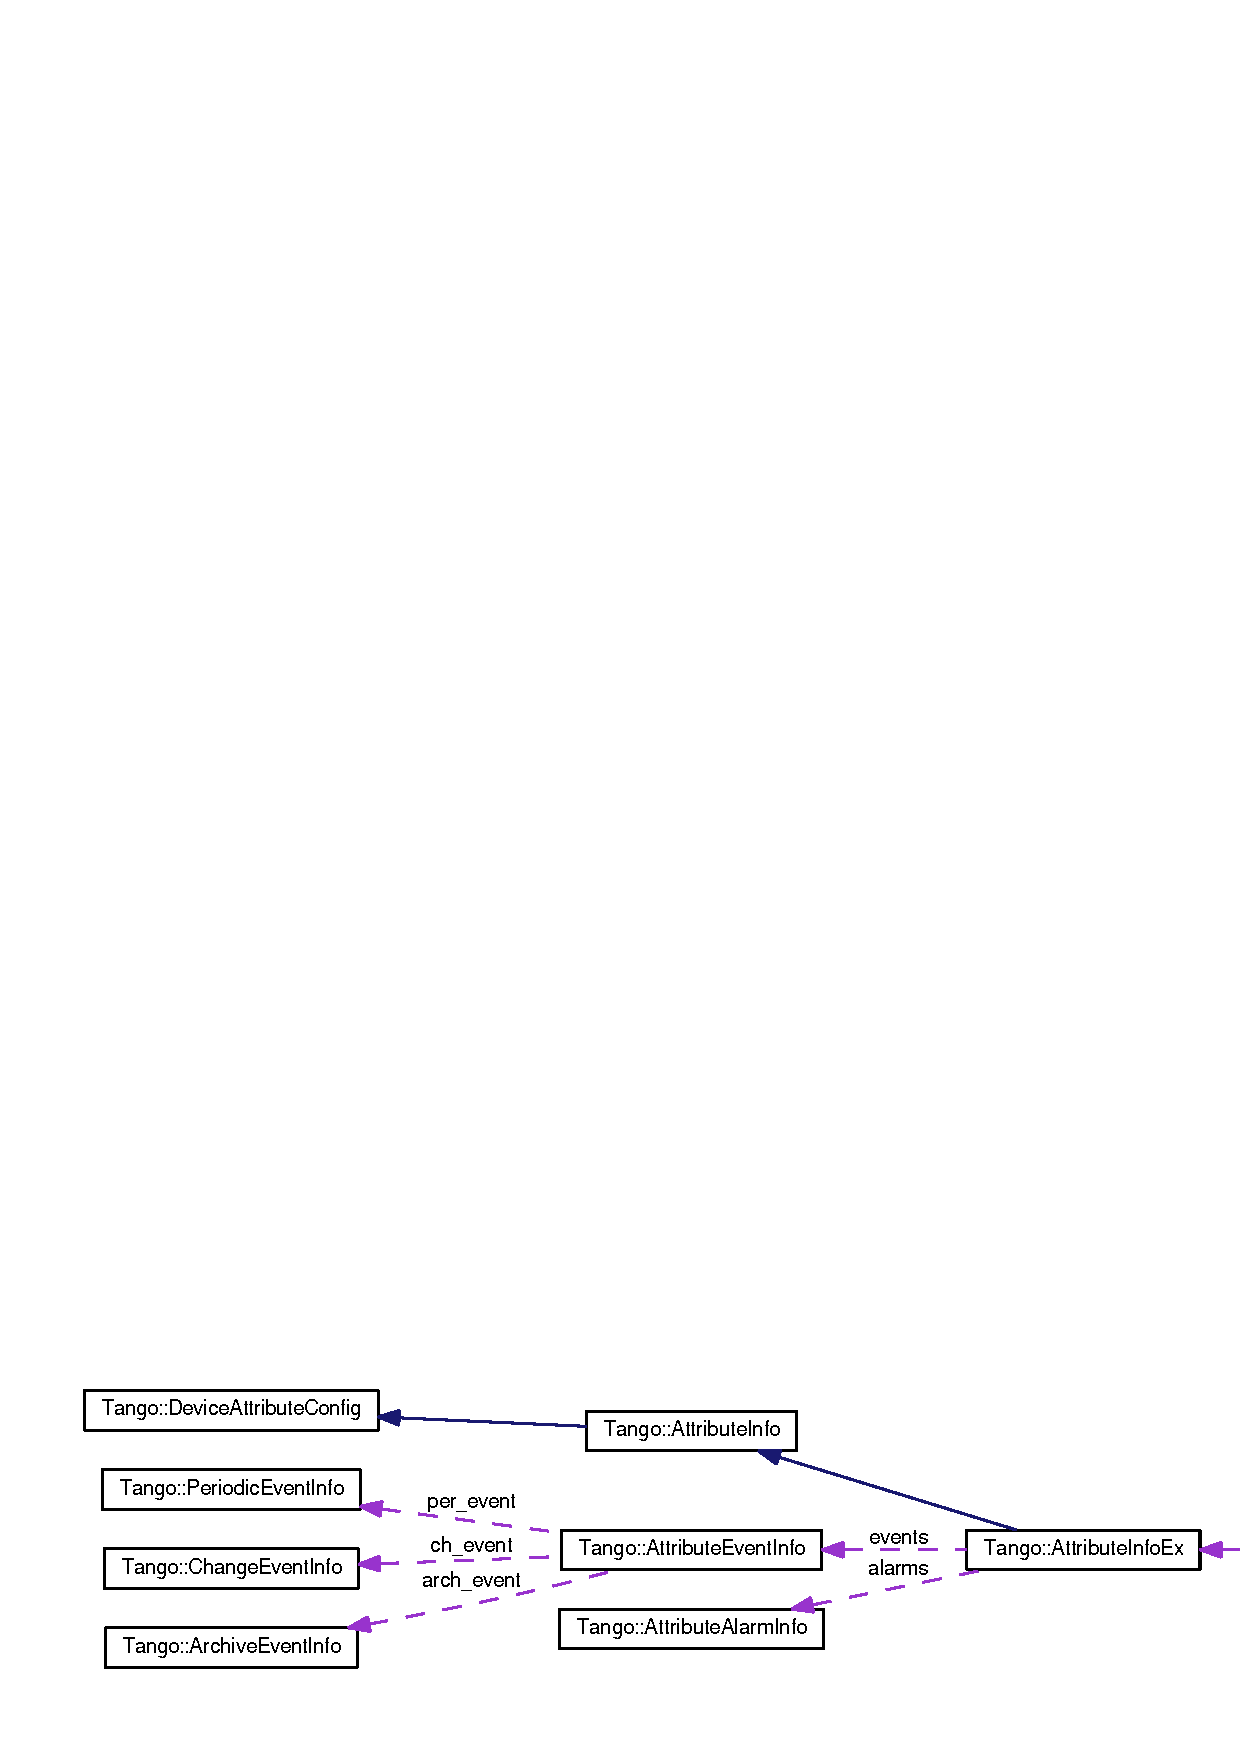
\includegraphics[width=350pt]{d8/dbd/classTango_1_1AttrConfEventData__coll__graph}
\end{center}
\end{figure}
\subsection*{Public Attributes}
\begin{DoxyCompactItemize}
\item 
{\bf Attribute\-Info\-Ex} $\ast$ {\bf attr\-\_\-conf}
\begin{DoxyCompactList}\small\item\em The attribute configuration. \end{DoxyCompactList}\item 
string {\bf attr\-\_\-name}
\begin{DoxyCompactList}\small\item\em The attribute name. \end{DoxyCompactList}\item 
Device\-Proxy $\ast$ {\bf device}
\begin{DoxyCompactList}\small\item\em The Device\-Proxy object on which the call was executed. \end{DoxyCompactList}\item 
bool {\bf err}
\begin{DoxyCompactList}\small\item\em A boolean flag set to true if the request failed. False otherwise. \end{DoxyCompactList}\item 
Dev\-Error\-List {\bf errors}
\begin{DoxyCompactList}\small\item\em The error stack. \end{DoxyCompactList}\item 
string {\bf event}
\begin{DoxyCompactList}\small\item\em The event name. \end{DoxyCompactList}\end{DoxyCompactItemize}


\subsection{Detailed Description}
\doxyref{Attribute}{p.}{d6/dad/classTango_1_1Attribute} configuration change event callback execution data. 

This class is used to pass data to the callback method when an attribute configuration event is sent to the client

\$\-Author\$ \$\-Revision\$ 

\subsection{Member Data Documentation}
\index{Tango\-::\-Attr\-Conf\-Event\-Data@{Tango\-::\-Attr\-Conf\-Event\-Data}!attr\-\_\-conf@{attr\-\_\-conf}}
\index{attr\-\_\-conf@{attr\-\_\-conf}!Tango::AttrConfEventData@{Tango\-::\-Attr\-Conf\-Event\-Data}}
\subsubsection[{attr\-\_\-conf}]{\setlength{\rightskip}{0pt plus 5cm}{\bf Attribute\-Info\-Ex}$\ast$ Tango\-::\-Attr\-Conf\-Event\-Data\-::attr\-\_\-conf}\label{classTango_1_1AttrConfEventData_af84272ced68dde94791aa090fc80bd24}


The attribute configuration. 

\index{Tango\-::\-Attr\-Conf\-Event\-Data@{Tango\-::\-Attr\-Conf\-Event\-Data}!attr\-\_\-name@{attr\-\_\-name}}
\index{attr\-\_\-name@{attr\-\_\-name}!Tango::AttrConfEventData@{Tango\-::\-Attr\-Conf\-Event\-Data}}
\subsubsection[{attr\-\_\-name}]{\setlength{\rightskip}{0pt plus 5cm}string Tango\-::\-Attr\-Conf\-Event\-Data\-::attr\-\_\-name}\label{classTango_1_1AttrConfEventData_a950448309e5b62a4387d94fd38ce0d75}


The attribute name. 

\index{Tango\-::\-Attr\-Conf\-Event\-Data@{Tango\-::\-Attr\-Conf\-Event\-Data}!device@{device}}
\index{device@{device}!Tango::AttrConfEventData@{Tango\-::\-Attr\-Conf\-Event\-Data}}
\subsubsection[{device}]{\setlength{\rightskip}{0pt plus 5cm}Device\-Proxy$\ast$ Tango\-::\-Attr\-Conf\-Event\-Data\-::device}\label{classTango_1_1AttrConfEventData_a6da04a13ce41eff0ddcf63417f001c13}


The Device\-Proxy object on which the call was executed. 

\index{Tango\-::\-Attr\-Conf\-Event\-Data@{Tango\-::\-Attr\-Conf\-Event\-Data}!err@{err}}
\index{err@{err}!Tango::AttrConfEventData@{Tango\-::\-Attr\-Conf\-Event\-Data}}
\subsubsection[{err}]{\setlength{\rightskip}{0pt plus 5cm}bool Tango\-::\-Attr\-Conf\-Event\-Data\-::err}\label{classTango_1_1AttrConfEventData_a2e3fb06bc98bb156e254ebeb6a1c222e}


A boolean flag set to true if the request failed. False otherwise. 

\index{Tango\-::\-Attr\-Conf\-Event\-Data@{Tango\-::\-Attr\-Conf\-Event\-Data}!errors@{errors}}
\index{errors@{errors}!Tango::AttrConfEventData@{Tango\-::\-Attr\-Conf\-Event\-Data}}
\subsubsection[{errors}]{\setlength{\rightskip}{0pt plus 5cm}Dev\-Error\-List Tango\-::\-Attr\-Conf\-Event\-Data\-::errors}\label{classTango_1_1AttrConfEventData_adb1f2a3796ba28cfa8a6de522b1596a8}


The error stack. 

\index{Tango\-::\-Attr\-Conf\-Event\-Data@{Tango\-::\-Attr\-Conf\-Event\-Data}!event@{event}}
\index{event@{event}!Tango::AttrConfEventData@{Tango\-::\-Attr\-Conf\-Event\-Data}}
\subsubsection[{event}]{\setlength{\rightskip}{0pt plus 5cm}string Tango\-::\-Attr\-Conf\-Event\-Data\-::event}\label{classTango_1_1AttrConfEventData_a70a8c86b121849afab88c952c6cc8bde}


The event name. 



The documentation for this class was generated from the following file\-:\begin{DoxyCompactItemize}
\item 
{\bf event.\-h}\end{DoxyCompactItemize}

\section{Tango\-:\-:Attr\-Conf\-Event\-Data\-List Class Reference}
\label{classTango_1_1AttrConfEventDataList}\index{Tango\-::\-Attr\-Conf\-Event\-Data\-List@{Tango\-::\-Attr\-Conf\-Event\-Data\-List}}


{\ttfamily \#include \char`\"{}event.\-h\char`\"{}}



Inheritance diagram for Tango\-:\-:Attr\-Conf\-Event\-Data\-List\-:
\nopagebreak
\begin{figure}[H]
\begin{center}
\leavevmode
\includegraphics[width=186pt]{d6/d9d/classTango_1_1AttrConfEventDataList__inherit__graph}
\end{center}
\end{figure}


Collaboration diagram for Tango\-:\-:Attr\-Conf\-Event\-Data\-List\-:
\nopagebreak
\begin{figure}[H]
\begin{center}
\leavevmode
\includegraphics[width=186pt]{d6/de7/classTango_1_1AttrConfEventDataList__coll__graph}
\end{center}
\end{figure}
\subsection*{Public Member Functions}
\begin{DoxyCompactItemize}
\item 
{\bf Attr\-Conf\-Event\-Data\-List} ()
\item 
{\bf $\sim$\-Attr\-Conf\-Event\-Data\-List} ()
\item 
void {\bf clear} ()
\end{DoxyCompactItemize}


\subsection{Constructor \& Destructor Documentation}
\index{Tango\-::\-Attr\-Conf\-Event\-Data\-List@{Tango\-::\-Attr\-Conf\-Event\-Data\-List}!Attr\-Conf\-Event\-Data\-List@{Attr\-Conf\-Event\-Data\-List}}
\index{Attr\-Conf\-Event\-Data\-List@{Attr\-Conf\-Event\-Data\-List}!Tango::AttrConfEventDataList@{Tango\-::\-Attr\-Conf\-Event\-Data\-List}}
\subsubsection[{Attr\-Conf\-Event\-Data\-List}]{\setlength{\rightskip}{0pt plus 5cm}Tango\-::\-Attr\-Conf\-Event\-Data\-List\-::\-Attr\-Conf\-Event\-Data\-List (
\begin{DoxyParamCaption}
{}
\end{DoxyParamCaption}
)\hspace{0.3cm}{\ttfamily [inline]}}\label{classTango_1_1AttrConfEventDataList_a4f05996e7c728cbe81a3d9c7537681b9}
\index{Tango\-::\-Attr\-Conf\-Event\-Data\-List@{Tango\-::\-Attr\-Conf\-Event\-Data\-List}!$\sim$\-Attr\-Conf\-Event\-Data\-List@{$\sim$\-Attr\-Conf\-Event\-Data\-List}}
\index{$\sim$\-Attr\-Conf\-Event\-Data\-List@{$\sim$\-Attr\-Conf\-Event\-Data\-List}!Tango::AttrConfEventDataList@{Tango\-::\-Attr\-Conf\-Event\-Data\-List}}
\subsubsection[{$\sim$\-Attr\-Conf\-Event\-Data\-List}]{\setlength{\rightskip}{0pt plus 5cm}Tango\-::\-Attr\-Conf\-Event\-Data\-List\-::$\sim$\-Attr\-Conf\-Event\-Data\-List (
\begin{DoxyParamCaption}
{}
\end{DoxyParamCaption}
)\hspace{0.3cm}{\ttfamily [inline]}}\label{classTango_1_1AttrConfEventDataList_aded16cd8d6444b0eeafebdb718c34d90}


\subsection{Member Function Documentation}
\index{Tango\-::\-Attr\-Conf\-Event\-Data\-List@{Tango\-::\-Attr\-Conf\-Event\-Data\-List}!clear@{clear}}
\index{clear@{clear}!Tango::AttrConfEventDataList@{Tango\-::\-Attr\-Conf\-Event\-Data\-List}}
\subsubsection[{clear}]{\setlength{\rightskip}{0pt plus 5cm}void Tango\-::\-Attr\-Conf\-Event\-Data\-List\-::clear (
\begin{DoxyParamCaption}
{}
\end{DoxyParamCaption}
)\hspace{0.3cm}{\ttfamily [inline]}}\label{classTango_1_1AttrConfEventDataList_a2bdc684a5056ac4c891e904e088c520e}


The documentation for this class was generated from the following file\-:\begin{DoxyCompactItemize}
\item 
{\bf event.\-h}\end{DoxyCompactItemize}

\section{Tango\-:\-:Attr\-Data$<$ T $>$ Class Template Reference}
\label{classTango_1_1AttrData}\index{Tango\-::\-Attr\-Data$<$ T $>$@{Tango\-::\-Attr\-Data$<$ T $>$}}


{\ttfamily \#include \char`\"{}pollext.\-h\char`\"{}}



Inheritance diagram for Tango\-:\-:Attr\-Data$<$ T $>$\-:
\nopagebreak
\begin{figure}[H]
\begin{center}
\leavevmode
\includegraphics[width=178pt]{d8/d3e/classTango_1_1AttrData__inherit__graph}
\end{center}
\end{figure}
\subsection*{Public Member Functions}
\begin{DoxyCompactItemize}
\item 
{\bf Attr\-Data} (const T $\ast$)
\item 
{\bf Attr\-Data} (const T $\ast$, Tango\-::\-Attr\-Quality)
\item 
{\bf Attr\-Data} (const T $\ast$, Tango\-::\-Attr\-Quality, bool)
\item 
{\bf Attr\-Data} (const T $\ast$, const T $\ast$)
\item 
{\bf Attr\-Data} (const T $\ast$, const T $\ast$, Tango\-::\-Attr\-Quality)
\item 
{\bf Attr\-Data} (const T $\ast$, const T $\ast$, Tango\-::\-Attr\-Quality, bool)
\item 
{\bf Attr\-Data} (const T $\ast$, long)
\item 
{\bf Attr\-Data} (const T $\ast$, long, Tango\-::\-Attr\-Quality)
\item 
{\bf Attr\-Data} (const T $\ast$, long, Tango\-::\-Attr\-Quality, bool)
\item 
{\bf Attr\-Data} (const T $\ast$, long, const T $\ast$, long)
\item 
{\bf Attr\-Data} (const T $\ast$, long, const T $\ast$, long, Tango\-::\-Attr\-Quality)
\item 
{\bf Attr\-Data} (const T $\ast$, long, const T $\ast$, long, Tango\-::\-Attr\-Quality, bool)
\item 
{\bf Attr\-Data} (const T $\ast$, long, long)
\item 
{\bf Attr\-Data} (const T $\ast$, long, long, Tango\-::\-Attr\-Quality)
\item 
{\bf Attr\-Data} (const T $\ast$, long, long, Tango\-::\-Attr\-Quality, bool)
\item 
{\bf Attr\-Data} (const T $\ast$, long, long, const T $\ast$, long, long)
\item 
{\bf Attr\-Data} (const T $\ast$, long, long, const T $\ast$, long, long, Tango\-::\-Attr\-Quality)
\item 
{\bf Attr\-Data} (const T $\ast$, long, long, const T $\ast$, long, long, Tango\-::\-Attr\-Quality, bool)
\item 
{\bf Attr\-Data} (Dev\-Error\-List \&e)
\end{DoxyCompactItemize}
\subsection*{Public Attributes}
\begin{DoxyCompactItemize}
\item 
Dev\-Error\-List {\bf err}
\item 
const T $\ast$ {\bf ptr}
\item 
Tango\-::\-Attr\-Quality {\bf qual}
\item 
bool {\bf release}
\item 
const T $\ast$ {\bf wr\-\_\-ptr}
\item 
long {\bf wr\-\_\-x}
\item 
long {\bf wr\-\_\-y}
\item 
long {\bf x}
\item 
long {\bf y}
\end{DoxyCompactItemize}


\subsection{Constructor \& Destructor Documentation}
\index{Tango\-::\-Attr\-Data@{Tango\-::\-Attr\-Data}!Attr\-Data@{Attr\-Data}}
\index{Attr\-Data@{Attr\-Data}!Tango::AttrData@{Tango\-::\-Attr\-Data}}
\subsubsection[{Attr\-Data}]{\setlength{\rightskip}{0pt plus 5cm}template$<$typename T $>$ {\bf Tango\-::\-Attr\-Data}$<$ T $>$\-::{\bf Attr\-Data} (
\begin{DoxyParamCaption}
\item[{const T $\ast$}]{}
\end{DoxyParamCaption}
)}\label{classTango_1_1AttrData_a97d6362673f427ed067853bb30545dc9}
\index{Tango\-::\-Attr\-Data@{Tango\-::\-Attr\-Data}!Attr\-Data@{Attr\-Data}}
\index{Attr\-Data@{Attr\-Data}!Tango::AttrData@{Tango\-::\-Attr\-Data}}
\subsubsection[{Attr\-Data}]{\setlength{\rightskip}{0pt plus 5cm}template$<$typename T $>$ {\bf Tango\-::\-Attr\-Data}$<$ T $>$\-::{\bf Attr\-Data} (
\begin{DoxyParamCaption}
\item[{const T $\ast$}]{, }
\item[{Tango\-::\-Attr\-Quality}]{}
\end{DoxyParamCaption}
)}\label{classTango_1_1AttrData_a35477beee075a315c5118430162e3959}
\index{Tango\-::\-Attr\-Data@{Tango\-::\-Attr\-Data}!Attr\-Data@{Attr\-Data}}
\index{Attr\-Data@{Attr\-Data}!Tango::AttrData@{Tango\-::\-Attr\-Data}}
\subsubsection[{Attr\-Data}]{\setlength{\rightskip}{0pt plus 5cm}template$<$typename T $>$ {\bf Tango\-::\-Attr\-Data}$<$ T $>$\-::{\bf Attr\-Data} (
\begin{DoxyParamCaption}
\item[{const T $\ast$}]{, }
\item[{Tango\-::\-Attr\-Quality}]{, }
\item[{bool}]{}
\end{DoxyParamCaption}
)}\label{classTango_1_1AttrData_af1ba132401121168a2a75dc9a6ccb43d}
\index{Tango\-::\-Attr\-Data@{Tango\-::\-Attr\-Data}!Attr\-Data@{Attr\-Data}}
\index{Attr\-Data@{Attr\-Data}!Tango::AttrData@{Tango\-::\-Attr\-Data}}
\subsubsection[{Attr\-Data}]{\setlength{\rightskip}{0pt plus 5cm}template$<$typename T $>$ {\bf Tango\-::\-Attr\-Data}$<$ T $>$\-::{\bf Attr\-Data} (
\begin{DoxyParamCaption}
\item[{const T $\ast$}]{, }
\item[{const T $\ast$}]{}
\end{DoxyParamCaption}
)}\label{classTango_1_1AttrData_a09ec5a2d0a49dae4154c0c65c1ea7467}
\index{Tango\-::\-Attr\-Data@{Tango\-::\-Attr\-Data}!Attr\-Data@{Attr\-Data}}
\index{Attr\-Data@{Attr\-Data}!Tango::AttrData@{Tango\-::\-Attr\-Data}}
\subsubsection[{Attr\-Data}]{\setlength{\rightskip}{0pt plus 5cm}template$<$typename T $>$ {\bf Tango\-::\-Attr\-Data}$<$ T $>$\-::{\bf Attr\-Data} (
\begin{DoxyParamCaption}
\item[{const T $\ast$}]{, }
\item[{const T $\ast$}]{, }
\item[{Tango\-::\-Attr\-Quality}]{}
\end{DoxyParamCaption}
)}\label{classTango_1_1AttrData_a23f77731b9643f850b82550051e7f3fc}
\index{Tango\-::\-Attr\-Data@{Tango\-::\-Attr\-Data}!Attr\-Data@{Attr\-Data}}
\index{Attr\-Data@{Attr\-Data}!Tango::AttrData@{Tango\-::\-Attr\-Data}}
\subsubsection[{Attr\-Data}]{\setlength{\rightskip}{0pt plus 5cm}template$<$typename T $>$ {\bf Tango\-::\-Attr\-Data}$<$ T $>$\-::{\bf Attr\-Data} (
\begin{DoxyParamCaption}
\item[{const T $\ast$}]{, }
\item[{const T $\ast$}]{, }
\item[{Tango\-::\-Attr\-Quality}]{, }
\item[{bool}]{}
\end{DoxyParamCaption}
)}\label{classTango_1_1AttrData_a7c2cc5ed211c0160bb5c39bc552eb6c2}
\index{Tango\-::\-Attr\-Data@{Tango\-::\-Attr\-Data}!Attr\-Data@{Attr\-Data}}
\index{Attr\-Data@{Attr\-Data}!Tango::AttrData@{Tango\-::\-Attr\-Data}}
\subsubsection[{Attr\-Data}]{\setlength{\rightskip}{0pt plus 5cm}template$<$typename T $>$ {\bf Tango\-::\-Attr\-Data}$<$ T $>$\-::{\bf Attr\-Data} (
\begin{DoxyParamCaption}
\item[{const T $\ast$}]{, }
\item[{long}]{}
\end{DoxyParamCaption}
)}\label{classTango_1_1AttrData_ac6934d712c617ed7ca14fe752287a86f}
\index{Tango\-::\-Attr\-Data@{Tango\-::\-Attr\-Data}!Attr\-Data@{Attr\-Data}}
\index{Attr\-Data@{Attr\-Data}!Tango::AttrData@{Tango\-::\-Attr\-Data}}
\subsubsection[{Attr\-Data}]{\setlength{\rightskip}{0pt plus 5cm}template$<$typename T $>$ {\bf Tango\-::\-Attr\-Data}$<$ T $>$\-::{\bf Attr\-Data} (
\begin{DoxyParamCaption}
\item[{const T $\ast$}]{, }
\item[{long}]{, }
\item[{Tango\-::\-Attr\-Quality}]{}
\end{DoxyParamCaption}
)}\label{classTango_1_1AttrData_af70c92f305dab9345b21f140e2aab14c}
\index{Tango\-::\-Attr\-Data@{Tango\-::\-Attr\-Data}!Attr\-Data@{Attr\-Data}}
\index{Attr\-Data@{Attr\-Data}!Tango::AttrData@{Tango\-::\-Attr\-Data}}
\subsubsection[{Attr\-Data}]{\setlength{\rightskip}{0pt plus 5cm}template$<$typename T $>$ {\bf Tango\-::\-Attr\-Data}$<$ T $>$\-::{\bf Attr\-Data} (
\begin{DoxyParamCaption}
\item[{const T $\ast$}]{, }
\item[{long}]{, }
\item[{Tango\-::\-Attr\-Quality}]{, }
\item[{bool}]{}
\end{DoxyParamCaption}
)}\label{classTango_1_1AttrData_aefe26194ddcd73f753cda5f77e57efd5}
\index{Tango\-::\-Attr\-Data@{Tango\-::\-Attr\-Data}!Attr\-Data@{Attr\-Data}}
\index{Attr\-Data@{Attr\-Data}!Tango::AttrData@{Tango\-::\-Attr\-Data}}
\subsubsection[{Attr\-Data}]{\setlength{\rightskip}{0pt plus 5cm}template$<$typename T $>$ {\bf Tango\-::\-Attr\-Data}$<$ T $>$\-::{\bf Attr\-Data} (
\begin{DoxyParamCaption}
\item[{const T $\ast$}]{, }
\item[{long}]{, }
\item[{const T $\ast$}]{, }
\item[{long}]{}
\end{DoxyParamCaption}
)}\label{classTango_1_1AttrData_a991650baf427403a53a2215786823c05}
\index{Tango\-::\-Attr\-Data@{Tango\-::\-Attr\-Data}!Attr\-Data@{Attr\-Data}}
\index{Attr\-Data@{Attr\-Data}!Tango::AttrData@{Tango\-::\-Attr\-Data}}
\subsubsection[{Attr\-Data}]{\setlength{\rightskip}{0pt plus 5cm}template$<$typename T $>$ {\bf Tango\-::\-Attr\-Data}$<$ T $>$\-::{\bf Attr\-Data} (
\begin{DoxyParamCaption}
\item[{const T $\ast$}]{, }
\item[{long}]{, }
\item[{const T $\ast$}]{, }
\item[{long}]{, }
\item[{Tango\-::\-Attr\-Quality}]{}
\end{DoxyParamCaption}
)}\label{classTango_1_1AttrData_ace6844f8fa2dae824a4d3708fed31d65}
\index{Tango\-::\-Attr\-Data@{Tango\-::\-Attr\-Data}!Attr\-Data@{Attr\-Data}}
\index{Attr\-Data@{Attr\-Data}!Tango::AttrData@{Tango\-::\-Attr\-Data}}
\subsubsection[{Attr\-Data}]{\setlength{\rightskip}{0pt plus 5cm}template$<$typename T $>$ {\bf Tango\-::\-Attr\-Data}$<$ T $>$\-::{\bf Attr\-Data} (
\begin{DoxyParamCaption}
\item[{const T $\ast$}]{, }
\item[{long}]{, }
\item[{const T $\ast$}]{, }
\item[{long}]{, }
\item[{Tango\-::\-Attr\-Quality}]{, }
\item[{bool}]{}
\end{DoxyParamCaption}
)}\label{classTango_1_1AttrData_a0a1e3c95b2c91413a9c98f9456d64fc2}
\index{Tango\-::\-Attr\-Data@{Tango\-::\-Attr\-Data}!Attr\-Data@{Attr\-Data}}
\index{Attr\-Data@{Attr\-Data}!Tango::AttrData@{Tango\-::\-Attr\-Data}}
\subsubsection[{Attr\-Data}]{\setlength{\rightskip}{0pt plus 5cm}template$<$typename T $>$ {\bf Tango\-::\-Attr\-Data}$<$ T $>$\-::{\bf Attr\-Data} (
\begin{DoxyParamCaption}
\item[{const T $\ast$}]{, }
\item[{long}]{, }
\item[{long}]{}
\end{DoxyParamCaption}
)}\label{classTango_1_1AttrData_a932366bb0fa645b0a217ffd5aab39d0e}
\index{Tango\-::\-Attr\-Data@{Tango\-::\-Attr\-Data}!Attr\-Data@{Attr\-Data}}
\index{Attr\-Data@{Attr\-Data}!Tango::AttrData@{Tango\-::\-Attr\-Data}}
\subsubsection[{Attr\-Data}]{\setlength{\rightskip}{0pt plus 5cm}template$<$typename T $>$ {\bf Tango\-::\-Attr\-Data}$<$ T $>$\-::{\bf Attr\-Data} (
\begin{DoxyParamCaption}
\item[{const T $\ast$}]{, }
\item[{long}]{, }
\item[{long}]{, }
\item[{Tango\-::\-Attr\-Quality}]{}
\end{DoxyParamCaption}
)}\label{classTango_1_1AttrData_a1f12cb1988acd991de591cb79a0ee5cc}
\index{Tango\-::\-Attr\-Data@{Tango\-::\-Attr\-Data}!Attr\-Data@{Attr\-Data}}
\index{Attr\-Data@{Attr\-Data}!Tango::AttrData@{Tango\-::\-Attr\-Data}}
\subsubsection[{Attr\-Data}]{\setlength{\rightskip}{0pt plus 5cm}template$<$typename T $>$ {\bf Tango\-::\-Attr\-Data}$<$ T $>$\-::{\bf Attr\-Data} (
\begin{DoxyParamCaption}
\item[{const T $\ast$}]{, }
\item[{long}]{, }
\item[{long}]{, }
\item[{Tango\-::\-Attr\-Quality}]{, }
\item[{bool}]{}
\end{DoxyParamCaption}
)}\label{classTango_1_1AttrData_af9d47850f3a6927772cd51aedf14c55c}
\index{Tango\-::\-Attr\-Data@{Tango\-::\-Attr\-Data}!Attr\-Data@{Attr\-Data}}
\index{Attr\-Data@{Attr\-Data}!Tango::AttrData@{Tango\-::\-Attr\-Data}}
\subsubsection[{Attr\-Data}]{\setlength{\rightskip}{0pt plus 5cm}template$<$typename T $>$ {\bf Tango\-::\-Attr\-Data}$<$ T $>$\-::{\bf Attr\-Data} (
\begin{DoxyParamCaption}
\item[{const T $\ast$}]{, }
\item[{long}]{, }
\item[{long}]{, }
\item[{const T $\ast$}]{, }
\item[{long}]{, }
\item[{long}]{}
\end{DoxyParamCaption}
)}\label{classTango_1_1AttrData_ace0ed907fa69d41fdb582f2256ccb20a}
\index{Tango\-::\-Attr\-Data@{Tango\-::\-Attr\-Data}!Attr\-Data@{Attr\-Data}}
\index{Attr\-Data@{Attr\-Data}!Tango::AttrData@{Tango\-::\-Attr\-Data}}
\subsubsection[{Attr\-Data}]{\setlength{\rightskip}{0pt plus 5cm}template$<$typename T $>$ {\bf Tango\-::\-Attr\-Data}$<$ T $>$\-::{\bf Attr\-Data} (
\begin{DoxyParamCaption}
\item[{const T $\ast$}]{, }
\item[{long}]{, }
\item[{long}]{, }
\item[{const T $\ast$}]{, }
\item[{long}]{, }
\item[{long}]{, }
\item[{Tango\-::\-Attr\-Quality}]{}
\end{DoxyParamCaption}
)}\label{classTango_1_1AttrData_a6254034efb611e0ae19bbf294694c4af}
\index{Tango\-::\-Attr\-Data@{Tango\-::\-Attr\-Data}!Attr\-Data@{Attr\-Data}}
\index{Attr\-Data@{Attr\-Data}!Tango::AttrData@{Tango\-::\-Attr\-Data}}
\subsubsection[{Attr\-Data}]{\setlength{\rightskip}{0pt plus 5cm}template$<$typename T $>$ {\bf Tango\-::\-Attr\-Data}$<$ T $>$\-::{\bf Attr\-Data} (
\begin{DoxyParamCaption}
\item[{const T $\ast$}]{, }
\item[{long}]{, }
\item[{long}]{, }
\item[{const T $\ast$}]{, }
\item[{long}]{, }
\item[{long}]{, }
\item[{Tango\-::\-Attr\-Quality}]{, }
\item[{bool}]{}
\end{DoxyParamCaption}
)}\label{classTango_1_1AttrData_af353a8ab0ced284a769a69d2ddf8a621}
\index{Tango\-::\-Attr\-Data@{Tango\-::\-Attr\-Data}!Attr\-Data@{Attr\-Data}}
\index{Attr\-Data@{Attr\-Data}!Tango::AttrData@{Tango\-::\-Attr\-Data}}
\subsubsection[{Attr\-Data}]{\setlength{\rightskip}{0pt plus 5cm}template$<$typename T $>$ {\bf Tango\-::\-Attr\-Data}$<$ T $>$\-::{\bf Attr\-Data} (
\begin{DoxyParamCaption}
\item[{Dev\-Error\-List \&}]{e}
\end{DoxyParamCaption}
)\hspace{0.3cm}{\ttfamily [inline]}}\label{classTango_1_1AttrData_a91406bc4fd607acb4f3217980c3b5dd5}


\subsection{Member Data Documentation}
\index{Tango\-::\-Attr\-Data@{Tango\-::\-Attr\-Data}!err@{err}}
\index{err@{err}!Tango::AttrData@{Tango\-::\-Attr\-Data}}
\subsubsection[{err}]{\setlength{\rightskip}{0pt plus 5cm}template$<$typename T $>$ Dev\-Error\-List {\bf Tango\-::\-Attr\-Data}$<$ T $>$\-::err}\label{classTango_1_1AttrData_aceb0e1fb88c6dd0be29bd7f8a4064611}
\index{Tango\-::\-Attr\-Data@{Tango\-::\-Attr\-Data}!ptr@{ptr}}
\index{ptr@{ptr}!Tango::AttrData@{Tango\-::\-Attr\-Data}}
\subsubsection[{ptr}]{\setlength{\rightskip}{0pt plus 5cm}template$<$typename T $>$ const T$\ast$ {\bf Tango\-::\-Attr\-Data}$<$ T $>$\-::ptr}\label{classTango_1_1AttrData_a2226b793c3a7c4791a9839e5bfa2473f}
\index{Tango\-::\-Attr\-Data@{Tango\-::\-Attr\-Data}!qual@{qual}}
\index{qual@{qual}!Tango::AttrData@{Tango\-::\-Attr\-Data}}
\subsubsection[{qual}]{\setlength{\rightskip}{0pt plus 5cm}template$<$typename T $>$ Tango\-::\-Attr\-Quality {\bf Tango\-::\-Attr\-Data}$<$ T $>$\-::qual}\label{classTango_1_1AttrData_a51eecbb56d5db1c611ad459017cc03c2}
\index{Tango\-::\-Attr\-Data@{Tango\-::\-Attr\-Data}!release@{release}}
\index{release@{release}!Tango::AttrData@{Tango\-::\-Attr\-Data}}
\subsubsection[{release}]{\setlength{\rightskip}{0pt plus 5cm}template$<$typename T $>$ bool {\bf Tango\-::\-Attr\-Data}$<$ T $>$\-::release}\label{classTango_1_1AttrData_abc8bb23d7b5e8b2c4c1bd1c67b16ef04}
\index{Tango\-::\-Attr\-Data@{Tango\-::\-Attr\-Data}!wr\-\_\-ptr@{wr\-\_\-ptr}}
\index{wr\-\_\-ptr@{wr\-\_\-ptr}!Tango::AttrData@{Tango\-::\-Attr\-Data}}
\subsubsection[{wr\-\_\-ptr}]{\setlength{\rightskip}{0pt plus 5cm}template$<$typename T $>$ const T$\ast$ {\bf Tango\-::\-Attr\-Data}$<$ T $>$\-::wr\-\_\-ptr}\label{classTango_1_1AttrData_a0677f54f22a900522ffe72bd38cd530a}
\index{Tango\-::\-Attr\-Data@{Tango\-::\-Attr\-Data}!wr\-\_\-x@{wr\-\_\-x}}
\index{wr\-\_\-x@{wr\-\_\-x}!Tango::AttrData@{Tango\-::\-Attr\-Data}}
\subsubsection[{wr\-\_\-x}]{\setlength{\rightskip}{0pt plus 5cm}template$<$typename T $>$ long {\bf Tango\-::\-Attr\-Data}$<$ T $>$\-::wr\-\_\-x}\label{classTango_1_1AttrData_afaaa975dbd7e67efedfc0932d163d9ce}
\index{Tango\-::\-Attr\-Data@{Tango\-::\-Attr\-Data}!wr\-\_\-y@{wr\-\_\-y}}
\index{wr\-\_\-y@{wr\-\_\-y}!Tango::AttrData@{Tango\-::\-Attr\-Data}}
\subsubsection[{wr\-\_\-y}]{\setlength{\rightskip}{0pt plus 5cm}template$<$typename T $>$ long {\bf Tango\-::\-Attr\-Data}$<$ T $>$\-::wr\-\_\-y}\label{classTango_1_1AttrData_ac4720964bc4cfe1441dbc0e25c368d5a}
\index{Tango\-::\-Attr\-Data@{Tango\-::\-Attr\-Data}!x@{x}}
\index{x@{x}!Tango::AttrData@{Tango\-::\-Attr\-Data}}
\subsubsection[{x}]{\setlength{\rightskip}{0pt plus 5cm}template$<$typename T $>$ long {\bf Tango\-::\-Attr\-Data}$<$ T $>$\-::x}\label{classTango_1_1AttrData_a8e08e9668434a58b543989599dd82ecc}
\index{Tango\-::\-Attr\-Data@{Tango\-::\-Attr\-Data}!y@{y}}
\index{y@{y}!Tango::AttrData@{Tango\-::\-Attr\-Data}}
\subsubsection[{y}]{\setlength{\rightskip}{0pt plus 5cm}template$<$typename T $>$ long {\bf Tango\-::\-Attr\-Data}$<$ T $>$\-::y}\label{classTango_1_1AttrData_a32c887ce84b2549b5c597134a8f989a4}


The documentation for this class was generated from the following file\-:\begin{DoxyCompactItemize}
\item 
{\bf pollext.\-h}\end{DoxyCompactItemize}

\section{Tango\-:\-:Attr\-History\-Stack$<$ T $>$ Class Template Reference}
\label{classTango_1_1AttrHistoryStack}\index{Tango\-::\-Attr\-History\-Stack$<$ T $>$@{Tango\-::\-Attr\-History\-Stack$<$ T $>$}}


This class is a used to pass an attribute value history when the user directly fills the attribute polling buffer.  


\subsection*{Public Member Functions}
\begin{DoxyCompactItemize}
\item 
void {\bf clear} ()
\begin{DoxyCompactList}\small\item\em Clear the stack. \end{DoxyCompactList}\item 
vector$<$ {\bf Timed\-Attr\-Data}$<$ T $>$ $>$ \& {\bf get\-\_\-data} ()
\begin{DoxyCompactList}\small\item\em Get stack data. \end{DoxyCompactList}\item 
size\-\_\-t {\bf length} ()
\begin{DoxyCompactList}\small\item\em Get stack depth. \end{DoxyCompactList}\item 
void {\bf length} (long nb)
\begin{DoxyCompactList}\small\item\em Reserve memory for stack elements. \end{DoxyCompactList}\item 
void {\bf push} ({\bf Timed\-Attr\-Data}$<$ T $>$ const \&elt)
\begin{DoxyCompactList}\small\item\em Store a new element in the stack. \end{DoxyCompactList}\end{DoxyCompactItemize}


\subsection{Detailed Description}
\subsubsection*{template$<$typename T$>$class Tango\-::\-Attr\-History\-Stack$<$ T $>$}

This class is a used to pass an attribute value history when the user directly fills the attribute polling buffer. 

Each element in this stack will be used to store one element of the attribute polling buffer

\$\-Author\$ \$\-Revision\$ 

\subsection{Member Function Documentation}
\index{Tango\-::\-Attr\-History\-Stack@{Tango\-::\-Attr\-History\-Stack}!clear@{clear}}
\index{clear@{clear}!Tango::AttrHistoryStack@{Tango\-::\-Attr\-History\-Stack}}
\subsubsection[{clear}]{\setlength{\rightskip}{0pt plus 5cm}template$<$typename T$>$ void {\bf Tango\-::\-Attr\-History\-Stack}$<$ T $>$\-::clear (
\begin{DoxyParamCaption}
{}
\end{DoxyParamCaption}
)\hspace{0.3cm}{\ttfamily [inline]}}\label{classTango_1_1AttrHistoryStack_aac60d22a112badcb3c27fb0b6c22eecd}


Clear the stack. 

\index{Tango\-::\-Attr\-History\-Stack@{Tango\-::\-Attr\-History\-Stack}!get\-\_\-data@{get\-\_\-data}}
\index{get\-\_\-data@{get\-\_\-data}!Tango::AttrHistoryStack@{Tango\-::\-Attr\-History\-Stack}}
\subsubsection[{get\-\_\-data}]{\setlength{\rightskip}{0pt plus 5cm}template$<$typename T$>$ vector$<${\bf Timed\-Attr\-Data}$<$T$>$ $>$\& {\bf Tango\-::\-Attr\-History\-Stack}$<$ T $>$\-::get\-\_\-data (
\begin{DoxyParamCaption}
{}
\end{DoxyParamCaption}
)}\label{classTango_1_1AttrHistoryStack_a73318d3db023c337bdbeae5fc743b3fd}


Get stack data. 

\begin{DoxyReturn}{Returns}
The stack itself 
\end{DoxyReturn}
\index{Tango\-::\-Attr\-History\-Stack@{Tango\-::\-Attr\-History\-Stack}!length@{length}}
\index{length@{length}!Tango::AttrHistoryStack@{Tango\-::\-Attr\-History\-Stack}}
\subsubsection[{length}]{\setlength{\rightskip}{0pt plus 5cm}template$<$typename T$>$ size\-\_\-t {\bf Tango\-::\-Attr\-History\-Stack}$<$ T $>$\-::length (
\begin{DoxyParamCaption}
{}
\end{DoxyParamCaption}
)\hspace{0.3cm}{\ttfamily [inline]}}\label{classTango_1_1AttrHistoryStack_a078798e0c374f134f0cfb315a515f028}


Get stack depth. 

\begin{DoxyReturn}{Returns}
The stack depth 
\end{DoxyReturn}
\index{Tango\-::\-Attr\-History\-Stack@{Tango\-::\-Attr\-History\-Stack}!length@{length}}
\index{length@{length}!Tango::AttrHistoryStack@{Tango\-::\-Attr\-History\-Stack}}
\subsubsection[{length}]{\setlength{\rightskip}{0pt plus 5cm}template$<$typename T$>$ void {\bf Tango\-::\-Attr\-History\-Stack}$<$ T $>$\-::length (
\begin{DoxyParamCaption}
\item[{long}]{nb}
\end{DoxyParamCaption}
)\hspace{0.3cm}{\ttfamily [inline]}}\label{classTango_1_1AttrHistoryStack_afcf19d9e75e02341bb8533cc7c61df5e}


Reserve memory for stack elements. 


\begin{DoxyParams}{Parameters}
{\em nb} & The stack element number \\
\hline
\end{DoxyParams}
\index{Tango\-::\-Attr\-History\-Stack@{Tango\-::\-Attr\-History\-Stack}!push@{push}}
\index{push@{push}!Tango::AttrHistoryStack@{Tango\-::\-Attr\-History\-Stack}}
\subsubsection[{push}]{\setlength{\rightskip}{0pt plus 5cm}template$<$typename T$>$ void {\bf Tango\-::\-Attr\-History\-Stack}$<$ T $>$\-::push (
\begin{DoxyParamCaption}
\item[{{\bf Timed\-Attr\-Data}$<$ T $>$ const \&}]{elt}
\end{DoxyParamCaption}
)}\label{classTango_1_1AttrHistoryStack_a6356c9fc9d4dd06b941b8e4a36de1f90}


Store a new element in the stack. 

This method stores a new element in the stack


\begin{DoxyParams}{Parameters}
{\em elt} & The new element \\
\hline
\end{DoxyParams}


The documentation for this class was generated from the following file\-:\begin{DoxyCompactItemize}
\item 
{\bf pollext.\-h}\end{DoxyCompactItemize}

\section{Tango\-:\-:Attribute Class Reference}
\label{classTango_1_1Attribute}\index{Tango\-::\-Attribute@{Tango\-::\-Attribute}}


This class represents a \doxyref{Tango}{p.}{de/ddf/namespaceTango} attribute.  




Inheritance diagram for Tango\-:\-:Attribute\-:
\nopagebreak
\begin{figure}[H]
\begin{center}
\leavevmode
\includegraphics[width=138pt]{d2/dcb/classTango_1_1Attribute__inherit__graph}
\end{center}
\end{figure}


Collaboration diagram for Tango\-:\-:Attribute\-:
\nopagebreak
\begin{figure}[H]
\begin{center}
\leavevmode
\includegraphics[width=276pt]{d9/db3/classTango_1_1Attribute__coll__graph}
\end{center}
\end{figure}
\subsection*{Public Member Functions}
\begin{Indent}{\bf Constructors}\par
{\em Miscellaneous constructors }\begin{DoxyCompactItemize}
\item 
{\bf Attribute} (vector$<$ Attr\-Property $>$ \&prop\-\_\-list, {\bf Attr} \&tmp\-\_\-attr, string \&dev\-\_\-name, long idx)
\begin{DoxyCompactList}\small\item\em Create a new \doxyref{Attribute}{p.}{d6/dad/classTango_1_1Attribute} object. \end{DoxyCompactList}\end{DoxyCompactItemize}
\end{Indent}
\begin{Indent}{\bf Destructor}\par
{\em Only one desctructor is defined for this class }\begin{DoxyCompactItemize}
\item 
virtual {\bf $\sim$\-Attribute} ()
\begin{DoxyCompactList}\small\item\em The attribute destructor. \end{DoxyCompactList}\end{DoxyCompactItemize}
\end{Indent}
\begin{Indent}{\bf Check attribute methods}\par
{\em Miscellaneous method returning boolean flag according to attribute state }\begin{DoxyCompactItemize}
\item 
bool {\bf is\-\_\-writ\-\_\-associated} ()
\begin{DoxyCompactList}\small\item\em Check if the attribute has an associated writable attribute. \end{DoxyCompactList}\item 
bool {\bf is\-\_\-min\-\_\-alarm} ()
\begin{DoxyCompactList}\small\item\em Check if the attribute is in minimum alarm condition . \end{DoxyCompactList}\item 
bool {\bf is\-\_\-max\-\_\-alarm} ()
\begin{DoxyCompactList}\small\item\em Check if the attribute is in maximum alarm condition . \end{DoxyCompactList}\item 
bool {\bf is\-\_\-min\-\_\-warning} ()
\begin{DoxyCompactList}\small\item\em Check if the attribute is in minimum warning condition . \end{DoxyCompactList}\item 
bool {\bf is\-\_\-max\-\_\-warning} ()
\begin{DoxyCompactList}\small\item\em Check if the attribute is in maximum warning condition . \end{DoxyCompactList}\item 
bool {\bf is\-\_\-rds\-\_\-alarm} ()
\begin{DoxyCompactList}\small\item\em Check if the attribute is in R\-D\-S alarm condition . \end{DoxyCompactList}\item 
bitset$<$ num\-Flags $>$ \& {\bf is\-\_\-alarmed} ()
\begin{DoxyCompactList}\small\item\em Check if the attribute has an alarm defined. \end{DoxyCompactList}\item 
bool {\bf is\-\_\-polled} ()
\begin{DoxyCompactList}\small\item\em Check if the attribute is polled . \end{DoxyCompactList}\item 
bool {\bf check\-\_\-alarm} ()
\begin{DoxyCompactList}\small\item\em Check if the attribute read value is below/above the alarm level. \end{DoxyCompactList}\end{DoxyCompactItemize}
\end{Indent}
\begin{Indent}{\bf Get/\-Set object members.}\par
{\em These methods allow the external world to get/set \doxyref{Device\-Impl}{p.}{d3/d62/classTango_1_1DeviceImpl} instance data members }\begin{DoxyCompactItemize}
\item 
Tango\-::\-Attr\-Write\-Type {\bf get\-\_\-writable} ()
\begin{DoxyCompactList}\small\item\em Get the attribute writable type (R\-O/\-W\-O/\-R\-W). \end{DoxyCompactList}\item 
string \& {\bf get\-\_\-name} ()
\begin{DoxyCompactList}\small\item\em Get attribute name. \end{DoxyCompactList}\item 
long {\bf get\-\_\-data\-\_\-type} ()
\begin{DoxyCompactList}\small\item\em Get attribute data type. \end{DoxyCompactList}\item 
Tango\-::\-Attr\-Data\-Format {\bf get\-\_\-data\-\_\-format} ()
\begin{DoxyCompactList}\small\item\em Get attribute data format. \end{DoxyCompactList}\item 
string \& {\bf get\-\_\-assoc\-\_\-name} ()
\begin{DoxyCompactList}\small\item\em Get name of the associated writable attribute. \end{DoxyCompactList}\item 
long {\bf get\-\_\-assoc\-\_\-ind} ()
\begin{DoxyCompactList}\small\item\em Get index of the associated writable attribute. \end{DoxyCompactList}\item 
void {\bf set\-\_\-assoc\-\_\-ind} (long val)
\begin{DoxyCompactList}\small\item\em Set index of the associated writable attribute. \end{DoxyCompactList}\item 
Tango\-::\-Time\-Val \& {\bf get\-\_\-date} ()
\begin{DoxyCompactList}\small\item\em Get attribute date. \end{DoxyCompactList}\item 
void {\bf set\-\_\-date} (Tango\-::\-Time\-Val \&new\-\_\-date)
\begin{DoxyCompactList}\small\item\em Set attribute date. \end{DoxyCompactList}\item 
void {\bf set\-\_\-date} (struct timeval \&t)
\begin{DoxyCompactList}\small\item\em Set attribute date. \end{DoxyCompactList}\item 
void {\bf set\-\_\-date} (time\-\_\-t new\-\_\-date)
\begin{DoxyCompactList}\small\item\em Set attribute date. \end{DoxyCompactList}\item 
string \& {\bf get\-\_\-label} ()
\begin{DoxyCompactList}\small\item\em Get attribute label property. \end{DoxyCompactList}\item 
Tango\-::\-Attr\-Quality \& {\bf get\-\_\-quality} ()
\begin{DoxyCompactList}\small\item\em Get attribute data quality. \end{DoxyCompactList}\item 
void {\bf set\-\_\-quality} (Tango\-::\-Attr\-Quality qua, bool send\-\_\-event=false)
\begin{DoxyCompactList}\small\item\em Set attribute data quality. \end{DoxyCompactList}\item 
long {\bf get\-\_\-data\-\_\-size} ()
\begin{DoxyCompactList}\small\item\em Get attribute data size. \end{DoxyCompactList}\item 
long {\bf get\-\_\-x} ()
\begin{DoxyCompactList}\small\item\em Get attribute data size in x dimension. \end{DoxyCompactList}\item 
long {\bf get\-\_\-max\-\_\-dim\-\_\-x} ()
\begin{DoxyCompactList}\small\item\em Get attribute maximum data size in x dimension. \end{DoxyCompactList}\item 
long {\bf get\-\_\-y} ()
\begin{DoxyCompactList}\small\item\em Get attribute data size in y dimension. \end{DoxyCompactList}\item 
long {\bf get\-\_\-max\-\_\-dim\-\_\-y} ()
\begin{DoxyCompactList}\small\item\em Get attribute maximum data size in y dimension. \end{DoxyCompactList}\item 
long {\bf get\-\_\-polling\-\_\-period} ()
\begin{DoxyCompactList}\small\item\em Get attribute polling period. \end{DoxyCompactList}\item 
{\footnotesize template$<$typename T $>$ }\\void {\bf get\-\_\-properties} ({\bf Tango\-::\-Multi\-Attr\-Prop}$<$ T $>$ \&props)
\begin{DoxyCompactList}\small\item\em Get all modifiable attribute properties in one call. \end{DoxyCompactList}\item 
{\footnotesize template$<$typename T $>$ }\\void {\bf set\-\_\-properties} ({\bf Tango\-::\-Multi\-Attr\-Prop}$<$ T $>$ \&props)
\begin{DoxyCompactList}\small\item\em Set all modifiable attribute properties in one call. \end{DoxyCompactList}\item 
void {\bf set\-\_\-attr\-\_\-serial\-\_\-model} ({\bf Attr\-Serial\-Model} ser\-\_\-model)
\begin{DoxyCompactList}\small\item\em Set attribute serialization model. \end{DoxyCompactList}\item 
{\bf Attr\-Serial\-Model} {\bf get\-\_\-attr\-\_\-serial\-\_\-model} ()
\begin{DoxyCompactList}\small\item\em Get attribute serialization model. \end{DoxyCompactList}\item 
void {\bf set\-\_\-user\-\_\-attr\-\_\-mutex} (omni\-\_\-mutex $\ast$mut\-\_\-ptr)
\begin{DoxyCompactList}\small\item\em Set attribute user mutex. \end{DoxyCompactList}\end{DoxyCompactItemize}
\end{Indent}
\begin{Indent}{\bf Set attribute value methods.}\par
{\em These methods allows the external world to set attribute object internal value }\begin{DoxyCompactItemize}
\item 
void {\bf set\-\_\-value} (Tango\-::\-Dev\-Short $\ast$p\-\_\-data, long x=1, long y=0, bool release=false)
\begin{DoxyCompactList}\small\item\em Set internal attribute value (for Tango\-::\-Dev\-Short attribute data type). \end{DoxyCompactList}\item 
void {\bf set\-\_\-value} (Tango\-::\-Dev\-Long $\ast$p\-\_\-data, long x=1, long y=0, bool release=false)
\begin{DoxyCompactList}\small\item\em Set internal attribute value (for Tango\-::\-Dev\-Long attribute data type). \end{DoxyCompactList}\item 
void {\bf set\-\_\-value} (Tango\-::\-Dev\-Long64 $\ast$p\-\_\-data, long x=1, long y=0, bool release=false)
\begin{DoxyCompactList}\small\item\em Set internal attribute value (for Tango\-::\-Dev\-Long64 attribute data type). \end{DoxyCompactList}\item 
void {\bf set\-\_\-value} (Tango\-::\-Dev\-Float $\ast$p\-\_\-data, long x=1, long y=0, bool release=false)
\begin{DoxyCompactList}\small\item\em Set internal attribute value (for Tango\-::\-Dev\-Float attribute data type). \end{DoxyCompactList}\item 
void {\bf set\-\_\-value} (Tango\-::\-Dev\-Double $\ast$p\-\_\-data, long x=1, long y=0, bool release=false)
\begin{DoxyCompactList}\small\item\em Set internal attribute value (for Tango\-::\-Dev\-Double attribute data type). \end{DoxyCompactList}\item 
void {\bf set\-\_\-value} (Tango\-::\-Dev\-String $\ast$p\-\_\-data, long x=1, long y=0, bool release=false)
\begin{DoxyCompactList}\small\item\em Set internal attribute value (for Tango\-::\-Dev\-String attribute data type). \end{DoxyCompactList}\item 
void {\bf set\-\_\-value} (Tango\-::\-Dev\-Boolean $\ast$p\-\_\-data, long x=1, long y=0, bool release=false)
\begin{DoxyCompactList}\small\item\em Set internal attribute value (for Tango\-::\-Dev\-Boolean attribute data type). \end{DoxyCompactList}\item 
void {\bf set\-\_\-value} (Tango\-::\-Dev\-U\-Short $\ast$p\-\_\-data, long x=1, long y=0, bool release=false)
\begin{DoxyCompactList}\small\item\em Set internal attribute value (for Tango\-::\-Dev\-U\-Short attribute data type). \end{DoxyCompactList}\item 
void {\bf set\-\_\-value} (Tango\-::\-Dev\-U\-Char $\ast$p\-\_\-data, long x=1, long y=0, bool release=false)
\begin{DoxyCompactList}\small\item\em Set internal attribute value (for Tango\-::\-Dev\-U\-Char attribute data type). \end{DoxyCompactList}\item 
void {\bf set\-\_\-value} (Tango\-::\-Dev\-U\-Long $\ast$p\-\_\-data, long x=1, long y=0, bool release=false)
\begin{DoxyCompactList}\small\item\em Set internal attribute value (for Tango\-::\-Dev\-U\-Long attribute data type). \end{DoxyCompactList}\item 
void {\bf set\-\_\-value} (Tango\-::\-Dev\-U\-Long64 $\ast$p\-\_\-data, long x=1, long y=0, bool release=false)
\begin{DoxyCompactList}\small\item\em Set internal attribute value (for Tango\-::\-Dev\-U\-Long64 attribute data type). \end{DoxyCompactList}\item 
void {\bf set\-\_\-value} (Tango\-::\-Dev\-State $\ast$p\-\_\-data, long x=1, long y=0, bool release=false)
\begin{DoxyCompactList}\small\item\em Set internal attribute value (for Tango\-::\-Dev\-State attribute data type). \end{DoxyCompactList}\item 
void {\bf set\-\_\-value} (Tango\-::\-Dev\-Encoded $\ast$p\-\_\-data, long x=1, long y=0, bool release=false)
\begin{DoxyCompactList}\small\item\em Set internal attribute value (for Tango\-::\-Dev\-Encoded attribute data type). \end{DoxyCompactList}\item 
void {\bf set\-\_\-value} (Tango\-::\-Dev\-String $\ast$p\-\_\-data\-\_\-str, Tango\-::\-Dev\-U\-Char $\ast$p\-\_\-data, long size, bool release=false)
\begin{DoxyCompactList}\small\item\em Set internal attribute value (for Tango\-::\-Dev\-Encoded attribute data type). \end{DoxyCompactList}\item 
void {\bf set\-\_\-value} ({\bf Tango\-::\-Encoded\-Attribute} $\ast$attr)
\begin{DoxyCompactList}\small\item\em Set internal attribute value (for Tango\-::\-Dev\-Encoded attribute data type). \end{DoxyCompactList}\item 
void {\bf set\-\_\-value\-\_\-date\-\_\-quality} (Tango\-::\-Dev\-Short $\ast$p\-\_\-data, time\-\_\-t t, Tango\-::\-Attr\-Quality qual, long x=1, long y=0, bool release=false)
\begin{DoxyCompactList}\small\item\em Set internal attribute value, date and quality factor (for Tango\-::\-Dev\-Short attribute data type). \end{DoxyCompactList}\item 
void {\bf set\-\_\-value\-\_\-date\-\_\-quality} (Tango\-::\-Dev\-Short $\ast$p\-\_\-data, struct timeval \&t, Tango\-::\-Attr\-Quality qual, long x=1, long y=0, bool release=false)
\begin{DoxyCompactList}\small\item\em Set internal attribute value, date and quality factor (for Tango\-::\-Dev\-Short attribute data type). \end{DoxyCompactList}\item 
void {\bf set\-\_\-value\-\_\-date\-\_\-quality} (Tango\-::\-Dev\-Long $\ast$p\-\_\-data, time\-\_\-t t, Tango\-::\-Attr\-Quality qual, long x=1, long y=0, bool release=false)
\begin{DoxyCompactList}\small\item\em Set internal attribute value, date and quality factor (for Tango\-::\-Dev\-Long attribute data type). \end{DoxyCompactList}\item 
void {\bf set\-\_\-value\-\_\-date\-\_\-quality} (Tango\-::\-Dev\-Long $\ast$p\-\_\-data, struct timeval \&t, Tango\-::\-Attr\-Quality qual, long x=1, long y=0, bool release=false)
\begin{DoxyCompactList}\small\item\em Set internal attribute value, date and quality factor (for Tango\-::\-Dev\-Long attribute data type). \end{DoxyCompactList}\item 
void {\bf set\-\_\-value\-\_\-date\-\_\-quality} (Tango\-::\-Dev\-Long64 $\ast$p\-\_\-data, time\-\_\-t t, Tango\-::\-Attr\-Quality qual, long x=1, long y=0, bool release=false)
\begin{DoxyCompactList}\small\item\em Set internal attribute value, date and quality factor (for Tango\-::\-Dev\-Long64 attribute data type). \end{DoxyCompactList}\item 
void {\bf set\-\_\-value\-\_\-date\-\_\-quality} (Tango\-::\-Dev\-Long64 $\ast$p\-\_\-data, struct timeval \&t, Tango\-::\-Attr\-Quality qual, long x=1, long y=0, bool release=false)
\begin{DoxyCompactList}\small\item\em Set internal attribute value, date and quality factor (for Tango\-::\-Dev\-Long64 attribute data type). \end{DoxyCompactList}\item 
void {\bf set\-\_\-value\-\_\-date\-\_\-quality} (Tango\-::\-Dev\-Float $\ast$p\-\_\-data, time\-\_\-t t, Tango\-::\-Attr\-Quality qual, long x=1, long y=0, bool release=false)
\begin{DoxyCompactList}\small\item\em Set internal attribute value, date and quality factor (for Tango\-::\-Dev\-Float attribute data type). \end{DoxyCompactList}\item 
void {\bf set\-\_\-value\-\_\-date\-\_\-quality} (Tango\-::\-Dev\-Float $\ast$p\-\_\-data, struct timeval \&t, Tango\-::\-Attr\-Quality qual, long x=1, long y=0, bool release=false)
\begin{DoxyCompactList}\small\item\em Set internal attribute value, date and quality factor (for Tango\-::\-Dev\-Float attribute data type). \end{DoxyCompactList}\item 
void {\bf set\-\_\-value\-\_\-date\-\_\-quality} (Tango\-::\-Dev\-Double $\ast$p\-\_\-data, time\-\_\-t t, Tango\-::\-Attr\-Quality qual, long x=1, long y=0, bool release=false)
\begin{DoxyCompactList}\small\item\em Set internal attribute value, date and quality factor (for Tango\-::\-Dev\-Double attribute data type). \end{DoxyCompactList}\item 
void {\bf set\-\_\-value\-\_\-date\-\_\-quality} (Tango\-::\-Dev\-Double $\ast$p\-\_\-data, struct timeval \&t, Tango\-::\-Attr\-Quality qual, long x=1, long y=0, bool release=false)
\begin{DoxyCompactList}\small\item\em Set internal attribute value, date and quality factor (for Tango\-::\-Dev\-Double attribute data type). \end{DoxyCompactList}\item 
void {\bf set\-\_\-value\-\_\-date\-\_\-quality} (Tango\-::\-Dev\-String $\ast$p\-\_\-data, time\-\_\-t t, Tango\-::\-Attr\-Quality qual, long x=1, long y=0, bool release=false)
\begin{DoxyCompactList}\small\item\em Set internal attribute value, date and quality factor (for Tango\-::\-Dev\-String attribute data type). \end{DoxyCompactList}\item 
void {\bf set\-\_\-value\-\_\-date\-\_\-quality} (Tango\-::\-Dev\-String $\ast$p\-\_\-data, struct timeval \&t, Tango\-::\-Attr\-Quality qual, long x=1, long y=0, bool release=false)
\begin{DoxyCompactList}\small\item\em Set internal attribute value, date and quality factor (for Tango\-::\-Dev\-String attribute data type). \end{DoxyCompactList}\item 
void {\bf set\-\_\-value\-\_\-date\-\_\-quality} (Tango\-::\-Dev\-Boolean $\ast$p\-\_\-data, time\-\_\-t t, Tango\-::\-Attr\-Quality qual, long x=1, long y=0, bool release=false)
\begin{DoxyCompactList}\small\item\em Set internal attribute value, date and quality factor (for Tango\-::\-Dev\-Boolean attribute data type). \end{DoxyCompactList}\item 
void {\bf set\-\_\-value\-\_\-date\-\_\-quality} (Tango\-::\-Dev\-Boolean $\ast$p\-\_\-data, struct timeval \&t, Tango\-::\-Attr\-Quality qual, long x=1, long y=0, bool release=false)
\begin{DoxyCompactList}\small\item\em Set internal attribute value, date and quality factor (for Tango\-::\-Dev\-Boolean attribute data type). \end{DoxyCompactList}\item 
void {\bf set\-\_\-value\-\_\-date\-\_\-quality} (Tango\-::\-Dev\-U\-Short $\ast$p\-\_\-data, time\-\_\-t t, Tango\-::\-Attr\-Quality qual, long x=1, long y=0, bool release=false)
\begin{DoxyCompactList}\small\item\em Set internal attribute value, date and quality factor (for Tango\-::\-Dev\-U\-Short attribute data type). \end{DoxyCompactList}\item 
void {\bf set\-\_\-value\-\_\-date\-\_\-quality} (Tango\-::\-Dev\-U\-Short $\ast$p\-\_\-data, struct timeval \&t, Tango\-::\-Attr\-Quality qual, long x=1, long y=0, bool release=false)
\begin{DoxyCompactList}\small\item\em Set internal attribute value, date and quality factor (for Tango\-::\-Dev\-U\-Short attribute data type). \end{DoxyCompactList}\item 
void {\bf set\-\_\-value\-\_\-date\-\_\-quality} (Tango\-::\-Dev\-U\-Char $\ast$p\-\_\-data, time\-\_\-t t, Tango\-::\-Attr\-Quality qual, long x=1, long y=0, bool release=false)
\begin{DoxyCompactList}\small\item\em Set internal attribute value, date and quality factor (for Tango\-::\-Dev\-U\-Char attribute data type). \end{DoxyCompactList}\item 
void {\bf set\-\_\-value\-\_\-date\-\_\-quality} (Tango\-::\-Dev\-U\-Char $\ast$p\-\_\-data, struct timeval \&t, Tango\-::\-Attr\-Quality qual, long x=1, long y=0, bool release=false)
\begin{DoxyCompactList}\small\item\em Set internal attribute value, date and quality factor (for Tango\-::\-Dev\-U\-Char attribute data type). \end{DoxyCompactList}\item 
void {\bf set\-\_\-value\-\_\-date\-\_\-quality} (Tango\-::\-Dev\-U\-Long $\ast$p\-\_\-data, time\-\_\-t t, Tango\-::\-Attr\-Quality qual, long x=1, long y=0, bool release=false)
\begin{DoxyCompactList}\small\item\em Set internal attribute value, date and quality factor (for Tango\-::\-Dev\-U\-Long attribute data type). \end{DoxyCompactList}\item 
void {\bf set\-\_\-value\-\_\-date\-\_\-quality} (Tango\-::\-Dev\-U\-Long $\ast$p\-\_\-data, struct timeval \&t, Tango\-::\-Attr\-Quality qual, long x=1, long y=0, bool release=false)
\begin{DoxyCompactList}\small\item\em Set internal attribute value, date and quality factor (for Tango\-::\-Dev\-U\-Long attribute data type). \end{DoxyCompactList}\item 
void {\bf set\-\_\-value\-\_\-date\-\_\-quality} (Tango\-::\-Dev\-U\-Long64 $\ast$p\-\_\-data, time\-\_\-t t, Tango\-::\-Attr\-Quality qual, long x=1, long y=0, bool release=false)
\begin{DoxyCompactList}\small\item\em Set internal attribute value, date and quality factor (for Tango\-::\-Dev\-U\-Long64 attribute data type). \end{DoxyCompactList}\item 
void {\bf set\-\_\-value\-\_\-date\-\_\-quality} (Tango\-::\-Dev\-U\-Long64 $\ast$p\-\_\-data, struct timeval \&t, Tango\-::\-Attr\-Quality qual, long x=1, long y=0, bool release=false)
\begin{DoxyCompactList}\small\item\em Set internal attribute value, date and quality factor (for Tango\-::\-Dev\-U\-Long64 attribute data type). \end{DoxyCompactList}\item 
void {\bf set\-\_\-value\-\_\-date\-\_\-quality} (Tango\-::\-Dev\-State $\ast$p\-\_\-data, time\-\_\-t t, Tango\-::\-Attr\-Quality qual, long x=1, long y=0, bool release=false)
\begin{DoxyCompactList}\small\item\em Set internal attribute value, date and quality factor (for Tango\-::\-Dev\-State attribute data type). \end{DoxyCompactList}\item 
void {\bf set\-\_\-value\-\_\-date\-\_\-quality} (Tango\-::\-Dev\-State $\ast$p\-\_\-data, struct timeval \&t, Tango\-::\-Attr\-Quality qual, long x=1, long y=0, bool release=false)
\begin{DoxyCompactList}\small\item\em Set internal attribute value, date and quality factor (for Tango\-::\-Dev\-State attribute data type). \end{DoxyCompactList}\item 
void {\bf set\-\_\-value\-\_\-date\-\_\-quality} (Tango\-::\-Dev\-Encoded $\ast$p\-\_\-data, time\-\_\-t t, Tango\-::\-Attr\-Quality qual, long x=1, long y=0, bool release=false)
\begin{DoxyCompactList}\small\item\em Set internal attribute value, date and quality factor (for Tango\-::\-Dev\-Encoded attribute data type). \end{DoxyCompactList}\item 
void {\bf set\-\_\-value\-\_\-date\-\_\-quality} (Tango\-::\-Dev\-String $\ast$p\-\_\-data\-\_\-str, Tango\-::\-Dev\-U\-Char $\ast$p\-\_\-data, long size, time\-\_\-t t, Tango\-::\-Attr\-Quality qual, bool release=false)
\begin{DoxyCompactList}\small\item\em Set internal attribute value, date and quality factor (for Tango\-::\-Dev\-Encoded attribute data type when splitted in format and data). \end{DoxyCompactList}\item 
void {\bf set\-\_\-value\-\_\-date\-\_\-quality} (Tango\-::\-Dev\-Encoded $\ast$p\-\_\-data, struct timeval \&t, Tango\-::\-Attr\-Quality qual, long x=1, long y=0, bool release=false)
\begin{DoxyCompactList}\small\item\em Set internal attribute value, date and quality factor (for Tango\-::\-Dev\-Encoded attribute data type). \end{DoxyCompactList}\item 
void {\bf set\-\_\-value\-\_\-date\-\_\-quality} (Tango\-::\-Dev\-String $\ast$p\-\_\-data\-\_\-str, Tango\-::\-Dev\-U\-Char $\ast$p\-\_\-data, long size, struct timeval \&t, Tango\-::\-Attr\-Quality qual, bool release=false)
\begin{DoxyCompactList}\small\item\em Set internal attribute value, date and quality factor (for Tango\-::\-Dev\-Encoded attribute data type when splitted in data format and data themselves). \end{DoxyCompactList}\item 
void {\bf fire\-\_\-change\-\_\-event} (Dev\-Failed $\ast$except=N\-U\-L\-L)
\begin{DoxyCompactList}\small\item\em Fire a change event for the attribute value. \end{DoxyCompactList}\item 
void {\bf set\-\_\-change\-\_\-event} (bool implemented, bool detect=true)
\begin{DoxyCompactList}\small\item\em Set a flag to indicate that the server fires change events manually, without the polling to be started for the attribute. \end{DoxyCompactList}\item 
bool {\bf is\-\_\-change\-\_\-event} ()
\begin{DoxyCompactList}\small\item\em Check if the change event is fired manually (without polling) for this attribute. \end{DoxyCompactList}\item 
bool {\bf is\-\_\-check\-\_\-change\-\_\-criteria} ()
\begin{DoxyCompactList}\small\item\em Check if the change event criteria should be checked when firing the event manually. \end{DoxyCompactList}\item 
void {\bf fire\-\_\-archive\-\_\-event} (Dev\-Failed $\ast$except=N\-U\-L\-L)
\begin{DoxyCompactList}\small\item\em Fire an archive event for the attribute value. \end{DoxyCompactList}\item 
void {\bf set\-\_\-archive\-\_\-event} (bool implemented, bool detect=true)
\begin{DoxyCompactList}\small\item\em Set a flag to indicate that the server fires archive events manually, without the polling to be started for the attribute If the detect parameter is set to true, the criteria specified for the archive event are verified and the event is only pushed if they are fulfilled. \end{DoxyCompactList}\item 
bool {\bf is\-\_\-archive\-\_\-event} ()
\begin{DoxyCompactList}\small\item\em Check if the archive event is fired manually for this attribute. \end{DoxyCompactList}\item 
bool {\bf is\-\_\-check\-\_\-archive\-\_\-criteria} ()
\begin{DoxyCompactList}\small\item\em Check if the archive event criteria should be checked when firing the event manually. \end{DoxyCompactList}\item 
void {\bf set\-\_\-data\-\_\-ready\-\_\-event} (bool implemented)
\begin{DoxyCompactList}\small\item\em Set a flag to indicate that the server fires data ready events. \end{DoxyCompactList}\item 
bool {\bf is\-\_\-data\-\_\-ready\-\_\-event} ()
\begin{DoxyCompactList}\small\item\em Check if the data ready event is fired for this attribute. \end{DoxyCompactList}\item 
void {\bf fire\-\_\-event} (vector$<$ string $>$ \&filt\-\_\-names, vector$<$ double $>$ \&filt\-\_\-vals, Dev\-Failed $\ast$except=N\-U\-L\-L)
\begin{DoxyCompactList}\small\item\em Fire a user event for the attribute value. \end{DoxyCompactList}\item 
void {\bf remove\-\_\-configuration} ()
\begin{DoxyCompactList}\small\item\em Remove the attribute configuration from the database. \end{DoxyCompactList}\end{DoxyCompactItemize}
\end{Indent}
\begin{Indent}{\bf Set/\-Get attribute ranges (min\-\_\-alarm, min\-\_\-warning, max\-\_\-warning, max\-\_\-alarm) methods.}\par
{\em These methods allow the external world to set attribute object min\-\_\-alarm, min\-\_\-warning, max\-\_\-warning and max\-\_\-alarm values }\begin{DoxyCompactItemize}
\item 
{\footnotesize template$<$typename T $>$ }\\void {\bf set\-\_\-min\-\_\-alarm} (const T \&new\-\_\-min\-\_\-alarm)
\begin{DoxyCompactList}\small\item\em Set attribute minimum alarm. \end{DoxyCompactList}\item 
void {\bf set\-\_\-min\-\_\-alarm} (char $\ast$new\-\_\-min\-\_\-alarm)
\item 
void {\bf set\-\_\-min\-\_\-alarm} (const char $\ast$new\-\_\-min\-\_\-alarm)
\item 
{\footnotesize template$<$typename T $>$ }\\void {\bf get\-\_\-min\-\_\-alarm} (T \&min\-\_\-al)
\begin{DoxyCompactList}\small\item\em Get attribute minimum alarm or throw an exception if the attribute does not have the minimum alarm. \end{DoxyCompactList}\item 
{\footnotesize template$<$typename T $>$ }\\void {\bf set\-\_\-max\-\_\-alarm} (const T \&new\-\_\-max\-\_\-alarm)
\begin{DoxyCompactList}\small\item\em Set attribute maximum alarm. \end{DoxyCompactList}\item 
void {\bf set\-\_\-max\-\_\-alarm} (char $\ast$new\-\_\-max\-\_\-alarm)
\item 
void {\bf set\-\_\-max\-\_\-alarm} (const char $\ast$new\-\_\-max\-\_\-alarm)
\item 
{\footnotesize template$<$typename T $>$ }\\void {\bf get\-\_\-max\-\_\-alarm} (T \&max\-\_\-al)
\begin{DoxyCompactList}\small\item\em Get attribute maximum alarm or throw an exception if the attribute does not have the maximum alarm set. \end{DoxyCompactList}\item 
{\footnotesize template$<$typename T $>$ }\\void {\bf set\-\_\-min\-\_\-warning} (const T \&new\-\_\-min\-\_\-warning)
\begin{DoxyCompactList}\small\item\em Set attribute minimum warning. \end{DoxyCompactList}\item 
void {\bf set\-\_\-min\-\_\-warning} (char $\ast$new\-\_\-min\-\_\-warning)
\item 
void {\bf set\-\_\-min\-\_\-warning} (const char $\ast$new\-\_\-min\-\_\-warning)
\item 
{\footnotesize template$<$typename T $>$ }\\void {\bf get\-\_\-min\-\_\-warning} (T \&min\-\_\-war)
\begin{DoxyCompactList}\small\item\em Get attribute minimum warning or throw an exception if the attribute does not have the minimum warning set. \end{DoxyCompactList}\item 
{\footnotesize template$<$typename T $>$ }\\void {\bf set\-\_\-max\-\_\-warning} (const T \&new\-\_\-max\-\_\-warning)
\begin{DoxyCompactList}\small\item\em Set attribute maximum warning. \end{DoxyCompactList}\item 
void {\bf set\-\_\-max\-\_\-warning} (char $\ast$new\-\_\-max\-\_\-warning)
\item 
void {\bf set\-\_\-max\-\_\-warning} (const char $\ast$new\-\_\-max\-\_\-warning)
\item 
{\footnotesize template$<$typename T $>$ }\\void {\bf get\-\_\-max\-\_\-warning} (T \&max\-\_\-war)
\begin{DoxyCompactList}\small\item\em Get attribute maximum warning or throw an exception if the attribute does not have the maximum warning set. \end{DoxyCompactList}\end{DoxyCompactItemize}
\end{Indent}
\subsection*{Protected Attributes}
\begin{Indent}{\bf Class data members}\par
\begin{DoxyCompactItemize}
\item 
bool {\bf value\-\_\-flag}
\begin{DoxyCompactList}\small\item\em A flag set to true if the attribute value has been updated. \end{DoxyCompactList}\item 
Tango\-::\-Time\-Val {\bf when}
\begin{DoxyCompactList}\small\item\em The date when attribute was read. \end{DoxyCompactList}\item 
bool {\bf date}
\begin{DoxyCompactList}\small\item\em Flag set to true if the date must be set. \end{DoxyCompactList}\item 
Tango\-::\-Attr\-Quality {\bf quality}
\begin{DoxyCompactList}\small\item\em The attribute quality factor. \end{DoxyCompactList}\item 
string {\bf name}
\begin{DoxyCompactList}\small\item\em The attribute name. \end{DoxyCompactList}\item 
Tango\-::\-Attr\-Write\-Type {\bf writable}
\begin{DoxyCompactList}\small\item\em The attribute writable flag. \end{DoxyCompactList}\item 
long {\bf data\-\_\-type}
\begin{DoxyCompactList}\small\item\em The attribute data type. \end{DoxyCompactList}\item 
Tango\-::\-Attr\-Data\-Format {\bf data\-\_\-format}
\begin{DoxyCompactList}\small\item\em The attribute data format. \end{DoxyCompactList}\item 
long {\bf max\-\_\-x}
\begin{DoxyCompactList}\small\item\em The attribute maximum x dimension. \end{DoxyCompactList}\item 
long {\bf max\-\_\-y}
\begin{DoxyCompactList}\small\item\em The attribute maximum y dimension. \end{DoxyCompactList}\item 
string {\bf label}
\begin{DoxyCompactList}\small\item\em The attribute label. \end{DoxyCompactList}\item 
string {\bf description}
\begin{DoxyCompactList}\small\item\em The attribute description. \end{DoxyCompactList}\item 
string {\bf unit}
\begin{DoxyCompactList}\small\item\em The attribute unit. \end{DoxyCompactList}\item 
string {\bf standard\-\_\-unit}
\begin{DoxyCompactList}\small\item\em The attribute standard unit. \end{DoxyCompactList}\item 
string {\bf display\-\_\-unit}
\begin{DoxyCompactList}\small\item\em The attribute display unit. \end{DoxyCompactList}\item 
string {\bf format}
\begin{DoxyCompactList}\small\item\em The attribute format. \end{DoxyCompactList}\item 
string {\bf writable\-\_\-attr\-\_\-name}
\begin{DoxyCompactList}\small\item\em The name of the associated writable attribute. \end{DoxyCompactList}\item 
string {\bf min\-\_\-alarm\-\_\-str}
\begin{DoxyCompactList}\small\item\em The attribute minimum alarm level. \end{DoxyCompactList}\item 
string {\bf max\-\_\-alarm\-\_\-str}
\begin{DoxyCompactList}\small\item\em The attribute maximun alarm level. \end{DoxyCompactList}\item 
string {\bf min\-\_\-value\-\_\-str}
\begin{DoxyCompactList}\small\item\em The attribute minimum value. \end{DoxyCompactList}\item 
string {\bf max\-\_\-value\-\_\-str}
\begin{DoxyCompactList}\small\item\em The attribute maximum value. \end{DoxyCompactList}\item 
string {\bf min\-\_\-warning\-\_\-str}
\begin{DoxyCompactList}\small\item\em The attribute minimun warning. \end{DoxyCompactList}\item 
string {\bf max\-\_\-warning\-\_\-str}
\begin{DoxyCompactList}\small\item\em The attribute maximum warning. \end{DoxyCompactList}\item 
string {\bf delta\-\_\-val\-\_\-str}
\begin{DoxyCompactList}\small\item\em The attribute delta value R\-D\-S alarm. \end{DoxyCompactList}\item 
string {\bf delta\-\_\-t\-\_\-str}
\begin{DoxyCompactList}\small\item\em The attribute delta time R\-D\-S alarm. \end{DoxyCompactList}\item 
long {\bf assoc\-\_\-ind}
\begin{DoxyCompactList}\small\item\em Index in the main attribute vector of the associated writable attribute (if any) \end{DoxyCompactList}\item 
{\bf Tango\-::\-Attr\-\_\-\-Check\-Val} {\bf min\-\_\-alarm}
\begin{DoxyCompactList}\small\item\em The attribute minimum alarm in binary format. \end{DoxyCompactList}\item 
{\bf Tango\-::\-Attr\-\_\-\-Check\-Val} {\bf max\-\_\-alarm}
\begin{DoxyCompactList}\small\item\em The attribute maximum alarm in binary format. \end{DoxyCompactList}\item 
{\bf Tango\-::\-Attr\-\_\-\-Check\-Val} {\bf min\-\_\-warning}
\begin{DoxyCompactList}\small\item\em The attribute minimum warning in binary format. \end{DoxyCompactList}\item 
{\bf Tango\-::\-Attr\-\_\-\-Check\-Val} {\bf max\-\_\-warning}
\begin{DoxyCompactList}\small\item\em The attribute maximum warning in binary format. \end{DoxyCompactList}\item 
{\bf Tango\-::\-Attr\-\_\-\-Check\-Val} {\bf min\-\_\-value}
\begin{DoxyCompactList}\small\item\em The attribute minimum value in binary format. \end{DoxyCompactList}\item 
{\bf Tango\-::\-Attr\-\_\-\-Check\-Val} {\bf max\-\_\-value}
\begin{DoxyCompactList}\small\item\em The attribute maximum value in binary format. \end{DoxyCompactList}\item 
{\bf Tango\-::\-Attr\-\_\-\-Value} {\bf value}
\begin{DoxyCompactList}\small\item\em The attribute value. \end{DoxyCompactList}\item 
long {\bf data\-\_\-size}
\begin{DoxyCompactList}\small\item\em The attribute data size. \end{DoxyCompactList}\item 
bool {\bf check\-\_\-min\-\_\-value}
\begin{DoxyCompactList}\small\item\em Flag set to true if a minimum value is defined. \end{DoxyCompactList}\item 
bool {\bf check\-\_\-max\-\_\-value}
\begin{DoxyCompactList}\small\item\em Flag set to true if a maximum alarm is defined. \end{DoxyCompactList}\item 
{\bf Tango\-::\-Attr\-\_\-\-Check\-Val} {\bf delta\-\_\-val}
\begin{DoxyCompactList}\small\item\em Authorized delta between the last written value and the actual read. \end{DoxyCompactList}\item 
long {\bf delta\-\_\-t}
\begin{DoxyCompactList}\small\item\em Delta time after which the read value must be checked again the last written value if the attribute has an alarm on Read Different Than Set (R\-D\-S) \end{DoxyCompactList}\item 
vector$<$ string $>$ {\bf enum\-\_\-labels}
\begin{DoxyCompactList}\small\item\em Enumeration labels when the attribute data type is Dev\-Enum. \end{DoxyCompactList}\end{DoxyCompactItemize}
\end{Indent}
\subsection*{Friends}
\begin{DoxyCompactItemize}
\item 
class {\bf D\-Server}
\item 
class {\bf Event\-Supplier}
\item 
class {\bf Zmq\-Event\-Supplier}
\end{DoxyCompactItemize}


\subsection{Detailed Description}
This class represents a \doxyref{Tango}{p.}{de/ddf/namespaceTango} attribute. 

\$\-Author\$ \$\-Revision\$ 

\subsection{Constructor \& Destructor Documentation}
\index{Tango\-::\-Attribute@{Tango\-::\-Attribute}!Attribute@{Attribute}}
\index{Attribute@{Attribute}!Tango::Attribute@{Tango\-::\-Attribute}}
\subsubsection[{Attribute}]{\setlength{\rightskip}{0pt plus 5cm}Tango\-::\-Attribute\-::\-Attribute (
\begin{DoxyParamCaption}
\item[{vector$<$ Attr\-Property $>$ \&}]{prop\-\_\-list, }
\item[{{\bf Attr} \&}]{tmp\-\_\-attr, }
\item[{string \&}]{dev\-\_\-name, }
\item[{long}]{idx}
\end{DoxyParamCaption}
)}\label{classTango_1_1Attribute_ad92e54beedf8d29d088c2f6d5d70153f}


Create a new \doxyref{Attribute}{p.}{d6/dad/classTango_1_1Attribute} object. 


\begin{DoxyParams}{Parameters}
{\em prop\-\_\-list} & The attribute properties list. Each property is an object of the Attr\-Property class \\
\hline
{\em tmp\-\_\-attr} & Temporary attribute object built from user parameters \\
\hline
{\em dev\-\_\-name} & The device name \\
\hline
{\em idx} & The index of the related \doxyref{Attr}{p.}{d5/dcd/classTango_1_1Attr} object in the Multi\-Class\-Attribute vector of \doxyref{Attr}{p.}{d5/dcd/classTango_1_1Attr} object \\
\hline
\end{DoxyParams}
\index{Tango\-::\-Attribute@{Tango\-::\-Attribute}!$\sim$\-Attribute@{$\sim$\-Attribute}}
\index{$\sim$\-Attribute@{$\sim$\-Attribute}!Tango::Attribute@{Tango\-::\-Attribute}}
\subsubsection[{$\sim$\-Attribute}]{\setlength{\rightskip}{0pt plus 5cm}virtual Tango\-::\-Attribute\-::$\sim$\-Attribute (
\begin{DoxyParamCaption}
{}
\end{DoxyParamCaption}
)\hspace{0.3cm}{\ttfamily [virtual]}}\label{classTango_1_1Attribute_ae2740fa1ac154feb7d50a85199991f42}


The attribute destructor. 



\subsection{Member Function Documentation}
\index{Tango\-::\-Attribute@{Tango\-::\-Attribute}!check\-\_\-alarm@{check\-\_\-alarm}}
\index{check\-\_\-alarm@{check\-\_\-alarm}!Tango::Attribute@{Tango\-::\-Attribute}}
\subsubsection[{check\-\_\-alarm}]{\setlength{\rightskip}{0pt plus 5cm}bool Tango\-::\-Attribute\-::check\-\_\-alarm (
\begin{DoxyParamCaption}
{}
\end{DoxyParamCaption}
)}\label{classTango_1_1Attribute_a64b4a569c810258ae52a2acaadf15d55}


Check if the attribute read value is below/above the alarm level. 

\begin{DoxyReturn}{Returns}
A boolean set to true if the attribute is in alarm condition. 
\end{DoxyReturn}

\begin{DoxyExceptions}{Exceptions}
{\em Dev\-Failed} & If no alarm level is defined. Click {\tt here} to read {\bfseries Dev\-Failed} exception specification \\
\hline
\end{DoxyExceptions}


Referenced by Tango\-::\-Multi\-Attribute\-::check\-\_\-alarm().

\index{Tango\-::\-Attribute@{Tango\-::\-Attribute}!fire\-\_\-archive\-\_\-event@{fire\-\_\-archive\-\_\-event}}
\index{fire\-\_\-archive\-\_\-event@{fire\-\_\-archive\-\_\-event}!Tango::Attribute@{Tango\-::\-Attribute}}
\subsubsection[{fire\-\_\-archive\-\_\-event}]{\setlength{\rightskip}{0pt plus 5cm}void Tango\-::\-Attribute\-::fire\-\_\-archive\-\_\-event (
\begin{DoxyParamCaption}
\item[{Dev\-Failed $\ast$}]{except = {\ttfamily NULL}}
\end{DoxyParamCaption}
)}\label{classTango_1_1Attribute_ab008123b44bdb2a13e2cd2c362617e1e}


Fire an archive event for the attribute value. 

The event is pushed to the notification daemon. The attibute data must be set with one of the \doxyref{Attribute\-::set\-\_\-value}{p.}{d6/dad/classTango_1_1Attribute_a21669c4af43fe5584e3f52a8012a35f6} or Attribute\-::setvalue\-\_\-date\-\_\-quality methods before fireing the event. The event is triggered with or without the archive event criteria depending on the configuration choosen with \doxyref{set\-\_\-archive\-\_\-event()}{p.}{d6/dad/classTango_1_1Attribute_a48b92dbec415b3f2589456fde7899175}. A\-T\-T\-E\-N\-T\-I\-O\-N\-: The couple \doxyref{set\-\_\-value()}{p.}{d6/dad/classTango_1_1Attribute_a21669c4af43fe5584e3f52a8012a35f6} and \doxyref{fire\-\_\-archive\-\_\-event()}{p.}{d6/dad/classTango_1_1Attribute_ab008123b44bdb2a13e2cd2c362617e1e} needs to be protected against concurrent accesses to the same attribute. Such an access might happen during a synchronous read or by a reading from the polling thread. Inside all methods reading or writing commands and attributes this protection is automatically done by the \doxyref{Tango}{p.}{de/ddf/namespaceTango} serialisation monitor. When fireing archive events in your own code, you should use the push\-\_\-archive\-\_\-event methods of the \doxyref{Device\-Impl}{p.}{d3/d62/classTango_1_1DeviceImpl} class or protect your code with the Tango\-::\-Auto\-Tango\-Monitor on your device. Example\-:

\{ Tango\-::\-Auto\-Tango\-Monitor synch(this); att\-\_\-temp\-\_\-seq.\-set\-\_\-value (temp\-\_\-seq, 100); att\-\_\-temp\-\_\-seq.\-fire\-\_\-archive\-\_\-event (); \}


\begin{DoxyParams}{Parameters}
{\em except} & A pointer to a Dev\-Failed exception to be thrown as archive event. \\
\hline
\end{DoxyParams}
\index{Tango\-::\-Attribute@{Tango\-::\-Attribute}!fire\-\_\-change\-\_\-event@{fire\-\_\-change\-\_\-event}}
\index{fire\-\_\-change\-\_\-event@{fire\-\_\-change\-\_\-event}!Tango::Attribute@{Tango\-::\-Attribute}}
\subsubsection[{fire\-\_\-change\-\_\-event}]{\setlength{\rightskip}{0pt plus 5cm}void Tango\-::\-Attribute\-::fire\-\_\-change\-\_\-event (
\begin{DoxyParamCaption}
\item[{Dev\-Failed $\ast$}]{except = {\ttfamily NULL}}
\end{DoxyParamCaption}
)}\label{classTango_1_1Attribute_ae023edda1e0bf70d5fda7c3dc8160351}


Fire a change event for the attribute value. 

The event is pushed to the notification daemon. The attibute data must be set with one of the \doxyref{Attribute\-::set\-\_\-value}{p.}{d6/dad/classTango_1_1Attribute_a21669c4af43fe5584e3f52a8012a35f6} or Attribute\-::setvalue\-\_\-date\-\_\-quality methods before fireing the event. The event is triggered with or without the change event criteria depending on the configuration choosen with \doxyref{set\-\_\-change\-\_\-event()}{p.}{d6/dad/classTango_1_1Attribute_a25f157fedeb2f37741b1e41ce6422fcd}. A\-T\-T\-E\-N\-T\-I\-O\-N\-: The couple \doxyref{set\-\_\-value()}{p.}{d6/dad/classTango_1_1Attribute_a21669c4af43fe5584e3f52a8012a35f6} and \doxyref{fire\-\_\-change\-\_\-event()}{p.}{d6/dad/classTango_1_1Attribute_ae023edda1e0bf70d5fda7c3dc8160351} needs to be protected against concurrent accesses to the same attribute. Such an access might happen during a synchronous read or by a reading from the polling thread. Inside all methods reading or writing commands and attributes this protection is automatically done by the \doxyref{Tango}{p.}{de/ddf/namespaceTango} serialisation monitor. When fireing change events in your own code, you should use the push\-\_\-change\-\_\-event methods of the \doxyref{Device\-Impl}{p.}{d3/d62/classTango_1_1DeviceImpl} class or protect your code with the Tango\-::\-Auto\-Tango\-Monitor on your device. Example\-:

\{ Tango\-::\-Auto\-Tango\-Monitor synch(this); att\-\_\-temp\-\_\-seq.\-set\-\_\-value (temp\-\_\-seq, 100); att\-\_\-temp\-\_\-seq.\-fire\-\_\-archive\-\_\-event (); \}


\begin{DoxyParams}{Parameters}
{\em except} & A pointer to a Dev\-Failed exception to be thrown as archive event. \\
\hline
\end{DoxyParams}
\index{Tango\-::\-Attribute@{Tango\-::\-Attribute}!fire\-\_\-event@{fire\-\_\-event}}
\index{fire\-\_\-event@{fire\-\_\-event}!Tango::Attribute@{Tango\-::\-Attribute}}
\subsubsection[{fire\-\_\-event}]{\setlength{\rightskip}{0pt plus 5cm}void Tango\-::\-Attribute\-::fire\-\_\-event (
\begin{DoxyParamCaption}
\item[{vector$<$ string $>$ \&}]{filt\-\_\-names, }
\item[{vector$<$ double $>$ \&}]{filt\-\_\-vals, }
\item[{Dev\-Failed $\ast$}]{except = {\ttfamily NULL}}
\end{DoxyParamCaption}
)}\label{classTango_1_1Attribute_a13234bb32ef355601e45e6e942082873}


Fire a user event for the attribute value. 

The event is pushed to the notification daemon. The attibute data must be set with one of the \doxyref{Attribute\-::set\-\_\-value}{p.}{d6/dad/classTango_1_1Attribute_a21669c4af43fe5584e3f52a8012a35f6} or Attribute\-::setvalue\-\_\-date\-\_\-quality methods before fireing the event. A\-T\-T\-E\-N\-T\-I\-O\-N\-: The couple \doxyref{set\-\_\-value()}{p.}{d6/dad/classTango_1_1Attribute_a21669c4af43fe5584e3f52a8012a35f6} and \doxyref{fire\-\_\-event()}{p.}{d6/dad/classTango_1_1Attribute_a13234bb32ef355601e45e6e942082873} needs to be protected against concurrent accesses to the same attribute. Such an access might happen during a synchronous read or by a reading from the polling thread. Inside all methods reading or writing commands and attributes this protection is automatically done by the \doxyref{Tango}{p.}{de/ddf/namespaceTango} serialisation monitor. When fireing archive events in your own code, you should use the push\-\_\-event methods of the \doxyref{Device\-Impl}{p.}{d3/d62/classTango_1_1DeviceImpl} class or protect your code with the Tango\-::\-Auto\-Tango\-Monitor on your device. Example\-:

\{ Tango\-::\-Auto\-Tango\-Monitor synch(this); att\-\_\-temp\-\_\-seq.\-set\-\_\-value (temp\-\_\-seq, 100); att\-\_\-temp\-\_\-seq.\-fire\-\_\-event (); \}


\begin{DoxyParams}{Parameters}
{\em filt\-\_\-names} & The filterable fields name \\
\hline
{\em filt\-\_\-vals} & The filterable fields value (as double) \\
\hline
{\em except} & A pointer to a Dev\-Failed exception to be thrown as archive event. \\
\hline
\end{DoxyParams}
\index{Tango\-::\-Attribute@{Tango\-::\-Attribute}!get\-\_\-assoc\-\_\-ind@{get\-\_\-assoc\-\_\-ind}}
\index{get\-\_\-assoc\-\_\-ind@{get\-\_\-assoc\-\_\-ind}!Tango::Attribute@{Tango\-::\-Attribute}}
\subsubsection[{get\-\_\-assoc\-\_\-ind}]{\setlength{\rightskip}{0pt plus 5cm}long Tango\-::\-Attribute\-::get\-\_\-assoc\-\_\-ind (
\begin{DoxyParamCaption}
{}
\end{DoxyParamCaption}
)\hspace{0.3cm}{\ttfamily [inline]}}\label{classTango_1_1Attribute_a362cf02710511ea952ef3f8ff85cdd30}


Get index of the associated writable attribute. 

\begin{DoxyReturn}{Returns}
The index in the main attribute vector of the associated writable attribute 
\end{DoxyReturn}


References assoc\-\_\-ind.

\index{Tango\-::\-Attribute@{Tango\-::\-Attribute}!get\-\_\-assoc\-\_\-name@{get\-\_\-assoc\-\_\-name}}
\index{get\-\_\-assoc\-\_\-name@{get\-\_\-assoc\-\_\-name}!Tango::Attribute@{Tango\-::\-Attribute}}
\subsubsection[{get\-\_\-assoc\-\_\-name}]{\setlength{\rightskip}{0pt plus 5cm}string\& Tango\-::\-Attribute\-::get\-\_\-assoc\-\_\-name (
\begin{DoxyParamCaption}
{}
\end{DoxyParamCaption}
)\hspace{0.3cm}{\ttfamily [inline]}}\label{classTango_1_1Attribute_abe79d1339964153ad5144a53036fcd18}


Get name of the associated writable attribute. 

\begin{DoxyReturn}{Returns}
The associated writable attribute name 
\end{DoxyReturn}


References writable\-\_\-attr\-\_\-name.

\index{Tango\-::\-Attribute@{Tango\-::\-Attribute}!get\-\_\-attr\-\_\-serial\-\_\-model@{get\-\_\-attr\-\_\-serial\-\_\-model}}
\index{get\-\_\-attr\-\_\-serial\-\_\-model@{get\-\_\-attr\-\_\-serial\-\_\-model}!Tango::Attribute@{Tango\-::\-Attribute}}
\subsubsection[{get\-\_\-attr\-\_\-serial\-\_\-model}]{\setlength{\rightskip}{0pt plus 5cm}{\bf Attr\-Serial\-Model} Tango\-::\-Attribute\-::get\-\_\-attr\-\_\-serial\-\_\-model (
\begin{DoxyParamCaption}
{}
\end{DoxyParamCaption}
)\hspace{0.3cm}{\ttfamily [inline]}}\label{classTango_1_1Attribute_ac2d93bbbc1b0019e81691c14dc13bc0d}


Get attribute serialization model. 

Get the attribute serialization model

\begin{DoxyReturn}{Returns}
The attribute serialization model 
\end{DoxyReturn}
\index{Tango\-::\-Attribute@{Tango\-::\-Attribute}!get\-\_\-data\-\_\-format@{get\-\_\-data\-\_\-format}}
\index{get\-\_\-data\-\_\-format@{get\-\_\-data\-\_\-format}!Tango::Attribute@{Tango\-::\-Attribute}}
\subsubsection[{get\-\_\-data\-\_\-format}]{\setlength{\rightskip}{0pt plus 5cm}Tango\-::\-Attr\-Data\-Format Tango\-::\-Attribute\-::get\-\_\-data\-\_\-format (
\begin{DoxyParamCaption}
{}
\end{DoxyParamCaption}
)\hspace{0.3cm}{\ttfamily [inline]}}\label{classTango_1_1Attribute_a4e23df40cb9be8d4213c0f87b67e5dd9}


Get attribute data format. 

\begin{DoxyReturn}{Returns}
The attribute data format 
\end{DoxyReturn}


References data\-\_\-format.

\index{Tango\-::\-Attribute@{Tango\-::\-Attribute}!get\-\_\-data\-\_\-size@{get\-\_\-data\-\_\-size}}
\index{get\-\_\-data\-\_\-size@{get\-\_\-data\-\_\-size}!Tango::Attribute@{Tango\-::\-Attribute}}
\subsubsection[{get\-\_\-data\-\_\-size}]{\setlength{\rightskip}{0pt plus 5cm}long Tango\-::\-Attribute\-::get\-\_\-data\-\_\-size (
\begin{DoxyParamCaption}
{}
\end{DoxyParamCaption}
)\hspace{0.3cm}{\ttfamily [inline]}}\label{classTango_1_1Attribute_a0a59f7d799a3c8ab8cdd7e6cd611607d}


Get attribute data size. 

\begin{DoxyReturn}{Returns}
The attribute data size 
\end{DoxyReturn}


References data\-\_\-size.

\index{Tango\-::\-Attribute@{Tango\-::\-Attribute}!get\-\_\-data\-\_\-type@{get\-\_\-data\-\_\-type}}
\index{get\-\_\-data\-\_\-type@{get\-\_\-data\-\_\-type}!Tango::Attribute@{Tango\-::\-Attribute}}
\subsubsection[{get\-\_\-data\-\_\-type}]{\setlength{\rightskip}{0pt plus 5cm}long Tango\-::\-Attribute\-::get\-\_\-data\-\_\-type (
\begin{DoxyParamCaption}
{}
\end{DoxyParamCaption}
)\hspace{0.3cm}{\ttfamily [inline]}}\label{classTango_1_1Attribute_a8b59c84da16d3b914cf8bf4fd37d8c1e}


Get attribute data type. 

\begin{DoxyReturn}{Returns}
The attribute data type 
\end{DoxyReturn}


References data\-\_\-type.

\index{Tango\-::\-Attribute@{Tango\-::\-Attribute}!get\-\_\-date@{get\-\_\-date}}
\index{get\-\_\-date@{get\-\_\-date}!Tango::Attribute@{Tango\-::\-Attribute}}
\subsubsection[{get\-\_\-date}]{\setlength{\rightskip}{0pt plus 5cm}Tango\-::\-Time\-Val\& Tango\-::\-Attribute\-::get\-\_\-date (
\begin{DoxyParamCaption}
{}
\end{DoxyParamCaption}
)\hspace{0.3cm}{\ttfamily [inline]}}\label{classTango_1_1Attribute_a0e5d5c229031b939700a38728fbe08a4}


Get attribute date. 

\begin{DoxyReturn}{Returns}
The attribute date 
\end{DoxyReturn}


References when.

\index{Tango\-::\-Attribute@{Tango\-::\-Attribute}!get\-\_\-label@{get\-\_\-label}}
\index{get\-\_\-label@{get\-\_\-label}!Tango::Attribute@{Tango\-::\-Attribute}}
\subsubsection[{get\-\_\-label}]{\setlength{\rightskip}{0pt plus 5cm}string\& Tango\-::\-Attribute\-::get\-\_\-label (
\begin{DoxyParamCaption}
{}
\end{DoxyParamCaption}
)\hspace{0.3cm}{\ttfamily [inline]}}\label{classTango_1_1Attribute_a1851ce2e2e30add8e826c39b462fe374}


Get attribute label property. 

\begin{DoxyReturn}{Returns}
The attribute label 
\end{DoxyReturn}


References label.

\index{Tango\-::\-Attribute@{Tango\-::\-Attribute}!get\-\_\-max\-\_\-alarm@{get\-\_\-max\-\_\-alarm}}
\index{get\-\_\-max\-\_\-alarm@{get\-\_\-max\-\_\-alarm}!Tango::Attribute@{Tango\-::\-Attribute}}
\subsubsection[{get\-\_\-max\-\_\-alarm}]{\setlength{\rightskip}{0pt plus 5cm}template$<$typename T $>$ void Tango\-::\-Attribute\-::get\-\_\-max\-\_\-alarm (
\begin{DoxyParamCaption}
\item[{T \&}]{max\-\_\-al}
\end{DoxyParamCaption}
)}\label{classTango_1_1Attribute_ab4214177cfddd2acfe4c98e6fcb7b563}


Get attribute maximum alarm or throw an exception if the attribute does not have the maximum alarm set. 


\begin{DoxyParams}{Parameters}
{\em max\-\_\-al} & Reference to a variable which value will be set to the attribute's maximum alarm \\
\hline
\end{DoxyParams}
\index{Tango\-::\-Attribute@{Tango\-::\-Attribute}!get\-\_\-max\-\_\-dim\-\_\-x@{get\-\_\-max\-\_\-dim\-\_\-x}}
\index{get\-\_\-max\-\_\-dim\-\_\-x@{get\-\_\-max\-\_\-dim\-\_\-x}!Tango::Attribute@{Tango\-::\-Attribute}}
\subsubsection[{get\-\_\-max\-\_\-dim\-\_\-x}]{\setlength{\rightskip}{0pt plus 5cm}long Tango\-::\-Attribute\-::get\-\_\-max\-\_\-dim\-\_\-x (
\begin{DoxyParamCaption}
{}
\end{DoxyParamCaption}
)\hspace{0.3cm}{\ttfamily [inline]}}\label{classTango_1_1Attribute_ae5cd58a02dcf1a799d1261ed5d9c7532}


Get attribute maximum data size in x dimension. 

\begin{DoxyReturn}{Returns}
The attribute maximum data size in x dimension. Set to 1 for scalar attribute 
\end{DoxyReturn}


References max\-\_\-x.

\index{Tango\-::\-Attribute@{Tango\-::\-Attribute}!get\-\_\-max\-\_\-dim\-\_\-y@{get\-\_\-max\-\_\-dim\-\_\-y}}
\index{get\-\_\-max\-\_\-dim\-\_\-y@{get\-\_\-max\-\_\-dim\-\_\-y}!Tango::Attribute@{Tango\-::\-Attribute}}
\subsubsection[{get\-\_\-max\-\_\-dim\-\_\-y}]{\setlength{\rightskip}{0pt plus 5cm}long Tango\-::\-Attribute\-::get\-\_\-max\-\_\-dim\-\_\-y (
\begin{DoxyParamCaption}
{}
\end{DoxyParamCaption}
)\hspace{0.3cm}{\ttfamily [inline]}}\label{classTango_1_1Attribute_ab4cfab2bee3ae1523ad8a3466afc37a2}


Get attribute maximum data size in y dimension. 

\begin{DoxyReturn}{Returns}
The attribute maximum data size in y dimension. Set to 0 for scalar and spectrum attribute 
\end{DoxyReturn}


References max\-\_\-y.

\index{Tango\-::\-Attribute@{Tango\-::\-Attribute}!get\-\_\-max\-\_\-warning@{get\-\_\-max\-\_\-warning}}
\index{get\-\_\-max\-\_\-warning@{get\-\_\-max\-\_\-warning}!Tango::Attribute@{Tango\-::\-Attribute}}
\subsubsection[{get\-\_\-max\-\_\-warning}]{\setlength{\rightskip}{0pt plus 5cm}template$<$typename T $>$ void Tango\-::\-Attribute\-::get\-\_\-max\-\_\-warning (
\begin{DoxyParamCaption}
\item[{T \&}]{max\-\_\-war}
\end{DoxyParamCaption}
)}\label{classTango_1_1Attribute_a2246b2de4a4cb23031975fac5a17ea66}


Get attribute maximum warning or throw an exception if the attribute does not have the maximum warning set. 


\begin{DoxyParams}{Parameters}
{\em max\-\_\-war} & Reference to a variable which value will be set to the attribute's maximum warning \\
\hline
\end{DoxyParams}
\index{Tango\-::\-Attribute@{Tango\-::\-Attribute}!get\-\_\-min\-\_\-alarm@{get\-\_\-min\-\_\-alarm}}
\index{get\-\_\-min\-\_\-alarm@{get\-\_\-min\-\_\-alarm}!Tango::Attribute@{Tango\-::\-Attribute}}
\subsubsection[{get\-\_\-min\-\_\-alarm}]{\setlength{\rightskip}{0pt plus 5cm}template$<$typename T $>$ void Tango\-::\-Attribute\-::get\-\_\-min\-\_\-alarm (
\begin{DoxyParamCaption}
\item[{T \&}]{min\-\_\-al}
\end{DoxyParamCaption}
)}\label{classTango_1_1Attribute_a19e43a51a3101a12abc55eeac83a431e}


Get attribute minimum alarm or throw an exception if the attribute does not have the minimum alarm. 


\begin{DoxyParams}{Parameters}
{\em min\-\_\-al} & Reference to a variable which value will be set to the attribute's minimum alarm \\
\hline
\end{DoxyParams}
\index{Tango\-::\-Attribute@{Tango\-::\-Attribute}!get\-\_\-min\-\_\-warning@{get\-\_\-min\-\_\-warning}}
\index{get\-\_\-min\-\_\-warning@{get\-\_\-min\-\_\-warning}!Tango::Attribute@{Tango\-::\-Attribute}}
\subsubsection[{get\-\_\-min\-\_\-warning}]{\setlength{\rightskip}{0pt plus 5cm}template$<$typename T $>$ void Tango\-::\-Attribute\-::get\-\_\-min\-\_\-warning (
\begin{DoxyParamCaption}
\item[{T \&}]{min\-\_\-war}
\end{DoxyParamCaption}
)}\label{classTango_1_1Attribute_a670533e5338107f959d7cf01f3e88a5a}


Get attribute minimum warning or throw an exception if the attribute does not have the minimum warning set. 


\begin{DoxyParams}{Parameters}
{\em min\-\_\-war} & Reference to a variable which value will be set to the attribute's minimum warning \\
\hline
\end{DoxyParams}
\index{Tango\-::\-Attribute@{Tango\-::\-Attribute}!get\-\_\-name@{get\-\_\-name}}
\index{get\-\_\-name@{get\-\_\-name}!Tango::Attribute@{Tango\-::\-Attribute}}
\subsubsection[{get\-\_\-name}]{\setlength{\rightskip}{0pt plus 5cm}string\& Tango\-::\-Attribute\-::get\-\_\-name (
\begin{DoxyParamCaption}
{}
\end{DoxyParamCaption}
)\hspace{0.3cm}{\ttfamily [inline]}}\label{classTango_1_1Attribute_afd4dfffdf08ea4c03a58f7e83977b152}


Get attribute name. 

\begin{DoxyReturn}{Returns}
The attribute name 
\end{DoxyReturn}


References name.

\index{Tango\-::\-Attribute@{Tango\-::\-Attribute}!get\-\_\-polling\-\_\-period@{get\-\_\-polling\-\_\-period}}
\index{get\-\_\-polling\-\_\-period@{get\-\_\-polling\-\_\-period}!Tango::Attribute@{Tango\-::\-Attribute}}
\subsubsection[{get\-\_\-polling\-\_\-period}]{\setlength{\rightskip}{0pt plus 5cm}long Tango\-::\-Attribute\-::get\-\_\-polling\-\_\-period (
\begin{DoxyParamCaption}
{}
\end{DoxyParamCaption}
)\hspace{0.3cm}{\ttfamily [inline]}}\label{classTango_1_1Attribute_a59bbd014fb3e06e3075cceed22aa1f94}


Get attribute polling period. 

\begin{DoxyReturn}{Returns}
The attribute polling period in m\-S. Set to 0 when the attribute is not polled 
\end{DoxyReturn}
\index{Tango\-::\-Attribute@{Tango\-::\-Attribute}!get\-\_\-properties@{get\-\_\-properties}}
\index{get\-\_\-properties@{get\-\_\-properties}!Tango::Attribute@{Tango\-::\-Attribute}}
\subsubsection[{get\-\_\-properties}]{\setlength{\rightskip}{0pt plus 5cm}template$<$typename T $>$ void Tango\-::\-Attribute\-::get\-\_\-properties (
\begin{DoxyParamCaption}
\item[{{\bf Tango\-::\-Multi\-Attr\-Prop}$<$ T $>$ \&}]{props}
\end{DoxyParamCaption}
)}\label{classTango_1_1Attribute_ad96d3fee2727281724051fe49e3b7d98}


Get all modifiable attribute properties in one call. 

This method initializes the members of a \doxyref{Multi\-Attr\-Prop}{p.}{d7/d41/classTango_1_1MultiAttrProp} object with the modifiable attribute properties values


\begin{DoxyParams}{Parameters}
{\em props} & A \doxyref{Multi\-Attr\-Prop}{p.}{d7/d41/classTango_1_1MultiAttrProp} object. \\
\hline
\end{DoxyParams}
\index{Tango\-::\-Attribute@{Tango\-::\-Attribute}!get\-\_\-quality@{get\-\_\-quality}}
\index{get\-\_\-quality@{get\-\_\-quality}!Tango::Attribute@{Tango\-::\-Attribute}}
\subsubsection[{get\-\_\-quality}]{\setlength{\rightskip}{0pt plus 5cm}Tango\-::\-Attr\-Quality\& Tango\-::\-Attribute\-::get\-\_\-quality (
\begin{DoxyParamCaption}
{}
\end{DoxyParamCaption}
)\hspace{0.3cm}{\ttfamily [inline]}}\label{classTango_1_1Attribute_af1dc4310844ce3fd7bdde02f6202b5ba}


Get attribute data quality. 

\begin{DoxyReturn}{Returns}
The attribute data quality 
\end{DoxyReturn}


References quality.

\index{Tango\-::\-Attribute@{Tango\-::\-Attribute}!get\-\_\-writable@{get\-\_\-writable}}
\index{get\-\_\-writable@{get\-\_\-writable}!Tango::Attribute@{Tango\-::\-Attribute}}
\subsubsection[{get\-\_\-writable}]{\setlength{\rightskip}{0pt plus 5cm}Tango\-::\-Attr\-Write\-Type Tango\-::\-Attribute\-::get\-\_\-writable (
\begin{DoxyParamCaption}
{}
\end{DoxyParamCaption}
)\hspace{0.3cm}{\ttfamily [inline]}}\label{classTango_1_1Attribute_a55b57b9d5abf6649e0f4e7854920d967}


Get the attribute writable type (R\-O/\-W\-O/\-R\-W). 

\begin{DoxyReturn}{Returns}
The attribute write type. 
\end{DoxyReturn}


References writable.

\index{Tango\-::\-Attribute@{Tango\-::\-Attribute}!get\-\_\-x@{get\-\_\-x}}
\index{get\-\_\-x@{get\-\_\-x}!Tango::Attribute@{Tango\-::\-Attribute}}
\subsubsection[{get\-\_\-x}]{\setlength{\rightskip}{0pt plus 5cm}long Tango\-::\-Attribute\-::get\-\_\-x (
\begin{DoxyParamCaption}
{}
\end{DoxyParamCaption}
)\hspace{0.3cm}{\ttfamily [inline]}}\label{classTango_1_1Attribute_a114b20637933d5a49c6dc7f7fbcb27f4}


Get attribute data size in x dimension. 

\begin{DoxyReturn}{Returns}
The attribute data size in x dimension. Set to 1 for scalar attribute 
\end{DoxyReturn}
\index{Tango\-::\-Attribute@{Tango\-::\-Attribute}!get\-\_\-y@{get\-\_\-y}}
\index{get\-\_\-y@{get\-\_\-y}!Tango::Attribute@{Tango\-::\-Attribute}}
\subsubsection[{get\-\_\-y}]{\setlength{\rightskip}{0pt plus 5cm}long Tango\-::\-Attribute\-::get\-\_\-y (
\begin{DoxyParamCaption}
{}
\end{DoxyParamCaption}
)\hspace{0.3cm}{\ttfamily [inline]}}\label{classTango_1_1Attribute_ae724bd70b696700c422fe83826a7ba41}


Get attribute data size in y dimension. 

\begin{DoxyReturn}{Returns}
The attribute data size in y dimension. Set to 0 for scalar and spectrum attribute 
\end{DoxyReturn}
\index{Tango\-::\-Attribute@{Tango\-::\-Attribute}!is\-\_\-alarmed@{is\-\_\-alarmed}}
\index{is\-\_\-alarmed@{is\-\_\-alarmed}!Tango::Attribute@{Tango\-::\-Attribute}}
\subsubsection[{is\-\_\-alarmed}]{\setlength{\rightskip}{0pt plus 5cm}bitset$<$num\-Flags$>$\& Tango\-::\-Attribute\-::is\-\_\-alarmed (
\begin{DoxyParamCaption}
{}
\end{DoxyParamCaption}
)\hspace{0.3cm}{\ttfamily [inline]}}\label{classTango_1_1Attribute_aa0c62a8753eca947531af2614e13b60d}


Check if the attribute has an alarm defined. 

This method returns a set of bits. Each alarm type is defined by one bit.

\begin{DoxyReturn}{Returns}
A bitset. Each bit is set if the coresponding alarm is on 
\end{DoxyReturn}
\index{Tango\-::\-Attribute@{Tango\-::\-Attribute}!is\-\_\-archive\-\_\-event@{is\-\_\-archive\-\_\-event}}
\index{is\-\_\-archive\-\_\-event@{is\-\_\-archive\-\_\-event}!Tango::Attribute@{Tango\-::\-Attribute}}
\subsubsection[{is\-\_\-archive\-\_\-event}]{\setlength{\rightskip}{0pt plus 5cm}bool Tango\-::\-Attribute\-::is\-\_\-archive\-\_\-event (
\begin{DoxyParamCaption}
{}
\end{DoxyParamCaption}
)\hspace{0.3cm}{\ttfamily [inline]}}\label{classTango_1_1Attribute_ad69a25209bb113694f8aef7acb49ed80}


Check if the archive event is fired manually for this attribute. 

\begin{DoxyReturn}{Returns}
A boolean set to true if a manual fire archive event is implemented. 
\end{DoxyReturn}
\index{Tango\-::\-Attribute@{Tango\-::\-Attribute}!is\-\_\-change\-\_\-event@{is\-\_\-change\-\_\-event}}
\index{is\-\_\-change\-\_\-event@{is\-\_\-change\-\_\-event}!Tango::Attribute@{Tango\-::\-Attribute}}
\subsubsection[{is\-\_\-change\-\_\-event}]{\setlength{\rightskip}{0pt plus 5cm}bool Tango\-::\-Attribute\-::is\-\_\-change\-\_\-event (
\begin{DoxyParamCaption}
{}
\end{DoxyParamCaption}
)\hspace{0.3cm}{\ttfamily [inline]}}\label{classTango_1_1Attribute_accf20392305b3fe4b4f3cf6c2158950c}


Check if the change event is fired manually (without polling) for this attribute. 

\begin{DoxyReturn}{Returns}
A boolean set to true if a manual fire change event is implemented. 
\end{DoxyReturn}
\index{Tango\-::\-Attribute@{Tango\-::\-Attribute}!is\-\_\-check\-\_\-archive\-\_\-criteria@{is\-\_\-check\-\_\-archive\-\_\-criteria}}
\index{is\-\_\-check\-\_\-archive\-\_\-criteria@{is\-\_\-check\-\_\-archive\-\_\-criteria}!Tango::Attribute@{Tango\-::\-Attribute}}
\subsubsection[{is\-\_\-check\-\_\-archive\-\_\-criteria}]{\setlength{\rightskip}{0pt plus 5cm}bool Tango\-::\-Attribute\-::is\-\_\-check\-\_\-archive\-\_\-criteria (
\begin{DoxyParamCaption}
{}
\end{DoxyParamCaption}
)\hspace{0.3cm}{\ttfamily [inline]}}\label{classTango_1_1Attribute_a90a062ce092265b748d951e9b4b77250}


Check if the archive event criteria should be checked when firing the event manually. 

\begin{DoxyReturn}{Returns}
A boolean set to true if a archive event criteria will be checked. 
\end{DoxyReturn}
\index{Tango\-::\-Attribute@{Tango\-::\-Attribute}!is\-\_\-check\-\_\-change\-\_\-criteria@{is\-\_\-check\-\_\-change\-\_\-criteria}}
\index{is\-\_\-check\-\_\-change\-\_\-criteria@{is\-\_\-check\-\_\-change\-\_\-criteria}!Tango::Attribute@{Tango\-::\-Attribute}}
\subsubsection[{is\-\_\-check\-\_\-change\-\_\-criteria}]{\setlength{\rightskip}{0pt plus 5cm}bool Tango\-::\-Attribute\-::is\-\_\-check\-\_\-change\-\_\-criteria (
\begin{DoxyParamCaption}
{}
\end{DoxyParamCaption}
)\hspace{0.3cm}{\ttfamily [inline]}}\label{classTango_1_1Attribute_a29cd3ae6823c5627969248873042ae46}


Check if the change event criteria should be checked when firing the event manually. 

\begin{DoxyReturn}{Returns}
A boolean set to true if a change event criteria will be checked. 
\end{DoxyReturn}
\index{Tango\-::\-Attribute@{Tango\-::\-Attribute}!is\-\_\-data\-\_\-ready\-\_\-event@{is\-\_\-data\-\_\-ready\-\_\-event}}
\index{is\-\_\-data\-\_\-ready\-\_\-event@{is\-\_\-data\-\_\-ready\-\_\-event}!Tango::Attribute@{Tango\-::\-Attribute}}
\subsubsection[{is\-\_\-data\-\_\-ready\-\_\-event}]{\setlength{\rightskip}{0pt plus 5cm}bool Tango\-::\-Attribute\-::is\-\_\-data\-\_\-ready\-\_\-event (
\begin{DoxyParamCaption}
{}
\end{DoxyParamCaption}
)\hspace{0.3cm}{\ttfamily [inline]}}\label{classTango_1_1Attribute_a9fbdd3152f79233b68704f3fbe295ecd}


Check if the data ready event is fired for this attribute. 

\begin{DoxyReturn}{Returns}
A boolean set to true if a fire data ready event is implemented. 
\end{DoxyReturn}
\index{Tango\-::\-Attribute@{Tango\-::\-Attribute}!is\-\_\-max\-\_\-alarm@{is\-\_\-max\-\_\-alarm}}
\index{is\-\_\-max\-\_\-alarm@{is\-\_\-max\-\_\-alarm}!Tango::Attribute@{Tango\-::\-Attribute}}
\subsubsection[{is\-\_\-max\-\_\-alarm}]{\setlength{\rightskip}{0pt plus 5cm}bool Tango\-::\-Attribute\-::is\-\_\-max\-\_\-alarm (
\begin{DoxyParamCaption}
{}
\end{DoxyParamCaption}
)\hspace{0.3cm}{\ttfamily [inline]}}\label{classTango_1_1Attribute_a2db386476f2d728513af3f3e5342f90a}


Check if the attribute is in maximum alarm condition . 

\begin{DoxyReturn}{Returns}
A boolean set to true if the attribute is in alarm condition (read value above the max. alarm). 
\end{DoxyReturn}
\index{Tango\-::\-Attribute@{Tango\-::\-Attribute}!is\-\_\-max\-\_\-warning@{is\-\_\-max\-\_\-warning}}
\index{is\-\_\-max\-\_\-warning@{is\-\_\-max\-\_\-warning}!Tango::Attribute@{Tango\-::\-Attribute}}
\subsubsection[{is\-\_\-max\-\_\-warning}]{\setlength{\rightskip}{0pt plus 5cm}bool Tango\-::\-Attribute\-::is\-\_\-max\-\_\-warning (
\begin{DoxyParamCaption}
{}
\end{DoxyParamCaption}
)\hspace{0.3cm}{\ttfamily [inline]}}\label{classTango_1_1Attribute_a2cf67df0c5a155df39156301582a98c9}


Check if the attribute is in maximum warning condition . 

\begin{DoxyReturn}{Returns}
A boolean set to true if the attribute is in warning condition (read value above the max. warning). 
\end{DoxyReturn}
\index{Tango\-::\-Attribute@{Tango\-::\-Attribute}!is\-\_\-min\-\_\-alarm@{is\-\_\-min\-\_\-alarm}}
\index{is\-\_\-min\-\_\-alarm@{is\-\_\-min\-\_\-alarm}!Tango::Attribute@{Tango\-::\-Attribute}}
\subsubsection[{is\-\_\-min\-\_\-alarm}]{\setlength{\rightskip}{0pt plus 5cm}bool Tango\-::\-Attribute\-::is\-\_\-min\-\_\-alarm (
\begin{DoxyParamCaption}
{}
\end{DoxyParamCaption}
)\hspace{0.3cm}{\ttfamily [inline]}}\label{classTango_1_1Attribute_a0df58ed810063ccfef7df02ac9851a94}


Check if the attribute is in minimum alarm condition . 

\begin{DoxyReturn}{Returns}
A boolean set to true if the attribute is in alarm condition (read value below the min. alarm). 
\end{DoxyReturn}
\index{Tango\-::\-Attribute@{Tango\-::\-Attribute}!is\-\_\-min\-\_\-warning@{is\-\_\-min\-\_\-warning}}
\index{is\-\_\-min\-\_\-warning@{is\-\_\-min\-\_\-warning}!Tango::Attribute@{Tango\-::\-Attribute}}
\subsubsection[{is\-\_\-min\-\_\-warning}]{\setlength{\rightskip}{0pt plus 5cm}bool Tango\-::\-Attribute\-::is\-\_\-min\-\_\-warning (
\begin{DoxyParamCaption}
{}
\end{DoxyParamCaption}
)\hspace{0.3cm}{\ttfamily [inline]}}\label{classTango_1_1Attribute_aafbaa179c8445f29480f8bff031920de}


Check if the attribute is in minimum warning condition . 

\begin{DoxyReturn}{Returns}
A boolean set to true if the attribute is in warning condition (read value below the min. warning). 
\end{DoxyReturn}
\index{Tango\-::\-Attribute@{Tango\-::\-Attribute}!is\-\_\-polled@{is\-\_\-polled}}
\index{is\-\_\-polled@{is\-\_\-polled}!Tango::Attribute@{Tango\-::\-Attribute}}
\subsubsection[{is\-\_\-polled}]{\setlength{\rightskip}{0pt plus 5cm}bool Tango\-::\-Attribute\-::is\-\_\-polled (
\begin{DoxyParamCaption}
{}
\end{DoxyParamCaption}
)}\label{classTango_1_1Attribute_a1ca81f8abd78d54ce8540ff0ccd3c6c1}


Check if the attribute is polled . 

\begin{DoxyReturn}{Returns}
A boolean set to true if the attribute is polled. 
\end{DoxyReturn}
\index{Tango\-::\-Attribute@{Tango\-::\-Attribute}!is\-\_\-rds\-\_\-alarm@{is\-\_\-rds\-\_\-alarm}}
\index{is\-\_\-rds\-\_\-alarm@{is\-\_\-rds\-\_\-alarm}!Tango::Attribute@{Tango\-::\-Attribute}}
\subsubsection[{is\-\_\-rds\-\_\-alarm}]{\setlength{\rightskip}{0pt plus 5cm}bool Tango\-::\-Attribute\-::is\-\_\-rds\-\_\-alarm (
\begin{DoxyParamCaption}
{}
\end{DoxyParamCaption}
)\hspace{0.3cm}{\ttfamily [inline]}}\label{classTango_1_1Attribute_accac04b03b14bd2bc958e06cc8f3626c}


Check if the attribute is in R\-D\-S alarm condition . 

\begin{DoxyReturn}{Returns}
A boolean set to true if the attribute is in R\-D\-S condition (Read Different than Set). 
\end{DoxyReturn}
\index{Tango\-::\-Attribute@{Tango\-::\-Attribute}!is\-\_\-writ\-\_\-associated@{is\-\_\-writ\-\_\-associated}}
\index{is\-\_\-writ\-\_\-associated@{is\-\_\-writ\-\_\-associated}!Tango::Attribute@{Tango\-::\-Attribute}}
\subsubsection[{is\-\_\-writ\-\_\-associated}]{\setlength{\rightskip}{0pt plus 5cm}bool Tango\-::\-Attribute\-::is\-\_\-writ\-\_\-associated (
\begin{DoxyParamCaption}
{}
\end{DoxyParamCaption}
)}\label{classTango_1_1Attribute_a716551497af0ec7e9e9f22e27480158e}


Check if the attribute has an associated writable attribute. 

This method returns a boolean set to true if the attribute has a writable attribute associated to it.

\begin{DoxyReturn}{Returns}
A boolean set to true if there is an associated writable attribute 
\end{DoxyReturn}
\index{Tango\-::\-Attribute@{Tango\-::\-Attribute}!remove\-\_\-configuration@{remove\-\_\-configuration}}
\index{remove\-\_\-configuration@{remove\-\_\-configuration}!Tango::Attribute@{Tango\-::\-Attribute}}
\subsubsection[{remove\-\_\-configuration}]{\setlength{\rightskip}{0pt plus 5cm}void Tango\-::\-Attribute\-::remove\-\_\-configuration (
\begin{DoxyParamCaption}
{}
\end{DoxyParamCaption}
)}\label{classTango_1_1Attribute_afcc46b14e965bc2d0a38e4102b14af64}


Remove the attribute configuration from the database. 

This method can be used to clean-\/up all the configuration of an attribute to come back to its default values or the remove all configuration of a dynamic attribute before deleting it.

The method removes all configured attribute properties and removes the attribute from the list of polled attributes.


\begin{DoxyExceptions}{Exceptions}
{\em Dev\-Failed} & In case of database access problems. Click {\tt here} to read {\bfseries Dev\-Failed} exception specification \\
\hline
\end{DoxyExceptions}
\index{Tango\-::\-Attribute@{Tango\-::\-Attribute}!set\-\_\-archive\-\_\-event@{set\-\_\-archive\-\_\-event}}
\index{set\-\_\-archive\-\_\-event@{set\-\_\-archive\-\_\-event}!Tango::Attribute@{Tango\-::\-Attribute}}
\subsubsection[{set\-\_\-archive\-\_\-event}]{\setlength{\rightskip}{0pt plus 5cm}void Tango\-::\-Attribute\-::set\-\_\-archive\-\_\-event (
\begin{DoxyParamCaption}
\item[{bool}]{implemented, }
\item[{bool}]{detect = {\ttfamily true}}
\end{DoxyParamCaption}
)\hspace{0.3cm}{\ttfamily [inline]}}\label{classTango_1_1Attribute_a48b92dbec415b3f2589456fde7899175}


Set a flag to indicate that the server fires archive events manually, without the polling to be started for the attribute If the detect parameter is set to true, the criteria specified for the archive event are verified and the event is only pushed if they are fulfilled. 

If detect is set to false the event is fired without any value checking!


\begin{DoxyParams}{Parameters}
{\em implemented} & True when the server fires archive events manually. \\
\hline
{\em detect} & Triggers the verification of the archive event properties when set to true. \\
\hline
\end{DoxyParams}


References Tango\-::last\-\_\-attr\-\_\-value\-::err, and Tango\-::last\-\_\-attr\-\_\-value\-::quality.

\index{Tango\-::\-Attribute@{Tango\-::\-Attribute}!set\-\_\-assoc\-\_\-ind@{set\-\_\-assoc\-\_\-ind}}
\index{set\-\_\-assoc\-\_\-ind@{set\-\_\-assoc\-\_\-ind}!Tango::Attribute@{Tango\-::\-Attribute}}
\subsubsection[{set\-\_\-assoc\-\_\-ind}]{\setlength{\rightskip}{0pt plus 5cm}void Tango\-::\-Attribute\-::set\-\_\-assoc\-\_\-ind (
\begin{DoxyParamCaption}
\item[{long}]{val}
\end{DoxyParamCaption}
)\hspace{0.3cm}{\ttfamily [inline]}}\label{classTango_1_1Attribute_a3327bf363691bb60a285b72c9a170f52}


Set index of the associated writable attribute. 


\begin{DoxyParams}{Parameters}
{\em val} & The new index in the main attribute vector of the associated writable attribute \\
\hline
\end{DoxyParams}


References assoc\-\_\-ind.

\index{Tango\-::\-Attribute@{Tango\-::\-Attribute}!set\-\_\-attr\-\_\-serial\-\_\-model@{set\-\_\-attr\-\_\-serial\-\_\-model}}
\index{set\-\_\-attr\-\_\-serial\-\_\-model@{set\-\_\-attr\-\_\-serial\-\_\-model}!Tango::Attribute@{Tango\-::\-Attribute}}
\subsubsection[{set\-\_\-attr\-\_\-serial\-\_\-model}]{\setlength{\rightskip}{0pt plus 5cm}void Tango\-::\-Attribute\-::set\-\_\-attr\-\_\-serial\-\_\-model (
\begin{DoxyParamCaption}
\item[{{\bf Attr\-Serial\-Model}}]{ser\-\_\-model}
\end{DoxyParamCaption}
)}\label{classTango_1_1Attribute_abc67fbc105dc54f7cb685e137074b2d9}


Set attribute serialization model. 

This method allows the user to choose the attribute serialization model.


\begin{DoxyParams}{Parameters}
{\em ser\-\_\-model} & The new serialisation model. The serialization model must be one of A\-T\-T\-R\-\_\-\-B\-Y\-\_\-\-K\-E\-R\-N\-E\-L, A\-T\-T\-R\-\_\-\-B\-Y\-\_\-\-U\-S\-E\-R or A\-T\-T\-R\-\_\-\-N\-O\-\_\-\-S\-Y\-N\-C \\
\hline
\end{DoxyParams}
\index{Tango\-::\-Attribute@{Tango\-::\-Attribute}!set\-\_\-change\-\_\-event@{set\-\_\-change\-\_\-event}}
\index{set\-\_\-change\-\_\-event@{set\-\_\-change\-\_\-event}!Tango::Attribute@{Tango\-::\-Attribute}}
\subsubsection[{set\-\_\-change\-\_\-event}]{\setlength{\rightskip}{0pt plus 5cm}void Tango\-::\-Attribute\-::set\-\_\-change\-\_\-event (
\begin{DoxyParamCaption}
\item[{bool}]{implemented, }
\item[{bool}]{detect = {\ttfamily true}}
\end{DoxyParamCaption}
)\hspace{0.3cm}{\ttfamily [inline]}}\label{classTango_1_1Attribute_a25f157fedeb2f37741b1e41ce6422fcd}


Set a flag to indicate that the server fires change events manually, without the polling to be started for the attribute. 

If the detect parameter is set to true, the criteria specified for the change event are verified and the event is only pushed if they are fulfilled. If detect is set to false the event is fired without any value checking!


\begin{DoxyParams}{Parameters}
{\em implemented} & True when the server fires change events manually. \\
\hline
{\em detect} & Triggers the verification of the change event properties when set to true. \\
\hline
\end{DoxyParams}


References Tango\-::last\-\_\-attr\-\_\-value\-::err, and Tango\-::last\-\_\-attr\-\_\-value\-::quality.

\index{Tango\-::\-Attribute@{Tango\-::\-Attribute}!set\-\_\-data\-\_\-ready\-\_\-event@{set\-\_\-data\-\_\-ready\-\_\-event}}
\index{set\-\_\-data\-\_\-ready\-\_\-event@{set\-\_\-data\-\_\-ready\-\_\-event}!Tango::Attribute@{Tango\-::\-Attribute}}
\subsubsection[{set\-\_\-data\-\_\-ready\-\_\-event}]{\setlength{\rightskip}{0pt plus 5cm}void Tango\-::\-Attribute\-::set\-\_\-data\-\_\-ready\-\_\-event (
\begin{DoxyParamCaption}
\item[{bool}]{implemented}
\end{DoxyParamCaption}
)\hspace{0.3cm}{\ttfamily [inline]}}\label{classTango_1_1Attribute_a111d02f6d34acbd29a9b396b1ce026ad}


Set a flag to indicate that the server fires data ready events. 


\begin{DoxyParams}{Parameters}
{\em implemented} & True when the server fires change events manually. \\
\hline
\end{DoxyParams}
\index{Tango\-::\-Attribute@{Tango\-::\-Attribute}!set\-\_\-date@{set\-\_\-date}}
\index{set\-\_\-date@{set\-\_\-date}!Tango::Attribute@{Tango\-::\-Attribute}}
\subsubsection[{set\-\_\-date}]{\setlength{\rightskip}{0pt plus 5cm}void Tango\-::\-Attribute\-::set\-\_\-date (
\begin{DoxyParamCaption}
\item[{Tango\-::\-Time\-Val \&}]{new\-\_\-date}
\end{DoxyParamCaption}
)\hspace{0.3cm}{\ttfamily [inline]}}\label{classTango_1_1Attribute_a04cfcc422925f19de52814a6d89b55a4}


Set attribute date. 


\begin{DoxyParams}{Parameters}
{\em new\-\_\-date} & The attribute date \\
\hline
\end{DoxyParams}


References when.

\index{Tango\-::\-Attribute@{Tango\-::\-Attribute}!set\-\_\-date@{set\-\_\-date}}
\index{set\-\_\-date@{set\-\_\-date}!Tango::Attribute@{Tango\-::\-Attribute}}
\subsubsection[{set\-\_\-date}]{\setlength{\rightskip}{0pt plus 5cm}void Tango\-::\-Attribute\-::set\-\_\-date (
\begin{DoxyParamCaption}
\item[{struct timeval \&}]{t}
\end{DoxyParamCaption}
)\hspace{0.3cm}{\ttfamily [inline]}}\label{classTango_1_1Attribute_a535e525aa3be98940bed3b229b7dd1ae}


Set attribute date. 


\begin{DoxyParams}{Parameters}
{\em t} & The attribute date \\
\hline
\end{DoxyParams}


References when.

\index{Tango\-::\-Attribute@{Tango\-::\-Attribute}!set\-\_\-date@{set\-\_\-date}}
\index{set\-\_\-date@{set\-\_\-date}!Tango::Attribute@{Tango\-::\-Attribute}}
\subsubsection[{set\-\_\-date}]{\setlength{\rightskip}{0pt plus 5cm}void Tango\-::\-Attribute\-::set\-\_\-date (
\begin{DoxyParamCaption}
\item[{time\-\_\-t}]{new\-\_\-date}
\end{DoxyParamCaption}
)\hspace{0.3cm}{\ttfamily [inline]}}\label{classTango_1_1Attribute_a174152e7af49d2da5644ddfb701d71a9}


Set attribute date. 


\begin{DoxyParams}{Parameters}
{\em new\-\_\-date} & The attribute date \\
\hline
\end{DoxyParams}


References when.

\index{Tango\-::\-Attribute@{Tango\-::\-Attribute}!set\-\_\-max\-\_\-alarm@{set\-\_\-max\-\_\-alarm}}
\index{set\-\_\-max\-\_\-alarm@{set\-\_\-max\-\_\-alarm}!Tango::Attribute@{Tango\-::\-Attribute}}
\subsubsection[{set\-\_\-max\-\_\-alarm}]{\setlength{\rightskip}{0pt plus 5cm}template$<$typename T $>$ void Tango\-::\-Attribute\-::set\-\_\-max\-\_\-alarm (
\begin{DoxyParamCaption}
\item[{const T \&}]{new\-\_\-max\-\_\-alarm}
\end{DoxyParamCaption}
)}\label{classTango_1_1Attribute_aef913d2fcf95bff30086b34b8f827234}


Set attribute maximum alarm. 

This method sets the attribute maximum alarm.


\begin{DoxyParams}{Parameters}
{\em new\-\_\-max\-\_\-alarm} & The new attribute maximum alarm value \\
\hline
\end{DoxyParams}

\begin{DoxyExceptions}{Exceptions}
{\em Dev\-Failed} & If the attribute data type is not coherent. Click {\tt here} to read {\bfseries Dev\-Failed} exception specification \\
\hline
\end{DoxyExceptions}
\index{Tango\-::\-Attribute@{Tango\-::\-Attribute}!set\-\_\-max\-\_\-alarm@{set\-\_\-max\-\_\-alarm}}
\index{set\-\_\-max\-\_\-alarm@{set\-\_\-max\-\_\-alarm}!Tango::Attribute@{Tango\-::\-Attribute}}
\subsubsection[{set\-\_\-max\-\_\-alarm}]{\setlength{\rightskip}{0pt plus 5cm}void Tango\-::\-Attribute\-::set\-\_\-max\-\_\-alarm (
\begin{DoxyParamCaption}
\item[{char $\ast$}]{new\-\_\-max\-\_\-alarm}
\end{DoxyParamCaption}
)}\label{classTango_1_1Attribute_a0883ff3d91d5d10f6501d244ae0af240}
\index{Tango\-::\-Attribute@{Tango\-::\-Attribute}!set\-\_\-max\-\_\-alarm@{set\-\_\-max\-\_\-alarm}}
\index{set\-\_\-max\-\_\-alarm@{set\-\_\-max\-\_\-alarm}!Tango::Attribute@{Tango\-::\-Attribute}}
\subsubsection[{set\-\_\-max\-\_\-alarm}]{\setlength{\rightskip}{0pt plus 5cm}void Tango\-::\-Attribute\-::set\-\_\-max\-\_\-alarm (
\begin{DoxyParamCaption}
\item[{const char $\ast$}]{new\-\_\-max\-\_\-alarm}
\end{DoxyParamCaption}
)}\label{classTango_1_1Attribute_a2f99ee34d41eaef4fcec47143f904a46}
\index{Tango\-::\-Attribute@{Tango\-::\-Attribute}!set\-\_\-max\-\_\-warning@{set\-\_\-max\-\_\-warning}}
\index{set\-\_\-max\-\_\-warning@{set\-\_\-max\-\_\-warning}!Tango::Attribute@{Tango\-::\-Attribute}}
\subsubsection[{set\-\_\-max\-\_\-warning}]{\setlength{\rightskip}{0pt plus 5cm}template$<$typename T $>$ void Tango\-::\-Attribute\-::set\-\_\-max\-\_\-warning (
\begin{DoxyParamCaption}
\item[{const T \&}]{new\-\_\-max\-\_\-warning}
\end{DoxyParamCaption}
)}\label{classTango_1_1Attribute_a54eeed935c4a62f2d4774e186201adac}


Set attribute maximum warning. 

This method sets the attribute maximum warning.


\begin{DoxyParams}{Parameters}
{\em new\-\_\-max\-\_\-warning} & The new attribute maximum warning value \\
\hline
\end{DoxyParams}

\begin{DoxyExceptions}{Exceptions}
{\em Dev\-Failed} & If the attribute data type is not coherent. Click {\tt here} to read {\bfseries Dev\-Failed} exception specification \\
\hline
\end{DoxyExceptions}
\index{Tango\-::\-Attribute@{Tango\-::\-Attribute}!set\-\_\-max\-\_\-warning@{set\-\_\-max\-\_\-warning}}
\index{set\-\_\-max\-\_\-warning@{set\-\_\-max\-\_\-warning}!Tango::Attribute@{Tango\-::\-Attribute}}
\subsubsection[{set\-\_\-max\-\_\-warning}]{\setlength{\rightskip}{0pt plus 5cm}void Tango\-::\-Attribute\-::set\-\_\-max\-\_\-warning (
\begin{DoxyParamCaption}
\item[{char $\ast$}]{new\-\_\-max\-\_\-warning}
\end{DoxyParamCaption}
)}\label{classTango_1_1Attribute_aaac81a25b5e20b80d35eade9792769fc}
\index{Tango\-::\-Attribute@{Tango\-::\-Attribute}!set\-\_\-max\-\_\-warning@{set\-\_\-max\-\_\-warning}}
\index{set\-\_\-max\-\_\-warning@{set\-\_\-max\-\_\-warning}!Tango::Attribute@{Tango\-::\-Attribute}}
\subsubsection[{set\-\_\-max\-\_\-warning}]{\setlength{\rightskip}{0pt plus 5cm}void Tango\-::\-Attribute\-::set\-\_\-max\-\_\-warning (
\begin{DoxyParamCaption}
\item[{const char $\ast$}]{new\-\_\-max\-\_\-warning}
\end{DoxyParamCaption}
)}\label{classTango_1_1Attribute_a11c4d8b3605e998f665dc9f8dc1bf5ef}
\index{Tango\-::\-Attribute@{Tango\-::\-Attribute}!set\-\_\-min\-\_\-alarm@{set\-\_\-min\-\_\-alarm}}
\index{set\-\_\-min\-\_\-alarm@{set\-\_\-min\-\_\-alarm}!Tango::Attribute@{Tango\-::\-Attribute}}
\subsubsection[{set\-\_\-min\-\_\-alarm}]{\setlength{\rightskip}{0pt plus 5cm}template$<$typename T $>$ void Tango\-::\-Attribute\-::set\-\_\-min\-\_\-alarm (
\begin{DoxyParamCaption}
\item[{const T \&}]{new\-\_\-min\-\_\-alarm}
\end{DoxyParamCaption}
)}\label{classTango_1_1Attribute_a1dbbd85b4fab593886300ef5b938e0ef}


Set attribute minimum alarm. 

This method sets the attribute minimum alarm.


\begin{DoxyParams}{Parameters}
{\em new\-\_\-min\-\_\-alarm} & The new attribute minimum alarm value \\
\hline
\end{DoxyParams}

\begin{DoxyExceptions}{Exceptions}
{\em Dev\-Failed} & If the attribute data type is not coherent. Click {\tt here} to read {\bfseries Dev\-Failed} exception specification \\
\hline
\end{DoxyExceptions}
\index{Tango\-::\-Attribute@{Tango\-::\-Attribute}!set\-\_\-min\-\_\-alarm@{set\-\_\-min\-\_\-alarm}}
\index{set\-\_\-min\-\_\-alarm@{set\-\_\-min\-\_\-alarm}!Tango::Attribute@{Tango\-::\-Attribute}}
\subsubsection[{set\-\_\-min\-\_\-alarm}]{\setlength{\rightskip}{0pt plus 5cm}void Tango\-::\-Attribute\-::set\-\_\-min\-\_\-alarm (
\begin{DoxyParamCaption}
\item[{char $\ast$}]{new\-\_\-min\-\_\-alarm}
\end{DoxyParamCaption}
)}\label{classTango_1_1Attribute_ad19cadedfa731b8f31513dd3584cf956}
\index{Tango\-::\-Attribute@{Tango\-::\-Attribute}!set\-\_\-min\-\_\-alarm@{set\-\_\-min\-\_\-alarm}}
\index{set\-\_\-min\-\_\-alarm@{set\-\_\-min\-\_\-alarm}!Tango::Attribute@{Tango\-::\-Attribute}}
\subsubsection[{set\-\_\-min\-\_\-alarm}]{\setlength{\rightskip}{0pt plus 5cm}void Tango\-::\-Attribute\-::set\-\_\-min\-\_\-alarm (
\begin{DoxyParamCaption}
\item[{const char $\ast$}]{new\-\_\-min\-\_\-alarm}
\end{DoxyParamCaption}
)}\label{classTango_1_1Attribute_a29e50bf4cafda0d224c670e342a0d50c}
\index{Tango\-::\-Attribute@{Tango\-::\-Attribute}!set\-\_\-min\-\_\-warning@{set\-\_\-min\-\_\-warning}}
\index{set\-\_\-min\-\_\-warning@{set\-\_\-min\-\_\-warning}!Tango::Attribute@{Tango\-::\-Attribute}}
\subsubsection[{set\-\_\-min\-\_\-warning}]{\setlength{\rightskip}{0pt plus 5cm}template$<$typename T $>$ void Tango\-::\-Attribute\-::set\-\_\-min\-\_\-warning (
\begin{DoxyParamCaption}
\item[{const T \&}]{new\-\_\-min\-\_\-warning}
\end{DoxyParamCaption}
)}\label{classTango_1_1Attribute_ab2eb29b7e13a95246eb1b3211ba12d8c}


Set attribute minimum warning. 

This method sets the attribute minimum warning.


\begin{DoxyParams}{Parameters}
{\em new\-\_\-min\-\_\-warning} & The new attribute minimum warning value \\
\hline
\end{DoxyParams}

\begin{DoxyExceptions}{Exceptions}
{\em Dev\-Failed} & If the attribute data type is not coherent. Click {\tt here} to read {\bfseries Dev\-Failed} exception specification \\
\hline
\end{DoxyExceptions}
\index{Tango\-::\-Attribute@{Tango\-::\-Attribute}!set\-\_\-min\-\_\-warning@{set\-\_\-min\-\_\-warning}}
\index{set\-\_\-min\-\_\-warning@{set\-\_\-min\-\_\-warning}!Tango::Attribute@{Tango\-::\-Attribute}}
\subsubsection[{set\-\_\-min\-\_\-warning}]{\setlength{\rightskip}{0pt plus 5cm}void Tango\-::\-Attribute\-::set\-\_\-min\-\_\-warning (
\begin{DoxyParamCaption}
\item[{char $\ast$}]{new\-\_\-min\-\_\-warning}
\end{DoxyParamCaption}
)}\label{classTango_1_1Attribute_a848f8cc8e7563c1f84c5960d72eac007}
\index{Tango\-::\-Attribute@{Tango\-::\-Attribute}!set\-\_\-min\-\_\-warning@{set\-\_\-min\-\_\-warning}}
\index{set\-\_\-min\-\_\-warning@{set\-\_\-min\-\_\-warning}!Tango::Attribute@{Tango\-::\-Attribute}}
\subsubsection[{set\-\_\-min\-\_\-warning}]{\setlength{\rightskip}{0pt plus 5cm}void Tango\-::\-Attribute\-::set\-\_\-min\-\_\-warning (
\begin{DoxyParamCaption}
\item[{const char $\ast$}]{new\-\_\-min\-\_\-warning}
\end{DoxyParamCaption}
)}\label{classTango_1_1Attribute_a0cfba122c474f13d36dca26e23f0b424}
\index{Tango\-::\-Attribute@{Tango\-::\-Attribute}!set\-\_\-properties@{set\-\_\-properties}}
\index{set\-\_\-properties@{set\-\_\-properties}!Tango::Attribute@{Tango\-::\-Attribute}}
\subsubsection[{set\-\_\-properties}]{\setlength{\rightskip}{0pt plus 5cm}template$<$typename T $>$ void Tango\-::\-Attribute\-::set\-\_\-properties (
\begin{DoxyParamCaption}
\item[{{\bf Tango\-::\-Multi\-Attr\-Prop}$<$ T $>$ \&}]{props}
\end{DoxyParamCaption}
)}\label{classTango_1_1Attribute_aa2de0a6f8fd759c0fd9d999dc248fc18}


Set all modifiable attribute properties in one call. 

This method sets the modifiable attribute properties with the values provided as members of Multi\-Attr\-Props object


\begin{DoxyParams}{Parameters}
{\em props} & A \doxyref{Multi\-Attr\-Prop}{p.}{d7/d41/classTango_1_1MultiAttrProp} object. \\
\hline
\end{DoxyParams}
\index{Tango\-::\-Attribute@{Tango\-::\-Attribute}!set\-\_\-quality@{set\-\_\-quality}}
\index{set\-\_\-quality@{set\-\_\-quality}!Tango::Attribute@{Tango\-::\-Attribute}}
\subsubsection[{set\-\_\-quality}]{\setlength{\rightskip}{0pt plus 5cm}void Tango\-::\-Attribute\-::set\-\_\-quality (
\begin{DoxyParamCaption}
\item[{Tango\-::\-Attr\-Quality}]{qua, }
\item[{bool}]{send\-\_\-event = {\ttfamily false}}
\end{DoxyParamCaption}
)}\label{classTango_1_1Attribute_aadb400c90467daf5c1ccfd36c2ea67e3}


Set attribute data quality. 


\begin{DoxyParams}{Parameters}
{\em qua} & The new attribute data quality \\
\hline
{\em send\-\_\-event} & Boolean set to true if a change event should be sent \\
\hline
\end{DoxyParams}
\index{Tango\-::\-Attribute@{Tango\-::\-Attribute}!set\-\_\-user\-\_\-attr\-\_\-mutex@{set\-\_\-user\-\_\-attr\-\_\-mutex}}
\index{set\-\_\-user\-\_\-attr\-\_\-mutex@{set\-\_\-user\-\_\-attr\-\_\-mutex}!Tango::Attribute@{Tango\-::\-Attribute}}
\subsubsection[{set\-\_\-user\-\_\-attr\-\_\-mutex}]{\setlength{\rightskip}{0pt plus 5cm}void Tango\-::\-Attribute\-::set\-\_\-user\-\_\-attr\-\_\-mutex (
\begin{DoxyParamCaption}
\item[{omni\-\_\-mutex $\ast$}]{mut\-\_\-ptr}
\end{DoxyParamCaption}
)\hspace{0.3cm}{\ttfamily [inline]}}\label{classTango_1_1Attribute_a938e182ff0b0c1664b30b713f3d11d3f}


Set attribute user mutex. 

This method allows the user to give to the attribute object the pointer to the omni\-\_\-mutex used to protect its buffer. The mutex has to be locked when passed to this method. The \doxyref{Tango}{p.}{de/ddf/namespaceTango} kernel will unlock it when the data will be transferred to the client.


\begin{DoxyParams}{Parameters}
{\em mut\-\_\-ptr} & The user mutex pointer \\
\hline
\end{DoxyParams}
\index{Tango\-::\-Attribute@{Tango\-::\-Attribute}!set\-\_\-value@{set\-\_\-value}}
\index{set\-\_\-value@{set\-\_\-value}!Tango::Attribute@{Tango\-::\-Attribute}}
\subsubsection[{set\-\_\-value}]{\setlength{\rightskip}{0pt plus 5cm}void Tango\-::\-Attribute\-::set\-\_\-value (
\begin{DoxyParamCaption}
\item[{Tango\-::\-Dev\-Short $\ast$}]{p\-\_\-data, }
\item[{long}]{x = {\ttfamily 1}, }
\item[{long}]{y = {\ttfamily 0}, }
\item[{bool}]{release = {\ttfamily false}}
\end{DoxyParamCaption}
)}\label{classTango_1_1Attribute_a21669c4af43fe5584e3f52a8012a35f6}


Set internal attribute value (for Tango\-::\-Dev\-Short attribute data type). 

This method stores the attribute read value inside the object. This data will be returned to the caller. This method also stores the date when it is called and initialise the attribute quality factor.


\begin{DoxyParams}{Parameters}
{\em p\-\_\-data} & The attribute read value \\
\hline
{\em x} & The attribute x length. Default value is 1 \\
\hline
{\em y} & The attribute y length. Default value is 0 \\
\hline
{\em release} & The release flag. If true, memory pointed to by p\-\_\-data will be freed after being send to the client. Default value is false. \\
\hline
\end{DoxyParams}

\begin{DoxyExceptions}{Exceptions}
{\em Dev\-Failed} & If the attribute data type is not coherent. Click {\tt here} to read {\bfseries Dev\-Failed} exception specification \\
\hline
\end{DoxyExceptions}
\index{Tango\-::\-Attribute@{Tango\-::\-Attribute}!set\-\_\-value@{set\-\_\-value}}
\index{set\-\_\-value@{set\-\_\-value}!Tango::Attribute@{Tango\-::\-Attribute}}
\subsubsection[{set\-\_\-value}]{\setlength{\rightskip}{0pt plus 5cm}void Tango\-::\-Attribute\-::set\-\_\-value (
\begin{DoxyParamCaption}
\item[{Tango\-::\-Dev\-Long $\ast$}]{p\-\_\-data, }
\item[{long}]{x = {\ttfamily 1}, }
\item[{long}]{y = {\ttfamily 0}, }
\item[{bool}]{release = {\ttfamily false}}
\end{DoxyParamCaption}
)}\label{classTango_1_1Attribute_a0ce80d387752b5473a45cadeb4e3e8a8}


Set internal attribute value (for Tango\-::\-Dev\-Long attribute data type). 

This method stores the attribute read value inside the object. This data will be returned to the caller. This method also stores the date when it is called and initialise the attribute quality factor.


\begin{DoxyParams}{Parameters}
{\em p\-\_\-data} & The attribute read value \\
\hline
{\em x} & The attribute x length. Default value is 1 \\
\hline
{\em y} & The attribute y length. Default value is 0 \\
\hline
{\em release} & The release flag. If true, memory pointed to by p\-\_\-data will be freed after being send to the client. Default value is false. \\
\hline
\end{DoxyParams}

\begin{DoxyExceptions}{Exceptions}
{\em Dev\-Failed} & If the attribute data type is not coherent. Click {\tt here} to read {\bfseries Dev\-Failed} exception specification \\
\hline
\end{DoxyExceptions}
\index{Tango\-::\-Attribute@{Tango\-::\-Attribute}!set\-\_\-value@{set\-\_\-value}}
\index{set\-\_\-value@{set\-\_\-value}!Tango::Attribute@{Tango\-::\-Attribute}}
\subsubsection[{set\-\_\-value}]{\setlength{\rightskip}{0pt plus 5cm}void Tango\-::\-Attribute\-::set\-\_\-value (
\begin{DoxyParamCaption}
\item[{Tango\-::\-Dev\-Long64 $\ast$}]{p\-\_\-data, }
\item[{long}]{x = {\ttfamily 1}, }
\item[{long}]{y = {\ttfamily 0}, }
\item[{bool}]{release = {\ttfamily false}}
\end{DoxyParamCaption}
)}\label{classTango_1_1Attribute_a15477da4adc5bf319908594236ab20c5}


Set internal attribute value (for Tango\-::\-Dev\-Long64 attribute data type). 

This method stores the attribute read value inside the object. This data will be returned to the caller. This method also stores the date when it is called and initialise the attribute quality factor.


\begin{DoxyParams}{Parameters}
{\em p\-\_\-data} & The attribute read value \\
\hline
{\em x} & The attribute x length. Default value is 1 \\
\hline
{\em y} & The attribute y length. Default value is 0 \\
\hline
{\em release} & The release flag. If true, memory pointed to by p\-\_\-data will be freed after being send to the client. Default value is false. \\
\hline
\end{DoxyParams}

\begin{DoxyExceptions}{Exceptions}
{\em Dev\-Failed} & If the attribute data type is not coherent. Click {\tt here} to read {\bfseries Dev\-Failed} exception specification \\
\hline
\end{DoxyExceptions}
\index{Tango\-::\-Attribute@{Tango\-::\-Attribute}!set\-\_\-value@{set\-\_\-value}}
\index{set\-\_\-value@{set\-\_\-value}!Tango::Attribute@{Tango\-::\-Attribute}}
\subsubsection[{set\-\_\-value}]{\setlength{\rightskip}{0pt plus 5cm}void Tango\-::\-Attribute\-::set\-\_\-value (
\begin{DoxyParamCaption}
\item[{Tango\-::\-Dev\-Float $\ast$}]{p\-\_\-data, }
\item[{long}]{x = {\ttfamily 1}, }
\item[{long}]{y = {\ttfamily 0}, }
\item[{bool}]{release = {\ttfamily false}}
\end{DoxyParamCaption}
)}\label{classTango_1_1Attribute_ad90541ac064c2e2a5d5f12939babda6b}


Set internal attribute value (for Tango\-::\-Dev\-Float attribute data type). 

This method stores the attribute read value inside the object. This data will be returned to the caller. This method also stores the date when it is called and initialise the attribute quality factor.


\begin{DoxyParams}{Parameters}
{\em p\-\_\-data} & The attribute read value \\
\hline
{\em x} & The attribute x length. Default value is 1 \\
\hline
{\em y} & The attribute y length. Default value is 0 \\
\hline
{\em release} & The release flag. If true, memory pointed to by p\-\_\-data will be freed after being send to the client. Default value is false. \\
\hline
\end{DoxyParams}

\begin{DoxyExceptions}{Exceptions}
{\em Dev\-Failed} & If the attribute data type is not coherent. Click {\tt here} to read {\bfseries Dev\-Failed} exception specification \\
\hline
\end{DoxyExceptions}
\index{Tango\-::\-Attribute@{Tango\-::\-Attribute}!set\-\_\-value@{set\-\_\-value}}
\index{set\-\_\-value@{set\-\_\-value}!Tango::Attribute@{Tango\-::\-Attribute}}
\subsubsection[{set\-\_\-value}]{\setlength{\rightskip}{0pt plus 5cm}void Tango\-::\-Attribute\-::set\-\_\-value (
\begin{DoxyParamCaption}
\item[{Tango\-::\-Dev\-Double $\ast$}]{p\-\_\-data, }
\item[{long}]{x = {\ttfamily 1}, }
\item[{long}]{y = {\ttfamily 0}, }
\item[{bool}]{release = {\ttfamily false}}
\end{DoxyParamCaption}
)}\label{classTango_1_1Attribute_a7dab9c107befc343e81a5ec852fdce73}


Set internal attribute value (for Tango\-::\-Dev\-Double attribute data type). 

This method stores the attribute read value inside the object. This data will be returned to the caller. This method also stores the date when it is called and initialise the attribute quality factor.


\begin{DoxyParams}{Parameters}
{\em p\-\_\-data} & The attribute read value \\
\hline
{\em x} & The attribute x length. Default value is 1 \\
\hline
{\em y} & The attribute y length. Default value is 0 \\
\hline
{\em release} & The release flag. If true, memory pointed to by p\-\_\-data will be freed after being send to the client. Default value is false. \\
\hline
\end{DoxyParams}

\begin{DoxyExceptions}{Exceptions}
{\em Dev\-Failed} & If the attribute data type is not coherent. Click {\tt here} to read {\bfseries Dev\-Failed} exception specification \\
\hline
\end{DoxyExceptions}
\index{Tango\-::\-Attribute@{Tango\-::\-Attribute}!set\-\_\-value@{set\-\_\-value}}
\index{set\-\_\-value@{set\-\_\-value}!Tango::Attribute@{Tango\-::\-Attribute}}
\subsubsection[{set\-\_\-value}]{\setlength{\rightskip}{0pt plus 5cm}void Tango\-::\-Attribute\-::set\-\_\-value (
\begin{DoxyParamCaption}
\item[{Tango\-::\-Dev\-String $\ast$}]{p\-\_\-data, }
\item[{long}]{x = {\ttfamily 1}, }
\item[{long}]{y = {\ttfamily 0}, }
\item[{bool}]{release = {\ttfamily false}}
\end{DoxyParamCaption}
)}\label{classTango_1_1Attribute_a7b93f82b0ddd0fd7ad705cce8b6e0d44}


Set internal attribute value (for Tango\-::\-Dev\-String attribute data type). 

This method stores the attribute read value inside the object. This data will be returned to the caller. This method also stores the date when it is called and initialise the attribute quality factor.


\begin{DoxyParams}{Parameters}
{\em p\-\_\-data} & The attribute read value \\
\hline
{\em x} & The attribute x length. Default value is 1 \\
\hline
{\em y} & The attribute y length. Default value is 0 \\
\hline
{\em release} & The release flag. If true, memory pointed to by p\-\_\-data will be freed after being send to the client. Default value is false. \\
\hline
\end{DoxyParams}

\begin{DoxyExceptions}{Exceptions}
{\em Dev\-Failed} & If the attribute data type is not coherent. Click {\tt here} to read {\bfseries Dev\-Failed} exception specification \\
\hline
\end{DoxyExceptions}
\index{Tango\-::\-Attribute@{Tango\-::\-Attribute}!set\-\_\-value@{set\-\_\-value}}
\index{set\-\_\-value@{set\-\_\-value}!Tango::Attribute@{Tango\-::\-Attribute}}
\subsubsection[{set\-\_\-value}]{\setlength{\rightskip}{0pt plus 5cm}void Tango\-::\-Attribute\-::set\-\_\-value (
\begin{DoxyParamCaption}
\item[{Tango\-::\-Dev\-Boolean $\ast$}]{p\-\_\-data, }
\item[{long}]{x = {\ttfamily 1}, }
\item[{long}]{y = {\ttfamily 0}, }
\item[{bool}]{release = {\ttfamily false}}
\end{DoxyParamCaption}
)}\label{classTango_1_1Attribute_a4bf3ac8ffbd3ccf57985a3ce54d5b7ca}


Set internal attribute value (for Tango\-::\-Dev\-Boolean attribute data type). 

This method stores the attribute read value inside the object. This data will be returned to the caller. This method also stores the date when it is called and initialise the attribute quality factor.


\begin{DoxyParams}{Parameters}
{\em p\-\_\-data} & The attribute read value \\
\hline
{\em x} & The attribute x length. Default value is 1 \\
\hline
{\em y} & The attribute y length. Default value is 0 \\
\hline
{\em release} & The release flag. If true, memory pointed to by p\-\_\-data will be freed after being send to the client. Default value is false. \\
\hline
\end{DoxyParams}

\begin{DoxyExceptions}{Exceptions}
{\em Dev\-Failed} & If the attribute data type is not coherent. Click {\tt here} to read {\bfseries Dev\-Failed} exception specification \\
\hline
\end{DoxyExceptions}
\index{Tango\-::\-Attribute@{Tango\-::\-Attribute}!set\-\_\-value@{set\-\_\-value}}
\index{set\-\_\-value@{set\-\_\-value}!Tango::Attribute@{Tango\-::\-Attribute}}
\subsubsection[{set\-\_\-value}]{\setlength{\rightskip}{0pt plus 5cm}void Tango\-::\-Attribute\-::set\-\_\-value (
\begin{DoxyParamCaption}
\item[{Tango\-::\-Dev\-U\-Short $\ast$}]{p\-\_\-data, }
\item[{long}]{x = {\ttfamily 1}, }
\item[{long}]{y = {\ttfamily 0}, }
\item[{bool}]{release = {\ttfamily false}}
\end{DoxyParamCaption}
)}\label{classTango_1_1Attribute_a15cbe1942cc9ab477374e4658abffd6d}


Set internal attribute value (for Tango\-::\-Dev\-U\-Short attribute data type). 

This method stores the attribute read value inside the object. This data will be returned to the caller. This method also stores the date when it is called and initialise the attribute quality factor.


\begin{DoxyParams}{Parameters}
{\em p\-\_\-data} & The attribute read value \\
\hline
{\em x} & The attribute x length. Default value is 1 \\
\hline
{\em y} & The attribute y length. Default value is 0 \\
\hline
{\em release} & The release flag. If true, memory pointed to by p\-\_\-data will be freed after being send to the client. Default value is false. \\
\hline
\end{DoxyParams}

\begin{DoxyExceptions}{Exceptions}
{\em Dev\-Failed} & If the attribute data type is not coherent. Click {\tt here} to read {\bfseries Dev\-Failed} exception specification \\
\hline
\end{DoxyExceptions}
\index{Tango\-::\-Attribute@{Tango\-::\-Attribute}!set\-\_\-value@{set\-\_\-value}}
\index{set\-\_\-value@{set\-\_\-value}!Tango::Attribute@{Tango\-::\-Attribute}}
\subsubsection[{set\-\_\-value}]{\setlength{\rightskip}{0pt plus 5cm}void Tango\-::\-Attribute\-::set\-\_\-value (
\begin{DoxyParamCaption}
\item[{Tango\-::\-Dev\-U\-Char $\ast$}]{p\-\_\-data, }
\item[{long}]{x = {\ttfamily 1}, }
\item[{long}]{y = {\ttfamily 0}, }
\item[{bool}]{release = {\ttfamily false}}
\end{DoxyParamCaption}
)}\label{classTango_1_1Attribute_aca7f1f8e88a8f2786cfd68e726fc193b}


Set internal attribute value (for Tango\-::\-Dev\-U\-Char attribute data type). 

This method stores the attribute read value inside the object. This data will be returned to the caller. This method also stores the date when it is called and initialise the attribute quality factor.


\begin{DoxyParams}{Parameters}
{\em p\-\_\-data} & The attribute read value \\
\hline
{\em x} & The attribute x length. Default value is 1 \\
\hline
{\em y} & The attribute y length. Default value is 0 \\
\hline
{\em release} & The release flag. If true, memory pointed to by p\-\_\-data will be freed after being send to the client. Default value is false. \\
\hline
\end{DoxyParams}

\begin{DoxyExceptions}{Exceptions}
{\em Dev\-Failed} & If the attribute data type is not coherent. Click {\tt here} to read {\bfseries Dev\-Failed} exception specification \\
\hline
\end{DoxyExceptions}
\index{Tango\-::\-Attribute@{Tango\-::\-Attribute}!set\-\_\-value@{set\-\_\-value}}
\index{set\-\_\-value@{set\-\_\-value}!Tango::Attribute@{Tango\-::\-Attribute}}
\subsubsection[{set\-\_\-value}]{\setlength{\rightskip}{0pt plus 5cm}void Tango\-::\-Attribute\-::set\-\_\-value (
\begin{DoxyParamCaption}
\item[{Tango\-::\-Dev\-U\-Long $\ast$}]{p\-\_\-data, }
\item[{long}]{x = {\ttfamily 1}, }
\item[{long}]{y = {\ttfamily 0}, }
\item[{bool}]{release = {\ttfamily false}}
\end{DoxyParamCaption}
)}\label{classTango_1_1Attribute_af88071e8300eb9aa6e910d64b0807b4c}


Set internal attribute value (for Tango\-::\-Dev\-U\-Long attribute data type). 

This method stores the attribute read value inside the object. This data will be returned to the caller. This method also stores the date when it is called and initialise the attribute quality factor.


\begin{DoxyParams}{Parameters}
{\em p\-\_\-data} & The attribute read value \\
\hline
{\em x} & The attribute x length. Default value is 1 \\
\hline
{\em y} & The attribute y length. Default value is 0 \\
\hline
{\em release} & The release flag. If true, memory pointed to by p\-\_\-data will be freed after being send to the client. Default value is false. \\
\hline
\end{DoxyParams}

\begin{DoxyExceptions}{Exceptions}
{\em Dev\-Failed} & If the attribute data type is not coherent. Click {\tt here} to read {\bfseries Dev\-Failed} exception specification \\
\hline
\end{DoxyExceptions}
\index{Tango\-::\-Attribute@{Tango\-::\-Attribute}!set\-\_\-value@{set\-\_\-value}}
\index{set\-\_\-value@{set\-\_\-value}!Tango::Attribute@{Tango\-::\-Attribute}}
\subsubsection[{set\-\_\-value}]{\setlength{\rightskip}{0pt plus 5cm}void Tango\-::\-Attribute\-::set\-\_\-value (
\begin{DoxyParamCaption}
\item[{Tango\-::\-Dev\-U\-Long64 $\ast$}]{p\-\_\-data, }
\item[{long}]{x = {\ttfamily 1}, }
\item[{long}]{y = {\ttfamily 0}, }
\item[{bool}]{release = {\ttfamily false}}
\end{DoxyParamCaption}
)}\label{classTango_1_1Attribute_ad37028ab970c5ba3d9e81c42058101cc}


Set internal attribute value (for Tango\-::\-Dev\-U\-Long64 attribute data type). 

This method stores the attribute read value inside the object. This data will be returned to the caller. This method also stores the date when it is called and initialise the attribute quality factor.


\begin{DoxyParams}{Parameters}
{\em p\-\_\-data} & The attribute read value \\
\hline
{\em x} & The attribute x length. Default value is 1 \\
\hline
{\em y} & The attribute y length. Default value is 0 \\
\hline
{\em release} & The release flag. If true, memory pointed to by p\-\_\-data will be freed after being send to the client. Default value is false. \\
\hline
\end{DoxyParams}

\begin{DoxyExceptions}{Exceptions}
{\em Dev\-Failed} & If the attribute data type is not coherent. Click {\tt here} to read {\bfseries Dev\-Failed} exception specification \\
\hline
\end{DoxyExceptions}
\index{Tango\-::\-Attribute@{Tango\-::\-Attribute}!set\-\_\-value@{set\-\_\-value}}
\index{set\-\_\-value@{set\-\_\-value}!Tango::Attribute@{Tango\-::\-Attribute}}
\subsubsection[{set\-\_\-value}]{\setlength{\rightskip}{0pt plus 5cm}void Tango\-::\-Attribute\-::set\-\_\-value (
\begin{DoxyParamCaption}
\item[{Tango\-::\-Dev\-State $\ast$}]{p\-\_\-data, }
\item[{long}]{x = {\ttfamily 1}, }
\item[{long}]{y = {\ttfamily 0}, }
\item[{bool}]{release = {\ttfamily false}}
\end{DoxyParamCaption}
)}\label{classTango_1_1Attribute_ad58a0880f3396fd819f888d9b9973b17}


Set internal attribute value (for Tango\-::\-Dev\-State attribute data type). 

This method stores the attribute read value inside the object. This data will be returned to the caller. This method also stores the date when it is called and initialise the attribute quality factor.


\begin{DoxyParams}{Parameters}
{\em p\-\_\-data} & The attribute read value \\
\hline
{\em x} & The attribute x length. Default value is 1 \\
\hline
{\em y} & The attribute y length. Default value is 0 \\
\hline
{\em release} & The release flag. If true, memory pointed to by p\-\_\-data will be freed after being send to the client. Default value is false. \\
\hline
\end{DoxyParams}

\begin{DoxyExceptions}{Exceptions}
{\em Dev\-Failed} & If the attribute data type is not coherent. Click {\tt here} to read {\bfseries Dev\-Failed} exception specification \\
\hline
\end{DoxyExceptions}
\index{Tango\-::\-Attribute@{Tango\-::\-Attribute}!set\-\_\-value@{set\-\_\-value}}
\index{set\-\_\-value@{set\-\_\-value}!Tango::Attribute@{Tango\-::\-Attribute}}
\subsubsection[{set\-\_\-value}]{\setlength{\rightskip}{0pt plus 5cm}void Tango\-::\-Attribute\-::set\-\_\-value (
\begin{DoxyParamCaption}
\item[{Tango\-::\-Dev\-Encoded $\ast$}]{p\-\_\-data, }
\item[{long}]{x = {\ttfamily 1}, }
\item[{long}]{y = {\ttfamily 0}, }
\item[{bool}]{release = {\ttfamily false}}
\end{DoxyParamCaption}
)}\label{classTango_1_1Attribute_a52127f337bae2300bb8cd54d0f865218}


Set internal attribute value (for Tango\-::\-Dev\-Encoded attribute data type). 

This method stores the attribute read value inside the object. This data will be returned to the caller. This method also stores the date when it is called and initialise the attribute quality factor.


\begin{DoxyParams}{Parameters}
{\em p\-\_\-data} & The attribute read value \\
\hline
{\em x} & The attribute x length. Default value is 1 \\
\hline
{\em y} & The attribute y length. Default value is 0 \\
\hline
{\em release} & The release flag. If true, memory pointed to by p\-\_\-data will be freed after being send to the client. Default value is false. \\
\hline
\end{DoxyParams}

\begin{DoxyExceptions}{Exceptions}
{\em Dev\-Failed} & If the attribute data type is not coherent. Click {\tt here} to read {\bfseries Dev\-Failed} exception specification \\
\hline
\end{DoxyExceptions}
\index{Tango\-::\-Attribute@{Tango\-::\-Attribute}!set\-\_\-value@{set\-\_\-value}}
\index{set\-\_\-value@{set\-\_\-value}!Tango::Attribute@{Tango\-::\-Attribute}}
\subsubsection[{set\-\_\-value}]{\setlength{\rightskip}{0pt plus 5cm}void Tango\-::\-Attribute\-::set\-\_\-value (
\begin{DoxyParamCaption}
\item[{Tango\-::\-Dev\-String $\ast$}]{p\-\_\-data\-\_\-str, }
\item[{Tango\-::\-Dev\-U\-Char $\ast$}]{p\-\_\-data, }
\item[{long}]{size, }
\item[{bool}]{release = {\ttfamily false}}
\end{DoxyParamCaption}
)}\label{classTango_1_1Attribute_ad11fc5f3271373a24226e7c15df298e7}


Set internal attribute value (for Tango\-::\-Dev\-Encoded attribute data type). 

This method stores the attribute read value inside the object. This data will be returned to the caller. This method also stores the date when it is called and initialise the attribute quality factor.


\begin{DoxyParams}{Parameters}
{\em p\-\_\-data\-\_\-str} & The attribute string part read value \\
\hline
{\em p\-\_\-data} & The attribute raw data part read value \\
\hline
{\em size} & Size of the attribute raw data part \\
\hline
{\em release} & The release flag. If true, memory pointed to by p\-\_\-data will be freed after being send to the client. Default value is false. \\
\hline
\end{DoxyParams}

\begin{DoxyExceptions}{Exceptions}
{\em Dev\-Failed} & If the attribute data type is not coherent. Click {\tt here} to read {\bfseries Dev\-Failed} exception specification \\
\hline
\end{DoxyExceptions}
\index{Tango\-::\-Attribute@{Tango\-::\-Attribute}!set\-\_\-value@{set\-\_\-value}}
\index{set\-\_\-value@{set\-\_\-value}!Tango::Attribute@{Tango\-::\-Attribute}}
\subsubsection[{set\-\_\-value}]{\setlength{\rightskip}{0pt plus 5cm}void Tango\-::\-Attribute\-::set\-\_\-value (
\begin{DoxyParamCaption}
\item[{{\bf Tango\-::\-Encoded\-Attribute} $\ast$}]{attr}
\end{DoxyParamCaption}
)}\label{classTango_1_1Attribute_aadf8b5a62912164ea0bb5980b18913b6}


Set internal attribute value (for Tango\-::\-Dev\-Encoded attribute data type). 

This method stores the attribute read value inside the object. This data will be returned to the caller. This method also stores the date when it is called and initialise the attribute quality factor.


\begin{DoxyParams}{Parameters}
{\em attr} & Handle to \doxyref{Encoded\-Attribute}{p.}{da/da5/classTango_1_1EncodedAttribute} object \\
\hline
\end{DoxyParams}

\begin{DoxyExceptions}{Exceptions}
{\em Dev\-Failed} & If the attribute data type is not coherent. Click {\tt here} to read {\bfseries Dev\-Failed} exception specification \\
\hline
\end{DoxyExceptions}
\index{Tango\-::\-Attribute@{Tango\-::\-Attribute}!set\-\_\-value\-\_\-date\-\_\-quality@{set\-\_\-value\-\_\-date\-\_\-quality}}
\index{set\-\_\-value\-\_\-date\-\_\-quality@{set\-\_\-value\-\_\-date\-\_\-quality}!Tango::Attribute@{Tango\-::\-Attribute}}
\subsubsection[{set\-\_\-value\-\_\-date\-\_\-quality}]{\setlength{\rightskip}{0pt plus 5cm}void Tango\-::\-Attribute\-::set\-\_\-value\-\_\-date\-\_\-quality (
\begin{DoxyParamCaption}
\item[{Tango\-::\-Dev\-Short $\ast$}]{p\-\_\-data, }
\item[{time\-\_\-t}]{t, }
\item[{Tango\-::\-Attr\-Quality}]{qual, }
\item[{long}]{x = {\ttfamily 1}, }
\item[{long}]{y = {\ttfamily 0}, }
\item[{bool}]{release = {\ttfamily false}}
\end{DoxyParamCaption}
)}\label{classTango_1_1Attribute_a7d6618e1774033a5105239fb5644c518}


Set internal attribute value, date and quality factor (for Tango\-::\-Dev\-Short attribute data type). 

This method stores the attribute read value, the date and the attribute quality factor inside the object. This data will be returned to the caller.


\begin{DoxyParams}{Parameters}
{\em p\-\_\-data} & The attribute read value \\
\hline
{\em t} & The date \\
\hline
{\em qual} & The attribute quality factor \\
\hline
{\em x} & The attribute x length. Default value is 1 \\
\hline
{\em y} & The attribute y length. Default value is 0 \\
\hline
{\em release} & The release flag. If true, memory pointed to by p\-\_\-data will be freed after being send to the client. Default value is false. \\
\hline
\end{DoxyParams}

\begin{DoxyExceptions}{Exceptions}
{\em Dev\-Failed} & If the attribute data type is not coherent. Click {\tt here} to read {\bfseries Dev\-Failed} exception specification \\
\hline
\end{DoxyExceptions}
\index{Tango\-::\-Attribute@{Tango\-::\-Attribute}!set\-\_\-value\-\_\-date\-\_\-quality@{set\-\_\-value\-\_\-date\-\_\-quality}}
\index{set\-\_\-value\-\_\-date\-\_\-quality@{set\-\_\-value\-\_\-date\-\_\-quality}!Tango::Attribute@{Tango\-::\-Attribute}}
\subsubsection[{set\-\_\-value\-\_\-date\-\_\-quality}]{\setlength{\rightskip}{0pt plus 5cm}void Tango\-::\-Attribute\-::set\-\_\-value\-\_\-date\-\_\-quality (
\begin{DoxyParamCaption}
\item[{Tango\-::\-Dev\-Short $\ast$}]{p\-\_\-data, }
\item[{struct timeval \&}]{t, }
\item[{Tango\-::\-Attr\-Quality}]{qual, }
\item[{long}]{x = {\ttfamily 1}, }
\item[{long}]{y = {\ttfamily 0}, }
\item[{bool}]{release = {\ttfamily false}}
\end{DoxyParamCaption}
)}\label{classTango_1_1Attribute_ac62c704bb07d09cea79699a73f1dc23d}


Set internal attribute value, date and quality factor (for Tango\-::\-Dev\-Short attribute data type). 

This method stores the attribute read value, the date and the attribute quality factor inside the object. This data will be returned to the caller.

Please note that for Win32 user, the same method is defined using a \char`\"{}\-\_\-timeb\char`\"{} structure instead of a \char`\"{}timeval\char`\"{} structure to set date.


\begin{DoxyParams}{Parameters}
{\em p\-\_\-data} & The attribute read value \\
\hline
{\em t} & The date \\
\hline
{\em qual} & The attribute quality factor \\
\hline
{\em x} & The attribute x length. Default value is 1 \\
\hline
{\em y} & The attribute y length. Default value is 0 \\
\hline
{\em release} & The release flag. If true, memory pointed to by p\-\_\-data will be freed after being send to the client. Default value is false. \\
\hline
\end{DoxyParams}

\begin{DoxyExceptions}{Exceptions}
{\em Dev\-Failed} & If the attribute data type is not coherent. Click {\tt here} to read {\bfseries Dev\-Failed} exception specification \\
\hline
\end{DoxyExceptions}
\index{Tango\-::\-Attribute@{Tango\-::\-Attribute}!set\-\_\-value\-\_\-date\-\_\-quality@{set\-\_\-value\-\_\-date\-\_\-quality}}
\index{set\-\_\-value\-\_\-date\-\_\-quality@{set\-\_\-value\-\_\-date\-\_\-quality}!Tango::Attribute@{Tango\-::\-Attribute}}
\subsubsection[{set\-\_\-value\-\_\-date\-\_\-quality}]{\setlength{\rightskip}{0pt plus 5cm}void Tango\-::\-Attribute\-::set\-\_\-value\-\_\-date\-\_\-quality (
\begin{DoxyParamCaption}
\item[{Tango\-::\-Dev\-Long $\ast$}]{p\-\_\-data, }
\item[{time\-\_\-t}]{t, }
\item[{Tango\-::\-Attr\-Quality}]{qual, }
\item[{long}]{x = {\ttfamily 1}, }
\item[{long}]{y = {\ttfamily 0}, }
\item[{bool}]{release = {\ttfamily false}}
\end{DoxyParamCaption}
)}\label{classTango_1_1Attribute_ac06f7061e019528f11d64508cc75c9fa}


Set internal attribute value, date and quality factor (for Tango\-::\-Dev\-Long attribute data type). 

This method stores the attribute read value, the date and the attribute quality factor inside the object. This data will be returned to the caller.


\begin{DoxyParams}{Parameters}
{\em p\-\_\-data} & The attribute read value \\
\hline
{\em t} & The date \\
\hline
{\em qual} & The attribute quality factor \\
\hline
{\em x} & The attribute x length. Default value is 1 \\
\hline
{\em y} & The attribute y length. Default value is 0 \\
\hline
{\em release} & The release flag. If true, memory pointed to by p\-\_\-data will be freed after being send to the client. Default value is false. \\
\hline
\end{DoxyParams}

\begin{DoxyExceptions}{Exceptions}
{\em Dev\-Failed} & If the attribute data type is not coherent. Click {\tt here} to read {\bfseries Dev\-Failed} exception specification \\
\hline
\end{DoxyExceptions}
\index{Tango\-::\-Attribute@{Tango\-::\-Attribute}!set\-\_\-value\-\_\-date\-\_\-quality@{set\-\_\-value\-\_\-date\-\_\-quality}}
\index{set\-\_\-value\-\_\-date\-\_\-quality@{set\-\_\-value\-\_\-date\-\_\-quality}!Tango::Attribute@{Tango\-::\-Attribute}}
\subsubsection[{set\-\_\-value\-\_\-date\-\_\-quality}]{\setlength{\rightskip}{0pt plus 5cm}void Tango\-::\-Attribute\-::set\-\_\-value\-\_\-date\-\_\-quality (
\begin{DoxyParamCaption}
\item[{Tango\-::\-Dev\-Long $\ast$}]{p\-\_\-data, }
\item[{struct timeval \&}]{t, }
\item[{Tango\-::\-Attr\-Quality}]{qual, }
\item[{long}]{x = {\ttfamily 1}, }
\item[{long}]{y = {\ttfamily 0}, }
\item[{bool}]{release = {\ttfamily false}}
\end{DoxyParamCaption}
)}\label{classTango_1_1Attribute_ab3560bd76b085770dde4dfde96894508}


Set internal attribute value, date and quality factor (for Tango\-::\-Dev\-Long attribute data type). 

This method stores the attribute read value, the date and the attribute quality factor inside the object. This data will be returned to the caller.

Please note that for Win32 user, the same method is defined using a \char`\"{}\-\_\-timeb\char`\"{} structure instead of a \char`\"{}timeval\char`\"{} structure to set date.


\begin{DoxyParams}{Parameters}
{\em p\-\_\-data} & The attribute read value \\
\hline
{\em t} & The date \\
\hline
{\em qual} & The attribute quality factor \\
\hline
{\em x} & The attribute x length. Default value is 1 \\
\hline
{\em y} & The attribute y length. Default value is 0 \\
\hline
{\em release} & The release flag. If true, memory pointed to by p\-\_\-data will be freed after being send to the client. Default value is false. \\
\hline
\end{DoxyParams}

\begin{DoxyExceptions}{Exceptions}
{\em Dev\-Failed} & If the attribute data type is not coherent. Click {\tt here} to read {\bfseries Dev\-Failed} exception specification \\
\hline
\end{DoxyExceptions}
\index{Tango\-::\-Attribute@{Tango\-::\-Attribute}!set\-\_\-value\-\_\-date\-\_\-quality@{set\-\_\-value\-\_\-date\-\_\-quality}}
\index{set\-\_\-value\-\_\-date\-\_\-quality@{set\-\_\-value\-\_\-date\-\_\-quality}!Tango::Attribute@{Tango\-::\-Attribute}}
\subsubsection[{set\-\_\-value\-\_\-date\-\_\-quality}]{\setlength{\rightskip}{0pt plus 5cm}void Tango\-::\-Attribute\-::set\-\_\-value\-\_\-date\-\_\-quality (
\begin{DoxyParamCaption}
\item[{Tango\-::\-Dev\-Long64 $\ast$}]{p\-\_\-data, }
\item[{time\-\_\-t}]{t, }
\item[{Tango\-::\-Attr\-Quality}]{qual, }
\item[{long}]{x = {\ttfamily 1}, }
\item[{long}]{y = {\ttfamily 0}, }
\item[{bool}]{release = {\ttfamily false}}
\end{DoxyParamCaption}
)}\label{classTango_1_1Attribute_ab31c4d5cc31783674b6eb6c2e35cfcb5}


Set internal attribute value, date and quality factor (for Tango\-::\-Dev\-Long64 attribute data type). 

This method stores the attribute read value, the date and the attribute quality factor inside the object. This data will be returned to the caller.


\begin{DoxyParams}{Parameters}
{\em p\-\_\-data} & The attribute read value \\
\hline
{\em t} & The date \\
\hline
{\em qual} & The attribute quality factor \\
\hline
{\em x} & The attribute x length. Default value is 1 \\
\hline
{\em y} & The attribute y length. Default value is 0 \\
\hline
{\em release} & The release flag. If true, memory pointed to by p\-\_\-data will be freed after being send to the client. Default value is false. \\
\hline
\end{DoxyParams}

\begin{DoxyExceptions}{Exceptions}
{\em Dev\-Failed} & If the attribute data type is not coherent. Click {\tt here} to read {\bfseries Dev\-Failed} exception specification \\
\hline
\end{DoxyExceptions}
\index{Tango\-::\-Attribute@{Tango\-::\-Attribute}!set\-\_\-value\-\_\-date\-\_\-quality@{set\-\_\-value\-\_\-date\-\_\-quality}}
\index{set\-\_\-value\-\_\-date\-\_\-quality@{set\-\_\-value\-\_\-date\-\_\-quality}!Tango::Attribute@{Tango\-::\-Attribute}}
\subsubsection[{set\-\_\-value\-\_\-date\-\_\-quality}]{\setlength{\rightskip}{0pt plus 5cm}void Tango\-::\-Attribute\-::set\-\_\-value\-\_\-date\-\_\-quality (
\begin{DoxyParamCaption}
\item[{Tango\-::\-Dev\-Long64 $\ast$}]{p\-\_\-data, }
\item[{struct timeval \&}]{t, }
\item[{Tango\-::\-Attr\-Quality}]{qual, }
\item[{long}]{x = {\ttfamily 1}, }
\item[{long}]{y = {\ttfamily 0}, }
\item[{bool}]{release = {\ttfamily false}}
\end{DoxyParamCaption}
)}\label{classTango_1_1Attribute_a34f910bc086cee62e81c60466770b2da}


Set internal attribute value, date and quality factor (for Tango\-::\-Dev\-Long64 attribute data type). 

This method stores the attribute read value, the date and the attribute quality factor inside the object. This data will be returned to the caller.

Please note that for Win32 user, the same method is defined using a \char`\"{}\-\_\-timeb\char`\"{} structure instead of a \char`\"{}timeval\char`\"{} structure to set date.


\begin{DoxyParams}{Parameters}
{\em p\-\_\-data} & The attribute read value \\
\hline
{\em t} & The date \\
\hline
{\em qual} & The attribute quality factor \\
\hline
{\em x} & The attribute x length. Default value is 1 \\
\hline
{\em y} & The attribute y length. Default value is 0 \\
\hline
{\em release} & The release flag. If true, memory pointed to by p\-\_\-data will be freed after being send to the client. Default value is false. \\
\hline
\end{DoxyParams}

\begin{DoxyExceptions}{Exceptions}
{\em Dev\-Failed} & If the attribute data type is not coherent. Click {\tt here} to read {\bfseries Dev\-Failed} exception specification \\
\hline
\end{DoxyExceptions}
\index{Tango\-::\-Attribute@{Tango\-::\-Attribute}!set\-\_\-value\-\_\-date\-\_\-quality@{set\-\_\-value\-\_\-date\-\_\-quality}}
\index{set\-\_\-value\-\_\-date\-\_\-quality@{set\-\_\-value\-\_\-date\-\_\-quality}!Tango::Attribute@{Tango\-::\-Attribute}}
\subsubsection[{set\-\_\-value\-\_\-date\-\_\-quality}]{\setlength{\rightskip}{0pt plus 5cm}void Tango\-::\-Attribute\-::set\-\_\-value\-\_\-date\-\_\-quality (
\begin{DoxyParamCaption}
\item[{Tango\-::\-Dev\-Float $\ast$}]{p\-\_\-data, }
\item[{time\-\_\-t}]{t, }
\item[{Tango\-::\-Attr\-Quality}]{qual, }
\item[{long}]{x = {\ttfamily 1}, }
\item[{long}]{y = {\ttfamily 0}, }
\item[{bool}]{release = {\ttfamily false}}
\end{DoxyParamCaption}
)}\label{classTango_1_1Attribute_a38000ca2f8fdf6725e42616703e87431}


Set internal attribute value, date and quality factor (for Tango\-::\-Dev\-Float attribute data type). 

This method stores the attribute read value, the date and the attribute quality factor inside the object. This data will be returned to the caller.


\begin{DoxyParams}{Parameters}
{\em p\-\_\-data} & The attribute read value \\
\hline
{\em t} & The date \\
\hline
{\em qual} & The attribute quality factor \\
\hline
{\em x} & The attribute x length. Default value is 1 \\
\hline
{\em y} & The attribute y length. Default value is 0 \\
\hline
{\em release} & The release flag. If true, memory pointed to by p\-\_\-data will be freed after being send to the client. Default value is false. \\
\hline
\end{DoxyParams}

\begin{DoxyExceptions}{Exceptions}
{\em Dev\-Failed} & If the attribute data type is not coherent. Click {\tt here} to read {\bfseries Dev\-Failed} exception specification \\
\hline
\end{DoxyExceptions}
\index{Tango\-::\-Attribute@{Tango\-::\-Attribute}!set\-\_\-value\-\_\-date\-\_\-quality@{set\-\_\-value\-\_\-date\-\_\-quality}}
\index{set\-\_\-value\-\_\-date\-\_\-quality@{set\-\_\-value\-\_\-date\-\_\-quality}!Tango::Attribute@{Tango\-::\-Attribute}}
\subsubsection[{set\-\_\-value\-\_\-date\-\_\-quality}]{\setlength{\rightskip}{0pt plus 5cm}void Tango\-::\-Attribute\-::set\-\_\-value\-\_\-date\-\_\-quality (
\begin{DoxyParamCaption}
\item[{Tango\-::\-Dev\-Float $\ast$}]{p\-\_\-data, }
\item[{struct timeval \&}]{t, }
\item[{Tango\-::\-Attr\-Quality}]{qual, }
\item[{long}]{x = {\ttfamily 1}, }
\item[{long}]{y = {\ttfamily 0}, }
\item[{bool}]{release = {\ttfamily false}}
\end{DoxyParamCaption}
)}\label{classTango_1_1Attribute_abf0e456156f281b9c0ca54d2596e13d0}


Set internal attribute value, date and quality factor (for Tango\-::\-Dev\-Float attribute data type). 

This method stores the attribute read value, the date and the attribute quality factor inside the object. This data will be returned to the caller.

Please note that for Win32 user, the same method is defined using a \char`\"{}\-\_\-timeb\char`\"{} structure instead of a \char`\"{}timeval\char`\"{} structure to set date.


\begin{DoxyParams}{Parameters}
{\em p\-\_\-data} & The attribute read value \\
\hline
{\em t} & The date \\
\hline
{\em qual} & The attribute quality factor \\
\hline
{\em x} & The attribute x length. Default value is 1 \\
\hline
{\em y} & The attribute y length. Default value is 0 \\
\hline
{\em release} & The release flag. If true, memory pointed to by p\-\_\-data will be freed after being send to the client. Default value is false. \\
\hline
\end{DoxyParams}

\begin{DoxyExceptions}{Exceptions}
{\em Dev\-Failed} & If the attribute data type is not coherent. Click {\tt here} to read {\bfseries Dev\-Failed} exception specification \\
\hline
\end{DoxyExceptions}
\index{Tango\-::\-Attribute@{Tango\-::\-Attribute}!set\-\_\-value\-\_\-date\-\_\-quality@{set\-\_\-value\-\_\-date\-\_\-quality}}
\index{set\-\_\-value\-\_\-date\-\_\-quality@{set\-\_\-value\-\_\-date\-\_\-quality}!Tango::Attribute@{Tango\-::\-Attribute}}
\subsubsection[{set\-\_\-value\-\_\-date\-\_\-quality}]{\setlength{\rightskip}{0pt plus 5cm}void Tango\-::\-Attribute\-::set\-\_\-value\-\_\-date\-\_\-quality (
\begin{DoxyParamCaption}
\item[{Tango\-::\-Dev\-Double $\ast$}]{p\-\_\-data, }
\item[{time\-\_\-t}]{t, }
\item[{Tango\-::\-Attr\-Quality}]{qual, }
\item[{long}]{x = {\ttfamily 1}, }
\item[{long}]{y = {\ttfamily 0}, }
\item[{bool}]{release = {\ttfamily false}}
\end{DoxyParamCaption}
)}\label{classTango_1_1Attribute_a329cc674e81156475dbb2aa05092fc6a}


Set internal attribute value, date and quality factor (for Tango\-::\-Dev\-Double attribute data type). 

This method stores the attribute read value, the date and the attribute quality factor inside the object. This data will be returned to the caller.


\begin{DoxyParams}{Parameters}
{\em p\-\_\-data} & The attribute read value \\
\hline
{\em t} & The date \\
\hline
{\em qual} & The attribute quality factor \\
\hline
{\em x} & The attribute x length. Default value is 1 \\
\hline
{\em y} & The attribute y length. Default value is 0 \\
\hline
{\em release} & The release flag. If true, memory pointed to by p\-\_\-data will be freed after being send to the client. Default value is false. \\
\hline
\end{DoxyParams}

\begin{DoxyExceptions}{Exceptions}
{\em Dev\-Failed} & If the attribute data type is not coherent. Click {\tt here} to read {\bfseries Dev\-Failed} exception specification \\
\hline
\end{DoxyExceptions}
\index{Tango\-::\-Attribute@{Tango\-::\-Attribute}!set\-\_\-value\-\_\-date\-\_\-quality@{set\-\_\-value\-\_\-date\-\_\-quality}}
\index{set\-\_\-value\-\_\-date\-\_\-quality@{set\-\_\-value\-\_\-date\-\_\-quality}!Tango::Attribute@{Tango\-::\-Attribute}}
\subsubsection[{set\-\_\-value\-\_\-date\-\_\-quality}]{\setlength{\rightskip}{0pt plus 5cm}void Tango\-::\-Attribute\-::set\-\_\-value\-\_\-date\-\_\-quality (
\begin{DoxyParamCaption}
\item[{Tango\-::\-Dev\-Double $\ast$}]{p\-\_\-data, }
\item[{struct timeval \&}]{t, }
\item[{Tango\-::\-Attr\-Quality}]{qual, }
\item[{long}]{x = {\ttfamily 1}, }
\item[{long}]{y = {\ttfamily 0}, }
\item[{bool}]{release = {\ttfamily false}}
\end{DoxyParamCaption}
)}\label{classTango_1_1Attribute_a9a8da26ce34873a146402e894f669f6e}


Set internal attribute value, date and quality factor (for Tango\-::\-Dev\-Double attribute data type). 

This method stores the attribute read value, the date and the attribute quality factor inside the object. This data will be returned to the caller.

Please note that for Win32 user, the same method is defined using a \char`\"{}\-\_\-timeb\char`\"{} structure instead of a \char`\"{}timeval\char`\"{} structure to set date.


\begin{DoxyParams}{Parameters}
{\em p\-\_\-data} & The attribute read value \\
\hline
{\em t} & The date \\
\hline
{\em qual} & The attribute quality factor \\
\hline
{\em x} & The attribute x length. Default value is 1 \\
\hline
{\em y} & The attribute y length. Default value is 0 \\
\hline
{\em release} & The release flag. If true, memory pointed to by p\-\_\-data will be freed after being send to the client. Default value is false. \\
\hline
\end{DoxyParams}

\begin{DoxyExceptions}{Exceptions}
{\em Dev\-Failed} & If the attribute data type is not coherent. Click {\tt here} to read {\bfseries Dev\-Failed} exception specification \\
\hline
\end{DoxyExceptions}
\index{Tango\-::\-Attribute@{Tango\-::\-Attribute}!set\-\_\-value\-\_\-date\-\_\-quality@{set\-\_\-value\-\_\-date\-\_\-quality}}
\index{set\-\_\-value\-\_\-date\-\_\-quality@{set\-\_\-value\-\_\-date\-\_\-quality}!Tango::Attribute@{Tango\-::\-Attribute}}
\subsubsection[{set\-\_\-value\-\_\-date\-\_\-quality}]{\setlength{\rightskip}{0pt plus 5cm}void Tango\-::\-Attribute\-::set\-\_\-value\-\_\-date\-\_\-quality (
\begin{DoxyParamCaption}
\item[{Tango\-::\-Dev\-String $\ast$}]{p\-\_\-data, }
\item[{time\-\_\-t}]{t, }
\item[{Tango\-::\-Attr\-Quality}]{qual, }
\item[{long}]{x = {\ttfamily 1}, }
\item[{long}]{y = {\ttfamily 0}, }
\item[{bool}]{release = {\ttfamily false}}
\end{DoxyParamCaption}
)}\label{classTango_1_1Attribute_a5d36d8fd36c3d3de00002d5cc08b973c}


Set internal attribute value, date and quality factor (for Tango\-::\-Dev\-String attribute data type). 

This method stores the attribute read value, the date and the attribute quality factor inside the object. This data will be returned to the caller.


\begin{DoxyParams}{Parameters}
{\em p\-\_\-data} & The attribute read value \\
\hline
{\em t} & The date \\
\hline
{\em qual} & The attribute quality factor \\
\hline
{\em x} & The attribute x length. Default value is 1 \\
\hline
{\em y} & The attribute y length. Default value is 0 \\
\hline
{\em release} & The release flag. If true, memory pointed to by p\-\_\-data will be freed after being send to the client. Default value is false. \\
\hline
\end{DoxyParams}

\begin{DoxyExceptions}{Exceptions}
{\em Dev\-Failed} & If the attribute data type is not coherent. Click {\tt here} to read {\bfseries Dev\-Failed} exception specification \\
\hline
\end{DoxyExceptions}
\index{Tango\-::\-Attribute@{Tango\-::\-Attribute}!set\-\_\-value\-\_\-date\-\_\-quality@{set\-\_\-value\-\_\-date\-\_\-quality}}
\index{set\-\_\-value\-\_\-date\-\_\-quality@{set\-\_\-value\-\_\-date\-\_\-quality}!Tango::Attribute@{Tango\-::\-Attribute}}
\subsubsection[{set\-\_\-value\-\_\-date\-\_\-quality}]{\setlength{\rightskip}{0pt plus 5cm}void Tango\-::\-Attribute\-::set\-\_\-value\-\_\-date\-\_\-quality (
\begin{DoxyParamCaption}
\item[{Tango\-::\-Dev\-String $\ast$}]{p\-\_\-data, }
\item[{struct timeval \&}]{t, }
\item[{Tango\-::\-Attr\-Quality}]{qual, }
\item[{long}]{x = {\ttfamily 1}, }
\item[{long}]{y = {\ttfamily 0}, }
\item[{bool}]{release = {\ttfamily false}}
\end{DoxyParamCaption}
)}\label{classTango_1_1Attribute_af9fa522b02c2947cedc57263edab336b}


Set internal attribute value, date and quality factor (for Tango\-::\-Dev\-String attribute data type). 

This method stores the attribute read value, the date and the attribute quality factor inside the object. This data will be returned to the caller.

Please note that for Win32 user, the same method is defined using a \char`\"{}\-\_\-timeb\char`\"{} structure instead of a \char`\"{}timeval\char`\"{} structure to set date.


\begin{DoxyParams}{Parameters}
{\em p\-\_\-data} & The attribute read value \\
\hline
{\em t} & The date \\
\hline
{\em qual} & The attribute quality factor \\
\hline
{\em x} & The attribute x length. Default value is 1 \\
\hline
{\em y} & The attribute y length. Default value is 0 \\
\hline
{\em release} & The release flag. If true, memory pointed to by p\-\_\-data will be freed after being send to the client. Default value is false. \\
\hline
\end{DoxyParams}

\begin{DoxyExceptions}{Exceptions}
{\em Dev\-Failed} & If the attribute data type is not coherent. Click {\tt here} to read {\bfseries Dev\-Failed} exception specification \\
\hline
\end{DoxyExceptions}
\index{Tango\-::\-Attribute@{Tango\-::\-Attribute}!set\-\_\-value\-\_\-date\-\_\-quality@{set\-\_\-value\-\_\-date\-\_\-quality}}
\index{set\-\_\-value\-\_\-date\-\_\-quality@{set\-\_\-value\-\_\-date\-\_\-quality}!Tango::Attribute@{Tango\-::\-Attribute}}
\subsubsection[{set\-\_\-value\-\_\-date\-\_\-quality}]{\setlength{\rightskip}{0pt plus 5cm}void Tango\-::\-Attribute\-::set\-\_\-value\-\_\-date\-\_\-quality (
\begin{DoxyParamCaption}
\item[{Tango\-::\-Dev\-Boolean $\ast$}]{p\-\_\-data, }
\item[{time\-\_\-t}]{t, }
\item[{Tango\-::\-Attr\-Quality}]{qual, }
\item[{long}]{x = {\ttfamily 1}, }
\item[{long}]{y = {\ttfamily 0}, }
\item[{bool}]{release = {\ttfamily false}}
\end{DoxyParamCaption}
)}\label{classTango_1_1Attribute_afa456c561fee62b67983de24c4318bc5}


Set internal attribute value, date and quality factor (for Tango\-::\-Dev\-Boolean attribute data type). 

This method stores the attribute read value, the date and the attribute quality factor inside the object. This data will be returned to the caller.


\begin{DoxyParams}{Parameters}
{\em p\-\_\-data} & The attribute read value \\
\hline
{\em t} & The date \\
\hline
{\em qual} & The attribute quality factor \\
\hline
{\em x} & The attribute x length. Default value is 1 \\
\hline
{\em y} & The attribute y length. Default value is 0 \\
\hline
{\em release} & The release flag. If true, memory pointed to by p\-\_\-data will be freed after being send to the client. Default value is false. \\
\hline
\end{DoxyParams}

\begin{DoxyExceptions}{Exceptions}
{\em Dev\-Failed} & If the attribute data type is not coherent. Click {\tt here} to read {\bfseries Dev\-Failed} exception specification \\
\hline
\end{DoxyExceptions}
\index{Tango\-::\-Attribute@{Tango\-::\-Attribute}!set\-\_\-value\-\_\-date\-\_\-quality@{set\-\_\-value\-\_\-date\-\_\-quality}}
\index{set\-\_\-value\-\_\-date\-\_\-quality@{set\-\_\-value\-\_\-date\-\_\-quality}!Tango::Attribute@{Tango\-::\-Attribute}}
\subsubsection[{set\-\_\-value\-\_\-date\-\_\-quality}]{\setlength{\rightskip}{0pt plus 5cm}void Tango\-::\-Attribute\-::set\-\_\-value\-\_\-date\-\_\-quality (
\begin{DoxyParamCaption}
\item[{Tango\-::\-Dev\-Boolean $\ast$}]{p\-\_\-data, }
\item[{struct timeval \&}]{t, }
\item[{Tango\-::\-Attr\-Quality}]{qual, }
\item[{long}]{x = {\ttfamily 1}, }
\item[{long}]{y = {\ttfamily 0}, }
\item[{bool}]{release = {\ttfamily false}}
\end{DoxyParamCaption}
)}\label{classTango_1_1Attribute_a656428fba37441bf251c705f51677890}


Set internal attribute value, date and quality factor (for Tango\-::\-Dev\-Boolean attribute data type). 

This method stores the attribute read value, the date and the attribute quality factor inside the object. This data will be returned to the caller.

Please note that for Win32 user, the same method is defined using a \char`\"{}\-\_\-timeb\char`\"{} structure instead of a \char`\"{}timeval\char`\"{} structure to set date.


\begin{DoxyParams}{Parameters}
{\em p\-\_\-data} & The attribute read value \\
\hline
{\em t} & The date \\
\hline
{\em qual} & The attribute quality factor \\
\hline
{\em x} & The attribute x length. Default value is 1 \\
\hline
{\em y} & The attribute y length. Default value is 0 \\
\hline
{\em release} & The release flag. If true, memory pointed to by p\-\_\-data will be freed after being send to the client. Default value is false. \\
\hline
\end{DoxyParams}

\begin{DoxyExceptions}{Exceptions}
{\em Dev\-Failed} & If the attribute data type is not coherent. Click {\tt here} to read {\bfseries Dev\-Failed} exception specification \\
\hline
\end{DoxyExceptions}
\index{Tango\-::\-Attribute@{Tango\-::\-Attribute}!set\-\_\-value\-\_\-date\-\_\-quality@{set\-\_\-value\-\_\-date\-\_\-quality}}
\index{set\-\_\-value\-\_\-date\-\_\-quality@{set\-\_\-value\-\_\-date\-\_\-quality}!Tango::Attribute@{Tango\-::\-Attribute}}
\subsubsection[{set\-\_\-value\-\_\-date\-\_\-quality}]{\setlength{\rightskip}{0pt plus 5cm}void Tango\-::\-Attribute\-::set\-\_\-value\-\_\-date\-\_\-quality (
\begin{DoxyParamCaption}
\item[{Tango\-::\-Dev\-U\-Short $\ast$}]{p\-\_\-data, }
\item[{time\-\_\-t}]{t, }
\item[{Tango\-::\-Attr\-Quality}]{qual, }
\item[{long}]{x = {\ttfamily 1}, }
\item[{long}]{y = {\ttfamily 0}, }
\item[{bool}]{release = {\ttfamily false}}
\end{DoxyParamCaption}
)}\label{classTango_1_1Attribute_ad68ca8b387ab739034d67d2f2eddc946}


Set internal attribute value, date and quality factor (for Tango\-::\-Dev\-U\-Short attribute data type). 

This method stores the attribute read value, the date and the attribute quality factor inside the object. This data will be returned to the caller.


\begin{DoxyParams}{Parameters}
{\em p\-\_\-data} & The attribute read value \\
\hline
{\em t} & The date \\
\hline
{\em qual} & The attribute quality factor \\
\hline
{\em x} & The attribute x length. Default value is 1 \\
\hline
{\em y} & The attribute y length. Default value is 0 \\
\hline
{\em release} & The release flag. If true, memory pointed to by p\-\_\-data will be freed after being send to the client. Default value is false. \\
\hline
\end{DoxyParams}

\begin{DoxyExceptions}{Exceptions}
{\em Dev\-Failed} & If the attribute data type is not coherent. Click {\tt here} to read {\bfseries Dev\-Failed} exception specification \\
\hline
\end{DoxyExceptions}
\index{Tango\-::\-Attribute@{Tango\-::\-Attribute}!set\-\_\-value\-\_\-date\-\_\-quality@{set\-\_\-value\-\_\-date\-\_\-quality}}
\index{set\-\_\-value\-\_\-date\-\_\-quality@{set\-\_\-value\-\_\-date\-\_\-quality}!Tango::Attribute@{Tango\-::\-Attribute}}
\subsubsection[{set\-\_\-value\-\_\-date\-\_\-quality}]{\setlength{\rightskip}{0pt plus 5cm}void Tango\-::\-Attribute\-::set\-\_\-value\-\_\-date\-\_\-quality (
\begin{DoxyParamCaption}
\item[{Tango\-::\-Dev\-U\-Short $\ast$}]{p\-\_\-data, }
\item[{struct timeval \&}]{t, }
\item[{Tango\-::\-Attr\-Quality}]{qual, }
\item[{long}]{x = {\ttfamily 1}, }
\item[{long}]{y = {\ttfamily 0}, }
\item[{bool}]{release = {\ttfamily false}}
\end{DoxyParamCaption}
)}\label{classTango_1_1Attribute_a70b96df39e22b6226059d9a4ea6d74ef}


Set internal attribute value, date and quality factor (for Tango\-::\-Dev\-U\-Short attribute data type). 

This method stores the attribute read value, the date and the attribute quality factor inside the object. This data will be returned to the caller.

Please note that for Win32 user, the same method is defined using a \char`\"{}\-\_\-timeb\char`\"{} structure instead of a \char`\"{}timeval\char`\"{} structure to set date.


\begin{DoxyParams}{Parameters}
{\em p\-\_\-data} & The attribute read value \\
\hline
{\em t} & The date \\
\hline
{\em qual} & The attribute quality factor \\
\hline
{\em x} & The attribute x length. Default value is 1 \\
\hline
{\em y} & The attribute y length. Default value is 0 \\
\hline
{\em release} & The release flag. If true, memory pointed to by p\-\_\-data will be freed after being send to the client. Default value is false. \\
\hline
\end{DoxyParams}

\begin{DoxyExceptions}{Exceptions}
{\em Dev\-Failed} & If the attribute data type is not coherent. Click {\tt here} to read {\bfseries Dev\-Failed} exception specification \\
\hline
\end{DoxyExceptions}
\index{Tango\-::\-Attribute@{Tango\-::\-Attribute}!set\-\_\-value\-\_\-date\-\_\-quality@{set\-\_\-value\-\_\-date\-\_\-quality}}
\index{set\-\_\-value\-\_\-date\-\_\-quality@{set\-\_\-value\-\_\-date\-\_\-quality}!Tango::Attribute@{Tango\-::\-Attribute}}
\subsubsection[{set\-\_\-value\-\_\-date\-\_\-quality}]{\setlength{\rightskip}{0pt plus 5cm}void Tango\-::\-Attribute\-::set\-\_\-value\-\_\-date\-\_\-quality (
\begin{DoxyParamCaption}
\item[{Tango\-::\-Dev\-U\-Char $\ast$}]{p\-\_\-data, }
\item[{time\-\_\-t}]{t, }
\item[{Tango\-::\-Attr\-Quality}]{qual, }
\item[{long}]{x = {\ttfamily 1}, }
\item[{long}]{y = {\ttfamily 0}, }
\item[{bool}]{release = {\ttfamily false}}
\end{DoxyParamCaption}
)}\label{classTango_1_1Attribute_a5e787d86c8378c65fca5a0f0f73b88b6}


Set internal attribute value, date and quality factor (for Tango\-::\-Dev\-U\-Char attribute data type). 

This method stores the attribute read value, the date and the attribute quality factor inside the object. This data will be returned to the caller.


\begin{DoxyParams}{Parameters}
{\em p\-\_\-data} & The attribute read value \\
\hline
{\em t} & The date \\
\hline
{\em qual} & The attribute quality factor \\
\hline
{\em x} & The attribute x length. Default value is 1 \\
\hline
{\em y} & The attribute y length. Default value is 0 \\
\hline
{\em release} & The release flag. If true, memory pointed to by p\-\_\-data will be freed after being send to the client. Default value is false. \\
\hline
\end{DoxyParams}

\begin{DoxyExceptions}{Exceptions}
{\em Dev\-Failed} & If the attribute data type is not coherent. Click {\tt here} to read {\bfseries Dev\-Failed} exception specification \\
\hline
\end{DoxyExceptions}
\index{Tango\-::\-Attribute@{Tango\-::\-Attribute}!set\-\_\-value\-\_\-date\-\_\-quality@{set\-\_\-value\-\_\-date\-\_\-quality}}
\index{set\-\_\-value\-\_\-date\-\_\-quality@{set\-\_\-value\-\_\-date\-\_\-quality}!Tango::Attribute@{Tango\-::\-Attribute}}
\subsubsection[{set\-\_\-value\-\_\-date\-\_\-quality}]{\setlength{\rightskip}{0pt plus 5cm}void Tango\-::\-Attribute\-::set\-\_\-value\-\_\-date\-\_\-quality (
\begin{DoxyParamCaption}
\item[{Tango\-::\-Dev\-U\-Char $\ast$}]{p\-\_\-data, }
\item[{struct timeval \&}]{t, }
\item[{Tango\-::\-Attr\-Quality}]{qual, }
\item[{long}]{x = {\ttfamily 1}, }
\item[{long}]{y = {\ttfamily 0}, }
\item[{bool}]{release = {\ttfamily false}}
\end{DoxyParamCaption}
)}\label{classTango_1_1Attribute_a378e774b6d2b286c9fc3bea7a70cb334}


Set internal attribute value, date and quality factor (for Tango\-::\-Dev\-U\-Char attribute data type). 

This method stores the attribute read value, the date and the attribute quality factor inside the object. This data will be returned to the caller.

Please note that for Win32 user, the same method is defined using a \char`\"{}\-\_\-timeb\char`\"{} structure instead of a \char`\"{}timeval\char`\"{} structure to set date.


\begin{DoxyParams}{Parameters}
{\em p\-\_\-data} & The attribute read value \\
\hline
{\em t} & The date \\
\hline
{\em qual} & The attribute quality factor \\
\hline
{\em x} & The attribute x length. Default value is 1 \\
\hline
{\em y} & The attribute y length. Default value is 0 \\
\hline
{\em release} & The release flag. If true, memory pointed to by p\-\_\-data will be freed after being send to the client. Default value is false. \\
\hline
\end{DoxyParams}

\begin{DoxyExceptions}{Exceptions}
{\em Dev\-Failed} & If the attribute data type is not coherent. Click {\tt here} to read {\bfseries Dev\-Failed} exception specification \\
\hline
\end{DoxyExceptions}
\index{Tango\-::\-Attribute@{Tango\-::\-Attribute}!set\-\_\-value\-\_\-date\-\_\-quality@{set\-\_\-value\-\_\-date\-\_\-quality}}
\index{set\-\_\-value\-\_\-date\-\_\-quality@{set\-\_\-value\-\_\-date\-\_\-quality}!Tango::Attribute@{Tango\-::\-Attribute}}
\subsubsection[{set\-\_\-value\-\_\-date\-\_\-quality}]{\setlength{\rightskip}{0pt plus 5cm}void Tango\-::\-Attribute\-::set\-\_\-value\-\_\-date\-\_\-quality (
\begin{DoxyParamCaption}
\item[{Tango\-::\-Dev\-U\-Long $\ast$}]{p\-\_\-data, }
\item[{time\-\_\-t}]{t, }
\item[{Tango\-::\-Attr\-Quality}]{qual, }
\item[{long}]{x = {\ttfamily 1}, }
\item[{long}]{y = {\ttfamily 0}, }
\item[{bool}]{release = {\ttfamily false}}
\end{DoxyParamCaption}
)}\label{classTango_1_1Attribute_aa05a5dce384a7f85b4047670652f39db}


Set internal attribute value, date and quality factor (for Tango\-::\-Dev\-U\-Long attribute data type). 

This method stores the attribute read value, the date and the attribute quality factor inside the object. This data will be returned to the caller.


\begin{DoxyParams}{Parameters}
{\em p\-\_\-data} & The attribute read value \\
\hline
{\em t} & The date \\
\hline
{\em qual} & The attribute quality factor \\
\hline
{\em x} & The attribute x length. Default value is 1 \\
\hline
{\em y} & The attribute y length. Default value is 0 \\
\hline
{\em release} & The release flag. If true, memory pointed to by p\-\_\-data will be freed after being send to the client. Default value is false. \\
\hline
\end{DoxyParams}

\begin{DoxyExceptions}{Exceptions}
{\em Dev\-Failed} & If the attribute data type is not coherent. Click {\tt here} to read {\bfseries Dev\-Failed} exception specification \\
\hline
\end{DoxyExceptions}
\index{Tango\-::\-Attribute@{Tango\-::\-Attribute}!set\-\_\-value\-\_\-date\-\_\-quality@{set\-\_\-value\-\_\-date\-\_\-quality}}
\index{set\-\_\-value\-\_\-date\-\_\-quality@{set\-\_\-value\-\_\-date\-\_\-quality}!Tango::Attribute@{Tango\-::\-Attribute}}
\subsubsection[{set\-\_\-value\-\_\-date\-\_\-quality}]{\setlength{\rightskip}{0pt plus 5cm}void Tango\-::\-Attribute\-::set\-\_\-value\-\_\-date\-\_\-quality (
\begin{DoxyParamCaption}
\item[{Tango\-::\-Dev\-U\-Long $\ast$}]{p\-\_\-data, }
\item[{struct timeval \&}]{t, }
\item[{Tango\-::\-Attr\-Quality}]{qual, }
\item[{long}]{x = {\ttfamily 1}, }
\item[{long}]{y = {\ttfamily 0}, }
\item[{bool}]{release = {\ttfamily false}}
\end{DoxyParamCaption}
)}\label{classTango_1_1Attribute_ab988c1a4a045b94423c106ad9bb70dc5}


Set internal attribute value, date and quality factor (for Tango\-::\-Dev\-U\-Long attribute data type). 

This method stores the attribute read value, the date and the attribute quality factor inside the object. This data will be returned to the caller.

Please note that for Win32 user, the same method is defined using a \char`\"{}\-\_\-timeb\char`\"{} structure instead of a \char`\"{}timeval\char`\"{} structure to set date.


\begin{DoxyParams}{Parameters}
{\em p\-\_\-data} & The attribute read value \\
\hline
{\em t} & The date \\
\hline
{\em qual} & The attribute quality factor \\
\hline
{\em x} & The attribute x length. Default value is 1 \\
\hline
{\em y} & The attribute y length. Default value is 0 \\
\hline
{\em release} & The release flag. If true, memory pointed to by p\-\_\-data will be freed after being send to the client. Default value is false. \\
\hline
\end{DoxyParams}

\begin{DoxyExceptions}{Exceptions}
{\em Dev\-Failed} & If the attribute data type is not coherent. Click {\tt here} to read {\bfseries Dev\-Failed} exception specification \\
\hline
\end{DoxyExceptions}
\index{Tango\-::\-Attribute@{Tango\-::\-Attribute}!set\-\_\-value\-\_\-date\-\_\-quality@{set\-\_\-value\-\_\-date\-\_\-quality}}
\index{set\-\_\-value\-\_\-date\-\_\-quality@{set\-\_\-value\-\_\-date\-\_\-quality}!Tango::Attribute@{Tango\-::\-Attribute}}
\subsubsection[{set\-\_\-value\-\_\-date\-\_\-quality}]{\setlength{\rightskip}{0pt plus 5cm}void Tango\-::\-Attribute\-::set\-\_\-value\-\_\-date\-\_\-quality (
\begin{DoxyParamCaption}
\item[{Tango\-::\-Dev\-U\-Long64 $\ast$}]{p\-\_\-data, }
\item[{time\-\_\-t}]{t, }
\item[{Tango\-::\-Attr\-Quality}]{qual, }
\item[{long}]{x = {\ttfamily 1}, }
\item[{long}]{y = {\ttfamily 0}, }
\item[{bool}]{release = {\ttfamily false}}
\end{DoxyParamCaption}
)}\label{classTango_1_1Attribute_a32efdb0d1df4e7875a5c871b0c4da0a6}


Set internal attribute value, date and quality factor (for Tango\-::\-Dev\-U\-Long64 attribute data type). 

This method stores the attribute read value, the date and the attribute quality factor inside the object. This data will be returned to the caller.


\begin{DoxyParams}{Parameters}
{\em p\-\_\-data} & The attribute read value \\
\hline
{\em t} & The date \\
\hline
{\em qual} & The attribute quality factor \\
\hline
{\em x} & The attribute x length. Default value is 1 \\
\hline
{\em y} & The attribute y length. Default value is 0 \\
\hline
{\em release} & The release flag. If true, memory pointed to by p\-\_\-data will be freed after being send to the client. Default value is false. \\
\hline
\end{DoxyParams}

\begin{DoxyExceptions}{Exceptions}
{\em Dev\-Failed} & If the attribute data type is not coherent. Click {\tt here} to read {\bfseries Dev\-Failed} exception specification \\
\hline
\end{DoxyExceptions}
\index{Tango\-::\-Attribute@{Tango\-::\-Attribute}!set\-\_\-value\-\_\-date\-\_\-quality@{set\-\_\-value\-\_\-date\-\_\-quality}}
\index{set\-\_\-value\-\_\-date\-\_\-quality@{set\-\_\-value\-\_\-date\-\_\-quality}!Tango::Attribute@{Tango\-::\-Attribute}}
\subsubsection[{set\-\_\-value\-\_\-date\-\_\-quality}]{\setlength{\rightskip}{0pt plus 5cm}void Tango\-::\-Attribute\-::set\-\_\-value\-\_\-date\-\_\-quality (
\begin{DoxyParamCaption}
\item[{Tango\-::\-Dev\-U\-Long64 $\ast$}]{p\-\_\-data, }
\item[{struct timeval \&}]{t, }
\item[{Tango\-::\-Attr\-Quality}]{qual, }
\item[{long}]{x = {\ttfamily 1}, }
\item[{long}]{y = {\ttfamily 0}, }
\item[{bool}]{release = {\ttfamily false}}
\end{DoxyParamCaption}
)}\label{classTango_1_1Attribute_aac67b352ca65dc640dc8e562f1dbbcd7}


Set internal attribute value, date and quality factor (for Tango\-::\-Dev\-U\-Long64 attribute data type). 

This method stores the attribute read value, the date and the attribute quality factor inside the object. This data will be returned to the caller.

Please note that for Win32 user, the same method is defined using a \char`\"{}\-\_\-timeb\char`\"{} structure instead of a \char`\"{}timeval\char`\"{} structure to set date.


\begin{DoxyParams}{Parameters}
{\em p\-\_\-data} & The attribute read value \\
\hline
{\em t} & The date \\
\hline
{\em qual} & The attribute quality factor \\
\hline
{\em x} & The attribute x length. Default value is 1 \\
\hline
{\em y} & The attribute y length. Default value is 0 \\
\hline
{\em release} & The release flag. If true, memory pointed to by p\-\_\-data will be freed after being send to the client. Default value is false. \\
\hline
\end{DoxyParams}

\begin{DoxyExceptions}{Exceptions}
{\em Dev\-Failed} & If the attribute data type is not coherent. Click {\tt here} to read {\bfseries Dev\-Failed} exception specification \\
\hline
\end{DoxyExceptions}
\index{Tango\-::\-Attribute@{Tango\-::\-Attribute}!set\-\_\-value\-\_\-date\-\_\-quality@{set\-\_\-value\-\_\-date\-\_\-quality}}
\index{set\-\_\-value\-\_\-date\-\_\-quality@{set\-\_\-value\-\_\-date\-\_\-quality}!Tango::Attribute@{Tango\-::\-Attribute}}
\subsubsection[{set\-\_\-value\-\_\-date\-\_\-quality}]{\setlength{\rightskip}{0pt plus 5cm}void Tango\-::\-Attribute\-::set\-\_\-value\-\_\-date\-\_\-quality (
\begin{DoxyParamCaption}
\item[{Tango\-::\-Dev\-State $\ast$}]{p\-\_\-data, }
\item[{time\-\_\-t}]{t, }
\item[{Tango\-::\-Attr\-Quality}]{qual, }
\item[{long}]{x = {\ttfamily 1}, }
\item[{long}]{y = {\ttfamily 0}, }
\item[{bool}]{release = {\ttfamily false}}
\end{DoxyParamCaption}
)}\label{classTango_1_1Attribute_ad03030559ea0edca37dddd0b0d6e7322}


Set internal attribute value, date and quality factor (for Tango\-::\-Dev\-State attribute data type). 

This method stores the attribute read value, the date and the attribute quality factor inside the object. This data will be returned to the caller.


\begin{DoxyParams}{Parameters}
{\em p\-\_\-data} & The attribute read value \\
\hline
{\em t} & The date \\
\hline
{\em qual} & The attribute quality factor \\
\hline
{\em x} & The attribute x length. Default value is 1 \\
\hline
{\em y} & The attribute y length. Default value is 0 \\
\hline
{\em release} & The release flag. If true, memory pointed to by p\-\_\-data will be freed after being send to the client. Default value is false. \\
\hline
\end{DoxyParams}

\begin{DoxyExceptions}{Exceptions}
{\em Dev\-Failed} & If the attribute data type is not coherent. Click {\tt here} to read {\bfseries Dev\-Failed} exception specification \\
\hline
\end{DoxyExceptions}
\index{Tango\-::\-Attribute@{Tango\-::\-Attribute}!set\-\_\-value\-\_\-date\-\_\-quality@{set\-\_\-value\-\_\-date\-\_\-quality}}
\index{set\-\_\-value\-\_\-date\-\_\-quality@{set\-\_\-value\-\_\-date\-\_\-quality}!Tango::Attribute@{Tango\-::\-Attribute}}
\subsubsection[{set\-\_\-value\-\_\-date\-\_\-quality}]{\setlength{\rightskip}{0pt plus 5cm}void Tango\-::\-Attribute\-::set\-\_\-value\-\_\-date\-\_\-quality (
\begin{DoxyParamCaption}
\item[{Tango\-::\-Dev\-State $\ast$}]{p\-\_\-data, }
\item[{struct timeval \&}]{t, }
\item[{Tango\-::\-Attr\-Quality}]{qual, }
\item[{long}]{x = {\ttfamily 1}, }
\item[{long}]{y = {\ttfamily 0}, }
\item[{bool}]{release = {\ttfamily false}}
\end{DoxyParamCaption}
)}\label{classTango_1_1Attribute_acf43a72957fbaa9242913a228160b6d7}


Set internal attribute value, date and quality factor (for Tango\-::\-Dev\-State attribute data type). 

This method stores the attribute read value, the date and the attribute quality factor inside the object. This data will be returned to the caller.

Please note that for Win32 user, the same method is defined using a \char`\"{}\-\_\-timeb\char`\"{} structure instead of a \char`\"{}timeval\char`\"{} structure to set date.


\begin{DoxyParams}{Parameters}
{\em p\-\_\-data} & The attribute read value \\
\hline
{\em t} & The date \\
\hline
{\em qual} & The attribute quality factor \\
\hline
{\em x} & The attribute x length. Default value is 1 \\
\hline
{\em y} & The attribute y length. Default value is 0 \\
\hline
{\em release} & The release flag. If true, memory pointed to by p\-\_\-data will be freed after being send to the client. Default value is false. \\
\hline
\end{DoxyParams}

\begin{DoxyExceptions}{Exceptions}
{\em Dev\-Failed} & If the attribute data type is not coherent. Click {\tt here} to read {\bfseries Dev\-Failed} exception specification \\
\hline
\end{DoxyExceptions}
\index{Tango\-::\-Attribute@{Tango\-::\-Attribute}!set\-\_\-value\-\_\-date\-\_\-quality@{set\-\_\-value\-\_\-date\-\_\-quality}}
\index{set\-\_\-value\-\_\-date\-\_\-quality@{set\-\_\-value\-\_\-date\-\_\-quality}!Tango::Attribute@{Tango\-::\-Attribute}}
\subsubsection[{set\-\_\-value\-\_\-date\-\_\-quality}]{\setlength{\rightskip}{0pt plus 5cm}void Tango\-::\-Attribute\-::set\-\_\-value\-\_\-date\-\_\-quality (
\begin{DoxyParamCaption}
\item[{Tango\-::\-Dev\-Encoded $\ast$}]{p\-\_\-data, }
\item[{time\-\_\-t}]{t, }
\item[{Tango\-::\-Attr\-Quality}]{qual, }
\item[{long}]{x = {\ttfamily 1}, }
\item[{long}]{y = {\ttfamily 0}, }
\item[{bool}]{release = {\ttfamily false}}
\end{DoxyParamCaption}
)}\label{classTango_1_1Attribute_a88023ee1c06fd63427114879fa2e4493}


Set internal attribute value, date and quality factor (for Tango\-::\-Dev\-Encoded attribute data type). 

This method stores the attribute read value, the date and the attribute quality factor inside the object. This data will be returned to the caller.


\begin{DoxyParams}{Parameters}
{\em p\-\_\-data} & The attribute read value \\
\hline
{\em t} & The date \\
\hline
{\em qual} & The attribute quality factor \\
\hline
{\em x} & The attribute x length. Default value is 1 \\
\hline
{\em y} & The attribute y length. Default value is 0 \\
\hline
{\em release} & The release flag. If true, memory pointed to by p\-\_\-data will be freed after being send to the client. Default value is false. \\
\hline
\end{DoxyParams}

\begin{DoxyExceptions}{Exceptions}
{\em Dev\-Failed} & If the attribute data type is not coherent. Click {\tt here} to read {\bfseries Dev\-Failed} exception specification \\
\hline
\end{DoxyExceptions}
\index{Tango\-::\-Attribute@{Tango\-::\-Attribute}!set\-\_\-value\-\_\-date\-\_\-quality@{set\-\_\-value\-\_\-date\-\_\-quality}}
\index{set\-\_\-value\-\_\-date\-\_\-quality@{set\-\_\-value\-\_\-date\-\_\-quality}!Tango::Attribute@{Tango\-::\-Attribute}}
\subsubsection[{set\-\_\-value\-\_\-date\-\_\-quality}]{\setlength{\rightskip}{0pt plus 5cm}void Tango\-::\-Attribute\-::set\-\_\-value\-\_\-date\-\_\-quality (
\begin{DoxyParamCaption}
\item[{Tango\-::\-Dev\-String $\ast$}]{p\-\_\-data\-\_\-str, }
\item[{Tango\-::\-Dev\-U\-Char $\ast$}]{p\-\_\-data, }
\item[{long}]{size, }
\item[{time\-\_\-t}]{t, }
\item[{Tango\-::\-Attr\-Quality}]{qual, }
\item[{bool}]{release = {\ttfamily false}}
\end{DoxyParamCaption}
)}\label{classTango_1_1Attribute_a3d829d22a9cf4de68694eed25ab7577e}


Set internal attribute value, date and quality factor (for Tango\-::\-Dev\-Encoded attribute data type when splitted in format and data). 

This method stores the attribute read value, the date and the attribute quality factor inside the object. This data will be returned to the caller.


\begin{DoxyParams}{Parameters}
{\em p\-\_\-data\-\_\-str} & The attribute coded format string \\
\hline
{\em p\-\_\-data} & The attribute raw data \\
\hline
{\em size} & Size of the attribute raw data part \\
\hline
{\em t} & The date \\
\hline
{\em qual} & The attribute quality factor \\
\hline
{\em release} & The release flag. If true, memory pointed to by p\-\_\-data will be freed after being send to the client. Default value is false. \\
\hline
\end{DoxyParams}

\begin{DoxyExceptions}{Exceptions}
{\em Dev\-Failed} & If the attribute data type is not coherent. Click {\tt here} to read {\bfseries Dev\-Failed} exception specification \\
\hline
\end{DoxyExceptions}
\index{Tango\-::\-Attribute@{Tango\-::\-Attribute}!set\-\_\-value\-\_\-date\-\_\-quality@{set\-\_\-value\-\_\-date\-\_\-quality}}
\index{set\-\_\-value\-\_\-date\-\_\-quality@{set\-\_\-value\-\_\-date\-\_\-quality}!Tango::Attribute@{Tango\-::\-Attribute}}
\subsubsection[{set\-\_\-value\-\_\-date\-\_\-quality}]{\setlength{\rightskip}{0pt plus 5cm}void Tango\-::\-Attribute\-::set\-\_\-value\-\_\-date\-\_\-quality (
\begin{DoxyParamCaption}
\item[{Tango\-::\-Dev\-Encoded $\ast$}]{p\-\_\-data, }
\item[{struct timeval \&}]{t, }
\item[{Tango\-::\-Attr\-Quality}]{qual, }
\item[{long}]{x = {\ttfamily 1}, }
\item[{long}]{y = {\ttfamily 0}, }
\item[{bool}]{release = {\ttfamily false}}
\end{DoxyParamCaption}
)}\label{classTango_1_1Attribute_a476ad919dd1612260296276050f6aae0}


Set internal attribute value, date and quality factor (for Tango\-::\-Dev\-Encoded attribute data type). 

This method stores the attribute read value, the date and the attribute quality factor inside the object. This data will be returned to the caller.

Please note that for Win32 user, the same method is defined using a \char`\"{}\-\_\-timeb\char`\"{} structure instead of a \char`\"{}timeval\char`\"{} structure to set date.


\begin{DoxyParams}{Parameters}
{\em p\-\_\-data} & The attribute read value \\
\hline
{\em t} & The date \\
\hline
{\em qual} & The attribute quality factor \\
\hline
{\em x} & The attribute x length. Default value is 1 \\
\hline
{\em y} & The attribute y length. Default value is 0 \\
\hline
{\em release} & The release flag. If true, memory pointed to by p\-\_\-data will be freed after being send to the client. Default value is false. \\
\hline
\end{DoxyParams}

\begin{DoxyExceptions}{Exceptions}
{\em Dev\-Failed} & If the attribute data type is not coherent. Click {\tt here} to read {\bfseries Dev\-Failed} exception specification \\
\hline
\end{DoxyExceptions}
\index{Tango\-::\-Attribute@{Tango\-::\-Attribute}!set\-\_\-value\-\_\-date\-\_\-quality@{set\-\_\-value\-\_\-date\-\_\-quality}}
\index{set\-\_\-value\-\_\-date\-\_\-quality@{set\-\_\-value\-\_\-date\-\_\-quality}!Tango::Attribute@{Tango\-::\-Attribute}}
\subsubsection[{set\-\_\-value\-\_\-date\-\_\-quality}]{\setlength{\rightskip}{0pt plus 5cm}void Tango\-::\-Attribute\-::set\-\_\-value\-\_\-date\-\_\-quality (
\begin{DoxyParamCaption}
\item[{Tango\-::\-Dev\-String $\ast$}]{p\-\_\-data\-\_\-str, }
\item[{Tango\-::\-Dev\-U\-Char $\ast$}]{p\-\_\-data, }
\item[{long}]{size, }
\item[{struct timeval \&}]{t, }
\item[{Tango\-::\-Attr\-Quality}]{qual, }
\item[{bool}]{release = {\ttfamily false}}
\end{DoxyParamCaption}
)}\label{classTango_1_1Attribute_ac4e21533e214cd8064b2b3979bc4cae9}


Set internal attribute value, date and quality factor (for Tango\-::\-Dev\-Encoded attribute data type when splitted in data format and data themselves). 

This method stores the attribute read value, the date and the attribute quality factor inside the object. This data will be returned to the caller.

Please note that for Win32 user, the same method is defined using a \char`\"{}\-\_\-timeb\char`\"{} structure instead of a \char`\"{}timeval\char`\"{} structure to set date.


\begin{DoxyParams}{Parameters}
{\em p\-\_\-data\-\_\-str} & The attribute format string \\
\hline
{\em p\-\_\-data} & The attribute raw data \\
\hline
{\em size} & Size of the attribute raw data part \\
\hline
{\em t} & The date \\
\hline
{\em qual} & The attribute quality factor \\
\hline
{\em release} & The release flag. If true, memory pointed to by p\-\_\-data will be freed after being send to the client. Default value is false. \\
\hline
\end{DoxyParams}

\begin{DoxyExceptions}{Exceptions}
{\em Dev\-Failed} & If the attribute data type is not coherent. Click {\tt here} to read {\bfseries Dev\-Failed} exception specification \\
\hline
\end{DoxyExceptions}


\subsection{Friends And Related Function Documentation}
\index{Tango\-::\-Attribute@{Tango\-::\-Attribute}!D\-Server@{D\-Server}}
\index{D\-Server@{D\-Server}!Tango::Attribute@{Tango\-::\-Attribute}}
\subsubsection[{D\-Server}]{\setlength{\rightskip}{0pt plus 5cm}friend class D\-Server\hspace{0.3cm}{\ttfamily [friend]}}\label{classTango_1_1Attribute_ac4a83d6bf023caf5fb2002b96e33cef9}
\index{Tango\-::\-Attribute@{Tango\-::\-Attribute}!Event\-Supplier@{Event\-Supplier}}
\index{Event\-Supplier@{Event\-Supplier}!Tango::Attribute@{Tango\-::\-Attribute}}
\subsubsection[{Event\-Supplier}]{\setlength{\rightskip}{0pt plus 5cm}friend class Event\-Supplier\hspace{0.3cm}{\ttfamily [friend]}}\label{classTango_1_1Attribute_a113a5beda9b94ad235073dd9cfd3504a}
\index{Tango\-::\-Attribute@{Tango\-::\-Attribute}!Zmq\-Event\-Supplier@{Zmq\-Event\-Supplier}}
\index{Zmq\-Event\-Supplier@{Zmq\-Event\-Supplier}!Tango::Attribute@{Tango\-::\-Attribute}}
\subsubsection[{Zmq\-Event\-Supplier}]{\setlength{\rightskip}{0pt plus 5cm}friend class Zmq\-Event\-Supplier\hspace{0.3cm}{\ttfamily [friend]}}\label{classTango_1_1Attribute_a89ef1b5b0e914a3b89e77cebe6dd8ce8}


\subsection{Member Data Documentation}
\index{Tango\-::\-Attribute@{Tango\-::\-Attribute}!assoc\-\_\-ind@{assoc\-\_\-ind}}
\index{assoc\-\_\-ind@{assoc\-\_\-ind}!Tango::Attribute@{Tango\-::\-Attribute}}
\subsubsection[{assoc\-\_\-ind}]{\setlength{\rightskip}{0pt plus 5cm}long Tango\-::\-Attribute\-::assoc\-\_\-ind\hspace{0.3cm}{\ttfamily [protected]}}\label{classTango_1_1Attribute_a8a0518c6215b0be3f488e9ece88eb7ec}


Index in the main attribute vector of the associated writable attribute (if any) 



Referenced by get\-\_\-assoc\-\_\-ind(), and set\-\_\-assoc\-\_\-ind().

\index{Tango\-::\-Attribute@{Tango\-::\-Attribute}!check\-\_\-max\-\_\-value@{check\-\_\-max\-\_\-value}}
\index{check\-\_\-max\-\_\-value@{check\-\_\-max\-\_\-value}!Tango::Attribute@{Tango\-::\-Attribute}}
\subsubsection[{check\-\_\-max\-\_\-value}]{\setlength{\rightskip}{0pt plus 5cm}bool Tango\-::\-Attribute\-::check\-\_\-max\-\_\-value\hspace{0.3cm}{\ttfamily [protected]}}\label{classTango_1_1Attribute_a79996bd7b057dc08983b40e5aac86207}


Flag set to true if a maximum alarm is defined. 



Referenced by Tango\-::\-W\-Attribute\-::is\-\_\-max\-\_\-value().

\index{Tango\-::\-Attribute@{Tango\-::\-Attribute}!check\-\_\-min\-\_\-value@{check\-\_\-min\-\_\-value}}
\index{check\-\_\-min\-\_\-value@{check\-\_\-min\-\_\-value}!Tango::Attribute@{Tango\-::\-Attribute}}
\subsubsection[{check\-\_\-min\-\_\-value}]{\setlength{\rightskip}{0pt plus 5cm}bool Tango\-::\-Attribute\-::check\-\_\-min\-\_\-value\hspace{0.3cm}{\ttfamily [protected]}}\label{classTango_1_1Attribute_a918731e8ed902c983bf5045b2e27e9f9}


Flag set to true if a minimum value is defined. 



Referenced by Tango\-::\-W\-Attribute\-::is\-\_\-min\-\_\-value().

\index{Tango\-::\-Attribute@{Tango\-::\-Attribute}!data\-\_\-format@{data\-\_\-format}}
\index{data\-\_\-format@{data\-\_\-format}!Tango::Attribute@{Tango\-::\-Attribute}}
\subsubsection[{data\-\_\-format}]{\setlength{\rightskip}{0pt plus 5cm}Tango\-::\-Attr\-Data\-Format Tango\-::\-Attribute\-::data\-\_\-format\hspace{0.3cm}{\ttfamily [protected]}}\label{classTango_1_1Attribute_a8379945709c239b5089c002141b479ef}


The attribute data format. 

Three data formats are supported. They are S\-C\-A\-L\-A\-R, S\-P\-E\-C\-T\-R\-U\-M and I\-M\-A\-G\-E 

Referenced by get\-\_\-data\-\_\-format().

\index{Tango\-::\-Attribute@{Tango\-::\-Attribute}!data\-\_\-size@{data\-\_\-size}}
\index{data\-\_\-size@{data\-\_\-size}!Tango::Attribute@{Tango\-::\-Attribute}}
\subsubsection[{data\-\_\-size}]{\setlength{\rightskip}{0pt plus 5cm}long Tango\-::\-Attribute\-::data\-\_\-size\hspace{0.3cm}{\ttfamily [protected]}}\label{classTango_1_1Attribute_a03d6e131ef8a42e63934ade770c64a58}


The attribute data size. 



Referenced by get\-\_\-data\-\_\-size().

\index{Tango\-::\-Attribute@{Tango\-::\-Attribute}!data\-\_\-type@{data\-\_\-type}}
\index{data\-\_\-type@{data\-\_\-type}!Tango::Attribute@{Tango\-::\-Attribute}}
\subsubsection[{data\-\_\-type}]{\setlength{\rightskip}{0pt plus 5cm}long Tango\-::\-Attribute\-::data\-\_\-type\hspace{0.3cm}{\ttfamily [protected]}}\label{classTango_1_1Attribute_a537c8a5b3fcf31230910963a31cf97e7}


The attribute data type. 

Forteen types are suported. They are Tango\-::\-Dev\-Short, Tango\-::\-Dev\-U\-Short, Tango\-::\-Dev\-Long, Tango\-::\-Dev\-U\-Long, Tango\-::\-Dev\-Long64, Tango\-::\-Dev\-U\-Long64, Tango\-::\-Dev\-Double, Tango\-::\-Dev\-String, , Tango\-::\-Dev\-U\-Char, Tango\-::\-Dev\-Float, Tango\-::\-Dev\-Boolean, Tango\-::\-Dev\-State, Tango\-::\-Dev\-Encoded and \doxyref{Tango\-::\-Dev\-Enum}{p.}{de/ddf/namespaceTango_a6a9f2ce86c2eb45a059727bd9f71aac4} 

Referenced by get\-\_\-data\-\_\-type().

\index{Tango\-::\-Attribute@{Tango\-::\-Attribute}!date@{date}}
\index{date@{date}!Tango::Attribute@{Tango\-::\-Attribute}}
\subsubsection[{date}]{\setlength{\rightskip}{0pt plus 5cm}bool Tango\-::\-Attribute\-::date\hspace{0.3cm}{\ttfamily [protected]}}\label{classTango_1_1Attribute_a481ba9ea923659f40de010804c3600ec}


Flag set to true if the date must be set. 

\index{Tango\-::\-Attribute@{Tango\-::\-Attribute}!delta\-\_\-t@{delta\-\_\-t}}
\index{delta\-\_\-t@{delta\-\_\-t}!Tango::Attribute@{Tango\-::\-Attribute}}
\subsubsection[{delta\-\_\-t}]{\setlength{\rightskip}{0pt plus 5cm}long Tango\-::\-Attribute\-::delta\-\_\-t\hspace{0.3cm}{\ttfamily [protected]}}\label{classTango_1_1Attribute_a0f7226cbcd313093428a764167ef5b8d}


Delta time after which the read value must be checked again the last written value if the attribute has an alarm on Read Different Than Set (R\-D\-S) 

\index{Tango\-::\-Attribute@{Tango\-::\-Attribute}!delta\-\_\-t\-\_\-str@{delta\-\_\-t\-\_\-str}}
\index{delta\-\_\-t\-\_\-str@{delta\-\_\-t\-\_\-str}!Tango::Attribute@{Tango\-::\-Attribute}}
\subsubsection[{delta\-\_\-t\-\_\-str}]{\setlength{\rightskip}{0pt plus 5cm}string Tango\-::\-Attribute\-::delta\-\_\-t\-\_\-str\hspace{0.3cm}{\ttfamily [protected]}}\label{classTango_1_1Attribute_a33c34a6c11460c540c7b62cd9133540c}


The attribute delta time R\-D\-S alarm. 

\index{Tango\-::\-Attribute@{Tango\-::\-Attribute}!delta\-\_\-val@{delta\-\_\-val}}
\index{delta\-\_\-val@{delta\-\_\-val}!Tango::Attribute@{Tango\-::\-Attribute}}
\subsubsection[{delta\-\_\-val}]{\setlength{\rightskip}{0pt plus 5cm}{\bf Tango\-::\-Attr\-\_\-\-Check\-Val} Tango\-::\-Attribute\-::delta\-\_\-val\hspace{0.3cm}{\ttfamily [protected]}}\label{classTango_1_1Attribute_aad3e96f12716d9f1e3df93c85902cfb9}


Authorized delta between the last written value and the actual read. 

Used if the attribute has an alarm on Read Different Than Set (R\-D\-S) \index{Tango\-::\-Attribute@{Tango\-::\-Attribute}!delta\-\_\-val\-\_\-str@{delta\-\_\-val\-\_\-str}}
\index{delta\-\_\-val\-\_\-str@{delta\-\_\-val\-\_\-str}!Tango::Attribute@{Tango\-::\-Attribute}}
\subsubsection[{delta\-\_\-val\-\_\-str}]{\setlength{\rightskip}{0pt plus 5cm}string Tango\-::\-Attribute\-::delta\-\_\-val\-\_\-str\hspace{0.3cm}{\ttfamily [protected]}}\label{classTango_1_1Attribute_a1805001ddd756d0a930d839a444bbd1c}


The attribute delta value R\-D\-S alarm. 

\index{Tango\-::\-Attribute@{Tango\-::\-Attribute}!description@{description}}
\index{description@{description}!Tango::Attribute@{Tango\-::\-Attribute}}
\subsubsection[{description}]{\setlength{\rightskip}{0pt plus 5cm}string Tango\-::\-Attribute\-::description\hspace{0.3cm}{\ttfamily [protected]}}\label{classTango_1_1Attribute_a87011b5bf8737c50ac9dcd03d2635223}


The attribute description. 

\index{Tango\-::\-Attribute@{Tango\-::\-Attribute}!display\-\_\-unit@{display\-\_\-unit}}
\index{display\-\_\-unit@{display\-\_\-unit}!Tango::Attribute@{Tango\-::\-Attribute}}
\subsubsection[{display\-\_\-unit}]{\setlength{\rightskip}{0pt plus 5cm}string Tango\-::\-Attribute\-::display\-\_\-unit\hspace{0.3cm}{\ttfamily [protected]}}\label{classTango_1_1Attribute_a53ee065e6d6ad2bee616b90337787b8d}


The attribute display unit. 

\index{Tango\-::\-Attribute@{Tango\-::\-Attribute}!enum\-\_\-labels@{enum\-\_\-labels}}
\index{enum\-\_\-labels@{enum\-\_\-labels}!Tango::Attribute@{Tango\-::\-Attribute}}
\subsubsection[{enum\-\_\-labels}]{\setlength{\rightskip}{0pt plus 5cm}vector$<$string$>$ Tango\-::\-Attribute\-::enum\-\_\-labels\hspace{0.3cm}{\ttfamily [protected]}}\label{classTango_1_1Attribute_a748e164f49ffe7f85132f1380cd6835e}


Enumeration labels when the attribute data type is Dev\-Enum. 

\index{Tango\-::\-Attribute@{Tango\-::\-Attribute}!format@{format}}
\index{format@{format}!Tango::Attribute@{Tango\-::\-Attribute}}
\subsubsection[{format}]{\setlength{\rightskip}{0pt plus 5cm}string Tango\-::\-Attribute\-::format\hspace{0.3cm}{\ttfamily [protected]}}\label{classTango_1_1Attribute_aa588971cf9c8a26a836c94c15de4d259}


The attribute format. 

This string specifies how an attribute value must be printed \index{Tango\-::\-Attribute@{Tango\-::\-Attribute}!label@{label}}
\index{label@{label}!Tango::Attribute@{Tango\-::\-Attribute}}
\subsubsection[{label}]{\setlength{\rightskip}{0pt plus 5cm}string Tango\-::\-Attribute\-::label\hspace{0.3cm}{\ttfamily [protected]}}\label{classTango_1_1Attribute_afbad259f80fd1ebe611d2088e7b1b515}


The attribute label. 



Referenced by get\-\_\-label().

\index{Tango\-::\-Attribute@{Tango\-::\-Attribute}!max\-\_\-alarm@{max\-\_\-alarm}}
\index{max\-\_\-alarm@{max\-\_\-alarm}!Tango::Attribute@{Tango\-::\-Attribute}}
\subsubsection[{max\-\_\-alarm}]{\setlength{\rightskip}{0pt plus 5cm}{\bf Tango\-::\-Attr\-\_\-\-Check\-Val} Tango\-::\-Attribute\-::max\-\_\-alarm\hspace{0.3cm}{\ttfamily [protected]}}\label{classTango_1_1Attribute_af0644d2b606ef6dfaf88431c535c726f}


The attribute maximum alarm in binary format. 

\index{Tango\-::\-Attribute@{Tango\-::\-Attribute}!max\-\_\-alarm\-\_\-str@{max\-\_\-alarm\-\_\-str}}
\index{max\-\_\-alarm\-\_\-str@{max\-\_\-alarm\-\_\-str}!Tango::Attribute@{Tango\-::\-Attribute}}
\subsubsection[{max\-\_\-alarm\-\_\-str}]{\setlength{\rightskip}{0pt plus 5cm}string Tango\-::\-Attribute\-::max\-\_\-alarm\-\_\-str\hspace{0.3cm}{\ttfamily [protected]}}\label{classTango_1_1Attribute_ac28534e7605d151d45d1807399104476}


The attribute maximun alarm level. 

\index{Tango\-::\-Attribute@{Tango\-::\-Attribute}!max\-\_\-value@{max\-\_\-value}}
\index{max\-\_\-value@{max\-\_\-value}!Tango::Attribute@{Tango\-::\-Attribute}}
\subsubsection[{max\-\_\-value}]{\setlength{\rightskip}{0pt plus 5cm}{\bf Tango\-::\-Attr\-\_\-\-Check\-Val} Tango\-::\-Attribute\-::max\-\_\-value\hspace{0.3cm}{\ttfamily [protected]}}\label{classTango_1_1Attribute_a1e939ae411dc4e427f03db87a79b78be}


The attribute maximum value in binary format. 

\index{Tango\-::\-Attribute@{Tango\-::\-Attribute}!max\-\_\-value\-\_\-str@{max\-\_\-value\-\_\-str}}
\index{max\-\_\-value\-\_\-str@{max\-\_\-value\-\_\-str}!Tango::Attribute@{Tango\-::\-Attribute}}
\subsubsection[{max\-\_\-value\-\_\-str}]{\setlength{\rightskip}{0pt plus 5cm}string Tango\-::\-Attribute\-::max\-\_\-value\-\_\-str\hspace{0.3cm}{\ttfamily [protected]}}\label{classTango_1_1Attribute_ae09dac6e118991d347cf555e97790ebf}


The attribute maximum value. 

\index{Tango\-::\-Attribute@{Tango\-::\-Attribute}!max\-\_\-warning@{max\-\_\-warning}}
\index{max\-\_\-warning@{max\-\_\-warning}!Tango::Attribute@{Tango\-::\-Attribute}}
\subsubsection[{max\-\_\-warning}]{\setlength{\rightskip}{0pt plus 5cm}{\bf Tango\-::\-Attr\-\_\-\-Check\-Val} Tango\-::\-Attribute\-::max\-\_\-warning\hspace{0.3cm}{\ttfamily [protected]}}\label{classTango_1_1Attribute_aeef1c0723b72bc2386cc0d62aea14e44}


The attribute maximum warning in binary format. 

\index{Tango\-::\-Attribute@{Tango\-::\-Attribute}!max\-\_\-warning\-\_\-str@{max\-\_\-warning\-\_\-str}}
\index{max\-\_\-warning\-\_\-str@{max\-\_\-warning\-\_\-str}!Tango::Attribute@{Tango\-::\-Attribute}}
\subsubsection[{max\-\_\-warning\-\_\-str}]{\setlength{\rightskip}{0pt plus 5cm}string Tango\-::\-Attribute\-::max\-\_\-warning\-\_\-str\hspace{0.3cm}{\ttfamily [protected]}}\label{classTango_1_1Attribute_ae7508d4f6560a228e9969e2110194d80}


The attribute maximum warning. 

\index{Tango\-::\-Attribute@{Tango\-::\-Attribute}!max\-\_\-x@{max\-\_\-x}}
\index{max\-\_\-x@{max\-\_\-x}!Tango::Attribute@{Tango\-::\-Attribute}}
\subsubsection[{max\-\_\-x}]{\setlength{\rightskip}{0pt plus 5cm}long Tango\-::\-Attribute\-::max\-\_\-x\hspace{0.3cm}{\ttfamily [protected]}}\label{classTango_1_1Attribute_af71885f1fcffb4d46b6b8cad3520d375}


The attribute maximum x dimension. 

It is needed for S\-P\-E\-C\-T\-R\-U\-M or I\-M\-A\-G\-E data format 

Referenced by get\-\_\-max\-\_\-dim\-\_\-x().

\index{Tango\-::\-Attribute@{Tango\-::\-Attribute}!max\-\_\-y@{max\-\_\-y}}
\index{max\-\_\-y@{max\-\_\-y}!Tango::Attribute@{Tango\-::\-Attribute}}
\subsubsection[{max\-\_\-y}]{\setlength{\rightskip}{0pt plus 5cm}long Tango\-::\-Attribute\-::max\-\_\-y\hspace{0.3cm}{\ttfamily [protected]}}\label{classTango_1_1Attribute_addac2c052ae6a9ec227c574a5a8dbab4}


The attribute maximum y dimension. 

It is necessary only for I\-M\-A\-G\-E data format 

Referenced by get\-\_\-max\-\_\-dim\-\_\-y().

\index{Tango\-::\-Attribute@{Tango\-::\-Attribute}!min\-\_\-alarm@{min\-\_\-alarm}}
\index{min\-\_\-alarm@{min\-\_\-alarm}!Tango::Attribute@{Tango\-::\-Attribute}}
\subsubsection[{min\-\_\-alarm}]{\setlength{\rightskip}{0pt plus 5cm}{\bf Tango\-::\-Attr\-\_\-\-Check\-Val} Tango\-::\-Attribute\-::min\-\_\-alarm\hspace{0.3cm}{\ttfamily [protected]}}\label{classTango_1_1Attribute_a8b02f5316431ee1e3de6a8061789feb0}


The attribute minimum alarm in binary format. 

\index{Tango\-::\-Attribute@{Tango\-::\-Attribute}!min\-\_\-alarm\-\_\-str@{min\-\_\-alarm\-\_\-str}}
\index{min\-\_\-alarm\-\_\-str@{min\-\_\-alarm\-\_\-str}!Tango::Attribute@{Tango\-::\-Attribute}}
\subsubsection[{min\-\_\-alarm\-\_\-str}]{\setlength{\rightskip}{0pt plus 5cm}string Tango\-::\-Attribute\-::min\-\_\-alarm\-\_\-str\hspace{0.3cm}{\ttfamily [protected]}}\label{classTango_1_1Attribute_ae425ecb760c55a0be7880d8a0850a35e}


The attribute minimum alarm level. 

\index{Tango\-::\-Attribute@{Tango\-::\-Attribute}!min\-\_\-value@{min\-\_\-value}}
\index{min\-\_\-value@{min\-\_\-value}!Tango::Attribute@{Tango\-::\-Attribute}}
\subsubsection[{min\-\_\-value}]{\setlength{\rightskip}{0pt plus 5cm}{\bf Tango\-::\-Attr\-\_\-\-Check\-Val} Tango\-::\-Attribute\-::min\-\_\-value\hspace{0.3cm}{\ttfamily [protected]}}\label{classTango_1_1Attribute_ac2d22b7b71dc4d800703c7d5400c811f}


The attribute minimum value in binary format. 

\index{Tango\-::\-Attribute@{Tango\-::\-Attribute}!min\-\_\-value\-\_\-str@{min\-\_\-value\-\_\-str}}
\index{min\-\_\-value\-\_\-str@{min\-\_\-value\-\_\-str}!Tango::Attribute@{Tango\-::\-Attribute}}
\subsubsection[{min\-\_\-value\-\_\-str}]{\setlength{\rightskip}{0pt plus 5cm}string Tango\-::\-Attribute\-::min\-\_\-value\-\_\-str\hspace{0.3cm}{\ttfamily [protected]}}\label{classTango_1_1Attribute_a5b92008335e38687b1e019b7e4f5cf89}


The attribute minimum value. 

\index{Tango\-::\-Attribute@{Tango\-::\-Attribute}!min\-\_\-warning@{min\-\_\-warning}}
\index{min\-\_\-warning@{min\-\_\-warning}!Tango::Attribute@{Tango\-::\-Attribute}}
\subsubsection[{min\-\_\-warning}]{\setlength{\rightskip}{0pt plus 5cm}{\bf Tango\-::\-Attr\-\_\-\-Check\-Val} Tango\-::\-Attribute\-::min\-\_\-warning\hspace{0.3cm}{\ttfamily [protected]}}\label{classTango_1_1Attribute_a6f6121a07bb9790577d70a1ab9e3d0a5}


The attribute minimum warning in binary format. 

\index{Tango\-::\-Attribute@{Tango\-::\-Attribute}!min\-\_\-warning\-\_\-str@{min\-\_\-warning\-\_\-str}}
\index{min\-\_\-warning\-\_\-str@{min\-\_\-warning\-\_\-str}!Tango::Attribute@{Tango\-::\-Attribute}}
\subsubsection[{min\-\_\-warning\-\_\-str}]{\setlength{\rightskip}{0pt plus 5cm}string Tango\-::\-Attribute\-::min\-\_\-warning\-\_\-str\hspace{0.3cm}{\ttfamily [protected]}}\label{classTango_1_1Attribute_aa8dae56da901c89854855281f80585b4}


The attribute minimun warning. 

\index{Tango\-::\-Attribute@{Tango\-::\-Attribute}!name@{name}}
\index{name@{name}!Tango::Attribute@{Tango\-::\-Attribute}}
\subsubsection[{name}]{\setlength{\rightskip}{0pt plus 5cm}string Tango\-::\-Attribute\-::name\hspace{0.3cm}{\ttfamily [protected]}}\label{classTango_1_1Attribute_a7da43499f310d3a527c1463a4fcbb018}


The attribute name. 



Referenced by get\-\_\-name().

\index{Tango\-::\-Attribute@{Tango\-::\-Attribute}!quality@{quality}}
\index{quality@{quality}!Tango::Attribute@{Tango\-::\-Attribute}}
\subsubsection[{quality}]{\setlength{\rightskip}{0pt plus 5cm}Tango\-::\-Attr\-Quality Tango\-::\-Attribute\-::quality\hspace{0.3cm}{\ttfamily [protected]}}\label{classTango_1_1Attribute_a866d36253829bbe94d56715750faf4c6}


The attribute quality factor. 



Referenced by get\-\_\-quality().

\index{Tango\-::\-Attribute@{Tango\-::\-Attribute}!standard\-\_\-unit@{standard\-\_\-unit}}
\index{standard\-\_\-unit@{standard\-\_\-unit}!Tango::Attribute@{Tango\-::\-Attribute}}
\subsubsection[{standard\-\_\-unit}]{\setlength{\rightskip}{0pt plus 5cm}string Tango\-::\-Attribute\-::standard\-\_\-unit\hspace{0.3cm}{\ttfamily [protected]}}\label{classTango_1_1Attribute_ac6aa3f2dcfb375b83d8dc8a13fb3d34f}


The attribute standard unit. 

\index{Tango\-::\-Attribute@{Tango\-::\-Attribute}!unit@{unit}}
\index{unit@{unit}!Tango::Attribute@{Tango\-::\-Attribute}}
\subsubsection[{unit}]{\setlength{\rightskip}{0pt plus 5cm}string Tango\-::\-Attribute\-::unit\hspace{0.3cm}{\ttfamily [protected]}}\label{classTango_1_1Attribute_ab44a3c2cbd59c9318dc252472db94b01}


The attribute unit. 

\index{Tango\-::\-Attribute@{Tango\-::\-Attribute}!value@{value}}
\index{value@{value}!Tango::Attribute@{Tango\-::\-Attribute}}
\subsubsection[{value}]{\setlength{\rightskip}{0pt plus 5cm}{\bf Tango\-::\-Attr\-\_\-\-Value} Tango\-::\-Attribute\-::value\hspace{0.3cm}{\ttfamily [protected]}}\label{classTango_1_1Attribute_ad6a7bc5a3e07635c9d94ec686d508181}


The attribute value. 

\index{Tango\-::\-Attribute@{Tango\-::\-Attribute}!value\-\_\-flag@{value\-\_\-flag}}
\index{value\-\_\-flag@{value\-\_\-flag}!Tango::Attribute@{Tango\-::\-Attribute}}
\subsubsection[{value\-\_\-flag}]{\setlength{\rightskip}{0pt plus 5cm}bool Tango\-::\-Attribute\-::value\-\_\-flag\hspace{0.3cm}{\ttfamily [protected]}}\label{classTango_1_1Attribute_af64882f2e722896cb9e0f66ab3a958bd}


A flag set to true if the attribute value has been updated. 

\index{Tango\-::\-Attribute@{Tango\-::\-Attribute}!when@{when}}
\index{when@{when}!Tango::Attribute@{Tango\-::\-Attribute}}
\subsubsection[{when}]{\setlength{\rightskip}{0pt plus 5cm}Tango\-::\-Time\-Val Tango\-::\-Attribute\-::when\hspace{0.3cm}{\ttfamily [protected]}}\label{classTango_1_1Attribute_acb0a80ff6cb4dc37363353a939bde293}


The date when attribute was read. 



Referenced by get\-\_\-date(), and set\-\_\-date().

\index{Tango\-::\-Attribute@{Tango\-::\-Attribute}!writable@{writable}}
\index{writable@{writable}!Tango::Attribute@{Tango\-::\-Attribute}}
\subsubsection[{writable}]{\setlength{\rightskip}{0pt plus 5cm}Tango\-::\-Attr\-Write\-Type Tango\-::\-Attribute\-::writable\hspace{0.3cm}{\ttfamily [protected]}}\label{classTango_1_1Attribute_a064bab1238d345d9efeddfafc0372cde}


The attribute writable flag. 



Referenced by get\-\_\-writable().

\index{Tango\-::\-Attribute@{Tango\-::\-Attribute}!writable\-\_\-attr\-\_\-name@{writable\-\_\-attr\-\_\-name}}
\index{writable\-\_\-attr\-\_\-name@{writable\-\_\-attr\-\_\-name}!Tango::Attribute@{Tango\-::\-Attribute}}
\subsubsection[{writable\-\_\-attr\-\_\-name}]{\setlength{\rightskip}{0pt plus 5cm}string Tango\-::\-Attribute\-::writable\-\_\-attr\-\_\-name\hspace{0.3cm}{\ttfamily [protected]}}\label{classTango_1_1Attribute_a5583f47c9b0542e915cb7fc19cb1250b}


The name of the associated writable attribute. 



Referenced by get\-\_\-assoc\-\_\-name().



The documentation for this class was generated from the following file\-:\begin{DoxyCompactItemize}
\item 
{\bf attribute.\-h}\end{DoxyCompactItemize}

\section{Tango\-:\-:Attribute\-Alarm\-Info Struct Reference}
\label{structTango_1_1AttributeAlarmInfo}\index{Tango\-::\-Attribute\-Alarm\-Info@{Tango\-::\-Attribute\-Alarm\-Info}}


\doxyref{Attribute}{p.}{d6/dad/classTango_1_1Attribute} alarms configuration.  


\subsection*{Public Attributes}
\begin{DoxyCompactItemize}
\item 
string {\bf delta\-\_\-t}
\begin{DoxyCompactList}\small\item\em Delta t R\-D\-S. \end{DoxyCompactList}\item 
string {\bf delta\-\_\-val}
\begin{DoxyCompactList}\small\item\em Delta val R\-D\-S. \end{DoxyCompactList}\item 
vector$<$ string $>$ {\bf extensions}
\begin{DoxyCompactList}\small\item\em Future extensions. \end{DoxyCompactList}\item 
string {\bf max\-\_\-alarm}
\begin{DoxyCompactList}\small\item\em max alarm level \end{DoxyCompactList}\item 
string {\bf max\-\_\-warning}
\begin{DoxyCompactList}\small\item\em Max warning level. \end{DoxyCompactList}\item 
string {\bf min\-\_\-alarm}
\begin{DoxyCompactList}\small\item\em Min alarm level. \end{DoxyCompactList}\item 
string {\bf min\-\_\-warning}
\begin{DoxyCompactList}\small\item\em Min warning level. \end{DoxyCompactList}\end{DoxyCompactItemize}


\subsection{Detailed Description}
\doxyref{Attribute}{p.}{d6/dad/classTango_1_1Attribute} alarms configuration. 

\subsection{Member Data Documentation}
\index{Tango\-::\-Attribute\-Alarm\-Info@{Tango\-::\-Attribute\-Alarm\-Info}!delta\-\_\-t@{delta\-\_\-t}}
\index{delta\-\_\-t@{delta\-\_\-t}!Tango::AttributeAlarmInfo@{Tango\-::\-Attribute\-Alarm\-Info}}
\subsubsection[{delta\-\_\-t}]{\setlength{\rightskip}{0pt plus 5cm}string Tango\-::\-Attribute\-Alarm\-Info\-::delta\-\_\-t}\label{structTango_1_1AttributeAlarmInfo_a2339ccfe8ef57425533de87ec7677438}


Delta t R\-D\-S. 

\index{Tango\-::\-Attribute\-Alarm\-Info@{Tango\-::\-Attribute\-Alarm\-Info}!delta\-\_\-val@{delta\-\_\-val}}
\index{delta\-\_\-val@{delta\-\_\-val}!Tango::AttributeAlarmInfo@{Tango\-::\-Attribute\-Alarm\-Info}}
\subsubsection[{delta\-\_\-val}]{\setlength{\rightskip}{0pt plus 5cm}string Tango\-::\-Attribute\-Alarm\-Info\-::delta\-\_\-val}\label{structTango_1_1AttributeAlarmInfo_a5e6d8bd051731bf5730ef92d89dc9810}


Delta val R\-D\-S. 

\index{Tango\-::\-Attribute\-Alarm\-Info@{Tango\-::\-Attribute\-Alarm\-Info}!extensions@{extensions}}
\index{extensions@{extensions}!Tango::AttributeAlarmInfo@{Tango\-::\-Attribute\-Alarm\-Info}}
\subsubsection[{extensions}]{\setlength{\rightskip}{0pt plus 5cm}vector$<$string$>$ Tango\-::\-Attribute\-Alarm\-Info\-::extensions}\label{structTango_1_1AttributeAlarmInfo_a41217de305a07f3aac512190bf802436}


Future extensions. 

\index{Tango\-::\-Attribute\-Alarm\-Info@{Tango\-::\-Attribute\-Alarm\-Info}!max\-\_\-alarm@{max\-\_\-alarm}}
\index{max\-\_\-alarm@{max\-\_\-alarm}!Tango::AttributeAlarmInfo@{Tango\-::\-Attribute\-Alarm\-Info}}
\subsubsection[{max\-\_\-alarm}]{\setlength{\rightskip}{0pt plus 5cm}string Tango\-::\-Attribute\-Alarm\-Info\-::max\-\_\-alarm}\label{structTango_1_1AttributeAlarmInfo_aac90fcaa709d3614ac9d838f3af2f41a}


max alarm level 

\index{Tango\-::\-Attribute\-Alarm\-Info@{Tango\-::\-Attribute\-Alarm\-Info}!max\-\_\-warning@{max\-\_\-warning}}
\index{max\-\_\-warning@{max\-\_\-warning}!Tango::AttributeAlarmInfo@{Tango\-::\-Attribute\-Alarm\-Info}}
\subsubsection[{max\-\_\-warning}]{\setlength{\rightskip}{0pt plus 5cm}string Tango\-::\-Attribute\-Alarm\-Info\-::max\-\_\-warning}\label{structTango_1_1AttributeAlarmInfo_ab89ae378c905d41c580b922f16f55ffa}


Max warning level. 

\index{Tango\-::\-Attribute\-Alarm\-Info@{Tango\-::\-Attribute\-Alarm\-Info}!min\-\_\-alarm@{min\-\_\-alarm}}
\index{min\-\_\-alarm@{min\-\_\-alarm}!Tango::AttributeAlarmInfo@{Tango\-::\-Attribute\-Alarm\-Info}}
\subsubsection[{min\-\_\-alarm}]{\setlength{\rightskip}{0pt plus 5cm}string Tango\-::\-Attribute\-Alarm\-Info\-::min\-\_\-alarm}\label{structTango_1_1AttributeAlarmInfo_a75ab6140f065a841206c4c8a812bffea}


Min alarm level. 

\index{Tango\-::\-Attribute\-Alarm\-Info@{Tango\-::\-Attribute\-Alarm\-Info}!min\-\_\-warning@{min\-\_\-warning}}
\index{min\-\_\-warning@{min\-\_\-warning}!Tango::AttributeAlarmInfo@{Tango\-::\-Attribute\-Alarm\-Info}}
\subsubsection[{min\-\_\-warning}]{\setlength{\rightskip}{0pt plus 5cm}string Tango\-::\-Attribute\-Alarm\-Info\-::min\-\_\-warning}\label{structTango_1_1AttributeAlarmInfo_af47fd458db3938f4242350cca362d473}


Min warning level. 



The documentation for this struct was generated from the following file\-:\begin{DoxyCompactItemize}
\item 
{\bf devapi.\-h}\end{DoxyCompactItemize}

\section{Tango\-:\-:Attribute\-Dimension Struct Reference}
\label{structTango_1_1AttributeDimension}\index{Tango\-::\-Attribute\-Dimension@{Tango\-::\-Attribute\-Dimension}}


{\ttfamily \#include \char`\"{}devapi.\-h\char`\"{}}

\subsection*{Public Attributes}
\begin{DoxyCompactItemize}
\item 
long {\bf dim\-\_\-x}
\item 
long {\bf dim\-\_\-y}
\end{DoxyCompactItemize}


\subsection{Member Data Documentation}
\index{Tango\-::\-Attribute\-Dimension@{Tango\-::\-Attribute\-Dimension}!dim\-\_\-x@{dim\-\_\-x}}
\index{dim\-\_\-x@{dim\-\_\-x}!Tango::AttributeDimension@{Tango\-::\-Attribute\-Dimension}}
\subsubsection[{dim\-\_\-x}]{\setlength{\rightskip}{0pt plus 5cm}long Tango\-::\-Attribute\-Dimension\-::dim\-\_\-x}\label{structTango_1_1AttributeDimension_a483a7f7db671828cb1fd467f34b30961}
\index{Tango\-::\-Attribute\-Dimension@{Tango\-::\-Attribute\-Dimension}!dim\-\_\-y@{dim\-\_\-y}}
\index{dim\-\_\-y@{dim\-\_\-y}!Tango::AttributeDimension@{Tango\-::\-Attribute\-Dimension}}
\subsubsection[{dim\-\_\-y}]{\setlength{\rightskip}{0pt plus 5cm}long Tango\-::\-Attribute\-Dimension\-::dim\-\_\-y}\label{structTango_1_1AttributeDimension_aca8429fb212898c0367fcf5ab4c838a9}


The documentation for this struct was generated from the following file\-:\begin{DoxyCompactItemize}
\item 
{\bf devapi.\-h}\end{DoxyCompactItemize}

\section{Tango\-:\-:Attribute\-Event\-Info Struct Reference}
\label{structTango_1_1AttributeEventInfo}\index{Tango\-::\-Attribute\-Event\-Info@{Tango\-::\-Attribute\-Event\-Info}}


\doxyref{Attribute}{p.}{d6/dad/classTango_1_1Attribute} event configuration.  




Collaboration diagram for Tango\-:\-:Attribute\-Event\-Info\-:
\nopagebreak
\begin{figure}[H]
\begin{center}
\leavevmode
\includegraphics[width=350pt]{d8/d28/structTango_1_1AttributeEventInfo__coll__graph}
\end{center}
\end{figure}
\subsection*{Public Attributes}
\begin{DoxyCompactItemize}
\item 
{\bf Archive\-Event\-Info} {\bf arch\-\_\-event}
\begin{DoxyCompactList}\small\item\em \doxyref{Attribute}{p.}{d6/dad/classTango_1_1Attribute} archive event info. \end{DoxyCompactList}\item 
{\bf Change\-Event\-Info} {\bf ch\-\_\-event}
\begin{DoxyCompactList}\small\item\em \doxyref{Attribute}{p.}{d6/dad/classTango_1_1Attribute} change event info. \end{DoxyCompactList}\item 
{\bf Periodic\-Event\-Info} {\bf per\-\_\-event}
\begin{DoxyCompactList}\small\item\em \doxyref{Attribute}{p.}{d6/dad/classTango_1_1Attribute} periodic event info. \end{DoxyCompactList}\end{DoxyCompactItemize}


\subsection{Detailed Description}
\doxyref{Attribute}{p.}{d6/dad/classTango_1_1Attribute} event configuration. 

\subsection{Member Data Documentation}
\index{Tango\-::\-Attribute\-Event\-Info@{Tango\-::\-Attribute\-Event\-Info}!arch\-\_\-event@{arch\-\_\-event}}
\index{arch\-\_\-event@{arch\-\_\-event}!Tango::AttributeEventInfo@{Tango\-::\-Attribute\-Event\-Info}}
\subsubsection[{arch\-\_\-event}]{\setlength{\rightskip}{0pt plus 5cm}{\bf Archive\-Event\-Info} Tango\-::\-Attribute\-Event\-Info\-::arch\-\_\-event}\label{structTango_1_1AttributeEventInfo_aac8d39bbcab8839baf68267da64d850b}


\doxyref{Attribute}{p.}{d6/dad/classTango_1_1Attribute} archive event info. 

\index{Tango\-::\-Attribute\-Event\-Info@{Tango\-::\-Attribute\-Event\-Info}!ch\-\_\-event@{ch\-\_\-event}}
\index{ch\-\_\-event@{ch\-\_\-event}!Tango::AttributeEventInfo@{Tango\-::\-Attribute\-Event\-Info}}
\subsubsection[{ch\-\_\-event}]{\setlength{\rightskip}{0pt plus 5cm}{\bf Change\-Event\-Info} Tango\-::\-Attribute\-Event\-Info\-::ch\-\_\-event}\label{structTango_1_1AttributeEventInfo_a1af98248c881a274162b3542577ca21f}


\doxyref{Attribute}{p.}{d6/dad/classTango_1_1Attribute} change event info. 

\index{Tango\-::\-Attribute\-Event\-Info@{Tango\-::\-Attribute\-Event\-Info}!per\-\_\-event@{per\-\_\-event}}
\index{per\-\_\-event@{per\-\_\-event}!Tango::AttributeEventInfo@{Tango\-::\-Attribute\-Event\-Info}}
\subsubsection[{per\-\_\-event}]{\setlength{\rightskip}{0pt plus 5cm}{\bf Periodic\-Event\-Info} Tango\-::\-Attribute\-Event\-Info\-::per\-\_\-event}\label{structTango_1_1AttributeEventInfo_a10e613e8f4809b162492eb74c5906a89}


\doxyref{Attribute}{p.}{d6/dad/classTango_1_1Attribute} periodic event info. 



The documentation for this struct was generated from the following file\-:\begin{DoxyCompactItemize}
\item 
{\bf devapi.\-h}\end{DoxyCompactItemize}

\section{Tango\-:\-:Attribute\-Info Struct Reference}
\label{structTango_1_1AttributeInfo}\index{Tango\-::\-Attribute\-Info@{Tango\-::\-Attribute\-Info}}


\doxyref{Attribute}{p.}{d6/dad/classTango_1_1Attribute} configuration data extension.  




Inheritance diagram for Tango\-:\-:Attribute\-Info\-:
\nopagebreak
\begin{figure}[H]
\begin{center}
\leavevmode
\includegraphics[width=184pt]{d4/d8c/structTango_1_1AttributeInfo__inherit__graph}
\end{center}
\end{figure}


Collaboration diagram for Tango\-:\-:Attribute\-Info\-:
\nopagebreak
\begin{figure}[H]
\begin{center}
\leavevmode
\includegraphics[width=184pt]{d4/dc5/structTango_1_1AttributeInfo__coll__graph}
\end{center}
\end{figure}
\subsection*{Public Attributes}
\begin{DoxyCompactItemize}
\item 
Tango\-::\-Disp\-Level {\bf disp\-\_\-level}
\begin{DoxyCompactList}\small\item\em Display level. \end{DoxyCompactList}\end{DoxyCompactItemize}
\subsection*{Friends}
\begin{DoxyCompactItemize}
\item 
ostream \& {\bf operator$<$$<$} (ostream \&, \-\_\-\-Attribute\-Info \&)
\end{DoxyCompactItemize}


\subsection{Detailed Description}
\doxyref{Attribute}{p.}{d6/dad/classTango_1_1Attribute} configuration data extension. 

\subsection{Friends And Related Function Documentation}
\index{Tango\-::\-Attribute\-Info@{Tango\-::\-Attribute\-Info}!operator$<$$<$@{operator$<$$<$}}
\index{operator$<$$<$@{operator$<$$<$}!Tango::AttributeInfo@{Tango\-::\-Attribute\-Info}}
\subsubsection[{operator$<$$<$}]{\setlength{\rightskip}{0pt plus 5cm}ostream\& operator$<$$<$ (
\begin{DoxyParamCaption}
\item[{ostream \&}]{, }
\item[{\-\_\-\-Attribute\-Info \&}]{}
\end{DoxyParamCaption}
)\hspace{0.3cm}{\ttfamily [friend]}}\label{structTango_1_1AttributeInfo_a2c4164a8f777b7f5972e85ef58a6e262}


\subsection{Member Data Documentation}
\index{Tango\-::\-Attribute\-Info@{Tango\-::\-Attribute\-Info}!disp\-\_\-level@{disp\-\_\-level}}
\index{disp\-\_\-level@{disp\-\_\-level}!Tango::AttributeInfo@{Tango\-::\-Attribute\-Info}}
\subsubsection[{disp\-\_\-level}]{\setlength{\rightskip}{0pt plus 5cm}Tango\-::\-Disp\-Level Tango\-::\-Attribute\-Info\-::disp\-\_\-level}\label{structTango_1_1AttributeInfo_aa958466c57a8cb39cb5aac4d451e13e2}


Display level. 



The documentation for this struct was generated from the following file\-:\begin{DoxyCompactItemize}
\item 
{\bf devapi.\-h}\end{DoxyCompactItemize}

\section{Tango\-:\-:Attribute\-Info\-Ex Struct Reference}
\label{structTango_1_1AttributeInfoEx}\index{Tango\-::\-Attribute\-Info\-Ex@{Tango\-::\-Attribute\-Info\-Ex}}


Extended attribute configuration data.  




Inheritance diagram for Tango\-:\-:Attribute\-Info\-Ex\-:
\nopagebreak
\begin{figure}[H]
\begin{center}
\leavevmode
\includegraphics[width=184pt]{dc/d41/structTango_1_1AttributeInfoEx__inherit__graph}
\end{center}
\end{figure}


Collaboration diagram for Tango\-:\-:Attribute\-Info\-Ex\-:
\nopagebreak
\begin{figure}[H]
\begin{center}
\leavevmode
\includegraphics[width=350pt]{dc/d65/structTango_1_1AttributeInfoEx__coll__graph}
\end{center}
\end{figure}
\subsection*{Public Attributes}
\begin{DoxyCompactItemize}
\item 
{\bf Attribute\-Alarm\-Info} {\bf alarms}
\begin{DoxyCompactList}\small\item\em The attribute alarms. \end{DoxyCompactList}\item 
vector$<$ string $>$ {\bf enum\-\_\-labels}
\begin{DoxyCompactList}\small\item\em Enumerated attribute labels. \end{DoxyCompactList}\item 
{\bf Attribute\-Event\-Info} {\bf events}
\begin{DoxyCompactList}\small\item\em The attribute events configuration. \end{DoxyCompactList}\item 
{\bf Attr\-Memorized\-Type} {\bf memorized}
\begin{DoxyCompactList}\small\item\em The attribute memorization type. \end{DoxyCompactList}\item 
string {\bf root\-\_\-attr\-\_\-name}
\begin{DoxyCompactList}\small\item\em Root attribute name (in case of forwarded attribute) \end{DoxyCompactList}\item 
vector$<$ string $>$ {\bf sys\-\_\-extensions}
\begin{DoxyCompactList}\small\item\em Future extensions. \end{DoxyCompactList}\end{DoxyCompactItemize}
\subsection*{Friends}
\begin{DoxyCompactItemize}
\item 
ostream \& {\bf operator$<$$<$} (ostream \&, \-\_\-\-Attribute\-Info\-Ex \&)
\end{DoxyCompactItemize}


\subsection{Detailed Description}
Extended attribute configuration data. 

\subsection{Friends And Related Function Documentation}
\index{Tango\-::\-Attribute\-Info\-Ex@{Tango\-::\-Attribute\-Info\-Ex}!operator$<$$<$@{operator$<$$<$}}
\index{operator$<$$<$@{operator$<$$<$}!Tango::AttributeInfoEx@{Tango\-::\-Attribute\-Info\-Ex}}
\subsubsection[{operator$<$$<$}]{\setlength{\rightskip}{0pt plus 5cm}ostream\& operator$<$$<$ (
\begin{DoxyParamCaption}
\item[{ostream \&}]{, }
\item[{\-\_\-\-Attribute\-Info\-Ex \&}]{}
\end{DoxyParamCaption}
)\hspace{0.3cm}{\ttfamily [friend]}}\label{structTango_1_1AttributeInfoEx_a3b236cc8fe05b2d0e5ab1b3bb1aaaa87}


\subsection{Member Data Documentation}
\index{Tango\-::\-Attribute\-Info\-Ex@{Tango\-::\-Attribute\-Info\-Ex}!alarms@{alarms}}
\index{alarms@{alarms}!Tango::AttributeInfoEx@{Tango\-::\-Attribute\-Info\-Ex}}
\subsubsection[{alarms}]{\setlength{\rightskip}{0pt plus 5cm}{\bf Attribute\-Alarm\-Info} Tango\-::\-Attribute\-Info\-Ex\-::alarms}\label{structTango_1_1AttributeInfoEx_aaf01f87192831893661acfa4b926d0c8}


The attribute alarms. 

\index{Tango\-::\-Attribute\-Info\-Ex@{Tango\-::\-Attribute\-Info\-Ex}!enum\-\_\-labels@{enum\-\_\-labels}}
\index{enum\-\_\-labels@{enum\-\_\-labels}!Tango::AttributeInfoEx@{Tango\-::\-Attribute\-Info\-Ex}}
\subsubsection[{enum\-\_\-labels}]{\setlength{\rightskip}{0pt plus 5cm}vector$<$string$>$ Tango\-::\-Attribute\-Info\-Ex\-::enum\-\_\-labels}\label{structTango_1_1AttributeInfoEx_a4b0ef35e29ace8d9ea557ad142018185}


Enumerated attribute labels. 

\index{Tango\-::\-Attribute\-Info\-Ex@{Tango\-::\-Attribute\-Info\-Ex}!events@{events}}
\index{events@{events}!Tango::AttributeInfoEx@{Tango\-::\-Attribute\-Info\-Ex}}
\subsubsection[{events}]{\setlength{\rightskip}{0pt plus 5cm}{\bf Attribute\-Event\-Info} Tango\-::\-Attribute\-Info\-Ex\-::events}\label{structTango_1_1AttributeInfoEx_a57d8d88a07dac398a91ad4180d7cb6c8}


The attribute events configuration. 

\index{Tango\-::\-Attribute\-Info\-Ex@{Tango\-::\-Attribute\-Info\-Ex}!memorized@{memorized}}
\index{memorized@{memorized}!Tango::AttributeInfoEx@{Tango\-::\-Attribute\-Info\-Ex}}
\subsubsection[{memorized}]{\setlength{\rightskip}{0pt plus 5cm}{\bf Attr\-Memorized\-Type} Tango\-::\-Attribute\-Info\-Ex\-::memorized}\label{structTango_1_1AttributeInfoEx_a60e3af52cd117f6c05f3408124caa4ce}


The attribute memorization type. 

\index{Tango\-::\-Attribute\-Info\-Ex@{Tango\-::\-Attribute\-Info\-Ex}!root\-\_\-attr\-\_\-name@{root\-\_\-attr\-\_\-name}}
\index{root\-\_\-attr\-\_\-name@{root\-\_\-attr\-\_\-name}!Tango::AttributeInfoEx@{Tango\-::\-Attribute\-Info\-Ex}}
\subsubsection[{root\-\_\-attr\-\_\-name}]{\setlength{\rightskip}{0pt plus 5cm}string Tango\-::\-Attribute\-Info\-Ex\-::root\-\_\-attr\-\_\-name}\label{structTango_1_1AttributeInfoEx_a9b125948c23b7a7747ad16165625ab66}


Root attribute name (in case of forwarded attribute) 

\index{Tango\-::\-Attribute\-Info\-Ex@{Tango\-::\-Attribute\-Info\-Ex}!sys\-\_\-extensions@{sys\-\_\-extensions}}
\index{sys\-\_\-extensions@{sys\-\_\-extensions}!Tango::AttributeInfoEx@{Tango\-::\-Attribute\-Info\-Ex}}
\subsubsection[{sys\-\_\-extensions}]{\setlength{\rightskip}{0pt plus 5cm}vector$<$string$>$ Tango\-::\-Attribute\-Info\-Ex\-::sys\-\_\-extensions}\label{structTango_1_1AttributeInfoEx_afdf808e107b2d36d75eb8e07d798d7b4}


Future extensions. 



The documentation for this struct was generated from the following file\-:\begin{DoxyCompactItemize}
\item 
{\bf devapi.\-h}\end{DoxyCompactItemize}

\section{Tango\-:\-:Attr\-Prop$<$ T $>$ Class Template Reference}
\label{classTango_1_1AttrProp}\index{Tango\-::\-Attr\-Prop$<$ T $>$@{Tango\-::\-Attr\-Prop$<$ T $>$}}


This class represents a \doxyref{Tango}{p.}{de/ddf/namespaceTango} attribute property.  




Inheritance diagram for Tango\-:\-:Attr\-Prop$<$ T $>$\-:
\nopagebreak
\begin{figure}[H]
\begin{center}
\leavevmode
\includegraphics[width=182pt]{d9/da6/classTango_1_1AttrProp__inherit__graph}
\end{center}
\end{figure}
\subsection*{Public Member Functions}
\begin{Indent}{\bf Constructors}\par
{\em Miscellaneous constructors }\begin{DoxyCompactItemize}
\item 
{\bf Attr\-Prop} ()
\begin{DoxyCompactList}\small\item\em Default constructor. \end{DoxyCompactList}\item 
{\bf Attr\-Prop} (const T \&value)
\begin{DoxyCompactList}\small\item\em Create a new \doxyref{Attr\-Prop}{p.}{d8/d68/classTango_1_1AttrProp} object. \end{DoxyCompactList}\item 
{\bf Attr\-Prop} (const char $\ast$value\-\_\-str)
\begin{DoxyCompactList}\small\item\em Create a new \doxyref{Attr\-Prop}{p.}{d8/d68/classTango_1_1AttrProp} object. \end{DoxyCompactList}\item 
{\bf Attr\-Prop} (const string \&value\-\_\-str)
\begin{DoxyCompactList}\small\item\em Create a new \doxyref{Attr\-Prop}{p.}{d8/d68/classTango_1_1AttrProp} object. \end{DoxyCompactList}\end{DoxyCompactItemize}
\end{Indent}
\begin{Indent}{\bf Assignment operators}\par
{\em These operators allow to assign the value of the property by providing the value or its string representation. }\begin{DoxyCompactItemize}
\item 
{\bf Attr\-Prop} \& {\bf operator=} (const T \&value)
\begin{DoxyCompactList}\small\item\em Assign the value of the attribute property. \end{DoxyCompactList}\item 
{\bf Attr\-Prop} \& {\bf operator=} (const char $\ast$value\-\_\-str)
\begin{DoxyCompactList}\small\item\em Assign the string representation of the attribute property value. \end{DoxyCompactList}\item 
{\bf Attr\-Prop} \& {\bf operator=} (const string \&value\-\_\-str)
\begin{DoxyCompactList}\small\item\em Assign the string representation of the attribute property value. \end{DoxyCompactList}\end{DoxyCompactItemize}
\end{Indent}
\begin{Indent}{\bf Get/\-Set object members.}\par
{\em These methods allow the external world to get/set \doxyref{Attr\-Prop}{p.}{d8/d68/classTango_1_1AttrProp} instance data members }\begin{DoxyCompactItemize}
\item 
T {\bf get\-\_\-val} ()
\begin{DoxyCompactList}\small\item\em Get the attribute property value. \end{DoxyCompactList}\item 
string \& {\bf get\-\_\-str} ()
\begin{DoxyCompactList}\small\item\em Get string representation of the attribute property value. \end{DoxyCompactList}\item 
void {\bf set\-\_\-val} (const T \&value)
\begin{DoxyCompactList}\small\item\em Set the attribute property value. \end{DoxyCompactList}\item 
void {\bf set\-\_\-str} (const char $\ast$value\-\_\-str)
\begin{DoxyCompactList}\small\item\em Set string representation of the attribute property value. \end{DoxyCompactList}\item 
void {\bf set\-\_\-str} (const string \&value\-\_\-str)
\begin{DoxyCompactList}\small\item\em Set string representation of the attribute property value. \end{DoxyCompactList}\end{DoxyCompactItemize}
\end{Indent}
\begin{Indent}{\bf Check method}\par
{\em A method returning a boolean flag set to true if the attribute property value has been assigned. }\begin{DoxyCompactItemize}
\item 
bool {\bf is\-\_\-val} ()
\begin{DoxyCompactList}\small\item\em Check if the attribute property value has been assigned. \end{DoxyCompactList}\end{DoxyCompactItemize}
\end{Indent}


\subsection{Detailed Description}
\subsubsection*{template$<$typename T$>$class Tango\-::\-Attr\-Prop$<$ T $>$}

This class represents a \doxyref{Tango}{p.}{de/ddf/namespaceTango} attribute property. 

\begin{DoxyParagraph}{Author\-:}
trogucki 
\end{DoxyParagraph}
\begin{DoxyParagraph}{Revision\-:}
19431 
\end{DoxyParagraph}


\subsection{Constructor \& Destructor Documentation}
\index{Tango\-::\-Attr\-Prop@{Tango\-::\-Attr\-Prop}!Attr\-Prop@{Attr\-Prop}}
\index{Attr\-Prop@{Attr\-Prop}!Tango::AttrProp@{Tango\-::\-Attr\-Prop}}
\subsubsection[{Attr\-Prop}]{\setlength{\rightskip}{0pt plus 5cm}template$<$typename T$>$ {\bf Tango\-::\-Attr\-Prop}$<$ T $>$\-::{\bf Attr\-Prop} (
\begin{DoxyParamCaption}
{}
\end{DoxyParamCaption}
)\hspace{0.3cm}{\ttfamily [inline]}}\label{classTango_1_1AttrProp_a464a13c1dcecb483dff1aa8b29b183fd}


Default constructor. 

\index{Tango\-::\-Attr\-Prop@{Tango\-::\-Attr\-Prop}!Attr\-Prop@{Attr\-Prop}}
\index{Attr\-Prop@{Attr\-Prop}!Tango::AttrProp@{Tango\-::\-Attr\-Prop}}
\subsubsection[{Attr\-Prop}]{\setlength{\rightskip}{0pt plus 5cm}template$<$typename T$>$ {\bf Tango\-::\-Attr\-Prop}$<$ T $>$\-::{\bf Attr\-Prop} (
\begin{DoxyParamCaption}
\item[{const T \&}]{value}
\end{DoxyParamCaption}
)\hspace{0.3cm}{\ttfamily [inline]}}\label{classTango_1_1AttrProp_a509fe17d8f539d8a8734dfa852bd9f4e}


Create a new \doxyref{Attr\-Prop}{p.}{d8/d68/classTango_1_1AttrProp} object. 


\begin{DoxyParams}{Parameters}
{\em value} & The attribute property value. \\
\hline
\end{DoxyParams}
\index{Tango\-::\-Attr\-Prop@{Tango\-::\-Attr\-Prop}!Attr\-Prop@{Attr\-Prop}}
\index{Attr\-Prop@{Attr\-Prop}!Tango::AttrProp@{Tango\-::\-Attr\-Prop}}
\subsubsection[{Attr\-Prop}]{\setlength{\rightskip}{0pt plus 5cm}template$<$typename T$>$ {\bf Tango\-::\-Attr\-Prop}$<$ T $>$\-::{\bf Attr\-Prop} (
\begin{DoxyParamCaption}
\item[{const char $\ast$}]{value\-\_\-str}
\end{DoxyParamCaption}
)\hspace{0.3cm}{\ttfamily [inline]}}\label{classTango_1_1AttrProp_a96b27aee3ff878547fc5860f87f08ca2}


Create a new \doxyref{Attr\-Prop}{p.}{d8/d68/classTango_1_1AttrProp} object. 


\begin{DoxyParams}{Parameters}
{\em value\-\_\-str} & The 'C string' representation of attribute property. \\
\hline
\end{DoxyParams}
\index{Tango\-::\-Attr\-Prop@{Tango\-::\-Attr\-Prop}!Attr\-Prop@{Attr\-Prop}}
\index{Attr\-Prop@{Attr\-Prop}!Tango::AttrProp@{Tango\-::\-Attr\-Prop}}
\subsubsection[{Attr\-Prop}]{\setlength{\rightskip}{0pt plus 5cm}template$<$typename T$>$ {\bf Tango\-::\-Attr\-Prop}$<$ T $>$\-::{\bf Attr\-Prop} (
\begin{DoxyParamCaption}
\item[{const string \&}]{value\-\_\-str}
\end{DoxyParamCaption}
)\hspace{0.3cm}{\ttfamily [inline]}}\label{classTango_1_1AttrProp_abc19d1718a15994e87ac3c9979c48b59}


Create a new \doxyref{Attr\-Prop}{p.}{d8/d68/classTango_1_1AttrProp} object. 


\begin{DoxyParams}{Parameters}
{\em value\-\_\-str} & The string representation of attribute property value. \\
\hline
\end{DoxyParams}


\subsection{Member Function Documentation}
\index{Tango\-::\-Attr\-Prop@{Tango\-::\-Attr\-Prop}!get\-\_\-str@{get\-\_\-str}}
\index{get\-\_\-str@{get\-\_\-str}!Tango::AttrProp@{Tango\-::\-Attr\-Prop}}
\subsubsection[{get\-\_\-str}]{\setlength{\rightskip}{0pt plus 5cm}template$<$typename T$>$ string\& {\bf Tango\-::\-Attr\-Prop}$<$ T $>$\-::get\-\_\-str (
\begin{DoxyParamCaption}
{}
\end{DoxyParamCaption}
)\hspace{0.3cm}{\ttfamily [inline]}}\label{classTango_1_1AttrProp_a265af5bc3684e8e88be9c027d4f095db}


Get string representation of the attribute property value. 

\begin{DoxyReturn}{Returns}
The string representation of the attribute property value. 
\end{DoxyReturn}
\index{Tango\-::\-Attr\-Prop@{Tango\-::\-Attr\-Prop}!get\-\_\-val@{get\-\_\-val}}
\index{get\-\_\-val@{get\-\_\-val}!Tango::AttrProp@{Tango\-::\-Attr\-Prop}}
\subsubsection[{get\-\_\-val}]{\setlength{\rightskip}{0pt plus 5cm}template$<$typename T$>$ T {\bf Tango\-::\-Attr\-Prop}$<$ T $>$\-::get\-\_\-val (
\begin{DoxyParamCaption}
{}
\end{DoxyParamCaption}
)\hspace{0.3cm}{\ttfamily [inline]}}\label{classTango_1_1AttrProp_a0c80445d1ce52c04813778057ee1bc22}


Get the attribute property value. 

\begin{DoxyReturn}{Returns}
The attribute property value. 
\end{DoxyReturn}
\index{Tango\-::\-Attr\-Prop@{Tango\-::\-Attr\-Prop}!is\-\_\-val@{is\-\_\-val}}
\index{is\-\_\-val@{is\-\_\-val}!Tango::AttrProp@{Tango\-::\-Attr\-Prop}}
\subsubsection[{is\-\_\-val}]{\setlength{\rightskip}{0pt plus 5cm}template$<$typename T$>$ bool {\bf Tango\-::\-Attr\-Prop}$<$ T $>$\-::is\-\_\-val (
\begin{DoxyParamCaption}
{}
\end{DoxyParamCaption}
)\hspace{0.3cm}{\ttfamily [inline]}}\label{classTango_1_1AttrProp_a558a0456d0591c428f438e86e0afb2e4}


Check if the attribute property value has been assigned. 

This method returns a boolean set to true if the attribute property value has been assigned.

\begin{DoxyReturn}{Returns}
A boolean set to true if the attribute property value has been assigned 
\end{DoxyReturn}
\index{Tango\-::\-Attr\-Prop@{Tango\-::\-Attr\-Prop}!operator=@{operator=}}
\index{operator=@{operator=}!Tango::AttrProp@{Tango\-::\-Attr\-Prop}}
\subsubsection[{operator=}]{\setlength{\rightskip}{0pt plus 5cm}template$<$typename T$>$ {\bf Attr\-Prop}\& {\bf Tango\-::\-Attr\-Prop}$<$ T $>$\-::operator= (
\begin{DoxyParamCaption}
\item[{const T \&}]{value}
\end{DoxyParamCaption}
)\hspace{0.3cm}{\ttfamily [inline]}}\label{classTango_1_1AttrProp_a8c0c499c402739fd7449aa798b1609f5}


Assign the value of the attribute property. 


\begin{DoxyParams}{Parameters}
{\em value} & A value of the attribute property.\\
\hline
\end{DoxyParams}
\begin{DoxyReturn}{Returns}
\doxyref{Attr\-Prop}{p.}{d8/d68/classTango_1_1AttrProp} object with both value and its string representation set. 
\end{DoxyReturn}
\index{Tango\-::\-Attr\-Prop@{Tango\-::\-Attr\-Prop}!operator=@{operator=}}
\index{operator=@{operator=}!Tango::AttrProp@{Tango\-::\-Attr\-Prop}}
\subsubsection[{operator=}]{\setlength{\rightskip}{0pt plus 5cm}template$<$typename T$>$ {\bf Attr\-Prop}\& {\bf Tango\-::\-Attr\-Prop}$<$ T $>$\-::operator= (
\begin{DoxyParamCaption}
\item[{const char $\ast$}]{value\-\_\-str}
\end{DoxyParamCaption}
)\hspace{0.3cm}{\ttfamily [inline]}}\label{classTango_1_1AttrProp_a4412614f38098403a1872488c1a10a21}


Assign the string representation of the attribute property value. 


\begin{DoxyParams}{Parameters}
{\em value\-\_\-str} & A 'C string' representation of the attribute property value.\\
\hline
\end{DoxyParams}
\begin{DoxyReturn}{Returns}
\doxyref{Attr\-Prop}{p.}{d8/d68/classTango_1_1AttrProp} object with the string representation of its value set. 
\end{DoxyReturn}
\index{Tango\-::\-Attr\-Prop@{Tango\-::\-Attr\-Prop}!operator=@{operator=}}
\index{operator=@{operator=}!Tango::AttrProp@{Tango\-::\-Attr\-Prop}}
\subsubsection[{operator=}]{\setlength{\rightskip}{0pt plus 5cm}template$<$typename T$>$ {\bf Attr\-Prop}\& {\bf Tango\-::\-Attr\-Prop}$<$ T $>$\-::operator= (
\begin{DoxyParamCaption}
\item[{const string \&}]{value\-\_\-str}
\end{DoxyParamCaption}
)\hspace{0.3cm}{\ttfamily [inline]}}\label{classTango_1_1AttrProp_ab3099f7d395a5bee1bff018dd37dc8f7}


Assign the string representation of the attribute property value. 


\begin{DoxyParams}{Parameters}
{\em value\-\_\-str} & A string representation of the attribute property value.\\
\hline
\end{DoxyParams}
\begin{DoxyReturn}{Returns}
\doxyref{Attr\-Prop}{p.}{d8/d68/classTango_1_1AttrProp} object with the string representation of its value set. 
\end{DoxyReturn}
\index{Tango\-::\-Attr\-Prop@{Tango\-::\-Attr\-Prop}!set\-\_\-str@{set\-\_\-str}}
\index{set\-\_\-str@{set\-\_\-str}!Tango::AttrProp@{Tango\-::\-Attr\-Prop}}
\subsubsection[{set\-\_\-str}]{\setlength{\rightskip}{0pt plus 5cm}template$<$typename T$>$ void {\bf Tango\-::\-Attr\-Prop}$<$ T $>$\-::set\-\_\-str (
\begin{DoxyParamCaption}
\item[{const char $\ast$}]{value\-\_\-str}
\end{DoxyParamCaption}
)\hspace{0.3cm}{\ttfamily [inline]}}\label{classTango_1_1AttrProp_a089ac8d3f4a88385be4c41b69fa31ae1}


Set string representation of the attribute property value. 


\begin{DoxyParams}{Parameters}
{\em value\-\_\-str} & The the 'C string' representation of the attribute property value. \\
\hline
\end{DoxyParams}
\index{Tango\-::\-Attr\-Prop@{Tango\-::\-Attr\-Prop}!set\-\_\-str@{set\-\_\-str}}
\index{set\-\_\-str@{set\-\_\-str}!Tango::AttrProp@{Tango\-::\-Attr\-Prop}}
\subsubsection[{set\-\_\-str}]{\setlength{\rightskip}{0pt plus 5cm}template$<$typename T$>$ void {\bf Tango\-::\-Attr\-Prop}$<$ T $>$\-::set\-\_\-str (
\begin{DoxyParamCaption}
\item[{const string \&}]{value\-\_\-str}
\end{DoxyParamCaption}
)\hspace{0.3cm}{\ttfamily [inline]}}\label{classTango_1_1AttrProp_ab08e7d7ba473008754b457a74a7fde87}


Set string representation of the attribute property value. 


\begin{DoxyParams}{Parameters}
{\em value\-\_\-str} & The the string representation of the attribute property value. \\
\hline
\end{DoxyParams}
\index{Tango\-::\-Attr\-Prop@{Tango\-::\-Attr\-Prop}!set\-\_\-val@{set\-\_\-val}}
\index{set\-\_\-val@{set\-\_\-val}!Tango::AttrProp@{Tango\-::\-Attr\-Prop}}
\subsubsection[{set\-\_\-val}]{\setlength{\rightskip}{0pt plus 5cm}template$<$typename T$>$ void {\bf Tango\-::\-Attr\-Prop}$<$ T $>$\-::set\-\_\-val (
\begin{DoxyParamCaption}
\item[{const T \&}]{value}
\end{DoxyParamCaption}
)\hspace{0.3cm}{\ttfamily [inline]}}\label{classTango_1_1AttrProp_a275eeb284b55ce66cefdc06b5436a784}


Set the attribute property value. 

The value is automatically converted to its string representation.


\begin{DoxyParams}{Parameters}
{\em value} & The value of the attribute property. \\
\hline
\end{DoxyParams}


The documentation for this class was generated from the following file\-:\begin{DoxyCompactItemize}
\item 
{\bf attrprop.\-h}\end{DoxyCompactItemize}

\section{Tango\-:\-:Attr\-Read\-Event Class Reference}
\label{classTango_1_1AttrReadEvent}\index{Tango\-::\-Attr\-Read\-Event@{Tango\-::\-Attr\-Read\-Event}}


Asynchronous read attribute execution callback data.  


\subsection*{Public Attributes}
\begin{DoxyCompactItemize}
\item 
vector$<$ Device\-Attribute $>$ $\ast$ {\bf argout}
\begin{DoxyCompactList}\small\item\em The attribute data. \end{DoxyCompactList}\item 
vector$<$ string $>$ \& {\bf attr\-\_\-names}
\begin{DoxyCompactList}\small\item\em The attribute name list. \end{DoxyCompactList}\item 
Tango\-::\-Device\-Proxy $\ast$ {\bf device}
\begin{DoxyCompactList}\small\item\em The Device\-Proxy object on which the call was executed. \end{DoxyCompactList}\item 
bool {\bf err}
\begin{DoxyCompactList}\small\item\em A boolean flag set to true if the request failed. False otherwise. \end{DoxyCompactList}\item 
Dev\-Error\-List \& {\bf errors}
\begin{DoxyCompactList}\small\item\em The error stack. \end{DoxyCompactList}\end{DoxyCompactItemize}


\subsection{Detailed Description}
Asynchronous read attribute execution callback data. 

This class is used to pass data to the callback method in asynchronous callback model for read\-\_\-attribute(s) execution

\$\-Author\$ \$\-Revision\$ 

\subsection{Member Data Documentation}
\index{Tango\-::\-Attr\-Read\-Event@{Tango\-::\-Attr\-Read\-Event}!argout@{argout}}
\index{argout@{argout}!Tango::AttrReadEvent@{Tango\-::\-Attr\-Read\-Event}}
\subsubsection[{argout}]{\setlength{\rightskip}{0pt plus 5cm}vector$<$Device\-Attribute$>$$\ast$ Tango\-::\-Attr\-Read\-Event\-::argout}\label{classTango_1_1AttrReadEvent_afb3a4d42905139147b8f3badae37f509}


The attribute data. 

\index{Tango\-::\-Attr\-Read\-Event@{Tango\-::\-Attr\-Read\-Event}!attr\-\_\-names@{attr\-\_\-names}}
\index{attr\-\_\-names@{attr\-\_\-names}!Tango::AttrReadEvent@{Tango\-::\-Attr\-Read\-Event}}
\subsubsection[{attr\-\_\-names}]{\setlength{\rightskip}{0pt plus 5cm}vector$<$string$>$\& Tango\-::\-Attr\-Read\-Event\-::attr\-\_\-names}\label{classTango_1_1AttrReadEvent_aba1abaa8dd0c0513945d73297d6f31e2}


The attribute name list. 

\index{Tango\-::\-Attr\-Read\-Event@{Tango\-::\-Attr\-Read\-Event}!device@{device}}
\index{device@{device}!Tango::AttrReadEvent@{Tango\-::\-Attr\-Read\-Event}}
\subsubsection[{device}]{\setlength{\rightskip}{0pt plus 5cm}Tango\-::\-Device\-Proxy$\ast$ Tango\-::\-Attr\-Read\-Event\-::device}\label{classTango_1_1AttrReadEvent_acf3b676448255116ba14ee7c7bc4e062}


The Device\-Proxy object on which the call was executed. 

\index{Tango\-::\-Attr\-Read\-Event@{Tango\-::\-Attr\-Read\-Event}!err@{err}}
\index{err@{err}!Tango::AttrReadEvent@{Tango\-::\-Attr\-Read\-Event}}
\subsubsection[{err}]{\setlength{\rightskip}{0pt plus 5cm}bool Tango\-::\-Attr\-Read\-Event\-::err}\label{classTango_1_1AttrReadEvent_a81fa0b8b572d1dd3328afb21c747b34a}


A boolean flag set to true if the request failed. False otherwise. 

\index{Tango\-::\-Attr\-Read\-Event@{Tango\-::\-Attr\-Read\-Event}!errors@{errors}}
\index{errors@{errors}!Tango::AttrReadEvent@{Tango\-::\-Attr\-Read\-Event}}
\subsubsection[{errors}]{\setlength{\rightskip}{0pt plus 5cm}Dev\-Error\-List\& Tango\-::\-Attr\-Read\-Event\-::errors}\label{classTango_1_1AttrReadEvent_ac15cd8804bb7185316d718a7fca674ff}


The error stack. 



The documentation for this class was generated from the following file\-:\begin{DoxyCompactItemize}
\item 
{\bf devasyn.\-h}\end{DoxyCompactItemize}

\section{Tango\-:\-:Attr\-Written\-Event Class Reference}
\label{classTango_1_1AttrWrittenEvent}\index{Tango\-::\-Attr\-Written\-Event@{Tango\-::\-Attr\-Written\-Event}}


Asynchronous write attribute execution callback data.  




Collaboration diagram for Tango\-:\-:Attr\-Written\-Event\-:
\nopagebreak
\begin{figure}[H]
\begin{center}
\leavevmode
\includegraphics[width=180pt]{dc/d32/classTango_1_1AttrWrittenEvent__coll__graph}
\end{center}
\end{figure}
\subsection*{Public Attributes}
\begin{DoxyCompactItemize}
\item 
vector$<$ string $>$ \& {\bf attr\-\_\-names}
\begin{DoxyCompactList}\small\item\em The attribute name list. \end{DoxyCompactList}\item 
Tango\-::\-Device\-Proxy $\ast$ {\bf device}
\begin{DoxyCompactList}\small\item\em The Device\-Proxy object on which the call was executed. \end{DoxyCompactList}\item 
bool {\bf err}
\begin{DoxyCompactList}\small\item\em A boolean flag set to true if the request failed. False otherwise. \end{DoxyCompactList}\item 
{\bf Named\-Dev\-Failed\-List} \& {\bf errors}
\begin{DoxyCompactList}\small\item\em The error stack. \end{DoxyCompactList}\end{DoxyCompactItemize}


\subsection{Detailed Description}
Asynchronous write attribute execution callback data. 

This class is used to pass data to the callback method in asynchronous callback model for write\-\_\-attribute(s) execution.

\$\-Author\$ \$\-Revision\$ 

\subsection{Member Data Documentation}
\index{Tango\-::\-Attr\-Written\-Event@{Tango\-::\-Attr\-Written\-Event}!attr\-\_\-names@{attr\-\_\-names}}
\index{attr\-\_\-names@{attr\-\_\-names}!Tango::AttrWrittenEvent@{Tango\-::\-Attr\-Written\-Event}}
\subsubsection[{attr\-\_\-names}]{\setlength{\rightskip}{0pt plus 5cm}vector$<$string$>$\& Tango\-::\-Attr\-Written\-Event\-::attr\-\_\-names}\label{classTango_1_1AttrWrittenEvent_a5ffa7a0ee56495141515b939d64df365}


The attribute name list. 

\index{Tango\-::\-Attr\-Written\-Event@{Tango\-::\-Attr\-Written\-Event}!device@{device}}
\index{device@{device}!Tango::AttrWrittenEvent@{Tango\-::\-Attr\-Written\-Event}}
\subsubsection[{device}]{\setlength{\rightskip}{0pt plus 5cm}Tango\-::\-Device\-Proxy$\ast$ Tango\-::\-Attr\-Written\-Event\-::device}\label{classTango_1_1AttrWrittenEvent_a23c2655b23415d44475c2ecfe5eeb782}


The Device\-Proxy object on which the call was executed. 

\index{Tango\-::\-Attr\-Written\-Event@{Tango\-::\-Attr\-Written\-Event}!err@{err}}
\index{err@{err}!Tango::AttrWrittenEvent@{Tango\-::\-Attr\-Written\-Event}}
\subsubsection[{err}]{\setlength{\rightskip}{0pt plus 5cm}bool Tango\-::\-Attr\-Written\-Event\-::err}\label{classTango_1_1AttrWrittenEvent_ac81796b8acd485a713c00695bf53d5a8}


A boolean flag set to true if the request failed. False otherwise. 

\index{Tango\-::\-Attr\-Written\-Event@{Tango\-::\-Attr\-Written\-Event}!errors@{errors}}
\index{errors@{errors}!Tango::AttrWrittenEvent@{Tango\-::\-Attr\-Written\-Event}}
\subsubsection[{errors}]{\setlength{\rightskip}{0pt plus 5cm}{\bf Named\-Dev\-Failed\-List}\& Tango\-::\-Attr\-Written\-Event\-::errors}\label{classTango_1_1AttrWrittenEvent_ab66070e56148e1aed6c9e5125af2c8dd}


The error stack. 



The documentation for this class was generated from the following file\-:\begin{DoxyCompactItemize}
\item 
{\bf devasyn.\-h}\end{DoxyCompactItemize}

\section{Tango\-:\-:Auto\-Connect\-Timeout Class Reference}
\label{classTango_1_1AutoConnectTimeout}\index{Tango\-::\-Auto\-Connect\-Timeout@{Tango\-::\-Auto\-Connect\-Timeout}}


\subsubsection*{Small utility classes } 




{\ttfamily \#include \char`\"{}devapi.\-h\char`\"{}}

\subsection*{Public Member Functions}
\begin{DoxyCompactItemize}
\item 
{\bf Auto\-Connect\-Timeout} (unsigned int to)
\item 
{\bf $\sim$\-Auto\-Connect\-Timeout} ()
\end{DoxyCompactItemize}


\subsection{Detailed Description}
\subsubsection*{Small utility classes }

\subsection{Constructor \& Destructor Documentation}
\index{Tango\-::\-Auto\-Connect\-Timeout@{Tango\-::\-Auto\-Connect\-Timeout}!Auto\-Connect\-Timeout@{Auto\-Connect\-Timeout}}
\index{Auto\-Connect\-Timeout@{Auto\-Connect\-Timeout}!Tango::AutoConnectTimeout@{Tango\-::\-Auto\-Connect\-Timeout}}
\subsubsection[{Auto\-Connect\-Timeout}]{\setlength{\rightskip}{0pt plus 5cm}Tango\-::\-Auto\-Connect\-Timeout\-::\-Auto\-Connect\-Timeout (
\begin{DoxyParamCaption}
\item[{unsigned int}]{to}
\end{DoxyParamCaption}
)\hspace{0.3cm}{\ttfamily [inline]}}\label{classTango_1_1AutoConnectTimeout_a1b74740f36e43fdb3b13df1decebced8}
\index{Tango\-::\-Auto\-Connect\-Timeout@{Tango\-::\-Auto\-Connect\-Timeout}!$\sim$\-Auto\-Connect\-Timeout@{$\sim$\-Auto\-Connect\-Timeout}}
\index{$\sim$\-Auto\-Connect\-Timeout@{$\sim$\-Auto\-Connect\-Timeout}!Tango::AutoConnectTimeout@{Tango\-::\-Auto\-Connect\-Timeout}}
\subsubsection[{$\sim$\-Auto\-Connect\-Timeout}]{\setlength{\rightskip}{0pt plus 5cm}Tango\-::\-Auto\-Connect\-Timeout\-::$\sim$\-Auto\-Connect\-Timeout (
\begin{DoxyParamCaption}
{}
\end{DoxyParamCaption}
)\hspace{0.3cm}{\ttfamily [inline]}}\label{classTango_1_1AutoConnectTimeout_a401679594dbe8613868c2e0c75924787}


References Tango\-::\-N\-A\-R\-R\-O\-W\-\_\-\-C\-L\-N\-T\-\_\-\-T\-I\-M\-E\-O\-U\-T.



The documentation for this class was generated from the following file\-:\begin{DoxyCompactItemize}
\item 
{\bf devapi.\-h}\end{DoxyCompactItemize}

\section{Tango\-:\-:Auto\-Py\-Lock Class Reference}
\label{classTango_1_1AutoPyLock}\index{Tango\-::\-Auto\-Py\-Lock@{Tango\-::\-Auto\-Py\-Lock}}


{\ttfamily \#include \char`\"{}utils.\-h\char`\"{}}

\subsection*{Public Member Functions}
\begin{DoxyCompactItemize}
\item 
{\bf Auto\-Py\-Lock} ()
\item 
{\bf $\sim$\-Auto\-Py\-Lock} ()
\end{DoxyCompactItemize}


\subsection{Constructor \& Destructor Documentation}
\index{Tango\-::\-Auto\-Py\-Lock@{Tango\-::\-Auto\-Py\-Lock}!Auto\-Py\-Lock@{Auto\-Py\-Lock}}
\index{Auto\-Py\-Lock@{Auto\-Py\-Lock}!Tango::AutoPyLock@{Tango\-::\-Auto\-Py\-Lock}}
\subsubsection[{Auto\-Py\-Lock}]{\setlength{\rightskip}{0pt plus 5cm}Tango\-::\-Auto\-Py\-Lock\-::\-Auto\-Py\-Lock (
\begin{DoxyParamCaption}
{}
\end{DoxyParamCaption}
)}\label{classTango_1_1AutoPyLock_a00ec70eee990cfd77c37f70a57787bac}
\index{Tango\-::\-Auto\-Py\-Lock@{Tango\-::\-Auto\-Py\-Lock}!$\sim$\-Auto\-Py\-Lock@{$\sim$\-Auto\-Py\-Lock}}
\index{$\sim$\-Auto\-Py\-Lock@{$\sim$\-Auto\-Py\-Lock}!Tango::AutoPyLock@{Tango\-::\-Auto\-Py\-Lock}}
\subsubsection[{$\sim$\-Auto\-Py\-Lock}]{\setlength{\rightskip}{0pt plus 5cm}Tango\-::\-Auto\-Py\-Lock\-::$\sim$\-Auto\-Py\-Lock (
\begin{DoxyParamCaption}
{}
\end{DoxyParamCaption}
)}\label{classTango_1_1AutoPyLock_a9a890e8f67795bf6e5678b80977160bc}


The documentation for this class was generated from the following file\-:\begin{DoxyCompactItemize}
\item 
{\bf utils.\-h}\end{DoxyCompactItemize}

\section{Tango\-:\-:Call\-Back Class Reference}
\label{classTango_1_1CallBack}\index{Tango\-::\-Call\-Back@{Tango\-::\-Call\-Back}}


Event and asynchronous (callback model) calls base class.  


\subsection*{Public Member Functions}
\begin{DoxyCompactItemize}
\item 
virtual void {\bf attr\-\_\-read} ({\bf Attr\-Read\-Event} $\ast$are)
\begin{DoxyCompactList}\small\item\em Asynchronous read attribute execution callback method. \end{DoxyCompactList}\item 
virtual void {\bf attr\-\_\-written} ({\bf Attr\-Written\-Event} $\ast$awe)
\begin{DoxyCompactList}\small\item\em Asynchronous write attribute execution callback method. \end{DoxyCompactList}\item 
virtual void {\bf cmd\-\_\-ended} ({\bf Cmd\-Done\-Event} $\ast$cde)
\begin{DoxyCompactList}\small\item\em Asynchronous command execution callback method. \end{DoxyCompactList}\item 
virtual void {\bf push\-\_\-event} ({\bf Event\-Data} $\ast$ed)
\begin{DoxyCompactList}\small\item\em Event callback method. \end{DoxyCompactList}\item 
virtual void {\bf push\-\_\-event} ({\bf Attr\-Conf\-Event\-Data} $\ast$ace)
\begin{DoxyCompactList}\small\item\em attribute configuration change event callback method \end{DoxyCompactList}\item 
virtual void {\bf push\-\_\-event} ({\bf Data\-Ready\-Event\-Data} $\ast$dre)
\begin{DoxyCompactList}\small\item\em Data ready event callback method. \end{DoxyCompactList}\item 
virtual void {\bf push\-\_\-event} ({\bf Dev\-Intr\-Change\-Event\-Data} $\ast$dic)
\begin{DoxyCompactList}\small\item\em Device interface change event callback method. \end{DoxyCompactList}\item 
virtual void {\bf push\-\_\-event} ({\bf Pipe\-Event\-Data} $\ast$ped)
\begin{DoxyCompactList}\small\item\em \doxyref{Pipe}{p.}{d8/d14/classTango_1_1Pipe} event callback method. \end{DoxyCompactList}\end{DoxyCompactItemize}
\subsection*{Friends}
\begin{DoxyCompactItemize}
\item 
class {\bf Event\-Consumer}
\item 
class {\bf Event\-Consumer\-Keep\-Alive\-Thread}
\end{DoxyCompactItemize}


\subsection{Detailed Description}
Event and asynchronous (callback model) calls base class. 

When using the event push model (callback automatically executed), there are some cases (same callback used for events coming from different devices hosted in device server process running on different hosts) where the callback method could be executed concurently by different threads started by the O\-R\-B. The user has to code his callback method in a thread safe manner.

\$\-Author\$ \$\-Revision\$ 

\subsection{Member Function Documentation}
\index{Tango\-::\-Call\-Back@{Tango\-::\-Call\-Back}!attr\-\_\-read@{attr\-\_\-read}}
\index{attr\-\_\-read@{attr\-\_\-read}!Tango::CallBack@{Tango\-::\-Call\-Back}}
\subsubsection[{attr\-\_\-read}]{\setlength{\rightskip}{0pt plus 5cm}virtual void Tango\-::\-Call\-Back\-::attr\-\_\-read (
\begin{DoxyParamCaption}
\item[{{\bf Attr\-Read\-Event} $\ast$}]{are}
\end{DoxyParamCaption}
)\hspace{0.3cm}{\ttfamily [inline]}, {\ttfamily [virtual]}}\label{classTango_1_1CallBack_a47a4fc0fca26863bd7b31e6f1e978f72}


Asynchronous read attribute execution callback method. 

This method is defined as being empty and must be overloaded by the user when the asynchronous callback model is used. This is the method which will be executed when the server reply from a read\-\_\-attribute(s) is received in both push and pull sub-\/mode.


\begin{DoxyParams}{Parameters}
{\em are} & The read attribute data \\
\hline
\end{DoxyParams}
\index{Tango\-::\-Call\-Back@{Tango\-::\-Call\-Back}!attr\-\_\-written@{attr\-\_\-written}}
\index{attr\-\_\-written@{attr\-\_\-written}!Tango::CallBack@{Tango\-::\-Call\-Back}}
\subsubsection[{attr\-\_\-written}]{\setlength{\rightskip}{0pt plus 5cm}virtual void Tango\-::\-Call\-Back\-::attr\-\_\-written (
\begin{DoxyParamCaption}
\item[{{\bf Attr\-Written\-Event} $\ast$}]{awe}
\end{DoxyParamCaption}
)\hspace{0.3cm}{\ttfamily [inline]}, {\ttfamily [virtual]}}\label{classTango_1_1CallBack_a352e653238bb6ecb134fa36d4adb44bc}


Asynchronous write attribute execution callback method. 

This method is defined as being empty and must be overloaded by the user when the asynchronous callback model is used. This is the method which will be executed when the server reply from a write\-\_\-attribute(s) is received in both push and pull sub-\/mode.


\begin{DoxyParams}{Parameters}
{\em awe} & The write attribute data \\
\hline
\end{DoxyParams}
\index{Tango\-::\-Call\-Back@{Tango\-::\-Call\-Back}!cmd\-\_\-ended@{cmd\-\_\-ended}}
\index{cmd\-\_\-ended@{cmd\-\_\-ended}!Tango::CallBack@{Tango\-::\-Call\-Back}}
\subsubsection[{cmd\-\_\-ended}]{\setlength{\rightskip}{0pt plus 5cm}virtual void Tango\-::\-Call\-Back\-::cmd\-\_\-ended (
\begin{DoxyParamCaption}
\item[{{\bf Cmd\-Done\-Event} $\ast$}]{cde}
\end{DoxyParamCaption}
)\hspace{0.3cm}{\ttfamily [inline]}, {\ttfamily [virtual]}}\label{classTango_1_1CallBack_a9a39818975ee8f46755209a62ffed5f7}


Asynchronous command execution callback method. 

This method is defined as being empty and must be overloaded by the user when the asynchronous callback model is used. This is the method which will be executed when the server reply from a command\-\_\-inout is received in both push and pull sub-\/mode.


\begin{DoxyParams}{Parameters}
{\em cde} & The command data \\
\hline
\end{DoxyParams}
\index{Tango\-::\-Call\-Back@{Tango\-::\-Call\-Back}!push\-\_\-event@{push\-\_\-event}}
\index{push\-\_\-event@{push\-\_\-event}!Tango::CallBack@{Tango\-::\-Call\-Back}}
\subsubsection[{push\-\_\-event}]{\setlength{\rightskip}{0pt plus 5cm}virtual void Tango\-::\-Call\-Back\-::push\-\_\-event (
\begin{DoxyParamCaption}
\item[{{\bf Event\-Data} $\ast$}]{ed}
\end{DoxyParamCaption}
)\hspace{0.3cm}{\ttfamily [inline]}, {\ttfamily [virtual]}}\label{classTango_1_1CallBack_a6a794901a14f08b1cda918e1d18acce9}


Event callback method. 

This method is defined as being empty and must be overloaded by the user when events are used. This is the method which will be executed when the server send event(s) to the client.


\begin{DoxyParams}{Parameters}
{\em ed} & The event data \\
\hline
\end{DoxyParams}
\index{Tango\-::\-Call\-Back@{Tango\-::\-Call\-Back}!push\-\_\-event@{push\-\_\-event}}
\index{push\-\_\-event@{push\-\_\-event}!Tango::CallBack@{Tango\-::\-Call\-Back}}
\subsubsection[{push\-\_\-event}]{\setlength{\rightskip}{0pt plus 5cm}virtual void Tango\-::\-Call\-Back\-::push\-\_\-event (
\begin{DoxyParamCaption}
\item[{{\bf Attr\-Conf\-Event\-Data} $\ast$}]{ace}
\end{DoxyParamCaption}
)\hspace{0.3cm}{\ttfamily [inline]}, {\ttfamily [virtual]}}\label{classTango_1_1CallBack_a5d1dc656f3a7f50df6860f01fac4f32e}


attribute configuration change event callback method 

This method is defined as being empty and must be overloaded by the user when events are used. This is the method which will be executed when the server send attribute configuration change event(s) to the client.


\begin{DoxyParams}{Parameters}
{\em ace} & The attribute configuration change event data \\
\hline
\end{DoxyParams}
\index{Tango\-::\-Call\-Back@{Tango\-::\-Call\-Back}!push\-\_\-event@{push\-\_\-event}}
\index{push\-\_\-event@{push\-\_\-event}!Tango::CallBack@{Tango\-::\-Call\-Back}}
\subsubsection[{push\-\_\-event}]{\setlength{\rightskip}{0pt plus 5cm}virtual void Tango\-::\-Call\-Back\-::push\-\_\-event (
\begin{DoxyParamCaption}
\item[{{\bf Data\-Ready\-Event\-Data} $\ast$}]{dre}
\end{DoxyParamCaption}
)\hspace{0.3cm}{\ttfamily [inline]}, {\ttfamily [virtual]}}\label{classTango_1_1CallBack_abab8a359a1e492e12a21b3dab7b93501}


Data ready event callback method. 

This method is defined as being empty and must be overloaded by the user when events are used. This is the method which will be executed when the server send attribute data ready event(s) to the client.


\begin{DoxyParams}{Parameters}
{\em dre} & The data ready event data \\
\hline
\end{DoxyParams}
\index{Tango\-::\-Call\-Back@{Tango\-::\-Call\-Back}!push\-\_\-event@{push\-\_\-event}}
\index{push\-\_\-event@{push\-\_\-event}!Tango::CallBack@{Tango\-::\-Call\-Back}}
\subsubsection[{push\-\_\-event}]{\setlength{\rightskip}{0pt plus 5cm}virtual void Tango\-::\-Call\-Back\-::push\-\_\-event (
\begin{DoxyParamCaption}
\item[{{\bf Dev\-Intr\-Change\-Event\-Data} $\ast$}]{dic}
\end{DoxyParamCaption}
)\hspace{0.3cm}{\ttfamily [inline]}, {\ttfamily [virtual]}}\label{classTango_1_1CallBack_acf0ff8451e6fd851f8724237d4fad4a8}


Device interface change event callback method. 

This method is defined as being empty and must be overloaded by the user when events are used. This is the method which will be executed when the server send device interface change event(s) to the client.


\begin{DoxyParams}{Parameters}
{\em dic} & The device interface change event data \\
\hline
\end{DoxyParams}
\index{Tango\-::\-Call\-Back@{Tango\-::\-Call\-Back}!push\-\_\-event@{push\-\_\-event}}
\index{push\-\_\-event@{push\-\_\-event}!Tango::CallBack@{Tango\-::\-Call\-Back}}
\subsubsection[{push\-\_\-event}]{\setlength{\rightskip}{0pt plus 5cm}virtual void Tango\-::\-Call\-Back\-::push\-\_\-event (
\begin{DoxyParamCaption}
\item[{{\bf Pipe\-Event\-Data} $\ast$}]{ped}
\end{DoxyParamCaption}
)\hspace{0.3cm}{\ttfamily [inline]}, {\ttfamily [virtual]}}\label{classTango_1_1CallBack_aac4aa49f209d8db18ce415f2a1a5d13d}


\doxyref{Pipe}{p.}{d8/d14/classTango_1_1Pipe} event callback method. 

This method is defined as being empty and must be overloaded by the user when events are used. This is the method which will be executed when the server send pipe event(s) to the client.


\begin{DoxyParams}{Parameters}
{\em ped} & The pipe event data \\
\hline
\end{DoxyParams}


\subsection{Friends And Related Function Documentation}
\index{Tango\-::\-Call\-Back@{Tango\-::\-Call\-Back}!Event\-Consumer@{Event\-Consumer}}
\index{Event\-Consumer@{Event\-Consumer}!Tango::CallBack@{Tango\-::\-Call\-Back}}
\subsubsection[{Event\-Consumer}]{\setlength{\rightskip}{0pt plus 5cm}friend class Event\-Consumer\hspace{0.3cm}{\ttfamily [friend]}}\label{classTango_1_1CallBack_a1267d53ae947792829a0db311573ae18}
\index{Tango\-::\-Call\-Back@{Tango\-::\-Call\-Back}!Event\-Consumer\-Keep\-Alive\-Thread@{Event\-Consumer\-Keep\-Alive\-Thread}}
\index{Event\-Consumer\-Keep\-Alive\-Thread@{Event\-Consumer\-Keep\-Alive\-Thread}!Tango::CallBack@{Tango\-::\-Call\-Back}}
\subsubsection[{Event\-Consumer\-Keep\-Alive\-Thread}]{\setlength{\rightskip}{0pt plus 5cm}friend class Event\-Consumer\-Keep\-Alive\-Thread\hspace{0.3cm}{\ttfamily [friend]}}\label{classTango_1_1CallBack_aa6907ff9f96d034b806902f0627d9dcb}


The documentation for this class was generated from the following file\-:\begin{DoxyCompactItemize}
\item 
{\bf devasyn.\-h}\end{DoxyCompactItemize}

\section{Tango\-:\-:Change\-Event\-Info Struct Reference}
\label{structTango_1_1ChangeEventInfo}\index{Tango\-::\-Change\-Event\-Info@{Tango\-::\-Change\-Event\-Info}}


\doxyref{Attribute}{p.}{d6/dad/classTango_1_1Attribute} change event configuration.  


\subsection*{Public Attributes}
\begin{DoxyCompactItemize}
\item 
string {\bf abs\-\_\-change}
\begin{DoxyCompactList}\small\item\em Absolute change threshold. \end{DoxyCompactList}\item 
vector$<$ string $>$ {\bf extensions}
\begin{DoxyCompactList}\small\item\em Future extensions. \end{DoxyCompactList}\item 
string {\bf rel\-\_\-change}
\begin{DoxyCompactList}\small\item\em Relative change threshold. \end{DoxyCompactList}\end{DoxyCompactItemize}


\subsection{Detailed Description}
\doxyref{Attribute}{p.}{d6/dad/classTango_1_1Attribute} change event configuration. 

\subsection{Member Data Documentation}
\index{Tango\-::\-Change\-Event\-Info@{Tango\-::\-Change\-Event\-Info}!abs\-\_\-change@{abs\-\_\-change}}
\index{abs\-\_\-change@{abs\-\_\-change}!Tango::ChangeEventInfo@{Tango\-::\-Change\-Event\-Info}}
\subsubsection[{abs\-\_\-change}]{\setlength{\rightskip}{0pt plus 5cm}string Tango\-::\-Change\-Event\-Info\-::abs\-\_\-change}\label{structTango_1_1ChangeEventInfo_af8803ddcc0f31b3c524225f9a05eb899}


Absolute change threshold. 

\index{Tango\-::\-Change\-Event\-Info@{Tango\-::\-Change\-Event\-Info}!extensions@{extensions}}
\index{extensions@{extensions}!Tango::ChangeEventInfo@{Tango\-::\-Change\-Event\-Info}}
\subsubsection[{extensions}]{\setlength{\rightskip}{0pt plus 5cm}vector$<$string$>$ Tango\-::\-Change\-Event\-Info\-::extensions}\label{structTango_1_1ChangeEventInfo_a355cf98af8fe7a780f9e1a3b6ed131f9}


Future extensions. 

\index{Tango\-::\-Change\-Event\-Info@{Tango\-::\-Change\-Event\-Info}!rel\-\_\-change@{rel\-\_\-change}}
\index{rel\-\_\-change@{rel\-\_\-change}!Tango::ChangeEventInfo@{Tango\-::\-Change\-Event\-Info}}
\subsubsection[{rel\-\_\-change}]{\setlength{\rightskip}{0pt plus 5cm}string Tango\-::\-Change\-Event\-Info\-::rel\-\_\-change}\label{structTango_1_1ChangeEventInfo_a4d5e1f716c77065751e457ae2c9521e9}


Relative change threshold. 



The documentation for this struct was generated from the following file\-:\begin{DoxyCompactItemize}
\item 
{\bf devapi.\-h}\end{DoxyCompactItemize}

\section{Tango\-:\-:Db\-Server\-Cache\-:\-:Class\-Elt\-Idx Struct Reference}
\label{structTango_1_1DbServerCache_1_1ClassEltIdx}\index{Tango\-::\-Db\-Server\-Cache\-::\-Class\-Elt\-Idx@{Tango\-::\-Db\-Server\-Cache\-::\-Class\-Elt\-Idx}}


{\ttfamily \#include \char`\"{}dbapi.\-h\char`\"{}}



Collaboration diagram for Tango\-:\-:Db\-Server\-Cache\-:\-:Class\-Elt\-Idx\-:
\nopagebreak
\begin{figure}[H]
\begin{center}
\leavevmode
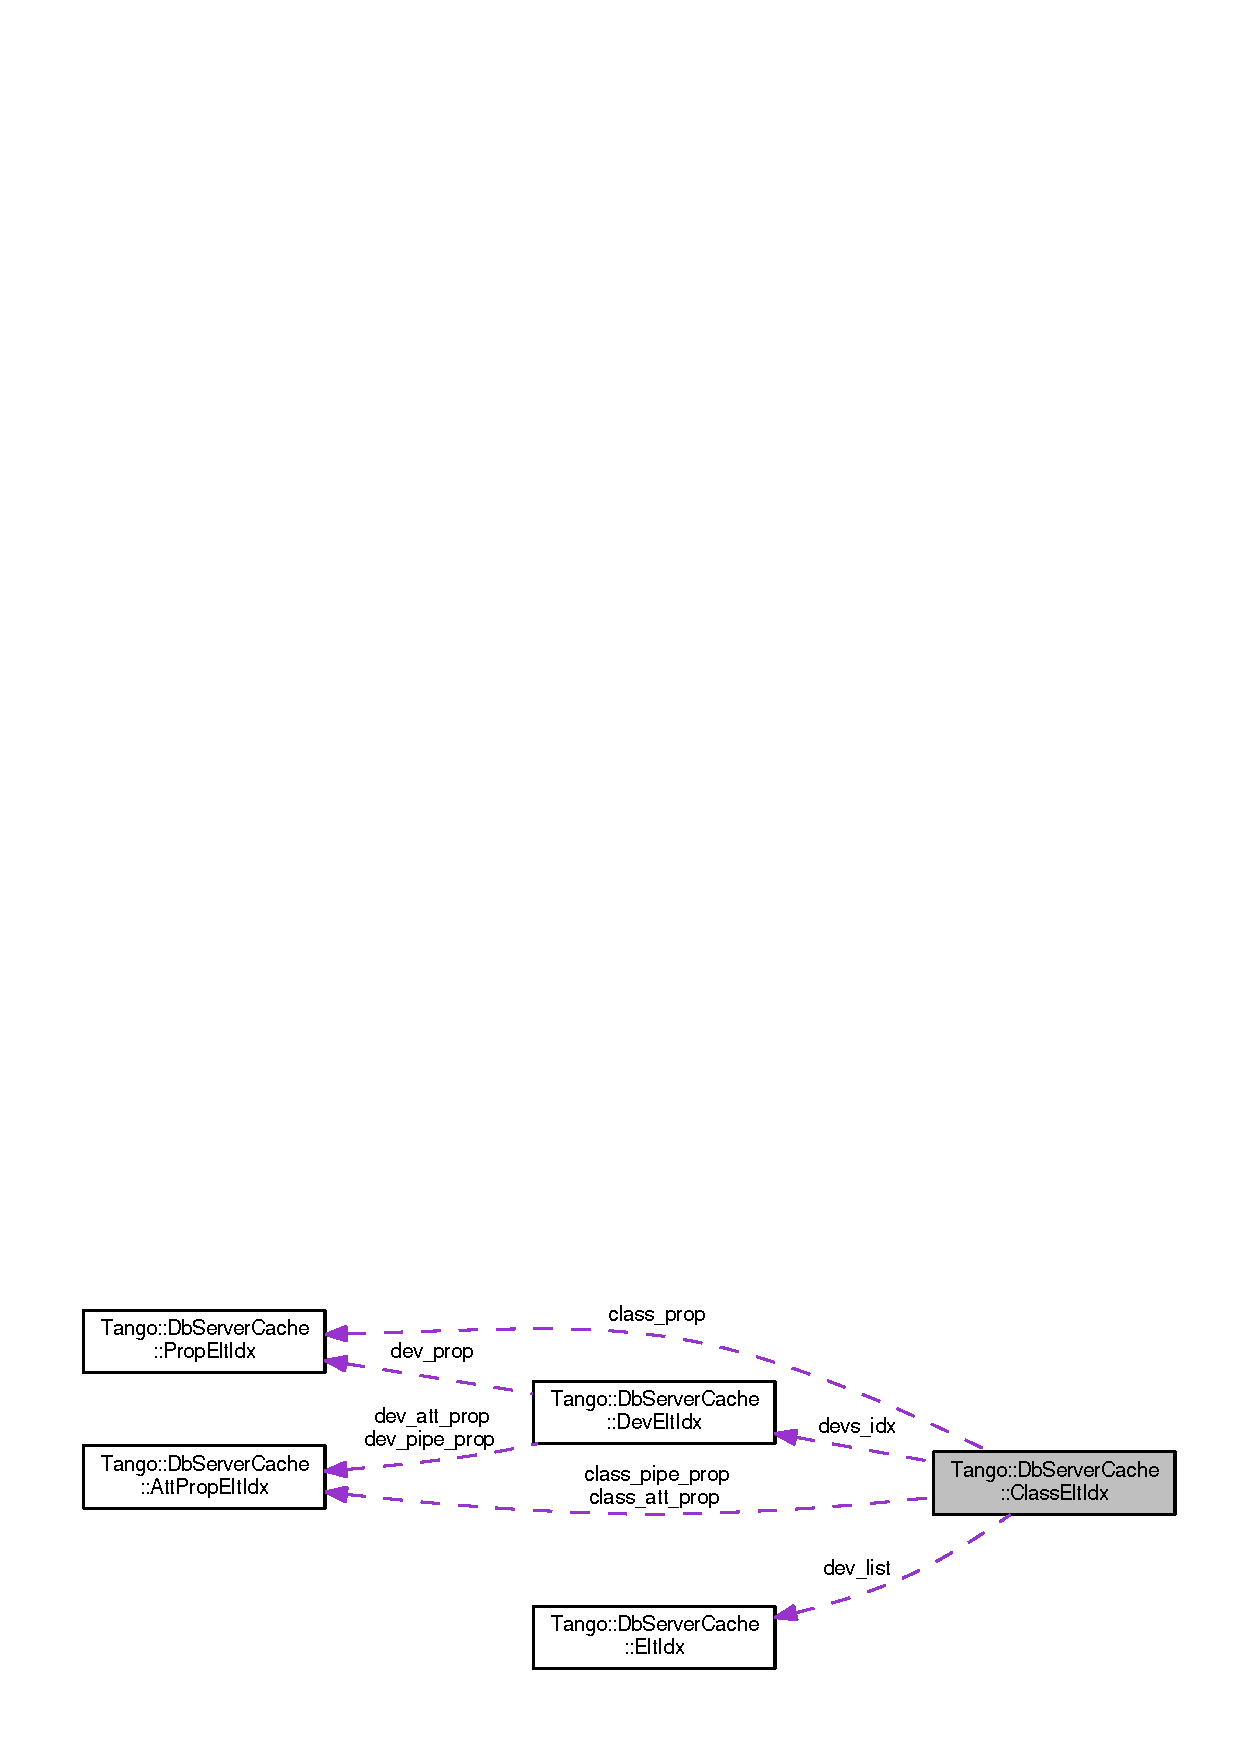
\includegraphics[width=350pt]{d7/df5/structTango_1_1DbServerCache_1_1ClassEltIdx__coll__graph}
\end{center}
\end{figure}
\subsection*{Public Attributes}
\begin{DoxyCompactItemize}
\item 
{\bf Att\-Prop\-Elt\-Idx} {\bf class\-\_\-att\-\_\-prop}
\item 
{\bf Att\-Prop\-Elt\-Idx} {\bf class\-\_\-pipe\-\_\-prop}
\item 
{\bf Prop\-Elt\-Idx} {\bf class\-\_\-prop}
\item 
{\bf Elt\-Idx} {\bf dev\-\_\-list}
\item 
int {\bf dev\-\_\-nb}
\item 
{\bf Dev\-Elt\-Idx} $\ast$ {\bf devs\-\_\-idx}
\end{DoxyCompactItemize}


\subsection{Member Data Documentation}
\index{Tango\-::\-Db\-Server\-Cache\-::\-Class\-Elt\-Idx@{Tango\-::\-Db\-Server\-Cache\-::\-Class\-Elt\-Idx}!class\-\_\-att\-\_\-prop@{class\-\_\-att\-\_\-prop}}
\index{class\-\_\-att\-\_\-prop@{class\-\_\-att\-\_\-prop}!Tango::DbServerCache::ClassEltIdx@{Tango\-::\-Db\-Server\-Cache\-::\-Class\-Elt\-Idx}}
\subsubsection[{class\-\_\-att\-\_\-prop}]{\setlength{\rightskip}{0pt plus 5cm}{\bf Att\-Prop\-Elt\-Idx} Tango\-::\-Db\-Server\-Cache\-::\-Class\-Elt\-Idx\-::class\-\_\-att\-\_\-prop}\label{structTango_1_1DbServerCache_1_1ClassEltIdx_a9fbbd8cdcb5c7a869d1292355fb09596}
\index{Tango\-::\-Db\-Server\-Cache\-::\-Class\-Elt\-Idx@{Tango\-::\-Db\-Server\-Cache\-::\-Class\-Elt\-Idx}!class\-\_\-pipe\-\_\-prop@{class\-\_\-pipe\-\_\-prop}}
\index{class\-\_\-pipe\-\_\-prop@{class\-\_\-pipe\-\_\-prop}!Tango::DbServerCache::ClassEltIdx@{Tango\-::\-Db\-Server\-Cache\-::\-Class\-Elt\-Idx}}
\subsubsection[{class\-\_\-pipe\-\_\-prop}]{\setlength{\rightskip}{0pt plus 5cm}{\bf Att\-Prop\-Elt\-Idx} Tango\-::\-Db\-Server\-Cache\-::\-Class\-Elt\-Idx\-::class\-\_\-pipe\-\_\-prop}\label{structTango_1_1DbServerCache_1_1ClassEltIdx_ac1c241656ef3f26fb2b640ebc745e9ac}
\index{Tango\-::\-Db\-Server\-Cache\-::\-Class\-Elt\-Idx@{Tango\-::\-Db\-Server\-Cache\-::\-Class\-Elt\-Idx}!class\-\_\-prop@{class\-\_\-prop}}
\index{class\-\_\-prop@{class\-\_\-prop}!Tango::DbServerCache::ClassEltIdx@{Tango\-::\-Db\-Server\-Cache\-::\-Class\-Elt\-Idx}}
\subsubsection[{class\-\_\-prop}]{\setlength{\rightskip}{0pt plus 5cm}{\bf Prop\-Elt\-Idx} Tango\-::\-Db\-Server\-Cache\-::\-Class\-Elt\-Idx\-::class\-\_\-prop}\label{structTango_1_1DbServerCache_1_1ClassEltIdx_a819bca1fe1324afeabe56fd4b8b3bd74}
\index{Tango\-::\-Db\-Server\-Cache\-::\-Class\-Elt\-Idx@{Tango\-::\-Db\-Server\-Cache\-::\-Class\-Elt\-Idx}!dev\-\_\-list@{dev\-\_\-list}}
\index{dev\-\_\-list@{dev\-\_\-list}!Tango::DbServerCache::ClassEltIdx@{Tango\-::\-Db\-Server\-Cache\-::\-Class\-Elt\-Idx}}
\subsubsection[{dev\-\_\-list}]{\setlength{\rightskip}{0pt plus 5cm}{\bf Elt\-Idx} Tango\-::\-Db\-Server\-Cache\-::\-Class\-Elt\-Idx\-::dev\-\_\-list}\label{structTango_1_1DbServerCache_1_1ClassEltIdx_aef1b02184530ff5d021d9e3cacc148be}
\index{Tango\-::\-Db\-Server\-Cache\-::\-Class\-Elt\-Idx@{Tango\-::\-Db\-Server\-Cache\-::\-Class\-Elt\-Idx}!dev\-\_\-nb@{dev\-\_\-nb}}
\index{dev\-\_\-nb@{dev\-\_\-nb}!Tango::DbServerCache::ClassEltIdx@{Tango\-::\-Db\-Server\-Cache\-::\-Class\-Elt\-Idx}}
\subsubsection[{dev\-\_\-nb}]{\setlength{\rightskip}{0pt plus 5cm}int Tango\-::\-Db\-Server\-Cache\-::\-Class\-Elt\-Idx\-::dev\-\_\-nb}\label{structTango_1_1DbServerCache_1_1ClassEltIdx_ab12f2d6ea68e22e833517e5c2eaeaef3}
\index{Tango\-::\-Db\-Server\-Cache\-::\-Class\-Elt\-Idx@{Tango\-::\-Db\-Server\-Cache\-::\-Class\-Elt\-Idx}!devs\-\_\-idx@{devs\-\_\-idx}}
\index{devs\-\_\-idx@{devs\-\_\-idx}!Tango::DbServerCache::ClassEltIdx@{Tango\-::\-Db\-Server\-Cache\-::\-Class\-Elt\-Idx}}
\subsubsection[{devs\-\_\-idx}]{\setlength{\rightskip}{0pt plus 5cm}{\bf Dev\-Elt\-Idx}$\ast$ Tango\-::\-Db\-Server\-Cache\-::\-Class\-Elt\-Idx\-::devs\-\_\-idx}\label{structTango_1_1DbServerCache_1_1ClassEltIdx_a334030bc2b46d5b5fa2b9c4402ca2553}


The documentation for this struct was generated from the following file\-:\begin{DoxyCompactItemize}
\item 
{\bf dbapi.\-h}\end{DoxyCompactItemize}

\section{Tango\-:\-:Cmd\-Done\-Event Class Reference}
\label{classTango_1_1CmdDoneEvent}\index{Tango\-::\-Cmd\-Done\-Event@{Tango\-::\-Cmd\-Done\-Event}}


Asynchronous command execution callback data.  


\subsection*{Public Attributes}
\begin{DoxyCompactItemize}
\item 
Device\-Data \& {\bf argout}
\begin{DoxyCompactList}\small\item\em The command argout. \end{DoxyCompactList}\item 
string \& {\bf cmd\-\_\-name}
\begin{DoxyCompactList}\small\item\em The command name. \end{DoxyCompactList}\item 
Tango\-::\-Device\-Proxy $\ast$ {\bf device}
\begin{DoxyCompactList}\small\item\em The Device\-Proxy object on which the call was executed. \end{DoxyCompactList}\item 
bool {\bf err}
\begin{DoxyCompactList}\small\item\em A boolean flag set to true if the command failed. False otherwise. \end{DoxyCompactList}\item 
Dev\-Error\-List \& {\bf errors}
\begin{DoxyCompactList}\small\item\em The error stack. \end{DoxyCompactList}\end{DoxyCompactItemize}


\subsection{Detailed Description}
Asynchronous command execution callback data. 

This class is used to pass data to the callback method in asynchronous callback model for command execution.

\$\-Author\$ \$\-Revision\$ 

\subsection{Member Data Documentation}
\index{Tango\-::\-Cmd\-Done\-Event@{Tango\-::\-Cmd\-Done\-Event}!argout@{argout}}
\index{argout@{argout}!Tango::CmdDoneEvent@{Tango\-::\-Cmd\-Done\-Event}}
\subsubsection[{argout}]{\setlength{\rightskip}{0pt plus 5cm}Device\-Data\& Tango\-::\-Cmd\-Done\-Event\-::argout}\label{classTango_1_1CmdDoneEvent_a5bfb13a2fa90db07a6bd6092188dd96b}


The command argout. 

\index{Tango\-::\-Cmd\-Done\-Event@{Tango\-::\-Cmd\-Done\-Event}!cmd\-\_\-name@{cmd\-\_\-name}}
\index{cmd\-\_\-name@{cmd\-\_\-name}!Tango::CmdDoneEvent@{Tango\-::\-Cmd\-Done\-Event}}
\subsubsection[{cmd\-\_\-name}]{\setlength{\rightskip}{0pt plus 5cm}string\& Tango\-::\-Cmd\-Done\-Event\-::cmd\-\_\-name}\label{classTango_1_1CmdDoneEvent_a9b3ff5a65147c469b19d5deafecf600a}


The command name. 

\index{Tango\-::\-Cmd\-Done\-Event@{Tango\-::\-Cmd\-Done\-Event}!device@{device}}
\index{device@{device}!Tango::CmdDoneEvent@{Tango\-::\-Cmd\-Done\-Event}}
\subsubsection[{device}]{\setlength{\rightskip}{0pt plus 5cm}Tango\-::\-Device\-Proxy$\ast$ Tango\-::\-Cmd\-Done\-Event\-::device}\label{classTango_1_1CmdDoneEvent_a4815622ebc52bc227f481e2d488cc7c1}


The Device\-Proxy object on which the call was executed. 

\index{Tango\-::\-Cmd\-Done\-Event@{Tango\-::\-Cmd\-Done\-Event}!err@{err}}
\index{err@{err}!Tango::CmdDoneEvent@{Tango\-::\-Cmd\-Done\-Event}}
\subsubsection[{err}]{\setlength{\rightskip}{0pt plus 5cm}bool Tango\-::\-Cmd\-Done\-Event\-::err}\label{classTango_1_1CmdDoneEvent_aa65c091b8483025114f5825760cb994a}


A boolean flag set to true if the command failed. False otherwise. 

\index{Tango\-::\-Cmd\-Done\-Event@{Tango\-::\-Cmd\-Done\-Event}!errors@{errors}}
\index{errors@{errors}!Tango::CmdDoneEvent@{Tango\-::\-Cmd\-Done\-Event}}
\subsubsection[{errors}]{\setlength{\rightskip}{0pt plus 5cm}Dev\-Error\-List\& Tango\-::\-Cmd\-Done\-Event\-::errors}\label{classTango_1_1CmdDoneEvent_ad6842cac8f28ad790a3a19bd4818390e}


The error stack. 



The documentation for this class was generated from the following file\-:\begin{DoxyCompactItemize}
\item 
{\bf devasyn.\-h}\end{DoxyCompactItemize}

\section{Tango\-:\-:Cmd\-History\-Stack$<$ T $>$ Class Template Reference}
\label{classTango_1_1CmdHistoryStack}\index{Tango\-::\-Cmd\-History\-Stack$<$ T $>$@{Tango\-::\-Cmd\-History\-Stack$<$ T $>$}}


This class is a used to pass a command result history when the user directly fills the command polling buffer.  


\subsection*{Public Member Functions}
\begin{DoxyCompactItemize}
\item 
void {\bf clear} ()
\begin{DoxyCompactList}\small\item\em Clear the stack. \end{DoxyCompactList}\item 
vector$<$ {\bf Timed\-Cmd\-Data}$<$ T $>$ $>$ \& {\bf get\-\_\-data} ()
\begin{DoxyCompactList}\small\item\em Get stack data. \end{DoxyCompactList}\item 
size\-\_\-t {\bf length} ()
\begin{DoxyCompactList}\small\item\em Get stack depth. \end{DoxyCompactList}\item 
void {\bf length} (long nb)
\begin{DoxyCompactList}\small\item\em Reserve memory for stack elements. \end{DoxyCompactList}\item 
void {\bf push} ({\bf Tango\-::\-Timed\-Cmd\-Data}$<$ T $>$ const \&elt)
\begin{DoxyCompactList}\small\item\em Store a new element in the stack. \end{DoxyCompactList}\end{DoxyCompactItemize}


\subsection{Detailed Description}
\subsubsection*{template$<$typename T$>$class Tango\-::\-Cmd\-History\-Stack$<$ T $>$}

This class is a used to pass a command result history when the user directly fills the command polling buffer. 

Each element in this stack will be used to store one element of the command polling buffer

\$\-Author\$ \$\-Revision\$ 

\subsection{Member Function Documentation}
\index{Tango\-::\-Cmd\-History\-Stack@{Tango\-::\-Cmd\-History\-Stack}!clear@{clear}}
\index{clear@{clear}!Tango::CmdHistoryStack@{Tango\-::\-Cmd\-History\-Stack}}
\subsubsection[{clear}]{\setlength{\rightskip}{0pt plus 5cm}template$<$typename T$>$ void {\bf Tango\-::\-Cmd\-History\-Stack}$<$ T $>$\-::clear (
\begin{DoxyParamCaption}
{}
\end{DoxyParamCaption}
)\hspace{0.3cm}{\ttfamily [inline]}}\label{classTango_1_1CmdHistoryStack_ae4ac3a6bb53c0661656a3a885a56347c}


Clear the stack. 

\index{Tango\-::\-Cmd\-History\-Stack@{Tango\-::\-Cmd\-History\-Stack}!get\-\_\-data@{get\-\_\-data}}
\index{get\-\_\-data@{get\-\_\-data}!Tango::CmdHistoryStack@{Tango\-::\-Cmd\-History\-Stack}}
\subsubsection[{get\-\_\-data}]{\setlength{\rightskip}{0pt plus 5cm}template$<$typename T$>$ vector$<${\bf Timed\-Cmd\-Data}$<$T$>$ $>$\& {\bf Tango\-::\-Cmd\-History\-Stack}$<$ T $>$\-::get\-\_\-data (
\begin{DoxyParamCaption}
{}
\end{DoxyParamCaption}
)}\label{classTango_1_1CmdHistoryStack_a60e2fac55007f4697ca68bc35a2a7fdc}


Get stack data. 

\begin{DoxyReturn}{Returns}
The stack itself 
\end{DoxyReturn}
\index{Tango\-::\-Cmd\-History\-Stack@{Tango\-::\-Cmd\-History\-Stack}!length@{length}}
\index{length@{length}!Tango::CmdHistoryStack@{Tango\-::\-Cmd\-History\-Stack}}
\subsubsection[{length}]{\setlength{\rightskip}{0pt plus 5cm}template$<$typename T$>$ size\-\_\-t {\bf Tango\-::\-Cmd\-History\-Stack}$<$ T $>$\-::length (
\begin{DoxyParamCaption}
{}
\end{DoxyParamCaption}
)\hspace{0.3cm}{\ttfamily [inline]}}\label{classTango_1_1CmdHistoryStack_a21c635342bfae43ae1db2e4e721b4b4f}


Get stack depth. 

\begin{DoxyReturn}{Returns}
The stack depth 
\end{DoxyReturn}
\index{Tango\-::\-Cmd\-History\-Stack@{Tango\-::\-Cmd\-History\-Stack}!length@{length}}
\index{length@{length}!Tango::CmdHistoryStack@{Tango\-::\-Cmd\-History\-Stack}}
\subsubsection[{length}]{\setlength{\rightskip}{0pt plus 5cm}template$<$typename T$>$ void {\bf Tango\-::\-Cmd\-History\-Stack}$<$ T $>$\-::length (
\begin{DoxyParamCaption}
\item[{long}]{nb}
\end{DoxyParamCaption}
)\hspace{0.3cm}{\ttfamily [inline]}}\label{classTango_1_1CmdHistoryStack_ab9d2cfc6b3d8fca2a11ad3e7d2a47495}


Reserve memory for stack elements. 


\begin{DoxyParams}{Parameters}
{\em nb} & The stack element number \\
\hline
\end{DoxyParams}
\index{Tango\-::\-Cmd\-History\-Stack@{Tango\-::\-Cmd\-History\-Stack}!push@{push}}
\index{push@{push}!Tango::CmdHistoryStack@{Tango\-::\-Cmd\-History\-Stack}}
\subsubsection[{push}]{\setlength{\rightskip}{0pt plus 5cm}template$<$typename T$>$ void {\bf Tango\-::\-Cmd\-History\-Stack}$<$ T $>$\-::push (
\begin{DoxyParamCaption}
\item[{{\bf Tango\-::\-Timed\-Cmd\-Data}$<$ T $>$ const \&}]{elt}
\end{DoxyParamCaption}
)}\label{classTango_1_1CmdHistoryStack_a355ba8abdd8a382b3c0aa09def8a57ca}


Store a new element in the stack. 

This method stores a new element in the stack


\begin{DoxyParams}{Parameters}
{\em elt} & The new element \\
\hline
\end{DoxyParams}


The documentation for this class was generated from the following file\-:\begin{DoxyCompactItemize}
\item 
{\bf pollext.\-h}\end{DoxyCompactItemize}

\section{Tango\-:\-:Command Class Reference}
\label{classTango_1_1Command}\index{Tango\-::\-Command@{Tango\-::\-Command}}


This class is a class representing a command in the T\-A\-N\-G\-O device server pattern.  




Inheritance diagram for Tango\-:\-:Command\-:
\nopagebreak
\begin{figure}[H]
\begin{center}
\leavevmode
\includegraphics[width=350pt]{d0/db1/classTango_1_1Command__inherit__graph}
\end{center}
\end{figure}
\subsection*{Public Member Functions}
\begin{Indent}{\bf Constructors}\par
{\em Miscellaneous constructors }\begin{DoxyCompactItemize}
\item 
{\bf Command} ()
\begin{DoxyCompactList}\small\item\em Constructs a newly allocated \doxyref{Command}{p.}{d2/d1d/classTango_1_1Command} object. \end{DoxyCompactList}\item 
{\bf Command} (const char $\ast$s, {\bf Tango\-::\-Cmd\-Arg\-Type} in, {\bf Tango\-::\-Cmd\-Arg\-Type} out)
\begin{DoxyCompactList}\small\item\em Constructs a newly allocated \doxyref{Command}{p.}{d2/d1d/classTango_1_1Command} object for a command from its name and its input and output parameter types. \end{DoxyCompactList}\item 
{\bf Command} (string \&s, {\bf Tango\-::\-Cmd\-Arg\-Type} in, {\bf Tango\-::\-Cmd\-Arg\-Type} out)
\begin{DoxyCompactList}\small\item\em Constructs a newly allocated \doxyref{Command}{p.}{d2/d1d/classTango_1_1Command} object for a command from its name and its input and output parameter types. \end{DoxyCompactList}\item 
{\bf Command} (const char $\ast$s, {\bf Tango\-::\-Cmd\-Arg\-Type} in, {\bf Tango\-::\-Cmd\-Arg\-Type} out, const char $\ast$in\-\_\-desc, const char $\ast$out\-\_\-desc)
\begin{DoxyCompactList}\small\item\em Constructs a newly allocated \doxyref{Command}{p.}{d2/d1d/classTango_1_1Command} object for a command from its name, its input and output parameter types plus parameters description The command display level is set to O\-P\-E\-R\-A\-T\-O\-R. \end{DoxyCompactList}\item 
{\bf Command} (string \&s, {\bf Tango\-::\-Cmd\-Arg\-Type} in, {\bf Tango\-::\-Cmd\-Arg\-Type} out, string \&in\-\_\-desc, string \&out\-\_\-desc)
\begin{DoxyCompactList}\small\item\em Constructs a newly allocated \doxyref{Command}{p.}{d2/d1d/classTango_1_1Command} object for a command from its name, its input and output parameter types plus parameters description The command display level is set to O\-P\-E\-R\-A\-T\-O\-R. \end{DoxyCompactList}\item 
{\bf Command} (const char $\ast$s, {\bf Tango\-::\-Cmd\-Arg\-Type} in, {\bf Tango\-::\-Cmd\-Arg\-Type} out, Tango\-::\-Disp\-Level level)
\begin{DoxyCompactList}\small\item\em Constructs a newly allocated \doxyref{Command}{p.}{d2/d1d/classTango_1_1Command} object for a command from its name and its input and output parameter types. \end{DoxyCompactList}\item 
{\bf Command} (string \&s, {\bf Tango\-::\-Cmd\-Arg\-Type} in, {\bf Tango\-::\-Cmd\-Arg\-Type} out, Tango\-::\-Disp\-Level level)
\begin{DoxyCompactList}\small\item\em Constructs a newly allocated \doxyref{Command}{p.}{d2/d1d/classTango_1_1Command} object for a command from its name and its input and output parameter types. \end{DoxyCompactList}\item 
{\bf Command} (const char $\ast$s, {\bf Tango\-::\-Cmd\-Arg\-Type} in, {\bf Tango\-::\-Cmd\-Arg\-Type} out, const char $\ast$in\-\_\-desc, const char $\ast$out\-\_\-desc, Tango\-::\-Disp\-Level level)
\begin{DoxyCompactList}\small\item\em Constructs a newly allocated \doxyref{Command}{p.}{d2/d1d/classTango_1_1Command} object for a command from its name, its input and output parameter types plus parameters description. \end{DoxyCompactList}\item 
{\bf Command} (string \&s, {\bf Tango\-::\-Cmd\-Arg\-Type} in, {\bf Tango\-::\-Cmd\-Arg\-Type} out, string \&in\-\_\-desc, string \&out\-\_\-desc, Tango\-::\-Disp\-Level level)
\begin{DoxyCompactList}\small\item\em Constructs a newly allocated \doxyref{Command}{p.}{d2/d1d/classTango_1_1Command} object for a command from its name, its input and output parameter types plus parameters description. \end{DoxyCompactList}\end{DoxyCompactItemize}
\end{Indent}
\begin{Indent}{\bf Destructor}\par
{\em Only one desctructor is defined for this class }\begin{DoxyCompactItemize}
\item 
virtual {\bf $\sim$\-Command} ()
\begin{DoxyCompactList}\small\item\em The object desctructor. \end{DoxyCompactList}\end{DoxyCompactItemize}
\end{Indent}
\begin{Indent}{\bf Miscellaneous methods}\par
\begin{DoxyCompactItemize}
\item 
virtual C\-O\-R\-B\-A\-::\-Any $\ast$ {\bf execute} ({\bf Device\-Impl} $\ast$dev, const C\-O\-R\-B\-A\-::\-Any \&in\-\_\-any)=0
\begin{DoxyCompactList}\small\item\em Execute the command. \end{DoxyCompactList}\item 
virtual bool {\bf is\-\_\-allowed} ({\bf Device\-Impl} $\ast$dev, const C\-O\-R\-B\-A\-::\-Any \&in\-\_\-any)
\begin{DoxyCompactList}\small\item\em Check if the command is allowed in the actual device state. \end{DoxyCompactList}\item 
virtual void {\bf init\-\_\-types} ()
\begin{DoxyCompactList}\small\item\em Init command parameters type. \end{DoxyCompactList}\end{DoxyCompactItemize}
\end{Indent}
\begin{Indent}{\bf Get/\-Set object members.}\par
{\em These methods allows the external world to get/set \doxyref{Device\-Impl}{p.}{d3/d62/classTango_1_1DeviceImpl} instance data members }\begin{DoxyCompactItemize}
\item 
string \& {\bf get\-\_\-name} ()
\begin{DoxyCompactList}\small\item\em Return the command name. \end{DoxyCompactList}\item 
void {\bf set\-\_\-name} (string \&new\-\_\-name)
\begin{DoxyCompactList}\small\item\em Set the command name. \end{DoxyCompactList}\item 
string \& {\bf get\-\_\-lower\-\_\-name} ()
\begin{DoxyCompactList}\small\item\em Return the command name in lower case letters. \end{DoxyCompactList}\item 
{\bf Tango\-::\-Cmd\-Arg\-Type} {\bf get\-\_\-in\-\_\-type} ()
\begin{DoxyCompactList}\small\item\em Return the input parameter type. \end{DoxyCompactList}\item 
{\bf Tango\-::\-Cmd\-Arg\-Type} {\bf get\-\_\-out\-\_\-type} ()
\begin{DoxyCompactList}\small\item\em Return the output parameter type. \end{DoxyCompactList}\item 
string \& {\bf get\-\_\-in\-\_\-type\-\_\-desc} ()
\begin{DoxyCompactList}\small\item\em Return the input parameter description. \end{DoxyCompactList}\item 
string \& {\bf get\-\_\-out\-\_\-type\-\_\-desc} ()
\begin{DoxyCompactList}\small\item\em Return the output parameter description. \end{DoxyCompactList}\item 
Tango\-::\-Disp\-Level {\bf get\-\_\-disp\-\_\-level} ()
\begin{DoxyCompactList}\small\item\em Return the command display level. \end{DoxyCompactList}\item 
void {\bf set\-\_\-in\-\_\-type\-\_\-desc} (const char $\ast$desc)
\begin{DoxyCompactList}\small\item\em Set the input parameter description field. \end{DoxyCompactList}\item 
void {\bf set\-\_\-in\-\_\-type\-\_\-desc} (string \&desc)
\begin{DoxyCompactList}\small\item\em Set the input parameter description field. \end{DoxyCompactList}\item 
void {\bf set\-\_\-out\-\_\-type\-\_\-desc} (const char $\ast$desc)
\begin{DoxyCompactList}\small\item\em Set the output parameter description field. \end{DoxyCompactList}\item 
void {\bf set\-\_\-out\-\_\-type\-\_\-desc} (string \&desc)
\begin{DoxyCompactList}\small\item\em Set the output parameter description field. \end{DoxyCompactList}\item 
void {\bf set\-\_\-disp\-\_\-level} (Tango\-::\-Disp\-Level level)
\begin{DoxyCompactList}\small\item\em Set the command display level. \end{DoxyCompactList}\item 
void {\bf set\-\_\-polling\-\_\-period} (long per)
\begin{DoxyCompactList}\small\item\em Set the command polling period. \end{DoxyCompactList}\item 
long {\bf get\-\_\-polling\-\_\-period} ()
\begin{DoxyCompactList}\small\item\em Get the command polling period. \end{DoxyCompactList}\end{DoxyCompactItemize}
\end{Indent}
\begin{Indent}{\bf Extract methods.}\par
{\em All these methods extract data from the C\-O\-R\-B\-A Any object received as command input data }\begin{DoxyCompactItemize}
\item 
void {\bf extract} (const C\-O\-R\-B\-A\-::\-Any \&in, Tango\-::\-Dev\-Boolean \&data)
\begin{DoxyCompactList}\small\item\em Extract a boolean data from a C\-O\-R\-B\-A Any object. \end{DoxyCompactList}\item 
void {\bf extract} (const C\-O\-R\-B\-A\-::\-Any \&in, Tango\-::\-Dev\-Short \&data)
\begin{DoxyCompactList}\small\item\em Extract a short data from a C\-O\-R\-B\-A Any object. \end{DoxyCompactList}\item 
void {\bf extract} (const C\-O\-R\-B\-A\-::\-Any \&in, Tango\-::\-Dev\-Long \&data)
\begin{DoxyCompactList}\small\item\em Extract a long data from a C\-O\-R\-B\-A Any object. \end{DoxyCompactList}\item 
void {\bf extract} (const C\-O\-R\-B\-A\-::\-Any \&in, Tango\-::\-Dev\-Long64 \&data)
\begin{DoxyCompactList}\small\item\em Extract a 64 bits long data from a C\-O\-R\-B\-A Any object. \end{DoxyCompactList}\item 
void {\bf extract} (const C\-O\-R\-B\-A\-::\-Any \&in, Tango\-::\-Dev\-Float \&data)
\begin{DoxyCompactList}\small\item\em Extract a float data from a C\-O\-R\-B\-A Any object. \end{DoxyCompactList}\item 
void {\bf extract} (const C\-O\-R\-B\-A\-::\-Any \&in, Tango\-::\-Dev\-Double \&data)
\begin{DoxyCompactList}\small\item\em Extract a double data from a C\-O\-R\-B\-A Any object. \end{DoxyCompactList}\item 
void {\bf extract} (const C\-O\-R\-B\-A\-::\-Any \&in, Tango\-::\-Dev\-U\-Short \&data)
\begin{DoxyCompactList}\small\item\em Extract an unsigned short data from a C\-O\-R\-B\-A Any object. \end{DoxyCompactList}\item 
void {\bf extract} (const C\-O\-R\-B\-A\-::\-Any \&in, Tango\-::\-Dev\-U\-Long \&data)
\begin{DoxyCompactList}\small\item\em Extract an unsigned long data from a C\-O\-R\-B\-A Any object. \end{DoxyCompactList}\item 
void {\bf extract} (const C\-O\-R\-B\-A\-::\-Any \&in, Tango\-::\-Dev\-U\-Long64 \&data)
\begin{DoxyCompactList}\small\item\em Extract an unsigned 64 bits long data from a C\-O\-R\-B\-A Any object. \end{DoxyCompactList}\item 
void {\bf extract} (const C\-O\-R\-B\-A\-::\-Any \&in, Tango\-::\-Dev\-String \&data)
\begin{DoxyCompactList}\small\item\em Extract a string from a C\-O\-R\-B\-A Any object. \end{DoxyCompactList}\item 
void {\bf extract} (const C\-O\-R\-B\-A\-::\-Any \&in, const char $\ast$\&data)
\begin{DoxyCompactList}\small\item\em Extract a const string from a C\-O\-R\-B\-A Any object. \end{DoxyCompactList}\item 
void {\bf extract} (const C\-O\-R\-B\-A\-::\-Any \&in, const Tango\-::\-Dev\-Var\-Char\-Array $\ast$\&data)
\begin{DoxyCompactList}\small\item\em Extract a char array from a C\-O\-R\-B\-A Any object. \end{DoxyCompactList}\item 
void {\bf extract} (const C\-O\-R\-B\-A\-::\-Any \&in, const Tango\-::\-Dev\-Var\-Short\-Array $\ast$\&data)
\begin{DoxyCompactList}\small\item\em Extract a short array from a C\-O\-R\-B\-A Any object. \end{DoxyCompactList}\item 
void {\bf extract} (const C\-O\-R\-B\-A\-::\-Any \&in, const Tango\-::\-Dev\-Var\-Long\-Array $\ast$\&data)
\begin{DoxyCompactList}\small\item\em Extract a long array from a C\-O\-R\-B\-A Any object. \end{DoxyCompactList}\item 
void {\bf extract} (const C\-O\-R\-B\-A\-::\-Any \&in, const Tango\-::\-Dev\-Var\-Long64\-Array $\ast$\&data)
\begin{DoxyCompactList}\small\item\em Extract a 64 bits long array from a C\-O\-R\-B\-A Any object. \end{DoxyCompactList}\item 
void {\bf extract} (const C\-O\-R\-B\-A\-::\-Any \&in, const Tango\-::\-Dev\-Var\-Float\-Array $\ast$\&data)
\begin{DoxyCompactList}\small\item\em Extract a float array from a C\-O\-R\-B\-A Any object. \end{DoxyCompactList}\item 
void {\bf extract} (const C\-O\-R\-B\-A\-::\-Any \&in, const Tango\-::\-Dev\-Var\-Double\-Array $\ast$\&data)
\begin{DoxyCompactList}\small\item\em Extract a double array from a C\-O\-R\-B\-A Any object. \end{DoxyCompactList}\item 
void {\bf extract} (const C\-O\-R\-B\-A\-::\-Any \&in, const Tango\-::\-Dev\-Var\-U\-Short\-Array $\ast$\&data)
\begin{DoxyCompactList}\small\item\em Extract a unsigned short array from a C\-O\-R\-B\-A Any object. \end{DoxyCompactList}\item 
void {\bf extract} (const C\-O\-R\-B\-A\-::\-Any \&in, const Tango\-::\-Dev\-Var\-U\-Long\-Array $\ast$\&data)
\begin{DoxyCompactList}\small\item\em Extract a unsigned long array from a C\-O\-R\-B\-A Any object. \end{DoxyCompactList}\item 
void {\bf extract} (const C\-O\-R\-B\-A\-::\-Any \&in, const Tango\-::\-Dev\-Var\-U\-Long64\-Array $\ast$\&data)
\begin{DoxyCompactList}\small\item\em Extract a unsigned 64 bits long array from a C\-O\-R\-B\-A Any object. \end{DoxyCompactList}\item 
void {\bf extract} (const C\-O\-R\-B\-A\-::\-Any \&in, const Tango\-::\-Dev\-Var\-String\-Array $\ast$\&data)
\begin{DoxyCompactList}\small\item\em Extract a string array from a C\-O\-R\-B\-A Any object. \end{DoxyCompactList}\item 
void {\bf extract} (const C\-O\-R\-B\-A\-::\-Any \&in, const Tango\-::\-Dev\-Var\-Long\-String\-Array $\ast$\&data)
\begin{DoxyCompactList}\small\item\em Extract a Dev\-Var\-Long\-String\-Array data from a C\-O\-R\-B\-A Any object. \end{DoxyCompactList}\item 
void {\bf extract} (const C\-O\-R\-B\-A\-::\-Any \&in, const Tango\-::\-Dev\-Var\-Double\-String\-Array $\ast$\&data)
\begin{DoxyCompactList}\small\item\em Extract a Dev\-Var\-Double\-String\-Array data from a C\-O\-R\-B\-A Any object. \end{DoxyCompactList}\item 
void {\bf extract} (const C\-O\-R\-B\-A\-::\-Any \&in, Tango\-::\-Dev\-State \&data)
\begin{DoxyCompactList}\small\item\em Extract a \doxyref{Tango}{p.}{de/ddf/namespaceTango} device state data from a C\-O\-R\-B\-A Any object. \end{DoxyCompactList}\item 
void {\bf extract} (const C\-O\-R\-B\-A\-::\-Any \&in, const Tango\-::\-Dev\-Encoded $\ast$\&data)
\begin{DoxyCompactList}\small\item\em Extract a \doxyref{Tango}{p.}{de/ddf/namespaceTango} Dev\-Encoded data from a C\-O\-R\-B\-A Any object. \end{DoxyCompactList}\end{DoxyCompactItemize}
\end{Indent}
\begin{Indent}{\bf Insert methods.}\par
{\em All these methods create a C\-O\-R\-B\-A Any object and insert data into this object }\begin{DoxyCompactItemize}
\item 
C\-O\-R\-B\-A\-::\-Any $\ast$ {\bf insert} ()
\begin{DoxyCompactList}\small\item\em Create an empty C\-O\-R\-B\-A Any object. \end{DoxyCompactList}\item 
C\-O\-R\-B\-A\-::\-Any $\ast$ {\bf insert} (Tango\-::\-Dev\-Boolean data)
\begin{DoxyCompactList}\small\item\em Create a C\-O\-R\-B\-A Any object and insert a Tango\-::\-Dev\-Boolean data in it. \end{DoxyCompactList}\item 
C\-O\-R\-B\-A\-::\-Any $\ast$ {\bf insert} (Tango\-::\-Dev\-Short data)
\begin{DoxyCompactList}\small\item\em Create a C\-O\-R\-B\-A Any object and insert a Tango\-::\-Dev\-Short data in it. \end{DoxyCompactList}\item 
C\-O\-R\-B\-A\-::\-Any $\ast$ {\bf insert} (Tango\-::\-Dev\-Long data)
\begin{DoxyCompactList}\small\item\em Create a C\-O\-R\-B\-A Any object and insert a Tango\-::\-Dev\-Long data in it. \end{DoxyCompactList}\item 
C\-O\-R\-B\-A\-::\-Any $\ast$ {\bf insert} (Tango\-::\-Dev\-Long64 data)
\begin{DoxyCompactList}\small\item\em Create a C\-O\-R\-B\-A Any object and insert a Tango\-::\-Dev\-Long64 data in it. \end{DoxyCompactList}\item 
C\-O\-R\-B\-A\-::\-Any $\ast$ {\bf insert} (Tango\-::\-Dev\-Float data)
\begin{DoxyCompactList}\small\item\em Create a C\-O\-R\-B\-A Any object and insert a Tango\-::\-Dev\-Float data in it. \end{DoxyCompactList}\item 
C\-O\-R\-B\-A\-::\-Any $\ast$ {\bf insert} (Tango\-::\-Dev\-Double data)
\begin{DoxyCompactList}\small\item\em Create a C\-O\-R\-B\-A Any object and insert a Tango\-::\-Dev\-Double data in it. \end{DoxyCompactList}\item 
C\-O\-R\-B\-A\-::\-Any $\ast$ {\bf insert} (Tango\-::\-Dev\-U\-Short data)
\begin{DoxyCompactList}\small\item\em Create a C\-O\-R\-B\-A Any object and insert a Tango\-::\-Dev\-U\-Short data in it. \end{DoxyCompactList}\item 
C\-O\-R\-B\-A\-::\-Any $\ast$ {\bf insert} (Tango\-::\-Dev\-U\-Long data)
\begin{DoxyCompactList}\small\item\em Create a C\-O\-R\-B\-A Any object and insert a Tango\-::\-Dev\-U\-Long data in it. \end{DoxyCompactList}\item 
C\-O\-R\-B\-A\-::\-Any $\ast$ {\bf insert} (Tango\-::\-Dev\-U\-Long64 data)
\begin{DoxyCompactList}\small\item\em Create a C\-O\-R\-B\-A Any object and insert a Tango\-::\-Dev\-U\-Long64 data in it. \end{DoxyCompactList}\item 
C\-O\-R\-B\-A\-::\-Any $\ast$ {\bf insert} (Tango\-::\-Dev\-String data)
\begin{DoxyCompactList}\small\item\em Create a C\-O\-R\-B\-A Any object and insert a Tango\-::\-Dev\-String data in it. \end{DoxyCompactList}\item 
C\-O\-R\-B\-A\-::\-Any $\ast$ {\bf insert} (const char $\ast$data)
\begin{DoxyCompactList}\small\item\em Create a C\-O\-R\-B\-A Any object and insert a Tango\-::\-Dev\-String data in it. \end{DoxyCompactList}\item 
C\-O\-R\-B\-A\-::\-Any $\ast$ {\bf insert} (Tango\-::\-Dev\-Var\-Char\-Array \&data)
\begin{DoxyCompactList}\small\item\em Create a C\-O\-R\-B\-A Any object and insert a Tango\-::\-Dev\-Var\-Char\-Array data in it. \end{DoxyCompactList}\item 
C\-O\-R\-B\-A\-::\-Any $\ast$ {\bf insert} (Tango\-::\-Dev\-Var\-Char\-Array $\ast$data)
\begin{DoxyCompactList}\small\item\em Create a C\-O\-R\-B\-A Any object and insert a Tango\-::\-Dev\-Var\-Char\-Array data in it. \end{DoxyCompactList}\item 
C\-O\-R\-B\-A\-::\-Any $\ast$ {\bf insert} (Tango\-::\-Dev\-Var\-Short\-Array \&data)
\begin{DoxyCompactList}\small\item\em Create a C\-O\-R\-B\-A Any object and insert a Tango\-::\-Dev\-Var\-Short\-Array data in it. \end{DoxyCompactList}\item 
C\-O\-R\-B\-A\-::\-Any $\ast$ {\bf insert} (Tango\-::\-Dev\-Var\-Short\-Array $\ast$data)
\begin{DoxyCompactList}\small\item\em Create a C\-O\-R\-B\-A Any object and insert a Tango\-::\-Dev\-Var\-Short\-Array data in it. \end{DoxyCompactList}\item 
C\-O\-R\-B\-A\-::\-Any $\ast$ {\bf insert} (Tango\-::\-Dev\-Var\-Long\-Array \&data)
\begin{DoxyCompactList}\small\item\em Create a C\-O\-R\-B\-A Any object and insert a Tango\-::\-Dev\-Var\-Long\-Array data in it. \end{DoxyCompactList}\item 
C\-O\-R\-B\-A\-::\-Any $\ast$ {\bf insert} (Tango\-::\-Dev\-Var\-Long\-Array $\ast$data)
\begin{DoxyCompactList}\small\item\em Create a C\-O\-R\-B\-A Any object and insert a Tango\-::\-Dev\-Var\-Long\-Array data in it. \end{DoxyCompactList}\item 
C\-O\-R\-B\-A\-::\-Any $\ast$ {\bf insert} (Tango\-::\-Dev\-Var\-Long64\-Array \&data)
\begin{DoxyCompactList}\small\item\em Create a C\-O\-R\-B\-A Any object and insert a Tango\-::\-Dev\-Var\-Long64\-Array data in it. \end{DoxyCompactList}\item 
C\-O\-R\-B\-A\-::\-Any $\ast$ {\bf insert} (Tango\-::\-Dev\-Var\-Long64\-Array $\ast$data)
\begin{DoxyCompactList}\small\item\em Create a C\-O\-R\-B\-A Any object and insert a Tango\-::\-Dev\-Var\-Long64\-Array data in it. \end{DoxyCompactList}\item 
C\-O\-R\-B\-A\-::\-Any $\ast$ {\bf insert} (Tango\-::\-Dev\-Var\-Float\-Array \&data)
\begin{DoxyCompactList}\small\item\em Create a C\-O\-R\-B\-A Any object and insert a Tango\-::\-Dev\-Var\-Float\-Array data in it. \end{DoxyCompactList}\item 
C\-O\-R\-B\-A\-::\-Any $\ast$ {\bf insert} (Tango\-::\-Dev\-Var\-Float\-Array $\ast$data)
\begin{DoxyCompactList}\small\item\em Create a C\-O\-R\-B\-A Any object and insert a Tango\-::\-Dev\-Var\-Float\-Array data in it. \end{DoxyCompactList}\item 
C\-O\-R\-B\-A\-::\-Any $\ast$ {\bf insert} (Tango\-::\-Dev\-Var\-Double\-Array \&data)
\begin{DoxyCompactList}\small\item\em Create a C\-O\-R\-B\-A Any object and insert a Tango\-::\-Dev\-Var\-Double\-Array data in it. \end{DoxyCompactList}\item 
C\-O\-R\-B\-A\-::\-Any $\ast$ {\bf insert} (Tango\-::\-Dev\-Var\-Double\-Array $\ast$data)
\begin{DoxyCompactList}\small\item\em Create a C\-O\-R\-B\-A C\-O\-R\-B\-A\-::\-Any object and insert a Tango\-::\-Dev\-Var\-Double\-Array data in it. \end{DoxyCompactList}\item 
C\-O\-R\-B\-A\-::\-Any $\ast$ {\bf insert} (Tango\-::\-Dev\-Var\-U\-Short\-Array \&data)
\begin{DoxyCompactList}\small\item\em Create a C\-O\-R\-B\-A Any object and insert a Tango\-::\-Dev\-Var\-U\-Short\-Array data in it. \end{DoxyCompactList}\item 
C\-O\-R\-B\-A\-::\-Any $\ast$ {\bf insert} (Tango\-::\-Dev\-Var\-U\-Short\-Array $\ast$data)
\begin{DoxyCompactList}\small\item\em Create a C\-O\-R\-B\-A Any object and insert a Tango\-::\-Dev\-Var\-U\-Short\-Array data in it. \end{DoxyCompactList}\item 
C\-O\-R\-B\-A\-::\-Any $\ast$ {\bf insert} (Tango\-::\-Dev\-Var\-U\-Long\-Array \&data)
\begin{DoxyCompactList}\small\item\em Create a C\-O\-R\-B\-A Any object and insert a Tango\-::\-Dev\-Var\-U\-Long\-Array data in it. \end{DoxyCompactList}\item 
C\-O\-R\-B\-A\-::\-Any $\ast$ {\bf insert} (Tango\-::\-Dev\-Var\-U\-Long\-Array $\ast$data)
\begin{DoxyCompactList}\small\item\em Create a C\-O\-R\-B\-A Any object and insert a Tango\-::\-Dev\-Var\-U\-Long\-Array data in it. \end{DoxyCompactList}\item 
C\-O\-R\-B\-A\-::\-Any $\ast$ {\bf insert} (Tango\-::\-Dev\-Var\-U\-Long64\-Array \&data)
\begin{DoxyCompactList}\small\item\em Create a C\-O\-R\-B\-A Any object and insert a Tango\-::\-Dev\-Var\-U\-Long64\-Array data in it. \end{DoxyCompactList}\item 
C\-O\-R\-B\-A\-::\-Any $\ast$ {\bf insert} (Tango\-::\-Dev\-Var\-U\-Long64\-Array $\ast$data)
\begin{DoxyCompactList}\small\item\em Create a C\-O\-R\-B\-A Any object and insert a Tango\-::\-Dev\-Var\-U\-Long64\-Array data in it. \end{DoxyCompactList}\item 
C\-O\-R\-B\-A\-::\-Any $\ast$ {\bf insert} (Tango\-::\-Dev\-Var\-String\-Array \&data)
\begin{DoxyCompactList}\small\item\em Create a C\-O\-R\-B\-A Any object and insert a Tango\-::\-Dev\-Var\-String\-Array data in it. \end{DoxyCompactList}\item 
C\-O\-R\-B\-A\-::\-Any $\ast$ {\bf insert} (Tango\-::\-Dev\-Var\-String\-Array $\ast$data)
\begin{DoxyCompactList}\small\item\em Create a C\-O\-R\-B\-A Any object and insert a Tango\-::\-Dev\-Var\-String\-Array data in it. \end{DoxyCompactList}\item 
C\-O\-R\-B\-A\-::\-Any $\ast$ {\bf insert} (Tango\-::\-Dev\-Var\-Long\-String\-Array \&data)
\begin{DoxyCompactList}\small\item\em Create a C\-O\-R\-B\-A Any object and insert a Tango\-::\-Dev\-Var\-Long\-String\-Array data in it. \end{DoxyCompactList}\item 
C\-O\-R\-B\-A\-::\-Any $\ast$ {\bf insert} (Tango\-::\-Dev\-Var\-Long\-String\-Array $\ast$data)
\begin{DoxyCompactList}\small\item\em Create a C\-O\-R\-B\-A Any object and insert a Tango\-::\-Dev\-Var\-Long\-String\-Array data in it. \end{DoxyCompactList}\item 
C\-O\-R\-B\-A\-::\-Any $\ast$ {\bf insert} (Tango\-::\-Dev\-Var\-Double\-String\-Array \&data)
\begin{DoxyCompactList}\small\item\em Create a C\-O\-R\-B\-A Any object and insert a Tango\-::\-Dev\-Var\-Double\-String\-Array data in it. \end{DoxyCompactList}\item 
C\-O\-R\-B\-A\-::\-Any $\ast$ {\bf insert} (Tango\-::\-Dev\-Var\-Double\-String\-Array $\ast$data)
\begin{DoxyCompactList}\small\item\em Create a C\-O\-R\-B\-A Any object and insert a Tango\-::\-Dev\-Var\-Double\-String\-Array data in it. \end{DoxyCompactList}\item 
C\-O\-R\-B\-A\-::\-Any $\ast$ {\bf insert} (Tango\-::\-Dev\-State data)
\begin{DoxyCompactList}\small\item\em Create a C\-O\-R\-B\-A Any object and insert a Tango\-::\-Dev\-State data in it. \end{DoxyCompactList}\item 
C\-O\-R\-B\-A\-::\-Any $\ast$ {\bf insert} (Tango\-::\-Dev\-Encoded $\ast$data)
\begin{DoxyCompactList}\small\item\em Create a C\-O\-R\-B\-A Any object and insert a Tango\-::\-Dev\-Encoded data in it. \end{DoxyCompactList}\end{DoxyCompactItemize}
\end{Indent}
\subsection*{Protected Attributes}
\begin{Indent}{\bf Class data members}\par
\begin{DoxyCompactItemize}
\item 
string {\bf name}
\begin{DoxyCompactList}\small\item\em The command name. \end{DoxyCompactList}\item 
string {\bf lower\-\_\-name}
\begin{DoxyCompactList}\small\item\em The command name in lower case. \end{DoxyCompactList}\item 
{\bf Tango\-::\-Cmd\-Arg\-Type} {\bf in\-\_\-type}
\begin{DoxyCompactList}\small\item\em The command input parameter type. \end{DoxyCompactList}\item 
{\bf Tango\-::\-Cmd\-Arg\-Type} {\bf out\-\_\-type}
\begin{DoxyCompactList}\small\item\em The command output parameter type. \end{DoxyCompactList}\item 
string {\bf in\-\_\-type\-\_\-desc}
\begin{DoxyCompactList}\small\item\em The command input parameter description. \end{DoxyCompactList}\item 
string {\bf out\-\_\-type\-\_\-desc}
\begin{DoxyCompactList}\small\item\em The command output parameter type. \end{DoxyCompactList}\end{DoxyCompactItemize}
\end{Indent}


\subsection{Detailed Description}
This class is a class representing a command in the T\-A\-N\-G\-O device server pattern. 

it is an abstract class. It is the root class for all command related classes for command implemented with the inheritance model or with the template command model

\$\-Author\$ \$\-Revision\$ 

\subsection{Constructor \& Destructor Documentation}
\index{Tango\-::\-Command@{Tango\-::\-Command}!Command@{Command}}
\index{Command@{Command}!Tango::Command@{Tango\-::\-Command}}
\subsubsection[{Command}]{\setlength{\rightskip}{0pt plus 5cm}Tango\-::\-Command\-::\-Command (
\begin{DoxyParamCaption}
{}
\end{DoxyParamCaption}
)\hspace{0.3cm}{\ttfamily [inline]}}\label{classTango_1_1Command_ac8aee54ed6b9c883f39a5a15a075c15f}


Constructs a newly allocated \doxyref{Command}{p.}{d2/d1d/classTango_1_1Command} object. 

The default constructor \index{Tango\-::\-Command@{Tango\-::\-Command}!Command@{Command}}
\index{Command@{Command}!Tango::Command@{Tango\-::\-Command}}
\subsubsection[{Command}]{\setlength{\rightskip}{0pt plus 5cm}Tango\-::\-Command\-::\-Command (
\begin{DoxyParamCaption}
\item[{const char $\ast$}]{s, }
\item[{{\bf Tango\-::\-Cmd\-Arg\-Type}}]{in, }
\item[{{\bf Tango\-::\-Cmd\-Arg\-Type}}]{out}
\end{DoxyParamCaption}
)}\label{classTango_1_1Command_a3598206398bf3cb500d88bee3a1c76f4}


Constructs a newly allocated \doxyref{Command}{p.}{d2/d1d/classTango_1_1Command} object for a command from its name and its input and output parameter types. 

The input and output parameter description are set to the default String \char`\"{}\-Uninitialised\char`\"{}. The command display level is set to O\-P\-E\-R\-A\-T\-O\-R.


\begin{DoxyParams}{Parameters}
{\em s} & The command name \\
\hline
{\em in} & The command input parameter type \\
\hline
{\em out} & The command output parameter type \\
\hline
\end{DoxyParams}
\index{Tango\-::\-Command@{Tango\-::\-Command}!Command@{Command}}
\index{Command@{Command}!Tango::Command@{Tango\-::\-Command}}
\subsubsection[{Command}]{\setlength{\rightskip}{0pt plus 5cm}Tango\-::\-Command\-::\-Command (
\begin{DoxyParamCaption}
\item[{string \&}]{s, }
\item[{{\bf Tango\-::\-Cmd\-Arg\-Type}}]{in, }
\item[{{\bf Tango\-::\-Cmd\-Arg\-Type}}]{out}
\end{DoxyParamCaption}
)}\label{classTango_1_1Command_af4b7d2ad7aa06b60eb273d9214b34af9}


Constructs a newly allocated \doxyref{Command}{p.}{d2/d1d/classTango_1_1Command} object for a command from its name and its input and output parameter types. 

The input and output parameter description are set to the default String \char`\"{}\-Uninitialised\char`\"{}. The command display level is set to O\-P\-E\-R\-A\-T\-O\-R.


\begin{DoxyParams}{Parameters}
{\em s} & The command name \\
\hline
{\em in} & The command input parameter type \\
\hline
{\em out} & The command output parameter type \\
\hline
\end{DoxyParams}
\index{Tango\-::\-Command@{Tango\-::\-Command}!Command@{Command}}
\index{Command@{Command}!Tango::Command@{Tango\-::\-Command}}
\subsubsection[{Command}]{\setlength{\rightskip}{0pt plus 5cm}Tango\-::\-Command\-::\-Command (
\begin{DoxyParamCaption}
\item[{const char $\ast$}]{s, }
\item[{{\bf Tango\-::\-Cmd\-Arg\-Type}}]{in, }
\item[{{\bf Tango\-::\-Cmd\-Arg\-Type}}]{out, }
\item[{const char $\ast$}]{in\-\_\-desc, }
\item[{const char $\ast$}]{out\-\_\-desc}
\end{DoxyParamCaption}
)}\label{classTango_1_1Command_ac4e9596ebbf8ced45a8383185cbbeae4}


Constructs a newly allocated \doxyref{Command}{p.}{d2/d1d/classTango_1_1Command} object for a command from its name, its input and output parameter types plus parameters description The command display level is set to O\-P\-E\-R\-A\-T\-O\-R. 


\begin{DoxyParams}{Parameters}
{\em s} & The command name \\
\hline
{\em in} & The command input parameter type \\
\hline
{\em out} & The command output parameter type \\
\hline
{\em in\-\_\-desc} & The input parameter description \\
\hline
{\em out\-\_\-desc} & The output parameter description \\
\hline
\end{DoxyParams}
\index{Tango\-::\-Command@{Tango\-::\-Command}!Command@{Command}}
\index{Command@{Command}!Tango::Command@{Tango\-::\-Command}}
\subsubsection[{Command}]{\setlength{\rightskip}{0pt plus 5cm}Tango\-::\-Command\-::\-Command (
\begin{DoxyParamCaption}
\item[{string \&}]{s, }
\item[{{\bf Tango\-::\-Cmd\-Arg\-Type}}]{in, }
\item[{{\bf Tango\-::\-Cmd\-Arg\-Type}}]{out, }
\item[{string \&}]{in\-\_\-desc, }
\item[{string \&}]{out\-\_\-desc}
\end{DoxyParamCaption}
)}\label{classTango_1_1Command_a291c62e3e6d852b8c116b7b27c927a64}


Constructs a newly allocated \doxyref{Command}{p.}{d2/d1d/classTango_1_1Command} object for a command from its name, its input and output parameter types plus parameters description The command display level is set to O\-P\-E\-R\-A\-T\-O\-R. 


\begin{DoxyParams}{Parameters}
{\em s} & The command name \\
\hline
{\em in} & The command input parameter type \\
\hline
{\em out} & The command output parameter type \\
\hline
{\em in\-\_\-desc} & The input parameter description \\
\hline
{\em out\-\_\-desc} & The output parameter description \\
\hline
\end{DoxyParams}
\index{Tango\-::\-Command@{Tango\-::\-Command}!Command@{Command}}
\index{Command@{Command}!Tango::Command@{Tango\-::\-Command}}
\subsubsection[{Command}]{\setlength{\rightskip}{0pt plus 5cm}Tango\-::\-Command\-::\-Command (
\begin{DoxyParamCaption}
\item[{const char $\ast$}]{s, }
\item[{{\bf Tango\-::\-Cmd\-Arg\-Type}}]{in, }
\item[{{\bf Tango\-::\-Cmd\-Arg\-Type}}]{out, }
\item[{Tango\-::\-Disp\-Level}]{level}
\end{DoxyParamCaption}
)}\label{classTango_1_1Command_accaebfd69dc12dd6212a9228724c63a6}


Constructs a newly allocated \doxyref{Command}{p.}{d2/d1d/classTango_1_1Command} object for a command from its name and its input and output parameter types. 

The input and output parameter description are set to the default String \char`\"{}\-Uninitialised\char`\"{}.


\begin{DoxyParams}{Parameters}
{\em s} & The command name \\
\hline
{\em in} & The command input parameter type \\
\hline
{\em out} & The command output parameter type \\
\hline
{\em level} & The command display level \\
\hline
\end{DoxyParams}
\index{Tango\-::\-Command@{Tango\-::\-Command}!Command@{Command}}
\index{Command@{Command}!Tango::Command@{Tango\-::\-Command}}
\subsubsection[{Command}]{\setlength{\rightskip}{0pt plus 5cm}Tango\-::\-Command\-::\-Command (
\begin{DoxyParamCaption}
\item[{string \&}]{s, }
\item[{{\bf Tango\-::\-Cmd\-Arg\-Type}}]{in, }
\item[{{\bf Tango\-::\-Cmd\-Arg\-Type}}]{out, }
\item[{Tango\-::\-Disp\-Level}]{level}
\end{DoxyParamCaption}
)}\label{classTango_1_1Command_a99b6f06c975ad890fcb8f551ca6a42a7}


Constructs a newly allocated \doxyref{Command}{p.}{d2/d1d/classTango_1_1Command} object for a command from its name and its input and output parameter types. 

The input and output parameter description are set to the default String \char`\"{}\-Uninitialised\char`\"{}.


\begin{DoxyParams}{Parameters}
{\em s} & The command name \\
\hline
{\em in} & The command input parameter type \\
\hline
{\em out} & The command output parameter type \\
\hline
{\em level} & The command display level \\
\hline
\end{DoxyParams}
\index{Tango\-::\-Command@{Tango\-::\-Command}!Command@{Command}}
\index{Command@{Command}!Tango::Command@{Tango\-::\-Command}}
\subsubsection[{Command}]{\setlength{\rightskip}{0pt plus 5cm}Tango\-::\-Command\-::\-Command (
\begin{DoxyParamCaption}
\item[{const char $\ast$}]{s, }
\item[{{\bf Tango\-::\-Cmd\-Arg\-Type}}]{in, }
\item[{{\bf Tango\-::\-Cmd\-Arg\-Type}}]{out, }
\item[{const char $\ast$}]{in\-\_\-desc, }
\item[{const char $\ast$}]{out\-\_\-desc, }
\item[{Tango\-::\-Disp\-Level}]{level}
\end{DoxyParamCaption}
)}\label{classTango_1_1Command_a34f9bd55d6766d58bc783000cfc3e908}


Constructs a newly allocated \doxyref{Command}{p.}{d2/d1d/classTango_1_1Command} object for a command from its name, its input and output parameter types plus parameters description. 


\begin{DoxyParams}{Parameters}
{\em s} & The command name \\
\hline
{\em in} & The command input parameter type \\
\hline
{\em out} & The command output parameter type \\
\hline
{\em in\-\_\-desc} & The input parameter description \\
\hline
{\em out\-\_\-desc} & The output parameter description \\
\hline
{\em level} & The command display level \\
\hline
\end{DoxyParams}
\index{Tango\-::\-Command@{Tango\-::\-Command}!Command@{Command}}
\index{Command@{Command}!Tango::Command@{Tango\-::\-Command}}
\subsubsection[{Command}]{\setlength{\rightskip}{0pt plus 5cm}Tango\-::\-Command\-::\-Command (
\begin{DoxyParamCaption}
\item[{string \&}]{s, }
\item[{{\bf Tango\-::\-Cmd\-Arg\-Type}}]{in, }
\item[{{\bf Tango\-::\-Cmd\-Arg\-Type}}]{out, }
\item[{string \&}]{in\-\_\-desc, }
\item[{string \&}]{out\-\_\-desc, }
\item[{Tango\-::\-Disp\-Level}]{level}
\end{DoxyParamCaption}
)}\label{classTango_1_1Command_a892d20cd88adcf27ccb7a5483027c856}


Constructs a newly allocated \doxyref{Command}{p.}{d2/d1d/classTango_1_1Command} object for a command from its name, its input and output parameter types plus parameters description. 


\begin{DoxyParams}{Parameters}
{\em s} & The command name \\
\hline
{\em in} & The command input parameter type \\
\hline
{\em out} & The command output parameter type \\
\hline
{\em in\-\_\-desc} & The input parameter description \\
\hline
{\em out\-\_\-desc} & The output parameter description \\
\hline
{\em level} & The command display level \\
\hline
\end{DoxyParams}
\index{Tango\-::\-Command@{Tango\-::\-Command}!$\sim$\-Command@{$\sim$\-Command}}
\index{$\sim$\-Command@{$\sim$\-Command}!Tango::Command@{Tango\-::\-Command}}
\subsubsection[{$\sim$\-Command}]{\setlength{\rightskip}{0pt plus 5cm}virtual Tango\-::\-Command\-::$\sim$\-Command (
\begin{DoxyParamCaption}
{}
\end{DoxyParamCaption}
)\hspace{0.3cm}{\ttfamily [inline]}, {\ttfamily [virtual]}}\label{classTango_1_1Command_a05ff827c05911f69e56e3835345f5e84}


The object desctructor. 



\subsection{Member Function Documentation}
\index{Tango\-::\-Command@{Tango\-::\-Command}!execute@{execute}}
\index{execute@{execute}!Tango::Command@{Tango\-::\-Command}}
\subsubsection[{execute}]{\setlength{\rightskip}{0pt plus 5cm}virtual C\-O\-R\-B\-A\-::\-Any$\ast$ Tango\-::\-Command\-::execute (
\begin{DoxyParamCaption}
\item[{{\bf Device\-Impl} $\ast$}]{dev, }
\item[{const C\-O\-R\-B\-A\-::\-Any \&}]{in\-\_\-any}
\end{DoxyParamCaption}
)\hspace{0.3cm}{\ttfamily [pure virtual]}}\label{classTango_1_1Command_a24505e18425086e1c6b84d7ba1f92503}


Execute the command. 

This method is automtically called by the T\-A\-N\-G\-O core classes when the associated command is requested by a client. This method is abstract and must be redefined in each sub-\/class


\begin{DoxyParams}{Parameters}
{\em dev} & The device on which the command must be executed \\
\hline
{\em in\-\_\-any} & The incoming data still packed in a C\-O\-R\-B\-A Any object. \\
\hline
\end{DoxyParams}
\begin{DoxyReturn}{Returns}
The C\-O\-R\-B\-A Any object returned to the client. 
\end{DoxyReturn}

\begin{DoxyExceptions}{Exceptions}
{\em Dev\-Failed} & If the execution method failed. Click {\tt here} to read {\bfseries Dev\-Failed} exception specification \\
\hline
\end{DoxyExceptions}


Implemented in {\bf Tango\-::\-Templ\-Command\-Out$<$ O\-U\-T\-A\-R\-G $>$} \doxyref{}{p.}{d3/d87/classTango_1_1TemplCommandOut_a4afcfcf600912c43d7e1ae6fc410fae3}, {\bf Tango\-::\-Templ\-Command\-In$<$ I\-N\-A\-R\-G $>$} \doxyref{}{p.}{d2/d50/classTango_1_1TemplCommandIn_a13a44e57280e667e24e14bdf58a24181}, {\bf Tango\-::\-Templ\-Command\-In\-Out$<$ I\-N\-A\-R\-G, O\-U\-T\-A\-R\-G $>$} \doxyref{}{p.}{db/dbb/classTango_1_1TemplCommandInOut_ac5639e9122031a8e57887ff3411bb482}, and {\bf Tango\-::\-Templ\-Command} \doxyref{}{p.}{de/de1/classTango_1_1TemplCommand_ac0f9217e1c13600d3ba449ceb6a25cd3}.

\index{Tango\-::\-Command@{Tango\-::\-Command}!extract@{extract}}
\index{extract@{extract}!Tango::Command@{Tango\-::\-Command}}
\subsubsection[{extract}]{\setlength{\rightskip}{0pt plus 5cm}void Tango\-::\-Command\-::extract (
\begin{DoxyParamCaption}
\item[{const C\-O\-R\-B\-A\-::\-Any \&}]{in, }
\item[{Tango\-::\-Dev\-Boolean \&}]{data}
\end{DoxyParamCaption}
)}\label{classTango_1_1Command_aa8a75d6b22f8fd09e07d46982855d233}


Extract a boolean data from a C\-O\-R\-B\-A Any object. 


\begin{DoxyParams}{Parameters}
{\em in} & The C\-O\-R\-B\-A Any object \\
\hline
{\em data} & Reference to the extracted boolean data \\
\hline
\end{DoxyParams}

\begin{DoxyExceptions}{Exceptions}
{\em Dev\-Failed} & If the Any object does not contains a data of the waited type. Click {\tt here} to read {\bfseries Dev\-Failed} exception specification \\
\hline
\end{DoxyExceptions}
\index{Tango\-::\-Command@{Tango\-::\-Command}!extract@{extract}}
\index{extract@{extract}!Tango::Command@{Tango\-::\-Command}}
\subsubsection[{extract}]{\setlength{\rightskip}{0pt plus 5cm}void Tango\-::\-Command\-::extract (
\begin{DoxyParamCaption}
\item[{const C\-O\-R\-B\-A\-::\-Any \&}]{in, }
\item[{Tango\-::\-Dev\-Short \&}]{data}
\end{DoxyParamCaption}
)}\label{classTango_1_1Command_af279abb75028ddd1d96950963fad06eb}


Extract a short data from a C\-O\-R\-B\-A Any object. 


\begin{DoxyParams}{Parameters}
{\em in} & The C\-O\-R\-B\-A Any object \\
\hline
{\em data} & Reference to the extracted short data \\
\hline
\end{DoxyParams}

\begin{DoxyExceptions}{Exceptions}
{\em Dev\-Failed} & If the Any object does not contains a data of the waited type. Click {\tt here} to read {\bfseries Dev\-Failed} exception specification \\
\hline
\end{DoxyExceptions}
\index{Tango\-::\-Command@{Tango\-::\-Command}!extract@{extract}}
\index{extract@{extract}!Tango::Command@{Tango\-::\-Command}}
\subsubsection[{extract}]{\setlength{\rightskip}{0pt plus 5cm}void Tango\-::\-Command\-::extract (
\begin{DoxyParamCaption}
\item[{const C\-O\-R\-B\-A\-::\-Any \&}]{in, }
\item[{Tango\-::\-Dev\-Long \&}]{data}
\end{DoxyParamCaption}
)}\label{classTango_1_1Command_a1c95b781a6cf51bc330d89228a9e6526}


Extract a long data from a C\-O\-R\-B\-A Any object. 


\begin{DoxyParams}{Parameters}
{\em in} & The C\-O\-R\-B\-A Any object \\
\hline
{\em data} & Reference to the extracted long data \\
\hline
\end{DoxyParams}

\begin{DoxyExceptions}{Exceptions}
{\em Dev\-Failed} & If the Any object does not contains a data of the waited type. Click {\tt here} to read {\bfseries Dev\-Failed} exception specification \\
\hline
\end{DoxyExceptions}
\index{Tango\-::\-Command@{Tango\-::\-Command}!extract@{extract}}
\index{extract@{extract}!Tango::Command@{Tango\-::\-Command}}
\subsubsection[{extract}]{\setlength{\rightskip}{0pt plus 5cm}void Tango\-::\-Command\-::extract (
\begin{DoxyParamCaption}
\item[{const C\-O\-R\-B\-A\-::\-Any \&}]{in, }
\item[{Tango\-::\-Dev\-Long64 \&}]{data}
\end{DoxyParamCaption}
)}\label{classTango_1_1Command_a14a8016a57b8828deda2530119d650f3}


Extract a 64 bits long data from a C\-O\-R\-B\-A Any object. 


\begin{DoxyParams}{Parameters}
{\em in} & The C\-O\-R\-B\-A Any object \\
\hline
{\em data} & Reference to the extracted 64 bits long data \\
\hline
\end{DoxyParams}

\begin{DoxyExceptions}{Exceptions}
{\em Dev\-Failed} & If the Any object does not contains a data of the waited type. Click {\tt here} to read {\bfseries Dev\-Failed} exception specification \\
\hline
\end{DoxyExceptions}
\index{Tango\-::\-Command@{Tango\-::\-Command}!extract@{extract}}
\index{extract@{extract}!Tango::Command@{Tango\-::\-Command}}
\subsubsection[{extract}]{\setlength{\rightskip}{0pt plus 5cm}void Tango\-::\-Command\-::extract (
\begin{DoxyParamCaption}
\item[{const C\-O\-R\-B\-A\-::\-Any \&}]{in, }
\item[{Tango\-::\-Dev\-Float \&}]{data}
\end{DoxyParamCaption}
)}\label{classTango_1_1Command_aeb2d6fcfa3acf6d4031af18884d22da7}


Extract a float data from a C\-O\-R\-B\-A Any object. 


\begin{DoxyParams}{Parameters}
{\em in} & The C\-O\-R\-B\-A Any object \\
\hline
{\em data} & Reference to the extracted float data \\
\hline
\end{DoxyParams}

\begin{DoxyExceptions}{Exceptions}
{\em Dev\-Failed} & If the Any object does not contains a data of the waited type. Click {\tt here} to read {\bfseries Dev\-Failed} exception specification \\
\hline
\end{DoxyExceptions}
\index{Tango\-::\-Command@{Tango\-::\-Command}!extract@{extract}}
\index{extract@{extract}!Tango::Command@{Tango\-::\-Command}}
\subsubsection[{extract}]{\setlength{\rightskip}{0pt plus 5cm}void Tango\-::\-Command\-::extract (
\begin{DoxyParamCaption}
\item[{const C\-O\-R\-B\-A\-::\-Any \&}]{in, }
\item[{Tango\-::\-Dev\-Double \&}]{data}
\end{DoxyParamCaption}
)}\label{classTango_1_1Command_af920614d03b5e1df3d7c7d74019ddc0e}


Extract a double data from a C\-O\-R\-B\-A Any object. 


\begin{DoxyParams}{Parameters}
{\em in} & The C\-O\-R\-B\-A Any object \\
\hline
{\em data} & Reference to the extracted double data \\
\hline
\end{DoxyParams}

\begin{DoxyExceptions}{Exceptions}
{\em Dev\-Failed} & If the Any object does not contains a data of the waited type. Click {\tt here} to read {\bfseries Dev\-Failed} exception specification \\
\hline
\end{DoxyExceptions}
\index{Tango\-::\-Command@{Tango\-::\-Command}!extract@{extract}}
\index{extract@{extract}!Tango::Command@{Tango\-::\-Command}}
\subsubsection[{extract}]{\setlength{\rightskip}{0pt plus 5cm}void Tango\-::\-Command\-::extract (
\begin{DoxyParamCaption}
\item[{const C\-O\-R\-B\-A\-::\-Any \&}]{in, }
\item[{Tango\-::\-Dev\-U\-Short \&}]{data}
\end{DoxyParamCaption}
)}\label{classTango_1_1Command_a56cd878bc00bd6ca125b55e63d87528e}


Extract an unsigned short data from a C\-O\-R\-B\-A Any object. 


\begin{DoxyParams}{Parameters}
{\em in} & The C\-O\-R\-B\-A Any object \\
\hline
{\em data} & Reference to the extracted unsigned short data \\
\hline
\end{DoxyParams}

\begin{DoxyExceptions}{Exceptions}
{\em Dev\-Failed} & If the Any object does not contanis a data of the waited type. Click {\tt here} to read {\bfseries Dev\-Failed} exception specification \\
\hline
\end{DoxyExceptions}
\index{Tango\-::\-Command@{Tango\-::\-Command}!extract@{extract}}
\index{extract@{extract}!Tango::Command@{Tango\-::\-Command}}
\subsubsection[{extract}]{\setlength{\rightskip}{0pt plus 5cm}void Tango\-::\-Command\-::extract (
\begin{DoxyParamCaption}
\item[{const C\-O\-R\-B\-A\-::\-Any \&}]{in, }
\item[{Tango\-::\-Dev\-U\-Long \&}]{data}
\end{DoxyParamCaption}
)}\label{classTango_1_1Command_ad728692954b432d7eacdaaef88b23e34}


Extract an unsigned long data from a C\-O\-R\-B\-A Any object. 


\begin{DoxyParams}{Parameters}
{\em in} & The C\-O\-R\-B\-A Any object \\
\hline
{\em data} & Reference to the extracted unsigned long data \\
\hline
\end{DoxyParams}

\begin{DoxyExceptions}{Exceptions}
{\em Dev\-Failed} & If the Any object does not contanis a data of the waited type. Click {\tt here} to read {\bfseries Dev\-Failed} exception specification \\
\hline
\end{DoxyExceptions}
\index{Tango\-::\-Command@{Tango\-::\-Command}!extract@{extract}}
\index{extract@{extract}!Tango::Command@{Tango\-::\-Command}}
\subsubsection[{extract}]{\setlength{\rightskip}{0pt plus 5cm}void Tango\-::\-Command\-::extract (
\begin{DoxyParamCaption}
\item[{const C\-O\-R\-B\-A\-::\-Any \&}]{in, }
\item[{Tango\-::\-Dev\-U\-Long64 \&}]{data}
\end{DoxyParamCaption}
)}\label{classTango_1_1Command_aa0cef124e525bf10049e549381d92e2d}


Extract an unsigned 64 bits long data from a C\-O\-R\-B\-A Any object. 


\begin{DoxyParams}{Parameters}
{\em in} & The C\-O\-R\-B\-A Any object \\
\hline
{\em data} & Reference to the extracted unsigned 64 bits long data \\
\hline
\end{DoxyParams}

\begin{DoxyExceptions}{Exceptions}
{\em Dev\-Failed} & If the Any object does not contanis a data of the waited type. Click {\tt here} to read {\bfseries Dev\-Failed} exception specification \\
\hline
\end{DoxyExceptions}
\index{Tango\-::\-Command@{Tango\-::\-Command}!extract@{extract}}
\index{extract@{extract}!Tango::Command@{Tango\-::\-Command}}
\subsubsection[{extract}]{\setlength{\rightskip}{0pt plus 5cm}void Tango\-::\-Command\-::extract (
\begin{DoxyParamCaption}
\item[{const C\-O\-R\-B\-A\-::\-Any \&}]{in, }
\item[{Tango\-::\-Dev\-String \&}]{data}
\end{DoxyParamCaption}
)}\label{classTango_1_1Command_a422a40ed06a240af34d47ad01c82caee}


Extract a string from a C\-O\-R\-B\-A Any object. 


\begin{DoxyParams}{Parameters}
{\em in} & The C\-O\-R\-B\-A Any object \\
\hline
{\em data} & Reference to the extracted string data \\
\hline
\end{DoxyParams}

\begin{DoxyExceptions}{Exceptions}
{\em Dev\-Failed} & If the Any object does not contains a data of the waited type. Click {\tt here} to read {\bfseries Dev\-Failed} exception specification \\
\hline
\end{DoxyExceptions}
\index{Tango\-::\-Command@{Tango\-::\-Command}!extract@{extract}}
\index{extract@{extract}!Tango::Command@{Tango\-::\-Command}}
\subsubsection[{extract}]{\setlength{\rightskip}{0pt plus 5cm}void Tango\-::\-Command\-::extract (
\begin{DoxyParamCaption}
\item[{const C\-O\-R\-B\-A\-::\-Any \&}]{in, }
\item[{const char $\ast$\&}]{data}
\end{DoxyParamCaption}
)}\label{classTango_1_1Command_ac7af73b7e2addf8e28a4286b9f454957}


Extract a const string from a C\-O\-R\-B\-A Any object. 


\begin{DoxyParams}{Parameters}
{\em in} & The C\-O\-R\-B\-A Any object \\
\hline
{\em data} & Reference to the extracted string data \\
\hline
\end{DoxyParams}

\begin{DoxyExceptions}{Exceptions}
{\em Dev\-Failed} & If the Any object does not contains a data of the waited type. Click {\tt here} to read {\bfseries Dev\-Failed} exception specification \\
\hline
\end{DoxyExceptions}
\index{Tango\-::\-Command@{Tango\-::\-Command}!extract@{extract}}
\index{extract@{extract}!Tango::Command@{Tango\-::\-Command}}
\subsubsection[{extract}]{\setlength{\rightskip}{0pt plus 5cm}void Tango\-::\-Command\-::extract (
\begin{DoxyParamCaption}
\item[{const C\-O\-R\-B\-A\-::\-Any \&}]{in, }
\item[{const Tango\-::\-Dev\-Var\-Char\-Array $\ast$\&}]{data}
\end{DoxyParamCaption}
)}\label{classTango_1_1Command_ae350209b019e0e27b72da229b701cfcb}


Extract a char array from a C\-O\-R\-B\-A Any object. 


\begin{DoxyParams}{Parameters}
{\em in} & The C\-O\-R\-B\-A Any object \\
\hline
{\em data} & Reference to the extracted char array \\
\hline
\end{DoxyParams}

\begin{DoxyExceptions}{Exceptions}
{\em Dev\-Failed} & If the Any object does not contains a data of the waited type. Click {\tt here} to read {\bfseries Dev\-Failed} exception specification \\
\hline
\end{DoxyExceptions}
\index{Tango\-::\-Command@{Tango\-::\-Command}!extract@{extract}}
\index{extract@{extract}!Tango::Command@{Tango\-::\-Command}}
\subsubsection[{extract}]{\setlength{\rightskip}{0pt plus 5cm}void Tango\-::\-Command\-::extract (
\begin{DoxyParamCaption}
\item[{const C\-O\-R\-B\-A\-::\-Any \&}]{in, }
\item[{const Tango\-::\-Dev\-Var\-Short\-Array $\ast$\&}]{data}
\end{DoxyParamCaption}
)}\label{classTango_1_1Command_a3431556a6fc4fa01552f29b82cce7a8f}


Extract a short array from a C\-O\-R\-B\-A Any object. 


\begin{DoxyParams}{Parameters}
{\em in} & The C\-O\-R\-B\-A Any object \\
\hline
{\em data} & Reference to the extracted short array \\
\hline
\end{DoxyParams}

\begin{DoxyExceptions}{Exceptions}
{\em Dev\-Failed} & If the Any object does not contains a data of the waited type. Click {\tt here} to read {\bfseries Dev\-Failed} exception specification \\
\hline
\end{DoxyExceptions}
\index{Tango\-::\-Command@{Tango\-::\-Command}!extract@{extract}}
\index{extract@{extract}!Tango::Command@{Tango\-::\-Command}}
\subsubsection[{extract}]{\setlength{\rightskip}{0pt plus 5cm}void Tango\-::\-Command\-::extract (
\begin{DoxyParamCaption}
\item[{const C\-O\-R\-B\-A\-::\-Any \&}]{in, }
\item[{const Tango\-::\-Dev\-Var\-Long\-Array $\ast$\&}]{data}
\end{DoxyParamCaption}
)}\label{classTango_1_1Command_a490eab9fa4a80f25a9ee4b032c3cd3a8}


Extract a long array from a C\-O\-R\-B\-A Any object. 


\begin{DoxyParams}{Parameters}
{\em in} & The C\-O\-R\-B\-A Any object \\
\hline
{\em data} & Reference to the extracted long array \\
\hline
\end{DoxyParams}

\begin{DoxyExceptions}{Exceptions}
{\em Dev\-Failed} & If the Any object does not contains a data of the waited type. Click {\tt here} to read {\bfseries Dev\-Failed} exception specification \\
\hline
\end{DoxyExceptions}
\index{Tango\-::\-Command@{Tango\-::\-Command}!extract@{extract}}
\index{extract@{extract}!Tango::Command@{Tango\-::\-Command}}
\subsubsection[{extract}]{\setlength{\rightskip}{0pt plus 5cm}void Tango\-::\-Command\-::extract (
\begin{DoxyParamCaption}
\item[{const C\-O\-R\-B\-A\-::\-Any \&}]{in, }
\item[{const Tango\-::\-Dev\-Var\-Long64\-Array $\ast$\&}]{data}
\end{DoxyParamCaption}
)}\label{classTango_1_1Command_a5cd810f135a01c1872c03245d2636c1f}


Extract a 64 bits long array from a C\-O\-R\-B\-A Any object. 


\begin{DoxyParams}{Parameters}
{\em in} & The C\-O\-R\-B\-A Any object \\
\hline
{\em data} & Reference to the extracted 64 bits long array \\
\hline
\end{DoxyParams}

\begin{DoxyExceptions}{Exceptions}
{\em Dev\-Failed} & If the Any object does not contains a data of the waited type. Click {\tt here} to read {\bfseries Dev\-Failed} exception specification \\
\hline
\end{DoxyExceptions}
\index{Tango\-::\-Command@{Tango\-::\-Command}!extract@{extract}}
\index{extract@{extract}!Tango::Command@{Tango\-::\-Command}}
\subsubsection[{extract}]{\setlength{\rightskip}{0pt plus 5cm}void Tango\-::\-Command\-::extract (
\begin{DoxyParamCaption}
\item[{const C\-O\-R\-B\-A\-::\-Any \&}]{in, }
\item[{const Tango\-::\-Dev\-Var\-Float\-Array $\ast$\&}]{data}
\end{DoxyParamCaption}
)}\label{classTango_1_1Command_a71bce528c2210b2599afc8c656af333d}


Extract a float array from a C\-O\-R\-B\-A Any object. 


\begin{DoxyParams}{Parameters}
{\em in} & The C\-O\-R\-B\-A Any object \\
\hline
{\em data} & Reference to the extracted float array \\
\hline
\end{DoxyParams}

\begin{DoxyExceptions}{Exceptions}
{\em Dev\-Failed} & If the Any object does not contains a data of the waited type. Click {\tt here} to read {\bfseries Dev\-Failed} exception specification \\
\hline
\end{DoxyExceptions}
\index{Tango\-::\-Command@{Tango\-::\-Command}!extract@{extract}}
\index{extract@{extract}!Tango::Command@{Tango\-::\-Command}}
\subsubsection[{extract}]{\setlength{\rightskip}{0pt plus 5cm}void Tango\-::\-Command\-::extract (
\begin{DoxyParamCaption}
\item[{const C\-O\-R\-B\-A\-::\-Any \&}]{in, }
\item[{const Tango\-::\-Dev\-Var\-Double\-Array $\ast$\&}]{data}
\end{DoxyParamCaption}
)}\label{classTango_1_1Command_ab965311c14dafd6dc1d6e52af4378c62}


Extract a double array from a C\-O\-R\-B\-A Any object. 


\begin{DoxyParams}{Parameters}
{\em in} & The C\-O\-R\-B\-A Any object \\
\hline
{\em data} & Reference to the extracted double array \\
\hline
\end{DoxyParams}

\begin{DoxyExceptions}{Exceptions}
{\em Dev\-Failed} & If the Any object does not contains a data of the waited type. Click {\tt here} to read {\bfseries Dev\-Failed} exception specification \\
\hline
\end{DoxyExceptions}
\index{Tango\-::\-Command@{Tango\-::\-Command}!extract@{extract}}
\index{extract@{extract}!Tango::Command@{Tango\-::\-Command}}
\subsubsection[{extract}]{\setlength{\rightskip}{0pt plus 5cm}void Tango\-::\-Command\-::extract (
\begin{DoxyParamCaption}
\item[{const C\-O\-R\-B\-A\-::\-Any \&}]{in, }
\item[{const Tango\-::\-Dev\-Var\-U\-Short\-Array $\ast$\&}]{data}
\end{DoxyParamCaption}
)}\label{classTango_1_1Command_a1ab6c6ec18eb1cba2fee960c66cd8817}


Extract a unsigned short array from a C\-O\-R\-B\-A Any object. 


\begin{DoxyParams}{Parameters}
{\em in} & The C\-O\-R\-B\-A Any object \\
\hline
{\em data} & Reference to the extracted unsigned char array \\
\hline
\end{DoxyParams}

\begin{DoxyExceptions}{Exceptions}
{\em Dev\-Failed} & If the Any object does not contains a data of the waited type. Click {\tt here} to read {\bfseries Dev\-Failed} exception specification \\
\hline
\end{DoxyExceptions}
\index{Tango\-::\-Command@{Tango\-::\-Command}!extract@{extract}}
\index{extract@{extract}!Tango::Command@{Tango\-::\-Command}}
\subsubsection[{extract}]{\setlength{\rightskip}{0pt plus 5cm}void Tango\-::\-Command\-::extract (
\begin{DoxyParamCaption}
\item[{const C\-O\-R\-B\-A\-::\-Any \&}]{in, }
\item[{const Tango\-::\-Dev\-Var\-U\-Long\-Array $\ast$\&}]{data}
\end{DoxyParamCaption}
)}\label{classTango_1_1Command_af21e73695aa983ae0ce584008db56208}


Extract a unsigned long array from a C\-O\-R\-B\-A Any object. 


\begin{DoxyParams}{Parameters}
{\em in} & The C\-O\-R\-B\-A Any object \\
\hline
{\em data} & Reference to the extracted unsigned long array \\
\hline
\end{DoxyParams}

\begin{DoxyExceptions}{Exceptions}
{\em Dev\-Failed} & If the Any object does not contains a data of the waited type. Click {\tt here} to read {\bfseries Dev\-Failed} exception specification \\
\hline
\end{DoxyExceptions}
\index{Tango\-::\-Command@{Tango\-::\-Command}!extract@{extract}}
\index{extract@{extract}!Tango::Command@{Tango\-::\-Command}}
\subsubsection[{extract}]{\setlength{\rightskip}{0pt plus 5cm}void Tango\-::\-Command\-::extract (
\begin{DoxyParamCaption}
\item[{const C\-O\-R\-B\-A\-::\-Any \&}]{in, }
\item[{const Tango\-::\-Dev\-Var\-U\-Long64\-Array $\ast$\&}]{data}
\end{DoxyParamCaption}
)}\label{classTango_1_1Command_a1d4f0266427dc4ef7cfbeaf931771553}


Extract a unsigned 64 bits long array from a C\-O\-R\-B\-A Any object. 


\begin{DoxyParams}{Parameters}
{\em in} & The C\-O\-R\-B\-A Any object \\
\hline
{\em data} & Reference to the extracted unsigned 64 bits long array \\
\hline
\end{DoxyParams}

\begin{DoxyExceptions}{Exceptions}
{\em Dev\-Failed} & If the Any object does not contains a data of the waited type. Click {\tt here} to read {\bfseries Dev\-Failed} exception specification \\
\hline
\end{DoxyExceptions}
\index{Tango\-::\-Command@{Tango\-::\-Command}!extract@{extract}}
\index{extract@{extract}!Tango::Command@{Tango\-::\-Command}}
\subsubsection[{extract}]{\setlength{\rightskip}{0pt plus 5cm}void Tango\-::\-Command\-::extract (
\begin{DoxyParamCaption}
\item[{const C\-O\-R\-B\-A\-::\-Any \&}]{in, }
\item[{const Tango\-::\-Dev\-Var\-String\-Array $\ast$\&}]{data}
\end{DoxyParamCaption}
)}\label{classTango_1_1Command_a80c2ff23d561a93f06ea7a869734de4a}


Extract a string array from a C\-O\-R\-B\-A Any object. 


\begin{DoxyParams}{Parameters}
{\em in} & The C\-O\-R\-B\-A Any object \\
\hline
{\em data} & Reference to the extracted string array \\
\hline
\end{DoxyParams}

\begin{DoxyExceptions}{Exceptions}
{\em Dev\-Failed} & If the Any object does not contains a data of the waited type. Click {\tt here} to read {\bfseries Dev\-Failed} exception specification \\
\hline
\end{DoxyExceptions}
\index{Tango\-::\-Command@{Tango\-::\-Command}!extract@{extract}}
\index{extract@{extract}!Tango::Command@{Tango\-::\-Command}}
\subsubsection[{extract}]{\setlength{\rightskip}{0pt plus 5cm}void Tango\-::\-Command\-::extract (
\begin{DoxyParamCaption}
\item[{const C\-O\-R\-B\-A\-::\-Any \&}]{in, }
\item[{const Tango\-::\-Dev\-Var\-Long\-String\-Array $\ast$\&}]{data}
\end{DoxyParamCaption}
)}\label{classTango_1_1Command_a048a55e9d37d70f3e1120b37c730baab}


Extract a Dev\-Var\-Long\-String\-Array data from a C\-O\-R\-B\-A Any object. 


\begin{DoxyParams}{Parameters}
{\em in} & The C\-O\-R\-B\-A Any object \\
\hline
{\em data} & Reference to the extracted Dev\-Var\-Long\-String\-Array data \\
\hline
\end{DoxyParams}

\begin{DoxyExceptions}{Exceptions}
{\em Dev\-Failed} & If the Any object does not contains a data of the waited type. Click {\tt here} to read {\bfseries Dev\-Failed} exception specification \\
\hline
\end{DoxyExceptions}
\index{Tango\-::\-Command@{Tango\-::\-Command}!extract@{extract}}
\index{extract@{extract}!Tango::Command@{Tango\-::\-Command}}
\subsubsection[{extract}]{\setlength{\rightskip}{0pt plus 5cm}void Tango\-::\-Command\-::extract (
\begin{DoxyParamCaption}
\item[{const C\-O\-R\-B\-A\-::\-Any \&}]{in, }
\item[{const Tango\-::\-Dev\-Var\-Double\-String\-Array $\ast$\&}]{data}
\end{DoxyParamCaption}
)}\label{classTango_1_1Command_ab1ee52c490c42f9a0727d778892bdc3c}


Extract a Dev\-Var\-Double\-String\-Array data from a C\-O\-R\-B\-A Any object. 


\begin{DoxyParams}{Parameters}
{\em in} & The C\-O\-R\-B\-A Any object \\
\hline
{\em data} & Reference to the extracted Dev\-Var\-Double\-String\-Array data \\
\hline
\end{DoxyParams}

\begin{DoxyExceptions}{Exceptions}
{\em Dev\-Failed} & If the Any object does not contains a data of the waited type. Click {\tt here} to read {\bfseries Dev\-Failed} exception specification \\
\hline
\end{DoxyExceptions}
\index{Tango\-::\-Command@{Tango\-::\-Command}!extract@{extract}}
\index{extract@{extract}!Tango::Command@{Tango\-::\-Command}}
\subsubsection[{extract}]{\setlength{\rightskip}{0pt plus 5cm}void Tango\-::\-Command\-::extract (
\begin{DoxyParamCaption}
\item[{const C\-O\-R\-B\-A\-::\-Any \&}]{in, }
\item[{Tango\-::\-Dev\-State \&}]{data}
\end{DoxyParamCaption}
)}\label{classTango_1_1Command_acb2054505f53b0b638b3aab737289e8d}


Extract a \doxyref{Tango}{p.}{de/ddf/namespaceTango} device state data from a C\-O\-R\-B\-A Any object. 


\begin{DoxyParams}{Parameters}
{\em in} & The C\-O\-R\-B\-A Any object \\
\hline
{\em data} & Reference to the extracted device state data \\
\hline
\end{DoxyParams}

\begin{DoxyExceptions}{Exceptions}
{\em Dev\-Failed} & If the Any object does not contains a data of the waited type. Click {\tt here} to read {\bfseries Dev\-Failed} exception specification \\
\hline
\end{DoxyExceptions}
\index{Tango\-::\-Command@{Tango\-::\-Command}!extract@{extract}}
\index{extract@{extract}!Tango::Command@{Tango\-::\-Command}}
\subsubsection[{extract}]{\setlength{\rightskip}{0pt plus 5cm}void Tango\-::\-Command\-::extract (
\begin{DoxyParamCaption}
\item[{const C\-O\-R\-B\-A\-::\-Any \&}]{in, }
\item[{const Tango\-::\-Dev\-Encoded $\ast$\&}]{data}
\end{DoxyParamCaption}
)}\label{classTango_1_1Command_a1cc83923947f3305ddcc4980767121ea}


Extract a \doxyref{Tango}{p.}{de/ddf/namespaceTango} Dev\-Encoded data from a C\-O\-R\-B\-A Any object. 


\begin{DoxyParams}{Parameters}
{\em in} & The C\-O\-R\-B\-A Any object \\
\hline
{\em data} & Reference to the extracted Dev\-Encoded data \\
\hline
\end{DoxyParams}

\begin{DoxyExceptions}{Exceptions}
{\em Dev\-Failed} & If the Any object does not contains a data of the waited type. Click {\tt here} to read {\bfseries Dev\-Failed} exception specification \\
\hline
\end{DoxyExceptions}
\index{Tango\-::\-Command@{Tango\-::\-Command}!get\-\_\-disp\-\_\-level@{get\-\_\-disp\-\_\-level}}
\index{get\-\_\-disp\-\_\-level@{get\-\_\-disp\-\_\-level}!Tango::Command@{Tango\-::\-Command}}
\subsubsection[{get\-\_\-disp\-\_\-level}]{\setlength{\rightskip}{0pt plus 5cm}Tango\-::\-Disp\-Level Tango\-::\-Command\-::get\-\_\-disp\-\_\-level (
\begin{DoxyParamCaption}
{}
\end{DoxyParamCaption}
)\hspace{0.3cm}{\ttfamily [inline]}}\label{classTango_1_1Command_a943bac0451ccabcb2e093911a6cf852f}


Return the command display level. 

\begin{DoxyReturn}{Returns}
The command display level 
\end{DoxyReturn}
\index{Tango\-::\-Command@{Tango\-::\-Command}!get\-\_\-in\-\_\-type@{get\-\_\-in\-\_\-type}}
\index{get\-\_\-in\-\_\-type@{get\-\_\-in\-\_\-type}!Tango::Command@{Tango\-::\-Command}}
\subsubsection[{get\-\_\-in\-\_\-type}]{\setlength{\rightskip}{0pt plus 5cm}{\bf Tango\-::\-Cmd\-Arg\-Type} Tango\-::\-Command\-::get\-\_\-in\-\_\-type (
\begin{DoxyParamCaption}
{}
\end{DoxyParamCaption}
)\hspace{0.3cm}{\ttfamily [inline]}}\label{classTango_1_1Command_a66cba1d14a421998571b5d871e31c155}


Return the input parameter type. 

\begin{DoxyReturn}{Returns}
The input parameter type 
\end{DoxyReturn}


References in\-\_\-type.

\index{Tango\-::\-Command@{Tango\-::\-Command}!get\-\_\-in\-\_\-type\-\_\-desc@{get\-\_\-in\-\_\-type\-\_\-desc}}
\index{get\-\_\-in\-\_\-type\-\_\-desc@{get\-\_\-in\-\_\-type\-\_\-desc}!Tango::Command@{Tango\-::\-Command}}
\subsubsection[{get\-\_\-in\-\_\-type\-\_\-desc}]{\setlength{\rightskip}{0pt plus 5cm}string\& Tango\-::\-Command\-::get\-\_\-in\-\_\-type\-\_\-desc (
\begin{DoxyParamCaption}
{}
\end{DoxyParamCaption}
)\hspace{0.3cm}{\ttfamily [inline]}}\label{classTango_1_1Command_ae36c1e09f7be85f9bf88fbbf68ca436e}


Return the input parameter description. 

\begin{DoxyReturn}{Returns}
The input parameter description 
\end{DoxyReturn}


References in\-\_\-type\-\_\-desc.

\index{Tango\-::\-Command@{Tango\-::\-Command}!get\-\_\-lower\-\_\-name@{get\-\_\-lower\-\_\-name}}
\index{get\-\_\-lower\-\_\-name@{get\-\_\-lower\-\_\-name}!Tango::Command@{Tango\-::\-Command}}
\subsubsection[{get\-\_\-lower\-\_\-name}]{\setlength{\rightskip}{0pt plus 5cm}string\& Tango\-::\-Command\-::get\-\_\-lower\-\_\-name (
\begin{DoxyParamCaption}
{}
\end{DoxyParamCaption}
)\hspace{0.3cm}{\ttfamily [inline]}}\label{classTango_1_1Command_a92e8a62375817d7e812132e49ee27dc3}


Return the command name in lower case letters. 

\begin{DoxyReturn}{Returns}
The command name 
\end{DoxyReturn}


References lower\-\_\-name.

\index{Tango\-::\-Command@{Tango\-::\-Command}!get\-\_\-name@{get\-\_\-name}}
\index{get\-\_\-name@{get\-\_\-name}!Tango::Command@{Tango\-::\-Command}}
\subsubsection[{get\-\_\-name}]{\setlength{\rightskip}{0pt plus 5cm}string\& Tango\-::\-Command\-::get\-\_\-name (
\begin{DoxyParamCaption}
{}
\end{DoxyParamCaption}
)\hspace{0.3cm}{\ttfamily [inline]}}\label{classTango_1_1Command_aa6bfd85b7ee91b2c492fce5938fdaebe}


Return the command name. 

\begin{DoxyReturn}{Returns}
The command name 
\end{DoxyReturn}


References name.

\index{Tango\-::\-Command@{Tango\-::\-Command}!get\-\_\-out\-\_\-type@{get\-\_\-out\-\_\-type}}
\index{get\-\_\-out\-\_\-type@{get\-\_\-out\-\_\-type}!Tango::Command@{Tango\-::\-Command}}
\subsubsection[{get\-\_\-out\-\_\-type}]{\setlength{\rightskip}{0pt plus 5cm}{\bf Tango\-::\-Cmd\-Arg\-Type} Tango\-::\-Command\-::get\-\_\-out\-\_\-type (
\begin{DoxyParamCaption}
{}
\end{DoxyParamCaption}
)\hspace{0.3cm}{\ttfamily [inline]}}\label{classTango_1_1Command_ad2b89784882a915431128712973939ee}


Return the output parameter type. 

\begin{DoxyReturn}{Returns}
The output parameter type 
\end{DoxyReturn}


References out\-\_\-type.

\index{Tango\-::\-Command@{Tango\-::\-Command}!get\-\_\-out\-\_\-type\-\_\-desc@{get\-\_\-out\-\_\-type\-\_\-desc}}
\index{get\-\_\-out\-\_\-type\-\_\-desc@{get\-\_\-out\-\_\-type\-\_\-desc}!Tango::Command@{Tango\-::\-Command}}
\subsubsection[{get\-\_\-out\-\_\-type\-\_\-desc}]{\setlength{\rightskip}{0pt plus 5cm}string\& Tango\-::\-Command\-::get\-\_\-out\-\_\-type\-\_\-desc (
\begin{DoxyParamCaption}
{}
\end{DoxyParamCaption}
)\hspace{0.3cm}{\ttfamily [inline]}}\label{classTango_1_1Command_a32334cc5b6977f362a6ea50da4924653}


Return the output parameter description. 

\begin{DoxyReturn}{Returns}
The output parameter description 
\end{DoxyReturn}


References out\-\_\-type\-\_\-desc.

\index{Tango\-::\-Command@{Tango\-::\-Command}!get\-\_\-polling\-\_\-period@{get\-\_\-polling\-\_\-period}}
\index{get\-\_\-polling\-\_\-period@{get\-\_\-polling\-\_\-period}!Tango::Command@{Tango\-::\-Command}}
\subsubsection[{get\-\_\-polling\-\_\-period}]{\setlength{\rightskip}{0pt plus 5cm}long Tango\-::\-Command\-::get\-\_\-polling\-\_\-period (
\begin{DoxyParamCaption}
{}
\end{DoxyParamCaption}
)\hspace{0.3cm}{\ttfamily [inline]}}\label{classTango_1_1Command_a1e60dcb1a8a89eb7e6596a2f0ecd87a7}


Get the command polling period. 

\begin{DoxyReturn}{Returns}
The command polling period (in m\-S) 
\end{DoxyReturn}
\index{Tango\-::\-Command@{Tango\-::\-Command}!init\-\_\-types@{init\-\_\-types}}
\index{init\-\_\-types@{init\-\_\-types}!Tango::Command@{Tango\-::\-Command}}
\subsubsection[{init\-\_\-types}]{\setlength{\rightskip}{0pt plus 5cm}virtual void Tango\-::\-Command\-::init\-\_\-types (
\begin{DoxyParamCaption}
{}
\end{DoxyParamCaption}
)\hspace{0.3cm}{\ttfamily [inline]}, {\ttfamily [virtual]}}\label{classTango_1_1Command_a9cd12d4e02a35bfdb896a7cc89fc7eb0}


Init command parameters type. 

This method is used only for command implemented using the \doxyref{Tango}{p.}{de/ddf/namespaceTango} template command model. In this base class, it does nothing and is re-\/define in sub-\/classes. 

Reimplemented in {\bf Tango\-::\-Templ\-Command\-Out$<$ O\-U\-T\-A\-R\-G $>$} \doxyref{}{p.}{d3/d87/classTango_1_1TemplCommandOut_a1b5ec68cc6e225868dc3d56186eb7605}, {\bf Tango\-::\-Templ\-Command\-In$<$ I\-N\-A\-R\-G $>$} \doxyref{}{p.}{d2/d50/classTango_1_1TemplCommandIn_af3e93eb4babf25ea9552dc0e8f0789c3}, and {\bf Tango\-::\-Templ\-Command\-In\-Out$<$ I\-N\-A\-R\-G, O\-U\-T\-A\-R\-G $>$} \doxyref{}{p.}{db/dbb/classTango_1_1TemplCommandInOut_a9d173fb2b7578838e94f9a94d6d98757}.

\index{Tango\-::\-Command@{Tango\-::\-Command}!insert@{insert}}
\index{insert@{insert}!Tango::Command@{Tango\-::\-Command}}
\subsubsection[{insert}]{\setlength{\rightskip}{0pt plus 5cm}C\-O\-R\-B\-A\-::\-Any$\ast$ Tango\-::\-Command\-::insert (
\begin{DoxyParamCaption}
{}
\end{DoxyParamCaption}
)}\label{classTango_1_1Command_a665614cc771db2aeeef0f5a0ac1a1903}


Create an empty C\-O\-R\-B\-A Any object. 


\begin{DoxyExceptions}{Exceptions}
{\em Dev\-Failed} & If the Any object creation failed. Click {\tt here} to read {\bfseries Dev\-Failed} exception specification \\
\hline
\end{DoxyExceptions}
\index{Tango\-::\-Command@{Tango\-::\-Command}!insert@{insert}}
\index{insert@{insert}!Tango::Command@{Tango\-::\-Command}}
\subsubsection[{insert}]{\setlength{\rightskip}{0pt plus 5cm}C\-O\-R\-B\-A\-::\-Any$\ast$ Tango\-::\-Command\-::insert (
\begin{DoxyParamCaption}
\item[{Tango\-::\-Dev\-Boolean}]{data}
\end{DoxyParamCaption}
)}\label{classTango_1_1Command_a7c8f1595a81d800beb9845377716c29a}


Create a C\-O\-R\-B\-A Any object and insert a Tango\-::\-Dev\-Boolean data in it. 


\begin{DoxyParams}{Parameters}
{\em data} & The data to be inserted into the Any object \\
\hline
\end{DoxyParams}

\begin{DoxyExceptions}{Exceptions}
{\em Dev\-Failed} & If the Any object creation failed. Click {\tt here} to read {\bfseries Dev\-Failed} exception specification \\
\hline
\end{DoxyExceptions}
\index{Tango\-::\-Command@{Tango\-::\-Command}!insert@{insert}}
\index{insert@{insert}!Tango::Command@{Tango\-::\-Command}}
\subsubsection[{insert}]{\setlength{\rightskip}{0pt plus 5cm}C\-O\-R\-B\-A\-::\-Any$\ast$ Tango\-::\-Command\-::insert (
\begin{DoxyParamCaption}
\item[{Tango\-::\-Dev\-Short}]{data}
\end{DoxyParamCaption}
)}\label{classTango_1_1Command_ab515b6bc55aedf12258d5487589f7eb6}


Create a C\-O\-R\-B\-A Any object and insert a Tango\-::\-Dev\-Short data in it. 


\begin{DoxyParams}{Parameters}
{\em data} & The data to be inserted into the Any object \\
\hline
\end{DoxyParams}

\begin{DoxyExceptions}{Exceptions}
{\em Dev\-Failed} & If the Any object creation failed. Click {\tt here} to read {\bfseries Dev\-Failed} exception specification \\
\hline
\end{DoxyExceptions}
\index{Tango\-::\-Command@{Tango\-::\-Command}!insert@{insert}}
\index{insert@{insert}!Tango::Command@{Tango\-::\-Command}}
\subsubsection[{insert}]{\setlength{\rightskip}{0pt plus 5cm}C\-O\-R\-B\-A\-::\-Any$\ast$ Tango\-::\-Command\-::insert (
\begin{DoxyParamCaption}
\item[{Tango\-::\-Dev\-Long}]{data}
\end{DoxyParamCaption}
)}\label{classTango_1_1Command_ac7d5016d95647f8a68fef9e15bffbe90}


Create a C\-O\-R\-B\-A Any object and insert a Tango\-::\-Dev\-Long data in it. 


\begin{DoxyParams}{Parameters}
{\em data} & The data to be inserted into the Any object \\
\hline
\end{DoxyParams}

\begin{DoxyExceptions}{Exceptions}
{\em Dev\-Failed} & If the Any object creation failed. Click {\tt here} to read {\bfseries Dev\-Failed} exception specification \\
\hline
\end{DoxyExceptions}
\index{Tango\-::\-Command@{Tango\-::\-Command}!insert@{insert}}
\index{insert@{insert}!Tango::Command@{Tango\-::\-Command}}
\subsubsection[{insert}]{\setlength{\rightskip}{0pt plus 5cm}C\-O\-R\-B\-A\-::\-Any$\ast$ Tango\-::\-Command\-::insert (
\begin{DoxyParamCaption}
\item[{Tango\-::\-Dev\-Long64}]{data}
\end{DoxyParamCaption}
)}\label{classTango_1_1Command_ac1488aec40ba1e78d7cd1b3dc426f9b6}


Create a C\-O\-R\-B\-A Any object and insert a Tango\-::\-Dev\-Long64 data in it. 


\begin{DoxyParams}{Parameters}
{\em data} & The data to be inserted into the Any object \\
\hline
\end{DoxyParams}

\begin{DoxyExceptions}{Exceptions}
{\em Dev\-Failed} & If the Any object creation failed. Click {\tt here} to read {\bfseries Dev\-Failed} exception specification \\
\hline
\end{DoxyExceptions}
\index{Tango\-::\-Command@{Tango\-::\-Command}!insert@{insert}}
\index{insert@{insert}!Tango::Command@{Tango\-::\-Command}}
\subsubsection[{insert}]{\setlength{\rightskip}{0pt plus 5cm}C\-O\-R\-B\-A\-::\-Any$\ast$ Tango\-::\-Command\-::insert (
\begin{DoxyParamCaption}
\item[{Tango\-::\-Dev\-Float}]{data}
\end{DoxyParamCaption}
)}\label{classTango_1_1Command_a5f3653dc4a432fea2fb66c7e7dc2e136}


Create a C\-O\-R\-B\-A Any object and insert a Tango\-::\-Dev\-Float data in it. 


\begin{DoxyParams}{Parameters}
{\em data} & The data to be inserted into the Any object \\
\hline
\end{DoxyParams}

\begin{DoxyExceptions}{Exceptions}
{\em Dev\-Failed} & If the Any object creation failed. Click {\tt here} to read {\bfseries Dev\-Failed} exception specification \\
\hline
\end{DoxyExceptions}
\index{Tango\-::\-Command@{Tango\-::\-Command}!insert@{insert}}
\index{insert@{insert}!Tango::Command@{Tango\-::\-Command}}
\subsubsection[{insert}]{\setlength{\rightskip}{0pt plus 5cm}C\-O\-R\-B\-A\-::\-Any$\ast$ Tango\-::\-Command\-::insert (
\begin{DoxyParamCaption}
\item[{Tango\-::\-Dev\-Double}]{data}
\end{DoxyParamCaption}
)}\label{classTango_1_1Command_aa7b766f514c72b9da575685673ceb77c}


Create a C\-O\-R\-B\-A Any object and insert a Tango\-::\-Dev\-Double data in it. 


\begin{DoxyParams}{Parameters}
{\em data} & The data to be inserted into the Any object \\
\hline
\end{DoxyParams}

\begin{DoxyExceptions}{Exceptions}
{\em Dev\-Failed} & If the Any object creation failed. Click {\tt here} to read {\bfseries Dev\-Failed} exception specification \\
\hline
\end{DoxyExceptions}
\index{Tango\-::\-Command@{Tango\-::\-Command}!insert@{insert}}
\index{insert@{insert}!Tango::Command@{Tango\-::\-Command}}
\subsubsection[{insert}]{\setlength{\rightskip}{0pt plus 5cm}C\-O\-R\-B\-A\-::\-Any$\ast$ Tango\-::\-Command\-::insert (
\begin{DoxyParamCaption}
\item[{Tango\-::\-Dev\-U\-Short}]{data}
\end{DoxyParamCaption}
)}\label{classTango_1_1Command_a3b7333363e69cd16b89fdfcdd54cab3c}


Create a C\-O\-R\-B\-A Any object and insert a Tango\-::\-Dev\-U\-Short data in it. 


\begin{DoxyParams}{Parameters}
{\em data} & The data to be inserted into the Any object \\
\hline
\end{DoxyParams}

\begin{DoxyExceptions}{Exceptions}
{\em Dev\-Failed} & If the Any object creation failed. Click {\tt here} to read {\bfseries Dev\-Failed} exception specification \\
\hline
\end{DoxyExceptions}
\index{Tango\-::\-Command@{Tango\-::\-Command}!insert@{insert}}
\index{insert@{insert}!Tango::Command@{Tango\-::\-Command}}
\subsubsection[{insert}]{\setlength{\rightskip}{0pt plus 5cm}C\-O\-R\-B\-A\-::\-Any$\ast$ Tango\-::\-Command\-::insert (
\begin{DoxyParamCaption}
\item[{Tango\-::\-Dev\-U\-Long}]{data}
\end{DoxyParamCaption}
)}\label{classTango_1_1Command_a8a9a2a06e2afcf9b1824bbe2ba2687ff}


Create a C\-O\-R\-B\-A Any object and insert a Tango\-::\-Dev\-U\-Long data in it. 


\begin{DoxyParams}{Parameters}
{\em data} & The data to be inserted into the Any object \\
\hline
\end{DoxyParams}

\begin{DoxyExceptions}{Exceptions}
{\em Dev\-Failed} & If the Any object creation failed. Click {\tt here} to read {\bfseries Dev\-Failed} exception specification \\
\hline
\end{DoxyExceptions}
\index{Tango\-::\-Command@{Tango\-::\-Command}!insert@{insert}}
\index{insert@{insert}!Tango::Command@{Tango\-::\-Command}}
\subsubsection[{insert}]{\setlength{\rightskip}{0pt plus 5cm}C\-O\-R\-B\-A\-::\-Any$\ast$ Tango\-::\-Command\-::insert (
\begin{DoxyParamCaption}
\item[{Tango\-::\-Dev\-U\-Long64}]{data}
\end{DoxyParamCaption}
)}\label{classTango_1_1Command_a2a2c6e4f5434446cf3a1aec4412b7b0f}


Create a C\-O\-R\-B\-A Any object and insert a Tango\-::\-Dev\-U\-Long64 data in it. 


\begin{DoxyParams}{Parameters}
{\em data} & The data to be inserted into the Any object \\
\hline
\end{DoxyParams}

\begin{DoxyExceptions}{Exceptions}
{\em Dev\-Failed} & If the Any object creation failed. Click {\tt here} to read {\bfseries Dev\-Failed} exception specification \\
\hline
\end{DoxyExceptions}
\index{Tango\-::\-Command@{Tango\-::\-Command}!insert@{insert}}
\index{insert@{insert}!Tango::Command@{Tango\-::\-Command}}
\subsubsection[{insert}]{\setlength{\rightskip}{0pt plus 5cm}C\-O\-R\-B\-A\-::\-Any$\ast$ Tango\-::\-Command\-::insert (
\begin{DoxyParamCaption}
\item[{Tango\-::\-Dev\-String}]{data}
\end{DoxyParamCaption}
)}\label{classTango_1_1Command_a06b833d3639d8f24d8f5cfb7480c94bb}


Create a C\-O\-R\-B\-A Any object and insert a Tango\-::\-Dev\-String data in it. 

This method will also de-\/allocate the string passed as parameter.


\begin{DoxyParams}{Parameters}
{\em data} & The string to be inserted into the Any object \\
\hline
\end{DoxyParams}

\begin{DoxyExceptions}{Exceptions}
{\em Dev\-Failed} & If the Any object creation failed. Click {\tt here} to read {\bfseries Dev\-Failed} exception specification \\
\hline
\end{DoxyExceptions}
\index{Tango\-::\-Command@{Tango\-::\-Command}!insert@{insert}}
\index{insert@{insert}!Tango::Command@{Tango\-::\-Command}}
\subsubsection[{insert}]{\setlength{\rightskip}{0pt plus 5cm}C\-O\-R\-B\-A\-::\-Any$\ast$ Tango\-::\-Command\-::insert (
\begin{DoxyParamCaption}
\item[{const char $\ast$}]{data}
\end{DoxyParamCaption}
)}\label{classTango_1_1Command_a6c16c497b7eef06ed4ff880ce02d5894}


Create a C\-O\-R\-B\-A Any object and insert a Tango\-::\-Dev\-String data in it. 

Te parameter type is char $\ast$ and not Tango\-::\-Dev\-String because the const C++ modifier applied to a Tango\-::\-Dev\-String make the pointer constant and not the pointed to characters to be constant.


\begin{DoxyParams}{Parameters}
{\em data} & The string to be inserted into the Any object \\
\hline
\end{DoxyParams}

\begin{DoxyExceptions}{Exceptions}
{\em Dev\-Failed} & If the Any object creation failed. Click {\tt here} to read {\bfseries Dev\-Failed} exception specification \\
\hline
\end{DoxyExceptions}
\index{Tango\-::\-Command@{Tango\-::\-Command}!insert@{insert}}
\index{insert@{insert}!Tango::Command@{Tango\-::\-Command}}
\subsubsection[{insert}]{\setlength{\rightskip}{0pt plus 5cm}C\-O\-R\-B\-A\-::\-Any$\ast$ Tango\-::\-Command\-::insert (
\begin{DoxyParamCaption}
\item[{Tango\-::\-Dev\-Var\-Char\-Array \&}]{data}
\end{DoxyParamCaption}
)}\label{classTango_1_1Command_a4c5c0bc9b364c5d2f377143597aec833}


Create a C\-O\-R\-B\-A Any object and insert a Tango\-::\-Dev\-Var\-Char\-Array data in it. 

This method will do a {\bfseries deep copy} of the array into the Any object.


\begin{DoxyParams}{Parameters}
{\em data} & The array to be inserted into the Any object \\
\hline
\end{DoxyParams}

\begin{DoxyExceptions}{Exceptions}
{\em Dev\-Failed} & If the Any object creation failed. Click {\tt here} to read {\bfseries Dev\-Failed} exception specification \\
\hline
\end{DoxyExceptions}
\index{Tango\-::\-Command@{Tango\-::\-Command}!insert@{insert}}
\index{insert@{insert}!Tango::Command@{Tango\-::\-Command}}
\subsubsection[{insert}]{\setlength{\rightskip}{0pt plus 5cm}C\-O\-R\-B\-A\-::\-Any$\ast$ Tango\-::\-Command\-::insert (
\begin{DoxyParamCaption}
\item[{Tango\-::\-Dev\-Var\-Char\-Array $\ast$}]{data}
\end{DoxyParamCaption}
)}\label{classTango_1_1Command_aa7457591f2ef2b110535fc8e9bff81aa}


Create a C\-O\-R\-B\-A Any object and insert a Tango\-::\-Dev\-Var\-Char\-Array data in it. 

This method {\bfseries consumes} the memory used by the array. When the C\-O\-R\-B\-A layer will destroy the Any object, the memory alloacted for the array will also be freed. This is the recommended method to insert Tango\-::\-Dev\-Var\-Char\-Array data type into a C\-O\-R\-B\-A Any object.


\begin{DoxyParams}{Parameters}
{\em data} & The array to be inserted into the Any object \\
\hline
\end{DoxyParams}

\begin{DoxyExceptions}{Exceptions}
{\em Dev\-Failed} & If the Any object creation failed. Click {\tt here} to read {\bfseries Dev\-Failed} exception specification \\
\hline
\end{DoxyExceptions}
\index{Tango\-::\-Command@{Tango\-::\-Command}!insert@{insert}}
\index{insert@{insert}!Tango::Command@{Tango\-::\-Command}}
\subsubsection[{insert}]{\setlength{\rightskip}{0pt plus 5cm}C\-O\-R\-B\-A\-::\-Any$\ast$ Tango\-::\-Command\-::insert (
\begin{DoxyParamCaption}
\item[{Tango\-::\-Dev\-Var\-Short\-Array \&}]{data}
\end{DoxyParamCaption}
)}\label{classTango_1_1Command_a42fcd1d6068dee4f2640be160afe8af6}


Create a C\-O\-R\-B\-A Any object and insert a Tango\-::\-Dev\-Var\-Short\-Array data in it. 

This method will do a {\bfseries deep copy} of the array into the Any object.


\begin{DoxyParams}{Parameters}
{\em data} & The array to be inserted into the Any object \\
\hline
\end{DoxyParams}

\begin{DoxyExceptions}{Exceptions}
{\em Dev\-Failed} & If the Any object creation failed. Click {\tt here} to read {\bfseries Dev\-Failed} exception specification \\
\hline
\end{DoxyExceptions}
\index{Tango\-::\-Command@{Tango\-::\-Command}!insert@{insert}}
\index{insert@{insert}!Tango::Command@{Tango\-::\-Command}}
\subsubsection[{insert}]{\setlength{\rightskip}{0pt plus 5cm}C\-O\-R\-B\-A\-::\-Any$\ast$ Tango\-::\-Command\-::insert (
\begin{DoxyParamCaption}
\item[{Tango\-::\-Dev\-Var\-Short\-Array $\ast$}]{data}
\end{DoxyParamCaption}
)}\label{classTango_1_1Command_a37ddcc3509f439e9994d985310075a69}


Create a C\-O\-R\-B\-A Any object and insert a Tango\-::\-Dev\-Var\-Short\-Array data in it. 

This method {\bfseries consumes} the memory used by the array. When the C\-O\-R\-B\-A layer will destroy the Any object, the memory alloacted for the array will also be freed. This is the recommended method to insert Tango\-::\-Dev\-Var\-Short\-Array data type into a C\-O\-R\-B\-A Any object.


\begin{DoxyParams}{Parameters}
{\em data} & The array to be inserted into the Any object \\
\hline
\end{DoxyParams}

\begin{DoxyExceptions}{Exceptions}
{\em Dev\-Failed} & If the Any object creation failed. Click {\tt here} to read {\bfseries Dev\-Failed} exception specification \\
\hline
\end{DoxyExceptions}
\index{Tango\-::\-Command@{Tango\-::\-Command}!insert@{insert}}
\index{insert@{insert}!Tango::Command@{Tango\-::\-Command}}
\subsubsection[{insert}]{\setlength{\rightskip}{0pt plus 5cm}C\-O\-R\-B\-A\-::\-Any$\ast$ Tango\-::\-Command\-::insert (
\begin{DoxyParamCaption}
\item[{Tango\-::\-Dev\-Var\-Long\-Array \&}]{data}
\end{DoxyParamCaption}
)}\label{classTango_1_1Command_a7d8c4de9c8010994f58d0571b4bf9863}


Create a C\-O\-R\-B\-A Any object and insert a Tango\-::\-Dev\-Var\-Long\-Array data in it. 

This method will do a {\bfseries deep copy} of the array into the Any object.


\begin{DoxyParams}{Parameters}
{\em data} & The array to be inserted into the Any object \\
\hline
\end{DoxyParams}

\begin{DoxyExceptions}{Exceptions}
{\em Dev\-Failed} & If the Any object creation failed. Click {\tt here} to read {\bfseries Dev\-Failed} exception specification \\
\hline
\end{DoxyExceptions}
\index{Tango\-::\-Command@{Tango\-::\-Command}!insert@{insert}}
\index{insert@{insert}!Tango::Command@{Tango\-::\-Command}}
\subsubsection[{insert}]{\setlength{\rightskip}{0pt plus 5cm}C\-O\-R\-B\-A\-::\-Any$\ast$ Tango\-::\-Command\-::insert (
\begin{DoxyParamCaption}
\item[{Tango\-::\-Dev\-Var\-Long\-Array $\ast$}]{data}
\end{DoxyParamCaption}
)}\label{classTango_1_1Command_a1f1ddff524fd99c2878062a4c3f451ea}


Create a C\-O\-R\-B\-A Any object and insert a Tango\-::\-Dev\-Var\-Long\-Array data in it. 

This method {\bfseries consumes} the memory used by the array. When the C\-O\-R\-B\-A layer will destroy the Any object, the memory alloacted for the array will also be freed. This is the recommended method to insert Tango\-::\-Dev\-Var\-Long\-Array data type into a C\-O\-R\-B\-A Any object.


\begin{DoxyParams}{Parameters}
{\em data} & The array to be inserted into the Any object \\
\hline
\end{DoxyParams}

\begin{DoxyExceptions}{Exceptions}
{\em Dev\-Failed} & If the Any object creation failed. Click {\tt here} to read {\bfseries Dev\-Failed} exception specification \\
\hline
\end{DoxyExceptions}
\index{Tango\-::\-Command@{Tango\-::\-Command}!insert@{insert}}
\index{insert@{insert}!Tango::Command@{Tango\-::\-Command}}
\subsubsection[{insert}]{\setlength{\rightskip}{0pt plus 5cm}C\-O\-R\-B\-A\-::\-Any$\ast$ Tango\-::\-Command\-::insert (
\begin{DoxyParamCaption}
\item[{Tango\-::\-Dev\-Var\-Long64\-Array \&}]{data}
\end{DoxyParamCaption}
)}\label{classTango_1_1Command_a1961e3fa4dd9f3b4034b01b896936b01}


Create a C\-O\-R\-B\-A Any object and insert a Tango\-::\-Dev\-Var\-Long64\-Array data in it. 

This method will do a {\bfseries deep copy} of the array into the Any object.


\begin{DoxyParams}{Parameters}
{\em data} & The array to be inserted into the Any object \\
\hline
\end{DoxyParams}

\begin{DoxyExceptions}{Exceptions}
{\em Dev\-Failed} & If the Any object creation failed. Click {\tt here} to read {\bfseries Dev\-Failed} exception specification \\
\hline
\end{DoxyExceptions}
\index{Tango\-::\-Command@{Tango\-::\-Command}!insert@{insert}}
\index{insert@{insert}!Tango::Command@{Tango\-::\-Command}}
\subsubsection[{insert}]{\setlength{\rightskip}{0pt plus 5cm}C\-O\-R\-B\-A\-::\-Any$\ast$ Tango\-::\-Command\-::insert (
\begin{DoxyParamCaption}
\item[{Tango\-::\-Dev\-Var\-Long64\-Array $\ast$}]{data}
\end{DoxyParamCaption}
)}\label{classTango_1_1Command_aaebcc600e513cc5370ee2c827c401da1}


Create a C\-O\-R\-B\-A Any object and insert a Tango\-::\-Dev\-Var\-Long64\-Array data in it. 

This method {\bfseries consumes} the memory used by the array. When the C\-O\-R\-B\-A layer will destroy the Any object, the memory alloacted for the array will also be freed. This is the recommended method to insert Tango\-::\-Dev\-Var\-Long\-Array data type into a C\-O\-R\-B\-A Any object.


\begin{DoxyParams}{Parameters}
{\em data} & The array to be inserted into the Any object \\
\hline
\end{DoxyParams}

\begin{DoxyExceptions}{Exceptions}
{\em Dev\-Failed} & If the Any object creation failed. Click {\tt here} to read {\bfseries Dev\-Failed} exception specification \\
\hline
\end{DoxyExceptions}
\index{Tango\-::\-Command@{Tango\-::\-Command}!insert@{insert}}
\index{insert@{insert}!Tango::Command@{Tango\-::\-Command}}
\subsubsection[{insert}]{\setlength{\rightskip}{0pt plus 5cm}C\-O\-R\-B\-A\-::\-Any$\ast$ Tango\-::\-Command\-::insert (
\begin{DoxyParamCaption}
\item[{Tango\-::\-Dev\-Var\-Float\-Array \&}]{data}
\end{DoxyParamCaption}
)}\label{classTango_1_1Command_acb1861ed6136daedc511ad7fac6cbd47}


Create a C\-O\-R\-B\-A Any object and insert a Tango\-::\-Dev\-Var\-Float\-Array data in it. 

This method will do a {\bfseries deep copy} of the array into the Any object.


\begin{DoxyParams}{Parameters}
{\em data} & The array to be inserted into the Any object \\
\hline
\end{DoxyParams}

\begin{DoxyExceptions}{Exceptions}
{\em Dev\-Failed} & If the Any object creation failed. Click {\tt here} to read {\bfseries Dev\-Failed} exception specification \\
\hline
\end{DoxyExceptions}
\index{Tango\-::\-Command@{Tango\-::\-Command}!insert@{insert}}
\index{insert@{insert}!Tango::Command@{Tango\-::\-Command}}
\subsubsection[{insert}]{\setlength{\rightskip}{0pt plus 5cm}C\-O\-R\-B\-A\-::\-Any$\ast$ Tango\-::\-Command\-::insert (
\begin{DoxyParamCaption}
\item[{Tango\-::\-Dev\-Var\-Float\-Array $\ast$}]{data}
\end{DoxyParamCaption}
)}\label{classTango_1_1Command_adb44f35e4d13c44f3ca855c8d4ca82fd}


Create a C\-O\-R\-B\-A Any object and insert a Tango\-::\-Dev\-Var\-Float\-Array data in it. 

This method {\bfseries consumes} the memory used by the array. When the C\-O\-R\-B\-A layer will destroy the Any object, the memory alloacted for the array will also be freed. This is the recommended method to insert Tango\-::\-Dev\-Var\-Float\-Array data type into a C\-O\-R\-B\-A Any object.


\begin{DoxyParams}{Parameters}
{\em data} & The array to be inserted into the Any object \\
\hline
\end{DoxyParams}

\begin{DoxyExceptions}{Exceptions}
{\em Dev\-Failed} & If the Any object creation failed. Click {\tt here} to read {\bfseries Dev\-Failed} exception specification \\
\hline
\end{DoxyExceptions}
\index{Tango\-::\-Command@{Tango\-::\-Command}!insert@{insert}}
\index{insert@{insert}!Tango::Command@{Tango\-::\-Command}}
\subsubsection[{insert}]{\setlength{\rightskip}{0pt plus 5cm}C\-O\-R\-B\-A\-::\-Any$\ast$ Tango\-::\-Command\-::insert (
\begin{DoxyParamCaption}
\item[{Tango\-::\-Dev\-Var\-Double\-Array \&}]{data}
\end{DoxyParamCaption}
)}\label{classTango_1_1Command_a93be182d51d3cf48c1bde5effe7e75a8}


Create a C\-O\-R\-B\-A Any object and insert a Tango\-::\-Dev\-Var\-Double\-Array data in it. 

This method will do a {\bfseries deep copy} of the array into the Any object.


\begin{DoxyParams}{Parameters}
{\em data} & The array to be inserted into the Any object \\
\hline
\end{DoxyParams}

\begin{DoxyExceptions}{Exceptions}
{\em Dev\-Failed} & If the Any object creation failed. Click {\tt here} to read {\bfseries Dev\-Failed} exception specification \\
\hline
\end{DoxyExceptions}
\index{Tango\-::\-Command@{Tango\-::\-Command}!insert@{insert}}
\index{insert@{insert}!Tango::Command@{Tango\-::\-Command}}
\subsubsection[{insert}]{\setlength{\rightskip}{0pt plus 5cm}C\-O\-R\-B\-A\-::\-Any$\ast$ Tango\-::\-Command\-::insert (
\begin{DoxyParamCaption}
\item[{Tango\-::\-Dev\-Var\-Double\-Array $\ast$}]{data}
\end{DoxyParamCaption}
)}\label{classTango_1_1Command_a6ed55e2aa4d58c6cdd79e610a1364238}


Create a C\-O\-R\-B\-A C\-O\-R\-B\-A\-::\-Any object and insert a Tango\-::\-Dev\-Var\-Double\-Array data in it. 

This method {\bfseries consumes} the memory used by the array. When the C\-O\-R\-B\-A layer will destroy the Any object, the memory alloacted for the array will also be freed. This is the recommended method to insert Tango\-::\-Dev\-Var\-Double\-Array data type into a C\-O\-R\-B\-A Any object.


\begin{DoxyParams}{Parameters}
{\em data} & The array to be inserted into the Any object \\
\hline
\end{DoxyParams}

\begin{DoxyExceptions}{Exceptions}
{\em Dev\-Failed} & If the Any object creation failed. Click {\tt here} to read {\bfseries Dev\-Failed} exception specification \\
\hline
\end{DoxyExceptions}
\index{Tango\-::\-Command@{Tango\-::\-Command}!insert@{insert}}
\index{insert@{insert}!Tango::Command@{Tango\-::\-Command}}
\subsubsection[{insert}]{\setlength{\rightskip}{0pt plus 5cm}C\-O\-R\-B\-A\-::\-Any$\ast$ Tango\-::\-Command\-::insert (
\begin{DoxyParamCaption}
\item[{Tango\-::\-Dev\-Var\-U\-Short\-Array \&}]{data}
\end{DoxyParamCaption}
)}\label{classTango_1_1Command_a36a523ad2ca65bf8d60f571fcc465f0b}


Create a C\-O\-R\-B\-A Any object and insert a Tango\-::\-Dev\-Var\-U\-Short\-Array data in it. 

This method will do a {\bfseries deep copy} of the array into the Any object.


\begin{DoxyParams}{Parameters}
{\em data} & The array to be inserted into the Any object \\
\hline
\end{DoxyParams}

\begin{DoxyExceptions}{Exceptions}
{\em Dev\-Failed} & If the Any object creation failed. Click {\tt here} to read {\bfseries Dev\-Failed} exception specification \\
\hline
\end{DoxyExceptions}
\index{Tango\-::\-Command@{Tango\-::\-Command}!insert@{insert}}
\index{insert@{insert}!Tango::Command@{Tango\-::\-Command}}
\subsubsection[{insert}]{\setlength{\rightskip}{0pt plus 5cm}C\-O\-R\-B\-A\-::\-Any$\ast$ Tango\-::\-Command\-::insert (
\begin{DoxyParamCaption}
\item[{Tango\-::\-Dev\-Var\-U\-Short\-Array $\ast$}]{data}
\end{DoxyParamCaption}
)}\label{classTango_1_1Command_a2ffc06bc6da1dc9021bdf736a9e48312}


Create a C\-O\-R\-B\-A Any object and insert a Tango\-::\-Dev\-Var\-U\-Short\-Array data in it. 

This method {\bfseries consumes} the memory used by the array. When the C\-O\-R\-B\-A layer will destroy the Any object, the memory alloacted for the array will also be freed. This is the recommended method to insert Tango\-::\-Dev\-Var\-U\-Short\-Array data type into a C\-O\-R\-B\-A Any object.


\begin{DoxyParams}{Parameters}
{\em data} & The array to be inserted into the Any object \\
\hline
\end{DoxyParams}

\begin{DoxyExceptions}{Exceptions}
{\em Dev\-Failed} & If the Any object creation failed. Click {\tt here} to read {\bfseries Dev\-Failed} exception specification \\
\hline
\end{DoxyExceptions}
\index{Tango\-::\-Command@{Tango\-::\-Command}!insert@{insert}}
\index{insert@{insert}!Tango::Command@{Tango\-::\-Command}}
\subsubsection[{insert}]{\setlength{\rightskip}{0pt plus 5cm}C\-O\-R\-B\-A\-::\-Any$\ast$ Tango\-::\-Command\-::insert (
\begin{DoxyParamCaption}
\item[{Tango\-::\-Dev\-Var\-U\-Long\-Array \&}]{data}
\end{DoxyParamCaption}
)}\label{classTango_1_1Command_afee3e64ef79c31468ee691bec989e02f}


Create a C\-O\-R\-B\-A Any object and insert a Tango\-::\-Dev\-Var\-U\-Long\-Array data in it. 

This method will do a {\bfseries deep copy} of the array into the Any object.


\begin{DoxyParams}{Parameters}
{\em data} & The array to be inserted into the Any object \\
\hline
\end{DoxyParams}

\begin{DoxyExceptions}{Exceptions}
{\em Dev\-Failed} & If the Any object creation failed. Click {\tt here} to read {\bfseries Dev\-Failed} exception specification \\
\hline
\end{DoxyExceptions}
\index{Tango\-::\-Command@{Tango\-::\-Command}!insert@{insert}}
\index{insert@{insert}!Tango::Command@{Tango\-::\-Command}}
\subsubsection[{insert}]{\setlength{\rightskip}{0pt plus 5cm}C\-O\-R\-B\-A\-::\-Any$\ast$ Tango\-::\-Command\-::insert (
\begin{DoxyParamCaption}
\item[{Tango\-::\-Dev\-Var\-U\-Long\-Array $\ast$}]{data}
\end{DoxyParamCaption}
)}\label{classTango_1_1Command_a2825c793c7d4fb598ab4d4161d332943}


Create a C\-O\-R\-B\-A Any object and insert a Tango\-::\-Dev\-Var\-U\-Long\-Array data in it. 

This method {\bfseries consumes} the memory used by the array. When the C\-O\-R\-B\-A layer will destroy the Any object, the memory alloacted for the array will also be freed. This is the recommended method to insert Tango\-::\-Dev\-Var\-U\-Long\-Array data type into a C\-O\-R\-B\-A Any object.


\begin{DoxyParams}{Parameters}
{\em data} & The array to be inserted into the Any object \\
\hline
\end{DoxyParams}

\begin{DoxyExceptions}{Exceptions}
{\em Dev\-Failed} & If the Any object creation failed. Click {\tt here} to read {\bfseries Dev\-Failed} exception specification \\
\hline
\end{DoxyExceptions}
\index{Tango\-::\-Command@{Tango\-::\-Command}!insert@{insert}}
\index{insert@{insert}!Tango::Command@{Tango\-::\-Command}}
\subsubsection[{insert}]{\setlength{\rightskip}{0pt plus 5cm}C\-O\-R\-B\-A\-::\-Any$\ast$ Tango\-::\-Command\-::insert (
\begin{DoxyParamCaption}
\item[{Tango\-::\-Dev\-Var\-U\-Long64\-Array \&}]{data}
\end{DoxyParamCaption}
)}\label{classTango_1_1Command_ad18d9ad16a986040425e13c3f96e64dd}


Create a C\-O\-R\-B\-A Any object and insert a Tango\-::\-Dev\-Var\-U\-Long64\-Array data in it. 

This method will do a {\bfseries deep copy} of the array into the Any object.


\begin{DoxyParams}{Parameters}
{\em data} & The array to be inserted into the Any object \\
\hline
\end{DoxyParams}

\begin{DoxyExceptions}{Exceptions}
{\em Dev\-Failed} & If the Any object creation failed. Click {\tt here} to read {\bfseries Dev\-Failed} exception specification \\
\hline
\end{DoxyExceptions}
\index{Tango\-::\-Command@{Tango\-::\-Command}!insert@{insert}}
\index{insert@{insert}!Tango::Command@{Tango\-::\-Command}}
\subsubsection[{insert}]{\setlength{\rightskip}{0pt plus 5cm}C\-O\-R\-B\-A\-::\-Any$\ast$ Tango\-::\-Command\-::insert (
\begin{DoxyParamCaption}
\item[{Tango\-::\-Dev\-Var\-U\-Long64\-Array $\ast$}]{data}
\end{DoxyParamCaption}
)}\label{classTango_1_1Command_a5905a365cafebb13ff514c0526ab1a35}


Create a C\-O\-R\-B\-A Any object and insert a Tango\-::\-Dev\-Var\-U\-Long64\-Array data in it. 

This method {\bfseries consumes} the memory used by the array. When the C\-O\-R\-B\-A layer will destroy the Any object, the memory alloacted for the array will also be freed. This is the recommended method to insert Tango\-::\-Dev\-Var\-U\-Long\-Array data type into a C\-O\-R\-B\-A Any object.


\begin{DoxyParams}{Parameters}
{\em data} & The array to be inserted into the Any object \\
\hline
\end{DoxyParams}

\begin{DoxyExceptions}{Exceptions}
{\em Dev\-Failed} & If the Any object creation failed. Click {\tt here} to read {\bfseries Dev\-Failed} exception specification \\
\hline
\end{DoxyExceptions}
\index{Tango\-::\-Command@{Tango\-::\-Command}!insert@{insert}}
\index{insert@{insert}!Tango::Command@{Tango\-::\-Command}}
\subsubsection[{insert}]{\setlength{\rightskip}{0pt plus 5cm}C\-O\-R\-B\-A\-::\-Any$\ast$ Tango\-::\-Command\-::insert (
\begin{DoxyParamCaption}
\item[{Tango\-::\-Dev\-Var\-String\-Array \&}]{data}
\end{DoxyParamCaption}
)}\label{classTango_1_1Command_a759ae1a8f289ea77001650e0dd9dc73b}


Create a C\-O\-R\-B\-A Any object and insert a Tango\-::\-Dev\-Var\-String\-Array data in it. 

This method will do a {\bfseries deep copy} of the array into the Any object.


\begin{DoxyParams}{Parameters}
{\em data} & The array to be inserted into the Any object \\
\hline
\end{DoxyParams}

\begin{DoxyExceptions}{Exceptions}
{\em Dev\-Failed} & If the Any object creation failed. Click {\tt here} to read {\bfseries Dev\-Failed} exception specification \\
\hline
\end{DoxyExceptions}
\index{Tango\-::\-Command@{Tango\-::\-Command}!insert@{insert}}
\index{insert@{insert}!Tango::Command@{Tango\-::\-Command}}
\subsubsection[{insert}]{\setlength{\rightskip}{0pt plus 5cm}C\-O\-R\-B\-A\-::\-Any$\ast$ Tango\-::\-Command\-::insert (
\begin{DoxyParamCaption}
\item[{Tango\-::\-Dev\-Var\-String\-Array $\ast$}]{data}
\end{DoxyParamCaption}
)}\label{classTango_1_1Command_a14366c96e3d99893fb8daac9fb6639c1}


Create a C\-O\-R\-B\-A Any object and insert a Tango\-::\-Dev\-Var\-String\-Array data in it. 

This method {\bfseries consumes} the memory used by the array. When the C\-O\-R\-B\-A layer will destroy the Any object, the memory alloacted for the array will also be freed. This is the recommended method to insert Tango\-::\-Dev\-Var\-String\-Array data type into a C\-O\-R\-B\-A Any object.


\begin{DoxyParams}{Parameters}
{\em data} & The array to be inserted into the Any object \\
\hline
\end{DoxyParams}

\begin{DoxyExceptions}{Exceptions}
{\em Dev\-Failed} & If the Any object creation failed. Click {\tt here} to read {\bfseries Dev\-Failed} exception specification \\
\hline
\end{DoxyExceptions}
\index{Tango\-::\-Command@{Tango\-::\-Command}!insert@{insert}}
\index{insert@{insert}!Tango::Command@{Tango\-::\-Command}}
\subsubsection[{insert}]{\setlength{\rightskip}{0pt plus 5cm}C\-O\-R\-B\-A\-::\-Any$\ast$ Tango\-::\-Command\-::insert (
\begin{DoxyParamCaption}
\item[{Tango\-::\-Dev\-Var\-Long\-String\-Array \&}]{data}
\end{DoxyParamCaption}
)}\label{classTango_1_1Command_a72142fc4ebb29ff2b176cbbdae61034a}


Create a C\-O\-R\-B\-A Any object and insert a Tango\-::\-Dev\-Var\-Long\-String\-Array data in it. 

This method will do a {\bfseries deep copy} of the array into the Any object.


\begin{DoxyParams}{Parameters}
{\em data} & The array to be inserted into the Any object \\
\hline
\end{DoxyParams}

\begin{DoxyExceptions}{Exceptions}
{\em Dev\-Failed} & If the Any object creation failed. Click {\tt here} to read {\bfseries Dev\-Failed} exception specification \\
\hline
\end{DoxyExceptions}
\index{Tango\-::\-Command@{Tango\-::\-Command}!insert@{insert}}
\index{insert@{insert}!Tango::Command@{Tango\-::\-Command}}
\subsubsection[{insert}]{\setlength{\rightskip}{0pt plus 5cm}C\-O\-R\-B\-A\-::\-Any$\ast$ Tango\-::\-Command\-::insert (
\begin{DoxyParamCaption}
\item[{Tango\-::\-Dev\-Var\-Long\-String\-Array $\ast$}]{data}
\end{DoxyParamCaption}
)}\label{classTango_1_1Command_a2678ebf879cf014aa55fff6f2bdc10bb}


Create a C\-O\-R\-B\-A Any object and insert a Tango\-::\-Dev\-Var\-Long\-String\-Array data in it. 

This method {\bfseries consumes} the memory used by the array. When the C\-O\-R\-B\-A layer will destroy the Any object, the memory alloacted for the array will also be freed. This is the recommended method to insert Tango\-::\-Dev\-Var\-Long\-String\-Array data type into a C\-O\-R\-B\-A Any object.


\begin{DoxyParams}{Parameters}
{\em data} & The array to be inserted into the Any object \\
\hline
\end{DoxyParams}

\begin{DoxyExceptions}{Exceptions}
{\em Dev\-Failed} & If the Any object creation failed. Click {\tt here} to read {\bfseries Dev\-Failed} exception specification \\
\hline
\end{DoxyExceptions}
\index{Tango\-::\-Command@{Tango\-::\-Command}!insert@{insert}}
\index{insert@{insert}!Tango::Command@{Tango\-::\-Command}}
\subsubsection[{insert}]{\setlength{\rightskip}{0pt plus 5cm}C\-O\-R\-B\-A\-::\-Any$\ast$ Tango\-::\-Command\-::insert (
\begin{DoxyParamCaption}
\item[{Tango\-::\-Dev\-Var\-Double\-String\-Array \&}]{data}
\end{DoxyParamCaption}
)}\label{classTango_1_1Command_ab44d0a90519efd1f357ca0875d98f4e7}


Create a C\-O\-R\-B\-A Any object and insert a Tango\-::\-Dev\-Var\-Double\-String\-Array data in it. 

This method will do a {\bfseries deep copy} of the array into the Any object.


\begin{DoxyParams}{Parameters}
{\em data} & The array to be inserted into the Any object \\
\hline
\end{DoxyParams}

\begin{DoxyExceptions}{Exceptions}
{\em Dev\-Failed} & If the Any object creation failed. Click {\tt here} to read {\bfseries Dev\-Failed} exception specification \\
\hline
\end{DoxyExceptions}
\index{Tango\-::\-Command@{Tango\-::\-Command}!insert@{insert}}
\index{insert@{insert}!Tango::Command@{Tango\-::\-Command}}
\subsubsection[{insert}]{\setlength{\rightskip}{0pt plus 5cm}C\-O\-R\-B\-A\-::\-Any$\ast$ Tango\-::\-Command\-::insert (
\begin{DoxyParamCaption}
\item[{Tango\-::\-Dev\-Var\-Double\-String\-Array $\ast$}]{data}
\end{DoxyParamCaption}
)}\label{classTango_1_1Command_afe5aa741af2de317e44cdafe65e2f3a4}


Create a C\-O\-R\-B\-A Any object and insert a Tango\-::\-Dev\-Var\-Double\-String\-Array data in it. 

This method {\bfseries consumes} the memory used by the array. When the C\-O\-R\-B\-A layer will destroy the Any object, the memory alloacted for the array will also be freed. This is the recommended method to insert Tango\-::\-Dev\-Var\-Double\-String\-Array data type into a C\-O\-R\-B\-A Any object.


\begin{DoxyParams}{Parameters}
{\em data} & The array to be inserted into the Any object \\
\hline
\end{DoxyParams}

\begin{DoxyExceptions}{Exceptions}
{\em Dev\-Failed} & If the Any object creation failed. Click {\tt here} to read {\bfseries Dev\-Failed} exception specification \\
\hline
\end{DoxyExceptions}
\index{Tango\-::\-Command@{Tango\-::\-Command}!insert@{insert}}
\index{insert@{insert}!Tango::Command@{Tango\-::\-Command}}
\subsubsection[{insert}]{\setlength{\rightskip}{0pt plus 5cm}C\-O\-R\-B\-A\-::\-Any$\ast$ Tango\-::\-Command\-::insert (
\begin{DoxyParamCaption}
\item[{Tango\-::\-Dev\-State}]{data}
\end{DoxyParamCaption}
)}\label{classTango_1_1Command_af4c02c4968ea0fa878424507d6edb8d3}


Create a C\-O\-R\-B\-A Any object and insert a Tango\-::\-Dev\-State data in it. 


\begin{DoxyParams}{Parameters}
{\em data} & The data to be inserted into the Any object \\
\hline
\end{DoxyParams}

\begin{DoxyExceptions}{Exceptions}
{\em Dev\-Failed} & If the Any object creation failed. Click {\tt here} to read {\bfseries Dev\-Failed} exception specification \\
\hline
\end{DoxyExceptions}
\index{Tango\-::\-Command@{Tango\-::\-Command}!insert@{insert}}
\index{insert@{insert}!Tango::Command@{Tango\-::\-Command}}
\subsubsection[{insert}]{\setlength{\rightskip}{0pt plus 5cm}C\-O\-R\-B\-A\-::\-Any$\ast$ Tango\-::\-Command\-::insert (
\begin{DoxyParamCaption}
\item[{Tango\-::\-Dev\-Encoded $\ast$}]{data}
\end{DoxyParamCaption}
)}\label{classTango_1_1Command_a21a6cda05b9c4182c7d0ef2e6bb01c0a}


Create a C\-O\-R\-B\-A Any object and insert a Tango\-::\-Dev\-Encoded data in it. 

This method {\bfseries consumes} the memory used by the array. When the C\-O\-R\-B\-A layer will destroy the Any object, the memory alloacted for the array will also be freed. This is the recommended method to insert Tango\-::\-Dev\-Var\-Double\-String\-Array data type into a C\-O\-R\-B\-A Any object.


\begin{DoxyParams}{Parameters}
{\em data} & The array to be inserted into the Any object \\
\hline
\end{DoxyParams}

\begin{DoxyExceptions}{Exceptions}
{\em Dev\-Failed} & If the Any object creation failed. Click {\tt here} to read {\bfseries Dev\-Failed} exception specification \\
\hline
\end{DoxyExceptions}
\index{Tango\-::\-Command@{Tango\-::\-Command}!is\-\_\-allowed@{is\-\_\-allowed}}
\index{is\-\_\-allowed@{is\-\_\-allowed}!Tango::Command@{Tango\-::\-Command}}
\subsubsection[{is\-\_\-allowed}]{\setlength{\rightskip}{0pt plus 5cm}virtual bool Tango\-::\-Command\-::is\-\_\-allowed (
\begin{DoxyParamCaption}
\item[{{\bf Device\-Impl} $\ast$}]{dev, }
\item[{const C\-O\-R\-B\-A\-::\-Any \&}]{in\-\_\-any}
\end{DoxyParamCaption}
)\hspace{0.3cm}{\ttfamily [inline]}, {\ttfamily [virtual]}}\label{classTango_1_1Command_af634fd436701aca40fbcdaeb5d4691b1}


Check if the command is allowed in the actual device state. 

This method is automtically called by the T\-A\-N\-G\-O core classes when the associated command is requested by a client to check if the command is allowed in the actual device state. This method is the default is\-\_\-allowed method which always allows the command to be executed. It is possible to re-\/define it if this default behaviour does not fulfill the device needs.


\begin{DoxyParams}{Parameters}
{\em dev} & The device on which the command must be executed \\
\hline
{\em in\-\_\-any} & The incoming data still packed in a C\-O\-R\-B\-A Any object. This data is passed to this method in case it is necessary to take the command allowed decision \\
\hline
\end{DoxyParams}
\begin{DoxyReturn}{Returns}
A boolean set to true is the command is allowed. Otherwise, the return value is false. 
\end{DoxyReturn}


Reimplemented in {\bf Tango\-::\-Templ\-Command} \doxyref{}{p.}{de/de1/classTango_1_1TemplCommand_a203f6dc3223fd20f230af555e34848fd}.

\index{Tango\-::\-Command@{Tango\-::\-Command}!set\-\_\-disp\-\_\-level@{set\-\_\-disp\-\_\-level}}
\index{set\-\_\-disp\-\_\-level@{set\-\_\-disp\-\_\-level}!Tango::Command@{Tango\-::\-Command}}
\subsubsection[{set\-\_\-disp\-\_\-level}]{\setlength{\rightskip}{0pt plus 5cm}void Tango\-::\-Command\-::set\-\_\-disp\-\_\-level (
\begin{DoxyParamCaption}
\item[{Tango\-::\-Disp\-Level}]{level}
\end{DoxyParamCaption}
)\hspace{0.3cm}{\ttfamily [inline]}}\label{classTango_1_1Command_a9108e06b866948d8ea6a5de2cde80853}


Set the command display level. 


\begin{DoxyParams}{Parameters}
{\em level} & The command display level \\
\hline
\end{DoxyParams}
\index{Tango\-::\-Command@{Tango\-::\-Command}!set\-\_\-in\-\_\-type\-\_\-desc@{set\-\_\-in\-\_\-type\-\_\-desc}}
\index{set\-\_\-in\-\_\-type\-\_\-desc@{set\-\_\-in\-\_\-type\-\_\-desc}!Tango::Command@{Tango\-::\-Command}}
\subsubsection[{set\-\_\-in\-\_\-type\-\_\-desc}]{\setlength{\rightskip}{0pt plus 5cm}void Tango\-::\-Command\-::set\-\_\-in\-\_\-type\-\_\-desc (
\begin{DoxyParamCaption}
\item[{const char $\ast$}]{desc}
\end{DoxyParamCaption}
)\hspace{0.3cm}{\ttfamily [inline]}}\label{classTango_1_1Command_a47b22bb3cdfdc732c84a07b6db753aba}


Set the input parameter description field. 


\begin{DoxyParams}{Parameters}
{\em desc} & The input parameter description \\
\hline
\end{DoxyParams}


References in\-\_\-type\-\_\-desc.

\index{Tango\-::\-Command@{Tango\-::\-Command}!set\-\_\-in\-\_\-type\-\_\-desc@{set\-\_\-in\-\_\-type\-\_\-desc}}
\index{set\-\_\-in\-\_\-type\-\_\-desc@{set\-\_\-in\-\_\-type\-\_\-desc}!Tango::Command@{Tango\-::\-Command}}
\subsubsection[{set\-\_\-in\-\_\-type\-\_\-desc}]{\setlength{\rightskip}{0pt plus 5cm}void Tango\-::\-Command\-::set\-\_\-in\-\_\-type\-\_\-desc (
\begin{DoxyParamCaption}
\item[{string \&}]{desc}
\end{DoxyParamCaption}
)\hspace{0.3cm}{\ttfamily [inline]}}\label{classTango_1_1Command_aeb1db497ea77211071a7fd11cb2c9900}


Set the input parameter description field. 


\begin{DoxyParams}{Parameters}
{\em desc} & The input parameter description \\
\hline
\end{DoxyParams}


References in\-\_\-type\-\_\-desc.

\index{Tango\-::\-Command@{Tango\-::\-Command}!set\-\_\-name@{set\-\_\-name}}
\index{set\-\_\-name@{set\-\_\-name}!Tango::Command@{Tango\-::\-Command}}
\subsubsection[{set\-\_\-name}]{\setlength{\rightskip}{0pt plus 5cm}void Tango\-::\-Command\-::set\-\_\-name (
\begin{DoxyParamCaption}
\item[{string \&}]{new\-\_\-name}
\end{DoxyParamCaption}
)\hspace{0.3cm}{\ttfamily [inline]}}\label{classTango_1_1Command_a13a2bbf037579b576dcee0bc9b55d8f2}


Set the command name. 


\begin{DoxyParams}{Parameters}
{\em new\-\_\-name} & The new command name \\
\hline
\end{DoxyParams}


References name.

\index{Tango\-::\-Command@{Tango\-::\-Command}!set\-\_\-out\-\_\-type\-\_\-desc@{set\-\_\-out\-\_\-type\-\_\-desc}}
\index{set\-\_\-out\-\_\-type\-\_\-desc@{set\-\_\-out\-\_\-type\-\_\-desc}!Tango::Command@{Tango\-::\-Command}}
\subsubsection[{set\-\_\-out\-\_\-type\-\_\-desc}]{\setlength{\rightskip}{0pt plus 5cm}void Tango\-::\-Command\-::set\-\_\-out\-\_\-type\-\_\-desc (
\begin{DoxyParamCaption}
\item[{const char $\ast$}]{desc}
\end{DoxyParamCaption}
)\hspace{0.3cm}{\ttfamily [inline]}}\label{classTango_1_1Command_af421f59ba21cb3300d8ed5cdc28114ad}


Set the output parameter description field. 


\begin{DoxyParams}{Parameters}
{\em desc} & The output parameter description \\
\hline
\end{DoxyParams}


References out\-\_\-type\-\_\-desc.

\index{Tango\-::\-Command@{Tango\-::\-Command}!set\-\_\-out\-\_\-type\-\_\-desc@{set\-\_\-out\-\_\-type\-\_\-desc}}
\index{set\-\_\-out\-\_\-type\-\_\-desc@{set\-\_\-out\-\_\-type\-\_\-desc}!Tango::Command@{Tango\-::\-Command}}
\subsubsection[{set\-\_\-out\-\_\-type\-\_\-desc}]{\setlength{\rightskip}{0pt plus 5cm}void Tango\-::\-Command\-::set\-\_\-out\-\_\-type\-\_\-desc (
\begin{DoxyParamCaption}
\item[{string \&}]{desc}
\end{DoxyParamCaption}
)\hspace{0.3cm}{\ttfamily [inline]}}\label{classTango_1_1Command_a98bb11a3d9c82fd2e4bbde0ed28d3dcf}


Set the output parameter description field. 


\begin{DoxyParams}{Parameters}
{\em desc} & The output parameter description \\
\hline
\end{DoxyParams}


References out\-\_\-type\-\_\-desc.

\index{Tango\-::\-Command@{Tango\-::\-Command}!set\-\_\-polling\-\_\-period@{set\-\_\-polling\-\_\-period}}
\index{set\-\_\-polling\-\_\-period@{set\-\_\-polling\-\_\-period}!Tango::Command@{Tango\-::\-Command}}
\subsubsection[{set\-\_\-polling\-\_\-period}]{\setlength{\rightskip}{0pt plus 5cm}void Tango\-::\-Command\-::set\-\_\-polling\-\_\-period (
\begin{DoxyParamCaption}
\item[{long}]{per}
\end{DoxyParamCaption}
)\hspace{0.3cm}{\ttfamily [inline]}}\label{classTango_1_1Command_af8270bde5b9e4b9826419eabb8f8a3ec}


Set the command polling period. 


\begin{DoxyParams}{Parameters}
{\em per} & The command polling period (in m\-S) \\
\hline
\end{DoxyParams}


\subsection{Member Data Documentation}
\index{Tango\-::\-Command@{Tango\-::\-Command}!in\-\_\-type@{in\-\_\-type}}
\index{in\-\_\-type@{in\-\_\-type}!Tango::Command@{Tango\-::\-Command}}
\subsubsection[{in\-\_\-type}]{\setlength{\rightskip}{0pt plus 5cm}{\bf Tango\-::\-Cmd\-Arg\-Type} Tango\-::\-Command\-::in\-\_\-type\hspace{0.3cm}{\ttfamily [protected]}}\label{classTango_1_1Command_aea59b62f46dc56304b2f99fa05a70109}


The command input parameter type. 



Referenced by get\-\_\-in\-\_\-type().

\index{Tango\-::\-Command@{Tango\-::\-Command}!in\-\_\-type\-\_\-desc@{in\-\_\-type\-\_\-desc}}
\index{in\-\_\-type\-\_\-desc@{in\-\_\-type\-\_\-desc}!Tango::Command@{Tango\-::\-Command}}
\subsubsection[{in\-\_\-type\-\_\-desc}]{\setlength{\rightskip}{0pt plus 5cm}string Tango\-::\-Command\-::in\-\_\-type\-\_\-desc\hspace{0.3cm}{\ttfamily [protected]}}\label{classTango_1_1Command_abe71e67349296d10e641bf246a258fd7}


The command input parameter description. 



Referenced by get\-\_\-in\-\_\-type\-\_\-desc(), and set\-\_\-in\-\_\-type\-\_\-desc().

\index{Tango\-::\-Command@{Tango\-::\-Command}!lower\-\_\-name@{lower\-\_\-name}}
\index{lower\-\_\-name@{lower\-\_\-name}!Tango::Command@{Tango\-::\-Command}}
\subsubsection[{lower\-\_\-name}]{\setlength{\rightskip}{0pt plus 5cm}string Tango\-::\-Command\-::lower\-\_\-name\hspace{0.3cm}{\ttfamily [protected]}}\label{classTango_1_1Command_a7187d828d36d73bc501bb9ab69772c44}


The command name in lower case. 



Referenced by get\-\_\-lower\-\_\-name().

\index{Tango\-::\-Command@{Tango\-::\-Command}!name@{name}}
\index{name@{name}!Tango::Command@{Tango\-::\-Command}}
\subsubsection[{name}]{\setlength{\rightskip}{0pt plus 5cm}string Tango\-::\-Command\-::name\hspace{0.3cm}{\ttfamily [protected]}}\label{classTango_1_1Command_afd9067bb0dcbcf46ca658ce7710ae025}


The command name. 



Referenced by get\-\_\-name(), and set\-\_\-name().

\index{Tango\-::\-Command@{Tango\-::\-Command}!out\-\_\-type@{out\-\_\-type}}
\index{out\-\_\-type@{out\-\_\-type}!Tango::Command@{Tango\-::\-Command}}
\subsubsection[{out\-\_\-type}]{\setlength{\rightskip}{0pt plus 5cm}{\bf Tango\-::\-Cmd\-Arg\-Type} Tango\-::\-Command\-::out\-\_\-type\hspace{0.3cm}{\ttfamily [protected]}}\label{classTango_1_1Command_a61071f19ab2f13b56d820c71bb6635b2}


The command output parameter type. 



Referenced by get\-\_\-out\-\_\-type().

\index{Tango\-::\-Command@{Tango\-::\-Command}!out\-\_\-type\-\_\-desc@{out\-\_\-type\-\_\-desc}}
\index{out\-\_\-type\-\_\-desc@{out\-\_\-type\-\_\-desc}!Tango::Command@{Tango\-::\-Command}}
\subsubsection[{out\-\_\-type\-\_\-desc}]{\setlength{\rightskip}{0pt plus 5cm}string Tango\-::\-Command\-::out\-\_\-type\-\_\-desc\hspace{0.3cm}{\ttfamily [protected]}}\label{classTango_1_1Command_a835b44d92d834adfb87606ba5073cb15}


The command output parameter type. 



Referenced by get\-\_\-out\-\_\-type\-\_\-desc(), and set\-\_\-out\-\_\-type\-\_\-desc().



The documentation for this class was generated from the following file\-:\begin{DoxyCompactItemize}
\item 
{\bf command.\-h}\end{DoxyCompactItemize}

\section{Tango\-:\-:Command\-Info Struct Reference}
\label{structTango_1_1CommandInfo}\index{Tango\-::\-Command\-Info@{Tango\-::\-Command\-Info}}


\doxyref{Command}{p.}{d2/d1d/classTango_1_1Command} information data extension.  




Inheritance diagram for Tango\-:\-:Command\-Info\-:
\nopagebreak
\begin{figure}[H]
\begin{center}
\leavevmode
\includegraphics[width=168pt]{d6/df6/structTango_1_1CommandInfo__inherit__graph}
\end{center}
\end{figure}


Collaboration diagram for Tango\-:\-:Command\-Info\-:
\nopagebreak
\begin{figure}[H]
\begin{center}
\leavevmode
\includegraphics[width=168pt]{d4/d7e/structTango_1_1CommandInfo__coll__graph}
\end{center}
\end{figure}
\subsection*{Public Attributes}
\begin{DoxyCompactItemize}
\item 
Tango\-::\-Disp\-Level {\bf disp\-\_\-level}
\begin{DoxyCompactList}\small\item\em The command display level. \end{DoxyCompactList}\end{DoxyCompactItemize}
\subsection*{Friends}
\begin{DoxyCompactItemize}
\item 
ostream \& {\bf operator$<$$<$} (ostream \&, \-\_\-\-Command\-Info \&)
\end{DoxyCompactItemize}


\subsection{Detailed Description}
\doxyref{Command}{p.}{d2/d1d/classTango_1_1Command} information data extension. 

\subsection{Friends And Related Function Documentation}
\index{Tango\-::\-Command\-Info@{Tango\-::\-Command\-Info}!operator$<$$<$@{operator$<$$<$}}
\index{operator$<$$<$@{operator$<$$<$}!Tango::CommandInfo@{Tango\-::\-Command\-Info}}
\subsubsection[{operator$<$$<$}]{\setlength{\rightskip}{0pt plus 5cm}ostream\& operator$<$$<$ (
\begin{DoxyParamCaption}
\item[{ostream \&}]{, }
\item[{\-\_\-\-Command\-Info \&}]{}
\end{DoxyParamCaption}
)\hspace{0.3cm}{\ttfamily [friend]}}\label{structTango_1_1CommandInfo_a76213513e51706eba65a8f9dc6f9b215}


\subsection{Member Data Documentation}
\index{Tango\-::\-Command\-Info@{Tango\-::\-Command\-Info}!disp\-\_\-level@{disp\-\_\-level}}
\index{disp\-\_\-level@{disp\-\_\-level}!Tango::CommandInfo@{Tango\-::\-Command\-Info}}
\subsubsection[{disp\-\_\-level}]{\setlength{\rightskip}{0pt plus 5cm}Tango\-::\-Disp\-Level Tango\-::\-Command\-Info\-::disp\-\_\-level}\label{structTango_1_1CommandInfo_a3750fb7df117913285dcf4db9a36b037}


The command display level. 



The documentation for this struct was generated from the following file\-:\begin{DoxyCompactItemize}
\item 
{\bf devapi.\-h}\end{DoxyCompactItemize}

\section{Tango\-:\-:Create\-Py\-Lock Class Reference}
\label{classTango_1_1CreatePyLock}\index{Tango\-::\-Create\-Py\-Lock@{Tango\-::\-Create\-Py\-Lock}}


{\ttfamily \#include \char`\"{}utils.\-h\char`\"{}}

\subsection*{Public Member Functions}
\begin{DoxyCompactItemize}
\item 
{\bf Create\-Py\-Lock} ()
\item 
virtual {\bf $\sim$\-Create\-Py\-Lock} ()
\item 
virtual {\bf Py\-Lock} $\ast$ {\bf create} ()
\end{DoxyCompactItemize}


\subsection{Constructor \& Destructor Documentation}
\index{Tango\-::\-Create\-Py\-Lock@{Tango\-::\-Create\-Py\-Lock}!Create\-Py\-Lock@{Create\-Py\-Lock}}
\index{Create\-Py\-Lock@{Create\-Py\-Lock}!Tango::CreatePyLock@{Tango\-::\-Create\-Py\-Lock}}
\subsubsection[{Create\-Py\-Lock}]{\setlength{\rightskip}{0pt plus 5cm}Tango\-::\-Create\-Py\-Lock\-::\-Create\-Py\-Lock (
\begin{DoxyParamCaption}
{}
\end{DoxyParamCaption}
)\hspace{0.3cm}{\ttfamily [inline]}}\label{classTango_1_1CreatePyLock_a6ed4dcb11ebec0270281b896e9efe2f2}
\index{Tango\-::\-Create\-Py\-Lock@{Tango\-::\-Create\-Py\-Lock}!$\sim$\-Create\-Py\-Lock@{$\sim$\-Create\-Py\-Lock}}
\index{$\sim$\-Create\-Py\-Lock@{$\sim$\-Create\-Py\-Lock}!Tango::CreatePyLock@{Tango\-::\-Create\-Py\-Lock}}
\subsubsection[{$\sim$\-Create\-Py\-Lock}]{\setlength{\rightskip}{0pt plus 5cm}virtual Tango\-::\-Create\-Py\-Lock\-::$\sim$\-Create\-Py\-Lock (
\begin{DoxyParamCaption}
{}
\end{DoxyParamCaption}
)\hspace{0.3cm}{\ttfamily [inline]}, {\ttfamily [virtual]}}\label{classTango_1_1CreatePyLock_aaf58411a22d5d3866af917fe433a1cff}


\subsection{Member Function Documentation}
\index{Tango\-::\-Create\-Py\-Lock@{Tango\-::\-Create\-Py\-Lock}!create@{create}}
\index{create@{create}!Tango::CreatePyLock@{Tango\-::\-Create\-Py\-Lock}}
\subsubsection[{create}]{\setlength{\rightskip}{0pt plus 5cm}virtual {\bf Py\-Lock}$\ast$ Tango\-::\-Create\-Py\-Lock\-::create (
\begin{DoxyParamCaption}
{}
\end{DoxyParamCaption}
)\hspace{0.3cm}{\ttfamily [inline]}, {\ttfamily [virtual]}}\label{classTango_1_1CreatePyLock_a1dab7fbb63d9d24477ea78f7f1951eb3}


Referenced by Tango\-::\-Py\-Data\-::\-Py\-Data().



The documentation for this class was generated from the following file\-:\begin{DoxyCompactItemize}
\item 
{\bf utils.\-h}\end{DoxyCompactItemize}

\section{Tango\-:\-:Data\-Ready\-Event\-Data Class Reference}
\label{classTango_1_1DataReadyEventData}\index{Tango\-::\-Data\-Ready\-Event\-Data@{Tango\-::\-Data\-Ready\-Event\-Data}}


Data ready event callback execution data.  


\subsection*{Public Attributes}
\begin{DoxyCompactItemize}
\item 
int {\bf attr\-\_\-data\-\_\-type}
\begin{DoxyCompactList}\small\item\em The attribute data type. \end{DoxyCompactList}\item 
string {\bf attr\-\_\-name}
\begin{DoxyCompactList}\small\item\em The attribute name. \end{DoxyCompactList}\item 
int {\bf ctr}
\begin{DoxyCompactList}\small\item\em The user counter. Set to 0 if not defined when sent by the server. \end{DoxyCompactList}\item 
Device\-Proxy $\ast$ {\bf device}
\begin{DoxyCompactList}\small\item\em The Device\-Proxy object on which the call was executed. \end{DoxyCompactList}\item 
bool {\bf err}
\begin{DoxyCompactList}\small\item\em A boolean flag set to true if the request failed. False otherwise. \end{DoxyCompactList}\item 
Dev\-Error\-List {\bf errors}
\begin{DoxyCompactList}\small\item\em The error stack. \end{DoxyCompactList}\item 
string {\bf event}
\begin{DoxyCompactList}\small\item\em The event name. \end{DoxyCompactList}\end{DoxyCompactItemize}


\subsection{Detailed Description}
Data ready event callback execution data. 

This class is used to pass data to the callback method when an attribute data ready event is sent to the client.

\$\-Author\$ \$\-Revision\$ 

\subsection{Member Data Documentation}
\index{Tango\-::\-Data\-Ready\-Event\-Data@{Tango\-::\-Data\-Ready\-Event\-Data}!attr\-\_\-data\-\_\-type@{attr\-\_\-data\-\_\-type}}
\index{attr\-\_\-data\-\_\-type@{attr\-\_\-data\-\_\-type}!Tango::DataReadyEventData@{Tango\-::\-Data\-Ready\-Event\-Data}}
\subsubsection[{attr\-\_\-data\-\_\-type}]{\setlength{\rightskip}{0pt plus 5cm}int Tango\-::\-Data\-Ready\-Event\-Data\-::attr\-\_\-data\-\_\-type}\label{classTango_1_1DataReadyEventData_abc2542d1f11b9d8faff06e524793aa69}


The attribute data type. 

\index{Tango\-::\-Data\-Ready\-Event\-Data@{Tango\-::\-Data\-Ready\-Event\-Data}!attr\-\_\-name@{attr\-\_\-name}}
\index{attr\-\_\-name@{attr\-\_\-name}!Tango::DataReadyEventData@{Tango\-::\-Data\-Ready\-Event\-Data}}
\subsubsection[{attr\-\_\-name}]{\setlength{\rightskip}{0pt plus 5cm}string Tango\-::\-Data\-Ready\-Event\-Data\-::attr\-\_\-name}\label{classTango_1_1DataReadyEventData_a2cd31366088f9fee0d06364c2a81796f}


The attribute name. 

\index{Tango\-::\-Data\-Ready\-Event\-Data@{Tango\-::\-Data\-Ready\-Event\-Data}!ctr@{ctr}}
\index{ctr@{ctr}!Tango::DataReadyEventData@{Tango\-::\-Data\-Ready\-Event\-Data}}
\subsubsection[{ctr}]{\setlength{\rightskip}{0pt plus 5cm}int Tango\-::\-Data\-Ready\-Event\-Data\-::ctr}\label{classTango_1_1DataReadyEventData_a68d3c729f0f7aa64540f30c65b2b690f}


The user counter. Set to 0 if not defined when sent by the server. 

\index{Tango\-::\-Data\-Ready\-Event\-Data@{Tango\-::\-Data\-Ready\-Event\-Data}!device@{device}}
\index{device@{device}!Tango::DataReadyEventData@{Tango\-::\-Data\-Ready\-Event\-Data}}
\subsubsection[{device}]{\setlength{\rightskip}{0pt plus 5cm}Device\-Proxy$\ast$ Tango\-::\-Data\-Ready\-Event\-Data\-::device}\label{classTango_1_1DataReadyEventData_a7df862854af7b80913dcb9dd1d330a64}


The Device\-Proxy object on which the call was executed. 

\index{Tango\-::\-Data\-Ready\-Event\-Data@{Tango\-::\-Data\-Ready\-Event\-Data}!err@{err}}
\index{err@{err}!Tango::DataReadyEventData@{Tango\-::\-Data\-Ready\-Event\-Data}}
\subsubsection[{err}]{\setlength{\rightskip}{0pt plus 5cm}bool Tango\-::\-Data\-Ready\-Event\-Data\-::err}\label{classTango_1_1DataReadyEventData_afc55fe4eee219eea959e8ad53d34f310}


A boolean flag set to true if the request failed. False otherwise. 

\index{Tango\-::\-Data\-Ready\-Event\-Data@{Tango\-::\-Data\-Ready\-Event\-Data}!errors@{errors}}
\index{errors@{errors}!Tango::DataReadyEventData@{Tango\-::\-Data\-Ready\-Event\-Data}}
\subsubsection[{errors}]{\setlength{\rightskip}{0pt plus 5cm}Dev\-Error\-List Tango\-::\-Data\-Ready\-Event\-Data\-::errors}\label{classTango_1_1DataReadyEventData_acc8ce497a9b75d7db6878472ae471995}


The error stack. 

\index{Tango\-::\-Data\-Ready\-Event\-Data@{Tango\-::\-Data\-Ready\-Event\-Data}!event@{event}}
\index{event@{event}!Tango::DataReadyEventData@{Tango\-::\-Data\-Ready\-Event\-Data}}
\subsubsection[{event}]{\setlength{\rightskip}{0pt plus 5cm}string Tango\-::\-Data\-Ready\-Event\-Data\-::event}\label{classTango_1_1DataReadyEventData_a90279b05b0751e18e8f348c0a41848fa}


The event name. 



The documentation for this class was generated from the following file\-:\begin{DoxyCompactItemize}
\item 
{\bf event.\-h}\end{DoxyCompactItemize}

\section{Tango\-:\-:Data\-Ready\-Event\-Data\-List Class Reference}
\label{classTango_1_1DataReadyEventDataList}\index{Tango\-::\-Data\-Ready\-Event\-Data\-List@{Tango\-::\-Data\-Ready\-Event\-Data\-List}}


{\ttfamily \#include \char`\"{}event.\-h\char`\"{}}



Inheritance diagram for Tango\-:\-:Data\-Ready\-Event\-Data\-List\-:
\nopagebreak
\begin{figure}[H]
\begin{center}
\leavevmode
\includegraphics[width=198pt]{de/df9/classTango_1_1DataReadyEventDataList__inherit__graph}
\end{center}
\end{figure}


Collaboration diagram for Tango\-:\-:Data\-Ready\-Event\-Data\-List\-:
\nopagebreak
\begin{figure}[H]
\begin{center}
\leavevmode
\includegraphics[width=198pt]{d9/d8f/classTango_1_1DataReadyEventDataList__coll__graph}
\end{center}
\end{figure}
\subsection*{Public Member Functions}
\begin{DoxyCompactItemize}
\item 
{\bf Data\-Ready\-Event\-Data\-List} ()
\item 
{\bf $\sim$\-Data\-Ready\-Event\-Data\-List} ()
\item 
void {\bf clear} ()
\end{DoxyCompactItemize}


\subsection{Constructor \& Destructor Documentation}
\index{Tango\-::\-Data\-Ready\-Event\-Data\-List@{Tango\-::\-Data\-Ready\-Event\-Data\-List}!Data\-Ready\-Event\-Data\-List@{Data\-Ready\-Event\-Data\-List}}
\index{Data\-Ready\-Event\-Data\-List@{Data\-Ready\-Event\-Data\-List}!Tango::DataReadyEventDataList@{Tango\-::\-Data\-Ready\-Event\-Data\-List}}
\subsubsection[{Data\-Ready\-Event\-Data\-List}]{\setlength{\rightskip}{0pt plus 5cm}Tango\-::\-Data\-Ready\-Event\-Data\-List\-::\-Data\-Ready\-Event\-Data\-List (
\begin{DoxyParamCaption}
{}
\end{DoxyParamCaption}
)\hspace{0.3cm}{\ttfamily [inline]}}\label{classTango_1_1DataReadyEventDataList_a0777dbe24e4e7a121b66a3162b816647}
\index{Tango\-::\-Data\-Ready\-Event\-Data\-List@{Tango\-::\-Data\-Ready\-Event\-Data\-List}!$\sim$\-Data\-Ready\-Event\-Data\-List@{$\sim$\-Data\-Ready\-Event\-Data\-List}}
\index{$\sim$\-Data\-Ready\-Event\-Data\-List@{$\sim$\-Data\-Ready\-Event\-Data\-List}!Tango::DataReadyEventDataList@{Tango\-::\-Data\-Ready\-Event\-Data\-List}}
\subsubsection[{$\sim$\-Data\-Ready\-Event\-Data\-List}]{\setlength{\rightskip}{0pt plus 5cm}Tango\-::\-Data\-Ready\-Event\-Data\-List\-::$\sim$\-Data\-Ready\-Event\-Data\-List (
\begin{DoxyParamCaption}
{}
\end{DoxyParamCaption}
)\hspace{0.3cm}{\ttfamily [inline]}}\label{classTango_1_1DataReadyEventDataList_a8f1c43c6f88edbcf56fa991a35f34d77}


\subsection{Member Function Documentation}
\index{Tango\-::\-Data\-Ready\-Event\-Data\-List@{Tango\-::\-Data\-Ready\-Event\-Data\-List}!clear@{clear}}
\index{clear@{clear}!Tango::DataReadyEventDataList@{Tango\-::\-Data\-Ready\-Event\-Data\-List}}
\subsubsection[{clear}]{\setlength{\rightskip}{0pt plus 5cm}void Tango\-::\-Data\-Ready\-Event\-Data\-List\-::clear (
\begin{DoxyParamCaption}
{}
\end{DoxyParamCaption}
)\hspace{0.3cm}{\ttfamily [inline]}}\label{classTango_1_1DataReadyEventDataList_a3acc594e72f1ae67e29797a0b66aac19}


The documentation for this class was generated from the following file\-:\begin{DoxyCompactItemize}
\item 
{\bf event.\-h}\end{DoxyCompactItemize}

\section{Tango\-:\-:Db\-Attribute Class Reference}
\label{classTango_1_1DbAttribute}\index{Tango\-::\-Db\-Attribute@{Tango\-::\-Db\-Attribute}}


{\ttfamily \#include \char`\"{}dbapi.\-h\char`\"{}}

\subsection*{Public Member Functions}
\begin{DoxyCompactItemize}
\item 
{\bf Db\-Attribute} (string \&, string \&)
\item 
{\bf Db\-Attribute} (string \&, string \&, Database $\ast$)
\item 
{\bf Db\-Attribute} (string \&, string \&, string \&, string \&)
\item 
{\bf $\sim$\-Db\-Attribute} ()
\item 
void {\bf delete\-\_\-property} ({\bf Db\-Data} \&)
\item 
void {\bf get\-\_\-property} ({\bf Db\-Data} \&)
\item 
void {\bf put\-\_\-property} ({\bf Db\-Data} \&)
\end{DoxyCompactItemize}


\subsection{Constructor \& Destructor Documentation}
\index{Tango\-::\-Db\-Attribute@{Tango\-::\-Db\-Attribute}!Db\-Attribute@{Db\-Attribute}}
\index{Db\-Attribute@{Db\-Attribute}!Tango::DbAttribute@{Tango\-::\-Db\-Attribute}}
\subsubsection[{Db\-Attribute}]{\setlength{\rightskip}{0pt plus 5cm}Tango\-::\-Db\-Attribute\-::\-Db\-Attribute (
\begin{DoxyParamCaption}
\item[{string \&}]{, }
\item[{string \&}]{}
\end{DoxyParamCaption}
)}\label{classTango_1_1DbAttribute_adc9a26563aa7557a41654922d5b68165}
\index{Tango\-::\-Db\-Attribute@{Tango\-::\-Db\-Attribute}!Db\-Attribute@{Db\-Attribute}}
\index{Db\-Attribute@{Db\-Attribute}!Tango::DbAttribute@{Tango\-::\-Db\-Attribute}}
\subsubsection[{Db\-Attribute}]{\setlength{\rightskip}{0pt plus 5cm}Tango\-::\-Db\-Attribute\-::\-Db\-Attribute (
\begin{DoxyParamCaption}
\item[{string \&}]{, }
\item[{string \&}]{, }
\item[{Database $\ast$}]{}
\end{DoxyParamCaption}
)}\label{classTango_1_1DbAttribute_aea2cc7b184b6df8b1fa92b5f81e22c1b}
\index{Tango\-::\-Db\-Attribute@{Tango\-::\-Db\-Attribute}!Db\-Attribute@{Db\-Attribute}}
\index{Db\-Attribute@{Db\-Attribute}!Tango::DbAttribute@{Tango\-::\-Db\-Attribute}}
\subsubsection[{Db\-Attribute}]{\setlength{\rightskip}{0pt plus 5cm}Tango\-::\-Db\-Attribute\-::\-Db\-Attribute (
\begin{DoxyParamCaption}
\item[{string \&}]{, }
\item[{string \&}]{, }
\item[{string \&}]{, }
\item[{string \&}]{}
\end{DoxyParamCaption}
)}\label{classTango_1_1DbAttribute_ae61312ad8c0d6c092635c5cc2143651f}
\index{Tango\-::\-Db\-Attribute@{Tango\-::\-Db\-Attribute}!$\sim$\-Db\-Attribute@{$\sim$\-Db\-Attribute}}
\index{$\sim$\-Db\-Attribute@{$\sim$\-Db\-Attribute}!Tango::DbAttribute@{Tango\-::\-Db\-Attribute}}
\subsubsection[{$\sim$\-Db\-Attribute}]{\setlength{\rightskip}{0pt plus 5cm}Tango\-::\-Db\-Attribute\-::$\sim$\-Db\-Attribute (
\begin{DoxyParamCaption}
{}
\end{DoxyParamCaption}
)}\label{classTango_1_1DbAttribute_ade8d1f8467015e07dd5a6213439c56c7}


\subsection{Member Function Documentation}
\index{Tango\-::\-Db\-Attribute@{Tango\-::\-Db\-Attribute}!delete\-\_\-property@{delete\-\_\-property}}
\index{delete\-\_\-property@{delete\-\_\-property}!Tango::DbAttribute@{Tango\-::\-Db\-Attribute}}
\subsubsection[{delete\-\_\-property}]{\setlength{\rightskip}{0pt plus 5cm}void Tango\-::\-Db\-Attribute\-::delete\-\_\-property (
\begin{DoxyParamCaption}
\item[{{\bf Db\-Data} \&}]{}
\end{DoxyParamCaption}
)}\label{classTango_1_1DbAttribute_ab86b01268800f13681758f4b4f6ea0e2}
\index{Tango\-::\-Db\-Attribute@{Tango\-::\-Db\-Attribute}!get\-\_\-property@{get\-\_\-property}}
\index{get\-\_\-property@{get\-\_\-property}!Tango::DbAttribute@{Tango\-::\-Db\-Attribute}}
\subsubsection[{get\-\_\-property}]{\setlength{\rightskip}{0pt plus 5cm}void Tango\-::\-Db\-Attribute\-::get\-\_\-property (
\begin{DoxyParamCaption}
\item[{{\bf Db\-Data} \&}]{}
\end{DoxyParamCaption}
)}\label{classTango_1_1DbAttribute_a8a92bcb48b9c08a2b44a40d7dfbd910f}
\index{Tango\-::\-Db\-Attribute@{Tango\-::\-Db\-Attribute}!put\-\_\-property@{put\-\_\-property}}
\index{put\-\_\-property@{put\-\_\-property}!Tango::DbAttribute@{Tango\-::\-Db\-Attribute}}
\subsubsection[{put\-\_\-property}]{\setlength{\rightskip}{0pt plus 5cm}void Tango\-::\-Db\-Attribute\-::put\-\_\-property (
\begin{DoxyParamCaption}
\item[{{\bf Db\-Data} \&}]{}
\end{DoxyParamCaption}
)}\label{classTango_1_1DbAttribute_aa1c94bfef6f17b3c7e019c49107b0d50}


The documentation for this class was generated from the following file\-:\begin{DoxyCompactItemize}
\item 
{\bf dbapi.\-h}\end{DoxyCompactItemize}

\section{Tango\-:\-:Db\-Class Class Reference}
\label{classTango_1_1DbClass}\index{Tango\-::\-Db\-Class@{Tango\-::\-Db\-Class}}


A database object for a class which can be used to query or modify class properties.  


\subsection*{Public Member Functions}
\begin{Indent}{\bf Constructors}\par
\begin{DoxyCompactItemize}
\item 
{\bf Db\-Class} (string class\-\_\-name)
\begin{DoxyCompactList}\small\item\em Create a \doxyref{Db\-Class}{p.}{dc/d38/classTango_1_1DbClass} instance. \end{DoxyCompactList}\item 
{\bf Db\-Class} (string class\-\_\-name, Database $\ast$db)
\begin{DoxyCompactList}\small\item\em Create a \doxyref{Db\-Class}{p.}{dc/d38/classTango_1_1DbClass} instance using a specified database. \end{DoxyCompactList}\end{DoxyCompactItemize}
\end{Indent}
\begin{Indent}{\bf Property oriented methods}\par
\begin{DoxyCompactItemize}
\item 
void {\bf get\-\_\-property} ({\bf Db\-Data} \&db)
\begin{DoxyCompactList}\small\item\em Get class property from database. \end{DoxyCompactList}\item 
void {\bf put\-\_\-property} ({\bf Db\-Data} \&db)
\begin{DoxyCompactList}\small\item\em Update class property in database. \end{DoxyCompactList}\item 
void {\bf delete\-\_\-property} ({\bf Db\-Data} \&db)
\begin{DoxyCompactList}\small\item\em Remove class property from database. \end{DoxyCompactList}\item 
void {\bf get\-\_\-attribute\-\_\-property} ({\bf Db\-Data} \&db)
\begin{DoxyCompactList}\small\item\em Get class attribute property from database. \end{DoxyCompactList}\item 
void {\bf put\-\_\-attribute\-\_\-property} ({\bf Db\-Data} \&db)
\begin{DoxyCompactList}\small\item\em Update class attribute property in database. \end{DoxyCompactList}\item 
void {\bf delete\-\_\-attribute\-\_\-property} ({\bf Db\-Data} \&db)
\begin{DoxyCompactList}\small\item\em Remove class attribute property from database. \end{DoxyCompactList}\item 
void {\bf get\-\_\-pipe\-\_\-property} ({\bf Db\-Data} \&db)
\begin{DoxyCompactList}\small\item\em Get class pipe property from database. \end{DoxyCompactList}\item 
void {\bf put\-\_\-pipe\-\_\-property} ({\bf Db\-Data} \&db)
\begin{DoxyCompactList}\small\item\em Update class pipe property in database. \end{DoxyCompactList}\item 
void {\bf delete\-\_\-pipe\-\_\-property} ({\bf Db\-Data} \&db)
\begin{DoxyCompactList}\small\item\em Remove class pipe property from database. \end{DoxyCompactList}\end{DoxyCompactItemize}
\end{Indent}


\subsection{Detailed Description}
A database object for a class which can be used to query or modify class properties. 

\subsection{Constructor \& Destructor Documentation}
\index{Tango\-::\-Db\-Class@{Tango\-::\-Db\-Class}!Db\-Class@{Db\-Class}}
\index{Db\-Class@{Db\-Class}!Tango::DbClass@{Tango\-::\-Db\-Class}}
\subsubsection[{Db\-Class}]{\setlength{\rightskip}{0pt plus 5cm}Tango\-::\-Db\-Class\-::\-Db\-Class (
\begin{DoxyParamCaption}
\item[{string}]{class\-\_\-name}
\end{DoxyParamCaption}
)}\label{classTango_1_1DbClass_afc0cd676677e89b14f27318588f64d23}


Create a \doxyref{Db\-Class}{p.}{dc/d38/classTango_1_1DbClass} instance. 

A constructor for a \doxyref{Db\-Class}{p.}{dc/d38/classTango_1_1DbClass} object for a class in the T\-A\-N\-G\-O database specified by the T\-A\-N\-G\-O\-\_\-\-H\-O\-S\-T environment variable


\begin{DoxyParams}[1]{Parameters}
\mbox{\tt in}  & {\em class\-\_\-name} & The \doxyref{Tango}{p.}{de/ddf/namespaceTango} class name \\
\hline
\end{DoxyParams}
\index{Tango\-::\-Db\-Class@{Tango\-::\-Db\-Class}!Db\-Class@{Db\-Class}}
\index{Db\-Class@{Db\-Class}!Tango::DbClass@{Tango\-::\-Db\-Class}}
\subsubsection[{Db\-Class}]{\setlength{\rightskip}{0pt plus 5cm}Tango\-::\-Db\-Class\-::\-Db\-Class (
\begin{DoxyParamCaption}
\item[{string}]{class\-\_\-name, }
\item[{Database $\ast$}]{db}
\end{DoxyParamCaption}
)}\label{classTango_1_1DbClass_ab3cc824aa4a5dd46a97254019a4e9600}


Create a \doxyref{Db\-Class}{p.}{dc/d38/classTango_1_1DbClass} instance using a specified database. 

A constructor for a \doxyref{Db\-Class}{p.}{dc/d38/classTango_1_1DbClass} object for the \doxyref{Tango}{p.}{de/ddf/namespaceTango} class in the specified database. This method reuses the Database supplied by the programmer.


\begin{DoxyParams}[1]{Parameters}
\mbox{\tt in}  & {\em class\-\_\-name} & The \doxyref{Tango}{p.}{de/ddf/namespaceTango} class name \\
\hline
\mbox{\tt in}  & {\em db} & The database object \\
\hline
\end{DoxyParams}


\subsection{Member Function Documentation}
\index{Tango\-::\-Db\-Class@{Tango\-::\-Db\-Class}!delete\-\_\-attribute\-\_\-property@{delete\-\_\-attribute\-\_\-property}}
\index{delete\-\_\-attribute\-\_\-property@{delete\-\_\-attribute\-\_\-property}!Tango::DbClass@{Tango\-::\-Db\-Class}}
\subsubsection[{delete\-\_\-attribute\-\_\-property}]{\setlength{\rightskip}{0pt plus 5cm}void Tango\-::\-Db\-Class\-::delete\-\_\-attribute\-\_\-property (
\begin{DoxyParamCaption}
\item[{{\bf Db\-Data} \&}]{db}
\end{DoxyParamCaption}
)}\label{classTango_1_1DbClass_af5ca60df7812776e82a8136fb88deda5}


Remove class attribute property from database. 

Delete all properties for the list of specified attributes for this class in the database. See Database\-::delete\-\_\-class\-\_\-attribute\-\_\-property() for an example of how to specify the properties.


\begin{DoxyParams}[1]{Parameters}
\mbox{\tt in}  & {\em db} & Property name(s)\\
\hline
\end{DoxyParams}

\begin{DoxyExceptions}{Exceptions}
{\em Connection\-Failed,Communnication\-Failed,Dev\-Failed} & from device \\
\hline
\end{DoxyExceptions}
\index{Tango\-::\-Db\-Class@{Tango\-::\-Db\-Class}!delete\-\_\-pipe\-\_\-property@{delete\-\_\-pipe\-\_\-property}}
\index{delete\-\_\-pipe\-\_\-property@{delete\-\_\-pipe\-\_\-property}!Tango::DbClass@{Tango\-::\-Db\-Class}}
\subsubsection[{delete\-\_\-pipe\-\_\-property}]{\setlength{\rightskip}{0pt plus 5cm}void Tango\-::\-Db\-Class\-::delete\-\_\-pipe\-\_\-property (
\begin{DoxyParamCaption}
\item[{{\bf Db\-Data} \&}]{db}
\end{DoxyParamCaption}
)}\label{classTango_1_1DbClass_ad076695e963147713d893e2145d46656}


Remove class pipe property from database. 

Delete all properties for the list of specified pipes for this class in the database. See Database\-::delete\-\_\-class\-\_\-pipe\-\_\-property() for an example of how to specify the properties.


\begin{DoxyParams}[1]{Parameters}
\mbox{\tt in}  & {\em db} & Property name(s)\\
\hline
\end{DoxyParams}

\begin{DoxyExceptions}{Exceptions}
{\em Connection\-Failed,Communnication\-Failed,Dev\-Failed} & from device \\
\hline
\end{DoxyExceptions}
\index{Tango\-::\-Db\-Class@{Tango\-::\-Db\-Class}!delete\-\_\-property@{delete\-\_\-property}}
\index{delete\-\_\-property@{delete\-\_\-property}!Tango::DbClass@{Tango\-::\-Db\-Class}}
\subsubsection[{delete\-\_\-property}]{\setlength{\rightskip}{0pt plus 5cm}void Tango\-::\-Db\-Class\-::delete\-\_\-property (
\begin{DoxyParamCaption}
\item[{{\bf Db\-Data} \&}]{db}
\end{DoxyParamCaption}
)}\label{classTango_1_1DbClass_a77a1ff9ebf5a4e5cbaa71802275f4c6d}


Remove class property from database. 

Delete the list of specified properties for this class in the database. See Database\-::delete\-\_\-property() for an example of how to specify the properties.


\begin{DoxyParams}[1]{Parameters}
\mbox{\tt in}  & {\em db} & Property name(s)\\
\hline
\end{DoxyParams}

\begin{DoxyExceptions}{Exceptions}
{\em Connection\-Failed,Communnication\-Failed,Dev\-Failed} & from device \\
\hline
\end{DoxyExceptions}
\index{Tango\-::\-Db\-Class@{Tango\-::\-Db\-Class}!get\-\_\-attribute\-\_\-property@{get\-\_\-attribute\-\_\-property}}
\index{get\-\_\-attribute\-\_\-property@{get\-\_\-attribute\-\_\-property}!Tango::DbClass@{Tango\-::\-Db\-Class}}
\subsubsection[{get\-\_\-attribute\-\_\-property}]{\setlength{\rightskip}{0pt plus 5cm}void Tango\-::\-Db\-Class\-::get\-\_\-attribute\-\_\-property (
\begin{DoxyParamCaption}
\item[{{\bf Db\-Data} \&}]{db}
\end{DoxyParamCaption}
)}\label{classTango_1_1DbClass_a5c9d03bef93ac135659016c4be4e23a8}


Get class attribute property from database. 

Query the database for the list of attribute properties of this class. See Database\-::get\-\_\-class\-\_\-attribute\-\_\-property() for an example of how to specify and retrieve the properties.


\begin{DoxyParams}[1]{Parameters}
\mbox{\tt in,out}  & {\em db} & Property name(s) and value\\
\hline
\end{DoxyParams}

\begin{DoxyExceptions}{Exceptions}
{\em Connection\-Failed,Communnication\-Failed,Dev\-Failed} & from device \\
\hline
\end{DoxyExceptions}
\index{Tango\-::\-Db\-Class@{Tango\-::\-Db\-Class}!get\-\_\-pipe\-\_\-property@{get\-\_\-pipe\-\_\-property}}
\index{get\-\_\-pipe\-\_\-property@{get\-\_\-pipe\-\_\-property}!Tango::DbClass@{Tango\-::\-Db\-Class}}
\subsubsection[{get\-\_\-pipe\-\_\-property}]{\setlength{\rightskip}{0pt plus 5cm}void Tango\-::\-Db\-Class\-::get\-\_\-pipe\-\_\-property (
\begin{DoxyParamCaption}
\item[{{\bf Db\-Data} \&}]{db}
\end{DoxyParamCaption}
)}\label{classTango_1_1DbClass_a59644325189626fe4a34282d68398089}


Get class pipe property from database. 

Query the database for the list of pipe properties of this class. See Database\-::get\-\_\-class\-\_\-pipe\-\_\-property() for an example of how to specify and retrieve the properties.


\begin{DoxyParams}[1]{Parameters}
\mbox{\tt in,out}  & {\em db} & Property name(s) and value\\
\hline
\end{DoxyParams}

\begin{DoxyExceptions}{Exceptions}
{\em Connection\-Failed,Communnication\-Failed,Dev\-Failed} & from device \\
\hline
\end{DoxyExceptions}
\index{Tango\-::\-Db\-Class@{Tango\-::\-Db\-Class}!get\-\_\-property@{get\-\_\-property}}
\index{get\-\_\-property@{get\-\_\-property}!Tango::DbClass@{Tango\-::\-Db\-Class}}
\subsubsection[{get\-\_\-property}]{\setlength{\rightskip}{0pt plus 5cm}void Tango\-::\-Db\-Class\-::get\-\_\-property (
\begin{DoxyParamCaption}
\item[{{\bf Db\-Data} \&}]{db}
\end{DoxyParamCaption}
)}\label{classTango_1_1DbClass_a08aa0ec6b718aefca1cdafc3430d0159}


Get class property from database. 

Query the database for the list of properties of this class. See Database\-::get\-\_\-class\-\_\-property() for an example of how to specify and retrieve the properties.


\begin{DoxyParams}[1]{Parameters}
\mbox{\tt in,out}  & {\em db} & Property name(s) and value\\
\hline
\end{DoxyParams}

\begin{DoxyExceptions}{Exceptions}
{\em Connection\-Failed,Communnication\-Failed,Dev\-Failed} & from device \\
\hline
\end{DoxyExceptions}
\index{Tango\-::\-Db\-Class@{Tango\-::\-Db\-Class}!put\-\_\-attribute\-\_\-property@{put\-\_\-attribute\-\_\-property}}
\index{put\-\_\-attribute\-\_\-property@{put\-\_\-attribute\-\_\-property}!Tango::DbClass@{Tango\-::\-Db\-Class}}
\subsubsection[{put\-\_\-attribute\-\_\-property}]{\setlength{\rightskip}{0pt plus 5cm}void Tango\-::\-Db\-Class\-::put\-\_\-attribute\-\_\-property (
\begin{DoxyParamCaption}
\item[{{\bf Db\-Data} \&}]{db}
\end{DoxyParamCaption}
)}\label{classTango_1_1DbClass_a068555bb06fa9510e1ae0f81bd4e06ff}


Update class attribute property in database. 

Update the list of attribute properties for this class in the database. See Database\-::put\-\_\-class\-\_\-attribute\-\_\-property() for an example of how to specify the properties.


\begin{DoxyParams}[1]{Parameters}
\mbox{\tt in}  & {\em db} & Property name(s) and value\\
\hline
\end{DoxyParams}

\begin{DoxyExceptions}{Exceptions}
{\em Connection\-Failed,Communnication\-Failed,Dev\-Failed} & from device \\
\hline
\end{DoxyExceptions}
\index{Tango\-::\-Db\-Class@{Tango\-::\-Db\-Class}!put\-\_\-pipe\-\_\-property@{put\-\_\-pipe\-\_\-property}}
\index{put\-\_\-pipe\-\_\-property@{put\-\_\-pipe\-\_\-property}!Tango::DbClass@{Tango\-::\-Db\-Class}}
\subsubsection[{put\-\_\-pipe\-\_\-property}]{\setlength{\rightskip}{0pt plus 5cm}void Tango\-::\-Db\-Class\-::put\-\_\-pipe\-\_\-property (
\begin{DoxyParamCaption}
\item[{{\bf Db\-Data} \&}]{db}
\end{DoxyParamCaption}
)}\label{classTango_1_1DbClass_a3c28ab0e673e20431db58f7dadbe219c}


Update class pipe property in database. 

Update the list of pipe properties for this class in the database. See Database\-::put\-\_\-class\-\_\-pipe\-\_\-property() for an example of how to specify the properties.


\begin{DoxyParams}[1]{Parameters}
\mbox{\tt in}  & {\em db} & Property name(s) and value\\
\hline
\end{DoxyParams}

\begin{DoxyExceptions}{Exceptions}
{\em Connection\-Failed,Communnication\-Failed,Dev\-Failed} & from device \\
\hline
\end{DoxyExceptions}
\index{Tango\-::\-Db\-Class@{Tango\-::\-Db\-Class}!put\-\_\-property@{put\-\_\-property}}
\index{put\-\_\-property@{put\-\_\-property}!Tango::DbClass@{Tango\-::\-Db\-Class}}
\subsubsection[{put\-\_\-property}]{\setlength{\rightskip}{0pt plus 5cm}void Tango\-::\-Db\-Class\-::put\-\_\-property (
\begin{DoxyParamCaption}
\item[{{\bf Db\-Data} \&}]{db}
\end{DoxyParamCaption}
)}\label{classTango_1_1DbClass_a276eeccb2af23e7223109e94f57d9484}


Update class property in database. 

Update the list of properties for this class in the database. See Database\-::put\-\_\-class\-\_\-property() for an example of how to specify the properties.


\begin{DoxyParams}[1]{Parameters}
\mbox{\tt in}  & {\em db} & Property name(s) and value\\
\hline
\end{DoxyParams}

\begin{DoxyExceptions}{Exceptions}
{\em Connection\-Failed,Communnication\-Failed,Dev\-Failed} & from device \\
\hline
\end{DoxyExceptions}


The documentation for this class was generated from the following file\-:\begin{DoxyCompactItemize}
\item 
{\bf dbapi.\-h}\end{DoxyCompactItemize}

\section{Tango\-:\-:Db\-Datum Class Reference}
\label{classTango_1_1DbDatum}\index{Tango\-::\-Db\-Datum@{Tango\-::\-Db\-Datum}}


A database value.  


\subsection*{Public Member Functions}
\begin{Indent}{\bf Constructors}\par
\begin{DoxyCompactItemize}
\item 
{\bf Db\-Datum} (string name)
\begin{DoxyCompactList}\small\item\em Create a \doxyref{Db\-Datum}{p.}{d3/d0f/classTango_1_1DbDatum} object. \end{DoxyCompactList}\item 
{\bf Db\-Datum} (const char $\ast$name)
\begin{DoxyCompactList}\small\item\em Create a \doxyref{Db\-Datum}{p.}{d3/d0f/classTango_1_1DbDatum} object. \end{DoxyCompactList}\end{DoxyCompactItemize}
\end{Indent}
\begin{Indent}{\bf Operators overloading}\par
\begin{DoxyCompactItemize}
\item 
void {\bf operator$<$$<$} (bool val)
\begin{DoxyCompactList}\small\item\em Inserters operators. \end{DoxyCompactList}\item 
bool {\bf operator$>$$>$} (bool \&val)
\begin{DoxyCompactList}\small\item\em Extractors operators. \end{DoxyCompactList}\end{DoxyCompactItemize}
\end{Indent}
\begin{Indent}{\bf Exception related methods methods}\par
\begin{DoxyCompactItemize}
\item 
void {\bf exceptions} (bitset$<$ Db\-Datum\-::num\-Flags $>$ fl)
\begin{DoxyCompactList}\small\item\em Set exception flag. \end{DoxyCompactList}\item 
bitset$<$ Db\-Datum\-::num\-Flags $>$ {\bf exceptions} ()
\begin{DoxyCompactList}\small\item\em Get exception flag. \end{DoxyCompactList}\item 
void {\bf reset\-\_\-exceptions} (except\-\_\-flags fl)
\begin{DoxyCompactList}\small\item\em Reset one exception flag. \end{DoxyCompactList}\item 
void {\bf set\-\_\-exceptions} (except\-\_\-flags fl)
\begin{DoxyCompactList}\small\item\em Set one exception flag. \end{DoxyCompactList}\end{DoxyCompactItemize}
\end{Indent}
\begin{Indent}{\bf Miscellaneous methods}\par
\begin{DoxyCompactItemize}
\item 
bool {\bf is\-\_\-empty} ()
\begin{DoxyCompactList}\small\item\em Test if instance is empty. \end{DoxyCompactList}\end{DoxyCompactItemize}
\end{Indent}


\subsection{Detailed Description}
A database value. 

A single database value which has a name, type, address and value and methods for inserting and extracting C++ native types. This is the fundamental type for specifying database properties. Every property has a name and has one or more values associated with it. The values can be inserted and extracted using the operators $<$$<$ and $>$$>$ respectively. A status flag indicates if there is data in the \doxyref{Db\-Datum}{p.}{d3/d0f/classTango_1_1DbDatum} object or not. An additional flag allows the user to activate exceptions. 

\subsection{Constructor \& Destructor Documentation}
\index{Tango\-::\-Db\-Datum@{Tango\-::\-Db\-Datum}!Db\-Datum@{Db\-Datum}}
\index{Db\-Datum@{Db\-Datum}!Tango::DbDatum@{Tango\-::\-Db\-Datum}}
\subsubsection[{Db\-Datum}]{\setlength{\rightskip}{0pt plus 5cm}Tango\-::\-Db\-Datum\-::\-Db\-Datum (
\begin{DoxyParamCaption}
\item[{string}]{name}
\end{DoxyParamCaption}
)}\label{classTango_1_1DbDatum_aeff53e61f2fa3a42ac930113af6b9f0c}


Create a \doxyref{Db\-Datum}{p.}{d3/d0f/classTango_1_1DbDatum} object. 

Create an instance of the \doxyref{Db\-Datum}{p.}{d3/d0f/classTango_1_1DbDatum} class with name set to the specified parameter


\begin{DoxyParams}[1]{Parameters}
\mbox{\tt in}  & {\em name} & The C\-O\-R\-B\-A O\-R\-B pointer. Default value is fine for 99 \% of cases \\
\hline
\end{DoxyParams}
\index{Tango\-::\-Db\-Datum@{Tango\-::\-Db\-Datum}!Db\-Datum@{Db\-Datum}}
\index{Db\-Datum@{Db\-Datum}!Tango::DbDatum@{Tango\-::\-Db\-Datum}}
\subsubsection[{Db\-Datum}]{\setlength{\rightskip}{0pt plus 5cm}Tango\-::\-Db\-Datum\-::\-Db\-Datum (
\begin{DoxyParamCaption}
\item[{const char $\ast$}]{name}
\end{DoxyParamCaption}
)}\label{classTango_1_1DbDatum_af66b0aadb93b23168cb56d81d61baf48}


Create a \doxyref{Db\-Datum}{p.}{d3/d0f/classTango_1_1DbDatum} object. 

Create an instance of the \doxyref{Db\-Datum}{p.}{d3/d0f/classTango_1_1DbDatum} class with name set to the specified parameter


\begin{DoxyParams}[1]{Parameters}
\mbox{\tt in}  & {\em name} & The C\-O\-R\-B\-A O\-R\-B pointer. Default value is fine for 99 \% of cases \\
\hline
\end{DoxyParams}


\subsection{Member Function Documentation}
\index{Tango\-::\-Db\-Datum@{Tango\-::\-Db\-Datum}!exceptions@{exceptions}}
\index{exceptions@{exceptions}!Tango::DbDatum@{Tango\-::\-Db\-Datum}}
\subsubsection[{exceptions}]{\setlength{\rightskip}{0pt plus 5cm}void Tango\-::\-Db\-Datum\-::exceptions (
\begin{DoxyParamCaption}
\item[{bitset$<$ Db\-Datum\-::num\-Flags $>$}]{fl}
\end{DoxyParamCaption}
)\hspace{0.3cm}{\ttfamily [inline]}}\label{classTango_1_1DbDatum_adce60a23dccf7f08f1fc7f81cbc783f0}


Set exception flag. 

Is a method which allows the user to switch on/off exception throwing for trying to extract data from an empty \doxyref{Db\-Datum}{p.}{d3/d0f/classTango_1_1DbDatum} object. The default is to not throw exception. The following flags are supported \-: \begin{DoxyItemize}
\item {\bfseries isempty\-\_\-flag} -\/ throw a Wrong\-Data exception (reason = A\-P\-I\-\_\-\-Empty\-Db\-Datum) if user tries to extract data from an empty \doxyref{Db\-Datum}{p.}{d3/d0f/classTango_1_1DbDatum} object \item {\bfseries wrongtype\-\_\-flag} -\/ throw a Wrong\-Data exception (reason = A\-P\-I\-\_\-\-Incompatible\-Argument\-Type) if user tries to extract data with a type different than the type used for insertion\end{DoxyItemize}

\begin{DoxyParams}[1]{Parameters}
\mbox{\tt in}  & {\em fl} & The exception flag \\
\hline
\end{DoxyParams}
\index{Tango\-::\-Db\-Datum@{Tango\-::\-Db\-Datum}!exceptions@{exceptions}}
\index{exceptions@{exceptions}!Tango::DbDatum@{Tango\-::\-Db\-Datum}}
\subsubsection[{exceptions}]{\setlength{\rightskip}{0pt plus 5cm}bitset$<$Db\-Datum\-::num\-Flags$>$ Tango\-::\-Db\-Datum\-::exceptions (
\begin{DoxyParamCaption}
{}
\end{DoxyParamCaption}
)\hspace{0.3cm}{\ttfamily [inline]}}\label{classTango_1_1DbDatum_a332a7e23267e200c786a5b8486916205}


Get exception flag. 

Returns the whole exception flags. The following is an example of how to use these exceptions related methods 
\begin{DoxyCode}
* DbDatum da;
*
* bitset<DbDatum::numFlags> bs = da.exceptions();
* cout << \textcolor{stringliteral}{"bs = "} << bs << endl;
*
* da.set\_exceptions(DbDatum::wrongtype\_flag);
* bs = da.exceptions();
*
* cout << \textcolor{stringliteral}{"bs = "} << bs << endl;
* 
\end{DoxyCode}


\begin{DoxyReturn}{Returns}
The exception flag 
\end{DoxyReturn}
\index{Tango\-::\-Db\-Datum@{Tango\-::\-Db\-Datum}!is\-\_\-empty@{is\-\_\-empty}}
\index{is\-\_\-empty@{is\-\_\-empty}!Tango::DbDatum@{Tango\-::\-Db\-Datum}}
\subsubsection[{is\-\_\-empty}]{\setlength{\rightskip}{0pt plus 5cm}bool Tango\-::\-Db\-Datum\-::is\-\_\-empty (
\begin{DoxyParamCaption}
{}
\end{DoxyParamCaption}
)}\label{classTango_1_1DbDatum_aead8e1ceb14215958af0c4202d973e54}


Test if instance is empty. 

\doxyref{is\-\_\-empty()}{p.}{d3/d0f/classTango_1_1DbDatum_aead8e1ceb14215958af0c4202d973e54} is a boolean method which returns true or false depending on whether the \doxyref{Db\-Datum}{p.}{d3/d0f/classTango_1_1DbDatum} object contains data or not. It can be used to test whether a property is defined in the database or not e.\-g. 
\begin{DoxyCode}
* sl\_props.push\_back(parity\_prop);
* dbase->get\_device\_property(device\_name, sl\_props);
*
* \textcolor{keywordflow}{if} (! parity\_prop.is\_empty())
* \{
*     parity\_prop >> parity;
* \}
* \textcolor{keywordflow}{else}
* \{
*     cout << device\_name << \textcolor{stringliteral}{" has no parity defined in database !"} << endl;
* \}
* 
\end{DoxyCode}


\begin{DoxyReturn}{Returns}
True if Dd\-Datum instance is empty
\end{DoxyReturn}

\begin{DoxyExceptions}{Exceptions}
{\em Wrong\-Data} & if requested \\
\hline
\end{DoxyExceptions}
\index{Tango\-::\-Db\-Datum@{Tango\-::\-Db\-Datum}!operator$<$$<$@{operator$<$$<$}}
\index{operator$<$$<$@{operator$<$$<$}!Tango::DbDatum@{Tango\-::\-Db\-Datum}}
\subsubsection[{operator$<$$<$}]{\setlength{\rightskip}{0pt plus 5cm}void Tango\-::\-Db\-Datum\-::operator$<$$<$ (
\begin{DoxyParamCaption}
\item[{bool}]{val}
\end{DoxyParamCaption}
)}\label{classTango_1_1DbDatum_a66304a562149bdb6d89858cbca65729e}


Inserters operators. 

The insert and extract operators are specified for the following C++ types \-: \begin{DoxyItemize}
\item bool \item unsigned char \item short \item unsigned short \item Dev\-Long \item Dev\-U\-Long \item Dev\-Long64 \item Dev\-U\-Long64 \item float \item double \item string \item char$\ast$ (insert only) \item const char $\ast$ \item vector$<$string$>$ \item vector$<$short$>$ \item vector$<$unsigned short$>$ \item vector$<$\-Dev\-Long$>$ \item vector$<$\-Dev\-U\-Long$>$ \item vector$<$\-Dev\-Long64$>$ \item vector$<$\-Dev\-U\-Long64$>$ \item vector$<$float$>$ \item vector$<$double$>$\end{DoxyItemize}
Here is an example of creating, inserting and extracting some \doxyref{Db\-Datum}{p.}{d3/d0f/classTango_1_1DbDatum} types \-: 
\begin{DoxyCode}
* DbDatum my\_short(\textcolor{stringliteral}{"my\_short"}), my\_long(“my\_long”), my\_string(\textcolor{stringliteral}{"my\_string"});
* DbDatum my\_float\_vector(\textcolor{stringliteral}{"my\_float\_vector"}), my\_double\_vector(\textcolor{stringliteral}{"my\_double\_vector"});
*
* \textcolor{keywordtype}{string} a\_string;
* \textcolor{keywordtype}{short} a\_short;
* DevLong a\_long;
* vector<float> a\_float\_vector;
* vector<double> a\_double\_vector;
*
* my\_short << 100; \textcolor{comment}{// insert a short}
* my\_short >> a\_short; \textcolor{comment}{// extract a short}
* my\_long << 1000; \textcolor{comment}{// insert a DevLong}
* my\_long >> a\_long; \textcolor{comment}{// extract a long}
* my\_string << string(\textcolor{stringliteral}{"estas lista a bailar el tango ?"}); \textcolor{comment}{// insert a string}
* my\_string >> a\_string; \textcolor{comment}{// extract a string}
* my\_float\_vector << a\_float\_vector \textcolor{comment}{// insert a vector of floats}
* my\_float\_vector >> a\_float\_vector; \textcolor{comment}{// extract a vector of floats}
* my\_double\_vector << a\_double\_vector; \textcolor{comment}{// insert a vector of doubles}
* my\_double\_vector >> a\_double\_vector; \textcolor{comment}{// extract a vector of doubles}
* 
\end{DoxyCode}



\begin{DoxyParams}[1]{Parameters}
\mbox{\tt in}  & {\em val} & Data to be inserted\\
\hline
\end{DoxyParams}

\begin{DoxyExceptions}{Exceptions}
{\em Wrong\-Data} & if requested \\
\hline
\end{DoxyExceptions}
\index{Tango\-::\-Db\-Datum@{Tango\-::\-Db\-Datum}!operator$>$$>$@{operator$>$$>$}}
\index{operator$>$$>$@{operator$>$$>$}!Tango::DbDatum@{Tango\-::\-Db\-Datum}}
\subsubsection[{operator$>$$>$}]{\setlength{\rightskip}{0pt plus 5cm}bool Tango\-::\-Db\-Datum\-::operator$>$$>$ (
\begin{DoxyParamCaption}
\item[{bool \&}]{val}
\end{DoxyParamCaption}
)}\label{classTango_1_1DbDatum_afd6ed9a2e6b129bcc9ae26e16ae4ef0b}


Extractors operators. 

See documentation of the \doxyref{Db\-Datum\-::operator$<$$<$}{p.}{d3/d0f/classTango_1_1DbDatum_a66304a562149bdb6d89858cbca65729e} for details


\begin{DoxyParams}[1]{Parameters}
\mbox{\tt out}  & {\em val} & Data to be initalized with database value \\
\hline
\end{DoxyParams}
\begin{DoxyReturn}{Returns}
A boolean set to true if the extraction succeeds 
\end{DoxyReturn}

\begin{DoxyExceptions}{Exceptions}
{\em Wrong\-Data} & if requested \\
\hline
\end{DoxyExceptions}
\index{Tango\-::\-Db\-Datum@{Tango\-::\-Db\-Datum}!reset\-\_\-exceptions@{reset\-\_\-exceptions}}
\index{reset\-\_\-exceptions@{reset\-\_\-exceptions}!Tango::DbDatum@{Tango\-::\-Db\-Datum}}
\subsubsection[{reset\-\_\-exceptions}]{\setlength{\rightskip}{0pt plus 5cm}void Tango\-::\-Db\-Datum\-::reset\-\_\-exceptions (
\begin{DoxyParamCaption}
\item[{except\-\_\-flags}]{fl}
\end{DoxyParamCaption}
)\hspace{0.3cm}{\ttfamily [inline]}}\label{classTango_1_1DbDatum_a6c4f542a1f33e2ff5e7f2e16aded5679}


Reset one exception flag. 

Resets one exception flag


\begin{DoxyParams}[1]{Parameters}
\mbox{\tt in}  & {\em fl} & The exception flag \\
\hline
\end{DoxyParams}
\index{Tango\-::\-Db\-Datum@{Tango\-::\-Db\-Datum}!set\-\_\-exceptions@{set\-\_\-exceptions}}
\index{set\-\_\-exceptions@{set\-\_\-exceptions}!Tango::DbDatum@{Tango\-::\-Db\-Datum}}
\subsubsection[{set\-\_\-exceptions}]{\setlength{\rightskip}{0pt plus 5cm}void Tango\-::\-Db\-Datum\-::set\-\_\-exceptions (
\begin{DoxyParamCaption}
\item[{except\-\_\-flags}]{fl}
\end{DoxyParamCaption}
)\hspace{0.3cm}{\ttfamily [inline]}}\label{classTango_1_1DbDatum_aff8fbe5d2dd3c816b1ff24c55fb1295a}


Set one exception flag. 

Sets one exception flag. See \doxyref{Db\-Datum\-::exceptions()}{p.}{d3/d0f/classTango_1_1DbDatum_a332a7e23267e200c786a5b8486916205} for a usage example


\begin{DoxyParams}[1]{Parameters}
\mbox{\tt in}  & {\em fl} & The exception flag \\
\hline
\end{DoxyParams}


The documentation for this class was generated from the following file\-:\begin{DoxyCompactItemize}
\item 
{\bf dbapi.\-h}\end{DoxyCompactItemize}

\section{Tango\-:\-:Db\-Dev\-Export\-Info Class Reference}
\label{classTango_1_1DbDevExportInfo}\index{Tango\-::\-Db\-Dev\-Export\-Info@{Tango\-::\-Db\-Dev\-Export\-Info}}


Device export information to the database.  


\subsection*{Public Attributes}
\begin{DoxyCompactItemize}
\item 
string {\bf host}
\begin{DoxyCompactList}\small\item\em The host name where the device server process runs. \end{DoxyCompactList}\item 
string {\bf ior}
\begin{DoxyCompactList}\small\item\em The device I\-O\-R. \end{DoxyCompactList}\item 
string {\bf name}
\begin{DoxyCompactList}\small\item\em The device name. \end{DoxyCompactList}\item 
int {\bf pid}
\begin{DoxyCompactList}\small\item\em The device server process P\-I\-D. \end{DoxyCompactList}\item 
string {\bf version}
\begin{DoxyCompactList}\small\item\em The device version. \end{DoxyCompactList}\end{DoxyCompactItemize}


\subsection{Detailed Description}
Device export information to the database. 

\subsection{Member Data Documentation}
\index{Tango\-::\-Db\-Dev\-Export\-Info@{Tango\-::\-Db\-Dev\-Export\-Info}!host@{host}}
\index{host@{host}!Tango::DbDevExportInfo@{Tango\-::\-Db\-Dev\-Export\-Info}}
\subsubsection[{host}]{\setlength{\rightskip}{0pt plus 5cm}string Tango\-::\-Db\-Dev\-Export\-Info\-::host}\label{classTango_1_1DbDevExportInfo_a110e2c28f3921258f4bed17f2543e1ac}


The host name where the device server process runs. 

\index{Tango\-::\-Db\-Dev\-Export\-Info@{Tango\-::\-Db\-Dev\-Export\-Info}!ior@{ior}}
\index{ior@{ior}!Tango::DbDevExportInfo@{Tango\-::\-Db\-Dev\-Export\-Info}}
\subsubsection[{ior}]{\setlength{\rightskip}{0pt plus 5cm}string Tango\-::\-Db\-Dev\-Export\-Info\-::ior}\label{classTango_1_1DbDevExportInfo_a4626c342371b6f0001ac684dc9d22ff5}


The device I\-O\-R. 

\index{Tango\-::\-Db\-Dev\-Export\-Info@{Tango\-::\-Db\-Dev\-Export\-Info}!name@{name}}
\index{name@{name}!Tango::DbDevExportInfo@{Tango\-::\-Db\-Dev\-Export\-Info}}
\subsubsection[{name}]{\setlength{\rightskip}{0pt plus 5cm}string Tango\-::\-Db\-Dev\-Export\-Info\-::name}\label{classTango_1_1DbDevExportInfo_a24c85a993aeb2e914f7c2c37aa4b949f}


The device name. 

\index{Tango\-::\-Db\-Dev\-Export\-Info@{Tango\-::\-Db\-Dev\-Export\-Info}!pid@{pid}}
\index{pid@{pid}!Tango::DbDevExportInfo@{Tango\-::\-Db\-Dev\-Export\-Info}}
\subsubsection[{pid}]{\setlength{\rightskip}{0pt plus 5cm}int Tango\-::\-Db\-Dev\-Export\-Info\-::pid}\label{classTango_1_1DbDevExportInfo_a140ed6681067ad229263d7f63be0212e}


The device server process P\-I\-D. 

\index{Tango\-::\-Db\-Dev\-Export\-Info@{Tango\-::\-Db\-Dev\-Export\-Info}!version@{version}}
\index{version@{version}!Tango::DbDevExportInfo@{Tango\-::\-Db\-Dev\-Export\-Info}}
\subsubsection[{version}]{\setlength{\rightskip}{0pt plus 5cm}string Tango\-::\-Db\-Dev\-Export\-Info\-::version}\label{classTango_1_1DbDevExportInfo_af88428a398f79b1f0da9b05bb727f173}


The device version. 



The documentation for this class was generated from the following file\-:\begin{DoxyCompactItemize}
\item 
{\bf dbapi.\-h}\end{DoxyCompactItemize}

\section{Tango\-:\-:Db\-Dev\-Full\-Info Class Reference}
\label{classTango_1_1DbDevFullInfo}\index{Tango\-::\-Db\-Dev\-Full\-Info@{Tango\-::\-Db\-Dev\-Full\-Info}}


Device information from the database.  




Inheritance diagram for Tango\-:\-:Db\-Dev\-Full\-Info\-:
\nopagebreak
\begin{figure}[H]
\begin{center}
\leavevmode
\includegraphics[width=164pt]{d8/d2f/classTango_1_1DbDevFullInfo__inherit__graph}
\end{center}
\end{figure}


Collaboration diagram for Tango\-:\-:Db\-Dev\-Full\-Info\-:
\nopagebreak
\begin{figure}[H]
\begin{center}
\leavevmode
\includegraphics[width=164pt]{d7/d68/classTango_1_1DbDevFullInfo__coll__graph}
\end{center}
\end{figure}
\subsection*{Public Attributes}
\begin{DoxyCompactItemize}
\item 
string {\bf class\-\_\-name}
\begin{DoxyCompactList}\small\item\em The device class name. \end{DoxyCompactList}\item 
string {\bf ds\-\_\-full\-\_\-name}
\begin{DoxyCompactList}\small\item\em The full device server process name. \end{DoxyCompactList}\item 
string {\bf host}
\begin{DoxyCompactList}\small\item\em The host name where the device server process is running. \end{DoxyCompactList}\item 
long {\bf pid}
\begin{DoxyCompactList}\small\item\em The device server process P\-I\-D (-\/1 if not set in D\-B) \end{DoxyCompactList}\item 
string {\bf started\-\_\-date}
\begin{DoxyCompactList}\small\item\em Date of the last device export (empty if not set in D\-B) \end{DoxyCompactList}\item 
string {\bf stopped\-\_\-date}
\begin{DoxyCompactList}\small\item\em Date of the last device un-\/export (empty if not set in D\-B) \end{DoxyCompactList}\end{DoxyCompactItemize}


\subsection{Detailed Description}
Device information from the database. 

\subsection{Member Data Documentation}
\index{Tango\-::\-Db\-Dev\-Full\-Info@{Tango\-::\-Db\-Dev\-Full\-Info}!class\-\_\-name@{class\-\_\-name}}
\index{class\-\_\-name@{class\-\_\-name}!Tango::DbDevFullInfo@{Tango\-::\-Db\-Dev\-Full\-Info}}
\subsubsection[{class\-\_\-name}]{\setlength{\rightskip}{0pt plus 5cm}string Tango\-::\-Db\-Dev\-Full\-Info\-::class\-\_\-name}\label{classTango_1_1DbDevFullInfo_a3658e97139f19989ae047ff9b15b2212}


The device class name. 

\index{Tango\-::\-Db\-Dev\-Full\-Info@{Tango\-::\-Db\-Dev\-Full\-Info}!ds\-\_\-full\-\_\-name@{ds\-\_\-full\-\_\-name}}
\index{ds\-\_\-full\-\_\-name@{ds\-\_\-full\-\_\-name}!Tango::DbDevFullInfo@{Tango\-::\-Db\-Dev\-Full\-Info}}
\subsubsection[{ds\-\_\-full\-\_\-name}]{\setlength{\rightskip}{0pt plus 5cm}string Tango\-::\-Db\-Dev\-Full\-Info\-::ds\-\_\-full\-\_\-name}\label{classTango_1_1DbDevFullInfo_a85c4fbc78980374147ae1e3ede672f8c}


The full device server process name. 

\index{Tango\-::\-Db\-Dev\-Full\-Info@{Tango\-::\-Db\-Dev\-Full\-Info}!host@{host}}
\index{host@{host}!Tango::DbDevFullInfo@{Tango\-::\-Db\-Dev\-Full\-Info}}
\subsubsection[{host}]{\setlength{\rightskip}{0pt plus 5cm}string Tango\-::\-Db\-Dev\-Full\-Info\-::host}\label{classTango_1_1DbDevFullInfo_a6a4d6321daaa58dc575e230267347473}


The host name where the device server process is running. 

\index{Tango\-::\-Db\-Dev\-Full\-Info@{Tango\-::\-Db\-Dev\-Full\-Info}!pid@{pid}}
\index{pid@{pid}!Tango::DbDevFullInfo@{Tango\-::\-Db\-Dev\-Full\-Info}}
\subsubsection[{pid}]{\setlength{\rightskip}{0pt plus 5cm}long Tango\-::\-Db\-Dev\-Full\-Info\-::pid}\label{classTango_1_1DbDevFullInfo_a88cc31cdd59f77d84583f497e0d8a5c3}


The device server process P\-I\-D (-\/1 if not set in D\-B) 

\index{Tango\-::\-Db\-Dev\-Full\-Info@{Tango\-::\-Db\-Dev\-Full\-Info}!started\-\_\-date@{started\-\_\-date}}
\index{started\-\_\-date@{started\-\_\-date}!Tango::DbDevFullInfo@{Tango\-::\-Db\-Dev\-Full\-Info}}
\subsubsection[{started\-\_\-date}]{\setlength{\rightskip}{0pt plus 5cm}string Tango\-::\-Db\-Dev\-Full\-Info\-::started\-\_\-date}\label{classTango_1_1DbDevFullInfo_aadfba1d0368c960d7f29997c6397f46e}


Date of the last device export (empty if not set in D\-B) 

\index{Tango\-::\-Db\-Dev\-Full\-Info@{Tango\-::\-Db\-Dev\-Full\-Info}!stopped\-\_\-date@{stopped\-\_\-date}}
\index{stopped\-\_\-date@{stopped\-\_\-date}!Tango::DbDevFullInfo@{Tango\-::\-Db\-Dev\-Full\-Info}}
\subsubsection[{stopped\-\_\-date}]{\setlength{\rightskip}{0pt plus 5cm}string Tango\-::\-Db\-Dev\-Full\-Info\-::stopped\-\_\-date}\label{classTango_1_1DbDevFullInfo_a08478bed60290351915a3d7f068389a3}


Date of the last device un-\/export (empty if not set in D\-B) 



The documentation for this class was generated from the following file\-:\begin{DoxyCompactItemize}
\item 
{\bf dbapi.\-h}\end{DoxyCompactItemize}

\section{Tango\-:\-:Db\-Dev\-Import\-Info Class Reference}
\label{classTango_1_1DbDevImportInfo}\index{Tango\-::\-Db\-Dev\-Import\-Info@{Tango\-::\-Db\-Dev\-Import\-Info}}


Device import information from the database.  




Inheritance diagram for Tango\-:\-:Db\-Dev\-Import\-Info\-:
\nopagebreak
\begin{figure}[H]
\begin{center}
\leavevmode
\includegraphics[width=164pt]{de/d5c/classTango_1_1DbDevImportInfo__inherit__graph}
\end{center}
\end{figure}
\subsection*{Public Attributes}
\begin{DoxyCompactItemize}
\item 
long {\bf exported}
\begin{DoxyCompactList}\small\item\em The exported flag. \end{DoxyCompactList}\item 
string {\bf ior}
\begin{DoxyCompactList}\small\item\em The device I\-O\-R. \end{DoxyCompactList}\item 
string {\bf name}
\begin{DoxyCompactList}\small\item\em The device name. \end{DoxyCompactList}\item 
string {\bf version}
\begin{DoxyCompactList}\small\item\em The device version (as a string) \end{DoxyCompactList}\end{DoxyCompactItemize}


\subsection{Detailed Description}
Device import information from the database. 

\subsection{Member Data Documentation}
\index{Tango\-::\-Db\-Dev\-Import\-Info@{Tango\-::\-Db\-Dev\-Import\-Info}!exported@{exported}}
\index{exported@{exported}!Tango::DbDevImportInfo@{Tango\-::\-Db\-Dev\-Import\-Info}}
\subsubsection[{exported}]{\setlength{\rightskip}{0pt plus 5cm}long Tango\-::\-Db\-Dev\-Import\-Info\-::exported}\label{classTango_1_1DbDevImportInfo_a2a799d0bf486fecb4df770af69c71bd9}


The exported flag. 

\index{Tango\-::\-Db\-Dev\-Import\-Info@{Tango\-::\-Db\-Dev\-Import\-Info}!ior@{ior}}
\index{ior@{ior}!Tango::DbDevImportInfo@{Tango\-::\-Db\-Dev\-Import\-Info}}
\subsubsection[{ior}]{\setlength{\rightskip}{0pt plus 5cm}string Tango\-::\-Db\-Dev\-Import\-Info\-::ior}\label{classTango_1_1DbDevImportInfo_a5d22c1daf5d2d97fcb5939db4224ca07}


The device I\-O\-R. 

\index{Tango\-::\-Db\-Dev\-Import\-Info@{Tango\-::\-Db\-Dev\-Import\-Info}!name@{name}}
\index{name@{name}!Tango::DbDevImportInfo@{Tango\-::\-Db\-Dev\-Import\-Info}}
\subsubsection[{name}]{\setlength{\rightskip}{0pt plus 5cm}string Tango\-::\-Db\-Dev\-Import\-Info\-::name}\label{classTango_1_1DbDevImportInfo_a885165239e268932e47bfd5a8cfdaaef}


The device name. 

\index{Tango\-::\-Db\-Dev\-Import\-Info@{Tango\-::\-Db\-Dev\-Import\-Info}!version@{version}}
\index{version@{version}!Tango::DbDevImportInfo@{Tango\-::\-Db\-Dev\-Import\-Info}}
\subsubsection[{version}]{\setlength{\rightskip}{0pt plus 5cm}string Tango\-::\-Db\-Dev\-Import\-Info\-::version}\label{classTango_1_1DbDevImportInfo_a29cc919c256c62429416b56137bb1161}


The device version (as a string) 



The documentation for this class was generated from the following file\-:\begin{DoxyCompactItemize}
\item 
{\bf dbapi.\-h}\end{DoxyCompactItemize}

\section{Tango\-:\-:Db\-Dev\-Info Class Reference}
\label{classTango_1_1DbDevInfo}\index{Tango\-::\-Db\-Dev\-Info@{Tango\-::\-Db\-Dev\-Info}}


Device information for Database device creation.  


\subsection*{Public Attributes}
\begin{DoxyCompactItemize}
\item 
string {\bf \-\_\-class}
\begin{DoxyCompactList}\small\item\em The device class name. \end{DoxyCompactList}\item 
string {\bf name}
\begin{DoxyCompactList}\small\item\em The device name. \end{DoxyCompactList}\item 
string {\bf server}
\begin{DoxyCompactList}\small\item\em The full device server process name. \end{DoxyCompactList}\end{DoxyCompactItemize}


\subsection{Detailed Description}
Device information for Database device creation. 

\subsection{Member Data Documentation}
\index{Tango\-::\-Db\-Dev\-Info@{Tango\-::\-Db\-Dev\-Info}!\-\_\-class@{\-\_\-class}}
\index{\-\_\-class@{\-\_\-class}!Tango::DbDevInfo@{Tango\-::\-Db\-Dev\-Info}}
\subsubsection[{\-\_\-class}]{\setlength{\rightskip}{0pt plus 5cm}string Tango\-::\-Db\-Dev\-Info\-::\-\_\-class}\label{classTango_1_1DbDevInfo_adb109d7fbbcf158b4c78331429c82617}


The device class name. 

\index{Tango\-::\-Db\-Dev\-Info@{Tango\-::\-Db\-Dev\-Info}!name@{name}}
\index{name@{name}!Tango::DbDevInfo@{Tango\-::\-Db\-Dev\-Info}}
\subsubsection[{name}]{\setlength{\rightskip}{0pt plus 5cm}string Tango\-::\-Db\-Dev\-Info\-::name}\label{classTango_1_1DbDevInfo_a4d8d4ec738f75c08e8e8b8a2215b249a}


The device name. 

\index{Tango\-::\-Db\-Dev\-Info@{Tango\-::\-Db\-Dev\-Info}!server@{server}}
\index{server@{server}!Tango::DbDevInfo@{Tango\-::\-Db\-Dev\-Info}}
\subsubsection[{server}]{\setlength{\rightskip}{0pt plus 5cm}string Tango\-::\-Db\-Dev\-Info\-::server}\label{classTango_1_1DbDevInfo_ad890203d5a47fa9c16f9a0475ea17912}


The full device server process name. 



The documentation for this class was generated from the following file\-:\begin{DoxyCompactItemize}
\item 
{\bf dbapi.\-h}\end{DoxyCompactItemize}

\section{Tango\-:\-:Db\-History Class Reference}
\label{classTango_1_1DbHistory}\index{Tango\-::\-Db\-History@{Tango\-::\-Db\-History}}


Class used to retrieve database object history.  


\subsection*{Public Member Functions}
\begin{DoxyCompactItemize}
\item 
{\bf Db\-History} (string, string, vector$<$ string $>$ \&)
\item 
{\bf Db\-History} (string, string, string, vector$<$ string $>$ \&)
\item 
string {\bf get\-\_\-attribute\-\_\-name} ()
\begin{DoxyCompactList}\small\item\em Get attribute name. \end{DoxyCompactList}\item 
string {\bf get\-\_\-date} ()
\begin{DoxyCompactList}\small\item\em Get change date. \end{DoxyCompactList}\item 
string {\bf get\-\_\-name} ()
\begin{DoxyCompactList}\small\item\em Get property name. \end{DoxyCompactList}\item 
{\bf Db\-Datum} {\bf get\-\_\-value} ()
\begin{DoxyCompactList}\small\item\em Get value. \end{DoxyCompactList}\item 
bool {\bf is\-\_\-deleted} ()
\begin{DoxyCompactList}\small\item\em Get property deleted flag. \end{DoxyCompactList}\end{DoxyCompactItemize}


\subsection{Detailed Description}
Class used to retrieve database object history. 

\subsection{Constructor \& Destructor Documentation}
\index{Tango\-::\-Db\-History@{Tango\-::\-Db\-History}!Db\-History@{Db\-History}}
\index{Db\-History@{Db\-History}!Tango::DbHistory@{Tango\-::\-Db\-History}}
\subsubsection[{Db\-History}]{\setlength{\rightskip}{0pt plus 5cm}Tango\-::\-Db\-History\-::\-Db\-History (
\begin{DoxyParamCaption}
\item[{string}]{, }
\item[{string}]{, }
\item[{vector$<$ string $>$ \&}]{}
\end{DoxyParamCaption}
)}\label{classTango_1_1DbHistory_a3d4ba889f2f79659906ef989c4e16033}
\index{Tango\-::\-Db\-History@{Tango\-::\-Db\-History}!Db\-History@{Db\-History}}
\index{Db\-History@{Db\-History}!Tango::DbHistory@{Tango\-::\-Db\-History}}
\subsubsection[{Db\-History}]{\setlength{\rightskip}{0pt plus 5cm}Tango\-::\-Db\-History\-::\-Db\-History (
\begin{DoxyParamCaption}
\item[{string}]{, }
\item[{string}]{, }
\item[{string}]{, }
\item[{vector$<$ string $>$ \&}]{}
\end{DoxyParamCaption}
)}\label{classTango_1_1DbHistory_a4325dc938449fb06f09f680a834d7b46}


\subsection{Member Function Documentation}
\index{Tango\-::\-Db\-History@{Tango\-::\-Db\-History}!get\-\_\-attribute\-\_\-name@{get\-\_\-attribute\-\_\-name}}
\index{get\-\_\-attribute\-\_\-name@{get\-\_\-attribute\-\_\-name}!Tango::DbHistory@{Tango\-::\-Db\-History}}
\subsubsection[{get\-\_\-attribute\-\_\-name}]{\setlength{\rightskip}{0pt plus 5cm}string Tango\-::\-Db\-History\-::get\-\_\-attribute\-\_\-name (
\begin{DoxyParamCaption}
{}
\end{DoxyParamCaption}
)}\label{classTango_1_1DbHistory_a0f532f6d49c60c914253c2bf419b8c0e}


Get attribute name. 

\begin{DoxyReturn}{Returns}
The attribute name 
\end{DoxyReturn}
\index{Tango\-::\-Db\-History@{Tango\-::\-Db\-History}!get\-\_\-date@{get\-\_\-date}}
\index{get\-\_\-date@{get\-\_\-date}!Tango::DbHistory@{Tango\-::\-Db\-History}}
\subsubsection[{get\-\_\-date}]{\setlength{\rightskip}{0pt plus 5cm}string Tango\-::\-Db\-History\-::get\-\_\-date (
\begin{DoxyParamCaption}
{}
\end{DoxyParamCaption}
)}\label{classTango_1_1DbHistory_a6fbe1f96e256cf130a6c7ad82de81f17}


Get change date. 

\begin{DoxyReturn}{Returns}
The date 
\end{DoxyReturn}
\index{Tango\-::\-Db\-History@{Tango\-::\-Db\-History}!get\-\_\-name@{get\-\_\-name}}
\index{get\-\_\-name@{get\-\_\-name}!Tango::DbHistory@{Tango\-::\-Db\-History}}
\subsubsection[{get\-\_\-name}]{\setlength{\rightskip}{0pt plus 5cm}string Tango\-::\-Db\-History\-::get\-\_\-name (
\begin{DoxyParamCaption}
{}
\end{DoxyParamCaption}
)}\label{classTango_1_1DbHistory_a80c1a81fae093feb44370c1a2d0796d1}


Get property name. 

\begin{DoxyReturn}{Returns}
The property name 
\end{DoxyReturn}
\index{Tango\-::\-Db\-History@{Tango\-::\-Db\-History}!get\-\_\-value@{get\-\_\-value}}
\index{get\-\_\-value@{get\-\_\-value}!Tango::DbHistory@{Tango\-::\-Db\-History}}
\subsubsection[{get\-\_\-value}]{\setlength{\rightskip}{0pt plus 5cm}{\bf Db\-Datum} Tango\-::\-Db\-History\-::get\-\_\-value (
\begin{DoxyParamCaption}
{}
\end{DoxyParamCaption}
)}\label{classTango_1_1DbHistory_ab11812600a09b269cab0d419e01d075a}


Get value. 

\begin{DoxyReturn}{Returns}
The property value 
\end{DoxyReturn}
\index{Tango\-::\-Db\-History@{Tango\-::\-Db\-History}!is\-\_\-deleted@{is\-\_\-deleted}}
\index{is\-\_\-deleted@{is\-\_\-deleted}!Tango::DbHistory@{Tango\-::\-Db\-History}}
\subsubsection[{is\-\_\-deleted}]{\setlength{\rightskip}{0pt plus 5cm}bool Tango\-::\-Db\-History\-::is\-\_\-deleted (
\begin{DoxyParamCaption}
{}
\end{DoxyParamCaption}
)}\label{classTango_1_1DbHistory_a946c37f983f5d9dc5465a1e9e6ed2332}


Get property deleted flag. 

\begin{DoxyReturn}{Returns}
The property deleted flag 
\end{DoxyReturn}


The documentation for this class was generated from the following file\-:\begin{DoxyCompactItemize}
\item 
{\bf dbapi.\-h}\end{DoxyCompactItemize}

\section{Tango\-:\-:Db\-Property Class Reference}
\label{classTango_1_1DbProperty}\index{Tango\-::\-Db\-Property@{Tango\-::\-Db\-Property}}


{\ttfamily \#include \char`\"{}dbapi.\-h\char`\"{}}

\subsection*{Public Member Functions}
\begin{DoxyCompactItemize}
\item 
{\bf Db\-Property} (string)
\item 
{\bf $\sim$\-Db\-Property} ()
\item 
void {\bf delete\-\_\-} ({\bf Db\-Data} \&)
\item 
void {\bf get} ({\bf Db\-Data} \&)
\item 
void {\bf put} ({\bf Db\-Data} \&)
\end{DoxyCompactItemize}


\subsection{Constructor \& Destructor Documentation}
\index{Tango\-::\-Db\-Property@{Tango\-::\-Db\-Property}!Db\-Property@{Db\-Property}}
\index{Db\-Property@{Db\-Property}!Tango::DbProperty@{Tango\-::\-Db\-Property}}
\subsubsection[{Db\-Property}]{\setlength{\rightskip}{0pt plus 5cm}Tango\-::\-Db\-Property\-::\-Db\-Property (
\begin{DoxyParamCaption}
\item[{string}]{}
\end{DoxyParamCaption}
)}\label{classTango_1_1DbProperty_a0e9973b256db4999d35b287f975ce3be}
\index{Tango\-::\-Db\-Property@{Tango\-::\-Db\-Property}!$\sim$\-Db\-Property@{$\sim$\-Db\-Property}}
\index{$\sim$\-Db\-Property@{$\sim$\-Db\-Property}!Tango::DbProperty@{Tango\-::\-Db\-Property}}
\subsubsection[{$\sim$\-Db\-Property}]{\setlength{\rightskip}{0pt plus 5cm}Tango\-::\-Db\-Property\-::$\sim$\-Db\-Property (
\begin{DoxyParamCaption}
{}
\end{DoxyParamCaption}
)}\label{classTango_1_1DbProperty_acdaf2dd1e45d255b093433469ac02255}


\subsection{Member Function Documentation}
\index{Tango\-::\-Db\-Property@{Tango\-::\-Db\-Property}!delete\-\_\-@{delete\-\_\-}}
\index{delete\-\_\-@{delete\-\_\-}!Tango::DbProperty@{Tango\-::\-Db\-Property}}
\subsubsection[{delete\-\_\-}]{\setlength{\rightskip}{0pt plus 5cm}void Tango\-::\-Db\-Property\-::delete\-\_\- (
\begin{DoxyParamCaption}
\item[{{\bf Db\-Data} \&}]{}
\end{DoxyParamCaption}
)}\label{classTango_1_1DbProperty_a52db2462b53e220154ecb645d14922a3}
\index{Tango\-::\-Db\-Property@{Tango\-::\-Db\-Property}!get@{get}}
\index{get@{get}!Tango::DbProperty@{Tango\-::\-Db\-Property}}
\subsubsection[{get}]{\setlength{\rightskip}{0pt plus 5cm}void Tango\-::\-Db\-Property\-::get (
\begin{DoxyParamCaption}
\item[{{\bf Db\-Data} \&}]{}
\end{DoxyParamCaption}
)}\label{classTango_1_1DbProperty_abaccb7d4e4253980d4048d1e8cd866a1}
\index{Tango\-::\-Db\-Property@{Tango\-::\-Db\-Property}!put@{put}}
\index{put@{put}!Tango::DbProperty@{Tango\-::\-Db\-Property}}
\subsubsection[{put}]{\setlength{\rightskip}{0pt plus 5cm}void Tango\-::\-Db\-Property\-::put (
\begin{DoxyParamCaption}
\item[{{\bf Db\-Data} \&}]{}
\end{DoxyParamCaption}
)}\label{classTango_1_1DbProperty_a8e774daf7444880892d851739345db43}


The documentation for this class was generated from the following file\-:\begin{DoxyCompactItemize}
\item 
{\bf dbapi.\-h}\end{DoxyCompactItemize}

\section{Tango\-:\-:Db\-Server Class Reference}
\label{classTango_1_1DbServer}\index{Tango\-::\-Db\-Server@{Tango\-::\-Db\-Server}}


A database object for a device server which can be used to query or modify server database information.  


\subsection*{Public Member Functions}
\begin{Indent}{\bf Constructors}\par
\begin{DoxyCompactItemize}
\item 
{\bf Db\-Server} (string server\-\_\-name)
\begin{DoxyCompactList}\small\item\em Create a \doxyref{Db\-Server}{p.}{d6/deb/classTango_1_1DbServer} instance. \end{DoxyCompactList}\item 
{\bf Db\-Server} (string server\-\_\-name, Database $\ast$db)
\begin{DoxyCompactList}\small\item\em Create a \doxyref{Db\-Server}{p.}{d6/deb/classTango_1_1DbServer} instance using a specified database. \end{DoxyCompactList}\end{DoxyCompactItemize}
\end{Indent}
\begin{Indent}{\bf Server oriented methods}\par
\begin{DoxyCompactItemize}
\item 
void {\bf add\-\_\-server} ({\bf Db\-Dev\-Infos} \&serv)
\begin{DoxyCompactList}\small\item\em Add a device server process into the database. \end{DoxyCompactList}\item 
void {\bf delete\-\_\-server} ()
\begin{DoxyCompactList}\small\item\em Delete the device server from database. \end{DoxyCompactList}\item 
void {\bf export\-\_\-server} ({\bf Db\-Dev\-Export\-Infos} \&serv)
\begin{DoxyCompactList}\small\item\em Export all device server devices in database. \end{DoxyCompactList}\item 
void {\bf unexport\-\_\-server} ()
\begin{DoxyCompactList}\small\item\em Mark all devices belonging to the device server as un-\/exported. \end{DoxyCompactList}\end{DoxyCompactItemize}
\end{Indent}


\subsection{Detailed Description}
A database object for a device server which can be used to query or modify server database information. 

\subsection{Constructor \& Destructor Documentation}
\index{Tango\-::\-Db\-Server@{Tango\-::\-Db\-Server}!Db\-Server@{Db\-Server}}
\index{Db\-Server@{Db\-Server}!Tango::DbServer@{Tango\-::\-Db\-Server}}
\subsubsection[{Db\-Server}]{\setlength{\rightskip}{0pt plus 5cm}Tango\-::\-Db\-Server\-::\-Db\-Server (
\begin{DoxyParamCaption}
\item[{string}]{server\-\_\-name}
\end{DoxyParamCaption}
)}\label{classTango_1_1DbServer_ab9441c6d68940385163e1fc677a6a76e}


Create a \doxyref{Db\-Server}{p.}{d6/deb/classTango_1_1DbServer} instance. 

A constructor for a \doxyref{Db\-Server}{p.}{d6/deb/classTango_1_1DbServer} object for a server in the T\-A\-N\-G\-O database specified by the T\-A\-N\-G\-O\-\_\-\-H\-O\-S\-T environment variable.


\begin{DoxyParams}[1]{Parameters}
\mbox{\tt in}  & {\em server\-\_\-name} & The device server name \\
\hline
\end{DoxyParams}
\index{Tango\-::\-Db\-Server@{Tango\-::\-Db\-Server}!Db\-Server@{Db\-Server}}
\index{Db\-Server@{Db\-Server}!Tango::DbServer@{Tango\-::\-Db\-Server}}
\subsubsection[{Db\-Server}]{\setlength{\rightskip}{0pt plus 5cm}Tango\-::\-Db\-Server\-::\-Db\-Server (
\begin{DoxyParamCaption}
\item[{string}]{server\-\_\-name, }
\item[{Database $\ast$}]{db}
\end{DoxyParamCaption}
)}\label{classTango_1_1DbServer_a46869a3535ccf390b099be5bef844a6d}


Create a \doxyref{Db\-Server}{p.}{d6/deb/classTango_1_1DbServer} instance using a specified database. 

A constructor for a \doxyref{Db\-Server}{p.}{d6/deb/classTango_1_1DbServer} object for the server in the specified database. This method reuses the Database supplied by the programmer


\begin{DoxyParams}[1]{Parameters}
\mbox{\tt in}  & {\em server\-\_\-name} & The device server name \\
\hline
\mbox{\tt in}  & {\em db} & The database object \\
\hline
\end{DoxyParams}


\subsection{Member Function Documentation}
\index{Tango\-::\-Db\-Server@{Tango\-::\-Db\-Server}!add\-\_\-server@{add\-\_\-server}}
\index{add\-\_\-server@{add\-\_\-server}!Tango::DbServer@{Tango\-::\-Db\-Server}}
\subsubsection[{add\-\_\-server}]{\setlength{\rightskip}{0pt plus 5cm}void Tango\-::\-Db\-Server\-::add\-\_\-server (
\begin{DoxyParamCaption}
\item[{{\bf Db\-Dev\-Infos} \&}]{serv}
\end{DoxyParamCaption}
)}\label{classTango_1_1DbServer_a0196639724a8fd1d93385ef37a5d0ac4}


Add a device server process into the database. 

Add a group of devices to the database. The device names, server names and classes are specified in the vector of \doxyref{Db\-Dev\-Info}{p.}{dd/d01/classTango_1_1DbDevInfo} structures


\begin{DoxyParams}[1]{Parameters}
\mbox{\tt in}  & {\em serv} & Device server process data\\
\hline
\end{DoxyParams}

\begin{DoxyExceptions}{Exceptions}
{\em Connection\-Failed,Communnication\-Failed,Dev\-Failed} & from device \\
\hline
\end{DoxyExceptions}
\index{Tango\-::\-Db\-Server@{Tango\-::\-Db\-Server}!delete\-\_\-server@{delete\-\_\-server}}
\index{delete\-\_\-server@{delete\-\_\-server}!Tango::DbServer@{Tango\-::\-Db\-Server}}
\subsubsection[{delete\-\_\-server}]{\setlength{\rightskip}{0pt plus 5cm}void Tango\-::\-Db\-Server\-::delete\-\_\-server (
\begin{DoxyParamCaption}
{}
\end{DoxyParamCaption}
)}\label{classTango_1_1DbServer_acf053de664387ae38d07afff93433d60}


Delete the device server from database. 

Delete the device server and its associated devices from the database.


\begin{DoxyExceptions}{Exceptions}
{\em Connection\-Failed,Communnication\-Failed,Dev\-Failed} & from device \\
\hline
\end{DoxyExceptions}
\index{Tango\-::\-Db\-Server@{Tango\-::\-Db\-Server}!export\-\_\-server@{export\-\_\-server}}
\index{export\-\_\-server@{export\-\_\-server}!Tango::DbServer@{Tango\-::\-Db\-Server}}
\subsubsection[{export\-\_\-server}]{\setlength{\rightskip}{0pt plus 5cm}void Tango\-::\-Db\-Server\-::export\-\_\-server (
\begin{DoxyParamCaption}
\item[{{\bf Db\-Dev\-Export\-Infos} \&}]{serv}
\end{DoxyParamCaption}
)}\label{classTango_1_1DbServer_ae1c4289e123c4a30dd51102186f1aa6d}


Export all device server devices in database. 

Export a group of device to the database. The device names, I\-O\-R, class, server name, pid etc. are specified in the vector of \doxyref{Db\-Dev\-Export\-Info}{p.}{d6/d4b/classTango_1_1DbDevExportInfo} structures.


\begin{DoxyParams}[1]{Parameters}
\mbox{\tt in}  & {\em serv} & Devices information\\
\hline
\end{DoxyParams}

\begin{DoxyExceptions}{Exceptions}
{\em Connection\-Failed,Communnication\-Failed,Dev\-Failed} & from device \\
\hline
\end{DoxyExceptions}
\index{Tango\-::\-Db\-Server@{Tango\-::\-Db\-Server}!unexport\-\_\-server@{unexport\-\_\-server}}
\index{unexport\-\_\-server@{unexport\-\_\-server}!Tango::DbServer@{Tango\-::\-Db\-Server}}
\subsubsection[{unexport\-\_\-server}]{\setlength{\rightskip}{0pt plus 5cm}void Tango\-::\-Db\-Server\-::unexport\-\_\-server (
\begin{DoxyParamCaption}
{}
\end{DoxyParamCaption}
)}\label{classTango_1_1DbServer_a7ec946b0a31e7fb26b126063315e52bc}


Mark all devices belonging to the device server as un-\/exported. 

Mark all the devices exported by the server as un-\/exported.


\begin{DoxyExceptions}{Exceptions}
{\em Connection\-Failed,Communnication\-Failed,Dev\-Failed} & from device \\
\hline
\end{DoxyExceptions}


The documentation for this class was generated from the following file\-:\begin{DoxyCompactItemize}
\item 
{\bf dbapi.\-h}\end{DoxyCompactItemize}

\section{Tango\-:\-:Db\-Server\-Cache Class Reference}
\label{classTango_1_1DbServerCache}\index{Tango\-::\-Db\-Server\-Cache@{Tango\-::\-Db\-Server\-Cache}}


{\ttfamily \#include \char`\"{}dbapi.\-h\char`\"{}}

\subsection*{Classes}
\begin{DoxyCompactItemize}
\item 
struct {\bf Att\-Prop\-Elt\-Idx}
\item 
struct {\bf Class\-Elt\-Idx}
\item 
struct {\bf Dev\-Elt\-Idx}
\item 
struct {\bf Elt\-Idx}
\item 
struct {\bf Prop\-Elt\-Idx}
\end{DoxyCompactItemize}
\subsection*{Public Member Functions}
\begin{DoxyCompactItemize}
\item 
{\bf Db\-Server\-Cache} (Database $\ast$, string \&, string \&)
\item 
{\bf $\sim$\-Db\-Server\-Cache} ()
\item 
const {\bf Prop\-Elt\-Idx} \& {\bf get\-\_\-adm\-\_\-dev\-\_\-prop} ()
\item 
const Dev\-Var\-String\-Array $\ast$ {\bf get\-\_\-class\-\_\-att\-\_\-property} (Dev\-Var\-String\-Array $\ast$)
\item 
int {\bf get\-\_\-class\-\_\-nb} ()
\item 
const Dev\-Var\-String\-Array $\ast$ {\bf get\-\_\-class\-\_\-pipe\-\_\-property} (Dev\-Var\-String\-Array $\ast$)
\item 
const Dev\-Var\-String\-Array $\ast$ {\bf get\-\_\-class\-\_\-property} (Dev\-Var\-String\-Array $\ast$)
\item 
const {\bf Class\-Elt\-Idx} $\ast$ {\bf get\-\_\-classes\-\_\-elt} ()
\item 
const {\bf Prop\-Elt\-Idx} \& {\bf get\-\_\-ctrl\-\_\-serv\-\_\-prop} ()
\item 
int {\bf get\-\_\-data\-\_\-nb} ()
\item 
const {\bf Prop\-Elt\-Idx} \& {\bf get\-\_\-\-Default\-\_\-prop} ()
\item 
const Dev\-Var\-String\-Array $\ast$ {\bf get\-\_\-dev\-\_\-att\-\_\-property} (Dev\-Var\-String\-Array $\ast$)
\item 
const Dev\-Var\-String\-Array $\ast$ {\bf get\-\_\-dev\-\_\-list} (Dev\-Var\-String\-Array $\ast$)
\item 
const Dev\-Var\-String\-Array $\ast$ {\bf get\-\_\-dev\-\_\-pipe\-\_\-property} (Dev\-Var\-String\-Array $\ast$)
\item 
const Dev\-Var\-String\-Array $\ast$ {\bf get\-\_\-dev\-\_\-property} (Dev\-Var\-String\-Array $\ast$)
\item 
const Dev\-Var\-String\-Array $\ast$ {\bf get\-\_\-device\-\_\-property\-\_\-list} (Dev\-Var\-String\-Array $\ast$)
\item 
const {\bf Prop\-Elt\-Idx} \& {\bf get\-\_\-\-D\-Server\-\_\-class\-\_\-prop} ()
\item 
const {\bf Elt\-Idx} \& {\bf get\-\_\-imp\-\_\-adm\-\_\-event} ()
\item 
const {\bf Elt\-Idx} \& {\bf get\-\_\-imp\-\_\-dat} ()
\item 
const {\bf Elt\-Idx} \& {\bf get\-\_\-imp\-\_\-notifd\-\_\-event} ()
\item 
const Dev\-Var\-String\-Array $\ast$ {\bf get\-\_\-obj\-\_\-property} (Dev\-Var\-String\-Array $\ast$)
\item 
const Dev\-Var\-Long\-String\-Array $\ast$ {\bf import\-\_\-adm\-\_\-dev} ()
\item 
const Dev\-Var\-Long\-String\-Array $\ast$ {\bf import\-\_\-adm\-\_\-event} ()
\item 
const Dev\-Var\-Long\-String\-Array $\ast$ {\bf import\-\_\-notifd\-\_\-event} ()
\item 
const Dev\-Var\-Long\-String\-Array $\ast$ {\bf import\-\_\-tac\-\_\-dev} (string \&)
\end{DoxyCompactItemize}


\subsection{Constructor \& Destructor Documentation}
\index{Tango\-::\-Db\-Server\-Cache@{Tango\-::\-Db\-Server\-Cache}!Db\-Server\-Cache@{Db\-Server\-Cache}}
\index{Db\-Server\-Cache@{Db\-Server\-Cache}!Tango::DbServerCache@{Tango\-::\-Db\-Server\-Cache}}
\subsubsection[{Db\-Server\-Cache}]{\setlength{\rightskip}{0pt plus 5cm}Tango\-::\-Db\-Server\-Cache\-::\-Db\-Server\-Cache (
\begin{DoxyParamCaption}
\item[{Database $\ast$}]{, }
\item[{string \&}]{, }
\item[{string \&}]{}
\end{DoxyParamCaption}
)}\label{classTango_1_1DbServerCache_ac4367efe4048d5f000757c416a0ca2ce}
\index{Tango\-::\-Db\-Server\-Cache@{Tango\-::\-Db\-Server\-Cache}!$\sim$\-Db\-Server\-Cache@{$\sim$\-Db\-Server\-Cache}}
\index{$\sim$\-Db\-Server\-Cache@{$\sim$\-Db\-Server\-Cache}!Tango::DbServerCache@{Tango\-::\-Db\-Server\-Cache}}
\subsubsection[{$\sim$\-Db\-Server\-Cache}]{\setlength{\rightskip}{0pt plus 5cm}Tango\-::\-Db\-Server\-Cache\-::$\sim$\-Db\-Server\-Cache (
\begin{DoxyParamCaption}
{}
\end{DoxyParamCaption}
)}\label{classTango_1_1DbServerCache_a879e63fd1e796202e25fe1811d2a0b3c}


\subsection{Member Function Documentation}
\index{Tango\-::\-Db\-Server\-Cache@{Tango\-::\-Db\-Server\-Cache}!get\-\_\-adm\-\_\-dev\-\_\-prop@{get\-\_\-adm\-\_\-dev\-\_\-prop}}
\index{get\-\_\-adm\-\_\-dev\-\_\-prop@{get\-\_\-adm\-\_\-dev\-\_\-prop}!Tango::DbServerCache@{Tango\-::\-Db\-Server\-Cache}}
\subsubsection[{get\-\_\-adm\-\_\-dev\-\_\-prop}]{\setlength{\rightskip}{0pt plus 5cm}const {\bf Prop\-Elt\-Idx}\& Tango\-::\-Db\-Server\-Cache\-::get\-\_\-adm\-\_\-dev\-\_\-prop (
\begin{DoxyParamCaption}
{}
\end{DoxyParamCaption}
)\hspace{0.3cm}{\ttfamily [inline]}}\label{classTango_1_1DbServerCache_a6f3388bbc156eb81639f43ed58c16957}
\index{Tango\-::\-Db\-Server\-Cache@{Tango\-::\-Db\-Server\-Cache}!get\-\_\-class\-\_\-att\-\_\-property@{get\-\_\-class\-\_\-att\-\_\-property}}
\index{get\-\_\-class\-\_\-att\-\_\-property@{get\-\_\-class\-\_\-att\-\_\-property}!Tango::DbServerCache@{Tango\-::\-Db\-Server\-Cache}}
\subsubsection[{get\-\_\-class\-\_\-att\-\_\-property}]{\setlength{\rightskip}{0pt plus 5cm}const Dev\-Var\-String\-Array$\ast$ Tango\-::\-Db\-Server\-Cache\-::get\-\_\-class\-\_\-att\-\_\-property (
\begin{DoxyParamCaption}
\item[{Dev\-Var\-String\-Array $\ast$}]{}
\end{DoxyParamCaption}
)}\label{classTango_1_1DbServerCache_a1d51ab1060c7869ef9949a8e6f01bf78}
\index{Tango\-::\-Db\-Server\-Cache@{Tango\-::\-Db\-Server\-Cache}!get\-\_\-class\-\_\-nb@{get\-\_\-class\-\_\-nb}}
\index{get\-\_\-class\-\_\-nb@{get\-\_\-class\-\_\-nb}!Tango::DbServerCache@{Tango\-::\-Db\-Server\-Cache}}
\subsubsection[{get\-\_\-class\-\_\-nb}]{\setlength{\rightskip}{0pt plus 5cm}int Tango\-::\-Db\-Server\-Cache\-::get\-\_\-class\-\_\-nb (
\begin{DoxyParamCaption}
{}
\end{DoxyParamCaption}
)\hspace{0.3cm}{\ttfamily [inline]}}\label{classTango_1_1DbServerCache_a6fb218ae51715acd591cbe1866600273}
\index{Tango\-::\-Db\-Server\-Cache@{Tango\-::\-Db\-Server\-Cache}!get\-\_\-class\-\_\-pipe\-\_\-property@{get\-\_\-class\-\_\-pipe\-\_\-property}}
\index{get\-\_\-class\-\_\-pipe\-\_\-property@{get\-\_\-class\-\_\-pipe\-\_\-property}!Tango::DbServerCache@{Tango\-::\-Db\-Server\-Cache}}
\subsubsection[{get\-\_\-class\-\_\-pipe\-\_\-property}]{\setlength{\rightskip}{0pt plus 5cm}const Dev\-Var\-String\-Array$\ast$ Tango\-::\-Db\-Server\-Cache\-::get\-\_\-class\-\_\-pipe\-\_\-property (
\begin{DoxyParamCaption}
\item[{Dev\-Var\-String\-Array $\ast$}]{}
\end{DoxyParamCaption}
)}\label{classTango_1_1DbServerCache_a8fc512292286a0a123509cc69d520d78}
\index{Tango\-::\-Db\-Server\-Cache@{Tango\-::\-Db\-Server\-Cache}!get\-\_\-class\-\_\-property@{get\-\_\-class\-\_\-property}}
\index{get\-\_\-class\-\_\-property@{get\-\_\-class\-\_\-property}!Tango::DbServerCache@{Tango\-::\-Db\-Server\-Cache}}
\subsubsection[{get\-\_\-class\-\_\-property}]{\setlength{\rightskip}{0pt plus 5cm}const Dev\-Var\-String\-Array$\ast$ Tango\-::\-Db\-Server\-Cache\-::get\-\_\-class\-\_\-property (
\begin{DoxyParamCaption}
\item[{Dev\-Var\-String\-Array $\ast$}]{}
\end{DoxyParamCaption}
)}\label{classTango_1_1DbServerCache_a9e08aa049f7eada2d4cd53629a7fbeec}
\index{Tango\-::\-Db\-Server\-Cache@{Tango\-::\-Db\-Server\-Cache}!get\-\_\-classes\-\_\-elt@{get\-\_\-classes\-\_\-elt}}
\index{get\-\_\-classes\-\_\-elt@{get\-\_\-classes\-\_\-elt}!Tango::DbServerCache@{Tango\-::\-Db\-Server\-Cache}}
\subsubsection[{get\-\_\-classes\-\_\-elt}]{\setlength{\rightskip}{0pt plus 5cm}const {\bf Class\-Elt\-Idx}$\ast$ Tango\-::\-Db\-Server\-Cache\-::get\-\_\-classes\-\_\-elt (
\begin{DoxyParamCaption}
{}
\end{DoxyParamCaption}
)\hspace{0.3cm}{\ttfamily [inline]}}\label{classTango_1_1DbServerCache_a698cc95655debad33c798aed2029ca43}
\index{Tango\-::\-Db\-Server\-Cache@{Tango\-::\-Db\-Server\-Cache}!get\-\_\-ctrl\-\_\-serv\-\_\-prop@{get\-\_\-ctrl\-\_\-serv\-\_\-prop}}
\index{get\-\_\-ctrl\-\_\-serv\-\_\-prop@{get\-\_\-ctrl\-\_\-serv\-\_\-prop}!Tango::DbServerCache@{Tango\-::\-Db\-Server\-Cache}}
\subsubsection[{get\-\_\-ctrl\-\_\-serv\-\_\-prop}]{\setlength{\rightskip}{0pt plus 5cm}const {\bf Prop\-Elt\-Idx}\& Tango\-::\-Db\-Server\-Cache\-::get\-\_\-ctrl\-\_\-serv\-\_\-prop (
\begin{DoxyParamCaption}
{}
\end{DoxyParamCaption}
)\hspace{0.3cm}{\ttfamily [inline]}}\label{classTango_1_1DbServerCache_a5b8b573b77b996c3a5e65ed91c726323}
\index{Tango\-::\-Db\-Server\-Cache@{Tango\-::\-Db\-Server\-Cache}!get\-\_\-data\-\_\-nb@{get\-\_\-data\-\_\-nb}}
\index{get\-\_\-data\-\_\-nb@{get\-\_\-data\-\_\-nb}!Tango::DbServerCache@{Tango\-::\-Db\-Server\-Cache}}
\subsubsection[{get\-\_\-data\-\_\-nb}]{\setlength{\rightskip}{0pt plus 5cm}int Tango\-::\-Db\-Server\-Cache\-::get\-\_\-data\-\_\-nb (
\begin{DoxyParamCaption}
{}
\end{DoxyParamCaption}
)\hspace{0.3cm}{\ttfamily [inline]}}\label{classTango_1_1DbServerCache_a563ac0a97a4264997f91a255ba5e9aa6}
\index{Tango\-::\-Db\-Server\-Cache@{Tango\-::\-Db\-Server\-Cache}!get\-\_\-\-Default\-\_\-prop@{get\-\_\-\-Default\-\_\-prop}}
\index{get\-\_\-\-Default\-\_\-prop@{get\-\_\-\-Default\-\_\-prop}!Tango::DbServerCache@{Tango\-::\-Db\-Server\-Cache}}
\subsubsection[{get\-\_\-\-Default\-\_\-prop}]{\setlength{\rightskip}{0pt plus 5cm}const {\bf Prop\-Elt\-Idx}\& Tango\-::\-Db\-Server\-Cache\-::get\-\_\-\-Default\-\_\-prop (
\begin{DoxyParamCaption}
{}
\end{DoxyParamCaption}
)\hspace{0.3cm}{\ttfamily [inline]}}\label{classTango_1_1DbServerCache_aba3e6ed06dada57a8e28f41db77a36c3}
\index{Tango\-::\-Db\-Server\-Cache@{Tango\-::\-Db\-Server\-Cache}!get\-\_\-dev\-\_\-att\-\_\-property@{get\-\_\-dev\-\_\-att\-\_\-property}}
\index{get\-\_\-dev\-\_\-att\-\_\-property@{get\-\_\-dev\-\_\-att\-\_\-property}!Tango::DbServerCache@{Tango\-::\-Db\-Server\-Cache}}
\subsubsection[{get\-\_\-dev\-\_\-att\-\_\-property}]{\setlength{\rightskip}{0pt plus 5cm}const Dev\-Var\-String\-Array$\ast$ Tango\-::\-Db\-Server\-Cache\-::get\-\_\-dev\-\_\-att\-\_\-property (
\begin{DoxyParamCaption}
\item[{Dev\-Var\-String\-Array $\ast$}]{}
\end{DoxyParamCaption}
)}\label{classTango_1_1DbServerCache_a741c66aa44b53aabd6d02938a39d6665}
\index{Tango\-::\-Db\-Server\-Cache@{Tango\-::\-Db\-Server\-Cache}!get\-\_\-dev\-\_\-list@{get\-\_\-dev\-\_\-list}}
\index{get\-\_\-dev\-\_\-list@{get\-\_\-dev\-\_\-list}!Tango::DbServerCache@{Tango\-::\-Db\-Server\-Cache}}
\subsubsection[{get\-\_\-dev\-\_\-list}]{\setlength{\rightskip}{0pt plus 5cm}const Dev\-Var\-String\-Array$\ast$ Tango\-::\-Db\-Server\-Cache\-::get\-\_\-dev\-\_\-list (
\begin{DoxyParamCaption}
\item[{Dev\-Var\-String\-Array $\ast$}]{}
\end{DoxyParamCaption}
)}\label{classTango_1_1DbServerCache_a43c0e6184ae0ac2e37b81b527260eaef}
\index{Tango\-::\-Db\-Server\-Cache@{Tango\-::\-Db\-Server\-Cache}!get\-\_\-dev\-\_\-pipe\-\_\-property@{get\-\_\-dev\-\_\-pipe\-\_\-property}}
\index{get\-\_\-dev\-\_\-pipe\-\_\-property@{get\-\_\-dev\-\_\-pipe\-\_\-property}!Tango::DbServerCache@{Tango\-::\-Db\-Server\-Cache}}
\subsubsection[{get\-\_\-dev\-\_\-pipe\-\_\-property}]{\setlength{\rightskip}{0pt plus 5cm}const Dev\-Var\-String\-Array$\ast$ Tango\-::\-Db\-Server\-Cache\-::get\-\_\-dev\-\_\-pipe\-\_\-property (
\begin{DoxyParamCaption}
\item[{Dev\-Var\-String\-Array $\ast$}]{}
\end{DoxyParamCaption}
)}\label{classTango_1_1DbServerCache_ae768e8e04cd75dfee203f0b1181a6f76}
\index{Tango\-::\-Db\-Server\-Cache@{Tango\-::\-Db\-Server\-Cache}!get\-\_\-dev\-\_\-property@{get\-\_\-dev\-\_\-property}}
\index{get\-\_\-dev\-\_\-property@{get\-\_\-dev\-\_\-property}!Tango::DbServerCache@{Tango\-::\-Db\-Server\-Cache}}
\subsubsection[{get\-\_\-dev\-\_\-property}]{\setlength{\rightskip}{0pt plus 5cm}const Dev\-Var\-String\-Array$\ast$ Tango\-::\-Db\-Server\-Cache\-::get\-\_\-dev\-\_\-property (
\begin{DoxyParamCaption}
\item[{Dev\-Var\-String\-Array $\ast$}]{}
\end{DoxyParamCaption}
)}\label{classTango_1_1DbServerCache_a585a7cff4d7258c732648302e4c7b014}
\index{Tango\-::\-Db\-Server\-Cache@{Tango\-::\-Db\-Server\-Cache}!get\-\_\-device\-\_\-property\-\_\-list@{get\-\_\-device\-\_\-property\-\_\-list}}
\index{get\-\_\-device\-\_\-property\-\_\-list@{get\-\_\-device\-\_\-property\-\_\-list}!Tango::DbServerCache@{Tango\-::\-Db\-Server\-Cache}}
\subsubsection[{get\-\_\-device\-\_\-property\-\_\-list}]{\setlength{\rightskip}{0pt plus 5cm}const Dev\-Var\-String\-Array$\ast$ Tango\-::\-Db\-Server\-Cache\-::get\-\_\-device\-\_\-property\-\_\-list (
\begin{DoxyParamCaption}
\item[{Dev\-Var\-String\-Array $\ast$}]{}
\end{DoxyParamCaption}
)}\label{classTango_1_1DbServerCache_aca3f498aa2cf7f21cca6010f99c8cad9}
\index{Tango\-::\-Db\-Server\-Cache@{Tango\-::\-Db\-Server\-Cache}!get\-\_\-\-D\-Server\-\_\-class\-\_\-prop@{get\-\_\-\-D\-Server\-\_\-class\-\_\-prop}}
\index{get\-\_\-\-D\-Server\-\_\-class\-\_\-prop@{get\-\_\-\-D\-Server\-\_\-class\-\_\-prop}!Tango::DbServerCache@{Tango\-::\-Db\-Server\-Cache}}
\subsubsection[{get\-\_\-\-D\-Server\-\_\-class\-\_\-prop}]{\setlength{\rightskip}{0pt plus 5cm}const {\bf Prop\-Elt\-Idx}\& Tango\-::\-Db\-Server\-Cache\-::get\-\_\-\-D\-Server\-\_\-class\-\_\-prop (
\begin{DoxyParamCaption}
{}
\end{DoxyParamCaption}
)\hspace{0.3cm}{\ttfamily [inline]}}\label{classTango_1_1DbServerCache_aa1264b373e8a7ffa06fea2d669077283}
\index{Tango\-::\-Db\-Server\-Cache@{Tango\-::\-Db\-Server\-Cache}!get\-\_\-imp\-\_\-adm\-\_\-event@{get\-\_\-imp\-\_\-adm\-\_\-event}}
\index{get\-\_\-imp\-\_\-adm\-\_\-event@{get\-\_\-imp\-\_\-adm\-\_\-event}!Tango::DbServerCache@{Tango\-::\-Db\-Server\-Cache}}
\subsubsection[{get\-\_\-imp\-\_\-adm\-\_\-event}]{\setlength{\rightskip}{0pt plus 5cm}const {\bf Elt\-Idx}\& Tango\-::\-Db\-Server\-Cache\-::get\-\_\-imp\-\_\-adm\-\_\-event (
\begin{DoxyParamCaption}
{}
\end{DoxyParamCaption}
)\hspace{0.3cm}{\ttfamily [inline]}}\label{classTango_1_1DbServerCache_ace05512b3c0ed14098351cefc5de755f}
\index{Tango\-::\-Db\-Server\-Cache@{Tango\-::\-Db\-Server\-Cache}!get\-\_\-imp\-\_\-dat@{get\-\_\-imp\-\_\-dat}}
\index{get\-\_\-imp\-\_\-dat@{get\-\_\-imp\-\_\-dat}!Tango::DbServerCache@{Tango\-::\-Db\-Server\-Cache}}
\subsubsection[{get\-\_\-imp\-\_\-dat}]{\setlength{\rightskip}{0pt plus 5cm}const {\bf Elt\-Idx}\& Tango\-::\-Db\-Server\-Cache\-::get\-\_\-imp\-\_\-dat (
\begin{DoxyParamCaption}
{}
\end{DoxyParamCaption}
)\hspace{0.3cm}{\ttfamily [inline]}}\label{classTango_1_1DbServerCache_aec240b67c7bae7eeac3a55f7cfe99bae}
\index{Tango\-::\-Db\-Server\-Cache@{Tango\-::\-Db\-Server\-Cache}!get\-\_\-imp\-\_\-notifd\-\_\-event@{get\-\_\-imp\-\_\-notifd\-\_\-event}}
\index{get\-\_\-imp\-\_\-notifd\-\_\-event@{get\-\_\-imp\-\_\-notifd\-\_\-event}!Tango::DbServerCache@{Tango\-::\-Db\-Server\-Cache}}
\subsubsection[{get\-\_\-imp\-\_\-notifd\-\_\-event}]{\setlength{\rightskip}{0pt plus 5cm}const {\bf Elt\-Idx}\& Tango\-::\-Db\-Server\-Cache\-::get\-\_\-imp\-\_\-notifd\-\_\-event (
\begin{DoxyParamCaption}
{}
\end{DoxyParamCaption}
)\hspace{0.3cm}{\ttfamily [inline]}}\label{classTango_1_1DbServerCache_a545fc2b0346c24f12336bde2f2879e54}
\index{Tango\-::\-Db\-Server\-Cache@{Tango\-::\-Db\-Server\-Cache}!get\-\_\-obj\-\_\-property@{get\-\_\-obj\-\_\-property}}
\index{get\-\_\-obj\-\_\-property@{get\-\_\-obj\-\_\-property}!Tango::DbServerCache@{Tango\-::\-Db\-Server\-Cache}}
\subsubsection[{get\-\_\-obj\-\_\-property}]{\setlength{\rightskip}{0pt plus 5cm}const Dev\-Var\-String\-Array$\ast$ Tango\-::\-Db\-Server\-Cache\-::get\-\_\-obj\-\_\-property (
\begin{DoxyParamCaption}
\item[{Dev\-Var\-String\-Array $\ast$}]{}
\end{DoxyParamCaption}
)}\label{classTango_1_1DbServerCache_ab243d19bed9da9e884594881354dcbac}
\index{Tango\-::\-Db\-Server\-Cache@{Tango\-::\-Db\-Server\-Cache}!import\-\_\-adm\-\_\-dev@{import\-\_\-adm\-\_\-dev}}
\index{import\-\_\-adm\-\_\-dev@{import\-\_\-adm\-\_\-dev}!Tango::DbServerCache@{Tango\-::\-Db\-Server\-Cache}}
\subsubsection[{import\-\_\-adm\-\_\-dev}]{\setlength{\rightskip}{0pt plus 5cm}const Dev\-Var\-Long\-String\-Array$\ast$ Tango\-::\-Db\-Server\-Cache\-::import\-\_\-adm\-\_\-dev (
\begin{DoxyParamCaption}
{}
\end{DoxyParamCaption}
)}\label{classTango_1_1DbServerCache_ac9cd0f9b6e07d3155b932f241e1d7a59}
\index{Tango\-::\-Db\-Server\-Cache@{Tango\-::\-Db\-Server\-Cache}!import\-\_\-adm\-\_\-event@{import\-\_\-adm\-\_\-event}}
\index{import\-\_\-adm\-\_\-event@{import\-\_\-adm\-\_\-event}!Tango::DbServerCache@{Tango\-::\-Db\-Server\-Cache}}
\subsubsection[{import\-\_\-adm\-\_\-event}]{\setlength{\rightskip}{0pt plus 5cm}const Dev\-Var\-Long\-String\-Array$\ast$ Tango\-::\-Db\-Server\-Cache\-::import\-\_\-adm\-\_\-event (
\begin{DoxyParamCaption}
{}
\end{DoxyParamCaption}
)}\label{classTango_1_1DbServerCache_aebde4557fffeb5937fc720964e676413}
\index{Tango\-::\-Db\-Server\-Cache@{Tango\-::\-Db\-Server\-Cache}!import\-\_\-notifd\-\_\-event@{import\-\_\-notifd\-\_\-event}}
\index{import\-\_\-notifd\-\_\-event@{import\-\_\-notifd\-\_\-event}!Tango::DbServerCache@{Tango\-::\-Db\-Server\-Cache}}
\subsubsection[{import\-\_\-notifd\-\_\-event}]{\setlength{\rightskip}{0pt plus 5cm}const Dev\-Var\-Long\-String\-Array$\ast$ Tango\-::\-Db\-Server\-Cache\-::import\-\_\-notifd\-\_\-event (
\begin{DoxyParamCaption}
{}
\end{DoxyParamCaption}
)}\label{classTango_1_1DbServerCache_a18e8f5e8f1b43b4d3849e10fd4e13d83}
\index{Tango\-::\-Db\-Server\-Cache@{Tango\-::\-Db\-Server\-Cache}!import\-\_\-tac\-\_\-dev@{import\-\_\-tac\-\_\-dev}}
\index{import\-\_\-tac\-\_\-dev@{import\-\_\-tac\-\_\-dev}!Tango::DbServerCache@{Tango\-::\-Db\-Server\-Cache}}
\subsubsection[{import\-\_\-tac\-\_\-dev}]{\setlength{\rightskip}{0pt plus 5cm}const Dev\-Var\-Long\-String\-Array$\ast$ Tango\-::\-Db\-Server\-Cache\-::import\-\_\-tac\-\_\-dev (
\begin{DoxyParamCaption}
\item[{string \&}]{}
\end{DoxyParamCaption}
)}\label{classTango_1_1DbServerCache_ac88bfa9af0e4706f9c2e9de6a7cd2b5c}


The documentation for this class was generated from the following file\-:\begin{DoxyCompactItemize}
\item 
{\bf dbapi.\-h}\end{DoxyCompactItemize}

\section{Tango\-:\-:Db\-Server\-Data Class Reference}
\label{classTango_1_1DbServerData}\index{Tango\-::\-Db\-Server\-Data@{Tango\-::\-Db\-Server\-Data}}


Class used to move/copy a complete device server process database configuration from one \doxyref{Tango}{p.}{de/ddf/namespaceTango} host to another.  


\subsection*{Public Member Functions}
\begin{DoxyCompactItemize}
\item 
{\bf Db\-Server\-Data} (const string \&ds\-\_\-exec\-\_\-name, const string \&ds\-\_\-inst\-\_\-name)
\begin{DoxyCompactList}\small\item\em Create a \doxyref{Db\-Server\-Data}{p.}{dc/d95/classTango_1_1DbServerData} instance. \end{DoxyCompactList}\item 
bool {\bf already\-\_\-exist} (const string \&tg\-\_\-host)
\begin{DoxyCompactList}\small\item\em Check if device(s) already defined. \end{DoxyCompactList}\item 
void {\bf put\-\_\-in\-\_\-database} (const string \&tg\-\_\-host)
\begin{DoxyCompactList}\small\item\em Put device server database configuration in new \doxyref{Tango}{p.}{de/ddf/namespaceTango} host. \end{DoxyCompactList}\item 
void {\bf remove} (const string \&tg\-\_\-host)
\begin{DoxyCompactList}\small\item\em Remove device server database configuration from \doxyref{Tango}{p.}{de/ddf/namespaceTango} host. \end{DoxyCompactList}\item 
void {\bf remove} ()
\begin{DoxyCompactList}\small\item\em Remove device server database configuration from default \doxyref{Tango}{p.}{de/ddf/namespaceTango} host. \end{DoxyCompactList}\end{DoxyCompactItemize}


\subsection{Detailed Description}
Class used to move/copy a complete device server process database configuration from one \doxyref{Tango}{p.}{de/ddf/namespaceTango} host to another. 

\subsection{Constructor \& Destructor Documentation}
\index{Tango\-::\-Db\-Server\-Data@{Tango\-::\-Db\-Server\-Data}!Db\-Server\-Data@{Db\-Server\-Data}}
\index{Db\-Server\-Data@{Db\-Server\-Data}!Tango::DbServerData@{Tango\-::\-Db\-Server\-Data}}
\subsubsection[{Db\-Server\-Data}]{\setlength{\rightskip}{0pt plus 5cm}Tango\-::\-Db\-Server\-Data\-::\-Db\-Server\-Data (
\begin{DoxyParamCaption}
\item[{const string \&}]{ds\-\_\-exec\-\_\-name, }
\item[{const string \&}]{ds\-\_\-inst\-\_\-name}
\end{DoxyParamCaption}
)}\label{classTango_1_1DbServerData_a9091f7e8303cb507cd6d571ab6901cbf}


Create a \doxyref{Db\-Server\-Data}{p.}{dc/d95/classTango_1_1DbServerData} instance. 

A constructor for a \doxyref{Db\-Server\-Data}{p.}{dc/d95/classTango_1_1DbServerData} object for a device server process defined in the T\-A\-N\-G\-O database specified by the T\-A\-N\-G\-O\-\_\-\-H\-O\-S\-T environment variable


\begin{DoxyParams}[1]{Parameters}
\mbox{\tt in}  & {\em ds\-\_\-exec\-\_\-name} & The device server process executable name \\
\hline
\mbox{\tt in}  & {\em ds\-\_\-inst\-\_\-name} & The device server process instance name \\
\hline
\end{DoxyParams}


\subsection{Member Function Documentation}
\index{Tango\-::\-Db\-Server\-Data@{Tango\-::\-Db\-Server\-Data}!already\-\_\-exist@{already\-\_\-exist}}
\index{already\-\_\-exist@{already\-\_\-exist}!Tango::DbServerData@{Tango\-::\-Db\-Server\-Data}}
\subsubsection[{already\-\_\-exist}]{\setlength{\rightskip}{0pt plus 5cm}bool Tango\-::\-Db\-Server\-Data\-::already\-\_\-exist (
\begin{DoxyParamCaption}
\item[{const string \&}]{tg\-\_\-host}
\end{DoxyParamCaption}
)}\label{classTango_1_1DbServerData_a19dd1e256705a4ba7aae9a7e696c6a7b}


Check if device(s) already defined. 

Return true if one of the device defined in the device server process with configuration in this instance is already defined in the database defined by the \doxyref{Tango}{p.}{de/ddf/namespaceTango} host given as parameter


\begin{DoxyParams}[1]{Parameters}
\mbox{\tt in}  & {\em tg\-\_\-host} & The tango host \\
\hline
\end{DoxyParams}
\begin{DoxyReturn}{Returns}
Boolean set to true if one of the device server device is defined in the \doxyref{Tango}{p.}{de/ddf/namespaceTango} host given as parameter 
\end{DoxyReturn}
\index{Tango\-::\-Db\-Server\-Data@{Tango\-::\-Db\-Server\-Data}!put\-\_\-in\-\_\-database@{put\-\_\-in\-\_\-database}}
\index{put\-\_\-in\-\_\-database@{put\-\_\-in\-\_\-database}!Tango::DbServerData@{Tango\-::\-Db\-Server\-Data}}
\subsubsection[{put\-\_\-in\-\_\-database}]{\setlength{\rightskip}{0pt plus 5cm}void Tango\-::\-Db\-Server\-Data\-::put\-\_\-in\-\_\-database (
\begin{DoxyParamCaption}
\item[{const string \&}]{tg\-\_\-host}
\end{DoxyParamCaption}
)}\label{classTango_1_1DbServerData_a642eaefe3d22329cb415d6893a388c9d}


Put device server database configuration in new \doxyref{Tango}{p.}{de/ddf/namespaceTango} host. 

Store the device server process database configuration in the database specified by the given \doxyref{Tango}{p.}{de/ddf/namespaceTango} host parameter


\begin{DoxyParams}[1]{Parameters}
\mbox{\tt in}  & {\em tg\-\_\-host} & The tango host \\
\hline
\end{DoxyParams}
\index{Tango\-::\-Db\-Server\-Data@{Tango\-::\-Db\-Server\-Data}!remove@{remove}}
\index{remove@{remove}!Tango::DbServerData@{Tango\-::\-Db\-Server\-Data}}
\subsubsection[{remove}]{\setlength{\rightskip}{0pt plus 5cm}void Tango\-::\-Db\-Server\-Data\-::remove (
\begin{DoxyParamCaption}
\item[{const string \&}]{tg\-\_\-host}
\end{DoxyParamCaption}
)}\label{classTango_1_1DbServerData_a8d0f3027d2c152939a7cc7a0129c7e73}


Remove device server database configuration from \doxyref{Tango}{p.}{de/ddf/namespaceTango} host. 

Remove the device server process database configuration from the database specified by the given \doxyref{Tango}{p.}{de/ddf/namespaceTango} host parameter


\begin{DoxyParams}[1]{Parameters}
\mbox{\tt in}  & {\em tg\-\_\-host} & The tango host \\
\hline
\end{DoxyParams}
\index{Tango\-::\-Db\-Server\-Data@{Tango\-::\-Db\-Server\-Data}!remove@{remove}}
\index{remove@{remove}!Tango::DbServerData@{Tango\-::\-Db\-Server\-Data}}
\subsubsection[{remove}]{\setlength{\rightskip}{0pt plus 5cm}void Tango\-::\-Db\-Server\-Data\-::remove (
\begin{DoxyParamCaption}
{}
\end{DoxyParamCaption}
)}\label{classTango_1_1DbServerData_a71c4b877ede37ab729a172da7668872b}


Remove device server database configuration from default \doxyref{Tango}{p.}{de/ddf/namespaceTango} host. 

Remove the device server process database configuration from the database specified by the environment variable T\-A\-N\-G\-O\-\_\-\-H\-O\-S\-T 

The documentation for this class was generated from the following file\-:\begin{DoxyCompactItemize}
\item 
{\bf dbapi.\-h}\end{DoxyCompactItemize}

\section{Tango\-:\-:Db\-Server\-Info Class Reference}
\label{classTango_1_1DbServerInfo}\index{Tango\-::\-Db\-Server\-Info@{Tango\-::\-Db\-Server\-Info}}


{\ttfamily \#include \char`\"{}dbapi.\-h\char`\"{}}

\subsection*{Public Attributes}
\begin{DoxyCompactItemize}
\item 
string {\bf host}
\item 
int {\bf level}
\item 
int {\bf mode}
\item 
string {\bf name}
\end{DoxyCompactItemize}


\subsection{Member Data Documentation}
\index{Tango\-::\-Db\-Server\-Info@{Tango\-::\-Db\-Server\-Info}!host@{host}}
\index{host@{host}!Tango::DbServerInfo@{Tango\-::\-Db\-Server\-Info}}
\subsubsection[{host}]{\setlength{\rightskip}{0pt plus 5cm}string Tango\-::\-Db\-Server\-Info\-::host}\label{classTango_1_1DbServerInfo_ae436bfb29bba6dc69e3d4b17abd62803}
\index{Tango\-::\-Db\-Server\-Info@{Tango\-::\-Db\-Server\-Info}!level@{level}}
\index{level@{level}!Tango::DbServerInfo@{Tango\-::\-Db\-Server\-Info}}
\subsubsection[{level}]{\setlength{\rightskip}{0pt plus 5cm}int Tango\-::\-Db\-Server\-Info\-::level}\label{classTango_1_1DbServerInfo_a3132fb42bae316e343c15c4c02bf8365}
\index{Tango\-::\-Db\-Server\-Info@{Tango\-::\-Db\-Server\-Info}!mode@{mode}}
\index{mode@{mode}!Tango::DbServerInfo@{Tango\-::\-Db\-Server\-Info}}
\subsubsection[{mode}]{\setlength{\rightskip}{0pt plus 5cm}int Tango\-::\-Db\-Server\-Info\-::mode}\label{classTango_1_1DbServerInfo_aa1fbfde436153239d7748c2dbbb9db58}
\index{Tango\-::\-Db\-Server\-Info@{Tango\-::\-Db\-Server\-Info}!name@{name}}
\index{name@{name}!Tango::DbServerInfo@{Tango\-::\-Db\-Server\-Info}}
\subsubsection[{name}]{\setlength{\rightskip}{0pt plus 5cm}string Tango\-::\-Db\-Server\-Info\-::name}\label{classTango_1_1DbServerInfo_a1a4201d68b83fa83167bceab6b6f18ff}


The documentation for this class was generated from the following file\-:\begin{DoxyCompactItemize}
\item 
{\bf dbapi.\-h}\end{DoxyCompactItemize}

\section{Tango\-:\-:Dev\-Command\-Info Struct Reference}
\label{structTango_1_1DevCommandInfo}\index{Tango\-::\-Dev\-Command\-Info@{Tango\-::\-Dev\-Command\-Info}}


Base structure for command information.  




Inheritance diagram for Tango\-:\-:Dev\-Command\-Info\-:
\nopagebreak
\begin{figure}[H]
\begin{center}
\leavevmode
\includegraphics[width=168pt]{df/d77/structTango_1_1DevCommandInfo__inherit__graph}
\end{center}
\end{figure}
\subsection*{Public Attributes}
\begin{DoxyCompactItemize}
\item 
string {\bf cmd\-\_\-name}
\begin{DoxyCompactList}\small\item\em The command name. \end{DoxyCompactList}\item 
long {\bf cmd\-\_\-tag}
\begin{DoxyCompactList}\small\item\em The command tag. \end{DoxyCompactList}\item 
long {\bf in\-\_\-type}
\begin{DoxyCompactList}\small\item\em Input parameter data type. \end{DoxyCompactList}\item 
string {\bf in\-\_\-type\-\_\-desc}
\begin{DoxyCompactList}\small\item\em Input parameter description. \end{DoxyCompactList}\item 
long {\bf out\-\_\-type}
\begin{DoxyCompactList}\small\item\em Output parameter data type. \end{DoxyCompactList}\item 
string {\bf out\-\_\-type\-\_\-desc}
\begin{DoxyCompactList}\small\item\em Ouptput parameter description. \end{DoxyCompactList}\end{DoxyCompactItemize}


\subsection{Detailed Description}
Base structure for command information. 



\subsection{Member Data Documentation}
\index{Tango\-::\-Dev\-Command\-Info@{Tango\-::\-Dev\-Command\-Info}!cmd\-\_\-name@{cmd\-\_\-name}}
\index{cmd\-\_\-name@{cmd\-\_\-name}!Tango::DevCommandInfo@{Tango\-::\-Dev\-Command\-Info}}
\subsubsection[{cmd\-\_\-name}]{\setlength{\rightskip}{0pt plus 5cm}string Tango\-::\-Dev\-Command\-Info\-::cmd\-\_\-name}\label{structTango_1_1DevCommandInfo_af0dbf63ccee65d2cb1d0f0d721a9881b}


The command name. 

\index{Tango\-::\-Dev\-Command\-Info@{Tango\-::\-Dev\-Command\-Info}!cmd\-\_\-tag@{cmd\-\_\-tag}}
\index{cmd\-\_\-tag@{cmd\-\_\-tag}!Tango::DevCommandInfo@{Tango\-::\-Dev\-Command\-Info}}
\subsubsection[{cmd\-\_\-tag}]{\setlength{\rightskip}{0pt plus 5cm}long Tango\-::\-Dev\-Command\-Info\-::cmd\-\_\-tag}\label{structTango_1_1DevCommandInfo_ac010816c9134830bd21806807c76fda1}


The command tag. 

\index{Tango\-::\-Dev\-Command\-Info@{Tango\-::\-Dev\-Command\-Info}!in\-\_\-type@{in\-\_\-type}}
\index{in\-\_\-type@{in\-\_\-type}!Tango::DevCommandInfo@{Tango\-::\-Dev\-Command\-Info}}
\subsubsection[{in\-\_\-type}]{\setlength{\rightskip}{0pt plus 5cm}long Tango\-::\-Dev\-Command\-Info\-::in\-\_\-type}\label{structTango_1_1DevCommandInfo_ada0b412c05607021230d5780e4984eff}


Input parameter data type. 

\index{Tango\-::\-Dev\-Command\-Info@{Tango\-::\-Dev\-Command\-Info}!in\-\_\-type\-\_\-desc@{in\-\_\-type\-\_\-desc}}
\index{in\-\_\-type\-\_\-desc@{in\-\_\-type\-\_\-desc}!Tango::DevCommandInfo@{Tango\-::\-Dev\-Command\-Info}}
\subsubsection[{in\-\_\-type\-\_\-desc}]{\setlength{\rightskip}{0pt plus 5cm}string Tango\-::\-Dev\-Command\-Info\-::in\-\_\-type\-\_\-desc}\label{structTango_1_1DevCommandInfo_ace0c93f7dfa9891f9e5845abbb8debaf}


Input parameter description. 

\index{Tango\-::\-Dev\-Command\-Info@{Tango\-::\-Dev\-Command\-Info}!out\-\_\-type@{out\-\_\-type}}
\index{out\-\_\-type@{out\-\_\-type}!Tango::DevCommandInfo@{Tango\-::\-Dev\-Command\-Info}}
\subsubsection[{out\-\_\-type}]{\setlength{\rightskip}{0pt plus 5cm}long Tango\-::\-Dev\-Command\-Info\-::out\-\_\-type}\label{structTango_1_1DevCommandInfo_a6719a1b6a0396a2867b1b9fbd09cfe74}


Output parameter data type. 

\index{Tango\-::\-Dev\-Command\-Info@{Tango\-::\-Dev\-Command\-Info}!out\-\_\-type\-\_\-desc@{out\-\_\-type\-\_\-desc}}
\index{out\-\_\-type\-\_\-desc@{out\-\_\-type\-\_\-desc}!Tango::DevCommandInfo@{Tango\-::\-Dev\-Command\-Info}}
\subsubsection[{out\-\_\-type\-\_\-desc}]{\setlength{\rightskip}{0pt plus 5cm}string Tango\-::\-Dev\-Command\-Info\-::out\-\_\-type\-\_\-desc}\label{structTango_1_1DevCommandInfo_a21c04c4239a3c5657af2378aed451c1e}


Ouptput parameter description. 



The documentation for this struct was generated from the following file\-:\begin{DoxyCompactItemize}
\item 
{\bf devapi.\-h}\end{DoxyCompactItemize}

\section{Tango\-:\-:Dev\-Db\-Upd Struct Reference}
\label{structTango_1_1DevDbUpd}\index{Tango\-::\-Dev\-Db\-Upd@{Tango\-::\-Dev\-Db\-Upd}}


{\ttfamily \#include \char`\"{}utils.\-h\char`\"{}}

\subsection*{Public Attributes}
\begin{DoxyCompactItemize}
\item 
unsigned long {\bf class\-\_\-ind}
\item 
unsigned long {\bf dev\-\_\-ind}
\item 
int {\bf mod\-\_\-prop}
\end{DoxyCompactItemize}


\subsection{Member Data Documentation}
\index{Tango\-::\-Dev\-Db\-Upd@{Tango\-::\-Dev\-Db\-Upd}!class\-\_\-ind@{class\-\_\-ind}}
\index{class\-\_\-ind@{class\-\_\-ind}!Tango::DevDbUpd@{Tango\-::\-Dev\-Db\-Upd}}
\subsubsection[{class\-\_\-ind}]{\setlength{\rightskip}{0pt plus 5cm}unsigned long Tango\-::\-Dev\-Db\-Upd\-::class\-\_\-ind}\label{structTango_1_1DevDbUpd_a3665ce564deae9a35f51c41d7038e529}
\index{Tango\-::\-Dev\-Db\-Upd@{Tango\-::\-Dev\-Db\-Upd}!dev\-\_\-ind@{dev\-\_\-ind}}
\index{dev\-\_\-ind@{dev\-\_\-ind}!Tango::DevDbUpd@{Tango\-::\-Dev\-Db\-Upd}}
\subsubsection[{dev\-\_\-ind}]{\setlength{\rightskip}{0pt plus 5cm}unsigned long Tango\-::\-Dev\-Db\-Upd\-::dev\-\_\-ind}\label{structTango_1_1DevDbUpd_a38a8627129626359064789f8f600b579}
\index{Tango\-::\-Dev\-Db\-Upd@{Tango\-::\-Dev\-Db\-Upd}!mod\-\_\-prop@{mod\-\_\-prop}}
\index{mod\-\_\-prop@{mod\-\_\-prop}!Tango::DevDbUpd@{Tango\-::\-Dev\-Db\-Upd}}
\subsubsection[{mod\-\_\-prop}]{\setlength{\rightskip}{0pt plus 5cm}int Tango\-::\-Dev\-Db\-Upd\-::mod\-\_\-prop}\label{structTango_1_1DevDbUpd_a937cf0da3cefa83ad3ae61f8a9dcad1f}


The documentation for this struct was generated from the following file\-:\begin{DoxyCompactItemize}
\item 
{\bf utils.\-h}\end{DoxyCompactItemize}

\section{Tango\-:\-:Db\-Server\-Cache\-:\-:Dev\-Elt\-Idx Struct Reference}
\label{structTango_1_1DbServerCache_1_1DevEltIdx}\index{Tango\-::\-Db\-Server\-Cache\-::\-Dev\-Elt\-Idx@{Tango\-::\-Db\-Server\-Cache\-::\-Dev\-Elt\-Idx}}


{\ttfamily \#include \char`\"{}dbapi.\-h\char`\"{}}



Collaboration diagram for Tango\-:\-:Db\-Server\-Cache\-:\-:Dev\-Elt\-Idx\-:
\nopagebreak
\begin{figure}[H]
\begin{center}
\leavevmode
\includegraphics[width=294pt]{dd/d57/structTango_1_1DbServerCache_1_1DevEltIdx__coll__graph}
\end{center}
\end{figure}
\subsection*{Public Attributes}
\begin{DoxyCompactItemize}
\item 
{\bf Att\-Prop\-Elt\-Idx} {\bf dev\-\_\-att\-\_\-prop}
\item 
{\bf Att\-Prop\-Elt\-Idx} {\bf dev\-\_\-pipe\-\_\-prop}
\item 
{\bf Prop\-Elt\-Idx} {\bf dev\-\_\-prop}
\end{DoxyCompactItemize}


\subsection{Member Data Documentation}
\index{Tango\-::\-Db\-Server\-Cache\-::\-Dev\-Elt\-Idx@{Tango\-::\-Db\-Server\-Cache\-::\-Dev\-Elt\-Idx}!dev\-\_\-att\-\_\-prop@{dev\-\_\-att\-\_\-prop}}
\index{dev\-\_\-att\-\_\-prop@{dev\-\_\-att\-\_\-prop}!Tango::DbServerCache::DevEltIdx@{Tango\-::\-Db\-Server\-Cache\-::\-Dev\-Elt\-Idx}}
\subsubsection[{dev\-\_\-att\-\_\-prop}]{\setlength{\rightskip}{0pt plus 5cm}{\bf Att\-Prop\-Elt\-Idx} Tango\-::\-Db\-Server\-Cache\-::\-Dev\-Elt\-Idx\-::dev\-\_\-att\-\_\-prop}\label{structTango_1_1DbServerCache_1_1DevEltIdx_ace8c457cfa48d45026fd63268c5c0111}
\index{Tango\-::\-Db\-Server\-Cache\-::\-Dev\-Elt\-Idx@{Tango\-::\-Db\-Server\-Cache\-::\-Dev\-Elt\-Idx}!dev\-\_\-pipe\-\_\-prop@{dev\-\_\-pipe\-\_\-prop}}
\index{dev\-\_\-pipe\-\_\-prop@{dev\-\_\-pipe\-\_\-prop}!Tango::DbServerCache::DevEltIdx@{Tango\-::\-Db\-Server\-Cache\-::\-Dev\-Elt\-Idx}}
\subsubsection[{dev\-\_\-pipe\-\_\-prop}]{\setlength{\rightskip}{0pt plus 5cm}{\bf Att\-Prop\-Elt\-Idx} Tango\-::\-Db\-Server\-Cache\-::\-Dev\-Elt\-Idx\-::dev\-\_\-pipe\-\_\-prop}\label{structTango_1_1DbServerCache_1_1DevEltIdx_a549d5a6c97b601ba42e3daffefb39686}
\index{Tango\-::\-Db\-Server\-Cache\-::\-Dev\-Elt\-Idx@{Tango\-::\-Db\-Server\-Cache\-::\-Dev\-Elt\-Idx}!dev\-\_\-prop@{dev\-\_\-prop}}
\index{dev\-\_\-prop@{dev\-\_\-prop}!Tango::DbServerCache::DevEltIdx@{Tango\-::\-Db\-Server\-Cache\-::\-Dev\-Elt\-Idx}}
\subsubsection[{dev\-\_\-prop}]{\setlength{\rightskip}{0pt plus 5cm}{\bf Prop\-Elt\-Idx} Tango\-::\-Db\-Server\-Cache\-::\-Dev\-Elt\-Idx\-::dev\-\_\-prop}\label{structTango_1_1DbServerCache_1_1DevEltIdx_a5735aa1ef2a157043f6401533d02cf6c}


The documentation for this struct was generated from the following file\-:\begin{DoxyCompactItemize}
\item 
{\bf dbapi.\-h}\end{DoxyCompactItemize}

\section{Tango\-:\-:Device\-\_\-2\-Impl Class Reference}
\label{classTango_1_1Device__2Impl}\index{Tango\-::\-Device\-\_\-2\-Impl@{Tango\-::\-Device\-\_\-2\-Impl}}


Base class for all T\-A\-N\-G\-O device since version 2.  




Inheritance diagram for Tango\-:\-:Device\-\_\-2\-Impl\-:
\nopagebreak
\begin{figure}[H]
\begin{center}
\leavevmode
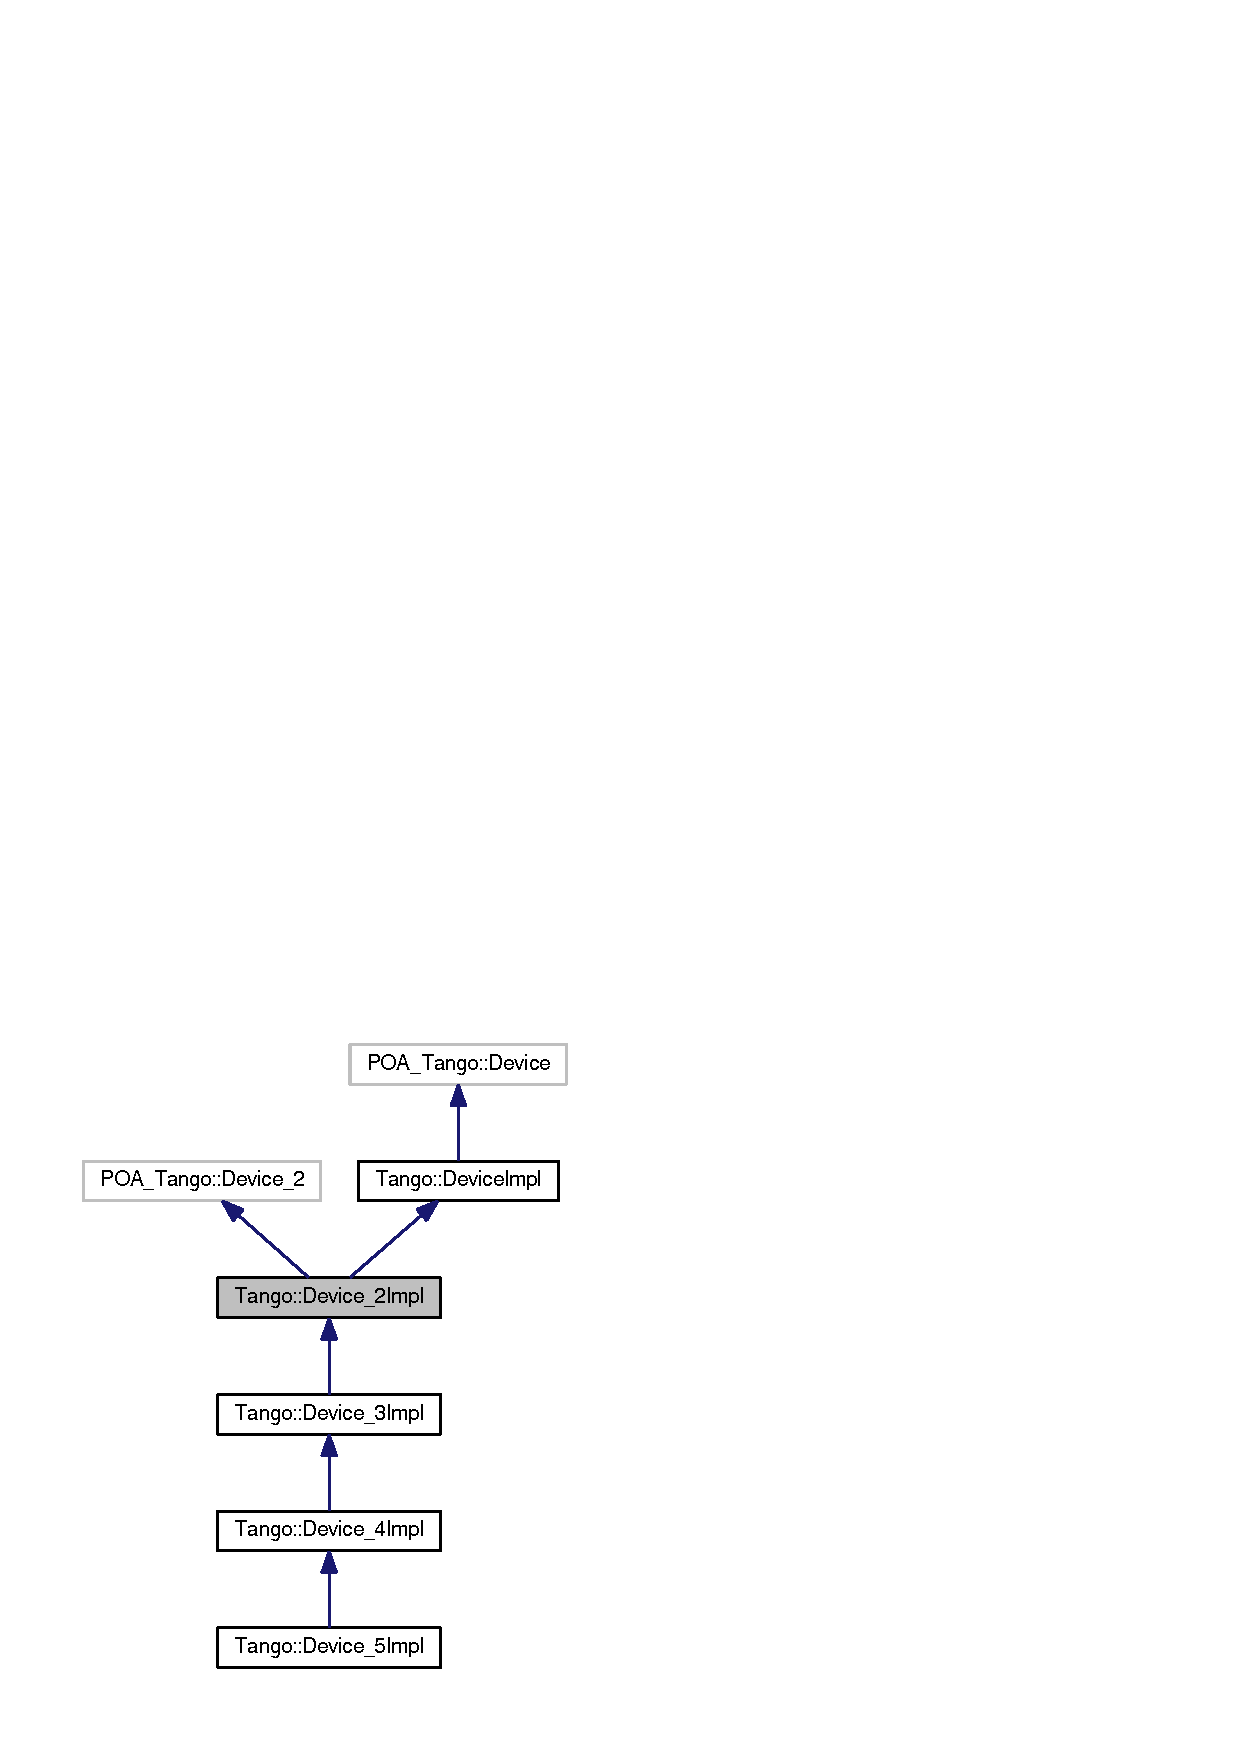
\includegraphics[width=276pt]{da/d12/classTango_1_1Device__2Impl__inherit__graph}
\end{center}
\end{figure}


Collaboration diagram for Tango\-:\-:Device\-\_\-2\-Impl\-:
\nopagebreak
\begin{figure}[H]
\begin{center}
\leavevmode
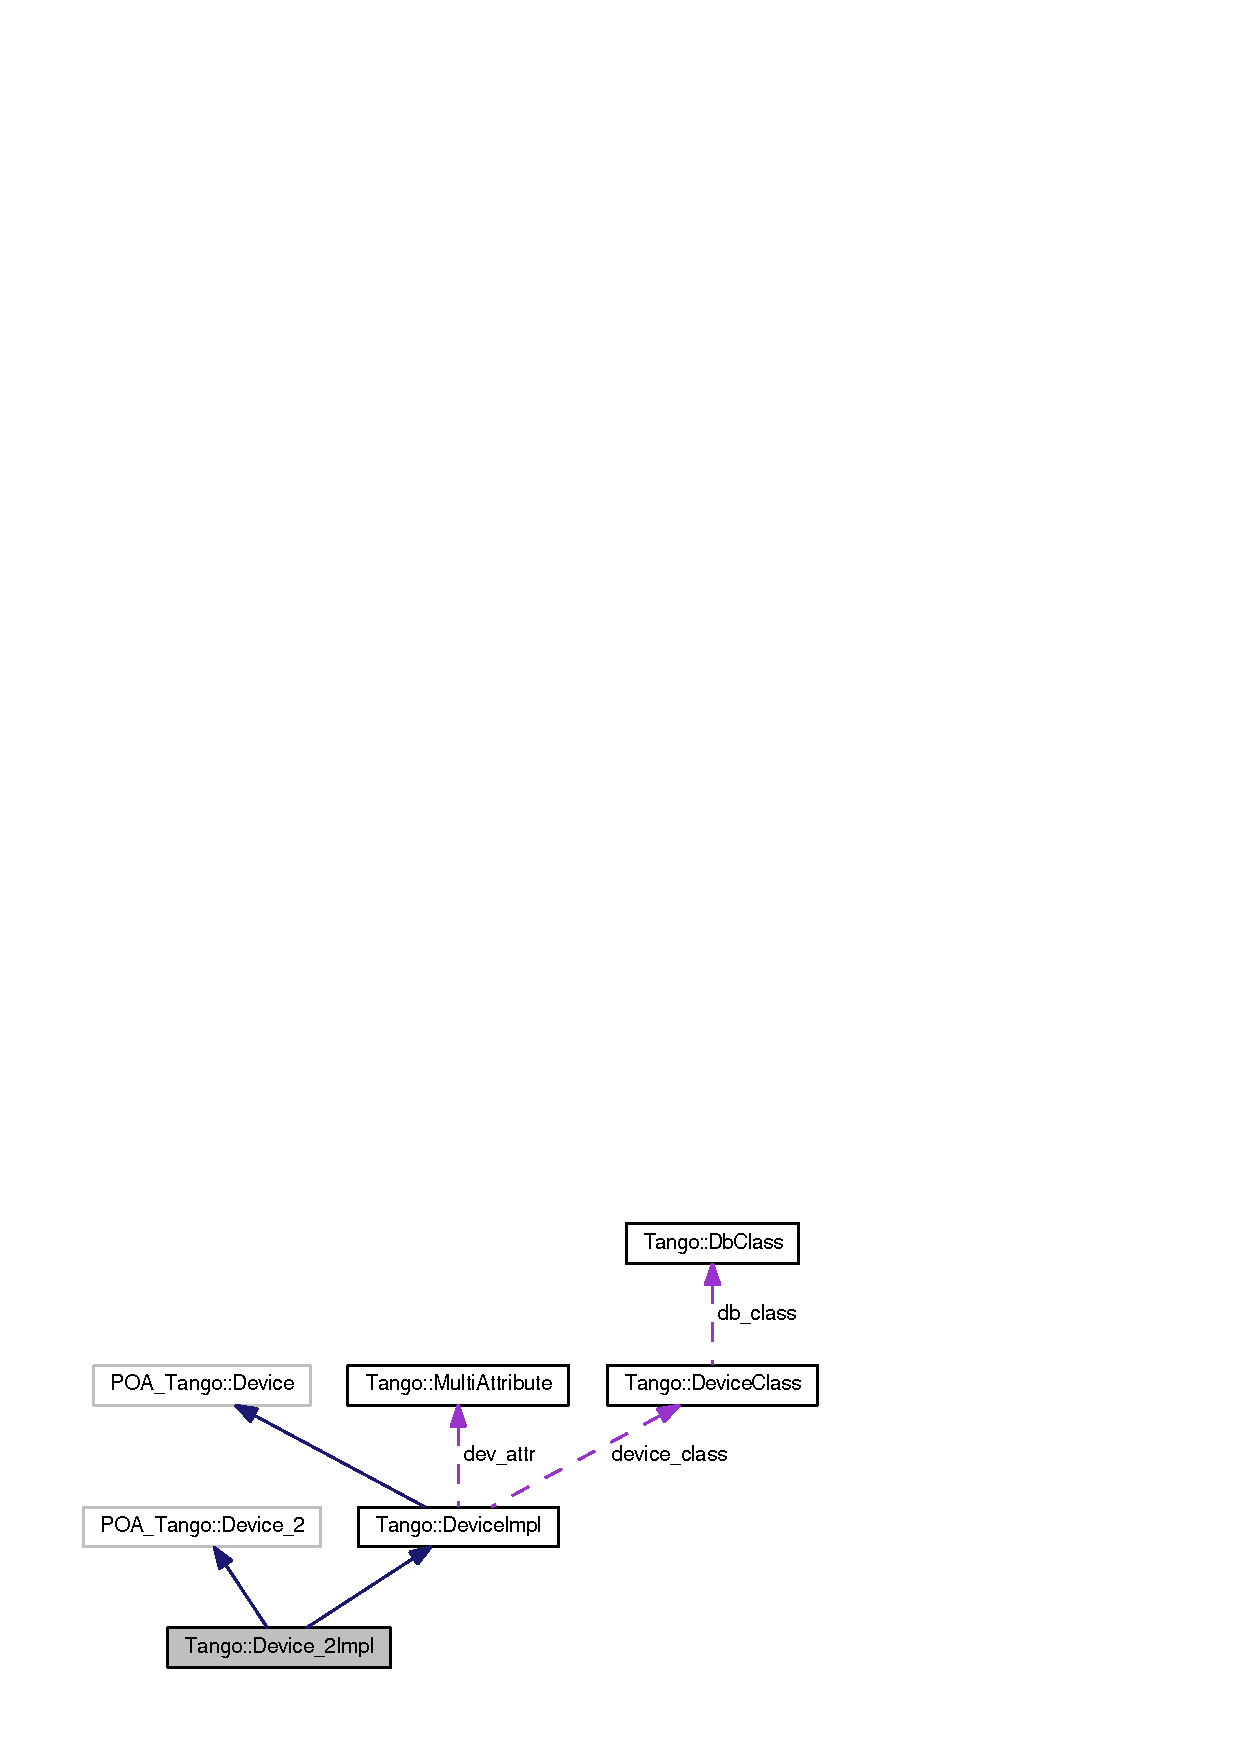
\includegraphics[width=350pt]{df/d54/classTango_1_1Device__2Impl__coll__graph}
\end{center}
\end{figure}
\subsection*{Public Member Functions}
\begin{Indent}{\bf Constructors}\par
{\em Miscellaneous constructors }\begin{DoxyCompactItemize}
\item 
{\bf Device\-\_\-2\-Impl} ({\bf Device\-Class} $\ast${\bf device\-\_\-class}, string \&dev\-\_\-name)
\begin{DoxyCompactList}\small\item\em Constructs a newly allocated \doxyref{Device\-\_\-2\-Impl}{p.}{d8/dbf/classTango_1_1Device__2Impl} object from its name. \end{DoxyCompactList}\item 
{\bf Device\-\_\-2\-Impl} ({\bf Device\-Class} $\ast${\bf device\-\_\-class}, string \&dev\-\_\-name, string \&{\bf desc})
\begin{DoxyCompactList}\small\item\em Constructs a newly allocated \doxyref{Device\-\_\-2\-Impl}{p.}{d8/dbf/classTango_1_1Device__2Impl} object from its name and its description. \end{DoxyCompactList}\item 
{\bf Device\-\_\-2\-Impl} ({\bf Device\-Class} $\ast${\bf device\-\_\-class}, string \&dev\-\_\-name, string \&{\bf desc}, Tango\-::\-Dev\-State {\bf dev\-\_\-state}, string \&{\bf dev\-\_\-status})
\begin{DoxyCompactList}\small\item\em Constructs a newly allocated \doxyref{Device\-\_\-2\-Impl}{p.}{d8/dbf/classTango_1_1Device__2Impl} object from all its creation parameters. \end{DoxyCompactList}\item 
{\bf Device\-\_\-2\-Impl} ({\bf Device\-Class} $\ast${\bf device\-\_\-class}, const char $\ast$dev\-\_\-name, const char $\ast${\bf desc}=\char`\"{}A T\-A\-N\-G\-O device\char`\"{}, Tango\-::\-Dev\-State {\bf dev\-\_\-state}=Tango\-::\-U\-N\-K\-N\-O\-W\-N, const char $\ast${\bf dev\-\_\-status}={\bf Status\-Not\-Set})
\begin{DoxyCompactList}\small\item\em Constructs a newly allocated \doxyref{Device\-\_\-2\-Impl}{p.}{d8/dbf/classTango_1_1Device__2Impl} object from all its creation parameters with some default values. \end{DoxyCompactList}\end{DoxyCompactItemize}
\end{Indent}
\begin{Indent}{\bf Destructor}\par
{\em Only one desctructor is defined for this class }\begin{DoxyCompactItemize}
\item 
virtual {\bf $\sim$\-Device\-\_\-2\-Impl} ()
\begin{DoxyCompactList}\small\item\em The device desctructor. \end{DoxyCompactList}\end{DoxyCompactItemize}
\end{Indent}
\begin{Indent}{\bf C\-O\-R\-B\-A operation methods}\par
{\em Method defined to implement T\-A\-N\-G\-O device C\-O\-R\-B\-A operation }\begin{DoxyCompactItemize}
\item 
virtual C\-O\-R\-B\-A\-::\-Any $\ast$ {\bf command\-\_\-inout\-\_\-2} (const char $\ast$in\-\_\-cmd, const C\-O\-R\-B\-A\-::\-Any \&in\-\_\-data, Tango\-::\-Dev\-Source source)
\begin{DoxyCompactList}\small\item\em Execute a command. \end{DoxyCompactList}\item 
virtual Tango\-::\-Dev\-Cmd\-Info\-List\-\_\-2 $\ast$ {\bf command\-\_\-list\-\_\-query\-\_\-2} ()
\begin{DoxyCompactList}\small\item\em Get device command list. \end{DoxyCompactList}\item 
virtual Tango\-::\-Dev\-Cmd\-Info\-\_\-2 $\ast$ {\bf command\-\_\-query\-\_\-2} (const char $\ast$command)
\begin{DoxyCompactList}\small\item\em Get command info. \end{DoxyCompactList}\item 
virtual Tango\-::\-Attribute\-Value\-List $\ast$ {\bf read\-\_\-attributes\-\_\-2} (const Tango\-::\-Dev\-Var\-String\-Array \&names, Tango\-::\-Dev\-Source source)
\begin{DoxyCompactList}\small\item\em Read attribute(s) value. \end{DoxyCompactList}\item 
virtual \\*
Tango\-::\-Attribute\-Config\-List\-\_\-2 $\ast$ {\bf get\-\_\-attribute\-\_\-config\-\_\-2} (const Tango\-::\-Dev\-Var\-String\-Array \&names)  throw (\-Tango\-::\-Dev\-Failed, C\-O\-R\-B\-A\-::\-System\-Exception)
\begin{DoxyCompactList}\small\item\em Get attribute(s) configuration. \end{DoxyCompactList}\item 
virtual Tango\-::\-Dev\-Attr\-History\-List $\ast$ {\bf read\-\_\-attribute\-\_\-history\-\_\-2} (const char $\ast$name, Dev\-Long n)  throw (\-Tango\-::\-Dev\-Failed, C\-O\-R\-B\-A\-::\-System\-Exception)
\begin{DoxyCompactList}\small\item\em Read attribute value history. \end{DoxyCompactList}\item 
virtual Tango\-::\-Dev\-Cmd\-History\-List $\ast$ {\bf command\-\_\-inout\-\_\-history\-\_\-2} (const char $\ast$command, Dev\-Long n)  throw (\-Tango\-::\-Dev\-Failed, C\-O\-R\-B\-A\-::\-System\-Exception)
\begin{DoxyCompactList}\small\item\em Read command value history. \end{DoxyCompactList}\end{DoxyCompactItemize}
\end{Indent}
\subsection*{Additional Inherited Members}


\subsection{Detailed Description}
Base class for all T\-A\-N\-G\-O device since version 2. 

This class inherits from \doxyref{Device\-Impl}{p.}{d3/d62/classTango_1_1DeviceImpl} class which itself inherits from C\-O\-R\-B\-A classes where all the network layer is implemented. This class has been created since release 2 of \doxyref{Tango}{p.}{de/ddf/namespaceTango} library where the I\-D\-L \doxyref{Tango}{p.}{de/ddf/namespaceTango} module has been modified in order to create a Device\-\_\-2 interface which inherits from the original Device interface

\$\-Author\$ \$\-Revision\$ 

\subsection{Constructor \& Destructor Documentation}
\index{Tango\-::\-Device\-\_\-2\-Impl@{Tango\-::\-Device\-\_\-2\-Impl}!Device\-\_\-2\-Impl@{Device\-\_\-2\-Impl}}
\index{Device\-\_\-2\-Impl@{Device\-\_\-2\-Impl}!Tango::Device_2Impl@{Tango\-::\-Device\-\_\-2\-Impl}}
\subsubsection[{Device\-\_\-2\-Impl}]{\setlength{\rightskip}{0pt plus 5cm}Tango\-::\-Device\-\_\-2\-Impl\-::\-Device\-\_\-2\-Impl (
\begin{DoxyParamCaption}
\item[{{\bf Device\-Class} $\ast$}]{device\-\_\-class, }
\item[{string \&}]{dev\-\_\-name}
\end{DoxyParamCaption}
)}\label{classTango_1_1Device__2Impl_a6d7f50b5fec343f584298c5263822854}


Constructs a newly allocated \doxyref{Device\-\_\-2\-Impl}{p.}{d8/dbf/classTango_1_1Device__2Impl} object from its name. 

The device description field is set to {\itshape A \doxyref{Tango}{p.}{de/ddf/namespaceTango} device}. The device state is set to unknown and the device status is set to {\bfseries Not Initialised}


\begin{DoxyParams}{Parameters}
{\em device\-\_\-class} & Pointer to the device class object \\
\hline
{\em dev\-\_\-name} & The device name \\
\hline
\end{DoxyParams}
\index{Tango\-::\-Device\-\_\-2\-Impl@{Tango\-::\-Device\-\_\-2\-Impl}!Device\-\_\-2\-Impl@{Device\-\_\-2\-Impl}}
\index{Device\-\_\-2\-Impl@{Device\-\_\-2\-Impl}!Tango::Device_2Impl@{Tango\-::\-Device\-\_\-2\-Impl}}
\subsubsection[{Device\-\_\-2\-Impl}]{\setlength{\rightskip}{0pt plus 5cm}Tango\-::\-Device\-\_\-2\-Impl\-::\-Device\-\_\-2\-Impl (
\begin{DoxyParamCaption}
\item[{{\bf Device\-Class} $\ast$}]{device\-\_\-class, }
\item[{string \&}]{dev\-\_\-name, }
\item[{string \&}]{desc}
\end{DoxyParamCaption}
)}\label{classTango_1_1Device__2Impl_ad90287b9ce6a16a656aad0d0f3ce10b8}


Constructs a newly allocated \doxyref{Device\-\_\-2\-Impl}{p.}{d8/dbf/classTango_1_1Device__2Impl} object from its name and its description. 

The device state is set to unknown and the device status is set to {\itshape Not Initialised}


\begin{DoxyParams}{Parameters}
{\em device\-\_\-class} & Pointer to the device class object \\
\hline
{\em dev\-\_\-name} & The device name \\
\hline
{\em desc} & The device description \\
\hline
\end{DoxyParams}
\index{Tango\-::\-Device\-\_\-2\-Impl@{Tango\-::\-Device\-\_\-2\-Impl}!Device\-\_\-2\-Impl@{Device\-\_\-2\-Impl}}
\index{Device\-\_\-2\-Impl@{Device\-\_\-2\-Impl}!Tango::Device_2Impl@{Tango\-::\-Device\-\_\-2\-Impl}}
\subsubsection[{Device\-\_\-2\-Impl}]{\setlength{\rightskip}{0pt plus 5cm}Tango\-::\-Device\-\_\-2\-Impl\-::\-Device\-\_\-2\-Impl (
\begin{DoxyParamCaption}
\item[{{\bf Device\-Class} $\ast$}]{device\-\_\-class, }
\item[{string \&}]{dev\-\_\-name, }
\item[{string \&}]{desc, }
\item[{Tango\-::\-Dev\-State}]{dev\-\_\-state, }
\item[{string \&}]{dev\-\_\-status}
\end{DoxyParamCaption}
)}\label{classTango_1_1Device__2Impl_ad0e74e2158f49e61d5d5db908f5aec69}


Constructs a newly allocated \doxyref{Device\-\_\-2\-Impl}{p.}{d8/dbf/classTango_1_1Device__2Impl} object from all its creation parameters. 

The device is constructed from its name, its description, an original state and status


\begin{DoxyParams}{Parameters}
{\em device\-\_\-class} & Pointer to the device class object \\
\hline
{\em dev\-\_\-name} & The device name \\
\hline
{\em desc} & The device description \\
\hline
{\em dev\-\_\-state} & The device initial state \\
\hline
{\em dev\-\_\-status} & The device initial status \\
\hline
\end{DoxyParams}
\index{Tango\-::\-Device\-\_\-2\-Impl@{Tango\-::\-Device\-\_\-2\-Impl}!Device\-\_\-2\-Impl@{Device\-\_\-2\-Impl}}
\index{Device\-\_\-2\-Impl@{Device\-\_\-2\-Impl}!Tango::Device_2Impl@{Tango\-::\-Device\-\_\-2\-Impl}}
\subsubsection[{Device\-\_\-2\-Impl}]{\setlength{\rightskip}{0pt plus 5cm}Tango\-::\-Device\-\_\-2\-Impl\-::\-Device\-\_\-2\-Impl (
\begin{DoxyParamCaption}
\item[{{\bf Device\-Class} $\ast$}]{device\-\_\-class, }
\item[{const char $\ast$}]{dev\-\_\-name, }
\item[{const char $\ast$}]{desc = {\ttfamily \char`\"{}A~TANGO~device\char`\"{}}, }
\item[{Tango\-::\-Dev\-State}]{dev\-\_\-state = {\ttfamily Tango\-:\-:UNKNOWN}, }
\item[{const char $\ast$}]{dev\-\_\-status = {\ttfamily {\bf Status\-Not\-Set}}}
\end{DoxyParamCaption}
)}\label{classTango_1_1Device__2Impl_a0093f572273fc5464e562665b454e9db}


Constructs a newly allocated \doxyref{Device\-\_\-2\-Impl}{p.}{d8/dbf/classTango_1_1Device__2Impl} object from all its creation parameters with some default values. 

The device is constructed from its name, its description, an original state and status. This constructor defined default values for the description, state and status parameters. The default device description is {\itshape A T\-A\-N\-G\-O device}. The default device state is {\itshape U\-N\-K\-N\-O\-W\-N} and the default device status is {\itshape Not initialised}.


\begin{DoxyParams}{Parameters}
{\em device\-\_\-class} & Pointer to the device class object \\
\hline
{\em dev\-\_\-name} & The device name \\
\hline
{\em desc} & The device desc \\
\hline
{\em dev\-\_\-state} & The device initial state \\
\hline
{\em dev\-\_\-status} & The device initial status \\
\hline
\end{DoxyParams}
\index{Tango\-::\-Device\-\_\-2\-Impl@{Tango\-::\-Device\-\_\-2\-Impl}!$\sim$\-Device\-\_\-2\-Impl@{$\sim$\-Device\-\_\-2\-Impl}}
\index{$\sim$\-Device\-\_\-2\-Impl@{$\sim$\-Device\-\_\-2\-Impl}!Tango::Device_2Impl@{Tango\-::\-Device\-\_\-2\-Impl}}
\subsubsection[{$\sim$\-Device\-\_\-2\-Impl}]{\setlength{\rightskip}{0pt plus 5cm}virtual Tango\-::\-Device\-\_\-2\-Impl\-::$\sim$\-Device\-\_\-2\-Impl (
\begin{DoxyParamCaption}
{}
\end{DoxyParamCaption}
)\hspace{0.3cm}{\ttfamily [inline]}, {\ttfamily [virtual]}}\label{classTango_1_1Device__2Impl_afaefae8635cff0da56608f4bc38aa6da}


The device desctructor. 



\subsection{Member Function Documentation}
\index{Tango\-::\-Device\-\_\-2\-Impl@{Tango\-::\-Device\-\_\-2\-Impl}!command\-\_\-inout\-\_\-2@{command\-\_\-inout\-\_\-2}}
\index{command\-\_\-inout\-\_\-2@{command\-\_\-inout\-\_\-2}!Tango::Device_2Impl@{Tango\-::\-Device\-\_\-2\-Impl}}
\subsubsection[{command\-\_\-inout\-\_\-2}]{\setlength{\rightskip}{0pt plus 5cm}virtual C\-O\-R\-B\-A\-::\-Any$\ast$ Tango\-::\-Device\-\_\-2\-Impl\-::command\-\_\-inout\-\_\-2 (
\begin{DoxyParamCaption}
\item[{const char $\ast$}]{in\-\_\-cmd, }
\item[{const C\-O\-R\-B\-A\-::\-Any \&}]{in\-\_\-data, }
\item[{Tango\-::\-Dev\-Source}]{source}
\end{DoxyParamCaption}
)\hspace{0.3cm}{\ttfamily [virtual]}}\label{classTango_1_1Device__2Impl_a4348a6f642052b9eeaca07b34877f3e7}


Execute a command. 

It's the master method executed when a \char`\"{}command\-\_\-inout\-\_\-2\char`\"{} C\-O\-R\-B\-A operation is requested by a client. It updates the device black-\/box, call the T\-A\-N\-G\-O command handler and returned the output Any


\begin{DoxyParams}{Parameters}
{\em in\-\_\-cmd} & The command name \\
\hline
{\em in\-\_\-data} & The command input data packed in a C\-O\-R\-B\-A Any \\
\hline
{\em source} & The data source. This parameter is new in \doxyref{Tango}{p.}{de/ddf/namespaceTango} release 2. It allows a client to choose the data source between the device itself or the data cache for polled command. \\
\hline
\end{DoxyParams}
\begin{DoxyReturn}{Returns}
The command output data packed in a C\-O\-R\-B\-A Any object 
\end{DoxyReturn}

\begin{DoxyExceptions}{Exceptions}
{\em Dev\-Failed} & Re-\/throw of the exception thrown by the command\-\_\-handler method. Click {\tt here} to read {\bfseries Dev\-Failed} exception specification \\
\hline
\end{DoxyExceptions}
\index{Tango\-::\-Device\-\_\-2\-Impl@{Tango\-::\-Device\-\_\-2\-Impl}!command\-\_\-inout\-\_\-history\-\_\-2@{command\-\_\-inout\-\_\-history\-\_\-2}}
\index{command\-\_\-inout\-\_\-history\-\_\-2@{command\-\_\-inout\-\_\-history\-\_\-2}!Tango::Device_2Impl@{Tango\-::\-Device\-\_\-2\-Impl}}
\subsubsection[{command\-\_\-inout\-\_\-history\-\_\-2}]{\setlength{\rightskip}{0pt plus 5cm}virtual Tango\-::\-Dev\-Cmd\-History\-List$\ast$ Tango\-::\-Device\-\_\-2\-Impl\-::command\-\_\-inout\-\_\-history\-\_\-2 (
\begin{DoxyParamCaption}
\item[{const char $\ast$}]{command, }
\item[{Dev\-Long}]{n}
\end{DoxyParamCaption}
) throw  Tango\-::\-Dev\-Failed, C\-O\-R\-B\-A\-::\-System\-Exception) \hspace{0.3cm}{\ttfamily [virtual]}}\label{classTango_1_1Device__2Impl_a418ccb8015d1319130c9fe040b71121b}


Read command value history. 

Invoked when the client request the command\-\_\-inout\-\_\-history\-\_\-2 C\-O\-R\-B\-A operation. This operation allows a client to retrieve command return value history for polled command. The depth of the history is limited to the depth of the device server internal polling buffer. It returns to the client one Dev\-Cmd\-History structure for each record.


\begin{DoxyParams}{Parameters}
{\em command} & The command name \\
\hline
{\em n} & The record number. \\
\hline
\end{DoxyParams}
\begin{DoxyReturn}{Returns}
A sequence of Dev\-Cmd\-History structure. One structure is initialised for each record with the command return value (in an Any), the date and in case of the command returns an error when it was read, the Dev\-Errors data. Click {\tt here} to read {\bfseries Dev\-Cmd\-History} structure definition. 
\end{DoxyReturn}

\begin{DoxyExceptions}{Exceptions}
{\em Dev\-Failed} & Thrown if the attribute does not exist or is not polled. Click {\tt here} to read {\bfseries Dev\-Failed} exception specification \\
\hline
\end{DoxyExceptions}
\index{Tango\-::\-Device\-\_\-2\-Impl@{Tango\-::\-Device\-\_\-2\-Impl}!command\-\_\-list\-\_\-query\-\_\-2@{command\-\_\-list\-\_\-query\-\_\-2}}
\index{command\-\_\-list\-\_\-query\-\_\-2@{command\-\_\-list\-\_\-query\-\_\-2}!Tango::Device_2Impl@{Tango\-::\-Device\-\_\-2\-Impl}}
\subsubsection[{command\-\_\-list\-\_\-query\-\_\-2}]{\setlength{\rightskip}{0pt plus 5cm}virtual Tango\-::\-Dev\-Cmd\-Info\-List\-\_\-2$\ast$ Tango\-::\-Device\-\_\-2\-Impl\-::command\-\_\-list\-\_\-query\-\_\-2 (
\begin{DoxyParamCaption}
{}
\end{DoxyParamCaption}
)\hspace{0.3cm}{\ttfamily [virtual]}}\label{classTango_1_1Device__2Impl_ac71c8dc3ed7116437c00370abc992968}


Get device command list. 

Invoked when the client request the command\-\_\-list\-\_\-query\-\_\-2 C\-O\-R\-B\-A operation. It updates the device black box and returns an array of Dev\-Cmd\-Info\-\_\-2 object with one object for each command.

\begin{DoxyReturn}{Returns}
The device command list. One Dev\-Cmd\-Info\-\_\-2 is initialised for each device command. Since \doxyref{Tango}{p.}{de/ddf/namespaceTango} release 2, the command display level field has been added to this structure 
\end{DoxyReturn}
\index{Tango\-::\-Device\-\_\-2\-Impl@{Tango\-::\-Device\-\_\-2\-Impl}!command\-\_\-query\-\_\-2@{command\-\_\-query\-\_\-2}}
\index{command\-\_\-query\-\_\-2@{command\-\_\-query\-\_\-2}!Tango::Device_2Impl@{Tango\-::\-Device\-\_\-2\-Impl}}
\subsubsection[{command\-\_\-query\-\_\-2}]{\setlength{\rightskip}{0pt plus 5cm}virtual Tango\-::\-Dev\-Cmd\-Info\-\_\-2$\ast$ Tango\-::\-Device\-\_\-2\-Impl\-::command\-\_\-query\-\_\-2 (
\begin{DoxyParamCaption}
\item[{const char $\ast$}]{command}
\end{DoxyParamCaption}
)\hspace{0.3cm}{\ttfamily [virtual]}}\label{classTango_1_1Device__2Impl_afa99e1bb14a0decaa40ab43b46f3fea1}


Get command info. 

Invoked when the client request the command\-\_\-query\-\_\-2 C\-O\-R\-B\-A operation. It updates the device black box and returns a Dev\-Cmd\-Info\-\_\-2 object for the command with name passed to the method as parameter.


\begin{DoxyParams}{Parameters}
{\em command} & The command name \\
\hline
\end{DoxyParams}
\begin{DoxyReturn}{Returns}
A Dev\-Cmd\-Info\-\_\-2 initialised for the wanted command. 
\end{DoxyReturn}

\begin{DoxyExceptions}{Exceptions}
{\em Dev\-Failed} & Thrown if the command does not exist. Since \doxyref{Tango}{p.}{de/ddf/namespaceTango} release 2, the command display level field has been added to this structure. Click {\tt here} to read {\bfseries Dev\-Failed} exception specification \\
\hline
\end{DoxyExceptions}
\index{Tango\-::\-Device\-\_\-2\-Impl@{Tango\-::\-Device\-\_\-2\-Impl}!get\-\_\-attribute\-\_\-config\-\_\-2@{get\-\_\-attribute\-\_\-config\-\_\-2}}
\index{get\-\_\-attribute\-\_\-config\-\_\-2@{get\-\_\-attribute\-\_\-config\-\_\-2}!Tango::Device_2Impl@{Tango\-::\-Device\-\_\-2\-Impl}}
\subsubsection[{get\-\_\-attribute\-\_\-config\-\_\-2}]{\setlength{\rightskip}{0pt plus 5cm}virtual Tango\-::\-Attribute\-Config\-List\-\_\-2$\ast$ Tango\-::\-Device\-\_\-2\-Impl\-::get\-\_\-attribute\-\_\-config\-\_\-2 (
\begin{DoxyParamCaption}
\item[{const Tango\-::\-Dev\-Var\-String\-Array \&}]{names}
\end{DoxyParamCaption}
) throw  Tango\-::\-Dev\-Failed, C\-O\-R\-B\-A\-::\-System\-Exception) \hspace{0.3cm}{\ttfamily [virtual]}}\label{classTango_1_1Device__2Impl_a80ba13a4e11a42c6aba434389cf8812b}


Get attribute(s) configuration. 

Invoked when the client request the get\-\_\-attribute\-\_\-config\-\_\-2 C\-O\-R\-B\-A operation. It returns to the client one Attribute\-Config\-\_\-2 structure for each wanted attribute. All the attribute properties value are returned in this Attribute\-Config\-\_\-2 structure. Since \doxyref{Tango}{p.}{de/ddf/namespaceTango} release 2, the attribute display level field has been added to this structure.


\begin{DoxyParams}{Parameters}
{\em names} & The attribute(s) name list \\
\hline
\end{DoxyParams}
\begin{DoxyReturn}{Returns}
A sequence of Attribute\-Config\-\_\-2 structure. One structure is initialised for each wanted attribute. Click {\tt here} to read {\bfseries Attribute\-Config\-\_\-2} structure specification.
\end{DoxyReturn}

\begin{DoxyExceptions}{Exceptions}
{\em Dev\-Failed} & Thrown if the attribute does not exist. Click {\tt here} to read {\bfseries Dev\-Failed} exception specification \\
\hline
\end{DoxyExceptions}
\index{Tango\-::\-Device\-\_\-2\-Impl@{Tango\-::\-Device\-\_\-2\-Impl}!read\-\_\-attribute\-\_\-history\-\_\-2@{read\-\_\-attribute\-\_\-history\-\_\-2}}
\index{read\-\_\-attribute\-\_\-history\-\_\-2@{read\-\_\-attribute\-\_\-history\-\_\-2}!Tango::Device_2Impl@{Tango\-::\-Device\-\_\-2\-Impl}}
\subsubsection[{read\-\_\-attribute\-\_\-history\-\_\-2}]{\setlength{\rightskip}{0pt plus 5cm}virtual Tango\-::\-Dev\-Attr\-History\-List$\ast$ Tango\-::\-Device\-\_\-2\-Impl\-::read\-\_\-attribute\-\_\-history\-\_\-2 (
\begin{DoxyParamCaption}
\item[{const char $\ast$}]{name, }
\item[{Dev\-Long}]{n}
\end{DoxyParamCaption}
) throw  Tango\-::\-Dev\-Failed, C\-O\-R\-B\-A\-::\-System\-Exception) \hspace{0.3cm}{\ttfamily [virtual]}}\label{classTango_1_1Device__2Impl_a8f89727d69733be88e44453a7c97d3a8}


Read attribute value history. 

Invoked when the client request the read\-\_\-attribute\-\_\-history\-\_\-2 C\-O\-R\-B\-A operation. This operation allows a client to retrieve attribute value history for polled attribute. The depth of the history is limited to the depth of the device server internal polling buffer. It returns to the client one Dev\-Attr\-History structure for each record.


\begin{DoxyParams}{Parameters}
{\em name} & The attribute name \\
\hline
{\em n} & The record number. \\
\hline
\end{DoxyParams}
\begin{DoxyReturn}{Returns}
A sequence of Dev\-Attr\-History structure. One structure is initialised for each record with the attribute value, the date and in case of the attribute returns an error when it was read, the Dev\-Errors data. Click {\tt here} to read {\bfseries Dev\-Attr\-History} structure definition. 
\end{DoxyReturn}

\begin{DoxyExceptions}{Exceptions}
{\em Dev\-Failed} & Thrown if the attribute does not exist or is not polled. Click {\tt here} to read {\bfseries Dev\-Failed} exception specification \\
\hline
\end{DoxyExceptions}
\index{Tango\-::\-Device\-\_\-2\-Impl@{Tango\-::\-Device\-\_\-2\-Impl}!read\-\_\-attributes\-\_\-2@{read\-\_\-attributes\-\_\-2}}
\index{read\-\_\-attributes\-\_\-2@{read\-\_\-attributes\-\_\-2}!Tango::Device_2Impl@{Tango\-::\-Device\-\_\-2\-Impl}}
\subsubsection[{read\-\_\-attributes\-\_\-2}]{\setlength{\rightskip}{0pt plus 5cm}virtual Tango\-::\-Attribute\-Value\-List$\ast$ Tango\-::\-Device\-\_\-2\-Impl\-::read\-\_\-attributes\-\_\-2 (
\begin{DoxyParamCaption}
\item[{const Tango\-::\-Dev\-Var\-String\-Array \&}]{names, }
\item[{Tango\-::\-Dev\-Source}]{source}
\end{DoxyParamCaption}
)\hspace{0.3cm}{\ttfamily [virtual]}}\label{classTango_1_1Device__2Impl_ae4a337540c05d540b69b1332aeae7444}


Read attribute(s) value. 

Invoked when the client request the read\-\_\-attributes\-\_\-2 C\-O\-R\-B\-A operation. It returns to the client one Attribute\-Value structure for each wanted attribute.


\begin{DoxyParams}{Parameters}
{\em names} & The attribute(s) name list \\
\hline
{\em source} & The data source. This parameter is new in \doxyref{Tango}{p.}{de/ddf/namespaceTango} release 2. It allows a client to choose the data source between the device itself or the data cache for polled attribute. \\
\hline
\end{DoxyParams}
\begin{DoxyReturn}{Returns}
A sequence of Attribute\-Value structure. One structure is initialised for each wanted attribute with the attribute value, the date and the attribute value quality. Click {\tt here} to read {\bfseries Attribute\-Value} structure definition. 
\end{DoxyReturn}

\begin{DoxyExceptions}{Exceptions}
{\em Dev\-Failed} & Thrown if the attribute does not exist. Click {\tt here} to read {\bfseries Dev\-Failed} exception specification \\
\hline
\end{DoxyExceptions}


The documentation for this class was generated from the following file\-:\begin{DoxyCompactItemize}
\item 
{\bf device\-\_\-2.\-h}\end{DoxyCompactItemize}

\section{Tango\-:\-:Device\-\_\-3\-Impl Class Reference}
\label{classTango_1_1Device__3Impl}\index{Tango\-::\-Device\-\_\-3\-Impl@{Tango\-::\-Device\-\_\-3\-Impl}}


Base class for all T\-A\-N\-G\-O device since version 3.  




Inheritance diagram for Tango\-:\-:Device\-\_\-3\-Impl\-:
\nopagebreak
\begin{figure}[H]
\begin{center}
\leavevmode
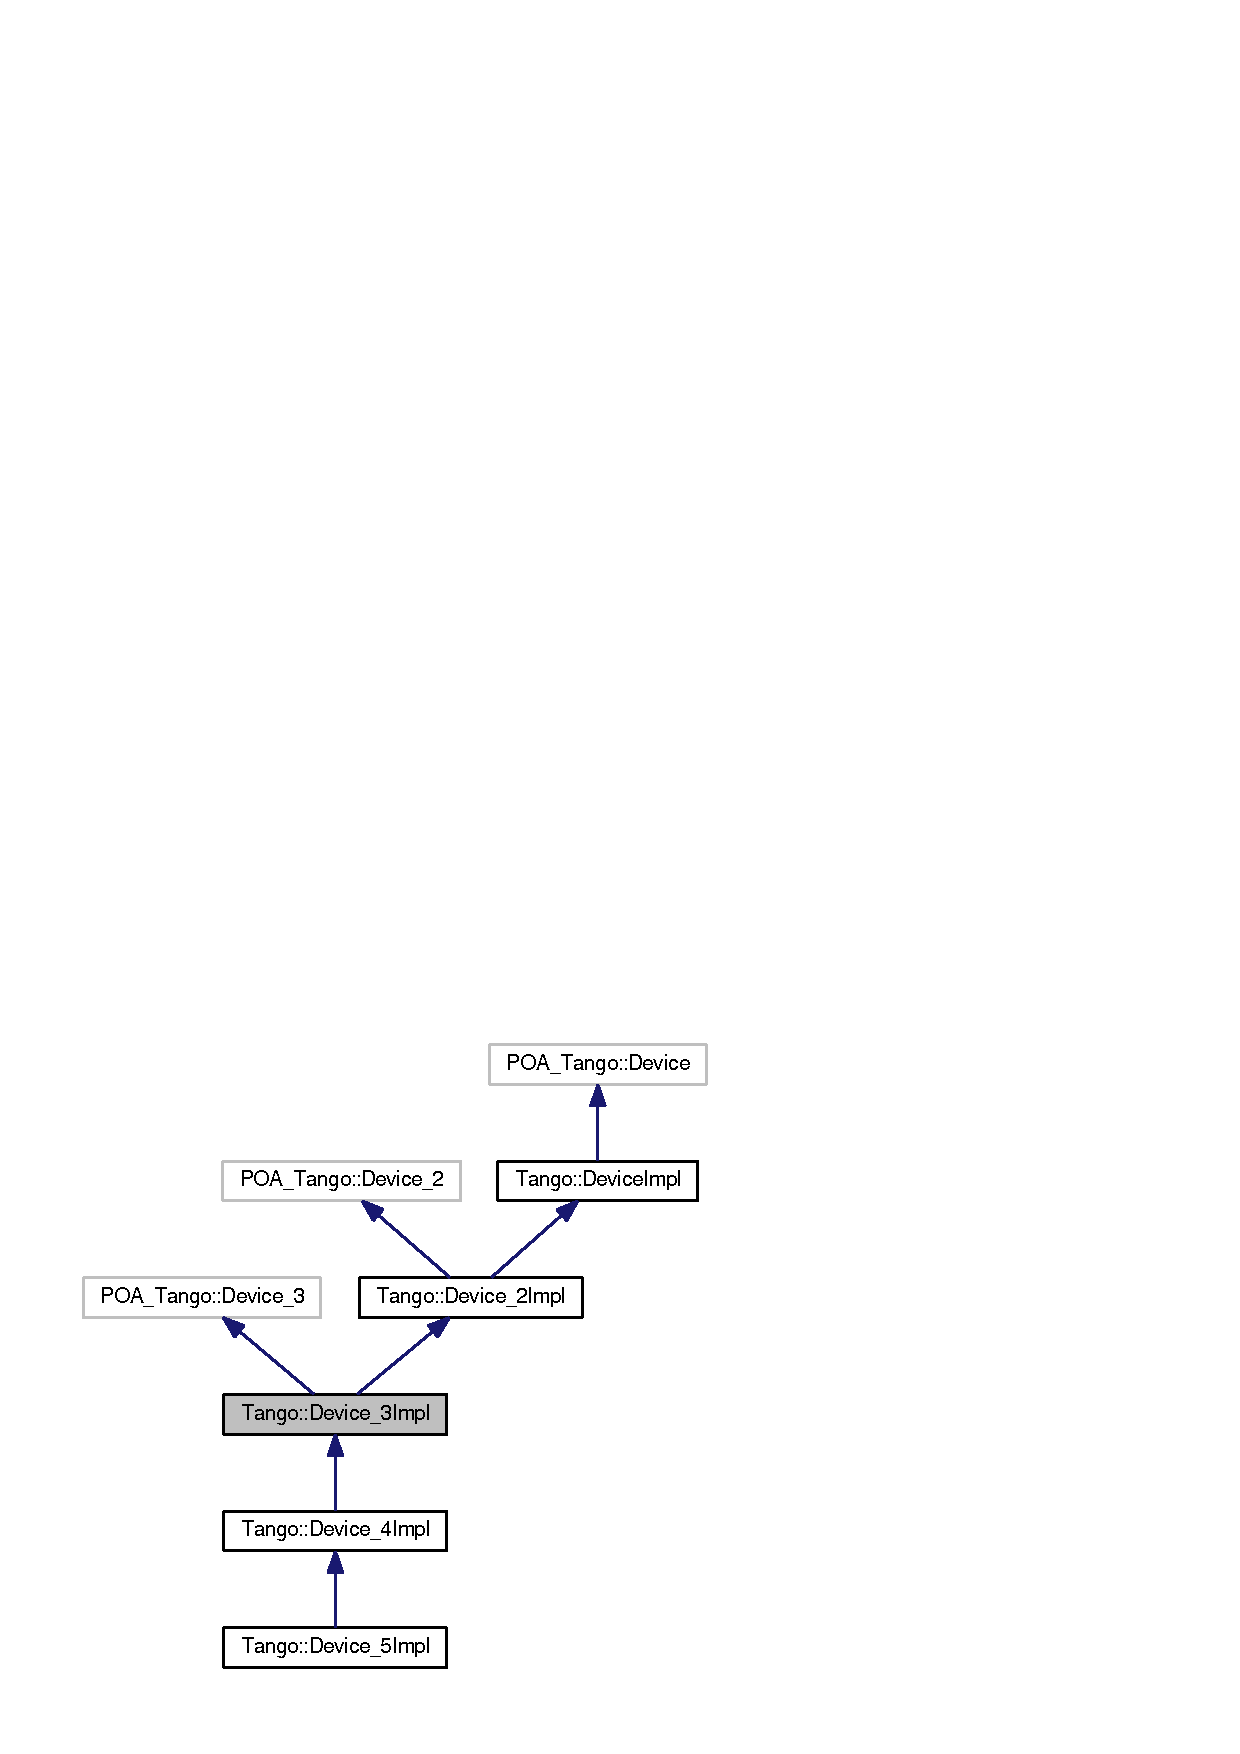
\includegraphics[width=343pt]{d1/d88/classTango_1_1Device__3Impl__inherit__graph}
\end{center}
\end{figure}


Collaboration diagram for Tango\-:\-:Device\-\_\-3\-Impl\-:
\nopagebreak
\begin{figure}[H]
\begin{center}
\leavevmode
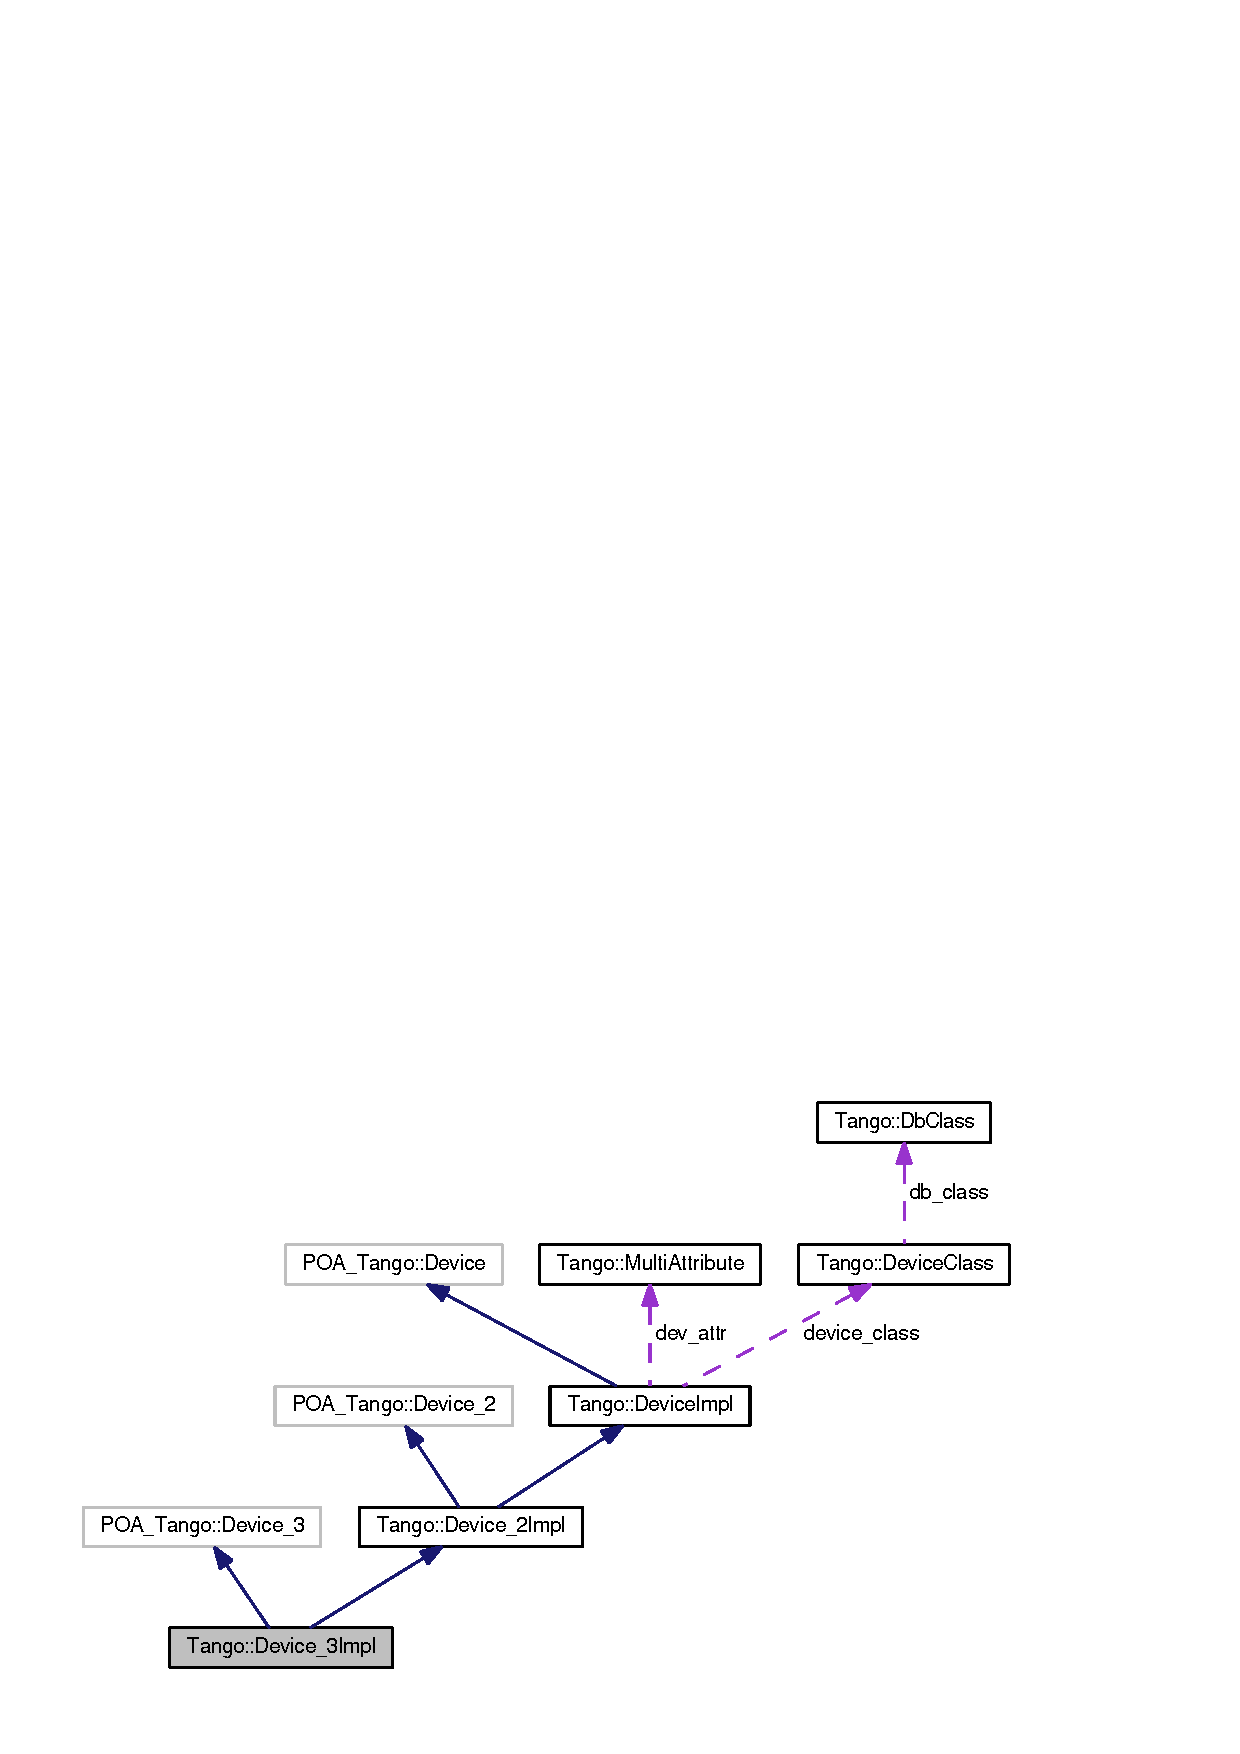
\includegraphics[width=350pt]{d5/d70/classTango_1_1Device__3Impl__coll__graph}
\end{center}
\end{figure}
\subsection*{Public Member Functions}
\begin{Indent}{\bf Constructors}\par
{\em Miscellaneous constructors }\begin{DoxyCompactItemize}
\item 
{\bf Device\-\_\-3\-Impl} ({\bf Device\-Class} $\ast${\bf device\-\_\-class}, string \&dev\-\_\-name)
\begin{DoxyCompactList}\small\item\em Constructs a newly allocated \doxyref{Device\-\_\-3\-Impl}{p.}{db/d65/classTango_1_1Device__3Impl} object from its name. \end{DoxyCompactList}\item 
{\bf Device\-\_\-3\-Impl} ({\bf Device\-Class} $\ast${\bf device\-\_\-class}, string \&dev\-\_\-name, string \&{\bf desc})
\begin{DoxyCompactList}\small\item\em Constructs a newly allocated \doxyref{Device\-\_\-3\-Impl}{p.}{db/d65/classTango_1_1Device__3Impl} object from its name and its description. \end{DoxyCompactList}\item 
{\bf Device\-\_\-3\-Impl} ({\bf Device\-Class} $\ast${\bf device\-\_\-class}, string \&dev\-\_\-name, string \&{\bf desc}, Tango\-::\-Dev\-State {\bf dev\-\_\-state}, string \&{\bf dev\-\_\-status})
\begin{DoxyCompactList}\small\item\em Constructs a newly allocated \doxyref{Device\-\_\-3\-Impl}{p.}{db/d65/classTango_1_1Device__3Impl} object from all its creation parameters. \end{DoxyCompactList}\item 
{\bf Device\-\_\-3\-Impl} ({\bf Device\-Class} $\ast${\bf device\-\_\-class}, const char $\ast$dev\-\_\-name, const char $\ast${\bf desc}=\char`\"{}A T\-A\-N\-G\-O device\char`\"{}, Tango\-::\-Dev\-State {\bf dev\-\_\-state}=Tango\-::\-U\-N\-K\-N\-O\-W\-N, const char $\ast${\bf dev\-\_\-status}={\bf Status\-Not\-Set})
\begin{DoxyCompactList}\small\item\em Constructs a newly allocated \doxyref{Device\-\_\-3\-Impl}{p.}{db/d65/classTango_1_1Device__3Impl} object from all its creation parameters with some default values. \end{DoxyCompactList}\end{DoxyCompactItemize}
\end{Indent}
\begin{Indent}{\bf Destructor}\par
{\em Only one desctructor is defined for this class }\begin{DoxyCompactItemize}
\item 
virtual {\bf $\sim$\-Device\-\_\-3\-Impl} ()
\begin{DoxyCompactList}\small\item\em The device desctructor. \end{DoxyCompactList}\end{DoxyCompactItemize}
\end{Indent}
\begin{Indent}{\bf C\-O\-R\-B\-A operation methods}\par
{\em Method defined to implement T\-A\-N\-G\-O device C\-O\-R\-B\-A operation }\begin{DoxyCompactItemize}
\item 
virtual \\*
Tango\-::\-Attribute\-Value\-List\-\_\-3 $\ast$ {\bf read\-\_\-attributes\-\_\-3} (const Tango\-::\-Dev\-Var\-String\-Array \&names, Tango\-::\-Dev\-Source source)
\begin{DoxyCompactList}\small\item\em Read attribute(s) value. \end{DoxyCompactList}\item 
virtual void {\bf write\-\_\-attributes\-\_\-3} (const Tango\-::\-Attribute\-Value\-List \&values)
\begin{DoxyCompactList}\small\item\em Write attribute(s) value. \end{DoxyCompactList}\item 
virtual \\*
Tango\-::\-Dev\-Attr\-History\-List\-\_\-3 $\ast$ {\bf read\-\_\-attribute\-\_\-history\-\_\-3} (const char $\ast$name, Dev\-Long n)
\begin{DoxyCompactList}\small\item\em Read attribute value history. \end{DoxyCompactList}\item 
virtual Tango\-::\-Dev\-Info\-\_\-3 $\ast$ {\bf info\-\_\-3} ()
\begin{DoxyCompactList}\small\item\em Get device info. \end{DoxyCompactList}\item 
virtual \\*
Tango\-::\-Attribute\-Config\-List\-\_\-3 $\ast$ {\bf get\-\_\-attribute\-\_\-config\-\_\-3} (const Tango\-::\-Dev\-Var\-String\-Array \&names)
\begin{DoxyCompactList}\small\item\em Get attribute(s) configuration. \end{DoxyCompactList}\item 
virtual void {\bf set\-\_\-attribute\-\_\-config\-\_\-3} (const Tango\-::\-Attribute\-Config\-List\-\_\-3 \&new\-\_\-conf)
\begin{DoxyCompactList}\small\item\em Set attribute(s) configuration. \end{DoxyCompactList}\end{DoxyCompactItemize}
\end{Indent}
\subsection*{Additional Inherited Members}


\subsection{Detailed Description}
Base class for all T\-A\-N\-G\-O device since version 3. 

This class inherits from \doxyref{Device\-Impl}{p.}{d3/d62/classTango_1_1DeviceImpl} class which itself inherits from C\-O\-R\-B\-A classes where all the network layer is implemented. This class has been created since release 3 of \doxyref{Tango}{p.}{de/ddf/namespaceTango} library where the I\-D\-L \doxyref{Tango}{p.}{de/ddf/namespaceTango} module has been modified in order to create a Device\-\_\-3 interface which inherits from the original Device interface

\$\-Author\$ \$\-Revision\$ 

\subsection{Constructor \& Destructor Documentation}
\index{Tango\-::\-Device\-\_\-3\-Impl@{Tango\-::\-Device\-\_\-3\-Impl}!Device\-\_\-3\-Impl@{Device\-\_\-3\-Impl}}
\index{Device\-\_\-3\-Impl@{Device\-\_\-3\-Impl}!Tango::Device_3Impl@{Tango\-::\-Device\-\_\-3\-Impl}}
\subsubsection[{Device\-\_\-3\-Impl}]{\setlength{\rightskip}{0pt plus 5cm}Tango\-::\-Device\-\_\-3\-Impl\-::\-Device\-\_\-3\-Impl (
\begin{DoxyParamCaption}
\item[{{\bf Device\-Class} $\ast$}]{device\-\_\-class, }
\item[{string \&}]{dev\-\_\-name}
\end{DoxyParamCaption}
)}\label{classTango_1_1Device__3Impl_ac9db8606c8ea7044642865d104ad74af}


Constructs a newly allocated \doxyref{Device\-\_\-3\-Impl}{p.}{db/d65/classTango_1_1Device__3Impl} object from its name. 

The device description field is set to {\itshape A \doxyref{Tango}{p.}{de/ddf/namespaceTango} device}. The device state is set to unknown and the device status is set to {\bfseries Not Initialised}


\begin{DoxyParams}{Parameters}
{\em device\-\_\-class} & Pointer to the device class object \\
\hline
{\em dev\-\_\-name} & The device name \\
\hline
\end{DoxyParams}
\index{Tango\-::\-Device\-\_\-3\-Impl@{Tango\-::\-Device\-\_\-3\-Impl}!Device\-\_\-3\-Impl@{Device\-\_\-3\-Impl}}
\index{Device\-\_\-3\-Impl@{Device\-\_\-3\-Impl}!Tango::Device_3Impl@{Tango\-::\-Device\-\_\-3\-Impl}}
\subsubsection[{Device\-\_\-3\-Impl}]{\setlength{\rightskip}{0pt plus 5cm}Tango\-::\-Device\-\_\-3\-Impl\-::\-Device\-\_\-3\-Impl (
\begin{DoxyParamCaption}
\item[{{\bf Device\-Class} $\ast$}]{device\-\_\-class, }
\item[{string \&}]{dev\-\_\-name, }
\item[{string \&}]{desc}
\end{DoxyParamCaption}
)}\label{classTango_1_1Device__3Impl_a96a52877d50b929178e5660901bd9e3e}


Constructs a newly allocated \doxyref{Device\-\_\-3\-Impl}{p.}{db/d65/classTango_1_1Device__3Impl} object from its name and its description. 

The device state is set to unknown and the device status is set to {\itshape Not Initialised}


\begin{DoxyParams}{Parameters}
{\em device\-\_\-class} & Pointer to the device class object \\
\hline
{\em dev\-\_\-name} & The device name \\
\hline
{\em desc} & The device description \\
\hline
\end{DoxyParams}
\index{Tango\-::\-Device\-\_\-3\-Impl@{Tango\-::\-Device\-\_\-3\-Impl}!Device\-\_\-3\-Impl@{Device\-\_\-3\-Impl}}
\index{Device\-\_\-3\-Impl@{Device\-\_\-3\-Impl}!Tango::Device_3Impl@{Tango\-::\-Device\-\_\-3\-Impl}}
\subsubsection[{Device\-\_\-3\-Impl}]{\setlength{\rightskip}{0pt plus 5cm}Tango\-::\-Device\-\_\-3\-Impl\-::\-Device\-\_\-3\-Impl (
\begin{DoxyParamCaption}
\item[{{\bf Device\-Class} $\ast$}]{device\-\_\-class, }
\item[{string \&}]{dev\-\_\-name, }
\item[{string \&}]{desc, }
\item[{Tango\-::\-Dev\-State}]{dev\-\_\-state, }
\item[{string \&}]{dev\-\_\-status}
\end{DoxyParamCaption}
)}\label{classTango_1_1Device__3Impl_a4188f383ad8efb4624b9b12d7af6bd75}


Constructs a newly allocated \doxyref{Device\-\_\-3\-Impl}{p.}{db/d65/classTango_1_1Device__3Impl} object from all its creation parameters. 

The device is constructed from its name, its description, an original state and status


\begin{DoxyParams}{Parameters}
{\em device\-\_\-class} & Pointer to the device class object \\
\hline
{\em dev\-\_\-name} & The device name \\
\hline
{\em desc} & The device description \\
\hline
{\em dev\-\_\-state} & The device initial state \\
\hline
{\em dev\-\_\-status} & The device initial status \\
\hline
\end{DoxyParams}
\index{Tango\-::\-Device\-\_\-3\-Impl@{Tango\-::\-Device\-\_\-3\-Impl}!Device\-\_\-3\-Impl@{Device\-\_\-3\-Impl}}
\index{Device\-\_\-3\-Impl@{Device\-\_\-3\-Impl}!Tango::Device_3Impl@{Tango\-::\-Device\-\_\-3\-Impl}}
\subsubsection[{Device\-\_\-3\-Impl}]{\setlength{\rightskip}{0pt plus 5cm}Tango\-::\-Device\-\_\-3\-Impl\-::\-Device\-\_\-3\-Impl (
\begin{DoxyParamCaption}
\item[{{\bf Device\-Class} $\ast$}]{device\-\_\-class, }
\item[{const char $\ast$}]{dev\-\_\-name, }
\item[{const char $\ast$}]{desc = {\ttfamily \char`\"{}A~TANGO~device\char`\"{}}, }
\item[{Tango\-::\-Dev\-State}]{dev\-\_\-state = {\ttfamily Tango\-:\-:UNKNOWN}, }
\item[{const char $\ast$}]{dev\-\_\-status = {\ttfamily {\bf Status\-Not\-Set}}}
\end{DoxyParamCaption}
)}\label{classTango_1_1Device__3Impl_a6d5f7b8f5aac1f9ea056d461f3ee94ce}


Constructs a newly allocated \doxyref{Device\-\_\-3\-Impl}{p.}{db/d65/classTango_1_1Device__3Impl} object from all its creation parameters with some default values. 

The device is constructed from its name, its description, an original state and status. This constructor defined default values for the description, state and status parameters. The default device description is {\itshape A T\-A\-N\-G\-O device}. The default device state is {\itshape U\-N\-K\-N\-O\-W\-N} and the default device status is {\itshape Not initialised}.


\begin{DoxyParams}{Parameters}
{\em device\-\_\-class} & Pointer to the device class object \\
\hline
{\em dev\-\_\-name} & The device name \\
\hline
{\em desc} & The device desc \\
\hline
{\em dev\-\_\-state} & The device initial state \\
\hline
{\em dev\-\_\-status} & The device initial status \\
\hline
\end{DoxyParams}
\index{Tango\-::\-Device\-\_\-3\-Impl@{Tango\-::\-Device\-\_\-3\-Impl}!$\sim$\-Device\-\_\-3\-Impl@{$\sim$\-Device\-\_\-3\-Impl}}
\index{$\sim$\-Device\-\_\-3\-Impl@{$\sim$\-Device\-\_\-3\-Impl}!Tango::Device_3Impl@{Tango\-::\-Device\-\_\-3\-Impl}}
\subsubsection[{$\sim$\-Device\-\_\-3\-Impl}]{\setlength{\rightskip}{0pt plus 5cm}virtual Tango\-::\-Device\-\_\-3\-Impl\-::$\sim$\-Device\-\_\-3\-Impl (
\begin{DoxyParamCaption}
{}
\end{DoxyParamCaption}
)\hspace{0.3cm}{\ttfamily [inline]}, {\ttfamily [virtual]}}\label{classTango_1_1Device__3Impl_a364061576e373d8bec46b5bba70f2817}


The device desctructor. 



\subsection{Member Function Documentation}
\index{Tango\-::\-Device\-\_\-3\-Impl@{Tango\-::\-Device\-\_\-3\-Impl}!get\-\_\-attribute\-\_\-config\-\_\-3@{get\-\_\-attribute\-\_\-config\-\_\-3}}
\index{get\-\_\-attribute\-\_\-config\-\_\-3@{get\-\_\-attribute\-\_\-config\-\_\-3}!Tango::Device_3Impl@{Tango\-::\-Device\-\_\-3\-Impl}}
\subsubsection[{get\-\_\-attribute\-\_\-config\-\_\-3}]{\setlength{\rightskip}{0pt plus 5cm}virtual Tango\-::\-Attribute\-Config\-List\-\_\-3$\ast$ Tango\-::\-Device\-\_\-3\-Impl\-::get\-\_\-attribute\-\_\-config\-\_\-3 (
\begin{DoxyParamCaption}
\item[{const Tango\-::\-Dev\-Var\-String\-Array \&}]{names}
\end{DoxyParamCaption}
)\hspace{0.3cm}{\ttfamily [virtual]}}\label{classTango_1_1Device__3Impl_a651489039cc5222dc1197b3368aa8cdd}


Get attribute(s) configuration. 

Invoked when the client request the get\-\_\-attribute\-\_\-config\-\_\-3 C\-O\-R\-B\-A operation. It returns to the client one Attribute\-Config\-\_\-3 structure for each wanted attribute. All the attribute properties value are returned in this Attribute\-Config\-\_\-3 structure. Since \doxyref{Tango}{p.}{de/ddf/namespaceTango} release 3, the attribute event related, the attribute warning alarm and attribute rds alarm properties have been added to the returned structures.


\begin{DoxyParams}{Parameters}
{\em names} & The attribute(s) name list \\
\hline
\end{DoxyParams}
\begin{DoxyReturn}{Returns}
A sequence of Attribute\-Config\-\_\-3 structure. One structure is initialised for each wanted attribute. Click {\tt here} to read {\bfseries Attribute\-Config\-\_\-3} structure specification.
\end{DoxyReturn}

\begin{DoxyExceptions}{Exceptions}
{\em Dev\-Failed} & Thrown if the attribute does not exist. Click {\tt here} to read {\bfseries Dev\-Failed} exception specification \\
\hline
\end{DoxyExceptions}
\index{Tango\-::\-Device\-\_\-3\-Impl@{Tango\-::\-Device\-\_\-3\-Impl}!info\-\_\-3@{info\-\_\-3}}
\index{info\-\_\-3@{info\-\_\-3}!Tango::Device_3Impl@{Tango\-::\-Device\-\_\-3\-Impl}}
\subsubsection[{info\-\_\-3}]{\setlength{\rightskip}{0pt plus 5cm}virtual Tango\-::\-Dev\-Info\-\_\-3$\ast$ Tango\-::\-Device\-\_\-3\-Impl\-::info\-\_\-3 (
\begin{DoxyParamCaption}
{}
\end{DoxyParamCaption}
)\hspace{0.3cm}{\ttfamily [virtual]}}\label{classTango_1_1Device__3Impl_a28dab632521e2fb0e52827d155af673c}


Get device info. 

Invoked when the client request the info C\-O\-R\-B\-A operation. It updates the black box and returns a Dev\-Info object with miscellaneous device info

\begin{DoxyReturn}{Returns}
A Dev\-Info object 
\end{DoxyReturn}
\index{Tango\-::\-Device\-\_\-3\-Impl@{Tango\-::\-Device\-\_\-3\-Impl}!read\-\_\-attribute\-\_\-history\-\_\-3@{read\-\_\-attribute\-\_\-history\-\_\-3}}
\index{read\-\_\-attribute\-\_\-history\-\_\-3@{read\-\_\-attribute\-\_\-history\-\_\-3}!Tango::Device_3Impl@{Tango\-::\-Device\-\_\-3\-Impl}}
\subsubsection[{read\-\_\-attribute\-\_\-history\-\_\-3}]{\setlength{\rightskip}{0pt plus 5cm}virtual Tango\-::\-Dev\-Attr\-History\-List\-\_\-3$\ast$ Tango\-::\-Device\-\_\-3\-Impl\-::read\-\_\-attribute\-\_\-history\-\_\-3 (
\begin{DoxyParamCaption}
\item[{const char $\ast$}]{name, }
\item[{Dev\-Long}]{n}
\end{DoxyParamCaption}
)\hspace{0.3cm}{\ttfamily [virtual]}}\label{classTango_1_1Device__3Impl_aa9f8d1442f41a4424951a0a4cb84cfec}


Read attribute value history. 

Invoked when the client request the read\-\_\-attribute\-\_\-history\-\_\-3 C\-O\-R\-B\-A operation. This operation allows a client to retrieve attribute value history for polled attribute. The depth of the history is limited to the depth of the device server internal polling buffer. It returns to the client one Dev\-Attr\-History structure for each record.


\begin{DoxyParams}{Parameters}
{\em name} & The attribute name \\
\hline
{\em n} & The record number. \\
\hline
\end{DoxyParams}
\begin{DoxyReturn}{Returns}
A sequence of Dev\-Attr\-History structure. One structure is initialised for each record with the attribute value, the date and in case of the attribute returns an error when it was read, the Dev\-Errors data. Click {\tt here} to read {\bfseries Dev\-Attr\-History\-\_\-3} structure definition. 
\end{DoxyReturn}

\begin{DoxyExceptions}{Exceptions}
{\em Dev\-Failed} & Thrown if the attribute does not exist or is not polled. Click {\tt here} to read {\bfseries Dev\-Failed} exception specification \\
\hline
\end{DoxyExceptions}
\index{Tango\-::\-Device\-\_\-3\-Impl@{Tango\-::\-Device\-\_\-3\-Impl}!read\-\_\-attributes\-\_\-3@{read\-\_\-attributes\-\_\-3}}
\index{read\-\_\-attributes\-\_\-3@{read\-\_\-attributes\-\_\-3}!Tango::Device_3Impl@{Tango\-::\-Device\-\_\-3\-Impl}}
\subsubsection[{read\-\_\-attributes\-\_\-3}]{\setlength{\rightskip}{0pt plus 5cm}virtual Tango\-::\-Attribute\-Value\-List\-\_\-3$\ast$ Tango\-::\-Device\-\_\-3\-Impl\-::read\-\_\-attributes\-\_\-3 (
\begin{DoxyParamCaption}
\item[{const Tango\-::\-Dev\-Var\-String\-Array \&}]{names, }
\item[{Tango\-::\-Dev\-Source}]{source}
\end{DoxyParamCaption}
)\hspace{0.3cm}{\ttfamily [virtual]}}\label{classTango_1_1Device__3Impl_a870e349674aca9b3ebee55157a31b5d3}


Read attribute(s) value. 

Invoked when the client request the read\-\_\-attributes\-\_\-2 C\-O\-R\-B\-A operation. It returns to the client one Attribute\-Value structure for each wanted attribute.


\begin{DoxyParams}{Parameters}
{\em names} & The attribute(s) name list \\
\hline
{\em source} & The data source. This parameter is new in \doxyref{Tango}{p.}{de/ddf/namespaceTango} release 2. It allows a client to choose the data source between the device itself or the data cache for polled attribute. \\
\hline
\end{DoxyParams}
\begin{DoxyReturn}{Returns}
A sequence of Attribute\-Value structure. One structure is initialised for each wanted attribute with the attribute value, the date and the attribute value quality. Click {\tt here} to read {\bfseries Attribute\-Value\-\_\-3} structure definition. 
\end{DoxyReturn}

\begin{DoxyExceptions}{Exceptions}
{\em Dev\-Failed} & Thrown if the attribute does not exist. Click {\tt here} to read {\bfseries Dev\-Failed} exception specification \\
\hline
\end{DoxyExceptions}
\index{Tango\-::\-Device\-\_\-3\-Impl@{Tango\-::\-Device\-\_\-3\-Impl}!set\-\_\-attribute\-\_\-config\-\_\-3@{set\-\_\-attribute\-\_\-config\-\_\-3}}
\index{set\-\_\-attribute\-\_\-config\-\_\-3@{set\-\_\-attribute\-\_\-config\-\_\-3}!Tango::Device_3Impl@{Tango\-::\-Device\-\_\-3\-Impl}}
\subsubsection[{set\-\_\-attribute\-\_\-config\-\_\-3}]{\setlength{\rightskip}{0pt plus 5cm}virtual void Tango\-::\-Device\-\_\-3\-Impl\-::set\-\_\-attribute\-\_\-config\-\_\-3 (
\begin{DoxyParamCaption}
\item[{const Tango\-::\-Attribute\-Config\-List\-\_\-3 \&}]{new\-\_\-conf}
\end{DoxyParamCaption}
)\hspace{0.3cm}{\ttfamily [virtual]}}\label{classTango_1_1Device__3Impl_a6eaac6785a84422132e654916fc2cf7e}


Set attribute(s) configuration. 

Invoked when the client request the set\-\_\-attribute\-\_\-config\-\_\-3 C\-O\-R\-B\-A operation. It updates the device attribute configuration actually used by the device but this method also updates the \doxyref{Tango}{p.}{de/ddf/namespaceTango} database. One structure of the Attribute\-Config\-\_\-3 type is needed for each attribute to update configuration. Click {\tt here} to read {\bfseries Attribute\-Config\-\_\-3} structure specification.


\begin{DoxyParams}{Parameters}
{\em new\-\_\-conf} & The attribute(s) new configuration structure sequence \\
\hline
\end{DoxyParams}

\begin{DoxyExceptions}{Exceptions}
{\em Dev\-Failed} & Thrown if the command does not exist. Click {\tt here} to read {\bfseries Dev\-Failed} exception specification \\
\hline
\end{DoxyExceptions}
\index{Tango\-::\-Device\-\_\-3\-Impl@{Tango\-::\-Device\-\_\-3\-Impl}!write\-\_\-attributes\-\_\-3@{write\-\_\-attributes\-\_\-3}}
\index{write\-\_\-attributes\-\_\-3@{write\-\_\-attributes\-\_\-3}!Tango::Device_3Impl@{Tango\-::\-Device\-\_\-3\-Impl}}
\subsubsection[{write\-\_\-attributes\-\_\-3}]{\setlength{\rightskip}{0pt plus 5cm}virtual void Tango\-::\-Device\-\_\-3\-Impl\-::write\-\_\-attributes\-\_\-3 (
\begin{DoxyParamCaption}
\item[{const Tango\-::\-Attribute\-Value\-List \&}]{values}
\end{DoxyParamCaption}
)\hspace{0.3cm}{\ttfamily [virtual]}}\label{classTango_1_1Device__3Impl_af1a705a748bf08290150c3e50bdb29ff}


Write attribute(s) value. 

Invoked when the client request the write\-\_\-attributes C\-O\-R\-B\-A operation. It sets the attribute(s) with the new value(s) passed as parameter.


\begin{DoxyParams}{Parameters}
{\em values} & The attribute(s) new value(s). One structure is initialised for each wanted attribute with the attribute value. The attribute quality and date are not used by this method. Click {\tt here} to read {\bfseries Attribute\-Value} structure definition. \\
\hline
\end{DoxyParams}

\begin{DoxyExceptions}{Exceptions}
{\em Dev\-Failed} & Thrown if the command does not exist. Click {\tt here} to read {\bfseries Dev\-Failed} exception specification \\
\hline
\end{DoxyExceptions}


The documentation for this class was generated from the following file\-:\begin{DoxyCompactItemize}
\item 
{\bf device\-\_\-3.\-h}\end{DoxyCompactItemize}

\section{Tango\-:\-:Device\-\_\-4\-Impl Class Reference}
\label{classTango_1_1Device__4Impl}\index{Tango\-::\-Device\-\_\-4\-Impl@{Tango\-::\-Device\-\_\-4\-Impl}}


Base class for all T\-A\-N\-G\-O device since version 4.  




Inheritance diagram for Tango\-:\-:Device\-\_\-4\-Impl\-:
\nopagebreak
\begin{figure}[H]
\begin{center}
\leavevmode
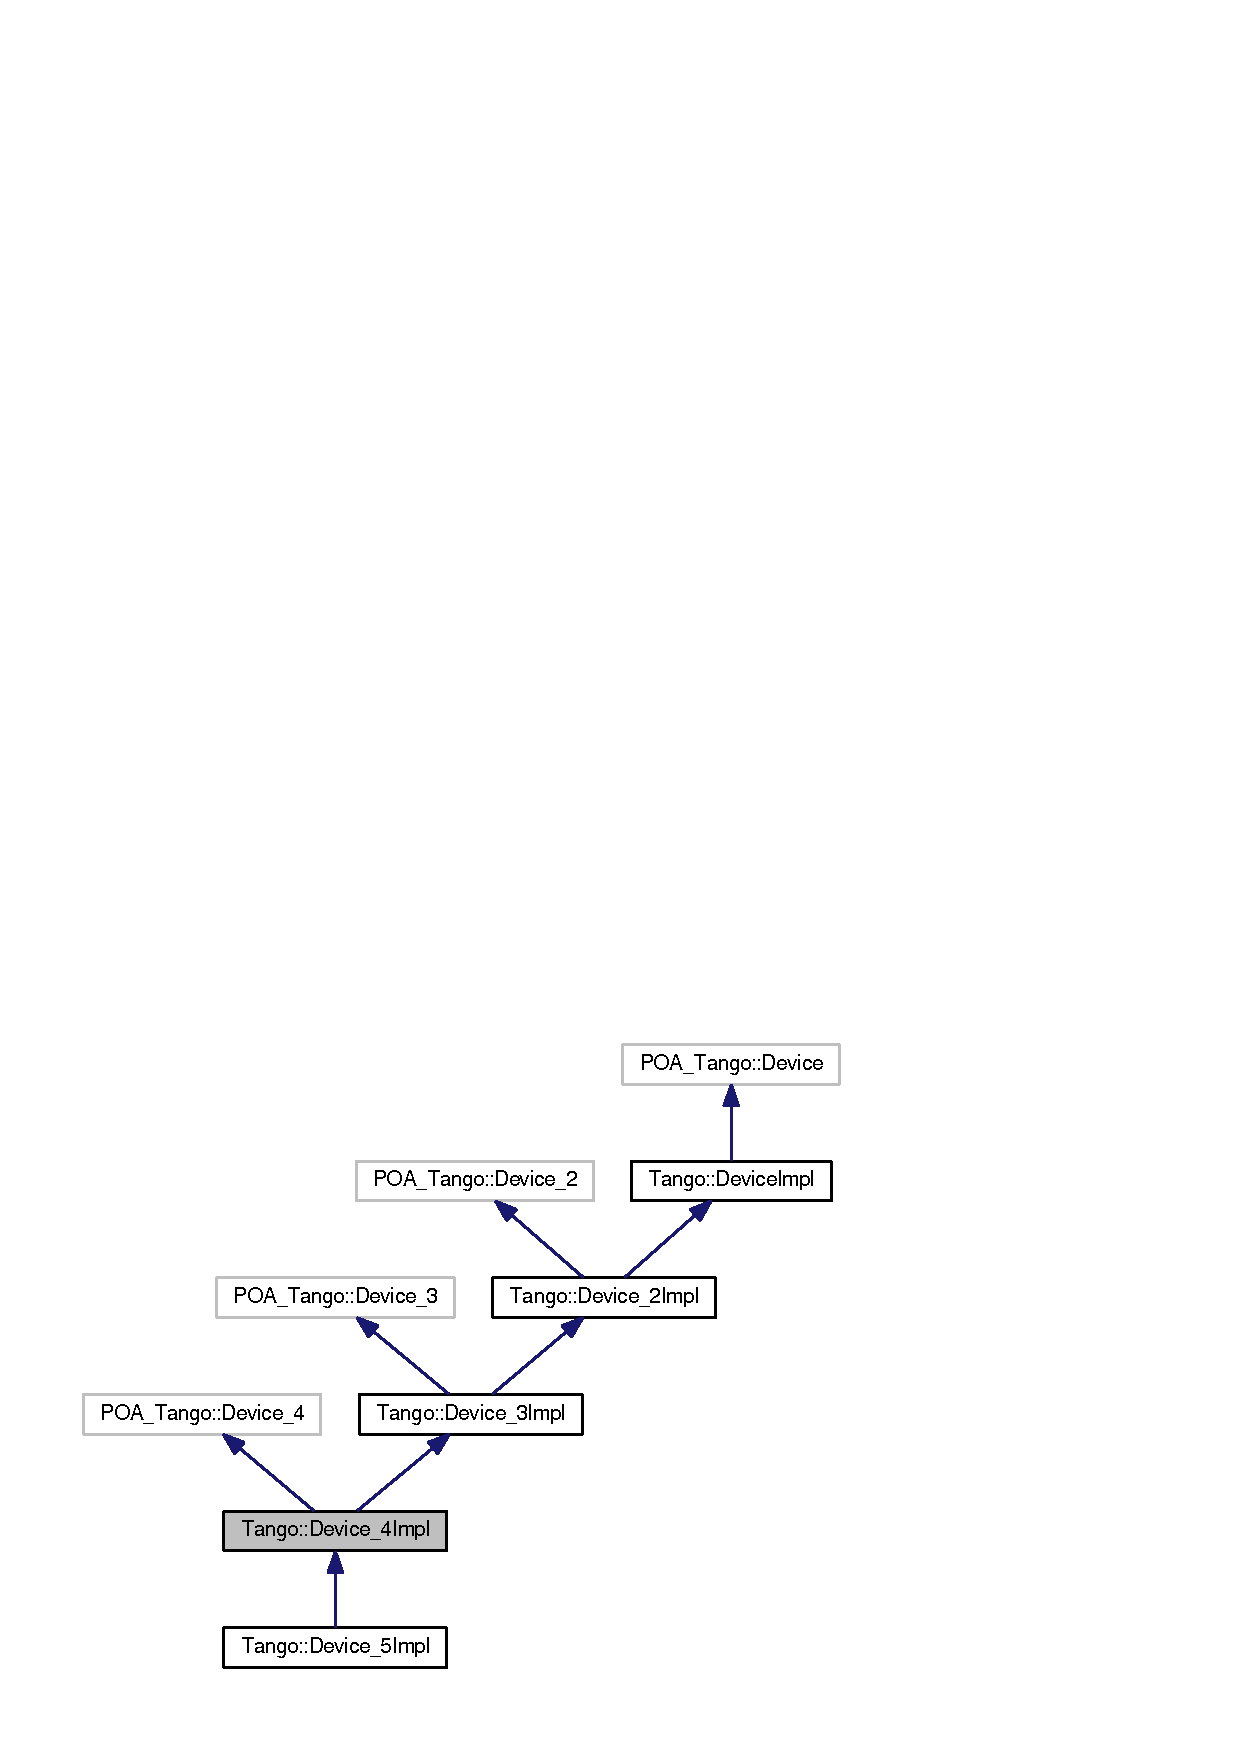
\includegraphics[width=350pt]{d8/dea/classTango_1_1Device__4Impl__inherit__graph}
\end{center}
\end{figure}


Collaboration diagram for Tango\-:\-:Device\-\_\-4\-Impl\-:
\nopagebreak
\begin{figure}[H]
\begin{center}
\leavevmode
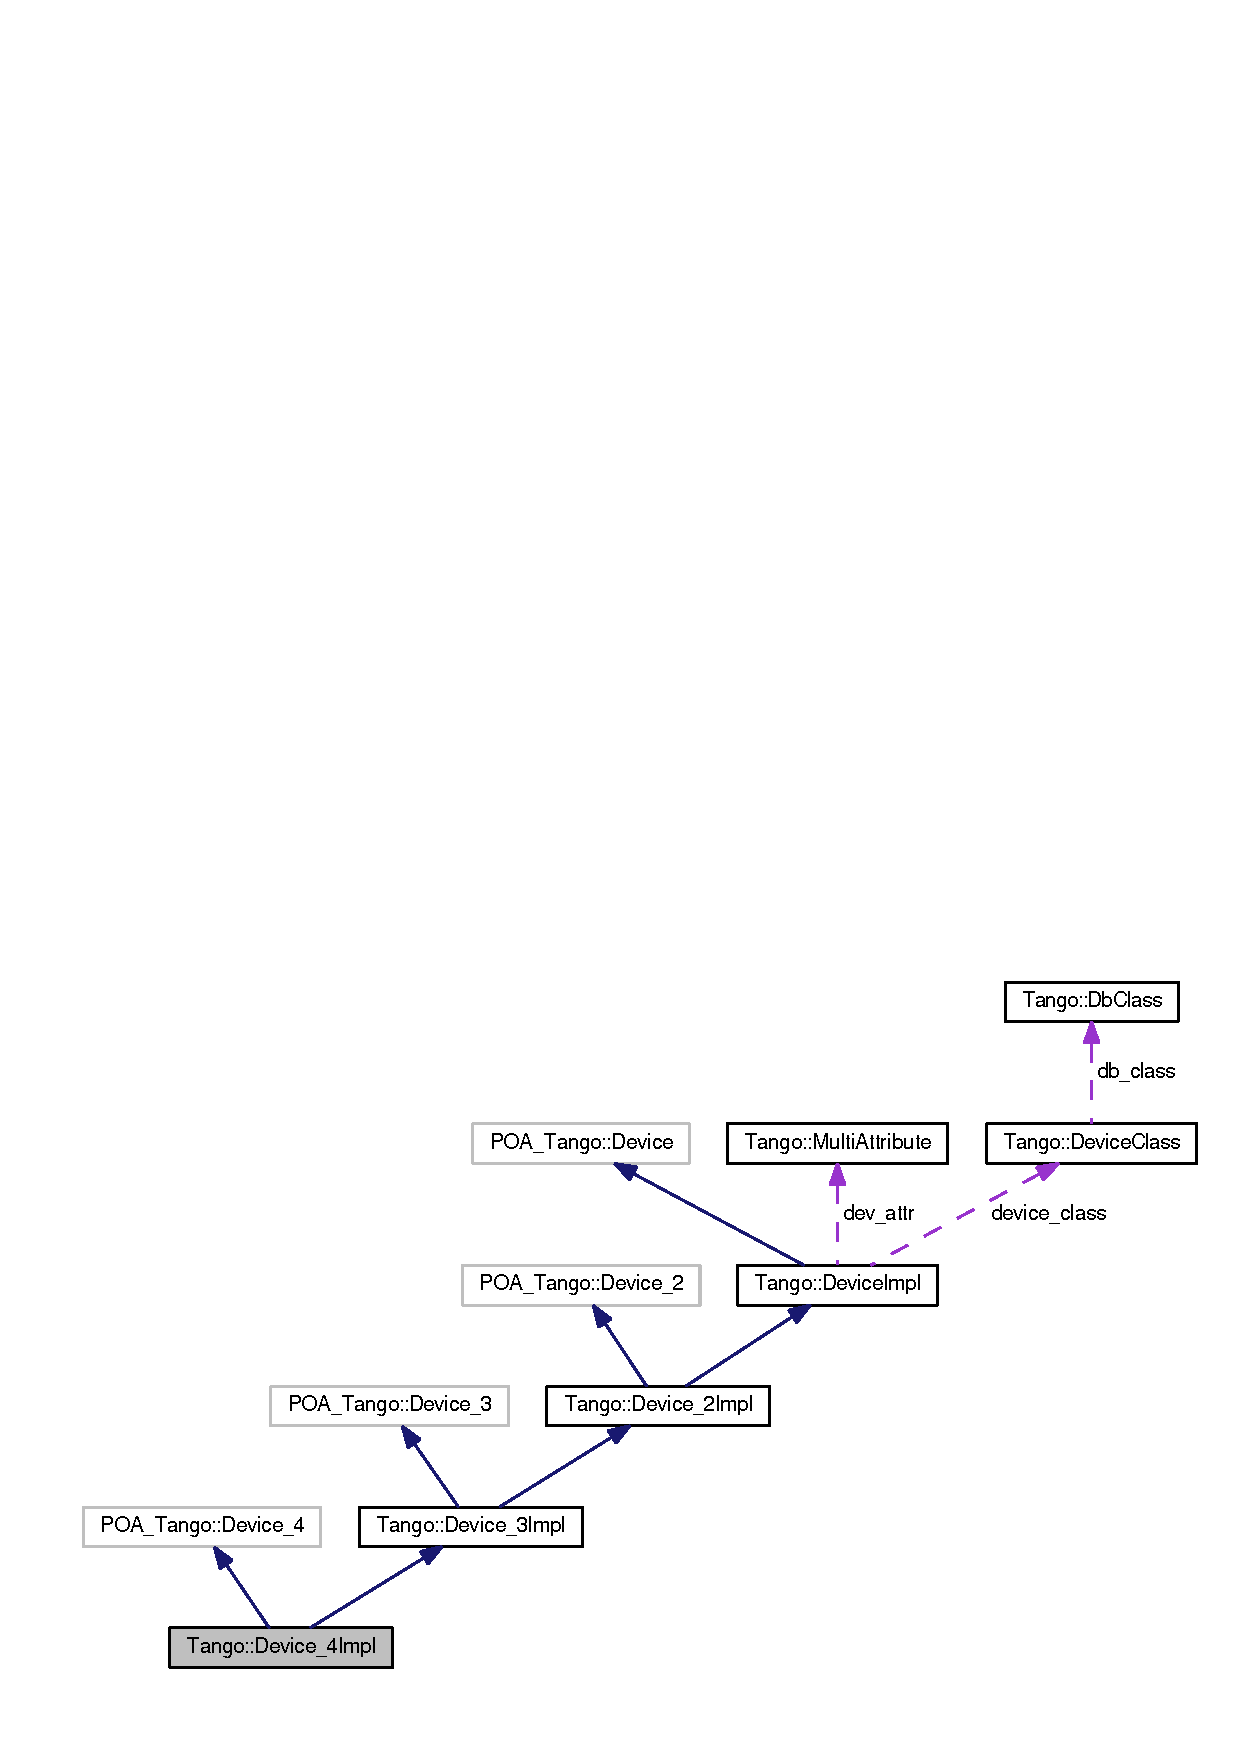
\includegraphics[width=350pt]{df/dcb/classTango_1_1Device__4Impl__coll__graph}
\end{center}
\end{figure}
\subsection*{Public Member Functions}
\begin{Indent}{\bf Constructors}\par
{\em Miscellaneous constructors }\begin{DoxyCompactItemize}
\item 
{\bf Device\-\_\-4\-Impl} ({\bf Device\-Class} $\ast${\bf device\-\_\-class}, string \&dev\-\_\-name)
\begin{DoxyCompactList}\small\item\em Constructs a newly allocated \doxyref{Device\-\_\-4\-Impl}{p.}{dc/dd9/classTango_1_1Device__4Impl} object from its name. \end{DoxyCompactList}\item 
{\bf Device\-\_\-4\-Impl} ({\bf Device\-Class} $\ast${\bf device\-\_\-class}, string \&dev\-\_\-name, string \&{\bf desc})
\begin{DoxyCompactList}\small\item\em Constructs a newly allocated \doxyref{Device\-\_\-4\-Impl}{p.}{dc/dd9/classTango_1_1Device__4Impl} object from its name and its description. \end{DoxyCompactList}\item 
{\bf Device\-\_\-4\-Impl} ({\bf Device\-Class} $\ast${\bf device\-\_\-class}, string \&dev\-\_\-name, string \&{\bf desc}, Tango\-::\-Dev\-State {\bf dev\-\_\-state}, string \&{\bf dev\-\_\-status})
\begin{DoxyCompactList}\small\item\em Constructs a newly allocated \doxyref{Device\-\_\-4\-Impl}{p.}{dc/dd9/classTango_1_1Device__4Impl} object from all its creation parameters. \end{DoxyCompactList}\item 
{\bf Device\-\_\-4\-Impl} ({\bf Device\-Class} $\ast${\bf device\-\_\-class}, const char $\ast$dev\-\_\-name, const char $\ast${\bf desc}=\char`\"{}A T\-A\-N\-G\-O device\char`\"{}, Tango\-::\-Dev\-State {\bf dev\-\_\-state}=Tango\-::\-U\-N\-K\-N\-O\-W\-N, const char $\ast${\bf dev\-\_\-status}={\bf Status\-Not\-Set})
\begin{DoxyCompactList}\small\item\em Constructs a newly allocated \doxyref{Device\-\_\-4\-Impl}{p.}{dc/dd9/classTango_1_1Device__4Impl} object from all its creation parameters with some default values. \end{DoxyCompactList}\end{DoxyCompactItemize}
\end{Indent}
\begin{Indent}{\bf Destructor}\par
{\em Only one desctructor is defined for this class }\begin{DoxyCompactItemize}
\item 
virtual {\bf $\sim$\-Device\-\_\-4\-Impl} ()
\begin{DoxyCompactList}\small\item\em The device desctructor. \end{DoxyCompactList}\end{DoxyCompactItemize}
\end{Indent}
\begin{Indent}{\bf C\-O\-R\-B\-A operation methods}\par
{\em Method defined to implement T\-A\-N\-G\-O device C\-O\-R\-B\-A operation }\begin{DoxyCompactItemize}
\item 
virtual Tango\-::\-Dev\-Attr\-History\-\_\-4 $\ast$ {\bf read\-\_\-attribute\-\_\-history\-\_\-4} (const char $\ast$name, Dev\-Long n)
\begin{DoxyCompactList}\small\item\em Read attribute value history. \end{DoxyCompactList}\item 
virtual Tango\-::\-Dev\-Cmd\-History\-\_\-4 $\ast$ {\bf command\-\_\-inout\-\_\-history\-\_\-4} (const char $\ast$command, Dev\-Long n)
\begin{DoxyCompactList}\small\item\em Read command value history. \end{DoxyCompactList}\item 
virtual C\-O\-R\-B\-A\-::\-Any $\ast$ {\bf command\-\_\-inout\-\_\-4} (const char $\ast$in\-\_\-cmd, const C\-O\-R\-B\-A\-::\-Any \&in\-\_\-data, Tango\-::\-Dev\-Source source, const Tango\-::\-Clnt\-Ident \&cl\-\_\-ident)
\begin{DoxyCompactList}\small\item\em Execute a command. \end{DoxyCompactList}\item 
virtual \\*
Tango\-::\-Attribute\-Value\-List\-\_\-4 $\ast$ {\bf read\-\_\-attributes\-\_\-4} (const Tango\-::\-Dev\-Var\-String\-Array \&names, Tango\-::\-Dev\-Source source, const Tango\-::\-Clnt\-Ident \&cl\-\_\-ident)
\begin{DoxyCompactList}\small\item\em Read attribute(s) value. \end{DoxyCompactList}\item 
virtual void {\bf write\-\_\-attributes\-\_\-4} (const Tango\-::\-Attribute\-Value\-List\-\_\-4 \&values, const Tango\-::\-Clnt\-Ident \&cl\-\_\-ident)
\begin{DoxyCompactList}\small\item\em Write attribute(s) value. \end{DoxyCompactList}\item 
virtual void {\bf set\-\_\-attribute\-\_\-config\-\_\-4} (const Tango\-::\-Attribute\-Config\-List\-\_\-3 \&new\-\_\-conf, const Tango\-::\-Clnt\-Ident \&cl\-\_\-ident)
\begin{DoxyCompactList}\small\item\em Set attribute(s) configuration. \end{DoxyCompactList}\item 
virtual \\*
Tango\-::\-Attribute\-Value\-List\-\_\-4 $\ast$ {\bf write\-\_\-read\-\_\-attributes\-\_\-4} (const Tango\-::\-Attribute\-Value\-List\-\_\-4 \&values, const Tango\-::\-Clnt\-Ident \&cl\-\_\-ident)
\begin{DoxyCompactList}\small\item\em Write then read attribute(s) value. \end{DoxyCompactList}\end{DoxyCompactItemize}
\end{Indent}
\subsection*{Additional Inherited Members}


\subsection{Detailed Description}
Base class for all T\-A\-N\-G\-O device since version 4. 

This class inherits from \doxyref{Device\-Impl}{p.}{d3/d62/classTango_1_1DeviceImpl} class which itself inherits from C\-O\-R\-B\-A classes where all the network layer is implemented. This class has been created since release 7 of \doxyref{Tango}{p.}{de/ddf/namespaceTango} library where the I\-D\-L \doxyref{Tango}{p.}{de/ddf/namespaceTango} module has been modified in order to create a Device\-\_\-4 interface which inherits from the original Device interface

\$\-Author\$ \$\-Revision\$ 

\subsection{Constructor \& Destructor Documentation}
\index{Tango\-::\-Device\-\_\-4\-Impl@{Tango\-::\-Device\-\_\-4\-Impl}!Device\-\_\-4\-Impl@{Device\-\_\-4\-Impl}}
\index{Device\-\_\-4\-Impl@{Device\-\_\-4\-Impl}!Tango::Device_4Impl@{Tango\-::\-Device\-\_\-4\-Impl}}
\subsubsection[{Device\-\_\-4\-Impl}]{\setlength{\rightskip}{0pt plus 5cm}Tango\-::\-Device\-\_\-4\-Impl\-::\-Device\-\_\-4\-Impl (
\begin{DoxyParamCaption}
\item[{{\bf Device\-Class} $\ast$}]{device\-\_\-class, }
\item[{string \&}]{dev\-\_\-name}
\end{DoxyParamCaption}
)}\label{classTango_1_1Device__4Impl_ac4fc7cd8a4256fa15d1a91b9040e7f68}


Constructs a newly allocated \doxyref{Device\-\_\-4\-Impl}{p.}{dc/dd9/classTango_1_1Device__4Impl} object from its name. 

The device description field is set to {\itshape A \doxyref{Tango}{p.}{de/ddf/namespaceTango} device}. The device state is set to unknown and the device status is set to {\bfseries Not Initialised}


\begin{DoxyParams}{Parameters}
{\em device\-\_\-class} & Pointer to the device class object \\
\hline
{\em dev\-\_\-name} & The device name \\
\hline
\end{DoxyParams}
\index{Tango\-::\-Device\-\_\-4\-Impl@{Tango\-::\-Device\-\_\-4\-Impl}!Device\-\_\-4\-Impl@{Device\-\_\-4\-Impl}}
\index{Device\-\_\-4\-Impl@{Device\-\_\-4\-Impl}!Tango::Device_4Impl@{Tango\-::\-Device\-\_\-4\-Impl}}
\subsubsection[{Device\-\_\-4\-Impl}]{\setlength{\rightskip}{0pt plus 5cm}Tango\-::\-Device\-\_\-4\-Impl\-::\-Device\-\_\-4\-Impl (
\begin{DoxyParamCaption}
\item[{{\bf Device\-Class} $\ast$}]{device\-\_\-class, }
\item[{string \&}]{dev\-\_\-name, }
\item[{string \&}]{desc}
\end{DoxyParamCaption}
)}\label{classTango_1_1Device__4Impl_ac065aec658bab72b62b0b3546d700e44}


Constructs a newly allocated \doxyref{Device\-\_\-4\-Impl}{p.}{dc/dd9/classTango_1_1Device__4Impl} object from its name and its description. 

The device state is set to unknown and the device status is set to {\itshape Not Initialised}


\begin{DoxyParams}{Parameters}
{\em device\-\_\-class} & Pointer to the device class object \\
\hline
{\em dev\-\_\-name} & The device name \\
\hline
{\em desc} & The device description \\
\hline
\end{DoxyParams}
\index{Tango\-::\-Device\-\_\-4\-Impl@{Tango\-::\-Device\-\_\-4\-Impl}!Device\-\_\-4\-Impl@{Device\-\_\-4\-Impl}}
\index{Device\-\_\-4\-Impl@{Device\-\_\-4\-Impl}!Tango::Device_4Impl@{Tango\-::\-Device\-\_\-4\-Impl}}
\subsubsection[{Device\-\_\-4\-Impl}]{\setlength{\rightskip}{0pt plus 5cm}Tango\-::\-Device\-\_\-4\-Impl\-::\-Device\-\_\-4\-Impl (
\begin{DoxyParamCaption}
\item[{{\bf Device\-Class} $\ast$}]{device\-\_\-class, }
\item[{string \&}]{dev\-\_\-name, }
\item[{string \&}]{desc, }
\item[{Tango\-::\-Dev\-State}]{dev\-\_\-state, }
\item[{string \&}]{dev\-\_\-status}
\end{DoxyParamCaption}
)}\label{classTango_1_1Device__4Impl_aea4538fbbca23294bddfcac3c442259c}


Constructs a newly allocated \doxyref{Device\-\_\-4\-Impl}{p.}{dc/dd9/classTango_1_1Device__4Impl} object from all its creation parameters. 

The device is constructed from its name, its description, an original state and status


\begin{DoxyParams}{Parameters}
{\em device\-\_\-class} & Pointer to the device class object \\
\hline
{\em dev\-\_\-name} & The device name \\
\hline
{\em desc} & The device description \\
\hline
{\em dev\-\_\-state} & The device initial state \\
\hline
{\em dev\-\_\-status} & The device initial status \\
\hline
\end{DoxyParams}
\index{Tango\-::\-Device\-\_\-4\-Impl@{Tango\-::\-Device\-\_\-4\-Impl}!Device\-\_\-4\-Impl@{Device\-\_\-4\-Impl}}
\index{Device\-\_\-4\-Impl@{Device\-\_\-4\-Impl}!Tango::Device_4Impl@{Tango\-::\-Device\-\_\-4\-Impl}}
\subsubsection[{Device\-\_\-4\-Impl}]{\setlength{\rightskip}{0pt plus 5cm}Tango\-::\-Device\-\_\-4\-Impl\-::\-Device\-\_\-4\-Impl (
\begin{DoxyParamCaption}
\item[{{\bf Device\-Class} $\ast$}]{device\-\_\-class, }
\item[{const char $\ast$}]{dev\-\_\-name, }
\item[{const char $\ast$}]{desc = {\ttfamily \char`\"{}A~TANGO~device\char`\"{}}, }
\item[{Tango\-::\-Dev\-State}]{dev\-\_\-state = {\ttfamily Tango\-:\-:UNKNOWN}, }
\item[{const char $\ast$}]{dev\-\_\-status = {\ttfamily {\bf Status\-Not\-Set}}}
\end{DoxyParamCaption}
)}\label{classTango_1_1Device__4Impl_a996a80ca514898f8a31f40dc6e08baf0}


Constructs a newly allocated \doxyref{Device\-\_\-4\-Impl}{p.}{dc/dd9/classTango_1_1Device__4Impl} object from all its creation parameters with some default values. 

The device is constructed from its name, its description, an original state and status. This constructor defined default values for the description, state and status parameters. The default device description is {\itshape A T\-A\-N\-G\-O device}. The default device state is {\itshape U\-N\-K\-N\-O\-W\-N} and the default device status is {\itshape Not initialised}.


\begin{DoxyParams}{Parameters}
{\em device\-\_\-class} & Pointer to the device class object \\
\hline
{\em dev\-\_\-name} & The device name \\
\hline
{\em desc} & The device desc \\
\hline
{\em dev\-\_\-state} & The device initial state \\
\hline
{\em dev\-\_\-status} & The device initial status \\
\hline
\end{DoxyParams}
\index{Tango\-::\-Device\-\_\-4\-Impl@{Tango\-::\-Device\-\_\-4\-Impl}!$\sim$\-Device\-\_\-4\-Impl@{$\sim$\-Device\-\_\-4\-Impl}}
\index{$\sim$\-Device\-\_\-4\-Impl@{$\sim$\-Device\-\_\-4\-Impl}!Tango::Device_4Impl@{Tango\-::\-Device\-\_\-4\-Impl}}
\subsubsection[{$\sim$\-Device\-\_\-4\-Impl}]{\setlength{\rightskip}{0pt plus 5cm}virtual Tango\-::\-Device\-\_\-4\-Impl\-::$\sim$\-Device\-\_\-4\-Impl (
\begin{DoxyParamCaption}
{}
\end{DoxyParamCaption}
)\hspace{0.3cm}{\ttfamily [inline]}, {\ttfamily [virtual]}}\label{classTango_1_1Device__4Impl_af254d0190336648b899e031eba61160a}


The device desctructor. 



\subsection{Member Function Documentation}
\index{Tango\-::\-Device\-\_\-4\-Impl@{Tango\-::\-Device\-\_\-4\-Impl}!command\-\_\-inout\-\_\-4@{command\-\_\-inout\-\_\-4}}
\index{command\-\_\-inout\-\_\-4@{command\-\_\-inout\-\_\-4}!Tango::Device_4Impl@{Tango\-::\-Device\-\_\-4\-Impl}}
\subsubsection[{command\-\_\-inout\-\_\-4}]{\setlength{\rightskip}{0pt plus 5cm}virtual C\-O\-R\-B\-A\-::\-Any$\ast$ Tango\-::\-Device\-\_\-4\-Impl\-::command\-\_\-inout\-\_\-4 (
\begin{DoxyParamCaption}
\item[{const char $\ast$}]{in\-\_\-cmd, }
\item[{const C\-O\-R\-B\-A\-::\-Any \&}]{in\-\_\-data, }
\item[{Tango\-::\-Dev\-Source}]{source, }
\item[{const Tango\-::\-Clnt\-Ident \&}]{cl\-\_\-ident}
\end{DoxyParamCaption}
)\hspace{0.3cm}{\ttfamily [virtual]}}\label{classTango_1_1Device__4Impl_a4844c56133a99f6e6d1f5155475fb184}


Execute a command. 

It's the master method executed when a \char`\"{}command\-\_\-inout\-\_\-4\char`\"{} C\-O\-R\-B\-A operation is requested by a client. It checks the device lock, updates the device black-\/box, call the T\-A\-N\-G\-O command handler and returned the output Any


\begin{DoxyParams}{Parameters}
{\em in\-\_\-cmd} & The command name \\
\hline
{\em in\-\_\-data} & The command input data packed in a C\-O\-R\-B\-A Any \\
\hline
{\em source} & The data source. This parameter is new in \doxyref{Tango}{p.}{de/ddf/namespaceTango} release 2. It allows a client to choose the data source between the device itself or the data cache for polled command. \\
\hline
{\em cl\-\_\-ident} & The client identificator. This parameter is new in release 4. It allows device locking feature implemented in \doxyref{Tango}{p.}{de/ddf/namespaceTango} V7 \\
\hline
\end{DoxyParams}
\begin{DoxyReturn}{Returns}
The command output data packed in a C\-O\-R\-B\-A Any object 
\end{DoxyReturn}

\begin{DoxyExceptions}{Exceptions}
{\em Dev\-Failed} & Re-\/throw of the exception thrown by the command\-\_\-handler method. Click {\tt here} to read {\bfseries Dev\-Failed} exception specification \\
\hline
\end{DoxyExceptions}
\index{Tango\-::\-Device\-\_\-4\-Impl@{Tango\-::\-Device\-\_\-4\-Impl}!command\-\_\-inout\-\_\-history\-\_\-4@{command\-\_\-inout\-\_\-history\-\_\-4}}
\index{command\-\_\-inout\-\_\-history\-\_\-4@{command\-\_\-inout\-\_\-history\-\_\-4}!Tango::Device_4Impl@{Tango\-::\-Device\-\_\-4\-Impl}}
\subsubsection[{command\-\_\-inout\-\_\-history\-\_\-4}]{\setlength{\rightskip}{0pt plus 5cm}virtual Tango\-::\-Dev\-Cmd\-History\-\_\-4$\ast$ Tango\-::\-Device\-\_\-4\-Impl\-::command\-\_\-inout\-\_\-history\-\_\-4 (
\begin{DoxyParamCaption}
\item[{const char $\ast$}]{command, }
\item[{Dev\-Long}]{n}
\end{DoxyParamCaption}
)\hspace{0.3cm}{\ttfamily [virtual]}}\label{classTango_1_1Device__4Impl_a6c3490726c00bc7d33ea833e1b923690}


Read command value history. 

Invoked when the client request the command\-\_\-inout\-\_\-history\-\_\-2 C\-O\-R\-B\-A operation. This operation allows a client to retrieve command return value history for polled command. The depth of the history is limited to the depth of the device server internal polling buffer. It returns to the client one Dev\-Cmd\-History structure for each record.


\begin{DoxyParams}{Parameters}
{\em command} & The command name \\
\hline
{\em n} & The record number. \\
\hline
\end{DoxyParams}
\begin{DoxyReturn}{Returns}
A Dev\-Cmd\-History\-\_\-4 structure. This strucure contains all the element allowing a client to retrieve for each history record the command return value (in an Any), the date and in case of the command returns an error when it was read, the Dev\-Errors data. Click {\tt here} to read {\bfseries Dev\-Cmd\-History} structure definition. 
\end{DoxyReturn}

\begin{DoxyExceptions}{Exceptions}
{\em Dev\-Failed} & Thrown if the attribute does not exist or is not polled. Click {\tt here} to read {\bfseries Dev\-Failed} exception specification \\
\hline
\end{DoxyExceptions}
\index{Tango\-::\-Device\-\_\-4\-Impl@{Tango\-::\-Device\-\_\-4\-Impl}!read\-\_\-attribute\-\_\-history\-\_\-4@{read\-\_\-attribute\-\_\-history\-\_\-4}}
\index{read\-\_\-attribute\-\_\-history\-\_\-4@{read\-\_\-attribute\-\_\-history\-\_\-4}!Tango::Device_4Impl@{Tango\-::\-Device\-\_\-4\-Impl}}
\subsubsection[{read\-\_\-attribute\-\_\-history\-\_\-4}]{\setlength{\rightskip}{0pt plus 5cm}virtual Tango\-::\-Dev\-Attr\-History\-\_\-4$\ast$ Tango\-::\-Device\-\_\-4\-Impl\-::read\-\_\-attribute\-\_\-history\-\_\-4 (
\begin{DoxyParamCaption}
\item[{const char $\ast$}]{name, }
\item[{Dev\-Long}]{n}
\end{DoxyParamCaption}
)\hspace{0.3cm}{\ttfamily [virtual]}}\label{classTango_1_1Device__4Impl_a7a0149c0d9d22ebc68af3e6aae66c26e}


Read attribute value history. 

Invoked when the client request the read\-\_\-attribute\-\_\-history\-\_\-3 C\-O\-R\-B\-A operation. This operation allows a client to retrieve attribute value history for polled attribute. The depth of the history is limited to the depth of the device server internal polling buffer. It returns to the client one Dev\-Attr\-History structure for each record.


\begin{DoxyParams}{Parameters}
{\em name} & The attribute name \\
\hline
{\em n} & The record number. \\
\hline
\end{DoxyParams}
\begin{DoxyReturn}{Returns}
A Dev\-Attr\-History\-\_\-4 structure. This strucure contains all the element allowing a client to retrieve for each history record the attribute value, the date and in case of the attribute returns an error when it was read, the Dev\-Errors data. Click {\tt here} to read {\bfseries Dev\-Attr\-History} structure definition. 
\end{DoxyReturn}

\begin{DoxyExceptions}{Exceptions}
{\em Dev\-Failed} & Thrown if the attribute does not exist or is not polled. Click {\tt here} to read {\bfseries Dev\-Failed} exception specification \\
\hline
\end{DoxyExceptions}
\index{Tango\-::\-Device\-\_\-4\-Impl@{Tango\-::\-Device\-\_\-4\-Impl}!read\-\_\-attributes\-\_\-4@{read\-\_\-attributes\-\_\-4}}
\index{read\-\_\-attributes\-\_\-4@{read\-\_\-attributes\-\_\-4}!Tango::Device_4Impl@{Tango\-::\-Device\-\_\-4\-Impl}}
\subsubsection[{read\-\_\-attributes\-\_\-4}]{\setlength{\rightskip}{0pt plus 5cm}virtual Tango\-::\-Attribute\-Value\-List\-\_\-4$\ast$ Tango\-::\-Device\-\_\-4\-Impl\-::read\-\_\-attributes\-\_\-4 (
\begin{DoxyParamCaption}
\item[{const Tango\-::\-Dev\-Var\-String\-Array \&}]{names, }
\item[{Tango\-::\-Dev\-Source}]{source, }
\item[{const Tango\-::\-Clnt\-Ident \&}]{cl\-\_\-ident}
\end{DoxyParamCaption}
)\hspace{0.3cm}{\ttfamily [virtual]}}\label{classTango_1_1Device__4Impl_ab617c665fa91c17f56e07f4afdd5f3f3}


Read attribute(s) value. 

Invoked when the client request the read\-\_\-attributes\-\_\-2 C\-O\-R\-B\-A operation. It returns to the client one Attribute\-Value structure for each wanted attribute.


\begin{DoxyParams}{Parameters}
{\em names} & The attribute(s) name list \\
\hline
{\em source} & The data source. This parameter is new in \doxyref{Tango}{p.}{de/ddf/namespaceTango} release 2. It allows a client to choose the data source between the device itself or the data cache for polled attribute. \\
\hline
{\em cl\-\_\-ident} & The client identificator. This parameter is new in release 4. It allows device locking feature implemented in \doxyref{Tango}{p.}{de/ddf/namespaceTango} V7 \\
\hline
\end{DoxyParams}
\begin{DoxyReturn}{Returns}
A sequence of Attribute\-Value\-\_\-4 structure. One structure is initialised for each wanted attribute with the attribute value, the date and the attribute value quality. Click {\tt here} to read {\bfseries Attribute\-Value} structure definition. 
\end{DoxyReturn}

\begin{DoxyExceptions}{Exceptions}
{\em Dev\-Failed} & Thrown if the attribute does not exist. Click {\tt here} to read {\bfseries Dev\-Failed} exception specification \\
\hline
\end{DoxyExceptions}
\index{Tango\-::\-Device\-\_\-4\-Impl@{Tango\-::\-Device\-\_\-4\-Impl}!set\-\_\-attribute\-\_\-config\-\_\-4@{set\-\_\-attribute\-\_\-config\-\_\-4}}
\index{set\-\_\-attribute\-\_\-config\-\_\-4@{set\-\_\-attribute\-\_\-config\-\_\-4}!Tango::Device_4Impl@{Tango\-::\-Device\-\_\-4\-Impl}}
\subsubsection[{set\-\_\-attribute\-\_\-config\-\_\-4}]{\setlength{\rightskip}{0pt plus 5cm}virtual void Tango\-::\-Device\-\_\-4\-Impl\-::set\-\_\-attribute\-\_\-config\-\_\-4 (
\begin{DoxyParamCaption}
\item[{const Tango\-::\-Attribute\-Config\-List\-\_\-3 \&}]{new\-\_\-conf, }
\item[{const Tango\-::\-Clnt\-Ident \&}]{cl\-\_\-ident}
\end{DoxyParamCaption}
)\hspace{0.3cm}{\ttfamily [virtual]}}\label{classTango_1_1Device__4Impl_a43f5bb3a3cffe1595f33603278a298bd}


Set attribute(s) configuration. 

Invoked when the client request the set\-\_\-attribute\-\_\-config\-\_\-3 C\-O\-R\-B\-A operation. It updates the device attribute configuration actually used by the device but this method also updates the \doxyref{Tango}{p.}{de/ddf/namespaceTango} database. One structure of the Attribute\-Config\-\_\-3 type is needed for each attribute to update configuration. Click {\tt here} to read {\bfseries Attribute\-Config\-\_\-3} structure specification.


\begin{DoxyParams}{Parameters}
{\em new\-\_\-conf} & The attribute(s) new configuration structure sequence \\
\hline
{\em cl\-\_\-ident} & The client identificator. This parameter is new in release 4. It allows device locking feature implemented in \doxyref{Tango}{p.}{de/ddf/namespaceTango} V7 \\
\hline
\end{DoxyParams}

\begin{DoxyExceptions}{Exceptions}
{\em Dev\-Failed} & Thrown if the command does not exist. Click {\tt here} to read {\bfseries Dev\-Failed} exception specification \\
\hline
\end{DoxyExceptions}
\index{Tango\-::\-Device\-\_\-4\-Impl@{Tango\-::\-Device\-\_\-4\-Impl}!write\-\_\-attributes\-\_\-4@{write\-\_\-attributes\-\_\-4}}
\index{write\-\_\-attributes\-\_\-4@{write\-\_\-attributes\-\_\-4}!Tango::Device_4Impl@{Tango\-::\-Device\-\_\-4\-Impl}}
\subsubsection[{write\-\_\-attributes\-\_\-4}]{\setlength{\rightskip}{0pt plus 5cm}virtual void Tango\-::\-Device\-\_\-4\-Impl\-::write\-\_\-attributes\-\_\-4 (
\begin{DoxyParamCaption}
\item[{const Tango\-::\-Attribute\-Value\-List\-\_\-4 \&}]{values, }
\item[{const Tango\-::\-Clnt\-Ident \&}]{cl\-\_\-ident}
\end{DoxyParamCaption}
)\hspace{0.3cm}{\ttfamily [virtual]}}\label{classTango_1_1Device__4Impl_ac7bea03a2b3b6ab988962155736a9335}


Write attribute(s) value. 

Invoked when the client request the write\-\_\-attributes C\-O\-R\-B\-A operation. It sets the attribute(s) with the new value(s) passed as parameter.


\begin{DoxyParams}{Parameters}
{\em values} & The attribute(s) new value(s). One structure is initialised for each wanted attribute with the attribute value. The attribute quality and date are not used by this method. Click {\tt here} to read {\bfseries Attribute\-Value\-\_\-4} structure definition. \\
\hline
{\em cl\-\_\-ident} & The client identificator. This parameter is new in release 4. It allows device locking feature implemented in \doxyref{Tango}{p.}{de/ddf/namespaceTango} V7 \\
\hline
\end{DoxyParams}

\begin{DoxyExceptions}{Exceptions}
{\em Dev\-Failed} & Thrown if the command does not exist. Click {\tt here} to read {\bfseries Dev\-Failed} exception specification \\
\hline
\end{DoxyExceptions}
\index{Tango\-::\-Device\-\_\-4\-Impl@{Tango\-::\-Device\-\_\-4\-Impl}!write\-\_\-read\-\_\-attributes\-\_\-4@{write\-\_\-read\-\_\-attributes\-\_\-4}}
\index{write\-\_\-read\-\_\-attributes\-\_\-4@{write\-\_\-read\-\_\-attributes\-\_\-4}!Tango::Device_4Impl@{Tango\-::\-Device\-\_\-4\-Impl}}
\subsubsection[{write\-\_\-read\-\_\-attributes\-\_\-4}]{\setlength{\rightskip}{0pt plus 5cm}virtual Tango\-::\-Attribute\-Value\-List\-\_\-4$\ast$ Tango\-::\-Device\-\_\-4\-Impl\-::write\-\_\-read\-\_\-attributes\-\_\-4 (
\begin{DoxyParamCaption}
\item[{const Tango\-::\-Attribute\-Value\-List\-\_\-4 \&}]{values, }
\item[{const Tango\-::\-Clnt\-Ident \&}]{cl\-\_\-ident}
\end{DoxyParamCaption}
)\hspace{0.3cm}{\ttfamily [virtual]}}\label{classTango_1_1Device__4Impl_a0785c4039f78b824a128ee16bd26dbee}


Write then read attribute(s) value. 

Invoked when the client request the write\-\_\-read\-\_\-attributes C\-O\-R\-B\-A operation. It sets the attribute(s) with the new value(s) passed as parameter and then read the attribute(s) and return the read value to the caller.


\begin{DoxyParams}{Parameters}
{\em values} & The attribute(s) new value(s). One structure is initialised for each wanted attribute with the attribute value. The attribute quality and date are not used by this method. Click {\tt here} to read {\bfseries Attribute\-Value} structure definition. \\
\hline
{\em cl\-\_\-ident} & The client identificator. This parameter is new in release 4. It allows device locking feature implemented in \doxyref{Tango}{p.}{de/ddf/namespaceTango} V7 \\
\hline
\end{DoxyParams}
\begin{DoxyReturn}{Returns}
A sequence of Attribute\-Value\-\_\-4 structure. One structure is initialised for each wanted attribute with the attribute value, the date and the attribute value quality. Click {\tt here} to read {\bfseries Attribute\-Value\-\_\-4} structure definition. 
\end{DoxyReturn}

\begin{DoxyExceptions}{Exceptions}
{\em Dev\-Failed} & Thrown if the command does not exist. Click {\tt here} to read {\bfseries Dev\-Failed} exception specification \\
\hline
\end{DoxyExceptions}


The documentation for this class was generated from the following file\-:\begin{DoxyCompactItemize}
\item 
{\bf device\-\_\-4.\-h}\end{DoxyCompactItemize}

\section{Tango\-:\-:Device\-\_\-5\-Impl Class Reference}
\label{classTango_1_1Device__5Impl}\index{Tango\-::\-Device\-\_\-5\-Impl@{Tango\-::\-Device\-\_\-5\-Impl}}


Base class for all T\-A\-N\-G\-O device since version 5.  




Inheritance diagram for Tango\-:\-:Device\-\_\-5\-Impl\-:
\nopagebreak
\begin{figure}[H]
\begin{center}
\leavevmode
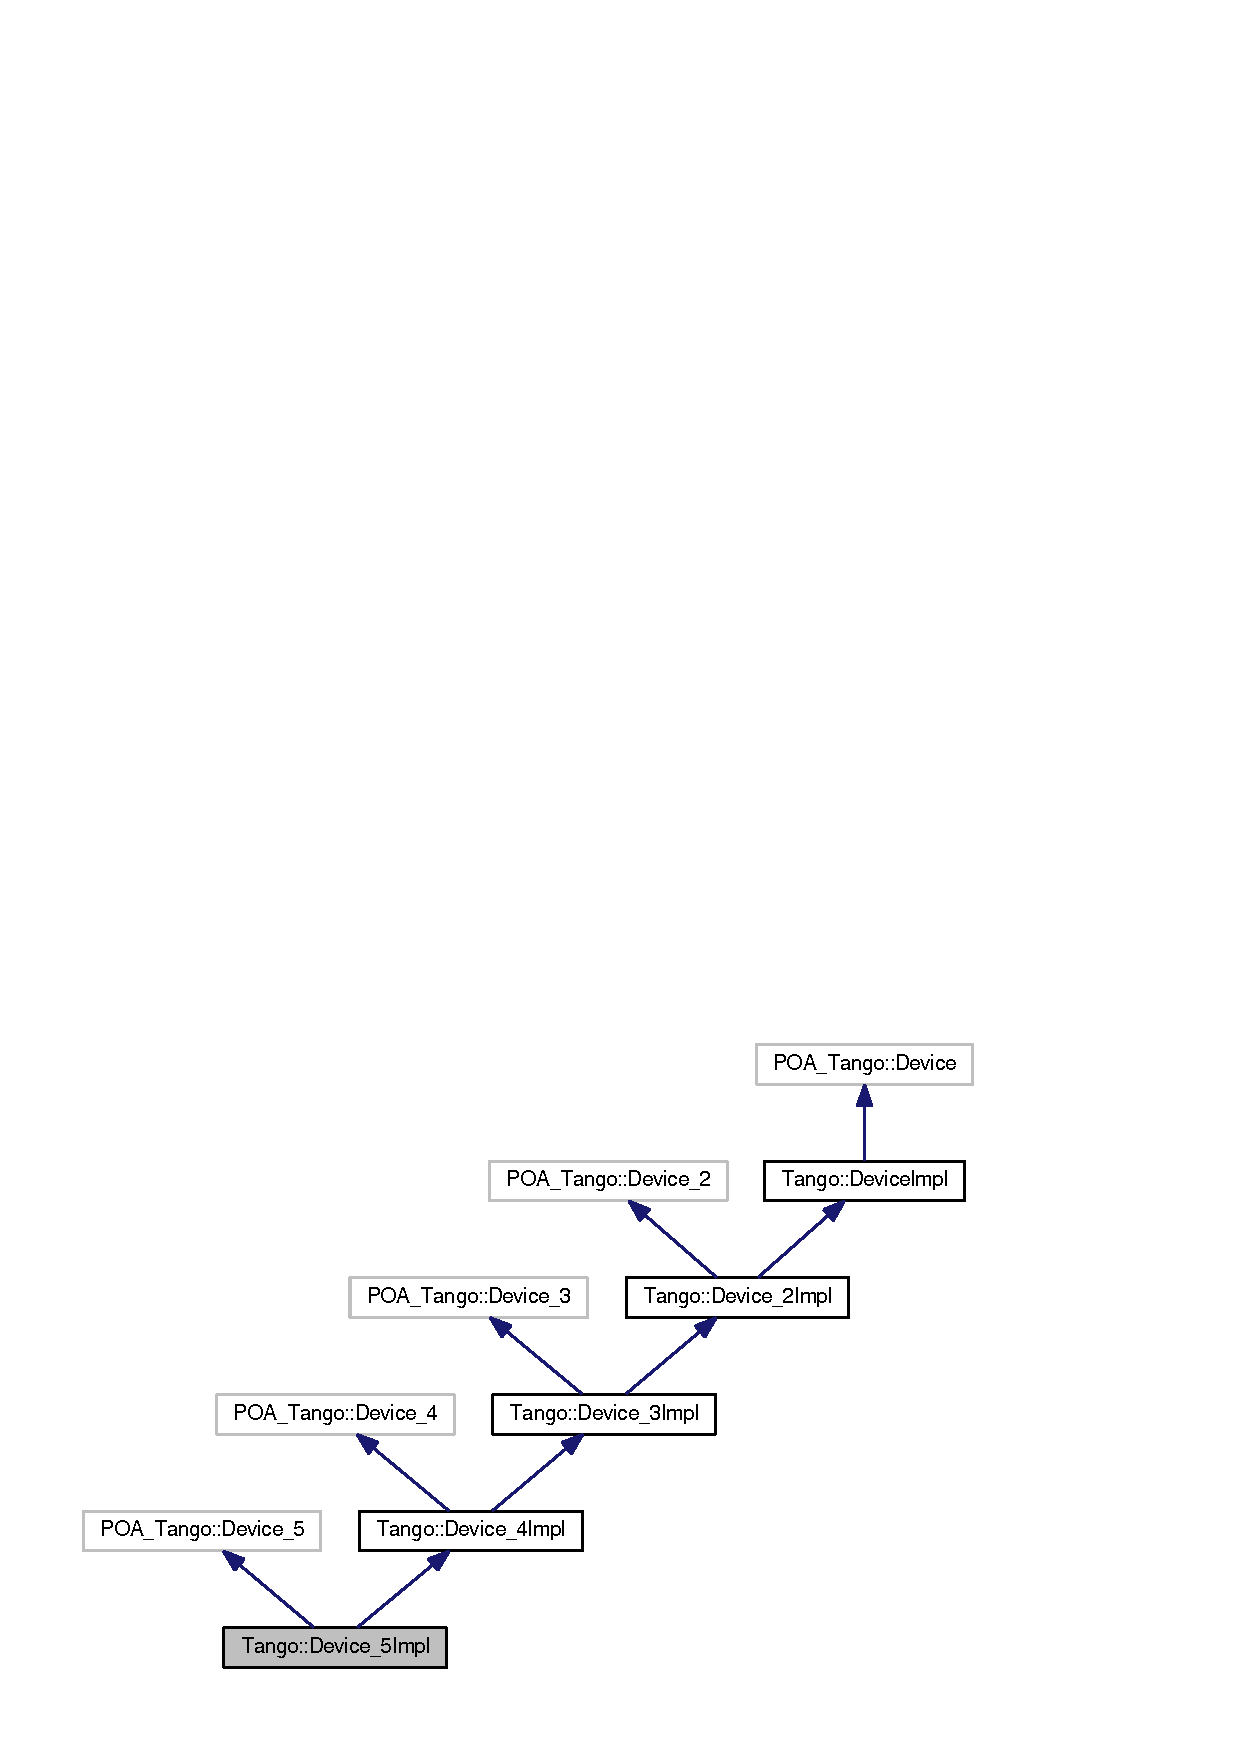
\includegraphics[width=350pt]{d1/ddb/classTango_1_1Device__5Impl__inherit__graph}
\end{center}
\end{figure}


Collaboration diagram for Tango\-:\-:Device\-\_\-5\-Impl\-:
\nopagebreak
\begin{figure}[H]
\begin{center}
\leavevmode
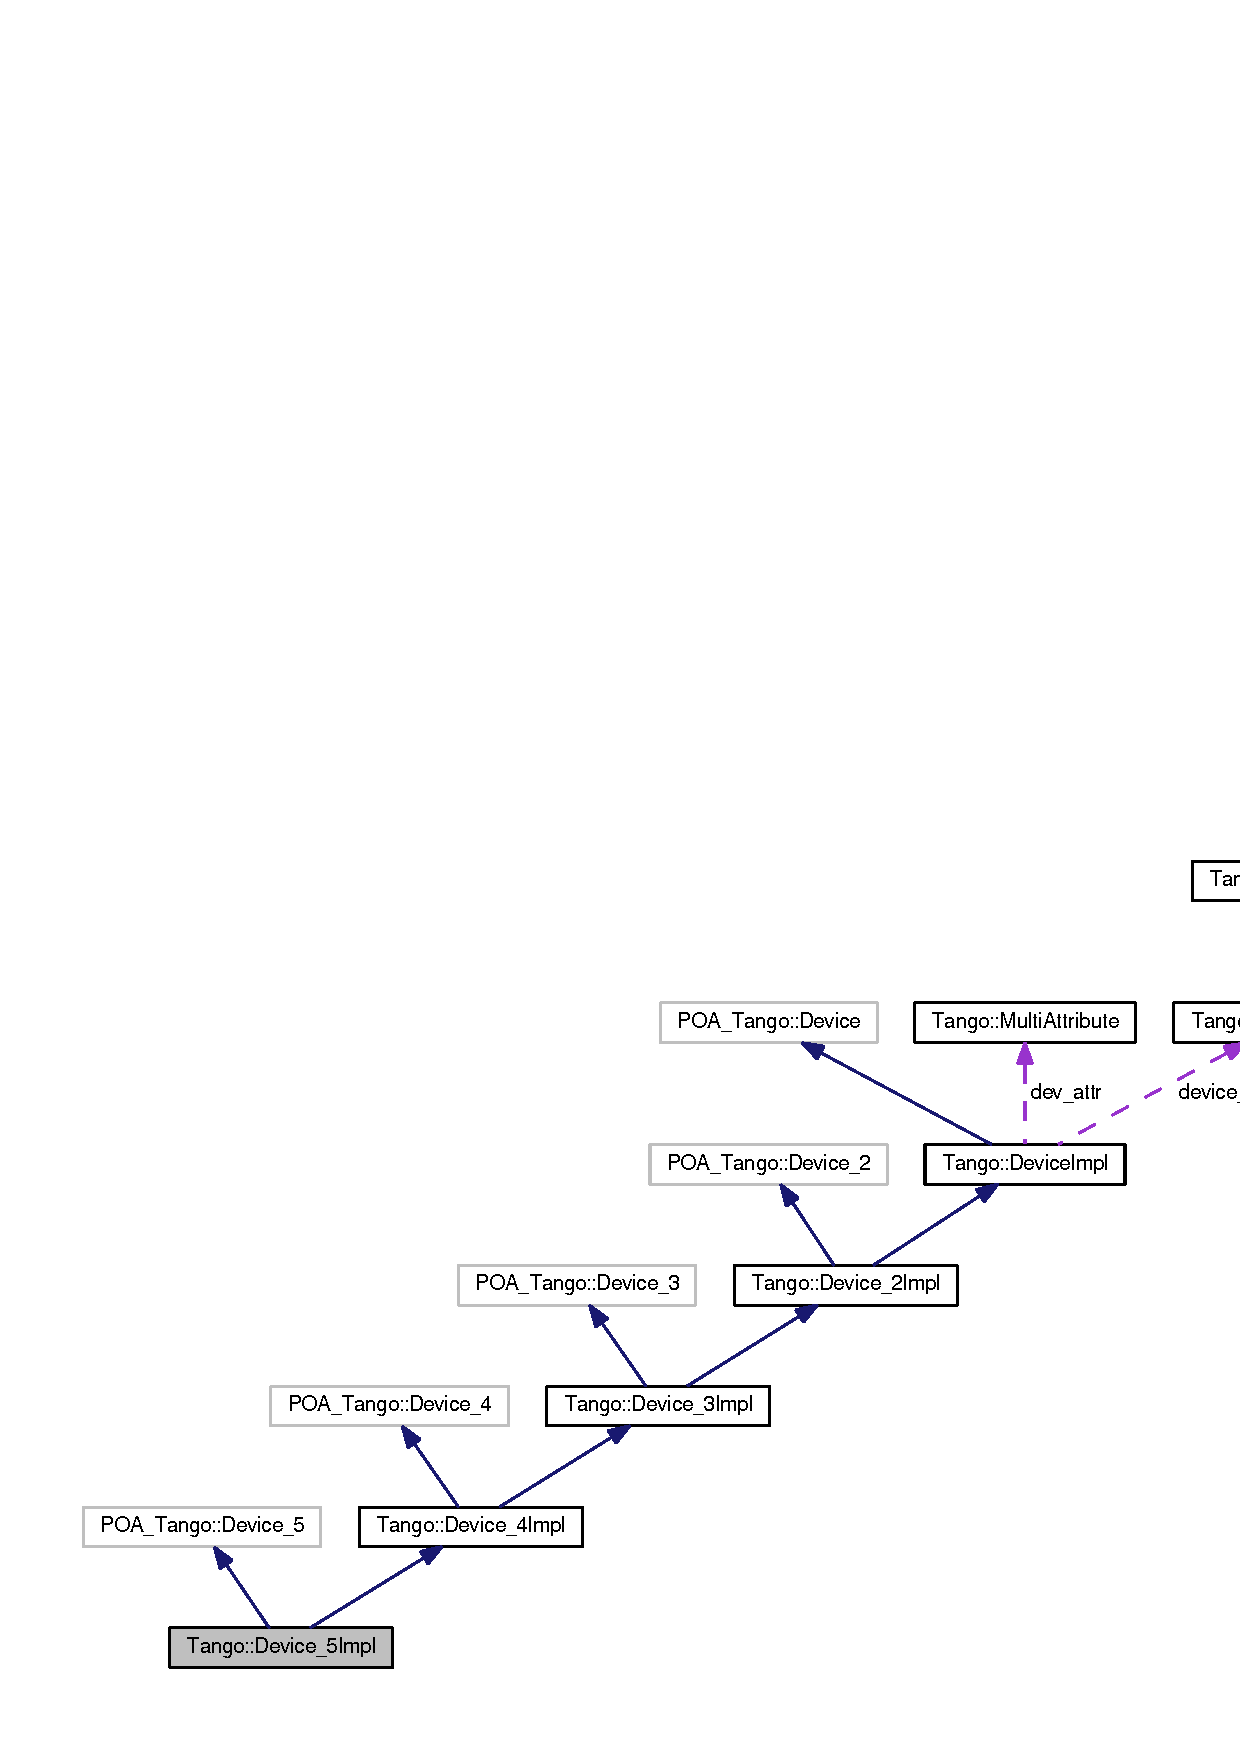
\includegraphics[width=350pt]{d2/dfe/classTango_1_1Device__5Impl__coll__graph}
\end{center}
\end{figure}
\subsection*{Public Member Functions}
\begin{Indent}{\bf Constructors}\par
{\em Miscellaneous constructors }\begin{DoxyCompactItemize}
\item 
{\bf Device\-\_\-5\-Impl} ({\bf Device\-Class} $\ast${\bf device\-\_\-class}, string \&dev\-\_\-name)
\begin{DoxyCompactList}\small\item\em Constructs a newly allocated \doxyref{Device\-\_\-5\-Impl}{p.}{d5/d94/classTango_1_1Device__5Impl} object from its name. \end{DoxyCompactList}\item 
{\bf Device\-\_\-5\-Impl} ({\bf Device\-Class} $\ast${\bf device\-\_\-class}, string \&dev\-\_\-name, string \&{\bf desc})
\begin{DoxyCompactList}\small\item\em Constructs a newly allocated \doxyref{Device\-\_\-5\-Impl}{p.}{d5/d94/classTango_1_1Device__5Impl} object from its name and its description. \end{DoxyCompactList}\item 
{\bf Device\-\_\-5\-Impl} ({\bf Device\-Class} $\ast${\bf device\-\_\-class}, string \&dev\-\_\-name, string \&{\bf desc}, Tango\-::\-Dev\-State {\bf dev\-\_\-state}, string \&{\bf dev\-\_\-status})
\begin{DoxyCompactList}\small\item\em Constructs a newly allocated \doxyref{Device\-\_\-5\-Impl}{p.}{d5/d94/classTango_1_1Device__5Impl} object from all its creation parameters. \end{DoxyCompactList}\item 
{\bf Device\-\_\-5\-Impl} ({\bf Device\-Class} $\ast${\bf device\-\_\-class}, const char $\ast$dev\-\_\-name, const char $\ast${\bf desc}=\char`\"{}A T\-A\-N\-G\-O device\char`\"{}, Tango\-::\-Dev\-State {\bf dev\-\_\-state}=Tango\-::\-U\-N\-K\-N\-O\-W\-N, const char $\ast${\bf dev\-\_\-status}={\bf Status\-Not\-Set})
\begin{DoxyCompactList}\small\item\em Constructs a newly allocated \doxyref{Device\-\_\-5\-Impl}{p.}{d5/d94/classTango_1_1Device__5Impl} object from all its creation parameters with some default values. \end{DoxyCompactList}\end{DoxyCompactItemize}
\end{Indent}
\begin{Indent}{\bf Destructor}\par
{\em Only one desctructor is defined for this class }\begin{DoxyCompactItemize}
\item 
virtual {\bf $\sim$\-Device\-\_\-5\-Impl} ()
\begin{DoxyCompactList}\small\item\em The device desctructor. \end{DoxyCompactList}\end{DoxyCompactItemize}
\end{Indent}
\begin{Indent}{\bf C\-O\-R\-B\-A operation methods}\par
{\em Method defined to implement T\-A\-N\-G\-O device C\-O\-R\-B\-A operation }\begin{DoxyCompactItemize}
\item 
virtual \\*
Tango\-::\-Attribute\-Value\-List\-\_\-5 $\ast$ {\bf read\-\_\-attributes\-\_\-5} (const Tango\-::\-Dev\-Var\-String\-Array \&names, Tango\-::\-Dev\-Source source, const Tango\-::\-Clnt\-Ident \&cl\-\_\-ident)
\begin{DoxyCompactList}\small\item\em Read attribute(s) value. \end{DoxyCompactList}\item 
virtual \\*
Tango\-::\-Attribute\-Value\-List\-\_\-5 $\ast$ {\bf write\-\_\-read\-\_\-attributes\-\_\-5} (const Tango\-::\-Attribute\-Value\-List\-\_\-4 \&values, const Tango\-::\-Dev\-Var\-String\-Array \&r\-\_\-names, const Tango\-::\-Clnt\-Ident \&cl\-\_\-ident)
\begin{DoxyCompactList}\small\item\em Write then read attribute(s) value. \end{DoxyCompactList}\item 
virtual \\*
Tango\-::\-Attribute\-Config\-List\-\_\-5 $\ast$ {\bf get\-\_\-attribute\-\_\-config\-\_\-5} (const Tango\-::\-Dev\-Var\-String\-Array \&names)
\begin{DoxyCompactList}\small\item\em Get attribute(s) configuration. \end{DoxyCompactList}\item 
virtual void {\bf set\-\_\-attribute\-\_\-config\-\_\-5} (const Tango\-::\-Attribute\-Config\-List\-\_\-5 \&new\-\_\-conf, const Tango\-::\-Clnt\-Ident \&cl\-\_\-ident)
\begin{DoxyCompactList}\small\item\em Set attribute(s) configuration. \end{DoxyCompactList}\item 
virtual Tango\-::\-Dev\-Attr\-History\-\_\-5 $\ast$ {\bf read\-\_\-attribute\-\_\-history\-\_\-5} (const char $\ast$name, Dev\-Long n)
\begin{DoxyCompactList}\small\item\em Read attribute value history. \end{DoxyCompactList}\item 
virtual Tango\-::\-Pipe\-Config\-List $\ast$ {\bf get\-\_\-pipe\-\_\-config\-\_\-5} (const Tango\-::\-Dev\-Var\-String\-Array \&names)
\begin{DoxyCompactList}\small\item\em Get pipe(s) configuration. \end{DoxyCompactList}\item 
virtual void {\bf set\-\_\-pipe\-\_\-config\-\_\-5} (const Tango\-::\-Pipe\-Config\-List \&new\-\_\-conf, const Tango\-::\-Clnt\-Ident \&cl\-\_\-ident)
\begin{DoxyCompactList}\small\item\em Set pipe(s) configuration. \end{DoxyCompactList}\item 
virtual Tango\-::\-Dev\-Pipe\-Data $\ast$ {\bf read\-\_\-pipe\-\_\-5} (const char $\ast$name, const Tango\-::\-Clnt\-Ident \&cl\-\_\-ident)
\begin{DoxyCompactList}\small\item\em Read pipe value. \end{DoxyCompactList}\item 
virtual void {\bf write\-\_\-pipe\-\_\-5} (const Tango\-::\-Dev\-Pipe\-Data \&pipe\-\_\-value, const Tango\-::\-Clnt\-Ident \&cl\-\_\-ident)
\begin{DoxyCompactList}\small\item\em Write pipe value. \end{DoxyCompactList}\item 
virtual Tango\-::\-Dev\-Pipe\-Data $\ast$ {\bf write\-\_\-read\-\_\-pipe\-\_\-5} (const Tango\-::\-Dev\-Pipe\-Data \&pipe\-\_\-value, const Tango\-::\-Clnt\-Ident \&cl\-\_\-ident)
\begin{DoxyCompactList}\small\item\em Write then read pipe value. \end{DoxyCompactList}\end{DoxyCompactItemize}
\end{Indent}
\subsection*{Additional Inherited Members}


\subsection{Detailed Description}
Base class for all T\-A\-N\-G\-O device since version 5. 

This class inherits from \doxyref{Device\-Impl}{p.}{d3/d62/classTango_1_1DeviceImpl} class which itself inherits from C\-O\-R\-B\-A classes where all the network layer is implemented. This class has been created since release 7 of \doxyref{Tango}{p.}{de/ddf/namespaceTango} library where the I\-D\-L \doxyref{Tango}{p.}{de/ddf/namespaceTango} module has been modified in order to create a Device\-\_\-4 interface which inherits from the original Device interface

\begin{DoxyParagraph}{Author\-:}
taurel 
\end{DoxyParagraph}
\begin{DoxyParagraph}{Revision\-:}
20742 
\end{DoxyParagraph}


\subsection{Constructor \& Destructor Documentation}
\index{Tango\-::\-Device\-\_\-5\-Impl@{Tango\-::\-Device\-\_\-5\-Impl}!Device\-\_\-5\-Impl@{Device\-\_\-5\-Impl}}
\index{Device\-\_\-5\-Impl@{Device\-\_\-5\-Impl}!Tango::Device_5Impl@{Tango\-::\-Device\-\_\-5\-Impl}}
\subsubsection[{Device\-\_\-5\-Impl}]{\setlength{\rightskip}{0pt plus 5cm}Tango\-::\-Device\-\_\-5\-Impl\-::\-Device\-\_\-5\-Impl (
\begin{DoxyParamCaption}
\item[{{\bf Device\-Class} $\ast$}]{device\-\_\-class, }
\item[{string \&}]{dev\-\_\-name}
\end{DoxyParamCaption}
)}\label{classTango_1_1Device__5Impl_afe1920d066044205dfe58cd07df3a821}


Constructs a newly allocated \doxyref{Device\-\_\-5\-Impl}{p.}{d5/d94/classTango_1_1Device__5Impl} object from its name. 

The device description field is set to {\itshape A \doxyref{Tango}{p.}{de/ddf/namespaceTango} device}. The device state is set to unknown and the device status is set to {\bfseries Not Initialised}


\begin{DoxyParams}{Parameters}
{\em device\-\_\-class} & Pointer to the device class object \\
\hline
{\em dev\-\_\-name} & The device name \\
\hline
\end{DoxyParams}
\index{Tango\-::\-Device\-\_\-5\-Impl@{Tango\-::\-Device\-\_\-5\-Impl}!Device\-\_\-5\-Impl@{Device\-\_\-5\-Impl}}
\index{Device\-\_\-5\-Impl@{Device\-\_\-5\-Impl}!Tango::Device_5Impl@{Tango\-::\-Device\-\_\-5\-Impl}}
\subsubsection[{Device\-\_\-5\-Impl}]{\setlength{\rightskip}{0pt plus 5cm}Tango\-::\-Device\-\_\-5\-Impl\-::\-Device\-\_\-5\-Impl (
\begin{DoxyParamCaption}
\item[{{\bf Device\-Class} $\ast$}]{device\-\_\-class, }
\item[{string \&}]{dev\-\_\-name, }
\item[{string \&}]{desc}
\end{DoxyParamCaption}
)}\label{classTango_1_1Device__5Impl_ab102993af659a0f91a811fa6d1690380}


Constructs a newly allocated \doxyref{Device\-\_\-5\-Impl}{p.}{d5/d94/classTango_1_1Device__5Impl} object from its name and its description. 

The device state is set to unknown and the device status is set to {\itshape Not Initialised}


\begin{DoxyParams}{Parameters}
{\em device\-\_\-class} & Pointer to the device class object \\
\hline
{\em dev\-\_\-name} & The device name \\
\hline
{\em desc} & The device description \\
\hline
\end{DoxyParams}
\index{Tango\-::\-Device\-\_\-5\-Impl@{Tango\-::\-Device\-\_\-5\-Impl}!Device\-\_\-5\-Impl@{Device\-\_\-5\-Impl}}
\index{Device\-\_\-5\-Impl@{Device\-\_\-5\-Impl}!Tango::Device_5Impl@{Tango\-::\-Device\-\_\-5\-Impl}}
\subsubsection[{Device\-\_\-5\-Impl}]{\setlength{\rightskip}{0pt plus 5cm}Tango\-::\-Device\-\_\-5\-Impl\-::\-Device\-\_\-5\-Impl (
\begin{DoxyParamCaption}
\item[{{\bf Device\-Class} $\ast$}]{device\-\_\-class, }
\item[{string \&}]{dev\-\_\-name, }
\item[{string \&}]{desc, }
\item[{Tango\-::\-Dev\-State}]{dev\-\_\-state, }
\item[{string \&}]{dev\-\_\-status}
\end{DoxyParamCaption}
)}\label{classTango_1_1Device__5Impl_ab40ede73a0c84a2f78f4213470df5129}


Constructs a newly allocated \doxyref{Device\-\_\-5\-Impl}{p.}{d5/d94/classTango_1_1Device__5Impl} object from all its creation parameters. 

The device is constructed from its name, its description, an original state and status


\begin{DoxyParams}{Parameters}
{\em device\-\_\-class} & Pointer to the device class object \\
\hline
{\em dev\-\_\-name} & The device name \\
\hline
{\em desc} & The device description \\
\hline
{\em dev\-\_\-state} & The device initial state \\
\hline
{\em dev\-\_\-status} & The device initial status \\
\hline
\end{DoxyParams}
\index{Tango\-::\-Device\-\_\-5\-Impl@{Tango\-::\-Device\-\_\-5\-Impl}!Device\-\_\-5\-Impl@{Device\-\_\-5\-Impl}}
\index{Device\-\_\-5\-Impl@{Device\-\_\-5\-Impl}!Tango::Device_5Impl@{Tango\-::\-Device\-\_\-5\-Impl}}
\subsubsection[{Device\-\_\-5\-Impl}]{\setlength{\rightskip}{0pt plus 5cm}Tango\-::\-Device\-\_\-5\-Impl\-::\-Device\-\_\-5\-Impl (
\begin{DoxyParamCaption}
\item[{{\bf Device\-Class} $\ast$}]{device\-\_\-class, }
\item[{const char $\ast$}]{dev\-\_\-name, }
\item[{const char $\ast$}]{desc = {\ttfamily \char`\"{}A~TANGO~device\char`\"{}}, }
\item[{Tango\-::\-Dev\-State}]{dev\-\_\-state = {\ttfamily Tango\-:\-:UNKNOWN}, }
\item[{const char $\ast$}]{dev\-\_\-status = {\ttfamily {\bf Status\-Not\-Set}}}
\end{DoxyParamCaption}
)}\label{classTango_1_1Device__5Impl_ad8b28f32f4a9ed7730f396e20e2b7334}


Constructs a newly allocated \doxyref{Device\-\_\-5\-Impl}{p.}{d5/d94/classTango_1_1Device__5Impl} object from all its creation parameters with some default values. 

The device is constructed from its name, its description, an original state and status. This constructor defined default values for the description, state and status parameters. The default device description is {\itshape A T\-A\-N\-G\-O device}. The default device state is {\itshape U\-N\-K\-N\-O\-W\-N} and the default device status is {\itshape Not initialised}.


\begin{DoxyParams}{Parameters}
{\em device\-\_\-class} & Pointer to the device class object \\
\hline
{\em dev\-\_\-name} & The device name \\
\hline
{\em desc} & The device desc \\
\hline
{\em dev\-\_\-state} & The device initial state \\
\hline
{\em dev\-\_\-status} & The device initial status \\
\hline
\end{DoxyParams}
\index{Tango\-::\-Device\-\_\-5\-Impl@{Tango\-::\-Device\-\_\-5\-Impl}!$\sim$\-Device\-\_\-5\-Impl@{$\sim$\-Device\-\_\-5\-Impl}}
\index{$\sim$\-Device\-\_\-5\-Impl@{$\sim$\-Device\-\_\-5\-Impl}!Tango::Device_5Impl@{Tango\-::\-Device\-\_\-5\-Impl}}
\subsubsection[{$\sim$\-Device\-\_\-5\-Impl}]{\setlength{\rightskip}{0pt plus 5cm}virtual Tango\-::\-Device\-\_\-5\-Impl\-::$\sim$\-Device\-\_\-5\-Impl (
\begin{DoxyParamCaption}
{}
\end{DoxyParamCaption}
)\hspace{0.3cm}{\ttfamily [inline]}, {\ttfamily [virtual]}}\label{classTango_1_1Device__5Impl_ad7cf3154c98f61e13d6324a959903d24}


The device desctructor. 



\subsection{Member Function Documentation}
\index{Tango\-::\-Device\-\_\-5\-Impl@{Tango\-::\-Device\-\_\-5\-Impl}!get\-\_\-attribute\-\_\-config\-\_\-5@{get\-\_\-attribute\-\_\-config\-\_\-5}}
\index{get\-\_\-attribute\-\_\-config\-\_\-5@{get\-\_\-attribute\-\_\-config\-\_\-5}!Tango::Device_5Impl@{Tango\-::\-Device\-\_\-5\-Impl}}
\subsubsection[{get\-\_\-attribute\-\_\-config\-\_\-5}]{\setlength{\rightskip}{0pt plus 5cm}virtual Tango\-::\-Attribute\-Config\-List\-\_\-5$\ast$ Tango\-::\-Device\-\_\-5\-Impl\-::get\-\_\-attribute\-\_\-config\-\_\-5 (
\begin{DoxyParamCaption}
\item[{const Tango\-::\-Dev\-Var\-String\-Array \&}]{names}
\end{DoxyParamCaption}
)\hspace{0.3cm}{\ttfamily [virtual]}}\label{classTango_1_1Device__5Impl_aab44f183c589d5bc661730747bf7f661}


Get attribute(s) configuration. 

Invoked when the client request the get\-\_\-attribute\-\_\-config\-\_\-5 C\-O\-R\-B\-A operation. It returns to the client one Attribute\-Config\-\_\-5 structure for each wanted attribute. All the attribute properties value are returned in this Attribute\-Config\-\_\-5 structure. Since \doxyref{Tango}{p.}{de/ddf/namespaceTango} release V5, the attribute event related, the attribute warning alarm and attribute rds alarm properties have been added to the returned structures.


\begin{DoxyParams}{Parameters}
{\em names} & The attribute(s) name list \\
\hline
\end{DoxyParams}
\begin{DoxyReturn}{Returns}
A sequence of Attribute\-Config\-\_\-5 structure. One structure is initialised for each wanted attribute. Click {\tt here} to read {\bfseries Attribute\-Config\-\_\-5} structure specification.
\end{DoxyReturn}

\begin{DoxyExceptions}{Exceptions}
{\em Dev\-Failed} & Thrown if the attribute does not exist. Click {\tt here} to read {\bfseries Dev\-Failed} exception specification \\
\hline
\end{DoxyExceptions}
\index{Tango\-::\-Device\-\_\-5\-Impl@{Tango\-::\-Device\-\_\-5\-Impl}!get\-\_\-pipe\-\_\-config\-\_\-5@{get\-\_\-pipe\-\_\-config\-\_\-5}}
\index{get\-\_\-pipe\-\_\-config\-\_\-5@{get\-\_\-pipe\-\_\-config\-\_\-5}!Tango::Device_5Impl@{Tango\-::\-Device\-\_\-5\-Impl}}
\subsubsection[{get\-\_\-pipe\-\_\-config\-\_\-5}]{\setlength{\rightskip}{0pt plus 5cm}virtual Tango\-::\-Pipe\-Config\-List$\ast$ Tango\-::\-Device\-\_\-5\-Impl\-::get\-\_\-pipe\-\_\-config\-\_\-5 (
\begin{DoxyParamCaption}
\item[{const Tango\-::\-Dev\-Var\-String\-Array \&}]{names}
\end{DoxyParamCaption}
)\hspace{0.3cm}{\ttfamily [virtual]}}\label{classTango_1_1Device__5Impl_aa58a10421bb77f52f091b0af4cde2a8b}


Get pipe(s) configuration. 

Invoked when the client request the get\-\_\-pipe\-\_\-config\-\_\-5 C\-O\-R\-B\-A operation. It returns to the client one Pipe\-Config\-\_\-5 structure for each wanted pipe. All the pipe description is returned in this Pipe\-Config\-\_\-5 structure.


\begin{DoxyParams}{Parameters}
{\em names} & The pipe(s) name list \\
\hline
\end{DoxyParams}
\begin{DoxyReturn}{Returns}
A sequence of Pipe\-Config\-\_\-5 structure. One structure is initialised for each wanted pipe. Click {\tt here} to read {\bfseries Pipe\-Config\-\_\-5} structure specification.
\end{DoxyReturn}

\begin{DoxyExceptions}{Exceptions}
{\em Dev\-Failed} & Thrown if the pipe does not exist. Click {\tt here} to read {\bfseries Dev\-Failed} exception specification \\
\hline
\end{DoxyExceptions}
\index{Tango\-::\-Device\-\_\-5\-Impl@{Tango\-::\-Device\-\_\-5\-Impl}!read\-\_\-attribute\-\_\-history\-\_\-5@{read\-\_\-attribute\-\_\-history\-\_\-5}}
\index{read\-\_\-attribute\-\_\-history\-\_\-5@{read\-\_\-attribute\-\_\-history\-\_\-5}!Tango::Device_5Impl@{Tango\-::\-Device\-\_\-5\-Impl}}
\subsubsection[{read\-\_\-attribute\-\_\-history\-\_\-5}]{\setlength{\rightskip}{0pt plus 5cm}virtual Tango\-::\-Dev\-Attr\-History\-\_\-5$\ast$ Tango\-::\-Device\-\_\-5\-Impl\-::read\-\_\-attribute\-\_\-history\-\_\-5 (
\begin{DoxyParamCaption}
\item[{const char $\ast$}]{name, }
\item[{Dev\-Long}]{n}
\end{DoxyParamCaption}
)\hspace{0.3cm}{\ttfamily [virtual]}}\label{classTango_1_1Device__5Impl_a605986206b97694efa729d83eed85c29}


Read attribute value history. 

Invoked when the client request the read\-\_\-attribute\-\_\-history\-\_\-5 C\-O\-R\-B\-A operation. This operation allows a client to retrieve attribute value history for polled attribute. The depth of the history is limited to the depth of the device server internal polling buffer. It returns to the client one Dev\-Attr\-History structure for each record.


\begin{DoxyParams}{Parameters}
{\em name} & The attribute name \\
\hline
{\em n} & The record number. \\
\hline
\end{DoxyParams}
\begin{DoxyReturn}{Returns}
A Dev\-Attr\-History\-\_\-5 structure. This strucure contains all the element allowing a client to retrieve for each history record the attribute value, the date and in case of the attribute returns an error when it was read, the Dev\-Errors data. Click {\tt here} to read {\bfseries Dev\-Attr\-History} structure definition. 
\end{DoxyReturn}

\begin{DoxyExceptions}{Exceptions}
{\em Dev\-Failed} & Thrown if the attribute does not exist or is not polled. Click {\tt here} to read {\bfseries Dev\-Failed} exception specification \\
\hline
\end{DoxyExceptions}
\index{Tango\-::\-Device\-\_\-5\-Impl@{Tango\-::\-Device\-\_\-5\-Impl}!read\-\_\-attributes\-\_\-5@{read\-\_\-attributes\-\_\-5}}
\index{read\-\_\-attributes\-\_\-5@{read\-\_\-attributes\-\_\-5}!Tango::Device_5Impl@{Tango\-::\-Device\-\_\-5\-Impl}}
\subsubsection[{read\-\_\-attributes\-\_\-5}]{\setlength{\rightskip}{0pt plus 5cm}virtual Tango\-::\-Attribute\-Value\-List\-\_\-5$\ast$ Tango\-::\-Device\-\_\-5\-Impl\-::read\-\_\-attributes\-\_\-5 (
\begin{DoxyParamCaption}
\item[{const Tango\-::\-Dev\-Var\-String\-Array \&}]{names, }
\item[{Tango\-::\-Dev\-Source}]{source, }
\item[{const Tango\-::\-Clnt\-Ident \&}]{cl\-\_\-ident}
\end{DoxyParamCaption}
)\hspace{0.3cm}{\ttfamily [virtual]}}\label{classTango_1_1Device__5Impl_ac79f342b824d93b3352f30b1f6a381dd}


Read attribute(s) value. 

Invoked when the client request the read\-\_\-attributes\-\_\-5 C\-O\-R\-B\-A operation. It returns to the client one Attribute\-Value structure for each wanted attribute.


\begin{DoxyParams}{Parameters}
{\em names} & The attribute(s) name list \\
\hline
{\em source} & The data source. This parameter is new in \doxyref{Tango}{p.}{de/ddf/namespaceTango} release 5. It allows a client to choose the data source between the device itself or the data cache for polled attribute. \\
\hline
{\em cl\-\_\-ident} & The client identificator. This parameter is new in release 4. It allows device locking feature implemented in \doxyref{Tango}{p.}{de/ddf/namespaceTango} V7 \\
\hline
\end{DoxyParams}
\begin{DoxyReturn}{Returns}
A sequence of Attribute\-Value\-\_\-5 structure. One structure is initialised for each wanted attribute with the attribute value, the date and the attribute value quality. Click {\tt here} to read {\bfseries Attribute\-Value} structure definition. 
\end{DoxyReturn}

\begin{DoxyExceptions}{Exceptions}
{\em Dev\-Failed} & Thrown if the attribute does not exist. Click {\tt here} to read {\bfseries Dev\-Failed} exception specification \\
\hline
\end{DoxyExceptions}
\index{Tango\-::\-Device\-\_\-5\-Impl@{Tango\-::\-Device\-\_\-5\-Impl}!read\-\_\-pipe\-\_\-5@{read\-\_\-pipe\-\_\-5}}
\index{read\-\_\-pipe\-\_\-5@{read\-\_\-pipe\-\_\-5}!Tango::Device_5Impl@{Tango\-::\-Device\-\_\-5\-Impl}}
\subsubsection[{read\-\_\-pipe\-\_\-5}]{\setlength{\rightskip}{0pt plus 5cm}virtual Tango\-::\-Dev\-Pipe\-Data$\ast$ Tango\-::\-Device\-\_\-5\-Impl\-::read\-\_\-pipe\-\_\-5 (
\begin{DoxyParamCaption}
\item[{const char $\ast$}]{name, }
\item[{const Tango\-::\-Clnt\-Ident \&}]{cl\-\_\-ident}
\end{DoxyParamCaption}
)\hspace{0.3cm}{\ttfamily [virtual]}}\label{classTango_1_1Device__5Impl_a87a53f7fe891410c80e28e716525683e}


Read pipe value. 

Invoked when the client request the read\-\_\-pipe\-\_\-5 C\-O\-R\-B\-A operation. It returns to the client a Dev\-Pipe\-Data structure.


\begin{DoxyParams}{Parameters}
{\em name} & The pipe name \\
\hline
{\em cl\-\_\-ident} & The client identificator. This parameter is new in release 4. It allows device locking feature implemented in \doxyref{Tango}{p.}{de/ddf/namespaceTango} V7 \\
\hline
\end{DoxyParams}
\begin{DoxyReturn}{Returns}
A Dev\-Pipe\-Data structure. Click {\tt here} to read {\bfseries Dev\-Pipe\-Data} structure definition. 
\end{DoxyReturn}

\begin{DoxyExceptions}{Exceptions}
{\em Dev\-Failed} & Thrown if the attribute does not exist. Click {\tt here} to read {\bfseries Dev\-Failed} exception specification \\
\hline
\end{DoxyExceptions}
\index{Tango\-::\-Device\-\_\-5\-Impl@{Tango\-::\-Device\-\_\-5\-Impl}!set\-\_\-attribute\-\_\-config\-\_\-5@{set\-\_\-attribute\-\_\-config\-\_\-5}}
\index{set\-\_\-attribute\-\_\-config\-\_\-5@{set\-\_\-attribute\-\_\-config\-\_\-5}!Tango::Device_5Impl@{Tango\-::\-Device\-\_\-5\-Impl}}
\subsubsection[{set\-\_\-attribute\-\_\-config\-\_\-5}]{\setlength{\rightskip}{0pt plus 5cm}virtual void Tango\-::\-Device\-\_\-5\-Impl\-::set\-\_\-attribute\-\_\-config\-\_\-5 (
\begin{DoxyParamCaption}
\item[{const Tango\-::\-Attribute\-Config\-List\-\_\-5 \&}]{new\-\_\-conf, }
\item[{const Tango\-::\-Clnt\-Ident \&}]{cl\-\_\-ident}
\end{DoxyParamCaption}
)\hspace{0.3cm}{\ttfamily [virtual]}}\label{classTango_1_1Device__5Impl_a54f9985386c233714413f73fba00e50a}


Set attribute(s) configuration. 

Invoked when the client request the set\-\_\-attribute\-\_\-config\-\_\-5 C\-O\-R\-B\-A operation. It updates the device attribute configuration actually used by the device but this method also updates the \doxyref{Tango}{p.}{de/ddf/namespaceTango} database. One structure of the Attribute\-Config\-\_\-3 type is needed for each attribute to update configuration. Click {\tt here} to read {\bfseries Attribute\-Config\-\_\-5} structure specification.


\begin{DoxyParams}{Parameters}
{\em new\-\_\-conf} & The attribute(s) new configuration structure sequence \\
\hline
{\em cl\-\_\-ident} & The client identificator. This parameter is new in release 4. It allows device locking feature implemented in \doxyref{Tango}{p.}{de/ddf/namespaceTango} V7 \\
\hline
\end{DoxyParams}

\begin{DoxyExceptions}{Exceptions}
{\em Dev\-Failed} & Thrown if the command does not exist. Click {\tt here} to read {\bfseries Dev\-Failed} exception specification \\
\hline
\end{DoxyExceptions}
\index{Tango\-::\-Device\-\_\-5\-Impl@{Tango\-::\-Device\-\_\-5\-Impl}!set\-\_\-pipe\-\_\-config\-\_\-5@{set\-\_\-pipe\-\_\-config\-\_\-5}}
\index{set\-\_\-pipe\-\_\-config\-\_\-5@{set\-\_\-pipe\-\_\-config\-\_\-5}!Tango::Device_5Impl@{Tango\-::\-Device\-\_\-5\-Impl}}
\subsubsection[{set\-\_\-pipe\-\_\-config\-\_\-5}]{\setlength{\rightskip}{0pt plus 5cm}virtual void Tango\-::\-Device\-\_\-5\-Impl\-::set\-\_\-pipe\-\_\-config\-\_\-5 (
\begin{DoxyParamCaption}
\item[{const Tango\-::\-Pipe\-Config\-List \&}]{new\-\_\-conf, }
\item[{const Tango\-::\-Clnt\-Ident \&}]{cl\-\_\-ident}
\end{DoxyParamCaption}
)\hspace{0.3cm}{\ttfamily [virtual]}}\label{classTango_1_1Device__5Impl_a4feb7a02977d194593cdb5c7ec6a23a7}


Set pipe(s) configuration. 

Invoked when the client request the set\-\_\-pipe\-\_\-config\-\_\-5 C\-O\-R\-B\-A operation. It updates the device pipe configuration actually used by the device but this method also updates the \doxyref{Tango}{p.}{de/ddf/namespaceTango} database. One structure of the Pipe\-Config type is needed for each pipe to update configuration. Click {\tt here} to read {\bfseries Pipe\-Config} structure specification.


\begin{DoxyParams}{Parameters}
{\em new\-\_\-conf} & The pipe(s) new configuration structure sequence \\
\hline
{\em cl\-\_\-ident} & The client identificator. This parameter is new in release 4. It allows device locking feature implemented in \doxyref{Tango}{p.}{de/ddf/namespaceTango} V7 \\
\hline
\end{DoxyParams}

\begin{DoxyExceptions}{Exceptions}
{\em Dev\-Failed} & Thrown if the command does not exist. Click {\tt here} to read {\bfseries Dev\-Failed} exception specification \\
\hline
\end{DoxyExceptions}
\index{Tango\-::\-Device\-\_\-5\-Impl@{Tango\-::\-Device\-\_\-5\-Impl}!write\-\_\-pipe\-\_\-5@{write\-\_\-pipe\-\_\-5}}
\index{write\-\_\-pipe\-\_\-5@{write\-\_\-pipe\-\_\-5}!Tango::Device_5Impl@{Tango\-::\-Device\-\_\-5\-Impl}}
\subsubsection[{write\-\_\-pipe\-\_\-5}]{\setlength{\rightskip}{0pt plus 5cm}virtual void Tango\-::\-Device\-\_\-5\-Impl\-::write\-\_\-pipe\-\_\-5 (
\begin{DoxyParamCaption}
\item[{const Tango\-::\-Dev\-Pipe\-Data \&}]{pipe\-\_\-value, }
\item[{const Tango\-::\-Clnt\-Ident \&}]{cl\-\_\-ident}
\end{DoxyParamCaption}
)\hspace{0.3cm}{\ttfamily [virtual]}}\label{classTango_1_1Device__5Impl_a03df67255a0e7b6b6259f85fc7834c77}


Write pipe value. 

Invoked when the client request the write\-\_\-pipe\-\_\-5 C\-O\-R\-B\-A operation. It allows a client to send data to a device through a pipe.


\begin{DoxyParams}{Parameters}
{\em pipe\-\_\-value} & The new pipe value \\
\hline
{\em cl\-\_\-ident} & The client identificator. This parameter is new in release 4. It allows device locking feature implemented in \doxyref{Tango}{p.}{de/ddf/namespaceTango} V7 \\
\hline
\end{DoxyParams}

\begin{DoxyExceptions}{Exceptions}
{\em Dev\-Failed} & Thrown if the attribute does not exist. Click {\tt here} to read {\bfseries Dev\-Failed} exception specification \\
\hline
\end{DoxyExceptions}
\index{Tango\-::\-Device\-\_\-5\-Impl@{Tango\-::\-Device\-\_\-5\-Impl}!write\-\_\-read\-\_\-attributes\-\_\-5@{write\-\_\-read\-\_\-attributes\-\_\-5}}
\index{write\-\_\-read\-\_\-attributes\-\_\-5@{write\-\_\-read\-\_\-attributes\-\_\-5}!Tango::Device_5Impl@{Tango\-::\-Device\-\_\-5\-Impl}}
\subsubsection[{write\-\_\-read\-\_\-attributes\-\_\-5}]{\setlength{\rightskip}{0pt plus 5cm}virtual Tango\-::\-Attribute\-Value\-List\-\_\-5$\ast$ Tango\-::\-Device\-\_\-5\-Impl\-::write\-\_\-read\-\_\-attributes\-\_\-5 (
\begin{DoxyParamCaption}
\item[{const Tango\-::\-Attribute\-Value\-List\-\_\-4 \&}]{values, }
\item[{const Tango\-::\-Dev\-Var\-String\-Array \&}]{r\-\_\-names, }
\item[{const Tango\-::\-Clnt\-Ident \&}]{cl\-\_\-ident}
\end{DoxyParamCaption}
)\hspace{0.3cm}{\ttfamily [virtual]}}\label{classTango_1_1Device__5Impl_a6e4e5de7a14e9e02e39d88fd74341a2a}


Write then read attribute(s) value. 

Invoked when the client request the write\-\_\-read\-\_\-attributes C\-O\-R\-B\-A operation. It sets the attribute(s) with the new value(s) passed as parameter and then read the attribute(s) and return the read value to the caller.


\begin{DoxyParams}{Parameters}
{\em values} & The attribute(s) new value(s). One structure is initialised for each wanted attribute with the attribute value. The attribute quality and date are not used by this method. Click {\tt here} to read {\bfseries Attribute\-Value} structure definition. \\
\hline
{\em r\-\_\-names} & Names of the attribute(s) to be read \\
\hline
{\em cl\-\_\-ident} & The client identificator. This parameter is new in release 4. It allows device locking feature implemented in \doxyref{Tango}{p.}{de/ddf/namespaceTango} V7 \\
\hline
\end{DoxyParams}
\begin{DoxyReturn}{Returns}
A sequence of Attribute\-Value\-\_\-5 structure. One structure is initialised for each wanted attribute with the attribute value, the date and the attribute value quality. Click {\tt here} to read {\bfseries Attribute\-Value\-\_\-5} structure definition. 
\end{DoxyReturn}

\begin{DoxyExceptions}{Exceptions}
{\em Dev\-Failed} & Thrown if the command does not exist. Click {\tt here} to read {\bfseries Dev\-Failed} exception specification \\
\hline
\end{DoxyExceptions}
\index{Tango\-::\-Device\-\_\-5\-Impl@{Tango\-::\-Device\-\_\-5\-Impl}!write\-\_\-read\-\_\-pipe\-\_\-5@{write\-\_\-read\-\_\-pipe\-\_\-5}}
\index{write\-\_\-read\-\_\-pipe\-\_\-5@{write\-\_\-read\-\_\-pipe\-\_\-5}!Tango::Device_5Impl@{Tango\-::\-Device\-\_\-5\-Impl}}
\subsubsection[{write\-\_\-read\-\_\-pipe\-\_\-5}]{\setlength{\rightskip}{0pt plus 5cm}virtual Tango\-::\-Dev\-Pipe\-Data$\ast$ Tango\-::\-Device\-\_\-5\-Impl\-::write\-\_\-read\-\_\-pipe\-\_\-5 (
\begin{DoxyParamCaption}
\item[{const Tango\-::\-Dev\-Pipe\-Data \&}]{pipe\-\_\-value, }
\item[{const Tango\-::\-Clnt\-Ident \&}]{cl\-\_\-ident}
\end{DoxyParamCaption}
)\hspace{0.3cm}{\ttfamily [virtual]}}\label{classTango_1_1Device__5Impl_a5da64b16851db4a641a06df11e1f371a}


Write then read pipe value. 

Invoked when the client request the write\-\_\-read\-\_\-pipe\-\_\-5 C\-O\-R\-B\-A operation. It allows a client to send data to a device through a pipe then to read data from the device through the same pipe.


\begin{DoxyParams}{Parameters}
{\em pipe\-\_\-value} & The new pipe value \\
\hline
{\em cl\-\_\-ident} & The client identificator. This parameter is new in release 4. It allows device locking feature implemented in \doxyref{Tango}{p.}{de/ddf/namespaceTango} V7 \\
\hline
\end{DoxyParams}
\begin{DoxyReturn}{Returns}
A Dev\-Pipe\-Data structure. Click {\tt here} to read {\bfseries Dev\-Pipe\-Data} structure definition. 
\end{DoxyReturn}

\begin{DoxyExceptions}{Exceptions}
{\em Dev\-Failed} & Thrown if the attribute does not exist. Click {\tt here} to read {\bfseries Dev\-Failed} exception specification \\
\hline
\end{DoxyExceptions}


The documentation for this class was generated from the following file\-:\begin{DoxyCompactItemize}
\item 
{\bf device\-\_\-5.\-h}\end{DoxyCompactItemize}

\section{Tango\-:\-:Device\-Attribute\-Config Struct Reference}
\label{structTango_1_1DeviceAttributeConfig}\index{Tango\-::\-Device\-Attribute\-Config@{Tango\-::\-Device\-Attribute\-Config}}


Base structure for \doxyref{Attribute}{p.}{d6/dad/classTango_1_1Attribute} configuration.  




Inheritance diagram for Tango\-:\-:Device\-Attribute\-Config\-:
\nopagebreak
\begin{figure}[H]
\begin{center}
\leavevmode
\includegraphics[width=184pt]{d8/dd4/structTango_1_1DeviceAttributeConfig__inherit__graph}
\end{center}
\end{figure}
\subsection*{Public Attributes}
\begin{DoxyCompactItemize}
\item 
Attr\-Data\-Format {\bf data\-\_\-format}
\begin{DoxyCompactList}\small\item\em Data format (Scalar, Spectrum,...) \end{DoxyCompactList}\item 
int {\bf data\-\_\-type}
\begin{DoxyCompactList}\small\item\em Data type. \end{DoxyCompactList}\item 
string {\bf description}
\begin{DoxyCompactList}\small\item\em Description. \end{DoxyCompactList}\item 
string {\bf display\-\_\-unit}
\begin{DoxyCompactList}\small\item\em Display unit. \end{DoxyCompactList}\item 
vector$<$ string $>$ {\bf extensions}
\begin{DoxyCompactList}\small\item\em For future extensions. \end{DoxyCompactList}\item 
string {\bf format}
\begin{DoxyCompactList}\small\item\em Format. \end{DoxyCompactList}\item 
string {\bf label}
\begin{DoxyCompactList}\small\item\em Label. \end{DoxyCompactList}\item 
string {\bf max\-\_\-alarm}
\begin{DoxyCompactList}\small\item\em Max alarm. \end{DoxyCompactList}\item 
int {\bf max\-\_\-dim\-\_\-x}
\begin{DoxyCompactList}\small\item\em Max dim X. \end{DoxyCompactList}\item 
int {\bf max\-\_\-dim\-\_\-y}
\begin{DoxyCompactList}\small\item\em Max dim Y. \end{DoxyCompactList}\item 
string {\bf max\-\_\-value}
\begin{DoxyCompactList}\small\item\em Max value. \end{DoxyCompactList}\item 
string {\bf min\-\_\-alarm}
\begin{DoxyCompactList}\small\item\em Min alarm. \end{DoxyCompactList}\item 
string {\bf min\-\_\-value}
\begin{DoxyCompactList}\small\item\em Min value. \end{DoxyCompactList}\item 
string {\bf name}
\begin{DoxyCompactList}\small\item\em Name. \end{DoxyCompactList}\item 
string {\bf standard\-\_\-unit}
\begin{DoxyCompactList}\small\item\em Standard unit. \end{DoxyCompactList}\item 
string {\bf unit}
\begin{DoxyCompactList}\small\item\em Unit. \end{DoxyCompactList}\item 
Attr\-Write\-Type {\bf writable}
\begin{DoxyCompactList}\small\item\em Writable type (Read, Write,...) \end{DoxyCompactList}\item 
string {\bf writable\-\_\-attr\-\_\-name}
\begin{DoxyCompactList}\small\item\em Writable att. name. \end{DoxyCompactList}\end{DoxyCompactItemize}


\subsection{Detailed Description}
Base structure for \doxyref{Attribute}{p.}{d6/dad/classTango_1_1Attribute} configuration. 



\subsection{Member Data Documentation}
\index{Tango\-::\-Device\-Attribute\-Config@{Tango\-::\-Device\-Attribute\-Config}!data\-\_\-format@{data\-\_\-format}}
\index{data\-\_\-format@{data\-\_\-format}!Tango::DeviceAttributeConfig@{Tango\-::\-Device\-Attribute\-Config}}
\subsubsection[{data\-\_\-format}]{\setlength{\rightskip}{0pt plus 5cm}Attr\-Data\-Format Tango\-::\-Device\-Attribute\-Config\-::data\-\_\-format}\label{structTango_1_1DeviceAttributeConfig_a10e944fe3cc1e6dce24ebfd2f474c294}


Data format (Scalar, Spectrum,...) 

\index{Tango\-::\-Device\-Attribute\-Config@{Tango\-::\-Device\-Attribute\-Config}!data\-\_\-type@{data\-\_\-type}}
\index{data\-\_\-type@{data\-\_\-type}!Tango::DeviceAttributeConfig@{Tango\-::\-Device\-Attribute\-Config}}
\subsubsection[{data\-\_\-type}]{\setlength{\rightskip}{0pt plus 5cm}int Tango\-::\-Device\-Attribute\-Config\-::data\-\_\-type}\label{structTango_1_1DeviceAttributeConfig_a2e2c5a17bc577057f9db3fec6fc5002c}


Data type. 

\index{Tango\-::\-Device\-Attribute\-Config@{Tango\-::\-Device\-Attribute\-Config}!description@{description}}
\index{description@{description}!Tango::DeviceAttributeConfig@{Tango\-::\-Device\-Attribute\-Config}}
\subsubsection[{description}]{\setlength{\rightskip}{0pt plus 5cm}string Tango\-::\-Device\-Attribute\-Config\-::description}\label{structTango_1_1DeviceAttributeConfig_a3ee3ca0543af398a2ee69901ab2086ea}


Description. 

\index{Tango\-::\-Device\-Attribute\-Config@{Tango\-::\-Device\-Attribute\-Config}!display\-\_\-unit@{display\-\_\-unit}}
\index{display\-\_\-unit@{display\-\_\-unit}!Tango::DeviceAttributeConfig@{Tango\-::\-Device\-Attribute\-Config}}
\subsubsection[{display\-\_\-unit}]{\setlength{\rightskip}{0pt plus 5cm}string Tango\-::\-Device\-Attribute\-Config\-::display\-\_\-unit}\label{structTango_1_1DeviceAttributeConfig_ae7ec9432c308d2080bff8390bf86e9dc}


Display unit. 

\index{Tango\-::\-Device\-Attribute\-Config@{Tango\-::\-Device\-Attribute\-Config}!extensions@{extensions}}
\index{extensions@{extensions}!Tango::DeviceAttributeConfig@{Tango\-::\-Device\-Attribute\-Config}}
\subsubsection[{extensions}]{\setlength{\rightskip}{0pt plus 5cm}vector$<$string$>$ Tango\-::\-Device\-Attribute\-Config\-::extensions}\label{structTango_1_1DeviceAttributeConfig_ae77d336e762e1c6e1e8fcea17d6b107f}


For future extensions. 

\index{Tango\-::\-Device\-Attribute\-Config@{Tango\-::\-Device\-Attribute\-Config}!format@{format}}
\index{format@{format}!Tango::DeviceAttributeConfig@{Tango\-::\-Device\-Attribute\-Config}}
\subsubsection[{format}]{\setlength{\rightskip}{0pt plus 5cm}string Tango\-::\-Device\-Attribute\-Config\-::format}\label{structTango_1_1DeviceAttributeConfig_ad3ec3ee2584e54354a9ad398432b7e63}


Format. 

\index{Tango\-::\-Device\-Attribute\-Config@{Tango\-::\-Device\-Attribute\-Config}!label@{label}}
\index{label@{label}!Tango::DeviceAttributeConfig@{Tango\-::\-Device\-Attribute\-Config}}
\subsubsection[{label}]{\setlength{\rightskip}{0pt plus 5cm}string Tango\-::\-Device\-Attribute\-Config\-::label}\label{structTango_1_1DeviceAttributeConfig_a4ec80e8421b9f1f3e250b047771a4a17}


Label. 

\index{Tango\-::\-Device\-Attribute\-Config@{Tango\-::\-Device\-Attribute\-Config}!max\-\_\-alarm@{max\-\_\-alarm}}
\index{max\-\_\-alarm@{max\-\_\-alarm}!Tango::DeviceAttributeConfig@{Tango\-::\-Device\-Attribute\-Config}}
\subsubsection[{max\-\_\-alarm}]{\setlength{\rightskip}{0pt plus 5cm}string Tango\-::\-Device\-Attribute\-Config\-::max\-\_\-alarm}\label{structTango_1_1DeviceAttributeConfig_ac2be6304818d741aa970abcb3ff91105}


Max alarm. 

\index{Tango\-::\-Device\-Attribute\-Config@{Tango\-::\-Device\-Attribute\-Config}!max\-\_\-dim\-\_\-x@{max\-\_\-dim\-\_\-x}}
\index{max\-\_\-dim\-\_\-x@{max\-\_\-dim\-\_\-x}!Tango::DeviceAttributeConfig@{Tango\-::\-Device\-Attribute\-Config}}
\subsubsection[{max\-\_\-dim\-\_\-x}]{\setlength{\rightskip}{0pt plus 5cm}int Tango\-::\-Device\-Attribute\-Config\-::max\-\_\-dim\-\_\-x}\label{structTango_1_1DeviceAttributeConfig_a1194d38c18b4aaeba0989b14d912f17f}


Max dim X. 

\index{Tango\-::\-Device\-Attribute\-Config@{Tango\-::\-Device\-Attribute\-Config}!max\-\_\-dim\-\_\-y@{max\-\_\-dim\-\_\-y}}
\index{max\-\_\-dim\-\_\-y@{max\-\_\-dim\-\_\-y}!Tango::DeviceAttributeConfig@{Tango\-::\-Device\-Attribute\-Config}}
\subsubsection[{max\-\_\-dim\-\_\-y}]{\setlength{\rightskip}{0pt plus 5cm}int Tango\-::\-Device\-Attribute\-Config\-::max\-\_\-dim\-\_\-y}\label{structTango_1_1DeviceAttributeConfig_a519d30179f56a9d0405a2b16fbd762eb}


Max dim Y. 

\index{Tango\-::\-Device\-Attribute\-Config@{Tango\-::\-Device\-Attribute\-Config}!max\-\_\-value@{max\-\_\-value}}
\index{max\-\_\-value@{max\-\_\-value}!Tango::DeviceAttributeConfig@{Tango\-::\-Device\-Attribute\-Config}}
\subsubsection[{max\-\_\-value}]{\setlength{\rightskip}{0pt plus 5cm}string Tango\-::\-Device\-Attribute\-Config\-::max\-\_\-value}\label{structTango_1_1DeviceAttributeConfig_a84c6e32024eb2ab01a03cb1016f2acbd}


Max value. 

\index{Tango\-::\-Device\-Attribute\-Config@{Tango\-::\-Device\-Attribute\-Config}!min\-\_\-alarm@{min\-\_\-alarm}}
\index{min\-\_\-alarm@{min\-\_\-alarm}!Tango::DeviceAttributeConfig@{Tango\-::\-Device\-Attribute\-Config}}
\subsubsection[{min\-\_\-alarm}]{\setlength{\rightskip}{0pt plus 5cm}string Tango\-::\-Device\-Attribute\-Config\-::min\-\_\-alarm}\label{structTango_1_1DeviceAttributeConfig_a265cd1f58f040fbb4fdebb8a5eb13718}


Min alarm. 

\index{Tango\-::\-Device\-Attribute\-Config@{Tango\-::\-Device\-Attribute\-Config}!min\-\_\-value@{min\-\_\-value}}
\index{min\-\_\-value@{min\-\_\-value}!Tango::DeviceAttributeConfig@{Tango\-::\-Device\-Attribute\-Config}}
\subsubsection[{min\-\_\-value}]{\setlength{\rightskip}{0pt plus 5cm}string Tango\-::\-Device\-Attribute\-Config\-::min\-\_\-value}\label{structTango_1_1DeviceAttributeConfig_aa647cb22659434ffe9833adbfecb11ab}


Min value. 

\index{Tango\-::\-Device\-Attribute\-Config@{Tango\-::\-Device\-Attribute\-Config}!name@{name}}
\index{name@{name}!Tango::DeviceAttributeConfig@{Tango\-::\-Device\-Attribute\-Config}}
\subsubsection[{name}]{\setlength{\rightskip}{0pt plus 5cm}string Tango\-::\-Device\-Attribute\-Config\-::name}\label{structTango_1_1DeviceAttributeConfig_aa986f46571ce7f48ac88d005034b16be}


Name. 

\index{Tango\-::\-Device\-Attribute\-Config@{Tango\-::\-Device\-Attribute\-Config}!standard\-\_\-unit@{standard\-\_\-unit}}
\index{standard\-\_\-unit@{standard\-\_\-unit}!Tango::DeviceAttributeConfig@{Tango\-::\-Device\-Attribute\-Config}}
\subsubsection[{standard\-\_\-unit}]{\setlength{\rightskip}{0pt plus 5cm}string Tango\-::\-Device\-Attribute\-Config\-::standard\-\_\-unit}\label{structTango_1_1DeviceAttributeConfig_a6e39a2bd02dff03ba378d42e0f0892e8}


Standard unit. 

\index{Tango\-::\-Device\-Attribute\-Config@{Tango\-::\-Device\-Attribute\-Config}!unit@{unit}}
\index{unit@{unit}!Tango::DeviceAttributeConfig@{Tango\-::\-Device\-Attribute\-Config}}
\subsubsection[{unit}]{\setlength{\rightskip}{0pt plus 5cm}string Tango\-::\-Device\-Attribute\-Config\-::unit}\label{structTango_1_1DeviceAttributeConfig_abbfe98ae17bfc21368b6347b9611e4f8}


Unit. 

\index{Tango\-::\-Device\-Attribute\-Config@{Tango\-::\-Device\-Attribute\-Config}!writable@{writable}}
\index{writable@{writable}!Tango::DeviceAttributeConfig@{Tango\-::\-Device\-Attribute\-Config}}
\subsubsection[{writable}]{\setlength{\rightskip}{0pt plus 5cm}Attr\-Write\-Type Tango\-::\-Device\-Attribute\-Config\-::writable}\label{structTango_1_1DeviceAttributeConfig_a5f02c5c4d857bd6eec495a746dfaf646}


Writable type (Read, Write,...) 

\index{Tango\-::\-Device\-Attribute\-Config@{Tango\-::\-Device\-Attribute\-Config}!writable\-\_\-attr\-\_\-name@{writable\-\_\-attr\-\_\-name}}
\index{writable\-\_\-attr\-\_\-name@{writable\-\_\-attr\-\_\-name}!Tango::DeviceAttributeConfig@{Tango\-::\-Device\-Attribute\-Config}}
\subsubsection[{writable\-\_\-attr\-\_\-name}]{\setlength{\rightskip}{0pt plus 5cm}string Tango\-::\-Device\-Attribute\-Config\-::writable\-\_\-attr\-\_\-name}\label{structTango_1_1DeviceAttributeConfig_a7c86de3d725f10a4ca07b086d04ce043}


Writable att. name. 



The documentation for this struct was generated from the following file\-:\begin{DoxyCompactItemize}
\item 
{\bf devapi.\-h}\end{DoxyCompactItemize}

\section{Tango\-:\-:Device\-Attribute\-History Class Reference}
\label{classTango_1_1DeviceAttributeHistory}\index{Tango\-::\-Device\-Attribute\-History@{Tango\-::\-Device\-Attribute\-History}}


Fundamental type for receiving data from device attribute polling buffers.  




Inheritance diagram for Tango\-:\-:Device\-Attribute\-History\-:
\nopagebreak
\begin{figure}[H]
\begin{center}
\leavevmode
\includegraphics[width=186pt]{d6/d9c/classTango_1_1DeviceAttributeHistory__inherit__graph}
\end{center}
\end{figure}


Collaboration diagram for Tango\-:\-:Device\-Attribute\-History\-:
\nopagebreak
\begin{figure}[H]
\begin{center}
\leavevmode
\includegraphics[width=186pt]{dc/d16/classTango_1_1DeviceAttributeHistory__coll__graph}
\end{center}
\end{figure}
\subsection*{Public Member Functions}
\begin{DoxyCompactItemize}
\item 
bool {\bf has\-\_\-failed} ()
\begin{DoxyCompactList}\small\item\em Check if the record was a failure. \end{DoxyCompactList}\end{DoxyCompactItemize}
\subsection*{Friends}
\begin{DoxyCompactItemize}
\item 
ostream \& {\bf operator$<$$<$} (ostream \&str, {\bf Device\-Attribute\-History} \&dah)
\begin{DoxyCompactList}\small\item\em Print a \doxyref{Device\-Attribute\-History}{p.}{d8/d41/classTango_1_1DeviceAttributeHistory} instance. \end{DoxyCompactList}\end{DoxyCompactItemize}


\subsection{Detailed Description}
Fundamental type for receiving data from device attribute polling buffers. 

This is the fundamental type for receiving data from device attribute polling buffers. This class inherits from the Tango\-::\-Device\-Attribute class. One instance of this class is created for each attribute result history. Within this class, you find the attribute result data or the exception parameters and a flag indicating if the attribute has failed when it was invoked by the device server polling thread. For history calls, it is not possible to returns attribute error as exception. See chapter on Advanced Features in the {\tt Tango book} for all details regarding device polling.

\$\-Author\$ \$\-Revision\$ 

\subsection{Member Function Documentation}
\index{Tango\-::\-Device\-Attribute\-History@{Tango\-::\-Device\-Attribute\-History}!has\-\_\-failed@{has\-\_\-failed}}
\index{has\-\_\-failed@{has\-\_\-failed}!Tango::DeviceAttributeHistory@{Tango\-::\-Device\-Attribute\-History}}
\subsubsection[{has\-\_\-failed}]{\setlength{\rightskip}{0pt plus 5cm}bool Tango\-::\-Device\-Attribute\-History\-::has\-\_\-failed (
\begin{DoxyParamCaption}
{}
\end{DoxyParamCaption}
)\hspace{0.3cm}{\ttfamily [inline]}}\label{classTango_1_1DeviceAttributeHistory_a29502710f173c46c03a6334f0498899e}


Check if the record was a failure. 

Returns a boolean set to true if the record in the polling buffer was a failure

\begin{DoxyReturn}{Returns}
A boolean set to true if the record was a failure 
\end{DoxyReturn}


\subsection{Friends And Related Function Documentation}
\index{Tango\-::\-Device\-Attribute\-History@{Tango\-::\-Device\-Attribute\-History}!operator$<$$<$@{operator$<$$<$}}
\index{operator$<$$<$@{operator$<$$<$}!Tango::DeviceAttributeHistory@{Tango\-::\-Device\-Attribute\-History}}
\subsubsection[{operator$<$$<$}]{\setlength{\rightskip}{0pt plus 5cm}ostream\& operator$<$$<$ (
\begin{DoxyParamCaption}
\item[{ostream \&}]{str, }
\item[{{\bf Device\-Attribute\-History} \&}]{dah}
\end{DoxyParamCaption}
)\hspace{0.3cm}{\ttfamily [friend]}}\label{classTango_1_1DeviceAttributeHistory_a641d6e2a068adc24811acc267e13486a}


Print a \doxyref{Device\-Attribute\-History}{p.}{d8/d41/classTango_1_1DeviceAttributeHistory} instance. 

Is an utility function to easily print the contents of a \doxyref{Device\-Attribute\-History}{p.}{d8/d41/classTango_1_1DeviceAttributeHistory} object. This function knows all types which could be inserted in a \doxyref{Device\-Attribute\-History}{p.}{d8/d41/classTango_1_1DeviceAttributeHistory} object and print them accordingly. It also in case the attribute returned an error. 
\begin{DoxyCode}
* DeviceProxy *dev = \textcolor{keyword}{new} DeviceProxy(“...”);
* \textcolor{keywordtype}{int} hist\_depth = 4;
* vector<DeviceAttributeHistory> *hist;

* hist = dev->attribute\_history(“MyAttribute”,hist\_depth);

* \textcolor{keywordflow}{for} (\textcolor{keywordtype}{int} i = 0;i < hist\_depth;i++)
* \{
*    cout << (*hist)[i] << endl;
* \}
* \textcolor{keyword}{delete} hist;
* 
\end{DoxyCode}



\begin{DoxyParams}[1]{Parameters}
\mbox{\tt in}  & {\em str} & The printing stream \\
\hline
\mbox{\tt in}  & {\em dah} & The instance to be printed \\
\hline
\end{DoxyParams}


The documentation for this class was generated from the following file\-:\begin{DoxyCompactItemize}
\item 
{\bf devapi.\-h}\end{DoxyCompactItemize}

\section{Tango\-:\-:Device\-Class Class Reference}
\label{classTango_1_1DeviceClass}\index{Tango\-::\-Device\-Class@{Tango\-::\-Device\-Class}}


Base class for all T\-A\-N\-G\-O device-\/class class.  




Collaboration diagram for Tango\-:\-:Device\-Class\-:
\nopagebreak
\begin{figure}[H]
\begin{center}
\leavevmode
\includegraphics[width=144pt]{df/d8c/classTango_1_1DeviceClass__coll__graph}
\end{center}
\end{figure}
\subsection*{Public Member Functions}
\begin{Indent}{\bf Destructor}\par
{\em Only one desctructor is defined for this class }\begin{DoxyCompactItemize}
\item 
virtual {\bf $\sim$\-Device\-Class} ()
\begin{DoxyCompactList}\small\item\em The device destructor. \end{DoxyCompactList}\end{DoxyCompactItemize}
\end{Indent}
\begin{Indent}{\bf Miscellaneous methods}\par
\begin{DoxyCompactItemize}
\item 
C\-O\-R\-B\-A\-::\-Any $\ast$ {\bf command\-\_\-handler} ({\bf Device\-Impl} $\ast$device, string \&command, const C\-O\-R\-B\-A\-::\-Any \&in\-\_\-any)
\begin{DoxyCompactList}\small\item\em Execute a command. \end{DoxyCompactList}\item 
virtual void {\bf command\-\_\-factory} ()=0
\begin{DoxyCompactList}\small\item\em Create command objects for all command supported by this class of device. \end{DoxyCompactList}\item 
virtual void {\bf attribute\-\_\-factory} (vector$<$ {\bf Attr} $\ast$ $>$ \&)
\begin{DoxyCompactList}\small\item\em Create all the attributes name supported by this class of device. \end{DoxyCompactList}\item 
virtual void {\bf pipe\-\_\-factory} ()
\begin{DoxyCompactList}\small\item\em Create all the pipes supported by this class of device. \end{DoxyCompactList}\item 
virtual void {\bf device\-\_\-factory} (const Tango\-::\-Dev\-Var\-String\-Array $\ast$dev\-\_\-list)=0
\begin{DoxyCompactList}\small\item\em Create device(s). \end{DoxyCompactList}\item 
virtual void {\bf device\-\_\-name\-\_\-factory} (vector$<$ string $>$ \&list)
\begin{DoxyCompactList}\small\item\em Create device(s) name list (for no database device server). \end{DoxyCompactList}\item 
void {\bf device\-\_\-destroyer} (const string \&dev\-\_\-name)
\begin{DoxyCompactList}\small\item\em Delete device. \end{DoxyCompactList}\item 
void {\bf device\-\_\-destroyer} (const char $\ast$dev\-\_\-name)
\begin{DoxyCompactList}\small\item\em Delete device. \end{DoxyCompactList}\end{DoxyCompactItemize}
\end{Indent}
\begin{Indent}{\bf Get/\-Set object members.}\par
{\em These methods allows the external world to get/set \doxyref{Device\-Impl}{p.}{d3/d62/classTango_1_1DeviceImpl} instance data members }\begin{DoxyCompactItemize}
\item 
string \& {\bf get\-\_\-name} ()
\begin{DoxyCompactList}\small\item\em Get the T\-A\-N\-G\-O device class name. \end{DoxyCompactList}\item 
string \& {\bf get\-\_\-doc\-\_\-url} ()
\begin{DoxyCompactList}\small\item\em Get the T\-A\-N\-G\-O device class documentation U\-R\-L. \end{DoxyCompactList}\item 
string \& {\bf get\-\_\-type} ()
\begin{DoxyCompactList}\small\item\em Get the T\-A\-N\-G\-O device type name. \end{DoxyCompactList}\item 
vector$<$ {\bf Device\-Impl} $\ast$ $>$ \& {\bf get\-\_\-device\-\_\-list} ()
\begin{DoxyCompactList}\small\item\em Get the device object vector. \end{DoxyCompactList}\item 
vector$<$ {\bf Command} $\ast$ $>$ \& {\bf get\-\_\-command\-\_\-list} ()
\begin{DoxyCompactList}\small\item\em Get the command object vector. \end{DoxyCompactList}\item 
vector$<$ {\bf Pipe} $\ast$ $>$ \& {\bf get\-\_\-pipe\-\_\-list} (const string \&dev\-\_\-name)
\begin{DoxyCompactList}\small\item\em Get the pipe object vector. \end{DoxyCompactList}\item 
{\bf Command} \& {\bf get\-\_\-cmd\-\_\-by\-\_\-name} (const string \&)
\begin{DoxyCompactList}\small\item\em Get a reference to a command object. \end{DoxyCompactList}\item 
{\bf Pipe} \& {\bf get\-\_\-pipe\-\_\-by\-\_\-name} (const string \&pipe\-\_\-name, const string \&dev\-\_\-name)
\begin{DoxyCompactList}\small\item\em Get a reference to a pipe object. \end{DoxyCompactList}\item 
{\bf Db\-Class} $\ast$ {\bf get\-\_\-db\-\_\-class} ()
\begin{DoxyCompactList}\small\item\em Get a pointer to the associated \doxyref{Db\-Class}{p.}{dc/d38/classTango_1_1DbClass} object. \end{DoxyCompactList}\item 
Multi\-Class\-Attribute $\ast$ {\bf get\-\_\-class\-\_\-attr} ()
\begin{DoxyCompactList}\small\item\em Get a pointer to the class attributes object. \end{DoxyCompactList}\item 
Multi\-Class\-Pipe $\ast$ {\bf get\-\_\-class\-\_\-pipe} ()
\begin{DoxyCompactList}\small\item\em Get a pointer to the class pipes object. \end{DoxyCompactList}\item 
void {\bf set\-\_\-type} (string \&dev\-\_\-type)
\begin{DoxyCompactList}\small\item\em Set the T\-A\-N\-G\-O device type name. \end{DoxyCompactList}\item 
void {\bf set\-\_\-type} (const char $\ast$dev\-\_\-type)
\begin{DoxyCompactList}\small\item\em Set the T\-A\-N\-G\-O device type name. \end{DoxyCompactList}\end{DoxyCompactItemize}
\end{Indent}
\begin{Indent}{\bf Signal related methods}\par
{\em These methods allow a signal management at device level }\begin{DoxyCompactItemize}
\item 
void {\bf register\-\_\-signal} (long signo, bool own\-\_\-handler=false)
\begin{DoxyCompactList}\small\item\em Register a signal. \end{DoxyCompactList}\item 
void {\bf unregister\-\_\-signal} (long signo)
\begin{DoxyCompactList}\small\item\em Unregister a signal. \end{DoxyCompactList}\item 
virtual void {\bf signal\-\_\-handler} (long signo)
\begin{DoxyCompactList}\small\item\em Signal handler. \end{DoxyCompactList}\end{DoxyCompactItemize}
\end{Indent}
\subsection*{Protected Member Functions}
\begin{Indent}{\bf Constructor}\par
{\em Only one constructot for this class which is a singleton }\begin{DoxyCompactItemize}
\item 
{\bf Device\-Class} (string \&s)
\begin{DoxyCompactList}\small\item\em Construct a newly allocated \doxyref{Device\-Class}{p.}{d4/dcd/classTango_1_1DeviceClass} object. \end{DoxyCompactList}\end{DoxyCompactItemize}
\end{Indent}
\begin{Indent}{\bf Miscellaneous protected methods}\par
\begin{DoxyCompactItemize}
\item 
void {\bf export\-\_\-device} ({\bf Device\-Impl} $\ast$dev, const char $\ast$corba\-\_\-dev\-\_\-name=\char`\"{}Unused\char`\"{})
\begin{DoxyCompactList}\small\item\em Export a device. \end{DoxyCompactList}\item 
void {\bf set\-\_\-default\-\_\-command} ({\bf Command} $\ast$cmd)
\begin{DoxyCompactList}\small\item\em Set a \doxyref{Tango}{p.}{de/ddf/namespaceTango} classs default command. \end{DoxyCompactList}\end{DoxyCompactItemize}
\end{Indent}
\subsection*{Protected Attributes}
\begin{Indent}{\bf Class data members}\par
\begin{DoxyCompactItemize}
\item 
string {\bf name}
\begin{DoxyCompactList}\small\item\em The T\-A\-N\-G\-O device class name. \end{DoxyCompactList}\item 
string {\bf doc\-\_\-url}
\begin{DoxyCompactList}\small\item\em The T\-A\-N\-G\-O device class documentation U\-R\-L. \end{DoxyCompactList}\item 
string {\bf type}
\begin{DoxyCompactList}\small\item\em The T\-A\-N\-G\-O device type name. \end{DoxyCompactList}\item 
vector$<$ {\bf Command} $\ast$ $>$ {\bf command\-\_\-list}
\begin{DoxyCompactList}\small\item\em The command(s) list. \end{DoxyCompactList}\item 
vector$<$ {\bf Device\-Impl} $\ast$ $>$ {\bf device\-\_\-list}
\begin{DoxyCompactList}\small\item\em The device(s) list. \end{DoxyCompactList}\item 
{\bf Db\-Class} $\ast$ {\bf db\-\_\-class}
\begin{DoxyCompactList}\small\item\em The associated \doxyref{Db\-Class}{p.}{dc/d38/classTango_1_1DbClass} object. \end{DoxyCompactList}\item 
Multi\-Class\-Attribute $\ast$ {\bf class\-\_\-attr}
\begin{DoxyCompactList}\small\item\em Pointer to the class multi attribute object. \end{DoxyCompactList}\item 
Multi\-Class\-Pipe $\ast$ {\bf class\-\_\-pipe}
\begin{DoxyCompactList}\small\item\em Pointer to the class multi pipe object. \end{DoxyCompactList}\item 
vector$<$ {\bf Pipe} $\ast$ $>$ {\bf pipe\-\_\-list}
\begin{DoxyCompactList}\small\item\em The pipe(s) list. \end{DoxyCompactList}\end{DoxyCompactItemize}
\end{Indent}
\subsection*{Friends}
\begin{DoxyCompactItemize}
\item 
class {\bf Tango\-::\-Auto\-Tango\-Monitor}
\end{DoxyCompactItemize}


\subsection{Detailed Description}
Base class for all T\-A\-N\-G\-O device-\/class class. 

A T\-A\-N\-G\-O device-\/class class is a class where is stored all data/method common to all devices of a T\-A\-N\-G\-O device class

\$\-Author\$ \$\-Revision\$ 

\subsection{Constructor \& Destructor Documentation}
\index{Tango\-::\-Device\-Class@{Tango\-::\-Device\-Class}!$\sim$\-Device\-Class@{$\sim$\-Device\-Class}}
\index{$\sim$\-Device\-Class@{$\sim$\-Device\-Class}!Tango::DeviceClass@{Tango\-::\-Device\-Class}}
\subsubsection[{$\sim$\-Device\-Class}]{\setlength{\rightskip}{0pt plus 5cm}virtual Tango\-::\-Device\-Class\-::$\sim$\-Device\-Class (
\begin{DoxyParamCaption}
{}
\end{DoxyParamCaption}
)\hspace{0.3cm}{\ttfamily [virtual]}}\label{classTango_1_1DeviceClass_ae3f6389d6cd5f8d9a4a0d503b1b39859}


The device destructor. 

\index{Tango\-::\-Device\-Class@{Tango\-::\-Device\-Class}!Device\-Class@{Device\-Class}}
\index{Device\-Class@{Device\-Class}!Tango::DeviceClass@{Tango\-::\-Device\-Class}}
\subsubsection[{Device\-Class}]{\setlength{\rightskip}{0pt plus 5cm}Tango\-::\-Device\-Class\-::\-Device\-Class (
\begin{DoxyParamCaption}
\item[{string \&}]{s}
\end{DoxyParamCaption}
)\hspace{0.3cm}{\ttfamily [protected]}}\label{classTango_1_1DeviceClass_a053d5cd241d3c4e16aab72547c79c86f}


Construct a newly allocated \doxyref{Device\-Class}{p.}{d4/dcd/classTango_1_1DeviceClass} object. 


\begin{DoxyParams}{Parameters}
{\em s} & The \doxyref{Tango}{p.}{de/ddf/namespaceTango} device class name \\
\hline
\end{DoxyParams}


\subsection{Member Function Documentation}
\index{Tango\-::\-Device\-Class@{Tango\-::\-Device\-Class}!attribute\-\_\-factory@{attribute\-\_\-factory}}
\index{attribute\-\_\-factory@{attribute\-\_\-factory}!Tango::DeviceClass@{Tango\-::\-Device\-Class}}
\subsubsection[{attribute\-\_\-factory}]{\setlength{\rightskip}{0pt plus 5cm}virtual void Tango\-::\-Device\-Class\-::attribute\-\_\-factory (
\begin{DoxyParamCaption}
\item[{vector$<$ {\bf Attr} $\ast$ $>$ \&}]{}
\end{DoxyParamCaption}
)\hspace{0.3cm}{\ttfamily [inline]}, {\ttfamily [virtual]}}\label{classTango_1_1DeviceClass_a0ea1a3848a3d59f55a6734772859c4ec}


Create all the attributes name supported by this class of device. 

In the \doxyref{Device\-Class}{p.}{d4/dcd/classTango_1_1DeviceClass} class, this method does nothing and must be re-\/defined in sub-\/class if the sub-\/class supports attributes. Its rule is to create and store the supported attributes in a vector. \index{Tango\-::\-Device\-Class@{Tango\-::\-Device\-Class}!command\-\_\-factory@{command\-\_\-factory}}
\index{command\-\_\-factory@{command\-\_\-factory}!Tango::DeviceClass@{Tango\-::\-Device\-Class}}
\subsubsection[{command\-\_\-factory}]{\setlength{\rightskip}{0pt plus 5cm}virtual void Tango\-::\-Device\-Class\-::command\-\_\-factory (
\begin{DoxyParamCaption}
{}
\end{DoxyParamCaption}
)\hspace{0.3cm}{\ttfamily [pure virtual]}}\label{classTango_1_1DeviceClass_ac86eef5f7d53b5291a034f7bb6fd289a}


Create command objects for all command supported by this class of device. 

In the \doxyref{Device\-Class}{p.}{d4/dcd/classTango_1_1DeviceClass} class, this method is pure abstract and must be defined in sub-\/class. Its rule is to create the command object and to store them in a vector of command objects \index{Tango\-::\-Device\-Class@{Tango\-::\-Device\-Class}!command\-\_\-handler@{command\-\_\-handler}}
\index{command\-\_\-handler@{command\-\_\-handler}!Tango::DeviceClass@{Tango\-::\-Device\-Class}}
\subsubsection[{command\-\_\-handler}]{\setlength{\rightskip}{0pt plus 5cm}C\-O\-R\-B\-A\-::\-Any$\ast$ Tango\-::\-Device\-Class\-::command\-\_\-handler (
\begin{DoxyParamCaption}
\item[{{\bf Device\-Impl} $\ast$}]{device, }
\item[{string \&}]{command, }
\item[{const C\-O\-R\-B\-A\-::\-Any \&}]{in\-\_\-any}
\end{DoxyParamCaption}
)}\label{classTango_1_1DeviceClass_ac69ec5233cd47d4e73bcc51ac280a9d2}


Execute a command. 

It looks for the correct command object in the command object vector. If the command is found, it invoke the {\itshape always\-\_\-executed\-\_\-hook} method. Check if the command is allowed by invoking the {\itshape is\-\_\-allowed} method If the command is allowed, invokes the {\itshape execute} method.


\begin{DoxyParams}{Parameters}
{\em device} & The device on which the command must be executed \\
\hline
{\em command} & The command name \\
\hline
{\em in\-\_\-any} & The command input data still packed in a C\-O\-R\-B\-A Any object \\
\hline
\end{DoxyParams}
\begin{DoxyReturn}{Returns}
A C\-O\-R\-B\-A Any object with the output data packed in 
\end{DoxyReturn}

\begin{DoxyExceptions}{Exceptions}
{\em Dev\-Failed} & If the command is not found, if the command is not allowed in the actual device state and re-\/throws of all the exception thrown by the {\itshape always\-\_\-executed\-\_\-hook}, {\itshape is\-\_\-alloed} and {\itshape execute} methods. Click {\tt here} to read {\bfseries Dev\-Failed} exception specification \\
\hline
\end{DoxyExceptions}
\index{Tango\-::\-Device\-Class@{Tango\-::\-Device\-Class}!device\-\_\-destroyer@{device\-\_\-destroyer}}
\index{device\-\_\-destroyer@{device\-\_\-destroyer}!Tango::DeviceClass@{Tango\-::\-Device\-Class}}
\subsubsection[{device\-\_\-destroyer}]{\setlength{\rightskip}{0pt plus 5cm}void Tango\-::\-Device\-Class\-::device\-\_\-destroyer (
\begin{DoxyParamCaption}
\item[{const string \&}]{dev\-\_\-name}
\end{DoxyParamCaption}
)}\label{classTango_1_1DeviceClass_af8a87e707a19e473b0f959b7203c1c5d}


Delete device. 

The rule of this method is to delete a device from the running server belonging to the \doxyref{Tango}{p.}{de/ddf/namespaceTango} class. It does change anything in the database


\begin{DoxyParams}{Parameters}
{\em dev\-\_\-name} & Reference to the device name \\
\hline
\end{DoxyParams}
\index{Tango\-::\-Device\-Class@{Tango\-::\-Device\-Class}!device\-\_\-destroyer@{device\-\_\-destroyer}}
\index{device\-\_\-destroyer@{device\-\_\-destroyer}!Tango::DeviceClass@{Tango\-::\-Device\-Class}}
\subsubsection[{device\-\_\-destroyer}]{\setlength{\rightskip}{0pt plus 5cm}void Tango\-::\-Device\-Class\-::device\-\_\-destroyer (
\begin{DoxyParamCaption}
\item[{const char $\ast$}]{dev\-\_\-name}
\end{DoxyParamCaption}
)}\label{classTango_1_1DeviceClass_adfd9b083e3d9a923ef44fc67d71e103c}


Delete device. 

The rule of this method is to delete a device from the running device belonging to the \doxyref{Tango}{p.}{de/ddf/namespaceTango} class. It does change anything in the database


\begin{DoxyParams}{Parameters}
{\em dev\-\_\-name} & Reference to the device name \\
\hline
\end{DoxyParams}
\index{Tango\-::\-Device\-Class@{Tango\-::\-Device\-Class}!device\-\_\-factory@{device\-\_\-factory}}
\index{device\-\_\-factory@{device\-\_\-factory}!Tango::DeviceClass@{Tango\-::\-Device\-Class}}
\subsubsection[{device\-\_\-factory}]{\setlength{\rightskip}{0pt plus 5cm}virtual void Tango\-::\-Device\-Class\-::device\-\_\-factory (
\begin{DoxyParamCaption}
\item[{const Tango\-::\-Dev\-Var\-String\-Array $\ast$}]{dev\-\_\-list}
\end{DoxyParamCaption}
)\hspace{0.3cm}{\ttfamily [pure virtual]}}\label{classTango_1_1DeviceClass_afe62dc15b693afaabae6ccab09e759b1}


Create device(s). 

In the \doxyref{Device\-Class}{p.}{d4/dcd/classTango_1_1DeviceClass} class, this method is pure abstract and must be defined in sub-\/class. Its rule is to create all the class devices and to store them in a vector of device


\begin{DoxyParams}{Parameters}
{\em dev\-\_\-list} & The device name list \\
\hline
\end{DoxyParams}

\begin{DoxyExceptions}{Exceptions}
{\em Dev\-Failed} & This method does not throw exception but a redefined method can. Click {\tt here} to read {\bfseries Dev\-Failed} exception specification \\
\hline
\end{DoxyExceptions}
\index{Tango\-::\-Device\-Class@{Tango\-::\-Device\-Class}!device\-\_\-name\-\_\-factory@{device\-\_\-name\-\_\-factory}}
\index{device\-\_\-name\-\_\-factory@{device\-\_\-name\-\_\-factory}!Tango::DeviceClass@{Tango\-::\-Device\-Class}}
\subsubsection[{device\-\_\-name\-\_\-factory}]{\setlength{\rightskip}{0pt plus 5cm}virtual void Tango\-::\-Device\-Class\-::device\-\_\-name\-\_\-factory (
\begin{DoxyParamCaption}
\item[{vector$<$ string $>$ \&}]{list}
\end{DoxyParamCaption}
)\hspace{0.3cm}{\ttfamily [inline]}, {\ttfamily [virtual]}}\label{classTango_1_1DeviceClass_a2596f49733e5dc80d52d8d240f4f83cd}


Create device(s) name list (for no database device server). 

This method can be re-\/defined in \doxyref{Device\-Class}{p.}{d4/dcd/classTango_1_1DeviceClass} sub-\/class for device server started without database. Its rule is to initialise class device name. The default method does nothing.


\begin{DoxyParams}{Parameters}
{\em list} & Reference to the device name list \\
\hline
\end{DoxyParams}
\index{Tango\-::\-Device\-Class@{Tango\-::\-Device\-Class}!export\-\_\-device@{export\-\_\-device}}
\index{export\-\_\-device@{export\-\_\-device}!Tango::DeviceClass@{Tango\-::\-Device\-Class}}
\subsubsection[{export\-\_\-device}]{\setlength{\rightskip}{0pt plus 5cm}void Tango\-::\-Device\-Class\-::export\-\_\-device (
\begin{DoxyParamCaption}
\item[{{\bf Device\-Impl} $\ast$}]{dev, }
\item[{const char $\ast$}]{corba\-\_\-dev\-\_\-name = {\ttfamily \char`\"{}Unused\char`\"{}}}
\end{DoxyParamCaption}
)\hspace{0.3cm}{\ttfamily [protected]}}\label{classTango_1_1DeviceClass_a80c2d408c01346850d29b45541c7f740}


Export a device. 

Associate the servant to a C\-O\-R\-B\-A object and send device network parameter to T\-A\-N\-G\-O database. The main parameter sent to database is the C\-O\-R\-B\-A object stringified device I\-O\-R.


\begin{DoxyParams}{Parameters}
{\em dev} & The device to be exported (C\-O\-R\-B\-A servant) \\
\hline
{\em corba\-\_\-dev\-\_\-name} & The name to be used in the C\-O\-R\-B\-A object key. This parameter does not need to be set in most of cases and has a default value. It is used for special device server like the database device server. \\
\hline
\end{DoxyParams}

\begin{DoxyExceptions}{Exceptions}
{\em Dev\-Failed} & If the command sent to the database failed. Click {\tt here} to read {\bfseries Dev\-Failed} exception specification \\
\hline
\end{DoxyExceptions}
\index{Tango\-::\-Device\-Class@{Tango\-::\-Device\-Class}!get\-\_\-class\-\_\-attr@{get\-\_\-class\-\_\-attr}}
\index{get\-\_\-class\-\_\-attr@{get\-\_\-class\-\_\-attr}!Tango::DeviceClass@{Tango\-::\-Device\-Class}}
\subsubsection[{get\-\_\-class\-\_\-attr}]{\setlength{\rightskip}{0pt plus 5cm}Multi\-Class\-Attribute$\ast$ Tango\-::\-Device\-Class\-::get\-\_\-class\-\_\-attr (
\begin{DoxyParamCaption}
{}
\end{DoxyParamCaption}
)\hspace{0.3cm}{\ttfamily [inline]}}\label{classTango_1_1DeviceClass_a82ce643e9668e99ab16c56f484e6284b}


Get a pointer to the class attributes object. 

\begin{DoxyReturn}{Returns}
A pointer to the instance of the Multi\-Class\-Attribute 
\end{DoxyReturn}
\index{Tango\-::\-Device\-Class@{Tango\-::\-Device\-Class}!get\-\_\-class\-\_\-pipe@{get\-\_\-class\-\_\-pipe}}
\index{get\-\_\-class\-\_\-pipe@{get\-\_\-class\-\_\-pipe}!Tango::DeviceClass@{Tango\-::\-Device\-Class}}
\subsubsection[{get\-\_\-class\-\_\-pipe}]{\setlength{\rightskip}{0pt plus 5cm}Multi\-Class\-Pipe$\ast$ Tango\-::\-Device\-Class\-::get\-\_\-class\-\_\-pipe (
\begin{DoxyParamCaption}
{}
\end{DoxyParamCaption}
)\hspace{0.3cm}{\ttfamily [inline]}}\label{classTango_1_1DeviceClass_a2a9c1c29d9d4dbf07d44630a5f729ee7}


Get a pointer to the class pipes object. 

\begin{DoxyReturn}{Returns}
A pointer to the instance of the Multi\-Class\-Pipe 
\end{DoxyReturn}
\index{Tango\-::\-Device\-Class@{Tango\-::\-Device\-Class}!get\-\_\-cmd\-\_\-by\-\_\-name@{get\-\_\-cmd\-\_\-by\-\_\-name}}
\index{get\-\_\-cmd\-\_\-by\-\_\-name@{get\-\_\-cmd\-\_\-by\-\_\-name}!Tango::DeviceClass@{Tango\-::\-Device\-Class}}
\subsubsection[{get\-\_\-cmd\-\_\-by\-\_\-name}]{\setlength{\rightskip}{0pt plus 5cm}{\bf Command}\& Tango\-::\-Device\-Class\-::get\-\_\-cmd\-\_\-by\-\_\-name (
\begin{DoxyParamCaption}
\item[{const string \&}]{}
\end{DoxyParamCaption}
)}\label{classTango_1_1DeviceClass_ab5bd55dc59ca01c0de65150ebac12829}


Get a reference to a command object. 

\begin{DoxyReturn}{Returns}
A reference to the command object 
\end{DoxyReturn}
\index{Tango\-::\-Device\-Class@{Tango\-::\-Device\-Class}!get\-\_\-command\-\_\-list@{get\-\_\-command\-\_\-list}}
\index{get\-\_\-command\-\_\-list@{get\-\_\-command\-\_\-list}!Tango::DeviceClass@{Tango\-::\-Device\-Class}}
\subsubsection[{get\-\_\-command\-\_\-list}]{\setlength{\rightskip}{0pt plus 5cm}vector$<${\bf Command} $\ast$$>$\& Tango\-::\-Device\-Class\-::get\-\_\-command\-\_\-list (
\begin{DoxyParamCaption}
{}
\end{DoxyParamCaption}
)\hspace{0.3cm}{\ttfamily [inline]}}\label{classTango_1_1DeviceClass_a9e37d56d78b31cbc5c767f65c1b2117f}


Get the command object vector. 

\begin{DoxyReturn}{Returns}
A reference to the command vector 
\end{DoxyReturn}
\index{Tango\-::\-Device\-Class@{Tango\-::\-Device\-Class}!get\-\_\-db\-\_\-class@{get\-\_\-db\-\_\-class}}
\index{get\-\_\-db\-\_\-class@{get\-\_\-db\-\_\-class}!Tango::DeviceClass@{Tango\-::\-Device\-Class}}
\subsubsection[{get\-\_\-db\-\_\-class}]{\setlength{\rightskip}{0pt plus 5cm}{\bf Db\-Class}$\ast$ Tango\-::\-Device\-Class\-::get\-\_\-db\-\_\-class (
\begin{DoxyParamCaption}
{}
\end{DoxyParamCaption}
)\hspace{0.3cm}{\ttfamily [inline]}}\label{classTango_1_1DeviceClass_a0782567b9fa64959d5a3e41cdc893a6a}


Get a pointer to the associated \doxyref{Db\-Class}{p.}{dc/d38/classTango_1_1DbClass} object. 

\begin{DoxyReturn}{Returns}
Pointer to the Db\-Clas object 
\end{DoxyReturn}
\index{Tango\-::\-Device\-Class@{Tango\-::\-Device\-Class}!get\-\_\-device\-\_\-list@{get\-\_\-device\-\_\-list}}
\index{get\-\_\-device\-\_\-list@{get\-\_\-device\-\_\-list}!Tango::DeviceClass@{Tango\-::\-Device\-Class}}
\subsubsection[{get\-\_\-device\-\_\-list}]{\setlength{\rightskip}{0pt plus 5cm}vector$<${\bf Device\-Impl} $\ast$$>$\& Tango\-::\-Device\-Class\-::get\-\_\-device\-\_\-list (
\begin{DoxyParamCaption}
{}
\end{DoxyParamCaption}
)\hspace{0.3cm}{\ttfamily [inline]}}\label{classTango_1_1DeviceClass_ad6359a7f1e9677b65102224b84d0cb98}


Get the device object vector. 

\begin{DoxyReturn}{Returns}
A reference to the device vector 
\end{DoxyReturn}
\index{Tango\-::\-Device\-Class@{Tango\-::\-Device\-Class}!get\-\_\-doc\-\_\-url@{get\-\_\-doc\-\_\-url}}
\index{get\-\_\-doc\-\_\-url@{get\-\_\-doc\-\_\-url}!Tango::DeviceClass@{Tango\-::\-Device\-Class}}
\subsubsection[{get\-\_\-doc\-\_\-url}]{\setlength{\rightskip}{0pt plus 5cm}string\& Tango\-::\-Device\-Class\-::get\-\_\-doc\-\_\-url (
\begin{DoxyParamCaption}
{}
\end{DoxyParamCaption}
)\hspace{0.3cm}{\ttfamily [inline]}}\label{classTango_1_1DeviceClass_a66c9909cee0aba6e337d4b80ff1396c0}


Get the T\-A\-N\-G\-O device class documentation U\-R\-L. 

\begin{DoxyReturn}{Returns}
The T\-A\-N\-G\-O device class documentation 
\end{DoxyReturn}
\index{Tango\-::\-Device\-Class@{Tango\-::\-Device\-Class}!get\-\_\-name@{get\-\_\-name}}
\index{get\-\_\-name@{get\-\_\-name}!Tango::DeviceClass@{Tango\-::\-Device\-Class}}
\subsubsection[{get\-\_\-name}]{\setlength{\rightskip}{0pt plus 5cm}string\& Tango\-::\-Device\-Class\-::get\-\_\-name (
\begin{DoxyParamCaption}
{}
\end{DoxyParamCaption}
)\hspace{0.3cm}{\ttfamily [inline]}}\label{classTango_1_1DeviceClass_a0577ce350035604373496d5d1fceee39}


Get the T\-A\-N\-G\-O device class name. 

\begin{DoxyReturn}{Returns}
The T\-A\-N\-G\-O device class name 
\end{DoxyReturn}
\index{Tango\-::\-Device\-Class@{Tango\-::\-Device\-Class}!get\-\_\-pipe\-\_\-by\-\_\-name@{get\-\_\-pipe\-\_\-by\-\_\-name}}
\index{get\-\_\-pipe\-\_\-by\-\_\-name@{get\-\_\-pipe\-\_\-by\-\_\-name}!Tango::DeviceClass@{Tango\-::\-Device\-Class}}
\subsubsection[{get\-\_\-pipe\-\_\-by\-\_\-name}]{\setlength{\rightskip}{0pt plus 5cm}{\bf Pipe}\& Tango\-::\-Device\-Class\-::get\-\_\-pipe\-\_\-by\-\_\-name (
\begin{DoxyParamCaption}
\item[{const string \&}]{pipe\-\_\-name, }
\item[{const string \&}]{dev\-\_\-name}
\end{DoxyParamCaption}
)}\label{classTango_1_1DeviceClass_af22a059467b590ec821873c9271eca76}


Get a reference to a pipe object. 


\begin{DoxyParams}{Parameters}
{\em pipe\-\_\-name} & The pipe name \\
\hline
{\em dev\-\_\-name} & The device name\\
\hline
\end{DoxyParams}
\begin{DoxyReturn}{Returns}
A reference to the pipe object 
\end{DoxyReturn}
\index{Tango\-::\-Device\-Class@{Tango\-::\-Device\-Class}!get\-\_\-pipe\-\_\-list@{get\-\_\-pipe\-\_\-list}}
\index{get\-\_\-pipe\-\_\-list@{get\-\_\-pipe\-\_\-list}!Tango::DeviceClass@{Tango\-::\-Device\-Class}}
\subsubsection[{get\-\_\-pipe\-\_\-list}]{\setlength{\rightskip}{0pt plus 5cm}vector$<${\bf Pipe} $\ast$$>$\& Tango\-::\-Device\-Class\-::get\-\_\-pipe\-\_\-list (
\begin{DoxyParamCaption}
\item[{const string \&}]{dev\-\_\-name}
\end{DoxyParamCaption}
)}\label{classTango_1_1DeviceClass_a88e327ee5c4220a0b46fb69546fbec85}


Get the pipe object vector. 


\begin{DoxyParams}{Parameters}
{\em dev\-\_\-name} & The device name\\
\hline
\end{DoxyParams}
\begin{DoxyReturn}{Returns}
A reference to the pipe vector containing all device pipes 
\end{DoxyReturn}
\index{Tango\-::\-Device\-Class@{Tango\-::\-Device\-Class}!get\-\_\-type@{get\-\_\-type}}
\index{get\-\_\-type@{get\-\_\-type}!Tango::DeviceClass@{Tango\-::\-Device\-Class}}
\subsubsection[{get\-\_\-type}]{\setlength{\rightskip}{0pt plus 5cm}string\& Tango\-::\-Device\-Class\-::get\-\_\-type (
\begin{DoxyParamCaption}
{}
\end{DoxyParamCaption}
)\hspace{0.3cm}{\ttfamily [inline]}}\label{classTango_1_1DeviceClass_aca6317feaf809a2f18d0c28a6ae9df53}


Get the T\-A\-N\-G\-O device type name. 

\begin{DoxyReturn}{Returns}
The T\-A\-N\-G\-O device type name 
\end{DoxyReturn}
\index{Tango\-::\-Device\-Class@{Tango\-::\-Device\-Class}!pipe\-\_\-factory@{pipe\-\_\-factory}}
\index{pipe\-\_\-factory@{pipe\-\_\-factory}!Tango::DeviceClass@{Tango\-::\-Device\-Class}}
\subsubsection[{pipe\-\_\-factory}]{\setlength{\rightskip}{0pt plus 5cm}virtual void Tango\-::\-Device\-Class\-::pipe\-\_\-factory (
\begin{DoxyParamCaption}
{}
\end{DoxyParamCaption}
)\hspace{0.3cm}{\ttfamily [inline]}, {\ttfamily [virtual]}}\label{classTango_1_1DeviceClass_a09321e4257b799709d77f40ace03242a}


Create all the pipes supported by this class of device. 

In the \doxyref{Device\-Class}{p.}{d4/dcd/classTango_1_1DeviceClass} class, this method does nothing and must be re-\/defined in sub-\/class if the sub-\/class supports pipes. Its rule is to create and store the supported pipes in a vector. \index{Tango\-::\-Device\-Class@{Tango\-::\-Device\-Class}!register\-\_\-signal@{register\-\_\-signal}}
\index{register\-\_\-signal@{register\-\_\-signal}!Tango::DeviceClass@{Tango\-::\-Device\-Class}}
\subsubsection[{register\-\_\-signal}]{\setlength{\rightskip}{0pt plus 5cm}void Tango\-::\-Device\-Class\-::register\-\_\-signal (
\begin{DoxyParamCaption}
\item[{long}]{signo, }
\item[{bool}]{own\-\_\-handler = {\ttfamily false}}
\end{DoxyParamCaption}
)}\label{classTango_1_1DeviceClass_acbcd3e21052bd117ec2ef7aa0ccccb3e}


Register a signal. 

Register this class as class to be informed when signal signo is sent to to the device server process. This method is available only under Linux.


\begin{DoxyParams}{Parameters}
{\em signo} & The signal number \\
\hline
{\em own\-\_\-handler} & A boolean set to true if you want the device signal handler to be executed in its own handler instead of being executed by the signal thread. If this parameter is set to true, care should be taken on how the handler is written. A default false value is provided $\ast$ \\
\hline
\end{DoxyParams}

\begin{DoxyExceptions}{Exceptions}
{\em Dev\-Failed} & Thrown if the signal number is out of range or if the operating system failed to register a signal for the process. Click {\tt here} to read {\bfseries Dev\-Failed} exception specification \\
\hline
\end{DoxyExceptions}
\index{Tango\-::\-Device\-Class@{Tango\-::\-Device\-Class}!set\-\_\-default\-\_\-command@{set\-\_\-default\-\_\-command}}
\index{set\-\_\-default\-\_\-command@{set\-\_\-default\-\_\-command}!Tango::DeviceClass@{Tango\-::\-Device\-Class}}
\subsubsection[{set\-\_\-default\-\_\-command}]{\setlength{\rightskip}{0pt plus 5cm}void Tango\-::\-Device\-Class\-::set\-\_\-default\-\_\-command (
\begin{DoxyParamCaption}
\item[{{\bf Command} $\ast$}]{cmd}
\end{DoxyParamCaption}
)\hspace{0.3cm}{\ttfamily [inline]}, {\ttfamily [protected]}}\label{classTango_1_1DeviceClass_abffecec6eb34eebaa56e8297e2999204}


Set a \doxyref{Tango}{p.}{de/ddf/namespaceTango} classs default command. 

Define one command to be the \doxyref{Tango}{p.}{de/ddf/namespaceTango} class default command The default command is the command which will be exceuted when an unknown command is sent to one of the \doxyref{Tango}{p.}{de/ddf/namespaceTango} class device By default, there is no default class


\begin{DoxyParams}{Parameters}
{\em cmd} & The command object \\
\hline
\end{DoxyParams}
\index{Tango\-::\-Device\-Class@{Tango\-::\-Device\-Class}!set\-\_\-type@{set\-\_\-type}}
\index{set\-\_\-type@{set\-\_\-type}!Tango::DeviceClass@{Tango\-::\-Device\-Class}}
\subsubsection[{set\-\_\-type}]{\setlength{\rightskip}{0pt plus 5cm}void Tango\-::\-Device\-Class\-::set\-\_\-type (
\begin{DoxyParamCaption}
\item[{string \&}]{dev\-\_\-type}
\end{DoxyParamCaption}
)\hspace{0.3cm}{\ttfamily [inline]}}\label{classTango_1_1DeviceClass_ac51857831a8313233a91ec7baa91aff1}


Set the T\-A\-N\-G\-O device type name. 


\begin{DoxyParams}{Parameters}
{\em dev\-\_\-type} & The new T\-A\-N\-G\-O device type name \\
\hline
\end{DoxyParams}
\index{Tango\-::\-Device\-Class@{Tango\-::\-Device\-Class}!set\-\_\-type@{set\-\_\-type}}
\index{set\-\_\-type@{set\-\_\-type}!Tango::DeviceClass@{Tango\-::\-Device\-Class}}
\subsubsection[{set\-\_\-type}]{\setlength{\rightskip}{0pt plus 5cm}void Tango\-::\-Device\-Class\-::set\-\_\-type (
\begin{DoxyParamCaption}
\item[{const char $\ast$}]{dev\-\_\-type}
\end{DoxyParamCaption}
)\hspace{0.3cm}{\ttfamily [inline]}}\label{classTango_1_1DeviceClass_af84e5725fbc6e5d97219c3cdc9169ed9}


Set the T\-A\-N\-G\-O device type name. 


\begin{DoxyParams}{Parameters}
{\em dev\-\_\-type} & The new T\-A\-N\-G\-O device type name \\
\hline
\end{DoxyParams}
\index{Tango\-::\-Device\-Class@{Tango\-::\-Device\-Class}!signal\-\_\-handler@{signal\-\_\-handler}}
\index{signal\-\_\-handler@{signal\-\_\-handler}!Tango::DeviceClass@{Tango\-::\-Device\-Class}}
\subsubsection[{signal\-\_\-handler}]{\setlength{\rightskip}{0pt plus 5cm}virtual void Tango\-::\-Device\-Class\-::signal\-\_\-handler (
\begin{DoxyParamCaption}
\item[{long}]{signo}
\end{DoxyParamCaption}
)\hspace{0.3cm}{\ttfamily [virtual]}}\label{classTango_1_1DeviceClass_a18b1c69d52e63e73cf6a844ee348da4a}


Signal handler. 

The method executed when the signal arrived in the device server process. This method is defined as virtual and then, can be redefined following device class needs.


\begin{DoxyParams}{Parameters}
{\em signo} & The signal number \\
\hline
\end{DoxyParams}
\index{Tango\-::\-Device\-Class@{Tango\-::\-Device\-Class}!unregister\-\_\-signal@{unregister\-\_\-signal}}
\index{unregister\-\_\-signal@{unregister\-\_\-signal}!Tango::DeviceClass@{Tango\-::\-Device\-Class}}
\subsubsection[{unregister\-\_\-signal}]{\setlength{\rightskip}{0pt plus 5cm}void Tango\-::\-Device\-Class\-::unregister\-\_\-signal (
\begin{DoxyParamCaption}
\item[{long}]{signo}
\end{DoxyParamCaption}
)}\label{classTango_1_1DeviceClass_aa3ea36c4bc496245b84592f424043df7}


Unregister a signal. 

Unregister this class as class to be informed when signal signo is sent to to the device server process


\begin{DoxyParams}{Parameters}
{\em signo} & The signal number \\
\hline
\end{DoxyParams}

\begin{DoxyExceptions}{Exceptions}
{\em Dev\-Failed} & Thrown if the signal number is out of range or if the operating system failed to unregister a signal for the process. Unregister a device for a signal number for a device not previously registered is not an error. This simply will do nothing. Click {\tt here} to read {\bfseries Dev\-Failed} exception specification \\
\hline
\end{DoxyExceptions}


\subsection{Friends And Related Function Documentation}
\index{Tango\-::\-Device\-Class@{Tango\-::\-Device\-Class}!Tango\-::\-Auto\-Tango\-Monitor@{Tango\-::\-Auto\-Tango\-Monitor}}
\index{Tango\-::\-Auto\-Tango\-Monitor@{Tango\-::\-Auto\-Tango\-Monitor}!Tango::DeviceClass@{Tango\-::\-Device\-Class}}
\subsubsection[{Tango\-::\-Auto\-Tango\-Monitor}]{\setlength{\rightskip}{0pt plus 5cm}friend class Tango\-::\-Auto\-Tango\-Monitor\hspace{0.3cm}{\ttfamily [friend]}}\label{classTango_1_1DeviceClass_aa90445f0324fbdea288f7b41aa4a6790}


\subsection{Member Data Documentation}
\index{Tango\-::\-Device\-Class@{Tango\-::\-Device\-Class}!class\-\_\-attr@{class\-\_\-attr}}
\index{class\-\_\-attr@{class\-\_\-attr}!Tango::DeviceClass@{Tango\-::\-Device\-Class}}
\subsubsection[{class\-\_\-attr}]{\setlength{\rightskip}{0pt plus 5cm}Multi\-Class\-Attribute$\ast$ Tango\-::\-Device\-Class\-::class\-\_\-attr\hspace{0.3cm}{\ttfamily [protected]}}\label{classTango_1_1DeviceClass_a4430e4458d46045ebd5a19ed472e2c59}


Pointer to the class multi attribute object. 

\index{Tango\-::\-Device\-Class@{Tango\-::\-Device\-Class}!class\-\_\-pipe@{class\-\_\-pipe}}
\index{class\-\_\-pipe@{class\-\_\-pipe}!Tango::DeviceClass@{Tango\-::\-Device\-Class}}
\subsubsection[{class\-\_\-pipe}]{\setlength{\rightskip}{0pt plus 5cm}Multi\-Class\-Pipe$\ast$ Tango\-::\-Device\-Class\-::class\-\_\-pipe\hspace{0.3cm}{\ttfamily [protected]}}\label{classTango_1_1DeviceClass_ab664e50fbdb4a0843f11477011e962f8}


Pointer to the class multi pipe object. 

\index{Tango\-::\-Device\-Class@{Tango\-::\-Device\-Class}!command\-\_\-list@{command\-\_\-list}}
\index{command\-\_\-list@{command\-\_\-list}!Tango::DeviceClass@{Tango\-::\-Device\-Class}}
\subsubsection[{command\-\_\-list}]{\setlength{\rightskip}{0pt plus 5cm}vector$<${\bf Command} $\ast$$>$ Tango\-::\-Device\-Class\-::command\-\_\-list\hspace{0.3cm}{\ttfamily [protected]}}\label{classTango_1_1DeviceClass_ac7c054f57761e8fdf84660008d1070b5}


The command(s) list. 

\index{Tango\-::\-Device\-Class@{Tango\-::\-Device\-Class}!db\-\_\-class@{db\-\_\-class}}
\index{db\-\_\-class@{db\-\_\-class}!Tango::DeviceClass@{Tango\-::\-Device\-Class}}
\subsubsection[{db\-\_\-class}]{\setlength{\rightskip}{0pt plus 5cm}{\bf Db\-Class}$\ast$ Tango\-::\-Device\-Class\-::db\-\_\-class\hspace{0.3cm}{\ttfamily [protected]}}\label{classTango_1_1DeviceClass_a94b87afbec24955aca456718488485ed}


The associated \doxyref{Db\-Class}{p.}{dc/d38/classTango_1_1DbClass} object. 

\index{Tango\-::\-Device\-Class@{Tango\-::\-Device\-Class}!device\-\_\-list@{device\-\_\-list}}
\index{device\-\_\-list@{device\-\_\-list}!Tango::DeviceClass@{Tango\-::\-Device\-Class}}
\subsubsection[{device\-\_\-list}]{\setlength{\rightskip}{0pt plus 5cm}vector$<${\bf Device\-Impl} $\ast$$>$ Tango\-::\-Device\-Class\-::device\-\_\-list\hspace{0.3cm}{\ttfamily [protected]}}\label{classTango_1_1DeviceClass_add35f135439357ce2815140a6e5ebb89}


The device(s) list. 

\index{Tango\-::\-Device\-Class@{Tango\-::\-Device\-Class}!doc\-\_\-url@{doc\-\_\-url}}
\index{doc\-\_\-url@{doc\-\_\-url}!Tango::DeviceClass@{Tango\-::\-Device\-Class}}
\subsubsection[{doc\-\_\-url}]{\setlength{\rightskip}{0pt plus 5cm}string Tango\-::\-Device\-Class\-::doc\-\_\-url\hspace{0.3cm}{\ttfamily [protected]}}\label{classTango_1_1DeviceClass_a19e2e40c4a095e6f002fc8367d98cdff}


The T\-A\-N\-G\-O device class documentation U\-R\-L. 

\index{Tango\-::\-Device\-Class@{Tango\-::\-Device\-Class}!name@{name}}
\index{name@{name}!Tango::DeviceClass@{Tango\-::\-Device\-Class}}
\subsubsection[{name}]{\setlength{\rightskip}{0pt plus 5cm}string Tango\-::\-Device\-Class\-::name\hspace{0.3cm}{\ttfamily [protected]}}\label{classTango_1_1DeviceClass_a17e2d247caf604ac2f2ab8f69ec4261c}


The T\-A\-N\-G\-O device class name. 

\index{Tango\-::\-Device\-Class@{Tango\-::\-Device\-Class}!pipe\-\_\-list@{pipe\-\_\-list}}
\index{pipe\-\_\-list@{pipe\-\_\-list}!Tango::DeviceClass@{Tango\-::\-Device\-Class}}
\subsubsection[{pipe\-\_\-list}]{\setlength{\rightskip}{0pt plus 5cm}vector$<${\bf Pipe} $\ast$$>$ Tango\-::\-Device\-Class\-::pipe\-\_\-list\hspace{0.3cm}{\ttfamily [protected]}}\label{classTango_1_1DeviceClass_a2626f63ac4db19102480950a815fb549}


The pipe(s) list. 

\index{Tango\-::\-Device\-Class@{Tango\-::\-Device\-Class}!type@{type}}
\index{type@{type}!Tango::DeviceClass@{Tango\-::\-Device\-Class}}
\subsubsection[{type}]{\setlength{\rightskip}{0pt plus 5cm}string Tango\-::\-Device\-Class\-::type\hspace{0.3cm}{\ttfamily [protected]}}\label{classTango_1_1DeviceClass_a04a29a0cd699e1100f9d69e7b6202039}


The T\-A\-N\-G\-O device type name. 



The documentation for this class was generated from the following file\-:\begin{DoxyCompactItemize}
\item 
{\bf deviceclass.\-h}\end{DoxyCompactItemize}

\section{Tango\-:\-:Device\-Data\-History Class Reference}
\label{classTango_1_1DeviceDataHistory}\index{Tango\-::\-Device\-Data\-History@{Tango\-::\-Device\-Data\-History}}


Fundamental type for receiving data from device command polling buffers.  




Inheritance diagram for Tango\-:\-:Device\-Data\-History\-:
\nopagebreak
\begin{figure}[H]
\begin{center}
\leavevmode
\includegraphics[width=170pt]{d4/d82/classTango_1_1DeviceDataHistory__inherit__graph}
\end{center}
\end{figure}


Collaboration diagram for Tango\-:\-:Device\-Data\-History\-:
\nopagebreak
\begin{figure}[H]
\begin{center}
\leavevmode
\includegraphics[width=170pt]{d1/d6e/classTango_1_1DeviceDataHistory__coll__graph}
\end{center}
\end{figure}
\subsection*{Public Member Functions}
\begin{DoxyCompactItemize}
\item 
Time\-Val \& {\bf get\-\_\-date} ()
\begin{DoxyCompactList}\small\item\em Get record polling date. \end{DoxyCompactList}\item 
const Dev\-Error\-List \& {\bf get\-\_\-err\-\_\-stack} ()
\begin{DoxyCompactList}\small\item\em Get record error stack. \end{DoxyCompactList}\item 
bool {\bf has\-\_\-failed} ()
\begin{DoxyCompactList}\small\item\em Check if the record was a failure. \end{DoxyCompactList}\end{DoxyCompactItemize}
\subsection*{Friends}
\begin{DoxyCompactItemize}
\item 
ostream \& {\bf operator$<$$<$} (ostream \&str, {\bf Device\-Data\-History} \&ddh)
\begin{DoxyCompactList}\small\item\em Print a \doxyref{Device\-Data\-History}{p.}{d8/dc0/classTango_1_1DeviceDataHistory} instance. \end{DoxyCompactList}\end{DoxyCompactItemize}


\subsection{Detailed Description}
Fundamental type for receiving data from device command polling buffers. 

This is the fundamental type for receiving data from device command polling buffers. This class inherits from the Tango\-::\-Device\-Data class. One instance of this class is created for each command result history. Within this class, you find the command result data or the exception parameters, a flag indicating if the command has failed when it was invoked by the device server polling thread and the date when the command was executed. For history calls, it is not possible to returns command error as exception. See chapter on Advanced Features in the {\tt Tango book} for all details regarding device polling.

\$\-Author\$ \$\-Revision\$ 

\subsection{Member Function Documentation}
\index{Tango\-::\-Device\-Data\-History@{Tango\-::\-Device\-Data\-History}!get\-\_\-date@{get\-\_\-date}}
\index{get\-\_\-date@{get\-\_\-date}!Tango::DeviceDataHistory@{Tango\-::\-Device\-Data\-History}}
\subsubsection[{get\-\_\-date}]{\setlength{\rightskip}{0pt plus 5cm}Time\-Val\& Tango\-::\-Device\-Data\-History\-::get\-\_\-date (
\begin{DoxyParamCaption}
{}
\end{DoxyParamCaption}
)\hspace{0.3cm}{\ttfamily [inline]}}\label{classTango_1_1DeviceDataHistory_a29a818b5c86b2208ed6aee8700849945}


Get record polling date. 

Returns the date when the device server polling thread has executed the command.

\begin{DoxyReturn}{Returns}
The record polling date 
\end{DoxyReturn}
\index{Tango\-::\-Device\-Data\-History@{Tango\-::\-Device\-Data\-History}!get\-\_\-err\-\_\-stack@{get\-\_\-err\-\_\-stack}}
\index{get\-\_\-err\-\_\-stack@{get\-\_\-err\-\_\-stack}!Tango::DeviceDataHistory@{Tango\-::\-Device\-Data\-History}}
\subsubsection[{get\-\_\-err\-\_\-stack}]{\setlength{\rightskip}{0pt plus 5cm}const Dev\-Error\-List\& Tango\-::\-Device\-Data\-History\-::get\-\_\-err\-\_\-stack (
\begin{DoxyParamCaption}
{}
\end{DoxyParamCaption}
)\hspace{0.3cm}{\ttfamily [inline]}}\label{classTango_1_1DeviceDataHistory_a661631cafdd62b484736e92d8d700829}


Get record error stack. 

Return the error stack recorded by the device server polling thread in case of the command failed when it was invoked.

\begin{DoxyReturn}{Returns}
The record error stack 
\end{DoxyReturn}
\index{Tango\-::\-Device\-Data\-History@{Tango\-::\-Device\-Data\-History}!has\-\_\-failed@{has\-\_\-failed}}
\index{has\-\_\-failed@{has\-\_\-failed}!Tango::DeviceDataHistory@{Tango\-::\-Device\-Data\-History}}
\subsubsection[{has\-\_\-failed}]{\setlength{\rightskip}{0pt plus 5cm}bool Tango\-::\-Device\-Data\-History\-::has\-\_\-failed (
\begin{DoxyParamCaption}
{}
\end{DoxyParamCaption}
)\hspace{0.3cm}{\ttfamily [inline]}}\label{classTango_1_1DeviceDataHistory_aa30b768579c6ac8083cc4c577a6a7885}


Check if the record was a failure. 

Returns a boolean set to true if the record in the polling buffer was a failure

\begin{DoxyReturn}{Returns}
A boolean set to true if the record was a failure 
\end{DoxyReturn}


\subsection{Friends And Related Function Documentation}
\index{Tango\-::\-Device\-Data\-History@{Tango\-::\-Device\-Data\-History}!operator$<$$<$@{operator$<$$<$}}
\index{operator$<$$<$@{operator$<$$<$}!Tango::DeviceDataHistory@{Tango\-::\-Device\-Data\-History}}
\subsubsection[{operator$<$$<$}]{\setlength{\rightskip}{0pt plus 5cm}ostream\& operator$<$$<$ (
\begin{DoxyParamCaption}
\item[{ostream \&}]{str, }
\item[{{\bf Device\-Data\-History} \&}]{ddh}
\end{DoxyParamCaption}
)\hspace{0.3cm}{\ttfamily [friend]}}\label{classTango_1_1DeviceDataHistory_a0376c92a5c91d8c35c8b7717634d8a6e}


Print a \doxyref{Device\-Data\-History}{p.}{d8/dc0/classTango_1_1DeviceDataHistory} instance. 

Is an utility function to easily print the contents of a \doxyref{Device\-Data\-History}{p.}{d8/dc0/classTango_1_1DeviceDataHistory} object. This function knows all types which could be inserted in a \doxyref{Device\-Data\-History}{p.}{d8/dc0/classTango_1_1DeviceDataHistory} object and print them accordingly. It also prints date and error stack in case the command returned an error. 
\begin{DoxyCode}
* DeviceProxy *dev = \textcolor{keyword}{new} DeviceProxy(“...”);
* \textcolor{keywordtype}{int} hist\_depth = 4;
* vector<DeviceDataHistory> *hist;
*
* hist = dev->command\_history(“MyCommand”,hist\_depth);
*
* \textcolor{keywordflow}{for} (\textcolor{keywordtype}{int} i = 0;i < hist\_depth;i++)
* \{
*    cout << (*hist)[i] << endl;
* \}
* \textcolor{keyword}{delete} hist;
* 
\end{DoxyCode}



\begin{DoxyParams}[1]{Parameters}
\mbox{\tt in}  & {\em str} & The printing stream \\
\hline
\mbox{\tt in}  & {\em ddh} & The instance to be printed \\
\hline
\end{DoxyParams}


The documentation for this class was generated from the following file\-:\begin{DoxyCompactItemize}
\item 
{\bf devapi.\-h}\end{DoxyCompactItemize}

\section{Tango\-:\-:Device\-Impl Class Reference}
\label{classTango_1_1DeviceImpl}\index{Tango\-::\-Device\-Impl@{Tango\-::\-Device\-Impl}}


Base class for all T\-A\-N\-G\-O device.  




Inheritance diagram for Tango\-:\-:Device\-Impl\-:
\nopagebreak
\begin{figure}[H]
\begin{center}
\leavevmode
\includegraphics[width=150pt]{df/df5/classTango_1_1DeviceImpl__inherit__graph}
\end{center}
\end{figure}


Collaboration diagram for Tango\-:\-:Device\-Impl\-:
\nopagebreak
\begin{figure}[H]
\begin{center}
\leavevmode
\includegraphics[width=350pt]{d4/da6/classTango_1_1DeviceImpl__coll__graph}
\end{center}
\end{figure}
\subsection*{Public Member Functions}
\begin{Indent}{\bf Constructors}\par
{\em Miscellaneous constructors }\begin{DoxyCompactItemize}
\item 
{\bf Device\-Impl} ({\bf Device\-Class} $\ast${\bf device\-\_\-class}, string \&dev\-\_\-name)
\begin{DoxyCompactList}\small\item\em Constructs a newly allocated \doxyref{Device\-Impl}{p.}{d3/d62/classTango_1_1DeviceImpl} object from its name. \end{DoxyCompactList}\item 
{\bf Device\-Impl} ({\bf Device\-Class} $\ast${\bf device\-\_\-class}, string \&dev\-\_\-name, string \&{\bf desc})
\begin{DoxyCompactList}\small\item\em Constructs a newly allocated \doxyref{Device\-Impl}{p.}{d3/d62/classTango_1_1DeviceImpl} object from its name and its description. \end{DoxyCompactList}\item 
{\bf Device\-Impl} ({\bf Device\-Class} $\ast${\bf device\-\_\-class}, string \&dev\-\_\-name, string \&{\bf desc}, Tango\-::\-Dev\-State {\bf dev\-\_\-state}, string \&{\bf dev\-\_\-status})
\begin{DoxyCompactList}\small\item\em Constructs a newly allocated \doxyref{Device\-Impl}{p.}{d3/d62/classTango_1_1DeviceImpl} object from all its creation parameters. \end{DoxyCompactList}\item 
{\bf Device\-Impl} ({\bf Device\-Class} $\ast${\bf device\-\_\-class}, const char $\ast$dev\-\_\-name, const char $\ast${\bf desc}=\char`\"{}A T\-A\-N\-G\-O device\char`\"{}, Tango\-::\-Dev\-State {\bf dev\-\_\-state}=Tango\-::\-U\-N\-K\-N\-O\-W\-N, const char $\ast${\bf dev\-\_\-status}={\bf Status\-Not\-Set})
\begin{DoxyCompactList}\small\item\em Constructs a newly allocated \doxyref{Device\-Impl}{p.}{d3/d62/classTango_1_1DeviceImpl} object from all its creation parameters with some default values. \end{DoxyCompactList}\end{DoxyCompactItemize}
\end{Indent}
\begin{Indent}{\bf Destructor}\par
{\em Only one desctructor is defined for this class }\begin{DoxyCompactItemize}
\item 
virtual {\bf $\sim$\-Device\-Impl} ()
\begin{DoxyCompactList}\small\item\em The device desctructor. \end{DoxyCompactList}\end{DoxyCompactItemize}
\end{Indent}
\begin{Indent}{\bf Get/\-Set object members.}\par
{\em These methods allows the external world to get/set \doxyref{Device\-Impl}{p.}{d3/d62/classTango_1_1DeviceImpl} instance data members }\begin{DoxyCompactItemize}
\item 
string \& {\bf get\-\_\-status} ()
\begin{DoxyCompactList}\small\item\em Get device status. \end{DoxyCompactList}\item 
void {\bf set\-\_\-status} (const string \&new\-\_\-status)
\begin{DoxyCompactList}\small\item\em Set device status. \end{DoxyCompactList}\item 
void {\bf append\-\_\-status} (const string \&stat, bool new\-\_\-line=false)
\begin{DoxyCompactList}\small\item\em Appends a string to the device status. \end{DoxyCompactList}\item 
Tango\-::\-Dev\-State \& {\bf get\-\_\-state} ()
\begin{DoxyCompactList}\small\item\em Get device state. \end{DoxyCompactList}\item 
Tango\-::\-Dev\-State \& {\bf get\-\_\-prev\-\_\-state} ()
\begin{DoxyCompactList}\small\item\em Get device's previous state. \end{DoxyCompactList}\item 
void {\bf set\-\_\-state} (const Tango\-::\-Dev\-State \&new\-\_\-state)
\begin{DoxyCompactList}\small\item\em Set device state. \end{DoxyCompactList}\item 
string \& {\bf get\-\_\-name} ()
\begin{DoxyCompactList}\small\item\em Get device name. \end{DoxyCompactList}\item 
{\bf Device\-Class} $\ast$ {\bf get\-\_\-device\-\_\-class} ()
\begin{DoxyCompactList}\small\item\em Get device class singleton. \end{DoxyCompactList}\item 
{\bf Multi\-Attribute} $\ast$ {\bf get\-\_\-device\-\_\-attr} ()
\begin{DoxyCompactList}\small\item\em Get device multi attribute object. \end{DoxyCompactList}\item 
void {\bf set\-\_\-device\-\_\-attr} ({\bf Multi\-Attribute} $\ast$ptr)
\begin{DoxyCompactList}\small\item\em Set device multi attribute object. \end{DoxyCompactList}\item 
Db\-Device $\ast$ {\bf get\-\_\-db\-\_\-device} ()
\begin{DoxyCompactList}\small\item\em Get a pointer to the associated Db\-Device object. \end{DoxyCompactList}\item 
void {\bf set\-\_\-d\-\_\-var} (Tango\-::\-Device\-\_\-ptr d)
\begin{DoxyCompactList}\small\item\em Set the associated C\-O\-R\-B\-A object reference. \end{DoxyCompactList}\item 
Tango\-::\-Device\-\_\-var {\bf get\-\_\-d\-\_\-var} ()
\begin{DoxyCompactList}\small\item\em Get the associated C\-O\-R\-B\-A object reference. \end{DoxyCompactList}\item 
void {\bf set\-\_\-obj\-\_\-id} (Portable\-Server\-::\-Object\-Id\-\_\-var o)
\begin{DoxyCompactList}\small\item\em Set the associated C\-O\-R\-B\-A object identifier. \end{DoxyCompactList}\item 
Portable\-Server\-::\-Object\-Id\-\_\-var \& {\bf get\-\_\-obj\-\_\-id} ()
\begin{DoxyCompactList}\small\item\em Get the associated C\-O\-R\-B\-A object identifier. \end{DoxyCompactList}\item 
virtual Portable\-Server\-::\-P\-O\-A\-\_\-ptr {\bf \-\_\-default\-\_\-\-P\-O\-A} ()
\begin{DoxyCompactList}\small\item\em Return device P\-O\-A. \end{DoxyCompactList}\end{DoxyCompactItemize}
\end{Indent}
\begin{Indent}{\bf Miscellaneous methods}\par
\begin{DoxyCompactItemize}
\item 
virtual void {\bf init\-\_\-device} ()=0
\begin{DoxyCompactList}\small\item\em Intialise a device. \end{DoxyCompactList}\item 
virtual void {\bf delete\-\_\-device} ()
\begin{DoxyCompactList}\small\item\em Delete a device. \end{DoxyCompactList}\item 
virtual void {\bf always\-\_\-executed\-\_\-hook} (void)
\begin{DoxyCompactList}\small\item\em Hook method. \end{DoxyCompactList}\item 
virtual void {\bf read\-\_\-attr\-\_\-hardware} (vector$<$ long $>$ \&attr\-\_\-list)
\begin{DoxyCompactList}\small\item\em Read the hardware to return attribute value(s). \end{DoxyCompactList}\item 
virtual void {\bf read\-\_\-attr} ({\bf Attribute} \&attr)
\begin{DoxyCompactList}\small\item\em Set the attribute read value. \end{DoxyCompactList}\item 
virtual void {\bf write\-\_\-attr\-\_\-hardware} (vector$<$ long $>$ \&attr\-\_\-list)
\begin{DoxyCompactList}\small\item\em Write the hardware for attributes. \end{DoxyCompactList}\item 
virtual Tango\-::\-Dev\-State {\bf dev\-\_\-state} ()
\begin{DoxyCompactList}\small\item\em Get device state. \end{DoxyCompactList}\item 
virtual {\bf Tango\-::\-Const\-Dev\-String} {\bf dev\-\_\-status} ()
\begin{DoxyCompactList}\small\item\em Get device status. \end{DoxyCompactList}\item 
void {\bf add\-\_\-attribute} ({\bf Attr} $\ast$new\-\_\-attr)
\begin{DoxyCompactList}\small\item\em Add a new attribute to the device attribute list. \end{DoxyCompactList}\item 
void {\bf remove\-\_\-attribute} ({\bf Attr} $\ast$rem\-\_\-attr, bool free\-\_\-it=false, bool clean\-\_\-db=true)
\begin{DoxyCompactList}\small\item\em Remove one attribute from the device attribute list. \end{DoxyCompactList}\item 
void {\bf remove\-\_\-attribute} (string \&rem\-\_\-attr\-\_\-name, bool free\-\_\-it=false, bool clean\-\_\-db=true)
\begin{DoxyCompactList}\small\item\em Remove one attribute from the device attribute list. \end{DoxyCompactList}\item 
void {\bf add\-\_\-command} ({\bf Command} $\ast$new\-\_\-cmd, bool device=false)
\begin{DoxyCompactList}\small\item\em Add a new command to the device command list. \end{DoxyCompactList}\item 
void {\bf remove\-\_\-command} ({\bf Command} $\ast$rem\-\_\-cmd, bool free\-\_\-it=false, bool clean\-\_\-db=true)
\begin{DoxyCompactList}\small\item\em Remove one command from the device command list. \end{DoxyCompactList}\item 
void {\bf remove\-\_\-command} (const string \&rem\-\_\-cmd\-\_\-name, bool free\-\_\-it=false, bool clean\-\_\-db=true)
\begin{DoxyCompactList}\small\item\em Remove one command from the device command list. \end{DoxyCompactList}\item 
vector$<$ Poll\-Obj $\ast$ $>$\-::iterator {\bf get\-\_\-polled\-\_\-obj\-\_\-by\-\_\-type\-\_\-name} ({\bf Tango\-::\-Poll\-Obj\-Type} obj\-\_\-type, const string \&obj\-\_\-name)
\begin{DoxyCompactList}\small\item\em Retrieve a polled object from the polled object list. \end{DoxyCompactList}\item 
bool {\bf is\-\_\-there\-\_\-subscriber} (const string \&att\-\_\-name, {\bf Event\-Type} event\-\_\-type)
\begin{DoxyCompactList}\small\item\em Check if there is subscriber(s) listening for the event. \end{DoxyCompactList}\end{DoxyCompactItemize}
\end{Indent}
\begin{Indent}{\bf Methods to build Tango array types.}\par
{\em These methods are helper methods to build \doxyref{Tango}{p.}{de/ddf/namespaceTango} array types from an already existing buffer (\doxyref{Tango}{p.}{de/ddf/namespaceTango} array types are C\-O\-R\-B\-A sequences) }\begin{DoxyCompactItemize}
\item 
Tango\-::\-Dev\-Var\-Char\-Array $\ast$ {\bf create\-\_\-\-Dev\-Var\-Char\-Array} (unsigned char $\ast$ptr, long length)
\begin{DoxyCompactList}\small\item\em Create a Dev\-Var\-Char\-Array type. \end{DoxyCompactList}\item 
Tango\-::\-Dev\-Var\-Short\-Array $\ast$ {\bf create\-\_\-\-Dev\-Var\-Short\-Array} (short $\ast$ptr, long length)
\begin{DoxyCompactList}\small\item\em Create a Dev\-Var\-Short\-Array type. \end{DoxyCompactList}\item 
Tango\-::\-Dev\-Var\-Long\-Array $\ast$ {\bf create\-\_\-\-Dev\-Var\-Long\-Array} (Dev\-Long $\ast$ptr, long length)
\begin{DoxyCompactList}\small\item\em Create a Dev\-Var\-Long\-Array type. \end{DoxyCompactList}\item 
Tango\-::\-Dev\-Var\-Long64\-Array $\ast$ {\bf create\-\_\-\-Dev\-Var\-Long64\-Array} (Dev\-Long64 $\ast$ptr, long length)
\begin{DoxyCompactList}\small\item\em Create a Dev\-Var\-Long64\-Array type. \end{DoxyCompactList}\item 
Tango\-::\-Dev\-Var\-Float\-Array $\ast$ {\bf create\-\_\-\-Dev\-Var\-Float\-Array} (float $\ast$ptr, long length)
\begin{DoxyCompactList}\small\item\em Create a Dev\-Var\-Float\-Array type. \end{DoxyCompactList}\item 
Tango\-::\-Dev\-Var\-Double\-Array $\ast$ {\bf create\-\_\-\-Dev\-Var\-Double\-Array} (double $\ast$ptr, long length)
\begin{DoxyCompactList}\small\item\em Create a Dev\-Var\-Double\-Array type. \end{DoxyCompactList}\item 
Tango\-::\-Dev\-Var\-U\-Short\-Array $\ast$ {\bf create\-\_\-\-Dev\-Var\-U\-Short\-Array} (unsigned short $\ast$ptr, long length)
\begin{DoxyCompactList}\small\item\em Create a Dev\-Var\-U\-Short\-Array type. \end{DoxyCompactList}\item 
Tango\-::\-Dev\-Var\-U\-Long\-Array $\ast$ {\bf create\-\_\-\-Dev\-Var\-U\-Long\-Array} (Dev\-U\-Long $\ast$ptr, long length)
\begin{DoxyCompactList}\small\item\em Create a Dev\-Var\-U\-Long\-Array type. \end{DoxyCompactList}\item 
Tango\-::\-Dev\-Var\-U\-Long64\-Array $\ast$ {\bf create\-\_\-\-Dev\-Var\-U\-Long64\-Array} (Dev\-U\-Long64 $\ast$ptr, long length)
\begin{DoxyCompactList}\small\item\em Create a Dev\-Var\-U\-Long64\-Array type. \end{DoxyCompactList}\item 
Tango\-::\-Dev\-Var\-String\-Array $\ast$ {\bf create\-\_\-\-Dev\-Var\-String\-Array} (char $\ast$$\ast$ptr, long length)
\begin{DoxyCompactList}\small\item\em Create a Dev\-Var\-String\-Array type. \end{DoxyCompactList}\end{DoxyCompactItemize}
\end{Indent}
\begin{Indent}{\bf Push change event methods.}\par
{\em These methods allow to fire change events for attributes manually, without the polling to be started. }\begin{DoxyCompactItemize}
\item 
void {\bf set\-\_\-change\-\_\-event} (string attr\-\_\-name, bool implemented, bool detect=true)
\begin{DoxyCompactList}\small\item\em Set an implemented flag for the attribute to indicate that the server fires change events manually, without the polling to be started. \end{DoxyCompactList}\item 
void {\bf push\-\_\-change\-\_\-event} (string attr\-\_\-name, Dev\-Failed $\ast$except=N\-U\-L\-L)
\begin{DoxyCompactList}\small\item\em Push a change event for a state or status attribute or return an exception as change event for any attribute. \end{DoxyCompactList}\item 
void {\bf push\-\_\-change\-\_\-event} (string attr\-\_\-name, Tango\-::\-Dev\-Short $\ast$p\-\_\-data, long x=1, long y=0, bool release=false)
\begin{DoxyCompactList}\small\item\em Push a change event for an attribute with Tango\-::\-Dev\-Short attribute data type. \end{DoxyCompactList}\item 
void {\bf push\-\_\-change\-\_\-event} (string attr\-\_\-name, Tango\-::\-Dev\-Long $\ast$p\-\_\-data, long x=1, long y=0, bool release=false)
\begin{DoxyCompactList}\small\item\em Push a change event for an attribute with Tango\-::\-Dev\-Long attribute data type. \end{DoxyCompactList}\item 
void {\bf push\-\_\-change\-\_\-event} (string attr\-\_\-name, Tango\-::\-Dev\-Long64 $\ast$p\-\_\-data, long x=1, long y=0, bool release=false)
\begin{DoxyCompactList}\small\item\em Push a change event for an attribute with Tango\-::\-Dev\-Long64 attribute data type. \end{DoxyCompactList}\item 
void {\bf push\-\_\-change\-\_\-event} (string attr\-\_\-name, Tango\-::\-Dev\-Float $\ast$p\-\_\-data, long x=1, long y=0, bool release=false)
\begin{DoxyCompactList}\small\item\em Push a change event for an attribute with Tango\-::\-Dev\-Float attribute data type. \end{DoxyCompactList}\item 
void {\bf push\-\_\-change\-\_\-event} (string attr\-\_\-name, Tango\-::\-Dev\-Double $\ast$p\-\_\-data, long x=1, long y=0, bool release=false)
\begin{DoxyCompactList}\small\item\em Push a change event for an attribute with Tango\-::\-Dev\-Double attribute data type. \end{DoxyCompactList}\item 
void {\bf push\-\_\-change\-\_\-event} (string attr\-\_\-name, Tango\-::\-Dev\-String $\ast$p\-\_\-data, long x=1, long y=0, bool release=false)
\begin{DoxyCompactList}\small\item\em Push a change event for an attribute with Tango\-::\-Dev\-String attribute data type. \end{DoxyCompactList}\item 
void {\bf push\-\_\-change\-\_\-event} (string attr\-\_\-name, Tango\-::\-Dev\-Boolean $\ast$p\-\_\-data, long x=1, long y=0, bool release=false)
\begin{DoxyCompactList}\small\item\em Push a change event for an attribute with Tango\-::\-Dev\-Boolean attribute data type. \end{DoxyCompactList}\item 
void {\bf push\-\_\-change\-\_\-event} (string attr\-\_\-name, Tango\-::\-Dev\-U\-Short $\ast$p\-\_\-data, long x=1, long y=0, bool release=false)
\begin{DoxyCompactList}\small\item\em void push\-\_\-change\-\_\-event (string attr\-\_\-name, Tango\-::\-Dev\-Boolea Push a change event for an attribute with Tango\-::\-Dev\-U\-Short attribute data type. \end{DoxyCompactList}\item 
void {\bf push\-\_\-change\-\_\-event} (string attr\-\_\-name, Tango\-::\-Dev\-U\-Char $\ast$p\-\_\-data, long x=1, long y=0, bool release=false)
\begin{DoxyCompactList}\small\item\em Push a change event for an attribute with Tango\-::\-Dev\-U\-Char attribute data type. \end{DoxyCompactList}\item 
void {\bf push\-\_\-change\-\_\-event} (string attr\-\_\-name, Tango\-::\-Dev\-U\-Long $\ast$p\-\_\-data, long x=1, long y=0, bool release=false)
\begin{DoxyCompactList}\small\item\em Push a change event for an attribute with Tango\-::\-Dev\-U\-Long attribute data type. \end{DoxyCompactList}\item 
void {\bf push\-\_\-change\-\_\-event} (string attr\-\_\-name, Tango\-::\-Dev\-U\-Long64 $\ast$p\-\_\-data, long x=1, long y=0, bool release=false)
\begin{DoxyCompactList}\small\item\em Push a change event for an attribute with Tango\-::\-Dev\-U\-Long64 attribute data type. \end{DoxyCompactList}\item 
void {\bf push\-\_\-change\-\_\-event} (string attr\-\_\-name, Tango\-::\-Dev\-State $\ast$p\-\_\-data, long x=1, long y=0, bool release=false)
\begin{DoxyCompactList}\small\item\em Push a change event for an attribute with Tango\-::\-Dev\-State attribute data type. \end{DoxyCompactList}\item 
void {\bf push\-\_\-change\-\_\-event} (string attr\-\_\-name, Tango\-::\-Dev\-Encoded $\ast$p\-\_\-data, long x=1, long y=0, bool release=false)
\begin{DoxyCompactList}\small\item\em Push a change event for an attribute with Tango\-::\-Dev\-Encoded attribute data type. \end{DoxyCompactList}\item 
void {\bf push\-\_\-change\-\_\-event} (string attr\-\_\-name, Tango\-::\-Dev\-String $\ast$p\-\_\-str\-\_\-data, Tango\-::\-Dev\-U\-Char $\ast$p\-\_\-data, long size, bool release=false)
\begin{DoxyCompactList}\small\item\em Push a change event for an attribute with Tango\-::\-Dev\-Encoded attribute data type when the Dev\-Encoded data are specified by two pointers. \end{DoxyCompactList}\item 
void {\bf push\-\_\-change\-\_\-event} (string attr\-\_\-name, Tango\-::\-Dev\-Short $\ast$p\-\_\-data, struct timeval \&t, Tango\-::\-Attr\-Quality qual, long x=1, long y=0, bool release=false)
\begin{DoxyCompactList}\small\item\em Push a change event for an attribute with Tango\-::\-Dev\-Short attribute data type. \end{DoxyCompactList}\item 
void {\bf push\-\_\-change\-\_\-event} (string attr\-\_\-name, Tango\-::\-Dev\-Long $\ast$p\-\_\-data, struct timeval \&t, Tango\-::\-Attr\-Quality qual, long x=1, long y=0, bool release=false)
\begin{DoxyCompactList}\small\item\em Push a change event for an attribute with Tango\-::\-Dev\-Long attribute data type. \end{DoxyCompactList}\item 
void {\bf push\-\_\-change\-\_\-event} (string attr\-\_\-name, Tango\-::\-Dev\-Long64 $\ast$p\-\_\-data, struct timeval \&t, Tango\-::\-Attr\-Quality qual, long x=1, long y=0, bool release=false)
\begin{DoxyCompactList}\small\item\em Push a change event for an attribute with Tango\-::\-Dev\-Long64 attribute data type. \end{DoxyCompactList}\item 
void {\bf push\-\_\-change\-\_\-event} (string attr\-\_\-name, Tango\-::\-Dev\-Float $\ast$p\-\_\-data, struct timeval \&t, Tango\-::\-Attr\-Quality qual, long x=1, long y=0, bool release=false)
\begin{DoxyCompactList}\small\item\em Push a change event for an attribute with Tango\-::\-Dev\-Float attribute data type. \end{DoxyCompactList}\item 
void {\bf push\-\_\-change\-\_\-event} (string attr\-\_\-name, Tango\-::\-Dev\-Double $\ast$p\-\_\-data, struct timeval \&t, Tango\-::\-Attr\-Quality qual, long x=1, long y=0, bool release=false)
\begin{DoxyCompactList}\small\item\em Push a change event for an attribute with Tango\-::\-Dev\-Double attribute data type. \end{DoxyCompactList}\item 
void {\bf push\-\_\-change\-\_\-event} (string attr\-\_\-name, Tango\-::\-Dev\-String $\ast$p\-\_\-data, struct timeval \&t, Tango\-::\-Attr\-Quality qual, long x=1, long y=0, bool release=false)
\begin{DoxyCompactList}\small\item\em Push a change event for an attribute with Tango\-::\-Dev\-String attribute data type. \end{DoxyCompactList}\item 
void {\bf push\-\_\-change\-\_\-event} (string attr\-\_\-name, Tango\-::\-Dev\-Boolean $\ast$p\-\_\-data, struct timeval \&t, Tango\-::\-Attr\-Quality qual, long x=1, long y=0, bool release=false)
\begin{DoxyCompactList}\small\item\em Push a change event for an attribute with Tango\-::\-Dev\-Boolean attribute data type. \end{DoxyCompactList}\item 
void {\bf push\-\_\-change\-\_\-event} (string attr\-\_\-name, Tango\-::\-Dev\-U\-Short $\ast$p\-\_\-data, struct timeval \&t, Tango\-::\-Attr\-Quality qual, long x=1, long y=0, bool release=false)
\begin{DoxyCompactList}\small\item\em Push a change event for an attribute with Tango\-::\-Dev\-U\-Short attribute data type. \end{DoxyCompactList}\item 
void {\bf push\-\_\-change\-\_\-event} (string attr\-\_\-name, Tango\-::\-Dev\-U\-Char $\ast$p\-\_\-data, struct timeval \&t, Tango\-::\-Attr\-Quality qual, long x=1, long y=0, bool release=false)
\begin{DoxyCompactList}\small\item\em Push a change event for an attribute with Tango\-::\-Dev\-U\-Char attribute data type. \end{DoxyCompactList}\item 
void {\bf push\-\_\-change\-\_\-event} (string attr\-\_\-name, Tango\-::\-Dev\-U\-Long $\ast$p\-\_\-data, struct timeval \&t, Tango\-::\-Attr\-Quality qual, long x=1, long y=0, bool release=false)
\begin{DoxyCompactList}\small\item\em Push a change event for an attribute with Tango\-::\-Dev\-U\-Long attribute data type. \end{DoxyCompactList}\item 
void {\bf push\-\_\-change\-\_\-event} (string attr\-\_\-name, Tango\-::\-Dev\-U\-Long64 $\ast$p\-\_\-data, struct timeval \&t, Tango\-::\-Attr\-Quality qual, long x=1, long y=0, bool release=false)
\begin{DoxyCompactList}\small\item\em Push a change event for an attribute with Tango\-::\-Dev\-U\-Long64 attribute data type. \end{DoxyCompactList}\item 
void {\bf push\-\_\-change\-\_\-event} (string attr\-\_\-name, Tango\-::\-Dev\-State $\ast$p\-\_\-data, struct timeval \&t, Tango\-::\-Attr\-Quality qual, long x=1, long y=0, bool release=false)
\begin{DoxyCompactList}\small\item\em Push a change event for an attribute with Tango\-::\-Dev\-State attribute data type. \end{DoxyCompactList}\item 
void {\bf push\-\_\-change\-\_\-event} (string attr\-\_\-name, Tango\-::\-Dev\-Encoded $\ast$p\-\_\-data, struct timeval \&t, Tango\-::\-Attr\-Quality qual, long x=1, long y=0, bool release=false)
\begin{DoxyCompactList}\small\item\em Push a change event for an attribute with Tango\-::\-Dev\-Encoded attribute data type. \end{DoxyCompactList}\item 
void {\bf push\-\_\-change\-\_\-event} (string attr\-\_\-name, Tango\-::\-Dev\-String $\ast$p\-\_\-str\-\_\-data, Tango\-::\-Dev\-U\-Char $\ast$p\-\_\-data, long size, struct timeval \&t, Tango\-::\-Attr\-Quality qual, bool release=false)
\begin{DoxyCompactList}\small\item\em Push a change event for an attribute with Tango\-::\-Dev\-Encoded attribute data type when the data rea specified with two pointers. \end{DoxyCompactList}\end{DoxyCompactItemize}
\end{Indent}
\begin{Indent}{\bf Push archive event methods.}\par
{\em These methods allow to fire archive events for attributes manually, without the polling to be started. }\begin{DoxyCompactItemize}
\item 
void {\bf set\-\_\-archive\-\_\-event} (string attr\-\_\-name, bool implemented, bool detect=true)
\begin{DoxyCompactList}\small\item\em Set an implemented flag for the attribute to indicate that the server fires archive events manually, without the polling to be started. \end{DoxyCompactList}\item 
void {\bf push\-\_\-archive\-\_\-event} (string attr\-\_\-name, Dev\-Failed $\ast$except=N\-U\-L\-L)
\begin{DoxyCompactList}\small\item\em Push an archive event for state or status attribute or push an exception as archive event for any attribute. \end{DoxyCompactList}\item 
void {\bf push\-\_\-archive\-\_\-event} (string attr\-\_\-name, Tango\-::\-Dev\-Short $\ast$p\-\_\-data, long x=1, long y=0, bool release=false)
\begin{DoxyCompactList}\small\item\em Push an archive event for an attribute with Tango\-::\-Dev\-Short attribute data type. \end{DoxyCompactList}\item 
void {\bf push\-\_\-archive\-\_\-event} (string attr\-\_\-name, Tango\-::\-Dev\-Long $\ast$p\-\_\-data, long x=1, long y=0, bool release=false)
\begin{DoxyCompactList}\small\item\em Push an archive event for an attribute with Tango\-::\-Dev\-Long attribute data type. \end{DoxyCompactList}\item 
void {\bf push\-\_\-archive\-\_\-event} (string attr\-\_\-name, Tango\-::\-Dev\-Long64 $\ast$p\-\_\-data, long x=1, long y=0, bool release=false)
\begin{DoxyCompactList}\small\item\em Push an archive event for an attribute with Tango\-::\-Dev\-Long64 attribute data type. \end{DoxyCompactList}\item 
void {\bf push\-\_\-archive\-\_\-event} (string attr\-\_\-name, Tango\-::\-Dev\-Float $\ast$p\-\_\-data, long x=1, long y=0, bool release=false)
\begin{DoxyCompactList}\small\item\em Push an archive event for an attribute with Tango\-::\-Dev\-Float attribute data type. \end{DoxyCompactList}\item 
void {\bf push\-\_\-archive\-\_\-event} (string attr\-\_\-name, Tango\-::\-Dev\-Double $\ast$p\-\_\-data, long x=1, long y=0, bool release=false)
\begin{DoxyCompactList}\small\item\em Push an archive event for an attribute with Tango\-::\-Dev\-Double attribute data type. \end{DoxyCompactList}\item 
void {\bf push\-\_\-archive\-\_\-event} (string attr\-\_\-name, Tango\-::\-Dev\-String $\ast$p\-\_\-data, long x=1, long y=0, bool release=false)
\begin{DoxyCompactList}\small\item\em Push an archive event for an attribute with Tango\-::\-Dev\-String attribute data type. \end{DoxyCompactList}\item 
void {\bf push\-\_\-archive\-\_\-event} (string attr\-\_\-name, Tango\-::\-Dev\-Boolean $\ast$p\-\_\-data, long x=1, long y=0, bool release=false)
\begin{DoxyCompactList}\small\item\em Push an archive event for an attribute with Tango\-::\-Dev\-Boolean attribute data type. \end{DoxyCompactList}\item 
void {\bf push\-\_\-archive\-\_\-event} (string attr\-\_\-name, Tango\-::\-Dev\-U\-Short $\ast$p\-\_\-data, long x=1, long y=0, bool release=false)
\begin{DoxyCompactList}\small\item\em Push an archive event for an attribute with Tango\-::\-Dev\-U\-Short attribute data type. \end{DoxyCompactList}\item 
void {\bf push\-\_\-archive\-\_\-event} (string attr\-\_\-name, Tango\-::\-Dev\-U\-Char $\ast$p\-\_\-data, long x=1, long y=0, bool release=false)
\begin{DoxyCompactList}\small\item\em Push an archive event for an attribute with Tango\-::\-Dev\-U\-Char attribute data type. \end{DoxyCompactList}\item 
void {\bf push\-\_\-archive\-\_\-event} (string attr\-\_\-name, Tango\-::\-Dev\-U\-Long $\ast$p\-\_\-data, long x=1, long y=0, bool release=false)
\begin{DoxyCompactList}\small\item\em Push an archive event for an attribute with Tango\-::\-Dev\-U\-Long attribute data type. \end{DoxyCompactList}\item 
void {\bf push\-\_\-archive\-\_\-event} (string attr\-\_\-name, Tango\-::\-Dev\-U\-Long64 $\ast$p\-\_\-data, long x=1, long y=0, bool release=false)
\begin{DoxyCompactList}\small\item\em Push an archive event for an attribute with Tango\-::\-Dev\-Long64 attribute data type. \end{DoxyCompactList}\item 
void {\bf push\-\_\-archive\-\_\-event} (string attr\-\_\-name, Tango\-::\-Dev\-State $\ast$p\-\_\-data, long x=1, long y=0, bool release=false)
\begin{DoxyCompactList}\small\item\em Push an archive event for an attribute with Tango\-::\-Dev\-State attribute data type. \end{DoxyCompactList}\item 
void {\bf push\-\_\-archive\-\_\-event} (string attr\-\_\-name, Tango\-::\-Dev\-Encoded $\ast$p\-\_\-data, long x=1, long y=0, bool release=false)
\begin{DoxyCompactList}\small\item\em Push an archive event for an attribute with Tango\-::\-Dev\-Encoded attribute data type. \end{DoxyCompactList}\item 
void {\bf push\-\_\-archive\-\_\-event} (string attr\-\_\-name, Tango\-::\-Dev\-String $\ast$p\-\_\-str\-\_\-data, Tango\-::\-Dev\-U\-Char $\ast$p\-\_\-data, long size, bool release=false)
\begin{DoxyCompactList}\small\item\em Push an archive event for an attribute with Tango\-::\-Dev\-Encoded attribute data type when the data are specified using two pointers. \end{DoxyCompactList}\item 
void {\bf push\-\_\-archive\-\_\-event} (string attr\-\_\-name, Tango\-::\-Dev\-Short $\ast$p\-\_\-data, struct timeval \&t, Tango\-::\-Attr\-Quality qual, long x=1, long y=0, bool release=false)
\begin{DoxyCompactList}\small\item\em Push an archive event for an attribute with Tango\-::\-Dev\-Short attribute data type. \end{DoxyCompactList}\item 
void {\bf push\-\_\-archive\-\_\-event} (string attr\-\_\-name, Tango\-::\-Dev\-Long $\ast$p\-\_\-data, struct timeval \&t, Tango\-::\-Attr\-Quality qual, long x=1, long y=0, bool release=false)
\begin{DoxyCompactList}\small\item\em Push an archive event for an attribute with Tango\-::\-Dev\-Long attribute data type. \end{DoxyCompactList}\item 
void {\bf push\-\_\-archive\-\_\-event} (string attr\-\_\-name, Tango\-::\-Dev\-Long64 $\ast$p\-\_\-data, struct timeval \&t, Tango\-::\-Attr\-Quality qual, long x=1, long y=0, bool release=false)
\begin{DoxyCompactList}\small\item\em Push an archive event for an attribute with Tango\-::\-Dev\-Long64 attribute data type. \end{DoxyCompactList}\item 
void {\bf push\-\_\-archive\-\_\-event} (string attr\-\_\-name, Tango\-::\-Dev\-Float $\ast$p\-\_\-data, struct timeval \&t, Tango\-::\-Attr\-Quality qual, long x=1, long y=0, bool release=false)
\begin{DoxyCompactList}\small\item\em Push an archive event for an attribute with Tango\-::\-Dev\-Float attribute data type. \end{DoxyCompactList}\item 
void {\bf push\-\_\-archive\-\_\-event} (string attr\-\_\-name, Tango\-::\-Dev\-Double $\ast$p\-\_\-data, struct timeval \&t, Tango\-::\-Attr\-Quality qual, long x=1, long y=0, bool release=false)
\begin{DoxyCompactList}\small\item\em Push an archive event for an attribute with Tango\-::\-Dev\-Double attribute data type. \end{DoxyCompactList}\item 
void {\bf push\-\_\-archive\-\_\-event} (string attr\-\_\-name, Tango\-::\-Dev\-String $\ast$p\-\_\-data, struct timeval \&t, Tango\-::\-Attr\-Quality qual, long x=1, long y=0, bool release=false)
\begin{DoxyCompactList}\small\item\em Push an archive event for an attribute with Tango\-::\-Dev\-String attribute data type. \end{DoxyCompactList}\item 
void {\bf push\-\_\-archive\-\_\-event} (string attr\-\_\-name, Tango\-::\-Dev\-Boolean $\ast$p\-\_\-data, struct timeval \&t, Tango\-::\-Attr\-Quality qual, long x=1, long y=0, bool release=false)
\begin{DoxyCompactList}\small\item\em Push an archive event for an attribute with Tango\-::\-Dev\-Boolean attribute data type. \end{DoxyCompactList}\item 
void {\bf push\-\_\-archive\-\_\-event} (string attr\-\_\-name, Tango\-::\-Dev\-U\-Short $\ast$p\-\_\-data, struct timeval \&t, Tango\-::\-Attr\-Quality qual, long x=1, long y=0, bool release=false)
\begin{DoxyCompactList}\small\item\em Push an archive event for an attribute with Tango\-::\-Dev\-U\-Short attribute data type. \end{DoxyCompactList}\item 
void {\bf push\-\_\-archive\-\_\-event} (string attr\-\_\-name, Tango\-::\-Dev\-U\-Char $\ast$p\-\_\-data, struct timeval \&t, Tango\-::\-Attr\-Quality qual, long x=1, long y=0, bool release=false)
\begin{DoxyCompactList}\small\item\em Push an archive event for an attribute with Tango\-::\-Dev\-U\-Char attribute data type. \end{DoxyCompactList}\item 
void {\bf push\-\_\-archive\-\_\-event} (string attr\-\_\-name, Tango\-::\-Dev\-U\-Long $\ast$p\-\_\-data, struct timeval \&t, Tango\-::\-Attr\-Quality qual, long x=1, long y=0, bool release=false)
\begin{DoxyCompactList}\small\item\em Push an archive event for an attribute with Tango\-::\-Dev\-U\-Long attribute data type. \end{DoxyCompactList}\item 
void {\bf push\-\_\-archive\-\_\-event} (string attr\-\_\-name, Tango\-::\-Dev\-U\-Long64 $\ast$p\-\_\-data, struct timeval \&t, Tango\-::\-Attr\-Quality qual, long x=1, long y=0, bool release=false)
\begin{DoxyCompactList}\small\item\em Push an archive event for an attribute with Tango\-::\-Dev\-U\-Long64 attribute data type. \end{DoxyCompactList}\item 
void {\bf push\-\_\-archive\-\_\-event} (string attr\-\_\-name, Tango\-::\-Dev\-State $\ast$p\-\_\-data, struct timeval \&t, Tango\-::\-Attr\-Quality qual, long x=1, long y=0, bool release=false)
\begin{DoxyCompactList}\small\item\em Push an archive event for an attribute with Tango\-::\-Dev\-State attribute data type. \end{DoxyCompactList}\item 
void {\bf push\-\_\-archive\-\_\-event} (string attr\-\_\-name, Tango\-::\-Dev\-Encoded $\ast$p\-\_\-data, struct timeval \&t, Tango\-::\-Attr\-Quality qual, long x=1, long y=0, bool release=false)
\begin{DoxyCompactList}\small\item\em Push an archive event for an attribute with Tango\-::\-Dev\-Encoded attribute data type. \end{DoxyCompactList}\item 
void {\bf push\-\_\-archive\-\_\-event} (string attr\-\_\-name, Tango\-::\-Dev\-String $\ast$p\-\_\-str\-\_\-data, Tango\-::\-Dev\-U\-Char $\ast$p\-\_\-data, long size, struct timeval \&t, Tango\-::\-Attr\-Quality qual, bool release=false)
\begin{DoxyCompactList}\small\item\em Push an archive event for an attribute with Tango\-::\-Dev\-Encoded attribute data type when it is specified using two pointers. \end{DoxyCompactList}\end{DoxyCompactItemize}
\end{Indent}
\begin{Indent}{\bf Push user event methods.}\par
{\em These methods allow to fire user events for attributes manually, without the polling to be started. }\begin{DoxyCompactItemize}
\item 
void {\bf push\-\_\-event} (string attr\-\_\-name, vector$<$ string $>$ \&filt\-\_\-names, vector$<$ double $>$ \&filt\-\_\-vals, Dev\-Failed $\ast$except=N\-U\-L\-L)
\begin{DoxyCompactList}\small\item\em Push a user event for a state or status attribute or return an exception as user event for any attribute. \end{DoxyCompactList}\item 
void {\bf push\-\_\-event} (string attr\-\_\-name, vector$<$ string $>$ \&filt\-\_\-names, vector$<$ double $>$ \&filt\-\_\-vals, Tango\-::\-Dev\-Short $\ast$p\-\_\-data, long x=1, long y=0, bool release=false)
\begin{DoxyCompactList}\small\item\em Push a user event for an attribute with Tango\-::\-Dev\-Short attribute data type. \end{DoxyCompactList}\item 
void {\bf push\-\_\-event} (string attr\-\_\-name, vector$<$ string $>$ \&filt\-\_\-names, vector$<$ double $>$ \&filt\-\_\-vals, Tango\-::\-Dev\-Long $\ast$p\-\_\-data, long x=1, long y=0, bool release=false)
\begin{DoxyCompactList}\small\item\em Push a user event for an attribute with Tango\-::\-Dev\-Long attribute data type. \end{DoxyCompactList}\item 
void {\bf push\-\_\-event} (string attr\-\_\-name, vector$<$ string $>$ \&filt\-\_\-names, vector$<$ double $>$ \&filt\-\_\-vals, Tango\-::\-Dev\-Long64 $\ast$p\-\_\-data, long x=1, long y=0, bool release=false)
\begin{DoxyCompactList}\small\item\em Push a user event for an attribute with Tango\-::\-Dev\-Long64 attribute data type. \end{DoxyCompactList}\item 
void {\bf push\-\_\-event} (string attr\-\_\-name, vector$<$ string $>$ \&filt\-\_\-names, vector$<$ double $>$ \&filt\-\_\-vals, Tango\-::\-Dev\-Float $\ast$p\-\_\-data, long x=1, long y=0, bool release=false)
\begin{DoxyCompactList}\small\item\em Push a user event for an attribute with Tango\-::\-Dev\-Float attribute data type. \end{DoxyCompactList}\item 
void {\bf push\-\_\-event} (string attr\-\_\-name, vector$<$ string $>$ \&filt\-\_\-names, vector$<$ double $>$ \&filt\-\_\-vals, Tango\-::\-Dev\-Double $\ast$p\-\_\-data, long x=1, long y=0, bool release=false)
\begin{DoxyCompactList}\small\item\em Push a user event for an attribute with Tango\-::\-Dev\-Double attribute data type. \end{DoxyCompactList}\item 
void {\bf push\-\_\-event} (string attr\-\_\-name, vector$<$ string $>$ \&filt\-\_\-names, vector$<$ double $>$ \&filt\-\_\-vals, Tango\-::\-Dev\-String $\ast$p\-\_\-data, long x=1, long y=0, bool release=false)
\begin{DoxyCompactList}\small\item\em Push a user event for an attribute with Tango\-::\-Dev\-String attribute data type. \end{DoxyCompactList}\item 
void {\bf push\-\_\-event} (string attr\-\_\-name, vector$<$ string $>$ \&filt\-\_\-names, vector$<$ double $>$ \&filt\-\_\-vals, Tango\-::\-Dev\-Boolean $\ast$p\-\_\-data, long x=1, long y=0, bool release=false)
\begin{DoxyCompactList}\small\item\em Push a user event for an attribute with Tango\-::\-Dev\-Boolean attribute data type. \end{DoxyCompactList}\item 
void {\bf push\-\_\-event} (string attr\-\_\-name, vector$<$ string $>$ \&filt\-\_\-names, vector$<$ double $>$ \&filt\-\_\-vals, Tango\-::\-Dev\-U\-Short $\ast$p\-\_\-data, long x=1, long y=0, bool release=false)
\begin{DoxyCompactList}\small\item\em Push a user event for an attribute with Tango\-::\-Dev\-U\-Short attribute data type. \end{DoxyCompactList}\item 
void {\bf push\-\_\-event} (string attr\-\_\-name, vector$<$ string $>$ \&filt\-\_\-names, vector$<$ double $>$ \&filt\-\_\-vals, Tango\-::\-Dev\-U\-Char $\ast$p\-\_\-data, long x=1, long y=0, bool release=false)
\begin{DoxyCompactList}\small\item\em Push a user event for an attribute with Tango\-::\-Dev\-U\-Char attribute data type. \end{DoxyCompactList}\item 
void {\bf push\-\_\-event} (string attr\-\_\-name, vector$<$ string $>$ \&filt\-\_\-names, vector$<$ double $>$ \&filt\-\_\-vals, Tango\-::\-Dev\-U\-Long $\ast$p\-\_\-data, long x=1, long y=0, bool release=false)
\begin{DoxyCompactList}\small\item\em Push a user event for an attribute with Tango\-::\-Dev\-U\-Long attribute data type. \end{DoxyCompactList}\item 
void {\bf push\-\_\-event} (string attr\-\_\-name, vector$<$ string $>$ \&filt\-\_\-names, vector$<$ double $>$ \&filt\-\_\-vals, Tango\-::\-Dev\-U\-Long64 $\ast$p\-\_\-data, long x=1, long y=0, bool release=false)
\begin{DoxyCompactList}\small\item\em Push a user event for an attribute with Tango\-::\-Dev\-U\-Long64 attribute data type. \end{DoxyCompactList}\item 
void {\bf push\-\_\-event} (string attr\-\_\-name, vector$<$ string $>$ \&filt\-\_\-names, vector$<$ double $>$ \&filt\-\_\-vals, Tango\-::\-Dev\-State $\ast$p\-\_\-data, long x=1, long y=0, bool release=false)
\begin{DoxyCompactList}\small\item\em Push a user event for an attribute with Tango\-::\-Dev\-State attribute data type. \end{DoxyCompactList}\item 
void {\bf push\-\_\-event} (string attr\-\_\-name, vector$<$ string $>$ \&filt\-\_\-names, vector$<$ double $>$ \&filt\-\_\-vals, Tango\-::\-Dev\-Encoded $\ast$p\-\_\-data, long x=1, long y=0, bool release=false)
\begin{DoxyCompactList}\small\item\em Push a user event for an attribute with Tango\-::\-Dev\-Encoded attribute data type. \end{DoxyCompactList}\item 
void {\bf push\-\_\-event} (string attr\-\_\-name, vector$<$ string $>$ \&filt\-\_\-names, vector$<$ double $>$ \&filt\-\_\-vals, Tango\-::\-Dev\-String $\ast$p\-\_\-str\-\_\-data, Tango\-::\-Dev\-U\-Char $\ast$p\-\_\-data, long size, bool release=false)
\begin{DoxyCompactList}\small\item\em Push a user event for an attribute with Tango\-::\-Dev\-Encoded attribute data type when the attribute data are specified with 2 pointers. \end{DoxyCompactList}\item 
void {\bf push\-\_\-event} (string attr\-\_\-name, vector$<$ string $>$ \&filt\-\_\-names, vector$<$ double $>$ \&filt\-\_\-vals, Tango\-::\-Dev\-Short $\ast$p\-\_\-data, struct timeval \&t, Tango\-::\-Attr\-Quality qual, long x=1, long y=0, bool release=false)
\begin{DoxyCompactList}\small\item\em Push a user event for an attribute with Tango\-::\-Dev\-Short attribute data type. \end{DoxyCompactList}\item 
void {\bf push\-\_\-event} (string attr\-\_\-name, vector$<$ string $>$ \&filt\-\_\-names, vector$<$ double $>$ \&filt\-\_\-vals, Tango\-::\-Dev\-Long $\ast$p\-\_\-data, struct timeval \&t, Tango\-::\-Attr\-Quality qual, long x=1, long y=0, bool release=false)
\begin{DoxyCompactList}\small\item\em Push a user event for an attribute with Tango\-::\-Dev\-Long attribute data type. \end{DoxyCompactList}\item 
void {\bf push\-\_\-event} (string attr\-\_\-name, vector$<$ string $>$ \&filt\-\_\-names, vector$<$ double $>$ \&filt\-\_\-vals, Tango\-::\-Dev\-Long64 $\ast$p\-\_\-data, struct timeval \&t, Tango\-::\-Attr\-Quality qual, long x=1, long y=0, bool release=false)
\begin{DoxyCompactList}\small\item\em Push a user event for an attribute with Tango\-::\-Dev\-Long64 attribute data type. \end{DoxyCompactList}\item 
void {\bf push\-\_\-event} (string attr\-\_\-name, vector$<$ string $>$ \&filt\-\_\-names, vector$<$ double $>$ \&filt\-\_\-vals, Tango\-::\-Dev\-Float $\ast$p\-\_\-data, struct timeval \&t, Tango\-::\-Attr\-Quality qual, long x=1, long y=0, bool release=false)
\begin{DoxyCompactList}\small\item\em Push a user event for an attribute with Tango\-::\-Dev\-Float attribute data type. \end{DoxyCompactList}\item 
void {\bf push\-\_\-event} (string attr\-\_\-name, vector$<$ string $>$ \&filt\-\_\-names, vector$<$ double $>$ \&filt\-\_\-vals, Tango\-::\-Dev\-Double $\ast$p\-\_\-data, struct timeval \&t, Tango\-::\-Attr\-Quality qual, long x=1, long y=0, bool release=false)
\begin{DoxyCompactList}\small\item\em Push a user event for an attribute with Tango\-::\-Dev\-Double attribute data type. \end{DoxyCompactList}\item 
void {\bf push\-\_\-event} (string attr\-\_\-name, vector$<$ string $>$ \&filt\-\_\-names, vector$<$ double $>$ \&filt\-\_\-vals, Tango\-::\-Dev\-String $\ast$p\-\_\-data, struct timeval \&t, Tango\-::\-Attr\-Quality qual, long x=1, long y=0, bool release=false)
\begin{DoxyCompactList}\small\item\em Push a user event for an attribute with Tango\-::\-Dev\-String attribute data type. \end{DoxyCompactList}\item 
void {\bf push\-\_\-event} (string attr\-\_\-name, vector$<$ string $>$ \&filt\-\_\-names, vector$<$ double $>$ \&filt\-\_\-vals, Tango\-::\-Dev\-Boolean $\ast$p\-\_\-data, struct timeval \&t, Tango\-::\-Attr\-Quality qual, long x=1, long y=0, bool release=false)
\begin{DoxyCompactList}\small\item\em Push a user event for an attribute with Tango\-::\-Dev\-Boolean attribute data type. \end{DoxyCompactList}\item 
void {\bf push\-\_\-event} (string attr\-\_\-name, vector$<$ string $>$ \&filt\-\_\-names, vector$<$ double $>$ \&filt\-\_\-vals, Tango\-::\-Dev\-U\-Short $\ast$p\-\_\-data, struct timeval \&t, Tango\-::\-Attr\-Quality qual, long x=1, long y=0, bool release=false)
\begin{DoxyCompactList}\small\item\em Push a user event for an attribute with Tango\-::\-Dev\-U\-Short attribute data type. \end{DoxyCompactList}\item 
void {\bf push\-\_\-event} (string attr\-\_\-name, vector$<$ string $>$ \&filt\-\_\-names, vector$<$ double $>$ \&filt\-\_\-vals, Tango\-::\-Dev\-U\-Char $\ast$p\-\_\-data, struct timeval \&t, Tango\-::\-Attr\-Quality qual, long x=1, long y=0, bool release=false)
\begin{DoxyCompactList}\small\item\em Push a user event for an attribute with Tango\-::\-Dev\-U\-Char attribute data type. \end{DoxyCompactList}\item 
void {\bf push\-\_\-event} (string attr\-\_\-name, vector$<$ string $>$ \&filt\-\_\-names, vector$<$ double $>$ \&filt\-\_\-vals, Tango\-::\-Dev\-U\-Long $\ast$p\-\_\-data, struct timeval \&t, Tango\-::\-Attr\-Quality qual, long x=1, long y=0, bool release=false)
\begin{DoxyCompactList}\small\item\em Push a user event for an attribute with Tango\-::\-Dev\-U\-Long attribute data type. \end{DoxyCompactList}\item 
void {\bf push\-\_\-event} (string attr\-\_\-name, vector$<$ string $>$ \&filt\-\_\-names, vector$<$ double $>$ \&filt\-\_\-vals, Tango\-::\-Dev\-U\-Long64 $\ast$p\-\_\-data, struct timeval \&t, Tango\-::\-Attr\-Quality qual, long x=1, long y=0, bool release=false)
\begin{DoxyCompactList}\small\item\em Push a user event for an attribute with Tango\-::\-Dev\-U\-Long64 attribute data type. \end{DoxyCompactList}\item 
void {\bf push\-\_\-event} (string attr\-\_\-name, vector$<$ string $>$ \&filt\-\_\-names, vector$<$ double $>$ \&filt\-\_\-vals, Tango\-::\-Dev\-State $\ast$p\-\_\-data, struct timeval \&t, Tango\-::\-Attr\-Quality qual, long x=1, long y=0, bool release=false)
\begin{DoxyCompactList}\small\item\em Push a user event for an attribute with Tango\-::\-Dev\-State attribute data type. \end{DoxyCompactList}\item 
void {\bf push\-\_\-event} (string attr\-\_\-name, vector$<$ string $>$ \&filt\-\_\-names, vector$<$ double $>$ \&filt\-\_\-vals, Tango\-::\-Dev\-Encoded $\ast$p\-\_\-data, struct timeval \&t, Tango\-::\-Attr\-Quality qual, long x=1, long y=0, bool release=false)
\begin{DoxyCompactList}\small\item\em Push a user event for an attribute with Tango\-::\-Dev\-Encoded attribute data type. \end{DoxyCompactList}\item 
void {\bf push\-\_\-event} (string attr\-\_\-name, vector$<$ string $>$ \&filt\-\_\-names, vector$<$ double $>$ \&filt\-\_\-vals, Tango\-::\-Dev\-String $\ast$p\-\_\-str\-\_\-data, Tango\-::\-Dev\-U\-Char $\ast$p\-\_\-data, long size, struct timeval \&t, Tango\-::\-Attr\-Quality qual, bool release=false)
\begin{DoxyCompactList}\small\item\em Push a user event for an attribute with Tango\-::\-Dev\-Encoded attribute data type when the string part and the data part of the Dev\-Encoded data are specified separately. \end{DoxyCompactList}\end{DoxyCompactItemize}
\end{Indent}
\begin{Indent}{\bf Push data ready event methods}\par
{\em This method allows the user to push a data ready event }\begin{DoxyCompactItemize}
\item 
void {\bf set\-\_\-data\-\_\-ready\-\_\-event} (string attr\-\_\-name, bool implemented)
\begin{DoxyCompactList}\small\item\em Set an implemented flag for the attribute to indicate that the server fires data ready event for this attribute. \end{DoxyCompactList}\item 
void {\bf push\-\_\-data\-\_\-ready\-\_\-event} (const string \&attr\-\_\-name, Tango\-::\-Dev\-Long ctr=0)
\begin{DoxyCompactList}\small\item\em Push a data ready event for the attribute with name specified as the first parameter. \end{DoxyCompactList}\end{DoxyCompactItemize}
\end{Indent}
\begin{Indent}{\bf Push pipe event methods.}\par
{\em These methods allow to fire pipe events }\begin{DoxyCompactItemize}
\item 
void {\bf push\-\_\-pipe\-\_\-event} (const string \&pipe\-\_\-name, Dev\-Failed $\ast$except)
\begin{DoxyCompactList}\small\item\em Push a pipe event with exception data as value The method needs the pipe name as input. \end{DoxyCompactList}\item 
void {\bf push\-\_\-pipe\-\_\-event} (const string \&pipe\-\_\-name, Tango\-::\-Device\-Pipe\-Blob $\ast$p\-\_\-data, bool reuse\-\_\-it=false)
\begin{DoxyCompactList}\small\item\em Push a pipe event. \end{DoxyCompactList}\item 
void {\bf push\-\_\-pipe\-\_\-event} (const string \&pipe\-\_\-name, Tango\-::\-Device\-Pipe\-Blob $\ast$p\-\_\-data, struct timeval \&t, bool reuse\-\_\-it=false)
\begin{DoxyCompactList}\small\item\em Push a pipe event with a specified timestamp. \end{DoxyCompactList}\end{DoxyCompactItemize}
\end{Indent}
\begin{Indent}{\bf Signal related methods}\par
{\em These methods allow a signal management at device level }\begin{DoxyCompactItemize}
\item 
void {\bf register\-\_\-signal} (long signo, bool own\-\_\-handler=false)
\begin{DoxyCompactList}\small\item\em Register a signal to be executed in a signal handler. \end{DoxyCompactList}\item 
void {\bf unregister\-\_\-signal} (long signo)
\begin{DoxyCompactList}\small\item\em Unregister a signal. \end{DoxyCompactList}\item 
virtual void {\bf signal\-\_\-handler} (long signo)
\begin{DoxyCompactList}\small\item\em Signal handler. \end{DoxyCompactList}\end{DoxyCompactItemize}
\end{Indent}
\subsection*{Protected Member Functions}
\begin{Indent}{\bf Polling related methods}\par
\begin{DoxyCompactItemize}
\item 
bool {\bf is\-\_\-attribute\-\_\-polled} (const string \&att\-\_\-name)
\begin{DoxyCompactList}\small\item\em Check if attribute is polled. \end{DoxyCompactList}\item 
bool {\bf is\-\_\-command\-\_\-polled} (const string \&cmd\-\_\-name)
\begin{DoxyCompactList}\small\item\em Check if command is polled. \end{DoxyCompactList}\item 
int {\bf get\-\_\-attribute\-\_\-poll\-\_\-period} (const string \&att\-\_\-name)
\begin{DoxyCompactList}\small\item\em Get attribute polling period. \end{DoxyCompactList}\item 
int {\bf get\-\_\-command\-\_\-poll\-\_\-period} (const string \&cmd\-\_\-name)
\begin{DoxyCompactList}\small\item\em Get command polling period. \end{DoxyCompactList}\item 
void {\bf poll\-\_\-attribute} (const string \&att\-\_\-name, int period)
\begin{DoxyCompactList}\small\item\em Start polling one attribute. \end{DoxyCompactList}\item 
void {\bf poll\-\_\-command} (const string \&cmd\-\_\-name, int period)
\begin{DoxyCompactList}\small\item\em Start polling a command. \end{DoxyCompactList}\item 
void {\bf stop\-\_\-poll\-\_\-attribute} (const string \&att\-\_\-name)
\begin{DoxyCompactList}\small\item\em Stop polling one attribute. \end{DoxyCompactList}\item 
void {\bf stop\-\_\-poll\-\_\-command} (const string \&cmd\-\_\-name)
\begin{DoxyCompactList}\small\item\em Stop polling one command. \end{DoxyCompactList}\end{DoxyCompactItemize}
\end{Indent}
\subsection*{Protected Attributes}
\begin{Indent}{\bf Class data members}\par
\begin{DoxyCompactItemize}
\item 
Black\-Box $\ast$ {\bf blackbox\-\_\-ptr}
\begin{DoxyCompactList}\small\item\em The device black box pointer. \end{DoxyCompactList}\item 
long {\bf blackbox\-\_\-depth}
\begin{DoxyCompactList}\small\item\em The device black box depth. \end{DoxyCompactList}\item 
string {\bf device\-\_\-name}
\begin{DoxyCompactList}\small\item\em The device name. \end{DoxyCompactList}\item 
string {\bf desc}
\begin{DoxyCompactList}\small\item\em The device description. \end{DoxyCompactList}\item 
string {\bf device\-\_\-status}
\begin{DoxyCompactList}\small\item\em The device status. \end{DoxyCompactList}\item 
Tango\-::\-Dev\-State {\bf device\-\_\-state}
\begin{DoxyCompactList}\small\item\em The device state. \end{DoxyCompactList}\item 
long {\bf version}
\begin{DoxyCompactList}\small\item\em The device version. \end{DoxyCompactList}\item 
{\bf Device\-Class} $\ast$ {\bf device\-\_\-class}
\begin{DoxyCompactList}\small\item\em Pointer to the device-\/class object associated with the device. \end{DoxyCompactList}\item 
{\bf Multi\-Attribute} $\ast$ {\bf dev\-\_\-attr}
\begin{DoxyCompactList}\small\item\em Pointer to the multi attribute object. \end{DoxyCompactList}\item 
Db\-Device $\ast$ {\bf db\-\_\-dev}
\begin{DoxyCompactList}\small\item\em Pointer to the associated Db\-Device object. \end{DoxyCompactList}\item 
string {\bf adm\-\_\-device\-\_\-name}
\begin{DoxyCompactList}\small\item\em The administration device name. \end{DoxyCompactList}\end{DoxyCompactItemize}
\end{Indent}
\subsection*{Friends}
\begin{DoxyCompactItemize}
\item 
class {\bf Tango\-::\-Auto\-Tango\-Monitor}
\item 
class {\bf Tango\-::\-Event\-Subscription\-Change\-Cmd}
\item 
class {\bf Tango\-::\-Event\-Supplier}
\item 
class {\bf Tango\-::\-No\-Sync\-Model\-Tango\-Monitor}
\end{DoxyCompactItemize}


\subsection{Detailed Description}
Base class for all T\-A\-N\-G\-O device. 

This class inherits from C\-O\-R\-B\-A classes where all the network layer is implemented.

\$\-Author\$ \$\-Revision\$ 

\subsection{Constructor \& Destructor Documentation}
\index{Tango\-::\-Device\-Impl@{Tango\-::\-Device\-Impl}!Device\-Impl@{Device\-Impl}}
\index{Device\-Impl@{Device\-Impl}!Tango::DeviceImpl@{Tango\-::\-Device\-Impl}}
\subsubsection[{Device\-Impl}]{\setlength{\rightskip}{0pt plus 5cm}Tango\-::\-Device\-Impl\-::\-Device\-Impl (
\begin{DoxyParamCaption}
\item[{{\bf Device\-Class} $\ast$}]{device\-\_\-class, }
\item[{string \&}]{dev\-\_\-name}
\end{DoxyParamCaption}
)}\label{classTango_1_1DeviceImpl_a5cd151bc1016a1e0aaee47df1949fc03}


Constructs a newly allocated \doxyref{Device\-Impl}{p.}{d3/d62/classTango_1_1DeviceImpl} object from its name. 

The device description field is set to {\itshape A \doxyref{Tango}{p.}{de/ddf/namespaceTango} device}. The device state is set to unknown and the device status is set to {\bfseries Not Initialised}


\begin{DoxyParams}{Parameters}
{\em device\-\_\-class} & Pointer to the device class object \\
\hline
{\em dev\-\_\-name} & The device name \\
\hline
\end{DoxyParams}
\index{Tango\-::\-Device\-Impl@{Tango\-::\-Device\-Impl}!Device\-Impl@{Device\-Impl}}
\index{Device\-Impl@{Device\-Impl}!Tango::DeviceImpl@{Tango\-::\-Device\-Impl}}
\subsubsection[{Device\-Impl}]{\setlength{\rightskip}{0pt plus 5cm}Tango\-::\-Device\-Impl\-::\-Device\-Impl (
\begin{DoxyParamCaption}
\item[{{\bf Device\-Class} $\ast$}]{device\-\_\-class, }
\item[{string \&}]{dev\-\_\-name, }
\item[{string \&}]{desc}
\end{DoxyParamCaption}
)}\label{classTango_1_1DeviceImpl_a2b7b74d29766be8582b66bd70b18e670}


Constructs a newly allocated \doxyref{Device\-Impl}{p.}{d3/d62/classTango_1_1DeviceImpl} object from its name and its description. 

The device state is set to unknown and the device status is set to {\itshape Not Initialised}


\begin{DoxyParams}{Parameters}
{\em device\-\_\-class} & Pointer to the device class object \\
\hline
{\em dev\-\_\-name} & The device name \\
\hline
{\em desc} & The device description \\
\hline
\end{DoxyParams}
\index{Tango\-::\-Device\-Impl@{Tango\-::\-Device\-Impl}!Device\-Impl@{Device\-Impl}}
\index{Device\-Impl@{Device\-Impl}!Tango::DeviceImpl@{Tango\-::\-Device\-Impl}}
\subsubsection[{Device\-Impl}]{\setlength{\rightskip}{0pt plus 5cm}Tango\-::\-Device\-Impl\-::\-Device\-Impl (
\begin{DoxyParamCaption}
\item[{{\bf Device\-Class} $\ast$}]{device\-\_\-class, }
\item[{string \&}]{dev\-\_\-name, }
\item[{string \&}]{desc, }
\item[{Tango\-::\-Dev\-State}]{dev\-\_\-state, }
\item[{string \&}]{dev\-\_\-status}
\end{DoxyParamCaption}
)}\label{classTango_1_1DeviceImpl_a8159577740dda7690d6a9b416ee51721}


Constructs a newly allocated \doxyref{Device\-Impl}{p.}{d3/d62/classTango_1_1DeviceImpl} object from all its creation parameters. 

The device is constructed from its name, its description, an original state and status


\begin{DoxyParams}{Parameters}
{\em device\-\_\-class} & Pointer to the device class object \\
\hline
{\em dev\-\_\-name} & The device name \\
\hline
{\em desc} & The device description \\
\hline
{\em dev\-\_\-state} & The device initial state \\
\hline
{\em dev\-\_\-status} & The device initial status \\
\hline
\end{DoxyParams}
\index{Tango\-::\-Device\-Impl@{Tango\-::\-Device\-Impl}!Device\-Impl@{Device\-Impl}}
\index{Device\-Impl@{Device\-Impl}!Tango::DeviceImpl@{Tango\-::\-Device\-Impl}}
\subsubsection[{Device\-Impl}]{\setlength{\rightskip}{0pt plus 5cm}Tango\-::\-Device\-Impl\-::\-Device\-Impl (
\begin{DoxyParamCaption}
\item[{{\bf Device\-Class} $\ast$}]{device\-\_\-class, }
\item[{const char $\ast$}]{dev\-\_\-name, }
\item[{const char $\ast$}]{desc = {\ttfamily \char`\"{}A~TANGO~device\char`\"{}}, }
\item[{Tango\-::\-Dev\-State}]{dev\-\_\-state = {\ttfamily Tango\-:\-:UNKNOWN}, }
\item[{const char $\ast$}]{dev\-\_\-status = {\ttfamily {\bf Status\-Not\-Set}}}
\end{DoxyParamCaption}
)}\label{classTango_1_1DeviceImpl_a44ad2f0801d241cf16d84b629cb85b1a}


Constructs a newly allocated \doxyref{Device\-Impl}{p.}{d3/d62/classTango_1_1DeviceImpl} object from all its creation parameters with some default values. 

The device is constructed from its name, its description, an original state and status. This constructor defined default values for the description, state and status parameters. The default device description is {\itshape A T\-A\-N\-G\-O device}. The default device state is {\itshape U\-N\-K\-N\-O\-W\-N} and the default device status is {\itshape Not initialised}.


\begin{DoxyParams}{Parameters}
{\em device\-\_\-class} & Pointer to the device class object \\
\hline
{\em dev\-\_\-name} & The device name \\
\hline
{\em desc} & The device desc \\
\hline
{\em dev\-\_\-state} & The device initial state \\
\hline
{\em dev\-\_\-status} & The device initial status \\
\hline
\end{DoxyParams}
\index{Tango\-::\-Device\-Impl@{Tango\-::\-Device\-Impl}!$\sim$\-Device\-Impl@{$\sim$\-Device\-Impl}}
\index{$\sim$\-Device\-Impl@{$\sim$\-Device\-Impl}!Tango::DeviceImpl@{Tango\-::\-Device\-Impl}}
\subsubsection[{$\sim$\-Device\-Impl}]{\setlength{\rightskip}{0pt plus 5cm}virtual Tango\-::\-Device\-Impl\-::$\sim$\-Device\-Impl (
\begin{DoxyParamCaption}
{}
\end{DoxyParamCaption}
)\hspace{0.3cm}{\ttfamily [virtual]}}\label{classTango_1_1DeviceImpl_a9a5ffdab6150008e52d87ea4c38ee9ff}


The device desctructor. 



\subsection{Member Function Documentation}
\index{Tango\-::\-Device\-Impl@{Tango\-::\-Device\-Impl}!\-\_\-default\-\_\-\-P\-O\-A@{\-\_\-default\-\_\-\-P\-O\-A}}
\index{\-\_\-default\-\_\-\-P\-O\-A@{\-\_\-default\-\_\-\-P\-O\-A}!Tango::DeviceImpl@{Tango\-::\-Device\-Impl}}
\subsubsection[{\-\_\-default\-\_\-\-P\-O\-A}]{\setlength{\rightskip}{0pt plus 5cm}virtual Portable\-Server\-::\-P\-O\-A\-\_\-ptr Tango\-::\-Device\-Impl\-::\-\_\-default\-\_\-\-P\-O\-A (
\begin{DoxyParamCaption}
{}
\end{DoxyParamCaption}
)\hspace{0.3cm}{\ttfamily [virtual]}}\label{classTango_1_1DeviceImpl_a0895eb0df1a110eba046df7200d86f48}


Return device P\-O\-A. 

Return a pointer to the device P\-O\-A. This method is necessary for the C\-O\-R\-B\-A object implicit activation by the \-\_\-this() method.

\begin{DoxyReturn}{Returns}
Pointer to the device P\-O\-A 
\end{DoxyReturn}
\index{Tango\-::\-Device\-Impl@{Tango\-::\-Device\-Impl}!add\-\_\-attribute@{add\-\_\-attribute}}
\index{add\-\_\-attribute@{add\-\_\-attribute}!Tango::DeviceImpl@{Tango\-::\-Device\-Impl}}
\subsubsection[{add\-\_\-attribute}]{\setlength{\rightskip}{0pt plus 5cm}void Tango\-::\-Device\-Impl\-::add\-\_\-attribute (
\begin{DoxyParamCaption}
\item[{{\bf Attr} $\ast$}]{new\-\_\-attr}
\end{DoxyParamCaption}
)}\label{classTango_1_1DeviceImpl_a9f130650c3a9da5190001adfbc2dc50c}


Add a new attribute to the device attribute list. 

Attributes are normally constructed in the \doxyref{Device\-Class\-::attribute\-\_\-factory()}{p.}{d4/dcd/classTango_1_1DeviceClass_a0ea1a3848a3d59f55a6734772859c4ec} method. Nevertheless, it is still possible to add a new attribute to a device with this method. Please, note that if you add an attribute to a device at device creation time, this attribute will be added to the device class attribute list. Therefore, all devices belonging to the same class created after this attribute addition will also have this attribute.


\begin{DoxyParams}{Parameters}
{\em new\-\_\-attr} & Pointer to the new attribute to be added to the list. This pointer must point to \char`\"{}heap\char`\"{} allocated memory (or to static memory) and not to \char`\"{}stack\char`\"{} allocated memory \\
\hline
\end{DoxyParams}

\begin{DoxyExceptions}{Exceptions}
{\em Dev\-Failed} & Click {\tt here} to read {\bfseries Dev\-Failed} exception specification \\
\hline
\end{DoxyExceptions}
\index{Tango\-::\-Device\-Impl@{Tango\-::\-Device\-Impl}!add\-\_\-command@{add\-\_\-command}}
\index{add\-\_\-command@{add\-\_\-command}!Tango::DeviceImpl@{Tango\-::\-Device\-Impl}}
\subsubsection[{add\-\_\-command}]{\setlength{\rightskip}{0pt plus 5cm}void Tango\-::\-Device\-Impl\-::add\-\_\-command (
\begin{DoxyParamCaption}
\item[{{\bf Command} $\ast$}]{new\-\_\-cmd, }
\item[{bool}]{device = {\ttfamily false}}
\end{DoxyParamCaption}
)}\label{classTango_1_1DeviceImpl_a64f3aafd381cd25bb562cdb4074932d9}


Add a new command to the device command list. 

Commands are normally constructed in the \doxyref{Device\-Class\-::command\-\_\-factory()}{p.}{d4/dcd/classTango_1_1DeviceClass_ac86eef5f7d53b5291a034f7bb6fd289a} method. Nevertheless, it is still possible to add a new command to a device with this method. Please, note that if you add a command to a device at device creation time, this command will be added to the device class command list. Therefore, all devices belonging to the same class created after this command addition will also have this command.


\begin{DoxyParams}{Parameters}
{\em new\-\_\-cmd} & Pointer to the new command to be added to the list. This pointer must point to \char`\"{}heap\char`\"{} allocated memory (or to static memory) and not to \char`\"{}stack\char`\"{} allocated memory \\
\hline
{\em device} & Set this flag to true if the command must be added for only this device Default is false (command added for the device class) \\
\hline
\end{DoxyParams}

\begin{DoxyExceptions}{Exceptions}
{\em Dev\-Failed} & Click {\tt here} to read {\bfseries Dev\-Failed} exception specification \\
\hline
\end{DoxyExceptions}
\index{Tango\-::\-Device\-Impl@{Tango\-::\-Device\-Impl}!always\-\_\-executed\-\_\-hook@{always\-\_\-executed\-\_\-hook}}
\index{always\-\_\-executed\-\_\-hook@{always\-\_\-executed\-\_\-hook}!Tango::DeviceImpl@{Tango\-::\-Device\-Impl}}
\subsubsection[{always\-\_\-executed\-\_\-hook}]{\setlength{\rightskip}{0pt plus 5cm}virtual void Tango\-::\-Device\-Impl\-::always\-\_\-executed\-\_\-hook (
\begin{DoxyParamCaption}
\item[{void}]{}
\end{DoxyParamCaption}
)\hspace{0.3cm}{\ttfamily [inline]}, {\ttfamily [virtual]}}\label{classTango_1_1DeviceImpl_a086fe46c88aed6e2aff70a9cb6c26e84}


Hook method. 

Default method to implement an action necessary on a device before any command is executed. This method can be redefined in sub-\/classes in case of the default behaviour does not fulfill the needs


\begin{DoxyExceptions}{Exceptions}
{\em Dev\-Failed} & This method does not throw exception but a redefined method can. Click {\tt here} to read {\bfseries Dev\-Failed} exception specification \\
\hline
\end{DoxyExceptions}
\index{Tango\-::\-Device\-Impl@{Tango\-::\-Device\-Impl}!append\-\_\-status@{append\-\_\-status}}
\index{append\-\_\-status@{append\-\_\-status}!Tango::DeviceImpl@{Tango\-::\-Device\-Impl}}
\subsubsection[{append\-\_\-status}]{\setlength{\rightskip}{0pt plus 5cm}void Tango\-::\-Device\-Impl\-::append\-\_\-status (
\begin{DoxyParamCaption}
\item[{const string \&}]{stat, }
\item[{bool}]{new\-\_\-line = {\ttfamily false}}
\end{DoxyParamCaption}
)\hspace{0.3cm}{\ttfamily [inline]}}\label{classTango_1_1DeviceImpl_ab1c6dfb1ea310030cd464f9091a2b8b0}


Appends a string to the device status. 


\begin{DoxyParams}{Parameters}
{\em stat} & The string to be appened to the device status \\
\hline
{\em new\-\_\-line} & If true, appends a new line character before the string \\
\hline
\end{DoxyParams}


References device\-\_\-status.

\index{Tango\-::\-Device\-Impl@{Tango\-::\-Device\-Impl}!create\-\_\-\-Dev\-Var\-Char\-Array@{create\-\_\-\-Dev\-Var\-Char\-Array}}
\index{create\-\_\-\-Dev\-Var\-Char\-Array@{create\-\_\-\-Dev\-Var\-Char\-Array}!Tango::DeviceImpl@{Tango\-::\-Device\-Impl}}
\subsubsection[{create\-\_\-\-Dev\-Var\-Char\-Array}]{\setlength{\rightskip}{0pt plus 5cm}Tango\-::\-Dev\-Var\-Char\-Array$\ast$ Tango\-::\-Device\-Impl\-::create\-\_\-\-Dev\-Var\-Char\-Array (
\begin{DoxyParamCaption}
\item[{unsigned char $\ast$}]{ptr, }
\item[{long}]{length}
\end{DoxyParamCaption}
)\hspace{0.3cm}{\ttfamily [inline]}}\label{classTango_1_1DeviceImpl_ab4b7bdcca9c83603da302783c86553bc}


Create a Dev\-Var\-Char\-Array type. 

Create a Dev\-Var\-Char\-Array type data and return a pointer to it. The array is build using the input pointer with the given length


\begin{DoxyParams}{Parameters}
{\em ptr} & Pointer to the basic type data buffer \\
\hline
{\em length} & Number of element in the previous buffer\\
\hline
\end{DoxyParams}
\begin{DoxyReturn}{Returns}
Pointer to the created Dev\-Var\-Char\-Array type data 
\end{DoxyReturn}
\index{Tango\-::\-Device\-Impl@{Tango\-::\-Device\-Impl}!create\-\_\-\-Dev\-Var\-Double\-Array@{create\-\_\-\-Dev\-Var\-Double\-Array}}
\index{create\-\_\-\-Dev\-Var\-Double\-Array@{create\-\_\-\-Dev\-Var\-Double\-Array}!Tango::DeviceImpl@{Tango\-::\-Device\-Impl}}
\subsubsection[{create\-\_\-\-Dev\-Var\-Double\-Array}]{\setlength{\rightskip}{0pt plus 5cm}Tango\-::\-Dev\-Var\-Double\-Array$\ast$ Tango\-::\-Device\-Impl\-::create\-\_\-\-Dev\-Var\-Double\-Array (
\begin{DoxyParamCaption}
\item[{double $\ast$}]{ptr, }
\item[{long}]{length}
\end{DoxyParamCaption}
)\hspace{0.3cm}{\ttfamily [inline]}}\label{classTango_1_1DeviceImpl_a11715eb4830c827fed3b0e5592cfd1a0}


Create a Dev\-Var\-Double\-Array type. 

Create a Dev\-Var\-Double\-Array type data and return a pointer to it. The array is build using the input pointer with the given length


\begin{DoxyParams}{Parameters}
{\em ptr} & Pointer to the basic type data buffer \\
\hline
{\em length} & Number of element in the previous buffer\\
\hline
\end{DoxyParams}
\begin{DoxyReturn}{Returns}
Pointer to the created Dev\-Var\-Double\-Array type data 
\end{DoxyReturn}
\index{Tango\-::\-Device\-Impl@{Tango\-::\-Device\-Impl}!create\-\_\-\-Dev\-Var\-Float\-Array@{create\-\_\-\-Dev\-Var\-Float\-Array}}
\index{create\-\_\-\-Dev\-Var\-Float\-Array@{create\-\_\-\-Dev\-Var\-Float\-Array}!Tango::DeviceImpl@{Tango\-::\-Device\-Impl}}
\subsubsection[{create\-\_\-\-Dev\-Var\-Float\-Array}]{\setlength{\rightskip}{0pt plus 5cm}Tango\-::\-Dev\-Var\-Float\-Array$\ast$ Tango\-::\-Device\-Impl\-::create\-\_\-\-Dev\-Var\-Float\-Array (
\begin{DoxyParamCaption}
\item[{float $\ast$}]{ptr, }
\item[{long}]{length}
\end{DoxyParamCaption}
)\hspace{0.3cm}{\ttfamily [inline]}}\label{classTango_1_1DeviceImpl_ab0cee831dc51482a9b16f49406a796c4}


Create a Dev\-Var\-Float\-Array type. 

Create a Dev\-Var\-Float\-Array type data and return a pointer to it. The array is build using the input pointer with the given length


\begin{DoxyParams}{Parameters}
{\em ptr} & Pointer to the basic type data buffer \\
\hline
{\em length} & Number of element in the previous buffer\\
\hline
\end{DoxyParams}
\begin{DoxyReturn}{Returns}
Pointer to the created Dev\-Var\-Float\-Array type data 
\end{DoxyReturn}
\index{Tango\-::\-Device\-Impl@{Tango\-::\-Device\-Impl}!create\-\_\-\-Dev\-Var\-Long64\-Array@{create\-\_\-\-Dev\-Var\-Long64\-Array}}
\index{create\-\_\-\-Dev\-Var\-Long64\-Array@{create\-\_\-\-Dev\-Var\-Long64\-Array}!Tango::DeviceImpl@{Tango\-::\-Device\-Impl}}
\subsubsection[{create\-\_\-\-Dev\-Var\-Long64\-Array}]{\setlength{\rightskip}{0pt plus 5cm}Tango\-::\-Dev\-Var\-Long64\-Array$\ast$ Tango\-::\-Device\-Impl\-::create\-\_\-\-Dev\-Var\-Long64\-Array (
\begin{DoxyParamCaption}
\item[{Dev\-Long64 $\ast$}]{ptr, }
\item[{long}]{length}
\end{DoxyParamCaption}
)\hspace{0.3cm}{\ttfamily [inline]}}\label{classTango_1_1DeviceImpl_a78a091f645e75c006f856adde52c1c50}


Create a Dev\-Var\-Long64\-Array type. 

Create a Dev\-Var\-Long64\-Array type data and return a pointer to it. The array is build using the input pointer with the given length


\begin{DoxyParams}{Parameters}
{\em ptr} & Pointer to the basic type data buffer \\
\hline
{\em length} & Number of element in the previous buffer\\
\hline
\end{DoxyParams}
\begin{DoxyReturn}{Returns}
Pointer to the created Dev\-Var\-Long64\-Array type data 
\end{DoxyReturn}
\index{Tango\-::\-Device\-Impl@{Tango\-::\-Device\-Impl}!create\-\_\-\-Dev\-Var\-Long\-Array@{create\-\_\-\-Dev\-Var\-Long\-Array}}
\index{create\-\_\-\-Dev\-Var\-Long\-Array@{create\-\_\-\-Dev\-Var\-Long\-Array}!Tango::DeviceImpl@{Tango\-::\-Device\-Impl}}
\subsubsection[{create\-\_\-\-Dev\-Var\-Long\-Array}]{\setlength{\rightskip}{0pt plus 5cm}Tango\-::\-Dev\-Var\-Long\-Array$\ast$ Tango\-::\-Device\-Impl\-::create\-\_\-\-Dev\-Var\-Long\-Array (
\begin{DoxyParamCaption}
\item[{Dev\-Long $\ast$}]{ptr, }
\item[{long}]{length}
\end{DoxyParamCaption}
)\hspace{0.3cm}{\ttfamily [inline]}}\label{classTango_1_1DeviceImpl_ac094cb1f6aaf9f8672e7a508ac561e6b}


Create a Dev\-Var\-Long\-Array type. 

Create a Dev\-Var\-Long\-Array type data and return a pointer to it. The array is build using the input pointer with the given length


\begin{DoxyParams}{Parameters}
{\em ptr} & Pointer to the basic type data buffer \\
\hline
{\em length} & Number of element in the previous buffer\\
\hline
\end{DoxyParams}
\begin{DoxyReturn}{Returns}
Pointer to the created Dev\-Var\-Long\-Array type data 
\end{DoxyReturn}
\index{Tango\-::\-Device\-Impl@{Tango\-::\-Device\-Impl}!create\-\_\-\-Dev\-Var\-Short\-Array@{create\-\_\-\-Dev\-Var\-Short\-Array}}
\index{create\-\_\-\-Dev\-Var\-Short\-Array@{create\-\_\-\-Dev\-Var\-Short\-Array}!Tango::DeviceImpl@{Tango\-::\-Device\-Impl}}
\subsubsection[{create\-\_\-\-Dev\-Var\-Short\-Array}]{\setlength{\rightskip}{0pt plus 5cm}Tango\-::\-Dev\-Var\-Short\-Array$\ast$ Tango\-::\-Device\-Impl\-::create\-\_\-\-Dev\-Var\-Short\-Array (
\begin{DoxyParamCaption}
\item[{short $\ast$}]{ptr, }
\item[{long}]{length}
\end{DoxyParamCaption}
)\hspace{0.3cm}{\ttfamily [inline]}}\label{classTango_1_1DeviceImpl_aa4c9e98e8b3fa64328eca74a4d1e07d3}


Create a Dev\-Var\-Short\-Array type. 

Create a Dev\-Var\-Short\-Array type data and return a pointer to it. The array is build using the input pointer with the given length


\begin{DoxyParams}{Parameters}
{\em ptr} & Pointer to the basic type data buffer \\
\hline
{\em length} & Number of element in the previous buffer\\
\hline
\end{DoxyParams}
\begin{DoxyReturn}{Returns}
Pointer to the created Dev\-Var\-Short\-Array type data 
\end{DoxyReturn}
\index{Tango\-::\-Device\-Impl@{Tango\-::\-Device\-Impl}!create\-\_\-\-Dev\-Var\-String\-Array@{create\-\_\-\-Dev\-Var\-String\-Array}}
\index{create\-\_\-\-Dev\-Var\-String\-Array@{create\-\_\-\-Dev\-Var\-String\-Array}!Tango::DeviceImpl@{Tango\-::\-Device\-Impl}}
\subsubsection[{create\-\_\-\-Dev\-Var\-String\-Array}]{\setlength{\rightskip}{0pt plus 5cm}Tango\-::\-Dev\-Var\-String\-Array$\ast$ Tango\-::\-Device\-Impl\-::create\-\_\-\-Dev\-Var\-String\-Array (
\begin{DoxyParamCaption}
\item[{char $\ast$$\ast$}]{ptr, }
\item[{long}]{length}
\end{DoxyParamCaption}
)\hspace{0.3cm}{\ttfamily [inline]}}\label{classTango_1_1DeviceImpl_abe7b41d84597f3e9327c2a8fdc2eff2b}


Create a Dev\-Var\-String\-Array type. 

Create a Dev\-Var\-String\-Array type data and return a pointer to it. The array is build using the input pointer with the given length


\begin{DoxyParams}{Parameters}
{\em ptr} & Pointer to the basic type data buffer \\
\hline
{\em length} & Number of element in the previous buffer\\
\hline
\end{DoxyParams}
\begin{DoxyReturn}{Returns}
Pointer to the created Dev\-Var\-String\-Array type data 
\end{DoxyReturn}
\index{Tango\-::\-Device\-Impl@{Tango\-::\-Device\-Impl}!create\-\_\-\-Dev\-Var\-U\-Long64\-Array@{create\-\_\-\-Dev\-Var\-U\-Long64\-Array}}
\index{create\-\_\-\-Dev\-Var\-U\-Long64\-Array@{create\-\_\-\-Dev\-Var\-U\-Long64\-Array}!Tango::DeviceImpl@{Tango\-::\-Device\-Impl}}
\subsubsection[{create\-\_\-\-Dev\-Var\-U\-Long64\-Array}]{\setlength{\rightskip}{0pt plus 5cm}Tango\-::\-Dev\-Var\-U\-Long64\-Array$\ast$ Tango\-::\-Device\-Impl\-::create\-\_\-\-Dev\-Var\-U\-Long64\-Array (
\begin{DoxyParamCaption}
\item[{Dev\-U\-Long64 $\ast$}]{ptr, }
\item[{long}]{length}
\end{DoxyParamCaption}
)\hspace{0.3cm}{\ttfamily [inline]}}\label{classTango_1_1DeviceImpl_aa00f880d45531edc57cf3f070ce9e757}


Create a Dev\-Var\-U\-Long64\-Array type. 

Create a Dev\-Var\-U\-Long64\-Array type data and return a pointer to it. The array is build using the input pointer with the given length


\begin{DoxyParams}{Parameters}
{\em ptr} & Pointer to the basic type data buffer \\
\hline
{\em length} & Number of element in the previous buffer\\
\hline
\end{DoxyParams}
\begin{DoxyReturn}{Returns}
Pointer to the created Dev\-Var\-U\-Long64\-Array type data 
\end{DoxyReturn}
\index{Tango\-::\-Device\-Impl@{Tango\-::\-Device\-Impl}!create\-\_\-\-Dev\-Var\-U\-Long\-Array@{create\-\_\-\-Dev\-Var\-U\-Long\-Array}}
\index{create\-\_\-\-Dev\-Var\-U\-Long\-Array@{create\-\_\-\-Dev\-Var\-U\-Long\-Array}!Tango::DeviceImpl@{Tango\-::\-Device\-Impl}}
\subsubsection[{create\-\_\-\-Dev\-Var\-U\-Long\-Array}]{\setlength{\rightskip}{0pt plus 5cm}Tango\-::\-Dev\-Var\-U\-Long\-Array$\ast$ Tango\-::\-Device\-Impl\-::create\-\_\-\-Dev\-Var\-U\-Long\-Array (
\begin{DoxyParamCaption}
\item[{Dev\-U\-Long $\ast$}]{ptr, }
\item[{long}]{length}
\end{DoxyParamCaption}
)\hspace{0.3cm}{\ttfamily [inline]}}\label{classTango_1_1DeviceImpl_a408b4dd2c4b27caf1ffdefdc5fdde784}


Create a Dev\-Var\-U\-Long\-Array type. 

Create a Dev\-Var\-U\-Long\-Array type data and return a pointer to it. The array is build using the input pointer with the given length


\begin{DoxyParams}{Parameters}
{\em ptr} & Pointer to the basic type data buffer \\
\hline
{\em length} & Number of element in the previous buffer\\
\hline
\end{DoxyParams}
\begin{DoxyReturn}{Returns}
Pointer to the created Dev\-Var\-U\-Long\-Array type data 
\end{DoxyReturn}
\index{Tango\-::\-Device\-Impl@{Tango\-::\-Device\-Impl}!create\-\_\-\-Dev\-Var\-U\-Short\-Array@{create\-\_\-\-Dev\-Var\-U\-Short\-Array}}
\index{create\-\_\-\-Dev\-Var\-U\-Short\-Array@{create\-\_\-\-Dev\-Var\-U\-Short\-Array}!Tango::DeviceImpl@{Tango\-::\-Device\-Impl}}
\subsubsection[{create\-\_\-\-Dev\-Var\-U\-Short\-Array}]{\setlength{\rightskip}{0pt plus 5cm}Tango\-::\-Dev\-Var\-U\-Short\-Array$\ast$ Tango\-::\-Device\-Impl\-::create\-\_\-\-Dev\-Var\-U\-Short\-Array (
\begin{DoxyParamCaption}
\item[{unsigned short $\ast$}]{ptr, }
\item[{long}]{length}
\end{DoxyParamCaption}
)\hspace{0.3cm}{\ttfamily [inline]}}\label{classTango_1_1DeviceImpl_ad08bf54e4603f07b21a522047626ffef}


Create a Dev\-Var\-U\-Short\-Array type. 

Create a Dev\-Var\-U\-Short\-Array type data and return a pointer to it. The array is build using the input pointer with the given length


\begin{DoxyParams}{Parameters}
{\em ptr} & Pointer to the basic type data buffer \\
\hline
{\em length} & Number of element in the previous buffer\\
\hline
\end{DoxyParams}
\begin{DoxyReturn}{Returns}
Pointer to the created Dev\-Var\-U\-Short\-Array type data 
\end{DoxyReturn}
\index{Tango\-::\-Device\-Impl@{Tango\-::\-Device\-Impl}!delete\-\_\-device@{delete\-\_\-device}}
\index{delete\-\_\-device@{delete\-\_\-device}!Tango::DeviceImpl@{Tango\-::\-Device\-Impl}}
\subsubsection[{delete\-\_\-device}]{\setlength{\rightskip}{0pt plus 5cm}virtual void Tango\-::\-Device\-Impl\-::delete\-\_\-device (
\begin{DoxyParamCaption}
{}
\end{DoxyParamCaption}
)\hspace{0.3cm}{\ttfamily [inline]}, {\ttfamily [virtual]}}\label{classTango_1_1DeviceImpl_ac2cf9bd6e0a5da8c121c65b068d36463}


Delete a device. 

In the \doxyref{Device\-Impl}{p.}{d3/d62/classTango_1_1DeviceImpl} class, this method is virtual and can be defined in sub-\/class. Its rule is to delete memory allocated in the init\-\_\-device method. This method is called by the device destructor and by the device Init command.


\begin{DoxyExceptions}{Exceptions}
{\em Dev\-Failed} & This method does not throw exception but a redefined method can. Click {\tt here} to read {\bfseries Dev\-Failed} exception specification \\
\hline
\end{DoxyExceptions}
\index{Tango\-::\-Device\-Impl@{Tango\-::\-Device\-Impl}!dev\-\_\-state@{dev\-\_\-state}}
\index{dev\-\_\-state@{dev\-\_\-state}!Tango::DeviceImpl@{Tango\-::\-Device\-Impl}}
\subsubsection[{dev\-\_\-state}]{\setlength{\rightskip}{0pt plus 5cm}virtual Tango\-::\-Dev\-State Tango\-::\-Device\-Impl\-::dev\-\_\-state (
\begin{DoxyParamCaption}
{}
\end{DoxyParamCaption}
)\hspace{0.3cm}{\ttfamily [virtual]}}\label{classTango_1_1DeviceImpl_a1b5f98bd245bd7e94403eaebc2913283}


Get device state. 

Default method to get device state. The behaviour of this method depends on the device state. If the device state is O\-N or A\-L\-A\-R\-M, it reads the attribute(s) with an alarm level defined, check if the read value is above/below the alarm and eventually change the state to A\-L\-A\-R\-M, return the device state. For all the other device state, this method simply returns the state This method can be redefined in sub-\/classes in case of the default behaviour does not fulfill the needs

\begin{DoxyReturn}{Returns}
The device state 
\end{DoxyReturn}

\begin{DoxyExceptions}{Exceptions}
{\em Dev\-Failed} & If it is necessary to read attribute(s) and a problem occurs during the reading. Click {\tt here} to read {\bfseries Dev\-Failed} exception specification \\
\hline
\end{DoxyExceptions}
\index{Tango\-::\-Device\-Impl@{Tango\-::\-Device\-Impl}!dev\-\_\-status@{dev\-\_\-status}}
\index{dev\-\_\-status@{dev\-\_\-status}!Tango::DeviceImpl@{Tango\-::\-Device\-Impl}}
\subsubsection[{dev\-\_\-status}]{\setlength{\rightskip}{0pt plus 5cm}virtual {\bf Tango\-::\-Const\-Dev\-String} Tango\-::\-Device\-Impl\-::dev\-\_\-status (
\begin{DoxyParamCaption}
{}
\end{DoxyParamCaption}
)\hspace{0.3cm}{\ttfamily [virtual]}}\label{classTango_1_1DeviceImpl_afcea586ff5d465e6f752fd256a66aeea}


Get device status. 

Default method to get device status. It returns the contents of the device dev\-\_\-status field. If the device state is A\-L\-A\-R\-M, alarm messages are added to the device status. This method can be redefined in sub-\/classes in case of the default behaviour does not fulfill the needs

\begin{DoxyReturn}{Returns}
The device status 
\end{DoxyReturn}

\begin{DoxyExceptions}{Exceptions}
{\em Dev\-Failed} & This method does not throw exception but a redefined method can. Click {\tt here} to read {\bfseries Dev\-Failed} exception specification \\
\hline
\end{DoxyExceptions}
\index{Tango\-::\-Device\-Impl@{Tango\-::\-Device\-Impl}!get\-\_\-attribute\-\_\-poll\-\_\-period@{get\-\_\-attribute\-\_\-poll\-\_\-period}}
\index{get\-\_\-attribute\-\_\-poll\-\_\-period@{get\-\_\-attribute\-\_\-poll\-\_\-period}!Tango::DeviceImpl@{Tango\-::\-Device\-Impl}}
\subsubsection[{get\-\_\-attribute\-\_\-poll\-\_\-period}]{\setlength{\rightskip}{0pt plus 5cm}int Tango\-::\-Device\-Impl\-::get\-\_\-attribute\-\_\-poll\-\_\-period (
\begin{DoxyParamCaption}
\item[{const string \&}]{att\-\_\-name}
\end{DoxyParamCaption}
)\hspace{0.3cm}{\ttfamily [protected]}}\label{classTango_1_1DeviceImpl_ab4b52ce4ebdfb338399dc146cc629529}


Get attribute polling period. 

Returns attribute polling period (in m\-S) or 0 if the attribute is not polled


\begin{DoxyParams}{Parameters}
{\em att\-\_\-name} & The attribute name \\
\hline
\end{DoxyParams}
\begin{DoxyReturn}{Returns}
The attribute polling period in m\-S 
\end{DoxyReturn}
\index{Tango\-::\-Device\-Impl@{Tango\-::\-Device\-Impl}!get\-\_\-command\-\_\-poll\-\_\-period@{get\-\_\-command\-\_\-poll\-\_\-period}}
\index{get\-\_\-command\-\_\-poll\-\_\-period@{get\-\_\-command\-\_\-poll\-\_\-period}!Tango::DeviceImpl@{Tango\-::\-Device\-Impl}}
\subsubsection[{get\-\_\-command\-\_\-poll\-\_\-period}]{\setlength{\rightskip}{0pt plus 5cm}int Tango\-::\-Device\-Impl\-::get\-\_\-command\-\_\-poll\-\_\-period (
\begin{DoxyParamCaption}
\item[{const string \&}]{cmd\-\_\-name}
\end{DoxyParamCaption}
)\hspace{0.3cm}{\ttfamily [protected]}}\label{classTango_1_1DeviceImpl_a00f3e7b568926d1e09b1dff8f574979f}


Get command polling period. 

Returns command polling period (in m\-S) or 0 if the command is not polled


\begin{DoxyParams}{Parameters}
{\em cmd\-\_\-name} & The command name \\
\hline
\end{DoxyParams}
\begin{DoxyReturn}{Returns}
The command polling period in m\-S 
\end{DoxyReturn}
\index{Tango\-::\-Device\-Impl@{Tango\-::\-Device\-Impl}!get\-\_\-d\-\_\-var@{get\-\_\-d\-\_\-var}}
\index{get\-\_\-d\-\_\-var@{get\-\_\-d\-\_\-var}!Tango::DeviceImpl@{Tango\-::\-Device\-Impl}}
\subsubsection[{get\-\_\-d\-\_\-var}]{\setlength{\rightskip}{0pt plus 5cm}Tango\-::\-Device\-\_\-var Tango\-::\-Device\-Impl\-::get\-\_\-d\-\_\-var (
\begin{DoxyParamCaption}
{}
\end{DoxyParamCaption}
)\hspace{0.3cm}{\ttfamily [inline]}}\label{classTango_1_1DeviceImpl_af57cb03749073660df2f1515204d17aa}


Get the associated C\-O\-R\-B\-A object reference. 

Get the associated C\-O\-R\-B\-A object reference. \doxyref{Tango}{p.}{de/ddf/namespaceTango} supports only a one to one servant-\/\-C\-O\-R\-B\-A object link.

\begin{DoxyReturn}{Returns}
The C\-O\-R\-B\-A object reference 
\end{DoxyReturn}
\index{Tango\-::\-Device\-Impl@{Tango\-::\-Device\-Impl}!get\-\_\-db\-\_\-device@{get\-\_\-db\-\_\-device}}
\index{get\-\_\-db\-\_\-device@{get\-\_\-db\-\_\-device}!Tango::DeviceImpl@{Tango\-::\-Device\-Impl}}
\subsubsection[{get\-\_\-db\-\_\-device}]{\setlength{\rightskip}{0pt plus 5cm}Db\-Device $\ast$ Tango\-::\-Device\-Impl\-::get\-\_\-db\-\_\-device (
\begin{DoxyParamCaption}
{}
\end{DoxyParamCaption}
)\hspace{0.3cm}{\ttfamily [inline]}}\label{classTango_1_1DeviceImpl_a6a5e05c240b76db97a357703bdd30552}


Get a pointer to the associated Db\-Device object. 

Return a pointer to Db\-Device object associated with the device

\begin{DoxyReturn}{Returns}
Pointer to the Db\-Device object 
\end{DoxyReturn}


References Tango\-::\-Util\-::\-\_\-\-Use\-Db, Tango\-::\-A\-P\-I\-\_\-\-Non\-Database\-Device, db\-\_\-dev, device\-\_\-name, and Tango\-::\-Except\-::throw\-\_\-exception().

\index{Tango\-::\-Device\-Impl@{Tango\-::\-Device\-Impl}!get\-\_\-device\-\_\-attr@{get\-\_\-device\-\_\-attr}}
\index{get\-\_\-device\-\_\-attr@{get\-\_\-device\-\_\-attr}!Tango::DeviceImpl@{Tango\-::\-Device\-Impl}}
\subsubsection[{get\-\_\-device\-\_\-attr}]{\setlength{\rightskip}{0pt plus 5cm}{\bf Multi\-Attribute}$\ast$ Tango\-::\-Device\-Impl\-::get\-\_\-device\-\_\-attr (
\begin{DoxyParamCaption}
{}
\end{DoxyParamCaption}
)\hspace{0.3cm}{\ttfamily [inline]}}\label{classTango_1_1DeviceImpl_a339ebeff825166048358919948782be8}


Get device multi attribute object. 

Return a pointer to the device multi attribute object

\begin{DoxyReturn}{Returns}
Pointer to the device multi attribute object 
\end{DoxyReturn}


References dev\-\_\-attr.

\index{Tango\-::\-Device\-Impl@{Tango\-::\-Device\-Impl}!get\-\_\-device\-\_\-class@{get\-\_\-device\-\_\-class}}
\index{get\-\_\-device\-\_\-class@{get\-\_\-device\-\_\-class}!Tango::DeviceImpl@{Tango\-::\-Device\-Impl}}
\subsubsection[{get\-\_\-device\-\_\-class}]{\setlength{\rightskip}{0pt plus 5cm}{\bf Device\-Class}$\ast$ Tango\-::\-Device\-Impl\-::get\-\_\-device\-\_\-class (
\begin{DoxyParamCaption}
{}
\end{DoxyParamCaption}
)\hspace{0.3cm}{\ttfamily [inline]}}\label{classTango_1_1DeviceImpl_a61fa9524c2eba31eba7ba9ff3b48ef0a}


Get device class singleton. 

Return the device class singleton (device\-\_\-class field)

\begin{DoxyReturn}{Returns}
Pointer to the device class singleton 
\end{DoxyReturn}


References device\-\_\-class.

\index{Tango\-::\-Device\-Impl@{Tango\-::\-Device\-Impl}!get\-\_\-name@{get\-\_\-name}}
\index{get\-\_\-name@{get\-\_\-name}!Tango::DeviceImpl@{Tango\-::\-Device\-Impl}}
\subsubsection[{get\-\_\-name}]{\setlength{\rightskip}{0pt plus 5cm}string\& Tango\-::\-Device\-Impl\-::get\-\_\-name (
\begin{DoxyParamCaption}
{}
\end{DoxyParamCaption}
)\hspace{0.3cm}{\ttfamily [inline]}}\label{classTango_1_1DeviceImpl_ac337fcab0f8fa8647e817a9aedc87f0c}


Get device name. 

Return the device name (dev\-\_\-name field)

\begin{DoxyReturn}{Returns}
Device name 
\end{DoxyReturn}


References device\-\_\-name.

\index{Tango\-::\-Device\-Impl@{Tango\-::\-Device\-Impl}!get\-\_\-obj\-\_\-id@{get\-\_\-obj\-\_\-id}}
\index{get\-\_\-obj\-\_\-id@{get\-\_\-obj\-\_\-id}!Tango::DeviceImpl@{Tango\-::\-Device\-Impl}}
\subsubsection[{get\-\_\-obj\-\_\-id}]{\setlength{\rightskip}{0pt plus 5cm}Portable\-Server\-::\-Object\-Id\-\_\-var\& Tango\-::\-Device\-Impl\-::get\-\_\-obj\-\_\-id (
\begin{DoxyParamCaption}
{}
\end{DoxyParamCaption}
)\hspace{0.3cm}{\ttfamily [inline]}}\label{classTango_1_1DeviceImpl_a59b8a8053b36fe6eb5058342f77829ab}


Get the associated C\-O\-R\-B\-A object identifier. 

Return the C\-O\-R\-B\-A object identifier as a \-\_\-var type variable

\begin{DoxyReturn}{Returns}
The C\-O\-R\-B\-A object identifier 
\end{DoxyReturn}
\index{Tango\-::\-Device\-Impl@{Tango\-::\-Device\-Impl}!get\-\_\-polled\-\_\-obj\-\_\-by\-\_\-type\-\_\-name@{get\-\_\-polled\-\_\-obj\-\_\-by\-\_\-type\-\_\-name}}
\index{get\-\_\-polled\-\_\-obj\-\_\-by\-\_\-type\-\_\-name@{get\-\_\-polled\-\_\-obj\-\_\-by\-\_\-type\-\_\-name}!Tango::DeviceImpl@{Tango\-::\-Device\-Impl}}
\subsubsection[{get\-\_\-polled\-\_\-obj\-\_\-by\-\_\-type\-\_\-name}]{\setlength{\rightskip}{0pt plus 5cm}vector$<$Poll\-Obj $\ast$$>$\-::iterator Tango\-::\-Device\-Impl\-::get\-\_\-polled\-\_\-obj\-\_\-by\-\_\-type\-\_\-name (
\begin{DoxyParamCaption}
\item[{{\bf Tango\-::\-Poll\-Obj\-Type}}]{obj\-\_\-type, }
\item[{const string \&}]{obj\-\_\-name}
\end{DoxyParamCaption}
)}\label{classTango_1_1DeviceImpl_ac47d75934efad28b5668ee8b90df0999}


Retrieve a polled object from the polled object list. 

Retrieve in the device polled object list, the specified polled object (command or attribute).


\begin{DoxyParams}{Parameters}
{\em obj\-\_\-type} & The object type (command or attribute) \\
\hline
{\em obj\-\_\-name} & The object name \\
\hline
\end{DoxyParams}
\begin{DoxyReturn}{Returns}
An iterator pointing to the polled object in the polled object list 
\end{DoxyReturn}

\begin{DoxyExceptions}{Exceptions}
{\em Dev\-Failed} & Thrown if the object is not found. Click {\tt here} to read {\bfseries Dev\-Failed} exception specification \\
\hline
\end{DoxyExceptions}
\index{Tango\-::\-Device\-Impl@{Tango\-::\-Device\-Impl}!get\-\_\-prev\-\_\-state@{get\-\_\-prev\-\_\-state}}
\index{get\-\_\-prev\-\_\-state@{get\-\_\-prev\-\_\-state}!Tango::DeviceImpl@{Tango\-::\-Device\-Impl}}
\subsubsection[{get\-\_\-prev\-\_\-state}]{\setlength{\rightskip}{0pt plus 5cm}Tango\-::\-Dev\-State\& Tango\-::\-Device\-Impl\-::get\-\_\-prev\-\_\-state (
\begin{DoxyParamCaption}
{}
\end{DoxyParamCaption}
)\hspace{0.3cm}{\ttfamily [inline]}}\label{classTango_1_1DeviceImpl_a051cb13d94de8492f37a9b5f48e38e56}


Get device's previous state. 

Return the device dev\-\_\-prev\-\_\-state field. This method is used for the on\-\_\-state\-\_\-change event

\begin{DoxyReturn}{Returns}
Device previous state 
\end{DoxyReturn}
\index{Tango\-::\-Device\-Impl@{Tango\-::\-Device\-Impl}!get\-\_\-state@{get\-\_\-state}}
\index{get\-\_\-state@{get\-\_\-state}!Tango::DeviceImpl@{Tango\-::\-Device\-Impl}}
\subsubsection[{get\-\_\-state}]{\setlength{\rightskip}{0pt plus 5cm}Tango\-::\-Dev\-State\& Tango\-::\-Device\-Impl\-::get\-\_\-state (
\begin{DoxyParamCaption}
{}
\end{DoxyParamCaption}
)\hspace{0.3cm}{\ttfamily [inline]}}\label{classTango_1_1DeviceImpl_a5b53b4435a1ea8087849a9e505d70f2a}


Get device state. 

Return the device dev\-\_\-state field. This method does the same thing than the default state\-\_\-cmd method.

\begin{DoxyReturn}{Returns}
Device state 
\end{DoxyReturn}


References device\-\_\-state.

\index{Tango\-::\-Device\-Impl@{Tango\-::\-Device\-Impl}!get\-\_\-status@{get\-\_\-status}}
\index{get\-\_\-status@{get\-\_\-status}!Tango::DeviceImpl@{Tango\-::\-Device\-Impl}}
\subsubsection[{get\-\_\-status}]{\setlength{\rightskip}{0pt plus 5cm}string\& Tango\-::\-Device\-Impl\-::get\-\_\-status (
\begin{DoxyParamCaption}
{}
\end{DoxyParamCaption}
)\hspace{0.3cm}{\ttfamily [inline]}}\label{classTango_1_1DeviceImpl_adc92cdf3a75da5ebc139b7bf7d9c7377}


Get device status. 

Return the device dev\-\_\-status field. This method does the same thing than the default status\-\_\-cmd method.

\begin{DoxyReturn}{Returns}
Device status 
\end{DoxyReturn}


References device\-\_\-status.

\index{Tango\-::\-Device\-Impl@{Tango\-::\-Device\-Impl}!init\-\_\-device@{init\-\_\-device}}
\index{init\-\_\-device@{init\-\_\-device}!Tango::DeviceImpl@{Tango\-::\-Device\-Impl}}
\subsubsection[{init\-\_\-device}]{\setlength{\rightskip}{0pt plus 5cm}virtual void Tango\-::\-Device\-Impl\-::init\-\_\-device (
\begin{DoxyParamCaption}
{}
\end{DoxyParamCaption}
)\hspace{0.3cm}{\ttfamily [pure virtual]}}\label{classTango_1_1DeviceImpl_afaa3632ea04076bb5614a98ff944ef8c}


Intialise a device. 

In the \doxyref{Device\-Impl}{p.}{d3/d62/classTango_1_1DeviceImpl} class, this method is pure abstract and must be defined in sub-\/class. Its rule is to initialise a device. This method is called during device creation by the device constructor.


\begin{DoxyExceptions}{Exceptions}
{\em Dev\-Failed} & This method does not throw exception but a redefined method can. Click {\tt here} to read {\bfseries Dev\-Failed} exception specification \\
\hline
\end{DoxyExceptions}
\index{Tango\-::\-Device\-Impl@{Tango\-::\-Device\-Impl}!is\-\_\-attribute\-\_\-polled@{is\-\_\-attribute\-\_\-polled}}
\index{is\-\_\-attribute\-\_\-polled@{is\-\_\-attribute\-\_\-polled}!Tango::DeviceImpl@{Tango\-::\-Device\-Impl}}
\subsubsection[{is\-\_\-attribute\-\_\-polled}]{\setlength{\rightskip}{0pt plus 5cm}bool Tango\-::\-Device\-Impl\-::is\-\_\-attribute\-\_\-polled (
\begin{DoxyParamCaption}
\item[{const string \&}]{att\-\_\-name}
\end{DoxyParamCaption}
)\hspace{0.3cm}{\ttfamily [protected]}}\label{classTango_1_1DeviceImpl_ab6434f2fd256b10b21ba38ba80b7231c}


Check if attribute is polled. 

Returns true if attribute with name given as parameter is polled.


\begin{DoxyParams}{Parameters}
{\em att\-\_\-name} & The attribute name \\
\hline
\end{DoxyParams}
\begin{DoxyReturn}{Returns}
Boolean set to true if attribute is polled 
\end{DoxyReturn}
\index{Tango\-::\-Device\-Impl@{Tango\-::\-Device\-Impl}!is\-\_\-command\-\_\-polled@{is\-\_\-command\-\_\-polled}}
\index{is\-\_\-command\-\_\-polled@{is\-\_\-command\-\_\-polled}!Tango::DeviceImpl@{Tango\-::\-Device\-Impl}}
\subsubsection[{is\-\_\-command\-\_\-polled}]{\setlength{\rightskip}{0pt plus 5cm}bool Tango\-::\-Device\-Impl\-::is\-\_\-command\-\_\-polled (
\begin{DoxyParamCaption}
\item[{const string \&}]{cmd\-\_\-name}
\end{DoxyParamCaption}
)\hspace{0.3cm}{\ttfamily [protected]}}\label{classTango_1_1DeviceImpl_ab3075b4e266562181c28d33be817ec0d}


Check if command is polled. 

Returns true if command with name given as parameter is polled.


\begin{DoxyParams}{Parameters}
{\em cmd\-\_\-name} & The command name \\
\hline
\end{DoxyParams}
\begin{DoxyReturn}{Returns}
Boolean set to true if command is polled 
\end{DoxyReturn}
\index{Tango\-::\-Device\-Impl@{Tango\-::\-Device\-Impl}!is\-\_\-there\-\_\-subscriber@{is\-\_\-there\-\_\-subscriber}}
\index{is\-\_\-there\-\_\-subscriber@{is\-\_\-there\-\_\-subscriber}!Tango::DeviceImpl@{Tango\-::\-Device\-Impl}}
\subsubsection[{is\-\_\-there\-\_\-subscriber}]{\setlength{\rightskip}{0pt plus 5cm}bool Tango\-::\-Device\-Impl\-::is\-\_\-there\-\_\-subscriber (
\begin{DoxyParamCaption}
\item[{const string \&}]{att\-\_\-name, }
\item[{{\bf Event\-Type}}]{event\-\_\-type}
\end{DoxyParamCaption}
)}\label{classTango_1_1DeviceImpl_ab7ccad84e75ab8e91ada91bb49a028ba}


Check if there is subscriber(s) listening for the event. 

This method returns a boolean set to true if there are some subscriber(s) listening on the event specified by the two method arguments. Be aware that there is some delay (up to 600 sec) between this method returning false and the last subscriber unsubscription or crash... The device interface change event is not supported by this method.


\begin{DoxyParams}{Parameters}
{\em att\-\_\-name} & The attribute name \\
\hline
{\em event\-\_\-type} & The event type \\
\hline
\end{DoxyParams}
\begin{DoxyReturn}{Returns}
A boolean set to true if there are some subscriber listening on this event 
\end{DoxyReturn}

\begin{DoxyExceptions}{Exceptions}
{\em Dev\-Failed} & Thrown if the attribute is not found. Click {\tt here} to read {\bfseries Dev\-Failed} exception specification \\
\hline
\end{DoxyExceptions}
\index{Tango\-::\-Device\-Impl@{Tango\-::\-Device\-Impl}!poll\-\_\-attribute@{poll\-\_\-attribute}}
\index{poll\-\_\-attribute@{poll\-\_\-attribute}!Tango::DeviceImpl@{Tango\-::\-Device\-Impl}}
\subsubsection[{poll\-\_\-attribute}]{\setlength{\rightskip}{0pt plus 5cm}void Tango\-::\-Device\-Impl\-::poll\-\_\-attribute (
\begin{DoxyParamCaption}
\item[{const string \&}]{att\-\_\-name, }
\item[{int}]{period}
\end{DoxyParamCaption}
)\hspace{0.3cm}{\ttfamily [protected]}}\label{classTango_1_1DeviceImpl_a6a748b41d85396d38cd004a30a10bda1}


Start polling one attribute. 

Ask \doxyref{Tango}{p.}{de/ddf/namespaceTango} polling system to poll one attribute


\begin{DoxyParams}{Parameters}
{\em att\-\_\-name} & The attribute name \\
\hline
{\em period} & The polling period (m\-S) \\
\hline
\end{DoxyParams}
\index{Tango\-::\-Device\-Impl@{Tango\-::\-Device\-Impl}!poll\-\_\-command@{poll\-\_\-command}}
\index{poll\-\_\-command@{poll\-\_\-command}!Tango::DeviceImpl@{Tango\-::\-Device\-Impl}}
\subsubsection[{poll\-\_\-command}]{\setlength{\rightskip}{0pt plus 5cm}void Tango\-::\-Device\-Impl\-::poll\-\_\-command (
\begin{DoxyParamCaption}
\item[{const string \&}]{cmd\-\_\-name, }
\item[{int}]{period}
\end{DoxyParamCaption}
)\hspace{0.3cm}{\ttfamily [protected]}}\label{classTango_1_1DeviceImpl_a96a247ceb8f389dbb02e8e693847fcdf}


Start polling a command. 

Ask \doxyref{Tango}{p.}{de/ddf/namespaceTango} polling system to poll a command


\begin{DoxyParams}{Parameters}
{\em cmd\-\_\-name} & The command name \\
\hline
{\em period} & The polling period (m\-S) \\
\hline
\end{DoxyParams}
\index{Tango\-::\-Device\-Impl@{Tango\-::\-Device\-Impl}!push\-\_\-archive\-\_\-event@{push\-\_\-archive\-\_\-event}}
\index{push\-\_\-archive\-\_\-event@{push\-\_\-archive\-\_\-event}!Tango::DeviceImpl@{Tango\-::\-Device\-Impl}}
\subsubsection[{push\-\_\-archive\-\_\-event}]{\setlength{\rightskip}{0pt plus 5cm}void Tango\-::\-Device\-Impl\-::push\-\_\-archive\-\_\-event (
\begin{DoxyParamCaption}
\item[{string}]{attr\-\_\-name, }
\item[{Dev\-Failed $\ast$}]{except = {\ttfamily NULL}}
\end{DoxyParamCaption}
)}\label{classTango_1_1DeviceImpl_a5db64e22096acbd28c24e4c0eb91ae8f}


Push an archive event for state or status attribute or push an exception as archive event for any attribute. 

The event is pushed to the event system.

The method needs the attribue name as input. For the state and status attributes the actual state and status values are pushed. In case of an exception, the exception is pushed as an archive event for the attribute.


\begin{DoxyParams}{Parameters}
{\em attr\-\_\-name} & The name of the attribute \\
\hline
{\em except} & Pointer to a Tango\-::\-Dev\-Failed exception. Default value is N\-U\-L\-L. \\
\hline
\end{DoxyParams}
\index{Tango\-::\-Device\-Impl@{Tango\-::\-Device\-Impl}!push\-\_\-archive\-\_\-event@{push\-\_\-archive\-\_\-event}}
\index{push\-\_\-archive\-\_\-event@{push\-\_\-archive\-\_\-event}!Tango::DeviceImpl@{Tango\-::\-Device\-Impl}}
\subsubsection[{push\-\_\-archive\-\_\-event}]{\setlength{\rightskip}{0pt plus 5cm}void Tango\-::\-Device\-Impl\-::push\-\_\-archive\-\_\-event (
\begin{DoxyParamCaption}
\item[{string}]{attr\-\_\-name, }
\item[{Tango\-::\-Dev\-Short $\ast$}]{p\-\_\-data, }
\item[{long}]{x = {\ttfamily 1}, }
\item[{long}]{y = {\ttfamily 0}, }
\item[{bool}]{release = {\ttfamily false}}
\end{DoxyParamCaption}
)}\label{classTango_1_1DeviceImpl_a2178a2b731db74bcbee66e774dff4d9a}


Push an archive event for an attribute with Tango\-::\-Dev\-Short attribute data type. 

The event is pushed to the event system.

The method needs the attribue name and a pointer to the data to be pushed as input. Depending on the attribute type the dimensions x and why need to be given. The time stamp of the event is set to the actual time and the attribute quality is set to valid. The event is triggered with or without checking of the archive event criteria depending on the configuration choosen with \doxyref{set\-\_\-archive\-\_\-event()}{p.}{d3/d62/classTango_1_1DeviceImpl_ad90289326211e05632a245a87bab11bb}.


\begin{DoxyParams}{Parameters}
{\em attr\-\_\-name} & The name of the attribute \\
\hline
{\em p\-\_\-data} & Pointer to the data to be pushed \\
\hline
{\em x} & The attribute x length. Default value is 1 \\
\hline
{\em y} & The attribute y length. Default value is 0 \\
\hline
{\em release} & The release flag. If true, memory pointed to by p\-\_\-data will be freed after being send to the client. Default value is false. \\
\hline
\end{DoxyParams}

\begin{DoxyExceptions}{Exceptions}
{\em Dev\-Failed} & If the attribute data type is not coherent. Click {\tt here} to read {\bfseries Dev\-Failed} exception specification \\
\hline
\end{DoxyExceptions}
\index{Tango\-::\-Device\-Impl@{Tango\-::\-Device\-Impl}!push\-\_\-archive\-\_\-event@{push\-\_\-archive\-\_\-event}}
\index{push\-\_\-archive\-\_\-event@{push\-\_\-archive\-\_\-event}!Tango::DeviceImpl@{Tango\-::\-Device\-Impl}}
\subsubsection[{push\-\_\-archive\-\_\-event}]{\setlength{\rightskip}{0pt plus 5cm}void Tango\-::\-Device\-Impl\-::push\-\_\-archive\-\_\-event (
\begin{DoxyParamCaption}
\item[{string}]{attr\-\_\-name, }
\item[{Tango\-::\-Dev\-Long $\ast$}]{p\-\_\-data, }
\item[{long}]{x = {\ttfamily 1}, }
\item[{long}]{y = {\ttfamily 0}, }
\item[{bool}]{release = {\ttfamily false}}
\end{DoxyParamCaption}
)}\label{classTango_1_1DeviceImpl_a8fa59e2bc965e66a9ca4611b7632bfd5}


Push an archive event for an attribute with Tango\-::\-Dev\-Long attribute data type. 

The event is pushed to the event system.

The method needs the attribue name and a pointer to the data to be pushed as input. Depending on the attribute type the dimensions x and why need to be given. The time stamp of the event is set to the actual time and the attribute quality is set to valid. The event is triggered with or without checking of the archive event criteria depending on the configuration choosen with \doxyref{set\-\_\-archive\-\_\-event()}{p.}{d3/d62/classTango_1_1DeviceImpl_ad90289326211e05632a245a87bab11bb}.


\begin{DoxyParams}{Parameters}
{\em attr\-\_\-name} & The name of the attribute \\
\hline
{\em p\-\_\-data} & Pointer to the data to be pushed \\
\hline
{\em x} & The attribute x length. Default value is 1 \\
\hline
{\em y} & The attribute y length. Default value is 0 \\
\hline
{\em release} & The release flag. If true, memory pointed to by p\-\_\-data will be freed after being send to the client. Default value is false. \\
\hline
\end{DoxyParams}

\begin{DoxyExceptions}{Exceptions}
{\em Dev\-Failed} & If the attribute data type is not coherent. Click {\tt here} to read {\bfseries Dev\-Failed} exception specification \\
\hline
\end{DoxyExceptions}
\index{Tango\-::\-Device\-Impl@{Tango\-::\-Device\-Impl}!push\-\_\-archive\-\_\-event@{push\-\_\-archive\-\_\-event}}
\index{push\-\_\-archive\-\_\-event@{push\-\_\-archive\-\_\-event}!Tango::DeviceImpl@{Tango\-::\-Device\-Impl}}
\subsubsection[{push\-\_\-archive\-\_\-event}]{\setlength{\rightskip}{0pt plus 5cm}void Tango\-::\-Device\-Impl\-::push\-\_\-archive\-\_\-event (
\begin{DoxyParamCaption}
\item[{string}]{attr\-\_\-name, }
\item[{Tango\-::\-Dev\-Long64 $\ast$}]{p\-\_\-data, }
\item[{long}]{x = {\ttfamily 1}, }
\item[{long}]{y = {\ttfamily 0}, }
\item[{bool}]{release = {\ttfamily false}}
\end{DoxyParamCaption}
)}\label{classTango_1_1DeviceImpl_ac05ed03092d65731a1089c46f4b2fda9}


Push an archive event for an attribute with Tango\-::\-Dev\-Long64 attribute data type. 

The event is pushed to the event system.

The method needs the attribue name and a pointer to the data to be pushed as input. Depending on the attribute type the dimensions x and why need to be given. The time stamp of the event is set to the actual time and the attribute quality is set to valid. The event is triggered with or without checking of the archive event criteria depending on the configuration choosen with \doxyref{set\-\_\-archive\-\_\-event()}{p.}{d3/d62/classTango_1_1DeviceImpl_ad90289326211e05632a245a87bab11bb}.


\begin{DoxyParams}{Parameters}
{\em attr\-\_\-name} & The name of the attribute \\
\hline
{\em p\-\_\-data} & Pointer to the data to be pushed \\
\hline
{\em x} & The attribute x length. Default value is 1 \\
\hline
{\em y} & The attribute y length. Default value is 0 \\
\hline
{\em release} & The release flag. If true, memory pointed to by p\-\_\-data will be freed after being send to the client. Default value is false. \\
\hline
\end{DoxyParams}

\begin{DoxyExceptions}{Exceptions}
{\em Dev\-Failed} & If the attribute data type is not coherent. Click {\tt here} to read {\bfseries Dev\-Failed} exception specification \\
\hline
\end{DoxyExceptions}
\index{Tango\-::\-Device\-Impl@{Tango\-::\-Device\-Impl}!push\-\_\-archive\-\_\-event@{push\-\_\-archive\-\_\-event}}
\index{push\-\_\-archive\-\_\-event@{push\-\_\-archive\-\_\-event}!Tango::DeviceImpl@{Tango\-::\-Device\-Impl}}
\subsubsection[{push\-\_\-archive\-\_\-event}]{\setlength{\rightskip}{0pt plus 5cm}void Tango\-::\-Device\-Impl\-::push\-\_\-archive\-\_\-event (
\begin{DoxyParamCaption}
\item[{string}]{attr\-\_\-name, }
\item[{Tango\-::\-Dev\-Float $\ast$}]{p\-\_\-data, }
\item[{long}]{x = {\ttfamily 1}, }
\item[{long}]{y = {\ttfamily 0}, }
\item[{bool}]{release = {\ttfamily false}}
\end{DoxyParamCaption}
)}\label{classTango_1_1DeviceImpl_a635750d8940f09287bf50883a26bc021}


Push an archive event for an attribute with Tango\-::\-Dev\-Float attribute data type. 

The event is pushed to the event system.

The method needs the attribue name and a pointer to the data to be pushed as input. Depending on the attribute type the dimensions x and why need to be given. The time stamp of the event is set to the actual time and the attribute quality is set to valid. The event is triggered with or without checking of the archive event criteria depending on the configuration choosen with \doxyref{set\-\_\-archive\-\_\-event()}{p.}{d3/d62/classTango_1_1DeviceImpl_ad90289326211e05632a245a87bab11bb}.


\begin{DoxyParams}{Parameters}
{\em attr\-\_\-name} & The name of the attribute \\
\hline
{\em p\-\_\-data} & Pointer to the data to be pushed \\
\hline
{\em x} & The attribute x length. Default value is 1 \\
\hline
{\em y} & The attribute y length. Default value is 0 \\
\hline
{\em release} & The release flag. If true, memory pointed to by p\-\_\-data will be freed after being send to the client. Default value is false. \\
\hline
\end{DoxyParams}

\begin{DoxyExceptions}{Exceptions}
{\em Dev\-Failed} & If the attribute data type is not coherent. Click {\tt here} to read {\bfseries Dev\-Failed} exception specification \\
\hline
\end{DoxyExceptions}
\index{Tango\-::\-Device\-Impl@{Tango\-::\-Device\-Impl}!push\-\_\-archive\-\_\-event@{push\-\_\-archive\-\_\-event}}
\index{push\-\_\-archive\-\_\-event@{push\-\_\-archive\-\_\-event}!Tango::DeviceImpl@{Tango\-::\-Device\-Impl}}
\subsubsection[{push\-\_\-archive\-\_\-event}]{\setlength{\rightskip}{0pt plus 5cm}void Tango\-::\-Device\-Impl\-::push\-\_\-archive\-\_\-event (
\begin{DoxyParamCaption}
\item[{string}]{attr\-\_\-name, }
\item[{Tango\-::\-Dev\-Double $\ast$}]{p\-\_\-data, }
\item[{long}]{x = {\ttfamily 1}, }
\item[{long}]{y = {\ttfamily 0}, }
\item[{bool}]{release = {\ttfamily false}}
\end{DoxyParamCaption}
)}\label{classTango_1_1DeviceImpl_a8b2f401ee83720c7d51887617258b8a1}


Push an archive event for an attribute with Tango\-::\-Dev\-Double attribute data type. 

The event is pushed to the event system.

The method needs the attribue name and a pointer to the data to be pushed as input. Depending on the attribute type the dimensions x and why need to be given. The time stamp of the event is set to the actual time and the attribute quality is set to valid. The event is triggered with or without checking of the archive event criteria depending on the configuration choosen with \doxyref{set\-\_\-archive\-\_\-event()}{p.}{d3/d62/classTango_1_1DeviceImpl_ad90289326211e05632a245a87bab11bb}.


\begin{DoxyParams}{Parameters}
{\em attr\-\_\-name} & The name of the attribute \\
\hline
{\em p\-\_\-data} & Pointer to the data to be pushed \\
\hline
{\em x} & The attribute x length. Default value is 1 \\
\hline
{\em y} & The attribute y length. Default value is 0 \\
\hline
{\em release} & The release flag. If true, memory pointed to by p\-\_\-data will be freed after being send to the client. Default value is false. \\
\hline
\end{DoxyParams}

\begin{DoxyExceptions}{Exceptions}
{\em Dev\-Failed} & If the attribute data type is not coherent. Click {\tt here} to read {\bfseries Dev\-Failed} exception specification \\
\hline
\end{DoxyExceptions}
\index{Tango\-::\-Device\-Impl@{Tango\-::\-Device\-Impl}!push\-\_\-archive\-\_\-event@{push\-\_\-archive\-\_\-event}}
\index{push\-\_\-archive\-\_\-event@{push\-\_\-archive\-\_\-event}!Tango::DeviceImpl@{Tango\-::\-Device\-Impl}}
\subsubsection[{push\-\_\-archive\-\_\-event}]{\setlength{\rightskip}{0pt plus 5cm}void Tango\-::\-Device\-Impl\-::push\-\_\-archive\-\_\-event (
\begin{DoxyParamCaption}
\item[{string}]{attr\-\_\-name, }
\item[{Tango\-::\-Dev\-String $\ast$}]{p\-\_\-data, }
\item[{long}]{x = {\ttfamily 1}, }
\item[{long}]{y = {\ttfamily 0}, }
\item[{bool}]{release = {\ttfamily false}}
\end{DoxyParamCaption}
)}\label{classTango_1_1DeviceImpl_aa23b3a45fbff170bb26e7d7ac601184c}


Push an archive event for an attribute with Tango\-::\-Dev\-String attribute data type. 

The event is pushed to the event system.

The method needs the attribue name and a pointer to the data to be pushed as input. Depending on the attribute type the dimensions x and why need to be given. The time stamp of the event is set to the actual time and the attribute quality is set to valid. The event is triggered with or without checking of the archive event criteria depending on the configuration choosen with \doxyref{set\-\_\-archive\-\_\-event()}{p.}{d3/d62/classTango_1_1DeviceImpl_ad90289326211e05632a245a87bab11bb}.


\begin{DoxyParams}{Parameters}
{\em attr\-\_\-name} & The name of the attribute \\
\hline
{\em p\-\_\-data} & Pointer to the data to be pushed \\
\hline
{\em x} & The attribute x length. Default value is 1 \\
\hline
{\em y} & The attribute y length. Default value is 0 \\
\hline
{\em release} & The release flag. If true, memory pointed to by p\-\_\-data will be freed after being send to the client. Default value is false. \\
\hline
\end{DoxyParams}

\begin{DoxyExceptions}{Exceptions}
{\em Dev\-Failed} & If the attribute data type is not coherent. Click {\tt here} to read {\bfseries Dev\-Failed} exception specification \\
\hline
\end{DoxyExceptions}
\index{Tango\-::\-Device\-Impl@{Tango\-::\-Device\-Impl}!push\-\_\-archive\-\_\-event@{push\-\_\-archive\-\_\-event}}
\index{push\-\_\-archive\-\_\-event@{push\-\_\-archive\-\_\-event}!Tango::DeviceImpl@{Tango\-::\-Device\-Impl}}
\subsubsection[{push\-\_\-archive\-\_\-event}]{\setlength{\rightskip}{0pt plus 5cm}void Tango\-::\-Device\-Impl\-::push\-\_\-archive\-\_\-event (
\begin{DoxyParamCaption}
\item[{string}]{attr\-\_\-name, }
\item[{Tango\-::\-Dev\-Boolean $\ast$}]{p\-\_\-data, }
\item[{long}]{x = {\ttfamily 1}, }
\item[{long}]{y = {\ttfamily 0}, }
\item[{bool}]{release = {\ttfamily false}}
\end{DoxyParamCaption}
)}\label{classTango_1_1DeviceImpl_a49d509f24520272f94c3b62f05f0f2f4}


Push an archive event for an attribute with Tango\-::\-Dev\-Boolean attribute data type. 

The event is pushed to the event system.

The method needs the attribue name and a pointer to the data to be pushed as input. Depending on the attribute type the dimensions x and why need to be given. The time stamp of the event is set to the actual time and the attribute quality is set to valid. The event is triggered with or without checking of the archive event criteria depending on the configuration choosen with \doxyref{set\-\_\-archive\-\_\-event()}{p.}{d3/d62/classTango_1_1DeviceImpl_ad90289326211e05632a245a87bab11bb}.


\begin{DoxyParams}{Parameters}
{\em attr\-\_\-name} & The name of the attribute \\
\hline
{\em p\-\_\-data} & Pointer to the data to be pushed \\
\hline
{\em x} & The attribute x length. Default value is 1 \\
\hline
{\em y} & The attribute y length. Default value is 0 \\
\hline
{\em release} & The release flag. If true, memory pointed to by p\-\_\-data will be freed after being send to the client. Default value is false. \\
\hline
\end{DoxyParams}

\begin{DoxyExceptions}{Exceptions}
{\em Dev\-Failed} & If the attribute data type is not coherent. Click {\tt here} to read {\bfseries Dev\-Failed} exception specification \\
\hline
\end{DoxyExceptions}
\index{Tango\-::\-Device\-Impl@{Tango\-::\-Device\-Impl}!push\-\_\-archive\-\_\-event@{push\-\_\-archive\-\_\-event}}
\index{push\-\_\-archive\-\_\-event@{push\-\_\-archive\-\_\-event}!Tango::DeviceImpl@{Tango\-::\-Device\-Impl}}
\subsubsection[{push\-\_\-archive\-\_\-event}]{\setlength{\rightskip}{0pt plus 5cm}void Tango\-::\-Device\-Impl\-::push\-\_\-archive\-\_\-event (
\begin{DoxyParamCaption}
\item[{string}]{attr\-\_\-name, }
\item[{Tango\-::\-Dev\-U\-Short $\ast$}]{p\-\_\-data, }
\item[{long}]{x = {\ttfamily 1}, }
\item[{long}]{y = {\ttfamily 0}, }
\item[{bool}]{release = {\ttfamily false}}
\end{DoxyParamCaption}
)}\label{classTango_1_1DeviceImpl_a07bc41aaf4b0c07c6ed0eab8c619d83f}


Push an archive event for an attribute with Tango\-::\-Dev\-U\-Short attribute data type. 

The event is pushed to the event system.

The method needs the attribue name and a pointer to the data to be pushed as input. Depending on the attribute type the dimensions x and why need to be given. The time stamp of the event is set to the actual time and the attribute quality is set to valid. The event is triggered with or without checking of the archive event criteria depending on the configuration choosen with \doxyref{set\-\_\-archive\-\_\-event()}{p.}{d3/d62/classTango_1_1DeviceImpl_ad90289326211e05632a245a87bab11bb}.


\begin{DoxyParams}{Parameters}
{\em attr\-\_\-name} & The name of the attribute \\
\hline
{\em p\-\_\-data} & Pointer to the data to be pushed \\
\hline
{\em x} & The attribute x length. Default value is 1 \\
\hline
{\em y} & The attribute y length. Default value is 0 \\
\hline
{\em release} & The release flag. If true, memory pointed to by p\-\_\-data will be freed after being send to the client. Default value is false. \\
\hline
\end{DoxyParams}

\begin{DoxyExceptions}{Exceptions}
{\em Dev\-Failed} & If the attribute data type is not coherent. Click {\tt here} to read {\bfseries Dev\-Failed} exception specification \\
\hline
\end{DoxyExceptions}
\index{Tango\-::\-Device\-Impl@{Tango\-::\-Device\-Impl}!push\-\_\-archive\-\_\-event@{push\-\_\-archive\-\_\-event}}
\index{push\-\_\-archive\-\_\-event@{push\-\_\-archive\-\_\-event}!Tango::DeviceImpl@{Tango\-::\-Device\-Impl}}
\subsubsection[{push\-\_\-archive\-\_\-event}]{\setlength{\rightskip}{0pt plus 5cm}void Tango\-::\-Device\-Impl\-::push\-\_\-archive\-\_\-event (
\begin{DoxyParamCaption}
\item[{string}]{attr\-\_\-name, }
\item[{Tango\-::\-Dev\-U\-Char $\ast$}]{p\-\_\-data, }
\item[{long}]{x = {\ttfamily 1}, }
\item[{long}]{y = {\ttfamily 0}, }
\item[{bool}]{release = {\ttfamily false}}
\end{DoxyParamCaption}
)}\label{classTango_1_1DeviceImpl_a6ccc427017496027aa8f050e002e065e}


Push an archive event for an attribute with Tango\-::\-Dev\-U\-Char attribute data type. 

The event is pushed to the event system.

The method needs the attribue name and a pointer to the data to be pushed as input. Depending on the attribute type the dimensions x and why need to be given. The time stamp of the event is set to the actual time and the attribute quality is set to valid. The event is triggered with or without checking of the archive event criteria depending on the configuration choosen with \doxyref{set\-\_\-archive\-\_\-event()}{p.}{d3/d62/classTango_1_1DeviceImpl_ad90289326211e05632a245a87bab11bb}.


\begin{DoxyParams}{Parameters}
{\em attr\-\_\-name} & The name of the attribute \\
\hline
{\em p\-\_\-data} & Pointer to the data to be pushed \\
\hline
{\em x} & The attribute x length. Default value is 1 \\
\hline
{\em y} & The attribute y length. Default value is 0 \\
\hline
{\em release} & The release flag. If true, memory pointed to by p\-\_\-data will be freed after being send to the client. Default value is false. \\
\hline
\end{DoxyParams}

\begin{DoxyExceptions}{Exceptions}
{\em Dev\-Failed} & If the attribute data type is not coherent. Click {\tt here} to read {\bfseries Dev\-Failed} exception specification \\
\hline
\end{DoxyExceptions}
\index{Tango\-::\-Device\-Impl@{Tango\-::\-Device\-Impl}!push\-\_\-archive\-\_\-event@{push\-\_\-archive\-\_\-event}}
\index{push\-\_\-archive\-\_\-event@{push\-\_\-archive\-\_\-event}!Tango::DeviceImpl@{Tango\-::\-Device\-Impl}}
\subsubsection[{push\-\_\-archive\-\_\-event}]{\setlength{\rightskip}{0pt plus 5cm}void Tango\-::\-Device\-Impl\-::push\-\_\-archive\-\_\-event (
\begin{DoxyParamCaption}
\item[{string}]{attr\-\_\-name, }
\item[{Tango\-::\-Dev\-U\-Long $\ast$}]{p\-\_\-data, }
\item[{long}]{x = {\ttfamily 1}, }
\item[{long}]{y = {\ttfamily 0}, }
\item[{bool}]{release = {\ttfamily false}}
\end{DoxyParamCaption}
)}\label{classTango_1_1DeviceImpl_a7091e910df2b9b91311f009b3911c915}


Push an archive event for an attribute with Tango\-::\-Dev\-U\-Long attribute data type. 

The event is pushed to the event system.

The method needs the attribue name and a pointer to the data to be pushed as input. Depending on the attribute type the dimensions x and why need to be given. The time stamp of the event is set to the actual time and the attribute quality is set to valid. The event is triggered with or without checking of the archive event criteria depending on the configuration choosen with \doxyref{set\-\_\-archive\-\_\-event()}{p.}{d3/d62/classTango_1_1DeviceImpl_ad90289326211e05632a245a87bab11bb}.


\begin{DoxyParams}{Parameters}
{\em attr\-\_\-name} & The name of the attribute \\
\hline
{\em p\-\_\-data} & Pointer to the data to be pushed \\
\hline
{\em x} & The attribute x length. Default value is 1 \\
\hline
{\em y} & The attribute y length. Default value is 0 \\
\hline
{\em release} & The release flag. If true, memory pointed to by p\-\_\-data will be freed after being send to the client. Default value is false. \\
\hline
\end{DoxyParams}

\begin{DoxyExceptions}{Exceptions}
{\em Dev\-Failed} & If the attribute data type is not coherent. Click {\tt here} to read {\bfseries Dev\-Failed} exception specification \\
\hline
\end{DoxyExceptions}
\index{Tango\-::\-Device\-Impl@{Tango\-::\-Device\-Impl}!push\-\_\-archive\-\_\-event@{push\-\_\-archive\-\_\-event}}
\index{push\-\_\-archive\-\_\-event@{push\-\_\-archive\-\_\-event}!Tango::DeviceImpl@{Tango\-::\-Device\-Impl}}
\subsubsection[{push\-\_\-archive\-\_\-event}]{\setlength{\rightskip}{0pt plus 5cm}void Tango\-::\-Device\-Impl\-::push\-\_\-archive\-\_\-event (
\begin{DoxyParamCaption}
\item[{string}]{attr\-\_\-name, }
\item[{Tango\-::\-Dev\-U\-Long64 $\ast$}]{p\-\_\-data, }
\item[{long}]{x = {\ttfamily 1}, }
\item[{long}]{y = {\ttfamily 0}, }
\item[{bool}]{release = {\ttfamily false}}
\end{DoxyParamCaption}
)}\label{classTango_1_1DeviceImpl_abba65795f545e527852cdb9c0629a641}


Push an archive event for an attribute with Tango\-::\-Dev\-Long64 attribute data type. 

The event is pushed to the event system.

The method needs the attribue name and a pointer to the data to be pushed as input. Depending on the attribute type the dimensions x and why need to be given. The time stamp of the event is set to the actual time and the attribute quality is set to valid. The event is triggered with or without checking of the archive event criteria depending on the configuration choosen with \doxyref{set\-\_\-archive\-\_\-event()}{p.}{d3/d62/classTango_1_1DeviceImpl_ad90289326211e05632a245a87bab11bb}.


\begin{DoxyParams}{Parameters}
{\em attr\-\_\-name} & The name of the attribute \\
\hline
{\em p\-\_\-data} & Pointer to the data to be pushed \\
\hline
{\em x} & The attribute x length. Default value is 1 \\
\hline
{\em y} & The attribute y length. Default value is 0 \\
\hline
{\em release} & The release flag. If true, memory pointed to by p\-\_\-data will be freed after being send to the client. Default value is false. \\
\hline
\end{DoxyParams}

\begin{DoxyExceptions}{Exceptions}
{\em Dev\-Failed} & If the attribute data type is not coherent. Click {\tt here} to read {\bfseries Dev\-Failed} exception specification \\
\hline
\end{DoxyExceptions}
\index{Tango\-::\-Device\-Impl@{Tango\-::\-Device\-Impl}!push\-\_\-archive\-\_\-event@{push\-\_\-archive\-\_\-event}}
\index{push\-\_\-archive\-\_\-event@{push\-\_\-archive\-\_\-event}!Tango::DeviceImpl@{Tango\-::\-Device\-Impl}}
\subsubsection[{push\-\_\-archive\-\_\-event}]{\setlength{\rightskip}{0pt plus 5cm}void Tango\-::\-Device\-Impl\-::push\-\_\-archive\-\_\-event (
\begin{DoxyParamCaption}
\item[{string}]{attr\-\_\-name, }
\item[{Tango\-::\-Dev\-State $\ast$}]{p\-\_\-data, }
\item[{long}]{x = {\ttfamily 1}, }
\item[{long}]{y = {\ttfamily 0}, }
\item[{bool}]{release = {\ttfamily false}}
\end{DoxyParamCaption}
)}\label{classTango_1_1DeviceImpl_a5bd5bb3ec090a5313ee8489b7c7567d2}


Push an archive event for an attribute with Tango\-::\-Dev\-State attribute data type. 

The event is pushed to the event system.

The method needs the attribue name and a pointer to the data to be pushed as input. Depending on the attribute type the dimensions x and why need to be given. The time stamp of the event is set to the actual time and the attribute quality is set to valid. The event is triggered with or without checking of the archive event criteria depending on the configuration choosen with \doxyref{set\-\_\-archive\-\_\-event()}{p.}{d3/d62/classTango_1_1DeviceImpl_ad90289326211e05632a245a87bab11bb}.


\begin{DoxyParams}{Parameters}
{\em attr\-\_\-name} & The name of the attribute \\
\hline
{\em p\-\_\-data} & Pointer to the data to be pushed \\
\hline
{\em x} & The attribute x length. Default value is 1 \\
\hline
{\em y} & The attribute y length. Default value is 0 \\
\hline
{\em release} & The release flag. If true, memory pointed to by p\-\_\-data will be freed after being send to the client. Default value is false. \\
\hline
\end{DoxyParams}

\begin{DoxyExceptions}{Exceptions}
{\em Dev\-Failed} & If the attribute data type is not coherent. Click {\tt here} to read {\bfseries Dev\-Failed} exception specification \\
\hline
\end{DoxyExceptions}
\index{Tango\-::\-Device\-Impl@{Tango\-::\-Device\-Impl}!push\-\_\-archive\-\_\-event@{push\-\_\-archive\-\_\-event}}
\index{push\-\_\-archive\-\_\-event@{push\-\_\-archive\-\_\-event}!Tango::DeviceImpl@{Tango\-::\-Device\-Impl}}
\subsubsection[{push\-\_\-archive\-\_\-event}]{\setlength{\rightskip}{0pt plus 5cm}void Tango\-::\-Device\-Impl\-::push\-\_\-archive\-\_\-event (
\begin{DoxyParamCaption}
\item[{string}]{attr\-\_\-name, }
\item[{Tango\-::\-Dev\-Encoded $\ast$}]{p\-\_\-data, }
\item[{long}]{x = {\ttfamily 1}, }
\item[{long}]{y = {\ttfamily 0}, }
\item[{bool}]{release = {\ttfamily false}}
\end{DoxyParamCaption}
)}\label{classTango_1_1DeviceImpl_a46a4961a1752697ae17e35ad90722c13}


Push an archive event for an attribute with Tango\-::\-Dev\-Encoded attribute data type. 

The event is pushed to the event system.

The method needs the attribue name and a pointer to the data to be pushed as input. Depending on the attribute type the dimensions x and why need to be given. The time stamp of the event is set to the actual time and the attribute quality is set to valid. The event is triggered with or without checking of the archive event criteria depending on the configuration choosen with \doxyref{set\-\_\-archive\-\_\-event()}{p.}{d3/d62/classTango_1_1DeviceImpl_ad90289326211e05632a245a87bab11bb}.


\begin{DoxyParams}{Parameters}
{\em attr\-\_\-name} & The name of the attribute \\
\hline
{\em p\-\_\-data} & Pointer to the data to be pushed \\
\hline
{\em x} & The attribute x length. Default value is 1 \\
\hline
{\em y} & The attribute y length. Default value is 0 \\
\hline
{\em release} & The release flag. If true, memory pointed to by p\-\_\-data will be freed after being send to the client. Default value is false. \\
\hline
\end{DoxyParams}

\begin{DoxyExceptions}{Exceptions}
{\em Dev\-Failed} & If the attribute data type is not coherent. Click {\tt here} to read {\bfseries Dev\-Failed} exception specification \\
\hline
\end{DoxyExceptions}
\index{Tango\-::\-Device\-Impl@{Tango\-::\-Device\-Impl}!push\-\_\-archive\-\_\-event@{push\-\_\-archive\-\_\-event}}
\index{push\-\_\-archive\-\_\-event@{push\-\_\-archive\-\_\-event}!Tango::DeviceImpl@{Tango\-::\-Device\-Impl}}
\subsubsection[{push\-\_\-archive\-\_\-event}]{\setlength{\rightskip}{0pt plus 5cm}void Tango\-::\-Device\-Impl\-::push\-\_\-archive\-\_\-event (
\begin{DoxyParamCaption}
\item[{string}]{attr\-\_\-name, }
\item[{Tango\-::\-Dev\-String $\ast$}]{p\-\_\-str\-\_\-data, }
\item[{Tango\-::\-Dev\-U\-Char $\ast$}]{p\-\_\-data, }
\item[{long}]{size, }
\item[{bool}]{release = {\ttfamily false}}
\end{DoxyParamCaption}
)}\label{classTango_1_1DeviceImpl_af9784d0a0460bd5c2c6fa3ef9817ed27}


Push an archive event for an attribute with Tango\-::\-Dev\-Encoded attribute data type when the data are specified using two pointers. 

The event is pushed to the event system.

The method needs the attribue name and a pointer to the data to be pushed as input. Depending on the attribute type the dimensions x and why need to be given. The time stamp of the event is set to the actual time and the attribute quality is set to valid. The event is triggered with or without checking of the archive event criteria depending on the configuration choosen with \doxyref{set\-\_\-archive\-\_\-event()}{p.}{d3/d62/classTango_1_1DeviceImpl_ad90289326211e05632a245a87bab11bb}.


\begin{DoxyParams}{Parameters}
{\em attr\-\_\-name} & The name of the attribute \\
\hline
{\em p\-\_\-str\-\_\-data} & Pointer to the data string part to be pushed \\
\hline
{\em p\-\_\-data} & Pointer to the data part to be pushed \\
\hline
{\em size} & Size of the data to be pushed (Pointed to by p\-\_\-data) \\
\hline
{\em release} & The release flag. If true, memory pointed to by p\-\_\-data will be freed after being send to the client. Default value is false. \\
\hline
\end{DoxyParams}

\begin{DoxyExceptions}{Exceptions}
{\em Dev\-Failed} & If the attribute data type is not coherent. Click {\tt here} to read {\bfseries Dev\-Failed} exception specification \\
\hline
\end{DoxyExceptions}
\index{Tango\-::\-Device\-Impl@{Tango\-::\-Device\-Impl}!push\-\_\-archive\-\_\-event@{push\-\_\-archive\-\_\-event}}
\index{push\-\_\-archive\-\_\-event@{push\-\_\-archive\-\_\-event}!Tango::DeviceImpl@{Tango\-::\-Device\-Impl}}
\subsubsection[{push\-\_\-archive\-\_\-event}]{\setlength{\rightskip}{0pt plus 5cm}void Tango\-::\-Device\-Impl\-::push\-\_\-archive\-\_\-event (
\begin{DoxyParamCaption}
\item[{string}]{attr\-\_\-name, }
\item[{Tango\-::\-Dev\-Short $\ast$}]{p\-\_\-data, }
\item[{struct timeval \&}]{t, }
\item[{Tango\-::\-Attr\-Quality}]{qual, }
\item[{long}]{x = {\ttfamily 1}, }
\item[{long}]{y = {\ttfamily 0}, }
\item[{bool}]{release = {\ttfamily false}}
\end{DoxyParamCaption}
)}\label{classTango_1_1DeviceImpl_ab569d4dbbb2005a7073fc331035bea88}


Push an archive event for an attribute with Tango\-::\-Dev\-Short attribute data type. 

The event is pushed to the event system.

The method needs the attribue name, a pointer to the data to be pushed, the time stamp for the data and the attribute quality factor as input. Depending on the attribute type the dimensions x and why need to be given. The event is triggered with or without checking of the archive event criteria depending on the configuration choosen with \doxyref{set\-\_\-archive\-\_\-event()}{p.}{d3/d62/classTango_1_1DeviceImpl_ad90289326211e05632a245a87bab11bb}.


\begin{DoxyParams}{Parameters}
{\em attr\-\_\-name} & The name of the attribute \\
\hline
{\em p\-\_\-data} & Pointer to the data to be pushed \\
\hline
{\em t} & The time stamp \\
\hline
{\em qual} & The attribute quality factor \\
\hline
{\em x} & The attribute x length. Default value is 1 \\
\hline
{\em y} & The attribute y length. Default value is 0 \\
\hline
{\em release} & The release flag. If true, memory pointed to by p\-\_\-data will be freed after being send to the client. Default value is false. \\
\hline
\end{DoxyParams}

\begin{DoxyExceptions}{Exceptions}
{\em Dev\-Failed} & If the attribute data type is not coherent. Click {\tt here} to read {\bfseries Dev\-Failed} exception specification \\
\hline
\end{DoxyExceptions}
\index{Tango\-::\-Device\-Impl@{Tango\-::\-Device\-Impl}!push\-\_\-archive\-\_\-event@{push\-\_\-archive\-\_\-event}}
\index{push\-\_\-archive\-\_\-event@{push\-\_\-archive\-\_\-event}!Tango::DeviceImpl@{Tango\-::\-Device\-Impl}}
\subsubsection[{push\-\_\-archive\-\_\-event}]{\setlength{\rightskip}{0pt plus 5cm}void Tango\-::\-Device\-Impl\-::push\-\_\-archive\-\_\-event (
\begin{DoxyParamCaption}
\item[{string}]{attr\-\_\-name, }
\item[{Tango\-::\-Dev\-Long $\ast$}]{p\-\_\-data, }
\item[{struct timeval \&}]{t, }
\item[{Tango\-::\-Attr\-Quality}]{qual, }
\item[{long}]{x = {\ttfamily 1}, }
\item[{long}]{y = {\ttfamily 0}, }
\item[{bool}]{release = {\ttfamily false}}
\end{DoxyParamCaption}
)}\label{classTango_1_1DeviceImpl_a0a405f3f33a489bd943795cdca916506}


Push an archive event for an attribute with Tango\-::\-Dev\-Long attribute data type. 

The event is pushed to the event system.

The method needs the attribue name, a pointer to the data to be pushed, the time stamp for the data and the attribute quality factor as input. Depending on the attribute type the dimensions x and why need to be given. The event is triggered with or without checking of the archive event criteria depending on the configuration choosen with \doxyref{set\-\_\-archive\-\_\-event()}{p.}{d3/d62/classTango_1_1DeviceImpl_ad90289326211e05632a245a87bab11bb}.


\begin{DoxyParams}{Parameters}
{\em attr\-\_\-name} & The name of the attribute \\
\hline
{\em p\-\_\-data} & Pointer to the data to be pushed \\
\hline
{\em t} & The time stamp \\
\hline
{\em qual} & The attribute quality factor \\
\hline
{\em x} & The attribute x length. Default value is 1 \\
\hline
{\em y} & The attribute y length. Default value is 0 \\
\hline
{\em release} & The release flag. If true, memory pointed to by p\-\_\-data will be freed after being send to the client. Default value is false. \\
\hline
\end{DoxyParams}

\begin{DoxyExceptions}{Exceptions}
{\em Dev\-Failed} & If the attribute data type is not coherent. Click {\tt here} to read {\bfseries Dev\-Failed} exception specification \\
\hline
\end{DoxyExceptions}
\index{Tango\-::\-Device\-Impl@{Tango\-::\-Device\-Impl}!push\-\_\-archive\-\_\-event@{push\-\_\-archive\-\_\-event}}
\index{push\-\_\-archive\-\_\-event@{push\-\_\-archive\-\_\-event}!Tango::DeviceImpl@{Tango\-::\-Device\-Impl}}
\subsubsection[{push\-\_\-archive\-\_\-event}]{\setlength{\rightskip}{0pt plus 5cm}void Tango\-::\-Device\-Impl\-::push\-\_\-archive\-\_\-event (
\begin{DoxyParamCaption}
\item[{string}]{attr\-\_\-name, }
\item[{Tango\-::\-Dev\-Long64 $\ast$}]{p\-\_\-data, }
\item[{struct timeval \&}]{t, }
\item[{Tango\-::\-Attr\-Quality}]{qual, }
\item[{long}]{x = {\ttfamily 1}, }
\item[{long}]{y = {\ttfamily 0}, }
\item[{bool}]{release = {\ttfamily false}}
\end{DoxyParamCaption}
)}\label{classTango_1_1DeviceImpl_a9d97a4c743bd5d7df0418f19ab31c68b}


Push an archive event for an attribute with Tango\-::\-Dev\-Long64 attribute data type. 

The event is pushed to the event system.

The method needs the attribue name, a pointer to the data to be pushed, the time stamp for the data and the attribute quality factor as input. Depending on the attribute type the dimensions x and why need to be given. The event is triggered with or without checking of the archive event criteria depending on the configuration choosen with \doxyref{set\-\_\-archive\-\_\-event()}{p.}{d3/d62/classTango_1_1DeviceImpl_ad90289326211e05632a245a87bab11bb}.


\begin{DoxyParams}{Parameters}
{\em attr\-\_\-name} & The name of the attribute \\
\hline
{\em p\-\_\-data} & Pointer to the data to be pushed \\
\hline
{\em t} & The time stamp \\
\hline
{\em qual} & The attribute quality factor \\
\hline
{\em x} & The attribute x length. Default value is 1 \\
\hline
{\em y} & The attribute y length. Default value is 0 \\
\hline
{\em release} & The release flag. If true, memory pointed to by p\-\_\-data will be freed after being send to the client. Default value is false. \\
\hline
\end{DoxyParams}

\begin{DoxyExceptions}{Exceptions}
{\em Dev\-Failed} & If the attribute data type is not coherent. Click {\tt here} to read {\bfseries Dev\-Failed} exception specification \\
\hline
\end{DoxyExceptions}
\index{Tango\-::\-Device\-Impl@{Tango\-::\-Device\-Impl}!push\-\_\-archive\-\_\-event@{push\-\_\-archive\-\_\-event}}
\index{push\-\_\-archive\-\_\-event@{push\-\_\-archive\-\_\-event}!Tango::DeviceImpl@{Tango\-::\-Device\-Impl}}
\subsubsection[{push\-\_\-archive\-\_\-event}]{\setlength{\rightskip}{0pt plus 5cm}void Tango\-::\-Device\-Impl\-::push\-\_\-archive\-\_\-event (
\begin{DoxyParamCaption}
\item[{string}]{attr\-\_\-name, }
\item[{Tango\-::\-Dev\-Float $\ast$}]{p\-\_\-data, }
\item[{struct timeval \&}]{t, }
\item[{Tango\-::\-Attr\-Quality}]{qual, }
\item[{long}]{x = {\ttfamily 1}, }
\item[{long}]{y = {\ttfamily 0}, }
\item[{bool}]{release = {\ttfamily false}}
\end{DoxyParamCaption}
)}\label{classTango_1_1DeviceImpl_ac077d834876215e373c5904ae438ac03}


Push an archive event for an attribute with Tango\-::\-Dev\-Float attribute data type. 

The event is pushed to the event system.

The method needs the attribue name, a pointer to the data to be pushed, the time stamp for the data and the attribute quality factor as input. Depending on the attribute type the dimensions x and why need to be given. The event is triggered with or without checking of the archive event criteria depending on the configuration choosen with \doxyref{set\-\_\-archive\-\_\-event()}{p.}{d3/d62/classTango_1_1DeviceImpl_ad90289326211e05632a245a87bab11bb}.


\begin{DoxyParams}{Parameters}
{\em attr\-\_\-name} & The name of the attribute \\
\hline
{\em p\-\_\-data} & Pointer to the data to be pushed \\
\hline
{\em t} & The time stamp \\
\hline
{\em qual} & The attribute quality factor \\
\hline
{\em x} & The attribute x length. Default value is 1 \\
\hline
{\em y} & The attribute y length. Default value is 0 \\
\hline
{\em release} & The release flag. If true, memory pointed to by p\-\_\-data will be freed after being send to the client. Default value is false. \\
\hline
\end{DoxyParams}

\begin{DoxyExceptions}{Exceptions}
{\em Dev\-Failed} & If the attribute data type is not coherent. Click {\tt here} to read {\bfseries Dev\-Failed} exception specification \\
\hline
\end{DoxyExceptions}
\index{Tango\-::\-Device\-Impl@{Tango\-::\-Device\-Impl}!push\-\_\-archive\-\_\-event@{push\-\_\-archive\-\_\-event}}
\index{push\-\_\-archive\-\_\-event@{push\-\_\-archive\-\_\-event}!Tango::DeviceImpl@{Tango\-::\-Device\-Impl}}
\subsubsection[{push\-\_\-archive\-\_\-event}]{\setlength{\rightskip}{0pt plus 5cm}void Tango\-::\-Device\-Impl\-::push\-\_\-archive\-\_\-event (
\begin{DoxyParamCaption}
\item[{string}]{attr\-\_\-name, }
\item[{Tango\-::\-Dev\-Double $\ast$}]{p\-\_\-data, }
\item[{struct timeval \&}]{t, }
\item[{Tango\-::\-Attr\-Quality}]{qual, }
\item[{long}]{x = {\ttfamily 1}, }
\item[{long}]{y = {\ttfamily 0}, }
\item[{bool}]{release = {\ttfamily false}}
\end{DoxyParamCaption}
)}\label{classTango_1_1DeviceImpl_af12a4fcc2686eafc5766a92471318c90}


Push an archive event for an attribute with Tango\-::\-Dev\-Double attribute data type. 

The event is pushed to the event system.

The method needs the attribue name, a pointer to the data to be pushed, the time stamp for the data and the attribute quality factor as input. Depending on the attribute type the dimensions x and why need to be given. The event is triggered with or without checking of the archive event criteria depending on the configuration choosen with \doxyref{set\-\_\-archive\-\_\-event()}{p.}{d3/d62/classTango_1_1DeviceImpl_ad90289326211e05632a245a87bab11bb}.


\begin{DoxyParams}{Parameters}
{\em attr\-\_\-name} & The name of the attribute \\
\hline
{\em p\-\_\-data} & Pointer to the data to be pushed \\
\hline
{\em t} & The time stamp \\
\hline
{\em qual} & The attribute quality factor \\
\hline
{\em x} & The attribute x length. Default value is 1 \\
\hline
{\em y} & The attribute y length. Default value is 0 \\
\hline
{\em release} & The release flag. If true, memory pointed to by p\-\_\-data will be freed after being send to the client. Default value is false. \\
\hline
\end{DoxyParams}

\begin{DoxyExceptions}{Exceptions}
{\em Dev\-Failed} & If the attribute data type is not coherent. Click {\tt here} to read {\bfseries Dev\-Failed} exception specification \\
\hline
\end{DoxyExceptions}
\index{Tango\-::\-Device\-Impl@{Tango\-::\-Device\-Impl}!push\-\_\-archive\-\_\-event@{push\-\_\-archive\-\_\-event}}
\index{push\-\_\-archive\-\_\-event@{push\-\_\-archive\-\_\-event}!Tango::DeviceImpl@{Tango\-::\-Device\-Impl}}
\subsubsection[{push\-\_\-archive\-\_\-event}]{\setlength{\rightskip}{0pt plus 5cm}void Tango\-::\-Device\-Impl\-::push\-\_\-archive\-\_\-event (
\begin{DoxyParamCaption}
\item[{string}]{attr\-\_\-name, }
\item[{Tango\-::\-Dev\-String $\ast$}]{p\-\_\-data, }
\item[{struct timeval \&}]{t, }
\item[{Tango\-::\-Attr\-Quality}]{qual, }
\item[{long}]{x = {\ttfamily 1}, }
\item[{long}]{y = {\ttfamily 0}, }
\item[{bool}]{release = {\ttfamily false}}
\end{DoxyParamCaption}
)}\label{classTango_1_1DeviceImpl_a5a14133c408b27f7bb1ea58ade98eb9f}


Push an archive event for an attribute with Tango\-::\-Dev\-String attribute data type. 

The event is pushed to the event system.

The method needs the attribue name, a pointer to the data to be pushed, the time stamp for the data and the attribute quality factor as input. Depending on the attribute type the dimensions x and why need to be given. The event is triggered with or without checking of the archive event criteria depending on the configuration choosen with \doxyref{set\-\_\-archive\-\_\-event()}{p.}{d3/d62/classTango_1_1DeviceImpl_ad90289326211e05632a245a87bab11bb}.


\begin{DoxyParams}{Parameters}
{\em attr\-\_\-name} & The name of the attribute \\
\hline
{\em p\-\_\-data} & Pointer to the data to be pushed \\
\hline
{\em t} & The time stamp \\
\hline
{\em qual} & The attribute quality factor \\
\hline
{\em x} & The attribute x length. Default value is 1 \\
\hline
{\em y} & The attribute y length. Default value is 0 \\
\hline
{\em release} & The release flag. If true, memory pointed to by p\-\_\-data will be freed after being send to the client. Default value is false. \\
\hline
\end{DoxyParams}

\begin{DoxyExceptions}{Exceptions}
{\em Dev\-Failed} & If the attribute data type is not coherent. Click {\tt here} to read {\bfseries Dev\-Failed} exception specification \\
\hline
\end{DoxyExceptions}
\index{Tango\-::\-Device\-Impl@{Tango\-::\-Device\-Impl}!push\-\_\-archive\-\_\-event@{push\-\_\-archive\-\_\-event}}
\index{push\-\_\-archive\-\_\-event@{push\-\_\-archive\-\_\-event}!Tango::DeviceImpl@{Tango\-::\-Device\-Impl}}
\subsubsection[{push\-\_\-archive\-\_\-event}]{\setlength{\rightskip}{0pt plus 5cm}void Tango\-::\-Device\-Impl\-::push\-\_\-archive\-\_\-event (
\begin{DoxyParamCaption}
\item[{string}]{attr\-\_\-name, }
\item[{Tango\-::\-Dev\-Boolean $\ast$}]{p\-\_\-data, }
\item[{struct timeval \&}]{t, }
\item[{Tango\-::\-Attr\-Quality}]{qual, }
\item[{long}]{x = {\ttfamily 1}, }
\item[{long}]{y = {\ttfamily 0}, }
\item[{bool}]{release = {\ttfamily false}}
\end{DoxyParamCaption}
)}\label{classTango_1_1DeviceImpl_a98a556bc3f307877add6dfb511174d06}


Push an archive event for an attribute with Tango\-::\-Dev\-Boolean attribute data type. 

The event is pushed to the event system.

The method needs the attribue name, a pointer to the data to be pushed, the time stamp for the data and the attribute quality factor as input. Depending on the attribute type the dimensions x and why need to be given. The event is triggered with or without checking of the archive event criteria depending on the configuration choosen with \doxyref{set\-\_\-archive\-\_\-event()}{p.}{d3/d62/classTango_1_1DeviceImpl_ad90289326211e05632a245a87bab11bb}.


\begin{DoxyParams}{Parameters}
{\em attr\-\_\-name} & The name of the attribute \\
\hline
{\em p\-\_\-data} & Pointer to the data to be pushed \\
\hline
{\em t} & The time stamp \\
\hline
{\em qual} & The attribute quality factor \\
\hline
{\em x} & The attribute x length. Default value is 1 \\
\hline
{\em y} & The attribute y length. Default value is 0 \\
\hline
{\em release} & The release flag. If true, memory pointed to by p\-\_\-data will be freed after being send to the client. Default value is false. \\
\hline
\end{DoxyParams}

\begin{DoxyExceptions}{Exceptions}
{\em Dev\-Failed} & If the attribute data type is not coherent. Click {\tt here} to read {\bfseries Dev\-Failed} exception specification \\
\hline
\end{DoxyExceptions}
\index{Tango\-::\-Device\-Impl@{Tango\-::\-Device\-Impl}!push\-\_\-archive\-\_\-event@{push\-\_\-archive\-\_\-event}}
\index{push\-\_\-archive\-\_\-event@{push\-\_\-archive\-\_\-event}!Tango::DeviceImpl@{Tango\-::\-Device\-Impl}}
\subsubsection[{push\-\_\-archive\-\_\-event}]{\setlength{\rightskip}{0pt plus 5cm}void Tango\-::\-Device\-Impl\-::push\-\_\-archive\-\_\-event (
\begin{DoxyParamCaption}
\item[{string}]{attr\-\_\-name, }
\item[{Tango\-::\-Dev\-U\-Short $\ast$}]{p\-\_\-data, }
\item[{struct timeval \&}]{t, }
\item[{Tango\-::\-Attr\-Quality}]{qual, }
\item[{long}]{x = {\ttfamily 1}, }
\item[{long}]{y = {\ttfamily 0}, }
\item[{bool}]{release = {\ttfamily false}}
\end{DoxyParamCaption}
)}\label{classTango_1_1DeviceImpl_a82ae5e5698a922ad745ec885d3be5d60}


Push an archive event for an attribute with Tango\-::\-Dev\-U\-Short attribute data type. 

The event is pushed to the event system.

The method needs the attribue name, a pointer to the data to be pushed, the time stamp for the data and the attribute quality factor as input. Depending on the attribute type the dimensions x and why need to be given. The event is triggered with or without checking of the archive event criteria depending on the configuration choosen with \doxyref{set\-\_\-archive\-\_\-event()}{p.}{d3/d62/classTango_1_1DeviceImpl_ad90289326211e05632a245a87bab11bb}.


\begin{DoxyParams}{Parameters}
{\em attr\-\_\-name} & The name of the attribute \\
\hline
{\em p\-\_\-data} & Pointer to the data to be pushed \\
\hline
{\em t} & The time stamp \\
\hline
{\em qual} & The attribute quality factor \\
\hline
{\em x} & The attribute x length. Default value is 1 \\
\hline
{\em y} & The attribute y length. Default value is 0 \\
\hline
{\em release} & The release flag. If true, memory pointed to by p\-\_\-data will be freed after being send to the client. Default value is false. \\
\hline
\end{DoxyParams}

\begin{DoxyExceptions}{Exceptions}
{\em Dev\-Failed} & If the attribute data type is not coherent. Click {\tt here} to read {\bfseries Dev\-Failed} exception specification \\
\hline
\end{DoxyExceptions}
\index{Tango\-::\-Device\-Impl@{Tango\-::\-Device\-Impl}!push\-\_\-archive\-\_\-event@{push\-\_\-archive\-\_\-event}}
\index{push\-\_\-archive\-\_\-event@{push\-\_\-archive\-\_\-event}!Tango::DeviceImpl@{Tango\-::\-Device\-Impl}}
\subsubsection[{push\-\_\-archive\-\_\-event}]{\setlength{\rightskip}{0pt plus 5cm}void Tango\-::\-Device\-Impl\-::push\-\_\-archive\-\_\-event (
\begin{DoxyParamCaption}
\item[{string}]{attr\-\_\-name, }
\item[{Tango\-::\-Dev\-U\-Char $\ast$}]{p\-\_\-data, }
\item[{struct timeval \&}]{t, }
\item[{Tango\-::\-Attr\-Quality}]{qual, }
\item[{long}]{x = {\ttfamily 1}, }
\item[{long}]{y = {\ttfamily 0}, }
\item[{bool}]{release = {\ttfamily false}}
\end{DoxyParamCaption}
)}\label{classTango_1_1DeviceImpl_a0548aefd3fec998fcd006dd5b3f21909}


Push an archive event for an attribute with Tango\-::\-Dev\-U\-Char attribute data type. 

The event is pushed to the event system.

The method needs the attribue name, a pointer to the data to be pushed, the time stamp for the data and the attribute quality factor as input. Depending on the attribute type the dimensions x and why need to be given. The event is triggered with or without checking of the archive event criteria depending on the configuration choosen with \doxyref{set\-\_\-archive\-\_\-event()}{p.}{d3/d62/classTango_1_1DeviceImpl_ad90289326211e05632a245a87bab11bb}.


\begin{DoxyParams}{Parameters}
{\em attr\-\_\-name} & The name of the attribute \\
\hline
{\em p\-\_\-data} & Pointer to the data to be pushed \\
\hline
{\em t} & The time stamp \\
\hline
{\em qual} & The attribute quality factor \\
\hline
{\em x} & The attribute x length. Default value is 1 \\
\hline
{\em y} & The attribute y length. Default value is 0 \\
\hline
{\em release} & The release flag. If true, memory pointed to by p\-\_\-data will be freed after being send to the client. Default value is false. \\
\hline
\end{DoxyParams}

\begin{DoxyExceptions}{Exceptions}
{\em Dev\-Failed} & If the attribute data type is not coherent. Click {\tt here} to read {\bfseries Dev\-Failed} exception specification \\
\hline
\end{DoxyExceptions}
\index{Tango\-::\-Device\-Impl@{Tango\-::\-Device\-Impl}!push\-\_\-archive\-\_\-event@{push\-\_\-archive\-\_\-event}}
\index{push\-\_\-archive\-\_\-event@{push\-\_\-archive\-\_\-event}!Tango::DeviceImpl@{Tango\-::\-Device\-Impl}}
\subsubsection[{push\-\_\-archive\-\_\-event}]{\setlength{\rightskip}{0pt plus 5cm}void Tango\-::\-Device\-Impl\-::push\-\_\-archive\-\_\-event (
\begin{DoxyParamCaption}
\item[{string}]{attr\-\_\-name, }
\item[{Tango\-::\-Dev\-U\-Long $\ast$}]{p\-\_\-data, }
\item[{struct timeval \&}]{t, }
\item[{Tango\-::\-Attr\-Quality}]{qual, }
\item[{long}]{x = {\ttfamily 1}, }
\item[{long}]{y = {\ttfamily 0}, }
\item[{bool}]{release = {\ttfamily false}}
\end{DoxyParamCaption}
)}\label{classTango_1_1DeviceImpl_a4e2c6e3b95067910f1e3fd091985ba68}


Push an archive event for an attribute with Tango\-::\-Dev\-U\-Long attribute data type. 

The event is pushed to the event system.

The method needs the attribue name, a pointer to the data to be pushed, the time stamp for the data and the attribute quality factor as input. Depending on the attribute type the dimensions x and why need to be given. The event is triggered with or without checking of the archive event criteria depending on the configuration choosen with \doxyref{set\-\_\-archive\-\_\-event()}{p.}{d3/d62/classTango_1_1DeviceImpl_ad90289326211e05632a245a87bab11bb}.


\begin{DoxyParams}{Parameters}
{\em attr\-\_\-name} & The name of the attribute \\
\hline
{\em p\-\_\-data} & Pointer to the data to be pushed \\
\hline
{\em t} & The time stamp \\
\hline
{\em qual} & The attribute quality factor \\
\hline
{\em x} & The attribute x length. Default value is 1 \\
\hline
{\em y} & The attribute y length. Default value is 0 \\
\hline
{\em release} & The release flag. If true, memory pointed to by p\-\_\-data will be freed after being send to the client. Default value is false. \\
\hline
\end{DoxyParams}

\begin{DoxyExceptions}{Exceptions}
{\em Dev\-Failed} & If the attribute data type is not coherent. Click {\tt here} to read {\bfseries Dev\-Failed} exception specification \\
\hline
\end{DoxyExceptions}
\index{Tango\-::\-Device\-Impl@{Tango\-::\-Device\-Impl}!push\-\_\-archive\-\_\-event@{push\-\_\-archive\-\_\-event}}
\index{push\-\_\-archive\-\_\-event@{push\-\_\-archive\-\_\-event}!Tango::DeviceImpl@{Tango\-::\-Device\-Impl}}
\subsubsection[{push\-\_\-archive\-\_\-event}]{\setlength{\rightskip}{0pt plus 5cm}void Tango\-::\-Device\-Impl\-::push\-\_\-archive\-\_\-event (
\begin{DoxyParamCaption}
\item[{string}]{attr\-\_\-name, }
\item[{Tango\-::\-Dev\-U\-Long64 $\ast$}]{p\-\_\-data, }
\item[{struct timeval \&}]{t, }
\item[{Tango\-::\-Attr\-Quality}]{qual, }
\item[{long}]{x = {\ttfamily 1}, }
\item[{long}]{y = {\ttfamily 0}, }
\item[{bool}]{release = {\ttfamily false}}
\end{DoxyParamCaption}
)}\label{classTango_1_1DeviceImpl_a0270cdbc600f7f614708175e7f2c674b}


Push an archive event for an attribute with Tango\-::\-Dev\-U\-Long64 attribute data type. 

The event is pushed to the event system.

The method needs the attribue name, a pointer to the data to be pushed, the time stamp for the data and the attribute quality factor as input. Depending on the attribute type the dimensions x and why need to be given. The event is triggered with or without checking of the archive event criteria depending on the configuration choosen with \doxyref{set\-\_\-archive\-\_\-event()}{p.}{d3/d62/classTango_1_1DeviceImpl_ad90289326211e05632a245a87bab11bb}.


\begin{DoxyParams}{Parameters}
{\em attr\-\_\-name} & The name of the attribute \\
\hline
{\em p\-\_\-data} & Pointer to the data to be pushed \\
\hline
{\em t} & The time stamp \\
\hline
{\em qual} & The attribute quality factor \\
\hline
{\em x} & The attribute x length. Default value is 1 \\
\hline
{\em y} & The attribute y length. Default value is 0 \\
\hline
{\em release} & The release flag. If true, memory pointed to by p\-\_\-data will be freed after being send to the client. Default value is false. \\
\hline
\end{DoxyParams}

\begin{DoxyExceptions}{Exceptions}
{\em Dev\-Failed} & If the attribute data type is not coherent. Click {\tt here} to read {\bfseries Dev\-Failed} exception specification \\
\hline
\end{DoxyExceptions}
\index{Tango\-::\-Device\-Impl@{Tango\-::\-Device\-Impl}!push\-\_\-archive\-\_\-event@{push\-\_\-archive\-\_\-event}}
\index{push\-\_\-archive\-\_\-event@{push\-\_\-archive\-\_\-event}!Tango::DeviceImpl@{Tango\-::\-Device\-Impl}}
\subsubsection[{push\-\_\-archive\-\_\-event}]{\setlength{\rightskip}{0pt plus 5cm}void Tango\-::\-Device\-Impl\-::push\-\_\-archive\-\_\-event (
\begin{DoxyParamCaption}
\item[{string}]{attr\-\_\-name, }
\item[{Tango\-::\-Dev\-State $\ast$}]{p\-\_\-data, }
\item[{struct timeval \&}]{t, }
\item[{Tango\-::\-Attr\-Quality}]{qual, }
\item[{long}]{x = {\ttfamily 1}, }
\item[{long}]{y = {\ttfamily 0}, }
\item[{bool}]{release = {\ttfamily false}}
\end{DoxyParamCaption}
)}\label{classTango_1_1DeviceImpl_ae9eed5a3b6fd5dd301c1bbf37a12172a}


Push an archive event for an attribute with Tango\-::\-Dev\-State attribute data type. 

The event is pushed to the event system.

The method needs the attribue name, a pointer to the data to be pushed, the time stamp for the data and the attribute quality factor as input. Depending on the attribute type the dimensions x and why need to be given. The event is triggered with or without checking of the archive event criteria depending on the configuration choosen with \doxyref{set\-\_\-archive\-\_\-event()}{p.}{d3/d62/classTango_1_1DeviceImpl_ad90289326211e05632a245a87bab11bb}.


\begin{DoxyParams}{Parameters}
{\em attr\-\_\-name} & The name of the attribute \\
\hline
{\em p\-\_\-data} & Pointer to the data to be pushed \\
\hline
{\em t} & The time stamp \\
\hline
{\em qual} & The attribute quality factor \\
\hline
{\em x} & The attribute x length. Default value is 1 \\
\hline
{\em y} & The attribute y length. Default value is 0 \\
\hline
{\em release} & The release flag. If true, memory pointed to by p\-\_\-data will be freed after being send to the client. Default value is false. \\
\hline
\end{DoxyParams}

\begin{DoxyExceptions}{Exceptions}
{\em Dev\-Failed} & If the attribute data type is not coherent. Click {\tt here} to read {\bfseries Dev\-Failed} exception specification \\
\hline
\end{DoxyExceptions}
\index{Tango\-::\-Device\-Impl@{Tango\-::\-Device\-Impl}!push\-\_\-archive\-\_\-event@{push\-\_\-archive\-\_\-event}}
\index{push\-\_\-archive\-\_\-event@{push\-\_\-archive\-\_\-event}!Tango::DeviceImpl@{Tango\-::\-Device\-Impl}}
\subsubsection[{push\-\_\-archive\-\_\-event}]{\setlength{\rightskip}{0pt plus 5cm}void Tango\-::\-Device\-Impl\-::push\-\_\-archive\-\_\-event (
\begin{DoxyParamCaption}
\item[{string}]{attr\-\_\-name, }
\item[{Tango\-::\-Dev\-Encoded $\ast$}]{p\-\_\-data, }
\item[{struct timeval \&}]{t, }
\item[{Tango\-::\-Attr\-Quality}]{qual, }
\item[{long}]{x = {\ttfamily 1}, }
\item[{long}]{y = {\ttfamily 0}, }
\item[{bool}]{release = {\ttfamily false}}
\end{DoxyParamCaption}
)}\label{classTango_1_1DeviceImpl_a489ed63de4130e0e9ba98d9a08b2b9b8}


Push an archive event for an attribute with Tango\-::\-Dev\-Encoded attribute data type. 

The event is pushed to the event system.

The method needs the attribue name, a pointer to the data to be pushed, the time stamp for the data and the attribute quality factor as input. Depending on the attribute type the dimensions x and why need to be given. The event is triggered with or without checking of the archive event criteria depending on the configuration choosen with \doxyref{set\-\_\-archive\-\_\-event()}{p.}{d3/d62/classTango_1_1DeviceImpl_ad90289326211e05632a245a87bab11bb}.


\begin{DoxyParams}{Parameters}
{\em attr\-\_\-name} & The name of the attribute \\
\hline
{\em p\-\_\-data} & Pointer to the data to be pushed \\
\hline
{\em t} & The time stamp \\
\hline
{\em qual} & The attribute quality factor \\
\hline
{\em x} & The attribute x length. Default value is 1 \\
\hline
{\em y} & The attribute y length. Default value is 0 \\
\hline
{\em release} & The release flag. If true, memory pointed to by p\-\_\-data will be freed after being send to the client. Default value is false. \\
\hline
\end{DoxyParams}

\begin{DoxyExceptions}{Exceptions}
{\em Dev\-Failed} & If the attribute data type is not coherent. Click {\tt here} to read {\bfseries Dev\-Failed} exception specification \\
\hline
\end{DoxyExceptions}
\index{Tango\-::\-Device\-Impl@{Tango\-::\-Device\-Impl}!push\-\_\-archive\-\_\-event@{push\-\_\-archive\-\_\-event}}
\index{push\-\_\-archive\-\_\-event@{push\-\_\-archive\-\_\-event}!Tango::DeviceImpl@{Tango\-::\-Device\-Impl}}
\subsubsection[{push\-\_\-archive\-\_\-event}]{\setlength{\rightskip}{0pt plus 5cm}void Tango\-::\-Device\-Impl\-::push\-\_\-archive\-\_\-event (
\begin{DoxyParamCaption}
\item[{string}]{attr\-\_\-name, }
\item[{Tango\-::\-Dev\-String $\ast$}]{p\-\_\-str\-\_\-data, }
\item[{Tango\-::\-Dev\-U\-Char $\ast$}]{p\-\_\-data, }
\item[{long}]{size, }
\item[{struct timeval \&}]{t, }
\item[{Tango\-::\-Attr\-Quality}]{qual, }
\item[{bool}]{release = {\ttfamily false}}
\end{DoxyParamCaption}
)}\label{classTango_1_1DeviceImpl_a0fd048e5cfeab65ae3c29eaea1f22ab9}


Push an archive event for an attribute with Tango\-::\-Dev\-Encoded attribute data type when it is specified using two pointers. 

The event is pushed to the event system.

The method needs the attribue name, a pointer to the data to be pushed, the time stamp for the data and the attribute quality factor as input. Depending on the attribute type the dimensions x and why need to be given. The event is triggered with or without checking of the archive event criteria depending on the configuration choosen with \doxyref{set\-\_\-archive\-\_\-event()}{p.}{d3/d62/classTango_1_1DeviceImpl_ad90289326211e05632a245a87bab11bb}.


\begin{DoxyParams}{Parameters}
{\em attr\-\_\-name} & The name of the attribute \\
\hline
{\em p\-\_\-str\-\_\-data} & Pointer to the data string part to be pushed \\
\hline
{\em p\-\_\-data} & Pointer to the data to be pushed \\
\hline
{\em size} & Size of the data to be pushed (Pointed to by p\-\_\-data) \\
\hline
{\em t} & The time stamp \\
\hline
{\em qual} & The attribute quality factor \\
\hline
{\em release} & The release flag. If true, memory pointed to by p\-\_\-data will be freed after being send to the client. Default value is false. \\
\hline
\end{DoxyParams}

\begin{DoxyExceptions}{Exceptions}
{\em Dev\-Failed} & If the attribute data type is not coherent. Click {\tt here} to read {\bfseries Dev\-Failed} exception specification \\
\hline
\end{DoxyExceptions}
\index{Tango\-::\-Device\-Impl@{Tango\-::\-Device\-Impl}!push\-\_\-change\-\_\-event@{push\-\_\-change\-\_\-event}}
\index{push\-\_\-change\-\_\-event@{push\-\_\-change\-\_\-event}!Tango::DeviceImpl@{Tango\-::\-Device\-Impl}}
\subsubsection[{push\-\_\-change\-\_\-event}]{\setlength{\rightskip}{0pt plus 5cm}void Tango\-::\-Device\-Impl\-::push\-\_\-change\-\_\-event (
\begin{DoxyParamCaption}
\item[{string}]{attr\-\_\-name, }
\item[{Dev\-Failed $\ast$}]{except = {\ttfamily NULL}}
\end{DoxyParamCaption}
)}\label{classTango_1_1DeviceImpl_a6c789211496cd65dd417ea4fe633c85a}


Push a change event for a state or status attribute or return an exception as change event for any attribute. 

The event is pushed to the event system.

The method needs the attribue name as input. For the state and status attributes the actual state and status values are pushed. In case of an exception, the exception is pushed as a change event for the attribute.


\begin{DoxyParams}{Parameters}
{\em attr\-\_\-name} & The name of the attribute \\
\hline
{\em except} & Pointer to a Tango\-::\-Dev\-Failed exception. Default value is N\-U\-L\-L. \\
\hline
\end{DoxyParams}
\index{Tango\-::\-Device\-Impl@{Tango\-::\-Device\-Impl}!push\-\_\-change\-\_\-event@{push\-\_\-change\-\_\-event}}
\index{push\-\_\-change\-\_\-event@{push\-\_\-change\-\_\-event}!Tango::DeviceImpl@{Tango\-::\-Device\-Impl}}
\subsubsection[{push\-\_\-change\-\_\-event}]{\setlength{\rightskip}{0pt plus 5cm}void Tango\-::\-Device\-Impl\-::push\-\_\-change\-\_\-event (
\begin{DoxyParamCaption}
\item[{string}]{attr\-\_\-name, }
\item[{Tango\-::\-Dev\-Short $\ast$}]{p\-\_\-data, }
\item[{long}]{x = {\ttfamily 1}, }
\item[{long}]{y = {\ttfamily 0}, }
\item[{bool}]{release = {\ttfamily false}}
\end{DoxyParamCaption}
)}\label{classTango_1_1DeviceImpl_a25b61671395cd833817d073449d2a240}


Push a change event for an attribute with Tango\-::\-Dev\-Short attribute data type. 

The event is pushed to the event system.

The method needs the attribue name and a pointer to the data to be pushed as input. Depending on the attribute type the dimensions x and why need to be given. The time stamp of the event is set to the actual time and the attribute quality is set to valid. The event is triggered with or without checking of the change event criteria depending on the configuration choosen with \doxyref{set\-\_\-change\-\_\-event()}{p.}{d3/d62/classTango_1_1DeviceImpl_acc288d1cf858125abe0e6e4e154e9f43}.


\begin{DoxyParams}{Parameters}
{\em attr\-\_\-name} & The name of the attribute \\
\hline
{\em p\-\_\-data} & Pointer to the data to be pushed \\
\hline
{\em x} & The attribute x length. Default value is 1 \\
\hline
{\em y} & The attribute y length. Default value is 0 \\
\hline
{\em release} & The release flag. If true, memory pointed to by p\-\_\-data will be freed after being send to the client. Default value is false. \\
\hline
\end{DoxyParams}

\begin{DoxyExceptions}{Exceptions}
{\em Dev\-Failed} & If the attribute data type is not coherent. Click {\tt here} to read {\bfseries Dev\-Failed} exception specification \\
\hline
\end{DoxyExceptions}
\index{Tango\-::\-Device\-Impl@{Tango\-::\-Device\-Impl}!push\-\_\-change\-\_\-event@{push\-\_\-change\-\_\-event}}
\index{push\-\_\-change\-\_\-event@{push\-\_\-change\-\_\-event}!Tango::DeviceImpl@{Tango\-::\-Device\-Impl}}
\subsubsection[{push\-\_\-change\-\_\-event}]{\setlength{\rightskip}{0pt plus 5cm}void Tango\-::\-Device\-Impl\-::push\-\_\-change\-\_\-event (
\begin{DoxyParamCaption}
\item[{string}]{attr\-\_\-name, }
\item[{Tango\-::\-Dev\-Long $\ast$}]{p\-\_\-data, }
\item[{long}]{x = {\ttfamily 1}, }
\item[{long}]{y = {\ttfamily 0}, }
\item[{bool}]{release = {\ttfamily false}}
\end{DoxyParamCaption}
)}\label{classTango_1_1DeviceImpl_a188894e6cce3c43e0ee2dc6197cf6b8d}


Push a change event for an attribute with Tango\-::\-Dev\-Long attribute data type. 

The event is pushed to the event system.

The method needs the attribue name and a pointer to the data to be pushed as input. Depending on the attribute type the dimensions x and why need to be given. The time stamp of the event is set to the actual time and the attribute quality is set to valid. The event is triggered with or without checking of the change event criteria depending on the configuration choosen with \doxyref{set\-\_\-change\-\_\-event()}{p.}{d3/d62/classTango_1_1DeviceImpl_acc288d1cf858125abe0e6e4e154e9f43}.


\begin{DoxyParams}{Parameters}
{\em attr\-\_\-name} & The name of the attribute \\
\hline
{\em p\-\_\-data} & Pointer to the data to be pushed \\
\hline
{\em x} & The attribute x length. Default value is 1 \\
\hline
{\em y} & The attribute y length. Default value is 0 \\
\hline
{\em release} & The release flag. If true, memory pointed to by p\-\_\-data will be freed after being send to the client. Default value is false. \\
\hline
\end{DoxyParams}

\begin{DoxyExceptions}{Exceptions}
{\em Dev\-Failed} & If the attribute data type is not coherent. Click {\tt here} to read {\bfseries Dev\-Failed} exception specification \\
\hline
\end{DoxyExceptions}
\index{Tango\-::\-Device\-Impl@{Tango\-::\-Device\-Impl}!push\-\_\-change\-\_\-event@{push\-\_\-change\-\_\-event}}
\index{push\-\_\-change\-\_\-event@{push\-\_\-change\-\_\-event}!Tango::DeviceImpl@{Tango\-::\-Device\-Impl}}
\subsubsection[{push\-\_\-change\-\_\-event}]{\setlength{\rightskip}{0pt plus 5cm}void Tango\-::\-Device\-Impl\-::push\-\_\-change\-\_\-event (
\begin{DoxyParamCaption}
\item[{string}]{attr\-\_\-name, }
\item[{Tango\-::\-Dev\-Long64 $\ast$}]{p\-\_\-data, }
\item[{long}]{x = {\ttfamily 1}, }
\item[{long}]{y = {\ttfamily 0}, }
\item[{bool}]{release = {\ttfamily false}}
\end{DoxyParamCaption}
)}\label{classTango_1_1DeviceImpl_a09d665b63b701372e4f2ea71750db462}


Push a change event for an attribute with Tango\-::\-Dev\-Long64 attribute data type. 

The event is pushed to the event system.

The method needs the attribue name and a pointer to the data to be pushed as input. Depending on the attribute type the dimensions x and why need to be given. The time stamp of the event is set to the actual time and the attribute quality is set to valid. The event is triggered with or without checking of the change event criteria depending on the configuration choosen with \doxyref{set\-\_\-change\-\_\-event()}{p.}{d3/d62/classTango_1_1DeviceImpl_acc288d1cf858125abe0e6e4e154e9f43}.


\begin{DoxyParams}{Parameters}
{\em attr\-\_\-name} & The name of the attribute \\
\hline
{\em p\-\_\-data} & Pointer to the data to be pushed \\
\hline
{\em x} & The attribute x length. Default value is 1 \\
\hline
{\em y} & The attribute y length. Default value is 0 \\
\hline
{\em release} & The release flag. If true, memory pointed to by p\-\_\-data will be freed after being send to the client. Default value is false. \\
\hline
\end{DoxyParams}

\begin{DoxyExceptions}{Exceptions}
{\em Dev\-Failed} & If the attribute data type is not coherent. Click {\tt here} to read {\bfseries Dev\-Failed} exception specification \\
\hline
\end{DoxyExceptions}
\index{Tango\-::\-Device\-Impl@{Tango\-::\-Device\-Impl}!push\-\_\-change\-\_\-event@{push\-\_\-change\-\_\-event}}
\index{push\-\_\-change\-\_\-event@{push\-\_\-change\-\_\-event}!Tango::DeviceImpl@{Tango\-::\-Device\-Impl}}
\subsubsection[{push\-\_\-change\-\_\-event}]{\setlength{\rightskip}{0pt plus 5cm}void Tango\-::\-Device\-Impl\-::push\-\_\-change\-\_\-event (
\begin{DoxyParamCaption}
\item[{string}]{attr\-\_\-name, }
\item[{Tango\-::\-Dev\-Float $\ast$}]{p\-\_\-data, }
\item[{long}]{x = {\ttfamily 1}, }
\item[{long}]{y = {\ttfamily 0}, }
\item[{bool}]{release = {\ttfamily false}}
\end{DoxyParamCaption}
)}\label{classTango_1_1DeviceImpl_a11d1533d2eb6d80ec41100b71605284a}


Push a change event for an attribute with Tango\-::\-Dev\-Float attribute data type. 

The event is pushed to the event system.

The method needs the attribue name and a pointer to the data to be pushed as input. Depending on the attribute type the dimensions x and why need to be given. The time stamp of the event is set to the actual time and the attribute quality is set to valid. The event is triggered with or without checking of the change event criteria depending on the configuration choosen with \doxyref{set\-\_\-change\-\_\-event()}{p.}{d3/d62/classTango_1_1DeviceImpl_acc288d1cf858125abe0e6e4e154e9f43}.


\begin{DoxyParams}{Parameters}
{\em attr\-\_\-name} & The name of the attribute \\
\hline
{\em p\-\_\-data} & Pointer to the data to be pushed \\
\hline
{\em x} & The attribute x length. Default value is 1 \\
\hline
{\em y} & The attribute y length. Default value is 0 \\
\hline
{\em release} & The release flag. If true, memory pointed to by p\-\_\-data will be freed after being send to the client. Default value is false. \\
\hline
\end{DoxyParams}

\begin{DoxyExceptions}{Exceptions}
{\em Dev\-Failed} & If the attribute data type is not coherent. Click {\tt here} to read {\bfseries Dev\-Failed} exception specification \\
\hline
\end{DoxyExceptions}
\index{Tango\-::\-Device\-Impl@{Tango\-::\-Device\-Impl}!push\-\_\-change\-\_\-event@{push\-\_\-change\-\_\-event}}
\index{push\-\_\-change\-\_\-event@{push\-\_\-change\-\_\-event}!Tango::DeviceImpl@{Tango\-::\-Device\-Impl}}
\subsubsection[{push\-\_\-change\-\_\-event}]{\setlength{\rightskip}{0pt plus 5cm}void Tango\-::\-Device\-Impl\-::push\-\_\-change\-\_\-event (
\begin{DoxyParamCaption}
\item[{string}]{attr\-\_\-name, }
\item[{Tango\-::\-Dev\-Double $\ast$}]{p\-\_\-data, }
\item[{long}]{x = {\ttfamily 1}, }
\item[{long}]{y = {\ttfamily 0}, }
\item[{bool}]{release = {\ttfamily false}}
\end{DoxyParamCaption}
)}\label{classTango_1_1DeviceImpl_af12b9042dffbceb6462b151eeb01f6f8}


Push a change event for an attribute with Tango\-::\-Dev\-Double attribute data type. 

The event is pushed to the event system.

The method needs the attribue name and a pointer to the data to be pushed as input. Depending on the attribute type the dimensions x and why need to be given. The time stamp of the event is set to the actual time and the attribute quality is set to valid. The event is triggered with or without checking of the change event criteria depending on the configuration choosen with \doxyref{set\-\_\-change\-\_\-event()}{p.}{d3/d62/classTango_1_1DeviceImpl_acc288d1cf858125abe0e6e4e154e9f43}.


\begin{DoxyParams}{Parameters}
{\em attr\-\_\-name} & The name of the attribute \\
\hline
{\em p\-\_\-data} & Pointer to the data to be pushed \\
\hline
{\em x} & The attribute x length. Default value is 1 \\
\hline
{\em y} & The attribute y length. Default value is 0 \\
\hline
{\em release} & The release flag. If true, memory pointed to by p\-\_\-data will be freed after being send to the client. Default value is false. \\
\hline
\end{DoxyParams}

\begin{DoxyExceptions}{Exceptions}
{\em Dev\-Failed} & If the attribute data type is not coherent. Click {\tt here} to read {\bfseries Dev\-Failed} exception specification \\
\hline
\end{DoxyExceptions}
\index{Tango\-::\-Device\-Impl@{Tango\-::\-Device\-Impl}!push\-\_\-change\-\_\-event@{push\-\_\-change\-\_\-event}}
\index{push\-\_\-change\-\_\-event@{push\-\_\-change\-\_\-event}!Tango::DeviceImpl@{Tango\-::\-Device\-Impl}}
\subsubsection[{push\-\_\-change\-\_\-event}]{\setlength{\rightskip}{0pt plus 5cm}void Tango\-::\-Device\-Impl\-::push\-\_\-change\-\_\-event (
\begin{DoxyParamCaption}
\item[{string}]{attr\-\_\-name, }
\item[{Tango\-::\-Dev\-String $\ast$}]{p\-\_\-data, }
\item[{long}]{x = {\ttfamily 1}, }
\item[{long}]{y = {\ttfamily 0}, }
\item[{bool}]{release = {\ttfamily false}}
\end{DoxyParamCaption}
)}\label{classTango_1_1DeviceImpl_a65aaa57d7ae064487cebf48eee239401}


Push a change event for an attribute with Tango\-::\-Dev\-String attribute data type. 

The event is pushed to the event system.

The method needs the attribue name and a pointer to the data to be pushed as input. Depending on the attribute type the dimensions x and why need to be given. The time stamp of the event is set to the actual time and the attribute quality is set to valid. The event is triggered with or without checking of the change event criteria depending on the configuration choosen with \doxyref{set\-\_\-change\-\_\-event()}{p.}{d3/d62/classTango_1_1DeviceImpl_acc288d1cf858125abe0e6e4e154e9f43}.


\begin{DoxyParams}{Parameters}
{\em attr\-\_\-name} & The name of the attribute \\
\hline
{\em p\-\_\-data} & Pointer to the data to be pushed \\
\hline
{\em x} & The attribute x length. Default value is 1 \\
\hline
{\em y} & The attribute y length. Default value is 0 \\
\hline
{\em release} & The release flag. If true, memory pointed to by p\-\_\-data will be freed after being send to the client. Default value is false. \\
\hline
\end{DoxyParams}

\begin{DoxyExceptions}{Exceptions}
{\em Dev\-Failed} & If the attribute data type is not coherent. Click {\tt here} to read {\bfseries Dev\-Failed} exception specification \\
\hline
\end{DoxyExceptions}
\index{Tango\-::\-Device\-Impl@{Tango\-::\-Device\-Impl}!push\-\_\-change\-\_\-event@{push\-\_\-change\-\_\-event}}
\index{push\-\_\-change\-\_\-event@{push\-\_\-change\-\_\-event}!Tango::DeviceImpl@{Tango\-::\-Device\-Impl}}
\subsubsection[{push\-\_\-change\-\_\-event}]{\setlength{\rightskip}{0pt plus 5cm}void Tango\-::\-Device\-Impl\-::push\-\_\-change\-\_\-event (
\begin{DoxyParamCaption}
\item[{string}]{attr\-\_\-name, }
\item[{Tango\-::\-Dev\-Boolean $\ast$}]{p\-\_\-data, }
\item[{long}]{x = {\ttfamily 1}, }
\item[{long}]{y = {\ttfamily 0}, }
\item[{bool}]{release = {\ttfamily false}}
\end{DoxyParamCaption}
)}\label{classTango_1_1DeviceImpl_ad46f18d53f1d78430bf0113ba4b0d8d2}


Push a change event for an attribute with Tango\-::\-Dev\-Boolean attribute data type. 

The event is pushed to the event system.

The method needs the attribue name and a pointer to the data to be pushed as input. Depending on the attribute type the dimensions x and why need to be given. The time stamp of the event is set to the actual time and the attribute quality is set to valid. The event is triggered with or without checking of the change event criteria depending on the configuration choosen with \doxyref{set\-\_\-change\-\_\-event()}{p.}{d3/d62/classTango_1_1DeviceImpl_acc288d1cf858125abe0e6e4e154e9f43}.


\begin{DoxyParams}{Parameters}
{\em attr\-\_\-name} & The name of the attribute \\
\hline
{\em p\-\_\-data} & Pointer to the data to be pushed \\
\hline
{\em x} & The attribute x length. Default value is 1 \\
\hline
{\em y} & The attribute y length. Default value is 0 \\
\hline
{\em release} & The release flag. If true, memory pointed to by p\-\_\-data will be freed after being send to the client. Default value is false. \\
\hline
\end{DoxyParams}

\begin{DoxyExceptions}{Exceptions}
{\em Dev\-Failed} & If the attribute data type is not coherent. Click {\tt here} to read {\bfseries Dev\-Failed} exception specification \\
\hline
\end{DoxyExceptions}
\index{Tango\-::\-Device\-Impl@{Tango\-::\-Device\-Impl}!push\-\_\-change\-\_\-event@{push\-\_\-change\-\_\-event}}
\index{push\-\_\-change\-\_\-event@{push\-\_\-change\-\_\-event}!Tango::DeviceImpl@{Tango\-::\-Device\-Impl}}
\subsubsection[{push\-\_\-change\-\_\-event}]{\setlength{\rightskip}{0pt plus 5cm}void Tango\-::\-Device\-Impl\-::push\-\_\-change\-\_\-event (
\begin{DoxyParamCaption}
\item[{string}]{attr\-\_\-name, }
\item[{Tango\-::\-Dev\-U\-Short $\ast$}]{p\-\_\-data, }
\item[{long}]{x = {\ttfamily 1}, }
\item[{long}]{y = {\ttfamily 0}, }
\item[{bool}]{release = {\ttfamily false}}
\end{DoxyParamCaption}
)}\label{classTango_1_1DeviceImpl_a3c0f829c573f5da1674d3e02aff2fce3}


void push\-\_\-change\-\_\-event (string attr\-\_\-name, Tango\-::\-Dev\-Boolea Push a change event for an attribute with Tango\-::\-Dev\-U\-Short attribute data type. 

The event is pushed to the event system.

The method needs the attribue name and a pointer to the data to be pushed as input. Depending on the attribute type the dimensions x and why need to be given. The time stamp of the event is set to the actual time and the attribute quality is set to valid. The event is triggered with or without checking of the change event criteria depending on the configuration choosen with \doxyref{set\-\_\-change\-\_\-event()}{p.}{d3/d62/classTango_1_1DeviceImpl_acc288d1cf858125abe0e6e4e154e9f43}.


\begin{DoxyParams}{Parameters}
{\em attr\-\_\-name} & The name of the attribute \\
\hline
{\em p\-\_\-data} & Pointer to the data to be pushed \\
\hline
{\em x} & The attribute x length. Default value is 1 \\
\hline
{\em y} & The attribute y length. Default value is 0 \\
\hline
{\em release} & The release flag. If true, memory pointed to by p\-\_\-data will be freed after being send to the client. Default value is false. \\
\hline
\end{DoxyParams}

\begin{DoxyExceptions}{Exceptions}
{\em Dev\-Failed} & If the attribute data type is not coherent. Click {\tt here} to read {\bfseries Dev\-Failed} exception specification \\
\hline
\end{DoxyExceptions}
\index{Tango\-::\-Device\-Impl@{Tango\-::\-Device\-Impl}!push\-\_\-change\-\_\-event@{push\-\_\-change\-\_\-event}}
\index{push\-\_\-change\-\_\-event@{push\-\_\-change\-\_\-event}!Tango::DeviceImpl@{Tango\-::\-Device\-Impl}}
\subsubsection[{push\-\_\-change\-\_\-event}]{\setlength{\rightskip}{0pt plus 5cm}void Tango\-::\-Device\-Impl\-::push\-\_\-change\-\_\-event (
\begin{DoxyParamCaption}
\item[{string}]{attr\-\_\-name, }
\item[{Tango\-::\-Dev\-U\-Char $\ast$}]{p\-\_\-data, }
\item[{long}]{x = {\ttfamily 1}, }
\item[{long}]{y = {\ttfamily 0}, }
\item[{bool}]{release = {\ttfamily false}}
\end{DoxyParamCaption}
)}\label{classTango_1_1DeviceImpl_a54443f0082d8903d300677f587589d4d}


Push a change event for an attribute with Tango\-::\-Dev\-U\-Char attribute data type. 

The event is pushed to the event system.

The method needs the attribue name and a pointer to the data to be pushed as input. Depending on the attribute type the dimensions x and why need to be given. The time stamp of the event is set to the actual time and the attribute quality is set to valid. The event is triggered with or without checking of the change event criteria depending on the configuration choosen with \doxyref{set\-\_\-change\-\_\-event()}{p.}{d3/d62/classTango_1_1DeviceImpl_acc288d1cf858125abe0e6e4e154e9f43}.


\begin{DoxyParams}{Parameters}
{\em attr\-\_\-name} & The name of the attribute \\
\hline
{\em p\-\_\-data} & Pointer to the data to be pushed \\
\hline
{\em x} & The attribute x length. Default value is 1 \\
\hline
{\em y} & The attribute y length. Default value is 0 \\
\hline
{\em release} & The release flag. If true, memory pointed to by p\-\_\-data will be freed after being send to the client. Default value is false. \\
\hline
\end{DoxyParams}

\begin{DoxyExceptions}{Exceptions}
{\em Dev\-Failed} & If the attribute data type is not coherent. Click {\tt here} to read {\bfseries Dev\-Failed} exception specification \\
\hline
\end{DoxyExceptions}
\index{Tango\-::\-Device\-Impl@{Tango\-::\-Device\-Impl}!push\-\_\-change\-\_\-event@{push\-\_\-change\-\_\-event}}
\index{push\-\_\-change\-\_\-event@{push\-\_\-change\-\_\-event}!Tango::DeviceImpl@{Tango\-::\-Device\-Impl}}
\subsubsection[{push\-\_\-change\-\_\-event}]{\setlength{\rightskip}{0pt plus 5cm}void Tango\-::\-Device\-Impl\-::push\-\_\-change\-\_\-event (
\begin{DoxyParamCaption}
\item[{string}]{attr\-\_\-name, }
\item[{Tango\-::\-Dev\-U\-Long $\ast$}]{p\-\_\-data, }
\item[{long}]{x = {\ttfamily 1}, }
\item[{long}]{y = {\ttfamily 0}, }
\item[{bool}]{release = {\ttfamily false}}
\end{DoxyParamCaption}
)}\label{classTango_1_1DeviceImpl_aa915d01687a0fd1739a1dadcac78ef31}


Push a change event for an attribute with Tango\-::\-Dev\-U\-Long attribute data type. 

The event is pushed to the event system.

The method needs the attribue name and a pointer to the data to be pushed as input. Depending on the attribute type the dimensions x and why need to be given. The time stamp of the event is set to the actual time and the attribute quality is set to valid. The event is triggered with or without checking of the change event criteria depending on the configuration choosen with \doxyref{set\-\_\-change\-\_\-event()}{p.}{d3/d62/classTango_1_1DeviceImpl_acc288d1cf858125abe0e6e4e154e9f43}.


\begin{DoxyParams}{Parameters}
{\em attr\-\_\-name} & The name of the attribute \\
\hline
{\em p\-\_\-data} & Pointer to the data to be pushed \\
\hline
{\em x} & The attribute x length. Default value is 1 \\
\hline
{\em y} & The attribute y length. Default value is 0 \\
\hline
{\em release} & The release flag. If true, memory pointed to by p\-\_\-data will be freed after being send to the client. Default value is false. \\
\hline
\end{DoxyParams}

\begin{DoxyExceptions}{Exceptions}
{\em Dev\-Failed} & If the attribute data type is not coherent. Click {\tt here} to read {\bfseries Dev\-Failed} exception specification \\
\hline
\end{DoxyExceptions}
\index{Tango\-::\-Device\-Impl@{Tango\-::\-Device\-Impl}!push\-\_\-change\-\_\-event@{push\-\_\-change\-\_\-event}}
\index{push\-\_\-change\-\_\-event@{push\-\_\-change\-\_\-event}!Tango::DeviceImpl@{Tango\-::\-Device\-Impl}}
\subsubsection[{push\-\_\-change\-\_\-event}]{\setlength{\rightskip}{0pt plus 5cm}void Tango\-::\-Device\-Impl\-::push\-\_\-change\-\_\-event (
\begin{DoxyParamCaption}
\item[{string}]{attr\-\_\-name, }
\item[{Tango\-::\-Dev\-U\-Long64 $\ast$}]{p\-\_\-data, }
\item[{long}]{x = {\ttfamily 1}, }
\item[{long}]{y = {\ttfamily 0}, }
\item[{bool}]{release = {\ttfamily false}}
\end{DoxyParamCaption}
)}\label{classTango_1_1DeviceImpl_adf7a4e85571cd258a27a2dc8ea25fd49}


Push a change event for an attribute with Tango\-::\-Dev\-U\-Long64 attribute data type. 

The event is pushed to the event system.

The method needs the attribue name and a pointer to the data to be pushed as input. Depending on the attribute type the dimensions x and why need to be given. The time stamp of the event is set to the actual time and the attribute quality is set to valid. The event is triggered with or without checking of the change event criteria depending on the configuration choosen with \doxyref{set\-\_\-change\-\_\-event()}{p.}{d3/d62/classTango_1_1DeviceImpl_acc288d1cf858125abe0e6e4e154e9f43}.


\begin{DoxyParams}{Parameters}
{\em attr\-\_\-name} & The name of the attribute \\
\hline
{\em p\-\_\-data} & Pointer to the data to be pushed \\
\hline
{\em x} & The attribute x length. Default value is 1 \\
\hline
{\em y} & The attribute y length. Default value is 0 \\
\hline
{\em release} & The release flag. If true, memory pointed to by p\-\_\-data will be freed after being send to the client. Default value is false. \\
\hline
\end{DoxyParams}

\begin{DoxyExceptions}{Exceptions}
{\em Dev\-Failed} & If the attribute data type is not coherent. Click {\tt here} to read {\bfseries Dev\-Failed} exception specification \\
\hline
\end{DoxyExceptions}
\index{Tango\-::\-Device\-Impl@{Tango\-::\-Device\-Impl}!push\-\_\-change\-\_\-event@{push\-\_\-change\-\_\-event}}
\index{push\-\_\-change\-\_\-event@{push\-\_\-change\-\_\-event}!Tango::DeviceImpl@{Tango\-::\-Device\-Impl}}
\subsubsection[{push\-\_\-change\-\_\-event}]{\setlength{\rightskip}{0pt plus 5cm}void Tango\-::\-Device\-Impl\-::push\-\_\-change\-\_\-event (
\begin{DoxyParamCaption}
\item[{string}]{attr\-\_\-name, }
\item[{Tango\-::\-Dev\-State $\ast$}]{p\-\_\-data, }
\item[{long}]{x = {\ttfamily 1}, }
\item[{long}]{y = {\ttfamily 0}, }
\item[{bool}]{release = {\ttfamily false}}
\end{DoxyParamCaption}
)}\label{classTango_1_1DeviceImpl_a74931b906e58ca078cb93746ee620016}


Push a change event for an attribute with Tango\-::\-Dev\-State attribute data type. 

The event is pushed to the event system.

The method needs the attribue name and a pointer to the data to be pushed as input. Depending on the attribute type the dimensions x and why need to be given. The time stamp of the event is set to the actual time and the attribute quality is set to valid. The event is triggered with or without checking of the change event criteria depending on the configuration choosen with \doxyref{set\-\_\-change\-\_\-event()}{p.}{d3/d62/classTango_1_1DeviceImpl_acc288d1cf858125abe0e6e4e154e9f43}.


\begin{DoxyParams}{Parameters}
{\em attr\-\_\-name} & The name of the attribute \\
\hline
{\em p\-\_\-data} & Pointer to the data to be pushed \\
\hline
{\em x} & The attribute x length. Default value is 1 \\
\hline
{\em y} & The attribute y length. Default value is 0 \\
\hline
{\em release} & The release flag. If true, memory pointed to by p\-\_\-data will be freed after being send to the client. Default value is false. \\
\hline
\end{DoxyParams}

\begin{DoxyExceptions}{Exceptions}
{\em Dev\-Failed} & If the attribute data type is not coherent. Click {\tt here} to read {\bfseries Dev\-Failed} exception specification \\
\hline
\end{DoxyExceptions}
\index{Tango\-::\-Device\-Impl@{Tango\-::\-Device\-Impl}!push\-\_\-change\-\_\-event@{push\-\_\-change\-\_\-event}}
\index{push\-\_\-change\-\_\-event@{push\-\_\-change\-\_\-event}!Tango::DeviceImpl@{Tango\-::\-Device\-Impl}}
\subsubsection[{push\-\_\-change\-\_\-event}]{\setlength{\rightskip}{0pt plus 5cm}void Tango\-::\-Device\-Impl\-::push\-\_\-change\-\_\-event (
\begin{DoxyParamCaption}
\item[{string}]{attr\-\_\-name, }
\item[{Tango\-::\-Dev\-Encoded $\ast$}]{p\-\_\-data, }
\item[{long}]{x = {\ttfamily 1}, }
\item[{long}]{y = {\ttfamily 0}, }
\item[{bool}]{release = {\ttfamily false}}
\end{DoxyParamCaption}
)}\label{classTango_1_1DeviceImpl_a8aca443b2753cd3258bafa05ad534d4b}


Push a change event for an attribute with Tango\-::\-Dev\-Encoded attribute data type. 

The event is pushed to the event system.

The method needs the attribue name and a pointer to the data to be pushed as input. Depending on the attribute type the dimensions x and why need to be given. The time stamp of the event is set to the actual time and the attribute quality is set to valid. The event is triggered with or without checking of the change event criteria depending on the configuration choosen with \doxyref{set\-\_\-change\-\_\-event()}{p.}{d3/d62/classTango_1_1DeviceImpl_acc288d1cf858125abe0e6e4e154e9f43}.


\begin{DoxyParams}{Parameters}
{\em attr\-\_\-name} & The name of the attribute \\
\hline
{\em p\-\_\-data} & Pointer to the data to be pushed \\
\hline
{\em x} & The attribute x length. Default value is 1 \\
\hline
{\em y} & The attribute y length. Default value is 0 \\
\hline
{\em release} & The release flag. If true, memory pointed to by p\-\_\-data will be freed after being send to the client. Default value is false. \\
\hline
\end{DoxyParams}

\begin{DoxyExceptions}{Exceptions}
{\em Dev\-Failed} & If the attribute data type is not coherent. Click {\tt here} to read {\bfseries Dev\-Failed} exception specification \\
\hline
\end{DoxyExceptions}
\index{Tango\-::\-Device\-Impl@{Tango\-::\-Device\-Impl}!push\-\_\-change\-\_\-event@{push\-\_\-change\-\_\-event}}
\index{push\-\_\-change\-\_\-event@{push\-\_\-change\-\_\-event}!Tango::DeviceImpl@{Tango\-::\-Device\-Impl}}
\subsubsection[{push\-\_\-change\-\_\-event}]{\setlength{\rightskip}{0pt plus 5cm}void Tango\-::\-Device\-Impl\-::push\-\_\-change\-\_\-event (
\begin{DoxyParamCaption}
\item[{string}]{attr\-\_\-name, }
\item[{Tango\-::\-Dev\-String $\ast$}]{p\-\_\-str\-\_\-data, }
\item[{Tango\-::\-Dev\-U\-Char $\ast$}]{p\-\_\-data, }
\item[{long}]{size, }
\item[{bool}]{release = {\ttfamily false}}
\end{DoxyParamCaption}
)}\label{classTango_1_1DeviceImpl_af08f98bd4d9f40b3359b1a54ddfeae30}


Push a change event for an attribute with Tango\-::\-Dev\-Encoded attribute data type when the Dev\-Encoded data are specified by two pointers. 

The event is pushed to the event system.

The method needs the attribue name and a pointer to the data to be pushed as input. Depending on the attribute type the dimensions x and why need to be given. The time stamp of the event is set to the actual time and the attribute quality is set to valid. The event is triggered with or without checking of the change event criteria depending on the configuration choosen with \doxyref{set\-\_\-change\-\_\-event()}{p.}{d3/d62/classTango_1_1DeviceImpl_acc288d1cf858125abe0e6e4e154e9f43}.


\begin{DoxyParams}{Parameters}
{\em attr\-\_\-name} & The name of the attribute \\
\hline
{\em p\-\_\-str\-\_\-data} & Pointer to the data string part to be pushed \\
\hline
{\em p\-\_\-data} & Pointer to the data to be pushed \\
\hline
{\em size} & The data number (pointed to by p\-\_\-data) \\
\hline
{\em release} & The release flag. If true, memory pointed to by p\-\_\-data will be freed after being send to the client. Default value is false. \\
\hline
\end{DoxyParams}

\begin{DoxyExceptions}{Exceptions}
{\em Dev\-Failed} & If the attribute data type is not coherent. Click {\tt here} to read {\bfseries Dev\-Failed} exception specification \\
\hline
\end{DoxyExceptions}
\index{Tango\-::\-Device\-Impl@{Tango\-::\-Device\-Impl}!push\-\_\-change\-\_\-event@{push\-\_\-change\-\_\-event}}
\index{push\-\_\-change\-\_\-event@{push\-\_\-change\-\_\-event}!Tango::DeviceImpl@{Tango\-::\-Device\-Impl}}
\subsubsection[{push\-\_\-change\-\_\-event}]{\setlength{\rightskip}{0pt plus 5cm}void Tango\-::\-Device\-Impl\-::push\-\_\-change\-\_\-event (
\begin{DoxyParamCaption}
\item[{string}]{attr\-\_\-name, }
\item[{Tango\-::\-Dev\-Short $\ast$}]{p\-\_\-data, }
\item[{struct timeval \&}]{t, }
\item[{Tango\-::\-Attr\-Quality}]{qual, }
\item[{long}]{x = {\ttfamily 1}, }
\item[{long}]{y = {\ttfamily 0}, }
\item[{bool}]{release = {\ttfamily false}}
\end{DoxyParamCaption}
)}\label{classTango_1_1DeviceImpl_a036f0e21df2369343321838be2368e79}


Push a change event for an attribute with Tango\-::\-Dev\-Short attribute data type. 

The event is pushed to the event system.

The method needs the attribue name, a pointer to the data to be pushed, the time stamp for the data and the attribute quality factor as input. Depending on the attribute type the dimensions x and why need to be given. The event is triggered with or without checking of the change event criteria depending on the configuration choosen with \doxyref{set\-\_\-change\-\_\-event()}{p.}{d3/d62/classTango_1_1DeviceImpl_acc288d1cf858125abe0e6e4e154e9f43}.


\begin{DoxyParams}{Parameters}
{\em attr\-\_\-name} & The name of the attribute \\
\hline
{\em p\-\_\-data} & Pointer to the data to be pushed \\
\hline
{\em t} & The time stamp \\
\hline
{\em qual} & The attribute quality factor \\
\hline
{\em x} & The attribute x length. Default value is 1 \\
\hline
{\em y} & The attribute y length. Default value is 0 \\
\hline
{\em release} & The release flag. If true, memory pointed to by p\-\_\-data will be freed after being send to the client. Default value is false. \\
\hline
\end{DoxyParams}

\begin{DoxyExceptions}{Exceptions}
{\em Dev\-Failed} & If the attribute data type is not coherent. Click {\tt here} to read {\bfseries Dev\-Failed} exception specification \\
\hline
\end{DoxyExceptions}
\index{Tango\-::\-Device\-Impl@{Tango\-::\-Device\-Impl}!push\-\_\-change\-\_\-event@{push\-\_\-change\-\_\-event}}
\index{push\-\_\-change\-\_\-event@{push\-\_\-change\-\_\-event}!Tango::DeviceImpl@{Tango\-::\-Device\-Impl}}
\subsubsection[{push\-\_\-change\-\_\-event}]{\setlength{\rightskip}{0pt plus 5cm}void Tango\-::\-Device\-Impl\-::push\-\_\-change\-\_\-event (
\begin{DoxyParamCaption}
\item[{string}]{attr\-\_\-name, }
\item[{Tango\-::\-Dev\-Long $\ast$}]{p\-\_\-data, }
\item[{struct timeval \&}]{t, }
\item[{Tango\-::\-Attr\-Quality}]{qual, }
\item[{long}]{x = {\ttfamily 1}, }
\item[{long}]{y = {\ttfamily 0}, }
\item[{bool}]{release = {\ttfamily false}}
\end{DoxyParamCaption}
)}\label{classTango_1_1DeviceImpl_a5f4b6031c439b9a6ff7e6e933bc60e82}


Push a change event for an attribute with Tango\-::\-Dev\-Long attribute data type. 

The event is pushed to the event system.

The method needs the attribue name, a pointer to the data to be pushed, the time stamp for the data and the attribute quality factor as input. Depending on the attribute type the dimensions x and why need to be given. The event is triggered with or without checking of the change event criteria depending on the configuration choosen with \doxyref{set\-\_\-change\-\_\-event()}{p.}{d3/d62/classTango_1_1DeviceImpl_acc288d1cf858125abe0e6e4e154e9f43}.


\begin{DoxyParams}{Parameters}
{\em attr\-\_\-name} & The name of the attribute \\
\hline
{\em p\-\_\-data} & Pointer to the data to be pushed \\
\hline
{\em t} & The time stamp \\
\hline
{\em qual} & The attribute quality factor \\
\hline
{\em x} & The attribute x length. Default value is 1 \\
\hline
{\em y} & The attribute y length. Default value is 0 \\
\hline
{\em release} & The release flag. If true, memory pointed to by p\-\_\-data will be freed after being send to the client. Default value is false. \\
\hline
\end{DoxyParams}

\begin{DoxyExceptions}{Exceptions}
{\em Dev\-Failed} & If the attribute data type is not coherent. Click {\tt here} to read {\bfseries Dev\-Failed} exception specification \\
\hline
\end{DoxyExceptions}
\index{Tango\-::\-Device\-Impl@{Tango\-::\-Device\-Impl}!push\-\_\-change\-\_\-event@{push\-\_\-change\-\_\-event}}
\index{push\-\_\-change\-\_\-event@{push\-\_\-change\-\_\-event}!Tango::DeviceImpl@{Tango\-::\-Device\-Impl}}
\subsubsection[{push\-\_\-change\-\_\-event}]{\setlength{\rightskip}{0pt plus 5cm}void Tango\-::\-Device\-Impl\-::push\-\_\-change\-\_\-event (
\begin{DoxyParamCaption}
\item[{string}]{attr\-\_\-name, }
\item[{Tango\-::\-Dev\-Long64 $\ast$}]{p\-\_\-data, }
\item[{struct timeval \&}]{t, }
\item[{Tango\-::\-Attr\-Quality}]{qual, }
\item[{long}]{x = {\ttfamily 1}, }
\item[{long}]{y = {\ttfamily 0}, }
\item[{bool}]{release = {\ttfamily false}}
\end{DoxyParamCaption}
)}\label{classTango_1_1DeviceImpl_a1a78d899253dc8be6c44866dc8dd055f}


Push a change event for an attribute with Tango\-::\-Dev\-Long64 attribute data type. 

The event is pushed to the event system.

The method needs the attribue name, a pointer to the data to be pushed, the time stamp for the data and the attribute quality factor as input. Depending on the attribute type the dimensions x and why need to be given. The event is triggered with or without checking of the change event criteria depending on the configuration choosen with \doxyref{set\-\_\-change\-\_\-event()}{p.}{d3/d62/classTango_1_1DeviceImpl_acc288d1cf858125abe0e6e4e154e9f43}.


\begin{DoxyParams}{Parameters}
{\em attr\-\_\-name} & The name of the attribute \\
\hline
{\em p\-\_\-data} & Pointer to the data to be pushed \\
\hline
{\em t} & The time stamp \\
\hline
{\em qual} & The attribute quality factor \\
\hline
{\em x} & The attribute x length. Default value is 1 \\
\hline
{\em y} & The attribute y length. Default value is 0 \\
\hline
{\em release} & The release flag. If true, memory pointed to by p\-\_\-data will be freed after being send to the client. Default value is false. \\
\hline
\end{DoxyParams}

\begin{DoxyExceptions}{Exceptions}
{\em Dev\-Failed} & If the attribute data type is not coherent. Click {\tt here} to read {\bfseries Dev\-Failed} exception specification \\
\hline
\end{DoxyExceptions}
\index{Tango\-::\-Device\-Impl@{Tango\-::\-Device\-Impl}!push\-\_\-change\-\_\-event@{push\-\_\-change\-\_\-event}}
\index{push\-\_\-change\-\_\-event@{push\-\_\-change\-\_\-event}!Tango::DeviceImpl@{Tango\-::\-Device\-Impl}}
\subsubsection[{push\-\_\-change\-\_\-event}]{\setlength{\rightskip}{0pt plus 5cm}void Tango\-::\-Device\-Impl\-::push\-\_\-change\-\_\-event (
\begin{DoxyParamCaption}
\item[{string}]{attr\-\_\-name, }
\item[{Tango\-::\-Dev\-Float $\ast$}]{p\-\_\-data, }
\item[{struct timeval \&}]{t, }
\item[{Tango\-::\-Attr\-Quality}]{qual, }
\item[{long}]{x = {\ttfamily 1}, }
\item[{long}]{y = {\ttfamily 0}, }
\item[{bool}]{release = {\ttfamily false}}
\end{DoxyParamCaption}
)}\label{classTango_1_1DeviceImpl_a3a57944f25d7478ac59f8d3861c5696a}


Push a change event for an attribute with Tango\-::\-Dev\-Float attribute data type. 

The event is pushed to the event system.

The method needs the attribue name, a pointer to the data to be pushed, the time stamp for the data and the attribute quality factor as input. Depending on the attribute type the dimensions x and why need to be given. The event is triggered with or without checking of the change event criteria depending on the configuration choosen with \doxyref{set\-\_\-change\-\_\-event()}{p.}{d3/d62/classTango_1_1DeviceImpl_acc288d1cf858125abe0e6e4e154e9f43}.


\begin{DoxyParams}{Parameters}
{\em attr\-\_\-name} & The name of the attribute \\
\hline
{\em p\-\_\-data} & Pointer to the data to be pushed \\
\hline
{\em t} & The time stamp \\
\hline
{\em qual} & The attribute quality factor \\
\hline
{\em x} & The attribute x length. Default value is 1 \\
\hline
{\em y} & The attribute y length. Default value is 0 \\
\hline
{\em release} & The release flag. If true, memory pointed to by p\-\_\-data will be freed after being send to the client. Default value is false. \\
\hline
\end{DoxyParams}

\begin{DoxyExceptions}{Exceptions}
{\em Dev\-Failed} & If the attribute data type is not coherent. Click {\tt here} to read {\bfseries Dev\-Failed} exception specification \\
\hline
\end{DoxyExceptions}
\index{Tango\-::\-Device\-Impl@{Tango\-::\-Device\-Impl}!push\-\_\-change\-\_\-event@{push\-\_\-change\-\_\-event}}
\index{push\-\_\-change\-\_\-event@{push\-\_\-change\-\_\-event}!Tango::DeviceImpl@{Tango\-::\-Device\-Impl}}
\subsubsection[{push\-\_\-change\-\_\-event}]{\setlength{\rightskip}{0pt plus 5cm}void Tango\-::\-Device\-Impl\-::push\-\_\-change\-\_\-event (
\begin{DoxyParamCaption}
\item[{string}]{attr\-\_\-name, }
\item[{Tango\-::\-Dev\-Double $\ast$}]{p\-\_\-data, }
\item[{struct timeval \&}]{t, }
\item[{Tango\-::\-Attr\-Quality}]{qual, }
\item[{long}]{x = {\ttfamily 1}, }
\item[{long}]{y = {\ttfamily 0}, }
\item[{bool}]{release = {\ttfamily false}}
\end{DoxyParamCaption}
)}\label{classTango_1_1DeviceImpl_ab2eb1193f346084132ec037add29c55f}


Push a change event for an attribute with Tango\-::\-Dev\-Double attribute data type. 

The event is pushed to the event system.

The method needs the attribue name, a pointer to the data to be pushed, the time stamp for the data and the attribute quality factor as input. Depending on the attribute type the dimensions x and why need to be given. The event is triggered with or without checking of the change event criteria depending on the configuration choosen with \doxyref{set\-\_\-change\-\_\-event()}{p.}{d3/d62/classTango_1_1DeviceImpl_acc288d1cf858125abe0e6e4e154e9f43}.


\begin{DoxyParams}{Parameters}
{\em attr\-\_\-name} & The name of the attribute \\
\hline
{\em p\-\_\-data} & Pointer to the data to be pushed \\
\hline
{\em t} & The time stamp \\
\hline
{\em qual} & The attribute quality factor \\
\hline
{\em x} & The attribute x length. Default value is 1 \\
\hline
{\em y} & The attribute y length. Default value is 0 \\
\hline
{\em release} & The release flag. If true, memory pointed to by p\-\_\-data will be freed after being send to the client. Default value is false. \\
\hline
\end{DoxyParams}

\begin{DoxyExceptions}{Exceptions}
{\em Dev\-Failed} & If the attribute data type is not coherent. Click {\tt here} to read {\bfseries Dev\-Failed} exception specification \\
\hline
\end{DoxyExceptions}
\index{Tango\-::\-Device\-Impl@{Tango\-::\-Device\-Impl}!push\-\_\-change\-\_\-event@{push\-\_\-change\-\_\-event}}
\index{push\-\_\-change\-\_\-event@{push\-\_\-change\-\_\-event}!Tango::DeviceImpl@{Tango\-::\-Device\-Impl}}
\subsubsection[{push\-\_\-change\-\_\-event}]{\setlength{\rightskip}{0pt plus 5cm}void Tango\-::\-Device\-Impl\-::push\-\_\-change\-\_\-event (
\begin{DoxyParamCaption}
\item[{string}]{attr\-\_\-name, }
\item[{Tango\-::\-Dev\-String $\ast$}]{p\-\_\-data, }
\item[{struct timeval \&}]{t, }
\item[{Tango\-::\-Attr\-Quality}]{qual, }
\item[{long}]{x = {\ttfamily 1}, }
\item[{long}]{y = {\ttfamily 0}, }
\item[{bool}]{release = {\ttfamily false}}
\end{DoxyParamCaption}
)}\label{classTango_1_1DeviceImpl_a7e5d6d6a6e2f15baad7a76465b93b1a6}


Push a change event for an attribute with Tango\-::\-Dev\-String attribute data type. 

The event is pushed to the event system.

The method needs the attribue name, a pointer to the data to be pushed, the time stamp for the data and the attribute quality factor as input. Depending on the attribute type the dimensions x and why need to be given. The event is triggered with or without checking of the change event criteria depending on the configuration choosen with \doxyref{set\-\_\-change\-\_\-event()}{p.}{d3/d62/classTango_1_1DeviceImpl_acc288d1cf858125abe0e6e4e154e9f43}.


\begin{DoxyParams}{Parameters}
{\em attr\-\_\-name} & The name of the attribute \\
\hline
{\em p\-\_\-data} & Pointer to the data to be pushed \\
\hline
{\em t} & The time stamp \\
\hline
{\em qual} & The attribute quality factor \\
\hline
{\em x} & The attribute x length. Default value is 1 \\
\hline
{\em y} & The attribute y length. Default value is 0 \\
\hline
{\em release} & The release flag. If true, memory pointed to by p\-\_\-data will be freed after being send to the client. Default value is false. \\
\hline
\end{DoxyParams}

\begin{DoxyExceptions}{Exceptions}
{\em Dev\-Failed} & If the attribute data type is not coherent. Click {\tt here} to read {\bfseries Dev\-Failed} exception specification \\
\hline
\end{DoxyExceptions}
\index{Tango\-::\-Device\-Impl@{Tango\-::\-Device\-Impl}!push\-\_\-change\-\_\-event@{push\-\_\-change\-\_\-event}}
\index{push\-\_\-change\-\_\-event@{push\-\_\-change\-\_\-event}!Tango::DeviceImpl@{Tango\-::\-Device\-Impl}}
\subsubsection[{push\-\_\-change\-\_\-event}]{\setlength{\rightskip}{0pt plus 5cm}void Tango\-::\-Device\-Impl\-::push\-\_\-change\-\_\-event (
\begin{DoxyParamCaption}
\item[{string}]{attr\-\_\-name, }
\item[{Tango\-::\-Dev\-Boolean $\ast$}]{p\-\_\-data, }
\item[{struct timeval \&}]{t, }
\item[{Tango\-::\-Attr\-Quality}]{qual, }
\item[{long}]{x = {\ttfamily 1}, }
\item[{long}]{y = {\ttfamily 0}, }
\item[{bool}]{release = {\ttfamily false}}
\end{DoxyParamCaption}
)}\label{classTango_1_1DeviceImpl_a94e5ed83c55f047f2871f5e1bee985fa}


Push a change event for an attribute with Tango\-::\-Dev\-Boolean attribute data type. 

The event is pushed to the event system.

The method needs the attribue name, a pointer to the data to be pushed, the time stamp for the data and the attribute quality factor as input. Depending on the attribute type the dimensions x and why need to be given. The event is triggered with or without checking of the change event criteria depending on the configuration choosen with \doxyref{set\-\_\-change\-\_\-event()}{p.}{d3/d62/classTango_1_1DeviceImpl_acc288d1cf858125abe0e6e4e154e9f43}.


\begin{DoxyParams}{Parameters}
{\em attr\-\_\-name} & The name of the attribute \\
\hline
{\em p\-\_\-data} & Pointer to the data to be pushed \\
\hline
{\em t} & The time stamp \\
\hline
{\em qual} & The attribute quality factor \\
\hline
{\em x} & The attribute x length. Default value is 1 \\
\hline
{\em y} & The attribute y length. Default value is 0 \\
\hline
{\em release} & The release flag. If true, memory pointed to by p\-\_\-data will be freed after being send to the client. Default value is false. \\
\hline
\end{DoxyParams}

\begin{DoxyExceptions}{Exceptions}
{\em Dev\-Failed} & If the attribute data type is not coherent. Click {\tt here} to read {\bfseries Dev\-Failed} exception specification \\
\hline
\end{DoxyExceptions}
\index{Tango\-::\-Device\-Impl@{Tango\-::\-Device\-Impl}!push\-\_\-change\-\_\-event@{push\-\_\-change\-\_\-event}}
\index{push\-\_\-change\-\_\-event@{push\-\_\-change\-\_\-event}!Tango::DeviceImpl@{Tango\-::\-Device\-Impl}}
\subsubsection[{push\-\_\-change\-\_\-event}]{\setlength{\rightskip}{0pt plus 5cm}void Tango\-::\-Device\-Impl\-::push\-\_\-change\-\_\-event (
\begin{DoxyParamCaption}
\item[{string}]{attr\-\_\-name, }
\item[{Tango\-::\-Dev\-U\-Short $\ast$}]{p\-\_\-data, }
\item[{struct timeval \&}]{t, }
\item[{Tango\-::\-Attr\-Quality}]{qual, }
\item[{long}]{x = {\ttfamily 1}, }
\item[{long}]{y = {\ttfamily 0}, }
\item[{bool}]{release = {\ttfamily false}}
\end{DoxyParamCaption}
)}\label{classTango_1_1DeviceImpl_abb808eb7ddf3444c8cc411dc74f15c01}


Push a change event for an attribute with Tango\-::\-Dev\-U\-Short attribute data type. 

The event is pushed to the event system.

The method needs the attribue name, a pointer to the data to be pushed, the time stamp for the data and the attribute quality factor as input. Depending on the attribute type the dimensions x and why need to be given. The event is triggered with or without checking of the change event criteria depending on the configuration choosen with \doxyref{set\-\_\-change\-\_\-event()}{p.}{d3/d62/classTango_1_1DeviceImpl_acc288d1cf858125abe0e6e4e154e9f43}.


\begin{DoxyParams}{Parameters}
{\em attr\-\_\-name} & The name of the attribute \\
\hline
{\em p\-\_\-data} & Pointer to the data to be pushed \\
\hline
{\em t} & The time stamp \\
\hline
{\em qual} & The attribute quality factor \\
\hline
{\em x} & The attribute x length. Default value is 1 \\
\hline
{\em y} & The attribute y length. Default value is 0 \\
\hline
{\em release} & The release flag. If true, memory pointed to by p\-\_\-data will be freed after being send to the client. Default value is false. \\
\hline
\end{DoxyParams}

\begin{DoxyExceptions}{Exceptions}
{\em Dev\-Failed} & If the attribute data type is not coherent. Click {\tt here} to read {\bfseries Dev\-Failed} exception specification \\
\hline
\end{DoxyExceptions}
\index{Tango\-::\-Device\-Impl@{Tango\-::\-Device\-Impl}!push\-\_\-change\-\_\-event@{push\-\_\-change\-\_\-event}}
\index{push\-\_\-change\-\_\-event@{push\-\_\-change\-\_\-event}!Tango::DeviceImpl@{Tango\-::\-Device\-Impl}}
\subsubsection[{push\-\_\-change\-\_\-event}]{\setlength{\rightskip}{0pt plus 5cm}void Tango\-::\-Device\-Impl\-::push\-\_\-change\-\_\-event (
\begin{DoxyParamCaption}
\item[{string}]{attr\-\_\-name, }
\item[{Tango\-::\-Dev\-U\-Char $\ast$}]{p\-\_\-data, }
\item[{struct timeval \&}]{t, }
\item[{Tango\-::\-Attr\-Quality}]{qual, }
\item[{long}]{x = {\ttfamily 1}, }
\item[{long}]{y = {\ttfamily 0}, }
\item[{bool}]{release = {\ttfamily false}}
\end{DoxyParamCaption}
)}\label{classTango_1_1DeviceImpl_a4da73eb21138da11e156c018ceff3810}


Push a change event for an attribute with Tango\-::\-Dev\-U\-Char attribute data type. 

The event is pushed to the event system.

The method needs the attribue name, a pointer to the data to be pushed, the time stamp for the data and the attribute quality factor as input. Depending on the attribute type the dimensions x and why need to be given. The event is triggered with or without checking of the change event criteria depending on the configuration choosen with \doxyref{set\-\_\-change\-\_\-event()}{p.}{d3/d62/classTango_1_1DeviceImpl_acc288d1cf858125abe0e6e4e154e9f43}.


\begin{DoxyParams}{Parameters}
{\em attr\-\_\-name} & The name of the attribute \\
\hline
{\em p\-\_\-data} & Pointer to the data to be pushed \\
\hline
{\em t} & The time stamp \\
\hline
{\em qual} & The attribute quality factor \\
\hline
{\em x} & The attribute x length. Default value is 1 \\
\hline
{\em y} & The attribute y length. Default value is 0 \\
\hline
{\em release} & The release flag. If true, memory pointed to by p\-\_\-data will be freed after being send to the client. Default value is false. \\
\hline
\end{DoxyParams}

\begin{DoxyExceptions}{Exceptions}
{\em Dev\-Failed} & If the attribute data type is not coherent. Click {\tt here} to read {\bfseries Dev\-Failed} exception specification \\
\hline
\end{DoxyExceptions}
\index{Tango\-::\-Device\-Impl@{Tango\-::\-Device\-Impl}!push\-\_\-change\-\_\-event@{push\-\_\-change\-\_\-event}}
\index{push\-\_\-change\-\_\-event@{push\-\_\-change\-\_\-event}!Tango::DeviceImpl@{Tango\-::\-Device\-Impl}}
\subsubsection[{push\-\_\-change\-\_\-event}]{\setlength{\rightskip}{0pt plus 5cm}void Tango\-::\-Device\-Impl\-::push\-\_\-change\-\_\-event (
\begin{DoxyParamCaption}
\item[{string}]{attr\-\_\-name, }
\item[{Tango\-::\-Dev\-U\-Long $\ast$}]{p\-\_\-data, }
\item[{struct timeval \&}]{t, }
\item[{Tango\-::\-Attr\-Quality}]{qual, }
\item[{long}]{x = {\ttfamily 1}, }
\item[{long}]{y = {\ttfamily 0}, }
\item[{bool}]{release = {\ttfamily false}}
\end{DoxyParamCaption}
)}\label{classTango_1_1DeviceImpl_ae747f15a580daaa2977402598b2e5550}


Push a change event for an attribute with Tango\-::\-Dev\-U\-Long attribute data type. 

The event is pushed to the event system.

The method needs the attribue name, a pointer to the data to be pushed, the time stamp for the data and the attribute quality factor as input. Depending on the attribute type the dimensions x and why need to be given. The event is triggered with or without checking of the change event criteria depending on the configuration choosen with \doxyref{set\-\_\-change\-\_\-event()}{p.}{d3/d62/classTango_1_1DeviceImpl_acc288d1cf858125abe0e6e4e154e9f43}.


\begin{DoxyParams}{Parameters}
{\em attr\-\_\-name} & The name of the attribute \\
\hline
{\em p\-\_\-data} & Pointer to the data to be pushed \\
\hline
{\em t} & The time stamp \\
\hline
{\em qual} & The attribute quality factor \\
\hline
{\em x} & The attribute x length. Default value is 1 \\
\hline
{\em y} & The attribute y length. Default value is 0 \\
\hline
{\em release} & The release flag. If true, memory pointed to by p\-\_\-data will be freed after being send to the client. Default value is false. \\
\hline
\end{DoxyParams}

\begin{DoxyExceptions}{Exceptions}
{\em Dev\-Failed} & If the attribute data type is not coherent. Click {\tt here} to read {\bfseries Dev\-Failed} exception specification \\
\hline
\end{DoxyExceptions}
\index{Tango\-::\-Device\-Impl@{Tango\-::\-Device\-Impl}!push\-\_\-change\-\_\-event@{push\-\_\-change\-\_\-event}}
\index{push\-\_\-change\-\_\-event@{push\-\_\-change\-\_\-event}!Tango::DeviceImpl@{Tango\-::\-Device\-Impl}}
\subsubsection[{push\-\_\-change\-\_\-event}]{\setlength{\rightskip}{0pt plus 5cm}void Tango\-::\-Device\-Impl\-::push\-\_\-change\-\_\-event (
\begin{DoxyParamCaption}
\item[{string}]{attr\-\_\-name, }
\item[{Tango\-::\-Dev\-U\-Long64 $\ast$}]{p\-\_\-data, }
\item[{struct timeval \&}]{t, }
\item[{Tango\-::\-Attr\-Quality}]{qual, }
\item[{long}]{x = {\ttfamily 1}, }
\item[{long}]{y = {\ttfamily 0}, }
\item[{bool}]{release = {\ttfamily false}}
\end{DoxyParamCaption}
)}\label{classTango_1_1DeviceImpl_a23bfcd091ac32924cb96d5a64e4dbd95}


Push a change event for an attribute with Tango\-::\-Dev\-U\-Long64 attribute data type. 

The event is pushed to the event system.

The method needs the attribue name, a pointer to the data to be pushed, the time stamp for the data and the attribute quality factor as input. Depending on the attribute type the dimensions x and why need to be given. The event is triggered with or without checking of the change event criteria depending on the configuration choosen with \doxyref{set\-\_\-change\-\_\-event()}{p.}{d3/d62/classTango_1_1DeviceImpl_acc288d1cf858125abe0e6e4e154e9f43}.


\begin{DoxyParams}{Parameters}
{\em attr\-\_\-name} & The name of the attribute \\
\hline
{\em p\-\_\-data} & Pointer to the data to be pushed \\
\hline
{\em t} & The time stamp \\
\hline
{\em qual} & The attribute quality factor \\
\hline
{\em x} & The attribute x length. Default value is 1 \\
\hline
{\em y} & The attribute y length. Default value is 0 \\
\hline
{\em release} & The release flag. If true, memory pointed to by p\-\_\-data will be freed after being send to the client. Default value is false. \\
\hline
\end{DoxyParams}

\begin{DoxyExceptions}{Exceptions}
{\em Dev\-Failed} & If the attribute data type is not coherent. Click {\tt here} to read {\bfseries Dev\-Failed} exception specification \\
\hline
\end{DoxyExceptions}
\index{Tango\-::\-Device\-Impl@{Tango\-::\-Device\-Impl}!push\-\_\-change\-\_\-event@{push\-\_\-change\-\_\-event}}
\index{push\-\_\-change\-\_\-event@{push\-\_\-change\-\_\-event}!Tango::DeviceImpl@{Tango\-::\-Device\-Impl}}
\subsubsection[{push\-\_\-change\-\_\-event}]{\setlength{\rightskip}{0pt plus 5cm}void Tango\-::\-Device\-Impl\-::push\-\_\-change\-\_\-event (
\begin{DoxyParamCaption}
\item[{string}]{attr\-\_\-name, }
\item[{Tango\-::\-Dev\-State $\ast$}]{p\-\_\-data, }
\item[{struct timeval \&}]{t, }
\item[{Tango\-::\-Attr\-Quality}]{qual, }
\item[{long}]{x = {\ttfamily 1}, }
\item[{long}]{y = {\ttfamily 0}, }
\item[{bool}]{release = {\ttfamily false}}
\end{DoxyParamCaption}
)}\label{classTango_1_1DeviceImpl_a111da256603495d6eb8e2ec2c35ae639}


Push a change event for an attribute with Tango\-::\-Dev\-State attribute data type. 

The event is pushed to the event system.

The method needs the attribue name, a pointer to the data to be pushed, the time stamp for the data and the attribute quality factor as input. Depending on the attribute type the dimensions x and why need to be given. The event is triggered with or without checking of the change event criteria depending on the configuration choosen with \doxyref{set\-\_\-change\-\_\-event()}{p.}{d3/d62/classTango_1_1DeviceImpl_acc288d1cf858125abe0e6e4e154e9f43}.


\begin{DoxyParams}{Parameters}
{\em attr\-\_\-name} & The name of the attribute \\
\hline
{\em p\-\_\-data} & Pointer to the data to be pushed \\
\hline
{\em t} & The time stamp \\
\hline
{\em qual} & The attribute quality factor \\
\hline
{\em x} & The attribute x length. Default value is 1 \\
\hline
{\em y} & The attribute y length. Default value is 0 \\
\hline
{\em release} & The release flag. If true, memory pointed to by p\-\_\-data will be freed after being send to the client. Default value is false. \\
\hline
\end{DoxyParams}

\begin{DoxyExceptions}{Exceptions}
{\em Dev\-Failed} & If the attribute data type is not coherent. Click {\tt here} to read {\bfseries Dev\-Failed} exception specification \\
\hline
\end{DoxyExceptions}
\index{Tango\-::\-Device\-Impl@{Tango\-::\-Device\-Impl}!push\-\_\-change\-\_\-event@{push\-\_\-change\-\_\-event}}
\index{push\-\_\-change\-\_\-event@{push\-\_\-change\-\_\-event}!Tango::DeviceImpl@{Tango\-::\-Device\-Impl}}
\subsubsection[{push\-\_\-change\-\_\-event}]{\setlength{\rightskip}{0pt plus 5cm}void Tango\-::\-Device\-Impl\-::push\-\_\-change\-\_\-event (
\begin{DoxyParamCaption}
\item[{string}]{attr\-\_\-name, }
\item[{Tango\-::\-Dev\-Encoded $\ast$}]{p\-\_\-data, }
\item[{struct timeval \&}]{t, }
\item[{Tango\-::\-Attr\-Quality}]{qual, }
\item[{long}]{x = {\ttfamily 1}, }
\item[{long}]{y = {\ttfamily 0}, }
\item[{bool}]{release = {\ttfamily false}}
\end{DoxyParamCaption}
)}\label{classTango_1_1DeviceImpl_a37eb1710cf8c1f44d8990ebfbec5c6b5}


Push a change event for an attribute with Tango\-::\-Dev\-Encoded attribute data type. 

The event is pushed to the event system.

The method needs the attribue name, a pointer to the data to be pushed, the time stamp for the data and the attribute quality factor as input. Depending on the attribute type the dimensions x and why need to be given. The event is triggered with or without checking of the change event criteria depending on the configuration choosen with \doxyref{set\-\_\-change\-\_\-event()}{p.}{d3/d62/classTango_1_1DeviceImpl_acc288d1cf858125abe0e6e4e154e9f43}.


\begin{DoxyParams}{Parameters}
{\em attr\-\_\-name} & The name of the attribute \\
\hline
{\em p\-\_\-data} & Pointer to the data to be pushed \\
\hline
{\em t} & The time stamp \\
\hline
{\em qual} & The attribute quality factor \\
\hline
{\em x} & The attribute x length. Default value is 1 \\
\hline
{\em y} & The attribute y length. Default value is 0 \\
\hline
{\em release} & The release flag. If true, memory pointed to by p\-\_\-data will be freed after being send to the client. Default value is false. \\
\hline
\end{DoxyParams}

\begin{DoxyExceptions}{Exceptions}
{\em Dev\-Failed} & If the attribute data type is not coherent. Click {\tt here} to read {\bfseries Dev\-Failed} exception specification \\
\hline
\end{DoxyExceptions}
\index{Tango\-::\-Device\-Impl@{Tango\-::\-Device\-Impl}!push\-\_\-change\-\_\-event@{push\-\_\-change\-\_\-event}}
\index{push\-\_\-change\-\_\-event@{push\-\_\-change\-\_\-event}!Tango::DeviceImpl@{Tango\-::\-Device\-Impl}}
\subsubsection[{push\-\_\-change\-\_\-event}]{\setlength{\rightskip}{0pt plus 5cm}void Tango\-::\-Device\-Impl\-::push\-\_\-change\-\_\-event (
\begin{DoxyParamCaption}
\item[{string}]{attr\-\_\-name, }
\item[{Tango\-::\-Dev\-String $\ast$}]{p\-\_\-str\-\_\-data, }
\item[{Tango\-::\-Dev\-U\-Char $\ast$}]{p\-\_\-data, }
\item[{long}]{size, }
\item[{struct timeval \&}]{t, }
\item[{Tango\-::\-Attr\-Quality}]{qual, }
\item[{bool}]{release = {\ttfamily false}}
\end{DoxyParamCaption}
)}\label{classTango_1_1DeviceImpl_a00fa2ee4c3603f919c7aef49b107b053}


Push a change event for an attribute with Tango\-::\-Dev\-Encoded attribute data type when the data rea specified with two pointers. 

The event is pushed to the event system.

The method needs the attribue name, a pointer to the data to be pushed, the time stamp for the data and the attribute quality factor as input. Depending on the attribute type the dimensions x and why need to be given. The event is triggered with or without checking of the change event criteria depending on the configuration choosen with \doxyref{set\-\_\-change\-\_\-event()}{p.}{d3/d62/classTango_1_1DeviceImpl_acc288d1cf858125abe0e6e4e154e9f43}.


\begin{DoxyParams}{Parameters}
{\em attr\-\_\-name} & The name of the attribute \\
\hline
{\em p\-\_\-str\-\_\-data} & Pointer to the data string part to be pushed \\
\hline
{\em p\-\_\-data} & Pointer to the data to be pushed \\
\hline
{\em size} & Size of the data to be ushed (pointed to be p\-\_\-data \\
\hline
{\em t} & The time stamp \\
\hline
{\em qual} & The attribute quality factor \\
\hline
{\em release} & The release flag. If true, memory pointed to by p\-\_\-data will be freed after being send to the client. Default value is false. \\
\hline
\end{DoxyParams}

\begin{DoxyExceptions}{Exceptions}
{\em Dev\-Failed} & If the attribute data type is not coherent. Click {\tt here} to read {\bfseries Dev\-Failed} exception specification \\
\hline
\end{DoxyExceptions}
\index{Tango\-::\-Device\-Impl@{Tango\-::\-Device\-Impl}!push\-\_\-data\-\_\-ready\-\_\-event@{push\-\_\-data\-\_\-ready\-\_\-event}}
\index{push\-\_\-data\-\_\-ready\-\_\-event@{push\-\_\-data\-\_\-ready\-\_\-event}!Tango::DeviceImpl@{Tango\-::\-Device\-Impl}}
\subsubsection[{push\-\_\-data\-\_\-ready\-\_\-event}]{\setlength{\rightskip}{0pt plus 5cm}void Tango\-::\-Device\-Impl\-::push\-\_\-data\-\_\-ready\-\_\-event (
\begin{DoxyParamCaption}
\item[{const string \&}]{attr\-\_\-name, }
\item[{Tango\-::\-Dev\-Long}]{ctr = {\ttfamily 0}}
\end{DoxyParamCaption}
)}\label{classTango_1_1DeviceImpl_a0de42a80d6d1fc464b142dae308671b4}


Push a data ready event for the attribute with name specified as the first parameter. 

The event is pushed to the event system.

The method needs only the attribue name and an optional \char`\"{}counter\char`\"{} which will be passed unchanged within the event


\begin{DoxyParams}{Parameters}
{\em attr\-\_\-name} & The name of the attribute \\
\hline
{\em ctr} & The user counter\\
\hline
\end{DoxyParams}

\begin{DoxyExceptions}{Exceptions}
{\em Dev\-Failed} & If the attribute name is unknown. Click {\tt here} to read {\bfseries Dev\-Failed} exception specification \\
\hline
\end{DoxyExceptions}
\index{Tango\-::\-Device\-Impl@{Tango\-::\-Device\-Impl}!push\-\_\-event@{push\-\_\-event}}
\index{push\-\_\-event@{push\-\_\-event}!Tango::DeviceImpl@{Tango\-::\-Device\-Impl}}
\subsubsection[{push\-\_\-event}]{\setlength{\rightskip}{0pt plus 5cm}void Tango\-::\-Device\-Impl\-::push\-\_\-event (
\begin{DoxyParamCaption}
\item[{string}]{attr\-\_\-name, }
\item[{vector$<$ string $>$ \&}]{filt\-\_\-names, }
\item[{vector$<$ double $>$ \&}]{filt\-\_\-vals, }
\item[{Dev\-Failed $\ast$}]{except = {\ttfamily NULL}}
\end{DoxyParamCaption}
)}\label{classTango_1_1DeviceImpl_a002bc27747f35517048b5b87169c52c8}


Push a user event for a state or status attribute or return an exception as user event for any attribute. 

The event is pushed to the event system.

The method needs the attribue name as input. For the state and status attributes the actual state and status values are pushed. In case of an exception, the exception is pushed as a user event for the attribute.


\begin{DoxyParams}{Parameters}
{\em attr\-\_\-name} & The name of the attribute \\
\hline
{\em filt\-\_\-names} & The filterable fields name \\
\hline
{\em filt\-\_\-vals} & The filterable fields value (as double) \\
\hline
{\em except} & Pointer to a Tango\-::\-Dev\-Failed exception. Default value is N\-U\-L\-L. \\
\hline
\end{DoxyParams}
\index{Tango\-::\-Device\-Impl@{Tango\-::\-Device\-Impl}!push\-\_\-event@{push\-\_\-event}}
\index{push\-\_\-event@{push\-\_\-event}!Tango::DeviceImpl@{Tango\-::\-Device\-Impl}}
\subsubsection[{push\-\_\-event}]{\setlength{\rightskip}{0pt plus 5cm}void Tango\-::\-Device\-Impl\-::push\-\_\-event (
\begin{DoxyParamCaption}
\item[{string}]{attr\-\_\-name, }
\item[{vector$<$ string $>$ \&}]{filt\-\_\-names, }
\item[{vector$<$ double $>$ \&}]{filt\-\_\-vals, }
\item[{Tango\-::\-Dev\-Short $\ast$}]{p\-\_\-data, }
\item[{long}]{x = {\ttfamily 1}, }
\item[{long}]{y = {\ttfamily 0}, }
\item[{bool}]{release = {\ttfamily false}}
\end{DoxyParamCaption}
)}\label{classTango_1_1DeviceImpl_abea2bef4a09d8c32e00d52b42dcb1519}


Push a user event for an attribute with Tango\-::\-Dev\-Short attribute data type. 

The event is pushed to the event system.

The method needs the attribue name and a pointer to the data to be pushed as input. Depending on the attribute type the dimensions x and why need to be given. The time stamp of the event is set to the actual time and the attribute quality is set to valid.


\begin{DoxyParams}{Parameters}
{\em attr\-\_\-name} & The name of the attribute \\
\hline
{\em filt\-\_\-names} & The filterable fields name \\
\hline
{\em filt\-\_\-vals} & The filterable fields value (as double) \\
\hline
{\em p\-\_\-data} & Pointer to the data to be pushed \\
\hline
{\em x} & The attribute x length. Default value is 1 \\
\hline
{\em y} & The attribute y length. Default value is 0 \\
\hline
{\em release} & The release flag. If true, memory pointed to by p\-\_\-data will be freed after being send to the client. Default value is false. \\
\hline
\end{DoxyParams}

\begin{DoxyExceptions}{Exceptions}
{\em Dev\-Failed} & If the attribute data type is not coherent. Click {\tt here} to read {\bfseries Dev\-Failed} exception specification \\
\hline
\end{DoxyExceptions}
\index{Tango\-::\-Device\-Impl@{Tango\-::\-Device\-Impl}!push\-\_\-event@{push\-\_\-event}}
\index{push\-\_\-event@{push\-\_\-event}!Tango::DeviceImpl@{Tango\-::\-Device\-Impl}}
\subsubsection[{push\-\_\-event}]{\setlength{\rightskip}{0pt plus 5cm}void Tango\-::\-Device\-Impl\-::push\-\_\-event (
\begin{DoxyParamCaption}
\item[{string}]{attr\-\_\-name, }
\item[{vector$<$ string $>$ \&}]{filt\-\_\-names, }
\item[{vector$<$ double $>$ \&}]{filt\-\_\-vals, }
\item[{Tango\-::\-Dev\-Long $\ast$}]{p\-\_\-data, }
\item[{long}]{x = {\ttfamily 1}, }
\item[{long}]{y = {\ttfamily 0}, }
\item[{bool}]{release = {\ttfamily false}}
\end{DoxyParamCaption}
)}\label{classTango_1_1DeviceImpl_a57e7b6629cb3b1b6a025f290b3950747}


Push a user event for an attribute with Tango\-::\-Dev\-Long attribute data type. 

The event is pushed to the event system.

The method needs the attribue name and a pointer to the data to be pushed as input. Depending on the attribute type the dimensions x and why need to be given. The time stamp of the event is set to the actual time and the attribute quality is set to valid.


\begin{DoxyParams}{Parameters}
{\em attr\-\_\-name} & The name of the attribute \\
\hline
{\em filt\-\_\-names} & The filterable fields name \\
\hline
{\em filt\-\_\-vals} & The filterable fields value (as double) \\
\hline
{\em p\-\_\-data} & Pointer to the data to be pushed \\
\hline
{\em x} & The attribute x length. Default value is 1 \\
\hline
{\em y} & The attribute y length. Default value is 0 \\
\hline
{\em release} & The release flag. If true, memory pointed to by p\-\_\-data will be freed after being send to the client. Default value is false. \\
\hline
\end{DoxyParams}

\begin{DoxyExceptions}{Exceptions}
{\em Dev\-Failed} & If the attribute data type is not coherent. Click {\tt here} to read {\bfseries Dev\-Failed} exception specification \\
\hline
\end{DoxyExceptions}
\index{Tango\-::\-Device\-Impl@{Tango\-::\-Device\-Impl}!push\-\_\-event@{push\-\_\-event}}
\index{push\-\_\-event@{push\-\_\-event}!Tango::DeviceImpl@{Tango\-::\-Device\-Impl}}
\subsubsection[{push\-\_\-event}]{\setlength{\rightskip}{0pt plus 5cm}void Tango\-::\-Device\-Impl\-::push\-\_\-event (
\begin{DoxyParamCaption}
\item[{string}]{attr\-\_\-name, }
\item[{vector$<$ string $>$ \&}]{filt\-\_\-names, }
\item[{vector$<$ double $>$ \&}]{filt\-\_\-vals, }
\item[{Tango\-::\-Dev\-Long64 $\ast$}]{p\-\_\-data, }
\item[{long}]{x = {\ttfamily 1}, }
\item[{long}]{y = {\ttfamily 0}, }
\item[{bool}]{release = {\ttfamily false}}
\end{DoxyParamCaption}
)}\label{classTango_1_1DeviceImpl_a67ca044f6c93e871d8964b4b60f741cf}


Push a user event for an attribute with Tango\-::\-Dev\-Long64 attribute data type. 

The event is pushed to the event system.

The method needs the attribue name and a pointer to the data to be pushed as input. Depending on the attribute type the dimensions x and why need to be given. The time stamp of the event is set to the actual time and the attribute quality is set to valid.


\begin{DoxyParams}{Parameters}
{\em attr\-\_\-name} & The name of the attribute \\
\hline
{\em filt\-\_\-names} & The filterable fields name \\
\hline
{\em filt\-\_\-vals} & The filterable fields value (as double) \\
\hline
{\em p\-\_\-data} & Pointer to the data to be pushed \\
\hline
{\em x} & The attribute x length. Default value is 1 \\
\hline
{\em y} & The attribute y length. Default value is 0 \\
\hline
{\em release} & The release flag. If true, memory pointed to by p\-\_\-data will be freed after being send to the client. Default value is false. \\
\hline
\end{DoxyParams}

\begin{DoxyExceptions}{Exceptions}
{\em Dev\-Failed} & If the attribute data type is not coherent. Click {\tt here} to read {\bfseries Dev\-Failed} exception specification \\
\hline
\end{DoxyExceptions}
\index{Tango\-::\-Device\-Impl@{Tango\-::\-Device\-Impl}!push\-\_\-event@{push\-\_\-event}}
\index{push\-\_\-event@{push\-\_\-event}!Tango::DeviceImpl@{Tango\-::\-Device\-Impl}}
\subsubsection[{push\-\_\-event}]{\setlength{\rightskip}{0pt plus 5cm}void Tango\-::\-Device\-Impl\-::push\-\_\-event (
\begin{DoxyParamCaption}
\item[{string}]{attr\-\_\-name, }
\item[{vector$<$ string $>$ \&}]{filt\-\_\-names, }
\item[{vector$<$ double $>$ \&}]{filt\-\_\-vals, }
\item[{Tango\-::\-Dev\-Float $\ast$}]{p\-\_\-data, }
\item[{long}]{x = {\ttfamily 1}, }
\item[{long}]{y = {\ttfamily 0}, }
\item[{bool}]{release = {\ttfamily false}}
\end{DoxyParamCaption}
)}\label{classTango_1_1DeviceImpl_abe5a15e693deaa18fe61a0445c463635}


Push a user event for an attribute with Tango\-::\-Dev\-Float attribute data type. 

The event is pushed to the event system.

The method needs the attribue name and a pointer to the data to be pushed as input. Depending on the attribute type the dimensions x and why need to be given. The time stamp of the event is set to the actual time and the attribute quality is set to valid.


\begin{DoxyParams}{Parameters}
{\em attr\-\_\-name} & The name of the attribute \\
\hline
{\em filt\-\_\-names} & The filterable fields name \\
\hline
{\em filt\-\_\-vals} & The filterable fields value (as double) \\
\hline
{\em p\-\_\-data} & Pointer to the data to be pushed \\
\hline
{\em x} & The attribute x length. Default value is 1 \\
\hline
{\em y} & The attribute y length. Default value is 0 \\
\hline
{\em release} & The release flag. If true, memory pointed to by p\-\_\-data will be freed after being send to the client. Default value is false. \\
\hline
\end{DoxyParams}

\begin{DoxyExceptions}{Exceptions}
{\em Dev\-Failed} & If the attribute data type is not coherent. Click {\tt here} to read {\bfseries Dev\-Failed} exception specification \\
\hline
\end{DoxyExceptions}
\index{Tango\-::\-Device\-Impl@{Tango\-::\-Device\-Impl}!push\-\_\-event@{push\-\_\-event}}
\index{push\-\_\-event@{push\-\_\-event}!Tango::DeviceImpl@{Tango\-::\-Device\-Impl}}
\subsubsection[{push\-\_\-event}]{\setlength{\rightskip}{0pt plus 5cm}void Tango\-::\-Device\-Impl\-::push\-\_\-event (
\begin{DoxyParamCaption}
\item[{string}]{attr\-\_\-name, }
\item[{vector$<$ string $>$ \&}]{filt\-\_\-names, }
\item[{vector$<$ double $>$ \&}]{filt\-\_\-vals, }
\item[{Tango\-::\-Dev\-Double $\ast$}]{p\-\_\-data, }
\item[{long}]{x = {\ttfamily 1}, }
\item[{long}]{y = {\ttfamily 0}, }
\item[{bool}]{release = {\ttfamily false}}
\end{DoxyParamCaption}
)}\label{classTango_1_1DeviceImpl_ae33711bbb1c5fa7ac69d7b569d85153e}


Push a user event for an attribute with Tango\-::\-Dev\-Double attribute data type. 

The event is pushed to the event system.

The method needs the attribue name and a pointer to the data to be pushed as input. Depending on the attribute type the dimensions x and why need to be given. The time stamp of the event is set to the actual time and the attribute quality is set to valid.


\begin{DoxyParams}{Parameters}
{\em attr\-\_\-name} & The name of the attribute \\
\hline
{\em filt\-\_\-names} & The filterable fields name \\
\hline
{\em filt\-\_\-vals} & The filterable fields value (as double) \\
\hline
{\em p\-\_\-data} & Pointer to the data to be pushed \\
\hline
{\em x} & The attribute x length. Default value is 1 \\
\hline
{\em y} & The attribute y length. Default value is 0 \\
\hline
{\em release} & The release flag. If true, memory pointed to by p\-\_\-data will be freed after being send to the client. Default value is false. \\
\hline
\end{DoxyParams}

\begin{DoxyExceptions}{Exceptions}
{\em Dev\-Failed} & If the attribute data type is not coherent. Click {\tt here} to read {\bfseries Dev\-Failed} exception specification \\
\hline
\end{DoxyExceptions}
\index{Tango\-::\-Device\-Impl@{Tango\-::\-Device\-Impl}!push\-\_\-event@{push\-\_\-event}}
\index{push\-\_\-event@{push\-\_\-event}!Tango::DeviceImpl@{Tango\-::\-Device\-Impl}}
\subsubsection[{push\-\_\-event}]{\setlength{\rightskip}{0pt plus 5cm}void Tango\-::\-Device\-Impl\-::push\-\_\-event (
\begin{DoxyParamCaption}
\item[{string}]{attr\-\_\-name, }
\item[{vector$<$ string $>$ \&}]{filt\-\_\-names, }
\item[{vector$<$ double $>$ \&}]{filt\-\_\-vals, }
\item[{Tango\-::\-Dev\-String $\ast$}]{p\-\_\-data, }
\item[{long}]{x = {\ttfamily 1}, }
\item[{long}]{y = {\ttfamily 0}, }
\item[{bool}]{release = {\ttfamily false}}
\end{DoxyParamCaption}
)}\label{classTango_1_1DeviceImpl_a4da3dedd55a7f7208543db0fda31e741}


Push a user event for an attribute with Tango\-::\-Dev\-String attribute data type. 

The event is pushed to the event system.

The method needs the attribue name and a pointer to the data to be pushed as input. Depending on the attribute type the dimensions x and why need to be given. The time stamp of the event is set to the actual time and the attribute quality is set to valid.


\begin{DoxyParams}{Parameters}
{\em attr\-\_\-name} & The name of the attribute \\
\hline
{\em filt\-\_\-names} & The filterable fields name \\
\hline
{\em filt\-\_\-vals} & The filterable fields value (as double) \\
\hline
{\em p\-\_\-data} & Pointer to the data to be pushed \\
\hline
{\em x} & The attribute x length. Default value is 1 \\
\hline
{\em y} & The attribute y length. Default value is 0 \\
\hline
{\em release} & The release flag. If true, memory pointed to by p\-\_\-data will be freed after being send to the client. Default value is false. \\
\hline
\end{DoxyParams}

\begin{DoxyExceptions}{Exceptions}
{\em Dev\-Failed} & If the attribute data type is not coherent. Click {\tt here} to read {\bfseries Dev\-Failed} exception specification \\
\hline
\end{DoxyExceptions}
\index{Tango\-::\-Device\-Impl@{Tango\-::\-Device\-Impl}!push\-\_\-event@{push\-\_\-event}}
\index{push\-\_\-event@{push\-\_\-event}!Tango::DeviceImpl@{Tango\-::\-Device\-Impl}}
\subsubsection[{push\-\_\-event}]{\setlength{\rightskip}{0pt plus 5cm}void Tango\-::\-Device\-Impl\-::push\-\_\-event (
\begin{DoxyParamCaption}
\item[{string}]{attr\-\_\-name, }
\item[{vector$<$ string $>$ \&}]{filt\-\_\-names, }
\item[{vector$<$ double $>$ \&}]{filt\-\_\-vals, }
\item[{Tango\-::\-Dev\-Boolean $\ast$}]{p\-\_\-data, }
\item[{long}]{x = {\ttfamily 1}, }
\item[{long}]{y = {\ttfamily 0}, }
\item[{bool}]{release = {\ttfamily false}}
\end{DoxyParamCaption}
)}\label{classTango_1_1DeviceImpl_aa50f68d34b10b33c56588040a16d9767}


Push a user event for an attribute with Tango\-::\-Dev\-Boolean attribute data type. 

The event is pushed to the event system.

The method needs the attribue name and a pointer to the data to be pushed as input. Depending on the attribute type the dimensions x and why need to be given. The time stamp of the event is set to the actual time and the attribute quality is set to valid.


\begin{DoxyParams}{Parameters}
{\em attr\-\_\-name} & The name of the attribute \\
\hline
{\em filt\-\_\-names} & The filterable fields name \\
\hline
{\em filt\-\_\-vals} & The filterable fields value (as double) \\
\hline
{\em p\-\_\-data} & Pointer to the data to be pushed \\
\hline
{\em x} & The attribute x length. Default value is 1 \\
\hline
{\em y} & The attribute y length. Default value is 0 \\
\hline
{\em release} & The release flag. If true, memory pointed to by p\-\_\-data will be freed after being send to the client. Default value is false. \\
\hline
\end{DoxyParams}

\begin{DoxyExceptions}{Exceptions}
{\em Dev\-Failed} & If the attribute data type is not coherent. Click {\tt here} to read {\bfseries Dev\-Failed} exception specification \\
\hline
\end{DoxyExceptions}
\index{Tango\-::\-Device\-Impl@{Tango\-::\-Device\-Impl}!push\-\_\-event@{push\-\_\-event}}
\index{push\-\_\-event@{push\-\_\-event}!Tango::DeviceImpl@{Tango\-::\-Device\-Impl}}
\subsubsection[{push\-\_\-event}]{\setlength{\rightskip}{0pt plus 5cm}void Tango\-::\-Device\-Impl\-::push\-\_\-event (
\begin{DoxyParamCaption}
\item[{string}]{attr\-\_\-name, }
\item[{vector$<$ string $>$ \&}]{filt\-\_\-names, }
\item[{vector$<$ double $>$ \&}]{filt\-\_\-vals, }
\item[{Tango\-::\-Dev\-U\-Short $\ast$}]{p\-\_\-data, }
\item[{long}]{x = {\ttfamily 1}, }
\item[{long}]{y = {\ttfamily 0}, }
\item[{bool}]{release = {\ttfamily false}}
\end{DoxyParamCaption}
)}\label{classTango_1_1DeviceImpl_a277a59839649739fc734cf797e7b494f}


Push a user event for an attribute with Tango\-::\-Dev\-U\-Short attribute data type. 

The event is pushed to the event system.

The method needs the attribue name and a pointer to the data to be pushed as input. Depending on the attribute type the dimensions x and why need to be given. The time stamp of the event is set to the actual time and the attribute quality is set to valid.


\begin{DoxyParams}{Parameters}
{\em attr\-\_\-name} & The name of the attribute \\
\hline
{\em filt\-\_\-names} & The filterable fields name \\
\hline
{\em filt\-\_\-vals} & The filterable fields value (as double) \\
\hline
{\em p\-\_\-data} & Pointer to the data to be pushed \\
\hline
{\em x} & The attribute x length. Default value is 1 \\
\hline
{\em y} & The attribute y length. Default value is 0 \\
\hline
{\em release} & The release flag. If true, memory pointed to by p\-\_\-data will be freed after being send to the client. Default value is false. \\
\hline
\end{DoxyParams}

\begin{DoxyExceptions}{Exceptions}
{\em Dev\-Failed} & If the attribute data type is not coherent. Click {\tt here} to read {\bfseries Dev\-Failed} exception specification \\
\hline
\end{DoxyExceptions}
\index{Tango\-::\-Device\-Impl@{Tango\-::\-Device\-Impl}!push\-\_\-event@{push\-\_\-event}}
\index{push\-\_\-event@{push\-\_\-event}!Tango::DeviceImpl@{Tango\-::\-Device\-Impl}}
\subsubsection[{push\-\_\-event}]{\setlength{\rightskip}{0pt plus 5cm}void Tango\-::\-Device\-Impl\-::push\-\_\-event (
\begin{DoxyParamCaption}
\item[{string}]{attr\-\_\-name, }
\item[{vector$<$ string $>$ \&}]{filt\-\_\-names, }
\item[{vector$<$ double $>$ \&}]{filt\-\_\-vals, }
\item[{Tango\-::\-Dev\-U\-Char $\ast$}]{p\-\_\-data, }
\item[{long}]{x = {\ttfamily 1}, }
\item[{long}]{y = {\ttfamily 0}, }
\item[{bool}]{release = {\ttfamily false}}
\end{DoxyParamCaption}
)}\label{classTango_1_1DeviceImpl_a36c9c565106b8730986e1ce889bed8ac}


Push a user event for an attribute with Tango\-::\-Dev\-U\-Char attribute data type. 

The event is pushed to the event system.

The method needs the attribue name and a pointer to the data to be pushed as input. Depending on the attribute type the dimensions x and why need to be given. The time stamp of the event is set to the actual time and the attribute quality is set to valid.


\begin{DoxyParams}{Parameters}
{\em attr\-\_\-name} & The name of the attribute \\
\hline
{\em filt\-\_\-names} & The filterable fields name \\
\hline
{\em filt\-\_\-vals} & The filterable fields value (as double) \\
\hline
{\em p\-\_\-data} & Pointer to the data to be pushed \\
\hline
{\em x} & The attribute x length. Default value is 1 \\
\hline
{\em y} & The attribute y length. Default value is 0 \\
\hline
{\em release} & The release flag. If true, memory pointed to by p\-\_\-data will be freed after being send to the client. Default value is false. \\
\hline
\end{DoxyParams}

\begin{DoxyExceptions}{Exceptions}
{\em Dev\-Failed} & If the attribute data type is not coherent. Click {\tt here} to read {\bfseries Dev\-Failed} exception specification \\
\hline
\end{DoxyExceptions}
\index{Tango\-::\-Device\-Impl@{Tango\-::\-Device\-Impl}!push\-\_\-event@{push\-\_\-event}}
\index{push\-\_\-event@{push\-\_\-event}!Tango::DeviceImpl@{Tango\-::\-Device\-Impl}}
\subsubsection[{push\-\_\-event}]{\setlength{\rightskip}{0pt plus 5cm}void Tango\-::\-Device\-Impl\-::push\-\_\-event (
\begin{DoxyParamCaption}
\item[{string}]{attr\-\_\-name, }
\item[{vector$<$ string $>$ \&}]{filt\-\_\-names, }
\item[{vector$<$ double $>$ \&}]{filt\-\_\-vals, }
\item[{Tango\-::\-Dev\-U\-Long $\ast$}]{p\-\_\-data, }
\item[{long}]{x = {\ttfamily 1}, }
\item[{long}]{y = {\ttfamily 0}, }
\item[{bool}]{release = {\ttfamily false}}
\end{DoxyParamCaption}
)}\label{classTango_1_1DeviceImpl_a4f81154a4b42d6b7ae853af50fa9b1a9}


Push a user event for an attribute with Tango\-::\-Dev\-U\-Long attribute data type. 

The event is pushed to the event system.

The method needs the attribue name and a pointer to the data to be pushed as input. Depending on the attribute type the dimensions x and why need to be given. The time stamp of the event is set to the actual time and the attribute quality is set to valid.


\begin{DoxyParams}{Parameters}
{\em attr\-\_\-name} & The name of the attribute \\
\hline
{\em filt\-\_\-names} & The filterable fields name \\
\hline
{\em filt\-\_\-vals} & The filterable fields value (as double) \\
\hline
{\em p\-\_\-data} & Pointer to the data to be pushed \\
\hline
{\em x} & The attribute x length. Default value is 1 \\
\hline
{\em y} & The attribute y length. Default value is 0 \\
\hline
{\em release} & The release flag. If true, memory pointed to by p\-\_\-data will be freed after being send to the client. Default value is false. \\
\hline
\end{DoxyParams}

\begin{DoxyExceptions}{Exceptions}
{\em Dev\-Failed} & If the attribute data type is not coherent. Click {\tt here} to read {\bfseries Dev\-Failed} exception specification \\
\hline
\end{DoxyExceptions}
\index{Tango\-::\-Device\-Impl@{Tango\-::\-Device\-Impl}!push\-\_\-event@{push\-\_\-event}}
\index{push\-\_\-event@{push\-\_\-event}!Tango::DeviceImpl@{Tango\-::\-Device\-Impl}}
\subsubsection[{push\-\_\-event}]{\setlength{\rightskip}{0pt plus 5cm}void Tango\-::\-Device\-Impl\-::push\-\_\-event (
\begin{DoxyParamCaption}
\item[{string}]{attr\-\_\-name, }
\item[{vector$<$ string $>$ \&}]{filt\-\_\-names, }
\item[{vector$<$ double $>$ \&}]{filt\-\_\-vals, }
\item[{Tango\-::\-Dev\-U\-Long64 $\ast$}]{p\-\_\-data, }
\item[{long}]{x = {\ttfamily 1}, }
\item[{long}]{y = {\ttfamily 0}, }
\item[{bool}]{release = {\ttfamily false}}
\end{DoxyParamCaption}
)}\label{classTango_1_1DeviceImpl_a286e1bc0c636bcac6b75a42caacb31c6}


Push a user event for an attribute with Tango\-::\-Dev\-U\-Long64 attribute data type. 

The event is pushed to the event system.

The method needs the attribue name and a pointer to the data to be pushed as input. Depending on the attribute type the dimensions x and why need to be given. The time stamp of the event is set to the actual time and the attribute quality is set to valid.


\begin{DoxyParams}{Parameters}
{\em attr\-\_\-name} & The name of the attribute \\
\hline
{\em filt\-\_\-names} & The filterable fields name \\
\hline
{\em filt\-\_\-vals} & The filterable fields value (as double) \\
\hline
{\em p\-\_\-data} & Pointer to the data to be pushed \\
\hline
{\em x} & The attribute x length. Default value is 1 \\
\hline
{\em y} & The attribute y length. Default value is 0 \\
\hline
{\em release} & The release flag. If true, memory pointed to by p\-\_\-data will be freed after being send to the client. Default value is false. \\
\hline
\end{DoxyParams}

\begin{DoxyExceptions}{Exceptions}
{\em Dev\-Failed} & If the attribute data type is not coherent. Click {\tt here} to read {\bfseries Dev\-Failed} exception specification \\
\hline
\end{DoxyExceptions}
\index{Tango\-::\-Device\-Impl@{Tango\-::\-Device\-Impl}!push\-\_\-event@{push\-\_\-event}}
\index{push\-\_\-event@{push\-\_\-event}!Tango::DeviceImpl@{Tango\-::\-Device\-Impl}}
\subsubsection[{push\-\_\-event}]{\setlength{\rightskip}{0pt plus 5cm}void Tango\-::\-Device\-Impl\-::push\-\_\-event (
\begin{DoxyParamCaption}
\item[{string}]{attr\-\_\-name, }
\item[{vector$<$ string $>$ \&}]{filt\-\_\-names, }
\item[{vector$<$ double $>$ \&}]{filt\-\_\-vals, }
\item[{Tango\-::\-Dev\-State $\ast$}]{p\-\_\-data, }
\item[{long}]{x = {\ttfamily 1}, }
\item[{long}]{y = {\ttfamily 0}, }
\item[{bool}]{release = {\ttfamily false}}
\end{DoxyParamCaption}
)}\label{classTango_1_1DeviceImpl_aba816f038f5fb56bed646118c86b5528}


Push a user event for an attribute with Tango\-::\-Dev\-State attribute data type. 

The event is pushed to the event system.

The method needs the attribue name and a pointer to the data to be pushed as input. Depending on the attribute type the dimensions x and why need to be given. The time stamp of the event is set to the actual time and the attribute quality is set to valid.


\begin{DoxyParams}{Parameters}
{\em attr\-\_\-name} & The name of the attribute \\
\hline
{\em filt\-\_\-names} & The filterable fields name \\
\hline
{\em filt\-\_\-vals} & The filterable fields value (as double) \\
\hline
{\em p\-\_\-data} & Pointer to the data to be pushed \\
\hline
{\em x} & The attribute x length. Default value is 1 \\
\hline
{\em y} & The attribute y length. Default value is 0 \\
\hline
{\em release} & The release flag. If true, memory pointed to by p\-\_\-data will be freed after being send to the client. Default value is false. \\
\hline
\end{DoxyParams}

\begin{DoxyExceptions}{Exceptions}
{\em Dev\-Failed} & If the attribute data type is not coherent. Click {\tt here} to read {\bfseries Dev\-Failed} exception specification \\
\hline
\end{DoxyExceptions}
\index{Tango\-::\-Device\-Impl@{Tango\-::\-Device\-Impl}!push\-\_\-event@{push\-\_\-event}}
\index{push\-\_\-event@{push\-\_\-event}!Tango::DeviceImpl@{Tango\-::\-Device\-Impl}}
\subsubsection[{push\-\_\-event}]{\setlength{\rightskip}{0pt plus 5cm}void Tango\-::\-Device\-Impl\-::push\-\_\-event (
\begin{DoxyParamCaption}
\item[{string}]{attr\-\_\-name, }
\item[{vector$<$ string $>$ \&}]{filt\-\_\-names, }
\item[{vector$<$ double $>$ \&}]{filt\-\_\-vals, }
\item[{Tango\-::\-Dev\-Encoded $\ast$}]{p\-\_\-data, }
\item[{long}]{x = {\ttfamily 1}, }
\item[{long}]{y = {\ttfamily 0}, }
\item[{bool}]{release = {\ttfamily false}}
\end{DoxyParamCaption}
)}\label{classTango_1_1DeviceImpl_a80d07794e70f84930fc1125237659a5d}


Push a user event for an attribute with Tango\-::\-Dev\-Encoded attribute data type. 

The event is pushed to the event system.

The method needs the attribue name and a pointer to the data to be pushed as input. Depending on the attribute type the dimensions x and why need to be given. The time stamp of the event is set to the actual time and the attribute quality is set to valid.


\begin{DoxyParams}{Parameters}
{\em attr\-\_\-name} & The name of the attribute \\
\hline
{\em filt\-\_\-names} & The filterable fields name \\
\hline
{\em filt\-\_\-vals} & The filterable fields value (as double) \\
\hline
{\em p\-\_\-data} & Pointer to the data to be pushed \\
\hline
{\em x} & The attribute x length. Default value is 1 \\
\hline
{\em y} & The attribute y length. Default value is 0 \\
\hline
{\em release} & The release flag. If true, memory pointed to by p\-\_\-data will be freed after being send to the client. Default value is false. \\
\hline
\end{DoxyParams}

\begin{DoxyExceptions}{Exceptions}
{\em Dev\-Failed} & If the attribute data type is not coherent. Click {\tt here} to read {\bfseries Dev\-Failed} exception specification \\
\hline
\end{DoxyExceptions}
\index{Tango\-::\-Device\-Impl@{Tango\-::\-Device\-Impl}!push\-\_\-event@{push\-\_\-event}}
\index{push\-\_\-event@{push\-\_\-event}!Tango::DeviceImpl@{Tango\-::\-Device\-Impl}}
\subsubsection[{push\-\_\-event}]{\setlength{\rightskip}{0pt plus 5cm}void Tango\-::\-Device\-Impl\-::push\-\_\-event (
\begin{DoxyParamCaption}
\item[{string}]{attr\-\_\-name, }
\item[{vector$<$ string $>$ \&}]{filt\-\_\-names, }
\item[{vector$<$ double $>$ \&}]{filt\-\_\-vals, }
\item[{Tango\-::\-Dev\-String $\ast$}]{p\-\_\-str\-\_\-data, }
\item[{Tango\-::\-Dev\-U\-Char $\ast$}]{p\-\_\-data, }
\item[{long}]{size, }
\item[{bool}]{release = {\ttfamily false}}
\end{DoxyParamCaption}
)}\label{classTango_1_1DeviceImpl_a349cda6696deb45ea5ac82f9d0f16efe}


Push a user event for an attribute with Tango\-::\-Dev\-Encoded attribute data type when the attribute data are specified with 2 pointers. 

The event is pushed to the event system.

The method needs the attribue name and a pointer to the data to be pushed as input. Depending on the attribute type the dimensions x and why need to be given. The time stamp of the event is set to the actual time and the attribute quality is set to valid.


\begin{DoxyParams}{Parameters}
{\em attr\-\_\-name} & The name of the attribute \\
\hline
{\em filt\-\_\-names} & The filterable fields name \\
\hline
{\em filt\-\_\-vals} & The filterable fields value (as double) \\
\hline
{\em p\-\_\-str\-\_\-data} & Pointer to the string sent with the data \\
\hline
{\em p\-\_\-data} & Pointer to the data to be pushed \\
\hline
{\em size} & The data number (pointed to by p\-\_\-data) \\
\hline
{\em release} & The release flag. If true, memory pointed to by p\-\_\-data will be freed after being send to the client. Default value is false. \\
\hline
\end{DoxyParams}

\begin{DoxyExceptions}{Exceptions}
{\em Dev\-Failed} & If the attribute data type is not coherent. Click {\tt here} to read {\bfseries Dev\-Failed} exception specification \\
\hline
\end{DoxyExceptions}
\index{Tango\-::\-Device\-Impl@{Tango\-::\-Device\-Impl}!push\-\_\-event@{push\-\_\-event}}
\index{push\-\_\-event@{push\-\_\-event}!Tango::DeviceImpl@{Tango\-::\-Device\-Impl}}
\subsubsection[{push\-\_\-event}]{\setlength{\rightskip}{0pt plus 5cm}void Tango\-::\-Device\-Impl\-::push\-\_\-event (
\begin{DoxyParamCaption}
\item[{string}]{attr\-\_\-name, }
\item[{vector$<$ string $>$ \&}]{filt\-\_\-names, }
\item[{vector$<$ double $>$ \&}]{filt\-\_\-vals, }
\item[{Tango\-::\-Dev\-Short $\ast$}]{p\-\_\-data, }
\item[{struct timeval \&}]{t, }
\item[{Tango\-::\-Attr\-Quality}]{qual, }
\item[{long}]{x = {\ttfamily 1}, }
\item[{long}]{y = {\ttfamily 0}, }
\item[{bool}]{release = {\ttfamily false}}
\end{DoxyParamCaption}
)}\label{classTango_1_1DeviceImpl_a8be4ec9b7b5c9d085a47da0679cbc7fb}


Push a user event for an attribute with Tango\-::\-Dev\-Short attribute data type. 

The event is pushed to the event system.

The method needs the attribue name, a pointer to the data to be pushed, the time stamp for the data and the attribute quality factor as input. Depending on the attribute type the dimensions x and why need to be given.


\begin{DoxyParams}{Parameters}
{\em attr\-\_\-name} & The name of the attribute \\
\hline
{\em filt\-\_\-names} & The filterable fields name \\
\hline
{\em filt\-\_\-vals} & The filterable fields value (as double) \\
\hline
{\em p\-\_\-data} & Pointer to the data to be pushed \\
\hline
{\em t} & The time stamp \\
\hline
{\em qual} & The attribute quality factor \\
\hline
{\em x} & The attribute x length. Default value is 1 \\
\hline
{\em y} & The attribute y length. Default value is 0 \\
\hline
{\em release} & The release flag. If true, memory pointed to by p\-\_\-data will be freed after being send to the client. Default value is false. \\
\hline
\end{DoxyParams}

\begin{DoxyExceptions}{Exceptions}
{\em Dev\-Failed} & If the attribute data type is not coherent. Click {\tt here} to read {\bfseries Dev\-Failed} exception specification \\
\hline
\end{DoxyExceptions}
\index{Tango\-::\-Device\-Impl@{Tango\-::\-Device\-Impl}!push\-\_\-event@{push\-\_\-event}}
\index{push\-\_\-event@{push\-\_\-event}!Tango::DeviceImpl@{Tango\-::\-Device\-Impl}}
\subsubsection[{push\-\_\-event}]{\setlength{\rightskip}{0pt plus 5cm}void Tango\-::\-Device\-Impl\-::push\-\_\-event (
\begin{DoxyParamCaption}
\item[{string}]{attr\-\_\-name, }
\item[{vector$<$ string $>$ \&}]{filt\-\_\-names, }
\item[{vector$<$ double $>$ \&}]{filt\-\_\-vals, }
\item[{Tango\-::\-Dev\-Long $\ast$}]{p\-\_\-data, }
\item[{struct timeval \&}]{t, }
\item[{Tango\-::\-Attr\-Quality}]{qual, }
\item[{long}]{x = {\ttfamily 1}, }
\item[{long}]{y = {\ttfamily 0}, }
\item[{bool}]{release = {\ttfamily false}}
\end{DoxyParamCaption}
)}\label{classTango_1_1DeviceImpl_a79d790e27316aca2aaa355c11f46a97c}


Push a user event for an attribute with Tango\-::\-Dev\-Long attribute data type. 

The event is pushed to the event system.

The method needs the attribue name, a pointer to the data to be pushed, the time stamp for the data and the attribute quality factor as input. Depending on the attribute type the dimensions x and why need to be given.


\begin{DoxyParams}{Parameters}
{\em attr\-\_\-name} & The name of the attribute \\
\hline
{\em filt\-\_\-names} & The filterable fields name \\
\hline
{\em filt\-\_\-vals} & The filterable fields value (as double) \\
\hline
{\em p\-\_\-data} & Pointer to the data to be pushed \\
\hline
{\em t} & The time stamp \\
\hline
{\em qual} & The attribute quality factor \\
\hline
{\em x} & The attribute x length. Default value is 1 \\
\hline
{\em y} & The attribute y length. Default value is 0 \\
\hline
{\em release} & The release flag. If true, memory pointed to by p\-\_\-data will be freed after being send to the client. Default value is false. \\
\hline
\end{DoxyParams}

\begin{DoxyExceptions}{Exceptions}
{\em Dev\-Failed} & If the attribute data type is not coherent. Click {\tt here} to read {\bfseries Dev\-Failed} exception specification \\
\hline
\end{DoxyExceptions}
\index{Tango\-::\-Device\-Impl@{Tango\-::\-Device\-Impl}!push\-\_\-event@{push\-\_\-event}}
\index{push\-\_\-event@{push\-\_\-event}!Tango::DeviceImpl@{Tango\-::\-Device\-Impl}}
\subsubsection[{push\-\_\-event}]{\setlength{\rightskip}{0pt plus 5cm}void Tango\-::\-Device\-Impl\-::push\-\_\-event (
\begin{DoxyParamCaption}
\item[{string}]{attr\-\_\-name, }
\item[{vector$<$ string $>$ \&}]{filt\-\_\-names, }
\item[{vector$<$ double $>$ \&}]{filt\-\_\-vals, }
\item[{Tango\-::\-Dev\-Long64 $\ast$}]{p\-\_\-data, }
\item[{struct timeval \&}]{t, }
\item[{Tango\-::\-Attr\-Quality}]{qual, }
\item[{long}]{x = {\ttfamily 1}, }
\item[{long}]{y = {\ttfamily 0}, }
\item[{bool}]{release = {\ttfamily false}}
\end{DoxyParamCaption}
)}\label{classTango_1_1DeviceImpl_a8a7c19733896179f5282f9009468263f}


Push a user event for an attribute with Tango\-::\-Dev\-Long64 attribute data type. 

The event is pushed to the event system.

The method needs the attribue name, a pointer to the data to be pushed, the time stamp for the data and the attribute quality factor as input. Depending on the attribute type the dimensions x and why need to be given.


\begin{DoxyParams}{Parameters}
{\em attr\-\_\-name} & The name of the attribute \\
\hline
{\em filt\-\_\-names} & The filterable fields name \\
\hline
{\em filt\-\_\-vals} & The filterable fields value (as double) \\
\hline
{\em p\-\_\-data} & Pointer to the data to be pushed \\
\hline
{\em t} & The time stamp \\
\hline
{\em qual} & The attribute quality factor \\
\hline
{\em x} & The attribute x length. Default value is 1 \\
\hline
{\em y} & The attribute y length. Default value is 0 \\
\hline
{\em release} & The release flag. If true, memory pointed to by p\-\_\-data will be freed after being send to the client. Default value is false. \\
\hline
\end{DoxyParams}

\begin{DoxyExceptions}{Exceptions}
{\em Dev\-Failed} & If the attribute data type is not coherent. Click {\tt here} to read {\bfseries Dev\-Failed} exception specification \\
\hline
\end{DoxyExceptions}
\index{Tango\-::\-Device\-Impl@{Tango\-::\-Device\-Impl}!push\-\_\-event@{push\-\_\-event}}
\index{push\-\_\-event@{push\-\_\-event}!Tango::DeviceImpl@{Tango\-::\-Device\-Impl}}
\subsubsection[{push\-\_\-event}]{\setlength{\rightskip}{0pt plus 5cm}void Tango\-::\-Device\-Impl\-::push\-\_\-event (
\begin{DoxyParamCaption}
\item[{string}]{attr\-\_\-name, }
\item[{vector$<$ string $>$ \&}]{filt\-\_\-names, }
\item[{vector$<$ double $>$ \&}]{filt\-\_\-vals, }
\item[{Tango\-::\-Dev\-Float $\ast$}]{p\-\_\-data, }
\item[{struct timeval \&}]{t, }
\item[{Tango\-::\-Attr\-Quality}]{qual, }
\item[{long}]{x = {\ttfamily 1}, }
\item[{long}]{y = {\ttfamily 0}, }
\item[{bool}]{release = {\ttfamily false}}
\end{DoxyParamCaption}
)}\label{classTango_1_1DeviceImpl_a5907485e9673b050add68908f868305a}


Push a user event for an attribute with Tango\-::\-Dev\-Float attribute data type. 

The event is pushed to the event system.

The method needs the attribue name, a pointer to the data to be pushed, the time stamp for the data and the attribute quality factor as input. Depending on the attribute type the dimensions x and why need to be given.


\begin{DoxyParams}{Parameters}
{\em attr\-\_\-name} & The name of the attribute \\
\hline
{\em filt\-\_\-names} & The filterable fields name \\
\hline
{\em filt\-\_\-vals} & The filterable fields value (as double) \\
\hline
{\em p\-\_\-data} & Pointer to the data to be pushed \\
\hline
{\em t} & The time stamp \\
\hline
{\em qual} & The attribute quality factor \\
\hline
{\em x} & The attribute x length. Default value is 1 \\
\hline
{\em y} & The attribute y length. Default value is 0 \\
\hline
{\em release} & The release flag. If true, memory pointed to by p\-\_\-data will be freed after being send to the client. Default value is false. \\
\hline
\end{DoxyParams}

\begin{DoxyExceptions}{Exceptions}
{\em Dev\-Failed} & If the attribute data type is not coherent. Click {\tt here} to read {\bfseries Dev\-Failed} exception specification \\
\hline
\end{DoxyExceptions}
\index{Tango\-::\-Device\-Impl@{Tango\-::\-Device\-Impl}!push\-\_\-event@{push\-\_\-event}}
\index{push\-\_\-event@{push\-\_\-event}!Tango::DeviceImpl@{Tango\-::\-Device\-Impl}}
\subsubsection[{push\-\_\-event}]{\setlength{\rightskip}{0pt plus 5cm}void Tango\-::\-Device\-Impl\-::push\-\_\-event (
\begin{DoxyParamCaption}
\item[{string}]{attr\-\_\-name, }
\item[{vector$<$ string $>$ \&}]{filt\-\_\-names, }
\item[{vector$<$ double $>$ \&}]{filt\-\_\-vals, }
\item[{Tango\-::\-Dev\-Double $\ast$}]{p\-\_\-data, }
\item[{struct timeval \&}]{t, }
\item[{Tango\-::\-Attr\-Quality}]{qual, }
\item[{long}]{x = {\ttfamily 1}, }
\item[{long}]{y = {\ttfamily 0}, }
\item[{bool}]{release = {\ttfamily false}}
\end{DoxyParamCaption}
)}\label{classTango_1_1DeviceImpl_a8b6ea9ea8ffb0e688010e7b3804db3e2}


Push a user event for an attribute with Tango\-::\-Dev\-Double attribute data type. 

The event is pushed to the event system.

The method needs the attribue name, a pointer to the data to be pushed, the time stamp for the data and the attribute quality factor as input. Depending on the attribute type the dimensions x and why need to be given.


\begin{DoxyParams}{Parameters}
{\em attr\-\_\-name} & The name of the attribute \\
\hline
{\em filt\-\_\-names} & The filterable fields name \\
\hline
{\em filt\-\_\-vals} & The filterable fields value (as double) \\
\hline
{\em p\-\_\-data} & Pointer to the data to be pushed \\
\hline
{\em t} & The time stamp \\
\hline
{\em qual} & The attribute quality factor \\
\hline
{\em x} & The attribute x length. Default value is 1 \\
\hline
{\em y} & The attribute y length. Default value is 0 \\
\hline
{\em release} & The release flag. If true, memory pointed to by p\-\_\-data will be freed after being send to the client. Default value is false. \\
\hline
\end{DoxyParams}

\begin{DoxyExceptions}{Exceptions}
{\em Dev\-Failed} & If the attribute data type is not coherent. Click {\tt here} to read {\bfseries Dev\-Failed} exception specification \\
\hline
\end{DoxyExceptions}
\index{Tango\-::\-Device\-Impl@{Tango\-::\-Device\-Impl}!push\-\_\-event@{push\-\_\-event}}
\index{push\-\_\-event@{push\-\_\-event}!Tango::DeviceImpl@{Tango\-::\-Device\-Impl}}
\subsubsection[{push\-\_\-event}]{\setlength{\rightskip}{0pt plus 5cm}void Tango\-::\-Device\-Impl\-::push\-\_\-event (
\begin{DoxyParamCaption}
\item[{string}]{attr\-\_\-name, }
\item[{vector$<$ string $>$ \&}]{filt\-\_\-names, }
\item[{vector$<$ double $>$ \&}]{filt\-\_\-vals, }
\item[{Tango\-::\-Dev\-String $\ast$}]{p\-\_\-data, }
\item[{struct timeval \&}]{t, }
\item[{Tango\-::\-Attr\-Quality}]{qual, }
\item[{long}]{x = {\ttfamily 1}, }
\item[{long}]{y = {\ttfamily 0}, }
\item[{bool}]{release = {\ttfamily false}}
\end{DoxyParamCaption}
)}\label{classTango_1_1DeviceImpl_a4999198b1a726c85867eadac47d14494}


Push a user event for an attribute with Tango\-::\-Dev\-String attribute data type. 

The event is pushed to the event system.

The method needs the attribue name, a pointer to the data to be pushed, the time stamp for the data and the attribute quality factor as input. Depending on the attribute type the dimensions x and why need to be given.


\begin{DoxyParams}{Parameters}
{\em attr\-\_\-name} & The name of the attribute \\
\hline
{\em filt\-\_\-names} & The filterable fields name \\
\hline
{\em filt\-\_\-vals} & The filterable fields value (as double) \\
\hline
{\em p\-\_\-data} & Pointer to the data to be pushed \\
\hline
{\em t} & The time stamp \\
\hline
{\em qual} & The attribute quality factor \\
\hline
{\em x} & The attribute x length. Default value is 1 \\
\hline
{\em y} & The attribute y length. Default value is 0 \\
\hline
{\em release} & The release flag. If true, memory pointed to by p\-\_\-data will be freed after being send to the client. Default value is false. \\
\hline
\end{DoxyParams}

\begin{DoxyExceptions}{Exceptions}
{\em Dev\-Failed} & If the attribute data type is not coherent. Click {\tt here} to read {\bfseries Dev\-Failed} exception specification \\
\hline
\end{DoxyExceptions}
\index{Tango\-::\-Device\-Impl@{Tango\-::\-Device\-Impl}!push\-\_\-event@{push\-\_\-event}}
\index{push\-\_\-event@{push\-\_\-event}!Tango::DeviceImpl@{Tango\-::\-Device\-Impl}}
\subsubsection[{push\-\_\-event}]{\setlength{\rightskip}{0pt plus 5cm}void Tango\-::\-Device\-Impl\-::push\-\_\-event (
\begin{DoxyParamCaption}
\item[{string}]{attr\-\_\-name, }
\item[{vector$<$ string $>$ \&}]{filt\-\_\-names, }
\item[{vector$<$ double $>$ \&}]{filt\-\_\-vals, }
\item[{Tango\-::\-Dev\-Boolean $\ast$}]{p\-\_\-data, }
\item[{struct timeval \&}]{t, }
\item[{Tango\-::\-Attr\-Quality}]{qual, }
\item[{long}]{x = {\ttfamily 1}, }
\item[{long}]{y = {\ttfamily 0}, }
\item[{bool}]{release = {\ttfamily false}}
\end{DoxyParamCaption}
)}\label{classTango_1_1DeviceImpl_a75a48ed53e504fc4a72de34053203c0e}


Push a user event for an attribute with Tango\-::\-Dev\-Boolean attribute data type. 

The event is pushed to the event system.

The method needs the attribue name, a pointer to the data to be pushed, the time stamp for the data and the attribute quality factor as input. Depending on the attribute type the dimensions x and why need to be given.


\begin{DoxyParams}{Parameters}
{\em attr\-\_\-name} & The name of the attribute \\
\hline
{\em filt\-\_\-names} & The filterable fields name \\
\hline
{\em filt\-\_\-vals} & The filterable fields value (as double) \\
\hline
{\em p\-\_\-data} & Pointer to the data to be pushed \\
\hline
{\em t} & The time stamp \\
\hline
{\em qual} & The attribute quality factor \\
\hline
{\em x} & The attribute x length. Default value is 1 \\
\hline
{\em y} & The attribute y length. Default value is 0 \\
\hline
{\em release} & The release flag. If true, memory pointed to by p\-\_\-data will be freed after being send to the client. Default value is false. \\
\hline
\end{DoxyParams}

\begin{DoxyExceptions}{Exceptions}
{\em Dev\-Failed} & If the attribute data type is not coherent. Click {\tt here} to read {\bfseries Dev\-Failed} exception specification \\
\hline
\end{DoxyExceptions}
\index{Tango\-::\-Device\-Impl@{Tango\-::\-Device\-Impl}!push\-\_\-event@{push\-\_\-event}}
\index{push\-\_\-event@{push\-\_\-event}!Tango::DeviceImpl@{Tango\-::\-Device\-Impl}}
\subsubsection[{push\-\_\-event}]{\setlength{\rightskip}{0pt plus 5cm}void Tango\-::\-Device\-Impl\-::push\-\_\-event (
\begin{DoxyParamCaption}
\item[{string}]{attr\-\_\-name, }
\item[{vector$<$ string $>$ \&}]{filt\-\_\-names, }
\item[{vector$<$ double $>$ \&}]{filt\-\_\-vals, }
\item[{Tango\-::\-Dev\-U\-Short $\ast$}]{p\-\_\-data, }
\item[{struct timeval \&}]{t, }
\item[{Tango\-::\-Attr\-Quality}]{qual, }
\item[{long}]{x = {\ttfamily 1}, }
\item[{long}]{y = {\ttfamily 0}, }
\item[{bool}]{release = {\ttfamily false}}
\end{DoxyParamCaption}
)}\label{classTango_1_1DeviceImpl_ab5a7d7c3b8e890a814505aafdad79734}


Push a user event for an attribute with Tango\-::\-Dev\-U\-Short attribute data type. 

The event is pushed to the event system.

The method needs the attribue name, a pointer to the data to be pushed, the time stamp for the data and the attribute quality factor as input. Depending on the attribute type the dimensions x and why need to be given.


\begin{DoxyParams}{Parameters}
{\em attr\-\_\-name} & The name of the attribute \\
\hline
{\em filt\-\_\-names} & The filterable fields name \\
\hline
{\em filt\-\_\-vals} & The filterable fields value (as double) \\
\hline
{\em p\-\_\-data} & Pointer to the data to be pushed \\
\hline
{\em t} & The time stamp \\
\hline
{\em qual} & The attribute quality factor \\
\hline
{\em x} & The attribute x length. Default value is 1 \\
\hline
{\em y} & The attribute y length. Default value is 0 \\
\hline
{\em release} & The release flag. If true, memory pointed to by p\-\_\-data will be freed after being send to the client. Default value is false. \\
\hline
\end{DoxyParams}

\begin{DoxyExceptions}{Exceptions}
{\em Dev\-Failed} & If the attribute data type is not coherent. Click {\tt here} to read {\bfseries Dev\-Failed} exception specification \\
\hline
\end{DoxyExceptions}
\index{Tango\-::\-Device\-Impl@{Tango\-::\-Device\-Impl}!push\-\_\-event@{push\-\_\-event}}
\index{push\-\_\-event@{push\-\_\-event}!Tango::DeviceImpl@{Tango\-::\-Device\-Impl}}
\subsubsection[{push\-\_\-event}]{\setlength{\rightskip}{0pt plus 5cm}void Tango\-::\-Device\-Impl\-::push\-\_\-event (
\begin{DoxyParamCaption}
\item[{string}]{attr\-\_\-name, }
\item[{vector$<$ string $>$ \&}]{filt\-\_\-names, }
\item[{vector$<$ double $>$ \&}]{filt\-\_\-vals, }
\item[{Tango\-::\-Dev\-U\-Char $\ast$}]{p\-\_\-data, }
\item[{struct timeval \&}]{t, }
\item[{Tango\-::\-Attr\-Quality}]{qual, }
\item[{long}]{x = {\ttfamily 1}, }
\item[{long}]{y = {\ttfamily 0}, }
\item[{bool}]{release = {\ttfamily false}}
\end{DoxyParamCaption}
)}\label{classTango_1_1DeviceImpl_a6a551682fe5936c4364e33fd162da35b}


Push a user event for an attribute with Tango\-::\-Dev\-U\-Char attribute data type. 

The event is pushed to the event system.

The method needs the attribue name, a pointer to the data to be pushed, the time stamp for the data and the attribute quality factor as input. Depending on the attribute type the dimensions x and why need to be given.


\begin{DoxyParams}{Parameters}
{\em attr\-\_\-name} & The name of the attribute \\
\hline
{\em filt\-\_\-names} & The filterable fields name \\
\hline
{\em filt\-\_\-vals} & The filterable fields value (as double) \\
\hline
{\em p\-\_\-data} & Pointer to the data to be pushed \\
\hline
{\em t} & The time stamp \\
\hline
{\em qual} & The attribute quality factor \\
\hline
{\em x} & The attribute x length. Default value is 1 \\
\hline
{\em y} & The attribute y length. Default value is 0 \\
\hline
{\em release} & The release flag. If true, memory pointed to by p\-\_\-data will be freed after being send to the client. Default value is false. \\
\hline
\end{DoxyParams}

\begin{DoxyExceptions}{Exceptions}
{\em Dev\-Failed} & If the attribute data type is not coherent. Click {\tt here} to read {\bfseries Dev\-Failed} exception specification \\
\hline
\end{DoxyExceptions}
\index{Tango\-::\-Device\-Impl@{Tango\-::\-Device\-Impl}!push\-\_\-event@{push\-\_\-event}}
\index{push\-\_\-event@{push\-\_\-event}!Tango::DeviceImpl@{Tango\-::\-Device\-Impl}}
\subsubsection[{push\-\_\-event}]{\setlength{\rightskip}{0pt plus 5cm}void Tango\-::\-Device\-Impl\-::push\-\_\-event (
\begin{DoxyParamCaption}
\item[{string}]{attr\-\_\-name, }
\item[{vector$<$ string $>$ \&}]{filt\-\_\-names, }
\item[{vector$<$ double $>$ \&}]{filt\-\_\-vals, }
\item[{Tango\-::\-Dev\-U\-Long $\ast$}]{p\-\_\-data, }
\item[{struct timeval \&}]{t, }
\item[{Tango\-::\-Attr\-Quality}]{qual, }
\item[{long}]{x = {\ttfamily 1}, }
\item[{long}]{y = {\ttfamily 0}, }
\item[{bool}]{release = {\ttfamily false}}
\end{DoxyParamCaption}
)}\label{classTango_1_1DeviceImpl_af852d77c72a39a73187f491c993d39b9}


Push a user event for an attribute with Tango\-::\-Dev\-U\-Long attribute data type. 

The event is pushed to the event system.

The method needs the attribue name, a pointer to the data to be pushed, the time stamp for the data and the attribute quality factor as input. Depending on the attribute type the dimensions x and why need to be given.


\begin{DoxyParams}{Parameters}
{\em attr\-\_\-name} & The name of the attribute \\
\hline
{\em filt\-\_\-names} & The filterable fields name \\
\hline
{\em filt\-\_\-vals} & The filterable fields value (as double) \\
\hline
{\em p\-\_\-data} & Pointer to the data to be pushed \\
\hline
{\em t} & The time stamp \\
\hline
{\em qual} & The attribute quality factor \\
\hline
{\em x} & The attribute x length. Default value is 1 \\
\hline
{\em y} & The attribute y length. Default value is 0 \\
\hline
{\em release} & The release flag. If true, memory pointed to by p\-\_\-data will be freed after being send to the client. Default value is false. \\
\hline
\end{DoxyParams}

\begin{DoxyExceptions}{Exceptions}
{\em Dev\-Failed} & If the attribute data type is not coherent. Click {\tt here} to read {\bfseries Dev\-Failed} exception specification \\
\hline
\end{DoxyExceptions}
\index{Tango\-::\-Device\-Impl@{Tango\-::\-Device\-Impl}!push\-\_\-event@{push\-\_\-event}}
\index{push\-\_\-event@{push\-\_\-event}!Tango::DeviceImpl@{Tango\-::\-Device\-Impl}}
\subsubsection[{push\-\_\-event}]{\setlength{\rightskip}{0pt plus 5cm}void Tango\-::\-Device\-Impl\-::push\-\_\-event (
\begin{DoxyParamCaption}
\item[{string}]{attr\-\_\-name, }
\item[{vector$<$ string $>$ \&}]{filt\-\_\-names, }
\item[{vector$<$ double $>$ \&}]{filt\-\_\-vals, }
\item[{Tango\-::\-Dev\-U\-Long64 $\ast$}]{p\-\_\-data, }
\item[{struct timeval \&}]{t, }
\item[{Tango\-::\-Attr\-Quality}]{qual, }
\item[{long}]{x = {\ttfamily 1}, }
\item[{long}]{y = {\ttfamily 0}, }
\item[{bool}]{release = {\ttfamily false}}
\end{DoxyParamCaption}
)}\label{classTango_1_1DeviceImpl_a14ac401d247b784b1bd06a485af4f094}


Push a user event for an attribute with Tango\-::\-Dev\-U\-Long64 attribute data type. 

The event is pushed to the event system.

The method needs the attribue name, a pointer to the data to be pushed, the time stamp for the data and the attribute quality factor as input. Depending on the attribute type the dimensions x and why need to be given.


\begin{DoxyParams}{Parameters}
{\em attr\-\_\-name} & The name of the attribute \\
\hline
{\em filt\-\_\-names} & The filterable fields name \\
\hline
{\em filt\-\_\-vals} & The filterable fields value (as double) \\
\hline
{\em p\-\_\-data} & Pointer to the data to be pushed \\
\hline
{\em t} & The time stamp \\
\hline
{\em qual} & The attribute quality factor \\
\hline
{\em x} & The attribute x length. Default value is 1 \\
\hline
{\em y} & The attribute y length. Default value is 0 \\
\hline
{\em release} & The release flag. If true, memory pointed to by p\-\_\-data will be freed after being send to the client. Default value is false. \\
\hline
\end{DoxyParams}

\begin{DoxyExceptions}{Exceptions}
{\em Dev\-Failed} & If the attribute data type is not coherent. Click {\tt here} to read {\bfseries Dev\-Failed} exception specification \\
\hline
\end{DoxyExceptions}
\index{Tango\-::\-Device\-Impl@{Tango\-::\-Device\-Impl}!push\-\_\-event@{push\-\_\-event}}
\index{push\-\_\-event@{push\-\_\-event}!Tango::DeviceImpl@{Tango\-::\-Device\-Impl}}
\subsubsection[{push\-\_\-event}]{\setlength{\rightskip}{0pt plus 5cm}void Tango\-::\-Device\-Impl\-::push\-\_\-event (
\begin{DoxyParamCaption}
\item[{string}]{attr\-\_\-name, }
\item[{vector$<$ string $>$ \&}]{filt\-\_\-names, }
\item[{vector$<$ double $>$ \&}]{filt\-\_\-vals, }
\item[{Tango\-::\-Dev\-State $\ast$}]{p\-\_\-data, }
\item[{struct timeval \&}]{t, }
\item[{Tango\-::\-Attr\-Quality}]{qual, }
\item[{long}]{x = {\ttfamily 1}, }
\item[{long}]{y = {\ttfamily 0}, }
\item[{bool}]{release = {\ttfamily false}}
\end{DoxyParamCaption}
)}\label{classTango_1_1DeviceImpl_ac77151d73d38e817568ae535b1f0ddb8}


Push a user event for an attribute with Tango\-::\-Dev\-State attribute data type. 

The event is pushed to the event system.

The method needs the attribue name, a pointer to the data to be pushed, the time stamp for the data and the attribute quality factor as input. Depending on the attribute type the dimensions x and why need to be given.


\begin{DoxyParams}{Parameters}
{\em attr\-\_\-name} & The name of the attribute \\
\hline
{\em filt\-\_\-names} & The filterable fields name \\
\hline
{\em filt\-\_\-vals} & The filterable fields value (as double) \\
\hline
{\em p\-\_\-data} & Pointer to the data to be pushed \\
\hline
{\em t} & The time stamp \\
\hline
{\em qual} & The attribute quality factor \\
\hline
{\em x} & The attribute x length. Default value is 1 \\
\hline
{\em y} & The attribute y length. Default value is 0 \\
\hline
{\em release} & The release flag. If true, memory pointed to by p\-\_\-data will be freed after being send to the client. Default value is false. \\
\hline
\end{DoxyParams}

\begin{DoxyExceptions}{Exceptions}
{\em Dev\-Failed} & If the attribute data type is not coherent. Click {\tt here} to read {\bfseries Dev\-Failed} exception specification \\
\hline
\end{DoxyExceptions}
\index{Tango\-::\-Device\-Impl@{Tango\-::\-Device\-Impl}!push\-\_\-event@{push\-\_\-event}}
\index{push\-\_\-event@{push\-\_\-event}!Tango::DeviceImpl@{Tango\-::\-Device\-Impl}}
\subsubsection[{push\-\_\-event}]{\setlength{\rightskip}{0pt plus 5cm}void Tango\-::\-Device\-Impl\-::push\-\_\-event (
\begin{DoxyParamCaption}
\item[{string}]{attr\-\_\-name, }
\item[{vector$<$ string $>$ \&}]{filt\-\_\-names, }
\item[{vector$<$ double $>$ \&}]{filt\-\_\-vals, }
\item[{Tango\-::\-Dev\-Encoded $\ast$}]{p\-\_\-data, }
\item[{struct timeval \&}]{t, }
\item[{Tango\-::\-Attr\-Quality}]{qual, }
\item[{long}]{x = {\ttfamily 1}, }
\item[{long}]{y = {\ttfamily 0}, }
\item[{bool}]{release = {\ttfamily false}}
\end{DoxyParamCaption}
)}\label{classTango_1_1DeviceImpl_aee05a449a784d6d7c5fef37c573ef831}


Push a user event for an attribute with Tango\-::\-Dev\-Encoded attribute data type. 

The event is pushed to the event system.

The method needs the attribue name, a pointer to the data to be pushed, the time stamp for the data and the attribute quality factor as input. Depending on the attribute type the dimensions x and why need to be given.


\begin{DoxyParams}{Parameters}
{\em attr\-\_\-name} & The name of the attribute \\
\hline
{\em filt\-\_\-names} & The filterable fields name \\
\hline
{\em filt\-\_\-vals} & The filterable fields value (as double) \\
\hline
{\em p\-\_\-data} & Pointer to the data to be pushed \\
\hline
{\em t} & The time stamp \\
\hline
{\em qual} & The attribute quality factor \\
\hline
{\em x} & The attribute x length. Default value is 1 \\
\hline
{\em y} & The attribute y length. Default value is 0 \\
\hline
{\em release} & The release flag. If true, memory pointed to by p\-\_\-data will be freed after being send to the client. Default value is false. \\
\hline
\end{DoxyParams}

\begin{DoxyExceptions}{Exceptions}
{\em Dev\-Failed} & If the attribute data type is not coherent. Click {\tt here} to read {\bfseries Dev\-Failed} exception specification \\
\hline
\end{DoxyExceptions}
\index{Tango\-::\-Device\-Impl@{Tango\-::\-Device\-Impl}!push\-\_\-event@{push\-\_\-event}}
\index{push\-\_\-event@{push\-\_\-event}!Tango::DeviceImpl@{Tango\-::\-Device\-Impl}}
\subsubsection[{push\-\_\-event}]{\setlength{\rightskip}{0pt plus 5cm}void Tango\-::\-Device\-Impl\-::push\-\_\-event (
\begin{DoxyParamCaption}
\item[{string}]{attr\-\_\-name, }
\item[{vector$<$ string $>$ \&}]{filt\-\_\-names, }
\item[{vector$<$ double $>$ \&}]{filt\-\_\-vals, }
\item[{Tango\-::\-Dev\-String $\ast$}]{p\-\_\-str\-\_\-data, }
\item[{Tango\-::\-Dev\-U\-Char $\ast$}]{p\-\_\-data, }
\item[{long}]{size, }
\item[{struct timeval \&}]{t, }
\item[{Tango\-::\-Attr\-Quality}]{qual, }
\item[{bool}]{release = {\ttfamily false}}
\end{DoxyParamCaption}
)}\label{classTango_1_1DeviceImpl_a0706ab09666f888c28803f0ffc3ac62d}


Push a user event for an attribute with Tango\-::\-Dev\-Encoded attribute data type when the string part and the data part of the Dev\-Encoded data are specified separately. 

The event is pushed to the event system.

The method needs the attribue name, a pointer to the data to be pushed, the time stamp for the data and the attribute quality factor as input. Depending on the attribute type the dimensions x and why need to be given.


\begin{DoxyParams}{Parameters}
{\em attr\-\_\-name} & The name of the attribute \\
\hline
{\em filt\-\_\-names} & The filterable fields name \\
\hline
{\em filt\-\_\-vals} & The filterable fields value (as double) \\
\hline
{\em p\-\_\-str\-\_\-data} & Pointer to the data string part \\
\hline
{\em p\-\_\-data} & Pointer to the data to be pushed \\
\hline
{\em size} & The data number (pointed to by p\-\_\-data) \\
\hline
{\em t} & The time stamp \\
\hline
{\em qual} & The attribute quality factor \\
\hline
{\em release} & The release flag. If true, memory pointed to by p\-\_\-data will be freed after being send to the client. Default value is false. \\
\hline
\end{DoxyParams}

\begin{DoxyExceptions}{Exceptions}
{\em Dev\-Failed} & If the attribute data type is not coherent. Click {\tt here} to read {\bfseries Dev\-Failed} exception specification \\
\hline
\end{DoxyExceptions}
\index{Tango\-::\-Device\-Impl@{Tango\-::\-Device\-Impl}!push\-\_\-pipe\-\_\-event@{push\-\_\-pipe\-\_\-event}}
\index{push\-\_\-pipe\-\_\-event@{push\-\_\-pipe\-\_\-event}!Tango::DeviceImpl@{Tango\-::\-Device\-Impl}}
\subsubsection[{push\-\_\-pipe\-\_\-event}]{\setlength{\rightskip}{0pt plus 5cm}void Tango\-::\-Device\-Impl\-::push\-\_\-pipe\-\_\-event (
\begin{DoxyParamCaption}
\item[{const string \&}]{pipe\-\_\-name, }
\item[{Dev\-Failed $\ast$}]{except}
\end{DoxyParamCaption}
)}\label{classTango_1_1DeviceImpl_aedd422cbede721279f2bbac705e34017}


Push a pipe event with exception data as value The method needs the pipe name as input. 


\begin{DoxyParams}{Parameters}
{\em pipe\-\_\-name} & The name of the pipe \\
\hline
{\em except} & Pointer to a Tango\-::\-Dev\-Failed exception. \\
\hline
\end{DoxyParams}
\index{Tango\-::\-Device\-Impl@{Tango\-::\-Device\-Impl}!push\-\_\-pipe\-\_\-event@{push\-\_\-pipe\-\_\-event}}
\index{push\-\_\-pipe\-\_\-event@{push\-\_\-pipe\-\_\-event}!Tango::DeviceImpl@{Tango\-::\-Device\-Impl}}
\subsubsection[{push\-\_\-pipe\-\_\-event}]{\setlength{\rightskip}{0pt plus 5cm}void Tango\-::\-Device\-Impl\-::push\-\_\-pipe\-\_\-event (
\begin{DoxyParamCaption}
\item[{const string \&}]{pipe\-\_\-name, }
\item[{Tango\-::\-Device\-Pipe\-Blob $\ast$}]{p\-\_\-data, }
\item[{bool}]{reuse\-\_\-it = {\ttfamily false}}
\end{DoxyParamCaption}
)}\label{classTango_1_1DeviceImpl_abfe94a1987a8d5db4b69e9cc2c05c294}


Push a pipe event. 

The method needs the pipe name and a pointer to the pipe blob to be pushed as input. The time stamp of the event is set to the actual time.


\begin{DoxyParams}{Parameters}
{\em pipe\-\_\-name} & The name of the pipe \\
\hline
{\em p\-\_\-data} & Pointer to the \doxyref{Pipe}{p.}{d8/d14/classTango_1_1Pipe} blob to be sent with the event \\
\hline
{\em reuse\-\_\-it} & Flag set to true if you don want the push\-\_\-pipe\-\_\-event to consume \doxyref{Pipe}{p.}{d8/d14/classTango_1_1Pipe} internal memory. Default value is false which covers 95\% of use cases \\
\hline
\end{DoxyParams}

\begin{DoxyExceptions}{Exceptions}
{\em Dev\-Failed} & If the pipe data type is not coherent. Click {\tt here} to read {\bfseries Dev\-Failed} exception specification \\
\hline
\end{DoxyExceptions}
\index{Tango\-::\-Device\-Impl@{Tango\-::\-Device\-Impl}!push\-\_\-pipe\-\_\-event@{push\-\_\-pipe\-\_\-event}}
\index{push\-\_\-pipe\-\_\-event@{push\-\_\-pipe\-\_\-event}!Tango::DeviceImpl@{Tango\-::\-Device\-Impl}}
\subsubsection[{push\-\_\-pipe\-\_\-event}]{\setlength{\rightskip}{0pt plus 5cm}void Tango\-::\-Device\-Impl\-::push\-\_\-pipe\-\_\-event (
\begin{DoxyParamCaption}
\item[{const string \&}]{pipe\-\_\-name, }
\item[{Tango\-::\-Device\-Pipe\-Blob $\ast$}]{p\-\_\-data, }
\item[{struct timeval \&}]{t, }
\item[{bool}]{reuse\-\_\-it = {\ttfamily false}}
\end{DoxyParamCaption}
)}\label{classTango_1_1DeviceImpl_a058f5747705f5bda88f1357dc9b2865e}


Push a pipe event with a specified timestamp. 

The method needs the pipe name, a pointer to the pipe blob to be pushed and the time stamp for the data as input.


\begin{DoxyParams}{Parameters}
{\em pipe\-\_\-name} & The name of the pipe \\
\hline
{\em p\-\_\-data} & Pointer to the data to be pushed \\
\hline
{\em t} & The time stamp \\
\hline
{\em reuse\-\_\-it} & Flag set to true if you don want the push\-\_\-pipe\-\_\-event to consume \doxyref{Pipe}{p.}{d8/d14/classTango_1_1Pipe} internal memory. Default value is false which covers 95\% of use cases \\
\hline
\end{DoxyParams}

\begin{DoxyExceptions}{Exceptions}
{\em Dev\-Failed} & If the pipe data type is not coherent. Click {\tt here} to read {\bfseries Dev\-Failed} exception specification \\
\hline
\end{DoxyExceptions}
\index{Tango\-::\-Device\-Impl@{Tango\-::\-Device\-Impl}!read\-\_\-attr@{read\-\_\-attr}}
\index{read\-\_\-attr@{read\-\_\-attr}!Tango::DeviceImpl@{Tango\-::\-Device\-Impl}}
\subsubsection[{read\-\_\-attr}]{\setlength{\rightskip}{0pt plus 5cm}virtual void Tango\-::\-Device\-Impl\-::read\-\_\-attr (
\begin{DoxyParamCaption}
\item[{{\bf Attribute} \&}]{attr}
\end{DoxyParamCaption}
)\hspace{0.3cm}{\ttfamily [inline]}, {\ttfamily [virtual]}}\label{classTango_1_1DeviceImpl_a7c6302cff47fca241560187e1c178701}


Set the attribute read value. 

Default method to set an attribute read value. This method must be redefined in sub-\/classes when attributes are needed


\begin{DoxyParams}{Parameters}
{\em attr} & The attribute object \\
\hline
\end{DoxyParams}

\begin{DoxyExceptions}{Exceptions}
{\em Dev\-Failed} & This method does not throw exception but a redefined method can. Click {\tt here} to read {\bfseries Dev\-Failed} exception specification \\
\hline
\end{DoxyExceptions}
\index{Tango\-::\-Device\-Impl@{Tango\-::\-Device\-Impl}!read\-\_\-attr\-\_\-hardware@{read\-\_\-attr\-\_\-hardware}}
\index{read\-\_\-attr\-\_\-hardware@{read\-\_\-attr\-\_\-hardware}!Tango::DeviceImpl@{Tango\-::\-Device\-Impl}}
\subsubsection[{read\-\_\-attr\-\_\-hardware}]{\setlength{\rightskip}{0pt plus 5cm}virtual void Tango\-::\-Device\-Impl\-::read\-\_\-attr\-\_\-hardware (
\begin{DoxyParamCaption}
\item[{vector$<$ long $>$ \&}]{attr\-\_\-list}
\end{DoxyParamCaption}
)\hspace{0.3cm}{\ttfamily [inline]}, {\ttfamily [virtual]}}\label{classTango_1_1DeviceImpl_a934daa7bef5a3f01c50ba304006fdda4}


Read the hardware to return attribute value(s). 

Default method to implement an action necessary on a device to read the hardware involved in a a read attribute C\-O\-R\-B\-A call. This method must be redefined in sub-\/classes in order to support attribute reading


\begin{DoxyParams}{Parameters}
{\em attr\-\_\-list} & Reference to a vector with Integer object. Each element in this vector is the index in the device object attribute vector of an attribute to be read. \\
\hline
\end{DoxyParams}

\begin{DoxyExceptions}{Exceptions}
{\em Dev\-Failed} & This method does not throw exception but a redefined method can. Click {\tt here} to read {\bfseries Dev\-Failed} exception specification \\
\hline
\end{DoxyExceptions}
\index{Tango\-::\-Device\-Impl@{Tango\-::\-Device\-Impl}!register\-\_\-signal@{register\-\_\-signal}}
\index{register\-\_\-signal@{register\-\_\-signal}!Tango::DeviceImpl@{Tango\-::\-Device\-Impl}}
\subsubsection[{register\-\_\-signal}]{\setlength{\rightskip}{0pt plus 5cm}void Tango\-::\-Device\-Impl\-::register\-\_\-signal (
\begin{DoxyParamCaption}
\item[{long}]{signo, }
\item[{bool}]{own\-\_\-handler = {\ttfamily false}}
\end{DoxyParamCaption}
)}\label{classTango_1_1DeviceImpl_a1066d2fe5f4d45bf12a38c667d02bdb8}


Register a signal to be executed in a signal handler. 

Register this device as device to be informed when signal signo is sent to to the device server process. This method is available only under Linux.


\begin{DoxyParams}{Parameters}
{\em signo} & The signal number \\
\hline
{\em own\-\_\-handler} & A boolean set to true if you want the device signal handler to be executed in its own handler instead of being executed by the signal thread. If this parameter is set to true, care should be taken on how the handler is written. A default false value is provided \\
\hline
\end{DoxyParams}

\begin{DoxyExceptions}{Exceptions}
{\em Dev\-Failed} & Thrown if the signal number is out of range or if the operating system failed to register a signal for the process. Click {\tt here} to read {\bfseries Dev\-Failed} exception specification \\
\hline
\end{DoxyExceptions}
\index{Tango\-::\-Device\-Impl@{Tango\-::\-Device\-Impl}!remove\-\_\-attribute@{remove\-\_\-attribute}}
\index{remove\-\_\-attribute@{remove\-\_\-attribute}!Tango::DeviceImpl@{Tango\-::\-Device\-Impl}}
\subsubsection[{remove\-\_\-attribute}]{\setlength{\rightskip}{0pt plus 5cm}void Tango\-::\-Device\-Impl\-::remove\-\_\-attribute (
\begin{DoxyParamCaption}
\item[{{\bf Attr} $\ast$}]{rem\-\_\-attr, }
\item[{bool}]{free\-\_\-it = {\ttfamily false}, }
\item[{bool}]{clean\-\_\-db = {\ttfamily true}}
\end{DoxyParamCaption}
)}\label{classTango_1_1DeviceImpl_aa88509d4d6bba29d28a6c124cf0349a6}


Remove one attribute from the device attribute list. 

Attributes are normally constructed in the \doxyref{Device\-Class\-::attribute\-\_\-factory()}{p.}{d4/dcd/classTango_1_1DeviceClass_a0ea1a3848a3d59f55a6734772859c4ec} method. Nevertheless, it is still possible to add a new attribute to a device with the \doxyref{Device\-Impl\-::add\-\_\-attribute}{p.}{d3/d62/classTango_1_1DeviceImpl_a9f130650c3a9da5190001adfbc2dc50c} method. This remove\-\_\-attribute method delete the attribute from the device attribute list.


\begin{DoxyParams}{Parameters}
{\em rem\-\_\-attr} & Pointer to the attribute to be removed \\
\hline
{\em free\-\_\-it} & Boolean set to true if the object passed as first argument must be freed. Default value is false. \\
\hline
{\em clean\-\_\-db} & Clean all attributes related information (included polling info if the attribute is polled) from database. Default value is true \\
\hline
\end{DoxyParams}

\begin{DoxyExceptions}{Exceptions}
{\em Dev\-Failed} & Click {\tt here} to read {\bfseries Dev\-Failed} exception specification \\
\hline
\end{DoxyExceptions}
\index{Tango\-::\-Device\-Impl@{Tango\-::\-Device\-Impl}!remove\-\_\-attribute@{remove\-\_\-attribute}}
\index{remove\-\_\-attribute@{remove\-\_\-attribute}!Tango::DeviceImpl@{Tango\-::\-Device\-Impl}}
\subsubsection[{remove\-\_\-attribute}]{\setlength{\rightskip}{0pt plus 5cm}void Tango\-::\-Device\-Impl\-::remove\-\_\-attribute (
\begin{DoxyParamCaption}
\item[{string \&}]{rem\-\_\-attr\-\_\-name, }
\item[{bool}]{free\-\_\-it = {\ttfamily false}, }
\item[{bool}]{clean\-\_\-db = {\ttfamily true}}
\end{DoxyParamCaption}
)}\label{classTango_1_1DeviceImpl_a5fe45df27c5a6a2d9ff951f9f0861d5e}


Remove one attribute from the device attribute list. 

Attributes are normally constructed in the \doxyref{Device\-Class\-::attribute\-\_\-factory()}{p.}{d4/dcd/classTango_1_1DeviceClass_a0ea1a3848a3d59f55a6734772859c4ec} method. Nevertheless, it is still possible to add a new attribute to a device with the \doxyref{Device\-Impl\-::add\-\_\-attribute}{p.}{d3/d62/classTango_1_1DeviceImpl_a9f130650c3a9da5190001adfbc2dc50c} method. This remove\-\_\-attribute method delete the attribute from the device attribute list.


\begin{DoxyParams}{Parameters}
{\em rem\-\_\-attr\-\_\-name} & The name of the attribute to be removed \\
\hline
{\em free\-\_\-it} & Boolean set to true if the attribute object must be freed. Default value is false. \\
\hline
{\em clean\-\_\-db} & Clean all attributes related information (included polling info if the attribute is polled) from database. Default value is true \\
\hline
\end{DoxyParams}

\begin{DoxyExceptions}{Exceptions}
{\em Dev\-Failed} & Click {\tt here} to read {\bfseries Dev\-Failed} exception specification \\
\hline
\end{DoxyExceptions}
\index{Tango\-::\-Device\-Impl@{Tango\-::\-Device\-Impl}!remove\-\_\-command@{remove\-\_\-command}}
\index{remove\-\_\-command@{remove\-\_\-command}!Tango::DeviceImpl@{Tango\-::\-Device\-Impl}}
\subsubsection[{remove\-\_\-command}]{\setlength{\rightskip}{0pt plus 5cm}void Tango\-::\-Device\-Impl\-::remove\-\_\-command (
\begin{DoxyParamCaption}
\item[{{\bf Command} $\ast$}]{rem\-\_\-cmd, }
\item[{bool}]{free\-\_\-it = {\ttfamily false}, }
\item[{bool}]{clean\-\_\-db = {\ttfamily true}}
\end{DoxyParamCaption}
)}\label{classTango_1_1DeviceImpl_ae57fcb9d357314f6e4f159a62de3fb8d}


Remove one command from the device command list. 

Commands are normally constructed in the \doxyref{Device\-Class\-::command\-\_\-factory()}{p.}{d4/dcd/classTango_1_1DeviceClass_ac86eef5f7d53b5291a034f7bb6fd289a} method. Nevertheless, it is still possible to add a new command to a device with the \doxyref{Device\-Impl\-::add\-\_\-command}{p.}{d3/d62/classTango_1_1DeviceImpl_a64f3aafd381cd25bb562cdb4074932d9} method. This remove\-\_\-command method delete the command from the device command list.


\begin{DoxyParams}{Parameters}
{\em rem\-\_\-cmd} & Pointer to the command to be removed \\
\hline
{\em free\-\_\-it} & Boolean set to true if the object passed as first argument must be freed. Default value is false. \\
\hline
{\em clean\-\_\-db} & Clean command related information (included polling info if the command is polled) from database. Default value is true \\
\hline
\end{DoxyParams}

\begin{DoxyExceptions}{Exceptions}
{\em Dev\-Failed} & Click {\tt here} to read {\bfseries Dev\-Failed} exception specification \\
\hline
\end{DoxyExceptions}
\index{Tango\-::\-Device\-Impl@{Tango\-::\-Device\-Impl}!remove\-\_\-command@{remove\-\_\-command}}
\index{remove\-\_\-command@{remove\-\_\-command}!Tango::DeviceImpl@{Tango\-::\-Device\-Impl}}
\subsubsection[{remove\-\_\-command}]{\setlength{\rightskip}{0pt plus 5cm}void Tango\-::\-Device\-Impl\-::remove\-\_\-command (
\begin{DoxyParamCaption}
\item[{const string \&}]{rem\-\_\-cmd\-\_\-name, }
\item[{bool}]{free\-\_\-it = {\ttfamily false}, }
\item[{bool}]{clean\-\_\-db = {\ttfamily true}}
\end{DoxyParamCaption}
)}\label{classTango_1_1DeviceImpl_a3ae8333e1349c4691bf46712afd6f221}


Remove one command from the device command list. 

Commands are normally constructed in the \doxyref{Device\-Class\-::command\-\_\-factory()}{p.}{d4/dcd/classTango_1_1DeviceClass_ac86eef5f7d53b5291a034f7bb6fd289a} method. Nevertheless, it is still possible to add a new command to a device with the \doxyref{Device\-Impl\-::add\-\_\-command}{p.}{d3/d62/classTango_1_1DeviceImpl_a64f3aafd381cd25bb562cdb4074932d9} method. This remove\-\_\-command method delete the command from the device command list.


\begin{DoxyParams}{Parameters}
{\em rem\-\_\-cmd\-\_\-name} & The name of the command to be removed \\
\hline
{\em free\-\_\-it} & Boolean set to true if the command object must be freed. Default value is false. \\
\hline
{\em clean\-\_\-db} & Clean command related information (included polling info if the command is polled) from database. Default value is true \\
\hline
\end{DoxyParams}

\begin{DoxyExceptions}{Exceptions}
{\em Dev\-Failed} & Click {\tt here} to read {\bfseries Dev\-Failed} exception specification \\
\hline
\end{DoxyExceptions}
\index{Tango\-::\-Device\-Impl@{Tango\-::\-Device\-Impl}!set\-\_\-archive\-\_\-event@{set\-\_\-archive\-\_\-event}}
\index{set\-\_\-archive\-\_\-event@{set\-\_\-archive\-\_\-event}!Tango::DeviceImpl@{Tango\-::\-Device\-Impl}}
\subsubsection[{set\-\_\-archive\-\_\-event}]{\setlength{\rightskip}{0pt plus 5cm}void Tango\-::\-Device\-Impl\-::set\-\_\-archive\-\_\-event (
\begin{DoxyParamCaption}
\item[{string}]{attr\-\_\-name, }
\item[{bool}]{implemented, }
\item[{bool}]{detect = {\ttfamily true}}
\end{DoxyParamCaption}
)}\label{classTango_1_1DeviceImpl_ad90289326211e05632a245a87bab11bb}


Set an implemented flag for the attribute to indicate that the server fires archive events manually, without the polling to be started. 

If the detect parameter is set to true, the criteria specified for the archive event are verified and the event is only pushed if they are fulfilled. If detect is set to false the event is fired without any value checking!


\begin{DoxyParams}{Parameters}
{\em attr\-\_\-name} & The name of the attribute \\
\hline
{\em implemented} & True when the server fires archive events manually. \\
\hline
{\em detect} & Triggers the verification of the archive event properties when set to true. Default value is true. \\
\hline
\end{DoxyParams}
\index{Tango\-::\-Device\-Impl@{Tango\-::\-Device\-Impl}!set\-\_\-change\-\_\-event@{set\-\_\-change\-\_\-event}}
\index{set\-\_\-change\-\_\-event@{set\-\_\-change\-\_\-event}!Tango::DeviceImpl@{Tango\-::\-Device\-Impl}}
\subsubsection[{set\-\_\-change\-\_\-event}]{\setlength{\rightskip}{0pt plus 5cm}void Tango\-::\-Device\-Impl\-::set\-\_\-change\-\_\-event (
\begin{DoxyParamCaption}
\item[{string}]{attr\-\_\-name, }
\item[{bool}]{implemented, }
\item[{bool}]{detect = {\ttfamily true}}
\end{DoxyParamCaption}
)}\label{classTango_1_1DeviceImpl_acc288d1cf858125abe0e6e4e154e9f43}


Set an implemented flag for the attribute to indicate that the server fires change events manually, without the polling to be started. 

If the detect parameter is set to true, the criteria specified for the change event are verified and the event is only pushed if they are fulfilled. If detect is set to false the event is fired without any value checking!


\begin{DoxyParams}{Parameters}
{\em attr\-\_\-name} & The name of the attribute \\
\hline
{\em implemented} & True when the server fires change events manually. \\
\hline
{\em detect} & Triggers the verification of the change event properties when set to true. Default value is true. \\
\hline
\end{DoxyParams}
\index{Tango\-::\-Device\-Impl@{Tango\-::\-Device\-Impl}!set\-\_\-d\-\_\-var@{set\-\_\-d\-\_\-var}}
\index{set\-\_\-d\-\_\-var@{set\-\_\-d\-\_\-var}!Tango::DeviceImpl@{Tango\-::\-Device\-Impl}}
\subsubsection[{set\-\_\-d\-\_\-var}]{\setlength{\rightskip}{0pt plus 5cm}void Tango\-::\-Device\-Impl\-::set\-\_\-d\-\_\-var (
\begin{DoxyParamCaption}
\item[{Tango\-::\-Device\-\_\-ptr}]{d}
\end{DoxyParamCaption}
)\hspace{0.3cm}{\ttfamily [inline]}}\label{classTango_1_1DeviceImpl_ae4071b4df6b9398e890d8dea51365383}


Set the associated C\-O\-R\-B\-A object reference. 

Set the associated C\-O\-R\-B\-A object reference. \doxyref{Tango}{p.}{de/ddf/namespaceTango} supports only a one to one servant-\/\-C\-O\-R\-B\-A object link.


\begin{DoxyParams}{Parameters}
{\em d} & The C\-O\-R\-B\-A object reference \\
\hline
\end{DoxyParams}
\index{Tango\-::\-Device\-Impl@{Tango\-::\-Device\-Impl}!set\-\_\-data\-\_\-ready\-\_\-event@{set\-\_\-data\-\_\-ready\-\_\-event}}
\index{set\-\_\-data\-\_\-ready\-\_\-event@{set\-\_\-data\-\_\-ready\-\_\-event}!Tango::DeviceImpl@{Tango\-::\-Device\-Impl}}
\subsubsection[{set\-\_\-data\-\_\-ready\-\_\-event}]{\setlength{\rightskip}{0pt plus 5cm}void Tango\-::\-Device\-Impl\-::set\-\_\-data\-\_\-ready\-\_\-event (
\begin{DoxyParamCaption}
\item[{string}]{attr\-\_\-name, }
\item[{bool}]{implemented}
\end{DoxyParamCaption}
)}\label{classTango_1_1DeviceImpl_ae1ac32627a6ec783de529ddb26e5d900}


Set an implemented flag for the attribute to indicate that the server fires data ready event for this attribute. 


\begin{DoxyParams}{Parameters}
{\em attr\-\_\-name} & The name of the attribute \\
\hline
{\em implemented} & True when the server fires data ready event. \\
\hline
\end{DoxyParams}
\index{Tango\-::\-Device\-Impl@{Tango\-::\-Device\-Impl}!set\-\_\-device\-\_\-attr@{set\-\_\-device\-\_\-attr}}
\index{set\-\_\-device\-\_\-attr@{set\-\_\-device\-\_\-attr}!Tango::DeviceImpl@{Tango\-::\-Device\-Impl}}
\subsubsection[{set\-\_\-device\-\_\-attr}]{\setlength{\rightskip}{0pt plus 5cm}void Tango\-::\-Device\-Impl\-::set\-\_\-device\-\_\-attr (
\begin{DoxyParamCaption}
\item[{{\bf Multi\-Attribute} $\ast$}]{ptr}
\end{DoxyParamCaption}
)\hspace{0.3cm}{\ttfamily [inline]}}\label{classTango_1_1DeviceImpl_abfe5f92400f24bcfed94bc7a0d731233}


Set device multi attribute object. 

Set the pointer to the device multi attribute object

\begin{DoxyReturn}{Returns}
Pointer to the device multi attribute object 
\end{DoxyReturn}


References dev\-\_\-attr.

\index{Tango\-::\-Device\-Impl@{Tango\-::\-Device\-Impl}!set\-\_\-obj\-\_\-id@{set\-\_\-obj\-\_\-id}}
\index{set\-\_\-obj\-\_\-id@{set\-\_\-obj\-\_\-id}!Tango::DeviceImpl@{Tango\-::\-Device\-Impl}}
\subsubsection[{set\-\_\-obj\-\_\-id}]{\setlength{\rightskip}{0pt plus 5cm}void Tango\-::\-Device\-Impl\-::set\-\_\-obj\-\_\-id (
\begin{DoxyParamCaption}
\item[{Portable\-Server\-::\-Object\-Id\-\_\-var}]{o}
\end{DoxyParamCaption}
)\hspace{0.3cm}{\ttfamily [inline]}}\label{classTango_1_1DeviceImpl_a99aba4af5cd29838f50956a75427d5f7}


Set the associated C\-O\-R\-B\-A object identifier. 

Set the associated C\-O\-R\-B\-A object identifier.


\begin{DoxyParams}{Parameters}
{\em o} & The C\-O\-R\-B\-A object identifier \\
\hline
\end{DoxyParams}
\index{Tango\-::\-Device\-Impl@{Tango\-::\-Device\-Impl}!set\-\_\-state@{set\-\_\-state}}
\index{set\-\_\-state@{set\-\_\-state}!Tango::DeviceImpl@{Tango\-::\-Device\-Impl}}
\subsubsection[{set\-\_\-state}]{\setlength{\rightskip}{0pt plus 5cm}void Tango\-::\-Device\-Impl\-::set\-\_\-state (
\begin{DoxyParamCaption}
\item[{const Tango\-::\-Dev\-State \&}]{new\-\_\-state}
\end{DoxyParamCaption}
)\hspace{0.3cm}{\ttfamily [inline]}}\label{classTango_1_1DeviceImpl_a2123f00afdfa638c31399eb10efefd66}


Set device state. 


\begin{DoxyParams}{Parameters}
{\em new\-\_\-state} & The new device state \\
\hline
\end{DoxyParams}


References device\-\_\-state.

\index{Tango\-::\-Device\-Impl@{Tango\-::\-Device\-Impl}!set\-\_\-status@{set\-\_\-status}}
\index{set\-\_\-status@{set\-\_\-status}!Tango::DeviceImpl@{Tango\-::\-Device\-Impl}}
\subsubsection[{set\-\_\-status}]{\setlength{\rightskip}{0pt plus 5cm}void Tango\-::\-Device\-Impl\-::set\-\_\-status (
\begin{DoxyParamCaption}
\item[{const string \&}]{new\-\_\-status}
\end{DoxyParamCaption}
)\hspace{0.3cm}{\ttfamily [inline]}}\label{classTango_1_1DeviceImpl_a54f9d94ef1072a6cb19ee472ccf044d7}


Set device status. 


\begin{DoxyParams}{Parameters}
{\em new\-\_\-status} & The new device status \\
\hline
\end{DoxyParams}


References device\-\_\-status.

\index{Tango\-::\-Device\-Impl@{Tango\-::\-Device\-Impl}!signal\-\_\-handler@{signal\-\_\-handler}}
\index{signal\-\_\-handler@{signal\-\_\-handler}!Tango::DeviceImpl@{Tango\-::\-Device\-Impl}}
\subsubsection[{signal\-\_\-handler}]{\setlength{\rightskip}{0pt plus 5cm}virtual void Tango\-::\-Device\-Impl\-::signal\-\_\-handler (
\begin{DoxyParamCaption}
\item[{long}]{signo}
\end{DoxyParamCaption}
)\hspace{0.3cm}{\ttfamily [virtual]}}\label{classTango_1_1DeviceImpl_a2f387fb75b3427fc661a4f9b829b1491}


Signal handler. 

The method executed when the signal arrived in the device server process. This method is defined as virtual and then, can be redefined following device needs.


\begin{DoxyParams}{Parameters}
{\em signo} & The signal number \\
\hline
\end{DoxyParams}
\index{Tango\-::\-Device\-Impl@{Tango\-::\-Device\-Impl}!stop\-\_\-poll\-\_\-attribute@{stop\-\_\-poll\-\_\-attribute}}
\index{stop\-\_\-poll\-\_\-attribute@{stop\-\_\-poll\-\_\-attribute}!Tango::DeviceImpl@{Tango\-::\-Device\-Impl}}
\subsubsection[{stop\-\_\-poll\-\_\-attribute}]{\setlength{\rightskip}{0pt plus 5cm}void Tango\-::\-Device\-Impl\-::stop\-\_\-poll\-\_\-attribute (
\begin{DoxyParamCaption}
\item[{const string \&}]{att\-\_\-name}
\end{DoxyParamCaption}
)\hspace{0.3cm}{\ttfamily [protected]}}\label{classTango_1_1DeviceImpl_a70d7f89e019fa63535ab7815a0cb4552}


Stop polling one attribute. 

Ask \doxyref{Tango}{p.}{de/ddf/namespaceTango} polling system to stop polling one attribute


\begin{DoxyParams}{Parameters}
{\em att\-\_\-name} & The attribute name \\
\hline
\end{DoxyParams}
\index{Tango\-::\-Device\-Impl@{Tango\-::\-Device\-Impl}!stop\-\_\-poll\-\_\-command@{stop\-\_\-poll\-\_\-command}}
\index{stop\-\_\-poll\-\_\-command@{stop\-\_\-poll\-\_\-command}!Tango::DeviceImpl@{Tango\-::\-Device\-Impl}}
\subsubsection[{stop\-\_\-poll\-\_\-command}]{\setlength{\rightskip}{0pt plus 5cm}void Tango\-::\-Device\-Impl\-::stop\-\_\-poll\-\_\-command (
\begin{DoxyParamCaption}
\item[{const string \&}]{cmd\-\_\-name}
\end{DoxyParamCaption}
)\hspace{0.3cm}{\ttfamily [protected]}}\label{classTango_1_1DeviceImpl_acbf6090c2400d6c44a6474b458c58b36}


Stop polling one command. 

Ask \doxyref{Tango}{p.}{de/ddf/namespaceTango} polling system to stop polling one command


\begin{DoxyParams}{Parameters}
{\em cmd\-\_\-name} & The command name \\
\hline
\end{DoxyParams}
\index{Tango\-::\-Device\-Impl@{Tango\-::\-Device\-Impl}!unregister\-\_\-signal@{unregister\-\_\-signal}}
\index{unregister\-\_\-signal@{unregister\-\_\-signal}!Tango::DeviceImpl@{Tango\-::\-Device\-Impl}}
\subsubsection[{unregister\-\_\-signal}]{\setlength{\rightskip}{0pt plus 5cm}void Tango\-::\-Device\-Impl\-::unregister\-\_\-signal (
\begin{DoxyParamCaption}
\item[{long}]{signo}
\end{DoxyParamCaption}
)}\label{classTango_1_1DeviceImpl_a9bbea9d3b6cf43f467a56d8866b343ca}


Unregister a signal. 

Unregister this device as device to be informed when signal signo is sent to to the device server process


\begin{DoxyParams}{Parameters}
{\em signo} & The signal number \\
\hline
\end{DoxyParams}

\begin{DoxyExceptions}{Exceptions}
{\em Dev\-Failed} & Thrown if the signal number is out of range or if the operating system failed to unregister a signal for the process. Unregister a device for a signal number for a device not previously registered is not an error. This simply will do nothing. Click {\tt here} to read {\bfseries Dev\-Failed} exception specification \\
\hline
\end{DoxyExceptions}
\index{Tango\-::\-Device\-Impl@{Tango\-::\-Device\-Impl}!write\-\_\-attr\-\_\-hardware@{write\-\_\-attr\-\_\-hardware}}
\index{write\-\_\-attr\-\_\-hardware@{write\-\_\-attr\-\_\-hardware}!Tango::DeviceImpl@{Tango\-::\-Device\-Impl}}
\subsubsection[{write\-\_\-attr\-\_\-hardware}]{\setlength{\rightskip}{0pt plus 5cm}virtual void Tango\-::\-Device\-Impl\-::write\-\_\-attr\-\_\-hardware (
\begin{DoxyParamCaption}
\item[{vector$<$ long $>$ \&}]{attr\-\_\-list}
\end{DoxyParamCaption}
)\hspace{0.3cm}{\ttfamily [inline]}, {\ttfamily [virtual]}}\label{classTango_1_1DeviceImpl_a7aee6ee9fee2feb7f358972ec1677328}


Write the hardware for attributes. 

Default method to implement an action necessary on a device to write the hardware involved in a a write attribute. This method must be redefined in sub-\/classes in order to support writable attribute


\begin{DoxyParams}{Parameters}
{\em attr\-\_\-list} & Reference to a vector of Integer objects. Each element in this vector is the index in the main attribute vector of an attribute to be written. \\
\hline
\end{DoxyParams}

\begin{DoxyExceptions}{Exceptions}
{\em Dev\-Failed} & This method does not throw exception but a redefined method can. Click {\tt here} to read {\bfseries Dev\-Failed} exception specification \\
\hline
\end{DoxyExceptions}


\subsection{Friends And Related Function Documentation}
\index{Tango\-::\-Device\-Impl@{Tango\-::\-Device\-Impl}!Tango\-::\-Auto\-Tango\-Monitor@{Tango\-::\-Auto\-Tango\-Monitor}}
\index{Tango\-::\-Auto\-Tango\-Monitor@{Tango\-::\-Auto\-Tango\-Monitor}!Tango::DeviceImpl@{Tango\-::\-Device\-Impl}}
\subsubsection[{Tango\-::\-Auto\-Tango\-Monitor}]{\setlength{\rightskip}{0pt plus 5cm}friend class Tango\-::\-Auto\-Tango\-Monitor\hspace{0.3cm}{\ttfamily [friend]}}\label{classTango_1_1DeviceImpl_aa90445f0324fbdea288f7b41aa4a6790}
\index{Tango\-::\-Device\-Impl@{Tango\-::\-Device\-Impl}!Tango\-::\-Event\-Subscription\-Change\-Cmd@{Tango\-::\-Event\-Subscription\-Change\-Cmd}}
\index{Tango\-::\-Event\-Subscription\-Change\-Cmd@{Tango\-::\-Event\-Subscription\-Change\-Cmd}!Tango::DeviceImpl@{Tango\-::\-Device\-Impl}}
\subsubsection[{Tango\-::\-Event\-Subscription\-Change\-Cmd}]{\setlength{\rightskip}{0pt plus 5cm}friend class Tango\-::\-Event\-Subscription\-Change\-Cmd\hspace{0.3cm}{\ttfamily [friend]}}\label{classTango_1_1DeviceImpl_a38c76f8655cb5af13615b7a2ea89d1fe}
\index{Tango\-::\-Device\-Impl@{Tango\-::\-Device\-Impl}!Tango\-::\-Event\-Supplier@{Tango\-::\-Event\-Supplier}}
\index{Tango\-::\-Event\-Supplier@{Tango\-::\-Event\-Supplier}!Tango::DeviceImpl@{Tango\-::\-Device\-Impl}}
\subsubsection[{Tango\-::\-Event\-Supplier}]{\setlength{\rightskip}{0pt plus 5cm}friend class Tango\-::\-Event\-Supplier\hspace{0.3cm}{\ttfamily [friend]}}\label{classTango_1_1DeviceImpl_a4cdabe9798a15fab2e519f9c4471e32c}
\index{Tango\-::\-Device\-Impl@{Tango\-::\-Device\-Impl}!Tango\-::\-No\-Sync\-Model\-Tango\-Monitor@{Tango\-::\-No\-Sync\-Model\-Tango\-Monitor}}
\index{Tango\-::\-No\-Sync\-Model\-Tango\-Monitor@{Tango\-::\-No\-Sync\-Model\-Tango\-Monitor}!Tango::DeviceImpl@{Tango\-::\-Device\-Impl}}
\subsubsection[{Tango\-::\-No\-Sync\-Model\-Tango\-Monitor}]{\setlength{\rightskip}{0pt plus 5cm}friend class Tango\-::\-No\-Sync\-Model\-Tango\-Monitor\hspace{0.3cm}{\ttfamily [friend]}}\label{classTango_1_1DeviceImpl_a2902621019fa17e307d9093137d0d4e7}


\subsection{Member Data Documentation}
\index{Tango\-::\-Device\-Impl@{Tango\-::\-Device\-Impl}!adm\-\_\-device\-\_\-name@{adm\-\_\-device\-\_\-name}}
\index{adm\-\_\-device\-\_\-name@{adm\-\_\-device\-\_\-name}!Tango::DeviceImpl@{Tango\-::\-Device\-Impl}}
\subsubsection[{adm\-\_\-device\-\_\-name}]{\setlength{\rightskip}{0pt plus 5cm}string Tango\-::\-Device\-Impl\-::adm\-\_\-device\-\_\-name\hspace{0.3cm}{\ttfamily [protected]}}\label{classTango_1_1DeviceImpl_a57b6296e483e01cb62ffdce4eca0261a}


The administration device name. 

\index{Tango\-::\-Device\-Impl@{Tango\-::\-Device\-Impl}!blackbox\-\_\-depth@{blackbox\-\_\-depth}}
\index{blackbox\-\_\-depth@{blackbox\-\_\-depth}!Tango::DeviceImpl@{Tango\-::\-Device\-Impl}}
\subsubsection[{blackbox\-\_\-depth}]{\setlength{\rightskip}{0pt plus 5cm}long Tango\-::\-Device\-Impl\-::blackbox\-\_\-depth\hspace{0.3cm}{\ttfamily [protected]}}\label{classTango_1_1DeviceImpl_ac1b1c0e44d43f83e9b6a1633dbfe2967}


The device black box depth. 

\index{Tango\-::\-Device\-Impl@{Tango\-::\-Device\-Impl}!blackbox\-\_\-ptr@{blackbox\-\_\-ptr}}
\index{blackbox\-\_\-ptr@{blackbox\-\_\-ptr}!Tango::DeviceImpl@{Tango\-::\-Device\-Impl}}
\subsubsection[{blackbox\-\_\-ptr}]{\setlength{\rightskip}{0pt plus 5cm}Black\-Box$\ast$ Tango\-::\-Device\-Impl\-::blackbox\-\_\-ptr\hspace{0.3cm}{\ttfamily [protected]}}\label{classTango_1_1DeviceImpl_afdc166bd02d4723a09861bfbbf285c77}


The device black box pointer. 

\index{Tango\-::\-Device\-Impl@{Tango\-::\-Device\-Impl}!db\-\_\-dev@{db\-\_\-dev}}
\index{db\-\_\-dev@{db\-\_\-dev}!Tango::DeviceImpl@{Tango\-::\-Device\-Impl}}
\subsubsection[{db\-\_\-dev}]{\setlength{\rightskip}{0pt plus 5cm}Db\-Device$\ast$ Tango\-::\-Device\-Impl\-::db\-\_\-dev\hspace{0.3cm}{\ttfamily [protected]}}\label{classTango_1_1DeviceImpl_ae063e45a3778e7241d74f7270461cbb4}


Pointer to the associated Db\-Device object. 



Referenced by get\-\_\-db\-\_\-device().

\index{Tango\-::\-Device\-Impl@{Tango\-::\-Device\-Impl}!desc@{desc}}
\index{desc@{desc}!Tango::DeviceImpl@{Tango\-::\-Device\-Impl}}
\subsubsection[{desc}]{\setlength{\rightskip}{0pt plus 5cm}string Tango\-::\-Device\-Impl\-::desc\hspace{0.3cm}{\ttfamily [protected]}}\label{classTango_1_1DeviceImpl_a480f48ff00c9d1aa8bd406323967df7d}


The device description. 

\index{Tango\-::\-Device\-Impl@{Tango\-::\-Device\-Impl}!dev\-\_\-attr@{dev\-\_\-attr}}
\index{dev\-\_\-attr@{dev\-\_\-attr}!Tango::DeviceImpl@{Tango\-::\-Device\-Impl}}
\subsubsection[{dev\-\_\-attr}]{\setlength{\rightskip}{0pt plus 5cm}{\bf Multi\-Attribute}$\ast$ Tango\-::\-Device\-Impl\-::dev\-\_\-attr\hspace{0.3cm}{\ttfamily [protected]}}\label{classTango_1_1DeviceImpl_aed3e20a35c92335be9ba742abdd9d60b}


Pointer to the multi attribute object. 



Referenced by get\-\_\-device\-\_\-attr(), and set\-\_\-device\-\_\-attr().

\index{Tango\-::\-Device\-Impl@{Tango\-::\-Device\-Impl}!device\-\_\-class@{device\-\_\-class}}
\index{device\-\_\-class@{device\-\_\-class}!Tango::DeviceImpl@{Tango\-::\-Device\-Impl}}
\subsubsection[{device\-\_\-class}]{\setlength{\rightskip}{0pt plus 5cm}{\bf Device\-Class}$\ast$ Tango\-::\-Device\-Impl\-::device\-\_\-class\hspace{0.3cm}{\ttfamily [protected]}}\label{classTango_1_1DeviceImpl_a103c3527a529f7a40ecadf227a8a7990}


Pointer to the device-\/class object associated with the device. 



Referenced by get\-\_\-device\-\_\-class().

\index{Tango\-::\-Device\-Impl@{Tango\-::\-Device\-Impl}!device\-\_\-name@{device\-\_\-name}}
\index{device\-\_\-name@{device\-\_\-name}!Tango::DeviceImpl@{Tango\-::\-Device\-Impl}}
\subsubsection[{device\-\_\-name}]{\setlength{\rightskip}{0pt plus 5cm}string Tango\-::\-Device\-Impl\-::device\-\_\-name\hspace{0.3cm}{\ttfamily [protected]}}\label{classTango_1_1DeviceImpl_af2649629d515c38fc5a19c44f07e2f40}


The device name. 



Referenced by get\-\_\-db\-\_\-device(), and get\-\_\-name().

\index{Tango\-::\-Device\-Impl@{Tango\-::\-Device\-Impl}!device\-\_\-state@{device\-\_\-state}}
\index{device\-\_\-state@{device\-\_\-state}!Tango::DeviceImpl@{Tango\-::\-Device\-Impl}}
\subsubsection[{device\-\_\-state}]{\setlength{\rightskip}{0pt plus 5cm}Tango\-::\-Dev\-State Tango\-::\-Device\-Impl\-::device\-\_\-state\hspace{0.3cm}{\ttfamily [protected]}}\label{classTango_1_1DeviceImpl_a214ba0a5741c52165869ae11219d414a}


The device state. 



Referenced by get\-\_\-state(), and set\-\_\-state().

\index{Tango\-::\-Device\-Impl@{Tango\-::\-Device\-Impl}!device\-\_\-status@{device\-\_\-status}}
\index{device\-\_\-status@{device\-\_\-status}!Tango::DeviceImpl@{Tango\-::\-Device\-Impl}}
\subsubsection[{device\-\_\-status}]{\setlength{\rightskip}{0pt plus 5cm}string Tango\-::\-Device\-Impl\-::device\-\_\-status\hspace{0.3cm}{\ttfamily [protected]}}\label{classTango_1_1DeviceImpl_aa66233801c127f96878d701259739383}


The device status. 



Referenced by append\-\_\-status(), get\-\_\-status(), and set\-\_\-status().

\index{Tango\-::\-Device\-Impl@{Tango\-::\-Device\-Impl}!version@{version}}
\index{version@{version}!Tango::DeviceImpl@{Tango\-::\-Device\-Impl}}
\subsubsection[{version}]{\setlength{\rightskip}{0pt plus 5cm}long Tango\-::\-Device\-Impl\-::version\hspace{0.3cm}{\ttfamily [protected]}}\label{classTango_1_1DeviceImpl_ab3bdf85a2faf1fe98ecd9253c1a51d77}


The device version. 



The documentation for this class was generated from the following files\-:\begin{DoxyCompactItemize}
\item 
{\bf device.\-h}\item 
{\bf utils.\-h}\end{DoxyCompactItemize}

\section{Tango\-:\-:Dev\-Intr\-Change\-Event\-Data Class Reference}
\label{classTango_1_1DevIntrChangeEventData}\index{Tango\-::\-Dev\-Intr\-Change\-Event\-Data@{Tango\-::\-Dev\-Intr\-Change\-Event\-Data}}


Device interface change event callback execution data.  


\subsection*{Public Attributes}
\begin{DoxyCompactItemize}
\item 
{\bf Attribute\-Info\-List\-Ex} {\bf att\-\_\-list}
\begin{DoxyCompactList}\small\item\em Device attribute list info. \end{DoxyCompactList}\item 
{\bf Command\-Info\-List} {\bf cmd\-\_\-list}
\begin{DoxyCompactList}\small\item\em Device command list info. \end{DoxyCompactList}\item 
bool {\bf dev\-\_\-started}
\begin{DoxyCompactList}\small\item\em Device started flag (true when event sent due to device being (re)started and with only a possible but not sure interface change) \end{DoxyCompactList}\item 
Device\-Proxy $\ast$ {\bf device}
\begin{DoxyCompactList}\small\item\em The Device\-Proxy object on which the call was executed. \end{DoxyCompactList}\item 
string {\bf device\-\_\-name}
\begin{DoxyCompactList}\small\item\em The device name. \end{DoxyCompactList}\item 
bool {\bf err}
\begin{DoxyCompactList}\small\item\em A boolean flag set to true if the request failed. False otherwise. \end{DoxyCompactList}\item 
Dev\-Error\-List {\bf errors}
\begin{DoxyCompactList}\small\item\em The error stack. \end{DoxyCompactList}\item 
string {\bf event}
\begin{DoxyCompactList}\small\item\em The event name. \end{DoxyCompactList}\end{DoxyCompactItemize}


\subsection{Detailed Description}
Device interface change event callback execution data. 

This class is used to pass data to the callback method when a device interface change event is sent to the client.

\$\-Author\$ \$\-Revision\$ 

\subsection{Member Data Documentation}
\index{Tango\-::\-Dev\-Intr\-Change\-Event\-Data@{Tango\-::\-Dev\-Intr\-Change\-Event\-Data}!att\-\_\-list@{att\-\_\-list}}
\index{att\-\_\-list@{att\-\_\-list}!Tango::DevIntrChangeEventData@{Tango\-::\-Dev\-Intr\-Change\-Event\-Data}}
\subsubsection[{att\-\_\-list}]{\setlength{\rightskip}{0pt plus 5cm}{\bf Attribute\-Info\-List\-Ex} Tango\-::\-Dev\-Intr\-Change\-Event\-Data\-::att\-\_\-list}\label{classTango_1_1DevIntrChangeEventData_a89db4537a1e2634d03b6f3836469a5e0}


Device attribute list info. 

\index{Tango\-::\-Dev\-Intr\-Change\-Event\-Data@{Tango\-::\-Dev\-Intr\-Change\-Event\-Data}!cmd\-\_\-list@{cmd\-\_\-list}}
\index{cmd\-\_\-list@{cmd\-\_\-list}!Tango::DevIntrChangeEventData@{Tango\-::\-Dev\-Intr\-Change\-Event\-Data}}
\subsubsection[{cmd\-\_\-list}]{\setlength{\rightskip}{0pt plus 5cm}{\bf Command\-Info\-List} Tango\-::\-Dev\-Intr\-Change\-Event\-Data\-::cmd\-\_\-list}\label{classTango_1_1DevIntrChangeEventData_ab75f7e002dd7df09755b26e513231dc2}


Device command list info. 

\index{Tango\-::\-Dev\-Intr\-Change\-Event\-Data@{Tango\-::\-Dev\-Intr\-Change\-Event\-Data}!dev\-\_\-started@{dev\-\_\-started}}
\index{dev\-\_\-started@{dev\-\_\-started}!Tango::DevIntrChangeEventData@{Tango\-::\-Dev\-Intr\-Change\-Event\-Data}}
\subsubsection[{dev\-\_\-started}]{\setlength{\rightskip}{0pt plus 5cm}bool Tango\-::\-Dev\-Intr\-Change\-Event\-Data\-::dev\-\_\-started}\label{classTango_1_1DevIntrChangeEventData_adbf8cb3b33018c236a5fa1440edb3588}


Device started flag (true when event sent due to device being (re)started and with only a possible but not sure interface change) 

\index{Tango\-::\-Dev\-Intr\-Change\-Event\-Data@{Tango\-::\-Dev\-Intr\-Change\-Event\-Data}!device@{device}}
\index{device@{device}!Tango::DevIntrChangeEventData@{Tango\-::\-Dev\-Intr\-Change\-Event\-Data}}
\subsubsection[{device}]{\setlength{\rightskip}{0pt plus 5cm}Device\-Proxy$\ast$ Tango\-::\-Dev\-Intr\-Change\-Event\-Data\-::device}\label{classTango_1_1DevIntrChangeEventData_aa23d2843deae51a30852fb1d49d51c91}


The Device\-Proxy object on which the call was executed. 

\index{Tango\-::\-Dev\-Intr\-Change\-Event\-Data@{Tango\-::\-Dev\-Intr\-Change\-Event\-Data}!device\-\_\-name@{device\-\_\-name}}
\index{device\-\_\-name@{device\-\_\-name}!Tango::DevIntrChangeEventData@{Tango\-::\-Dev\-Intr\-Change\-Event\-Data}}
\subsubsection[{device\-\_\-name}]{\setlength{\rightskip}{0pt plus 5cm}string Tango\-::\-Dev\-Intr\-Change\-Event\-Data\-::device\-\_\-name}\label{classTango_1_1DevIntrChangeEventData_acc8d3960c808ddbcd750224ba1d9f417}


The device name. 

\index{Tango\-::\-Dev\-Intr\-Change\-Event\-Data@{Tango\-::\-Dev\-Intr\-Change\-Event\-Data}!err@{err}}
\index{err@{err}!Tango::DevIntrChangeEventData@{Tango\-::\-Dev\-Intr\-Change\-Event\-Data}}
\subsubsection[{err}]{\setlength{\rightskip}{0pt plus 5cm}bool Tango\-::\-Dev\-Intr\-Change\-Event\-Data\-::err}\label{classTango_1_1DevIntrChangeEventData_a52384944b2b92cbd9ecf66b21c4a9fdc}


A boolean flag set to true if the request failed. False otherwise. 

\index{Tango\-::\-Dev\-Intr\-Change\-Event\-Data@{Tango\-::\-Dev\-Intr\-Change\-Event\-Data}!errors@{errors}}
\index{errors@{errors}!Tango::DevIntrChangeEventData@{Tango\-::\-Dev\-Intr\-Change\-Event\-Data}}
\subsubsection[{errors}]{\setlength{\rightskip}{0pt plus 5cm}Dev\-Error\-List Tango\-::\-Dev\-Intr\-Change\-Event\-Data\-::errors}\label{classTango_1_1DevIntrChangeEventData_a33be40ed8e49d251e5ba18e87a6468ef}


The error stack. 

\index{Tango\-::\-Dev\-Intr\-Change\-Event\-Data@{Tango\-::\-Dev\-Intr\-Change\-Event\-Data}!event@{event}}
\index{event@{event}!Tango::DevIntrChangeEventData@{Tango\-::\-Dev\-Intr\-Change\-Event\-Data}}
\subsubsection[{event}]{\setlength{\rightskip}{0pt plus 5cm}string Tango\-::\-Dev\-Intr\-Change\-Event\-Data\-::event}\label{classTango_1_1DevIntrChangeEventData_a9d4af2556b9cda47da2210546419f3ca}


The event name. 



The documentation for this class was generated from the following file\-:\begin{DoxyCompactItemize}
\item 
{\bf event.\-h}\end{DoxyCompactItemize}

\section{Tango\-:\-:Dev\-Intr\-Change\-Event\-Data\-List Class Reference}
\label{classTango_1_1DevIntrChangeEventDataList}\index{Tango\-::\-Dev\-Intr\-Change\-Event\-Data\-List@{Tango\-::\-Dev\-Intr\-Change\-Event\-Data\-List}}


{\ttfamily \#include \char`\"{}event.\-h\char`\"{}}



Inheritance diagram for Tango\-:\-:Dev\-Intr\-Change\-Event\-Data\-List\-:
\nopagebreak
\begin{figure}[H]
\begin{center}
\leavevmode
\includegraphics[width=180pt]{dc/d4c/classTango_1_1DevIntrChangeEventDataList__inherit__graph}
\end{center}
\end{figure}


Collaboration diagram for Tango\-:\-:Dev\-Intr\-Change\-Event\-Data\-List\-:
\nopagebreak
\begin{figure}[H]
\begin{center}
\leavevmode
\includegraphics[width=180pt]{de/d23/classTango_1_1DevIntrChangeEventDataList__coll__graph}
\end{center}
\end{figure}
\subsection*{Public Member Functions}
\begin{DoxyCompactItemize}
\item 
{\bf Dev\-Intr\-Change\-Event\-Data\-List} ()
\item 
{\bf $\sim$\-Dev\-Intr\-Change\-Event\-Data\-List} ()
\item 
void {\bf clear} ()
\end{DoxyCompactItemize}


\subsection{Constructor \& Destructor Documentation}
\index{Tango\-::\-Dev\-Intr\-Change\-Event\-Data\-List@{Tango\-::\-Dev\-Intr\-Change\-Event\-Data\-List}!Dev\-Intr\-Change\-Event\-Data\-List@{Dev\-Intr\-Change\-Event\-Data\-List}}
\index{Dev\-Intr\-Change\-Event\-Data\-List@{Dev\-Intr\-Change\-Event\-Data\-List}!Tango::DevIntrChangeEventDataList@{Tango\-::\-Dev\-Intr\-Change\-Event\-Data\-List}}
\subsubsection[{Dev\-Intr\-Change\-Event\-Data\-List}]{\setlength{\rightskip}{0pt plus 5cm}Tango\-::\-Dev\-Intr\-Change\-Event\-Data\-List\-::\-Dev\-Intr\-Change\-Event\-Data\-List (
\begin{DoxyParamCaption}
{}
\end{DoxyParamCaption}
)\hspace{0.3cm}{\ttfamily [inline]}}\label{classTango_1_1DevIntrChangeEventDataList_a872f6e8647f117e686bc55632184d058}
\index{Tango\-::\-Dev\-Intr\-Change\-Event\-Data\-List@{Tango\-::\-Dev\-Intr\-Change\-Event\-Data\-List}!$\sim$\-Dev\-Intr\-Change\-Event\-Data\-List@{$\sim$\-Dev\-Intr\-Change\-Event\-Data\-List}}
\index{$\sim$\-Dev\-Intr\-Change\-Event\-Data\-List@{$\sim$\-Dev\-Intr\-Change\-Event\-Data\-List}!Tango::DevIntrChangeEventDataList@{Tango\-::\-Dev\-Intr\-Change\-Event\-Data\-List}}
\subsubsection[{$\sim$\-Dev\-Intr\-Change\-Event\-Data\-List}]{\setlength{\rightskip}{0pt plus 5cm}Tango\-::\-Dev\-Intr\-Change\-Event\-Data\-List\-::$\sim$\-Dev\-Intr\-Change\-Event\-Data\-List (
\begin{DoxyParamCaption}
{}
\end{DoxyParamCaption}
)\hspace{0.3cm}{\ttfamily [inline]}}\label{classTango_1_1DevIntrChangeEventDataList_adf7441209e03b2d0e3d3ff49eca9ca16}


\subsection{Member Function Documentation}
\index{Tango\-::\-Dev\-Intr\-Change\-Event\-Data\-List@{Tango\-::\-Dev\-Intr\-Change\-Event\-Data\-List}!clear@{clear}}
\index{clear@{clear}!Tango::DevIntrChangeEventDataList@{Tango\-::\-Dev\-Intr\-Change\-Event\-Data\-List}}
\subsubsection[{clear}]{\setlength{\rightskip}{0pt plus 5cm}void Tango\-::\-Dev\-Intr\-Change\-Event\-Data\-List\-::clear (
\begin{DoxyParamCaption}
{}
\end{DoxyParamCaption}
)\hspace{0.3cm}{\ttfamily [inline]}}\label{classTango_1_1DevIntrChangeEventDataList_a9d5faf3b858a7f140599260aee1bb9fa}


The documentation for this class was generated from the following file\-:\begin{DoxyCompactItemize}
\item 
{\bf event.\-h}\end{DoxyCompactItemize}

\section{Tango\-:\-:Double\-Attr\-Prop$<$ T $>$ Class Template Reference}
\label{classTango_1_1DoubleAttrProp}\index{Tango\-::\-Double\-Attr\-Prop$<$ T $>$@{Tango\-::\-Double\-Attr\-Prop$<$ T $>$}}


This class represents a \doxyref{Tango}{p.}{de/ddf/namespaceTango} compound attribute property which consists of two values.  




Inheritance diagram for Tango\-:\-:Double\-Attr\-Prop$<$ T $>$\-:
\nopagebreak
\begin{figure}[H]
\begin{center}
\leavevmode
\includegraphics[width=180pt]{dd/d21/classTango_1_1DoubleAttrProp__inherit__graph}
\end{center}
\end{figure}
\subsection*{Public Member Functions}
\begin{Indent}{\bf Constructors}\par
{\em Miscellaneous constructors }\begin{DoxyCompactItemize}
\item 
{\bf Double\-Attr\-Prop} ()
\begin{DoxyCompactList}\small\item\em Default constructor. \end{DoxyCompactList}\item 
{\bf Double\-Attr\-Prop} (const vector$<$ T $>$ \&values)
\begin{DoxyCompactList}\small\item\em Create a new \doxyref{Double\-Attr\-Prop}{p.}{d5/da9/classTango_1_1DoubleAttrProp} object. \end{DoxyCompactList}\item 
{\bf Double\-Attr\-Prop} (const T \&value)
\begin{DoxyCompactList}\small\item\em Create a new \doxyref{Double\-Attr\-Prop}{p.}{d5/da9/classTango_1_1DoubleAttrProp} object. \end{DoxyCompactList}\item 
{\bf Double\-Attr\-Prop} (const char $\ast$value\-\_\-str)
\begin{DoxyCompactList}\small\item\em Create a new \doxyref{Double\-Attr\-Prop}{p.}{d5/da9/classTango_1_1DoubleAttrProp} object. \end{DoxyCompactList}\item 
{\bf Double\-Attr\-Prop} (const string \&value\-\_\-str)
\begin{DoxyCompactList}\small\item\em Create a new \doxyref{Double\-Attr\-Prop}{p.}{d5/da9/classTango_1_1DoubleAttrProp} object. \end{DoxyCompactList}\end{DoxyCompactItemize}
\end{Indent}
\begin{Indent}{\bf Assignment operators}\par
{\em These operators allow to assign the values of the compound attribute property by providing the values or their string representations. }\begin{DoxyCompactItemize}
\item 
{\bf Double\-Attr\-Prop} \& {\bf operator=} (const vector$<$ T $>$ \&values)
\begin{DoxyCompactList}\small\item\em Assign the values of the compound attribute property. \end{DoxyCompactList}\item 
{\bf Double\-Attr\-Prop} \& {\bf operator=} (const T \&value)
\begin{DoxyCompactList}\small\item\em Assign the values of the compound attribute property. \end{DoxyCompactList}\item 
{\bf Double\-Attr\-Prop} \& {\bf operator=} (const char $\ast$value\-\_\-str)
\begin{DoxyCompactList}\small\item\em Assign the values of the compound attribute property. \end{DoxyCompactList}\item 
{\bf Double\-Attr\-Prop} \& {\bf operator=} (const string \&value\-\_\-str)
\begin{DoxyCompactList}\small\item\em Assign the values of the compound attribute property. \end{DoxyCompactList}\end{DoxyCompactItemize}
\end{Indent}
\begin{Indent}{\bf Get/\-Set object members.}\par
{\em These methods allow the external world to get/set \doxyref{Double\-Attr\-Prop}{p.}{d5/da9/classTango_1_1DoubleAttrProp} instance data members }\begin{DoxyCompactItemize}
\item 
vector$<$ T $>$ {\bf get\-\_\-val} ()
\begin{DoxyCompactList}\small\item\em Get the vector containing the compound attribute property values. \end{DoxyCompactList}\item 
string \& {\bf get\-\_\-str} ()
\begin{DoxyCompactList}\small\item\em Get string representation of the compound attribute property values. \end{DoxyCompactList}\item 
void {\bf set\-\_\-val} (const vector$<$ T $>$ \&values)
\begin{DoxyCompactList}\small\item\em Set the compound attribute property values. \end{DoxyCompactList}\item 
void {\bf set\-\_\-val} (const T \&value)
\begin{DoxyCompactList}\small\item\em Set the compound attribute property values. \end{DoxyCompactList}\item 
void {\bf set\-\_\-str} (const char $\ast$value\-\_\-str)
\begin{DoxyCompactList}\small\item\em Set string representation of the compound attribute property values. \end{DoxyCompactList}\item 
void {\bf set\-\_\-str} (const string \&value\-\_\-str)
\begin{DoxyCompactList}\small\item\em Set string representation of the compound attribute property values. \end{DoxyCompactList}\end{DoxyCompactItemize}
\end{Indent}
\begin{Indent}{\bf Check method}\par
{\em A method returning a boolean flag set to true if the compound attribute property values have been assigned. }\begin{DoxyCompactItemize}
\item 
bool {\bf is\-\_\-val} ()
\begin{DoxyCompactList}\small\item\em Check if the compound attribute property values have been assigned. \end{DoxyCompactList}\end{DoxyCompactItemize}
\end{Indent}


\subsection{Detailed Description}
\subsubsection*{template$<$typename T$>$class Tango\-::\-Double\-Attr\-Prop$<$ T $>$}

This class represents a \doxyref{Tango}{p.}{de/ddf/namespaceTango} compound attribute property which consists of two values. 

\begin{DoxyParagraph}{Author\-:}
trogucki 
\end{DoxyParagraph}
\begin{DoxyParagraph}{Revision\-:}
19431 
\end{DoxyParagraph}


\subsection{Constructor \& Destructor Documentation}
\index{Tango\-::\-Double\-Attr\-Prop@{Tango\-::\-Double\-Attr\-Prop}!Double\-Attr\-Prop@{Double\-Attr\-Prop}}
\index{Double\-Attr\-Prop@{Double\-Attr\-Prop}!Tango::DoubleAttrProp@{Tango\-::\-Double\-Attr\-Prop}}
\subsubsection[{Double\-Attr\-Prop}]{\setlength{\rightskip}{0pt plus 5cm}template$<$typename T$>$ {\bf Tango\-::\-Double\-Attr\-Prop}$<$ T $>$\-::{\bf Double\-Attr\-Prop} (
\begin{DoxyParamCaption}
{}
\end{DoxyParamCaption}
)\hspace{0.3cm}{\ttfamily [inline]}}\label{classTango_1_1DoubleAttrProp_a58dbe78d028188ea0dbee8a9a49be716}


Default constructor. 

\index{Tango\-::\-Double\-Attr\-Prop@{Tango\-::\-Double\-Attr\-Prop}!Double\-Attr\-Prop@{Double\-Attr\-Prop}}
\index{Double\-Attr\-Prop@{Double\-Attr\-Prop}!Tango::DoubleAttrProp@{Tango\-::\-Double\-Attr\-Prop}}
\subsubsection[{Double\-Attr\-Prop}]{\setlength{\rightskip}{0pt plus 5cm}template$<$typename T$>$ {\bf Tango\-::\-Double\-Attr\-Prop}$<$ T $>$\-::{\bf Double\-Attr\-Prop} (
\begin{DoxyParamCaption}
\item[{const vector$<$ T $>$ \&}]{values}
\end{DoxyParamCaption}
)\hspace{0.3cm}{\ttfamily [inline]}}\label{classTango_1_1DoubleAttrProp_a5d8275415ddccba96ff4131c0bf0d27d}


Create a new \doxyref{Double\-Attr\-Prop}{p.}{d5/da9/classTango_1_1DoubleAttrProp} object. 


\begin{DoxyParams}{Parameters}
{\em values} & A vector containing two values of the compound attribute property. \\
\hline
\end{DoxyParams}
\index{Tango\-::\-Double\-Attr\-Prop@{Tango\-::\-Double\-Attr\-Prop}!Double\-Attr\-Prop@{Double\-Attr\-Prop}}
\index{Double\-Attr\-Prop@{Double\-Attr\-Prop}!Tango::DoubleAttrProp@{Tango\-::\-Double\-Attr\-Prop}}
\subsubsection[{Double\-Attr\-Prop}]{\setlength{\rightskip}{0pt plus 5cm}template$<$typename T$>$ {\bf Tango\-::\-Double\-Attr\-Prop}$<$ T $>$\-::{\bf Double\-Attr\-Prop} (
\begin{DoxyParamCaption}
\item[{const T \&}]{value}
\end{DoxyParamCaption}
)\hspace{0.3cm}{\ttfamily [inline]}}\label{classTango_1_1DoubleAttrProp_af5c16f185a3d4eb11fb8dcc21bf63531}


Create a new \doxyref{Double\-Attr\-Prop}{p.}{d5/da9/classTango_1_1DoubleAttrProp} object. 


\begin{DoxyParams}{Parameters}
{\em value} & The figure assigned to both values of the compound attribute property. \\
\hline
\end{DoxyParams}
\index{Tango\-::\-Double\-Attr\-Prop@{Tango\-::\-Double\-Attr\-Prop}!Double\-Attr\-Prop@{Double\-Attr\-Prop}}
\index{Double\-Attr\-Prop@{Double\-Attr\-Prop}!Tango::DoubleAttrProp@{Tango\-::\-Double\-Attr\-Prop}}
\subsubsection[{Double\-Attr\-Prop}]{\setlength{\rightskip}{0pt plus 5cm}template$<$typename T$>$ {\bf Tango\-::\-Double\-Attr\-Prop}$<$ T $>$\-::{\bf Double\-Attr\-Prop} (
\begin{DoxyParamCaption}
\item[{const char $\ast$}]{value\-\_\-str}
\end{DoxyParamCaption}
)\hspace{0.3cm}{\ttfamily [inline]}}\label{classTango_1_1DoubleAttrProp_a3a44186496c84b194a9f382e87aeb93e}


Create a new \doxyref{Double\-Attr\-Prop}{p.}{d5/da9/classTango_1_1DoubleAttrProp} object. 


\begin{DoxyParams}{Parameters}
{\em value\-\_\-str} & The 'C string' representation of values of the compound attribute property. \\
\hline
\end{DoxyParams}
\index{Tango\-::\-Double\-Attr\-Prop@{Tango\-::\-Double\-Attr\-Prop}!Double\-Attr\-Prop@{Double\-Attr\-Prop}}
\index{Double\-Attr\-Prop@{Double\-Attr\-Prop}!Tango::DoubleAttrProp@{Tango\-::\-Double\-Attr\-Prop}}
\subsubsection[{Double\-Attr\-Prop}]{\setlength{\rightskip}{0pt plus 5cm}template$<$typename T$>$ {\bf Tango\-::\-Double\-Attr\-Prop}$<$ T $>$\-::{\bf Double\-Attr\-Prop} (
\begin{DoxyParamCaption}
\item[{const string \&}]{value\-\_\-str}
\end{DoxyParamCaption}
)\hspace{0.3cm}{\ttfamily [inline]}}\label{classTango_1_1DoubleAttrProp_a84c375bcf6a1640bd4ba2499f158a887}


Create a new \doxyref{Double\-Attr\-Prop}{p.}{d5/da9/classTango_1_1DoubleAttrProp} object. 


\begin{DoxyParams}{Parameters}
{\em value\-\_\-str} & The string representation of values of the compound attribute property. \\
\hline
\end{DoxyParams}


\subsection{Member Function Documentation}
\index{Tango\-::\-Double\-Attr\-Prop@{Tango\-::\-Double\-Attr\-Prop}!get\-\_\-str@{get\-\_\-str}}
\index{get\-\_\-str@{get\-\_\-str}!Tango::DoubleAttrProp@{Tango\-::\-Double\-Attr\-Prop}}
\subsubsection[{get\-\_\-str}]{\setlength{\rightskip}{0pt plus 5cm}template$<$typename T$>$ string\& {\bf Tango\-::\-Double\-Attr\-Prop}$<$ T $>$\-::get\-\_\-str (
\begin{DoxyParamCaption}
{}
\end{DoxyParamCaption}
)\hspace{0.3cm}{\ttfamily [inline]}}\label{classTango_1_1DoubleAttrProp_a378c84beef01e53519bc1b0702335e59}


Get string representation of the compound attribute property values. 

\begin{DoxyReturn}{Returns}
The string representation of the compound attribute property values. 
\end{DoxyReturn}
\index{Tango\-::\-Double\-Attr\-Prop@{Tango\-::\-Double\-Attr\-Prop}!get\-\_\-val@{get\-\_\-val}}
\index{get\-\_\-val@{get\-\_\-val}!Tango::DoubleAttrProp@{Tango\-::\-Double\-Attr\-Prop}}
\subsubsection[{get\-\_\-val}]{\setlength{\rightskip}{0pt plus 5cm}template$<$typename T$>$ vector$<$T$>$ {\bf Tango\-::\-Double\-Attr\-Prop}$<$ T $>$\-::get\-\_\-val (
\begin{DoxyParamCaption}
{}
\end{DoxyParamCaption}
)\hspace{0.3cm}{\ttfamily [inline]}}\label{classTango_1_1DoubleAttrProp_a377133f8bb35b0c6609fd0fe024d84c6}


Get the vector containing the compound attribute property values. 

\begin{DoxyReturn}{Returns}
The vector containing the compound attribute property values. 
\end{DoxyReturn}
\index{Tango\-::\-Double\-Attr\-Prop@{Tango\-::\-Double\-Attr\-Prop}!is\-\_\-val@{is\-\_\-val}}
\index{is\-\_\-val@{is\-\_\-val}!Tango::DoubleAttrProp@{Tango\-::\-Double\-Attr\-Prop}}
\subsubsection[{is\-\_\-val}]{\setlength{\rightskip}{0pt plus 5cm}template$<$typename T$>$ bool {\bf Tango\-::\-Double\-Attr\-Prop}$<$ T $>$\-::is\-\_\-val (
\begin{DoxyParamCaption}
{}
\end{DoxyParamCaption}
)\hspace{0.3cm}{\ttfamily [inline]}}\label{classTango_1_1DoubleAttrProp_a75cbfd41ce00381a7a89c10b259fda8d}


Check if the compound attribute property values have been assigned. 

This method returns a boolean set to true if the compound attribute property values have been assigned.

\begin{DoxyReturn}{Returns}
A boolean set to true if the compound attribute property values have been assigned 
\end{DoxyReturn}
\index{Tango\-::\-Double\-Attr\-Prop@{Tango\-::\-Double\-Attr\-Prop}!operator=@{operator=}}
\index{operator=@{operator=}!Tango::DoubleAttrProp@{Tango\-::\-Double\-Attr\-Prop}}
\subsubsection[{operator=}]{\setlength{\rightskip}{0pt plus 5cm}template$<$typename T$>$ {\bf Double\-Attr\-Prop}\& {\bf Tango\-::\-Double\-Attr\-Prop}$<$ T $>$\-::operator= (
\begin{DoxyParamCaption}
\item[{const vector$<$ T $>$ \&}]{values}
\end{DoxyParamCaption}
)\hspace{0.3cm}{\ttfamily [inline]}}\label{classTango_1_1DoubleAttrProp_a8a6f518ac4cb3a3eef014d9633cf555b}


Assign the values of the compound attribute property. 


\begin{DoxyParams}{Parameters}
{\em values} & A vector containing compound attribute property values.\\
\hline
\end{DoxyParams}
\begin{DoxyReturn}{Returns}
\doxyref{Double\-Attr\-Prop}{p.}{d5/da9/classTango_1_1DoubleAttrProp} object with both values of the compound attribute property and their string representation set. 
\end{DoxyReturn}
\index{Tango\-::\-Double\-Attr\-Prop@{Tango\-::\-Double\-Attr\-Prop}!operator=@{operator=}}
\index{operator=@{operator=}!Tango::DoubleAttrProp@{Tango\-::\-Double\-Attr\-Prop}}
\subsubsection[{operator=}]{\setlength{\rightskip}{0pt plus 5cm}template$<$typename T$>$ {\bf Double\-Attr\-Prop}\& {\bf Tango\-::\-Double\-Attr\-Prop}$<$ T $>$\-::operator= (
\begin{DoxyParamCaption}
\item[{const T \&}]{value}
\end{DoxyParamCaption}
)\hspace{0.3cm}{\ttfamily [inline]}}\label{classTango_1_1DoubleAttrProp_a0bdf79b7a455c4f1aa4521dd6955a347}


Assign the values of the compound attribute property. 


\begin{DoxyParams}{Parameters}
{\em value} & A figure representing both values of the compound attribute property.\\
\hline
\end{DoxyParams}
\begin{DoxyReturn}{Returns}
\doxyref{Double\-Attr\-Prop}{p.}{d5/da9/classTango_1_1DoubleAttrProp} object with both values of the compound attribute property and their string representation set. 
\end{DoxyReturn}
\index{Tango\-::\-Double\-Attr\-Prop@{Tango\-::\-Double\-Attr\-Prop}!operator=@{operator=}}
\index{operator=@{operator=}!Tango::DoubleAttrProp@{Tango\-::\-Double\-Attr\-Prop}}
\subsubsection[{operator=}]{\setlength{\rightskip}{0pt plus 5cm}template$<$typename T$>$ {\bf Double\-Attr\-Prop}\& {\bf Tango\-::\-Double\-Attr\-Prop}$<$ T $>$\-::operator= (
\begin{DoxyParamCaption}
\item[{const char $\ast$}]{value\-\_\-str}
\end{DoxyParamCaption}
)\hspace{0.3cm}{\ttfamily [inline]}}\label{classTango_1_1DoubleAttrProp_ad69387bb6bb54b0629c2bcc3ed0aca68}


Assign the values of the compound attribute property. 


\begin{DoxyParams}{Parameters}
{\em value\-\_\-str} & A 'C string' representation of values of the compound attribute property.\\
\hline
\end{DoxyParams}
\begin{DoxyReturn}{Returns}
\doxyref{Double\-Attr\-Prop}{p.}{d5/da9/classTango_1_1DoubleAttrProp} object with string representation of values of the compound attribute property set. 
\end{DoxyReturn}
\index{Tango\-::\-Double\-Attr\-Prop@{Tango\-::\-Double\-Attr\-Prop}!operator=@{operator=}}
\index{operator=@{operator=}!Tango::DoubleAttrProp@{Tango\-::\-Double\-Attr\-Prop}}
\subsubsection[{operator=}]{\setlength{\rightskip}{0pt plus 5cm}template$<$typename T$>$ {\bf Double\-Attr\-Prop}\& {\bf Tango\-::\-Double\-Attr\-Prop}$<$ T $>$\-::operator= (
\begin{DoxyParamCaption}
\item[{const string \&}]{value\-\_\-str}
\end{DoxyParamCaption}
)\hspace{0.3cm}{\ttfamily [inline]}}\label{classTango_1_1DoubleAttrProp_a3e3be7efdf813e9e831f7394d42c0003}


Assign the values of the compound attribute property. 


\begin{DoxyParams}{Parameters}
{\em value\-\_\-str} & A string representation of values of the compound attribute property.\\
\hline
\end{DoxyParams}
\begin{DoxyReturn}{Returns}
\doxyref{Double\-Attr\-Prop}{p.}{d5/da9/classTango_1_1DoubleAttrProp} object with string representation of values of the compound attribute property set. 
\end{DoxyReturn}
\index{Tango\-::\-Double\-Attr\-Prop@{Tango\-::\-Double\-Attr\-Prop}!set\-\_\-str@{set\-\_\-str}}
\index{set\-\_\-str@{set\-\_\-str}!Tango::DoubleAttrProp@{Tango\-::\-Double\-Attr\-Prop}}
\subsubsection[{set\-\_\-str}]{\setlength{\rightskip}{0pt plus 5cm}template$<$typename T$>$ void {\bf Tango\-::\-Double\-Attr\-Prop}$<$ T $>$\-::set\-\_\-str (
\begin{DoxyParamCaption}
\item[{const char $\ast$}]{value\-\_\-str}
\end{DoxyParamCaption}
)\hspace{0.3cm}{\ttfamily [inline]}}\label{classTango_1_1DoubleAttrProp_a680efb91abb5de604a811ebac5dafb5a}


Set string representation of the compound attribute property values. 


\begin{DoxyParams}{Parameters}
{\em value\-\_\-str} & The 'C string' representation of the compound attribute property values. \\
\hline
\end{DoxyParams}
\index{Tango\-::\-Double\-Attr\-Prop@{Tango\-::\-Double\-Attr\-Prop}!set\-\_\-str@{set\-\_\-str}}
\index{set\-\_\-str@{set\-\_\-str}!Tango::DoubleAttrProp@{Tango\-::\-Double\-Attr\-Prop}}
\subsubsection[{set\-\_\-str}]{\setlength{\rightskip}{0pt plus 5cm}template$<$typename T$>$ void {\bf Tango\-::\-Double\-Attr\-Prop}$<$ T $>$\-::set\-\_\-str (
\begin{DoxyParamCaption}
\item[{const string \&}]{value\-\_\-str}
\end{DoxyParamCaption}
)\hspace{0.3cm}{\ttfamily [inline]}}\label{classTango_1_1DoubleAttrProp_aed5483824956e3eb5fe40462331a5f91}


Set string representation of the compound attribute property values. 


\begin{DoxyParams}{Parameters}
{\em value\-\_\-str} & The string representation of the compound attribute property values. \\
\hline
\end{DoxyParams}
\index{Tango\-::\-Double\-Attr\-Prop@{Tango\-::\-Double\-Attr\-Prop}!set\-\_\-val@{set\-\_\-val}}
\index{set\-\_\-val@{set\-\_\-val}!Tango::DoubleAttrProp@{Tango\-::\-Double\-Attr\-Prop}}
\subsubsection[{set\-\_\-val}]{\setlength{\rightskip}{0pt plus 5cm}template$<$typename T$>$ void {\bf Tango\-::\-Double\-Attr\-Prop}$<$ T $>$\-::set\-\_\-val (
\begin{DoxyParamCaption}
\item[{const vector$<$ T $>$ \&}]{values}
\end{DoxyParamCaption}
)\hspace{0.3cm}{\ttfamily [inline]}}\label{classTango_1_1DoubleAttrProp_a9b06476772a06ddcf045a5097bba15cb}


Set the compound attribute property values. 

The values are automatically converted to their string representation.


\begin{DoxyParams}{Parameters}
{\em values} & The vector containing the compound attribute property values. \\
\hline
\end{DoxyParams}
\index{Tango\-::\-Double\-Attr\-Prop@{Tango\-::\-Double\-Attr\-Prop}!set\-\_\-val@{set\-\_\-val}}
\index{set\-\_\-val@{set\-\_\-val}!Tango::DoubleAttrProp@{Tango\-::\-Double\-Attr\-Prop}}
\subsubsection[{set\-\_\-val}]{\setlength{\rightskip}{0pt plus 5cm}template$<$typename T$>$ void {\bf Tango\-::\-Double\-Attr\-Prop}$<$ T $>$\-::set\-\_\-val (
\begin{DoxyParamCaption}
\item[{const T \&}]{value}
\end{DoxyParamCaption}
)\hspace{0.3cm}{\ttfamily [inline]}}\label{classTango_1_1DoubleAttrProp_a18a9eb0323895a5011a97b8854d51678}


Set the compound attribute property values. 

The figure provided is set for both values of the compound attribute property and is automatically converted to its string representation.


\begin{DoxyParams}{Parameters}
{\em value} & The figure representing both values of the compound attribute property. \\
\hline
\end{DoxyParams}


The documentation for this class was generated from the following file\-:\begin{DoxyCompactItemize}
\item 
{\bf attrprop.\-h}\end{DoxyCompactItemize}

\section{Tango\-:\-:Dummy\-Device\-Proxy Class Reference}
\label{classTango_1_1DummyDeviceProxy}\index{Tango\-::\-Dummy\-Device\-Proxy@{Tango\-::\-Dummy\-Device\-Proxy}}


{\ttfamily \#include \char`\"{}devapi.\-h\char`\"{}}



Inheritance diagram for Tango\-:\-:Dummy\-Device\-Proxy\-:
\nopagebreak
\begin{figure}[H]
\begin{center}
\leavevmode
\includegraphics[width=178pt]{da/df5/classTango_1_1DummyDeviceProxy__inherit__graph}
\end{center}
\end{figure}


Collaboration diagram for Tango\-:\-:Dummy\-Device\-Proxy\-:
\nopagebreak
\begin{figure}[H]
\begin{center}
\leavevmode
\includegraphics[width=178pt]{d1/d9a/classTango_1_1DummyDeviceProxy__coll__graph}
\end{center}
\end{figure}
\subsection*{Public Member Functions}
\begin{DoxyCompactItemize}
\item 
{\bf Dummy\-Device\-Proxy} ()
\item 
virtual string {\bf build\-\_\-corba\-\_\-name} ()
\item 
virtual string {\bf dev\-\_\-name} ()
\item 
virtual string {\bf get\-\_\-corba\-\_\-name} (bool)
\item 
int {\bf get\-\_\-env\-\_\-var} (const char $\ast$cc, string \&str\-\_\-ref)
\item 
virtual int {\bf get\-\_\-lock\-\_\-ctr} ()
\item 
virtual void {\bf set\-\_\-lock\-\_\-ctr} (int)
\end{DoxyCompactItemize}


\subsection{Constructor \& Destructor Documentation}
\index{Tango\-::\-Dummy\-Device\-Proxy@{Tango\-::\-Dummy\-Device\-Proxy}!Dummy\-Device\-Proxy@{Dummy\-Device\-Proxy}}
\index{Dummy\-Device\-Proxy@{Dummy\-Device\-Proxy}!Tango::DummyDeviceProxy@{Tango\-::\-Dummy\-Device\-Proxy}}
\subsubsection[{Dummy\-Device\-Proxy}]{\setlength{\rightskip}{0pt plus 5cm}Tango\-::\-Dummy\-Device\-Proxy\-::\-Dummy\-Device\-Proxy (
\begin{DoxyParamCaption}
{}
\end{DoxyParamCaption}
)\hspace{0.3cm}{\ttfamily [inline]}}\label{classTango_1_1DummyDeviceProxy_a208e369e11d5e1d945b123ec217dc16d}


\subsection{Member Function Documentation}
\index{Tango\-::\-Dummy\-Device\-Proxy@{Tango\-::\-Dummy\-Device\-Proxy}!build\-\_\-corba\-\_\-name@{build\-\_\-corba\-\_\-name}}
\index{build\-\_\-corba\-\_\-name@{build\-\_\-corba\-\_\-name}!Tango::DummyDeviceProxy@{Tango\-::\-Dummy\-Device\-Proxy}}
\subsubsection[{build\-\_\-corba\-\_\-name}]{\setlength{\rightskip}{0pt plus 5cm}virtual string Tango\-::\-Dummy\-Device\-Proxy\-::build\-\_\-corba\-\_\-name (
\begin{DoxyParamCaption}
{}
\end{DoxyParamCaption}
)\hspace{0.3cm}{\ttfamily [inline]}, {\ttfamily [virtual]}}\label{classTango_1_1DummyDeviceProxy_af1b4aeeda9976c31d43bf0629c0c2e87}
\index{Tango\-::\-Dummy\-Device\-Proxy@{Tango\-::\-Dummy\-Device\-Proxy}!dev\-\_\-name@{dev\-\_\-name}}
\index{dev\-\_\-name@{dev\-\_\-name}!Tango::DummyDeviceProxy@{Tango\-::\-Dummy\-Device\-Proxy}}
\subsubsection[{dev\-\_\-name}]{\setlength{\rightskip}{0pt plus 5cm}virtual string Tango\-::\-Dummy\-Device\-Proxy\-::dev\-\_\-name (
\begin{DoxyParamCaption}
{}
\end{DoxyParamCaption}
)\hspace{0.3cm}{\ttfamily [inline]}, {\ttfamily [virtual]}}\label{classTango_1_1DummyDeviceProxy_a95f30faa9de8e4fb82f65b6689da1a08}
\index{Tango\-::\-Dummy\-Device\-Proxy@{Tango\-::\-Dummy\-Device\-Proxy}!get\-\_\-corba\-\_\-name@{get\-\_\-corba\-\_\-name}}
\index{get\-\_\-corba\-\_\-name@{get\-\_\-corba\-\_\-name}!Tango::DummyDeviceProxy@{Tango\-::\-Dummy\-Device\-Proxy}}
\subsubsection[{get\-\_\-corba\-\_\-name}]{\setlength{\rightskip}{0pt plus 5cm}virtual string Tango\-::\-Dummy\-Device\-Proxy\-::get\-\_\-corba\-\_\-name (
\begin{DoxyParamCaption}
\item[{bool}]{}
\end{DoxyParamCaption}
)\hspace{0.3cm}{\ttfamily [inline]}, {\ttfamily [virtual]}}\label{classTango_1_1DummyDeviceProxy_ae1aeac6ff92474063cc58a531b2c6d09}
\index{Tango\-::\-Dummy\-Device\-Proxy@{Tango\-::\-Dummy\-Device\-Proxy}!get\-\_\-env\-\_\-var@{get\-\_\-env\-\_\-var}}
\index{get\-\_\-env\-\_\-var@{get\-\_\-env\-\_\-var}!Tango::DummyDeviceProxy@{Tango\-::\-Dummy\-Device\-Proxy}}
\subsubsection[{get\-\_\-env\-\_\-var}]{\setlength{\rightskip}{0pt plus 5cm}int Tango\-::\-Dummy\-Device\-Proxy\-::get\-\_\-env\-\_\-var (
\begin{DoxyParamCaption}
\item[{const char $\ast$}]{cc, }
\item[{string \&}]{str\-\_\-ref}
\end{DoxyParamCaption}
)\hspace{0.3cm}{\ttfamily [inline]}}\label{classTango_1_1DummyDeviceProxy_ad6fb4f3237b716ee6e53417317a2984a}
\index{Tango\-::\-Dummy\-Device\-Proxy@{Tango\-::\-Dummy\-Device\-Proxy}!get\-\_\-lock\-\_\-ctr@{get\-\_\-lock\-\_\-ctr}}
\index{get\-\_\-lock\-\_\-ctr@{get\-\_\-lock\-\_\-ctr}!Tango::DummyDeviceProxy@{Tango\-::\-Dummy\-Device\-Proxy}}
\subsubsection[{get\-\_\-lock\-\_\-ctr}]{\setlength{\rightskip}{0pt plus 5cm}virtual int Tango\-::\-Dummy\-Device\-Proxy\-::get\-\_\-lock\-\_\-ctr (
\begin{DoxyParamCaption}
{}
\end{DoxyParamCaption}
)\hspace{0.3cm}{\ttfamily [inline]}, {\ttfamily [virtual]}}\label{classTango_1_1DummyDeviceProxy_a2901b3e72b2928c0c0fb0bd2674990e4}
\index{Tango\-::\-Dummy\-Device\-Proxy@{Tango\-::\-Dummy\-Device\-Proxy}!set\-\_\-lock\-\_\-ctr@{set\-\_\-lock\-\_\-ctr}}
\index{set\-\_\-lock\-\_\-ctr@{set\-\_\-lock\-\_\-ctr}!Tango::DummyDeviceProxy@{Tango\-::\-Dummy\-Device\-Proxy}}
\subsubsection[{set\-\_\-lock\-\_\-ctr}]{\setlength{\rightskip}{0pt plus 5cm}virtual void Tango\-::\-Dummy\-Device\-Proxy\-::set\-\_\-lock\-\_\-ctr (
\begin{DoxyParamCaption}
\item[{int}]{}
\end{DoxyParamCaption}
)\hspace{0.3cm}{\ttfamily [inline]}, {\ttfamily [virtual]}}\label{classTango_1_1DummyDeviceProxy_a06125348959666fb0774765b8d49f15d}


The documentation for this class was generated from the following file\-:\begin{DoxyCompactItemize}
\item 
{\bf devapi.\-h}\end{DoxyCompactItemize}

\section{Tango\-:\-:Db\-Server\-Cache\-:\-:Elt\-Idx Struct Reference}
\label{structTango_1_1DbServerCache_1_1EltIdx}\index{Tango\-::\-Db\-Server\-Cache\-::\-Elt\-Idx@{Tango\-::\-Db\-Server\-Cache\-::\-Elt\-Idx}}


{\ttfamily \#include \char`\"{}dbapi.\-h\char`\"{}}

\subsection*{Public Attributes}
\begin{DoxyCompactItemize}
\item 
int {\bf first\-\_\-idx}
\item 
int {\bf last\-\_\-idx}
\end{DoxyCompactItemize}


\subsection{Member Data Documentation}
\index{Tango\-::\-Db\-Server\-Cache\-::\-Elt\-Idx@{Tango\-::\-Db\-Server\-Cache\-::\-Elt\-Idx}!first\-\_\-idx@{first\-\_\-idx}}
\index{first\-\_\-idx@{first\-\_\-idx}!Tango::DbServerCache::EltIdx@{Tango\-::\-Db\-Server\-Cache\-::\-Elt\-Idx}}
\subsubsection[{first\-\_\-idx}]{\setlength{\rightskip}{0pt plus 5cm}int Tango\-::\-Db\-Server\-Cache\-::\-Elt\-Idx\-::first\-\_\-idx}\label{structTango_1_1DbServerCache_1_1EltIdx_a0e42efd9f31f600387eae69645c64f66}
\index{Tango\-::\-Db\-Server\-Cache\-::\-Elt\-Idx@{Tango\-::\-Db\-Server\-Cache\-::\-Elt\-Idx}!last\-\_\-idx@{last\-\_\-idx}}
\index{last\-\_\-idx@{last\-\_\-idx}!Tango::DbServerCache::EltIdx@{Tango\-::\-Db\-Server\-Cache\-::\-Elt\-Idx}}
\subsubsection[{last\-\_\-idx}]{\setlength{\rightskip}{0pt plus 5cm}int Tango\-::\-Db\-Server\-Cache\-::\-Elt\-Idx\-::last\-\_\-idx}\label{structTango_1_1DbServerCache_1_1EltIdx_ad952ed7a070f9bff4c26097a5a518faf}


The documentation for this struct was generated from the following file\-:\begin{DoxyCompactItemize}
\item 
{\bf dbapi.\-h}\end{DoxyCompactItemize}

\section{Tango\-:\-:Encoded\-Attribute Class Reference}
\label{classTango_1_1EncodedAttribute}\index{Tango\-::\-Encoded\-Attribute@{Tango\-::\-Encoded\-Attribute}}


This class provides method to deal with Tango\-::\-Dev\-Encoded attribute format.  


\subsection*{Public Member Functions}
\begin{Indent}{\bf Constructors}\par
{\em Miscellaneous constructors }\begin{DoxyCompactItemize}
\item 
{\bf Encoded\-Attribute} ()
\begin{DoxyCompactList}\small\item\em Create a new \doxyref{Encoded\-Attribute}{p.}{da/da5/classTango_1_1EncodedAttribute} object. \end{DoxyCompactList}\item 
{\bf Encoded\-Attribute} (int buf\-\_\-pool\-\_\-size, bool serialization=false)
\begin{DoxyCompactList}\small\item\em Create a new \doxyref{Encoded\-Attribute}{p.}{da/da5/classTango_1_1EncodedAttribute} object with a user defined buffer pool. \end{DoxyCompactList}\end{DoxyCompactItemize}
\end{Indent}
\begin{Indent}{\bf Destructor}\par
{\em Only one desctructor is defined for this class }\begin{DoxyCompactItemize}
\item 
{\bf $\sim$\-Encoded\-Attribute} ()
\begin{DoxyCompactList}\small\item\em The attribute desctructor. \end{DoxyCompactList}\end{DoxyCompactItemize}
\end{Indent}
\begin{Indent}{\bf Image Encoding Methods}\par
\begin{DoxyCompactItemize}
\item 
void {\bf encode\-\_\-jpeg\-\_\-gray8} (unsigned char $\ast$gray8, int width, int height, double quality)
\begin{DoxyCompactList}\small\item\em Encode a 8 bit grayscale image as J\-P\-E\-G format. \end{DoxyCompactList}\item 
void {\bf encode\-\_\-jpeg\-\_\-rgb32} (unsigned char $\ast$rgb32, int width, int height, double quality)
\begin{DoxyCompactList}\small\item\em Encode a 32 bit rgb color image as J\-P\-E\-G format. \end{DoxyCompactList}\item 
void {\bf encode\-\_\-jpeg\-\_\-rgb24} (unsigned char $\ast$rgb24, int width, int height, double quality)
\begin{DoxyCompactList}\small\item\em Encode a 24 bit rgb color image as J\-P\-E\-G format. \end{DoxyCompactList}\item 
void {\bf encode\-\_\-gray8} (unsigned char $\ast$gray8, int width, int height)
\begin{DoxyCompactList}\small\item\em Encode a 8 bit grayscale image (no compression) \end{DoxyCompactList}\item 
void {\bf encode\-\_\-gray16} (unsigned short $\ast$gray16, int width, int height)
\begin{DoxyCompactList}\small\item\em Encode a 16 bit grayscale image (no compression) \end{DoxyCompactList}\item 
void {\bf encode\-\_\-rgb24} (unsigned char $\ast$rgb24, int width, int height)
\begin{DoxyCompactList}\small\item\em Encode a 24 bit color image (no compression) \end{DoxyCompactList}\end{DoxyCompactItemize}
\end{Indent}
\begin{Indent}{\bf Image Decoding Methods}\par
\begin{DoxyCompactItemize}
\item 
void {\bf decode\-\_\-rgb32} (Device\-Attribute $\ast$attr, int $\ast$width, int $\ast$height, unsigned char $\ast$$\ast$rgb32)
\begin{DoxyCompactList}\small\item\em Decode a color image (J\-P\-E\-G\-\_\-\-R\-G\-B or R\-G\-B24) and returns a 32 bits R\-G\-B image. \end{DoxyCompactList}\item 
void {\bf decode\-\_\-gray8} (Device\-Attribute $\ast$attr, int $\ast$width, int $\ast$height, unsigned char $\ast$$\ast$gray8)
\begin{DoxyCompactList}\small\item\em Decode a 8 bits grayscale image (J\-P\-E\-G\-\_\-\-G\-R\-A\-Y8 or G\-R\-A\-Y8) and returns a 8 bits gray scale image. \end{DoxyCompactList}\item 
void {\bf decode\-\_\-gray16} (Device\-Attribute $\ast$attr, int $\ast$width, int $\ast$height, unsigned short $\ast$$\ast$gray16)
\begin{DoxyCompactList}\small\item\em Decode a 16 bits grayscale image (G\-R\-A\-Y16) and returns a 16 bits gray scale image. \end{DoxyCompactList}\end{DoxyCompactItemize}
\end{Indent}


\subsection{Detailed Description}
This class provides method to deal with Tango\-::\-Dev\-Encoded attribute format. 

\subsection{Constructor \& Destructor Documentation}
\index{Tango\-::\-Encoded\-Attribute@{Tango\-::\-Encoded\-Attribute}!Encoded\-Attribute@{Encoded\-Attribute}}
\index{Encoded\-Attribute@{Encoded\-Attribute}!Tango::EncodedAttribute@{Tango\-::\-Encoded\-Attribute}}
\subsubsection[{Encoded\-Attribute}]{\setlength{\rightskip}{0pt plus 5cm}Tango\-::\-Encoded\-Attribute\-::\-Encoded\-Attribute (
\begin{DoxyParamCaption}
{}
\end{DoxyParamCaption}
)}\label{classTango_1_1EncodedAttribute_a2d44e9152c929390d51fd631f5e31d37}


Create a new \doxyref{Encoded\-Attribute}{p.}{da/da5/classTango_1_1EncodedAttribute} object. 

\index{Tango\-::\-Encoded\-Attribute@{Tango\-::\-Encoded\-Attribute}!Encoded\-Attribute@{Encoded\-Attribute}}
\index{Encoded\-Attribute@{Encoded\-Attribute}!Tango::EncodedAttribute@{Tango\-::\-Encoded\-Attribute}}
\subsubsection[{Encoded\-Attribute}]{\setlength{\rightskip}{0pt plus 5cm}Tango\-::\-Encoded\-Attribute\-::\-Encoded\-Attribute (
\begin{DoxyParamCaption}
\item[{int}]{buf\-\_\-pool\-\_\-size, }
\item[{bool}]{serialization = {\ttfamily false}}
\end{DoxyParamCaption}
)}\label{classTango_1_1EncodedAttribute_a63df51e7343e74e6f10253f6fd69a8ea}


Create a new \doxyref{Encoded\-Attribute}{p.}{da/da5/classTango_1_1EncodedAttribute} object with a user defined buffer pool. 

This constructor allows the user to define the size of the buffer pool used to store the encoded images. This buffer pool is managed as a circular pool. A different buffer is used each time an image is encoded. The last used buffer is then passed to the attribute with the attribute\-::set\-\_\-value() method


\begin{DoxyParams}{Parameters}
{\em buf\-\_\-pool\-\_\-size} & Buffer pool size \\
\hline
{\em serialization} & Set to true if the instance manage the data buffer serialization \\
\hline
\end{DoxyParams}
\index{Tango\-::\-Encoded\-Attribute@{Tango\-::\-Encoded\-Attribute}!$\sim$\-Encoded\-Attribute@{$\sim$\-Encoded\-Attribute}}
\index{$\sim$\-Encoded\-Attribute@{$\sim$\-Encoded\-Attribute}!Tango::EncodedAttribute@{Tango\-::\-Encoded\-Attribute}}
\subsubsection[{$\sim$\-Encoded\-Attribute}]{\setlength{\rightskip}{0pt plus 5cm}Tango\-::\-Encoded\-Attribute\-::$\sim$\-Encoded\-Attribute (
\begin{DoxyParamCaption}
{}
\end{DoxyParamCaption}
)}\label{classTango_1_1EncodedAttribute_a6e013aa1fbfaa40971b3db1a32c17970}


The attribute desctructor. 



\subsection{Member Function Documentation}
\index{Tango\-::\-Encoded\-Attribute@{Tango\-::\-Encoded\-Attribute}!decode\-\_\-gray16@{decode\-\_\-gray16}}
\index{decode\-\_\-gray16@{decode\-\_\-gray16}!Tango::EncodedAttribute@{Tango\-::\-Encoded\-Attribute}}
\subsubsection[{decode\-\_\-gray16}]{\setlength{\rightskip}{0pt plus 5cm}void Tango\-::\-Encoded\-Attribute\-::decode\-\_\-gray16 (
\begin{DoxyParamCaption}
\item[{Device\-Attribute $\ast$}]{attr, }
\item[{int $\ast$}]{width, }
\item[{int $\ast$}]{height, }
\item[{unsigned short $\ast$$\ast$}]{gray16}
\end{DoxyParamCaption}
)}\label{classTango_1_1EncodedAttribute_a76fef5a1583210da6f06d7e3fe5bf7bb}


Decode a 16 bits grayscale image (G\-R\-A\-Y16) and returns a 16 bits gray scale image. 

Throws Dev\-Failed in case of failure.


\begin{DoxyParams}{Parameters}
{\em attr} & Device\-Attribute that contains the image \\
\hline
{\em width} & Width of the image \\
\hline
{\em height} & Height of the image \\
\hline
{\em gray16} & Image (memory allocated by the function) \\
\hline
\end{DoxyParams}
\index{Tango\-::\-Encoded\-Attribute@{Tango\-::\-Encoded\-Attribute}!decode\-\_\-gray8@{decode\-\_\-gray8}}
\index{decode\-\_\-gray8@{decode\-\_\-gray8}!Tango::EncodedAttribute@{Tango\-::\-Encoded\-Attribute}}
\subsubsection[{decode\-\_\-gray8}]{\setlength{\rightskip}{0pt plus 5cm}void Tango\-::\-Encoded\-Attribute\-::decode\-\_\-gray8 (
\begin{DoxyParamCaption}
\item[{Device\-Attribute $\ast$}]{attr, }
\item[{int $\ast$}]{width, }
\item[{int $\ast$}]{height, }
\item[{unsigned char $\ast$$\ast$}]{gray8}
\end{DoxyParamCaption}
)}\label{classTango_1_1EncodedAttribute_ae12a9771857f2fecbebd3b9381213ab5}


Decode a 8 bits grayscale image (J\-P\-E\-G\-\_\-\-G\-R\-A\-Y8 or G\-R\-A\-Y8) and returns a 8 bits gray scale image. 

Throws Dev\-Failed in case of failure.


\begin{DoxyParams}{Parameters}
{\em attr} & Device\-Attribute that contains the image \\
\hline
{\em width} & Width of the image \\
\hline
{\em height} & Height of the image \\
\hline
{\em gray8} & Image (memory allocated by the function) \\
\hline
\end{DoxyParams}
\index{Tango\-::\-Encoded\-Attribute@{Tango\-::\-Encoded\-Attribute}!decode\-\_\-rgb32@{decode\-\_\-rgb32}}
\index{decode\-\_\-rgb32@{decode\-\_\-rgb32}!Tango::EncodedAttribute@{Tango\-::\-Encoded\-Attribute}}
\subsubsection[{decode\-\_\-rgb32}]{\setlength{\rightskip}{0pt plus 5cm}void Tango\-::\-Encoded\-Attribute\-::decode\-\_\-rgb32 (
\begin{DoxyParamCaption}
\item[{Device\-Attribute $\ast$}]{attr, }
\item[{int $\ast$}]{width, }
\item[{int $\ast$}]{height, }
\item[{unsigned char $\ast$$\ast$}]{rgb32}
\end{DoxyParamCaption}
)}\label{classTango_1_1EncodedAttribute_a0a64f653b5fe0049cb04daf0740c4755}


Decode a color image (J\-P\-E\-G\-\_\-\-R\-G\-B or R\-G\-B24) and returns a 32 bits R\-G\-B image. 

Throws Dev\-Failed in case of failure.


\begin{DoxyParams}{Parameters}
{\em attr} & Device\-Attribute that contains the image \\
\hline
{\em width} & Width of the image \\
\hline
{\em height} & Height of the image \\
\hline
{\em rgb32} & Image (memory allocated by the function) \\
\hline
\end{DoxyParams}
\index{Tango\-::\-Encoded\-Attribute@{Tango\-::\-Encoded\-Attribute}!encode\-\_\-gray16@{encode\-\_\-gray16}}
\index{encode\-\_\-gray16@{encode\-\_\-gray16}!Tango::EncodedAttribute@{Tango\-::\-Encoded\-Attribute}}
\subsubsection[{encode\-\_\-gray16}]{\setlength{\rightskip}{0pt plus 5cm}void Tango\-::\-Encoded\-Attribute\-::encode\-\_\-gray16 (
\begin{DoxyParamCaption}
\item[{unsigned short $\ast$}]{gray16, }
\item[{int}]{width, }
\item[{int}]{height}
\end{DoxyParamCaption}
)}\label{classTango_1_1EncodedAttribute_aa67d49c4b99bd6e91e80138acca7a1a4}


Encode a 16 bit grayscale image (no compression) 


\begin{DoxyParams}{Parameters}
{\em gray16} & Array of 16bit gray sample \\
\hline
{\em width} & The image width \\
\hline
{\em height} & The image height \\
\hline
\end{DoxyParams}
\index{Tango\-::\-Encoded\-Attribute@{Tango\-::\-Encoded\-Attribute}!encode\-\_\-gray8@{encode\-\_\-gray8}}
\index{encode\-\_\-gray8@{encode\-\_\-gray8}!Tango::EncodedAttribute@{Tango\-::\-Encoded\-Attribute}}
\subsubsection[{encode\-\_\-gray8}]{\setlength{\rightskip}{0pt plus 5cm}void Tango\-::\-Encoded\-Attribute\-::encode\-\_\-gray8 (
\begin{DoxyParamCaption}
\item[{unsigned char $\ast$}]{gray8, }
\item[{int}]{width, }
\item[{int}]{height}
\end{DoxyParamCaption}
)}\label{classTango_1_1EncodedAttribute_a0aeecda296c64b53ab43317e94e6ac35}


Encode a 8 bit grayscale image (no compression) 


\begin{DoxyParams}{Parameters}
{\em gray8} & Array of 8bit gray sample \\
\hline
{\em width} & The image width \\
\hline
{\em height} & The image height \\
\hline
\end{DoxyParams}
\index{Tango\-::\-Encoded\-Attribute@{Tango\-::\-Encoded\-Attribute}!encode\-\_\-jpeg\-\_\-gray8@{encode\-\_\-jpeg\-\_\-gray8}}
\index{encode\-\_\-jpeg\-\_\-gray8@{encode\-\_\-jpeg\-\_\-gray8}!Tango::EncodedAttribute@{Tango\-::\-Encoded\-Attribute}}
\subsubsection[{encode\-\_\-jpeg\-\_\-gray8}]{\setlength{\rightskip}{0pt plus 5cm}void Tango\-::\-Encoded\-Attribute\-::encode\-\_\-jpeg\-\_\-gray8 (
\begin{DoxyParamCaption}
\item[{unsigned char $\ast$}]{gray8, }
\item[{int}]{width, }
\item[{int}]{height, }
\item[{double}]{quality}
\end{DoxyParamCaption}
)}\label{classTango_1_1EncodedAttribute_a7a98013fc1577c67127c0cca9b192b88}


Encode a 8 bit grayscale image as J\-P\-E\-G format. 


\begin{DoxyParams}{Parameters}
{\em gray8} & Array of 8bit gray sample \\
\hline
{\em width} & The image width \\
\hline
{\em height} & The image height \\
\hline
{\em quality} & Quality of J\-P\-E\-G (0=poor quality 100=max quality) \\
\hline
\end{DoxyParams}
\index{Tango\-::\-Encoded\-Attribute@{Tango\-::\-Encoded\-Attribute}!encode\-\_\-jpeg\-\_\-rgb24@{encode\-\_\-jpeg\-\_\-rgb24}}
\index{encode\-\_\-jpeg\-\_\-rgb24@{encode\-\_\-jpeg\-\_\-rgb24}!Tango::EncodedAttribute@{Tango\-::\-Encoded\-Attribute}}
\subsubsection[{encode\-\_\-jpeg\-\_\-rgb24}]{\setlength{\rightskip}{0pt plus 5cm}void Tango\-::\-Encoded\-Attribute\-::encode\-\_\-jpeg\-\_\-rgb24 (
\begin{DoxyParamCaption}
\item[{unsigned char $\ast$}]{rgb24, }
\item[{int}]{width, }
\item[{int}]{height, }
\item[{double}]{quality}
\end{DoxyParamCaption}
)}\label{classTango_1_1EncodedAttribute_a2bf74ff1635f2d3120dd0cdbef5e0c00}


Encode a 24 bit rgb color image as J\-P\-E\-G format. 


\begin{DoxyParams}{Parameters}
{\em rgb24} & Array of 32bit R\-G\-B sample (R\-G\-B\-R\-G\-B...) \\
\hline
{\em width} & The image width \\
\hline
{\em height} & The image height \\
\hline
{\em quality} & Quality of J\-P\-E\-G (0=poor quality 100=max quality) \\
\hline
\end{DoxyParams}
\index{Tango\-::\-Encoded\-Attribute@{Tango\-::\-Encoded\-Attribute}!encode\-\_\-jpeg\-\_\-rgb32@{encode\-\_\-jpeg\-\_\-rgb32}}
\index{encode\-\_\-jpeg\-\_\-rgb32@{encode\-\_\-jpeg\-\_\-rgb32}!Tango::EncodedAttribute@{Tango\-::\-Encoded\-Attribute}}
\subsubsection[{encode\-\_\-jpeg\-\_\-rgb32}]{\setlength{\rightskip}{0pt plus 5cm}void Tango\-::\-Encoded\-Attribute\-::encode\-\_\-jpeg\-\_\-rgb32 (
\begin{DoxyParamCaption}
\item[{unsigned char $\ast$}]{rgb32, }
\item[{int}]{width, }
\item[{int}]{height, }
\item[{double}]{quality}
\end{DoxyParamCaption}
)}\label{classTango_1_1EncodedAttribute_afd6be02fbf49d3f7823679d190eea0a1}


Encode a 32 bit rgb color image as J\-P\-E\-G format. 


\begin{DoxyParams}{Parameters}
{\em rgb32} & Array of 32bit R\-G\-B sample (R\-G\-B0\-R\-G\-B0...) \\
\hline
{\em width} & The image width \\
\hline
{\em height} & The image height \\
\hline
{\em quality} & Quality of J\-P\-E\-G (0=poor quality 100=max quality) \\
\hline
\end{DoxyParams}
\index{Tango\-::\-Encoded\-Attribute@{Tango\-::\-Encoded\-Attribute}!encode\-\_\-rgb24@{encode\-\_\-rgb24}}
\index{encode\-\_\-rgb24@{encode\-\_\-rgb24}!Tango::EncodedAttribute@{Tango\-::\-Encoded\-Attribute}}
\subsubsection[{encode\-\_\-rgb24}]{\setlength{\rightskip}{0pt plus 5cm}void Tango\-::\-Encoded\-Attribute\-::encode\-\_\-rgb24 (
\begin{DoxyParamCaption}
\item[{unsigned char $\ast$}]{rgb24, }
\item[{int}]{width, }
\item[{int}]{height}
\end{DoxyParamCaption}
)}\label{classTango_1_1EncodedAttribute_a8c0850a138718cf1a1513c20c1e58844}


Encode a 24 bit color image (no compression) 


\begin{DoxyParams}{Parameters}
{\em rgb24} & Array of 24bit R\-G\-B sample \\
\hline
{\em width} & The image width \\
\hline
{\em height} & The image height \\
\hline
\end{DoxyParams}


The documentation for this class was generated from the following file\-:\begin{DoxyCompactItemize}
\item 
{\bf encoded\-\_\-attribute.\-h}\end{DoxyCompactItemize}

\section{Tango\-:\-:Event\-Data Class Reference}
\label{classTango_1_1EventData}\index{Tango\-::\-Event\-Data@{Tango\-::\-Event\-Data}}


Event callback execution data.  




Inheritance diagram for Tango\-:\-:Event\-Data\-:
\nopagebreak
\begin{figure}[H]
\begin{center}
\leavevmode
\includegraphics[width=154pt]{d6/da4/classTango_1_1EventData__inherit__graph}
\end{center}
\end{figure}
\subsection*{Public Attributes}
\begin{DoxyCompactItemize}
\item 
string {\bf attr\-\_\-name}
\begin{DoxyCompactList}\small\item\em The attribute name. \end{DoxyCompactList}\item 
Device\-Attribute $\ast$ {\bf attr\-\_\-value}
\begin{DoxyCompactList}\small\item\em The attribute data. \end{DoxyCompactList}\item 
Device\-Proxy $\ast$ {\bf device}
\begin{DoxyCompactList}\small\item\em The Device\-Proxy object on which the call was executed. \end{DoxyCompactList}\item 
bool {\bf err}
\begin{DoxyCompactList}\small\item\em A boolean flag set to true if the request failed. False otherwise. \end{DoxyCompactList}\item 
Dev\-Error\-List {\bf errors}
\begin{DoxyCompactList}\small\item\em The error stack. \end{DoxyCompactList}\item 
string {\bf event}
\begin{DoxyCompactList}\small\item\em The event name. \end{DoxyCompactList}\end{DoxyCompactItemize}


\subsection{Detailed Description}
Event callback execution data. 

This class is used to pass data to the callback method when an event is sent to the client

\$\-Author\$ \$\-Revision\$ 

\subsection{Member Data Documentation}
\index{Tango\-::\-Event\-Data@{Tango\-::\-Event\-Data}!attr\-\_\-name@{attr\-\_\-name}}
\index{attr\-\_\-name@{attr\-\_\-name}!Tango::EventData@{Tango\-::\-Event\-Data}}
\subsubsection[{attr\-\_\-name}]{\setlength{\rightskip}{0pt plus 5cm}string Tango\-::\-Event\-Data\-::attr\-\_\-name}\label{classTango_1_1EventData_a0bd1e69e134e164209b86a4630357934}


The attribute name. 

\index{Tango\-::\-Event\-Data@{Tango\-::\-Event\-Data}!attr\-\_\-value@{attr\-\_\-value}}
\index{attr\-\_\-value@{attr\-\_\-value}!Tango::EventData@{Tango\-::\-Event\-Data}}
\subsubsection[{attr\-\_\-value}]{\setlength{\rightskip}{0pt plus 5cm}Device\-Attribute$\ast$ Tango\-::\-Event\-Data\-::attr\-\_\-value}\label{classTango_1_1EventData_a5c709e4322db6f5129abf5063044c4a7}


The attribute data. 

\index{Tango\-::\-Event\-Data@{Tango\-::\-Event\-Data}!device@{device}}
\index{device@{device}!Tango::EventData@{Tango\-::\-Event\-Data}}
\subsubsection[{device}]{\setlength{\rightskip}{0pt plus 5cm}Device\-Proxy$\ast$ Tango\-::\-Event\-Data\-::device}\label{classTango_1_1EventData_ae56b5ea4399a060a10cba21884fc7a40}


The Device\-Proxy object on which the call was executed. 

\index{Tango\-::\-Event\-Data@{Tango\-::\-Event\-Data}!err@{err}}
\index{err@{err}!Tango::EventData@{Tango\-::\-Event\-Data}}
\subsubsection[{err}]{\setlength{\rightskip}{0pt plus 5cm}bool Tango\-::\-Event\-Data\-::err}\label{classTango_1_1EventData_a415f9374bb792e3a638447c66af32523}


A boolean flag set to true if the request failed. False otherwise. 

\index{Tango\-::\-Event\-Data@{Tango\-::\-Event\-Data}!errors@{errors}}
\index{errors@{errors}!Tango::EventData@{Tango\-::\-Event\-Data}}
\subsubsection[{errors}]{\setlength{\rightskip}{0pt plus 5cm}Dev\-Error\-List Tango\-::\-Event\-Data\-::errors}\label{classTango_1_1EventData_abbb35ed304e18a77b63d8b49210329e6}


The error stack. 

\index{Tango\-::\-Event\-Data@{Tango\-::\-Event\-Data}!event@{event}}
\index{event@{event}!Tango::EventData@{Tango\-::\-Event\-Data}}
\subsubsection[{event}]{\setlength{\rightskip}{0pt plus 5cm}string Tango\-::\-Event\-Data\-::event}\label{classTango_1_1EventData_a346675d2a32c917164b53fa653af173c}


The event name. 



The documentation for this class was generated from the following file\-:\begin{DoxyCompactItemize}
\item 
{\bf event.\-h}\end{DoxyCompactItemize}

\section{Tango\-:\-:Event\-Data\-List Class Reference}
\label{classTango_1_1EventDataList}\index{Tango\-::\-Event\-Data\-List@{Tango\-::\-Event\-Data\-List}}


{\ttfamily \#include \char`\"{}event.\-h\char`\"{}}



Inheritance diagram for Tango\-:\-:Event\-Data\-List\-:
\nopagebreak
\begin{figure}[H]
\begin{center}
\leavevmode
\includegraphics[width=170pt]{df/df4/classTango_1_1EventDataList__inherit__graph}
\end{center}
\end{figure}


Collaboration diagram for Tango\-:\-:Event\-Data\-List\-:
\nopagebreak
\begin{figure}[H]
\begin{center}
\leavevmode
\includegraphics[width=170pt]{d0/dc2/classTango_1_1EventDataList__coll__graph}
\end{center}
\end{figure}
\subsection*{Public Member Functions}
\begin{DoxyCompactItemize}
\item 
{\bf Event\-Data\-List} ()
\item 
{\bf $\sim$\-Event\-Data\-List} ()
\item 
void {\bf clear} ()
\end{DoxyCompactItemize}


\subsection{Constructor \& Destructor Documentation}
\index{Tango\-::\-Event\-Data\-List@{Tango\-::\-Event\-Data\-List}!Event\-Data\-List@{Event\-Data\-List}}
\index{Event\-Data\-List@{Event\-Data\-List}!Tango::EventDataList@{Tango\-::\-Event\-Data\-List}}
\subsubsection[{Event\-Data\-List}]{\setlength{\rightskip}{0pt plus 5cm}Tango\-::\-Event\-Data\-List\-::\-Event\-Data\-List (
\begin{DoxyParamCaption}
{}
\end{DoxyParamCaption}
)\hspace{0.3cm}{\ttfamily [inline]}}\label{classTango_1_1EventDataList_ac1d92a0c7d7056b40d504f70ed3b13c5}
\index{Tango\-::\-Event\-Data\-List@{Tango\-::\-Event\-Data\-List}!$\sim$\-Event\-Data\-List@{$\sim$\-Event\-Data\-List}}
\index{$\sim$\-Event\-Data\-List@{$\sim$\-Event\-Data\-List}!Tango::EventDataList@{Tango\-::\-Event\-Data\-List}}
\subsubsection[{$\sim$\-Event\-Data\-List}]{\setlength{\rightskip}{0pt plus 5cm}Tango\-::\-Event\-Data\-List\-::$\sim$\-Event\-Data\-List (
\begin{DoxyParamCaption}
{}
\end{DoxyParamCaption}
)\hspace{0.3cm}{\ttfamily [inline]}}\label{classTango_1_1EventDataList_a5fa9bd471834abf508f4dbf79de09d5e}


\subsection{Member Function Documentation}
\index{Tango\-::\-Event\-Data\-List@{Tango\-::\-Event\-Data\-List}!clear@{clear}}
\index{clear@{clear}!Tango::EventDataList@{Tango\-::\-Event\-Data\-List}}
\subsubsection[{clear}]{\setlength{\rightskip}{0pt plus 5cm}void Tango\-::\-Event\-Data\-List\-::clear (
\begin{DoxyParamCaption}
{}
\end{DoxyParamCaption}
)\hspace{0.3cm}{\ttfamily [inline]}}\label{classTango_1_1EventDataList_afc697e717c9f28a44a32fb7065f8589d}


The documentation for this class was generated from the following file\-:\begin{DoxyCompactItemize}
\item 
{\bf event.\-h}\end{DoxyCompactItemize}

\section{Tango\-:\-:Event\-Par Struct Reference}
\label{structTango_1_1EventPar}\index{Tango\-::\-Event\-Par@{Tango\-::\-Event\-Par}}


{\ttfamily \#include \char`\"{}multiattribute.\-h\char`\"{}}

\subsection*{Public Attributes}
\begin{DoxyCompactItemize}
\item 
vector$<$ int $>$ {\bf archive}
\item 
vector$<$ int $>$ {\bf att\-\_\-conf}
\item 
long {\bf attr\-\_\-id}
\item 
vector$<$ int $>$ {\bf change}
\item 
bool {\bf data\-\_\-ready}
\item 
bool {\bf dev\-\_\-intr\-\_\-change}
\item 
bool {\bf notifd}
\item 
vector$<$ int $>$ {\bf periodic}
\item 
bool {\bf quality}
\item 
vector$<$ int $>$ {\bf user}
\item 
bool {\bf zmq}
\end{DoxyCompactItemize}


\subsection{Member Data Documentation}
\index{Tango\-::\-Event\-Par@{Tango\-::\-Event\-Par}!archive@{archive}}
\index{archive@{archive}!Tango::EventPar@{Tango\-::\-Event\-Par}}
\subsubsection[{archive}]{\setlength{\rightskip}{0pt plus 5cm}vector$<$int$>$ Tango\-::\-Event\-Par\-::archive}\label{structTango_1_1EventPar_a718fed22a39807fccab5f958aa0e77f8}
\index{Tango\-::\-Event\-Par@{Tango\-::\-Event\-Par}!att\-\_\-conf@{att\-\_\-conf}}
\index{att\-\_\-conf@{att\-\_\-conf}!Tango::EventPar@{Tango\-::\-Event\-Par}}
\subsubsection[{att\-\_\-conf}]{\setlength{\rightskip}{0pt plus 5cm}vector$<$int$>$ Tango\-::\-Event\-Par\-::att\-\_\-conf}\label{structTango_1_1EventPar_a6aeb1616d5afed922b9a5a58871ab55e}
\index{Tango\-::\-Event\-Par@{Tango\-::\-Event\-Par}!attr\-\_\-id@{attr\-\_\-id}}
\index{attr\-\_\-id@{attr\-\_\-id}!Tango::EventPar@{Tango\-::\-Event\-Par}}
\subsubsection[{attr\-\_\-id}]{\setlength{\rightskip}{0pt plus 5cm}long Tango\-::\-Event\-Par\-::attr\-\_\-id}\label{structTango_1_1EventPar_a7f8282b0fda96da968a7436431d80c4d}
\index{Tango\-::\-Event\-Par@{Tango\-::\-Event\-Par}!change@{change}}
\index{change@{change}!Tango::EventPar@{Tango\-::\-Event\-Par}}
\subsubsection[{change}]{\setlength{\rightskip}{0pt plus 5cm}vector$<$int$>$ Tango\-::\-Event\-Par\-::change}\label{structTango_1_1EventPar_a96cc2d5fc3ca6f4166846014f499db4e}
\index{Tango\-::\-Event\-Par@{Tango\-::\-Event\-Par}!data\-\_\-ready@{data\-\_\-ready}}
\index{data\-\_\-ready@{data\-\_\-ready}!Tango::EventPar@{Tango\-::\-Event\-Par}}
\subsubsection[{data\-\_\-ready}]{\setlength{\rightskip}{0pt plus 5cm}bool Tango\-::\-Event\-Par\-::data\-\_\-ready}\label{structTango_1_1EventPar_a3853d98c41a9b22db63816f291ece906}
\index{Tango\-::\-Event\-Par@{Tango\-::\-Event\-Par}!dev\-\_\-intr\-\_\-change@{dev\-\_\-intr\-\_\-change}}
\index{dev\-\_\-intr\-\_\-change@{dev\-\_\-intr\-\_\-change}!Tango::EventPar@{Tango\-::\-Event\-Par}}
\subsubsection[{dev\-\_\-intr\-\_\-change}]{\setlength{\rightskip}{0pt plus 5cm}bool Tango\-::\-Event\-Par\-::dev\-\_\-intr\-\_\-change}\label{structTango_1_1EventPar_ae600a66836d594cdb317a73a2792d5c0}
\index{Tango\-::\-Event\-Par@{Tango\-::\-Event\-Par}!notifd@{notifd}}
\index{notifd@{notifd}!Tango::EventPar@{Tango\-::\-Event\-Par}}
\subsubsection[{notifd}]{\setlength{\rightskip}{0pt plus 5cm}bool Tango\-::\-Event\-Par\-::notifd}\label{structTango_1_1EventPar_ab31595ad7ebd9ab9eac44ba46932bd23}
\index{Tango\-::\-Event\-Par@{Tango\-::\-Event\-Par}!periodic@{periodic}}
\index{periodic@{periodic}!Tango::EventPar@{Tango\-::\-Event\-Par}}
\subsubsection[{periodic}]{\setlength{\rightskip}{0pt plus 5cm}vector$<$int$>$ Tango\-::\-Event\-Par\-::periodic}\label{structTango_1_1EventPar_a28d3f4b2042725d7e7c5e8e8ce7becf7}
\index{Tango\-::\-Event\-Par@{Tango\-::\-Event\-Par}!quality@{quality}}
\index{quality@{quality}!Tango::EventPar@{Tango\-::\-Event\-Par}}
\subsubsection[{quality}]{\setlength{\rightskip}{0pt plus 5cm}bool Tango\-::\-Event\-Par\-::quality}\label{structTango_1_1EventPar_a6d6102c967cc748de895ed3da36c9a37}
\index{Tango\-::\-Event\-Par@{Tango\-::\-Event\-Par}!user@{user}}
\index{user@{user}!Tango::EventPar@{Tango\-::\-Event\-Par}}
\subsubsection[{user}]{\setlength{\rightskip}{0pt plus 5cm}vector$<$int$>$ Tango\-::\-Event\-Par\-::user}\label{structTango_1_1EventPar_a3e7fa324cd3f29916061fb214ad44eeb}
\index{Tango\-::\-Event\-Par@{Tango\-::\-Event\-Par}!zmq@{zmq}}
\index{zmq@{zmq}!Tango::EventPar@{Tango\-::\-Event\-Par}}
\subsubsection[{zmq}]{\setlength{\rightskip}{0pt plus 5cm}bool Tango\-::\-Event\-Par\-::zmq}\label{structTango_1_1EventPar_a1b2ea6f3cab007a367c7317e1976d548}


The documentation for this struct was generated from the following file\-:\begin{DoxyCompactItemize}
\item 
{\bf multiattribute.\-h}\end{DoxyCompactItemize}

\section{Tango\-:\-:Event\-Queue Class Reference}
\label{classTango_1_1EventQueue}\index{Tango\-::\-Event\-Queue@{Tango\-::\-Event\-Queue}}


{\ttfamily \#include \char`\"{}event.\-h\char`\"{}}

\subsection*{Public Member Functions}
\begin{DoxyCompactItemize}
\item 
{\bf Event\-Queue} ()
\item 
{\bf Event\-Queue} (long max\-\_\-size)
\item 
{\bf $\sim$\-Event\-Queue} ()
\item 
void {\bf get\-\_\-events} ({\bf Event\-Data\-List} \&event\-\_\-list)
\item 
void {\bf get\-\_\-events} ({\bf Attr\-Conf\-Event\-Data\-List} \&event\-\_\-list)
\item 
void {\bf get\-\_\-events} ({\bf Data\-Ready\-Event\-Data\-List} \&event\-\_\-list)
\item 
void {\bf get\-\_\-events} ({\bf Dev\-Intr\-Change\-Event\-Data\-List} \&event\-\_\-list)
\item 
void {\bf get\-\_\-events} ({\bf Pipe\-Event\-Data\-List} \&event\-\_\-list)
\item 
void {\bf get\-\_\-events} ({\bf Call\-Back} $\ast$cb)
\item 
Time\-Val {\bf get\-\_\-last\-\_\-event\-\_\-date} ()
\item 
void {\bf insert\-\_\-event} ({\bf Event\-Data} $\ast$new\-\_\-event)
\item 
void {\bf insert\-\_\-event} ({\bf Attr\-Conf\-Event\-Data} $\ast$new\-\_\-event)
\item 
void {\bf insert\-\_\-event} ({\bf Data\-Ready\-Event\-Data} $\ast$new\-\_\-event)
\item 
void {\bf insert\-\_\-event} ({\bf Dev\-Intr\-Change\-Event\-Data} $\ast$new\-\_\-event)
\item 
void {\bf insert\-\_\-event} ({\bf Pipe\-Event\-Data} $\ast$new\-\_\-event)
\item 
bool {\bf is\-\_\-empty} ()
\item 
int {\bf size} ()
\end{DoxyCompactItemize}


\subsection{Constructor \& Destructor Documentation}
\index{Tango\-::\-Event\-Queue@{Tango\-::\-Event\-Queue}!Event\-Queue@{Event\-Queue}}
\index{Event\-Queue@{Event\-Queue}!Tango::EventQueue@{Tango\-::\-Event\-Queue}}
\subsubsection[{Event\-Queue}]{\setlength{\rightskip}{0pt plus 5cm}Tango\-::\-Event\-Queue\-::\-Event\-Queue (
\begin{DoxyParamCaption}
{}
\end{DoxyParamCaption}
)}\label{classTango_1_1EventQueue_aff28e8d8ab5c02d96623653e3fc58655}
\index{Tango\-::\-Event\-Queue@{Tango\-::\-Event\-Queue}!Event\-Queue@{Event\-Queue}}
\index{Event\-Queue@{Event\-Queue}!Tango::EventQueue@{Tango\-::\-Event\-Queue}}
\subsubsection[{Event\-Queue}]{\setlength{\rightskip}{0pt plus 5cm}Tango\-::\-Event\-Queue\-::\-Event\-Queue (
\begin{DoxyParamCaption}
\item[{long}]{max\-\_\-size}
\end{DoxyParamCaption}
)}\label{classTango_1_1EventQueue_ae211fc963322443c42177491f3fc683e}
\index{Tango\-::\-Event\-Queue@{Tango\-::\-Event\-Queue}!$\sim$\-Event\-Queue@{$\sim$\-Event\-Queue}}
\index{$\sim$\-Event\-Queue@{$\sim$\-Event\-Queue}!Tango::EventQueue@{Tango\-::\-Event\-Queue}}
\subsubsection[{$\sim$\-Event\-Queue}]{\setlength{\rightskip}{0pt plus 5cm}Tango\-::\-Event\-Queue\-::$\sim$\-Event\-Queue (
\begin{DoxyParamCaption}
{}
\end{DoxyParamCaption}
)}\label{classTango_1_1EventQueue_a3a80d06ad50ff07a6f6222f10492904c}


\subsection{Member Function Documentation}
\index{Tango\-::\-Event\-Queue@{Tango\-::\-Event\-Queue}!get\-\_\-events@{get\-\_\-events}}
\index{get\-\_\-events@{get\-\_\-events}!Tango::EventQueue@{Tango\-::\-Event\-Queue}}
\subsubsection[{get\-\_\-events}]{\setlength{\rightskip}{0pt plus 5cm}void Tango\-::\-Event\-Queue\-::get\-\_\-events (
\begin{DoxyParamCaption}
\item[{{\bf Event\-Data\-List} \&}]{event\-\_\-list}
\end{DoxyParamCaption}
)}\label{classTango_1_1EventQueue_af1a21b499b68ce9adbb44122548ac559}
\index{Tango\-::\-Event\-Queue@{Tango\-::\-Event\-Queue}!get\-\_\-events@{get\-\_\-events}}
\index{get\-\_\-events@{get\-\_\-events}!Tango::EventQueue@{Tango\-::\-Event\-Queue}}
\subsubsection[{get\-\_\-events}]{\setlength{\rightskip}{0pt plus 5cm}void Tango\-::\-Event\-Queue\-::get\-\_\-events (
\begin{DoxyParamCaption}
\item[{{\bf Attr\-Conf\-Event\-Data\-List} \&}]{event\-\_\-list}
\end{DoxyParamCaption}
)}\label{classTango_1_1EventQueue_a5ddc5a7c99857240c0409b58a01fa8e8}
\index{Tango\-::\-Event\-Queue@{Tango\-::\-Event\-Queue}!get\-\_\-events@{get\-\_\-events}}
\index{get\-\_\-events@{get\-\_\-events}!Tango::EventQueue@{Tango\-::\-Event\-Queue}}
\subsubsection[{get\-\_\-events}]{\setlength{\rightskip}{0pt plus 5cm}void Tango\-::\-Event\-Queue\-::get\-\_\-events (
\begin{DoxyParamCaption}
\item[{{\bf Data\-Ready\-Event\-Data\-List} \&}]{event\-\_\-list}
\end{DoxyParamCaption}
)}\label{classTango_1_1EventQueue_ae725ae4162089ffd103d723aa8f43f63}
\index{Tango\-::\-Event\-Queue@{Tango\-::\-Event\-Queue}!get\-\_\-events@{get\-\_\-events}}
\index{get\-\_\-events@{get\-\_\-events}!Tango::EventQueue@{Tango\-::\-Event\-Queue}}
\subsubsection[{get\-\_\-events}]{\setlength{\rightskip}{0pt plus 5cm}void Tango\-::\-Event\-Queue\-::get\-\_\-events (
\begin{DoxyParamCaption}
\item[{{\bf Dev\-Intr\-Change\-Event\-Data\-List} \&}]{event\-\_\-list}
\end{DoxyParamCaption}
)}\label{classTango_1_1EventQueue_aa3a13d020e48d38efc3cba8343d74fcd}
\index{Tango\-::\-Event\-Queue@{Tango\-::\-Event\-Queue}!get\-\_\-events@{get\-\_\-events}}
\index{get\-\_\-events@{get\-\_\-events}!Tango::EventQueue@{Tango\-::\-Event\-Queue}}
\subsubsection[{get\-\_\-events}]{\setlength{\rightskip}{0pt plus 5cm}void Tango\-::\-Event\-Queue\-::get\-\_\-events (
\begin{DoxyParamCaption}
\item[{{\bf Pipe\-Event\-Data\-List} \&}]{event\-\_\-list}
\end{DoxyParamCaption}
)}\label{classTango_1_1EventQueue_a7eee85961e8b24b17a6d38c9383b7e17}
\index{Tango\-::\-Event\-Queue@{Tango\-::\-Event\-Queue}!get\-\_\-events@{get\-\_\-events}}
\index{get\-\_\-events@{get\-\_\-events}!Tango::EventQueue@{Tango\-::\-Event\-Queue}}
\subsubsection[{get\-\_\-events}]{\setlength{\rightskip}{0pt plus 5cm}void Tango\-::\-Event\-Queue\-::get\-\_\-events (
\begin{DoxyParamCaption}
\item[{{\bf Call\-Back} $\ast$}]{cb}
\end{DoxyParamCaption}
)}\label{classTango_1_1EventQueue_a5bb7d32d1ebbbd187b2c9f0cc6291ca9}
\index{Tango\-::\-Event\-Queue@{Tango\-::\-Event\-Queue}!get\-\_\-last\-\_\-event\-\_\-date@{get\-\_\-last\-\_\-event\-\_\-date}}
\index{get\-\_\-last\-\_\-event\-\_\-date@{get\-\_\-last\-\_\-event\-\_\-date}!Tango::EventQueue@{Tango\-::\-Event\-Queue}}
\subsubsection[{get\-\_\-last\-\_\-event\-\_\-date}]{\setlength{\rightskip}{0pt plus 5cm}Time\-Val Tango\-::\-Event\-Queue\-::get\-\_\-last\-\_\-event\-\_\-date (
\begin{DoxyParamCaption}
{}
\end{DoxyParamCaption}
)}\label{classTango_1_1EventQueue_a505546a336dc7cccbb0b2a9427446d93}
\index{Tango\-::\-Event\-Queue@{Tango\-::\-Event\-Queue}!insert\-\_\-event@{insert\-\_\-event}}
\index{insert\-\_\-event@{insert\-\_\-event}!Tango::EventQueue@{Tango\-::\-Event\-Queue}}
\subsubsection[{insert\-\_\-event}]{\setlength{\rightskip}{0pt plus 5cm}void Tango\-::\-Event\-Queue\-::insert\-\_\-event (
\begin{DoxyParamCaption}
\item[{{\bf Event\-Data} $\ast$}]{new\-\_\-event}
\end{DoxyParamCaption}
)}\label{classTango_1_1EventQueue_a6d482a1f15ffe9542e3d020be37d0d66}
\index{Tango\-::\-Event\-Queue@{Tango\-::\-Event\-Queue}!insert\-\_\-event@{insert\-\_\-event}}
\index{insert\-\_\-event@{insert\-\_\-event}!Tango::EventQueue@{Tango\-::\-Event\-Queue}}
\subsubsection[{insert\-\_\-event}]{\setlength{\rightskip}{0pt plus 5cm}void Tango\-::\-Event\-Queue\-::insert\-\_\-event (
\begin{DoxyParamCaption}
\item[{{\bf Attr\-Conf\-Event\-Data} $\ast$}]{new\-\_\-event}
\end{DoxyParamCaption}
)}\label{classTango_1_1EventQueue_a0fcc98a018ca2d373e243ecdcd2c3daf}
\index{Tango\-::\-Event\-Queue@{Tango\-::\-Event\-Queue}!insert\-\_\-event@{insert\-\_\-event}}
\index{insert\-\_\-event@{insert\-\_\-event}!Tango::EventQueue@{Tango\-::\-Event\-Queue}}
\subsubsection[{insert\-\_\-event}]{\setlength{\rightskip}{0pt plus 5cm}void Tango\-::\-Event\-Queue\-::insert\-\_\-event (
\begin{DoxyParamCaption}
\item[{{\bf Data\-Ready\-Event\-Data} $\ast$}]{new\-\_\-event}
\end{DoxyParamCaption}
)}\label{classTango_1_1EventQueue_a0c495ad7768218dabf49a9e89ccc3865}
\index{Tango\-::\-Event\-Queue@{Tango\-::\-Event\-Queue}!insert\-\_\-event@{insert\-\_\-event}}
\index{insert\-\_\-event@{insert\-\_\-event}!Tango::EventQueue@{Tango\-::\-Event\-Queue}}
\subsubsection[{insert\-\_\-event}]{\setlength{\rightskip}{0pt plus 5cm}void Tango\-::\-Event\-Queue\-::insert\-\_\-event (
\begin{DoxyParamCaption}
\item[{{\bf Dev\-Intr\-Change\-Event\-Data} $\ast$}]{new\-\_\-event}
\end{DoxyParamCaption}
)}\label{classTango_1_1EventQueue_ab83393ffa3c91ff21a56a6ee15f730f0}
\index{Tango\-::\-Event\-Queue@{Tango\-::\-Event\-Queue}!insert\-\_\-event@{insert\-\_\-event}}
\index{insert\-\_\-event@{insert\-\_\-event}!Tango::EventQueue@{Tango\-::\-Event\-Queue}}
\subsubsection[{insert\-\_\-event}]{\setlength{\rightskip}{0pt plus 5cm}void Tango\-::\-Event\-Queue\-::insert\-\_\-event (
\begin{DoxyParamCaption}
\item[{{\bf Pipe\-Event\-Data} $\ast$}]{new\-\_\-event}
\end{DoxyParamCaption}
)}\label{classTango_1_1EventQueue_add6e7ebf477c757e9f5abc3d747cb174}
\index{Tango\-::\-Event\-Queue@{Tango\-::\-Event\-Queue}!is\-\_\-empty@{is\-\_\-empty}}
\index{is\-\_\-empty@{is\-\_\-empty}!Tango::EventQueue@{Tango\-::\-Event\-Queue}}
\subsubsection[{is\-\_\-empty}]{\setlength{\rightskip}{0pt plus 5cm}bool Tango\-::\-Event\-Queue\-::is\-\_\-empty (
\begin{DoxyParamCaption}
{}
\end{DoxyParamCaption}
)\hspace{0.3cm}{\ttfamily [inline]}}\label{classTango_1_1EventQueue_ac1823d42d92c9b4faf6317a0a08be94e}
\index{Tango\-::\-Event\-Queue@{Tango\-::\-Event\-Queue}!size@{size}}
\index{size@{size}!Tango::EventQueue@{Tango\-::\-Event\-Queue}}
\subsubsection[{size}]{\setlength{\rightskip}{0pt plus 5cm}int Tango\-::\-Event\-Queue\-::size (
\begin{DoxyParamCaption}
{}
\end{DoxyParamCaption}
)}\label{classTango_1_1EventQueue_a0ab7cfe0b9b255a9928478eddd8f955c}


The documentation for this class was generated from the following file\-:\begin{DoxyCompactItemize}
\item 
{\bf event.\-h}\end{DoxyCompactItemize}

\section{Tango\-:\-:Except Class Reference}
\label{classTango_1_1Except}\index{Tango\-::\-Except@{Tango\-::\-Except}}


Container class for all exception related methods.  


\subsection*{Static Public Member Functions}
\begin{Indent}{\bf Exception related method}\par
\begin{DoxyCompactItemize}
\item 
static void {\bf print\-\_\-exception} (const C\-O\-R\-B\-A\-::\-Exception \&ex)
\begin{DoxyCompactList}\small\item\em Print a T\-A\-N\-G\-O exception. \end{DoxyCompactList}\end{DoxyCompactItemize}
\end{Indent}
\begin{Indent}{\bf Error stack related method}\par
\begin{DoxyCompactItemize}
\item 
static void {\bf print\-\_\-error\-\_\-stack} (const Tango\-::\-Dev\-Error\-List \&ex)
\begin{DoxyCompactList}\small\item\em Print a T\-A\-N\-G\-O error stack. \end{DoxyCompactList}\end{DoxyCompactItemize}
\end{Indent}
\begin{Indent}{\bf Throw exception inline methods (static)}\par
\begin{DoxyCompactItemize}
\item 
static void {\bf throw\-\_\-exception} (const char $\ast$reason, const char $\ast$desc, const char $\ast$origin, Tango\-::\-Err\-Severity sever=Tango\-::\-E\-R\-R)
\begin{DoxyCompactList}\small\item\em Generate and throw a T\-A\-N\-G\-O Dev\-Failed exception. \end{DoxyCompactList}\item 
static void {\bf throw\-\_\-exception} (const char $\ast$reason, const char $\ast$desc, char $\ast$origin, Tango\-::\-Err\-Severity sever=Tango\-::\-E\-R\-R)
\begin{DoxyCompactList}\small\item\em Generate and throw a T\-A\-N\-G\-O Dev\-Failed exception. \end{DoxyCompactList}\item 
static void {\bf throw\-\_\-exception} (const char $\ast$reason, char $\ast$desc, const char $\ast$origin, Tango\-::\-Err\-Severity sever=Tango\-::\-E\-R\-R)
\begin{DoxyCompactList}\small\item\em Generate and throw a T\-A\-N\-G\-O Dev\-Failed exception. \end{DoxyCompactList}\item 
static void {\bf throw\-\_\-exception} (const char $\ast$reason, char $\ast$desc, char $\ast$origin, Tango\-::\-Err\-Severity sever=Tango\-::\-E\-R\-R)
\begin{DoxyCompactList}\small\item\em Generate and throw a T\-A\-N\-G\-O Dev\-Failed exception. \end{DoxyCompactList}\item 
static void {\bf throw\-\_\-exception} (char $\ast$reason, const char $\ast$desc, const char $\ast$origin, Tango\-::\-Err\-Severity sever=Tango\-::\-E\-R\-R)
\begin{DoxyCompactList}\small\item\em Generate and throw a T\-A\-N\-G\-O Dev\-Failed exception. \end{DoxyCompactList}\item 
static void {\bf throw\-\_\-exception} (char $\ast$reason, const char $\ast$desc, char $\ast$origin, Tango\-::\-Err\-Severity sever=Tango\-::\-E\-R\-R)
\begin{DoxyCompactList}\small\item\em Generate and throw a T\-A\-N\-G\-O Dev\-Failed exception. \end{DoxyCompactList}\item 
static void {\bf throw\-\_\-exception} (char $\ast$reason, char $\ast$desc, const char $\ast$origin, Tango\-::\-Err\-Severity sever=Tango\-::\-E\-R\-R)
\begin{DoxyCompactList}\small\item\em Generate and throw a T\-A\-N\-G\-O Dev\-Failed exception. \end{DoxyCompactList}\item 
static void {\bf throw\-\_\-exception} (char $\ast$reason, char $\ast$desc, char $\ast$origin, Tango\-::\-Err\-Severity sever=Tango\-::\-E\-R\-R)
\begin{DoxyCompactList}\small\item\em Generate and throw a T\-A\-N\-G\-O Dev\-Failed exception. \end{DoxyCompactList}\item 
static void {\bf throw\-\_\-exception} (const string \&reason, const string \&desc, const string \&origin, Tango\-::\-Err\-Severity sever=Tango\-::\-E\-R\-R)
\begin{DoxyCompactList}\small\item\em Generate and throw a T\-A\-N\-G\-O Dev\-Failed exception. \end{DoxyCompactList}\item 
static void {\bf throw\-\_\-exception} (const string \&reason, const string \&desc, const char $\ast$origin, Tango\-::\-Err\-Severity sever=Tango\-::\-E\-R\-R)
\begin{DoxyCompactList}\small\item\em Generate and throw a T\-A\-N\-G\-O Dev\-Failed exception. \end{DoxyCompactList}\item 
static void {\bf throw\-\_\-exception} (const string \&reason, const char $\ast$desc, const string \&origin, Tango\-::\-Err\-Severity sever=Tango\-::\-E\-R\-R)
\begin{DoxyCompactList}\small\item\em Generate and throw a T\-A\-N\-G\-O Dev\-Failed exception. \end{DoxyCompactList}\item 
static void {\bf throw\-\_\-exception} (const string \&reason, const char $\ast$desc, const char $\ast$origin, Tango\-::\-Err\-Severity sever=Tango\-::\-E\-R\-R)
\begin{DoxyCompactList}\small\item\em Generate and throw a T\-A\-N\-G\-O Dev\-Failed exception. \end{DoxyCompactList}\item 
static void {\bf throw\-\_\-exception} (const char $\ast$reason, const string \&desc, const string \&origin, Tango\-::\-Err\-Severity sever=Tango\-::\-E\-R\-R)
\begin{DoxyCompactList}\small\item\em Generate and throw a T\-A\-N\-G\-O Dev\-Failed exception. \end{DoxyCompactList}\item 
static void {\bf throw\-\_\-exception} (const char $\ast$reason, const string \&desc, const char $\ast$origin, Tango\-::\-Err\-Severity sever=Tango\-::\-E\-R\-R)
\begin{DoxyCompactList}\small\item\em Generate and throw a T\-A\-N\-G\-O Dev\-Failed exception. \end{DoxyCompactList}\item 
static void {\bf throw\-\_\-exception} (const char $\ast$reason, const char $\ast$desc, const string \&origin, Tango\-::\-Err\-Severity sever=Tango\-::\-E\-R\-R)
\begin{DoxyCompactList}\small\item\em Generate and throw a T\-A\-N\-G\-O Dev\-Failed exception. \end{DoxyCompactList}\item 
static void {\bf throw\-\_\-exception} (const string \&reason, const string \&desc, char $\ast$origin, Tango\-::\-Err\-Severity sever=Tango\-::\-E\-R\-R)
\begin{DoxyCompactList}\small\item\em Generate and throw a T\-A\-N\-G\-O Dev\-Failed exception. \end{DoxyCompactList}\item 
static void {\bf throw\-\_\-exception} (const string \&reason, char $\ast$desc, const string \&origin, Tango\-::\-Err\-Severity sever=Tango\-::\-E\-R\-R)
\begin{DoxyCompactList}\small\item\em Generate and throw a T\-A\-N\-G\-O Dev\-Failed exception. \end{DoxyCompactList}\item 
static void {\bf throw\-\_\-exception} (const string \&reason, char $\ast$desc, char $\ast$origin, Tango\-::\-Err\-Severity sever=Tango\-::\-E\-R\-R)
\begin{DoxyCompactList}\small\item\em Generate and throw a T\-A\-N\-G\-O Dev\-Failed exception. \end{DoxyCompactList}\item 
static void {\bf throw\-\_\-exception} (char $\ast$reason, const string \&desc, const string \&origin, Tango\-::\-Err\-Severity sever=Tango\-::\-E\-R\-R)
\begin{DoxyCompactList}\small\item\em Generate and throw a T\-A\-N\-G\-O Dev\-Failed exception. \end{DoxyCompactList}\item 
static void {\bf throw\-\_\-exception} (char $\ast$reason, const string \&desc, char $\ast$origin, Tango\-::\-Err\-Severity sever=Tango\-::\-E\-R\-R)
\begin{DoxyCompactList}\small\item\em Generate and throw a T\-A\-N\-G\-O Dev\-Failed exception. \end{DoxyCompactList}\item 
static void {\bf throw\-\_\-exception} (char $\ast$reason, char $\ast$desc, const string \&origin, Tango\-::\-Err\-Severity sever=Tango\-::\-E\-R\-R)
\begin{DoxyCompactList}\small\item\em Generate and throw a T\-A\-N\-G\-O Dev\-Failed exception. \end{DoxyCompactList}\end{DoxyCompactItemize}
\end{Indent}
\begin{Indent}{\bf Re-\/throw exception inline methods (static)}\par
\begin{DoxyCompactItemize}
\item 
static void {\bf re\-\_\-throw\-\_\-exception} (Tango\-::\-Dev\-Failed \&ex, const char $\ast$reason, const char $\ast$desc, const char $\ast$origin, Tango\-::\-Err\-Severity sever=Tango\-::\-E\-R\-R)
\begin{DoxyCompactList}\small\item\em Re-\/throw a T\-A\-N\-G\-O Dev\-Failed exception with one more error. \end{DoxyCompactList}\item 
static void {\bf re\-\_\-throw\-\_\-exception} (Tango\-::\-Dev\-Failed \&ex, const char $\ast$reason, const char $\ast$desc, char $\ast$origin, Tango\-::\-Err\-Severity sever=Tango\-::\-E\-R\-R)
\begin{DoxyCompactList}\small\item\em Re-\/throw a T\-A\-N\-G\-O Dev\-Failed exception with one more error. \end{DoxyCompactList}\item 
static void {\bf re\-\_\-throw\-\_\-exception} (Tango\-::\-Dev\-Failed \&ex, const char $\ast$reason, char $\ast$desc, const char $\ast$origin, Tango\-::\-Err\-Severity sever=Tango\-::\-E\-R\-R)
\begin{DoxyCompactList}\small\item\em Re-\/throw a T\-A\-N\-G\-O Dev\-Failed exception with one more error. \end{DoxyCompactList}\item 
static void {\bf re\-\_\-throw\-\_\-exception} (Tango\-::\-Dev\-Failed \&ex, const char $\ast$reason, char $\ast$desc, char $\ast$origin, Tango\-::\-Err\-Severity sever=Tango\-::\-E\-R\-R)
\begin{DoxyCompactList}\small\item\em Re-\/throw a T\-A\-N\-G\-O Dev\-Failed exception with one more error. \end{DoxyCompactList}\item 
static void {\bf re\-\_\-throw\-\_\-exception} (Tango\-::\-Dev\-Failed \&ex, char $\ast$reason, const char $\ast$desc, const char $\ast$origin, Tango\-::\-Err\-Severity sever=Tango\-::\-E\-R\-R)
\begin{DoxyCompactList}\small\item\em Re-\/throw a T\-A\-N\-G\-O Dev\-Failed exception with one more error. \end{DoxyCompactList}\item 
static void {\bf re\-\_\-throw\-\_\-exception} (Tango\-::\-Dev\-Failed \&ex, char $\ast$reason, const char $\ast$desc, char $\ast$origin, Tango\-::\-Err\-Severity sever=Tango\-::\-E\-R\-R)
\begin{DoxyCompactList}\small\item\em Re-\/throw a T\-A\-N\-G\-O Dev\-Failed exception with one more error. \end{DoxyCompactList}\item 
static void {\bf re\-\_\-throw\-\_\-exception} (Tango\-::\-Dev\-Failed \&ex, char $\ast$reason, char $\ast$desc, const char $\ast$origin, Tango\-::\-Err\-Severity sever=Tango\-::\-E\-R\-R)
\begin{DoxyCompactList}\small\item\em Re-\/throw a T\-A\-N\-G\-O Dev\-Failed exception with one more error. \end{DoxyCompactList}\item 
static void {\bf re\-\_\-throw\-\_\-exception} (Tango\-::\-Dev\-Failed \&ex, char $\ast$reason, char $\ast$desc, char $\ast$origin, Tango\-::\-Err\-Severity sever=Tango\-::\-E\-R\-R)
\begin{DoxyCompactList}\small\item\em Re-\/throw a T\-A\-N\-G\-O Dev\-Failed exception with one more error. \end{DoxyCompactList}\item 
static void {\bf re\-\_\-throw\-\_\-exception} (Tango\-::\-Dev\-Failed \&ex, const string \&reason, const string \&desc, const string \&origin, Tango\-::\-Err\-Severity sever=Tango\-::\-E\-R\-R)
\begin{DoxyCompactList}\small\item\em Re-\/throw a T\-A\-N\-G\-O Dev\-Failed exception with one more error. \end{DoxyCompactList}\item 
static void {\bf re\-\_\-throw\-\_\-exception} (Tango\-::\-Dev\-Failed \&ex, const string \&reason, const string \&desc, const char $\ast$origin, Tango\-::\-Err\-Severity sever=Tango\-::\-E\-R\-R)
\begin{DoxyCompactList}\small\item\em Re-\/throw a T\-A\-N\-G\-O Dev\-Failed exception with one more error. \end{DoxyCompactList}\item 
static void {\bf re\-\_\-throw\-\_\-exception} (Tango\-::\-Dev\-Failed \&ex, const string \&reason, const char $\ast$desc, const string \&origin, Tango\-::\-Err\-Severity sever=Tango\-::\-E\-R\-R)
\begin{DoxyCompactList}\small\item\em Re-\/throw a T\-A\-N\-G\-O Dev\-Failed exception with one more error. \end{DoxyCompactList}\item 
static void {\bf re\-\_\-throw\-\_\-exception} (Tango\-::\-Dev\-Failed \&ex, const string \&reason, const char $\ast$desc, const char $\ast$origin, Tango\-::\-Err\-Severity sever=Tango\-::\-E\-R\-R)
\begin{DoxyCompactList}\small\item\em Re-\/throw a T\-A\-N\-G\-O Dev\-Failed exception with one more error. \end{DoxyCompactList}\item 
static void {\bf re\-\_\-throw\-\_\-exception} (Tango\-::\-Dev\-Failed \&ex, const char $\ast$reason, const string \&desc, const string \&origin, Tango\-::\-Err\-Severity sever=Tango\-::\-E\-R\-R)
\begin{DoxyCompactList}\small\item\em Re-\/throw a T\-A\-N\-G\-O Dev\-Failed exception with one more error. \end{DoxyCompactList}\item 
static void {\bf re\-\_\-throw\-\_\-exception} (Tango\-::\-Dev\-Failed \&ex, const char $\ast$reason, const string \&desc, const char $\ast$origin, Tango\-::\-Err\-Severity sever=Tango\-::\-E\-R\-R)
\begin{DoxyCompactList}\small\item\em Re-\/throw a T\-A\-N\-G\-O Dev\-Failed exception with one more error. \end{DoxyCompactList}\item 
static void {\bf re\-\_\-throw\-\_\-exception} (Tango\-::\-Dev\-Failed \&ex, const char $\ast$reason, const char $\ast$desc, const string \&origin, Tango\-::\-Err\-Severity sever=Tango\-::\-E\-R\-R)
\begin{DoxyCompactList}\small\item\em Re-\/throw a T\-A\-N\-G\-O Dev\-Failed exception with one more error. \end{DoxyCompactList}\item 
static void {\bf re\-\_\-throw\-\_\-exception} (Tango\-::\-Dev\-Failed \&ex, const string \&reason, const string \&desc, char $\ast$origin, Tango\-::\-Err\-Severity sever=Tango\-::\-E\-R\-R)
\begin{DoxyCompactList}\small\item\em Re-\/throw a T\-A\-N\-G\-O Dev\-Failed exception with one more error. \end{DoxyCompactList}\item 
static void {\bf re\-\_\-throw\-\_\-exception} (Tango\-::\-Dev\-Failed \&ex, const string \&reason, char $\ast$desc, const string \&origin, Tango\-::\-Err\-Severity sever=Tango\-::\-E\-R\-R)
\begin{DoxyCompactList}\small\item\em Re-\/throw a T\-A\-N\-G\-O Dev\-Failed exception with one more error. \end{DoxyCompactList}\item 
static void {\bf re\-\_\-throw\-\_\-exception} (Tango\-::\-Dev\-Failed \&ex, const string \&reason, char $\ast$desc, char $\ast$origin, Tango\-::\-Err\-Severity sever=Tango\-::\-E\-R\-R)
\begin{DoxyCompactList}\small\item\em Re-\/throw a T\-A\-N\-G\-O Dev\-Failed exception with one more error. \end{DoxyCompactList}\item 
static void {\bf re\-\_\-throw\-\_\-exception} (Tango\-::\-Dev\-Failed \&ex, char $\ast$reason, const string \&desc, const string \&origin, Tango\-::\-Err\-Severity sever=Tango\-::\-E\-R\-R)
\begin{DoxyCompactList}\small\item\em Re-\/throw a T\-A\-N\-G\-O Dev\-Failed exception with one more error. \end{DoxyCompactList}\item 
static void {\bf re\-\_\-throw\-\_\-exception} (Tango\-::\-Dev\-Failed \&ex, char $\ast$reason, const string \&desc, char $\ast$origin, Tango\-::\-Err\-Severity sever=Tango\-::\-E\-R\-R)
\begin{DoxyCompactList}\small\item\em Re-\/throw a T\-A\-N\-G\-O Dev\-Failed exception with one more error. \end{DoxyCompactList}\item 
static void {\bf re\-\_\-throw\-\_\-exception} (Tango\-::\-Dev\-Failed \&ex, char $\ast$reason, char $\ast$desc, const string \&origin, Tango\-::\-Err\-Severity sever=Tango\-::\-E\-R\-R)
\begin{DoxyCompactList}\small\item\em Re-\/throw a T\-A\-N\-G\-O Dev\-Failed exception with one more error. \end{DoxyCompactList}\end{DoxyCompactItemize}
\end{Indent}
\begin{Indent}{\bf Other throw exception methods}\par
\begin{DoxyCompactItemize}
\item 
static void {\bf throw\-\_\-exception} (const C\-O\-R\-B\-A\-::\-System\-Exception \&ex, const char $\ast$origin)
\begin{DoxyCompactList}\small\item\em Generate and throw a T\-A\-N\-G\-O Dev\-Failed exception. \end{DoxyCompactList}\item 
static void {\bf throw\-\_\-exception} (const C\-O\-R\-B\-A\-::\-System\-Exception \&ex, char $\ast$origin)
\begin{DoxyCompactList}\small\item\em Generate and throw a T\-A\-N\-G\-O Dev\-Failed exception. \end{DoxyCompactList}\item 
static void {\bf throw\-\_\-exception} (const C\-O\-R\-B\-A\-::\-System\-Exception \&ex, const string \&origin)
\begin{DoxyCompactList}\small\item\em Generate and throw a T\-A\-N\-G\-O Dev\-Failed exception. \end{DoxyCompactList}\item 
static void {\bf throw\-\_\-named\-\_\-exception} (const char $\ast$att\-\_\-name, const char $\ast$reason, const char $\ast$desc, const char $\ast$origin, Tango\-::\-Err\-Severity sever=Tango\-::\-E\-R\-R)
\begin{DoxyCompactList}\small\item\em Throw a T\-A\-N\-G\-O Multi\-Dev\-Failed exception. \end{DoxyCompactList}\item 
static void {\bf throw\-\_\-named\-\_\-exception} (vector$<$ string $>$ \&atts, const char $\ast$reason, const char $\ast$desc, const char $\ast$origin, Tango\-::\-Err\-Severity sever=Tango\-::\-E\-R\-R)
\begin{DoxyCompactList}\small\item\em Throw a T\-A\-N\-G\-O Multi\-Dev\-Failed exception. \end{DoxyCompactList}\item 
static void {\bf throw\-\_\-named\-\_\-exception} ({\bf Tango\-::\-Device\-Impl} $\ast$d, long att\-\_\-idx, const char $\ast$reason, const char $\ast$desc, const char $\ast$origin, Tango\-::\-Err\-Severity sever=Tango\-::\-E\-R\-R)
\begin{DoxyCompactList}\small\item\em Throw a T\-A\-N\-G\-O Multi\-Dev\-Failed exception. \end{DoxyCompactList}\item 
static void {\bf throw\-\_\-named\-\_\-exception} ({\bf Tango\-::\-Device\-Impl} $\ast$d, vector$<$ long $>$ \&atts, const char $\ast$reason, const char $\ast$desc, const char $\ast$origin, Tango\-::\-Err\-Severity sever=Tango\-::\-E\-R\-R)
\begin{DoxyCompactList}\small\item\em Throw a T\-A\-N\-G\-O Multi\-Dev\-Failed exception. \end{DoxyCompactList}\item 
static bool {\bf compare\-\_\-exception} (Tango\-::\-Dev\-Failed \&ex1, Tango\-::\-Dev\-Failed \&ex2)
\begin{DoxyCompactList}\small\item\em Compare two \doxyref{Tango}{p.}{de/ddf/namespaceTango} Dev\-Failed exceptions for equality. \end{DoxyCompactList}\end{DoxyCompactItemize}
\end{Indent}


\subsection{Detailed Description}
Container class for all exception related methods. 

Most of these methods are static methods

\$\-Author\$ \$\-Revision\$ 

\subsection{Member Function Documentation}
\index{Tango\-::\-Except@{Tango\-::\-Except}!compare\-\_\-exception@{compare\-\_\-exception}}
\index{compare\-\_\-exception@{compare\-\_\-exception}!Tango::Except@{Tango\-::\-Except}}
\subsubsection[{compare\-\_\-exception}]{\setlength{\rightskip}{0pt plus 5cm}static bool Tango\-::\-Except\-::compare\-\_\-exception (
\begin{DoxyParamCaption}
\item[{Tango\-::\-Dev\-Failed \&}]{ex1, }
\item[{Tango\-::\-Dev\-Failed \&}]{ex2}
\end{DoxyParamCaption}
)\hspace{0.3cm}{\ttfamily [static]}}\label{classTango_1_1Except_ae6c9e03693b15d5645ce0e6515c09776}


Compare two \doxyref{Tango}{p.}{de/ddf/namespaceTango} Dev\-Failed exceptions for equality. 

The two Dev\-Failed exceptions are verified by comparing the reason, origin, description and severity of all exceptions in the error stack. The strings reason, origin and description are compared literally. Click {\tt here} to read {\bfseries Dev\-Failed} exception specification


\begin{DoxyParams}{Parameters}
{\em ex1} & The first Dev\-Failed exception \\
\hline
{\em ex2} & The second Dev\-Failed exception \\
\hline
\end{DoxyParams}
\begin{DoxyReturn}{Returns}
A boolean set to true if the two exceptions are equal 
\end{DoxyReturn}
\index{Tango\-::\-Except@{Tango\-::\-Except}!print\-\_\-error\-\_\-stack@{print\-\_\-error\-\_\-stack}}
\index{print\-\_\-error\-\_\-stack@{print\-\_\-error\-\_\-stack}!Tango::Except@{Tango\-::\-Except}}
\subsubsection[{print\-\_\-error\-\_\-stack}]{\setlength{\rightskip}{0pt plus 5cm}static void Tango\-::\-Except\-::print\-\_\-error\-\_\-stack (
\begin{DoxyParamCaption}
\item[{const Tango\-::\-Dev\-Error\-List \&}]{ex}
\end{DoxyParamCaption}
)\hspace{0.3cm}{\ttfamily [static]}}\label{classTango_1_1Except_aba359c6be26a171c1d9ebd143f7a9630}


Print a T\-A\-N\-G\-O error stack. 

Print all the details of a T\-A\-N\-G\-O error stack.


\begin{DoxyParams}{Parameters}
{\em ex} & The error stack reference \\
\hline
\end{DoxyParams}
\index{Tango\-::\-Except@{Tango\-::\-Except}!print\-\_\-exception@{print\-\_\-exception}}
\index{print\-\_\-exception@{print\-\_\-exception}!Tango::Except@{Tango\-::\-Except}}
\subsubsection[{print\-\_\-exception}]{\setlength{\rightskip}{0pt plus 5cm}static void Tango\-::\-Except\-::print\-\_\-exception (
\begin{DoxyParamCaption}
\item[{const C\-O\-R\-B\-A\-::\-Exception \&}]{ex}
\end{DoxyParamCaption}
)\hspace{0.3cm}{\ttfamily [static]}}\label{classTango_1_1Except_a649730652d055010916449aad7a9b5f3}


Print a T\-A\-N\-G\-O exception. 

Print all the details of a T\-A\-N\-G\-O exception.


\begin{DoxyParams}{Parameters}
{\em ex} & The exception object reference \\
\hline
\end{DoxyParams}
\index{Tango\-::\-Except@{Tango\-::\-Except}!re\-\_\-throw\-\_\-exception@{re\-\_\-throw\-\_\-exception}}
\index{re\-\_\-throw\-\_\-exception@{re\-\_\-throw\-\_\-exception}!Tango::Except@{Tango\-::\-Except}}
\subsubsection[{re\-\_\-throw\-\_\-exception}]{\setlength{\rightskip}{0pt plus 5cm}static void Tango\-::\-Except\-::re\-\_\-throw\-\_\-exception (
\begin{DoxyParamCaption}
\item[{Tango\-::\-Dev\-Failed \&}]{ex, }
\item[{const char $\ast$}]{reason, }
\item[{const char $\ast$}]{desc, }
\item[{const char $\ast$}]{origin, }
\item[{Tango\-::\-Err\-Severity}]{sever = {\ttfamily Tango\-:\-:ERR}}
\end{DoxyParamCaption}
)\hspace{0.3cm}{\ttfamily [inline]}, {\ttfamily [static]}}\label{classTango_1_1Except_a9c3792241214eac89e7fbdd91646b67a}


Re-\/throw a T\-A\-N\-G\-O Dev\-Failed exception with one more error. 

The exception is re-\/thrown with one more Dev\-Error object. A default value \char`\"{}\-Tango\-::\-E\-R\-R\char`\"{} is defined for the new Dev\-Error severity field. Click {\tt here} to read {\bfseries Dev\-Failed} exception specification


\begin{DoxyParams}{Parameters}
{\em ex} & The Dev\-Failed exception \\
\hline
{\em reason} & The exception Dev\-Error object reason field \\
\hline
{\em desc} & The exception Dev\-Error object desc field \\
\hline
{\em origin} & The exception Dev\-Error object origin field \\
\hline
{\em sever} & The exception Dev\-Error object severity field \\
\hline
\end{DoxyParams}

\begin{DoxyExceptions}{Exceptions}
{\em Dev\-Failed} & The thrown exception. Click {\tt here} to read {\bfseries Dev\-Failed} exception specification \\
\hline
\end{DoxyExceptions}
\index{Tango\-::\-Except@{Tango\-::\-Except}!re\-\_\-throw\-\_\-exception@{re\-\_\-throw\-\_\-exception}}
\index{re\-\_\-throw\-\_\-exception@{re\-\_\-throw\-\_\-exception}!Tango::Except@{Tango\-::\-Except}}
\subsubsection[{re\-\_\-throw\-\_\-exception}]{\setlength{\rightskip}{0pt plus 5cm}static void Tango\-::\-Except\-::re\-\_\-throw\-\_\-exception (
\begin{DoxyParamCaption}
\item[{Tango\-::\-Dev\-Failed \&}]{ex, }
\item[{const char $\ast$}]{reason, }
\item[{const char $\ast$}]{desc, }
\item[{char $\ast$}]{origin, }
\item[{Tango\-::\-Err\-Severity}]{sever = {\ttfamily Tango\-:\-:ERR}}
\end{DoxyParamCaption}
)\hspace{0.3cm}{\ttfamily [inline]}, {\ttfamily [static]}}\label{classTango_1_1Except_ab892eac30e082eca52af8c57f245e46e}


Re-\/throw a T\-A\-N\-G\-O Dev\-Failed exception with one more error. 

The exception is re-\/thrown with one more Dev\-Error object. A default value \char`\"{}\-Tango\-::\-E\-R\-R\char`\"{} is defined for the new Dev\-Error severity field. The memory used by the origin parameter will be freed by this method Click {\tt here} to read {\bfseries Dev\-Failed} exception specification


\begin{DoxyParams}{Parameters}
{\em ex} & The Dev\-Failed exception \\
\hline
{\em reason} & The exception Dev\-Error object reason field \\
\hline
{\em desc} & The exception Dev\-Error object desc field \\
\hline
{\em origin} & The exception Dev\-Error object origin field \\
\hline
{\em sever} & The exception Dev\-Error object severity field \\
\hline
\end{DoxyParams}

\begin{DoxyExceptions}{Exceptions}
{\em Dev\-Failed} & The thrown exception. Click {\tt here} to read {\bfseries Dev\-Failed} exception specification \\
\hline
\end{DoxyExceptions}
\index{Tango\-::\-Except@{Tango\-::\-Except}!re\-\_\-throw\-\_\-exception@{re\-\_\-throw\-\_\-exception}}
\index{re\-\_\-throw\-\_\-exception@{re\-\_\-throw\-\_\-exception}!Tango::Except@{Tango\-::\-Except}}
\subsubsection[{re\-\_\-throw\-\_\-exception}]{\setlength{\rightskip}{0pt plus 5cm}static void Tango\-::\-Except\-::re\-\_\-throw\-\_\-exception (
\begin{DoxyParamCaption}
\item[{Tango\-::\-Dev\-Failed \&}]{ex, }
\item[{const char $\ast$}]{reason, }
\item[{char $\ast$}]{desc, }
\item[{const char $\ast$}]{origin, }
\item[{Tango\-::\-Err\-Severity}]{sever = {\ttfamily Tango\-:\-:ERR}}
\end{DoxyParamCaption}
)\hspace{0.3cm}{\ttfamily [inline]}, {\ttfamily [static]}}\label{classTango_1_1Except_a498aaee0525e6650bb17e209581837f8}


Re-\/throw a T\-A\-N\-G\-O Dev\-Failed exception with one more error. 

The exception is re-\/thrown with one more Dev\-Error object. A default value \char`\"{}\-Tango\-::\-E\-R\-R\char`\"{} is defined for the new Dev\-Error severity field. The memory used by the desc parameter will be freed by this method Click {\tt here} to read {\bfseries Dev\-Failed} exception specification


\begin{DoxyParams}{Parameters}
{\em ex} & The Dev\-Failed exception \\
\hline
{\em reason} & The exception Dev\-Error object reason field \\
\hline
{\em desc} & The exception Dev\-Error object desc field \\
\hline
{\em origin} & The exception Dev\-Error object origin field \\
\hline
{\em sever} & The exception Dev\-Error object severity field \\
\hline
\end{DoxyParams}

\begin{DoxyExceptions}{Exceptions}
{\em Dev\-Failed} & The thrown exception. Click {\tt here} to read {\bfseries Dev\-Failed} exception specification \\
\hline
\end{DoxyExceptions}
\index{Tango\-::\-Except@{Tango\-::\-Except}!re\-\_\-throw\-\_\-exception@{re\-\_\-throw\-\_\-exception}}
\index{re\-\_\-throw\-\_\-exception@{re\-\_\-throw\-\_\-exception}!Tango::Except@{Tango\-::\-Except}}
\subsubsection[{re\-\_\-throw\-\_\-exception}]{\setlength{\rightskip}{0pt plus 5cm}static void Tango\-::\-Except\-::re\-\_\-throw\-\_\-exception (
\begin{DoxyParamCaption}
\item[{Tango\-::\-Dev\-Failed \&}]{ex, }
\item[{const char $\ast$}]{reason, }
\item[{char $\ast$}]{desc, }
\item[{char $\ast$}]{origin, }
\item[{Tango\-::\-Err\-Severity}]{sever = {\ttfamily Tango\-:\-:ERR}}
\end{DoxyParamCaption}
)\hspace{0.3cm}{\ttfamily [inline]}, {\ttfamily [static]}}\label{classTango_1_1Except_a0422b78fa9a5632a46f3c617917ea80f}


Re-\/throw a T\-A\-N\-G\-O Dev\-Failed exception with one more error. 

The exception is re-\/thrown with one more Dev\-Error object. A default value \char`\"{}\-Tango\-::\-E\-R\-R\char`\"{} is defined for the new Dev\-Error severity field. The memory used by the origin and desc parameters will be freed by this method Click {\tt here} to read {\bfseries Dev\-Failed} exception specification


\begin{DoxyParams}{Parameters}
{\em ex} & The Dev\-Failed exception \\
\hline
{\em reason} & The exception Dev\-Error object reason field \\
\hline
{\em desc} & The exception Dev\-Error object desc field \\
\hline
{\em origin} & The exception Dev\-Error object origin field \\
\hline
{\em sever} & The exception Dev\-Error object severity field \\
\hline
\end{DoxyParams}

\begin{DoxyExceptions}{Exceptions}
{\em Dev\-Failed} & The thrown exception. Click {\tt here} to read {\bfseries Dev\-Failed} exception specification \\
\hline
\end{DoxyExceptions}
\index{Tango\-::\-Except@{Tango\-::\-Except}!re\-\_\-throw\-\_\-exception@{re\-\_\-throw\-\_\-exception}}
\index{re\-\_\-throw\-\_\-exception@{re\-\_\-throw\-\_\-exception}!Tango::Except@{Tango\-::\-Except}}
\subsubsection[{re\-\_\-throw\-\_\-exception}]{\setlength{\rightskip}{0pt plus 5cm}static void Tango\-::\-Except\-::re\-\_\-throw\-\_\-exception (
\begin{DoxyParamCaption}
\item[{Tango\-::\-Dev\-Failed \&}]{ex, }
\item[{char $\ast$}]{reason, }
\item[{const char $\ast$}]{desc, }
\item[{const char $\ast$}]{origin, }
\item[{Tango\-::\-Err\-Severity}]{sever = {\ttfamily Tango\-:\-:ERR}}
\end{DoxyParamCaption}
)\hspace{0.3cm}{\ttfamily [inline]}, {\ttfamily [static]}}\label{classTango_1_1Except_a8896fdbe1a3bbe7b3aee6930a3d01b68}


Re-\/throw a T\-A\-N\-G\-O Dev\-Failed exception with one more error. 

The exception is re-\/thrown with one more Dev\-Error object. A default value \char`\"{}\-Tango\-::\-E\-R\-R\char`\"{} is defined for the new Dev\-Error severity field. The memory used by the reason parameter will be freed by this method Click {\tt here} to read {\bfseries Dev\-Failed} exception specification


\begin{DoxyParams}{Parameters}
{\em ex} & The Dev\-Failed exception \\
\hline
{\em reason} & The exception Dev\-Error object reason field \\
\hline
{\em desc} & The exception Dev\-Error object desc field \\
\hline
{\em origin} & The exception Dev\-Error object origin field \\
\hline
{\em sever} & The exception Dev\-Error object severity field \\
\hline
\end{DoxyParams}

\begin{DoxyExceptions}{Exceptions}
{\em Dev\-Failed} & The thrown exception. Click {\tt here} to read {\bfseries Dev\-Failed} exception specification \\
\hline
\end{DoxyExceptions}
\index{Tango\-::\-Except@{Tango\-::\-Except}!re\-\_\-throw\-\_\-exception@{re\-\_\-throw\-\_\-exception}}
\index{re\-\_\-throw\-\_\-exception@{re\-\_\-throw\-\_\-exception}!Tango::Except@{Tango\-::\-Except}}
\subsubsection[{re\-\_\-throw\-\_\-exception}]{\setlength{\rightskip}{0pt plus 5cm}static void Tango\-::\-Except\-::re\-\_\-throw\-\_\-exception (
\begin{DoxyParamCaption}
\item[{Tango\-::\-Dev\-Failed \&}]{ex, }
\item[{char $\ast$}]{reason, }
\item[{const char $\ast$}]{desc, }
\item[{char $\ast$}]{origin, }
\item[{Tango\-::\-Err\-Severity}]{sever = {\ttfamily Tango\-:\-:ERR}}
\end{DoxyParamCaption}
)\hspace{0.3cm}{\ttfamily [inline]}, {\ttfamily [static]}}\label{classTango_1_1Except_a83510f679847371ba4ac8813e82fc14f}


Re-\/throw a T\-A\-N\-G\-O Dev\-Failed exception with one more error. 

The exception is re-\/thrown with one more Dev\-Error object. A default value \char`\"{}\-Tango\-::\-E\-R\-R\char`\"{} is defined for the new Dev\-Error severity field. The memory used by the reason and origin parameters will be freed by this method Click {\tt here} to read {\bfseries Dev\-Failed} exception specification


\begin{DoxyParams}{Parameters}
{\em ex} & The Dev\-Failed exception \\
\hline
{\em reason} & The exception Dev\-Error object reason field \\
\hline
{\em desc} & The exception Dev\-Error object desc field \\
\hline
{\em origin} & The exception Dev\-Error object origin field \\
\hline
{\em sever} & The exception Dev\-Error object severity field \\
\hline
\end{DoxyParams}

\begin{DoxyExceptions}{Exceptions}
{\em Dev\-Failed} & The thrown exception. Click {\tt here} to read {\bfseries Dev\-Failed} exception specification \\
\hline
\end{DoxyExceptions}
\index{Tango\-::\-Except@{Tango\-::\-Except}!re\-\_\-throw\-\_\-exception@{re\-\_\-throw\-\_\-exception}}
\index{re\-\_\-throw\-\_\-exception@{re\-\_\-throw\-\_\-exception}!Tango::Except@{Tango\-::\-Except}}
\subsubsection[{re\-\_\-throw\-\_\-exception}]{\setlength{\rightskip}{0pt plus 5cm}static void Tango\-::\-Except\-::re\-\_\-throw\-\_\-exception (
\begin{DoxyParamCaption}
\item[{Tango\-::\-Dev\-Failed \&}]{ex, }
\item[{char $\ast$}]{reason, }
\item[{char $\ast$}]{desc, }
\item[{const char $\ast$}]{origin, }
\item[{Tango\-::\-Err\-Severity}]{sever = {\ttfamily Tango\-:\-:ERR}}
\end{DoxyParamCaption}
)\hspace{0.3cm}{\ttfamily [inline]}, {\ttfamily [static]}}\label{classTango_1_1Except_aa01396d9679d7b260a31a61735bf4004}


Re-\/throw a T\-A\-N\-G\-O Dev\-Failed exception with one more error. 

The exception is re-\/thrown with one more Dev\-Error object. A default value \char`\"{}\-Tango\-::\-E\-R\-R\char`\"{} is defined for the new Dev\-Error severity field. The memory used by the reason and desc parameters will be freed by this method Click {\tt here} to read {\bfseries Dev\-Failed} exception specification


\begin{DoxyParams}{Parameters}
{\em ex} & The Dev\-Failed exception \\
\hline
{\em reason} & The exception Dev\-Error object reason field \\
\hline
{\em desc} & The exception Dev\-Error object desc field \\
\hline
{\em origin} & The exception Dev\-Error object origin field \\
\hline
{\em sever} & The exception Dev\-Error object severity field \\
\hline
\end{DoxyParams}

\begin{DoxyExceptions}{Exceptions}
{\em Dev\-Failed} & The thrown exception. Click {\tt here} to read {\bfseries Dev\-Failed} exception specification \\
\hline
\end{DoxyExceptions}
\index{Tango\-::\-Except@{Tango\-::\-Except}!re\-\_\-throw\-\_\-exception@{re\-\_\-throw\-\_\-exception}}
\index{re\-\_\-throw\-\_\-exception@{re\-\_\-throw\-\_\-exception}!Tango::Except@{Tango\-::\-Except}}
\subsubsection[{re\-\_\-throw\-\_\-exception}]{\setlength{\rightskip}{0pt plus 5cm}static void Tango\-::\-Except\-::re\-\_\-throw\-\_\-exception (
\begin{DoxyParamCaption}
\item[{Tango\-::\-Dev\-Failed \&}]{ex, }
\item[{char $\ast$}]{reason, }
\item[{char $\ast$}]{desc, }
\item[{char $\ast$}]{origin, }
\item[{Tango\-::\-Err\-Severity}]{sever = {\ttfamily Tango\-:\-:ERR}}
\end{DoxyParamCaption}
)\hspace{0.3cm}{\ttfamily [inline]}, {\ttfamily [static]}}\label{classTango_1_1Except_ae2c8a7188665f1cd16f448aa4ab83d17}


Re-\/throw a T\-A\-N\-G\-O Dev\-Failed exception with one more error. 

The exception is re-\/thrown with one more Dev\-Error object. A default value \char`\"{}\-Tango\-::\-E\-R\-R\char`\"{} is defined for the new Dev\-Error severity field. The memory used by the origin, reason and desc parameters will be freed by this method Click {\tt here} to read {\bfseries Dev\-Failed} exception specification


\begin{DoxyParams}{Parameters}
{\em ex} & The Dev\-Failed exception \\
\hline
{\em reason} & The exception Dev\-Error object reason field \\
\hline
{\em desc} & The exception Dev\-Error object desc field \\
\hline
{\em origin} & The exception Dev\-Error object origin field \\
\hline
{\em sever} & The exception Dev\-Error object severity field \\
\hline
\end{DoxyParams}

\begin{DoxyExceptions}{Exceptions}
{\em Dev\-Failed} & The thrown exception. Click {\tt here} to read {\bfseries Dev\-Failed} exception specification \\
\hline
\end{DoxyExceptions}
\index{Tango\-::\-Except@{Tango\-::\-Except}!re\-\_\-throw\-\_\-exception@{re\-\_\-throw\-\_\-exception}}
\index{re\-\_\-throw\-\_\-exception@{re\-\_\-throw\-\_\-exception}!Tango::Except@{Tango\-::\-Except}}
\subsubsection[{re\-\_\-throw\-\_\-exception}]{\setlength{\rightskip}{0pt plus 5cm}static void Tango\-::\-Except\-::re\-\_\-throw\-\_\-exception (
\begin{DoxyParamCaption}
\item[{Tango\-::\-Dev\-Failed \&}]{ex, }
\item[{const string \&}]{reason, }
\item[{const string \&}]{desc, }
\item[{const string \&}]{origin, }
\item[{Tango\-::\-Err\-Severity}]{sever = {\ttfamily Tango\-:\-:ERR}}
\end{DoxyParamCaption}
)\hspace{0.3cm}{\ttfamily [inline]}, {\ttfamily [static]}}\label{classTango_1_1Except_ace5f51b25e895260bb85b318d4e4f59c}


Re-\/throw a T\-A\-N\-G\-O Dev\-Failed exception with one more error. 

The exception is re-\/thrown with one more Dev\-Error object. A default value \char`\"{}\-Tango\-::\-E\-R\-R\char`\"{} is defined for the new Dev\-Error severity field. Click {\tt here} to read {\bfseries Dev\-Failed} exception specification


\begin{DoxyParams}{Parameters}
{\em ex} & The Dev\-Failed exception \\
\hline
{\em reason} & The exception Dev\-Error object reason field \\
\hline
{\em desc} & The exception Dev\-Error object desc field \\
\hline
{\em origin} & The exception Dev\-Error object origin field \\
\hline
{\em sever} & The exception Dev\-Error object severity field \\
\hline
\end{DoxyParams}

\begin{DoxyExceptions}{Exceptions}
{\em Dev\-Failed} & The thrown exception. Click {\tt here} to read {\bfseries Dev\-Failed} exception specification \\
\hline
\end{DoxyExceptions}
\index{Tango\-::\-Except@{Tango\-::\-Except}!re\-\_\-throw\-\_\-exception@{re\-\_\-throw\-\_\-exception}}
\index{re\-\_\-throw\-\_\-exception@{re\-\_\-throw\-\_\-exception}!Tango::Except@{Tango\-::\-Except}}
\subsubsection[{re\-\_\-throw\-\_\-exception}]{\setlength{\rightskip}{0pt plus 5cm}static void Tango\-::\-Except\-::re\-\_\-throw\-\_\-exception (
\begin{DoxyParamCaption}
\item[{Tango\-::\-Dev\-Failed \&}]{ex, }
\item[{const string \&}]{reason, }
\item[{const string \&}]{desc, }
\item[{const char $\ast$}]{origin, }
\item[{Tango\-::\-Err\-Severity}]{sever = {\ttfamily Tango\-:\-:ERR}}
\end{DoxyParamCaption}
)\hspace{0.3cm}{\ttfamily [inline]}, {\ttfamily [static]}}\label{classTango_1_1Except_aeba14e603df6a856739c7734859c50f9}


Re-\/throw a T\-A\-N\-G\-O Dev\-Failed exception with one more error. 

The exception is re-\/thrown with one more Dev\-Error object. A default value \char`\"{}\-Tango\-::\-E\-R\-R\char`\"{} is defined for the new Dev\-Error severity field. Click {\tt here} to read {\bfseries Dev\-Failed} exception specification


\begin{DoxyParams}{Parameters}
{\em ex} & The Dev\-Failed exception \\
\hline
{\em reason} & The exception Dev\-Error object reason field \\
\hline
{\em desc} & The exception Dev\-Error object desc field \\
\hline
{\em origin} & The exception Dev\-Error object origin field \\
\hline
{\em sever} & The exception Dev\-Error object severity field \\
\hline
\end{DoxyParams}

\begin{DoxyExceptions}{Exceptions}
{\em Dev\-Failed} & The thrown exception. Click {\tt here} to read {\bfseries Dev\-Failed} exception specification \\
\hline
\end{DoxyExceptions}
\index{Tango\-::\-Except@{Tango\-::\-Except}!re\-\_\-throw\-\_\-exception@{re\-\_\-throw\-\_\-exception}}
\index{re\-\_\-throw\-\_\-exception@{re\-\_\-throw\-\_\-exception}!Tango::Except@{Tango\-::\-Except}}
\subsubsection[{re\-\_\-throw\-\_\-exception}]{\setlength{\rightskip}{0pt plus 5cm}static void Tango\-::\-Except\-::re\-\_\-throw\-\_\-exception (
\begin{DoxyParamCaption}
\item[{Tango\-::\-Dev\-Failed \&}]{ex, }
\item[{const string \&}]{reason, }
\item[{const char $\ast$}]{desc, }
\item[{const string \&}]{origin, }
\item[{Tango\-::\-Err\-Severity}]{sever = {\ttfamily Tango\-:\-:ERR}}
\end{DoxyParamCaption}
)\hspace{0.3cm}{\ttfamily [inline]}, {\ttfamily [static]}}\label{classTango_1_1Except_a03a3ffc68c976acb58a8e61eb50fcad6}


Re-\/throw a T\-A\-N\-G\-O Dev\-Failed exception with one more error. 

The exception is re-\/thrown with one more Dev\-Error object. A default value \char`\"{}\-Tango\-::\-E\-R\-R\char`\"{} is defined for the new Dev\-Error severity field. Click {\tt here} to read {\bfseries Dev\-Failed} exception specification


\begin{DoxyParams}{Parameters}
{\em ex} & The Dev\-Failed exception \\
\hline
{\em reason} & The exception Dev\-Error object reason field \\
\hline
{\em desc} & The exception Dev\-Error object desc field \\
\hline
{\em origin} & The exception Dev\-Error object origin field \\
\hline
{\em sever} & The exception Dev\-Error object severity field \\
\hline
\end{DoxyParams}

\begin{DoxyExceptions}{Exceptions}
{\em Dev\-Failed} & The thrown exception. Click {\tt here} to read {\bfseries Dev\-Failed} exception specification \\
\hline
\end{DoxyExceptions}
\index{Tango\-::\-Except@{Tango\-::\-Except}!re\-\_\-throw\-\_\-exception@{re\-\_\-throw\-\_\-exception}}
\index{re\-\_\-throw\-\_\-exception@{re\-\_\-throw\-\_\-exception}!Tango::Except@{Tango\-::\-Except}}
\subsubsection[{re\-\_\-throw\-\_\-exception}]{\setlength{\rightskip}{0pt plus 5cm}static void Tango\-::\-Except\-::re\-\_\-throw\-\_\-exception (
\begin{DoxyParamCaption}
\item[{Tango\-::\-Dev\-Failed \&}]{ex, }
\item[{const string \&}]{reason, }
\item[{const char $\ast$}]{desc, }
\item[{const char $\ast$}]{origin, }
\item[{Tango\-::\-Err\-Severity}]{sever = {\ttfamily Tango\-:\-:ERR}}
\end{DoxyParamCaption}
)\hspace{0.3cm}{\ttfamily [inline]}, {\ttfamily [static]}}\label{classTango_1_1Except_a1ca76b2d4a5b22d0a2079e3889b12a9e}


Re-\/throw a T\-A\-N\-G\-O Dev\-Failed exception with one more error. 

The exception is re-\/thrown with one more Dev\-Error object. A default value \char`\"{}\-Tango\-::\-E\-R\-R\char`\"{} is defined for the new Dev\-Error severity field. Click {\tt here} to read {\bfseries Dev\-Failed} exception specification


\begin{DoxyParams}{Parameters}
{\em ex} & The Dev\-Failed exception \\
\hline
{\em reason} & The exception Dev\-Error object reason field \\
\hline
{\em desc} & The exception Dev\-Error object desc field \\
\hline
{\em origin} & The exception Dev\-Error object origin field \\
\hline
{\em sever} & The exception Dev\-Error object severity field \\
\hline
\end{DoxyParams}

\begin{DoxyExceptions}{Exceptions}
{\em Dev\-Failed} & The thrown exception. Click {\tt here} to read {\bfseries Dev\-Failed} exception specification \\
\hline
\end{DoxyExceptions}
\index{Tango\-::\-Except@{Tango\-::\-Except}!re\-\_\-throw\-\_\-exception@{re\-\_\-throw\-\_\-exception}}
\index{re\-\_\-throw\-\_\-exception@{re\-\_\-throw\-\_\-exception}!Tango::Except@{Tango\-::\-Except}}
\subsubsection[{re\-\_\-throw\-\_\-exception}]{\setlength{\rightskip}{0pt plus 5cm}static void Tango\-::\-Except\-::re\-\_\-throw\-\_\-exception (
\begin{DoxyParamCaption}
\item[{Tango\-::\-Dev\-Failed \&}]{ex, }
\item[{const char $\ast$}]{reason, }
\item[{const string \&}]{desc, }
\item[{const string \&}]{origin, }
\item[{Tango\-::\-Err\-Severity}]{sever = {\ttfamily Tango\-:\-:ERR}}
\end{DoxyParamCaption}
)\hspace{0.3cm}{\ttfamily [inline]}, {\ttfamily [static]}}\label{classTango_1_1Except_aa28f7d876b6967235e854555fc2fe1ba}


Re-\/throw a T\-A\-N\-G\-O Dev\-Failed exception with one more error. 

The exception is re-\/thrown with one more Dev\-Error object. A default value \char`\"{}\-Tango\-::\-E\-R\-R\char`\"{} is defined for the new Dev\-Error severity field. Click {\tt here} to read {\bfseries Dev\-Failed} exception specification


\begin{DoxyParams}{Parameters}
{\em ex} & The Dev\-Failed exception \\
\hline
{\em reason} & The exception Dev\-Error object reason field \\
\hline
{\em desc} & The exception Dev\-Error object desc field \\
\hline
{\em origin} & The exception Dev\-Error object origin field \\
\hline
{\em sever} & The exception Dev\-Error object severity field \\
\hline
\end{DoxyParams}

\begin{DoxyExceptions}{Exceptions}
{\em Dev\-Failed} & The thrown exception. Click {\tt here} to read {\bfseries Dev\-Failed} exception specification \\
\hline
\end{DoxyExceptions}
\index{Tango\-::\-Except@{Tango\-::\-Except}!re\-\_\-throw\-\_\-exception@{re\-\_\-throw\-\_\-exception}}
\index{re\-\_\-throw\-\_\-exception@{re\-\_\-throw\-\_\-exception}!Tango::Except@{Tango\-::\-Except}}
\subsubsection[{re\-\_\-throw\-\_\-exception}]{\setlength{\rightskip}{0pt plus 5cm}static void Tango\-::\-Except\-::re\-\_\-throw\-\_\-exception (
\begin{DoxyParamCaption}
\item[{Tango\-::\-Dev\-Failed \&}]{ex, }
\item[{const char $\ast$}]{reason, }
\item[{const string \&}]{desc, }
\item[{const char $\ast$}]{origin, }
\item[{Tango\-::\-Err\-Severity}]{sever = {\ttfamily Tango\-:\-:ERR}}
\end{DoxyParamCaption}
)\hspace{0.3cm}{\ttfamily [inline]}, {\ttfamily [static]}}\label{classTango_1_1Except_a93e9e068103c707d2c4931f8c7804ef8}


Re-\/throw a T\-A\-N\-G\-O Dev\-Failed exception with one more error. 

The exception is re-\/thrown with one more Dev\-Error object. A default value \char`\"{}\-Tango\-::\-E\-R\-R\char`\"{} is defined for the new Dev\-Error severity field. Click {\tt here} to read {\bfseries Dev\-Failed} exception specification


\begin{DoxyParams}{Parameters}
{\em ex} & The Dev\-Failed exception \\
\hline
{\em reason} & The exception Dev\-Error object reason field \\
\hline
{\em desc} & The exception Dev\-Error object desc field \\
\hline
{\em origin} & The exception Dev\-Error object origin field \\
\hline
{\em sever} & The exception Dev\-Error object severity field \\
\hline
\end{DoxyParams}

\begin{DoxyExceptions}{Exceptions}
{\em Dev\-Failed} & The thrown exception. Click {\tt here} to read {\bfseries Dev\-Failed} exception specification \\
\hline
\end{DoxyExceptions}
\index{Tango\-::\-Except@{Tango\-::\-Except}!re\-\_\-throw\-\_\-exception@{re\-\_\-throw\-\_\-exception}}
\index{re\-\_\-throw\-\_\-exception@{re\-\_\-throw\-\_\-exception}!Tango::Except@{Tango\-::\-Except}}
\subsubsection[{re\-\_\-throw\-\_\-exception}]{\setlength{\rightskip}{0pt plus 5cm}static void Tango\-::\-Except\-::re\-\_\-throw\-\_\-exception (
\begin{DoxyParamCaption}
\item[{Tango\-::\-Dev\-Failed \&}]{ex, }
\item[{const char $\ast$}]{reason, }
\item[{const char $\ast$}]{desc, }
\item[{const string \&}]{origin, }
\item[{Tango\-::\-Err\-Severity}]{sever = {\ttfamily Tango\-:\-:ERR}}
\end{DoxyParamCaption}
)\hspace{0.3cm}{\ttfamily [inline]}, {\ttfamily [static]}}\label{classTango_1_1Except_a1d0f06fa487f3506e49cad58d36e6ba0}


Re-\/throw a T\-A\-N\-G\-O Dev\-Failed exception with one more error. 

The exception is re-\/thrown with one more Dev\-Error object. A default value \char`\"{}\-Tango\-::\-E\-R\-R\char`\"{} is defined for the new Dev\-Error severity field. Click {\tt here} to read {\bfseries Dev\-Failed} exception specification


\begin{DoxyParams}{Parameters}
{\em ex} & The Dev\-Failed exception \\
\hline
{\em reason} & The exception Dev\-Error object reason field \\
\hline
{\em desc} & The exception Dev\-Error object desc field \\
\hline
{\em origin} & The exception Dev\-Error object origin field \\
\hline
{\em sever} & The exception Dev\-Error object severity field \\
\hline
\end{DoxyParams}

\begin{DoxyExceptions}{Exceptions}
{\em Dev\-Failed} & The thrown exception. Click {\tt here} to read {\bfseries Dev\-Failed} exception specification \\
\hline
\end{DoxyExceptions}
\index{Tango\-::\-Except@{Tango\-::\-Except}!re\-\_\-throw\-\_\-exception@{re\-\_\-throw\-\_\-exception}}
\index{re\-\_\-throw\-\_\-exception@{re\-\_\-throw\-\_\-exception}!Tango::Except@{Tango\-::\-Except}}
\subsubsection[{re\-\_\-throw\-\_\-exception}]{\setlength{\rightskip}{0pt plus 5cm}static void Tango\-::\-Except\-::re\-\_\-throw\-\_\-exception (
\begin{DoxyParamCaption}
\item[{Tango\-::\-Dev\-Failed \&}]{ex, }
\item[{const string \&}]{reason, }
\item[{const string \&}]{desc, }
\item[{char $\ast$}]{origin, }
\item[{Tango\-::\-Err\-Severity}]{sever = {\ttfamily Tango\-:\-:ERR}}
\end{DoxyParamCaption}
)\hspace{0.3cm}{\ttfamily [inline]}, {\ttfamily [static]}}\label{classTango_1_1Except_a73f743dfaac89212eeb994bb40e79577}


Re-\/throw a T\-A\-N\-G\-O Dev\-Failed exception with one more error. 

The exception is re-\/thrown with one more Dev\-Error object. A default value \char`\"{}\-Tango\-::\-E\-R\-R\char`\"{} is defined for the new Dev\-Error severity field. The memory used by the origin parameter will be freed by this method Click {\tt here} to read {\bfseries Dev\-Failed} exception specification


\begin{DoxyParams}{Parameters}
{\em ex} & The Dev\-Failed exception \\
\hline
{\em reason} & The exception Dev\-Error object reason field \\
\hline
{\em desc} & The exception Dev\-Error object desc field \\
\hline
{\em origin} & The exception Dev\-Error object origin field \\
\hline
{\em sever} & The exception Dev\-Error object severity field \\
\hline
\end{DoxyParams}

\begin{DoxyExceptions}{Exceptions}
{\em Dev\-Failed} & The thrown exception. Click {\tt here} to read {\bfseries Dev\-Failed} exception specification \\
\hline
\end{DoxyExceptions}
\index{Tango\-::\-Except@{Tango\-::\-Except}!re\-\_\-throw\-\_\-exception@{re\-\_\-throw\-\_\-exception}}
\index{re\-\_\-throw\-\_\-exception@{re\-\_\-throw\-\_\-exception}!Tango::Except@{Tango\-::\-Except}}
\subsubsection[{re\-\_\-throw\-\_\-exception}]{\setlength{\rightskip}{0pt plus 5cm}static void Tango\-::\-Except\-::re\-\_\-throw\-\_\-exception (
\begin{DoxyParamCaption}
\item[{Tango\-::\-Dev\-Failed \&}]{ex, }
\item[{const string \&}]{reason, }
\item[{char $\ast$}]{desc, }
\item[{const string \&}]{origin, }
\item[{Tango\-::\-Err\-Severity}]{sever = {\ttfamily Tango\-:\-:ERR}}
\end{DoxyParamCaption}
)\hspace{0.3cm}{\ttfamily [inline]}, {\ttfamily [static]}}\label{classTango_1_1Except_a1a0b86d7563895673901bbfb9e862b9b}


Re-\/throw a T\-A\-N\-G\-O Dev\-Failed exception with one more error. 

The exception is re-\/thrown with one more Dev\-Error object. A default value \char`\"{}\-Tango\-::\-E\-R\-R\char`\"{} is defined for the new Dev\-Error severity field. The memory used by the desc parameter will be freed by this method Click {\tt here} to read {\bfseries Dev\-Failed} exception specification


\begin{DoxyParams}{Parameters}
{\em ex} & The Dev\-Failed exception \\
\hline
{\em reason} & The exception Dev\-Error object reason field \\
\hline
{\em desc} & The exception Dev\-Error object desc field \\
\hline
{\em origin} & The exception Dev\-Error object origin field \\
\hline
{\em sever} & The exception Dev\-Error object severity field \\
\hline
\end{DoxyParams}

\begin{DoxyExceptions}{Exceptions}
{\em Dev\-Failed} & The thrown exception. Click {\tt here} to read {\bfseries Dev\-Failed} exception specification \\
\hline
\end{DoxyExceptions}
\index{Tango\-::\-Except@{Tango\-::\-Except}!re\-\_\-throw\-\_\-exception@{re\-\_\-throw\-\_\-exception}}
\index{re\-\_\-throw\-\_\-exception@{re\-\_\-throw\-\_\-exception}!Tango::Except@{Tango\-::\-Except}}
\subsubsection[{re\-\_\-throw\-\_\-exception}]{\setlength{\rightskip}{0pt plus 5cm}static void Tango\-::\-Except\-::re\-\_\-throw\-\_\-exception (
\begin{DoxyParamCaption}
\item[{Tango\-::\-Dev\-Failed \&}]{ex, }
\item[{const string \&}]{reason, }
\item[{char $\ast$}]{desc, }
\item[{char $\ast$}]{origin, }
\item[{Tango\-::\-Err\-Severity}]{sever = {\ttfamily Tango\-:\-:ERR}}
\end{DoxyParamCaption}
)\hspace{0.3cm}{\ttfamily [inline]}, {\ttfamily [static]}}\label{classTango_1_1Except_ab919ac526ab5cc7912d98df37989a96d}


Re-\/throw a T\-A\-N\-G\-O Dev\-Failed exception with one more error. 

The exception is re-\/thrown with one more Dev\-Error object. A default value \char`\"{}\-Tango\-::\-E\-R\-R\char`\"{} is defined for the new Dev\-Error severity field. The memory used by the origin and desc parameters will be freed by this method Click {\tt here} to read {\bfseries Dev\-Failed} exception specification


\begin{DoxyParams}{Parameters}
{\em ex} & The Dev\-Failed exception \\
\hline
{\em reason} & The exception Dev\-Error object reason field \\
\hline
{\em desc} & The exception Dev\-Error object desc field \\
\hline
{\em origin} & The exception Dev\-Error object origin field \\
\hline
{\em sever} & The exception Dev\-Error object severity field \\
\hline
\end{DoxyParams}

\begin{DoxyExceptions}{Exceptions}
{\em Dev\-Failed} & The thrown exception. Click {\tt here} to read {\bfseries Dev\-Failed} exception specification \\
\hline
\end{DoxyExceptions}
\index{Tango\-::\-Except@{Tango\-::\-Except}!re\-\_\-throw\-\_\-exception@{re\-\_\-throw\-\_\-exception}}
\index{re\-\_\-throw\-\_\-exception@{re\-\_\-throw\-\_\-exception}!Tango::Except@{Tango\-::\-Except}}
\subsubsection[{re\-\_\-throw\-\_\-exception}]{\setlength{\rightskip}{0pt plus 5cm}static void Tango\-::\-Except\-::re\-\_\-throw\-\_\-exception (
\begin{DoxyParamCaption}
\item[{Tango\-::\-Dev\-Failed \&}]{ex, }
\item[{char $\ast$}]{reason, }
\item[{const string \&}]{desc, }
\item[{const string \&}]{origin, }
\item[{Tango\-::\-Err\-Severity}]{sever = {\ttfamily Tango\-:\-:ERR}}
\end{DoxyParamCaption}
)\hspace{0.3cm}{\ttfamily [inline]}, {\ttfamily [static]}}\label{classTango_1_1Except_aa52f5b4614aaa58d60a2fc830ef23ba6}


Re-\/throw a T\-A\-N\-G\-O Dev\-Failed exception with one more error. 

The exception is re-\/thrown with one more Dev\-Error object. A default value \char`\"{}\-Tango\-::\-E\-R\-R\char`\"{} is defined for the new Dev\-Error severity field. The memory used by the reason parameter will be freed by this method Click {\tt here} to read {\bfseries Dev\-Failed} exception specification


\begin{DoxyParams}{Parameters}
{\em ex} & The Dev\-Failed exception \\
\hline
{\em reason} & The exception Dev\-Error object reason field \\
\hline
{\em desc} & The exception Dev\-Error object desc field \\
\hline
{\em origin} & The exception Dev\-Error object origin field \\
\hline
{\em sever} & The exception Dev\-Error object severity field \\
\hline
\end{DoxyParams}

\begin{DoxyExceptions}{Exceptions}
{\em Dev\-Failed} & The thrown exception. Click {\tt here} to read {\bfseries Dev\-Failed} exception specification \\
\hline
\end{DoxyExceptions}
\index{Tango\-::\-Except@{Tango\-::\-Except}!re\-\_\-throw\-\_\-exception@{re\-\_\-throw\-\_\-exception}}
\index{re\-\_\-throw\-\_\-exception@{re\-\_\-throw\-\_\-exception}!Tango::Except@{Tango\-::\-Except}}
\subsubsection[{re\-\_\-throw\-\_\-exception}]{\setlength{\rightskip}{0pt plus 5cm}static void Tango\-::\-Except\-::re\-\_\-throw\-\_\-exception (
\begin{DoxyParamCaption}
\item[{Tango\-::\-Dev\-Failed \&}]{ex, }
\item[{char $\ast$}]{reason, }
\item[{const string \&}]{desc, }
\item[{char $\ast$}]{origin, }
\item[{Tango\-::\-Err\-Severity}]{sever = {\ttfamily Tango\-:\-:ERR}}
\end{DoxyParamCaption}
)\hspace{0.3cm}{\ttfamily [inline]}, {\ttfamily [static]}}\label{classTango_1_1Except_a28f9a09de30e050f27d879e1120d3ad2}


Re-\/throw a T\-A\-N\-G\-O Dev\-Failed exception with one more error. 

The exception is re-\/thrown with one more Dev\-Error object. A default value \char`\"{}\-Tango\-::\-E\-R\-R\char`\"{} is defined for the new Dev\-Error severity field. The memory used by the reason and origin parameters will be freed by this method Click {\tt here} to read {\bfseries Dev\-Failed} exception specification


\begin{DoxyParams}{Parameters}
{\em ex} & The Dev\-Failed exception \\
\hline
{\em reason} & The exception Dev\-Error object reason field \\
\hline
{\em desc} & The exception Dev\-Error object desc field \\
\hline
{\em origin} & The exception Dev\-Error object origin field \\
\hline
{\em sever} & The exception Dev\-Error object severity field \\
\hline
\end{DoxyParams}

\begin{DoxyExceptions}{Exceptions}
{\em Dev\-Failed} & The thrown exception. Click {\tt here} to read {\bfseries Dev\-Failed} exception specification \\
\hline
\end{DoxyExceptions}
\index{Tango\-::\-Except@{Tango\-::\-Except}!re\-\_\-throw\-\_\-exception@{re\-\_\-throw\-\_\-exception}}
\index{re\-\_\-throw\-\_\-exception@{re\-\_\-throw\-\_\-exception}!Tango::Except@{Tango\-::\-Except}}
\subsubsection[{re\-\_\-throw\-\_\-exception}]{\setlength{\rightskip}{0pt plus 5cm}static void Tango\-::\-Except\-::re\-\_\-throw\-\_\-exception (
\begin{DoxyParamCaption}
\item[{Tango\-::\-Dev\-Failed \&}]{ex, }
\item[{char $\ast$}]{reason, }
\item[{char $\ast$}]{desc, }
\item[{const string \&}]{origin, }
\item[{Tango\-::\-Err\-Severity}]{sever = {\ttfamily Tango\-:\-:ERR}}
\end{DoxyParamCaption}
)\hspace{0.3cm}{\ttfamily [inline]}, {\ttfamily [static]}}\label{classTango_1_1Except_a42d1f2a98eb402a268e582128ddd61ab}


Re-\/throw a T\-A\-N\-G\-O Dev\-Failed exception with one more error. 

The exception is re-\/thrown with one more Dev\-Error object. A default value \char`\"{}\-Tango\-::\-E\-R\-R\char`\"{} is defined for the new Dev\-Error severity field. The memory used by the reason and desc parameter will be freed by this method Click {\tt here} to read {\bfseries Dev\-Failed} exception specification


\begin{DoxyParams}{Parameters}
{\em ex} & The Dev\-Failed exception \\
\hline
{\em reason} & The exception Dev\-Error object reason field \\
\hline
{\em desc} & The exception Dev\-Error object desc field \\
\hline
{\em origin} & The exception Dev\-Error object origin field \\
\hline
{\em sever} & The exception Dev\-Error object severity field \\
\hline
\end{DoxyParams}

\begin{DoxyExceptions}{Exceptions}
{\em Dev\-Failed} & The thrown exception. Click {\tt here} to read {\bfseries Dev\-Failed} exception specification \\
\hline
\end{DoxyExceptions}
\index{Tango\-::\-Except@{Tango\-::\-Except}!throw\-\_\-exception@{throw\-\_\-exception}}
\index{throw\-\_\-exception@{throw\-\_\-exception}!Tango::Except@{Tango\-::\-Except}}
\subsubsection[{throw\-\_\-exception}]{\setlength{\rightskip}{0pt plus 5cm}static void Tango\-::\-Except\-::throw\-\_\-exception (
\begin{DoxyParamCaption}
\item[{const char $\ast$}]{reason, }
\item[{const char $\ast$}]{desc, }
\item[{const char $\ast$}]{origin, }
\item[{Tango\-::\-Err\-Severity}]{sever = {\ttfamily Tango\-:\-:ERR}}
\end{DoxyParamCaption}
)\hspace{0.3cm}{\ttfamily [inline]}, {\ttfamily [static]}}\label{classTango_1_1Except_a937f591028b392e50070fbc4149beec6}


Generate and throw a T\-A\-N\-G\-O Dev\-Failed exception. 

The exception is created with a single Dev\-Error object. A default value \char`\"{}\-Tango\-::\-E\-R\-R\char`\"{} is defined for the Dev\-Error severity field. Click {\tt here} to read {\bfseries Dev\-Failed} exception specification


\begin{DoxyParams}{Parameters}
{\em reason} & The exception Dev\-Error object reason field \\
\hline
{\em desc} & The exception Dev\-Error object desc field \\
\hline
{\em origin} & The exception Dev\-Error object origin field \\
\hline
{\em sever} & The exception Dev\-Error object severity field \\
\hline
\end{DoxyParams}

\begin{DoxyExceptions}{Exceptions}
{\em Dev\-Failed} & The thrown exception. Click {\tt here} to read {\bfseries Dev\-Failed} exception specification \\
\hline
\end{DoxyExceptions}


Referenced by Tango\-::\-Device\-Impl\-::get\-\_\-db\-\_\-device(), Tango\-::\-Attr\-Prop$<$ Dev\-Long $>$\-::get\-\_\-val(), Tango\-::\-Double\-Attr\-Prop$<$ Dev\-Double $>$\-::get\-\_\-val(), and Tango\-::return\-\_\-empty\-\_\-any().

\index{Tango\-::\-Except@{Tango\-::\-Except}!throw\-\_\-exception@{throw\-\_\-exception}}
\index{throw\-\_\-exception@{throw\-\_\-exception}!Tango::Except@{Tango\-::\-Except}}
\subsubsection[{throw\-\_\-exception}]{\setlength{\rightskip}{0pt plus 5cm}static void Tango\-::\-Except\-::throw\-\_\-exception (
\begin{DoxyParamCaption}
\item[{const char $\ast$}]{reason, }
\item[{const char $\ast$}]{desc, }
\item[{char $\ast$}]{origin, }
\item[{Tango\-::\-Err\-Severity}]{sever = {\ttfamily Tango\-:\-:ERR}}
\end{DoxyParamCaption}
)\hspace{0.3cm}{\ttfamily [inline]}, {\ttfamily [static]}}\label{classTango_1_1Except_a2dc82f122c0bdde68566f0a6b3419f13}


Generate and throw a T\-A\-N\-G\-O Dev\-Failed exception. 

The exception is created with a single Dev\-Error object. A default value \char`\"{}\-Tango\-::\-E\-R\-R\char`\"{} is defined for the Dev\-Error severity field. The memory used by the origin parameter will be freed by this method Click {\tt here} to read {\bfseries Dev\-Failed} exception specification


\begin{DoxyParams}{Parameters}
{\em reason} & The exception Dev\-Error object reason field \\
\hline
{\em desc} & The exception Dev\-Error object desc field \\
\hline
{\em origin} & The exception Dev\-Error object origin field \\
\hline
{\em sever} & The exception Dev\-Error object severity field \\
\hline
\end{DoxyParams}

\begin{DoxyExceptions}{Exceptions}
{\em Dev\-Failed} & The thrown exception. Click {\tt here} to read {\bfseries Dev\-Failed} exception specification \\
\hline
\end{DoxyExceptions}
\index{Tango\-::\-Except@{Tango\-::\-Except}!throw\-\_\-exception@{throw\-\_\-exception}}
\index{throw\-\_\-exception@{throw\-\_\-exception}!Tango::Except@{Tango\-::\-Except}}
\subsubsection[{throw\-\_\-exception}]{\setlength{\rightskip}{0pt plus 5cm}static void Tango\-::\-Except\-::throw\-\_\-exception (
\begin{DoxyParamCaption}
\item[{const char $\ast$}]{reason, }
\item[{char $\ast$}]{desc, }
\item[{const char $\ast$}]{origin, }
\item[{Tango\-::\-Err\-Severity}]{sever = {\ttfamily Tango\-:\-:ERR}}
\end{DoxyParamCaption}
)\hspace{0.3cm}{\ttfamily [inline]}, {\ttfamily [static]}}\label{classTango_1_1Except_a21f0ffe9ed4839c570f8137edb3d7241}


Generate and throw a T\-A\-N\-G\-O Dev\-Failed exception. 

The exception is created with a single Dev\-Error object. A default value \char`\"{}\-Tango\-::\-E\-R\-R\char`\"{} is defined for the Dev\-Error severity field. The memory used by the desc parameter will be freed by this method Click {\tt here} to read {\bfseries Dev\-Failed} exception specification


\begin{DoxyParams}{Parameters}
{\em reason} & The exception Dev\-Error object reason field \\
\hline
{\em desc} & The exception Dev\-Error object desc field \\
\hline
{\em origin} & The exception Dev\-Error object origin field \\
\hline
{\em sever} & The exception Dev\-Error object severity field \\
\hline
\end{DoxyParams}

\begin{DoxyExceptions}{Exceptions}
{\em Dev\-Failed} & The thrown exception. Click {\tt here} to read {\bfseries Dev\-Failed} exception specification \\
\hline
\end{DoxyExceptions}
\index{Tango\-::\-Except@{Tango\-::\-Except}!throw\-\_\-exception@{throw\-\_\-exception}}
\index{throw\-\_\-exception@{throw\-\_\-exception}!Tango::Except@{Tango\-::\-Except}}
\subsubsection[{throw\-\_\-exception}]{\setlength{\rightskip}{0pt plus 5cm}static void Tango\-::\-Except\-::throw\-\_\-exception (
\begin{DoxyParamCaption}
\item[{const char $\ast$}]{reason, }
\item[{char $\ast$}]{desc, }
\item[{char $\ast$}]{origin, }
\item[{Tango\-::\-Err\-Severity}]{sever = {\ttfamily Tango\-:\-:ERR}}
\end{DoxyParamCaption}
)\hspace{0.3cm}{\ttfamily [inline]}, {\ttfamily [static]}}\label{classTango_1_1Except_a4b6a58d11b720d1aef7cc341802ddc4e}


Generate and throw a T\-A\-N\-G\-O Dev\-Failed exception. 

The exception is created with a single Dev\-Error object. A default value \char`\"{}\-Tango\-::\-E\-R\-R\char`\"{} is defined for the Dev\-Error severity field. The memory used by the origin and desc parameters will be freed by this method Click {\tt here} to read {\bfseries Dev\-Failed} exception specification


\begin{DoxyParams}{Parameters}
{\em reason} & The exception Dev\-Error object reason field \\
\hline
{\em desc} & The exception Dev\-Error object desc field \\
\hline
{\em origin} & The exception Dev\-Error object origin field \\
\hline
{\em sever} & The exception Dev\-Error object severity field \\
\hline
\end{DoxyParams}

\begin{DoxyExceptions}{Exceptions}
{\em Dev\-Failed} & The thrown exception. Click {\tt here} to read {\bfseries Dev\-Failed} exception specification \\
\hline
\end{DoxyExceptions}
\index{Tango\-::\-Except@{Tango\-::\-Except}!throw\-\_\-exception@{throw\-\_\-exception}}
\index{throw\-\_\-exception@{throw\-\_\-exception}!Tango::Except@{Tango\-::\-Except}}
\subsubsection[{throw\-\_\-exception}]{\setlength{\rightskip}{0pt plus 5cm}static void Tango\-::\-Except\-::throw\-\_\-exception (
\begin{DoxyParamCaption}
\item[{char $\ast$}]{reason, }
\item[{const char $\ast$}]{desc, }
\item[{const char $\ast$}]{origin, }
\item[{Tango\-::\-Err\-Severity}]{sever = {\ttfamily Tango\-:\-:ERR}}
\end{DoxyParamCaption}
)\hspace{0.3cm}{\ttfamily [inline]}, {\ttfamily [static]}}\label{classTango_1_1Except_a4bc955a801d67a784828f4b79471e959}


Generate and throw a T\-A\-N\-G\-O Dev\-Failed exception. 

The exception is created with a single Dev\-Error object. A default value \char`\"{}\-Tango\-::\-E\-R\-R\char`\"{} is defined for the Dev\-Error severity field. The memory used by the reason parameter will be freed by this method Click {\tt here} to read {\bfseries Dev\-Failed} exception specification


\begin{DoxyParams}{Parameters}
{\em reason} & The exception Dev\-Error object reason field \\
\hline
{\em desc} & The exception Dev\-Error object desc field \\
\hline
{\em origin} & The exception Dev\-Error object origin field \\
\hline
{\em sever} & The exception Dev\-Error object severity field \\
\hline
\end{DoxyParams}

\begin{DoxyExceptions}{Exceptions}
{\em Dev\-Failed} & The thrown exception. Click {\tt here} to read {\bfseries Dev\-Failed} exception specification \\
\hline
\end{DoxyExceptions}
\index{Tango\-::\-Except@{Tango\-::\-Except}!throw\-\_\-exception@{throw\-\_\-exception}}
\index{throw\-\_\-exception@{throw\-\_\-exception}!Tango::Except@{Tango\-::\-Except}}
\subsubsection[{throw\-\_\-exception}]{\setlength{\rightskip}{0pt plus 5cm}static void Tango\-::\-Except\-::throw\-\_\-exception (
\begin{DoxyParamCaption}
\item[{char $\ast$}]{reason, }
\item[{const char $\ast$}]{desc, }
\item[{char $\ast$}]{origin, }
\item[{Tango\-::\-Err\-Severity}]{sever = {\ttfamily Tango\-:\-:ERR}}
\end{DoxyParamCaption}
)\hspace{0.3cm}{\ttfamily [inline]}, {\ttfamily [static]}}\label{classTango_1_1Except_a21253baed3a2521bfa388fc8079f2026}


Generate and throw a T\-A\-N\-G\-O Dev\-Failed exception. 

The exception is created with a single Dev\-Error object. A default value \char`\"{}\-Tango\-::\-E\-R\-R\char`\"{} is defined for the Dev\-Error severity field. The memory used by the reason and origin parameters will be freed by this method Click {\tt here} to read {\bfseries Dev\-Failed} exception specification


\begin{DoxyParams}{Parameters}
{\em reason} & The exception Dev\-Error object reason field \\
\hline
{\em desc} & The exception Dev\-Error object desc field \\
\hline
{\em origin} & The exception Dev\-Error object origin field \\
\hline
{\em sever} & The exception Dev\-Error object severity field \\
\hline
\end{DoxyParams}

\begin{DoxyExceptions}{Exceptions}
{\em Dev\-Failed} & The thrown exception. Click {\tt here} to read {\bfseries Dev\-Failed} exception specification \\
\hline
\end{DoxyExceptions}
\index{Tango\-::\-Except@{Tango\-::\-Except}!throw\-\_\-exception@{throw\-\_\-exception}}
\index{throw\-\_\-exception@{throw\-\_\-exception}!Tango::Except@{Tango\-::\-Except}}
\subsubsection[{throw\-\_\-exception}]{\setlength{\rightskip}{0pt plus 5cm}static void Tango\-::\-Except\-::throw\-\_\-exception (
\begin{DoxyParamCaption}
\item[{char $\ast$}]{reason, }
\item[{char $\ast$}]{desc, }
\item[{const char $\ast$}]{origin, }
\item[{Tango\-::\-Err\-Severity}]{sever = {\ttfamily Tango\-:\-:ERR}}
\end{DoxyParamCaption}
)\hspace{0.3cm}{\ttfamily [inline]}, {\ttfamily [static]}}\label{classTango_1_1Except_a87d6f2b545de08d288da642068e001c8}


Generate and throw a T\-A\-N\-G\-O Dev\-Failed exception. 

The exception is created with a single Dev\-Error object. A default value \char`\"{}\-Tango\-::\-E\-R\-R\char`\"{} is defined for the Dev\-Error severity field. The memory used by the reason and desc parameters will be freed by this method Click {\tt here} to read {\bfseries Dev\-Failed} exception specification


\begin{DoxyParams}{Parameters}
{\em reason} & The exception Dev\-Error object reason field \\
\hline
{\em desc} & The exception Dev\-Error object desc field \\
\hline
{\em origin} & The exception Dev\-Error object origin field \\
\hline
{\em sever} & The exception Dev\-Error object severity field \\
\hline
\end{DoxyParams}

\begin{DoxyExceptions}{Exceptions}
{\em Dev\-Failed} & The thrown exception. Click {\tt here} to read {\bfseries Dev\-Failed} exception specification \\
\hline
\end{DoxyExceptions}
\index{Tango\-::\-Except@{Tango\-::\-Except}!throw\-\_\-exception@{throw\-\_\-exception}}
\index{throw\-\_\-exception@{throw\-\_\-exception}!Tango::Except@{Tango\-::\-Except}}
\subsubsection[{throw\-\_\-exception}]{\setlength{\rightskip}{0pt plus 5cm}static void Tango\-::\-Except\-::throw\-\_\-exception (
\begin{DoxyParamCaption}
\item[{char $\ast$}]{reason, }
\item[{char $\ast$}]{desc, }
\item[{char $\ast$}]{origin, }
\item[{Tango\-::\-Err\-Severity}]{sever = {\ttfamily Tango\-:\-:ERR}}
\end{DoxyParamCaption}
)\hspace{0.3cm}{\ttfamily [inline]}, {\ttfamily [static]}}\label{classTango_1_1Except_a55ed8f25cc157fa3152ede702b36517c}


Generate and throw a T\-A\-N\-G\-O Dev\-Failed exception. 

The exception is created with a single Dev\-Error object. A default value \char`\"{}\-Tango\-::\-E\-R\-R\char`\"{} is defined for the Dev\-Error severity field. The memory used by the origin, reason and desc parameters will be freed by this method Click {\tt here} to read {\bfseries Dev\-Failed} exception specification


\begin{DoxyParams}{Parameters}
{\em reason} & The exception Dev\-Error object reason field \\
\hline
{\em desc} & The exception Dev\-Error object desc field \\
\hline
{\em origin} & The exception Dev\-Error object origin field \\
\hline
{\em sever} & The exception Dev\-Error object severity field \\
\hline
\end{DoxyParams}

\begin{DoxyExceptions}{Exceptions}
{\em Dev\-Failed} & The thrown exception. Click {\tt here} to read {\bfseries Dev\-Failed} exception specification \\
\hline
\end{DoxyExceptions}
\index{Tango\-::\-Except@{Tango\-::\-Except}!throw\-\_\-exception@{throw\-\_\-exception}}
\index{throw\-\_\-exception@{throw\-\_\-exception}!Tango::Except@{Tango\-::\-Except}}
\subsubsection[{throw\-\_\-exception}]{\setlength{\rightskip}{0pt plus 5cm}static void Tango\-::\-Except\-::throw\-\_\-exception (
\begin{DoxyParamCaption}
\item[{const string \&}]{reason, }
\item[{const string \&}]{desc, }
\item[{const string \&}]{origin, }
\item[{Tango\-::\-Err\-Severity}]{sever = {\ttfamily Tango\-:\-:ERR}}
\end{DoxyParamCaption}
)\hspace{0.3cm}{\ttfamily [inline]}, {\ttfamily [static]}}\label{classTango_1_1Except_ae8002ec9ea1ba0c99a0770b55ff71d98}


Generate and throw a T\-A\-N\-G\-O Dev\-Failed exception. 

The exception is created with a single Dev\-Error object. A default value \char`\"{}\-Tango\-::\-E\-R\-R\char`\"{} is defined for the Dev\-Error severity field. Click {\tt here} to read {\bfseries Dev\-Failed} exception specification


\begin{DoxyParams}{Parameters}
{\em reason} & The exception Dev\-Error object reason field \\
\hline
{\em desc} & The exception Dev\-Error object desc field \\
\hline
{\em origin} & The exception Dev\-Error object origin field \\
\hline
{\em sever} & The exception Dev\-Error object severity field \\
\hline
\end{DoxyParams}

\begin{DoxyExceptions}{Exceptions}
{\em Dev\-Failed} & The thrown exception. Click {\tt here} to read {\bfseries Dev\-Failed} exception specification \\
\hline
\end{DoxyExceptions}
\index{Tango\-::\-Except@{Tango\-::\-Except}!throw\-\_\-exception@{throw\-\_\-exception}}
\index{throw\-\_\-exception@{throw\-\_\-exception}!Tango::Except@{Tango\-::\-Except}}
\subsubsection[{throw\-\_\-exception}]{\setlength{\rightskip}{0pt plus 5cm}static void Tango\-::\-Except\-::throw\-\_\-exception (
\begin{DoxyParamCaption}
\item[{const string \&}]{reason, }
\item[{const string \&}]{desc, }
\item[{const char $\ast$}]{origin, }
\item[{Tango\-::\-Err\-Severity}]{sever = {\ttfamily Tango\-:\-:ERR}}
\end{DoxyParamCaption}
)\hspace{0.3cm}{\ttfamily [inline]}, {\ttfamily [static]}}\label{classTango_1_1Except_aea2efa05e2b0f46a343061cf88655547}


Generate and throw a T\-A\-N\-G\-O Dev\-Failed exception. 

The exception is created with a single Dev\-Error object. A default value \char`\"{}\-Tango\-::\-E\-R\-R\char`\"{} is defined for the Dev\-Error severity field. Click {\tt here} to read {\bfseries Dev\-Failed} exception specification


\begin{DoxyParams}{Parameters}
{\em reason} & The exception Dev\-Error object reason field \\
\hline
{\em desc} & The exception Dev\-Error object desc field \\
\hline
{\em origin} & The exception Dev\-Error object origin field \\
\hline
{\em sever} & The exception Dev\-Error object severity field \\
\hline
\end{DoxyParams}

\begin{DoxyExceptions}{Exceptions}
{\em Dev\-Failed} & The thrown exception. Click {\tt here} to read {\bfseries Dev\-Failed} exception specification \\
\hline
\end{DoxyExceptions}
\index{Tango\-::\-Except@{Tango\-::\-Except}!throw\-\_\-exception@{throw\-\_\-exception}}
\index{throw\-\_\-exception@{throw\-\_\-exception}!Tango::Except@{Tango\-::\-Except}}
\subsubsection[{throw\-\_\-exception}]{\setlength{\rightskip}{0pt plus 5cm}static void Tango\-::\-Except\-::throw\-\_\-exception (
\begin{DoxyParamCaption}
\item[{const string \&}]{reason, }
\item[{const char $\ast$}]{desc, }
\item[{const string \&}]{origin, }
\item[{Tango\-::\-Err\-Severity}]{sever = {\ttfamily Tango\-:\-:ERR}}
\end{DoxyParamCaption}
)\hspace{0.3cm}{\ttfamily [inline]}, {\ttfamily [static]}}\label{classTango_1_1Except_a13ecdf493972a076fcf3627624198cce}


Generate and throw a T\-A\-N\-G\-O Dev\-Failed exception. 

The exception is created with a single Dev\-Error object. A default value \char`\"{}\-Tango\-::\-E\-R\-R\char`\"{} is defined for the Dev\-Error severity field. Click {\tt here} to read {\bfseries Dev\-Failed} exception specification


\begin{DoxyParams}{Parameters}
{\em reason} & The exception Dev\-Error object reason field \\
\hline
{\em desc} & The exception Dev\-Error object desc field \\
\hline
{\em origin} & The exception Dev\-Error object origin field \\
\hline
{\em sever} & The exception Dev\-Error object severity field \\
\hline
\end{DoxyParams}

\begin{DoxyExceptions}{Exceptions}
{\em Dev\-Failed} & The thrown exception. Click {\tt here} to read {\bfseries Dev\-Failed} exception specification \\
\hline
\end{DoxyExceptions}
\index{Tango\-::\-Except@{Tango\-::\-Except}!throw\-\_\-exception@{throw\-\_\-exception}}
\index{throw\-\_\-exception@{throw\-\_\-exception}!Tango::Except@{Tango\-::\-Except}}
\subsubsection[{throw\-\_\-exception}]{\setlength{\rightskip}{0pt plus 5cm}static void Tango\-::\-Except\-::throw\-\_\-exception (
\begin{DoxyParamCaption}
\item[{const string \&}]{reason, }
\item[{const char $\ast$}]{desc, }
\item[{const char $\ast$}]{origin, }
\item[{Tango\-::\-Err\-Severity}]{sever = {\ttfamily Tango\-:\-:ERR}}
\end{DoxyParamCaption}
)\hspace{0.3cm}{\ttfamily [inline]}, {\ttfamily [static]}}\label{classTango_1_1Except_ac7a9b59a82aa568890f75c0232e68824}


Generate and throw a T\-A\-N\-G\-O Dev\-Failed exception. 

The exception is created with a single Dev\-Error object. A default value \char`\"{}\-Tango\-::\-E\-R\-R\char`\"{} is defined for the Dev\-Error severity field. Click {\tt here} to read {\bfseries Dev\-Failed} exception specification


\begin{DoxyParams}{Parameters}
{\em reason} & The exception Dev\-Error object reason field \\
\hline
{\em desc} & The exception Dev\-Error object desc field \\
\hline
{\em origin} & The exception Dev\-Error object origin field \\
\hline
{\em sever} & The exception Dev\-Error object severity field \\
\hline
\end{DoxyParams}

\begin{DoxyExceptions}{Exceptions}
{\em Dev\-Failed} & The thrown exception. Click {\tt here} to read {\bfseries Dev\-Failed} exception specification \\
\hline
\end{DoxyExceptions}
\index{Tango\-::\-Except@{Tango\-::\-Except}!throw\-\_\-exception@{throw\-\_\-exception}}
\index{throw\-\_\-exception@{throw\-\_\-exception}!Tango::Except@{Tango\-::\-Except}}
\subsubsection[{throw\-\_\-exception}]{\setlength{\rightskip}{0pt plus 5cm}static void Tango\-::\-Except\-::throw\-\_\-exception (
\begin{DoxyParamCaption}
\item[{const char $\ast$}]{reason, }
\item[{const string \&}]{desc, }
\item[{const string \&}]{origin, }
\item[{Tango\-::\-Err\-Severity}]{sever = {\ttfamily Tango\-:\-:ERR}}
\end{DoxyParamCaption}
)\hspace{0.3cm}{\ttfamily [inline]}, {\ttfamily [static]}}\label{classTango_1_1Except_ac7d152b9c381a9ff2202224404b4df34}


Generate and throw a T\-A\-N\-G\-O Dev\-Failed exception. 

The exception is created with a single Dev\-Error object. A default value \char`\"{}\-Tango\-::\-E\-R\-R\char`\"{} is defined for the Dev\-Error severity field. Click {\tt here} to read {\bfseries Dev\-Failed} exception specification


\begin{DoxyParams}{Parameters}
{\em reason} & The exception Dev\-Error object reason field \\
\hline
{\em desc} & The exception Dev\-Error object desc field \\
\hline
{\em origin} & The exception Dev\-Error object origin field \\
\hline
{\em sever} & The exception Dev\-Error object severity field \\
\hline
\end{DoxyParams}

\begin{DoxyExceptions}{Exceptions}
{\em Dev\-Failed} & The thrown exception. Click {\tt here} to read {\bfseries Dev\-Failed} exception specification \\
\hline
\end{DoxyExceptions}
\index{Tango\-::\-Except@{Tango\-::\-Except}!throw\-\_\-exception@{throw\-\_\-exception}}
\index{throw\-\_\-exception@{throw\-\_\-exception}!Tango::Except@{Tango\-::\-Except}}
\subsubsection[{throw\-\_\-exception}]{\setlength{\rightskip}{0pt plus 5cm}static void Tango\-::\-Except\-::throw\-\_\-exception (
\begin{DoxyParamCaption}
\item[{const char $\ast$}]{reason, }
\item[{const string \&}]{desc, }
\item[{const char $\ast$}]{origin, }
\item[{Tango\-::\-Err\-Severity}]{sever = {\ttfamily Tango\-:\-:ERR}}
\end{DoxyParamCaption}
)\hspace{0.3cm}{\ttfamily [inline]}, {\ttfamily [static]}}\label{classTango_1_1Except_ae1125b916a127f9b75832b018eb98ede}


Generate and throw a T\-A\-N\-G\-O Dev\-Failed exception. 

The exception is created with a single Dev\-Error object. A default value \char`\"{}\-Tango\-::\-E\-R\-R\char`\"{} is defined for the Dev\-Error severity field. Click {\tt here} to read {\bfseries Dev\-Failed} exception specification


\begin{DoxyParams}{Parameters}
{\em reason} & The exception Dev\-Error object reason field \\
\hline
{\em desc} & The exception Dev\-Error object desc field \\
\hline
{\em origin} & The exception Dev\-Error object origin field \\
\hline
{\em sever} & The exception Dev\-Error object severity field \\
\hline
\end{DoxyParams}

\begin{DoxyExceptions}{Exceptions}
{\em Dev\-Failed} & The thrown exception. Click {\tt here} to read {\bfseries Dev\-Failed} exception specification \\
\hline
\end{DoxyExceptions}
\index{Tango\-::\-Except@{Tango\-::\-Except}!throw\-\_\-exception@{throw\-\_\-exception}}
\index{throw\-\_\-exception@{throw\-\_\-exception}!Tango::Except@{Tango\-::\-Except}}
\subsubsection[{throw\-\_\-exception}]{\setlength{\rightskip}{0pt plus 5cm}static void Tango\-::\-Except\-::throw\-\_\-exception (
\begin{DoxyParamCaption}
\item[{const char $\ast$}]{reason, }
\item[{const char $\ast$}]{desc, }
\item[{const string \&}]{origin, }
\item[{Tango\-::\-Err\-Severity}]{sever = {\ttfamily Tango\-:\-:ERR}}
\end{DoxyParamCaption}
)\hspace{0.3cm}{\ttfamily [inline]}, {\ttfamily [static]}}\label{classTango_1_1Except_a92359694cca28325fd6480f87e4b9668}


Generate and throw a T\-A\-N\-G\-O Dev\-Failed exception. 

The exception is created with a single Dev\-Error object. A default value \char`\"{}\-Tango\-::\-E\-R\-R\char`\"{} is defined for the Dev\-Error severity field. Click {\tt here} to read {\bfseries Dev\-Failed} exception specification


\begin{DoxyParams}{Parameters}
{\em reason} & The exception Dev\-Error object reason field \\
\hline
{\em desc} & The exception Dev\-Error object desc field \\
\hline
{\em origin} & The exception Dev\-Error object origin field \\
\hline
{\em sever} & The exception Dev\-Error object severity field \\
\hline
\end{DoxyParams}

\begin{DoxyExceptions}{Exceptions}
{\em Dev\-Failed} & The thrown exception. Click {\tt here} to read {\bfseries Dev\-Failed} exception specification \\
\hline
\end{DoxyExceptions}
\index{Tango\-::\-Except@{Tango\-::\-Except}!throw\-\_\-exception@{throw\-\_\-exception}}
\index{throw\-\_\-exception@{throw\-\_\-exception}!Tango::Except@{Tango\-::\-Except}}
\subsubsection[{throw\-\_\-exception}]{\setlength{\rightskip}{0pt plus 5cm}static void Tango\-::\-Except\-::throw\-\_\-exception (
\begin{DoxyParamCaption}
\item[{const string \&}]{reason, }
\item[{const string \&}]{desc, }
\item[{char $\ast$}]{origin, }
\item[{Tango\-::\-Err\-Severity}]{sever = {\ttfamily Tango\-:\-:ERR}}
\end{DoxyParamCaption}
)\hspace{0.3cm}{\ttfamily [inline]}, {\ttfamily [static]}}\label{classTango_1_1Except_a379a9cc1c1ccfc574ffecd135279e13f}


Generate and throw a T\-A\-N\-G\-O Dev\-Failed exception. 

The exception is created with a single Dev\-Error object. A default value \char`\"{}\-Tango\-::\-E\-R\-R\char`\"{} is defined for the Dev\-Error severity field. The memory used by the origin parameter will be freed by this method Click {\tt here} to read {\bfseries Dev\-Failed} exception specification


\begin{DoxyParams}{Parameters}
{\em reason} & The exception Dev\-Error object reason field \\
\hline
{\em desc} & The exception Dev\-Error object desc field \\
\hline
{\em origin} & The exception Dev\-Error object origin field \\
\hline
{\em sever} & The exception Dev\-Error object severity field \\
\hline
\end{DoxyParams}

\begin{DoxyExceptions}{Exceptions}
{\em Dev\-Failed} & The thrown exception. Click {\tt here} to read {\bfseries Dev\-Failed} exception specification \\
\hline
\end{DoxyExceptions}
\index{Tango\-::\-Except@{Tango\-::\-Except}!throw\-\_\-exception@{throw\-\_\-exception}}
\index{throw\-\_\-exception@{throw\-\_\-exception}!Tango::Except@{Tango\-::\-Except}}
\subsubsection[{throw\-\_\-exception}]{\setlength{\rightskip}{0pt plus 5cm}static void Tango\-::\-Except\-::throw\-\_\-exception (
\begin{DoxyParamCaption}
\item[{const string \&}]{reason, }
\item[{char $\ast$}]{desc, }
\item[{const string \&}]{origin, }
\item[{Tango\-::\-Err\-Severity}]{sever = {\ttfamily Tango\-:\-:ERR}}
\end{DoxyParamCaption}
)\hspace{0.3cm}{\ttfamily [inline]}, {\ttfamily [static]}}\label{classTango_1_1Except_a8a7e6834550169c1b9bd4c6cd822bd58}


Generate and throw a T\-A\-N\-G\-O Dev\-Failed exception. 

The exception is created with a single Dev\-Error object. A default value \char`\"{}\-Tango\-::\-E\-R\-R\char`\"{} is defined for the Dev\-Error severity field. The memory used by the desc parameter will be freed by this method Click {\tt here} to read {\bfseries Dev\-Failed} exception specification


\begin{DoxyParams}{Parameters}
{\em reason} & The exception Dev\-Error object reason field \\
\hline
{\em desc} & The exception Dev\-Error object desc field \\
\hline
{\em origin} & The exception Dev\-Error object origin field \\
\hline
{\em sever} & The exception Dev\-Error object severity field \\
\hline
\end{DoxyParams}

\begin{DoxyExceptions}{Exceptions}
{\em Dev\-Failed} & The thrown exception. Click {\tt here} to read {\bfseries Dev\-Failed} exception specification \\
\hline
\end{DoxyExceptions}
\index{Tango\-::\-Except@{Tango\-::\-Except}!throw\-\_\-exception@{throw\-\_\-exception}}
\index{throw\-\_\-exception@{throw\-\_\-exception}!Tango::Except@{Tango\-::\-Except}}
\subsubsection[{throw\-\_\-exception}]{\setlength{\rightskip}{0pt plus 5cm}static void Tango\-::\-Except\-::throw\-\_\-exception (
\begin{DoxyParamCaption}
\item[{const string \&}]{reason, }
\item[{char $\ast$}]{desc, }
\item[{char $\ast$}]{origin, }
\item[{Tango\-::\-Err\-Severity}]{sever = {\ttfamily Tango\-:\-:ERR}}
\end{DoxyParamCaption}
)\hspace{0.3cm}{\ttfamily [inline]}, {\ttfamily [static]}}\label{classTango_1_1Except_a81dc475cd517c75e49c188bb91fd0e60}


Generate and throw a T\-A\-N\-G\-O Dev\-Failed exception. 

The exception is created with a single Dev\-Error object. A default value \char`\"{}\-Tango\-::\-E\-R\-R\char`\"{} is defined for the Dev\-Error severity field. The memory used by the origin and desc parameters will be freed by this method Click {\tt here} to read {\bfseries Dev\-Failed} exception specification


\begin{DoxyParams}{Parameters}
{\em reason} & The exception Dev\-Error object reason field \\
\hline
{\em desc} & The exception Dev\-Error object desc field \\
\hline
{\em origin} & The exception Dev\-Error object origin field \\
\hline
{\em sever} & The exception Dev\-Error object severity field \\
\hline
\end{DoxyParams}

\begin{DoxyExceptions}{Exceptions}
{\em Dev\-Failed} & The thrown exception. Click {\tt here} to read {\bfseries Dev\-Failed} exception specification \\
\hline
\end{DoxyExceptions}
\index{Tango\-::\-Except@{Tango\-::\-Except}!throw\-\_\-exception@{throw\-\_\-exception}}
\index{throw\-\_\-exception@{throw\-\_\-exception}!Tango::Except@{Tango\-::\-Except}}
\subsubsection[{throw\-\_\-exception}]{\setlength{\rightskip}{0pt plus 5cm}static void Tango\-::\-Except\-::throw\-\_\-exception (
\begin{DoxyParamCaption}
\item[{char $\ast$}]{reason, }
\item[{const string \&}]{desc, }
\item[{const string \&}]{origin, }
\item[{Tango\-::\-Err\-Severity}]{sever = {\ttfamily Tango\-:\-:ERR}}
\end{DoxyParamCaption}
)\hspace{0.3cm}{\ttfamily [inline]}, {\ttfamily [static]}}\label{classTango_1_1Except_a81a64fad0f2d00d7e9eae178fe986ea8}


Generate and throw a T\-A\-N\-G\-O Dev\-Failed exception. 

The exception is created with a single Dev\-Error object. A default value \char`\"{}\-Tango\-::\-E\-R\-R\char`\"{} is defined for the Dev\-Error severity field. The memory used by the reason parameter will be freed by this method Click {\tt here} to read {\bfseries Dev\-Failed} exception specification


\begin{DoxyParams}{Parameters}
{\em reason} & The exception Dev\-Error object reason field \\
\hline
{\em desc} & The exception Dev\-Error object desc field \\
\hline
{\em origin} & The exception Dev\-Error object origin field \\
\hline
{\em sever} & The exception Dev\-Error object severity field \\
\hline
\end{DoxyParams}

\begin{DoxyExceptions}{Exceptions}
{\em Dev\-Failed} & The thrown exception. Click {\tt here} to read {\bfseries Dev\-Failed} exception specification \\
\hline
\end{DoxyExceptions}
\index{Tango\-::\-Except@{Tango\-::\-Except}!throw\-\_\-exception@{throw\-\_\-exception}}
\index{throw\-\_\-exception@{throw\-\_\-exception}!Tango::Except@{Tango\-::\-Except}}
\subsubsection[{throw\-\_\-exception}]{\setlength{\rightskip}{0pt plus 5cm}static void Tango\-::\-Except\-::throw\-\_\-exception (
\begin{DoxyParamCaption}
\item[{char $\ast$}]{reason, }
\item[{const string \&}]{desc, }
\item[{char $\ast$}]{origin, }
\item[{Tango\-::\-Err\-Severity}]{sever = {\ttfamily Tango\-:\-:ERR}}
\end{DoxyParamCaption}
)\hspace{0.3cm}{\ttfamily [inline]}, {\ttfamily [static]}}\label{classTango_1_1Except_a99d02e0220c93333faf67f1b680c38c1}


Generate and throw a T\-A\-N\-G\-O Dev\-Failed exception. 

The exception is created with a single Dev\-Error object. A default value \char`\"{}\-Tango\-::\-E\-R\-R\char`\"{} is defined for the Dev\-Error severity field. The memory used by the reason and origin parameters will be freed by this method Click {\tt here} to read {\bfseries Dev\-Failed} exception specification


\begin{DoxyParams}{Parameters}
{\em reason} & The exception Dev\-Error object reason field \\
\hline
{\em desc} & The exception Dev\-Error object desc field \\
\hline
{\em origin} & The exception Dev\-Error object origin field \\
\hline
{\em sever} & The exception Dev\-Error object severity field \\
\hline
\end{DoxyParams}

\begin{DoxyExceptions}{Exceptions}
{\em Dev\-Failed} & The thrown exception. Click {\tt here} to read {\bfseries Dev\-Failed} exception specification \\
\hline
\end{DoxyExceptions}
\index{Tango\-::\-Except@{Tango\-::\-Except}!throw\-\_\-exception@{throw\-\_\-exception}}
\index{throw\-\_\-exception@{throw\-\_\-exception}!Tango::Except@{Tango\-::\-Except}}
\subsubsection[{throw\-\_\-exception}]{\setlength{\rightskip}{0pt plus 5cm}static void Tango\-::\-Except\-::throw\-\_\-exception (
\begin{DoxyParamCaption}
\item[{char $\ast$}]{reason, }
\item[{char $\ast$}]{desc, }
\item[{const string \&}]{origin, }
\item[{Tango\-::\-Err\-Severity}]{sever = {\ttfamily Tango\-:\-:ERR}}
\end{DoxyParamCaption}
)\hspace{0.3cm}{\ttfamily [inline]}, {\ttfamily [static]}}\label{classTango_1_1Except_a51c66f4b7d4ef481676117b5db783695}


Generate and throw a T\-A\-N\-G\-O Dev\-Failed exception. 

The exception is created with a single Dev\-Error object. A default value \char`\"{}\-Tango\-::\-E\-R\-R\char`\"{} is defined for the Dev\-Error severity field. The memory used by the reason and desc parameter will be freed by this method Click {\tt here} to read {\bfseries Dev\-Failed} exception specification


\begin{DoxyParams}{Parameters}
{\em reason} & The exception Dev\-Error object reason field \\
\hline
{\em desc} & The exception Dev\-Error object desc field \\
\hline
{\em origin} & The exception Dev\-Error object origin field \\
\hline
{\em sever} & The exception Dev\-Error object severity field \\
\hline
\end{DoxyParams}

\begin{DoxyExceptions}{Exceptions}
{\em Dev\-Failed} & The thrown exception. Click {\tt here} to read {\bfseries Dev\-Failed} exception specification \\
\hline
\end{DoxyExceptions}
\index{Tango\-::\-Except@{Tango\-::\-Except}!throw\-\_\-exception@{throw\-\_\-exception}}
\index{throw\-\_\-exception@{throw\-\_\-exception}!Tango::Except@{Tango\-::\-Except}}
\subsubsection[{throw\-\_\-exception}]{\setlength{\rightskip}{0pt plus 5cm}static void Tango\-::\-Except\-::throw\-\_\-exception (
\begin{DoxyParamCaption}
\item[{const C\-O\-R\-B\-A\-::\-System\-Exception \&}]{ex, }
\item[{const char $\ast$}]{origin}
\end{DoxyParamCaption}
)\hspace{0.3cm}{\ttfamily [static]}}\label{classTango_1_1Except_a1b8717bff6543c006432b21f75bfbc91}


Generate and throw a T\-A\-N\-G\-O Dev\-Failed exception. 

The exception is created with a single Dev\-Error object. A value \char`\"{}\-Tango\-::\-E\-R\-R\char`\"{} is defined for the Dev\-Error severity field. Click {\tt here} to read {\bfseries Dev\-Failed} exception specification


\begin{DoxyParams}{Parameters}
{\em ex} & A C\-O\-R\-B\-A System Exception. The reason and desc fields of the Dev\-Error object will be set according to the data in this exception. The desc field is always set to A\-P\-I\-\_\-\-Corba\-Sys\-Exception and the reason flag is different depending on the exact type of the C\-O\-R\-B\-A system exception. \\
\hline
{\em origin} & The exception Dev\-Error object origin field \\
\hline
\end{DoxyParams}

\begin{DoxyExceptions}{Exceptions}
{\em Dev\-Failed} & The thrown exception. Click {\tt here} to read {\bfseries Dev\-Failed} exception specification \\
\hline
\end{DoxyExceptions}
\index{Tango\-::\-Except@{Tango\-::\-Except}!throw\-\_\-exception@{throw\-\_\-exception}}
\index{throw\-\_\-exception@{throw\-\_\-exception}!Tango::Except@{Tango\-::\-Except}}
\subsubsection[{throw\-\_\-exception}]{\setlength{\rightskip}{0pt plus 5cm}static void Tango\-::\-Except\-::throw\-\_\-exception (
\begin{DoxyParamCaption}
\item[{const C\-O\-R\-B\-A\-::\-System\-Exception \&}]{ex, }
\item[{char $\ast$}]{origin}
\end{DoxyParamCaption}
)\hspace{0.3cm}{\ttfamily [static]}}\label{classTango_1_1Except_af5e4556620778aafe5f4ac804d2487f3}


Generate and throw a T\-A\-N\-G\-O Dev\-Failed exception. 

The exception is created with a single Dev\-Error object. A value \char`\"{}\-Tango\-::\-E\-R\-R\char`\"{} is defined for the Dev\-Error severity field. Click {\tt here} to read {\bfseries Dev\-Failed} exception specification


\begin{DoxyParams}{Parameters}
{\em ex} & A C\-O\-R\-B\-A System Exception. The reason and desc fields of the Dev\-Error object will be set according to the data in this exception. The desc field is always set to A\-P\-I\-\_\-\-Corba\-Sys\-Exception and the reason flag is different depending on the exact type of the C\-O\-R\-B\-A system exception. \\
\hline
{\em origin} & The exception Dev\-Error object origin field. The memory allocated for this parameter will be freed by this method. \\
\hline
\end{DoxyParams}

\begin{DoxyExceptions}{Exceptions}
{\em Dev\-Failed} & The thrown exception. Click {\tt here} to read {\bfseries Dev\-Failed} exception specification \\
\hline
\end{DoxyExceptions}
\index{Tango\-::\-Except@{Tango\-::\-Except}!throw\-\_\-exception@{throw\-\_\-exception}}
\index{throw\-\_\-exception@{throw\-\_\-exception}!Tango::Except@{Tango\-::\-Except}}
\subsubsection[{throw\-\_\-exception}]{\setlength{\rightskip}{0pt plus 5cm}static void Tango\-::\-Except\-::throw\-\_\-exception (
\begin{DoxyParamCaption}
\item[{const C\-O\-R\-B\-A\-::\-System\-Exception \&}]{ex, }
\item[{const string \&}]{origin}
\end{DoxyParamCaption}
)\hspace{0.3cm}{\ttfamily [static]}}\label{classTango_1_1Except_aa48033af1929e523868abce480161902}


Generate and throw a T\-A\-N\-G\-O Dev\-Failed exception. 

The exception is created with a single Dev\-Error object. A value \char`\"{}\-Tango\-::\-E\-R\-R\char`\"{} is defined for the Dev\-Error severity field. Click {\tt here} to read {\bfseries Dev\-Failed} exception specification


\begin{DoxyParams}{Parameters}
{\em ex} & A C\-O\-R\-B\-A System Exception. The reason and desc fields of the Dev\-Error object will be set according to the data in this exception. The desc field is always set to A\-P\-I\-\_\-\-Corba\-Sys\-Exception and the reason flag is different depending on the exact type of the C\-O\-R\-B\-A system exception. \\
\hline
{\em origin} & The exception Dev\-Error object origin field. The memory allocated for this parameter will be freed by this method. \\
\hline
\end{DoxyParams}

\begin{DoxyExceptions}{Exceptions}
{\em Dev\-Failed} & The thrown exception. Click {\tt here} to read {\bfseries Dev\-Failed} exception specification \\
\hline
\end{DoxyExceptions}
\index{Tango\-::\-Except@{Tango\-::\-Except}!throw\-\_\-named\-\_\-exception@{throw\-\_\-named\-\_\-exception}}
\index{throw\-\_\-named\-\_\-exception@{throw\-\_\-named\-\_\-exception}!Tango::Except@{Tango\-::\-Except}}
\subsubsection[{throw\-\_\-named\-\_\-exception}]{\setlength{\rightskip}{0pt plus 5cm}static void Tango\-::\-Except\-::throw\-\_\-named\-\_\-exception (
\begin{DoxyParamCaption}
\item[{const char $\ast$}]{att\-\_\-name, }
\item[{const char $\ast$}]{reason, }
\item[{const char $\ast$}]{desc, }
\item[{const char $\ast$}]{origin, }
\item[{Tango\-::\-Err\-Severity}]{sever = {\ttfamily Tango\-:\-:ERR}}
\end{DoxyParamCaption}
)\hspace{0.3cm}{\ttfamily [inline]}, {\ttfamily [static]}}\label{classTango_1_1Except_a79a7b2e44c9584e8795042c1ff7a92cc}


Throw a T\-A\-N\-G\-O Multi\-Dev\-Failed exception. 

Throw a Multi\-Dev\-Failed exception with one more Dev\-Error object for the attribute with name given as first parameter. A default value \char`\"{}\-Tango\-::\-E\-R\-R\char`\"{} is defined for the new Dev\-Error severity field. Note that throwing Multi\-Dev\-Failed exception is allowed only in attribute writing methods. The memory used by the origin and desc parameters will be freed by this method Click {\tt here} to read {\bfseries Dev\-Failed} exception specification


\begin{DoxyParams}{Parameters}
{\em att\-\_\-name} & The attribute name \\
\hline
{\em reason} & The exception Dev\-Error object reason field \\
\hline
{\em desc} & The exception Dev\-Error object desc field \\
\hline
{\em origin} & The exception Dev\-Error object origin field \\
\hline
{\em sever} & The exception Dev\-Error object severity field \\
\hline
\end{DoxyParams}

\begin{DoxyExceptions}{Exceptions}
{\em Multi\-Dev\-Failed} & The thrown exception. Click {\tt here} to read {\bfseries Multi\-Dev\-Failed} exception specification \\
\hline
\end{DoxyExceptions}
\index{Tango\-::\-Except@{Tango\-::\-Except}!throw\-\_\-named\-\_\-exception@{throw\-\_\-named\-\_\-exception}}
\index{throw\-\_\-named\-\_\-exception@{throw\-\_\-named\-\_\-exception}!Tango::Except@{Tango\-::\-Except}}
\subsubsection[{throw\-\_\-named\-\_\-exception}]{\setlength{\rightskip}{0pt plus 5cm}static void Tango\-::\-Except\-::throw\-\_\-named\-\_\-exception (
\begin{DoxyParamCaption}
\item[{vector$<$ string $>$ \&}]{atts, }
\item[{const char $\ast$}]{reason, }
\item[{const char $\ast$}]{desc, }
\item[{const char $\ast$}]{origin, }
\item[{Tango\-::\-Err\-Severity}]{sever = {\ttfamily Tango\-:\-:ERR}}
\end{DoxyParamCaption}
)\hspace{0.3cm}{\ttfamily [inline]}, {\ttfamily [static]}}\label{classTango_1_1Except_a55ba95758fa392f750ad9b84d0a636f8}


Throw a T\-A\-N\-G\-O Multi\-Dev\-Failed exception. 

Throw a Multi\-Dev\-Failed exception with one more Dev\-Error object for the attribute list with names given as first parameter. A default value \char`\"{}\-Tango\-::\-E\-R\-R\char`\"{} is defined for the new Dev\-Error severity field. Note that throwing Multi\-Dev\-Failed exception is allowed only in attribute writing methods. The memory used by the origin and desc parameters will be freed by this method Click {\tt here} to read {\bfseries Dev\-Failed} exception specification


\begin{DoxyParams}{Parameters}
{\em atts} & The attributes name vector \\
\hline
{\em reason} & The exception Dev\-Error object reason field \\
\hline
{\em desc} & The exception Dev\-Error object desc field \\
\hline
{\em origin} & The exception Dev\-Error object origin field \\
\hline
{\em sever} & The exception Dev\-Error object severity field \\
\hline
\end{DoxyParams}

\begin{DoxyExceptions}{Exceptions}
{\em Multi\-Dev\-Failed} & The thrown exception. Click {\tt here} to read {\bfseries Multi\-Dev\-Failed} exception specification \\
\hline
\end{DoxyExceptions}
\index{Tango\-::\-Except@{Tango\-::\-Except}!throw\-\_\-named\-\_\-exception@{throw\-\_\-named\-\_\-exception}}
\index{throw\-\_\-named\-\_\-exception@{throw\-\_\-named\-\_\-exception}!Tango::Except@{Tango\-::\-Except}}
\subsubsection[{throw\-\_\-named\-\_\-exception}]{\setlength{\rightskip}{0pt plus 5cm}static void Tango\-::\-Except\-::throw\-\_\-named\-\_\-exception (
\begin{DoxyParamCaption}
\item[{{\bf Tango\-::\-Device\-Impl} $\ast$}]{d, }
\item[{long}]{att\-\_\-idx, }
\item[{const char $\ast$}]{reason, }
\item[{const char $\ast$}]{desc, }
\item[{const char $\ast$}]{origin, }
\item[{Tango\-::\-Err\-Severity}]{sever = {\ttfamily Tango\-:\-:ERR}}
\end{DoxyParamCaption}
)\hspace{0.3cm}{\ttfamily [static]}}\label{classTango_1_1Except_a8df2d695cd46b604cf136e5096a4514a}


Throw a T\-A\-N\-G\-O Multi\-Dev\-Failed exception. 

Throw a Multi\-Dev\-Failed exception with one more Dev\-Error object for one attribute with index given as second parameter. The attributes index is the index received by the write\-\_\-attr\-\_\-hardware() method. A default value \char`\"{}\-Tango\-::\-E\-R\-R\char`\"{} is defined for the new Dev\-Error severity field. Note that throwing Multi\-Dev\-Failed exception is allowed only in attribute writing methods.

The memory used by the origin and desc parameters will be freed by this method Click {\tt here} to read {\bfseries Dev\-Failed} exception specification


\begin{DoxyParams}{Parameters}
{\em d} & The device pointer \\
\hline
{\em att\-\_\-idx} & The attributes index \\
\hline
{\em reason} & The exception Dev\-Error object reason field \\
\hline
{\em desc} & The exception Dev\-Error object desc field \\
\hline
{\em origin} & The exception Dev\-Error object origin field \\
\hline
{\em sever} & The exception Dev\-Error object severity field \\
\hline
\end{DoxyParams}

\begin{DoxyExceptions}{Exceptions}
{\em Multi\-Dev\-Failed} & The thrown exception. Click {\tt here} to read {\bfseries Multi\-Dev\-Failed} exception specification \\
\hline
\end{DoxyExceptions}
\index{Tango\-::\-Except@{Tango\-::\-Except}!throw\-\_\-named\-\_\-exception@{throw\-\_\-named\-\_\-exception}}
\index{throw\-\_\-named\-\_\-exception@{throw\-\_\-named\-\_\-exception}!Tango::Except@{Tango\-::\-Except}}
\subsubsection[{throw\-\_\-named\-\_\-exception}]{\setlength{\rightskip}{0pt plus 5cm}static void Tango\-::\-Except\-::throw\-\_\-named\-\_\-exception (
\begin{DoxyParamCaption}
\item[{{\bf Tango\-::\-Device\-Impl} $\ast$}]{d, }
\item[{vector$<$ long $>$ \&}]{atts, }
\item[{const char $\ast$}]{reason, }
\item[{const char $\ast$}]{desc, }
\item[{const char $\ast$}]{origin, }
\item[{Tango\-::\-Err\-Severity}]{sever = {\ttfamily Tango\-:\-:ERR}}
\end{DoxyParamCaption}
)\hspace{0.3cm}{\ttfamily [static]}}\label{classTango_1_1Except_a3c79b097902506591430124f8db3341a}


Throw a T\-A\-N\-G\-O Multi\-Dev\-Failed exception. 

Throw a Multi\-Dev\-Failed exception with one more Dev\-Error object for the attribute list with indexes given as second parameter. The attributes indexes are the index received by the write\-\_\-attr\-\_\-hardware() method. A default value \char`\"{}\-Tango\-::\-E\-R\-R\char`\"{} is defined for the new Dev\-Error severity field. Note that throwing Multi\-Dev\-Failed exception is allowed only in attribute writing methods.

The memory used by the origin and desc parameters will be freed by this method Click {\tt here} to read {\bfseries Dev\-Failed} exception specification


\begin{DoxyParams}{Parameters}
{\em d} & The device pointer \\
\hline
{\em atts} & The attributes indexes vector \\
\hline
{\em reason} & The exception Dev\-Error object reason field \\
\hline
{\em desc} & The exception Dev\-Error object desc field \\
\hline
{\em origin} & The exception Dev\-Error object origin field \\
\hline
{\em sever} & The exception Dev\-Error object severity field \\
\hline
\end{DoxyParams}

\begin{DoxyExceptions}{Exceptions}
{\em Multi\-Dev\-Failed} & The thrown exception. Click {\tt here} to read {\bfseries Multi\-Dev\-Failed} exception specification \\
\hline
\end{DoxyExceptions}


The documentation for this class was generated from the following file\-:\begin{DoxyCompactItemize}
\item 
{\bf except.\-h}\end{DoxyCompactItemize}

\section{log4tango\-:\-:File\-Appender Class Reference}
\label{classlog4tango_1_1FileAppender}\index{log4tango\-::\-File\-Appender@{log4tango\-::\-File\-Appender}}


{\ttfamily \#include \char`\"{}File\-Appender.\-hh\char`\"{}}



Inheritance diagram for log4tango\-:\-:File\-Appender\-:
\nopagebreak
\begin{figure}[H]
\begin{center}
\leavevmode
\includegraphics[width=192pt]{d6/d51/classlog4tango_1_1FileAppender__inherit__graph}
\end{center}
\end{figure}


Collaboration diagram for log4tango\-:\-:File\-Appender\-:
\nopagebreak
\begin{figure}[H]
\begin{center}
\leavevmode
\includegraphics[width=176pt]{de/d7f/classlog4tango_1_1FileAppender__coll__graph}
\end{center}
\end{figure}
\subsection*{Public Member Functions}
\begin{DoxyCompactItemize}
\item 
{\bf File\-Appender} (const std\-::string \&name, const std\-::string \&file\-Name, bool {\bf append}=true, {\bf mode\-\_\-t} mode=00644)
\begin{DoxyCompactList}\small\item\em Constructs a \doxyref{File\-Appender}{p.}{dd/d62/classlog4tango_1_1FileAppender}. \end{DoxyCompactList}\item 
{\bf File\-Appender} (const std\-::string \&name, int fd)
\begin{DoxyCompactList}\small\item\em Constructs a \doxyref{File\-Appender}{p.}{dd/d62/classlog4tango_1_1FileAppender} to an already open file descriptor. \end{DoxyCompactList}\item 
virtual {\bf $\sim$\-File\-Appender} ()
\begin{DoxyCompactList}\small\item\em Destructor. \end{DoxyCompactList}\item 
virtual void {\bf close} (void)
\begin{DoxyCompactList}\small\item\em Closes the logfile. \end{DoxyCompactList}\item 
virtual bool {\bf get\-\_\-append} (void) const 
\begin{DoxyCompactList}\small\item\em Gets the value of the 'append' option. \end{DoxyCompactList}\item 
virtual {\bf mode\-\_\-t} {\bf get\-\_\-mode} () const 
\begin{DoxyCompactList}\small\item\em Gets the file open mode. \end{DoxyCompactList}\item 
virtual bool {\bf is\-\_\-valid} (void) const 
\begin{DoxyCompactList}\small\item\em Check if the appender is valid. \end{DoxyCompactList}\item 
virtual bool {\bf reopen} (void)
\begin{DoxyCompactList}\small\item\em Reopens the logfile. \end{DoxyCompactList}\item 
virtual void {\bf set\-\_\-append} (bool {\bf append})
\begin{DoxyCompactList}\small\item\em Sets the append vs truncate flag. \end{DoxyCompactList}\item 
virtual void {\bf set\-\_\-mode} ({\bf mode\-\_\-t} mode)
\begin{DoxyCompactList}\small\item\em Sets the file open mode. \end{DoxyCompactList}\end{DoxyCompactItemize}
\subsection*{Protected Member Functions}
\begin{DoxyCompactItemize}
\item 
virtual int {\bf \-\_\-append} (const {\bf Logging\-Event} \&event)
\begin{DoxyCompactList}\small\item\em Log in \doxyref{Appender}{p.}{d7/dc4/classlog4tango_1_1Appender} specific way. \end{DoxyCompactList}\end{DoxyCompactItemize}
\subsection*{Protected Attributes}
\begin{DoxyCompactItemize}
\item 
int {\bf \-\_\-fd}
\item 
const std\-::string {\bf \-\_\-file\-\_\-name}
\item 
int {\bf \-\_\-flags}
\item 
{\bf mode\-\_\-t} {\bf \-\_\-mode}
\end{DoxyCompactItemize}
\subsection*{Additional Inherited Members}


\subsection{Constructor \& Destructor Documentation}
\index{log4tango\-::\-File\-Appender@{log4tango\-::\-File\-Appender}!File\-Appender@{File\-Appender}}
\index{File\-Appender@{File\-Appender}!log4tango::FileAppender@{log4tango\-::\-File\-Appender}}
\subsubsection[{File\-Appender}]{\setlength{\rightskip}{0pt plus 5cm}log4tango\-::\-File\-Appender\-::\-File\-Appender (
\begin{DoxyParamCaption}
\item[{const std\-::string \&}]{name, }
\item[{const std\-::string \&}]{file\-Name, }
\item[{bool}]{append = {\ttfamily true}, }
\item[{{\bf mode\-\_\-t}}]{mode = {\ttfamily 00644}}
\end{DoxyParamCaption}
)}\label{classlog4tango_1_1FileAppender_a43e09e7221ba060eb95252ee5461da95}


Constructs a \doxyref{File\-Appender}{p.}{dd/d62/classlog4tango_1_1FileAppender}. 


\begin{DoxyParams}{Parameters}
{\em name} & the name of the \doxyref{Appender}{p.}{d7/dc4/classlog4tango_1_1Appender}. \\
\hline
{\em file\-Name} & the name of the file to which the \doxyref{Appender}{p.}{d7/dc4/classlog4tango_1_1Appender} has to log. \\
\hline
{\em append} & whether the \doxyref{Appender}{p.}{d7/dc4/classlog4tango_1_1Appender} has to truncate the file or just append to it if it already exists. Defaults to 'true'. \\
\hline
{\em mode} & file mode to open the logfile with. Defaults to 00644. \\
\hline
\end{DoxyParams}


References \-\_\-fd, \-\_\-file\-\_\-name, \-\_\-flags, and \-\_\-mode.

\index{log4tango\-::\-File\-Appender@{log4tango\-::\-File\-Appender}!File\-Appender@{File\-Appender}}
\index{File\-Appender@{File\-Appender}!log4tango::FileAppender@{log4tango\-::\-File\-Appender}}
\subsubsection[{File\-Appender}]{\setlength{\rightskip}{0pt plus 5cm}log4tango\-::\-File\-Appender\-::\-File\-Appender (
\begin{DoxyParamCaption}
\item[{const std\-::string \&}]{name, }
\item[{int}]{fd}
\end{DoxyParamCaption}
)}\label{classlog4tango_1_1FileAppender_ab4cba01161e7a5db14ab19b07d1397f9}


Constructs a \doxyref{File\-Appender}{p.}{dd/d62/classlog4tango_1_1FileAppender} to an already open file descriptor. 


\begin{DoxyParams}{Parameters}
{\em name} & the name of the \doxyref{Appender}{p.}{d7/dc4/classlog4tango_1_1Appender}. \\
\hline
{\em fd} & the file descriptor to which the \doxyref{Appender}{p.}{d7/dc4/classlog4tango_1_1Appender} has to log. \\
\hline
\end{DoxyParams}
\index{log4tango\-::\-File\-Appender@{log4tango\-::\-File\-Appender}!$\sim$\-File\-Appender@{$\sim$\-File\-Appender}}
\index{$\sim$\-File\-Appender@{$\sim$\-File\-Appender}!log4tango::FileAppender@{log4tango\-::\-File\-Appender}}
\subsubsection[{$\sim$\-File\-Appender}]{\setlength{\rightskip}{0pt plus 5cm}log4tango\-::\-File\-Appender\-::$\sim$\-File\-Appender (
\begin{DoxyParamCaption}
{}
\end{DoxyParamCaption}
)\hspace{0.3cm}{\ttfamily [virtual]}}\label{classlog4tango_1_1FileAppender_a051e5c4850313d9fb3b4240c73d9f61c}


Destructor. 



References close().



\subsection{Member Function Documentation}
\index{log4tango\-::\-File\-Appender@{log4tango\-::\-File\-Appender}!\-\_\-append@{\-\_\-append}}
\index{\-\_\-append@{\-\_\-append}!log4tango::FileAppender@{log4tango\-::\-File\-Appender}}
\subsubsection[{\-\_\-append}]{\setlength{\rightskip}{0pt plus 5cm}int log4tango\-::\-File\-Appender\-::\-\_\-append (
\begin{DoxyParamCaption}
\item[{const {\bf Logging\-Event} \&}]{event}
\end{DoxyParamCaption}
)\hspace{0.3cm}{\ttfamily [protected]}, {\ttfamily [virtual]}}\label{classlog4tango_1_1FileAppender_acc1e885ec09a9f206383284656a0079e}


Log in \doxyref{Appender}{p.}{d7/dc4/classlog4tango_1_1Appender} specific way. 

Subclasses of \doxyref{Appender}{p.}{d7/dc4/classlog4tango_1_1Appender} should implement this method to perform actual logging. 
\begin{DoxyParams}{Parameters}
{\em event} & The \doxyref{Logging\-Event}{p.}{d8/df2/structlog4tango_1_1LoggingEvent} to log. \\
\hline
\end{DoxyParams}


Implements {\bf log4tango\-::\-Appender} \doxyref{}{p.}{d7/dc4/classlog4tango_1_1Appender_a87739ce35cdc83e06dd4c55af28d3ac8}.



Reimplemented in {\bf log4tango\-::\-Rolling\-File\-Appender} \doxyref{}{p.}{d9/db4/classlog4tango_1_1RollingFileAppender_ad25a1bd45e1dffc755821acca3b958f2}.



References \-\_\-fd, and log4tango\-::\-Layout\-Appender\-::get\-\_\-layout().



Referenced by log4tango\-::\-Rolling\-File\-Appender\-::\-\_\-append().

\index{log4tango\-::\-File\-Appender@{log4tango\-::\-File\-Appender}!close@{close}}
\index{close@{close}!log4tango::FileAppender@{log4tango\-::\-File\-Appender}}
\subsubsection[{close}]{\setlength{\rightskip}{0pt plus 5cm}void log4tango\-::\-File\-Appender\-::close (
\begin{DoxyParamCaption}
\item[{void}]{}
\end{DoxyParamCaption}
)\hspace{0.3cm}{\ttfamily [virtual]}}\label{classlog4tango_1_1FileAppender_aa354da43ca498a14bdd83b8f8065589d}


Closes the logfile. 



Implements {\bf log4tango\-::\-Appender} \doxyref{}{p.}{d7/dc4/classlog4tango_1_1Appender_adafebe465072844506448a35570f9c59}.



References \-\_\-fd.



Referenced by reopen(), log4tango\-::\-Rolling\-File\-Appender\-::roll\-\_\-over(), and $\sim$\-File\-Appender().

\index{log4tango\-::\-File\-Appender@{log4tango\-::\-File\-Appender}!get\-\_\-append@{get\-\_\-append}}
\index{get\-\_\-append@{get\-\_\-append}!log4tango::FileAppender@{log4tango\-::\-File\-Appender}}
\subsubsection[{get\-\_\-append}]{\setlength{\rightskip}{0pt plus 5cm}bool log4tango\-::\-File\-Appender\-::get\-\_\-append (
\begin{DoxyParamCaption}
\item[{void}]{}
\end{DoxyParamCaption}
) const\hspace{0.3cm}{\ttfamily [virtual]}}\label{classlog4tango_1_1FileAppender_a1958ac2f7755b5415abe40dc00104d6f}


Gets the value of the 'append' option. 



References \-\_\-flags.

\index{log4tango\-::\-File\-Appender@{log4tango\-::\-File\-Appender}!get\-\_\-mode@{get\-\_\-mode}}
\index{get\-\_\-mode@{get\-\_\-mode}!log4tango::FileAppender@{log4tango\-::\-File\-Appender}}
\subsubsection[{get\-\_\-mode}]{\setlength{\rightskip}{0pt plus 5cm}{\bf mode\-\_\-t} log4tango\-::\-File\-Appender\-::get\-\_\-mode (
\begin{DoxyParamCaption}
\item[{void}]{}
\end{DoxyParamCaption}
) const\hspace{0.3cm}{\ttfamily [virtual]}}\label{classlog4tango_1_1FileAppender_ab7ebf728457c73d43b16725e048f1597}


Gets the file open mode. 



References \-\_\-mode.

\index{log4tango\-::\-File\-Appender@{log4tango\-::\-File\-Appender}!is\-\_\-valid@{is\-\_\-valid}}
\index{is\-\_\-valid@{is\-\_\-valid}!log4tango::FileAppender@{log4tango\-::\-File\-Appender}}
\subsubsection[{is\-\_\-valid}]{\setlength{\rightskip}{0pt plus 5cm}bool log4tango\-::\-File\-Appender\-::is\-\_\-valid (
\begin{DoxyParamCaption}
\item[{void}]{}
\end{DoxyParamCaption}
) const\hspace{0.3cm}{\ttfamily [virtual]}}\label{classlog4tango_1_1FileAppender_a418db9eff584e38bd167dcd4e50df6c1}


Check if the appender is valid. 

\begin{DoxyReturn}{Returns}
true if the appender is valid, false otherwise. 
\end{DoxyReturn}


Reimplemented from {\bf log4tango\-::\-Appender} \doxyref{}{p.}{d7/dc4/classlog4tango_1_1Appender_af8d183b5fdfc4b4affda75d1846d9270}.



References \-\_\-fd.

\index{log4tango\-::\-File\-Appender@{log4tango\-::\-File\-Appender}!reopen@{reopen}}
\index{reopen@{reopen}!log4tango::FileAppender@{log4tango\-::\-File\-Appender}}
\subsubsection[{reopen}]{\setlength{\rightskip}{0pt plus 5cm}bool log4tango\-::\-File\-Appender\-::reopen (
\begin{DoxyParamCaption}
\item[{void}]{}
\end{DoxyParamCaption}
)\hspace{0.3cm}{\ttfamily [virtual]}}\label{classlog4tango_1_1FileAppender_a17989960f7118b8628a93c69b10755ca}


Reopens the logfile. 

This can be useful for logfiles that are rotated externally, e.\-g. by logrotate. This method is a N\-O\-O\-P for File\-Appenders that have been constructed with a file descriptor. \begin{DoxyReturn}{Returns}
true if the reopen succeeded. 
\end{DoxyReturn}


Reimplemented from {\bf log4tango\-::\-Appender} \doxyref{}{p.}{d7/dc4/classlog4tango_1_1Appender_a1f853fae3eebe457698039e3aafb770a}.



References \-\_\-fd, \-\_\-file\-\_\-name, \-\_\-flags, \-\_\-mode, and close().

\index{log4tango\-::\-File\-Appender@{log4tango\-::\-File\-Appender}!set\-\_\-append@{set\-\_\-append}}
\index{set\-\_\-append@{set\-\_\-append}!log4tango::FileAppender@{log4tango\-::\-File\-Appender}}
\subsubsection[{set\-\_\-append}]{\setlength{\rightskip}{0pt plus 5cm}void log4tango\-::\-File\-Appender\-::set\-\_\-append (
\begin{DoxyParamCaption}
\item[{bool}]{append}
\end{DoxyParamCaption}
)\hspace{0.3cm}{\ttfamily [virtual]}}\label{classlog4tango_1_1FileAppender_a2b73b4da440d31a0b2a4ee7a0016b87c}


Sets the append vs truncate flag. 

N\-B. currently the \doxyref{File\-Appender}{p.}{dd/d62/classlog4tango_1_1FileAppender} opens the logfile in the constructor. Therefore this method is too late to influence the first file opening. We'll need something similar to log4j's activate\-Options(). 
\begin{DoxyParams}{Parameters}
{\em append} & false to truncate, true to append \\
\hline
\end{DoxyParams}


References \-\_\-flags.

\index{log4tango\-::\-File\-Appender@{log4tango\-::\-File\-Appender}!set\-\_\-mode@{set\-\_\-mode}}
\index{set\-\_\-mode@{set\-\_\-mode}!log4tango::FileAppender@{log4tango\-::\-File\-Appender}}
\subsubsection[{set\-\_\-mode}]{\setlength{\rightskip}{0pt plus 5cm}void log4tango\-::\-File\-Appender\-::set\-\_\-mode (
\begin{DoxyParamCaption}
\item[{{\bf mode\-\_\-t}}]{mode}
\end{DoxyParamCaption}
)\hspace{0.3cm}{\ttfamily [virtual]}}\label{classlog4tango_1_1FileAppender_abf1747af681b0fa4ac760c364a5da1c6}


Sets the file open mode. 



References \-\_\-mode.



\subsection{Member Data Documentation}
\index{log4tango\-::\-File\-Appender@{log4tango\-::\-File\-Appender}!\-\_\-fd@{\-\_\-fd}}
\index{\-\_\-fd@{\-\_\-fd}!log4tango::FileAppender@{log4tango\-::\-File\-Appender}}
\subsubsection[{\-\_\-fd}]{\setlength{\rightskip}{0pt plus 5cm}int log4tango\-::\-File\-Appender\-::\-\_\-fd\hspace{0.3cm}{\ttfamily [protected]}}\label{classlog4tango_1_1FileAppender_a04f8a77d3ad3aa7cdcaa8f6be93c5ab0}


Referenced by log4tango\-::\-Rolling\-File\-Appender\-::\-\_\-append(), \-\_\-append(), close(), File\-Appender(), is\-\_\-valid(), reopen(), and log4tango\-::\-Rolling\-File\-Appender\-::roll\-\_\-over().

\index{log4tango\-::\-File\-Appender@{log4tango\-::\-File\-Appender}!\-\_\-file\-\_\-name@{\-\_\-file\-\_\-name}}
\index{\-\_\-file\-\_\-name@{\-\_\-file\-\_\-name}!log4tango::FileAppender@{log4tango\-::\-File\-Appender}}
\subsubsection[{\-\_\-file\-\_\-name}]{\setlength{\rightskip}{0pt plus 5cm}const std\-::string log4tango\-::\-File\-Appender\-::\-\_\-file\-\_\-name\hspace{0.3cm}{\ttfamily [protected]}}\label{classlog4tango_1_1FileAppender_a7a21e40ff4eb363cc20678a4be99c93d}


Referenced by File\-Appender(), reopen(), and log4tango\-::\-Rolling\-File\-Appender\-::roll\-\_\-over().

\index{log4tango\-::\-File\-Appender@{log4tango\-::\-File\-Appender}!\-\_\-flags@{\-\_\-flags}}
\index{\-\_\-flags@{\-\_\-flags}!log4tango::FileAppender@{log4tango\-::\-File\-Appender}}
\subsubsection[{\-\_\-flags}]{\setlength{\rightskip}{0pt plus 5cm}int log4tango\-::\-File\-Appender\-::\-\_\-flags\hspace{0.3cm}{\ttfamily [protected]}}\label{classlog4tango_1_1FileAppender_a6d4608df941bbaef01e82396bfc85cb2}


Referenced by File\-Appender(), get\-\_\-append(), reopen(), log4tango\-::\-Rolling\-File\-Appender\-::roll\-\_\-over(), and set\-\_\-append().

\index{log4tango\-::\-File\-Appender@{log4tango\-::\-File\-Appender}!\-\_\-mode@{\-\_\-mode}}
\index{\-\_\-mode@{\-\_\-mode}!log4tango::FileAppender@{log4tango\-::\-File\-Appender}}
\subsubsection[{\-\_\-mode}]{\setlength{\rightskip}{0pt plus 5cm}{\bf mode\-\_\-t} log4tango\-::\-File\-Appender\-::\-\_\-mode\hspace{0.3cm}{\ttfamily [protected]}}\label{classlog4tango_1_1FileAppender_a158481e2d508ad2615d78615a86e5206}


Referenced by File\-Appender(), get\-\_\-mode(), reopen(), log4tango\-::\-Rolling\-File\-Appender\-::roll\-\_\-over(), and set\-\_\-mode().



The documentation for this class was generated from the following files\-:\begin{DoxyCompactItemize}
\item 
{\bf File\-Appender.\-hh}\item 
{\bf File\-Appender.\-cpp}\end{DoxyCompactItemize}

\section{log4tango\-:\-:Format\-Modifier\-Component Struct Reference}
\label{structlog4tango_1_1FormatModifierComponent}\index{log4tango\-::\-Format\-Modifier\-Component@{log4tango\-::\-Format\-Modifier\-Component}}


Inheritance diagram for log4tango\-:\-:Format\-Modifier\-Component\-:
\nopagebreak
\begin{figure}[H]
\begin{center}
\leavevmode
\includegraphics[width=172pt]{d2/d76/structlog4tango_1_1FormatModifierComponent__inherit__graph}
\end{center}
\end{figure}


Collaboration diagram for log4tango\-:\-:Format\-Modifier\-Component\-:
\nopagebreak
\begin{figure}[H]
\begin{center}
\leavevmode
\includegraphics[width=172pt]{d5/d09/structlog4tango_1_1FormatModifierComponent__coll__graph}
\end{center}
\end{figure}
\subsection*{Public Member Functions}
\begin{DoxyCompactItemize}
\item 
{\bf Format\-Modifier\-Component} ({\bf Pattern\-Layout\-::\-Pattern\-Component} $\ast$component, int min\-Width, int max\-Width)
\item 
virtual {\bf $\sim$\-Format\-Modifier\-Component} ()
\item 
virtual void {\bf append} ({\bf std\-::ostringstream} \&out, const {\bf Logging\-Event} \&event)
\end{DoxyCompactItemize}


\subsection{Constructor \& Destructor Documentation}
\index{log4tango\-::\-Format\-Modifier\-Component@{log4tango\-::\-Format\-Modifier\-Component}!Format\-Modifier\-Component@{Format\-Modifier\-Component}}
\index{Format\-Modifier\-Component@{Format\-Modifier\-Component}!log4tango::FormatModifierComponent@{log4tango\-::\-Format\-Modifier\-Component}}
\subsubsection[{Format\-Modifier\-Component}]{\setlength{\rightskip}{0pt plus 5cm}log4tango\-::\-Format\-Modifier\-Component\-::\-Format\-Modifier\-Component (
\begin{DoxyParamCaption}
\item[{{\bf Pattern\-Layout\-::\-Pattern\-Component} $\ast$}]{component, }
\item[{int}]{min\-Width, }
\item[{int}]{max\-Width}
\end{DoxyParamCaption}
)\hspace{0.3cm}{\ttfamily [inline]}}\label{structlog4tango_1_1FormatModifierComponent_aedc2d692777fb6371bd70aff1a6c5c84}
\index{log4tango\-::\-Format\-Modifier\-Component@{log4tango\-::\-Format\-Modifier\-Component}!$\sim$\-Format\-Modifier\-Component@{$\sim$\-Format\-Modifier\-Component}}
\index{$\sim$\-Format\-Modifier\-Component@{$\sim$\-Format\-Modifier\-Component}!log4tango::FormatModifierComponent@{log4tango\-::\-Format\-Modifier\-Component}}
\subsubsection[{$\sim$\-Format\-Modifier\-Component}]{\setlength{\rightskip}{0pt plus 5cm}virtual log4tango\-::\-Format\-Modifier\-Component\-::$\sim$\-Format\-Modifier\-Component (
\begin{DoxyParamCaption}
{}
\end{DoxyParamCaption}
)\hspace{0.3cm}{\ttfamily [inline]}, {\ttfamily [virtual]}}\label{structlog4tango_1_1FormatModifierComponent_ae37a1f9a1a7ac6c7d5b11ec578a1bb16}


\subsection{Member Function Documentation}
\index{log4tango\-::\-Format\-Modifier\-Component@{log4tango\-::\-Format\-Modifier\-Component}!append@{append}}
\index{append@{append}!log4tango::FormatModifierComponent@{log4tango\-::\-Format\-Modifier\-Component}}
\subsubsection[{append}]{\setlength{\rightskip}{0pt plus 5cm}virtual void log4tango\-::\-Format\-Modifier\-Component\-::append (
\begin{DoxyParamCaption}
\item[{{\bf std\-::ostringstream} \&}]{out, }
\item[{const {\bf Logging\-Event} \&}]{event}
\end{DoxyParamCaption}
)\hspace{0.3cm}{\ttfamily [inline]}, {\ttfamily [virtual]}}\label{structlog4tango_1_1FormatModifierComponent_a329cbcce277ab538adef53348659d6ea}


Implements {\bf log4tango\-::\-Pattern\-Layout\-::\-Pattern\-Component} \doxyref{}{p.}{d0/d47/classlog4tango_1_1PatternLayout_1_1PatternComponent_afb25822922b51144361faff5d6cdeaa8}.



References log4tango\-::\-Pattern\-Layout\-::\-Pattern\-Component\-::append(), and std\-::ostringstream\-::str().



The documentation for this struct was generated from the following file\-:\begin{DoxyCompactItemize}
\item 
{\bf Pattern\-Layout.\-cpp}\end{DoxyCompactItemize}

\section{Tango\-:\-:Fwd\-Attr Class Reference}
\label{classTango_1_1FwdAttr}\index{Tango\-::\-Fwd\-Attr@{Tango\-::\-Fwd\-Attr}}


User class to create a forwarded attribute object.  




Inheritance diagram for Tango\-:\-:Fwd\-Attr\-:
\nopagebreak
\begin{figure}[H]
\begin{center}
\leavevmode
\includegraphics[width=150pt]{d1/dfc/classTango_1_1FwdAttr__inherit__graph}
\end{center}
\end{figure}


Collaboration diagram for Tango\-:\-:Fwd\-Attr\-:
\nopagebreak
\begin{figure}[H]
\begin{center}
\leavevmode
\includegraphics[width=150pt]{de/d45/classTango_1_1FwdAttr__coll__graph}
\end{center}
\end{figure}
\subsection*{Public Member Functions}
\begin{Indent}{\bf Constructors}\par
{\em Only one constructor is defined for this class }\begin{DoxyCompactItemize}
\item 
{\bf Fwd\-Attr} (const string \&name, const string \&root\-\_\-attribute={\bf Root\-Att\-Not\-Def})
\begin{DoxyCompactList}\small\item\em Constructs a newly allocated \doxyref{Fwd\-Attr}{p.}{d6/daa/classTango_1_1FwdAttr} object. \end{DoxyCompactList}\end{DoxyCompactItemize}
\end{Indent}
\begin{Indent}{\bf Miscellaneous methods}\par
\begin{DoxyCompactItemize}
\item 
void {\bf set\-\_\-default\-\_\-properties} ({\bf User\-Default\-Fwd\-Attr\-Prop} \&prop)
\begin{DoxyCompactList}\small\item\em Set default attribute properties. \end{DoxyCompactList}\end{DoxyCompactItemize}
\end{Indent}
\subsection*{Additional Inherited Members}


\subsection{Detailed Description}
User class to create a forwarded attribute object. 

Information from this class and information fetched out from the \doxyref{Tango}{p.}{de/ddf/namespaceTango} database allows the \doxyref{Tango}{p.}{de/ddf/namespaceTango} core software to create the Fwd\-Attribute object for the forwarded attribute created by the user.

\$\-Author\$ \$\-Revision\$ 

\subsection{Constructor \& Destructor Documentation}
\index{Tango\-::\-Fwd\-Attr@{Tango\-::\-Fwd\-Attr}!Fwd\-Attr@{Fwd\-Attr}}
\index{Fwd\-Attr@{Fwd\-Attr}!Tango::FwdAttr@{Tango\-::\-Fwd\-Attr}}
\subsubsection[{Fwd\-Attr}]{\setlength{\rightskip}{0pt plus 5cm}Tango\-::\-Fwd\-Attr\-::\-Fwd\-Attr (
\begin{DoxyParamCaption}
\item[{const string \&}]{name, }
\item[{const string \&}]{root\-\_\-attribute = {\ttfamily {\bf Root\-Att\-Not\-Def}}}
\end{DoxyParamCaption}
)}\label{classTango_1_1FwdAttr_a9a241a7b91325152d9cb29e339ed816d}


Constructs a newly allocated \doxyref{Fwd\-Attr}{p.}{d6/daa/classTango_1_1FwdAttr} object. 


\begin{DoxyParams}{Parameters}
{\em name} & The attribute name \\
\hline
{\em root\-\_\-attribute} & The root attribute name (F\-Q\-A\-N) \\
\hline
\end{DoxyParams}


\subsection{Member Function Documentation}
\index{Tango\-::\-Fwd\-Attr@{Tango\-::\-Fwd\-Attr}!set\-\_\-default\-\_\-properties@{set\-\_\-default\-\_\-properties}}
\index{set\-\_\-default\-\_\-properties@{set\-\_\-default\-\_\-properties}!Tango::FwdAttr@{Tango\-::\-Fwd\-Attr}}
\subsubsection[{set\-\_\-default\-\_\-properties}]{\setlength{\rightskip}{0pt plus 5cm}void Tango\-::\-Fwd\-Attr\-::set\-\_\-default\-\_\-properties (
\begin{DoxyParamCaption}
\item[{{\bf User\-Default\-Fwd\-Attr\-Prop} \&}]{prop}
\end{DoxyParamCaption}
)}\label{classTango_1_1FwdAttr_a4e03c27d8edac79cb48a9f2cb0170359}


Set default attribute properties. 


\begin{DoxyParams}{Parameters}
{\em prop} & The user default property class \\
\hline
\end{DoxyParams}


The documentation for this class was generated from the following file\-:\begin{DoxyCompactItemize}
\item 
{\bf fwdattrdesc.\-h}\end{DoxyCompactItemize}

\section{Tango\-:\-:Fwd\-Attr\-Conf\-Event\-Data Class Reference}
\label{classTango_1_1FwdAttrConfEventData}\index{Tango\-::\-Fwd\-Attr\-Conf\-Event\-Data@{Tango\-::\-Fwd\-Attr\-Conf\-Event\-Data}}


{\ttfamily \#include \char`\"{}event.\-h\char`\"{}}



Inheritance diagram for Tango\-:\-:Fwd\-Attr\-Conf\-Event\-Data\-:
\nopagebreak
\begin{figure}[H]
\begin{center}
\leavevmode
\includegraphics[width=190pt]{d8/d1f/classTango_1_1FwdAttrConfEventData__inherit__graph}
\end{center}
\end{figure}


Collaboration diagram for Tango\-:\-:Fwd\-Attr\-Conf\-Event\-Data\-:
\nopagebreak
\begin{figure}[H]
\begin{center}
\leavevmode
\includegraphics[width=350pt]{d5/dff/classTango_1_1FwdAttrConfEventData__coll__graph}
\end{center}
\end{figure}
\subsection*{Public Member Functions}
\begin{DoxyCompactItemize}
\item 
{\bf Fwd\-Attr\-Conf\-Event\-Data} ()
\item 
{\bf Fwd\-Attr\-Conf\-Event\-Data} (Device\-Proxy $\ast$, string \&, string \&, {\bf Tango\-::\-Attribute\-Info\-Ex} $\ast$, Dev\-Error\-List \&)
\item 
const Attribute\-Config\-\_\-5 $\ast$ {\bf get\-\_\-fwd\-\_\-attr\-\_\-conf} ()
\item 
void {\bf set\-\_\-fwd\-\_\-attr\-\_\-conf} (const Attribute\-Config\-\_\-5 $\ast$\-\_\-p)
\end{DoxyCompactItemize}
\subsection*{Additional Inherited Members}


\subsection{Constructor \& Destructor Documentation}
\index{Tango\-::\-Fwd\-Attr\-Conf\-Event\-Data@{Tango\-::\-Fwd\-Attr\-Conf\-Event\-Data}!Fwd\-Attr\-Conf\-Event\-Data@{Fwd\-Attr\-Conf\-Event\-Data}}
\index{Fwd\-Attr\-Conf\-Event\-Data@{Fwd\-Attr\-Conf\-Event\-Data}!Tango::FwdAttrConfEventData@{Tango\-::\-Fwd\-Attr\-Conf\-Event\-Data}}
\subsubsection[{Fwd\-Attr\-Conf\-Event\-Data}]{\setlength{\rightskip}{0pt plus 5cm}Tango\-::\-Fwd\-Attr\-Conf\-Event\-Data\-::\-Fwd\-Attr\-Conf\-Event\-Data (
\begin{DoxyParamCaption}
{}
\end{DoxyParamCaption}
)}\label{classTango_1_1FwdAttrConfEventData_a65b41bd462ee1a1bea3ea0f7a8d62a37}
\index{Tango\-::\-Fwd\-Attr\-Conf\-Event\-Data@{Tango\-::\-Fwd\-Attr\-Conf\-Event\-Data}!Fwd\-Attr\-Conf\-Event\-Data@{Fwd\-Attr\-Conf\-Event\-Data}}
\index{Fwd\-Attr\-Conf\-Event\-Data@{Fwd\-Attr\-Conf\-Event\-Data}!Tango::FwdAttrConfEventData@{Tango\-::\-Fwd\-Attr\-Conf\-Event\-Data}}
\subsubsection[{Fwd\-Attr\-Conf\-Event\-Data}]{\setlength{\rightskip}{0pt plus 5cm}Tango\-::\-Fwd\-Attr\-Conf\-Event\-Data\-::\-Fwd\-Attr\-Conf\-Event\-Data (
\begin{DoxyParamCaption}
\item[{Device\-Proxy $\ast$}]{, }
\item[{string \&}]{, }
\item[{string \&}]{, }
\item[{{\bf Tango\-::\-Attribute\-Info\-Ex} $\ast$}]{, }
\item[{Dev\-Error\-List \&}]{}
\end{DoxyParamCaption}
)}\label{classTango_1_1FwdAttrConfEventData_ad70981509e7ab46f8b70bc0d90737def}


\subsection{Member Function Documentation}
\index{Tango\-::\-Fwd\-Attr\-Conf\-Event\-Data@{Tango\-::\-Fwd\-Attr\-Conf\-Event\-Data}!get\-\_\-fwd\-\_\-attr\-\_\-conf@{get\-\_\-fwd\-\_\-attr\-\_\-conf}}
\index{get\-\_\-fwd\-\_\-attr\-\_\-conf@{get\-\_\-fwd\-\_\-attr\-\_\-conf}!Tango::FwdAttrConfEventData@{Tango\-::\-Fwd\-Attr\-Conf\-Event\-Data}}
\subsubsection[{get\-\_\-fwd\-\_\-attr\-\_\-conf}]{\setlength{\rightskip}{0pt plus 5cm}const Attribute\-Config\-\_\-5$\ast$ Tango\-::\-Fwd\-Attr\-Conf\-Event\-Data\-::get\-\_\-fwd\-\_\-attr\-\_\-conf (
\begin{DoxyParamCaption}
{}
\end{DoxyParamCaption}
)\hspace{0.3cm}{\ttfamily [inline]}}\label{classTango_1_1FwdAttrConfEventData_ade61194ca130c87b018f3222d6970264}
\index{Tango\-::\-Fwd\-Attr\-Conf\-Event\-Data@{Tango\-::\-Fwd\-Attr\-Conf\-Event\-Data}!set\-\_\-fwd\-\_\-attr\-\_\-conf@{set\-\_\-fwd\-\_\-attr\-\_\-conf}}
\index{set\-\_\-fwd\-\_\-attr\-\_\-conf@{set\-\_\-fwd\-\_\-attr\-\_\-conf}!Tango::FwdAttrConfEventData@{Tango\-::\-Fwd\-Attr\-Conf\-Event\-Data}}
\subsubsection[{set\-\_\-fwd\-\_\-attr\-\_\-conf}]{\setlength{\rightskip}{0pt plus 5cm}void Tango\-::\-Fwd\-Attr\-Conf\-Event\-Data\-::set\-\_\-fwd\-\_\-attr\-\_\-conf (
\begin{DoxyParamCaption}
\item[{const Attribute\-Config\-\_\-5 $\ast$}]{\-\_\-p}
\end{DoxyParamCaption}
)\hspace{0.3cm}{\ttfamily [inline]}}\label{classTango_1_1FwdAttrConfEventData_a8954f696a706ec4aa1f7390e974de017}


The documentation for this class was generated from the following file\-:\begin{DoxyCompactItemize}
\item 
{\bf event.\-h}\end{DoxyCompactItemize}

\section{Tango\-:\-:Fwd\-Event\-Data Class Reference}
\label{classTango_1_1FwdEventData}\index{Tango\-::\-Fwd\-Event\-Data@{Tango\-::\-Fwd\-Event\-Data}}


{\ttfamily \#include \char`\"{}event.\-h\char`\"{}}



Inheritance diagram for Tango\-:\-:Fwd\-Event\-Data\-:
\nopagebreak
\begin{figure}[H]
\begin{center}
\leavevmode
\includegraphics[width=154pt]{d2/d75/classTango_1_1FwdEventData__inherit__graph}
\end{center}
\end{figure}


Collaboration diagram for Tango\-:\-:Fwd\-Event\-Data\-:
\nopagebreak
\begin{figure}[H]
\begin{center}
\leavevmode
\includegraphics[width=154pt]{de/df7/classTango_1_1FwdEventData__coll__graph}
\end{center}
\end{figure}
\subsection*{Public Member Functions}
\begin{DoxyCompactItemize}
\item 
{\bf Fwd\-Event\-Data} ()
\item 
{\bf Fwd\-Event\-Data} (Device\-Proxy $\ast$, string \&, string \&, Tango\-::\-Device\-Attribute $\ast$, Dev\-Error\-List \&)
\item 
{\bf Fwd\-Event\-Data} (Device\-Proxy $\ast$, string \&, string \&, Tango\-::\-Device\-Attribute $\ast$, Dev\-Error\-List \&, zmq\-::message\-\_\-t $\ast$)
\item 
const Attribute\-Value\-\_\-5 $\ast$ {\bf get\-\_\-av\-\_\-5} ()
\item 
zmq\-::message\-\_\-t $\ast$ {\bf get\-\_\-zmq\-\_\-mess\-\_\-ptr} ()
\item 
void {\bf set\-\_\-av\-\_\-5} (const Attribute\-Value\-\_\-5 $\ast$\-\_\-p)
\end{DoxyCompactItemize}
\subsection*{Additional Inherited Members}


\subsection{Constructor \& Destructor Documentation}
\index{Tango\-::\-Fwd\-Event\-Data@{Tango\-::\-Fwd\-Event\-Data}!Fwd\-Event\-Data@{Fwd\-Event\-Data}}
\index{Fwd\-Event\-Data@{Fwd\-Event\-Data}!Tango::FwdEventData@{Tango\-::\-Fwd\-Event\-Data}}
\subsubsection[{Fwd\-Event\-Data}]{\setlength{\rightskip}{0pt plus 5cm}Tango\-::\-Fwd\-Event\-Data\-::\-Fwd\-Event\-Data (
\begin{DoxyParamCaption}
{}
\end{DoxyParamCaption}
)}\label{classTango_1_1FwdEventData_ac40ba97b20f3b6e560a49645f490d0dc}
\index{Tango\-::\-Fwd\-Event\-Data@{Tango\-::\-Fwd\-Event\-Data}!Fwd\-Event\-Data@{Fwd\-Event\-Data}}
\index{Fwd\-Event\-Data@{Fwd\-Event\-Data}!Tango::FwdEventData@{Tango\-::\-Fwd\-Event\-Data}}
\subsubsection[{Fwd\-Event\-Data}]{\setlength{\rightskip}{0pt plus 5cm}Tango\-::\-Fwd\-Event\-Data\-::\-Fwd\-Event\-Data (
\begin{DoxyParamCaption}
\item[{Device\-Proxy $\ast$}]{, }
\item[{string \&}]{, }
\item[{string \&}]{, }
\item[{Tango\-::\-Device\-Attribute $\ast$}]{, }
\item[{Dev\-Error\-List \&}]{}
\end{DoxyParamCaption}
)}\label{classTango_1_1FwdEventData_a97f18e379658d7ca891f3e1ccec5e100}
\index{Tango\-::\-Fwd\-Event\-Data@{Tango\-::\-Fwd\-Event\-Data}!Fwd\-Event\-Data@{Fwd\-Event\-Data}}
\index{Fwd\-Event\-Data@{Fwd\-Event\-Data}!Tango::FwdEventData@{Tango\-::\-Fwd\-Event\-Data}}
\subsubsection[{Fwd\-Event\-Data}]{\setlength{\rightskip}{0pt plus 5cm}Tango\-::\-Fwd\-Event\-Data\-::\-Fwd\-Event\-Data (
\begin{DoxyParamCaption}
\item[{Device\-Proxy $\ast$}]{, }
\item[{string \&}]{, }
\item[{string \&}]{, }
\item[{Tango\-::\-Device\-Attribute $\ast$}]{, }
\item[{Dev\-Error\-List \&}]{, }
\item[{zmq\-::message\-\_\-t $\ast$}]{}
\end{DoxyParamCaption}
)}\label{classTango_1_1FwdEventData_ab002114dec7643ac7bc9e7b1291ad799}


\subsection{Member Function Documentation}
\index{Tango\-::\-Fwd\-Event\-Data@{Tango\-::\-Fwd\-Event\-Data}!get\-\_\-av\-\_\-5@{get\-\_\-av\-\_\-5}}
\index{get\-\_\-av\-\_\-5@{get\-\_\-av\-\_\-5}!Tango::FwdEventData@{Tango\-::\-Fwd\-Event\-Data}}
\subsubsection[{get\-\_\-av\-\_\-5}]{\setlength{\rightskip}{0pt plus 5cm}const Attribute\-Value\-\_\-5$\ast$ Tango\-::\-Fwd\-Event\-Data\-::get\-\_\-av\-\_\-5 (
\begin{DoxyParamCaption}
{}
\end{DoxyParamCaption}
)\hspace{0.3cm}{\ttfamily [inline]}}\label{classTango_1_1FwdEventData_a619ea982fd645f27cab11c4c66de586b}
\index{Tango\-::\-Fwd\-Event\-Data@{Tango\-::\-Fwd\-Event\-Data}!get\-\_\-zmq\-\_\-mess\-\_\-ptr@{get\-\_\-zmq\-\_\-mess\-\_\-ptr}}
\index{get\-\_\-zmq\-\_\-mess\-\_\-ptr@{get\-\_\-zmq\-\_\-mess\-\_\-ptr}!Tango::FwdEventData@{Tango\-::\-Fwd\-Event\-Data}}
\subsubsection[{get\-\_\-zmq\-\_\-mess\-\_\-ptr}]{\setlength{\rightskip}{0pt plus 5cm}zmq\-::message\-\_\-t$\ast$ Tango\-::\-Fwd\-Event\-Data\-::get\-\_\-zmq\-\_\-mess\-\_\-ptr (
\begin{DoxyParamCaption}
{}
\end{DoxyParamCaption}
)\hspace{0.3cm}{\ttfamily [inline]}}\label{classTango_1_1FwdEventData_a44b315e19fbd41954b9174c4fe8b5efc}
\index{Tango\-::\-Fwd\-Event\-Data@{Tango\-::\-Fwd\-Event\-Data}!set\-\_\-av\-\_\-5@{set\-\_\-av\-\_\-5}}
\index{set\-\_\-av\-\_\-5@{set\-\_\-av\-\_\-5}!Tango::FwdEventData@{Tango\-::\-Fwd\-Event\-Data}}
\subsubsection[{set\-\_\-av\-\_\-5}]{\setlength{\rightskip}{0pt plus 5cm}void Tango\-::\-Fwd\-Event\-Data\-::set\-\_\-av\-\_\-5 (
\begin{DoxyParamCaption}
\item[{const Attribute\-Value\-\_\-5 $\ast$}]{\-\_\-p}
\end{DoxyParamCaption}
)\hspace{0.3cm}{\ttfamily [inline]}}\label{classTango_1_1FwdEventData_a07b8a8e405b306fd9092ace7de53401d}


The documentation for this class was generated from the following file\-:\begin{DoxyCompactItemize}
\item 
{\bf event.\-h}\end{DoxyCompactItemize}

\section{Tango\-:\-:Group Class Reference}
\label{classTango_1_1Group}\index{Tango\-::\-Group@{Tango\-::\-Group}}


High level class allowing the user to handle \doxyref{Tango}{p.}{de/ddf/namespaceTango} group.  




Inheritance diagram for Tango\-:\-:Group\-:
\nopagebreak
\begin{figure}[H]
\begin{center}
\leavevmode
\includegraphics[width=154pt]{d6/db2/classTango_1_1Group__inherit__graph}
\end{center}
\end{figure}


Collaboration diagram for Tango\-:\-:Group\-:
\nopagebreak
\begin{figure}[H]
\begin{center}
\leavevmode
\includegraphics[width=154pt]{d7/d74/classTango_1_1Group__coll__graph}
\end{center}
\end{figure}
\subsection*{Public Member Functions}
\begin{Indent}{\bf Constructor and destructor}\par
\begin{DoxyCompactItemize}
\item 
{\bf Group} (const std\-::string \&name)
\begin{DoxyCompactList}\small\item\em Create a \doxyref{Group}{p.}{d4/d6d/classTango_1_1Group} instance. \end{DoxyCompactList}\item 
virtual {\bf $\sim$\-Group} ()
\begin{DoxyCompactList}\small\item\em Create a \doxyref{Group}{p.}{d4/d6d/classTango_1_1Group} instance. \end{DoxyCompactList}\end{DoxyCompactItemize}
\end{Indent}
\begin{Indent}{\bf Group management related methods}\par
\begin{DoxyCompactItemize}
\item 
virtual void {\bf add} ({\bf Group} $\ast$group, int tmo\-\_\-ms=-\/1)
\begin{DoxyCompactList}\small\item\em Attaches a (sub) group. \end{DoxyCompactList}\item 
virtual void {\bf add} (const std\-::string \&pattern, int tmo\-\_\-ms=-\/1)
\begin{DoxyCompactList}\small\item\em Attaches any device which name matches the specified pattern. \end{DoxyCompactList}\item 
virtual void {\bf add} (const std\-::vector$<$ std\-::string $>$ \&patterns, int tmo\-\_\-ms=-\/1)
\begin{DoxyCompactList}\small\item\em Attaches any device which name matches one of the specified pattern. \end{DoxyCompactList}\item 
virtual void {\bf remove} (const std\-::string \&pattern, bool fwd=true)
\begin{DoxyCompactList}\small\item\em Removes any group or device which name matches the specified pattern. \end{DoxyCompactList}\item 
virtual void {\bf remove} (const std\-::vector$<$ std\-::string $>$ \&patterns, bool fwd=true)
\begin{DoxyCompactList}\small\item\em Removes any group or device which name matches any of the specified patterns. \end{DoxyCompactList}\item 
virtual void {\bf remove\-\_\-all} ()
\begin{DoxyCompactList}\small\item\em Removes all elements in the group. \end{DoxyCompactList}\item 
virtual bool {\bf contains} (const std\-::string \&pattern, bool fwd=true)
\begin{DoxyCompactList}\small\item\em Check if the hierarchy contains groups and/or devices which name matches the specified pattern. \end{DoxyCompactList}\item 
virtual Device\-Proxy $\ast$ {\bf get\-\_\-device} (const std\-::string \&device\-\_\-name)
\begin{DoxyCompactList}\small\item\em Returns a reference to the specified device. \end{DoxyCompactList}\item 
virtual Device\-Proxy $\ast$ {\bf get\-\_\-device} (long idx)
\begin{DoxyCompactList}\small\item\em Returns a reference to the \char`\"{}idx-\/th\char`\"{} device in the hierarchy. \end{DoxyCompactList}\item 
virtual Device\-Proxy $\ast$ {\bf operator[$\,$]} (long idx)
\begin{DoxyCompactList}\small\item\em Returns a reference to the \char`\"{}idx-\/th\char`\"{} device in the hierarchy. \end{DoxyCompactList}\item 
virtual {\bf Group} $\ast$ {\bf get\-\_\-group} (const std\-::string \&group\-\_\-name)
\begin{DoxyCompactList}\small\item\em Returns a reference to the specified group. \end{DoxyCompactList}\item 
long {\bf get\-\_\-size} (bool fwd=true)
\begin{DoxyCompactList}\small\item\em Return the number of devices in the hierarchy. \end{DoxyCompactList}\item 
std\-::vector$<$ std\-::string $>$ {\bf get\-\_\-device\-\_\-list} (bool fwd=true)
\begin{DoxyCompactList}\small\item\em Returns the list of devices currently in the hierarchy. \end{DoxyCompactList}\end{DoxyCompactItemize}
\end{Indent}
\subsection*{a la Deviceproxy interface}
\begin{DoxyCompactItemize}
\item 
virtual bool {\bf ping} (bool fwd=true)
\begin{DoxyCompactList}\small\item\em Ping all devices in a group. \end{DoxyCompactList}\item 
virtual void {\bf set\-\_\-timeout\-\_\-millis} (int tmo\-\_\-ms)
\begin{DoxyCompactList}\small\item\em Set client side timeout for all devices in the group. \end{DoxyCompactList}\item 
{\bf Group\-Cmd\-Reply\-List} {\bf command\-\_\-inout} (const std\-::string \&c, bool fwd=true)
\begin{DoxyCompactList}\small\item\em Executes a \doxyref{Tango}{p.}{de/ddf/namespaceTango} command on a group. \end{DoxyCompactList}\item 
{\bf Group\-Cmd\-Reply\-List} {\bf command\-\_\-inout} (const std\-::string \&c, const Device\-Data \&d, bool fwd=true)
\begin{DoxyCompactList}\small\item\em Executes a \doxyref{Tango}{p.}{de/ddf/namespaceTango} command with the same input data on a group. \end{DoxyCompactList}\item 
{\bf Group\-Cmd\-Reply\-List} {\bf command\-\_\-inout} (const std\-::string \&c, const std\-::vector$<$ Device\-Data $>$ \&d, bool fwd=true)
\begin{DoxyCompactList}\small\item\em Executes a \doxyref{Tango}{p.}{de/ddf/namespaceTango} command with the different input data on a group (Using Device\-Data class instances) \end{DoxyCompactList}\item 
{\footnotesize template$<$typename T $>$ }\\{\bf Group\-Cmd\-Reply\-List} {\bf command\-\_\-inout} (const std\-::string \&c, const std\-::vector$<$ T $>$ \&d, bool fwd=true)
\begin{DoxyCompactList}\small\item\em Executes a \doxyref{Tango}{p.}{de/ddf/namespaceTango} command with the different input data on a group. \end{DoxyCompactList}\item 
long {\bf command\-\_\-inout\-\_\-asynch} (const std\-::string \&c, bool fgt=false, bool fwd=true)
\begin{DoxyCompactList}\small\item\em Executes a \doxyref{Tango}{p.}{de/ddf/namespaceTango} command on each device in the group asynchronously. \end{DoxyCompactList}\item 
long {\bf command\-\_\-inout\-\_\-asynch} (const std\-::string \&c, const Device\-Data \&d, bool fgt=false, bool fwd=true)
\begin{DoxyCompactList}\small\item\em Executes a \doxyref{Tango}{p.}{de/ddf/namespaceTango} command with same input data on each device in the group asynchronously. \end{DoxyCompactList}\item 
long {\bf command\-\_\-inout\-\_\-asynch} (const std\-::string \&c, const std\-::vector$<$ Device\-Data $>$ \&d, bool fgt=false, bool fwd=true)
\begin{DoxyCompactList}\small\item\em Executes a \doxyref{Tango}{p.}{de/ddf/namespaceTango} command with different input data (using Device\-Data object) on each device in the group asynchronously. \end{DoxyCompactList}\item 
{\footnotesize template$<$typename T $>$ }\\long {\bf command\-\_\-inout\-\_\-asynch} (const std\-::string \&c, const std\-::vector$<$ T $>$ \&d, bool fgt=false, bool fwd=true)
\begin{DoxyCompactList}\small\item\em Executes a \doxyref{Tango}{p.}{de/ddf/namespaceTango} command with different input data on each device in the group asynchronously. \end{DoxyCompactList}\item 
{\bf Group\-Cmd\-Reply\-List} {\bf command\-\_\-inout\-\_\-reply} (long req\-\_\-id, long tmo\-\_\-ms=0)
\begin{DoxyCompactList}\small\item\em Returns the results of an asynchronous command. \end{DoxyCompactList}\item 
{\bf Group\-Attr\-Reply\-List} {\bf read\-\_\-attribute} (const std\-::string \&a, bool fwd=true)
\begin{DoxyCompactList}\small\item\em Reads an attribute on each device in the group. \end{DoxyCompactList}\item 
{\bf Group\-Attr\-Reply\-List} {\bf read\-\_\-attributes} (const std\-::vector$<$ std\-::string $>$ \&al, bool fwd=true)
\begin{DoxyCompactList}\small\item\em Reads several attributes on each device in the group. \end{DoxyCompactList}\item 
long {\bf read\-\_\-attribute\-\_\-asynch} (const std\-::string \&a, bool fwd=true)
\begin{DoxyCompactList}\small\item\em Reads an attribute on each device in the group asynchronously. \end{DoxyCompactList}\item 
long {\bf read\-\_\-attributes\-\_\-asynch} (const std\-::vector$<$ std\-::string $>$ \&al, bool fwd=true)
\begin{DoxyCompactList}\small\item\em Reads several attributes on each device in the group asynchronously. \end{DoxyCompactList}\item 
{\bf Group\-Attr\-Reply\-List} {\bf read\-\_\-attribute\-\_\-reply} (long req\-\_\-id, long tmo\-\_\-ms=0)
\begin{DoxyCompactList}\small\item\em Returns the results of an asynchronous attribute reading. \end{DoxyCompactList}\item 
{\bf Group\-Attr\-Reply\-List} {\bf read\-\_\-attributes\-\_\-reply} (long req\-\_\-id, long tmo\-\_\-ms=0)
\begin{DoxyCompactList}\small\item\em Returns the results of an asynchronous attributes reading. \end{DoxyCompactList}\item 
{\bf Group\-Reply\-List} {\bf write\-\_\-attribute} (const Device\-Attribute \&d, bool fwd=true)
\begin{DoxyCompactList}\small\item\em Writes an attribute on each device in the group. \end{DoxyCompactList}\item 
{\bf Group\-Reply\-List} {\bf write\-\_\-attribute} (const std\-::vector$<$ Device\-Attribute $>$ \&d, bool fwd=true)
\begin{DoxyCompactList}\small\item\em Writes several attributes on each device in the group (using Device\-Attribute) \end{DoxyCompactList}\item 
{\footnotesize template$<$typename T $>$ }\\{\bf Group\-Reply\-List} {\bf write\-\_\-attribute} (const std\-::string \&n, const std\-::vector$<$ T $>$ \&d, bool fwd=true)
\begin{DoxyCompactList}\small\item\em Writes one attributes on each device in the group with specific value per device. \end{DoxyCompactList}\item 
long {\bf write\-\_\-attribute\-\_\-asynch} (const Device\-Attribute \&d, bool fwd=true)
\begin{DoxyCompactList}\small\item\em Writes an attribute on each device in the group asynchronously. \end{DoxyCompactList}\item 
long {\bf write\-\_\-attribute\-\_\-asynch} (const std\-::vector$<$ Device\-Attribute $>$ \&d, bool fwd=true)
\begin{DoxyCompactList}\small\item\em Writes several attributes on each device in the group asynchronously. \end{DoxyCompactList}\item 
{\footnotesize template$<$typename T $>$ }\\long {\bf write\-\_\-attribute\-\_\-asynch} (const std\-::string \&a, const std\-::vector$<$ T $>$ \&d, bool fwd=true)
\begin{DoxyCompactList}\small\item\em Writes an attribute on each device in the group asynchronously (Without Device\-Attribute data) \end{DoxyCompactList}\item 
{\bf Group\-Reply\-List} {\bf write\-\_\-attribute\-\_\-reply} (long req\-\_\-id, long tmo\-\_\-ms=0)
\begin{DoxyCompactList}\small\item\em Returns the acknowledgements of an asynchronous attribute writing. \end{DoxyCompactList}\end{DoxyCompactItemize}
\subsection*{Additional Inherited Members}


\subsection{Detailed Description}
High level class allowing the user to handle \doxyref{Tango}{p.}{de/ddf/namespaceTango} group. 

\$\-Author\$ \$\-Revision\$ 

\subsection{Constructor \& Destructor Documentation}
\index{Tango\-::\-Group@{Tango\-::\-Group}!Group@{Group}}
\index{Group@{Group}!Tango::Group@{Tango\-::\-Group}}
\subsubsection[{Group}]{\setlength{\rightskip}{0pt plus 5cm}Tango\-::\-Group\-::\-Group (
\begin{DoxyParamCaption}
\item[{const std\-::string \&}]{name}
\end{DoxyParamCaption}
)}\label{classTango_1_1Group_aa1bcfe79af9522faa65449efb128fc3e}


Create a \doxyref{Group}{p.}{d4/d6d/classTango_1_1Group} instance. 

Instanciate an empty group. The group name allows retrieving a sub-\/group in the hierarchy.


\begin{DoxyParams}{Parameters}
{\em name} & The group name \\
\hline
\end{DoxyParams}
\index{Tango\-::\-Group@{Tango\-::\-Group}!$\sim$\-Group@{$\sim$\-Group}}
\index{$\sim$\-Group@{$\sim$\-Group}!Tango::Group@{Tango\-::\-Group}}
\subsubsection[{$\sim$\-Group}]{\setlength{\rightskip}{0pt plus 5cm}virtual Tango\-::\-Group\-::$\sim$\-Group (
\begin{DoxyParamCaption}
{}
\end{DoxyParamCaption}
)\hspace{0.3cm}{\ttfamily [virtual]}}\label{classTango_1_1Group_acd7a0b40d37852923131e9bce68dd9ff}


Create a \doxyref{Group}{p.}{d4/d6d/classTango_1_1Group} instance. 

Delete a group and all its elements. Be aware that a group always gets the ownership of its children and deletes themwhen it is itself deleted. Therefore, never try to delete a \doxyref{Group}{p.}{d4/d6d/classTango_1_1Group} (respectively a Device\-Proxy) returned by a call to {\itshape \doxyref{Tango\-::\-Group\-::get\-\_\-group()}{p.}{d4/d6d/classTango_1_1Group_a75ddf85f5805e6e99656cbe554ecf96e}} (respectively to {\itshape \doxyref{Tango\-::\-Group\-::get\-\_\-device()}{p.}{d4/d6d/classTango_1_1Group_adc7d5db7e814e378bf30f940865885b8}}). Use the {\itshape \doxyref{Tango\-::\-Group\-::remove()}{p.}{d4/d6d/classTango_1_1Group_acd7763925b6e27ccf237b13fa7f98009}} method instead. 

\subsection{Member Function Documentation}
\index{Tango\-::\-Group@{Tango\-::\-Group}!add@{add}}
\index{add@{add}!Tango::Group@{Tango\-::\-Group}}
\subsubsection[{add}]{\setlength{\rightskip}{0pt plus 5cm}virtual void Tango\-::\-Group\-::add (
\begin{DoxyParamCaption}
\item[{{\bf Group} $\ast$}]{group, }
\item[{int}]{tmo\-\_\-ms = {\ttfamily -\/1}}
\end{DoxyParamCaption}
)\hspace{0.3cm}{\ttfamily [virtual]}}\label{classTango_1_1Group_a2cbaa3bf6cecdb6fb33a387c79556e58}


Attaches a (sub) group. 

Be aware that a group always gets the ownership of its children and deletes them when it is itself deleted. Therefore, never try to delete a \doxyref{Group}{p.}{d4/d6d/classTango_1_1Group} attached to a \doxyref{Group}{p.}{d4/d6d/classTango_1_1Group}. Use the \doxyref{Group\-::remove()}{p.}{d4/d6d/classTango_1_1Group_acd7763925b6e27ccf237b13fa7f98009} method instead. If timeout\-\_\-ms parameter is different from -\/1, the client side timeout associated to each device composing the group added is set to timeout\-\_\-ms milliseconds. If timeout\-\_\-ms is -\/1, timeouts are not changed. This method does nothing if the specified group is already attached (i.\-e. it is silently ignored) and timeout\-\_\-ms = -\/1. If the specified group is already attached and timeout\-\_\-ms is different from -\/1, the client side timeout of each device composing the group given in parameter is set to timeout\-\_\-ms milliseconds.


\begin{DoxyParams}[1]{Parameters}
\mbox{\tt in}  & {\em group} & The group to be attached \\
\hline
\mbox{\tt in}  & {\em tmo\-\_\-ms} & The timeout value \\
\hline
\end{DoxyParams}
\index{Tango\-::\-Group@{Tango\-::\-Group}!add@{add}}
\index{add@{add}!Tango::Group@{Tango\-::\-Group}}
\subsubsection[{add}]{\setlength{\rightskip}{0pt plus 5cm}virtual void Tango\-::\-Group\-::add (
\begin{DoxyParamCaption}
\item[{const std\-::string \&}]{pattern, }
\item[{int}]{tmo\-\_\-ms = {\ttfamily -\/1}}
\end{DoxyParamCaption}
)\hspace{0.3cm}{\ttfamily [virtual]}}\label{classTango_1_1Group_ad0cae4533d2ab5f218d6b65748f8374f}


Attaches any device which name matches the specified pattern. 

The pattern parameter can be a simple device name or a device name pattern (e.\-g. domain\-\_\-$\ast$ / family/ member\-\_\-$\ast$). This method first asks to the \doxyref{Tango}{p.}{de/ddf/namespaceTango} database the list of device names matching the pattern. Devices are then attached to the group in the order in which they are returned by the database. Any device already present in the hierarchy (i.\-e. a device belonging to the group or to one of its subgroups) is silently ignored but its client side timeout is set to timeout\-\_\-ms milliseconds if timeout\-\_\-ms is different from -\/1. Set the client side timeout of each device matching the specified pattern to timeout\-\_\-ms milliseconds if timeout\-\_\-ms is different from -\/1.


\begin{DoxyParams}[1]{Parameters}
\mbox{\tt in}  & {\em pattern} & The device selection pattern \\
\hline
\mbox{\tt in}  & {\em tmo\-\_\-ms} & The timeout value \\
\hline
\end{DoxyParams}
\index{Tango\-::\-Group@{Tango\-::\-Group}!add@{add}}
\index{add@{add}!Tango::Group@{Tango\-::\-Group}}
\subsubsection[{add}]{\setlength{\rightskip}{0pt plus 5cm}virtual void Tango\-::\-Group\-::add (
\begin{DoxyParamCaption}
\item[{const std\-::vector$<$ std\-::string $>$ \&}]{patterns, }
\item[{int}]{tmo\-\_\-ms = {\ttfamily -\/1}}
\end{DoxyParamCaption}
)\hspace{0.3cm}{\ttfamily [virtual]}}\label{classTango_1_1Group_a633d0ced915368b8b084adb3a215cca5}


Attaches any device which name matches one of the specified pattern. 

The patterns parameter can be an array of device names and/or device name patterns. Thismethod first asks to the \doxyref{Tango}{p.}{de/ddf/namespaceTango} database the list of device namesmatching one the patterns. Devices are then attached to the group in the order in which they are returned by the database. Any device already present in the hierarchy (i.\-e. a device belonging to the group or to one of its subgroups), is silently ignored but its client side timeout is set to timeout\-\_\-ms milliseconds if timeout\-\_\-ms is different from -\/1. If timeout\-\_\-ms is different from -\/1, the client side timeouts of all devices matching the specified patterns are set to timeout\-\_\-ms milliseconds.


\begin{DoxyParams}[1]{Parameters}
\mbox{\tt in}  & {\em patterns} & The device selection pattern list \\
\hline
\mbox{\tt in}  & {\em tmo\-\_\-ms} & The timeout value \\
\hline
\end{DoxyParams}
\index{Tango\-::\-Group@{Tango\-::\-Group}!command\-\_\-inout@{command\-\_\-inout}}
\index{command\-\_\-inout@{command\-\_\-inout}!Tango::Group@{Tango\-::\-Group}}
\subsubsection[{command\-\_\-inout}]{\setlength{\rightskip}{0pt plus 5cm}{\bf Group\-Cmd\-Reply\-List} Tango\-::\-Group\-::command\-\_\-inout (
\begin{DoxyParamCaption}
\item[{const std\-::string \&}]{c, }
\item[{bool}]{fwd = {\ttfamily true}}
\end{DoxyParamCaption}
)}\label{classTango_1_1Group_a8511861bcd0723b9e726e2bfaac6de3a}


Executes a \doxyref{Tango}{p.}{de/ddf/namespaceTango} command on a group. 

Executes a \doxyref{Tango}{p.}{de/ddf/namespaceTango} command on a group. This method is synchronous and does not return until replies are obtained or timeouts occurred. The parameter c is the name of the command. If fwd is set to true (the default), the request is also forwarded to subgroups. Otherwise, it is only applied to the local set of devices. \doxyref{Command}{p.}{d2/d1d/classTango_1_1Command} results are returned in a \doxyref{Group\-Cmd\-Reply\-List}{p.}{d8/d3d/classTango_1_1GroupCmdReplyList}. See Obtaining command result for details (Chapter 4.\-7.\-3.\-1 in {\tt Tango book}). See also Case 1 of executing a command (Chapter 4.\-7.\-3.\-2 in {\tt Tango book}) for an example.


\begin{DoxyParams}[1]{Parameters}
\mbox{\tt in}  & {\em c} & The command name \\
\hline
\mbox{\tt in}  & {\em fwd} & The forward flag \\
\hline
\end{DoxyParams}
\begin{DoxyReturn}{Returns}
The group command result 
\end{DoxyReturn}
\index{Tango\-::\-Group@{Tango\-::\-Group}!command\-\_\-inout@{command\-\_\-inout}}
\index{command\-\_\-inout@{command\-\_\-inout}!Tango::Group@{Tango\-::\-Group}}
\subsubsection[{command\-\_\-inout}]{\setlength{\rightskip}{0pt plus 5cm}{\bf Group\-Cmd\-Reply\-List} Tango\-::\-Group\-::command\-\_\-inout (
\begin{DoxyParamCaption}
\item[{const std\-::string \&}]{c, }
\item[{const Device\-Data \&}]{d, }
\item[{bool}]{fwd = {\ttfamily true}}
\end{DoxyParamCaption}
)}\label{classTango_1_1Group_ab02f116ab2fcaed5850b0301dd8095a7}


Executes a \doxyref{Tango}{p.}{de/ddf/namespaceTango} command with the same input data on a group. 

Executes a \doxyref{Tango}{p.}{de/ddf/namespaceTango} command on each device in the group. This method is synchronous and does not return until replies are obtained or timeouts occurred. The parameter c is the name of the command. The second parameter d is a \doxyref{Tango}{p.}{de/ddf/namespaceTango} generic container for command carrying the command argument. See the Tango\-::\-Device\-Data documentation. If fwd is set to true (the default), the request is also forwarded to subgroups. Otherwise, it is only applied to the local set of devices. \doxyref{Command}{p.}{d2/d1d/classTango_1_1Command} results are returned in a \doxyref{Group\-Cmd\-Reply\-List}{p.}{d8/d3d/classTango_1_1GroupCmdReplyList}. See Obtaining command results (Chapter 4.\-7.\-3.\-1 in {\tt Tango book}) for details. See also Case 2 of executing a command (Chapter 4.\-7.\-3.\-4 in {\tt Tango book}) for an example.


\begin{DoxyParams}[1]{Parameters}
\mbox{\tt in}  & {\em c} & The command name \\
\hline
\mbox{\tt in}  & {\em d} & The command data \\
\hline
\mbox{\tt in}  & {\em fwd} & The forward flag \\
\hline
\end{DoxyParams}
\begin{DoxyReturn}{Returns}
The group command result 
\end{DoxyReturn}
\index{Tango\-::\-Group@{Tango\-::\-Group}!command\-\_\-inout@{command\-\_\-inout}}
\index{command\-\_\-inout@{command\-\_\-inout}!Tango::Group@{Tango\-::\-Group}}
\subsubsection[{command\-\_\-inout}]{\setlength{\rightskip}{0pt plus 5cm}{\bf Group\-Cmd\-Reply\-List} Tango\-::\-Group\-::command\-\_\-inout (
\begin{DoxyParamCaption}
\item[{const std\-::string \&}]{c, }
\item[{const std\-::vector$<$ Device\-Data $>$ \&}]{d, }
\item[{bool}]{fwd = {\ttfamily true}}
\end{DoxyParamCaption}
)}\label{classTango_1_1Group_ae50c9d4d35e13d374dfc22afb6f6ab01}


Executes a \doxyref{Tango}{p.}{de/ddf/namespaceTango} command with the different input data on a group (Using Device\-Data class instances) 

Executes a \doxyref{Tango}{p.}{de/ddf/namespaceTango} command on each device in the group. This method is synchronous and does not return until replies are obtained or timeouts occurred. This implementation of command\-\_\-inout allows passing a specific input argument to each device in the group. In order to use this form of command\-\_\-inout, the user must have an \char`\"{}a priori\char`\"{} and \char`\"{}perfect\char`\"{} knowledge of the devices order in the group. \par
 The parameter c is the name of the command. The std\-::vector d contains a specific argument value for each device in the group. Its size must equal Group\-::get\-\_\-size(fwd). Otherwise, an exception is thrown. The order of the argument values must follows the order of the devices in the group (d[0] =$>$ 1st device, d[1] =$>$ 2nd device and so on). If fwd is set to true (the default), the request is also forwarded to subgroups. Otherwise, it is only applied to the local set of devices. \doxyref{Command}{p.}{d2/d1d/classTango_1_1Command} results are returned in a \doxyref{Group\-Cmd\-Reply\-List}{p.}{d8/d3d/classTango_1_1GroupCmdReplyList}. See Obtaining command results (Chpater 4.\-7.\-3.\-1 in {\tt Tango book}) for details. See also Case 3 of executing a command (Chapter 4.\-7.\-3.\-5 in {\tt Tango book}) for an example of this special form of command\-\_\-inout.


\begin{DoxyParams}[1]{Parameters}
\mbox{\tt in}  & {\em c} & The command name \\
\hline
\mbox{\tt in}  & {\em d} & The command data \\
\hline
\mbox{\tt in}  & {\em fwd} & The forward flag \\
\hline
\end{DoxyParams}
\begin{DoxyReturn}{Returns}
The group command result 
\end{DoxyReturn}
\index{Tango\-::\-Group@{Tango\-::\-Group}!command\-\_\-inout@{command\-\_\-inout}}
\index{command\-\_\-inout@{command\-\_\-inout}!Tango::Group@{Tango\-::\-Group}}
\subsubsection[{command\-\_\-inout}]{\setlength{\rightskip}{0pt plus 5cm}template$<$typename T $>$ {\bf Group\-Cmd\-Reply\-List} Tango\-::\-Group\-::command\-\_\-inout (
\begin{DoxyParamCaption}
\item[{const std\-::string \&}]{c, }
\item[{const std\-::vector$<$ T $>$ \&}]{d, }
\item[{bool}]{fwd = {\ttfamily true}}
\end{DoxyParamCaption}
)}\label{classTango_1_1Group_ad54f51f9f9bbac8ad686199245274bbf}


Executes a \doxyref{Tango}{p.}{de/ddf/namespaceTango} command with the different input data on a group. 

Executes a \doxyref{Tango}{p.}{de/ddf/namespaceTango} command on each device in the group. This method is synchronous and does not return until replies are obtained or timeouts occurred. This implementation of command\-\_\-inout allows passing a specific input argument to each device in the group. In order to use this form of command\-\_\-inout, the user must have an \char`\"{}a priori\char`\"{} and \char`\"{}perfect\char`\"{} knowledge of the devices order in the group. \par
 The parameter c is the name of the command. The std\-::vector d contains a specific argument value for each device in the group. Since this method is a template, d is able to contain any \doxyref{Tango}{p.}{de/ddf/namespaceTango} command argument type. Its size must equal Group\-::get\-\_\-size(fwd). Otherwise, an exception is thrown. The order of the argument values must follows the order of the devices in the group (d[0] =$>$ 1st device, d[1] =$>$ 2nd device and so on). If fwd is set to true (the default), the request is also forwarded to subgroups. Otherwise, it is only applied to the local set of devices. \doxyref{Command}{p.}{d2/d1d/classTango_1_1Command} results are returned in a \doxyref{Group\-Cmd\-Reply\-List}{p.}{d8/d3d/classTango_1_1GroupCmdReplyList}. See Obtaining command results (Chpater 4.\-7.\-3.\-1 in {\tt Tango book}) for details. See also Case 3 of executing a command (Chapter 4.\-7.\-3.\-5 in {\tt Tango book}) for an example of this special form of command\-\_\-inout.


\begin{DoxyTemplParams}{Template Parameters}
{\em T} & The command input data type \\
\hline
\end{DoxyTemplParams}

\begin{DoxyParams}[1]{Parameters}
\mbox{\tt in}  & {\em c} & The command name \\
\hline
\mbox{\tt in}  & {\em d} & The command data \\
\hline
\mbox{\tt in}  & {\em fwd} & The forward flag \\
\hline
\end{DoxyParams}
\begin{DoxyReturn}{Returns}
The group command result 
\end{DoxyReturn}
\index{Tango\-::\-Group@{Tango\-::\-Group}!command\-\_\-inout\-\_\-asynch@{command\-\_\-inout\-\_\-asynch}}
\index{command\-\_\-inout\-\_\-asynch@{command\-\_\-inout\-\_\-asynch}!Tango::Group@{Tango\-::\-Group}}
\subsubsection[{command\-\_\-inout\-\_\-asynch}]{\setlength{\rightskip}{0pt plus 5cm}long Tango\-::\-Group\-::command\-\_\-inout\-\_\-asynch (
\begin{DoxyParamCaption}
\item[{const std\-::string \&}]{c, }
\item[{bool}]{fgt = {\ttfamily false}, }
\item[{bool}]{fwd = {\ttfamily true}}
\end{DoxyParamCaption}
)}\label{classTango_1_1Group_a53d95994ae0c6e3836e33f8acef6a038}


Executes a \doxyref{Tango}{p.}{de/ddf/namespaceTango} command on each device in the group asynchronously. 

Executes a \doxyref{Tango}{p.}{de/ddf/namespaceTango} command on each device in the group asynchronously. The method sends the request to all devices and returns immediately. Pass the returned request id to \doxyref{Group\-::command\-\_\-inout\-\_\-reply()}{p.}{d4/d6d/classTango_1_1Group_abed06d2a84d479a13c2e98781af748e8} to obtain the results. The parameter c is the name of the command. The parameter fgt is a fire and forget flag. If set to true, it means that no reply is expected (i.\-e. the caller does not care about it and will not even try to get it). A false default value is provided. If the parameter fwd is set to true (the default) request is forwarded to subgroups. Otherwise, it is only applied to the local set of devices. See Case 1 of Executing a command (Chapter 4.\-7.\-3.\-2 in {\tt Tango book}) for an example.


\begin{DoxyParams}[1]{Parameters}
\mbox{\tt in}  & {\em c} & The command name \\
\hline
\mbox{\tt in}  & {\em fgt} & The command data \\
\hline
\mbox{\tt in}  & {\em fwd} & The forward flag \\
\hline
\end{DoxyParams}
\begin{DoxyReturn}{Returns}
The call identifier 
\end{DoxyReturn}
\index{Tango\-::\-Group@{Tango\-::\-Group}!command\-\_\-inout\-\_\-asynch@{command\-\_\-inout\-\_\-asynch}}
\index{command\-\_\-inout\-\_\-asynch@{command\-\_\-inout\-\_\-asynch}!Tango::Group@{Tango\-::\-Group}}
\subsubsection[{command\-\_\-inout\-\_\-asynch}]{\setlength{\rightskip}{0pt plus 5cm}long Tango\-::\-Group\-::command\-\_\-inout\-\_\-asynch (
\begin{DoxyParamCaption}
\item[{const std\-::string \&}]{c, }
\item[{const Device\-Data \&}]{d, }
\item[{bool}]{fgt = {\ttfamily false}, }
\item[{bool}]{fwd = {\ttfamily true}}
\end{DoxyParamCaption}
)}\label{classTango_1_1Group_a2bd15b110efd88ffa47233ba4244a273}


Executes a \doxyref{Tango}{p.}{de/ddf/namespaceTango} command with same input data on each device in the group asynchronously. 

Executes a \doxyref{Tango}{p.}{de/ddf/namespaceTango} command on each device in the group asynchronously. The method sends the request to all devices and returns immediately. Pass the returned request id to \doxyref{Group\-::command\-\_\-inout\-\_\-reply()}{p.}{d4/d6d/classTango_1_1Group_abed06d2a84d479a13c2e98781af748e8} to obtain the results. The parameter c is the name of the command. The second parameter d is a \doxyref{Tango}{p.}{de/ddf/namespaceTango} generic container for command carrying the command argument. See the Tango\-::\-Device\-Data documentation for details. The parameter fgt is a fire and forget flag. If set to true, it means that no reply is expected (i.\-e. the caller does not care about it and will not even try to get it). A false default value is provided. If the parameter fwd is set to true (the default) request is forwarded to subgroups. Otherwise, it is only applied to the local set of devices. See Case 2 of Executing a command (Chapter 4.\-7.\-3.\-4 in {\tt Tango book}) for an example.


\begin{DoxyParams}[1]{Parameters}
\mbox{\tt in}  & {\em c} & The command name \\
\hline
\mbox{\tt in}  & {\em d} & The command input data \\
\hline
\mbox{\tt in}  & {\em fgt} & The command data \\
\hline
\mbox{\tt in}  & {\em fwd} & The forward flag \\
\hline
\end{DoxyParams}
\begin{DoxyReturn}{Returns}
The call identifier 
\end{DoxyReturn}
\index{Tango\-::\-Group@{Tango\-::\-Group}!command\-\_\-inout\-\_\-asynch@{command\-\_\-inout\-\_\-asynch}}
\index{command\-\_\-inout\-\_\-asynch@{command\-\_\-inout\-\_\-asynch}!Tango::Group@{Tango\-::\-Group}}
\subsubsection[{command\-\_\-inout\-\_\-asynch}]{\setlength{\rightskip}{0pt plus 5cm}long Tango\-::\-Group\-::command\-\_\-inout\-\_\-asynch (
\begin{DoxyParamCaption}
\item[{const std\-::string \&}]{c, }
\item[{const std\-::vector$<$ Device\-Data $>$ \&}]{d, }
\item[{bool}]{fgt = {\ttfamily false}, }
\item[{bool}]{fwd = {\ttfamily true}}
\end{DoxyParamCaption}
)}\label{classTango_1_1Group_a592a4fbe47296a6b27a142a38bbde6e8}


Executes a \doxyref{Tango}{p.}{de/ddf/namespaceTango} command with different input data (using Device\-Data object) on each device in the group asynchronously. 

Executes a \doxyref{Tango}{p.}{de/ddf/namespaceTango} command on each device in the group asynchronously. The method send the request to all devices and return immediately. Pass the returned request id to \doxyref{Group\-::command\-\_\-inout\-\_\-reply}{p.}{d4/d6d/classTango_1_1Group_abed06d2a84d479a13c2e98781af748e8} to obtain the results. This implementation of command\-\_\-inout allows passing a specific input argument to each device in the group. In order to use this form of command\-\_\-inout\-\_\-asynch, the user must have an \char`\"{}a priori\char`\"{} and \char`\"{}perfect\char`\"{} knowledge of the devices order in the group. The parameter c is the name of the command. The std\-::vector d contains a specific argument value for each device in the group. Its size must equal Group\-::get\-\_\-size(fwd). Otherwise, an exception is thrown. The order of the argument values must follows the order of the devices in the group (d[0] =$>$ 1st device, d[1] =$>$ 2nd device and so on). The parameter fgt is a fire and forget flag. If set to true, it means that no reply is expected (i.\-e. the caller does not care about it and will not even try to get it). A false default value is provided. If fwd is set to true (the default), the request is also forwarded to subgroups. Otherwise, it is only applied to the local set of devices. See Case 3 of Executing a command (Chapter 4.\-7.\-3.\-5 in {\tt Tango book}) for an example of this special form of command\-\_\-inout.


\begin{DoxyParams}[1]{Parameters}
\mbox{\tt in}  & {\em c} & The command name \\
\hline
\mbox{\tt in}  & {\em d} & The command input data \\
\hline
\mbox{\tt in}  & {\em fgt} & The command data \\
\hline
\mbox{\tt in}  & {\em fwd} & The forward flag \\
\hline
\end{DoxyParams}
\begin{DoxyReturn}{Returns}
The call identifier 
\end{DoxyReturn}
\index{Tango\-::\-Group@{Tango\-::\-Group}!command\-\_\-inout\-\_\-asynch@{command\-\_\-inout\-\_\-asynch}}
\index{command\-\_\-inout\-\_\-asynch@{command\-\_\-inout\-\_\-asynch}!Tango::Group@{Tango\-::\-Group}}
\subsubsection[{command\-\_\-inout\-\_\-asynch}]{\setlength{\rightskip}{0pt plus 5cm}template$<$typename T $>$ long Tango\-::\-Group\-::command\-\_\-inout\-\_\-asynch (
\begin{DoxyParamCaption}
\item[{const std\-::string \&}]{c, }
\item[{const std\-::vector$<$ T $>$ \&}]{d, }
\item[{bool}]{fgt = {\ttfamily false}, }
\item[{bool}]{fwd = {\ttfamily true}}
\end{DoxyParamCaption}
)}\label{classTango_1_1Group_a17b53cb8fb55e3b96d056cb9971aaab4}


Executes a \doxyref{Tango}{p.}{de/ddf/namespaceTango} command with different input data on each device in the group asynchronously. 

Executes a \doxyref{Tango}{p.}{de/ddf/namespaceTango} command on each device in the group asynchronously. The method send the request to all devices and return immediately. Pass the returned request id to \doxyref{Group\-::command\-\_\-inout\-\_\-reply}{p.}{d4/d6d/classTango_1_1Group_abed06d2a84d479a13c2e98781af748e8} to obtain the results. This implementation of command\-\_\-inout allows passing a specific input argument to each device in the group. In order to use this form of command\-\_\-inout\-\_\-asynch, the user must have an \char`\"{}a priori\char`\"{} and \char`\"{}perfect\char`\"{} knowledge of the devices order in the group. The parameter c is the name of the command. The std\-::vector d contains a specific argument value for each device in the group. Since it's a template data type, d is able to contain any \doxyref{Tango}{p.}{de/ddf/namespaceTango} command argument type. Its size must equal Group\-::get\-\_\-size(fwd). Otherwise, an exception is thrown. The order of the argument values must follows the order of the devices in the group (d[0] =$>$ 1st device, d[1] =$>$ 2nd device and so on). The parameter fgt is a fire and forget flag. If set to true, it means that no reply is expected (i.\-e. the caller does not care about it and will not even try to get it). A false default value is provided. If fwd is set to true (the default), the request is also forwarded to subgroups. Otherwise, it is only applied to the local set of devices. See Case 3 of Executing a command (Chapter 4.\-7.\-3.\-5 in {\tt Tango book}) for an example of this special form of command\-\_\-inout.


\begin{DoxyTemplParams}{Template Parameters}
{\em T} & The command input data type \\
\hline
\end{DoxyTemplParams}

\begin{DoxyParams}[1]{Parameters}
\mbox{\tt in}  & {\em c} & The command name \\
\hline
\mbox{\tt in}  & {\em d} & The command input data \\
\hline
\mbox{\tt in}  & {\em fgt} & The command data \\
\hline
\mbox{\tt in}  & {\em fwd} & The forward flag \\
\hline
\end{DoxyParams}
\begin{DoxyReturn}{Returns}
The call identifier 
\end{DoxyReturn}
\index{Tango\-::\-Group@{Tango\-::\-Group}!command\-\_\-inout\-\_\-reply@{command\-\_\-inout\-\_\-reply}}
\index{command\-\_\-inout\-\_\-reply@{command\-\_\-inout\-\_\-reply}!Tango::Group@{Tango\-::\-Group}}
\subsubsection[{command\-\_\-inout\-\_\-reply}]{\setlength{\rightskip}{0pt plus 5cm}{\bf Group\-Cmd\-Reply\-List} Tango\-::\-Group\-::command\-\_\-inout\-\_\-reply (
\begin{DoxyParamCaption}
\item[{long}]{req\-\_\-id, }
\item[{long}]{tmo\-\_\-ms = {\ttfamily 0}}
\end{DoxyParamCaption}
)}\label{classTango_1_1Group_abed06d2a84d479a13c2e98781af748e8}


Returns the results of an asynchronous command. 

Returns the results of an asynchronous command. The first parameter req\-\_\-id is a request identifier previously returned by one of the command\-\_\-inout\-\_\-asynch methods. For each device in the hierarchy, if the command result is not yet available, command\-\_\-inout\-\_\-replywait timeout\-\_\-ms milliseconds before throwing an exception. This exception will be part of the global reply. If timeout\-\_\-ms is set to 0, command\-\_\-inout\-\_\-reply waits \char`\"{}indefinitely\char`\"{}. \doxyref{Command}{p.}{d2/d1d/classTango_1_1Command} results are returned in a \doxyref{Group\-Cmd\-Reply\-List}{p.}{d8/d3d/classTango_1_1GroupCmdReplyList}. See Obtaining command results (Chapter 4.\-7.\-3.\-1 in {\tt Tango book}) for details.


\begin{DoxyParams}[1]{Parameters}
\mbox{\tt in}  & {\em req\-\_\-id} & The request identifier \\
\hline
\mbox{\tt in}  & {\em tmo\-\_\-ms} & The timeout value \\
\hline
\end{DoxyParams}
\begin{DoxyReturn}{Returns}
The group command result 
\end{DoxyReturn}
\index{Tango\-::\-Group@{Tango\-::\-Group}!contains@{contains}}
\index{contains@{contains}!Tango::Group@{Tango\-::\-Group}}
\subsubsection[{contains}]{\setlength{\rightskip}{0pt plus 5cm}virtual bool Tango\-::\-Group\-::contains (
\begin{DoxyParamCaption}
\item[{const std\-::string \&}]{pattern, }
\item[{bool}]{fwd = {\ttfamily true}}
\end{DoxyParamCaption}
)\hspace{0.3cm}{\ttfamily [virtual]}}\label{classTango_1_1Group_a2885b00242d3a2d199836e48186dd71e}


Check if the hierarchy contains groups and/or devices which name matches the specified pattern. 

Returns true if the hierarchy contains groups and/or devices which name matches the specified pattern. Returns false otherwise. The pattern can be a fully qualified or simple group name, a device name or a device name pattern. If fwd is set to true (the default), the request is also forwarded to subgroups. Otherwise, it is only applied to the local set of elements.


\begin{DoxyParams}[1]{Parameters}
\mbox{\tt in}  & {\em pattern} & The device selection pattern \\
\hline
\mbox{\tt in}  & {\em fwd} & The forward flag \\
\hline
\end{DoxyParams}
\begin{DoxyReturn}{Returns}
True if the hierarchy contains the element 
\end{DoxyReturn}


Reimplemented from {\bf Tango\-::\-Group\-Element} \doxyref{}{p.}{df/d46/classTango_1_1GroupElement_a64f031e079125a08bdab73d21c906c86}.

\index{Tango\-::\-Group@{Tango\-::\-Group}!get\-\_\-device@{get\-\_\-device}}
\index{get\-\_\-device@{get\-\_\-device}!Tango::Group@{Tango\-::\-Group}}
\subsubsection[{get\-\_\-device}]{\setlength{\rightskip}{0pt plus 5cm}virtual Device\-Proxy$\ast$ Tango\-::\-Group\-::get\-\_\-device (
\begin{DoxyParamCaption}
\item[{const std\-::string \&}]{device\-\_\-name}
\end{DoxyParamCaption}
)\hspace{0.3cm}{\ttfamily [virtual]}}\label{classTango_1_1Group_adc7d5db7e814e378bf30f940865885b8}


Returns a reference to the specified device. 

Returns a reference to the specified device or N\-U\-L\-L if there is no device by that name in the group. This method may throw an exception in case the specified device belongs to the group but can’t be reached (not registered, down...). See example below. See also the Tango\-::\-Device\-Proxy class documentation for details. 
\begin{DoxyCode}
* \textcolor{keywordflow}{try}
* \{
*    Tango::DeviceProxy *dp = g->get\_device(\textcolor{stringliteral}{"my/device/01"});
*    \textcolor{keywordflow}{if} (dp == 0)
*    \{
*       \textcolor{comment}{// my/device/01 does not belongs to the group}
*    \}
* \}
* \textcolor{keywordflow}{catch} (\textcolor{keyword}{const} Tango::DevFailed &df)
* \{
*    \textcolor{comment}{// my/device/01 belongs to the group but can’t be reached}
* \}
* 
\end{DoxyCode}
 The request is systematically forwarded to subgroups (i.\-e. if no device named device\-\_\-name could be found in the local set of devices, the request is forwarded to subgroups). Be aware that a group always gets the ownership of its children and deletes them when it is itself deleted. Therefore, never try to delete a Device\-Proxy returned by the \doxyref{Group\-::get\-\_\-device()}{p.}{d4/d6d/classTango_1_1Group_adc7d5db7e814e378bf30f940865885b8}method. Use the \doxyref{Tango\-::\-Group\-::remove()}{p.}{d4/d6d/classTango_1_1Group_acd7763925b6e27ccf237b13fa7f98009} method instead.


\begin{DoxyParams}[1]{Parameters}
\mbox{\tt in}  & {\em device\-\_\-name} & The device name \\
\hline
\end{DoxyParams}
\begin{DoxyReturn}{Returns}
True if the hierarchy contains the element 
\end{DoxyReturn}


Implements {\bf Tango\-::\-Group\-Element} \doxyref{}{p.}{df/d46/classTango_1_1GroupElement_a78f61062a50404b224883dab23c08168}.

\index{Tango\-::\-Group@{Tango\-::\-Group}!get\-\_\-device@{get\-\_\-device}}
\index{get\-\_\-device@{get\-\_\-device}!Tango::Group@{Tango\-::\-Group}}
\subsubsection[{get\-\_\-device}]{\setlength{\rightskip}{0pt plus 5cm}virtual Device\-Proxy$\ast$ Tango\-::\-Group\-::get\-\_\-device (
\begin{DoxyParamCaption}
\item[{long}]{idx}
\end{DoxyParamCaption}
)\hspace{0.3cm}{\ttfamily [virtual]}}\label{classTango_1_1Group_a29685f1ad173310c2cf695390cedd362}


Returns a reference to the \char`\"{}idx-\/th\char`\"{} device in the hierarchy. 

Returns a reference to the \char`\"{}idx-\/th\char`\"{} device in the hierarchy or N\-U\-L\-L if the hierarchy contains less than \char`\"{}idx\char`\"{} devices. This method may throw an exception in case the specified device belongs to the group but can’t be reached (not registered, down...). See previous example. See also the Tango\-::\-Device\-Proxy class documentation for details. The request is systematically forwarded to subgroups (i.\-e. if the local set of devices contains less than \char`\"{}idx\char`\"{} devices, the request is forwarded to subgroups). Be aware that a group always gets the ownership of its children and deletes them when it is itself deleted. Therefore, never try to delete a Device\-Proxy returned by the \doxyref{Group\-::get\-\_\-device()}{p.}{d4/d6d/classTango_1_1Group_adc7d5db7e814e378bf30f940865885b8}method. Use the \doxyref{Tango\-::\-Group\-::remove()}{p.}{d4/d6d/classTango_1_1Group_acd7763925b6e27ccf237b13fa7f98009} method instead.


\begin{DoxyParams}[1]{Parameters}
\mbox{\tt in}  & {\em idx} & The device name \\
\hline
\end{DoxyParams}
\begin{DoxyReturn}{Returns}
device reference 
\end{DoxyReturn}


Implements {\bf Tango\-::\-Group\-Element} \doxyref{}{p.}{df/d46/classTango_1_1GroupElement_ab40d45bdf475f9e4ea51ab855e38bf91}.

\index{Tango\-::\-Group@{Tango\-::\-Group}!get\-\_\-device\-\_\-list@{get\-\_\-device\-\_\-list}}
\index{get\-\_\-device\-\_\-list@{get\-\_\-device\-\_\-list}!Tango::Group@{Tango\-::\-Group}}
\subsubsection[{get\-\_\-device\-\_\-list}]{\setlength{\rightskip}{0pt plus 5cm}std\-::vector$<$std\-::string$>$ Tango\-::\-Group\-::get\-\_\-device\-\_\-list (
\begin{DoxyParamCaption}
\item[{bool}]{fwd = {\ttfamily true}}
\end{DoxyParamCaption}
)}\label{classTango_1_1Group_a35a3426e304c3d87607997261aff1d22}


Returns the list of devices currently in the hierarchy. 

Returns the list of devices currently in the hierarchy. If fwd is set to true (the default) the request is forwarded to subgroups. Otherwise, it is only applied to the local set of devices. Considering the following hierarchy\-: 
\begin{DoxyCode}
* g2->add(\textcolor{stringliteral}{"my/device/04"}); g2->add(\textcolor{stringliteral}{"my/device/05"});
*
* g4->add(\textcolor{stringliteral}{"my/device/08"}); g4->add(\textcolor{stringliteral}{"my/device/09"});
*
* g3->add(\textcolor{stringliteral}{"my/device/06"});
* g3->addg(g4);
* g3->add(\textcolor{stringliteral}{"my/device/07"});
*
* g1->add(\textcolor{stringliteral}{"my/device/01"});
* g1->add(g2);
* g1->add(\textcolor{stringliteral}{"my/device/03"});
* g1->add(g3);
* g1->add(\textcolor{stringliteral}{"my/device/02"});
* 
\end{DoxyCode}
 The returned vector content depends on the value of the forward option. If set to true, the results will be organized as follows\-: 
\begin{DoxyCode}
* std::vector<std::string> dl = g1->get\_device\_list(\textcolor{keyword}{true});
* 
\end{DoxyCode}
 dl[0] contains \char`\"{}my/device/01\char`\"{} which belongs to g1 \par
 dl[1] contains \char`\"{}my/device/04\char`\"{} which belongs to g1.\-g2 \par
 dl[2] contains \char`\"{}my/device/05\char`\"{} which belongs to g1.\-g2 \par
 dl[3] contains \char`\"{}my/device/03\char`\"{} which belongs to g1 \par
 dl[4] contains \char`\"{}my/device/06\char`\"{} which belongs to g1.\-g3 \par
 dl[5] contains \char`\"{}my/device/08\char`\"{} which belongs to g1.\-g3.\-g4 \par
 dl[6] contains \char`\"{}my/device/09\char`\"{} which belongs to g1.\-g3.\-g4 \par
 dl[7] contains \char`\"{}my/device/07\char`\"{} which belongs to g1.\-g3 \par
 dl[8] contains \char`\"{}my/device/02\char`\"{} which belongs to g1 \par
 \par
 If the forward option is set to false, the results are\-: 
\begin{DoxyCode}
* std::vector<std::string> dl = g1->get\_device\_list(\textcolor{keyword}{false});
* 
\end{DoxyCode}
 dl[0] contains \char`\"{}my/device/01\char`\"{} which belongs to g1 \par
 dl[1] contains \char`\"{}my/device/03\char`\"{} which belongs to g1 \par
 dl[2] contains \char`\"{}my/device/02\char`\"{} which belongs to g1


\begin{DoxyParams}[1]{Parameters}
\mbox{\tt in}  & {\em fwd} & The forward flag \\
\hline
\end{DoxyParams}
\begin{DoxyReturn}{Returns}
group size 
\end{DoxyReturn}
\index{Tango\-::\-Group@{Tango\-::\-Group}!get\-\_\-group@{get\-\_\-group}}
\index{get\-\_\-group@{get\-\_\-group}!Tango::Group@{Tango\-::\-Group}}
\subsubsection[{get\-\_\-group}]{\setlength{\rightskip}{0pt plus 5cm}virtual {\bf Group}$\ast$ Tango\-::\-Group\-::get\-\_\-group (
\begin{DoxyParamCaption}
\item[{const std\-::string \&}]{group\-\_\-name}
\end{DoxyParamCaption}
)\hspace{0.3cm}{\ttfamily [virtual]}}\label{classTango_1_1Group_a75ddf85f5805e6e99656cbe554ecf96e}


Returns a reference to the specified group. 

Returns a reference to the specified group or N\-U\-L\-L if there is no group by that name. The group\-\_\-name can be a fully qualified name. Considering the following group\-: \begin{DoxyVerb}-> gauges
   | -> cell-01
   |     | -> penning
   |     |     | -> ...
   |     | -> pirani
   |     |     | -> ...
   | -> cell-02
   |     | -> penning
   |     |     | -> ...
   |     | -> pirani
   |     |     | -> ...
   | -> cell-03
   |     | -> ...\end{DoxyVerb}
 A call to gauges-\/$>$get\-\_\-group(\char`\"{}penning\char`\"{}) returns the first group named \char`\"{}penning\char`\"{} in the hierarchy (i.\-e. gauges.\-cell-\/01.\-penning)while gauges-\/$>$get\-\_\-group("gauges.\-cell-\/02.\-penning”) returns the specified group. The request is systematically forwarded to subgroups (i.\-e. if no group named group\-\_\-name could be found in the local set of elements, the request is forwarded to subgroups). Be aware that a group always gets the ownership of its children and deletes them when it is itself deleted. Therefore, never try to delete a \doxyref{Group}{p.}{d4/d6d/classTango_1_1Group} returned by the \doxyref{Group\-::get\-\_\-group()}{p.}{d4/d6d/classTango_1_1Group_a75ddf85f5805e6e99656cbe554ecf96e} method. Use the \doxyref{Tango\-::\-Group\-::remove()}{p.}{d4/d6d/classTango_1_1Group_acd7763925b6e27ccf237b13fa7f98009} method instead.


\begin{DoxyParams}[1]{Parameters}
\mbox{\tt in}  & {\em group\-\_\-name} & The group name \\
\hline
\end{DoxyParams}
\begin{DoxyReturn}{Returns}
group pointer 
\end{DoxyReturn}
\index{Tango\-::\-Group@{Tango\-::\-Group}!get\-\_\-size@{get\-\_\-size}}
\index{get\-\_\-size@{get\-\_\-size}!Tango::Group@{Tango\-::\-Group}}
\subsubsection[{get\-\_\-size}]{\setlength{\rightskip}{0pt plus 5cm}long Tango\-::\-Group\-::get\-\_\-size (
\begin{DoxyParamCaption}
\item[{bool}]{fwd = {\ttfamily true}}
\end{DoxyParamCaption}
)}\label{classTango_1_1Group_a1afb6e934e20fb757538b873fef265e5}


Return the number of devices in the hierarchy. 

Return the number of devices in the hierarchy (respectively the number of device in the group) if the forward option is set to true (respectively set to false)


\begin{DoxyParams}[1]{Parameters}
\mbox{\tt in}  & {\em fwd} & The forward flag \\
\hline
\end{DoxyParams}
\begin{DoxyReturn}{Returns}
group size 
\end{DoxyReturn}
\index{Tango\-::\-Group@{Tango\-::\-Group}!operator[$\,$]@{operator[]}}
\index{operator[$\,$]@{operator[]}!Tango::Group@{Tango\-::\-Group}}
\subsubsection[{operator[]}]{\setlength{\rightskip}{0pt plus 5cm}virtual Device\-Proxy$\ast$ Tango\-::\-Group\-::operator[$\,$] (
\begin{DoxyParamCaption}
\item[{long}]{idx}
\end{DoxyParamCaption}
)\hspace{0.3cm}{\ttfamily [virtual]}}\label{classTango_1_1Group_aea3b781cd10d28770cb584c55c065534}


Returns a reference to the \char`\"{}idx-\/th\char`\"{} device in the hierarchy. 

Returns a reference to the \char`\"{}idx-\/th\char`\"{} device in the hierarchy or N\-U\-L\-L if the hierarchy contains less than \char`\"{}idx\char`\"{} devices. See the Tango\-::\-Device\-Proxy class documentation for details. The request is systematically forwarded to subgroups (i.\-e. if the local set of devices contains less than \char`\"{}idx\char`\"{} devices, the request is forwarded to subgroups). Be aware that a group always gets the ownership of its children and deletes them when it is itself deleted. Therefore, never try to delete a Device\-Proxy returned by the \doxyref{Group\-::get\-\_\-device()}{p.}{d4/d6d/classTango_1_1Group_adc7d5db7e814e378bf30f940865885b8}method. Use the \doxyref{Tango\-::\-Group\-::remove()}{p.}{d4/d6d/classTango_1_1Group_acd7763925b6e27ccf237b13fa7f98009} method instead.


\begin{DoxyParams}[1]{Parameters}
\mbox{\tt in}  & {\em idx} & The device name \\
\hline
\end{DoxyParams}
\begin{DoxyReturn}{Returns}
device reference 
\end{DoxyReturn}


Implements {\bf Tango\-::\-Group\-Element} \doxyref{}{p.}{df/d46/classTango_1_1GroupElement_aef54618c81a0042334be5c13d0326346}.

\index{Tango\-::\-Group@{Tango\-::\-Group}!ping@{ping}}
\index{ping@{ping}!Tango::Group@{Tango\-::\-Group}}
\subsubsection[{ping}]{\setlength{\rightskip}{0pt plus 5cm}virtual bool Tango\-::\-Group\-::ping (
\begin{DoxyParamCaption}
\item[{bool}]{fwd = {\ttfamily true}}
\end{DoxyParamCaption}
)\hspace{0.3cm}{\ttfamily [virtual]}}\label{classTango_1_1Group_aa7cd5c6f1be1a85c244c7a4ec99081ec}


Ping all devices in a group. 

Ping all devices in a group. This method returns true if all devices in the group are alive, false otherwise. If fwd is set to true (the default), the request is also forwarded to subgroups. Otherwise, it is only applied to the local set of devices.


\begin{DoxyParams}[1]{Parameters}
\mbox{\tt in}  & {\em fwd} & The forward flag \\
\hline
\end{DoxyParams}
\begin{DoxyReturn}{Returns}
True if all devices are alive 
\end{DoxyReturn}


Implements {\bf Tango\-::\-Group\-Element} \doxyref{}{p.}{df/d46/classTango_1_1GroupElement_ab004b0e82f6a7cd7db714ca42b3b1d8a}.

\index{Tango\-::\-Group@{Tango\-::\-Group}!read\-\_\-attribute@{read\-\_\-attribute}}
\index{read\-\_\-attribute@{read\-\_\-attribute}!Tango::Group@{Tango\-::\-Group}}
\subsubsection[{read\-\_\-attribute}]{\setlength{\rightskip}{0pt plus 5cm}{\bf Group\-Attr\-Reply\-List} Tango\-::\-Group\-::read\-\_\-attribute (
\begin{DoxyParamCaption}
\item[{const std\-::string \&}]{a, }
\item[{bool}]{fwd = {\ttfamily true}}
\end{DoxyParamCaption}
)}\label{classTango_1_1Group_a3c584b30ee4e69eed2de59cb548c4134}


Reads an attribute on each device in the group. 

Reads an attribute on each device in the group. This method is synchronous and does not return until replies are obtained or timeouts occurred. The parameter a is the name of the attribute to read. If fwd is set to true (the default) request is forwarded to subgroups. Otherwise, it is only applied to the local set of devices. \doxyref{Attribute}{p.}{d6/dad/classTango_1_1Attribute} values are returned in a \doxyref{Group\-Attr\-Reply\-List}{p.}{db/daa/classTango_1_1GroupAttrReplyList}. See Obtaining attribute values (Chapter 4.\-7.\-4.\-1 in {\tt Tango book}) for details. See also Reading an attribute (Chapter 4.\-7.\-4 in {\tt Tango book}) for an example.


\begin{DoxyParams}[1]{Parameters}
\mbox{\tt in}  & {\em a} & The attribute name \\
\hline
\mbox{\tt in}  & {\em fwd} & The forward flag \\
\hline
\end{DoxyParams}
\begin{DoxyReturn}{Returns}
The group attribute data 
\end{DoxyReturn}
\index{Tango\-::\-Group@{Tango\-::\-Group}!read\-\_\-attribute\-\_\-asynch@{read\-\_\-attribute\-\_\-asynch}}
\index{read\-\_\-attribute\-\_\-asynch@{read\-\_\-attribute\-\_\-asynch}!Tango::Group@{Tango\-::\-Group}}
\subsubsection[{read\-\_\-attribute\-\_\-asynch}]{\setlength{\rightskip}{0pt plus 5cm}long Tango\-::\-Group\-::read\-\_\-attribute\-\_\-asynch (
\begin{DoxyParamCaption}
\item[{const std\-::string \&}]{a, }
\item[{bool}]{fwd = {\ttfamily true}}
\end{DoxyParamCaption}
)}\label{classTango_1_1Group_a08fa50b55ebad69d6fd819f658703997}


Reads an attribute on each device in the group asynchronously. 

Reads an attribute on each device in the group asynchronously. The method sends the request to all devices and returns immediately. Pass the returned request id to \doxyref{Group\-::read\-\_\-attribute\-\_\-reply()}{p.}{d4/d6d/classTango_1_1Group_a9c580ba756e84843f29e126efb8c1986} to obtain the results. The parameter a is the name of the attribute to read. If fwd is set to true (the default) request is forwarded to subgroups. Otherwise, it is only applied to the local set of devices. The last parameter (rsv) is reserved for internal purpose and should not be modify. It may disappear in a near future. See Reading an attribute (Chapter 4.\-7.\-4 in {\tt Tango book}) for an example.


\begin{DoxyParams}[1]{Parameters}
\mbox{\tt in}  & {\em a} & The attribute name \\
\hline
\mbox{\tt in}  & {\em fwd} & The forward flag \\
\hline
\end{DoxyParams}
\begin{DoxyReturn}{Returns}
The call identifier 
\end{DoxyReturn}
\index{Tango\-::\-Group@{Tango\-::\-Group}!read\-\_\-attribute\-\_\-reply@{read\-\_\-attribute\-\_\-reply}}
\index{read\-\_\-attribute\-\_\-reply@{read\-\_\-attribute\-\_\-reply}!Tango::Group@{Tango\-::\-Group}}
\subsubsection[{read\-\_\-attribute\-\_\-reply}]{\setlength{\rightskip}{0pt plus 5cm}{\bf Group\-Attr\-Reply\-List} Tango\-::\-Group\-::read\-\_\-attribute\-\_\-reply (
\begin{DoxyParamCaption}
\item[{long}]{req\-\_\-id, }
\item[{long}]{tmo\-\_\-ms = {\ttfamily 0}}
\end{DoxyParamCaption}
)}\label{classTango_1_1Group_a9c580ba756e84843f29e126efb8c1986}


Returns the results of an asynchronous attribute reading. 

Returns the results of an asynchronous attribute reading. The first parameter req\-\_\-id is a request identifier previously returned by read\-\_\-attribute\-\_\-asynch. For each device in the hierarchy, if the attribute value is not yet available, read\-\_\-attribute\-\_\-reply wait timeout\-\_\-ms milliseconds before throwing an exception. This exception will be part of the global reply. If timeout\-\_\-ms is set to 0, read\-\_\-attribute\-\_\-reply waits \char`\"{}indefinitely\char`\"{}. Replies are returned in a \doxyref{Group\-Attr\-Reply\-List}{p.}{db/daa/classTango_1_1GroupAttrReplyList}. See Obtaining attribute values (Chapter 4.\-7.\-4.\-1 in {\tt Tango book}) for details


\begin{DoxyParams}[1]{Parameters}
\mbox{\tt in}  & {\em req\-\_\-id} & The attribute name list \\
\hline
\mbox{\tt in}  & {\em tmo\-\_\-ms} & The timeout value \\
\hline
\end{DoxyParams}
\begin{DoxyReturn}{Returns}
The group attribute data 
\end{DoxyReturn}
\index{Tango\-::\-Group@{Tango\-::\-Group}!read\-\_\-attributes@{read\-\_\-attributes}}
\index{read\-\_\-attributes@{read\-\_\-attributes}!Tango::Group@{Tango\-::\-Group}}
\subsubsection[{read\-\_\-attributes}]{\setlength{\rightskip}{0pt plus 5cm}{\bf Group\-Attr\-Reply\-List} Tango\-::\-Group\-::read\-\_\-attributes (
\begin{DoxyParamCaption}
\item[{const std\-::vector$<$ std\-::string $>$ \&}]{al, }
\item[{bool}]{fwd = {\ttfamily true}}
\end{DoxyParamCaption}
)}\label{classTango_1_1Group_ab4088df9970f1f1c7d6ae8c29563369f}


Reads several attributes on each device in the group. 

Reads several attributes on each device in the group. This method is synchronous and does not return until replies are obtained or timeouts occurred. The parameter al is the list of attributes to be read. If fwd is set to true (the default) request is forwarded to subgroups. Otherwise, it is only applied to the local set of devices. \doxyref{Attribute}{p.}{d6/dad/classTango_1_1Attribute} values are returned in a \doxyref{Group\-Attr\-Reply\-List}{p.}{db/daa/classTango_1_1GroupAttrReplyList}. See Obtaining attribute values (Chapter 4.\-7.\-4.\-1 in {\tt Tango book}) for details. See also Reading an attribute (Chapter 4.\-7.\-4 in {\tt Tango book}) for an example.


\begin{DoxyParams}[1]{Parameters}
\mbox{\tt in}  & {\em al} & The attribute name list \\
\hline
\mbox{\tt in}  & {\em fwd} & The forward flag \\
\hline
\end{DoxyParams}
\begin{DoxyReturn}{Returns}
The group attribute data 
\end{DoxyReturn}
\index{Tango\-::\-Group@{Tango\-::\-Group}!read\-\_\-attributes\-\_\-asynch@{read\-\_\-attributes\-\_\-asynch}}
\index{read\-\_\-attributes\-\_\-asynch@{read\-\_\-attributes\-\_\-asynch}!Tango::Group@{Tango\-::\-Group}}
\subsubsection[{read\-\_\-attributes\-\_\-asynch}]{\setlength{\rightskip}{0pt plus 5cm}long Tango\-::\-Group\-::read\-\_\-attributes\-\_\-asynch (
\begin{DoxyParamCaption}
\item[{const std\-::vector$<$ std\-::string $>$ \&}]{al, }
\item[{bool}]{fwd = {\ttfamily true}}
\end{DoxyParamCaption}
)}\label{classTango_1_1Group_a9431b4c0673e3824c31b00028e894d31}


Reads several attributes on each device in the group asynchronously. 

Reads several attribute on each device in the group asynchronously. The method sends the request to all devices and returns immediately. Pass the returned request id to \doxyref{Group\-::read\-\_\-attribute\-\_\-reply()}{p.}{d4/d6d/classTango_1_1Group_a9c580ba756e84843f29e126efb8c1986} to obtain the results. The parameter a is the name of the attribute to read. If fwd is set to true (the default) request is forwarded to subgroups. Otherwise, it is only applied to the local set of devices. The last parameter (rsv) is reserved for internal purpose and should not be modify. It may disappear in a near future. See Reading an attribute (Chapter 4.\-7.\-4 in {\tt Tango book}) for an example.


\begin{DoxyParams}[1]{Parameters}
\mbox{\tt in}  & {\em al} & The attribute name list \\
\hline
\mbox{\tt in}  & {\em fwd} & The forward flag \\
\hline
\end{DoxyParams}
\begin{DoxyReturn}{Returns}
The call identifier 
\end{DoxyReturn}
\index{Tango\-::\-Group@{Tango\-::\-Group}!read\-\_\-attributes\-\_\-reply@{read\-\_\-attributes\-\_\-reply}}
\index{read\-\_\-attributes\-\_\-reply@{read\-\_\-attributes\-\_\-reply}!Tango::Group@{Tango\-::\-Group}}
\subsubsection[{read\-\_\-attributes\-\_\-reply}]{\setlength{\rightskip}{0pt plus 5cm}{\bf Group\-Attr\-Reply\-List} Tango\-::\-Group\-::read\-\_\-attributes\-\_\-reply (
\begin{DoxyParamCaption}
\item[{long}]{req\-\_\-id, }
\item[{long}]{tmo\-\_\-ms = {\ttfamily 0}}
\end{DoxyParamCaption}
)}\label{classTango_1_1Group_ab1a83261058e5c52803e502c01380b79}


Returns the results of an asynchronous attributes reading. 

Returns the results of an asynchronous attributes reading. The first parameter req\-\_\-id is a request identifier previously returned by read\-\_\-attribute\-\_\-asynch. For each device in the hierarchy, if the attribute value is not yet available, read\-\_\-attribute\-\_\-reply wait timeout\-\_\-ms milliseconds before throwing an exception. This exception will be part of the global reply. If timeout\-\_\-ms is set to 0, read\-\_\-attribute\-\_\-reply waits \char`\"{}indefinitely\char`\"{}. Replies are returned in a \doxyref{Group\-Attr\-Reply\-List}{p.}{db/daa/classTango_1_1GroupAttrReplyList}. See Obtaining attribute values (Chapter 4.\-7.\-4.\-1 in {\tt Tango book}) for details


\begin{DoxyParams}[1]{Parameters}
\mbox{\tt in}  & {\em req\-\_\-id} & The attribute name list \\
\hline
\mbox{\tt in}  & {\em tmo\-\_\-ms} & The timeout value \\
\hline
\end{DoxyParams}
\begin{DoxyReturn}{Returns}
The group attribute data 
\end{DoxyReturn}
\index{Tango\-::\-Group@{Tango\-::\-Group}!remove@{remove}}
\index{remove@{remove}!Tango::Group@{Tango\-::\-Group}}
\subsubsection[{remove}]{\setlength{\rightskip}{0pt plus 5cm}virtual void Tango\-::\-Group\-::remove (
\begin{DoxyParamCaption}
\item[{const std\-::string \&}]{pattern, }
\item[{bool}]{fwd = {\ttfamily true}}
\end{DoxyParamCaption}
)\hspace{0.3cm}{\ttfamily [virtual]}}\label{classTango_1_1Group_acd7763925b6e27ccf237b13fa7f98009}


Removes any group or device which name matches the specified pattern. 

The pattern parameter can be a group name, a device name or a device name pattern (e.\-g domain\-\_\-$\ast$ /family/member\-\_\-$\ast$). Since we can have groups with the same name in the hierarchy, a group name can be fully qualified to specify which group should be removed. Considering the following group\-: \begin{DoxyVerb} -> gauges
    | -> cell-01
    |     | -> penning
    |     |     | -> ...
    |     | -> pirani
    |     |     | -> ...
    | -> cell-02
    |     | -> penning
    |     |     | -> ...
    |     | -> pirani
    |     |     | -> ...
    | -> cell-03
    |     | -> ...\end{DoxyVerb}
 A call to gauges-\/$>$remove(\char`\"{}penning\char`\"{}) will remove any group named \char`\"{}penning\char`\"{} in the hierarchy while gauges-\/$>$remove(\char`\"{}gauges.\-cell-\/02.\-penning\char`\"{}) will only remove the specified group. If fwd is set to true (the default), the remove request is also forwarded to subgroups. Otherwise, it is only applied to the local set of elements. For instance, the following code remove any stepper motor in the hierarchy\-: 
\begin{DoxyCode}
* root\_group->remove(\textcolor{stringliteral}{"*/stepper\_motor/*"});
* 
\end{DoxyCode}



\begin{DoxyParams}[1]{Parameters}
\mbox{\tt in}  & {\em pattern} & The device selection pattern \\
\hline
\mbox{\tt in}  & {\em fwd} & The forward flag \\
\hline
\end{DoxyParams}
\index{Tango\-::\-Group@{Tango\-::\-Group}!remove@{remove}}
\index{remove@{remove}!Tango::Group@{Tango\-::\-Group}}
\subsubsection[{remove}]{\setlength{\rightskip}{0pt plus 5cm}virtual void Tango\-::\-Group\-::remove (
\begin{DoxyParamCaption}
\item[{const std\-::vector$<$ std\-::string $>$ \&}]{patterns, }
\item[{bool}]{fwd = {\ttfamily true}}
\end{DoxyParamCaption}
)\hspace{0.3cm}{\ttfamily [virtual]}}\label{classTango_1_1Group_a2561673c34638016106a6fba3c0b95ee}


Removes any group or device which name matches any of the specified patterns. 

The patterns parameter can be an array of group names and/or device names and/or device name patterns. Since we can have groups with the same name in the hierarchy, a group name can be fully qualified to specify which group should be removed. See previous method for details. If fwd is set to true (the default), the remove request is also forwarded to subgroups. Otherwise, it is only applied to the local set of elements.


\begin{DoxyParams}[1]{Parameters}
\mbox{\tt in}  & {\em patterns} & The device selection patterns \\
\hline
\mbox{\tt in}  & {\em fwd} & The forward flag \\
\hline
\end{DoxyParams}
\index{Tango\-::\-Group@{Tango\-::\-Group}!remove\-\_\-all@{remove\-\_\-all}}
\index{remove\-\_\-all@{remove\-\_\-all}!Tango::Group@{Tango\-::\-Group}}
\subsubsection[{remove\-\_\-all}]{\setlength{\rightskip}{0pt plus 5cm}virtual void Tango\-::\-Group\-::remove\-\_\-all (
\begin{DoxyParamCaption}
{}
\end{DoxyParamCaption}
)\hspace{0.3cm}{\ttfamily [virtual]}}\label{classTango_1_1Group_a12404b76c3e64df47467a1260591e7df}


Removes all elements in the group. 

Removes all elements in the group. After such a call, the group is empty. \index{Tango\-::\-Group@{Tango\-::\-Group}!set\-\_\-timeout\-\_\-millis@{set\-\_\-timeout\-\_\-millis}}
\index{set\-\_\-timeout\-\_\-millis@{set\-\_\-timeout\-\_\-millis}!Tango::Group@{Tango\-::\-Group}}
\subsubsection[{set\-\_\-timeout\-\_\-millis}]{\setlength{\rightskip}{0pt plus 5cm}virtual void Tango\-::\-Group\-::set\-\_\-timeout\-\_\-millis (
\begin{DoxyParamCaption}
\item[{int}]{tmo\-\_\-ms}
\end{DoxyParamCaption}
)\hspace{0.3cm}{\ttfamily [virtual]}}\label{classTango_1_1Group_a92242b89511557c3296480ee19b790b2}


Set client side timeout for all devices in the group. 

Set client side timeout for all devices composing the group in milliseconds. Any method which takes longer than this time to execute will throw an exception.


\begin{DoxyParams}[1]{Parameters}
\mbox{\tt in}  & {\em tmo\-\_\-ms} & The timeout value \\
\hline
\end{DoxyParams}


Implements {\bf Tango\-::\-Group\-Element} \doxyref{}{p.}{df/d46/classTango_1_1GroupElement_aa4ed03d3347901cecadbeff4c9b465a3}.

\index{Tango\-::\-Group@{Tango\-::\-Group}!write\-\_\-attribute@{write\-\_\-attribute}}
\index{write\-\_\-attribute@{write\-\_\-attribute}!Tango::Group@{Tango\-::\-Group}}
\subsubsection[{write\-\_\-attribute}]{\setlength{\rightskip}{0pt plus 5cm}{\bf Group\-Reply\-List} Tango\-::\-Group\-::write\-\_\-attribute (
\begin{DoxyParamCaption}
\item[{const Device\-Attribute \&}]{d, }
\item[{bool}]{fwd = {\ttfamily true}}
\end{DoxyParamCaption}
)}\label{classTango_1_1Group_a64da6f972d7dca15b192c66226e3d4c7}


Writes an attribute on each device in the group. 

Writes an attribute on each device in the group. This method is synchronous and does not return until acknowledgements are obtained or timeouts occurred. The first parameter d is a \doxyref{Tango}{p.}{de/ddf/namespaceTango} generic container for attribute carrying both the attribute name and the value. See the Tango\-::\-Device\-Attribute documentation for details. If fwd is set to true (the default) request is forwarded to subgroups. Otherwise, it is only applied to the local set of devices. Acknowledgements are returned in a \doxyref{Group\-Reply\-List}{p.}{dc/d11/classTango_1_1GroupReplyList}. See Obtaining acknowledgements (Chapter 4.\-7.\-5.\-1 in {\tt Tango book}) for details. See also Case 1 of Writing an attribute (Chapter 4.\-7.\-5.\-2 in {\tt Tango book}) for an example.


\begin{DoxyParams}[1]{Parameters}
\mbox{\tt in}  & {\em d} & The attribute name and value \\
\hline
\mbox{\tt in}  & {\em fwd} & The forward flag \\
\hline
\end{DoxyParams}
\begin{DoxyReturn}{Returns}
The group reply 
\end{DoxyReturn}
\index{Tango\-::\-Group@{Tango\-::\-Group}!write\-\_\-attribute@{write\-\_\-attribute}}
\index{write\-\_\-attribute@{write\-\_\-attribute}!Tango::Group@{Tango\-::\-Group}}
\subsubsection[{write\-\_\-attribute}]{\setlength{\rightskip}{0pt plus 5cm}{\bf Group\-Reply\-List} Tango\-::\-Group\-::write\-\_\-attribute (
\begin{DoxyParamCaption}
\item[{const std\-::vector$<$ Device\-Attribute $>$ \&}]{d, }
\item[{bool}]{fwd = {\ttfamily true}}
\end{DoxyParamCaption}
)}\label{classTango_1_1Group_ac05e427721de6903871b6c2dc505dec7}


Writes several attributes on each device in the group (using Device\-Attribute) 

Writes several attributes on each device in the group. This method is synchronous and does not return until acknowledgements are obtained or timeouts occurred. The first parameter d is a vector of \doxyref{Tango}{p.}{de/ddf/namespaceTango} generic container for attribute carrying both the attribute name and the value. See the Tango\-::\-Device\-Attribute documentation for details. If fwd is set to true (the default) request is forwarded to subgroups. Otherwise, it is only applied to the local set of devices. Acknowledgements are returned in a \doxyref{Group\-Reply\-List}{p.}{dc/d11/classTango_1_1GroupReplyList}. See Obtaining acknowledgements (Chapter 4.\-7.\-5.\-1 in {\tt Tango book}) for details. See also Case 2 of Writing an attribute (Chapter 4.\-7.\-5.\-3 in {\tt Tango book}) for an example.


\begin{DoxyParams}[1]{Parameters}
\mbox{\tt in}  & {\em d} & The attribute names and values \\
\hline
\mbox{\tt in}  & {\em fwd} & The forward flag \\
\hline
\end{DoxyParams}
\begin{DoxyReturn}{Returns}
The group reply 
\end{DoxyReturn}
\index{Tango\-::\-Group@{Tango\-::\-Group}!write\-\_\-attribute@{write\-\_\-attribute}}
\index{write\-\_\-attribute@{write\-\_\-attribute}!Tango::Group@{Tango\-::\-Group}}
\subsubsection[{write\-\_\-attribute}]{\setlength{\rightskip}{0pt plus 5cm}template$<$typename T $>$ {\bf Group\-Reply\-List} Tango\-::\-Group\-::write\-\_\-attribute (
\begin{DoxyParamCaption}
\item[{const std\-::string \&}]{n, }
\item[{const std\-::vector$<$ T $>$ \&}]{d, }
\item[{bool}]{fwd = {\ttfamily true}}
\end{DoxyParamCaption}
)}\label{classTango_1_1Group_a5b513a1564a1a4f9e5482dfcef528d0c}


Writes one attributes on each device in the group with specific value per device. 

Writes an attribute on each device in the group. This method is synchronous and does not return until replies are obtained or timeouts occurred. This implementation of write\-\_\-attribute allows writing a specific value to each device in the group. In order to use this form of write\-\_\-attribute, the user must have an \char`\"{}a priori\char`\"{} and \char`\"{}perfect\char`\"{} knowledge of the devices order in the group. The parameter a is the name of the attribute. The std\-::vector d contains a specific value for each device in the group. Since this method is a template, d is able to contain any \doxyref{Tango}{p.}{de/ddf/namespaceTango} attribute type. Its size must equal Group\-::get\-\_\-size(fwd). Otherwise, an exception is thrown. The order of the attribute values must follows the order of the devices in the group (d[0] =$>$ 1st device, d[1] =$>$ 2nd device and so on). If fwd is set to true (the default) request is forwarded to subgroups. Otherwise, it is only applied to the local set of devices. Acknowledgements are returned in a \doxyref{Group\-Reply\-List}{p.}{dc/d11/classTango_1_1GroupReplyList}. See Obtaining acknowledgements (Chapter 4.\-7.\-5.\-1 in {\tt Tango book}) for details. See also Case 2 of Writing an attribute (Chapter 4.\-7.\-5.\-3 in {\tt Tango book}) for an example.


\begin{DoxyTemplParams}{Template Parameters}
{\em T} & The attribute data type \\
\hline
\end{DoxyTemplParams}

\begin{DoxyParams}[1]{Parameters}
\mbox{\tt in}  & {\em n} & The attribute name \\
\hline
\mbox{\tt in}  & {\em d} & The attribute names and values \\
\hline
\mbox{\tt in}  & {\em fwd} & The forward flag \\
\hline
\end{DoxyParams}
\begin{DoxyReturn}{Returns}
The group reply 
\end{DoxyReturn}


References write\-\_\-attribute\-\_\-reply().

\index{Tango\-::\-Group@{Tango\-::\-Group}!write\-\_\-attribute\-\_\-asynch@{write\-\_\-attribute\-\_\-asynch}}
\index{write\-\_\-attribute\-\_\-asynch@{write\-\_\-attribute\-\_\-asynch}!Tango::Group@{Tango\-::\-Group}}
\subsubsection[{write\-\_\-attribute\-\_\-asynch}]{\setlength{\rightskip}{0pt plus 5cm}long Tango\-::\-Group\-::write\-\_\-attribute\-\_\-asynch (
\begin{DoxyParamCaption}
\item[{const Device\-Attribute \&}]{d, }
\item[{bool}]{fwd = {\ttfamily true}}
\end{DoxyParamCaption}
)}\label{classTango_1_1Group_a2ead1c134a086855da1e809aa8f13d03}


Writes an attribute on each device in the group asynchronously. 

Write an attribute on each device in the group asynchronously. The method sends the request to all devices and returns immediately. Pass the returned request id to \doxyref{Group\-::write\-\_\-attribute\-\_\-reply()}{p.}{d4/d6d/classTango_1_1Group_aa300f78715baea10d390b7e7489e0506} to obtain the acknowledgements. The first parameter d is a \doxyref{Tango}{p.}{de/ddf/namespaceTango} generic container for attribute carrying both the attribute name and the value. See the Tango\-::\-Device\-Attribute documentation for details. If fwd is set to true (the default) request is forwarded to subgroups. Otherwise, it is only applied to the local set of devices. See Case 1 of Writing an attribute (Chapter 4.\-7.\-5.\-2 in {\tt Tango book}) for an example.


\begin{DoxyParams}[1]{Parameters}
\mbox{\tt in}  & {\em d} & The attribute name and value \\
\hline
\mbox{\tt in}  & {\em fwd} & The forward flag \\
\hline
\end{DoxyParams}
\begin{DoxyReturn}{Returns}
The call identifier 
\end{DoxyReturn}
\index{Tango\-::\-Group@{Tango\-::\-Group}!write\-\_\-attribute\-\_\-asynch@{write\-\_\-attribute\-\_\-asynch}}
\index{write\-\_\-attribute\-\_\-asynch@{write\-\_\-attribute\-\_\-asynch}!Tango::Group@{Tango\-::\-Group}}
\subsubsection[{write\-\_\-attribute\-\_\-asynch}]{\setlength{\rightskip}{0pt plus 5cm}long Tango\-::\-Group\-::write\-\_\-attribute\-\_\-asynch (
\begin{DoxyParamCaption}
\item[{const std\-::vector$<$ Device\-Attribute $>$ \&}]{d, }
\item[{bool}]{fwd = {\ttfamily true}}
\end{DoxyParamCaption}
)}\label{classTango_1_1Group_a2edbe29d80b0c686840c01bac7304197}


Writes several attributes on each device in the group asynchronously. 

Write several attributes on each device in the group asynchronously. The method sends the request to all devices and returns immediately. Pass the returned request id to \doxyref{Group\-::write\-\_\-attribute\-\_\-reply()}{p.}{d4/d6d/classTango_1_1Group_aa300f78715baea10d390b7e7489e0506} to obtain the acknowledgements. The first parameter d is a vector of \doxyref{Tango}{p.}{de/ddf/namespaceTango} generic container for attribute carrying both the attribute name and the value. See the Tango\-::\-Device\-Attribute documentation for details. If fwd is set to true (the default) request is forwarded to subgroups. Otherwise, it is only applied to the local set of devices. See Case 1 of Writing an attribute (Chapter 4.\-7.\-5.\-2 in {\tt Tango book}) for an example.


\begin{DoxyParams}[1]{Parameters}
\mbox{\tt in}  & {\em d} & The attribute name and value \\
\hline
\mbox{\tt in}  & {\em fwd} & The forward flag \\
\hline
\end{DoxyParams}
\begin{DoxyReturn}{Returns}
The call identifier 
\end{DoxyReturn}
\index{Tango\-::\-Group@{Tango\-::\-Group}!write\-\_\-attribute\-\_\-asynch@{write\-\_\-attribute\-\_\-asynch}}
\index{write\-\_\-attribute\-\_\-asynch@{write\-\_\-attribute\-\_\-asynch}!Tango::Group@{Tango\-::\-Group}}
\subsubsection[{write\-\_\-attribute\-\_\-asynch}]{\setlength{\rightskip}{0pt plus 5cm}template$<$typename T $>$ long Tango\-::\-Group\-::write\-\_\-attribute\-\_\-asynch (
\begin{DoxyParamCaption}
\item[{const std\-::string \&}]{a, }
\item[{const std\-::vector$<$ T $>$ \&}]{d, }
\item[{bool}]{fwd = {\ttfamily true}}
\end{DoxyParamCaption}
)}\label{classTango_1_1Group_a187f0b29e02bf82b74f21b55c4252d62}


Writes an attribute on each device in the group asynchronously (Without Device\-Attribute data) 

Writes an attribute on each device in the group asynchronously. The method sends the request to all devices and returns immediately. Pass the returned request id to \doxyref{Group\-::write\-\_\-attribute\-\_\-reply()}{p.}{d4/d6d/classTango_1_1Group_aa300f78715baea10d390b7e7489e0506} to obtain the acknowledgements. This implementation of write\-\_\-attribute\-\_\-asynch allows writing a specific value to each device in the group. In order to use this form of write\-\_\-attribute\-\_\-asynch, the user must have an \char`\"{}a priori\char`\"{} and \char`\"{}perfect\char`\"{} knowledge of the devices order in the group. The parameter a is the name of the attribute. The std\-::vector d contains a specific value for each device in the group. Since this method is a template, d is able to contain any \doxyref{Tango}{p.}{de/ddf/namespaceTango} attribute type. Its size must equal Group\-::get\-\_\-size(fwd). Otherwise, an exception is thrown. The order of the attribute values must follows the order of the devices in the group (d[0] =$>$ 1st device, d[1] =$>$ 2nd device and so on). If fwd is set to true (the default) request is forwarded to subgroups. Otherwise, it is only applied to the local set of devices. See Case2 of Writing an attribute (Chapter 4.\-7.\-5.\-3 in {\tt Tango book}) for an example.


\begin{DoxyTemplParams}{Template Parameters}
{\em T} & The attribute data type \\
\hline
\end{DoxyTemplParams}

\begin{DoxyParams}[1]{Parameters}
\mbox{\tt in}  & {\em a} & The attribute name \\
\hline
\mbox{\tt in}  & {\em d} & The attribute value(s) \\
\hline
\mbox{\tt in}  & {\em fwd} & The forward flag \\
\hline
\end{DoxyParams}
\begin{DoxyReturn}{Returns}
The call identifier 
\end{DoxyReturn}
\index{Tango\-::\-Group@{Tango\-::\-Group}!write\-\_\-attribute\-\_\-reply@{write\-\_\-attribute\-\_\-reply}}
\index{write\-\_\-attribute\-\_\-reply@{write\-\_\-attribute\-\_\-reply}!Tango::Group@{Tango\-::\-Group}}
\subsubsection[{write\-\_\-attribute\-\_\-reply}]{\setlength{\rightskip}{0pt plus 5cm}{\bf Group\-Reply\-List} Tango\-::\-Group\-::write\-\_\-attribute\-\_\-reply (
\begin{DoxyParamCaption}
\item[{long}]{req\-\_\-id, }
\item[{long}]{tmo\-\_\-ms = {\ttfamily 0}}
\end{DoxyParamCaption}
)}\label{classTango_1_1Group_aa300f78715baea10d390b7e7489e0506}


Returns the acknowledgements of an asynchronous attribute writing. 

Returns the acknowledgements of an asynchronous attribute writing. The first parameter req\-\_\-id is a request identifier previously returned by one of the write\-\_\-attribute\-\_\-asynch implementation. For each device in the hierarchy, if the acknowledgement is not yet available, write\-\_\-attribute\-\_\-replywait timeout\-\_\-ms milliseconds before throwing an exception. This exception will be part of the global reply. If timeout\-\_\-ms is set to 0, write\-\_\-attribute\-\_\-reply waits \char`\"{}indefinitely\char`\"{}. Acknowledgements are returned in a \doxyref{Group\-Reply\-List}{p.}{dc/d11/classTango_1_1GroupReplyList}. See Obtaining acknowledgements (Chapter 4.\-7.\-5.\-1 in {\tt Tango book}) for details.


\begin{DoxyParams}[1]{Parameters}
\mbox{\tt in}  & {\em req\-\_\-id} & The request identifier \\
\hline
\mbox{\tt in}  & {\em tmo\-\_\-ms} & The timeout value \\
\hline
\end{DoxyParams}
\begin{DoxyReturn}{Returns}
The attribute writing acknowledgements 
\end{DoxyReturn}


Referenced by write\-\_\-attribute().



The documentation for this class was generated from the following file\-:\begin{DoxyCompactItemize}
\item 
{\bf group.\-h}\end{DoxyCompactItemize}

\section{Tango\-:\-:Group\-Attr\-Reply Class Reference}
\label{classTango_1_1GroupAttrReply}\index{Tango\-::\-Group\-Attr\-Reply@{Tango\-::\-Group\-Attr\-Reply}}


Single element group reply for a read attribute execution.  




Inheritance diagram for Tango\-:\-:Group\-Attr\-Reply\-:
\nopagebreak
\begin{figure}[H]
\begin{center}
\leavevmode
\includegraphics[width=158pt]{df/dc0/classTango_1_1GroupAttrReply__inherit__graph}
\end{center}
\end{figure}


Collaboration diagram for Tango\-:\-:Group\-Attr\-Reply\-:
\nopagebreak
\begin{figure}[H]
\begin{center}
\leavevmode
\includegraphics[width=158pt]{d1/d11/classTango_1_1GroupAttrReply__coll__graph}
\end{center}
\end{figure}
\subsection*{Public Member Functions}
\begin{DoxyCompactItemize}
\item 
Device\-Attribute \& {\bf get\-\_\-data} ()
\begin{DoxyCompactList}\small\item\em Get attribute data. \end{DoxyCompactList}\item 
{\footnotesize template$<$typename T $>$ }\\bool {\bf operator$>$$>$} (T \&dest)
\begin{DoxyCompactList}\small\item\em Get attribute data and extract them. \end{DoxyCompactList}\end{DoxyCompactItemize}
\subsection*{Additional Inherited Members}


\subsection{Detailed Description}
Single element group reply for a read attribute execution. 

\$\-Author\$ \$\-Revision\$ 

\subsection{Member Function Documentation}
\index{Tango\-::\-Group\-Attr\-Reply@{Tango\-::\-Group\-Attr\-Reply}!get\-\_\-data@{get\-\_\-data}}
\index{get\-\_\-data@{get\-\_\-data}!Tango::GroupAttrReply@{Tango\-::\-Group\-Attr\-Reply}}
\subsubsection[{get\-\_\-data}]{\setlength{\rightskip}{0pt plus 5cm}Device\-Attribute\& Tango\-::\-Group\-Attr\-Reply\-::get\-\_\-data (
\begin{DoxyParamCaption}
{}
\end{DoxyParamCaption}
)}\label{classTango_1_1GroupAttrReply_adac0b677ce81ec7e66f3c53872adea86}


Get attribute data. 

Get attribute data for a device member of a group hierarchy

\begin{DoxyReturn}{Returns}
The attribute data 
\end{DoxyReturn}
\index{Tango\-::\-Group\-Attr\-Reply@{Tango\-::\-Group\-Attr\-Reply}!operator$>$$>$@{operator$>$$>$}}
\index{operator$>$$>$@{operator$>$$>$}!Tango::GroupAttrReply@{Tango\-::\-Group\-Attr\-Reply}}
\subsubsection[{operator$>$$>$}]{\setlength{\rightskip}{0pt plus 5cm}template$<$typename T $>$ bool Tango\-::\-Group\-Attr\-Reply\-::operator$>$$>$ (
\begin{DoxyParamCaption}
\item[{T \&}]{dest}
\end{DoxyParamCaption}
)}\label{classTango_1_1GroupAttrReply_a421f7a196fc46f20b76a2124da30de95}


Get attribute data and extract them. 

Get attribute data for a device member of a group hierarchy and extract them in the provided variable


\begin{DoxyParams}[1]{Parameters}
\mbox{\tt out}  & {\em dest} & The variable in which the data should be extracted \\
\hline
\end{DoxyParams}
\begin{DoxyReturn}{Returns}
Flag set to true if the extraction succeeds 
\end{DoxyReturn}


The documentation for this class was generated from the following file\-:\begin{DoxyCompactItemize}
\item 
{\bf group.\-h}\end{DoxyCompactItemize}

\section{Tango\-:\-:Group\-Attr\-Reply\-List Class Reference}
\label{classTango_1_1GroupAttrReplyList}\index{Tango\-::\-Group\-Attr\-Reply\-List@{Tango\-::\-Group\-Attr\-Reply\-List}}


\doxyref{Group}{p.}{d4/d6d/classTango_1_1Group} reply for a read\-\_\-attribute execution.  




Inheritance diagram for Tango\-:\-:Group\-Attr\-Reply\-List\-:
\nopagebreak
\begin{figure}[H]
\begin{center}
\leavevmode
\includegraphics[width=186pt]{d4/d9e/classTango_1_1GroupAttrReplyList__inherit__graph}
\end{center}
\end{figure}


Collaboration diagram for Tango\-:\-:Group\-Attr\-Reply\-List\-:
\nopagebreak
\begin{figure}[H]
\begin{center}
\leavevmode
\includegraphics[width=186pt]{d8/d5f/classTango_1_1GroupAttrReplyList__coll__graph}
\end{center}
\end{figure}
\subsection*{Public Member Functions}
\begin{DoxyCompactItemize}
\item 
bool {\bf has\-\_\-failed} () const 
\begin{DoxyCompactList}\small\item\em Check if an error has occured. \end{DoxyCompactList}\item 
void {\bf reset} ()
\begin{DoxyCompactList}\small\item\em Reset the object. \end{DoxyCompactList}\end{DoxyCompactItemize}
\subsection*{Friends}
\begin{DoxyCompactItemize}
\item 
class {\bf Group}
\end{DoxyCompactItemize}


\subsection{Detailed Description}
\doxyref{Group}{p.}{d4/d6d/classTango_1_1Group} reply for a read\-\_\-attribute execution. 

This class inherits from {\bfseries vector$<$\-Group\-Attr\-Reply$>$} and therefore, each device in the group heierarchy has his own \doxyref{Group\-Attr\-Reply}{p.}{d5/dae/classTango_1_1GroupAttrReply} object which can be retrieved with the classical vector [] operator

\$\-Author\$ \$\-Revision\$ 

\subsection{Member Function Documentation}
\index{Tango\-::\-Group\-Attr\-Reply\-List@{Tango\-::\-Group\-Attr\-Reply\-List}!has\-\_\-failed@{has\-\_\-failed}}
\index{has\-\_\-failed@{has\-\_\-failed}!Tango::GroupAttrReplyList@{Tango\-::\-Group\-Attr\-Reply\-List}}
\subsubsection[{has\-\_\-failed}]{\setlength{\rightskip}{0pt plus 5cm}bool Tango\-::\-Group\-Attr\-Reply\-List\-::has\-\_\-failed (
\begin{DoxyParamCaption}
{}
\end{DoxyParamCaption}
) const\hspace{0.3cm}{\ttfamily [inline]}}\label{classTango_1_1GroupAttrReplyList_a1737797b7a4585b948752ef80c915fb2}


Check if an error has occured. 

Returns a boolean set to true if the read\-\_\-attribute executed on the group has failed for any device member of the hierarchy. Otherwise, returns false

\begin{DoxyReturn}{Returns}
The error flag 
\end{DoxyReturn}
\index{Tango\-::\-Group\-Attr\-Reply\-List@{Tango\-::\-Group\-Attr\-Reply\-List}!reset@{reset}}
\index{reset@{reset}!Tango::GroupAttrReplyList@{Tango\-::\-Group\-Attr\-Reply\-List}}
\subsubsection[{reset}]{\setlength{\rightskip}{0pt plus 5cm}void Tango\-::\-Group\-Attr\-Reply\-List\-::reset (
\begin{DoxyParamCaption}
{}
\end{DoxyParamCaption}
)\hspace{0.3cm}{\ttfamily [inline]}}\label{classTango_1_1GroupAttrReplyList_a27620a4010723a1649c0dd810b4e1367}


Reset the object. 

This methods empty the inherited vector and reset the error flag 

\subsection{Friends And Related Function Documentation}
\index{Tango\-::\-Group\-Attr\-Reply\-List@{Tango\-::\-Group\-Attr\-Reply\-List}!Group@{Group}}
\index{Group@{Group}!Tango::GroupAttrReplyList@{Tango\-::\-Group\-Attr\-Reply\-List}}
\subsubsection[{Group}]{\setlength{\rightskip}{0pt plus 5cm}friend class {\bf Group}\hspace{0.3cm}{\ttfamily [friend]}}\label{classTango_1_1GroupAttrReplyList_a2697825715974a353728f0d4d5658112}


The documentation for this class was generated from the following file\-:\begin{DoxyCompactItemize}
\item 
{\bf group.\-h}\end{DoxyCompactItemize}

\section{Tango\-:\-:Group\-Cmd\-Reply Class Reference}
\label{classTango_1_1GroupCmdReply}\index{Tango\-::\-Group\-Cmd\-Reply@{Tango\-::\-Group\-Cmd\-Reply}}


Single element group reply for a command execution.  




Inheritance diagram for Tango\-:\-:Group\-Cmd\-Reply\-:
\nopagebreak
\begin{figure}[H]
\begin{center}
\leavevmode
\includegraphics[width=162pt]{d7/d24/classTango_1_1GroupCmdReply__inherit__graph}
\end{center}
\end{figure}


Collaboration diagram for Tango\-:\-:Group\-Cmd\-Reply\-:
\nopagebreak
\begin{figure}[H]
\begin{center}
\leavevmode
\includegraphics[width=162pt]{d1/da7/classTango_1_1GroupCmdReply__coll__graph}
\end{center}
\end{figure}
\subsection*{Public Member Functions}
\begin{DoxyCompactItemize}
\item 
bool {\bf extract} (std\-::vector$<$ Dev\-Long $>$ \&vl, std\-::vector$<$ std\-::string $>$ \&vs)
\begin{DoxyCompactList}\small\item\em Get command data and extract them (Dev\-Var\-Long\-String\-Array) \end{DoxyCompactList}\item 
bool {\bf extract} (std\-::vector$<$ double $>$ \&vd, std\-::vector$<$ std\-::string $>$ \&vs)
\begin{DoxyCompactList}\small\item\em Get command data and extract them (Dev\-Var\-Double\-String\-Array) \end{DoxyCompactList}\item 
Device\-Data \& {\bf get\-\_\-data} ()
\begin{DoxyCompactList}\small\item\em Get command data. \end{DoxyCompactList}\item 
{\footnotesize template$<$typename T $>$ }\\bool {\bf operator$>$$>$} (T \&dest)
\begin{DoxyCompactList}\small\item\em Get command data and extract them. \end{DoxyCompactList}\end{DoxyCompactItemize}
\subsection*{Additional Inherited Members}


\subsection{Detailed Description}
Single element group reply for a command execution. 

\$\-Author\$ \$\-Revision\$ 

\subsection{Member Function Documentation}
\index{Tango\-::\-Group\-Cmd\-Reply@{Tango\-::\-Group\-Cmd\-Reply}!extract@{extract}}
\index{extract@{extract}!Tango::GroupCmdReply@{Tango\-::\-Group\-Cmd\-Reply}}
\subsubsection[{extract}]{\setlength{\rightskip}{0pt plus 5cm}bool Tango\-::\-Group\-Cmd\-Reply\-::extract (
\begin{DoxyParamCaption}
\item[{std\-::vector$<$ Dev\-Long $>$ \&}]{vl, }
\item[{std\-::vector$<$ std\-::string $>$ \&}]{vs}
\end{DoxyParamCaption}
)}\label{classTango_1_1GroupCmdReply_a4beaeb6d71fa2cd825828718d36d20a4}


Get command data and extract them (Dev\-Var\-Long\-String\-Array) 

Get command result for a device member of a group hierarchy and extract them in the provided variable in case the command returns a data of the Dev\-Var\-Long\-String\-Array type


\begin{DoxyParams}[1]{Parameters}
\mbox{\tt out}  & {\em vl} & The array of Dev\-Long part of the Dev\-Var\-Long\-String\-Array \\
\hline
\mbox{\tt out}  & {\em vs} & The array of string part of the Dev\-Var\-Long\-String\-Array data \\
\hline
\end{DoxyParams}
\begin{DoxyReturn}{Returns}
Flag set to true if the extraction succeeds 
\end{DoxyReturn}
\index{Tango\-::\-Group\-Cmd\-Reply@{Tango\-::\-Group\-Cmd\-Reply}!extract@{extract}}
\index{extract@{extract}!Tango::GroupCmdReply@{Tango\-::\-Group\-Cmd\-Reply}}
\subsubsection[{extract}]{\setlength{\rightskip}{0pt plus 5cm}bool Tango\-::\-Group\-Cmd\-Reply\-::extract (
\begin{DoxyParamCaption}
\item[{std\-::vector$<$ double $>$ \&}]{vd, }
\item[{std\-::vector$<$ std\-::string $>$ \&}]{vs}
\end{DoxyParamCaption}
)}\label{classTango_1_1GroupCmdReply_a26604a69a810a3c5f221c648ec523204}


Get command data and extract them (Dev\-Var\-Double\-String\-Array) 

Get command result for a device member of a group hierarchy and extract them in the provided variable in case the command returns a data of the Dev\-Var\-Double\-String\-Array type


\begin{DoxyParams}[1]{Parameters}
\mbox{\tt out}  & {\em vd} & The array of Dev\-Double part of the Dev\-Var\-Double\-String\-Array \\
\hline
\mbox{\tt out}  & {\em vs} & The array of string part of the Dev\-Var\-Double\-String\-Array data \\
\hline
\end{DoxyParams}
\begin{DoxyReturn}{Returns}
Flag set to true if the extraction succeeds 
\end{DoxyReturn}
\index{Tango\-::\-Group\-Cmd\-Reply@{Tango\-::\-Group\-Cmd\-Reply}!get\-\_\-data@{get\-\_\-data}}
\index{get\-\_\-data@{get\-\_\-data}!Tango::GroupCmdReply@{Tango\-::\-Group\-Cmd\-Reply}}
\subsubsection[{get\-\_\-data}]{\setlength{\rightskip}{0pt plus 5cm}Device\-Data\& Tango\-::\-Group\-Cmd\-Reply\-::get\-\_\-data (
\begin{DoxyParamCaption}
{}
\end{DoxyParamCaption}
)}\label{classTango_1_1GroupCmdReply_ab753e25a85ec8ca6b96f61d4d3a2c0fd}


Get command data. 

Get command result for a device member of a group hierarchy

\begin{DoxyReturn}{Returns}
The command data 
\end{DoxyReturn}
\index{Tango\-::\-Group\-Cmd\-Reply@{Tango\-::\-Group\-Cmd\-Reply}!operator$>$$>$@{operator$>$$>$}}
\index{operator$>$$>$@{operator$>$$>$}!Tango::GroupCmdReply@{Tango\-::\-Group\-Cmd\-Reply}}
\subsubsection[{operator$>$$>$}]{\setlength{\rightskip}{0pt plus 5cm}template$<$typename T $>$ bool Tango\-::\-Group\-Cmd\-Reply\-::operator$>$$>$ (
\begin{DoxyParamCaption}
\item[{T \&}]{dest}
\end{DoxyParamCaption}
)}\label{classTango_1_1GroupCmdReply_a54b600d46c948acd7d1943f6d9738943}


Get command data and extract them. 

Get command result for a device member of a group hierarchy and extract them in the provided variable


\begin{DoxyParams}[1]{Parameters}
\mbox{\tt out}  & {\em dest} & The variable in which the data should be extracted \\
\hline
\end{DoxyParams}
\begin{DoxyReturn}{Returns}
Flag set to true if the extraction succeeds 
\end{DoxyReturn}


The documentation for this class was generated from the following file\-:\begin{DoxyCompactItemize}
\item 
{\bf group.\-h}\end{DoxyCompactItemize}

\section{Tango\-:\-:Group\-Cmd\-Reply\-List Class Reference}
\label{classTango_1_1GroupCmdReplyList}\index{Tango\-::\-Group\-Cmd\-Reply\-List@{Tango\-::\-Group\-Cmd\-Reply\-List}}


\doxyref{Group}{p.}{d4/d6d/classTango_1_1Group} reply for a command execution.  




Inheritance diagram for Tango\-:\-:Group\-Cmd\-Reply\-List\-:
\nopagebreak
\begin{figure}[H]
\begin{center}
\leavevmode
\includegraphics[width=190pt]{d7/dd4/classTango_1_1GroupCmdReplyList__inherit__graph}
\end{center}
\end{figure}


Collaboration diagram for Tango\-:\-:Group\-Cmd\-Reply\-List\-:
\nopagebreak
\begin{figure}[H]
\begin{center}
\leavevmode
\includegraphics[width=190pt]{d7/dbd/classTango_1_1GroupCmdReplyList__coll__graph}
\end{center}
\end{figure}
\subsection*{Public Member Functions}
\begin{DoxyCompactItemize}
\item 
bool {\bf has\-\_\-failed} () const 
\begin{DoxyCompactList}\small\item\em Check if an error has occured. \end{DoxyCompactList}\item 
void {\bf reset} ()
\begin{DoxyCompactList}\small\item\em Reset the object. \end{DoxyCompactList}\end{DoxyCompactItemize}
\subsection*{Friends}
\begin{DoxyCompactItemize}
\item 
class {\bf Group}
\end{DoxyCompactItemize}


\subsection{Detailed Description}
\doxyref{Group}{p.}{d4/d6d/classTango_1_1Group} reply for a command execution. 

This class inherits from {\bfseries vector$<$\-Group\-Cmd\-Reply$>$} and therefore, each device in the group heierarchy has his own \doxyref{Group\-Cmd\-Reply}{p.}{d9/d33/classTango_1_1GroupCmdReply} object which can be retrieved with the classical vector [] operator

\$\-Author\$ \$\-Revision\$ 

\subsection{Member Function Documentation}
\index{Tango\-::\-Group\-Cmd\-Reply\-List@{Tango\-::\-Group\-Cmd\-Reply\-List}!has\-\_\-failed@{has\-\_\-failed}}
\index{has\-\_\-failed@{has\-\_\-failed}!Tango::GroupCmdReplyList@{Tango\-::\-Group\-Cmd\-Reply\-List}}
\subsubsection[{has\-\_\-failed}]{\setlength{\rightskip}{0pt plus 5cm}bool Tango\-::\-Group\-Cmd\-Reply\-List\-::has\-\_\-failed (
\begin{DoxyParamCaption}
{}
\end{DoxyParamCaption}
) const\hspace{0.3cm}{\ttfamily [inline]}}\label{classTango_1_1GroupCmdReplyList_a453e217deecfd463162892d471f181d6}


Check if an error has occured. 

Returns a boolean set to true if the command executed on the group has failed for any device member of the hierarchy. Otherwise, returns false

\begin{DoxyReturn}{Returns}
The error flag 
\end{DoxyReturn}
\index{Tango\-::\-Group\-Cmd\-Reply\-List@{Tango\-::\-Group\-Cmd\-Reply\-List}!reset@{reset}}
\index{reset@{reset}!Tango::GroupCmdReplyList@{Tango\-::\-Group\-Cmd\-Reply\-List}}
\subsubsection[{reset}]{\setlength{\rightskip}{0pt plus 5cm}void Tango\-::\-Group\-Cmd\-Reply\-List\-::reset (
\begin{DoxyParamCaption}
{}
\end{DoxyParamCaption}
)\hspace{0.3cm}{\ttfamily [inline]}}\label{classTango_1_1GroupCmdReplyList_a30946c9b34cf1275f3e4b442652935e2}


Reset the object. 

This methods empty the inherited vector and reset the error flag 

\subsection{Friends And Related Function Documentation}
\index{Tango\-::\-Group\-Cmd\-Reply\-List@{Tango\-::\-Group\-Cmd\-Reply\-List}!Group@{Group}}
\index{Group@{Group}!Tango::GroupCmdReplyList@{Tango\-::\-Group\-Cmd\-Reply\-List}}
\subsubsection[{Group}]{\setlength{\rightskip}{0pt plus 5cm}friend class {\bf Group}\hspace{0.3cm}{\ttfamily [friend]}}\label{classTango_1_1GroupCmdReplyList_a2697825715974a353728f0d4d5658112}


The documentation for this class was generated from the following file\-:\begin{DoxyCompactItemize}
\item 
{\bf group.\-h}\end{DoxyCompactItemize}

\section{Tango\-:\-:Group\-Device\-Element Class Reference}
\label{classTango_1_1GroupDeviceElement}\index{Tango\-::\-Group\-Device\-Element@{Tango\-::\-Group\-Device\-Element}}


{\ttfamily \#include \char`\"{}group.\-h\char`\"{}}



Inheritance diagram for Tango\-:\-:Group\-Device\-Element\-:
\nopagebreak
\begin{figure}[H]
\begin{center}
\leavevmode
\includegraphics[width=182pt]{d9/d88/classTango_1_1GroupDeviceElement__inherit__graph}
\end{center}
\end{figure}


Collaboration diagram for Tango\-:\-:Group\-Device\-Element\-:
\nopagebreak
\begin{figure}[H]
\begin{center}
\leavevmode
\includegraphics[width=182pt]{d6/df3/classTango_1_1GroupDeviceElement__coll__graph}
\end{center}
\end{figure}
\subsection*{Public Member Functions}
\begin{DoxyCompactItemize}
\item 
virtual void {\bf dump} (int indent\-\_\-level=0)
\item 
virtual void {\bf dump} (Tango\-Sys\-\_\-\-O\-Mem\-Stream \&oms, int indent\-\_\-level=0)
\item 
virtual Device\-Proxy $\ast$ {\bf get\-\_\-device} (const std\-::string \&n)
\item 
virtual Device\-Proxy $\ast$ {\bf get\-\_\-device} (long idx)
\item 
virtual bool {\bf is\-\_\-connected} ()
\item 
virtual Device\-Proxy $\ast$ {\bf operator[$\,$]} (long idx)
\item 
virtual bool {\bf ping} (bool fwd=true)
\item 
virtual void {\bf set\-\_\-timeout\-\_\-millis} (int tmo\-\_\-ms)
\end{DoxyCompactItemize}
\subsection*{Friends}
\begin{DoxyCompactItemize}
\item 
class {\bf Group}
\item 
class {\bf Group\-Element\-Factory}
\end{DoxyCompactItemize}
\subsection*{Additional Inherited Members}


\subsection{Member Function Documentation}
\index{Tango\-::\-Group\-Device\-Element@{Tango\-::\-Group\-Device\-Element}!dump@{dump}}
\index{dump@{dump}!Tango::GroupDeviceElement@{Tango\-::\-Group\-Device\-Element}}
\subsubsection[{dump}]{\setlength{\rightskip}{0pt plus 5cm}virtual void Tango\-::\-Group\-Device\-Element\-::dump (
\begin{DoxyParamCaption}
\item[{int}]{indent\-\_\-level = {\ttfamily 0}}
\end{DoxyParamCaption}
)\hspace{0.3cm}{\ttfamily [virtual]}}\label{classTango_1_1GroupDeviceElement_a14f1b125cf6cf5eae91c1a06cadc41a9}


Implements {\bf Tango\-::\-Group\-Element} \doxyref{}{p.}{df/d46/classTango_1_1GroupElement_af8ebd6508a22f24c40886f97f879c54f}.

\index{Tango\-::\-Group\-Device\-Element@{Tango\-::\-Group\-Device\-Element}!dump@{dump}}
\index{dump@{dump}!Tango::GroupDeviceElement@{Tango\-::\-Group\-Device\-Element}}
\subsubsection[{dump}]{\setlength{\rightskip}{0pt plus 5cm}virtual void Tango\-::\-Group\-Device\-Element\-::dump (
\begin{DoxyParamCaption}
\item[{Tango\-Sys\-\_\-\-O\-Mem\-Stream \&}]{oms, }
\item[{int}]{indent\-\_\-level = {\ttfamily 0}}
\end{DoxyParamCaption}
)\hspace{0.3cm}{\ttfamily [virtual]}}\label{classTango_1_1GroupDeviceElement_a93d666ca9b3ba59abcf1feb86a111390}


Implements {\bf Tango\-::\-Group\-Element} \doxyref{}{p.}{df/d46/classTango_1_1GroupElement_aee01792236e000e57e4725e6141a46a1}.

\index{Tango\-::\-Group\-Device\-Element@{Tango\-::\-Group\-Device\-Element}!get\-\_\-device@{get\-\_\-device}}
\index{get\-\_\-device@{get\-\_\-device}!Tango::GroupDeviceElement@{Tango\-::\-Group\-Device\-Element}}
\subsubsection[{get\-\_\-device}]{\setlength{\rightskip}{0pt plus 5cm}virtual Device\-Proxy$\ast$ Tango\-::\-Group\-Device\-Element\-::get\-\_\-device (
\begin{DoxyParamCaption}
\item[{const std\-::string \&}]{n}
\end{DoxyParamCaption}
)\hspace{0.3cm}{\ttfamily [virtual]}}\label{classTango_1_1GroupDeviceElement_a5abe1c9a7c93eb66bca1e756833fdadd}


Implements {\bf Tango\-::\-Group\-Element} \doxyref{}{p.}{df/d46/classTango_1_1GroupElement_a78f61062a50404b224883dab23c08168}.

\index{Tango\-::\-Group\-Device\-Element@{Tango\-::\-Group\-Device\-Element}!get\-\_\-device@{get\-\_\-device}}
\index{get\-\_\-device@{get\-\_\-device}!Tango::GroupDeviceElement@{Tango\-::\-Group\-Device\-Element}}
\subsubsection[{get\-\_\-device}]{\setlength{\rightskip}{0pt plus 5cm}virtual Device\-Proxy$\ast$ Tango\-::\-Group\-Device\-Element\-::get\-\_\-device (
\begin{DoxyParamCaption}
\item[{long}]{idx}
\end{DoxyParamCaption}
)\hspace{0.3cm}{\ttfamily [virtual]}}\label{classTango_1_1GroupDeviceElement_acb1f9c6754c2dfc7b902bd0e90d3dfc1}


Implements {\bf Tango\-::\-Group\-Element} \doxyref{}{p.}{df/d46/classTango_1_1GroupElement_ab40d45bdf475f9e4ea51ab855e38bf91}.

\index{Tango\-::\-Group\-Device\-Element@{Tango\-::\-Group\-Device\-Element}!is\-\_\-connected@{is\-\_\-connected}}
\index{is\-\_\-connected@{is\-\_\-connected}!Tango::GroupDeviceElement@{Tango\-::\-Group\-Device\-Element}}
\subsubsection[{is\-\_\-connected}]{\setlength{\rightskip}{0pt plus 5cm}virtual bool Tango\-::\-Group\-Device\-Element\-::is\-\_\-connected (
\begin{DoxyParamCaption}
{}
\end{DoxyParamCaption}
)\hspace{0.3cm}{\ttfamily [virtual]}}\label{classTango_1_1GroupDeviceElement_af229babcc705fac5bf51edd7715a3496}


Reimplemented from {\bf Tango\-::\-Group\-Element} \doxyref{}{p.}{df/d46/classTango_1_1GroupElement_a5ca539735117e31e002587883e508ca5}.

\index{Tango\-::\-Group\-Device\-Element@{Tango\-::\-Group\-Device\-Element}!operator[$\,$]@{operator[]}}
\index{operator[$\,$]@{operator[]}!Tango::GroupDeviceElement@{Tango\-::\-Group\-Device\-Element}}
\subsubsection[{operator[]}]{\setlength{\rightskip}{0pt plus 5cm}virtual Device\-Proxy$\ast$ Tango\-::\-Group\-Device\-Element\-::operator[$\,$] (
\begin{DoxyParamCaption}
\item[{long}]{idx}
\end{DoxyParamCaption}
)\hspace{0.3cm}{\ttfamily [virtual]}}\label{classTango_1_1GroupDeviceElement_a8230a10f49f459944de457deaf2d8915}


Implements {\bf Tango\-::\-Group\-Element} \doxyref{}{p.}{df/d46/classTango_1_1GroupElement_aef54618c81a0042334be5c13d0326346}.

\index{Tango\-::\-Group\-Device\-Element@{Tango\-::\-Group\-Device\-Element}!ping@{ping}}
\index{ping@{ping}!Tango::GroupDeviceElement@{Tango\-::\-Group\-Device\-Element}}
\subsubsection[{ping}]{\setlength{\rightskip}{0pt plus 5cm}virtual bool Tango\-::\-Group\-Device\-Element\-::ping (
\begin{DoxyParamCaption}
\item[{bool}]{fwd = {\ttfamily true}}
\end{DoxyParamCaption}
)\hspace{0.3cm}{\ttfamily [virtual]}}\label{classTango_1_1GroupDeviceElement_a326af717a2dde9c75f60ab0ed6b35c2f}


Implements {\bf Tango\-::\-Group\-Element} \doxyref{}{p.}{df/d46/classTango_1_1GroupElement_ab004b0e82f6a7cd7db714ca42b3b1d8a}.

\index{Tango\-::\-Group\-Device\-Element@{Tango\-::\-Group\-Device\-Element}!set\-\_\-timeout\-\_\-millis@{set\-\_\-timeout\-\_\-millis}}
\index{set\-\_\-timeout\-\_\-millis@{set\-\_\-timeout\-\_\-millis}!Tango::GroupDeviceElement@{Tango\-::\-Group\-Device\-Element}}
\subsubsection[{set\-\_\-timeout\-\_\-millis}]{\setlength{\rightskip}{0pt plus 5cm}virtual void Tango\-::\-Group\-Device\-Element\-::set\-\_\-timeout\-\_\-millis (
\begin{DoxyParamCaption}
\item[{int}]{tmo\-\_\-ms}
\end{DoxyParamCaption}
)\hspace{0.3cm}{\ttfamily [virtual]}}\label{classTango_1_1GroupDeviceElement_a7e318af767b4030e04d3104e318da0b5}


Implements {\bf Tango\-::\-Group\-Element} \doxyref{}{p.}{df/d46/classTango_1_1GroupElement_aa4ed03d3347901cecadbeff4c9b465a3}.



\subsection{Friends And Related Function Documentation}
\index{Tango\-::\-Group\-Device\-Element@{Tango\-::\-Group\-Device\-Element}!Group@{Group}}
\index{Group@{Group}!Tango::GroupDeviceElement@{Tango\-::\-Group\-Device\-Element}}
\subsubsection[{Group}]{\setlength{\rightskip}{0pt plus 5cm}friend class {\bf Group}\hspace{0.3cm}{\ttfamily [friend]}}\label{classTango_1_1GroupDeviceElement_a2697825715974a353728f0d4d5658112}
\index{Tango\-::\-Group\-Device\-Element@{Tango\-::\-Group\-Device\-Element}!Group\-Element\-Factory@{Group\-Element\-Factory}}
\index{Group\-Element\-Factory@{Group\-Element\-Factory}!Tango::GroupDeviceElement@{Tango\-::\-Group\-Device\-Element}}
\subsubsection[{Group\-Element\-Factory}]{\setlength{\rightskip}{0pt plus 5cm}friend class {\bf Group\-Element\-Factory}\hspace{0.3cm}{\ttfamily [friend]}}\label{classTango_1_1GroupDeviceElement_acf9aa16af65e1d1aa7375bf81409d9f0}


The documentation for this class was generated from the following file\-:\begin{DoxyCompactItemize}
\item 
{\bf group.\-h}\end{DoxyCompactItemize}

\section{Tango\-:\-:Group\-Element Class Reference}
\label{classTango_1_1GroupElement}\index{Tango\-::\-Group\-Element@{Tango\-::\-Group\-Element}}


{\ttfamily \#include \char`\"{}group.\-h\char`\"{}}



Inheritance diagram for Tango\-:\-:Group\-Element\-:
\nopagebreak
\begin{figure}[H]
\begin{center}
\leavevmode
\includegraphics[width=275pt]{db/d4d/classTango_1_1GroupElement__inherit__graph}
\end{center}
\end{figure}
\subsection*{Public Member Functions}
\begin{DoxyCompactItemize}
\item 
virtual bool {\bf contains} (const std\-::string \&n, bool fwd=true)
\item 
void {\bf disable} ()
\item 
virtual void {\bf dump} (int indent\-\_\-level=0)=0
\item 
virtual void {\bf dump} (Tango\-Sys\-\_\-\-O\-Mem\-Stream \&oms, int indent\-\_\-level=0)=0
\item 
void {\bf enable} ()
\item 
virtual Device\-Proxy $\ast$ {\bf get\-\_\-device} (const std\-::string \&n)=0
\item 
virtual Device\-Proxy $\ast$ {\bf get\-\_\-device} (long idx)=0
\item 
const std\-::string {\bf get\-\_\-fully\-\_\-qualified\-\_\-name} () const 
\item 
const std\-::string \& {\bf get\-\_\-name} () const 
\item 
virtual bool {\bf is\-\_\-connected} ()
\item 
bool {\bf is\-\_\-enabled} () const 
\item 
bool {\bf name\-\_\-equals} (const std\-::string \&n)
\item 
bool {\bf name\-\_\-matches} (const std\-::string \&n)
\item 
virtual Device\-Proxy $\ast$ {\bf operator[$\,$]} (long idx)=0
\item 
virtual bool {\bf ping} (bool fwd=true)=0
\item 
virtual void {\bf set\-\_\-timeout\-\_\-millis} (int tmo\-\_\-ms)=0
\end{DoxyCompactItemize}
\subsection*{Protected Member Functions}
\begin{DoxyCompactItemize}
\item 
{\bf Group\-Element} (const std\-::string \&name, {\bf Group\-Element} $\ast$parent=0)
\item 
virtual {\bf $\sim$\-Group\-Element} ()
\end{DoxyCompactItemize}
\subsection*{Friends}
\begin{DoxyCompactItemize}
\item 
class {\bf Group}
\end{DoxyCompactItemize}


\subsection{Constructor \& Destructor Documentation}
\index{Tango\-::\-Group\-Element@{Tango\-::\-Group\-Element}!Group\-Element@{Group\-Element}}
\index{Group\-Element@{Group\-Element}!Tango::GroupElement@{Tango\-::\-Group\-Element}}
\subsubsection[{Group\-Element}]{\setlength{\rightskip}{0pt plus 5cm}Tango\-::\-Group\-Element\-::\-Group\-Element (
\begin{DoxyParamCaption}
\item[{const std\-::string \&}]{name, }
\item[{{\bf Group\-Element} $\ast$}]{parent = {\ttfamily 0}}
\end{DoxyParamCaption}
)\hspace{0.3cm}{\ttfamily [protected]}}\label{classTango_1_1GroupElement_a5f9e25c3711969c3fc5fe50202a22bb9}
\index{Tango\-::\-Group\-Element@{Tango\-::\-Group\-Element}!$\sim$\-Group\-Element@{$\sim$\-Group\-Element}}
\index{$\sim$\-Group\-Element@{$\sim$\-Group\-Element}!Tango::GroupElement@{Tango\-::\-Group\-Element}}
\subsubsection[{$\sim$\-Group\-Element}]{\setlength{\rightskip}{0pt plus 5cm}virtual Tango\-::\-Group\-Element\-::$\sim$\-Group\-Element (
\begin{DoxyParamCaption}
{}
\end{DoxyParamCaption}
)\hspace{0.3cm}{\ttfamily [protected]}, {\ttfamily [virtual]}}\label{classTango_1_1GroupElement_a9e4421b2ad2ad0c72dfa587b6912c811}


\subsection{Member Function Documentation}
\index{Tango\-::\-Group\-Element@{Tango\-::\-Group\-Element}!contains@{contains}}
\index{contains@{contains}!Tango::GroupElement@{Tango\-::\-Group\-Element}}
\subsubsection[{contains}]{\setlength{\rightskip}{0pt plus 5cm}virtual bool Tango\-::\-Group\-Element\-::contains (
\begin{DoxyParamCaption}
\item[{const std\-::string \&}]{n, }
\item[{bool}]{fwd = {\ttfamily true}}
\end{DoxyParamCaption}
)\hspace{0.3cm}{\ttfamily [virtual]}}\label{classTango_1_1GroupElement_a64f031e079125a08bdab73d21c906c86}


Reimplemented in {\bf Tango\-::\-Group} \doxyref{}{p.}{d4/d6d/classTango_1_1Group_a2885b00242d3a2d199836e48186dd71e}.

\index{Tango\-::\-Group\-Element@{Tango\-::\-Group\-Element}!disable@{disable}}
\index{disable@{disable}!Tango::GroupElement@{Tango\-::\-Group\-Element}}
\subsubsection[{disable}]{\setlength{\rightskip}{0pt plus 5cm}void Tango\-::\-Group\-Element\-::disable (
\begin{DoxyParamCaption}
{}
\end{DoxyParamCaption}
)\hspace{0.3cm}{\ttfamily [inline]}}\label{classTango_1_1GroupElement_ac81b46293f4d775658c433b83759ecf2}
\index{Tango\-::\-Group\-Element@{Tango\-::\-Group\-Element}!dump@{dump}}
\index{dump@{dump}!Tango::GroupElement@{Tango\-::\-Group\-Element}}
\subsubsection[{dump}]{\setlength{\rightskip}{0pt plus 5cm}virtual void Tango\-::\-Group\-Element\-::dump (
\begin{DoxyParamCaption}
\item[{int}]{indent\-\_\-level = {\ttfamily 0}}
\end{DoxyParamCaption}
)\hspace{0.3cm}{\ttfamily [pure virtual]}}\label{classTango_1_1GroupElement_af8ebd6508a22f24c40886f97f879c54f}


Implemented in {\bf Tango\-::\-Group\-Device\-Element} \doxyref{}{p.}{da/d18/classTango_1_1GroupDeviceElement_a14f1b125cf6cf5eae91c1a06cadc41a9}.

\index{Tango\-::\-Group\-Element@{Tango\-::\-Group\-Element}!dump@{dump}}
\index{dump@{dump}!Tango::GroupElement@{Tango\-::\-Group\-Element}}
\subsubsection[{dump}]{\setlength{\rightskip}{0pt plus 5cm}virtual void Tango\-::\-Group\-Element\-::dump (
\begin{DoxyParamCaption}
\item[{Tango\-Sys\-\_\-\-O\-Mem\-Stream \&}]{oms, }
\item[{int}]{indent\-\_\-level = {\ttfamily 0}}
\end{DoxyParamCaption}
)\hspace{0.3cm}{\ttfamily [pure virtual]}}\label{classTango_1_1GroupElement_aee01792236e000e57e4725e6141a46a1}


Implemented in {\bf Tango\-::\-Group\-Device\-Element} \doxyref{}{p.}{da/d18/classTango_1_1GroupDeviceElement_a93d666ca9b3ba59abcf1feb86a111390}.

\index{Tango\-::\-Group\-Element@{Tango\-::\-Group\-Element}!enable@{enable}}
\index{enable@{enable}!Tango::GroupElement@{Tango\-::\-Group\-Element}}
\subsubsection[{enable}]{\setlength{\rightskip}{0pt plus 5cm}void Tango\-::\-Group\-Element\-::enable (
\begin{DoxyParamCaption}
{}
\end{DoxyParamCaption}
)\hspace{0.3cm}{\ttfamily [inline]}}\label{classTango_1_1GroupElement_a8b81d29966bfd9d42bafb34bd111fab0}
\index{Tango\-::\-Group\-Element@{Tango\-::\-Group\-Element}!get\-\_\-device@{get\-\_\-device}}
\index{get\-\_\-device@{get\-\_\-device}!Tango::GroupElement@{Tango\-::\-Group\-Element}}
\subsubsection[{get\-\_\-device}]{\setlength{\rightskip}{0pt plus 5cm}virtual Device\-Proxy$\ast$ Tango\-::\-Group\-Element\-::get\-\_\-device (
\begin{DoxyParamCaption}
\item[{const std\-::string \&}]{n}
\end{DoxyParamCaption}
)\hspace{0.3cm}{\ttfamily [pure virtual]}}\label{classTango_1_1GroupElement_a78f61062a50404b224883dab23c08168}


Implemented in {\bf Tango\-::\-Group\-Device\-Element} \doxyref{}{p.}{da/d18/classTango_1_1GroupDeviceElement_a5abe1c9a7c93eb66bca1e756833fdadd}, and {\bf Tango\-::\-Group} \doxyref{}{p.}{d4/d6d/classTango_1_1Group_adc7d5db7e814e378bf30f940865885b8}.

\index{Tango\-::\-Group\-Element@{Tango\-::\-Group\-Element}!get\-\_\-device@{get\-\_\-device}}
\index{get\-\_\-device@{get\-\_\-device}!Tango::GroupElement@{Tango\-::\-Group\-Element}}
\subsubsection[{get\-\_\-device}]{\setlength{\rightskip}{0pt plus 5cm}virtual Device\-Proxy$\ast$ Tango\-::\-Group\-Element\-::get\-\_\-device (
\begin{DoxyParamCaption}
\item[{long}]{idx}
\end{DoxyParamCaption}
)\hspace{0.3cm}{\ttfamily [pure virtual]}}\label{classTango_1_1GroupElement_ab40d45bdf475f9e4ea51ab855e38bf91}


Implemented in {\bf Tango\-::\-Group\-Device\-Element} \doxyref{}{p.}{da/d18/classTango_1_1GroupDeviceElement_acb1f9c6754c2dfc7b902bd0e90d3dfc1}, and {\bf Tango\-::\-Group} \doxyref{}{p.}{d4/d6d/classTango_1_1Group_a29685f1ad173310c2cf695390cedd362}.

\index{Tango\-::\-Group\-Element@{Tango\-::\-Group\-Element}!get\-\_\-fully\-\_\-qualified\-\_\-name@{get\-\_\-fully\-\_\-qualified\-\_\-name}}
\index{get\-\_\-fully\-\_\-qualified\-\_\-name@{get\-\_\-fully\-\_\-qualified\-\_\-name}!Tango::GroupElement@{Tango\-::\-Group\-Element}}
\subsubsection[{get\-\_\-fully\-\_\-qualified\-\_\-name}]{\setlength{\rightskip}{0pt plus 5cm}const std\-::string Tango\-::\-Group\-Element\-::get\-\_\-fully\-\_\-qualified\-\_\-name (
\begin{DoxyParamCaption}
{}
\end{DoxyParamCaption}
) const\hspace{0.3cm}{\ttfamily [inline]}}\label{classTango_1_1GroupElement_a44dea90469791483f36bda324fa67ea1}


References get\-\_\-fully\-\_\-qualified\-\_\-name().



Referenced by get\-\_\-fully\-\_\-qualified\-\_\-name().

\index{Tango\-::\-Group\-Element@{Tango\-::\-Group\-Element}!get\-\_\-name@{get\-\_\-name}}
\index{get\-\_\-name@{get\-\_\-name}!Tango::GroupElement@{Tango\-::\-Group\-Element}}
\subsubsection[{get\-\_\-name}]{\setlength{\rightskip}{0pt plus 5cm}const std\-::string\& Tango\-::\-Group\-Element\-::get\-\_\-name (
\begin{DoxyParamCaption}
{}
\end{DoxyParamCaption}
) const\hspace{0.3cm}{\ttfamily [inline]}}\label{classTango_1_1GroupElement_a1313406261e09af44efae5b49ce4fc5a}
\index{Tango\-::\-Group\-Element@{Tango\-::\-Group\-Element}!is\-\_\-connected@{is\-\_\-connected}}
\index{is\-\_\-connected@{is\-\_\-connected}!Tango::GroupElement@{Tango\-::\-Group\-Element}}
\subsubsection[{is\-\_\-connected}]{\setlength{\rightskip}{0pt plus 5cm}virtual bool Tango\-::\-Group\-Element\-::is\-\_\-connected (
\begin{DoxyParamCaption}
{}
\end{DoxyParamCaption}
)\hspace{0.3cm}{\ttfamily [virtual]}}\label{classTango_1_1GroupElement_a5ca539735117e31e002587883e508ca5}


Reimplemented in {\bf Tango\-::\-Group\-Device\-Element} \doxyref{}{p.}{da/d18/classTango_1_1GroupDeviceElement_af229babcc705fac5bf51edd7715a3496}.

\index{Tango\-::\-Group\-Element@{Tango\-::\-Group\-Element}!is\-\_\-enabled@{is\-\_\-enabled}}
\index{is\-\_\-enabled@{is\-\_\-enabled}!Tango::GroupElement@{Tango\-::\-Group\-Element}}
\subsubsection[{is\-\_\-enabled}]{\setlength{\rightskip}{0pt plus 5cm}bool Tango\-::\-Group\-Element\-::is\-\_\-enabled (
\begin{DoxyParamCaption}
{}
\end{DoxyParamCaption}
) const\hspace{0.3cm}{\ttfamily [inline]}}\label{classTango_1_1GroupElement_aec8981c295f17883ad1b05bcee4f78da}
\index{Tango\-::\-Group\-Element@{Tango\-::\-Group\-Element}!name\-\_\-equals@{name\-\_\-equals}}
\index{name\-\_\-equals@{name\-\_\-equals}!Tango::GroupElement@{Tango\-::\-Group\-Element}}
\subsubsection[{name\-\_\-equals}]{\setlength{\rightskip}{0pt plus 5cm}bool Tango\-::\-Group\-Element\-::name\-\_\-equals (
\begin{DoxyParamCaption}
\item[{const std\-::string \&}]{n}
\end{DoxyParamCaption}
)}\label{classTango_1_1GroupElement_ac38ec8a0666000aaeb0be72a538555f6}
\index{Tango\-::\-Group\-Element@{Tango\-::\-Group\-Element}!name\-\_\-matches@{name\-\_\-matches}}
\index{name\-\_\-matches@{name\-\_\-matches}!Tango::GroupElement@{Tango\-::\-Group\-Element}}
\subsubsection[{name\-\_\-matches}]{\setlength{\rightskip}{0pt plus 5cm}bool Tango\-::\-Group\-Element\-::name\-\_\-matches (
\begin{DoxyParamCaption}
\item[{const std\-::string \&}]{n}
\end{DoxyParamCaption}
)}\label{classTango_1_1GroupElement_ac59fc656076f55359d8d3b000d0940e9}
\index{Tango\-::\-Group\-Element@{Tango\-::\-Group\-Element}!operator[$\,$]@{operator[]}}
\index{operator[$\,$]@{operator[]}!Tango::GroupElement@{Tango\-::\-Group\-Element}}
\subsubsection[{operator[]}]{\setlength{\rightskip}{0pt plus 5cm}virtual Device\-Proxy$\ast$ Tango\-::\-Group\-Element\-::operator[$\,$] (
\begin{DoxyParamCaption}
\item[{long}]{idx}
\end{DoxyParamCaption}
)\hspace{0.3cm}{\ttfamily [pure virtual]}}\label{classTango_1_1GroupElement_aef54618c81a0042334be5c13d0326346}


Implemented in {\bf Tango\-::\-Group\-Device\-Element} \doxyref{}{p.}{da/d18/classTango_1_1GroupDeviceElement_a8230a10f49f459944de457deaf2d8915}, and {\bf Tango\-::\-Group} \doxyref{}{p.}{d4/d6d/classTango_1_1Group_aea3b781cd10d28770cb584c55c065534}.

\index{Tango\-::\-Group\-Element@{Tango\-::\-Group\-Element}!ping@{ping}}
\index{ping@{ping}!Tango::GroupElement@{Tango\-::\-Group\-Element}}
\subsubsection[{ping}]{\setlength{\rightskip}{0pt plus 5cm}virtual bool Tango\-::\-Group\-Element\-::ping (
\begin{DoxyParamCaption}
\item[{bool}]{fwd = {\ttfamily true}}
\end{DoxyParamCaption}
)\hspace{0.3cm}{\ttfamily [pure virtual]}}\label{classTango_1_1GroupElement_ab004b0e82f6a7cd7db714ca42b3b1d8a}


Implemented in {\bf Tango\-::\-Group\-Device\-Element} \doxyref{}{p.}{da/d18/classTango_1_1GroupDeviceElement_a326af717a2dde9c75f60ab0ed6b35c2f}, and {\bf Tango\-::\-Group} \doxyref{}{p.}{d4/d6d/classTango_1_1Group_aa7cd5c6f1be1a85c244c7a4ec99081ec}.

\index{Tango\-::\-Group\-Element@{Tango\-::\-Group\-Element}!set\-\_\-timeout\-\_\-millis@{set\-\_\-timeout\-\_\-millis}}
\index{set\-\_\-timeout\-\_\-millis@{set\-\_\-timeout\-\_\-millis}!Tango::GroupElement@{Tango\-::\-Group\-Element}}
\subsubsection[{set\-\_\-timeout\-\_\-millis}]{\setlength{\rightskip}{0pt plus 5cm}virtual void Tango\-::\-Group\-Element\-::set\-\_\-timeout\-\_\-millis (
\begin{DoxyParamCaption}
\item[{int}]{tmo\-\_\-ms}
\end{DoxyParamCaption}
)\hspace{0.3cm}{\ttfamily [pure virtual]}}\label{classTango_1_1GroupElement_aa4ed03d3347901cecadbeff4c9b465a3}


Implemented in {\bf Tango\-::\-Group\-Device\-Element} \doxyref{}{p.}{da/d18/classTango_1_1GroupDeviceElement_a7e318af767b4030e04d3104e318da0b5}, and {\bf Tango\-::\-Group} \doxyref{}{p.}{d4/d6d/classTango_1_1Group_a92242b89511557c3296480ee19b790b2}.



\subsection{Friends And Related Function Documentation}
\index{Tango\-::\-Group\-Element@{Tango\-::\-Group\-Element}!Group@{Group}}
\index{Group@{Group}!Tango::GroupElement@{Tango\-::\-Group\-Element}}
\subsubsection[{Group}]{\setlength{\rightskip}{0pt plus 5cm}friend class {\bf Group}\hspace{0.3cm}{\ttfamily [friend]}}\label{classTango_1_1GroupElement_a2697825715974a353728f0d4d5658112}


The documentation for this class was generated from the following file\-:\begin{DoxyCompactItemize}
\item 
{\bf group.\-h}\end{DoxyCompactItemize}

\section{Tango\-:\-:Group\-Element\-Factory Class Reference}
\label{classTango_1_1GroupElementFactory}\index{Tango\-::\-Group\-Element\-Factory@{Tango\-::\-Group\-Element\-Factory}}


{\ttfamily \#include \char`\"{}group.\-h\char`\"{}}

\subsection*{Friends}
\begin{DoxyCompactItemize}
\item 
class {\bf Group}
\end{DoxyCompactItemize}


\subsection{Friends And Related Function Documentation}
\index{Tango\-::\-Group\-Element\-Factory@{Tango\-::\-Group\-Element\-Factory}!Group@{Group}}
\index{Group@{Group}!Tango::GroupElementFactory@{Tango\-::\-Group\-Element\-Factory}}
\subsubsection[{Group}]{\setlength{\rightskip}{0pt plus 5cm}friend class {\bf Group}\hspace{0.3cm}{\ttfamily [friend]}}\label{classTango_1_1GroupElementFactory_a2697825715974a353728f0d4d5658112}


The documentation for this class was generated from the following file\-:\begin{DoxyCompactItemize}
\item 
{\bf group.\-h}\end{DoxyCompactItemize}

\section{Tango\-:\-:Group\-Reply Class Reference}
\label{classTango_1_1GroupReply}\index{Tango\-::\-Group\-Reply@{Tango\-::\-Group\-Reply}}


Base class for \doxyref{Group}{p.}{d4/d6d/classTango_1_1Group} reply.  




Inheritance diagram for Tango\-:\-:Group\-Reply\-:
\nopagebreak
\begin{figure}[H]
\begin{center}
\leavevmode
\includegraphics[width=295pt]{d5/d39/classTango_1_1GroupReply__inherit__graph}
\end{center}
\end{figure}
\subsection*{Public Member Functions}
\begin{DoxyCompactItemize}
\item 
const std\-::string \& {\bf dev\-\_\-name} () const 
\begin{DoxyCompactList}\small\item\em Get device name. \end{DoxyCompactList}\item 
const Dev\-Error\-List \& {\bf get\-\_\-err\-\_\-stack} () const 
\begin{DoxyCompactList}\small\item\em Get error stack. \end{DoxyCompactList}\item 
bool {\bf has\-\_\-failed} () const 
\begin{DoxyCompactList}\small\item\em Check if an error has occured. \end{DoxyCompactList}\item 
const std\-::string \& {\bf obj\-\_\-name} () const 
\begin{DoxyCompactList}\small\item\em Get object name. \end{DoxyCompactList}\end{DoxyCompactItemize}
\subsection*{Static Public Member Functions}
\begin{DoxyCompactItemize}
\item 
static bool {\bf enable\-\_\-exception} (bool exception\-\_\-mode=true)
\begin{DoxyCompactList}\small\item\em Enable/\-Disable exception. \end{DoxyCompactList}\end{DoxyCompactItemize}


\subsection{Detailed Description}
Base class for \doxyref{Group}{p.}{d4/d6d/classTango_1_1Group} reply. 

\$\-Author\$ \$\-Revision\$ 

\subsection{Member Function Documentation}
\index{Tango\-::\-Group\-Reply@{Tango\-::\-Group\-Reply}!dev\-\_\-name@{dev\-\_\-name}}
\index{dev\-\_\-name@{dev\-\_\-name}!Tango::GroupReply@{Tango\-::\-Group\-Reply}}
\subsubsection[{dev\-\_\-name}]{\setlength{\rightskip}{0pt plus 5cm}const std\-::string\& Tango\-::\-Group\-Reply\-::dev\-\_\-name (
\begin{DoxyParamCaption}
{}
\end{DoxyParamCaption}
) const\hspace{0.3cm}{\ttfamily [inline]}}\label{classTango_1_1GroupReply_a4fe578ba1fcd03239b7dc589ffc1af77}


Get device name. 

Returns the device name for the group element

\begin{DoxyReturn}{Returns}
The device name 
\end{DoxyReturn}
\index{Tango\-::\-Group\-Reply@{Tango\-::\-Group\-Reply}!enable\-\_\-exception@{enable\-\_\-exception}}
\index{enable\-\_\-exception@{enable\-\_\-exception}!Tango::GroupReply@{Tango\-::\-Group\-Reply}}
\subsubsection[{enable\-\_\-exception}]{\setlength{\rightskip}{0pt plus 5cm}static bool Tango\-::\-Group\-Reply\-::enable\-\_\-exception (
\begin{DoxyParamCaption}
\item[{bool}]{exception\-\_\-mode = {\ttfamily true}}
\end{DoxyParamCaption}
)\hspace{0.3cm}{\ttfamily [static]}}\label{classTango_1_1GroupReply_a4250fb27cfce0de073029a1b778b06b8}


Enable/\-Disable exception. 

Set the group exception mode. If set to true, exception will be thrown (when needed) by the library when the user get command execution result. If set to false (the default), the user has to deal with the \doxyref{has\-\_\-failed()}{p.}{de/deb/classTango_1_1GroupReply_aec0def5a9df786134dc9cb8c66c21cb8} exception to manage cases of wrong execution command.


\begin{DoxyParams}[1]{Parameters}
\mbox{\tt in}  & {\em exception\-\_\-mode} & The new exception mode \\
\hline
\end{DoxyParams}
\begin{DoxyReturn}{Returns}
The previous exception mode 
\end{DoxyReturn}
\index{Tango\-::\-Group\-Reply@{Tango\-::\-Group\-Reply}!get\-\_\-err\-\_\-stack@{get\-\_\-err\-\_\-stack}}
\index{get\-\_\-err\-\_\-stack@{get\-\_\-err\-\_\-stack}!Tango::GroupReply@{Tango\-::\-Group\-Reply}}
\subsubsection[{get\-\_\-err\-\_\-stack}]{\setlength{\rightskip}{0pt plus 5cm}const Dev\-Error\-List\& Tango\-::\-Group\-Reply\-::get\-\_\-err\-\_\-stack (
\begin{DoxyParamCaption}
{}
\end{DoxyParamCaption}
) const\hspace{0.3cm}{\ttfamily [inline]}}\label{classTango_1_1GroupReply_a47419919cad3f689140757bd09eae457}


Get error stack. 

Returns the error stack for the group element

\begin{DoxyReturn}{Returns}
The error stack 
\end{DoxyReturn}
\index{Tango\-::\-Group\-Reply@{Tango\-::\-Group\-Reply}!has\-\_\-failed@{has\-\_\-failed}}
\index{has\-\_\-failed@{has\-\_\-failed}!Tango::GroupReply@{Tango\-::\-Group\-Reply}}
\subsubsection[{has\-\_\-failed}]{\setlength{\rightskip}{0pt plus 5cm}bool Tango\-::\-Group\-Reply\-::has\-\_\-failed (
\begin{DoxyParamCaption}
{}
\end{DoxyParamCaption}
) const\hspace{0.3cm}{\ttfamily [inline]}}\label{classTango_1_1GroupReply_aec0def5a9df786134dc9cb8c66c21cb8}


Check if an error has occured. 

Returns a boolean set to true if the command executed on the group element has failed. Otherwise, returns false

\begin{DoxyReturn}{Returns}
The error flag 
\end{DoxyReturn}
\index{Tango\-::\-Group\-Reply@{Tango\-::\-Group\-Reply}!obj\-\_\-name@{obj\-\_\-name}}
\index{obj\-\_\-name@{obj\-\_\-name}!Tango::GroupReply@{Tango\-::\-Group\-Reply}}
\subsubsection[{obj\-\_\-name}]{\setlength{\rightskip}{0pt plus 5cm}const std\-::string\& Tango\-::\-Group\-Reply\-::obj\-\_\-name (
\begin{DoxyParamCaption}
{}
\end{DoxyParamCaption}
) const\hspace{0.3cm}{\ttfamily [inline]}}\label{classTango_1_1GroupReply_a13564b3e6df04a5257b2592b94a07d88}


Get object name. 

Returns the object name (i.\-e. command or attribute) for the group element

\begin{DoxyReturn}{Returns}
The object name 
\end{DoxyReturn}


The documentation for this class was generated from the following file\-:\begin{DoxyCompactItemize}
\item 
{\bf group.\-h}\end{DoxyCompactItemize}

\section{Tango\-:\-:Group\-Reply\-List Class Reference}
\label{classTango_1_1GroupReplyList}\index{Tango\-::\-Group\-Reply\-List@{Tango\-::\-Group\-Reply\-List}}


\doxyref{Group}{p.}{d4/d6d/classTango_1_1Group} reply for a write\-\_\-attribute execution.  




Inheritance diagram for Tango\-:\-:Group\-Reply\-List\-:
\nopagebreak
\begin{figure}[H]
\begin{center}
\leavevmode
\includegraphics[width=166pt]{d5/de6/classTango_1_1GroupReplyList__inherit__graph}
\end{center}
\end{figure}


Collaboration diagram for Tango\-:\-:Group\-Reply\-List\-:
\nopagebreak
\begin{figure}[H]
\begin{center}
\leavevmode
\includegraphics[width=166pt]{dc/d22/classTango_1_1GroupReplyList__coll__graph}
\end{center}
\end{figure}
\subsection*{Public Member Functions}
\begin{DoxyCompactItemize}
\item 
bool {\bf has\-\_\-failed} () const 
\begin{DoxyCompactList}\small\item\em Check if an error has occured. \end{DoxyCompactList}\item 
void {\bf reset} ()
\begin{DoxyCompactList}\small\item\em Reset the object. \end{DoxyCompactList}\end{DoxyCompactItemize}
\subsection*{Friends}
\begin{DoxyCompactItemize}
\item 
class {\bf Group}
\end{DoxyCompactItemize}


\subsection{Detailed Description}
\doxyref{Group}{p.}{d4/d6d/classTango_1_1Group} reply for a write\-\_\-attribute execution. 

This class inherits from {\bfseries vector$<$\-Group\-Reply$>$} and therefore, each device in the group heierarchy has his own \doxyref{Group\-Reply}{p.}{de/deb/classTango_1_1GroupReply} object which can be retrieved with the classical vector [] operator

\$\-Author\$ \$\-Revision\$ 

\subsection{Member Function Documentation}
\index{Tango\-::\-Group\-Reply\-List@{Tango\-::\-Group\-Reply\-List}!has\-\_\-failed@{has\-\_\-failed}}
\index{has\-\_\-failed@{has\-\_\-failed}!Tango::GroupReplyList@{Tango\-::\-Group\-Reply\-List}}
\subsubsection[{has\-\_\-failed}]{\setlength{\rightskip}{0pt plus 5cm}bool Tango\-::\-Group\-Reply\-List\-::has\-\_\-failed (
\begin{DoxyParamCaption}
{}
\end{DoxyParamCaption}
) const\hspace{0.3cm}{\ttfamily [inline]}}\label{classTango_1_1GroupReplyList_a7221a5debe8d58e6679ac2e234b3384d}


Check if an error has occured. 

Returns a boolean set to true if the write\-\_\-attribute executed on the group has failed for any device member of the hierarchy. Otherwise, returns false

\begin{DoxyReturn}{Returns}
The error flag 
\end{DoxyReturn}
\index{Tango\-::\-Group\-Reply\-List@{Tango\-::\-Group\-Reply\-List}!reset@{reset}}
\index{reset@{reset}!Tango::GroupReplyList@{Tango\-::\-Group\-Reply\-List}}
\subsubsection[{reset}]{\setlength{\rightskip}{0pt plus 5cm}void Tango\-::\-Group\-Reply\-List\-::reset (
\begin{DoxyParamCaption}
{}
\end{DoxyParamCaption}
)\hspace{0.3cm}{\ttfamily [inline]}}\label{classTango_1_1GroupReplyList_afe1cb42828f48dd701a0e8d250470e93}


Reset the object. 

This methods empty the inherited vector and reset the error flag 

\subsection{Friends And Related Function Documentation}
\index{Tango\-::\-Group\-Reply\-List@{Tango\-::\-Group\-Reply\-List}!Group@{Group}}
\index{Group@{Group}!Tango::GroupReplyList@{Tango\-::\-Group\-Reply\-List}}
\subsubsection[{Group}]{\setlength{\rightskip}{0pt plus 5cm}friend class {\bf Group}\hspace{0.3cm}{\ttfamily [friend]}}\label{classTango_1_1GroupReplyList_a2697825715974a353728f0d4d5658112}


The documentation for this class was generated from the following file\-:\begin{DoxyCompactItemize}
\item 
{\bf group.\-h}\end{DoxyCompactItemize}

\section{Tango\-:\-:Image\-Attr Class Reference}
\label{classTango_1_1ImageAttr}\index{Tango\-::\-Image\-Attr@{Tango\-::\-Image\-Attr}}


User class to create a two dimensions attribute object.  




Inheritance diagram for Tango\-:\-:Image\-Attr\-:
\nopagebreak
\begin{figure}[H]
\begin{center}
\leavevmode
\includegraphics[width=150pt]{db/d03/classTango_1_1ImageAttr__inherit__graph}
\end{center}
\end{figure}


Collaboration diagram for Tango\-:\-:Image\-Attr\-:
\nopagebreak
\begin{figure}[H]
\begin{center}
\leavevmode
\includegraphics[width=150pt]{d6/d2f/classTango_1_1ImageAttr__coll__graph}
\end{center}
\end{figure}
\subsection*{Public Member Functions}
\begin{Indent}{\bf Constructors}\par
{\em Two constructors are defined for this class }\begin{DoxyCompactItemize}
\item 
{\bf Image\-Attr} (const char $\ast$name, long data\-\_\-type, long {\bf max\-\_\-x}, long max\-\_\-y)
\begin{DoxyCompactList}\small\item\em Constructs a newly allocated \doxyref{Image\-Attr}{p.}{dd/dd1/classTango_1_1ImageAttr} object. \end{DoxyCompactList}\item 
{\bf Image\-Attr} (const char $\ast$name, long data\-\_\-type, Tango\-::\-Attr\-Write\-Type w\-\_\-type, long {\bf max\-\_\-x}, long max\-\_\-y)
\begin{DoxyCompactList}\small\item\em Constructs a newly allocated \doxyref{Image\-Attr}{p.}{dd/dd1/classTango_1_1ImageAttr} object. \end{DoxyCompactList}\item 
{\bf Image\-Attr} (const char $\ast$name, long data\-\_\-type, long {\bf max\-\_\-x}, long max\-\_\-y, Tango\-::\-Disp\-Level level)
\begin{DoxyCompactList}\small\item\em Constructs a newly allocated \doxyref{Image\-Attr}{p.}{dd/dd1/classTango_1_1ImageAttr} object. \end{DoxyCompactList}\item 
{\bf Image\-Attr} (const char $\ast$name, long data\-\_\-type, Tango\-::\-Attr\-Write\-Type w\-\_\-type, long {\bf max\-\_\-x}, long max\-\_\-y, Tango\-::\-Disp\-Level level)
\begin{DoxyCompactList}\small\item\em Constructs a newly allocated \doxyref{Image\-Attr}{p.}{dd/dd1/classTango_1_1ImageAttr} object. \end{DoxyCompactList}\item 
{\bf Image\-Attr} (const char $\ast$name)
\end{DoxyCompactItemize}
\end{Indent}
\begin{Indent}{\bf Destructor}\par
{\em Only one desctructor is defined for this class }\begin{DoxyCompactItemize}
\item 
{\bf $\sim$\-Image\-Attr} ()
\begin{DoxyCompactList}\small\item\em The object desctructor. \end{DoxyCompactList}\end{DoxyCompactItemize}
\end{Indent}
\subsection*{Additional Inherited Members}


\subsection{Detailed Description}
User class to create a two dimensions attribute object. 

Information from this class and information fetched out from the \doxyref{Tango}{p.}{de/ddf/namespaceTango} database allows the \doxyref{Tango}{p.}{de/ddf/namespaceTango} core software to create the \doxyref{Attribute}{p.}{d6/dad/classTango_1_1Attribute} object for the attribute created by the user.

\$\-Author\$ \$\-Revision\$ 

\subsection{Constructor \& Destructor Documentation}
\index{Tango\-::\-Image\-Attr@{Tango\-::\-Image\-Attr}!Image\-Attr@{Image\-Attr}}
\index{Image\-Attr@{Image\-Attr}!Tango::ImageAttr@{Tango\-::\-Image\-Attr}}
\subsubsection[{Image\-Attr}]{\setlength{\rightskip}{0pt plus 5cm}Tango\-::\-Image\-Attr\-::\-Image\-Attr (
\begin{DoxyParamCaption}
\item[{const char $\ast$}]{name, }
\item[{long}]{data\-\_\-type, }
\item[{long}]{max\-\_\-x, }
\item[{long}]{max\-\_\-y}
\end{DoxyParamCaption}
)}\label{classTango_1_1ImageAttr_a4103de2b6a5f5bb187bcb6cdcfc210c5}


Constructs a newly allocated \doxyref{Image\-Attr}{p.}{dd/dd1/classTango_1_1ImageAttr} object. 

The attribute display level is set to O\-P\-E\-R\-A\-T\-O\-R. The attribute write type is set to R\-E\-A\-D


\begin{DoxyParams}{Parameters}
{\em name} & The attribute name \\
\hline
{\em data\-\_\-type} & The attribute data type \\
\hline
{\em max\-\_\-x} & The attribute maximum x dimension \\
\hline
{\em max\-\_\-y} & The attribute maximum y dimension \\
\hline
\end{DoxyParams}
\index{Tango\-::\-Image\-Attr@{Tango\-::\-Image\-Attr}!Image\-Attr@{Image\-Attr}}
\index{Image\-Attr@{Image\-Attr}!Tango::ImageAttr@{Tango\-::\-Image\-Attr}}
\subsubsection[{Image\-Attr}]{\setlength{\rightskip}{0pt plus 5cm}Tango\-::\-Image\-Attr\-::\-Image\-Attr (
\begin{DoxyParamCaption}
\item[{const char $\ast$}]{name, }
\item[{long}]{data\-\_\-type, }
\item[{Tango\-::\-Attr\-Write\-Type}]{w\-\_\-type, }
\item[{long}]{max\-\_\-x, }
\item[{long}]{max\-\_\-y}
\end{DoxyParamCaption}
)}\label{classTango_1_1ImageAttr_a5f0ff1d6eed2e33a40be144e25c7a80e}


Constructs a newly allocated \doxyref{Image\-Attr}{p.}{dd/dd1/classTango_1_1ImageAttr} object. 

The attribute display level is set to O\-P\-E\-R\-A\-T\-O\-R. The attribute write type is set to R\-E\-A\-D


\begin{DoxyParams}{Parameters}
{\em name} & The attribute name \\
\hline
{\em data\-\_\-type} & The attribute data type \\
\hline
{\em w\-\_\-type} & The attribute write type (R\-E\-A\-D, W\-R\-I\-T\-E, R\-E\-A\-D\-\_\-\-W\-R\-I\-T\-E) \\
\hline
{\em max\-\_\-x} & The attribute maximum x dimension \\
\hline
{\em max\-\_\-y} & The attribute maximum y dimension \\
\hline
\end{DoxyParams}
\index{Tango\-::\-Image\-Attr@{Tango\-::\-Image\-Attr}!Image\-Attr@{Image\-Attr}}
\index{Image\-Attr@{Image\-Attr}!Tango::ImageAttr@{Tango\-::\-Image\-Attr}}
\subsubsection[{Image\-Attr}]{\setlength{\rightskip}{0pt plus 5cm}Tango\-::\-Image\-Attr\-::\-Image\-Attr (
\begin{DoxyParamCaption}
\item[{const char $\ast$}]{name, }
\item[{long}]{data\-\_\-type, }
\item[{long}]{max\-\_\-x, }
\item[{long}]{max\-\_\-y, }
\item[{Tango\-::\-Disp\-Level}]{level}
\end{DoxyParamCaption}
)}\label{classTango_1_1ImageAttr_a54939c797ec3d63f84a18d0a54f45b51}


Constructs a newly allocated \doxyref{Image\-Attr}{p.}{dd/dd1/classTango_1_1ImageAttr} object. 

The attribute write type is set to R\-E\-A\-D


\begin{DoxyParams}{Parameters}
{\em name} & The attribute name \\
\hline
{\em data\-\_\-type} & The attribute data type \\
\hline
{\em max\-\_\-x} & The attribute maximum x dimension \\
\hline
{\em max\-\_\-y} & The attribute maximum y dimension \\
\hline
{\em level} & The attribute display type \\
\hline
\end{DoxyParams}
\index{Tango\-::\-Image\-Attr@{Tango\-::\-Image\-Attr}!Image\-Attr@{Image\-Attr}}
\index{Image\-Attr@{Image\-Attr}!Tango::ImageAttr@{Tango\-::\-Image\-Attr}}
\subsubsection[{Image\-Attr}]{\setlength{\rightskip}{0pt plus 5cm}Tango\-::\-Image\-Attr\-::\-Image\-Attr (
\begin{DoxyParamCaption}
\item[{const char $\ast$}]{name, }
\item[{long}]{data\-\_\-type, }
\item[{Tango\-::\-Attr\-Write\-Type}]{w\-\_\-type, }
\item[{long}]{max\-\_\-x, }
\item[{long}]{max\-\_\-y, }
\item[{Tango\-::\-Disp\-Level}]{level}
\end{DoxyParamCaption}
)}\label{classTango_1_1ImageAttr_a86863b65108a6098519bd19a2d7ac78e}


Constructs a newly allocated \doxyref{Image\-Attr}{p.}{dd/dd1/classTango_1_1ImageAttr} object. 

The attribute write type is set to R\-E\-A\-D


\begin{DoxyParams}{Parameters}
{\em name} & The attribute name \\
\hline
{\em data\-\_\-type} & The attribute data type \\
\hline
{\em w\-\_\-type} & The attribute write type (R\-E\-A\-D, W\-R\-I\-T\-E, R\-E\-A\-D\-\_\-\-W\-R\-I\-T\-E) \\
\hline
{\em max\-\_\-x} & The attribute maximum x dimension \\
\hline
{\em max\-\_\-y} & The attribute maximum y dimension \\
\hline
{\em level} & The attribute display type \\
\hline
\end{DoxyParams}
\index{Tango\-::\-Image\-Attr@{Tango\-::\-Image\-Attr}!Image\-Attr@{Image\-Attr}}
\index{Image\-Attr@{Image\-Attr}!Tango::ImageAttr@{Tango\-::\-Image\-Attr}}
\subsubsection[{Image\-Attr}]{\setlength{\rightskip}{0pt plus 5cm}Tango\-::\-Image\-Attr\-::\-Image\-Attr (
\begin{DoxyParamCaption}
\item[{const char $\ast$}]{name}
\end{DoxyParamCaption}
)\hspace{0.3cm}{\ttfamily [inline]}}\label{classTango_1_1ImageAttr_a941b6e0f0409f199c6b86a18c40fb8f0}
\index{Tango\-::\-Image\-Attr@{Tango\-::\-Image\-Attr}!$\sim$\-Image\-Attr@{$\sim$\-Image\-Attr}}
\index{$\sim$\-Image\-Attr@{$\sim$\-Image\-Attr}!Tango::ImageAttr@{Tango\-::\-Image\-Attr}}
\subsubsection[{$\sim$\-Image\-Attr}]{\setlength{\rightskip}{0pt plus 5cm}Tango\-::\-Image\-Attr\-::$\sim$\-Image\-Attr (
\begin{DoxyParamCaption}
{}
\end{DoxyParamCaption}
)\hspace{0.3cm}{\ttfamily [inline]}}\label{classTango_1_1ImageAttr_a86703e9efdc8c59dba36821dbbda31f8}


The object desctructor. 



The documentation for this class was generated from the following file\-:\begin{DoxyCompactItemize}
\item 
{\bf attrdesc.\-h}\end{DoxyCompactItemize}

\section{Tango\-:\-:Interceptors Class Reference}
\label{classTango_1_1Interceptors}\index{Tango\-::\-Interceptors@{Tango\-::\-Interceptors}}


{\ttfamily \#include \char`\"{}utils.\-h\char`\"{}}

\subsection*{Public Member Functions}
\begin{DoxyCompactItemize}
\item 
{\bf Interceptors} ()
\item 
virtual {\bf $\sim$\-Interceptors} ()
\item 
virtual void {\bf create\-\_\-thread} ()
\item 
virtual void {\bf delete\-\_\-thread} ()
\end{DoxyCompactItemize}


\subsection{Constructor \& Destructor Documentation}
\index{Tango\-::\-Interceptors@{Tango\-::\-Interceptors}!Interceptors@{Interceptors}}
\index{Interceptors@{Interceptors}!Tango::Interceptors@{Tango\-::\-Interceptors}}
\subsubsection[{Interceptors}]{\setlength{\rightskip}{0pt plus 5cm}Tango\-::\-Interceptors\-::\-Interceptors (
\begin{DoxyParamCaption}
{}
\end{DoxyParamCaption}
)\hspace{0.3cm}{\ttfamily [inline]}}\label{classTango_1_1Interceptors_a4c5255368e548bba8405ecf44b2b698f}
\index{Tango\-::\-Interceptors@{Tango\-::\-Interceptors}!$\sim$\-Interceptors@{$\sim$\-Interceptors}}
\index{$\sim$\-Interceptors@{$\sim$\-Interceptors}!Tango::Interceptors@{Tango\-::\-Interceptors}}
\subsubsection[{$\sim$\-Interceptors}]{\setlength{\rightskip}{0pt plus 5cm}virtual Tango\-::\-Interceptors\-::$\sim$\-Interceptors (
\begin{DoxyParamCaption}
{}
\end{DoxyParamCaption}
)\hspace{0.3cm}{\ttfamily [inline]}, {\ttfamily [virtual]}}\label{classTango_1_1Interceptors_aa6e716d549719f06e696ddfb3d596091}


\subsection{Member Function Documentation}
\index{Tango\-::\-Interceptors@{Tango\-::\-Interceptors}!create\-\_\-thread@{create\-\_\-thread}}
\index{create\-\_\-thread@{create\-\_\-thread}!Tango::Interceptors@{Tango\-::\-Interceptors}}
\subsubsection[{create\-\_\-thread}]{\setlength{\rightskip}{0pt plus 5cm}virtual void Tango\-::\-Interceptors\-::create\-\_\-thread (
\begin{DoxyParamCaption}
{}
\end{DoxyParamCaption}
)\hspace{0.3cm}{\ttfamily [inline]}, {\ttfamily [virtual]}}\label{classTango_1_1Interceptors_ae04addadc7821a6dd88dc6f2661a0c19}
\index{Tango\-::\-Interceptors@{Tango\-::\-Interceptors}!delete\-\_\-thread@{delete\-\_\-thread}}
\index{delete\-\_\-thread@{delete\-\_\-thread}!Tango::Interceptors@{Tango\-::\-Interceptors}}
\subsubsection[{delete\-\_\-thread}]{\setlength{\rightskip}{0pt plus 5cm}virtual void Tango\-::\-Interceptors\-::delete\-\_\-thread (
\begin{DoxyParamCaption}
{}
\end{DoxyParamCaption}
)\hspace{0.3cm}{\ttfamily [inline]}, {\ttfamily [virtual]}}\label{classTango_1_1Interceptors_a3a874b0abbff6982eff3d335e58a9569}


The documentation for this class was generated from the following file\-:\begin{DoxyCompactItemize}
\item 
{\bf utils.\-h}\end{DoxyCompactItemize}

\section{Tango\-:\-:last\-\_\-attr\-\_\-value Struct Reference}
\label{structTango_1_1last__attr__value}\index{Tango\-::last\-\_\-attr\-\_\-value@{Tango\-::last\-\_\-attr\-\_\-value}}


{\ttfamily \#include \char`\"{}attribute.\-h\char`\"{}}

\subsection*{Public Attributes}
\begin{DoxyCompactItemize}
\item 
bool {\bf err}
\item 
Dev\-Failed {\bf except}
\item 
bool {\bf inited}
\item 
Tango\-::\-Attr\-Quality {\bf quality}
\item 
C\-O\-R\-B\-A\-::\-Any {\bf value}
\item 
Attr\-Val\-Union {\bf value\-\_\-4}
\end{DoxyCompactItemize}


\subsection{Member Data Documentation}
\index{Tango\-::last\-\_\-attr\-\_\-value@{Tango\-::last\-\_\-attr\-\_\-value}!err@{err}}
\index{err@{err}!Tango::last_attr_value@{Tango\-::last\-\_\-attr\-\_\-value}}
\subsubsection[{err}]{\setlength{\rightskip}{0pt plus 5cm}bool Tango\-::last\-\_\-attr\-\_\-value\-::err}\label{structTango_1_1last__attr__value_af487fd6770e15dc987c30a671d0799ce}


Referenced by Tango\-::\-Attribute\-::set\-\_\-archive\-\_\-event(), and Tango\-::\-Attribute\-::set\-\_\-change\-\_\-event().

\index{Tango\-::last\-\_\-attr\-\_\-value@{Tango\-::last\-\_\-attr\-\_\-value}!except@{except}}
\index{except@{except}!Tango::last_attr_value@{Tango\-::last\-\_\-attr\-\_\-value}}
\subsubsection[{except}]{\setlength{\rightskip}{0pt plus 5cm}Dev\-Failed Tango\-::last\-\_\-attr\-\_\-value\-::except}\label{structTango_1_1last__attr__value_a854e14f33e75bdcea27483fd791ff307}
\index{Tango\-::last\-\_\-attr\-\_\-value@{Tango\-::last\-\_\-attr\-\_\-value}!inited@{inited}}
\index{inited@{inited}!Tango::last_attr_value@{Tango\-::last\-\_\-attr\-\_\-value}}
\subsubsection[{inited}]{\setlength{\rightskip}{0pt plus 5cm}bool Tango\-::last\-\_\-attr\-\_\-value\-::inited}\label{structTango_1_1last__attr__value_a5c390677b08b00bafb0a2b1b095ac2ff}
\index{Tango\-::last\-\_\-attr\-\_\-value@{Tango\-::last\-\_\-attr\-\_\-value}!quality@{quality}}
\index{quality@{quality}!Tango::last_attr_value@{Tango\-::last\-\_\-attr\-\_\-value}}
\subsubsection[{quality}]{\setlength{\rightskip}{0pt plus 5cm}Tango\-::\-Attr\-Quality Tango\-::last\-\_\-attr\-\_\-value\-::quality}\label{structTango_1_1last__attr__value_a704042371c2de3dcb8814e71f8888eec}


Referenced by Tango\-::\-Attribute\-::set\-\_\-archive\-\_\-event(), and Tango\-::\-Attribute\-::set\-\_\-change\-\_\-event().

\index{Tango\-::last\-\_\-attr\-\_\-value@{Tango\-::last\-\_\-attr\-\_\-value}!value@{value}}
\index{value@{value}!Tango::last_attr_value@{Tango\-::last\-\_\-attr\-\_\-value}}
\subsubsection[{value}]{\setlength{\rightskip}{0pt plus 5cm}C\-O\-R\-B\-A\-::\-Any Tango\-::last\-\_\-attr\-\_\-value\-::value}\label{structTango_1_1last__attr__value_ac9380c5dfe9e38f8c1f4b35385127f69}
\index{Tango\-::last\-\_\-attr\-\_\-value@{Tango\-::last\-\_\-attr\-\_\-value}!value\-\_\-4@{value\-\_\-4}}
\index{value\-\_\-4@{value\-\_\-4}!Tango::last_attr_value@{Tango\-::last\-\_\-attr\-\_\-value}}
\subsubsection[{value\-\_\-4}]{\setlength{\rightskip}{0pt plus 5cm}Attr\-Val\-Union Tango\-::last\-\_\-attr\-\_\-value\-::value\-\_\-4}\label{structTango_1_1last__attr__value_a2da098329f50e217705185215a817fd1}


The documentation for this struct was generated from the following file\-:\begin{DoxyCompactItemize}
\item 
{\bf attribute.\-h}\end{DoxyCompactItemize}

\section{log4tango\-:\-:Layout Class Reference}
\label{classlog4tango_1_1Layout}\index{log4tango\-::\-Layout@{log4tango\-::\-Layout}}


{\ttfamily \#include \char`\"{}Layout.\-hh\char`\"{}}



Inheritance diagram for log4tango\-:\-:Layout\-:
\nopagebreak
\begin{figure}[H]
\begin{center}
\leavevmode
\includegraphics[width=297pt]{de/d7a/classlog4tango_1_1Layout__inherit__graph}
\end{center}
\end{figure}
\subsection*{Public Member Functions}
\begin{DoxyCompactItemize}
\item 
{\bf Layout} ()
\begin{DoxyCompactList}\small\item\em Constructor for \doxyref{Layout}{p.}{d7/da6/classlog4tango_1_1Layout}. \end{DoxyCompactList}\item 
virtual {\bf $\sim$\-Layout} ()
\begin{DoxyCompactList}\small\item\em Destructor for \doxyref{Layout}{p.}{d7/da6/classlog4tango_1_1Layout}. \end{DoxyCompactList}\item 
virtual std\-::string {\bf format} (const {\bf Logging\-Event} \&event)
\begin{DoxyCompactList}\small\item\em Formats the \doxyref{Logging\-Event}{p.}{d8/df2/structlog4tango_1_1LoggingEvent} data to a string that appenders can log. \end{DoxyCompactList}\end{DoxyCompactItemize}


\subsection{Constructor \& Destructor Documentation}
\index{log4tango\-::\-Layout@{log4tango\-::\-Layout}!Layout@{Layout}}
\index{Layout@{Layout}!log4tango::Layout@{log4tango\-::\-Layout}}
\subsubsection[{Layout}]{\setlength{\rightskip}{0pt plus 5cm}log4tango\-::\-Layout\-::\-Layout (
\begin{DoxyParamCaption}
{}
\end{DoxyParamCaption}
)\hspace{0.3cm}{\ttfamily [inline]}}\label{classlog4tango_1_1Layout_a053084d0c22a45a3304a75f7b0c5de39}


Constructor for \doxyref{Layout}{p.}{d7/da6/classlog4tango_1_1Layout}. 

\index{log4tango\-::\-Layout@{log4tango\-::\-Layout}!$\sim$\-Layout@{$\sim$\-Layout}}
\index{$\sim$\-Layout@{$\sim$\-Layout}!log4tango::Layout@{log4tango\-::\-Layout}}
\subsubsection[{$\sim$\-Layout}]{\setlength{\rightskip}{0pt plus 5cm}virtual log4tango\-::\-Layout\-::$\sim$\-Layout (
\begin{DoxyParamCaption}
{}
\end{DoxyParamCaption}
)\hspace{0.3cm}{\ttfamily [inline]}, {\ttfamily [virtual]}}\label{classlog4tango_1_1Layout_ae3298877b40a255b5723a6cfa58e00ea}


Destructor for \doxyref{Layout}{p.}{d7/da6/classlog4tango_1_1Layout}. 



\subsection{Member Function Documentation}
\index{log4tango\-::\-Layout@{log4tango\-::\-Layout}!format@{format}}
\index{format@{format}!log4tango::Layout@{log4tango\-::\-Layout}}
\subsubsection[{format}]{\setlength{\rightskip}{0pt plus 5cm}std\-::string log4tango\-::\-Layout\-::format (
\begin{DoxyParamCaption}
\item[{const {\bf Logging\-Event} \&}]{event}
\end{DoxyParamCaption}
)\hspace{0.3cm}{\ttfamily [virtual]}}\label{classlog4tango_1_1Layout_a0ade719b2ab1ce512aca5699f136eb8b}


Formats the \doxyref{Logging\-Event}{p.}{d8/df2/structlog4tango_1_1LoggingEvent} data to a string that appenders can log. 

Overload this method to create your own layout format. 
\begin{DoxyParams}{Parameters}
{\em event} & The \doxyref{Logging\-Event}{p.}{d8/df2/structlog4tango_1_1LoggingEvent}. \\
\hline
\end{DoxyParams}
\begin{DoxyReturn}{Returns}
an appendable string. 
\end{DoxyReturn}


Reimplemented in {\bf log4tango\-::\-Pattern\-Layout} \doxyref{}{p.}{db/d60/classlog4tango_1_1PatternLayout_a127f7708ad24a3290d3c6cbe29257020}, and {\bf log4tango\-::\-X\-M\-L\-Layout} \doxyref{}{p.}{d2/d7c/classlog4tango_1_1XMLLayout_a0f455c8af4768383dc989923eddc72f3}.



References log4tango\-::\-Level\-::get\-\_\-name(), log4tango\-::\-Logging\-Event\-::level, and std\-::ostringstream\-::str().



Referenced by log4tango\-::\-Ostream\-Appender\-::\-\_\-append().



The documentation for this class was generated from the following files\-:\begin{DoxyCompactItemize}
\item 
{\bf Layout.\-hh}\item 
{\bf Layout.\-cpp}\end{DoxyCompactItemize}

\section{log4tango\-:\-:Layout\-Appender Class Reference}
\label{classlog4tango_1_1LayoutAppender}\index{log4tango\-::\-Layout\-Appender@{log4tango\-::\-Layout\-Appender}}


{\ttfamily \#include \char`\"{}Layout\-Appender.\-hh\char`\"{}}



Inheritance diagram for log4tango\-:\-:Layout\-Appender\-:
\nopagebreak
\begin{figure}[H]
\begin{center}
\leavevmode
\includegraphics[width=337pt]{d1/d86/classlog4tango_1_1LayoutAppender__inherit__graph}
\end{center}
\end{figure}


Collaboration diagram for log4tango\-:\-:Layout\-Appender\-:
\nopagebreak
\begin{figure}[H]
\begin{center}
\leavevmode
\includegraphics[width=176pt]{d4/dca/classlog4tango_1_1LayoutAppender__coll__graph}
\end{center}
\end{figure}
\subsection*{Public Types}
\begin{DoxyCompactItemize}
\item 
typedef {\bf Layout} {\bf Default\-Layout\-Type}
\end{DoxyCompactItemize}
\subsection*{Public Member Functions}
\begin{DoxyCompactItemize}
\item 
{\bf Layout\-Appender} (const std\-::string \&name)
\item 
virtual {\bf $\sim$\-Layout\-Appender} ()
\item 
virtual bool {\bf requires\-\_\-layout} () const 
\begin{DoxyCompactList}\small\item\em Check if the appender uses a layout. \end{DoxyCompactList}\item 
virtual void {\bf set\-\_\-layout} ({\bf Layout} $\ast$layout=0)
\begin{DoxyCompactList}\small\item\em Change the layout. \end{DoxyCompactList}\end{DoxyCompactItemize}
\subsection*{Protected Member Functions}
\begin{DoxyCompactItemize}
\item 
{\bf Layout} \& {\bf get\-\_\-layout} ()
\end{DoxyCompactItemize}


\subsection{Member Typedef Documentation}
\index{log4tango\-::\-Layout\-Appender@{log4tango\-::\-Layout\-Appender}!Default\-Layout\-Type@{Default\-Layout\-Type}}
\index{Default\-Layout\-Type@{Default\-Layout\-Type}!log4tango::LayoutAppender@{log4tango\-::\-Layout\-Appender}}
\subsubsection[{Default\-Layout\-Type}]{\setlength{\rightskip}{0pt plus 5cm}typedef {\bf Layout} {\bf log4tango\-::\-Layout\-Appender\-::\-Default\-Layout\-Type}}\label{classlog4tango_1_1LayoutAppender_afff8b793c258c86701cbd1fe72925b49}


\subsection{Constructor \& Destructor Documentation}
\index{log4tango\-::\-Layout\-Appender@{log4tango\-::\-Layout\-Appender}!Layout\-Appender@{Layout\-Appender}}
\index{Layout\-Appender@{Layout\-Appender}!log4tango::LayoutAppender@{log4tango\-::\-Layout\-Appender}}
\subsubsection[{Layout\-Appender}]{\setlength{\rightskip}{0pt plus 5cm}log4tango\-::\-Layout\-Appender\-::\-Layout\-Appender (
\begin{DoxyParamCaption}
\item[{const std\-::string \&}]{name}
\end{DoxyParamCaption}
)}\label{classlog4tango_1_1LayoutAppender_aae15fc6ce336d263386c6866ad569782}
\index{log4tango\-::\-Layout\-Appender@{log4tango\-::\-Layout\-Appender}!$\sim$\-Layout\-Appender@{$\sim$\-Layout\-Appender}}
\index{$\sim$\-Layout\-Appender@{$\sim$\-Layout\-Appender}!log4tango::LayoutAppender@{log4tango\-::\-Layout\-Appender}}
\subsubsection[{$\sim$\-Layout\-Appender}]{\setlength{\rightskip}{0pt plus 5cm}log4tango\-::\-Layout\-Appender\-::$\sim$\-Layout\-Appender (
\begin{DoxyParamCaption}
{}
\end{DoxyParamCaption}
)\hspace{0.3cm}{\ttfamily [virtual]}}\label{classlog4tango_1_1LayoutAppender_a2822f627fd98e29db0a9a7c96377e81e}


\subsection{Member Function Documentation}
\index{log4tango\-::\-Layout\-Appender@{log4tango\-::\-Layout\-Appender}!get\-\_\-layout@{get\-\_\-layout}}
\index{get\-\_\-layout@{get\-\_\-layout}!log4tango::LayoutAppender@{log4tango\-::\-Layout\-Appender}}
\subsubsection[{get\-\_\-layout}]{\setlength{\rightskip}{0pt plus 5cm}{\bf Layout} \& log4tango\-::\-Layout\-Appender\-::get\-\_\-layout (
\begin{DoxyParamCaption}
\item[{void}]{}
\end{DoxyParamCaption}
)\hspace{0.3cm}{\ttfamily [protected]}}\label{classlog4tango_1_1LayoutAppender_a5b0903233dd0bb8ea2d6fc33a5b85cb0}


Referenced by log4tango\-::\-Ostream\-Appender\-::\-\_\-append(), and log4tango\-::\-File\-Appender\-::\-\_\-append().

\index{log4tango\-::\-Layout\-Appender@{log4tango\-::\-Layout\-Appender}!requires\-\_\-layout@{requires\-\_\-layout}}
\index{requires\-\_\-layout@{requires\-\_\-layout}!log4tango::LayoutAppender@{log4tango\-::\-Layout\-Appender}}
\subsubsection[{requires\-\_\-layout}]{\setlength{\rightskip}{0pt plus 5cm}bool log4tango\-::\-Layout\-Appender\-::requires\-\_\-layout (
\begin{DoxyParamCaption}
{}
\end{DoxyParamCaption}
) const\hspace{0.3cm}{\ttfamily [virtual]}}\label{classlog4tango_1_1LayoutAppender_aed53ada140e2b10a63d4d836b0e22ba9}


Check if the appender uses a layout. 

\begin{DoxyReturn}{Returns}
true if the appender implementation requires a layout. 
\end{DoxyReturn}


Implements {\bf log4tango\-::\-Appender} \doxyref{}{p.}{d7/dc4/classlog4tango_1_1Appender_a049da1b0fa6609c29d5b8d8cae0fee7b}.

\index{log4tango\-::\-Layout\-Appender@{log4tango\-::\-Layout\-Appender}!set\-\_\-layout@{set\-\_\-layout}}
\index{set\-\_\-layout@{set\-\_\-layout}!log4tango::LayoutAppender@{log4tango\-::\-Layout\-Appender}}
\subsubsection[{set\-\_\-layout}]{\setlength{\rightskip}{0pt plus 5cm}void log4tango\-::\-Layout\-Appender\-::set\-\_\-layout (
\begin{DoxyParamCaption}
\item[{{\bf Layout} $\ast$}]{layout = {\ttfamily 0}}
\end{DoxyParamCaption}
)\hspace{0.3cm}{\ttfamily [virtual]}}\label{classlog4tango_1_1LayoutAppender_ac3d2b08e933399a5dfc78dab2c208055}


Change the layout. 



Implements {\bf log4tango\-::\-Appender} \doxyref{}{p.}{d7/dc4/classlog4tango_1_1Appender_a445f9f26db03e3f54ac2afdb9d594c1b}.



The documentation for this class was generated from the following files\-:\begin{DoxyCompactItemize}
\item 
{\bf Layout\-Appender.\-hh}\item 
{\bf Layout\-Appender.\-cpp}\end{DoxyCompactItemize}

\section{log4tango\-:\-:Level Class Reference}
\label{classlog4tango_1_1Level}\index{log4tango\-::\-Level@{log4tango\-::\-Level}}


{\ttfamily \#include \char`\"{}Level.\-hh\char`\"{}}

\subsection*{Public Types}
\begin{DoxyCompactItemize}
\item 
enum {\bf Level\-Level} \{ \\*
{\bf O\-F\-F} = 100, 
\\*
{\bf F\-A\-T\-A\-L} = 200, 
\\*
{\bf E\-R\-R\-O\-R} = 300, 
\\*
{\bf W\-A\-R\-N} = 400, 
\\*
{\bf I\-N\-F\-O} = 500, 
\\*
{\bf D\-E\-B\-U\-G} = 600
 \}
\begin{DoxyCompactList}\small\item\em Levels of Priorities. \end{DoxyCompactList}\item 
typedef int {\bf Value}
\begin{DoxyCompactList}\small\item\em The type of \doxyref{Level}{p.}{d8/d0e/classlog4tango_1_1Level} Values. \end{DoxyCompactList}\end{DoxyCompactItemize}
\subsection*{Static Public Member Functions}
\begin{DoxyCompactItemize}
\item 
static const std\-::string \& {\bf get\-\_\-name} ({\bf Value} level)
\begin{DoxyCompactList}\small\item\em Returns the name of the given level value. \end{DoxyCompactList}\item 
static {\bf Value} {\bf get\-\_\-value} (const std\-::string \&level\-\_\-name)  throw (std\-::invalid\-\_\-argument)
\begin{DoxyCompactList}\small\item\em Returns the value of the given level name. \end{DoxyCompactList}\end{DoxyCompactItemize}


\subsection{Member Typedef Documentation}
\index{log4tango\-::\-Level@{log4tango\-::\-Level}!Value@{Value}}
\index{Value@{Value}!log4tango::Level@{log4tango\-::\-Level}}
\subsubsection[{Value}]{\setlength{\rightskip}{0pt plus 5cm}typedef int {\bf log4tango\-::\-Level\-::\-Value}}\label{classlog4tango_1_1Level_aa708c09b6a19a8cc8a3b19631561ca99}


The type of \doxyref{Level}{p.}{d8/d0e/classlog4tango_1_1Level} Values. 



\subsection{Member Enumeration Documentation}
\index{log4tango\-::\-Level@{log4tango\-::\-Level}!Level\-Level@{Level\-Level}}
\index{Level\-Level@{Level\-Level}!log4tango::Level@{log4tango\-::\-Level}}
\subsubsection[{Level\-Level}]{\setlength{\rightskip}{0pt plus 5cm}enum {\bf log4tango\-::\-Level\-::\-Level\-Level}}\label{classlog4tango_1_1Level_ad9edd63020b6becc9aef8802c48eb461}


Levels of Priorities. 

\begin{Desc}
\item[Enumerator]\par
\begin{description}
\index{O\-F\-F@{O\-F\-F}!log4tango\-::\-Level@{log4tango\-::\-Level}}\index{log4tango\-::\-Level@{log4tango\-::\-Level}!O\-F\-F@{O\-F\-F}}\item[{\em 
O\-F\-F\label{classlog4tango_1_1Level_ad9edd63020b6becc9aef8802c48eb461a955ee789684a2e9952b7e4f56b6bb74f}
}]\index{F\-A\-T\-A\-L@{F\-A\-T\-A\-L}!log4tango\-::\-Level@{log4tango\-::\-Level}}\index{log4tango\-::\-Level@{log4tango\-::\-Level}!F\-A\-T\-A\-L@{F\-A\-T\-A\-L}}\item[{\em 
F\-A\-T\-A\-L\label{classlog4tango_1_1Level_ad9edd63020b6becc9aef8802c48eb461a58fb50808d864278c4127f5c8ac5406c}
}]\index{E\-R\-R\-O\-R@{E\-R\-R\-O\-R}!log4tango\-::\-Level@{log4tango\-::\-Level}}\index{log4tango\-::\-Level@{log4tango\-::\-Level}!E\-R\-R\-O\-R@{E\-R\-R\-O\-R}}\item[{\em 
E\-R\-R\-O\-R\label{classlog4tango_1_1Level_ad9edd63020b6becc9aef8802c48eb461ae9f52151dce772e7a7ee87bc824b1fdf}
}]\index{W\-A\-R\-N@{W\-A\-R\-N}!log4tango\-::\-Level@{log4tango\-::\-Level}}\index{log4tango\-::\-Level@{log4tango\-::\-Level}!W\-A\-R\-N@{W\-A\-R\-N}}\item[{\em 
W\-A\-R\-N\label{classlog4tango_1_1Level_ad9edd63020b6becc9aef8802c48eb461ab0dfb37a2ad73d7b7f53a460819a2cc3}
}]\index{I\-N\-F\-O@{I\-N\-F\-O}!log4tango\-::\-Level@{log4tango\-::\-Level}}\index{log4tango\-::\-Level@{log4tango\-::\-Level}!I\-N\-F\-O@{I\-N\-F\-O}}\item[{\em 
I\-N\-F\-O\label{classlog4tango_1_1Level_ad9edd63020b6becc9aef8802c48eb461ae666ceb60dfca43381816abf33e2cd1b}
}]\index{D\-E\-B\-U\-G@{D\-E\-B\-U\-G}!log4tango\-::\-Level@{log4tango\-::\-Level}}\index{log4tango\-::\-Level@{log4tango\-::\-Level}!D\-E\-B\-U\-G@{D\-E\-B\-U\-G}}\item[{\em 
D\-E\-B\-U\-G\label{classlog4tango_1_1Level_ad9edd63020b6becc9aef8802c48eb461aa98b4453bf21b1af1c2d3d953887f393}
}]\end{description}
\end{Desc}


\subsection{Member Function Documentation}
\index{log4tango\-::\-Level@{log4tango\-::\-Level}!get\-\_\-name@{get\-\_\-name}}
\index{get\-\_\-name@{get\-\_\-name}!log4tango::Level@{log4tango\-::\-Level}}
\subsubsection[{get\-\_\-name}]{\setlength{\rightskip}{0pt plus 5cm}const std\-::string \& log4tango\-::\-Level\-::get\-\_\-name (
\begin{DoxyParamCaption}
\item[{{\bf Value}}]{level}
\end{DoxyParamCaption}
)\hspace{0.3cm}{\ttfamily [static]}}\label{classlog4tango_1_1Level_a613426ab63e991eed00912c0dfd870c0}


Returns the name of the given level value. 

Currently, if the value is not one of the Level\-Level values, the method returns the name of the largest level smaller the given value. 
\begin{DoxyParams}{Parameters}
{\em level} & the numeric value of the level. \\
\hline
\end{DoxyParams}
\begin{DoxyReturn}{Returns}
a string representing the name of the level. 
\end{DoxyReturn}


References N\-U\-M\-\_\-\-L\-E\-V\-E\-L\-S.



Referenced by log4tango\-::\-Level\-Component\-::append(), log4tango\-::\-X\-M\-L\-Layout\-::format(), and log4tango\-::\-Layout\-::format().

\index{log4tango\-::\-Level@{log4tango\-::\-Level}!get\-\_\-value@{get\-\_\-value}}
\index{get\-\_\-value@{get\-\_\-value}!log4tango::Level@{log4tango\-::\-Level}}
\subsubsection[{get\-\_\-value}]{\setlength{\rightskip}{0pt plus 5cm}{\bf Level\-::\-Value} log4tango\-::\-Level\-::get\-\_\-value (
\begin{DoxyParamCaption}
\item[{const std\-::string \&}]{level\-\_\-name}
\end{DoxyParamCaption}
) throw  std\-::invalid\-\_\-argument) \hspace{0.3cm}{\ttfamily [static]}}\label{classlog4tango_1_1Level_acb4420eb3aa2761f405a08c5f6a00ae1}


Returns the value of the given level name. 

This can be either one of \char`\"{}\-O\-F\-F\char`\"{}, \char`\"{}\-E\-R\-R\-R\-O\-R\char`\"{}, ... or a decimal string representation of the value, e.\-g. '500' for D\-E\-B\-U\-G. 
\begin{DoxyParams}{Parameters}
{\em level\-\_\-name} & the string containing the the of the level \\
\hline
\end{DoxyParams}
\begin{DoxyReturn}{Returns}
the value corresponding with the level name 
\end{DoxyReturn}

\begin{DoxyExceptions}{Exceptions}
{\em std\-::invalid\-\_\-argument} & if the level\-\_\-name does not correspond with a known \doxyref{Level}{p.}{d8/d0e/classlog4tango_1_1Level} name or a number \\
\hline
\end{DoxyExceptions}


References N\-U\-M\-\_\-\-L\-E\-V\-E\-L\-S.



The documentation for this class was generated from the following files\-:\begin{DoxyCompactItemize}
\item 
{\bf Level.\-hh}\item 
{\bf Level.\-cpp}\end{DoxyCompactItemize}

\section{log4tango\-:\-:Level\-Component Struct Reference}
\label{structlog4tango_1_1LevelComponent}\index{log4tango\-::\-Level\-Component@{log4tango\-::\-Level\-Component}}


Inheritance diagram for log4tango\-:\-:Level\-Component\-:
\nopagebreak
\begin{figure}[H]
\begin{center}
\leavevmode
\includegraphics[width=178pt]{d2/d8d/structlog4tango_1_1LevelComponent__inherit__graph}
\end{center}
\end{figure}


Collaboration diagram for log4tango\-:\-:Level\-Component\-:
\nopagebreak
\begin{figure}[H]
\begin{center}
\leavevmode
\includegraphics[width=178pt]{dd/d49/structlog4tango_1_1LevelComponent__coll__graph}
\end{center}
\end{figure}
\subsection*{Public Member Functions}
\begin{DoxyCompactItemize}
\item 
virtual void {\bf append} ({\bf std\-::ostringstream} \&out, const {\bf Logging\-Event} \&event)
\end{DoxyCompactItemize}


\subsection{Member Function Documentation}
\index{log4tango\-::\-Level\-Component@{log4tango\-::\-Level\-Component}!append@{append}}
\index{append@{append}!log4tango::LevelComponent@{log4tango\-::\-Level\-Component}}
\subsubsection[{append}]{\setlength{\rightskip}{0pt plus 5cm}virtual void log4tango\-::\-Level\-Component\-::append (
\begin{DoxyParamCaption}
\item[{{\bf std\-::ostringstream} \&}]{out, }
\item[{const {\bf Logging\-Event} \&}]{event}
\end{DoxyParamCaption}
)\hspace{0.3cm}{\ttfamily [inline]}, {\ttfamily [virtual]}}\label{structlog4tango_1_1LevelComponent_a66b5059085fd0f76a3f68d8add4a2a3a}


Implements {\bf log4tango\-::\-Pattern\-Layout\-::\-Pattern\-Component} \doxyref{}{p.}{d0/d47/classlog4tango_1_1PatternLayout_1_1PatternComponent_afb25822922b51144361faff5d6cdeaa8}.



References log4tango\-::\-Level\-::get\-\_\-name(), and log4tango\-::\-Logging\-Event\-::level.



The documentation for this struct was generated from the following file\-:\begin{DoxyCompactItemize}
\item 
{\bf Pattern\-Layout.\-cpp}\end{DoxyCompactItemize}

\section{Tango\-:\-:Locker\-Id Union Reference}
\label{unionTango_1_1LockerId}\index{Tango\-::\-Locker\-Id@{Tango\-::\-Locker\-Id}}


{\ttfamily \#include \char`\"{}devapi.\-h\char`\"{}}

\subsection*{Public Attributes}
\begin{DoxyCompactItemize}
\item 
Tango\-Sys\-\_\-\-Pid {\bf Locker\-Pid}
\item 
unsigned long {\bf U\-U\-I\-D} [4]
\end{DoxyCompactItemize}


\subsection{Member Data Documentation}
\index{Tango\-::\-Locker\-Id@{Tango\-::\-Locker\-Id}!Locker\-Pid@{Locker\-Pid}}
\index{Locker\-Pid@{Locker\-Pid}!Tango::LockerId@{Tango\-::\-Locker\-Id}}
\subsubsection[{Locker\-Pid}]{\setlength{\rightskip}{0pt plus 5cm}Tango\-Sys\-\_\-\-Pid Tango\-::\-Locker\-Id\-::\-Locker\-Pid}\label{unionTango_1_1LockerId_a9b563ab895bb99554f04e46618290ff1}
\index{Tango\-::\-Locker\-Id@{Tango\-::\-Locker\-Id}!U\-U\-I\-D@{U\-U\-I\-D}}
\index{U\-U\-I\-D@{U\-U\-I\-D}!Tango::LockerId@{Tango\-::\-Locker\-Id}}
\subsubsection[{U\-U\-I\-D}]{\setlength{\rightskip}{0pt plus 5cm}unsigned long Tango\-::\-Locker\-Id\-::\-U\-U\-I\-D[4]}\label{unionTango_1_1LockerId_ad648fc376844a4bc06479a5c37149e22}


The documentation for this union was generated from the following file\-:\begin{DoxyCompactItemize}
\item 
{\bf devapi.\-h}\end{DoxyCompactItemize}

\section{Tango\-:\-:Locker\-Info Struct Reference}
\label{structTango_1_1LockerInfo}\index{Tango\-::\-Locker\-Info@{Tango\-::\-Locker\-Info}}


{\ttfamily \#include \char`\"{}devapi.\-h\char`\"{}}



Collaboration diagram for Tango\-:\-:Locker\-Info\-:
\nopagebreak
\begin{figure}[H]
\begin{center}
\leavevmode
\includegraphics[width=138pt]{dc/df0/structTango_1_1LockerInfo__coll__graph}
\end{center}
\end{figure}
\subsection*{Public Attributes}
\begin{DoxyCompactItemize}
\item 
{\bf Locker\-Id} {\bf li}
\item 
Locker\-Language {\bf ll}
\item 
string {\bf locker\-\_\-class}
\item 
string {\bf locker\-\_\-host}
\end{DoxyCompactItemize}


\subsection{Member Data Documentation}
\index{Tango\-::\-Locker\-Info@{Tango\-::\-Locker\-Info}!li@{li}}
\index{li@{li}!Tango::LockerInfo@{Tango\-::\-Locker\-Info}}
\subsubsection[{li}]{\setlength{\rightskip}{0pt plus 5cm}{\bf Locker\-Id} Tango\-::\-Locker\-Info\-::li}\label{structTango_1_1LockerInfo_ac19a902ad6cc0fe15e74485cc09d3f5a}
\index{Tango\-::\-Locker\-Info@{Tango\-::\-Locker\-Info}!ll@{ll}}
\index{ll@{ll}!Tango::LockerInfo@{Tango\-::\-Locker\-Info}}
\subsubsection[{ll}]{\setlength{\rightskip}{0pt plus 5cm}Locker\-Language Tango\-::\-Locker\-Info\-::ll}\label{structTango_1_1LockerInfo_a7a15276bc7ce4c7dd2ff59f8aa67f185}
\index{Tango\-::\-Locker\-Info@{Tango\-::\-Locker\-Info}!locker\-\_\-class@{locker\-\_\-class}}
\index{locker\-\_\-class@{locker\-\_\-class}!Tango::LockerInfo@{Tango\-::\-Locker\-Info}}
\subsubsection[{locker\-\_\-class}]{\setlength{\rightskip}{0pt plus 5cm}string Tango\-::\-Locker\-Info\-::locker\-\_\-class}\label{structTango_1_1LockerInfo_a024019267de036847a9f7e30b2c3fe1a}
\index{Tango\-::\-Locker\-Info@{Tango\-::\-Locker\-Info}!locker\-\_\-host@{locker\-\_\-host}}
\index{locker\-\_\-host@{locker\-\_\-host}!Tango::LockerInfo@{Tango\-::\-Locker\-Info}}
\subsubsection[{locker\-\_\-host}]{\setlength{\rightskip}{0pt plus 5cm}string Tango\-::\-Locker\-Info\-::locker\-\_\-host}\label{structTango_1_1LockerInfo_ad357dac7c976f8336baeadcf8abafe81}


The documentation for this struct was generated from the following file\-:\begin{DoxyCompactItemize}
\item 
{\bf devapi.\-h}\end{DoxyCompactItemize}

\section{Tango\-:\-:Locking\-Thread Struct Reference}
\label{structTango_1_1LockingThread}\index{Tango\-::\-Locking\-Thread@{Tango\-::\-Locking\-Thread}}


{\ttfamily \#include \char`\"{}devapi.\-h\char`\"{}}

\subsection*{Public Attributes}
\begin{DoxyCompactItemize}
\item 
Lock\-Thread $\ast$ {\bf l\-\_\-thread}
\item 
Tango\-Monitor $\ast$ {\bf mon}
\item 
Lock\-Th\-Cmd $\ast$ {\bf shared}
\end{DoxyCompactItemize}


\subsection{Member Data Documentation}
\index{Tango\-::\-Locking\-Thread@{Tango\-::\-Locking\-Thread}!l\-\_\-thread@{l\-\_\-thread}}
\index{l\-\_\-thread@{l\-\_\-thread}!Tango::LockingThread@{Tango\-::\-Locking\-Thread}}
\subsubsection[{l\-\_\-thread}]{\setlength{\rightskip}{0pt plus 5cm}Lock\-Thread$\ast$ Tango\-::\-Locking\-Thread\-::l\-\_\-thread}\label{structTango_1_1LockingThread_a98fd861b6d8fcddf32da3be51fc1ac4b}
\index{Tango\-::\-Locking\-Thread@{Tango\-::\-Locking\-Thread}!mon@{mon}}
\index{mon@{mon}!Tango::LockingThread@{Tango\-::\-Locking\-Thread}}
\subsubsection[{mon}]{\setlength{\rightskip}{0pt plus 5cm}Tango\-Monitor$\ast$ Tango\-::\-Locking\-Thread\-::mon}\label{structTango_1_1LockingThread_ae8e7851b01b8c8a9a34c8044cb9ca3a9}
\index{Tango\-::\-Locking\-Thread@{Tango\-::\-Locking\-Thread}!shared@{shared}}
\index{shared@{shared}!Tango::LockingThread@{Tango\-::\-Locking\-Thread}}
\subsubsection[{shared}]{\setlength{\rightskip}{0pt plus 5cm}Lock\-Th\-Cmd$\ast$ Tango\-::\-Locking\-Thread\-::shared}\label{structTango_1_1LockingThread_a3a3fe5fd038680368a3f32e2d190bc80}


The documentation for this struct was generated from the following file\-:\begin{DoxyCompactItemize}
\item 
{\bf devapi.\-h}\end{DoxyCompactItemize}

\section{log4tango\-:\-:Logger Class Reference}
\label{classlog4tango_1_1Logger}\index{log4tango\-::\-Logger@{log4tango\-::\-Logger}}


{\ttfamily \#include \char`\"{}Logger.\-hh\char`\"{}}



Inheritance diagram for log4tango\-:\-:Logger\-:
\nopagebreak
\begin{figure}[H]
\begin{center}
\leavevmode
\includegraphics[width=194pt]{dd/dc1/classlog4tango_1_1Logger__inherit__graph}
\end{center}
\end{figure}


Collaboration diagram for log4tango\-:\-:Logger\-:
\nopagebreak
\begin{figure}[H]
\begin{center}
\leavevmode
\includegraphics[width=194pt]{de/d0f/classlog4tango_1_1Logger__coll__graph}
\end{center}
\end{figure}
\subsection*{Public Member Functions}
\begin{DoxyCompactItemize}
\item 
{\bf Logger} (const std\-::string \&name, {\bf Level\-::\-Value} level={\bf Level\-::\-O\-F\-F})
\begin{DoxyCompactList}\small\item\em Constructor. \end{DoxyCompactList}\item 
virtual {\bf $\sim$\-Logger} ()
\begin{DoxyCompactList}\small\item\em Destructor. \end{DoxyCompactList}\item 
void {\bf debug} (const char $\ast$string\-\_\-format,...)
\begin{DoxyCompactList}\small\item\em Log a message with debug level. \end{DoxyCompactList}\item 
void {\bf debug} (const std\-::string \&message)
\begin{DoxyCompactList}\small\item\em Log a message with debug level. \end{DoxyCompactList}\item 
{\bf Logger\-Stream} {\bf debug\-\_\-stream} (void)
\begin{DoxyCompactList}\small\item\em Return a \doxyref{Logger\-Stream}{p.}{d6/de1/classlog4tango_1_1LoggerStream} with level D\-E\-B\-U\-G. \end{DoxyCompactList}\item 
void {\bf error} (const char $\ast$string\-\_\-format,...)
\begin{DoxyCompactList}\small\item\em Log a message with error level. \end{DoxyCompactList}\item 
void {\bf error} (const std\-::string \&message)
\begin{DoxyCompactList}\small\item\em Log a message with error level. \end{DoxyCompactList}\item 
{\bf Logger\-Stream} {\bf error\-\_\-stream} (void)
\begin{DoxyCompactList}\small\item\em Return a \doxyref{Logger\-Stream}{p.}{d6/de1/classlog4tango_1_1LoggerStream} with level E\-R\-R\-O\-R. \end{DoxyCompactList}\item 
void {\bf fatal} (const char $\ast$string\-\_\-format,...)
\begin{DoxyCompactList}\small\item\em Log a message with fatal level. \end{DoxyCompactList}\item 
void {\bf fatal} (const std\-::string \&message)
\begin{DoxyCompactList}\small\item\em Log a message with fatal level. \end{DoxyCompactList}\item 
{\bf Logger\-Stream} {\bf fatal\-\_\-stream} (void)
\begin{DoxyCompactList}\small\item\em Return a \doxyref{Logger\-Stream}{p.}{d6/de1/classlog4tango_1_1LoggerStream} with level F\-A\-T\-A\-L. \end{DoxyCompactList}\item 
{\bf Level\-::\-Value} {\bf get\-\_\-level} () const 
\begin{DoxyCompactList}\small\item\em Returns the assigned \doxyref{Level}{p.}{d8/d0e/classlog4tango_1_1Level}, if any, for this \doxyref{Logger}{p.}{d4/d1c/classlog4tango_1_1Logger}. \end{DoxyCompactList}\item 
const std\-::string \& {\bf get\-\_\-name} () const 
\begin{DoxyCompactList}\small\item\em Return the logger name. \end{DoxyCompactList}\item 
{\bf Logger\-Stream} {\bf get\-\_\-stream} ({\bf Level\-::\-Value} level, bool filter=true)
\begin{DoxyCompactList}\small\item\em Return a \doxyref{Logger\-Stream}{p.}{d6/de1/classlog4tango_1_1LoggerStream} with given \doxyref{Level}{p.}{d8/d0e/classlog4tango_1_1Level}. \end{DoxyCompactList}\item 
void {\bf info} (const char $\ast$string\-\_\-format,...)
\begin{DoxyCompactList}\small\item\em Log a message with info level. \end{DoxyCompactList}\item 
void {\bf info} (const std\-::string \&message)
\begin{DoxyCompactList}\small\item\em Log a message with info level. \end{DoxyCompactList}\item 
{\bf Logger\-Stream} {\bf info\-\_\-stream} (void)
\begin{DoxyCompactList}\small\item\em Return a \doxyref{Logger\-Stream}{p.}{d6/de1/classlog4tango_1_1LoggerStream} with level I\-N\-F\-O. \end{DoxyCompactList}\item 
bool {\bf is\-\_\-debug\-\_\-enabled} (void) const 
\begin{DoxyCompactList}\small\item\em Return true if the \doxyref{Logger}{p.}{d4/d1c/classlog4tango_1_1Logger} will log messages with level D\-E\-B\-U\-G. \end{DoxyCompactList}\item 
bool {\bf is\-\_\-error\-\_\-enabled} (void) const 
\begin{DoxyCompactList}\small\item\em Return true if the \doxyref{Logger}{p.}{d4/d1c/classlog4tango_1_1Logger} will log messages with level E\-R\-R\-O\-R. \end{DoxyCompactList}\item 
bool {\bf is\-\_\-fatal\-\_\-enabled} (void) const 
\begin{DoxyCompactList}\small\item\em Return true if the \doxyref{Logger}{p.}{d4/d1c/classlog4tango_1_1Logger} will log messages with level F\-A\-T\-A\-L. \end{DoxyCompactList}\item 
bool {\bf is\-\_\-info\-\_\-enabled} (void) const 
\begin{DoxyCompactList}\small\item\em Return true if the \doxyref{Logger}{p.}{d4/d1c/classlog4tango_1_1Logger} will log messages with level I\-N\-F\-O. \end{DoxyCompactList}\item 
bool {\bf is\-\_\-level\-\_\-enabled} ({\bf Level\-::\-Value} level) const 
\begin{DoxyCompactList}\small\item\em Returns true if the level of the \doxyref{Logger}{p.}{d4/d1c/classlog4tango_1_1Logger} is equal to or higher than given level. \end{DoxyCompactList}\item 
bool {\bf is\-\_\-warn\-\_\-enabled} (void) const 
\begin{DoxyCompactList}\small\item\em Return true if the \doxyref{Logger}{p.}{d4/d1c/classlog4tango_1_1Logger} will log messages with level W\-A\-R\-N. \end{DoxyCompactList}\item 
void {\bf log} ({\bf Level\-::\-Value} level, const char $\ast$string\-\_\-format,...)
\begin{DoxyCompactList}\small\item\em Log a message with the specified level. \end{DoxyCompactList}\item 
void {\bf log} ({\bf Level\-::\-Value} level, const std\-::string \&message)
\begin{DoxyCompactList}\small\item\em Log a message with the specified level. \end{DoxyCompactList}\item 
void {\bf log\-\_\-unconditionally} ({\bf Level\-::\-Value} level, const char $\ast$string\-\_\-format,...)
\begin{DoxyCompactList}\small\item\em Log a message with the specified level without level checking. \end{DoxyCompactList}\item 
void {\bf log\-\_\-unconditionally} ({\bf Level\-::\-Value} level, const std\-::string \&message)
\begin{DoxyCompactList}\small\item\em Log a message with the specified level without level checking. \end{DoxyCompactList}\item 
void {\bf set\-\_\-level} ({\bf Level\-::\-Value} level)
\begin{DoxyCompactList}\small\item\em Set the level of this \doxyref{Logger}{p.}{d4/d1c/classlog4tango_1_1Logger} (silently ignores invalid values) \end{DoxyCompactList}\item 
void {\bf warn} (const char $\ast$string\-\_\-format,...)
\begin{DoxyCompactList}\small\item\em Log a message with warn level. \end{DoxyCompactList}\item 
void {\bf warn} (const std\-::string \&message)
\begin{DoxyCompactList}\small\item\em Log a message with warn level. \end{DoxyCompactList}\item 
{\bf Logger\-Stream} {\bf warn\-\_\-stream} (void)
\begin{DoxyCompactList}\small\item\em Return a \doxyref{Logger\-Stream}{p.}{d6/de1/classlog4tango_1_1LoggerStream} with level W\-A\-R\-N. \end{DoxyCompactList}\end{DoxyCompactItemize}
\subsection*{Protected Member Functions}
\begin{DoxyCompactItemize}
\item 
void {\bf call\-\_\-appenders} (const {\bf Logging\-Event} \&event)
\begin{DoxyCompactList}\small\item\em Call the appenders. \end{DoxyCompactList}\end{DoxyCompactItemize}
\subsection*{Additional Inherited Members}


\subsection{Constructor \& Destructor Documentation}
\index{log4tango\-::\-Logger@{log4tango\-::\-Logger}!Logger@{Logger}}
\index{Logger@{Logger}!log4tango::Logger@{log4tango\-::\-Logger}}
\subsubsection[{Logger}]{\setlength{\rightskip}{0pt plus 5cm}log4tango\-::\-Logger\-::\-Logger (
\begin{DoxyParamCaption}
\item[{const std\-::string \&}]{name, }
\item[{{\bf Level\-::\-Value}}]{level = {\ttfamily {\bf Level\-::\-O\-F\-F}}}
\end{DoxyParamCaption}
)}\label{classlog4tango_1_1Logger_a26b45ebe00d0cbecda9d9f64f169922e}


Constructor. 


\begin{DoxyParams}{Parameters}
{\em name} & the fully qualified name of this \doxyref{Logger}{p.}{d4/d1c/classlog4tango_1_1Logger} \\
\hline
{\em level} & the level for this \doxyref{Logger}{p.}{d4/d1c/classlog4tango_1_1Logger}. Defaults to \doxyref{Level\-::\-O\-F\-F}{p.}{d8/d0e/classlog4tango_1_1Level_ad9edd63020b6becc9aef8802c48eb461a955ee789684a2e9952b7e4f56b6bb74f} \\
\hline
\end{DoxyParams}


References log4tango\-::\-Level\-::\-D\-E\-B\-U\-G, log4tango\-::\-Level\-::\-E\-R\-R\-O\-R, log4tango\-::\-Level\-::\-F\-A\-T\-A\-L, log4tango\-::\-Level\-::\-I\-N\-F\-O, and log4tango\-::\-Level\-::\-W\-A\-R\-N.

\index{log4tango\-::\-Logger@{log4tango\-::\-Logger}!$\sim$\-Logger@{$\sim$\-Logger}}
\index{$\sim$\-Logger@{$\sim$\-Logger}!log4tango::Logger@{log4tango\-::\-Logger}}
\subsubsection[{$\sim$\-Logger}]{\setlength{\rightskip}{0pt plus 5cm}log4tango\-::\-Logger\-::$\sim$\-Logger (
\begin{DoxyParamCaption}
{}
\end{DoxyParamCaption}
)\hspace{0.3cm}{\ttfamily [virtual]}}\label{classlog4tango_1_1Logger_a39fb5f0cb96762664150e4af657cd33a}


Destructor. 



\subsection{Member Function Documentation}
\index{log4tango\-::\-Logger@{log4tango\-::\-Logger}!call\-\_\-appenders@{call\-\_\-appenders}}
\index{call\-\_\-appenders@{call\-\_\-appenders}!log4tango::Logger@{log4tango\-::\-Logger}}
\subsubsection[{call\-\_\-appenders}]{\setlength{\rightskip}{0pt plus 5cm}void log4tango\-::\-Logger\-::call\-\_\-appenders (
\begin{DoxyParamCaption}
\item[{const {\bf Logging\-Event} \&}]{event}
\end{DoxyParamCaption}
)\hspace{0.3cm}{\ttfamily [protected]}}\label{classlog4tango_1_1Logger_a44d8fa395ad922427bf417aee9c3ed79}


Call the appenders. 


\begin{DoxyParams}{Parameters}
{\em event} & the Loggin\-Event to log. \\
\hline
\end{DoxyParams}


References log4tango\-::\-Appender\-Attachable\-::\-\_\-appenders, log4tango\-::\-Appender\-Attachable\-::\-\_\-appenders\-Mutex, and log4tango\-::\-Appender\-Attachable\-::remove\-\_\-appender().



Referenced by log\-\_\-unconditionally().

\index{log4tango\-::\-Logger@{log4tango\-::\-Logger}!debug@{debug}}
\index{debug@{debug}!log4tango::Logger@{log4tango\-::\-Logger}}
\subsubsection[{debug}]{\setlength{\rightskip}{0pt plus 5cm}void log4tango\-::\-Logger\-::debug (
\begin{DoxyParamCaption}
\item[{const char $\ast$}]{string\-\_\-format, }
\item[{}]{...}
\end{DoxyParamCaption}
)}\label{classlog4tango_1_1Logger_a86870349be1352d8c529e713acf51a0b}


Log a message with debug level. 


\begin{DoxyParams}{Parameters}
{\em string\-\_\-format} & Format specifier for the log. \\
\hline
{\em ...} & The arguments for string\-\_\-format \\
\hline
\end{DoxyParams}


References log4tango\-::\-Level\-::\-D\-E\-B\-U\-G, is\-\_\-level\-\_\-enabled(), log\-\_\-unconditionally(), and log4tango\-::\-String\-Util\-::vform().

\index{log4tango\-::\-Logger@{log4tango\-::\-Logger}!debug@{debug}}
\index{debug@{debug}!log4tango::Logger@{log4tango\-::\-Logger}}
\subsubsection[{debug}]{\setlength{\rightskip}{0pt plus 5cm}void log4tango\-::\-Logger\-::debug (
\begin{DoxyParamCaption}
\item[{const std\-::string \&}]{message}
\end{DoxyParamCaption}
)\hspace{0.3cm}{\ttfamily [inline]}}\label{classlog4tango_1_1Logger_acdeaf9ecda4f2fd1b6ac845e188b34d6}


Log a message with debug level. 


\begin{DoxyParams}{Parameters}
{\em message} & string to write in the log file \\
\hline
\end{DoxyParams}


References log4tango\-::\-Level\-::\-D\-E\-B\-U\-G.

\index{log4tango\-::\-Logger@{log4tango\-::\-Logger}!debug\-\_\-stream@{debug\-\_\-stream}}
\index{debug\-\_\-stream@{debug\-\_\-stream}!log4tango::Logger@{log4tango\-::\-Logger}}
\subsubsection[{debug\-\_\-stream}]{\setlength{\rightskip}{0pt plus 5cm}{\bf Logger\-Stream} log4tango\-::\-Logger\-::debug\-\_\-stream (
\begin{DoxyParamCaption}
\item[{void}]{}
\end{DoxyParamCaption}
)\hspace{0.3cm}{\ttfamily [inline]}}\label{classlog4tango_1_1Logger_a652427a4aed5322eb189f7409498cd18}


Return a \doxyref{Logger\-Stream}{p.}{d6/de1/classlog4tango_1_1LoggerStream} with level D\-E\-B\-U\-G. 

\begin{DoxyReturn}{Returns}
The \doxyref{Logger\-Stream}{p.}{d6/de1/classlog4tango_1_1LoggerStream}. 
\end{DoxyReturn}


References log4tango\-::\-Level\-::\-D\-E\-B\-U\-G.

\index{log4tango\-::\-Logger@{log4tango\-::\-Logger}!error@{error}}
\index{error@{error}!log4tango::Logger@{log4tango\-::\-Logger}}
\subsubsection[{error}]{\setlength{\rightskip}{0pt plus 5cm}void log4tango\-::\-Logger\-::error (
\begin{DoxyParamCaption}
\item[{const char $\ast$}]{string\-\_\-format, }
\item[{}]{...}
\end{DoxyParamCaption}
)}\label{classlog4tango_1_1Logger_ac9c2f129c56991f6bf7148ce5b7f1518}


Log a message with error level. 


\begin{DoxyParams}{Parameters}
{\em string\-\_\-format} & Format specifier for the log. \\
\hline
{\em ...} & The arguments for string\-\_\-format \\
\hline
\end{DoxyParams}


References log4tango\-::\-Level\-::\-E\-R\-R\-O\-R, is\-\_\-level\-\_\-enabled(), log\-\_\-unconditionally(), and log4tango\-::\-String\-Util\-::vform().

\index{log4tango\-::\-Logger@{log4tango\-::\-Logger}!error@{error}}
\index{error@{error}!log4tango::Logger@{log4tango\-::\-Logger}}
\subsubsection[{error}]{\setlength{\rightskip}{0pt plus 5cm}void log4tango\-::\-Logger\-::error (
\begin{DoxyParamCaption}
\item[{const std\-::string \&}]{message}
\end{DoxyParamCaption}
)\hspace{0.3cm}{\ttfamily [inline]}}\label{classlog4tango_1_1Logger_a7d587fb218937b9c525f5c48e5f0e230}


Log a message with error level. 


\begin{DoxyParams}{Parameters}
{\em message} & string to write in the log file \\
\hline
\end{DoxyParams}


References log4tango\-::\-Level\-::\-E\-R\-R\-O\-R.

\index{log4tango\-::\-Logger@{log4tango\-::\-Logger}!error\-\_\-stream@{error\-\_\-stream}}
\index{error\-\_\-stream@{error\-\_\-stream}!log4tango::Logger@{log4tango\-::\-Logger}}
\subsubsection[{error\-\_\-stream}]{\setlength{\rightskip}{0pt plus 5cm}{\bf Logger\-Stream} log4tango\-::\-Logger\-::error\-\_\-stream (
\begin{DoxyParamCaption}
\item[{void}]{}
\end{DoxyParamCaption}
)\hspace{0.3cm}{\ttfamily [inline]}}\label{classlog4tango_1_1Logger_a09c866cc0bfb1de324c676617234f4fd}


Return a \doxyref{Logger\-Stream}{p.}{d6/de1/classlog4tango_1_1LoggerStream} with level E\-R\-R\-O\-R. 

\begin{DoxyReturn}{Returns}
The \doxyref{Logger\-Stream}{p.}{d6/de1/classlog4tango_1_1LoggerStream}. 
\end{DoxyReturn}


References log4tango\-::\-Level\-::\-E\-R\-R\-O\-R.

\index{log4tango\-::\-Logger@{log4tango\-::\-Logger}!fatal@{fatal}}
\index{fatal@{fatal}!log4tango::Logger@{log4tango\-::\-Logger}}
\subsubsection[{fatal}]{\setlength{\rightskip}{0pt plus 5cm}void log4tango\-::\-Logger\-::fatal (
\begin{DoxyParamCaption}
\item[{const char $\ast$}]{string\-\_\-format, }
\item[{}]{...}
\end{DoxyParamCaption}
)}\label{classlog4tango_1_1Logger_a4c8832412bde8329c5a69acd88e08b8c}


Log a message with fatal level. 


\begin{DoxyParams}{Parameters}
{\em string\-\_\-format} & Format specifier for the log. \\
\hline
{\em ...} & The arguments for string\-\_\-format \\
\hline
\end{DoxyParams}


References log4tango\-::\-Level\-::\-F\-A\-T\-A\-L, is\-\_\-level\-\_\-enabled(), log\-\_\-unconditionally(), and log4tango\-::\-String\-Util\-::vform().

\index{log4tango\-::\-Logger@{log4tango\-::\-Logger}!fatal@{fatal}}
\index{fatal@{fatal}!log4tango::Logger@{log4tango\-::\-Logger}}
\subsubsection[{fatal}]{\setlength{\rightskip}{0pt plus 5cm}void log4tango\-::\-Logger\-::fatal (
\begin{DoxyParamCaption}
\item[{const std\-::string \&}]{message}
\end{DoxyParamCaption}
)\hspace{0.3cm}{\ttfamily [inline]}}\label{classlog4tango_1_1Logger_a56287e6a0a500f74d9fd7bc09f612111}


Log a message with fatal level. 


\begin{DoxyParams}{Parameters}
{\em message} & string to write in the log file \\
\hline
\end{DoxyParams}


References log4tango\-::\-Level\-::\-F\-A\-T\-A\-L.

\index{log4tango\-::\-Logger@{log4tango\-::\-Logger}!fatal\-\_\-stream@{fatal\-\_\-stream}}
\index{fatal\-\_\-stream@{fatal\-\_\-stream}!log4tango::Logger@{log4tango\-::\-Logger}}
\subsubsection[{fatal\-\_\-stream}]{\setlength{\rightskip}{0pt plus 5cm}{\bf Logger\-Stream} log4tango\-::\-Logger\-::fatal\-\_\-stream (
\begin{DoxyParamCaption}
\item[{void}]{}
\end{DoxyParamCaption}
)\hspace{0.3cm}{\ttfamily [inline]}}\label{classlog4tango_1_1Logger_ae734bcc83b3b3687a073edaacd5c74f0}


Return a \doxyref{Logger\-Stream}{p.}{d6/de1/classlog4tango_1_1LoggerStream} with level F\-A\-T\-A\-L. 

\begin{DoxyReturn}{Returns}
The \doxyref{Logger\-Stream}{p.}{d6/de1/classlog4tango_1_1LoggerStream}. 
\end{DoxyReturn}


References log4tango\-::\-Level\-::\-F\-A\-T\-A\-L.

\index{log4tango\-::\-Logger@{log4tango\-::\-Logger}!get\-\_\-level@{get\-\_\-level}}
\index{get\-\_\-level@{get\-\_\-level}!log4tango::Logger@{log4tango\-::\-Logger}}
\subsubsection[{get\-\_\-level}]{\setlength{\rightskip}{0pt plus 5cm}{\bf Level\-::\-Value} log4tango\-::\-Logger\-::get\-\_\-level (
\begin{DoxyParamCaption}
{}
\end{DoxyParamCaption}
) const\hspace{0.3cm}{\ttfamily [inline]}}\label{classlog4tango_1_1Logger_a0bfd7a54498aba29263cfb0dae55faff}


Returns the assigned \doxyref{Level}{p.}{d8/d0e/classlog4tango_1_1Level}, if any, for this \doxyref{Logger}{p.}{d4/d1c/classlog4tango_1_1Logger}. 

\begin{DoxyReturn}{Returns}
\doxyref{Level}{p.}{d8/d0e/classlog4tango_1_1Level} -\/ the assigned \doxyref{Level}{p.}{d8/d0e/classlog4tango_1_1Level}, can be Level\-::\-N\-O\-T\-S\-E\-T 
\end{DoxyReturn}
\index{log4tango\-::\-Logger@{log4tango\-::\-Logger}!get\-\_\-name@{get\-\_\-name}}
\index{get\-\_\-name@{get\-\_\-name}!log4tango::Logger@{log4tango\-::\-Logger}}
\subsubsection[{get\-\_\-name}]{\setlength{\rightskip}{0pt plus 5cm}const std\-::string\& log4tango\-::\-Logger\-::get\-\_\-name (
\begin{DoxyParamCaption}
\item[{void}]{}
\end{DoxyParamCaption}
) const\hspace{0.3cm}{\ttfamily [inline]}}\label{classlog4tango_1_1Logger_abfe1c32b01e64c5f58f52812f898f170}


Return the logger name. 

\begin{DoxyReturn}{Returns}
The logger name. 
\end{DoxyReturn}


Referenced by log\-\_\-unconditionally().

\index{log4tango\-::\-Logger@{log4tango\-::\-Logger}!get\-\_\-stream@{get\-\_\-stream}}
\index{get\-\_\-stream@{get\-\_\-stream}!log4tango::Logger@{log4tango\-::\-Logger}}
\subsubsection[{get\-\_\-stream}]{\setlength{\rightskip}{0pt plus 5cm}{\bf Logger\-Stream} log4tango\-::\-Logger\-::get\-\_\-stream (
\begin{DoxyParamCaption}
\item[{{\bf Level\-::\-Value}}]{level, }
\item[{bool}]{filter = {\ttfamily true}}
\end{DoxyParamCaption}
)\hspace{0.3cm}{\ttfamily [inline]}}\label{classlog4tango_1_1Logger_a34b294678a690630721e8824f16020de}


Return a \doxyref{Logger\-Stream}{p.}{d6/de1/classlog4tango_1_1LoggerStream} with given \doxyref{Level}{p.}{d8/d0e/classlog4tango_1_1Level}. 


\begin{DoxyParams}{Parameters}
{\em level} & The \doxyref{Level}{p.}{d8/d0e/classlog4tango_1_1Level} of the \doxyref{Logger\-Stream}{p.}{d6/de1/classlog4tango_1_1LoggerStream}. \\
\hline
{\em filter} & The filter flag \\
\hline
\end{DoxyParams}
\begin{DoxyReturn}{Returns}
The requested \doxyref{Logger\-Stream}{p.}{d6/de1/classlog4tango_1_1LoggerStream}. 
\end{DoxyReturn}
\index{log4tango\-::\-Logger@{log4tango\-::\-Logger}!info@{info}}
\index{info@{info}!log4tango::Logger@{log4tango\-::\-Logger}}
\subsubsection[{info}]{\setlength{\rightskip}{0pt plus 5cm}void log4tango\-::\-Logger\-::info (
\begin{DoxyParamCaption}
\item[{const char $\ast$}]{string\-\_\-format, }
\item[{}]{...}
\end{DoxyParamCaption}
)}\label{classlog4tango_1_1Logger_adaba6152f4a39580d48bae035ac30778}


Log a message with info level. 


\begin{DoxyParams}{Parameters}
{\em string\-\_\-format} & Format specifier for the log. \\
\hline
{\em ...} & The arguments for string\-\_\-format \\
\hline
\end{DoxyParams}


References log4tango\-::\-Level\-::\-I\-N\-F\-O, is\-\_\-level\-\_\-enabled(), log\-\_\-unconditionally(), and log4tango\-::\-String\-Util\-::vform().

\index{log4tango\-::\-Logger@{log4tango\-::\-Logger}!info@{info}}
\index{info@{info}!log4tango::Logger@{log4tango\-::\-Logger}}
\subsubsection[{info}]{\setlength{\rightskip}{0pt plus 5cm}void log4tango\-::\-Logger\-::info (
\begin{DoxyParamCaption}
\item[{const std\-::string \&}]{message}
\end{DoxyParamCaption}
)\hspace{0.3cm}{\ttfamily [inline]}}\label{classlog4tango_1_1Logger_a987565b18e6ea9a2524d64c80759c2eb}


Log a message with info level. 


\begin{DoxyParams}{Parameters}
{\em message} & string to write in the log file \\
\hline
\end{DoxyParams}


References log4tango\-::\-Level\-::\-I\-N\-F\-O.

\index{log4tango\-::\-Logger@{log4tango\-::\-Logger}!info\-\_\-stream@{info\-\_\-stream}}
\index{info\-\_\-stream@{info\-\_\-stream}!log4tango::Logger@{log4tango\-::\-Logger}}
\subsubsection[{info\-\_\-stream}]{\setlength{\rightskip}{0pt plus 5cm}{\bf Logger\-Stream} log4tango\-::\-Logger\-::info\-\_\-stream (
\begin{DoxyParamCaption}
\item[{void}]{}
\end{DoxyParamCaption}
)\hspace{0.3cm}{\ttfamily [inline]}}\label{classlog4tango_1_1Logger_a22a2fd4d13e70e352a5f47dd02d33342}


Return a \doxyref{Logger\-Stream}{p.}{d6/de1/classlog4tango_1_1LoggerStream} with level I\-N\-F\-O. 

\begin{DoxyReturn}{Returns}
The \doxyref{Logger\-Stream}{p.}{d6/de1/classlog4tango_1_1LoggerStream}. 
\end{DoxyReturn}


References log4tango\-::\-Level\-::\-I\-N\-F\-O.

\index{log4tango\-::\-Logger@{log4tango\-::\-Logger}!is\-\_\-debug\-\_\-enabled@{is\-\_\-debug\-\_\-enabled}}
\index{is\-\_\-debug\-\_\-enabled@{is\-\_\-debug\-\_\-enabled}!log4tango::Logger@{log4tango\-::\-Logger}}
\subsubsection[{is\-\_\-debug\-\_\-enabled}]{\setlength{\rightskip}{0pt plus 5cm}bool log4tango\-::\-Logger\-::is\-\_\-debug\-\_\-enabled (
\begin{DoxyParamCaption}
\item[{void}]{}
\end{DoxyParamCaption}
) const\hspace{0.3cm}{\ttfamily [inline]}}\label{classlog4tango_1_1Logger_a6ce8b32ab06c6b77f8aac562dabf9c1f}


Return true if the \doxyref{Logger}{p.}{d4/d1c/classlog4tango_1_1Logger} will log messages with level D\-E\-B\-U\-G. 

\begin{DoxyReturn}{Returns}
Whether the \doxyref{Logger}{p.}{d4/d1c/classlog4tango_1_1Logger} will log. 
\end{DoxyReturn}


References log4tango\-::\-Level\-::\-D\-E\-B\-U\-G.

\index{log4tango\-::\-Logger@{log4tango\-::\-Logger}!is\-\_\-error\-\_\-enabled@{is\-\_\-error\-\_\-enabled}}
\index{is\-\_\-error\-\_\-enabled@{is\-\_\-error\-\_\-enabled}!log4tango::Logger@{log4tango\-::\-Logger}}
\subsubsection[{is\-\_\-error\-\_\-enabled}]{\setlength{\rightskip}{0pt plus 5cm}bool log4tango\-::\-Logger\-::is\-\_\-error\-\_\-enabled (
\begin{DoxyParamCaption}
\item[{void}]{}
\end{DoxyParamCaption}
) const\hspace{0.3cm}{\ttfamily [inline]}}\label{classlog4tango_1_1Logger_ab2ec2debd2d3024293a0d873af8e86b3}


Return true if the \doxyref{Logger}{p.}{d4/d1c/classlog4tango_1_1Logger} will log messages with level E\-R\-R\-O\-R. 

\begin{DoxyReturn}{Returns}
Whether the \doxyref{Logger}{p.}{d4/d1c/classlog4tango_1_1Logger} will log. 
\end{DoxyReturn}


References log4tango\-::\-Level\-::\-E\-R\-R\-O\-R.

\index{log4tango\-::\-Logger@{log4tango\-::\-Logger}!is\-\_\-fatal\-\_\-enabled@{is\-\_\-fatal\-\_\-enabled}}
\index{is\-\_\-fatal\-\_\-enabled@{is\-\_\-fatal\-\_\-enabled}!log4tango::Logger@{log4tango\-::\-Logger}}
\subsubsection[{is\-\_\-fatal\-\_\-enabled}]{\setlength{\rightskip}{0pt plus 5cm}bool log4tango\-::\-Logger\-::is\-\_\-fatal\-\_\-enabled (
\begin{DoxyParamCaption}
\item[{void}]{}
\end{DoxyParamCaption}
) const\hspace{0.3cm}{\ttfamily [inline]}}\label{classlog4tango_1_1Logger_a16213b0ab5912487ad2eb62c4337900b}


Return true if the \doxyref{Logger}{p.}{d4/d1c/classlog4tango_1_1Logger} will log messages with level F\-A\-T\-A\-L. 

\begin{DoxyReturn}{Returns}
Whether the \doxyref{Logger}{p.}{d4/d1c/classlog4tango_1_1Logger} will log. 
\end{DoxyReturn}


References log4tango\-::\-Level\-::\-F\-A\-T\-A\-L.

\index{log4tango\-::\-Logger@{log4tango\-::\-Logger}!is\-\_\-info\-\_\-enabled@{is\-\_\-info\-\_\-enabled}}
\index{is\-\_\-info\-\_\-enabled@{is\-\_\-info\-\_\-enabled}!log4tango::Logger@{log4tango\-::\-Logger}}
\subsubsection[{is\-\_\-info\-\_\-enabled}]{\setlength{\rightskip}{0pt plus 5cm}bool log4tango\-::\-Logger\-::is\-\_\-info\-\_\-enabled (
\begin{DoxyParamCaption}
\item[{void}]{}
\end{DoxyParamCaption}
) const\hspace{0.3cm}{\ttfamily [inline]}}\label{classlog4tango_1_1Logger_af73279505009e650e615294711fe75fe}


Return true if the \doxyref{Logger}{p.}{d4/d1c/classlog4tango_1_1Logger} will log messages with level I\-N\-F\-O. 

\begin{DoxyReturn}{Returns}
Whether the \doxyref{Logger}{p.}{d4/d1c/classlog4tango_1_1Logger} will log. 
\end{DoxyReturn}


References log4tango\-::\-Level\-::\-I\-N\-F\-O.

\index{log4tango\-::\-Logger@{log4tango\-::\-Logger}!is\-\_\-level\-\_\-enabled@{is\-\_\-level\-\_\-enabled}}
\index{is\-\_\-level\-\_\-enabled@{is\-\_\-level\-\_\-enabled}!log4tango::Logger@{log4tango\-::\-Logger}}
\subsubsection[{is\-\_\-level\-\_\-enabled}]{\setlength{\rightskip}{0pt plus 5cm}bool log4tango\-::\-Logger\-::is\-\_\-level\-\_\-enabled (
\begin{DoxyParamCaption}
\item[{{\bf Level\-::\-Value}}]{level}
\end{DoxyParamCaption}
) const\hspace{0.3cm}{\ttfamily [inline]}}\label{classlog4tango_1_1Logger_a393cade41cee1267e49018f5b4f8fa67}


Returns true if the level of the \doxyref{Logger}{p.}{d4/d1c/classlog4tango_1_1Logger} is equal to or higher than given level. 


\begin{DoxyParams}{Parameters}
{\em level} & The level to compare with. \\
\hline
\end{DoxyParams}
\begin{DoxyReturn}{Returns}
whether logging is enable for this level. 
\end{DoxyReturn}


Referenced by debug(), error(), fatal(), info(), log(), and warn().

\index{log4tango\-::\-Logger@{log4tango\-::\-Logger}!is\-\_\-warn\-\_\-enabled@{is\-\_\-warn\-\_\-enabled}}
\index{is\-\_\-warn\-\_\-enabled@{is\-\_\-warn\-\_\-enabled}!log4tango::Logger@{log4tango\-::\-Logger}}
\subsubsection[{is\-\_\-warn\-\_\-enabled}]{\setlength{\rightskip}{0pt plus 5cm}bool log4tango\-::\-Logger\-::is\-\_\-warn\-\_\-enabled (
\begin{DoxyParamCaption}
\item[{void}]{}
\end{DoxyParamCaption}
) const\hspace{0.3cm}{\ttfamily [inline]}}\label{classlog4tango_1_1Logger_ac48da8e8705775526b0d94f974dd158d}


Return true if the \doxyref{Logger}{p.}{d4/d1c/classlog4tango_1_1Logger} will log messages with level W\-A\-R\-N. 

\begin{DoxyReturn}{Returns}
Whether the \doxyref{Logger}{p.}{d4/d1c/classlog4tango_1_1Logger} will log. 
\end{DoxyReturn}


References log4tango\-::\-Level\-::\-W\-A\-R\-N.

\index{log4tango\-::\-Logger@{log4tango\-::\-Logger}!log@{log}}
\index{log@{log}!log4tango::Logger@{log4tango\-::\-Logger}}
\subsubsection[{log}]{\setlength{\rightskip}{0pt plus 5cm}void log4tango\-::\-Logger\-::log (
\begin{DoxyParamCaption}
\item[{{\bf Level\-::\-Value}}]{level, }
\item[{const char $\ast$}]{string\-\_\-format, }
\item[{}]{...}
\end{DoxyParamCaption}
)}\label{classlog4tango_1_1Logger_aebe7a33e64c1dd47d908d5a1eec18545}


Log a message with the specified level. 


\begin{DoxyParams}{Parameters}
{\em level} & The level of this log message. \\
\hline
{\em string\-\_\-format} & Format specifier for the log . \\
\hline
{\em ...} & The arguments for string\-\_\-format \\
\hline
\end{DoxyParams}


References is\-\_\-level\-\_\-enabled(), log\-\_\-unconditionally(), and log4tango\-::\-String\-Util\-::vform().



Referenced by log4tango\-::\-Logger\-Stream\-::flush().

\index{log4tango\-::\-Logger@{log4tango\-::\-Logger}!log@{log}}
\index{log@{log}!log4tango::Logger@{log4tango\-::\-Logger}}
\subsubsection[{log}]{\setlength{\rightskip}{0pt plus 5cm}void log4tango\-::\-Logger\-::log (
\begin{DoxyParamCaption}
\item[{{\bf Level\-::\-Value}}]{level, }
\item[{const std\-::string \&}]{message}
\end{DoxyParamCaption}
)\hspace{0.3cm}{\ttfamily [inline]}}\label{classlog4tango_1_1Logger_afab624480348ae2bae502c72efeaf38e}


Log a message with the specified level. 


\begin{DoxyParams}{Parameters}
{\em level} & The level of this log message. \\
\hline
{\em message} & string to write in the log file \\
\hline
\end{DoxyParams}
\index{log4tango\-::\-Logger@{log4tango\-::\-Logger}!log\-\_\-unconditionally@{log\-\_\-unconditionally}}
\index{log\-\_\-unconditionally@{log\-\_\-unconditionally}!log4tango::Logger@{log4tango\-::\-Logger}}
\subsubsection[{log\-\_\-unconditionally}]{\setlength{\rightskip}{0pt plus 5cm}void log4tango\-::\-Logger\-::log\-\_\-unconditionally (
\begin{DoxyParamCaption}
\item[{{\bf Level\-::\-Value}}]{level, }
\item[{const char $\ast$}]{string\-\_\-format, }
\item[{}]{...}
\end{DoxyParamCaption}
)}\label{classlog4tango_1_1Logger_adc92f13df7647dbeac96120bbda218f4}


Log a message with the specified level without level checking. 


\begin{DoxyParams}{Parameters}
{\em level} & The level of this log message. \\
\hline
{\em string\-\_\-format} & Format specifier for the log . \\
\hline
{\em ...} & The arguments for string\-\_\-format \\
\hline
\end{DoxyParams}


References log4tango\-::\-String\-Util\-::vform().



Referenced by debug(), error(), fatal(), log4tango\-::\-Logger\-Stream\-::flush(), info(), log(), and warn().

\index{log4tango\-::\-Logger@{log4tango\-::\-Logger}!log\-\_\-unconditionally@{log\-\_\-unconditionally}}
\index{log\-\_\-unconditionally@{log\-\_\-unconditionally}!log4tango::Logger@{log4tango\-::\-Logger}}
\subsubsection[{log\-\_\-unconditionally}]{\setlength{\rightskip}{0pt plus 5cm}void log4tango\-::\-Logger\-::log\-\_\-unconditionally (
\begin{DoxyParamCaption}
\item[{{\bf Level\-::\-Value}}]{level, }
\item[{const std\-::string \&}]{message}
\end{DoxyParamCaption}
)}\label{classlog4tango_1_1Logger_a8ee921e0f61dea06224b7b249e820470}


Log a message with the specified level without level checking. 


\begin{DoxyParams}{Parameters}
{\em level} & The level of this log message. \\
\hline
{\em message} & string to write in the log file \\
\hline
\end{DoxyParams}


References call\-\_\-appenders(), and get\-\_\-name().

\index{log4tango\-::\-Logger@{log4tango\-::\-Logger}!set\-\_\-level@{set\-\_\-level}}
\index{set\-\_\-level@{set\-\_\-level}!log4tango::Logger@{log4tango\-::\-Logger}}
\subsubsection[{set\-\_\-level}]{\setlength{\rightskip}{0pt plus 5cm}void log4tango\-::\-Logger\-::set\-\_\-level (
\begin{DoxyParamCaption}
\item[{{\bf Level\-::\-Value}}]{level}
\end{DoxyParamCaption}
)}\label{classlog4tango_1_1Logger_aee3ae63ec9ebc6f2a2eb72c0ff3d2b34}


Set the level of this \doxyref{Logger}{p.}{d4/d1c/classlog4tango_1_1Logger} (silently ignores invalid values) 


\begin{DoxyParams}{Parameters}
{\em level} & The level to set. \\
\hline
\end{DoxyParams}


References log4tango\-::\-Appender\-Attachable\-::\-\_\-appenders, log4tango\-::\-Appender\-Attachable\-::\-\_\-appenders\-Mutex, log4tango\-::\-Level\-::\-D\-E\-B\-U\-G, and log4tango\-::\-Level\-::\-O\-F\-F.

\index{log4tango\-::\-Logger@{log4tango\-::\-Logger}!warn@{warn}}
\index{warn@{warn}!log4tango::Logger@{log4tango\-::\-Logger}}
\subsubsection[{warn}]{\setlength{\rightskip}{0pt plus 5cm}void log4tango\-::\-Logger\-::warn (
\begin{DoxyParamCaption}
\item[{const char $\ast$}]{string\-\_\-format, }
\item[{}]{...}
\end{DoxyParamCaption}
)}\label{classlog4tango_1_1Logger_ab7a7dfad91aa2196ed91a607808f1061}


Log a message with warn level. 


\begin{DoxyParams}{Parameters}
{\em string\-\_\-format} & Format specifier for the log. \\
\hline
{\em ...} & The arguments for string\-\_\-format \\
\hline
\end{DoxyParams}


References is\-\_\-level\-\_\-enabled(), log\-\_\-unconditionally(), log4tango\-::\-String\-Util\-::vform(), and log4tango\-::\-Level\-::\-W\-A\-R\-N.

\index{log4tango\-::\-Logger@{log4tango\-::\-Logger}!warn@{warn}}
\index{warn@{warn}!log4tango::Logger@{log4tango\-::\-Logger}}
\subsubsection[{warn}]{\setlength{\rightskip}{0pt plus 5cm}void log4tango\-::\-Logger\-::warn (
\begin{DoxyParamCaption}
\item[{const std\-::string \&}]{message}
\end{DoxyParamCaption}
)\hspace{0.3cm}{\ttfamily [inline]}}\label{classlog4tango_1_1Logger_a22646b15ebc33254f734e23280868345}


Log a message with warn level. 


\begin{DoxyParams}{Parameters}
{\em message} & string to write in the log file \\
\hline
\end{DoxyParams}


References log4tango\-::\-Level\-::\-W\-A\-R\-N.

\index{log4tango\-::\-Logger@{log4tango\-::\-Logger}!warn\-\_\-stream@{warn\-\_\-stream}}
\index{warn\-\_\-stream@{warn\-\_\-stream}!log4tango::Logger@{log4tango\-::\-Logger}}
\subsubsection[{warn\-\_\-stream}]{\setlength{\rightskip}{0pt plus 5cm}{\bf Logger\-Stream} log4tango\-::\-Logger\-::warn\-\_\-stream (
\begin{DoxyParamCaption}
\item[{void}]{}
\end{DoxyParamCaption}
)\hspace{0.3cm}{\ttfamily [inline]}}\label{classlog4tango_1_1Logger_a223a0d6d82a1e054d07474e87b207bba}


Return a \doxyref{Logger\-Stream}{p.}{d6/de1/classlog4tango_1_1LoggerStream} with level W\-A\-R\-N. 

\begin{DoxyReturn}{Returns}
The \doxyref{Logger\-Stream}{p.}{d6/de1/classlog4tango_1_1LoggerStream}. 
\end{DoxyReturn}


References log4tango\-::\-Level\-::\-W\-A\-R\-N.



The documentation for this class was generated from the following files\-:\begin{DoxyCompactItemize}
\item 
{\bf Logger.\-hh}\item 
{\bf Logger.\-cpp}\end{DoxyCompactItemize}

\section{log4tango\-:\-:Logger\-Name\-Component Struct Reference}
\label{structlog4tango_1_1LoggerNameComponent}\index{log4tango\-::\-Logger\-Name\-Component@{log4tango\-::\-Logger\-Name\-Component}}


Inheritance diagram for log4tango\-:\-:Logger\-Name\-Component\-:
\nopagebreak
\begin{figure}[H]
\begin{center}
\leavevmode
\includegraphics[width=210pt]{d7/da2/structlog4tango_1_1LoggerNameComponent__inherit__graph}
\end{center}
\end{figure}


Collaboration diagram for log4tango\-:\-:Logger\-Name\-Component\-:
\nopagebreak
\begin{figure}[H]
\begin{center}
\leavevmode
\includegraphics[width=210pt]{de/d87/structlog4tango_1_1LoggerNameComponent__coll__graph}
\end{center}
\end{figure}
\subsection*{Public Member Functions}
\begin{DoxyCompactItemize}
\item 
{\bf Logger\-Name\-Component} (std\-::string specifier)
\item 
virtual void {\bf append} ({\bf std\-::ostringstream} \&out, const {\bf Logging\-Event} \&event)
\end{DoxyCompactItemize}


\subsection{Constructor \& Destructor Documentation}
\index{log4tango\-::\-Logger\-Name\-Component@{log4tango\-::\-Logger\-Name\-Component}!Logger\-Name\-Component@{Logger\-Name\-Component}}
\index{Logger\-Name\-Component@{Logger\-Name\-Component}!log4tango::LoggerNameComponent@{log4tango\-::\-Logger\-Name\-Component}}
\subsubsection[{Logger\-Name\-Component}]{\setlength{\rightskip}{0pt plus 5cm}log4tango\-::\-Logger\-Name\-Component\-::\-Logger\-Name\-Component (
\begin{DoxyParamCaption}
\item[{std\-::string}]{specifier}
\end{DoxyParamCaption}
)\hspace{0.3cm}{\ttfamily [inline]}}\label{structlog4tango_1_1LoggerNameComponent_a13555ff814bd91e96ff0878da86d9313}


\subsection{Member Function Documentation}
\index{log4tango\-::\-Logger\-Name\-Component@{log4tango\-::\-Logger\-Name\-Component}!append@{append}}
\index{append@{append}!log4tango::LoggerNameComponent@{log4tango\-::\-Logger\-Name\-Component}}
\subsubsection[{append}]{\setlength{\rightskip}{0pt plus 5cm}virtual void log4tango\-::\-Logger\-Name\-Component\-::append (
\begin{DoxyParamCaption}
\item[{{\bf std\-::ostringstream} \&}]{out, }
\item[{const {\bf Logging\-Event} \&}]{event}
\end{DoxyParamCaption}
)\hspace{0.3cm}{\ttfamily [inline]}, {\ttfamily [virtual]}}\label{structlog4tango_1_1LoggerNameComponent_a301d9825a65b8c88bdc2e2f00d73698a}


Implements {\bf log4tango\-::\-Pattern\-Layout\-::\-Pattern\-Component} \doxyref{}{p.}{d0/d47/classlog4tango_1_1PatternLayout_1_1PatternComponent_afb25822922b51144361faff5d6cdeaa8}.



The documentation for this struct was generated from the following file\-:\begin{DoxyCompactItemize}
\item 
{\bf Pattern\-Layout.\-cpp}\end{DoxyCompactItemize}

\section{log4tango\-:\-:Logger\-Stream Class Reference}
\label{classlog4tango_1_1LoggerStream}\index{log4tango\-::\-Logger\-Stream@{log4tango\-::\-Logger\-Stream}}


{\ttfamily \#include \char`\"{}Logger\-Stream.\-hh\char`\"{}}

\subsection*{Public Member Functions}
\begin{DoxyCompactItemize}
\item 
{\bf L\-O\-G4\-T\-A\-N\-G\-O\-\_\-\-E\-X\-P\-O\-R\-T} {\bf Logger\-Stream} ({\bf Logger} \&logger, {\bf Level\-::\-Value} level, bool filter=true)
\begin{DoxyCompactList}\small\item\em Construct a \doxyref{Logger\-Stream}{p.}{d6/de1/classlog4tango_1_1LoggerStream} for given \doxyref{Logger}{p.}{d4/d1c/classlog4tango_1_1Logger} with given level. \end{DoxyCompactList}\item 
{\bf L\-O\-G4\-T\-A\-N\-G\-O\-\_\-\-E\-X\-P\-O\-R\-T} {\bf $\sim$\-Logger\-Stream} ()
\begin{DoxyCompactList}\small\item\em Destructor for \doxyref{Logger\-Stream}{p.}{d6/de1/classlog4tango_1_1LoggerStream}\&) \end{DoxyCompactList}\item 
{\bf L\-O\-G4\-T\-A\-N\-G\-O\-\_\-\-E\-X\-P\-O\-R\-T} void {\bf flush} (void)
\begin{DoxyCompactList}\small\item\em Flush the contents of the stream buffer to the \doxyref{Logger}{p.}{d4/d1c/classlog4tango_1_1Logger} and empties the buffer. \end{DoxyCompactList}\item 
{\bf L\-O\-G4\-T\-A\-N\-G\-O\-\_\-\-E\-X\-P\-O\-R\-T} {\bf Level\-::\-Value} {\bf get\-\_\-level} (void) const 
\begin{DoxyCompactList}\small\item\em Returns the level for this stream. \end{DoxyCompactList}\item 
{\bf L\-O\-G4\-T\-A\-N\-G\-O\-\_\-\-E\-X\-P\-O\-R\-T} {\bf Logger} \& {\bf get\-\_\-logger} (void) const 
\begin{DoxyCompactList}\small\item\em Returns the destination \doxyref{Logger}{p.}{d4/d1c/classlog4tango_1_1Logger} for this stream. \end{DoxyCompactList}\item 
{\bf L\-O\-G4\-T\-A\-N\-G\-O\-\_\-\-E\-X\-P\-O\-R\-T} {\bf Logger\-Stream} \& {\bf operator$<$$<$} ({\bf L\-O\-G4\-T\-A\-N\-G\-O\-\_\-\-U\-N\-U\-S\-E\-D}({\bf Log\-Initiator} \&i))
\begin{DoxyCompactList}\small\item\em Streams in a Initiator. \end{DoxyCompactList}\item 
{\bf L\-O\-G4\-T\-A\-N\-G\-O\-\_\-\-E\-X\-P\-O\-R\-T} {\bf Logger\-Stream} \& {\bf operator$<$$<$} ({\bf L\-O\-G4\-T\-A\-N\-G\-O\-\_\-\-U\-N\-U\-S\-E\-D}({\bf Log\-Separator} \&s))
\begin{DoxyCompactList}\small\item\em Streams in a Separator.\-Sends the contents of the stream buffer to the \doxyref{Logger}{p.}{d4/d1c/classlog4tango_1_1Logger} with set level and empties the buffer. \end{DoxyCompactList}\item 
{\bf L\-O\-G4\-T\-A\-N\-G\-O\-\_\-\-E\-X\-P\-O\-R\-T} {\bf Logger\-Stream} \& {\bf operator$<$$<$} ({\bf L\-O\-G4\-T\-A\-N\-G\-O\-\_\-\-U\-N\-U\-S\-E\-D}({\bf ls\-\_\-terminator} endoflog))
\begin{DoxyCompactList}\small\item\em Streams in a ls\-\_\-manipulator. \end{DoxyCompactList}\item 
{\bf L\-O\-G4\-T\-A\-N\-G\-O\-\_\-\-E\-X\-P\-O\-R\-T} {\bf Logger\-Stream} \& {\bf operator$<$$<$} (std\-::ios\-\_\-base \&($\ast$\-\_\-\-F)(std\-::ios\-\_\-base \&))
\begin{DoxyCompactList}\small\item\em Streams in a std stream manipulator. \end{DoxyCompactList}\item 
{\footnotesize template$<$typename T $>$ }\\{\bf Logger\-Stream} \& {\bf operator$<$$<$} (const T \&t)
\begin{DoxyCompactList}\small\item\em Stream in arbitrary types and objects. \end{DoxyCompactList}\end{DoxyCompactItemize}


\subsection{Constructor \& Destructor Documentation}
\index{log4tango\-::\-Logger\-Stream@{log4tango\-::\-Logger\-Stream}!Logger\-Stream@{Logger\-Stream}}
\index{Logger\-Stream@{Logger\-Stream}!log4tango::LoggerStream@{log4tango\-::\-Logger\-Stream}}
\subsubsection[{Logger\-Stream}]{\setlength{\rightskip}{0pt plus 5cm}log4tango\-::\-Logger\-Stream\-::\-Logger\-Stream (
\begin{DoxyParamCaption}
\item[{{\bf Logger} \&}]{logger, }
\item[{{\bf Level\-::\-Value}}]{level, }
\item[{bool}]{filter = {\ttfamily true}}
\end{DoxyParamCaption}
)}\label{classlog4tango_1_1LoggerStream_a4bb2fa44f562c0398b6706ce241dbf81}


Construct a \doxyref{Logger\-Stream}{p.}{d6/de1/classlog4tango_1_1LoggerStream} for given \doxyref{Logger}{p.}{d4/d1c/classlog4tango_1_1Logger} with given level. 


\begin{DoxyParams}{Parameters}
{\em logger} & The logger this stream will send log messages to. \\
\hline
{\em level} & The level the log messages will get or Level\-::\-N\-O\-T\-S\-E\-T to silently discard any streamed in messages. \\
\hline
{\em filter} & The filter flag \\
\hline
\end{DoxyParams}
\index{log4tango\-::\-Logger\-Stream@{log4tango\-::\-Logger\-Stream}!$\sim$\-Logger\-Stream@{$\sim$\-Logger\-Stream}}
\index{$\sim$\-Logger\-Stream@{$\sim$\-Logger\-Stream}!log4tango::LoggerStream@{log4tango\-::\-Logger\-Stream}}
\subsubsection[{$\sim$\-Logger\-Stream}]{\setlength{\rightskip}{0pt plus 5cm}log4tango\-::\-Logger\-Stream\-::$\sim$\-Logger\-Stream (
\begin{DoxyParamCaption}
{}
\end{DoxyParamCaption}
)}\label{classlog4tango_1_1LoggerStream_a03bd5a5f9b171ac3e192f4e56c00d079}


Destructor for \doxyref{Logger\-Stream}{p.}{d6/de1/classlog4tango_1_1LoggerStream}\&) 



References flush().



\subsection{Member Function Documentation}
\index{log4tango\-::\-Logger\-Stream@{log4tango\-::\-Logger\-Stream}!flush@{flush}}
\index{flush@{flush}!log4tango::LoggerStream@{log4tango\-::\-Logger\-Stream}}
\subsubsection[{flush}]{\setlength{\rightskip}{0pt plus 5cm}void log4tango\-::\-Logger\-Stream\-::flush (
\begin{DoxyParamCaption}
\item[{void}]{}
\end{DoxyParamCaption}
)}\label{classlog4tango_1_1LoggerStream_a87e12557f4851fcbb9f4077e9a4d0d59}


Flush the contents of the stream buffer to the \doxyref{Logger}{p.}{d4/d1c/classlog4tango_1_1Logger} and empties the buffer. 



References log4tango\-::\-Logger\-::log(), log4tango\-::\-Logger\-::log\-\_\-unconditionally(), and std\-::ostringstream\-::str().



Referenced by operator$<$$<$(), and $\sim$\-Logger\-Stream().

\index{log4tango\-::\-Logger\-Stream@{log4tango\-::\-Logger\-Stream}!get\-\_\-level@{get\-\_\-level}}
\index{get\-\_\-level@{get\-\_\-level}!log4tango::LoggerStream@{log4tango\-::\-Logger\-Stream}}
\subsubsection[{get\-\_\-level}]{\setlength{\rightskip}{0pt plus 5cm}{\bf L\-O\-G4\-T\-A\-N\-G\-O\-\_\-\-E\-X\-P\-O\-R\-T} {\bf Level\-::\-Value} log4tango\-::\-Logger\-Stream\-::get\-\_\-level (
\begin{DoxyParamCaption}
\item[{void}]{}
\end{DoxyParamCaption}
) const\hspace{0.3cm}{\ttfamily [inline]}}\label{classlog4tango_1_1LoggerStream_ad1e16a5bcc3e33dab57644ffc6141d5d}


Returns the level for this stream. 

\begin{DoxyReturn}{Returns}
The level. 
\end{DoxyReturn}
\index{log4tango\-::\-Logger\-Stream@{log4tango\-::\-Logger\-Stream}!get\-\_\-logger@{get\-\_\-logger}}
\index{get\-\_\-logger@{get\-\_\-logger}!log4tango::LoggerStream@{log4tango\-::\-Logger\-Stream}}
\subsubsection[{get\-\_\-logger}]{\setlength{\rightskip}{0pt plus 5cm}{\bf L\-O\-G4\-T\-A\-N\-G\-O\-\_\-\-E\-X\-P\-O\-R\-T} {\bf Logger}\& log4tango\-::\-Logger\-Stream\-::get\-\_\-logger (
\begin{DoxyParamCaption}
\item[{void}]{}
\end{DoxyParamCaption}
) const\hspace{0.3cm}{\ttfamily [inline]}}\label{classlog4tango_1_1LoggerStream_a0da2fad226c741bad936a1c260ecc780}


Returns the destination \doxyref{Logger}{p.}{d4/d1c/classlog4tango_1_1Logger} for this stream. 

\begin{DoxyReturn}{Returns}
The \doxyref{Logger}{p.}{d4/d1c/classlog4tango_1_1Logger}. 
\end{DoxyReturn}
\index{log4tango\-::\-Logger\-Stream@{log4tango\-::\-Logger\-Stream}!operator$<$$<$@{operator$<$$<$}}
\index{operator$<$$<$@{operator$<$$<$}!log4tango::LoggerStream@{log4tango\-::\-Logger\-Stream}}
\subsubsection[{operator$<$$<$}]{\setlength{\rightskip}{0pt plus 5cm}{\bf L\-O\-G4\-T\-A\-N\-G\-O\-\_\-\-E\-X\-P\-O\-R\-T} {\bf Logger\-Stream}\& log4tango\-::\-Logger\-Stream\-::operator$<$$<$ (
\begin{DoxyParamCaption}
\item[{{\bf L\-O\-G4\-T\-A\-N\-G\-O\-\_\-\-U\-N\-U\-S\-E\-D}({\bf Log\-Initiator} \&i)}]{}
\end{DoxyParamCaption}
)\hspace{0.3cm}{\ttfamily [inline]}}\label{classlog4tango_1_1LoggerStream_a70c248b1dd5d54626b4588d949bbd2fe}


Streams in a Initiator. 

Just a trick to return a ref to self. 
\begin{DoxyParams}{Parameters}
{\em i} & The log initiator \\
\hline
\end{DoxyParams}
\begin{DoxyReturn}{Returns}
A reference to itself. 
\end{DoxyReturn}
\index{log4tango\-::\-Logger\-Stream@{log4tango\-::\-Logger\-Stream}!operator$<$$<$@{operator$<$$<$}}
\index{operator$<$$<$@{operator$<$$<$}!log4tango::LoggerStream@{log4tango\-::\-Logger\-Stream}}
\subsubsection[{operator$<$$<$}]{\setlength{\rightskip}{0pt plus 5cm}{\bf L\-O\-G4\-T\-A\-N\-G\-O\-\_\-\-E\-X\-P\-O\-R\-T} {\bf Logger\-Stream}\& log4tango\-::\-Logger\-Stream\-::operator$<$$<$ (
\begin{DoxyParamCaption}
\item[{{\bf L\-O\-G4\-T\-A\-N\-G\-O\-\_\-\-U\-N\-U\-S\-E\-D}({\bf Log\-Separator} \&s)}]{}
\end{DoxyParamCaption}
)\hspace{0.3cm}{\ttfamily [inline]}}\label{classlog4tango_1_1LoggerStream_ae7da2af43a07d6aff594f733a137b630}


Streams in a Separator.\-Sends the contents of the stream buffer to the \doxyref{Logger}{p.}{d4/d1c/classlog4tango_1_1Logger} with set level and empties the buffer. 


\begin{DoxyParams}{Parameters}
{\em s} & The log separator \\
\hline
\end{DoxyParams}
\begin{DoxyReturn}{Returns}
A reference to itself. 
\end{DoxyReturn}


References flush().

\index{log4tango\-::\-Logger\-Stream@{log4tango\-::\-Logger\-Stream}!operator$<$$<$@{operator$<$$<$}}
\index{operator$<$$<$@{operator$<$$<$}!log4tango::LoggerStream@{log4tango\-::\-Logger\-Stream}}
\subsubsection[{operator$<$$<$}]{\setlength{\rightskip}{0pt plus 5cm}{\bf L\-O\-G4\-T\-A\-N\-G\-O\-\_\-\-E\-X\-P\-O\-R\-T} {\bf Logger\-Stream}\& log4tango\-::\-Logger\-Stream\-::operator$<$$<$ (
\begin{DoxyParamCaption}
\item[{{\bf L\-O\-G4\-T\-A\-N\-G\-O\-\_\-\-U\-N\-U\-S\-E\-D}({\bf ls\-\_\-terminator} endoflog)}]{}
\end{DoxyParamCaption}
)\hspace{0.3cm}{\ttfamily [inline]}}\label{classlog4tango_1_1LoggerStream_aa1d278ed6fc807a75e7f83daac063391}


Streams in a ls\-\_\-manipulator. 

Sends the contents of the stream buffer to the \doxyref{Logger}{p.}{d4/d1c/classlog4tango_1_1Logger} with set level and empties the buffer. 
\begin{DoxyParams}{Parameters}
{\em endoflog} & The log terminator \\
\hline
\end{DoxyParams}
\begin{DoxyReturn}{Returns}
A reference to itself. 
\end{DoxyReturn}


References flush().

\index{log4tango\-::\-Logger\-Stream@{log4tango\-::\-Logger\-Stream}!operator$<$$<$@{operator$<$$<$}}
\index{operator$<$$<$@{operator$<$$<$}!log4tango::LoggerStream@{log4tango\-::\-Logger\-Stream}}
\subsubsection[{operator$<$$<$}]{\setlength{\rightskip}{0pt plus 5cm}{\bf L\-O\-G4\-T\-A\-N\-G\-O\-\_\-\-E\-X\-P\-O\-R\-T} {\bf Logger\-Stream}\& log4tango\-::\-Logger\-Stream\-::operator$<$$<$ (
\begin{DoxyParamCaption}
\item[{std\-::ios\-\_\-base \&($\ast$)(std\-::ios\-\_\-base \&)}]{\-\_\-\-F}
\end{DoxyParamCaption}
)\hspace{0.3cm}{\ttfamily [inline]}}\label{classlog4tango_1_1LoggerStream_af3dc8e4d367c118c86dc698b980fc0b2}


Streams in a std stream manipulator. 


\begin{DoxyParams}{Parameters}
{\em \-\_\-\-F} & the manipulator function \\
\hline
\end{DoxyParams}
\begin{DoxyReturn}{Returns}
a reference to self. 
\end{DoxyReturn}
\index{log4tango\-::\-Logger\-Stream@{log4tango\-::\-Logger\-Stream}!operator$<$$<$@{operator$<$$<$}}
\index{operator$<$$<$@{operator$<$$<$}!log4tango::LoggerStream@{log4tango\-::\-Logger\-Stream}}
\subsubsection[{operator$<$$<$}]{\setlength{\rightskip}{0pt plus 5cm}template$<$typename T $>$ {\bf Logger\-Stream}\& log4tango\-::\-Logger\-Stream\-::operator$<$$<$ (
\begin{DoxyParamCaption}
\item[{const T \&}]{t}
\end{DoxyParamCaption}
)\hspace{0.3cm}{\ttfamily [inline]}}\label{classlog4tango_1_1LoggerStream_a3aa83b092637a7f0e87c96cc87e655cd}


Stream in arbitrary types and objects. 


\begin{DoxyParams}{Parameters}
{\em t} & The value or object to stream in. \\
\hline
\end{DoxyParams}
\begin{DoxyReturn}{Returns}
A reference to itself. 
\end{DoxyReturn}


References log4tango\-::\-Level\-::\-O\-F\-F.



The documentation for this class was generated from the following files\-:\begin{DoxyCompactItemize}
\item 
{\bf Logger\-Stream.\-hh}\item 
{\bf Logger\-Stream.\-cpp}\end{DoxyCompactItemize}

\section{log4tango\-:\-:Logging\-Event Struct Reference}
\label{structlog4tango_1_1LoggingEvent}\index{log4tango\-::\-Logging\-Event@{log4tango\-::\-Logging\-Event}}


The internal representation of logging events.  




{\ttfamily \#include \char`\"{}Logging\-Event.\-hh\char`\"{}}



Collaboration diagram for log4tango\-:\-:Logging\-Event\-:
\nopagebreak
\begin{figure}[H]
\begin{center}
\leavevmode
\includegraphics[width=236pt]{d7/d06/structlog4tango_1_1LoggingEvent__coll__graph}
\end{center}
\end{figure}
\subsection*{Public Member Functions}
\begin{DoxyCompactItemize}
\item 
{\bf Logging\-Event} (const std\-::string \&logger, const std\-::string \&{\bf message}, {\bf Level\-::\-Value} {\bf level})
\begin{DoxyCompactList}\small\item\em Instantiate a \doxyref{Logging\-Event}{p.}{d8/df2/structlog4tango_1_1LoggingEvent} from the supplied parameters. \end{DoxyCompactList}\item 
{\bf Logging\-Event} (const {\bf Logging\-Event} \&event)
\begin{DoxyCompactList}\small\item\em Copy constructor. \end{DoxyCompactList}\end{DoxyCompactItemize}
\subsection*{Public Attributes}
\begin{DoxyCompactItemize}
\item 
{\bf Level\-::\-Value} {\bf level}
\begin{DoxyCompactList}\small\item\em \doxyref{Level}{p.}{d8/d0e/classlog4tango_1_1Level} of logging event. \end{DoxyCompactList}\item 
const std\-::string {\bf logger\-\_\-name}
\begin{DoxyCompactList}\small\item\em The logger name. \end{DoxyCompactList}\item 
const std\-::string {\bf message}
\begin{DoxyCompactList}\small\item\em The application supplied message of logging event. \end{DoxyCompactList}\item 
long {\bf thread\-\_\-id}
\begin{DoxyCompactList}\small\item\em id of thread in which this logging event was generated \end{DoxyCompactList}\item 
std\-::string {\bf thread\-\_\-name}
\begin{DoxyCompactList}\small\item\em Name of thread in which this logging event was generated. \end{DoxyCompactList}\item 
{\bf Time\-Stamp} {\bf timestamp}
\begin{DoxyCompactList}\small\item\em The number of seconds elapsed since the epoch (1/1/1970 00\-:00\-:00 U\-T\-C) until logging event was created. \end{DoxyCompactList}\end{DoxyCompactItemize}


\subsection{Detailed Description}
The internal representation of logging events. 

When a affirmative logging decision is made a {\ttfamily \doxyref{Logging\-Event}{p.}{d8/df2/structlog4tango_1_1LoggingEvent}} instance is created. This instance is passed around the different \doxyref{log4tango}{p.}{d4/db0/namespacelog4tango} components.

This class is of concern to those wishing to extend \doxyref{log4tango}{p.}{d4/db0/namespacelog4tango}. 

\subsection{Constructor \& Destructor Documentation}
\index{log4tango\-::\-Logging\-Event@{log4tango\-::\-Logging\-Event}!Logging\-Event@{Logging\-Event}}
\index{Logging\-Event@{Logging\-Event}!log4tango::LoggingEvent@{log4tango\-::\-Logging\-Event}}
\subsubsection[{Logging\-Event}]{\setlength{\rightskip}{0pt plus 5cm}log4tango\-::\-Logging\-Event\-::\-Logging\-Event (
\begin{DoxyParamCaption}
\item[{const std\-::string \&}]{logger, }
\item[{const std\-::string \&}]{message, }
\item[{{\bf Level\-::\-Value}}]{level}
\end{DoxyParamCaption}
)}\label{structlog4tango_1_1LoggingEvent_a5508a7ec66fe15b218370660fbe80523}


Instantiate a \doxyref{Logging\-Event}{p.}{d8/df2/structlog4tango_1_1LoggingEvent} from the supplied parameters. 

Except {\ttfamily time\-Stamp} all the other fields of {\ttfamily \doxyref{Logging\-Event}{p.}{d8/df2/structlog4tango_1_1LoggingEvent}} are filled when actually needed. 


\begin{DoxyParams}{Parameters}
{\em logger} & The logger of this event. \\
\hline
{\em message} & The message of this event. \\
\hline
{\em level} & The level of this event. \\
\hline
\end{DoxyParams}


References log4tango\-::threading\-::thread\-\_\-id(), and thread\-\_\-id.

\index{log4tango\-::\-Logging\-Event@{log4tango\-::\-Logging\-Event}!Logging\-Event@{Logging\-Event}}
\index{Logging\-Event@{Logging\-Event}!log4tango::LoggingEvent@{log4tango\-::\-Logging\-Event}}
\subsubsection[{Logging\-Event}]{\setlength{\rightskip}{0pt plus 5cm}log4tango\-::\-Logging\-Event\-::\-Logging\-Event (
\begin{DoxyParamCaption}
\item[{const {\bf Logging\-Event} \&}]{event}
\end{DoxyParamCaption}
)}\label{structlog4tango_1_1LoggingEvent_a9b414a63d12f72ea848423ee0a44b583}


Copy constructor. 



\subsection{Member Data Documentation}
\index{log4tango\-::\-Logging\-Event@{log4tango\-::\-Logging\-Event}!level@{level}}
\index{level@{level}!log4tango::LoggingEvent@{log4tango\-::\-Logging\-Event}}
\subsubsection[{level}]{\setlength{\rightskip}{0pt plus 5cm}{\bf Level\-::\-Value} log4tango\-::\-Logging\-Event\-::level}\label{structlog4tango_1_1LoggingEvent_a669d5dbcaf34dff9ad9ec7578856a550}


\doxyref{Level}{p.}{d8/d0e/classlog4tango_1_1Level} of logging event. 



Referenced by log4tango\-::\-Level\-Component\-::append(), log4tango\-::\-X\-M\-L\-Layout\-::format(), and log4tango\-::\-Layout\-::format().

\index{log4tango\-::\-Logging\-Event@{log4tango\-::\-Logging\-Event}!logger\-\_\-name@{logger\-\_\-name}}
\index{logger\-\_\-name@{logger\-\_\-name}!log4tango::LoggingEvent@{log4tango\-::\-Logging\-Event}}
\subsubsection[{logger\-\_\-name}]{\setlength{\rightskip}{0pt plus 5cm}const std\-::string log4tango\-::\-Logging\-Event\-::logger\-\_\-name}\label{structlog4tango_1_1LoggingEvent_af3e2d7c25fb876601d7a009cfef40905}


The logger name. 



Referenced by log4tango\-::\-X\-M\-L\-Layout\-::format().

\index{log4tango\-::\-Logging\-Event@{log4tango\-::\-Logging\-Event}!message@{message}}
\index{message@{message}!log4tango::LoggingEvent@{log4tango\-::\-Logging\-Event}}
\subsubsection[{message}]{\setlength{\rightskip}{0pt plus 5cm}const std\-::string log4tango\-::\-Logging\-Event\-::message}\label{structlog4tango_1_1LoggingEvent_ab2a64b1de2ffe194eb4050840bbb7e90}


The application supplied message of logging event. 



Referenced by log4tango\-::\-X\-M\-L\-Layout\-::format().

\index{log4tango\-::\-Logging\-Event@{log4tango\-::\-Logging\-Event}!thread\-\_\-id@{thread\-\_\-id}}
\index{thread\-\_\-id@{thread\-\_\-id}!log4tango::LoggingEvent@{log4tango\-::\-Logging\-Event}}
\subsubsection[{thread\-\_\-id}]{\setlength{\rightskip}{0pt plus 5cm}long log4tango\-::\-Logging\-Event\-::thread\-\_\-id}\label{structlog4tango_1_1LoggingEvent_ad811ff7b6b12fcefce201d91a95f6c75}


id of thread in which this logging event was generated 



Referenced by Logging\-Event().

\index{log4tango\-::\-Logging\-Event@{log4tango\-::\-Logging\-Event}!thread\-\_\-name@{thread\-\_\-name}}
\index{thread\-\_\-name@{thread\-\_\-name}!log4tango::LoggingEvent@{log4tango\-::\-Logging\-Event}}
\subsubsection[{thread\-\_\-name}]{\setlength{\rightskip}{0pt plus 5cm}std\-::string log4tango\-::\-Logging\-Event\-::thread\-\_\-name}\label{structlog4tango_1_1LoggingEvent_a6819a2b7cfcdc27390f2cbaa0ff4dcd1}


Name of thread in which this logging event was generated. 

\index{log4tango\-::\-Logging\-Event@{log4tango\-::\-Logging\-Event}!timestamp@{timestamp}}
\index{timestamp@{timestamp}!log4tango::LoggingEvent@{log4tango\-::\-Logging\-Event}}
\subsubsection[{timestamp}]{\setlength{\rightskip}{0pt plus 5cm}{\bf Time\-Stamp} log4tango\-::\-Logging\-Event\-::timestamp}\label{structlog4tango_1_1LoggingEvent_a69f17c639dea4fdca9db9a05f7cf810b}


The number of seconds elapsed since the epoch (1/1/1970 00\-:00\-:00 U\-T\-C) until logging event was created. 



The documentation for this struct was generated from the following files\-:\begin{DoxyCompactItemize}
\item 
{\bf Logging\-Event.\-hh}\item 
{\bf Logging\-Event.\-cpp}\end{DoxyCompactItemize}

\section{log4tango\-:\-:Log\-Initiator Class Reference}
\label{classlog4tango_1_1LogInitiator}\index{log4tango\-::\-Log\-Initiator@{log4tango\-::\-Log\-Initiator}}


{\ttfamily \#include \char`\"{}Log\-Separator.\-hh\char`\"{}}



Collaboration diagram for log4tango\-:\-:Log\-Initiator\-:
\nopagebreak
\begin{figure}[H]
\begin{center}
\leavevmode
\includegraphics[width=221pt]{d6/d2d/classlog4tango_1_1LogInitiator__coll__graph}
\end{center}
\end{figure}
\subsection*{Static Public Attributes}
\begin{DoxyCompactItemize}
\item 
static {\bf Log\-Initiator} {\bf \-\_\-begin\-\_\-log}
\end{DoxyCompactItemize}


\subsection{Member Data Documentation}
\index{log4tango\-::\-Log\-Initiator@{log4tango\-::\-Log\-Initiator}!\-\_\-begin\-\_\-log@{\-\_\-begin\-\_\-log}}
\index{\-\_\-begin\-\_\-log@{\-\_\-begin\-\_\-log}!log4tango::LogInitiator@{log4tango\-::\-Log\-Initiator}}
\subsubsection[{\-\_\-begin\-\_\-log}]{\setlength{\rightskip}{0pt plus 5cm}{\bf Log\-Initiator} log4tango\-::\-Log\-Initiator\-::\-\_\-begin\-\_\-log\hspace{0.3cm}{\ttfamily [static]}}\label{classlog4tango_1_1LogInitiator_a662c8dd89b2ea992603dbcb852ad9ce4}


The documentation for this class was generated from the following files\-:\begin{DoxyCompactItemize}
\item 
{\bf Log\-Separator.\-hh}\item 
{\bf Log\-Separator.\-cpp}\end{DoxyCompactItemize}

\section{log4tango\-:\-:Log\-Separator Class Reference}
\label{classlog4tango_1_1LogSeparator}\index{log4tango\-::\-Log\-Separator@{log4tango\-::\-Log\-Separator}}


{\ttfamily \#include \char`\"{}Log\-Separator.\-hh\char`\"{}}



Collaboration diagram for log4tango\-:\-:Log\-Separator\-:
\nopagebreak
\begin{figure}[H]
\begin{center}
\leavevmode
\includegraphics[width=224pt]{d0/d95/classlog4tango_1_1LogSeparator__coll__graph}
\end{center}
\end{figure}
\subsection*{Static Public Attributes}
\begin{DoxyCompactItemize}
\item 
static {\bf Log\-Separator} {\bf \-\_\-end\-\_\-log}
\end{DoxyCompactItemize}


\subsection{Member Data Documentation}
\index{log4tango\-::\-Log\-Separator@{log4tango\-::\-Log\-Separator}!\-\_\-end\-\_\-log@{\-\_\-end\-\_\-log}}
\index{\-\_\-end\-\_\-log@{\-\_\-end\-\_\-log}!log4tango::LogSeparator@{log4tango\-::\-Log\-Separator}}
\subsubsection[{\-\_\-end\-\_\-log}]{\setlength{\rightskip}{0pt plus 5cm}{\bf Log\-Separator} log4tango\-::\-Log\-Separator\-::\-\_\-end\-\_\-log\hspace{0.3cm}{\ttfamily [static]}}\label{classlog4tango_1_1LogSeparator_aa953a8c528fc5518c27d69ddb6860311}


The documentation for this class was generated from the following files\-:\begin{DoxyCompactItemize}
\item 
{\bf Log\-Separator.\-hh}\item 
{\bf Log\-Separator.\-cpp}\end{DoxyCompactItemize}

\section{log4tango\-:\-:Log\-Stream Class Reference}
\label{classlog4tango_1_1LogStream}\index{log4tango\-::\-Log\-Stream@{log4tango\-::\-Log\-Stream}}


{\ttfamily \#include \char`\"{}Log\-Stream.\-hh\char`\"{}}



Collaboration diagram for log4tango\-:\-:Log\-Stream\-:
\nopagebreak
\begin{figure}[H]
\begin{center}
\leavevmode
\includegraphics[width=154pt]{d1/d6e/classlog4tango_1_1LogStream__coll__graph}
\end{center}
\end{figure}
\subsection*{Public Member Functions}
\begin{DoxyCompactItemize}
\item 
{\bf Log\-Stream} ({\bf Log\-Stream\-Buf} $\ast$stream\-\_\-buf)
\item 
virtual {\bf $\sim$\-Log\-Stream} ()
\item 
{\bf Log\-Stream} \& {\bf operator$<$$<$} (const {\bf Log\-Initiator} \&)
\item 
{\footnotesize template$<$typename T $>$ }\\{\bf Log\-Stream} \& {\bf operator$<$$<$} (const T \&t)
\item 
{\bf Log\-Stream} \& {\bf operator$<$$<$} ({\bf Log\-Separator} \&)
\end{DoxyCompactItemize}
\subsection*{Protected Attributes}
\begin{DoxyCompactItemize}
\item 
std\-::ostream {\bf \-\_\-ostream}
\item 
{\bf threading\-::\-Recursive\-Mutex} {\bf \-\_\-rmutex}
\end{DoxyCompactItemize}


\subsection{Constructor \& Destructor Documentation}
\index{log4tango\-::\-Log\-Stream@{log4tango\-::\-Log\-Stream}!Log\-Stream@{Log\-Stream}}
\index{Log\-Stream@{Log\-Stream}!log4tango::LogStream@{log4tango\-::\-Log\-Stream}}
\subsubsection[{Log\-Stream}]{\setlength{\rightskip}{0pt plus 5cm}log4tango\-::\-Log\-Stream\-::\-Log\-Stream (
\begin{DoxyParamCaption}
\item[{{\bf Log\-Stream\-Buf} $\ast$}]{stream\-\_\-buf}
\end{DoxyParamCaption}
)}\label{classlog4tango_1_1LogStream_a4bc7ffb9c5829c5db8ed1af5bcf94bb0}
\index{log4tango\-::\-Log\-Stream@{log4tango\-::\-Log\-Stream}!$\sim$\-Log\-Stream@{$\sim$\-Log\-Stream}}
\index{$\sim$\-Log\-Stream@{$\sim$\-Log\-Stream}!log4tango::LogStream@{log4tango\-::\-Log\-Stream}}
\subsubsection[{$\sim$\-Log\-Stream}]{\setlength{\rightskip}{0pt plus 5cm}virtual log4tango\-::\-Log\-Stream\-::$\sim$\-Log\-Stream (
\begin{DoxyParamCaption}
{}
\end{DoxyParamCaption}
)\hspace{0.3cm}{\ttfamily [virtual]}}\label{classlog4tango_1_1LogStream_a2f4d7a4910bece964dd45dec4f874369}


\subsection{Member Function Documentation}
\index{log4tango\-::\-Log\-Stream@{log4tango\-::\-Log\-Stream}!operator$<$$<$@{operator$<$$<$}}
\index{operator$<$$<$@{operator$<$$<$}!log4tango::LogStream@{log4tango\-::\-Log\-Stream}}
\subsubsection[{operator$<$$<$}]{\setlength{\rightskip}{0pt plus 5cm}{\bf Log\-Stream}\& log4tango\-::\-Log\-Stream\-::operator$<$$<$ (
\begin{DoxyParamCaption}
\item[{const {\bf Log\-Initiator} \&}]{}
\end{DoxyParamCaption}
)\hspace{0.3cm}{\ttfamily [inline]}}\label{classlog4tango_1_1LogStream_a183f7f962965a0330300f5a1b6a58d2d}
\index{log4tango\-::\-Log\-Stream@{log4tango\-::\-Log\-Stream}!operator$<$$<$@{operator$<$$<$}}
\index{operator$<$$<$@{operator$<$$<$}!log4tango::LogStream@{log4tango\-::\-Log\-Stream}}
\subsubsection[{operator$<$$<$}]{\setlength{\rightskip}{0pt plus 5cm}template$<$typename T $>$ {\bf Log\-Stream}\& log4tango\-::\-Log\-Stream\-::operator$<$$<$ (
\begin{DoxyParamCaption}
\item[{const T \&}]{t}
\end{DoxyParamCaption}
)\hspace{0.3cm}{\ttfamily [inline]}}\label{classlog4tango_1_1LogStream_a63227c36b86838d90f78b6afeacff5a1}
\index{log4tango\-::\-Log\-Stream@{log4tango\-::\-Log\-Stream}!operator$<$$<$@{operator$<$$<$}}
\index{operator$<$$<$@{operator$<$$<$}!log4tango::LogStream@{log4tango\-::\-Log\-Stream}}
\subsubsection[{operator$<$$<$}]{\setlength{\rightskip}{0pt plus 5cm}{\bf Log\-Stream}\& log4tango\-::\-Log\-Stream\-::operator$<$$<$ (
\begin{DoxyParamCaption}
\item[{{\bf Log\-Separator} \&}]{}
\end{DoxyParamCaption}
)\hspace{0.3cm}{\ttfamily [inline]}}\label{classlog4tango_1_1LogStream_ab46b78902a2d887f039c79239a4d4e43}


\subsection{Member Data Documentation}
\index{log4tango\-::\-Log\-Stream@{log4tango\-::\-Log\-Stream}!\-\_\-ostream@{\-\_\-ostream}}
\index{\-\_\-ostream@{\-\_\-ostream}!log4tango::LogStream@{log4tango\-::\-Log\-Stream}}
\subsubsection[{\-\_\-ostream}]{\setlength{\rightskip}{0pt plus 5cm}std\-::ostream log4tango\-::\-Log\-Stream\-::\-\_\-ostream\hspace{0.3cm}{\ttfamily [protected]}}\label{classlog4tango_1_1LogStream_a56e910c1670fcc56dc3ccf665fb7d686}
\index{log4tango\-::\-Log\-Stream@{log4tango\-::\-Log\-Stream}!\-\_\-rmutex@{\-\_\-rmutex}}
\index{\-\_\-rmutex@{\-\_\-rmutex}!log4tango::LogStream@{log4tango\-::\-Log\-Stream}}
\subsubsection[{\-\_\-rmutex}]{\setlength{\rightskip}{0pt plus 5cm}{\bf threading\-::\-Recursive\-Mutex} log4tango\-::\-Log\-Stream\-::\-\_\-rmutex\hspace{0.3cm}{\ttfamily [protected]}}\label{classlog4tango_1_1LogStream_a809fbebb6eac303284d9348eee8c25e3}


The documentation for this class was generated from the following file\-:\begin{DoxyCompactItemize}
\item 
{\bf Log\-Stream.\-hh}\end{DoxyCompactItemize}

\section{log4tango\-:\-:Log\-Stream\-Buf Class Reference}
\label{classlog4tango_1_1LogStreamBuf}\index{log4tango\-::\-Log\-Stream\-Buf@{log4tango\-::\-Log\-Stream\-Buf}}


{\ttfamily \#include \char`\"{}Log\-Streambuf.\-hh\char`\"{}}



Inheritance diagram for log4tango\-:\-:Log\-Stream\-Buf\-:
\nopagebreak
\begin{figure}[H]
\begin{center}
\leavevmode
\includegraphics[width=168pt]{d4/d10/classlog4tango_1_1LogStreamBuf__inherit__graph}
\end{center}
\end{figure}


Collaboration diagram for log4tango\-:\-:Log\-Stream\-Buf\-:
\nopagebreak
\begin{figure}[H]
\begin{center}
\leavevmode
\includegraphics[width=168pt]{d3/db6/classlog4tango_1_1LogStreamBuf__coll__graph}
\end{center}
\end{figure}
\subsection*{Public Member Functions}
\begin{DoxyCompactItemize}
\item 
{\bf Log\-Stream\-Buf} ({\bf Logger} $\ast$logger, {\bf Level\-::\-Value} level, bool filter=true, size\-\_\-t bsize={\bf k\-D\-E\-F\-A\-U\-L\-T\-\_\-\-B\-U\-F\-F\-E\-R\-\_\-\-S\-I\-Z\-E})
\item 
virtual {\bf $\sim$\-Log\-Stream\-Buf} ()
\end{DoxyCompactItemize}
\subsection*{Protected Member Functions}
\begin{DoxyCompactItemize}
\item 
virtual int {\bf sync} (void)
\item 
virtual std\-::streamsize {\bf xsputn} (const char $\ast$, std\-::streamsize)
\end{DoxyCompactItemize}
\subsection*{Friends}
\begin{DoxyCompactItemize}
\item 
class {\bf Log\-Stream}
\end{DoxyCompactItemize}


\subsection{Constructor \& Destructor Documentation}
\index{log4tango\-::\-Log\-Stream\-Buf@{log4tango\-::\-Log\-Stream\-Buf}!Log\-Stream\-Buf@{Log\-Stream\-Buf}}
\index{Log\-Stream\-Buf@{Log\-Stream\-Buf}!log4tango::LogStreamBuf@{log4tango\-::\-Log\-Stream\-Buf}}
\subsubsection[{Log\-Stream\-Buf}]{\setlength{\rightskip}{0pt plus 5cm}log4tango\-::\-Log\-Stream\-Buf\-::\-Log\-Stream\-Buf (
\begin{DoxyParamCaption}
\item[{{\bf Logger} $\ast$}]{logger, }
\item[{{\bf Level\-::\-Value}}]{level, }
\item[{bool}]{filter = {\ttfamily true}, }
\item[{size\-\_\-t}]{bsize = {\ttfamily {\bf k\-D\-E\-F\-A\-U\-L\-T\-\_\-\-B\-U\-F\-F\-E\-R\-\_\-\-S\-I\-Z\-E}}}
\end{DoxyParamCaption}
)}\label{classlog4tango_1_1LogStreamBuf_a3d3bf3a4ff2e95b8767ad2d49826ae47}
\index{log4tango\-::\-Log\-Stream\-Buf@{log4tango\-::\-Log\-Stream\-Buf}!$\sim$\-Log\-Stream\-Buf@{$\sim$\-Log\-Stream\-Buf}}
\index{$\sim$\-Log\-Stream\-Buf@{$\sim$\-Log\-Stream\-Buf}!log4tango::LogStreamBuf@{log4tango\-::\-Log\-Stream\-Buf}}
\subsubsection[{$\sim$\-Log\-Stream\-Buf}]{\setlength{\rightskip}{0pt plus 5cm}virtual log4tango\-::\-Log\-Stream\-Buf\-::$\sim$\-Log\-Stream\-Buf (
\begin{DoxyParamCaption}
{}
\end{DoxyParamCaption}
)\hspace{0.3cm}{\ttfamily [virtual]}}\label{classlog4tango_1_1LogStreamBuf_a818fd0a949e1cebc7f4f8217621e71c8}


\subsection{Member Function Documentation}
\index{log4tango\-::\-Log\-Stream\-Buf@{log4tango\-::\-Log\-Stream\-Buf}!sync@{sync}}
\index{sync@{sync}!log4tango::LogStreamBuf@{log4tango\-::\-Log\-Stream\-Buf}}
\subsubsection[{sync}]{\setlength{\rightskip}{0pt plus 5cm}virtual int log4tango\-::\-Log\-Stream\-Buf\-::sync (
\begin{DoxyParamCaption}
\item[{void}]{}
\end{DoxyParamCaption}
)\hspace{0.3cm}{\ttfamily [protected]}, {\ttfamily [virtual]}}\label{classlog4tango_1_1LogStreamBuf_a82692bb5af1c37e3a73079de23f5308e}
\index{log4tango\-::\-Log\-Stream\-Buf@{log4tango\-::\-Log\-Stream\-Buf}!xsputn@{xsputn}}
\index{xsputn@{xsputn}!log4tango::LogStreamBuf@{log4tango\-::\-Log\-Stream\-Buf}}
\subsubsection[{xsputn}]{\setlength{\rightskip}{0pt plus 5cm}virtual std\-::streamsize log4tango\-::\-Log\-Stream\-Buf\-::xsputn (
\begin{DoxyParamCaption}
\item[{const char $\ast$}]{, }
\item[{std\-::streamsize}]{}
\end{DoxyParamCaption}
)\hspace{0.3cm}{\ttfamily [protected]}, {\ttfamily [virtual]}}\label{classlog4tango_1_1LogStreamBuf_a24ee38a6bb7e46f4cfe1b23ee4893f80}


\subsection{Friends And Related Function Documentation}
\index{log4tango\-::\-Log\-Stream\-Buf@{log4tango\-::\-Log\-Stream\-Buf}!Log\-Stream@{Log\-Stream}}
\index{Log\-Stream@{Log\-Stream}!log4tango::LogStreamBuf@{log4tango\-::\-Log\-Stream\-Buf}}
\subsubsection[{Log\-Stream}]{\setlength{\rightskip}{0pt plus 5cm}friend class {\bf Log\-Stream}\hspace{0.3cm}{\ttfamily [friend]}}\label{classlog4tango_1_1LogStreamBuf_aabe1238b9c317325110868340635ff1f}


The documentation for this class was generated from the following file\-:\begin{DoxyCompactItemize}
\item 
{\bf Log\-Streambuf.\-hh}\end{DoxyCompactItemize}

\section{log4tango\-:\-:Message\-Component Struct Reference}
\label{structlog4tango_1_1MessageComponent}\index{log4tango\-::\-Message\-Component@{log4tango\-::\-Message\-Component}}


Inheritance diagram for log4tango\-:\-:Message\-Component\-:
\nopagebreak
\begin{figure}[H]
\begin{center}
\leavevmode
\includegraphics[width=194pt]{de/d05/structlog4tango_1_1MessageComponent__inherit__graph}
\end{center}
\end{figure}


Collaboration diagram for log4tango\-:\-:Message\-Component\-:
\nopagebreak
\begin{figure}[H]
\begin{center}
\leavevmode
\includegraphics[width=194pt]{d3/dbe/structlog4tango_1_1MessageComponent__coll__graph}
\end{center}
\end{figure}
\subsection*{Public Member Functions}
\begin{DoxyCompactItemize}
\item 
virtual void {\bf append} ({\bf std\-::ostringstream} \&out, const {\bf Logging\-Event} \&event)
\end{DoxyCompactItemize}


\subsection{Member Function Documentation}
\index{log4tango\-::\-Message\-Component@{log4tango\-::\-Message\-Component}!append@{append}}
\index{append@{append}!log4tango::MessageComponent@{log4tango\-::\-Message\-Component}}
\subsubsection[{append}]{\setlength{\rightskip}{0pt plus 5cm}virtual void log4tango\-::\-Message\-Component\-::append (
\begin{DoxyParamCaption}
\item[{{\bf std\-::ostringstream} \&}]{out, }
\item[{const {\bf Logging\-Event} \&}]{event}
\end{DoxyParamCaption}
)\hspace{0.3cm}{\ttfamily [inline]}, {\ttfamily [virtual]}}\label{structlog4tango_1_1MessageComponent_adf2fe22be864a42f228d64d0a5ac003b}


Implements {\bf log4tango\-::\-Pattern\-Layout\-::\-Pattern\-Component} \doxyref{}{p.}{d0/d47/classlog4tango_1_1PatternLayout_1_1PatternComponent_afb25822922b51144361faff5d6cdeaa8}.



The documentation for this struct was generated from the following file\-:\begin{DoxyCompactItemize}
\item 
{\bf Pattern\-Layout.\-cpp}\end{DoxyCompactItemize}

\section{log4tango\-:\-:Millis\-Since\-Epoch\-Component Struct Reference}
\label{structlog4tango_1_1MillisSinceEpochComponent}\index{log4tango\-::\-Millis\-Since\-Epoch\-Component@{log4tango\-::\-Millis\-Since\-Epoch\-Component}}


Inheritance diagram for log4tango\-:\-:Millis\-Since\-Epoch\-Component\-:
\nopagebreak
\begin{figure}[H]
\begin{center}
\leavevmode
\includegraphics[width=180pt]{d9/dac/structlog4tango_1_1MillisSinceEpochComponent__inherit__graph}
\end{center}
\end{figure}


Collaboration diagram for log4tango\-:\-:Millis\-Since\-Epoch\-Component\-:
\nopagebreak
\begin{figure}[H]
\begin{center}
\leavevmode
\includegraphics[width=180pt]{d9/d38/structlog4tango_1_1MillisSinceEpochComponent__coll__graph}
\end{center}
\end{figure}
\subsection*{Public Member Functions}
\begin{DoxyCompactItemize}
\item 
virtual void {\bf append} ({\bf std\-::ostringstream} \&out, const {\bf Logging\-Event} \&event)
\end{DoxyCompactItemize}


\subsection{Member Function Documentation}
\index{log4tango\-::\-Millis\-Since\-Epoch\-Component@{log4tango\-::\-Millis\-Since\-Epoch\-Component}!append@{append}}
\index{append@{append}!log4tango::MillisSinceEpochComponent@{log4tango\-::\-Millis\-Since\-Epoch\-Component}}
\subsubsection[{append}]{\setlength{\rightskip}{0pt plus 5cm}virtual void log4tango\-::\-Millis\-Since\-Epoch\-Component\-::append (
\begin{DoxyParamCaption}
\item[{{\bf std\-::ostringstream} \&}]{out, }
\item[{const {\bf Logging\-Event} \&}]{event}
\end{DoxyParamCaption}
)\hspace{0.3cm}{\ttfamily [inline]}, {\ttfamily [virtual]}}\label{structlog4tango_1_1MillisSinceEpochComponent_aa27fd154cf9ab295aaa7f4b81f60a182}


Implements {\bf log4tango\-::\-Pattern\-Layout\-::\-Pattern\-Component} \doxyref{}{p.}{d0/d47/classlog4tango_1_1PatternLayout_1_1PatternComponent_afb25822922b51144361faff5d6cdeaa8}.



References log4tango\-::\-Time\-Stamp\-::get\-\_\-milliseconds(), log4tango\-::\-Time\-Stamp\-::get\-\_\-seconds(), and log4tango\-::\-Time\-Stamp\-::get\-\_\-start\-\_\-time().



The documentation for this struct was generated from the following file\-:\begin{DoxyCompactItemize}
\item 
{\bf Pattern\-Layout.\-cpp}\end{DoxyCompactItemize}

\section{Tango\-:\-:Multi\-Attribute Class Reference}
\label{classTango_1_1MultiAttribute}\index{Tango\-::\-Multi\-Attribute@{Tango\-::\-Multi\-Attribute}}


There is one instance of this class for each device.  


\subsection*{Public Member Functions}
\begin{Indent}{\bf Constructor}\par
{\em Only one constructor is defined for this class }\begin{DoxyCompactItemize}
\item 
{\bf Multi\-Attribute} (string \&dev\-\_\-name, {\bf Device\-Class} $\ast$dev\-\_\-class, {\bf Device\-Impl} $\ast$dev)
\begin{DoxyCompactList}\small\item\em Create a new \doxyref{Multi\-Attribute}{p.}{dc/d3b/classTango_1_1MultiAttribute} object. \end{DoxyCompactList}\end{DoxyCompactItemize}
\end{Indent}
\begin{Indent}{\bf Destructor}\par
{\em Only one desctructor is defined for this class }\begin{DoxyCompactItemize}
\item 
{\bf $\sim$\-Multi\-Attribute} ()
\begin{DoxyCompactList}\small\item\em The \doxyref{Multi\-Attribute}{p.}{dc/d3b/classTango_1_1MultiAttribute} desctructor. \end{DoxyCompactList}\end{DoxyCompactItemize}
\end{Indent}
\begin{Indent}{\bf Miscellaneous methods}\par
\begin{DoxyCompactItemize}
\item 
{\bf Attribute} \& {\bf get\-\_\-attr\-\_\-by\-\_\-name} (const char $\ast$attr\-\_\-name)
\begin{DoxyCompactList}\small\item\em Get \doxyref{Attribute}{p.}{d6/dad/classTango_1_1Attribute} object from its name. \end{DoxyCompactList}\item 
{\bf Attribute} \& {\bf get\-\_\-attr\-\_\-by\-\_\-ind} (const long ind)
\begin{DoxyCompactList}\small\item\em Get \doxyref{Attribute}{p.}{d6/dad/classTango_1_1Attribute} object from its index. \end{DoxyCompactList}\item 
{\bf W\-Attribute} \& {\bf get\-\_\-w\-\_\-attr\-\_\-by\-\_\-name} (const char $\ast$attr\-\_\-name)
\begin{DoxyCompactList}\small\item\em Get Writable \doxyref{Attribute}{p.}{d6/dad/classTango_1_1Attribute} object from its name. \end{DoxyCompactList}\item 
{\bf W\-Attribute} \& {\bf get\-\_\-w\-\_\-attr\-\_\-by\-\_\-ind} (const long ind)
\begin{DoxyCompactList}\small\item\em Get Writable \doxyref{Attribute}{p.}{d6/dad/classTango_1_1Attribute} object from its index. \end{DoxyCompactList}\item 
long {\bf get\-\_\-attr\-\_\-ind\-\_\-by\-\_\-name} (const char $\ast$attr\-\_\-name)
\begin{DoxyCompactList}\small\item\em Get \doxyref{Attribute}{p.}{d6/dad/classTango_1_1Attribute} index into the main attribute vector from its name. \end{DoxyCompactList}\item 
vector$<$ long $>$ \& {\bf get\-\_\-alarm\-\_\-list} ()
\begin{DoxyCompactList}\small\item\em Get list of attribute with an alarm level defined. \end{DoxyCompactList}\item 
unsigned long {\bf get\-\_\-attr\-\_\-nb} ()
\begin{DoxyCompactList}\small\item\em Get attribute number. \end{DoxyCompactList}\item 
bool {\bf check\-\_\-alarm} (const char $\ast$attr\-\_\-name)
\begin{DoxyCompactList}\small\item\em Check alarm for one attribute with a given name. \end{DoxyCompactList}\item 
bool {\bf check\-\_\-alarm} (const long ind)
\begin{DoxyCompactList}\small\item\em Check alarm for one attribute from its index in the main attributes vector. \end{DoxyCompactList}\item 
bool {\bf check\-\_\-alarm} ()
\begin{DoxyCompactList}\small\item\em Check alarm on all attribute(s) with an alarm defined. \end{DoxyCompactList}\item 
void {\bf read\-\_\-alarm} (string \&status)
\begin{DoxyCompactList}\small\item\em Add alarm message to device status. \end{DoxyCompactList}\item 
vector$<$ {\bf Attribute} $\ast$ $>$ \& {\bf get\-\_\-attribute\-\_\-list} ()
\begin{DoxyCompactList}\small\item\em Get the vector of attribute objects. \end{DoxyCompactList}\end{DoxyCompactItemize}
\end{Indent}
\subsection*{Protected Attributes}
\begin{Indent}{\bf Class data members}\par
\begin{DoxyCompactItemize}
\item 
vector$<$ {\bf Attribute} $\ast$ $>$ {\bf attr\-\_\-list}
\begin{DoxyCompactList}\small\item\em The \doxyref{Attribute}{p.}{d6/dad/classTango_1_1Attribute} objects vector. \end{DoxyCompactList}\item 
vector$<$ long $>$ {\bf writable\-\_\-attr\-\_\-list}
\begin{DoxyCompactList}\small\item\em The list of writable attribute. \end{DoxyCompactList}\item 
vector$<$ long $>$ {\bf alarm\-\_\-attr\-\_\-list}
\begin{DoxyCompactList}\small\item\em The list of attribute with an alarm level defined. \end{DoxyCompactList}\end{DoxyCompactItemize}
\end{Indent}


\subsection{Detailed Description}
There is one instance of this class for each device. 

This class is mainly an aggregate of \doxyref{Attribute}{p.}{d6/dad/classTango_1_1Attribute} or \doxyref{W\-Attribute}{p.}{db/da8/classTango_1_1WAttribute} objects. It eases management of multiple attributes

\$\-Author\$ \$\-Revision\$ 

\subsection{Constructor \& Destructor Documentation}
\index{Tango\-::\-Multi\-Attribute@{Tango\-::\-Multi\-Attribute}!Multi\-Attribute@{Multi\-Attribute}}
\index{Multi\-Attribute@{Multi\-Attribute}!Tango::MultiAttribute@{Tango\-::\-Multi\-Attribute}}
\subsubsection[{Multi\-Attribute}]{\setlength{\rightskip}{0pt plus 5cm}Tango\-::\-Multi\-Attribute\-::\-Multi\-Attribute (
\begin{DoxyParamCaption}
\item[{string \&}]{dev\-\_\-name, }
\item[{{\bf Device\-Class} $\ast$}]{dev\-\_\-class, }
\item[{{\bf Device\-Impl} $\ast$}]{dev}
\end{DoxyParamCaption}
)}\label{classTango_1_1MultiAttribute_aafd0cc4e89eeef1687b827da72b2db34}


Create a new \doxyref{Multi\-Attribute}{p.}{dc/d3b/classTango_1_1MultiAttribute} object. 

This constructor will in-\/turn call the constructor of the \doxyref{Attribute}{p.}{d6/dad/classTango_1_1Attribute} or \doxyref{W\-Attribute}{p.}{db/da8/classTango_1_1WAttribute} class of all the device class attributes.


\begin{DoxyParams}{Parameters}
{\em dev\-\_\-name} & The device name \\
\hline
{\em dev\-\_\-class} & Reference to the device \doxyref{Device\-Class}{p.}{d4/dcd/classTango_1_1DeviceClass} object \\
\hline
{\em dev} & The device pointer \\
\hline
\end{DoxyParams}

\begin{DoxyExceptions}{Exceptions}
{\em Dev\-Failed} & If the command sent to the database failed. Click {\tt here} to read {\bfseries Dev\-Failed} exception specification \\
\hline
\end{DoxyExceptions}
\index{Tango\-::\-Multi\-Attribute@{Tango\-::\-Multi\-Attribute}!$\sim$\-Multi\-Attribute@{$\sim$\-Multi\-Attribute}}
\index{$\sim$\-Multi\-Attribute@{$\sim$\-Multi\-Attribute}!Tango::MultiAttribute@{Tango\-::\-Multi\-Attribute}}
\subsubsection[{$\sim$\-Multi\-Attribute}]{\setlength{\rightskip}{0pt plus 5cm}Tango\-::\-Multi\-Attribute\-::$\sim$\-Multi\-Attribute (
\begin{DoxyParamCaption}
{}
\end{DoxyParamCaption}
)}\label{classTango_1_1MultiAttribute_ad0f2a8d4aaff4735c71456d7ef6ba440}


The \doxyref{Multi\-Attribute}{p.}{dc/d3b/classTango_1_1MultiAttribute} desctructor. 



\subsection{Member Function Documentation}
\index{Tango\-::\-Multi\-Attribute@{Tango\-::\-Multi\-Attribute}!check\-\_\-alarm@{check\-\_\-alarm}}
\index{check\-\_\-alarm@{check\-\_\-alarm}!Tango::MultiAttribute@{Tango\-::\-Multi\-Attribute}}
\subsubsection[{check\-\_\-alarm}]{\setlength{\rightskip}{0pt plus 5cm}bool Tango\-::\-Multi\-Attribute\-::check\-\_\-alarm (
\begin{DoxyParamCaption}
\item[{const char $\ast$}]{attr\-\_\-name}
\end{DoxyParamCaption}
)\hspace{0.3cm}{\ttfamily [inline]}}\label{classTango_1_1MultiAttribute_af25a9b37449cc1e596bd5154c710c8df}


Check alarm for one attribute with a given name. 

This method returns a boolean set to true if the attribute with the given name is in alarm condition


\begin{DoxyParams}{Parameters}
{\em attr\-\_\-name} & The attribute name \\
\hline
\end{DoxyParams}
\begin{DoxyReturn}{Returns}
A boolean set to true if the attribute is in alarm 
\end{DoxyReturn}

\begin{DoxyExceptions}{Exceptions}
{\em Dev\-Failed} & If the attribute does not have any alarm level defined. Click {\tt here} to read {\bfseries Dev\-Failed} exception specification \\
\hline
\end{DoxyExceptions}


References Tango\-::\-Attribute\-::check\-\_\-alarm(), and get\-\_\-attr\-\_\-by\-\_\-name().

\index{Tango\-::\-Multi\-Attribute@{Tango\-::\-Multi\-Attribute}!check\-\_\-alarm@{check\-\_\-alarm}}
\index{check\-\_\-alarm@{check\-\_\-alarm}!Tango::MultiAttribute@{Tango\-::\-Multi\-Attribute}}
\subsubsection[{check\-\_\-alarm}]{\setlength{\rightskip}{0pt plus 5cm}bool Tango\-::\-Multi\-Attribute\-::check\-\_\-alarm (
\begin{DoxyParamCaption}
\item[{const long}]{ind}
\end{DoxyParamCaption}
)\hspace{0.3cm}{\ttfamily [inline]}}\label{classTango_1_1MultiAttribute_a11c6b528f663726ccc8b39f0e0ddf967}


Check alarm for one attribute from its index in the main attributes vector. 

This method returns a boolean set to true if the attribute with the given index in the attrobite object vector is in alarm condition


\begin{DoxyParams}{Parameters}
{\em ind} & The attribute index \\
\hline
\end{DoxyParams}
\begin{DoxyReturn}{Returns}
A boolean set to true if the attribute is in alarm 
\end{DoxyReturn}

\begin{DoxyExceptions}{Exceptions}
{\em Dev\-Failed} & If the attribute does not have any alarm level defined. Click {\tt here} to read {\bfseries Dev\-Failed} exception specification \\
\hline
\end{DoxyExceptions}


References Tango\-::\-Attribute\-::check\-\_\-alarm(), and get\-\_\-attr\-\_\-by\-\_\-ind().

\index{Tango\-::\-Multi\-Attribute@{Tango\-::\-Multi\-Attribute}!check\-\_\-alarm@{check\-\_\-alarm}}
\index{check\-\_\-alarm@{check\-\_\-alarm}!Tango::MultiAttribute@{Tango\-::\-Multi\-Attribute}}
\subsubsection[{check\-\_\-alarm}]{\setlength{\rightskip}{0pt plus 5cm}bool Tango\-::\-Multi\-Attribute\-::check\-\_\-alarm (
\begin{DoxyParamCaption}
{}
\end{DoxyParamCaption}
)}\label{classTango_1_1MultiAttribute_a4293e644ee659ccc6796f8bf4bea8e5a}


Check alarm on all attribute(s) with an alarm defined. 

This method returns a boolean set to true if one of the attribute with an alarm level defined is in alarm condition.

\begin{DoxyReturn}{Returns}
A boolean set to true if one attribute is in alarm 
\end{DoxyReturn}

\begin{DoxyExceptions}{Exceptions}
{\em Dev\-Failed} & If the alarm level are not defined for one of the attribute in the list of alarmable one Click {\tt here} to read {\bfseries Dev\-Failed} exception specification \\
\hline
\end{DoxyExceptions}
\index{Tango\-::\-Multi\-Attribute@{Tango\-::\-Multi\-Attribute}!get\-\_\-alarm\-\_\-list@{get\-\_\-alarm\-\_\-list}}
\index{get\-\_\-alarm\-\_\-list@{get\-\_\-alarm\-\_\-list}!Tango::MultiAttribute@{Tango\-::\-Multi\-Attribute}}
\subsubsection[{get\-\_\-alarm\-\_\-list}]{\setlength{\rightskip}{0pt plus 5cm}vector$<$long$>$\& Tango\-::\-Multi\-Attribute\-::get\-\_\-alarm\-\_\-list (
\begin{DoxyParamCaption}
{}
\end{DoxyParamCaption}
)\hspace{0.3cm}{\ttfamily [inline]}}\label{classTango_1_1MultiAttribute_a18553cf9309d7a92f2f8d1fe96b7c637}


Get list of attribute with an alarm level defined. 

\begin{DoxyReturn}{Returns}
A vector of long data. Each object is the index in the main attribute vector of attribute with alarm level defined 
\end{DoxyReturn}


References alarm\-\_\-attr\-\_\-list.

\index{Tango\-::\-Multi\-Attribute@{Tango\-::\-Multi\-Attribute}!get\-\_\-attr\-\_\-by\-\_\-ind@{get\-\_\-attr\-\_\-by\-\_\-ind}}
\index{get\-\_\-attr\-\_\-by\-\_\-ind@{get\-\_\-attr\-\_\-by\-\_\-ind}!Tango::MultiAttribute@{Tango\-::\-Multi\-Attribute}}
\subsubsection[{get\-\_\-attr\-\_\-by\-\_\-ind}]{\setlength{\rightskip}{0pt plus 5cm}{\bf Attribute}\& Tango\-::\-Multi\-Attribute\-::get\-\_\-attr\-\_\-by\-\_\-ind (
\begin{DoxyParamCaption}
\item[{const long}]{ind}
\end{DoxyParamCaption}
)\hspace{0.3cm}{\ttfamily [inline]}}\label{classTango_1_1MultiAttribute_a30ec97afa15f663a53df8a07aab3b29f}


Get \doxyref{Attribute}{p.}{d6/dad/classTango_1_1Attribute} object from its index. 

This method returns a reference to the \doxyref{Attribute}{p.}{d6/dad/classTango_1_1Attribute} object from the index in the main attribute vector


\begin{DoxyParams}{Parameters}
{\em ind} & The attribute index \\
\hline
\end{DoxyParams}
\begin{DoxyReturn}{Returns}
A reference to the \doxyref{Attribute}{p.}{d6/dad/classTango_1_1Attribute} object 
\end{DoxyReturn}


References attr\-\_\-list.



Referenced by check\-\_\-alarm().

\index{Tango\-::\-Multi\-Attribute@{Tango\-::\-Multi\-Attribute}!get\-\_\-attr\-\_\-by\-\_\-name@{get\-\_\-attr\-\_\-by\-\_\-name}}
\index{get\-\_\-attr\-\_\-by\-\_\-name@{get\-\_\-attr\-\_\-by\-\_\-name}!Tango::MultiAttribute@{Tango\-::\-Multi\-Attribute}}
\subsubsection[{get\-\_\-attr\-\_\-by\-\_\-name}]{\setlength{\rightskip}{0pt plus 5cm}{\bf Attribute}\& Tango\-::\-Multi\-Attribute\-::get\-\_\-attr\-\_\-by\-\_\-name (
\begin{DoxyParamCaption}
\item[{const char $\ast$}]{attr\-\_\-name}
\end{DoxyParamCaption}
)}\label{classTango_1_1MultiAttribute_a7b35eb2625bb190393524de6971e2a84}


Get \doxyref{Attribute}{p.}{d6/dad/classTango_1_1Attribute} object from its name. 

This method returns a reference to the \doxyref{Attribute}{p.}{d6/dad/classTango_1_1Attribute} object with a name passed as parameter. The equality on attribute name is case independant.


\begin{DoxyParams}{Parameters}
{\em attr\-\_\-name} & The attribute name \\
\hline
\end{DoxyParams}
\begin{DoxyReturn}{Returns}
A reference to the \doxyref{Attribute}{p.}{d6/dad/classTango_1_1Attribute} object 
\end{DoxyReturn}

\begin{DoxyExceptions}{Exceptions}
{\em Dev\-Failed} & If the attribute is not defined. Click {\tt here} to read {\bfseries Dev\-Failed} exception specification \\
\hline
\end{DoxyExceptions}


Referenced by check\-\_\-alarm().

\index{Tango\-::\-Multi\-Attribute@{Tango\-::\-Multi\-Attribute}!get\-\_\-attr\-\_\-ind\-\_\-by\-\_\-name@{get\-\_\-attr\-\_\-ind\-\_\-by\-\_\-name}}
\index{get\-\_\-attr\-\_\-ind\-\_\-by\-\_\-name@{get\-\_\-attr\-\_\-ind\-\_\-by\-\_\-name}!Tango::MultiAttribute@{Tango\-::\-Multi\-Attribute}}
\subsubsection[{get\-\_\-attr\-\_\-ind\-\_\-by\-\_\-name}]{\setlength{\rightskip}{0pt plus 5cm}long Tango\-::\-Multi\-Attribute\-::get\-\_\-attr\-\_\-ind\-\_\-by\-\_\-name (
\begin{DoxyParamCaption}
\item[{const char $\ast$}]{attr\-\_\-name}
\end{DoxyParamCaption}
)}\label{classTango_1_1MultiAttribute_a63ae2f2c06d88bb8b641a37898fdefdf}


Get \doxyref{Attribute}{p.}{d6/dad/classTango_1_1Attribute} index into the main attribute vector from its name. 

This method returns the index in the \doxyref{Attribute}{p.}{d6/dad/classTango_1_1Attribute} vector (stored in the \doxyref{Multi\-Attribute}{p.}{dc/d3b/classTango_1_1MultiAttribute} object) of an attribute with a given name. The name equality is case independant


\begin{DoxyParams}{Parameters}
{\em attr\-\_\-name} & The attribute name \\
\hline
\end{DoxyParams}
\begin{DoxyReturn}{Returns}
The index in the main attributes vector 
\end{DoxyReturn}

\begin{DoxyExceptions}{Exceptions}
{\em Dev\-Failed} & If the attribute is not found in the vector. Click {\tt here} to read {\bfseries Dev\-Failed} exception specification \\
\hline
\end{DoxyExceptions}
\index{Tango\-::\-Multi\-Attribute@{Tango\-::\-Multi\-Attribute}!get\-\_\-attr\-\_\-nb@{get\-\_\-attr\-\_\-nb}}
\index{get\-\_\-attr\-\_\-nb@{get\-\_\-attr\-\_\-nb}!Tango::MultiAttribute@{Tango\-::\-Multi\-Attribute}}
\subsubsection[{get\-\_\-attr\-\_\-nb}]{\setlength{\rightskip}{0pt plus 5cm}unsigned long Tango\-::\-Multi\-Attribute\-::get\-\_\-attr\-\_\-nb (
\begin{DoxyParamCaption}
{}
\end{DoxyParamCaption}
)\hspace{0.3cm}{\ttfamily [inline]}}\label{classTango_1_1MultiAttribute_a1eeb8abbdd3e3a44d60410758a0d0535}


Get attribute number. 

\begin{DoxyReturn}{Returns}
The attribute number 
\end{DoxyReturn}


References attr\-\_\-list.

\index{Tango\-::\-Multi\-Attribute@{Tango\-::\-Multi\-Attribute}!get\-\_\-attribute\-\_\-list@{get\-\_\-attribute\-\_\-list}}
\index{get\-\_\-attribute\-\_\-list@{get\-\_\-attribute\-\_\-list}!Tango::MultiAttribute@{Tango\-::\-Multi\-Attribute}}
\subsubsection[{get\-\_\-attribute\-\_\-list}]{\setlength{\rightskip}{0pt plus 5cm}vector$<${\bf Attribute} $\ast$$>$\& Tango\-::\-Multi\-Attribute\-::get\-\_\-attribute\-\_\-list (
\begin{DoxyParamCaption}
{}
\end{DoxyParamCaption}
)\hspace{0.3cm}{\ttfamily [inline]}}\label{classTango_1_1MultiAttribute_a1cb698e75ba5417305de17409fbeb1b3}


Get the vector of attribute objects. 

Returns the vector of attribute objects. 

References attr\-\_\-list.

\index{Tango\-::\-Multi\-Attribute@{Tango\-::\-Multi\-Attribute}!get\-\_\-w\-\_\-attr\-\_\-by\-\_\-ind@{get\-\_\-w\-\_\-attr\-\_\-by\-\_\-ind}}
\index{get\-\_\-w\-\_\-attr\-\_\-by\-\_\-ind@{get\-\_\-w\-\_\-attr\-\_\-by\-\_\-ind}!Tango::MultiAttribute@{Tango\-::\-Multi\-Attribute}}
\subsubsection[{get\-\_\-w\-\_\-attr\-\_\-by\-\_\-ind}]{\setlength{\rightskip}{0pt plus 5cm}{\bf W\-Attribute}\& Tango\-::\-Multi\-Attribute\-::get\-\_\-w\-\_\-attr\-\_\-by\-\_\-ind (
\begin{DoxyParamCaption}
\item[{const long}]{ind}
\end{DoxyParamCaption}
)\hspace{0.3cm}{\ttfamily [inline]}}\label{classTango_1_1MultiAttribute_a1e02cdb7576f1758143226efabcc374c}


Get Writable \doxyref{Attribute}{p.}{d6/dad/classTango_1_1Attribute} object from its index. 

This method returns a reference to the Writable \doxyref{Attribute}{p.}{d6/dad/classTango_1_1Attribute} object from the index in the main attribute vector


\begin{DoxyParams}{Parameters}
{\em ind} & The attribute index \\
\hline
\end{DoxyParams}
\begin{DoxyReturn}{Returns}
A reference to the \doxyref{W\-Attribute}{p.}{db/da8/classTango_1_1WAttribute} object 
\end{DoxyReturn}


References attr\-\_\-list.

\index{Tango\-::\-Multi\-Attribute@{Tango\-::\-Multi\-Attribute}!get\-\_\-w\-\_\-attr\-\_\-by\-\_\-name@{get\-\_\-w\-\_\-attr\-\_\-by\-\_\-name}}
\index{get\-\_\-w\-\_\-attr\-\_\-by\-\_\-name@{get\-\_\-w\-\_\-attr\-\_\-by\-\_\-name}!Tango::MultiAttribute@{Tango\-::\-Multi\-Attribute}}
\subsubsection[{get\-\_\-w\-\_\-attr\-\_\-by\-\_\-name}]{\setlength{\rightskip}{0pt plus 5cm}{\bf W\-Attribute}\& Tango\-::\-Multi\-Attribute\-::get\-\_\-w\-\_\-attr\-\_\-by\-\_\-name (
\begin{DoxyParamCaption}
\item[{const char $\ast$}]{attr\-\_\-name}
\end{DoxyParamCaption}
)}\label{classTango_1_1MultiAttribute_a3023529c543ed802a58c9e1eb2b12ff3}


Get Writable \doxyref{Attribute}{p.}{d6/dad/classTango_1_1Attribute} object from its name. 

This method returns a reference to the \doxyref{W\-Attribute}{p.}{db/da8/classTango_1_1WAttribute} object with a name passed as parameter. The equality on attribute name is case independant.


\begin{DoxyParams}{Parameters}
{\em attr\-\_\-name} & The attribute name \\
\hline
\end{DoxyParams}
\begin{DoxyReturn}{Returns}
A reference to the writable attribute object 
\end{DoxyReturn}

\begin{DoxyExceptions}{Exceptions}
{\em Dev\-Failed} & If the attribute is not defined. Click {\tt here} to read {\bfseries Dev\-Failed} exception specification \\
\hline
\end{DoxyExceptions}
\index{Tango\-::\-Multi\-Attribute@{Tango\-::\-Multi\-Attribute}!read\-\_\-alarm@{read\-\_\-alarm}}
\index{read\-\_\-alarm@{read\-\_\-alarm}!Tango::MultiAttribute@{Tango\-::\-Multi\-Attribute}}
\subsubsection[{read\-\_\-alarm}]{\setlength{\rightskip}{0pt plus 5cm}void Tango\-::\-Multi\-Attribute\-::read\-\_\-alarm (
\begin{DoxyParamCaption}
\item[{string \&}]{status}
\end{DoxyParamCaption}
)}\label{classTango_1_1MultiAttribute_a5f848b890a266861a0dced1add52fe88}


Add alarm message to device status. 

This method add alarm mesage to the string passed as parameter. A message is added for each attribute which is in alarm condition


\begin{DoxyParams}{Parameters}
{\em status} & The string (should be the device status) \\
\hline
\end{DoxyParams}


\subsection{Member Data Documentation}
\index{Tango\-::\-Multi\-Attribute@{Tango\-::\-Multi\-Attribute}!alarm\-\_\-attr\-\_\-list@{alarm\-\_\-attr\-\_\-list}}
\index{alarm\-\_\-attr\-\_\-list@{alarm\-\_\-attr\-\_\-list}!Tango::MultiAttribute@{Tango\-::\-Multi\-Attribute}}
\subsubsection[{alarm\-\_\-attr\-\_\-list}]{\setlength{\rightskip}{0pt plus 5cm}vector$<$long$>$ Tango\-::\-Multi\-Attribute\-::alarm\-\_\-attr\-\_\-list\hspace{0.3cm}{\ttfamily [protected]}}\label{classTango_1_1MultiAttribute_a2ae4228c1bc367771a1c7add54c60ff2}


The list of attribute with an alarm level defined. 

It is a vector of index in the main attribute vector 

Referenced by get\-\_\-alarm\-\_\-list().

\index{Tango\-::\-Multi\-Attribute@{Tango\-::\-Multi\-Attribute}!attr\-\_\-list@{attr\-\_\-list}}
\index{attr\-\_\-list@{attr\-\_\-list}!Tango::MultiAttribute@{Tango\-::\-Multi\-Attribute}}
\subsubsection[{attr\-\_\-list}]{\setlength{\rightskip}{0pt plus 5cm}vector$<${\bf Attribute} $\ast$$>$ Tango\-::\-Multi\-Attribute\-::attr\-\_\-list\hspace{0.3cm}{\ttfamily [protected]}}\label{classTango_1_1MultiAttribute_aacf766c6cbdeef887e871ec408d80ff7}


The \doxyref{Attribute}{p.}{d6/dad/classTango_1_1Attribute} objects vector. 

This vector is often referred as the main attributes vector 

Referenced by get\-\_\-attr\-\_\-by\-\_\-ind(), get\-\_\-attr\-\_\-nb(), get\-\_\-attribute\-\_\-list(), and get\-\_\-w\-\_\-attr\-\_\-by\-\_\-ind().

\index{Tango\-::\-Multi\-Attribute@{Tango\-::\-Multi\-Attribute}!writable\-\_\-attr\-\_\-list@{writable\-\_\-attr\-\_\-list}}
\index{writable\-\_\-attr\-\_\-list@{writable\-\_\-attr\-\_\-list}!Tango::MultiAttribute@{Tango\-::\-Multi\-Attribute}}
\subsubsection[{writable\-\_\-attr\-\_\-list}]{\setlength{\rightskip}{0pt plus 5cm}vector$<$long$>$ Tango\-::\-Multi\-Attribute\-::writable\-\_\-attr\-\_\-list\hspace{0.3cm}{\ttfamily [protected]}}\label{classTango_1_1MultiAttribute_aa256d20e115d7c13a17d82fa7fbdd2d5}


The list of writable attribute. 

It is a vector of index in the main attribute vector 

The documentation for this class was generated from the following file\-:\begin{DoxyCompactItemize}
\item 
{\bf multiattribute.\-h}\end{DoxyCompactItemize}

\section{Tango\-:\-:Multi\-Attr\-Prop$<$ T $>$ Class Template Reference}
\label{classTango_1_1MultiAttrProp}\index{Tango\-::\-Multi\-Attr\-Prop$<$ T $>$@{Tango\-::\-Multi\-Attr\-Prop$<$ T $>$}}


This class represents \doxyref{Tango}{p.}{de/ddf/namespaceTango} modifiable attribute properties grouped in one object to facilitate setting and getting attribute properties in one go.  




Collaboration diagram for Tango\-:\-:Multi\-Attr\-Prop$<$ T $>$\-:
\nopagebreak
\begin{figure}[H]
\begin{center}
\leavevmode
\includegraphics[width=325pt]{d3/dbf/classTango_1_1MultiAttrProp__coll__graph}
\end{center}
\end{figure}
\subsection*{Public Member Functions}
\begin{Indent}{\bf Constructors}\par
{\em Miscellaneous constructors }\begin{DoxyCompactItemize}
\item 
{\bf Multi\-Attr\-Prop} ()
\begin{DoxyCompactList}\small\item\em Default constructor. \end{DoxyCompactList}\end{DoxyCompactItemize}
\end{Indent}
\subsection*{Public Attributes}
\begin{Indent}{\bf Class data members}\par
\begin{DoxyCompactItemize}
\item 
string {\bf label}
\begin{DoxyCompactList}\small\item\em \doxyref{Attribute}{p.}{d6/dad/classTango_1_1Attribute} label. \end{DoxyCompactList}\item 
string {\bf description}
\begin{DoxyCompactList}\small\item\em \doxyref{Attribute}{p.}{d6/dad/classTango_1_1Attribute} description. \end{DoxyCompactList}\item 
string {\bf unit}
\begin{DoxyCompactList}\small\item\em \doxyref{Attribute}{p.}{d6/dad/classTango_1_1Attribute} unit. \end{DoxyCompactList}\item 
string {\bf standard\-\_\-unit}
\begin{DoxyCompactList}\small\item\em \doxyref{Attribute}{p.}{d6/dad/classTango_1_1Attribute} standard\-\_\-unit. \end{DoxyCompactList}\item 
string {\bf display\-\_\-unit}
\begin{DoxyCompactList}\small\item\em \doxyref{Attribute}{p.}{d6/dad/classTango_1_1Attribute} display\-\_\-unit. \end{DoxyCompactList}\item 
string {\bf format}
\begin{DoxyCompactList}\small\item\em \doxyref{Attribute}{p.}{d6/dad/classTango_1_1Attribute} format. \end{DoxyCompactList}\item 
{\bf Attr\-Prop}$<$ T $>$ {\bf min\-\_\-value}
\begin{DoxyCompactList}\small\item\em \doxyref{Attribute}{p.}{d6/dad/classTango_1_1Attribute} min\-\_\-value. \end{DoxyCompactList}\item 
{\bf Attr\-Prop}$<$ T $>$ {\bf max\-\_\-value}
\begin{DoxyCompactList}\small\item\em \doxyref{Attribute}{p.}{d6/dad/classTango_1_1Attribute} max\-\_\-value. \end{DoxyCompactList}\item 
{\bf Attr\-Prop}$<$ T $>$ {\bf min\-\_\-alarm}
\begin{DoxyCompactList}\small\item\em \doxyref{Attribute}{p.}{d6/dad/classTango_1_1Attribute} min\-\_\-alarm. \end{DoxyCompactList}\item 
{\bf Attr\-Prop}$<$ T $>$ {\bf max\-\_\-alarm}
\begin{DoxyCompactList}\small\item\em \doxyref{Attribute}{p.}{d6/dad/classTango_1_1Attribute} max\-\_\-alarm. \end{DoxyCompactList}\item 
{\bf Attr\-Prop}$<$ T $>$ {\bf min\-\_\-warning}
\begin{DoxyCompactList}\small\item\em \doxyref{Attribute}{p.}{d6/dad/classTango_1_1Attribute} min\-\_\-warning. \end{DoxyCompactList}\item 
{\bf Attr\-Prop}$<$ T $>$ {\bf max\-\_\-warning}
\begin{DoxyCompactList}\small\item\em \doxyref{Attribute}{p.}{d6/dad/classTango_1_1Attribute} max\-\_\-warning. \end{DoxyCompactList}\item 
{\bf Attr\-Prop}$<$ Dev\-Long $>$ {\bf delta\-\_\-t}
\begin{DoxyCompactList}\small\item\em \doxyref{Attribute}{p.}{d6/dad/classTango_1_1Attribute} delta\-\_\-t. \end{DoxyCompactList}\item 
{\bf Attr\-Prop}$<$ T $>$ {\bf delta\-\_\-val}
\begin{DoxyCompactList}\small\item\em \doxyref{Attribute}{p.}{d6/dad/classTango_1_1Attribute} delta\-\_\-val. \end{DoxyCompactList}\item 
{\bf Attr\-Prop}$<$ Dev\-Long $>$ {\bf event\-\_\-period}
\begin{DoxyCompactList}\small\item\em \doxyref{Attribute}{p.}{d6/dad/classTango_1_1Attribute} event\-\_\-period. \end{DoxyCompactList}\item 
{\bf Attr\-Prop}$<$ Dev\-Long $>$ {\bf archive\-\_\-period}
\begin{DoxyCompactList}\small\item\em \doxyref{Attribute}{p.}{d6/dad/classTango_1_1Attribute} archive\-\_\-period. \end{DoxyCompactList}\item 
{\bf Double\-Attr\-Prop}$<$ Dev\-Double $>$ {\bf rel\-\_\-change}
\begin{DoxyCompactList}\small\item\em \doxyref{Attribute}{p.}{d6/dad/classTango_1_1Attribute} rel\-\_\-change. \end{DoxyCompactList}\item 
{\bf Double\-Attr\-Prop}$<$ Dev\-Double $>$ {\bf abs\-\_\-change}
\begin{DoxyCompactList}\small\item\em \doxyref{Attribute}{p.}{d6/dad/classTango_1_1Attribute} abs\-\_\-change. \end{DoxyCompactList}\item 
{\bf Double\-Attr\-Prop}$<$ Dev\-Double $>$ {\bf archive\-\_\-rel\-\_\-change}
\begin{DoxyCompactList}\small\item\em \doxyref{Attribute}{p.}{d6/dad/classTango_1_1Attribute} archive\-\_\-rel\-\_\-change. \end{DoxyCompactList}\item 
{\bf Double\-Attr\-Prop}$<$ Dev\-Double $>$ {\bf archive\-\_\-abs\-\_\-change}
\begin{DoxyCompactList}\small\item\em \doxyref{Attribute}{p.}{d6/dad/classTango_1_1Attribute} archive\-\_\-abs\-\_\-change. \end{DoxyCompactList}\item 
vector$<$ string $>$ {\bf enum\-\_\-labels}
\begin{DoxyCompactList}\small\item\em Enumeration labels (For Dev\-Enum data type) \end{DoxyCompactList}\end{DoxyCompactItemize}
\end{Indent}


\subsection{Detailed Description}
\subsubsection*{template$<$typename T$>$class Tango\-::\-Multi\-Attr\-Prop$<$ T $>$}

This class represents \doxyref{Tango}{p.}{de/ddf/namespaceTango} modifiable attribute properties grouped in one object to facilitate setting and getting attribute properties in one go. 

\begin{DoxyParagraph}{Author\-:}
trogucki 
\end{DoxyParagraph}
\begin{DoxyParagraph}{Revision\-:}
19431 
\end{DoxyParagraph}


\subsection{Constructor \& Destructor Documentation}
\index{Tango\-::\-Multi\-Attr\-Prop@{Tango\-::\-Multi\-Attr\-Prop}!Multi\-Attr\-Prop@{Multi\-Attr\-Prop}}
\index{Multi\-Attr\-Prop@{Multi\-Attr\-Prop}!Tango::MultiAttrProp@{Tango\-::\-Multi\-Attr\-Prop}}
\subsubsection[{Multi\-Attr\-Prop}]{\setlength{\rightskip}{0pt plus 5cm}template$<$typename T$>$ {\bf Tango\-::\-Multi\-Attr\-Prop}$<$ T $>$\-::{\bf Multi\-Attr\-Prop} (
\begin{DoxyParamCaption}
{}
\end{DoxyParamCaption}
)\hspace{0.3cm}{\ttfamily [inline]}}\label{classTango_1_1MultiAttrProp_a54da16eb6216e7833e4fd0a7c6f2ad5a}


Default constructor. 



\subsection{Member Data Documentation}
\index{Tango\-::\-Multi\-Attr\-Prop@{Tango\-::\-Multi\-Attr\-Prop}!abs\-\_\-change@{abs\-\_\-change}}
\index{abs\-\_\-change@{abs\-\_\-change}!Tango::MultiAttrProp@{Tango\-::\-Multi\-Attr\-Prop}}
\subsubsection[{abs\-\_\-change}]{\setlength{\rightskip}{0pt plus 5cm}template$<$typename T$>$ {\bf Double\-Attr\-Prop}$<$Dev\-Double$>$ {\bf Tango\-::\-Multi\-Attr\-Prop}$<$ T $>$\-::abs\-\_\-change}\label{classTango_1_1MultiAttrProp_a61faf720121c210d26a958dffc768c5f}


\doxyref{Attribute}{p.}{d6/dad/classTango_1_1Attribute} abs\-\_\-change. 

\index{Tango\-::\-Multi\-Attr\-Prop@{Tango\-::\-Multi\-Attr\-Prop}!archive\-\_\-abs\-\_\-change@{archive\-\_\-abs\-\_\-change}}
\index{archive\-\_\-abs\-\_\-change@{archive\-\_\-abs\-\_\-change}!Tango::MultiAttrProp@{Tango\-::\-Multi\-Attr\-Prop}}
\subsubsection[{archive\-\_\-abs\-\_\-change}]{\setlength{\rightskip}{0pt plus 5cm}template$<$typename T$>$ {\bf Double\-Attr\-Prop}$<$Dev\-Double$>$ {\bf Tango\-::\-Multi\-Attr\-Prop}$<$ T $>$\-::archive\-\_\-abs\-\_\-change}\label{classTango_1_1MultiAttrProp_a67b405f281daab10b7ad08d1a3d1a45c}


\doxyref{Attribute}{p.}{d6/dad/classTango_1_1Attribute} archive\-\_\-abs\-\_\-change. 

\index{Tango\-::\-Multi\-Attr\-Prop@{Tango\-::\-Multi\-Attr\-Prop}!archive\-\_\-period@{archive\-\_\-period}}
\index{archive\-\_\-period@{archive\-\_\-period}!Tango::MultiAttrProp@{Tango\-::\-Multi\-Attr\-Prop}}
\subsubsection[{archive\-\_\-period}]{\setlength{\rightskip}{0pt plus 5cm}template$<$typename T$>$ {\bf Attr\-Prop}$<$Dev\-Long$>$ {\bf Tango\-::\-Multi\-Attr\-Prop}$<$ T $>$\-::archive\-\_\-period}\label{classTango_1_1MultiAttrProp_a877a4666316b2ddd9794f248dbe6f9a4}


\doxyref{Attribute}{p.}{d6/dad/classTango_1_1Attribute} archive\-\_\-period. 

\index{Tango\-::\-Multi\-Attr\-Prop@{Tango\-::\-Multi\-Attr\-Prop}!archive\-\_\-rel\-\_\-change@{archive\-\_\-rel\-\_\-change}}
\index{archive\-\_\-rel\-\_\-change@{archive\-\_\-rel\-\_\-change}!Tango::MultiAttrProp@{Tango\-::\-Multi\-Attr\-Prop}}
\subsubsection[{archive\-\_\-rel\-\_\-change}]{\setlength{\rightskip}{0pt plus 5cm}template$<$typename T$>$ {\bf Double\-Attr\-Prop}$<$Dev\-Double$>$ {\bf Tango\-::\-Multi\-Attr\-Prop}$<$ T $>$\-::archive\-\_\-rel\-\_\-change}\label{classTango_1_1MultiAttrProp_ab5ee1a34e97bd8ad0885e4da3152a8ca}


\doxyref{Attribute}{p.}{d6/dad/classTango_1_1Attribute} archive\-\_\-rel\-\_\-change. 

\index{Tango\-::\-Multi\-Attr\-Prop@{Tango\-::\-Multi\-Attr\-Prop}!delta\-\_\-t@{delta\-\_\-t}}
\index{delta\-\_\-t@{delta\-\_\-t}!Tango::MultiAttrProp@{Tango\-::\-Multi\-Attr\-Prop}}
\subsubsection[{delta\-\_\-t}]{\setlength{\rightskip}{0pt plus 5cm}template$<$typename T$>$ {\bf Attr\-Prop}$<$Dev\-Long$>$ {\bf Tango\-::\-Multi\-Attr\-Prop}$<$ T $>$\-::delta\-\_\-t}\label{classTango_1_1MultiAttrProp_ae676903d9813af47dad769101ee092d6}


\doxyref{Attribute}{p.}{d6/dad/classTango_1_1Attribute} delta\-\_\-t. 

\index{Tango\-::\-Multi\-Attr\-Prop@{Tango\-::\-Multi\-Attr\-Prop}!delta\-\_\-val@{delta\-\_\-val}}
\index{delta\-\_\-val@{delta\-\_\-val}!Tango::MultiAttrProp@{Tango\-::\-Multi\-Attr\-Prop}}
\subsubsection[{delta\-\_\-val}]{\setlength{\rightskip}{0pt plus 5cm}template$<$typename T$>$ {\bf Attr\-Prop}$<$T$>$ {\bf Tango\-::\-Multi\-Attr\-Prop}$<$ T $>$\-::delta\-\_\-val}\label{classTango_1_1MultiAttrProp_aec6e7c063c30b372b77bf052662af6a5}


\doxyref{Attribute}{p.}{d6/dad/classTango_1_1Attribute} delta\-\_\-val. 

\index{Tango\-::\-Multi\-Attr\-Prop@{Tango\-::\-Multi\-Attr\-Prop}!description@{description}}
\index{description@{description}!Tango::MultiAttrProp@{Tango\-::\-Multi\-Attr\-Prop}}
\subsubsection[{description}]{\setlength{\rightskip}{0pt plus 5cm}template$<$typename T$>$ string {\bf Tango\-::\-Multi\-Attr\-Prop}$<$ T $>$\-::description}\label{classTango_1_1MultiAttrProp_a768977dfe60216de4a40752c02cd1a4d}


\doxyref{Attribute}{p.}{d6/dad/classTango_1_1Attribute} description. 

\index{Tango\-::\-Multi\-Attr\-Prop@{Tango\-::\-Multi\-Attr\-Prop}!display\-\_\-unit@{display\-\_\-unit}}
\index{display\-\_\-unit@{display\-\_\-unit}!Tango::MultiAttrProp@{Tango\-::\-Multi\-Attr\-Prop}}
\subsubsection[{display\-\_\-unit}]{\setlength{\rightskip}{0pt plus 5cm}template$<$typename T$>$ string {\bf Tango\-::\-Multi\-Attr\-Prop}$<$ T $>$\-::display\-\_\-unit}\label{classTango_1_1MultiAttrProp_a7c08d79cc196a5046ca3296cb5cb05e8}


\doxyref{Attribute}{p.}{d6/dad/classTango_1_1Attribute} display\-\_\-unit. 

\index{Tango\-::\-Multi\-Attr\-Prop@{Tango\-::\-Multi\-Attr\-Prop}!enum\-\_\-labels@{enum\-\_\-labels}}
\index{enum\-\_\-labels@{enum\-\_\-labels}!Tango::MultiAttrProp@{Tango\-::\-Multi\-Attr\-Prop}}
\subsubsection[{enum\-\_\-labels}]{\setlength{\rightskip}{0pt plus 5cm}template$<$typename T$>$ vector$<$string$>$ {\bf Tango\-::\-Multi\-Attr\-Prop}$<$ T $>$\-::enum\-\_\-labels}\label{classTango_1_1MultiAttrProp_a790b98a4d746feed7d44a683240353b0}


Enumeration labels (For Dev\-Enum data type) 

\index{Tango\-::\-Multi\-Attr\-Prop@{Tango\-::\-Multi\-Attr\-Prop}!event\-\_\-period@{event\-\_\-period}}
\index{event\-\_\-period@{event\-\_\-period}!Tango::MultiAttrProp@{Tango\-::\-Multi\-Attr\-Prop}}
\subsubsection[{event\-\_\-period}]{\setlength{\rightskip}{0pt plus 5cm}template$<$typename T$>$ {\bf Attr\-Prop}$<$Dev\-Long$>$ {\bf Tango\-::\-Multi\-Attr\-Prop}$<$ T $>$\-::event\-\_\-period}\label{classTango_1_1MultiAttrProp_a8b8dc032bdfc407d1d22e535817ef05c}


\doxyref{Attribute}{p.}{d6/dad/classTango_1_1Attribute} event\-\_\-period. 

\index{Tango\-::\-Multi\-Attr\-Prop@{Tango\-::\-Multi\-Attr\-Prop}!format@{format}}
\index{format@{format}!Tango::MultiAttrProp@{Tango\-::\-Multi\-Attr\-Prop}}
\subsubsection[{format}]{\setlength{\rightskip}{0pt plus 5cm}template$<$typename T$>$ string {\bf Tango\-::\-Multi\-Attr\-Prop}$<$ T $>$\-::format}\label{classTango_1_1MultiAttrProp_aa821f1d761c88fcaf3e1eb5d33ad5c1f}


\doxyref{Attribute}{p.}{d6/dad/classTango_1_1Attribute} format. 

\index{Tango\-::\-Multi\-Attr\-Prop@{Tango\-::\-Multi\-Attr\-Prop}!label@{label}}
\index{label@{label}!Tango::MultiAttrProp@{Tango\-::\-Multi\-Attr\-Prop}}
\subsubsection[{label}]{\setlength{\rightskip}{0pt plus 5cm}template$<$typename T$>$ string {\bf Tango\-::\-Multi\-Attr\-Prop}$<$ T $>$\-::label}\label{classTango_1_1MultiAttrProp_a73b155c07d58a9bc7d368f228f367618}


\doxyref{Attribute}{p.}{d6/dad/classTango_1_1Attribute} label. 

\index{Tango\-::\-Multi\-Attr\-Prop@{Tango\-::\-Multi\-Attr\-Prop}!max\-\_\-alarm@{max\-\_\-alarm}}
\index{max\-\_\-alarm@{max\-\_\-alarm}!Tango::MultiAttrProp@{Tango\-::\-Multi\-Attr\-Prop}}
\subsubsection[{max\-\_\-alarm}]{\setlength{\rightskip}{0pt plus 5cm}template$<$typename T$>$ {\bf Attr\-Prop}$<$T$>$ {\bf Tango\-::\-Multi\-Attr\-Prop}$<$ T $>$\-::max\-\_\-alarm}\label{classTango_1_1MultiAttrProp_ab78402b6efee1b6bef433574be98da8b}


\doxyref{Attribute}{p.}{d6/dad/classTango_1_1Attribute} max\-\_\-alarm. 

\index{Tango\-::\-Multi\-Attr\-Prop@{Tango\-::\-Multi\-Attr\-Prop}!max\-\_\-value@{max\-\_\-value}}
\index{max\-\_\-value@{max\-\_\-value}!Tango::MultiAttrProp@{Tango\-::\-Multi\-Attr\-Prop}}
\subsubsection[{max\-\_\-value}]{\setlength{\rightskip}{0pt plus 5cm}template$<$typename T$>$ {\bf Attr\-Prop}$<$T$>$ {\bf Tango\-::\-Multi\-Attr\-Prop}$<$ T $>$\-::max\-\_\-value}\label{classTango_1_1MultiAttrProp_a29758f0ba1946e9619867ead77d38596}


\doxyref{Attribute}{p.}{d6/dad/classTango_1_1Attribute} max\-\_\-value. 

\index{Tango\-::\-Multi\-Attr\-Prop@{Tango\-::\-Multi\-Attr\-Prop}!max\-\_\-warning@{max\-\_\-warning}}
\index{max\-\_\-warning@{max\-\_\-warning}!Tango::MultiAttrProp@{Tango\-::\-Multi\-Attr\-Prop}}
\subsubsection[{max\-\_\-warning}]{\setlength{\rightskip}{0pt plus 5cm}template$<$typename T$>$ {\bf Attr\-Prop}$<$T$>$ {\bf Tango\-::\-Multi\-Attr\-Prop}$<$ T $>$\-::max\-\_\-warning}\label{classTango_1_1MultiAttrProp_ac7f8a45fa30a8beb1a3d15400650e4a2}


\doxyref{Attribute}{p.}{d6/dad/classTango_1_1Attribute} max\-\_\-warning. 

\index{Tango\-::\-Multi\-Attr\-Prop@{Tango\-::\-Multi\-Attr\-Prop}!min\-\_\-alarm@{min\-\_\-alarm}}
\index{min\-\_\-alarm@{min\-\_\-alarm}!Tango::MultiAttrProp@{Tango\-::\-Multi\-Attr\-Prop}}
\subsubsection[{min\-\_\-alarm}]{\setlength{\rightskip}{0pt plus 5cm}template$<$typename T$>$ {\bf Attr\-Prop}$<$T$>$ {\bf Tango\-::\-Multi\-Attr\-Prop}$<$ T $>$\-::min\-\_\-alarm}\label{classTango_1_1MultiAttrProp_ae3d4abeb4d18501710fd212ebb6fd8be}


\doxyref{Attribute}{p.}{d6/dad/classTango_1_1Attribute} min\-\_\-alarm. 

\index{Tango\-::\-Multi\-Attr\-Prop@{Tango\-::\-Multi\-Attr\-Prop}!min\-\_\-value@{min\-\_\-value}}
\index{min\-\_\-value@{min\-\_\-value}!Tango::MultiAttrProp@{Tango\-::\-Multi\-Attr\-Prop}}
\subsubsection[{min\-\_\-value}]{\setlength{\rightskip}{0pt plus 5cm}template$<$typename T$>$ {\bf Attr\-Prop}$<$T$>$ {\bf Tango\-::\-Multi\-Attr\-Prop}$<$ T $>$\-::min\-\_\-value}\label{classTango_1_1MultiAttrProp_a651e8bee51aa823ea02c222c6e4e5f3f}


\doxyref{Attribute}{p.}{d6/dad/classTango_1_1Attribute} min\-\_\-value. 

\index{Tango\-::\-Multi\-Attr\-Prop@{Tango\-::\-Multi\-Attr\-Prop}!min\-\_\-warning@{min\-\_\-warning}}
\index{min\-\_\-warning@{min\-\_\-warning}!Tango::MultiAttrProp@{Tango\-::\-Multi\-Attr\-Prop}}
\subsubsection[{min\-\_\-warning}]{\setlength{\rightskip}{0pt plus 5cm}template$<$typename T$>$ {\bf Attr\-Prop}$<$T$>$ {\bf Tango\-::\-Multi\-Attr\-Prop}$<$ T $>$\-::min\-\_\-warning}\label{classTango_1_1MultiAttrProp_a7f756ab47237c2886e770e60b78c744a}


\doxyref{Attribute}{p.}{d6/dad/classTango_1_1Attribute} min\-\_\-warning. 

\index{Tango\-::\-Multi\-Attr\-Prop@{Tango\-::\-Multi\-Attr\-Prop}!rel\-\_\-change@{rel\-\_\-change}}
\index{rel\-\_\-change@{rel\-\_\-change}!Tango::MultiAttrProp@{Tango\-::\-Multi\-Attr\-Prop}}
\subsubsection[{rel\-\_\-change}]{\setlength{\rightskip}{0pt plus 5cm}template$<$typename T$>$ {\bf Double\-Attr\-Prop}$<$Dev\-Double$>$ {\bf Tango\-::\-Multi\-Attr\-Prop}$<$ T $>$\-::rel\-\_\-change}\label{classTango_1_1MultiAttrProp_a73ae6553d91c195d67ca543f66654cce}


\doxyref{Attribute}{p.}{d6/dad/classTango_1_1Attribute} rel\-\_\-change. 

\index{Tango\-::\-Multi\-Attr\-Prop@{Tango\-::\-Multi\-Attr\-Prop}!standard\-\_\-unit@{standard\-\_\-unit}}
\index{standard\-\_\-unit@{standard\-\_\-unit}!Tango::MultiAttrProp@{Tango\-::\-Multi\-Attr\-Prop}}
\subsubsection[{standard\-\_\-unit}]{\setlength{\rightskip}{0pt plus 5cm}template$<$typename T$>$ string {\bf Tango\-::\-Multi\-Attr\-Prop}$<$ T $>$\-::standard\-\_\-unit}\label{classTango_1_1MultiAttrProp_a67dc1fda90cc3a2730b77a28146eeede}


\doxyref{Attribute}{p.}{d6/dad/classTango_1_1Attribute} standard\-\_\-unit. 

\index{Tango\-::\-Multi\-Attr\-Prop@{Tango\-::\-Multi\-Attr\-Prop}!unit@{unit}}
\index{unit@{unit}!Tango::MultiAttrProp@{Tango\-::\-Multi\-Attr\-Prop}}
\subsubsection[{unit}]{\setlength{\rightskip}{0pt plus 5cm}template$<$typename T$>$ string {\bf Tango\-::\-Multi\-Attr\-Prop}$<$ T $>$\-::unit}\label{classTango_1_1MultiAttrProp_a538ad657bcd9a15971680515acd2a255}


\doxyref{Attribute}{p.}{d6/dad/classTango_1_1Attribute} unit. 



The documentation for this class was generated from the following file\-:\begin{DoxyCompactItemize}
\item 
{\bf attrprop.\-h}\end{DoxyCompactItemize}

\section{log4tango\-:\-:threading\-:\-:Mutex Class Reference}
\label{classlog4tango_1_1threading_1_1Mutex}\index{log4tango\-::threading\-::\-Mutex@{log4tango\-::threading\-::\-Mutex}}


{\ttfamily \#include \char`\"{}M\-S\-Threads.\-hh\char`\"{}}

\subsection*{Public Member Functions}
\begin{DoxyCompactItemize}
\item 
{\bf Mutex} ()
\item 
{\bf Mutex} ()
\item 
{\bf $\sim$\-Mutex} ()
\item 
{\bf $\sim$\-Mutex} ()
\item 
L\-P\-C\-R\-I\-T\-I\-C\-A\-L\-\_\-\-S\-E\-C\-T\-I\-O\-N {\bf get\-\_\-critical\-\_\-section} (void)
\item 
void {\bf lock} ()
\item 
void {\bf unlock} ()
\end{DoxyCompactItemize}


\subsection{Constructor \& Destructor Documentation}
\index{log4tango\-::threading\-::\-Mutex@{log4tango\-::threading\-::\-Mutex}!Mutex@{Mutex}}
\index{Mutex@{Mutex}!log4tango::threading::Mutex@{log4tango\-::threading\-::\-Mutex}}
\subsubsection[{Mutex}]{\setlength{\rightskip}{0pt plus 5cm}log4tango\-::threading\-::\-Mutex\-::\-Mutex (
\begin{DoxyParamCaption}
{}
\end{DoxyParamCaption}
)\hspace{0.3cm}{\ttfamily [inline]}}\label{classlog4tango_1_1threading_1_1Mutex_abc347dc995fca40b2017977630c173bc}
\index{log4tango\-::threading\-::\-Mutex@{log4tango\-::threading\-::\-Mutex}!$\sim$\-Mutex@{$\sim$\-Mutex}}
\index{$\sim$\-Mutex@{$\sim$\-Mutex}!log4tango::threading::Mutex@{log4tango\-::threading\-::\-Mutex}}
\subsubsection[{$\sim$\-Mutex}]{\setlength{\rightskip}{0pt plus 5cm}log4tango\-::threading\-::\-Mutex\-::$\sim$\-Mutex (
\begin{DoxyParamCaption}
{}
\end{DoxyParamCaption}
)\hspace{0.3cm}{\ttfamily [inline]}}\label{classlog4tango_1_1threading_1_1Mutex_ad75cb2944b40e951cb131c66a573ef3c}
\index{log4tango\-::threading\-::\-Mutex@{log4tango\-::threading\-::\-Mutex}!Mutex@{Mutex}}
\index{Mutex@{Mutex}!log4tango::threading::Mutex@{log4tango\-::threading\-::\-Mutex}}
\subsubsection[{Mutex}]{\setlength{\rightskip}{0pt plus 5cm}log4tango\-::threading\-::\-Mutex\-::\-Mutex (
\begin{DoxyParamCaption}
{}
\end{DoxyParamCaption}
)\hspace{0.3cm}{\ttfamily [inline]}}\label{classlog4tango_1_1threading_1_1Mutex_abc347dc995fca40b2017977630c173bc}
\index{log4tango\-::threading\-::\-Mutex@{log4tango\-::threading\-::\-Mutex}!$\sim$\-Mutex@{$\sim$\-Mutex}}
\index{$\sim$\-Mutex@{$\sim$\-Mutex}!log4tango::threading::Mutex@{log4tango\-::threading\-::\-Mutex}}
\subsubsection[{$\sim$\-Mutex}]{\setlength{\rightskip}{0pt plus 5cm}log4tango\-::threading\-::\-Mutex\-::$\sim$\-Mutex (
\begin{DoxyParamCaption}
{}
\end{DoxyParamCaption}
)\hspace{0.3cm}{\ttfamily [inline]}}\label{classlog4tango_1_1threading_1_1Mutex_ad75cb2944b40e951cb131c66a573ef3c}


\subsection{Member Function Documentation}
\index{log4tango\-::threading\-::\-Mutex@{log4tango\-::threading\-::\-Mutex}!get\-\_\-critical\-\_\-section@{get\-\_\-critical\-\_\-section}}
\index{get\-\_\-critical\-\_\-section@{get\-\_\-critical\-\_\-section}!log4tango::threading::Mutex@{log4tango\-::threading\-::\-Mutex}}
\subsubsection[{get\-\_\-critical\-\_\-section}]{\setlength{\rightskip}{0pt plus 5cm}L\-P\-C\-R\-I\-T\-I\-C\-A\-L\-\_\-\-S\-E\-C\-T\-I\-O\-N log4tango\-::threading\-::\-Mutex\-::get\-\_\-critical\-\_\-section (
\begin{DoxyParamCaption}
\item[{void}]{}
\end{DoxyParamCaption}
)\hspace{0.3cm}{\ttfamily [inline]}}\label{classlog4tango_1_1threading_1_1Mutex_ac0dff8ce594fd638931141d431b5117a}


Referenced by log4tango\-::threading\-::\-Scoped\-Lock\-::\-Scoped\-Lock().

\index{log4tango\-::threading\-::\-Mutex@{log4tango\-::threading\-::\-Mutex}!lock@{lock}}
\index{lock@{lock}!log4tango::threading::Mutex@{log4tango\-::threading\-::\-Mutex}}
\subsubsection[{lock}]{\setlength{\rightskip}{0pt plus 5cm}void log4tango\-::threading\-::\-Mutex\-::lock (
\begin{DoxyParamCaption}
{}
\end{DoxyParamCaption}
)\hspace{0.3cm}{\ttfamily [inline]}}\label{classlog4tango_1_1threading_1_1Mutex_a121bae8bb2ca8d412983fbb303441ed0}


Referenced by log4tango\-::threading\-::\-Scoped\-Lock\-::\-Scoped\-Lock().

\index{log4tango\-::threading\-::\-Mutex@{log4tango\-::threading\-::\-Mutex}!unlock@{unlock}}
\index{unlock@{unlock}!log4tango::threading::Mutex@{log4tango\-::threading\-::\-Mutex}}
\subsubsection[{unlock}]{\setlength{\rightskip}{0pt plus 5cm}void log4tango\-::threading\-::\-Mutex\-::unlock (
\begin{DoxyParamCaption}
\item[{void}]{}
\end{DoxyParamCaption}
)\hspace{0.3cm}{\ttfamily [inline]}}\label{classlog4tango_1_1threading_1_1Mutex_a0689618bc67462cc3646e86de6b5f261}


Referenced by log4tango\-::threading\-::\-Scoped\-Lock\-::$\sim$\-Scoped\-Lock().



The documentation for this class was generated from the following files\-:\begin{DoxyCompactItemize}
\item 
{\bf M\-S\-Threads.\-hh}\item 
{\bf P\-Threads.\-hh}\end{DoxyCompactItemize}

\section{Tango\-:\-:Named\-Dev\-Failed Class Reference}
\label{classTango_1_1NamedDevFailed}\index{Tango\-::\-Named\-Dev\-Failed@{Tango\-::\-Named\-Dev\-Failed}}


An exception class.  


\subsection*{Public Attributes}
\begin{DoxyCompactItemize}
\item 
Dev\-Error\-List {\bf err\-\_\-stack}
\begin{DoxyCompactList}\small\item\em The error stack. \end{DoxyCompactList}\item 
long {\bf idx\-\_\-in\-\_\-call}
\begin{DoxyCompactList}\small\item\em Index in the write\-\_\-attributes method parameter vector of the attribute which failed. \end{DoxyCompactList}\item 
string {\bf name}
\begin{DoxyCompactList}\small\item\em The name of the attribute which fails. \end{DoxyCompactList}\end{DoxyCompactItemize}


\subsection{Detailed Description}
An exception class. 

This class is used as exception for the Device\-Proxy\-::write\-\_\-attribute call()

\$\-Author\$ \$\-Revision\$ 

\subsection{Member Data Documentation}
\index{Tango\-::\-Named\-Dev\-Failed@{Tango\-::\-Named\-Dev\-Failed}!err\-\_\-stack@{err\-\_\-stack}}
\index{err\-\_\-stack@{err\-\_\-stack}!Tango::NamedDevFailed@{Tango\-::\-Named\-Dev\-Failed}}
\subsubsection[{err\-\_\-stack}]{\setlength{\rightskip}{0pt plus 5cm}Dev\-Error\-List Tango\-::\-Named\-Dev\-Failed\-::err\-\_\-stack}\label{classTango_1_1NamedDevFailed_ab24a8e7c1a1a7b20e6361e85d5d4c20a}


The error stack. 

\index{Tango\-::\-Named\-Dev\-Failed@{Tango\-::\-Named\-Dev\-Failed}!idx\-\_\-in\-\_\-call@{idx\-\_\-in\-\_\-call}}
\index{idx\-\_\-in\-\_\-call@{idx\-\_\-in\-\_\-call}!Tango::NamedDevFailed@{Tango\-::\-Named\-Dev\-Failed}}
\subsubsection[{idx\-\_\-in\-\_\-call}]{\setlength{\rightskip}{0pt plus 5cm}long Tango\-::\-Named\-Dev\-Failed\-::idx\-\_\-in\-\_\-call}\label{classTango_1_1NamedDevFailed_a74da251e8cc904dddd1f037fb12d0288}


Index in the write\-\_\-attributes method parameter vector of the attribute which failed. 

\index{Tango\-::\-Named\-Dev\-Failed@{Tango\-::\-Named\-Dev\-Failed}!name@{name}}
\index{name@{name}!Tango::NamedDevFailed@{Tango\-::\-Named\-Dev\-Failed}}
\subsubsection[{name}]{\setlength{\rightskip}{0pt plus 5cm}string Tango\-::\-Named\-Dev\-Failed\-::name}\label{classTango_1_1NamedDevFailed_a721334d873251d8ee91fb1f0479f281b}


The name of the attribute which fails. 



The documentation for this class was generated from the following file\-:\begin{DoxyCompactItemize}
\item 
{\bf apiexcept.\-h}\end{DoxyCompactItemize}

\section{Tango\-:\-:Named\-Dev\-Failed\-List Class Reference}
\label{classTango_1_1NamedDevFailedList}\index{Tango\-::\-Named\-Dev\-Failed\-List@{Tango\-::\-Named\-Dev\-Failed\-List}}


An exception class.  




Inheritance diagram for Tango\-:\-:Named\-Dev\-Failed\-List\-:
\nopagebreak
\begin{figure}[H]
\begin{center}
\leavevmode
\includegraphics[width=180pt]{d8/dcc/classTango_1_1NamedDevFailedList__inherit__graph}
\end{center}
\end{figure}


Collaboration diagram for Tango\-:\-:Named\-Dev\-Failed\-List\-:
\nopagebreak
\begin{figure}[H]
\begin{center}
\leavevmode
\includegraphics[width=180pt]{d2/d33/classTango_1_1NamedDevFailedList__coll__graph}
\end{center}
\end{figure}
\subsection*{Public Member Functions}
\begin{DoxyCompactItemize}
\item 
bool {\bf call\-\_\-failed} ()
\begin{DoxyCompactList}\small\item\em Check if the call failed. \end{DoxyCompactList}\item 
size\-\_\-t {\bf get\-\_\-faulty\-\_\-attr\-\_\-nb} ()
\begin{DoxyCompactList}\small\item\em Get faulty attribute number. \end{DoxyCompactList}\end{DoxyCompactItemize}
\subsection*{Public Attributes}
\begin{DoxyCompactItemize}
\item 
vector$<$ {\bf Named\-Dev\-Failed} $>$ {\bf err\-\_\-list}
\begin{DoxyCompactList}\small\item\em There is one element in this vector for each attribute which failed during its writing. \end{DoxyCompactList}\end{DoxyCompactItemize}


\subsection{Detailed Description}
An exception class. 

This class is used as exception for the Device\-Proxy\-::write\-\_\-attribute call()

\$\-Author\$ \$\-Revision\$ 

\subsection{Member Function Documentation}
\index{Tango\-::\-Named\-Dev\-Failed\-List@{Tango\-::\-Named\-Dev\-Failed\-List}!call\-\_\-failed@{call\-\_\-failed}}
\index{call\-\_\-failed@{call\-\_\-failed}!Tango::NamedDevFailedList@{Tango\-::\-Named\-Dev\-Failed\-List}}
\subsubsection[{call\-\_\-failed}]{\setlength{\rightskip}{0pt plus 5cm}bool Tango\-::\-Named\-Dev\-Failed\-List\-::call\-\_\-failed (
\begin{DoxyParamCaption}
{}
\end{DoxyParamCaption}
)\hspace{0.3cm}{\ttfamily [inline]}}\label{classTango_1_1NamedDevFailedList_a3956dbf7ffa91df81efda72c4a1f6ab2}


Check if the call failed. 

This method returns true if at least one attribute failed during the call

\begin{DoxyReturn}{Returns}
A boolean set to true if the call failed for at least one attribute 
\end{DoxyReturn}
\index{Tango\-::\-Named\-Dev\-Failed\-List@{Tango\-::\-Named\-Dev\-Failed\-List}!get\-\_\-faulty\-\_\-attr\-\_\-nb@{get\-\_\-faulty\-\_\-attr\-\_\-nb}}
\index{get\-\_\-faulty\-\_\-attr\-\_\-nb@{get\-\_\-faulty\-\_\-attr\-\_\-nb}!Tango::NamedDevFailedList@{Tango\-::\-Named\-Dev\-Failed\-List}}
\subsubsection[{get\-\_\-faulty\-\_\-attr\-\_\-nb}]{\setlength{\rightskip}{0pt plus 5cm}size\-\_\-t Tango\-::\-Named\-Dev\-Failed\-List\-::get\-\_\-faulty\-\_\-attr\-\_\-nb (
\begin{DoxyParamCaption}
{}
\end{DoxyParamCaption}
)\hspace{0.3cm}{\ttfamily [inline]}}\label{classTango_1_1NamedDevFailedList_ab158860b2498a2ac2c2c0b019d04108f}


Get faulty attribute number. 

Returns the number of attributes which failed during the write\-\_\-attribute call.

\begin{DoxyReturn}{Returns}
The number of attribute(s) which fail during the write\-\_\-attribute call 
\end{DoxyReturn}


\subsection{Member Data Documentation}
\index{Tango\-::\-Named\-Dev\-Failed\-List@{Tango\-::\-Named\-Dev\-Failed\-List}!err\-\_\-list@{err\-\_\-list}}
\index{err\-\_\-list@{err\-\_\-list}!Tango::NamedDevFailedList@{Tango\-::\-Named\-Dev\-Failed\-List}}
\subsubsection[{err\-\_\-list}]{\setlength{\rightskip}{0pt plus 5cm}vector$<${\bf Named\-Dev\-Failed}$>$ Tango\-::\-Named\-Dev\-Failed\-List\-::err\-\_\-list}\label{classTango_1_1NamedDevFailedList_a6223048f31f50ac1f6eaa9b6eb625236}


There is one element in this vector for each attribute which failed during its writing. 



The documentation for this class was generated from the following file\-:\begin{DoxyCompactItemize}
\item 
{\bf apiexcept.\-h}\end{DoxyCompactItemize}

\section{log4tango\-:\-:Ostream\-Appender Class Reference}
\label{classlog4tango_1_1OstreamAppender}\index{log4tango\-::\-Ostream\-Appender@{log4tango\-::\-Ostream\-Appender}}


{\ttfamily \#include \char`\"{}Ostream\-Appender.\-hh\char`\"{}}



Inheritance diagram for log4tango\-:\-:Ostream\-Appender\-:
\nopagebreak
\begin{figure}[H]
\begin{center}
\leavevmode
\includegraphics[width=184pt]{d6/dff/classlog4tango_1_1OstreamAppender__inherit__graph}
\end{center}
\end{figure}


Collaboration diagram for log4tango\-:\-:Ostream\-Appender\-:
\nopagebreak
\begin{figure}[H]
\begin{center}
\leavevmode
\includegraphics[width=184pt]{d8/d80/classlog4tango_1_1OstreamAppender__coll__graph}
\end{center}
\end{figure}
\subsection*{Public Member Functions}
\begin{DoxyCompactItemize}
\item 
{\bf Ostream\-Appender} (const std\-::string \&name, std\-::ostream $\ast$stream)
\item 
virtual {\bf $\sim$\-Ostream\-Appender} ()
\item 
virtual void {\bf close} ()
\begin{DoxyCompactList}\small\item\em Release any resources allocated within the appender such as file handles, network connections, etc. \end{DoxyCompactList}\item 
virtual bool {\bf reopen} ()
\begin{DoxyCompactList}\small\item\em Reopens the output destination of this \doxyref{Appender}{p.}{d7/dc4/classlog4tango_1_1Appender}, e.\-g. \end{DoxyCompactList}\end{DoxyCompactItemize}
\subsection*{Protected Member Functions}
\begin{DoxyCompactItemize}
\item 
virtual int {\bf \-\_\-append} (const {\bf Logging\-Event} \&event)
\begin{DoxyCompactList}\small\item\em Log in \doxyref{Appender}{p.}{d7/dc4/classlog4tango_1_1Appender} specific way. \end{DoxyCompactList}\end{DoxyCompactItemize}
\subsection*{Protected Attributes}
\begin{DoxyCompactItemize}
\item 
std\-::ostream $\ast$ {\bf \-\_\-stream}
\end{DoxyCompactItemize}
\subsection*{Additional Inherited Members}


\subsection{Constructor \& Destructor Documentation}
\index{log4tango\-::\-Ostream\-Appender@{log4tango\-::\-Ostream\-Appender}!Ostream\-Appender@{Ostream\-Appender}}
\index{Ostream\-Appender@{Ostream\-Appender}!log4tango::OstreamAppender@{log4tango\-::\-Ostream\-Appender}}
\subsubsection[{Ostream\-Appender}]{\setlength{\rightskip}{0pt plus 5cm}log4tango\-::\-Ostream\-Appender\-::\-Ostream\-Appender (
\begin{DoxyParamCaption}
\item[{const std\-::string \&}]{name, }
\item[{std\-::ostream $\ast$}]{stream}
\end{DoxyParamCaption}
)}\label{classlog4tango_1_1OstreamAppender_a8a12ee99972317e420641f9cbc02974a}
\index{log4tango\-::\-Ostream\-Appender@{log4tango\-::\-Ostream\-Appender}!$\sim$\-Ostream\-Appender@{$\sim$\-Ostream\-Appender}}
\index{$\sim$\-Ostream\-Appender@{$\sim$\-Ostream\-Appender}!log4tango::OstreamAppender@{log4tango\-::\-Ostream\-Appender}}
\subsubsection[{$\sim$\-Ostream\-Appender}]{\setlength{\rightskip}{0pt plus 5cm}log4tango\-::\-Ostream\-Appender\-::$\sim$\-Ostream\-Appender (
\begin{DoxyParamCaption}
{}
\end{DoxyParamCaption}
)\hspace{0.3cm}{\ttfamily [virtual]}}\label{classlog4tango_1_1OstreamAppender_ade995645915820003be7b1e2461bb072}


References close().



\subsection{Member Function Documentation}
\index{log4tango\-::\-Ostream\-Appender@{log4tango\-::\-Ostream\-Appender}!\-\_\-append@{\-\_\-append}}
\index{\-\_\-append@{\-\_\-append}!log4tango::OstreamAppender@{log4tango\-::\-Ostream\-Appender}}
\subsubsection[{\-\_\-append}]{\setlength{\rightskip}{0pt plus 5cm}int log4tango\-::\-Ostream\-Appender\-::\-\_\-append (
\begin{DoxyParamCaption}
\item[{const {\bf Logging\-Event} \&}]{event}
\end{DoxyParamCaption}
)\hspace{0.3cm}{\ttfamily [protected]}, {\ttfamily [virtual]}}\label{classlog4tango_1_1OstreamAppender_a90001f5d7e7ef88b5492e6154d90aa86}


Log in \doxyref{Appender}{p.}{d7/dc4/classlog4tango_1_1Appender} specific way. 

Subclasses of \doxyref{Appender}{p.}{d7/dc4/classlog4tango_1_1Appender} should implement this method to perform actual logging. 
\begin{DoxyParams}{Parameters}
{\em event} & The \doxyref{Logging\-Event}{p.}{d8/df2/structlog4tango_1_1LoggingEvent} to log. \\
\hline
\end{DoxyParams}


Implements {\bf log4tango\-::\-Appender} \doxyref{}{p.}{d7/dc4/classlog4tango_1_1Appender_a87739ce35cdc83e06dd4c55af28d3ac8}.



References \-\_\-stream, std\-::endl(), log4tango\-::\-Layout\-::format(), and log4tango\-::\-Layout\-Appender\-::get\-\_\-layout().

\index{log4tango\-::\-Ostream\-Appender@{log4tango\-::\-Ostream\-Appender}!close@{close}}
\index{close@{close}!log4tango::OstreamAppender@{log4tango\-::\-Ostream\-Appender}}
\subsubsection[{close}]{\setlength{\rightskip}{0pt plus 5cm}void log4tango\-::\-Ostream\-Appender\-::close (
\begin{DoxyParamCaption}
{}
\end{DoxyParamCaption}
)\hspace{0.3cm}{\ttfamily [virtual]}}\label{classlog4tango_1_1OstreamAppender_a6a805af756881eb7ba69de21c60780a1}


Release any resources allocated within the appender such as file handles, network connections, etc. 



Implements {\bf log4tango\-::\-Appender} \doxyref{}{p.}{d7/dc4/classlog4tango_1_1Appender_adafebe465072844506448a35570f9c59}.



Referenced by $\sim$\-Ostream\-Appender().

\index{log4tango\-::\-Ostream\-Appender@{log4tango\-::\-Ostream\-Appender}!reopen@{reopen}}
\index{reopen@{reopen}!log4tango::OstreamAppender@{log4tango\-::\-Ostream\-Appender}}
\subsubsection[{reopen}]{\setlength{\rightskip}{0pt plus 5cm}bool log4tango\-::\-Ostream\-Appender\-::reopen (
\begin{DoxyParamCaption}
\item[{void}]{}
\end{DoxyParamCaption}
)\hspace{0.3cm}{\ttfamily [virtual]}}\label{classlog4tango_1_1OstreamAppender_ac07a12e667d34c7560a690cf35851ec8}


Reopens the output destination of this \doxyref{Appender}{p.}{d7/dc4/classlog4tango_1_1Appender}, e.\-g. 

the logfile or T\-C\-P socket. \begin{DoxyReturn}{Returns}
false if an error occured during reopening, true otherwise. 
\end{DoxyReturn}


Reimplemented from {\bf log4tango\-::\-Appender} \doxyref{}{p.}{d7/dc4/classlog4tango_1_1Appender_a1f853fae3eebe457698039e3aafb770a}.



\subsection{Member Data Documentation}
\index{log4tango\-::\-Ostream\-Appender@{log4tango\-::\-Ostream\-Appender}!\-\_\-stream@{\-\_\-stream}}
\index{\-\_\-stream@{\-\_\-stream}!log4tango::OstreamAppender@{log4tango\-::\-Ostream\-Appender}}
\subsubsection[{\-\_\-stream}]{\setlength{\rightskip}{0pt plus 5cm}std\-::ostream$\ast$ log4tango\-::\-Ostream\-Appender\-::\-\_\-stream\hspace{0.3cm}{\ttfamily [protected]}}\label{classlog4tango_1_1OstreamAppender_ac8b44c1711e080e46488853a6ed8967f}


Referenced by \-\_\-append().



The documentation for this class was generated from the following files\-:\begin{DoxyCompactItemize}
\item 
{\bf Ostream\-Appender.\-hh}\item 
{\bf Ostream\-Appender.\-cpp}\end{DoxyCompactItemize}

\section{std\-:\-:ostringstream Class Reference}
\label{classstd_1_1ostringstream}\index{std\-::ostringstream@{std\-::ostringstream}}


{\ttfamily \#include \char`\"{}Portability.\-hh\char`\"{}}



Inheritance diagram for std\-:\-:ostringstream\-:
\nopagebreak
\begin{figure}[H]
\begin{center}
\leavevmode
\includegraphics[width=136pt]{da/da4/classstd_1_1ostringstream__inherit__graph}
\end{center}
\end{figure}


Collaboration diagram for std\-:\-:ostringstream\-:
\nopagebreak
\begin{figure}[H]
\begin{center}
\leavevmode
\includegraphics[width=136pt]{d9/d30/classstd_1_1ostringstream__coll__graph}
\end{center}
\end{figure}
\subsection*{Public Member Functions}
\begin{DoxyCompactItemize}
\item 
std\-::string {\bf str} ()
\item 
void {\bf str} (const char $\ast$)
\end{DoxyCompactItemize}


\subsection{Member Function Documentation}
\index{std\-::ostringstream@{std\-::ostringstream}!str@{str}}
\index{str@{str}!std::ostringstream@{std\-::ostringstream}}
\subsubsection[{str}]{\setlength{\rightskip}{0pt plus 5cm}std\-::string std\-::ostringstream\-::str (
\begin{DoxyParamCaption}
{}
\end{DoxyParamCaption}
)}\label{classstd_1_1ostringstream_a8acec234b9393fb5ee0d9c8f7bbb6cb4}


Referenced by log4tango\-::\-Time\-Stamp\-Component\-::append(), log4tango\-::\-Format\-Modifier\-Component\-::append(), log4tango\-::\-Logger\-Stream\-::flush(), log4tango\-::\-Layout\-::format(), log4tango\-::\-Pattern\-Layout\-::format(), log4tango\-::\-Rolling\-File\-Appender\-::roll\-\_\-over(), and log4tango\-::\-Pattern\-Layout\-::set\-\_\-conversion\-\_\-pattern().

\index{std\-::ostringstream@{std\-::ostringstream}!str@{str}}
\index{str@{str}!std::ostringstream@{std\-::ostringstream}}
\subsubsection[{str}]{\setlength{\rightskip}{0pt plus 5cm}void std\-::ostringstream\-::str (
\begin{DoxyParamCaption}
\item[{const char $\ast$}]{s}
\end{DoxyParamCaption}
)}\label{classstd_1_1ostringstream_a4f56312d6490032bc9b6aa73d53df0af}


The documentation for this class was generated from the following files\-:\begin{DoxyCompactItemize}
\item 
{\bf Portability.\-hh}\item 
{\bf Portability\-Impl.\-cpp}\end{DoxyCompactItemize}

\section{log4tango\-:\-:Pattern\-Layout\-:\-:Pattern\-Component Class Reference}
\label{classlog4tango_1_1PatternLayout_1_1PatternComponent}\index{log4tango\-::\-Pattern\-Layout\-::\-Pattern\-Component@{log4tango\-::\-Pattern\-Layout\-::\-Pattern\-Component}}


{\ttfamily \#include \char`\"{}Pattern\-Layout.\-hh\char`\"{}}



Inheritance diagram for log4tango\-:\-:Pattern\-Layout\-:\-:Pattern\-Component\-:
\nopagebreak
\begin{figure}[H]
\begin{center}
\leavevmode
\includegraphics[width=350pt]{d8/db7/classlog4tango_1_1PatternLayout_1_1PatternComponent__inherit__graph}
\end{center}
\end{figure}
\subsection*{Public Member Functions}
\begin{DoxyCompactItemize}
\item 
virtual {\bf $\sim$\-Pattern\-Component} ()
\item 
virtual void {\bf append} ({\bf std\-::ostringstream} \&out, const {\bf Logging\-Event} \&event)=0
\end{DoxyCompactItemize}


\subsection{Constructor \& Destructor Documentation}
\index{log4tango\-::\-Pattern\-Layout\-::\-Pattern\-Component@{log4tango\-::\-Pattern\-Layout\-::\-Pattern\-Component}!$\sim$\-Pattern\-Component@{$\sim$\-Pattern\-Component}}
\index{$\sim$\-Pattern\-Component@{$\sim$\-Pattern\-Component}!log4tango::PatternLayout::PatternComponent@{log4tango\-::\-Pattern\-Layout\-::\-Pattern\-Component}}
\subsubsection[{$\sim$\-Pattern\-Component}]{\setlength{\rightskip}{0pt plus 5cm}virtual log4tango\-::\-Pattern\-Layout\-::\-Pattern\-Component\-::$\sim$\-Pattern\-Component (
\begin{DoxyParamCaption}
{}
\end{DoxyParamCaption}
)\hspace{0.3cm}{\ttfamily [inline]}, {\ttfamily [virtual]}}\label{classlog4tango_1_1PatternLayout_1_1PatternComponent_adc8b8fe4a04939ecf6c440bf64ceaf80}


\subsection{Member Function Documentation}
\index{log4tango\-::\-Pattern\-Layout\-::\-Pattern\-Component@{log4tango\-::\-Pattern\-Layout\-::\-Pattern\-Component}!append@{append}}
\index{append@{append}!log4tango::PatternLayout::PatternComponent@{log4tango\-::\-Pattern\-Layout\-::\-Pattern\-Component}}
\subsubsection[{append}]{\setlength{\rightskip}{0pt plus 5cm}virtual void log4tango\-::\-Pattern\-Layout\-::\-Pattern\-Component\-::append (
\begin{DoxyParamCaption}
\item[{{\bf std\-::ostringstream} \&}]{out, }
\item[{const {\bf Logging\-Event} \&}]{event}
\end{DoxyParamCaption}
)\hspace{0.3cm}{\ttfamily [pure virtual]}}\label{classlog4tango_1_1PatternLayout_1_1PatternComponent_afb25822922b51144361faff5d6cdeaa8}


Implemented in {\bf log4tango\-::\-Format\-Modifier\-Component} \doxyref{}{p.}{d9/d7b/structlog4tango_1_1FormatModifierComponent_a329cbcce277ab538adef53348659d6ea}, {\bf log4tango\-::\-Millis\-Since\-Epoch\-Component} \doxyref{}{p.}{d6/df9/structlog4tango_1_1MillisSinceEpochComponent_aa27fd154cf9ab295aaa7f4b81f60a182}, {\bf log4tango\-::\-Seconds\-Since\-Epoch\-Component} \doxyref{}{p.}{d9/d60/structlog4tango_1_1SecondsSinceEpochComponent_a46c1589b9cdf01c52ad6c06b1582da3d}, {\bf log4tango\-::\-Time\-Stamp\-Component} \doxyref{}{p.}{db/ddd/structlog4tango_1_1TimeStampComponent_ab2f54131358eda0f2d767b8994152e8e}, {\bf log4tango\-::\-Processor\-Time\-Component} \doxyref{}{p.}{d2/d11/structlog4tango_1_1ProcessorTimeComponent_a9000959b4f9cdd03d70fbc209ec93834}, {\bf log4tango\-::\-Thread\-Id\-Component} \doxyref{}{p.}{d6/dc1/structlog4tango_1_1ThreadIdComponent_a0192fdb9edfe7f75c19a4858a2591f14}, {\bf log4tango\-::\-Thread\-Name\-Component} \doxyref{}{p.}{d5/d69/structlog4tango_1_1ThreadNameComponent_af32e54b0c20fea4f78e3e4c1c236bac0}, {\bf log4tango\-::\-Level\-Component} \doxyref{}{p.}{d4/d71/structlog4tango_1_1LevelComponent_a66b5059085fd0f76a3f68d8add4a2a3a}, {\bf log4tango\-::\-Message\-Component} \doxyref{}{p.}{d0/d7e/structlog4tango_1_1MessageComponent_adf2fe22be864a42f228d64d0a5ac003b}, {\bf log4tango\-::\-Logger\-Name\-Component} \doxyref{}{p.}{de/d8d/structlog4tango_1_1LoggerNameComponent_a301d9825a65b8c88bdc2e2f00d73698a}, and {\bf log4tango\-::\-String\-Literal\-Component} \doxyref{}{p.}{d2/db7/structlog4tango_1_1StringLiteralComponent_a155b6ef4d8cb820c28a916c7f73cf9bb}.



Referenced by log4tango\-::\-Format\-Modifier\-Component\-::append().



The documentation for this class was generated from the following file\-:\begin{DoxyCompactItemize}
\item 
{\bf Pattern\-Layout.\-hh}\end{DoxyCompactItemize}

\section{log4tango\-:\-:Pattern\-Layout Class Reference}
\label{classlog4tango_1_1PatternLayout}\index{log4tango\-::\-Pattern\-Layout@{log4tango\-::\-Pattern\-Layout}}


{\ttfamily \#include \char`\"{}Pattern\-Layout.\-hh\char`\"{}}



Inheritance diagram for log4tango\-:\-:Pattern\-Layout\-:
\nopagebreak
\begin{figure}[H]
\begin{center}
\leavevmode
\includegraphics[width=166pt]{da/de6/classlog4tango_1_1PatternLayout__inherit__graph}
\end{center}
\end{figure}


Collaboration diagram for log4tango\-:\-:Pattern\-Layout\-:
\nopagebreak
\begin{figure}[H]
\begin{center}
\leavevmode
\includegraphics[width=166pt]{d0/d1d/classlog4tango_1_1PatternLayout__coll__graph}
\end{center}
\end{figure}
\subsection*{Classes}
\begin{DoxyCompactItemize}
\item 
class {\bf Pattern\-Component}
\end{DoxyCompactItemize}
\subsection*{Public Member Functions}
\begin{DoxyCompactItemize}
\item 
{\bf Pattern\-Layout} ()
\item 
virtual {\bf $\sim$\-Pattern\-Layout} ()
\item 
virtual void {\bf clear\-\_\-conversion\-\_\-pattern} ()
\item 
virtual std\-::string {\bf format} (const {\bf Logging\-Event} \&event)
\begin{DoxyCompactList}\small\item\em Formats the \doxyref{Logging\-Event}{p.}{d8/df2/structlog4tango_1_1LoggingEvent} in the style set by the set\-\_\-conversion\-\_\-pattern call. \end{DoxyCompactList}\item 
virtual std\-::string {\bf get\-\_\-conversion\-\_\-pattern} () const 
\item 
virtual int {\bf set\-\_\-conversion\-\_\-pattern} (const std\-::string \&conversion\-Pattern)
\begin{DoxyCompactList}\small\item\em Sets the format of log lines handled by this \doxyref{Pattern\-Layout}{p.}{db/d60/classlog4tango_1_1PatternLayout}. \end{DoxyCompactList}\end{DoxyCompactItemize}
\subsection*{Static Public Attributes}
\begin{DoxyCompactItemize}
\item 
static const char $\ast$ {\bf B\-A\-S\-I\-C\-\_\-\-C\-O\-N\-V\-E\-R\-S\-I\-O\-N\-\_\-\-P\-A\-T\-T\-E\-R\-N} = \char`\"{}\%R \%p \%c \%m\%n\char`\"{}
\begin{DoxyCompactList}\small\item\em A conversion pattern equivalent to the Basic\-Layout. \end{DoxyCompactList}\end{DoxyCompactItemize}


\subsection{Constructor \& Destructor Documentation}
\index{log4tango\-::\-Pattern\-Layout@{log4tango\-::\-Pattern\-Layout}!Pattern\-Layout@{Pattern\-Layout}}
\index{Pattern\-Layout@{Pattern\-Layout}!log4tango::PatternLayout@{log4tango\-::\-Pattern\-Layout}}
\subsubsection[{Pattern\-Layout}]{\setlength{\rightskip}{0pt plus 5cm}log4tango\-::\-Pattern\-Layout\-::\-Pattern\-Layout (
\begin{DoxyParamCaption}
{}
\end{DoxyParamCaption}
)}\label{classlog4tango_1_1PatternLayout_a16f0799306962ff3fc4eeda8ca4d7e2b}


References B\-A\-S\-I\-C\-\_\-\-C\-O\-N\-V\-E\-R\-S\-I\-O\-N\-\_\-\-P\-A\-T\-T\-E\-R\-N, and set\-\_\-conversion\-\_\-pattern().

\index{log4tango\-::\-Pattern\-Layout@{log4tango\-::\-Pattern\-Layout}!$\sim$\-Pattern\-Layout@{$\sim$\-Pattern\-Layout}}
\index{$\sim$\-Pattern\-Layout@{$\sim$\-Pattern\-Layout}!log4tango::PatternLayout@{log4tango\-::\-Pattern\-Layout}}
\subsubsection[{$\sim$\-Pattern\-Layout}]{\setlength{\rightskip}{0pt plus 5cm}log4tango\-::\-Pattern\-Layout\-::$\sim$\-Pattern\-Layout (
\begin{DoxyParamCaption}
{}
\end{DoxyParamCaption}
)\hspace{0.3cm}{\ttfamily [virtual]}}\label{classlog4tango_1_1PatternLayout_a6a7d2df88df11eba3b9d800cbcbaf8f4}


References clear\-\_\-conversion\-\_\-pattern().



\subsection{Member Function Documentation}
\index{log4tango\-::\-Pattern\-Layout@{log4tango\-::\-Pattern\-Layout}!clear\-\_\-conversion\-\_\-pattern@{clear\-\_\-conversion\-\_\-pattern}}
\index{clear\-\_\-conversion\-\_\-pattern@{clear\-\_\-conversion\-\_\-pattern}!log4tango::PatternLayout@{log4tango\-::\-Pattern\-Layout}}
\subsubsection[{clear\-\_\-conversion\-\_\-pattern}]{\setlength{\rightskip}{0pt plus 5cm}void log4tango\-::\-Pattern\-Layout\-::clear\-\_\-conversion\-\_\-pattern (
\begin{DoxyParamCaption}
{}
\end{DoxyParamCaption}
)\hspace{0.3cm}{\ttfamily [virtual]}}\label{classlog4tango_1_1PatternLayout_a668d59b015305affebfbefef0cedb4b9}


Referenced by set\-\_\-conversion\-\_\-pattern(), and $\sim$\-Pattern\-Layout().

\index{log4tango\-::\-Pattern\-Layout@{log4tango\-::\-Pattern\-Layout}!format@{format}}
\index{format@{format}!log4tango::PatternLayout@{log4tango\-::\-Pattern\-Layout}}
\subsubsection[{format}]{\setlength{\rightskip}{0pt plus 5cm}std\-::string log4tango\-::\-Pattern\-Layout\-::format (
\begin{DoxyParamCaption}
\item[{const {\bf Logging\-Event} \&}]{event}
\end{DoxyParamCaption}
)\hspace{0.3cm}{\ttfamily [virtual]}}\label{classlog4tango_1_1PatternLayout_a127f7708ad24a3290d3c6cbe29257020}


Formats the \doxyref{Logging\-Event}{p.}{d8/df2/structlog4tango_1_1LoggingEvent} in the style set by the set\-\_\-conversion\-\_\-pattern call. 

By default, set to \char`\"{}\%\%m\%\%n\char`\"{} 

Reimplemented from {\bf log4tango\-::\-Layout} \doxyref{}{p.}{d7/da6/classlog4tango_1_1Layout_a0ade719b2ab1ce512aca5699f136eb8b}.



References std\-::ostringstream\-::str().

\index{log4tango\-::\-Pattern\-Layout@{log4tango\-::\-Pattern\-Layout}!get\-\_\-conversion\-\_\-pattern@{get\-\_\-conversion\-\_\-pattern}}
\index{get\-\_\-conversion\-\_\-pattern@{get\-\_\-conversion\-\_\-pattern}!log4tango::PatternLayout@{log4tango\-::\-Pattern\-Layout}}
\subsubsection[{get\-\_\-conversion\-\_\-pattern}]{\setlength{\rightskip}{0pt plus 5cm}std\-::string log4tango\-::\-Pattern\-Layout\-::get\-\_\-conversion\-\_\-pattern (
\begin{DoxyParamCaption}
{}
\end{DoxyParamCaption}
) const\hspace{0.3cm}{\ttfamily [virtual]}}\label{classlog4tango_1_1PatternLayout_ae99540a294a8d2e3c230f11bc6ed82bc}
\index{log4tango\-::\-Pattern\-Layout@{log4tango\-::\-Pattern\-Layout}!set\-\_\-conversion\-\_\-pattern@{set\-\_\-conversion\-\_\-pattern}}
\index{set\-\_\-conversion\-\_\-pattern@{set\-\_\-conversion\-\_\-pattern}!log4tango::PatternLayout@{log4tango\-::\-Pattern\-Layout}}
\subsubsection[{set\-\_\-conversion\-\_\-pattern}]{\setlength{\rightskip}{0pt plus 5cm}int log4tango\-::\-Pattern\-Layout\-::set\-\_\-conversion\-\_\-pattern (
\begin{DoxyParamCaption}
\item[{const std\-::string \&}]{conversion\-Pattern}
\end{DoxyParamCaption}
)\hspace{0.3cm}{\ttfamily [virtual]}}\label{classlog4tango_1_1PatternLayout_a0a893fc5d34dad85771c45cd081c932b}


Sets the format of log lines handled by this \doxyref{Pattern\-Layout}{p.}{db/d60/classlog4tango_1_1PatternLayout}. 

By default, set to \char`\"{}\%\%m\%\%n\char`\"{}.\par
 Format characters are as follows\-:\par
 
\begin{DoxyItemize}
\item {\bfseries \%\%\%\%} -\/ a single percent sign 
\item {\bfseries \%c} -\/ the logger 
\item {\bfseries \%d} -\/ the date\par
 Date format\-: The date format character may be followed by a date format specifier enclosed between braces. For example, \%d\{\%H\-:\%M\-:\%S,\%l\} or \%d\{\%d \%m \%Y \%H\-:\%M\-:\%S,\%l\}. If no date format specifier is given then the following format is used\-: \char`\"{}\-Wed Jan 02 02\-:03\-:55 1980\char`\"{}. The date format specifier admits the same syntax as the A\-N\-S\-I C function strftime, with 1 addition. The addition is the specifier \%l for milliseconds, padded with zeros to make 3 digits. 
\item {\bfseries \%m} -\/ the message 
\item {\bfseries \%n} -\/ the platform specific line separator 
\item {\bfseries \%p} -\/ the level 
\item {\bfseries \%r} -\/ milliseconds since this layout was created. 
\item {\bfseries \%R} -\/ seconds since Jan 1, 1970 
\item {\bfseries \%u} -\/ clock ticks since process start 
\item {\bfseries \%x} -\/ the N\-D\-C 
\end{DoxyItemize}
\begin{DoxyParams}{Parameters}
{\em conversion\-Pattern} & the conversion pattern \\
\hline
\end{DoxyParams}

\begin{DoxyExceptions}{Exceptions}
{\em Configure\-Failure} & if the pattern is invalid \\
\hline
\end{DoxyExceptions}


References clear\-\_\-conversion\-\_\-pattern(), std\-::endl(), and std\-::ostringstream\-::str().



Referenced by Pattern\-Layout().



\subsection{Member Data Documentation}
\index{log4tango\-::\-Pattern\-Layout@{log4tango\-::\-Pattern\-Layout}!B\-A\-S\-I\-C\-\_\-\-C\-O\-N\-V\-E\-R\-S\-I\-O\-N\-\_\-\-P\-A\-T\-T\-E\-R\-N@{B\-A\-S\-I\-C\-\_\-\-C\-O\-N\-V\-E\-R\-S\-I\-O\-N\-\_\-\-P\-A\-T\-T\-E\-R\-N}}
\index{B\-A\-S\-I\-C\-\_\-\-C\-O\-N\-V\-E\-R\-S\-I\-O\-N\-\_\-\-P\-A\-T\-T\-E\-R\-N@{B\-A\-S\-I\-C\-\_\-\-C\-O\-N\-V\-E\-R\-S\-I\-O\-N\-\_\-\-P\-A\-T\-T\-E\-R\-N}!log4tango::PatternLayout@{log4tango\-::\-Pattern\-Layout}}
\subsubsection[{B\-A\-S\-I\-C\-\_\-\-C\-O\-N\-V\-E\-R\-S\-I\-O\-N\-\_\-\-P\-A\-T\-T\-E\-R\-N}]{\setlength{\rightskip}{0pt plus 5cm}const char $\ast$ log4tango\-::\-Pattern\-Layout\-::\-B\-A\-S\-I\-C\-\_\-\-C\-O\-N\-V\-E\-R\-S\-I\-O\-N\-\_\-\-P\-A\-T\-T\-E\-R\-N = \char`\"{}\%R \%p \%c \%m\%n\char`\"{}\hspace{0.3cm}{\ttfamily [static]}}\label{classlog4tango_1_1PatternLayout_a8d601a7465e1e7c5b83fc87a1a68cd37}


A conversion pattern equivalent to the Basic\-Layout. 



Referenced by Pattern\-Layout().



The documentation for this class was generated from the following files\-:\begin{DoxyCompactItemize}
\item 
{\bf Pattern\-Layout.\-hh}\item 
{\bf Pattern\-Layout.\-cpp}\end{DoxyCompactItemize}

\section{Tango\-:\-:Periodic\-Event\-Info Struct Reference}
\label{structTango_1_1PeriodicEventInfo}\index{Tango\-::\-Periodic\-Event\-Info@{Tango\-::\-Periodic\-Event\-Info}}


\doxyref{Attribute}{p.}{d6/dad/classTango_1_1Attribute} periodic event configuration.  


\subsection*{Public Attributes}
\begin{DoxyCompactItemize}
\item 
vector$<$ string $>$ {\bf extensions}
\begin{DoxyCompactList}\small\item\em Future extensions. \end{DoxyCompactList}\item 
string {\bf period}
\begin{DoxyCompactList}\small\item\em Event period. \end{DoxyCompactList}\end{DoxyCompactItemize}


\subsection{Detailed Description}
\doxyref{Attribute}{p.}{d6/dad/classTango_1_1Attribute} periodic event configuration. 

\subsection{Member Data Documentation}
\index{Tango\-::\-Periodic\-Event\-Info@{Tango\-::\-Periodic\-Event\-Info}!extensions@{extensions}}
\index{extensions@{extensions}!Tango::PeriodicEventInfo@{Tango\-::\-Periodic\-Event\-Info}}
\subsubsection[{extensions}]{\setlength{\rightskip}{0pt plus 5cm}vector$<$string$>$ Tango\-::\-Periodic\-Event\-Info\-::extensions}\label{structTango_1_1PeriodicEventInfo_af22ec2f765f0a23dcba8389924e5bdbd}


Future extensions. 

\index{Tango\-::\-Periodic\-Event\-Info@{Tango\-::\-Periodic\-Event\-Info}!period@{period}}
\index{period@{period}!Tango::PeriodicEventInfo@{Tango\-::\-Periodic\-Event\-Info}}
\subsubsection[{period}]{\setlength{\rightskip}{0pt plus 5cm}string Tango\-::\-Periodic\-Event\-Info\-::period}\label{structTango_1_1PeriodicEventInfo_ad5384dc1bb57e6d1e7b566d4d1947edc}


Event period. 



The documentation for this struct was generated from the following file\-:\begin{DoxyCompactItemize}
\item 
{\bf devapi.\-h}\end{DoxyCompactItemize}

\section{Tango\-:\-:Pipe Class Reference}
\label{classTango_1_1Pipe}\index{Tango\-::\-Pipe@{Tango\-::\-Pipe}}


This class is a class representing a pipe in the T\-A\-N\-G\-O device server pattern.  




Inheritance diagram for Tango\-:\-:Pipe\-:
\nopagebreak
\begin{figure}[H]
\begin{center}
\leavevmode
\includegraphics[width=120pt]{d3/d1a/classTango_1_1Pipe__inherit__graph}
\end{center}
\end{figure}
\subsection*{Public Member Functions}
\begin{Indent}{\bf Constructors}\par
{\em Miscellaneous constructors }\begin{DoxyCompactItemize}
\item 
{\bf Pipe} ()
\begin{DoxyCompactList}\small\item\em Constructs a newly allocated \doxyref{Pipe}{p.}{d8/d14/classTango_1_1Pipe} object. \end{DoxyCompactList}\item 
{\bf Pipe} (const string \&{\bf name}, const Tango\-::\-Disp\-Level level, const Pipe\-Write\-Type pwt=P\-I\-P\-E\-\_\-\-R\-E\-A\-D)
\begin{DoxyCompactList}\small\item\em Constructs a newly allocated \doxyref{Pipe}{p.}{d8/d14/classTango_1_1Pipe} object from its name and its display level. \end{DoxyCompactList}\end{DoxyCompactItemize}
\end{Indent}
\begin{Indent}{\bf Destructor}\par
{\em Only one destructor is defined for this class }\begin{DoxyCompactItemize}
\item 
virtual {\bf $\sim$\-Pipe} ()
\begin{DoxyCompactList}\small\item\em The object desctructor. \end{DoxyCompactList}\end{DoxyCompactItemize}
\end{Indent}
\begin{Indent}{\bf Get/\-Set object members.}\par
{\em These methods allows the external world to get/set \doxyref{Pipe}{p.}{d8/d14/classTango_1_1Pipe} instance data members }\begin{DoxyCompactItemize}
\item 
string \& {\bf get\-\_\-name} ()
\begin{DoxyCompactList}\small\item\em Return the pipe name. \end{DoxyCompactList}\item 
void {\bf set\-\_\-name} (string \&new\-\_\-name)
\begin{DoxyCompactList}\small\item\em Set the pipe name. \end{DoxyCompactList}\item 
void {\bf set\-\_\-default\-\_\-properties} ({\bf User\-Default\-Pipe\-Prop} \&prop)
\begin{DoxyCompactList}\small\item\em Set default attribute properties. \end{DoxyCompactList}\item 
string \& {\bf get\-\_\-lower\-\_\-name} ()
\begin{DoxyCompactList}\small\item\em Return the pipe name in lower case letters. \end{DoxyCompactList}\item 
const string \& {\bf get\-\_\-root\-\_\-blob\-\_\-name} ()
\begin{DoxyCompactList}\small\item\em Return the root data blob name. \end{DoxyCompactList}\item 
void {\bf set\-\_\-root\-\_\-blob\-\_\-name} (const string \&{\bf name})
\begin{DoxyCompactList}\small\item\em Set the root data blob name. \end{DoxyCompactList}\item 
string \& {\bf get\-\_\-desc} ()
\begin{DoxyCompactList}\small\item\em Return the pipe description. \end{DoxyCompactList}\item 
string \& {\bf get\-\_\-label} ()
\begin{DoxyCompactList}\small\item\em Return the pipe label. \end{DoxyCompactList}\item 
Tango\-::\-Disp\-Level {\bf get\-\_\-disp\-\_\-level} ()
\begin{DoxyCompactList}\small\item\em Return the pipe display level. \end{DoxyCompactList}\item 
Tango\-::\-Pipe\-Write\-Type {\bf get\-\_\-writable} ()
\begin{DoxyCompactList}\small\item\em Get the pipe writable type (R\-O/\-R\-W). \end{DoxyCompactList}\item 
void {\bf set\-\_\-pipe\-\_\-serial\-\_\-model} ({\bf Pipe\-Serial\-Model} ser\-\_\-model)
\begin{DoxyCompactList}\small\item\em Set pipe serialization model. \end{DoxyCompactList}\item 
{\bf Pipe\-Serial\-Model} {\bf get\-\_\-pipe\-\_\-serial\-\_\-model} ()
\begin{DoxyCompactList}\small\item\em Get pipe serialization model. \end{DoxyCompactList}\item 
void {\bf set\-\_\-user\-\_\-pipe\-\_\-mutex} (omni\-\_\-mutex $\ast$mut\-\_\-ptr)
\begin{DoxyCompactList}\small\item\em Set pipe user mutex. \end{DoxyCompactList}\end{DoxyCompactItemize}
\end{Indent}
\begin{Indent}{\bf Inserting data into a Device\-Pipe}\par
\begin{DoxyCompactItemize}
\item 
{\bf Pipe} \& {\bf operator$<$$<$} (short \&datum)
\begin{DoxyCompactList}\small\item\em Insert data into a device pipe. \end{DoxyCompactList}\item 
void {\bf set\-\_\-data\-\_\-elt\-\_\-nb} (size\-\_\-t nb)
\begin{DoxyCompactList}\small\item\em Set blob data element number. \end{DoxyCompactList}\item 
void {\bf set\-\_\-data\-\_\-elt\-\_\-names} (vector$<$ string $>$ \&names)
\begin{DoxyCompactList}\small\item\em Set blob data element number and names. \end{DoxyCompactList}\item 
size\-\_\-t {\bf get\-\_\-data\-\_\-elt\-\_\-nb} ()
\begin{DoxyCompactList}\small\item\em Get blob data element number. \end{DoxyCompactList}\end{DoxyCompactItemize}
\end{Indent}
\begin{Indent}{\bf Exception and error related methods methods}\par
\begin{DoxyCompactItemize}
\item 
void {\bf exceptions} (bitset$<$ Device\-Pipe\-Blob\-::num\-Flags $>$ fl)
\begin{DoxyCompactList}\small\item\em Set exception flag. \end{DoxyCompactList}\item 
bitset$<$ Device\-Pipe\-Blob\-::num\-Flags $>$ {\bf exceptions} ()
\begin{DoxyCompactList}\small\item\em Get exception flag. \end{DoxyCompactList}\item 
void {\bf reset\-\_\-exceptions} (Device\-Pipe\-Blob\-::except\-\_\-flags fl)
\begin{DoxyCompactList}\small\item\em Reset one exception flag. \end{DoxyCompactList}\item 
void {\bf set\-\_\-exceptions} (Device\-Pipe\-Blob\-::except\-\_\-flags fl)
\begin{DoxyCompactList}\small\item\em Set one exception flag. \end{DoxyCompactList}\item 
bool {\bf has\-\_\-failed} ()
\begin{DoxyCompactList}\small\item\em Check insertion/extraction success. \end{DoxyCompactList}\item 
bitset$<$ Device\-Pipe\-Blob\-::num\-Flags $>$ {\bf state} ()
\begin{DoxyCompactList}\small\item\em Get instance insertion/extraction state. \end{DoxyCompactList}\end{DoxyCompactItemize}
\end{Indent}
\subsection*{Protected Attributes}
\begin{DoxyCompactItemize}
\item 
Device\-Pipe\-Blob {\bf the\-\_\-blob}
\end{DoxyCompactItemize}
\begin{Indent}{\bf Class data members}\par
\begin{DoxyCompactItemize}
\item 
string {\bf name}
\begin{DoxyCompactList}\small\item\em The pipe name. \end{DoxyCompactList}\item 
string {\bf lower\-\_\-name}
\begin{DoxyCompactList}\small\item\em The pipe name in lower case. \end{DoxyCompactList}\item 
string {\bf desc}
\begin{DoxyCompactList}\small\item\em The pipe description. \end{DoxyCompactList}\item 
string {\bf label}
\begin{DoxyCompactList}\small\item\em The pipe label. \end{DoxyCompactList}\item 
Tango\-::\-Disp\-Level {\bf disp\-\_\-level}
\begin{DoxyCompactList}\small\item\em The pipe display level. \end{DoxyCompactList}\item 
Tango\-::\-Pipe\-Write\-Type {\bf writable}
\begin{DoxyCompactList}\small\item\em The pipe R/\-W type. \end{DoxyCompactList}\end{DoxyCompactItemize}
\end{Indent}
\subsection*{Friends}
\begin{DoxyCompactItemize}
\item 
class {\bf Event\-Supplier}
\item 
class {\bf Zmq\-Event\-Supplier}
\end{DoxyCompactItemize}


\subsection{Detailed Description}
This class is a class representing a pipe in the T\-A\-N\-G\-O device server pattern. 

It is an abstract class. It is the root class for all pipe related classes.

\$\-Author\$ \$\-Revision\$ 

\subsection{Constructor \& Destructor Documentation}
\index{Tango\-::\-Pipe@{Tango\-::\-Pipe}!Pipe@{Pipe}}
\index{Pipe@{Pipe}!Tango::Pipe@{Tango\-::\-Pipe}}
\subsubsection[{Pipe}]{\setlength{\rightskip}{0pt plus 5cm}Tango\-::\-Pipe\-::\-Pipe (
\begin{DoxyParamCaption}
{}
\end{DoxyParamCaption}
)\hspace{0.3cm}{\ttfamily [inline]}}\label{classTango_1_1Pipe_a48f8fa0e8e169fd8f278407b771dc27d}


Constructs a newly allocated \doxyref{Pipe}{p.}{d8/d14/classTango_1_1Pipe} object. 

The default constructor \index{Tango\-::\-Pipe@{Tango\-::\-Pipe}!Pipe@{Pipe}}
\index{Pipe@{Pipe}!Tango::Pipe@{Tango\-::\-Pipe}}
\subsubsection[{Pipe}]{\setlength{\rightskip}{0pt plus 5cm}Tango\-::\-Pipe\-::\-Pipe (
\begin{DoxyParamCaption}
\item[{const string \&}]{name, }
\item[{const Tango\-::\-Disp\-Level}]{level, }
\item[{const Pipe\-Write\-Type}]{pwt = {\ttfamily PIPE\-\_\-READ}}
\end{DoxyParamCaption}
)}\label{classTango_1_1Pipe_af29e5ee12dae6e4ea121718d407cf75d}


Constructs a newly allocated \doxyref{Pipe}{p.}{d8/d14/classTango_1_1Pipe} object from its name and its display level. 


\begin{DoxyParams}{Parameters}
{\em name} & The pipe name \\
\hline
{\em level} & The pipe display level \\
\hline
{\em pwt} & The pipe R/\-W type (default to R\-E\-A\-D) \\
\hline
\end{DoxyParams}
\index{Tango\-::\-Pipe@{Tango\-::\-Pipe}!$\sim$\-Pipe@{$\sim$\-Pipe}}
\index{$\sim$\-Pipe@{$\sim$\-Pipe}!Tango::Pipe@{Tango\-::\-Pipe}}
\subsubsection[{$\sim$\-Pipe}]{\setlength{\rightskip}{0pt plus 5cm}virtual Tango\-::\-Pipe\-::$\sim$\-Pipe (
\begin{DoxyParamCaption}
{}
\end{DoxyParamCaption}
)\hspace{0.3cm}{\ttfamily [inline]}, {\ttfamily [virtual]}}\label{classTango_1_1Pipe_a4b23ac2255767c1effe26d4a3bd26cab}


The object desctructor. 



\subsection{Member Function Documentation}
\index{Tango\-::\-Pipe@{Tango\-::\-Pipe}!exceptions@{exceptions}}
\index{exceptions@{exceptions}!Tango::Pipe@{Tango\-::\-Pipe}}
\subsubsection[{exceptions}]{\setlength{\rightskip}{0pt plus 5cm}void Tango\-::\-Pipe\-::exceptions (
\begin{DoxyParamCaption}
\item[{bitset$<$ Device\-Pipe\-Blob\-::num\-Flags $>$}]{fl}
\end{DoxyParamCaption}
)\hspace{0.3cm}{\ttfamily [inline]}}\label{classTango_1_1Pipe_abd430c1ee08d7d19ebbf469974c62dc4}


Set exception flag. 

It's a method which allows the user to switch on/off exception throwing when trying to insert/extract data from a \doxyref{Pipe}{p.}{d8/d14/classTango_1_1Pipe} object. The following flags are supported \-: \begin{DoxyItemize}
\item {\bfseries isempty\-\_\-flag} -\/ throw a Wrong\-Data exception (reason = A\-P\-I\-\_\-\-Empty\-Data\-Element) if user tries to extract data from one empty blob data element. By default, this flag is set \item {\bfseries wrongtype\-\_\-flag} -\/ throw a Wrong\-Data exception (reason = A\-P\-I\-\_\-\-Incompatible\-Argument\-Type) if user tries to extract data with a type different than the type used for insertion. By default, this flag is set \item {\bfseries notenoughde\-\_\-flag} -\/ throw a Wrong\-Data exception (reason = A\-P\-I\-\_\-\-Pipe\-Wrong\-Arg) if user tries to extract data from a Device\-Pipe\-Blob for a data element which does not exist. By default, this flag is set \item {\bfseries blobdenamenotset\-\_\-flag} -\/ Throw a Wrong\-Data exception (reason = A\-P\-I\-\_\-\-Pipe\-No\-Data\-Element) if user tries to insert data into the blob while the name or number of data element has not been set with methods \doxyref{set\-\_\-data\-\_\-elt\-\_\-nb()}{p.}{d8/d14/classTango_1_1Pipe_a9e73adb9661dd91811af627d701d8832} or \doxyref{set\-\_\-data\-\_\-elt\-\_\-names()}{p.}{d8/d14/classTango_1_1Pipe_a90537af700f9c8f7bbbe4540e0b9542b} \item {\bfseries mixing\-\_\-flag} -\/ Throw a Wrong\-Data exception (reason = A\-P\-I\-\_\-\-Not\-Supported\-Feature) if user tries to mix insertion/extraction method ($<$$<$ or $>$$>$) with operator[]\end{DoxyItemize}

\begin{DoxyParams}[1]{Parameters}
\mbox{\tt in}  & {\em fl} & The exception flag \\
\hline
\end{DoxyParams}


References the\-\_\-blob.

\index{Tango\-::\-Pipe@{Tango\-::\-Pipe}!exceptions@{exceptions}}
\index{exceptions@{exceptions}!Tango::Pipe@{Tango\-::\-Pipe}}
\subsubsection[{exceptions}]{\setlength{\rightskip}{0pt plus 5cm}bitset$<$Device\-Pipe\-Blob\-::num\-Flags$>$ Tango\-::\-Pipe\-::exceptions (
\begin{DoxyParamCaption}
{}
\end{DoxyParamCaption}
)\hspace{0.3cm}{\ttfamily [inline]}}\label{classTango_1_1Pipe_a4fb5132f87eba2ccd54a392b0612a1fa}


Get exception flag. 

Returns the whole exception flags. The following is an example of how to use these exceptions related methods 
\begin{DoxyCode}
* Pipe pi;
*
* bitset<DevicePipeBlob::numFlags> bs = pi.exceptions();
* cout << \textcolor{stringliteral}{"bs = "} << bs << endl;
*
* pi.set\_exceptions(DevicePipeBlob::wrongtype\_flag);
* bs = pi.exceptions();
*
* cout << \textcolor{stringliteral}{"bs = "} << bs << endl;
* 
\end{DoxyCode}


\begin{DoxyReturn}{Returns}
The exception flag 
\end{DoxyReturn}


References the\-\_\-blob.

\index{Tango\-::\-Pipe@{Tango\-::\-Pipe}!get\-\_\-data\-\_\-elt\-\_\-nb@{get\-\_\-data\-\_\-elt\-\_\-nb}}
\index{get\-\_\-data\-\_\-elt\-\_\-nb@{get\-\_\-data\-\_\-elt\-\_\-nb}!Tango::Pipe@{Tango\-::\-Pipe}}
\subsubsection[{get\-\_\-data\-\_\-elt\-\_\-nb}]{\setlength{\rightskip}{0pt plus 5cm}size\-\_\-t Tango\-::\-Pipe\-::get\-\_\-data\-\_\-elt\-\_\-nb (
\begin{DoxyParamCaption}
{}
\end{DoxyParamCaption}
)\hspace{0.3cm}{\ttfamily [inline]}}\label{classTango_1_1Pipe_a85b5e99f841bc2a6f6fe2c7dce9f2928}


Get blob data element number. 

Get the blob data element number

\begin{DoxyReturn}{Returns}
The blob data element number 
\end{DoxyReturn}


References the\-\_\-blob.

\index{Tango\-::\-Pipe@{Tango\-::\-Pipe}!get\-\_\-desc@{get\-\_\-desc}}
\index{get\-\_\-desc@{get\-\_\-desc}!Tango::Pipe@{Tango\-::\-Pipe}}
\subsubsection[{get\-\_\-desc}]{\setlength{\rightskip}{0pt plus 5cm}string\& Tango\-::\-Pipe\-::get\-\_\-desc (
\begin{DoxyParamCaption}
{}
\end{DoxyParamCaption}
)\hspace{0.3cm}{\ttfamily [inline]}}\label{classTango_1_1Pipe_a21c57287d00cae3a66f6cb9626f6324d}


Return the pipe description. 

\begin{DoxyReturn}{Returns}
The pipe description 
\end{DoxyReturn}


References desc.

\index{Tango\-::\-Pipe@{Tango\-::\-Pipe}!get\-\_\-disp\-\_\-level@{get\-\_\-disp\-\_\-level}}
\index{get\-\_\-disp\-\_\-level@{get\-\_\-disp\-\_\-level}!Tango::Pipe@{Tango\-::\-Pipe}}
\subsubsection[{get\-\_\-disp\-\_\-level}]{\setlength{\rightskip}{0pt plus 5cm}Tango\-::\-Disp\-Level Tango\-::\-Pipe\-::get\-\_\-disp\-\_\-level (
\begin{DoxyParamCaption}
{}
\end{DoxyParamCaption}
)\hspace{0.3cm}{\ttfamily [inline]}}\label{classTango_1_1Pipe_a6b6e9b53474dc7121ff7fb38942c1250}


Return the pipe display level. 

\begin{DoxyReturn}{Returns}
The pipe display level 
\end{DoxyReturn}


References disp\-\_\-level.

\index{Tango\-::\-Pipe@{Tango\-::\-Pipe}!get\-\_\-label@{get\-\_\-label}}
\index{get\-\_\-label@{get\-\_\-label}!Tango::Pipe@{Tango\-::\-Pipe}}
\subsubsection[{get\-\_\-label}]{\setlength{\rightskip}{0pt plus 5cm}string\& Tango\-::\-Pipe\-::get\-\_\-label (
\begin{DoxyParamCaption}
{}
\end{DoxyParamCaption}
)\hspace{0.3cm}{\ttfamily [inline]}}\label{classTango_1_1Pipe_ae66635efe0978d51fd62e73b34b24e5c}


Return the pipe label. 

\begin{DoxyReturn}{Returns}
The pipe label 
\end{DoxyReturn}


References label.

\index{Tango\-::\-Pipe@{Tango\-::\-Pipe}!get\-\_\-lower\-\_\-name@{get\-\_\-lower\-\_\-name}}
\index{get\-\_\-lower\-\_\-name@{get\-\_\-lower\-\_\-name}!Tango::Pipe@{Tango\-::\-Pipe}}
\subsubsection[{get\-\_\-lower\-\_\-name}]{\setlength{\rightskip}{0pt plus 5cm}string\& Tango\-::\-Pipe\-::get\-\_\-lower\-\_\-name (
\begin{DoxyParamCaption}
{}
\end{DoxyParamCaption}
)\hspace{0.3cm}{\ttfamily [inline]}}\label{classTango_1_1Pipe_af3201b786412b40011bbc4343e995ebe}


Return the pipe name in lower case letters. 

\begin{DoxyReturn}{Returns}
The pipe name 
\end{DoxyReturn}


References lower\-\_\-name.

\index{Tango\-::\-Pipe@{Tango\-::\-Pipe}!get\-\_\-name@{get\-\_\-name}}
\index{get\-\_\-name@{get\-\_\-name}!Tango::Pipe@{Tango\-::\-Pipe}}
\subsubsection[{get\-\_\-name}]{\setlength{\rightskip}{0pt plus 5cm}string\& Tango\-::\-Pipe\-::get\-\_\-name (
\begin{DoxyParamCaption}
{}
\end{DoxyParamCaption}
)\hspace{0.3cm}{\ttfamily [inline]}}\label{classTango_1_1Pipe_a00bb2112e4e81c63ff5e55ffa046c9d7}


Return the pipe name. 

\begin{DoxyReturn}{Returns}
The pipe name 
\end{DoxyReturn}


References name.

\index{Tango\-::\-Pipe@{Tango\-::\-Pipe}!get\-\_\-pipe\-\_\-serial\-\_\-model@{get\-\_\-pipe\-\_\-serial\-\_\-model}}
\index{get\-\_\-pipe\-\_\-serial\-\_\-model@{get\-\_\-pipe\-\_\-serial\-\_\-model}!Tango::Pipe@{Tango\-::\-Pipe}}
\subsubsection[{get\-\_\-pipe\-\_\-serial\-\_\-model}]{\setlength{\rightskip}{0pt plus 5cm}{\bf Pipe\-Serial\-Model} Tango\-::\-Pipe\-::get\-\_\-pipe\-\_\-serial\-\_\-model (
\begin{DoxyParamCaption}
{}
\end{DoxyParamCaption}
)\hspace{0.3cm}{\ttfamily [inline]}}\label{classTango_1_1Pipe_a131457c57f76313b0784d02228e423dd}


Get pipe serialization model. 

Get the pipe serialization model

\begin{DoxyReturn}{Returns}
The pipe serialization model 
\end{DoxyReturn}
\index{Tango\-::\-Pipe@{Tango\-::\-Pipe}!get\-\_\-root\-\_\-blob\-\_\-name@{get\-\_\-root\-\_\-blob\-\_\-name}}
\index{get\-\_\-root\-\_\-blob\-\_\-name@{get\-\_\-root\-\_\-blob\-\_\-name}!Tango::Pipe@{Tango\-::\-Pipe}}
\subsubsection[{get\-\_\-root\-\_\-blob\-\_\-name}]{\setlength{\rightskip}{0pt plus 5cm}const string\& Tango\-::\-Pipe\-::get\-\_\-root\-\_\-blob\-\_\-name (
\begin{DoxyParamCaption}
{}
\end{DoxyParamCaption}
)\hspace{0.3cm}{\ttfamily [inline]}}\label{classTango_1_1Pipe_a03818186cd3b89c123db978ec735174b}


Return the root data blob name. 

\begin{DoxyReturn}{Returns}
The data blob name 
\end{DoxyReturn}


References the\-\_\-blob.

\index{Tango\-::\-Pipe@{Tango\-::\-Pipe}!get\-\_\-writable@{get\-\_\-writable}}
\index{get\-\_\-writable@{get\-\_\-writable}!Tango::Pipe@{Tango\-::\-Pipe}}
\subsubsection[{get\-\_\-writable}]{\setlength{\rightskip}{0pt plus 5cm}Tango\-::\-Pipe\-Write\-Type Tango\-::\-Pipe\-::get\-\_\-writable (
\begin{DoxyParamCaption}
{}
\end{DoxyParamCaption}
)\hspace{0.3cm}{\ttfamily [inline]}}\label{classTango_1_1Pipe_ad4981873f1e6f3d5e294f66d3b01b848}


Get the pipe writable type (R\-O/\-R\-W). 

\begin{DoxyReturn}{Returns}
The pipe write type. 
\end{DoxyReturn}


References writable.

\index{Tango\-::\-Pipe@{Tango\-::\-Pipe}!has\-\_\-failed@{has\-\_\-failed}}
\index{has\-\_\-failed@{has\-\_\-failed}!Tango::Pipe@{Tango\-::\-Pipe}}
\subsubsection[{has\-\_\-failed}]{\setlength{\rightskip}{0pt plus 5cm}bool Tango\-::\-Pipe\-::has\-\_\-failed (
\begin{DoxyParamCaption}
{}
\end{DoxyParamCaption}
)\hspace{0.3cm}{\ttfamily [inline]}}\label{classTango_1_1Pipe_a5de39890365fd35d887d66ef8fe5bae7}


Check insertion/extraction success. 

Allow the user to check if insertion/extraction into/from \doxyref{Pipe}{p.}{d8/d14/classTango_1_1Pipe} instance was successfull. This method has to be used when exceptions are disabled.

\begin{DoxyReturn}{Returns}
True if insertion/extraction has failed 
\end{DoxyReturn}


References the\-\_\-blob.

\index{Tango\-::\-Pipe@{Tango\-::\-Pipe}!operator$<$$<$@{operator$<$$<$}}
\index{operator$<$$<$@{operator$<$$<$}!Tango::Pipe@{Tango\-::\-Pipe}}
\subsubsection[{operator$<$$<$}]{\setlength{\rightskip}{0pt plus 5cm}{\bf Pipe}\& Tango\-::\-Pipe\-::operator$<$$<$ (
\begin{DoxyParamCaption}
\item[{short \&}]{datum}
\end{DoxyParamCaption}
)}\label{classTango_1_1Pipe_ac67072c3bf8d26e547ea92aac9b7e260}


Insert data into a device pipe. 

Inserting data into a \doxyref{Pipe}{p.}{d8/d14/classTango_1_1Pipe} instance is simlar to inserting data into a Device\-Pipe\-Blob class instance. See doc of Device\-Pipe\-Blob class insertion methods (Device\-Pipe\-Blob\-::operator$<$$<$) to get a complete documentation on how to insert data into a \doxyref{Pipe}{p.}{d8/d14/classTango_1_1Pipe} object


\begin{DoxyParams}[1]{Parameters}
\mbox{\tt in}  & {\em datum} & The data to be inserted into the \doxyref{Pipe}{p.}{d8/d14/classTango_1_1Pipe} object \\
\hline
\end{DoxyParams}

\begin{DoxyExceptions}{Exceptions}
{\em Wrong\-Data} & if requested \\
\hline
\end{DoxyExceptions}
\index{Tango\-::\-Pipe@{Tango\-::\-Pipe}!reset\-\_\-exceptions@{reset\-\_\-exceptions}}
\index{reset\-\_\-exceptions@{reset\-\_\-exceptions}!Tango::Pipe@{Tango\-::\-Pipe}}
\subsubsection[{reset\-\_\-exceptions}]{\setlength{\rightskip}{0pt plus 5cm}void Tango\-::\-Pipe\-::reset\-\_\-exceptions (
\begin{DoxyParamCaption}
\item[{Device\-Pipe\-Blob\-::except\-\_\-flags}]{fl}
\end{DoxyParamCaption}
)\hspace{0.3cm}{\ttfamily [inline]}}\label{classTango_1_1Pipe_ad0961a4c770ff42b0b672907268b6c14}


Reset one exception flag. 

Resets one exception flag


\begin{DoxyParams}[1]{Parameters}
\mbox{\tt in}  & {\em fl} & The exception flag \\
\hline
\end{DoxyParams}


References the\-\_\-blob.

\index{Tango\-::\-Pipe@{Tango\-::\-Pipe}!set\-\_\-data\-\_\-elt\-\_\-names@{set\-\_\-data\-\_\-elt\-\_\-names}}
\index{set\-\_\-data\-\_\-elt\-\_\-names@{set\-\_\-data\-\_\-elt\-\_\-names}!Tango::Pipe@{Tango\-::\-Pipe}}
\subsubsection[{set\-\_\-data\-\_\-elt\-\_\-names}]{\setlength{\rightskip}{0pt plus 5cm}void Tango\-::\-Pipe\-::set\-\_\-data\-\_\-elt\-\_\-names (
\begin{DoxyParamCaption}
\item[{vector$<$ string $>$ \&}]{names}
\end{DoxyParamCaption}
)\hspace{0.3cm}{\ttfamily [inline]}}\label{classTango_1_1Pipe_a90537af700f9c8f7bbbe4540e0b9542b}


Set blob data element number and names. 

Set the blob data element number and names. The data element number is the number of names in the input parameter.


\begin{DoxyParams}[1]{Parameters}
\mbox{\tt in}  & {\em names} & The blob data element names \\
\hline
\end{DoxyParams}


References the\-\_\-blob.

\index{Tango\-::\-Pipe@{Tango\-::\-Pipe}!set\-\_\-data\-\_\-elt\-\_\-nb@{set\-\_\-data\-\_\-elt\-\_\-nb}}
\index{set\-\_\-data\-\_\-elt\-\_\-nb@{set\-\_\-data\-\_\-elt\-\_\-nb}!Tango::Pipe@{Tango\-::\-Pipe}}
\subsubsection[{set\-\_\-data\-\_\-elt\-\_\-nb}]{\setlength{\rightskip}{0pt plus 5cm}void Tango\-::\-Pipe\-::set\-\_\-data\-\_\-elt\-\_\-nb (
\begin{DoxyParamCaption}
\item[{size\-\_\-t}]{nb}
\end{DoxyParamCaption}
)\hspace{0.3cm}{\ttfamily [inline]}}\label{classTango_1_1Pipe_a9e73adb9661dd91811af627d701d8832}


Set blob data element number. 

Set the blob data element number


\begin{DoxyParams}[1]{Parameters}
\mbox{\tt in}  & {\em nb} & The blob data element number \\
\hline
\end{DoxyParams}


References the\-\_\-blob.

\index{Tango\-::\-Pipe@{Tango\-::\-Pipe}!set\-\_\-default\-\_\-properties@{set\-\_\-default\-\_\-properties}}
\index{set\-\_\-default\-\_\-properties@{set\-\_\-default\-\_\-properties}!Tango::Pipe@{Tango\-::\-Pipe}}
\subsubsection[{set\-\_\-default\-\_\-properties}]{\setlength{\rightskip}{0pt plus 5cm}void Tango\-::\-Pipe\-::set\-\_\-default\-\_\-properties (
\begin{DoxyParamCaption}
\item[{{\bf User\-Default\-Pipe\-Prop} \&}]{prop}
\end{DoxyParamCaption}
)}\label{classTango_1_1Pipe_acf20d48edb9f74cf8268cc6cd5e0e4fa}


Set default attribute properties. 


\begin{DoxyParams}{Parameters}
{\em prop} & The user default property class \\
\hline
\end{DoxyParams}
\index{Tango\-::\-Pipe@{Tango\-::\-Pipe}!set\-\_\-exceptions@{set\-\_\-exceptions}}
\index{set\-\_\-exceptions@{set\-\_\-exceptions}!Tango::Pipe@{Tango\-::\-Pipe}}
\subsubsection[{set\-\_\-exceptions}]{\setlength{\rightskip}{0pt plus 5cm}void Tango\-::\-Pipe\-::set\-\_\-exceptions (
\begin{DoxyParamCaption}
\item[{Device\-Pipe\-Blob\-::except\-\_\-flags}]{fl}
\end{DoxyParamCaption}
)\hspace{0.3cm}{\ttfamily [inline]}}\label{classTango_1_1Pipe_a6362521002ff86cf970661a7699b5c54}


Set one exception flag. 

Sets one exception flag. See Device\-Pipe\-Blob\-::exceptions() for a usage example.


\begin{DoxyParams}[1]{Parameters}
\mbox{\tt in}  & {\em fl} & The exception flag \\
\hline
\end{DoxyParams}


References the\-\_\-blob.

\index{Tango\-::\-Pipe@{Tango\-::\-Pipe}!set\-\_\-name@{set\-\_\-name}}
\index{set\-\_\-name@{set\-\_\-name}!Tango::Pipe@{Tango\-::\-Pipe}}
\subsubsection[{set\-\_\-name}]{\setlength{\rightskip}{0pt plus 5cm}void Tango\-::\-Pipe\-::set\-\_\-name (
\begin{DoxyParamCaption}
\item[{string \&}]{new\-\_\-name}
\end{DoxyParamCaption}
)\hspace{0.3cm}{\ttfamily [inline]}}\label{classTango_1_1Pipe_ac70b0bcbaf0f31a91fd27f21fe05fef6}


Set the pipe name. 


\begin{DoxyParams}{Parameters}
{\em new\-\_\-name} & The new pipe name \\
\hline
\end{DoxyParams}


References name.

\index{Tango\-::\-Pipe@{Tango\-::\-Pipe}!set\-\_\-pipe\-\_\-serial\-\_\-model@{set\-\_\-pipe\-\_\-serial\-\_\-model}}
\index{set\-\_\-pipe\-\_\-serial\-\_\-model@{set\-\_\-pipe\-\_\-serial\-\_\-model}!Tango::Pipe@{Tango\-::\-Pipe}}
\subsubsection[{set\-\_\-pipe\-\_\-serial\-\_\-model}]{\setlength{\rightskip}{0pt plus 5cm}void Tango\-::\-Pipe\-::set\-\_\-pipe\-\_\-serial\-\_\-model (
\begin{DoxyParamCaption}
\item[{{\bf Pipe\-Serial\-Model}}]{ser\-\_\-model}
\end{DoxyParamCaption}
)}\label{classTango_1_1Pipe_a77c6b9c413099b205da176541100659d}


Set pipe serialization model. 

This method allows the user to choose the pipe serialization model.


\begin{DoxyParams}[1]{Parameters}
\mbox{\tt in}  & {\em ser\-\_\-model} & The new serialisation model. The serialization model must be one of P\-I\-P\-E\-\_\-\-B\-Y\-\_\-\-K\-E\-R\-N\-E\-L, P\-I\-P\-E\-\_\-\-B\-Y\-\_\-\-U\-S\-E\-R or P\-I\-P\-E\-\_\-\-N\-O\-\_\-\-S\-Y\-N\-C \\
\hline
\end{DoxyParams}
\index{Tango\-::\-Pipe@{Tango\-::\-Pipe}!set\-\_\-root\-\_\-blob\-\_\-name@{set\-\_\-root\-\_\-blob\-\_\-name}}
\index{set\-\_\-root\-\_\-blob\-\_\-name@{set\-\_\-root\-\_\-blob\-\_\-name}!Tango::Pipe@{Tango\-::\-Pipe}}
\subsubsection[{set\-\_\-root\-\_\-blob\-\_\-name}]{\setlength{\rightskip}{0pt plus 5cm}void Tango\-::\-Pipe\-::set\-\_\-root\-\_\-blob\-\_\-name (
\begin{DoxyParamCaption}
\item[{const string \&}]{name}
\end{DoxyParamCaption}
)\hspace{0.3cm}{\ttfamily [inline]}}\label{classTango_1_1Pipe_afc0f382d5d6c6d03abb2e25ceb4456e6}


Set the root data blob name. 


\begin{DoxyParams}[1]{Parameters}
\mbox{\tt in}  & {\em name} & The root data blob name \\
\hline
\end{DoxyParams}


References the\-\_\-blob.

\index{Tango\-::\-Pipe@{Tango\-::\-Pipe}!set\-\_\-user\-\_\-pipe\-\_\-mutex@{set\-\_\-user\-\_\-pipe\-\_\-mutex}}
\index{set\-\_\-user\-\_\-pipe\-\_\-mutex@{set\-\_\-user\-\_\-pipe\-\_\-mutex}!Tango::Pipe@{Tango\-::\-Pipe}}
\subsubsection[{set\-\_\-user\-\_\-pipe\-\_\-mutex}]{\setlength{\rightskip}{0pt plus 5cm}void Tango\-::\-Pipe\-::set\-\_\-user\-\_\-pipe\-\_\-mutex (
\begin{DoxyParamCaption}
\item[{omni\-\_\-mutex $\ast$}]{mut\-\_\-ptr}
\end{DoxyParamCaption}
)\hspace{0.3cm}{\ttfamily [inline]}}\label{classTango_1_1Pipe_acbe28a16686f044af10708792fddf245}


Set pipe user mutex. 

This method allows the user to give to the pipe object the pointer to the omni\-\_\-mutex used to protect its buffer. The mutex has to be locked when passed to this method. The \doxyref{Tango}{p.}{de/ddf/namespaceTango} kernel will unlock it when the data will be transferred to the client.


\begin{DoxyParams}[1]{Parameters}
\mbox{\tt in}  & {\em mut\-\_\-ptr} & The user mutex pointer \\
\hline
\end{DoxyParams}
\index{Tango\-::\-Pipe@{Tango\-::\-Pipe}!state@{state}}
\index{state@{state}!Tango::Pipe@{Tango\-::\-Pipe}}
\subsubsection[{state}]{\setlength{\rightskip}{0pt plus 5cm}bitset$<$Device\-Pipe\-Blob\-::num\-Flags$>$ Tango\-::\-Pipe\-::state (
\begin{DoxyParamCaption}
{}
\end{DoxyParamCaption}
)\hspace{0.3cm}{\ttfamily [inline]}}\label{classTango_1_1Pipe_a124f05b1125ea60be231ded98f27d303}


Get instance insertion/extraction state. 

Allow the user to find out what was the reason of insertion/extraction into/from \doxyref{Pipe}{p.}{d8/d14/classTango_1_1Pipe} failure. This method has to be used when exceptions are disabled. Here is an example of how methods \doxyref{has\-\_\-failed()}{p.}{d8/d14/classTango_1_1Pipe_a5de39890365fd35d887d66ef8fe5bae7} and \doxyref{state()}{p.}{d8/d14/classTango_1_1Pipe_a124f05b1125ea60be231ded98f27d303} could be used 
\begin{DoxyCode}
* Pipe dpb = ....
*
* bitset<DevicePipeBlob::numFlags> bs;
* bs.reset();
* dpb.exceptions(bs);
*
* DevLong dl;
* dpb >> dl;
*
* \textcolor{keywordflow}{if} (dpb.has\_failed() == \textcolor{keyword}{true})
* \{
*    bitset<DevicePipeBlob::numFlags> bs\_err = dpb.state();
*    \textcolor{keywordflow}{if} (dpb.test(DevicePipeBlob::isempty\_flag) == \textcolor{keyword}{true})
*        .....
* \}
* 
\end{DoxyCode}


\begin{DoxyReturn}{Returns}
The error bit set. 
\end{DoxyReturn}


References the\-\_\-blob.



\subsection{Friends And Related Function Documentation}
\index{Tango\-::\-Pipe@{Tango\-::\-Pipe}!Event\-Supplier@{Event\-Supplier}}
\index{Event\-Supplier@{Event\-Supplier}!Tango::Pipe@{Tango\-::\-Pipe}}
\subsubsection[{Event\-Supplier}]{\setlength{\rightskip}{0pt plus 5cm}friend class Event\-Supplier\hspace{0.3cm}{\ttfamily [friend]}}\label{classTango_1_1Pipe_a113a5beda9b94ad235073dd9cfd3504a}
\index{Tango\-::\-Pipe@{Tango\-::\-Pipe}!Zmq\-Event\-Supplier@{Zmq\-Event\-Supplier}}
\index{Zmq\-Event\-Supplier@{Zmq\-Event\-Supplier}!Tango::Pipe@{Tango\-::\-Pipe}}
\subsubsection[{Zmq\-Event\-Supplier}]{\setlength{\rightskip}{0pt plus 5cm}friend class Zmq\-Event\-Supplier\hspace{0.3cm}{\ttfamily [friend]}}\label{classTango_1_1Pipe_a89ef1b5b0e914a3b89e77cebe6dd8ce8}


\subsection{Member Data Documentation}
\index{Tango\-::\-Pipe@{Tango\-::\-Pipe}!desc@{desc}}
\index{desc@{desc}!Tango::Pipe@{Tango\-::\-Pipe}}
\subsubsection[{desc}]{\setlength{\rightskip}{0pt plus 5cm}string Tango\-::\-Pipe\-::desc\hspace{0.3cm}{\ttfamily [protected]}}\label{classTango_1_1Pipe_a317ab27c21563fc4d279007991c8080b}


The pipe description. 



Referenced by get\-\_\-desc().

\index{Tango\-::\-Pipe@{Tango\-::\-Pipe}!disp\-\_\-level@{disp\-\_\-level}}
\index{disp\-\_\-level@{disp\-\_\-level}!Tango::Pipe@{Tango\-::\-Pipe}}
\subsubsection[{disp\-\_\-level}]{\setlength{\rightskip}{0pt plus 5cm}Tango\-::\-Disp\-Level Tango\-::\-Pipe\-::disp\-\_\-level\hspace{0.3cm}{\ttfamily [protected]}}\label{classTango_1_1Pipe_a58da366eded254dd357432105a5fd645}


The pipe display level. 



Referenced by get\-\_\-disp\-\_\-level().

\index{Tango\-::\-Pipe@{Tango\-::\-Pipe}!label@{label}}
\index{label@{label}!Tango::Pipe@{Tango\-::\-Pipe}}
\subsubsection[{label}]{\setlength{\rightskip}{0pt plus 5cm}string Tango\-::\-Pipe\-::label\hspace{0.3cm}{\ttfamily [protected]}}\label{classTango_1_1Pipe_a139a571b46d6f4911fae84269d0beff6}


The pipe label. 



Referenced by get\-\_\-label().

\index{Tango\-::\-Pipe@{Tango\-::\-Pipe}!lower\-\_\-name@{lower\-\_\-name}}
\index{lower\-\_\-name@{lower\-\_\-name}!Tango::Pipe@{Tango\-::\-Pipe}}
\subsubsection[{lower\-\_\-name}]{\setlength{\rightskip}{0pt plus 5cm}string Tango\-::\-Pipe\-::lower\-\_\-name\hspace{0.3cm}{\ttfamily [protected]}}\label{classTango_1_1Pipe_af7c22f717b75210fcb5328a38be95e7c}


The pipe name in lower case. 



Referenced by get\-\_\-lower\-\_\-name().

\index{Tango\-::\-Pipe@{Tango\-::\-Pipe}!name@{name}}
\index{name@{name}!Tango::Pipe@{Tango\-::\-Pipe}}
\subsubsection[{name}]{\setlength{\rightskip}{0pt plus 5cm}string Tango\-::\-Pipe\-::name\hspace{0.3cm}{\ttfamily [protected]}}\label{classTango_1_1Pipe_af3cae1c6cb5f44b9a51e45b61d67cfdb}


The pipe name. 



Referenced by get\-\_\-name(), and set\-\_\-name().

\index{Tango\-::\-Pipe@{Tango\-::\-Pipe}!the\-\_\-blob@{the\-\_\-blob}}
\index{the\-\_\-blob@{the\-\_\-blob}!Tango::Pipe@{Tango\-::\-Pipe}}
\subsubsection[{the\-\_\-blob}]{\setlength{\rightskip}{0pt plus 5cm}Device\-Pipe\-Blob Tango\-::\-Pipe\-::the\-\_\-blob\hspace{0.3cm}{\ttfamily [protected]}}\label{classTango_1_1Pipe_a784d199e1309184b6c5afbe64dcc64b4}


Referenced by exceptions(), Tango\-::\-W\-Pipe\-::get\-\_\-data\-\_\-elt\-\_\-name(), Tango\-::\-W\-Pipe\-::get\-\_\-data\-\_\-elt\-\_\-names(), Tango\-::\-W\-Pipe\-::get\-\_\-data\-\_\-elt\-\_\-nb(), get\-\_\-data\-\_\-elt\-\_\-nb(), Tango\-::\-W\-Pipe\-::get\-\_\-data\-\_\-elt\-\_\-type(), Tango\-::\-W\-Pipe\-::get\-\_\-root\-\_\-blob\-\_\-name(), get\-\_\-root\-\_\-blob\-\_\-name(), has\-\_\-failed(), reset\-\_\-exceptions(), set\-\_\-data\-\_\-elt\-\_\-names(), set\-\_\-data\-\_\-elt\-\_\-nb(), set\-\_\-exceptions(), set\-\_\-root\-\_\-blob\-\_\-name(), and state().

\index{Tango\-::\-Pipe@{Tango\-::\-Pipe}!writable@{writable}}
\index{writable@{writable}!Tango::Pipe@{Tango\-::\-Pipe}}
\subsubsection[{writable}]{\setlength{\rightskip}{0pt plus 5cm}Tango\-::\-Pipe\-Write\-Type Tango\-::\-Pipe\-::writable\hspace{0.3cm}{\ttfamily [protected]}}\label{classTango_1_1Pipe_afaec591f0261e13cb7df7277c9f09ece}


The pipe R/\-W type. 



Referenced by get\-\_\-writable().



The documentation for this class was generated from the following file\-:\begin{DoxyCompactItemize}
\item 
{\bf pipe.\-h}\end{DoxyCompactItemize}

\section{Tango\-:\-:Pipe\-Event\-Data Class Reference}
\label{classTango_1_1PipeEventData}\index{Tango\-::\-Pipe\-Event\-Data@{Tango\-::\-Pipe\-Event\-Data}}


\doxyref{Pipe}{p.}{d8/d14/classTango_1_1Pipe} event callback execution data.  


\subsection*{Public Attributes}
\begin{DoxyCompactItemize}
\item 
Device\-Proxy $\ast$ {\bf device}
\begin{DoxyCompactList}\small\item\em The Device\-Proxy object on which the call was executed. \end{DoxyCompactList}\item 
bool {\bf err}
\begin{DoxyCompactList}\small\item\em A boolean flag set to true if the request failed. False otherwise. \end{DoxyCompactList}\item 
Dev\-Error\-List {\bf errors}
\begin{DoxyCompactList}\small\item\em The error stack. \end{DoxyCompactList}\item 
string {\bf event}
\begin{DoxyCompactList}\small\item\em The event name. \end{DoxyCompactList}\item 
string {\bf pipe\-\_\-name}
\begin{DoxyCompactList}\small\item\em The pipe name. \end{DoxyCompactList}\item 
Device\-Pipe $\ast$ {\bf pipe\-\_\-value}
\begin{DoxyCompactList}\small\item\em The pipe data. \end{DoxyCompactList}\end{DoxyCompactItemize}


\subsection{Detailed Description}
\doxyref{Pipe}{p.}{d8/d14/classTango_1_1Pipe} event callback execution data. 

This class is used to pass data to the callback method when a pipe event is sent to the client

\$\-Author\$ \$\-Revision\$ 

\subsection{Member Data Documentation}
\index{Tango\-::\-Pipe\-Event\-Data@{Tango\-::\-Pipe\-Event\-Data}!device@{device}}
\index{device@{device}!Tango::PipeEventData@{Tango\-::\-Pipe\-Event\-Data}}
\subsubsection[{device}]{\setlength{\rightskip}{0pt plus 5cm}Device\-Proxy$\ast$ Tango\-::\-Pipe\-Event\-Data\-::device}\label{classTango_1_1PipeEventData_ad858aeea852abd28dd5fbfd7193fc463}


The Device\-Proxy object on which the call was executed. 

\index{Tango\-::\-Pipe\-Event\-Data@{Tango\-::\-Pipe\-Event\-Data}!err@{err}}
\index{err@{err}!Tango::PipeEventData@{Tango\-::\-Pipe\-Event\-Data}}
\subsubsection[{err}]{\setlength{\rightskip}{0pt plus 5cm}bool Tango\-::\-Pipe\-Event\-Data\-::err}\label{classTango_1_1PipeEventData_a85b367c351c624ef0cb36f877b47980a}


A boolean flag set to true if the request failed. False otherwise. 

\index{Tango\-::\-Pipe\-Event\-Data@{Tango\-::\-Pipe\-Event\-Data}!errors@{errors}}
\index{errors@{errors}!Tango::PipeEventData@{Tango\-::\-Pipe\-Event\-Data}}
\subsubsection[{errors}]{\setlength{\rightskip}{0pt plus 5cm}Dev\-Error\-List Tango\-::\-Pipe\-Event\-Data\-::errors}\label{classTango_1_1PipeEventData_aefe334e6f2283326ff11f0ec3a46a2ec}


The error stack. 

\index{Tango\-::\-Pipe\-Event\-Data@{Tango\-::\-Pipe\-Event\-Data}!event@{event}}
\index{event@{event}!Tango::PipeEventData@{Tango\-::\-Pipe\-Event\-Data}}
\subsubsection[{event}]{\setlength{\rightskip}{0pt plus 5cm}string Tango\-::\-Pipe\-Event\-Data\-::event}\label{classTango_1_1PipeEventData_a4920be1cb5e2d932f68962a4dcb7fb71}


The event name. 

\index{Tango\-::\-Pipe\-Event\-Data@{Tango\-::\-Pipe\-Event\-Data}!pipe\-\_\-name@{pipe\-\_\-name}}
\index{pipe\-\_\-name@{pipe\-\_\-name}!Tango::PipeEventData@{Tango\-::\-Pipe\-Event\-Data}}
\subsubsection[{pipe\-\_\-name}]{\setlength{\rightskip}{0pt plus 5cm}string Tango\-::\-Pipe\-Event\-Data\-::pipe\-\_\-name}\label{classTango_1_1PipeEventData_a13fb52ff7d823781399a34d4f8aa9e0f}


The pipe name. 

\index{Tango\-::\-Pipe\-Event\-Data@{Tango\-::\-Pipe\-Event\-Data}!pipe\-\_\-value@{pipe\-\_\-value}}
\index{pipe\-\_\-value@{pipe\-\_\-value}!Tango::PipeEventData@{Tango\-::\-Pipe\-Event\-Data}}
\subsubsection[{pipe\-\_\-value}]{\setlength{\rightskip}{0pt plus 5cm}Device\-Pipe$\ast$ Tango\-::\-Pipe\-Event\-Data\-::pipe\-\_\-value}\label{classTango_1_1PipeEventData_a742f0f346a553510d3f6d1560d78ba2a}


The pipe data. 



The documentation for this class was generated from the following file\-:\begin{DoxyCompactItemize}
\item 
{\bf event.\-h}\end{DoxyCompactItemize}

\section{Tango\-:\-:Pipe\-Event\-Data\-List Class Reference}
\label{classTango_1_1PipeEventDataList}\index{Tango\-::\-Pipe\-Event\-Data\-List@{Tango\-::\-Pipe\-Event\-Data\-List}}


{\ttfamily \#include \char`\"{}event.\-h\char`\"{}}



Inheritance diagram for Tango\-:\-:Pipe\-Event\-Data\-List\-:
\nopagebreak
\begin{figure}[H]
\begin{center}
\leavevmode
\includegraphics[width=190pt]{db/dca/classTango_1_1PipeEventDataList__inherit__graph}
\end{center}
\end{figure}


Collaboration diagram for Tango\-:\-:Pipe\-Event\-Data\-List\-:
\nopagebreak
\begin{figure}[H]
\begin{center}
\leavevmode
\includegraphics[width=190pt]{dd/dc6/classTango_1_1PipeEventDataList__coll__graph}
\end{center}
\end{figure}
\subsection*{Public Member Functions}
\begin{DoxyCompactItemize}
\item 
{\bf Pipe\-Event\-Data\-List} ()
\item 
{\bf $\sim$\-Pipe\-Event\-Data\-List} ()
\item 
void {\bf clear} ()
\end{DoxyCompactItemize}


\subsection{Constructor \& Destructor Documentation}
\index{Tango\-::\-Pipe\-Event\-Data\-List@{Tango\-::\-Pipe\-Event\-Data\-List}!Pipe\-Event\-Data\-List@{Pipe\-Event\-Data\-List}}
\index{Pipe\-Event\-Data\-List@{Pipe\-Event\-Data\-List}!Tango::PipeEventDataList@{Tango\-::\-Pipe\-Event\-Data\-List}}
\subsubsection[{Pipe\-Event\-Data\-List}]{\setlength{\rightskip}{0pt plus 5cm}Tango\-::\-Pipe\-Event\-Data\-List\-::\-Pipe\-Event\-Data\-List (
\begin{DoxyParamCaption}
{}
\end{DoxyParamCaption}
)\hspace{0.3cm}{\ttfamily [inline]}}\label{classTango_1_1PipeEventDataList_a993c95943d47907b18b1c7f7b0fd6f16}
\index{Tango\-::\-Pipe\-Event\-Data\-List@{Tango\-::\-Pipe\-Event\-Data\-List}!$\sim$\-Pipe\-Event\-Data\-List@{$\sim$\-Pipe\-Event\-Data\-List}}
\index{$\sim$\-Pipe\-Event\-Data\-List@{$\sim$\-Pipe\-Event\-Data\-List}!Tango::PipeEventDataList@{Tango\-::\-Pipe\-Event\-Data\-List}}
\subsubsection[{$\sim$\-Pipe\-Event\-Data\-List}]{\setlength{\rightskip}{0pt plus 5cm}Tango\-::\-Pipe\-Event\-Data\-List\-::$\sim$\-Pipe\-Event\-Data\-List (
\begin{DoxyParamCaption}
{}
\end{DoxyParamCaption}
)\hspace{0.3cm}{\ttfamily [inline]}}\label{classTango_1_1PipeEventDataList_aba1ed1818cbccb3e07ee2da584e40e85}


\subsection{Member Function Documentation}
\index{Tango\-::\-Pipe\-Event\-Data\-List@{Tango\-::\-Pipe\-Event\-Data\-List}!clear@{clear}}
\index{clear@{clear}!Tango::PipeEventDataList@{Tango\-::\-Pipe\-Event\-Data\-List}}
\subsubsection[{clear}]{\setlength{\rightskip}{0pt plus 5cm}void Tango\-::\-Pipe\-Event\-Data\-List\-::clear (
\begin{DoxyParamCaption}
{}
\end{DoxyParamCaption}
)\hspace{0.3cm}{\ttfamily [inline]}}\label{classTango_1_1PipeEventDataList_aca52a643f45df5ecf81036332a874e76}


The documentation for this class was generated from the following file\-:\begin{DoxyCompactItemize}
\item 
{\bf event.\-h}\end{DoxyCompactItemize}

\section{Tango\-:\-:Pipe\-Info Struct Reference}
\label{structTango_1_1PipeInfo}\index{Tango\-::\-Pipe\-Info@{Tango\-::\-Pipe\-Info}}


Base structure for pipe information.  


\subsection*{Public Attributes}
\begin{DoxyCompactItemize}
\item 
string {\bf description}
\begin{DoxyCompactList}\small\item\em \doxyref{Pipe}{p.}{d8/d14/classTango_1_1Pipe} description. \end{DoxyCompactList}\item 
Tango\-::\-Disp\-Level {\bf disp\-\_\-level}
\begin{DoxyCompactList}\small\item\em Display level. \end{DoxyCompactList}\item 
vector$<$ string $>$ {\bf extensions}
\begin{DoxyCompactList}\small\item\em For future extensions. \end{DoxyCompactList}\item 
string {\bf label}
\begin{DoxyCompactList}\small\item\em \doxyref{Pipe}{p.}{d8/d14/classTango_1_1Pipe} label. \end{DoxyCompactList}\item 
string {\bf name}
\begin{DoxyCompactList}\small\item\em \doxyref{Pipe}{p.}{d8/d14/classTango_1_1Pipe} name. \end{DoxyCompactList}\item 
Tango\-::\-Pipe\-Write\-Type {\bf writable}
\begin{DoxyCompactList}\small\item\em Writable type (Read, Read-\/\-Write) \end{DoxyCompactList}\end{DoxyCompactItemize}
\subsection*{Friends}
\begin{DoxyCompactItemize}
\item 
ostream \& {\bf operator$<$$<$} (ostream \&, \-\_\-\-Pipe\-Info \&)
\end{DoxyCompactItemize}


\subsection{Detailed Description}
Base structure for pipe information. 



\subsection{Friends And Related Function Documentation}
\index{Tango\-::\-Pipe\-Info@{Tango\-::\-Pipe\-Info}!operator$<$$<$@{operator$<$$<$}}
\index{operator$<$$<$@{operator$<$$<$}!Tango::PipeInfo@{Tango\-::\-Pipe\-Info}}
\subsubsection[{operator$<$$<$}]{\setlength{\rightskip}{0pt plus 5cm}ostream\& operator$<$$<$ (
\begin{DoxyParamCaption}
\item[{ostream \&}]{, }
\item[{\-\_\-\-Pipe\-Info \&}]{}
\end{DoxyParamCaption}
)\hspace{0.3cm}{\ttfamily [friend]}}\label{structTango_1_1PipeInfo_a012d8b694c90bc5cf455041d3878e6bd}


\subsection{Member Data Documentation}
\index{Tango\-::\-Pipe\-Info@{Tango\-::\-Pipe\-Info}!description@{description}}
\index{description@{description}!Tango::PipeInfo@{Tango\-::\-Pipe\-Info}}
\subsubsection[{description}]{\setlength{\rightskip}{0pt plus 5cm}string Tango\-::\-Pipe\-Info\-::description}\label{structTango_1_1PipeInfo_a5aaaf10e1d4adb9da8fb317bb1d965e5}


\doxyref{Pipe}{p.}{d8/d14/classTango_1_1Pipe} description. 

\index{Tango\-::\-Pipe\-Info@{Tango\-::\-Pipe\-Info}!disp\-\_\-level@{disp\-\_\-level}}
\index{disp\-\_\-level@{disp\-\_\-level}!Tango::PipeInfo@{Tango\-::\-Pipe\-Info}}
\subsubsection[{disp\-\_\-level}]{\setlength{\rightskip}{0pt plus 5cm}Tango\-::\-Disp\-Level Tango\-::\-Pipe\-Info\-::disp\-\_\-level}\label{structTango_1_1PipeInfo_a82393be90b61b52fd490c5ee98bba7f6}


Display level. 

\index{Tango\-::\-Pipe\-Info@{Tango\-::\-Pipe\-Info}!extensions@{extensions}}
\index{extensions@{extensions}!Tango::PipeInfo@{Tango\-::\-Pipe\-Info}}
\subsubsection[{extensions}]{\setlength{\rightskip}{0pt plus 5cm}vector$<$string$>$ Tango\-::\-Pipe\-Info\-::extensions}\label{structTango_1_1PipeInfo_aee2c6ec24ba43f8a91e29ea5d0b5c4f4}


For future extensions. 

\index{Tango\-::\-Pipe\-Info@{Tango\-::\-Pipe\-Info}!label@{label}}
\index{label@{label}!Tango::PipeInfo@{Tango\-::\-Pipe\-Info}}
\subsubsection[{label}]{\setlength{\rightskip}{0pt plus 5cm}string Tango\-::\-Pipe\-Info\-::label}\label{structTango_1_1PipeInfo_a80e59d16eddbac22bb4386dc065413b8}


\doxyref{Pipe}{p.}{d8/d14/classTango_1_1Pipe} label. 

\index{Tango\-::\-Pipe\-Info@{Tango\-::\-Pipe\-Info}!name@{name}}
\index{name@{name}!Tango::PipeInfo@{Tango\-::\-Pipe\-Info}}
\subsubsection[{name}]{\setlength{\rightskip}{0pt plus 5cm}string Tango\-::\-Pipe\-Info\-::name}\label{structTango_1_1PipeInfo_aac516bafc197363c2631c05d28442407}


\doxyref{Pipe}{p.}{d8/d14/classTango_1_1Pipe} name. 

\index{Tango\-::\-Pipe\-Info@{Tango\-::\-Pipe\-Info}!writable@{writable}}
\index{writable@{writable}!Tango::PipeInfo@{Tango\-::\-Pipe\-Info}}
\subsubsection[{writable}]{\setlength{\rightskip}{0pt plus 5cm}Tango\-::\-Pipe\-Write\-Type Tango\-::\-Pipe\-Info\-::writable}\label{structTango_1_1PipeInfo_ae0c6e057b77c1e3b1c8db29759817916}


Writable type (Read, Read-\/\-Write) 



The documentation for this struct was generated from the following file\-:\begin{DoxyCompactItemize}
\item 
{\bf devapi.\-h}\end{DoxyCompactItemize}

\section{Tango\-:\-:Polling\-Thread\-Info Struct Reference}
\label{structTango_1_1PollingThreadInfo}\index{Tango\-::\-Polling\-Thread\-Info@{Tango\-::\-Polling\-Thread\-Info}}


{\ttfamily \#include \char`\"{}utils.\-h\char`\"{}}

\subsection*{Public Member Functions}
\begin{DoxyCompactItemize}
\item 
{\bf Polling\-Thread\-Info} ()
\end{DoxyCompactItemize}
\subsection*{Public Attributes}
\begin{DoxyCompactItemize}
\item 
int {\bf nb\-\_\-polled\-\_\-objects}
\item 
Tango\-Monitor {\bf poll\-\_\-mon}
\item 
Poll\-Thread $\ast$ {\bf poll\-\_\-th}
\item 
vector$<$ string $>$ {\bf polled\-\_\-devices}
\item 
Poll\-Th\-Cmd {\bf shared\-\_\-data}
\item 
int {\bf smallest\-\_\-upd}
\item 
int {\bf thread\-\_\-id}
\item 
vector$<$ Dev\-Var\-Long\-String\-Array $\ast$ $>$ {\bf v\-\_\-poll\-\_\-cmd}
\end{DoxyCompactItemize}


\subsection{Constructor \& Destructor Documentation}
\index{Tango\-::\-Polling\-Thread\-Info@{Tango\-::\-Polling\-Thread\-Info}!Polling\-Thread\-Info@{Polling\-Thread\-Info}}
\index{Polling\-Thread\-Info@{Polling\-Thread\-Info}!Tango::PollingThreadInfo@{Tango\-::\-Polling\-Thread\-Info}}
\subsubsection[{Polling\-Thread\-Info}]{\setlength{\rightskip}{0pt plus 5cm}Tango\-::\-Polling\-Thread\-Info\-::\-Polling\-Thread\-Info (
\begin{DoxyParamCaption}
{}
\end{DoxyParamCaption}
)\hspace{0.3cm}{\ttfamily [inline]}}\label{structTango_1_1PollingThreadInfo_af876c42e90deca5c9d47fe7987366c2e}


References shared\-\_\-data.



\subsection{Member Data Documentation}
\index{Tango\-::\-Polling\-Thread\-Info@{Tango\-::\-Polling\-Thread\-Info}!nb\-\_\-polled\-\_\-objects@{nb\-\_\-polled\-\_\-objects}}
\index{nb\-\_\-polled\-\_\-objects@{nb\-\_\-polled\-\_\-objects}!Tango::PollingThreadInfo@{Tango\-::\-Polling\-Thread\-Info}}
\subsubsection[{nb\-\_\-polled\-\_\-objects}]{\setlength{\rightskip}{0pt plus 5cm}int Tango\-::\-Polling\-Thread\-Info\-::nb\-\_\-polled\-\_\-objects}\label{structTango_1_1PollingThreadInfo_a263e8adedff07f0b831780e349a9a7d0}
\index{Tango\-::\-Polling\-Thread\-Info@{Tango\-::\-Polling\-Thread\-Info}!poll\-\_\-mon@{poll\-\_\-mon}}
\index{poll\-\_\-mon@{poll\-\_\-mon}!Tango::PollingThreadInfo@{Tango\-::\-Polling\-Thread\-Info}}
\subsubsection[{poll\-\_\-mon}]{\setlength{\rightskip}{0pt plus 5cm}Tango\-Monitor Tango\-::\-Polling\-Thread\-Info\-::poll\-\_\-mon}\label{structTango_1_1PollingThreadInfo_a37f783d36e383cf347ccacab3387aa51}
\index{Tango\-::\-Polling\-Thread\-Info@{Tango\-::\-Polling\-Thread\-Info}!poll\-\_\-th@{poll\-\_\-th}}
\index{poll\-\_\-th@{poll\-\_\-th}!Tango::PollingThreadInfo@{Tango\-::\-Polling\-Thread\-Info}}
\subsubsection[{poll\-\_\-th}]{\setlength{\rightskip}{0pt plus 5cm}Poll\-Thread$\ast$ Tango\-::\-Polling\-Thread\-Info\-::poll\-\_\-th}\label{structTango_1_1PollingThreadInfo_a32ce4856c38b4bbc52564f24e61c7321}
\index{Tango\-::\-Polling\-Thread\-Info@{Tango\-::\-Polling\-Thread\-Info}!polled\-\_\-devices@{polled\-\_\-devices}}
\index{polled\-\_\-devices@{polled\-\_\-devices}!Tango::PollingThreadInfo@{Tango\-::\-Polling\-Thread\-Info}}
\subsubsection[{polled\-\_\-devices}]{\setlength{\rightskip}{0pt plus 5cm}vector$<$string$>$ Tango\-::\-Polling\-Thread\-Info\-::polled\-\_\-devices}\label{structTango_1_1PollingThreadInfo_aba7953103780bcc5f3e93ad265b61ea1}
\index{Tango\-::\-Polling\-Thread\-Info@{Tango\-::\-Polling\-Thread\-Info}!shared\-\_\-data@{shared\-\_\-data}}
\index{shared\-\_\-data@{shared\-\_\-data}!Tango::PollingThreadInfo@{Tango\-::\-Polling\-Thread\-Info}}
\subsubsection[{shared\-\_\-data}]{\setlength{\rightskip}{0pt plus 5cm}Poll\-Th\-Cmd Tango\-::\-Polling\-Thread\-Info\-::shared\-\_\-data}\label{structTango_1_1PollingThreadInfo_a34ac72f11342fa6246db3ff04c8dc032}


Referenced by Polling\-Thread\-Info().

\index{Tango\-::\-Polling\-Thread\-Info@{Tango\-::\-Polling\-Thread\-Info}!smallest\-\_\-upd@{smallest\-\_\-upd}}
\index{smallest\-\_\-upd@{smallest\-\_\-upd}!Tango::PollingThreadInfo@{Tango\-::\-Polling\-Thread\-Info}}
\subsubsection[{smallest\-\_\-upd}]{\setlength{\rightskip}{0pt plus 5cm}int Tango\-::\-Polling\-Thread\-Info\-::smallest\-\_\-upd}\label{structTango_1_1PollingThreadInfo_a04264b5d754e7559ad8ad67fff69a110}
\index{Tango\-::\-Polling\-Thread\-Info@{Tango\-::\-Polling\-Thread\-Info}!thread\-\_\-id@{thread\-\_\-id}}
\index{thread\-\_\-id@{thread\-\_\-id}!Tango::PollingThreadInfo@{Tango\-::\-Polling\-Thread\-Info}}
\subsubsection[{thread\-\_\-id}]{\setlength{\rightskip}{0pt plus 5cm}int Tango\-::\-Polling\-Thread\-Info\-::thread\-\_\-id}\label{structTango_1_1PollingThreadInfo_a0ed194258705e10b4b4b8b132e4687dd}
\index{Tango\-::\-Polling\-Thread\-Info@{Tango\-::\-Polling\-Thread\-Info}!v\-\_\-poll\-\_\-cmd@{v\-\_\-poll\-\_\-cmd}}
\index{v\-\_\-poll\-\_\-cmd@{v\-\_\-poll\-\_\-cmd}!Tango::PollingThreadInfo@{Tango\-::\-Polling\-Thread\-Info}}
\subsubsection[{v\-\_\-poll\-\_\-cmd}]{\setlength{\rightskip}{0pt plus 5cm}vector$<$Dev\-Var\-Long\-String\-Array $\ast$$>$ Tango\-::\-Polling\-Thread\-Info\-::v\-\_\-poll\-\_\-cmd}\label{structTango_1_1PollingThreadInfo_a8b8d1a40cf642511070d7fb097f74a28}


The documentation for this struct was generated from the following file\-:\begin{DoxyCompactItemize}
\item 
{\bf utils.\-h}\end{DoxyCompactItemize}

\section{log4tango\-:\-:Processor\-Time\-Component Struct Reference}
\label{structlog4tango_1_1ProcessorTimeComponent}\index{log4tango\-::\-Processor\-Time\-Component@{log4tango\-::\-Processor\-Time\-Component}}


Inheritance diagram for log4tango\-:\-:Processor\-Time\-Component\-:
\nopagebreak
\begin{figure}[H]
\begin{center}
\leavevmode
\includegraphics[width=172pt]{d6/dba/structlog4tango_1_1ProcessorTimeComponent__inherit__graph}
\end{center}
\end{figure}


Collaboration diagram for log4tango\-:\-:Processor\-Time\-Component\-:
\nopagebreak
\begin{figure}[H]
\begin{center}
\leavevmode
\includegraphics[width=172pt]{d3/d95/structlog4tango_1_1ProcessorTimeComponent__coll__graph}
\end{center}
\end{figure}
\subsection*{Public Member Functions}
\begin{DoxyCompactItemize}
\item 
virtual void {\bf append} ({\bf std\-::ostringstream} \&out, const {\bf Logging\-Event} \&event)
\end{DoxyCompactItemize}


\subsection{Member Function Documentation}
\index{log4tango\-::\-Processor\-Time\-Component@{log4tango\-::\-Processor\-Time\-Component}!append@{append}}
\index{append@{append}!log4tango::ProcessorTimeComponent@{log4tango\-::\-Processor\-Time\-Component}}
\subsubsection[{append}]{\setlength{\rightskip}{0pt plus 5cm}virtual void log4tango\-::\-Processor\-Time\-Component\-::append (
\begin{DoxyParamCaption}
\item[{{\bf std\-::ostringstream} \&}]{out, }
\item[{const {\bf Logging\-Event} \&}]{event}
\end{DoxyParamCaption}
)\hspace{0.3cm}{\ttfamily [inline]}, {\ttfamily [virtual]}}\label{structlog4tango_1_1ProcessorTimeComponent_a9000959b4f9cdd03d70fbc209ec93834}


Implements {\bf log4tango\-::\-Pattern\-Layout\-::\-Pattern\-Component} \doxyref{}{p.}{d0/d47/classlog4tango_1_1PatternLayout_1_1PatternComponent_afb25822922b51144361faff5d6cdeaa8}.



The documentation for this struct was generated from the following file\-:\begin{DoxyCompactItemize}
\item 
{\bf Pattern\-Layout.\-cpp}\end{DoxyCompactItemize}

\section{Tango\-:\-:Db\-Server\-Cache\-:\-:Prop\-Elt\-Idx Struct Reference}
\label{structTango_1_1DbServerCache_1_1PropEltIdx}\index{Tango\-::\-Db\-Server\-Cache\-::\-Prop\-Elt\-Idx@{Tango\-::\-Db\-Server\-Cache\-::\-Prop\-Elt\-Idx}}


{\ttfamily \#include \char`\"{}dbapi.\-h\char`\"{}}

\subsection*{Public Attributes}
\begin{DoxyCompactItemize}
\item 
int {\bf first\-\_\-idx}
\item 
int {\bf last\-\_\-idx}
\item 
int {\bf prop\-\_\-nb}
\item 
int $\ast$ {\bf props\-\_\-idx}
\end{DoxyCompactItemize}


\subsection{Member Data Documentation}
\index{Tango\-::\-Db\-Server\-Cache\-::\-Prop\-Elt\-Idx@{Tango\-::\-Db\-Server\-Cache\-::\-Prop\-Elt\-Idx}!first\-\_\-idx@{first\-\_\-idx}}
\index{first\-\_\-idx@{first\-\_\-idx}!Tango::DbServerCache::PropEltIdx@{Tango\-::\-Db\-Server\-Cache\-::\-Prop\-Elt\-Idx}}
\subsubsection[{first\-\_\-idx}]{\setlength{\rightskip}{0pt plus 5cm}int Tango\-::\-Db\-Server\-Cache\-::\-Prop\-Elt\-Idx\-::first\-\_\-idx}\label{structTango_1_1DbServerCache_1_1PropEltIdx_a8457f4be7e100d1dcf4fb8260df47987}
\index{Tango\-::\-Db\-Server\-Cache\-::\-Prop\-Elt\-Idx@{Tango\-::\-Db\-Server\-Cache\-::\-Prop\-Elt\-Idx}!last\-\_\-idx@{last\-\_\-idx}}
\index{last\-\_\-idx@{last\-\_\-idx}!Tango::DbServerCache::PropEltIdx@{Tango\-::\-Db\-Server\-Cache\-::\-Prop\-Elt\-Idx}}
\subsubsection[{last\-\_\-idx}]{\setlength{\rightskip}{0pt plus 5cm}int Tango\-::\-Db\-Server\-Cache\-::\-Prop\-Elt\-Idx\-::last\-\_\-idx}\label{structTango_1_1DbServerCache_1_1PropEltIdx_a2ec9d068b7f12da81e5ba021ea92bc50}
\index{Tango\-::\-Db\-Server\-Cache\-::\-Prop\-Elt\-Idx@{Tango\-::\-Db\-Server\-Cache\-::\-Prop\-Elt\-Idx}!prop\-\_\-nb@{prop\-\_\-nb}}
\index{prop\-\_\-nb@{prop\-\_\-nb}!Tango::DbServerCache::PropEltIdx@{Tango\-::\-Db\-Server\-Cache\-::\-Prop\-Elt\-Idx}}
\subsubsection[{prop\-\_\-nb}]{\setlength{\rightskip}{0pt plus 5cm}int Tango\-::\-Db\-Server\-Cache\-::\-Prop\-Elt\-Idx\-::prop\-\_\-nb}\label{structTango_1_1DbServerCache_1_1PropEltIdx_aaf25dedcf01ca154ed028ef9af2326ad}
\index{Tango\-::\-Db\-Server\-Cache\-::\-Prop\-Elt\-Idx@{Tango\-::\-Db\-Server\-Cache\-::\-Prop\-Elt\-Idx}!props\-\_\-idx@{props\-\_\-idx}}
\index{props\-\_\-idx@{props\-\_\-idx}!Tango::DbServerCache::PropEltIdx@{Tango\-::\-Db\-Server\-Cache\-::\-Prop\-Elt\-Idx}}
\subsubsection[{props\-\_\-idx}]{\setlength{\rightskip}{0pt plus 5cm}int$\ast$ Tango\-::\-Db\-Server\-Cache\-::\-Prop\-Elt\-Idx\-::props\-\_\-idx}\label{structTango_1_1DbServerCache_1_1PropEltIdx_ad03a0a0dae699a0d96d8c4bd18ac78b5}


The documentation for this struct was generated from the following file\-:\begin{DoxyCompactItemize}
\item 
{\bf dbapi.\-h}\end{DoxyCompactItemize}

\section{Tango\-:\-:Py\-Data Class Reference}
\label{classTango_1_1PyData}\index{Tango\-::\-Py\-Data@{Tango\-::\-Py\-Data}}


{\ttfamily \#include \char`\"{}utils.\-h\char`\"{}}



Inheritance diagram for Tango\-:\-:Py\-Data\-:
\nopagebreak
\begin{figure}[H]
\begin{center}
\leavevmode
\includegraphics[width=148pt]{d1/d95/classTango_1_1PyData__inherit__graph}
\end{center}
\end{figure}


Collaboration diagram for Tango\-:\-:Py\-Data\-:
\nopagebreak
\begin{figure}[H]
\begin{center}
\leavevmode
\includegraphics[width=252pt]{d4/d33/classTango_1_1PyData__coll__graph}
\end{center}
\end{figure}
\subsection*{Public Member Functions}
\begin{DoxyCompactItemize}
\item 
{\bf Py\-Data} ()
\item 
{\bf $\sim$\-Py\-Data} ()
\end{DoxyCompactItemize}
\subsection*{Public Attributes}
\begin{DoxyCompactItemize}
\item 
string {\bf device\-\_\-name}
\item 
Dev\-Error\-List {\bf Per\-Th\-\_\-del}
\item 
Dev\-Failed {\bf Per\-Th\-\_\-df}
\item 
Dev\-Var\-Char\-Array {\bf Per\-Th\-\_\-dvca}
\item 
Dev\-Var\-Double\-Array {\bf Per\-Th\-\_\-dvda}
\item 
Dev\-Var\-Double\-String\-Array {\bf Per\-Th\-\_\-dvdsa}
\item 
Dev\-Var\-Encoded\-Array {\bf Per\-Th\-\_\-dvea}
\item 
Dev\-Var\-Float\-Array {\bf Per\-Th\-\_\-dvfa}
\item 
Dev\-Var\-Long64\-Array {\bf Per\-Th\-\_\-dvl64a}
\item 
Dev\-Var\-Long\-Array {\bf Per\-Th\-\_\-dvla}
\item 
Dev\-Var\-Long\-String\-Array {\bf Per\-Th\-\_\-dvlsa}
\item 
Dev\-Var\-String\-Array {\bf Per\-Th\-\_\-dvsa}
\item 
Dev\-Var\-Short\-Array {\bf Per\-Th\-\_\-dvsha}
\item 
Dev\-Var\-U\-Long64\-Array {\bf Per\-Th\-\_\-dvul64a}
\item 
Dev\-Var\-U\-Long\-Array {\bf Per\-Th\-\_\-dvula}
\item 
Dev\-Var\-U\-Short\-Array {\bf Per\-Th\-\_\-dvusa}
\item 
{\bf Py\-Lock} $\ast$ {\bf Per\-Th\-\_\-py\-\_\-lock}
\item 
string {\bf Per\-Th\-\_\-string}
\item 
vector$<$ double $>$ {\bf Per\-Th\-\_\-vec\-\_\-db}
\item 
vector$<$ string $>$ {\bf Per\-Th\-\_\-vec\-\_\-str}
\item 
bool {\bf rec\-\_\-state}
\item 
bool {\bf rec\-\_\-status}
\end{DoxyCompactItemize}


\subsection{Constructor \& Destructor Documentation}
\index{Tango\-::\-Py\-Data@{Tango\-::\-Py\-Data}!Py\-Data@{Py\-Data}}
\index{Py\-Data@{Py\-Data}!Tango::PyData@{Tango\-::\-Py\-Data}}
\subsubsection[{Py\-Data}]{\setlength{\rightskip}{0pt plus 5cm}Tango\-::\-Py\-Data\-::\-Py\-Data (
\begin{DoxyParamCaption}
{}
\end{DoxyParamCaption}
)\hspace{0.3cm}{\ttfamily [inline]}}\label{classTango_1_1PyData_a98da570943af3fb4d9386850bb0ebc4c}


References Tango\-::\-Create\-Py\-Lock\-::create(), device\-\_\-name, Tango\-::\-Util\-::instance(), and Per\-Th\-\_\-py\-\_\-lock.

\index{Tango\-::\-Py\-Data@{Tango\-::\-Py\-Data}!$\sim$\-Py\-Data@{$\sim$\-Py\-Data}}
\index{$\sim$\-Py\-Data@{$\sim$\-Py\-Data}!Tango::PyData@{Tango\-::\-Py\-Data}}
\subsubsection[{$\sim$\-Py\-Data}]{\setlength{\rightskip}{0pt plus 5cm}Tango\-::\-Py\-Data\-::$\sim$\-Py\-Data (
\begin{DoxyParamCaption}
{}
\end{DoxyParamCaption}
)\hspace{0.3cm}{\ttfamily [inline]}}\label{classTango_1_1PyData_a9f0f9dd95a4133c2d94f7dd07013a1e1}


References Per\-Th\-\_\-py\-\_\-lock.



\subsection{Member Data Documentation}
\index{Tango\-::\-Py\-Data@{Tango\-::\-Py\-Data}!device\-\_\-name@{device\-\_\-name}}
\index{device\-\_\-name@{device\-\_\-name}!Tango::PyData@{Tango\-::\-Py\-Data}}
\subsubsection[{device\-\_\-name}]{\setlength{\rightskip}{0pt plus 5cm}string Tango\-::\-Py\-Data\-::device\-\_\-name}\label{classTango_1_1PyData_ac771fa07a83093d3adffd83a69394481}


Referenced by Py\-Data().

\index{Tango\-::\-Py\-Data@{Tango\-::\-Py\-Data}!Per\-Th\-\_\-del@{Per\-Th\-\_\-del}}
\index{Per\-Th\-\_\-del@{Per\-Th\-\_\-del}!Tango::PyData@{Tango\-::\-Py\-Data}}
\subsubsection[{Per\-Th\-\_\-del}]{\setlength{\rightskip}{0pt plus 5cm}Dev\-Error\-List Tango\-::\-Py\-Data\-::\-Per\-Th\-\_\-del}\label{classTango_1_1PyData_aa6fdaf75321c1c9b3a819c732046ab91}
\index{Tango\-::\-Py\-Data@{Tango\-::\-Py\-Data}!Per\-Th\-\_\-df@{Per\-Th\-\_\-df}}
\index{Per\-Th\-\_\-df@{Per\-Th\-\_\-df}!Tango::PyData@{Tango\-::\-Py\-Data}}
\subsubsection[{Per\-Th\-\_\-df}]{\setlength{\rightskip}{0pt plus 5cm}Dev\-Failed Tango\-::\-Py\-Data\-::\-Per\-Th\-\_\-df}\label{classTango_1_1PyData_a2032805b8c84d1bc82263b5877673a42}
\index{Tango\-::\-Py\-Data@{Tango\-::\-Py\-Data}!Per\-Th\-\_\-dvca@{Per\-Th\-\_\-dvca}}
\index{Per\-Th\-\_\-dvca@{Per\-Th\-\_\-dvca}!Tango::PyData@{Tango\-::\-Py\-Data}}
\subsubsection[{Per\-Th\-\_\-dvca}]{\setlength{\rightskip}{0pt plus 5cm}Dev\-Var\-Char\-Array Tango\-::\-Py\-Data\-::\-Per\-Th\-\_\-dvca}\label{classTango_1_1PyData_ab43581a61e37c52df1c464e262d280d2}
\index{Tango\-::\-Py\-Data@{Tango\-::\-Py\-Data}!Per\-Th\-\_\-dvda@{Per\-Th\-\_\-dvda}}
\index{Per\-Th\-\_\-dvda@{Per\-Th\-\_\-dvda}!Tango::PyData@{Tango\-::\-Py\-Data}}
\subsubsection[{Per\-Th\-\_\-dvda}]{\setlength{\rightskip}{0pt plus 5cm}Dev\-Var\-Double\-Array Tango\-::\-Py\-Data\-::\-Per\-Th\-\_\-dvda}\label{classTango_1_1PyData_a17b084256b71d8a61f3e95cb080d33e6}
\index{Tango\-::\-Py\-Data@{Tango\-::\-Py\-Data}!Per\-Th\-\_\-dvdsa@{Per\-Th\-\_\-dvdsa}}
\index{Per\-Th\-\_\-dvdsa@{Per\-Th\-\_\-dvdsa}!Tango::PyData@{Tango\-::\-Py\-Data}}
\subsubsection[{Per\-Th\-\_\-dvdsa}]{\setlength{\rightskip}{0pt plus 5cm}Dev\-Var\-Double\-String\-Array Tango\-::\-Py\-Data\-::\-Per\-Th\-\_\-dvdsa}\label{classTango_1_1PyData_ad9842dd552c41ab0ffc28b4e95e93d55}
\index{Tango\-::\-Py\-Data@{Tango\-::\-Py\-Data}!Per\-Th\-\_\-dvea@{Per\-Th\-\_\-dvea}}
\index{Per\-Th\-\_\-dvea@{Per\-Th\-\_\-dvea}!Tango::PyData@{Tango\-::\-Py\-Data}}
\subsubsection[{Per\-Th\-\_\-dvea}]{\setlength{\rightskip}{0pt plus 5cm}Dev\-Var\-Encoded\-Array Tango\-::\-Py\-Data\-::\-Per\-Th\-\_\-dvea}\label{classTango_1_1PyData_a98561b5e9c727034d4111e822172b4d8}
\index{Tango\-::\-Py\-Data@{Tango\-::\-Py\-Data}!Per\-Th\-\_\-dvfa@{Per\-Th\-\_\-dvfa}}
\index{Per\-Th\-\_\-dvfa@{Per\-Th\-\_\-dvfa}!Tango::PyData@{Tango\-::\-Py\-Data}}
\subsubsection[{Per\-Th\-\_\-dvfa}]{\setlength{\rightskip}{0pt plus 5cm}Dev\-Var\-Float\-Array Tango\-::\-Py\-Data\-::\-Per\-Th\-\_\-dvfa}\label{classTango_1_1PyData_a324a0e96fabfe4c1cf6d99ef3c5c1e75}
\index{Tango\-::\-Py\-Data@{Tango\-::\-Py\-Data}!Per\-Th\-\_\-dvl64a@{Per\-Th\-\_\-dvl64a}}
\index{Per\-Th\-\_\-dvl64a@{Per\-Th\-\_\-dvl64a}!Tango::PyData@{Tango\-::\-Py\-Data}}
\subsubsection[{Per\-Th\-\_\-dvl64a}]{\setlength{\rightskip}{0pt plus 5cm}Dev\-Var\-Long64\-Array Tango\-::\-Py\-Data\-::\-Per\-Th\-\_\-dvl64a}\label{classTango_1_1PyData_a703a851cbc4e192a9622527f068f32aa}
\index{Tango\-::\-Py\-Data@{Tango\-::\-Py\-Data}!Per\-Th\-\_\-dvla@{Per\-Th\-\_\-dvla}}
\index{Per\-Th\-\_\-dvla@{Per\-Th\-\_\-dvla}!Tango::PyData@{Tango\-::\-Py\-Data}}
\subsubsection[{Per\-Th\-\_\-dvla}]{\setlength{\rightskip}{0pt plus 5cm}Dev\-Var\-Long\-Array Tango\-::\-Py\-Data\-::\-Per\-Th\-\_\-dvla}\label{classTango_1_1PyData_a0e12526319c05fa6aaf445484b536890}
\index{Tango\-::\-Py\-Data@{Tango\-::\-Py\-Data}!Per\-Th\-\_\-dvlsa@{Per\-Th\-\_\-dvlsa}}
\index{Per\-Th\-\_\-dvlsa@{Per\-Th\-\_\-dvlsa}!Tango::PyData@{Tango\-::\-Py\-Data}}
\subsubsection[{Per\-Th\-\_\-dvlsa}]{\setlength{\rightskip}{0pt plus 5cm}Dev\-Var\-Long\-String\-Array Tango\-::\-Py\-Data\-::\-Per\-Th\-\_\-dvlsa}\label{classTango_1_1PyData_a8f2867611bde6c2bac6b4101f5fde7c7}
\index{Tango\-::\-Py\-Data@{Tango\-::\-Py\-Data}!Per\-Th\-\_\-dvsa@{Per\-Th\-\_\-dvsa}}
\index{Per\-Th\-\_\-dvsa@{Per\-Th\-\_\-dvsa}!Tango::PyData@{Tango\-::\-Py\-Data}}
\subsubsection[{Per\-Th\-\_\-dvsa}]{\setlength{\rightskip}{0pt plus 5cm}Dev\-Var\-String\-Array Tango\-::\-Py\-Data\-::\-Per\-Th\-\_\-dvsa}\label{classTango_1_1PyData_aa7f30e052ddcac7cb02cd6cd2548b4d3}
\index{Tango\-::\-Py\-Data@{Tango\-::\-Py\-Data}!Per\-Th\-\_\-dvsha@{Per\-Th\-\_\-dvsha}}
\index{Per\-Th\-\_\-dvsha@{Per\-Th\-\_\-dvsha}!Tango::PyData@{Tango\-::\-Py\-Data}}
\subsubsection[{Per\-Th\-\_\-dvsha}]{\setlength{\rightskip}{0pt plus 5cm}Dev\-Var\-Short\-Array Tango\-::\-Py\-Data\-::\-Per\-Th\-\_\-dvsha}\label{classTango_1_1PyData_a6ee5be64c90d940fc63c9bd8e191ca74}
\index{Tango\-::\-Py\-Data@{Tango\-::\-Py\-Data}!Per\-Th\-\_\-dvul64a@{Per\-Th\-\_\-dvul64a}}
\index{Per\-Th\-\_\-dvul64a@{Per\-Th\-\_\-dvul64a}!Tango::PyData@{Tango\-::\-Py\-Data}}
\subsubsection[{Per\-Th\-\_\-dvul64a}]{\setlength{\rightskip}{0pt plus 5cm}Dev\-Var\-U\-Long64\-Array Tango\-::\-Py\-Data\-::\-Per\-Th\-\_\-dvul64a}\label{classTango_1_1PyData_a78aecea8ee48e0dee4995ef5c7a6abff}
\index{Tango\-::\-Py\-Data@{Tango\-::\-Py\-Data}!Per\-Th\-\_\-dvula@{Per\-Th\-\_\-dvula}}
\index{Per\-Th\-\_\-dvula@{Per\-Th\-\_\-dvula}!Tango::PyData@{Tango\-::\-Py\-Data}}
\subsubsection[{Per\-Th\-\_\-dvula}]{\setlength{\rightskip}{0pt plus 5cm}Dev\-Var\-U\-Long\-Array Tango\-::\-Py\-Data\-::\-Per\-Th\-\_\-dvula}\label{classTango_1_1PyData_a44206072acd001ca4070a193d23f1b9e}
\index{Tango\-::\-Py\-Data@{Tango\-::\-Py\-Data}!Per\-Th\-\_\-dvusa@{Per\-Th\-\_\-dvusa}}
\index{Per\-Th\-\_\-dvusa@{Per\-Th\-\_\-dvusa}!Tango::PyData@{Tango\-::\-Py\-Data}}
\subsubsection[{Per\-Th\-\_\-dvusa}]{\setlength{\rightskip}{0pt plus 5cm}Dev\-Var\-U\-Short\-Array Tango\-::\-Py\-Data\-::\-Per\-Th\-\_\-dvusa}\label{classTango_1_1PyData_ac92beb98b5f4805a421fbc2e793faad6}
\index{Tango\-::\-Py\-Data@{Tango\-::\-Py\-Data}!Per\-Th\-\_\-py\-\_\-lock@{Per\-Th\-\_\-py\-\_\-lock}}
\index{Per\-Th\-\_\-py\-\_\-lock@{Per\-Th\-\_\-py\-\_\-lock}!Tango::PyData@{Tango\-::\-Py\-Data}}
\subsubsection[{Per\-Th\-\_\-py\-\_\-lock}]{\setlength{\rightskip}{0pt plus 5cm}{\bf Py\-Lock}$\ast$ Tango\-::\-Py\-Data\-::\-Per\-Th\-\_\-py\-\_\-lock}\label{classTango_1_1PyData_a2f4bcb08a5653dfc6137862aeaa3bce7}


Referenced by Py\-Data(), and $\sim$\-Py\-Data().

\index{Tango\-::\-Py\-Data@{Tango\-::\-Py\-Data}!Per\-Th\-\_\-string@{Per\-Th\-\_\-string}}
\index{Per\-Th\-\_\-string@{Per\-Th\-\_\-string}!Tango::PyData@{Tango\-::\-Py\-Data}}
\subsubsection[{Per\-Th\-\_\-string}]{\setlength{\rightskip}{0pt plus 5cm}string Tango\-::\-Py\-Data\-::\-Per\-Th\-\_\-string}\label{classTango_1_1PyData_a299e537d89784a8f94fd0bedcabf1a98}
\index{Tango\-::\-Py\-Data@{Tango\-::\-Py\-Data}!Per\-Th\-\_\-vec\-\_\-db@{Per\-Th\-\_\-vec\-\_\-db}}
\index{Per\-Th\-\_\-vec\-\_\-db@{Per\-Th\-\_\-vec\-\_\-db}!Tango::PyData@{Tango\-::\-Py\-Data}}
\subsubsection[{Per\-Th\-\_\-vec\-\_\-db}]{\setlength{\rightskip}{0pt plus 5cm}vector$<$double$>$ Tango\-::\-Py\-Data\-::\-Per\-Th\-\_\-vec\-\_\-db}\label{classTango_1_1PyData_aa2c3319a646452bf32bf337db2a39705}
\index{Tango\-::\-Py\-Data@{Tango\-::\-Py\-Data}!Per\-Th\-\_\-vec\-\_\-str@{Per\-Th\-\_\-vec\-\_\-str}}
\index{Per\-Th\-\_\-vec\-\_\-str@{Per\-Th\-\_\-vec\-\_\-str}!Tango::PyData@{Tango\-::\-Py\-Data}}
\subsubsection[{Per\-Th\-\_\-vec\-\_\-str}]{\setlength{\rightskip}{0pt plus 5cm}vector$<$string$>$ Tango\-::\-Py\-Data\-::\-Per\-Th\-\_\-vec\-\_\-str}\label{classTango_1_1PyData_a0827b0a384ed37aa2cdadd9f088ddeaa}
\index{Tango\-::\-Py\-Data@{Tango\-::\-Py\-Data}!rec\-\_\-state@{rec\-\_\-state}}
\index{rec\-\_\-state@{rec\-\_\-state}!Tango::PyData@{Tango\-::\-Py\-Data}}
\subsubsection[{rec\-\_\-state}]{\setlength{\rightskip}{0pt plus 5cm}bool Tango\-::\-Py\-Data\-::rec\-\_\-state}\label{classTango_1_1PyData_a5452838e669ec839234459d7db57bff3}
\index{Tango\-::\-Py\-Data@{Tango\-::\-Py\-Data}!rec\-\_\-status@{rec\-\_\-status}}
\index{rec\-\_\-status@{rec\-\_\-status}!Tango::PyData@{Tango\-::\-Py\-Data}}
\subsubsection[{rec\-\_\-status}]{\setlength{\rightskip}{0pt plus 5cm}bool Tango\-::\-Py\-Data\-::rec\-\_\-status}\label{classTango_1_1PyData_a047f79a4c3ba0ae4b6043026d31c2ca8}


The documentation for this class was generated from the following file\-:\begin{DoxyCompactItemize}
\item 
{\bf utils.\-h}\end{DoxyCompactItemize}

\section{Tango\-:\-:Py\-Lock Class Reference}
\label{classTango_1_1PyLock}\index{Tango\-::\-Py\-Lock@{Tango\-::\-Py\-Lock}}


{\ttfamily \#include \char`\"{}utils.\-h\char`\"{}}

\subsection*{Public Member Functions}
\begin{DoxyCompactItemize}
\item 
{\bf Py\-Lock} ()
\item 
virtual {\bf $\sim$\-Py\-Lock} ()
\item 
virtual void {\bf Get} ()
\item 
virtual void {\bf Release} ()
\end{DoxyCompactItemize}


\subsection{Constructor \& Destructor Documentation}
\index{Tango\-::\-Py\-Lock@{Tango\-::\-Py\-Lock}!Py\-Lock@{Py\-Lock}}
\index{Py\-Lock@{Py\-Lock}!Tango::PyLock@{Tango\-::\-Py\-Lock}}
\subsubsection[{Py\-Lock}]{\setlength{\rightskip}{0pt plus 5cm}Tango\-::\-Py\-Lock\-::\-Py\-Lock (
\begin{DoxyParamCaption}
{}
\end{DoxyParamCaption}
)\hspace{0.3cm}{\ttfamily [inline]}}\label{classTango_1_1PyLock_a1afe28ba14cf56f031c9960db681f9a3}
\index{Tango\-::\-Py\-Lock@{Tango\-::\-Py\-Lock}!$\sim$\-Py\-Lock@{$\sim$\-Py\-Lock}}
\index{$\sim$\-Py\-Lock@{$\sim$\-Py\-Lock}!Tango::PyLock@{Tango\-::\-Py\-Lock}}
\subsubsection[{$\sim$\-Py\-Lock}]{\setlength{\rightskip}{0pt plus 5cm}virtual Tango\-::\-Py\-Lock\-::$\sim$\-Py\-Lock (
\begin{DoxyParamCaption}
{}
\end{DoxyParamCaption}
)\hspace{0.3cm}{\ttfamily [inline]}, {\ttfamily [virtual]}}\label{classTango_1_1PyLock_afd0b51426d645c9c6c08e2fedf324908}


\subsection{Member Function Documentation}
\index{Tango\-::\-Py\-Lock@{Tango\-::\-Py\-Lock}!Get@{Get}}
\index{Get@{Get}!Tango::PyLock@{Tango\-::\-Py\-Lock}}
\subsubsection[{Get}]{\setlength{\rightskip}{0pt plus 5cm}virtual void Tango\-::\-Py\-Lock\-::\-Get (
\begin{DoxyParamCaption}
{}
\end{DoxyParamCaption}
)\hspace{0.3cm}{\ttfamily [inline]}, {\ttfamily [virtual]}}\label{classTango_1_1PyLock_a0c766fd01a1e36673db89e712eb14727}
\index{Tango\-::\-Py\-Lock@{Tango\-::\-Py\-Lock}!Release@{Release}}
\index{Release@{Release}!Tango::PyLock@{Tango\-::\-Py\-Lock}}
\subsubsection[{Release}]{\setlength{\rightskip}{0pt plus 5cm}virtual void Tango\-::\-Py\-Lock\-::\-Release (
\begin{DoxyParamCaption}
{}
\end{DoxyParamCaption}
)\hspace{0.3cm}{\ttfamily [inline]}, {\ttfamily [virtual]}}\label{classTango_1_1PyLock_a1eab5bc8ab2ae9ca1fe7deb49e7a7682}


The documentation for this class was generated from the following file\-:\begin{DoxyCompactItemize}
\item 
{\bf utils.\-h}\end{DoxyCompactItemize}

\section{Tango\-:\-:ranges\-\_\-const2type$<$ Cmd\-Arg\-Type $>$ Struct Template Reference}
\label{structTango_1_1ranges__const2type}\index{Tango\-::ranges\-\_\-const2type$<$ Cmd\-Arg\-Type $>$@{Tango\-::ranges\-\_\-const2type$<$ Cmd\-Arg\-Type $>$}}


{\ttfamily \#include \char`\"{}tango\-\_\-const.\-h\char`\"{}}

\subsection*{Static Public Attributes}
\begin{DoxyCompactItemize}
\item 
static T\-A\-N\-G\-O\-\_\-\-C\-X\-X11\-\_\-\-A\-B\-I string {\bf str}
\end{DoxyCompactItemize}


\subsection{Member Data Documentation}
\index{Tango\-::ranges\-\_\-const2type@{Tango\-::ranges\-\_\-const2type}!str@{str}}
\index{str@{str}!Tango::ranges_const2type@{Tango\-::ranges\-\_\-const2type}}
\subsubsection[{str}]{\setlength{\rightskip}{0pt plus 5cm}template$<$Cmd\-Arg\-Type $>$ T\-A\-N\-G\-O\-\_\-\-C\-X\-X11\-\_\-\-A\-B\-I string {\bf Tango\-::ranges\-\_\-const2type}$<$ {\bf Cmd\-Arg\-Type} $>$\-::str\hspace{0.3cm}{\ttfamily [static]}}\label{structTango_1_1ranges__const2type_a8fbfef3cf42746368ecfebf2468ad781}


The documentation for this struct was generated from the following file\-:\begin{DoxyCompactItemize}
\item 
{\bf tango\-\_\-const.\-h}\end{DoxyCompactItemize}

\section{Tango\-:\-:ranges\-\_\-type2const$<$ T $>$ Struct Template Reference}
\label{structTango_1_1ranges__type2const}\index{Tango\-::ranges\-\_\-type2const$<$ T $>$@{Tango\-::ranges\-\_\-type2const$<$ T $>$}}


{\ttfamily \#include \char`\"{}tango\-\_\-const.\-h\char`\"{}}

\subsection*{Static Public Attributes}
\begin{DoxyCompactItemize}
\item 
static {\bf Cmd\-Arg\-Type} {\bf enu}
\item 
static T\-A\-N\-G\-O\-\_\-\-C\-X\-X11\-\_\-\-A\-B\-I string {\bf str}
\end{DoxyCompactItemize}


\subsection{Member Data Documentation}
\index{Tango\-::ranges\-\_\-type2const@{Tango\-::ranges\-\_\-type2const}!enu@{enu}}
\index{enu@{enu}!Tango::ranges_type2const@{Tango\-::ranges\-\_\-type2const}}
\subsubsection[{enu}]{\setlength{\rightskip}{0pt plus 5cm}template$<$typename T $>$ {\bf Cmd\-Arg\-Type} {\bf Tango\-::ranges\-\_\-type2const}$<$ T $>$\-::enu\hspace{0.3cm}{\ttfamily [static]}}\label{structTango_1_1ranges__type2const_a486a3799e86b071145452c6861a65f73}
\index{Tango\-::ranges\-\_\-type2const@{Tango\-::ranges\-\_\-type2const}!str@{str}}
\index{str@{str}!Tango::ranges_type2const@{Tango\-::ranges\-\_\-type2const}}
\subsubsection[{str}]{\setlength{\rightskip}{0pt plus 5cm}template$<$typename T $>$ T\-A\-N\-G\-O\-\_\-\-C\-X\-X11\-\_\-\-A\-B\-I string {\bf Tango\-::ranges\-\_\-type2const}$<$ T $>$\-::str\hspace{0.3cm}{\ttfamily [static]}}\label{structTango_1_1ranges__type2const_aaddcd6d5edc9dea4db836223f3742bef}


The documentation for this struct was generated from the following file\-:\begin{DoxyCompactItemize}
\item 
{\bf tango\-\_\-const.\-h}\end{DoxyCompactItemize}

\section{log4tango\-:\-:threading\-:\-:Recursive\-Mutex Class Reference}
\label{classlog4tango_1_1threading_1_1RecursiveMutex}\index{log4tango\-::threading\-::\-Recursive\-Mutex@{log4tango\-::threading\-::\-Recursive\-Mutex}}


{\ttfamily \#include \char`\"{}M\-S\-Threads.\-hh\char`\"{}}

\subsection*{Public Member Functions}
\begin{DoxyCompactItemize}
\item 
{\bf Recursive\-Mutex} (void)
\item 
{\bf Recursive\-Mutex} (void)
\item 
{\bf $\sim$\-Recursive\-Mutex} (void)
\item 
{\bf $\sim$\-Recursive\-Mutex} (void)
\item 
int {\bf lock} (long timeout\-\_\-=0)
\item 
int {\bf lock} (long timeout\-\_\-=0)
\item 
void {\bf unlock} (void)
\item 
void {\bf unlock} (void)
\item 
void {\bf unlockn} (void)
\item 
void {\bf unlockn} (void)
\end{DoxyCompactItemize}
\subsection*{Protected Attributes}
\begin{DoxyCompactItemize}
\item 
pthread\-\_\-mutex\-\_\-t {\bf guard\-\_\-}
\item 
C\-R\-I\-T\-I\-C\-A\-L\-\_\-\-S\-E\-C\-T\-I\-O\-N {\bf guard\-\_\-}
\item 
pthread\-\_\-cond\-\_\-t {\bf mutex\-\_\-available\-\_\-}
\end{DoxyCompactItemize}


\subsection{Constructor \& Destructor Documentation}
\index{log4tango\-::threading\-::\-Recursive\-Mutex@{log4tango\-::threading\-::\-Recursive\-Mutex}!Recursive\-Mutex@{Recursive\-Mutex}}
\index{Recursive\-Mutex@{Recursive\-Mutex}!log4tango::threading::RecursiveMutex@{log4tango\-::threading\-::\-Recursive\-Mutex}}
\subsubsection[{Recursive\-Mutex}]{\setlength{\rightskip}{0pt plus 5cm}log4tango\-::threading\-::\-Recursive\-Mutex\-::\-Recursive\-Mutex (
\begin{DoxyParamCaption}
\item[{void}]{}
\end{DoxyParamCaption}
)\hspace{0.3cm}{\ttfamily [inline]}}\label{classlog4tango_1_1threading_1_1RecursiveMutex_a7bb6f1bb4ca7072b24bda6321e196fc8}


References guard\-\_\-.

\index{log4tango\-::threading\-::\-Recursive\-Mutex@{log4tango\-::threading\-::\-Recursive\-Mutex}!$\sim$\-Recursive\-Mutex@{$\sim$\-Recursive\-Mutex}}
\index{$\sim$\-Recursive\-Mutex@{$\sim$\-Recursive\-Mutex}!log4tango::threading::RecursiveMutex@{log4tango\-::threading\-::\-Recursive\-Mutex}}
\subsubsection[{$\sim$\-Recursive\-Mutex}]{\setlength{\rightskip}{0pt plus 5cm}log4tango\-::threading\-::\-Recursive\-Mutex\-::$\sim$\-Recursive\-Mutex (
\begin{DoxyParamCaption}
\item[{void}]{}
\end{DoxyParamCaption}
)\hspace{0.3cm}{\ttfamily [inline]}}\label{classlog4tango_1_1threading_1_1RecursiveMutex_a7210fe141d367494415cf8b580910fdf}


References guard\-\_\-.

\index{log4tango\-::threading\-::\-Recursive\-Mutex@{log4tango\-::threading\-::\-Recursive\-Mutex}!Recursive\-Mutex@{Recursive\-Mutex}}
\index{Recursive\-Mutex@{Recursive\-Mutex}!log4tango::threading::RecursiveMutex@{log4tango\-::threading\-::\-Recursive\-Mutex}}
\subsubsection[{Recursive\-Mutex}]{\setlength{\rightskip}{0pt plus 5cm}log4tango\-::threading\-::\-Recursive\-Mutex\-::\-Recursive\-Mutex (
\begin{DoxyParamCaption}
\item[{void}]{}
\end{DoxyParamCaption}
)}\label{classlog4tango_1_1threading_1_1RecursiveMutex_a7bb6f1bb4ca7072b24bda6321e196fc8}
\index{log4tango\-::threading\-::\-Recursive\-Mutex@{log4tango\-::threading\-::\-Recursive\-Mutex}!$\sim$\-Recursive\-Mutex@{$\sim$\-Recursive\-Mutex}}
\index{$\sim$\-Recursive\-Mutex@{$\sim$\-Recursive\-Mutex}!log4tango::threading::RecursiveMutex@{log4tango\-::threading\-::\-Recursive\-Mutex}}
\subsubsection[{$\sim$\-Recursive\-Mutex}]{\setlength{\rightskip}{0pt plus 5cm}log4tango\-::threading\-::\-Recursive\-Mutex\-::$\sim$\-Recursive\-Mutex (
\begin{DoxyParamCaption}
\item[{void}]{}
\end{DoxyParamCaption}
)}\label{classlog4tango_1_1threading_1_1RecursiveMutex_a7210fe141d367494415cf8b580910fdf}


\subsection{Member Function Documentation}
\index{log4tango\-::threading\-::\-Recursive\-Mutex@{log4tango\-::threading\-::\-Recursive\-Mutex}!lock@{lock}}
\index{lock@{lock}!log4tango::threading::RecursiveMutex@{log4tango\-::threading\-::\-Recursive\-Mutex}}
\subsubsection[{lock}]{\setlength{\rightskip}{0pt plus 5cm}int log4tango\-::threading\-::\-Recursive\-Mutex\-::lock (
\begin{DoxyParamCaption}
\item[{long}]{timeout\-\_\- = {\ttfamily 0}}
\end{DoxyParamCaption}
)}\label{classlog4tango_1_1threading_1_1RecursiveMutex_ab25b75795eeed61c179ba00d3b9cd4e0}
\index{log4tango\-::threading\-::\-Recursive\-Mutex@{log4tango\-::threading\-::\-Recursive\-Mutex}!lock@{lock}}
\index{lock@{lock}!log4tango::threading::RecursiveMutex@{log4tango\-::threading\-::\-Recursive\-Mutex}}
\subsubsection[{lock}]{\setlength{\rightskip}{0pt plus 5cm}int log4tango\-::threading\-::\-Recursive\-Mutex\-::lock (
\begin{DoxyParamCaption}
\item[{long}]{timeout\-\_\- = {\ttfamily 0}}
\end{DoxyParamCaption}
)\hspace{0.3cm}{\ttfamily [inline]}}\label{classlog4tango_1_1threading_1_1RecursiveMutex_ab25b75795eeed61c179ba00d3b9cd4e0}


References guard\-\_\-.

\index{log4tango\-::threading\-::\-Recursive\-Mutex@{log4tango\-::threading\-::\-Recursive\-Mutex}!unlock@{unlock}}
\index{unlock@{unlock}!log4tango::threading::RecursiveMutex@{log4tango\-::threading\-::\-Recursive\-Mutex}}
\subsubsection[{unlock}]{\setlength{\rightskip}{0pt plus 5cm}void log4tango\-::threading\-::\-Recursive\-Mutex\-::unlock (
\begin{DoxyParamCaption}
\item[{void}]{}
\end{DoxyParamCaption}
)}\label{classlog4tango_1_1threading_1_1RecursiveMutex_a35bcfd9220d32eb5d8974acde72e9820}
\index{log4tango\-::threading\-::\-Recursive\-Mutex@{log4tango\-::threading\-::\-Recursive\-Mutex}!unlock@{unlock}}
\index{unlock@{unlock}!log4tango::threading::RecursiveMutex@{log4tango\-::threading\-::\-Recursive\-Mutex}}
\subsubsection[{unlock}]{\setlength{\rightskip}{0pt plus 5cm}void log4tango\-::threading\-::\-Recursive\-Mutex\-::unlock (
\begin{DoxyParamCaption}
\item[{void}]{}
\end{DoxyParamCaption}
)\hspace{0.3cm}{\ttfamily [inline]}}\label{classlog4tango_1_1threading_1_1RecursiveMutex_a35bcfd9220d32eb5d8974acde72e9820}


References guard\-\_\-.

\index{log4tango\-::threading\-::\-Recursive\-Mutex@{log4tango\-::threading\-::\-Recursive\-Mutex}!unlockn@{unlockn}}
\index{unlockn@{unlockn}!log4tango::threading::RecursiveMutex@{log4tango\-::threading\-::\-Recursive\-Mutex}}
\subsubsection[{unlockn}]{\setlength{\rightskip}{0pt plus 5cm}void log4tango\-::threading\-::\-Recursive\-Mutex\-::unlockn (
\begin{DoxyParamCaption}
\item[{void}]{}
\end{DoxyParamCaption}
)}\label{classlog4tango_1_1threading_1_1RecursiveMutex_ae8ca497191c6f8ac476f50fe5172f777}
\index{log4tango\-::threading\-::\-Recursive\-Mutex@{log4tango\-::threading\-::\-Recursive\-Mutex}!unlockn@{unlockn}}
\index{unlockn@{unlockn}!log4tango::threading::RecursiveMutex@{log4tango\-::threading\-::\-Recursive\-Mutex}}
\subsubsection[{unlockn}]{\setlength{\rightskip}{0pt plus 5cm}void log4tango\-::threading\-::\-Recursive\-Mutex\-::unlockn (
\begin{DoxyParamCaption}
\item[{void}]{}
\end{DoxyParamCaption}
)\hspace{0.3cm}{\ttfamily [inline]}}\label{classlog4tango_1_1threading_1_1RecursiveMutex_ae8ca497191c6f8ac476f50fe5172f777}


References guard\-\_\-.



\subsection{Member Data Documentation}
\index{log4tango\-::threading\-::\-Recursive\-Mutex@{log4tango\-::threading\-::\-Recursive\-Mutex}!guard\-\_\-@{guard\-\_\-}}
\index{guard\-\_\-@{guard\-\_\-}!log4tango::threading::RecursiveMutex@{log4tango\-::threading\-::\-Recursive\-Mutex}}
\subsubsection[{guard\-\_\-}]{\setlength{\rightskip}{0pt plus 5cm}pthread\-\_\-mutex\-\_\-t log4tango\-::threading\-::\-Recursive\-Mutex\-::guard\-\_\-\hspace{0.3cm}{\ttfamily [protected]}}\label{classlog4tango_1_1threading_1_1RecursiveMutex_a84a463cd8c14c629e9449a1ab16aecfb}
\index{log4tango\-::threading\-::\-Recursive\-Mutex@{log4tango\-::threading\-::\-Recursive\-Mutex}!guard\-\_\-@{guard\-\_\-}}
\index{guard\-\_\-@{guard\-\_\-}!log4tango::threading::RecursiveMutex@{log4tango\-::threading\-::\-Recursive\-Mutex}}
\subsubsection[{guard\-\_\-}]{\setlength{\rightskip}{0pt plus 5cm}C\-R\-I\-T\-I\-C\-A\-L\-\_\-\-S\-E\-C\-T\-I\-O\-N log4tango\-::threading\-::\-Recursive\-Mutex\-::guard\-\_\-\hspace{0.3cm}{\ttfamily [protected]}}\label{classlog4tango_1_1threading_1_1RecursiveMutex_aba88d437ae0d89daf73d46488b45b06d}


Referenced by lock(), Recursive\-Mutex(), unlock(), unlockn(), and $\sim$\-Recursive\-Mutex().

\index{log4tango\-::threading\-::\-Recursive\-Mutex@{log4tango\-::threading\-::\-Recursive\-Mutex}!mutex\-\_\-available\-\_\-@{mutex\-\_\-available\-\_\-}}
\index{mutex\-\_\-available\-\_\-@{mutex\-\_\-available\-\_\-}!log4tango::threading::RecursiveMutex@{log4tango\-::threading\-::\-Recursive\-Mutex}}
\subsubsection[{mutex\-\_\-available\-\_\-}]{\setlength{\rightskip}{0pt plus 5cm}pthread\-\_\-cond\-\_\-t log4tango\-::threading\-::\-Recursive\-Mutex\-::mutex\-\_\-available\-\_\-\hspace{0.3cm}{\ttfamily [protected]}}\label{classlog4tango_1_1threading_1_1RecursiveMutex_abafc328ab69204599821730c657c3cba}


The documentation for this class was generated from the following files\-:\begin{DoxyCompactItemize}
\item 
{\bf M\-S\-Threads.\-hh}\item 
{\bf P\-Threads.\-hh}\end{DoxyCompactItemize}

\section{log4tango\-:\-:Rolling\-File\-Appender Class Reference}
\label{classlog4tango_1_1RollingFileAppender}\index{log4tango\-::\-Rolling\-File\-Appender@{log4tango\-::\-Rolling\-File\-Appender}}


{\ttfamily \#include \char`\"{}Rolling\-File\-Appender.\-hh\char`\"{}}



Inheritance diagram for log4tango\-:\-:Rolling\-File\-Appender\-:
\nopagebreak
\begin{figure}[H]
\begin{center}
\leavevmode
\includegraphics[width=192pt]{d4/d99/classlog4tango_1_1RollingFileAppender__inherit__graph}
\end{center}
\end{figure}


Collaboration diagram for log4tango\-:\-:Rolling\-File\-Appender\-:
\nopagebreak
\begin{figure}[H]
\begin{center}
\leavevmode
\includegraphics[width=192pt]{db/d0a/classlog4tango_1_1RollingFileAppender__coll__graph}
\end{center}
\end{figure}
\subsection*{Public Member Functions}
\begin{DoxyCompactItemize}
\item 
{\bf Rolling\-File\-Appender} (const std\-::string \&name, const std\-::string \&file\-\_\-name, size\-\_\-t max\-\_\-fs=10 $\ast$1024 $\ast$1024, unsigned int max\-\_\-bi=1, bool {\bf append}=true, {\bf mode\-\_\-t} mode=00644)
\item 
virtual unsigned int {\bf get\-\_\-max\-\_\-backup\-\_\-index} () const 
\item 
virtual size\-\_\-t {\bf get\-\_\-max\-\_\-file\-\_\-size} () const 
\item 
virtual void {\bf roll\-\_\-over} ()
\item 
virtual void {\bf set\-\_\-max\-\_\-backup\-\_\-index} (unsigned int max\-Backups)
\item 
virtual void {\bf set\-\_\-maximum\-\_\-file\-\_\-size} (size\-\_\-t max\-\_\-fs)
\end{DoxyCompactItemize}
\subsection*{Protected Member Functions}
\begin{DoxyCompactItemize}
\item 
virtual int {\bf \-\_\-append} (const {\bf Logging\-Event} \&event)
\begin{DoxyCompactList}\small\item\em Log in \doxyref{Appender}{p.}{d7/dc4/classlog4tango_1_1Appender} specific way. \end{DoxyCompactList}\end{DoxyCompactItemize}
\subsection*{Protected Attributes}
\begin{DoxyCompactItemize}
\item 
unsigned int {\bf \-\_\-max\-\_\-backup\-\_\-index}
\item 
size\-\_\-t {\bf \-\_\-max\-\_\-file\-\_\-size}
\end{DoxyCompactItemize}
\subsection*{Additional Inherited Members}


\subsection{Constructor \& Destructor Documentation}
\index{log4tango\-::\-Rolling\-File\-Appender@{log4tango\-::\-Rolling\-File\-Appender}!Rolling\-File\-Appender@{Rolling\-File\-Appender}}
\index{Rolling\-File\-Appender@{Rolling\-File\-Appender}!log4tango::RollingFileAppender@{log4tango\-::\-Rolling\-File\-Appender}}
\subsubsection[{Rolling\-File\-Appender}]{\setlength{\rightskip}{0pt plus 5cm}log4tango\-::\-Rolling\-File\-Appender\-::\-Rolling\-File\-Appender (
\begin{DoxyParamCaption}
\item[{const std\-::string \&}]{name, }
\item[{const std\-::string \&}]{file\-\_\-name, }
\item[{size\-\_\-t}]{max\-\_\-fs = {\ttfamily 10$\ast$1024$\ast$1024}, }
\item[{unsigned int}]{max\-\_\-bi = {\ttfamily 1}, }
\item[{bool}]{append = {\ttfamily true}, }
\item[{{\bf mode\-\_\-t}}]{mode = {\ttfamily 00644}}
\end{DoxyParamCaption}
)}\label{classlog4tango_1_1RollingFileAppender_aa2f3a64b66ee5935b865643ef4bb5ad9}


\subsection{Member Function Documentation}
\index{log4tango\-::\-Rolling\-File\-Appender@{log4tango\-::\-Rolling\-File\-Appender}!\-\_\-append@{\-\_\-append}}
\index{\-\_\-append@{\-\_\-append}!log4tango::RollingFileAppender@{log4tango\-::\-Rolling\-File\-Appender}}
\subsubsection[{\-\_\-append}]{\setlength{\rightskip}{0pt plus 5cm}int log4tango\-::\-Rolling\-File\-Appender\-::\-\_\-append (
\begin{DoxyParamCaption}
\item[{const {\bf Logging\-Event} \&}]{event}
\end{DoxyParamCaption}
)\hspace{0.3cm}{\ttfamily [protected]}, {\ttfamily [virtual]}}\label{classlog4tango_1_1RollingFileAppender_ad25a1bd45e1dffc755821acca3b958f2}


Log in \doxyref{Appender}{p.}{d7/dc4/classlog4tango_1_1Appender} specific way. 

Subclasses of \doxyref{Appender}{p.}{d7/dc4/classlog4tango_1_1Appender} should implement this method to perform actual logging. 
\begin{DoxyParams}{Parameters}
{\em event} & The \doxyref{Logging\-Event}{p.}{d8/df2/structlog4tango_1_1LoggingEvent} to log. \\
\hline
\end{DoxyParams}


Reimplemented from {\bf log4tango\-::\-File\-Appender} \doxyref{}{p.}{dd/d62/classlog4tango_1_1FileAppender_acc1e885ec09a9f206383284656a0079e}.



References log4tango\-::\-File\-Appender\-::\-\_\-append(), log4tango\-::\-File\-Appender\-::\-\_\-fd, \-\_\-max\-\_\-file\-\_\-size, and roll\-\_\-over().

\index{log4tango\-::\-Rolling\-File\-Appender@{log4tango\-::\-Rolling\-File\-Appender}!get\-\_\-max\-\_\-backup\-\_\-index@{get\-\_\-max\-\_\-backup\-\_\-index}}
\index{get\-\_\-max\-\_\-backup\-\_\-index@{get\-\_\-max\-\_\-backup\-\_\-index}!log4tango::RollingFileAppender@{log4tango\-::\-Rolling\-File\-Appender}}
\subsubsection[{get\-\_\-max\-\_\-backup\-\_\-index}]{\setlength{\rightskip}{0pt plus 5cm}unsigned int log4tango\-::\-Rolling\-File\-Appender\-::get\-\_\-max\-\_\-backup\-\_\-index (
\begin{DoxyParamCaption}
{}
\end{DoxyParamCaption}
) const\hspace{0.3cm}{\ttfamily [virtual]}}\label{classlog4tango_1_1RollingFileAppender_a82aa45ae95ec94e239586009ed95ce02}


References \-\_\-max\-\_\-backup\-\_\-index.

\index{log4tango\-::\-Rolling\-File\-Appender@{log4tango\-::\-Rolling\-File\-Appender}!get\-\_\-max\-\_\-file\-\_\-size@{get\-\_\-max\-\_\-file\-\_\-size}}
\index{get\-\_\-max\-\_\-file\-\_\-size@{get\-\_\-max\-\_\-file\-\_\-size}!log4tango::RollingFileAppender@{log4tango\-::\-Rolling\-File\-Appender}}
\subsubsection[{get\-\_\-max\-\_\-file\-\_\-size}]{\setlength{\rightskip}{0pt plus 5cm}size\-\_\-t log4tango\-::\-Rolling\-File\-Appender\-::get\-\_\-max\-\_\-file\-\_\-size (
\begin{DoxyParamCaption}
{}
\end{DoxyParamCaption}
) const\hspace{0.3cm}{\ttfamily [virtual]}}\label{classlog4tango_1_1RollingFileAppender_af75ea193158cf261795b93ae4088b13a}


References \-\_\-max\-\_\-file\-\_\-size.

\index{log4tango\-::\-Rolling\-File\-Appender@{log4tango\-::\-Rolling\-File\-Appender}!roll\-\_\-over@{roll\-\_\-over}}
\index{roll\-\_\-over@{roll\-\_\-over}!log4tango::RollingFileAppender@{log4tango\-::\-Rolling\-File\-Appender}}
\subsubsection[{roll\-\_\-over}]{\setlength{\rightskip}{0pt plus 5cm}void log4tango\-::\-Rolling\-File\-Appender\-::roll\-\_\-over (
\begin{DoxyParamCaption}
{}
\end{DoxyParamCaption}
)\hspace{0.3cm}{\ttfamily [virtual]}}\label{classlog4tango_1_1RollingFileAppender_a137e08d9ff85d0b78c06be2323bd66c2}


References log4tango\-::\-File\-Appender\-::\-\_\-fd, log4tango\-::\-File\-Appender\-::\-\_\-file\-\_\-name, log4tango\-::\-File\-Appender\-::\-\_\-flags, \-\_\-max\-\_\-backup\-\_\-index, log4tango\-::\-File\-Appender\-::\-\_\-mode, log4tango\-::\-File\-Appender\-::close(), and std\-::ostringstream\-::str().



Referenced by \-\_\-append().

\index{log4tango\-::\-Rolling\-File\-Appender@{log4tango\-::\-Rolling\-File\-Appender}!set\-\_\-max\-\_\-backup\-\_\-index@{set\-\_\-max\-\_\-backup\-\_\-index}}
\index{set\-\_\-max\-\_\-backup\-\_\-index@{set\-\_\-max\-\_\-backup\-\_\-index}!log4tango::RollingFileAppender@{log4tango\-::\-Rolling\-File\-Appender}}
\subsubsection[{set\-\_\-max\-\_\-backup\-\_\-index}]{\setlength{\rightskip}{0pt plus 5cm}void log4tango\-::\-Rolling\-File\-Appender\-::set\-\_\-max\-\_\-backup\-\_\-index (
\begin{DoxyParamCaption}
\item[{unsigned int}]{max\-Backups}
\end{DoxyParamCaption}
)\hspace{0.3cm}{\ttfamily [virtual]}}\label{classlog4tango_1_1RollingFileAppender_a6e2fd2ba4d4e1e06a26d6509f6e774f3}


References \-\_\-max\-\_\-backup\-\_\-index.

\index{log4tango\-::\-Rolling\-File\-Appender@{log4tango\-::\-Rolling\-File\-Appender}!set\-\_\-maximum\-\_\-file\-\_\-size@{set\-\_\-maximum\-\_\-file\-\_\-size}}
\index{set\-\_\-maximum\-\_\-file\-\_\-size@{set\-\_\-maximum\-\_\-file\-\_\-size}!log4tango::RollingFileAppender@{log4tango\-::\-Rolling\-File\-Appender}}
\subsubsection[{set\-\_\-maximum\-\_\-file\-\_\-size}]{\setlength{\rightskip}{0pt plus 5cm}void log4tango\-::\-Rolling\-File\-Appender\-::set\-\_\-maximum\-\_\-file\-\_\-size (
\begin{DoxyParamCaption}
\item[{size\-\_\-t}]{max\-\_\-fs}
\end{DoxyParamCaption}
)\hspace{0.3cm}{\ttfamily [virtual]}}\label{classlog4tango_1_1RollingFileAppender_a4c6fbe879f1dcd5ac0e30946e43b10a0}


References \-\_\-max\-\_\-file\-\_\-size.



\subsection{Member Data Documentation}
\index{log4tango\-::\-Rolling\-File\-Appender@{log4tango\-::\-Rolling\-File\-Appender}!\-\_\-max\-\_\-backup\-\_\-index@{\-\_\-max\-\_\-backup\-\_\-index}}
\index{\-\_\-max\-\_\-backup\-\_\-index@{\-\_\-max\-\_\-backup\-\_\-index}!log4tango::RollingFileAppender@{log4tango\-::\-Rolling\-File\-Appender}}
\subsubsection[{\-\_\-max\-\_\-backup\-\_\-index}]{\setlength{\rightskip}{0pt plus 5cm}unsigned int log4tango\-::\-Rolling\-File\-Appender\-::\-\_\-max\-\_\-backup\-\_\-index\hspace{0.3cm}{\ttfamily [protected]}}\label{classlog4tango_1_1RollingFileAppender_a5ceb9ceff2058cc7726986cf54e2efa9}


Referenced by get\-\_\-max\-\_\-backup\-\_\-index(), roll\-\_\-over(), and set\-\_\-max\-\_\-backup\-\_\-index().

\index{log4tango\-::\-Rolling\-File\-Appender@{log4tango\-::\-Rolling\-File\-Appender}!\-\_\-max\-\_\-file\-\_\-size@{\-\_\-max\-\_\-file\-\_\-size}}
\index{\-\_\-max\-\_\-file\-\_\-size@{\-\_\-max\-\_\-file\-\_\-size}!log4tango::RollingFileAppender@{log4tango\-::\-Rolling\-File\-Appender}}
\subsubsection[{\-\_\-max\-\_\-file\-\_\-size}]{\setlength{\rightskip}{0pt plus 5cm}size\-\_\-t log4tango\-::\-Rolling\-File\-Appender\-::\-\_\-max\-\_\-file\-\_\-size\hspace{0.3cm}{\ttfamily [protected]}}\label{classlog4tango_1_1RollingFileAppender_aa796609c18d8522c2d6898d4f12ffba4}


Referenced by \-\_\-append(), get\-\_\-max\-\_\-file\-\_\-size(), and set\-\_\-maximum\-\_\-file\-\_\-size().



The documentation for this class was generated from the following files\-:\begin{DoxyCompactItemize}
\item 
{\bf Rolling\-File\-Appender.\-hh}\item 
{\bf Rolling\-File\-Appender.\-cpp}\end{DoxyCompactItemize}

\section{log4tango\-:\-:threading\-:\-:Scoped\-Lock Class Reference}
\label{classlog4tango_1_1threading_1_1ScopedLock}\index{log4tango\-::threading\-::\-Scoped\-Lock@{log4tango\-::threading\-::\-Scoped\-Lock}}


{\ttfamily \#include \char`\"{}M\-S\-Threads.\-hh\char`\"{}}

\subsection*{Public Member Functions}
\begin{DoxyCompactItemize}
\item 
{\bf Scoped\-Lock} ({\bf Mutex} \&m)
\item 
{\bf Scoped\-Lock} ({\bf Mutex} \&mutex)
\item 
{\bf $\sim$\-Scoped\-Lock} ()
\item 
{\bf $\sim$\-Scoped\-Lock} ()
\end{DoxyCompactItemize}


\subsection{Constructor \& Destructor Documentation}
\index{log4tango\-::threading\-::\-Scoped\-Lock@{log4tango\-::threading\-::\-Scoped\-Lock}!Scoped\-Lock@{Scoped\-Lock}}
\index{Scoped\-Lock@{Scoped\-Lock}!log4tango::threading::ScopedLock@{log4tango\-::threading\-::\-Scoped\-Lock}}
\subsubsection[{Scoped\-Lock}]{\setlength{\rightskip}{0pt plus 5cm}log4tango\-::threading\-::\-Scoped\-Lock\-::\-Scoped\-Lock (
\begin{DoxyParamCaption}
\item[{{\bf Mutex} \&}]{mutex}
\end{DoxyParamCaption}
)\hspace{0.3cm}{\ttfamily [inline]}}\label{classlog4tango_1_1threading_1_1ScopedLock_aa11d7d68ced4dc20f5577a264797e9a1}


References log4tango\-::threading\-::\-Mutex\-::get\-\_\-critical\-\_\-section().

\index{log4tango\-::threading\-::\-Scoped\-Lock@{log4tango\-::threading\-::\-Scoped\-Lock}!$\sim$\-Scoped\-Lock@{$\sim$\-Scoped\-Lock}}
\index{$\sim$\-Scoped\-Lock@{$\sim$\-Scoped\-Lock}!log4tango::threading::ScopedLock@{log4tango\-::threading\-::\-Scoped\-Lock}}
\subsubsection[{$\sim$\-Scoped\-Lock}]{\setlength{\rightskip}{0pt plus 5cm}log4tango\-::threading\-::\-Scoped\-Lock\-::$\sim$\-Scoped\-Lock (
\begin{DoxyParamCaption}
{}
\end{DoxyParamCaption}
)\hspace{0.3cm}{\ttfamily [inline]}}\label{classlog4tango_1_1threading_1_1ScopedLock_ab03de73986f5bb51e7e40d5725e725bb}
\index{log4tango\-::threading\-::\-Scoped\-Lock@{log4tango\-::threading\-::\-Scoped\-Lock}!Scoped\-Lock@{Scoped\-Lock}}
\index{Scoped\-Lock@{Scoped\-Lock}!log4tango::threading::ScopedLock@{log4tango\-::threading\-::\-Scoped\-Lock}}
\subsubsection[{Scoped\-Lock}]{\setlength{\rightskip}{0pt plus 5cm}log4tango\-::threading\-::\-Scoped\-Lock\-::\-Scoped\-Lock (
\begin{DoxyParamCaption}
\item[{{\bf Mutex} \&}]{m}
\end{DoxyParamCaption}
)\hspace{0.3cm}{\ttfamily [inline]}}\label{classlog4tango_1_1threading_1_1ScopedLock_a3c6e5abbb0fada2b3ea6432bd19862dd}


References log4tango\-::threading\-::\-Mutex\-::lock().

\index{log4tango\-::threading\-::\-Scoped\-Lock@{log4tango\-::threading\-::\-Scoped\-Lock}!$\sim$\-Scoped\-Lock@{$\sim$\-Scoped\-Lock}}
\index{$\sim$\-Scoped\-Lock@{$\sim$\-Scoped\-Lock}!log4tango::threading::ScopedLock@{log4tango\-::threading\-::\-Scoped\-Lock}}
\subsubsection[{$\sim$\-Scoped\-Lock}]{\setlength{\rightskip}{0pt plus 5cm}log4tango\-::threading\-::\-Scoped\-Lock\-::$\sim$\-Scoped\-Lock (
\begin{DoxyParamCaption}
{}
\end{DoxyParamCaption}
)\hspace{0.3cm}{\ttfamily [inline]}}\label{classlog4tango_1_1threading_1_1ScopedLock_ab03de73986f5bb51e7e40d5725e725bb}


References log4tango\-::threading\-::\-Mutex\-::unlock().



The documentation for this class was generated from the following files\-:\begin{DoxyCompactItemize}
\item 
{\bf M\-S\-Threads.\-hh}\item 
{\bf P\-Threads.\-hh}\end{DoxyCompactItemize}

\section{log4tango\-:\-:Seconds\-Since\-Epoch\-Component Struct Reference}
\label{structlog4tango_1_1SecondsSinceEpochComponent}\index{log4tango\-::\-Seconds\-Since\-Epoch\-Component@{log4tango\-::\-Seconds\-Since\-Epoch\-Component}}


Inheritance diagram for log4tango\-:\-:Seconds\-Since\-Epoch\-Component\-:
\nopagebreak
\begin{figure}[H]
\begin{center}
\leavevmode
\includegraphics[width=196pt]{dc/d7d/structlog4tango_1_1SecondsSinceEpochComponent__inherit__graph}
\end{center}
\end{figure}


Collaboration diagram for log4tango\-:\-:Seconds\-Since\-Epoch\-Component\-:
\nopagebreak
\begin{figure}[H]
\begin{center}
\leavevmode
\includegraphics[width=196pt]{d0/d83/structlog4tango_1_1SecondsSinceEpochComponent__coll__graph}
\end{center}
\end{figure}
\subsection*{Public Member Functions}
\begin{DoxyCompactItemize}
\item 
virtual void {\bf append} ({\bf std\-::ostringstream} \&out, const {\bf Logging\-Event} \&event)
\end{DoxyCompactItemize}


\subsection{Member Function Documentation}
\index{log4tango\-::\-Seconds\-Since\-Epoch\-Component@{log4tango\-::\-Seconds\-Since\-Epoch\-Component}!append@{append}}
\index{append@{append}!log4tango::SecondsSinceEpochComponent@{log4tango\-::\-Seconds\-Since\-Epoch\-Component}}
\subsubsection[{append}]{\setlength{\rightskip}{0pt plus 5cm}virtual void log4tango\-::\-Seconds\-Since\-Epoch\-Component\-::append (
\begin{DoxyParamCaption}
\item[{{\bf std\-::ostringstream} \&}]{out, }
\item[{const {\bf Logging\-Event} \&}]{event}
\end{DoxyParamCaption}
)\hspace{0.3cm}{\ttfamily [inline]}, {\ttfamily [virtual]}}\label{structlog4tango_1_1SecondsSinceEpochComponent_a46c1589b9cdf01c52ad6c06b1582da3d}


Implements {\bf log4tango\-::\-Pattern\-Layout\-::\-Pattern\-Component} \doxyref{}{p.}{d0/d47/classlog4tango_1_1PatternLayout_1_1PatternComponent_afb25822922b51144361faff5d6cdeaa8}.



The documentation for this struct was generated from the following file\-:\begin{DoxyCompactItemize}
\item 
{\bf Pattern\-Layout.\-cpp}\end{DoxyCompactItemize}

\section{Tango\-:\-:Spectrum\-Attr Class Reference}
\label{classTango_1_1SpectrumAttr}\index{Tango\-::\-Spectrum\-Attr@{Tango\-::\-Spectrum\-Attr}}


User class to create a one dimension attribute object.  




Inheritance diagram for Tango\-:\-:Spectrum\-Attr\-:
\nopagebreak
\begin{figure}[H]
\begin{center}
\leavevmode
\includegraphics[width=150pt]{db/dff/classTango_1_1SpectrumAttr__inherit__graph}
\end{center}
\end{figure}


Collaboration diagram for Tango\-:\-:Spectrum\-Attr\-:
\nopagebreak
\begin{figure}[H]
\begin{center}
\leavevmode
\includegraphics[width=150pt]{d7/d19/classTango_1_1SpectrumAttr__coll__graph}
\end{center}
\end{figure}
\subsection*{Public Member Functions}
\begin{Indent}{\bf Constructors}\par
{\em Two constructors are defined for this class }\begin{DoxyCompactItemize}
\item 
{\bf Spectrum\-Attr} (const char $\ast$name, long data\-\_\-type, long {\bf max\-\_\-x})
\begin{DoxyCompactList}\small\item\em Constructs a newly allocated \doxyref{Spectrum\-Attr}{p.}{dd/de9/classTango_1_1SpectrumAttr} object. \end{DoxyCompactList}\item 
{\bf Spectrum\-Attr} (const char $\ast$name, long data\-\_\-type, Tango\-::\-Attr\-Write\-Type w\-\_\-type, long {\bf max\-\_\-x})
\begin{DoxyCompactList}\small\item\em Constructs a newly allocated \doxyref{Spectrum\-Attr}{p.}{dd/de9/classTango_1_1SpectrumAttr} object. \end{DoxyCompactList}\item 
{\bf Spectrum\-Attr} (const char $\ast$name, long data\-\_\-type, long {\bf max\-\_\-x}, Disp\-Level level)
\begin{DoxyCompactList}\small\item\em Constructs a newly allocated \doxyref{Spectrum\-Attr}{p.}{dd/de9/classTango_1_1SpectrumAttr} object. \end{DoxyCompactList}\item 
{\bf Spectrum\-Attr} (const char $\ast$name, long data\-\_\-type, Tango\-::\-Attr\-Write\-Type w\-\_\-type, long {\bf max\-\_\-x}, Disp\-Level level)
\begin{DoxyCompactList}\small\item\em Constructs a newly allocated \doxyref{Spectrum\-Attr}{p.}{dd/de9/classTango_1_1SpectrumAttr} object. \end{DoxyCompactList}\item 
{\bf Spectrum\-Attr} (const char $\ast$\-\_\-n)
\end{DoxyCompactItemize}
\end{Indent}
\begin{Indent}{\bf Destructor}\par
{\em Only one desctructor is defined for this class }\begin{DoxyCompactItemize}
\item 
{\bf $\sim$\-Spectrum\-Attr} ()
\begin{DoxyCompactList}\small\item\em The object desctructor. \end{DoxyCompactList}\end{DoxyCompactItemize}
\end{Indent}
\subsection*{Protected Attributes}
\begin{DoxyCompactItemize}
\item 
long {\bf max\-\_\-x}
\end{DoxyCompactItemize}


\subsection{Detailed Description}
User class to create a one dimension attribute object. 

Information from this class and information fetched out from the \doxyref{Tango}{p.}{de/ddf/namespaceTango} database allows the \doxyref{Tango}{p.}{de/ddf/namespaceTango} core software to create the \doxyref{Attribute}{p.}{d6/dad/classTango_1_1Attribute} object for the attribute created by the user.

\$\-Author\$ \$\-Revision\$ 

\subsection{Constructor \& Destructor Documentation}
\index{Tango\-::\-Spectrum\-Attr@{Tango\-::\-Spectrum\-Attr}!Spectrum\-Attr@{Spectrum\-Attr}}
\index{Spectrum\-Attr@{Spectrum\-Attr}!Tango::SpectrumAttr@{Tango\-::\-Spectrum\-Attr}}
\subsubsection[{Spectrum\-Attr}]{\setlength{\rightskip}{0pt plus 5cm}Tango\-::\-Spectrum\-Attr\-::\-Spectrum\-Attr (
\begin{DoxyParamCaption}
\item[{const char $\ast$}]{name, }
\item[{long}]{data\-\_\-type, }
\item[{long}]{max\-\_\-x}
\end{DoxyParamCaption}
)}\label{classTango_1_1SpectrumAttr_a7615edf64261435e3a422f5757aa0946}


Constructs a newly allocated \doxyref{Spectrum\-Attr}{p.}{dd/de9/classTango_1_1SpectrumAttr} object. 

The attribute display level is set to O\-P\-E\-R\-A\-T\-O\-R. The attribute write type is set to R\-E\-A\-D


\begin{DoxyParams}{Parameters}
{\em name} & The attribute name \\
\hline
{\em data\-\_\-type} & The attribute data type \\
\hline
{\em max\-\_\-x} & The attribute maximum x dimension \\
\hline
\end{DoxyParams}
\index{Tango\-::\-Spectrum\-Attr@{Tango\-::\-Spectrum\-Attr}!Spectrum\-Attr@{Spectrum\-Attr}}
\index{Spectrum\-Attr@{Spectrum\-Attr}!Tango::SpectrumAttr@{Tango\-::\-Spectrum\-Attr}}
\subsubsection[{Spectrum\-Attr}]{\setlength{\rightskip}{0pt plus 5cm}Tango\-::\-Spectrum\-Attr\-::\-Spectrum\-Attr (
\begin{DoxyParamCaption}
\item[{const char $\ast$}]{name, }
\item[{long}]{data\-\_\-type, }
\item[{Tango\-::\-Attr\-Write\-Type}]{w\-\_\-type, }
\item[{long}]{max\-\_\-x}
\end{DoxyParamCaption}
)}\label{classTango_1_1SpectrumAttr_a7e692cf26932a23e335ea1b7d3c8eb04}


Constructs a newly allocated \doxyref{Spectrum\-Attr}{p.}{dd/de9/classTango_1_1SpectrumAttr} object. 

The attribute display level is set to O\-P\-E\-R\-A\-T\-O\-R.


\begin{DoxyParams}{Parameters}
{\em name} & The attribute name \\
\hline
{\em data\-\_\-type} & The attribute data type \\
\hline
{\em w\-\_\-type} & The attribute write type (R\-E\-A\-D, W\-R\-I\-T\-E, R\-E\-A\-D\-\_\-\-W\-R\-I\-T\-E) \\
\hline
{\em max\-\_\-x} & The attribute maximum x dimension \\
\hline
\end{DoxyParams}
\index{Tango\-::\-Spectrum\-Attr@{Tango\-::\-Spectrum\-Attr}!Spectrum\-Attr@{Spectrum\-Attr}}
\index{Spectrum\-Attr@{Spectrum\-Attr}!Tango::SpectrumAttr@{Tango\-::\-Spectrum\-Attr}}
\subsubsection[{Spectrum\-Attr}]{\setlength{\rightskip}{0pt plus 5cm}Tango\-::\-Spectrum\-Attr\-::\-Spectrum\-Attr (
\begin{DoxyParamCaption}
\item[{const char $\ast$}]{name, }
\item[{long}]{data\-\_\-type, }
\item[{long}]{max\-\_\-x, }
\item[{Disp\-Level}]{level}
\end{DoxyParamCaption}
)}\label{classTango_1_1SpectrumAttr_abd3b26a2c9335f121a9e461b4c305051}


Constructs a newly allocated \doxyref{Spectrum\-Attr}{p.}{dd/de9/classTango_1_1SpectrumAttr} object. 

The attribute write type is set to R\-E\-A\-D


\begin{DoxyParams}{Parameters}
{\em name} & The attribute name \\
\hline
{\em data\-\_\-type} & The attribute data type \\
\hline
{\em max\-\_\-x} & The attribute maximum x dimension \\
\hline
{\em level} & The attribute display type \\
\hline
\end{DoxyParams}
\index{Tango\-::\-Spectrum\-Attr@{Tango\-::\-Spectrum\-Attr}!Spectrum\-Attr@{Spectrum\-Attr}}
\index{Spectrum\-Attr@{Spectrum\-Attr}!Tango::SpectrumAttr@{Tango\-::\-Spectrum\-Attr}}
\subsubsection[{Spectrum\-Attr}]{\setlength{\rightskip}{0pt plus 5cm}Tango\-::\-Spectrum\-Attr\-::\-Spectrum\-Attr (
\begin{DoxyParamCaption}
\item[{const char $\ast$}]{name, }
\item[{long}]{data\-\_\-type, }
\item[{Tango\-::\-Attr\-Write\-Type}]{w\-\_\-type, }
\item[{long}]{max\-\_\-x, }
\item[{Disp\-Level}]{level}
\end{DoxyParamCaption}
)}\label{classTango_1_1SpectrumAttr_a671c9d94738e60668990494188032469}


Constructs a newly allocated \doxyref{Spectrum\-Attr}{p.}{dd/de9/classTango_1_1SpectrumAttr} object. 


\begin{DoxyParams}{Parameters}
{\em name} & The attribute name \\
\hline
{\em data\-\_\-type} & The attribute data type \\
\hline
{\em w\-\_\-type} & The attribute write type (R\-E\-A\-D, W\-R\-I\-T\-E, R\-E\-A\-D\-\_\-\-W\-R\-I\-T\-E) \\
\hline
{\em max\-\_\-x} & The attribute maximum x dimension \\
\hline
{\em level} & The attribute display type \\
\hline
\end{DoxyParams}
\index{Tango\-::\-Spectrum\-Attr@{Tango\-::\-Spectrum\-Attr}!Spectrum\-Attr@{Spectrum\-Attr}}
\index{Spectrum\-Attr@{Spectrum\-Attr}!Tango::SpectrumAttr@{Tango\-::\-Spectrum\-Attr}}
\subsubsection[{Spectrum\-Attr}]{\setlength{\rightskip}{0pt plus 5cm}Tango\-::\-Spectrum\-Attr\-::\-Spectrum\-Attr (
\begin{DoxyParamCaption}
\item[{const char $\ast$}]{\-\_\-n}
\end{DoxyParamCaption}
)\hspace{0.3cm}{\ttfamily [inline]}}\label{classTango_1_1SpectrumAttr_a9dcccb8a63b6343b1567098cc47cfb88}
\index{Tango\-::\-Spectrum\-Attr@{Tango\-::\-Spectrum\-Attr}!$\sim$\-Spectrum\-Attr@{$\sim$\-Spectrum\-Attr}}
\index{$\sim$\-Spectrum\-Attr@{$\sim$\-Spectrum\-Attr}!Tango::SpectrumAttr@{Tango\-::\-Spectrum\-Attr}}
\subsubsection[{$\sim$\-Spectrum\-Attr}]{\setlength{\rightskip}{0pt plus 5cm}Tango\-::\-Spectrum\-Attr\-::$\sim$\-Spectrum\-Attr (
\begin{DoxyParamCaption}
{}
\end{DoxyParamCaption}
)\hspace{0.3cm}{\ttfamily [inline]}}\label{classTango_1_1SpectrumAttr_a2204d147fb74aac1efeff7ea9ea5c7be}


The object desctructor. 



\subsection{Member Data Documentation}
\index{Tango\-::\-Spectrum\-Attr@{Tango\-::\-Spectrum\-Attr}!max\-\_\-x@{max\-\_\-x}}
\index{max\-\_\-x@{max\-\_\-x}!Tango::SpectrumAttr@{Tango\-::\-Spectrum\-Attr}}
\subsubsection[{max\-\_\-x}]{\setlength{\rightskip}{0pt plus 5cm}long Tango\-::\-Spectrum\-Attr\-::max\-\_\-x\hspace{0.3cm}{\ttfamily [protected]}}\label{classTango_1_1SpectrumAttr_a74073e0d76cabe94dac96d926a4dcff4}


The documentation for this class was generated from the following file\-:\begin{DoxyCompactItemize}
\item 
{\bf attrdesc.\-h}\end{DoxyCompactItemize}

\section{log4tango\-:\-:String\-Literal\-Component Struct Reference}
\label{structlog4tango_1_1StringLiteralComponent}\index{log4tango\-::\-String\-Literal\-Component@{log4tango\-::\-String\-Literal\-Component}}


Inheritance diagram for log4tango\-:\-:String\-Literal\-Component\-:
\nopagebreak
\begin{figure}[H]
\begin{center}
\leavevmode
\includegraphics[width=166pt]{da/dd4/structlog4tango_1_1StringLiteralComponent__inherit__graph}
\end{center}
\end{figure}


Collaboration diagram for log4tango\-:\-:String\-Literal\-Component\-:
\nopagebreak
\begin{figure}[H]
\begin{center}
\leavevmode
\includegraphics[width=166pt]{d2/d70/structlog4tango_1_1StringLiteralComponent__coll__graph}
\end{center}
\end{figure}
\subsection*{Public Member Functions}
\begin{DoxyCompactItemize}
\item 
{\bf String\-Literal\-Component} (const std\-::string \&literal)
\item 
virtual void {\bf append} ({\bf std\-::ostringstream} \&out, const {\bf Logging\-Event} \&event)
\end{DoxyCompactItemize}


\subsection{Constructor \& Destructor Documentation}
\index{log4tango\-::\-String\-Literal\-Component@{log4tango\-::\-String\-Literal\-Component}!String\-Literal\-Component@{String\-Literal\-Component}}
\index{String\-Literal\-Component@{String\-Literal\-Component}!log4tango::StringLiteralComponent@{log4tango\-::\-String\-Literal\-Component}}
\subsubsection[{String\-Literal\-Component}]{\setlength{\rightskip}{0pt plus 5cm}log4tango\-::\-String\-Literal\-Component\-::\-String\-Literal\-Component (
\begin{DoxyParamCaption}
\item[{const std\-::string \&}]{literal}
\end{DoxyParamCaption}
)\hspace{0.3cm}{\ttfamily [inline]}}\label{structlog4tango_1_1StringLiteralComponent_a170606252c434b950ad595abb954d65e}


\subsection{Member Function Documentation}
\index{log4tango\-::\-String\-Literal\-Component@{log4tango\-::\-String\-Literal\-Component}!append@{append}}
\index{append@{append}!log4tango::StringLiteralComponent@{log4tango\-::\-String\-Literal\-Component}}
\subsubsection[{append}]{\setlength{\rightskip}{0pt plus 5cm}virtual void log4tango\-::\-String\-Literal\-Component\-::append (
\begin{DoxyParamCaption}
\item[{{\bf std\-::ostringstream} \&}]{out, }
\item[{const {\bf Logging\-Event} \&}]{event}
\end{DoxyParamCaption}
)\hspace{0.3cm}{\ttfamily [inline]}, {\ttfamily [virtual]}}\label{structlog4tango_1_1StringLiteralComponent_a155b6ef4d8cb820c28a916c7f73cf9bb}


Implements {\bf log4tango\-::\-Pattern\-Layout\-::\-Pattern\-Component} \doxyref{}{p.}{d0/d47/classlog4tango_1_1PatternLayout_1_1PatternComponent_afb25822922b51144361faff5d6cdeaa8}.



The documentation for this struct was generated from the following file\-:\begin{DoxyCompactItemize}
\item 
{\bf Pattern\-Layout.\-cpp}\end{DoxyCompactItemize}

\section{log4tango\-:\-:String\-Util Class Reference}
\label{classlog4tango_1_1StringUtil}\index{log4tango\-::\-String\-Util@{log4tango\-::\-String\-Util}}


{\ttfamily \#include \char`\"{}String\-Util.\-hh\char`\"{}}

\subsection*{Static Public Member Functions}
\begin{DoxyCompactItemize}
\item 
static unsigned int {\bf split} (std\-::vector$<$ std\-::string $>$ \&v, const std\-::string \&s, char delimiter, unsigned int max\-Segments=I\-N\-T\-\_\-\-M\-A\-X)
\begin{DoxyCompactList}\small\item\em splits a string into a vector of string segments based on the given delimiter. \end{DoxyCompactList}\item 
{\footnotesize template$<$typename T $>$ }\\static unsigned int {\bf split} (T \&output, const std\-::string \&s, char delimiter, unsigned int max\-Segments=I\-N\-T\-\_\-\-M\-A\-X)
\begin{DoxyCompactList}\small\item\em splits a string into string segments based on the given delimiter and assigns the segments through an output\-\_\-iterator. \end{DoxyCompactList}\item 
static std\-::string {\bf trim} (const std\-::string \&s)
\begin{DoxyCompactList}\small\item\em Returns a string identical to the given string but without leading or trailing H\-T\-A\-Bs or spaces. \end{DoxyCompactList}\item 
static std\-::string {\bf vform} (const char $\ast$format, va\-\_\-list args)
\begin{DoxyCompactList}\small\item\em Returns a string contructed from the a format specifier and a va\-\_\-list of arguments, analogously to vprintf(3). \end{DoxyCompactList}\end{DoxyCompactItemize}


\subsection{Member Function Documentation}
\index{log4tango\-::\-String\-Util@{log4tango\-::\-String\-Util}!split@{split}}
\index{split@{split}!log4tango::StringUtil@{log4tango\-::\-String\-Util}}
\subsubsection[{split}]{\setlength{\rightskip}{0pt plus 5cm}unsigned int log4tango\-::\-String\-Util\-::split (
\begin{DoxyParamCaption}
\item[{std\-::vector$<$ std\-::string $>$ \&}]{v, }
\item[{const std\-::string \&}]{s, }
\item[{char}]{delimiter, }
\item[{unsigned int}]{max\-Segments = {\ttfamily INT\-\_\-MAX}}
\end{DoxyParamCaption}
)\hspace{0.3cm}{\ttfamily [static]}}\label{classlog4tango_1_1StringUtil_a0cbc8f98a127ba0cb36df3845e16405c}


splits a string into a vector of string segments based on the given delimiter. 


\begin{DoxyParams}{Parameters}
{\em v} & The vector in which the segments will be stored. The vector will be emptied before storing the segments \\
\hline
{\em s} & The string to split into segments. \\
\hline
{\em delimiter} & The delimiter character \\
\hline
{\em max\-Segments} & the maximum number of segments. Upon return v.\-size() $<$= max\-Segments. The string is scanned from left to right so v[max\-Segments -\/ 1] may contain a string containing the delimiter character. \\
\hline
\end{DoxyParams}
\begin{DoxyReturn}{Returns}
The actual number of segments (limited by max\-Segments). 
\end{DoxyReturn}
\index{log4tango\-::\-String\-Util@{log4tango\-::\-String\-Util}!split@{split}}
\index{split@{split}!log4tango::StringUtil@{log4tango\-::\-String\-Util}}
\subsubsection[{split}]{\setlength{\rightskip}{0pt plus 5cm}template$<$typename T $>$ static unsigned int log4tango\-::\-String\-Util\-::split (
\begin{DoxyParamCaption}
\item[{T \&}]{output, }
\item[{const std\-::string \&}]{s, }
\item[{char}]{delimiter, }
\item[{unsigned int}]{max\-Segments = {\ttfamily INT\-\_\-MAX}}
\end{DoxyParamCaption}
)\hspace{0.3cm}{\ttfamily [inline]}, {\ttfamily [static]}}\label{classlog4tango_1_1StringUtil_aaefb28c23a501416d11eb8a0c41b5fd2}


splits a string into string segments based on the given delimiter and assigns the segments through an output\-\_\-iterator. 


\begin{DoxyParams}{Parameters}
{\em output} & The output\-\_\-iterator through which to assign the string segments. Typically this will be a back\-\_\-insertion\-\_\-iterator. \\
\hline
{\em s} & The string to split into segments. \\
\hline
{\em delimiter} & The delimiter character \\
\hline
{\em max\-Segments} & The maximum number of segments. \\
\hline
\end{DoxyParams}
\begin{DoxyReturn}{Returns}
The actual number of segments (limited by max\-Segments). 
\end{DoxyReturn}
\index{log4tango\-::\-String\-Util@{log4tango\-::\-String\-Util}!trim@{trim}}
\index{trim@{trim}!log4tango::StringUtil@{log4tango\-::\-String\-Util}}
\subsubsection[{trim}]{\setlength{\rightskip}{0pt plus 5cm}std\-::string log4tango\-::\-String\-Util\-::trim (
\begin{DoxyParamCaption}
\item[{const std\-::string \&}]{s}
\end{DoxyParamCaption}
)\hspace{0.3cm}{\ttfamily [static]}}\label{classlog4tango_1_1StringUtil_a5b1f1af63d4ac9d16150d08f2af6ebbc}


Returns a string identical to the given string but without leading or trailing H\-T\-A\-Bs or spaces. 

\index{log4tango\-::\-String\-Util@{log4tango\-::\-String\-Util}!vform@{vform}}
\index{vform@{vform}!log4tango::StringUtil@{log4tango\-::\-String\-Util}}
\subsubsection[{vform}]{\setlength{\rightskip}{0pt plus 5cm}std\-::string log4tango\-::\-String\-Util\-::vform (
\begin{DoxyParamCaption}
\item[{const char $\ast$}]{format, }
\item[{va\-\_\-list}]{args}
\end{DoxyParamCaption}
)\hspace{0.3cm}{\ttfamily [static]}}\label{classlog4tango_1_1StringUtil_a1588cfe00d2951f175025f949793f866}


Returns a string contructed from the a format specifier and a va\-\_\-list of arguments, analogously to vprintf(3). 


\begin{DoxyParams}{Parameters}
{\em format} & the format specifier. \\
\hline
{\em args} & the va\-\_\-list of arguments. \\
\hline
\end{DoxyParams}


References V\-S\-N\-P\-R\-I\-N\-T\-F.



Referenced by log4tango\-::\-Logger\-::debug(), log4tango\-::\-Logger\-::error(), log4tango\-::\-Logger\-::fatal(), log4tango\-::\-Logger\-::info(), log4tango\-::\-Logger\-::log(), log4tango\-::\-Logger\-::log\-\_\-unconditionally(), and log4tango\-::\-Logger\-::warn().



The documentation for this class was generated from the following files\-:\begin{DoxyCompactItemize}
\item 
{\bf String\-Util.\-hh}\item 
{\bf String\-Util.\-cpp}\end{DoxyCompactItemize}

\section{Tango\-:\-:Templ\-Command Class Reference}
\label{classTango_1_1TemplCommand}\index{Tango\-::\-Templ\-Command@{Tango\-::\-Templ\-Command}}


This class is a class representing a command in the template command model without input or output parameter.  




Inheritance diagram for Tango\-:\-:Templ\-Command\-:
\nopagebreak
\begin{figure}[H]
\begin{center}
\leavevmode
\includegraphics[width=350pt]{dd/df6/classTango_1_1TemplCommand__inherit__graph}
\end{center}
\end{figure}


Collaboration diagram for Tango\-:\-:Templ\-Command\-:
\nopagebreak
\begin{figure}[H]
\begin{center}
\leavevmode
\includegraphics[width=162pt]{d3/d35/classTango_1_1TemplCommand__coll__graph}
\end{center}
\end{figure}
\subsection*{Public Member Functions}
\begin{DoxyCompactItemize}
\item 
{\bf Templ\-Command} (const char $\ast$)
\item 
{\bf Templ\-Command} (string \&)
\item 
{\bf Templ\-Command} (const char $\ast$, Tango\-::\-Disp\-Level)
\item 
{\bf Templ\-Command} (string \&, Tango\-::\-Disp\-Level)
\item 
{\bf Templ\-Command} (const char $\ast$, const char $\ast$, const char $\ast$)
\item 
{\bf Templ\-Command} (string \&, string \&, string \&)
\item 
{\bf Templ\-Command} (const char $\ast$, const char $\ast$, const char $\ast$, Disp\-Level)
\item 
{\bf Templ\-Command} (string \&, string \&, string \&, Disp\-Level)
\end{DoxyCompactItemize}
\begin{Indent}{\bf Constructors}\par
{\em Miscellaneous constructors }\begin{DoxyCompactItemize}
\item 
{\bf Templ\-Command} ()
\begin{DoxyCompactList}\small\item\em Constructs a newly allocated \doxyref{Command}{p.}{d2/d1d/classTango_1_1Command} object. \end{DoxyCompactList}\item 
{\bf Templ\-Command} (const char $\ast$cmd\-\_\-name, void(Device\-Impl\-::$\ast$exe\-\_\-method)())
\begin{DoxyCompactList}\small\item\em Constructs a newly allocated \doxyref{Templ\-Command}{p.}{de/de1/classTango_1_1TemplCommand} object for a command with a name and an execution method. \end{DoxyCompactList}\item 
{\bf Templ\-Command} (string \&cmd\-\_\-name, void(Device\-Impl\-::$\ast$exe\-\_\-method)())
\begin{DoxyCompactList}\small\item\em Constructs a newly allocated \doxyref{Templ\-Command}{p.}{de/de1/classTango_1_1TemplCommand} object for a command with a name and an execution method. \end{DoxyCompactList}\item 
{\bf Templ\-Command} (const char $\ast$cmd\-\_\-name, void(Device\-Impl\-::$\ast$exe\-\_\-method)(), bool(Device\-Impl\-::$\ast$state\-\_\-method)(const C\-O\-R\-B\-A\-::\-Any \&))
\begin{DoxyCompactList}\small\item\em Constructs a newly allocated \doxyref{Templ\-Command}{p.}{de/de1/classTango_1_1TemplCommand} object for a command with a name, an execution method and a command allowed method. \end{DoxyCompactList}\item 
{\bf Templ\-Command} (string \&cmd\-\_\-name, void(Device\-Impl\-::$\ast$exe\-\_\-method)(), bool(Device\-Impl\-::$\ast$state\-\_\-method)(const C\-O\-R\-B\-A\-::\-Any \&))
\begin{DoxyCompactList}\small\item\em Constructs a newly allocated \doxyref{Templ\-Command}{p.}{de/de1/classTango_1_1TemplCommand} object for a command with a name, an execution method and a command allowed method. \end{DoxyCompactList}\item 
{\bf Templ\-Command} (const char $\ast$cmd\-\_\-name, void(Device\-Impl\-::$\ast$exe\-\_\-method)(), const char $\ast$in\-\_\-desc, const char $\ast$out\-\_\-desc)
\begin{DoxyCompactList}\small\item\em Constructs a newly allocated \doxyref{Templ\-Command}{p.}{de/de1/classTango_1_1TemplCommand} object for a command with a name, an execution method and a description for the input and output command parameters. \end{DoxyCompactList}\item 
{\bf Templ\-Command} (string \&cmd\-\_\-name, void(Device\-Impl\-::$\ast$exe\-\_\-method)(), string \&in\-\_\-desc, string \&out\-\_\-desc)
\begin{DoxyCompactList}\small\item\em Constructs a newly allocated \doxyref{Templ\-Command}{p.}{de/de1/classTango_1_1TemplCommand} object for a command with a name, an execution method and a description for the input and output command parameters. \end{DoxyCompactList}\item 
{\bf Templ\-Command} (const char $\ast$cmd\-\_\-name, void(Device\-Impl\-::$\ast$exe\-\_\-method)(), bool(Device\-Impl\-::$\ast$state\-\_\-method)(const C\-O\-R\-B\-A\-::\-Any \&), const char $\ast$in\-\_\-desc, const char $\ast$out\-\_\-desc)
\begin{DoxyCompactList}\small\item\em Constructs a newly allocated \doxyref{Templ\-Command}{p.}{de/de1/classTango_1_1TemplCommand} object for a command with a name, an execution method, a command allowed method and a description for the input and output command parameters. \end{DoxyCompactList}\item 
{\bf Templ\-Command} (string \&cmd\-\_\-name, void(Device\-Impl\-::$\ast$exe\-\_\-method)(), bool(Device\-Impl\-::$\ast$state\-\_\-method)(const C\-O\-R\-B\-A\-::\-Any \&), string \&in\-\_\-desc, string \&out\-\_\-desc)
\begin{DoxyCompactList}\small\item\em Constructs a newly allocated \doxyref{Templ\-Command}{p.}{de/de1/classTango_1_1TemplCommand} object for a command with a name, an execution method, a command allowed method and a description for the input and output command parameters. \end{DoxyCompactList}\item 
{\bf Templ\-Command} (const char $\ast$cmd\-\_\-name, void(Device\-Impl\-::$\ast$exe\-\_\-method)(), Tango\-::\-Disp\-Level level)
\begin{DoxyCompactList}\small\item\em Constructs a newly allocated \doxyref{Templ\-Command}{p.}{de/de1/classTango_1_1TemplCommand} object for a command with a name and an execution method. \end{DoxyCompactList}\item 
{\bf Templ\-Command} (string \&cmd\-\_\-name, void(Device\-Impl\-::$\ast$exe\-\_\-method)(), Tango\-::\-Disp\-Level level)
\begin{DoxyCompactList}\small\item\em Constructs a newly allocated \doxyref{Templ\-Command}{p.}{de/de1/classTango_1_1TemplCommand} object for a command with a name and an execution method. \end{DoxyCompactList}\item 
{\bf Templ\-Command} (const char $\ast$cmd\-\_\-name, void(Device\-Impl\-::$\ast$exe\-\_\-method)(), bool(Device\-Impl\-::$\ast$state\-\_\-method)(const C\-O\-R\-B\-A\-::\-Any \&), Tango\-::\-Disp\-Level level)
\begin{DoxyCompactList}\small\item\em Constructs a newly allocated \doxyref{Templ\-Command}{p.}{de/de1/classTango_1_1TemplCommand} object for a command with a name, an execution method and a command allowed method. \end{DoxyCompactList}\item 
{\bf Templ\-Command} (string \&cmd\-\_\-name, void(Device\-Impl\-::$\ast$exe\-\_\-method)(), bool(Device\-Impl\-::$\ast$state\-\_\-method)(const C\-O\-R\-B\-A\-::\-Any \&), Tango\-::\-Disp\-Level level)
\begin{DoxyCompactList}\small\item\em Constructs a newly allocated \doxyref{Templ\-Command}{p.}{de/de1/classTango_1_1TemplCommand} object for a command with a name, an execution method and a command allowed method. \end{DoxyCompactList}\item 
{\bf Templ\-Command} (const char $\ast$cmd\-\_\-name, void(Device\-Impl\-::$\ast$exe\-\_\-method)(), const char $\ast$in\-\_\-desc, const char $\ast$out\-\_\-desc, Tango\-::\-Disp\-Level level)
\begin{DoxyCompactList}\small\item\em Constructs a newly allocated \doxyref{Templ\-Command}{p.}{de/de1/classTango_1_1TemplCommand} object for a command with a name, an execution method and a description for the input and output command parameters. \end{DoxyCompactList}\item 
{\bf Templ\-Command} (string \&cmd\-\_\-name, void(Device\-Impl\-::$\ast$exe\-\_\-method)(), string \&in\-\_\-desc, string \&out\-\_\-desc, Tango\-::\-Disp\-Level level)
\begin{DoxyCompactList}\small\item\em Constructs a newly allocated \doxyref{Templ\-Command}{p.}{de/de1/classTango_1_1TemplCommand} object for a command with a name, an execution method and a description for the input and output command parameters. \end{DoxyCompactList}\item 
{\bf Templ\-Command} (const char $\ast$cmd\-\_\-name, void(Device\-Impl\-::$\ast$exe\-\_\-method)(), bool(Device\-Impl\-::$\ast$state\-\_\-method)(const C\-O\-R\-B\-A\-::\-Any \&), const char $\ast$in\-\_\-desc, const char $\ast$out\-\_\-desc, Tango\-::\-Disp\-Level level)
\begin{DoxyCompactList}\small\item\em Constructs a newly allocated \doxyref{Templ\-Command}{p.}{de/de1/classTango_1_1TemplCommand} object for a command with a name, an execution method, a command allowed method and a description for the input and output command parameters. \end{DoxyCompactList}\item 
{\bf Templ\-Command} (string \&cmd\-\_\-name, void(Device\-Impl\-::$\ast$exe\-\_\-method)(), bool(Device\-Impl\-::$\ast$state\-\_\-method)(const C\-O\-R\-B\-A\-::\-Any \&), string \&in\-\_\-desc, string \&out\-\_\-desc, Tango\-::\-Disp\-Level level)
\begin{DoxyCompactList}\small\item\em Constructs a newly allocated \doxyref{Templ\-Command}{p.}{de/de1/classTango_1_1TemplCommand} object for a command with a name, an execution method, a command allowed method and a description for the input and output command parameters. \end{DoxyCompactList}\end{DoxyCompactItemize}
\end{Indent}
\begin{Indent}{\bf Miscellaneous methods}\par
\begin{DoxyCompactItemize}
\item 
void {\bf set\-\_\-type} (const type\-\_\-info \&data\-\_\-type, {\bf Tango\-::\-Cmd\-Arg\-Type} \&type)
\begin{DoxyCompactList}\small\item\em Choose the correct T\-A\-N\-G\-O data type constant according to data type. \end{DoxyCompactList}\item 
C\-O\-R\-B\-A\-::\-Any $\ast$ {\bf execute} ({\bf Device\-Impl} $\ast$dev, const C\-O\-R\-B\-A\-::\-Any \&in\-\_\-any)
\begin{DoxyCompactList}\small\item\em Invoke the command execution method given at object creation time. \end{DoxyCompactList}\item 
bool {\bf is\-\_\-allowed} ({\bf Device\-Impl} $\ast$dev, const C\-O\-R\-B\-A\-::\-Any \&in\-\_\-any)
\begin{DoxyCompactList}\small\item\em Invoke the command allowed method given at object creation time. \end{DoxyCompactList}\end{DoxyCompactItemize}
\end{Indent}
\subsection*{Protected Attributes}
\begin{Indent}{\bf Class data members}\par
\begin{DoxyCompactItemize}
\item 
bool(Device\-Impl\-::$\ast$ {\bf allowed\-\_\-ptr} )(const C\-O\-R\-B\-A\-::\-Any \&)
\begin{DoxyCompactList}\small\item\em The command allowed method object reference. \end{DoxyCompactList}\end{DoxyCompactItemize}
\end{Indent}


\subsection{Detailed Description}
This class is a class representing a command in the template command model without input or output parameter. 

\$\-Author\$ \$\-Revision\$ 

\subsection{Constructor \& Destructor Documentation}
\index{Tango\-::\-Templ\-Command@{Tango\-::\-Templ\-Command}!Templ\-Command@{Templ\-Command}}
\index{Templ\-Command@{Templ\-Command}!Tango::TemplCommand@{Tango\-::\-Templ\-Command}}
\subsubsection[{Templ\-Command}]{\setlength{\rightskip}{0pt plus 5cm}Tango\-::\-Templ\-Command\-::\-Templ\-Command (
\begin{DoxyParamCaption}
{}
\end{DoxyParamCaption}
)\hspace{0.3cm}{\ttfamily [inline]}}\label{classTango_1_1TemplCommand_a7a162c71679b1bb2ea3fc11db8b149bc}


Constructs a newly allocated \doxyref{Command}{p.}{d2/d1d/classTango_1_1Command} object. 

The default constructor \index{Tango\-::\-Templ\-Command@{Tango\-::\-Templ\-Command}!Templ\-Command@{Templ\-Command}}
\index{Templ\-Command@{Templ\-Command}!Tango::TemplCommand@{Tango\-::\-Templ\-Command}}
\subsubsection[{Templ\-Command}]{\setlength{\rightskip}{0pt plus 5cm}Tango\-::\-Templ\-Command\-::\-Templ\-Command (
\begin{DoxyParamCaption}
\item[{const char $\ast$}]{cmd\-\_\-name, }
\item[{void(Device\-Impl\-::$\ast$)()}]{exe\-\_\-method}
\end{DoxyParamCaption}
)}\label{classTango_1_1TemplCommand_a4f42709104cd27eeb848a27ff44e6373}


Constructs a newly allocated \doxyref{Templ\-Command}{p.}{de/de1/classTango_1_1TemplCommand} object for a command with a name and an execution method. 

This constructor set the command input and output type to \doxyref{Tango\-::\-D\-E\-V\-\_\-\-V\-O\-I\-D}{p.}{de/ddf/namespaceTango_a86ed7ac243c13a7813f08c3b899af170ae2d6e5fed693c328c4065339b843470b}. The input and output parameter description are set to the default String \char`\"{}\-Uninitialised\char`\"{}. The command display level is set to O\-P\-E\-R\-A\-T\-O\-R.


\begin{DoxyParams}{Parameters}
{\em cmd\-\_\-name} & The command name \\
\hline
{\em exe\-\_\-method} & Pointer to the command execution method \\
\hline
\end{DoxyParams}
\index{Tango\-::\-Templ\-Command@{Tango\-::\-Templ\-Command}!Templ\-Command@{Templ\-Command}}
\index{Templ\-Command@{Templ\-Command}!Tango::TemplCommand@{Tango\-::\-Templ\-Command}}
\subsubsection[{Templ\-Command}]{\setlength{\rightskip}{0pt plus 5cm}Tango\-::\-Templ\-Command\-::\-Templ\-Command (
\begin{DoxyParamCaption}
\item[{string \&}]{cmd\-\_\-name, }
\item[{void(Device\-Impl\-::$\ast$)()}]{exe\-\_\-method}
\end{DoxyParamCaption}
)}\label{classTango_1_1TemplCommand_a85c470b753e39501dcc643d2d24bb4c1}


Constructs a newly allocated \doxyref{Templ\-Command}{p.}{de/de1/classTango_1_1TemplCommand} object for a command with a name and an execution method. 

This constructor set the command input and output type to \doxyref{Tango\-::\-D\-E\-V\-\_\-\-V\-O\-I\-D}{p.}{de/ddf/namespaceTango_a86ed7ac243c13a7813f08c3b899af170ae2d6e5fed693c328c4065339b843470b}. The input and output parameter description are set to the default String \char`\"{}\-Uninitialised\char`\"{}. The command display level is set to O\-P\-E\-R\-A\-T\-O\-R.


\begin{DoxyParams}{Parameters}
{\em cmd\-\_\-name} & The command name \\
\hline
{\em exe\-\_\-method} & Pointer to the command execution method \\
\hline
\end{DoxyParams}
\index{Tango\-::\-Templ\-Command@{Tango\-::\-Templ\-Command}!Templ\-Command@{Templ\-Command}}
\index{Templ\-Command@{Templ\-Command}!Tango::TemplCommand@{Tango\-::\-Templ\-Command}}
\subsubsection[{Templ\-Command}]{\setlength{\rightskip}{0pt plus 5cm}Tango\-::\-Templ\-Command\-::\-Templ\-Command (
\begin{DoxyParamCaption}
\item[{const char $\ast$}]{cmd\-\_\-name, }
\item[{void(Device\-Impl\-::$\ast$)()}]{exe\-\_\-method, }
\item[{bool(Device\-Impl\-::$\ast$)(const C\-O\-R\-B\-A\-::\-Any \&)}]{state\-\_\-method}
\end{DoxyParamCaption}
)}\label{classTango_1_1TemplCommand_aec6ec7d8e294853794e0751506094820}


Constructs a newly allocated \doxyref{Templ\-Command}{p.}{de/de1/classTango_1_1TemplCommand} object for a command with a name, an execution method and a command allowed method. 

This constructor set the command input and output type to \doxyref{Tango\-::\-D\-E\-V\-\_\-\-V\-O\-I\-D}{p.}{de/ddf/namespaceTango_a86ed7ac243c13a7813f08c3b899af170ae2d6e5fed693c328c4065339b843470b} The input and output parameter description are set to the default String \char`\"{}\-Uninitialised\char`\"{}. The command display level is set to O\-P\-E\-R\-A\-T\-O\-R.


\begin{DoxyParams}{Parameters}
{\em cmd\-\_\-name} & The command name \\
\hline
{\em exe\-\_\-method} & Pointer to the command execution method \\
\hline
{\em state\-\_\-method} & Pointer to the command allowed method \\
\hline
\end{DoxyParams}
\index{Tango\-::\-Templ\-Command@{Tango\-::\-Templ\-Command}!Templ\-Command@{Templ\-Command}}
\index{Templ\-Command@{Templ\-Command}!Tango::TemplCommand@{Tango\-::\-Templ\-Command}}
\subsubsection[{Templ\-Command}]{\setlength{\rightskip}{0pt plus 5cm}Tango\-::\-Templ\-Command\-::\-Templ\-Command (
\begin{DoxyParamCaption}
\item[{string \&}]{cmd\-\_\-name, }
\item[{void(Device\-Impl\-::$\ast$)()}]{exe\-\_\-method, }
\item[{bool(Device\-Impl\-::$\ast$)(const C\-O\-R\-B\-A\-::\-Any \&)}]{state\-\_\-method}
\end{DoxyParamCaption}
)}\label{classTango_1_1TemplCommand_aa501b4eeed5924c7b6b27b2d9a4f596a}


Constructs a newly allocated \doxyref{Templ\-Command}{p.}{de/de1/classTango_1_1TemplCommand} object for a command with a name, an execution method and a command allowed method. 

This constructor set the command input and output type to \doxyref{Tango\-::\-D\-E\-V\-\_\-\-V\-O\-I\-D}{p.}{de/ddf/namespaceTango_a86ed7ac243c13a7813f08c3b899af170ae2d6e5fed693c328c4065339b843470b} The input and output parameter description are set to the default String \char`\"{}\-Uninitialised\char`\"{}. The command display level is set to O\-P\-E\-R\-A\-T\-O\-R.


\begin{DoxyParams}{Parameters}
{\em cmd\-\_\-name} & The command name \\
\hline
{\em exe\-\_\-method} & Pointer to the command execution method \\
\hline
{\em state\-\_\-method} & Pointer to the command allowed method \\
\hline
\end{DoxyParams}
\index{Tango\-::\-Templ\-Command@{Tango\-::\-Templ\-Command}!Templ\-Command@{Templ\-Command}}
\index{Templ\-Command@{Templ\-Command}!Tango::TemplCommand@{Tango\-::\-Templ\-Command}}
\subsubsection[{Templ\-Command}]{\setlength{\rightskip}{0pt plus 5cm}Tango\-::\-Templ\-Command\-::\-Templ\-Command (
\begin{DoxyParamCaption}
\item[{const char $\ast$}]{cmd\-\_\-name, }
\item[{void(Device\-Impl\-::$\ast$)()}]{exe\-\_\-method, }
\item[{const char $\ast$}]{in\-\_\-desc, }
\item[{const char $\ast$}]{out\-\_\-desc}
\end{DoxyParamCaption}
)}\label{classTango_1_1TemplCommand_ac0572e0a8e56d8e0257eac2fca17eded}


Constructs a newly allocated \doxyref{Templ\-Command}{p.}{de/de1/classTango_1_1TemplCommand} object for a command with a name, an execution method and a description for the input and output command parameters. 

The command display level is set to O\-P\-E\-R\-A\-T\-O\-R.


\begin{DoxyParams}{Parameters}
{\em cmd\-\_\-name} & The command name \\
\hline
{\em exe\-\_\-method} & Pointer to the command execution method \\
\hline
{\em in\-\_\-desc} & The command input parameter description \\
\hline
{\em out\-\_\-desc} & The command output parameter description \\
\hline
\end{DoxyParams}
\index{Tango\-::\-Templ\-Command@{Tango\-::\-Templ\-Command}!Templ\-Command@{Templ\-Command}}
\index{Templ\-Command@{Templ\-Command}!Tango::TemplCommand@{Tango\-::\-Templ\-Command}}
\subsubsection[{Templ\-Command}]{\setlength{\rightskip}{0pt plus 5cm}Tango\-::\-Templ\-Command\-::\-Templ\-Command (
\begin{DoxyParamCaption}
\item[{string \&}]{cmd\-\_\-name, }
\item[{void(Device\-Impl\-::$\ast$)()}]{exe\-\_\-method, }
\item[{string \&}]{in\-\_\-desc, }
\item[{string \&}]{out\-\_\-desc}
\end{DoxyParamCaption}
)}\label{classTango_1_1TemplCommand_a5761d50fa8cea0e8d0390c2fbeb323e9}


Constructs a newly allocated \doxyref{Templ\-Command}{p.}{de/de1/classTango_1_1TemplCommand} object for a command with a name, an execution method and a description for the input and output command parameters. 

The command display level is set to O\-P\-E\-R\-A\-T\-O\-R.


\begin{DoxyParams}{Parameters}
{\em cmd\-\_\-name} & The command name \\
\hline
{\em exe\-\_\-method} & Pointer to the command execution method \\
\hline
{\em in\-\_\-desc} & The command input parameter description \\
\hline
{\em out\-\_\-desc} & The command output parameter description \\
\hline
\end{DoxyParams}
\index{Tango\-::\-Templ\-Command@{Tango\-::\-Templ\-Command}!Templ\-Command@{Templ\-Command}}
\index{Templ\-Command@{Templ\-Command}!Tango::TemplCommand@{Tango\-::\-Templ\-Command}}
\subsubsection[{Templ\-Command}]{\setlength{\rightskip}{0pt plus 5cm}Tango\-::\-Templ\-Command\-::\-Templ\-Command (
\begin{DoxyParamCaption}
\item[{const char $\ast$}]{cmd\-\_\-name, }
\item[{void(Device\-Impl\-::$\ast$)()}]{exe\-\_\-method, }
\item[{bool(Device\-Impl\-::$\ast$)(const C\-O\-R\-B\-A\-::\-Any \&)}]{state\-\_\-method, }
\item[{const char $\ast$}]{in\-\_\-desc, }
\item[{const char $\ast$}]{out\-\_\-desc}
\end{DoxyParamCaption}
)}\label{classTango_1_1TemplCommand_ae7aeba83c3f09dbd37cd09dbbb2ce065}


Constructs a newly allocated \doxyref{Templ\-Command}{p.}{de/de1/classTango_1_1TemplCommand} object for a command with a name, an execution method, a command allowed method and a description for the input and output command parameters. 

This constructor set the command input and output type to \doxyref{Tango\-::\-D\-E\-V\-\_\-\-V\-O\-I\-D}{p.}{de/ddf/namespaceTango_a86ed7ac243c13a7813f08c3b899af170ae2d6e5fed693c328c4065339b843470b}. The command display level is set to O\-P\-E\-R\-A\-T\-O\-R.


\begin{DoxyParams}{Parameters}
{\em cmd\-\_\-name} & The command name \\
\hline
{\em exe\-\_\-method} & Pointer to the command execution method \\
\hline
{\em state\-\_\-method} & Pointer to the command allowed method \\
\hline
{\em in\-\_\-desc} & The command input parameter description \\
\hline
{\em out\-\_\-desc} & The command output parameter description \\
\hline
\end{DoxyParams}
\index{Tango\-::\-Templ\-Command@{Tango\-::\-Templ\-Command}!Templ\-Command@{Templ\-Command}}
\index{Templ\-Command@{Templ\-Command}!Tango::TemplCommand@{Tango\-::\-Templ\-Command}}
\subsubsection[{Templ\-Command}]{\setlength{\rightskip}{0pt plus 5cm}Tango\-::\-Templ\-Command\-::\-Templ\-Command (
\begin{DoxyParamCaption}
\item[{string \&}]{cmd\-\_\-name, }
\item[{void(Device\-Impl\-::$\ast$)()}]{exe\-\_\-method, }
\item[{bool(Device\-Impl\-::$\ast$)(const C\-O\-R\-B\-A\-::\-Any \&)}]{state\-\_\-method, }
\item[{string \&}]{in\-\_\-desc, }
\item[{string \&}]{out\-\_\-desc}
\end{DoxyParamCaption}
)}\label{classTango_1_1TemplCommand_afe02e04d7b0962f0c1a90d3e1407d192}


Constructs a newly allocated \doxyref{Templ\-Command}{p.}{de/de1/classTango_1_1TemplCommand} object for a command with a name, an execution method, a command allowed method and a description for the input and output command parameters. 

This constructor set the command input and output type to \doxyref{Tango\-::\-D\-E\-V\-\_\-\-V\-O\-I\-D}{p.}{de/ddf/namespaceTango_a86ed7ac243c13a7813f08c3b899af170ae2d6e5fed693c328c4065339b843470b}. The command display level is set to O\-P\-E\-R\-A\-T\-O\-R.


\begin{DoxyParams}{Parameters}
{\em cmd\-\_\-name} & The command name \\
\hline
{\em exe\-\_\-method} & Pointer to the command execution method \\
\hline
{\em state\-\_\-method} & Pointer to the command allowed method \\
\hline
{\em in\-\_\-desc} & The command input parameter description \\
\hline
{\em out\-\_\-desc} & The command output parameter description \\
\hline
\end{DoxyParams}
\index{Tango\-::\-Templ\-Command@{Tango\-::\-Templ\-Command}!Templ\-Command@{Templ\-Command}}
\index{Templ\-Command@{Templ\-Command}!Tango::TemplCommand@{Tango\-::\-Templ\-Command}}
\subsubsection[{Templ\-Command}]{\setlength{\rightskip}{0pt plus 5cm}Tango\-::\-Templ\-Command\-::\-Templ\-Command (
\begin{DoxyParamCaption}
\item[{const char $\ast$}]{cmd\-\_\-name, }
\item[{void(Device\-Impl\-::$\ast$)()}]{exe\-\_\-method, }
\item[{Tango\-::\-Disp\-Level}]{level}
\end{DoxyParamCaption}
)}\label{classTango_1_1TemplCommand_a913bafce3c537f63d7c4b1d8bdfa06a8}


Constructs a newly allocated \doxyref{Templ\-Command}{p.}{de/de1/classTango_1_1TemplCommand} object for a command with a name and an execution method. 

This constructor set the command input and output type to \doxyref{Tango\-::\-D\-E\-V\-\_\-\-V\-O\-I\-D}{p.}{de/ddf/namespaceTango_a86ed7ac243c13a7813f08c3b899af170ae2d6e5fed693c328c4065339b843470b}. The input and output parameter description are set to the default String \char`\"{}\-Uninitialised\char`\"{}.


\begin{DoxyParams}{Parameters}
{\em cmd\-\_\-name} & The command name \\
\hline
{\em exe\-\_\-method} & Pointer to the command execution method \\
\hline
{\em level} & The command display level \\
\hline
\end{DoxyParams}
\index{Tango\-::\-Templ\-Command@{Tango\-::\-Templ\-Command}!Templ\-Command@{Templ\-Command}}
\index{Templ\-Command@{Templ\-Command}!Tango::TemplCommand@{Tango\-::\-Templ\-Command}}
\subsubsection[{Templ\-Command}]{\setlength{\rightskip}{0pt plus 5cm}Tango\-::\-Templ\-Command\-::\-Templ\-Command (
\begin{DoxyParamCaption}
\item[{string \&}]{cmd\-\_\-name, }
\item[{void(Device\-Impl\-::$\ast$)()}]{exe\-\_\-method, }
\item[{Tango\-::\-Disp\-Level}]{level}
\end{DoxyParamCaption}
)}\label{classTango_1_1TemplCommand_a8dce45fed70a6a7413e343097717aec4}


Constructs a newly allocated \doxyref{Templ\-Command}{p.}{de/de1/classTango_1_1TemplCommand} object for a command with a name and an execution method. 

This constructor set the command input and output type to \doxyref{Tango\-::\-D\-E\-V\-\_\-\-V\-O\-I\-D}{p.}{de/ddf/namespaceTango_a86ed7ac243c13a7813f08c3b899af170ae2d6e5fed693c328c4065339b843470b}. The input and output parameter description are set to the default String \char`\"{}\-Uninitialised\char`\"{}.


\begin{DoxyParams}{Parameters}
{\em cmd\-\_\-name} & The command name \\
\hline
{\em exe\-\_\-method} & Pointer to the command execution method \\
\hline
{\em level} & The command display level \\
\hline
\end{DoxyParams}
\index{Tango\-::\-Templ\-Command@{Tango\-::\-Templ\-Command}!Templ\-Command@{Templ\-Command}}
\index{Templ\-Command@{Templ\-Command}!Tango::TemplCommand@{Tango\-::\-Templ\-Command}}
\subsubsection[{Templ\-Command}]{\setlength{\rightskip}{0pt plus 5cm}Tango\-::\-Templ\-Command\-::\-Templ\-Command (
\begin{DoxyParamCaption}
\item[{const char $\ast$}]{cmd\-\_\-name, }
\item[{void(Device\-Impl\-::$\ast$)()}]{exe\-\_\-method, }
\item[{bool(Device\-Impl\-::$\ast$)(const C\-O\-R\-B\-A\-::\-Any \&)}]{state\-\_\-method, }
\item[{Tango\-::\-Disp\-Level}]{level}
\end{DoxyParamCaption}
)}\label{classTango_1_1TemplCommand_a672bee0db4d93ae7cc61b4f4addf5363}


Constructs a newly allocated \doxyref{Templ\-Command}{p.}{de/de1/classTango_1_1TemplCommand} object for a command with a name, an execution method and a command allowed method. 

This constructor set the command input and output type to \doxyref{Tango\-::\-D\-E\-V\-\_\-\-V\-O\-I\-D}{p.}{de/ddf/namespaceTango_a86ed7ac243c13a7813f08c3b899af170ae2d6e5fed693c328c4065339b843470b} The input and output parameter description are set to the default String \char`\"{}\-Uninitialised\char`\"{}.


\begin{DoxyParams}{Parameters}
{\em cmd\-\_\-name} & The command name \\
\hline
{\em exe\-\_\-method} & Pointer to the command execution method \\
\hline
{\em state\-\_\-method} & Pointer to the command allowed method \\
\hline
{\em level} & The command display level \\
\hline
\end{DoxyParams}
\index{Tango\-::\-Templ\-Command@{Tango\-::\-Templ\-Command}!Templ\-Command@{Templ\-Command}}
\index{Templ\-Command@{Templ\-Command}!Tango::TemplCommand@{Tango\-::\-Templ\-Command}}
\subsubsection[{Templ\-Command}]{\setlength{\rightskip}{0pt plus 5cm}Tango\-::\-Templ\-Command\-::\-Templ\-Command (
\begin{DoxyParamCaption}
\item[{string \&}]{cmd\-\_\-name, }
\item[{void(Device\-Impl\-::$\ast$)()}]{exe\-\_\-method, }
\item[{bool(Device\-Impl\-::$\ast$)(const C\-O\-R\-B\-A\-::\-Any \&)}]{state\-\_\-method, }
\item[{Tango\-::\-Disp\-Level}]{level}
\end{DoxyParamCaption}
)}\label{classTango_1_1TemplCommand_a7377dcddc8b874cc7aa791b341be199c}


Constructs a newly allocated \doxyref{Templ\-Command}{p.}{de/de1/classTango_1_1TemplCommand} object for a command with a name, an execution method and a command allowed method. 

This constructor set the command input and output type to \doxyref{Tango\-::\-D\-E\-V\-\_\-\-V\-O\-I\-D}{p.}{de/ddf/namespaceTango_a86ed7ac243c13a7813f08c3b899af170ae2d6e5fed693c328c4065339b843470b} The input and output parameter description are set to the default String \char`\"{}\-Uninitialised\char`\"{}.


\begin{DoxyParams}{Parameters}
{\em cmd\-\_\-name} & The command name \\
\hline
{\em exe\-\_\-method} & Pointer to the command execution method \\
\hline
{\em state\-\_\-method} & Pointer to the command allowed method \\
\hline
{\em level} & The command display level \\
\hline
\end{DoxyParams}
\index{Tango\-::\-Templ\-Command@{Tango\-::\-Templ\-Command}!Templ\-Command@{Templ\-Command}}
\index{Templ\-Command@{Templ\-Command}!Tango::TemplCommand@{Tango\-::\-Templ\-Command}}
\subsubsection[{Templ\-Command}]{\setlength{\rightskip}{0pt plus 5cm}Tango\-::\-Templ\-Command\-::\-Templ\-Command (
\begin{DoxyParamCaption}
\item[{const char $\ast$}]{cmd\-\_\-name, }
\item[{void(Device\-Impl\-::$\ast$)()}]{exe\-\_\-method, }
\item[{const char $\ast$}]{in\-\_\-desc, }
\item[{const char $\ast$}]{out\-\_\-desc, }
\item[{Tango\-::\-Disp\-Level}]{level}
\end{DoxyParamCaption}
)}\label{classTango_1_1TemplCommand_a9499afc773335b2217eab990d15aab53}


Constructs a newly allocated \doxyref{Templ\-Command}{p.}{de/de1/classTango_1_1TemplCommand} object for a command with a name, an execution method and a description for the input and output command parameters. 


\begin{DoxyParams}{Parameters}
{\em cmd\-\_\-name} & The command name \\
\hline
{\em exe\-\_\-method} & Pointer to the command execution method \\
\hline
{\em in\-\_\-desc} & The command input parameter description \\
\hline
{\em out\-\_\-desc} & The command output parameter description \\
\hline
{\em level} & The command display level \\
\hline
\end{DoxyParams}
\index{Tango\-::\-Templ\-Command@{Tango\-::\-Templ\-Command}!Templ\-Command@{Templ\-Command}}
\index{Templ\-Command@{Templ\-Command}!Tango::TemplCommand@{Tango\-::\-Templ\-Command}}
\subsubsection[{Templ\-Command}]{\setlength{\rightskip}{0pt plus 5cm}Tango\-::\-Templ\-Command\-::\-Templ\-Command (
\begin{DoxyParamCaption}
\item[{string \&}]{cmd\-\_\-name, }
\item[{void(Device\-Impl\-::$\ast$)()}]{exe\-\_\-method, }
\item[{string \&}]{in\-\_\-desc, }
\item[{string \&}]{out\-\_\-desc, }
\item[{Tango\-::\-Disp\-Level}]{level}
\end{DoxyParamCaption}
)}\label{classTango_1_1TemplCommand_a6555e408ea4516e7b7423d1c48a27358}


Constructs a newly allocated \doxyref{Templ\-Command}{p.}{de/de1/classTango_1_1TemplCommand} object for a command with a name, an execution method and a description for the input and output command parameters. 


\begin{DoxyParams}{Parameters}
{\em cmd\-\_\-name} & The command name \\
\hline
{\em exe\-\_\-method} & Pointer to the command execution method \\
\hline
{\em in\-\_\-desc} & The command input parameter description \\
\hline
{\em out\-\_\-desc} & The command output parameter description \\
\hline
{\em level} & The command display level \\
\hline
\end{DoxyParams}
\index{Tango\-::\-Templ\-Command@{Tango\-::\-Templ\-Command}!Templ\-Command@{Templ\-Command}}
\index{Templ\-Command@{Templ\-Command}!Tango::TemplCommand@{Tango\-::\-Templ\-Command}}
\subsubsection[{Templ\-Command}]{\setlength{\rightskip}{0pt plus 5cm}Tango\-::\-Templ\-Command\-::\-Templ\-Command (
\begin{DoxyParamCaption}
\item[{const char $\ast$}]{cmd\-\_\-name, }
\item[{void(Device\-Impl\-::$\ast$)()}]{exe\-\_\-method, }
\item[{bool(Device\-Impl\-::$\ast$)(const C\-O\-R\-B\-A\-::\-Any \&)}]{state\-\_\-method, }
\item[{const char $\ast$}]{in\-\_\-desc, }
\item[{const char $\ast$}]{out\-\_\-desc, }
\item[{Tango\-::\-Disp\-Level}]{level}
\end{DoxyParamCaption}
)}\label{classTango_1_1TemplCommand_a90fef4d7838f8ee6ae045831467ce598}


Constructs a newly allocated \doxyref{Templ\-Command}{p.}{de/de1/classTango_1_1TemplCommand} object for a command with a name, an execution method, a command allowed method and a description for the input and output command parameters. 

This constructor set the command input and output type to \doxyref{Tango\-::\-D\-E\-V\-\_\-\-V\-O\-I\-D}{p.}{de/ddf/namespaceTango_a86ed7ac243c13a7813f08c3b899af170ae2d6e5fed693c328c4065339b843470b}.


\begin{DoxyParams}{Parameters}
{\em cmd\-\_\-name} & The command name \\
\hline
{\em exe\-\_\-method} & Pointer to the command execution method \\
\hline
{\em state\-\_\-method} & Pointer to the command allowed method \\
\hline
{\em in\-\_\-desc} & The command input parameter description \\
\hline
{\em out\-\_\-desc} & The command output parameter description \\
\hline
{\em level} & The command display level \\
\hline
\end{DoxyParams}
\index{Tango\-::\-Templ\-Command@{Tango\-::\-Templ\-Command}!Templ\-Command@{Templ\-Command}}
\index{Templ\-Command@{Templ\-Command}!Tango::TemplCommand@{Tango\-::\-Templ\-Command}}
\subsubsection[{Templ\-Command}]{\setlength{\rightskip}{0pt plus 5cm}Tango\-::\-Templ\-Command\-::\-Templ\-Command (
\begin{DoxyParamCaption}
\item[{string \&}]{cmd\-\_\-name, }
\item[{void(Device\-Impl\-::$\ast$)()}]{exe\-\_\-method, }
\item[{bool(Device\-Impl\-::$\ast$)(const C\-O\-R\-B\-A\-::\-Any \&)}]{state\-\_\-method, }
\item[{string \&}]{in\-\_\-desc, }
\item[{string \&}]{out\-\_\-desc, }
\item[{Tango\-::\-Disp\-Level}]{level}
\end{DoxyParamCaption}
)}\label{classTango_1_1TemplCommand_a8f48d5f24579df210d585604444cb629}


Constructs a newly allocated \doxyref{Templ\-Command}{p.}{de/de1/classTango_1_1TemplCommand} object for a command with a name, an execution method, a command allowed method and a description for the input and output command parameters. 

This constructor set the command input and output type to \doxyref{Tango\-::\-D\-E\-V\-\_\-\-V\-O\-I\-D}{p.}{de/ddf/namespaceTango_a86ed7ac243c13a7813f08c3b899af170ae2d6e5fed693c328c4065339b843470b}.


\begin{DoxyParams}{Parameters}
{\em cmd\-\_\-name} & The command name \\
\hline
{\em exe\-\_\-method} & Pointer to the command execution method \\
\hline
{\em state\-\_\-method} & Pointer to the command allowed method \\
\hline
{\em in\-\_\-desc} & The command input parameter description \\
\hline
{\em out\-\_\-desc} & The command output parameter description \\
\hline
{\em level} & The command display level \\
\hline
\end{DoxyParams}
\index{Tango\-::\-Templ\-Command@{Tango\-::\-Templ\-Command}!Templ\-Command@{Templ\-Command}}
\index{Templ\-Command@{Templ\-Command}!Tango::TemplCommand@{Tango\-::\-Templ\-Command}}
\subsubsection[{Templ\-Command}]{\setlength{\rightskip}{0pt plus 5cm}Tango\-::\-Templ\-Command\-::\-Templ\-Command (
\begin{DoxyParamCaption}
\item[{const char $\ast$}]{}
\end{DoxyParamCaption}
)}\label{classTango_1_1TemplCommand_a3b58b596866ab711e4983d32ff9553e4}
\index{Tango\-::\-Templ\-Command@{Tango\-::\-Templ\-Command}!Templ\-Command@{Templ\-Command}}
\index{Templ\-Command@{Templ\-Command}!Tango::TemplCommand@{Tango\-::\-Templ\-Command}}
\subsubsection[{Templ\-Command}]{\setlength{\rightskip}{0pt plus 5cm}Tango\-::\-Templ\-Command\-::\-Templ\-Command (
\begin{DoxyParamCaption}
\item[{string \&}]{}
\end{DoxyParamCaption}
)}\label{classTango_1_1TemplCommand_ac07fac7fb6ce5181b6b7f17accb718d1}
\index{Tango\-::\-Templ\-Command@{Tango\-::\-Templ\-Command}!Templ\-Command@{Templ\-Command}}
\index{Templ\-Command@{Templ\-Command}!Tango::TemplCommand@{Tango\-::\-Templ\-Command}}
\subsubsection[{Templ\-Command}]{\setlength{\rightskip}{0pt plus 5cm}Tango\-::\-Templ\-Command\-::\-Templ\-Command (
\begin{DoxyParamCaption}
\item[{const char $\ast$}]{, }
\item[{Tango\-::\-Disp\-Level}]{}
\end{DoxyParamCaption}
)}\label{classTango_1_1TemplCommand_a7ef3cdac0079f8eb30a28c7d9e97bc68}
\index{Tango\-::\-Templ\-Command@{Tango\-::\-Templ\-Command}!Templ\-Command@{Templ\-Command}}
\index{Templ\-Command@{Templ\-Command}!Tango::TemplCommand@{Tango\-::\-Templ\-Command}}
\subsubsection[{Templ\-Command}]{\setlength{\rightskip}{0pt plus 5cm}Tango\-::\-Templ\-Command\-::\-Templ\-Command (
\begin{DoxyParamCaption}
\item[{string \&}]{, }
\item[{Tango\-::\-Disp\-Level}]{}
\end{DoxyParamCaption}
)}\label{classTango_1_1TemplCommand_ab24af318162958fe8dbe1ff9975a7008}
\index{Tango\-::\-Templ\-Command@{Tango\-::\-Templ\-Command}!Templ\-Command@{Templ\-Command}}
\index{Templ\-Command@{Templ\-Command}!Tango::TemplCommand@{Tango\-::\-Templ\-Command}}
\subsubsection[{Templ\-Command}]{\setlength{\rightskip}{0pt plus 5cm}Tango\-::\-Templ\-Command\-::\-Templ\-Command (
\begin{DoxyParamCaption}
\item[{const char $\ast$}]{, }
\item[{const char $\ast$}]{, }
\item[{const char $\ast$}]{}
\end{DoxyParamCaption}
)}\label{classTango_1_1TemplCommand_a28603d382f1ffe0b9499f017ee3e2e51}
\index{Tango\-::\-Templ\-Command@{Tango\-::\-Templ\-Command}!Templ\-Command@{Templ\-Command}}
\index{Templ\-Command@{Templ\-Command}!Tango::TemplCommand@{Tango\-::\-Templ\-Command}}
\subsubsection[{Templ\-Command}]{\setlength{\rightskip}{0pt plus 5cm}Tango\-::\-Templ\-Command\-::\-Templ\-Command (
\begin{DoxyParamCaption}
\item[{string \&}]{, }
\item[{string \&}]{, }
\item[{string \&}]{}
\end{DoxyParamCaption}
)}\label{classTango_1_1TemplCommand_adafbaa8fc788b22d18706db99c929fbd}
\index{Tango\-::\-Templ\-Command@{Tango\-::\-Templ\-Command}!Templ\-Command@{Templ\-Command}}
\index{Templ\-Command@{Templ\-Command}!Tango::TemplCommand@{Tango\-::\-Templ\-Command}}
\subsubsection[{Templ\-Command}]{\setlength{\rightskip}{0pt plus 5cm}Tango\-::\-Templ\-Command\-::\-Templ\-Command (
\begin{DoxyParamCaption}
\item[{const char $\ast$}]{, }
\item[{const char $\ast$}]{, }
\item[{const char $\ast$}]{, }
\item[{Disp\-Level}]{}
\end{DoxyParamCaption}
)}\label{classTango_1_1TemplCommand_a92a9f351d1a503761acd6d2c1e2b2982}
\index{Tango\-::\-Templ\-Command@{Tango\-::\-Templ\-Command}!Templ\-Command@{Templ\-Command}}
\index{Templ\-Command@{Templ\-Command}!Tango::TemplCommand@{Tango\-::\-Templ\-Command}}
\subsubsection[{Templ\-Command}]{\setlength{\rightskip}{0pt plus 5cm}Tango\-::\-Templ\-Command\-::\-Templ\-Command (
\begin{DoxyParamCaption}
\item[{string \&}]{, }
\item[{string \&}]{, }
\item[{string \&}]{, }
\item[{Disp\-Level}]{}
\end{DoxyParamCaption}
)}\label{classTango_1_1TemplCommand_ad5ac8566cca4a4fb11898a4f913c114b}


\subsection{Member Function Documentation}
\index{Tango\-::\-Templ\-Command@{Tango\-::\-Templ\-Command}!execute@{execute}}
\index{execute@{execute}!Tango::TemplCommand@{Tango\-::\-Templ\-Command}}
\subsubsection[{execute}]{\setlength{\rightskip}{0pt plus 5cm}C\-O\-R\-B\-A\-::\-Any$\ast$ Tango\-::\-Templ\-Command\-::execute (
\begin{DoxyParamCaption}
\item[{{\bf Device\-Impl} $\ast$}]{dev, }
\item[{const C\-O\-R\-B\-A\-::\-Any \&}]{in\-\_\-any}
\end{DoxyParamCaption}
)\hspace{0.3cm}{\ttfamily [virtual]}}\label{classTango_1_1TemplCommand_ac0f9217e1c13600d3ba449ceb6a25cd3}


Invoke the command execution method given at object creation time. 

This method is automatically called by the T\-A\-N\-G\-O core classes when the associated command is requested by a client.


\begin{DoxyParams}{Parameters}
{\em dev} & The device on which the command must be executed \\
\hline
{\em in\-\_\-any} & The incoming data still packed in a C\-O\-R\-B\-A Any object. For command created with this \doxyref{Templ\-Command}{p.}{de/de1/classTango_1_1TemplCommand} class, this Any object does not contain usefull data \\
\hline
\end{DoxyParams}
\begin{DoxyReturn}{Returns}
The C\-O\-R\-B\-A Any object returned to the client. For command created with this \doxyref{Templ\-Command}{p.}{de/de1/classTango_1_1TemplCommand} class, this any object does not contain data. 
\end{DoxyReturn}

\begin{DoxyExceptions}{Exceptions}
{\em Dev\-Failed} & If the execution method failed Click {\tt here} to read {\bfseries Dev\-Failed} exception specification \\
\hline
\end{DoxyExceptions}


Implements {\bf Tango\-::\-Command} \doxyref{}{p.}{d2/d1d/classTango_1_1Command_a24505e18425086e1c6b84d7ba1f92503}.



Reimplemented in {\bf Tango\-::\-Templ\-Command\-Out$<$ O\-U\-T\-A\-R\-G $>$} \doxyref{}{p.}{d3/d87/classTango_1_1TemplCommandOut_a4afcfcf600912c43d7e1ae6fc410fae3}, {\bf Tango\-::\-Templ\-Command\-In$<$ I\-N\-A\-R\-G $>$} \doxyref{}{p.}{d2/d50/classTango_1_1TemplCommandIn_a13a44e57280e667e24e14bdf58a24181}, and {\bf Tango\-::\-Templ\-Command\-In\-Out$<$ I\-N\-A\-R\-G, O\-U\-T\-A\-R\-G $>$} \doxyref{}{p.}{db/dbb/classTango_1_1TemplCommandInOut_ac5639e9122031a8e57887ff3411bb482}.

\index{Tango\-::\-Templ\-Command@{Tango\-::\-Templ\-Command}!is\-\_\-allowed@{is\-\_\-allowed}}
\index{is\-\_\-allowed@{is\-\_\-allowed}!Tango::TemplCommand@{Tango\-::\-Templ\-Command}}
\subsubsection[{is\-\_\-allowed}]{\setlength{\rightskip}{0pt plus 5cm}bool Tango\-::\-Templ\-Command\-::is\-\_\-allowed (
\begin{DoxyParamCaption}
\item[{{\bf Device\-Impl} $\ast$}]{dev, }
\item[{const C\-O\-R\-B\-A\-::\-Any \&}]{in\-\_\-any}
\end{DoxyParamCaption}
)\hspace{0.3cm}{\ttfamily [virtual]}}\label{classTango_1_1TemplCommand_a203f6dc3223fd20f230af555e34848fd}


Invoke the command allowed method given at object creation time. 

This method is automtically called by the T\-A\-N\-G\-O core classes when the associated command is requested by a client to check if the command is allowed in the actual device state. If the user give a command allowed method at object creation time, this method will be invoked.


\begin{DoxyParams}{Parameters}
{\em dev} & The device on which the command must be executed \\
\hline
{\em in\-\_\-any} & The incoming data still packed in a C\-O\-R\-B\-A Any object. For command created with this \doxyref{Templ\-Command}{p.}{de/de1/classTango_1_1TemplCommand} class, this Any object does not contain data \\
\hline
\end{DoxyParams}
\begin{DoxyReturn}{Returns}
A boolean set to true is the command is allowed. Otherwise, the return value is false. This return value is always set to true if the user does not supply a method to be excuted. If a method has been supplied, the return value is the value returned by the user supplied mehod. 
\end{DoxyReturn}


Reimplemented from {\bf Tango\-::\-Command} \doxyref{}{p.}{d2/d1d/classTango_1_1Command_af634fd436701aca40fbcdaeb5d4691b1}.

\index{Tango\-::\-Templ\-Command@{Tango\-::\-Templ\-Command}!set\-\_\-type@{set\-\_\-type}}
\index{set\-\_\-type@{set\-\_\-type}!Tango::TemplCommand@{Tango\-::\-Templ\-Command}}
\subsubsection[{set\-\_\-type}]{\setlength{\rightskip}{0pt plus 5cm}void Tango\-::\-Templ\-Command\-::set\-\_\-type (
\begin{DoxyParamCaption}
\item[{const type\-\_\-info \&}]{data\-\_\-type, }
\item[{{\bf Tango\-::\-Cmd\-Arg\-Type} \&}]{type}
\end{DoxyParamCaption}
)}\label{classTango_1_1TemplCommand_a95ab85ef01d98875e631a0fc40d1d414}


Choose the correct T\-A\-N\-G\-O data type constant according to data type. 

The T\-A\-N\-G\-O constant is determined using the type\-\_\-info object passed as first argument of the method. This data is compared to each defined \doxyref{Tango}{p.}{de/ddf/namespaceTango} type.


\begin{DoxyParams}{Parameters}
{\em data\-\_\-type} & The type to be analysed \\
\hline
{\em type} & A reference where \doxyref{Tango}{p.}{de/ddf/namespaceTango} data type constant must be stored \\
\hline
\end{DoxyParams}

\begin{DoxyExceptions}{Exceptions}
{\em Dev\-Failed} & If the type is not a \doxyref{Tango}{p.}{de/ddf/namespaceTango} data type Click {\tt here} to read {\bfseries Dev\-Failed} exception specification \\
\hline
\end{DoxyExceptions}


\subsection{Member Data Documentation}
\index{Tango\-::\-Templ\-Command@{Tango\-::\-Templ\-Command}!allowed\-\_\-ptr@{allowed\-\_\-ptr}}
\index{allowed\-\_\-ptr@{allowed\-\_\-ptr}!Tango::TemplCommand@{Tango\-::\-Templ\-Command}}
\subsubsection[{allowed\-\_\-ptr}]{\setlength{\rightskip}{0pt plus 5cm}bool(Device\-Impl\-::$\ast$ Tango\-::\-Templ\-Command\-::allowed\-\_\-ptr)(const C\-O\-R\-B\-A\-::\-Any \&)\hspace{0.3cm}{\ttfamily [protected]}}\label{classTango_1_1TemplCommand_a1e3db2bfcf9cb38f76d4465ac575db5a}


The command allowed method object reference. 



Referenced by Tango\-::\-Templ\-Command\-In$<$ I\-N\-A\-R\-G $>$\-::\-Templ\-Command\-In(), Tango\-::\-Templ\-Command\-In\-Out$<$ I\-N\-A\-R\-G, O\-U\-T\-A\-R\-G $>$\-::\-Templ\-Command\-In\-Out(), and Tango\-::\-Templ\-Command\-Out$<$ O\-U\-T\-A\-R\-G $>$\-::\-Templ\-Command\-Out().



The documentation for this class was generated from the following file\-:\begin{DoxyCompactItemize}
\item 
{\bf command.\-h}\end{DoxyCompactItemize}

\section{Tango\-:\-:Templ\-Command\-In$<$ I\-N\-A\-R\-G $>$ Class Template Reference}
\label{classTango_1_1TemplCommandIn}\index{Tango\-::\-Templ\-Command\-In$<$ I\-N\-A\-R\-G $>$@{Tango\-::\-Templ\-Command\-In$<$ I\-N\-A\-R\-G $>$}}


This class is a class representing a command in the template command model with input parameter but without output parameter.  




Inheritance diagram for Tango\-:\-:Templ\-Command\-In$<$ I\-N\-A\-R\-G $>$\-:
\nopagebreak
\begin{figure}[H]
\begin{center}
\leavevmode
\includegraphics[width=172pt]{d2/d62/classTango_1_1TemplCommandIn__inherit__graph}
\end{center}
\end{figure}


Collaboration diagram for Tango\-:\-:Templ\-Command\-In$<$ I\-N\-A\-R\-G $>$\-:
\nopagebreak
\begin{figure}[H]
\begin{center}
\leavevmode
\includegraphics[width=172pt]{d3/d95/classTango_1_1TemplCommandIn__coll__graph}
\end{center}
\end{figure}
\subsection*{Public Member Functions}
\begin{DoxyCompactItemize}
\item 
{\bf $\sim$\-Templ\-Command\-In} ()
\end{DoxyCompactItemize}
\begin{Indent}{\bf Constructors}\par
{\em Miscellaneous constructors }\begin{DoxyCompactItemize}
\item 
{\bf Templ\-Command\-In} (const char $\ast$cmd\-\_\-name, void(Device\-Impl\-::$\ast$exe\-\_\-method)(I\-N\-A\-R\-G))
\begin{DoxyCompactList}\small\item\em Constructs a newly allocated \doxyref{Templ\-Command\-In}{p.}{d2/d50/classTango_1_1TemplCommandIn} object for a command with a name and an execution method. \end{DoxyCompactList}\item 
{\bf Templ\-Command\-In} (string \&cmd\-\_\-name, void(Device\-Impl\-::$\ast$exe\-\_\-method)(I\-N\-A\-R\-G))
\begin{DoxyCompactList}\small\item\em Constructs a newly allocated \doxyref{Templ\-Command\-In}{p.}{d2/d50/classTango_1_1TemplCommandIn} object for a command with a name and an execution method. \end{DoxyCompactList}\item 
{\bf Templ\-Command\-In} (const char $\ast$cmd\-\_\-name, void(Device\-Impl\-::$\ast$exe\-\_\-method)(I\-N\-A\-R\-G), bool(Device\-Impl\-::$\ast$state\-\_\-method)(const C\-O\-R\-B\-A\-::\-Any \&))
\begin{DoxyCompactList}\small\item\em Constructs a newly allocated \doxyref{Templ\-Command\-In}{p.}{d2/d50/classTango_1_1TemplCommandIn} object for a command with a name, an execution method and a command allowed method. \end{DoxyCompactList}\item 
{\bf Templ\-Command\-In} (string \&cmd\-\_\-name, void(Device\-Impl\-::$\ast$exe\-\_\-method)(I\-N\-A\-R\-G), bool(Device\-Impl\-::$\ast$state\-\_\-method)(const C\-O\-R\-B\-A\-::\-Any \&))
\begin{DoxyCompactList}\small\item\em Constructs a newly allocated \doxyref{Templ\-Command\-In}{p.}{d2/d50/classTango_1_1TemplCommandIn} object for a command with a name, an execution method and a command allowed method. \end{DoxyCompactList}\item 
{\bf Templ\-Command\-In} (const char $\ast$cmd\-\_\-name, void(Device\-Impl\-::$\ast$exe\-\_\-method)(I\-N\-A\-R\-G), const char $\ast$in\-\_\-desc, const char $\ast$out\-\_\-desc)
\begin{DoxyCompactList}\small\item\em Constructs a newly allocated \doxyref{Templ\-Command\-In}{p.}{d2/d50/classTango_1_1TemplCommandIn} object for a command with a name, an execution method and a description for the input and output command parameters. \end{DoxyCompactList}\item 
{\bf Templ\-Command\-In} (string \&cmd\-\_\-name, void(Device\-Impl\-::$\ast$exe\-\_\-method)(I\-N\-A\-R\-G), string \&in\-\_\-desc, string \&out\-\_\-desc)
\begin{DoxyCompactList}\small\item\em Constructs a newly allocated \doxyref{Templ\-Command\-In}{p.}{d2/d50/classTango_1_1TemplCommandIn} object for a command with a name, an execution method and a description for the input and output command parameters. \end{DoxyCompactList}\item 
{\bf Templ\-Command\-In} (const char $\ast$cmd\-\_\-name, void(Device\-Impl\-::$\ast$exe\-\_\-method)(I\-N\-A\-R\-G), bool(Device\-Impl\-::$\ast$state\-\_\-method)(const C\-O\-R\-B\-A\-::\-Any \&), const char $\ast$in\-\_\-desc, const char $\ast$out\-\_\-desc)
\begin{DoxyCompactList}\small\item\em Constructs a newly allocated \doxyref{Templ\-Command\-In}{p.}{d2/d50/classTango_1_1TemplCommandIn} object for a command with a name, an execution method, a command allowed method and a description for the input and output command parameters. \end{DoxyCompactList}\item 
{\bf Templ\-Command\-In} (string \&cmd\-\_\-name, void(Device\-Impl\-::$\ast$exe\-\_\-method)(I\-N\-A\-R\-G), bool(Device\-Impl\-::$\ast$state\-\_\-method)(const C\-O\-R\-B\-A\-::\-Any \&), string \&in\-\_\-desc, string \&out\-\_\-desc)
\begin{DoxyCompactList}\small\item\em Constructs a newly allocated \doxyref{Templ\-Command\-In}{p.}{d2/d50/classTango_1_1TemplCommandIn} object for a command with a name, an execution method, a command allowed method and a description for the input and output command parameters. \end{DoxyCompactList}\item 
{\bf Templ\-Command\-In} (const char $\ast$cmd\-\_\-name, void(Device\-Impl\-::$\ast$exe\-\_\-method)(I\-N\-A\-R\-G), Tango\-::\-Disp\-Level level)
\begin{DoxyCompactList}\small\item\em Constructs a newly allocated \doxyref{Templ\-Command\-In}{p.}{d2/d50/classTango_1_1TemplCommandIn} object for a command with a name and an execution method. \end{DoxyCompactList}\item 
{\bf Templ\-Command\-In} (string \&cmd\-\_\-name, void(Device\-Impl\-::$\ast$exe\-\_\-method)(I\-N\-A\-R\-G), Tango\-::\-Disp\-Level level)
\begin{DoxyCompactList}\small\item\em Constructs a newly allocated \doxyref{Templ\-Command\-In}{p.}{d2/d50/classTango_1_1TemplCommandIn} object for a command with a name and an execution method. \end{DoxyCompactList}\item 
{\bf Templ\-Command\-In} (const char $\ast$cmd\-\_\-name, void(Device\-Impl\-::$\ast$exe\-\_\-method)(I\-N\-A\-R\-G), bool(Device\-Impl\-::$\ast$state\-\_\-method)(const C\-O\-R\-B\-A\-::\-Any \&), Tango\-::\-Disp\-Level level)
\begin{DoxyCompactList}\small\item\em Constructs a newly allocated \doxyref{Templ\-Command\-In}{p.}{d2/d50/classTango_1_1TemplCommandIn} object for a command with a name, an execution method and a command allowed method. \end{DoxyCompactList}\item 
{\bf Templ\-Command\-In} (string \&cmd\-\_\-name, void(Device\-Impl\-::$\ast$exe\-\_\-method)(I\-N\-A\-R\-G), bool(Device\-Impl\-::$\ast$state\-\_\-method)(const C\-O\-R\-B\-A\-::\-Any \&), Tango\-::\-Disp\-Level level)
\begin{DoxyCompactList}\small\item\em Constructs a newly allocated \doxyref{Templ\-Command\-In}{p.}{d2/d50/classTango_1_1TemplCommandIn} object for a command with a name, an execution method and a command allowed method. \end{DoxyCompactList}\item 
{\bf Templ\-Command\-In} (const char $\ast$cmd\-\_\-name, void(Device\-Impl\-::$\ast$exe\-\_\-method)(I\-N\-A\-R\-G), const char $\ast$in\-\_\-desc, const char $\ast$out\-\_\-desc, Tango\-::\-Disp\-Level level)
\begin{DoxyCompactList}\small\item\em Constructs a newly allocated \doxyref{Templ\-Command\-In}{p.}{d2/d50/classTango_1_1TemplCommandIn} object for a command with a name, an execution method and a description for the input and output command parameters. \end{DoxyCompactList}\item 
{\bf Templ\-Command\-In} (string \&cmd\-\_\-name, void(Device\-Impl\-::$\ast$exe\-\_\-method)(I\-N\-A\-R\-G), string \&in\-\_\-desc, string \&out\-\_\-desc, Tango\-::\-Disp\-Level level)
\begin{DoxyCompactList}\small\item\em Constructs a newly allocated \doxyref{Templ\-Command\-In}{p.}{d2/d50/classTango_1_1TemplCommandIn} object for a command with a name, an execution method and a description for the input and output command parameters. \end{DoxyCompactList}\item 
{\bf Templ\-Command\-In} (const char $\ast$cmd\-\_\-name, void(Device\-Impl\-::$\ast$exe\-\_\-method)(I\-N\-A\-R\-G), bool(Device\-Impl\-::$\ast$state\-\_\-method)(const C\-O\-R\-B\-A\-::\-Any \&), const char $\ast$in\-\_\-desc, const char $\ast$out\-\_\-desc, Tango\-::\-Disp\-Level level)
\begin{DoxyCompactList}\small\item\em Constructs a newly allocated \doxyref{Templ\-Command\-In}{p.}{d2/d50/classTango_1_1TemplCommandIn} object for a command with a name, an execution method, a command allowed method and a description for the input and output command parameters. \end{DoxyCompactList}\item 
{\bf Templ\-Command\-In} (string \&cmd\-\_\-name, void(Device\-Impl\-::$\ast$exe\-\_\-method)(I\-N\-A\-R\-G), bool(Device\-Impl\-::$\ast$state\-\_\-method)(const C\-O\-R\-B\-A\-::\-Any \&), string \&in\-\_\-desc, string \&out\-\_\-desc, Tango\-::\-Disp\-Level level)
\begin{DoxyCompactList}\small\item\em Constructs a newly allocated \doxyref{Templ\-Command\-In}{p.}{d2/d50/classTango_1_1TemplCommandIn} object for a command with a name, an execution method, a command allowed method and a description for the input and output command parameters. \end{DoxyCompactList}\end{DoxyCompactItemize}
\end{Indent}
\begin{Indent}{\bf Miscellaneous methods}\par
\begin{DoxyCompactItemize}
\item 
void {\bf init\-\_\-types} ()
\begin{DoxyCompactList}\small\item\em Initialise command input and output types. \end{DoxyCompactList}\item 
C\-O\-R\-B\-A\-::\-Any $\ast$ {\bf execute} ({\bf Device\-Impl} $\ast$dev, const C\-O\-R\-B\-A\-::\-Any \&in\-\_\-any)
\begin{DoxyCompactList}\small\item\em Invoke the command execution method given at object creation time. \end{DoxyCompactList}\end{DoxyCompactItemize}
\end{Indent}
\subsection*{Additional Inherited Members}


\subsection{Detailed Description}
\subsubsection*{template$<$typename I\-N\-A\-R\-G$>$class Tango\-::\-Templ\-Command\-In$<$ I\-N\-A\-R\-G $>$}

This class is a class representing a command in the template command model with input parameter but without output parameter. 

The class template parameter (called I\-N\-A\-R\-G) is the command input parameter type. 

Synopsis \-: template $<$typename inarg$>$=\char`\"{}\char`\"{}$>$ class \doxyref{Templ\-Command\-In}{p.}{d2/d50/classTango_1_1TemplCommandIn}\-:public \doxyref{Templ\-Command}{p.}{de/de1/classTango_1_1TemplCommand};

Usage \-: new \doxyref{Templ\-Command\-In$<$\-Tango\-::\-Dev\-Long$>$}{p.}{d2/d50/classTango_1_1TemplCommandIn_a8e007c87ec6e6734b6af677e2e21c757}(...);

\$\-Author\$ \$\-Revision\$ 

\subsection{Constructor \& Destructor Documentation}
\index{Tango\-::\-Templ\-Command\-In@{Tango\-::\-Templ\-Command\-In}!Templ\-Command\-In@{Templ\-Command\-In}}
\index{Templ\-Command\-In@{Templ\-Command\-In}!Tango::TemplCommandIn@{Tango\-::\-Templ\-Command\-In}}
\subsubsection[{Templ\-Command\-In}]{\setlength{\rightskip}{0pt plus 5cm}template$<$typename I\-N\-A\-R\-G $>$ {\bf Tango\-::\-Templ\-Command\-In}$<$ I\-N\-A\-R\-G $>$\-::{\bf Templ\-Command\-In} (
\begin{DoxyParamCaption}
\item[{const char $\ast$}]{cmd\-\_\-name, }
\item[{void(Device\-Impl\-::$\ast$)(I\-N\-A\-R\-G)}]{exe\-\_\-method}
\end{DoxyParamCaption}
)}\label{classTango_1_1TemplCommandIn_a8e007c87ec6e6734b6af677e2e21c757}


Constructs a newly allocated \doxyref{Templ\-Command\-In}{p.}{d2/d50/classTango_1_1TemplCommandIn} object for a command with a name and an execution method. 

The input and output command data type are automatically determined. The input and output parameter description are set to the default String \char`\"{}\-Uninitialised\char`\"{}. The command display level is set to O\-P\-E\-R\-A\-T\-O\-R.


\begin{DoxyParams}{Parameters}
{\em cmd\-\_\-name} & The command name \\
\hline
{\em exe\-\_\-method} & Pointer to the command execution method \\
\hline
\end{DoxyParams}


References Tango\-::\-Templ\-Command\-::allowed\-\_\-ptr, and Tango\-::\-Templ\-Command\-In$<$ I\-N\-A\-R\-G $>$\-::init\-\_\-types().

\index{Tango\-::\-Templ\-Command\-In@{Tango\-::\-Templ\-Command\-In}!Templ\-Command\-In@{Templ\-Command\-In}}
\index{Templ\-Command\-In@{Templ\-Command\-In}!Tango::TemplCommandIn@{Tango\-::\-Templ\-Command\-In}}
\subsubsection[{Templ\-Command\-In}]{\setlength{\rightskip}{0pt plus 5cm}template$<$typename I\-N\-A\-R\-G $>$ {\bf Tango\-::\-Templ\-Command\-In}$<$ I\-N\-A\-R\-G $>$\-::{\bf Templ\-Command\-In} (
\begin{DoxyParamCaption}
\item[{string \&}]{cmd\-\_\-name, }
\item[{void(Device\-Impl\-::$\ast$)(I\-N\-A\-R\-G)}]{exe\-\_\-method}
\end{DoxyParamCaption}
)}\label{classTango_1_1TemplCommandIn_a341511557f158fcb9264e44a23d6b937}


Constructs a newly allocated \doxyref{Templ\-Command\-In}{p.}{d2/d50/classTango_1_1TemplCommandIn} object for a command with a name and an execution method. 

The input and output command data type are automatically determined. The input and output parameter description are set to the default String \char`\"{}\-Uninitialised\char`\"{}. The command display level is set to O\-P\-E\-R\-A\-T\-O\-R.


\begin{DoxyParams}{Parameters}
{\em cmd\-\_\-name} & The command name \\
\hline
{\em exe\-\_\-method} & Pointer to the command execution method \\
\hline
\end{DoxyParams}


References Tango\-::\-Templ\-Command\-::allowed\-\_\-ptr, and Tango\-::\-Templ\-Command\-In$<$ I\-N\-A\-R\-G $>$\-::init\-\_\-types().

\index{Tango\-::\-Templ\-Command\-In@{Tango\-::\-Templ\-Command\-In}!Templ\-Command\-In@{Templ\-Command\-In}}
\index{Templ\-Command\-In@{Templ\-Command\-In}!Tango::TemplCommandIn@{Tango\-::\-Templ\-Command\-In}}
\subsubsection[{Templ\-Command\-In}]{\setlength{\rightskip}{0pt plus 5cm}template$<$typename I\-N\-A\-R\-G $>$ {\bf Tango\-::\-Templ\-Command\-In}$<$ I\-N\-A\-R\-G $>$\-::{\bf Templ\-Command\-In} (
\begin{DoxyParamCaption}
\item[{const char $\ast$}]{cmd\-\_\-name, }
\item[{void(Device\-Impl\-::$\ast$)(I\-N\-A\-R\-G)}]{exe\-\_\-method, }
\item[{bool(Device\-Impl\-::$\ast$)(const C\-O\-R\-B\-A\-::\-Any \&)}]{state\-\_\-method}
\end{DoxyParamCaption}
)}\label{classTango_1_1TemplCommandIn_a2d1b7ab8622e3691b30f010adb506b11}


Constructs a newly allocated \doxyref{Templ\-Command\-In}{p.}{d2/d50/classTango_1_1TemplCommandIn} object for a command with a name, an execution method and a command allowed method. 

The input and output command data type are automatically determined. The input and output parameter description are set to the default String \char`\"{}\-Uninitialised\char`\"{}. The command display level is set to O\-P\-E\-R\-A\-T\-O\-R.


\begin{DoxyParams}{Parameters}
{\em cmd\-\_\-name} & The command name \\
\hline
{\em exe\-\_\-method} & Pointer to the command execution method \\
\hline
{\em state\-\_\-method} & Pointer to the command allowed method \\
\hline
\end{DoxyParams}


References Tango\-::\-Templ\-Command\-::allowed\-\_\-ptr, and Tango\-::\-Templ\-Command\-In$<$ I\-N\-A\-R\-G $>$\-::init\-\_\-types().

\index{Tango\-::\-Templ\-Command\-In@{Tango\-::\-Templ\-Command\-In}!Templ\-Command\-In@{Templ\-Command\-In}}
\index{Templ\-Command\-In@{Templ\-Command\-In}!Tango::TemplCommandIn@{Tango\-::\-Templ\-Command\-In}}
\subsubsection[{Templ\-Command\-In}]{\setlength{\rightskip}{0pt plus 5cm}template$<$typename I\-N\-A\-R\-G $>$ {\bf Tango\-::\-Templ\-Command\-In}$<$ I\-N\-A\-R\-G $>$\-::{\bf Templ\-Command\-In} (
\begin{DoxyParamCaption}
\item[{string \&}]{cmd\-\_\-name, }
\item[{void(Device\-Impl\-::$\ast$)(I\-N\-A\-R\-G)}]{exe\-\_\-method, }
\item[{bool(Device\-Impl\-::$\ast$)(const C\-O\-R\-B\-A\-::\-Any \&)}]{state\-\_\-method}
\end{DoxyParamCaption}
)}\label{classTango_1_1TemplCommandIn_abbc6d1ea42a506c4669f82cee32c3824}


Constructs a newly allocated \doxyref{Templ\-Command\-In}{p.}{d2/d50/classTango_1_1TemplCommandIn} object for a command with a name, an execution method and a command allowed method. 

The input and output command data type are automatically determined. The input and output parameter description are set to the default String \char`\"{}\-Uninitialised\char`\"{}. The command display level is set to O\-P\-E\-R\-A\-T\-O\-R.


\begin{DoxyParams}{Parameters}
{\em cmd\-\_\-name} & The command name \\
\hline
{\em exe\-\_\-method} & Pointer to the command execution method \\
\hline
{\em state\-\_\-method} & Pointer to the command allowed method \\
\hline
\end{DoxyParams}


References Tango\-::\-Templ\-Command\-::allowed\-\_\-ptr, and Tango\-::\-Templ\-Command\-In$<$ I\-N\-A\-R\-G $>$\-::init\-\_\-types().

\index{Tango\-::\-Templ\-Command\-In@{Tango\-::\-Templ\-Command\-In}!Templ\-Command\-In@{Templ\-Command\-In}}
\index{Templ\-Command\-In@{Templ\-Command\-In}!Tango::TemplCommandIn@{Tango\-::\-Templ\-Command\-In}}
\subsubsection[{Templ\-Command\-In}]{\setlength{\rightskip}{0pt plus 5cm}template$<$typename I\-N\-A\-R\-G $>$ {\bf Tango\-::\-Templ\-Command\-In}$<$ I\-N\-A\-R\-G $>$\-::{\bf Templ\-Command\-In} (
\begin{DoxyParamCaption}
\item[{const char $\ast$}]{cmd\-\_\-name, }
\item[{void(Device\-Impl\-::$\ast$)(I\-N\-A\-R\-G)}]{exe\-\_\-method, }
\item[{const char $\ast$}]{in\-\_\-desc, }
\item[{const char $\ast$}]{out\-\_\-desc}
\end{DoxyParamCaption}
)}\label{classTango_1_1TemplCommandIn_aadebfe9bac293025be183cccefe0efa0}


Constructs a newly allocated \doxyref{Templ\-Command\-In}{p.}{d2/d50/classTango_1_1TemplCommandIn} object for a command with a name, an execution method and a description for the input and output command parameters. 

The input and output command data type are automatically determined. The command display level is set to O\-P\-E\-R\-A\-T\-O\-R.


\begin{DoxyParams}{Parameters}
{\em cmd\-\_\-name} & The command name \\
\hline
{\em exe\-\_\-method} & Pointer to the command execution method \\
\hline
{\em in\-\_\-desc} & The command input parameter description \\
\hline
{\em out\-\_\-desc} & The command output parameter description \\
\hline
\end{DoxyParams}


References Tango\-::\-Templ\-Command\-::allowed\-\_\-ptr, and Tango\-::\-Templ\-Command\-In$<$ I\-N\-A\-R\-G $>$\-::init\-\_\-types().

\index{Tango\-::\-Templ\-Command\-In@{Tango\-::\-Templ\-Command\-In}!Templ\-Command\-In@{Templ\-Command\-In}}
\index{Templ\-Command\-In@{Templ\-Command\-In}!Tango::TemplCommandIn@{Tango\-::\-Templ\-Command\-In}}
\subsubsection[{Templ\-Command\-In}]{\setlength{\rightskip}{0pt plus 5cm}template$<$typename I\-N\-A\-R\-G $>$ {\bf Tango\-::\-Templ\-Command\-In}$<$ I\-N\-A\-R\-G $>$\-::{\bf Templ\-Command\-In} (
\begin{DoxyParamCaption}
\item[{string \&}]{cmd\-\_\-name, }
\item[{void(Device\-Impl\-::$\ast$)(I\-N\-A\-R\-G)}]{exe\-\_\-method, }
\item[{string \&}]{in\-\_\-desc, }
\item[{string \&}]{out\-\_\-desc}
\end{DoxyParamCaption}
)}\label{classTango_1_1TemplCommandIn_ab9e0914829be048618b007a659e017f9}


Constructs a newly allocated \doxyref{Templ\-Command\-In}{p.}{d2/d50/classTango_1_1TemplCommandIn} object for a command with a name, an execution method and a description for the input and output command parameters. 

The input and output command data type are automatically determined. The command display level is set to O\-P\-E\-R\-A\-T\-O\-R.


\begin{DoxyParams}{Parameters}
{\em cmd\-\_\-name} & The command name \\
\hline
{\em exe\-\_\-method} & Pointer to the command execution method \\
\hline
{\em in\-\_\-desc} & The command input parameter description \\
\hline
{\em out\-\_\-desc} & The command output parameter description \\
\hline
\end{DoxyParams}


References Tango\-::\-Templ\-Command\-::allowed\-\_\-ptr, and Tango\-::\-Templ\-Command\-In$<$ I\-N\-A\-R\-G $>$\-::init\-\_\-types().

\index{Tango\-::\-Templ\-Command\-In@{Tango\-::\-Templ\-Command\-In}!Templ\-Command\-In@{Templ\-Command\-In}}
\index{Templ\-Command\-In@{Templ\-Command\-In}!Tango::TemplCommandIn@{Tango\-::\-Templ\-Command\-In}}
\subsubsection[{Templ\-Command\-In}]{\setlength{\rightskip}{0pt plus 5cm}template$<$typename I\-N\-A\-R\-G $>$ {\bf Tango\-::\-Templ\-Command\-In}$<$ I\-N\-A\-R\-G $>$\-::{\bf Templ\-Command\-In} (
\begin{DoxyParamCaption}
\item[{const char $\ast$}]{cmd\-\_\-name, }
\item[{void(Device\-Impl\-::$\ast$)(I\-N\-A\-R\-G)}]{exe\-\_\-method, }
\item[{bool(Device\-Impl\-::$\ast$)(const C\-O\-R\-B\-A\-::\-Any \&)}]{state\-\_\-method, }
\item[{const char $\ast$}]{in\-\_\-desc, }
\item[{const char $\ast$}]{out\-\_\-desc}
\end{DoxyParamCaption}
)}\label{classTango_1_1TemplCommandIn_a37ad05e7407ee50d42ad98d7c199178e}


Constructs a newly allocated \doxyref{Templ\-Command\-In}{p.}{d2/d50/classTango_1_1TemplCommandIn} object for a command with a name, an execution method, a command allowed method and a description for the input and output command parameters. 

The input and output command data type are automatically determined. The command display level is set to O\-P\-E\-R\-A\-T\-O\-R.


\begin{DoxyParams}{Parameters}
{\em cmd\-\_\-name} & The command name \\
\hline
{\em exe\-\_\-method} & Pointer to the command execution method \\
\hline
{\em state\-\_\-method} & Pointer to the command allowed method \\
\hline
{\em in\-\_\-desc} & The command input parameter description \\
\hline
{\em out\-\_\-desc} & The command output parameter description \\
\hline
\end{DoxyParams}


References Tango\-::\-Templ\-Command\-::allowed\-\_\-ptr, and Tango\-::\-Templ\-Command\-In$<$ I\-N\-A\-R\-G $>$\-::init\-\_\-types().

\index{Tango\-::\-Templ\-Command\-In@{Tango\-::\-Templ\-Command\-In}!Templ\-Command\-In@{Templ\-Command\-In}}
\index{Templ\-Command\-In@{Templ\-Command\-In}!Tango::TemplCommandIn@{Tango\-::\-Templ\-Command\-In}}
\subsubsection[{Templ\-Command\-In}]{\setlength{\rightskip}{0pt plus 5cm}template$<$typename I\-N\-A\-R\-G $>$ {\bf Tango\-::\-Templ\-Command\-In}$<$ I\-N\-A\-R\-G $>$\-::{\bf Templ\-Command\-In} (
\begin{DoxyParamCaption}
\item[{string \&}]{cmd\-\_\-name, }
\item[{void(Device\-Impl\-::$\ast$)(I\-N\-A\-R\-G)}]{exe\-\_\-method, }
\item[{bool(Device\-Impl\-::$\ast$)(const C\-O\-R\-B\-A\-::\-Any \&)}]{state\-\_\-method, }
\item[{string \&}]{in\-\_\-desc, }
\item[{string \&}]{out\-\_\-desc}
\end{DoxyParamCaption}
)}\label{classTango_1_1TemplCommandIn_a073d83c60194f55a563c9d7e70828d2d}


Constructs a newly allocated \doxyref{Templ\-Command\-In}{p.}{d2/d50/classTango_1_1TemplCommandIn} object for a command with a name, an execution method, a command allowed method and a description for the input and output command parameters. 

The input and output command data type are automatically determined. The command display level is set to O\-P\-E\-R\-A\-T\-O\-R.


\begin{DoxyParams}{Parameters}
{\em cmd\-\_\-name} & The command name \\
\hline
{\em exe\-\_\-method} & Pointer to the command execution method \\
\hline
{\em state\-\_\-method} & Pointer to the command allowed method \\
\hline
{\em in\-\_\-desc} & The command input parameter description \\
\hline
{\em out\-\_\-desc} & The command output parameter description \\
\hline
\end{DoxyParams}


References Tango\-::\-Templ\-Command\-::allowed\-\_\-ptr, and Tango\-::\-Templ\-Command\-In$<$ I\-N\-A\-R\-G $>$\-::init\-\_\-types().

\index{Tango\-::\-Templ\-Command\-In@{Tango\-::\-Templ\-Command\-In}!Templ\-Command\-In@{Templ\-Command\-In}}
\index{Templ\-Command\-In@{Templ\-Command\-In}!Tango::TemplCommandIn@{Tango\-::\-Templ\-Command\-In}}
\subsubsection[{Templ\-Command\-In}]{\setlength{\rightskip}{0pt plus 5cm}template$<$typename I\-N\-A\-R\-G $>$ {\bf Tango\-::\-Templ\-Command\-In}$<$ I\-N\-A\-R\-G $>$\-::{\bf Templ\-Command\-In} (
\begin{DoxyParamCaption}
\item[{const char $\ast$}]{cmd\-\_\-name, }
\item[{void(Device\-Impl\-::$\ast$)(I\-N\-A\-R\-G)}]{exe\-\_\-method, }
\item[{Tango\-::\-Disp\-Level}]{level}
\end{DoxyParamCaption}
)}\label{classTango_1_1TemplCommandIn_a137ba0664e58e8008b3c2e058e09f218}


Constructs a newly allocated \doxyref{Templ\-Command\-In}{p.}{d2/d50/classTango_1_1TemplCommandIn} object for a command with a name and an execution method. 

The input and output command data type are automatically determined. The input and output parameter description are set to the default String \char`\"{}\-Uninitialised\char`\"{}.


\begin{DoxyParams}{Parameters}
{\em cmd\-\_\-name} & The command name \\
\hline
{\em exe\-\_\-method} & Pointer to the command execution method \\
\hline
{\em level} & The command display level \\
\hline
\end{DoxyParams}


References Tango\-::\-Templ\-Command\-::allowed\-\_\-ptr, and Tango\-::\-Templ\-Command\-In$<$ I\-N\-A\-R\-G $>$\-::init\-\_\-types().

\index{Tango\-::\-Templ\-Command\-In@{Tango\-::\-Templ\-Command\-In}!Templ\-Command\-In@{Templ\-Command\-In}}
\index{Templ\-Command\-In@{Templ\-Command\-In}!Tango::TemplCommandIn@{Tango\-::\-Templ\-Command\-In}}
\subsubsection[{Templ\-Command\-In}]{\setlength{\rightskip}{0pt plus 5cm}template$<$typename I\-N\-A\-R\-G $>$ {\bf Tango\-::\-Templ\-Command\-In}$<$ I\-N\-A\-R\-G $>$\-::{\bf Templ\-Command\-In} (
\begin{DoxyParamCaption}
\item[{string \&}]{cmd\-\_\-name, }
\item[{void(Device\-Impl\-::$\ast$)(I\-N\-A\-R\-G)}]{exe\-\_\-method, }
\item[{Tango\-::\-Disp\-Level}]{level}
\end{DoxyParamCaption}
)}\label{classTango_1_1TemplCommandIn_a057e510fb0cf68e6695d29de386a3329}


Constructs a newly allocated \doxyref{Templ\-Command\-In}{p.}{d2/d50/classTango_1_1TemplCommandIn} object for a command with a name and an execution method. 

The input and output command data type are automatically determined. The input and output parameter description are set to the default String \char`\"{}\-Uninitialised\char`\"{}.


\begin{DoxyParams}{Parameters}
{\em cmd\-\_\-name} & The command name \\
\hline
{\em exe\-\_\-method} & Pointer to the command execution method \\
\hline
{\em level} & The command display level \\
\hline
\end{DoxyParams}


References Tango\-::\-Templ\-Command\-::allowed\-\_\-ptr, and Tango\-::\-Templ\-Command\-In$<$ I\-N\-A\-R\-G $>$\-::init\-\_\-types().

\index{Tango\-::\-Templ\-Command\-In@{Tango\-::\-Templ\-Command\-In}!Templ\-Command\-In@{Templ\-Command\-In}}
\index{Templ\-Command\-In@{Templ\-Command\-In}!Tango::TemplCommandIn@{Tango\-::\-Templ\-Command\-In}}
\subsubsection[{Templ\-Command\-In}]{\setlength{\rightskip}{0pt plus 5cm}template$<$typename I\-N\-A\-R\-G $>$ {\bf Tango\-::\-Templ\-Command\-In}$<$ I\-N\-A\-R\-G $>$\-::{\bf Templ\-Command\-In} (
\begin{DoxyParamCaption}
\item[{const char $\ast$}]{cmd\-\_\-name, }
\item[{void(Device\-Impl\-::$\ast$)(I\-N\-A\-R\-G)}]{exe\-\_\-method, }
\item[{bool(Device\-Impl\-::$\ast$)(const C\-O\-R\-B\-A\-::\-Any \&)}]{state\-\_\-method, }
\item[{Tango\-::\-Disp\-Level}]{level}
\end{DoxyParamCaption}
)}\label{classTango_1_1TemplCommandIn_a8f988a11e4d110b4b7c227281f63a375}


Constructs a newly allocated \doxyref{Templ\-Command\-In}{p.}{d2/d50/classTango_1_1TemplCommandIn} object for a command with a name, an execution method and a command allowed method. 

The input and output command data type are automatically determined. The input and output parameter description are set to the default String \char`\"{}\-Uninitialised\char`\"{}.


\begin{DoxyParams}{Parameters}
{\em cmd\-\_\-name} & The command name \\
\hline
{\em exe\-\_\-method} & Pointer to the command execution method \\
\hline
{\em state\-\_\-method} & Pointer to the command allowed method \\
\hline
{\em level} & The command display level \\
\hline
\end{DoxyParams}


References Tango\-::\-Templ\-Command\-::allowed\-\_\-ptr, and Tango\-::\-Templ\-Command\-In$<$ I\-N\-A\-R\-G $>$\-::init\-\_\-types().

\index{Tango\-::\-Templ\-Command\-In@{Tango\-::\-Templ\-Command\-In}!Templ\-Command\-In@{Templ\-Command\-In}}
\index{Templ\-Command\-In@{Templ\-Command\-In}!Tango::TemplCommandIn@{Tango\-::\-Templ\-Command\-In}}
\subsubsection[{Templ\-Command\-In}]{\setlength{\rightskip}{0pt plus 5cm}template$<$typename I\-N\-A\-R\-G $>$ {\bf Tango\-::\-Templ\-Command\-In}$<$ I\-N\-A\-R\-G $>$\-::{\bf Templ\-Command\-In} (
\begin{DoxyParamCaption}
\item[{string \&}]{cmd\-\_\-name, }
\item[{void(Device\-Impl\-::$\ast$)(I\-N\-A\-R\-G)}]{exe\-\_\-method, }
\item[{bool(Device\-Impl\-::$\ast$)(const C\-O\-R\-B\-A\-::\-Any \&)}]{state\-\_\-method, }
\item[{Tango\-::\-Disp\-Level}]{level}
\end{DoxyParamCaption}
)}\label{classTango_1_1TemplCommandIn_a059bcfebb4431750b9718eb869301544}


Constructs a newly allocated \doxyref{Templ\-Command\-In}{p.}{d2/d50/classTango_1_1TemplCommandIn} object for a command with a name, an execution method and a command allowed method. 

The input and output command data type are automatically determined. The input and output parameter description are set to the default String \char`\"{}\-Uninitialised\char`\"{}.


\begin{DoxyParams}{Parameters}
{\em cmd\-\_\-name} & The command name \\
\hline
{\em exe\-\_\-method} & Pointer to the command execution method \\
\hline
{\em state\-\_\-method} & Pointer to the command allowed method \\
\hline
{\em level} & The command display level \\
\hline
\end{DoxyParams}


References Tango\-::\-Templ\-Command\-::allowed\-\_\-ptr, and Tango\-::\-Templ\-Command\-In$<$ I\-N\-A\-R\-G $>$\-::init\-\_\-types().

\index{Tango\-::\-Templ\-Command\-In@{Tango\-::\-Templ\-Command\-In}!Templ\-Command\-In@{Templ\-Command\-In}}
\index{Templ\-Command\-In@{Templ\-Command\-In}!Tango::TemplCommandIn@{Tango\-::\-Templ\-Command\-In}}
\subsubsection[{Templ\-Command\-In}]{\setlength{\rightskip}{0pt plus 5cm}template$<$typename I\-N\-A\-R\-G $>$ {\bf Tango\-::\-Templ\-Command\-In}$<$ I\-N\-A\-R\-G $>$\-::{\bf Templ\-Command\-In} (
\begin{DoxyParamCaption}
\item[{const char $\ast$}]{cmd\-\_\-name, }
\item[{void(Device\-Impl\-::$\ast$)(I\-N\-A\-R\-G)}]{exe\-\_\-method, }
\item[{const char $\ast$}]{in\-\_\-desc, }
\item[{const char $\ast$}]{out\-\_\-desc, }
\item[{Tango\-::\-Disp\-Level}]{level}
\end{DoxyParamCaption}
)}\label{classTango_1_1TemplCommandIn_acdce293a3da6b437894d8fb6f567e2cf}


Constructs a newly allocated \doxyref{Templ\-Command\-In}{p.}{d2/d50/classTango_1_1TemplCommandIn} object for a command with a name, an execution method and a description for the input and output command parameters. 

The input and output command data type are automatically determined.


\begin{DoxyParams}{Parameters}
{\em cmd\-\_\-name} & The command name \\
\hline
{\em exe\-\_\-method} & Pointer to the command execution method \\
\hline
{\em in\-\_\-desc} & The command input parameter description \\
\hline
{\em out\-\_\-desc} & The command output parameter description \\
\hline
{\em level} & The command display level \\
\hline
\end{DoxyParams}


References Tango\-::\-Templ\-Command\-::allowed\-\_\-ptr, and Tango\-::\-Templ\-Command\-In$<$ I\-N\-A\-R\-G $>$\-::init\-\_\-types().

\index{Tango\-::\-Templ\-Command\-In@{Tango\-::\-Templ\-Command\-In}!Templ\-Command\-In@{Templ\-Command\-In}}
\index{Templ\-Command\-In@{Templ\-Command\-In}!Tango::TemplCommandIn@{Tango\-::\-Templ\-Command\-In}}
\subsubsection[{Templ\-Command\-In}]{\setlength{\rightskip}{0pt plus 5cm}template$<$typename I\-N\-A\-R\-G $>$ {\bf Tango\-::\-Templ\-Command\-In}$<$ I\-N\-A\-R\-G $>$\-::{\bf Templ\-Command\-In} (
\begin{DoxyParamCaption}
\item[{string \&}]{cmd\-\_\-name, }
\item[{void(Device\-Impl\-::$\ast$)(I\-N\-A\-R\-G)}]{exe\-\_\-method, }
\item[{string \&}]{in\-\_\-desc, }
\item[{string \&}]{out\-\_\-desc, }
\item[{Tango\-::\-Disp\-Level}]{level}
\end{DoxyParamCaption}
)}\label{classTango_1_1TemplCommandIn_a2c68153e4fead481de8c781823b6f515}


Constructs a newly allocated \doxyref{Templ\-Command\-In}{p.}{d2/d50/classTango_1_1TemplCommandIn} object for a command with a name, an execution method and a description for the input and output command parameters. 

The input and output command data type are automatically determined.


\begin{DoxyParams}{Parameters}
{\em cmd\-\_\-name} & The command name \\
\hline
{\em exe\-\_\-method} & Pointer to the command execution method \\
\hline
{\em in\-\_\-desc} & The command input parameter description \\
\hline
{\em out\-\_\-desc} & The command output parameter description \\
\hline
{\em level} & The command display level \\
\hline
\end{DoxyParams}


References Tango\-::\-Templ\-Command\-::allowed\-\_\-ptr, and Tango\-::\-Templ\-Command\-In$<$ I\-N\-A\-R\-G $>$\-::init\-\_\-types().

\index{Tango\-::\-Templ\-Command\-In@{Tango\-::\-Templ\-Command\-In}!Templ\-Command\-In@{Templ\-Command\-In}}
\index{Templ\-Command\-In@{Templ\-Command\-In}!Tango::TemplCommandIn@{Tango\-::\-Templ\-Command\-In}}
\subsubsection[{Templ\-Command\-In}]{\setlength{\rightskip}{0pt plus 5cm}template$<$typename I\-N\-A\-R\-G $>$ {\bf Tango\-::\-Templ\-Command\-In}$<$ I\-N\-A\-R\-G $>$\-::{\bf Templ\-Command\-In} (
\begin{DoxyParamCaption}
\item[{const char $\ast$}]{cmd\-\_\-name, }
\item[{void(Device\-Impl\-::$\ast$)(I\-N\-A\-R\-G)}]{exe\-\_\-method, }
\item[{bool(Device\-Impl\-::$\ast$)(const C\-O\-R\-B\-A\-::\-Any \&)}]{state\-\_\-method, }
\item[{const char $\ast$}]{in\-\_\-desc, }
\item[{const char $\ast$}]{out\-\_\-desc, }
\item[{Tango\-::\-Disp\-Level}]{level}
\end{DoxyParamCaption}
)}\label{classTango_1_1TemplCommandIn_a5ee7acb6de275a3994f5552cd5ae4443}


Constructs a newly allocated \doxyref{Templ\-Command\-In}{p.}{d2/d50/classTango_1_1TemplCommandIn} object for a command with a name, an execution method, a command allowed method and a description for the input and output command parameters. 

The input and output command data type are automatically determined.


\begin{DoxyParams}{Parameters}
{\em cmd\-\_\-name} & The command name \\
\hline
{\em exe\-\_\-method} & Pointer to the command execution method \\
\hline
{\em state\-\_\-method} & Pointer to the command allowed method \\
\hline
{\em in\-\_\-desc} & The command input parameter description \\
\hline
{\em out\-\_\-desc} & The command output parameter description \\
\hline
{\em level} & The command display level \\
\hline
\end{DoxyParams}


References Tango\-::\-Templ\-Command\-::allowed\-\_\-ptr, and Tango\-::\-Templ\-Command\-In$<$ I\-N\-A\-R\-G $>$\-::init\-\_\-types().

\index{Tango\-::\-Templ\-Command\-In@{Tango\-::\-Templ\-Command\-In}!Templ\-Command\-In@{Templ\-Command\-In}}
\index{Templ\-Command\-In@{Templ\-Command\-In}!Tango::TemplCommandIn@{Tango\-::\-Templ\-Command\-In}}
\subsubsection[{Templ\-Command\-In}]{\setlength{\rightskip}{0pt plus 5cm}template$<$typename I\-N\-A\-R\-G $>$ {\bf Tango\-::\-Templ\-Command\-In}$<$ I\-N\-A\-R\-G $>$\-::{\bf Templ\-Command\-In} (
\begin{DoxyParamCaption}
\item[{string \&}]{cmd\-\_\-name, }
\item[{void(Device\-Impl\-::$\ast$)(I\-N\-A\-R\-G)}]{exe\-\_\-method, }
\item[{bool(Device\-Impl\-::$\ast$)(const C\-O\-R\-B\-A\-::\-Any \&)}]{state\-\_\-method, }
\item[{string \&}]{in\-\_\-desc, }
\item[{string \&}]{out\-\_\-desc, }
\item[{Tango\-::\-Disp\-Level}]{level}
\end{DoxyParamCaption}
)}\label{classTango_1_1TemplCommandIn_a2229c911a64cdae7ba7967cc66534dd9}


Constructs a newly allocated \doxyref{Templ\-Command\-In}{p.}{d2/d50/classTango_1_1TemplCommandIn} object for a command with a name, an execution method, a command allowed method and a description for the input and output command parameters. 

The input and output command data type are automatically determined.


\begin{DoxyParams}{Parameters}
{\em cmd\-\_\-name} & The command name \\
\hline
{\em exe\-\_\-method} & Pointer to the command execution method \\
\hline
{\em state\-\_\-method} & Pointer to the command allowed method \\
\hline
{\em in\-\_\-desc} & The command input parameter description \\
\hline
{\em out\-\_\-desc} & The command output parameter description \\
\hline
{\em level} & The command display level \\
\hline
\end{DoxyParams}


References Tango\-::\-Templ\-Command\-::allowed\-\_\-ptr, and Tango\-::\-Templ\-Command\-In$<$ I\-N\-A\-R\-G $>$\-::init\-\_\-types().

\index{Tango\-::\-Templ\-Command\-In@{Tango\-::\-Templ\-Command\-In}!$\sim$\-Templ\-Command\-In@{$\sim$\-Templ\-Command\-In}}
\index{$\sim$\-Templ\-Command\-In@{$\sim$\-Templ\-Command\-In}!Tango::TemplCommandIn@{Tango\-::\-Templ\-Command\-In}}
\subsubsection[{$\sim$\-Templ\-Command\-In}]{\setlength{\rightskip}{0pt plus 5cm}template$<$typename I\-N\-A\-R\-G $>$ {\bf Tango\-::\-Templ\-Command\-In}$<$ I\-N\-A\-R\-G $>$\-::$\sim${\bf Templ\-Command\-In} (
\begin{DoxyParamCaption}
{}
\end{DoxyParamCaption}
)\hspace{0.3cm}{\ttfamily [inline]}}\label{classTango_1_1TemplCommandIn_a5f9d8e40b7114d5fa3f2de28cd63cfba}


\subsection{Member Function Documentation}
\index{Tango\-::\-Templ\-Command\-In@{Tango\-::\-Templ\-Command\-In}!execute@{execute}}
\index{execute@{execute}!Tango::TemplCommandIn@{Tango\-::\-Templ\-Command\-In}}
\subsubsection[{execute}]{\setlength{\rightskip}{0pt plus 5cm}template$<$typename I\-N\-A\-R\-G $>$ C\-O\-R\-B\-A\-::\-Any $\ast$ {\bf Tango\-::\-Templ\-Command\-In}$<$ I\-N\-A\-R\-G $>$\-::execute (
\begin{DoxyParamCaption}
\item[{{\bf Device\-Impl} $\ast$}]{dev, }
\item[{const C\-O\-R\-B\-A\-::\-Any \&}]{in\-\_\-any}
\end{DoxyParamCaption}
)\hspace{0.3cm}{\ttfamily [virtual]}}\label{classTango_1_1TemplCommandIn_a13a44e57280e667e24e14bdf58a24181}


Invoke the command execution method given at object creation time. 

This method is automtically called by the T\-A\-N\-G\-O core classes when the associated command is requested by a client. It unpacks the data stored in the C\-O\-R\-B\-A Any object and invoke the user supplied command execution method


\begin{DoxyParams}{Parameters}
{\em dev} & The device on which the command must be executed \\
\hline
{\em in\-\_\-any} & The incoming data still packed in a C\-O\-R\-B\-A Any object. \\
\hline
\end{DoxyParams}
\begin{DoxyReturn}{Returns}
The C\-O\-R\-B\-A Any object returned to the client. For command created with this \doxyref{Templ\-Command\-In}{p.}{d2/d50/classTango_1_1TemplCommandIn} class, this any object does not contain data. 
\end{DoxyReturn}

\begin{DoxyExceptions}{Exceptions}
{\em Dev\-Failed} & If the execution method failed Click {\tt here} to read {\bfseries Dev\-Failed} exception specification \\
\hline
\end{DoxyExceptions}


Reimplemented from {\bf Tango\-::\-Templ\-Command} \doxyref{}{p.}{de/de1/classTango_1_1TemplCommand_ac0f9217e1c13600d3ba449ceb6a25cd3}.

\index{Tango\-::\-Templ\-Command\-In@{Tango\-::\-Templ\-Command\-In}!init\-\_\-types@{init\-\_\-types}}
\index{init\-\_\-types@{init\-\_\-types}!Tango::TemplCommandIn@{Tango\-::\-Templ\-Command\-In}}
\subsubsection[{init\-\_\-types}]{\setlength{\rightskip}{0pt plus 5cm}template$<$typename I\-N\-A\-R\-G $>$ void {\bf Tango\-::\-Templ\-Command\-In}$<$ I\-N\-A\-R\-G $>$\-::init\-\_\-types (
\begin{DoxyParamCaption}
{}
\end{DoxyParamCaption}
)\hspace{0.3cm}{\ttfamily [virtual]}}\label{classTango_1_1TemplCommandIn_af3e93eb4babf25ea9552dc0e8f0789c3}


Initialise command input and output types. 

Set the command output type to \doxyref{Tango\-::\-D\-E\-V\-\_\-\-V\-O\-I\-D}{p.}{de/ddf/namespaceTango_a86ed7ac243c13a7813f08c3b899af170ae2d6e5fed693c328c4065339b843470b}. The command input type is automatically determined from the class template specialisation 

Reimplemented from {\bf Tango\-::\-Command} \doxyref{}{p.}{d2/d1d/classTango_1_1Command_a9cd12d4e02a35bfdb896a7cc89fc7eb0}.



References Tango\-::\-D\-E\-V\-\_\-\-V\-O\-I\-D.



Referenced by Tango\-::\-Templ\-Command\-In$<$ I\-N\-A\-R\-G $>$\-::\-Templ\-Command\-In().



The documentation for this class was generated from the following file\-:\begin{DoxyCompactItemize}
\item 
{\bf command.\-h}\end{DoxyCompactItemize}

\section{Tango\-:\-:Templ\-Command\-In\-Out$<$ I\-N\-A\-R\-G, O\-U\-T\-A\-R\-G $>$ Class Template Reference}
\label{classTango_1_1TemplCommandInOut}\index{Tango\-::\-Templ\-Command\-In\-Out$<$ I\-N\-A\-R\-G, O\-U\-T\-A\-R\-G $>$@{Tango\-::\-Templ\-Command\-In\-Out$<$ I\-N\-A\-R\-G, O\-U\-T\-A\-R\-G $>$}}


This class is a class representing a command in the template command model with output and input parameters.  




Inheritance diagram for Tango\-:\-:Templ\-Command\-In\-Out$<$ I\-N\-A\-R\-G, O\-U\-T\-A\-R\-G $>$\-:
\nopagebreak
\begin{figure}[H]
\begin{center}
\leavevmode
\includegraphics[width=186pt]{db/daf/classTango_1_1TemplCommandInOut__inherit__graph}
\end{center}
\end{figure}


Collaboration diagram for Tango\-:\-:Templ\-Command\-In\-Out$<$ I\-N\-A\-R\-G, O\-U\-T\-A\-R\-G $>$\-:
\nopagebreak
\begin{figure}[H]
\begin{center}
\leavevmode
\includegraphics[width=186pt]{d0/dc1/classTango_1_1TemplCommandInOut__coll__graph}
\end{center}
\end{figure}
\subsection*{Public Member Functions}
\begin{DoxyCompactItemize}
\item 
{\bf $\sim$\-Templ\-Command\-In\-Out} ()
\end{DoxyCompactItemize}
\begin{Indent}{\bf Constructors}\par
{\em Miscellaneous constructors }\begin{DoxyCompactItemize}
\item 
{\bf Templ\-Command\-In\-Out} (const char $\ast$cmd\-\_\-name, O\-U\-T\-A\-R\-G(Device\-Impl\-::$\ast$exe\-\_\-method)(I\-N\-A\-R\-G))
\begin{DoxyCompactList}\small\item\em Constructs a newly allocated \doxyref{Templ\-Command\-In\-Out}{p.}{db/dbb/classTango_1_1TemplCommandInOut} object for a command with a name and an execution method. \end{DoxyCompactList}\item 
{\bf Templ\-Command\-In\-Out} (string \&cmd\-\_\-name, O\-U\-T\-A\-R\-G(Device\-Impl\-::$\ast$exe\-\_\-method)(I\-N\-A\-R\-G))
\begin{DoxyCompactList}\small\item\em Constructs a newly allocated \doxyref{Templ\-Command\-In\-Out}{p.}{db/dbb/classTango_1_1TemplCommandInOut} object for a command with a name and an execution method. \end{DoxyCompactList}\item 
{\bf Templ\-Command\-In\-Out} (const char $\ast$cmd\-\_\-name, O\-U\-T\-A\-R\-G(Device\-Impl\-::$\ast$exe\-\_\-method)(I\-N\-A\-R\-G), bool(Device\-Impl\-::$\ast$state\-\_\-method)(const C\-O\-R\-B\-A\-::\-Any \&))
\begin{DoxyCompactList}\small\item\em Constructs a newly allocated Templ\-Command\-Inout object for a command with a name, an execution method and a command allowed method. \end{DoxyCompactList}\item 
{\bf Templ\-Command\-In\-Out} (string \&cmd\-\_\-name, O\-U\-T\-A\-R\-G(Device\-Impl\-::$\ast$exe\-\_\-method)(I\-N\-A\-R\-G), bool(Device\-Impl\-::$\ast$state\-\_\-method)(const C\-O\-R\-B\-A\-::\-Any \&))
\begin{DoxyCompactList}\small\item\em Constructs a newly allocated \doxyref{Templ\-Command\-In\-Out}{p.}{db/dbb/classTango_1_1TemplCommandInOut} object for a command with a name, an execution method and a command allowed method. \end{DoxyCompactList}\item 
{\bf Templ\-Command\-In\-Out} (const char $\ast$cmd\-\_\-name, O\-U\-T\-A\-R\-G(Device\-Impl\-::$\ast$exe\-\_\-method)(I\-N\-A\-R\-G), const char $\ast$in\-\_\-desc, const char $\ast$out\-\_\-desc)
\begin{DoxyCompactList}\small\item\em Constructs a newly allocated \doxyref{Templ\-Command\-In\-Out}{p.}{db/dbb/classTango_1_1TemplCommandInOut} object for a command with a name, an execution method and a description for the input and output command parameters. \end{DoxyCompactList}\item 
{\bf Templ\-Command\-In\-Out} (string \&cmd\-\_\-name, O\-U\-T\-A\-R\-G(Device\-Impl\-::$\ast$exe\-\_\-method)(I\-N\-A\-R\-G), string \&in\-\_\-desc, string \&out\-\_\-desc)
\begin{DoxyCompactList}\small\item\em Constructs a newly allocated \doxyref{Templ\-Command\-In\-Out}{p.}{db/dbb/classTango_1_1TemplCommandInOut} object for a command with a name, an execution method and a description for the input and output command parameters. \end{DoxyCompactList}\item 
{\bf Templ\-Command\-In\-Out} (const char $\ast$cmd\-\_\-name, O\-U\-T\-A\-R\-G(Device\-Impl\-::$\ast$exe\-\_\-method)(I\-N\-A\-R\-G), bool(Device\-Impl\-::$\ast$state\-\_\-method)(const C\-O\-R\-B\-A\-::\-Any \&), const char $\ast$in\-\_\-desc, const char $\ast$out\-\_\-desc)
\begin{DoxyCompactList}\small\item\em Constructs a newly allocated \doxyref{Templ\-Command\-In\-Out}{p.}{db/dbb/classTango_1_1TemplCommandInOut} object for a command with a name, an execution method, a command allowed method and a description for the input and output command parameters. \end{DoxyCompactList}\item 
{\bf Templ\-Command\-In\-Out} (string \&cmd\-\_\-name, O\-U\-T\-A\-R\-G(Device\-Impl\-::$\ast$exe\-\_\-method)(I\-N\-A\-R\-G), bool(Device\-Impl\-::$\ast$state\-\_\-method)(const C\-O\-R\-B\-A\-::\-Any \&), string \&in\-\_\-desc, string \&out\-\_\-desc)
\begin{DoxyCompactList}\small\item\em Constructs a newly allocated \doxyref{Templ\-Command\-In\-Out}{p.}{db/dbb/classTango_1_1TemplCommandInOut} object for a command with a name, an execution method, a command allowed method and a description for the input and output command parameters. \end{DoxyCompactList}\item 
{\bf Templ\-Command\-In\-Out} (const char $\ast$cmd\-\_\-name, O\-U\-T\-A\-R\-G(Device\-Impl\-::$\ast$exe\-\_\-method)(I\-N\-A\-R\-G), Tango\-::\-Disp\-Level level)
\begin{DoxyCompactList}\small\item\em Constructs a newly allocated \doxyref{Templ\-Command\-In\-Out}{p.}{db/dbb/classTango_1_1TemplCommandInOut} object for a command with a name and an execution method. \end{DoxyCompactList}\item 
{\bf Templ\-Command\-In\-Out} (string \&cmd\-\_\-name, O\-U\-T\-A\-R\-G(Device\-Impl\-::$\ast$exe\-\_\-method)(I\-N\-A\-R\-G), Tango\-::\-Disp\-Level level)
\begin{DoxyCompactList}\small\item\em Constructs a newly allocated \doxyref{Templ\-Command\-In\-Out}{p.}{db/dbb/classTango_1_1TemplCommandInOut} object for a command with a name and an execution method. \end{DoxyCompactList}\item 
{\bf Templ\-Command\-In\-Out} (const char $\ast$cmd\-\_\-name, O\-U\-T\-A\-R\-G(Device\-Impl\-::$\ast$exe\-\_\-method)(I\-N\-A\-R\-G), bool(Device\-Impl\-::$\ast$state\-\_\-method)(const C\-O\-R\-B\-A\-::\-Any \&), Tango\-::\-Disp\-Level level)
\begin{DoxyCompactList}\small\item\em Constructs a newly allocated Templ\-Command\-Inout object for a command with a name, an execution method and a command allowed method. \end{DoxyCompactList}\item 
{\bf Templ\-Command\-In\-Out} (string \&cmd\-\_\-name, O\-U\-T\-A\-R\-G(Device\-Impl\-::$\ast$exe\-\_\-method)(I\-N\-A\-R\-G), bool(Device\-Impl\-::$\ast$state\-\_\-method)(const C\-O\-R\-B\-A\-::\-Any \&), Tango\-::\-Disp\-Level level)
\begin{DoxyCompactList}\small\item\em Constructs a newly allocated \doxyref{Templ\-Command\-In\-Out}{p.}{db/dbb/classTango_1_1TemplCommandInOut} object for a command with a name, an execution method and a command allowed method. \end{DoxyCompactList}\item 
{\bf Templ\-Command\-In\-Out} (const char $\ast$cmd\-\_\-name, O\-U\-T\-A\-R\-G(Device\-Impl\-::$\ast$exe\-\_\-method)(I\-N\-A\-R\-G), const char $\ast$in\-\_\-desc, const char $\ast$out\-\_\-desc, Tango\-::\-Disp\-Level level)
\begin{DoxyCompactList}\small\item\em Constructs a newly allocated \doxyref{Templ\-Command\-In\-Out}{p.}{db/dbb/classTango_1_1TemplCommandInOut} object for a command with a name, an execution method and a description for the input and output command parameters. \end{DoxyCompactList}\item 
{\bf Templ\-Command\-In\-Out} (string \&cmd\-\_\-name, O\-U\-T\-A\-R\-G(Device\-Impl\-::$\ast$exe\-\_\-method)(I\-N\-A\-R\-G), string \&in\-\_\-desc, string \&out\-\_\-desc, Tango\-::\-Disp\-Level level)
\begin{DoxyCompactList}\small\item\em Constructs a newly allocated \doxyref{Templ\-Command\-In\-Out}{p.}{db/dbb/classTango_1_1TemplCommandInOut} object for a command with a name, an execution method and a description for the input and output command parameters. \end{DoxyCompactList}\item 
{\bf Templ\-Command\-In\-Out} (const char $\ast$cmd\-\_\-name, O\-U\-T\-A\-R\-G(Device\-Impl\-::$\ast$exe\-\_\-method)(I\-N\-A\-R\-G), bool(Device\-Impl\-::$\ast$state\-\_\-method)(const C\-O\-R\-B\-A\-::\-Any \&), const char $\ast$in\-\_\-desc, const char $\ast$out\-\_\-desc, Tango\-::\-Disp\-Level level)
\begin{DoxyCompactList}\small\item\em Constructs a newly allocated \doxyref{Templ\-Command\-In\-Out}{p.}{db/dbb/classTango_1_1TemplCommandInOut} object for a command with a name, an execution method, a command allowed method and a description for the input and output command parameters. \end{DoxyCompactList}\item 
{\bf Templ\-Command\-In\-Out} (string \&cmd\-\_\-name, O\-U\-T\-A\-R\-G(Device\-Impl\-::$\ast$exe\-\_\-method)(I\-N\-A\-R\-G), bool(Device\-Impl\-::$\ast$state\-\_\-method)(const C\-O\-R\-B\-A\-::\-Any \&), string \&in\-\_\-desc, string \&out\-\_\-desc, Tango\-::\-Disp\-Level level)
\begin{DoxyCompactList}\small\item\em Constructs a newly allocated \doxyref{Templ\-Command\-In\-Out}{p.}{db/dbb/classTango_1_1TemplCommandInOut} object for a command with a name, an execution method, a command allowed method and a description for the input and output command parameters. \end{DoxyCompactList}\end{DoxyCompactItemize}
\end{Indent}
\begin{Indent}{\bf Miscellaneous methods}\par
\begin{DoxyCompactItemize}
\item 
void {\bf init\-\_\-types} ()
\begin{DoxyCompactList}\small\item\em Initialise command input and output types. \end{DoxyCompactList}\item 
C\-O\-R\-B\-A\-::\-Any $\ast$ {\bf execute} ({\bf Device\-Impl} $\ast$dev, const C\-O\-R\-B\-A\-::\-Any \&in\-\_\-any)
\begin{DoxyCompactList}\small\item\em Invoke the command execution method given at object creation time. \end{DoxyCompactList}\end{DoxyCompactItemize}
\end{Indent}
\subsection*{Additional Inherited Members}


\subsection{Detailed Description}
\subsubsection*{template$<$typename I\-N\-A\-R\-G, typename O\-U\-T\-A\-R\-G$>$class Tango\-::\-Templ\-Command\-In\-Out$<$ I\-N\-A\-R\-G, O\-U\-T\-A\-R\-G $>$}

This class is a class representing a command in the template command model with output and input parameters. 

The class template parameters (called I\-N\-A\-R\-G and O\-U\-T\-A\-R\-G) are the command input parameter type and the command output parameter type. 

Synopsis \-: template $<$typename I\-N\-A\-R\-G,typename O\-U\-T\-A\-R\-G$>$ class \doxyref{Templ\-Command\-In\-Out}{p.}{db/dbb/classTango_1_1TemplCommandInOut}\-:public \doxyref{Templ\-Command}{p.}{de/de1/classTango_1_1TemplCommand};

Usage \-: new \doxyref{Templ\-Command\-In\-Out$<$\-Tango\-::\-Dev\-Long,\-Tango\-::\-Dev\-Float$>$}{p.}{db/dbb/classTango_1_1TemplCommandInOut_a09bbe5a98cff5425a5627af76435f309}(...);

\$\-Author\$ \$\-Revision\$ 

\subsection{Constructor \& Destructor Documentation}
\index{Tango\-::\-Templ\-Command\-In\-Out@{Tango\-::\-Templ\-Command\-In\-Out}!Templ\-Command\-In\-Out@{Templ\-Command\-In\-Out}}
\index{Templ\-Command\-In\-Out@{Templ\-Command\-In\-Out}!Tango::TemplCommandInOut@{Tango\-::\-Templ\-Command\-In\-Out}}
\subsubsection[{Templ\-Command\-In\-Out}]{\setlength{\rightskip}{0pt plus 5cm}template$<$typename I\-N\-A\-R\-G , typename O\-U\-T\-A\-R\-G $>$ {\bf Tango\-::\-Templ\-Command\-In\-Out}$<$ I\-N\-A\-R\-G, O\-U\-T\-A\-R\-G $>$\-::{\bf Templ\-Command\-In\-Out} (
\begin{DoxyParamCaption}
\item[{const char $\ast$}]{cmd\-\_\-name, }
\item[{O\-U\-T\-A\-R\-G(Device\-Impl\-::$\ast$)(I\-N\-A\-R\-G)}]{exe\-\_\-method}
\end{DoxyParamCaption}
)}\label{classTango_1_1TemplCommandInOut_a09bbe5a98cff5425a5627af76435f309}


Constructs a newly allocated \doxyref{Templ\-Command\-In\-Out}{p.}{db/dbb/classTango_1_1TemplCommandInOut} object for a command with a name and an execution method. 

The input and output command data type are automatically determined. The input and output parameter description are set to the default String \char`\"{}\-Uninitialised\char`\"{}. The command display level is set to O\-P\-E\-R\-A\-T\-O\-R.


\begin{DoxyParams}{Parameters}
{\em cmd\-\_\-name} & The command name \\
\hline
{\em exe\-\_\-method} & Pointer to the command execution method \\
\hline
\end{DoxyParams}


References Tango\-::\-Templ\-Command\-::allowed\-\_\-ptr, and Tango\-::\-Templ\-Command\-In\-Out$<$ I\-N\-A\-R\-G, O\-U\-T\-A\-R\-G $>$\-::init\-\_\-types().

\index{Tango\-::\-Templ\-Command\-In\-Out@{Tango\-::\-Templ\-Command\-In\-Out}!Templ\-Command\-In\-Out@{Templ\-Command\-In\-Out}}
\index{Templ\-Command\-In\-Out@{Templ\-Command\-In\-Out}!Tango::TemplCommandInOut@{Tango\-::\-Templ\-Command\-In\-Out}}
\subsubsection[{Templ\-Command\-In\-Out}]{\setlength{\rightskip}{0pt plus 5cm}template$<$typename I\-N\-A\-R\-G , typename O\-U\-T\-A\-R\-G $>$ {\bf Tango\-::\-Templ\-Command\-In\-Out}$<$ I\-N\-A\-R\-G, O\-U\-T\-A\-R\-G $>$\-::{\bf Templ\-Command\-In\-Out} (
\begin{DoxyParamCaption}
\item[{string \&}]{cmd\-\_\-name, }
\item[{O\-U\-T\-A\-R\-G(Device\-Impl\-::$\ast$)(I\-N\-A\-R\-G)}]{exe\-\_\-method}
\end{DoxyParamCaption}
)}\label{classTango_1_1TemplCommandInOut_ae905b4db452b115ae3232d0a179deac7}


Constructs a newly allocated \doxyref{Templ\-Command\-In\-Out}{p.}{db/dbb/classTango_1_1TemplCommandInOut} object for a command with a name and an execution method. 

The input and output command data type are automatically determined. The input and output parameter description are set to the default String \char`\"{}\-Uninitialised\char`\"{}. The command display level is set to O\-P\-E\-R\-A\-T\-O\-R.


\begin{DoxyParams}{Parameters}
{\em cmd\-\_\-name} & The command name \\
\hline
{\em exe\-\_\-method} & Pointer to the command execution method \\
\hline
\end{DoxyParams}


References Tango\-::\-Templ\-Command\-::allowed\-\_\-ptr, and Tango\-::\-Templ\-Command\-In\-Out$<$ I\-N\-A\-R\-G, O\-U\-T\-A\-R\-G $>$\-::init\-\_\-types().

\index{Tango\-::\-Templ\-Command\-In\-Out@{Tango\-::\-Templ\-Command\-In\-Out}!Templ\-Command\-In\-Out@{Templ\-Command\-In\-Out}}
\index{Templ\-Command\-In\-Out@{Templ\-Command\-In\-Out}!Tango::TemplCommandInOut@{Tango\-::\-Templ\-Command\-In\-Out}}
\subsubsection[{Templ\-Command\-In\-Out}]{\setlength{\rightskip}{0pt plus 5cm}template$<$typename I\-N\-A\-R\-G , typename O\-U\-T\-A\-R\-G $>$ {\bf Tango\-::\-Templ\-Command\-In\-Out}$<$ I\-N\-A\-R\-G, O\-U\-T\-A\-R\-G $>$\-::{\bf Templ\-Command\-In\-Out} (
\begin{DoxyParamCaption}
\item[{const char $\ast$}]{cmd\-\_\-name, }
\item[{O\-U\-T\-A\-R\-G(Device\-Impl\-::$\ast$)(I\-N\-A\-R\-G)}]{exe\-\_\-method, }
\item[{bool(Device\-Impl\-::$\ast$)(const C\-O\-R\-B\-A\-::\-Any \&)}]{state\-\_\-method}
\end{DoxyParamCaption}
)}\label{classTango_1_1TemplCommandInOut_aec7f943e0412016b1c1063d3dde694f3}


Constructs a newly allocated Templ\-Command\-Inout object for a command with a name, an execution method and a command allowed method. 

The input and output command data type are automatically determined. The input and output parameter description are set to the default String \char`\"{}\-Uninitialised\char`\"{}. The command display level is set to O\-P\-E\-R\-A\-T\-O\-R.


\begin{DoxyParams}{Parameters}
{\em cmd\-\_\-name} & The command name \\
\hline
{\em exe\-\_\-method} & Pointer to the command execution method \\
\hline
{\em state\-\_\-method} & Pointer to the command allowed method \\
\hline
\end{DoxyParams}


References Tango\-::\-Templ\-Command\-::allowed\-\_\-ptr, and Tango\-::\-Templ\-Command\-In\-Out$<$ I\-N\-A\-R\-G, O\-U\-T\-A\-R\-G $>$\-::init\-\_\-types().

\index{Tango\-::\-Templ\-Command\-In\-Out@{Tango\-::\-Templ\-Command\-In\-Out}!Templ\-Command\-In\-Out@{Templ\-Command\-In\-Out}}
\index{Templ\-Command\-In\-Out@{Templ\-Command\-In\-Out}!Tango::TemplCommandInOut@{Tango\-::\-Templ\-Command\-In\-Out}}
\subsubsection[{Templ\-Command\-In\-Out}]{\setlength{\rightskip}{0pt plus 5cm}template$<$typename I\-N\-A\-R\-G , typename O\-U\-T\-A\-R\-G $>$ {\bf Tango\-::\-Templ\-Command\-In\-Out}$<$ I\-N\-A\-R\-G, O\-U\-T\-A\-R\-G $>$\-::{\bf Templ\-Command\-In\-Out} (
\begin{DoxyParamCaption}
\item[{string \&}]{cmd\-\_\-name, }
\item[{O\-U\-T\-A\-R\-G(Device\-Impl\-::$\ast$)(I\-N\-A\-R\-G)}]{exe\-\_\-method, }
\item[{bool(Device\-Impl\-::$\ast$)(const C\-O\-R\-B\-A\-::\-Any \&)}]{state\-\_\-method}
\end{DoxyParamCaption}
)}\label{classTango_1_1TemplCommandInOut_a2ba0d93006c6d776248f35dc26578b87}


Constructs a newly allocated \doxyref{Templ\-Command\-In\-Out}{p.}{db/dbb/classTango_1_1TemplCommandInOut} object for a command with a name, an execution method and a command allowed method. 

The input and output command data type are automatically determined. The input and output parameter description are set to the default String \char`\"{}\-Uninitialised\char`\"{}. The command display level is set to O\-P\-E\-R\-A\-T\-O\-R.


\begin{DoxyParams}{Parameters}
{\em cmd\-\_\-name} & The command name \\
\hline
{\em exe\-\_\-method} & Pointer to the command execution method \\
\hline
{\em state\-\_\-method} & Pointer to the command allowed method \\
\hline
\end{DoxyParams}


References Tango\-::\-Templ\-Command\-::allowed\-\_\-ptr, and Tango\-::\-Templ\-Command\-In\-Out$<$ I\-N\-A\-R\-G, O\-U\-T\-A\-R\-G $>$\-::init\-\_\-types().

\index{Tango\-::\-Templ\-Command\-In\-Out@{Tango\-::\-Templ\-Command\-In\-Out}!Templ\-Command\-In\-Out@{Templ\-Command\-In\-Out}}
\index{Templ\-Command\-In\-Out@{Templ\-Command\-In\-Out}!Tango::TemplCommandInOut@{Tango\-::\-Templ\-Command\-In\-Out}}
\subsubsection[{Templ\-Command\-In\-Out}]{\setlength{\rightskip}{0pt plus 5cm}template$<$typename I\-N\-A\-R\-G , typename O\-U\-T\-A\-R\-G $>$ {\bf Tango\-::\-Templ\-Command\-In\-Out}$<$ I\-N\-A\-R\-G, O\-U\-T\-A\-R\-G $>$\-::{\bf Templ\-Command\-In\-Out} (
\begin{DoxyParamCaption}
\item[{const char $\ast$}]{cmd\-\_\-name, }
\item[{O\-U\-T\-A\-R\-G(Device\-Impl\-::$\ast$)(I\-N\-A\-R\-G)}]{exe\-\_\-method, }
\item[{const char $\ast$}]{in\-\_\-desc, }
\item[{const char $\ast$}]{out\-\_\-desc}
\end{DoxyParamCaption}
)}\label{classTango_1_1TemplCommandInOut_a418733bc08eed3cc3fc7ce4ae2d36321}


Constructs a newly allocated \doxyref{Templ\-Command\-In\-Out}{p.}{db/dbb/classTango_1_1TemplCommandInOut} object for a command with a name, an execution method and a description for the input and output command parameters. 

The input and output command data type are automatically determined. The command display level is set to O\-P\-E\-R\-A\-T\-O\-R.


\begin{DoxyParams}{Parameters}
{\em cmd\-\_\-name} & The command name \\
\hline
{\em exe\-\_\-method} & Pointer to the command execution method \\
\hline
{\em in\-\_\-desc} & The command input parameter description \\
\hline
{\em out\-\_\-desc} & The command output parameter description \\
\hline
\end{DoxyParams}


References Tango\-::\-Templ\-Command\-::allowed\-\_\-ptr, and Tango\-::\-Templ\-Command\-In\-Out$<$ I\-N\-A\-R\-G, O\-U\-T\-A\-R\-G $>$\-::init\-\_\-types().

\index{Tango\-::\-Templ\-Command\-In\-Out@{Tango\-::\-Templ\-Command\-In\-Out}!Templ\-Command\-In\-Out@{Templ\-Command\-In\-Out}}
\index{Templ\-Command\-In\-Out@{Templ\-Command\-In\-Out}!Tango::TemplCommandInOut@{Tango\-::\-Templ\-Command\-In\-Out}}
\subsubsection[{Templ\-Command\-In\-Out}]{\setlength{\rightskip}{0pt plus 5cm}template$<$typename I\-N\-A\-R\-G , typename O\-U\-T\-A\-R\-G $>$ {\bf Tango\-::\-Templ\-Command\-In\-Out}$<$ I\-N\-A\-R\-G, O\-U\-T\-A\-R\-G $>$\-::{\bf Templ\-Command\-In\-Out} (
\begin{DoxyParamCaption}
\item[{string \&}]{cmd\-\_\-name, }
\item[{O\-U\-T\-A\-R\-G(Device\-Impl\-::$\ast$)(I\-N\-A\-R\-G)}]{exe\-\_\-method, }
\item[{string \&}]{in\-\_\-desc, }
\item[{string \&}]{out\-\_\-desc}
\end{DoxyParamCaption}
)}\label{classTango_1_1TemplCommandInOut_a7725331aba633cde2f26f23769896b5a}


Constructs a newly allocated \doxyref{Templ\-Command\-In\-Out}{p.}{db/dbb/classTango_1_1TemplCommandInOut} object for a command with a name, an execution method and a description for the input and output command parameters. 

The input and output command data type are automatically determined. The command display level is set to O\-P\-E\-R\-A\-T\-O\-R.


\begin{DoxyParams}{Parameters}
{\em cmd\-\_\-name} & The command name \\
\hline
{\em exe\-\_\-method} & Pointer to the command execution method \\
\hline
{\em in\-\_\-desc} & The command input parameter description \\
\hline
{\em out\-\_\-desc} & The command output parameter description \\
\hline
\end{DoxyParams}


References Tango\-::\-Templ\-Command\-::allowed\-\_\-ptr, and Tango\-::\-Templ\-Command\-In\-Out$<$ I\-N\-A\-R\-G, O\-U\-T\-A\-R\-G $>$\-::init\-\_\-types().

\index{Tango\-::\-Templ\-Command\-In\-Out@{Tango\-::\-Templ\-Command\-In\-Out}!Templ\-Command\-In\-Out@{Templ\-Command\-In\-Out}}
\index{Templ\-Command\-In\-Out@{Templ\-Command\-In\-Out}!Tango::TemplCommandInOut@{Tango\-::\-Templ\-Command\-In\-Out}}
\subsubsection[{Templ\-Command\-In\-Out}]{\setlength{\rightskip}{0pt plus 5cm}template$<$typename I\-N\-A\-R\-G , typename O\-U\-T\-A\-R\-G $>$ {\bf Tango\-::\-Templ\-Command\-In\-Out}$<$ I\-N\-A\-R\-G, O\-U\-T\-A\-R\-G $>$\-::{\bf Templ\-Command\-In\-Out} (
\begin{DoxyParamCaption}
\item[{const char $\ast$}]{cmd\-\_\-name, }
\item[{O\-U\-T\-A\-R\-G(Device\-Impl\-::$\ast$)(I\-N\-A\-R\-G)}]{exe\-\_\-method, }
\item[{bool(Device\-Impl\-::$\ast$)(const C\-O\-R\-B\-A\-::\-Any \&)}]{state\-\_\-method, }
\item[{const char $\ast$}]{in\-\_\-desc, }
\item[{const char $\ast$}]{out\-\_\-desc}
\end{DoxyParamCaption}
)}\label{classTango_1_1TemplCommandInOut_ac0845cca0f7b4a47f194dbe8741eeb4b}


Constructs a newly allocated \doxyref{Templ\-Command\-In\-Out}{p.}{db/dbb/classTango_1_1TemplCommandInOut} object for a command with a name, an execution method, a command allowed method and a description for the input and output command parameters. 

The input and output command data type are automatically determined. The command display level is set to O\-P\-E\-R\-A\-T\-O\-R.


\begin{DoxyParams}{Parameters}
{\em cmd\-\_\-name} & The command name \\
\hline
{\em exe\-\_\-method} & Pointer to the command execution method \\
\hline
{\em state\-\_\-method} & Pointer to the command allowed method \\
\hline
{\em in\-\_\-desc} & The command input parameter description \\
\hline
{\em out\-\_\-desc} & The command output parameter description \\
\hline
\end{DoxyParams}


References Tango\-::\-Templ\-Command\-::allowed\-\_\-ptr, and Tango\-::\-Templ\-Command\-In\-Out$<$ I\-N\-A\-R\-G, O\-U\-T\-A\-R\-G $>$\-::init\-\_\-types().

\index{Tango\-::\-Templ\-Command\-In\-Out@{Tango\-::\-Templ\-Command\-In\-Out}!Templ\-Command\-In\-Out@{Templ\-Command\-In\-Out}}
\index{Templ\-Command\-In\-Out@{Templ\-Command\-In\-Out}!Tango::TemplCommandInOut@{Tango\-::\-Templ\-Command\-In\-Out}}
\subsubsection[{Templ\-Command\-In\-Out}]{\setlength{\rightskip}{0pt plus 5cm}template$<$typename I\-N\-A\-R\-G , typename O\-U\-T\-A\-R\-G $>$ {\bf Tango\-::\-Templ\-Command\-In\-Out}$<$ I\-N\-A\-R\-G, O\-U\-T\-A\-R\-G $>$\-::{\bf Templ\-Command\-In\-Out} (
\begin{DoxyParamCaption}
\item[{string \&}]{cmd\-\_\-name, }
\item[{O\-U\-T\-A\-R\-G(Device\-Impl\-::$\ast$)(I\-N\-A\-R\-G)}]{exe\-\_\-method, }
\item[{bool(Device\-Impl\-::$\ast$)(const C\-O\-R\-B\-A\-::\-Any \&)}]{state\-\_\-method, }
\item[{string \&}]{in\-\_\-desc, }
\item[{string \&}]{out\-\_\-desc}
\end{DoxyParamCaption}
)}\label{classTango_1_1TemplCommandInOut_a1d8eb4c66b7840913cee742e2138f10c}


Constructs a newly allocated \doxyref{Templ\-Command\-In\-Out}{p.}{db/dbb/classTango_1_1TemplCommandInOut} object for a command with a name, an execution method, a command allowed method and a description for the input and output command parameters. 

The input and output command data type are automatically determined. The command display level is set to O\-P\-E\-R\-A\-T\-O\-R.


\begin{DoxyParams}{Parameters}
{\em cmd\-\_\-name} & The command name \\
\hline
{\em exe\-\_\-method} & Pointer to the command execution method \\
\hline
{\em state\-\_\-method} & Pointer to the command allowed method \\
\hline
{\em in\-\_\-desc} & The command input parameter description \\
\hline
{\em out\-\_\-desc} & The command output parameter description \\
\hline
\end{DoxyParams}


References Tango\-::\-Templ\-Command\-::allowed\-\_\-ptr, and Tango\-::\-Templ\-Command\-In\-Out$<$ I\-N\-A\-R\-G, O\-U\-T\-A\-R\-G $>$\-::init\-\_\-types().

\index{Tango\-::\-Templ\-Command\-In\-Out@{Tango\-::\-Templ\-Command\-In\-Out}!Templ\-Command\-In\-Out@{Templ\-Command\-In\-Out}}
\index{Templ\-Command\-In\-Out@{Templ\-Command\-In\-Out}!Tango::TemplCommandInOut@{Tango\-::\-Templ\-Command\-In\-Out}}
\subsubsection[{Templ\-Command\-In\-Out}]{\setlength{\rightskip}{0pt plus 5cm}template$<$typename I\-N\-A\-R\-G , typename O\-U\-T\-A\-R\-G $>$ {\bf Tango\-::\-Templ\-Command\-In\-Out}$<$ I\-N\-A\-R\-G, O\-U\-T\-A\-R\-G $>$\-::{\bf Templ\-Command\-In\-Out} (
\begin{DoxyParamCaption}
\item[{const char $\ast$}]{cmd\-\_\-name, }
\item[{O\-U\-T\-A\-R\-G(Device\-Impl\-::$\ast$)(I\-N\-A\-R\-G)}]{exe\-\_\-method, }
\item[{Tango\-::\-Disp\-Level}]{level}
\end{DoxyParamCaption}
)}\label{classTango_1_1TemplCommandInOut_a4cd8aa04392f1c2ef665cb5bdfa7bc86}


Constructs a newly allocated \doxyref{Templ\-Command\-In\-Out}{p.}{db/dbb/classTango_1_1TemplCommandInOut} object for a command with a name and an execution method. 

The input and output command data type are automatically determined. The input and output parameter description are set to the default String \char`\"{}\-Uninitialised\char`\"{}.


\begin{DoxyParams}{Parameters}
{\em cmd\-\_\-name} & The command name \\
\hline
{\em exe\-\_\-method} & Pointer to the command execution method \\
\hline
{\em level} & The command display level \\
\hline
\end{DoxyParams}


References Tango\-::\-Templ\-Command\-::allowed\-\_\-ptr, and Tango\-::\-Templ\-Command\-In\-Out$<$ I\-N\-A\-R\-G, O\-U\-T\-A\-R\-G $>$\-::init\-\_\-types().

\index{Tango\-::\-Templ\-Command\-In\-Out@{Tango\-::\-Templ\-Command\-In\-Out}!Templ\-Command\-In\-Out@{Templ\-Command\-In\-Out}}
\index{Templ\-Command\-In\-Out@{Templ\-Command\-In\-Out}!Tango::TemplCommandInOut@{Tango\-::\-Templ\-Command\-In\-Out}}
\subsubsection[{Templ\-Command\-In\-Out}]{\setlength{\rightskip}{0pt plus 5cm}template$<$typename I\-N\-A\-R\-G , typename O\-U\-T\-A\-R\-G $>$ {\bf Tango\-::\-Templ\-Command\-In\-Out}$<$ I\-N\-A\-R\-G, O\-U\-T\-A\-R\-G $>$\-::{\bf Templ\-Command\-In\-Out} (
\begin{DoxyParamCaption}
\item[{string \&}]{cmd\-\_\-name, }
\item[{O\-U\-T\-A\-R\-G(Device\-Impl\-::$\ast$)(I\-N\-A\-R\-G)}]{exe\-\_\-method, }
\item[{Tango\-::\-Disp\-Level}]{level}
\end{DoxyParamCaption}
)}\label{classTango_1_1TemplCommandInOut_a29ec8158c25feb319848a876783fdc79}


Constructs a newly allocated \doxyref{Templ\-Command\-In\-Out}{p.}{db/dbb/classTango_1_1TemplCommandInOut} object for a command with a name and an execution method. 

The input and output command data type are automatically determined. The input and output parameter description are set to the default String \char`\"{}\-Uninitialised\char`\"{}.


\begin{DoxyParams}{Parameters}
{\em cmd\-\_\-name} & The command name \\
\hline
{\em exe\-\_\-method} & Pointer to the command execution method \\
\hline
{\em level} & The command display level \\
\hline
\end{DoxyParams}


References Tango\-::\-Templ\-Command\-::allowed\-\_\-ptr, and Tango\-::\-Templ\-Command\-In\-Out$<$ I\-N\-A\-R\-G, O\-U\-T\-A\-R\-G $>$\-::init\-\_\-types().

\index{Tango\-::\-Templ\-Command\-In\-Out@{Tango\-::\-Templ\-Command\-In\-Out}!Templ\-Command\-In\-Out@{Templ\-Command\-In\-Out}}
\index{Templ\-Command\-In\-Out@{Templ\-Command\-In\-Out}!Tango::TemplCommandInOut@{Tango\-::\-Templ\-Command\-In\-Out}}
\subsubsection[{Templ\-Command\-In\-Out}]{\setlength{\rightskip}{0pt plus 5cm}template$<$typename I\-N\-A\-R\-G , typename O\-U\-T\-A\-R\-G $>$ {\bf Tango\-::\-Templ\-Command\-In\-Out}$<$ I\-N\-A\-R\-G, O\-U\-T\-A\-R\-G $>$\-::{\bf Templ\-Command\-In\-Out} (
\begin{DoxyParamCaption}
\item[{const char $\ast$}]{cmd\-\_\-name, }
\item[{O\-U\-T\-A\-R\-G(Device\-Impl\-::$\ast$)(I\-N\-A\-R\-G)}]{exe\-\_\-method, }
\item[{bool(Device\-Impl\-::$\ast$)(const C\-O\-R\-B\-A\-::\-Any \&)}]{state\-\_\-method, }
\item[{Tango\-::\-Disp\-Level}]{level}
\end{DoxyParamCaption}
)}\label{classTango_1_1TemplCommandInOut_add11fefa6ae6dfb7e374d22c54eaedf0}


Constructs a newly allocated Templ\-Command\-Inout object for a command with a name, an execution method and a command allowed method. 

The input and output command data type are automatically determined. The input and output parameter description are set to the default String \char`\"{}\-Uninitialised\char`\"{}.


\begin{DoxyParams}{Parameters}
{\em cmd\-\_\-name} & The command name \\
\hline
{\em exe\-\_\-method} & Pointer to the command execution method \\
\hline
{\em state\-\_\-method} & Pointer to the command allowed method \\
\hline
{\em level} & The command display level \\
\hline
\end{DoxyParams}


References Tango\-::\-Templ\-Command\-::allowed\-\_\-ptr, and Tango\-::\-Templ\-Command\-In\-Out$<$ I\-N\-A\-R\-G, O\-U\-T\-A\-R\-G $>$\-::init\-\_\-types().

\index{Tango\-::\-Templ\-Command\-In\-Out@{Tango\-::\-Templ\-Command\-In\-Out}!Templ\-Command\-In\-Out@{Templ\-Command\-In\-Out}}
\index{Templ\-Command\-In\-Out@{Templ\-Command\-In\-Out}!Tango::TemplCommandInOut@{Tango\-::\-Templ\-Command\-In\-Out}}
\subsubsection[{Templ\-Command\-In\-Out}]{\setlength{\rightskip}{0pt plus 5cm}template$<$typename I\-N\-A\-R\-G , typename O\-U\-T\-A\-R\-G $>$ {\bf Tango\-::\-Templ\-Command\-In\-Out}$<$ I\-N\-A\-R\-G, O\-U\-T\-A\-R\-G $>$\-::{\bf Templ\-Command\-In\-Out} (
\begin{DoxyParamCaption}
\item[{string \&}]{cmd\-\_\-name, }
\item[{O\-U\-T\-A\-R\-G(Device\-Impl\-::$\ast$)(I\-N\-A\-R\-G)}]{exe\-\_\-method, }
\item[{bool(Device\-Impl\-::$\ast$)(const C\-O\-R\-B\-A\-::\-Any \&)}]{state\-\_\-method, }
\item[{Tango\-::\-Disp\-Level}]{level}
\end{DoxyParamCaption}
)}\label{classTango_1_1TemplCommandInOut_a2854675abd8fdbbcc63676db498195a1}


Constructs a newly allocated \doxyref{Templ\-Command\-In\-Out}{p.}{db/dbb/classTango_1_1TemplCommandInOut} object for a command with a name, an execution method and a command allowed method. 

The input and output command data type are automatically determined. The input and output parameter description are set to the default String \char`\"{}\-Uninitialised\char`\"{}.


\begin{DoxyParams}{Parameters}
{\em cmd\-\_\-name} & The command name \\
\hline
{\em exe\-\_\-method} & Pointer to the command execution method \\
\hline
{\em state\-\_\-method} & Pointer to the command allowed method \\
\hline
{\em level} & The command display level \\
\hline
\end{DoxyParams}


References Tango\-::\-Templ\-Command\-::allowed\-\_\-ptr, and Tango\-::\-Templ\-Command\-In\-Out$<$ I\-N\-A\-R\-G, O\-U\-T\-A\-R\-G $>$\-::init\-\_\-types().

\index{Tango\-::\-Templ\-Command\-In\-Out@{Tango\-::\-Templ\-Command\-In\-Out}!Templ\-Command\-In\-Out@{Templ\-Command\-In\-Out}}
\index{Templ\-Command\-In\-Out@{Templ\-Command\-In\-Out}!Tango::TemplCommandInOut@{Tango\-::\-Templ\-Command\-In\-Out}}
\subsubsection[{Templ\-Command\-In\-Out}]{\setlength{\rightskip}{0pt plus 5cm}template$<$typename I\-N\-A\-R\-G , typename O\-U\-T\-A\-R\-G $>$ {\bf Tango\-::\-Templ\-Command\-In\-Out}$<$ I\-N\-A\-R\-G, O\-U\-T\-A\-R\-G $>$\-::{\bf Templ\-Command\-In\-Out} (
\begin{DoxyParamCaption}
\item[{const char $\ast$}]{cmd\-\_\-name, }
\item[{O\-U\-T\-A\-R\-G(Device\-Impl\-::$\ast$)(I\-N\-A\-R\-G)}]{exe\-\_\-method, }
\item[{const char $\ast$}]{in\-\_\-desc, }
\item[{const char $\ast$}]{out\-\_\-desc, }
\item[{Tango\-::\-Disp\-Level}]{level}
\end{DoxyParamCaption}
)}\label{classTango_1_1TemplCommandInOut_abc84ec88a117f481e3b0ed8a6d273cce}


Constructs a newly allocated \doxyref{Templ\-Command\-In\-Out}{p.}{db/dbb/classTango_1_1TemplCommandInOut} object for a command with a name, an execution method and a description for the input and output command parameters. 

The input and output command data type are automatically determined.


\begin{DoxyParams}{Parameters}
{\em cmd\-\_\-name} & The command name \\
\hline
{\em exe\-\_\-method} & Pointer to the command execution method \\
\hline
{\em in\-\_\-desc} & The command input parameter description \\
\hline
{\em out\-\_\-desc} & The command output parameter description \\
\hline
{\em level} & The command display level \\
\hline
\end{DoxyParams}


References Tango\-::\-Templ\-Command\-::allowed\-\_\-ptr, and Tango\-::\-Templ\-Command\-In\-Out$<$ I\-N\-A\-R\-G, O\-U\-T\-A\-R\-G $>$\-::init\-\_\-types().

\index{Tango\-::\-Templ\-Command\-In\-Out@{Tango\-::\-Templ\-Command\-In\-Out}!Templ\-Command\-In\-Out@{Templ\-Command\-In\-Out}}
\index{Templ\-Command\-In\-Out@{Templ\-Command\-In\-Out}!Tango::TemplCommandInOut@{Tango\-::\-Templ\-Command\-In\-Out}}
\subsubsection[{Templ\-Command\-In\-Out}]{\setlength{\rightskip}{0pt plus 5cm}template$<$typename I\-N\-A\-R\-G , typename O\-U\-T\-A\-R\-G $>$ {\bf Tango\-::\-Templ\-Command\-In\-Out}$<$ I\-N\-A\-R\-G, O\-U\-T\-A\-R\-G $>$\-::{\bf Templ\-Command\-In\-Out} (
\begin{DoxyParamCaption}
\item[{string \&}]{cmd\-\_\-name, }
\item[{O\-U\-T\-A\-R\-G(Device\-Impl\-::$\ast$)(I\-N\-A\-R\-G)}]{exe\-\_\-method, }
\item[{string \&}]{in\-\_\-desc, }
\item[{string \&}]{out\-\_\-desc, }
\item[{Tango\-::\-Disp\-Level}]{level}
\end{DoxyParamCaption}
)}\label{classTango_1_1TemplCommandInOut_a0dd98b34ed11a4405f134969cf120152}


Constructs a newly allocated \doxyref{Templ\-Command\-In\-Out}{p.}{db/dbb/classTango_1_1TemplCommandInOut} object for a command with a name, an execution method and a description for the input and output command parameters. 

The input and output command data type are automatically determined.


\begin{DoxyParams}{Parameters}
{\em cmd\-\_\-name} & The command name \\
\hline
{\em exe\-\_\-method} & Pointer to the command execution method \\
\hline
{\em in\-\_\-desc} & The command input parameter description \\
\hline
{\em out\-\_\-desc} & The command output parameter description \\
\hline
{\em level} & The command display level \\
\hline
\end{DoxyParams}


References Tango\-::\-Templ\-Command\-::allowed\-\_\-ptr, and Tango\-::\-Templ\-Command\-In\-Out$<$ I\-N\-A\-R\-G, O\-U\-T\-A\-R\-G $>$\-::init\-\_\-types().

\index{Tango\-::\-Templ\-Command\-In\-Out@{Tango\-::\-Templ\-Command\-In\-Out}!Templ\-Command\-In\-Out@{Templ\-Command\-In\-Out}}
\index{Templ\-Command\-In\-Out@{Templ\-Command\-In\-Out}!Tango::TemplCommandInOut@{Tango\-::\-Templ\-Command\-In\-Out}}
\subsubsection[{Templ\-Command\-In\-Out}]{\setlength{\rightskip}{0pt plus 5cm}template$<$typename I\-N\-A\-R\-G , typename O\-U\-T\-A\-R\-G $>$ {\bf Tango\-::\-Templ\-Command\-In\-Out}$<$ I\-N\-A\-R\-G, O\-U\-T\-A\-R\-G $>$\-::{\bf Templ\-Command\-In\-Out} (
\begin{DoxyParamCaption}
\item[{const char $\ast$}]{cmd\-\_\-name, }
\item[{O\-U\-T\-A\-R\-G(Device\-Impl\-::$\ast$)(I\-N\-A\-R\-G)}]{exe\-\_\-method, }
\item[{bool(Device\-Impl\-::$\ast$)(const C\-O\-R\-B\-A\-::\-Any \&)}]{state\-\_\-method, }
\item[{const char $\ast$}]{in\-\_\-desc, }
\item[{const char $\ast$}]{out\-\_\-desc, }
\item[{Tango\-::\-Disp\-Level}]{level}
\end{DoxyParamCaption}
)}\label{classTango_1_1TemplCommandInOut_aaf2cfe422127533782d5e8b4073548e3}


Constructs a newly allocated \doxyref{Templ\-Command\-In\-Out}{p.}{db/dbb/classTango_1_1TemplCommandInOut} object for a command with a name, an execution method, a command allowed method and a description for the input and output command parameters. 

The input and output command data type are automatically determined.


\begin{DoxyParams}{Parameters}
{\em cmd\-\_\-name} & The command name \\
\hline
{\em exe\-\_\-method} & Pointer to the command execution method \\
\hline
{\em state\-\_\-method} & Pointer to the command allowed method \\
\hline
{\em in\-\_\-desc} & The command input parameter description \\
\hline
{\em out\-\_\-desc} & The command output parameter description \\
\hline
{\em level} & The command display level \\
\hline
\end{DoxyParams}


References Tango\-::\-Templ\-Command\-::allowed\-\_\-ptr, and Tango\-::\-Templ\-Command\-In\-Out$<$ I\-N\-A\-R\-G, O\-U\-T\-A\-R\-G $>$\-::init\-\_\-types().

\index{Tango\-::\-Templ\-Command\-In\-Out@{Tango\-::\-Templ\-Command\-In\-Out}!Templ\-Command\-In\-Out@{Templ\-Command\-In\-Out}}
\index{Templ\-Command\-In\-Out@{Templ\-Command\-In\-Out}!Tango::TemplCommandInOut@{Tango\-::\-Templ\-Command\-In\-Out}}
\subsubsection[{Templ\-Command\-In\-Out}]{\setlength{\rightskip}{0pt plus 5cm}template$<$typename I\-N\-A\-R\-G , typename O\-U\-T\-A\-R\-G $>$ {\bf Tango\-::\-Templ\-Command\-In\-Out}$<$ I\-N\-A\-R\-G, O\-U\-T\-A\-R\-G $>$\-::{\bf Templ\-Command\-In\-Out} (
\begin{DoxyParamCaption}
\item[{string \&}]{cmd\-\_\-name, }
\item[{O\-U\-T\-A\-R\-G(Device\-Impl\-::$\ast$)(I\-N\-A\-R\-G)}]{exe\-\_\-method, }
\item[{bool(Device\-Impl\-::$\ast$)(const C\-O\-R\-B\-A\-::\-Any \&)}]{state\-\_\-method, }
\item[{string \&}]{in\-\_\-desc, }
\item[{string \&}]{out\-\_\-desc, }
\item[{Tango\-::\-Disp\-Level}]{level}
\end{DoxyParamCaption}
)}\label{classTango_1_1TemplCommandInOut_a145be9fc116c50ae461f5b6a038e3483}


Constructs a newly allocated \doxyref{Templ\-Command\-In\-Out}{p.}{db/dbb/classTango_1_1TemplCommandInOut} object for a command with a name, an execution method, a command allowed method and a description for the input and output command parameters. 

The input and output command data type are automatically determined.


\begin{DoxyParams}{Parameters}
{\em cmd\-\_\-name} & The command name \\
\hline
{\em exe\-\_\-method} & Pointer to the command execution method \\
\hline
{\em state\-\_\-method} & Pointer to the command allowed method \\
\hline
{\em in\-\_\-desc} & The command input parameter description \\
\hline
{\em out\-\_\-desc} & The command output parameter description \\
\hline
{\em level} & The command display level \\
\hline
\end{DoxyParams}


References Tango\-::\-Templ\-Command\-::allowed\-\_\-ptr, and Tango\-::\-Templ\-Command\-In\-Out$<$ I\-N\-A\-R\-G, O\-U\-T\-A\-R\-G $>$\-::init\-\_\-types().

\index{Tango\-::\-Templ\-Command\-In\-Out@{Tango\-::\-Templ\-Command\-In\-Out}!$\sim$\-Templ\-Command\-In\-Out@{$\sim$\-Templ\-Command\-In\-Out}}
\index{$\sim$\-Templ\-Command\-In\-Out@{$\sim$\-Templ\-Command\-In\-Out}!Tango::TemplCommandInOut@{Tango\-::\-Templ\-Command\-In\-Out}}
\subsubsection[{$\sim$\-Templ\-Command\-In\-Out}]{\setlength{\rightskip}{0pt plus 5cm}template$<$typename I\-N\-A\-R\-G , typename O\-U\-T\-A\-R\-G $>$ {\bf Tango\-::\-Templ\-Command\-In\-Out}$<$ I\-N\-A\-R\-G, O\-U\-T\-A\-R\-G $>$\-::$\sim${\bf Templ\-Command\-In\-Out} (
\begin{DoxyParamCaption}
{}
\end{DoxyParamCaption}
)\hspace{0.3cm}{\ttfamily [inline]}}\label{classTango_1_1TemplCommandInOut_afdd5a0253149e132d8f44945b9c18cb8}


\subsection{Member Function Documentation}
\index{Tango\-::\-Templ\-Command\-In\-Out@{Tango\-::\-Templ\-Command\-In\-Out}!execute@{execute}}
\index{execute@{execute}!Tango::TemplCommandInOut@{Tango\-::\-Templ\-Command\-In\-Out}}
\subsubsection[{execute}]{\setlength{\rightskip}{0pt plus 5cm}template$<$typename I\-N\-A\-R\-G , typename O\-U\-T\-A\-R\-G $>$ C\-O\-R\-B\-A\-::\-Any $\ast$ {\bf Tango\-::\-Templ\-Command\-In\-Out}$<$ I\-N\-A\-R\-G, O\-U\-T\-A\-R\-G $>$\-::execute (
\begin{DoxyParamCaption}
\item[{{\bf Device\-Impl} $\ast$}]{dev, }
\item[{const C\-O\-R\-B\-A\-::\-Any \&}]{in\-\_\-any}
\end{DoxyParamCaption}
)\hspace{0.3cm}{\ttfamily [virtual]}}\label{classTango_1_1TemplCommandInOut_ac5639e9122031a8e57887ff3411bb482}


Invoke the command execution method given at object creation time. 

This method is automtically called by the T\-A\-N\-G\-O core classes when the associated command is requested by a client. It first unpacks the incoming data. Then, it invokes the user supplied command execution method and packs the returned data into the outgoing C\-O\-R\-B\-A Any object


\begin{DoxyParams}{Parameters}
{\em dev} & The device on which the command must be executed \\
\hline
{\em in\-\_\-any} & The incoming data still packed in a C\-O\-R\-B\-A Any object. \\
\hline
\end{DoxyParams}
\begin{DoxyReturn}{Returns}
The C\-O\-R\-B\-A Any object returned to the client. 
\end{DoxyReturn}

\begin{DoxyExceptions}{Exceptions}
{\em Dev\-Failed} & If the execution method failed Click {\tt here} to read {\bfseries Dev\-Failed} exception specification \\
\hline
\end{DoxyExceptions}


Reimplemented from {\bf Tango\-::\-Templ\-Command} \doxyref{}{p.}{de/de1/classTango_1_1TemplCommand_ac0f9217e1c13600d3ba449ceb6a25cd3}.

\index{Tango\-::\-Templ\-Command\-In\-Out@{Tango\-::\-Templ\-Command\-In\-Out}!init\-\_\-types@{init\-\_\-types}}
\index{init\-\_\-types@{init\-\_\-types}!Tango::TemplCommandInOut@{Tango\-::\-Templ\-Command\-In\-Out}}
\subsubsection[{init\-\_\-types}]{\setlength{\rightskip}{0pt plus 5cm}template$<$typename I\-N\-A\-R\-G , typename O\-U\-T\-A\-R\-G $>$ void {\bf Tango\-::\-Templ\-Command\-In\-Out}$<$ I\-N\-A\-R\-G, O\-U\-T\-A\-R\-G $>$\-::init\-\_\-types (
\begin{DoxyParamCaption}
{}
\end{DoxyParamCaption}
)\hspace{0.3cm}{\ttfamily [virtual]}}\label{classTango_1_1TemplCommandInOut_a9d173fb2b7578838e94f9a94d6d98757}


Initialise command input and output types. 

Set the command output type to \doxyref{Tango\-::\-D\-E\-V\-\_\-\-V\-O\-I\-D}{p.}{de/ddf/namespaceTango_a86ed7ac243c13a7813f08c3b899af170ae2d6e5fed693c328c4065339b843470b}. The command input type is automatically determined from the class template specialisation 

Reimplemented from {\bf Tango\-::\-Command} \doxyref{}{p.}{d2/d1d/classTango_1_1Command_a9cd12d4e02a35bfdb896a7cc89fc7eb0}.



Referenced by Tango\-::\-Templ\-Command\-In\-Out$<$ I\-N\-A\-R\-G, O\-U\-T\-A\-R\-G $>$\-::\-Templ\-Command\-In\-Out().



The documentation for this class was generated from the following file\-:\begin{DoxyCompactItemize}
\item 
{\bf command.\-h}\end{DoxyCompactItemize}

\section{Tango\-:\-:Templ\-Command\-Out$<$ O\-U\-T\-A\-R\-G $>$ Class Template Reference}
\label{classTango_1_1TemplCommandOut}\index{Tango\-::\-Templ\-Command\-Out$<$ O\-U\-T\-A\-R\-G $>$@{Tango\-::\-Templ\-Command\-Out$<$ O\-U\-T\-A\-R\-G $>$}}


This class is a class representing a command in the template command model with output parameter but without input parameter.  




Inheritance diagram for Tango\-:\-:Templ\-Command\-Out$<$ O\-U\-T\-A\-R\-G $>$\-:
\nopagebreak
\begin{figure}[H]
\begin{center}
\leavevmode
\includegraphics[width=178pt]{dd/d4d/classTango_1_1TemplCommandOut__inherit__graph}
\end{center}
\end{figure}


Collaboration diagram for Tango\-:\-:Templ\-Command\-Out$<$ O\-U\-T\-A\-R\-G $>$\-:
\nopagebreak
\begin{figure}[H]
\begin{center}
\leavevmode
\includegraphics[width=178pt]{d4/d0c/classTango_1_1TemplCommandOut__coll__graph}
\end{center}
\end{figure}
\subsection*{Public Member Functions}
\begin{DoxyCompactItemize}
\item 
{\bf $\sim$\-Templ\-Command\-Out} ()
\end{DoxyCompactItemize}
\begin{Indent}{\bf Constructors}\par
{\em Miscellaneous constructors }\begin{DoxyCompactItemize}
\item 
{\bf Templ\-Command\-Out} (const char $\ast$cmd\-\_\-name, O\-U\-T\-A\-R\-G(Device\-Impl\-::$\ast$exe\-\_\-method)())
\begin{DoxyCompactList}\small\item\em Constructs a newly allocated \doxyref{Templ\-Command\-Out}{p.}{d3/d87/classTango_1_1TemplCommandOut} object for a command with a name and an execution method. \end{DoxyCompactList}\item 
{\bf Templ\-Command\-Out} (string \&cmd\-\_\-name, O\-U\-T\-A\-R\-G(Device\-Impl\-::$\ast$exe\-\_\-method)())
\begin{DoxyCompactList}\small\item\em Constructs a newly allocated \doxyref{Templ\-Command\-Out}{p.}{d3/d87/classTango_1_1TemplCommandOut} object for a command with a name and an execution method. \end{DoxyCompactList}\item 
{\bf Templ\-Command\-Out} (const char $\ast$cmd\-\_\-name, O\-U\-T\-A\-R\-G(Device\-Impl\-::$\ast$exe\-\_\-method)(), bool(Device\-Impl\-::$\ast$state\-\_\-method)(const C\-O\-R\-B\-A\-::\-Any \&))
\begin{DoxyCompactList}\small\item\em Constructs a newly allocated \doxyref{Templ\-Command\-Out}{p.}{d3/d87/classTango_1_1TemplCommandOut} object for a command with a name, an execution method and a command allowed method. \end{DoxyCompactList}\item 
{\bf Templ\-Command\-Out} (string \&cmd\-\_\-name, O\-U\-T\-A\-R\-G(Device\-Impl\-::$\ast$exe\-\_\-method)(), bool(Device\-Impl\-::$\ast$state\-\_\-method)(const C\-O\-R\-B\-A\-::\-Any \&))
\begin{DoxyCompactList}\small\item\em Constructs a newly allocated \doxyref{Templ\-Command\-Out}{p.}{d3/d87/classTango_1_1TemplCommandOut} object for a command with a name, an execution method and a command allowed method. \end{DoxyCompactList}\item 
{\bf Templ\-Command\-Out} (const char $\ast$cmd\-\_\-name, O\-U\-T\-A\-R\-G(Device\-Impl\-::$\ast$exe\-\_\-method)(), const char $\ast$in\-\_\-desc, const char $\ast$out\-\_\-desc)
\begin{DoxyCompactList}\small\item\em Constructs a newly allocated \doxyref{Templ\-Command\-Out}{p.}{d3/d87/classTango_1_1TemplCommandOut} object for a command with a name, an execution method and a description for the input and output command parameters. \end{DoxyCompactList}\item 
{\bf Templ\-Command\-Out} (string \&cmd\-\_\-name, O\-U\-T\-A\-R\-G(Device\-Impl\-::$\ast$exe\-\_\-method)(), string \&in\-\_\-desc, string \&out\-\_\-desc)
\begin{DoxyCompactList}\small\item\em Constructs a newly allocated \doxyref{Templ\-Command\-Out}{p.}{d3/d87/classTango_1_1TemplCommandOut} object for a command with a name, an execution method and a description for the input and output command parameters. \end{DoxyCompactList}\item 
{\bf Templ\-Command\-Out} (const char $\ast$cmd\-\_\-name, O\-U\-T\-A\-R\-G(Device\-Impl\-::$\ast$exe\-\_\-method)(), bool(Device\-Impl\-::$\ast$state\-\_\-method)(const C\-O\-R\-B\-A\-::\-Any \&), const char $\ast$in\-\_\-desc, const char $\ast$out\-\_\-desc)
\begin{DoxyCompactList}\small\item\em Constructs a newly allocated \doxyref{Templ\-Command\-Out}{p.}{d3/d87/classTango_1_1TemplCommandOut} object for a command with a name, an execution method, a command allowed method and a description for the input and output command parameters. \end{DoxyCompactList}\item 
{\bf Templ\-Command\-Out} (string \&cmd\-\_\-name, O\-U\-T\-A\-R\-G(Device\-Impl\-::$\ast$exe\-\_\-method)(), bool(Device\-Impl\-::$\ast$state\-\_\-method)(const C\-O\-R\-B\-A\-::\-Any \&), string \&in\-\_\-desc, string \&out\-\_\-desc)
\begin{DoxyCompactList}\small\item\em Constructs a newly allocated \doxyref{Templ\-Command\-In}{p.}{d2/d50/classTango_1_1TemplCommandIn} object for a command with a name, an execution method, a command allowed method and a description for the input and output command parameters. \end{DoxyCompactList}\item 
{\bf Templ\-Command\-Out} (const char $\ast$cmd\-\_\-name, O\-U\-T\-A\-R\-G(Device\-Impl\-::$\ast$exe\-\_\-method)(), Tango\-::\-Disp\-Level level)
\begin{DoxyCompactList}\small\item\em Constructs a newly allocated \doxyref{Templ\-Command\-Out}{p.}{d3/d87/classTango_1_1TemplCommandOut} object for a command with a name and an execution method. \end{DoxyCompactList}\item 
{\bf Templ\-Command\-Out} (string \&cmd\-\_\-name, O\-U\-T\-A\-R\-G(Device\-Impl\-::$\ast$exe\-\_\-method)(), Tango\-::\-Disp\-Level level)
\begin{DoxyCompactList}\small\item\em Constructs a newly allocated \doxyref{Templ\-Command\-Out}{p.}{d3/d87/classTango_1_1TemplCommandOut} object for a command with a name and an execution method. \end{DoxyCompactList}\item 
{\bf Templ\-Command\-Out} (const char $\ast$cmd\-\_\-name, O\-U\-T\-A\-R\-G(Device\-Impl\-::$\ast$exe\-\_\-method)(), bool(Device\-Impl\-::$\ast$state\-\_\-method)(const C\-O\-R\-B\-A\-::\-Any \&), Tango\-::\-Disp\-Level level)
\begin{DoxyCompactList}\small\item\em Constructs a newly allocated \doxyref{Templ\-Command\-Out}{p.}{d3/d87/classTango_1_1TemplCommandOut} object for a command with a name, an execution method and a command allowed method. \end{DoxyCompactList}\item 
{\bf Templ\-Command\-Out} (string \&cmd\-\_\-name, O\-U\-T\-A\-R\-G(Device\-Impl\-::$\ast$exe\-\_\-method)(), bool(Device\-Impl\-::$\ast$state\-\_\-method)(const C\-O\-R\-B\-A\-::\-Any \&), Tango\-::\-Disp\-Level level)
\begin{DoxyCompactList}\small\item\em Constructs a newly allocated \doxyref{Templ\-Command\-Out}{p.}{d3/d87/classTango_1_1TemplCommandOut} object for a command with a name, an execution method and a command allowed method. \end{DoxyCompactList}\item 
{\bf Templ\-Command\-Out} (const char $\ast$cmd\-\_\-name, O\-U\-T\-A\-R\-G(Device\-Impl\-::$\ast$exe\-\_\-method)(), const char $\ast$in\-\_\-desc, const char $\ast$out\-\_\-desc, Tango\-::\-Disp\-Level level)
\begin{DoxyCompactList}\small\item\em Constructs a newly allocated \doxyref{Templ\-Command\-Out}{p.}{d3/d87/classTango_1_1TemplCommandOut} object for a command with a name, an execution method and a description for the input and output command parameters. \end{DoxyCompactList}\item 
{\bf Templ\-Command\-Out} (string \&cmd\-\_\-name, O\-U\-T\-A\-R\-G(Device\-Impl\-::$\ast$exe\-\_\-method)(), string \&in\-\_\-desc, string \&out\-\_\-desc, Tango\-::\-Disp\-Level level)
\begin{DoxyCompactList}\small\item\em Constructs a newly allocated \doxyref{Templ\-Command\-Out}{p.}{d3/d87/classTango_1_1TemplCommandOut} object for a command with a name, an execution method and a description for the input and output command parameters. \end{DoxyCompactList}\item 
{\bf Templ\-Command\-Out} (const char $\ast$cmd\-\_\-name, O\-U\-T\-A\-R\-G(Device\-Impl\-::$\ast$exe\-\_\-method)(), bool(Device\-Impl\-::$\ast$state\-\_\-method)(const C\-O\-R\-B\-A\-::\-Any \&), const char $\ast$in\-\_\-desc, const char $\ast$out\-\_\-desc, Tango\-::\-Disp\-Level level)
\begin{DoxyCompactList}\small\item\em Constructs a newly allocated \doxyref{Templ\-Command\-Out}{p.}{d3/d87/classTango_1_1TemplCommandOut} object for a command with a name, an execution method, a command allowed method and a description for the input and output command parameters. \end{DoxyCompactList}\item 
{\bf Templ\-Command\-Out} (string \&cmd\-\_\-name, O\-U\-T\-A\-R\-G(Device\-Impl\-::$\ast$exe\-\_\-method)(), bool(Device\-Impl\-::$\ast$state\-\_\-method)(const C\-O\-R\-B\-A\-::\-Any \&), string \&in\-\_\-desc, string \&out\-\_\-desc, Tango\-::\-Disp\-Level level)
\begin{DoxyCompactList}\small\item\em Constructs a newly allocated \doxyref{Templ\-Command\-In}{p.}{d2/d50/classTango_1_1TemplCommandIn} object for a command with a name, an execution method, a command allowed method and a description for the input and output command parameters. \end{DoxyCompactList}\end{DoxyCompactItemize}
\end{Indent}
\begin{Indent}{\bf Miscellaneous methods}\par
\begin{DoxyCompactItemize}
\item 
void {\bf init\-\_\-types} ()
\begin{DoxyCompactList}\small\item\em Initialise command input and output types. \end{DoxyCompactList}\item 
C\-O\-R\-B\-A\-::\-Any $\ast$ {\bf execute} ({\bf Device\-Impl} $\ast$dev, const C\-O\-R\-B\-A\-::\-Any \&in\-\_\-any)
\begin{DoxyCompactList}\small\item\em Invoke the command execution method given at object creation time. \end{DoxyCompactList}\end{DoxyCompactItemize}
\end{Indent}
\subsection*{Additional Inherited Members}


\subsection{Detailed Description}
\subsubsection*{template$<$typename O\-U\-T\-A\-R\-G$>$class Tango\-::\-Templ\-Command\-Out$<$ O\-U\-T\-A\-R\-G $>$}

This class is a class representing a command in the template command model with output parameter but without input parameter. 

The class template parameter (called O\-U\-T\-A\-R\-G) is the command output parameter type. 

Synopsis \-: template $<$typename outarg$>$=\char`\"{}\char`\"{}$>$ class \doxyref{Templ\-Command\-Out}{p.}{d3/d87/classTango_1_1TemplCommandOut}\-:public \doxyref{Templ\-Command}{p.}{de/de1/classTango_1_1TemplCommand};

Usage \-: new \doxyref{Templ\-Command\-Out$<$\-Tango\-::\-Dev\-Long$>$}{p.}{d3/d87/classTango_1_1TemplCommandOut_af068c10a1723d67577d8c7c0f6a7b5aa}(...);

\$\-Author\$ \$\-Revision\$ 

\subsection{Constructor \& Destructor Documentation}
\index{Tango\-::\-Templ\-Command\-Out@{Tango\-::\-Templ\-Command\-Out}!Templ\-Command\-Out@{Templ\-Command\-Out}}
\index{Templ\-Command\-Out@{Templ\-Command\-Out}!Tango::TemplCommandOut@{Tango\-::\-Templ\-Command\-Out}}
\subsubsection[{Templ\-Command\-Out}]{\setlength{\rightskip}{0pt plus 5cm}template$<$typename O\-U\-T\-A\-R\-G $>$ {\bf Tango\-::\-Templ\-Command\-Out}$<$ O\-U\-T\-A\-R\-G $>$\-::{\bf Templ\-Command\-Out} (
\begin{DoxyParamCaption}
\item[{const char $\ast$}]{cmd\-\_\-name, }
\item[{O\-U\-T\-A\-R\-G(Device\-Impl\-::$\ast$)()}]{exe\-\_\-method}
\end{DoxyParamCaption}
)}\label{classTango_1_1TemplCommandOut_af068c10a1723d67577d8c7c0f6a7b5aa}


Constructs a newly allocated \doxyref{Templ\-Command\-Out}{p.}{d3/d87/classTango_1_1TemplCommandOut} object for a command with a name and an execution method. 

The input and output command data type are automatically determined. The input and output parameter description are set to the default String \char`\"{}\-Uninitialised\char`\"{}. The command display level is set to O\-P\-E\-R\-A\-T\-O\-R.


\begin{DoxyParams}{Parameters}
{\em cmd\-\_\-name} & The command name \\
\hline
{\em exe\-\_\-method} & Pointer to the command execution method \\
\hline
\end{DoxyParams}


References Tango\-::\-Templ\-Command\-::allowed\-\_\-ptr, and Tango\-::\-Templ\-Command\-Out$<$ O\-U\-T\-A\-R\-G $>$\-::init\-\_\-types().

\index{Tango\-::\-Templ\-Command\-Out@{Tango\-::\-Templ\-Command\-Out}!Templ\-Command\-Out@{Templ\-Command\-Out}}
\index{Templ\-Command\-Out@{Templ\-Command\-Out}!Tango::TemplCommandOut@{Tango\-::\-Templ\-Command\-Out}}
\subsubsection[{Templ\-Command\-Out}]{\setlength{\rightskip}{0pt plus 5cm}template$<$typename O\-U\-T\-A\-R\-G $>$ {\bf Tango\-::\-Templ\-Command\-Out}$<$ O\-U\-T\-A\-R\-G $>$\-::{\bf Templ\-Command\-Out} (
\begin{DoxyParamCaption}
\item[{string \&}]{cmd\-\_\-name, }
\item[{O\-U\-T\-A\-R\-G(Device\-Impl\-::$\ast$)()}]{exe\-\_\-method}
\end{DoxyParamCaption}
)}\label{classTango_1_1TemplCommandOut_adaf597eba94b56ab2ba93c4d6a69f205}


Constructs a newly allocated \doxyref{Templ\-Command\-Out}{p.}{d3/d87/classTango_1_1TemplCommandOut} object for a command with a name and an execution method. 

The input and output command data type are automatically determined. The input and output parameter description are set to the default String \char`\"{}\-Uninitialised\char`\"{}. The command display level is set to O\-P\-E\-R\-A\-T\-O\-R.


\begin{DoxyParams}{Parameters}
{\em cmd\-\_\-name} & The command name \\
\hline
{\em exe\-\_\-method} & Pointer to the command execution method \\
\hline
\end{DoxyParams}


References Tango\-::\-Templ\-Command\-::allowed\-\_\-ptr, and Tango\-::\-Templ\-Command\-Out$<$ O\-U\-T\-A\-R\-G $>$\-::init\-\_\-types().

\index{Tango\-::\-Templ\-Command\-Out@{Tango\-::\-Templ\-Command\-Out}!Templ\-Command\-Out@{Templ\-Command\-Out}}
\index{Templ\-Command\-Out@{Templ\-Command\-Out}!Tango::TemplCommandOut@{Tango\-::\-Templ\-Command\-Out}}
\subsubsection[{Templ\-Command\-Out}]{\setlength{\rightskip}{0pt plus 5cm}template$<$typename O\-U\-T\-A\-R\-G $>$ {\bf Tango\-::\-Templ\-Command\-Out}$<$ O\-U\-T\-A\-R\-G $>$\-::{\bf Templ\-Command\-Out} (
\begin{DoxyParamCaption}
\item[{const char $\ast$}]{cmd\-\_\-name, }
\item[{O\-U\-T\-A\-R\-G(Device\-Impl\-::$\ast$)()}]{exe\-\_\-method, }
\item[{bool(Device\-Impl\-::$\ast$)(const C\-O\-R\-B\-A\-::\-Any \&)}]{state\-\_\-method}
\end{DoxyParamCaption}
)}\label{classTango_1_1TemplCommandOut_a9e5293459cb6ed33331fbb290eaec9c9}


Constructs a newly allocated \doxyref{Templ\-Command\-Out}{p.}{d3/d87/classTango_1_1TemplCommandOut} object for a command with a name, an execution method and a command allowed method. 

The input and output command data type are automatically determined. The input and output parameter description are set to the default String \char`\"{}\-Uninitialised\char`\"{}. The command display level is set to O\-P\-E\-R\-A\-T\-O\-R.


\begin{DoxyParams}{Parameters}
{\em cmd\-\_\-name} & The command name \\
\hline
{\em exe\-\_\-method} & Pointer to the command execution method \\
\hline
{\em state\-\_\-method} & Pointer to the command allowed method \\
\hline
\end{DoxyParams}


References Tango\-::\-Templ\-Command\-::allowed\-\_\-ptr, and Tango\-::\-Templ\-Command\-Out$<$ O\-U\-T\-A\-R\-G $>$\-::init\-\_\-types().

\index{Tango\-::\-Templ\-Command\-Out@{Tango\-::\-Templ\-Command\-Out}!Templ\-Command\-Out@{Templ\-Command\-Out}}
\index{Templ\-Command\-Out@{Templ\-Command\-Out}!Tango::TemplCommandOut@{Tango\-::\-Templ\-Command\-Out}}
\subsubsection[{Templ\-Command\-Out}]{\setlength{\rightskip}{0pt plus 5cm}template$<$typename O\-U\-T\-A\-R\-G $>$ {\bf Tango\-::\-Templ\-Command\-Out}$<$ O\-U\-T\-A\-R\-G $>$\-::{\bf Templ\-Command\-Out} (
\begin{DoxyParamCaption}
\item[{string \&}]{cmd\-\_\-name, }
\item[{O\-U\-T\-A\-R\-G(Device\-Impl\-::$\ast$)()}]{exe\-\_\-method, }
\item[{bool(Device\-Impl\-::$\ast$)(const C\-O\-R\-B\-A\-::\-Any \&)}]{state\-\_\-method}
\end{DoxyParamCaption}
)}\label{classTango_1_1TemplCommandOut_a5673152dfc935f450caea8d1d2a22e52}


Constructs a newly allocated \doxyref{Templ\-Command\-Out}{p.}{d3/d87/classTango_1_1TemplCommandOut} object for a command with a name, an execution method and a command allowed method. 

The input and output command data type are automatically determined. The input and output parameter description are set to the default String \char`\"{}\-Uninitialised\char`\"{}. The command display level is set to O\-P\-E\-R\-A\-T\-O\-R.


\begin{DoxyParams}{Parameters}
{\em cmd\-\_\-name} & The command name \\
\hline
{\em exe\-\_\-method} & Pointer to the command execution method \\
\hline
{\em state\-\_\-method} & Pointer to the command allowed method \\
\hline
\end{DoxyParams}


References Tango\-::\-Templ\-Command\-::allowed\-\_\-ptr, and Tango\-::\-Templ\-Command\-Out$<$ O\-U\-T\-A\-R\-G $>$\-::init\-\_\-types().

\index{Tango\-::\-Templ\-Command\-Out@{Tango\-::\-Templ\-Command\-Out}!Templ\-Command\-Out@{Templ\-Command\-Out}}
\index{Templ\-Command\-Out@{Templ\-Command\-Out}!Tango::TemplCommandOut@{Tango\-::\-Templ\-Command\-Out}}
\subsubsection[{Templ\-Command\-Out}]{\setlength{\rightskip}{0pt plus 5cm}template$<$typename O\-U\-T\-A\-R\-G $>$ {\bf Tango\-::\-Templ\-Command\-Out}$<$ O\-U\-T\-A\-R\-G $>$\-::{\bf Templ\-Command\-Out} (
\begin{DoxyParamCaption}
\item[{const char $\ast$}]{cmd\-\_\-name, }
\item[{O\-U\-T\-A\-R\-G(Device\-Impl\-::$\ast$)()}]{exe\-\_\-method, }
\item[{const char $\ast$}]{in\-\_\-desc, }
\item[{const char $\ast$}]{out\-\_\-desc}
\end{DoxyParamCaption}
)}\label{classTango_1_1TemplCommandOut_abb25bf3e3ad5c6789d76cd8dc5e36867}


Constructs a newly allocated \doxyref{Templ\-Command\-Out}{p.}{d3/d87/classTango_1_1TemplCommandOut} object for a command with a name, an execution method and a description for the input and output command parameters. 

The input and output command data type are automatically determined. The command display level is set to O\-P\-E\-R\-A\-T\-O\-R.


\begin{DoxyParams}{Parameters}
{\em cmd\-\_\-name} & The command name \\
\hline
{\em exe\-\_\-method} & Pointer to the command execution method \\
\hline
{\em in\-\_\-desc} & The command input parameter description \\
\hline
{\em out\-\_\-desc} & The command output parameter description \\
\hline
\end{DoxyParams}


References Tango\-::\-Templ\-Command\-::allowed\-\_\-ptr, and Tango\-::\-Templ\-Command\-Out$<$ O\-U\-T\-A\-R\-G $>$\-::init\-\_\-types().

\index{Tango\-::\-Templ\-Command\-Out@{Tango\-::\-Templ\-Command\-Out}!Templ\-Command\-Out@{Templ\-Command\-Out}}
\index{Templ\-Command\-Out@{Templ\-Command\-Out}!Tango::TemplCommandOut@{Tango\-::\-Templ\-Command\-Out}}
\subsubsection[{Templ\-Command\-Out}]{\setlength{\rightskip}{0pt plus 5cm}template$<$typename O\-U\-T\-A\-R\-G $>$ {\bf Tango\-::\-Templ\-Command\-Out}$<$ O\-U\-T\-A\-R\-G $>$\-::{\bf Templ\-Command\-Out} (
\begin{DoxyParamCaption}
\item[{string \&}]{cmd\-\_\-name, }
\item[{O\-U\-T\-A\-R\-G(Device\-Impl\-::$\ast$)()}]{exe\-\_\-method, }
\item[{string \&}]{in\-\_\-desc, }
\item[{string \&}]{out\-\_\-desc}
\end{DoxyParamCaption}
)}\label{classTango_1_1TemplCommandOut_a09f46f5af2dd7d2a7315309259975a76}


Constructs a newly allocated \doxyref{Templ\-Command\-Out}{p.}{d3/d87/classTango_1_1TemplCommandOut} object for a command with a name, an execution method and a description for the input and output command parameters. 

The input and output command data type are automatically determined. The command display level is set to O\-P\-E\-R\-A\-T\-O\-R.


\begin{DoxyParams}{Parameters}
{\em cmd\-\_\-name} & The command name \\
\hline
{\em exe\-\_\-method} & Pointer to the command execution method \\
\hline
{\em in\-\_\-desc} & The command input parameter description \\
\hline
{\em out\-\_\-desc} & The command output parameter description \\
\hline
\end{DoxyParams}


References Tango\-::\-Templ\-Command\-::allowed\-\_\-ptr, and Tango\-::\-Templ\-Command\-Out$<$ O\-U\-T\-A\-R\-G $>$\-::init\-\_\-types().

\index{Tango\-::\-Templ\-Command\-Out@{Tango\-::\-Templ\-Command\-Out}!Templ\-Command\-Out@{Templ\-Command\-Out}}
\index{Templ\-Command\-Out@{Templ\-Command\-Out}!Tango::TemplCommandOut@{Tango\-::\-Templ\-Command\-Out}}
\subsubsection[{Templ\-Command\-Out}]{\setlength{\rightskip}{0pt plus 5cm}template$<$typename O\-U\-T\-A\-R\-G $>$ {\bf Tango\-::\-Templ\-Command\-Out}$<$ O\-U\-T\-A\-R\-G $>$\-::{\bf Templ\-Command\-Out} (
\begin{DoxyParamCaption}
\item[{const char $\ast$}]{cmd\-\_\-name, }
\item[{O\-U\-T\-A\-R\-G(Device\-Impl\-::$\ast$)()}]{exe\-\_\-method, }
\item[{bool(Device\-Impl\-::$\ast$)(const C\-O\-R\-B\-A\-::\-Any \&)}]{state\-\_\-method, }
\item[{const char $\ast$}]{in\-\_\-desc, }
\item[{const char $\ast$}]{out\-\_\-desc}
\end{DoxyParamCaption}
)}\label{classTango_1_1TemplCommandOut_a6690c380e46526d17fe488226fd0c861}


Constructs a newly allocated \doxyref{Templ\-Command\-Out}{p.}{d3/d87/classTango_1_1TemplCommandOut} object for a command with a name, an execution method, a command allowed method and a description for the input and output command parameters. 

The input and output command data type are automatically determined. The command display level is set to O\-P\-E\-R\-A\-T\-O\-R.


\begin{DoxyParams}{Parameters}
{\em cmd\-\_\-name} & The command name \\
\hline
{\em exe\-\_\-method} & Pointer to the command execution method \\
\hline
{\em state\-\_\-method} & Pointer to the command allowed method \\
\hline
{\em in\-\_\-desc} & The command input parameter description \\
\hline
{\em out\-\_\-desc} & The command output parameter description \\
\hline
\end{DoxyParams}


References Tango\-::\-Templ\-Command\-::allowed\-\_\-ptr, and Tango\-::\-Templ\-Command\-Out$<$ O\-U\-T\-A\-R\-G $>$\-::init\-\_\-types().

\index{Tango\-::\-Templ\-Command\-Out@{Tango\-::\-Templ\-Command\-Out}!Templ\-Command\-Out@{Templ\-Command\-Out}}
\index{Templ\-Command\-Out@{Templ\-Command\-Out}!Tango::TemplCommandOut@{Tango\-::\-Templ\-Command\-Out}}
\subsubsection[{Templ\-Command\-Out}]{\setlength{\rightskip}{0pt plus 5cm}template$<$typename O\-U\-T\-A\-R\-G $>$ {\bf Tango\-::\-Templ\-Command\-Out}$<$ O\-U\-T\-A\-R\-G $>$\-::{\bf Templ\-Command\-Out} (
\begin{DoxyParamCaption}
\item[{string \&}]{cmd\-\_\-name, }
\item[{O\-U\-T\-A\-R\-G(Device\-Impl\-::$\ast$)()}]{exe\-\_\-method, }
\item[{bool(Device\-Impl\-::$\ast$)(const C\-O\-R\-B\-A\-::\-Any \&)}]{state\-\_\-method, }
\item[{string \&}]{in\-\_\-desc, }
\item[{string \&}]{out\-\_\-desc}
\end{DoxyParamCaption}
)}\label{classTango_1_1TemplCommandOut_ab45fcaab09c05a24788e40f8a8c7a671}


Constructs a newly allocated \doxyref{Templ\-Command\-In}{p.}{d2/d50/classTango_1_1TemplCommandIn} object for a command with a name, an execution method, a command allowed method and a description for the input and output command parameters. 

The input and output command data type are automatically determined. The command display level is set to O\-P\-E\-R\-A\-T\-O\-R.


\begin{DoxyParams}{Parameters}
{\em cmd\-\_\-name} & The command name \\
\hline
{\em exe\-\_\-method} & Pointer to the command execution method \\
\hline
{\em state\-\_\-method} & Pointer to the command allowed method \\
\hline
{\em in\-\_\-desc} & The command input parameter description \\
\hline
{\em out\-\_\-desc} & The command output parameter description \\
\hline
\end{DoxyParams}


References Tango\-::\-Templ\-Command\-::allowed\-\_\-ptr, and Tango\-::\-Templ\-Command\-Out$<$ O\-U\-T\-A\-R\-G $>$\-::init\-\_\-types().

\index{Tango\-::\-Templ\-Command\-Out@{Tango\-::\-Templ\-Command\-Out}!Templ\-Command\-Out@{Templ\-Command\-Out}}
\index{Templ\-Command\-Out@{Templ\-Command\-Out}!Tango::TemplCommandOut@{Tango\-::\-Templ\-Command\-Out}}
\subsubsection[{Templ\-Command\-Out}]{\setlength{\rightskip}{0pt plus 5cm}template$<$typename O\-U\-T\-A\-R\-G $>$ {\bf Tango\-::\-Templ\-Command\-Out}$<$ O\-U\-T\-A\-R\-G $>$\-::{\bf Templ\-Command\-Out} (
\begin{DoxyParamCaption}
\item[{const char $\ast$}]{cmd\-\_\-name, }
\item[{O\-U\-T\-A\-R\-G(Device\-Impl\-::$\ast$)()}]{exe\-\_\-method, }
\item[{Tango\-::\-Disp\-Level}]{level}
\end{DoxyParamCaption}
)}\label{classTango_1_1TemplCommandOut_ab1994f704a66631bc3fea790074749fe}


Constructs a newly allocated \doxyref{Templ\-Command\-Out}{p.}{d3/d87/classTango_1_1TemplCommandOut} object for a command with a name and an execution method. 

The input and output command data type are automatically determined. The input and output parameter description are set to the default String \char`\"{}\-Uninitialised\char`\"{}.


\begin{DoxyParams}{Parameters}
{\em cmd\-\_\-name} & The command name \\
\hline
{\em exe\-\_\-method} & Pointer to the command execution method \\
\hline
{\em level} & The command display level \\
\hline
\end{DoxyParams}


References Tango\-::\-Templ\-Command\-::allowed\-\_\-ptr, and Tango\-::\-Templ\-Command\-Out$<$ O\-U\-T\-A\-R\-G $>$\-::init\-\_\-types().

\index{Tango\-::\-Templ\-Command\-Out@{Tango\-::\-Templ\-Command\-Out}!Templ\-Command\-Out@{Templ\-Command\-Out}}
\index{Templ\-Command\-Out@{Templ\-Command\-Out}!Tango::TemplCommandOut@{Tango\-::\-Templ\-Command\-Out}}
\subsubsection[{Templ\-Command\-Out}]{\setlength{\rightskip}{0pt plus 5cm}template$<$typename O\-U\-T\-A\-R\-G $>$ {\bf Tango\-::\-Templ\-Command\-Out}$<$ O\-U\-T\-A\-R\-G $>$\-::{\bf Templ\-Command\-Out} (
\begin{DoxyParamCaption}
\item[{string \&}]{cmd\-\_\-name, }
\item[{O\-U\-T\-A\-R\-G(Device\-Impl\-::$\ast$)()}]{exe\-\_\-method, }
\item[{Tango\-::\-Disp\-Level}]{level}
\end{DoxyParamCaption}
)}\label{classTango_1_1TemplCommandOut_a8a73c454b3a5920c3b6a6067c6aca35f}


Constructs a newly allocated \doxyref{Templ\-Command\-Out}{p.}{d3/d87/classTango_1_1TemplCommandOut} object for a command with a name and an execution method. 

The input and output command data type are automatically determined. The input and output parameter description are set to the default String \char`\"{}\-Uninitialised\char`\"{}.


\begin{DoxyParams}{Parameters}
{\em cmd\-\_\-name} & The command name \\
\hline
{\em exe\-\_\-method} & Pointer to the command execution method \\
\hline
{\em level} & The command display level \\
\hline
\end{DoxyParams}


References Tango\-::\-Templ\-Command\-::allowed\-\_\-ptr, and Tango\-::\-Templ\-Command\-Out$<$ O\-U\-T\-A\-R\-G $>$\-::init\-\_\-types().

\index{Tango\-::\-Templ\-Command\-Out@{Tango\-::\-Templ\-Command\-Out}!Templ\-Command\-Out@{Templ\-Command\-Out}}
\index{Templ\-Command\-Out@{Templ\-Command\-Out}!Tango::TemplCommandOut@{Tango\-::\-Templ\-Command\-Out}}
\subsubsection[{Templ\-Command\-Out}]{\setlength{\rightskip}{0pt plus 5cm}template$<$typename O\-U\-T\-A\-R\-G $>$ {\bf Tango\-::\-Templ\-Command\-Out}$<$ O\-U\-T\-A\-R\-G $>$\-::{\bf Templ\-Command\-Out} (
\begin{DoxyParamCaption}
\item[{const char $\ast$}]{cmd\-\_\-name, }
\item[{O\-U\-T\-A\-R\-G(Device\-Impl\-::$\ast$)()}]{exe\-\_\-method, }
\item[{bool(Device\-Impl\-::$\ast$)(const C\-O\-R\-B\-A\-::\-Any \&)}]{state\-\_\-method, }
\item[{Tango\-::\-Disp\-Level}]{level}
\end{DoxyParamCaption}
)}\label{classTango_1_1TemplCommandOut_aa38e3d4d0b6fb395da911ccb80997209}


Constructs a newly allocated \doxyref{Templ\-Command\-Out}{p.}{d3/d87/classTango_1_1TemplCommandOut} object for a command with a name, an execution method and a command allowed method. 

The input and output command data type are automatically determined. The input and output parameter description are set to the default String \char`\"{}\-Uninitialised\char`\"{}.


\begin{DoxyParams}{Parameters}
{\em cmd\-\_\-name} & The command name \\
\hline
{\em exe\-\_\-method} & Pointer to the command execution method \\
\hline
{\em state\-\_\-method} & Pointer to the command allowed method \\
\hline
{\em level} & The command display level \\
\hline
\end{DoxyParams}


References Tango\-::\-Templ\-Command\-::allowed\-\_\-ptr, and Tango\-::\-Templ\-Command\-Out$<$ O\-U\-T\-A\-R\-G $>$\-::init\-\_\-types().

\index{Tango\-::\-Templ\-Command\-Out@{Tango\-::\-Templ\-Command\-Out}!Templ\-Command\-Out@{Templ\-Command\-Out}}
\index{Templ\-Command\-Out@{Templ\-Command\-Out}!Tango::TemplCommandOut@{Tango\-::\-Templ\-Command\-Out}}
\subsubsection[{Templ\-Command\-Out}]{\setlength{\rightskip}{0pt plus 5cm}template$<$typename O\-U\-T\-A\-R\-G $>$ {\bf Tango\-::\-Templ\-Command\-Out}$<$ O\-U\-T\-A\-R\-G $>$\-::{\bf Templ\-Command\-Out} (
\begin{DoxyParamCaption}
\item[{string \&}]{cmd\-\_\-name, }
\item[{O\-U\-T\-A\-R\-G(Device\-Impl\-::$\ast$)()}]{exe\-\_\-method, }
\item[{bool(Device\-Impl\-::$\ast$)(const C\-O\-R\-B\-A\-::\-Any \&)}]{state\-\_\-method, }
\item[{Tango\-::\-Disp\-Level}]{level}
\end{DoxyParamCaption}
)}\label{classTango_1_1TemplCommandOut_ad11ab11480631f2e48117681b2f4fb26}


Constructs a newly allocated \doxyref{Templ\-Command\-Out}{p.}{d3/d87/classTango_1_1TemplCommandOut} object for a command with a name, an execution method and a command allowed method. 

The input and output command data type are automatically determined. The input and output parameter description are set to the default String \char`\"{}\-Uninitialised\char`\"{}.


\begin{DoxyParams}{Parameters}
{\em cmd\-\_\-name} & The command name \\
\hline
{\em exe\-\_\-method} & Pointer to the command execution method \\
\hline
{\em state\-\_\-method} & Pointer to the command allowed method \\
\hline
{\em level} & The command display level \\
\hline
\end{DoxyParams}


References Tango\-::\-Templ\-Command\-::allowed\-\_\-ptr, and Tango\-::\-Templ\-Command\-Out$<$ O\-U\-T\-A\-R\-G $>$\-::init\-\_\-types().

\index{Tango\-::\-Templ\-Command\-Out@{Tango\-::\-Templ\-Command\-Out}!Templ\-Command\-Out@{Templ\-Command\-Out}}
\index{Templ\-Command\-Out@{Templ\-Command\-Out}!Tango::TemplCommandOut@{Tango\-::\-Templ\-Command\-Out}}
\subsubsection[{Templ\-Command\-Out}]{\setlength{\rightskip}{0pt plus 5cm}template$<$typename O\-U\-T\-A\-R\-G $>$ {\bf Tango\-::\-Templ\-Command\-Out}$<$ O\-U\-T\-A\-R\-G $>$\-::{\bf Templ\-Command\-Out} (
\begin{DoxyParamCaption}
\item[{const char $\ast$}]{cmd\-\_\-name, }
\item[{O\-U\-T\-A\-R\-G(Device\-Impl\-::$\ast$)()}]{exe\-\_\-method, }
\item[{const char $\ast$}]{in\-\_\-desc, }
\item[{const char $\ast$}]{out\-\_\-desc, }
\item[{Tango\-::\-Disp\-Level}]{level}
\end{DoxyParamCaption}
)}\label{classTango_1_1TemplCommandOut_a9005d432b9156bcf1aa91f175f383a20}


Constructs a newly allocated \doxyref{Templ\-Command\-Out}{p.}{d3/d87/classTango_1_1TemplCommandOut} object for a command with a name, an execution method and a description for the input and output command parameters. 

The input and output command data type are automatically determined.


\begin{DoxyParams}{Parameters}
{\em cmd\-\_\-name} & The command name \\
\hline
{\em exe\-\_\-method} & Pointer to the command execution method \\
\hline
{\em in\-\_\-desc} & The command input parameter description \\
\hline
{\em out\-\_\-desc} & The command output parameter description \\
\hline
{\em level} & The command display level \\
\hline
\end{DoxyParams}


References Tango\-::\-Templ\-Command\-::allowed\-\_\-ptr, and Tango\-::\-Templ\-Command\-Out$<$ O\-U\-T\-A\-R\-G $>$\-::init\-\_\-types().

\index{Tango\-::\-Templ\-Command\-Out@{Tango\-::\-Templ\-Command\-Out}!Templ\-Command\-Out@{Templ\-Command\-Out}}
\index{Templ\-Command\-Out@{Templ\-Command\-Out}!Tango::TemplCommandOut@{Tango\-::\-Templ\-Command\-Out}}
\subsubsection[{Templ\-Command\-Out}]{\setlength{\rightskip}{0pt plus 5cm}template$<$typename O\-U\-T\-A\-R\-G $>$ {\bf Tango\-::\-Templ\-Command\-Out}$<$ O\-U\-T\-A\-R\-G $>$\-::{\bf Templ\-Command\-Out} (
\begin{DoxyParamCaption}
\item[{string \&}]{cmd\-\_\-name, }
\item[{O\-U\-T\-A\-R\-G(Device\-Impl\-::$\ast$)()}]{exe\-\_\-method, }
\item[{string \&}]{in\-\_\-desc, }
\item[{string \&}]{out\-\_\-desc, }
\item[{Tango\-::\-Disp\-Level}]{level}
\end{DoxyParamCaption}
)}\label{classTango_1_1TemplCommandOut_a67307221fb947ce222040eaaf6b2a808}


Constructs a newly allocated \doxyref{Templ\-Command\-Out}{p.}{d3/d87/classTango_1_1TemplCommandOut} object for a command with a name, an execution method and a description for the input and output command parameters. 

The input and output command data type are automatically determined.


\begin{DoxyParams}{Parameters}
{\em cmd\-\_\-name} & The command name \\
\hline
{\em exe\-\_\-method} & Pointer to the command execution method \\
\hline
{\em in\-\_\-desc} & The command input parameter description \\
\hline
{\em out\-\_\-desc} & The command output parameter description \\
\hline
{\em level} & The command display level \\
\hline
\end{DoxyParams}


References Tango\-::\-Templ\-Command\-::allowed\-\_\-ptr, and Tango\-::\-Templ\-Command\-Out$<$ O\-U\-T\-A\-R\-G $>$\-::init\-\_\-types().

\index{Tango\-::\-Templ\-Command\-Out@{Tango\-::\-Templ\-Command\-Out}!Templ\-Command\-Out@{Templ\-Command\-Out}}
\index{Templ\-Command\-Out@{Templ\-Command\-Out}!Tango::TemplCommandOut@{Tango\-::\-Templ\-Command\-Out}}
\subsubsection[{Templ\-Command\-Out}]{\setlength{\rightskip}{0pt plus 5cm}template$<$typename O\-U\-T\-A\-R\-G $>$ {\bf Tango\-::\-Templ\-Command\-Out}$<$ O\-U\-T\-A\-R\-G $>$\-::{\bf Templ\-Command\-Out} (
\begin{DoxyParamCaption}
\item[{const char $\ast$}]{cmd\-\_\-name, }
\item[{O\-U\-T\-A\-R\-G(Device\-Impl\-::$\ast$)()}]{exe\-\_\-method, }
\item[{bool(Device\-Impl\-::$\ast$)(const C\-O\-R\-B\-A\-::\-Any \&)}]{state\-\_\-method, }
\item[{const char $\ast$}]{in\-\_\-desc, }
\item[{const char $\ast$}]{out\-\_\-desc, }
\item[{Tango\-::\-Disp\-Level}]{level}
\end{DoxyParamCaption}
)}\label{classTango_1_1TemplCommandOut_aaf3bef1d3b665788994dee565404e4a6}


Constructs a newly allocated \doxyref{Templ\-Command\-Out}{p.}{d3/d87/classTango_1_1TemplCommandOut} object for a command with a name, an execution method, a command allowed method and a description for the input and output command parameters. 

The input and output command data type are automatically determined.


\begin{DoxyParams}{Parameters}
{\em cmd\-\_\-name} & The command name \\
\hline
{\em exe\-\_\-method} & Pointer to the command execution method \\
\hline
{\em state\-\_\-method} & Pointer to the command allowed method \\
\hline
{\em in\-\_\-desc} & The command input parameter description \\
\hline
{\em out\-\_\-desc} & The command output parameter description \\
\hline
{\em level} & The command display level \\
\hline
\end{DoxyParams}


References Tango\-::\-Templ\-Command\-::allowed\-\_\-ptr, and Tango\-::\-Templ\-Command\-Out$<$ O\-U\-T\-A\-R\-G $>$\-::init\-\_\-types().

\index{Tango\-::\-Templ\-Command\-Out@{Tango\-::\-Templ\-Command\-Out}!Templ\-Command\-Out@{Templ\-Command\-Out}}
\index{Templ\-Command\-Out@{Templ\-Command\-Out}!Tango::TemplCommandOut@{Tango\-::\-Templ\-Command\-Out}}
\subsubsection[{Templ\-Command\-Out}]{\setlength{\rightskip}{0pt plus 5cm}template$<$typename O\-U\-T\-A\-R\-G $>$ {\bf Tango\-::\-Templ\-Command\-Out}$<$ O\-U\-T\-A\-R\-G $>$\-::{\bf Templ\-Command\-Out} (
\begin{DoxyParamCaption}
\item[{string \&}]{cmd\-\_\-name, }
\item[{O\-U\-T\-A\-R\-G(Device\-Impl\-::$\ast$)()}]{exe\-\_\-method, }
\item[{bool(Device\-Impl\-::$\ast$)(const C\-O\-R\-B\-A\-::\-Any \&)}]{state\-\_\-method, }
\item[{string \&}]{in\-\_\-desc, }
\item[{string \&}]{out\-\_\-desc, }
\item[{Tango\-::\-Disp\-Level}]{level}
\end{DoxyParamCaption}
)}\label{classTango_1_1TemplCommandOut_a66580fc7ec414d46ef45dafb3556bc63}


Constructs a newly allocated \doxyref{Templ\-Command\-In}{p.}{d2/d50/classTango_1_1TemplCommandIn} object for a command with a name, an execution method, a command allowed method and a description for the input and output command parameters. 

The input and output command data type are automatically determined.


\begin{DoxyParams}{Parameters}
{\em cmd\-\_\-name} & The command name \\
\hline
{\em exe\-\_\-method} & Pointer to the command execution method \\
\hline
{\em state\-\_\-method} & Pointer to the command allowed method \\
\hline
{\em in\-\_\-desc} & The command input parameter description \\
\hline
{\em out\-\_\-desc} & The command output parameter description \\
\hline
{\em level} & The command display level \\
\hline
\end{DoxyParams}


References Tango\-::\-Templ\-Command\-::allowed\-\_\-ptr, and Tango\-::\-Templ\-Command\-Out$<$ O\-U\-T\-A\-R\-G $>$\-::init\-\_\-types().

\index{Tango\-::\-Templ\-Command\-Out@{Tango\-::\-Templ\-Command\-Out}!$\sim$\-Templ\-Command\-Out@{$\sim$\-Templ\-Command\-Out}}
\index{$\sim$\-Templ\-Command\-Out@{$\sim$\-Templ\-Command\-Out}!Tango::TemplCommandOut@{Tango\-::\-Templ\-Command\-Out}}
\subsubsection[{$\sim$\-Templ\-Command\-Out}]{\setlength{\rightskip}{0pt plus 5cm}template$<$typename O\-U\-T\-A\-R\-G $>$ {\bf Tango\-::\-Templ\-Command\-Out}$<$ O\-U\-T\-A\-R\-G $>$\-::$\sim${\bf Templ\-Command\-Out} (
\begin{DoxyParamCaption}
{}
\end{DoxyParamCaption}
)\hspace{0.3cm}{\ttfamily [inline]}}\label{classTango_1_1TemplCommandOut_a0eb5dbc7eb79c6d8cb72f979cc4a557e}


\subsection{Member Function Documentation}
\index{Tango\-::\-Templ\-Command\-Out@{Tango\-::\-Templ\-Command\-Out}!execute@{execute}}
\index{execute@{execute}!Tango::TemplCommandOut@{Tango\-::\-Templ\-Command\-Out}}
\subsubsection[{execute}]{\setlength{\rightskip}{0pt plus 5cm}template$<$typename O\-U\-T\-A\-R\-G $>$ C\-O\-R\-B\-A\-::\-Any $\ast$ {\bf Tango\-::\-Templ\-Command\-Out}$<$ O\-U\-T\-A\-R\-G $>$\-::execute (
\begin{DoxyParamCaption}
\item[{{\bf Device\-Impl} $\ast$}]{dev, }
\item[{const C\-O\-R\-B\-A\-::\-Any \&}]{in\-\_\-any}
\end{DoxyParamCaption}
)\hspace{0.3cm}{\ttfamily [virtual]}}\label{classTango_1_1TemplCommandOut_a4afcfcf600912c43d7e1ae6fc410fae3}


Invoke the command execution method given at object creation time. 

This method is automtically called by the T\-A\-N\-G\-O core classes when the associated command is requested by a client. It invokes the user supplied command execution method and packs the returned data into the outgoing C\-O\-R\-B\-A Any object


\begin{DoxyParams}{Parameters}
{\em dev} & The device on which the command must be executed \\
\hline
{\em in\-\_\-any} & The incoming data still packed in a C\-O\-R\-B\-A Any object. For command created with this \doxyref{Templ\-Command\-Out}{p.}{d3/d87/classTango_1_1TemplCommandOut} class, this Any object does not contain usefull data \\
\hline
\end{DoxyParams}
\begin{DoxyReturn}{Returns}
The C\-O\-R\-B\-A Any object returned to the client. 
\end{DoxyReturn}

\begin{DoxyExceptions}{Exceptions}
{\em Dev\-Failed} & If the execution method failed Click {\tt here} to read {\bfseries Dev\-Failed} exception specification \\
\hline
\end{DoxyExceptions}


Reimplemented from {\bf Tango\-::\-Templ\-Command} \doxyref{}{p.}{de/de1/classTango_1_1TemplCommand_ac0f9217e1c13600d3ba449ceb6a25cd3}.

\index{Tango\-::\-Templ\-Command\-Out@{Tango\-::\-Templ\-Command\-Out}!init\-\_\-types@{init\-\_\-types}}
\index{init\-\_\-types@{init\-\_\-types}!Tango::TemplCommandOut@{Tango\-::\-Templ\-Command\-Out}}
\subsubsection[{init\-\_\-types}]{\setlength{\rightskip}{0pt plus 5cm}template$<$typename O\-U\-T\-A\-R\-G $>$ void {\bf Tango\-::\-Templ\-Command\-Out}$<$ O\-U\-T\-A\-R\-G $>$\-::init\-\_\-types (
\begin{DoxyParamCaption}
{}
\end{DoxyParamCaption}
)\hspace{0.3cm}{\ttfamily [virtual]}}\label{classTango_1_1TemplCommandOut_a1b5ec68cc6e225868dc3d56186eb7605}


Initialise command input and output types. 

Set the command output type to \doxyref{Tango\-::\-D\-E\-V\-\_\-\-V\-O\-I\-D}{p.}{de/ddf/namespaceTango_a86ed7ac243c13a7813f08c3b899af170ae2d6e5fed693c328c4065339b843470b}. The command input type is automatically determined from the class template specialisation 

Reimplemented from {\bf Tango\-::\-Command} \doxyref{}{p.}{d2/d1d/classTango_1_1Command_a9cd12d4e02a35bfdb896a7cc89fc7eb0}.



References Tango\-::\-D\-E\-V\-\_\-\-V\-O\-I\-D.



Referenced by Tango\-::\-Templ\-Command\-Out$<$ O\-U\-T\-A\-R\-G $>$\-::\-Templ\-Command\-Out().



The documentation for this class was generated from the following file\-:\begin{DoxyCompactItemize}
\item 
{\bf command.\-h}\end{DoxyCompactItemize}

\section{Tango\-:\-:Tg\-Request Class Reference}
\label{classTango_1_1TgRequest}\index{Tango\-::\-Tg\-Request@{Tango\-::\-Tg\-Request}}


{\ttfamily \#include \char`\"{}devasyn.\-h\char`\"{}}



Collaboration diagram for Tango\-:\-:Tg\-Request\-:
\nopagebreak
\begin{figure}[H]
\begin{center}
\leavevmode
\includegraphics[width=138pt]{d6/d3f/classTango_1_1TgRequest__coll__graph}
\end{center}
\end{figure}
\subsection*{Public Types}
\begin{DoxyCompactItemize}
\item 
enum {\bf Req\-Type} \{ \\*
{\bf C\-M\-D\-\_\-\-I\-N\-O\-U\-T}, 
\\*
{\bf R\-E\-A\-D\-\_\-\-A\-T\-T\-R}, 
\\*
{\bf W\-R\-I\-T\-E\-\_\-\-A\-T\-T\-R\-\_\-\-S\-I\-N\-G\-L\-E}, 
\\*
{\bf W\-R\-I\-T\-E\-\_\-\-A\-T\-T\-R}
 \}
\end{DoxyCompactItemize}
\subsection*{Public Member Functions}
\begin{DoxyCompactItemize}
\item 
{\bf Tg\-Request} (C\-O\-R\-B\-A\-::\-Request\-\_\-ptr re, {\bf Req\-Type} ty)
\item 
{\bf Tg\-Request} (C\-O\-R\-B\-A\-::\-Request\-\_\-ptr re, {\bf Req\-Type} ty, {\bf Call\-Back} $\ast$cb)
\item 
{\bf Tg\-Request} (Tango\-::\-Connection $\ast$con, {\bf Req\-Type} ty, {\bf Call\-Back} $\ast$cb)
\end{DoxyCompactItemize}
\subsection*{Public Attributes}
\begin{DoxyCompactItemize}
\item 
bool {\bf arrived}
\item 
{\bf Call\-Back} $\ast$ {\bf cb\-\_\-ptr}
\item 
Connection $\ast$ {\bf dev}
\item 
{\bf Req\-Type} {\bf req\-\_\-type}
\item 
C\-O\-R\-B\-A\-::\-Request\-\_\-ptr {\bf request}
\end{DoxyCompactItemize}


\subsection{Member Enumeration Documentation}
\index{Tango\-::\-Tg\-Request@{Tango\-::\-Tg\-Request}!Req\-Type@{Req\-Type}}
\index{Req\-Type@{Req\-Type}!Tango::TgRequest@{Tango\-::\-Tg\-Request}}
\subsubsection[{Req\-Type}]{\setlength{\rightskip}{0pt plus 5cm}enum {\bf Tango\-::\-Tg\-Request\-::\-Req\-Type}}\label{classTango_1_1TgRequest_a6ae144d0765e704695987f8b20255343}
\begin{Desc}
\item[Enumerator]\par
\begin{description}
\index{C\-M\-D\-\_\-\-I\-N\-O\-U\-T@{C\-M\-D\-\_\-\-I\-N\-O\-U\-T}!Tango\-::\-Tg\-Request@{Tango\-::\-Tg\-Request}}\index{Tango\-::\-Tg\-Request@{Tango\-::\-Tg\-Request}!C\-M\-D\-\_\-\-I\-N\-O\-U\-T@{C\-M\-D\-\_\-\-I\-N\-O\-U\-T}}\item[{\em 
C\-M\-D\-\_\-\-I\-N\-O\-U\-T\label{classTango_1_1TgRequest_a6ae144d0765e704695987f8b20255343a04e80a438e091149063679db1a10ddb9}
}]\index{R\-E\-A\-D\-\_\-\-A\-T\-T\-R@{R\-E\-A\-D\-\_\-\-A\-T\-T\-R}!Tango\-::\-Tg\-Request@{Tango\-::\-Tg\-Request}}\index{Tango\-::\-Tg\-Request@{Tango\-::\-Tg\-Request}!R\-E\-A\-D\-\_\-\-A\-T\-T\-R@{R\-E\-A\-D\-\_\-\-A\-T\-T\-R}}\item[{\em 
R\-E\-A\-D\-\_\-\-A\-T\-T\-R\label{classTango_1_1TgRequest_a6ae144d0765e704695987f8b20255343a3466c21a6337f0cd76a5bbd90a566172}
}]\index{W\-R\-I\-T\-E\-\_\-\-A\-T\-T\-R\-\_\-\-S\-I\-N\-G\-L\-E@{W\-R\-I\-T\-E\-\_\-\-A\-T\-T\-R\-\_\-\-S\-I\-N\-G\-L\-E}!Tango\-::\-Tg\-Request@{Tango\-::\-Tg\-Request}}\index{Tango\-::\-Tg\-Request@{Tango\-::\-Tg\-Request}!W\-R\-I\-T\-E\-\_\-\-A\-T\-T\-R\-\_\-\-S\-I\-N\-G\-L\-E@{W\-R\-I\-T\-E\-\_\-\-A\-T\-T\-R\-\_\-\-S\-I\-N\-G\-L\-E}}\item[{\em 
W\-R\-I\-T\-E\-\_\-\-A\-T\-T\-R\-\_\-\-S\-I\-N\-G\-L\-E\label{classTango_1_1TgRequest_a6ae144d0765e704695987f8b20255343aa7268c071129d7da5e811bf37b8f2fcb}
}]\index{W\-R\-I\-T\-E\-\_\-\-A\-T\-T\-R@{W\-R\-I\-T\-E\-\_\-\-A\-T\-T\-R}!Tango\-::\-Tg\-Request@{Tango\-::\-Tg\-Request}}\index{Tango\-::\-Tg\-Request@{Tango\-::\-Tg\-Request}!W\-R\-I\-T\-E\-\_\-\-A\-T\-T\-R@{W\-R\-I\-T\-E\-\_\-\-A\-T\-T\-R}}\item[{\em 
W\-R\-I\-T\-E\-\_\-\-A\-T\-T\-R\label{classTango_1_1TgRequest_a6ae144d0765e704695987f8b20255343a82796f46c21ca154dc78089e2983de65}
}]\end{description}
\end{Desc}


\subsection{Constructor \& Destructor Documentation}
\index{Tango\-::\-Tg\-Request@{Tango\-::\-Tg\-Request}!Tg\-Request@{Tg\-Request}}
\index{Tg\-Request@{Tg\-Request}!Tango::TgRequest@{Tango\-::\-Tg\-Request}}
\subsubsection[{Tg\-Request}]{\setlength{\rightskip}{0pt plus 5cm}Tango\-::\-Tg\-Request\-::\-Tg\-Request (
\begin{DoxyParamCaption}
\item[{C\-O\-R\-B\-A\-::\-Request\-\_\-ptr}]{re, }
\item[{{\bf Req\-Type}}]{ty}
\end{DoxyParamCaption}
)\hspace{0.3cm}{\ttfamily [inline]}}\label{classTango_1_1TgRequest_aaff69a8c4221e4ac48febff3f9c6e3b6}
\index{Tango\-::\-Tg\-Request@{Tango\-::\-Tg\-Request}!Tg\-Request@{Tg\-Request}}
\index{Tg\-Request@{Tg\-Request}!Tango::TgRequest@{Tango\-::\-Tg\-Request}}
\subsubsection[{Tg\-Request}]{\setlength{\rightskip}{0pt plus 5cm}Tango\-::\-Tg\-Request\-::\-Tg\-Request (
\begin{DoxyParamCaption}
\item[{C\-O\-R\-B\-A\-::\-Request\-\_\-ptr}]{re, }
\item[{{\bf Req\-Type}}]{ty, }
\item[{{\bf Call\-Back} $\ast$}]{cb}
\end{DoxyParamCaption}
)\hspace{0.3cm}{\ttfamily [inline]}}\label{classTango_1_1TgRequest_ad17a7ebe95dc9bd2ed9e55409ada8059}
\index{Tango\-::\-Tg\-Request@{Tango\-::\-Tg\-Request}!Tg\-Request@{Tg\-Request}}
\index{Tg\-Request@{Tg\-Request}!Tango::TgRequest@{Tango\-::\-Tg\-Request}}
\subsubsection[{Tg\-Request}]{\setlength{\rightskip}{0pt plus 5cm}Tango\-::\-Tg\-Request\-::\-Tg\-Request (
\begin{DoxyParamCaption}
\item[{Tango\-::\-Connection $\ast$}]{con, }
\item[{{\bf Req\-Type}}]{ty, }
\item[{{\bf Call\-Back} $\ast$}]{cb}
\end{DoxyParamCaption}
)\hspace{0.3cm}{\ttfamily [inline]}}\label{classTango_1_1TgRequest_a3a6abdbc73d075711e9573909fbd0dba}


\subsection{Member Data Documentation}
\index{Tango\-::\-Tg\-Request@{Tango\-::\-Tg\-Request}!arrived@{arrived}}
\index{arrived@{arrived}!Tango::TgRequest@{Tango\-::\-Tg\-Request}}
\subsubsection[{arrived}]{\setlength{\rightskip}{0pt plus 5cm}bool Tango\-::\-Tg\-Request\-::arrived}\label{classTango_1_1TgRequest_ab6edfb4b709db11d6863eaf6b3d963fb}
\index{Tango\-::\-Tg\-Request@{Tango\-::\-Tg\-Request}!cb\-\_\-ptr@{cb\-\_\-ptr}}
\index{cb\-\_\-ptr@{cb\-\_\-ptr}!Tango::TgRequest@{Tango\-::\-Tg\-Request}}
\subsubsection[{cb\-\_\-ptr}]{\setlength{\rightskip}{0pt plus 5cm}{\bf Call\-Back}$\ast$ Tango\-::\-Tg\-Request\-::cb\-\_\-ptr}\label{classTango_1_1TgRequest_afa65b05a864aed9174755a819d8193a0}
\index{Tango\-::\-Tg\-Request@{Tango\-::\-Tg\-Request}!dev@{dev}}
\index{dev@{dev}!Tango::TgRequest@{Tango\-::\-Tg\-Request}}
\subsubsection[{dev}]{\setlength{\rightskip}{0pt plus 5cm}Connection$\ast$ Tango\-::\-Tg\-Request\-::dev}\label{classTango_1_1TgRequest_a6600b476fa5be339ff010fe4f60d593b}
\index{Tango\-::\-Tg\-Request@{Tango\-::\-Tg\-Request}!req\-\_\-type@{req\-\_\-type}}
\index{req\-\_\-type@{req\-\_\-type}!Tango::TgRequest@{Tango\-::\-Tg\-Request}}
\subsubsection[{req\-\_\-type}]{\setlength{\rightskip}{0pt plus 5cm}{\bf Req\-Type} Tango\-::\-Tg\-Request\-::req\-\_\-type}\label{classTango_1_1TgRequest_a17cf8b3659ac680ae34ab0d801daa163}
\index{Tango\-::\-Tg\-Request@{Tango\-::\-Tg\-Request}!request@{request}}
\index{request@{request}!Tango::TgRequest@{Tango\-::\-Tg\-Request}}
\subsubsection[{request}]{\setlength{\rightskip}{0pt plus 5cm}C\-O\-R\-B\-A\-::\-Request\-\_\-ptr Tango\-::\-Tg\-Request\-::request}\label{classTango_1_1TgRequest_ac67ab29d677879fb006e4bbd434fef00}


The documentation for this class was generated from the following file\-:\begin{DoxyCompactItemize}
\item 
{\bf devasyn.\-h}\end{DoxyCompactItemize}

\section{log4tango\-:\-:Thread\-Id\-Component Struct Reference}
\label{structlog4tango_1_1ThreadIdComponent}\index{log4tango\-::\-Thread\-Id\-Component@{log4tango\-::\-Thread\-Id\-Component}}


Inheritance diagram for log4tango\-:\-:Thread\-Id\-Component\-:
\nopagebreak
\begin{figure}[H]
\begin{center}
\leavevmode
\includegraphics[width=194pt]{de/dd6/structlog4tango_1_1ThreadIdComponent__inherit__graph}
\end{center}
\end{figure}


Collaboration diagram for log4tango\-:\-:Thread\-Id\-Component\-:
\nopagebreak
\begin{figure}[H]
\begin{center}
\leavevmode
\includegraphics[width=194pt]{de/d13/structlog4tango_1_1ThreadIdComponent__coll__graph}
\end{center}
\end{figure}
\subsection*{Public Member Functions}
\begin{DoxyCompactItemize}
\item 
virtual void {\bf append} ({\bf std\-::ostringstream} \&out, const {\bf Logging\-Event} \&event)
\end{DoxyCompactItemize}


\subsection{Member Function Documentation}
\index{log4tango\-::\-Thread\-Id\-Component@{log4tango\-::\-Thread\-Id\-Component}!append@{append}}
\index{append@{append}!log4tango::ThreadIdComponent@{log4tango\-::\-Thread\-Id\-Component}}
\subsubsection[{append}]{\setlength{\rightskip}{0pt plus 5cm}virtual void log4tango\-::\-Thread\-Id\-Component\-::append (
\begin{DoxyParamCaption}
\item[{{\bf std\-::ostringstream} \&}]{out, }
\item[{const {\bf Logging\-Event} \&}]{event}
\end{DoxyParamCaption}
)\hspace{0.3cm}{\ttfamily [inline]}, {\ttfamily [virtual]}}\label{structlog4tango_1_1ThreadIdComponent_a0192fdb9edfe7f75c19a4858a2591f14}


Implements {\bf log4tango\-::\-Pattern\-Layout\-::\-Pattern\-Component} \doxyref{}{p.}{d0/d47/classlog4tango_1_1PatternLayout_1_1PatternComponent_afb25822922b51144361faff5d6cdeaa8}.



The documentation for this struct was generated from the following file\-:\begin{DoxyCompactItemize}
\item 
{\bf Pattern\-Layout.\-cpp}\end{DoxyCompactItemize}

\section{log4tango\-:\-:Thread\-Name\-Component Struct Reference}
\label{structlog4tango_1_1ThreadNameComponent}\index{log4tango\-::\-Thread\-Name\-Component@{log4tango\-::\-Thread\-Name\-Component}}


Inheritance diagram for log4tango\-:\-:Thread\-Name\-Component\-:
\nopagebreak
\begin{figure}[H]
\begin{center}
\leavevmode
\includegraphics[width=212pt]{de/d8b/structlog4tango_1_1ThreadNameComponent__inherit__graph}
\end{center}
\end{figure}


Collaboration diagram for log4tango\-:\-:Thread\-Name\-Component\-:
\nopagebreak
\begin{figure}[H]
\begin{center}
\leavevmode
\includegraphics[width=212pt]{dd/d5b/structlog4tango_1_1ThreadNameComponent__coll__graph}
\end{center}
\end{figure}
\subsection*{Public Member Functions}
\begin{DoxyCompactItemize}
\item 
virtual void {\bf append} ({\bf std\-::ostringstream} \&out, const {\bf Logging\-Event} \&event)
\end{DoxyCompactItemize}


\subsection{Member Function Documentation}
\index{log4tango\-::\-Thread\-Name\-Component@{log4tango\-::\-Thread\-Name\-Component}!append@{append}}
\index{append@{append}!log4tango::ThreadNameComponent@{log4tango\-::\-Thread\-Name\-Component}}
\subsubsection[{append}]{\setlength{\rightskip}{0pt plus 5cm}virtual void log4tango\-::\-Thread\-Name\-Component\-::append (
\begin{DoxyParamCaption}
\item[{{\bf std\-::ostringstream} \&}]{out, }
\item[{const {\bf Logging\-Event} \&}]{event}
\end{DoxyParamCaption}
)\hspace{0.3cm}{\ttfamily [inline]}, {\ttfamily [virtual]}}\label{structlog4tango_1_1ThreadNameComponent_af32e54b0c20fea4f78e3e4c1c236bac0}


Implements {\bf log4tango\-::\-Pattern\-Layout\-::\-Pattern\-Component} \doxyref{}{p.}{d0/d47/classlog4tango_1_1PatternLayout_1_1PatternComponent_afb25822922b51144361faff5d6cdeaa8}.



The documentation for this struct was generated from the following file\-:\begin{DoxyCompactItemize}
\item 
{\bf Pattern\-Layout.\-cpp}\end{DoxyCompactItemize}

\section{Tango\-:\-:Timed\-Attr\-Data$<$ T $>$ Class Template Reference}
\label{classTango_1_1TimedAttrData}\index{Tango\-::\-Timed\-Attr\-Data$<$ T $>$@{Tango\-::\-Timed\-Attr\-Data$<$ T $>$}}


This class is used to store one element of an attribute history stack.  




Inheritance diagram for Tango\-:\-:Timed\-Attr\-Data$<$ T $>$\-:
\nopagebreak
\begin{figure}[H]
\begin{center}
\leavevmode
\includegraphics[width=178pt]{dc/d74/classTango_1_1TimedAttrData__inherit__graph}
\end{center}
\end{figure}


Collaboration diagram for Tango\-:\-:Timed\-Attr\-Data$<$ T $>$\-:
\nopagebreak
\begin{figure}[H]
\begin{center}
\leavevmode
\includegraphics[width=178pt]{d0/ded/classTango_1_1TimedAttrData__coll__graph}
\end{center}
\end{figure}
\subsection*{Public Member Functions}
\begin{Indent}{\bf Miscellaneous constructors for scalar attribute}\par
\begin{DoxyCompactItemize}
\item 
{\bf Timed\-Attr\-Data} (const T $\ast$p\-\_\-data, time\-\_\-t when)
\begin{DoxyCompactList}\small\item\em Create a new \doxyref{Timed\-Attr\-Data}{p.}{da/d12/classTango_1_1TimedAttrData} object. \end{DoxyCompactList}\item 
{\bf Timed\-Attr\-Data} (const T $\ast$p\-\_\-data, const T $\ast$p\-\_\-wr\-\_\-data, time\-\_\-t when)
\begin{DoxyCompactList}\small\item\em Create a new \doxyref{Timed\-Attr\-Data}{p.}{da/d12/classTango_1_1TimedAttrData} object for a R/\-W attribute. \end{DoxyCompactList}\item 
{\bf Timed\-Attr\-Data} (const T $\ast$p\-\_\-data, Tango\-::\-Attr\-Quality {\bf qual}, time\-\_\-t when)
\begin{DoxyCompactList}\small\item\em Create a new \doxyref{Timed\-Attr\-Data}{p.}{da/d12/classTango_1_1TimedAttrData} object. \end{DoxyCompactList}\item 
{\bf Timed\-Attr\-Data} (const T $\ast$p\-\_\-data, const T $\ast$p\-\_\-wr\-\_\-data, Tango\-::\-Attr\-Quality {\bf qual}, time\-\_\-t when)
\begin{DoxyCompactList}\small\item\em Create a new \doxyref{Timed\-Attr\-Data}{p.}{da/d12/classTango_1_1TimedAttrData} object for a R/\-W attribute. \end{DoxyCompactList}\item 
{\bf Timed\-Attr\-Data} (const T $\ast$p\-\_\-data, Tango\-::\-Attr\-Quality {\bf qual}, bool rel, time\-\_\-t when)
\begin{DoxyCompactList}\small\item\em Create a new \doxyref{Timed\-Attr\-Data}{p.}{da/d12/classTango_1_1TimedAttrData} object. \end{DoxyCompactList}\item 
{\bf Timed\-Attr\-Data} (const T $\ast$p\-\_\-data, const T $\ast$p\-\_\-wr\-\_\-data, Tango\-::\-Attr\-Quality {\bf qual}, bool rel, time\-\_\-t when)
\begin{DoxyCompactList}\small\item\em Create a new \doxyref{Timed\-Attr\-Data}{p.}{da/d12/classTango_1_1TimedAttrData} object for a R/\-W attribute. \end{DoxyCompactList}\item 
{\bf Timed\-Attr\-Data} (const T $\ast$p\-\_\-data, struct timeval when)
\begin{DoxyCompactList}\small\item\em Create a new \doxyref{Timed\-Attr\-Data}{p.}{da/d12/classTango_1_1TimedAttrData} object. \end{DoxyCompactList}\item 
{\bf Timed\-Attr\-Data} (const T $\ast$p\-\_\-data, const T $\ast$p\-\_\-wr\-\_\-data, struct timeval when)
\begin{DoxyCompactList}\small\item\em Create a new \doxyref{Timed\-Attr\-Data}{p.}{da/d12/classTango_1_1TimedAttrData} object for a R/\-W attribute. \end{DoxyCompactList}\item 
{\bf Timed\-Attr\-Data} (const T $\ast$p\-\_\-data, Tango\-::\-Attr\-Quality {\bf qual}, struct timeval when)
\begin{DoxyCompactList}\small\item\em Create a new \doxyref{Timed\-Attr\-Data}{p.}{da/d12/classTango_1_1TimedAttrData} object. \end{DoxyCompactList}\item 
{\bf Timed\-Attr\-Data} (const T $\ast$p\-\_\-data, const T $\ast$p\-\_\-wr\-\_\-data, Tango\-::\-Attr\-Quality {\bf qual}, struct timeval when)
\begin{DoxyCompactList}\small\item\em Create a new \doxyref{Timed\-Attr\-Data}{p.}{da/d12/classTango_1_1TimedAttrData} object for a R/\-W attribute. \end{DoxyCompactList}\item 
{\bf Timed\-Attr\-Data} (const T $\ast$p\-\_\-data, Tango\-::\-Attr\-Quality {\bf qual}, bool rel, struct timeval when)
\begin{DoxyCompactList}\small\item\em Create a new \doxyref{Timed\-Attr\-Data}{p.}{da/d12/classTango_1_1TimedAttrData} object. \end{DoxyCompactList}\item 
{\bf Timed\-Attr\-Data} (const T $\ast$p\-\_\-data, const T $\ast$p\-\_\-wr\-\_\-data, Tango\-::\-Attr\-Quality {\bf qual}, bool rel, struct timeval when)
\begin{DoxyCompactList}\small\item\em Create a new \doxyref{Timed\-Attr\-Data}{p.}{da/d12/classTango_1_1TimedAttrData} object for a R/\-W attribute. \end{DoxyCompactList}\end{DoxyCompactItemize}
\end{Indent}
\begin{Indent}{\bf Miscellaneous constructors for spectrum attribute}\par
\begin{DoxyCompactItemize}
\item 
{\bf Timed\-Attr\-Data} (const T $\ast$p\-\_\-data, long {\bf x}, time\-\_\-t when)
\begin{DoxyCompactList}\small\item\em Create a new \doxyref{Timed\-Attr\-Data}{p.}{da/d12/classTango_1_1TimedAttrData} object. \end{DoxyCompactList}\item 
{\bf Timed\-Attr\-Data} (const T $\ast$p\-\_\-data, long {\bf x}, const T $\ast$p\-\_\-wr\-\_\-data, long x\-\_\-wr, time\-\_\-t when)
\begin{DoxyCompactList}\small\item\em Create a new \doxyref{Timed\-Attr\-Data}{p.}{da/d12/classTango_1_1TimedAttrData} object for a R/\-W attribute. \end{DoxyCompactList}\item 
{\bf Timed\-Attr\-Data} (const T $\ast$p\-\_\-data, long {\bf x}, Tango\-::\-Attr\-Quality {\bf qual}, time\-\_\-t when)
\begin{DoxyCompactList}\small\item\em Create a new \doxyref{Timed\-Attr\-Data}{p.}{da/d12/classTango_1_1TimedAttrData} object. \end{DoxyCompactList}\item 
{\bf Timed\-Attr\-Data} (const T $\ast$p\-\_\-data, long {\bf x}, const T $\ast$p\-\_\-wr\-\_\-data, long x\-\_\-wr, Tango\-::\-Attr\-Quality {\bf qual}, time\-\_\-t when)
\begin{DoxyCompactList}\small\item\em Create a new \doxyref{Timed\-Attr\-Data}{p.}{da/d12/classTango_1_1TimedAttrData} object for a R/\-W attribute. \end{DoxyCompactList}\item 
{\bf Timed\-Attr\-Data} (const T $\ast$p\-\_\-data, long {\bf x}, Tango\-::\-Attr\-Quality {\bf qual}, bool rel, time\-\_\-t when)
\begin{DoxyCompactList}\small\item\em Create a new \doxyref{Timed\-Attr\-Data}{p.}{da/d12/classTango_1_1TimedAttrData} object. \end{DoxyCompactList}\item 
{\bf Timed\-Attr\-Data} (const T $\ast$p\-\_\-data, long {\bf x}, const T $\ast$p\-\_\-wr\-\_\-data, long x\-\_\-wr, Tango\-::\-Attr\-Quality {\bf qual}, bool rel, time\-\_\-t when)
\begin{DoxyCompactList}\small\item\em Create a new \doxyref{Timed\-Attr\-Data}{p.}{da/d12/classTango_1_1TimedAttrData} object for a R/\-W attribute. \end{DoxyCompactList}\item 
{\bf Timed\-Attr\-Data} (const T $\ast$p\-\_\-data, long {\bf x}, struct timeval when)
\begin{DoxyCompactList}\small\item\em Create a new \doxyref{Timed\-Attr\-Data}{p.}{da/d12/classTango_1_1TimedAttrData} object. \end{DoxyCompactList}\item 
{\bf Timed\-Attr\-Data} (const T $\ast$p\-\_\-data, long {\bf x}, const T $\ast$p\-\_\-wr\-\_\-data, long x\-\_\-wr, struct timeval when)
\begin{DoxyCompactList}\small\item\em Create a new \doxyref{Timed\-Attr\-Data}{p.}{da/d12/classTango_1_1TimedAttrData} object for a R/\-W attribute. \end{DoxyCompactList}\item 
{\bf Timed\-Attr\-Data} (const T $\ast$p\-\_\-data, long {\bf x}, Tango\-::\-Attr\-Quality {\bf qual}, struct timeval when)
\begin{DoxyCompactList}\small\item\em Create a new \doxyref{Timed\-Attr\-Data}{p.}{da/d12/classTango_1_1TimedAttrData} object. \end{DoxyCompactList}\item 
{\bf Timed\-Attr\-Data} (const T $\ast$p\-\_\-data, long {\bf x}, const T $\ast$p\-\_\-wr\-\_\-data, long x\-\_\-wr, Tango\-::\-Attr\-Quality {\bf qual}, struct timeval when)
\begin{DoxyCompactList}\small\item\em Create a new \doxyref{Timed\-Attr\-Data}{p.}{da/d12/classTango_1_1TimedAttrData} object for a R/\-W attribute. \end{DoxyCompactList}\item 
{\bf Timed\-Attr\-Data} (const T $\ast$p\-\_\-data, long {\bf x}, Tango\-::\-Attr\-Quality {\bf qual}, bool rel, struct timeval when)
\begin{DoxyCompactList}\small\item\em Create a new \doxyref{Timed\-Attr\-Data}{p.}{da/d12/classTango_1_1TimedAttrData} object. \end{DoxyCompactList}\item 
{\bf Timed\-Attr\-Data} (const T $\ast$p\-\_\-data, long {\bf x}, const T $\ast$p\-\_\-wr\-\_\-data, long x\-\_\-wr, Tango\-::\-Attr\-Quality {\bf qual}, bool rel, struct timeval when)
\begin{DoxyCompactList}\small\item\em Create a new \doxyref{Timed\-Attr\-Data}{p.}{da/d12/classTango_1_1TimedAttrData} object for a R/\-W attribute. \end{DoxyCompactList}\end{DoxyCompactItemize}
\end{Indent}
\begin{Indent}{\bf Miscellaneous constructors for image attribute}\par
\begin{DoxyCompactItemize}
\item 
{\bf Timed\-Attr\-Data} (const T $\ast$p\-\_\-data, long {\bf x}, long {\bf y}, time\-\_\-t when)
\begin{DoxyCompactList}\small\item\em Create a new \doxyref{Timed\-Attr\-Data}{p.}{da/d12/classTango_1_1TimedAttrData} object. \end{DoxyCompactList}\item 
{\bf Timed\-Attr\-Data} (const T $\ast$p\-\_\-data, long {\bf x}, long {\bf y}, const T $\ast$p\-\_\-wr\-\_\-data, long x\-\_\-wr, long y\-\_\-wr, time\-\_\-t when)
\begin{DoxyCompactList}\small\item\em Create a new \doxyref{Timed\-Attr\-Data}{p.}{da/d12/classTango_1_1TimedAttrData} object for a R/\-W attribute. \end{DoxyCompactList}\item 
{\bf Timed\-Attr\-Data} (const T $\ast$p\-\_\-data, long {\bf x}, long {\bf y}, Tango\-::\-Attr\-Quality {\bf qual}, time\-\_\-t when)
\begin{DoxyCompactList}\small\item\em Create a new \doxyref{Timed\-Attr\-Data}{p.}{da/d12/classTango_1_1TimedAttrData} object. \end{DoxyCompactList}\item 
{\bf Timed\-Attr\-Data} (const T $\ast$p\-\_\-data, long {\bf x}, long {\bf y}, const T $\ast$p\-\_\-wr\-\_\-data, long x\-\_\-wr, long y\-\_\-wr, Tango\-::\-Attr\-Quality {\bf qual}, time\-\_\-t when)
\begin{DoxyCompactList}\small\item\em Create a new \doxyref{Timed\-Attr\-Data}{p.}{da/d12/classTango_1_1TimedAttrData} object for a R/\-W attribute. \end{DoxyCompactList}\item 
{\bf Timed\-Attr\-Data} (const T $\ast$p\-\_\-data, long {\bf x}, long {\bf y}, Tango\-::\-Attr\-Quality {\bf qual}, bool rel, time\-\_\-t when)
\begin{DoxyCompactList}\small\item\em Create a new \doxyref{Timed\-Attr\-Data}{p.}{da/d12/classTango_1_1TimedAttrData} object. \end{DoxyCompactList}\item 
{\bf Timed\-Attr\-Data} (const T $\ast$p\-\_\-data, long {\bf x}, long {\bf y}, const T $\ast$p\-\_\-wr\-\_\-data, long x\-\_\-wr, long y\-\_\-wr, Tango\-::\-Attr\-Quality {\bf qual}, bool rel, time\-\_\-t when)
\begin{DoxyCompactList}\small\item\em Create a new \doxyref{Timed\-Attr\-Data}{p.}{da/d12/classTango_1_1TimedAttrData} object for a R/\-W attribute. \end{DoxyCompactList}\item 
{\bf Timed\-Attr\-Data} (const T $\ast$p\-\_\-data, long {\bf x}, long {\bf y}, struct timeval when)
\begin{DoxyCompactList}\small\item\em Create a new \doxyref{Timed\-Attr\-Data}{p.}{da/d12/classTango_1_1TimedAttrData} object. \end{DoxyCompactList}\item 
{\bf Timed\-Attr\-Data} (const T $\ast$p\-\_\-data, long {\bf x}, long {\bf y}, const T $\ast$p\-\_\-wr\-\_\-data, long x\-\_\-wr, long y\-\_\-wr, struct timeval when)
\begin{DoxyCompactList}\small\item\em Create a new \doxyref{Timed\-Attr\-Data}{p.}{da/d12/classTango_1_1TimedAttrData} object for a R/\-W attribute. \end{DoxyCompactList}\item 
{\bf Timed\-Attr\-Data} (const T $\ast$p\-\_\-data, long {\bf x}, long {\bf y}, Tango\-::\-Attr\-Quality {\bf qual}, struct timeval when)
\begin{DoxyCompactList}\small\item\em Create a new \doxyref{Timed\-Attr\-Data}{p.}{da/d12/classTango_1_1TimedAttrData} object. \end{DoxyCompactList}\item 
{\bf Timed\-Attr\-Data} (const T $\ast$p\-\_\-data, long {\bf x}, long {\bf y}, const T $\ast$p\-\_\-wr\-\_\-data, long x\-\_\-wr, long y\-\_\-wr, Tango\-::\-Attr\-Quality {\bf qual}, struct timeval when)
\begin{DoxyCompactList}\small\item\em Create a new \doxyref{Timed\-Attr\-Data}{p.}{da/d12/classTango_1_1TimedAttrData} object for a R/\-W attribute. \end{DoxyCompactList}\item 
{\bf Timed\-Attr\-Data} (const T $\ast$p\-\_\-data, long {\bf x}, long {\bf y}, Tango\-::\-Attr\-Quality {\bf qual}, bool rel, struct timeval when)
\begin{DoxyCompactList}\small\item\em Create a new \doxyref{Timed\-Attr\-Data}{p.}{da/d12/classTango_1_1TimedAttrData} object. \end{DoxyCompactList}\item 
{\bf Timed\-Attr\-Data} (const T $\ast$p\-\_\-data, long {\bf x}, long {\bf y}, const T $\ast$p\-\_\-wr\-\_\-data, long x\-\_\-wr, long y\-\_\-wr, Tango\-::\-Attr\-Quality {\bf qual}, bool rel, struct timeval when)
\begin{DoxyCompactList}\small\item\em Create a new \doxyref{Timed\-Attr\-Data}{p.}{da/d12/classTango_1_1TimedAttrData} object for a R/\-W attribute. \end{DoxyCompactList}\end{DoxyCompactItemize}
\end{Indent}
\begin{Indent}{\bf Miscellaneous constructors for errors}\par
\begin{DoxyCompactItemize}
\item 
{\bf Timed\-Attr\-Data} (Dev\-Error\-List \&errs, time\-\_\-t when)
\begin{DoxyCompactList}\small\item\em Create a new \doxyref{Timed\-Attr\-Data}{p.}{da/d12/classTango_1_1TimedAttrData} object for errors. \end{DoxyCompactList}\item 
{\bf Timed\-Attr\-Data} (Dev\-Error\-List \&errs, timeval when)
\begin{DoxyCompactList}\small\item\em Create a new \doxyref{Timed\-Attr\-Data}{p.}{da/d12/classTango_1_1TimedAttrData} object for errors. \end{DoxyCompactList}\end{DoxyCompactItemize}
\end{Indent}
\subsection*{Additional Inherited Members}


\subsection{Detailed Description}
\subsubsection*{template$<$typename T$>$class Tango\-::\-Timed\-Attr\-Data$<$ T $>$}

This class is used to store one element of an attribute history stack. 

\$\-Author\$ \$\-Revision\$ 

\subsection{Constructor \& Destructor Documentation}
\index{Tango\-::\-Timed\-Attr\-Data@{Tango\-::\-Timed\-Attr\-Data}!Timed\-Attr\-Data@{Timed\-Attr\-Data}}
\index{Timed\-Attr\-Data@{Timed\-Attr\-Data}!Tango::TimedAttrData@{Tango\-::\-Timed\-Attr\-Data}}
\subsubsection[{Timed\-Attr\-Data}]{\setlength{\rightskip}{0pt plus 5cm}template$<$typename T$>$ {\bf Tango\-::\-Timed\-Attr\-Data}$<$ T $>$\-::{\bf Timed\-Attr\-Data} (
\begin{DoxyParamCaption}
\item[{const T $\ast$}]{p\-\_\-data, }
\item[{time\-\_\-t}]{when}
\end{DoxyParamCaption}
)}\label{classTango_1_1TimedAttrData_a2d4169ef4a760ac37755aea53f9c5de8}


Create a new \doxyref{Timed\-Attr\-Data}{p.}{da/d12/classTango_1_1TimedAttrData} object. 

The memory pointed to by the {\itshape p\-\_\-data} parameter will not be freed The attribute quality factor will be set to A\-T\-T\-R\-\_\-\-V\-A\-L\-I\-D


\begin{DoxyParams}{Parameters}
{\em p\-\_\-data} & Pointer to the attribute value \\
\hline
{\em when} & The date \\
\hline
\end{DoxyParams}
\index{Tango\-::\-Timed\-Attr\-Data@{Tango\-::\-Timed\-Attr\-Data}!Timed\-Attr\-Data@{Timed\-Attr\-Data}}
\index{Timed\-Attr\-Data@{Timed\-Attr\-Data}!Tango::TimedAttrData@{Tango\-::\-Timed\-Attr\-Data}}
\subsubsection[{Timed\-Attr\-Data}]{\setlength{\rightskip}{0pt plus 5cm}template$<$typename T$>$ {\bf Tango\-::\-Timed\-Attr\-Data}$<$ T $>$\-::{\bf Timed\-Attr\-Data} (
\begin{DoxyParamCaption}
\item[{const T $\ast$}]{p\-\_\-data, }
\item[{const T $\ast$}]{p\-\_\-wr\-\_\-data, }
\item[{time\-\_\-t}]{when}
\end{DoxyParamCaption}
)}\label{classTango_1_1TimedAttrData_a3f141191cabfb22c0d472968ca78010f}


Create a new \doxyref{Timed\-Attr\-Data}{p.}{da/d12/classTango_1_1TimedAttrData} object for a R/\-W attribute. 

The memory pointed to by the {\itshape p\-\_\-data} and {\itshape p\-\_\-wr\-\_\-data} parameters will not be freed The attribute quality factor will be set to A\-T\-T\-R\-\_\-\-V\-A\-L\-I\-D


\begin{DoxyParams}{Parameters}
{\em p\-\_\-data} & Pointer to the attribute value \\
\hline
{\em p\-\_\-wr\-\_\-data} & Pointer to the written part of the attribute value \\
\hline
{\em when} & The date \\
\hline
\end{DoxyParams}
\index{Tango\-::\-Timed\-Attr\-Data@{Tango\-::\-Timed\-Attr\-Data}!Timed\-Attr\-Data@{Timed\-Attr\-Data}}
\index{Timed\-Attr\-Data@{Timed\-Attr\-Data}!Tango::TimedAttrData@{Tango\-::\-Timed\-Attr\-Data}}
\subsubsection[{Timed\-Attr\-Data}]{\setlength{\rightskip}{0pt plus 5cm}template$<$typename T$>$ {\bf Tango\-::\-Timed\-Attr\-Data}$<$ T $>$\-::{\bf Timed\-Attr\-Data} (
\begin{DoxyParamCaption}
\item[{const T $\ast$}]{p\-\_\-data, }
\item[{Tango\-::\-Attr\-Quality}]{qual, }
\item[{time\-\_\-t}]{when}
\end{DoxyParamCaption}
)}\label{classTango_1_1TimedAttrData_a5b4fbde2e8e1147285c8489d15cb37e1}


Create a new \doxyref{Timed\-Attr\-Data}{p.}{da/d12/classTango_1_1TimedAttrData} object. 

The memory pointed to by the {\itshape p\-\_\-data} parameter will not be freed


\begin{DoxyParams}{Parameters}
{\em p\-\_\-data} & Pointer to the attribute value \\
\hline
{\em qual} & The attribute quality factor \\
\hline
{\em when} & The date \\
\hline
\end{DoxyParams}
\index{Tango\-::\-Timed\-Attr\-Data@{Tango\-::\-Timed\-Attr\-Data}!Timed\-Attr\-Data@{Timed\-Attr\-Data}}
\index{Timed\-Attr\-Data@{Timed\-Attr\-Data}!Tango::TimedAttrData@{Tango\-::\-Timed\-Attr\-Data}}
\subsubsection[{Timed\-Attr\-Data}]{\setlength{\rightskip}{0pt plus 5cm}template$<$typename T$>$ {\bf Tango\-::\-Timed\-Attr\-Data}$<$ T $>$\-::{\bf Timed\-Attr\-Data} (
\begin{DoxyParamCaption}
\item[{const T $\ast$}]{p\-\_\-data, }
\item[{const T $\ast$}]{p\-\_\-wr\-\_\-data, }
\item[{Tango\-::\-Attr\-Quality}]{qual, }
\item[{time\-\_\-t}]{when}
\end{DoxyParamCaption}
)}\label{classTango_1_1TimedAttrData_a49f601bb51212d75870f0b4319a4a795}


Create a new \doxyref{Timed\-Attr\-Data}{p.}{da/d12/classTango_1_1TimedAttrData} object for a R/\-W attribute. 

The memory pointed to by the {\itshape p\-\_\-data} and {\itshape p\-\_\-wr\-\_\-data} parameters will not be freed


\begin{DoxyParams}{Parameters}
{\em p\-\_\-data} & Pointer to the attribute value \\
\hline
{\em p\-\_\-wr\-\_\-data} & Pointer to the written part of the attribute value \\
\hline
{\em qual} & The attribute quality factor \\
\hline
{\em when} & The date \\
\hline
\end{DoxyParams}
\index{Tango\-::\-Timed\-Attr\-Data@{Tango\-::\-Timed\-Attr\-Data}!Timed\-Attr\-Data@{Timed\-Attr\-Data}}
\index{Timed\-Attr\-Data@{Timed\-Attr\-Data}!Tango::TimedAttrData@{Tango\-::\-Timed\-Attr\-Data}}
\subsubsection[{Timed\-Attr\-Data}]{\setlength{\rightskip}{0pt plus 5cm}template$<$typename T$>$ {\bf Tango\-::\-Timed\-Attr\-Data}$<$ T $>$\-::{\bf Timed\-Attr\-Data} (
\begin{DoxyParamCaption}
\item[{const T $\ast$}]{p\-\_\-data, }
\item[{Tango\-::\-Attr\-Quality}]{qual, }
\item[{bool}]{rel, }
\item[{time\-\_\-t}]{when}
\end{DoxyParamCaption}
)}\label{classTango_1_1TimedAttrData_aadf938e45266eca4a828cbbf653c752b}


Create a new \doxyref{Timed\-Attr\-Data}{p.}{da/d12/classTango_1_1TimedAttrData} object. 


\begin{DoxyParams}{Parameters}
{\em p\-\_\-data} & Pointer to the attribute value \\
\hline
{\em qual} & The attribute quality factor \\
\hline
{\em rel} & Set to true if the memory pointed to by the {\itshape p\-\_\-data} parameter must be freed \\
\hline
{\em when} & The date \\
\hline
\end{DoxyParams}
\index{Tango\-::\-Timed\-Attr\-Data@{Tango\-::\-Timed\-Attr\-Data}!Timed\-Attr\-Data@{Timed\-Attr\-Data}}
\index{Timed\-Attr\-Data@{Timed\-Attr\-Data}!Tango::TimedAttrData@{Tango\-::\-Timed\-Attr\-Data}}
\subsubsection[{Timed\-Attr\-Data}]{\setlength{\rightskip}{0pt plus 5cm}template$<$typename T$>$ {\bf Tango\-::\-Timed\-Attr\-Data}$<$ T $>$\-::{\bf Timed\-Attr\-Data} (
\begin{DoxyParamCaption}
\item[{const T $\ast$}]{p\-\_\-data, }
\item[{const T $\ast$}]{p\-\_\-wr\-\_\-data, }
\item[{Tango\-::\-Attr\-Quality}]{qual, }
\item[{bool}]{rel, }
\item[{time\-\_\-t}]{when}
\end{DoxyParamCaption}
)}\label{classTango_1_1TimedAttrData_ac165c5c9f094cba4cadf32bd8947b469}


Create a new \doxyref{Timed\-Attr\-Data}{p.}{da/d12/classTango_1_1TimedAttrData} object for a R/\-W attribute. 


\begin{DoxyParams}{Parameters}
{\em p\-\_\-data} & Pointer to the attribute value \\
\hline
{\em p\-\_\-wr\-\_\-data} & Pointer to the written part of the attribute value \\
\hline
{\em qual} & The attribute quality factor \\
\hline
{\em rel} & Set to true if the memory pointed to by the {\itshape p\-\_\-data} and {\itshape p\-\_\-wr\-\_\-data} parameters must be freed \\
\hline
{\em when} & The date \\
\hline
\end{DoxyParams}
\index{Tango\-::\-Timed\-Attr\-Data@{Tango\-::\-Timed\-Attr\-Data}!Timed\-Attr\-Data@{Timed\-Attr\-Data}}
\index{Timed\-Attr\-Data@{Timed\-Attr\-Data}!Tango::TimedAttrData@{Tango\-::\-Timed\-Attr\-Data}}
\subsubsection[{Timed\-Attr\-Data}]{\setlength{\rightskip}{0pt plus 5cm}template$<$typename T$>$ {\bf Tango\-::\-Timed\-Attr\-Data}$<$ T $>$\-::{\bf Timed\-Attr\-Data} (
\begin{DoxyParamCaption}
\item[{const T $\ast$}]{p\-\_\-data, }
\item[{struct timeval}]{when}
\end{DoxyParamCaption}
)}\label{classTango_1_1TimedAttrData_ad302f54d4d70c534bdf50466a5719c55}


Create a new \doxyref{Timed\-Attr\-Data}{p.}{da/d12/classTango_1_1TimedAttrData} object. 

The memory pointed to by the {\itshape p\-\_\-data} parameter will not be freed The attribute quality factor will be set to A\-T\-T\-R\-\_\-\-V\-A\-L\-I\-D


\begin{DoxyParams}{Parameters}
{\em p\-\_\-data} & Pointer to the attribute value \\
\hline
{\em when} & The date \\
\hline
\end{DoxyParams}
\index{Tango\-::\-Timed\-Attr\-Data@{Tango\-::\-Timed\-Attr\-Data}!Timed\-Attr\-Data@{Timed\-Attr\-Data}}
\index{Timed\-Attr\-Data@{Timed\-Attr\-Data}!Tango::TimedAttrData@{Tango\-::\-Timed\-Attr\-Data}}
\subsubsection[{Timed\-Attr\-Data}]{\setlength{\rightskip}{0pt plus 5cm}template$<$typename T$>$ {\bf Tango\-::\-Timed\-Attr\-Data}$<$ T $>$\-::{\bf Timed\-Attr\-Data} (
\begin{DoxyParamCaption}
\item[{const T $\ast$}]{p\-\_\-data, }
\item[{const T $\ast$}]{p\-\_\-wr\-\_\-data, }
\item[{struct timeval}]{when}
\end{DoxyParamCaption}
)}\label{classTango_1_1TimedAttrData_ae060ee002aff45f67590f1f1fa61d35b}


Create a new \doxyref{Timed\-Attr\-Data}{p.}{da/d12/classTango_1_1TimedAttrData} object for a R/\-W attribute. 

The memory pointed to by the {\itshape p\-\_\-data} and {\itshape p\-\_\-wr\-\_\-data} parameters will not be freed The attribute quality factor will be set to A\-T\-T\-R\-\_\-\-V\-A\-L\-I\-D


\begin{DoxyParams}{Parameters}
{\em p\-\_\-data} & Pointer to the attribute value \\
\hline
{\em p\-\_\-wr\-\_\-data} & Pointer to the written part of the attribute value \\
\hline
{\em when} & The date \\
\hline
\end{DoxyParams}
\index{Tango\-::\-Timed\-Attr\-Data@{Tango\-::\-Timed\-Attr\-Data}!Timed\-Attr\-Data@{Timed\-Attr\-Data}}
\index{Timed\-Attr\-Data@{Timed\-Attr\-Data}!Tango::TimedAttrData@{Tango\-::\-Timed\-Attr\-Data}}
\subsubsection[{Timed\-Attr\-Data}]{\setlength{\rightskip}{0pt plus 5cm}template$<$typename T$>$ {\bf Tango\-::\-Timed\-Attr\-Data}$<$ T $>$\-::{\bf Timed\-Attr\-Data} (
\begin{DoxyParamCaption}
\item[{const T $\ast$}]{p\-\_\-data, }
\item[{Tango\-::\-Attr\-Quality}]{qual, }
\item[{struct timeval}]{when}
\end{DoxyParamCaption}
)}\label{classTango_1_1TimedAttrData_a21807ab571c0766770a3ff5e77bae3d5}


Create a new \doxyref{Timed\-Attr\-Data}{p.}{da/d12/classTango_1_1TimedAttrData} object. 

The memory pointed to by the {\itshape p\-\_\-data} parameter will not be freed


\begin{DoxyParams}{Parameters}
{\em p\-\_\-data} & Pointer to the attribute value \\
\hline
{\em qual} & The attribute quality factor \\
\hline
{\em when} & The date \\
\hline
\end{DoxyParams}
\index{Tango\-::\-Timed\-Attr\-Data@{Tango\-::\-Timed\-Attr\-Data}!Timed\-Attr\-Data@{Timed\-Attr\-Data}}
\index{Timed\-Attr\-Data@{Timed\-Attr\-Data}!Tango::TimedAttrData@{Tango\-::\-Timed\-Attr\-Data}}
\subsubsection[{Timed\-Attr\-Data}]{\setlength{\rightskip}{0pt plus 5cm}template$<$typename T$>$ {\bf Tango\-::\-Timed\-Attr\-Data}$<$ T $>$\-::{\bf Timed\-Attr\-Data} (
\begin{DoxyParamCaption}
\item[{const T $\ast$}]{p\-\_\-data, }
\item[{const T $\ast$}]{p\-\_\-wr\-\_\-data, }
\item[{Tango\-::\-Attr\-Quality}]{qual, }
\item[{struct timeval}]{when}
\end{DoxyParamCaption}
)}\label{classTango_1_1TimedAttrData_accd5bf91bd215da16f89f548b1a8a175}


Create a new \doxyref{Timed\-Attr\-Data}{p.}{da/d12/classTango_1_1TimedAttrData} object for a R/\-W attribute. 

The memory pointed to by the {\itshape p\-\_\-data} and {\itshape p\-\_\-wr\-\_\-data} parameters will not be freed


\begin{DoxyParams}{Parameters}
{\em p\-\_\-data} & Pointer to the attribute value \\
\hline
{\em p\-\_\-wr\-\_\-data} & Pointer to the written part of the attribute value \\
\hline
{\em qual} & The attribute quality factor \\
\hline
{\em when} & The date \\
\hline
\end{DoxyParams}
\index{Tango\-::\-Timed\-Attr\-Data@{Tango\-::\-Timed\-Attr\-Data}!Timed\-Attr\-Data@{Timed\-Attr\-Data}}
\index{Timed\-Attr\-Data@{Timed\-Attr\-Data}!Tango::TimedAttrData@{Tango\-::\-Timed\-Attr\-Data}}
\subsubsection[{Timed\-Attr\-Data}]{\setlength{\rightskip}{0pt plus 5cm}template$<$typename T$>$ {\bf Tango\-::\-Timed\-Attr\-Data}$<$ T $>$\-::{\bf Timed\-Attr\-Data} (
\begin{DoxyParamCaption}
\item[{const T $\ast$}]{p\-\_\-data, }
\item[{Tango\-::\-Attr\-Quality}]{qual, }
\item[{bool}]{rel, }
\item[{struct timeval}]{when}
\end{DoxyParamCaption}
)}\label{classTango_1_1TimedAttrData_ae0d7a1f16bb0a9f9588c423b69bad81e}


Create a new \doxyref{Timed\-Attr\-Data}{p.}{da/d12/classTango_1_1TimedAttrData} object. 


\begin{DoxyParams}{Parameters}
{\em p\-\_\-data} & Pointer to the attribute value \\
\hline
{\em qual} & The attribute quality factor \\
\hline
{\em rel} & Set to true if the memory pointed to by the {\itshape p\-\_\-data} parameter must be freed \\
\hline
{\em when} & The date \\
\hline
\end{DoxyParams}
\index{Tango\-::\-Timed\-Attr\-Data@{Tango\-::\-Timed\-Attr\-Data}!Timed\-Attr\-Data@{Timed\-Attr\-Data}}
\index{Timed\-Attr\-Data@{Timed\-Attr\-Data}!Tango::TimedAttrData@{Tango\-::\-Timed\-Attr\-Data}}
\subsubsection[{Timed\-Attr\-Data}]{\setlength{\rightskip}{0pt plus 5cm}template$<$typename T$>$ {\bf Tango\-::\-Timed\-Attr\-Data}$<$ T $>$\-::{\bf Timed\-Attr\-Data} (
\begin{DoxyParamCaption}
\item[{const T $\ast$}]{p\-\_\-data, }
\item[{const T $\ast$}]{p\-\_\-wr\-\_\-data, }
\item[{Tango\-::\-Attr\-Quality}]{qual, }
\item[{bool}]{rel, }
\item[{struct timeval}]{when}
\end{DoxyParamCaption}
)}\label{classTango_1_1TimedAttrData_a813e4a279f6af2c4e519ce9cbc4b6cd5}


Create a new \doxyref{Timed\-Attr\-Data}{p.}{da/d12/classTango_1_1TimedAttrData} object for a R/\-W attribute. 


\begin{DoxyParams}{Parameters}
{\em p\-\_\-data} & Pointer to the attribute value \\
\hline
{\em p\-\_\-wr\-\_\-data} & Pointer to the written part of the attribute value \\
\hline
{\em qual} & The attribute quality factor \\
\hline
{\em rel} & Set to true if the memory pointed to by the {\itshape p\-\_\-data} and {\itshape p\-\_\-wr\-\_\-data} parameters must be freed \\
\hline
{\em when} & The date \\
\hline
\end{DoxyParams}
\index{Tango\-::\-Timed\-Attr\-Data@{Tango\-::\-Timed\-Attr\-Data}!Timed\-Attr\-Data@{Timed\-Attr\-Data}}
\index{Timed\-Attr\-Data@{Timed\-Attr\-Data}!Tango::TimedAttrData@{Tango\-::\-Timed\-Attr\-Data}}
\subsubsection[{Timed\-Attr\-Data}]{\setlength{\rightskip}{0pt plus 5cm}template$<$typename T$>$ {\bf Tango\-::\-Timed\-Attr\-Data}$<$ T $>$\-::{\bf Timed\-Attr\-Data} (
\begin{DoxyParamCaption}
\item[{const T $\ast$}]{p\-\_\-data, }
\item[{long}]{x, }
\item[{time\-\_\-t}]{when}
\end{DoxyParamCaption}
)}\label{classTango_1_1TimedAttrData_a172705abeceda80074eb21daf80a7d63}


Create a new \doxyref{Timed\-Attr\-Data}{p.}{da/d12/classTango_1_1TimedAttrData} object. 

The memory pointed to by the {\itshape p\-\_\-data} parameter will not be freed The attribute quality factor will be set to A\-T\-T\-R\-\_\-\-V\-A\-L\-I\-D


\begin{DoxyParams}{Parameters}
{\em p\-\_\-data} & Pointer to the attribute value \\
\hline
{\em x} & The attribute x length \\
\hline
{\em when} & The date \\
\hline
\end{DoxyParams}
\index{Tango\-::\-Timed\-Attr\-Data@{Tango\-::\-Timed\-Attr\-Data}!Timed\-Attr\-Data@{Timed\-Attr\-Data}}
\index{Timed\-Attr\-Data@{Timed\-Attr\-Data}!Tango::TimedAttrData@{Tango\-::\-Timed\-Attr\-Data}}
\subsubsection[{Timed\-Attr\-Data}]{\setlength{\rightskip}{0pt plus 5cm}template$<$typename T$>$ {\bf Tango\-::\-Timed\-Attr\-Data}$<$ T $>$\-::{\bf Timed\-Attr\-Data} (
\begin{DoxyParamCaption}
\item[{const T $\ast$}]{p\-\_\-data, }
\item[{long}]{x, }
\item[{const T $\ast$}]{p\-\_\-wr\-\_\-data, }
\item[{long}]{x\-\_\-wr, }
\item[{time\-\_\-t}]{when}
\end{DoxyParamCaption}
)}\label{classTango_1_1TimedAttrData_a0a3a74a999370bc1c9086f0c734e5f8f}


Create a new \doxyref{Timed\-Attr\-Data}{p.}{da/d12/classTango_1_1TimedAttrData} object for a R/\-W attribute. 

The memory pointed to by the {\itshape p\-\_\-data} and {\itshape p\-\_\-wr\-\_\-data} parameters will not be freed The attribute quality factor will be set to A\-T\-T\-R\-\_\-\-V\-A\-L\-I\-D


\begin{DoxyParams}{Parameters}
{\em p\-\_\-data} & Pointer to the attribute value \\
\hline
{\em x} & The attribute x length \\
\hline
{\em p\-\_\-wr\-\_\-data} & Pointer to the written part of the attribute value \\
\hline
{\em x\-\_\-wr} & The attribute written part x length \\
\hline
{\em when} & The date \\
\hline
\end{DoxyParams}
\index{Tango\-::\-Timed\-Attr\-Data@{Tango\-::\-Timed\-Attr\-Data}!Timed\-Attr\-Data@{Timed\-Attr\-Data}}
\index{Timed\-Attr\-Data@{Timed\-Attr\-Data}!Tango::TimedAttrData@{Tango\-::\-Timed\-Attr\-Data}}
\subsubsection[{Timed\-Attr\-Data}]{\setlength{\rightskip}{0pt plus 5cm}template$<$typename T$>$ {\bf Tango\-::\-Timed\-Attr\-Data}$<$ T $>$\-::{\bf Timed\-Attr\-Data} (
\begin{DoxyParamCaption}
\item[{const T $\ast$}]{p\-\_\-data, }
\item[{long}]{x, }
\item[{Tango\-::\-Attr\-Quality}]{qual, }
\item[{time\-\_\-t}]{when}
\end{DoxyParamCaption}
)}\label{classTango_1_1TimedAttrData_a0325f0beaf8b469637e4c91e1e33d1a8}


Create a new \doxyref{Timed\-Attr\-Data}{p.}{da/d12/classTango_1_1TimedAttrData} object. 

The memory pointed to by the {\itshape p\-\_\-data} parameter will not be freed


\begin{DoxyParams}{Parameters}
{\em p\-\_\-data} & Pointer to the attribute value \\
\hline
{\em x} & The attribute x length \\
\hline
{\em qual} & The attribute quality factor \\
\hline
{\em when} & The date \\
\hline
\end{DoxyParams}
\index{Tango\-::\-Timed\-Attr\-Data@{Tango\-::\-Timed\-Attr\-Data}!Timed\-Attr\-Data@{Timed\-Attr\-Data}}
\index{Timed\-Attr\-Data@{Timed\-Attr\-Data}!Tango::TimedAttrData@{Tango\-::\-Timed\-Attr\-Data}}
\subsubsection[{Timed\-Attr\-Data}]{\setlength{\rightskip}{0pt plus 5cm}template$<$typename T$>$ {\bf Tango\-::\-Timed\-Attr\-Data}$<$ T $>$\-::{\bf Timed\-Attr\-Data} (
\begin{DoxyParamCaption}
\item[{const T $\ast$}]{p\-\_\-data, }
\item[{long}]{x, }
\item[{const T $\ast$}]{p\-\_\-wr\-\_\-data, }
\item[{long}]{x\-\_\-wr, }
\item[{Tango\-::\-Attr\-Quality}]{qual, }
\item[{time\-\_\-t}]{when}
\end{DoxyParamCaption}
)}\label{classTango_1_1TimedAttrData_a40805ec38830616c3b97ed213c8a8193}


Create a new \doxyref{Timed\-Attr\-Data}{p.}{da/d12/classTango_1_1TimedAttrData} object for a R/\-W attribute. 

The memory pointed to by the {\itshape p\-\_\-data} and {\itshape p\-\_\-wr\-\_\-data} parameters will not be freed


\begin{DoxyParams}{Parameters}
{\em p\-\_\-data} & Pointer to the attribute value \\
\hline
{\em x} & The attribute x length \\
\hline
{\em p\-\_\-wr\-\_\-data} & Pointer to the written part of the attribute value \\
\hline
{\em x\-\_\-wr} & The attribute written part x length \\
\hline
{\em qual} & The attribute quality factor \\
\hline
{\em when} & The date \\
\hline
\end{DoxyParams}
\index{Tango\-::\-Timed\-Attr\-Data@{Tango\-::\-Timed\-Attr\-Data}!Timed\-Attr\-Data@{Timed\-Attr\-Data}}
\index{Timed\-Attr\-Data@{Timed\-Attr\-Data}!Tango::TimedAttrData@{Tango\-::\-Timed\-Attr\-Data}}
\subsubsection[{Timed\-Attr\-Data}]{\setlength{\rightskip}{0pt plus 5cm}template$<$typename T$>$ {\bf Tango\-::\-Timed\-Attr\-Data}$<$ T $>$\-::{\bf Timed\-Attr\-Data} (
\begin{DoxyParamCaption}
\item[{const T $\ast$}]{p\-\_\-data, }
\item[{long}]{x, }
\item[{Tango\-::\-Attr\-Quality}]{qual, }
\item[{bool}]{rel, }
\item[{time\-\_\-t}]{when}
\end{DoxyParamCaption}
)}\label{classTango_1_1TimedAttrData_a03898ae2fc843b772b16ff17a80befb1}


Create a new \doxyref{Timed\-Attr\-Data}{p.}{da/d12/classTango_1_1TimedAttrData} object. 


\begin{DoxyParams}{Parameters}
{\em p\-\_\-data} & Pointer to the attribute value \\
\hline
{\em x} & The attribute x length \\
\hline
{\em qual} & The attribute quality factor \\
\hline
{\em rel} & Set to true if the memory pointed to by the {\itshape p\-\_\-data} parameter must be freed \\
\hline
{\em when} & The date \\
\hline
\end{DoxyParams}
\index{Tango\-::\-Timed\-Attr\-Data@{Tango\-::\-Timed\-Attr\-Data}!Timed\-Attr\-Data@{Timed\-Attr\-Data}}
\index{Timed\-Attr\-Data@{Timed\-Attr\-Data}!Tango::TimedAttrData@{Tango\-::\-Timed\-Attr\-Data}}
\subsubsection[{Timed\-Attr\-Data}]{\setlength{\rightskip}{0pt plus 5cm}template$<$typename T$>$ {\bf Tango\-::\-Timed\-Attr\-Data}$<$ T $>$\-::{\bf Timed\-Attr\-Data} (
\begin{DoxyParamCaption}
\item[{const T $\ast$}]{p\-\_\-data, }
\item[{long}]{x, }
\item[{const T $\ast$}]{p\-\_\-wr\-\_\-data, }
\item[{long}]{x\-\_\-wr, }
\item[{Tango\-::\-Attr\-Quality}]{qual, }
\item[{bool}]{rel, }
\item[{time\-\_\-t}]{when}
\end{DoxyParamCaption}
)}\label{classTango_1_1TimedAttrData_a93fc81581fdb0e9a762d46275a24f1eb}


Create a new \doxyref{Timed\-Attr\-Data}{p.}{da/d12/classTango_1_1TimedAttrData} object for a R/\-W attribute. 


\begin{DoxyParams}{Parameters}
{\em p\-\_\-data} & Pointer to the attribute value \\
\hline
{\em x} & The attribute x length \\
\hline
{\em p\-\_\-wr\-\_\-data} & Pointer to the written part of the attribute value \\
\hline
{\em x\-\_\-wr} & The attribute written part x length \\
\hline
{\em qual} & The attribute quality factor \\
\hline
{\em rel} & Set to true if the memory pointed to by the {\itshape p\-\_\-data} and {\itshape p\-\_\-wr\-\_\-data} parameters must be freed \\
\hline
{\em when} & The date \\
\hline
\end{DoxyParams}
\index{Tango\-::\-Timed\-Attr\-Data@{Tango\-::\-Timed\-Attr\-Data}!Timed\-Attr\-Data@{Timed\-Attr\-Data}}
\index{Timed\-Attr\-Data@{Timed\-Attr\-Data}!Tango::TimedAttrData@{Tango\-::\-Timed\-Attr\-Data}}
\subsubsection[{Timed\-Attr\-Data}]{\setlength{\rightskip}{0pt plus 5cm}template$<$typename T$>$ {\bf Tango\-::\-Timed\-Attr\-Data}$<$ T $>$\-::{\bf Timed\-Attr\-Data} (
\begin{DoxyParamCaption}
\item[{const T $\ast$}]{p\-\_\-data, }
\item[{long}]{x, }
\item[{struct timeval}]{when}
\end{DoxyParamCaption}
)}\label{classTango_1_1TimedAttrData_a8656fb5f0a393b01b5296184ec551e14}


Create a new \doxyref{Timed\-Attr\-Data}{p.}{da/d12/classTango_1_1TimedAttrData} object. 

The memory pointed to by the {\itshape p\-\_\-data} parameter will not be freed The attribute quality factor will be set to A\-T\-T\-R\-\_\-\-V\-A\-L\-I\-D


\begin{DoxyParams}{Parameters}
{\em p\-\_\-data} & Pointer to the attribute value \\
\hline
{\em x} & The attribute x length \\
\hline
{\em when} & The date \\
\hline
\end{DoxyParams}
\index{Tango\-::\-Timed\-Attr\-Data@{Tango\-::\-Timed\-Attr\-Data}!Timed\-Attr\-Data@{Timed\-Attr\-Data}}
\index{Timed\-Attr\-Data@{Timed\-Attr\-Data}!Tango::TimedAttrData@{Tango\-::\-Timed\-Attr\-Data}}
\subsubsection[{Timed\-Attr\-Data}]{\setlength{\rightskip}{0pt plus 5cm}template$<$typename T$>$ {\bf Tango\-::\-Timed\-Attr\-Data}$<$ T $>$\-::{\bf Timed\-Attr\-Data} (
\begin{DoxyParamCaption}
\item[{const T $\ast$}]{p\-\_\-data, }
\item[{long}]{x, }
\item[{const T $\ast$}]{p\-\_\-wr\-\_\-data, }
\item[{long}]{x\-\_\-wr, }
\item[{struct timeval}]{when}
\end{DoxyParamCaption}
)}\label{classTango_1_1TimedAttrData_a4bb287b0748db345ea2b8162cbf78c38}


Create a new \doxyref{Timed\-Attr\-Data}{p.}{da/d12/classTango_1_1TimedAttrData} object for a R/\-W attribute. 

The memory pointed to by the {\itshape p\-\_\-data} and {\itshape p\-\_\-wr\-\_\-data} parameters will not be freed The attribute quality factor will be set to A\-T\-T\-R\-\_\-\-V\-A\-L\-I\-D


\begin{DoxyParams}{Parameters}
{\em p\-\_\-data} & Pointer to the attribute value \\
\hline
{\em x} & The attribute x length \\
\hline
{\em p\-\_\-wr\-\_\-data} & Pointer to the written part of the attribute value \\
\hline
{\em x\-\_\-wr} & The attribute written part x length \\
\hline
{\em when} & The date \\
\hline
\end{DoxyParams}
\index{Tango\-::\-Timed\-Attr\-Data@{Tango\-::\-Timed\-Attr\-Data}!Timed\-Attr\-Data@{Timed\-Attr\-Data}}
\index{Timed\-Attr\-Data@{Timed\-Attr\-Data}!Tango::TimedAttrData@{Tango\-::\-Timed\-Attr\-Data}}
\subsubsection[{Timed\-Attr\-Data}]{\setlength{\rightskip}{0pt plus 5cm}template$<$typename T$>$ {\bf Tango\-::\-Timed\-Attr\-Data}$<$ T $>$\-::{\bf Timed\-Attr\-Data} (
\begin{DoxyParamCaption}
\item[{const T $\ast$}]{p\-\_\-data, }
\item[{long}]{x, }
\item[{Tango\-::\-Attr\-Quality}]{qual, }
\item[{struct timeval}]{when}
\end{DoxyParamCaption}
)}\label{classTango_1_1TimedAttrData_ab31e6d4572d06f1d737c83ab724a749b}


Create a new \doxyref{Timed\-Attr\-Data}{p.}{da/d12/classTango_1_1TimedAttrData} object. 

The memory pointed to by the {\itshape p\-\_\-data} parameter will not be freed


\begin{DoxyParams}{Parameters}
{\em p\-\_\-data} & Pointer to the attribute value \\
\hline
{\em x} & The attribute x length \\
\hline
{\em qual} & The attribute quality factor \\
\hline
{\em when} & The date \\
\hline
\end{DoxyParams}
\index{Tango\-::\-Timed\-Attr\-Data@{Tango\-::\-Timed\-Attr\-Data}!Timed\-Attr\-Data@{Timed\-Attr\-Data}}
\index{Timed\-Attr\-Data@{Timed\-Attr\-Data}!Tango::TimedAttrData@{Tango\-::\-Timed\-Attr\-Data}}
\subsubsection[{Timed\-Attr\-Data}]{\setlength{\rightskip}{0pt plus 5cm}template$<$typename T$>$ {\bf Tango\-::\-Timed\-Attr\-Data}$<$ T $>$\-::{\bf Timed\-Attr\-Data} (
\begin{DoxyParamCaption}
\item[{const T $\ast$}]{p\-\_\-data, }
\item[{long}]{x, }
\item[{const T $\ast$}]{p\-\_\-wr\-\_\-data, }
\item[{long}]{x\-\_\-wr, }
\item[{Tango\-::\-Attr\-Quality}]{qual, }
\item[{struct timeval}]{when}
\end{DoxyParamCaption}
)}\label{classTango_1_1TimedAttrData_abaa2cc0289526f4f1fc6b2a4819097ff}


Create a new \doxyref{Timed\-Attr\-Data}{p.}{da/d12/classTango_1_1TimedAttrData} object for a R/\-W attribute. 

The memory pointed to by the {\itshape p\-\_\-data} and {\itshape p\-\_\-wr\-\_\-data} parameters will not be freed


\begin{DoxyParams}{Parameters}
{\em p\-\_\-data} & Pointer to the attribute value \\
\hline
{\em x} & The attribute x length \\
\hline
{\em p\-\_\-wr\-\_\-data} & Pointer to the written part of the attribute value \\
\hline
{\em x\-\_\-wr} & The attribute written part x length \\
\hline
{\em qual} & The attribute quality factor \\
\hline
{\em when} & The date \\
\hline
\end{DoxyParams}
\index{Tango\-::\-Timed\-Attr\-Data@{Tango\-::\-Timed\-Attr\-Data}!Timed\-Attr\-Data@{Timed\-Attr\-Data}}
\index{Timed\-Attr\-Data@{Timed\-Attr\-Data}!Tango::TimedAttrData@{Tango\-::\-Timed\-Attr\-Data}}
\subsubsection[{Timed\-Attr\-Data}]{\setlength{\rightskip}{0pt plus 5cm}template$<$typename T$>$ {\bf Tango\-::\-Timed\-Attr\-Data}$<$ T $>$\-::{\bf Timed\-Attr\-Data} (
\begin{DoxyParamCaption}
\item[{const T $\ast$}]{p\-\_\-data, }
\item[{long}]{x, }
\item[{Tango\-::\-Attr\-Quality}]{qual, }
\item[{bool}]{rel, }
\item[{struct timeval}]{when}
\end{DoxyParamCaption}
)}\label{classTango_1_1TimedAttrData_af109ad029acf390960952d2eaa34df33}


Create a new \doxyref{Timed\-Attr\-Data}{p.}{da/d12/classTango_1_1TimedAttrData} object. 


\begin{DoxyParams}{Parameters}
{\em p\-\_\-data} & Pointer to the attribute value \\
\hline
{\em x} & The attribute x length \\
\hline
{\em qual} & The attribute quality factor \\
\hline
{\em rel} & Set to true if the memory pointed to by the {\itshape p\-\_\-data} parameter must be freed \\
\hline
{\em when} & The date \\
\hline
\end{DoxyParams}
\index{Tango\-::\-Timed\-Attr\-Data@{Tango\-::\-Timed\-Attr\-Data}!Timed\-Attr\-Data@{Timed\-Attr\-Data}}
\index{Timed\-Attr\-Data@{Timed\-Attr\-Data}!Tango::TimedAttrData@{Tango\-::\-Timed\-Attr\-Data}}
\subsubsection[{Timed\-Attr\-Data}]{\setlength{\rightskip}{0pt plus 5cm}template$<$typename T$>$ {\bf Tango\-::\-Timed\-Attr\-Data}$<$ T $>$\-::{\bf Timed\-Attr\-Data} (
\begin{DoxyParamCaption}
\item[{const T $\ast$}]{p\-\_\-data, }
\item[{long}]{x, }
\item[{const T $\ast$}]{p\-\_\-wr\-\_\-data, }
\item[{long}]{x\-\_\-wr, }
\item[{Tango\-::\-Attr\-Quality}]{qual, }
\item[{bool}]{rel, }
\item[{struct timeval}]{when}
\end{DoxyParamCaption}
)}\label{classTango_1_1TimedAttrData_a274182798f9747dc21f1ac5541993ae8}


Create a new \doxyref{Timed\-Attr\-Data}{p.}{da/d12/classTango_1_1TimedAttrData} object for a R/\-W attribute. 


\begin{DoxyParams}{Parameters}
{\em p\-\_\-data} & Pointer to the attribute value \\
\hline
{\em x} & The attribute x length \\
\hline
{\em p\-\_\-wr\-\_\-data} & Pointer to the written part of the attribute value \\
\hline
{\em x\-\_\-wr} & The attribute written part x length \\
\hline
{\em qual} & The attribute quality factor \\
\hline
{\em rel} & Set to true if the memory pointed to by the {\itshape p\-\_\-data} and {\itshape p\-\_\-wr\-\_\-data} parameters must be freed \\
\hline
{\em when} & The date \\
\hline
\end{DoxyParams}
\index{Tango\-::\-Timed\-Attr\-Data@{Tango\-::\-Timed\-Attr\-Data}!Timed\-Attr\-Data@{Timed\-Attr\-Data}}
\index{Timed\-Attr\-Data@{Timed\-Attr\-Data}!Tango::TimedAttrData@{Tango\-::\-Timed\-Attr\-Data}}
\subsubsection[{Timed\-Attr\-Data}]{\setlength{\rightskip}{0pt plus 5cm}template$<$typename T$>$ {\bf Tango\-::\-Timed\-Attr\-Data}$<$ T $>$\-::{\bf Timed\-Attr\-Data} (
\begin{DoxyParamCaption}
\item[{const T $\ast$}]{p\-\_\-data, }
\item[{long}]{x, }
\item[{long}]{y, }
\item[{time\-\_\-t}]{when}
\end{DoxyParamCaption}
)}\label{classTango_1_1TimedAttrData_a9657cdf98f7daf2d4503eb2997485b64}


Create a new \doxyref{Timed\-Attr\-Data}{p.}{da/d12/classTango_1_1TimedAttrData} object. 

The memory pointed to by the {\itshape p\-\_\-data} parameter will not be freed The attribute quality factor will be set to A\-T\-T\-R\-\_\-\-V\-A\-L\-I\-D


\begin{DoxyParams}{Parameters}
{\em p\-\_\-data} & Pointer to the attribute value \\
\hline
{\em x} & The attribute x length \\
\hline
{\em y} & The attribute y length \\
\hline
{\em when} & The date \\
\hline
\end{DoxyParams}
\index{Tango\-::\-Timed\-Attr\-Data@{Tango\-::\-Timed\-Attr\-Data}!Timed\-Attr\-Data@{Timed\-Attr\-Data}}
\index{Timed\-Attr\-Data@{Timed\-Attr\-Data}!Tango::TimedAttrData@{Tango\-::\-Timed\-Attr\-Data}}
\subsubsection[{Timed\-Attr\-Data}]{\setlength{\rightskip}{0pt plus 5cm}template$<$typename T$>$ {\bf Tango\-::\-Timed\-Attr\-Data}$<$ T $>$\-::{\bf Timed\-Attr\-Data} (
\begin{DoxyParamCaption}
\item[{const T $\ast$}]{p\-\_\-data, }
\item[{long}]{x, }
\item[{long}]{y, }
\item[{const T $\ast$}]{p\-\_\-wr\-\_\-data, }
\item[{long}]{x\-\_\-wr, }
\item[{long}]{y\-\_\-wr, }
\item[{time\-\_\-t}]{when}
\end{DoxyParamCaption}
)}\label{classTango_1_1TimedAttrData_aa4c8599532109015ec2393cc6d56d0b0}


Create a new \doxyref{Timed\-Attr\-Data}{p.}{da/d12/classTango_1_1TimedAttrData} object for a R/\-W attribute. 

The memory pointed to by the {\itshape p\-\_\-data} and {\itshape p\-\_\-wr\-\_\-data} parameters will not be freed The attribute quality factor will be set to A\-T\-T\-R\-\_\-\-V\-A\-L\-I\-D


\begin{DoxyParams}{Parameters}
{\em p\-\_\-data} & Pointer to the attribute value \\
\hline
{\em x} & The attribute x length \\
\hline
{\em y} & The attribute y length \\
\hline
{\em p\-\_\-wr\-\_\-data} & Pointer to the written part of the attribute value \\
\hline
{\em x\-\_\-wr} & The attribute written part x length \\
\hline
{\em y\-\_\-wr} & The attribute written part y length \\
\hline
{\em when} & The date \\
\hline
\end{DoxyParams}
\index{Tango\-::\-Timed\-Attr\-Data@{Tango\-::\-Timed\-Attr\-Data}!Timed\-Attr\-Data@{Timed\-Attr\-Data}}
\index{Timed\-Attr\-Data@{Timed\-Attr\-Data}!Tango::TimedAttrData@{Tango\-::\-Timed\-Attr\-Data}}
\subsubsection[{Timed\-Attr\-Data}]{\setlength{\rightskip}{0pt plus 5cm}template$<$typename T$>$ {\bf Tango\-::\-Timed\-Attr\-Data}$<$ T $>$\-::{\bf Timed\-Attr\-Data} (
\begin{DoxyParamCaption}
\item[{const T $\ast$}]{p\-\_\-data, }
\item[{long}]{x, }
\item[{long}]{y, }
\item[{Tango\-::\-Attr\-Quality}]{qual, }
\item[{time\-\_\-t}]{when}
\end{DoxyParamCaption}
)}\label{classTango_1_1TimedAttrData_ad399b03ab42777930915e841a477a9b0}


Create a new \doxyref{Timed\-Attr\-Data}{p.}{da/d12/classTango_1_1TimedAttrData} object. 

The memory pointed to by the {\itshape p\-\_\-data} parameter will not be freed


\begin{DoxyParams}{Parameters}
{\em p\-\_\-data} & Pointer to the attribute value \\
\hline
{\em x} & The attribute x length \\
\hline
{\em y} & The attribute y length \\
\hline
{\em qual} & The attribute quality factor \\
\hline
{\em when} & The date \\
\hline
\end{DoxyParams}
\index{Tango\-::\-Timed\-Attr\-Data@{Tango\-::\-Timed\-Attr\-Data}!Timed\-Attr\-Data@{Timed\-Attr\-Data}}
\index{Timed\-Attr\-Data@{Timed\-Attr\-Data}!Tango::TimedAttrData@{Tango\-::\-Timed\-Attr\-Data}}
\subsubsection[{Timed\-Attr\-Data}]{\setlength{\rightskip}{0pt plus 5cm}template$<$typename T$>$ {\bf Tango\-::\-Timed\-Attr\-Data}$<$ T $>$\-::{\bf Timed\-Attr\-Data} (
\begin{DoxyParamCaption}
\item[{const T $\ast$}]{p\-\_\-data, }
\item[{long}]{x, }
\item[{long}]{y, }
\item[{const T $\ast$}]{p\-\_\-wr\-\_\-data, }
\item[{long}]{x\-\_\-wr, }
\item[{long}]{y\-\_\-wr, }
\item[{Tango\-::\-Attr\-Quality}]{qual, }
\item[{time\-\_\-t}]{when}
\end{DoxyParamCaption}
)}\label{classTango_1_1TimedAttrData_a817a35162cd7bb5de957fb5ff05b80e4}


Create a new \doxyref{Timed\-Attr\-Data}{p.}{da/d12/classTango_1_1TimedAttrData} object for a R/\-W attribute. 

The memory pointed to by the {\itshape p\-\_\-data} and {\itshape p\-\_\-wr\-\_\-data} parameters will not be freed


\begin{DoxyParams}{Parameters}
{\em p\-\_\-data} & Pointer to the attribute value \\
\hline
{\em x} & The attribute x length \\
\hline
{\em y} & The attribute y length \\
\hline
{\em p\-\_\-wr\-\_\-data} & Pointer to the written part of the attribute value \\
\hline
{\em x\-\_\-wr} & The attribute written part x length \\
\hline
{\em y\-\_\-wr} & The attribute written part y length \\
\hline
{\em qual} & The attribute quality factor \\
\hline
{\em when} & The date \\
\hline
\end{DoxyParams}
\index{Tango\-::\-Timed\-Attr\-Data@{Tango\-::\-Timed\-Attr\-Data}!Timed\-Attr\-Data@{Timed\-Attr\-Data}}
\index{Timed\-Attr\-Data@{Timed\-Attr\-Data}!Tango::TimedAttrData@{Tango\-::\-Timed\-Attr\-Data}}
\subsubsection[{Timed\-Attr\-Data}]{\setlength{\rightskip}{0pt plus 5cm}template$<$typename T$>$ {\bf Tango\-::\-Timed\-Attr\-Data}$<$ T $>$\-::{\bf Timed\-Attr\-Data} (
\begin{DoxyParamCaption}
\item[{const T $\ast$}]{p\-\_\-data, }
\item[{long}]{x, }
\item[{long}]{y, }
\item[{Tango\-::\-Attr\-Quality}]{qual, }
\item[{bool}]{rel, }
\item[{time\-\_\-t}]{when}
\end{DoxyParamCaption}
)}\label{classTango_1_1TimedAttrData_aa6a402171eb2a57350f77d4e62cd073b}


Create a new \doxyref{Timed\-Attr\-Data}{p.}{da/d12/classTango_1_1TimedAttrData} object. 


\begin{DoxyParams}{Parameters}
{\em p\-\_\-data} & Pointer to the attribute value \\
\hline
{\em x} & The attribute x length \\
\hline
{\em y} & The attribute y length \\
\hline
{\em qual} & The attribute quality factor \\
\hline
{\em rel} & Set to true if the memory pointed to by the {\itshape p\-\_\-data} parameter must be freed \\
\hline
{\em when} & The date \\
\hline
\end{DoxyParams}
\index{Tango\-::\-Timed\-Attr\-Data@{Tango\-::\-Timed\-Attr\-Data}!Timed\-Attr\-Data@{Timed\-Attr\-Data}}
\index{Timed\-Attr\-Data@{Timed\-Attr\-Data}!Tango::TimedAttrData@{Tango\-::\-Timed\-Attr\-Data}}
\subsubsection[{Timed\-Attr\-Data}]{\setlength{\rightskip}{0pt plus 5cm}template$<$typename T$>$ {\bf Tango\-::\-Timed\-Attr\-Data}$<$ T $>$\-::{\bf Timed\-Attr\-Data} (
\begin{DoxyParamCaption}
\item[{const T $\ast$}]{p\-\_\-data, }
\item[{long}]{x, }
\item[{long}]{y, }
\item[{const T $\ast$}]{p\-\_\-wr\-\_\-data, }
\item[{long}]{x\-\_\-wr, }
\item[{long}]{y\-\_\-wr, }
\item[{Tango\-::\-Attr\-Quality}]{qual, }
\item[{bool}]{rel, }
\item[{time\-\_\-t}]{when}
\end{DoxyParamCaption}
)}\label{classTango_1_1TimedAttrData_a3e44fa81a94702b8c4e3709a826ed24a}


Create a new \doxyref{Timed\-Attr\-Data}{p.}{da/d12/classTango_1_1TimedAttrData} object for a R/\-W attribute. 


\begin{DoxyParams}{Parameters}
{\em p\-\_\-data} & Pointer to the attribute value \\
\hline
{\em x} & The attribute x length \\
\hline
{\em y} & The attribute y length \\
\hline
{\em p\-\_\-wr\-\_\-data} & Pointer to the written part of the attribute value \\
\hline
{\em x\-\_\-wr} & The attribute written part x length \\
\hline
{\em y\-\_\-wr} & The attribute written part y length \\
\hline
{\em qual} & The attribute quality factor \\
\hline
{\em rel} & Set to true if the memory pointed to by the {\itshape p\-\_\-data} and {\itshape p\-\_\-wr\-\_\-data} parameters must be freed \\
\hline
{\em when} & The date \\
\hline
\end{DoxyParams}
\index{Tango\-::\-Timed\-Attr\-Data@{Tango\-::\-Timed\-Attr\-Data}!Timed\-Attr\-Data@{Timed\-Attr\-Data}}
\index{Timed\-Attr\-Data@{Timed\-Attr\-Data}!Tango::TimedAttrData@{Tango\-::\-Timed\-Attr\-Data}}
\subsubsection[{Timed\-Attr\-Data}]{\setlength{\rightskip}{0pt plus 5cm}template$<$typename T$>$ {\bf Tango\-::\-Timed\-Attr\-Data}$<$ T $>$\-::{\bf Timed\-Attr\-Data} (
\begin{DoxyParamCaption}
\item[{const T $\ast$}]{p\-\_\-data, }
\item[{long}]{x, }
\item[{long}]{y, }
\item[{struct timeval}]{when}
\end{DoxyParamCaption}
)}\label{classTango_1_1TimedAttrData_a26c2a4fbbd27bc92c6a61ab062954c1b}


Create a new \doxyref{Timed\-Attr\-Data}{p.}{da/d12/classTango_1_1TimedAttrData} object. 

The memory pointed to by the {\itshape p\-\_\-data} parameter will not be freed The attribute quality factor will be set to A\-T\-T\-R\-\_\-\-V\-A\-L\-I\-D


\begin{DoxyParams}{Parameters}
{\em p\-\_\-data} & Pointer to the attribute value \\
\hline
{\em x} & The attribute x length \\
\hline
{\em y} & The attribute y length \\
\hline
{\em when} & The date \\
\hline
\end{DoxyParams}
\index{Tango\-::\-Timed\-Attr\-Data@{Tango\-::\-Timed\-Attr\-Data}!Timed\-Attr\-Data@{Timed\-Attr\-Data}}
\index{Timed\-Attr\-Data@{Timed\-Attr\-Data}!Tango::TimedAttrData@{Tango\-::\-Timed\-Attr\-Data}}
\subsubsection[{Timed\-Attr\-Data}]{\setlength{\rightskip}{0pt plus 5cm}template$<$typename T$>$ {\bf Tango\-::\-Timed\-Attr\-Data}$<$ T $>$\-::{\bf Timed\-Attr\-Data} (
\begin{DoxyParamCaption}
\item[{const T $\ast$}]{p\-\_\-data, }
\item[{long}]{x, }
\item[{long}]{y, }
\item[{const T $\ast$}]{p\-\_\-wr\-\_\-data, }
\item[{long}]{x\-\_\-wr, }
\item[{long}]{y\-\_\-wr, }
\item[{struct timeval}]{when}
\end{DoxyParamCaption}
)}\label{classTango_1_1TimedAttrData_a1853de77aff71717a14f72c6ce9caaa7}


Create a new \doxyref{Timed\-Attr\-Data}{p.}{da/d12/classTango_1_1TimedAttrData} object for a R/\-W attribute. 

The memory pointed to by the {\itshape p\-\_\-data} and {\itshape p\-\_\-wr\-\_\-data} parameters will not be freed The attribute quality factor will be set to A\-T\-T\-R\-\_\-\-V\-A\-L\-I\-D


\begin{DoxyParams}{Parameters}
{\em p\-\_\-data} & Pointer to the attribute value \\
\hline
{\em x} & The attribute x length \\
\hline
{\em y} & The attribute y length \\
\hline
{\em p\-\_\-wr\-\_\-data} & Pointer to the written part of the attribute value \\
\hline
{\em x\-\_\-wr} & The attribute written part x length \\
\hline
{\em y\-\_\-wr} & The attribute written part y length \\
\hline
{\em when} & The date \\
\hline
\end{DoxyParams}
\index{Tango\-::\-Timed\-Attr\-Data@{Tango\-::\-Timed\-Attr\-Data}!Timed\-Attr\-Data@{Timed\-Attr\-Data}}
\index{Timed\-Attr\-Data@{Timed\-Attr\-Data}!Tango::TimedAttrData@{Tango\-::\-Timed\-Attr\-Data}}
\subsubsection[{Timed\-Attr\-Data}]{\setlength{\rightskip}{0pt plus 5cm}template$<$typename T$>$ {\bf Tango\-::\-Timed\-Attr\-Data}$<$ T $>$\-::{\bf Timed\-Attr\-Data} (
\begin{DoxyParamCaption}
\item[{const T $\ast$}]{p\-\_\-data, }
\item[{long}]{x, }
\item[{long}]{y, }
\item[{Tango\-::\-Attr\-Quality}]{qual, }
\item[{struct timeval}]{when}
\end{DoxyParamCaption}
)}\label{classTango_1_1TimedAttrData_af4f5186582aec35104a81cb2eb847e8c}


Create a new \doxyref{Timed\-Attr\-Data}{p.}{da/d12/classTango_1_1TimedAttrData} object. 

The memory pointed to by the {\itshape p\-\_\-data} parameter will not be freed


\begin{DoxyParams}{Parameters}
{\em p\-\_\-data} & Pointer to the attribute value \\
\hline
{\em x} & The attribute x length \\
\hline
{\em y} & The attribute y length \\
\hline
{\em qual} & The attribute quality factor \\
\hline
{\em when} & The date \\
\hline
\end{DoxyParams}
\index{Tango\-::\-Timed\-Attr\-Data@{Tango\-::\-Timed\-Attr\-Data}!Timed\-Attr\-Data@{Timed\-Attr\-Data}}
\index{Timed\-Attr\-Data@{Timed\-Attr\-Data}!Tango::TimedAttrData@{Tango\-::\-Timed\-Attr\-Data}}
\subsubsection[{Timed\-Attr\-Data}]{\setlength{\rightskip}{0pt plus 5cm}template$<$typename T$>$ {\bf Tango\-::\-Timed\-Attr\-Data}$<$ T $>$\-::{\bf Timed\-Attr\-Data} (
\begin{DoxyParamCaption}
\item[{const T $\ast$}]{p\-\_\-data, }
\item[{long}]{x, }
\item[{long}]{y, }
\item[{const T $\ast$}]{p\-\_\-wr\-\_\-data, }
\item[{long}]{x\-\_\-wr, }
\item[{long}]{y\-\_\-wr, }
\item[{Tango\-::\-Attr\-Quality}]{qual, }
\item[{struct timeval}]{when}
\end{DoxyParamCaption}
)}\label{classTango_1_1TimedAttrData_a88488896f84cd62f714512b33de6dff1}


Create a new \doxyref{Timed\-Attr\-Data}{p.}{da/d12/classTango_1_1TimedAttrData} object for a R/\-W attribute. 

The memory pointed to by the {\itshape p\-\_\-data} and {\itshape p\-\_\-wr\-\_\-data} parameters will not be freed


\begin{DoxyParams}{Parameters}
{\em p\-\_\-data} & Pointer to the attribute value \\
\hline
{\em x} & The attribute x length \\
\hline
{\em y} & The attribute y length \\
\hline
{\em p\-\_\-wr\-\_\-data} & Pointer to the written part of the attribute value \\
\hline
{\em x\-\_\-wr} & The attribute written part x length \\
\hline
{\em y\-\_\-wr} & The attribute written part y length \\
\hline
{\em qual} & The attribute quality factor \\
\hline
{\em when} & The date \\
\hline
\end{DoxyParams}
\index{Tango\-::\-Timed\-Attr\-Data@{Tango\-::\-Timed\-Attr\-Data}!Timed\-Attr\-Data@{Timed\-Attr\-Data}}
\index{Timed\-Attr\-Data@{Timed\-Attr\-Data}!Tango::TimedAttrData@{Tango\-::\-Timed\-Attr\-Data}}
\subsubsection[{Timed\-Attr\-Data}]{\setlength{\rightskip}{0pt plus 5cm}template$<$typename T$>$ {\bf Tango\-::\-Timed\-Attr\-Data}$<$ T $>$\-::{\bf Timed\-Attr\-Data} (
\begin{DoxyParamCaption}
\item[{const T $\ast$}]{p\-\_\-data, }
\item[{long}]{x, }
\item[{long}]{y, }
\item[{Tango\-::\-Attr\-Quality}]{qual, }
\item[{bool}]{rel, }
\item[{struct timeval}]{when}
\end{DoxyParamCaption}
)}\label{classTango_1_1TimedAttrData_ab9ce89a140afbbb6061f1444da0d8996}


Create a new \doxyref{Timed\-Attr\-Data}{p.}{da/d12/classTango_1_1TimedAttrData} object. 


\begin{DoxyParams}{Parameters}
{\em p\-\_\-data} & Pointer to the attribute value \\
\hline
{\em x} & The attribute x length \\
\hline
{\em y} & The attribute y length \\
\hline
{\em qual} & The attribute quality factor \\
\hline
{\em rel} & Set to true if the memory pointed to by the {\itshape p\-\_\-data} parameter must be freed \\
\hline
{\em when} & The date \\
\hline
\end{DoxyParams}
\index{Tango\-::\-Timed\-Attr\-Data@{Tango\-::\-Timed\-Attr\-Data}!Timed\-Attr\-Data@{Timed\-Attr\-Data}}
\index{Timed\-Attr\-Data@{Timed\-Attr\-Data}!Tango::TimedAttrData@{Tango\-::\-Timed\-Attr\-Data}}
\subsubsection[{Timed\-Attr\-Data}]{\setlength{\rightskip}{0pt plus 5cm}template$<$typename T$>$ {\bf Tango\-::\-Timed\-Attr\-Data}$<$ T $>$\-::{\bf Timed\-Attr\-Data} (
\begin{DoxyParamCaption}
\item[{const T $\ast$}]{p\-\_\-data, }
\item[{long}]{x, }
\item[{long}]{y, }
\item[{const T $\ast$}]{p\-\_\-wr\-\_\-data, }
\item[{long}]{x\-\_\-wr, }
\item[{long}]{y\-\_\-wr, }
\item[{Tango\-::\-Attr\-Quality}]{qual, }
\item[{bool}]{rel, }
\item[{struct timeval}]{when}
\end{DoxyParamCaption}
)}\label{classTango_1_1TimedAttrData_a95330dc8f32bac365450639712600785}


Create a new \doxyref{Timed\-Attr\-Data}{p.}{da/d12/classTango_1_1TimedAttrData} object for a R/\-W attribute. 


\begin{DoxyParams}{Parameters}
{\em p\-\_\-data} & Pointer to the attribute value \\
\hline
{\em x} & The attribute x length \\
\hline
{\em y} & The attribute y length \\
\hline
{\em p\-\_\-wr\-\_\-data} & Pointer to the written part of the attribute value \\
\hline
{\em x\-\_\-wr} & The attribute written part x length \\
\hline
{\em y\-\_\-wr} & The attribute written part y length \\
\hline
{\em qual} & The attribute quality factor \\
\hline
{\em rel} & Set to true if the memory pointed to by the {\itshape p\-\_\-data} abd {\itshape p\-\_\-wr\-\_\-data} parameters must be freed \\
\hline
{\em when} & The date \\
\hline
\end{DoxyParams}
\index{Tango\-::\-Timed\-Attr\-Data@{Tango\-::\-Timed\-Attr\-Data}!Timed\-Attr\-Data@{Timed\-Attr\-Data}}
\index{Timed\-Attr\-Data@{Timed\-Attr\-Data}!Tango::TimedAttrData@{Tango\-::\-Timed\-Attr\-Data}}
\subsubsection[{Timed\-Attr\-Data}]{\setlength{\rightskip}{0pt plus 5cm}template$<$typename T$>$ {\bf Tango\-::\-Timed\-Attr\-Data}$<$ T $>$\-::{\bf Timed\-Attr\-Data} (
\begin{DoxyParamCaption}
\item[{Dev\-Error\-List \&}]{errs, }
\item[{time\-\_\-t}]{when}
\end{DoxyParamCaption}
)}\label{classTango_1_1TimedAttrData_a941a405e2f77f182adbac4e2736276cb}


Create a new \doxyref{Timed\-Attr\-Data}{p.}{da/d12/classTango_1_1TimedAttrData} object for errors. 

The created \doxyref{Timed\-Attr\-Data}{p.}{da/d12/classTango_1_1TimedAttrData} is used to store attribute errors in the attribute history stack


\begin{DoxyParams}{Parameters}
{\em errs} & The error stack \\
\hline
{\em when} & The date \\
\hline
\end{DoxyParams}
\index{Tango\-::\-Timed\-Attr\-Data@{Tango\-::\-Timed\-Attr\-Data}!Timed\-Attr\-Data@{Timed\-Attr\-Data}}
\index{Timed\-Attr\-Data@{Timed\-Attr\-Data}!Tango::TimedAttrData@{Tango\-::\-Timed\-Attr\-Data}}
\subsubsection[{Timed\-Attr\-Data}]{\setlength{\rightskip}{0pt plus 5cm}template$<$typename T$>$ {\bf Tango\-::\-Timed\-Attr\-Data}$<$ T $>$\-::{\bf Timed\-Attr\-Data} (
\begin{DoxyParamCaption}
\item[{Dev\-Error\-List \&}]{errs, }
\item[{timeval}]{when}
\end{DoxyParamCaption}
)}\label{classTango_1_1TimedAttrData_a152bf703a398c86e681916585b416a6a}


Create a new \doxyref{Timed\-Attr\-Data}{p.}{da/d12/classTango_1_1TimedAttrData} object for errors. 

The created \doxyref{Timed\-Attr\-Data}{p.}{da/d12/classTango_1_1TimedAttrData} is used to store attribute errors in the attribute history stack


\begin{DoxyParams}{Parameters}
{\em errs} & The error stack \\
\hline
{\em when} & The date \\
\hline
\end{DoxyParams}


The documentation for this class was generated from the following file\-:\begin{DoxyCompactItemize}
\item 
{\bf pollext.\-h}\end{DoxyCompactItemize}

\section{Tango\-:\-:Timed\-Cmd\-Data$<$ T $>$ Class Template Reference}
\label{classTango_1_1TimedCmdData}\index{Tango\-::\-Timed\-Cmd\-Data$<$ T $>$@{Tango\-::\-Timed\-Cmd\-Data$<$ T $>$}}


This class is used to store one element of a command history stack.  


\subsection*{Public Member Functions}
\begin{Indent}{\bf Constructors}\par
{\em Miscellaneous constructors }\begin{DoxyCompactItemize}
\item 
{\bf Timed\-Cmd\-Data} (T $\ast$p\-\_\-data, time\-\_\-t when)
\begin{DoxyCompactList}\small\item\em Create a new \doxyref{Timed\-Cmd\-Data}{p.}{df/db1/classTango_1_1TimedCmdData} object. \end{DoxyCompactList}\item 
{\bf Timed\-Cmd\-Data} (T $\ast$p\-\_\-data, bool rel, time\-\_\-t when)
\begin{DoxyCompactList}\small\item\em Create a new \doxyref{Timed\-Cmd\-Data}{p.}{df/db1/classTango_1_1TimedCmdData} object with memory management. \end{DoxyCompactList}\item 
{\bf Timed\-Cmd\-Data} (T $\ast$p\-\_\-data, struct timeval when)
\begin{DoxyCompactList}\small\item\em Create a new \doxyref{Timed\-Cmd\-Data}{p.}{df/db1/classTango_1_1TimedCmdData} object. \end{DoxyCompactList}\item 
{\bf Timed\-Cmd\-Data} (T $\ast$p\-\_\-data, bool rel, struct timeval when)
\begin{DoxyCompactList}\small\item\em Create a new \doxyref{Timed\-Cmd\-Data}{p.}{df/db1/classTango_1_1TimedCmdData} object with memory management. \end{DoxyCompactList}\item 
{\bf Timed\-Cmd\-Data} (Dev\-Error\-List errs, time\-\_\-t when)
\begin{DoxyCompactList}\small\item\em Create a new \doxyref{Timed\-Cmd\-Data}{p.}{df/db1/classTango_1_1TimedCmdData} object for errors. \end{DoxyCompactList}\item 
{\bf Timed\-Cmd\-Data} (Dev\-Error\-List errs, timeval when)
\begin{DoxyCompactList}\small\item\em Create a new \doxyref{Timed\-Cmd\-Data}{p.}{df/db1/classTango_1_1TimedCmdData} object for errors. \end{DoxyCompactList}\end{DoxyCompactItemize}
\end{Indent}


\subsection{Detailed Description}
\subsubsection*{template$<$typename T$>$class Tango\-::\-Timed\-Cmd\-Data$<$ T $>$}

This class is used to store one element of a command history stack. 

\$\-Author\$ \$\-Revision\$ 

\subsection{Constructor \& Destructor Documentation}
\index{Tango\-::\-Timed\-Cmd\-Data@{Tango\-::\-Timed\-Cmd\-Data}!Timed\-Cmd\-Data@{Timed\-Cmd\-Data}}
\index{Timed\-Cmd\-Data@{Timed\-Cmd\-Data}!Tango::TimedCmdData@{Tango\-::\-Timed\-Cmd\-Data}}
\subsubsection[{Timed\-Cmd\-Data}]{\setlength{\rightskip}{0pt plus 5cm}template$<$typename T$>$ {\bf Tango\-::\-Timed\-Cmd\-Data}$<$ T $>$\-::{\bf Timed\-Cmd\-Data} (
\begin{DoxyParamCaption}
\item[{T $\ast$}]{p\-\_\-data, }
\item[{time\-\_\-t}]{when}
\end{DoxyParamCaption}
)}\label{classTango_1_1TimedCmdData_a52aa3bee7afb6e0947d805e498ee08ae}


Create a new \doxyref{Timed\-Cmd\-Data}{p.}{df/db1/classTango_1_1TimedCmdData} object. 

The memory pointed to by the {\itshape p\-\_\-data} parameter will not be freed


\begin{DoxyParams}{Parameters}
{\em p\-\_\-data} & Pointer to the command result data \\
\hline
{\em when} & The date \\
\hline
\end{DoxyParams}
\index{Tango\-::\-Timed\-Cmd\-Data@{Tango\-::\-Timed\-Cmd\-Data}!Timed\-Cmd\-Data@{Timed\-Cmd\-Data}}
\index{Timed\-Cmd\-Data@{Timed\-Cmd\-Data}!Tango::TimedCmdData@{Tango\-::\-Timed\-Cmd\-Data}}
\subsubsection[{Timed\-Cmd\-Data}]{\setlength{\rightskip}{0pt plus 5cm}template$<$typename T$>$ {\bf Tango\-::\-Timed\-Cmd\-Data}$<$ T $>$\-::{\bf Timed\-Cmd\-Data} (
\begin{DoxyParamCaption}
\item[{T $\ast$}]{p\-\_\-data, }
\item[{bool}]{rel, }
\item[{time\-\_\-t}]{when}
\end{DoxyParamCaption}
)}\label{classTango_1_1TimedCmdData_a641bf7e089fd36a70d09cebef4d91c79}


Create a new \doxyref{Timed\-Cmd\-Data}{p.}{df/db1/classTango_1_1TimedCmdData} object with memory management. 


\begin{DoxyParams}{Parameters}
{\em p\-\_\-data} & Pointer to the command result data \\
\hline
{\em rel} & Set to true if the memory pointed to by the {\itshape p\-\_\-data} parameter must be freed \\
\hline
{\em when} & The date \\
\hline
\end{DoxyParams}
\index{Tango\-::\-Timed\-Cmd\-Data@{Tango\-::\-Timed\-Cmd\-Data}!Timed\-Cmd\-Data@{Timed\-Cmd\-Data}}
\index{Timed\-Cmd\-Data@{Timed\-Cmd\-Data}!Tango::TimedCmdData@{Tango\-::\-Timed\-Cmd\-Data}}
\subsubsection[{Timed\-Cmd\-Data}]{\setlength{\rightskip}{0pt plus 5cm}template$<$typename T$>$ {\bf Tango\-::\-Timed\-Cmd\-Data}$<$ T $>$\-::{\bf Timed\-Cmd\-Data} (
\begin{DoxyParamCaption}
\item[{T $\ast$}]{p\-\_\-data, }
\item[{struct timeval}]{when}
\end{DoxyParamCaption}
)}\label{classTango_1_1TimedCmdData_ab61561536584807b6771cc7ab6db76e2}


Create a new \doxyref{Timed\-Cmd\-Data}{p.}{df/db1/classTango_1_1TimedCmdData} object. 

The memory pointed to by the {\itshape p\-\_\-data} parameter will not be freed


\begin{DoxyParams}{Parameters}
{\em p\-\_\-data} & Pointer to the command result data \\
\hline
{\em when} & The date \\
\hline
\end{DoxyParams}
\index{Tango\-::\-Timed\-Cmd\-Data@{Tango\-::\-Timed\-Cmd\-Data}!Timed\-Cmd\-Data@{Timed\-Cmd\-Data}}
\index{Timed\-Cmd\-Data@{Timed\-Cmd\-Data}!Tango::TimedCmdData@{Tango\-::\-Timed\-Cmd\-Data}}
\subsubsection[{Timed\-Cmd\-Data}]{\setlength{\rightskip}{0pt plus 5cm}template$<$typename T$>$ {\bf Tango\-::\-Timed\-Cmd\-Data}$<$ T $>$\-::{\bf Timed\-Cmd\-Data} (
\begin{DoxyParamCaption}
\item[{T $\ast$}]{p\-\_\-data, }
\item[{bool}]{rel, }
\item[{struct timeval}]{when}
\end{DoxyParamCaption}
)}\label{classTango_1_1TimedCmdData_af7d4d705ed242a8dca60443987926e28}


Create a new \doxyref{Timed\-Cmd\-Data}{p.}{df/db1/classTango_1_1TimedCmdData} object with memory management. 


\begin{DoxyParams}{Parameters}
{\em p\-\_\-data} & Pointer to the command result data \\
\hline
{\em rel} & Set to true if the memory pointed to by the {\itshape p\-\_\-data} parameter must be freed \\
\hline
{\em when} & The date \\
\hline
\end{DoxyParams}
\index{Tango\-::\-Timed\-Cmd\-Data@{Tango\-::\-Timed\-Cmd\-Data}!Timed\-Cmd\-Data@{Timed\-Cmd\-Data}}
\index{Timed\-Cmd\-Data@{Timed\-Cmd\-Data}!Tango::TimedCmdData@{Tango\-::\-Timed\-Cmd\-Data}}
\subsubsection[{Timed\-Cmd\-Data}]{\setlength{\rightskip}{0pt plus 5cm}template$<$typename T$>$ {\bf Tango\-::\-Timed\-Cmd\-Data}$<$ T $>$\-::{\bf Timed\-Cmd\-Data} (
\begin{DoxyParamCaption}
\item[{Dev\-Error\-List}]{errs, }
\item[{time\-\_\-t}]{when}
\end{DoxyParamCaption}
)\hspace{0.3cm}{\ttfamily [inline]}}\label{classTango_1_1TimedCmdData_a8cc1733169352938edf8432bc4551222}


Create a new \doxyref{Timed\-Cmd\-Data}{p.}{df/db1/classTango_1_1TimedCmdData} object for errors. 

The created \doxyref{Timed\-Cmd\-Data}{p.}{df/db1/classTango_1_1TimedCmdData} is used to store command errors in the command history stack


\begin{DoxyParams}{Parameters}
{\em errs} & The error stack \\
\hline
{\em when} & The date \\
\hline
\end{DoxyParams}
\index{Tango\-::\-Timed\-Cmd\-Data@{Tango\-::\-Timed\-Cmd\-Data}!Timed\-Cmd\-Data@{Timed\-Cmd\-Data}}
\index{Timed\-Cmd\-Data@{Timed\-Cmd\-Data}!Tango::TimedCmdData@{Tango\-::\-Timed\-Cmd\-Data}}
\subsubsection[{Timed\-Cmd\-Data}]{\setlength{\rightskip}{0pt plus 5cm}template$<$typename T$>$ {\bf Tango\-::\-Timed\-Cmd\-Data}$<$ T $>$\-::{\bf Timed\-Cmd\-Data} (
\begin{DoxyParamCaption}
\item[{Dev\-Error\-List}]{errs, }
\item[{timeval}]{when}
\end{DoxyParamCaption}
)\hspace{0.3cm}{\ttfamily [inline]}}\label{classTango_1_1TimedCmdData_a18999aecdf64d96fa704b7549c534dfe}


Create a new \doxyref{Timed\-Cmd\-Data}{p.}{df/db1/classTango_1_1TimedCmdData} object for errors. 

The created \doxyref{Timed\-Cmd\-Data}{p.}{df/db1/classTango_1_1TimedCmdData} is used to store command errors in the command history stack


\begin{DoxyParams}{Parameters}
{\em errs} & The error stack \\
\hline
{\em when} & The date \\
\hline
\end{DoxyParams}


The documentation for this class was generated from the following file\-:\begin{DoxyCompactItemize}
\item 
{\bf pollext.\-h}\end{DoxyCompactItemize}

\section{log4tango\-:\-:Time\-Stamp Class Reference}
\label{classlog4tango_1_1TimeStamp}\index{log4tango\-::\-Time\-Stamp@{log4tango\-::\-Time\-Stamp}}


{\ttfamily \#include \char`\"{}Time\-Stamp.\-hh\char`\"{}}



Collaboration diagram for log4tango\-:\-:Time\-Stamp\-:
\nopagebreak
\begin{figure}[H]
\begin{center}
\leavevmode
\includegraphics[width=232pt]{d7/db6/classlog4tango_1_1TimeStamp__coll__graph}
\end{center}
\end{figure}
\subsection*{Public Member Functions}
\begin{DoxyCompactItemize}
\item 
{\bf Time\-Stamp} ()
\begin{DoxyCompactList}\small\item\em Constructs a \doxyref{Time\-Stamp}{p.}{d2/df5/classlog4tango_1_1TimeStamp} representing 'now'. \end{DoxyCompactList}\item 
{\bf Time\-Stamp} (const {\bf Time\-Stamp} \&t)
\begin{DoxyCompactList}\small\item\em Copy Constructor. \end{DoxyCompactList}\item 
{\bf Time\-Stamp} (unsigned int seconds, unsigned int microseconds=0)
\begin{DoxyCompactList}\small\item\em Constructs a \doxyref{Time\-Stamp}{p.}{d2/df5/classlog4tango_1_1TimeStamp} representing the given offset since the epoch ( 00\-:00\-:00 1970/1/1 U\-T\-C). \end{DoxyCompactList}\item 
int {\bf get\-\_\-microseconds} (void) const 
\begin{DoxyCompactList}\small\item\em Returns the subsecond part of the \doxyref{Time\-Stamp}{p.}{d2/df5/classlog4tango_1_1TimeStamp} in microseconds. \end{DoxyCompactList}\item 
int {\bf get\-\_\-milliseconds} (void) const 
\begin{DoxyCompactList}\small\item\em Returns the 'subseconds' part of the \doxyref{Time\-Stamp}{p.}{d2/df5/classlog4tango_1_1TimeStamp} in milliseconds, \doxyref{get\-\_\-milliseconds()}{p.}{d2/df5/classlog4tango_1_1TimeStamp_ad78de0eb6ff9d25cc00e24ad5aab16e2} == \doxyref{get\-\_\-microseconds()}{p.}{d2/df5/classlog4tango_1_1TimeStamp_a646294685da8d31451cbfd5b86780b98} / 1000. \end{DoxyCompactList}\item 
int {\bf get\-\_\-seconds} (void) const 
\begin{DoxyCompactList}\small\item\em Returns the 'seconds' part of the \doxyref{Time\-Stamp}{p.}{d2/df5/classlog4tango_1_1TimeStamp}. \end{DoxyCompactList}\item 
void {\bf operator=} (const {\bf Time\-Stamp} \&t)
\begin{DoxyCompactList}\small\item\em Operator=. \end{DoxyCompactList}\end{DoxyCompactItemize}
\subsection*{Static Public Member Functions}
\begin{DoxyCompactItemize}
\item 
static const {\bf Time\-Stamp} \& {\bf get\-\_\-start\-\_\-time} (void)
\begin{DoxyCompactList}\small\item\em Returns a \doxyref{Time\-Stamp}{p.}{d2/df5/classlog4tango_1_1TimeStamp} representing the time at which the application started. \end{DoxyCompactList}\end{DoxyCompactItemize}
\subsection*{Protected Attributes}
\begin{DoxyCompactItemize}
\item 
int {\bf \-\_\-micro\-\_\-seconds}
\item 
int {\bf \-\_\-seconds}
\end{DoxyCompactItemize}
\subsection*{Static Protected Attributes}
\begin{DoxyCompactItemize}
\item 
static {\bf Time\-Stamp} {\bf \-\_\-start\-\_\-stamp}
\end{DoxyCompactItemize}


\subsection{Constructor \& Destructor Documentation}
\index{log4tango\-::\-Time\-Stamp@{log4tango\-::\-Time\-Stamp}!Time\-Stamp@{Time\-Stamp}}
\index{Time\-Stamp@{Time\-Stamp}!log4tango::TimeStamp@{log4tango\-::\-Time\-Stamp}}
\subsubsection[{Time\-Stamp}]{\setlength{\rightskip}{0pt plus 5cm}log4tango\-::\-Time\-Stamp\-::\-Time\-Stamp (
\begin{DoxyParamCaption}
{}
\end{DoxyParamCaption}
)}\label{classlog4tango_1_1TimeStamp_af1fae2606fdd64acb5e4b797d9d6958a}


Constructs a \doxyref{Time\-Stamp}{p.}{d2/df5/classlog4tango_1_1TimeStamp} representing 'now'. 



References \-\_\-micro\-\_\-seconds, and \-\_\-seconds.

\index{log4tango\-::\-Time\-Stamp@{log4tango\-::\-Time\-Stamp}!Time\-Stamp@{Time\-Stamp}}
\index{Time\-Stamp@{Time\-Stamp}!log4tango::TimeStamp@{log4tango\-::\-Time\-Stamp}}
\subsubsection[{Time\-Stamp}]{\setlength{\rightskip}{0pt plus 5cm}log4tango\-::\-Time\-Stamp\-::\-Time\-Stamp (
\begin{DoxyParamCaption}
\item[{const {\bf Time\-Stamp} \&}]{t}
\end{DoxyParamCaption}
)\hspace{0.3cm}{\ttfamily [inline]}}\label{classlog4tango_1_1TimeStamp_acfd54cdae6f10111d7e0eb127962055c}


Copy Constructor. 

\index{log4tango\-::\-Time\-Stamp@{log4tango\-::\-Time\-Stamp}!Time\-Stamp@{Time\-Stamp}}
\index{Time\-Stamp@{Time\-Stamp}!log4tango::TimeStamp@{log4tango\-::\-Time\-Stamp}}
\subsubsection[{Time\-Stamp}]{\setlength{\rightskip}{0pt plus 5cm}log4tango\-::\-Time\-Stamp\-::\-Time\-Stamp (
\begin{DoxyParamCaption}
\item[{unsigned int}]{seconds, }
\item[{unsigned int}]{microseconds = {\ttfamily 0}}
\end{DoxyParamCaption}
)\hspace{0.3cm}{\ttfamily [inline]}}\label{classlog4tango_1_1TimeStamp_a953a716e551afe5d1af84994c42462dd}


Constructs a \doxyref{Time\-Stamp}{p.}{d2/df5/classlog4tango_1_1TimeStamp} representing the given offset since the epoch ( 00\-:00\-:00 1970/1/1 U\-T\-C). 



\subsection{Member Function Documentation}
\index{log4tango\-::\-Time\-Stamp@{log4tango\-::\-Time\-Stamp}!get\-\_\-microseconds@{get\-\_\-microseconds}}
\index{get\-\_\-microseconds@{get\-\_\-microseconds}!log4tango::TimeStamp@{log4tango\-::\-Time\-Stamp}}
\subsubsection[{get\-\_\-microseconds}]{\setlength{\rightskip}{0pt plus 5cm}int log4tango\-::\-Time\-Stamp\-::get\-\_\-microseconds (
\begin{DoxyParamCaption}
\item[{void}]{}
\end{DoxyParamCaption}
) const\hspace{0.3cm}{\ttfamily [inline]}}\label{classlog4tango_1_1TimeStamp_a646294685da8d31451cbfd5b86780b98}


Returns the subsecond part of the \doxyref{Time\-Stamp}{p.}{d2/df5/classlog4tango_1_1TimeStamp} in microseconds. 

The actual precision of this value depends on the platform and may be in the order of milliseconds rather than microseconds. \index{log4tango\-::\-Time\-Stamp@{log4tango\-::\-Time\-Stamp}!get\-\_\-milliseconds@{get\-\_\-milliseconds}}
\index{get\-\_\-milliseconds@{get\-\_\-milliseconds}!log4tango::TimeStamp@{log4tango\-::\-Time\-Stamp}}
\subsubsection[{get\-\_\-milliseconds}]{\setlength{\rightskip}{0pt plus 5cm}int log4tango\-::\-Time\-Stamp\-::get\-\_\-milliseconds (
\begin{DoxyParamCaption}
\item[{void}]{}
\end{DoxyParamCaption}
) const\hspace{0.3cm}{\ttfamily [inline]}}\label{classlog4tango_1_1TimeStamp_ad78de0eb6ff9d25cc00e24ad5aab16e2}


Returns the 'subseconds' part of the \doxyref{Time\-Stamp}{p.}{d2/df5/classlog4tango_1_1TimeStamp} in milliseconds, \doxyref{get\-\_\-milliseconds()}{p.}{d2/df5/classlog4tango_1_1TimeStamp_ad78de0eb6ff9d25cc00e24ad5aab16e2} == \doxyref{get\-\_\-microseconds()}{p.}{d2/df5/classlog4tango_1_1TimeStamp_a646294685da8d31451cbfd5b86780b98} / 1000. 



Referenced by log4tango\-::\-Millis\-Since\-Epoch\-Component\-::append().

\index{log4tango\-::\-Time\-Stamp@{log4tango\-::\-Time\-Stamp}!get\-\_\-seconds@{get\-\_\-seconds}}
\index{get\-\_\-seconds@{get\-\_\-seconds}!log4tango::TimeStamp@{log4tango\-::\-Time\-Stamp}}
\subsubsection[{get\-\_\-seconds}]{\setlength{\rightskip}{0pt plus 5cm}int log4tango\-::\-Time\-Stamp\-::get\-\_\-seconds (
\begin{DoxyParamCaption}
\item[{void}]{}
\end{DoxyParamCaption}
) const\hspace{0.3cm}{\ttfamily [inline]}}\label{classlog4tango_1_1TimeStamp_a94972a4ed5baac6f19536289ad12a890}


Returns the 'seconds' part of the \doxyref{Time\-Stamp}{p.}{d2/df5/classlog4tango_1_1TimeStamp}. 



Referenced by log4tango\-::\-Millis\-Since\-Epoch\-Component\-::append().

\index{log4tango\-::\-Time\-Stamp@{log4tango\-::\-Time\-Stamp}!get\-\_\-start\-\_\-time@{get\-\_\-start\-\_\-time}}
\index{get\-\_\-start\-\_\-time@{get\-\_\-start\-\_\-time}!log4tango::TimeStamp@{log4tango\-::\-Time\-Stamp}}
\subsubsection[{get\-\_\-start\-\_\-time}]{\setlength{\rightskip}{0pt plus 5cm}static const {\bf Time\-Stamp}\& log4tango\-::\-Time\-Stamp\-::get\-\_\-start\-\_\-time (
\begin{DoxyParamCaption}
\item[{void}]{}
\end{DoxyParamCaption}
)\hspace{0.3cm}{\ttfamily [inline]}, {\ttfamily [static]}}\label{classlog4tango_1_1TimeStamp_a8aff592396c6987d1b0008fd7308346a}


Returns a \doxyref{Time\-Stamp}{p.}{d2/df5/classlog4tango_1_1TimeStamp} representing the time at which the application started. 



Referenced by log4tango\-::\-Millis\-Since\-Epoch\-Component\-::append().

\index{log4tango\-::\-Time\-Stamp@{log4tango\-::\-Time\-Stamp}!operator=@{operator=}}
\index{operator=@{operator=}!log4tango::TimeStamp@{log4tango\-::\-Time\-Stamp}}
\subsubsection[{operator=}]{\setlength{\rightskip}{0pt plus 5cm}void log4tango\-::\-Time\-Stamp\-::operator= (
\begin{DoxyParamCaption}
\item[{const {\bf Time\-Stamp} \&}]{t}
\end{DoxyParamCaption}
)\hspace{0.3cm}{\ttfamily [inline]}}\label{classlog4tango_1_1TimeStamp_a916933860753832c2b1444b3faa0dfcd}


Operator=. 



References \-\_\-micro\-\_\-seconds, and \-\_\-seconds.



\subsection{Member Data Documentation}
\index{log4tango\-::\-Time\-Stamp@{log4tango\-::\-Time\-Stamp}!\-\_\-micro\-\_\-seconds@{\-\_\-micro\-\_\-seconds}}
\index{\-\_\-micro\-\_\-seconds@{\-\_\-micro\-\_\-seconds}!log4tango::TimeStamp@{log4tango\-::\-Time\-Stamp}}
\subsubsection[{\-\_\-micro\-\_\-seconds}]{\setlength{\rightskip}{0pt plus 5cm}int log4tango\-::\-Time\-Stamp\-::\-\_\-micro\-\_\-seconds\hspace{0.3cm}{\ttfamily [protected]}}\label{classlog4tango_1_1TimeStamp_a1cb0ccf43153e649547fbd1172e95650}


Referenced by operator=(), and Time\-Stamp().

\index{log4tango\-::\-Time\-Stamp@{log4tango\-::\-Time\-Stamp}!\-\_\-seconds@{\-\_\-seconds}}
\index{\-\_\-seconds@{\-\_\-seconds}!log4tango::TimeStamp@{log4tango\-::\-Time\-Stamp}}
\subsubsection[{\-\_\-seconds}]{\setlength{\rightskip}{0pt plus 5cm}int log4tango\-::\-Time\-Stamp\-::\-\_\-seconds\hspace{0.3cm}{\ttfamily [protected]}}\label{classlog4tango_1_1TimeStamp_a100e29832bd2fb44135cb556234e07ea}


Referenced by operator=(), and Time\-Stamp().

\index{log4tango\-::\-Time\-Stamp@{log4tango\-::\-Time\-Stamp}!\-\_\-start\-\_\-stamp@{\-\_\-start\-\_\-stamp}}
\index{\-\_\-start\-\_\-stamp@{\-\_\-start\-\_\-stamp}!log4tango::TimeStamp@{log4tango\-::\-Time\-Stamp}}
\subsubsection[{\-\_\-start\-\_\-stamp}]{\setlength{\rightskip}{0pt plus 5cm}{\bf Time\-Stamp} log4tango\-::\-Time\-Stamp\-::\-\_\-start\-\_\-stamp\hspace{0.3cm}{\ttfamily [static]}, {\ttfamily [protected]}}\label{classlog4tango_1_1TimeStamp_ae5498e41fd84e2a0f49bb7640ccec9ec}


The documentation for this class was generated from the following files\-:\begin{DoxyCompactItemize}
\item 
{\bf Time\-Stamp.\-hh}\item 
{\bf Time\-Stamp.\-cpp}\end{DoxyCompactItemize}

\section{log4tango\-:\-:Time\-Stamp\-Component Struct Reference}
\label{structlog4tango_1_1TimeStampComponent}\index{log4tango\-::\-Time\-Stamp\-Component@{log4tango\-::\-Time\-Stamp\-Component}}


Inheritance diagram for log4tango\-:\-:Time\-Stamp\-Component\-:
\nopagebreak
\begin{figure}[H]
\begin{center}
\leavevmode
\includegraphics[width=206pt]{d1/d65/structlog4tango_1_1TimeStampComponent__inherit__graph}
\end{center}
\end{figure}


Collaboration diagram for log4tango\-:\-:Time\-Stamp\-Component\-:
\nopagebreak
\begin{figure}[H]
\begin{center}
\leavevmode
\includegraphics[width=206pt]{d7/d9b/structlog4tango_1_1TimeStampComponent__coll__graph}
\end{center}
\end{figure}
\subsection*{Public Member Functions}
\begin{DoxyCompactItemize}
\item 
{\bf Time\-Stamp\-Component} (std\-::string time\-Format)
\item 
virtual void {\bf append} ({\bf std\-::ostringstream} \&out, const {\bf Logging\-Event} \&event)
\end{DoxyCompactItemize}
\subsection*{Static Public Attributes}
\begin{DoxyCompactItemize}
\item 
static const char $\ast$const {\bf F\-O\-R\-M\-A\-T\-\_\-\-A\-B\-S\-O\-L\-U\-T\-E} = \char`\"{}\%H\-:\%M\-:\%S,\%l\char`\"{}
\item 
static const char $\ast$const {\bf F\-O\-R\-M\-A\-T\-\_\-\-D\-A\-T\-E} = \char`\"{}\%d \%b \%Y \%H\-:\%M\-:\%S,\%l\char`\"{}
\item 
static const char $\ast$const {\bf F\-O\-R\-M\-A\-T\-\_\-\-I\-S\-O8601} = \char`\"{}\%Y-\/\%m-\/\%d \%H\-:\%M\-:\%S,\%l\char`\"{}
\end{DoxyCompactItemize}


\subsection{Constructor \& Destructor Documentation}
\index{log4tango\-::\-Time\-Stamp\-Component@{log4tango\-::\-Time\-Stamp\-Component}!Time\-Stamp\-Component@{Time\-Stamp\-Component}}
\index{Time\-Stamp\-Component@{Time\-Stamp\-Component}!log4tango::TimeStampComponent@{log4tango\-::\-Time\-Stamp\-Component}}
\subsubsection[{Time\-Stamp\-Component}]{\setlength{\rightskip}{0pt plus 5cm}log4tango\-::\-Time\-Stamp\-Component\-::\-Time\-Stamp\-Component (
\begin{DoxyParamCaption}
\item[{std\-::string}]{time\-Format}
\end{DoxyParamCaption}
)\hspace{0.3cm}{\ttfamily [inline]}}\label{structlog4tango_1_1TimeStampComponent_a165f177f73788eaa319cf3f61cdb6516}


References F\-O\-R\-M\-A\-T\-\_\-\-A\-B\-S\-O\-L\-U\-T\-E, F\-O\-R\-M\-A\-T\-\_\-\-D\-A\-T\-E, and F\-O\-R\-M\-A\-T\-\_\-\-I\-S\-O8601.



\subsection{Member Function Documentation}
\index{log4tango\-::\-Time\-Stamp\-Component@{log4tango\-::\-Time\-Stamp\-Component}!append@{append}}
\index{append@{append}!log4tango::TimeStampComponent@{log4tango\-::\-Time\-Stamp\-Component}}
\subsubsection[{append}]{\setlength{\rightskip}{0pt plus 5cm}virtual void log4tango\-::\-Time\-Stamp\-Component\-::append (
\begin{DoxyParamCaption}
\item[{{\bf std\-::ostringstream} \&}]{out, }
\item[{const {\bf Logging\-Event} \&}]{event}
\end{DoxyParamCaption}
)\hspace{0.3cm}{\ttfamily [inline]}, {\ttfamily [virtual]}}\label{structlog4tango_1_1TimeStampComponent_ab2f54131358eda0f2d767b8994152e8e}


Implements {\bf log4tango\-::\-Pattern\-Layout\-::\-Pattern\-Component} \doxyref{}{p.}{d0/d47/classlog4tango_1_1PatternLayout_1_1PatternComponent_afb25822922b51144361faff5d6cdeaa8}.



References std\-::ostringstream\-::str().



\subsection{Member Data Documentation}
\index{log4tango\-::\-Time\-Stamp\-Component@{log4tango\-::\-Time\-Stamp\-Component}!F\-O\-R\-M\-A\-T\-\_\-\-A\-B\-S\-O\-L\-U\-T\-E@{F\-O\-R\-M\-A\-T\-\_\-\-A\-B\-S\-O\-L\-U\-T\-E}}
\index{F\-O\-R\-M\-A\-T\-\_\-\-A\-B\-S\-O\-L\-U\-T\-E@{F\-O\-R\-M\-A\-T\-\_\-\-A\-B\-S\-O\-L\-U\-T\-E}!log4tango::TimeStampComponent@{log4tango\-::\-Time\-Stamp\-Component}}
\subsubsection[{F\-O\-R\-M\-A\-T\-\_\-\-A\-B\-S\-O\-L\-U\-T\-E}]{\setlength{\rightskip}{0pt plus 5cm}const char $\ast$const log4tango\-::\-Time\-Stamp\-Component\-::\-F\-O\-R\-M\-A\-T\-\_\-\-A\-B\-S\-O\-L\-U\-T\-E = \char`\"{}\%H\-:\%M\-:\%S,\%l\char`\"{}\hspace{0.3cm}{\ttfamily [static]}}\label{structlog4tango_1_1TimeStampComponent_a0317edb0f793205fc7c39e6609fc1279}


Referenced by Time\-Stamp\-Component().

\index{log4tango\-::\-Time\-Stamp\-Component@{log4tango\-::\-Time\-Stamp\-Component}!F\-O\-R\-M\-A\-T\-\_\-\-D\-A\-T\-E@{F\-O\-R\-M\-A\-T\-\_\-\-D\-A\-T\-E}}
\index{F\-O\-R\-M\-A\-T\-\_\-\-D\-A\-T\-E@{F\-O\-R\-M\-A\-T\-\_\-\-D\-A\-T\-E}!log4tango::TimeStampComponent@{log4tango\-::\-Time\-Stamp\-Component}}
\subsubsection[{F\-O\-R\-M\-A\-T\-\_\-\-D\-A\-T\-E}]{\setlength{\rightskip}{0pt plus 5cm}const char $\ast$const log4tango\-::\-Time\-Stamp\-Component\-::\-F\-O\-R\-M\-A\-T\-\_\-\-D\-A\-T\-E = \char`\"{}\%d \%b \%Y \%H\-:\%M\-:\%S,\%l\char`\"{}\hspace{0.3cm}{\ttfamily [static]}}\label{structlog4tango_1_1TimeStampComponent_afae617926ec5bc952e25c2b4968f1fcf}


Referenced by Time\-Stamp\-Component().

\index{log4tango\-::\-Time\-Stamp\-Component@{log4tango\-::\-Time\-Stamp\-Component}!F\-O\-R\-M\-A\-T\-\_\-\-I\-S\-O8601@{F\-O\-R\-M\-A\-T\-\_\-\-I\-S\-O8601}}
\index{F\-O\-R\-M\-A\-T\-\_\-\-I\-S\-O8601@{F\-O\-R\-M\-A\-T\-\_\-\-I\-S\-O8601}!log4tango::TimeStampComponent@{log4tango\-::\-Time\-Stamp\-Component}}
\subsubsection[{F\-O\-R\-M\-A\-T\-\_\-\-I\-S\-O8601}]{\setlength{\rightskip}{0pt plus 5cm}const char $\ast$const log4tango\-::\-Time\-Stamp\-Component\-::\-F\-O\-R\-M\-A\-T\-\_\-\-I\-S\-O8601 = \char`\"{}\%Y-\/\%m-\/\%d \%H\-:\%M\-:\%S,\%l\char`\"{}\hspace{0.3cm}{\ttfamily [static]}}\label{structlog4tango_1_1TimeStampComponent_a1c5e53d1bd2ddf4b8212fc8d5ca45d5d}


Referenced by Time\-Stamp\-Component().



The documentation for this struct was generated from the following file\-:\begin{DoxyCompactItemize}
\item 
{\bf Pattern\-Layout.\-cpp}\end{DoxyCompactItemize}

\section{Tango\-:\-:Uniq\-Ident Class Reference}
\label{classTango_1_1UniqIdent}\index{Tango\-::\-Uniq\-Ident@{Tango\-::\-Uniq\-Ident}}


{\ttfamily \#include \char`\"{}devasyn.\-h\char`\"{}}



Inheritance diagram for Tango\-:\-:Uniq\-Ident\-:
\nopagebreak
\begin{figure}[H]
\begin{center}
\leavevmode
\includegraphics[width=132pt]{d9/db7/classTango_1_1UniqIdent__inherit__graph}
\end{center}
\end{figure}


Collaboration diagram for Tango\-:\-:Uniq\-Ident\-:
\nopagebreak
\begin{figure}[H]
\begin{center}
\leavevmode
\includegraphics[width=132pt]{d6/de7/classTango_1_1UniqIdent__coll__graph}
\end{center}
\end{figure}
\subsection*{Public Member Functions}
\begin{DoxyCompactItemize}
\item 
{\bf Uniq\-Ident} ()
\item 
long {\bf get\-\_\-ident} ()
\end{DoxyCompactItemize}
\subsection*{Public Attributes}
\begin{DoxyCompactItemize}
\item 
long {\bf ctr}
\end{DoxyCompactItemize}


\subsection{Constructor \& Destructor Documentation}
\index{Tango\-::\-Uniq\-Ident@{Tango\-::\-Uniq\-Ident}!Uniq\-Ident@{Uniq\-Ident}}
\index{Uniq\-Ident@{Uniq\-Ident}!Tango::UniqIdent@{Tango\-::\-Uniq\-Ident}}
\subsubsection[{Uniq\-Ident}]{\setlength{\rightskip}{0pt plus 5cm}Tango\-::\-Uniq\-Ident\-::\-Uniq\-Ident (
\begin{DoxyParamCaption}
{}
\end{DoxyParamCaption}
)\hspace{0.3cm}{\ttfamily [inline]}}\label{classTango_1_1UniqIdent_af52963f388bed708e8725889a9139fab}


\subsection{Member Function Documentation}
\index{Tango\-::\-Uniq\-Ident@{Tango\-::\-Uniq\-Ident}!get\-\_\-ident@{get\-\_\-ident}}
\index{get\-\_\-ident@{get\-\_\-ident}!Tango::UniqIdent@{Tango\-::\-Uniq\-Ident}}
\subsubsection[{get\-\_\-ident}]{\setlength{\rightskip}{0pt plus 5cm}long Tango\-::\-Uniq\-Ident\-::get\-\_\-ident (
\begin{DoxyParamCaption}
{}
\end{DoxyParamCaption}
)\hspace{0.3cm}{\ttfamily [inline]}}\label{classTango_1_1UniqIdent_aafd90488ed0f2161d8f705886008ba46}


\subsection{Member Data Documentation}
\index{Tango\-::\-Uniq\-Ident@{Tango\-::\-Uniq\-Ident}!ctr@{ctr}}
\index{ctr@{ctr}!Tango::UniqIdent@{Tango\-::\-Uniq\-Ident}}
\subsubsection[{ctr}]{\setlength{\rightskip}{0pt plus 5cm}long Tango\-::\-Uniq\-Ident\-::ctr}\label{classTango_1_1UniqIdent_a5e162225e409d439ebb8d92976511651}


The documentation for this class was generated from the following file\-:\begin{DoxyCompactItemize}
\item 
{\bf devasyn.\-h}\end{DoxyCompactItemize}

\section{Tango\-:\-:User\-Default\-Attr\-Prop Class Reference}
\label{classTango_1_1UserDefaultAttrProp}\index{Tango\-::\-User\-Default\-Attr\-Prop@{Tango\-::\-User\-Default\-Attr\-Prop}}


User class to set attribute default properties.  


\subsection*{Public Member Functions}
\begin{Indent}{\bf Constructor}\par
{\em Only one constructor is defined for this class }\begin{DoxyCompactItemize}
\item 
{\bf User\-Default\-Attr\-Prop} ()
\begin{DoxyCompactList}\small\item\em Constructs a newly allocated \doxyref{User\-Default\-Attr\-Prop}{p.}{de/d9a/classTango_1_1UserDefaultAttrProp} object. \end{DoxyCompactList}\end{DoxyCompactItemize}
\end{Indent}
\begin{Indent}{\bf Set default property methods}\par
\begin{DoxyCompactItemize}
\item 
void {\bf set\-\_\-label} (const char $\ast$def\-\_\-label)
\begin{DoxyCompactList}\small\item\em Set default label property. \end{DoxyCompactList}\item 
void {\bf set\-\_\-description} (const char $\ast$def\-\_\-desc)
\begin{DoxyCompactList}\small\item\em Set default description property. \end{DoxyCompactList}\item 
void {\bf set\-\_\-unit} (const char $\ast$def\-\_\-unit)
\begin{DoxyCompactList}\small\item\em Set default unit property. \end{DoxyCompactList}\item 
void {\bf set\-\_\-standard\-\_\-unit} (const char $\ast$def\-\_\-std\-\_\-unit)
\begin{DoxyCompactList}\small\item\em Set default standard unit property. \end{DoxyCompactList}\item 
void {\bf set\-\_\-display\-\_\-unit} (const char $\ast$def\-\_\-disp\-\_\-unit)
\begin{DoxyCompactList}\small\item\em Set default display unit property. \end{DoxyCompactList}\item 
void {\bf set\-\_\-format} (const char $\ast$def\-\_\-format)
\begin{DoxyCompactList}\small\item\em Set default format property. \end{DoxyCompactList}\item 
void {\bf set\-\_\-min\-\_\-value} (const char $\ast$def\-\_\-min\-\_\-value)
\begin{DoxyCompactList}\small\item\em Set default min\-\_\-value property. \end{DoxyCompactList}\item 
void {\bf set\-\_\-max\-\_\-value} (const char $\ast$def\-\_\-max\-\_\-value)
\begin{DoxyCompactList}\small\item\em Set default max\-\_\-value property. \end{DoxyCompactList}\item 
void {\bf set\-\_\-min\-\_\-alarm} (const char $\ast$def\-\_\-min\-\_\-alarm)
\begin{DoxyCompactList}\small\item\em Set default min\-\_\-alarm property. \end{DoxyCompactList}\item 
void {\bf set\-\_\-max\-\_\-alarm} (const char $\ast$def\-\_\-max\-\_\-alarm)
\begin{DoxyCompactList}\small\item\em Set default max\-\_\-alarm property. \end{DoxyCompactList}\item 
void {\bf set\-\_\-min\-\_\-warning} (const char $\ast$def\-\_\-min\-\_\-warning)
\begin{DoxyCompactList}\small\item\em Set default min\-\_\-warning property. \end{DoxyCompactList}\item 
void {\bf set\-\_\-max\-\_\-warning} (const char $\ast$def\-\_\-max\-\_\-warning)
\begin{DoxyCompactList}\small\item\em Set default max\-\_\-warning property. \end{DoxyCompactList}\item 
void {\bf set\-\_\-delta\-\_\-t} (const char $\ast$def\-\_\-delta\-\_\-t)
\begin{DoxyCompactList}\small\item\em Set default R\-D\-S alarm delta\-\_\-t property. \end{DoxyCompactList}\item 
void {\bf set\-\_\-delta\-\_\-val} (const char $\ast$def\-\_\-delta\-\_\-val)
\begin{DoxyCompactList}\small\item\em Set default R\-D\-S alarm delta\-\_\-val property. \end{DoxyCompactList}\item 
void {\bf set\-\_\-event\-\_\-abs\-\_\-change} (const char $\ast$def\-\_\-abs\-\_\-change)
\begin{DoxyCompactList}\small\item\em Set default change event abs\-\_\-change property. \end{DoxyCompactList}\item 
void {\bf set\-\_\-event\-\_\-rel\-\_\-change} (const char $\ast$def\-\_\-rel\-\_\-change)
\begin{DoxyCompactList}\small\item\em Set default change event rel\-\_\-change property. \end{DoxyCompactList}\item 
void {\bf set\-\_\-event\-\_\-period} (const char $\ast$def\-\_\-period)
\begin{DoxyCompactList}\small\item\em Set default periodic event period property. \end{DoxyCompactList}\item 
void {\bf set\-\_\-archive\-\_\-event\-\_\-abs\-\_\-change} (const char $\ast$def\-\_\-archive\-\_\-abs\-\_\-change)
\begin{DoxyCompactList}\small\item\em Set default archive event abs\-\_\-change property. \end{DoxyCompactList}\item 
void {\bf set\-\_\-archive\-\_\-event\-\_\-rel\-\_\-change} (const char $\ast$def\-\_\-archive\-\_\-rel\-\_\-change)
\begin{DoxyCompactList}\small\item\em Set default archive event rel\-\_\-change property. \end{DoxyCompactList}\item 
void {\bf set\-\_\-archive\-\_\-event\-\_\-period} (const char $\ast$def\-\_\-archive\-\_\-period)
\begin{DoxyCompactList}\small\item\em Set default archive event period property. \end{DoxyCompactList}\item 
void {\bf set\-\_\-enum\-\_\-labels} (vector$<$ string $>$ \&def\-\_\-enum\-\_\-labels)
\begin{DoxyCompactList}\small\item\em Set default enumeration labels. \end{DoxyCompactList}\end{DoxyCompactItemize}
\end{Indent}


\subsection{Detailed Description}
User class to set attribute default properties. 

This class is used to set attribute default properties. Three levels of attributes properties setting are implemented within \doxyref{Tango}{p.}{de/ddf/namespaceTango}. The highest property setting level is the database. Then the user default (set using this \doxyref{User\-Default\-Attr\-Prop}{p.}{de/d9a/classTango_1_1UserDefaultAttrProp} class) and finally a \doxyref{Tango}{p.}{de/ddf/namespaceTango} library default value

\$\-Author\$ \$\-Revision\$ 

\subsection{Constructor \& Destructor Documentation}
\index{Tango\-::\-User\-Default\-Attr\-Prop@{Tango\-::\-User\-Default\-Attr\-Prop}!User\-Default\-Attr\-Prop@{User\-Default\-Attr\-Prop}}
\index{User\-Default\-Attr\-Prop@{User\-Default\-Attr\-Prop}!Tango::UserDefaultAttrProp@{Tango\-::\-User\-Default\-Attr\-Prop}}
\subsubsection[{User\-Default\-Attr\-Prop}]{\setlength{\rightskip}{0pt plus 5cm}Tango\-::\-User\-Default\-Attr\-Prop\-::\-User\-Default\-Attr\-Prop (
\begin{DoxyParamCaption}
{}
\end{DoxyParamCaption}
)\hspace{0.3cm}{\ttfamily [inline]}}\label{classTango_1_1UserDefaultAttrProp_a49c378598e36618e83ef92dcd7a5f15b}


Constructs a newly allocated \doxyref{User\-Default\-Attr\-Prop}{p.}{de/d9a/classTango_1_1UserDefaultAttrProp} object. 



\subsection{Member Function Documentation}
\index{Tango\-::\-User\-Default\-Attr\-Prop@{Tango\-::\-User\-Default\-Attr\-Prop}!set\-\_\-archive\-\_\-event\-\_\-abs\-\_\-change@{set\-\_\-archive\-\_\-event\-\_\-abs\-\_\-change}}
\index{set\-\_\-archive\-\_\-event\-\_\-abs\-\_\-change@{set\-\_\-archive\-\_\-event\-\_\-abs\-\_\-change}!Tango::UserDefaultAttrProp@{Tango\-::\-User\-Default\-Attr\-Prop}}
\subsubsection[{set\-\_\-archive\-\_\-event\-\_\-abs\-\_\-change}]{\setlength{\rightskip}{0pt plus 5cm}void Tango\-::\-User\-Default\-Attr\-Prop\-::set\-\_\-archive\-\_\-event\-\_\-abs\-\_\-change (
\begin{DoxyParamCaption}
\item[{const char $\ast$}]{def\-\_\-archive\-\_\-abs\-\_\-change}
\end{DoxyParamCaption}
)\hspace{0.3cm}{\ttfamily [inline]}}\label{classTango_1_1UserDefaultAttrProp_aa6bcd12e3c581ff4d85b3608ca900199}


Set default archive event abs\-\_\-change property. 


\begin{DoxyParams}{Parameters}
{\em def\-\_\-archive\-\_\-abs\-\_\-change} & The user default archive event abs\-\_\-change property \\
\hline
\end{DoxyParams}
\index{Tango\-::\-User\-Default\-Attr\-Prop@{Tango\-::\-User\-Default\-Attr\-Prop}!set\-\_\-archive\-\_\-event\-\_\-period@{set\-\_\-archive\-\_\-event\-\_\-period}}
\index{set\-\_\-archive\-\_\-event\-\_\-period@{set\-\_\-archive\-\_\-event\-\_\-period}!Tango::UserDefaultAttrProp@{Tango\-::\-User\-Default\-Attr\-Prop}}
\subsubsection[{set\-\_\-archive\-\_\-event\-\_\-period}]{\setlength{\rightskip}{0pt plus 5cm}void Tango\-::\-User\-Default\-Attr\-Prop\-::set\-\_\-archive\-\_\-event\-\_\-period (
\begin{DoxyParamCaption}
\item[{const char $\ast$}]{def\-\_\-archive\-\_\-period}
\end{DoxyParamCaption}
)\hspace{0.3cm}{\ttfamily [inline]}}\label{classTango_1_1UserDefaultAttrProp_a26e889ad51bfe99d3c2442aeeb43b65c}


Set default archive event period property. 


\begin{DoxyParams}{Parameters}
{\em def\-\_\-archive\-\_\-period} & The user default archive event period property \\
\hline
\end{DoxyParams}
\index{Tango\-::\-User\-Default\-Attr\-Prop@{Tango\-::\-User\-Default\-Attr\-Prop}!set\-\_\-archive\-\_\-event\-\_\-rel\-\_\-change@{set\-\_\-archive\-\_\-event\-\_\-rel\-\_\-change}}
\index{set\-\_\-archive\-\_\-event\-\_\-rel\-\_\-change@{set\-\_\-archive\-\_\-event\-\_\-rel\-\_\-change}!Tango::UserDefaultAttrProp@{Tango\-::\-User\-Default\-Attr\-Prop}}
\subsubsection[{set\-\_\-archive\-\_\-event\-\_\-rel\-\_\-change}]{\setlength{\rightskip}{0pt plus 5cm}void Tango\-::\-User\-Default\-Attr\-Prop\-::set\-\_\-archive\-\_\-event\-\_\-rel\-\_\-change (
\begin{DoxyParamCaption}
\item[{const char $\ast$}]{def\-\_\-archive\-\_\-rel\-\_\-change}
\end{DoxyParamCaption}
)\hspace{0.3cm}{\ttfamily [inline]}}\label{classTango_1_1UserDefaultAttrProp_af66bf9dd5d2d61a6f3f0e2800d0138ff}


Set default archive event rel\-\_\-change property. 


\begin{DoxyParams}{Parameters}
{\em def\-\_\-archive\-\_\-rel\-\_\-change} & The user default archive event rel\-\_\-change property \\
\hline
\end{DoxyParams}
\index{Tango\-::\-User\-Default\-Attr\-Prop@{Tango\-::\-User\-Default\-Attr\-Prop}!set\-\_\-delta\-\_\-t@{set\-\_\-delta\-\_\-t}}
\index{set\-\_\-delta\-\_\-t@{set\-\_\-delta\-\_\-t}!Tango::UserDefaultAttrProp@{Tango\-::\-User\-Default\-Attr\-Prop}}
\subsubsection[{set\-\_\-delta\-\_\-t}]{\setlength{\rightskip}{0pt plus 5cm}void Tango\-::\-User\-Default\-Attr\-Prop\-::set\-\_\-delta\-\_\-t (
\begin{DoxyParamCaption}
\item[{const char $\ast$}]{def\-\_\-delta\-\_\-t}
\end{DoxyParamCaption}
)\hspace{0.3cm}{\ttfamily [inline]}}\label{classTango_1_1UserDefaultAttrProp_a254ef57c4a216d9bcd9287904017a266}


Set default R\-D\-S alarm delta\-\_\-t property. 


\begin{DoxyParams}{Parameters}
{\em def\-\_\-delta\-\_\-t} & The user default R\-D\-S alarm delta\-\_\-t property \\
\hline
\end{DoxyParams}
\index{Tango\-::\-User\-Default\-Attr\-Prop@{Tango\-::\-User\-Default\-Attr\-Prop}!set\-\_\-delta\-\_\-val@{set\-\_\-delta\-\_\-val}}
\index{set\-\_\-delta\-\_\-val@{set\-\_\-delta\-\_\-val}!Tango::UserDefaultAttrProp@{Tango\-::\-User\-Default\-Attr\-Prop}}
\subsubsection[{set\-\_\-delta\-\_\-val}]{\setlength{\rightskip}{0pt plus 5cm}void Tango\-::\-User\-Default\-Attr\-Prop\-::set\-\_\-delta\-\_\-val (
\begin{DoxyParamCaption}
\item[{const char $\ast$}]{def\-\_\-delta\-\_\-val}
\end{DoxyParamCaption}
)\hspace{0.3cm}{\ttfamily [inline]}}\label{classTango_1_1UserDefaultAttrProp_ad572a7f7d8cde3526fc430e041596b88}


Set default R\-D\-S alarm delta\-\_\-val property. 


\begin{DoxyParams}{Parameters}
{\em def\-\_\-delta\-\_\-val} & The user default R\-D\-S alarm delta\-\_\-val property \\
\hline
\end{DoxyParams}
\index{Tango\-::\-User\-Default\-Attr\-Prop@{Tango\-::\-User\-Default\-Attr\-Prop}!set\-\_\-description@{set\-\_\-description}}
\index{set\-\_\-description@{set\-\_\-description}!Tango::UserDefaultAttrProp@{Tango\-::\-User\-Default\-Attr\-Prop}}
\subsubsection[{set\-\_\-description}]{\setlength{\rightskip}{0pt plus 5cm}void Tango\-::\-User\-Default\-Attr\-Prop\-::set\-\_\-description (
\begin{DoxyParamCaption}
\item[{const char $\ast$}]{def\-\_\-desc}
\end{DoxyParamCaption}
)\hspace{0.3cm}{\ttfamily [inline]}}\label{classTango_1_1UserDefaultAttrProp_afde6b2d24224c6cd96e7fd25841134bc}


Set default description property. 


\begin{DoxyParams}{Parameters}
{\em def\-\_\-desc} & The user default description property \\
\hline
\end{DoxyParams}
\index{Tango\-::\-User\-Default\-Attr\-Prop@{Tango\-::\-User\-Default\-Attr\-Prop}!set\-\_\-display\-\_\-unit@{set\-\_\-display\-\_\-unit}}
\index{set\-\_\-display\-\_\-unit@{set\-\_\-display\-\_\-unit}!Tango::UserDefaultAttrProp@{Tango\-::\-User\-Default\-Attr\-Prop}}
\subsubsection[{set\-\_\-display\-\_\-unit}]{\setlength{\rightskip}{0pt plus 5cm}void Tango\-::\-User\-Default\-Attr\-Prop\-::set\-\_\-display\-\_\-unit (
\begin{DoxyParamCaption}
\item[{const char $\ast$}]{def\-\_\-disp\-\_\-unit}
\end{DoxyParamCaption}
)\hspace{0.3cm}{\ttfamily [inline]}}\label{classTango_1_1UserDefaultAttrProp_acfcfafe14aaf559a6f9dbd4da4a44070}


Set default display unit property. 


\begin{DoxyParams}{Parameters}
{\em def\-\_\-disp\-\_\-unit} & The user default display unit property \\
\hline
\end{DoxyParams}
\index{Tango\-::\-User\-Default\-Attr\-Prop@{Tango\-::\-User\-Default\-Attr\-Prop}!set\-\_\-enum\-\_\-labels@{set\-\_\-enum\-\_\-labels}}
\index{set\-\_\-enum\-\_\-labels@{set\-\_\-enum\-\_\-labels}!Tango::UserDefaultAttrProp@{Tango\-::\-User\-Default\-Attr\-Prop}}
\subsubsection[{set\-\_\-enum\-\_\-labels}]{\setlength{\rightskip}{0pt plus 5cm}void Tango\-::\-User\-Default\-Attr\-Prop\-::set\-\_\-enum\-\_\-labels (
\begin{DoxyParamCaption}
\item[{vector$<$ string $>$ \&}]{def\-\_\-enum\-\_\-labels}
\end{DoxyParamCaption}
)\hspace{0.3cm}{\ttfamily [inline]}}\label{classTango_1_1UserDefaultAttrProp_a12f0293d7ecf1d5c2451e30f1f333d6a}


Set default enumeration labels. 


\begin{DoxyParams}{Parameters}
{\em def\-\_\-enum\-\_\-labels} & The enumeration labels \\
\hline
\end{DoxyParams}
\index{Tango\-::\-User\-Default\-Attr\-Prop@{Tango\-::\-User\-Default\-Attr\-Prop}!set\-\_\-event\-\_\-abs\-\_\-change@{set\-\_\-event\-\_\-abs\-\_\-change}}
\index{set\-\_\-event\-\_\-abs\-\_\-change@{set\-\_\-event\-\_\-abs\-\_\-change}!Tango::UserDefaultAttrProp@{Tango\-::\-User\-Default\-Attr\-Prop}}
\subsubsection[{set\-\_\-event\-\_\-abs\-\_\-change}]{\setlength{\rightskip}{0pt plus 5cm}void Tango\-::\-User\-Default\-Attr\-Prop\-::set\-\_\-event\-\_\-abs\-\_\-change (
\begin{DoxyParamCaption}
\item[{const char $\ast$}]{def\-\_\-abs\-\_\-change}
\end{DoxyParamCaption}
)\hspace{0.3cm}{\ttfamily [inline]}}\label{classTango_1_1UserDefaultAttrProp_a783f09ff9ef28cbe33c799437bf98e53}


Set default change event abs\-\_\-change property. 


\begin{DoxyParams}{Parameters}
{\em def\-\_\-abs\-\_\-change} & The user default change event abs\-\_\-change property \\
\hline
\end{DoxyParams}
\index{Tango\-::\-User\-Default\-Attr\-Prop@{Tango\-::\-User\-Default\-Attr\-Prop}!set\-\_\-event\-\_\-period@{set\-\_\-event\-\_\-period}}
\index{set\-\_\-event\-\_\-period@{set\-\_\-event\-\_\-period}!Tango::UserDefaultAttrProp@{Tango\-::\-User\-Default\-Attr\-Prop}}
\subsubsection[{set\-\_\-event\-\_\-period}]{\setlength{\rightskip}{0pt plus 5cm}void Tango\-::\-User\-Default\-Attr\-Prop\-::set\-\_\-event\-\_\-period (
\begin{DoxyParamCaption}
\item[{const char $\ast$}]{def\-\_\-period}
\end{DoxyParamCaption}
)\hspace{0.3cm}{\ttfamily [inline]}}\label{classTango_1_1UserDefaultAttrProp_a9b5db76187d86e112e6999cb34987616}


Set default periodic event period property. 


\begin{DoxyParams}{Parameters}
{\em def\-\_\-period} & The user default periodic event period property \\
\hline
\end{DoxyParams}
\index{Tango\-::\-User\-Default\-Attr\-Prop@{Tango\-::\-User\-Default\-Attr\-Prop}!set\-\_\-event\-\_\-rel\-\_\-change@{set\-\_\-event\-\_\-rel\-\_\-change}}
\index{set\-\_\-event\-\_\-rel\-\_\-change@{set\-\_\-event\-\_\-rel\-\_\-change}!Tango::UserDefaultAttrProp@{Tango\-::\-User\-Default\-Attr\-Prop}}
\subsubsection[{set\-\_\-event\-\_\-rel\-\_\-change}]{\setlength{\rightskip}{0pt plus 5cm}void Tango\-::\-User\-Default\-Attr\-Prop\-::set\-\_\-event\-\_\-rel\-\_\-change (
\begin{DoxyParamCaption}
\item[{const char $\ast$}]{def\-\_\-rel\-\_\-change}
\end{DoxyParamCaption}
)\hspace{0.3cm}{\ttfamily [inline]}}\label{classTango_1_1UserDefaultAttrProp_a8ed40e206170172ae7d46dc2cb1f9dc4}


Set default change event rel\-\_\-change property. 


\begin{DoxyParams}{Parameters}
{\em def\-\_\-rel\-\_\-change} & The user default change event rel\-\_\-change property \\
\hline
\end{DoxyParams}
\index{Tango\-::\-User\-Default\-Attr\-Prop@{Tango\-::\-User\-Default\-Attr\-Prop}!set\-\_\-format@{set\-\_\-format}}
\index{set\-\_\-format@{set\-\_\-format}!Tango::UserDefaultAttrProp@{Tango\-::\-User\-Default\-Attr\-Prop}}
\subsubsection[{set\-\_\-format}]{\setlength{\rightskip}{0pt plus 5cm}void Tango\-::\-User\-Default\-Attr\-Prop\-::set\-\_\-format (
\begin{DoxyParamCaption}
\item[{const char $\ast$}]{def\-\_\-format}
\end{DoxyParamCaption}
)\hspace{0.3cm}{\ttfamily [inline]}}\label{classTango_1_1UserDefaultAttrProp_a72b9f9b0ca7a05bfa240fe3277ae6a07}


Set default format property. 


\begin{DoxyParams}{Parameters}
{\em def\-\_\-format} & The user default format property \\
\hline
\end{DoxyParams}
\index{Tango\-::\-User\-Default\-Attr\-Prop@{Tango\-::\-User\-Default\-Attr\-Prop}!set\-\_\-label@{set\-\_\-label}}
\index{set\-\_\-label@{set\-\_\-label}!Tango::UserDefaultAttrProp@{Tango\-::\-User\-Default\-Attr\-Prop}}
\subsubsection[{set\-\_\-label}]{\setlength{\rightskip}{0pt plus 5cm}void Tango\-::\-User\-Default\-Attr\-Prop\-::set\-\_\-label (
\begin{DoxyParamCaption}
\item[{const char $\ast$}]{def\-\_\-label}
\end{DoxyParamCaption}
)\hspace{0.3cm}{\ttfamily [inline]}}\label{classTango_1_1UserDefaultAttrProp_a570f0146ec61bdbb0a2115d905ea8547}


Set default label property. 


\begin{DoxyParams}{Parameters}
{\em def\-\_\-label} & The user default label property \\
\hline
\end{DoxyParams}
\index{Tango\-::\-User\-Default\-Attr\-Prop@{Tango\-::\-User\-Default\-Attr\-Prop}!set\-\_\-max\-\_\-alarm@{set\-\_\-max\-\_\-alarm}}
\index{set\-\_\-max\-\_\-alarm@{set\-\_\-max\-\_\-alarm}!Tango::UserDefaultAttrProp@{Tango\-::\-User\-Default\-Attr\-Prop}}
\subsubsection[{set\-\_\-max\-\_\-alarm}]{\setlength{\rightskip}{0pt plus 5cm}void Tango\-::\-User\-Default\-Attr\-Prop\-::set\-\_\-max\-\_\-alarm (
\begin{DoxyParamCaption}
\item[{const char $\ast$}]{def\-\_\-max\-\_\-alarm}
\end{DoxyParamCaption}
)\hspace{0.3cm}{\ttfamily [inline]}}\label{classTango_1_1UserDefaultAttrProp_a79734b5413a902711c436e5af1448789}


Set default max\-\_\-alarm property. 


\begin{DoxyParams}{Parameters}
{\em def\-\_\-max\-\_\-alarm} & The user default max\-\_\-alarm property \\
\hline
\end{DoxyParams}
\index{Tango\-::\-User\-Default\-Attr\-Prop@{Tango\-::\-User\-Default\-Attr\-Prop}!set\-\_\-max\-\_\-value@{set\-\_\-max\-\_\-value}}
\index{set\-\_\-max\-\_\-value@{set\-\_\-max\-\_\-value}!Tango::UserDefaultAttrProp@{Tango\-::\-User\-Default\-Attr\-Prop}}
\subsubsection[{set\-\_\-max\-\_\-value}]{\setlength{\rightskip}{0pt plus 5cm}void Tango\-::\-User\-Default\-Attr\-Prop\-::set\-\_\-max\-\_\-value (
\begin{DoxyParamCaption}
\item[{const char $\ast$}]{def\-\_\-max\-\_\-value}
\end{DoxyParamCaption}
)\hspace{0.3cm}{\ttfamily [inline]}}\label{classTango_1_1UserDefaultAttrProp_a38b3c0d094df7414b120a6824fd84092}


Set default max\-\_\-value property. 


\begin{DoxyParams}{Parameters}
{\em def\-\_\-max\-\_\-value} & The user default max\-\_\-value property \\
\hline
\end{DoxyParams}
\index{Tango\-::\-User\-Default\-Attr\-Prop@{Tango\-::\-User\-Default\-Attr\-Prop}!set\-\_\-max\-\_\-warning@{set\-\_\-max\-\_\-warning}}
\index{set\-\_\-max\-\_\-warning@{set\-\_\-max\-\_\-warning}!Tango::UserDefaultAttrProp@{Tango\-::\-User\-Default\-Attr\-Prop}}
\subsubsection[{set\-\_\-max\-\_\-warning}]{\setlength{\rightskip}{0pt plus 5cm}void Tango\-::\-User\-Default\-Attr\-Prop\-::set\-\_\-max\-\_\-warning (
\begin{DoxyParamCaption}
\item[{const char $\ast$}]{def\-\_\-max\-\_\-warning}
\end{DoxyParamCaption}
)\hspace{0.3cm}{\ttfamily [inline]}}\label{classTango_1_1UserDefaultAttrProp_abf63a7abea9f43c5fcd1235fe9c7935c}


Set default max\-\_\-warning property. 


\begin{DoxyParams}{Parameters}
{\em def\-\_\-max\-\_\-warning} & The user default max\-\_\-warning property \\
\hline
\end{DoxyParams}
\index{Tango\-::\-User\-Default\-Attr\-Prop@{Tango\-::\-User\-Default\-Attr\-Prop}!set\-\_\-min\-\_\-alarm@{set\-\_\-min\-\_\-alarm}}
\index{set\-\_\-min\-\_\-alarm@{set\-\_\-min\-\_\-alarm}!Tango::UserDefaultAttrProp@{Tango\-::\-User\-Default\-Attr\-Prop}}
\subsubsection[{set\-\_\-min\-\_\-alarm}]{\setlength{\rightskip}{0pt plus 5cm}void Tango\-::\-User\-Default\-Attr\-Prop\-::set\-\_\-min\-\_\-alarm (
\begin{DoxyParamCaption}
\item[{const char $\ast$}]{def\-\_\-min\-\_\-alarm}
\end{DoxyParamCaption}
)\hspace{0.3cm}{\ttfamily [inline]}}\label{classTango_1_1UserDefaultAttrProp_afede8f7057ccf59f46c7005cc8839db7}


Set default min\-\_\-alarm property. 


\begin{DoxyParams}{Parameters}
{\em def\-\_\-min\-\_\-alarm} & The user default min\-\_\-alarm property \\
\hline
\end{DoxyParams}
\index{Tango\-::\-User\-Default\-Attr\-Prop@{Tango\-::\-User\-Default\-Attr\-Prop}!set\-\_\-min\-\_\-value@{set\-\_\-min\-\_\-value}}
\index{set\-\_\-min\-\_\-value@{set\-\_\-min\-\_\-value}!Tango::UserDefaultAttrProp@{Tango\-::\-User\-Default\-Attr\-Prop}}
\subsubsection[{set\-\_\-min\-\_\-value}]{\setlength{\rightskip}{0pt plus 5cm}void Tango\-::\-User\-Default\-Attr\-Prop\-::set\-\_\-min\-\_\-value (
\begin{DoxyParamCaption}
\item[{const char $\ast$}]{def\-\_\-min\-\_\-value}
\end{DoxyParamCaption}
)\hspace{0.3cm}{\ttfamily [inline]}}\label{classTango_1_1UserDefaultAttrProp_a0e4443532d4290042576edeee79b3778}


Set default min\-\_\-value property. 


\begin{DoxyParams}{Parameters}
{\em def\-\_\-min\-\_\-value} & The user default min\-\_\-value property \\
\hline
\end{DoxyParams}
\index{Tango\-::\-User\-Default\-Attr\-Prop@{Tango\-::\-User\-Default\-Attr\-Prop}!set\-\_\-min\-\_\-warning@{set\-\_\-min\-\_\-warning}}
\index{set\-\_\-min\-\_\-warning@{set\-\_\-min\-\_\-warning}!Tango::UserDefaultAttrProp@{Tango\-::\-User\-Default\-Attr\-Prop}}
\subsubsection[{set\-\_\-min\-\_\-warning}]{\setlength{\rightskip}{0pt plus 5cm}void Tango\-::\-User\-Default\-Attr\-Prop\-::set\-\_\-min\-\_\-warning (
\begin{DoxyParamCaption}
\item[{const char $\ast$}]{def\-\_\-min\-\_\-warning}
\end{DoxyParamCaption}
)\hspace{0.3cm}{\ttfamily [inline]}}\label{classTango_1_1UserDefaultAttrProp_a6c95988f618cc16db4eb6c0db54c6534}


Set default min\-\_\-warning property. 


\begin{DoxyParams}{Parameters}
{\em def\-\_\-min\-\_\-warning} & The user default min\-\_\-warning property \\
\hline
\end{DoxyParams}
\index{Tango\-::\-User\-Default\-Attr\-Prop@{Tango\-::\-User\-Default\-Attr\-Prop}!set\-\_\-standard\-\_\-unit@{set\-\_\-standard\-\_\-unit}}
\index{set\-\_\-standard\-\_\-unit@{set\-\_\-standard\-\_\-unit}!Tango::UserDefaultAttrProp@{Tango\-::\-User\-Default\-Attr\-Prop}}
\subsubsection[{set\-\_\-standard\-\_\-unit}]{\setlength{\rightskip}{0pt plus 5cm}void Tango\-::\-User\-Default\-Attr\-Prop\-::set\-\_\-standard\-\_\-unit (
\begin{DoxyParamCaption}
\item[{const char $\ast$}]{def\-\_\-std\-\_\-unit}
\end{DoxyParamCaption}
)\hspace{0.3cm}{\ttfamily [inline]}}\label{classTango_1_1UserDefaultAttrProp_ac42a9899badbfb874167ebed8c83e940}


Set default standard unit property. 


\begin{DoxyParams}{Parameters}
{\em def\-\_\-std\-\_\-unit} & The user default standard unit property \\
\hline
\end{DoxyParams}
\index{Tango\-::\-User\-Default\-Attr\-Prop@{Tango\-::\-User\-Default\-Attr\-Prop}!set\-\_\-unit@{set\-\_\-unit}}
\index{set\-\_\-unit@{set\-\_\-unit}!Tango::UserDefaultAttrProp@{Tango\-::\-User\-Default\-Attr\-Prop}}
\subsubsection[{set\-\_\-unit}]{\setlength{\rightskip}{0pt plus 5cm}void Tango\-::\-User\-Default\-Attr\-Prop\-::set\-\_\-unit (
\begin{DoxyParamCaption}
\item[{const char $\ast$}]{def\-\_\-unit}
\end{DoxyParamCaption}
)\hspace{0.3cm}{\ttfamily [inline]}}\label{classTango_1_1UserDefaultAttrProp_af8ffda78fc0157d31ac4c7e0c73982d3}


Set default unit property. 


\begin{DoxyParams}{Parameters}
{\em def\-\_\-unit} & The user default unit property \\
\hline
\end{DoxyParams}


The documentation for this class was generated from the following file\-:\begin{DoxyCompactItemize}
\item 
{\bf attrdesc.\-h}\end{DoxyCompactItemize}

\section{Tango\-:\-:User\-Default\-Fwd\-Attr\-Prop Class Reference}
\label{classTango_1_1UserDefaultFwdAttrProp}\index{Tango\-::\-User\-Default\-Fwd\-Attr\-Prop@{Tango\-::\-User\-Default\-Fwd\-Attr\-Prop}}


User class to set forwarded attribute default properties.  


\subsection*{Public Member Functions}
\begin{Indent}{\bf Constructor}\par
{\em Only one constructor is defined for this class }\begin{DoxyCompactItemize}
\item 
{\bf User\-Default\-Fwd\-Attr\-Prop} ()
\begin{DoxyCompactList}\small\item\em Constructs a newly allocated \doxyref{User\-Default\-Attr\-Prop}{p.}{de/d9a/classTango_1_1UserDefaultAttrProp} object. \end{DoxyCompactList}\end{DoxyCompactItemize}
\end{Indent}
\begin{Indent}{\bf Set default property methods}\par
\begin{DoxyCompactItemize}
\item 
void {\bf set\-\_\-label} (const string \&def\-\_\-label)
\begin{DoxyCompactList}\small\item\em Set default label property. \end{DoxyCompactList}\end{DoxyCompactItemize}
\end{Indent}


\subsection{Detailed Description}
User class to set forwarded attribute default properties. 

This class is used to set forwarded attribute default properties. Three levels of attributes properties setting are implemented within \doxyref{Tango}{p.}{de/ddf/namespaceTango}. The highest property setting level is the database. Then the user default (set using this \doxyref{User\-Default\-Fwd\-Attr\-Prop}{p.}{d0/d19/classTango_1_1UserDefaultFwdAttrProp} class) and finally a \doxyref{Tango}{p.}{de/ddf/namespaceTango} library default value

\$\-Author\$ \$\-Revision\$ 

\subsection{Constructor \& Destructor Documentation}
\index{Tango\-::\-User\-Default\-Fwd\-Attr\-Prop@{Tango\-::\-User\-Default\-Fwd\-Attr\-Prop}!User\-Default\-Fwd\-Attr\-Prop@{User\-Default\-Fwd\-Attr\-Prop}}
\index{User\-Default\-Fwd\-Attr\-Prop@{User\-Default\-Fwd\-Attr\-Prop}!Tango::UserDefaultFwdAttrProp@{Tango\-::\-User\-Default\-Fwd\-Attr\-Prop}}
\subsubsection[{User\-Default\-Fwd\-Attr\-Prop}]{\setlength{\rightskip}{0pt plus 5cm}Tango\-::\-User\-Default\-Fwd\-Attr\-Prop\-::\-User\-Default\-Fwd\-Attr\-Prop (
\begin{DoxyParamCaption}
{}
\end{DoxyParamCaption}
)\hspace{0.3cm}{\ttfamily [inline]}}\label{classTango_1_1UserDefaultFwdAttrProp_a1f9555dc9376f0ac86399164ae6be529}


Constructs a newly allocated \doxyref{User\-Default\-Attr\-Prop}{p.}{de/d9a/classTango_1_1UserDefaultAttrProp} object. 



\subsection{Member Function Documentation}
\index{Tango\-::\-User\-Default\-Fwd\-Attr\-Prop@{Tango\-::\-User\-Default\-Fwd\-Attr\-Prop}!set\-\_\-label@{set\-\_\-label}}
\index{set\-\_\-label@{set\-\_\-label}!Tango::UserDefaultFwdAttrProp@{Tango\-::\-User\-Default\-Fwd\-Attr\-Prop}}
\subsubsection[{set\-\_\-label}]{\setlength{\rightskip}{0pt plus 5cm}void Tango\-::\-User\-Default\-Fwd\-Attr\-Prop\-::set\-\_\-label (
\begin{DoxyParamCaption}
\item[{const string \&}]{def\-\_\-label}
\end{DoxyParamCaption}
)\hspace{0.3cm}{\ttfamily [inline]}}\label{classTango_1_1UserDefaultFwdAttrProp_a83a156838771e7aac685e7e3c1a89fd3}


Set default label property. 


\begin{DoxyParams}{Parameters}
{\em def\-\_\-label} & The user default label property \\
\hline
\end{DoxyParams}


The documentation for this class was generated from the following file\-:\begin{DoxyCompactItemize}
\item 
{\bf fwdattrdesc.\-h}\end{DoxyCompactItemize}

\section{Tango\-:\-:User\-Default\-Pipe\-Prop Class Reference}
\label{classTango_1_1UserDefaultPipeProp}\index{Tango\-::\-User\-Default\-Pipe\-Prop@{Tango\-::\-User\-Default\-Pipe\-Prop}}


User class to set pipe default properties.  


\subsection*{Public Member Functions}
\begin{Indent}{\bf Constructor}\par
{\em Only one constructor is defined for this class }\begin{DoxyCompactItemize}
\item 
{\bf User\-Default\-Pipe\-Prop} ()
\begin{DoxyCompactList}\small\item\em Constructs a newly allocated \doxyref{User\-Default\-Pipe\-Prop}{p.}{d9/de2/classTango_1_1UserDefaultPipeProp} object. \end{DoxyCompactList}\end{DoxyCompactItemize}
\end{Indent}
\begin{Indent}{\bf Set default property methods}\par
\begin{DoxyCompactItemize}
\item 
void {\bf set\-\_\-label} (const string \&def\-\_\-label)
\begin{DoxyCompactList}\small\item\em Set default label property. \end{DoxyCompactList}\item 
void {\bf set\-\_\-description} (const string \&def\-\_\-desc)
\begin{DoxyCompactList}\small\item\em Set default description property. \end{DoxyCompactList}\end{DoxyCompactItemize}
\end{Indent}


\subsection{Detailed Description}
User class to set pipe default properties. 

This class is used to set pipe default properties. Three levels of pipes properties setting are implemented within \doxyref{Tango}{p.}{de/ddf/namespaceTango}. The highest property setting level is the database. Then the user default (set using this \doxyref{User\-Default\-Pipe\-Prop}{p.}{d9/de2/classTango_1_1UserDefaultPipeProp} class) and finally a \doxyref{Tango}{p.}{de/ddf/namespaceTango} library default value

\$\-Author\$ \$\-Revision\$ 

\subsection{Constructor \& Destructor Documentation}
\index{Tango\-::\-User\-Default\-Pipe\-Prop@{Tango\-::\-User\-Default\-Pipe\-Prop}!User\-Default\-Pipe\-Prop@{User\-Default\-Pipe\-Prop}}
\index{User\-Default\-Pipe\-Prop@{User\-Default\-Pipe\-Prop}!Tango::UserDefaultPipeProp@{Tango\-::\-User\-Default\-Pipe\-Prop}}
\subsubsection[{User\-Default\-Pipe\-Prop}]{\setlength{\rightskip}{0pt plus 5cm}Tango\-::\-User\-Default\-Pipe\-Prop\-::\-User\-Default\-Pipe\-Prop (
\begin{DoxyParamCaption}
{}
\end{DoxyParamCaption}
)\hspace{0.3cm}{\ttfamily [inline]}}\label{classTango_1_1UserDefaultPipeProp_a82e93031702a5358117b85ec41e3b09c}


Constructs a newly allocated \doxyref{User\-Default\-Pipe\-Prop}{p.}{d9/de2/classTango_1_1UserDefaultPipeProp} object. 



\subsection{Member Function Documentation}
\index{Tango\-::\-User\-Default\-Pipe\-Prop@{Tango\-::\-User\-Default\-Pipe\-Prop}!set\-\_\-description@{set\-\_\-description}}
\index{set\-\_\-description@{set\-\_\-description}!Tango::UserDefaultPipeProp@{Tango\-::\-User\-Default\-Pipe\-Prop}}
\subsubsection[{set\-\_\-description}]{\setlength{\rightskip}{0pt plus 5cm}void Tango\-::\-User\-Default\-Pipe\-Prop\-::set\-\_\-description (
\begin{DoxyParamCaption}
\item[{const string \&}]{def\-\_\-desc}
\end{DoxyParamCaption}
)\hspace{0.3cm}{\ttfamily [inline]}}\label{classTango_1_1UserDefaultPipeProp_aab0829fe22ca5e105e6168f4e3e9888b}


Set default description property. 


\begin{DoxyParams}{Parameters}
{\em def\-\_\-desc} & The user default description property \\
\hline
\end{DoxyParams}
\index{Tango\-::\-User\-Default\-Pipe\-Prop@{Tango\-::\-User\-Default\-Pipe\-Prop}!set\-\_\-label@{set\-\_\-label}}
\index{set\-\_\-label@{set\-\_\-label}!Tango::UserDefaultPipeProp@{Tango\-::\-User\-Default\-Pipe\-Prop}}
\subsubsection[{set\-\_\-label}]{\setlength{\rightskip}{0pt plus 5cm}void Tango\-::\-User\-Default\-Pipe\-Prop\-::set\-\_\-label (
\begin{DoxyParamCaption}
\item[{const string \&}]{def\-\_\-label}
\end{DoxyParamCaption}
)\hspace{0.3cm}{\ttfamily [inline]}}\label{classTango_1_1UserDefaultPipeProp_a907036fa8c1fa267cc15ea8699eadfd1}


Set default label property. 


\begin{DoxyParams}{Parameters}
{\em def\-\_\-label} & The user default label property \\
\hline
\end{DoxyParams}


The documentation for this class was generated from the following file\-:\begin{DoxyCompactItemize}
\item 
{\bf pipedesc.\-h}\end{DoxyCompactItemize}

\section{Tango\-:\-:Util Class Reference}
\label{classTango_1_1Util}\index{Tango\-::\-Util@{Tango\-::\-Util}}


This class is a used to store T\-A\-N\-G\-O device server process data and to provide the user with a set of utilities method.  


\subsection*{Public Member Functions}
\begin{Indent}{\bf Destructor}\par
{\em Only one destructor is defined for this class }\begin{DoxyCompactItemize}
\item 
{\bf $\sim$\-Util} ()
\begin{DoxyCompactList}\small\item\em The class destructor. \end{DoxyCompactList}\end{DoxyCompactItemize}
\end{Indent}
\begin{Indent}{\bf Get/\-Set instance data}\par
\begin{DoxyCompactItemize}
\item 
C\-O\-R\-B\-A\-::\-O\-R\-B\-\_\-ptr {\bf get\-\_\-orb} ()
\begin{DoxyCompactList}\small\item\em Get a reference to the C\-O\-R\-B\-A O\-R\-B. \end{DoxyCompactList}\item 
Portable\-Server\-::\-P\-O\-A\-\_\-ptr {\bf get\-\_\-poa} ()
\begin{DoxyCompactList}\small\item\em Get a reference to the C\-O\-R\-B\-A Portable Object Adapter (P\-O\-A) \end{DoxyCompactList}\item 
void {\bf set\-\_\-trace\-\_\-level} (int level)
\begin{DoxyCompactList}\small\item\em Set the process trace level. \end{DoxyCompactList}\item 
int {\bf get\-\_\-trace\-\_\-level} ()
\begin{DoxyCompactList}\small\item\em Get the process trace level. \end{DoxyCompactList}\item 
string \& {\bf get\-\_\-ds\-\_\-inst\-\_\-name} ()
\begin{DoxyCompactList}\small\item\em Get the device server instance name. \end{DoxyCompactList}\item 
string \& {\bf get\-\_\-ds\-\_\-exec\-\_\-name} ()
\begin{DoxyCompactList}\small\item\em Get the device server executable name. \end{DoxyCompactList}\item 
string \& {\bf get\-\_\-ds\-\_\-name} ()
\begin{DoxyCompactList}\small\item\em Get the device server name. \end{DoxyCompactList}\item 
string \& {\bf get\-\_\-host\-\_\-name} ()
\begin{DoxyCompactList}\small\item\em Get the host name where the device server process is running. \end{DoxyCompactList}\item 
string \& {\bf get\-\_\-pid\-\_\-str} ()
\begin{DoxyCompactList}\small\item\em Get the device server process identifier as a String. \end{DoxyCompactList}\item 
Tango\-Sys\-\_\-\-Pid {\bf get\-\_\-pid} ()
\begin{DoxyCompactList}\small\item\em Get the device server process identifier. \end{DoxyCompactList}\item 
long {\bf get\-\_\-tango\-\_\-lib\-\_\-release} ()
\begin{DoxyCompactList}\small\item\em Get the T\-A\-N\-G\-O library version number. \end{DoxyCompactList}\item 
string \& {\bf get\-\_\-version\-\_\-str} ()
\begin{DoxyCompactList}\small\item\em Get the I\-D\-L T\-A\-N\-G\-O version. \end{DoxyCompactList}\item 
string \& {\bf get\-\_\-server\-\_\-version} ()
\begin{DoxyCompactList}\small\item\em Get the device server version. \end{DoxyCompactList}\item 
void {\bf set\-\_\-server\-\_\-version} (const char $\ast$vers)
\begin{DoxyCompactList}\small\item\em Set the device server version. \end{DoxyCompactList}\item 
void {\bf set\-\_\-class\-\_\-list} (vector$<$ {\bf Device\-Class} $\ast$ $>$ $\ast$list)
\begin{DoxyCompactList}\small\item\em Set the \doxyref{Device\-Class}{p.}{d4/dcd/classTango_1_1DeviceClass} list pointer. \end{DoxyCompactList}\item 
void {\bf add\-\_\-class\-\_\-to\-\_\-list} ({\bf Device\-Class} $\ast$cl)
\begin{DoxyCompactList}\small\item\em Add a \doxyref{Device\-Class}{p.}{d4/dcd/classTango_1_1DeviceClass} to the \doxyref{Device\-Class}{p.}{d4/dcd/classTango_1_1DeviceClass} list pointer. \end{DoxyCompactList}\item 
const vector$<$ {\bf Device\-Class} $\ast$ $>$ $\ast$ {\bf get\-\_\-class\-\_\-list} ()
\begin{DoxyCompactList}\small\item\em Get the \doxyref{Device\-Class}{p.}{d4/dcd/classTango_1_1DeviceClass} list pointer. \end{DoxyCompactList}\item 
void {\bf set\-\_\-serial\-\_\-model} ({\bf Serial\-Model} ser)
\begin{DoxyCompactList}\small\item\em Set the serialization model. \end{DoxyCompactList}\item 
{\bf Serial\-Model} {\bf get\-\_\-serial\-\_\-model} ()
\begin{DoxyCompactList}\small\item\em Get the serialization model. \end{DoxyCompactList}\item 
Notifd\-Event\-Supplier $\ast$ {\bf get\-\_\-notifd\-\_\-event\-\_\-supplier} ()
\begin{DoxyCompactList}\small\item\em Get a reference to the notifd T\-A\-N\-G\-O Event\-Supplier object. \end{DoxyCompactList}\item 
Zmq\-Event\-Supplier $\ast$ {\bf get\-\_\-zmq\-\_\-event\-\_\-supplier} ()
\begin{DoxyCompactList}\small\item\em Get a reference to the Z\-M\-Q T\-A\-N\-G\-O Event\-Supplier object. \end{DoxyCompactList}\item 
void {\bf set\-\_\-ds\-\_\-event\-\_\-buffer\-\_\-hwm} (Dev\-Long val)
\begin{DoxyCompactList}\small\item\em Set device server process event buffer high water mark (H\-W\-M) \end{DoxyCompactList}\end{DoxyCompactItemize}
\end{Indent}
\begin{Indent}{\bf Polling related methods}\par
\begin{DoxyCompactItemize}
\item 
void {\bf trigger\-\_\-cmd\-\_\-polling} ({\bf Device\-Impl} $\ast$dev, const string \&name)
\begin{DoxyCompactList}\small\item\em Trigger polling for polled command. \end{DoxyCompactList}\item 
void {\bf trigger\-\_\-attr\-\_\-polling} ({\bf Device\-Impl} $\ast$dev, const string \&name)
\begin{DoxyCompactList}\small\item\em Trigger polling for polled attribute. \end{DoxyCompactList}\item 
{\footnotesize template$<$typename T $>$ }\\void {\bf fill\-\_\-attr\-\_\-polling\-\_\-buffer} ({\bf Device\-Impl} $\ast$dev, string \&att\-\_\-name, {\bf Attr\-History\-Stack}$<$ T $>$ \&data)
\begin{DoxyCompactList}\small\item\em Fill polling buffer for polled attribute. \end{DoxyCompactList}\item 
{\footnotesize template$<$typename T $>$ }\\void {\bf fill\-\_\-cmd\-\_\-polling\-\_\-buffer} ({\bf Device\-Impl} $\ast$dev, string \&cmd\-\_\-name, {\bf Cmd\-History\-Stack}$<$ T $>$ \&data)
\begin{DoxyCompactList}\small\item\em Fill polling buffer for polled command. \end{DoxyCompactList}\item 
void {\bf set\-\_\-polling\-\_\-threads\-\_\-pool\-\_\-size} (unsigned long thread\-\_\-nb)
\begin{DoxyCompactList}\small\item\em Set the polling threads pool size. \end{DoxyCompactList}\item 
unsigned long {\bf get\-\_\-polling\-\_\-threads\-\_\-pool\-\_\-size} ()
\begin{DoxyCompactList}\small\item\em Get the polling threads pool size. \end{DoxyCompactList}\item 
void {\bf set\-\_\-polling\-\_\-before\-\_\-9} (bool val)
\begin{DoxyCompactList}\small\item\em Set the polling thread algorithm to the algorithum used before \doxyref{Tango}{p.}{de/ddf/namespaceTango} 9. \end{DoxyCompactList}\end{DoxyCompactItemize}
\end{Indent}
\begin{Indent}{\bf Miscellaneous methods}\par
\begin{DoxyCompactItemize}
\item 
bool {\bf is\-\_\-svr\-\_\-starting} ()
\begin{DoxyCompactList}\small\item\em Check if the device server process is in its starting phase. \end{DoxyCompactList}\item 
bool {\bf is\-\_\-svr\-\_\-shutting\-\_\-down} ()
\begin{DoxyCompactList}\small\item\em Check if the device server process is in its shutting down sequence. \end{DoxyCompactList}\item 
bool {\bf is\-\_\-device\-\_\-restarting} (string \&d\-\_\-name)
\begin{DoxyCompactList}\small\item\em Check if the device is actually restarted by the device server process admin device with its Dev\-Restart command. \end{DoxyCompactList}\end{DoxyCompactItemize}
\end{Indent}
\begin{Indent}{\bf Database related methods}\par
\begin{DoxyCompactItemize}
\item 
void {\bf connect\-\_\-db} ()
\begin{DoxyCompactList}\small\item\em Connect the process to the T\-A\-N\-G\-O database. \end{DoxyCompactList}\item 
void {\bf reset\-\_\-filedatabase} ()
\begin{DoxyCompactList}\small\item\em Reread the file database. \end{DoxyCompactList}\item 
Database $\ast$ {\bf get\-\_\-database} ()
\begin{DoxyCompactList}\small\item\em Get a reference to the T\-A\-N\-G\-O database object. \end{DoxyCompactList}\item 
void {\bf unregister\-\_\-server} ()
\begin{DoxyCompactList}\small\item\em Unregister a device server process from the T\-A\-N\-G\-O database. \end{DoxyCompactList}\end{DoxyCompactItemize}
\end{Indent}
\begin{Indent}{\bf Device reference related methods}\par
\begin{DoxyCompactItemize}
\item 
vector$<$ {\bf Device\-Impl} $\ast$ $>$ \& {\bf get\-\_\-device\-\_\-list\-\_\-by\-\_\-class} (const string \&class\-\_\-name)
\begin{DoxyCompactList}\small\item\em Get the list of device references for a given T\-A\-N\-G\-O class. \end{DoxyCompactList}\item 
vector$<$ {\bf Device\-Impl} $\ast$ $>$ \& {\bf get\-\_\-device\-\_\-list\-\_\-by\-\_\-class} (const char $\ast$class\-\_\-name)
\begin{DoxyCompactList}\small\item\em Get the list of device references for a given T\-A\-N\-G\-O class. \end{DoxyCompactList}\item 
{\bf Device\-Impl} $\ast$ {\bf get\-\_\-device\-\_\-by\-\_\-name} (const string \&dev\-\_\-name)
\begin{DoxyCompactList}\small\item\em Get a device reference from its name. \end{DoxyCompactList}\item 
{\bf Device\-Impl} $\ast$ {\bf get\-\_\-device\-\_\-by\-\_\-name} (const char $\ast$dev\-\_\-name)
\begin{DoxyCompactList}\small\item\em Get a device reference from its name. \end{DoxyCompactList}\item 
D\-Server $\ast$ {\bf get\-\_\-dserver\-\_\-device} ()
\begin{DoxyCompactList}\small\item\em Get a reference to the dserver device attached to the device server process. \end{DoxyCompactList}\item 
vector$<$ {\bf Device\-Impl} $\ast$ $>$ {\bf get\-\_\-device\-\_\-list} (const string \&name)
\begin{DoxyCompactList}\small\item\em Get Device\-List from name. \end{DoxyCompactList}\end{DoxyCompactItemize}
\end{Indent}
\begin{Indent}{\bf Device pattern related methods}\par
\begin{DoxyCompactItemize}
\item 
void {\bf server\-\_\-init} (bool with\-\_\-window=false)
\begin{DoxyCompactList}\small\item\em Initialise all the device server pattern(s) embedded in a device server process. \end{DoxyCompactList}\item 
void {\bf server\-\_\-run} ()
\begin{DoxyCompactList}\small\item\em Run the C\-O\-R\-B\-A event loop. \end{DoxyCompactList}\item 
void {\bf server\-\_\-cleanup} ()
\begin{DoxyCompactList}\small\item\em Cleanup a \doxyref{Tango}{p.}{de/ddf/namespaceTango} device server process before exit. \end{DoxyCompactList}\item 
void {\bf server\-\_\-set\-\_\-event\-\_\-loop} (bool($\ast$f\-\_\-ptr)())
\begin{DoxyCompactList}\small\item\em Set the server event loop. \end{DoxyCompactList}\end{DoxyCompactItemize}
\end{Indent}
\subsection*{Static Public Member Functions}
\begin{Indent}{\bf Singleton related methods}\par
{\em These methods follow the singleton design pattern (only one instance of a class) }\begin{DoxyCompactItemize}
\item 
static {\bf Util} $\ast$ {\bf init} (int argc, char $\ast$argv[$\,$])
\begin{DoxyCompactList}\small\item\em Create and get the singleton object reference. \end{DoxyCompactList}\item 
static T\-A\-N\-G\-O\-\_\-\-I\-M\-P\-\_\-\-E\-X\-P {\bf Util} $\ast$ {\bf instance} (bool exit=true)
\begin{DoxyCompactList}\small\item\em Get the singleton object reference. \end{DoxyCompactList}\end{DoxyCompactItemize}
\end{Indent}
\subsection*{Static Public Attributes}
\begin{Indent}{\bf Class data members}\par
\begin{DoxyCompactItemize}
\item 
static int {\bf \-\_\-tracelevel}
\begin{DoxyCompactList}\small\item\em The process trace level. \end{DoxyCompactList}\item 
static T\-A\-N\-G\-O\-\_\-\-I\-M\-P bool {\bf \-\_\-\-Use\-Db}
\begin{DoxyCompactList}\small\item\em The database use flag (Use with extreme care). \end{DoxyCompactList}\item 
static T\-A\-N\-G\-O\-\_\-\-I\-M\-P bool {\bf \-\_\-daemon}
\begin{DoxyCompactList}\small\item\em A daemon process flag. \end{DoxyCompactList}\item 
static T\-A\-N\-G\-O\-\_\-\-I\-M\-P long {\bf \-\_\-sleep\-\_\-between\-\_\-connect}
\begin{DoxyCompactList}\small\item\em The loop sleeping time in case of the \-\_\-daemon flag set to true. \end{DoxyCompactList}\end{DoxyCompactItemize}
\end{Indent}
\subsection*{Protected Member Functions}
\begin{DoxyCompactItemize}
\item 
{\bf Util} (int argc, char $\ast$argv[$\,$])
\begin{DoxyCompactList}\small\item\em Constructs a newly allocated \doxyref{Util}{p.}{d4/deb/classTango_1_1Util} object. \end{DoxyCompactList}\end{DoxyCompactItemize}
\subsection*{Friends}
\begin{DoxyCompactItemize}
\item 
class {\bf Tango\-::\-Api\-Util}
\item 
class {\bf Tango\-::\-Auto\-Tango\-Monitor}
\end{DoxyCompactItemize}


\subsection{Detailed Description}
This class is a used to store T\-A\-N\-G\-O device server process data and to provide the user with a set of utilities method. 

This class is implemented using the singleton design pattern. Therefore a device server process can have only one instance of this class and its constructor is not public.

\$\-Author\$ \$\-Revision\$ 

\subsection{Constructor \& Destructor Documentation}
\index{Tango\-::\-Util@{Tango\-::\-Util}!$\sim$\-Util@{$\sim$\-Util}}
\index{$\sim$\-Util@{$\sim$\-Util}!Tango::Util@{Tango\-::\-Util}}
\subsubsection[{$\sim$\-Util}]{\setlength{\rightskip}{0pt plus 5cm}Tango\-::\-Util\-::$\sim$\-Util (
\begin{DoxyParamCaption}
{}
\end{DoxyParamCaption}
)}\label{classTango_1_1Util_a9f4928ff121e0c7e25c23457fcdde12a}


The class destructor. 

\index{Tango\-::\-Util@{Tango\-::\-Util}!Util@{Util}}
\index{Util@{Util}!Tango::Util@{Tango\-::\-Util}}
\subsubsection[{Util}]{\setlength{\rightskip}{0pt plus 5cm}Tango\-::\-Util\-::\-Util (
\begin{DoxyParamCaption}
\item[{int}]{argc, }
\item[{char $\ast$}]{argv[$\,$]}
\end{DoxyParamCaption}
)\hspace{0.3cm}{\ttfamily [protected]}}\label{classTango_1_1Util_ae8cb0ef44d4f03250ab33b603a1dfee2}


Constructs a newly allocated \doxyref{Util}{p.}{d4/deb/classTango_1_1Util} object. 

This constructor is protected following the singleton pattern


\begin{DoxyParams}{Parameters}
{\em argc} & The process command line argument number \\
\hline
{\em argv} & The process commandline arguments \\
\hline
\end{DoxyParams}


\subsection{Member Function Documentation}
\index{Tango\-::\-Util@{Tango\-::\-Util}!add\-\_\-class\-\_\-to\-\_\-list@{add\-\_\-class\-\_\-to\-\_\-list}}
\index{add\-\_\-class\-\_\-to\-\_\-list@{add\-\_\-class\-\_\-to\-\_\-list}!Tango::Util@{Tango\-::\-Util}}
\subsubsection[{add\-\_\-class\-\_\-to\-\_\-list}]{\setlength{\rightskip}{0pt plus 5cm}void Tango\-::\-Util\-::add\-\_\-class\-\_\-to\-\_\-list (
\begin{DoxyParamCaption}
\item[{{\bf Device\-Class} $\ast$}]{cl}
\end{DoxyParamCaption}
)\hspace{0.3cm}{\ttfamily [inline]}}\label{classTango_1_1Util_a5129fe98f63d85e72d35ed4619d14b5d}


Add a \doxyref{Device\-Class}{p.}{d4/dcd/classTango_1_1DeviceClass} to the \doxyref{Device\-Class}{p.}{d4/dcd/classTango_1_1DeviceClass} list pointer. 


\begin{DoxyParams}{Parameters}
{\em cl} & The \doxyref{Device\-Class}{p.}{d4/dcd/classTango_1_1DeviceClass} ptr \\
\hline
\end{DoxyParams}
\index{Tango\-::\-Util@{Tango\-::\-Util}!connect\-\_\-db@{connect\-\_\-db}}
\index{connect\-\_\-db@{connect\-\_\-db}!Tango::Util@{Tango\-::\-Util}}
\subsubsection[{connect\-\_\-db}]{\setlength{\rightskip}{0pt plus 5cm}void Tango\-::\-Util\-::connect\-\_\-db (
\begin{DoxyParamCaption}
{}
\end{DoxyParamCaption}
)}\label{classTango_1_1Util_aa44378b4c63d0c2d86060b364f6b5639}


Connect the process to the T\-A\-N\-G\-O database. 

If the connection to the database failed, a message is displayed on the screen and the process is aborted \index{Tango\-::\-Util@{Tango\-::\-Util}!fill\-\_\-attr\-\_\-polling\-\_\-buffer@{fill\-\_\-attr\-\_\-polling\-\_\-buffer}}
\index{fill\-\_\-attr\-\_\-polling\-\_\-buffer@{fill\-\_\-attr\-\_\-polling\-\_\-buffer}!Tango::Util@{Tango\-::\-Util}}
\subsubsection[{fill\-\_\-attr\-\_\-polling\-\_\-buffer}]{\setlength{\rightskip}{0pt plus 5cm}template$<$typename T $>$ void Tango\-::\-Util\-::fill\-\_\-attr\-\_\-polling\-\_\-buffer (
\begin{DoxyParamCaption}
\item[{{\bf Device\-Impl} $\ast$}]{dev, }
\item[{string \&}]{att\-\_\-name, }
\item[{{\bf Attr\-History\-Stack}$<$ T $>$ \&}]{data}
\end{DoxyParamCaption}
)}\label{classTango_1_1Util_aa9e35fe725db9e490dbd2bf561e5bbe5}


Fill polling buffer for polled attribute. 

This method fills the polling buffer for one polled attribute registered with an update period defined as \char`\"{}externally triggerred\char`\"{} (polling period set to 0)


\begin{DoxyParams}{Parameters}
{\em dev} & The T\-A\-N\-G\-O device \\
\hline
{\em att\-\_\-name} & The attribute name which must be polled \\
\hline
{\em data} & The data stack with one element for each history element \\
\hline
\end{DoxyParams}

\begin{DoxyExceptions}{Exceptions}
{\em Dev\-Failed} & If the call failed Click {\tt here} to read {\bfseries Dev\-Failed} exception specification \\
\hline
\end{DoxyExceptions}
\index{Tango\-::\-Util@{Tango\-::\-Util}!fill\-\_\-cmd\-\_\-polling\-\_\-buffer@{fill\-\_\-cmd\-\_\-polling\-\_\-buffer}}
\index{fill\-\_\-cmd\-\_\-polling\-\_\-buffer@{fill\-\_\-cmd\-\_\-polling\-\_\-buffer}!Tango::Util@{Tango\-::\-Util}}
\subsubsection[{fill\-\_\-cmd\-\_\-polling\-\_\-buffer}]{\setlength{\rightskip}{0pt plus 5cm}template$<$typename T $>$ void Tango\-::\-Util\-::fill\-\_\-cmd\-\_\-polling\-\_\-buffer (
\begin{DoxyParamCaption}
\item[{{\bf Device\-Impl} $\ast$}]{dev, }
\item[{string \&}]{cmd\-\_\-name, }
\item[{{\bf Cmd\-History\-Stack}$<$ T $>$ \&}]{data}
\end{DoxyParamCaption}
)}\label{classTango_1_1Util_a797a10d317dc6aab6ef2948fc94b90cf}


Fill polling buffer for polled command. 

This method fills the polling buffer for one polled command registered with an update period defined as \char`\"{}externally triggerred\char`\"{} (polling period set to 0)


\begin{DoxyParams}{Parameters}
{\em dev} & The T\-A\-N\-G\-O device \\
\hline
{\em cmd\-\_\-name} & The command name which must be polled \\
\hline
{\em data} & The data stack with one element for each history element \\
\hline
\end{DoxyParams}

\begin{DoxyExceptions}{Exceptions}
{\em Dev\-Failed} & If the call failed Click {\tt here} to read {\bfseries Dev\-Failed} exception specification \\
\hline
\end{DoxyExceptions}
\index{Tango\-::\-Util@{Tango\-::\-Util}!get\-\_\-class\-\_\-list@{get\-\_\-class\-\_\-list}}
\index{get\-\_\-class\-\_\-list@{get\-\_\-class\-\_\-list}!Tango::Util@{Tango\-::\-Util}}
\subsubsection[{get\-\_\-class\-\_\-list}]{\setlength{\rightskip}{0pt plus 5cm}const vector$<${\bf Device\-Class} $\ast$$>$$\ast$ Tango\-::\-Util\-::get\-\_\-class\-\_\-list (
\begin{DoxyParamCaption}
{}
\end{DoxyParamCaption}
)\hspace{0.3cm}{\ttfamily [inline]}}\label{classTango_1_1Util_a0d18e9c85522737eb4fb4bfff15af44c}


Get the \doxyref{Device\-Class}{p.}{d4/dcd/classTango_1_1DeviceClass} list pointer. 

\begin{DoxyReturn}{Returns}
The \doxyref{Device\-Class}{p.}{d4/dcd/classTango_1_1DeviceClass} ptr vector address 
\end{DoxyReturn}
\index{Tango\-::\-Util@{Tango\-::\-Util}!get\-\_\-database@{get\-\_\-database}}
\index{get\-\_\-database@{get\-\_\-database}!Tango::Util@{Tango\-::\-Util}}
\subsubsection[{get\-\_\-database}]{\setlength{\rightskip}{0pt plus 5cm}Database$\ast$ Tango\-::\-Util\-::get\-\_\-database (
\begin{DoxyParamCaption}
{}
\end{DoxyParamCaption}
)\hspace{0.3cm}{\ttfamily [inline]}}\label{classTango_1_1Util_a7db09207aa90d9515115a296c057f789}


Get a reference to the T\-A\-N\-G\-O database object. 

\begin{DoxyReturn}{Returns}
The database object 
\end{DoxyReturn}
\index{Tango\-::\-Util@{Tango\-::\-Util}!get\-\_\-device\-\_\-by\-\_\-name@{get\-\_\-device\-\_\-by\-\_\-name}}
\index{get\-\_\-device\-\_\-by\-\_\-name@{get\-\_\-device\-\_\-by\-\_\-name}!Tango::Util@{Tango\-::\-Util}}
\subsubsection[{get\-\_\-device\-\_\-by\-\_\-name}]{\setlength{\rightskip}{0pt plus 5cm}{\bf Device\-Impl}$\ast$ Tango\-::\-Util\-::get\-\_\-device\-\_\-by\-\_\-name (
\begin{DoxyParamCaption}
\item[{const string \&}]{dev\-\_\-name}
\end{DoxyParamCaption}
)}\label{classTango_1_1Util_a6ff7a35d328ee87b5dca4a04ea8b12c8}


Get a device reference from its name. 


\begin{DoxyParams}{Parameters}
{\em dev\-\_\-name} & The T\-A\-N\-G\-O device name \\
\hline
\end{DoxyParams}
\begin{DoxyReturn}{Returns}
The device reference 
\end{DoxyReturn}

\begin{DoxyExceptions}{Exceptions}
{\em Dev\-Failed} & If in the device is not served by one device pattern implemented in this process. Click {\tt here} to read {\bfseries Dev\-Failed} exception specification \\
\hline
\end{DoxyExceptions}
\index{Tango\-::\-Util@{Tango\-::\-Util}!get\-\_\-device\-\_\-by\-\_\-name@{get\-\_\-device\-\_\-by\-\_\-name}}
\index{get\-\_\-device\-\_\-by\-\_\-name@{get\-\_\-device\-\_\-by\-\_\-name}!Tango::Util@{Tango\-::\-Util}}
\subsubsection[{get\-\_\-device\-\_\-by\-\_\-name}]{\setlength{\rightskip}{0pt plus 5cm}{\bf Device\-Impl}$\ast$ Tango\-::\-Util\-::get\-\_\-device\-\_\-by\-\_\-name (
\begin{DoxyParamCaption}
\item[{const char $\ast$}]{dev\-\_\-name}
\end{DoxyParamCaption}
)}\label{classTango_1_1Util_aaa87b8289e8861a4b2b3e4a6ea9fbc65}


Get a device reference from its name. 


\begin{DoxyParams}{Parameters}
{\em dev\-\_\-name} & The T\-A\-N\-G\-O device name \\
\hline
\end{DoxyParams}
\begin{DoxyReturn}{Returns}
The device reference 
\end{DoxyReturn}

\begin{DoxyExceptions}{Exceptions}
{\em Dev\-Failed} & If in the device is not served by one device pattern implemented in this process. Click {\tt here} to read {\bfseries Dev\-Failed} exception specification \\
\hline
\end{DoxyExceptions}
\index{Tango\-::\-Util@{Tango\-::\-Util}!get\-\_\-device\-\_\-list@{get\-\_\-device\-\_\-list}}
\index{get\-\_\-device\-\_\-list@{get\-\_\-device\-\_\-list}!Tango::Util@{Tango\-::\-Util}}
\subsubsection[{get\-\_\-device\-\_\-list}]{\setlength{\rightskip}{0pt plus 5cm}vector$<${\bf Device\-Impl} $\ast$$>$ Tango\-::\-Util\-::get\-\_\-device\-\_\-list (
\begin{DoxyParamCaption}
\item[{const string \&}]{name}
\end{DoxyParamCaption}
)}\label{classTango_1_1Util_ae201024b8f84c08743097a43e2551540}


Get Device\-List from name. 

It is possible to use a wild card ('$\ast$') in the name parameter (e.\-g. \char`\"{}$\ast$\char`\"{}, \char`\"{}/tango/tangotest/n$\ast$\char`\"{}, ...)


\begin{DoxyParams}{Parameters}
{\em name} & The device name \\
\hline
\end{DoxyParams}
\begin{DoxyReturn}{Returns}
The \doxyref{Device\-Class}{p.}{d4/dcd/classTango_1_1DeviceClass} ptr vector address 
\end{DoxyReturn}
\index{Tango\-::\-Util@{Tango\-::\-Util}!get\-\_\-device\-\_\-list\-\_\-by\-\_\-class@{get\-\_\-device\-\_\-list\-\_\-by\-\_\-class}}
\index{get\-\_\-device\-\_\-list\-\_\-by\-\_\-class@{get\-\_\-device\-\_\-list\-\_\-by\-\_\-class}!Tango::Util@{Tango\-::\-Util}}
\subsubsection[{get\-\_\-device\-\_\-list\-\_\-by\-\_\-class}]{\setlength{\rightskip}{0pt plus 5cm}vector$<${\bf Device\-Impl} $\ast$$>$\& Tango\-::\-Util\-::get\-\_\-device\-\_\-list\-\_\-by\-\_\-class (
\begin{DoxyParamCaption}
\item[{const string \&}]{class\-\_\-name}
\end{DoxyParamCaption}
)}\label{classTango_1_1Util_a4458c86fc6af2862f08d292912a6d430}


Get the list of device references for a given T\-A\-N\-G\-O class. 

Return the list of references for all devices served by one implementation of the T\-A\-N\-G\-O device pattern implemented in the process


\begin{DoxyParams}{Parameters}
{\em class\-\_\-name} & The T\-A\-N\-G\-O device class name \\
\hline
\end{DoxyParams}
\begin{DoxyReturn}{Returns}
The device reference list 
\end{DoxyReturn}

\begin{DoxyExceptions}{Exceptions}
{\em Dev\-Failed} & If in the device server process there is no T\-A\-N\-G\-O device pattern implemented the T\-A\-N\-G\-O device class given as parameter Click {\tt here} to read {\bfseries Dev\-Failed} exception specification \\
\hline
\end{DoxyExceptions}
\index{Tango\-::\-Util@{Tango\-::\-Util}!get\-\_\-device\-\_\-list\-\_\-by\-\_\-class@{get\-\_\-device\-\_\-list\-\_\-by\-\_\-class}}
\index{get\-\_\-device\-\_\-list\-\_\-by\-\_\-class@{get\-\_\-device\-\_\-list\-\_\-by\-\_\-class}!Tango::Util@{Tango\-::\-Util}}
\subsubsection[{get\-\_\-device\-\_\-list\-\_\-by\-\_\-class}]{\setlength{\rightskip}{0pt plus 5cm}vector$<${\bf Device\-Impl} $\ast$$>$\& Tango\-::\-Util\-::get\-\_\-device\-\_\-list\-\_\-by\-\_\-class (
\begin{DoxyParamCaption}
\item[{const char $\ast$}]{class\-\_\-name}
\end{DoxyParamCaption}
)}\label{classTango_1_1Util_abf276bb846ae72361fe4087b6817a430}


Get the list of device references for a given T\-A\-N\-G\-O class. 

Return the list of references for all devices served by one implementation of the T\-A\-N\-G\-O device pattern implemented in the process


\begin{DoxyParams}{Parameters}
{\em class\-\_\-name} & The T\-A\-N\-G\-O device class name \\
\hline
\end{DoxyParams}
\begin{DoxyReturn}{Returns}
The device reference list 
\end{DoxyReturn}

\begin{DoxyExceptions}{Exceptions}
{\em Dev\-Failed} & If in the device server process there is no T\-A\-N\-G\-O device pattern implemented the T\-A\-N\-G\-O device class given as parameter Click {\tt here} to read {\bfseries Dev\-Failed} exception specification \\
\hline
\end{DoxyExceptions}
\index{Tango\-::\-Util@{Tango\-::\-Util}!get\-\_\-ds\-\_\-exec\-\_\-name@{get\-\_\-ds\-\_\-exec\-\_\-name}}
\index{get\-\_\-ds\-\_\-exec\-\_\-name@{get\-\_\-ds\-\_\-exec\-\_\-name}!Tango::Util@{Tango\-::\-Util}}
\subsubsection[{get\-\_\-ds\-\_\-exec\-\_\-name}]{\setlength{\rightskip}{0pt plus 5cm}string\& Tango\-::\-Util\-::get\-\_\-ds\-\_\-exec\-\_\-name (
\begin{DoxyParamCaption}
{}
\end{DoxyParamCaption}
)\hspace{0.3cm}{\ttfamily [inline]}}\label{classTango_1_1Util_a23221e64a028a7ddd7a03b9064322ddd}


Get the device server executable name. 

\begin{DoxyReturn}{Returns}
The device server executable name 
\end{DoxyReturn}
\index{Tango\-::\-Util@{Tango\-::\-Util}!get\-\_\-ds\-\_\-inst\-\_\-name@{get\-\_\-ds\-\_\-inst\-\_\-name}}
\index{get\-\_\-ds\-\_\-inst\-\_\-name@{get\-\_\-ds\-\_\-inst\-\_\-name}!Tango::Util@{Tango\-::\-Util}}
\subsubsection[{get\-\_\-ds\-\_\-inst\-\_\-name}]{\setlength{\rightskip}{0pt plus 5cm}string\& Tango\-::\-Util\-::get\-\_\-ds\-\_\-inst\-\_\-name (
\begin{DoxyParamCaption}
{}
\end{DoxyParamCaption}
)\hspace{0.3cm}{\ttfamily [inline]}}\label{classTango_1_1Util_ae8f35a5ab069649e607be6097c8b1fd8}


Get the device server instance name. 

\begin{DoxyReturn}{Returns}
The device server instance name 
\end{DoxyReturn}
\index{Tango\-::\-Util@{Tango\-::\-Util}!get\-\_\-ds\-\_\-name@{get\-\_\-ds\-\_\-name}}
\index{get\-\_\-ds\-\_\-name@{get\-\_\-ds\-\_\-name}!Tango::Util@{Tango\-::\-Util}}
\subsubsection[{get\-\_\-ds\-\_\-name}]{\setlength{\rightskip}{0pt plus 5cm}string\& Tango\-::\-Util\-::get\-\_\-ds\-\_\-name (
\begin{DoxyParamCaption}
{}
\end{DoxyParamCaption}
)\hspace{0.3cm}{\ttfamily [inline]}}\label{classTango_1_1Util_aab15cb9f574c44c37b0d2dcce3531b3a}


Get the device server name. 

The device server name is the device server executable name/the device server instance name \begin{DoxyReturn}{Returns}
The device server name 
\end{DoxyReturn}
\index{Tango\-::\-Util@{Tango\-::\-Util}!get\-\_\-dserver\-\_\-device@{get\-\_\-dserver\-\_\-device}}
\index{get\-\_\-dserver\-\_\-device@{get\-\_\-dserver\-\_\-device}!Tango::Util@{Tango\-::\-Util}}
\subsubsection[{get\-\_\-dserver\-\_\-device}]{\setlength{\rightskip}{0pt plus 5cm}D\-Server$\ast$ Tango\-::\-Util\-::get\-\_\-dserver\-\_\-device (
\begin{DoxyParamCaption}
{}
\end{DoxyParamCaption}
)}\label{classTango_1_1Util_a8d86b4bcf0c279aaadb9d476f9c261fd}


Get a reference to the dserver device attached to the device server process. 

\begin{DoxyReturn}{Returns}
A reference to the dserver device 
\end{DoxyReturn}
\index{Tango\-::\-Util@{Tango\-::\-Util}!get\-\_\-host\-\_\-name@{get\-\_\-host\-\_\-name}}
\index{get\-\_\-host\-\_\-name@{get\-\_\-host\-\_\-name}!Tango::Util@{Tango\-::\-Util}}
\subsubsection[{get\-\_\-host\-\_\-name}]{\setlength{\rightskip}{0pt plus 5cm}string\& Tango\-::\-Util\-::get\-\_\-host\-\_\-name (
\begin{DoxyParamCaption}
{}
\end{DoxyParamCaption}
)\hspace{0.3cm}{\ttfamily [inline]}}\label{classTango_1_1Util_a54e78ffcf1f76cd8d8d03022921ea0f3}


Get the host name where the device server process is running. 

\begin{DoxyReturn}{Returns}
The host name 
\end{DoxyReturn}
\index{Tango\-::\-Util@{Tango\-::\-Util}!get\-\_\-notifd\-\_\-event\-\_\-supplier@{get\-\_\-notifd\-\_\-event\-\_\-supplier}}
\index{get\-\_\-notifd\-\_\-event\-\_\-supplier@{get\-\_\-notifd\-\_\-event\-\_\-supplier}!Tango::Util@{Tango\-::\-Util}}
\subsubsection[{get\-\_\-notifd\-\_\-event\-\_\-supplier}]{\setlength{\rightskip}{0pt plus 5cm}Notifd\-Event\-Supplier$\ast$ Tango\-::\-Util\-::get\-\_\-notifd\-\_\-event\-\_\-supplier (
\begin{DoxyParamCaption}
{}
\end{DoxyParamCaption}
)\hspace{0.3cm}{\ttfamily [inline]}}\label{classTango_1_1Util_ae8106bcba73bdaf045057e1dc16b0637}


Get a reference to the notifd T\-A\-N\-G\-O Event\-Supplier object. 

\begin{DoxyReturn}{Returns}
The notifd Event\-Supplier object 
\end{DoxyReturn}
\index{Tango\-::\-Util@{Tango\-::\-Util}!get\-\_\-orb@{get\-\_\-orb}}
\index{get\-\_\-orb@{get\-\_\-orb}!Tango::Util@{Tango\-::\-Util}}
\subsubsection[{get\-\_\-orb}]{\setlength{\rightskip}{0pt plus 5cm}C\-O\-R\-B\-A\-::\-O\-R\-B\-\_\-ptr Tango\-::\-Util\-::get\-\_\-orb (
\begin{DoxyParamCaption}
{}
\end{DoxyParamCaption}
)\hspace{0.3cm}{\ttfamily [inline]}}\label{classTango_1_1Util_ad439b7b797d20280db7558d3e0ca97b2}


Get a reference to the C\-O\-R\-B\-A O\-R\-B. 

This is a C\-O\-R\-B\-A \-\_\-duplicate of the original reference

\begin{DoxyReturn}{Returns}
The C\-O\-R\-B\-A O\-R\-B 
\end{DoxyReturn}
\index{Tango\-::\-Util@{Tango\-::\-Util}!get\-\_\-pid@{get\-\_\-pid}}
\index{get\-\_\-pid@{get\-\_\-pid}!Tango::Util@{Tango\-::\-Util}}
\subsubsection[{get\-\_\-pid}]{\setlength{\rightskip}{0pt plus 5cm}Tango\-Sys\-\_\-\-Pid Tango\-::\-Util\-::get\-\_\-pid (
\begin{DoxyParamCaption}
{}
\end{DoxyParamCaption}
)\hspace{0.3cm}{\ttfamily [inline]}}\label{classTango_1_1Util_aff871862b632defb0006e95404b3089a}


Get the device server process identifier. 

\begin{DoxyReturn}{Returns}
The device server process identifier 
\end{DoxyReturn}
\index{Tango\-::\-Util@{Tango\-::\-Util}!get\-\_\-pid\-\_\-str@{get\-\_\-pid\-\_\-str}}
\index{get\-\_\-pid\-\_\-str@{get\-\_\-pid\-\_\-str}!Tango::Util@{Tango\-::\-Util}}
\subsubsection[{get\-\_\-pid\-\_\-str}]{\setlength{\rightskip}{0pt plus 5cm}string\& Tango\-::\-Util\-::get\-\_\-pid\-\_\-str (
\begin{DoxyParamCaption}
{}
\end{DoxyParamCaption}
)\hspace{0.3cm}{\ttfamily [inline]}}\label{classTango_1_1Util_aff3a13d613a5c362c4c32e3946081a8f}


Get the device server process identifier as a String. 

\begin{DoxyReturn}{Returns}
The device server process identifier as a string 
\end{DoxyReturn}
\index{Tango\-::\-Util@{Tango\-::\-Util}!get\-\_\-poa@{get\-\_\-poa}}
\index{get\-\_\-poa@{get\-\_\-poa}!Tango::Util@{Tango\-::\-Util}}
\subsubsection[{get\-\_\-poa}]{\setlength{\rightskip}{0pt plus 5cm}Portable\-Server\-::\-P\-O\-A\-\_\-ptr Tango\-::\-Util\-::get\-\_\-poa (
\begin{DoxyParamCaption}
{}
\end{DoxyParamCaption}
)\hspace{0.3cm}{\ttfamily [inline]}}\label{classTango_1_1Util_a9c2ea6e24a2e83cd09a1dbdc7218bbee}


Get a reference to the C\-O\-R\-B\-A Portable Object Adapter (P\-O\-A) 

This is a C\-O\-R\-B\-A \-\_\-dupilcate of the original reference to the object P\-O\-A. For classical device server, thisis the root P\-O\-A. For no database device server, this is a specific P\-O\-A with the U\-S\-E\-R\-\_\-\-I\-D policy.

\begin{DoxyReturn}{Returns}
The C\-O\-R\-B\-A root P\-O\-A 
\end{DoxyReturn}
\index{Tango\-::\-Util@{Tango\-::\-Util}!get\-\_\-polling\-\_\-threads\-\_\-pool\-\_\-size@{get\-\_\-polling\-\_\-threads\-\_\-pool\-\_\-size}}
\index{get\-\_\-polling\-\_\-threads\-\_\-pool\-\_\-size@{get\-\_\-polling\-\_\-threads\-\_\-pool\-\_\-size}!Tango::Util@{Tango\-::\-Util}}
\subsubsection[{get\-\_\-polling\-\_\-threads\-\_\-pool\-\_\-size}]{\setlength{\rightskip}{0pt plus 5cm}unsigned long Tango\-::\-Util\-::get\-\_\-polling\-\_\-threads\-\_\-pool\-\_\-size (
\begin{DoxyParamCaption}
{}
\end{DoxyParamCaption}
)\hspace{0.3cm}{\ttfamily [inline]}}\label{classTango_1_1Util_af6aee977b3c8f5de4f135fca9b024ddf}


Get the polling threads pool size. 

\begin{DoxyReturn}{Returns}
The maximun number of threads in the polling threads pool 
\end{DoxyReturn}
\index{Tango\-::\-Util@{Tango\-::\-Util}!get\-\_\-serial\-\_\-model@{get\-\_\-serial\-\_\-model}}
\index{get\-\_\-serial\-\_\-model@{get\-\_\-serial\-\_\-model}!Tango::Util@{Tango\-::\-Util}}
\subsubsection[{get\-\_\-serial\-\_\-model}]{\setlength{\rightskip}{0pt plus 5cm}{\bf Serial\-Model} Tango\-::\-Util\-::get\-\_\-serial\-\_\-model (
\begin{DoxyParamCaption}
{}
\end{DoxyParamCaption}
)\hspace{0.3cm}{\ttfamily [inline]}}\label{classTango_1_1Util_ab045a913f25a49e2bb2a1b1895324b87}


Get the serialization model. 

\begin{DoxyReturn}{Returns}
The serialization model. This serialization model is one of B\-Y\-\_\-\-D\-E\-V\-I\-C\-E, B\-Y\-\_\-\-C\-L\-A\-S\-S, B\-Y\-\_\-\-P\-R\-O\-C\-E\-S\-S or N\-O\-\_\-\-S\-Y\-N\-C 
\end{DoxyReturn}
\index{Tango\-::\-Util@{Tango\-::\-Util}!get\-\_\-server\-\_\-version@{get\-\_\-server\-\_\-version}}
\index{get\-\_\-server\-\_\-version@{get\-\_\-server\-\_\-version}!Tango::Util@{Tango\-::\-Util}}
\subsubsection[{get\-\_\-server\-\_\-version}]{\setlength{\rightskip}{0pt plus 5cm}string\& Tango\-::\-Util\-::get\-\_\-server\-\_\-version (
\begin{DoxyParamCaption}
{}
\end{DoxyParamCaption}
)\hspace{0.3cm}{\ttfamily [inline]}}\label{classTango_1_1Util_a19ed2067f664f4e7d98ac0876fcc7fd5}


Get the device server version. 

\begin{DoxyReturn}{Returns}
The device server version 
\end{DoxyReturn}
\index{Tango\-::\-Util@{Tango\-::\-Util}!get\-\_\-tango\-\_\-lib\-\_\-release@{get\-\_\-tango\-\_\-lib\-\_\-release}}
\index{get\-\_\-tango\-\_\-lib\-\_\-release@{get\-\_\-tango\-\_\-lib\-\_\-release}!Tango::Util@{Tango\-::\-Util}}
\subsubsection[{get\-\_\-tango\-\_\-lib\-\_\-release}]{\setlength{\rightskip}{0pt plus 5cm}long Tango\-::\-Util\-::get\-\_\-tango\-\_\-lib\-\_\-release (
\begin{DoxyParamCaption}
{}
\end{DoxyParamCaption}
)}\label{classTango_1_1Util_a10b07c18428bf23e1bc2cb3ac917ff6a}


Get the T\-A\-N\-G\-O library version number. 

\begin{DoxyReturn}{Returns}
The \doxyref{Tango}{p.}{de/ddf/namespaceTango} library release number coded in 3 digits (for instance 550,551,552,600,....) 
\end{DoxyReturn}
\index{Tango\-::\-Util@{Tango\-::\-Util}!get\-\_\-trace\-\_\-level@{get\-\_\-trace\-\_\-level}}
\index{get\-\_\-trace\-\_\-level@{get\-\_\-trace\-\_\-level}!Tango::Util@{Tango\-::\-Util}}
\subsubsection[{get\-\_\-trace\-\_\-level}]{\setlength{\rightskip}{0pt plus 5cm}int Tango\-::\-Util\-::get\-\_\-trace\-\_\-level (
\begin{DoxyParamCaption}
{}
\end{DoxyParamCaption}
)\hspace{0.3cm}{\ttfamily [inline]}}\label{classTango_1_1Util_a49822fbfc1d15e017397230127ce33ee}


Get the process trace level. 

\begin{DoxyReturn}{Returns}
The process trace level 
\end{DoxyReturn}


References \-\_\-tracelevel.

\index{Tango\-::\-Util@{Tango\-::\-Util}!get\-\_\-version\-\_\-str@{get\-\_\-version\-\_\-str}}
\index{get\-\_\-version\-\_\-str@{get\-\_\-version\-\_\-str}!Tango::Util@{Tango\-::\-Util}}
\subsubsection[{get\-\_\-version\-\_\-str}]{\setlength{\rightskip}{0pt plus 5cm}string\& Tango\-::\-Util\-::get\-\_\-version\-\_\-str (
\begin{DoxyParamCaption}
{}
\end{DoxyParamCaption}
)\hspace{0.3cm}{\ttfamily [inline]}}\label{classTango_1_1Util_a1f604cdabca2b7efd2a54287a04d567d}


Get the I\-D\-L T\-A\-N\-G\-O version. 

\begin{DoxyReturn}{Returns}
The device server version 
\end{DoxyReturn}
\index{Tango\-::\-Util@{Tango\-::\-Util}!get\-\_\-zmq\-\_\-event\-\_\-supplier@{get\-\_\-zmq\-\_\-event\-\_\-supplier}}
\index{get\-\_\-zmq\-\_\-event\-\_\-supplier@{get\-\_\-zmq\-\_\-event\-\_\-supplier}!Tango::Util@{Tango\-::\-Util}}
\subsubsection[{get\-\_\-zmq\-\_\-event\-\_\-supplier}]{\setlength{\rightskip}{0pt plus 5cm}Zmq\-Event\-Supplier$\ast$ Tango\-::\-Util\-::get\-\_\-zmq\-\_\-event\-\_\-supplier (
\begin{DoxyParamCaption}
{}
\end{DoxyParamCaption}
)\hspace{0.3cm}{\ttfamily [inline]}}\label{classTango_1_1Util_adef106a678ba16179069e1f5b0b14de2}


Get a reference to the Z\-M\-Q T\-A\-N\-G\-O Event\-Supplier object. 

\begin{DoxyReturn}{Returns}
The zmq Event\-Supplier object 
\end{DoxyReturn}
\index{Tango\-::\-Util@{Tango\-::\-Util}!init@{init}}
\index{init@{init}!Tango::Util@{Tango\-::\-Util}}
\subsubsection[{init}]{\setlength{\rightskip}{0pt plus 5cm}static {\bf Util}$\ast$ Tango\-::\-Util\-::init (
\begin{DoxyParamCaption}
\item[{int}]{argc, }
\item[{char $\ast$}]{argv[$\,$]}
\end{DoxyParamCaption}
)\hspace{0.3cm}{\ttfamily [static]}}\label{classTango_1_1Util_a79b69d3b0376e45516410fe35a7c499c}


Create and get the singleton object reference. 

This method returns a reference to the object of the \doxyref{Util}{p.}{d4/deb/classTango_1_1Util} class. If the class singleton object has not been created, it will be instanciated


\begin{DoxyParams}{Parameters}
{\em argc} & The process command line argument number \\
\hline
{\em argv} & The process commandline arguments \\
\hline
\end{DoxyParams}
\begin{DoxyReturn}{Returns}
The \doxyref{Util}{p.}{d4/deb/classTango_1_1Util} object reference 
\end{DoxyReturn}
\index{Tango\-::\-Util@{Tango\-::\-Util}!instance@{instance}}
\index{instance@{instance}!Tango::Util@{Tango\-::\-Util}}
\subsubsection[{instance}]{\setlength{\rightskip}{0pt plus 5cm}static T\-A\-N\-G\-O\-\_\-\-I\-M\-P\-\_\-\-E\-X\-P {\bf Util}$\ast$ Tango\-::\-Util\-::instance (
\begin{DoxyParamCaption}
\item[{bool}]{exit = {\ttfamily true}}
\end{DoxyParamCaption}
)\hspace{0.3cm}{\ttfamily [static]}}\label{classTango_1_1Util_a577119e32b43b1344d6f9ef37f587472}


Get the singleton object reference. 

This method returns a reference to the object of the \doxyref{Util}{p.}{d4/deb/classTango_1_1Util} class. If the class has not been initialised with it's init method, this method print a message and abort the device server process

\begin{DoxyReturn}{Returns}
The \doxyref{Util}{p.}{d4/deb/classTango_1_1Util} object reference 
\end{DoxyReturn}


Referenced by Tango\-::\-Py\-Data\-::\-Py\-Data().

\index{Tango\-::\-Util@{Tango\-::\-Util}!is\-\_\-device\-\_\-restarting@{is\-\_\-device\-\_\-restarting}}
\index{is\-\_\-device\-\_\-restarting@{is\-\_\-device\-\_\-restarting}!Tango::Util@{Tango\-::\-Util}}
\subsubsection[{is\-\_\-device\-\_\-restarting}]{\setlength{\rightskip}{0pt plus 5cm}bool Tango\-::\-Util\-::is\-\_\-device\-\_\-restarting (
\begin{DoxyParamCaption}
\item[{string \&}]{d\-\_\-name}
\end{DoxyParamCaption}
)\hspace{0.3cm}{\ttfamily [inline]}}\label{classTango_1_1Util_a5ed4c18bfe81f1983d9ddc542491ca65}


Check if the device is actually restarted by the device server process admin device with its Dev\-Restart command. 

\begin{DoxyReturn}{Returns}
A boolean set to true if the device is restarting. 
\end{DoxyReturn}
\index{Tango\-::\-Util@{Tango\-::\-Util}!is\-\_\-svr\-\_\-shutting\-\_\-down@{is\-\_\-svr\-\_\-shutting\-\_\-down}}
\index{is\-\_\-svr\-\_\-shutting\-\_\-down@{is\-\_\-svr\-\_\-shutting\-\_\-down}!Tango::Util@{Tango\-::\-Util}}
\subsubsection[{is\-\_\-svr\-\_\-shutting\-\_\-down}]{\setlength{\rightskip}{0pt plus 5cm}bool Tango\-::\-Util\-::is\-\_\-svr\-\_\-shutting\-\_\-down (
\begin{DoxyParamCaption}
{}
\end{DoxyParamCaption}
)\hspace{0.3cm}{\ttfamily [inline]}}\label{classTango_1_1Util_a7e5a56fe3a14633ffafc01c63698f45f}


Check if the device server process is in its shutting down sequence. 

\begin{DoxyReturn}{Returns}
A boolean set to true if the server is in its shutting down phase. 
\end{DoxyReturn}
\index{Tango\-::\-Util@{Tango\-::\-Util}!is\-\_\-svr\-\_\-starting@{is\-\_\-svr\-\_\-starting}}
\index{is\-\_\-svr\-\_\-starting@{is\-\_\-svr\-\_\-starting}!Tango::Util@{Tango\-::\-Util}}
\subsubsection[{is\-\_\-svr\-\_\-starting}]{\setlength{\rightskip}{0pt plus 5cm}bool Tango\-::\-Util\-::is\-\_\-svr\-\_\-starting (
\begin{DoxyParamCaption}
{}
\end{DoxyParamCaption}
)\hspace{0.3cm}{\ttfamily [inline]}}\label{classTango_1_1Util_a8b5d14831423f0f2dafab927fa4e64ed}


Check if the device server process is in its starting phase. 

\begin{DoxyReturn}{Returns}
A boolean set to true if the server is in its starting phase. 
\end{DoxyReturn}
\index{Tango\-::\-Util@{Tango\-::\-Util}!reset\-\_\-filedatabase@{reset\-\_\-filedatabase}}
\index{reset\-\_\-filedatabase@{reset\-\_\-filedatabase}!Tango::Util@{Tango\-::\-Util}}
\subsubsection[{reset\-\_\-filedatabase}]{\setlength{\rightskip}{0pt plus 5cm}void Tango\-::\-Util\-::reset\-\_\-filedatabase (
\begin{DoxyParamCaption}
{}
\end{DoxyParamCaption}
)}\label{classTango_1_1Util_a6e221145196c95c02be5474dcd9520c0}


Reread the file database. 

\index{Tango\-::\-Util@{Tango\-::\-Util}!server\-\_\-cleanup@{server\-\_\-cleanup}}
\index{server\-\_\-cleanup@{server\-\_\-cleanup}!Tango::Util@{Tango\-::\-Util}}
\subsubsection[{server\-\_\-cleanup}]{\setlength{\rightskip}{0pt plus 5cm}void Tango\-::\-Util\-::server\-\_\-cleanup (
\begin{DoxyParamCaption}
{}
\end{DoxyParamCaption}
)}\label{classTango_1_1Util_ad1ff436c06ef8b7cba2c96c09f6176ae}


Cleanup a \doxyref{Tango}{p.}{de/ddf/namespaceTango} device server process before exit. 

This method cleanup a \doxyref{Tango}{p.}{de/ddf/namespaceTango} device server and relinquish all computer resources before the process exit \index{Tango\-::\-Util@{Tango\-::\-Util}!server\-\_\-init@{server\-\_\-init}}
\index{server\-\_\-init@{server\-\_\-init}!Tango::Util@{Tango\-::\-Util}}
\subsubsection[{server\-\_\-init}]{\setlength{\rightskip}{0pt plus 5cm}void Tango\-::\-Util\-::server\-\_\-init (
\begin{DoxyParamCaption}
\item[{bool}]{with\-\_\-window = {\ttfamily false}}
\end{DoxyParamCaption}
)}\label{classTango_1_1Util_a3fddd272b3d6f6e3990a8d98ee64cb7d}


Initialise all the device server pattern(s) embedded in a device server process. 


\begin{DoxyExceptions}{Exceptions}
{\em Dev\-Failed} & If the device pattern initialisation failed Click {\tt here} to read {\bfseries Dev\-Failed} exception specification \\
\hline
\end{DoxyExceptions}
\index{Tango\-::\-Util@{Tango\-::\-Util}!server\-\_\-run@{server\-\_\-run}}
\index{server\-\_\-run@{server\-\_\-run}!Tango::Util@{Tango\-::\-Util}}
\subsubsection[{server\-\_\-run}]{\setlength{\rightskip}{0pt plus 5cm}void Tango\-::\-Util\-::server\-\_\-run (
\begin{DoxyParamCaption}
{}
\end{DoxyParamCaption}
)}\label{classTango_1_1Util_a6299b8c885918b5a0cbfe74d1563501b}


Run the C\-O\-R\-B\-A event loop. 

This method runs the C\-O\-R\-B\-A event loop. For U\-N\-I\-X or Linux operating system, this method does not return. For Windows in a non-\/console mode, this method start a thread which enter the C\-O\-R\-B\-A event loop. \index{Tango\-::\-Util@{Tango\-::\-Util}!server\-\_\-set\-\_\-event\-\_\-loop@{server\-\_\-set\-\_\-event\-\_\-loop}}
\index{server\-\_\-set\-\_\-event\-\_\-loop@{server\-\_\-set\-\_\-event\-\_\-loop}!Tango::Util@{Tango\-::\-Util}}
\subsubsection[{server\-\_\-set\-\_\-event\-\_\-loop}]{\setlength{\rightskip}{0pt plus 5cm}void Tango\-::\-Util\-::server\-\_\-set\-\_\-event\-\_\-loop (
\begin{DoxyParamCaption}
\item[{bool($\ast$)()}]{f\-\_\-ptr}
\end{DoxyParamCaption}
)\hspace{0.3cm}{\ttfamily [inline]}}\label{classTango_1_1Util_a578233d769fc2fff627930f9b38e7ecd}


Set the server event loop. 

This method registers an event loop function in a \doxyref{Tango}{p.}{de/ddf/namespaceTango} server. This function will be called by the process main thread in an infinite loop The process will not use the classical O\-R\-B blocking event loop. It is the user responsability to code this function in a way that it implements some kind of blocking in order not to load the computer C\-P\-U


\begin{DoxyParams}{Parameters}
{\em f\-\_\-ptr} & The event loop function pointer. This function will not receive any argument. It returns a boolean value. If this boolean is set to true, the device server process exit. \\
\hline
\end{DoxyParams}
\index{Tango\-::\-Util@{Tango\-::\-Util}!set\-\_\-class\-\_\-list@{set\-\_\-class\-\_\-list}}
\index{set\-\_\-class\-\_\-list@{set\-\_\-class\-\_\-list}!Tango::Util@{Tango\-::\-Util}}
\subsubsection[{set\-\_\-class\-\_\-list}]{\setlength{\rightskip}{0pt plus 5cm}void Tango\-::\-Util\-::set\-\_\-class\-\_\-list (
\begin{DoxyParamCaption}
\item[{vector$<$ {\bf Device\-Class} $\ast$ $>$ $\ast$}]{list}
\end{DoxyParamCaption}
)\hspace{0.3cm}{\ttfamily [inline]}}\label{classTango_1_1Util_a55f6da618ced3d2c73b4b4650f41a781}


Set the \doxyref{Device\-Class}{p.}{d4/dcd/classTango_1_1DeviceClass} list pointer. 


\begin{DoxyParams}{Parameters}
{\em list} & The \doxyref{Device\-Class}{p.}{d4/dcd/classTango_1_1DeviceClass} ptr vector address \\
\hline
\end{DoxyParams}
\index{Tango\-::\-Util@{Tango\-::\-Util}!set\-\_\-ds\-\_\-event\-\_\-buffer\-\_\-hwm@{set\-\_\-ds\-\_\-event\-\_\-buffer\-\_\-hwm}}
\index{set\-\_\-ds\-\_\-event\-\_\-buffer\-\_\-hwm@{set\-\_\-ds\-\_\-event\-\_\-buffer\-\_\-hwm}!Tango::Util@{Tango\-::\-Util}}
\subsubsection[{set\-\_\-ds\-\_\-event\-\_\-buffer\-\_\-hwm}]{\setlength{\rightskip}{0pt plus 5cm}void Tango\-::\-Util\-::set\-\_\-ds\-\_\-event\-\_\-buffer\-\_\-hwm (
\begin{DoxyParamCaption}
\item[{Dev\-Long}]{val}
\end{DoxyParamCaption}
)\hspace{0.3cm}{\ttfamily [inline]}}\label{classTango_1_1Util_ae085bbb2bd407369c62a126971f12f7d}


Set device server process event buffer high water mark (H\-W\-M) 


\begin{DoxyParams}{Parameters}
{\em val} & The new event buffer high water mark in number of events \\
\hline
\end{DoxyParams}
\index{Tango\-::\-Util@{Tango\-::\-Util}!set\-\_\-polling\-\_\-before\-\_\-9@{set\-\_\-polling\-\_\-before\-\_\-9}}
\index{set\-\_\-polling\-\_\-before\-\_\-9@{set\-\_\-polling\-\_\-before\-\_\-9}!Tango::Util@{Tango\-::\-Util}}
\subsubsection[{set\-\_\-polling\-\_\-before\-\_\-9}]{\setlength{\rightskip}{0pt plus 5cm}void Tango\-::\-Util\-::set\-\_\-polling\-\_\-before\-\_\-9 (
\begin{DoxyParamCaption}
\item[{bool}]{val}
\end{DoxyParamCaption}
)\hspace{0.3cm}{\ttfamily [inline]}}\label{classTango_1_1Util_ae1df5b54896147fc95d689efc2936cc4}


Set the polling thread algorithm to the algorithum used before \doxyref{Tango}{p.}{de/ddf/namespaceTango} 9. 


\begin{DoxyParams}{Parameters}
{\em val} & Polling algorithm flag \\
\hline
\end{DoxyParams}
\index{Tango\-::\-Util@{Tango\-::\-Util}!set\-\_\-polling\-\_\-threads\-\_\-pool\-\_\-size@{set\-\_\-polling\-\_\-threads\-\_\-pool\-\_\-size}}
\index{set\-\_\-polling\-\_\-threads\-\_\-pool\-\_\-size@{set\-\_\-polling\-\_\-threads\-\_\-pool\-\_\-size}!Tango::Util@{Tango\-::\-Util}}
\subsubsection[{set\-\_\-polling\-\_\-threads\-\_\-pool\-\_\-size}]{\setlength{\rightskip}{0pt plus 5cm}void Tango\-::\-Util\-::set\-\_\-polling\-\_\-threads\-\_\-pool\-\_\-size (
\begin{DoxyParamCaption}
\item[{unsigned long}]{thread\-\_\-nb}
\end{DoxyParamCaption}
)\hspace{0.3cm}{\ttfamily [inline]}}\label{classTango_1_1Util_a27485b14ec5334576704e31b65e2d03c}


Set the polling threads pool size. 


\begin{DoxyParams}{Parameters}
{\em thread\-\_\-nb} & The maximun number of threads in the polling threads pool \\
\hline
\end{DoxyParams}
\index{Tango\-::\-Util@{Tango\-::\-Util}!set\-\_\-serial\-\_\-model@{set\-\_\-serial\-\_\-model}}
\index{set\-\_\-serial\-\_\-model@{set\-\_\-serial\-\_\-model}!Tango::Util@{Tango\-::\-Util}}
\subsubsection[{set\-\_\-serial\-\_\-model}]{\setlength{\rightskip}{0pt plus 5cm}void Tango\-::\-Util\-::set\-\_\-serial\-\_\-model (
\begin{DoxyParamCaption}
\item[{{\bf Serial\-Model}}]{ser}
\end{DoxyParamCaption}
)\hspace{0.3cm}{\ttfamily [inline]}}\label{classTango_1_1Util_a84851a5fba97e3b553e5a567446f59c0}


Set the serialization model. 


\begin{DoxyParams}{Parameters}
{\em ser} & The new serialization model. The serialization model must be one of B\-Y\-\_\-\-D\-E\-V\-I\-C\-E, B\-Y\-\_\-\-C\-L\-A\-S\-S, B\-Y\-\_\-\-P\-R\-O\-C\-E\-S\-S or N\-O\-\_\-\-S\-Y\-N\-C \\
\hline
\end{DoxyParams}
\index{Tango\-::\-Util@{Tango\-::\-Util}!set\-\_\-server\-\_\-version@{set\-\_\-server\-\_\-version}}
\index{set\-\_\-server\-\_\-version@{set\-\_\-server\-\_\-version}!Tango::Util@{Tango\-::\-Util}}
\subsubsection[{set\-\_\-server\-\_\-version}]{\setlength{\rightskip}{0pt plus 5cm}void Tango\-::\-Util\-::set\-\_\-server\-\_\-version (
\begin{DoxyParamCaption}
\item[{const char $\ast$}]{vers}
\end{DoxyParamCaption}
)\hspace{0.3cm}{\ttfamily [inline]}}\label{classTango_1_1Util_abb2c6dbbb85e9c0d73c7304dec83b8a2}


Set the device server version. 


\begin{DoxyParams}{Parameters}
{\em vers} & The device server version \\
\hline
\end{DoxyParams}
\index{Tango\-::\-Util@{Tango\-::\-Util}!set\-\_\-trace\-\_\-level@{set\-\_\-trace\-\_\-level}}
\index{set\-\_\-trace\-\_\-level@{set\-\_\-trace\-\_\-level}!Tango::Util@{Tango\-::\-Util}}
\subsubsection[{set\-\_\-trace\-\_\-level}]{\setlength{\rightskip}{0pt plus 5cm}void Tango\-::\-Util\-::set\-\_\-trace\-\_\-level (
\begin{DoxyParamCaption}
\item[{int}]{level}
\end{DoxyParamCaption}
)\hspace{0.3cm}{\ttfamily [inline]}}\label{classTango_1_1Util_abf6c91c64e226fae5ed1639cd28071ce}


Set the process trace level. 


\begin{DoxyParams}{Parameters}
{\em level} & The new process level \\
\hline
\end{DoxyParams}


References \-\_\-tracelevel.

\index{Tango\-::\-Util@{Tango\-::\-Util}!trigger\-\_\-attr\-\_\-polling@{trigger\-\_\-attr\-\_\-polling}}
\index{trigger\-\_\-attr\-\_\-polling@{trigger\-\_\-attr\-\_\-polling}!Tango::Util@{Tango\-::\-Util}}
\subsubsection[{trigger\-\_\-attr\-\_\-polling}]{\setlength{\rightskip}{0pt plus 5cm}void Tango\-::\-Util\-::trigger\-\_\-attr\-\_\-polling (
\begin{DoxyParamCaption}
\item[{{\bf Device\-Impl} $\ast$}]{dev, }
\item[{const string \&}]{name}
\end{DoxyParamCaption}
)}\label{classTango_1_1Util_a9cb37786d6f990990c7905b39b889d27}


Trigger polling for polled attribute. 

This method send the order to the polling thread to poll one object registered with an update period defined as \char`\"{}externally triggerred\char`\"{}


\begin{DoxyParams}{Parameters}
{\em dev} & The T\-A\-N\-G\-O device \\
\hline
{\em name} & The attribute name which must be polled \\
\hline
\end{DoxyParams}

\begin{DoxyExceptions}{Exceptions}
{\em Dev\-Failed} & If the call failed Click {\tt here} to read {\bfseries Dev\-Failed} exception specification \\
\hline
\end{DoxyExceptions}
\index{Tango\-::\-Util@{Tango\-::\-Util}!trigger\-\_\-cmd\-\_\-polling@{trigger\-\_\-cmd\-\_\-polling}}
\index{trigger\-\_\-cmd\-\_\-polling@{trigger\-\_\-cmd\-\_\-polling}!Tango::Util@{Tango\-::\-Util}}
\subsubsection[{trigger\-\_\-cmd\-\_\-polling}]{\setlength{\rightskip}{0pt plus 5cm}void Tango\-::\-Util\-::trigger\-\_\-cmd\-\_\-polling (
\begin{DoxyParamCaption}
\item[{{\bf Device\-Impl} $\ast$}]{dev, }
\item[{const string \&}]{name}
\end{DoxyParamCaption}
)}\label{classTango_1_1Util_aa5f6adfd5e1b7f03fdbd7eadeffb3fb7}


Trigger polling for polled command. 

This method send the order to the polling thread to poll one object registered with an update period defined as \char`\"{}externally triggerred\char`\"{}


\begin{DoxyParams}{Parameters}
{\em dev} & The T\-A\-N\-G\-O device \\
\hline
{\em name} & The command name which must be polled \\
\hline
\end{DoxyParams}

\begin{DoxyExceptions}{Exceptions}
{\em Dev\-Failed} & If the call failed Click {\tt here} to read {\bfseries Dev\-Failed} exception specification \\
\hline
\end{DoxyExceptions}
\index{Tango\-::\-Util@{Tango\-::\-Util}!unregister\-\_\-server@{unregister\-\_\-server}}
\index{unregister\-\_\-server@{unregister\-\_\-server}!Tango::Util@{Tango\-::\-Util}}
\subsubsection[{unregister\-\_\-server}]{\setlength{\rightskip}{0pt plus 5cm}void Tango\-::\-Util\-::unregister\-\_\-server (
\begin{DoxyParamCaption}
{}
\end{DoxyParamCaption}
)}\label{classTango_1_1Util_a48cc2bfa8af581f5b56ff7b72de4c2ff}


Unregister a device server process from the T\-A\-N\-G\-O database. 

If the database call fails, a message is displayed on the screen and the process is aborted 

\subsection{Friends And Related Function Documentation}
\index{Tango\-::\-Util@{Tango\-::\-Util}!Tango\-::\-Api\-Util@{Tango\-::\-Api\-Util}}
\index{Tango\-::\-Api\-Util@{Tango\-::\-Api\-Util}!Tango::Util@{Tango\-::\-Util}}
\subsubsection[{Tango\-::\-Api\-Util}]{\setlength{\rightskip}{0pt plus 5cm}friend class Tango\-::\-Api\-Util\hspace{0.3cm}{\ttfamily [friend]}}\label{classTango_1_1Util_a8b820dd210d17c25d7da4ba8379ee41e}
\index{Tango\-::\-Util@{Tango\-::\-Util}!Tango\-::\-Auto\-Tango\-Monitor@{Tango\-::\-Auto\-Tango\-Monitor}}
\index{Tango\-::\-Auto\-Tango\-Monitor@{Tango\-::\-Auto\-Tango\-Monitor}!Tango::Util@{Tango\-::\-Util}}
\subsubsection[{Tango\-::\-Auto\-Tango\-Monitor}]{\setlength{\rightskip}{0pt plus 5cm}friend class Tango\-::\-Auto\-Tango\-Monitor\hspace{0.3cm}{\ttfamily [friend]}}\label{classTango_1_1Util_aa90445f0324fbdea288f7b41aa4a6790}


\subsection{Member Data Documentation}
\index{Tango\-::\-Util@{Tango\-::\-Util}!\-\_\-daemon@{\-\_\-daemon}}
\index{\-\_\-daemon@{\-\_\-daemon}!Tango::Util@{Tango\-::\-Util}}
\subsubsection[{\-\_\-daemon}]{\setlength{\rightskip}{0pt plus 5cm}T\-A\-N\-G\-O\-\_\-\-I\-M\-P bool Tango\-::\-Util\-::\-\_\-daemon\hspace{0.3cm}{\ttfamily [static]}}\label{classTango_1_1Util_a92f38f300de79ece0538b691c806e4a6}


A daemon process flag. 

If this flag is set to true, the server process will not exit if it not able to connect to the database. Instead, it will loop until the connection suceeds. The default value is false. \index{Tango\-::\-Util@{Tango\-::\-Util}!\-\_\-sleep\-\_\-between\-\_\-connect@{\-\_\-sleep\-\_\-between\-\_\-connect}}
\index{\-\_\-sleep\-\_\-between\-\_\-connect@{\-\_\-sleep\-\_\-between\-\_\-connect}!Tango::Util@{Tango\-::\-Util}}
\subsubsection[{\-\_\-sleep\-\_\-between\-\_\-connect}]{\setlength{\rightskip}{0pt plus 5cm}T\-A\-N\-G\-O\-\_\-\-I\-M\-P long Tango\-::\-Util\-::\-\_\-sleep\-\_\-between\-\_\-connect\hspace{0.3cm}{\ttfamily [static]}}\label{classTango_1_1Util_aadfaa555e0b480fa2cb63e820f390e11}


The loop sleeping time in case of the \-\_\-daemon flag set to true. 

This sleeping time is the number of seconds the process will sleep before it tries again to connect to the database. The default value is 60 seconds. \index{Tango\-::\-Util@{Tango\-::\-Util}!\-\_\-tracelevel@{\-\_\-tracelevel}}
\index{\-\_\-tracelevel@{\-\_\-tracelevel}!Tango::Util@{Tango\-::\-Util}}
\subsubsection[{\-\_\-tracelevel}]{\setlength{\rightskip}{0pt plus 5cm}int Tango\-::\-Util\-::\-\_\-tracelevel\hspace{0.3cm}{\ttfamily [static]}}\label{classTango_1_1Util_ac618c4a4d49ce20ae605ecded0ffe61c}


The process trace level. 



Referenced by get\-\_\-trace\-\_\-level(), and set\-\_\-trace\-\_\-level().

\index{Tango\-::\-Util@{Tango\-::\-Util}!\-\_\-\-Use\-Db@{\-\_\-\-Use\-Db}}
\index{\-\_\-\-Use\-Db@{\-\_\-\-Use\-Db}!Tango::Util@{Tango\-::\-Util}}
\subsubsection[{\-\_\-\-Use\-Db}]{\setlength{\rightskip}{0pt plus 5cm}T\-A\-N\-G\-O\-\_\-\-I\-M\-P bool Tango\-::\-Util\-::\-\_\-\-Use\-Db\hspace{0.3cm}{\ttfamily [static]}}\label{classTango_1_1Util_a194cd965fd1aebe1800adbe076558742}


The database use flag (Use with extreme care). 

Implemented for device server started without database usage. 

Referenced by Tango\-::\-Device\-Impl\-::get\-\_\-db\-\_\-device().



The documentation for this class was generated from the following file\-:\begin{DoxyCompactItemize}
\item 
{\bf utils.\-h}\end{DoxyCompactItemize}

\section{Tango\-:\-:Wanted\-Attr$<$ A1, A2, R $>$ Struct Template Reference}
\label{structTango_1_1WantedAttr}\index{Tango\-::\-Wanted\-Attr$<$ A1, A2, R $>$@{Tango\-::\-Wanted\-Attr$<$ A1, A2, R $>$}}


{\ttfamily \#include \char`\"{}attribute.\-h\char`\"{}}



Inheritance diagram for Tango\-:\-:Wanted\-Attr$<$ A1, A2, R $>$\-:
\nopagebreak
\begin{figure}[H]
\begin{center}
\leavevmode
\includegraphics[width=148pt]{d9/da7/structTango_1_1WantedAttr__inherit__graph}
\end{center}
\end{figure}


Collaboration diagram for Tango\-:\-:Wanted\-Attr$<$ A1, A2, R $>$\-:
\nopagebreak
\begin{figure}[H]
\begin{center}
\leavevmode
\includegraphics[width=148pt]{d2/dc2/structTango_1_1WantedAttr__coll__graph}
\end{center}
\end{figure}
\subsection*{Public Member Functions}
\begin{DoxyCompactItemize}
\item 
R {\bf operator()} (A1 attr\-\_\-ptr, A2 name) const 
\end{DoxyCompactItemize}


\subsection{Member Function Documentation}
\index{Tango\-::\-Wanted\-Attr@{Tango\-::\-Wanted\-Attr}!operator()@{operator()}}
\index{operator()@{operator()}!Tango::WantedAttr@{Tango\-::\-Wanted\-Attr}}
\subsubsection[{operator()}]{\setlength{\rightskip}{0pt plus 5cm}template$<$typename A1 , typename A2 , typename R $>$ R {\bf Tango\-::\-Wanted\-Attr}$<$ A1, A2, R $>$\-::operator() (
\begin{DoxyParamCaption}
\item[{A1}]{attr\-\_\-ptr, }
\item[{A2}]{name}
\end{DoxyParamCaption}
) const\hspace{0.3cm}{\ttfamily [inline]}}\label{structTango_1_1WantedAttr_a758bd8a70db45aa529156b9a21702bad}


The documentation for this struct was generated from the following file\-:\begin{DoxyCompactItemize}
\item 
{\bf attribute.\-h}\end{DoxyCompactItemize}

\section{Tango\-:\-:Wanted\-Cmd$<$ A1, A2, R $>$ Struct Template Reference}
\label{structTango_1_1WantedCmd}\index{Tango\-::\-Wanted\-Cmd$<$ A1, A2, R $>$@{Tango\-::\-Wanted\-Cmd$<$ A1, A2, R $>$}}


{\ttfamily \#include \char`\"{}command.\-h\char`\"{}}



Inheritance diagram for Tango\-:\-:Wanted\-Cmd$<$ A1, A2, R $>$\-:
\nopagebreak
\begin{figure}[H]
\begin{center}
\leavevmode
\includegraphics[width=168pt]{dc/d41/structTango_1_1WantedCmd__inherit__graph}
\end{center}
\end{figure}


Collaboration diagram for Tango\-:\-:Wanted\-Cmd$<$ A1, A2, R $>$\-:
\nopagebreak
\begin{figure}[H]
\begin{center}
\leavevmode
\includegraphics[width=168pt]{d1/d00/structTango_1_1WantedCmd__coll__graph}
\end{center}
\end{figure}
\subsection*{Public Member Functions}
\begin{DoxyCompactItemize}
\item 
R {\bf operator()} (A1 cmd\-\_\-ptr, A2 name) const 
\end{DoxyCompactItemize}


\subsection{Member Function Documentation}
\index{Tango\-::\-Wanted\-Cmd@{Tango\-::\-Wanted\-Cmd}!operator()@{operator()}}
\index{operator()@{operator()}!Tango::WantedCmd@{Tango\-::\-Wanted\-Cmd}}
\subsubsection[{operator()}]{\setlength{\rightskip}{0pt plus 5cm}template$<$typename A1 , typename A2 , typename R $>$ R {\bf Tango\-::\-Wanted\-Cmd}$<$ A1, A2, R $>$\-::operator() (
\begin{DoxyParamCaption}
\item[{A1}]{cmd\-\_\-ptr, }
\item[{A2}]{name}
\end{DoxyParamCaption}
) const\hspace{0.3cm}{\ttfamily [inline]}}\label{structTango_1_1WantedCmd_a813791b48fbf1a2836510c305d61f5c6}


The documentation for this struct was generated from the following file\-:\begin{DoxyCompactItemize}
\item 
{\bf command.\-h}\end{DoxyCompactItemize}

\section{Tango\-:\-:Wanted\-Pipe$<$ A1, A2, R $>$ Struct Template Reference}
\label{structTango_1_1WantedPipe}\index{Tango\-::\-Wanted\-Pipe$<$ A1, A2, R $>$@{Tango\-::\-Wanted\-Pipe$<$ A1, A2, R $>$}}


{\ttfamily \#include \char`\"{}pipe.\-h\char`\"{}}



Inheritance diagram for Tango\-:\-:Wanted\-Pipe$<$ A1, A2, R $>$\-:
\nopagebreak
\begin{figure}[H]
\begin{center}
\leavevmode
\includegraphics[width=150pt]{d2/d02/structTango_1_1WantedPipe__inherit__graph}
\end{center}
\end{figure}


Collaboration diagram for Tango\-:\-:Wanted\-Pipe$<$ A1, A2, R $>$\-:
\nopagebreak
\begin{figure}[H]
\begin{center}
\leavevmode
\includegraphics[width=150pt]{d9/db9/structTango_1_1WantedPipe__coll__graph}
\end{center}
\end{figure}
\subsection*{Public Member Functions}
\begin{DoxyCompactItemize}
\item 
R {\bf operator()} (A1 pipe\-\_\-ptr, A2 name) const 
\end{DoxyCompactItemize}


\subsection{Member Function Documentation}
\index{Tango\-::\-Wanted\-Pipe@{Tango\-::\-Wanted\-Pipe}!operator()@{operator()}}
\index{operator()@{operator()}!Tango::WantedPipe@{Tango\-::\-Wanted\-Pipe}}
\subsubsection[{operator()}]{\setlength{\rightskip}{0pt plus 5cm}template$<$typename A1 , typename A2 , typename R $>$ R {\bf Tango\-::\-Wanted\-Pipe}$<$ A1, A2, R $>$\-::operator() (
\begin{DoxyParamCaption}
\item[{A1}]{pipe\-\_\-ptr, }
\item[{A2}]{name}
\end{DoxyParamCaption}
) const\hspace{0.3cm}{\ttfamily [inline]}}\label{structTango_1_1WantedPipe_a7ba811ef470b2d0349ad209cf30ea93a}


The documentation for this struct was generated from the following file\-:\begin{DoxyCompactItemize}
\item 
{\bf pipe.\-h}\end{DoxyCompactItemize}

\section{Tango\-:\-:Wanted\-Prop$<$ A1, A2, R $>$ Struct Template Reference}
\label{structTango_1_1WantedProp}\index{Tango\-::\-Wanted\-Prop$<$ A1, A2, R $>$@{Tango\-::\-Wanted\-Prop$<$ A1, A2, R $>$}}


{\ttfamily \#include \char`\"{}attribute.\-h\char`\"{}}



Inheritance diagram for Tango\-:\-:Wanted\-Prop$<$ A1, A2, R $>$\-:
\nopagebreak
\begin{figure}[H]
\begin{center}
\leavevmode
\includegraphics[width=150pt]{d5/dd8/structTango_1_1WantedProp__inherit__graph}
\end{center}
\end{figure}


Collaboration diagram for Tango\-:\-:Wanted\-Prop$<$ A1, A2, R $>$\-:
\nopagebreak
\begin{figure}[H]
\begin{center}
\leavevmode
\includegraphics[width=150pt]{d4/d5f/structTango_1_1WantedProp__coll__graph}
\end{center}
\end{figure}
\subsection*{Public Member Functions}
\begin{DoxyCompactItemize}
\item 
R {\bf operator()} (A1 att, A2 name\-\_\-str) const 
\end{DoxyCompactItemize}


\subsection{Member Function Documentation}
\index{Tango\-::\-Wanted\-Prop@{Tango\-::\-Wanted\-Prop}!operator()@{operator()}}
\index{operator()@{operator()}!Tango::WantedProp@{Tango\-::\-Wanted\-Prop}}
\subsubsection[{operator()}]{\setlength{\rightskip}{0pt plus 5cm}template$<$typename A1 , typename A2 , typename R $>$ R {\bf Tango\-::\-Wanted\-Prop}$<$ A1, A2, R $>$\-::operator() (
\begin{DoxyParamCaption}
\item[{A1}]{att, }
\item[{A2}]{name\-\_\-str}
\end{DoxyParamCaption}
) const\hspace{0.3cm}{\ttfamily [inline]}}\label{structTango_1_1WantedProp_a55931f0af339a7e8072d6efe424d06bc}


The documentation for this struct was generated from the following file\-:\begin{DoxyCompactItemize}
\item 
{\bf attribute.\-h}\end{DoxyCompactItemize}

\section{Tango\-:\-:W\-Attribute Class Reference}
\label{classTango_1_1WAttribute}\index{Tango\-::\-W\-Attribute@{Tango\-::\-W\-Attribute}}


This class represents a writable attribute.  




Inheritance diagram for Tango\-:\-:W\-Attribute\-:
\nopagebreak
\begin{figure}[H]
\begin{center}
\leavevmode
\includegraphics[width=138pt]{d5/d94/classTango_1_1WAttribute__inherit__graph}
\end{center}
\end{figure}


Collaboration diagram for Tango\-:\-:W\-Attribute\-:
\nopagebreak
\begin{figure}[H]
\begin{center}
\leavevmode
\includegraphics[width=276pt]{d4/dc8/classTango_1_1WAttribute__coll__graph}
\end{center}
\end{figure}
\subsection*{Public Member Functions}
\begin{Indent}{\bf Constructors}\par
{\em Miscellaneous constructors }\begin{DoxyCompactItemize}
\item 
{\bf W\-Attribute} (vector$<$ Attr\-Property $>$ \&prop\-\_\-list, {\bf Attr} \&tmp\-\_\-attr, string \&dev\-\_\-name, long idx)
\begin{DoxyCompactList}\small\item\em Create a new Writable \doxyref{Attribute}{p.}{d6/dad/classTango_1_1Attribute} object. \end{DoxyCompactList}\end{DoxyCompactItemize}
\end{Indent}
\begin{Indent}{\bf Destructor}\par
{\em Only one desctructor is defined for this class }\begin{DoxyCompactItemize}
\item 
{\bf $\sim$\-W\-Attribute} ()
\begin{DoxyCompactList}\small\item\em The \doxyref{W\-Attribute}{p.}{db/da8/classTango_1_1WAttribute} desctructor. \end{DoxyCompactList}\end{DoxyCompactItemize}
\end{Indent}
\begin{Indent}{\bf Attribute configuration methods}\par
{\em Miscellaneous methods dealing with attribute min and max value property }\begin{DoxyCompactItemize}
\item 
bool {\bf is\-\_\-min\-\_\-value} ()
\begin{DoxyCompactList}\small\item\em Check if the attribute has a minimum value. \end{DoxyCompactList}\item 
{\footnotesize template$<$typename T $>$ }\\void {\bf set\-\_\-min\-\_\-value} (const T \&{\bf min\-\_\-value})
\begin{DoxyCompactList}\small\item\em Set attribute minimum value. \end{DoxyCompactList}\item 
void {\bf set\-\_\-min\-\_\-value} (char $\ast${\bf min\-\_\-value})
\item 
void {\bf set\-\_\-min\-\_\-value} (const char $\ast${\bf min\-\_\-value})
\item 
{\footnotesize template$<$typename T $>$ }\\void {\bf get\-\_\-min\-\_\-value} (T \&{\bf min\-\_\-value})
\begin{DoxyCompactList}\small\item\em Gets attribute minimum value or throws an exception if the attribute does not have a minimum value. \end{DoxyCompactList}\item 
bool {\bf is\-\_\-max\-\_\-value} ()
\begin{DoxyCompactList}\small\item\em Check if the attribute has a maximum value. \end{DoxyCompactList}\item 
{\footnotesize template$<$typename T $>$ }\\void {\bf set\-\_\-max\-\_\-value} (const T \&{\bf max\-\_\-value})
\begin{DoxyCompactList}\small\item\em Set attribute maximum value. \end{DoxyCompactList}\item 
void {\bf set\-\_\-max\-\_\-value} (char $\ast${\bf max\-\_\-value})
\item 
void {\bf set\-\_\-max\-\_\-value} (const char $\ast${\bf max\-\_\-value})
\item 
{\footnotesize template$<$typename T $>$ }\\void {\bf get\-\_\-max\-\_\-value} (T \&{\bf max\-\_\-value})
\begin{DoxyCompactList}\small\item\em Get attribute maximum value or throws an exception if the attribute does not have a maximum value. \end{DoxyCompactList}\end{DoxyCompactItemize}
\end{Indent}
\begin{Indent}{\bf Get new value for attribute}\par
{\em Miscellaneous method to retrieve from the \doxyref{W\-Attribute}{p.}{db/da8/classTango_1_1WAttribute} object the new value for the attribute. }\begin{DoxyCompactItemize}
\item 
long {\bf get\-\_\-write\-\_\-value\-\_\-length} ()
\begin{DoxyCompactList}\small\item\em Retrieve the new value length (data number) for writable attribute. \end{DoxyCompactList}\item 
struct timeval \& {\bf get\-\_\-write\-\_\-date} ()
\begin{DoxyCompactList}\small\item\em Retrieve the date of the last attribute writing. \end{DoxyCompactList}\item 
void {\bf get\-\_\-write\-\_\-value} (Tango\-::\-Dev\-Short \&val)
\begin{DoxyCompactList}\small\item\em Retrieve the new value for writable attribute when attribute data type is Tango\-::\-Dev\-Short. \end{DoxyCompactList}\item 
void {\bf get\-\_\-write\-\_\-value} (const Tango\-::\-Dev\-Short $\ast$\&ptr)
\begin{DoxyCompactList}\small\item\em Retrieve the new value for writable attribute when attribute data type is Tango\-::\-Dev\-Short and the attribute is S\-P\-E\-C\-T\-R\-U\-M or I\-M\-A\-G\-E. \end{DoxyCompactList}\item 
void {\bf get\-\_\-write\-\_\-value} (Tango\-::\-Dev\-Long \&val)
\begin{DoxyCompactList}\small\item\em Retrieve the new value for writable attribute when attribute data type is Tango\-::\-Dev\-Long. \end{DoxyCompactList}\item 
void {\bf get\-\_\-write\-\_\-value} (const Tango\-::\-Dev\-Long $\ast$\&ptr)
\begin{DoxyCompactList}\small\item\em Retrieve the new value for writable attribute when attribute data type is Tango\-::\-Dev\-Long and the attribute is S\-P\-E\-C\-T\-R\-U\-M or I\-M\-A\-G\-E. \end{DoxyCompactList}\item 
void {\bf get\-\_\-write\-\_\-value} (Tango\-::\-Dev\-Long64 \&val)
\begin{DoxyCompactList}\small\item\em Retrieve the new value for writable attribute when attribute data type is Tango\-::\-Dev\-Long64. \end{DoxyCompactList}\item 
void {\bf get\-\_\-write\-\_\-value} (const Tango\-::\-Dev\-Long64 $\ast$\&ptr)
\begin{DoxyCompactList}\small\item\em Retrieve the new value for writable attribute when attribute data type is Tango\-::\-Dev\-Long64 and the attribute is S\-P\-E\-C\-T\-R\-U\-M or I\-M\-A\-G\-E. \end{DoxyCompactList}\item 
void {\bf get\-\_\-write\-\_\-value} (Tango\-::\-Dev\-Float \&val)
\begin{DoxyCompactList}\small\item\em Retrieve the new value for writable attribute when attribute data type is Tango\-::\-Dev\-Float. \end{DoxyCompactList}\item 
void {\bf get\-\_\-write\-\_\-value} (const Tango\-::\-Dev\-Float $\ast$\&ptr)
\begin{DoxyCompactList}\small\item\em Retrieve the new value for writable attribute when attribute data type is Tango\-::\-Dev\-Float and the attribute is S\-P\-E\-C\-T\-R\-U\-M or I\-M\-A\-G\-E. \end{DoxyCompactList}\item 
void {\bf get\-\_\-write\-\_\-value} (Tango\-::\-Dev\-Double \&val)
\begin{DoxyCompactList}\small\item\em Retrieve the new value for writable attribute when attribute data type is Tango\-::\-Dev\-Double. \end{DoxyCompactList}\item 
void {\bf get\-\_\-write\-\_\-value} (const Tango\-::\-Dev\-Double $\ast$\&ptr)
\begin{DoxyCompactList}\small\item\em Retrieve the new value for writable attribute when attribute data type is Tango\-::\-Dev\-Double and the attribute is S\-P\-E\-C\-T\-R\-U\-M or I\-M\-A\-G\-E. \end{DoxyCompactList}\item 
void {\bf get\-\_\-write\-\_\-value} (Tango\-::\-Dev\-String \&val)
\begin{DoxyCompactList}\small\item\em Retrieve the new value for writable attribute when attribute data type is Tango\-::\-Dev\-String. \end{DoxyCompactList}\item 
void {\bf get\-\_\-write\-\_\-value} (const {\bf Tango\-::\-Const\-Dev\-String} $\ast$\&ptr)
\begin{DoxyCompactList}\small\item\em Retrieve the new value for writable attribute when attribute data type is Tango\-::\-Dev\-String and the attribute is S\-P\-E\-C\-T\-R\-U\-M or I\-M\-A\-G\-E. \end{DoxyCompactList}\item 
void {\bf get\-\_\-write\-\_\-value} (Tango\-::\-Dev\-Boolean \&val)
\begin{DoxyCompactList}\small\item\em Retrieve the new value for writable attribute when attribute data type is Tango\-::\-Dev\-Boolean. \end{DoxyCompactList}\item 
void {\bf get\-\_\-write\-\_\-value} (const Tango\-::\-Dev\-Boolean $\ast$\&ptr)
\begin{DoxyCompactList}\small\item\em Retrieve the new value for writable attribute when attribute data type is Tango\-::\-Dev\-Boolean and the attribute is S\-P\-E\-C\-T\-R\-U\-M or I\-M\-A\-G\-E. \end{DoxyCompactList}\item 
void {\bf get\-\_\-write\-\_\-value} (Tango\-::\-Dev\-U\-Short \&val)
\begin{DoxyCompactList}\small\item\em Retrieve the new value for writable attribute when attribute data type is Tango\-::\-Dev\-U\-Short. \end{DoxyCompactList}\item 
void {\bf get\-\_\-write\-\_\-value} (const Tango\-::\-Dev\-U\-Short $\ast$\&ptr)
\begin{DoxyCompactList}\small\item\em Retrieve the new value for writable attribute when attribute data type is Tango\-::\-Dev\-U\-Short and the attribute is S\-P\-E\-C\-T\-R\-U\-M or I\-M\-A\-G\-E. \end{DoxyCompactList}\item 
void {\bf get\-\_\-write\-\_\-value} (Tango\-::\-Dev\-U\-Char \&val)
\begin{DoxyCompactList}\small\item\em Retrieve the new value for writable attribute when attribute data type is Tango\-::\-Dev\-U\-Char. \end{DoxyCompactList}\item 
void {\bf get\-\_\-write\-\_\-value} (const Tango\-::\-Dev\-U\-Char $\ast$\&ptr)
\begin{DoxyCompactList}\small\item\em Retrieve the new value for writable attribute when attribute data type is Tango\-::\-Dev\-U\-Char and the attribute is S\-P\-E\-C\-T\-R\-U\-M or I\-M\-A\-G\-E. \end{DoxyCompactList}\item 
void {\bf get\-\_\-write\-\_\-value} (Tango\-::\-Dev\-U\-Long \&val)
\begin{DoxyCompactList}\small\item\em Retrieve the new value for writable attribute when attribute data type is Tango\-::\-Dev\-U\-Long. \end{DoxyCompactList}\item 
void {\bf get\-\_\-write\-\_\-value} (const Tango\-::\-Dev\-U\-Long $\ast$\&ptr)
\begin{DoxyCompactList}\small\item\em Retrieve the new value for writable attribute when attribute data type is Tango\-::\-Dev\-U\-Long and the attribute is S\-P\-E\-C\-T\-R\-U\-M or I\-M\-A\-G\-E. \end{DoxyCompactList}\item 
void {\bf get\-\_\-write\-\_\-value} (Tango\-::\-Dev\-U\-Long64 \&val)
\begin{DoxyCompactList}\small\item\em Retrieve the new value for writable attribute when attribute data type is Tango\-::\-Dev\-U\-Long64. \end{DoxyCompactList}\item 
void {\bf get\-\_\-write\-\_\-value} (const Tango\-::\-Dev\-U\-Long64 $\ast$\&ptr)
\begin{DoxyCompactList}\small\item\em Retrieve the new value for writable attribute when attribute data type is Tango\-::\-Dev\-Long64 and the attribute is S\-P\-E\-C\-T\-R\-U\-M or I\-M\-A\-G\-E. \end{DoxyCompactList}\item 
void {\bf get\-\_\-write\-\_\-value} (Tango\-::\-Dev\-State \&val)
\begin{DoxyCompactList}\small\item\em Retrieve the new value for writable attribute when attribute data type is Tango\-::\-Dev\-State. \end{DoxyCompactList}\item 
void {\bf get\-\_\-write\-\_\-value} (const Tango\-::\-Dev\-State $\ast$\&ptr)
\begin{DoxyCompactList}\small\item\em Retrieve the new value for writable attribute when attribute data type is Tango\-::\-Dev\-Long64 and the attribute is S\-P\-E\-C\-T\-R\-U\-M or I\-M\-A\-G\-E. \end{DoxyCompactList}\item 
void {\bf get\-\_\-write\-\_\-value} (Tango\-::\-Dev\-Encoded \&val)
\begin{DoxyCompactList}\small\item\em Retrieve the new value for writable attribute when attribute data type is Tango\-::\-Dev\-Encoded. \end{DoxyCompactList}\item 
void {\bf get\-\_\-write\-\_\-value} (const Tango\-::\-Dev\-Encoded $\ast$\&ptr)
\begin{DoxyCompactList}\small\item\em Retrieve the new value for writable attribute when attribute data type is Tango\-::\-Dev\-Encoded and the attribute is S\-P\-E\-C\-T\-R\-U\-M or I\-M\-A\-G\-E. \end{DoxyCompactList}\end{DoxyCompactItemize}
\end{Indent}
\begin{Indent}{\bf Set new value for attribute}\par
{\em Miscellaneous method to set a \doxyref{W\-Attribute}{p.}{db/da8/classTango_1_1WAttribute} value }\begin{DoxyCompactItemize}
\item 
void {\bf set\-\_\-write\-\_\-value} (Tango\-::\-Dev\-Short val)
\begin{DoxyCompactList}\small\item\em Set the writable scalar attribute value when the attribute data type is Tango\-::\-Dev\-Short. \end{DoxyCompactList}\item 
void {\bf set\-\_\-write\-\_\-value} (Tango\-::\-Dev\-Short $\ast$val, long x=1, long y=0)
\begin{DoxyCompactList}\small\item\em Set the writable spectrum or image attribute value when the attribute data type is Tango\-::\-Dev\-Short. \end{DoxyCompactList}\item 
void {\bf set\-\_\-write\-\_\-value} (vector$<$ Tango\-::\-Dev\-Short $>$ \&val, long x=1, long y=0)
\begin{DoxyCompactList}\small\item\em Set the writable spectrum or image attribute value when the attribute data type is Tango\-::\-Dev\-Short. \end{DoxyCompactList}\item 
void {\bf set\-\_\-write\-\_\-value} (Tango\-::\-Dev\-Long val)
\begin{DoxyCompactList}\small\item\em Set the writable scalar attribute value when the attribute data type is Tango\-::\-Dev\-Long. \end{DoxyCompactList}\item 
void {\bf set\-\_\-write\-\_\-value} (Tango\-::\-Dev\-Long $\ast$val, long x=1, long y=0)
\begin{DoxyCompactList}\small\item\em Set the writable spectrum or image attribute value when the attribute data type is Tango\-::\-Dev\-Long. \end{DoxyCompactList}\item 
void {\bf set\-\_\-write\-\_\-value} (vector$<$ Tango\-::\-Dev\-Long $>$ \&val, long x=1, long y=0)
\begin{DoxyCompactList}\small\item\em Set the writable spectrum or image attribute value when the attribute data type is Tango\-::\-Dev\-Long. \end{DoxyCompactList}\item 
void {\bf set\-\_\-write\-\_\-value} (Tango\-::\-Dev\-Long64 val)
\begin{DoxyCompactList}\small\item\em Set the writable scalar attribute value when the attribute data type is Tango\-::\-Dev\-Long64. \end{DoxyCompactList}\item 
void {\bf set\-\_\-write\-\_\-value} (Tango\-::\-Dev\-Long64 $\ast$val, long x=1, long y=0)
\begin{DoxyCompactList}\small\item\em Set the writable spectrum or image attribute value when the attribute data type is Tango\-::\-Dev\-Long64. \end{DoxyCompactList}\item 
void {\bf set\-\_\-write\-\_\-value} (vector$<$ Tango\-::\-Dev\-Long64 $>$ \&val, long x=1, long y=0)
\begin{DoxyCompactList}\small\item\em Set the writable spectrum or image attribute value when the attribute data type is Tango\-::\-Dev\-Long64. \end{DoxyCompactList}\item 
void {\bf set\-\_\-write\-\_\-value} (Tango\-::\-Dev\-Double val)
\begin{DoxyCompactList}\small\item\em Set the writable scalar attribute value when the attribute data type is Tango\-::\-Dev\-Double. \end{DoxyCompactList}\item 
void {\bf set\-\_\-write\-\_\-value} (Tango\-::\-Dev\-Double $\ast$val, long x=1, long y=0)
\begin{DoxyCompactList}\small\item\em Set the writable spectrum or image attribute value when the attribute data type is Tango\-::\-Dev\-Double. \end{DoxyCompactList}\item 
void {\bf set\-\_\-write\-\_\-value} (vector$<$ Tango\-::\-Dev\-Double $>$ \&val, long x=1, long y=0)
\begin{DoxyCompactList}\small\item\em Set the writable spectrum or image attribute value when the attribute data type is Tango\-::\-Dev\-Double. \end{DoxyCompactList}\item 
void {\bf set\-\_\-write\-\_\-value} (Tango\-::\-Dev\-String val)
\begin{DoxyCompactList}\small\item\em Set the writable scalar attribute value when the attribute data type is Tango\-::\-Dev\-String. \end{DoxyCompactList}\item 
void {\bf set\-\_\-write\-\_\-value} (string \&val)
\begin{DoxyCompactList}\small\item\em Set the writable scalar attribute value when the attribute data type is Tango\-::\-Dev\-String. \end{DoxyCompactList}\item 
void {\bf set\-\_\-write\-\_\-value} (Tango\-::\-Dev\-String $\ast$val, long x=1, long y=0)
\begin{DoxyCompactList}\small\item\em Set the writable spectrum or image attribute value when the attribute data type is Tango\-::\-Dev\-String. \end{DoxyCompactList}\item 
void {\bf set\-\_\-write\-\_\-value} (vector$<$ string $>$ \&val, long x=1, long y=0)
\begin{DoxyCompactList}\small\item\em Set the writable spectrum or image attribute value when the attribute data type is Tango\-::\-Dev\-String. \end{DoxyCompactList}\item 
void {\bf set\-\_\-write\-\_\-value} (Tango\-::\-Dev\-Float val)
\begin{DoxyCompactList}\small\item\em Set the writable scalar attribute value when the attribute data type is Tango\-::\-Dev\-Float. \end{DoxyCompactList}\item 
void {\bf set\-\_\-write\-\_\-value} (Tango\-::\-Dev\-Float $\ast$val, long x=1, long y=0)
\begin{DoxyCompactList}\small\item\em Set the writable spectrum or image attribute value when the attribute data type is Tango\-::\-Dev\-Float. \end{DoxyCompactList}\item 
void {\bf set\-\_\-write\-\_\-value} (vector$<$ Tango\-::\-Dev\-Float $>$ \&val, long x=1, long y=0)
\begin{DoxyCompactList}\small\item\em Set the writable spectrum or image attribute value when the attribute data type is Tango\-::\-Dev\-Float. \end{DoxyCompactList}\item 
void {\bf set\-\_\-write\-\_\-value} (Tango\-::\-Dev\-Boolean val)
\begin{DoxyCompactList}\small\item\em Set the writable scalar attribute value when the attribute data type is Tango\-::\-Dev\-Boolean. \end{DoxyCompactList}\item 
void {\bf set\-\_\-write\-\_\-value} (Tango\-::\-Dev\-Boolean $\ast$val, long x=1, long y=0)
\begin{DoxyCompactList}\small\item\em Set the writable spectrum or image attribute value when the attribute data type is Tango\-::\-Dev\-Boolean. \end{DoxyCompactList}\item 
void {\bf set\-\_\-write\-\_\-value} (vector$<$ Tango\-::\-Dev\-Boolean $>$ \&val, long x=1, long y=0)
\begin{DoxyCompactList}\small\item\em Set the writable spectrum or image attribute value when the attribute data type is Tango\-::\-Dev\-Boolean. \end{DoxyCompactList}\item 
void {\bf set\-\_\-write\-\_\-value} (Tango\-::\-Dev\-U\-Short val)
\begin{DoxyCompactList}\small\item\em Set the writable scalar attribute value when the attribute data type is Tango\-::\-Dev\-U\-Short. \end{DoxyCompactList}\item 
void {\bf set\-\_\-write\-\_\-value} (Tango\-::\-Dev\-U\-Short $\ast$val, long x=1, long y=0)
\begin{DoxyCompactList}\small\item\em Set the writable spectrum or image attribute value when the attribute data type is Tango\-::\-Dev\-U\-Short. \end{DoxyCompactList}\item 
void {\bf set\-\_\-write\-\_\-value} (vector$<$ Tango\-::\-Dev\-U\-Short $>$ \&val, long x=1, long y=0)
\begin{DoxyCompactList}\small\item\em Set the writable spectrum or image attribute value when the attribute data type is Tango\-::\-Dev\-U\-Short. \end{DoxyCompactList}\item 
void {\bf set\-\_\-write\-\_\-value} (Tango\-::\-Dev\-U\-Char val)
\begin{DoxyCompactList}\small\item\em Set the writable scalar attribute value when the attribute data type is Tango\-::\-Dev\-U\-Char. \end{DoxyCompactList}\item 
void {\bf set\-\_\-write\-\_\-value} (Tango\-::\-Dev\-U\-Char $\ast$val, long x=1, long y=0)
\begin{DoxyCompactList}\small\item\em Set the writable spectrum or image attribute value when the attribute data type is Tango\-::\-Dev\-U\-Char. \end{DoxyCompactList}\item 
void {\bf set\-\_\-write\-\_\-value} (vector$<$ Tango\-::\-Dev\-U\-Char $>$ \&val, long x=1, long y=0)
\begin{DoxyCompactList}\small\item\em Set the writable spectrum or image attribute value when the attribute data type is Tango\-::\-Dev\-U\-Char. \end{DoxyCompactList}\item 
void {\bf set\-\_\-write\-\_\-value} (Tango\-::\-Dev\-U\-Long val)
\begin{DoxyCompactList}\small\item\em Set the writable scalar attribute value when the attribute data type is Tango\-::\-Dev\-U\-Long. \end{DoxyCompactList}\item 
void {\bf set\-\_\-write\-\_\-value} (Tango\-::\-Dev\-U\-Long $\ast$val, long x=1, long y=0)
\begin{DoxyCompactList}\small\item\em Set the writable spectrum or image attribute value when the attribute data type is Tango\-::\-Dev\-U\-Long. \end{DoxyCompactList}\item 
void {\bf set\-\_\-write\-\_\-value} (vector$<$ Tango\-::\-Dev\-U\-Long $>$ \&val, long x=1, long y=0)
\begin{DoxyCompactList}\small\item\em Set the writable spectrum or image attribute value when the attribute data type is Tango\-::\-Dev\-U\-Long. \end{DoxyCompactList}\item 
void {\bf set\-\_\-write\-\_\-value} (Tango\-::\-Dev\-U\-Long64 val)
\begin{DoxyCompactList}\small\item\em Set the writable scalar attribute value when the attribute data type is Tango\-::\-Dev\-U\-Long64. \end{DoxyCompactList}\item 
void {\bf set\-\_\-write\-\_\-value} (Tango\-::\-Dev\-U\-Long64 $\ast$val, long x=1, long y=0)
\begin{DoxyCompactList}\small\item\em Set the writable spectrum or image attribute value when the attribute data type is Tango\-::\-Dev\-U\-Long64. \end{DoxyCompactList}\item 
void {\bf set\-\_\-write\-\_\-value} (vector$<$ Tango\-::\-Dev\-U\-Long64 $>$ \&val, long x=1, long y=0)
\begin{DoxyCompactList}\small\item\em Set the writable spectrum or image attribute value when the attribute data type is Tango\-::\-Dev\-U\-Long64. \end{DoxyCompactList}\item 
void {\bf set\-\_\-write\-\_\-value} (Tango\-::\-Dev\-State val)
\begin{DoxyCompactList}\small\item\em Set the writable scalar attribute value when the attribute data type is Tango\-::\-Dev\-State. \end{DoxyCompactList}\item 
void {\bf set\-\_\-write\-\_\-value} (Tango\-::\-Dev\-State $\ast$val, long x=1, long y=0)
\begin{DoxyCompactList}\small\item\em Set the writable spectrum or image attribute value when the attribute data type is Tango\-::\-Dev\-State. \end{DoxyCompactList}\item 
void {\bf set\-\_\-write\-\_\-value} (vector$<$ Tango\-::\-Dev\-State $>$ \&val, long x=1, long y=0)
\begin{DoxyCompactList}\small\item\em Set the writable spectrum or image attribute value when the attribute data type is Tango\-::\-Dev\-State. \end{DoxyCompactList}\end{DoxyCompactItemize}
\end{Indent}
\subsection*{Additional Inherited Members}


\subsection{Detailed Description}
This class represents a writable attribute. 

It inherits from the \doxyref{Attribute}{p.}{d6/dad/classTango_1_1Attribute} class and only add what is specific to writable attribute.

\$\-Author\$ \$\-Revision\$ 

\subsection{Constructor \& Destructor Documentation}
\index{Tango\-::\-W\-Attribute@{Tango\-::\-W\-Attribute}!W\-Attribute@{W\-Attribute}}
\index{W\-Attribute@{W\-Attribute}!Tango::WAttribute@{Tango\-::\-W\-Attribute}}
\subsubsection[{W\-Attribute}]{\setlength{\rightskip}{0pt plus 5cm}Tango\-::\-W\-Attribute\-::\-W\-Attribute (
\begin{DoxyParamCaption}
\item[{vector$<$ Attr\-Property $>$ \&}]{prop\-\_\-list, }
\item[{{\bf Attr} \&}]{tmp\-\_\-attr, }
\item[{string \&}]{dev\-\_\-name, }
\item[{long}]{idx}
\end{DoxyParamCaption}
)}\label{classTango_1_1WAttribute_ab08504608863f5dd88503e914d84027f}


Create a new Writable \doxyref{Attribute}{p.}{d6/dad/classTango_1_1Attribute} object. 


\begin{DoxyParams}{Parameters}
{\em prop\-\_\-list} & The attribute properties list. Each property is an object of the Attr\-Property class \\
\hline
{\em tmp\-\_\-attr} & The temporary attribute object built from user parameters \\
\hline
{\em dev\-\_\-name} & The device name \\
\hline
{\em idx} & The index of the related \doxyref{Attr}{p.}{d5/dcd/classTango_1_1Attr} object in the Multi\-Class\-Attribute vector of \doxyref{Attr}{p.}{d5/dcd/classTango_1_1Attr} object \\
\hline
\end{DoxyParams}
\index{Tango\-::\-W\-Attribute@{Tango\-::\-W\-Attribute}!$\sim$\-W\-Attribute@{$\sim$\-W\-Attribute}}
\index{$\sim$\-W\-Attribute@{$\sim$\-W\-Attribute}!Tango::WAttribute@{Tango\-::\-W\-Attribute}}
\subsubsection[{$\sim$\-W\-Attribute}]{\setlength{\rightskip}{0pt plus 5cm}Tango\-::\-W\-Attribute\-::$\sim$\-W\-Attribute (
\begin{DoxyParamCaption}
{}
\end{DoxyParamCaption}
)}\label{classTango_1_1WAttribute_a9d46d82cb48de388e34671f1276b3723}


The \doxyref{W\-Attribute}{p.}{db/da8/classTango_1_1WAttribute} desctructor. 



\subsection{Member Function Documentation}
\index{Tango\-::\-W\-Attribute@{Tango\-::\-W\-Attribute}!get\-\_\-max\-\_\-value@{get\-\_\-max\-\_\-value}}
\index{get\-\_\-max\-\_\-value@{get\-\_\-max\-\_\-value}!Tango::WAttribute@{Tango\-::\-W\-Attribute}}
\subsubsection[{get\-\_\-max\-\_\-value}]{\setlength{\rightskip}{0pt plus 5cm}template$<$typename T $>$ void Tango\-::\-W\-Attribute\-::get\-\_\-max\-\_\-value (
\begin{DoxyParamCaption}
\item[{T \&}]{max\-\_\-value}
\end{DoxyParamCaption}
)}\label{classTango_1_1WAttribute_a257f2909d2037875379471e1c05a0c20}


Get attribute maximum value or throws an exception if the attribute does not have a maximum value. 


\begin{DoxyParams}{Parameters}
{\em max\-\_\-value} & Reference to a variable which value will be set to the attribute's maximum value \\
\hline
\end{DoxyParams}
\index{Tango\-::\-W\-Attribute@{Tango\-::\-W\-Attribute}!get\-\_\-min\-\_\-value@{get\-\_\-min\-\_\-value}}
\index{get\-\_\-min\-\_\-value@{get\-\_\-min\-\_\-value}!Tango::WAttribute@{Tango\-::\-W\-Attribute}}
\subsubsection[{get\-\_\-min\-\_\-value}]{\setlength{\rightskip}{0pt plus 5cm}template$<$typename T $>$ void Tango\-::\-W\-Attribute\-::get\-\_\-min\-\_\-value (
\begin{DoxyParamCaption}
\item[{T \&}]{min\-\_\-value}
\end{DoxyParamCaption}
)}\label{classTango_1_1WAttribute_a6cf44ad3c1cd92d3a3c72399c1905115}


Gets attribute minimum value or throws an exception if the attribute does not have a minimum value. 


\begin{DoxyParams}{Parameters}
{\em min\-\_\-value} & Reference to a variable which value will be set to the attribute's minimum value \\
\hline
\end{DoxyParams}
\index{Tango\-::\-W\-Attribute@{Tango\-::\-W\-Attribute}!get\-\_\-write\-\_\-date@{get\-\_\-write\-\_\-date}}
\index{get\-\_\-write\-\_\-date@{get\-\_\-write\-\_\-date}!Tango::WAttribute@{Tango\-::\-W\-Attribute}}
\subsubsection[{get\-\_\-write\-\_\-date}]{\setlength{\rightskip}{0pt plus 5cm}struct timeval\& Tango\-::\-W\-Attribute\-::get\-\_\-write\-\_\-date (
\begin{DoxyParamCaption}
{}
\end{DoxyParamCaption}
)\hspace{0.3cm}{\ttfamily [inline]}}\label{classTango_1_1WAttribute_a68956bf1b7eebe867fda36e338d8d34e}


Retrieve the date of the last attribute writing. 

This is set only if the attribute has a read different than set alarm. Otherwise, date is set to 0.

\begin{DoxyReturn}{Returns}
The written date 
\end{DoxyReturn}
\index{Tango\-::\-W\-Attribute@{Tango\-::\-W\-Attribute}!get\-\_\-write\-\_\-value@{get\-\_\-write\-\_\-value}}
\index{get\-\_\-write\-\_\-value@{get\-\_\-write\-\_\-value}!Tango::WAttribute@{Tango\-::\-W\-Attribute}}
\subsubsection[{get\-\_\-write\-\_\-value}]{\setlength{\rightskip}{0pt plus 5cm}void Tango\-::\-W\-Attribute\-::get\-\_\-write\-\_\-value (
\begin{DoxyParamCaption}
\item[{Tango\-::\-Dev\-Short \&}]{val}
\end{DoxyParamCaption}
)\hspace{0.3cm}{\ttfamily [inline]}}\label{classTango_1_1WAttribute_a534a115e8c1aebdb3c2553d706ab9eed}


Retrieve the new value for writable attribute when attribute data type is Tango\-::\-Dev\-Short. 


\begin{DoxyParams}{Parameters}
{\em val} & A reference to a Tango\-::\-Dev\-Short data which will be initialised with the new value \\
\hline
\end{DoxyParams}
\index{Tango\-::\-W\-Attribute@{Tango\-::\-W\-Attribute}!get\-\_\-write\-\_\-value@{get\-\_\-write\-\_\-value}}
\index{get\-\_\-write\-\_\-value@{get\-\_\-write\-\_\-value}!Tango::WAttribute@{Tango\-::\-W\-Attribute}}
\subsubsection[{get\-\_\-write\-\_\-value}]{\setlength{\rightskip}{0pt plus 5cm}void Tango\-::\-W\-Attribute\-::get\-\_\-write\-\_\-value (
\begin{DoxyParamCaption}
\item[{const Tango\-::\-Dev\-Short $\ast$\&}]{ptr}
\end{DoxyParamCaption}
)\hspace{0.3cm}{\ttfamily [inline]}}\label{classTango_1_1WAttribute_ad6dd31d7f2e1d0b61a02d0cef36f3f40}


Retrieve the new value for writable attribute when attribute data type is Tango\-::\-Dev\-Short and the attribute is S\-P\-E\-C\-T\-R\-U\-M or I\-M\-A\-G\-E. 


\begin{DoxyParams}{Parameters}
{\em ptr} & Reference to a pointer wich will be set to point to the data to be written into the attribute. This pointer points into attribute internal memory which must not be freed. \\
\hline
\end{DoxyParams}
\index{Tango\-::\-W\-Attribute@{Tango\-::\-W\-Attribute}!get\-\_\-write\-\_\-value@{get\-\_\-write\-\_\-value}}
\index{get\-\_\-write\-\_\-value@{get\-\_\-write\-\_\-value}!Tango::WAttribute@{Tango\-::\-W\-Attribute}}
\subsubsection[{get\-\_\-write\-\_\-value}]{\setlength{\rightskip}{0pt plus 5cm}void Tango\-::\-W\-Attribute\-::get\-\_\-write\-\_\-value (
\begin{DoxyParamCaption}
\item[{Tango\-::\-Dev\-Long \&}]{val}
\end{DoxyParamCaption}
)\hspace{0.3cm}{\ttfamily [inline]}}\label{classTango_1_1WAttribute_a9a4f1224a1413145f1217224846f6769}


Retrieve the new value for writable attribute when attribute data type is Tango\-::\-Dev\-Long. 


\begin{DoxyParams}{Parameters}
{\em val} & A reference to a Tango\-::\-Dev\-Long data which will be initialised with the new value \\
\hline
\end{DoxyParams}
\index{Tango\-::\-W\-Attribute@{Tango\-::\-W\-Attribute}!get\-\_\-write\-\_\-value@{get\-\_\-write\-\_\-value}}
\index{get\-\_\-write\-\_\-value@{get\-\_\-write\-\_\-value}!Tango::WAttribute@{Tango\-::\-W\-Attribute}}
\subsubsection[{get\-\_\-write\-\_\-value}]{\setlength{\rightskip}{0pt plus 5cm}void Tango\-::\-W\-Attribute\-::get\-\_\-write\-\_\-value (
\begin{DoxyParamCaption}
\item[{const Tango\-::\-Dev\-Long $\ast$\&}]{ptr}
\end{DoxyParamCaption}
)\hspace{0.3cm}{\ttfamily [inline]}}\label{classTango_1_1WAttribute_adb5b6c5a41e64f332780d427b8dc6b48}


Retrieve the new value for writable attribute when attribute data type is Tango\-::\-Dev\-Long and the attribute is S\-P\-E\-C\-T\-R\-U\-M or I\-M\-A\-G\-E. 


\begin{DoxyParams}{Parameters}
{\em ptr} & Reference to a pointer which will be set to point to the data to be written into the attribute. This pointer points into attribute internal memory which must not be freed. \\
\hline
\end{DoxyParams}
\index{Tango\-::\-W\-Attribute@{Tango\-::\-W\-Attribute}!get\-\_\-write\-\_\-value@{get\-\_\-write\-\_\-value}}
\index{get\-\_\-write\-\_\-value@{get\-\_\-write\-\_\-value}!Tango::WAttribute@{Tango\-::\-W\-Attribute}}
\subsubsection[{get\-\_\-write\-\_\-value}]{\setlength{\rightskip}{0pt plus 5cm}void Tango\-::\-W\-Attribute\-::get\-\_\-write\-\_\-value (
\begin{DoxyParamCaption}
\item[{Tango\-::\-Dev\-Long64 \&}]{val}
\end{DoxyParamCaption}
)\hspace{0.3cm}{\ttfamily [inline]}}\label{classTango_1_1WAttribute_a1730f61d25e6c17b1f73f456c85b71b4}


Retrieve the new value for writable attribute when attribute data type is Tango\-::\-Dev\-Long64. 


\begin{DoxyParams}{Parameters}
{\em val} & A reference to a Tango\-::\-Dev\-Long64 data which will be initialised with the new value \\
\hline
\end{DoxyParams}
\index{Tango\-::\-W\-Attribute@{Tango\-::\-W\-Attribute}!get\-\_\-write\-\_\-value@{get\-\_\-write\-\_\-value}}
\index{get\-\_\-write\-\_\-value@{get\-\_\-write\-\_\-value}!Tango::WAttribute@{Tango\-::\-W\-Attribute}}
\subsubsection[{get\-\_\-write\-\_\-value}]{\setlength{\rightskip}{0pt plus 5cm}void Tango\-::\-W\-Attribute\-::get\-\_\-write\-\_\-value (
\begin{DoxyParamCaption}
\item[{const Tango\-::\-Dev\-Long64 $\ast$\&}]{ptr}
\end{DoxyParamCaption}
)\hspace{0.3cm}{\ttfamily [inline]}}\label{classTango_1_1WAttribute_a47d8dc15428a7af9a51568c3e3f14c88}


Retrieve the new value for writable attribute when attribute data type is Tango\-::\-Dev\-Long64 and the attribute is S\-P\-E\-C\-T\-R\-U\-M or I\-M\-A\-G\-E. 


\begin{DoxyParams}{Parameters}
{\em ptr} & Reference to a pointer which will be set to point to the data to be written into the attribute. This pointer points into attribute internal memory which must not be freed. \\
\hline
\end{DoxyParams}
\index{Tango\-::\-W\-Attribute@{Tango\-::\-W\-Attribute}!get\-\_\-write\-\_\-value@{get\-\_\-write\-\_\-value}}
\index{get\-\_\-write\-\_\-value@{get\-\_\-write\-\_\-value}!Tango::WAttribute@{Tango\-::\-W\-Attribute}}
\subsubsection[{get\-\_\-write\-\_\-value}]{\setlength{\rightskip}{0pt plus 5cm}void Tango\-::\-W\-Attribute\-::get\-\_\-write\-\_\-value (
\begin{DoxyParamCaption}
\item[{Tango\-::\-Dev\-Float \&}]{val}
\end{DoxyParamCaption}
)\hspace{0.3cm}{\ttfamily [inline]}}\label{classTango_1_1WAttribute_aaa70e99095ff936a466557500ce80d7c}


Retrieve the new value for writable attribute when attribute data type is Tango\-::\-Dev\-Float. 


\begin{DoxyParams}{Parameters}
{\em val} & A reference to a Tango\-::\-Dev\-Float data which will be initialised with the new value \\
\hline
\end{DoxyParams}
\index{Tango\-::\-W\-Attribute@{Tango\-::\-W\-Attribute}!get\-\_\-write\-\_\-value@{get\-\_\-write\-\_\-value}}
\index{get\-\_\-write\-\_\-value@{get\-\_\-write\-\_\-value}!Tango::WAttribute@{Tango\-::\-W\-Attribute}}
\subsubsection[{get\-\_\-write\-\_\-value}]{\setlength{\rightskip}{0pt plus 5cm}void Tango\-::\-W\-Attribute\-::get\-\_\-write\-\_\-value (
\begin{DoxyParamCaption}
\item[{const Tango\-::\-Dev\-Float $\ast$\&}]{ptr}
\end{DoxyParamCaption}
)\hspace{0.3cm}{\ttfamily [inline]}}\label{classTango_1_1WAttribute_affccdd1fa0fd1510c433ee646ca7d6b5}


Retrieve the new value for writable attribute when attribute data type is Tango\-::\-Dev\-Float and the attribute is S\-P\-E\-C\-T\-R\-U\-M or I\-M\-A\-G\-E. 


\begin{DoxyParams}{Parameters}
{\em ptr} & Reference to a pointer which will be set to point to the data to be written into the attribute. This pointer points into attribute internal memory which must not be freed. \\
\hline
\end{DoxyParams}
\index{Tango\-::\-W\-Attribute@{Tango\-::\-W\-Attribute}!get\-\_\-write\-\_\-value@{get\-\_\-write\-\_\-value}}
\index{get\-\_\-write\-\_\-value@{get\-\_\-write\-\_\-value}!Tango::WAttribute@{Tango\-::\-W\-Attribute}}
\subsubsection[{get\-\_\-write\-\_\-value}]{\setlength{\rightskip}{0pt plus 5cm}void Tango\-::\-W\-Attribute\-::get\-\_\-write\-\_\-value (
\begin{DoxyParamCaption}
\item[{Tango\-::\-Dev\-Double \&}]{val}
\end{DoxyParamCaption}
)\hspace{0.3cm}{\ttfamily [inline]}}\label{classTango_1_1WAttribute_a5d3b6c042f4247f6875bd31b7131a504}


Retrieve the new value for writable attribute when attribute data type is Tango\-::\-Dev\-Double. 


\begin{DoxyParams}{Parameters}
{\em val} & A reference to a Tango\-::\-Dev\-Double data which will be initialised with the new value \\
\hline
\end{DoxyParams}
\index{Tango\-::\-W\-Attribute@{Tango\-::\-W\-Attribute}!get\-\_\-write\-\_\-value@{get\-\_\-write\-\_\-value}}
\index{get\-\_\-write\-\_\-value@{get\-\_\-write\-\_\-value}!Tango::WAttribute@{Tango\-::\-W\-Attribute}}
\subsubsection[{get\-\_\-write\-\_\-value}]{\setlength{\rightskip}{0pt plus 5cm}void Tango\-::\-W\-Attribute\-::get\-\_\-write\-\_\-value (
\begin{DoxyParamCaption}
\item[{const Tango\-::\-Dev\-Double $\ast$\&}]{ptr}
\end{DoxyParamCaption}
)\hspace{0.3cm}{\ttfamily [inline]}}\label{classTango_1_1WAttribute_a7ec8e0f56008cf8b7eb8081880d89088}


Retrieve the new value for writable attribute when attribute data type is Tango\-::\-Dev\-Double and the attribute is S\-P\-E\-C\-T\-R\-U\-M or I\-M\-A\-G\-E. 


\begin{DoxyParams}{Parameters}
{\em ptr} & Reference to a pointer which will be set to point to the data to be written into the attribute. This pointer points into attribute internal memory which must not be freed. \\
\hline
\end{DoxyParams}
\index{Tango\-::\-W\-Attribute@{Tango\-::\-W\-Attribute}!get\-\_\-write\-\_\-value@{get\-\_\-write\-\_\-value}}
\index{get\-\_\-write\-\_\-value@{get\-\_\-write\-\_\-value}!Tango::WAttribute@{Tango\-::\-W\-Attribute}}
\subsubsection[{get\-\_\-write\-\_\-value}]{\setlength{\rightskip}{0pt plus 5cm}void Tango\-::\-W\-Attribute\-::get\-\_\-write\-\_\-value (
\begin{DoxyParamCaption}
\item[{Tango\-::\-Dev\-String \&}]{val}
\end{DoxyParamCaption}
)\hspace{0.3cm}{\ttfamily [inline]}}\label{classTango_1_1WAttribute_af03e9a1cc30010efbc8d6f4f5a0a1e90}


Retrieve the new value for writable attribute when attribute data type is Tango\-::\-Dev\-String. 


\begin{DoxyParams}{Parameters}
{\em val} & A reference to a Tango\-::\-Dev\-String data which will be initialised with the new value \\
\hline
\end{DoxyParams}
\index{Tango\-::\-W\-Attribute@{Tango\-::\-W\-Attribute}!get\-\_\-write\-\_\-value@{get\-\_\-write\-\_\-value}}
\index{get\-\_\-write\-\_\-value@{get\-\_\-write\-\_\-value}!Tango::WAttribute@{Tango\-::\-W\-Attribute}}
\subsubsection[{get\-\_\-write\-\_\-value}]{\setlength{\rightskip}{0pt plus 5cm}void Tango\-::\-W\-Attribute\-::get\-\_\-write\-\_\-value (
\begin{DoxyParamCaption}
\item[{const {\bf Tango\-::\-Const\-Dev\-String} $\ast$\&}]{ptr}
\end{DoxyParamCaption}
)\hspace{0.3cm}{\ttfamily [inline]}}\label{classTango_1_1WAttribute_ad56e6c3da60658694a2109539ab21eb9}


Retrieve the new value for writable attribute when attribute data type is Tango\-::\-Dev\-String and the attribute is S\-P\-E\-C\-T\-R\-U\-M or I\-M\-A\-G\-E. 


\begin{DoxyParams}{Parameters}
{\em ptr} & Reference to a pointer which will be set to point to the data to be written into the attribute. This pointer points into attribute internal memory which must not be freed. \\
\hline
\end{DoxyParams}
\index{Tango\-::\-W\-Attribute@{Tango\-::\-W\-Attribute}!get\-\_\-write\-\_\-value@{get\-\_\-write\-\_\-value}}
\index{get\-\_\-write\-\_\-value@{get\-\_\-write\-\_\-value}!Tango::WAttribute@{Tango\-::\-W\-Attribute}}
\subsubsection[{get\-\_\-write\-\_\-value}]{\setlength{\rightskip}{0pt plus 5cm}void Tango\-::\-W\-Attribute\-::get\-\_\-write\-\_\-value (
\begin{DoxyParamCaption}
\item[{Tango\-::\-Dev\-Boolean \&}]{val}
\end{DoxyParamCaption}
)\hspace{0.3cm}{\ttfamily [inline]}}\label{classTango_1_1WAttribute_a450912b6c7d969e30a860b61e33feefc}


Retrieve the new value for writable attribute when attribute data type is Tango\-::\-Dev\-Boolean. 


\begin{DoxyParams}{Parameters}
{\em val} & A reference to a Tango\-::\-Dev\-Boolean data which will be initialised with the new value \\
\hline
\end{DoxyParams}
\index{Tango\-::\-W\-Attribute@{Tango\-::\-W\-Attribute}!get\-\_\-write\-\_\-value@{get\-\_\-write\-\_\-value}}
\index{get\-\_\-write\-\_\-value@{get\-\_\-write\-\_\-value}!Tango::WAttribute@{Tango\-::\-W\-Attribute}}
\subsubsection[{get\-\_\-write\-\_\-value}]{\setlength{\rightskip}{0pt plus 5cm}void Tango\-::\-W\-Attribute\-::get\-\_\-write\-\_\-value (
\begin{DoxyParamCaption}
\item[{const Tango\-::\-Dev\-Boolean $\ast$\&}]{ptr}
\end{DoxyParamCaption}
)\hspace{0.3cm}{\ttfamily [inline]}}\label{classTango_1_1WAttribute_a0cbba0e559000c0f1219ab17f157a11d}


Retrieve the new value for writable attribute when attribute data type is Tango\-::\-Dev\-Boolean and the attribute is S\-P\-E\-C\-T\-R\-U\-M or I\-M\-A\-G\-E. 


\begin{DoxyParams}{Parameters}
{\em ptr} & Reference to a pointer which will be set to point to the data to be written into the attribute. This pointer points into attribute internal memory which must not be freed. \\
\hline
\end{DoxyParams}
\index{Tango\-::\-W\-Attribute@{Tango\-::\-W\-Attribute}!get\-\_\-write\-\_\-value@{get\-\_\-write\-\_\-value}}
\index{get\-\_\-write\-\_\-value@{get\-\_\-write\-\_\-value}!Tango::WAttribute@{Tango\-::\-W\-Attribute}}
\subsubsection[{get\-\_\-write\-\_\-value}]{\setlength{\rightskip}{0pt plus 5cm}void Tango\-::\-W\-Attribute\-::get\-\_\-write\-\_\-value (
\begin{DoxyParamCaption}
\item[{Tango\-::\-Dev\-U\-Short \&}]{val}
\end{DoxyParamCaption}
)\hspace{0.3cm}{\ttfamily [inline]}}\label{classTango_1_1WAttribute_a6fe68e2c6d8a9554c7672d397d5552f8}


Retrieve the new value for writable attribute when attribute data type is Tango\-::\-Dev\-U\-Short. 


\begin{DoxyParams}{Parameters}
{\em val} & A reference to a Tango\-::\-Dev\-U\-Short data which will be initialised with the new value \\
\hline
\end{DoxyParams}
\index{Tango\-::\-W\-Attribute@{Tango\-::\-W\-Attribute}!get\-\_\-write\-\_\-value@{get\-\_\-write\-\_\-value}}
\index{get\-\_\-write\-\_\-value@{get\-\_\-write\-\_\-value}!Tango::WAttribute@{Tango\-::\-W\-Attribute}}
\subsubsection[{get\-\_\-write\-\_\-value}]{\setlength{\rightskip}{0pt plus 5cm}void Tango\-::\-W\-Attribute\-::get\-\_\-write\-\_\-value (
\begin{DoxyParamCaption}
\item[{const Tango\-::\-Dev\-U\-Short $\ast$\&}]{ptr}
\end{DoxyParamCaption}
)\hspace{0.3cm}{\ttfamily [inline]}}\label{classTango_1_1WAttribute_a072b84cc51584a41264643264d5bb6c2}


Retrieve the new value for writable attribute when attribute data type is Tango\-::\-Dev\-U\-Short and the attribute is S\-P\-E\-C\-T\-R\-U\-M or I\-M\-A\-G\-E. 


\begin{DoxyParams}{Parameters}
{\em ptr} & Reference to a pointer which will be set to point to the data to be written into the attribute. This pointer points into attribute internal memory which must not be freed. \\
\hline
\end{DoxyParams}
\index{Tango\-::\-W\-Attribute@{Tango\-::\-W\-Attribute}!get\-\_\-write\-\_\-value@{get\-\_\-write\-\_\-value}}
\index{get\-\_\-write\-\_\-value@{get\-\_\-write\-\_\-value}!Tango::WAttribute@{Tango\-::\-W\-Attribute}}
\subsubsection[{get\-\_\-write\-\_\-value}]{\setlength{\rightskip}{0pt plus 5cm}void Tango\-::\-W\-Attribute\-::get\-\_\-write\-\_\-value (
\begin{DoxyParamCaption}
\item[{Tango\-::\-Dev\-U\-Char \&}]{val}
\end{DoxyParamCaption}
)\hspace{0.3cm}{\ttfamily [inline]}}\label{classTango_1_1WAttribute_a4a89cf4ea54ec94c484c70bae6ceb75b}


Retrieve the new value for writable attribute when attribute data type is Tango\-::\-Dev\-U\-Char. 


\begin{DoxyParams}{Parameters}
{\em val} & A reference to a Tango\-::\-Dev\-U\-Char data which will be initialised with the new value \\
\hline
\end{DoxyParams}
\index{Tango\-::\-W\-Attribute@{Tango\-::\-W\-Attribute}!get\-\_\-write\-\_\-value@{get\-\_\-write\-\_\-value}}
\index{get\-\_\-write\-\_\-value@{get\-\_\-write\-\_\-value}!Tango::WAttribute@{Tango\-::\-W\-Attribute}}
\subsubsection[{get\-\_\-write\-\_\-value}]{\setlength{\rightskip}{0pt plus 5cm}void Tango\-::\-W\-Attribute\-::get\-\_\-write\-\_\-value (
\begin{DoxyParamCaption}
\item[{const Tango\-::\-Dev\-U\-Char $\ast$\&}]{ptr}
\end{DoxyParamCaption}
)\hspace{0.3cm}{\ttfamily [inline]}}\label{classTango_1_1WAttribute_a4463f984b296692b9a949a940db4bf1d}


Retrieve the new value for writable attribute when attribute data type is Tango\-::\-Dev\-U\-Char and the attribute is S\-P\-E\-C\-T\-R\-U\-M or I\-M\-A\-G\-E. 


\begin{DoxyParams}{Parameters}
{\em ptr} & Reference to a pointer which will be set to point to the data to be written into the attribute. This pointer points into attribute internal memory which must not be freed. \\
\hline
\end{DoxyParams}
\index{Tango\-::\-W\-Attribute@{Tango\-::\-W\-Attribute}!get\-\_\-write\-\_\-value@{get\-\_\-write\-\_\-value}}
\index{get\-\_\-write\-\_\-value@{get\-\_\-write\-\_\-value}!Tango::WAttribute@{Tango\-::\-W\-Attribute}}
\subsubsection[{get\-\_\-write\-\_\-value}]{\setlength{\rightskip}{0pt plus 5cm}void Tango\-::\-W\-Attribute\-::get\-\_\-write\-\_\-value (
\begin{DoxyParamCaption}
\item[{Tango\-::\-Dev\-U\-Long \&}]{val}
\end{DoxyParamCaption}
)\hspace{0.3cm}{\ttfamily [inline]}}\label{classTango_1_1WAttribute_a3d237324e8a665bd683072541739a535}


Retrieve the new value for writable attribute when attribute data type is Tango\-::\-Dev\-U\-Long. 


\begin{DoxyParams}{Parameters}
{\em val} & A reference to a Tango\-::\-Dev\-U\-Long data which will be initialised with the new value \\
\hline
\end{DoxyParams}
\index{Tango\-::\-W\-Attribute@{Tango\-::\-W\-Attribute}!get\-\_\-write\-\_\-value@{get\-\_\-write\-\_\-value}}
\index{get\-\_\-write\-\_\-value@{get\-\_\-write\-\_\-value}!Tango::WAttribute@{Tango\-::\-W\-Attribute}}
\subsubsection[{get\-\_\-write\-\_\-value}]{\setlength{\rightskip}{0pt plus 5cm}void Tango\-::\-W\-Attribute\-::get\-\_\-write\-\_\-value (
\begin{DoxyParamCaption}
\item[{const Tango\-::\-Dev\-U\-Long $\ast$\&}]{ptr}
\end{DoxyParamCaption}
)\hspace{0.3cm}{\ttfamily [inline]}}\label{classTango_1_1WAttribute_a2a2f07b43086da7db6969effac4f1d92}


Retrieve the new value for writable attribute when attribute data type is Tango\-::\-Dev\-U\-Long and the attribute is S\-P\-E\-C\-T\-R\-U\-M or I\-M\-A\-G\-E. 


\begin{DoxyParams}{Parameters}
{\em ptr} & Reference to a pointer which will be set to point to the data to be written into the attribute. This pointer points into attribute internal memory which must not be freed. \\
\hline
\end{DoxyParams}
\index{Tango\-::\-W\-Attribute@{Tango\-::\-W\-Attribute}!get\-\_\-write\-\_\-value@{get\-\_\-write\-\_\-value}}
\index{get\-\_\-write\-\_\-value@{get\-\_\-write\-\_\-value}!Tango::WAttribute@{Tango\-::\-W\-Attribute}}
\subsubsection[{get\-\_\-write\-\_\-value}]{\setlength{\rightskip}{0pt plus 5cm}void Tango\-::\-W\-Attribute\-::get\-\_\-write\-\_\-value (
\begin{DoxyParamCaption}
\item[{Tango\-::\-Dev\-U\-Long64 \&}]{val}
\end{DoxyParamCaption}
)\hspace{0.3cm}{\ttfamily [inline]}}\label{classTango_1_1WAttribute_af547b58cb53a0fd8aa50ab00c4fe6189}


Retrieve the new value for writable attribute when attribute data type is Tango\-::\-Dev\-U\-Long64. 


\begin{DoxyParams}{Parameters}
{\em val} & A reference to a Tango\-::\-Dev\-U\-Long64 data which will be initialised with the new value \\
\hline
\end{DoxyParams}
\index{Tango\-::\-W\-Attribute@{Tango\-::\-W\-Attribute}!get\-\_\-write\-\_\-value@{get\-\_\-write\-\_\-value}}
\index{get\-\_\-write\-\_\-value@{get\-\_\-write\-\_\-value}!Tango::WAttribute@{Tango\-::\-W\-Attribute}}
\subsubsection[{get\-\_\-write\-\_\-value}]{\setlength{\rightskip}{0pt plus 5cm}void Tango\-::\-W\-Attribute\-::get\-\_\-write\-\_\-value (
\begin{DoxyParamCaption}
\item[{const Tango\-::\-Dev\-U\-Long64 $\ast$\&}]{ptr}
\end{DoxyParamCaption}
)\hspace{0.3cm}{\ttfamily [inline]}}\label{classTango_1_1WAttribute_af7cb9701c05c9d259a00ce971f78f819}


Retrieve the new value for writable attribute when attribute data type is Tango\-::\-Dev\-Long64 and the attribute is S\-P\-E\-C\-T\-R\-U\-M or I\-M\-A\-G\-E. 


\begin{DoxyParams}{Parameters}
{\em ptr} & Reference to a pointer which will be set to point to the data to be written into the attribute. This pointer points into attribute internal memory which must not be freed. \\
\hline
\end{DoxyParams}
\index{Tango\-::\-W\-Attribute@{Tango\-::\-W\-Attribute}!get\-\_\-write\-\_\-value@{get\-\_\-write\-\_\-value}}
\index{get\-\_\-write\-\_\-value@{get\-\_\-write\-\_\-value}!Tango::WAttribute@{Tango\-::\-W\-Attribute}}
\subsubsection[{get\-\_\-write\-\_\-value}]{\setlength{\rightskip}{0pt plus 5cm}void Tango\-::\-W\-Attribute\-::get\-\_\-write\-\_\-value (
\begin{DoxyParamCaption}
\item[{Tango\-::\-Dev\-State \&}]{val}
\end{DoxyParamCaption}
)\hspace{0.3cm}{\ttfamily [inline]}}\label{classTango_1_1WAttribute_a51b4f9ded3cd084865544c278c2662c6}


Retrieve the new value for writable attribute when attribute data type is Tango\-::\-Dev\-State. 


\begin{DoxyParams}{Parameters}
{\em val} & A reference to a Tango\-::\-Dev\-State data which will be initialised with the new value \\
\hline
\end{DoxyParams}
\index{Tango\-::\-W\-Attribute@{Tango\-::\-W\-Attribute}!get\-\_\-write\-\_\-value@{get\-\_\-write\-\_\-value}}
\index{get\-\_\-write\-\_\-value@{get\-\_\-write\-\_\-value}!Tango::WAttribute@{Tango\-::\-W\-Attribute}}
\subsubsection[{get\-\_\-write\-\_\-value}]{\setlength{\rightskip}{0pt plus 5cm}void Tango\-::\-W\-Attribute\-::get\-\_\-write\-\_\-value (
\begin{DoxyParamCaption}
\item[{const Tango\-::\-Dev\-State $\ast$\&}]{ptr}
\end{DoxyParamCaption}
)\hspace{0.3cm}{\ttfamily [inline]}}\label{classTango_1_1WAttribute_ae2cb72cb6cae7e768125ad46abab5cba}


Retrieve the new value for writable attribute when attribute data type is Tango\-::\-Dev\-Long64 and the attribute is S\-P\-E\-C\-T\-R\-U\-M or I\-M\-A\-G\-E. 


\begin{DoxyParams}{Parameters}
{\em ptr} & Reference to a pointer which will be set to point to the data to be written into the attribute. This pointer points into attribute internal memory which must not be freed. \\
\hline
\end{DoxyParams}
\index{Tango\-::\-W\-Attribute@{Tango\-::\-W\-Attribute}!get\-\_\-write\-\_\-value@{get\-\_\-write\-\_\-value}}
\index{get\-\_\-write\-\_\-value@{get\-\_\-write\-\_\-value}!Tango::WAttribute@{Tango\-::\-W\-Attribute}}
\subsubsection[{get\-\_\-write\-\_\-value}]{\setlength{\rightskip}{0pt plus 5cm}void Tango\-::\-W\-Attribute\-::get\-\_\-write\-\_\-value (
\begin{DoxyParamCaption}
\item[{Tango\-::\-Dev\-Encoded \&}]{val}
\end{DoxyParamCaption}
)\hspace{0.3cm}{\ttfamily [inline]}}\label{classTango_1_1WAttribute_a735b032e880d25f09c026a1118e17027}


Retrieve the new value for writable attribute when attribute data type is Tango\-::\-Dev\-Encoded. 


\begin{DoxyParams}{Parameters}
{\em val} & A reference to a Tango\-::\-Dev\-Encoded data which will be initialised with the new value \\
\hline
\end{DoxyParams}
\index{Tango\-::\-W\-Attribute@{Tango\-::\-W\-Attribute}!get\-\_\-write\-\_\-value@{get\-\_\-write\-\_\-value}}
\index{get\-\_\-write\-\_\-value@{get\-\_\-write\-\_\-value}!Tango::WAttribute@{Tango\-::\-W\-Attribute}}
\subsubsection[{get\-\_\-write\-\_\-value}]{\setlength{\rightskip}{0pt plus 5cm}void Tango\-::\-W\-Attribute\-::get\-\_\-write\-\_\-value (
\begin{DoxyParamCaption}
\item[{const Tango\-::\-Dev\-Encoded $\ast$\&}]{ptr}
\end{DoxyParamCaption}
)\hspace{0.3cm}{\ttfamily [inline]}}\label{classTango_1_1WAttribute_a4da04db21379786d29ab52d4ad5d154c}


Retrieve the new value for writable attribute when attribute data type is Tango\-::\-Dev\-Encoded and the attribute is S\-P\-E\-C\-T\-R\-U\-M or I\-M\-A\-G\-E. 


\begin{DoxyParams}{Parameters}
{\em ptr} & Reference to a pointer which will be set to point to the data to be written into the attribute. This pointer points into attribute internal memory which must not be freed. \\
\hline
\end{DoxyParams}
\index{Tango\-::\-W\-Attribute@{Tango\-::\-W\-Attribute}!get\-\_\-write\-\_\-value\-\_\-length@{get\-\_\-write\-\_\-value\-\_\-length}}
\index{get\-\_\-write\-\_\-value\-\_\-length@{get\-\_\-write\-\_\-value\-\_\-length}!Tango::WAttribute@{Tango\-::\-W\-Attribute}}
\subsubsection[{get\-\_\-write\-\_\-value\-\_\-length}]{\setlength{\rightskip}{0pt plus 5cm}long Tango\-::\-W\-Attribute\-::get\-\_\-write\-\_\-value\-\_\-length (
\begin{DoxyParamCaption}
{}
\end{DoxyParamCaption}
)}\label{classTango_1_1WAttribute_a86f808b64fd05cc0a7912ede8a746503}


Retrieve the new value length (data number) for writable attribute. 

\begin{DoxyReturn}{Returns}
The new value data length 
\end{DoxyReturn}
\index{Tango\-::\-W\-Attribute@{Tango\-::\-W\-Attribute}!is\-\_\-max\-\_\-value@{is\-\_\-max\-\_\-value}}
\index{is\-\_\-max\-\_\-value@{is\-\_\-max\-\_\-value}!Tango::WAttribute@{Tango\-::\-W\-Attribute}}
\subsubsection[{is\-\_\-max\-\_\-value}]{\setlength{\rightskip}{0pt plus 5cm}bool Tango\-::\-W\-Attribute\-::is\-\_\-max\-\_\-value (
\begin{DoxyParamCaption}
{}
\end{DoxyParamCaption}
)\hspace{0.3cm}{\ttfamily [inline]}}\label{classTango_1_1WAttribute_a75be52f036f4e7e4a0de5f6418a10cfd}


Check if the attribute has a maximum value. 

\begin{DoxyReturn}{Returns}
check\-\_\-max\-\_\-value A boolean set to true if the attribute has a maximum value defined 
\end{DoxyReturn}


References Tango\-::\-Attribute\-::check\-\_\-max\-\_\-value.

\index{Tango\-::\-W\-Attribute@{Tango\-::\-W\-Attribute}!is\-\_\-min\-\_\-value@{is\-\_\-min\-\_\-value}}
\index{is\-\_\-min\-\_\-value@{is\-\_\-min\-\_\-value}!Tango::WAttribute@{Tango\-::\-W\-Attribute}}
\subsubsection[{is\-\_\-min\-\_\-value}]{\setlength{\rightskip}{0pt plus 5cm}bool Tango\-::\-W\-Attribute\-::is\-\_\-min\-\_\-value (
\begin{DoxyParamCaption}
{}
\end{DoxyParamCaption}
)\hspace{0.3cm}{\ttfamily [inline]}}\label{classTango_1_1WAttribute_a07014d9f378998d66b12211ee78efe49}


Check if the attribute has a minimum value. 

\begin{DoxyReturn}{Returns}
A boolean set to true if the attribute has a minimum value defined 
\end{DoxyReturn}


References Tango\-::\-Attribute\-::check\-\_\-min\-\_\-value.

\index{Tango\-::\-W\-Attribute@{Tango\-::\-W\-Attribute}!set\-\_\-max\-\_\-value@{set\-\_\-max\-\_\-value}}
\index{set\-\_\-max\-\_\-value@{set\-\_\-max\-\_\-value}!Tango::WAttribute@{Tango\-::\-W\-Attribute}}
\subsubsection[{set\-\_\-max\-\_\-value}]{\setlength{\rightskip}{0pt plus 5cm}template$<$typename T $>$ void Tango\-::\-W\-Attribute\-::set\-\_\-max\-\_\-value (
\begin{DoxyParamCaption}
\item[{const T \&}]{max\-\_\-value}
\end{DoxyParamCaption}
)}\label{classTango_1_1WAttribute_afad111e0f1db4e181a42739ef994bae9}


Set attribute maximum value. 


\begin{DoxyParams}{Parameters}
{\em max\-\_\-value} & Reference to a variable which represents the new max value \\
\hline
\end{DoxyParams}
\index{Tango\-::\-W\-Attribute@{Tango\-::\-W\-Attribute}!set\-\_\-max\-\_\-value@{set\-\_\-max\-\_\-value}}
\index{set\-\_\-max\-\_\-value@{set\-\_\-max\-\_\-value}!Tango::WAttribute@{Tango\-::\-W\-Attribute}}
\subsubsection[{set\-\_\-max\-\_\-value}]{\setlength{\rightskip}{0pt plus 5cm}void Tango\-::\-W\-Attribute\-::set\-\_\-max\-\_\-value (
\begin{DoxyParamCaption}
\item[{char $\ast$}]{max\-\_\-value}
\end{DoxyParamCaption}
)}\label{classTango_1_1WAttribute_aa1108fe16975a87b4b4509a09d0949ac}
\index{Tango\-::\-W\-Attribute@{Tango\-::\-W\-Attribute}!set\-\_\-max\-\_\-value@{set\-\_\-max\-\_\-value}}
\index{set\-\_\-max\-\_\-value@{set\-\_\-max\-\_\-value}!Tango::WAttribute@{Tango\-::\-W\-Attribute}}
\subsubsection[{set\-\_\-max\-\_\-value}]{\setlength{\rightskip}{0pt plus 5cm}void Tango\-::\-W\-Attribute\-::set\-\_\-max\-\_\-value (
\begin{DoxyParamCaption}
\item[{const char $\ast$}]{max\-\_\-value}
\end{DoxyParamCaption}
)}\label{classTango_1_1WAttribute_add92cf6bfc1d74c4dde4da7ec0fc10cf}
\index{Tango\-::\-W\-Attribute@{Tango\-::\-W\-Attribute}!set\-\_\-min\-\_\-value@{set\-\_\-min\-\_\-value}}
\index{set\-\_\-min\-\_\-value@{set\-\_\-min\-\_\-value}!Tango::WAttribute@{Tango\-::\-W\-Attribute}}
\subsubsection[{set\-\_\-min\-\_\-value}]{\setlength{\rightskip}{0pt plus 5cm}template$<$typename T $>$ void Tango\-::\-W\-Attribute\-::set\-\_\-min\-\_\-value (
\begin{DoxyParamCaption}
\item[{const T \&}]{min\-\_\-value}
\end{DoxyParamCaption}
)}\label{classTango_1_1WAttribute_ae6f42c7b1ab74e7d6498aea31dbe90bc}


Set attribute minimum value. 


\begin{DoxyParams}{Parameters}
{\em min\-\_\-value} & Reference to a variable which represents the new min value \\
\hline
\end{DoxyParams}
\index{Tango\-::\-W\-Attribute@{Tango\-::\-W\-Attribute}!set\-\_\-min\-\_\-value@{set\-\_\-min\-\_\-value}}
\index{set\-\_\-min\-\_\-value@{set\-\_\-min\-\_\-value}!Tango::WAttribute@{Tango\-::\-W\-Attribute}}
\subsubsection[{set\-\_\-min\-\_\-value}]{\setlength{\rightskip}{0pt plus 5cm}void Tango\-::\-W\-Attribute\-::set\-\_\-min\-\_\-value (
\begin{DoxyParamCaption}
\item[{char $\ast$}]{min\-\_\-value}
\end{DoxyParamCaption}
)}\label{classTango_1_1WAttribute_a1607b5b07321e6d1867fb7f8b78b56c9}
\index{Tango\-::\-W\-Attribute@{Tango\-::\-W\-Attribute}!set\-\_\-min\-\_\-value@{set\-\_\-min\-\_\-value}}
\index{set\-\_\-min\-\_\-value@{set\-\_\-min\-\_\-value}!Tango::WAttribute@{Tango\-::\-W\-Attribute}}
\subsubsection[{set\-\_\-min\-\_\-value}]{\setlength{\rightskip}{0pt plus 5cm}void Tango\-::\-W\-Attribute\-::set\-\_\-min\-\_\-value (
\begin{DoxyParamCaption}
\item[{const char $\ast$}]{min\-\_\-value}
\end{DoxyParamCaption}
)}\label{classTango_1_1WAttribute_a6554f7bb0b05363282a11bb3ea2dd24f}
\index{Tango\-::\-W\-Attribute@{Tango\-::\-W\-Attribute}!set\-\_\-write\-\_\-value@{set\-\_\-write\-\_\-value}}
\index{set\-\_\-write\-\_\-value@{set\-\_\-write\-\_\-value}!Tango::WAttribute@{Tango\-::\-W\-Attribute}}
\subsubsection[{set\-\_\-write\-\_\-value}]{\setlength{\rightskip}{0pt plus 5cm}void Tango\-::\-W\-Attribute\-::set\-\_\-write\-\_\-value (
\begin{DoxyParamCaption}
\item[{Tango\-::\-Dev\-Short}]{val}
\end{DoxyParamCaption}
)}\label{classTango_1_1WAttribute_ac043703571819fa917837f1ec7487200}


Set the writable scalar attribute value when the attribute data type is Tango\-::\-Dev\-Short. 


\begin{DoxyParams}{Parameters}
{\em val} & A reference to a Tango\-::\-Dev\-Short data \\
\hline
\end{DoxyParams}
\index{Tango\-::\-W\-Attribute@{Tango\-::\-W\-Attribute}!set\-\_\-write\-\_\-value@{set\-\_\-write\-\_\-value}}
\index{set\-\_\-write\-\_\-value@{set\-\_\-write\-\_\-value}!Tango::WAttribute@{Tango\-::\-W\-Attribute}}
\subsubsection[{set\-\_\-write\-\_\-value}]{\setlength{\rightskip}{0pt plus 5cm}void Tango\-::\-W\-Attribute\-::set\-\_\-write\-\_\-value (
\begin{DoxyParamCaption}
\item[{Tango\-::\-Dev\-Short $\ast$}]{val, }
\item[{long}]{x = {\ttfamily 1}, }
\item[{long}]{y = {\ttfamily 0}}
\end{DoxyParamCaption}
)}\label{classTango_1_1WAttribute_ac8837082bd748c6a0df617be155bccb5}


Set the writable spectrum or image attribute value when the attribute data type is Tango\-::\-Dev\-Short. 


\begin{DoxyParams}{Parameters}
{\em val} & A reference to the attribute set value \\
\hline
{\em x} & The attribute set value x length. Default value is 1 \\
\hline
{\em y} & The attribute set value y length. Default value is 0 \\
\hline
\end{DoxyParams}
\index{Tango\-::\-W\-Attribute@{Tango\-::\-W\-Attribute}!set\-\_\-write\-\_\-value@{set\-\_\-write\-\_\-value}}
\index{set\-\_\-write\-\_\-value@{set\-\_\-write\-\_\-value}!Tango::WAttribute@{Tango\-::\-W\-Attribute}}
\subsubsection[{set\-\_\-write\-\_\-value}]{\setlength{\rightskip}{0pt plus 5cm}void Tango\-::\-W\-Attribute\-::set\-\_\-write\-\_\-value (
\begin{DoxyParamCaption}
\item[{vector$<$ Tango\-::\-Dev\-Short $>$ \&}]{val, }
\item[{long}]{x = {\ttfamily 1}, }
\item[{long}]{y = {\ttfamily 0}}
\end{DoxyParamCaption}
)}\label{classTango_1_1WAttribute_a5b18a2dc2f653a0083fee3f8ddd8cd07}


Set the writable spectrum or image attribute value when the attribute data type is Tango\-::\-Dev\-Short. 


\begin{DoxyParams}{Parameters}
{\em val} & A vector containing the attribute set value \\
\hline
{\em x} & The attribute set value x length. Default value is 1 \\
\hline
{\em y} & The attribute set value y length. Default value is 0 \\
\hline
\end{DoxyParams}
\index{Tango\-::\-W\-Attribute@{Tango\-::\-W\-Attribute}!set\-\_\-write\-\_\-value@{set\-\_\-write\-\_\-value}}
\index{set\-\_\-write\-\_\-value@{set\-\_\-write\-\_\-value}!Tango::WAttribute@{Tango\-::\-W\-Attribute}}
\subsubsection[{set\-\_\-write\-\_\-value}]{\setlength{\rightskip}{0pt plus 5cm}void Tango\-::\-W\-Attribute\-::set\-\_\-write\-\_\-value (
\begin{DoxyParamCaption}
\item[{Tango\-::\-Dev\-Long}]{val}
\end{DoxyParamCaption}
)}\label{classTango_1_1WAttribute_a6e67990a32fbd3cdf92fd443e58794da}


Set the writable scalar attribute value when the attribute data type is Tango\-::\-Dev\-Long. 


\begin{DoxyParams}{Parameters}
{\em val} & A reference to a Tango\-::\-Dev\-Long data \\
\hline
\end{DoxyParams}
\index{Tango\-::\-W\-Attribute@{Tango\-::\-W\-Attribute}!set\-\_\-write\-\_\-value@{set\-\_\-write\-\_\-value}}
\index{set\-\_\-write\-\_\-value@{set\-\_\-write\-\_\-value}!Tango::WAttribute@{Tango\-::\-W\-Attribute}}
\subsubsection[{set\-\_\-write\-\_\-value}]{\setlength{\rightskip}{0pt plus 5cm}void Tango\-::\-W\-Attribute\-::set\-\_\-write\-\_\-value (
\begin{DoxyParamCaption}
\item[{Tango\-::\-Dev\-Long $\ast$}]{val, }
\item[{long}]{x = {\ttfamily 1}, }
\item[{long}]{y = {\ttfamily 0}}
\end{DoxyParamCaption}
)}\label{classTango_1_1WAttribute_ac6ccda4e4e3d4f41729321d799ba129d}


Set the writable spectrum or image attribute value when the attribute data type is Tango\-::\-Dev\-Long. 


\begin{DoxyParams}{Parameters}
{\em val} & A reference to the attribute set value \\
\hline
{\em x} & The attribute set value x length. Default value is 1 \\
\hline
{\em y} & The attribute set value y length. Default value is 0 \\
\hline
\end{DoxyParams}
\index{Tango\-::\-W\-Attribute@{Tango\-::\-W\-Attribute}!set\-\_\-write\-\_\-value@{set\-\_\-write\-\_\-value}}
\index{set\-\_\-write\-\_\-value@{set\-\_\-write\-\_\-value}!Tango::WAttribute@{Tango\-::\-W\-Attribute}}
\subsubsection[{set\-\_\-write\-\_\-value}]{\setlength{\rightskip}{0pt plus 5cm}void Tango\-::\-W\-Attribute\-::set\-\_\-write\-\_\-value (
\begin{DoxyParamCaption}
\item[{vector$<$ Tango\-::\-Dev\-Long $>$ \&}]{val, }
\item[{long}]{x = {\ttfamily 1}, }
\item[{long}]{y = {\ttfamily 0}}
\end{DoxyParamCaption}
)}\label{classTango_1_1WAttribute_a702d60f6de8cf288b20718a5d050bba6}


Set the writable spectrum or image attribute value when the attribute data type is Tango\-::\-Dev\-Long. 


\begin{DoxyParams}{Parameters}
{\em val} & A vector containing the attribute set value \\
\hline
{\em x} & The attribute set value x length. Default value is 1 \\
\hline
{\em y} & The attribute set value y length. Default value is 0 \\
\hline
\end{DoxyParams}
\index{Tango\-::\-W\-Attribute@{Tango\-::\-W\-Attribute}!set\-\_\-write\-\_\-value@{set\-\_\-write\-\_\-value}}
\index{set\-\_\-write\-\_\-value@{set\-\_\-write\-\_\-value}!Tango::WAttribute@{Tango\-::\-W\-Attribute}}
\subsubsection[{set\-\_\-write\-\_\-value}]{\setlength{\rightskip}{0pt plus 5cm}void Tango\-::\-W\-Attribute\-::set\-\_\-write\-\_\-value (
\begin{DoxyParamCaption}
\item[{Tango\-::\-Dev\-Long64}]{val}
\end{DoxyParamCaption}
)}\label{classTango_1_1WAttribute_af189acf4d580c8620bdcf53fff78dd7e}


Set the writable scalar attribute value when the attribute data type is Tango\-::\-Dev\-Long64. 


\begin{DoxyParams}{Parameters}
{\em val} & A reference to a Tango\-::\-Dev\-Long64 data \\
\hline
\end{DoxyParams}
\index{Tango\-::\-W\-Attribute@{Tango\-::\-W\-Attribute}!set\-\_\-write\-\_\-value@{set\-\_\-write\-\_\-value}}
\index{set\-\_\-write\-\_\-value@{set\-\_\-write\-\_\-value}!Tango::WAttribute@{Tango\-::\-W\-Attribute}}
\subsubsection[{set\-\_\-write\-\_\-value}]{\setlength{\rightskip}{0pt plus 5cm}void Tango\-::\-W\-Attribute\-::set\-\_\-write\-\_\-value (
\begin{DoxyParamCaption}
\item[{Tango\-::\-Dev\-Long64 $\ast$}]{val, }
\item[{long}]{x = {\ttfamily 1}, }
\item[{long}]{y = {\ttfamily 0}}
\end{DoxyParamCaption}
)}\label{classTango_1_1WAttribute_ae612cf88f649f533e6a2a94ed70ba566}


Set the writable spectrum or image attribute value when the attribute data type is Tango\-::\-Dev\-Long64. 


\begin{DoxyParams}{Parameters}
{\em val} & A reference to the attribute set value \\
\hline
{\em x} & The attribute set value x length. Default value is 1 \\
\hline
{\em y} & The attribute set value y length. Default value is 0 \\
\hline
\end{DoxyParams}
\index{Tango\-::\-W\-Attribute@{Tango\-::\-W\-Attribute}!set\-\_\-write\-\_\-value@{set\-\_\-write\-\_\-value}}
\index{set\-\_\-write\-\_\-value@{set\-\_\-write\-\_\-value}!Tango::WAttribute@{Tango\-::\-W\-Attribute}}
\subsubsection[{set\-\_\-write\-\_\-value}]{\setlength{\rightskip}{0pt plus 5cm}void Tango\-::\-W\-Attribute\-::set\-\_\-write\-\_\-value (
\begin{DoxyParamCaption}
\item[{vector$<$ Tango\-::\-Dev\-Long64 $>$ \&}]{val, }
\item[{long}]{x = {\ttfamily 1}, }
\item[{long}]{y = {\ttfamily 0}}
\end{DoxyParamCaption}
)}\label{classTango_1_1WAttribute_afd076c04de010e592f5b82ae4b942e1a}


Set the writable spectrum or image attribute value when the attribute data type is Tango\-::\-Dev\-Long64. 


\begin{DoxyParams}{Parameters}
{\em val} & A vector containing the attribute set value \\
\hline
{\em x} & The attribute set value x length. Default value is 1 \\
\hline
{\em y} & The attribute set value y length. Default value is 0 \\
\hline
\end{DoxyParams}
\index{Tango\-::\-W\-Attribute@{Tango\-::\-W\-Attribute}!set\-\_\-write\-\_\-value@{set\-\_\-write\-\_\-value}}
\index{set\-\_\-write\-\_\-value@{set\-\_\-write\-\_\-value}!Tango::WAttribute@{Tango\-::\-W\-Attribute}}
\subsubsection[{set\-\_\-write\-\_\-value}]{\setlength{\rightskip}{0pt plus 5cm}void Tango\-::\-W\-Attribute\-::set\-\_\-write\-\_\-value (
\begin{DoxyParamCaption}
\item[{Tango\-::\-Dev\-Double}]{val}
\end{DoxyParamCaption}
)}\label{classTango_1_1WAttribute_a225893975628f79230a1babeec0920c9}


Set the writable scalar attribute value when the attribute data type is Tango\-::\-Dev\-Double. 


\begin{DoxyParams}{Parameters}
{\em val} & A reference to a Tango\-::\-Dev\-Double \\
\hline
\end{DoxyParams}
\index{Tango\-::\-W\-Attribute@{Tango\-::\-W\-Attribute}!set\-\_\-write\-\_\-value@{set\-\_\-write\-\_\-value}}
\index{set\-\_\-write\-\_\-value@{set\-\_\-write\-\_\-value}!Tango::WAttribute@{Tango\-::\-W\-Attribute}}
\subsubsection[{set\-\_\-write\-\_\-value}]{\setlength{\rightskip}{0pt plus 5cm}void Tango\-::\-W\-Attribute\-::set\-\_\-write\-\_\-value (
\begin{DoxyParamCaption}
\item[{Tango\-::\-Dev\-Double $\ast$}]{val, }
\item[{long}]{x = {\ttfamily 1}, }
\item[{long}]{y = {\ttfamily 0}}
\end{DoxyParamCaption}
)}\label{classTango_1_1WAttribute_af4fbbbf029ac57483ed71f791298d613}


Set the writable spectrum or image attribute value when the attribute data type is Tango\-::\-Dev\-Double. 


\begin{DoxyParams}{Parameters}
{\em val} & A reference to the attribute set value \\
\hline
{\em x} & The attribute set value x length. Default value is 1 \\
\hline
{\em y} & The attribute set value y length. Default value is 0 \\
\hline
\end{DoxyParams}
\index{Tango\-::\-W\-Attribute@{Tango\-::\-W\-Attribute}!set\-\_\-write\-\_\-value@{set\-\_\-write\-\_\-value}}
\index{set\-\_\-write\-\_\-value@{set\-\_\-write\-\_\-value}!Tango::WAttribute@{Tango\-::\-W\-Attribute}}
\subsubsection[{set\-\_\-write\-\_\-value}]{\setlength{\rightskip}{0pt plus 5cm}void Tango\-::\-W\-Attribute\-::set\-\_\-write\-\_\-value (
\begin{DoxyParamCaption}
\item[{vector$<$ Tango\-::\-Dev\-Double $>$ \&}]{val, }
\item[{long}]{x = {\ttfamily 1}, }
\item[{long}]{y = {\ttfamily 0}}
\end{DoxyParamCaption}
)}\label{classTango_1_1WAttribute_a05a374c5d01bb17927f83539becd5f7c}


Set the writable spectrum or image attribute value when the attribute data type is Tango\-::\-Dev\-Double. 


\begin{DoxyParams}{Parameters}
{\em val} & A vector containing the attribute set value \\
\hline
{\em x} & The attribute set value x length. Default value is 1 \\
\hline
{\em y} & The attribute set value y length. Default value is 0 \\
\hline
\end{DoxyParams}
\index{Tango\-::\-W\-Attribute@{Tango\-::\-W\-Attribute}!set\-\_\-write\-\_\-value@{set\-\_\-write\-\_\-value}}
\index{set\-\_\-write\-\_\-value@{set\-\_\-write\-\_\-value}!Tango::WAttribute@{Tango\-::\-W\-Attribute}}
\subsubsection[{set\-\_\-write\-\_\-value}]{\setlength{\rightskip}{0pt plus 5cm}void Tango\-::\-W\-Attribute\-::set\-\_\-write\-\_\-value (
\begin{DoxyParamCaption}
\item[{Tango\-::\-Dev\-String}]{val}
\end{DoxyParamCaption}
)}\label{classTango_1_1WAttribute_ac352afe44c4875da164cf3e8b03e3674}


Set the writable scalar attribute value when the attribute data type is Tango\-::\-Dev\-String. 


\begin{DoxyParams}{Parameters}
{\em val} & A reference to a Tango\-::\-Dev\-String \\
\hline
\end{DoxyParams}
\index{Tango\-::\-W\-Attribute@{Tango\-::\-W\-Attribute}!set\-\_\-write\-\_\-value@{set\-\_\-write\-\_\-value}}
\index{set\-\_\-write\-\_\-value@{set\-\_\-write\-\_\-value}!Tango::WAttribute@{Tango\-::\-W\-Attribute}}
\subsubsection[{set\-\_\-write\-\_\-value}]{\setlength{\rightskip}{0pt plus 5cm}void Tango\-::\-W\-Attribute\-::set\-\_\-write\-\_\-value (
\begin{DoxyParamCaption}
\item[{string \&}]{val}
\end{DoxyParamCaption}
)}\label{classTango_1_1WAttribute_af574b032aa6e39f3850937dc77bb66d6}


Set the writable scalar attribute value when the attribute data type is Tango\-::\-Dev\-String. 


\begin{DoxyParams}{Parameters}
{\em val} & A reference to a std\-::string \\
\hline
\end{DoxyParams}
\index{Tango\-::\-W\-Attribute@{Tango\-::\-W\-Attribute}!set\-\_\-write\-\_\-value@{set\-\_\-write\-\_\-value}}
\index{set\-\_\-write\-\_\-value@{set\-\_\-write\-\_\-value}!Tango::WAttribute@{Tango\-::\-W\-Attribute}}
\subsubsection[{set\-\_\-write\-\_\-value}]{\setlength{\rightskip}{0pt plus 5cm}void Tango\-::\-W\-Attribute\-::set\-\_\-write\-\_\-value (
\begin{DoxyParamCaption}
\item[{Tango\-::\-Dev\-String $\ast$}]{val, }
\item[{long}]{x = {\ttfamily 1}, }
\item[{long}]{y = {\ttfamily 0}}
\end{DoxyParamCaption}
)}\label{classTango_1_1WAttribute_a75962109e6a00f7dc26352a5f45c6189}


Set the writable spectrum or image attribute value when the attribute data type is Tango\-::\-Dev\-String. 


\begin{DoxyParams}{Parameters}
{\em val} & A reference to the attribute set value \\
\hline
{\em x} & The attribute set value x length. Default value is 1 \\
\hline
{\em y} & The attribute set value y length. Default value is 0 \\
\hline
\end{DoxyParams}
\index{Tango\-::\-W\-Attribute@{Tango\-::\-W\-Attribute}!set\-\_\-write\-\_\-value@{set\-\_\-write\-\_\-value}}
\index{set\-\_\-write\-\_\-value@{set\-\_\-write\-\_\-value}!Tango::WAttribute@{Tango\-::\-W\-Attribute}}
\subsubsection[{set\-\_\-write\-\_\-value}]{\setlength{\rightskip}{0pt plus 5cm}void Tango\-::\-W\-Attribute\-::set\-\_\-write\-\_\-value (
\begin{DoxyParamCaption}
\item[{vector$<$ string $>$ \&}]{val, }
\item[{long}]{x = {\ttfamily 1}, }
\item[{long}]{y = {\ttfamily 0}}
\end{DoxyParamCaption}
)}\label{classTango_1_1WAttribute_a24cb01f398049158618a90ab542d0a78}


Set the writable spectrum or image attribute value when the attribute data type is Tango\-::\-Dev\-String. 


\begin{DoxyParams}{Parameters}
{\em val} & A vector of string containing the attribute set value \\
\hline
{\em x} & The attribute set value x length. Default value is 1 \\
\hline
{\em y} & The attribute set value y length. Default value is 0 \\
\hline
\end{DoxyParams}
\index{Tango\-::\-W\-Attribute@{Tango\-::\-W\-Attribute}!set\-\_\-write\-\_\-value@{set\-\_\-write\-\_\-value}}
\index{set\-\_\-write\-\_\-value@{set\-\_\-write\-\_\-value}!Tango::WAttribute@{Tango\-::\-W\-Attribute}}
\subsubsection[{set\-\_\-write\-\_\-value}]{\setlength{\rightskip}{0pt plus 5cm}void Tango\-::\-W\-Attribute\-::set\-\_\-write\-\_\-value (
\begin{DoxyParamCaption}
\item[{Tango\-::\-Dev\-Float}]{val}
\end{DoxyParamCaption}
)}\label{classTango_1_1WAttribute_a6da3393da53b40b8752a41dc83d61244}


Set the writable scalar attribute value when the attribute data type is Tango\-::\-Dev\-Float. 


\begin{DoxyParams}{Parameters}
{\em val} & A reference to a Tango\-::\-Dev\-Float \\
\hline
\end{DoxyParams}
\index{Tango\-::\-W\-Attribute@{Tango\-::\-W\-Attribute}!set\-\_\-write\-\_\-value@{set\-\_\-write\-\_\-value}}
\index{set\-\_\-write\-\_\-value@{set\-\_\-write\-\_\-value}!Tango::WAttribute@{Tango\-::\-W\-Attribute}}
\subsubsection[{set\-\_\-write\-\_\-value}]{\setlength{\rightskip}{0pt plus 5cm}void Tango\-::\-W\-Attribute\-::set\-\_\-write\-\_\-value (
\begin{DoxyParamCaption}
\item[{Tango\-::\-Dev\-Float $\ast$}]{val, }
\item[{long}]{x = {\ttfamily 1}, }
\item[{long}]{y = {\ttfamily 0}}
\end{DoxyParamCaption}
)}\label{classTango_1_1WAttribute_a968e3ce78022bc4271e6282ea22d849b}


Set the writable spectrum or image attribute value when the attribute data type is Tango\-::\-Dev\-Float. 


\begin{DoxyParams}{Parameters}
{\em val} & A reference to the attribute set value \\
\hline
{\em x} & The attribute set value x length. Default value is 1 \\
\hline
{\em y} & The attribute set value y length. Default value is 0 \\
\hline
\end{DoxyParams}
\index{Tango\-::\-W\-Attribute@{Tango\-::\-W\-Attribute}!set\-\_\-write\-\_\-value@{set\-\_\-write\-\_\-value}}
\index{set\-\_\-write\-\_\-value@{set\-\_\-write\-\_\-value}!Tango::WAttribute@{Tango\-::\-W\-Attribute}}
\subsubsection[{set\-\_\-write\-\_\-value}]{\setlength{\rightskip}{0pt plus 5cm}void Tango\-::\-W\-Attribute\-::set\-\_\-write\-\_\-value (
\begin{DoxyParamCaption}
\item[{vector$<$ Tango\-::\-Dev\-Float $>$ \&}]{val, }
\item[{long}]{x = {\ttfamily 1}, }
\item[{long}]{y = {\ttfamily 0}}
\end{DoxyParamCaption}
)}\label{classTango_1_1WAttribute_a5a92c8f5f3fcf61d5b2e6aa2a44ae254}


Set the writable spectrum or image attribute value when the attribute data type is Tango\-::\-Dev\-Float. 


\begin{DoxyParams}{Parameters}
{\em val} & A vector containing the attribute set value \\
\hline
{\em x} & The attribute set value x length. Default value is 1 \\
\hline
{\em y} & The attribute set value y length. Default value is 0 \\
\hline
\end{DoxyParams}
\index{Tango\-::\-W\-Attribute@{Tango\-::\-W\-Attribute}!set\-\_\-write\-\_\-value@{set\-\_\-write\-\_\-value}}
\index{set\-\_\-write\-\_\-value@{set\-\_\-write\-\_\-value}!Tango::WAttribute@{Tango\-::\-W\-Attribute}}
\subsubsection[{set\-\_\-write\-\_\-value}]{\setlength{\rightskip}{0pt plus 5cm}void Tango\-::\-W\-Attribute\-::set\-\_\-write\-\_\-value (
\begin{DoxyParamCaption}
\item[{Tango\-::\-Dev\-Boolean}]{val}
\end{DoxyParamCaption}
)}\label{classTango_1_1WAttribute_a8948ff77fa43c7aae07319da46c6c9c7}


Set the writable scalar attribute value when the attribute data type is Tango\-::\-Dev\-Boolean. 


\begin{DoxyParams}{Parameters}
{\em val} & A reference to a Tango\-::\-Dev\-Boolean \\
\hline
\end{DoxyParams}
\index{Tango\-::\-W\-Attribute@{Tango\-::\-W\-Attribute}!set\-\_\-write\-\_\-value@{set\-\_\-write\-\_\-value}}
\index{set\-\_\-write\-\_\-value@{set\-\_\-write\-\_\-value}!Tango::WAttribute@{Tango\-::\-W\-Attribute}}
\subsubsection[{set\-\_\-write\-\_\-value}]{\setlength{\rightskip}{0pt plus 5cm}void Tango\-::\-W\-Attribute\-::set\-\_\-write\-\_\-value (
\begin{DoxyParamCaption}
\item[{Tango\-::\-Dev\-Boolean $\ast$}]{val, }
\item[{long}]{x = {\ttfamily 1}, }
\item[{long}]{y = {\ttfamily 0}}
\end{DoxyParamCaption}
)}\label{classTango_1_1WAttribute_aa6ea91ce0efaff2157921a631c947832}


Set the writable spectrum or image attribute value when the attribute data type is Tango\-::\-Dev\-Boolean. 


\begin{DoxyParams}{Parameters}
{\em val} & A reference to the attribute set value \\
\hline
{\em x} & The attribute set value x length. Default value is 1 \\
\hline
{\em y} & The attribute set value y length. Default value is 0 \\
\hline
\end{DoxyParams}
\index{Tango\-::\-W\-Attribute@{Tango\-::\-W\-Attribute}!set\-\_\-write\-\_\-value@{set\-\_\-write\-\_\-value}}
\index{set\-\_\-write\-\_\-value@{set\-\_\-write\-\_\-value}!Tango::WAttribute@{Tango\-::\-W\-Attribute}}
\subsubsection[{set\-\_\-write\-\_\-value}]{\setlength{\rightskip}{0pt plus 5cm}void Tango\-::\-W\-Attribute\-::set\-\_\-write\-\_\-value (
\begin{DoxyParamCaption}
\item[{vector$<$ Tango\-::\-Dev\-Boolean $>$ \&}]{val, }
\item[{long}]{x = {\ttfamily 1}, }
\item[{long}]{y = {\ttfamily 0}}
\end{DoxyParamCaption}
)}\label{classTango_1_1WAttribute_a945408c7272400dd5f18a02d55f5556c}


Set the writable spectrum or image attribute value when the attribute data type is Tango\-::\-Dev\-Boolean. 


\begin{DoxyParams}{Parameters}
{\em val} & A vector containing the attribute set value \\
\hline
{\em x} & The attribute set value x length. Default value is 1 \\
\hline
{\em y} & The attribute set value y length. Default value is 0 \\
\hline
\end{DoxyParams}
\index{Tango\-::\-W\-Attribute@{Tango\-::\-W\-Attribute}!set\-\_\-write\-\_\-value@{set\-\_\-write\-\_\-value}}
\index{set\-\_\-write\-\_\-value@{set\-\_\-write\-\_\-value}!Tango::WAttribute@{Tango\-::\-W\-Attribute}}
\subsubsection[{set\-\_\-write\-\_\-value}]{\setlength{\rightskip}{0pt plus 5cm}void Tango\-::\-W\-Attribute\-::set\-\_\-write\-\_\-value (
\begin{DoxyParamCaption}
\item[{Tango\-::\-Dev\-U\-Short}]{val}
\end{DoxyParamCaption}
)}\label{classTango_1_1WAttribute_a67160972ce80e9129185a12738764c9f}


Set the writable scalar attribute value when the attribute data type is Tango\-::\-Dev\-U\-Short. 


\begin{DoxyParams}{Parameters}
{\em val} & A reference to a Tango\-::\-Dev\-U\-Short \\
\hline
\end{DoxyParams}
\index{Tango\-::\-W\-Attribute@{Tango\-::\-W\-Attribute}!set\-\_\-write\-\_\-value@{set\-\_\-write\-\_\-value}}
\index{set\-\_\-write\-\_\-value@{set\-\_\-write\-\_\-value}!Tango::WAttribute@{Tango\-::\-W\-Attribute}}
\subsubsection[{set\-\_\-write\-\_\-value}]{\setlength{\rightskip}{0pt plus 5cm}void Tango\-::\-W\-Attribute\-::set\-\_\-write\-\_\-value (
\begin{DoxyParamCaption}
\item[{Tango\-::\-Dev\-U\-Short $\ast$}]{val, }
\item[{long}]{x = {\ttfamily 1}, }
\item[{long}]{y = {\ttfamily 0}}
\end{DoxyParamCaption}
)}\label{classTango_1_1WAttribute_ae7b396f4d4826a55fbfe8a8e5411fec4}


Set the writable spectrum or image attribute value when the attribute data type is Tango\-::\-Dev\-U\-Short. 


\begin{DoxyParams}{Parameters}
{\em val} & A reference to the attribute set value \\
\hline
{\em x} & The attribute set value x length. Default value is 1 \\
\hline
{\em y} & The attribute set value y length. Default value is 0 \\
\hline
\end{DoxyParams}
\index{Tango\-::\-W\-Attribute@{Tango\-::\-W\-Attribute}!set\-\_\-write\-\_\-value@{set\-\_\-write\-\_\-value}}
\index{set\-\_\-write\-\_\-value@{set\-\_\-write\-\_\-value}!Tango::WAttribute@{Tango\-::\-W\-Attribute}}
\subsubsection[{set\-\_\-write\-\_\-value}]{\setlength{\rightskip}{0pt plus 5cm}void Tango\-::\-W\-Attribute\-::set\-\_\-write\-\_\-value (
\begin{DoxyParamCaption}
\item[{vector$<$ Tango\-::\-Dev\-U\-Short $>$ \&}]{val, }
\item[{long}]{x = {\ttfamily 1}, }
\item[{long}]{y = {\ttfamily 0}}
\end{DoxyParamCaption}
)}\label{classTango_1_1WAttribute_a679baf66324b46a5c6148c4d33eaea0a}


Set the writable spectrum or image attribute value when the attribute data type is Tango\-::\-Dev\-U\-Short. 


\begin{DoxyParams}{Parameters}
{\em val} & A vector containing the attribute set value \\
\hline
{\em x} & The attribute set value x length. Default value is 1 \\
\hline
{\em y} & The attribute set value y length. Default value is 0 \\
\hline
\end{DoxyParams}
\index{Tango\-::\-W\-Attribute@{Tango\-::\-W\-Attribute}!set\-\_\-write\-\_\-value@{set\-\_\-write\-\_\-value}}
\index{set\-\_\-write\-\_\-value@{set\-\_\-write\-\_\-value}!Tango::WAttribute@{Tango\-::\-W\-Attribute}}
\subsubsection[{set\-\_\-write\-\_\-value}]{\setlength{\rightskip}{0pt plus 5cm}void Tango\-::\-W\-Attribute\-::set\-\_\-write\-\_\-value (
\begin{DoxyParamCaption}
\item[{Tango\-::\-Dev\-U\-Char}]{val}
\end{DoxyParamCaption}
)}\label{classTango_1_1WAttribute_aedcbd30214591b860e54cc57a7f2d02a}


Set the writable scalar attribute value when the attribute data type is Tango\-::\-Dev\-U\-Char. 


\begin{DoxyParams}{Parameters}
{\em val} & A reference to a Tango\-::\-Dev\-U\-Char \\
\hline
\end{DoxyParams}
\index{Tango\-::\-W\-Attribute@{Tango\-::\-W\-Attribute}!set\-\_\-write\-\_\-value@{set\-\_\-write\-\_\-value}}
\index{set\-\_\-write\-\_\-value@{set\-\_\-write\-\_\-value}!Tango::WAttribute@{Tango\-::\-W\-Attribute}}
\subsubsection[{set\-\_\-write\-\_\-value}]{\setlength{\rightskip}{0pt plus 5cm}void Tango\-::\-W\-Attribute\-::set\-\_\-write\-\_\-value (
\begin{DoxyParamCaption}
\item[{Tango\-::\-Dev\-U\-Char $\ast$}]{val, }
\item[{long}]{x = {\ttfamily 1}, }
\item[{long}]{y = {\ttfamily 0}}
\end{DoxyParamCaption}
)}\label{classTango_1_1WAttribute_ada02a5151c555b9003397eecb5615f46}


Set the writable spectrum or image attribute value when the attribute data type is Tango\-::\-Dev\-U\-Char. 


\begin{DoxyParams}{Parameters}
{\em val} & A reference to the attribute set value \\
\hline
{\em x} & The attribute set value x length. Default value is 1 \\
\hline
{\em y} & The attribute set value y length. Default value is 0 \\
\hline
\end{DoxyParams}
\index{Tango\-::\-W\-Attribute@{Tango\-::\-W\-Attribute}!set\-\_\-write\-\_\-value@{set\-\_\-write\-\_\-value}}
\index{set\-\_\-write\-\_\-value@{set\-\_\-write\-\_\-value}!Tango::WAttribute@{Tango\-::\-W\-Attribute}}
\subsubsection[{set\-\_\-write\-\_\-value}]{\setlength{\rightskip}{0pt plus 5cm}void Tango\-::\-W\-Attribute\-::set\-\_\-write\-\_\-value (
\begin{DoxyParamCaption}
\item[{vector$<$ Tango\-::\-Dev\-U\-Char $>$ \&}]{val, }
\item[{long}]{x = {\ttfamily 1}, }
\item[{long}]{y = {\ttfamily 0}}
\end{DoxyParamCaption}
)}\label{classTango_1_1WAttribute_ad51eea3b5a0227e1bf757eee1056ee0b}


Set the writable spectrum or image attribute value when the attribute data type is Tango\-::\-Dev\-U\-Char. 


\begin{DoxyParams}{Parameters}
{\em val} & A vector containing the attribute set value \\
\hline
{\em x} & The attribute set value x length. Default value is 1 \\
\hline
{\em y} & The attribute set value y length. Default value is 0 \\
\hline
\end{DoxyParams}
\index{Tango\-::\-W\-Attribute@{Tango\-::\-W\-Attribute}!set\-\_\-write\-\_\-value@{set\-\_\-write\-\_\-value}}
\index{set\-\_\-write\-\_\-value@{set\-\_\-write\-\_\-value}!Tango::WAttribute@{Tango\-::\-W\-Attribute}}
\subsubsection[{set\-\_\-write\-\_\-value}]{\setlength{\rightskip}{0pt plus 5cm}void Tango\-::\-W\-Attribute\-::set\-\_\-write\-\_\-value (
\begin{DoxyParamCaption}
\item[{Tango\-::\-Dev\-U\-Long}]{val}
\end{DoxyParamCaption}
)}\label{classTango_1_1WAttribute_af529e62052c10de946e2676280831dcf}


Set the writable scalar attribute value when the attribute data type is Tango\-::\-Dev\-U\-Long. 


\begin{DoxyParams}{Parameters}
{\em val} & A reference to a Tango\-::\-Dev\-U\-Long data \\
\hline
\end{DoxyParams}
\index{Tango\-::\-W\-Attribute@{Tango\-::\-W\-Attribute}!set\-\_\-write\-\_\-value@{set\-\_\-write\-\_\-value}}
\index{set\-\_\-write\-\_\-value@{set\-\_\-write\-\_\-value}!Tango::WAttribute@{Tango\-::\-W\-Attribute}}
\subsubsection[{set\-\_\-write\-\_\-value}]{\setlength{\rightskip}{0pt plus 5cm}void Tango\-::\-W\-Attribute\-::set\-\_\-write\-\_\-value (
\begin{DoxyParamCaption}
\item[{Tango\-::\-Dev\-U\-Long $\ast$}]{val, }
\item[{long}]{x = {\ttfamily 1}, }
\item[{long}]{y = {\ttfamily 0}}
\end{DoxyParamCaption}
)}\label{classTango_1_1WAttribute_af8c1eb391707047ab73104e5cb7cb58b}


Set the writable spectrum or image attribute value when the attribute data type is Tango\-::\-Dev\-U\-Long. 


\begin{DoxyParams}{Parameters}
{\em val} & A reference to the attribute set value \\
\hline
{\em x} & The attribute set value x length. Default value is 1 \\
\hline
{\em y} & The attribute set value y length. Default value is 0 \\
\hline
\end{DoxyParams}
\index{Tango\-::\-W\-Attribute@{Tango\-::\-W\-Attribute}!set\-\_\-write\-\_\-value@{set\-\_\-write\-\_\-value}}
\index{set\-\_\-write\-\_\-value@{set\-\_\-write\-\_\-value}!Tango::WAttribute@{Tango\-::\-W\-Attribute}}
\subsubsection[{set\-\_\-write\-\_\-value}]{\setlength{\rightskip}{0pt plus 5cm}void Tango\-::\-W\-Attribute\-::set\-\_\-write\-\_\-value (
\begin{DoxyParamCaption}
\item[{vector$<$ Tango\-::\-Dev\-U\-Long $>$ \&}]{val, }
\item[{long}]{x = {\ttfamily 1}, }
\item[{long}]{y = {\ttfamily 0}}
\end{DoxyParamCaption}
)}\label{classTango_1_1WAttribute_a0a28b5dc44906444c6b3c2b876754c94}


Set the writable spectrum or image attribute value when the attribute data type is Tango\-::\-Dev\-U\-Long. 


\begin{DoxyParams}{Parameters}
{\em val} & A vector containing the attribute set value \\
\hline
{\em x} & The attribute set value x length. Default value is 1 \\
\hline
{\em y} & The attribute set value y length. Default value is 0 \\
\hline
\end{DoxyParams}
\index{Tango\-::\-W\-Attribute@{Tango\-::\-W\-Attribute}!set\-\_\-write\-\_\-value@{set\-\_\-write\-\_\-value}}
\index{set\-\_\-write\-\_\-value@{set\-\_\-write\-\_\-value}!Tango::WAttribute@{Tango\-::\-W\-Attribute}}
\subsubsection[{set\-\_\-write\-\_\-value}]{\setlength{\rightskip}{0pt plus 5cm}void Tango\-::\-W\-Attribute\-::set\-\_\-write\-\_\-value (
\begin{DoxyParamCaption}
\item[{Tango\-::\-Dev\-U\-Long64}]{val}
\end{DoxyParamCaption}
)}\label{classTango_1_1WAttribute_adfbf95b83e7b9b629b5d90b7fdb27ec4}


Set the writable scalar attribute value when the attribute data type is Tango\-::\-Dev\-U\-Long64. 


\begin{DoxyParams}{Parameters}
{\em val} & A reference to a Tango\-::\-Dev\-U\-Long64 data \\
\hline
\end{DoxyParams}
\index{Tango\-::\-W\-Attribute@{Tango\-::\-W\-Attribute}!set\-\_\-write\-\_\-value@{set\-\_\-write\-\_\-value}}
\index{set\-\_\-write\-\_\-value@{set\-\_\-write\-\_\-value}!Tango::WAttribute@{Tango\-::\-W\-Attribute}}
\subsubsection[{set\-\_\-write\-\_\-value}]{\setlength{\rightskip}{0pt plus 5cm}void Tango\-::\-W\-Attribute\-::set\-\_\-write\-\_\-value (
\begin{DoxyParamCaption}
\item[{Tango\-::\-Dev\-U\-Long64 $\ast$}]{val, }
\item[{long}]{x = {\ttfamily 1}, }
\item[{long}]{y = {\ttfamily 0}}
\end{DoxyParamCaption}
)}\label{classTango_1_1WAttribute_affe0b225dd59ad4bf634d88cde687be1}


Set the writable spectrum or image attribute value when the attribute data type is Tango\-::\-Dev\-U\-Long64. 


\begin{DoxyParams}{Parameters}
{\em val} & A reference to the attribute set value \\
\hline
{\em x} & The attribute set value x length. Default value is 1 \\
\hline
{\em y} & The attribute set value y length. Default value is 0 \\
\hline
\end{DoxyParams}
\index{Tango\-::\-W\-Attribute@{Tango\-::\-W\-Attribute}!set\-\_\-write\-\_\-value@{set\-\_\-write\-\_\-value}}
\index{set\-\_\-write\-\_\-value@{set\-\_\-write\-\_\-value}!Tango::WAttribute@{Tango\-::\-W\-Attribute}}
\subsubsection[{set\-\_\-write\-\_\-value}]{\setlength{\rightskip}{0pt plus 5cm}void Tango\-::\-W\-Attribute\-::set\-\_\-write\-\_\-value (
\begin{DoxyParamCaption}
\item[{vector$<$ Tango\-::\-Dev\-U\-Long64 $>$ \&}]{val, }
\item[{long}]{x = {\ttfamily 1}, }
\item[{long}]{y = {\ttfamily 0}}
\end{DoxyParamCaption}
)}\label{classTango_1_1WAttribute_aa635b4e37492454f43e37ca6ad876958}


Set the writable spectrum or image attribute value when the attribute data type is Tango\-::\-Dev\-U\-Long64. 


\begin{DoxyParams}{Parameters}
{\em val} & A vector containing the attribute set value \\
\hline
{\em x} & The attribute set value x length. Default value is 1 \\
\hline
{\em y} & The attribute set value y length. Default value is 0 \\
\hline
\end{DoxyParams}
\index{Tango\-::\-W\-Attribute@{Tango\-::\-W\-Attribute}!set\-\_\-write\-\_\-value@{set\-\_\-write\-\_\-value}}
\index{set\-\_\-write\-\_\-value@{set\-\_\-write\-\_\-value}!Tango::WAttribute@{Tango\-::\-W\-Attribute}}
\subsubsection[{set\-\_\-write\-\_\-value}]{\setlength{\rightskip}{0pt plus 5cm}void Tango\-::\-W\-Attribute\-::set\-\_\-write\-\_\-value (
\begin{DoxyParamCaption}
\item[{Tango\-::\-Dev\-State}]{val}
\end{DoxyParamCaption}
)}\label{classTango_1_1WAttribute_a5391cdd7089db0435c485300bfaf0fcc}


Set the writable scalar attribute value when the attribute data type is Tango\-::\-Dev\-State. 


\begin{DoxyParams}{Parameters}
{\em val} & A reference to a Tango\-::\-Dev\-State data \\
\hline
\end{DoxyParams}
\index{Tango\-::\-W\-Attribute@{Tango\-::\-W\-Attribute}!set\-\_\-write\-\_\-value@{set\-\_\-write\-\_\-value}}
\index{set\-\_\-write\-\_\-value@{set\-\_\-write\-\_\-value}!Tango::WAttribute@{Tango\-::\-W\-Attribute}}
\subsubsection[{set\-\_\-write\-\_\-value}]{\setlength{\rightskip}{0pt plus 5cm}void Tango\-::\-W\-Attribute\-::set\-\_\-write\-\_\-value (
\begin{DoxyParamCaption}
\item[{Tango\-::\-Dev\-State $\ast$}]{val, }
\item[{long}]{x = {\ttfamily 1}, }
\item[{long}]{y = {\ttfamily 0}}
\end{DoxyParamCaption}
)}\label{classTango_1_1WAttribute_ae63794d119642e93f6c3637c37a2b3cf}


Set the writable spectrum or image attribute value when the attribute data type is Tango\-::\-Dev\-State. 


\begin{DoxyParams}{Parameters}
{\em val} & A reference to the attribute set value \\
\hline
{\em x} & The attribute set value x length. Default value is 1 \\
\hline
{\em y} & The attribute set value y length. Default value is 0 \\
\hline
\end{DoxyParams}
\index{Tango\-::\-W\-Attribute@{Tango\-::\-W\-Attribute}!set\-\_\-write\-\_\-value@{set\-\_\-write\-\_\-value}}
\index{set\-\_\-write\-\_\-value@{set\-\_\-write\-\_\-value}!Tango::WAttribute@{Tango\-::\-W\-Attribute}}
\subsubsection[{set\-\_\-write\-\_\-value}]{\setlength{\rightskip}{0pt plus 5cm}void Tango\-::\-W\-Attribute\-::set\-\_\-write\-\_\-value (
\begin{DoxyParamCaption}
\item[{vector$<$ Tango\-::\-Dev\-State $>$ \&}]{val, }
\item[{long}]{x = {\ttfamily 1}, }
\item[{long}]{y = {\ttfamily 0}}
\end{DoxyParamCaption}
)}\label{classTango_1_1WAttribute_ae8fe8157bfa438e359e39cdc0093e0b2}


Set the writable spectrum or image attribute value when the attribute data type is Tango\-::\-Dev\-State. 


\begin{DoxyParams}{Parameters}
{\em val} & A vector containing the attribute set value \\
\hline
{\em x} & The attribute set value x length. Default value is 1 \\
\hline
{\em y} & The attribute set value y length. Default value is 0 \\
\hline
\end{DoxyParams}


The documentation for this class was generated from the following file\-:\begin{DoxyCompactItemize}
\item 
{\bf w\-\_\-attribute.\-h}\end{DoxyCompactItemize}

\section{Tango\-:\-:W\-Pipe Class Reference}
\label{classTango_1_1WPipe}\index{Tango\-::\-W\-Pipe@{Tango\-::\-W\-Pipe}}


This class is a class representing a writable pipe in the T\-A\-N\-G\-O device server pattern.  




Inheritance diagram for Tango\-:\-:W\-Pipe\-:
\nopagebreak
\begin{figure}[H]
\begin{center}
\leavevmode
\includegraphics[width=120pt]{da/dbe/classTango_1_1WPipe__inherit__graph}
\end{center}
\end{figure}


Collaboration diagram for Tango\-:\-:W\-Pipe\-:
\nopagebreak
\begin{figure}[H]
\begin{center}
\leavevmode
\includegraphics[width=120pt]{d9/d93/classTango_1_1WPipe__coll__graph}
\end{center}
\end{figure}
\subsection*{Public Member Functions}
\begin{Indent}{\bf Constructors}\par
{\em Miscellaneous constructors }\begin{DoxyCompactItemize}
\item 
{\bf W\-Pipe} ()
\begin{DoxyCompactList}\small\item\em Constructs a newly allocated \doxyref{W\-Pipe}{p.}{d2/de5/classTango_1_1WPipe} object. \end{DoxyCompactList}\item 
{\bf W\-Pipe} (const string \&na, const Tango\-::\-Disp\-Level level)
\begin{DoxyCompactList}\small\item\em Constructs a newly allocated \doxyref{W\-Pipe}{p.}{d2/de5/classTango_1_1WPipe} object from its name, its description, its label and its display level. \end{DoxyCompactList}\end{DoxyCompactItemize}
\end{Indent}
\begin{Indent}{\bf Destructor}\par
{\em Only one desctructor is defined for this class }\begin{DoxyCompactItemize}
\item 
virtual {\bf $\sim$\-W\-Pipe} ()
\begin{DoxyCompactList}\small\item\em The object desctructor. \end{DoxyCompactList}\end{DoxyCompactItemize}
\end{Indent}
\begin{Indent}{\bf Get/\-Set methods.}\par
{\em Methods to get the value of the data blob transported by the pipe }\begin{DoxyCompactItemize}
\item 
string {\bf get\-\_\-root\-\_\-blob\-\_\-name} ()
\begin{DoxyCompactList}\small\item\em Get root blob name. \end{DoxyCompactList}\end{DoxyCompactItemize}
\end{Indent}
\begin{Indent}{\bf Extracting data from a W\-Pipe}\par
\begin{DoxyCompactItemize}
\item 
{\bf W\-Pipe} \& {\bf operator$>$$>$} (short \&datum)
\begin{DoxyCompactList}\small\item\em Extract data from a device pipe. \end{DoxyCompactList}\item 
size\-\_\-t {\bf get\-\_\-data\-\_\-elt\-\_\-nb} ()
\begin{DoxyCompactList}\small\item\em Get root blob data element number. \end{DoxyCompactList}\item 
vector$<$ string $>$ {\bf get\-\_\-data\-\_\-elt\-\_\-names} ()
\begin{DoxyCompactList}\small\item\em Get root blob data elements name. \end{DoxyCompactList}\item 
string {\bf get\-\_\-data\-\_\-elt\-\_\-name} (size\-\_\-t ind)
\begin{DoxyCompactList}\small\item\em Get root blob data element name. \end{DoxyCompactList}\item 
int {\bf get\-\_\-data\-\_\-elt\-\_\-type} (size\-\_\-t ind)
\begin{DoxyCompactList}\small\item\em Get root blob data element value type. \end{DoxyCompactList}\end{DoxyCompactItemize}
\end{Indent}
\subsection*{Additional Inherited Members}


\subsection{Detailed Description}
This class is a class representing a writable pipe in the T\-A\-N\-G\-O device server pattern. 

It is an base class. It is the a root class for pipe related classes.

\$\-Author\$ \$\-Revision\$ 

\subsection{Constructor \& Destructor Documentation}
\index{Tango\-::\-W\-Pipe@{Tango\-::\-W\-Pipe}!W\-Pipe@{W\-Pipe}}
\index{W\-Pipe@{W\-Pipe}!Tango::WPipe@{Tango\-::\-W\-Pipe}}
\subsubsection[{W\-Pipe}]{\setlength{\rightskip}{0pt plus 5cm}Tango\-::\-W\-Pipe\-::\-W\-Pipe (
\begin{DoxyParamCaption}
{}
\end{DoxyParamCaption}
)\hspace{0.3cm}{\ttfamily [inline]}}\label{classTango_1_1WPipe_a55a5cb58749f6c67f8f40680ef51271e}


Constructs a newly allocated \doxyref{W\-Pipe}{p.}{d2/de5/classTango_1_1WPipe} object. 

The default constructor \index{Tango\-::\-W\-Pipe@{Tango\-::\-W\-Pipe}!W\-Pipe@{W\-Pipe}}
\index{W\-Pipe@{W\-Pipe}!Tango::WPipe@{Tango\-::\-W\-Pipe}}
\subsubsection[{W\-Pipe}]{\setlength{\rightskip}{0pt plus 5cm}Tango\-::\-W\-Pipe\-::\-W\-Pipe (
\begin{DoxyParamCaption}
\item[{const string \&}]{na, }
\item[{const Tango\-::\-Disp\-Level}]{level}
\end{DoxyParamCaption}
)}\label{classTango_1_1WPipe_aa9fe1ddc4d121fa3201088dae345d6ee}


Constructs a newly allocated \doxyref{W\-Pipe}{p.}{d2/de5/classTango_1_1WPipe} object from its name, its description, its label and its display level. 


\begin{DoxyParams}{Parameters}
{\em na} & The pipe name \\
\hline
{\em level} & The pipe display level \\
\hline
\end{DoxyParams}
\index{Tango\-::\-W\-Pipe@{Tango\-::\-W\-Pipe}!$\sim$\-W\-Pipe@{$\sim$\-W\-Pipe}}
\index{$\sim$\-W\-Pipe@{$\sim$\-W\-Pipe}!Tango::WPipe@{Tango\-::\-W\-Pipe}}
\subsubsection[{$\sim$\-W\-Pipe}]{\setlength{\rightskip}{0pt plus 5cm}virtual Tango\-::\-W\-Pipe\-::$\sim$\-W\-Pipe (
\begin{DoxyParamCaption}
{}
\end{DoxyParamCaption}
)\hspace{0.3cm}{\ttfamily [inline]}, {\ttfamily [virtual]}}\label{classTango_1_1WPipe_ab90cc0267c8765c2db3c2c0a41a291c2}


The object desctructor. 



\subsection{Member Function Documentation}
\index{Tango\-::\-W\-Pipe@{Tango\-::\-W\-Pipe}!get\-\_\-data\-\_\-elt\-\_\-name@{get\-\_\-data\-\_\-elt\-\_\-name}}
\index{get\-\_\-data\-\_\-elt\-\_\-name@{get\-\_\-data\-\_\-elt\-\_\-name}!Tango::WPipe@{Tango\-::\-W\-Pipe}}
\subsubsection[{get\-\_\-data\-\_\-elt\-\_\-name}]{\setlength{\rightskip}{0pt plus 5cm}string Tango\-::\-W\-Pipe\-::get\-\_\-data\-\_\-elt\-\_\-name (
\begin{DoxyParamCaption}
\item[{size\-\_\-t}]{ind}
\end{DoxyParamCaption}
)\hspace{0.3cm}{\ttfamily [inline]}}\label{classTango_1_1WPipe_aefa6c951693649873f76f93729ba58b0}


Get root blob data element name. 

Get the root blob data element name for a single data element


\begin{DoxyParams}[1]{Parameters}
\mbox{\tt in}  & {\em ind} & The data element index within the root blob \\
\hline
\end{DoxyParams}
\begin{DoxyReturn}{Returns}
The root blob data element name 
\end{DoxyReturn}


References Tango\-::\-Pipe\-::the\-\_\-blob.

\index{Tango\-::\-W\-Pipe@{Tango\-::\-W\-Pipe}!get\-\_\-data\-\_\-elt\-\_\-names@{get\-\_\-data\-\_\-elt\-\_\-names}}
\index{get\-\_\-data\-\_\-elt\-\_\-names@{get\-\_\-data\-\_\-elt\-\_\-names}!Tango::WPipe@{Tango\-::\-W\-Pipe}}
\subsubsection[{get\-\_\-data\-\_\-elt\-\_\-names}]{\setlength{\rightskip}{0pt plus 5cm}vector$<$string$>$ Tango\-::\-W\-Pipe\-::get\-\_\-data\-\_\-elt\-\_\-names (
\begin{DoxyParamCaption}
{}
\end{DoxyParamCaption}
)\hspace{0.3cm}{\ttfamily [inline]}}\label{classTango_1_1WPipe_a6a13a4ae4253177e1b19c5921a61066b}


Get root blob data elements name. 

Get the root blob data elements name

\begin{DoxyReturn}{Returns}
The root blob data elements name 
\end{DoxyReturn}


References Tango\-::\-Pipe\-::the\-\_\-blob.

\index{Tango\-::\-W\-Pipe@{Tango\-::\-W\-Pipe}!get\-\_\-data\-\_\-elt\-\_\-nb@{get\-\_\-data\-\_\-elt\-\_\-nb}}
\index{get\-\_\-data\-\_\-elt\-\_\-nb@{get\-\_\-data\-\_\-elt\-\_\-nb}!Tango::WPipe@{Tango\-::\-W\-Pipe}}
\subsubsection[{get\-\_\-data\-\_\-elt\-\_\-nb}]{\setlength{\rightskip}{0pt plus 5cm}size\-\_\-t Tango\-::\-W\-Pipe\-::get\-\_\-data\-\_\-elt\-\_\-nb (
\begin{DoxyParamCaption}
{}
\end{DoxyParamCaption}
)\hspace{0.3cm}{\ttfamily [inline]}}\label{classTango_1_1WPipe_a490dc17dc154629d22e09356bba2160e}


Get root blob data element number. 

Get the root blob data element number

\begin{DoxyReturn}{Returns}
The root blob data element number 
\end{DoxyReturn}


References Tango\-::\-Pipe\-::the\-\_\-blob.

\index{Tango\-::\-W\-Pipe@{Tango\-::\-W\-Pipe}!get\-\_\-data\-\_\-elt\-\_\-type@{get\-\_\-data\-\_\-elt\-\_\-type}}
\index{get\-\_\-data\-\_\-elt\-\_\-type@{get\-\_\-data\-\_\-elt\-\_\-type}!Tango::WPipe@{Tango\-::\-W\-Pipe}}
\subsubsection[{get\-\_\-data\-\_\-elt\-\_\-type}]{\setlength{\rightskip}{0pt plus 5cm}int Tango\-::\-W\-Pipe\-::get\-\_\-data\-\_\-elt\-\_\-type (
\begin{DoxyParamCaption}
\item[{size\-\_\-t}]{ind}
\end{DoxyParamCaption}
)\hspace{0.3cm}{\ttfamily [inline]}}\label{classTango_1_1WPipe_a921bd7f37da698a6a39247756a873a68}


Get root blob data element value type. 

Get the root blob data element value type for a single data element


\begin{DoxyParams}[1]{Parameters}
\mbox{\tt in}  & {\em ind} & The data element index within the root blob \\
\hline
\end{DoxyParams}
\begin{DoxyReturn}{Returns}
The blob data element value type 
\end{DoxyReturn}


References Tango\-::\-Pipe\-::the\-\_\-blob.

\index{Tango\-::\-W\-Pipe@{Tango\-::\-W\-Pipe}!get\-\_\-root\-\_\-blob\-\_\-name@{get\-\_\-root\-\_\-blob\-\_\-name}}
\index{get\-\_\-root\-\_\-blob\-\_\-name@{get\-\_\-root\-\_\-blob\-\_\-name}!Tango::WPipe@{Tango\-::\-W\-Pipe}}
\subsubsection[{get\-\_\-root\-\_\-blob\-\_\-name}]{\setlength{\rightskip}{0pt plus 5cm}string Tango\-::\-W\-Pipe\-::get\-\_\-root\-\_\-blob\-\_\-name (
\begin{DoxyParamCaption}
{}
\end{DoxyParamCaption}
)\hspace{0.3cm}{\ttfamily [inline]}}\label{classTango_1_1WPipe_afdae25b4ab3382578c2ada89da569698}


Get root blob name. 

Get the root blob name

\begin{DoxyReturn}{Returns}
The root blob name 
\end{DoxyReturn}


References Tango\-::\-Pipe\-::the\-\_\-blob.

\index{Tango\-::\-W\-Pipe@{Tango\-::\-W\-Pipe}!operator$>$$>$@{operator$>$$>$}}
\index{operator$>$$>$@{operator$>$$>$}!Tango::WPipe@{Tango\-::\-W\-Pipe}}
\subsubsection[{operator$>$$>$}]{\setlength{\rightskip}{0pt plus 5cm}{\bf W\-Pipe}\& Tango\-::\-W\-Pipe\-::operator$>$$>$ (
\begin{DoxyParamCaption}
\item[{short \&}]{datum}
\end{DoxyParamCaption}
)}\label{classTango_1_1WPipe_a8373577b75416aea0045dab9d6a0e79f}


Extract data from a device pipe. 

Extracting data from a \doxyref{W\-Pipe}{p.}{d2/de5/classTango_1_1WPipe} instance is simlar to extracting data from a Device\-Pipe\-Blob class instance. See doc of Device\-Pipe\-Blob class extraction methods (Device\-Pipe\-Blob\-::operator$>$$>$) to get a complete documentation on how to extract data from a \doxyref{W\-Pipe}{p.}{d2/de5/classTango_1_1WPipe}


\begin{DoxyParams}[1]{Parameters}
\mbox{\tt in}  & {\em datum} & The pipe data \\
\hline
\end{DoxyParams}

\begin{DoxyExceptions}{Exceptions}
{\em Wrong\-Data} & if requested \\
\hline
\end{DoxyExceptions}


The documentation for this class was generated from the following file\-:\begin{DoxyCompactItemize}
\item 
{\bf w\-\_\-pipe.\-h}\end{DoxyCompactItemize}

\section{log4tango\-:\-:X\-M\-L\-Layout Class Reference}
\label{classlog4tango_1_1XMLLayout}\index{log4tango\-::\-X\-M\-L\-Layout@{log4tango\-::\-X\-M\-L\-Layout}}


\doxyref{X\-M\-L\-Layout}{p.}{d2/d7c/classlog4tango_1_1XMLLayout} is a simple fixed format \doxyref{Layout}{p.}{d7/da6/classlog4tango_1_1Layout} implementation.  




{\ttfamily \#include \char`\"{}Xml\-Layout.\-hh\char`\"{}}



Inheritance diagram for log4tango\-:\-:X\-M\-L\-Layout\-:
\nopagebreak
\begin{figure}[H]
\begin{center}
\leavevmode
\includegraphics[width=156pt]{da/da7/classlog4tango_1_1XMLLayout__inherit__graph}
\end{center}
\end{figure}


Collaboration diagram for log4tango\-:\-:X\-M\-L\-Layout\-:
\nopagebreak
\begin{figure}[H]
\begin{center}
\leavevmode
\includegraphics[width=156pt]{d2/de4/classlog4tango_1_1XMLLayout__coll__graph}
\end{center}
\end{figure}
\subsection*{Public Member Functions}
\begin{DoxyCompactItemize}
\item 
{\bf X\-M\-L\-Layout} ()
\begin{DoxyCompactList}\small\item\em Ctor. \end{DoxyCompactList}\item 
virtual {\bf $\sim$\-X\-M\-L\-Layout} ()
\begin{DoxyCompactList}\small\item\em Dtor. \end{DoxyCompactList}\item 
virtual std\-::string {\bf format} (const {\bf Logging\-Event} \&event)
\begin{DoxyCompactList}\small\item\em Formats the \doxyref{Logging\-Event}{p.}{d8/df2/structlog4tango_1_1LoggingEvent} in X\-M\-L. \end{DoxyCompactList}\end{DoxyCompactItemize}


\subsection{Detailed Description}
\doxyref{X\-M\-L\-Layout}{p.}{d2/d7c/classlog4tango_1_1XMLLayout} is a simple fixed format \doxyref{Layout}{p.}{d7/da6/classlog4tango_1_1Layout} implementation. 

\subsection{Constructor \& Destructor Documentation}
\index{log4tango\-::\-X\-M\-L\-Layout@{log4tango\-::\-X\-M\-L\-Layout}!X\-M\-L\-Layout@{X\-M\-L\-Layout}}
\index{X\-M\-L\-Layout@{X\-M\-L\-Layout}!log4tango::XMLLayout@{log4tango\-::\-X\-M\-L\-Layout}}
\subsubsection[{X\-M\-L\-Layout}]{\setlength{\rightskip}{0pt plus 5cm}log4tango\-::\-X\-M\-L\-Layout\-::\-X\-M\-L\-Layout (
\begin{DoxyParamCaption}
{}
\end{DoxyParamCaption}
)}\label{classlog4tango_1_1XMLLayout_a27faf76c0e6a9c82b18e50fdb305421d}


Ctor. 

\index{log4tango\-::\-X\-M\-L\-Layout@{log4tango\-::\-X\-M\-L\-Layout}!$\sim$\-X\-M\-L\-Layout@{$\sim$\-X\-M\-L\-Layout}}
\index{$\sim$\-X\-M\-L\-Layout@{$\sim$\-X\-M\-L\-Layout}!log4tango::XMLLayout@{log4tango\-::\-X\-M\-L\-Layout}}
\subsubsection[{$\sim$\-X\-M\-L\-Layout}]{\setlength{\rightskip}{0pt plus 5cm}log4tango\-::\-X\-M\-L\-Layout\-::$\sim$\-X\-M\-L\-Layout (
\begin{DoxyParamCaption}
{}
\end{DoxyParamCaption}
)\hspace{0.3cm}{\ttfamily [virtual]}}\label{classlog4tango_1_1XMLLayout_a89c2134f5e03dc2e62b16f490bd38ede}


Dtor. 



\subsection{Member Function Documentation}
\index{log4tango\-::\-X\-M\-L\-Layout@{log4tango\-::\-X\-M\-L\-Layout}!format@{format}}
\index{format@{format}!log4tango::XMLLayout@{log4tango\-::\-X\-M\-L\-Layout}}
\subsubsection[{format}]{\setlength{\rightskip}{0pt plus 5cm}std\-::string log4tango\-::\-X\-M\-L\-Layout\-::format (
\begin{DoxyParamCaption}
\item[{const {\bf Logging\-Event} \&}]{event}
\end{DoxyParamCaption}
)\hspace{0.3cm}{\ttfamily [virtual]}}\label{classlog4tango_1_1XMLLayout_a0f455c8af4768383dc989923eddc72f3}


Formats the \doxyref{Logging\-Event}{p.}{d8/df2/structlog4tango_1_1LoggingEvent} in X\-M\-L. 



Reimplemented from {\bf log4tango\-::\-Layout} \doxyref{}{p.}{d7/da6/classlog4tango_1_1Layout_a0ade719b2ab1ce512aca5699f136eb8b}.



References log4tango\-::\-Level\-::get\-\_\-name(), log4tango\-::threading\-::get\-\_\-thread\-\_\-id(), log4tango\-::\-Logging\-Event\-::level, log4tango\-::\-Logging\-Event\-::logger\-\_\-name, and log4tango\-::\-Logging\-Event\-::message.



The documentation for this class was generated from the following files\-:\begin{DoxyCompactItemize}
\item 
{\bf Xml\-Layout.\-hh}\item 
{\bf Xml\-Layout.\-cpp}\end{DoxyCompactItemize}

\chapter{File Documentation}
\section{apiexcept.\-h File Reference}
\label{apiexcept_8h}\index{apiexcept.\-h@{apiexcept.\-h}}
{\ttfamily \#include $<$tango/server/except.\-h$>$}\\*
{\ttfamily \#include $<$vector$>$}\\*
Include dependency graph for apiexcept.\-h\-:
\nopagebreak
\begin{figure}[H]
\begin{center}
\leavevmode
\includegraphics[width=213pt]{d3/d7f/apiexcept_8h__incl}
\end{center}
\end{figure}
This graph shows which files directly or indirectly include this file\-:
\nopagebreak
\begin{figure}[H]
\begin{center}
\leavevmode
\includegraphics[width=108pt]{dd/d59/apiexcept_8h__dep__incl}
\end{center}
\end{figure}
\subsection*{Classes}
\begin{DoxyCompactItemize}
\item 
class {\bf Tango\-::\-Named\-Dev\-Failed}
\begin{DoxyCompactList}\small\item\em An exception class. \end{DoxyCompactList}\item 
class {\bf Tango\-::\-Named\-Dev\-Failed\-List}
\begin{DoxyCompactList}\small\item\em An exception class. \end{DoxyCompactList}\end{DoxyCompactItemize}
\subsection*{Namespaces}
\begin{DoxyCompactItemize}
\item 
{\bf Tango}
\begin{DoxyCompactList}\small\item\em ============================================================================= \end{DoxyCompactList}\end{DoxyCompactItemize}
\subsection*{Macros}
\begin{DoxyCompactItemize}
\item 
\#define {\bf M\-A\-K\-E\-\_\-\-E\-X\-C\-E\-P\-T}(E, I)
\item 
\#define {\bf T\-R\-A\-N\-S\-I\-E\-N\-T\-\_\-\-N\-O\-T\-\_\-\-E\-X\-I\-S\-T\-\_\-\-E\-X\-C\-E\-P\-T}(E, C\-L\-A\-S\-S, N\-A\-M\-E, O\-B\-J)
\item 
\#define {\bf T\-R\-A\-N\-S\-I\-E\-N\-T\-\_\-\-N\-O\-T\-\_\-\-E\-X\-I\-S\-T\-\_\-\-E\-X\-C\-E\-P\-T\-\_\-\-C\-M\-D}(E)
\end{DoxyCompactItemize}


\subsection{Macro Definition Documentation}
\index{apiexcept.\-h@{apiexcept.\-h}!M\-A\-K\-E\-\_\-\-E\-X\-C\-E\-P\-T@{M\-A\-K\-E\-\_\-\-E\-X\-C\-E\-P\-T}}
\index{M\-A\-K\-E\-\_\-\-E\-X\-C\-E\-P\-T@{M\-A\-K\-E\-\_\-\-E\-X\-C\-E\-P\-T}!apiexcept.h@{apiexcept.\-h}}
\subsubsection[{M\-A\-K\-E\-\_\-\-E\-X\-C\-E\-P\-T}]{\setlength{\rightskip}{0pt plus 5cm}\#define M\-A\-K\-E\-\_\-\-E\-X\-C\-E\-P\-T(
\begin{DoxyParamCaption}
\item[{}]{E, }
\item[{}]{I}
\end{DoxyParamCaption}
)}\label{apiexcept_8h_afd452ad0dbb5bb9da19c6229068b0aac}
\index{apiexcept.\-h@{apiexcept.\-h}!T\-R\-A\-N\-S\-I\-E\-N\-T\-\_\-\-N\-O\-T\-\_\-\-E\-X\-I\-S\-T\-\_\-\-E\-X\-C\-E\-P\-T@{T\-R\-A\-N\-S\-I\-E\-N\-T\-\_\-\-N\-O\-T\-\_\-\-E\-X\-I\-S\-T\-\_\-\-E\-X\-C\-E\-P\-T}}
\index{T\-R\-A\-N\-S\-I\-E\-N\-T\-\_\-\-N\-O\-T\-\_\-\-E\-X\-I\-S\-T\-\_\-\-E\-X\-C\-E\-P\-T@{T\-R\-A\-N\-S\-I\-E\-N\-T\-\_\-\-N\-O\-T\-\_\-\-E\-X\-I\-S\-T\-\_\-\-E\-X\-C\-E\-P\-T}!apiexcept.h@{apiexcept.\-h}}
\subsubsection[{T\-R\-A\-N\-S\-I\-E\-N\-T\-\_\-\-N\-O\-T\-\_\-\-E\-X\-I\-S\-T\-\_\-\-E\-X\-C\-E\-P\-T}]{\setlength{\rightskip}{0pt plus 5cm}\#define T\-R\-A\-N\-S\-I\-E\-N\-T\-\_\-\-N\-O\-T\-\_\-\-E\-X\-I\-S\-T\-\_\-\-E\-X\-C\-E\-P\-T(
\begin{DoxyParamCaption}
\item[{}]{E, }
\item[{}]{C\-L\-A\-S\-S, }
\item[{}]{N\-A\-M\-E, }
\item[{}]{O\-B\-J}
\end{DoxyParamCaption}
)}\label{apiexcept_8h_ac86ab2caba67e3455c7f2f74ab9c3dcc}
\index{apiexcept.\-h@{apiexcept.\-h}!T\-R\-A\-N\-S\-I\-E\-N\-T\-\_\-\-N\-O\-T\-\_\-\-E\-X\-I\-S\-T\-\_\-\-E\-X\-C\-E\-P\-T\-\_\-\-C\-M\-D@{T\-R\-A\-N\-S\-I\-E\-N\-T\-\_\-\-N\-O\-T\-\_\-\-E\-X\-I\-S\-T\-\_\-\-E\-X\-C\-E\-P\-T\-\_\-\-C\-M\-D}}
\index{T\-R\-A\-N\-S\-I\-E\-N\-T\-\_\-\-N\-O\-T\-\_\-\-E\-X\-I\-S\-T\-\_\-\-E\-X\-C\-E\-P\-T\-\_\-\-C\-M\-D@{T\-R\-A\-N\-S\-I\-E\-N\-T\-\_\-\-N\-O\-T\-\_\-\-E\-X\-I\-S\-T\-\_\-\-E\-X\-C\-E\-P\-T\-\_\-\-C\-M\-D}!apiexcept.h@{apiexcept.\-h}}
\subsubsection[{T\-R\-A\-N\-S\-I\-E\-N\-T\-\_\-\-N\-O\-T\-\_\-\-E\-X\-I\-S\-T\-\_\-\-E\-X\-C\-E\-P\-T\-\_\-\-C\-M\-D}]{\setlength{\rightskip}{0pt plus 5cm}\#define T\-R\-A\-N\-S\-I\-E\-N\-T\-\_\-\-N\-O\-T\-\_\-\-E\-X\-I\-S\-T\-\_\-\-E\-X\-C\-E\-P\-T\-\_\-\-C\-M\-D(
\begin{DoxyParamCaption}
\item[{}]{E}
\end{DoxyParamCaption}
)}\label{apiexcept_8h_aafa766dd97bc9baaa3e3a9ed7aebf4d2}

\section{Appender.\-cpp File Reference}
\label{Appender_8cpp}\index{Appender.\-cpp@{Appender.\-cpp}}
{\ttfamily \#include \char`\"{}Portability\-Impl.\-hh\char`\"{}}\\*
{\ttfamily \#include $<$log4tango/\-Appender.\-hh$>$}\\*
Include dependency graph for Appender.\-cpp\-:
\nopagebreak
\begin{figure}[H]
\begin{center}
\leavevmode
\includegraphics[width=350pt]{d5/d7f/Appender_8cpp__incl}
\end{center}
\end{figure}
\subsection*{Namespaces}
\begin{DoxyCompactItemize}
\item 
{\bf log4tango}
\end{DoxyCompactItemize}

\section{Appender.\-hh File Reference}
\label{Appender_8hh}\index{Appender.\-hh@{Appender.\-hh}}
{\ttfamily \#include \char`\"{}Portability.\-hh\char`\"{}}\\*
{\ttfamily \#include $<$string$>$}\\*
{\ttfamily \#include $<$map$>$}\\*
{\ttfamily \#include $<$set$>$}\\*
{\ttfamily \#include \char`\"{}Level.\-hh\char`\"{}}\\*
{\ttfamily \#include \char`\"{}Layout.\-hh\char`\"{}}\\*
{\ttfamily \#include \char`\"{}Logging\-Event.\-hh\char`\"{}}\\*
{\ttfamily \#include \char`\"{}threading/\-Threading.\-hh\char`\"{}}\\*
Include dependency graph for Appender.\-hh\-:
\nopagebreak
\begin{figure}[H]
\begin{center}
\leavevmode
\includegraphics[width=350pt]{dd/d54/Appender_8hh__incl}
\end{center}
\end{figure}
This graph shows which files directly or indirectly include this file\-:
\nopagebreak
\begin{figure}[H]
\begin{center}
\leavevmode
\includegraphics[width=350pt]{df/d93/Appender_8hh__dep__incl}
\end{center}
\end{figure}
\subsection*{Classes}
\begin{DoxyCompactItemize}
\item 
class {\bf log4tango\-::\-Appender}
\end{DoxyCompactItemize}
\subsection*{Namespaces}
\begin{DoxyCompactItemize}
\item 
{\bf log4tango}
\end{DoxyCompactItemize}
\subsection*{Macros}
\begin{DoxyCompactItemize}
\item 
\#define {\bf \-\_\-\-L\-O\-G4\-T\-A\-N\-G\-O\-\_\-\-A\-P\-P\-E\-N\-D\-E\-R\-\_\-\-H}
\end{DoxyCompactItemize}


\subsection{Macro Definition Documentation}
\index{Appender.\-hh@{Appender.\-hh}!\-\_\-\-L\-O\-G4\-T\-A\-N\-G\-O\-\_\-\-A\-P\-P\-E\-N\-D\-E\-R\-\_\-\-H@{\-\_\-\-L\-O\-G4\-T\-A\-N\-G\-O\-\_\-\-A\-P\-P\-E\-N\-D\-E\-R\-\_\-\-H}}
\index{\-\_\-\-L\-O\-G4\-T\-A\-N\-G\-O\-\_\-\-A\-P\-P\-E\-N\-D\-E\-R\-\_\-\-H@{\-\_\-\-L\-O\-G4\-T\-A\-N\-G\-O\-\_\-\-A\-P\-P\-E\-N\-D\-E\-R\-\_\-\-H}!Appender.hh@{Appender.\-hh}}
\subsubsection[{\-\_\-\-L\-O\-G4\-T\-A\-N\-G\-O\-\_\-\-A\-P\-P\-E\-N\-D\-E\-R\-\_\-\-H}]{\setlength{\rightskip}{0pt plus 5cm}\#define \-\_\-\-L\-O\-G4\-T\-A\-N\-G\-O\-\_\-\-A\-P\-P\-E\-N\-D\-E\-R\-\_\-\-H}\label{Appender_8hh_abb0662b2282983a6a78a80220a3afc4b}

\section{Appender\-Attachable.\-cpp File Reference}
\label{AppenderAttachable_8cpp}\index{Appender\-Attachable.\-cpp@{Appender\-Attachable.\-cpp}}
{\ttfamily \#include \char`\"{}Portability\-Impl.\-hh\char`\"{}}\\*
{\ttfamily \#include $<$log4tango/\-Appender\-Attachable.\-hh$>$}\\*
Include dependency graph for Appender\-Attachable.\-cpp\-:
\nopagebreak
\begin{figure}[H]
\begin{center}
\leavevmode
\includegraphics[width=350pt]{df/dcc/AppenderAttachable_8cpp__incl}
\end{center}
\end{figure}
\subsection*{Namespaces}
\begin{DoxyCompactItemize}
\item 
{\bf log4tango}
\end{DoxyCompactItemize}
\subsection*{Typedefs}
\begin{DoxyCompactItemize}
\item 
typedef Appender\-Map\-::value\-\_\-type {\bf log4tango\-::\-Appender\-Map\-Value}
\end{DoxyCompactItemize}

\section{Appender\-Attachable.\-hh File Reference}
\label{AppenderAttachable_8hh}\index{Appender\-Attachable.\-hh@{Appender\-Attachable.\-hh}}
{\ttfamily \#include \char`\"{}Portability.\-hh\char`\"{}}\\*
{\ttfamily \#include $<$map$>$}\\*
{\ttfamily \#include $<$vector$>$}\\*
{\ttfamily \#include \char`\"{}Appender.\-hh\char`\"{}}\\*
{\ttfamily \#include \char`\"{}threading/\-Threading.\-hh\char`\"{}}\\*
Include dependency graph for Appender\-Attachable.\-hh\-:
\nopagebreak
\begin{figure}[H]
\begin{center}
\leavevmode
\includegraphics[width=350pt]{d1/d8a/AppenderAttachable_8hh__incl}
\end{center}
\end{figure}
This graph shows which files directly or indirectly include this file\-:
\nopagebreak
\begin{figure}[H]
\begin{center}
\leavevmode
\includegraphics[width=350pt]{d8/d75/AppenderAttachable_8hh__dep__incl}
\end{center}
\end{figure}
\subsection*{Classes}
\begin{DoxyCompactItemize}
\item 
class {\bf log4tango\-::\-Appender\-Attachable}
\end{DoxyCompactItemize}
\subsection*{Namespaces}
\begin{DoxyCompactItemize}
\item 
{\bf log4tango}
\end{DoxyCompactItemize}
\subsection*{Typedefs}
\begin{DoxyCompactItemize}
\item 
typedef std\-::vector$<$ Appender $\ast$ $>$ {\bf log4tango\-::\-Appender\-List}
\begin{DoxyCompactList}\small\item\em Define what is a list of appenders. \end{DoxyCompactList}\item 
typedef std\-::map$<$ std\-::string, \\*
Appender $\ast$ $>$ {\bf log4tango\-::\-Appender\-Map}
\begin{DoxyCompactList}\small\item\em A map of appenders. \end{DoxyCompactList}\item 
typedef Appender\-Map\-::iterator {\bf log4tango\-::\-Appender\-Map\-Iterator}
\begin{DoxyCompactList}\small\item\em A map of appenders iterator. \end{DoxyCompactList}\end{DoxyCompactItemize}

\section{attrdesc.\-h File Reference}
\label{attrdesc_8h}\index{attrdesc.\-h@{attrdesc.\-h}}
{\ttfamily \#include $<$tango.\-h$>$}\\*
Include dependency graph for attrdesc.\-h\-:
\nopagebreak
\begin{figure}[H]
\begin{center}
\leavevmode
\includegraphics[width=102pt]{d6/d38/attrdesc_8h__incl}
\end{center}
\end{figure}
This graph shows which files directly or indirectly include this file\-:
\nopagebreak
\begin{figure}[H]
\begin{center}
\leavevmode
\includegraphics[width=203pt]{d6/d5f/attrdesc_8h__dep__incl}
\end{center}
\end{figure}
\subsection*{Classes}
\begin{DoxyCompactItemize}
\item 
class {\bf Tango\-::\-Attr}
\begin{DoxyCompactList}\small\item\em User class to create a no dimension attribute object. \end{DoxyCompactList}\item 
class {\bf Tango\-::\-Image\-Attr}
\begin{DoxyCompactList}\small\item\em User class to create a two dimensions attribute object. \end{DoxyCompactList}\item 
class {\bf Tango\-::\-Spectrum\-Attr}
\begin{DoxyCompactList}\small\item\em User class to create a one dimension attribute object. \end{DoxyCompactList}\item 
class {\bf Tango\-::\-User\-Default\-Attr\-Prop}
\begin{DoxyCompactList}\small\item\em User class to set attribute default properties. \end{DoxyCompactList}\end{DoxyCompactItemize}
\subsection*{Namespaces}
\begin{DoxyCompactItemize}
\item 
{\bf Tango}
\begin{DoxyCompactList}\small\item\em ============================================================================= \end{DoxyCompactList}\end{DoxyCompactItemize}

\section{attribute.\-h File Reference}
\label{attribute_8h}\index{attribute.\-h@{attribute.\-h}}
{\ttfamily \#include $<$tango.\-h$>$}\\*
{\ttfamily \#include $<$tango/server/attrdesc.\-h$>$}\\*
{\ttfamily \#include $<$tango/server/fwdattrdesc.\-h$>$}\\*
{\ttfamily \#include $<$tango/server/encoded\-\_\-attribute.\-h$>$}\\*
{\ttfamily \#include $<$functional$>$}\\*
{\ttfamily \#include $<$time.\-h$>$}\\*
{\ttfamily \#include $<$iterator$>$}\\*
Include dependency graph for attribute.\-h\-:
\nopagebreak
\begin{figure}[H]
\begin{center}
\leavevmode
\includegraphics[width=350pt]{d0/d89/attribute_8h__incl}
\end{center}
\end{figure}
This graph shows which files directly or indirectly include this file\-:
\nopagebreak
\begin{figure}[H]
\begin{center}
\leavevmode
\includegraphics[width=161pt]{d0/d7a/attribute_8h__dep__incl}
\end{center}
\end{figure}
\subsection*{Classes}
\begin{DoxyCompactItemize}
\item 
union {\bf Tango\-::\-\_\-\-Attr\-\_\-\-Check\-Val}
\item 
union {\bf Tango\-::\-\_\-\-Attr\-\_\-\-Value}
\item 
class {\bf Tango\-::\-Attribute}
\begin{DoxyCompactList}\small\item\em This class represents a \doxyref{Tango}{p.}{de/ddf/namespaceTango} attribute. \end{DoxyCompactList}\item 
struct {\bf Tango\-::last\-\_\-attr\-\_\-value}
\item 
struct {\bf Tango\-::\-Wanted\-Attr$<$ A1, A2, R $>$}
\item 
struct {\bf Tango\-::\-Wanted\-Prop$<$ A1, A2, R $>$}
\end{DoxyCompactItemize}
\subsection*{Namespaces}
\begin{DoxyCompactItemize}
\item 
{\bf Tango}
\begin{DoxyCompactList}\small\item\em ============================================================================= \end{DoxyCompactList}\end{DoxyCompactItemize}
\subsection*{Macros}
\begin{DoxyCompactItemize}
\item 
\#define {\bf C\-H\-E\-C\-K\-\_\-\-P\-T\-R}(A, B)
\item 
\#define {\bf G\-I\-V\-E\-\_\-\-A\-T\-T\-\_\-\-M\-U\-T\-E\-X}(A, B, C)
\item 
\#define {\bf G\-I\-V\-E\-\_\-\-A\-T\-T\-\_\-\-M\-U\-T\-E\-X\-\_\-5}(A, B, C)
\item 
\#define {\bf G\-I\-V\-E\-\_\-\-U\-S\-E\-R\-\_\-\-A\-T\-T\-\_\-\-M\-U\-T\-E\-X}(A, B, C)
\item 
\#define {\bf G\-I\-V\-E\-\_\-\-U\-S\-E\-R\-\_\-\-A\-T\-T\-\_\-\-M\-U\-T\-E\-X\-\_\-5}(A, B, C)
\item 
\#define {\bf M\-E\-M\-\_\-\-S\-T\-R\-E\-A\-M\-\_\-2\-\_\-\-C\-O\-R\-B\-A}(A, B)
\item 
\#define {\bf R\-E\-L\-\_\-\-A\-T\-T\-\_\-\-M\-U\-T\-E\-X}(A, B, C)
\item 
\#define {\bf R\-E\-L\-\_\-\-A\-T\-T\-\_\-\-M\-U\-T\-E\-X\-\_\-5}(A, B, C)
\item 
\#define {\bf S\-A\-F\-E\-\_\-\-D\-E\-L\-E\-T\-E}(ptr)
\end{DoxyCompactItemize}
\subsection*{Typedefs}
\begin{DoxyCompactItemize}
\item 
typedef union {\bf Tango\-::\-\_\-\-Attr\-\_\-\-Check\-Val} {\bf Tango\-::\-Attr\-\_\-\-Check\-Val}
\item 
typedef union {\bf Tango\-::\-\_\-\-Attr\-\_\-\-Value} {\bf Tango\-::\-Attr\-\_\-\-Value}
\item 
typedef struct \\*
{\bf Tango\-::last\-\_\-attr\-\_\-value} {\bf Tango\-::\-Last\-Attr\-Value}
\item 
typedef enum {\bf Tango\-::prop\-\_\-type} {\bf Tango\-::\-Prop\-Type}
\end{DoxyCompactItemize}
\subsection*{Enumerations}
\begin{DoxyCompactItemize}
\item 
enum {\bf Tango\-::prop\-\_\-type} \{ \\*
{\bf Tango\-::\-M\-I\-N\-\_\-\-V\-A\-L\-U\-E} = 0, 
\\*
{\bf Tango\-::\-M\-A\-X\-\_\-\-V\-A\-L\-U\-E}, 
\\*
{\bf Tango\-::\-M\-I\-N\-\_\-\-W\-A\-R\-N\-I\-N\-G}, 
\\*
{\bf Tango\-::\-M\-A\-X\-\_\-\-W\-A\-R\-N\-I\-N\-G}, 
\\*
{\bf Tango\-::\-M\-I\-N\-\_\-\-A\-L\-A\-R\-M}, 
\\*
{\bf Tango\-::\-M\-A\-X\-\_\-\-A\-L\-A\-R\-M}
 \}
\end{DoxyCompactItemize}


\subsection{Macro Definition Documentation}
\index{attribute.\-h@{attribute.\-h}!C\-H\-E\-C\-K\-\_\-\-P\-T\-R@{C\-H\-E\-C\-K\-\_\-\-P\-T\-R}}
\index{C\-H\-E\-C\-K\-\_\-\-P\-T\-R@{C\-H\-E\-C\-K\-\_\-\-P\-T\-R}!attribute.h@{attribute.\-h}}
\subsubsection[{C\-H\-E\-C\-K\-\_\-\-P\-T\-R}]{\setlength{\rightskip}{0pt plus 5cm}\#define C\-H\-E\-C\-K\-\_\-\-P\-T\-R(
\begin{DoxyParamCaption}
\item[{}]{A, }
\item[{}]{B}
\end{DoxyParamCaption}
)}\label{attribute_8h_a86080a0078b929bc35e2d8c044d0a4dd}
{\bfseries Value\-:}
\begin{DoxyCode}
\textcolor{keywordflow}{if} (A == NULL) \(\backslash\)
    \{ \(\backslash\)
        stringstream o; \(\backslash\)
        o << \textcolor{stringliteral}{"Data pointer for attribute "} << B << \textcolor{stringliteral}{" is NULL!"}; \(\backslash\)
        Except::throw\_exception(API_AttrOptProp,o.str(),\textcolor{stringliteral}{"Attribute::set\_value()"}); \(\backslash\)
    \} \(\backslash\)
    else \(\backslash\)
        (void)0
\end{DoxyCode}
\index{attribute.\-h@{attribute.\-h}!G\-I\-V\-E\-\_\-\-A\-T\-T\-\_\-\-M\-U\-T\-E\-X@{G\-I\-V\-E\-\_\-\-A\-T\-T\-\_\-\-M\-U\-T\-E\-X}}
\index{G\-I\-V\-E\-\_\-\-A\-T\-T\-\_\-\-M\-U\-T\-E\-X@{G\-I\-V\-E\-\_\-\-A\-T\-T\-\_\-\-M\-U\-T\-E\-X}!attribute.h@{attribute.\-h}}
\subsubsection[{G\-I\-V\-E\-\_\-\-A\-T\-T\-\_\-\-M\-U\-T\-E\-X}]{\setlength{\rightskip}{0pt plus 5cm}\#define G\-I\-V\-E\-\_\-\-A\-T\-T\-\_\-\-M\-U\-T\-E\-X(
\begin{DoxyParamCaption}
\item[{}]{A, }
\item[{}]{B, }
\item[{}]{C}
\end{DoxyParamCaption}
)}\label{attribute_8h_a49a84efc29860d9ab37801ffad2161aa}
{\bfseries Value\-:}
\begin{DoxyCode}
\textcolor{keywordflow}{if} (\textcolor{keyword}{true}) \(\backslash\)
    \{\(\backslash\)
        Tango::AttributeValue\_4 *tmp\_ptr = &((*A)[B]); \(\backslash\)
        (tmp\_ptr)->set\_attr\_mutex(C.get\_attr\_mutex()); \(\backslash\)
    \} \(\backslash\)
    else \(\backslash\)
        (void)0
\end{DoxyCode}
\index{attribute.\-h@{attribute.\-h}!G\-I\-V\-E\-\_\-\-A\-T\-T\-\_\-\-M\-U\-T\-E\-X\-\_\-5@{G\-I\-V\-E\-\_\-\-A\-T\-T\-\_\-\-M\-U\-T\-E\-X\-\_\-5}}
\index{G\-I\-V\-E\-\_\-\-A\-T\-T\-\_\-\-M\-U\-T\-E\-X\-\_\-5@{G\-I\-V\-E\-\_\-\-A\-T\-T\-\_\-\-M\-U\-T\-E\-X\-\_\-5}!attribute.h@{attribute.\-h}}
\subsubsection[{G\-I\-V\-E\-\_\-\-A\-T\-T\-\_\-\-M\-U\-T\-E\-X\-\_\-5}]{\setlength{\rightskip}{0pt plus 5cm}\#define G\-I\-V\-E\-\_\-\-A\-T\-T\-\_\-\-M\-U\-T\-E\-X\-\_\-5(
\begin{DoxyParamCaption}
\item[{}]{A, }
\item[{}]{B, }
\item[{}]{C}
\end{DoxyParamCaption}
)}\label{attribute_8h_af0f93f7328b3a53b5ecd014d616a92d1}
{\bfseries Value\-:}
\begin{DoxyCode}
\textcolor{keywordflow}{if} (\textcolor{keyword}{true}) \(\backslash\)
    \{\(\backslash\)
        Tango::AttributeValue\_5 *tmp\_ptr = &((*A)[B]); \(\backslash\)
        (tmp\_ptr)->set\_attr\_mutex(C.get\_attr\_mutex()); \(\backslash\)
    \} \(\backslash\)
    else \(\backslash\)
        (void)0
\end{DoxyCode}
\index{attribute.\-h@{attribute.\-h}!G\-I\-V\-E\-\_\-\-U\-S\-E\-R\-\_\-\-A\-T\-T\-\_\-\-M\-U\-T\-E\-X@{G\-I\-V\-E\-\_\-\-U\-S\-E\-R\-\_\-\-A\-T\-T\-\_\-\-M\-U\-T\-E\-X}}
\index{G\-I\-V\-E\-\_\-\-U\-S\-E\-R\-\_\-\-A\-T\-T\-\_\-\-M\-U\-T\-E\-X@{G\-I\-V\-E\-\_\-\-U\-S\-E\-R\-\_\-\-A\-T\-T\-\_\-\-M\-U\-T\-E\-X}!attribute.h@{attribute.\-h}}
\subsubsection[{G\-I\-V\-E\-\_\-\-U\-S\-E\-R\-\_\-\-A\-T\-T\-\_\-\-M\-U\-T\-E\-X}]{\setlength{\rightskip}{0pt plus 5cm}\#define G\-I\-V\-E\-\_\-\-U\-S\-E\-R\-\_\-\-A\-T\-T\-\_\-\-M\-U\-T\-E\-X(
\begin{DoxyParamCaption}
\item[{}]{A, }
\item[{}]{B, }
\item[{}]{C}
\end{DoxyParamCaption}
)}\label{attribute_8h_afff88d532747db2961039390b82fea31}
{\bfseries Value\-:}
\begin{DoxyCode}
\textcolor{keywordflow}{if} (\textcolor{keyword}{true}) \(\backslash\)
    \{ \(\backslash\)
        Tango::AttributeValue\_4 *tmp\_ptr = &((*A)[B]); \(\backslash\)
        (tmp\_ptr)->set\_attr\_mutex(C.get\_user\_attr\_mutex()); \(\backslash\)
    \} \(\backslash\)
    else \(\backslash\)
        (void)0
\end{DoxyCode}
\index{attribute.\-h@{attribute.\-h}!G\-I\-V\-E\-\_\-\-U\-S\-E\-R\-\_\-\-A\-T\-T\-\_\-\-M\-U\-T\-E\-X\-\_\-5@{G\-I\-V\-E\-\_\-\-U\-S\-E\-R\-\_\-\-A\-T\-T\-\_\-\-M\-U\-T\-E\-X\-\_\-5}}
\index{G\-I\-V\-E\-\_\-\-U\-S\-E\-R\-\_\-\-A\-T\-T\-\_\-\-M\-U\-T\-E\-X\-\_\-5@{G\-I\-V\-E\-\_\-\-U\-S\-E\-R\-\_\-\-A\-T\-T\-\_\-\-M\-U\-T\-E\-X\-\_\-5}!attribute.h@{attribute.\-h}}
\subsubsection[{G\-I\-V\-E\-\_\-\-U\-S\-E\-R\-\_\-\-A\-T\-T\-\_\-\-M\-U\-T\-E\-X\-\_\-5}]{\setlength{\rightskip}{0pt plus 5cm}\#define G\-I\-V\-E\-\_\-\-U\-S\-E\-R\-\_\-\-A\-T\-T\-\_\-\-M\-U\-T\-E\-X\-\_\-5(
\begin{DoxyParamCaption}
\item[{}]{A, }
\item[{}]{B, }
\item[{}]{C}
\end{DoxyParamCaption}
)}\label{attribute_8h_a0a7e572bb744b8fcb4db86c3e740d421}
{\bfseries Value\-:}
\begin{DoxyCode}
\textcolor{keywordflow}{if} (\textcolor{keyword}{true}) \(\backslash\)
    \{ \(\backslash\)
        Tango::AttributeValue\_5 *tmp\_ptr = &((*A)[B]); \(\backslash\)
        (tmp\_ptr)->set\_attr\_mutex(C.get\_user\_attr\_mutex()); \(\backslash\)
    \} \(\backslash\)
    else \(\backslash\)
        (void)0
\end{DoxyCode}
\index{attribute.\-h@{attribute.\-h}!M\-E\-M\-\_\-\-S\-T\-R\-E\-A\-M\-\_\-2\-\_\-\-C\-O\-R\-B\-A@{M\-E\-M\-\_\-\-S\-T\-R\-E\-A\-M\-\_\-2\-\_\-\-C\-O\-R\-B\-A}}
\index{M\-E\-M\-\_\-\-S\-T\-R\-E\-A\-M\-\_\-2\-\_\-\-C\-O\-R\-B\-A@{M\-E\-M\-\_\-\-S\-T\-R\-E\-A\-M\-\_\-2\-\_\-\-C\-O\-R\-B\-A}!attribute.h@{attribute.\-h}}
\subsubsection[{M\-E\-M\-\_\-\-S\-T\-R\-E\-A\-M\-\_\-2\-\_\-\-C\-O\-R\-B\-A}]{\setlength{\rightskip}{0pt plus 5cm}\#define M\-E\-M\-\_\-\-S\-T\-R\-E\-A\-M\-\_\-2\-\_\-\-C\-O\-R\-B\-A(
\begin{DoxyParamCaption}
\item[{}]{A, }
\item[{}]{B}
\end{DoxyParamCaption}
)}\label{attribute_8h_a05862c978fd6420159002c5979f82e9b}
{\bfseries Value\-:}
\begin{DoxyCode}
\textcolor{keywordflow}{if} (\textcolor{keyword}{true}) \(\backslash\)
    \{ \(\backslash\)
        string s = B.str(); \(\backslash\)
        A = Tango::string\_dup(s.c\_str()); \(\backslash\)
        B.str(\textcolor{stringliteral}{""}); \(\backslash\)
        B.clear(); \(\backslash\)
    \} \(\backslash\)
    else \(\backslash\)
        (void)0
\end{DoxyCode}
\index{attribute.\-h@{attribute.\-h}!R\-E\-L\-\_\-\-A\-T\-T\-\_\-\-M\-U\-T\-E\-X@{R\-E\-L\-\_\-\-A\-T\-T\-\_\-\-M\-U\-T\-E\-X}}
\index{R\-E\-L\-\_\-\-A\-T\-T\-\_\-\-M\-U\-T\-E\-X@{R\-E\-L\-\_\-\-A\-T\-T\-\_\-\-M\-U\-T\-E\-X}!attribute.h@{attribute.\-h}}
\subsubsection[{R\-E\-L\-\_\-\-A\-T\-T\-\_\-\-M\-U\-T\-E\-X}]{\setlength{\rightskip}{0pt plus 5cm}\#define R\-E\-L\-\_\-\-A\-T\-T\-\_\-\-M\-U\-T\-E\-X(
\begin{DoxyParamCaption}
\item[{}]{A, }
\item[{}]{B, }
\item[{}]{C}
\end{DoxyParamCaption}
)}\label{attribute_8h_afc98311131c866e04e8eae8cffabb32c}
{\bfseries Value\-:}
\begin{DoxyCode}
\textcolor{keywordflow}{if} (C.get\_attr\_serial\_model() != ATTR_NO_SYNC) \(\backslash\)
    \{ \(\backslash\)
        Tango::AttributeValue\_4 *tmp\_ptr = &((*A)[B]); \(\backslash\)
        (tmp\_ptr)->rel\_attr\_mutex(); \(\backslash\)
    \} \(\backslash\)
    else \(\backslash\)
        (void)0
\end{DoxyCode}
\index{attribute.\-h@{attribute.\-h}!R\-E\-L\-\_\-\-A\-T\-T\-\_\-\-M\-U\-T\-E\-X\-\_\-5@{R\-E\-L\-\_\-\-A\-T\-T\-\_\-\-M\-U\-T\-E\-X\-\_\-5}}
\index{R\-E\-L\-\_\-\-A\-T\-T\-\_\-\-M\-U\-T\-E\-X\-\_\-5@{R\-E\-L\-\_\-\-A\-T\-T\-\_\-\-M\-U\-T\-E\-X\-\_\-5}!attribute.h@{attribute.\-h}}
\subsubsection[{R\-E\-L\-\_\-\-A\-T\-T\-\_\-\-M\-U\-T\-E\-X\-\_\-5}]{\setlength{\rightskip}{0pt plus 5cm}\#define R\-E\-L\-\_\-\-A\-T\-T\-\_\-\-M\-U\-T\-E\-X\-\_\-5(
\begin{DoxyParamCaption}
\item[{}]{A, }
\item[{}]{B, }
\item[{}]{C}
\end{DoxyParamCaption}
)}\label{attribute_8h_a3672a37cceae0d096fe1866444aca1f8}
{\bfseries Value\-:}
\begin{DoxyCode}
\textcolor{keywordflow}{if} (C.get\_attr\_serial\_model() != ATTR_NO_SYNC) \(\backslash\)
    \{ \(\backslash\)
        Tango::AttributeValue\_5 *tmp\_ptr = &((*A)[B]); \(\backslash\)
        (tmp\_ptr)->rel\_attr\_mutex(); \(\backslash\)
    \} \(\backslash\)
    else \(\backslash\)
        (void)0
\end{DoxyCode}
\index{attribute.\-h@{attribute.\-h}!S\-A\-F\-E\-\_\-\-D\-E\-L\-E\-T\-E@{S\-A\-F\-E\-\_\-\-D\-E\-L\-E\-T\-E}}
\index{S\-A\-F\-E\-\_\-\-D\-E\-L\-E\-T\-E@{S\-A\-F\-E\-\_\-\-D\-E\-L\-E\-T\-E}!attribute.h@{attribute.\-h}}
\subsubsection[{S\-A\-F\-E\-\_\-\-D\-E\-L\-E\-T\-E}]{\setlength{\rightskip}{0pt plus 5cm}\#define S\-A\-F\-E\-\_\-\-D\-E\-L\-E\-T\-E(
\begin{DoxyParamCaption}
\item[{}]{ptr}
\end{DoxyParamCaption}
)}\label{attribute_8h_ad45c5447fa213228e8493458c1770e91}
{\bfseries Value\-:}
\begin{DoxyCode}
\textcolor{keywordflow}{if} (release == \textcolor{keyword}{true}) \(\backslash\)
    \{ \(\backslash\)
        if (is\_fwd\_att() == \textcolor{keyword}{true}) \(\backslash\)
            delete [] ptr; \(\backslash\)
        else \(\backslash\)
            delete ptr; \(\backslash\)
    \} \(\backslash\)
    else \(\backslash\)
        (void)0
\end{DoxyCode}

\section{attrprop.\-h File Reference}
\label{attrprop_8h}\index{attrprop.\-h@{attrprop.\-h}}
{\ttfamily \#include $<$tango.\-h$>$}\\*
Include dependency graph for attrprop.\-h\-:
\nopagebreak
\begin{figure}[H]
\begin{center}
\leavevmode
\includegraphics[width=100pt]{d6/dc6/attrprop_8h__incl}
\end{center}
\end{figure}
\subsection*{Classes}
\begin{DoxyCompactItemize}
\item 
class {\bf Tango\-::\-Attr\-Prop$<$ T $>$}
\begin{DoxyCompactList}\small\item\em This class represents a \doxyref{Tango}{p.}{de/ddf/namespaceTango} attribute property. \end{DoxyCompactList}\item 
class {\bf Tango\-::\-Double\-Attr\-Prop$<$ T $>$}
\begin{DoxyCompactList}\small\item\em This class represents a \doxyref{Tango}{p.}{de/ddf/namespaceTango} compound attribute property which consists of two values. \end{DoxyCompactList}\item 
class {\bf Tango\-::\-Multi\-Attr\-Prop$<$ T $>$}
\begin{DoxyCompactList}\small\item\em This class represents \doxyref{Tango}{p.}{de/ddf/namespaceTango} modifiable attribute properties grouped in one object to facilitate setting and getting attribute properties in one go. \end{DoxyCompactList}\end{DoxyCompactItemize}
\subsection*{Namespaces}
\begin{DoxyCompactItemize}
\item 
{\bf Tango}
\begin{DoxyCompactList}\small\item\em ============================================================================= \end{DoxyCompactList}\end{DoxyCompactItemize}

\section{command.\-h File Reference}
\label{command_8h}\index{command.\-h@{command.\-h}}
{\ttfamily \#include $<$tango.\-h$>$}\\*
Include dependency graph for command.\-h\-:
\nopagebreak
\begin{figure}[H]
\begin{center}
\leavevmode
\includegraphics[width=110pt]{d4/d4d/command_8h__incl}
\end{center}
\end{figure}
\subsection*{Classes}
\begin{DoxyCompactItemize}
\item 
class {\bf Tango\-::\-Command}
\begin{DoxyCompactList}\small\item\em This class is a class representing a command in the T\-A\-N\-G\-O device server pattern. \end{DoxyCompactList}\item 
class {\bf Tango\-::\-Templ\-Command}
\begin{DoxyCompactList}\small\item\em This class is a class representing a command in the template command model without input or output parameter. \end{DoxyCompactList}\item 
class {\bf Tango\-::\-Templ\-Command\-In$<$ I\-N\-A\-R\-G $>$}
\begin{DoxyCompactList}\small\item\em This class is a class representing a command in the template command model with input parameter but without output parameter. \end{DoxyCompactList}\item 
class {\bf Tango\-::\-Templ\-Command\-In\-Out$<$ I\-N\-A\-R\-G, O\-U\-T\-A\-R\-G $>$}
\begin{DoxyCompactList}\small\item\em This class is a class representing a command in the template command model with output and input parameters. \end{DoxyCompactList}\item 
class {\bf Tango\-::\-Templ\-Command\-Out$<$ O\-U\-T\-A\-R\-G $>$}
\begin{DoxyCompactList}\small\item\em This class is a class representing a command in the template command model with output parameter but without input parameter. \end{DoxyCompactList}\item 
struct {\bf Tango\-::\-Wanted\-Cmd$<$ A1, A2, R $>$}
\end{DoxyCompactItemize}
\subsection*{Namespaces}
\begin{DoxyCompactItemize}
\item 
{\bf Tango}
\begin{DoxyCompactList}\small\item\em ============================================================================= \end{DoxyCompactList}\end{DoxyCompactItemize}
\subsection*{Typedefs}
\begin{DoxyCompactItemize}
\item 
typedef bool(Device\-Impl\-::$\ast$ {\bf Tango\-::\-A\-L\-L\-O\-\_\-\-P\-T\-R} )(const C\-O\-R\-B\-A\-::\-Any \&)
\end{DoxyCompactItemize}

\section{config-\/win32.h File Reference}
\label{config-win32_8h}\index{config-\/win32.\-h@{config-\/win32.\-h}}
\subsection*{Namespaces}
\begin{DoxyCompactItemize}
\item 
{\bf log4tango}
\end{DoxyCompactItemize}
\subsection*{Macros}
\begin{DoxyCompactItemize}
\item 
\#define {\bf L\-O\-G4\-T\-A\-N\-G\-O\-\_\-\-F\-I\-X\-\_\-\-E\-R\-R\-O\-R\-\_\-\-C\-O\-L\-L\-I\-S\-I\-O\-N}~1
\item 
\#define {\bf L\-O\-G4\-T\-A\-N\-G\-O\-\_\-\-H\-A\-V\-E\-\_\-\-F\-T\-I\-M\-E}~1
\item 
\#define {\bf L\-O\-G4\-T\-A\-N\-G\-O\-\_\-\-H\-A\-V\-E\-\_\-\-I\-N\-T64\-\_\-\-T}
\item 
\#define {\bf L\-O\-G4\-T\-A\-N\-G\-O\-\_\-\-H\-A\-V\-E\-\_\-\-I\-O\-\_\-\-H}~1
\item 
\#define {\bf L\-O\-G4\-T\-A\-N\-G\-O\-\_\-\-H\-A\-V\-E\-\_\-\-N\-A\-M\-E\-S\-P\-A\-C\-E\-S}~1
\item 
\#define {\bf L\-O\-G4\-T\-A\-N\-G\-O\-\_\-\-H\-A\-V\-E\-\_\-\-S\-N\-P\-R\-I\-N\-T\-F}~1
\item 
\#define {\bf L\-O\-G4\-T\-A\-N\-G\-O\-\_\-\-H\-A\-V\-E\-\_\-\-S\-S\-T\-R\-E\-A\-M}~1
\item 
\#define {\bf L\-O\-G4\-T\-A\-N\-G\-O\-\_\-\-H\-A\-V\-E\-\_\-\-T\-H\-R\-E\-A\-D\-I\-N\-G}
\item 
\#define {\bf L\-O\-G4\-T\-A\-N\-G\-O\-\_\-\-P\-A\-C\-K\-A\-G\-E}~\char`\"{}log4tango\char`\"{}
\item 
\#define {\bf L\-O\-G4\-T\-A\-N\-G\-O\-\_\-\-S\-U\-P\-P\-L\-Y\-\_\-\-D\-L\-L\-M\-A\-I\-N}
\item 
\#define {\bf L\-O\-G4\-T\-A\-N\-G\-O\-\_\-\-U\-S\-E\-\_\-\-M\-S\-T\-H\-R\-E\-A\-D\-S}
\item 
\#define {\bf L\-O\-G4\-T\-A\-N\-G\-O\-\_\-\-V\-E\-R\-S\-I\-O\-N}~\char`\"{}0.\-3.\-4\char`\"{}
\item 
\#define {\bf W\-I\-N32}
\end{DoxyCompactItemize}
\subsection*{Typedefs}
\begin{DoxyCompactItemize}
\item 
typedef \-\_\-\-\_\-int64 {\bf int64\-\_\-t}
\item 
typedef unsigned short {\bf log4tango\-::mode\-\_\-t}
\end{DoxyCompactItemize}


\subsection{Macro Definition Documentation}
\index{config-\/win32.\-h@{config-\/win32.\-h}!L\-O\-G4\-T\-A\-N\-G\-O\-\_\-\-F\-I\-X\-\_\-\-E\-R\-R\-O\-R\-\_\-\-C\-O\-L\-L\-I\-S\-I\-O\-N@{L\-O\-G4\-T\-A\-N\-G\-O\-\_\-\-F\-I\-X\-\_\-\-E\-R\-R\-O\-R\-\_\-\-C\-O\-L\-L\-I\-S\-I\-O\-N}}
\index{L\-O\-G4\-T\-A\-N\-G\-O\-\_\-\-F\-I\-X\-\_\-\-E\-R\-R\-O\-R\-\_\-\-C\-O\-L\-L\-I\-S\-I\-O\-N@{L\-O\-G4\-T\-A\-N\-G\-O\-\_\-\-F\-I\-X\-\_\-\-E\-R\-R\-O\-R\-\_\-\-C\-O\-L\-L\-I\-S\-I\-O\-N}!config-win32.h@{config-\/win32.\-h}}
\subsubsection[{L\-O\-G4\-T\-A\-N\-G\-O\-\_\-\-F\-I\-X\-\_\-\-E\-R\-R\-O\-R\-\_\-\-C\-O\-L\-L\-I\-S\-I\-O\-N}]{\setlength{\rightskip}{0pt plus 5cm}\#define L\-O\-G4\-T\-A\-N\-G\-O\-\_\-\-F\-I\-X\-\_\-\-E\-R\-R\-O\-R\-\_\-\-C\-O\-L\-L\-I\-S\-I\-O\-N~1}\label{config-win32_8h_a035f5e502e96cd5e909dc6ca33a9083c}
\index{config-\/win32.\-h@{config-\/win32.\-h}!L\-O\-G4\-T\-A\-N\-G\-O\-\_\-\-H\-A\-V\-E\-\_\-\-F\-T\-I\-M\-E@{L\-O\-G4\-T\-A\-N\-G\-O\-\_\-\-H\-A\-V\-E\-\_\-\-F\-T\-I\-M\-E}}
\index{L\-O\-G4\-T\-A\-N\-G\-O\-\_\-\-H\-A\-V\-E\-\_\-\-F\-T\-I\-M\-E@{L\-O\-G4\-T\-A\-N\-G\-O\-\_\-\-H\-A\-V\-E\-\_\-\-F\-T\-I\-M\-E}!config-win32.h@{config-\/win32.\-h}}
\subsubsection[{L\-O\-G4\-T\-A\-N\-G\-O\-\_\-\-H\-A\-V\-E\-\_\-\-F\-T\-I\-M\-E}]{\setlength{\rightskip}{0pt plus 5cm}\#define L\-O\-G4\-T\-A\-N\-G\-O\-\_\-\-H\-A\-V\-E\-\_\-\-F\-T\-I\-M\-E~1}\label{config-win32_8h_ac492a1f9d85c862446bf20a4d71f284f}
\index{config-\/win32.\-h@{config-\/win32.\-h}!L\-O\-G4\-T\-A\-N\-G\-O\-\_\-\-H\-A\-V\-E\-\_\-\-I\-N\-T64\-\_\-\-T@{L\-O\-G4\-T\-A\-N\-G\-O\-\_\-\-H\-A\-V\-E\-\_\-\-I\-N\-T64\-\_\-\-T}}
\index{L\-O\-G4\-T\-A\-N\-G\-O\-\_\-\-H\-A\-V\-E\-\_\-\-I\-N\-T64\-\_\-\-T@{L\-O\-G4\-T\-A\-N\-G\-O\-\_\-\-H\-A\-V\-E\-\_\-\-I\-N\-T64\-\_\-\-T}!config-win32.h@{config-\/win32.\-h}}
\subsubsection[{L\-O\-G4\-T\-A\-N\-G\-O\-\_\-\-H\-A\-V\-E\-\_\-\-I\-N\-T64\-\_\-\-T}]{\setlength{\rightskip}{0pt plus 5cm}\#define L\-O\-G4\-T\-A\-N\-G\-O\-\_\-\-H\-A\-V\-E\-\_\-\-I\-N\-T64\-\_\-\-T}\label{config-win32_8h_aef0b926c63a2735c24fb9677cb0f1015}
\index{config-\/win32.\-h@{config-\/win32.\-h}!L\-O\-G4\-T\-A\-N\-G\-O\-\_\-\-H\-A\-V\-E\-\_\-\-I\-O\-\_\-\-H@{L\-O\-G4\-T\-A\-N\-G\-O\-\_\-\-H\-A\-V\-E\-\_\-\-I\-O\-\_\-\-H}}
\index{L\-O\-G4\-T\-A\-N\-G\-O\-\_\-\-H\-A\-V\-E\-\_\-\-I\-O\-\_\-\-H@{L\-O\-G4\-T\-A\-N\-G\-O\-\_\-\-H\-A\-V\-E\-\_\-\-I\-O\-\_\-\-H}!config-win32.h@{config-\/win32.\-h}}
\subsubsection[{L\-O\-G4\-T\-A\-N\-G\-O\-\_\-\-H\-A\-V\-E\-\_\-\-I\-O\-\_\-\-H}]{\setlength{\rightskip}{0pt plus 5cm}\#define L\-O\-G4\-T\-A\-N\-G\-O\-\_\-\-H\-A\-V\-E\-\_\-\-I\-O\-\_\-\-H~1}\label{config-win32_8h_a1a6c808e0640cc974380511c6279b978}
\index{config-\/win32.\-h@{config-\/win32.\-h}!L\-O\-G4\-T\-A\-N\-G\-O\-\_\-\-H\-A\-V\-E\-\_\-\-N\-A\-M\-E\-S\-P\-A\-C\-E\-S@{L\-O\-G4\-T\-A\-N\-G\-O\-\_\-\-H\-A\-V\-E\-\_\-\-N\-A\-M\-E\-S\-P\-A\-C\-E\-S}}
\index{L\-O\-G4\-T\-A\-N\-G\-O\-\_\-\-H\-A\-V\-E\-\_\-\-N\-A\-M\-E\-S\-P\-A\-C\-E\-S@{L\-O\-G4\-T\-A\-N\-G\-O\-\_\-\-H\-A\-V\-E\-\_\-\-N\-A\-M\-E\-S\-P\-A\-C\-E\-S}!config-win32.h@{config-\/win32.\-h}}
\subsubsection[{L\-O\-G4\-T\-A\-N\-G\-O\-\_\-\-H\-A\-V\-E\-\_\-\-N\-A\-M\-E\-S\-P\-A\-C\-E\-S}]{\setlength{\rightskip}{0pt plus 5cm}\#define L\-O\-G4\-T\-A\-N\-G\-O\-\_\-\-H\-A\-V\-E\-\_\-\-N\-A\-M\-E\-S\-P\-A\-C\-E\-S~1}\label{config-win32_8h_ad5a921fd076de198c2e9cc83f5254376}
\index{config-\/win32.\-h@{config-\/win32.\-h}!L\-O\-G4\-T\-A\-N\-G\-O\-\_\-\-H\-A\-V\-E\-\_\-\-S\-N\-P\-R\-I\-N\-T\-F@{L\-O\-G4\-T\-A\-N\-G\-O\-\_\-\-H\-A\-V\-E\-\_\-\-S\-N\-P\-R\-I\-N\-T\-F}}
\index{L\-O\-G4\-T\-A\-N\-G\-O\-\_\-\-H\-A\-V\-E\-\_\-\-S\-N\-P\-R\-I\-N\-T\-F@{L\-O\-G4\-T\-A\-N\-G\-O\-\_\-\-H\-A\-V\-E\-\_\-\-S\-N\-P\-R\-I\-N\-T\-F}!config-win32.h@{config-\/win32.\-h}}
\subsubsection[{L\-O\-G4\-T\-A\-N\-G\-O\-\_\-\-H\-A\-V\-E\-\_\-\-S\-N\-P\-R\-I\-N\-T\-F}]{\setlength{\rightskip}{0pt plus 5cm}\#define L\-O\-G4\-T\-A\-N\-G\-O\-\_\-\-H\-A\-V\-E\-\_\-\-S\-N\-P\-R\-I\-N\-T\-F~1}\label{config-win32_8h_a929c3c3cdd0d6742f5b06a8015fefef1}
\index{config-\/win32.\-h@{config-\/win32.\-h}!L\-O\-G4\-T\-A\-N\-G\-O\-\_\-\-H\-A\-V\-E\-\_\-\-S\-S\-T\-R\-E\-A\-M@{L\-O\-G4\-T\-A\-N\-G\-O\-\_\-\-H\-A\-V\-E\-\_\-\-S\-S\-T\-R\-E\-A\-M}}
\index{L\-O\-G4\-T\-A\-N\-G\-O\-\_\-\-H\-A\-V\-E\-\_\-\-S\-S\-T\-R\-E\-A\-M@{L\-O\-G4\-T\-A\-N\-G\-O\-\_\-\-H\-A\-V\-E\-\_\-\-S\-S\-T\-R\-E\-A\-M}!config-win32.h@{config-\/win32.\-h}}
\subsubsection[{L\-O\-G4\-T\-A\-N\-G\-O\-\_\-\-H\-A\-V\-E\-\_\-\-S\-S\-T\-R\-E\-A\-M}]{\setlength{\rightskip}{0pt plus 5cm}\#define L\-O\-G4\-T\-A\-N\-G\-O\-\_\-\-H\-A\-V\-E\-\_\-\-S\-S\-T\-R\-E\-A\-M~1}\label{config-win32_8h_abcbcf16a705691c3fc1c6842e9f2e850}
\index{config-\/win32.\-h@{config-\/win32.\-h}!L\-O\-G4\-T\-A\-N\-G\-O\-\_\-\-H\-A\-V\-E\-\_\-\-T\-H\-R\-E\-A\-D\-I\-N\-G@{L\-O\-G4\-T\-A\-N\-G\-O\-\_\-\-H\-A\-V\-E\-\_\-\-T\-H\-R\-E\-A\-D\-I\-N\-G}}
\index{L\-O\-G4\-T\-A\-N\-G\-O\-\_\-\-H\-A\-V\-E\-\_\-\-T\-H\-R\-E\-A\-D\-I\-N\-G@{L\-O\-G4\-T\-A\-N\-G\-O\-\_\-\-H\-A\-V\-E\-\_\-\-T\-H\-R\-E\-A\-D\-I\-N\-G}!config-win32.h@{config-\/win32.\-h}}
\subsubsection[{L\-O\-G4\-T\-A\-N\-G\-O\-\_\-\-H\-A\-V\-E\-\_\-\-T\-H\-R\-E\-A\-D\-I\-N\-G}]{\setlength{\rightskip}{0pt plus 5cm}\#define L\-O\-G4\-T\-A\-N\-G\-O\-\_\-\-H\-A\-V\-E\-\_\-\-T\-H\-R\-E\-A\-D\-I\-N\-G}\label{config-win32_8h_ab03bddf2508202a5a163ef82f4de82c9}
\index{config-\/win32.\-h@{config-\/win32.\-h}!L\-O\-G4\-T\-A\-N\-G\-O\-\_\-\-P\-A\-C\-K\-A\-G\-E@{L\-O\-G4\-T\-A\-N\-G\-O\-\_\-\-P\-A\-C\-K\-A\-G\-E}}
\index{L\-O\-G4\-T\-A\-N\-G\-O\-\_\-\-P\-A\-C\-K\-A\-G\-E@{L\-O\-G4\-T\-A\-N\-G\-O\-\_\-\-P\-A\-C\-K\-A\-G\-E}!config-win32.h@{config-\/win32.\-h}}
\subsubsection[{L\-O\-G4\-T\-A\-N\-G\-O\-\_\-\-P\-A\-C\-K\-A\-G\-E}]{\setlength{\rightskip}{0pt plus 5cm}\#define L\-O\-G4\-T\-A\-N\-G\-O\-\_\-\-P\-A\-C\-K\-A\-G\-E~\char`\"{}log4tango\char`\"{}}\label{config-win32_8h_a5d9607afa531130040cef0b7fd31c021}
\index{config-\/win32.\-h@{config-\/win32.\-h}!L\-O\-G4\-T\-A\-N\-G\-O\-\_\-\-S\-U\-P\-P\-L\-Y\-\_\-\-D\-L\-L\-M\-A\-I\-N@{L\-O\-G4\-T\-A\-N\-G\-O\-\_\-\-S\-U\-P\-P\-L\-Y\-\_\-\-D\-L\-L\-M\-A\-I\-N}}
\index{L\-O\-G4\-T\-A\-N\-G\-O\-\_\-\-S\-U\-P\-P\-L\-Y\-\_\-\-D\-L\-L\-M\-A\-I\-N@{L\-O\-G4\-T\-A\-N\-G\-O\-\_\-\-S\-U\-P\-P\-L\-Y\-\_\-\-D\-L\-L\-M\-A\-I\-N}!config-win32.h@{config-\/win32.\-h}}
\subsubsection[{L\-O\-G4\-T\-A\-N\-G\-O\-\_\-\-S\-U\-P\-P\-L\-Y\-\_\-\-D\-L\-L\-M\-A\-I\-N}]{\setlength{\rightskip}{0pt plus 5cm}\#define L\-O\-G4\-T\-A\-N\-G\-O\-\_\-\-S\-U\-P\-P\-L\-Y\-\_\-\-D\-L\-L\-M\-A\-I\-N}\label{config-win32_8h_a1cf708c2fca25d90f2b8633876638e2b}
\index{config-\/win32.\-h@{config-\/win32.\-h}!L\-O\-G4\-T\-A\-N\-G\-O\-\_\-\-U\-S\-E\-\_\-\-M\-S\-T\-H\-R\-E\-A\-D\-S@{L\-O\-G4\-T\-A\-N\-G\-O\-\_\-\-U\-S\-E\-\_\-\-M\-S\-T\-H\-R\-E\-A\-D\-S}}
\index{L\-O\-G4\-T\-A\-N\-G\-O\-\_\-\-U\-S\-E\-\_\-\-M\-S\-T\-H\-R\-E\-A\-D\-S@{L\-O\-G4\-T\-A\-N\-G\-O\-\_\-\-U\-S\-E\-\_\-\-M\-S\-T\-H\-R\-E\-A\-D\-S}!config-win32.h@{config-\/win32.\-h}}
\subsubsection[{L\-O\-G4\-T\-A\-N\-G\-O\-\_\-\-U\-S\-E\-\_\-\-M\-S\-T\-H\-R\-E\-A\-D\-S}]{\setlength{\rightskip}{0pt plus 5cm}\#define L\-O\-G4\-T\-A\-N\-G\-O\-\_\-\-U\-S\-E\-\_\-\-M\-S\-T\-H\-R\-E\-A\-D\-S}\label{config-win32_8h_ad6c861ed12235fbcb0697fcc7741a9fa}
\index{config-\/win32.\-h@{config-\/win32.\-h}!L\-O\-G4\-T\-A\-N\-G\-O\-\_\-\-V\-E\-R\-S\-I\-O\-N@{L\-O\-G4\-T\-A\-N\-G\-O\-\_\-\-V\-E\-R\-S\-I\-O\-N}}
\index{L\-O\-G4\-T\-A\-N\-G\-O\-\_\-\-V\-E\-R\-S\-I\-O\-N@{L\-O\-G4\-T\-A\-N\-G\-O\-\_\-\-V\-E\-R\-S\-I\-O\-N}!config-win32.h@{config-\/win32.\-h}}
\subsubsection[{L\-O\-G4\-T\-A\-N\-G\-O\-\_\-\-V\-E\-R\-S\-I\-O\-N}]{\setlength{\rightskip}{0pt plus 5cm}\#define L\-O\-G4\-T\-A\-N\-G\-O\-\_\-\-V\-E\-R\-S\-I\-O\-N~\char`\"{}0.\-3.\-4\char`\"{}}\label{config-win32_8h_a9afef51901812e2daa9e7faa557c29c3}
\index{config-\/win32.\-h@{config-\/win32.\-h}!W\-I\-N32@{W\-I\-N32}}
\index{W\-I\-N32@{W\-I\-N32}!config-win32.h@{config-\/win32.\-h}}
\subsubsection[{W\-I\-N32}]{\setlength{\rightskip}{0pt plus 5cm}\#define W\-I\-N32}\label{config-win32_8h_a6402e8b8594280624585b8fd643bfb65}


\subsection{Typedef Documentation}
\index{config-\/win32.\-h@{config-\/win32.\-h}!int64\-\_\-t@{int64\-\_\-t}}
\index{int64\-\_\-t@{int64\-\_\-t}!config-win32.h@{config-\/win32.\-h}}
\subsubsection[{int64\-\_\-t}]{\setlength{\rightskip}{0pt plus 5cm}typedef \-\_\-\-\_\-int64 {\bf int64\-\_\-t}}\label{config-win32_8h_a67a9885ef4908cb72ce26d75b694386c}

\section{dbapi.\-h File Reference}
\label{dbapi_8h}\index{dbapi.\-h@{dbapi.\-h}}
{\ttfamily \#include $<$vector$>$}\\*
{\ttfamily \#include $<$errno.\-h$>$}\\*
{\ttfamily \#include $<$tango/client/devapi.\-h$>$}\\*
{\ttfamily \#include \char`\"{}Database.\-h\char`\"{}}\\*
{\ttfamily \#include \char`\"{}Db\-Device.\-h\char`\"{}}\\*
Include dependency graph for dbapi.\-h\-:
\nopagebreak
\begin{figure}[H]
\begin{center}
\leavevmode
\includegraphics[width=350pt]{d4/d6b/dbapi_8h__incl}
\end{center}
\end{figure}
\subsection*{Classes}
\begin{DoxyCompactItemize}
\item 
struct {\bf Tango\-::\-Db\-Server\-Cache\-::\-Att\-Prop\-Elt\-Idx}
\item 
struct {\bf Tango\-::\-Db\-Server\-Cache\-::\-Class\-Elt\-Idx}
\item 
class {\bf Tango\-::\-Db\-Attribute}
\item 
class {\bf Tango\-::\-Db\-Class}
\begin{DoxyCompactList}\small\item\em A database object for a class which can be used to query or modify class properties. \end{DoxyCompactList}\item 
class {\bf Tango\-::\-Db\-Datum}
\begin{DoxyCompactList}\small\item\em A database value. \end{DoxyCompactList}\item 
class {\bf Tango\-::\-Db\-Dev\-Export\-Info}
\begin{DoxyCompactList}\small\item\em Device export information to the database. \end{DoxyCompactList}\item 
class {\bf Tango\-::\-Db\-Dev\-Full\-Info}
\begin{DoxyCompactList}\small\item\em Device information from the database. \end{DoxyCompactList}\item 
class {\bf Tango\-::\-Db\-Dev\-Import\-Info}
\begin{DoxyCompactList}\small\item\em Device import information from the database. \end{DoxyCompactList}\item 
class {\bf Tango\-::\-Db\-Dev\-Info}
\begin{DoxyCompactList}\small\item\em Device information for Database device creation. \end{DoxyCompactList}\item 
class {\bf Tango\-::\-Db\-History}
\begin{DoxyCompactList}\small\item\em Class used to retrieve database object history. \end{DoxyCompactList}\item 
class {\bf Tango\-::\-Db\-Property}
\item 
class {\bf Tango\-::\-Db\-Server}
\begin{DoxyCompactList}\small\item\em A database object for a device server which can be used to query or modify server database information. \end{DoxyCompactList}\item 
class {\bf Tango\-::\-Db\-Server\-Cache}
\item 
class {\bf Tango\-::\-Db\-Server\-Data}
\begin{DoxyCompactList}\small\item\em Class used to move/copy a complete device server process database configuration from one \doxyref{Tango}{p.}{de/ddf/namespaceTango} host to another. \end{DoxyCompactList}\item 
class {\bf Tango\-::\-Db\-Server\-Info}
\item 
struct {\bf Tango\-::\-Db\-Server\-Cache\-::\-Dev\-Elt\-Idx}
\item 
struct {\bf Tango\-::\-Db\-Server\-Cache\-::\-Elt\-Idx}
\item 
struct {\bf Tango\-::\-Db\-Server\-Cache\-::\-Prop\-Elt\-Idx}
\end{DoxyCompactItemize}
\subsection*{Namespaces}
\begin{DoxyCompactItemize}
\item 
{\bf Tango}
\begin{DoxyCompactList}\small\item\em ============================================================================= \end{DoxyCompactList}\end{DoxyCompactItemize}
\subsection*{Macros}
\begin{DoxyCompactItemize}
\item 
\#define {\bf C\-A\-L\-L\-\_\-\-D\-B\-\_\-\-S\-E\-R\-V\-E\-R}(N\-A\-M\-E, S\-E\-N\-D, R\-E\-T)
\item 
\#define {\bf C\-A\-L\-L\-\_\-\-D\-B\-\_\-\-S\-E\-R\-V\-E\-R\-\_\-\-N\-O\-\_\-\-R\-E\-T}(N\-A\-M\-E, S\-E\-N\-D)
\item 
\#define {\bf M\-A\-N\-A\-G\-E\-\_\-\-E\-X\-C\-E\-P\-T}(N\-A\-M\-E)
\item 
\#define {\bf P\-O\-G\-O\-\_\-\-D\-E\-S\-C}~\char`\"{}Description\char`\"{}
\item 
\#define {\bf P\-O\-G\-O\-\_\-\-T\-I\-T\-L\-E}~\char`\"{}Project\-Title\char`\"{}
\end{DoxyCompactItemize}
\subsection*{Typedefs}
\begin{DoxyCompactItemize}
\item 
typedef vector$<$ Db\-Datum $>$ {\bf Tango\-::\-Db\-Data}
\item 
typedef vector$<$ Db\-Dev\-Export\-Info $>$ {\bf Tango\-::\-Db\-Dev\-Export\-Infos}
\item 
typedef vector$<$ Db\-Dev\-Import\-Info $>$ {\bf Tango\-::\-Db\-Dev\-Import\-Infos}
\item 
typedef vector$<$ Db\-Dev\-Info $>$ {\bf Tango\-::\-Db\-Dev\-Infos}
\begin{DoxyCompactList}\small\item\em Some typedef and define. \end{DoxyCompactList}\end{DoxyCompactItemize}


\subsection{Macro Definition Documentation}
\index{dbapi.\-h@{dbapi.\-h}!C\-A\-L\-L\-\_\-\-D\-B\-\_\-\-S\-E\-R\-V\-E\-R@{C\-A\-L\-L\-\_\-\-D\-B\-\_\-\-S\-E\-R\-V\-E\-R}}
\index{C\-A\-L\-L\-\_\-\-D\-B\-\_\-\-S\-E\-R\-V\-E\-R@{C\-A\-L\-L\-\_\-\-D\-B\-\_\-\-S\-E\-R\-V\-E\-R}!dbapi.h@{dbapi.\-h}}
\subsubsection[{C\-A\-L\-L\-\_\-\-D\-B\-\_\-\-S\-E\-R\-V\-E\-R}]{\setlength{\rightskip}{0pt plus 5cm}\#define C\-A\-L\-L\-\_\-\-D\-B\-\_\-\-S\-E\-R\-V\-E\-R(
\begin{DoxyParamCaption}
\item[{}]{N\-A\-M\-E, }
\item[{}]{S\-E\-N\-D, }
\item[{}]{R\-E\-T}
\end{DoxyParamCaption}
)}\label{dbapi_8h_a4982ee044887994e11e6b73dce645581}
{\bfseries Value\-:}
\begin{DoxyCode}
\{ \(\backslash\)
        bool retry\_mac = \textcolor{keyword}{true}; \(\backslash\)
        long db\_retries = 0; \(\backslash\)
        if (db\_tg != NULL) \(\backslash\)
        \{ \(\backslash\)
            if (db\_tg->is\_svr\_starting() == \textcolor{keyword}{true}) \(\backslash\)
                db\_retries = DB_START_PHASE_RETRIES; \(\backslash\)
        \} \(\backslash\)
        while (retry\_mac == \textcolor{keyword}{true}) \(\backslash\)
        \{ \(\backslash\)
            try \(\backslash\)
            \{ \(\backslash\)
                RET = command\_inout(NAME,SEND); \(\backslash\)
                retry\_mac = \textcolor{keyword}{false}; \(\backslash\)
            \} \
			MANAGE_EXCEPT(NAME) \(\backslash\)
        \} \(\backslash\)
    \}
\end{DoxyCode}
\index{dbapi.\-h@{dbapi.\-h}!C\-A\-L\-L\-\_\-\-D\-B\-\_\-\-S\-E\-R\-V\-E\-R\-\_\-\-N\-O\-\_\-\-R\-E\-T@{C\-A\-L\-L\-\_\-\-D\-B\-\_\-\-S\-E\-R\-V\-E\-R\-\_\-\-N\-O\-\_\-\-R\-E\-T}}
\index{C\-A\-L\-L\-\_\-\-D\-B\-\_\-\-S\-E\-R\-V\-E\-R\-\_\-\-N\-O\-\_\-\-R\-E\-T@{C\-A\-L\-L\-\_\-\-D\-B\-\_\-\-S\-E\-R\-V\-E\-R\-\_\-\-N\-O\-\_\-\-R\-E\-T}!dbapi.h@{dbapi.\-h}}
\subsubsection[{C\-A\-L\-L\-\_\-\-D\-B\-\_\-\-S\-E\-R\-V\-E\-R\-\_\-\-N\-O\-\_\-\-R\-E\-T}]{\setlength{\rightskip}{0pt plus 5cm}\#define C\-A\-L\-L\-\_\-\-D\-B\-\_\-\-S\-E\-R\-V\-E\-R\-\_\-\-N\-O\-\_\-\-R\-E\-T(
\begin{DoxyParamCaption}
\item[{}]{N\-A\-M\-E, }
\item[{}]{S\-E\-N\-D}
\end{DoxyParamCaption}
)}\label{dbapi_8h_a85ea3965d82f35e14eba1d170a127a0f}
{\bfseries Value\-:}
\begin{DoxyCode}
\{ \(\backslash\)
        bool retry\_mac = \textcolor{keyword}{true}; \(\backslash\)
        long db\_retries = 0; \(\backslash\)
        if (db\_tg != NULL) \(\backslash\)
        \{ \(\backslash\)
            if (db\_tg->is\_svr\_starting() == \textcolor{keyword}{true}) \(\backslash\)
                db\_retries = DB_START_PHASE_RETRIES; \(\backslash\)
        \} \(\backslash\)
        while (retry\_mac == \textcolor{keyword}{true}) \(\backslash\)
        \{ \(\backslash\)
            try \(\backslash\)
            \{ \(\backslash\)
                command\_inout(NAME,SEND); \(\backslash\)
                retry\_mac = \textcolor{keyword}{false}; \(\backslash\)
            \} \
			MANAGE_EXCEPT(NAME) \(\backslash\)
        \} \(\backslash\)
    \}
\end{DoxyCode}
\index{dbapi.\-h@{dbapi.\-h}!M\-A\-N\-A\-G\-E\-\_\-\-E\-X\-C\-E\-P\-T@{M\-A\-N\-A\-G\-E\-\_\-\-E\-X\-C\-E\-P\-T}}
\index{M\-A\-N\-A\-G\-E\-\_\-\-E\-X\-C\-E\-P\-T@{M\-A\-N\-A\-G\-E\-\_\-\-E\-X\-C\-E\-P\-T}!dbapi.h@{dbapi.\-h}}
\subsubsection[{M\-A\-N\-A\-G\-E\-\_\-\-E\-X\-C\-E\-P\-T}]{\setlength{\rightskip}{0pt plus 5cm}\#define M\-A\-N\-A\-G\-E\-\_\-\-E\-X\-C\-E\-P\-T(
\begin{DoxyParamCaption}
\item[{}]{N\-A\-M\-E}
\end{DoxyParamCaption}
)}\label{dbapi_8h_a1001977b4dfc9f70af5f20d97ed8743d}
{\bfseries Value\-:}
\begin{DoxyCode}
\textcolor{keywordflow}{catch} (Tango::CommunicationFailed &e) \(\backslash\)
    \{ \(\backslash\)
        if (e.errors.length() >= 2) \(\backslash\)
        \{ \(\backslash\)
            if (::strcmp(e.errors[1].reason.in(),\textcolor{stringliteral}{"API\_DeviceTimedOut"}) == 0) \(\backslash\)
            \{ \(\backslash\)
                if (db\_retries != 0) \(\backslash\)
                \{ \(\backslash\)
                    db\_retries--; \(\backslash\)
                    if (db\_retries == 0) \(\backslash\)
                        throw; \(\backslash\)
                \} \(\backslash\)
                else \(\backslash\)
                    throw; \(\backslash\)
            \} \(\backslash\)
            else \(\backslash\)
                throw; \(\backslash\)
        \} \(\backslash\)
        else \(\backslash\)
            throw; \(\backslash\)
    \}
\end{DoxyCode}
\index{dbapi.\-h@{dbapi.\-h}!P\-O\-G\-O\-\_\-\-D\-E\-S\-C@{P\-O\-G\-O\-\_\-\-D\-E\-S\-C}}
\index{P\-O\-G\-O\-\_\-\-D\-E\-S\-C@{P\-O\-G\-O\-\_\-\-D\-E\-S\-C}!dbapi.h@{dbapi.\-h}}
\subsubsection[{P\-O\-G\-O\-\_\-\-D\-E\-S\-C}]{\setlength{\rightskip}{0pt plus 5cm}\#define P\-O\-G\-O\-\_\-\-D\-E\-S\-C~\char`\"{}Description\char`\"{}}\label{dbapi_8h_acee1075bda717b32291b054853f14d22}
\index{dbapi.\-h@{dbapi.\-h}!P\-O\-G\-O\-\_\-\-T\-I\-T\-L\-E@{P\-O\-G\-O\-\_\-\-T\-I\-T\-L\-E}}
\index{P\-O\-G\-O\-\_\-\-T\-I\-T\-L\-E@{P\-O\-G\-O\-\_\-\-T\-I\-T\-L\-E}!dbapi.h@{dbapi.\-h}}
\subsubsection[{P\-O\-G\-O\-\_\-\-T\-I\-T\-L\-E}]{\setlength{\rightskip}{0pt plus 5cm}\#define P\-O\-G\-O\-\_\-\-T\-I\-T\-L\-E~\char`\"{}Project\-Title\char`\"{}}\label{dbapi_8h_a96ad2363140145a75cffbf2f84407d56}

\section{devapi.\-h File Reference}
\label{devapi_8h}\index{devapi.\-h@{devapi.\-h}}
{\ttfamily \#include $<$tango.\-h$>$}\\*
{\ttfamily \#include $<$tango/server/tango\-\_\-const.\-h$>$}\\*
{\ttfamily \#include $<$tango/client/apiexcept.\-h$>$}\\*
{\ttfamily \#include $<$tango/client/cbthread.\-h$>$}\\*
{\ttfamily \#include $<$tango/client/lockthread.\-h$>$}\\*
{\ttfamily \#include $<$tango/server/readers\-\_\-writers\-\_\-lock.\-h$>$}\\*
{\ttfamily \#include $<$bitset$>$}\\*
{\ttfamily \#include \char`\"{}Api\-Util.\-h\char`\"{}}\\*
{\ttfamily \#include \char`\"{}Device\-Data.\-h\char`\"{}}\\*
{\ttfamily \#include \char`\"{}Device\-Pipe.\-h\char`\"{}}\\*
{\ttfamily \#include \char`\"{}Device\-Attribute.\-h\char`\"{}}\\*
{\ttfamily \#include \char`\"{}Connection.\-h\char`\"{}}\\*
{\ttfamily \#include \char`\"{}Device\-Proxy.\-h\char`\"{}}\\*
{\ttfamily \#include \char`\"{}Attribute\-Proxy.\-h\char`\"{}}\\*
Include dependency graph for devapi.\-h\-:
\nopagebreak
\begin{figure}[H]
\begin{center}
\leavevmode
\includegraphics[width=350pt]{d5/d5b/devapi_8h__incl}
\end{center}
\end{figure}
This graph shows which files directly or indirectly include this file\-:
\nopagebreak
\begin{figure}[H]
\begin{center}
\leavevmode
\includegraphics[width=96pt]{d7/d22/devapi_8h__dep__incl}
\end{center}
\end{figure}
\subsection*{Classes}
\begin{DoxyCompactItemize}
\item 
struct {\bf Tango\-::\-\_\-\-Device\-Info}
\item 
struct {\bf Tango\-::\-Archive\-Event\-Info}
\begin{DoxyCompactList}\small\item\em \doxyref{Attribute}{p.}{d6/dad/classTango_1_1Attribute} archive event configuration. \end{DoxyCompactList}\item 
struct {\bf Tango\-::\-Attribute\-Alarm\-Info}
\begin{DoxyCompactList}\small\item\em \doxyref{Attribute}{p.}{d6/dad/classTango_1_1Attribute} alarms configuration. \end{DoxyCompactList}\item 
struct {\bf Tango\-::\-Attribute\-Dimension}
\item 
struct {\bf Tango\-::\-Attribute\-Event\-Info}
\begin{DoxyCompactList}\small\item\em \doxyref{Attribute}{p.}{d6/dad/classTango_1_1Attribute} event configuration. \end{DoxyCompactList}\item 
struct {\bf Tango\-::\-Attribute\-Info}
\begin{DoxyCompactList}\small\item\em \doxyref{Attribute}{p.}{d6/dad/classTango_1_1Attribute} configuration data extension. \end{DoxyCompactList}\item 
struct {\bf Tango\-::\-Attribute\-Info\-Ex}
\begin{DoxyCompactList}\small\item\em Extended attribute configuration data. \end{DoxyCompactList}\item 
class {\bf Tango\-::\-Auto\-Connect\-Timeout}
\begin{DoxyCompactList}\small\item\em \subsubsection*{Small utility classes }\end{DoxyCompactList}\item 
struct {\bf Tango\-::\-Change\-Event\-Info}
\begin{DoxyCompactList}\small\item\em \doxyref{Attribute}{p.}{d6/dad/classTango_1_1Attribute} change event configuration. \end{DoxyCompactList}\item 
struct {\bf Tango\-::\-Command\-Info}
\begin{DoxyCompactList}\small\item\em \doxyref{Command}{p.}{d2/d1d/classTango_1_1Command} information data extension. \end{DoxyCompactList}\item 
struct {\bf Tango\-::\-Dev\-Command\-Info}
\begin{DoxyCompactList}\small\item\em Base structure for command information. \end{DoxyCompactList}\item 
struct {\bf Tango\-::\-Device\-Attribute\-Config}
\begin{DoxyCompactList}\small\item\em Base structure for \doxyref{Attribute}{p.}{d6/dad/classTango_1_1Attribute} configuration. \end{DoxyCompactList}\item 
class {\bf Tango\-::\-Device\-Attribute\-History}
\begin{DoxyCompactList}\small\item\em Fundamental type for receiving data from device attribute polling buffers. \end{DoxyCompactList}\item 
class {\bf Tango\-::\-Device\-Data\-History}
\begin{DoxyCompactList}\small\item\em Fundamental type for receiving data from device command polling buffers. \end{DoxyCompactList}\item 
class {\bf Tango\-::\-Dummy\-Device\-Proxy}
\item 
union {\bf Tango\-::\-Locker\-Id}
\item 
struct {\bf Tango\-::\-Locker\-Info}
\item 
struct {\bf Tango\-::\-Locking\-Thread}
\item 
struct {\bf Tango\-::\-Periodic\-Event\-Info}
\begin{DoxyCompactList}\small\item\em \doxyref{Attribute}{p.}{d6/dad/classTango_1_1Attribute} periodic event configuration. \end{DoxyCompactList}\item 
struct {\bf Tango\-::\-Pipe\-Info}
\begin{DoxyCompactList}\small\item\em Base structure for pipe information. \end{DoxyCompactList}\end{DoxyCompactItemize}
\subsection*{Namespaces}
\begin{DoxyCompactItemize}
\item 
{\bf Tango}
\begin{DoxyCompactList}\small\item\em ============================================================================= \end{DoxyCompactList}\end{DoxyCompactItemize}
\subsection*{Macros}
\begin{DoxyCompactItemize}
\item 
\#define {\bf C\-O\-N\-N\-E\-C\-T\-I\-O\-N\-\_\-\-N\-O\-T\-O\-K}~0
\item 
\#define {\bf C\-O\-N\-N\-E\-C\-T\-I\-O\-N\-\_\-\-O\-K}~1
\item 
\#define {\bf C\-O\-P\-Y\-\_\-\-A\-L\-A\-R\-M\-\_\-\-C\-O\-N\-F\-I\-G}(A, B)
\item 
\#define {\bf C\-O\-P\-Y\-\_\-\-B\-A\-S\-E\-\_\-\-C\-O\-N\-F\-I\-G}(A, B)
\item 
\#define {\bf C\-O\-P\-Y\-\_\-\-E\-V\-E\-N\-T\-\_\-\-C\-O\-N\-F\-I\-G}(A, B)
\item 
\#define {\bf D\-B\-A\-S\-E\-\_\-\-N\-O}~\char`\"{}dbase=no\char`\"{}
\item 
\#define {\bf D\-B\-A\-S\-E\-\_\-\-Y\-E\-S}~\char`\"{}dbase=yes\char`\"{}
\item 
\#define {\bf D\-E\-V\-\_\-\-N\-A\-M\-E\-\_\-\-F\-I\-E\-L\-D\-\_\-\-S\-E\-P}~'/'
\item 
\#define {\bf D\-E\-V\-I\-C\-E\-\_\-\-S\-E\-P}~'/'
\item 
\#define {\bf F\-R\-O\-M\-\_\-\-I\-O\-R}~\char`\"{}I\-O\-R\char`\"{}
\item 
\#define {\bf H\-O\-S\-T\-\_\-\-S\-E\-P}~'\-:'
\item 
\#define {\bf M\-O\-D\-I\-F\-I\-E\-R}~'\#'
\item 
\#define {\bf M\-O\-D\-I\-F\-I\-E\-R\-\_\-\-D\-B\-A\-S\-E\-\_\-\-N\-O}~\char`\"{}\#dbase=no\char`\"{}
\item 
\#define {\bf N\-O\-T\-\_\-\-U\-S\-E\-D}~\char`\"{}Unused\char`\"{}
\item 
\#define {\bf P\-O\-R\-T\-\_\-\-S\-E\-P}~'/'
\item 
\#define {\bf P\-R\-O\-T\-\_\-\-S\-E\-P}~\char`\"{}\-://\char`\"{}
\item 
\#define {\bf R\-E\-A\-D\-\_\-\-A\-T\-T\-\_\-\-E\-X\-C\-E\-P\-T}(N\-A\-M\-E\-\_\-\-C\-H\-A\-R, O\-B\-J)
\begin{DoxyCompactList}\small\item\em \subsubsection*{Some macros }\end{DoxyCompactList}\item 
\#define {\bf R\-E\-S\-\_\-\-S\-E\-P}~\char`\"{}-\/$>$\char`\"{}
\item 
\#define {\bf T\-A\-C\-O\-\_\-\-P\-R\-O\-T\-O\-C\-O\-L}~\char`\"{}taco\char`\"{}
\item 
\#define {\bf T\-A\-N\-G\-O\-\_\-\-P\-R\-O\-T\-O\-C\-O\-L}~\char`\"{}tango\char`\"{}
\end{DoxyCompactItemize}
\subsection*{Typedefs}
\begin{DoxyCompactItemize}
\item 
typedef struct \\*
{\bf Tango\-::\-Archive\-Event\-Info} {\bf Tango\-::\-Archive\-Event\-Info}
\begin{DoxyCompactList}\small\item\em \doxyref{Attribute}{p.}{d6/dad/classTango_1_1Attribute} archive event configuration. \end{DoxyCompactList}\item 
typedef struct \\*
{\bf Tango\-::\-Attribute\-Alarm\-Info} {\bf Tango\-::\-Attribute\-Alarm\-Info}
\begin{DoxyCompactList}\small\item\em \doxyref{Attribute}{p.}{d6/dad/classTango_1_1Attribute} alarms configuration. \end{DoxyCompactList}\item 
typedef struct \\*
{\bf Tango\-::\-Attribute\-Event\-Info} {\bf Tango\-::\-Attribute\-Event\-Info}
\begin{DoxyCompactList}\small\item\em \doxyref{Attribute}{p.}{d6/dad/classTango_1_1Attribute} event configuration. \end{DoxyCompactList}\item 
typedef {\bf Tango\-::\-Attribute\-Info} {\bf Tango\-::\-Attribute\-Info}
\begin{DoxyCompactList}\small\item\em \doxyref{Attribute}{p.}{d6/dad/classTango_1_1Attribute} configuration data extension. \end{DoxyCompactList}\item 
typedef {\bf Tango\-::\-Attribute\-Info\-Ex} {\bf Tango\-::\-Attribute\-Info\-Ex}
\begin{DoxyCompactList}\small\item\em Extended attribute configuration data. \end{DoxyCompactList}\item 
typedef vector$<$ Attribute\-Info $>$ {\bf Tango\-::\-Attribute\-Info\-List}
\item 
typedef vector$<$ Attribute\-Info\-Ex $>$ {\bf Tango\-::\-Attribute\-Info\-List\-Ex}
\begin{DoxyCompactList}\small\item\em vector of \doxyref{Attribute\-Info\-Ex}{p.}{d3/d71/structTango_1_1AttributeInfoEx} structure \end{DoxyCompactList}\item 
typedef enum \\*
{\bf Tango\-::\-\_\-\-Attr\-Memorized\-Type} {\bf Tango\-::\-Attr\-Memorized\-Type}
\begin{DoxyCompactList}\small\item\em Possible memorized attribute type. \end{DoxyCompactList}\item 
typedef struct \\*
{\bf Tango\-::\-Change\-Event\-Info} {\bf Tango\-::\-Change\-Event\-Info}
\begin{DoxyCompactList}\small\item\em \doxyref{Attribute}{p.}{d6/dad/classTango_1_1Attribute} change event configuration. \end{DoxyCompactList}\item 
typedef {\bf Tango\-::\-Command\-Info} {\bf Tango\-::\-Command\-Info}
\begin{DoxyCompactList}\small\item\em \doxyref{Command}{p.}{d2/d1d/classTango_1_1Command} information data extension. \end{DoxyCompactList}\item 
typedef vector$<$ Command\-Info $>$ {\bf Tango\-::\-Command\-Info\-List}
\begin{DoxyCompactList}\small\item\em A vector of \doxyref{Command\-Info}{p.}{d3/d96/structTango_1_1CommandInfo} structure. \end{DoxyCompactList}\item 
typedef struct \\*
{\bf Tango\-::\-Dev\-Command\-Info} {\bf Tango\-::\-Dev\-Command\-Info}
\begin{DoxyCompactList}\small\item\em Base structure for command information. \end{DoxyCompactList}\item 
typedef struct \\*
{\bf Tango\-::\-Device\-Attribute\-Config} {\bf Tango\-::\-Device\-Attribute\-Config}
\begin{DoxyCompactList}\small\item\em Base structure for \doxyref{Attribute}{p.}{d6/dad/classTango_1_1Attribute} configuration. \end{DoxyCompactList}\item 
typedef vector$<$ Device\-Data\-History $>$ {\bf Tango\-::\-Device\-Data\-History\-List}
\item 
typedef \-\_\-\-Device\-Info {\bf Tango\-::\-Device\-Info}
\item 
typedef struct \\*
{\bf Tango\-::\-Periodic\-Event\-Info} {\bf Tango\-::\-Periodic\-Event\-Info}
\begin{DoxyCompactList}\small\item\em \doxyref{Attribute}{p.}{d6/dad/classTango_1_1Attribute} periodic event configuration. \end{DoxyCompactList}\item 
typedef struct {\bf Tango\-::\-Pipe\-Info} {\bf Tango\-::\-Pipe\-Info}
\begin{DoxyCompactList}\small\item\em Base structure for pipe information. \end{DoxyCompactList}\item 
typedef vector$<$ Pipe\-Info $>$ {\bf Tango\-::\-Pipe\-Info\-List}
\end{DoxyCompactItemize}
\subsection*{Enumerations}
\begin{DoxyCompactItemize}
\item 
enum {\bf Tango\-::\-\_\-\-Attr\-Memorized\-Type} \{ \\*
{\bf Tango\-::\-N\-O\-T\-\_\-\-K\-N\-O\-W\-N}, 
\\*
{\bf Tango\-::\-N\-O\-N\-E}, 
\\*
{\bf Tango\-::\-M\-E\-M\-O\-R\-I\-Z\-E\-D}, 
\\*
{\bf Tango\-::\-M\-E\-M\-O\-R\-I\-Z\-E\-D\-\_\-\-W\-R\-I\-T\-E\-\_\-\-I\-N\-I\-T}
 \}
\begin{DoxyCompactList}\small\item\em Possible memorized attribute type. \end{DoxyCompactList}\item 
enum {\bf Tango\-::asyn\-\_\-req\-\_\-type} \{ \\*
{\bf Tango\-::\-P\-O\-L\-L\-I\-N\-G}, 
\\*
{\bf Tango\-::\-C\-A\-L\-L\-\_\-\-B\-A\-C\-K}, 
\\*
{\bf Tango\-::\-A\-L\-L\-\_\-\-A\-S\-Y\-N\-C\-H}
 \}
\begin{DoxyCompactList}\small\item\em Possible asynchronous request type. \end{DoxyCompactList}\item 
enum {\bf Tango\-::cb\-\_\-sub\-\_\-model} \{ \\*
{\bf Tango\-::\-P\-U\-S\-H\-\_\-\-C\-A\-L\-L\-B\-A\-C\-K}, 
\\*
{\bf Tango\-::\-P\-U\-L\-L\-\_\-\-C\-A\-L\-L\-B\-A\-C\-K}
 \}
\begin{DoxyCompactList}\small\item\em Possible callback mode. \end{DoxyCompactList}\end{DoxyCompactItemize}


\subsection{Macro Definition Documentation}
\index{devapi.\-h@{devapi.\-h}!C\-O\-N\-N\-E\-C\-T\-I\-O\-N\-\_\-\-N\-O\-T\-O\-K@{C\-O\-N\-N\-E\-C\-T\-I\-O\-N\-\_\-\-N\-O\-T\-O\-K}}
\index{C\-O\-N\-N\-E\-C\-T\-I\-O\-N\-\_\-\-N\-O\-T\-O\-K@{C\-O\-N\-N\-E\-C\-T\-I\-O\-N\-\_\-\-N\-O\-T\-O\-K}!devapi.h@{devapi.\-h}}
\subsubsection[{C\-O\-N\-N\-E\-C\-T\-I\-O\-N\-\_\-\-N\-O\-T\-O\-K}]{\setlength{\rightskip}{0pt plus 5cm}\#define C\-O\-N\-N\-E\-C\-T\-I\-O\-N\-\_\-\-N\-O\-T\-O\-K~0}\label{devapi_8h_ad5fa52feb9025532cea9d330e28d51aa}
\index{devapi.\-h@{devapi.\-h}!C\-O\-N\-N\-E\-C\-T\-I\-O\-N\-\_\-\-O\-K@{C\-O\-N\-N\-E\-C\-T\-I\-O\-N\-\_\-\-O\-K}}
\index{C\-O\-N\-N\-E\-C\-T\-I\-O\-N\-\_\-\-O\-K@{C\-O\-N\-N\-E\-C\-T\-I\-O\-N\-\_\-\-O\-K}!devapi.h@{devapi.\-h}}
\subsubsection[{C\-O\-N\-N\-E\-C\-T\-I\-O\-N\-\_\-\-O\-K}]{\setlength{\rightskip}{0pt plus 5cm}\#define C\-O\-N\-N\-E\-C\-T\-I\-O\-N\-\_\-\-O\-K~1}\label{devapi_8h_a63df0a7f4d69d411be47d312a0f28ebf}
\index{devapi.\-h@{devapi.\-h}!C\-O\-P\-Y\-\_\-\-A\-L\-A\-R\-M\-\_\-\-C\-O\-N\-F\-I\-G@{C\-O\-P\-Y\-\_\-\-A\-L\-A\-R\-M\-\_\-\-C\-O\-N\-F\-I\-G}}
\index{C\-O\-P\-Y\-\_\-\-A\-L\-A\-R\-M\-\_\-\-C\-O\-N\-F\-I\-G@{C\-O\-P\-Y\-\_\-\-A\-L\-A\-R\-M\-\_\-\-C\-O\-N\-F\-I\-G}!devapi.h@{devapi.\-h}}
\subsubsection[{C\-O\-P\-Y\-\_\-\-A\-L\-A\-R\-M\-\_\-\-C\-O\-N\-F\-I\-G}]{\setlength{\rightskip}{0pt plus 5cm}\#define C\-O\-P\-Y\-\_\-\-A\-L\-A\-R\-M\-\_\-\-C\-O\-N\-F\-I\-G(
\begin{DoxyParamCaption}
\item[{}]{A, }
\item[{}]{B}
\end{DoxyParamCaption}
)}\label{devapi_8h_aba49d44855cac4267f984f3da452ef18}
{\bfseries Value\-:}
\begin{DoxyCode}
A[i].alarms.min\_alarm = B[i].att\_alarm.min\_alarm; \(\backslash\)
    A[i].alarms.max\_alarm = B[i].att\_alarm.max\_alarm; \(\backslash\)
    A[i].alarms.min\_warning = B[i].att\_alarm.min\_warning; \(\backslash\)
    A[i].alarms.max\_warning = B[i].att\_alarm.max\_warning; \(\backslash\)
    A[i].alarms.delta\_t = B[i].att\_alarm.delta\_t; \(\backslash\)
    A[i].alarms.delta\_val = B[i].att\_alarm.delta\_val; \(\backslash\)
    A[i].alarms.extensions.resize(B[i].att\_alarm.extensions.length()); \(\backslash\)
    for (\textcolor{keywordtype}{size\_t} j=0; j<B[i].att\_alarm.extensions.length(); j++) \(\backslash\)
    \{ \(\backslash\)
        A[i].alarms.extensions[j] = B[i].att\_alarm.extensions[j]; \(\backslash\)
    \}
\end{DoxyCode}
\index{devapi.\-h@{devapi.\-h}!C\-O\-P\-Y\-\_\-\-B\-A\-S\-E\-\_\-\-C\-O\-N\-F\-I\-G@{C\-O\-P\-Y\-\_\-\-B\-A\-S\-E\-\_\-\-C\-O\-N\-F\-I\-G}}
\index{C\-O\-P\-Y\-\_\-\-B\-A\-S\-E\-\_\-\-C\-O\-N\-F\-I\-G@{C\-O\-P\-Y\-\_\-\-B\-A\-S\-E\-\_\-\-C\-O\-N\-F\-I\-G}!devapi.h@{devapi.\-h}}
\subsubsection[{C\-O\-P\-Y\-\_\-\-B\-A\-S\-E\-\_\-\-C\-O\-N\-F\-I\-G}]{\setlength{\rightskip}{0pt plus 5cm}\#define C\-O\-P\-Y\-\_\-\-B\-A\-S\-E\-\_\-\-C\-O\-N\-F\-I\-G(
\begin{DoxyParamCaption}
\item[{}]{A, }
\item[{}]{B}
\end{DoxyParamCaption}
)}\label{devapi_8h_a212fe5b444c8a877f2e51baeb2436921}
{\bfseries Value\-:}
\begin{DoxyCode}
A[i].name = B[i].name; \(\backslash\)
    A[i].writable = B[i].writable; \(\backslash\)
    A[i].data\_format = B[i].data\_format; \(\backslash\)
    A[i].data\_type = B[i].data\_type; \(\backslash\)
    A[i].max\_dim\_x = B[i].max\_dim\_x; \(\backslash\)
    A[i].max\_dim\_y = B[i].max\_dim\_y; \(\backslash\)
    A[i].description = B[i].description; \(\backslash\)
    A[i].label = B[i].label; \(\backslash\)
    A[i].unit = B[i].unit; \(\backslash\)
    A[i].standard\_unit = B[i].standard\_unit; \(\backslash\)
    A[i].display\_unit = B[i].display\_unit; \(\backslash\)
    A[i].format = B[i].format; \(\backslash\)
    A[i].min\_value = B[i].min\_value; \(\backslash\)
    A[i].max\_value = B[i].max\_value; \(\backslash\)
    A[i].writable\_attr\_name = B[i].writable\_attr\_name; \(\backslash\)
    A[i].extensions.resize(B[i].extensions.length()); \(\backslash\)
    for (\textcolor{keywordtype}{size\_t} j=0; j<B[i].extensions.length(); j++) \(\backslash\)
    \{ \(\backslash\)
        A[i].extensions[j] = B[i].extensions[j]; \(\backslash\)
    \}
\end{DoxyCode}
\index{devapi.\-h@{devapi.\-h}!C\-O\-P\-Y\-\_\-\-E\-V\-E\-N\-T\-\_\-\-C\-O\-N\-F\-I\-G@{C\-O\-P\-Y\-\_\-\-E\-V\-E\-N\-T\-\_\-\-C\-O\-N\-F\-I\-G}}
\index{C\-O\-P\-Y\-\_\-\-E\-V\-E\-N\-T\-\_\-\-C\-O\-N\-F\-I\-G@{C\-O\-P\-Y\-\_\-\-E\-V\-E\-N\-T\-\_\-\-C\-O\-N\-F\-I\-G}!devapi.h@{devapi.\-h}}
\subsubsection[{C\-O\-P\-Y\-\_\-\-E\-V\-E\-N\-T\-\_\-\-C\-O\-N\-F\-I\-G}]{\setlength{\rightskip}{0pt plus 5cm}\#define C\-O\-P\-Y\-\_\-\-E\-V\-E\-N\-T\-\_\-\-C\-O\-N\-F\-I\-G(
\begin{DoxyParamCaption}
\item[{}]{A, }
\item[{}]{B}
\end{DoxyParamCaption}
)}\label{devapi_8h_ab5f7c287c880797594b14f91b6115c11}
{\bfseries Value\-:}
\begin{DoxyCode}
A[i].events.ch\_event.rel\_change = B[i].event\_prop.ch\_event.rel\_change; \(\backslash\)
    A[i].events.ch\_event.abs\_change = B[i].event\_prop.ch\_event.abs\_change; \(\backslash\)
    A[i].events.ch\_event.extensions.resize(B[i].event\_prop.ch\_event.extensions.length()); \(\backslash\)
    for (\textcolor{keywordtype}{size\_t} j=0; j<B[i].event\_prop.ch\_event.extensions.length(); j++) \(\backslash\)
    \{ \(\backslash\)
        A[i].events.ch\_event.extensions[j] = B[i].event\_prop.ch\_event.extensions[j]; \(\backslash\)
    \} \(\backslash\)
\(\backslash\)
    A[i].events.per\_event.period = B[i].event\_prop.per\_event.period; \(\backslash\)
    A[i].events.per\_event.extensions.resize(B[i].event\_prop.per\_event.extensions.length()); \(\backslash\)
    for (\textcolor{keywordtype}{size\_t} j=0; j<B[i].event\_prop.per\_event.extensions.length(); j++) \(\backslash\)
    \{ \(\backslash\)
        A[i].events.per\_event.extensions[j] = B[i].event\_prop.per\_event.extensions[j]; \(\backslash\)
    \} \(\backslash\)
\(\backslash\)
    A[i].events.arch\_event.archive\_rel\_change = B[i].event\_prop.arch\_event.rel\_change; \(\backslash\)
    A[i].events.arch\_event.archive\_abs\_change = B[i].event\_prop.arch\_event.abs\_change; \(\backslash\)
    A[i].events.arch\_event.archive\_period = B[i].event\_prop.arch\_event.period; \(\backslash\)
    A[i].events.arch\_event.extensions.resize(B[i].event\_prop.arch\_event.extensions.length()); \(\backslash\)
    for (\textcolor{keywordtype}{size\_t} j=0; j<B[i].event\_prop.arch\_event.extensions.length(); j++) \(\backslash\)
    \{ \(\backslash\)
        A[i].events.arch\_event.extensions[j] = B[i].event\_prop.arch\_event.extensions[j]; \(\backslash\)
    \}
\end{DoxyCode}
\index{devapi.\-h@{devapi.\-h}!D\-B\-A\-S\-E\-\_\-\-N\-O@{D\-B\-A\-S\-E\-\_\-\-N\-O}}
\index{D\-B\-A\-S\-E\-\_\-\-N\-O@{D\-B\-A\-S\-E\-\_\-\-N\-O}!devapi.h@{devapi.\-h}}
\subsubsection[{D\-B\-A\-S\-E\-\_\-\-N\-O}]{\setlength{\rightskip}{0pt plus 5cm}\#define D\-B\-A\-S\-E\-\_\-\-N\-O~\char`\"{}dbase=no\char`\"{}}\label{devapi_8h_a947f7b71bf3b735ec5f985b98e8408af}
\index{devapi.\-h@{devapi.\-h}!D\-B\-A\-S\-E\-\_\-\-Y\-E\-S@{D\-B\-A\-S\-E\-\_\-\-Y\-E\-S}}
\index{D\-B\-A\-S\-E\-\_\-\-Y\-E\-S@{D\-B\-A\-S\-E\-\_\-\-Y\-E\-S}!devapi.h@{devapi.\-h}}
\subsubsection[{D\-B\-A\-S\-E\-\_\-\-Y\-E\-S}]{\setlength{\rightskip}{0pt plus 5cm}\#define D\-B\-A\-S\-E\-\_\-\-Y\-E\-S~\char`\"{}dbase=yes\char`\"{}}\label{devapi_8h_a5357c09cf268a3b18c52a1381d5840c6}
\index{devapi.\-h@{devapi.\-h}!D\-E\-V\-\_\-\-N\-A\-M\-E\-\_\-\-F\-I\-E\-L\-D\-\_\-\-S\-E\-P@{D\-E\-V\-\_\-\-N\-A\-M\-E\-\_\-\-F\-I\-E\-L\-D\-\_\-\-S\-E\-P}}
\index{D\-E\-V\-\_\-\-N\-A\-M\-E\-\_\-\-F\-I\-E\-L\-D\-\_\-\-S\-E\-P@{D\-E\-V\-\_\-\-N\-A\-M\-E\-\_\-\-F\-I\-E\-L\-D\-\_\-\-S\-E\-P}!devapi.h@{devapi.\-h}}
\subsubsection[{D\-E\-V\-\_\-\-N\-A\-M\-E\-\_\-\-F\-I\-E\-L\-D\-\_\-\-S\-E\-P}]{\setlength{\rightskip}{0pt plus 5cm}\#define D\-E\-V\-\_\-\-N\-A\-M\-E\-\_\-\-F\-I\-E\-L\-D\-\_\-\-S\-E\-P~'/'}\label{devapi_8h_a76a0ee5e0ec87fb1c3b7312018ad4255}
\index{devapi.\-h@{devapi.\-h}!D\-E\-V\-I\-C\-E\-\_\-\-S\-E\-P@{D\-E\-V\-I\-C\-E\-\_\-\-S\-E\-P}}
\index{D\-E\-V\-I\-C\-E\-\_\-\-S\-E\-P@{D\-E\-V\-I\-C\-E\-\_\-\-S\-E\-P}!devapi.h@{devapi.\-h}}
\subsubsection[{D\-E\-V\-I\-C\-E\-\_\-\-S\-E\-P}]{\setlength{\rightskip}{0pt plus 5cm}\#define D\-E\-V\-I\-C\-E\-\_\-\-S\-E\-P~'/'}\label{devapi_8h_ae42ac97d0f548932d9a1da8f2bd9844f}
\index{devapi.\-h@{devapi.\-h}!F\-R\-O\-M\-\_\-\-I\-O\-R@{F\-R\-O\-M\-\_\-\-I\-O\-R}}
\index{F\-R\-O\-M\-\_\-\-I\-O\-R@{F\-R\-O\-M\-\_\-\-I\-O\-R}!devapi.h@{devapi.\-h}}
\subsubsection[{F\-R\-O\-M\-\_\-\-I\-O\-R}]{\setlength{\rightskip}{0pt plus 5cm}\#define F\-R\-O\-M\-\_\-\-I\-O\-R~\char`\"{}I\-O\-R\char`\"{}}\label{devapi_8h_a26bc7754535586390fbe30623760e254}
\index{devapi.\-h@{devapi.\-h}!H\-O\-S\-T\-\_\-\-S\-E\-P@{H\-O\-S\-T\-\_\-\-S\-E\-P}}
\index{H\-O\-S\-T\-\_\-\-S\-E\-P@{H\-O\-S\-T\-\_\-\-S\-E\-P}!devapi.h@{devapi.\-h}}
\subsubsection[{H\-O\-S\-T\-\_\-\-S\-E\-P}]{\setlength{\rightskip}{0pt plus 5cm}\#define H\-O\-S\-T\-\_\-\-S\-E\-P~'\-:'}\label{devapi_8h_a069365e28330f206f735a1e4843ef313}
\index{devapi.\-h@{devapi.\-h}!M\-O\-D\-I\-F\-I\-E\-R@{M\-O\-D\-I\-F\-I\-E\-R}}
\index{M\-O\-D\-I\-F\-I\-E\-R@{M\-O\-D\-I\-F\-I\-E\-R}!devapi.h@{devapi.\-h}}
\subsubsection[{M\-O\-D\-I\-F\-I\-E\-R}]{\setlength{\rightskip}{0pt plus 5cm}\#define M\-O\-D\-I\-F\-I\-E\-R~'\#'}\label{devapi_8h_ab915b57fc77348add935a3aff8b547a1}
\index{devapi.\-h@{devapi.\-h}!M\-O\-D\-I\-F\-I\-E\-R\-\_\-\-D\-B\-A\-S\-E\-\_\-\-N\-O@{M\-O\-D\-I\-F\-I\-E\-R\-\_\-\-D\-B\-A\-S\-E\-\_\-\-N\-O}}
\index{M\-O\-D\-I\-F\-I\-E\-R\-\_\-\-D\-B\-A\-S\-E\-\_\-\-N\-O@{M\-O\-D\-I\-F\-I\-E\-R\-\_\-\-D\-B\-A\-S\-E\-\_\-\-N\-O}!devapi.h@{devapi.\-h}}
\subsubsection[{M\-O\-D\-I\-F\-I\-E\-R\-\_\-\-D\-B\-A\-S\-E\-\_\-\-N\-O}]{\setlength{\rightskip}{0pt plus 5cm}\#define M\-O\-D\-I\-F\-I\-E\-R\-\_\-\-D\-B\-A\-S\-E\-\_\-\-N\-O~\char`\"{}\#dbase=no\char`\"{}}\label{devapi_8h_a809ec615c48b8d104b92904520826201}
\index{devapi.\-h@{devapi.\-h}!N\-O\-T\-\_\-\-U\-S\-E\-D@{N\-O\-T\-\_\-\-U\-S\-E\-D}}
\index{N\-O\-T\-\_\-\-U\-S\-E\-D@{N\-O\-T\-\_\-\-U\-S\-E\-D}!devapi.h@{devapi.\-h}}
\subsubsection[{N\-O\-T\-\_\-\-U\-S\-E\-D}]{\setlength{\rightskip}{0pt plus 5cm}\#define N\-O\-T\-\_\-\-U\-S\-E\-D~\char`\"{}Unused\char`\"{}}\label{devapi_8h_af19bd6c1a125bbcb95028adc2aaddfb1}
\index{devapi.\-h@{devapi.\-h}!P\-O\-R\-T\-\_\-\-S\-E\-P@{P\-O\-R\-T\-\_\-\-S\-E\-P}}
\index{P\-O\-R\-T\-\_\-\-S\-E\-P@{P\-O\-R\-T\-\_\-\-S\-E\-P}!devapi.h@{devapi.\-h}}
\subsubsection[{P\-O\-R\-T\-\_\-\-S\-E\-P}]{\setlength{\rightskip}{0pt plus 5cm}\#define P\-O\-R\-T\-\_\-\-S\-E\-P~'/'}\label{devapi_8h_a82e4983f9ea1c5d1a262dcdb58f7b805}
\index{devapi.\-h@{devapi.\-h}!P\-R\-O\-T\-\_\-\-S\-E\-P@{P\-R\-O\-T\-\_\-\-S\-E\-P}}
\index{P\-R\-O\-T\-\_\-\-S\-E\-P@{P\-R\-O\-T\-\_\-\-S\-E\-P}!devapi.h@{devapi.\-h}}
\subsubsection[{P\-R\-O\-T\-\_\-\-S\-E\-P}]{\setlength{\rightskip}{0pt plus 5cm}\#define P\-R\-O\-T\-\_\-\-S\-E\-P~\char`\"{}\-://\char`\"{}}\label{devapi_8h_ad30310d84397f2d7d9d25cebb6bd7c86}
\index{devapi.\-h@{devapi.\-h}!R\-E\-A\-D\-\_\-\-A\-T\-T\-\_\-\-E\-X\-C\-E\-P\-T@{R\-E\-A\-D\-\_\-\-A\-T\-T\-\_\-\-E\-X\-C\-E\-P\-T}}
\index{R\-E\-A\-D\-\_\-\-A\-T\-T\-\_\-\-E\-X\-C\-E\-P\-T@{R\-E\-A\-D\-\_\-\-A\-T\-T\-\_\-\-E\-X\-C\-E\-P\-T}!devapi.h@{devapi.\-h}}
\subsubsection[{R\-E\-A\-D\-\_\-\-A\-T\-T\-\_\-\-E\-X\-C\-E\-P\-T}]{\setlength{\rightskip}{0pt plus 5cm}\#define R\-E\-A\-D\-\_\-\-A\-T\-T\-\_\-\-E\-X\-C\-E\-P\-T(
\begin{DoxyParamCaption}
\item[{}]{N\-A\-M\-E\-\_\-\-C\-H\-A\-R, }
\item[{}]{O\-B\-J}
\end{DoxyParamCaption}
)}\label{devapi_8h_a5b2352705b0926360e354673fc237148}


\subsubsection*{Some macros }

\index{devapi.\-h@{devapi.\-h}!R\-E\-S\-\_\-\-S\-E\-P@{R\-E\-S\-\_\-\-S\-E\-P}}
\index{R\-E\-S\-\_\-\-S\-E\-P@{R\-E\-S\-\_\-\-S\-E\-P}!devapi.h@{devapi.\-h}}
\subsubsection[{R\-E\-S\-\_\-\-S\-E\-P}]{\setlength{\rightskip}{0pt plus 5cm}\#define R\-E\-S\-\_\-\-S\-E\-P~\char`\"{}-\/$>$\char`\"{}}\label{devapi_8h_af26fc406280186045444fa1c6c314ea1}
\index{devapi.\-h@{devapi.\-h}!T\-A\-C\-O\-\_\-\-P\-R\-O\-T\-O\-C\-O\-L@{T\-A\-C\-O\-\_\-\-P\-R\-O\-T\-O\-C\-O\-L}}
\index{T\-A\-C\-O\-\_\-\-P\-R\-O\-T\-O\-C\-O\-L@{T\-A\-C\-O\-\_\-\-P\-R\-O\-T\-O\-C\-O\-L}!devapi.h@{devapi.\-h}}
\subsubsection[{T\-A\-C\-O\-\_\-\-P\-R\-O\-T\-O\-C\-O\-L}]{\setlength{\rightskip}{0pt plus 5cm}\#define T\-A\-C\-O\-\_\-\-P\-R\-O\-T\-O\-C\-O\-L~\char`\"{}taco\char`\"{}}\label{devapi_8h_afdf7c4231304a360aefbf69ac8cf4739}
\index{devapi.\-h@{devapi.\-h}!T\-A\-N\-G\-O\-\_\-\-P\-R\-O\-T\-O\-C\-O\-L@{T\-A\-N\-G\-O\-\_\-\-P\-R\-O\-T\-O\-C\-O\-L}}
\index{T\-A\-N\-G\-O\-\_\-\-P\-R\-O\-T\-O\-C\-O\-L@{T\-A\-N\-G\-O\-\_\-\-P\-R\-O\-T\-O\-C\-O\-L}!devapi.h@{devapi.\-h}}
\subsubsection[{T\-A\-N\-G\-O\-\_\-\-P\-R\-O\-T\-O\-C\-O\-L}]{\setlength{\rightskip}{0pt plus 5cm}\#define T\-A\-N\-G\-O\-\_\-\-P\-R\-O\-T\-O\-C\-O\-L~\char`\"{}tango\char`\"{}}\label{devapi_8h_a20a67da887c3cabf0f41bede062fff6d}

\section{devasyn.\-h File Reference}
\label{devasyn_8h}\index{devasyn.\-h@{devasyn.\-h}}
{\ttfamily \#include $<$tango.\-h$>$}\\*
{\ttfamily \#include $<$map$>$}\\*
Include dependency graph for devasyn.\-h\-:
\nopagebreak
\begin{figure}[H]
\begin{center}
\leavevmode
\includegraphics[width=145pt]{d3/d03/devasyn_8h__incl}
\end{center}
\end{figure}
\subsection*{Classes}
\begin{DoxyCompactItemize}
\item 
class {\bf Tango\-::\-Asyn\-Req}
\item 
class {\bf Tango\-::\-Attr\-Read\-Event}
\begin{DoxyCompactList}\small\item\em Asynchronous read attribute execution callback data. \end{DoxyCompactList}\item 
class {\bf Tango\-::\-Attr\-Written\-Event}
\begin{DoxyCompactList}\small\item\em Asynchronous write attribute execution callback data. \end{DoxyCompactList}\item 
class {\bf Tango\-::\-Call\-Back}
\begin{DoxyCompactList}\small\item\em Event and asynchronous (callback model) calls base class. \end{DoxyCompactList}\item 
class {\bf Tango\-::\-Cmd\-Done\-Event}
\begin{DoxyCompactList}\small\item\em Asynchronous command execution callback data. \end{DoxyCompactList}\item 
class {\bf Tango\-::\-Tg\-Request}
\item 
class {\bf Tango\-::\-Uniq\-Ident}
\end{DoxyCompactItemize}
\subsection*{Namespaces}
\begin{DoxyCompactItemize}
\item 
{\bf Tango}
\begin{DoxyCompactList}\small\item\em ============================================================================= \end{DoxyCompactList}\end{DoxyCompactItemize}

\section{device.\-h File Reference}
\label{device_8h}\index{device.\-h@{device.\-h}}
{\ttfamily \#include $<$tango.\-h$>$}\\*
{\ttfamily \#include $<$tango/server/blackbox.\-h$>$}\\*
{\ttfamily \#include $<$tango/server/classattribute.\-h$>$}\\*
{\ttfamily \#include $<$tango/server/classpipe.\-h$>$}\\*
{\ttfamily \#include $<$tango/server/attrdesc.\-h$>$}\\*
{\ttfamily \#include $<$tango/server/attribute.\-h$>$}\\*
{\ttfamily \#include $<$tango/server/w\-\_\-attribute.\-h$>$}\\*
{\ttfamily \#include $<$tango/server/fwdattribute.\-h$>$}\\*
{\ttfamily \#include $<$tango/server/multiattribute.\-h$>$}\\*
{\ttfamily \#include $<$tango/server/pollobj.\-h$>$}\\*
{\ttfamily \#include $<$tango/server/deviceclass.\-h$>$}\\*
{\ttfamily \#include $<$tango/server/devintr.\-h$>$}\\*
{\ttfamily \#include $<$tango/server/dintrthread.\-h$>$}\\*
Include dependency graph for device.\-h\-:
\nopagebreak
\begin{figure}[H]
\begin{center}
\leavevmode
\includegraphics[width=350pt]{d5/d97/device_8h__incl}
\end{center}
\end{figure}
\subsection*{Classes}
\begin{DoxyCompactItemize}
\item 
class {\bf Tango\-::\-Device\-Impl}
\begin{DoxyCompactList}\small\item\em Base class for all T\-A\-N\-G\-O device. \end{DoxyCompactList}\end{DoxyCompactItemize}
\subsection*{Namespaces}
\begin{DoxyCompactItemize}
\item 
{\bf Tango}
\begin{DoxyCompactList}\small\item\em ============================================================================= \end{DoxyCompactList}\end{DoxyCompactItemize}
\subsection*{Macros}
\begin{DoxyCompactItemize}
\item 
\#define {\bf D\-A\-T\-A\-\_\-\-I\-N\-\_\-\-N\-E\-T\-\_\-\-O\-B\-J\-E\-C\-T}(A, B, C, D, E)
\item 
\#define {\bf D\-A\-T\-A\-\_\-\-I\-N\-\_\-\-O\-B\-J\-E\-C\-T}(A, B, C, D)
\end{DoxyCompactItemize}


\subsection{Macro Definition Documentation}
\index{device.\-h@{device.\-h}!D\-A\-T\-A\-\_\-\-I\-N\-\_\-\-N\-E\-T\-\_\-\-O\-B\-J\-E\-C\-T@{D\-A\-T\-A\-\_\-\-I\-N\-\_\-\-N\-E\-T\-\_\-\-O\-B\-J\-E\-C\-T}}
\index{D\-A\-T\-A\-\_\-\-I\-N\-\_\-\-N\-E\-T\-\_\-\-O\-B\-J\-E\-C\-T@{D\-A\-T\-A\-\_\-\-I\-N\-\_\-\-N\-E\-T\-\_\-\-O\-B\-J\-E\-C\-T}!device.h@{device.\-h}}
\subsubsection[{D\-A\-T\-A\-\_\-\-I\-N\-\_\-\-N\-E\-T\-\_\-\-O\-B\-J\-E\-C\-T}]{\setlength{\rightskip}{0pt plus 5cm}\#define D\-A\-T\-A\-\_\-\-I\-N\-\_\-\-N\-E\-T\-\_\-\-O\-B\-J\-E\-C\-T(
\begin{DoxyParamCaption}
\item[{}]{A, }
\item[{}]{B, }
\item[{}]{C, }
\item[{}]{D, }
\item[{}]{E}
\end{DoxyParamCaption}
)}\label{device_8h_ac89799415e9cd7a70591f72e48c58708}
\index{device.\-h@{device.\-h}!D\-A\-T\-A\-\_\-\-I\-N\-\_\-\-O\-B\-J\-E\-C\-T@{D\-A\-T\-A\-\_\-\-I\-N\-\_\-\-O\-B\-J\-E\-C\-T}}
\index{D\-A\-T\-A\-\_\-\-I\-N\-\_\-\-O\-B\-J\-E\-C\-T@{D\-A\-T\-A\-\_\-\-I\-N\-\_\-\-O\-B\-J\-E\-C\-T}!device.h@{device.\-h}}
\subsubsection[{D\-A\-T\-A\-\_\-\-I\-N\-\_\-\-O\-B\-J\-E\-C\-T}]{\setlength{\rightskip}{0pt plus 5cm}\#define D\-A\-T\-A\-\_\-\-I\-N\-\_\-\-O\-B\-J\-E\-C\-T(
\begin{DoxyParamCaption}
\item[{}]{A, }
\item[{}]{B, }
\item[{}]{C, }
\item[{}]{D}
\end{DoxyParamCaption}
)}\label{device_8h_a963d0fe11371931a236713f2d57114eb}
{\bfseries Value\-:}
\begin{DoxyCode}
\textcolor{keywordflow}{do} \(\backslash\)
    \{ \(\backslash\)
        Tango::A *ptr = att.B(); \(\backslash\)
        if (aid.data\_5 != Tango\_nullptr) \(\backslash\)
        \{ \(\backslash\)
            (*aid.data\_5)[index].value.D(C); \(\backslash\)
            A &the\_seq = (*aid.data\_5)[index].value.D(); \(\backslash\)
            the\_seq.replace(ptr->length(),ptr->length(),ptr->get\_buffer(),ptr->release()); \(\backslash\)
            if (ptr->release() == \textcolor{keyword}{true}) \(\backslash\)
                ptr->get\_buffer(\textcolor{keyword}{true}); \(\backslash\)
        \} \(\backslash\)
        else \textcolor{keywordflow}{if} (aid.data\_4 != Tango\_nullptr) \(\backslash\)
        \{ \(\backslash\)
            (*aid.data\_4)[index].value.D(C); \(\backslash\)
            A &the\_seq = (*aid.data\_4)[index].value.D(); \(\backslash\)
            the\_seq.replace(ptr->length(),ptr->length(),ptr->get\_buffer(),ptr->release()); \(\backslash\)
            if (ptr->release() == \textcolor{keyword}{true}) \(\backslash\)
                ptr->get\_buffer(\textcolor{keyword}{true}); \(\backslash\)
        \} \(\backslash\)
        else \(\backslash\)
        \{ \(\backslash\)
            (*aid.data\_3)[index].value <<= *ptr; \(\backslash\)
        \} \(\backslash\)
\(\backslash\)
        if (del\_seq == \textcolor{keyword}{true}) \(\backslash\)
            delete ptr; \(\backslash\)
    \} \(\backslash\)
    while (\textcolor{keyword}{false})
\end{DoxyCode}

\section{device\-\_\-2.\-h File Reference}
\label{device__2_8h}\index{device\-\_\-2.\-h@{device\-\_\-2.\-h}}
{\ttfamily \#include $<$tango.\-h$>$}\\*
Include dependency graph for device\-\_\-2.\-h\-:
\nopagebreak
\begin{figure}[H]
\begin{center}
\leavevmode
\includegraphics[width=106pt]{d9/d14/device__2_8h__incl}
\end{center}
\end{figure}
\subsection*{Classes}
\begin{DoxyCompactItemize}
\item 
class {\bf Tango\-::\-Device\-\_\-2\-Impl}
\begin{DoxyCompactList}\small\item\em Base class for all T\-A\-N\-G\-O device since version 2. \end{DoxyCompactList}\end{DoxyCompactItemize}
\subsection*{Namespaces}
\begin{DoxyCompactItemize}
\item 
{\bf Tango}
\begin{DoxyCompactList}\small\item\em ============================================================================= \end{DoxyCompactList}\end{DoxyCompactItemize}

\section{device\-\_\-3.\-h File Reference}
\label{device__3_8h}\index{device\-\_\-3.\-h@{device\-\_\-3.\-h}}
{\ttfamily \#include $<$tango.\-h$>$}\\*
Include dependency graph for device\-\_\-3.\-h\-:
\nopagebreak
\begin{figure}[H]
\begin{center}
\leavevmode
\includegraphics[width=106pt]{df/d64/device__3_8h__incl}
\end{center}
\end{figure}
\subsection*{Classes}
\begin{DoxyCompactItemize}
\item 
struct {\bf Tango\-::\-Att\-Idx}
\item 
class {\bf Tango\-::\-Device\-\_\-3\-Impl}
\begin{DoxyCompactList}\small\item\em Base class for all T\-A\-N\-G\-O device since version 3. \end{DoxyCompactList}\end{DoxyCompactItemize}
\subsection*{Namespaces}
\begin{DoxyCompactItemize}
\item 
{\bf Tango}
\begin{DoxyCompactList}\small\item\em ============================================================================= \end{DoxyCompactList}\end{DoxyCompactItemize}

\section{device\-\_\-4.\-h File Reference}
\label{device__4_8h}\index{device\-\_\-4.\-h@{device\-\_\-4.\-h}}
{\ttfamily \#include $<$tango.\-h$>$}\\*
Include dependency graph for device\-\_\-4.\-h\-:
\nopagebreak
\begin{figure}[H]
\begin{center}
\leavevmode
\includegraphics[width=106pt]{d6/d0a/device__4_8h__incl}
\end{center}
\end{figure}
\subsection*{Classes}
\begin{DoxyCompactItemize}
\item 
class {\bf Tango\-::\-Device\-\_\-4\-Impl}
\begin{DoxyCompactList}\small\item\em Base class for all T\-A\-N\-G\-O device since version 4. \end{DoxyCompactList}\end{DoxyCompactItemize}
\subsection*{Namespaces}
\begin{DoxyCompactItemize}
\item 
{\bf Tango}
\begin{DoxyCompactList}\small\item\em ============================================================================= \end{DoxyCompactList}\end{DoxyCompactItemize}

\section{device\-\_\-5.\-h File Reference}
\label{device__5_8h}\index{device\-\_\-5.\-h@{device\-\_\-5.\-h}}
{\ttfamily \#include $<$tango.\-h$>$}\\*
Include dependency graph for device\-\_\-5.\-h\-:
\nopagebreak
\begin{figure}[H]
\begin{center}
\leavevmode
\includegraphics[width=106pt]{dc/d2a/device__5_8h__incl}
\end{center}
\end{figure}
\subsection*{Classes}
\begin{DoxyCompactItemize}
\item 
class {\bf Tango\-::\-Device\-\_\-5\-Impl}
\begin{DoxyCompactList}\small\item\em Base class for all T\-A\-N\-G\-O device since version 5. \end{DoxyCompactList}\end{DoxyCompactItemize}
\subsection*{Namespaces}
\begin{DoxyCompactItemize}
\item 
{\bf Tango}
\begin{DoxyCompactList}\small\item\em ============================================================================= \end{DoxyCompactList}\end{DoxyCompactItemize}

\section{deviceclass.\-h File Reference}
\label{deviceclass_8h}\index{deviceclass.\-h@{deviceclass.\-h}}
This graph shows which files directly or indirectly include this file\-:
\nopagebreak
\begin{figure}[H]
\begin{center}
\leavevmode
\includegraphics[width=118pt]{df/d80/deviceclass_8h__dep__incl}
\end{center}
\end{figure}
\subsection*{Classes}
\begin{DoxyCompactItemize}
\item 
class {\bf Tango\-::\-Device\-Class}
\begin{DoxyCompactList}\small\item\em Base class for all T\-A\-N\-G\-O device-\/class class. \end{DoxyCompactList}\end{DoxyCompactItemize}
\subsection*{Namespaces}
\begin{DoxyCompactItemize}
\item 
{\bf Tango}
\begin{DoxyCompactList}\small\item\em ============================================================================= \end{DoxyCompactList}\end{DoxyCompactItemize}

\section{Dll\-Main.\-cpp File Reference}
\label{DllMain_8cpp}\index{Dll\-Main.\-cpp@{Dll\-Main.\-cpp}}

\section{Dummy\-Threads.\-cpp File Reference}
\label{DummyThreads_8cpp}\index{Dummy\-Threads.\-cpp@{Dummy\-Threads.\-cpp}}
{\ttfamily \#include $<$log4tango/threading/\-Threading.\-hh$>$}\\*
Include dependency graph for Dummy\-Threads.\-cpp\-:
\nopagebreak
\begin{figure}[H]
\begin{center}
\leavevmode
\includegraphics[width=345pt]{d5/d3f/DummyThreads_8cpp__incl}
\end{center}
\end{figure}
\subsection*{Namespaces}
\begin{DoxyCompactItemize}
\item 
{\bf log4tango}
\item 
{\bf log4tango\-::threading}
\end{DoxyCompactItemize}
\subsection*{Functions}
\begin{DoxyCompactItemize}
\item 
std\-::string {\bf log4tango\-::threading\-::get\-\_\-thread\-\_\-id} (void)
\end{DoxyCompactItemize}

\section{Dummy\-Threads.\-hh File Reference}
\label{DummyThreads_8hh}\index{Dummy\-Threads.\-hh@{Dummy\-Threads.\-hh}}
{\ttfamily \#include $<$log4tango/\-Portability.\-hh$>$}\\*
{\ttfamily \#include $<$stdio.\-h$>$}\\*
{\ttfamily \#include $<$string$>$}\\*
Include dependency graph for Dummy\-Threads.\-hh\-:
\nopagebreak
\begin{figure}[H]
\begin{center}
\leavevmode
\includegraphics[width=350pt]{da/dbc/DummyThreads_8hh__incl}
\end{center}
\end{figure}
This graph shows which files directly or indirectly include this file\-:
\nopagebreak
\begin{figure}[H]
\begin{center}
\leavevmode
\includegraphics[width=350pt]{d5/da5/DummyThreads_8hh__dep__incl}
\end{center}
\end{figure}
\subsection*{Namespaces}
\begin{DoxyCompactItemize}
\item 
{\bf log4tango}
\item 
{\bf log4tango\-::threading}
\end{DoxyCompactItemize}
\subsection*{Typedefs}
\begin{DoxyCompactItemize}
\item 
typedef int {\bf log4tango\-::threading\-::\-Mutex}
\item 
typedef int {\bf log4tango\-::threading\-::\-Scoped\-Lock}
\end{DoxyCompactItemize}
\subsection*{Functions}
\begin{DoxyCompactItemize}
\item 
std\-::string {\bf log4tango\-::threading\-::get\-\_\-thread\-\_\-id} (void)
\end{DoxyCompactItemize}

\section{encoded\-\_\-attribute.\-h File Reference}
\label{encoded__attribute_8h}\index{encoded\-\_\-attribute.\-h@{encoded\-\_\-attribute.\-h}}
{\ttfamily \#include $<$tango.\-h$>$}\\*
{\ttfamily \#include $<$tango/server/encoded\-\_\-format.\-h$>$}\\*
Include dependency graph for encoded\-\_\-attribute.\-h\-:
\nopagebreak
\begin{figure}[H]
\begin{center}
\leavevmode
\includegraphics[width=219pt]{d8/d2f/encoded__attribute_8h__incl}
\end{center}
\end{figure}
This graph shows which files directly or indirectly include this file\-:
\nopagebreak
\begin{figure}[H]
\begin{center}
\leavevmode
\includegraphics[width=161pt]{d6/dea/encoded__attribute_8h__dep__incl}
\end{center}
\end{figure}
\subsection*{Classes}
\begin{DoxyCompactItemize}
\item 
class {\bf Tango\-::\-Encoded\-Attribute}
\begin{DoxyCompactList}\small\item\em This class provides method to deal with Tango\-::\-Dev\-Encoded attribute format. \end{DoxyCompactList}\end{DoxyCompactItemize}
\subsection*{Namespaces}
\begin{DoxyCompactItemize}
\item 
{\bf Tango}
\begin{DoxyCompactList}\small\item\em ============================================================================= \end{DoxyCompactList}\end{DoxyCompactItemize}
\subsection*{Macros}
\begin{DoxyCompactItemize}
\item 
\#define {\bf I\-N\-C\-\_\-\-I\-N\-D\-E\-X}()
\end{DoxyCompactItemize}


\subsection{Macro Definition Documentation}
\index{encoded\-\_\-attribute.\-h@{encoded\-\_\-attribute.\-h}!I\-N\-C\-\_\-\-I\-N\-D\-E\-X@{I\-N\-C\-\_\-\-I\-N\-D\-E\-X}}
\index{I\-N\-C\-\_\-\-I\-N\-D\-E\-X@{I\-N\-C\-\_\-\-I\-N\-D\-E\-X}!encoded_attribute.h@{encoded\-\_\-attribute.\-h}}
\subsubsection[{I\-N\-C\-\_\-\-I\-N\-D\-E\-X}]{\setlength{\rightskip}{0pt plus 5cm}\#define I\-N\-C\-\_\-\-I\-N\-D\-E\-X(
\begin{DoxyParamCaption}
{}
\end{DoxyParamCaption}
)}\label{encoded__attribute_8h_a122c2c871efab18ffb4af25a750eeb0e}
{\bfseries Value\-:}
\begin{DoxyCode}
index++; \(\backslash\)
  if (index == buf\_elt\_nb) \(\backslash\)
    index = 0;
\end{DoxyCode}

\section{event.\-h File Reference}
\label{event_8h}\index{event.\-h@{event.\-h}}
{\ttfamily \#include $<$tango/server/attribute.\-h$>$}\\*
{\ttfamily \#include $<$tango/server/except.\-h$>$}\\*
{\ttfamily \#include $<$tango/server/tango\-\_\-const.\-h$>$}\\*
{\ttfamily \#include $<$zmq.\-hpp$>$}\\*
Include dependency graph for event.\-h\-:
\nopagebreak
\begin{figure}[H]
\begin{center}
\leavevmode
\includegraphics[width=350pt]{d9/d06/event_8h__incl}
\end{center}
\end{figure}
\subsection*{Classes}
\begin{DoxyCompactItemize}
\item 
class {\bf Tango\-::\-Attr\-Conf\-Event\-Data}
\begin{DoxyCompactList}\small\item\em \doxyref{Attribute}{p.}{d6/dad/classTango_1_1Attribute} configuration change event callback execution data. \end{DoxyCompactList}\item 
class {\bf Tango\-::\-Attr\-Conf\-Event\-Data\-List}
\item 
class {\bf Tango\-::\-Data\-Ready\-Event\-Data}
\begin{DoxyCompactList}\small\item\em Data ready event callback execution data. \end{DoxyCompactList}\item 
class {\bf Tango\-::\-Data\-Ready\-Event\-Data\-List}
\item 
class {\bf Tango\-::\-Dev\-Intr\-Change\-Event\-Data}
\begin{DoxyCompactList}\small\item\em Device interface change event callback execution data. \end{DoxyCompactList}\item 
class {\bf Tango\-::\-Dev\-Intr\-Change\-Event\-Data\-List}
\item 
class {\bf Tango\-::\-Event\-Data}
\begin{DoxyCompactList}\small\item\em Event callback execution data. \end{DoxyCompactList}\item 
class {\bf Tango\-::\-Event\-Data\-List}
\item 
class {\bf Tango\-::\-Event\-Queue}
\item 
class {\bf Tango\-::\-Fwd\-Attr\-Conf\-Event\-Data}
\item 
class {\bf Tango\-::\-Fwd\-Event\-Data}
\item 
class {\bf Tango\-::\-Pipe\-Event\-Data}
\begin{DoxyCompactList}\small\item\em \doxyref{Pipe}{p.}{d8/d14/classTango_1_1Pipe} event callback execution data. \end{DoxyCompactList}\item 
class {\bf Tango\-::\-Pipe\-Event\-Data\-List}
\end{DoxyCompactItemize}
\subsection*{Namespaces}
\begin{DoxyCompactItemize}
\item 
{\bf Tango}
\begin{DoxyCompactList}\small\item\em ============================================================================= \end{DoxyCompactList}\end{DoxyCompactItemize}
\subsection*{Functions}
\begin{DoxyCompactItemize}
\item 
void {\bf Tango\-::leavefunc} ()
\end{DoxyCompactItemize}

\section{except.\-h File Reference}
\label{except_8h}\index{except.\-h@{except.\-h}}
{\ttfamily \#include $<$string$>$}\\*
{\ttfamily \#include $<$idl/tango.\-h$>$}\\*
Include dependency graph for except.\-h\-:
\nopagebreak
\begin{figure}[H]
\begin{center}
\leavevmode
\includegraphics[width=163pt]{dc/d6a/except_8h__incl}
\end{center}
\end{figure}
This graph shows which files directly or indirectly include this file\-:
\nopagebreak
\begin{figure}[H]
\begin{center}
\leavevmode
\includegraphics[width=173pt]{da/da9/except_8h__dep__incl}
\end{center}
\end{figure}
\subsection*{Classes}
\begin{DoxyCompactItemize}
\item 
class {\bf Tango\-::\-Except}
\begin{DoxyCompactList}\small\item\em Container class for all exception related methods. \end{DoxyCompactList}\end{DoxyCompactItemize}
\subsection*{Namespaces}
\begin{DoxyCompactItemize}
\item 
{\bf Tango}
\begin{DoxyCompactList}\small\item\em ============================================================================= \end{DoxyCompactList}\end{DoxyCompactItemize}
\subsection*{Macros}
\begin{DoxyCompactItemize}
\item 
\#define {\bf N\-O\-S\-P\-A\-C\-E\-I\-N\-D\-O\-C\-\_\-\-E\-X\-C\-E\-P\-T}
\end{DoxyCompactItemize}


\subsection{Macro Definition Documentation}
\index{except.\-h@{except.\-h}!N\-O\-S\-P\-A\-C\-E\-I\-N\-D\-O\-C\-\_\-\-E\-X\-C\-E\-P\-T@{N\-O\-S\-P\-A\-C\-E\-I\-N\-D\-O\-C\-\_\-\-E\-X\-C\-E\-P\-T}}
\index{N\-O\-S\-P\-A\-C\-E\-I\-N\-D\-O\-C\-\_\-\-E\-X\-C\-E\-P\-T@{N\-O\-S\-P\-A\-C\-E\-I\-N\-D\-O\-C\-\_\-\-E\-X\-C\-E\-P\-T}!except.h@{except.\-h}}
\subsubsection[{N\-O\-S\-P\-A\-C\-E\-I\-N\-D\-O\-C\-\_\-\-E\-X\-C\-E\-P\-T}]{\setlength{\rightskip}{0pt plus 5cm}\#define N\-O\-S\-P\-A\-C\-E\-I\-N\-D\-O\-C\-\_\-\-E\-X\-C\-E\-P\-T}\label{except_8h_a98061b263048c425ae02e64a6bbb0106}

\section{Export.\-hh File Reference}
\label{Export_8hh}\index{Export.\-hh@{Export.\-hh}}
This graph shows which files directly or indirectly include this file\-:
\nopagebreak
\begin{figure}[H]
\begin{center}
\leavevmode
\includegraphics[width=350pt]{d7/d55/Export_8hh__dep__incl}
\end{center}
\end{figure}
\subsection*{Macros}
\begin{DoxyCompactItemize}
\item 
\#define {\bf L\-O\-G4\-T\-A\-N\-G\-O\-\_\-\-E\-X\-P\-O\-R\-T}
\end{DoxyCompactItemize}


\subsection{Macro Definition Documentation}
\index{Export.\-hh@{Export.\-hh}!L\-O\-G4\-T\-A\-N\-G\-O\-\_\-\-E\-X\-P\-O\-R\-T@{L\-O\-G4\-T\-A\-N\-G\-O\-\_\-\-E\-X\-P\-O\-R\-T}}
\index{L\-O\-G4\-T\-A\-N\-G\-O\-\_\-\-E\-X\-P\-O\-R\-T@{L\-O\-G4\-T\-A\-N\-G\-O\-\_\-\-E\-X\-P\-O\-R\-T}!Export.hh@{Export.\-hh}}
\subsubsection[{L\-O\-G4\-T\-A\-N\-G\-O\-\_\-\-E\-X\-P\-O\-R\-T}]{\setlength{\rightskip}{0pt plus 5cm}\#define L\-O\-G4\-T\-A\-N\-G\-O\-\_\-\-E\-X\-P\-O\-R\-T}\label{Export_8hh_abb9e874b4244b6247ac9dbb62a2c7b8f}

\section{File\-Appender.\-cpp File Reference}
\label{FileAppender_8cpp}\index{File\-Appender.\-cpp@{File\-Appender.\-cpp}}
{\ttfamily \#include \char`\"{}Portability\-Impl.\-hh\char`\"{}}\\*
{\ttfamily \#include $<$fcntl.\-h$>$}\\*
{\ttfamily \#include $<$log4tango/\-File\-Appender.\-hh$>$}\\*
Include dependency graph for File\-Appender.\-cpp\-:
\nopagebreak
\begin{figure}[H]
\begin{center}
\leavevmode
\includegraphics[width=350pt]{dc/db4/FileAppender_8cpp__incl}
\end{center}
\end{figure}
\subsection*{Namespaces}
\begin{DoxyCompactItemize}
\item 
{\bf log4tango}
\end{DoxyCompactItemize}

\section{File\-Appender.\-hh File Reference}
\label{FileAppender_8hh}\index{File\-Appender.\-hh@{File\-Appender.\-hh}}
{\ttfamily \#include \char`\"{}Portability.\-hh\char`\"{}}\\*
{\ttfamily \#include \char`\"{}Layout\-Appender.\-hh\char`\"{}}\\*
Include dependency graph for File\-Appender.\-hh\-:
\nopagebreak
\begin{figure}[H]
\begin{center}
\leavevmode
\includegraphics[width=350pt]{dd/d17/FileAppender_8hh__incl}
\end{center}
\end{figure}
This graph shows which files directly or indirectly include this file\-:
\nopagebreak
\begin{figure}[H]
\begin{center}
\leavevmode
\includegraphics[width=272pt]{d0/d7d/FileAppender_8hh__dep__incl}
\end{center}
\end{figure}
\subsection*{Classes}
\begin{DoxyCompactItemize}
\item 
class {\bf log4tango\-::\-File\-Appender}
\end{DoxyCompactItemize}
\subsection*{Namespaces}
\begin{DoxyCompactItemize}
\item 
{\bf log4tango}
\end{DoxyCompactItemize}

\section{Filter.\-cpp File Reference}
\label{Filter_8cpp}\index{Filter.\-cpp@{Filter.\-cpp}}

\section{Filter.\-hh File Reference}
\label{Filter_8hh}\index{Filter.\-hh@{Filter.\-hh}}

\section{fwdattrdesc.\-h File Reference}
\label{fwdattrdesc_8h}\index{fwdattrdesc.\-h@{fwdattrdesc.\-h}}
{\ttfamily \#include $<$tango.\-h$>$}\\*
Include dependency graph for fwdattrdesc.\-h\-:
\nopagebreak
\begin{figure}[H]
\begin{center}
\leavevmode
\includegraphics[width=118pt]{dd/dcf/fwdattrdesc_8h__incl}
\end{center}
\end{figure}
This graph shows which files directly or indirectly include this file\-:
\nopagebreak
\begin{figure}[H]
\begin{center}
\leavevmode
\includegraphics[width=161pt]{d8/d75/fwdattrdesc_8h__dep__incl}
\end{center}
\end{figure}
\subsection*{Classes}
\begin{DoxyCompactItemize}
\item 
class {\bf Tango\-::\-Fwd\-Attr}
\begin{DoxyCompactList}\small\item\em User class to create a forwarded attribute object. \end{DoxyCompactList}\item 
class {\bf Tango\-::\-User\-Default\-Fwd\-Attr\-Prop}
\begin{DoxyCompactList}\small\item\em User class to set forwarded attribute default properties. \end{DoxyCompactList}\end{DoxyCompactItemize}
\subsection*{Namespaces}
\begin{DoxyCompactItemize}
\item 
{\bf Tango}
\begin{DoxyCompactList}\small\item\em ============================================================================= \end{DoxyCompactList}\end{DoxyCompactItemize}

\section{group.\-h File Reference}
\label{group_8h}\index{group.\-h@{group.\-h}}
{\ttfamily \#include $<$tango.\-h$>$}\\*
Include dependency graph for group.\-h\-:
\nopagebreak
\begin{figure}[H]
\begin{center}
\leavevmode
\includegraphics[width=92pt]{dd/d21/group_8h__incl}
\end{center}
\end{figure}
\subsection*{Classes}
\begin{DoxyCompactItemize}
\item 
class {\bf Tango\-::\-Asynch\-Request}
\item 
class {\bf Tango\-::\-Group}
\begin{DoxyCompactList}\small\item\em High level class allowing the user to handle \doxyref{Tango}{p.}{de/ddf/namespaceTango} group. \end{DoxyCompactList}\item 
class {\bf Tango\-::\-Group\-Attr\-Reply}
\begin{DoxyCompactList}\small\item\em Single element group reply for a read attribute execution. \end{DoxyCompactList}\item 
class {\bf Tango\-::\-Group\-Attr\-Reply\-List}
\begin{DoxyCompactList}\small\item\em \doxyref{Group}{p.}{d4/d6d/classTango_1_1Group} reply for a read\-\_\-attribute execution. \end{DoxyCompactList}\item 
class {\bf Tango\-::\-Group\-Cmd\-Reply}
\begin{DoxyCompactList}\small\item\em Single element group reply for a command execution. \end{DoxyCompactList}\item 
class {\bf Tango\-::\-Group\-Cmd\-Reply\-List}
\begin{DoxyCompactList}\small\item\em \doxyref{Group}{p.}{d4/d6d/classTango_1_1Group} reply for a command execution. \end{DoxyCompactList}\item 
class {\bf Tango\-::\-Group\-Device\-Element}
\item 
class {\bf Tango\-::\-Group\-Element}
\item 
class {\bf Tango\-::\-Group\-Element\-Factory}
\item 
class {\bf Tango\-::\-Group\-Reply}
\begin{DoxyCompactList}\small\item\em Base class for \doxyref{Group}{p.}{d4/d6d/classTango_1_1Group} reply. \end{DoxyCompactList}\item 
class {\bf Tango\-::\-Group\-Reply\-List}
\begin{DoxyCompactList}\small\item\em \doxyref{Group}{p.}{d4/d6d/classTango_1_1Group} reply for a write\-\_\-attribute execution. \end{DoxyCompactList}\end{DoxyCompactItemize}
\subsection*{Namespaces}
\begin{DoxyCompactItemize}
\item 
{\bf Tango}
\begin{DoxyCompactList}\small\item\em ============================================================================= \end{DoxyCompactList}\end{DoxyCompactItemize}
\subsection*{Macros}
\begin{DoxyCompactItemize}
\item 
\#define {\bf T\-A\-N\-G\-O\-\_\-\-G\-R\-O\-U\-P\-\_\-\-H\-A\-S\-\_\-\-T\-H\-R\-E\-A\-D\-\_\-\-S\-A\-F\-E\-\_\-\-I\-M\-P\-L}~1
\end{DoxyCompactItemize}
\subsection*{Typedefs}
\begin{DoxyCompactItemize}
\item 
typedef std\-::map$<$ long, \\*
Asynch\-Request $>$ {\bf Tango\-::\-Asynch\-Request\-Rep}
\item 
typedef Asynch\-Request\-Rep\-::iterator {\bf Tango\-::\-Asynch\-Request\-Rep\-Iterator}
\item 
typedef \\*
Asynch\-Request\-Rep\-::value\-\_\-type {\bf Tango\-::\-Asynch\-Request\-Rep\-Value}
\item 
typedef std\-::vector\\*
$<$ Group\-Element $\ast$ $>$ {\bf Tango\-::\-Group\-Elements}
\item 
typedef Group\-Elements\-::iterator {\bf Tango\-::\-Group\-Elements\-Iterator}
\item 
typedef std\-::vector$<$ std\-::string $>$ {\bf Tango\-::\-Token\-List}
\end{DoxyCompactItemize}


\subsection{Macro Definition Documentation}
\index{group.\-h@{group.\-h}!T\-A\-N\-G\-O\-\_\-\-G\-R\-O\-U\-P\-\_\-\-H\-A\-S\-\_\-\-T\-H\-R\-E\-A\-D\-\_\-\-S\-A\-F\-E\-\_\-\-I\-M\-P\-L@{T\-A\-N\-G\-O\-\_\-\-G\-R\-O\-U\-P\-\_\-\-H\-A\-S\-\_\-\-T\-H\-R\-E\-A\-D\-\_\-\-S\-A\-F\-E\-\_\-\-I\-M\-P\-L}}
\index{T\-A\-N\-G\-O\-\_\-\-G\-R\-O\-U\-P\-\_\-\-H\-A\-S\-\_\-\-T\-H\-R\-E\-A\-D\-\_\-\-S\-A\-F\-E\-\_\-\-I\-M\-P\-L@{T\-A\-N\-G\-O\-\_\-\-G\-R\-O\-U\-P\-\_\-\-H\-A\-S\-\_\-\-T\-H\-R\-E\-A\-D\-\_\-\-S\-A\-F\-E\-\_\-\-I\-M\-P\-L}!group.h@{group.\-h}}
\subsubsection[{T\-A\-N\-G\-O\-\_\-\-G\-R\-O\-U\-P\-\_\-\-H\-A\-S\-\_\-\-T\-H\-R\-E\-A\-D\-\_\-\-S\-A\-F\-E\-\_\-\-I\-M\-P\-L}]{\setlength{\rightskip}{0pt plus 5cm}\#define T\-A\-N\-G\-O\-\_\-\-G\-R\-O\-U\-P\-\_\-\-H\-A\-S\-\_\-\-T\-H\-R\-E\-A\-D\-\_\-\-S\-A\-F\-E\-\_\-\-I\-M\-P\-L~1}\label{group_8h_aae3df4223c20c408ab2cf8a45fb39f3a}

\section{Layout.\-cpp File Reference}
\label{Layout_8cpp}\index{Layout.\-cpp@{Layout.\-cpp}}
{\ttfamily \#include \char`\"{}Portability\-Impl.\-hh\char`\"{}}\\*
{\ttfamily \#include $<$log4tango/\-Level.\-hh$>$}\\*
{\ttfamily \#include $<$log4tango/\-Layout.\-hh$>$}\\*
Include dependency graph for Layout.\-cpp\-:
\nopagebreak
\begin{figure}[H]
\begin{center}
\leavevmode
\includegraphics[width=350pt]{d3/d8d/Layout_8cpp__incl}
\end{center}
\end{figure}
\subsection*{Namespaces}
\begin{DoxyCompactItemize}
\item 
{\bf log4tango}
\end{DoxyCompactItemize}

\section{Layout.\-hh File Reference}
\label{Layout_8hh}\index{Layout.\-hh@{Layout.\-hh}}
{\ttfamily \#include \char`\"{}Portability.\-hh\char`\"{}}\\*
{\ttfamily \#include \char`\"{}threading/\-Threading.\-hh\char`\"{}}\\*
{\ttfamily \#include \char`\"{}Logging\-Event.\-hh\char`\"{}}\\*
{\ttfamily \#include $<$string$>$}\\*
Include dependency graph for Layout.\-hh\-:
\nopagebreak
\begin{figure}[H]
\begin{center}
\leavevmode
\includegraphics[width=350pt]{d7/dbd/Layout_8hh__incl}
\end{center}
\end{figure}
This graph shows which files directly or indirectly include this file\-:
\nopagebreak
\begin{figure}[H]
\begin{center}
\leavevmode
\includegraphics[width=350pt]{d3/d14/Layout_8hh__dep__incl}
\end{center}
\end{figure}
\subsection*{Classes}
\begin{DoxyCompactItemize}
\item 
class {\bf log4tango\-::\-Layout}
\end{DoxyCompactItemize}
\subsection*{Namespaces}
\begin{DoxyCompactItemize}
\item 
{\bf log4tango}
\end{DoxyCompactItemize}

\section{Layout\-Appender.\-cpp File Reference}
\label{LayoutAppender_8cpp}\index{Layout\-Appender.\-cpp@{Layout\-Appender.\-cpp}}
{\ttfamily \#include \char`\"{}Portability\-Impl.\-hh\char`\"{}}\\*
{\ttfamily \#include $<$log4tango/\-Layout\-Appender.\-hh$>$}\\*
Include dependency graph for Layout\-Appender.\-cpp\-:
\nopagebreak
\begin{figure}[H]
\begin{center}
\leavevmode
\includegraphics[width=350pt]{d0/d63/LayoutAppender_8cpp__incl}
\end{center}
\end{figure}
\subsection*{Namespaces}
\begin{DoxyCompactItemize}
\item 
{\bf log4tango}
\end{DoxyCompactItemize}

\section{Layout\-Appender.\-hh File Reference}
\label{LayoutAppender_8hh}\index{Layout\-Appender.\-hh@{Layout\-Appender.\-hh}}
{\ttfamily \#include \char`\"{}Portability.\-hh\char`\"{}}\\*
{\ttfamily \#include $<$string$>$}\\*
{\ttfamily \#include \char`\"{}Appender.\-hh\char`\"{}}\\*
{\ttfamily \#include \char`\"{}Pattern\-Layout.\-hh\char`\"{}}\\*
Include dependency graph for Layout\-Appender.\-hh\-:
\nopagebreak
\begin{figure}[H]
\begin{center}
\leavevmode
\includegraphics[width=350pt]{d0/dfa/LayoutAppender_8hh__incl}
\end{center}
\end{figure}
This graph shows which files directly or indirectly include this file\-:
\nopagebreak
\begin{figure}[H]
\begin{center}
\leavevmode
\includegraphics[width=350pt]{d6/df5/LayoutAppender_8hh__dep__incl}
\end{center}
\end{figure}
\subsection*{Classes}
\begin{DoxyCompactItemize}
\item 
class {\bf log4tango\-::\-Layout\-Appender}
\end{DoxyCompactItemize}
\subsection*{Namespaces}
\begin{DoxyCompactItemize}
\item 
{\bf log4tango}
\end{DoxyCompactItemize}

\section{Level.\-cpp File Reference}
\label{Level_8cpp}\index{Level.\-cpp@{Level.\-cpp}}
{\ttfamily \#include \char`\"{}Portability\-Impl.\-hh\char`\"{}}\\*
{\ttfamily \#include $<$log4tango/\-Level.\-hh$>$}\\*
{\ttfamily \#include $<$cstdlib$>$}\\*
Include dependency graph for Level.\-cpp\-:
\nopagebreak
\begin{figure}[H]
\begin{center}
\leavevmode
\includegraphics[width=350pt]{dd/d69/Level_8cpp__incl}
\end{center}
\end{figure}
\subsection*{Namespaces}
\begin{DoxyCompactItemize}
\item 
{\bf log4tango}
\end{DoxyCompactItemize}
\subsection*{Macros}
\begin{DoxyCompactItemize}
\item 
\#define {\bf k\-M\-A\-X\-\_\-\-L\-E\-V\-E\-L}~D\-E\-B\-U\-G
\item 
\#define {\bf N\-U\-M\-\_\-\-L\-E\-V\-E\-L\-S}~7
\end{DoxyCompactItemize}


\subsection{Macro Definition Documentation}
\index{Level.\-cpp@{Level.\-cpp}!k\-M\-A\-X\-\_\-\-L\-E\-V\-E\-L@{k\-M\-A\-X\-\_\-\-L\-E\-V\-E\-L}}
\index{k\-M\-A\-X\-\_\-\-L\-E\-V\-E\-L@{k\-M\-A\-X\-\_\-\-L\-E\-V\-E\-L}!Level.cpp@{Level.\-cpp}}
\subsubsection[{k\-M\-A\-X\-\_\-\-L\-E\-V\-E\-L}]{\setlength{\rightskip}{0pt plus 5cm}\#define k\-M\-A\-X\-\_\-\-L\-E\-V\-E\-L~D\-E\-B\-U\-G}\label{Level_8cpp_a6cf223d5e28c6cb9d4d8bd10a92414f5}
\index{Level.\-cpp@{Level.\-cpp}!N\-U\-M\-\_\-\-L\-E\-V\-E\-L\-S@{N\-U\-M\-\_\-\-L\-E\-V\-E\-L\-S}}
\index{N\-U\-M\-\_\-\-L\-E\-V\-E\-L\-S@{N\-U\-M\-\_\-\-L\-E\-V\-E\-L\-S}!Level.cpp@{Level.\-cpp}}
\subsubsection[{N\-U\-M\-\_\-\-L\-E\-V\-E\-L\-S}]{\setlength{\rightskip}{0pt plus 5cm}\#define N\-U\-M\-\_\-\-L\-E\-V\-E\-L\-S~7}\label{Level_8cpp_ab122432988c73c06becf1ce34077e43b}


Referenced by log4tango\-::\-Level\-::get\-\_\-name(), and log4tango\-::\-Level\-::get\-\_\-value().


\section{Level.\-hh File Reference}
\label{Level_8hh}\index{Level.\-hh@{Level.\-hh}}
{\ttfamily \#include \char`\"{}Portability.\-hh\char`\"{}}\\*
{\ttfamily \#include $<$string$>$}\\*
{\ttfamily \#include $<$stdexcept$>$}\\*
Include dependency graph for Level.\-hh\-:
\nopagebreak
\begin{figure}[H]
\begin{center}
\leavevmode
\includegraphics[width=350pt]{d4/d3a/Level_8hh__incl}
\end{center}
\end{figure}
This graph shows which files directly or indirectly include this file\-:
\nopagebreak
\begin{figure}[H]
\begin{center}
\leavevmode
\includegraphics[width=350pt]{dd/df4/Level_8hh__dep__incl}
\end{center}
\end{figure}
\subsection*{Classes}
\begin{DoxyCompactItemize}
\item 
class {\bf log4tango\-::\-Level}
\end{DoxyCompactItemize}
\subsection*{Namespaces}
\begin{DoxyCompactItemize}
\item 
{\bf log4tango}
\end{DoxyCompactItemize}

\section{Logger.\-cpp File Reference}
\label{Logger_8cpp}\index{Logger.\-cpp@{Logger.\-cpp}}
{\ttfamily \#include \char`\"{}Portability\-Impl.\-hh\char`\"{}}\\*
{\ttfamily \#include $<$log4tango/\-Logger.\-hh$>$}\\*
{\ttfamily \#include \char`\"{}String\-Util.\-hh\char`\"{}}\\*
Include dependency graph for Logger.\-cpp\-:
\nopagebreak
\begin{figure}[H]
\begin{center}
\leavevmode
\includegraphics[width=350pt]{d7/de6/Logger_8cpp__incl}
\end{center}
\end{figure}
\subsection*{Namespaces}
\begin{DoxyCompactItemize}
\item 
{\bf log4tango}
\end{DoxyCompactItemize}

\section{Logger.\-hh File Reference}
\label{Logger_8hh}\index{Logger.\-hh@{Logger.\-hh}}
{\ttfamily \#include \char`\"{}Portability.\-hh\char`\"{}}\\*
{\ttfamily \#include \char`\"{}Appender\-Attachable.\-hh\char`\"{}}\\*
{\ttfamily \#include \char`\"{}Logging\-Event.\-hh\char`\"{}}\\*
{\ttfamily \#include \char`\"{}Level.\-hh\char`\"{}}\\*
{\ttfamily \#include \char`\"{}Logger\-Stream.\-hh\char`\"{}}\\*
Include dependency graph for Logger.\-hh\-:
\nopagebreak
\begin{figure}[H]
\begin{center}
\leavevmode
\includegraphics[width=350pt]{df/d63/Logger_8hh__incl}
\end{center}
\end{figure}
This graph shows which files directly or indirectly include this file\-:
\nopagebreak
\begin{figure}[H]
\begin{center}
\leavevmode
\includegraphics[width=350pt]{d3/d0f/Logger_8hh__dep__incl}
\end{center}
\end{figure}
\subsection*{Classes}
\begin{DoxyCompactItemize}
\item 
class {\bf log4tango\-::\-Logger}
\end{DoxyCompactItemize}
\subsection*{Namespaces}
\begin{DoxyCompactItemize}
\item 
{\bf log4tango}
\end{DoxyCompactItemize}

\section{Logger\-Stream.\-cpp File Reference}
\label{LoggerStream_8cpp}\index{Logger\-Stream.\-cpp@{Logger\-Stream.\-cpp}}
{\ttfamily \#include \char`\"{}Portability\-Impl.\-hh\char`\"{}}\\*
{\ttfamily \#include $<$log4tango/\-Logger\-Stream.\-hh$>$}\\*
{\ttfamily \#include $<$log4tango/\-Logger.\-hh$>$}\\*
Include dependency graph for Logger\-Stream.\-cpp\-:
\nopagebreak
\begin{figure}[H]
\begin{center}
\leavevmode
\includegraphics[width=350pt]{d2/d93/LoggerStream_8cpp__incl}
\end{center}
\end{figure}
\subsection*{Namespaces}
\begin{DoxyCompactItemize}
\item 
{\bf log4tango}
\end{DoxyCompactItemize}

\section{Logger\-Stream.\-hh File Reference}
\label{LoggerStream_8hh}\index{Logger\-Stream.\-hh@{Logger\-Stream.\-hh}}
{\ttfamily \#include \char`\"{}Portability.\-hh\char`\"{}}\\*
{\ttfamily \#include \char`\"{}Level.\-hh\char`\"{}}\\*
{\ttfamily \#include \char`\"{}Log\-Separator.\-hh\char`\"{}}\\*
Include dependency graph for Logger\-Stream.\-hh\-:
\nopagebreak
\begin{figure}[H]
\begin{center}
\leavevmode
\includegraphics[width=350pt]{da/d21/LoggerStream_8hh__incl}
\end{center}
\end{figure}
This graph shows which files directly or indirectly include this file\-:
\nopagebreak
\begin{figure}[H]
\begin{center}
\leavevmode
\includegraphics[width=350pt]{df/dc0/LoggerStream_8hh__dep__incl}
\end{center}
\end{figure}
\subsection*{Classes}
\begin{DoxyCompactItemize}
\item 
class {\bf log4tango\-::\-Logger\-Stream}
\end{DoxyCompactItemize}
\subsection*{Namespaces}
\begin{DoxyCompactItemize}
\item 
{\bf log4tango}
\item 
{\bf std}
\end{DoxyCompactItemize}
\subsection*{Typedefs}
\begin{DoxyCompactItemize}
\item 
typedef Logger\-Stream \&($\ast$ {\bf log4tango\-::ls\-\_\-terminator} )(Logger\-Stream \&)
\item 
typedef class std\-::ios\-\_\-base \&($\ast$ {\bf log4tango\-::\-Std\-Ios\-Flag} )(class std\-::ios\-\_\-base \&)
\end{DoxyCompactItemize}
\subsection*{Functions}
\begin{DoxyCompactItemize}
\item 
{\bf log4tango\-::\-Logger\-Stream} \& {\bf std\-::endl} ({\bf log4tango\-::\-Logger\-Stream} \&ls)
\end{DoxyCompactItemize}
\subsection*{Variables}
\begin{DoxyCompactItemize}
\item 
class {\bf L\-O\-G4\-T\-A\-N\-G\-O\-\_\-\-E\-X\-P\-O\-R\-T} {\bf log4tango\-::\-Logger}
\end{DoxyCompactItemize}

\section{Logging\-Event.\-cpp File Reference}
\label{LoggingEvent_8cpp}\index{Logging\-Event.\-cpp@{Logging\-Event.\-cpp}}
{\ttfamily \#include \char`\"{}Portability\-Impl.\-hh\char`\"{}}\\*
{\ttfamily \#include $<$log4tango/\-Logging\-Event.\-hh$>$}\\*
{\ttfamily \#include $<$log4tango/threading/\-Threading.\-hh$>$}\\*
Include dependency graph for Logging\-Event.\-cpp\-:
\nopagebreak
\begin{figure}[H]
\begin{center}
\leavevmode
\includegraphics[width=350pt]{d6/dd2/LoggingEvent_8cpp__incl}
\end{center}
\end{figure}
\subsection*{Namespaces}
\begin{DoxyCompactItemize}
\item 
{\bf log4tango}
\end{DoxyCompactItemize}

\section{Logging\-Event.\-hh File Reference}
\label{LoggingEvent_8hh}\index{Logging\-Event.\-hh@{Logging\-Event.\-hh}}
{\ttfamily \#include \char`\"{}Portability.\-hh\char`\"{}}\\*
{\ttfamily \#include $<$string$>$}\\*
{\ttfamily \#include \char`\"{}Level.\-hh\char`\"{}}\\*
{\ttfamily \#include \char`\"{}Time\-Stamp.\-hh\char`\"{}}\\*
Include dependency graph for Logging\-Event.\-hh\-:
\nopagebreak
\begin{figure}[H]
\begin{center}
\leavevmode
\includegraphics[width=350pt]{db/d40/LoggingEvent_8hh__incl}
\end{center}
\end{figure}
This graph shows which files directly or indirectly include this file\-:
\nopagebreak
\begin{figure}[H]
\begin{center}
\leavevmode
\includegraphics[width=350pt]{d5/d7f/LoggingEvent_8hh__dep__incl}
\end{center}
\end{figure}
\subsection*{Classes}
\begin{DoxyCompactItemize}
\item 
struct {\bf log4tango\-::\-Logging\-Event}
\begin{DoxyCompactList}\small\item\em The internal representation of logging events. \end{DoxyCompactList}\end{DoxyCompactItemize}
\subsection*{Namespaces}
\begin{DoxyCompactItemize}
\item 
{\bf log4tango}
\end{DoxyCompactItemize}

\section{Log\-Separator.\-cpp File Reference}
\label{LogSeparator_8cpp}\index{Log\-Separator.\-cpp@{Log\-Separator.\-cpp}}
{\ttfamily \#include $<$log4tango/\-Log\-Separator.\-hh$>$}\\*
Include dependency graph for Log\-Separator.\-cpp\-:
\nopagebreak
\begin{figure}[H]
\begin{center}
\leavevmode
\includegraphics[width=287pt]{dc/dac/LogSeparator_8cpp__incl}
\end{center}
\end{figure}
\subsection*{Namespaces}
\begin{DoxyCompactItemize}
\item 
{\bf log4tango}
\end{DoxyCompactItemize}

\section{Log\-Separator.\-hh File Reference}
\label{LogSeparator_8hh}\index{Log\-Separator.\-hh@{Log\-Separator.\-hh}}
{\ttfamily \#include \char`\"{}Portability.\-hh\char`\"{}}\\*
Include dependency graph for Log\-Separator.\-hh\-:
\nopagebreak
\begin{figure}[H]
\begin{center}
\leavevmode
\includegraphics[width=287pt]{d9/dfe/LogSeparator_8hh__incl}
\end{center}
\end{figure}
This graph shows which files directly or indirectly include this file\-:
\nopagebreak
\begin{figure}[H]
\begin{center}
\leavevmode
\includegraphics[width=350pt]{db/d17/LogSeparator_8hh__dep__incl}
\end{center}
\end{figure}
\subsection*{Classes}
\begin{DoxyCompactItemize}
\item 
class {\bf log4tango\-::\-Log\-Initiator}
\item 
class {\bf log4tango\-::\-Log\-Separator}
\end{DoxyCompactItemize}
\subsection*{Namespaces}
\begin{DoxyCompactItemize}
\item 
{\bf log4tango}
\end{DoxyCompactItemize}

\section{Log\-Stream.\-hh File Reference}
\label{LogStream_8hh}\index{Log\-Stream.\-hh@{Log\-Stream.\-hh}}
{\ttfamily \#include $<$log4tango/\-Portability.\-hh$>$}\\*
{\ttfamily \#include $<$iostream.\-h$>$}\\*
{\ttfamily \#include $<$log4tango/threading/\-Threading.\-hh$>$}\\*
{\ttfamily \#include $<$log4tango/\-Log\-Streambuf.\-hh$>$}\\*
{\ttfamily \#include $<$log4tango/\-Log\-Separator.\-hh$>$}\\*
Include dependency graph for Log\-Stream.\-hh\-:
\nopagebreak
\begin{figure}[H]
\begin{center}
\leavevmode
\includegraphics[width=350pt]{d6/dc1/LogStream_8hh__incl}
\end{center}
\end{figure}
\subsection*{Classes}
\begin{DoxyCompactItemize}
\item 
class {\bf log4tango\-::\-Log\-Stream}
\end{DoxyCompactItemize}
\subsection*{Namespaces}
\begin{DoxyCompactItemize}
\item 
{\bf log4tango}
\end{DoxyCompactItemize}
\subsection*{Functions}
\begin{DoxyCompactItemize}
\item 
std\-::ostream \& {\bf log4tango\-::operator$<$$<$} (std\-::ostream \&o\-\_\-str, Log\-Separator \&)
\end{DoxyCompactItemize}

\section{Log\-Streambuf.\-hh File Reference}
\label{LogStreambuf_8hh}\index{Log\-Streambuf.\-hh@{Log\-Streambuf.\-hh}}
{\ttfamily \#include $<$log4tango/\-Portability.\-hh$>$}\\*
{\ttfamily \#include $<$log4tango/\-Logger.\-hh$>$}\\*
Include dependency graph for Log\-Streambuf.\-hh\-:
\nopagebreak
\begin{figure}[H]
\begin{center}
\leavevmode
\includegraphics[width=350pt]{d3/dcc/LogStreambuf_8hh__incl}
\end{center}
\end{figure}
This graph shows which files directly or indirectly include this file\-:
\nopagebreak
\begin{figure}[H]
\begin{center}
\leavevmode
\includegraphics[width=134pt]{d4/dc2/LogStreambuf_8hh__dep__incl}
\end{center}
\end{figure}
\subsection*{Classes}
\begin{DoxyCompactItemize}
\item 
class {\bf log4tango\-::\-Log\-Stream\-Buf}
\end{DoxyCompactItemize}
\subsection*{Namespaces}
\begin{DoxyCompactItemize}
\item 
{\bf log4tango}
\end{DoxyCompactItemize}
\subsection*{Macros}
\begin{DoxyCompactItemize}
\item 
\#define {\bf k\-D\-E\-F\-A\-U\-L\-T\-\_\-\-B\-U\-F\-F\-E\-R\-\_\-\-S\-I\-Z\-E}~512
\end{DoxyCompactItemize}


\subsection{Macro Definition Documentation}
\index{Log\-Streambuf.\-hh@{Log\-Streambuf.\-hh}!k\-D\-E\-F\-A\-U\-L\-T\-\_\-\-B\-U\-F\-F\-E\-R\-\_\-\-S\-I\-Z\-E@{k\-D\-E\-F\-A\-U\-L\-T\-\_\-\-B\-U\-F\-F\-E\-R\-\_\-\-S\-I\-Z\-E}}
\index{k\-D\-E\-F\-A\-U\-L\-T\-\_\-\-B\-U\-F\-F\-E\-R\-\_\-\-S\-I\-Z\-E@{k\-D\-E\-F\-A\-U\-L\-T\-\_\-\-B\-U\-F\-F\-E\-R\-\_\-\-S\-I\-Z\-E}!LogStreambuf.hh@{Log\-Streambuf.\-hh}}
\subsubsection[{k\-D\-E\-F\-A\-U\-L\-T\-\_\-\-B\-U\-F\-F\-E\-R\-\_\-\-S\-I\-Z\-E}]{\setlength{\rightskip}{0pt plus 5cm}\#define k\-D\-E\-F\-A\-U\-L\-T\-\_\-\-B\-U\-F\-F\-E\-R\-\_\-\-S\-I\-Z\-E~512}\label{LogStreambuf_8hh_a17303732aa74827e074fb65d980902af}

\section{M\-S\-Threads.\-cpp File Reference}
\label{MSThreads_8cpp}\index{M\-S\-Threads.\-cpp@{M\-S\-Threads.\-cpp}}
{\ttfamily \#include $<$log4tango/threading/\-Threading.\-hh$>$}\\*
Include dependency graph for M\-S\-Threads.\-cpp\-:
\nopagebreak
\begin{figure}[H]
\begin{center}
\leavevmode
\includegraphics[width=345pt]{df/dff/MSThreads_8cpp__incl}
\end{center}
\end{figure}

\section{M\-S\-Threads.\-hh File Reference}
\label{MSThreads_8hh}\index{M\-S\-Threads.\-hh@{M\-S\-Threads.\-hh}}
{\ttfamily \#include $<$string$>$}\\*
{\ttfamily \#include $<$windows.\-h$>$}\\*
Include dependency graph for M\-S\-Threads.\-hh\-:
\nopagebreak
\begin{figure}[H]
\begin{center}
\leavevmode
\includegraphics[width=162pt]{dc/d39/MSThreads_8hh__incl}
\end{center}
\end{figure}
\subsection*{Classes}
\begin{DoxyCompactItemize}
\item 
class {\bf log4tango\-::threading\-::\-Mutex}
\item 
class {\bf log4tango\-::threading\-::\-Recursive\-Mutex}
\item 
class {\bf log4tango\-::threading\-::\-Scoped\-Lock}
\end{DoxyCompactItemize}
\subsection*{Namespaces}
\begin{DoxyCompactItemize}
\item 
{\bf log4tango}
\item 
{\bf log4tango\-::threading}
\end{DoxyCompactItemize}
\subsection*{Macros}
\begin{DoxyCompactItemize}
\item 
\#define {\bf L\-O\-G4\-T\-A\-N\-G\-O\-\_\-\-U\-N\-D\-E\-F\-I\-N\-E\-\_\-\-N\-O\-G\-D\-I}
\item 
\#define {\bf L\-O\-G4\-T\-A\-N\-G\-O\-\_\-\-U\-N\-D\-E\-F\-I\-N\-E\-\_\-\-W\-I\-N32\-\_\-\-L\-E\-A\-N\-\_\-\-A\-N\-D\-\_\-\-M\-E\-A\-N}
\item 
\#define {\bf N\-O\-G\-D\-I}
\item 
\#define {\bf W\-I\-N32\-\_\-\-L\-E\-A\-N\-\_\-\-A\-N\-D\-\_\-\-M\-E\-A\-N}
\end{DoxyCompactItemize}
\subsection*{Functions}
\begin{DoxyCompactItemize}
\item 
std\-::string {\bf log4tango\-::threading\-::get\-\_\-thread\-\_\-id} (void)
\item 
long {\bf log4tango\-::threading\-::thread\-\_\-id} (void)
\end{DoxyCompactItemize}


\subsection{Macro Definition Documentation}
\index{M\-S\-Threads.\-hh@{M\-S\-Threads.\-hh}!L\-O\-G4\-T\-A\-N\-G\-O\-\_\-\-U\-N\-D\-E\-F\-I\-N\-E\-\_\-\-N\-O\-G\-D\-I@{L\-O\-G4\-T\-A\-N\-G\-O\-\_\-\-U\-N\-D\-E\-F\-I\-N\-E\-\_\-\-N\-O\-G\-D\-I}}
\index{L\-O\-G4\-T\-A\-N\-G\-O\-\_\-\-U\-N\-D\-E\-F\-I\-N\-E\-\_\-\-N\-O\-G\-D\-I@{L\-O\-G4\-T\-A\-N\-G\-O\-\_\-\-U\-N\-D\-E\-F\-I\-N\-E\-\_\-\-N\-O\-G\-D\-I}!MSThreads.hh@{M\-S\-Threads.\-hh}}
\subsubsection[{L\-O\-G4\-T\-A\-N\-G\-O\-\_\-\-U\-N\-D\-E\-F\-I\-N\-E\-\_\-\-N\-O\-G\-D\-I}]{\setlength{\rightskip}{0pt plus 5cm}\#define L\-O\-G4\-T\-A\-N\-G\-O\-\_\-\-U\-N\-D\-E\-F\-I\-N\-E\-\_\-\-N\-O\-G\-D\-I}\label{MSThreads_8hh_adcc3f7038d118eceac6daa0c1cb85ad2}
\index{M\-S\-Threads.\-hh@{M\-S\-Threads.\-hh}!L\-O\-G4\-T\-A\-N\-G\-O\-\_\-\-U\-N\-D\-E\-F\-I\-N\-E\-\_\-\-W\-I\-N32\-\_\-\-L\-E\-A\-N\-\_\-\-A\-N\-D\-\_\-\-M\-E\-A\-N@{L\-O\-G4\-T\-A\-N\-G\-O\-\_\-\-U\-N\-D\-E\-F\-I\-N\-E\-\_\-\-W\-I\-N32\-\_\-\-L\-E\-A\-N\-\_\-\-A\-N\-D\-\_\-\-M\-E\-A\-N}}
\index{L\-O\-G4\-T\-A\-N\-G\-O\-\_\-\-U\-N\-D\-E\-F\-I\-N\-E\-\_\-\-W\-I\-N32\-\_\-\-L\-E\-A\-N\-\_\-\-A\-N\-D\-\_\-\-M\-E\-A\-N@{L\-O\-G4\-T\-A\-N\-G\-O\-\_\-\-U\-N\-D\-E\-F\-I\-N\-E\-\_\-\-W\-I\-N32\-\_\-\-L\-E\-A\-N\-\_\-\-A\-N\-D\-\_\-\-M\-E\-A\-N}!MSThreads.hh@{M\-S\-Threads.\-hh}}
\subsubsection[{L\-O\-G4\-T\-A\-N\-G\-O\-\_\-\-U\-N\-D\-E\-F\-I\-N\-E\-\_\-\-W\-I\-N32\-\_\-\-L\-E\-A\-N\-\_\-\-A\-N\-D\-\_\-\-M\-E\-A\-N}]{\setlength{\rightskip}{0pt plus 5cm}\#define L\-O\-G4\-T\-A\-N\-G\-O\-\_\-\-U\-N\-D\-E\-F\-I\-N\-E\-\_\-\-W\-I\-N32\-\_\-\-L\-E\-A\-N\-\_\-\-A\-N\-D\-\_\-\-M\-E\-A\-N}\label{MSThreads_8hh_a51da47eccf881f253f7bce437e91fc23}
\index{M\-S\-Threads.\-hh@{M\-S\-Threads.\-hh}!N\-O\-G\-D\-I@{N\-O\-G\-D\-I}}
\index{N\-O\-G\-D\-I@{N\-O\-G\-D\-I}!MSThreads.hh@{M\-S\-Threads.\-hh}}
\subsubsection[{N\-O\-G\-D\-I}]{\setlength{\rightskip}{0pt plus 5cm}\#define N\-O\-G\-D\-I}\label{MSThreads_8hh_a2bedaca1c6ca66de2397772910fbe140}
\index{M\-S\-Threads.\-hh@{M\-S\-Threads.\-hh}!W\-I\-N32\-\_\-\-L\-E\-A\-N\-\_\-\-A\-N\-D\-\_\-\-M\-E\-A\-N@{W\-I\-N32\-\_\-\-L\-E\-A\-N\-\_\-\-A\-N\-D\-\_\-\-M\-E\-A\-N}}
\index{W\-I\-N32\-\_\-\-L\-E\-A\-N\-\_\-\-A\-N\-D\-\_\-\-M\-E\-A\-N@{W\-I\-N32\-\_\-\-L\-E\-A\-N\-\_\-\-A\-N\-D\-\_\-\-M\-E\-A\-N}!MSThreads.hh@{M\-S\-Threads.\-hh}}
\subsubsection[{W\-I\-N32\-\_\-\-L\-E\-A\-N\-\_\-\-A\-N\-D\-\_\-\-M\-E\-A\-N}]{\setlength{\rightskip}{0pt plus 5cm}\#define W\-I\-N32\-\_\-\-L\-E\-A\-N\-\_\-\-A\-N\-D\-\_\-\-M\-E\-A\-N}\label{MSThreads_8hh_ac7bef5d85e3dcd73eef56ad39ffc84a9}

\section{multiattribute.\-h File Reference}
\label{multiattribute_8h}\index{multiattribute.\-h@{multiattribute.\-h}}
{\ttfamily \#include $<$tango.\-h$>$}\\*
Include dependency graph for multiattribute.\-h\-:
\nopagebreak
\begin{figure}[H]
\begin{center}
\leavevmode
\includegraphics[width=124pt]{d8/d43/multiattribute_8h__incl}
\end{center}
\end{figure}
This graph shows which files directly or indirectly include this file\-:
\nopagebreak
\begin{figure}[H]
\begin{center}
\leavevmode
\includegraphics[width=124pt]{d3/d72/multiattribute_8h__dep__incl}
\end{center}
\end{figure}
\subsection*{Classes}
\begin{DoxyCompactItemize}
\item 
struct {\bf Tango\-::\-Event\-Par}
\item 
class {\bf Tango\-::\-Multi\-Attribute}
\begin{DoxyCompactList}\small\item\em There is one instance of this class for each device. \end{DoxyCompactList}\end{DoxyCompactItemize}
\subsection*{Namespaces}
\begin{DoxyCompactItemize}
\item 
{\bf Tango}
\begin{DoxyCompactList}\small\item\em ============================================================================= \end{DoxyCompactList}\end{DoxyCompactItemize}

\section{N\-D\-C.\-cpp File Reference}
\label{NDC_8cpp}\index{N\-D\-C.\-cpp@{N\-D\-C.\-cpp}}

\section{N\-D\-C.\-hh File Reference}
\label{NDC_8hh}\index{N\-D\-C.\-hh@{N\-D\-C.\-hh}}
This graph shows which files directly or indirectly include this file\-:
\nopagebreak
\begin{figure}[H]
\begin{center}
\leavevmode
\includegraphics[width=138pt]{d3/de4/NDC_8hh__dep__incl}
\end{center}
\end{figure}

\section{Ostream\-Appender.\-cpp File Reference}
\label{OstreamAppender_8cpp}\index{Ostream\-Appender.\-cpp@{Ostream\-Appender.\-cpp}}
{\ttfamily \#include \char`\"{}Portability\-Impl.\-hh\char`\"{}}\\*
{\ttfamily \#include $<$sys/types.\-h$>$}\\*
{\ttfamily \#include $<$sys/stat.\-h$>$}\\*
{\ttfamily \#include $<$fcntl.\-h$>$}\\*
{\ttfamily \#include $<$log4tango/\-Ostream\-Appender.\-hh$>$}\\*
Include dependency graph for Ostream\-Appender.\-cpp\-:
\nopagebreak
\begin{figure}[H]
\begin{center}
\leavevmode
\includegraphics[width=350pt]{dc/d90/OstreamAppender_8cpp__incl}
\end{center}
\end{figure}
\subsection*{Namespaces}
\begin{DoxyCompactItemize}
\item 
{\bf log4tango}
\end{DoxyCompactItemize}

\section{Ostream\-Appender.\-hh File Reference}
\label{OstreamAppender_8hh}\index{Ostream\-Appender.\-hh@{Ostream\-Appender.\-hh}}
{\ttfamily \#include \char`\"{}Portability.\-hh\char`\"{}}\\*
{\ttfamily \#include $<$string$>$}\\*
{\ttfamily \#include $<$iostream$>$}\\*
{\ttfamily \#include \char`\"{}Layout\-Appender.\-hh\char`\"{}}\\*
Include dependency graph for Ostream\-Appender.\-hh\-:
\nopagebreak
\begin{figure}[H]
\begin{center}
\leavevmode
\includegraphics[width=350pt]{d6/d78/OstreamAppender_8hh__incl}
\end{center}
\end{figure}
This graph shows which files directly or indirectly include this file\-:
\nopagebreak
\begin{figure}[H]
\begin{center}
\leavevmode
\includegraphics[width=156pt]{d5/dee/OstreamAppender_8hh__dep__incl}
\end{center}
\end{figure}
\subsection*{Classes}
\begin{DoxyCompactItemize}
\item 
class {\bf log4tango\-::\-Ostream\-Appender}
\end{DoxyCompactItemize}
\subsection*{Namespaces}
\begin{DoxyCompactItemize}
\item 
{\bf log4tango}
\end{DoxyCompactItemize}

\section{Pattern\-Layout.\-cpp File Reference}
\label{PatternLayout_8cpp}\index{Pattern\-Layout.\-cpp@{Pattern\-Layout.\-cpp}}
{\ttfamily \#include \char`\"{}Portability\-Impl.\-hh\char`\"{}}\\*
{\ttfamily \#include $<$log4tango/\-Pattern\-Layout.\-hh$>$}\\*
{\ttfamily \#include $<$log4tango/\-Level.\-hh$>$}\\*
{\ttfamily \#include $<$log4tango/\-N\-D\-C.\-hh$>$}\\*
{\ttfamily \#include $<$log4tango/\-Time\-Stamp.\-hh$>$}\\*
{\ttfamily \#include $<$strstream$>$}\\*
{\ttfamily \#include $<$iomanip$>$}\\*
{\ttfamily \#include $<$ctime$>$}\\*
{\ttfamily \#include $<$cmath$>$}\\*
Include dependency graph for Pattern\-Layout.\-cpp\-:
\nopagebreak
\begin{figure}[H]
\begin{center}
\leavevmode
\includegraphics[width=350pt]{d6/ded/PatternLayout_8cpp__incl}
\end{center}
\end{figure}
\subsection*{Classes}
\begin{DoxyCompactItemize}
\item 
struct {\bf log4tango\-::\-Format\-Modifier\-Component}
\item 
struct {\bf log4tango\-::\-Level\-Component}
\item 
struct {\bf log4tango\-::\-Logger\-Name\-Component}
\item 
struct {\bf log4tango\-::\-Message\-Component}
\item 
struct {\bf log4tango\-::\-Millis\-Since\-Epoch\-Component}
\item 
struct {\bf log4tango\-::\-Processor\-Time\-Component}
\item 
struct {\bf log4tango\-::\-Seconds\-Since\-Epoch\-Component}
\item 
struct {\bf log4tango\-::\-String\-Literal\-Component}
\item 
struct {\bf log4tango\-::\-Thread\-Id\-Component}
\item 
struct {\bf log4tango\-::\-Thread\-Name\-Component}
\item 
struct {\bf log4tango\-::\-Time\-Stamp\-Component}
\end{DoxyCompactItemize}
\subsection*{Namespaces}
\begin{DoxyCompactItemize}
\item 
{\bf log4tango}
\end{DoxyCompactItemize}

\section{Pattern\-Layout.\-hh File Reference}
\label{PatternLayout_8hh}\index{Pattern\-Layout.\-hh@{Pattern\-Layout.\-hh}}
{\ttfamily \#include \char`\"{}Portability.\-hh\char`\"{}}\\*
{\ttfamily \#include \char`\"{}Layout.\-hh\char`\"{}}\\*
{\ttfamily \#include $<$vector$>$}\\*
Include dependency graph for Pattern\-Layout.\-hh\-:
\nopagebreak
\begin{figure}[H]
\begin{center}
\leavevmode
\includegraphics[width=350pt]{db/d0c/PatternLayout_8hh__incl}
\end{center}
\end{figure}
This graph shows which files directly or indirectly include this file\-:
\nopagebreak
\begin{figure}[H]
\begin{center}
\leavevmode
\includegraphics[width=350pt]{de/d01/PatternLayout_8hh__dep__incl}
\end{center}
\end{figure}
\subsection*{Classes}
\begin{DoxyCompactItemize}
\item 
class {\bf log4tango\-::\-Pattern\-Layout\-::\-Pattern\-Component}
\item 
class {\bf log4tango\-::\-Pattern\-Layout}
\end{DoxyCompactItemize}
\subsection*{Namespaces}
\begin{DoxyCompactItemize}
\item 
{\bf log4tango}
\end{DoxyCompactItemize}

\section{pipe.\-h File Reference}
\label{pipe_8h}\index{pipe.\-h@{pipe.\-h}}
{\ttfamily \#include $<$tango.\-h$>$}\\*
{\ttfamily \#include $<$stdarg.\-h$>$}\\*
Include dependency graph for pipe.\-h\-:
\nopagebreak
\begin{figure}[H]
\begin{center}
\leavevmode
\includegraphics[width=160pt]{d4/d0f/pipe_8h__incl}
\end{center}
\end{figure}
\subsection*{Classes}
\begin{DoxyCompactItemize}
\item 
class {\bf Tango\-::\-Pipe}
\begin{DoxyCompactList}\small\item\em This class is a class representing a pipe in the T\-A\-N\-G\-O device server pattern. \end{DoxyCompactList}\item 
struct {\bf Tango\-::\-Wanted\-Pipe$<$ A1, A2, R $>$}
\end{DoxyCompactItemize}
\subsection*{Namespaces}
\begin{DoxyCompactItemize}
\item 
{\bf Tango}
\begin{DoxyCompactList}\small\item\em ============================================================================= \end{DoxyCompactList}\end{DoxyCompactItemize}
\subsection*{Macros}
\begin{DoxyCompactItemize}
\item 
\#define {\bf P\-I\-P\-E\-\_\-\-C\-H\-E\-C\-K\-\_\-\-P\-T\-R}(A, B, C)
\end{DoxyCompactItemize}
\subsection*{Functions}
\begin{DoxyCompactItemize}
\item 
{\footnotesize template$<$typename T $>$ }\\Pipe \& {\bf Tango\-::operator$<$$<$} (Pipe \&, T \&)
\item 
{\footnotesize template$<$typename T $>$ }\\Pipe \& {\bf Tango\-::operator$<$$<$} (Pipe \&, T $\ast$)
\item 
{\footnotesize template$<$typename T $>$ }\\Pipe \& {\bf Tango\-::operator$<$$<$} (Pipe \&, Data\-Element$<$ T $>$ \&)
\end{DoxyCompactItemize}


\subsection{Macro Definition Documentation}
\index{pipe.\-h@{pipe.\-h}!P\-I\-P\-E\-\_\-\-C\-H\-E\-C\-K\-\_\-\-P\-T\-R@{P\-I\-P\-E\-\_\-\-C\-H\-E\-C\-K\-\_\-\-P\-T\-R}}
\index{P\-I\-P\-E\-\_\-\-C\-H\-E\-C\-K\-\_\-\-P\-T\-R@{P\-I\-P\-E\-\_\-\-C\-H\-E\-C\-K\-\_\-\-P\-T\-R}!pipe.h@{pipe.\-h}}
\subsubsection[{P\-I\-P\-E\-\_\-\-C\-H\-E\-C\-K\-\_\-\-P\-T\-R}]{\setlength{\rightskip}{0pt plus 5cm}\#define P\-I\-P\-E\-\_\-\-C\-H\-E\-C\-K\-\_\-\-P\-T\-R(
\begin{DoxyParamCaption}
\item[{}]{A, }
\item[{}]{B, }
\item[{}]{C}
\end{DoxyParamCaption}
)}\label{pipe_8h_a137d9d2c4e4a865274b4fbbb0327cb4b}
{\bfseries Value\-:}
\begin{DoxyCode}
\textcolor{keywordflow}{if} (A == NULL) \(\backslash\)
    \{ \(\backslash\)
        stringstream o; \(\backslash\)
        o << \textcolor{stringliteral}{"Data pointer for pipe "} << B << \textcolor{stringliteral}{", data element "} << C << \textcolor{stringliteral}{" is NULL!"}; \(\backslash\)
        Except::throw\_exception(API_PipeOptProp,o.str(),\textcolor{stringliteral}{"Pipe::set\_value()"}); \(\backslash\)
    \} \(\backslash\)
    else \(\backslash\)
        (void)0
\end{DoxyCode}

\section{pipedesc.\-h File Reference}
\label{pipedesc_8h}\index{pipedesc.\-h@{pipedesc.\-h}}
{\ttfamily \#include $<$tango.\-h$>$}\\*
Include dependency graph for pipedesc.\-h\-:
\nopagebreak
\begin{figure}[H]
\begin{center}
\leavevmode
\includegraphics[width=106pt]{d6/dc1/pipedesc_8h__incl}
\end{center}
\end{figure}
\subsection*{Classes}
\begin{DoxyCompactItemize}
\item 
class {\bf Tango\-::\-User\-Default\-Pipe\-Prop}
\begin{DoxyCompactList}\small\item\em User class to set pipe default properties. \end{DoxyCompactList}\end{DoxyCompactItemize}
\subsection*{Namespaces}
\begin{DoxyCompactItemize}
\item 
{\bf Tango}
\begin{DoxyCompactList}\small\item\em ============================================================================= \end{DoxyCompactList}\end{DoxyCompactItemize}

\section{pollext.\-h File Reference}
\label{pollext_8h}\index{pollext.\-h@{pollext.\-h}}
{\ttfamily \#include $<$tango.\-h$>$}\\*
Include dependency graph for pollext.\-h\-:
\nopagebreak
\begin{figure}[H]
\begin{center}
\leavevmode
\includegraphics[width=96pt]{dd/d78/pollext_8h__incl}
\end{center}
\end{figure}
This graph shows which files directly or indirectly include this file\-:
\nopagebreak
\begin{figure}[H]
\begin{center}
\leavevmode
\includegraphics[width=96pt]{d1/dc1/pollext_8h__dep__incl}
\end{center}
\end{figure}
\subsection*{Classes}
\begin{DoxyCompactItemize}
\item 
class {\bf Tango\-::\-Attr\-Data$<$ T $>$}
\item 
class {\bf Tango\-::\-Attr\-History\-Stack$<$ T $>$}
\begin{DoxyCompactList}\small\item\em This class is a used to pass an attribute value history when the user directly fills the attribute polling buffer. \end{DoxyCompactList}\item 
class {\bf Tango\-::\-Cmd\-History\-Stack$<$ T $>$}
\begin{DoxyCompactList}\small\item\em This class is a used to pass a command result history when the user directly fills the command polling buffer. \end{DoxyCompactList}\item 
class {\bf Tango\-::\-Timed\-Attr\-Data$<$ T $>$}
\begin{DoxyCompactList}\small\item\em This class is used to store one element of an attribute history stack. \end{DoxyCompactList}\item 
class {\bf Tango\-::\-Timed\-Cmd\-Data$<$ T $>$}
\begin{DoxyCompactList}\small\item\em This class is used to store one element of a command history stack. \end{DoxyCompactList}\end{DoxyCompactItemize}
\subsection*{Namespaces}
\begin{DoxyCompactItemize}
\item 
{\bf Tango}
\begin{DoxyCompactList}\small\item\em ============================================================================= \end{DoxyCompactList}\end{DoxyCompactItemize}
\subsection*{Macros}
\begin{DoxyCompactItemize}
\item 
\#define {\bf \-\_\-\-\_\-\-C\-H\-E\-C\-K\-\_\-\-D\-I\-M}()
\item 
\#define {\bf \-\_\-\-\_\-\-C\-H\-E\-C\-K\-\_\-\-D\-I\-M\-\_\-\-X}()
\end{DoxyCompactItemize}


\subsection{Macro Definition Documentation}
\index{pollext.\-h@{pollext.\-h}!\-\_\-\-\_\-\-C\-H\-E\-C\-K\-\_\-\-D\-I\-M@{\-\_\-\-\_\-\-C\-H\-E\-C\-K\-\_\-\-D\-I\-M}}
\index{\-\_\-\-\_\-\-C\-H\-E\-C\-K\-\_\-\-D\-I\-M@{\-\_\-\-\_\-\-C\-H\-E\-C\-K\-\_\-\-D\-I\-M}!pollext.h@{pollext.\-h}}
\subsubsection[{\-\_\-\-\_\-\-C\-H\-E\-C\-K\-\_\-\-D\-I\-M}]{\setlength{\rightskip}{0pt plus 5cm}\#define \-\_\-\-\_\-\-C\-H\-E\-C\-K\-\_\-\-D\-I\-M(
\begin{DoxyParamCaption}
{}
\end{DoxyParamCaption}
)}\label{pollext_8h_a55ff6cf2d431f70c018dac5372bd3596}
{\bfseries Value\-:}
\begin{DoxyCode}
\textcolor{keywordflow}{if} ((x == 0) || (y == 0)) \(\backslash\)
    \{ \(\backslash\)
        Except::throw\_exception((\textcolor{keyword}{const} \textcolor{keywordtype}{char} *)API_AttrOptProp, \(\backslash\)
                      (\textcolor{keyword}{const} \textcolor{keywordtype}{char} *)\textcolor{stringliteral}{"X or Y dimension cannot be 0 for image attribute"}, \(\backslash\)
                      (\textcolor{keyword}{const} \textcolor{keywordtype}{char} *)\textcolor{stringliteral}{"AttrData::AttrData"}); \(\backslash\)
    \} \(\backslash\)
    else \(\backslash\)
        (void)0
\end{DoxyCode}
\index{pollext.\-h@{pollext.\-h}!\-\_\-\-\_\-\-C\-H\-E\-C\-K\-\_\-\-D\-I\-M\-\_\-\-X@{\-\_\-\-\_\-\-C\-H\-E\-C\-K\-\_\-\-D\-I\-M\-\_\-\-X}}
\index{\-\_\-\-\_\-\-C\-H\-E\-C\-K\-\_\-\-D\-I\-M\-\_\-\-X@{\-\_\-\-\_\-\-C\-H\-E\-C\-K\-\_\-\-D\-I\-M\-\_\-\-X}!pollext.h@{pollext.\-h}}
\subsubsection[{\-\_\-\-\_\-\-C\-H\-E\-C\-K\-\_\-\-D\-I\-M\-\_\-\-X}]{\setlength{\rightskip}{0pt plus 5cm}\#define \-\_\-\-\_\-\-C\-H\-E\-C\-K\-\_\-\-D\-I\-M\-\_\-\-X(
\begin{DoxyParamCaption}
{}
\end{DoxyParamCaption}
)}\label{pollext_8h_a6f3bb473425819c00929ff64ab7c4b74}
{\bfseries Value\-:}
\begin{DoxyCode}
\textcolor{keywordflow}{if} (x == 0) \(\backslash\)
    \{ \(\backslash\)
        Except::throw\_exception((\textcolor{keyword}{const} \textcolor{keywordtype}{char} *)API_AttrOptProp, \(\backslash\)
                      (\textcolor{keyword}{const} \textcolor{keywordtype}{char} *)\textcolor{stringliteral}{"X dimension cannot be 0 for spectrum or image attribute"}, \(\backslash\)
                      (\textcolor{keyword}{const} \textcolor{keywordtype}{char} *)\textcolor{stringliteral}{"AttrData::AttrData"}); \(\backslash\)
    \} \(\backslash\)
    else \(\backslash\)
        (void)0
\end{DoxyCode}

\section{Portability.\-hh File Reference}
\label{Portability_8hh}\index{Portability.\-hh@{Portability.\-hh}}
{\ttfamily \#include $<$log4tango/config.\-h$>$}\\*
{\ttfamily \#include \char`\"{}Export.\-hh\char`\"{}}\\*
{\ttfamily \#include $<$strstream$>$}\\*
Include dependency graph for Portability.\-hh\-:
\nopagebreak
\begin{figure}[H]
\begin{center}
\leavevmode
\includegraphics[width=287pt]{df/d14/Portability_8hh__incl}
\end{center}
\end{figure}
This graph shows which files directly or indirectly include this file\-:
\nopagebreak
\begin{figure}[H]
\begin{center}
\leavevmode
\includegraphics[width=350pt]{dc/da5/Portability_8hh__dep__incl}
\end{center}
\end{figure}
\subsection*{Classes}
\begin{DoxyCompactItemize}
\item 
class {\bf std\-::ostringstream}
\end{DoxyCompactItemize}
\subsection*{Namespaces}
\begin{DoxyCompactItemize}
\item 
{\bf std}
\end{DoxyCompactItemize}
\subsection*{Macros}
\begin{DoxyCompactItemize}
\item 
\#define {\bf L\-O\-G4\-T\-A\-N\-G\-O\-\_\-\-U\-N\-U\-S\-E\-D}(var)~var
\end{DoxyCompactItemize}


\subsection{Macro Definition Documentation}
\index{Portability.\-hh@{Portability.\-hh}!L\-O\-G4\-T\-A\-N\-G\-O\-\_\-\-U\-N\-U\-S\-E\-D@{L\-O\-G4\-T\-A\-N\-G\-O\-\_\-\-U\-N\-U\-S\-E\-D}}
\index{L\-O\-G4\-T\-A\-N\-G\-O\-\_\-\-U\-N\-U\-S\-E\-D@{L\-O\-G4\-T\-A\-N\-G\-O\-\_\-\-U\-N\-U\-S\-E\-D}!Portability.hh@{Portability.\-hh}}
\subsubsection[{L\-O\-G4\-T\-A\-N\-G\-O\-\_\-\-U\-N\-U\-S\-E\-D}]{\setlength{\rightskip}{0pt plus 5cm}\#define L\-O\-G4\-T\-A\-N\-G\-O\-\_\-\-U\-N\-U\-S\-E\-D(
\begin{DoxyParamCaption}
\item[{}]{var}
\end{DoxyParamCaption}
)~var}\label{Portability_8hh_a3e82719800a6abe2ae163e2da6739661}

\section{Portability\-Impl.\-cpp File Reference}
\label{PortabilityImpl_8cpp}\index{Portability\-Impl.\-cpp@{Portability\-Impl.\-cpp}}
{\ttfamily \#include \char`\"{}Portability\-Impl.\-hh\char`\"{}}\\*
Include dependency graph for Portability\-Impl.\-cpp\-:
\nopagebreak
\begin{figure}[H]
\begin{center}
\leavevmode
\includegraphics[width=287pt]{d0/d46/PortabilityImpl_8cpp__incl}
\end{center}
\end{figure}
\subsection*{Namespaces}
\begin{DoxyCompactItemize}
\item 
{\bf std}
\end{DoxyCompactItemize}

\section{Portability\-Impl.\-hh File Reference}
\label{PortabilityImpl_8hh}\index{Portability\-Impl.\-hh@{Portability\-Impl.\-hh}}
{\ttfamily \#include $<$log4tango/\-Portability.\-hh$>$}\\*
Include dependency graph for Portability\-Impl.\-hh\-:
\nopagebreak
\begin{figure}[H]
\begin{center}
\leavevmode
\includegraphics[width=287pt]{d4/d01/PortabilityImpl_8hh__incl}
\end{center}
\end{figure}
This graph shows which files directly or indirectly include this file\-:
\nopagebreak
\begin{figure}[H]
\begin{center}
\leavevmode
\includegraphics[width=350pt]{d3/ddc/PortabilityImpl_8hh__dep__incl}
\end{center}
\end{figure}

\section{P\-Threads.\-cpp File Reference}
\label{PThreads_8cpp}\index{P\-Threads.\-cpp@{P\-Threads.\-cpp}}
{\ttfamily \#include \char`\"{}Portability\-Impl.\-hh\char`\"{}}\\*
{\ttfamily \#include $<$log4tango/threading/\-Threading.\-hh$>$}\\*
Include dependency graph for P\-Threads.\-cpp\-:
\nopagebreak
\begin{figure}[H]
\begin{center}
\leavevmode
\includegraphics[width=350pt]{d5/db6/PThreads_8cpp__incl}
\end{center}
\end{figure}

\section{P\-Threads.\-hh File Reference}
\label{PThreads_8hh}\index{P\-Threads.\-hh@{P\-Threads.\-hh}}
{\ttfamily \#include \char`\"{}../\-Portability.\-hh\char`\"{}}\\*
{\ttfamily \#include $<$stdio.\-h$>$}\\*
{\ttfamily \#include $<$pthread.\-h$>$}\\*
{\ttfamily \#include $<$string$>$}\\*
{\ttfamily \#include $<$assert.\-h$>$}\\*
Include dependency graph for P\-Threads.\-hh\-:
\nopagebreak
\begin{figure}[H]
\begin{center}
\leavevmode
\includegraphics[width=350pt]{de/d2e/PThreads_8hh__incl}
\end{center}
\end{figure}
\subsection*{Classes}
\begin{DoxyCompactItemize}
\item 
class {\bf log4tango\-::threading\-::\-Mutex}
\item 
class {\bf log4tango\-::threading\-::\-Recursive\-Mutex}
\item 
class {\bf log4tango\-::threading\-::\-Scoped\-Lock}
\end{DoxyCompactItemize}
\subsection*{Namespaces}
\begin{DoxyCompactItemize}
\item 
{\bf log4tango}
\item 
{\bf log4tango\-::threading}
\end{DoxyCompactItemize}
\subsection*{Functions}
\begin{DoxyCompactItemize}
\item 
std\-::string {\bf log4tango\-::threading\-::get\-\_\-thread\-\_\-id} (void)
\item 
long {\bf log4tango\-::threading\-::thread\-\_\-id} (void)
\end{DoxyCompactItemize}

\section{Rolling\-File\-Appender.\-cpp File Reference}
\label{RollingFileAppender_8cpp}\index{Rolling\-File\-Appender.\-cpp@{Rolling\-File\-Appender.\-cpp}}
{\ttfamily \#include \char`\"{}Portability\-Impl.\-hh\char`\"{}}\\*
{\ttfamily \#include $<$sys/types.\-h$>$}\\*
{\ttfamily \#include $<$sys/stat.\-h$>$}\\*
{\ttfamily \#include $<$fcntl.\-h$>$}\\*
{\ttfamily \#include $<$log4tango/\-Rolling\-File\-Appender.\-hh$>$}\\*
{\ttfamily \#include $<$log4tango/\-Logger.\-hh$>$}\\*
Include dependency graph for Rolling\-File\-Appender.\-cpp\-:
\nopagebreak
\begin{figure}[H]
\begin{center}
\leavevmode
\includegraphics[width=350pt]{d3/d6d/RollingFileAppender_8cpp__incl}
\end{center}
\end{figure}
\subsection*{Namespaces}
\begin{DoxyCompactItemize}
\item 
{\bf log4tango}
\end{DoxyCompactItemize}

\section{Rolling\-File\-Appender.\-hh File Reference}
\label{RollingFileAppender_8hh}\index{Rolling\-File\-Appender.\-hh@{Rolling\-File\-Appender.\-hh}}
{\ttfamily \#include \char`\"{}Portability.\-hh\char`\"{}}\\*
{\ttfamily \#include \char`\"{}File\-Appender.\-hh\char`\"{}}\\*
Include dependency graph for Rolling\-File\-Appender.\-hh\-:
\nopagebreak
\begin{figure}[H]
\begin{center}
\leavevmode
\includegraphics[width=350pt]{d3/d43/RollingFileAppender_8hh__incl}
\end{center}
\end{figure}
This graph shows which files directly or indirectly include this file\-:
\nopagebreak
\begin{figure}[H]
\begin{center}
\leavevmode
\includegraphics[width=164pt]{da/d71/RollingFileAppender_8hh__dep__incl}
\end{center}
\end{figure}
\subsection*{Classes}
\begin{DoxyCompactItemize}
\item 
class {\bf log4tango\-::\-Rolling\-File\-Appender}
\end{DoxyCompactItemize}
\subsection*{Namespaces}
\begin{DoxyCompactItemize}
\item 
{\bf log4tango}
\end{DoxyCompactItemize}

\section{seqvec.\-h File Reference}
\label{seqvec_8h}\index{seqvec.\-h@{seqvec.\-h}}
{\ttfamily \#include $<$tango.\-h$>$}\\*
Include dependency graph for seqvec.\-h\-:
\nopagebreak
\begin{figure}[H]
\begin{center}
\leavevmode
\includegraphics[width=98pt]{dd/d37/seqvec_8h__incl}
\end{center}
\end{figure}
\subsection*{Namespaces}
\begin{DoxyCompactItemize}
\item 
{\bf Tango}
\begin{DoxyCompactList}\small\item\em ============================================================================= \end{DoxyCompactList}\end{DoxyCompactItemize}
\subsection*{Functions}
\begin{DoxyCompactItemize}
\item 
void {\bf Tango\-::operator$<$$<$} (Dev\-Var\-Char\-Array \&lval, const vector$<$ unsigned char $>$ \&rval)
\begin{DoxyCompactList}\small\item\em Init a Dev\-Var\-Char\-Array from a C++ vector of char(s). \end{DoxyCompactList}\item 
void {\bf Tango\-::operator$<$$<$} (vector$<$ unsigned char $>$ \&lval, const Dev\-Var\-Char\-Array \&rval)
\begin{DoxyCompactList}\small\item\em Init a C++ vector of char from a Dev\-Var\-Char\-Array. \end{DoxyCompactList}\item 
void {\bf Tango\-::operator$<$$<$} (Dev\-Var\-Short\-Array \&lval, const vector$<$ short $>$ \&rval)
\begin{DoxyCompactList}\small\item\em Init a Dev\-Var\-Short\-Array from a C++ vector of short(s). \end{DoxyCompactList}\item 
void {\bf Tango\-::operator$<$$<$} (vector$<$ short $>$ \&lval, const Dev\-Var\-Short\-Array \&rval)
\begin{DoxyCompactList}\small\item\em Init a C++ vector of short from a Dev\-Var\-Short\-Array. \end{DoxyCompactList}\item 
void {\bf Tango\-::operator$<$$<$} (Dev\-Var\-Long\-Array \&lval, const vector$<$ Dev\-Long $>$ \&rval)
\begin{DoxyCompactList}\small\item\em Init a Dev\-Var\-Long\-Array from a C++ vector of Dev\-Long(s). \end{DoxyCompactList}\item 
void {\bf Tango\-::operator$<$$<$} (vector$<$ Dev\-Long $>$ \&lval, const Dev\-Var\-Long\-Array \&rval)
\begin{DoxyCompactList}\small\item\em Init a C++ vector of Dev\-Long from a Dev\-Var\-Long\-Array. \end{DoxyCompactList}\item 
void {\bf Tango\-::operator$<$$<$} (Dev\-Var\-Long64\-Array \&lval, const vector$<$ Dev\-Long64 $>$ \&rval)
\begin{DoxyCompactList}\small\item\em Init a Dev\-Var\-Long\-Array from a C++ vector of Dev\-Long64(s). \end{DoxyCompactList}\item 
void {\bf Tango\-::operator$<$$<$} (vector$<$ Dev\-Long64 $>$ \&lval, const Dev\-Var\-Long64\-Array \&rval)
\begin{DoxyCompactList}\small\item\em Init a C++ vector of long from a Dev\-Var\-Long64\-Array. \end{DoxyCompactList}\item 
void {\bf Tango\-::operator$<$$<$} (Dev\-Var\-Float\-Array \&lval, const vector$<$ float $>$ \&rval)
\begin{DoxyCompactList}\small\item\em Init a Dev\-Var\-Float\-Array from a C++ vector of float(s). \end{DoxyCompactList}\item 
void {\bf Tango\-::operator$<$$<$} (vector$<$ float $>$ \&lval, const Dev\-Var\-Float\-Array \&rval)
\begin{DoxyCompactList}\small\item\em Init a C++ vector of long from a Dev\-Var\-Float\-Array. \end{DoxyCompactList}\item 
void {\bf Tango\-::operator$<$$<$} (Dev\-Var\-Double\-Array \&lval, const vector$<$ double $>$ \&rval)
\begin{DoxyCompactList}\small\item\em Init a Dev\-Var\-Double\-Array from a C++ vector of double(s). \end{DoxyCompactList}\item 
void {\bf Tango\-::operator$<$$<$} (vector$<$ double $>$ \&lval, const Dev\-Var\-Double\-Array \&rval)
\begin{DoxyCompactList}\small\item\em Init a C++ vector of long from a Dev\-Var\-Double\-Array. \end{DoxyCompactList}\item 
void {\bf Tango\-::operator$<$$<$} (Dev\-Var\-Boolean\-Array \&lval, const vector$<$ bool $>$ \&rval)
\begin{DoxyCompactList}\small\item\em Init a Dev\-Var\-Boolean\-Array from a C++ vector of bool(s). \end{DoxyCompactList}\item 
void {\bf Tango\-::operator$<$$<$} (vector$<$ bool $>$ \&lval, const Dev\-Var\-Boolean\-Array \&rval)
\begin{DoxyCompactList}\small\item\em Init a C++ vector of long from a Dev\-Var\-Boolean\-Array. \end{DoxyCompactList}\item 
void {\bf Tango\-::operator$<$$<$} (Dev\-Var\-U\-Short\-Array \&lval, const vector$<$ unsigned short $>$ \&rval)
\begin{DoxyCompactList}\small\item\em Init a Dev\-Var\-U\-Short\-Array from a C++ vector of unsigned short(s). \end{DoxyCompactList}\item 
void {\bf Tango\-::operator$<$$<$} (vector$<$ unsigned short $>$ \&lval, const Dev\-Var\-U\-Short\-Array \&rval)
\begin{DoxyCompactList}\small\item\em Init a C++ vector of long from a Dev\-Var\-U\-Short\-Array. \end{DoxyCompactList}\item 
void {\bf Tango\-::operator$<$$<$} (Dev\-Var\-U\-Long\-Array \&lval, const vector$<$ Dev\-U\-Long $>$ \&rval)
\begin{DoxyCompactList}\small\item\em Init a Dev\-Var\-U\-Long\-Array from a C++ vector of Dev\-U\-Long(s). \end{DoxyCompactList}\item 
void {\bf Tango\-::operator$<$$<$} (vector$<$ Dev\-U\-Long $>$ \&lval, const Dev\-Var\-U\-Long\-Array \&rval)
\begin{DoxyCompactList}\small\item\em Init a C++ vector of long from a Dev\-Var\-U\-Long\-Array. \end{DoxyCompactList}\item 
void {\bf Tango\-::operator$<$$<$} (Dev\-Var\-U\-Long64\-Array \&lval, const vector$<$ Dev\-U\-Long64 $>$ \&rval)
\begin{DoxyCompactList}\small\item\em Init a Dev\-Var\-U\-Long64\-Array from a C++ vector of Dev\-U\-Long64(s). \end{DoxyCompactList}\item 
void {\bf Tango\-::operator$<$$<$} (vector$<$ Dev\-U\-Long64 $>$ \&lval, const Dev\-Var\-U\-Long64\-Array \&rval)
\begin{DoxyCompactList}\small\item\em Init a C++ vector of long from a Dev\-Var\-U\-Long64\-Array. \end{DoxyCompactList}\item 
void {\bf Tango\-::operator$<$$<$} (Dev\-Var\-String\-Array \&lval, const vector$<$ string $>$ \&rval)
\begin{DoxyCompactList}\small\item\em Init a Dev\-Var\-String\-Array from a C++ vector of string(s). \end{DoxyCompactList}\item 
void {\bf Tango\-::operator$<$$<$} (vector$<$ string $>$ \&lval, const Dev\-Var\-String\-Array \&rval)
\begin{DoxyCompactList}\small\item\em Init a C++ vector of long from a Dev\-Var\-String\-Array. \end{DoxyCompactList}\item 
void {\bf Tango\-::operator$<$$<$} (Dev\-Var\-State\-Array \&lval, const vector$<$ Dev\-State $>$ \&rval)
\begin{DoxyCompactList}\small\item\em Init a Dev\-Var\-State\-Array from a C++ vector of state(s). \end{DoxyCompactList}\item 
void {\bf Tango\-::operator$<$$<$} (vector$<$ Dev\-State $>$ \&lval, const Dev\-Var\-State\-Array \&rval)
\begin{DoxyCompactList}\small\item\em Init a C++ vector of long from a Dev\-Var\-State\-Array. \end{DoxyCompactList}\item 
ostream \& {\bf Tango\-::operator$<$$<$} (ostream \&lval, const Dev\-Var\-Char\-Array \&rval)
\begin{DoxyCompactList}\small\item\em Print a Dev\-Var\-Char\-Array. \end{DoxyCompactList}\item 
ostream \& {\bf Tango\-::operator$<$$<$} (ostream \&lval, const Dev\-Var\-Short\-Array \&rval)
\begin{DoxyCompactList}\small\item\em Print a Dev\-Var\-Short\-Array. \end{DoxyCompactList}\item 
ostream \& {\bf Tango\-::operator$<$$<$} (ostream \&lval, const Dev\-Var\-Long\-Array \&rval)
\begin{DoxyCompactList}\small\item\em Print a Dev\-Var\-Long\-Array. \end{DoxyCompactList}\item 
ostream \& {\bf Tango\-::operator$<$$<$} (ostream \&lval, const Dev\-Var\-Long64\-Array \&rval)
\begin{DoxyCompactList}\small\item\em Print a Dev\-Var\-Long64\-Array. \end{DoxyCompactList}\item 
ostream \& {\bf Tango\-::operator$<$$<$} (ostream \&lval, const Dev\-Var\-Float\-Array \&rval)
\begin{DoxyCompactList}\small\item\em Print a Dev\-Var\-Float\-Array. \end{DoxyCompactList}\item 
ostream \& {\bf Tango\-::operator$<$$<$} (ostream \&lval, const Dev\-Var\-Double\-Array \&rval)
\begin{DoxyCompactList}\small\item\em Print a Dev\-Var\-Double\-Array. \end{DoxyCompactList}\item 
ostream \& {\bf Tango\-::operator$<$$<$} (ostream \&lval, const Dev\-Var\-Boolean\-Array \&rval)
\begin{DoxyCompactList}\small\item\em Print a Dev\-Var\-Boolean\-Array. \end{DoxyCompactList}\item 
ostream \& {\bf Tango\-::operator$<$$<$} (ostream \&lval, const Dev\-Var\-U\-Short\-Array \&rval)
\begin{DoxyCompactList}\small\item\em Print a Dev\-Var\-U\-Short\-Array. \end{DoxyCompactList}\item 
ostream \& {\bf Tango\-::operator$<$$<$} (ostream \&lval, const Dev\-Var\-U\-Long\-Array \&rval)
\begin{DoxyCompactList}\small\item\em Print a Dev\-Var\-U\-Long\-Array. \end{DoxyCompactList}\item 
ostream \& {\bf Tango\-::operator$<$$<$} (ostream \&lval, const Dev\-Var\-U\-Long64\-Array \&rval)
\begin{DoxyCompactList}\small\item\em Print a Dev\-Var\-U\-Long64\-Array. \end{DoxyCompactList}\item 
ostream \& {\bf Tango\-::operator$<$$<$} (ostream \&lval, const Dev\-Var\-String\-Array \&rval)
\begin{DoxyCompactList}\small\item\em Print a Dev\-Var\-String\-Array. \end{DoxyCompactList}\item 
ostream \& {\bf Tango\-::operator$<$$<$} (ostream \&lval, const Dev\-Var\-State\-Array \&rval)
\begin{DoxyCompactList}\small\item\em Print a Dev\-Var\-State\-Array. \end{DoxyCompactList}\item 
ostream \& {\bf Tango\-::operator$<$$<$} (ostream \&lval, const Dev\-Var\-Encoded\-Array \&rval)
\begin{DoxyCompactList}\small\item\em Print a Dev\-Var\-Encoded\-Array. \end{DoxyCompactList}\end{DoxyCompactItemize}

\section{snprintf.\-c File Reference}
\label{snprintf_8c}\index{snprintf.\-c@{snprintf.\-c}}
{\ttfamily \#include $<$sys/types.\-h$>$}\\*
{\ttfamily \#include $<$string.\-h$>$}\\*
{\ttfamily \#include $<$stdlib.\-h$>$}\\*
{\ttfamily \#include $<$stdio.\-h$>$}\\*
{\ttfamily \#include $<$stdarg.\-h$>$}\\*
{\ttfamily \#include $<$assert.\-h$>$}\\*
{\ttfamily \#include $<$errno.\-h$>$}\\*
Include dependency graph for snprintf.\-c\-:
\nopagebreak
\begin{figure}[H]
\begin{center}
\leavevmode
\includegraphics[width=350pt]{dc/dc8/snprintf_8c__incl}
\end{center}
\end{figure}
This graph shows which files directly or indirectly include this file\-:
\nopagebreak
\begin{figure}[H]
\begin{center}
\leavevmode
\includegraphics[width=118pt]{de/d0e/snprintf_8c__dep__incl}
\end{center}
\end{figure}
\subsection*{Macros}
\begin{DoxyCompactItemize}
\item 
\#define {\bf breakeven\-\_\-point}~6	/$\ast$ some reasonable one-\/size-\/fits-\/all value $\ast$/
\item 
\#define {\bf fast\-\_\-memcpy}(d, s, n)
\item 
\#define {\bf fast\-\_\-memset}(d, c, n)
\item 
\#define {\bf isdigit}(c)~((c) $>$= '0' \&\& (c) $<$= '9')
\item 
\#define {\bf portable\-\_\-snprintf}~snprintf
\item 
\#define {\bf P\-O\-R\-T\-A\-B\-L\-E\-\_\-\-S\-N\-P\-R\-I\-N\-T\-F\-\_\-\-V\-E\-R\-S\-I\-O\-N\-\_\-\-M\-A\-J\-O\-R}~2
\item 
\#define {\bf P\-O\-R\-T\-A\-B\-L\-E\-\_\-\-S\-N\-P\-R\-I\-N\-T\-F\-\_\-\-V\-E\-R\-S\-I\-O\-N\-\_\-\-M\-I\-N\-O\-R}~2
\item 
\#define {\bf portable\-\_\-vsnprintf}~vsnprintf
\end{DoxyCompactItemize}
\subsection*{Functions}
\begin{DoxyCompactItemize}
\item 
int {\bf portable\-\_\-snprintf} (char $\ast$str, size\-\_\-t str\-\_\-m, const char $\ast$fmt,...)
\item 
int {\bf portable\-\_\-vsnprintf} (char $\ast$str, size\-\_\-t str\-\_\-m, const char $\ast$fmt, va\-\_\-list ap)
\end{DoxyCompactItemize}


\subsection{Macro Definition Documentation}
\index{snprintf.\-c@{snprintf.\-c}!breakeven\-\_\-point@{breakeven\-\_\-point}}
\index{breakeven\-\_\-point@{breakeven\-\_\-point}!snprintf.c@{snprintf.\-c}}
\subsubsection[{breakeven\-\_\-point}]{\setlength{\rightskip}{0pt plus 5cm}\#define breakeven\-\_\-point~6	/$\ast$ some reasonable one-\/size-\/fits-\/all value $\ast$/}\label{snprintf_8c_a92682423eb7bc3233c440b67a429b870}
\index{snprintf.\-c@{snprintf.\-c}!fast\-\_\-memcpy@{fast\-\_\-memcpy}}
\index{fast\-\_\-memcpy@{fast\-\_\-memcpy}!snprintf.c@{snprintf.\-c}}
\subsubsection[{fast\-\_\-memcpy}]{\setlength{\rightskip}{0pt plus 5cm}\#define fast\-\_\-memcpy(
\begin{DoxyParamCaption}
\item[{}]{d, }
\item[{}]{s, }
\item[{}]{n}
\end{DoxyParamCaption}
)}\label{snprintf_8c_abdd8c3490d94c83fb3866e0e9139db38}
{\bfseries Value\-:}
\begin{DoxyCode}
\{ \textcolor{keyword}{register} \textcolor{keywordtype}{size\_t} nn = (size\_t)(n); \(\backslash\)
    if (nn >= breakeven_point) memcpy((d), (s), nn); \(\backslash\)
    else if (nn > 0) \{ \textcolor{comment}{/* proc call overhead is worth only for large strings*/}\(\backslash\)
      register \textcolor{keywordtype}{char} *dd; \textcolor{keyword}{register} \textcolor{keyword}{const} \textcolor{keywordtype}{char} *ss; \(\backslash\)
      for (ss=(s), dd=(d); nn>0; nn--) *dd++ = *ss++; \} \}
\end{DoxyCode}


Referenced by portable\-\_\-vsnprintf().

\index{snprintf.\-c@{snprintf.\-c}!fast\-\_\-memset@{fast\-\_\-memset}}
\index{fast\-\_\-memset@{fast\-\_\-memset}!snprintf.c@{snprintf.\-c}}
\subsubsection[{fast\-\_\-memset}]{\setlength{\rightskip}{0pt plus 5cm}\#define fast\-\_\-memset(
\begin{DoxyParamCaption}
\item[{}]{d, }
\item[{}]{c, }
\item[{}]{n}
\end{DoxyParamCaption}
)}\label{snprintf_8c_ad448207baaebdf239f9a6eefc806201e}
{\bfseries Value\-:}
\begin{DoxyCode}
\{ \textcolor{keyword}{register} \textcolor{keywordtype}{size\_t} nn = (size\_t)(n); \(\backslash\)
    if (nn >= breakeven_point) memset((d), (\textcolor{keywordtype}{int})(c), nn); \(\backslash\)
    else if (nn > 0) \{ \textcolor{comment}{/* proc call overhead is worth only for large strings*/}\(\backslash\)
      register \textcolor{keywordtype}{char} *dd; \textcolor{keyword}{register} \textcolor{keyword}{const} \textcolor{keywordtype}{int} cc=(int)(c); \(\backslash\)
      for (dd=(d); nn>0; nn--) *dd++ = cc; \} \}
\end{DoxyCode}


Referenced by portable\-\_\-vsnprintf().

\index{snprintf.\-c@{snprintf.\-c}!isdigit@{isdigit}}
\index{isdigit@{isdigit}!snprintf.c@{snprintf.\-c}}
\subsubsection[{isdigit}]{\setlength{\rightskip}{0pt plus 5cm}\#define isdigit(
\begin{DoxyParamCaption}
\item[{}]{c}
\end{DoxyParamCaption}
)~((c) $>$= '0' \&\& (c) $<$= '9')}\label{snprintf_8c_a80e33e966a7ec3facaf0b2b4afaf5be5}


Referenced by portable\-\_\-vsnprintf().

\index{snprintf.\-c@{snprintf.\-c}!portable\-\_\-snprintf@{portable\-\_\-snprintf}}
\index{portable\-\_\-snprintf@{portable\-\_\-snprintf}!snprintf.c@{snprintf.\-c}}
\subsubsection[{portable\-\_\-snprintf}]{\setlength{\rightskip}{0pt plus 5cm}\#define portable\-\_\-snprintf~snprintf}\label{snprintf_8c_a93ff4ec8efd9a3f9abfcf127fa408a0a}
\index{snprintf.\-c@{snprintf.\-c}!P\-O\-R\-T\-A\-B\-L\-E\-\_\-\-S\-N\-P\-R\-I\-N\-T\-F\-\_\-\-V\-E\-R\-S\-I\-O\-N\-\_\-\-M\-A\-J\-O\-R@{P\-O\-R\-T\-A\-B\-L\-E\-\_\-\-S\-N\-P\-R\-I\-N\-T\-F\-\_\-\-V\-E\-R\-S\-I\-O\-N\-\_\-\-M\-A\-J\-O\-R}}
\index{P\-O\-R\-T\-A\-B\-L\-E\-\_\-\-S\-N\-P\-R\-I\-N\-T\-F\-\_\-\-V\-E\-R\-S\-I\-O\-N\-\_\-\-M\-A\-J\-O\-R@{P\-O\-R\-T\-A\-B\-L\-E\-\_\-\-S\-N\-P\-R\-I\-N\-T\-F\-\_\-\-V\-E\-R\-S\-I\-O\-N\-\_\-\-M\-A\-J\-O\-R}!snprintf.c@{snprintf.\-c}}
\subsubsection[{P\-O\-R\-T\-A\-B\-L\-E\-\_\-\-S\-N\-P\-R\-I\-N\-T\-F\-\_\-\-V\-E\-R\-S\-I\-O\-N\-\_\-\-M\-A\-J\-O\-R}]{\setlength{\rightskip}{0pt plus 5cm}\#define P\-O\-R\-T\-A\-B\-L\-E\-\_\-\-S\-N\-P\-R\-I\-N\-T\-F\-\_\-\-V\-E\-R\-S\-I\-O\-N\-\_\-\-M\-A\-J\-O\-R~2}\label{snprintf_8c_ae7b63d1b04b47a62e0168225e000824c}
\index{snprintf.\-c@{snprintf.\-c}!P\-O\-R\-T\-A\-B\-L\-E\-\_\-\-S\-N\-P\-R\-I\-N\-T\-F\-\_\-\-V\-E\-R\-S\-I\-O\-N\-\_\-\-M\-I\-N\-O\-R@{P\-O\-R\-T\-A\-B\-L\-E\-\_\-\-S\-N\-P\-R\-I\-N\-T\-F\-\_\-\-V\-E\-R\-S\-I\-O\-N\-\_\-\-M\-I\-N\-O\-R}}
\index{P\-O\-R\-T\-A\-B\-L\-E\-\_\-\-S\-N\-P\-R\-I\-N\-T\-F\-\_\-\-V\-E\-R\-S\-I\-O\-N\-\_\-\-M\-I\-N\-O\-R@{P\-O\-R\-T\-A\-B\-L\-E\-\_\-\-S\-N\-P\-R\-I\-N\-T\-F\-\_\-\-V\-E\-R\-S\-I\-O\-N\-\_\-\-M\-I\-N\-O\-R}!snprintf.c@{snprintf.\-c}}
\subsubsection[{P\-O\-R\-T\-A\-B\-L\-E\-\_\-\-S\-N\-P\-R\-I\-N\-T\-F\-\_\-\-V\-E\-R\-S\-I\-O\-N\-\_\-\-M\-I\-N\-O\-R}]{\setlength{\rightskip}{0pt plus 5cm}\#define P\-O\-R\-T\-A\-B\-L\-E\-\_\-\-S\-N\-P\-R\-I\-N\-T\-F\-\_\-\-V\-E\-R\-S\-I\-O\-N\-\_\-\-M\-I\-N\-O\-R~2}\label{snprintf_8c_a076d04c914732567f8300676b32c3b08}
\index{snprintf.\-c@{snprintf.\-c}!portable\-\_\-vsnprintf@{portable\-\_\-vsnprintf}}
\index{portable\-\_\-vsnprintf@{portable\-\_\-vsnprintf}!snprintf.c@{snprintf.\-c}}
\subsubsection[{portable\-\_\-vsnprintf}]{\setlength{\rightskip}{0pt plus 5cm}\#define portable\-\_\-vsnprintf~vsnprintf}\label{snprintf_8c_ac87f4bcc17a27a39813acfbc8d2e6f05}


Referenced by portable\-\_\-snprintf().



\subsection{Function Documentation}
\index{snprintf.\-c@{snprintf.\-c}!portable\-\_\-snprintf@{portable\-\_\-snprintf}}
\index{portable\-\_\-snprintf@{portable\-\_\-snprintf}!snprintf.c@{snprintf.\-c}}
\subsubsection[{portable\-\_\-snprintf}]{\setlength{\rightskip}{0pt plus 5cm}int portable\-\_\-snprintf (
\begin{DoxyParamCaption}
\item[{char $\ast$}]{str, }
\item[{size\-\_\-t}]{str\-\_\-m, }
\item[{const char $\ast$}]{fmt, }
\item[{}]{...}
\end{DoxyParamCaption}
)}\label{snprintf_8c_ae5dc736201ed48de501c7491e23719e5}


References portable\-\_\-vsnprintf.

\index{snprintf.\-c@{snprintf.\-c}!portable\-\_\-vsnprintf@{portable\-\_\-vsnprintf}}
\index{portable\-\_\-vsnprintf@{portable\-\_\-vsnprintf}!snprintf.c@{snprintf.\-c}}
\subsubsection[{portable\-\_\-vsnprintf}]{\setlength{\rightskip}{0pt plus 5cm}int portable\-\_\-vsnprintf (
\begin{DoxyParamCaption}
\item[{char $\ast$}]{str, }
\item[{size\-\_\-t}]{str\-\_\-m, }
\item[{const char $\ast$}]{fmt, }
\item[{va\-\_\-list}]{ap}
\end{DoxyParamCaption}
)}\label{snprintf_8c_aa73a3dcaf1ccfeaecc146df5ebeb8b0a}


References fast\-\_\-memcpy, fast\-\_\-memset, and isdigit.


\section{String\-Util.\-cpp File Reference}
\label{StringUtil_8cpp}\index{String\-Util.\-cpp@{String\-Util.\-cpp}}
{\ttfamily \#include \char`\"{}String\-Util.\-hh\char`\"{}}\\*
{\ttfamily \#include $<$iterator$>$}\\*
{\ttfamily \#include $<$stdio.\-h$>$}\\*
{\ttfamily \#include $<$stdlib.\-h$>$}\\*
{\ttfamily \#include $<$stdarg.\-h$>$}\\*
{\ttfamily \#include \char`\"{}snprintf.\-c\char`\"{}}\\*
Include dependency graph for String\-Util.\-cpp\-:
\nopagebreak
\begin{figure}[H]
\begin{center}
\leavevmode
\includegraphics[width=350pt]{d8/db2/StringUtil_8cpp__incl}
\end{center}
\end{figure}
\subsection*{Namespaces}
\begin{DoxyCompactItemize}
\item 
{\bf log4tango}
\end{DoxyCompactItemize}
\subsection*{Macros}
\begin{DoxyCompactItemize}
\item 
\#define {\bf H\-A\-V\-E\-\_\-\-S\-N\-P\-R\-I\-N\-T\-F}
\item 
\#define {\bf P\-R\-E\-F\-E\-R\-\_\-\-P\-O\-R\-T\-A\-B\-L\-E\-\_\-\-S\-N\-P\-R\-I\-N\-T\-F}
\item 
\#define {\bf V\-S\-N\-P\-R\-I\-N\-T\-F}~{\bf portable\-\_\-vsnprintf}
\end{DoxyCompactItemize}


\subsection{Macro Definition Documentation}
\index{String\-Util.\-cpp@{String\-Util.\-cpp}!H\-A\-V\-E\-\_\-\-S\-N\-P\-R\-I\-N\-T\-F@{H\-A\-V\-E\-\_\-\-S\-N\-P\-R\-I\-N\-T\-F}}
\index{H\-A\-V\-E\-\_\-\-S\-N\-P\-R\-I\-N\-T\-F@{H\-A\-V\-E\-\_\-\-S\-N\-P\-R\-I\-N\-T\-F}!StringUtil.cpp@{String\-Util.\-cpp}}
\subsubsection[{H\-A\-V\-E\-\_\-\-S\-N\-P\-R\-I\-N\-T\-F}]{\setlength{\rightskip}{0pt plus 5cm}\#define H\-A\-V\-E\-\_\-\-S\-N\-P\-R\-I\-N\-T\-F}\label{StringUtil_8cpp_a040bd9182ad5ba7261448993c38565ea}
\index{String\-Util.\-cpp@{String\-Util.\-cpp}!P\-R\-E\-F\-E\-R\-\_\-\-P\-O\-R\-T\-A\-B\-L\-E\-\_\-\-S\-N\-P\-R\-I\-N\-T\-F@{P\-R\-E\-F\-E\-R\-\_\-\-P\-O\-R\-T\-A\-B\-L\-E\-\_\-\-S\-N\-P\-R\-I\-N\-T\-F}}
\index{P\-R\-E\-F\-E\-R\-\_\-\-P\-O\-R\-T\-A\-B\-L\-E\-\_\-\-S\-N\-P\-R\-I\-N\-T\-F@{P\-R\-E\-F\-E\-R\-\_\-\-P\-O\-R\-T\-A\-B\-L\-E\-\_\-\-S\-N\-P\-R\-I\-N\-T\-F}!StringUtil.cpp@{String\-Util.\-cpp}}
\subsubsection[{P\-R\-E\-F\-E\-R\-\_\-\-P\-O\-R\-T\-A\-B\-L\-E\-\_\-\-S\-N\-P\-R\-I\-N\-T\-F}]{\setlength{\rightskip}{0pt plus 5cm}\#define P\-R\-E\-F\-E\-R\-\_\-\-P\-O\-R\-T\-A\-B\-L\-E\-\_\-\-S\-N\-P\-R\-I\-N\-T\-F}\label{StringUtil_8cpp_ac65bf61f913c390a09d4f2fef24463d2}
\index{String\-Util.\-cpp@{String\-Util.\-cpp}!V\-S\-N\-P\-R\-I\-N\-T\-F@{V\-S\-N\-P\-R\-I\-N\-T\-F}}
\index{V\-S\-N\-P\-R\-I\-N\-T\-F@{V\-S\-N\-P\-R\-I\-N\-T\-F}!StringUtil.cpp@{String\-Util.\-cpp}}
\subsubsection[{V\-S\-N\-P\-R\-I\-N\-T\-F}]{\setlength{\rightskip}{0pt plus 5cm}\#define V\-S\-N\-P\-R\-I\-N\-T\-F~{\bf portable\-\_\-vsnprintf}}\label{StringUtil_8cpp_ac2e4f48c3da557e8b268aee96009e135}


Referenced by log4tango\-::\-String\-Util\-::vform().


\section{String\-Util.\-hh File Reference}
\label{StringUtil_8hh}\index{String\-Util.\-hh@{String\-Util.\-hh}}
{\ttfamily \#include \char`\"{}Portability\-Impl.\-hh\char`\"{}}\\*
{\ttfamily \#include $<$string$>$}\\*
{\ttfamily \#include $<$vector$>$}\\*
{\ttfamily \#include $<$climits$>$}\\*
{\ttfamily \#include $<$stdarg.\-h$>$}\\*
Include dependency graph for String\-Util.\-hh\-:
\nopagebreak
\begin{figure}[H]
\begin{center}
\leavevmode
\includegraphics[width=350pt]{d3/d93/StringUtil_8hh__incl}
\end{center}
\end{figure}
This graph shows which files directly or indirectly include this file\-:
\nopagebreak
\begin{figure}[H]
\begin{center}
\leavevmode
\includegraphics[width=200pt]{d1/d88/StringUtil_8hh__dep__incl}
\end{center}
\end{figure}
\subsection*{Classes}
\begin{DoxyCompactItemize}
\item 
class {\bf log4tango\-::\-String\-Util}
\end{DoxyCompactItemize}
\subsection*{Namespaces}
\begin{DoxyCompactItemize}
\item 
{\bf log4tango}
\end{DoxyCompactItemize}

\section{tango\-\_\-const.\-h File Reference}
\label{tango__const_8h}\index{tango\-\_\-const.\-h@{tango\-\_\-const.\-h}}
This graph shows which files directly or indirectly include this file\-:
\nopagebreak
\begin{figure}[H]
\begin{center}
\leavevmode
\includegraphics[width=161pt]{dd/d73/tango__const_8h__dep__incl}
\end{center}
\end{figure}
\subsection*{Classes}
\begin{DoxyCompactItemize}
\item 
struct {\bf Tango\-::\-\_\-\-Attribute\-Idl\-Data}
\item 
struct {\bf Tango\-::\-\_\-\-Opt\-Attr\-Prop}
\item 
struct {\bf Tango\-::\-\_\-\-Poll\-Device}
\item 
struct {\bf Tango\-::\-\_\-\-Send\-Event\-Type}
\item 
struct {\bf Tango\-::ranges\-\_\-const2type$<$ Cmd\-Arg\-Type $>$}
\item 
struct {\bf Tango\-::ranges\-\_\-type2const$<$ T $>$}
\end{DoxyCompactItemize}
\subsection*{Namespaces}
\begin{DoxyCompactItemize}
\item 
{\bf Tango}
\begin{DoxyCompactList}\small\item\em ============================================================================= \end{DoxyCompactList}\end{DoxyCompactItemize}
\subsection*{Macros}
\begin{DoxyCompactItemize}
\item 
\#define {\bf R\-A\-N\-G\-E\-S\-\_\-\-T\-Y\-P\-E2\-C\-O\-N\-S\-T}(type, constant)
\item 
\#define {\bf T\-A\-N\-G\-O\-\_\-\-B\-A\-S\-E\-\_\-\-C\-L\-A\-S\-S}~{\bf Tango\-::\-Device\-\_\-5\-Impl}
\item 
\#define {\bf T\-A\-N\-G\-O\-\_\-\-V\-E\-R\-S\-I\-O\-N\-\_\-\-M\-A\-J\-O\-R}~9
\item 
\#define {\bf T\-A\-N\-G\-O\-\_\-\-V\-E\-R\-S\-I\-O\-N\-\_\-\-M\-I\-N\-O\-R}~2
\item 
\#define {\bf T\-A\-N\-G\-O\-\_\-\-V\-E\-R\-S\-I\-O\-N\-\_\-\-P\-A\-T\-C\-H}~5
\item 
\#define {\bf T\-B\-S}(s)~\#s
\item 
\#define {\bf X\-T\-B\-S}(s)~{\bf T\-B\-S}(s)
\end{DoxyCompactItemize}
\subsection*{Typedefs}
\begin{DoxyCompactItemize}
\item 
typedef struct \\*
{\bf Tango\-::\-\_\-\-Attribute\-Idl\-Data} {\bf Tango\-::\-Attribute\-Idl\-Data}
\item 
typedef Dev\-Boolean(Device\-Impl\-::$\ast$ {\bf Tango\-::\-Bo\-\_\-\-Cmd\-Meth\-Ptr} )()
\item 
typedef Dev\-Boolean(Device\-Impl\-::$\ast$ {\bf Tango\-::\-Bo\-\_\-\-Cmd\-Meth\-Ptr\-\_\-\-Bo} )(Dev\-Boolean)
\item 
typedef Dev\-Boolean(Device\-Impl\-::$\ast$ {\bf Tango\-::\-Bo\-\_\-\-Cmd\-Meth\-Ptr\-\_\-\-Ch\-A} )(const Dev\-Var\-Char\-Array $\ast$)
\item 
typedef Dev\-Boolean(Device\-Impl\-::$\ast$ {\bf Tango\-::\-Bo\-\_\-\-Cmd\-Meth\-Ptr\-\_\-\-Db} )(Dev\-Double)
\item 
typedef Dev\-Boolean(Device\-Impl\-::$\ast$ {\bf Tango\-::\-Bo\-\_\-\-Cmd\-Meth\-Ptr\-\_\-\-Db\-A} )(const Dev\-Var\-Double\-Array $\ast$)
\item 
typedef Dev\-Boolean(Device\-Impl\-::$\ast$ {\bf Tango\-::\-Bo\-\_\-\-Cmd\-Meth\-Ptr\-\_\-\-D\-S\-A} )(const Dev\-Var\-Double\-String\-Array $\ast$)
\item 
typedef Dev\-Boolean(Device\-Impl\-::$\ast$ {\bf Tango\-::\-Bo\-\_\-\-Cmd\-Meth\-Ptr\-\_\-\-Fl} )(Dev\-Float)
\item 
typedef Dev\-Boolean(Device\-Impl\-::$\ast$ {\bf Tango\-::\-Bo\-\_\-\-Cmd\-Meth\-Ptr\-\_\-\-Fl\-A} )(const Dev\-Var\-Float\-Array $\ast$)
\item 
typedef Dev\-Boolean(Device\-Impl\-::$\ast$ {\bf Tango\-::\-Bo\-\_\-\-Cmd\-Meth\-Ptr\-\_\-\-Lg} )(Dev\-Long)
\item 
typedef Dev\-Boolean(Device\-Impl\-::$\ast$ {\bf Tango\-::\-Bo\-\_\-\-Cmd\-Meth\-Ptr\-\_\-\-Lg\-A} )(const Dev\-Var\-Long\-Array $\ast$)
\item 
typedef Dev\-Boolean(Device\-Impl\-::$\ast$ {\bf Tango\-::\-Bo\-\_\-\-Cmd\-Meth\-Ptr\-\_\-\-L\-S\-A} )(const Dev\-Var\-Long\-String\-Array $\ast$)
\item 
typedef Dev\-Boolean(Device\-Impl\-::$\ast$ {\bf Tango\-::\-Bo\-\_\-\-Cmd\-Meth\-Ptr\-\_\-\-Sh} )(Dev\-Short)
\item 
typedef Dev\-Boolean(Device\-Impl\-::$\ast$ {\bf Tango\-::\-Bo\-\_\-\-Cmd\-Meth\-Ptr\-\_\-\-Sh\-A} )(const Dev\-Var\-Short\-Array $\ast$)
\item 
typedef Dev\-Boolean(Device\-Impl\-::$\ast$ {\bf Tango\-::\-Bo\-\_\-\-Cmd\-Meth\-Ptr\-\_\-\-Sta} )(Dev\-State)
\item 
typedef Dev\-Boolean(Device\-Impl\-::$\ast$ {\bf Tango\-::\-Bo\-\_\-\-Cmd\-Meth\-Ptr\-\_\-\-Str} )(Dev\-String)
\item 
typedef Dev\-Boolean(Device\-Impl\-::$\ast$ {\bf Tango\-::\-Bo\-\_\-\-Cmd\-Meth\-Ptr\-\_\-\-Str\-A} )(const Dev\-Var\-String\-Array $\ast$)
\item 
typedef Dev\-Boolean(Device\-Impl\-::$\ast$ {\bf Tango\-::\-Bo\-\_\-\-Cmd\-Meth\-Ptr\-\_\-\-U\-L} )(Dev\-U\-Long)
\item 
typedef Dev\-Boolean(Device\-Impl\-::$\ast$ {\bf Tango\-::\-Bo\-\_\-\-Cmd\-Meth\-Ptr\-\_\-\-U\-L\-A} )(const Dev\-Var\-U\-Long\-Array $\ast$)
\item 
typedef Dev\-Boolean(Device\-Impl\-::$\ast$ {\bf Tango\-::\-Bo\-\_\-\-Cmd\-Meth\-Ptr\-\_\-\-U\-S} )(Dev\-U\-Short)
\item 
typedef Dev\-Boolean(Device\-Impl\-::$\ast$ {\bf Tango\-::\-Bo\-\_\-\-Cmd\-Meth\-Ptr\-\_\-\-U\-S\-A} )(const Dev\-Var\-U\-Short\-Array $\ast$)
\item 
typedef Dev\-Var\-Char\-Array \\*
$\ast$(Device\-Impl\-::$\ast$ {\bf Tango\-::\-Ch\-A\-\_\-\-Cmd\-Meth\-Ptr} )()
\item 
typedef Dev\-Var\-Char\-Array \\*
$\ast$(Device\-Impl\-::$\ast$ {\bf Tango\-::\-Ch\-A\-\_\-\-Cmd\-Meth\-Ptr\-\_\-\-Bo} )(Dev\-Boolean)
\item 
typedef Dev\-Var\-Char\-Array \\*
$\ast$(Device\-Impl\-::$\ast$ {\bf Tango\-::\-Ch\-A\-\_\-\-Cmd\-Meth\-Ptr\-\_\-\-Ch\-A} )(const Dev\-Var\-Char\-Array $\ast$)
\item 
typedef Dev\-Var\-Char\-Array \\*
$\ast$(Device\-Impl\-::$\ast$ {\bf Tango\-::\-Ch\-A\-\_\-\-Cmd\-Meth\-Ptr\-\_\-\-Db} )(Dev\-Double)
\item 
typedef Dev\-Var\-Char\-Array \\*
$\ast$(Device\-Impl\-::$\ast$ {\bf Tango\-::\-Ch\-A\-\_\-\-Cmd\-Meth\-Ptr\-\_\-\-Db\-A} )(const Dev\-Var\-Double\-Array $\ast$)
\item 
typedef Dev\-Var\-Char\-Array \\*
$\ast$(Device\-Impl\-::$\ast$ {\bf Tango\-::\-Ch\-A\-\_\-\-Cmd\-Meth\-Ptr\-\_\-\-D\-S\-A} )(const Dev\-Var\-Double\-String\-Array $\ast$)
\item 
typedef Dev\-Var\-Char\-Array \\*
$\ast$(Device\-Impl\-::$\ast$ {\bf Tango\-::\-Ch\-A\-\_\-\-Cmd\-Meth\-Ptr\-\_\-\-Fl} )(Dev\-Float)
\item 
typedef Dev\-Var\-Char\-Array \\*
$\ast$(Device\-Impl\-::$\ast$ {\bf Tango\-::\-Ch\-A\-\_\-\-Cmd\-Meth\-Ptr\-\_\-\-Fl\-A} )(const Dev\-Var\-Float\-Array $\ast$)
\item 
typedef Dev\-Var\-Char\-Array \\*
$\ast$(Device\-Impl\-::$\ast$ {\bf Tango\-::\-Ch\-A\-\_\-\-Cmd\-Meth\-Ptr\-\_\-\-Lg} )(Dev\-Long)
\item 
typedef Dev\-Var\-Char\-Array \\*
$\ast$(Device\-Impl\-::$\ast$ {\bf Tango\-::\-Ch\-A\-\_\-\-Cmd\-Meth\-Ptr\-\_\-\-Lg\-A} )(const Dev\-Var\-Long\-Array $\ast$)
\item 
typedef Dev\-Var\-Char\-Array \\*
$\ast$(Device\-Impl\-::$\ast$ {\bf Tango\-::\-Ch\-A\-\_\-\-Cmd\-Meth\-Ptr\-\_\-\-L\-S\-A} )(const Dev\-Var\-Long\-String\-Array $\ast$)
\item 
typedef Dev\-Var\-Char\-Array \\*
$\ast$(Device\-Impl\-::$\ast$ {\bf Tango\-::\-Ch\-A\-\_\-\-Cmd\-Meth\-Ptr\-\_\-\-Sh} )(Dev\-Short)
\item 
typedef Dev\-Var\-Char\-Array \\*
$\ast$(Device\-Impl\-::$\ast$ {\bf Tango\-::\-Ch\-A\-\_\-\-Cmd\-Meth\-Ptr\-\_\-\-Sh\-A} )(const Dev\-Var\-Short\-Array $\ast$)
\item 
typedef Dev\-Var\-Char\-Array \\*
$\ast$(Device\-Impl\-::$\ast$ {\bf Tango\-::\-Ch\-A\-\_\-\-Cmd\-Meth\-Ptr\-\_\-\-Sta} )(Dev\-State)
\item 
typedef Dev\-Var\-Char\-Array \\*
$\ast$(Device\-Impl\-::$\ast$ {\bf Tango\-::\-Ch\-A\-\_\-\-Cmd\-Meth\-Ptr\-\_\-\-Str} )(Dev\-String)
\item 
typedef Dev\-Var\-Char\-Array \\*
$\ast$(Device\-Impl\-::$\ast$ {\bf Tango\-::\-Ch\-A\-\_\-\-Cmd\-Meth\-Ptr\-\_\-\-Str\-A} )(const Dev\-Var\-String\-Array $\ast$)
\item 
typedef Dev\-Var\-Char\-Array \\*
$\ast$(Device\-Impl\-::$\ast$ {\bf Tango\-::\-Ch\-A\-\_\-\-Cmd\-Meth\-Ptr\-\_\-\-U\-L} )(Dev\-U\-Long)
\item 
typedef Dev\-Var\-Char\-Array \\*
$\ast$(Device\-Impl\-::$\ast$ {\bf Tango\-::\-Ch\-A\-\_\-\-Cmd\-Meth\-Ptr\-\_\-\-U\-L\-A} )(const Dev\-Var\-U\-Long\-Array $\ast$)
\item 
typedef Dev\-Var\-Char\-Array \\*
$\ast$(Device\-Impl\-::$\ast$ {\bf Tango\-::\-Ch\-A\-\_\-\-Cmd\-Meth\-Ptr\-\_\-\-U\-S} )(Dev\-U\-Short)
\item 
typedef Dev\-Var\-Char\-Array \\*
$\ast$(Device\-Impl\-::$\ast$ {\bf Tango\-::\-Ch\-A\-\_\-\-Cmd\-Meth\-Ptr\-\_\-\-U\-S\-A} )(const Dev\-Var\-U\-Short\-Array $\ast$)
\item 
typedef void(Device\-Impl\-::$\ast$ {\bf Tango\-::\-Cmd\-Meth\-Ptr} )()
\item 
typedef void(Device\-Impl\-::$\ast$ {\bf Tango\-::\-Cmd\-Meth\-Ptr\-\_\-\-Bo} )(Dev\-Boolean)
\item 
typedef void(Device\-Impl\-::$\ast$ {\bf Tango\-::\-Cmd\-Meth\-Ptr\-\_\-\-Ch\-A} )(const Dev\-Var\-Char\-Array $\ast$)
\item 
typedef void(Device\-Impl\-::$\ast$ {\bf Tango\-::\-Cmd\-Meth\-Ptr\-\_\-\-Db} )(Dev\-Double)
\item 
typedef void(Device\-Impl\-::$\ast$ {\bf Tango\-::\-Cmd\-Meth\-Ptr\-\_\-\-Db\-A} )(const Dev\-Var\-Double\-Array $\ast$)
\item 
typedef void(Device\-Impl\-::$\ast$ {\bf Tango\-::\-Cmd\-Meth\-Ptr\-\_\-\-D\-S\-A} )(const Dev\-Var\-Double\-String\-Array $\ast$)
\item 
typedef void(Device\-Impl\-::$\ast$ {\bf Tango\-::\-Cmd\-Meth\-Ptr\-\_\-\-Fl} )(Dev\-Float)
\item 
typedef void(Device\-Impl\-::$\ast$ {\bf Tango\-::\-Cmd\-Meth\-Ptr\-\_\-\-Fl\-A} )(const Dev\-Var\-Float\-Array $\ast$)
\item 
typedef void(Device\-Impl\-::$\ast$ {\bf Tango\-::\-Cmd\-Meth\-Ptr\-\_\-\-Lg} )(Dev\-Long)
\item 
typedef void(Device\-Impl\-::$\ast$ {\bf Tango\-::\-Cmd\-Meth\-Ptr\-\_\-\-Lg\-A} )(const Dev\-Var\-Long\-Array $\ast$)
\item 
typedef void(Device\-Impl\-::$\ast$ {\bf Tango\-::\-Cmd\-Meth\-Ptr\-\_\-\-L\-S\-A} )(const Dev\-Var\-Long\-String\-Array $\ast$)
\item 
typedef void(Device\-Impl\-::$\ast$ {\bf Tango\-::\-Cmd\-Meth\-Ptr\-\_\-\-Sh} )(Dev\-Short)
\item 
typedef void(Device\-Impl\-::$\ast$ {\bf Tango\-::\-Cmd\-Meth\-Ptr\-\_\-\-Sh\-A} )(const Dev\-Var\-Short\-Array $\ast$)
\item 
typedef void(Device\-Impl\-::$\ast$ {\bf Tango\-::\-Cmd\-Meth\-Ptr\-\_\-\-Sta} )(Dev\-State)
\item 
typedef void(Device\-Impl\-::$\ast$ {\bf Tango\-::\-Cmd\-Meth\-Ptr\-\_\-\-Str} )(Dev\-String)
\item 
typedef void(Device\-Impl\-::$\ast$ {\bf Tango\-::\-Cmd\-Meth\-Ptr\-\_\-\-Str\-A} )(const Dev\-Var\-String\-Array $\ast$)
\item 
typedef void(Device\-Impl\-::$\ast$ {\bf Tango\-::\-Cmd\-Meth\-Ptr\-\_\-\-U\-L} )(Dev\-U\-Long)
\item 
typedef void(Device\-Impl\-::$\ast$ {\bf Tango\-::\-Cmd\-Meth\-Ptr\-\_\-\-U\-L\-A} )(const Dev\-Var\-U\-Long\-Array $\ast$)
\item 
typedef void(Device\-Impl\-::$\ast$ {\bf Tango\-::\-Cmd\-Meth\-Ptr\-\_\-\-U\-S} )(Dev\-U\-Short)
\item 
typedef void(Device\-Impl\-::$\ast$ {\bf Tango\-::\-Cmd\-Meth\-Ptr\-\_\-\-U\-S\-A} )(const Dev\-Var\-U\-Short\-Array $\ast$)
\item 
typedef const char $\ast$ {\bf Tango\-::\-Const\-Dev\-String}
\item 
typedef Dev\-Double(Device\-Impl\-::$\ast$ {\bf Tango\-::\-Db\-\_\-\-Cmd\-Meth\-Ptr} )()
\item 
typedef Dev\-Double(Device\-Impl\-::$\ast$ {\bf Tango\-::\-Db\-\_\-\-Cmd\-Meth\-Ptr\-\_\-\-Bo} )(Dev\-Boolean)
\item 
typedef Dev\-Double(Device\-Impl\-::$\ast$ {\bf Tango\-::\-Db\-\_\-\-Cmd\-Meth\-Ptr\-\_\-\-Ch\-A} )(const Dev\-Var\-Char\-Array $\ast$)
\item 
typedef Dev\-Double(Device\-Impl\-::$\ast$ {\bf Tango\-::\-Db\-\_\-\-Cmd\-Meth\-Ptr\-\_\-\-Db} )(Dev\-Double)
\item 
typedef Dev\-Double(Device\-Impl\-::$\ast$ {\bf Tango\-::\-Db\-\_\-\-Cmd\-Meth\-Ptr\-\_\-\-Db\-A} )(const Dev\-Var\-Double\-Array $\ast$)
\item 
typedef Dev\-Double(Device\-Impl\-::$\ast$ {\bf Tango\-::\-Db\-\_\-\-Cmd\-Meth\-Ptr\-\_\-\-D\-S\-A} )(const Dev\-Var\-Double\-String\-Array $\ast$)
\item 
typedef Dev\-Double(Device\-Impl\-::$\ast$ {\bf Tango\-::\-Db\-\_\-\-Cmd\-Meth\-Ptr\-\_\-\-Fl} )(Dev\-Float)
\item 
typedef Dev\-Double(Device\-Impl\-::$\ast$ {\bf Tango\-::\-Db\-\_\-\-Cmd\-Meth\-Ptr\-\_\-\-Fl\-A} )(const Dev\-Var\-Float\-Array $\ast$)
\item 
typedef Dev\-Double(Device\-Impl\-::$\ast$ {\bf Tango\-::\-Db\-\_\-\-Cmd\-Meth\-Ptr\-\_\-\-Lg} )(Dev\-Long)
\item 
typedef Dev\-Double(Device\-Impl\-::$\ast$ {\bf Tango\-::\-Db\-\_\-\-Cmd\-Meth\-Ptr\-\_\-\-Lg\-A} )(const Dev\-Var\-Long\-Array $\ast$)
\item 
typedef Dev\-Double(Device\-Impl\-::$\ast$ {\bf Tango\-::\-Db\-\_\-\-Cmd\-Meth\-Ptr\-\_\-\-L\-S\-A} )(const Dev\-Var\-Long\-String\-Array $\ast$)
\item 
typedef Dev\-Double(Device\-Impl\-::$\ast$ {\bf Tango\-::\-Db\-\_\-\-Cmd\-Meth\-Ptr\-\_\-\-Sh} )(Dev\-Short)
\item 
typedef Dev\-Double(Device\-Impl\-::$\ast$ {\bf Tango\-::\-Db\-\_\-\-Cmd\-Meth\-Ptr\-\_\-\-Sh\-A} )(const Dev\-Var\-Short\-Array $\ast$)
\item 
typedef Dev\-Double(Device\-Impl\-::$\ast$ {\bf Tango\-::\-Db\-\_\-\-Cmd\-Meth\-Ptr\-\_\-\-Sta} )(Dev\-State)
\item 
typedef Dev\-Double(Device\-Impl\-::$\ast$ {\bf Tango\-::\-Db\-\_\-\-Cmd\-Meth\-Ptr\-\_\-\-Str} )(Dev\-String)
\item 
typedef Dev\-Double(Device\-Impl\-::$\ast$ {\bf Tango\-::\-Db\-\_\-\-Cmd\-Meth\-Ptr\-\_\-\-Str\-A} )(const Dev\-Var\-String\-Array $\ast$)
\item 
typedef Dev\-Double(Device\-Impl\-::$\ast$ {\bf Tango\-::\-Db\-\_\-\-Cmd\-Meth\-Ptr\-\_\-\-U\-L} )(Dev\-U\-Long)
\item 
typedef Dev\-Double(Device\-Impl\-::$\ast$ {\bf Tango\-::\-Db\-\_\-\-Cmd\-Meth\-Ptr\-\_\-\-U\-L\-A} )(const Dev\-Var\-U\-Long\-Array $\ast$)
\item 
typedef Dev\-Double(Device\-Impl\-::$\ast$ {\bf Tango\-::\-Db\-\_\-\-Cmd\-Meth\-Ptr\-\_\-\-U\-S} )(Dev\-U\-Short)
\item 
typedef Dev\-Double(Device\-Impl\-::$\ast$ {\bf Tango\-::\-Db\-\_\-\-Cmd\-Meth\-Ptr\-\_\-\-U\-S\-A} )(const Dev\-Var\-U\-Short\-Array $\ast$)
\item 
typedef Dev\-Var\-Double\-Array \\*
$\ast$(Device\-Impl\-::$\ast$ {\bf Tango\-::\-Db\-A\-\_\-\-Cmd\-Meth\-Ptr} )()
\item 
typedef Dev\-Var\-Double\-Array \\*
$\ast$(Device\-Impl\-::$\ast$ {\bf Tango\-::\-Db\-A\-\_\-\-Cmd\-Meth\-Ptr\-\_\-\-Bo} )(Dev\-Boolean)
\item 
typedef Dev\-Var\-Double\-Array \\*
$\ast$(Device\-Impl\-::$\ast$ {\bf Tango\-::\-Db\-A\-\_\-\-Cmd\-Meth\-Ptr\-\_\-\-Ch\-A} )(const Dev\-Var\-Char\-Array $\ast$)
\item 
typedef Dev\-Var\-Double\-Array \\*
$\ast$(Device\-Impl\-::$\ast$ {\bf Tango\-::\-Db\-A\-\_\-\-Cmd\-Meth\-Ptr\-\_\-\-Db} )(Dev\-Double)
\item 
typedef Dev\-Var\-Double\-Array \\*
$\ast$(Device\-Impl\-::$\ast$ {\bf Tango\-::\-Db\-A\-\_\-\-Cmd\-Meth\-Ptr\-\_\-\-Db\-A} )(const Dev\-Var\-Double\-Array $\ast$)
\item 
typedef Dev\-Var\-Double\-Array \\*
$\ast$(Device\-Impl\-::$\ast$ {\bf Tango\-::\-Db\-A\-\_\-\-Cmd\-Meth\-Ptr\-\_\-\-D\-S\-A} )(const Dev\-Var\-Double\-String\-Array $\ast$)
\item 
typedef Dev\-Var\-Double\-Array \\*
$\ast$(Device\-Impl\-::$\ast$ {\bf Tango\-::\-Db\-A\-\_\-\-Cmd\-Meth\-Ptr\-\_\-\-Fl} )(Dev\-Float)
\item 
typedef Dev\-Var\-Double\-Array \\*
$\ast$(Device\-Impl\-::$\ast$ {\bf Tango\-::\-Db\-A\-\_\-\-Cmd\-Meth\-Ptr\-\_\-\-Fl\-A} )(const Dev\-Var\-Float\-Array $\ast$)
\item 
typedef Dev\-Var\-Double\-Array \\*
$\ast$(Device\-Impl\-::$\ast$ {\bf Tango\-::\-Db\-A\-\_\-\-Cmd\-Meth\-Ptr\-\_\-\-Lg} )(Dev\-Long)
\item 
typedef Dev\-Var\-Double\-Array \\*
$\ast$(Device\-Impl\-::$\ast$ {\bf Tango\-::\-Db\-A\-\_\-\-Cmd\-Meth\-Ptr\-\_\-\-Lg\-A} )(const Dev\-Var\-Long\-Array $\ast$)
\item 
typedef Dev\-Var\-Double\-Array \\*
$\ast$(Device\-Impl\-::$\ast$ {\bf Tango\-::\-Db\-A\-\_\-\-Cmd\-Meth\-Ptr\-\_\-\-L\-S\-A} )(const Dev\-Var\-Long\-String\-Array $\ast$)
\item 
typedef Dev\-Var\-Double\-Array \\*
$\ast$(Device\-Impl\-::$\ast$ {\bf Tango\-::\-Db\-A\-\_\-\-Cmd\-Meth\-Ptr\-\_\-\-Sh} )(Dev\-Short)
\item 
typedef Dev\-Var\-Double\-Array \\*
$\ast$(Device\-Impl\-::$\ast$ {\bf Tango\-::\-Db\-A\-\_\-\-Cmd\-Meth\-Ptr\-\_\-\-Sh\-A} )(const Dev\-Var\-Short\-Array $\ast$)
\item 
typedef Dev\-Var\-Double\-Array \\*
$\ast$(Device\-Impl\-::$\ast$ {\bf Tango\-::\-Db\-A\-\_\-\-Cmd\-Meth\-Ptr\-\_\-\-Sta} )(Dev\-State)
\item 
typedef Dev\-Var\-Double\-Array \\*
$\ast$(Device\-Impl\-::$\ast$ {\bf Tango\-::\-Db\-A\-\_\-\-Cmd\-Meth\-Ptr\-\_\-\-Str} )(Dev\-String)
\item 
typedef Dev\-Var\-Double\-Array \\*
$\ast$(Device\-Impl\-::$\ast$ {\bf Tango\-::\-Db\-A\-\_\-\-Cmd\-Meth\-Ptr\-\_\-\-Str\-A} )(const Dev\-Var\-String\-Array $\ast$)
\item 
typedef Dev\-Var\-Double\-Array \\*
$\ast$(Device\-Impl\-::$\ast$ {\bf Tango\-::\-Db\-A\-\_\-\-Cmd\-Meth\-Ptr\-\_\-\-U\-L} )(Dev\-U\-Long)
\item 
typedef Dev\-Var\-Double\-Array \\*
$\ast$(Device\-Impl\-::$\ast$ {\bf Tango\-::\-Db\-A\-\_\-\-Cmd\-Meth\-Ptr\-\_\-\-U\-L\-A} )(const Dev\-Var\-U\-Long\-Array $\ast$)
\item 
typedef Dev\-Var\-Double\-Array \\*
$\ast$(Device\-Impl\-::$\ast$ {\bf Tango\-::\-Db\-A\-\_\-\-Cmd\-Meth\-Ptr\-\_\-\-U\-S} )(Dev\-U\-Short)
\item 
typedef Dev\-Var\-Double\-Array \\*
$\ast$(Device\-Impl\-::$\ast$ {\bf Tango\-::\-Db\-A\-\_\-\-Cmd\-Meth\-Ptr\-\_\-\-U\-S\-A} )(const Dev\-Var\-U\-Short\-Array $\ast$)
\item 
typedef Dev\-Short {\bf Tango\-::\-Dev\-Enum}
\item 
typedef Dev\-Var\-Char\-Array {\bf Tango\-::\-Dev\-Var\-U\-Char\-Array}
\item 
typedef \\*
Dev\-Var\-Double\-String\-Array \\*
$\ast$(Device\-Impl\-::$\ast$ {\bf Tango\-::\-D\-S\-A\-\_\-\-Cmd\-Meth\-Ptr} )()
\item 
typedef \\*
Dev\-Var\-Double\-String\-Array \\*
$\ast$(Device\-Impl\-::$\ast$ {\bf Tango\-::\-D\-S\-A\-\_\-\-Cmd\-Meth\-Ptr\-\_\-\-Bo} )(Dev\-Boolean)
\item 
typedef \\*
Dev\-Var\-Double\-String\-Array \\*
$\ast$(Device\-Impl\-::$\ast$ {\bf Tango\-::\-D\-S\-A\-\_\-\-Cmd\-Meth\-Ptr\-\_\-\-Ch\-A} )(const Dev\-Var\-Char\-Array $\ast$)
\item 
typedef \\*
Dev\-Var\-Double\-String\-Array \\*
$\ast$(Device\-Impl\-::$\ast$ {\bf Tango\-::\-D\-S\-A\-\_\-\-Cmd\-Meth\-Ptr\-\_\-\-Db} )(Dev\-Double)
\item 
typedef \\*
Dev\-Var\-Double\-String\-Array \\*
$\ast$(Device\-Impl\-::$\ast$ {\bf Tango\-::\-D\-S\-A\-\_\-\-Cmd\-Meth\-Ptr\-\_\-\-Db\-A} )(const Dev\-Var\-Double\-Array $\ast$)
\item 
typedef \\*
Dev\-Var\-Double\-String\-Array \\*
$\ast$(Device\-Impl\-::$\ast$ {\bf Tango\-::\-D\-S\-A\-\_\-\-Cmd\-Meth\-Ptr\-\_\-\-D\-S\-A} )(const Dev\-Var\-Double\-String\-Array $\ast$)
\item 
typedef \\*
Dev\-Var\-Double\-String\-Array \\*
$\ast$(Device\-Impl\-::$\ast$ {\bf Tango\-::\-D\-S\-A\-\_\-\-Cmd\-Meth\-Ptr\-\_\-\-Fl} )(Dev\-Float)
\item 
typedef \\*
Dev\-Var\-Double\-String\-Array \\*
$\ast$(Device\-Impl\-::$\ast$ {\bf Tango\-::\-D\-S\-A\-\_\-\-Cmd\-Meth\-Ptr\-\_\-\-Fl\-A} )(const Dev\-Var\-Float\-Array $\ast$)
\item 
typedef \\*
Dev\-Var\-Double\-String\-Array \\*
$\ast$(Device\-Impl\-::$\ast$ {\bf Tango\-::\-D\-S\-A\-\_\-\-Cmd\-Meth\-Ptr\-\_\-\-Lg} )(Dev\-Long)
\item 
typedef \\*
Dev\-Var\-Double\-String\-Array \\*
$\ast$(Device\-Impl\-::$\ast$ {\bf Tango\-::\-D\-S\-A\-\_\-\-Cmd\-Meth\-Ptr\-\_\-\-Lg\-A} )(const Dev\-Var\-Long\-Array $\ast$)
\item 
typedef \\*
Dev\-Var\-Double\-String\-Array \\*
$\ast$(Device\-Impl\-::$\ast$ {\bf Tango\-::\-D\-S\-A\-\_\-\-Cmd\-Meth\-Ptr\-\_\-\-L\-S\-A} )(const Dev\-Var\-Long\-String\-Array $\ast$)
\item 
typedef \\*
Dev\-Var\-Double\-String\-Array \\*
$\ast$(Device\-Impl\-::$\ast$ {\bf Tango\-::\-D\-S\-A\-\_\-\-Cmd\-Meth\-Ptr\-\_\-\-Sh} )(Dev\-Short)
\item 
typedef \\*
Dev\-Var\-Double\-String\-Array \\*
$\ast$(Device\-Impl\-::$\ast$ {\bf Tango\-::\-D\-S\-A\-\_\-\-Cmd\-Meth\-Ptr\-\_\-\-Sh\-A} )(const Dev\-Var\-Short\-Array $\ast$)
\item 
typedef \\*
Dev\-Var\-Double\-String\-Array \\*
$\ast$(Device\-Impl\-::$\ast$ {\bf Tango\-::\-D\-S\-A\-\_\-\-Cmd\-Meth\-Ptr\-\_\-\-Sta} )(Dev\-State)
\item 
typedef \\*
Dev\-Var\-Double\-String\-Array \\*
$\ast$(Device\-Impl\-::$\ast$ {\bf Tango\-::\-D\-S\-A\-\_\-\-Cmd\-Meth\-Ptr\-\_\-\-Str} )(Dev\-String)
\item 
typedef \\*
Dev\-Var\-Double\-String\-Array \\*
$\ast$(Device\-Impl\-::$\ast$ {\bf Tango\-::\-D\-S\-A\-\_\-\-Cmd\-Meth\-Ptr\-\_\-\-Str\-A} )(const Dev\-Var\-String\-Array $\ast$)
\item 
typedef \\*
Dev\-Var\-Double\-String\-Array \\*
$\ast$(Device\-Impl\-::$\ast$ {\bf Tango\-::\-D\-S\-A\-\_\-\-Cmd\-Meth\-Ptr\-\_\-\-U\-L} )(Dev\-U\-Long)
\item 
typedef \\*
Dev\-Var\-Double\-String\-Array \\*
$\ast$(Device\-Impl\-::$\ast$ {\bf Tango\-::\-D\-S\-A\-\_\-\-Cmd\-Meth\-Ptr\-\_\-\-U\-L\-A} )(const Dev\-Var\-U\-Long\-Array $\ast$)
\item 
typedef \\*
Dev\-Var\-Double\-String\-Array \\*
$\ast$(Device\-Impl\-::$\ast$ {\bf Tango\-::\-D\-S\-A\-\_\-\-Cmd\-Meth\-Ptr\-\_\-\-U\-S} )(Dev\-U\-Short)
\item 
typedef \\*
Dev\-Var\-Double\-String\-Array \\*
$\ast$(Device\-Impl\-::$\ast$ {\bf Tango\-::\-D\-S\-A\-\_\-\-Cmd\-Meth\-Ptr\-\_\-\-U\-S\-A} )(const Dev\-Var\-U\-Short\-Array $\ast$)
\item 
typedef Dev\-Float(Device\-Impl\-::$\ast$ {\bf Tango\-::\-Fl\-\_\-\-Cmd\-Meth\-Ptr} )()
\item 
typedef Dev\-Float(Device\-Impl\-::$\ast$ {\bf Tango\-::\-Fl\-\_\-\-Cmd\-Meth\-Ptr\-\_\-\-Bo} )(Dev\-Boolean)
\item 
typedef Dev\-Float(Device\-Impl\-::$\ast$ {\bf Tango\-::\-Fl\-\_\-\-Cmd\-Meth\-Ptr\-\_\-\-Ch\-A} )(const Dev\-Var\-Char\-Array $\ast$)
\item 
typedef Dev\-Float(Device\-Impl\-::$\ast$ {\bf Tango\-::\-Fl\-\_\-\-Cmd\-Meth\-Ptr\-\_\-\-Db} )(Dev\-Double)
\item 
typedef Dev\-Float(Device\-Impl\-::$\ast$ {\bf Tango\-::\-Fl\-\_\-\-Cmd\-Meth\-Ptr\-\_\-\-Db\-A} )(const Dev\-Var\-Double\-Array $\ast$)
\item 
typedef Dev\-Float(Device\-Impl\-::$\ast$ {\bf Tango\-::\-Fl\-\_\-\-Cmd\-Meth\-Ptr\-\_\-\-D\-S\-A} )(const Dev\-Var\-Double\-String\-Array $\ast$)
\item 
typedef Dev\-Float(Device\-Impl\-::$\ast$ {\bf Tango\-::\-Fl\-\_\-\-Cmd\-Meth\-Ptr\-\_\-\-Fl} )(Dev\-Float)
\item 
typedef Dev\-Float(Device\-Impl\-::$\ast$ {\bf Tango\-::\-Fl\-\_\-\-Cmd\-Meth\-Ptr\-\_\-\-Fl\-A} )(const Dev\-Var\-Float\-Array $\ast$)
\item 
typedef Dev\-Float(Device\-Impl\-::$\ast$ {\bf Tango\-::\-Fl\-\_\-\-Cmd\-Meth\-Ptr\-\_\-\-Lg} )(Dev\-Long)
\item 
typedef Dev\-Float(Device\-Impl\-::$\ast$ {\bf Tango\-::\-Fl\-\_\-\-Cmd\-Meth\-Ptr\-\_\-\-Lg\-A} )(const Dev\-Var\-Long\-Array $\ast$)
\item 
typedef Dev\-Float(Device\-Impl\-::$\ast$ {\bf Tango\-::\-Fl\-\_\-\-Cmd\-Meth\-Ptr\-\_\-\-L\-S\-A} )(const Dev\-Var\-Long\-String\-Array $\ast$)
\item 
typedef Dev\-Float(Device\-Impl\-::$\ast$ {\bf Tango\-::\-Fl\-\_\-\-Cmd\-Meth\-Ptr\-\_\-\-Sh} )(Dev\-Short)
\item 
typedef Dev\-Float(Device\-Impl\-::$\ast$ {\bf Tango\-::\-Fl\-\_\-\-Cmd\-Meth\-Ptr\-\_\-\-Sh\-A} )(const Dev\-Var\-Short\-Array $\ast$)
\item 
typedef Dev\-Float(Device\-Impl\-::$\ast$ {\bf Tango\-::\-Fl\-\_\-\-Cmd\-Meth\-Ptr\-\_\-\-Sta} )(Dev\-State)
\item 
typedef Dev\-Float(Device\-Impl\-::$\ast$ {\bf Tango\-::\-Fl\-\_\-\-Cmd\-Meth\-Ptr\-\_\-\-Str} )(Dev\-String)
\item 
typedef Dev\-Float(Device\-Impl\-::$\ast$ {\bf Tango\-::\-Fl\-\_\-\-Cmd\-Meth\-Ptr\-\_\-\-Str\-A} )(const Dev\-Var\-String\-Array $\ast$)
\item 
typedef Dev\-Float(Device\-Impl\-::$\ast$ {\bf Tango\-::\-Fl\-\_\-\-Cmd\-Meth\-Ptr\-\_\-\-U\-L} )(Dev\-U\-Long)
\item 
typedef Dev\-Float(Device\-Impl\-::$\ast$ {\bf Tango\-::\-Fl\-\_\-\-Cmd\-Meth\-Ptr\-\_\-\-U\-L\-A} )(const Dev\-Var\-U\-Long\-Array $\ast$)
\item 
typedef Dev\-Float(Device\-Impl\-::$\ast$ {\bf Tango\-::\-Fl\-\_\-\-Cmd\-Meth\-Ptr\-\_\-\-U\-S} )(Dev\-U\-Short)
\item 
typedef Dev\-Float(Device\-Impl\-::$\ast$ {\bf Tango\-::\-Fl\-\_\-\-Cmd\-Meth\-Ptr\-\_\-\-U\-S\-A} )(const Dev\-Var\-U\-Short\-Array $\ast$)
\item 
typedef Dev\-Var\-Float\-Array \\*
$\ast$(Device\-Impl\-::$\ast$ {\bf Tango\-::\-Fl\-A\-\_\-\-Cmd\-Meth\-Ptr} )()
\item 
typedef Dev\-Var\-Float\-Array \\*
$\ast$(Device\-Impl\-::$\ast$ {\bf Tango\-::\-Fl\-A\-\_\-\-Cmd\-Meth\-Ptr\-\_\-\-Bo} )(Dev\-Boolean)
\item 
typedef Dev\-Var\-Float\-Array \\*
$\ast$(Device\-Impl\-::$\ast$ {\bf Tango\-::\-Fl\-A\-\_\-\-Cmd\-Meth\-Ptr\-\_\-\-Ch\-A} )(const Dev\-Var\-Char\-Array $\ast$)
\item 
typedef Dev\-Var\-Float\-Array \\*
$\ast$(Device\-Impl\-::$\ast$ {\bf Tango\-::\-Fl\-A\-\_\-\-Cmd\-Meth\-Ptr\-\_\-\-Db} )(Dev\-Double)
\item 
typedef Dev\-Var\-Float\-Array \\*
$\ast$(Device\-Impl\-::$\ast$ {\bf Tango\-::\-Fl\-A\-\_\-\-Cmd\-Meth\-Ptr\-\_\-\-Db\-A} )(const Dev\-Var\-Double\-Array $\ast$)
\item 
typedef Dev\-Var\-Float\-Array \\*
$\ast$(Device\-Impl\-::$\ast$ {\bf Tango\-::\-Fl\-A\-\_\-\-Cmd\-Meth\-Ptr\-\_\-\-D\-S\-A} )(const Dev\-Var\-Double\-String\-Array $\ast$)
\item 
typedef Dev\-Var\-Float\-Array \\*
$\ast$(Device\-Impl\-::$\ast$ {\bf Tango\-::\-Fl\-A\-\_\-\-Cmd\-Meth\-Ptr\-\_\-\-Fl} )(Dev\-Float)
\item 
typedef Dev\-Var\-Float\-Array \\*
$\ast$(Device\-Impl\-::$\ast$ {\bf Tango\-::\-Fl\-A\-\_\-\-Cmd\-Meth\-Ptr\-\_\-\-Fl\-A} )(const Dev\-Var\-Float\-Array $\ast$)
\item 
typedef Dev\-Var\-Float\-Array \\*
$\ast$(Device\-Impl\-::$\ast$ {\bf Tango\-::\-Fl\-A\-\_\-\-Cmd\-Meth\-Ptr\-\_\-\-Lg} )(Dev\-Long)
\item 
typedef Dev\-Var\-Float\-Array \\*
$\ast$(Device\-Impl\-::$\ast$ {\bf Tango\-::\-Fl\-A\-\_\-\-Cmd\-Meth\-Ptr\-\_\-\-Lg\-A} )(const Dev\-Var\-Long\-Array $\ast$)
\item 
typedef Dev\-Var\-Float\-Array \\*
$\ast$(Device\-Impl\-::$\ast$ {\bf Tango\-::\-Fl\-A\-\_\-\-Cmd\-Meth\-Ptr\-\_\-\-L\-S\-A} )(const Dev\-Var\-Long\-String\-Array $\ast$)
\item 
typedef Dev\-Var\-Float\-Array \\*
$\ast$(Device\-Impl\-::$\ast$ {\bf Tango\-::\-Fl\-A\-\_\-\-Cmd\-Meth\-Ptr\-\_\-\-Sh} )(Dev\-Short)
\item 
typedef Dev\-Var\-Float\-Array \\*
$\ast$(Device\-Impl\-::$\ast$ {\bf Tango\-::\-Fl\-A\-\_\-\-Cmd\-Meth\-Ptr\-\_\-\-Sh\-A} )(const Dev\-Var\-Short\-Array $\ast$)
\item 
typedef Dev\-Var\-Float\-Array \\*
$\ast$(Device\-Impl\-::$\ast$ {\bf Tango\-::\-Fl\-A\-\_\-\-Cmd\-Meth\-Ptr\-\_\-\-Sta} )(Dev\-State)
\item 
typedef Dev\-Var\-Float\-Array \\*
$\ast$(Device\-Impl\-::$\ast$ {\bf Tango\-::\-Fl\-A\-\_\-\-Cmd\-Meth\-Ptr\-\_\-\-Str} )(Dev\-String)
\item 
typedef Dev\-Var\-Float\-Array \\*
$\ast$(Device\-Impl\-::$\ast$ {\bf Tango\-::\-Fl\-A\-\_\-\-Cmd\-Meth\-Ptr\-\_\-\-Str\-A} )(const Dev\-Var\-String\-Array $\ast$)
\item 
typedef Dev\-Var\-Float\-Array \\*
$\ast$(Device\-Impl\-::$\ast$ {\bf Tango\-::\-Fl\-A\-\_\-\-Cmd\-Meth\-Ptr\-\_\-\-U\-L} )(Dev\-U\-Long)
\item 
typedef Dev\-Var\-Float\-Array \\*
$\ast$(Device\-Impl\-::$\ast$ {\bf Tango\-::\-Fl\-A\-\_\-\-Cmd\-Meth\-Ptr\-\_\-\-U\-L\-A} )(const Dev\-Var\-U\-Long\-Array $\ast$)
\item 
typedef Dev\-Var\-Float\-Array \\*
$\ast$(Device\-Impl\-::$\ast$ {\bf Tango\-::\-Fl\-A\-\_\-\-Cmd\-Meth\-Ptr\-\_\-\-U\-S} )(Dev\-U\-Short)
\item 
typedef Dev\-Var\-Float\-Array \\*
$\ast$(Device\-Impl\-::$\ast$ {\bf Tango\-::\-Fl\-A\-\_\-\-Cmd\-Meth\-Ptr\-\_\-\-U\-S\-A} )(const Dev\-Var\-U\-Short\-Array $\ast$)
\item 
typedef enum {\bf Tango\-::\-\_\-\-Fwd\-Att\-Error} {\bf Tango\-::\-Fwd\-Att\-Error}
\item 
typedef Dev\-Long(Device\-Impl\-::$\ast$ {\bf Tango\-::\-Lg\-\_\-\-Cmd\-Meth\-Ptr} )()
\item 
typedef Dev\-Long(Device\-Impl\-::$\ast$ {\bf Tango\-::\-Lg\-\_\-\-Cmd\-Meth\-Ptr\-\_\-\-Bo} )(Dev\-Boolean)
\item 
typedef Dev\-Long(Device\-Impl\-::$\ast$ {\bf Tango\-::\-Lg\-\_\-\-Cmd\-Meth\-Ptr\-\_\-\-Ch\-A} )(const Dev\-Var\-Char\-Array $\ast$)
\item 
typedef Dev\-Long(Device\-Impl\-::$\ast$ {\bf Tango\-::\-Lg\-\_\-\-Cmd\-Meth\-Ptr\-\_\-\-Db} )(Dev\-Double)
\item 
typedef Dev\-Long(Device\-Impl\-::$\ast$ {\bf Tango\-::\-Lg\-\_\-\-Cmd\-Meth\-Ptr\-\_\-\-Db\-A} )(const Dev\-Var\-Double\-Array $\ast$)
\item 
typedef Dev\-Long(Device\-Impl\-::$\ast$ {\bf Tango\-::\-Lg\-\_\-\-Cmd\-Meth\-Ptr\-\_\-\-D\-S\-A} )(const Dev\-Var\-Double\-String\-Array $\ast$)
\item 
typedef Dev\-Long(Device\-Impl\-::$\ast$ {\bf Tango\-::\-Lg\-\_\-\-Cmd\-Meth\-Ptr\-\_\-\-Fl} )(Dev\-Float)
\item 
typedef Dev\-Long(Device\-Impl\-::$\ast$ {\bf Tango\-::\-Lg\-\_\-\-Cmd\-Meth\-Ptr\-\_\-\-Fl\-A} )(const Dev\-Var\-Float\-Array $\ast$)
\item 
typedef Dev\-Long(Device\-Impl\-::$\ast$ {\bf Tango\-::\-Lg\-\_\-\-Cmd\-Meth\-Ptr\-\_\-\-Lg} )(Dev\-Long)
\item 
typedef Dev\-Long(Device\-Impl\-::$\ast$ {\bf Tango\-::\-Lg\-\_\-\-Cmd\-Meth\-Ptr\-\_\-\-Lg\-A} )(const Dev\-Var\-Long\-Array $\ast$)
\item 
typedef Dev\-Long(Device\-Impl\-::$\ast$ {\bf Tango\-::\-Lg\-\_\-\-Cmd\-Meth\-Ptr\-\_\-\-L\-S\-A} )(const Dev\-Var\-Long\-String\-Array $\ast$)
\item 
typedef Dev\-Long(Device\-Impl\-::$\ast$ {\bf Tango\-::\-Lg\-\_\-\-Cmd\-Meth\-Ptr\-\_\-\-Sh} )(Dev\-Short)
\item 
typedef Dev\-Long(Device\-Impl\-::$\ast$ {\bf Tango\-::\-Lg\-\_\-\-Cmd\-Meth\-Ptr\-\_\-\-Sh\-A} )(const Dev\-Var\-Short\-Array $\ast$)
\item 
typedef Dev\-Long(Device\-Impl\-::$\ast$ {\bf Tango\-::\-Lg\-\_\-\-Cmd\-Meth\-Ptr\-\_\-\-Sta} )(Dev\-State)
\item 
typedef Dev\-Long(Device\-Impl\-::$\ast$ {\bf Tango\-::\-Lg\-\_\-\-Cmd\-Meth\-Ptr\-\_\-\-Str} )(Dev\-String)
\item 
typedef Dev\-Long(Device\-Impl\-::$\ast$ {\bf Tango\-::\-Lg\-\_\-\-Cmd\-Meth\-Ptr\-\_\-\-Str\-A} )(const Dev\-Var\-String\-Array $\ast$)
\item 
typedef Dev\-Long(Device\-Impl\-::$\ast$ {\bf Tango\-::\-Lg\-\_\-\-Cmd\-Meth\-Ptr\-\_\-\-U\-L} )(Dev\-U\-Long)
\item 
typedef Dev\-Long(Device\-Impl\-::$\ast$ {\bf Tango\-::\-Lg\-\_\-\-Cmd\-Meth\-Ptr\-\_\-\-U\-L\-A} )(const Dev\-Var\-U\-Long\-Array $\ast$)
\item 
typedef Dev\-Long(Device\-Impl\-::$\ast$ {\bf Tango\-::\-Lg\-\_\-\-Cmd\-Meth\-Ptr\-\_\-\-U\-S} )(Dev\-U\-Short)
\item 
typedef Dev\-Long(Device\-Impl\-::$\ast$ {\bf Tango\-::\-Lg\-\_\-\-Cmd\-Meth\-Ptr\-\_\-\-U\-S\-A} )(const Dev\-Var\-U\-Short\-Array $\ast$)
\item 
typedef Dev\-Var\-Long\-Array \\*
$\ast$(Device\-Impl\-::$\ast$ {\bf Tango\-::\-Lg\-A\-\_\-\-Cmd\-Meth\-Ptr} )()
\item 
typedef Dev\-Var\-Long\-Array \\*
$\ast$(Device\-Impl\-::$\ast$ {\bf Tango\-::\-Lg\-A\-\_\-\-Cmd\-Meth\-Ptr\-\_\-\-Bo} )(Dev\-Boolean)
\item 
typedef Dev\-Var\-Long\-Array \\*
$\ast$(Device\-Impl\-::$\ast$ {\bf Tango\-::\-Lg\-A\-\_\-\-Cmd\-Meth\-Ptr\-\_\-\-Ch\-A} )(const Dev\-Var\-Char\-Array $\ast$)
\item 
typedef Dev\-Var\-Long\-Array \\*
$\ast$(Device\-Impl\-::$\ast$ {\bf Tango\-::\-Lg\-A\-\_\-\-Cmd\-Meth\-Ptr\-\_\-\-Db} )(Dev\-Double)
\item 
typedef Dev\-Var\-Long\-Array \\*
$\ast$(Device\-Impl\-::$\ast$ {\bf Tango\-::\-Lg\-A\-\_\-\-Cmd\-Meth\-Ptr\-\_\-\-Db\-A} )(const Dev\-Var\-Double\-Array $\ast$)
\item 
typedef Dev\-Var\-Long\-Array \\*
$\ast$(Device\-Impl\-::$\ast$ {\bf Tango\-::\-Lg\-A\-\_\-\-Cmd\-Meth\-Ptr\-\_\-\-D\-S\-A} )(const Dev\-Var\-Double\-String\-Array $\ast$)
\item 
typedef Dev\-Var\-Long\-Array \\*
$\ast$(Device\-Impl\-::$\ast$ {\bf Tango\-::\-Lg\-A\-\_\-\-Cmd\-Meth\-Ptr\-\_\-\-Fl} )(Dev\-Float)
\item 
typedef Dev\-Var\-Long\-Array \\*
$\ast$(Device\-Impl\-::$\ast$ {\bf Tango\-::\-Lg\-A\-\_\-\-Cmd\-Meth\-Ptr\-\_\-\-Fl\-A} )(const Dev\-Var\-Float\-Array $\ast$)
\item 
typedef Dev\-Var\-Long\-Array \\*
$\ast$(Device\-Impl\-::$\ast$ {\bf Tango\-::\-Lg\-A\-\_\-\-Cmd\-Meth\-Ptr\-\_\-\-Lg} )(Dev\-Long)
\item 
typedef Dev\-Var\-Long\-Array \\*
$\ast$(Device\-Impl\-::$\ast$ {\bf Tango\-::\-Lg\-A\-\_\-\-Cmd\-Meth\-Ptr\-\_\-\-Lg\-A} )(const Dev\-Var\-Long\-Array $\ast$)
\item 
typedef Dev\-Var\-Long\-Array \\*
$\ast$(Device\-Impl\-::$\ast$ {\bf Tango\-::\-Lg\-A\-\_\-\-Cmd\-Meth\-Ptr\-\_\-\-L\-S\-A} )(const Dev\-Var\-Long\-String\-Array $\ast$)
\item 
typedef Dev\-Var\-Long\-Array \\*
$\ast$(Device\-Impl\-::$\ast$ {\bf Tango\-::\-Lg\-A\-\_\-\-Cmd\-Meth\-Ptr\-\_\-\-Sh} )(Dev\-Short)
\item 
typedef Dev\-Var\-Long\-Array \\*
$\ast$(Device\-Impl\-::$\ast$ {\bf Tango\-::\-Lg\-A\-\_\-\-Cmd\-Meth\-Ptr\-\_\-\-Sh\-A} )(const Dev\-Var\-Short\-Array $\ast$)
\item 
typedef Dev\-Var\-Long\-Array \\*
$\ast$(Device\-Impl\-::$\ast$ {\bf Tango\-::\-Lg\-A\-\_\-\-Cmd\-Meth\-Ptr\-\_\-\-Sta} )(Dev\-State)
\item 
typedef Dev\-Var\-Long\-Array \\*
$\ast$(Device\-Impl\-::$\ast$ {\bf Tango\-::\-Lg\-A\-\_\-\-Cmd\-Meth\-Ptr\-\_\-\-Str} )(Dev\-String)
\item 
typedef Dev\-Var\-Long\-Array \\*
$\ast$(Device\-Impl\-::$\ast$ {\bf Tango\-::\-Lg\-A\-\_\-\-Cmd\-Meth\-Ptr\-\_\-\-Str\-A} )(const Dev\-Var\-String\-Array $\ast$)
\item 
typedef Dev\-Var\-Long\-Array \\*
$\ast$(Device\-Impl\-::$\ast$ {\bf Tango\-::\-Lg\-A\-\_\-\-Cmd\-Meth\-Ptr\-\_\-\-U\-L} )(Dev\-U\-Long)
\item 
typedef Dev\-Var\-Long\-Array \\*
$\ast$(Device\-Impl\-::$\ast$ {\bf Tango\-::\-Lg\-A\-\_\-\-Cmd\-Meth\-Ptr\-\_\-\-U\-L\-A} )(const Dev\-Var\-U\-Long\-Array $\ast$)
\item 
typedef Dev\-Var\-Long\-Array \\*
$\ast$(Device\-Impl\-::$\ast$ {\bf Tango\-::\-Lg\-A\-\_\-\-Cmd\-Meth\-Ptr\-\_\-\-U\-S} )(Dev\-U\-Short)
\item 
typedef Dev\-Var\-Long\-Array \\*
$\ast$(Device\-Impl\-::$\ast$ {\bf Tango\-::\-Lg\-A\-\_\-\-Cmd\-Meth\-Ptr\-\_\-\-U\-S\-A} )(const Dev\-Var\-U\-Short\-Array $\ast$)
\item 
typedef Dev\-Var\-Long\-String\-Array \\*
$\ast$(Device\-Impl\-::$\ast$ {\bf Tango\-::\-L\-S\-A\-\_\-\-Cmd\-Meth\-Ptr} )()
\item 
typedef Dev\-Var\-Long\-String\-Array \\*
$\ast$(Device\-Impl\-::$\ast$ {\bf Tango\-::\-L\-S\-A\-\_\-\-Cmd\-Meth\-Ptr\-\_\-\-Bo} )(Dev\-Boolean)
\item 
typedef Dev\-Var\-Long\-String\-Array \\*
$\ast$(Device\-Impl\-::$\ast$ {\bf Tango\-::\-L\-S\-A\-\_\-\-Cmd\-Meth\-Ptr\-\_\-\-Ch\-A} )(const Dev\-Var\-Char\-Array $\ast$)
\item 
typedef Dev\-Var\-Long\-String\-Array \\*
$\ast$(Device\-Impl\-::$\ast$ {\bf Tango\-::\-L\-S\-A\-\_\-\-Cmd\-Meth\-Ptr\-\_\-\-Db} )(Dev\-Double)
\item 
typedef Dev\-Var\-Long\-String\-Array \\*
$\ast$(Device\-Impl\-::$\ast$ {\bf Tango\-::\-L\-S\-A\-\_\-\-Cmd\-Meth\-Ptr\-\_\-\-Db\-A} )(const Dev\-Var\-Double\-Array $\ast$)
\item 
typedef Dev\-Var\-Long\-String\-Array \\*
$\ast$(Device\-Impl\-::$\ast$ {\bf Tango\-::\-L\-S\-A\-\_\-\-Cmd\-Meth\-Ptr\-\_\-\-D\-S\-A} )(const Dev\-Var\-Double\-String\-Array $\ast$)
\item 
typedef Dev\-Var\-Long\-String\-Array \\*
$\ast$(Device\-Impl\-::$\ast$ {\bf Tango\-::\-L\-S\-A\-\_\-\-Cmd\-Meth\-Ptr\-\_\-\-Fl} )(Dev\-Float)
\item 
typedef Dev\-Var\-Long\-String\-Array \\*
$\ast$(Device\-Impl\-::$\ast$ {\bf Tango\-::\-L\-S\-A\-\_\-\-Cmd\-Meth\-Ptr\-\_\-\-Fl\-A} )(const Dev\-Var\-Float\-Array $\ast$)
\item 
typedef Dev\-Var\-Long\-String\-Array \\*
$\ast$(Device\-Impl\-::$\ast$ {\bf Tango\-::\-L\-S\-A\-\_\-\-Cmd\-Meth\-Ptr\-\_\-\-Lg} )(Dev\-Long)
\item 
typedef Dev\-Var\-Long\-String\-Array \\*
$\ast$(Device\-Impl\-::$\ast$ {\bf Tango\-::\-L\-S\-A\-\_\-\-Cmd\-Meth\-Ptr\-\_\-\-Lg\-A} )(const Dev\-Var\-Long\-Array $\ast$)
\item 
typedef Dev\-Var\-Long\-String\-Array \\*
$\ast$(Device\-Impl\-::$\ast$ {\bf Tango\-::\-L\-S\-A\-\_\-\-Cmd\-Meth\-Ptr\-\_\-\-L\-S\-A} )(const Dev\-Var\-Long\-String\-Array $\ast$)
\item 
typedef Dev\-Var\-Long\-String\-Array \\*
$\ast$(Device\-Impl\-::$\ast$ {\bf Tango\-::\-L\-S\-A\-\_\-\-Cmd\-Meth\-Ptr\-\_\-\-Sh} )(Dev\-Short)
\item 
typedef Dev\-Var\-Long\-String\-Array \\*
$\ast$(Device\-Impl\-::$\ast$ {\bf Tango\-::\-L\-S\-A\-\_\-\-Cmd\-Meth\-Ptr\-\_\-\-Sh\-A} )(const Dev\-Var\-Short\-Array $\ast$)
\item 
typedef Dev\-Var\-Long\-String\-Array \\*
$\ast$(Device\-Impl\-::$\ast$ {\bf Tango\-::\-L\-S\-A\-\_\-\-Cmd\-Meth\-Ptr\-\_\-\-Sta} )(Dev\-State)
\item 
typedef Dev\-Var\-Long\-String\-Array \\*
$\ast$(Device\-Impl\-::$\ast$ {\bf Tango\-::\-L\-S\-A\-\_\-\-Cmd\-Meth\-Ptr\-\_\-\-Str} )(Dev\-String)
\item 
typedef Dev\-Var\-Long\-String\-Array \\*
$\ast$(Device\-Impl\-::$\ast$ {\bf Tango\-::\-L\-S\-A\-\_\-\-Cmd\-Meth\-Ptr\-\_\-\-Str\-A} )(const Dev\-Var\-String\-Array $\ast$)
\item 
typedef Dev\-Var\-Long\-String\-Array \\*
$\ast$(Device\-Impl\-::$\ast$ {\bf Tango\-::\-L\-S\-A\-\_\-\-Cmd\-Meth\-Ptr\-\_\-\-U\-L} )(Dev\-U\-Long)
\item 
typedef Dev\-Var\-Long\-String\-Array \\*
$\ast$(Device\-Impl\-::$\ast$ {\bf Tango\-::\-L\-S\-A\-\_\-\-Cmd\-Meth\-Ptr\-\_\-\-U\-L\-A} )(const Dev\-Var\-U\-Long\-Array $\ast$)
\item 
typedef Dev\-Var\-Long\-String\-Array \\*
$\ast$(Device\-Impl\-::$\ast$ {\bf Tango\-::\-L\-S\-A\-\_\-\-Cmd\-Meth\-Ptr\-\_\-\-U\-S} )(Dev\-U\-Short)
\item 
typedef Dev\-Var\-Long\-String\-Array \\*
$\ast$(Device\-Impl\-::$\ast$ {\bf Tango\-::\-L\-S\-A\-\_\-\-Cmd\-Meth\-Ptr\-\_\-\-U\-S\-A} )(const Dev\-Var\-U\-Short\-Array $\ast$)
\item 
typedef struct {\bf Tango\-::\-\_\-\-Opt\-Attr\-Prop} {\bf Tango\-::\-Opt\-Attr\-Prop}
\item 
typedef Att\-Req\-Type {\bf Tango\-::\-Pipe\-Req\-Type}
\item 
typedef struct {\bf Tango\-::\-\_\-\-Poll\-Device} {\bf Tango\-::\-Poll\-Device}
\item 
typedef struct \\*
{\bf Tango\-::\-\_\-\-Send\-Event\-Type} {\bf Tango\-::\-Send\-Event\-Type}
\item 
typedef Dev\-Short(Device\-Impl\-::$\ast$ {\bf Tango\-::\-Sh\-\_\-\-Cmd\-Meth\-Ptr} )()
\item 
typedef Dev\-Short(Device\-Impl\-::$\ast$ {\bf Tango\-::\-Sh\-\_\-\-Cmd\-Meth\-Ptr\-\_\-\-Bo} )(Dev\-Boolean)
\item 
typedef Dev\-Short(Device\-Impl\-::$\ast$ {\bf Tango\-::\-Sh\-\_\-\-Cmd\-Meth\-Ptr\-\_\-\-Ch\-A} )(const Dev\-Var\-Char\-Array $\ast$)
\item 
typedef Dev\-Short(Device\-Impl\-::$\ast$ {\bf Tango\-::\-Sh\-\_\-\-Cmd\-Meth\-Ptr\-\_\-\-Db} )(Dev\-Double)
\item 
typedef Dev\-Short(Device\-Impl\-::$\ast$ {\bf Tango\-::\-Sh\-\_\-\-Cmd\-Meth\-Ptr\-\_\-\-Db\-A} )(const Dev\-Var\-Double\-Array $\ast$)
\item 
typedef Dev\-Short(Device\-Impl\-::$\ast$ {\bf Tango\-::\-Sh\-\_\-\-Cmd\-Meth\-Ptr\-\_\-\-D\-S\-A} )(const Dev\-Var\-Double\-String\-Array $\ast$)
\item 
typedef Dev\-Short(Device\-Impl\-::$\ast$ {\bf Tango\-::\-Sh\-\_\-\-Cmd\-Meth\-Ptr\-\_\-\-Fl} )(Dev\-Float)
\item 
typedef Dev\-Short(Device\-Impl\-::$\ast$ {\bf Tango\-::\-Sh\-\_\-\-Cmd\-Meth\-Ptr\-\_\-\-Fl\-A} )(const Dev\-Var\-Float\-Array $\ast$)
\item 
typedef Dev\-Short(Device\-Impl\-::$\ast$ {\bf Tango\-::\-Sh\-\_\-\-Cmd\-Meth\-Ptr\-\_\-\-Lg} )(Dev\-Long)
\item 
typedef Dev\-Short(Device\-Impl\-::$\ast$ {\bf Tango\-::\-Sh\-\_\-\-Cmd\-Meth\-Ptr\-\_\-\-Lg\-A} )(const Dev\-Var\-Long\-Array $\ast$)
\item 
typedef Dev\-Short(Device\-Impl\-::$\ast$ {\bf Tango\-::\-Sh\-\_\-\-Cmd\-Meth\-Ptr\-\_\-\-L\-S\-A} )(const Dev\-Var\-Long\-String\-Array $\ast$)
\item 
typedef Dev\-Short(Device\-Impl\-::$\ast$ {\bf Tango\-::\-Sh\-\_\-\-Cmd\-Meth\-Ptr\-\_\-\-Sh} )(Dev\-Short)
\item 
typedef Dev\-Short(Device\-Impl\-::$\ast$ {\bf Tango\-::\-Sh\-\_\-\-Cmd\-Meth\-Ptr\-\_\-\-Sh\-A} )(const Dev\-Var\-Short\-Array $\ast$)
\item 
typedef Dev\-Short(Device\-Impl\-::$\ast$ {\bf Tango\-::\-Sh\-\_\-\-Cmd\-Meth\-Ptr\-\_\-\-Sta} )(Dev\-State)
\item 
typedef Dev\-Short(Device\-Impl\-::$\ast$ {\bf Tango\-::\-Sh\-\_\-\-Cmd\-Meth\-Ptr\-\_\-\-Str} )(Dev\-String)
\item 
typedef Dev\-Short(Device\-Impl\-::$\ast$ {\bf Tango\-::\-Sh\-\_\-\-Cmd\-Meth\-Ptr\-\_\-\-Str\-A} )(const Dev\-Var\-String\-Array $\ast$)
\item 
typedef Dev\-Short(Device\-Impl\-::$\ast$ {\bf Tango\-::\-Sh\-\_\-\-Cmd\-Meth\-Ptr\-\_\-\-U\-L} )(Dev\-U\-Long)
\item 
typedef Dev\-Short(Device\-Impl\-::$\ast$ {\bf Tango\-::\-Sh\-\_\-\-Cmd\-Meth\-Ptr\-\_\-\-U\-L\-A} )(const Dev\-Var\-U\-Long\-Array $\ast$)
\item 
typedef Dev\-Short(Device\-Impl\-::$\ast$ {\bf Tango\-::\-Sh\-\_\-\-Cmd\-Meth\-Ptr\-\_\-\-U\-S} )(Dev\-U\-Short)
\item 
typedef Dev\-Short(Device\-Impl\-::$\ast$ {\bf Tango\-::\-Sh\-\_\-\-Cmd\-Meth\-Ptr\-\_\-\-U\-S\-A} )(const Dev\-Var\-U\-Short\-Array $\ast$)
\item 
typedef Dev\-Var\-Short\-Array \\*
$\ast$(Device\-Impl\-::$\ast$ {\bf Tango\-::\-Sh\-A\-\_\-\-Cmd\-Meth\-Ptr} )()
\item 
typedef Dev\-Var\-Short\-Array \\*
$\ast$(Device\-Impl\-::$\ast$ {\bf Tango\-::\-Sh\-A\-\_\-\-Cmd\-Meth\-Ptr\-\_\-\-Bo} )(Dev\-Boolean)
\item 
typedef Dev\-Var\-Short\-Array \\*
$\ast$(Device\-Impl\-::$\ast$ {\bf Tango\-::\-Sh\-A\-\_\-\-Cmd\-Meth\-Ptr\-\_\-\-Ch\-A} )(const Dev\-Var\-Char\-Array $\ast$)
\item 
typedef Dev\-Var\-Short\-Array \\*
$\ast$(Device\-Impl\-::$\ast$ {\bf Tango\-::\-Sh\-A\-\_\-\-Cmd\-Meth\-Ptr\-\_\-\-Db} )(Dev\-Double)
\item 
typedef Dev\-Var\-Short\-Array \\*
$\ast$(Device\-Impl\-::$\ast$ {\bf Tango\-::\-Sh\-A\-\_\-\-Cmd\-Meth\-Ptr\-\_\-\-Db\-A} )(const Dev\-Var\-Double\-Array $\ast$)
\item 
typedef Dev\-Var\-Short\-Array \\*
$\ast$(Device\-Impl\-::$\ast$ {\bf Tango\-::\-Sh\-A\-\_\-\-Cmd\-Meth\-Ptr\-\_\-\-D\-S\-A} )(const Dev\-Var\-Double\-String\-Array $\ast$)
\item 
typedef Dev\-Var\-Short\-Array \\*
$\ast$(Device\-Impl\-::$\ast$ {\bf Tango\-::\-Sh\-A\-\_\-\-Cmd\-Meth\-Ptr\-\_\-\-Fl} )(Dev\-Float)
\item 
typedef Dev\-Var\-Short\-Array \\*
$\ast$(Device\-Impl\-::$\ast$ {\bf Tango\-::\-Sh\-A\-\_\-\-Cmd\-Meth\-Ptr\-\_\-\-Fl\-A} )(const Dev\-Var\-Float\-Array $\ast$)
\item 
typedef Dev\-Var\-Short\-Array \\*
$\ast$(Device\-Impl\-::$\ast$ {\bf Tango\-::\-Sh\-A\-\_\-\-Cmd\-Meth\-Ptr\-\_\-\-Lg} )(Dev\-Long)
\item 
typedef Dev\-Var\-Short\-Array \\*
$\ast$(Device\-Impl\-::$\ast$ {\bf Tango\-::\-Sh\-A\-\_\-\-Cmd\-Meth\-Ptr\-\_\-\-Lg\-A} )(const Dev\-Var\-Long\-Array $\ast$)
\item 
typedef Dev\-Var\-Short\-Array \\*
$\ast$(Device\-Impl\-::$\ast$ {\bf Tango\-::\-Sh\-A\-\_\-\-Cmd\-Meth\-Ptr\-\_\-\-L\-S\-A} )(const Dev\-Var\-Long\-String\-Array $\ast$)
\item 
typedef Dev\-Var\-Short\-Array \\*
$\ast$(Device\-Impl\-::$\ast$ {\bf Tango\-::\-Sh\-A\-\_\-\-Cmd\-Meth\-Ptr\-\_\-\-Sh} )(Dev\-Short)
\item 
typedef Dev\-Var\-Short\-Array \\*
$\ast$(Device\-Impl\-::$\ast$ {\bf Tango\-::\-Sh\-A\-\_\-\-Cmd\-Meth\-Ptr\-\_\-\-Sh\-A} )(const Dev\-Var\-Short\-Array $\ast$)
\item 
typedef Dev\-Var\-Short\-Array \\*
$\ast$(Device\-Impl\-::$\ast$ {\bf Tango\-::\-Sh\-A\-\_\-\-Cmd\-Meth\-Ptr\-\_\-\-Sta} )(Dev\-State)
\item 
typedef Dev\-Var\-Short\-Array \\*
$\ast$(Device\-Impl\-::$\ast$ {\bf Tango\-::\-Sh\-A\-\_\-\-Cmd\-Meth\-Ptr\-\_\-\-Str} )(Dev\-String)
\item 
typedef Dev\-Var\-Short\-Array \\*
$\ast$(Device\-Impl\-::$\ast$ {\bf Tango\-::\-Sh\-A\-\_\-\-Cmd\-Meth\-Ptr\-\_\-\-Str\-A} )(const Dev\-Var\-String\-Array $\ast$)
\item 
typedef Dev\-Var\-Short\-Array \\*
$\ast$(Device\-Impl\-::$\ast$ {\bf Tango\-::\-Sh\-A\-\_\-\-Cmd\-Meth\-Ptr\-\_\-\-U\-L} )(Dev\-U\-Long)
\item 
typedef Dev\-Var\-Short\-Array \\*
$\ast$(Device\-Impl\-::$\ast$ {\bf Tango\-::\-Sh\-A\-\_\-\-Cmd\-Meth\-Ptr\-\_\-\-U\-L\-A} )(const Dev\-Var\-U\-Long\-Array $\ast$)
\item 
typedef Dev\-Var\-Short\-Array \\*
$\ast$(Device\-Impl\-::$\ast$ {\bf Tango\-::\-Sh\-A\-\_\-\-Cmd\-Meth\-Ptr\-\_\-\-U\-S} )(Dev\-U\-Short)
\item 
typedef Dev\-Var\-Short\-Array \\*
$\ast$(Device\-Impl\-::$\ast$ {\bf Tango\-::\-Sh\-A\-\_\-\-Cmd\-Meth\-Ptr\-\_\-\-U\-S\-A} )(const Dev\-Var\-U\-Short\-Array $\ast$)
\item 
typedef Dev\-State(Device\-Impl\-::$\ast$ {\bf Tango\-::\-Sta\-\_\-\-Cmd\-Meth\-Ptr} )()
\item 
typedef Dev\-State $\ast$(Device\-Impl\-::$\ast$ {\bf Tango\-::\-Sta\-\_\-\-Cmd\-Meth\-Ptr\-\_\-\-Bo} )(Dev\-Boolean)
\item 
typedef Dev\-State $\ast$(Device\-Impl\-::$\ast$ {\bf Tango\-::\-Sta\-\_\-\-Cmd\-Meth\-Ptr\-\_\-\-Ch\-A} )(const Dev\-Var\-Char\-Array $\ast$)
\item 
typedef Dev\-State $\ast$(Device\-Impl\-::$\ast$ {\bf Tango\-::\-Sta\-\_\-\-Cmd\-Meth\-Ptr\-\_\-\-Db} )(Dev\-Double)
\item 
typedef Dev\-State $\ast$(Device\-Impl\-::$\ast$ {\bf Tango\-::\-Sta\-\_\-\-Cmd\-Meth\-Ptr\-\_\-\-Db\-A} )(const Dev\-Var\-Double\-Array $\ast$)
\item 
typedef Dev\-State $\ast$(Device\-Impl\-::$\ast$ {\bf Tango\-::\-Sta\-\_\-\-Cmd\-Meth\-Ptr\-\_\-\-D\-S\-A} )(const Dev\-Var\-Double\-String\-Array $\ast$)
\item 
typedef Dev\-State $\ast$(Device\-Impl\-::$\ast$ {\bf Tango\-::\-Sta\-\_\-\-Cmd\-Meth\-Ptr\-\_\-\-Fl} )(Dev\-Float)
\item 
typedef Dev\-State $\ast$(Device\-Impl\-::$\ast$ {\bf Tango\-::\-Sta\-\_\-\-Cmd\-Meth\-Ptr\-\_\-\-Fl\-A} )(const Dev\-Var\-Float\-Array $\ast$)
\item 
typedef Dev\-State $\ast$(Device\-Impl\-::$\ast$ {\bf Tango\-::\-Sta\-\_\-\-Cmd\-Meth\-Ptr\-\_\-\-Lg} )(Dev\-Long)
\item 
typedef Dev\-State $\ast$(Device\-Impl\-::$\ast$ {\bf Tango\-::\-Sta\-\_\-\-Cmd\-Meth\-Ptr\-\_\-\-Lg\-A} )(const Dev\-Var\-Long\-Array $\ast$)
\item 
typedef Dev\-State $\ast$(Device\-Impl\-::$\ast$ {\bf Tango\-::\-Sta\-\_\-\-Cmd\-Meth\-Ptr\-\_\-\-L\-S\-A} )(const Dev\-Var\-Long\-String\-Array $\ast$)
\item 
typedef Dev\-State $\ast$(Device\-Impl\-::$\ast$ {\bf Tango\-::\-Sta\-\_\-\-Cmd\-Meth\-Ptr\-\_\-\-Sh} )(Dev\-Short)
\item 
typedef Dev\-State $\ast$(Device\-Impl\-::$\ast$ {\bf Tango\-::\-Sta\-\_\-\-Cmd\-Meth\-Ptr\-\_\-\-Sh\-A} )(const Dev\-Var\-Short\-Array $\ast$)
\item 
typedef Dev\-State $\ast$(Device\-Impl\-::$\ast$ {\bf Tango\-::\-Sta\-\_\-\-Cmd\-Meth\-Ptr\-\_\-\-Sta} )(Dev\-State)
\item 
typedef Dev\-State $\ast$(Device\-Impl\-::$\ast$ {\bf Tango\-::\-Sta\-\_\-\-Cmd\-Meth\-Ptr\-\_\-\-Str} )(Dev\-String)
\item 
typedef Dev\-State $\ast$(Device\-Impl\-::$\ast$ {\bf Tango\-::\-Sta\-\_\-\-Cmd\-Meth\-Ptr\-\_\-\-Str\-A} )(const Dev\-Var\-String\-Array $\ast$)
\item 
typedef Dev\-State $\ast$(Device\-Impl\-::$\ast$ {\bf Tango\-::\-Sta\-\_\-\-Cmd\-Meth\-Ptr\-\_\-\-U\-L} )(Dev\-U\-Long)
\item 
typedef Dev\-State $\ast$(Device\-Impl\-::$\ast$ {\bf Tango\-::\-Sta\-\_\-\-Cmd\-Meth\-Ptr\-\_\-\-U\-L\-A} )(const Dev\-Var\-U\-Long\-Array $\ast$)
\item 
typedef Dev\-State $\ast$(Device\-Impl\-::$\ast$ {\bf Tango\-::\-Sta\-\_\-\-Cmd\-Meth\-Ptr\-\_\-\-U\-S} )(Dev\-U\-Short)
\item 
typedef Dev\-State $\ast$(Device\-Impl\-::$\ast$ {\bf Tango\-::\-Sta\-\_\-\-Cmd\-Meth\-Ptr\-\_\-\-U\-S\-A} )(const Dev\-Var\-U\-Short\-Array $\ast$)
\item 
typedef bool(Device\-Impl\-::$\ast$ {\bf Tango\-::\-State\-Meth\-Ptr} )(const C\-O\-R\-B\-A\-::\-Any \&)
\item 
typedef Dev\-String(Device\-Impl\-::$\ast$ {\bf Tango\-::\-Str\-\_\-\-Cmd\-Meth\-Ptr} )()
\item 
typedef Dev\-String(Device\-Impl\-::$\ast$ {\bf Tango\-::\-Str\-\_\-\-Cmd\-Meth\-Ptr\-\_\-\-Bo} )(Dev\-Boolean)
\item 
typedef Dev\-String(Device\-Impl\-::$\ast$ {\bf Tango\-::\-Str\-\_\-\-Cmd\-Meth\-Ptr\-\_\-\-Ch\-A} )(const Dev\-Var\-Char\-Array $\ast$)
\item 
typedef Dev\-String(Device\-Impl\-::$\ast$ {\bf Tango\-::\-Str\-\_\-\-Cmd\-Meth\-Ptr\-\_\-\-Db} )(Dev\-Double)
\item 
typedef Dev\-String(Device\-Impl\-::$\ast$ {\bf Tango\-::\-Str\-\_\-\-Cmd\-Meth\-Ptr\-\_\-\-Db\-A} )(const Dev\-Var\-Double\-Array $\ast$)
\item 
typedef Dev\-String(Device\-Impl\-::$\ast$ {\bf Tango\-::\-Str\-\_\-\-Cmd\-Meth\-Ptr\-\_\-\-D\-S\-A} )(const Dev\-Var\-Double\-String\-Array $\ast$)
\item 
typedef Dev\-String(Device\-Impl\-::$\ast$ {\bf Tango\-::\-Str\-\_\-\-Cmd\-Meth\-Ptr\-\_\-\-Fl} )(Dev\-Float)
\item 
typedef Dev\-String(Device\-Impl\-::$\ast$ {\bf Tango\-::\-Str\-\_\-\-Cmd\-Meth\-Ptr\-\_\-\-Fl\-A} )(const Dev\-Var\-Float\-Array $\ast$)
\item 
typedef Dev\-String(Device\-Impl\-::$\ast$ {\bf Tango\-::\-Str\-\_\-\-Cmd\-Meth\-Ptr\-\_\-\-Lg} )(Dev\-Long)
\item 
typedef Dev\-String(Device\-Impl\-::$\ast$ {\bf Tango\-::\-Str\-\_\-\-Cmd\-Meth\-Ptr\-\_\-\-Lg\-A} )(const Dev\-Var\-Long\-Array $\ast$)
\item 
typedef Dev\-String(Device\-Impl\-::$\ast$ {\bf Tango\-::\-Str\-\_\-\-Cmd\-Meth\-Ptr\-\_\-\-L\-S\-A} )(const Dev\-Var\-Long\-String\-Array $\ast$)
\item 
typedef Dev\-String(Device\-Impl\-::$\ast$ {\bf Tango\-::\-Str\-\_\-\-Cmd\-Meth\-Ptr\-\_\-\-Sh} )(Dev\-Short)
\item 
typedef Dev\-String(Device\-Impl\-::$\ast$ {\bf Tango\-::\-Str\-\_\-\-Cmd\-Meth\-Ptr\-\_\-\-Sh\-A} )(const Dev\-Var\-Short\-Array $\ast$)
\item 
typedef Dev\-String(Device\-Impl\-::$\ast$ {\bf Tango\-::\-Str\-\_\-\-Cmd\-Meth\-Ptr\-\_\-\-Sta} )(Dev\-State)
\item 
typedef Dev\-String(Device\-Impl\-::$\ast$ {\bf Tango\-::\-Str\-\_\-\-Cmd\-Meth\-Ptr\-\_\-\-Str} )(Dev\-String)
\item 
typedef Dev\-String(Device\-Impl\-::$\ast$ {\bf Tango\-::\-Str\-\_\-\-Cmd\-Meth\-Ptr\-\_\-\-Str\-A} )(const Dev\-Var\-String\-Array $\ast$)
\item 
typedef Dev\-String(Device\-Impl\-::$\ast$ {\bf Tango\-::\-Str\-\_\-\-Cmd\-Meth\-Ptr\-\_\-\-U\-L} )(Dev\-U\-Long)
\item 
typedef Dev\-String(Device\-Impl\-::$\ast$ {\bf Tango\-::\-Str\-\_\-\-Cmd\-Meth\-Ptr\-\_\-\-U\-L\-A} )(const Dev\-Var\-U\-Long\-Array $\ast$)
\item 
typedef Dev\-String(Device\-Impl\-::$\ast$ {\bf Tango\-::\-Str\-\_\-\-Cmd\-Meth\-Ptr\-\_\-\-U\-S} )(Dev\-U\-Short)
\item 
typedef Dev\-String(Device\-Impl\-::$\ast$ {\bf Tango\-::\-Str\-\_\-\-Cmd\-Meth\-Ptr\-\_\-\-U\-S\-A} )(const Dev\-Var\-U\-Short\-Array $\ast$)
\item 
typedef Dev\-Var\-String\-Array \\*
$\ast$(Device\-Impl\-::$\ast$ {\bf Tango\-::\-Str\-A\-\_\-\-Cmd\-Meth\-Ptr} )()
\item 
typedef Dev\-Var\-String\-Array \\*
$\ast$(Device\-Impl\-::$\ast$ {\bf Tango\-::\-Str\-A\-\_\-\-Cmd\-Meth\-Ptr\-\_\-\-Bo} )(Dev\-Boolean)
\item 
typedef Dev\-Var\-String\-Array \\*
$\ast$(Device\-Impl\-::$\ast$ {\bf Tango\-::\-Str\-A\-\_\-\-Cmd\-Meth\-Ptr\-\_\-\-Ch\-A} )(const Dev\-Var\-Char\-Array $\ast$)
\item 
typedef Dev\-Var\-String\-Array \\*
$\ast$(Device\-Impl\-::$\ast$ {\bf Tango\-::\-Str\-A\-\_\-\-Cmd\-Meth\-Ptr\-\_\-\-Db} )(Dev\-Double)
\item 
typedef Dev\-Var\-String\-Array \\*
$\ast$(Device\-Impl\-::$\ast$ {\bf Tango\-::\-Str\-A\-\_\-\-Cmd\-Meth\-Ptr\-\_\-\-Db\-A} )(const Dev\-Var\-Double\-Array $\ast$)
\item 
typedef Dev\-Var\-String\-Array \\*
$\ast$(Device\-Impl\-::$\ast$ {\bf Tango\-::\-Str\-A\-\_\-\-Cmd\-Meth\-Ptr\-\_\-\-D\-S\-A} )(const Dev\-Var\-Double\-String\-Array $\ast$)
\item 
typedef Dev\-Var\-String\-Array \\*
$\ast$(Device\-Impl\-::$\ast$ {\bf Tango\-::\-Str\-A\-\_\-\-Cmd\-Meth\-Ptr\-\_\-\-Fl} )(Dev\-Float)
\item 
typedef Dev\-Var\-String\-Array \\*
$\ast$(Device\-Impl\-::$\ast$ {\bf Tango\-::\-Str\-A\-\_\-\-Cmd\-Meth\-Ptr\-\_\-\-Fl\-A} )(const Dev\-Var\-Float\-Array $\ast$)
\item 
typedef Dev\-Var\-String\-Array \\*
$\ast$(Device\-Impl\-::$\ast$ {\bf Tango\-::\-Str\-A\-\_\-\-Cmd\-Meth\-Ptr\-\_\-\-Lg} )(Dev\-Long)
\item 
typedef Dev\-Var\-String\-Array \\*
$\ast$(Device\-Impl\-::$\ast$ {\bf Tango\-::\-Str\-A\-\_\-\-Cmd\-Meth\-Ptr\-\_\-\-Lg\-A} )(const Dev\-Var\-Long\-Array $\ast$)
\item 
typedef Dev\-Var\-String\-Array \\*
$\ast$(Device\-Impl\-::$\ast$ {\bf Tango\-::\-Str\-A\-\_\-\-Cmd\-Meth\-Ptr\-\_\-\-L\-S\-A} )(const Dev\-Var\-Long\-String\-Array $\ast$)
\item 
typedef Dev\-Var\-String\-Array \\*
$\ast$(Device\-Impl\-::$\ast$ {\bf Tango\-::\-Str\-A\-\_\-\-Cmd\-Meth\-Ptr\-\_\-\-Sh} )(Dev\-Short)
\item 
typedef Dev\-Var\-String\-Array \\*
$\ast$(Device\-Impl\-::$\ast$ {\bf Tango\-::\-Str\-A\-\_\-\-Cmd\-Meth\-Ptr\-\_\-\-Sh\-A} )(const Dev\-Var\-Short\-Array $\ast$)
\item 
typedef Dev\-Var\-String\-Array \\*
$\ast$(Device\-Impl\-::$\ast$ {\bf Tango\-::\-Str\-A\-\_\-\-Cmd\-Meth\-Ptr\-\_\-\-Sta} )(Dev\-State)
\item 
typedef Dev\-Var\-String\-Array \\*
$\ast$(Device\-Impl\-::$\ast$ {\bf Tango\-::\-Str\-A\-\_\-\-Cmd\-Meth\-Ptr\-\_\-\-Str} )(Dev\-String)
\item 
typedef Dev\-Var\-String\-Array \\*
$\ast$(Device\-Impl\-::$\ast$ {\bf Tango\-::\-Str\-A\-\_\-\-Cmd\-Meth\-Ptr\-\_\-\-Str\-A} )(const Dev\-Var\-String\-Array $\ast$)
\item 
typedef Dev\-Var\-String\-Array \\*
$\ast$(Device\-Impl\-::$\ast$ {\bf Tango\-::\-Str\-A\-\_\-\-Cmd\-Meth\-Ptr\-\_\-\-U\-L} )(Dev\-U\-Long)
\item 
typedef Dev\-Var\-String\-Array \\*
$\ast$(Device\-Impl\-::$\ast$ {\bf Tango\-::\-Str\-A\-\_\-\-Cmd\-Meth\-Ptr\-\_\-\-U\-L\-A} )(const Dev\-Var\-U\-Long\-Array $\ast$)
\item 
typedef Dev\-Var\-String\-Array \\*
$\ast$(Device\-Impl\-::$\ast$ {\bf Tango\-::\-Str\-A\-\_\-\-Cmd\-Meth\-Ptr\-\_\-\-U\-S} )(Dev\-U\-Short)
\item 
typedef Dev\-Var\-String\-Array \\*
$\ast$(Device\-Impl\-::$\ast$ {\bf Tango\-::\-Str\-A\-\_\-\-Cmd\-Meth\-Ptr\-\_\-\-U\-S\-A} )(const Dev\-Var\-U\-Short\-Array $\ast$)
\item 
typedef Dev\-U\-Long(Device\-Impl\-::$\ast$ {\bf Tango\-::\-U\-L\-\_\-\-Cmd\-Meth\-Ptr} )()
\item 
typedef Dev\-U\-Long(Device\-Impl\-::$\ast$ {\bf Tango\-::\-U\-L\-\_\-\-Cmd\-Meth\-Ptr\-\_\-\-Bo} )(Dev\-Boolean)
\item 
typedef Dev\-U\-Long(Device\-Impl\-::$\ast$ {\bf Tango\-::\-U\-L\-\_\-\-Cmd\-Meth\-Ptr\-\_\-\-Ch\-A} )(const Dev\-Var\-Char\-Array $\ast$)
\item 
typedef Dev\-U\-Long(Device\-Impl\-::$\ast$ {\bf Tango\-::\-U\-L\-\_\-\-Cmd\-Meth\-Ptr\-\_\-\-Db} )(Dev\-Double)
\item 
typedef Dev\-U\-Long(Device\-Impl\-::$\ast$ {\bf Tango\-::\-U\-L\-\_\-\-Cmd\-Meth\-Ptr\-\_\-\-Db\-A} )(const Dev\-Var\-Double\-Array $\ast$)
\item 
typedef Dev\-U\-Long(Device\-Impl\-::$\ast$ {\bf Tango\-::\-U\-L\-\_\-\-Cmd\-Meth\-Ptr\-\_\-\-D\-S\-A} )(const Dev\-Var\-Double\-String\-Array $\ast$)
\item 
typedef Dev\-U\-Long(Device\-Impl\-::$\ast$ {\bf Tango\-::\-U\-L\-\_\-\-Cmd\-Meth\-Ptr\-\_\-\-Fl} )(Dev\-Float)
\item 
typedef Dev\-U\-Long(Device\-Impl\-::$\ast$ {\bf Tango\-::\-U\-L\-\_\-\-Cmd\-Meth\-Ptr\-\_\-\-Fl\-A} )(const Dev\-Var\-Float\-Array $\ast$)
\item 
typedef Dev\-U\-Long(Device\-Impl\-::$\ast$ {\bf Tango\-::\-U\-L\-\_\-\-Cmd\-Meth\-Ptr\-\_\-\-Lg} )(Dev\-Long)
\item 
typedef Dev\-U\-Long(Device\-Impl\-::$\ast$ {\bf Tango\-::\-U\-L\-\_\-\-Cmd\-Meth\-Ptr\-\_\-\-Lg\-A} )(const Dev\-Var\-Long\-Array $\ast$)
\item 
typedef Dev\-U\-Long(Device\-Impl\-::$\ast$ {\bf Tango\-::\-U\-L\-\_\-\-Cmd\-Meth\-Ptr\-\_\-\-L\-S\-A} )(const Dev\-Var\-Long\-String\-Array $\ast$)
\item 
typedef Dev\-U\-Long(Device\-Impl\-::$\ast$ {\bf Tango\-::\-U\-L\-\_\-\-Cmd\-Meth\-Ptr\-\_\-\-Sh} )(Dev\-Short)
\item 
typedef Dev\-U\-Long(Device\-Impl\-::$\ast$ {\bf Tango\-::\-U\-L\-\_\-\-Cmd\-Meth\-Ptr\-\_\-\-Sh\-A} )(const Dev\-Var\-Short\-Array $\ast$)
\item 
typedef Dev\-U\-Long(Device\-Impl\-::$\ast$ {\bf Tango\-::\-U\-L\-\_\-\-Cmd\-Meth\-Ptr\-\_\-\-Sta} )(Dev\-State)
\item 
typedef Dev\-U\-Long(Device\-Impl\-::$\ast$ {\bf Tango\-::\-U\-L\-\_\-\-Cmd\-Meth\-Ptr\-\_\-\-Str} )(Dev\-String)
\item 
typedef Dev\-U\-Long(Device\-Impl\-::$\ast$ {\bf Tango\-::\-U\-L\-\_\-\-Cmd\-Meth\-Ptr\-\_\-\-Str\-A} )(const Dev\-Var\-String\-Array $\ast$)
\item 
typedef Dev\-U\-Long(Device\-Impl\-::$\ast$ {\bf Tango\-::\-U\-L\-\_\-\-Cmd\-Meth\-Ptr\-\_\-\-U\-L} )(Dev\-U\-Long)
\item 
typedef Dev\-U\-Long(Device\-Impl\-::$\ast$ {\bf Tango\-::\-U\-L\-\_\-\-Cmd\-Meth\-Ptr\-\_\-\-U\-L\-A} )(const Dev\-Var\-U\-Long\-Array $\ast$)
\item 
typedef Dev\-U\-Long(Device\-Impl\-::$\ast$ {\bf Tango\-::\-U\-L\-\_\-\-Cmd\-Meth\-Ptr\-\_\-\-U\-S} )(Dev\-U\-Short)
\item 
typedef Dev\-U\-Long(Device\-Impl\-::$\ast$ {\bf Tango\-::\-U\-L\-\_\-\-Cmd\-Meth\-Ptr\-\_\-\-U\-S\-A} )(const Dev\-Var\-U\-Short\-Array $\ast$)
\item 
typedef Dev\-Var\-U\-Long\-Array \\*
$\ast$(Device\-Impl\-::$\ast$ {\bf Tango\-::\-U\-L\-A\-\_\-\-Cmd\-Meth\-Ptr} )()
\item 
typedef Dev\-Var\-U\-Long\-Array \\*
$\ast$(Device\-Impl\-::$\ast$ {\bf Tango\-::\-U\-L\-A\-\_\-\-Cmd\-Meth\-Ptr\-\_\-\-Bo} )(Dev\-Boolean)
\item 
typedef Dev\-Var\-U\-Long\-Array \\*
$\ast$(Device\-Impl\-::$\ast$ {\bf Tango\-::\-U\-L\-A\-\_\-\-Cmd\-Meth\-Ptr\-\_\-\-Ch\-A} )(const Dev\-Var\-Char\-Array $\ast$)
\item 
typedef Dev\-Var\-U\-Long\-Array \\*
$\ast$(Device\-Impl\-::$\ast$ {\bf Tango\-::\-U\-L\-A\-\_\-\-Cmd\-Meth\-Ptr\-\_\-\-Db} )(Dev\-Double)
\item 
typedef Dev\-Var\-U\-Long\-Array \\*
$\ast$(Device\-Impl\-::$\ast$ {\bf Tango\-::\-U\-L\-A\-\_\-\-Cmd\-Meth\-Ptr\-\_\-\-Db\-A} )(const Dev\-Var\-Double\-Array $\ast$)
\item 
typedef Dev\-Var\-U\-Long\-Array \\*
$\ast$(Device\-Impl\-::$\ast$ {\bf Tango\-::\-U\-L\-A\-\_\-\-Cmd\-Meth\-Ptr\-\_\-\-D\-S\-A} )(const Dev\-Var\-Double\-String\-Array $\ast$)
\item 
typedef Dev\-Var\-U\-Long\-Array \\*
$\ast$(Device\-Impl\-::$\ast$ {\bf Tango\-::\-U\-L\-A\-\_\-\-Cmd\-Meth\-Ptr\-\_\-\-Fl} )(Dev\-Float)
\item 
typedef Dev\-Var\-U\-Long\-Array \\*
$\ast$(Device\-Impl\-::$\ast$ {\bf Tango\-::\-U\-L\-A\-\_\-\-Cmd\-Meth\-Ptr\-\_\-\-Fl\-A} )(const Dev\-Var\-Float\-Array $\ast$)
\item 
typedef Dev\-Var\-U\-Long\-Array \\*
$\ast$(Device\-Impl\-::$\ast$ {\bf Tango\-::\-U\-L\-A\-\_\-\-Cmd\-Meth\-Ptr\-\_\-\-Lg} )(Dev\-Long)
\item 
typedef Dev\-Var\-U\-Long\-Array \\*
$\ast$(Device\-Impl\-::$\ast$ {\bf Tango\-::\-U\-L\-A\-\_\-\-Cmd\-Meth\-Ptr\-\_\-\-Lg\-A} )(const Dev\-Var\-Long\-Array $\ast$)
\item 
typedef Dev\-Var\-U\-Long\-Array \\*
$\ast$(Device\-Impl\-::$\ast$ {\bf Tango\-::\-U\-L\-A\-\_\-\-Cmd\-Meth\-Ptr\-\_\-\-L\-S\-A} )(const Dev\-Var\-Long\-String\-Array $\ast$)
\item 
typedef Dev\-Var\-U\-Long\-Array \\*
$\ast$(Device\-Impl\-::$\ast$ {\bf Tango\-::\-U\-L\-A\-\_\-\-Cmd\-Meth\-Ptr\-\_\-\-Sh} )(Dev\-Short)
\item 
typedef Dev\-Var\-U\-Long\-Array \\*
$\ast$(Device\-Impl\-::$\ast$ {\bf Tango\-::\-U\-L\-A\-\_\-\-Cmd\-Meth\-Ptr\-\_\-\-Sh\-A} )(const Dev\-Var\-Short\-Array $\ast$)
\item 
typedef Dev\-Var\-U\-Long\-Array \\*
$\ast$(Device\-Impl\-::$\ast$ {\bf Tango\-::\-U\-L\-A\-\_\-\-Cmd\-Meth\-Ptr\-\_\-\-Sta} )(Dev\-State)
\item 
typedef Dev\-Var\-U\-Long\-Array \\*
$\ast$(Device\-Impl\-::$\ast$ {\bf Tango\-::\-U\-L\-A\-\_\-\-Cmd\-Meth\-Ptr\-\_\-\-Str} )(Dev\-String)
\item 
typedef Dev\-Var\-U\-Long\-Array \\*
$\ast$(Device\-Impl\-::$\ast$ {\bf Tango\-::\-U\-L\-A\-\_\-\-Cmd\-Meth\-Ptr\-\_\-\-Str\-A} )(const Dev\-Var\-String\-Array $\ast$)
\item 
typedef Dev\-Var\-U\-Long\-Array \\*
$\ast$(Device\-Impl\-::$\ast$ {\bf Tango\-::\-U\-L\-A\-\_\-\-Cmd\-Meth\-Ptr\-\_\-\-U\-L} )(Dev\-U\-Long)
\item 
typedef Dev\-Var\-U\-Long\-Array \\*
$\ast$(Device\-Impl\-::$\ast$ {\bf Tango\-::\-U\-L\-A\-\_\-\-Cmd\-Meth\-Ptr\-\_\-\-U\-L\-A} )(const Dev\-Var\-U\-Long\-Array $\ast$)
\item 
typedef Dev\-Var\-U\-Long\-Array \\*
$\ast$(Device\-Impl\-::$\ast$ {\bf Tango\-::\-U\-L\-A\-\_\-\-Cmd\-Meth\-Ptr\-\_\-\-U\-S} )(Dev\-U\-Short)
\item 
typedef Dev\-Var\-U\-Long\-Array \\*
$\ast$(Device\-Impl\-::$\ast$ {\bf Tango\-::\-U\-L\-A\-\_\-\-Cmd\-Meth\-Ptr\-\_\-\-U\-S\-A} )(const Dev\-Var\-U\-Short\-Array $\ast$)
\item 
typedef Dev\-U\-Short(Device\-Impl\-::$\ast$ {\bf Tango\-::\-U\-S\-\_\-\-Cmd\-Meth\-Ptr} )()
\item 
typedef Dev\-U\-Short(Device\-Impl\-::$\ast$ {\bf Tango\-::\-U\-S\-\_\-\-Cmd\-Meth\-Ptr\-\_\-\-Bo} )(Dev\-Boolean)
\item 
typedef Dev\-U\-Short(Device\-Impl\-::$\ast$ {\bf Tango\-::\-U\-S\-\_\-\-Cmd\-Meth\-Ptr\-\_\-\-Ch\-A} )(const Dev\-Var\-Char\-Array $\ast$)
\item 
typedef Dev\-U\-Short(Device\-Impl\-::$\ast$ {\bf Tango\-::\-U\-S\-\_\-\-Cmd\-Meth\-Ptr\-\_\-\-Db} )(Dev\-Double)
\item 
typedef Dev\-U\-Short(Device\-Impl\-::$\ast$ {\bf Tango\-::\-U\-S\-\_\-\-Cmd\-Meth\-Ptr\-\_\-\-Db\-A} )(const Dev\-Var\-Double\-Array $\ast$)
\item 
typedef Dev\-U\-Short(Device\-Impl\-::$\ast$ {\bf Tango\-::\-U\-S\-\_\-\-Cmd\-Meth\-Ptr\-\_\-\-D\-S\-A} )(const Dev\-Var\-Double\-String\-Array $\ast$)
\item 
typedef Dev\-U\-Short(Device\-Impl\-::$\ast$ {\bf Tango\-::\-U\-S\-\_\-\-Cmd\-Meth\-Ptr\-\_\-\-Fl} )(Dev\-Float)
\item 
typedef Dev\-U\-Short(Device\-Impl\-::$\ast$ {\bf Tango\-::\-U\-S\-\_\-\-Cmd\-Meth\-Ptr\-\_\-\-Fl\-A} )(const Dev\-Var\-Float\-Array $\ast$)
\item 
typedef Dev\-U\-Short(Device\-Impl\-::$\ast$ {\bf Tango\-::\-U\-S\-\_\-\-Cmd\-Meth\-Ptr\-\_\-\-Lg} )(Dev\-Long)
\item 
typedef Dev\-U\-Short(Device\-Impl\-::$\ast$ {\bf Tango\-::\-U\-S\-\_\-\-Cmd\-Meth\-Ptr\-\_\-\-Lg\-A} )(const Dev\-Var\-Long\-Array $\ast$)
\item 
typedef Dev\-U\-Short(Device\-Impl\-::$\ast$ {\bf Tango\-::\-U\-S\-\_\-\-Cmd\-Meth\-Ptr\-\_\-\-L\-S\-A} )(const Dev\-Var\-Long\-String\-Array $\ast$)
\item 
typedef Dev\-U\-Short(Device\-Impl\-::$\ast$ {\bf Tango\-::\-U\-S\-\_\-\-Cmd\-Meth\-Ptr\-\_\-\-Sh} )(Dev\-Short)
\item 
typedef Dev\-U\-Short(Device\-Impl\-::$\ast$ {\bf Tango\-::\-U\-S\-\_\-\-Cmd\-Meth\-Ptr\-\_\-\-Sh\-A} )(const Dev\-Var\-Short\-Array $\ast$)
\item 
typedef Dev\-U\-Short(Device\-Impl\-::$\ast$ {\bf Tango\-::\-U\-S\-\_\-\-Cmd\-Meth\-Ptr\-\_\-\-Sta} )(Dev\-State)
\item 
typedef Dev\-U\-Short(Device\-Impl\-::$\ast$ {\bf Tango\-::\-U\-S\-\_\-\-Cmd\-Meth\-Ptr\-\_\-\-Str} )(Dev\-String)
\item 
typedef Dev\-U\-Short(Device\-Impl\-::$\ast$ {\bf Tango\-::\-U\-S\-\_\-\-Cmd\-Meth\-Ptr\-\_\-\-Str\-A} )(const Dev\-Var\-String\-Array $\ast$)
\item 
typedef Dev\-U\-Short(Device\-Impl\-::$\ast$ {\bf Tango\-::\-U\-S\-\_\-\-Cmd\-Meth\-Ptr\-\_\-\-U\-L} )(Dev\-U\-Long)
\item 
typedef Dev\-U\-Short(Device\-Impl\-::$\ast$ {\bf Tango\-::\-U\-S\-\_\-\-Cmd\-Meth\-Ptr\-\_\-\-U\-L\-A} )(const Dev\-Var\-U\-Long\-Array $\ast$)
\item 
typedef Dev\-U\-Short(Device\-Impl\-::$\ast$ {\bf Tango\-::\-U\-S\-\_\-\-Cmd\-Meth\-Ptr\-\_\-\-U\-S} )(Dev\-U\-Short)
\item 
typedef Dev\-U\-Short(Device\-Impl\-::$\ast$ {\bf Tango\-::\-U\-S\-\_\-\-Cmd\-Meth\-Ptr\-\_\-\-U\-S\-A} )(const Dev\-Var\-U\-Short\-Array $\ast$)
\item 
typedef Dev\-Var\-U\-Short\-Array \\*
$\ast$(Device\-Impl\-::$\ast$ {\bf Tango\-::\-U\-S\-A\-\_\-\-Cmd\-Meth\-Ptr} )()
\item 
typedef Dev\-Var\-U\-Short\-Array \\*
$\ast$(Device\-Impl\-::$\ast$ {\bf Tango\-::\-U\-S\-A\-\_\-\-Cmd\-Meth\-Ptr\-\_\-\-Bo} )(Dev\-Boolean)
\item 
typedef Dev\-Var\-U\-Short\-Array \\*
$\ast$(Device\-Impl\-::$\ast$ {\bf Tango\-::\-U\-S\-A\-\_\-\-Cmd\-Meth\-Ptr\-\_\-\-Ch\-A} )(const Dev\-Var\-Char\-Array $\ast$)
\item 
typedef Dev\-Var\-U\-Short\-Array \\*
$\ast$(Device\-Impl\-::$\ast$ {\bf Tango\-::\-U\-S\-A\-\_\-\-Cmd\-Meth\-Ptr\-\_\-\-Db} )(Dev\-Double)
\item 
typedef Dev\-Var\-U\-Short\-Array \\*
$\ast$(Device\-Impl\-::$\ast$ {\bf Tango\-::\-U\-S\-A\-\_\-\-Cmd\-Meth\-Ptr\-\_\-\-Db\-A} )(const Dev\-Var\-Double\-Array $\ast$)
\item 
typedef Dev\-Var\-U\-Short\-Array \\*
$\ast$(Device\-Impl\-::$\ast$ {\bf Tango\-::\-U\-S\-A\-\_\-\-Cmd\-Meth\-Ptr\-\_\-\-D\-S\-A} )(const Dev\-Var\-Double\-String\-Array $\ast$)
\item 
typedef Dev\-Var\-U\-Short\-Array \\*
$\ast$(Device\-Impl\-::$\ast$ {\bf Tango\-::\-U\-S\-A\-\_\-\-Cmd\-Meth\-Ptr\-\_\-\-Fl} )(Dev\-Float)
\item 
typedef Dev\-Var\-U\-Short\-Array \\*
$\ast$(Device\-Impl\-::$\ast$ {\bf Tango\-::\-U\-S\-A\-\_\-\-Cmd\-Meth\-Ptr\-\_\-\-Fl\-A} )(const Dev\-Var\-Float\-Array $\ast$)
\item 
typedef Dev\-Var\-U\-Short\-Array \\*
$\ast$(Device\-Impl\-::$\ast$ {\bf Tango\-::\-U\-S\-A\-\_\-\-Cmd\-Meth\-Ptr\-\_\-\-Lg} )(Dev\-Long)
\item 
typedef Dev\-Var\-U\-Short\-Array \\*
$\ast$(Device\-Impl\-::$\ast$ {\bf Tango\-::\-U\-S\-A\-\_\-\-Cmd\-Meth\-Ptr\-\_\-\-Lg\-A} )(const Dev\-Var\-Long\-Array $\ast$)
\item 
typedef Dev\-Var\-U\-Short\-Array \\*
$\ast$(Device\-Impl\-::$\ast$ {\bf Tango\-::\-U\-S\-A\-\_\-\-Cmd\-Meth\-Ptr\-\_\-\-L\-S\-A} )(const Dev\-Var\-Long\-String\-Array $\ast$)
\item 
typedef Dev\-Var\-U\-Short\-Array \\*
$\ast$(Device\-Impl\-::$\ast$ {\bf Tango\-::\-U\-S\-A\-\_\-\-Cmd\-Meth\-Ptr\-\_\-\-Sh} )(Dev\-Short)
\item 
typedef Dev\-Var\-U\-Short\-Array \\*
$\ast$(Device\-Impl\-::$\ast$ {\bf Tango\-::\-U\-S\-A\-\_\-\-Cmd\-Meth\-Ptr\-\_\-\-Sh\-A} )(const Dev\-Var\-Short\-Array $\ast$)
\item 
typedef Dev\-Var\-U\-Short\-Array \\*
$\ast$(Device\-Impl\-::$\ast$ {\bf Tango\-::\-U\-S\-A\-\_\-\-Cmd\-Meth\-Ptr\-\_\-\-Sta} )(Dev\-State)
\item 
typedef Dev\-Var\-U\-Short\-Array \\*
$\ast$(Device\-Impl\-::$\ast$ {\bf Tango\-::\-U\-S\-A\-\_\-\-Cmd\-Meth\-Ptr\-\_\-\-Str} )(Dev\-String)
\item 
typedef Dev\-Var\-U\-Short\-Array \\*
$\ast$(Device\-Impl\-::$\ast$ {\bf Tango\-::\-U\-S\-A\-\_\-\-Cmd\-Meth\-Ptr\-\_\-\-Str\-A} )(const Dev\-Var\-String\-Array $\ast$)
\item 
typedef Dev\-Var\-U\-Short\-Array \\*
$\ast$(Device\-Impl\-::$\ast$ {\bf Tango\-::\-U\-S\-A\-\_\-\-Cmd\-Meth\-Ptr\-\_\-\-U\-L} )(Dev\-U\-Long)
\item 
typedef Dev\-Var\-U\-Short\-Array \\*
$\ast$(Device\-Impl\-::$\ast$ {\bf Tango\-::\-U\-S\-A\-\_\-\-Cmd\-Meth\-Ptr\-\_\-\-U\-L\-A} )(const Dev\-Var\-U\-Long\-Array $\ast$)
\item 
typedef Dev\-Var\-U\-Short\-Array \\*
$\ast$(Device\-Impl\-::$\ast$ {\bf Tango\-::\-U\-S\-A\-\_\-\-Cmd\-Meth\-Ptr\-\_\-\-U\-S} )(Dev\-U\-Short)
\item 
typedef Dev\-Var\-U\-Short\-Array \\*
$\ast$(Device\-Impl\-::$\ast$ {\bf Tango\-::\-U\-S\-A\-\_\-\-Cmd\-Meth\-Ptr\-\_\-\-U\-S\-A} )(const Dev\-Var\-U\-Short\-Array $\ast$)
\end{DoxyCompactItemize}
\subsection*{Enumerations}
\begin{DoxyCompactItemize}
\item 
enum {\bf Tango\-::\-\_\-\-Fwd\-Att\-Error} \{ \\*
{\bf Tango\-::\-F\-W\-D\-\_\-\-N\-O\-\_\-\-E\-R\-R\-O\-R} = 0, 
\\*
{\bf Tango\-::\-F\-W\-D\-\_\-\-W\-R\-O\-N\-G\-\_\-\-A\-T\-T\-R}, 
\\*
{\bf Tango\-::\-F\-W\-D\-\_\-\-W\-R\-O\-N\-G\-\_\-\-D\-E\-V}, 
\\*
{\bf Tango\-::\-F\-W\-D\-\_\-\-R\-O\-O\-T\-\_\-\-D\-E\-V\-\_\-\-L\-O\-C\-A\-L\-\_\-\-D\-E\-V}, 
\\*
{\bf Tango\-::\-F\-W\-D\-\_\-\-M\-I\-S\-S\-I\-N\-G\-\_\-\-R\-O\-O\-T}, 
\\*
{\bf Tango\-::\-F\-W\-D\-\_\-\-W\-R\-O\-N\-G\-\_\-\-S\-Y\-N\-T\-A\-X}, 
\\*
{\bf Tango\-::\-F\-W\-D\-\_\-\-R\-O\-O\-T\-\_\-\-D\-E\-V\-\_\-\-N\-O\-T\-\_\-\-S\-T\-A\-R\-T\-E\-D}, 
\\*
{\bf Tango\-::\-F\-W\-D\-\_\-\-D\-O\-U\-B\-L\-E\-\_\-\-U\-S\-E\-D}, 
\\*
{\bf Tango\-::\-F\-W\-D\-\_\-\-T\-O\-O\-\_\-\-O\-L\-D\-\_\-\-L\-O\-C\-A\-L\-\_\-\-D\-E\-V\-I\-C\-E}, 
\\*
{\bf Tango\-::\-F\-W\-D\-\_\-\-T\-O\-O\-\_\-\-O\-L\-D\-\_\-\-R\-O\-O\-T\-\_\-\-D\-E\-V\-I\-C\-E}, 
\\*
{\bf Tango\-::\-F\-W\-D\-\_\-\-C\-O\-N\-F\-\_\-\-L\-O\-O\-P}, 
\\*
{\bf Tango\-::\-F\-W\-D\-\_\-\-E\-R\-R\-\_\-\-U\-N\-K\-N\-O\-W\-N}
 \}
\item 
enum {\bf Tango\-::\-Access\-Control\-Type} \{ \\*
{\bf Tango\-::\-A\-C\-C\-E\-S\-S\-\_\-\-R\-E\-A\-D} = 0, 
\\*
{\bf Tango\-::\-A\-C\-C\-E\-S\-S\-\_\-\-W\-R\-I\-T\-E}
 \}
\item 
enum {\bf Tango\-::\-Att\-Req\-Type} \{ \\*
{\bf Tango\-::\-R\-E\-A\-D\-\_\-\-R\-E\-Q} = 0, 
\\*
{\bf Tango\-::\-W\-R\-I\-T\-E\-\_\-\-R\-E\-Q}
 \}
\item 
enum {\bf Tango\-::\-Attr\-Serial\-Model} \{ \\*
{\bf Tango\-::\-A\-T\-T\-R\-\_\-\-N\-O\-\_\-\-S\-Y\-N\-C} =0, 
\\*
{\bf Tango\-::\-A\-T\-T\-R\-\_\-\-B\-Y\-\_\-\-K\-E\-R\-N\-E\-L}, 
\\*
{\bf Tango\-::\-A\-T\-T\-R\-\_\-\-B\-Y\-\_\-\-U\-S\-E\-R}
 \}
\item 
enum {\bf Tango\-::\-Channel\-Type} \{ \\*
{\bf Tango\-::\-Z\-M\-Q} = 0, 
\\*
{\bf Tango\-::\-N\-O\-T\-I\-F\-D}
 \}
\item 
enum {\bf Tango\-::\-Cmd\-Arg\-Type} \{ \\*
{\bf Tango\-::\-D\-E\-V\-\_\-\-V\-O\-I\-D} = 0, 
\\*
{\bf Tango\-::\-D\-E\-V\-\_\-\-B\-O\-O\-L\-E\-A\-N}, 
\\*
{\bf Tango\-::\-D\-E\-V\-\_\-\-S\-H\-O\-R\-T}, 
\\*
{\bf Tango\-::\-D\-E\-V\-\_\-\-L\-O\-N\-G}, 
\\*
{\bf Tango\-::\-D\-E\-V\-\_\-\-F\-L\-O\-A\-T}, 
\\*
{\bf Tango\-::\-D\-E\-V\-\_\-\-D\-O\-U\-B\-L\-E}, 
\\*
{\bf Tango\-::\-D\-E\-V\-\_\-\-U\-S\-H\-O\-R\-T}, 
\\*
{\bf Tango\-::\-D\-E\-V\-\_\-\-U\-L\-O\-N\-G}, 
\\*
{\bf Tango\-::\-D\-E\-V\-\_\-\-S\-T\-R\-I\-N\-G}, 
\\*
{\bf Tango\-::\-D\-E\-V\-V\-A\-R\-\_\-\-C\-H\-A\-R\-A\-R\-R\-A\-Y}, 
\\*
{\bf Tango\-::\-D\-E\-V\-V\-A\-R\-\_\-\-S\-H\-O\-R\-T\-A\-R\-R\-A\-Y}, 
\\*
{\bf Tango\-::\-D\-E\-V\-V\-A\-R\-\_\-\-L\-O\-N\-G\-A\-R\-R\-A\-Y}, 
\\*
{\bf Tango\-::\-D\-E\-V\-V\-A\-R\-\_\-\-F\-L\-O\-A\-T\-A\-R\-R\-A\-Y}, 
\\*
{\bf Tango\-::\-D\-E\-V\-V\-A\-R\-\_\-\-D\-O\-U\-B\-L\-E\-A\-R\-R\-A\-Y}, 
\\*
{\bf Tango\-::\-D\-E\-V\-V\-A\-R\-\_\-\-U\-S\-H\-O\-R\-T\-A\-R\-R\-A\-Y}, 
\\*
{\bf Tango\-::\-D\-E\-V\-V\-A\-R\-\_\-\-U\-L\-O\-N\-G\-A\-R\-R\-A\-Y}, 
\\*
{\bf Tango\-::\-D\-E\-V\-V\-A\-R\-\_\-\-S\-T\-R\-I\-N\-G\-A\-R\-R\-A\-Y}, 
\\*
{\bf Tango\-::\-D\-E\-V\-V\-A\-R\-\_\-\-L\-O\-N\-G\-S\-T\-R\-I\-N\-G\-A\-R\-R\-A\-Y}, 
\\*
{\bf Tango\-::\-D\-E\-V\-V\-A\-R\-\_\-\-D\-O\-U\-B\-L\-E\-S\-T\-R\-I\-N\-G\-A\-R\-R\-A\-Y}, 
\\*
{\bf Tango\-::\-D\-E\-V\-\_\-\-S\-T\-A\-T\-E}, 
\\*
{\bf Tango\-::\-C\-O\-N\-S\-T\-\_\-\-D\-E\-V\-\_\-\-S\-T\-R\-I\-N\-G}, 
\\*
{\bf Tango\-::\-D\-E\-V\-V\-A\-R\-\_\-\-B\-O\-O\-L\-E\-A\-N\-A\-R\-R\-A\-Y}, 
\\*
{\bf Tango\-::\-D\-E\-V\-\_\-\-U\-C\-H\-A\-R}, 
\\*
{\bf Tango\-::\-D\-E\-V\-\_\-\-L\-O\-N\-G64}, 
\\*
{\bf Tango\-::\-D\-E\-V\-\_\-\-U\-L\-O\-N\-G64}, 
\\*
{\bf Tango\-::\-D\-E\-V\-V\-A\-R\-\_\-\-L\-O\-N\-G64\-A\-R\-R\-A\-Y}, 
\\*
{\bf Tango\-::\-D\-E\-V\-V\-A\-R\-\_\-\-U\-L\-O\-N\-G64\-A\-R\-R\-A\-Y}, 
\\*
{\bf Tango\-::\-D\-E\-V\-\_\-\-I\-N\-T}, 
\\*
{\bf Tango\-::\-D\-E\-V\-\_\-\-E\-N\-C\-O\-D\-E\-D}, 
\\*
{\bf Tango\-::\-D\-E\-V\-\_\-\-E\-N\-U\-M}, 
\\*
{\bf Tango\-::\-D\-E\-V\-\_\-\-P\-I\-P\-E\-\_\-\-B\-L\-O\-B}, 
\\*
{\bf Tango\-::\-D\-E\-V\-V\-A\-R\-\_\-\-S\-T\-A\-T\-E\-A\-R\-R\-A\-Y}, 
\\*
{\bf Tango\-::\-D\-A\-T\-A\-\_\-\-T\-Y\-P\-E\-\_\-\-U\-N\-K\-N\-O\-W\-N} = 100
 \}
\item 
enum {\bf Tango\-::\-Error\-Management\-Type} \{ \\*
{\bf Tango\-::\-A\-B\-O\-R\-T\-\_\-\-O\-N\-\_\-\-E\-R\-R\-O\-R} =0, 
\\*
{\bf Tango\-::\-C\-O\-N\-T\-I\-N\-U\-E\-\_\-\-O\-N\-\_\-\-E\-R\-R\-O\-R}, 
\\*
{\bf Tango\-::num\-Error\-Management\-Type}
 \}
\begin{DoxyCompactList}\small\item\em Possible error management with write\-\_\-read\-\_\-attribute call. \end{DoxyCompactList}\item 
enum {\bf Tango\-::\-Event\-Type} \{ \\*
{\bf Tango\-::\-C\-H\-A\-N\-G\-E\-\_\-\-E\-V\-E\-N\-T} =0, 
\\*
{\bf Tango\-::\-Q\-U\-A\-L\-I\-T\-Y\-\_\-\-E\-V\-E\-N\-T}, 
\\*
{\bf Tango\-::\-P\-E\-R\-I\-O\-D\-I\-C\-\_\-\-E\-V\-E\-N\-T}, 
\\*
{\bf Tango\-::\-A\-R\-C\-H\-I\-V\-E\-\_\-\-E\-V\-E\-N\-T}, 
\\*
{\bf Tango\-::\-U\-S\-E\-R\-\_\-\-E\-V\-E\-N\-T}, 
\\*
{\bf Tango\-::\-A\-T\-T\-R\-\_\-\-C\-O\-N\-F\-\_\-\-E\-V\-E\-N\-T}, 
\\*
{\bf Tango\-::\-D\-A\-T\-A\-\_\-\-R\-E\-A\-D\-Y\-\_\-\-E\-V\-E\-N\-T}, 
\\*
{\bf Tango\-::\-I\-N\-T\-E\-R\-F\-A\-C\-E\-\_\-\-C\-H\-A\-N\-G\-E\-\_\-\-E\-V\-E\-N\-T}, 
\\*
{\bf Tango\-::\-P\-I\-P\-E\-\_\-\-E\-V\-E\-N\-T}, 
\\*
{\bf Tango\-::num\-Event\-Type}
 \}
\begin{DoxyCompactList}\small\item\em Possible event type. \end{DoxyCompactList}\item 
enum {\bf Tango\-::\-Keep\-Alive\-Cmd\-Code} \{ {\bf Tango\-::\-E\-X\-I\-T\-\_\-\-T\-H} = 0
 \}
\item 
enum {\bf Tango\-::\-Lock\-Cmd\-Code} \{ \\*
{\bf Tango\-::\-L\-O\-C\-K\-\_\-\-A\-D\-D\-\_\-\-D\-E\-V} = 0, 
\\*
{\bf Tango\-::\-L\-O\-C\-K\-\_\-\-R\-E\-M\-\_\-\-D\-E\-V}, 
\\*
{\bf Tango\-::\-L\-O\-C\-K\-\_\-\-U\-N\-L\-O\-C\-K\-\_\-\-A\-L\-L\-\_\-\-E\-X\-I\-T}, 
\\*
{\bf Tango\-::\-L\-O\-C\-K\-\_\-\-E\-X\-I\-T}
 \}
\item 
enum {\bf Tango\-::\-Log\-Level} \{ \\*
{\bf Tango\-::\-L\-O\-G\-\_\-\-O\-F\-F} = 0, 
\\*
{\bf Tango\-::\-L\-O\-G\-\_\-\-F\-A\-T\-A\-L}, 
\\*
{\bf Tango\-::\-L\-O\-G\-\_\-\-E\-R\-R\-O\-R}, 
\\*
{\bf Tango\-::\-L\-O\-G\-\_\-\-W\-A\-R\-N}, 
\\*
{\bf Tango\-::\-L\-O\-G\-\_\-\-I\-N\-F\-O}, 
\\*
{\bf Tango\-::\-L\-O\-G\-\_\-\-D\-E\-B\-U\-G}
 \}
\item 
enum {\bf Tango\-::\-Log\-Target} \{ \\*
{\bf Tango\-::\-L\-O\-G\-\_\-\-C\-O\-N\-S\-O\-L\-E} = 0, 
\\*
{\bf Tango\-::\-L\-O\-G\-\_\-\-F\-I\-L\-E}, 
\\*
{\bf Tango\-::\-L\-O\-G\-\_\-\-D\-E\-V\-I\-C\-E}
 \}
\item 
enum {\bf Tango\-::\-Mess\-Box\-Type} \{ \\*
{\bf Tango\-::\-S\-T\-O\-P} = 0, 
\\*
{\bf Tango\-::\-I\-N\-F\-O}
 \}
\item 
enum {\bf Tango\-::\-Min\-Max\-Value\-Check} \{ \\*
{\bf Tango\-::\-M\-I\-N} = 0, 
\\*
{\bf Tango\-::\-M\-A\-X}
 \}
\item 
enum {\bf Tango\-::\-Pipe\-Serial\-Model} \{ \\*
{\bf Tango\-::\-P\-I\-P\-E\-\_\-\-N\-O\-\_\-\-S\-Y\-N\-C} =0, 
\\*
{\bf Tango\-::\-P\-I\-P\-E\-\_\-\-B\-Y\-\_\-\-K\-E\-R\-N\-E\-L}, 
\\*
{\bf Tango\-::\-P\-I\-P\-E\-\_\-\-B\-Y\-\_\-\-U\-S\-E\-R}
 \}
\item 
enum {\bf Tango\-::\-Poll\-Cmd\-Code} \{ \\*
{\bf Tango\-::\-P\-O\-L\-L\-\_\-\-A\-D\-D\-\_\-\-O\-B\-J} = 0, 
\\*
{\bf Tango\-::\-P\-O\-L\-L\-\_\-\-R\-E\-M\-\_\-\-O\-B\-J}, 
\\*
{\bf Tango\-::\-P\-O\-L\-L\-\_\-\-S\-T\-A\-R\-T}, 
\\*
{\bf Tango\-::\-P\-O\-L\-L\-\_\-\-S\-T\-O\-P}, 
\\*
{\bf Tango\-::\-P\-O\-L\-L\-\_\-\-U\-P\-D\-\_\-\-P\-E\-R\-I\-O\-D}, 
\\*
{\bf Tango\-::\-P\-O\-L\-L\-\_\-\-R\-E\-M\-\_\-\-D\-E\-V}, 
\\*
{\bf Tango\-::\-P\-O\-L\-L\-\_\-\-E\-X\-I\-T}, 
\\*
{\bf Tango\-::\-P\-O\-L\-L\-\_\-\-R\-E\-M\-\_\-\-E\-X\-T\-\_\-\-T\-R\-I\-G\-\_\-\-O\-B\-J}, 
\\*
{\bf Tango\-::\-P\-O\-L\-L\-\_\-\-A\-D\-D\-\_\-\-H\-E\-A\-R\-T\-B\-E\-A\-T}, 
\\*
{\bf Tango\-::\-P\-O\-L\-L\-\_\-\-R\-E\-M\-\_\-\-H\-E\-A\-R\-T\-B\-E\-A\-T}
 \}
\item 
enum {\bf Tango\-::\-Poll\-Obj\-Type} \{ \\*
{\bf Tango\-::\-P\-O\-L\-L\-\_\-\-C\-M\-D} = 0, 
\\*
{\bf Tango\-::\-P\-O\-L\-L\-\_\-\-A\-T\-T\-R}, 
\\*
{\bf Tango\-::\-E\-V\-E\-N\-T\-\_\-\-H\-E\-A\-R\-T\-B\-E\-A\-T}, 
\\*
{\bf Tango\-::\-S\-T\-O\-R\-E\-\_\-\-S\-U\-B\-D\-E\-V}
 \}
\item 
enum {\bf Tango\-::\-Serial\-Model} \{ \\*
{\bf Tango\-::\-B\-Y\-\_\-\-D\-E\-V\-I\-C\-E} = 0, 
\\*
{\bf Tango\-::\-B\-Y\-\_\-\-C\-L\-A\-S\-S}, 
\\*
{\bf Tango\-::\-B\-Y\-\_\-\-P\-R\-O\-C\-E\-S\-S}, 
\\*
{\bf Tango\-::\-N\-O\-\_\-\-S\-Y\-N\-C}
 \}
\item 
enum {\bf Tango\-::\-Zmq\-Cmd\-Code} \{ \\*
{\bf Tango\-::\-Z\-M\-Q\-\_\-\-E\-N\-D} = 0, 
\\*
{\bf Tango\-::\-Z\-M\-Q\-\_\-\-C\-O\-N\-N\-E\-C\-T\-\_\-\-H\-E\-A\-R\-T\-B\-E\-A\-T}, 
\\*
{\bf Tango\-::\-Z\-M\-Q\-\_\-\-D\-I\-S\-C\-O\-N\-N\-E\-C\-T\-\_\-\-H\-E\-A\-R\-T\-B\-E\-A\-T}, 
\\*
{\bf Tango\-::\-Z\-M\-Q\-\_\-\-C\-O\-N\-N\-E\-C\-T\-\_\-\-E\-V\-E\-N\-T}, 
\\*
{\bf Tango\-::\-Z\-M\-Q\-\_\-\-D\-I\-S\-C\-O\-N\-N\-E\-C\-T\-\_\-\-E\-V\-E\-N\-T}, 
\\*
{\bf Tango\-::\-Z\-M\-Q\-\_\-\-C\-O\-N\-N\-E\-C\-T\-\_\-\-M\-C\-A\-S\-T\-\_\-\-E\-V\-E\-N\-T}, 
\\*
{\bf Tango\-::\-Z\-M\-Q\-\_\-\-D\-E\-L\-A\-Y\-\_\-\-E\-V\-E\-N\-T}, 
\\*
{\bf Tango\-::\-Z\-M\-Q\-\_\-\-R\-E\-L\-E\-A\-S\-E\-\_\-\-E\-V\-E\-N\-T}
 \}
\end{DoxyCompactItemize}
\subsection*{Variables}
\begin{DoxyCompactItemize}
\item 
const char $\ast$const {\bf Tango\-::\-A\-C\-C\-E\-S\-S\-\_\-\-S\-E\-R\-V\-I\-C\-E} = \char`\"{}Access\-Control\char`\"{}
\item 
const int {\bf Tango\-::\-A\-L\-L\-\_\-\-E\-V\-E\-N\-T\-S} = 0
\item 
const char $\ast$const {\bf Tango\-::\-All\-Attr} = \char`\"{}All attributes\char`\"{}
\item 
const char $\ast$const {\bf Tango\-::\-All\-Attr\-\_\-3} = \char`\"{}All attributes\-\_\-3\char`\"{}
\item 
const char $\ast$const {\bf Tango\-::\-All\-Cmd} = \char`\"{}All commands\char`\"{}
\item 
const char $\ast$const {\bf Tango\-::\-All\-Pipe} = \char`\"{}All pipes\char`\"{}
\item 
const char $\ast$const {\bf Tango\-::\-Alrm\-Value\-Not\-Spec} = \char`\"{}Not specified\char`\"{}
\item 
const char $\ast$const {\bf Tango\-::\-A\-P\-I\-\_\-\-Already\-Polled} = \char`\"{}A\-P\-I\-\_\-\-Already\-Polled\char`\"{}
\item 
const char $\ast$const {\bf Tango\-::\-A\-P\-I\-\_\-\-Asyn\-Reply\-Not\-Arrived} = \char`\"{}A\-P\-I\-\_\-\-Asyn\-Reply\-Not\-Arrived\char`\"{}
\item 
const char $\ast$const {\bf Tango\-::\-A\-P\-I\-\_\-\-Attr\-Config} = \char`\"{}A\-P\-I\-\_\-\-Attr\-Config\char`\"{}
\item 
const char $\ast$const {\bf Tango\-::\-A\-P\-I\-\_\-\-Attr\-Event\-Prop} = \char`\"{}A\-P\-I\-\_\-\-Attr\-Event\-Prop\char`\"{}
\item 
const char $\ast$const {\bf Tango\-::\-A\-P\-I\-\_\-\-Attribute\-Failed} = \char`\"{}A\-P\-I\-\_\-\-Attribute\-Failed\char`\"{}
\item 
const char $\ast$const {\bf Tango\-::\-A\-P\-I\-\_\-\-Attribute\-Not\-Data\-Ready\-Enabled} = \char`\"{}A\-P\-I\-\_\-\-Attribute\-Not\-Data\-Ready\-Enabled\char`\"{}
\item 
const char $\ast$const {\bf Tango\-::\-A\-P\-I\-\_\-\-Attribute\-Polling\-Not\-Started} = \char`\"{}A\-P\-I\-\_\-\-Attribute\-Polling\-Not\-Started\char`\"{}
\item 
const char $\ast$const {\bf Tango\-::\-A\-P\-I\-\_\-\-Attr\-Incorrect\-Data\-Number} = \char`\"{}A\-P\-I\-\_\-\-Attr\-Incorrect\-Data\-Number\char`\"{}
\item 
const char $\ast$const {\bf Tango\-::\-A\-P\-I\-\_\-\-Attr\-No\-Alarm} = \char`\"{}A\-P\-I\-\_\-\-Attr\-No\-Alarm\char`\"{}
\item 
const char $\ast$const {\bf Tango\-::\-A\-P\-I\-\_\-\-Attr\-Not\-Allowed} = \char`\"{}A\-P\-I\-\_\-\-Attr\-Not\-Allowed\char`\"{}
\item 
const char $\ast$const {\bf Tango\-::\-A\-P\-I\-\_\-\-Attr\-Not\-Found} = \char`\"{}A\-P\-I\-\_\-\-Attr\-Not\-Found\char`\"{}
\item 
const char $\ast$const {\bf Tango\-::\-A\-P\-I\-\_\-\-Attr\-Not\-Polled} = \char`\"{}A\-P\-I\-\_\-\-Attr\-Not\-Polled\char`\"{}
\item 
const char $\ast$const {\bf Tango\-::\-A\-P\-I\-\_\-\-Attr\-Not\-Writable} = \char`\"{}A\-P\-I\-\_\-\-Attr\-Not\-Writable\char`\"{}
\item 
const char $\ast$const {\bf Tango\-::\-A\-P\-I\-\_\-\-Attr\-Opt\-Prop} = \char`\"{}A\-P\-I\-\_\-\-Attr\-Opt\-Prop\char`\"{}
\item 
const char $\ast$const {\bf Tango\-::\-A\-P\-I\-\_\-\-Attr\-Prop\-Value\-Not\-Set} = \char`\"{}A\-P\-I\-\_\-\-Attr\-Prop\-Value\-Not\-Set\char`\"{}
\item 
const char $\ast$const {\bf Tango\-::\-A\-P\-I\-\_\-\-Attr\-Value\-Not\-Set} = \char`\"{}A\-P\-I\-\_\-\-Attr\-Value\-Not\-Set\char`\"{}
\item 
const char $\ast$const {\bf Tango\-::\-A\-P\-I\-\_\-\-Attr\-Wrong\-Defined} = \char`\"{}A\-P\-I\-\_\-\-Attr\-Wrong\-Defined\char`\"{}
\item 
const char $\ast$const {\bf Tango\-::\-A\-P\-I\-\_\-\-Attr\-Wrong\-Mem\-Value} = \char`\"{}A\-P\-I\-\_\-\-Attr\-Wrong\-Mem\-Value\char`\"{}
\item 
const char $\ast$const {\bf Tango\-::\-A\-P\-I\-\_\-\-Bad\-Asyn\-Req\-Type} = \char`\"{}A\-P\-I\-\_\-\-Bad\-Asyn\-Req\-Type\char`\"{}
\item 
const char $\ast$const {\bf Tango\-::\-A\-P\-I\-\_\-\-Bad\-Configuration\-Property} = \char`\"{}A\-P\-I\-\_\-\-Bad\-Configuration\-Property\char`\"{}
\item 
const char $\ast$const {\bf Tango\-::\-A\-P\-I\-\_\-\-Black\-Box\-Argument} = \char`\"{}A\-P\-I\-\_\-\-Black\-Box\-Argument\char`\"{}
\item 
const char $\ast$const {\bf Tango\-::\-A\-P\-I\-\_\-\-Black\-Box\-Empty} = \char`\"{}A\-P\-I\-\_\-\-Black\-Box\-Empty\char`\"{}
\item 
const char $\ast$const {\bf Tango\-::\-A\-P\-I\-\_\-\-Cannot\-Check\-Access\-Control} = \char`\"{}A\-P\-I\-\_\-\-Cannot\-Check\-Access\-Control\char`\"{}
\item 
const char $\ast$const {\bf Tango\-::\-A\-P\-I\-\_\-\-Cannot\-Open\-File} = \char`\"{}A\-P\-I\-\_\-\-Cannot\-Open\-File\char`\"{}
\item 
const char $\ast$const {\bf Tango\-::\-A\-P\-I\-\_\-\-Cant\-Activate\-P\-O\-A\-Manager} = \char`\"{}A\-P\-I\-\_\-\-Cant\-Activate\-P\-O\-A\-Manager\char`\"{}
\item 
const char $\ast$const {\bf Tango\-::\-A\-P\-I\-\_\-\-Cant\-Connect\-To\-Device} = \char`\"{}A\-P\-I\-\_\-\-Cant\-Connect\-To\-Device\char`\"{}
\item 
const char $\ast$const {\bf Tango\-::\-A\-P\-I\-\_\-\-Cant\-Create\-Class\-Poa} = \char`\"{}A\-P\-I\-\_\-\-Cant\-Create\-Class\-Poa\char`\"{}
\item 
const char $\ast$const {\bf Tango\-::\-A\-P\-I\-\_\-\-Cant\-Create\-Locking\-Thread} = \char`\"{}A\-P\-I\-\_\-\-Cant\-Create\-Locking\-Thread\char`\"{}
\item 
const char $\ast$const {\bf Tango\-::\-A\-P\-I\-\_\-\-Cant\-Destroy\-Device} = \char`\"{}A\-P\-I\-\_\-\-Cant\-Destroy\-Device\char`\"{}
\item 
const char $\ast$const {\bf Tango\-::\-A\-P\-I\-\_\-\-Cant\-Find\-Locking\-Thread} = \char`\"{}A\-P\-I\-\_\-\-Cant\-Find\-Locking\-Thread\char`\"{}
\item 
const char $\ast$const {\bf Tango\-::\-A\-P\-I\-\_\-\-Cant\-Get\-Client\-Ident} = \char`\"{}A\-P\-I\-\_\-\-Cant\-Get\-Client\-Ident\char`\"{}
\item 
const char $\ast$const {\bf Tango\-::\-A\-P\-I\-\_\-\-Cant\-Get\-Dev\-Object\-Id} = \char`\"{}A\-P\-I\-\_\-\-Cant\-Get\-Dev\-Object\-Id\char`\"{}
\item 
const char $\ast$const {\bf Tango\-::\-A\-P\-I\-\_\-\-Cant\-Install\-Signal} = \char`\"{}A\-P\-I\-\_\-\-Cant\-Install\-Signal\char`\"{}
\item 
const char $\ast$const {\bf Tango\-::\-A\-P\-I\-\_\-\-Cant\-Retrieve\-Class} = \char`\"{}A\-P\-I\-\_\-\-Cant\-Retrieve\-Class\char`\"{}
\item 
const char $\ast$const {\bf Tango\-::\-A\-P\-I\-\_\-\-Cant\-Retrieve\-Class\-List} = \char`\"{}A\-P\-I\-\_\-\-Cant\-Retrieve\-Class\-List\char`\"{}
\item 
const char $\ast$const {\bf Tango\-::\-A\-P\-I\-\_\-\-Cant\-Store\-Device\-Class} = \char`\"{}A\-P\-I\-\_\-\-Cant\-Store\-Device\-Class\char`\"{}
\item 
const char $\ast$const {\bf Tango\-::\-A\-P\-I\-\_\-\-Class\-Not\-Found} = \char`\"{}A\-P\-I\-\_\-\-Class\-Not\-Found\char`\"{}
\item 
const char $\ast$const {\bf Tango\-::\-A\-P\-I\-\_\-\-Cmd\-Argument\-Type\-Not\-Supported} = \char`\"{}A\-P\-I\-\_\-\-Cmd\-Argument\-Type\-Not\-Supported\char`\"{}
\item 
const char $\ast$const {\bf Tango\-::\-A\-P\-I\-\_\-\-Cmd\-Not\-Polled} = \char`\"{}A\-P\-I\-\_\-\-Cmd\-Not\-Polled\char`\"{}
\item 
const char $\ast$const {\bf Tango\-::\-A\-P\-I\-\_\-\-Command\-Failed} = \char`\"{}A\-P\-I\-\_\-\-Command\-Failed\char`\"{}
\item 
const char $\ast$const {\bf Tango\-::\-A\-P\-I\-\_\-\-Command\-Not\-Allowed} = \char`\"{}A\-P\-I\-\_\-\-Command\-Not\-Allowed\char`\"{}
\item 
const char $\ast$const {\bf Tango\-::\-A\-P\-I\-\_\-\-Command\-Not\-Found} = \char`\"{}A\-P\-I\-\_\-\-Command\-Not\-Found\char`\"{}
\item 
const char $\ast$const {\bf Tango\-::\-A\-P\-I\-\_\-\-Command\-Timed\-Out} = \char`\"{}A\-P\-I\-\_\-\-Command\-Timed\-Out\char`\"{}
\item 
const char $\ast$const {\bf Tango\-::\-A\-P\-I\-\_\-\-Connection\-Failed} = \char`\"{}A\-P\-I\-\_\-\-Connection\-Failed\char`\"{}
\item 
const char $\ast$const {\bf Tango\-::\-A\-P\-I\-\_\-\-Corba\-Sys\-Exception} = \char`\"{}A\-P\-I\-\_\-\-Corba\-Sys\-Exception\char`\"{}
\item 
const char $\ast$const {\bf Tango\-::\-A\-P\-I\-\_\-\-Corrupted\-Database} = \char`\"{}A\-P\-I\-\_\-\-Corrupted\-Database\char`\"{}
\item 
const char $\ast$const {\bf Tango\-::\-A\-P\-I\-\_\-\-Database\-Access} = \char`\"{}A\-P\-I\-\_\-\-Database\-Access\char`\"{}
\item 
const char $\ast$const {\bf Tango\-::\-A\-P\-I\-\_\-\-Database\-Cache\-Access} = \char`\"{}A\-P\-I\-\_\-\-Database\-Cache\-Access\char`\"{}
\item 
const char $\ast$const {\bf Tango\-::\-A\-P\-I\-\_\-\-Database\-File\-Error} = \char`\"{}A\-P\-I\-\_\-\-Database\-File\-Error\char`\"{}
\item 
const char $\ast$const {\bf Tango\-::\-A\-P\-I\-\_\-\-Decode\-Err} = \char`\"{}A\-P\-I\-\_\-\-Decode\-Err\char`\"{}
\item 
const char $\ast$const {\bf Tango\-::\-A\-P\-I\-\_\-\-Deprecated\-Command} = \char`\"{}A\-P\-I\-\_\-\-Deprecated\-Command\char`\"{}
\item 
const char $\ast$const {\bf Tango\-::\-A\-P\-I\-\_\-\-Device\-Locked} = \char`\"{}A\-P\-I\-\_\-\-Device\-Locked\char`\"{}
\item 
const char $\ast$const {\bf Tango\-::\-A\-P\-I\-\_\-\-Device\-Not\-Exported} = \char`\"{}A\-P\-I\-\_\-\-Device\-Not\-Exported\char`\"{}
\item 
const char $\ast$const {\bf Tango\-::\-A\-P\-I\-\_\-\-Device\-Not\-Found} = \char`\"{}A\-P\-I\-\_\-\-Device\-Not\-Found\char`\"{}
\item 
const char $\ast$const {\bf Tango\-::\-A\-P\-I\-\_\-\-Device\-Not\-Locked} = \char`\"{}A\-P\-I\-\_\-\-Device\-Not\-Locked\char`\"{}
\item 
const char $\ast$const {\bf Tango\-::\-A\-P\-I\-\_\-\-Device\-Not\-Polled} = \char`\"{}A\-P\-I\-\_\-\-Device\-Not\-Polled\char`\"{}
\item 
const char $\ast$const {\bf Tango\-::\-A\-P\-I\-\_\-\-Device\-Unlockable} = \char`\"{}A\-P\-I\-\_\-\-Device\-Unlockable\char`\"{}
\item 
const char $\ast$const {\bf Tango\-::\-A\-P\-I\-\_\-\-Device\-Unlocked} = \char`\"{}A\-P\-I\-\_\-\-Device\-Unlocked\char`\"{}
\item 
const char $\ast$const {\bf Tango\-::\-A\-P\-I\-\_\-\-D\-Server\-Class\-Not\-Initialised} = \char`\"{}A\-P\-I\-\_\-\-D\-Server\-Class\-Not\-Initialised\char`\"{}
\item 
const char $\ast$const {\bf Tango\-::\-A\-P\-I\-\_\-\-D\-S\-Failed\-Registering\-Event} = \char`\"{}A\-P\-I\-\_\-\-D\-S\-Failed\-Registering\-Event\char`\"{}
\item 
const char $\ast$const {\bf Tango\-::\-A\-P\-I\-\_\-\-Empty\-Data\-Element} = \char`\"{}A\-P\-I\-\_\-\-Empty\-Data\-Element\char`\"{}
\item 
const char $\ast$const {\bf Tango\-::\-A\-P\-I\-\_\-\-Empty\-Device\-Attribute} = \char`\"{}A\-P\-I\-\_\-\-Empty\-Device\-Attribute\char`\"{}
\item 
const char $\ast$const {\bf Tango\-::\-A\-P\-I\-\_\-\-Event\-Consumer} = \char`\"{}A\-P\-I\-\_\-\-Event\-Consumer\char`\"{}
\item 
const char $\ast$const {\bf Tango\-::\-A\-P\-I\-\_\-\-Event\-Properties\-Not\-Set} = \char`\"{}A\-P\-I\-\_\-\-Event\-Properties\-Not\-Set\char`\"{}
\item 
const char $\ast$const {\bf Tango\-::\-A\-P\-I\-\_\-\-Event\-Queues} = \char`\"{}A\-P\-I\-\_\-\-Event\-Queues\char`\"{}
\item 
const char $\ast$const {\bf Tango\-::\-A\-P\-I\-\_\-\-Event\-Supplier\-Not\-Constructed} = \char`\"{}A\-P\-I\-\_\-\-Event\-Supplier\-Not\-Constructed\char`\"{}
\item 
const char $\ast$const {\bf Tango\-::\-A\-P\-I\-\_\-\-Fwd\-Attr\-Inconsistency} = \char`\"{}A\-P\-I\-\_\-\-Fwd\-Attr\-Inconsistency\char`\"{}
\item 
const char $\ast$const {\bf Tango\-::\-A\-P\-I\-\_\-\-Fwd\-Attr\-Not\-Configured} = \char`\"{}A\-P\-I\-\_\-\-Fwd\-Attr\-Not\-Configured\char`\"{}
\item 
const char $\ast$const {\bf Tango\-::\-A\-P\-I\-\_\-\-Incoherent\-Db\-Data} = \char`\"{}A\-P\-I\-\_\-\-Incoherent\-Db\-Data\char`\"{}
\item 
const char $\ast$const {\bf Tango\-::\-A\-P\-I\-\_\-\-Incoherent\-Dev\-Data} = \char`\"{}A\-P\-I\-\_\-\-Incoherent\-Dev\-Data\char`\"{}
\item 
const char $\ast$const {\bf Tango\-::\-A\-P\-I\-\_\-\-Incoherent\-Values} = \char`\"{}A\-P\-I\-\_\-\-Incoherent\-Values\char`\"{}
\item 
const char $\ast$const {\bf Tango\-::\-A\-P\-I\-\_\-\-Incompatible\-Argument\-Type} = \char`\"{}A\-P\-I\-\_\-\-Incompatible\-Argument\-Type\char`\"{}
\item 
const char $\ast$const {\bf Tango\-::\-A\-P\-I\-\_\-\-Incompatible\-Attr\-Data\-Type} = \char`\"{}A\-P\-I\-\_\-\-Incompatible\-Attr\-Data\-Type\char`\"{}
\item 
const char $\ast$const {\bf Tango\-::\-A\-P\-I\-\_\-\-Incompatible\-Cmd\-Argument\-Type} = \char`\"{}A\-P\-I\-\_\-\-Incompatible\-Cmd\-Argument\-Type\char`\"{}
\item 
const char $\ast$const {\bf Tango\-::\-A\-P\-I\-\_\-\-Init\-Method\-Not\-Found} = \char`\"{}A\-P\-I\-\_\-\-Init\-Method\-Not\-Found\char`\"{}
\item 
const char $\ast$const {\bf Tango\-::\-A\-P\-I\-\_\-\-Init\-Not\-Public} = \char`\"{}A\-P\-I\-\_\-\-Init\-Not\-Public\char`\"{}
\item 
const char $\ast$const {\bf Tango\-::\-A\-P\-I\-\_\-\-Init\-Throws\-Exception} = \char`\"{}A\-P\-I\-\_\-\-Init\-Throws\-Exception\char`\"{}
\item 
const char $\ast$const {\bf Tango\-::\-A\-P\-I\-\_\-\-Internal\-Error} = \char`\"{}A\-P\-I\-\_\-\-Internal\-Error\char`\"{}
\item 
const char $\ast$const {\bf Tango\-::\-A\-P\-I\-\_\-\-Invalid\-Args} = \char`\"{}A\-P\-I\-\_\-\-Invalid\-Args\char`\"{}
\item 
const char $\ast$const {\bf Tango\-::\-A\-P\-I\-\_\-\-Java\-Runtime\-Security\-Exception} = \char`\"{}A\-P\-I\-\_\-\-Java\-Runtime\-Security\-Exception\char`\"{}
\item 
const char $\ast$const {\bf Tango\-::\-A\-P\-I\-\_\-\-Mem\-Att\-Failed\-During\-Init} = \char`\"{}A\-P\-I\-\_\-\-Mem\-Att\-Failed\-During\-Init\char`\"{}
\item 
const char $\ast$const {\bf Tango\-::\-A\-P\-I\-\_\-\-Memory\-Allocation} = \char`\"{}A\-P\-I\-\_\-\-Memory\-Allocation\char`\"{}
\item 
const char $\ast$const {\bf Tango\-::\-A\-P\-I\-\_\-\-Method\-Argument} = \char`\"{}A\-P\-I\-\_\-\-Method\-Argument\char`\"{}
\item 
const char $\ast$const {\bf Tango\-::\-A\-P\-I\-\_\-\-Method\-Not\-Found} = \char`\"{}A\-P\-I\-\_\-\-Method\-Not\-Found\char`\"{}
\item 
const char $\ast$const {\bf Tango\-::\-A\-P\-I\-\_\-\-Missed\-Events} = \char`\"{}A\-P\-I\-\_\-\-Missed\-Events\char`\"{}
\item 
const char $\ast$const {\bf Tango\-::\-A\-P\-I\-\_\-\-No\-Data\-Yet} = \char`\"{}A\-P\-I\-\_\-\-No\-Data\-Yet\char`\"{}
\item 
const char $\ast$const {\bf Tango\-::\-A\-P\-I\-\_\-\-Non\-Database\-Device} = \char`\"{}A\-P\-I\-\_\-\-Non\-Database\-Device\char`\"{}
\item 
const char $\ast$const {\bf Tango\-::\-A\-P\-I\-\_\-\-Notification\-Service\-Failed} = \char`\"{}A\-P\-I\-\_\-\-Notification\-Service\-Failed\char`\"{}
\item 
const char $\ast$const {\bf Tango\-::\-A\-P\-I\-\_\-\-Not\-Supported} = \char`\"{}A\-P\-I\-\_\-\-Not\-Supported\char`\"{}
\item 
const char $\ast$const {\bf Tango\-::\-A\-P\-I\-\_\-\-Not\-Supported\-Feature} = \char`\"{}A\-P\-I\-\_\-\-Not\-Supported\-Feature\char`\"{}
\item 
const char $\ast$const {\bf Tango\-::\-A\-P\-I\-\_\-\-Not\-Updated\-Any\-More} = \char`\"{}A\-P\-I\-\_\-\-Not\-Updated\-Any\-More\char`\"{}
\item 
const char $\ast$const {\bf Tango\-::\-A\-P\-I\-\_\-\-Nt\-Debug\-Window\-Error} = \char`\"{}A\-P\-I\-\_\-\-Nt\-Debug\-Window\-Error\char`\"{}
\item 
const char $\ast$const {\bf Tango\-::\-A\-P\-I\-\_\-\-Overloading\-Not\-Supported} = \char`\"{}A\-P\-I\-\_\-\-Overloading\-Not\-Supported\char`\"{}
\item 
const char $\ast$const {\bf Tango\-::\-A\-P\-I\-\_\-\-Pipe\-Data\-Elt\-Not\-Found} = \char`\"{}A\-P\-I\-\_\-\-Pipe\-Data\-Elt\-Not\-Found\char`\"{}
\item 
const char $\ast$const {\bf Tango\-::\-A\-P\-I\-\_\-\-Pipe\-Duplicate\-D\-E\-Name} = \char`\"{}A\-P\-I\-\_\-\-Pipe\-Duplicate\-D\-E\-Name\char`\"{}
\item 
const char $\ast$const {\bf Tango\-::\-A\-P\-I\-\_\-\-Pipe\-Failed} = \char`\"{}A\-P\-I\-\_\-\-Pipe\-Failed\char`\"{}
\item 
const char $\ast$const {\bf Tango\-::\-A\-P\-I\-\_\-\-Pipe\-No\-Data\-Element} = \char`\"{}A\-P\-I\-\_\-\-Pipe\-No\-Data\-Element\char`\"{}
\item 
const char $\ast$const {\bf Tango\-::\-A\-P\-I\-\_\-\-Pipe\-Not\-Allowed} = \char`\"{}A\-P\-I\-\_\-\-Pipe\-Not\-Allowed\char`\"{}
\item 
const char $\ast$const {\bf Tango\-::\-A\-P\-I\-\_\-\-Pipe\-Not\-Found} = \char`\"{}A\-P\-I\-\_\-\-Pipe\-Not\-Found\char`\"{}
\item 
const char $\ast$const {\bf Tango\-::\-A\-P\-I\-\_\-\-Pipe\-Not\-Writable} = \char`\"{}A\-P\-I\-\_\-\-Pipe\-Not\-Writable\char`\"{}
\item 
const char $\ast$const {\bf Tango\-::\-A\-P\-I\-\_\-\-Pipe\-Opt\-Prop} = \char`\"{}A\-P\-I\-\_\-\-Pipe\-Opt\-Prop\char`\"{}
\item 
const char $\ast$const {\bf Tango\-::\-A\-P\-I\-\_\-\-Pipe\-Value\-Not\-Set} = \char`\"{}A\-P\-I\-\_\-\-Pipe\-Value\-Not\-Set\char`\"{}
\item 
const char $\ast$const {\bf Tango\-::\-A\-P\-I\-\_\-\-Pipe\-Wrong\-Arg} = \char`\"{}A\-P\-I\-\_\-\-Pipe\-Wrong\-Arg\char`\"{}
\item 
const char $\ast$const {\bf Tango\-::\-A\-P\-I\-\_\-\-Pipe\-Wrong\-Arg\-Number} = \char`\"{}A\-P\-I\-\_\-\-Pipe\-Wrong\-Arg\-Number\char`\"{}
\item 
const char $\ast$const {\bf Tango\-::\-A\-P\-I\-\_\-\-Polled\-Device\-Not\-In\-Pool\-Conf} = \char`\"{}A\-P\-I\-\_\-\-Polled\-Device\-Not\-In\-Pool\-Conf\char`\"{}
\item 
const char $\ast$const {\bf Tango\-::\-A\-P\-I\-\_\-\-Polled\-Device\-Not\-In\-Pool\-Map} = \char`\"{}A\-P\-I\-\_\-\-Polled\-Device\-Not\-In\-Pool\-Map\char`\"{}
\item 
const char $\ast$const {\bf Tango\-::\-A\-P\-I\-\_\-\-Polling\-Thread\-Not\-Found} = \char`\"{}A\-P\-I\-\_\-\-Polling\-Thread\-Not\-Found\char`\"{}
\item 
const char $\ast$const {\bf Tango\-::\-A\-P\-I\-\_\-\-Poll\-Obj\-Not\-Found} = \char`\"{}A\-P\-I\-\_\-\-Poll\-Obj\-Not\-Found\char`\"{}
\item 
const char $\ast$const {\bf Tango\-::\-A\-P\-I\-\_\-\-Poll\-Ring\-Buffer\-Empty} = \char`\"{}A\-P\-I\-\_\-\-Poll\-Ring\-Buffer\-Empty\char`\"{}
\item 
const char $\ast$const {\bf Tango\-::\-A\-P\-I\-\_\-\-Read\-Only\-Mode} = \char`\"{}A\-P\-I\-\_\-\-Read\-Only\-Mode\char`\"{}
\item 
const char $\ast$const {\bf Tango\-::\-A\-P\-I\-\_\-\-Root\-Attr\-Failed} = \char`\"{}A\-P\-I\-\_\-\-Root\-Attr\-Failed\char`\"{}
\item 
const char $\ast$const {\bf Tango\-::\-A\-P\-I\-\_\-\-Shutdown\-In\-Progress} = \char`\"{}A\-P\-I\-\_\-\-Shutdown\-In\-Progress\char`\"{}
\item 
const char $\ast$const {\bf Tango\-::\-A\-P\-I\-\_\-\-Signal\-Out\-Of\-Range} = \char`\"{}A\-P\-I\-\_\-\-Signal\-Out\-Of\-Range\char`\"{}
\item 
const char $\ast$const {\bf Tango\-::\-A\-P\-I\-\_\-\-Startup\-Sequence} = \char`\"{}A\-P\-I\-\_\-\-Startup\-Sequence\char`\"{}
\item 
const char $\ast$const {\bf Tango\-::\-A\-P\-I\-\_\-\-Std\-Exception} = \char`\"{}A\-P\-I\-\_\-\-Std\-Exception\char`\"{}
\item 
const char $\ast$const {\bf Tango\-::\-A\-P\-I\-\_\-\-System\-Call\-Failed} = \char`\"{}A\-P\-I\-\_\-\-System\-Call\-Failed\char`\"{}
\item 
const char $\ast$const {\bf Tango\-::\-A\-P\-I\-\_\-\-Tango\-Host\-Not\-Set} = \char`\"{}A\-P\-I\-\_\-\-Tango\-Host\-Not\-Set\char`\"{}
\item 
const char $\ast$const {\bf Tango\-::\-A\-P\-I\-\_\-\-Unsupported\-Feature} = \char`\"{}A\-P\-I\-\_\-\-Unsupported\-Feature\char`\"{}
\item 
const char $\ast$const {\bf Tango\-::\-A\-P\-I\-\_\-\-W\-Attr\-Outside\-Limit} = \char`\"{}A\-P\-I\-\_\-\-W\-Attr\-Outside\-Limit\char`\"{}
\item 
const char $\ast$const {\bf Tango\-::\-A\-P\-I\-\_\-\-Wizard\-Conf\-Error} = \char`\"{}A\-P\-I\-\_\-\-Wizard\-Conf\-Error\char`\"{}
\item 
const char $\ast$const {\bf Tango\-::\-A\-P\-I\-\_\-\-Wrong\-Attribute\-Name\-Syntax} = \char`\"{}A\-P\-I\-\_\-\-Wrong\-Attribute\-Name\-Syntax\char`\"{}
\item 
const char $\ast$const {\bf Tango\-::\-A\-P\-I\-\_\-\-Wrong\-Cmd\-Line\-Args} = \char`\"{}A\-P\-I\-\_\-\-Wrong\-Cmd\-Line\-Args\char`\"{}
\item 
const char $\ast$const {\bf Tango\-::\-A\-P\-I\-\_\-\-Wrong\-Device\-Name\-Syntax} = \char`\"{}A\-P\-I\-\_\-\-Wrong\-Device\-Name\-Syntax\char`\"{}
\item 
const char $\ast$const {\bf Tango\-::\-A\-P\-I\-\_\-\-Wrong\-Event\-Data} = \char`\"{}A\-P\-I\-\_\-\-Wrong\-Event\-Data\char`\"{}
\item 
const char $\ast$const {\bf Tango\-::\-A\-P\-I\-\_\-\-Wrong\-Format} = \char`\"{}A\-P\-I\-\_\-\-Wrong\-Format\char`\"{}
\item 
const char $\ast$const {\bf Tango\-::\-A\-P\-I\-\_\-\-Wrong\-History\-Data\-Buffer} = \char`\"{}A\-P\-I\-\_\-\-Wrong\-History\-Data\-Buffer\char`\"{}
\item 
const char $\ast$const {\bf Tango\-::\-A\-P\-I\-\_\-\-Wrong\-Locking\-Status} = \char`\"{}A\-P\-I\-\_\-\-Wrong\-Locking\-Status\char`\"{}
\item 
const char $\ast$const {\bf Tango\-::\-A\-P\-I\-\_\-\-Wrong\-Number\-Of\-Args} = \char`\"{}A\-P\-I\-\_\-\-Wrong\-Number\-Of\-Args\char`\"{}
\item 
const char $\ast$const {\bf Tango\-::\-A\-P\-I\-\_\-\-Zmq\-Failed} = \char`\"{}A\-P\-I\-\_\-\-Zmq\-Failed\char`\"{}
\item 
const char $\ast$const {\bf Tango\-::\-A\-P\-I\-\_\-\-Zmq\-Init\-Failed} = \char`\"{}A\-P\-I\-\_\-\-Zmq\-Init\-Failed\char`\"{}
\item 
const char $\ast$const {\bf Tango\-::\-A\-R\-R\-A\-Y\-\_\-\-P\-I\-P\-E} = \char`\"{}Array\char`\"{}
\item 
const char $\ast$const {\bf Tango\-::\-Assoc\-Writ\-Not\-Spec} = \char`\"{}None\char`\"{}
\item 
const int {\bf Tango\-::\-A\-T\-T\-\_\-\-C\-O\-N\-F\-\_\-\-R\-E\-L\-\_\-\-N\-B} = 1
\item 
const int {\bf Tango\-::\-C\-L\-N\-T\-\_\-\-T\-I\-M\-E\-O\-U\-T} = 3000
\item 
const char $\ast$const {\bf Tango\-::\-C\-L\-N\-T\-\_\-\-T\-I\-M\-E\-O\-U\-T\-\_\-\-S\-T\-R} = \char`\"{}3000\char`\"{}
\item 
const char $\ast$const {\bf Tango\-::\-Cmd\-Arg\-Type\-Name} [$\,$]
\item 
const char $\ast$const {\bf Tango\-::\-C\-O\-N\-F\-\_\-\-T\-Y\-P\-E\-\_\-\-E\-V\-E\-N\-T} = Event\-Name[A\-T\-T\-R\-\_\-\-C\-O\-N\-F\-\_\-\-E\-V\-E\-N\-T]
\item 
const char $\ast$const {\bf Tango\-::\-C\-O\-N\-T\-R\-O\-L\-\_\-\-S\-Y\-S\-T\-E\-M} = \char`\"{}Ctrl\-System\char`\"{}
\item 
const char $\ast$const {\bf Tango\-::\-C\-T\-R\-L\-\_\-\-S\-O\-C\-K\-\_\-\-E\-N\-D\-P\-O\-I\-N\-T} = \char`\"{}inproc\-://control\char`\"{}
\item 
const char $\ast$const {\bf Tango\-::\-D\-A\-T\-A\-\_\-\-R\-E\-A\-D\-Y\-\_\-\-T\-Y\-P\-E\-\_\-\-E\-V\-E\-N\-T} = Event\-Name[D\-A\-T\-A\-\_\-\-R\-E\-A\-D\-Y\-\_\-\-E\-V\-E\-N\-T]
\item 
const char $\ast$const {\bf Tango\-::\-D\-A\-T\-A\-B\-A\-S\-E\-\_\-\-C\-L\-A\-S\-S} = \char`\"{}Data\-Base\char`\"{}
\item 
const int {\bf Tango\-::\-D\-B\-\_\-\-C\-O\-N\-N\-E\-C\-T\-\_\-\-T\-I\-M\-E\-O\-U\-T} = 25000
\item 
const int {\bf Tango\-::\-D\-B\-\_\-\-R\-E\-C\-O\-N\-N\-E\-C\-T\-\_\-\-T\-I\-M\-E\-O\-U\-T} = 20000
\item 
const int {\bf Tango\-::\-D\-B\-\_\-\-S\-T\-A\-R\-T\-\_\-\-P\-H\-A\-S\-E\-\_\-\-R\-E\-T\-R\-I\-E\-S} = 3
\item 
const int {\bf Tango\-::\-D\-B\-\_\-\-T\-I\-M\-E\-O\-U\-T} = 13000
\item 
const char $\ast$const {\bf Tango\-::\-Db\-Obj\-Name} = \char`\"{}database\char`\"{}
\item 
const int {\bf Tango\-::\-D\-E\-F\-A\-U\-L\-T\-\_\-\-E\-V\-E\-N\-T\-\_\-\-P\-E\-R\-I\-O\-D} = 1000
\item 
const int {\bf Tango\-::\-D\-E\-F\-A\-U\-L\-T\-\_\-\-L\-O\-C\-K\-\_\-\-V\-A\-L\-I\-D\-I\-T\-Y} = 10
\item 
const char $\ast$const {\bf Tango\-::\-D\-E\-F\-A\-U\-L\-T\-\_\-\-O\-M\-N\-I\-\_\-\-C\-O\-N\-F\-\_\-\-F\-I\-L\-E} = \char`\"{}/etc/omni\-O\-R\-B.\-cfg\char`\"{}
\item 
const int {\bf Tango\-::\-D\-E\-F\-A\-U\-L\-T\-\_\-\-P\-O\-L\-L\-\_\-\-O\-L\-D\-\_\-\-F\-A\-C\-T\-O\-R} = 4
\item 
const int {\bf Tango\-::\-D\-E\-F\-A\-U\-L\-T\-\_\-\-P\-O\-L\-L\-I\-N\-G\-\_\-\-T\-H\-R\-E\-A\-D\-S\-\_\-\-P\-O\-O\-L\-\_\-\-S\-I\-Z\-E} = 1
\item 
const int {\bf Tango\-::\-D\-E\-F\-A\-U\-L\-T\-\_\-\-T\-I\-M\-E\-O\-U\-T} = 3200
\item 
const int {\bf Tango\-::\-Default\-Black\-Box\-Depth} = 50
\item 
const char $\ast$const {\bf Tango\-::\-Default\-Doc\-Url} = \char`\"{}http\-://www.\-tango-\/controls.\-org\char`\"{}
\item 
const int {\bf Tango\-::\-Default\-Max\-Seq} = 20
\item 
const int {\bf Tango\-::\-Default\-Poll\-Ring\-Depth} = 10
\item 
const bool {\bf Tango\-::\-Default\-Writ\-Attr\-Prop} = false
\item 
const double {\bf Tango\-::\-D\-E\-L\-T\-A\-\_\-\-P\-E\-R\-I\-O\-D\-I\-C} = 0.\-98
\item 
const int {\bf Tango\-::\-D\-E\-L\-T\-A\-\_\-\-P\-E\-R\-I\-O\-D\-I\-C\-\_\-\-L\-O\-N\-G} = 100
\item 
const int {\bf Tango\-::\-D\-E\-L\-T\-A\-\_\-\-T} = 1002000000
\item 
const char $\ast$const {\bf Tango\-::\-Desc\-Not\-Spec} = \char`\"{}No description\char`\"{}
\item 
const int {\bf Tango\-::\-D\-E\-V\-\_\-\-I\-N\-T\-R\-\_\-\-T\-H\-R\-E\-A\-D\-\_\-\-S\-L\-E\-E\-P\-\_\-\-T\-I\-M\-E} = 50
\item 
const char $\ast$const {\bf Tango\-::\-D\-E\-V\-I\-C\-E\-\_\-\-U\-N\-L\-O\-C\-K\-E\-D\-\_\-\-R\-E\-A\-S\-O\-N} = \char`\"{}A\-P\-I\-\_\-\-Device\-Unlocked\char`\"{}
\item 
const char $\ast$const {\bf Tango\-::\-Dev\-State\-Name} [$\,$]
\item 
const int {\bf Tango\-::\-Dev\-Version} = 5
\item 
const double {\bf Tango\-::\-D\-I\-S\-C\-A\-R\-D\-\_\-\-T\-H\-R\-E\-S\-H\-O\-L\-D} = 0.\-02
\item 
const char $\ast$const {\bf Tango\-::\-Disp\-Unit\-Not\-Spec} = \char`\"{}No display unit\char`\"{}
\item 
const char $\ast$const {\bf Tango\-::\-D\-S\-Device\-Domain} = \char`\"{}dserver\char`\"{}
\item 
const char $\ast$const {\bf Tango\-::\-Env\-Variable} = \char`\"{}T\-A\-N\-G\-O\-\_\-\-H\-O\-S\-T\char`\"{}
\item 
const char $\ast$const {\bf Tango\-::\-E\-V\-E\-N\-T\-\_\-\-C\-O\-M\-P\-A\-T} = \char`\"{}idl\char`\"{}
\item 
const char $\ast$const {\bf Tango\-::\-E\-V\-E\-N\-T\-\_\-\-C\-O\-M\-P\-A\-T\-\_\-\-I\-D\-L5} = \char`\"{}idl5\-\_\-\char`\"{}
\item 
const int {\bf Tango\-::\-E\-V\-E\-N\-T\-\_\-\-C\-O\-M\-P\-A\-T\-\_\-\-I\-D\-L5\-\_\-\-S\-I\-Z\-E} = 5
\item 
const int {\bf Tango\-::\-E\-V\-E\-N\-T\-\_\-\-H\-E\-A\-R\-T\-B\-E\-A\-T\-\_\-\-P\-E\-R\-I\-O\-D} = 10
\item 
const char $\ast$const {\bf Tango\-::\-E\-V\-E\-N\-T\-\_\-\-M\-E\-T\-H\-O\-D\-\_\-\-N\-A\-M\-E} = \char`\"{}push\-\_\-zmq\-\_\-event\char`\"{}
\item 
const int {\bf Tango\-::\-E\-V\-E\-N\-T\-\_\-\-R\-E\-S\-U\-B\-S\-C\-R\-I\-B\-E\-\_\-\-P\-E\-R\-I\-O\-D} = 600
\item 
const char $\ast$const {\bf Tango\-::\-Event\-Name} [$\,$]
\item 
const char $\ast$const {\bf Tango\-::\-Format\-Not\-Spec} = Format\-Not\-Spec\-\_\-\-F\-L
\item 
const char $\ast$const {\bf Tango\-::\-Format\-Not\-Spec\-\_\-\-F\-L} = \char`\"{}\%6.\-2f\char`\"{}
\item 
const char $\ast$const {\bf Tango\-::\-Format\-Not\-Spec\-\_\-\-I\-N\-T} = \char`\"{}\%d\char`\"{}
\item 
const char $\ast$const {\bf Tango\-::\-Format\-Not\-Spec\-\_\-\-S\-T\-R} = \char`\"{}\%s\char`\"{}
\item 
const char $\ast$const {\bf Tango\-::\-H\-E\-A\-R\-T\-B\-E\-A\-T} = \char`\"{}Event heartbeat\char`\"{}
\item 
const char $\ast$const {\bf Tango\-::\-H\-E\-A\-R\-T\-B\-E\-A\-T\-\_\-\-E\-V\-E\-N\-T\-\_\-\-N\-A\-M\-E} = \char`\"{}heartbeat\char`\"{}
\item 
const char $\ast$const {\bf Tango\-::\-H\-E\-A\-R\-T\-B\-E\-A\-T\-\_\-\-M\-E\-T\-H\-O\-D\-\_\-\-N\-A\-M\-E} = \char`\"{}push\-\_\-heartbeat\-\_\-event\char`\"{}
\item 
const char $\ast$const {\bf Tango\-::\-Initial\-Output} = \char`\"{}Initial Output\char`\"{}
\item 
const size\-\_\-t {\bf Tango\-::k\-Default\-Rolling\-Threshold} = 20 $\ast$ 1024
\item 
const char $\ast$const {\bf Tango\-::k\-Log\-Target\-Console} = \char`\"{}console\char`\"{}
\item 
const char $\ast$const {\bf Tango\-::k\-Log\-Target\-Device} = \char`\"{}device\char`\"{}
\item 
const char $\ast$const {\bf Tango\-::k\-Log\-Target\-File} = \char`\"{}file\char`\"{}
\item 
const char $\ast$const {\bf Tango\-::k\-Log\-Target\-Sep} = \char`\"{}\-::\char`\"{}
\item 
const size\-\_\-t {\bf Tango\-::k\-Max\-Rolling\-Threshold} = 1024 $\ast$ 1024
\item 
const size\-\_\-t {\bf Tango\-::k\-Min\-Rolling\-Threshold} = 500
\item 
const char $\ast$const {\bf Tango\-::\-Label\-Not\-Spec} = \char`\"{}No label\char`\"{}
\item 
const char $\ast$const {\bf Tango\-::\-L\-O\-C\-A\-L\-\_\-\-P\-O\-L\-L\-\_\-\-R\-E\-Q\-U\-E\-S\-T} = \char`\"{}\-\_\-local\char`\"{}
\item 
const int {\bf Tango\-::\-L\-O\-C\-A\-L\-\_\-\-R\-E\-Q\-U\-E\-S\-T\-\_\-\-S\-T\-R\-\_\-\-S\-I\-Z\-E} = 6
\item 
const int {\bf Tango\-::\-M\-A\-X\-\_\-\-D\-A\-T\-A\-\_\-\-E\-L\-T\-\_\-\-I\-N\-\_\-\-P\-I\-P\-E\-\_\-\-B\-L\-O\-B} = 20
\item 
const char $\ast$const {\bf Tango\-::\-M\-A\-X\-\_\-\-G\-I\-O\-P\-\_\-\-P\-E\-R\-\_\-\-S\-E\-R\-V\-E\-R} = \char`\"{}128\char`\"{}
\item 
const int {\bf Tango\-::\-M\-A\-X\-\_\-\-S\-O\-C\-K\-E\-T\-\_\-\-S\-U\-B} = 10
\item 
const char $\ast$const {\bf Tango\-::\-M\-A\-X\-\_\-\-T\-R\-A\-N\-S\-F\-E\-R\-\_\-\-S\-I\-Z\-E} = \char`\"{}268435456\char`\"{}
\item 
const int {\bf Tango\-::\-Max\-Dev\-Prop\-Length} = 255
\item 
const unsigned int {\bf Tango\-::\-Max\-Server\-Name\-Length} = 255
\item 
const int {\bf Tango\-::\-M\-C\-A\-S\-T\-\_\-\-H\-O\-P\-S} = 5
\item 
const char $\ast$const {\bf Tango\-::\-M\-C\-A\-S\-T\-\_\-\-P\-R\-O\-T} = \char`\"{}epgm\-://\char`\"{}
\item 
const char $\ast$const {\bf Tango\-::\-Mem\-Attr\-Prop\-Name} = \char`\"{}\-\_\-\-\_\-value\char`\"{}
\item 
const char $\ast$const {\bf Tango\-::\-Mem\-Not\-Used} = \char`\"{}Not used yet\char`\"{}
\item 
const char $\ast$const {\bf Tango\-::\-Mess\-Box\-Title} = \char`\"{}Tango Device Server\char`\"{}
\item 
const int {\bf Tango\-::\-M\-I\-N\-\_\-\-D\-E\-L\-T\-A\-\_\-\-W\-O\-R\-K} = 20000
\item 
const int {\bf Tango\-::\-M\-I\-N\-\_\-\-I\-D\-L\-\_\-\-C\-O\-N\-F5} = 5
\item 
const int {\bf Tango\-::\-M\-I\-N\-\_\-\-I\-D\-L\-\_\-\-D\-E\-V\-\_\-\-I\-N\-T\-R} = 5
\item 
const int {\bf Tango\-::\-M\-I\-N\-\_\-\-L\-O\-C\-K\-\_\-\-V\-A\-L\-I\-D\-I\-T\-Y} = 2
\item 
const int {\bf Tango\-::\-M\-I\-N\-\_\-\-P\-O\-L\-L\-\_\-\-P\-E\-R\-I\-O\-D} = 5
\item 
const int {\bf Tango\-::\-N\-A\-R\-R\-O\-W\-\_\-\-C\-L\-N\-T\-\_\-\-T\-I\-M\-E\-O\-U\-T} = 100
\item 
const char $\ast$const {\bf Tango\-::\-No\-Class} = \char`\"{}noclass\char`\"{}
\item 
const char $\ast$const {\bf Tango\-::\-Not\-A\-Number} = \char`\"{}Na\-N\char`\"{}
\item 
const char $\ast$const {\bf Tango\-::\-N\-O\-T\-I\-F\-D\-\_\-\-C\-H\-A\-N\-N\-E\-L} = \char`\"{}notifd\-\_\-channel\char`\"{}
\item 
const char $\ast$const {\bf Tango\-::\-Not\-Set} = \char`\"{}Uninitialised\char`\"{}
\item 
const int {\bf Tango\-::\-O\-N\-E\-\_\-\-S\-E\-C\-O\-N\-D} = 1000000
\item 
const int {\bf Tango\-::\-P\-G\-M\-\_\-\-I\-V\-L} = 20 $\ast$ 1000
\item 
const int {\bf Tango\-::\-P\-G\-M\-\_\-\-R\-A\-T\-E} = 80 $\ast$ 1024
\item 
const int {\bf Tango\-::\-P\-O\-L\-L\-\_\-\-L\-O\-O\-P\-\_\-\-N\-B} = 500
\item 
const char $\ast$const {\bf Tango\-::\-Poll\-Attribute} = \char`\"{}attribute\char`\"{}
\item 
const char $\ast$const {\bf Tango\-::\-Poll\-Command} = \char`\"{}command\char`\"{}
\item 
const int {\bf Tango\-::\-P\-U\-B\-\_\-\-H\-W\-M} = 1000
\item 
const int {\bf Tango\-::\-R\-E\-C\-O\-N\-N\-E\-C\-T\-I\-O\-N\-\_\-\-D\-E\-L\-A\-Y} = 1000
\item 
const char $\ast$const {\bf Tango\-::\-Res\-Not\-Defined} = \char`\"{}0\char`\"{}
\item 
const char $\ast$const {\bf Tango\-::\-Root\-Att\-Not\-Def} = \char`\"{}Not defined\char`\"{}
\item 
const char $\ast$const {\bf Tango\-::\-Root\-Attr\-Prop\-Name} = \char`\"{}\-\_\-\-\_\-root\-\_\-att\char`\"{}
\item 
const char $\ast$const {\bf Tango\-::\-S\-C\-A\-L\-A\-R\-\_\-\-P\-I\-P\-E} = \char`\"{}Scalar\char`\"{}
\item 
const char $\ast$const {\bf Tango\-::\-S\-E\-R\-V\-I\-C\-E\-\_\-\-P\-R\-O\-P\-\_\-\-N\-A\-M\-E} = \char`\"{}Services\char`\"{}
\item 
const char $\ast$const {\bf Tango\-::\-Status\-Not\-Set} = \char`\"{}Not initialised\char`\"{}
\item 
const char $\ast$const {\bf Tango\-::\-Std\-Unit\-Not\-Spec} = \char`\"{}No standard unit\char`\"{}
\item 
const int {\bf Tango\-::\-S\-U\-B\-\_\-\-H\-W\-M} = 1000
\item 
const int {\bf Tango\-::\-S\-U\-B\-\_\-\-S\-E\-N\-D\-\_\-\-H\-W\-M} = 10000
\item 
const int {\bf Tango\-::\-T\-A\-N\-G\-O\-\_\-\-F\-L\-O\-A\-T\-\_\-\-P\-R\-E\-C\-I\-S\-I\-O\-N} = 15
\item 
const char $\ast$const {\bf Tango\-::\-T\-A\-N\-G\-O\-\_\-\-P\-Y\-\_\-\-M\-O\-D\-\_\-\-N\-A\-M\-E} = \char`\"{}\-\_\-\-Py\-Tango.\-pyd\char`\"{}
\item 
const char $\ast$const {\bf Tango\-::\-T\-A\-N\-G\-O\-\_\-\-R\-C\-\_\-\-F\-I\-L\-E} = \char`\"{}/etc/tangorc\char`\"{}
\item 
const char $\ast$const {\bf Tango\-::\-Tango\-Host\-Not\-Set} = \char`\"{}Undef\char`\"{}
\item 
const int {\bf Tango\-::\-T\-G\-\_\-\-I\-M\-P\-\_\-\-M\-I\-N\-O\-R\-\_\-\-D\-E\-V\-F\-A\-I\-L\-E\-D} = 11
\item 
const int {\bf Tango\-::\-T\-G\-\_\-\-I\-M\-P\-\_\-\-M\-I\-N\-O\-R\-\_\-\-N\-O\-N\-\_\-\-D\-E\-V\-F\-A\-I\-L\-E\-D} = 12
\item 
const int {\bf Tango\-::\-T\-G\-\_\-\-I\-M\-P\-\_\-\-M\-I\-N\-O\-R\-\_\-\-T\-O} = 10
\item 
const char $\ast$const {\bf Tango\-::\-T\-G\-\_\-\-L\-O\-C\-A\-L\-\_\-\-H\-O\-S\-T} = \char`\"{}localhost\char`\"{}
\item 
const char $\ast$const {\bf Tango\-::\-Tg\-Lib\-Major\-Vers} = {\bf X\-T\-B\-S}({\bf T\-A\-N\-G\-O\-\_\-\-V\-E\-R\-S\-I\-O\-N\-\_\-\-M\-A\-J\-O\-R})
\item 
const char $\ast$const {\bf Tango\-::\-Tg\-Lib\-Vers} = {\bf X\-T\-B\-S}({\bf T\-A\-N\-G\-O\-\_\-\-V\-E\-R\-S\-I\-O\-N\-\_\-\-M\-A\-J\-O\-R.\-T\-A\-N\-G\-O\-\_\-\-V\-E\-R\-S\-I\-O\-N\-\_\-\-M\-I\-N\-O\-R.\-T\-A\-N\-G\-O\-\_\-\-V\-E\-R\-S\-I\-O\-N\-\_\-\-P\-A\-T\-C\-H})
\item 
const int {\bf Tango\-::\-Tg\-Lib\-Vers\-Nb} = {\bf T\-A\-N\-G\-O\-\_\-\-V\-E\-R\-S\-I\-O\-N\-\_\-\-M\-A\-J\-O\-R}$\ast$10000 + {\bf T\-A\-N\-G\-O\-\_\-\-V\-E\-R\-S\-I\-O\-N\-\_\-\-M\-I\-N\-O\-R}$\ast$100 + {\bf T\-A\-N\-G\-O\-\_\-\-V\-E\-R\-S\-I\-O\-N\-\_\-\-P\-A\-T\-C\-H}
\item 
const int {\bf Tango\-::\-T\-I\-M\-E\-\_\-\-H\-E\-A\-R\-T\-B\-E\-A\-T} = 2000
\item 
const char $\ast$const {\bf Tango\-::\-Unit\-Not\-Spec} = \char`\"{}\char`\"{}
\item 
const char $\ast$const {\bf Tango\-::\-U\-S\-E\-R\-\_\-\-E\-N\-V\-\_\-\-V\-A\-R\-\_\-\-F\-I\-L\-E} = \char`\"{}.tangorc\char`\"{}
\item 
const char $\ast$const {\bf Tango\-::\-W\-I\-N\-D\-O\-W\-S\-\_\-\-E\-N\-V\-\_\-\-V\-A\-R\-\_\-\-F\-I\-L\-E} = \char`\"{}tangorc\char`\"{}
\item 
const char $\ast$const {\bf Tango\-::\-Windows\-Env\-Variable} = \char`\"{}T\-A\-N\-G\-O\-\_\-\-R\-O\-O\-T\char`\"{}
\item 
const int {\bf Tango\-::\-Z\-M\-Q\-\_\-\-E\-V\-E\-N\-T\-\_\-\-P\-R\-O\-T\-\_\-\-V\-E\-R\-S\-I\-O\-N} = 1
\end{DoxyCompactItemize}


\subsection{Macro Definition Documentation}
\index{tango\-\_\-const.\-h@{tango\-\_\-const.\-h}!R\-A\-N\-G\-E\-S\-\_\-\-T\-Y\-P\-E2\-C\-O\-N\-S\-T@{R\-A\-N\-G\-E\-S\-\_\-\-T\-Y\-P\-E2\-C\-O\-N\-S\-T}}
\index{R\-A\-N\-G\-E\-S\-\_\-\-T\-Y\-P\-E2\-C\-O\-N\-S\-T@{R\-A\-N\-G\-E\-S\-\_\-\-T\-Y\-P\-E2\-C\-O\-N\-S\-T}!tango_const.h@{tango\-\_\-const.\-h}}
\subsubsection[{R\-A\-N\-G\-E\-S\-\_\-\-T\-Y\-P\-E2\-C\-O\-N\-S\-T}]{\setlength{\rightskip}{0pt plus 5cm}\#define R\-A\-N\-G\-E\-S\-\_\-\-T\-Y\-P\-E2\-C\-O\-N\-S\-T(
\begin{DoxyParamCaption}
\item[{}]{type, }
\item[{}]{constant}
\end{DoxyParamCaption}
)}\label{tango__const_8h_a296aaf5dc2f56ffa36c10c00ac960708}
{\bfseries Value\-:}
\begin{DoxyCode}
\textcolor{keyword}{template} <> \(\backslash\)
    struct ranges\_type2const<type> \(\backslash\)
    \{ \(\backslash\)
        static CmdArgType enu; \(\backslash\)
        TANGO\_CXX11\_ABI \textcolor{keyword}{static} \textcolor{keywordtype}{string} str; \(\backslash\)
    \}; \
	CmdArgType ranges\_type2const<type>::enu = constant; \(\backslash\)
    TANGO\_CXX11\_ABI \textcolor{keywordtype}{string} ranges\_type2const<type>::str = #type; \(\backslash\)
    template<> \(\backslash\)
    struct ranges\_const2type<Tango::constant> \(\backslash\)
    \{ \(\backslash\)
        typedef type Type; \(\backslash\)
        TANGO\_CXX11\_ABI \textcolor{keyword}{static} \textcolor{keywordtype}{string} str; \(\backslash\)
    \}; \(\backslash\)
    TANGO\_CXX11\_ABI \textcolor{keywordtype}{string} ranges\_const2type<Tango::constant>::str = #type;
\end{DoxyCode}
\index{tango\-\_\-const.\-h@{tango\-\_\-const.\-h}!T\-A\-N\-G\-O\-\_\-\-B\-A\-S\-E\-\_\-\-C\-L\-A\-S\-S@{T\-A\-N\-G\-O\-\_\-\-B\-A\-S\-E\-\_\-\-C\-L\-A\-S\-S}}
\index{T\-A\-N\-G\-O\-\_\-\-B\-A\-S\-E\-\_\-\-C\-L\-A\-S\-S@{T\-A\-N\-G\-O\-\_\-\-B\-A\-S\-E\-\_\-\-C\-L\-A\-S\-S}!tango_const.h@{tango\-\_\-const.\-h}}
\subsubsection[{T\-A\-N\-G\-O\-\_\-\-B\-A\-S\-E\-\_\-\-C\-L\-A\-S\-S}]{\setlength{\rightskip}{0pt plus 5cm}\#define T\-A\-N\-G\-O\-\_\-\-B\-A\-S\-E\-\_\-\-C\-L\-A\-S\-S~{\bf Tango\-::\-Device\-\_\-5\-Impl}}\label{tango__const_8h_a06713a84dc7dbebed1e9fcc0c960caf0}
\index{tango\-\_\-const.\-h@{tango\-\_\-const.\-h}!T\-A\-N\-G\-O\-\_\-\-V\-E\-R\-S\-I\-O\-N\-\_\-\-M\-A\-J\-O\-R@{T\-A\-N\-G\-O\-\_\-\-V\-E\-R\-S\-I\-O\-N\-\_\-\-M\-A\-J\-O\-R}}
\index{T\-A\-N\-G\-O\-\_\-\-V\-E\-R\-S\-I\-O\-N\-\_\-\-M\-A\-J\-O\-R@{T\-A\-N\-G\-O\-\_\-\-V\-E\-R\-S\-I\-O\-N\-\_\-\-M\-A\-J\-O\-R}!tango_const.h@{tango\-\_\-const.\-h}}
\subsubsection[{T\-A\-N\-G\-O\-\_\-\-V\-E\-R\-S\-I\-O\-N\-\_\-\-M\-A\-J\-O\-R}]{\setlength{\rightskip}{0pt plus 5cm}\#define T\-A\-N\-G\-O\-\_\-\-V\-E\-R\-S\-I\-O\-N\-\_\-\-M\-A\-J\-O\-R~9}\label{tango__const_8h_a0d461e2c51f30bb4bd9c5bfc0ddd0d95}
\index{tango\-\_\-const.\-h@{tango\-\_\-const.\-h}!T\-A\-N\-G\-O\-\_\-\-V\-E\-R\-S\-I\-O\-N\-\_\-\-M\-I\-N\-O\-R@{T\-A\-N\-G\-O\-\_\-\-V\-E\-R\-S\-I\-O\-N\-\_\-\-M\-I\-N\-O\-R}}
\index{T\-A\-N\-G\-O\-\_\-\-V\-E\-R\-S\-I\-O\-N\-\_\-\-M\-I\-N\-O\-R@{T\-A\-N\-G\-O\-\_\-\-V\-E\-R\-S\-I\-O\-N\-\_\-\-M\-I\-N\-O\-R}!tango_const.h@{tango\-\_\-const.\-h}}
\subsubsection[{T\-A\-N\-G\-O\-\_\-\-V\-E\-R\-S\-I\-O\-N\-\_\-\-M\-I\-N\-O\-R}]{\setlength{\rightskip}{0pt plus 5cm}\#define T\-A\-N\-G\-O\-\_\-\-V\-E\-R\-S\-I\-O\-N\-\_\-\-M\-I\-N\-O\-R~2}\label{tango__const_8h_a4e5ff4bd2809f455d91c21c9b7d0dae6}
\index{tango\-\_\-const.\-h@{tango\-\_\-const.\-h}!T\-A\-N\-G\-O\-\_\-\-V\-E\-R\-S\-I\-O\-N\-\_\-\-P\-A\-T\-C\-H@{T\-A\-N\-G\-O\-\_\-\-V\-E\-R\-S\-I\-O\-N\-\_\-\-P\-A\-T\-C\-H}}
\index{T\-A\-N\-G\-O\-\_\-\-V\-E\-R\-S\-I\-O\-N\-\_\-\-P\-A\-T\-C\-H@{T\-A\-N\-G\-O\-\_\-\-V\-E\-R\-S\-I\-O\-N\-\_\-\-P\-A\-T\-C\-H}!tango_const.h@{tango\-\_\-const.\-h}}
\subsubsection[{T\-A\-N\-G\-O\-\_\-\-V\-E\-R\-S\-I\-O\-N\-\_\-\-P\-A\-T\-C\-H}]{\setlength{\rightskip}{0pt plus 5cm}\#define T\-A\-N\-G\-O\-\_\-\-V\-E\-R\-S\-I\-O\-N\-\_\-\-P\-A\-T\-C\-H~5}\label{tango__const_8h_afe8ee17b8359ff561a5372c15114d465}
\index{tango\-\_\-const.\-h@{tango\-\_\-const.\-h}!T\-B\-S@{T\-B\-S}}
\index{T\-B\-S@{T\-B\-S}!tango_const.h@{tango\-\_\-const.\-h}}
\subsubsection[{T\-B\-S}]{\setlength{\rightskip}{0pt plus 5cm}\#define T\-B\-S(
\begin{DoxyParamCaption}
\item[{}]{s}
\end{DoxyParamCaption}
)~\#s}\label{tango__const_8h_aff6d5e6e29fea1b22c39408543862a08}
\index{tango\-\_\-const.\-h@{tango\-\_\-const.\-h}!X\-T\-B\-S@{X\-T\-B\-S}}
\index{X\-T\-B\-S@{X\-T\-B\-S}!tango_const.h@{tango\-\_\-const.\-h}}
\subsubsection[{X\-T\-B\-S}]{\setlength{\rightskip}{0pt plus 5cm}\#define X\-T\-B\-S(
\begin{DoxyParamCaption}
\item[{}]{s}
\end{DoxyParamCaption}
)~{\bf T\-B\-S}(s)}\label{tango__const_8h_a88e47bbac6db5d5f19eb30896129765c}

\section{Threading.\-hh File Reference}
\label{Threading_8hh}\index{Threading.\-hh@{Threading.\-hh}}
{\ttfamily \#include \char`\"{}../\-Portability.\-hh\char`\"{}}\\*
{\ttfamily \#include $<$log4tango/threading/\-Dummy\-Threads.\-hh$>$}\\*
Include dependency graph for Threading.\-hh\-:
\nopagebreak
\begin{figure}[H]
\begin{center}
\leavevmode
\includegraphics[width=345pt]{d2/df9/Threading_8hh__incl}
\end{center}
\end{figure}
This graph shows which files directly or indirectly include this file\-:
\nopagebreak
\begin{figure}[H]
\begin{center}
\leavevmode
\includegraphics[width=350pt]{d9/df2/Threading_8hh__dep__incl}
\end{center}
\end{figure}

\section{Time\-Stamp.\-cpp File Reference}
\label{TimeStamp_8cpp}\index{Time\-Stamp.\-cpp@{Time\-Stamp.\-cpp}}
{\ttfamily \#include $<$log4tango/\-Time\-Stamp.\-hh$>$}\\*
{\ttfamily \#include $<$cstring$>$}\\*
{\ttfamily \#include $<$time.\-h$>$}\\*
Include dependency graph for Time\-Stamp.\-cpp\-:
\nopagebreak
\begin{figure}[H]
\begin{center}
\leavevmode
\includegraphics[width=350pt]{da/d5a/TimeStamp_8cpp__incl}
\end{center}
\end{figure}
\subsection*{Namespaces}
\begin{DoxyCompactItemize}
\item 
{\bf log4tango}
\end{DoxyCompactItemize}

\section{Time\-Stamp.\-hh File Reference}
\label{TimeStamp_8hh}\index{Time\-Stamp.\-hh@{Time\-Stamp.\-hh}}
{\ttfamily \#include \char`\"{}Portability.\-hh\char`\"{}}\\*
Include dependency graph for Time\-Stamp.\-hh\-:
\nopagebreak
\begin{figure}[H]
\begin{center}
\leavevmode
\includegraphics[width=287pt]{d0/d27/TimeStamp_8hh__incl}
\end{center}
\end{figure}
This graph shows which files directly or indirectly include this file\-:
\nopagebreak
\begin{figure}[H]
\begin{center}
\leavevmode
\includegraphics[width=350pt]{d0/d92/TimeStamp_8hh__dep__incl}
\end{center}
\end{figure}
\subsection*{Classes}
\begin{DoxyCompactItemize}
\item 
class {\bf log4tango\-::\-Time\-Stamp}
\end{DoxyCompactItemize}
\subsection*{Namespaces}
\begin{DoxyCompactItemize}
\item 
{\bf log4tango}
\end{DoxyCompactItemize}

\section{utils.\-h File Reference}
\label{utils_8h}\index{utils.\-h@{utils.\-h}}
{\ttfamily \#include $<$tango.\-h$>$}\\*
{\ttfamily \#include $<$tango/server/pollext.\-h$>$}\\*
{\ttfamily \#include $<$tango/server/subdev\-\_\-diag.\-h$>$}\\*
{\ttfamily \#include $<$new$>$}\\*
{\ttfamily \#include $<$tango/server/rootattreg.\-h$>$}\\*
{\ttfamily \#include $<$tango/server/pollthread.\-h$>$}\\*
{\ttfamily \#include $<$unistd.\-h$>$}\\*
Include dependency graph for utils.\-h\-:
\nopagebreak
\begin{figure}[H]
\begin{center}
\leavevmode
\includegraphics[width=350pt]{db/d29/utils_8h__incl}
\end{center}
\end{figure}
\subsection*{Classes}
\begin{DoxyCompactItemize}
\item 
class {\bf Tango\-::\-Auto\-Py\-Lock}
\item 
class {\bf Tango\-::\-Create\-Py\-Lock}
\item 
struct {\bf Tango\-::\-Dev\-Db\-Upd}
\item 
class {\bf Tango\-::\-Interceptors}
\item 
struct {\bf Tango\-::\-Polling\-Thread\-Info}
\item 
class {\bf Tango\-::\-Py\-Data}
\item 
class {\bf Tango\-::\-Py\-Lock}
\item 
class {\bf Tango\-::\-Util}
\begin{DoxyCompactList}\small\item\em This class is a used to store T\-A\-N\-G\-O device server process data and to provide the user with a set of utilities method. \end{DoxyCompactList}\end{DoxyCompactItemize}
\subsection*{Namespaces}
\begin{DoxyCompactItemize}
\item 
{\bf Tango}
\begin{DoxyCompactList}\small\item\em ============================================================================= \end{DoxyCompactList}\end{DoxyCompactItemize}
\subsection*{Functions}
\begin{DoxyCompactItemize}
\item 
long {\bf Tango\-::\-\_\-convert\-\_\-tango\-\_\-lib\-\_\-release} ()
\item 
void {\bf Tango\-::clear\-\_\-att\-\_\-dim} (Tango\-::\-Attribute\-Value\-\_\-3 \&att\-\_\-val)
\item 
void {\bf Tango\-::clear\-\_\-att\-\_\-dim} (Tango\-::\-Attribute\-Value\-\_\-4 \&att\-\_\-val)
\item 
void {\bf Tango\-::clear\-\_\-att\-\_\-dim} (Tango\-::\-Attribute\-Value\-\_\-5 \&att\-\_\-val)
\item 
void {\bf Tango\-::create\-\_\-\-Py\-Per\-Th\-Data} (omni\-::omni\-Interceptors\-::create\-Thread\-\_\-\-T\-::info\-\_\-\-T \&)
\item 
C\-O\-R\-B\-A\-::\-Any $\ast$ {\bf Tango\-::return\-\_\-empty\-\_\-any} (const char $\ast$cmd)
\begin{DoxyCompactList}\small\item\em Create and return an empty C\-O\-R\-B\-A Any object. \end{DoxyCompactList}\end{DoxyCompactItemize}

\section{w\-\_\-attribute.\-h File Reference}
\label{w__attribute_8h}\index{w\-\_\-attribute.\-h@{w\-\_\-attribute.\-h}}
{\ttfamily \#include $<$tango.\-h$>$}\\*
{\ttfamily \#include $<$tango/server/attrdesc.\-h$>$}\\*
{\ttfamily \#include $<$functional$>$}\\*
{\ttfamily \#include $<$time.\-h$>$}\\*
Include dependency graph for w\-\_\-attribute.\-h\-:
\nopagebreak
\begin{figure}[H]
\begin{center}
\leavevmode
\includegraphics[width=310pt]{d6/d85/w__attribute_8h__incl}
\end{center}
\end{figure}
This graph shows which files directly or indirectly include this file\-:
\nopagebreak
\begin{figure}[H]
\begin{center}
\leavevmode
\includegraphics[width=114pt]{da/d9e/w__attribute_8h__dep__incl}
\end{center}
\end{figure}
\subsection*{Classes}
\begin{DoxyCompactItemize}
\item 
class {\bf Tango\-::\-W\-Attribute}
\begin{DoxyCompactList}\small\item\em This class represents a writable attribute. \end{DoxyCompactList}\end{DoxyCompactItemize}
\subsection*{Namespaces}
\begin{DoxyCompactItemize}
\item 
{\bf Tango}
\begin{DoxyCompactList}\small\item\em ============================================================================= \end{DoxyCompactList}\end{DoxyCompactItemize}
\subsection*{Macros}
\begin{DoxyCompactItemize}
\item 
\#define {\bf C\-O\-M\-P\-U\-T\-E\-\_\-\-T\-I\-M\-E\-\_\-\-D\-I\-F\-F}(R\-E\-S\-U\-L\-T, B\-E\-F\-O\-R\-E, A\-F\-T\-E\-R)
\end{DoxyCompactItemize}


\subsection{Macro Definition Documentation}
\index{w\-\_\-attribute.\-h@{w\-\_\-attribute.\-h}!C\-O\-M\-P\-U\-T\-E\-\_\-\-T\-I\-M\-E\-\_\-\-D\-I\-F\-F@{C\-O\-M\-P\-U\-T\-E\-\_\-\-T\-I\-M\-E\-\_\-\-D\-I\-F\-F}}
\index{C\-O\-M\-P\-U\-T\-E\-\_\-\-T\-I\-M\-E\-\_\-\-D\-I\-F\-F@{C\-O\-M\-P\-U\-T\-E\-\_\-\-T\-I\-M\-E\-\_\-\-D\-I\-F\-F}!w_attribute.h@{w\-\_\-attribute.\-h}}
\subsubsection[{C\-O\-M\-P\-U\-T\-E\-\_\-\-T\-I\-M\-E\-\_\-\-D\-I\-F\-F}]{\setlength{\rightskip}{0pt plus 5cm}\#define C\-O\-M\-P\-U\-T\-E\-\_\-\-T\-I\-M\-E\-\_\-\-D\-I\-F\-F(
\begin{DoxyParamCaption}
\item[{}]{R\-E\-S\-U\-L\-T, }
\item[{}]{B\-E\-F\-O\-R\-E, }
\item[{}]{A\-F\-T\-E\-R}
\end{DoxyParamCaption}
)}\label{w__attribute_8h_a7f9db7493b5ca2f9c2b7b18d118f2891}
{\bfseries Value\-:}
\begin{DoxyCode}
\textcolor{keywordtype}{long} bef = ((BEFORE.tv\_sec - 1095000000) * 1000) + (BEFORE.tv\_usec / 1000); \(\backslash\)
long after = ((AFTER.tv\_sec - 1095000000) * 1000) + (AFTER.tv\_usec / 1000); \(\backslash\)
RESULT = after - bef;
\end{DoxyCode}

\section{w\-\_\-pipe.\-h File Reference}
\label{w__pipe_8h}\index{w\-\_\-pipe.\-h@{w\-\_\-pipe.\-h}}
{\ttfamily \#include $<$tango.\-h$>$}\\*
Include dependency graph for w\-\_\-pipe.\-h\-:
\nopagebreak
\begin{figure}[H]
\begin{center}
\leavevmode
\includegraphics[width=98pt]{d7/de6/w__pipe_8h__incl}
\end{center}
\end{figure}
\subsection*{Classes}
\begin{DoxyCompactItemize}
\item 
class {\bf Tango\-::\-W\-Pipe}
\begin{DoxyCompactList}\small\item\em This class is a class representing a writable pipe in the T\-A\-N\-G\-O device server pattern. \end{DoxyCompactList}\end{DoxyCompactItemize}
\subsection*{Namespaces}
\begin{DoxyCompactItemize}
\item 
{\bf Tango}
\begin{DoxyCompactList}\small\item\em ============================================================================= \end{DoxyCompactList}\end{DoxyCompactItemize}
\subsection*{Functions}
\begin{DoxyCompactItemize}
\item 
{\footnotesize template$<$typename T $>$ }\\W\-Pipe \& {\bf Tango\-::operator$>$$>$} (W\-Pipe \&, T \&)
\item 
{\footnotesize template$<$typename T $>$ }\\W\-Pipe \& {\bf Tango\-::operator$>$$>$} (W\-Pipe \&, T $\ast$)
\item 
{\footnotesize template$<$typename T $>$ }\\W\-Pipe \& {\bf Tango\-::operator$>$$>$} (W\-Pipe \&, Data\-Element$<$ T $>$ \&)
\end{DoxyCompactItemize}

\section{Xml\-Layout.\-cpp File Reference}
\label{XmlLayout_8cpp}\index{Xml\-Layout.\-cpp@{Xml\-Layout.\-cpp}}
{\ttfamily \#include \char`\"{}Portability\-Impl.\-hh\char`\"{}}\\*
{\ttfamily \#include $<$stdio.\-h$>$}\\*
{\ttfamily \#include $<$log4tango/threading/\-Threading.\-hh$>$}\\*
{\ttfamily \#include $<$log4tango/\-Logging\-Event.\-hh$>$}\\*
{\ttfamily \#include $<$log4tango/\-Xml\-Layout.\-hh$>$}\\*
Include dependency graph for Xml\-Layout.\-cpp\-:
\nopagebreak
\begin{figure}[H]
\begin{center}
\leavevmode
\includegraphics[width=350pt]{d8/d7a/XmlLayout_8cpp__incl}
\end{center}
\end{figure}
\subsection*{Namespaces}
\begin{DoxyCompactItemize}
\item 
{\bf log4tango}
\end{DoxyCompactItemize}

\section{Xml\-Layout.\-hh File Reference}
\label{XmlLayout_8hh}\index{Xml\-Layout.\-hh@{Xml\-Layout.\-hh}}
{\ttfamily \#include \char`\"{}Portability.\-hh\char`\"{}}\\*
{\ttfamily \#include \char`\"{}Layout.\-hh\char`\"{}}\\*
Include dependency graph for Xml\-Layout.\-hh\-:
\nopagebreak
\begin{figure}[H]
\begin{center}
\leavevmode
\includegraphics[width=350pt]{df/d9d/XmlLayout_8hh__incl}
\end{center}
\end{figure}
This graph shows which files directly or indirectly include this file\-:
\nopagebreak
\begin{figure}[H]
\begin{center}
\leavevmode
\includegraphics[width=124pt]{da/da8/XmlLayout_8hh__dep__incl}
\end{center}
\end{figure}
\subsection*{Classes}
\begin{DoxyCompactItemize}
\item 
class {\bf log4tango\-::\-X\-M\-L\-Layout}
\begin{DoxyCompactList}\small\item\em \doxyref{X\-M\-L\-Layout}{p.}{d2/d7c/classlog4tango_1_1XMLLayout} is a simple fixed format \doxyref{Layout}{p.}{d7/da6/classlog4tango_1_1Layout} implementation. \end{DoxyCompactList}\end{DoxyCompactItemize}
\subsection*{Namespaces}
\begin{DoxyCompactItemize}
\item 
{\bf log4tango}
\end{DoxyCompactItemize}

%--- End generated contents ---

% Index
\newpage
\phantomsection
\addcontentsline{toc}{part}{Index}
\printindex

\end{document}
